\documentclass[twoside]{book}

% Packages required by doxygen
\usepackage{fixltx2e}
\usepackage{calc}
\usepackage{doxygen}
\usepackage[export]{adjustbox} % also loads graphicx
\usepackage{graphicx}
\usepackage[utf8]{inputenc}
\usepackage{makeidx}
\usepackage{multicol}
\usepackage{multirow}
\PassOptionsToPackage{warn}{textcomp}
\usepackage{textcomp}
\usepackage[nointegrals]{wasysym}
\usepackage[table]{xcolor}

% Font selection
\usepackage[T1]{fontenc}
\usepackage[scaled=.90]{helvet}
\usepackage{courier}
\usepackage{amssymb}
\usepackage{sectsty}
\renewcommand{\familydefault}{\sfdefault}
\allsectionsfont{%
  \fontseries{bc}\selectfont%
  \color{darkgray}%
}
\renewcommand{\DoxyLabelFont}{%
  \fontseries{bc}\selectfont%
  \color{darkgray}%
}
\newcommand{\+}{\discretionary{\mbox{\scriptsize$\hookleftarrow$}}{}{}}

% Page & text layout
\usepackage{geometry}
\geometry{%
  a4paper,%
  top=2.5cm,%
  bottom=2.5cm,%
  left=2.5cm,%
  right=2.5cm%
}
\tolerance=750
\hfuzz=15pt
\hbadness=750
\setlength{\emergencystretch}{15pt}
\setlength{\parindent}{0cm}
\setlength{\parskip}{0.2cm}
\makeatletter
\renewcommand{\paragraph}{%
  \@startsection{paragraph}{4}{0ex}{-1.0ex}{1.0ex}{%
    \normalfont\normalsize\bfseries\SS@parafont%
  }%
}
\renewcommand{\subparagraph}{%
  \@startsection{subparagraph}{5}{0ex}{-1.0ex}{1.0ex}{%
    \normalfont\normalsize\bfseries\SS@subparafont%
  }%
}
\makeatother

% Headers & footers
\usepackage{fancyhdr}
\pagestyle{fancyplain}
\fancyhead[LE]{\fancyplain{}{\bfseries\thepage}}
\fancyhead[CE]{\fancyplain{}{}}
\fancyhead[RE]{\fancyplain{}{\bfseries\leftmark}}
\fancyhead[LO]{\fancyplain{}{\bfseries\rightmark}}
\fancyhead[CO]{\fancyplain{}{}}
\fancyhead[RO]{\fancyplain{}{\bfseries\thepage}}
\fancyfoot[LE]{\fancyplain{}{}}
\fancyfoot[CE]{\fancyplain{}{}}
\fancyfoot[RE]{\fancyplain{}{\bfseries\scriptsize Generated on Mon Aug 17 2015 11\+:15\+:08 for ovs datapath by Doxygen }}
\fancyfoot[LO]{\fancyplain{}{\bfseries\scriptsize Generated on Mon Aug 17 2015 11\+:15\+:08 for ovs datapath by Doxygen }}
\fancyfoot[CO]{\fancyplain{}{}}
\fancyfoot[RO]{\fancyplain{}{}}
\renewcommand{\footrulewidth}{0.4pt}
\renewcommand{\chaptermark}[1]{%
  \markboth{#1}{}%
}
\renewcommand{\sectionmark}[1]{%
  \markright{\thesection\ #1}%
}

% Indices & bibliography
\usepackage{natbib}
\usepackage[titles]{tocloft}
\setcounter{tocdepth}{3}
\setcounter{secnumdepth}{5}
\makeindex

% Hyperlinks (required, but should be loaded last)
\usepackage{ifpdf}
\ifpdf
  \usepackage[pdftex,pagebackref=true]{hyperref}
\else
  \usepackage[ps2pdf,pagebackref=true]{hyperref}
\fi
\hypersetup{%
  colorlinks=true,%
  linkcolor=blue,%
  citecolor=blue,%
  unicode%
}

% Custom commands
\newcommand{\clearemptydoublepage}{%
  \newpage{\pagestyle{empty}\cleardoublepage}%
}


%===== C O N T E N T S =====

\begin{document}

% Titlepage & ToC
\hypersetup{pageanchor=false,
             bookmarks=true,
             bookmarksnumbered=true,
             pdfencoding=unicode
            }
\pagenumbering{roman}
\begin{titlepage}
\vspace*{7cm}
\begin{center}%
{\Large ovs datapath }\\
\vspace*{1cm}
{\large Generated by Doxygen 1.8.9.1}\\
\vspace*{0.5cm}
{\small Mon Aug 17 2015 11:15:08}\\
\end{center}
\end{titlepage}
\clearemptydoublepage
\tableofcontents
\clearemptydoublepage
\pagenumbering{arabic}
\hypersetup{pageanchor=true}

%--- Begin generated contents ---
\chapter{Open v\+Switch datapath developer documentation}
\label{md__home_vladn_git_ovs_datapath_README}
\hypertarget{md__home_vladn_git_ovs_datapath_README}{}
The Open v\+Switch kernel module allows flexible userspace control over flow-\/level packet processing on selected network devices. It can be used to implement a plain Ethernet switch, network device bonding, V\+L\+A\+N processing, network access control, flow-\/based network control, and so on.

The kernel module implements multiple \char`\"{}datapaths\char`\"{} (analogous to bridges), each of which can have multiple \char`\"{}vports\char`\"{} (analogous to ports within a bridge). Each datapath also has associated with it a \char`\"{}flow
table\char`\"{} that userspace populates with \char`\"{}flows\char`\"{} that map from keys based on packet headers and metadata to sets of actions. The most common action forwards the packet to another vport; other actions are also implemented.

When a packet arrives on a vport, the kernel module processes it by extracting its flow key and looking it up in the flow table. If there is a matching flow, it executes the associated actions. If there is no match, it queues the packet to userspace for processing (as part of its processing, userspace will likely set up a flow to handle further packets of the same type entirely in-\/kernel).

\subsection*{Flow key compatibility }

Network protocols evolve over time. New protocols become important and existing protocols lose their prominence. For the Open v\+Switch kernel module to remain relevant, it must be possible for newer versions to parse additional protocols as part of the flow key. It might even be desirable, someday, to drop support for parsing protocols that have become obsolete. Therefore, the Netlink interface to Open v\+Switch is designed to allow carefully written userspace applications to work with any version of the flow key, past or future.

To support this forward and backward compatibility, whenever the kernel module passes a packet to userspace, it also passes along the flow key that it parsed from the packet. Userspace then extracts its own notion of a flow key from the packet and compares it against the kernel-\/provided version\+:


\begin{DoxyItemize}
\item If userspace\textquotesingle{}s notion of the flow key for the packet matches the kernel\textquotesingle{}s, then nothing special is necessary.
\item If the kernel\textquotesingle{}s flow key includes more fields than the userspace version of the flow key, for example if the kernel decoded I\+Pv6 headers but userspace stopped at the Ethernet type (because it does not understand I\+Pv6), then again nothing special is necessary. Userspace can still set up a flow in the usual way, as long as it uses the kernel-\/provided flow key to do it.
\item If the userspace flow key includes more fields than the kernel\textquotesingle{}s, for example if userspace decoded an I\+Pv6 header but the kernel stopped at the Ethernet type, then userspace can forward the packet manually, without setting up a flow in the kernel. This case is bad for performance because every packet that the kernel considers part of the flow must go to userspace, but the forwarding behavior is correct. (If userspace can determine that the values of the extra fields would not affect forwarding behavior, then it could set up a flow anyway.)
\end{DoxyItemize}

How flow keys evolve over time is important to making this work, so the following sections go into detail.

\subsection*{Flow key format }

A flow key is passed over a Netlink socket as a sequence of Netlink attributes. Some attributes represent packet metadata, defined as any information about a packet that cannot be extracted from the packet itself, e.\+g. the vport on which the packet was received. Most attributes, however, are extracted from headers within the packet, e.\+g. source and destination addresses from Ethernet, I\+P, or T\+C\+P headers.

The $<$\hyperlink{openvswitch_8h}{linux/openvswitch.\+h}$>$ header file defines the exact format of the flow key attributes. For informal explanatory purposes here, we write them as comma-\/separated strings, with parentheses indicating arguments and nesting. For example, the following could represent a flow key corresponding to a T\+C\+P packet that arrived on vport 1\+: \begin{DoxyVerb}in_port(1), eth(src=e0:91:f5:21:d0:b2, dst=00:02:e3:0f:80:a4),
eth_type(0x0800), ipv4(src=172.16.0.20, dst=172.18.0.52, proto=17, tos=0,
frag=no), tcp(src=49163, dst=80)
\end{DoxyVerb}


Often we ellipsize arguments not important to the discussion, e.\+g.\+: \begin{DoxyVerb}in_port(1), eth(...), eth_type(0x0800), ipv4(...), tcp(...)
\end{DoxyVerb}


\subsection*{Wildcarded flow key format }

A wildcarded flow is described with two sequences of Netlink attributes passed over the Netlink socket. A flow key, exactly as described above, and an optional corresponding flow mask.

A wildcarded flow can represent a group of exact match flows. Each \textquotesingle{}1\textquotesingle{} bit in the mask specifies an exact match with the corresponding bit in the flow key. A \textquotesingle{}0\textquotesingle{} bit specifies a don\textquotesingle{}t care bit, which will match either a \textquotesingle{}1\textquotesingle{} or \textquotesingle{}0\textquotesingle{} bit of an incoming packet. Using a wildcarded flow can improve the flow set up rate by reducing the number of new flows that need to be processed by the user space program.

Support for the mask Netlink attribute is optional for both the kernel and user space program. The kernel can ignore the mask attribute, installing an exact match flow, or reduce the number of don\textquotesingle{}t care bits in the kernel to less than what was specified by the user space program. In this case, variations in bits that the kernel does not implement will simply result in additional flow setups. The kernel module will also work with user space programs that neither support nor supply flow mask attributes.

Since the kernel may ignore or modify wildcard bits, it can be difficult for the userspace program to know exactly what matches are installed. There are two possible approaches\+: reactively install flows as they miss the kernel flow table (and therefore not attempt to determine wildcard changes at all) or use the kernel\textquotesingle{}s response messages to determine the installed wildcards.

When interacting with userspace, the kernel should maintain the match portion of the key exactly as originally installed. This will provides a handle to identify the flow for all future operations. However, when reporting the mask of an installed flow, the mask should include any restrictions imposed by the kernel.

The behavior when using overlapping wildcarded flows is undefined. It is the responsibility of the user space program to ensure that any incoming packet can match at most one flow, wildcarded or not. The current implementation performs best-\/effort detection of overlapping wildcarded flows and may reject some but not all of them. However, this behavior may change in future versions.

\subsection*{Unique flow identifiers }

An alternative to using the original match portion of a key as the handle for flow identification is a unique flow identifier, or \char`\"{}\+U\+F\+I\+D\char`\"{}. U\+F\+I\+Ds are optional for both the kernel and user space program.

User space programs that support U\+F\+I\+D are expected to provide it during flow setup in addition to the flow, then refer to the flow using the U\+F\+I\+D for all future operations. The kernel is not required to index flows by the original flow key if a U\+F\+I\+D is specified.

\subsection*{Basic rule for evolving flow keys }

Some care is needed to really maintain forward and backward compatibility for applications that follow the rules listed under \char`\"{}\+Flow key compatibility\char`\"{} above.

The basic rule is obvious\+: 

 New network protocol support must only supplement existing flow key attributes. It must not change the meaning of already defined \subsection*{flow key attributes. }

This rule does have less-\/obvious consequences so it is worth working through a few examples. Suppose, for example, that the kernel module did not already implement V\+L\+A\+N parsing. Instead, it just interpreted the 802.\+1\+Q T\+P\+I\+D (0x8100) as the Ethertype then stopped parsing the packet. The flow key for any packet with an 802.\+1\+Q header would look essentially like this, ignoring metadata\+: \begin{DoxyVerb}eth(...), eth_type(0x8100)
\end{DoxyVerb}


Naively, to add V\+L\+A\+N support, it makes sense to add a new \char`\"{}vlan\char`\"{} flow key attribute to contain the V\+L\+A\+N tag, then continue to decode the encapsulated headers beyond the V\+L\+A\+N tag using the existing field definitions. With this change, a T\+C\+P packet in V\+L\+A\+N 10 would have a flow key much like this\+: \begin{DoxyVerb}eth(...), vlan(vid=10, pcp=0), eth_type(0x0800), ip(proto=6, ...), tcp(...)
\end{DoxyVerb}


But this change would negatively affect a userspace application that has not been updated to understand the new \char`\"{}vlan\char`\"{} flow key attribute. The application could, following the flow compatibility rules above, ignore the \char`\"{}vlan\char`\"{} attribute that it does not understand and therefore assume that the flow contained I\+P packets. This is a bad assumption (the flow only contains I\+P packets if one parses and skips over the 802.\+1\+Q header) and it could cause the application\textquotesingle{}s behavior to change across kernel versions even though it follows the compatibility rules.

The solution is to use a set of nested attributes. This is, for example, why 802.\+1\+Q support uses nested attributes. A T\+C\+P packet in V\+L\+A\+N 10 is actually expressed as\+: \begin{DoxyVerb}eth(...), eth_type(0x8100), vlan(vid=10, pcp=0), encap(eth_type(0x0800),
ip(proto=6, ...), tcp(...)))
\end{DoxyVerb}


Notice how the \char`\"{}eth\+\_\+type\char`\"{}, \char`\"{}ip\char`\"{}, and \char`\"{}tcp\char`\"{} flow key attributes are nested inside the \char`\"{}encap\char`\"{} attribute. Thus, an application that does not understand the \char`\"{}vlan\char`\"{} key will not see either of those attributes and therefore will not misinterpret them. (Also, the outer eth\+\_\+type is still 0x8100, not changed to 0x0800.)

\subsection*{Handling malformed packets }

Don\textquotesingle{}t drop packets in the kernel for malformed protocol headers, bad checksums, etc. This would prevent userspace from implementing a simple Ethernet switch that forwards every packet.

Instead, in such a case, include an attribute with \char`\"{}empty\char`\"{} content. It doesn\textquotesingle{}t matter if the empty content could be valid protocol values, as long as those values are rarely seen in practice, because userspace can always forward all packets with those values to userspace and handle them individually.

For example, consider a packet that contains an I\+P header that indicates protocol 6 for T\+C\+P, but which is truncated just after the I\+P header, so that the T\+C\+P header is missing. The flow key for this packet would include a tcp attribute with all-\/zero src and dst, like this\+: \begin{DoxyVerb}eth(...), eth_type(0x0800), ip(proto=6, ...), tcp(src=0, dst=0)
\end{DoxyVerb}


As another example, consider a packet with an Ethernet type of 0x8100, indicating that a V\+L\+A\+N T\+C\+I should follow, but which is truncated just after the Ethernet type. The flow key for this packet would include an all-\/zero-\/bits vlan and an empty encap attribute, like this\+: \begin{DoxyVerb}eth(...), eth_type(0x8100), vlan(0), encap()
\end{DoxyVerb}


Unlike a T\+C\+P packet with source and destination ports 0, an all-\/zero-\/bits V\+L\+A\+N T\+C\+I is not that rare, so the C\+F\+I bit (aka V\+L\+A\+N\+\_\+\+T\+A\+G\+\_\+\+P\+R\+E\+S\+E\+N\+T inside the kernel) is ordinarily set in a vlan attribute expressly to allow this situation to be distinguished. Thus, the flow key in this second example unambiguously indicates a missing or malformed V\+L\+A\+N T\+C\+I.

\subsection*{Other rules }

The other rules for flow keys are much less subtle\+:


\begin{DoxyItemize}
\item Duplicate attributes are not allowed at a given nesting level.
\item Ordering of attributes is not significant.
\item When the kernel sends a given flow key to userspace, it always composes it the same way. This allows userspace to hash and compare entire flow keys that it may not be able to fully interpret.
\end{DoxyItemize}

\section*{Coding rules }

\subsection*{Compatibility }

Please implement the headers and codes for compatibility with older kernel in linux/compat/ directory. All public functions should be exported using E\+X\+P\+O\+R\+T\+\_\+\+S\+Y\+M\+B\+O\+L macro. Public function replacing the same-\/named kernel function should be prefixed with \textquotesingle{}rpl\+\_\+\textquotesingle{}. Otherwise, the function should be prefixed with \textquotesingle{}ovs\+\_\+\textquotesingle{}. For special case when it is not possible to follow this rule (e.\+g., the pskb\+\_\+expand\+\_\+head() function), the function name must be added to linux/compat/build-\/aux/export-\/check-\/whitelist, otherwise, the compilation check \textquotesingle{}check-\/export-\/symbol\textquotesingle{} will fail. 
\chapter{Data Structure Index}
\section{Data Structures}
Here are the data structures with brief descriptions\+:\begin{DoxyCompactList}
\item\contentsline{section}{\hyperlink{structaction__fifo}{action\+\_\+fifo} }{\pageref{structaction__fifo}}{}
\item\contentsline{section}{\hyperlink{structarp__eth__header}{arp\+\_\+eth\+\_\+header} }{\pageref{structarp__eth__header}}{}
\item\contentsline{section}{\hyperlink{structdatapath}{datapath} }{\pageref{structdatapath}}{}
\item\contentsline{section}{\hyperlink{structdeferred__action}{deferred\+\_\+action} }{\pageref{structdeferred__action}}{}
\item\contentsline{section}{\hyperlink{structdp__stats__percpu}{dp\+\_\+stats\+\_\+percpu} }{\pageref{structdp__stats__percpu}}{}
\item\contentsline{section}{\hyperlink{structdp__upcall__info}{dp\+\_\+upcall\+\_\+info} }{\pageref{structdp__upcall__info}}{}
\item\contentsline{section}{\hyperlink{structflow__stats}{flow\+\_\+stats} }{\pageref{structflow__stats}}{}
\item\contentsline{section}{\hyperlink{structflow__table}{flow\+\_\+table} }{\pageref{structflow__table}}{}
\item\contentsline{section}{\hyperlink{structgeneve__port}{geneve\+\_\+port} }{\pageref{structgeneve__port}}{}
\item\contentsline{section}{\hyperlink{structgre__cisco__protocol}{gre\+\_\+cisco\+\_\+protocol} }{\pageref{structgre__cisco__protocol}}{}
\item\contentsline{section}{\hyperlink{structinternal__dev}{internal\+\_\+dev} }{\pageref{structinternal__dev}}{}
\item\contentsline{section}{\hyperlink{structlisp__port}{lisp\+\_\+port} }{\pageref{structlisp__port}}{}
\item\contentsline{section}{\hyperlink{structlisphdr}{lisphdr} }{\pageref{structlisphdr}}{}
\item\contentsline{section}{\hyperlink{structmask__array}{mask\+\_\+array} }{\pageref{structmask__array}}{}
\item\contentsline{section}{\hyperlink{structmask__cache__entry}{mask\+\_\+cache\+\_\+entry} }{\pageref{structmask__cache__entry}}{}
\item\contentsline{section}{\hyperlink{structnetdev__vport}{netdev\+\_\+vport} }{\pageref{structnetdev__vport}}{}
\item\contentsline{section}{\hyperlink{structovs__action__hash}{ovs\+\_\+action\+\_\+hash} }{\pageref{structovs__action__hash}}{}
\item\contentsline{section}{\hyperlink{structovs__action__push__mpls}{ovs\+\_\+action\+\_\+push\+\_\+mpls} }{\pageref{structovs__action__push__mpls}}{}
\item\contentsline{section}{\hyperlink{structovs__action__push__tnl}{ovs\+\_\+action\+\_\+push\+\_\+tnl} }{\pageref{structovs__action__push__tnl}}{}
\item\contentsline{section}{\hyperlink{structovs__action__push__vlan}{ovs\+\_\+action\+\_\+push\+\_\+vlan} }{\pageref{structovs__action__push__vlan}}{}
\item\contentsline{section}{\hyperlink{structovs__dp__megaflow__stats}{ovs\+\_\+dp\+\_\+megaflow\+\_\+stats} }{\pageref{structovs__dp__megaflow__stats}}{}
\item\contentsline{section}{\hyperlink{structovs__dp__stats}{ovs\+\_\+dp\+\_\+stats} }{\pageref{structovs__dp__stats}}{}
\item\contentsline{section}{\hyperlink{structovs__flow__stats}{ovs\+\_\+flow\+\_\+stats} }{\pageref{structovs__flow__stats}}{}
\item\contentsline{section}{\hyperlink{structovs__header}{ovs\+\_\+header} }{\pageref{structovs__header}}{}
\item\contentsline{section}{\hyperlink{structovs__key__arp}{ovs\+\_\+key\+\_\+arp} }{\pageref{structovs__key__arp}}{}
\item\contentsline{section}{\hyperlink{structovs__key__ethernet}{ovs\+\_\+key\+\_\+ethernet} }{\pageref{structovs__key__ethernet}}{}
\item\contentsline{section}{\hyperlink{structovs__key__icmp}{ovs\+\_\+key\+\_\+icmp} }{\pageref{structovs__key__icmp}}{}
\item\contentsline{section}{\hyperlink{structovs__key__icmpv6}{ovs\+\_\+key\+\_\+icmpv6} }{\pageref{structovs__key__icmpv6}}{}
\item\contentsline{section}{\hyperlink{structovs__key__ipv4}{ovs\+\_\+key\+\_\+ipv4} }{\pageref{structovs__key__ipv4}}{}
\item\contentsline{section}{\hyperlink{structovs__key__ipv4__tunnel}{ovs\+\_\+key\+\_\+ipv4\+\_\+tunnel} }{\pageref{structovs__key__ipv4__tunnel}}{}
\item\contentsline{section}{\hyperlink{structovs__key__ipv6}{ovs\+\_\+key\+\_\+ipv6} }{\pageref{structovs__key__ipv6}}{}
\item\contentsline{section}{\hyperlink{structovs__key__mpls}{ovs\+\_\+key\+\_\+mpls} }{\pageref{structovs__key__mpls}}{}
\item\contentsline{section}{\hyperlink{structovs__key__nd}{ovs\+\_\+key\+\_\+nd} }{\pageref{structovs__key__nd}}{}
\item\contentsline{section}{\hyperlink{structovs__key__sctp}{ovs\+\_\+key\+\_\+sctp} }{\pageref{structovs__key__sctp}}{}
\item\contentsline{section}{\hyperlink{structovs__key__tcp}{ovs\+\_\+key\+\_\+tcp} }{\pageref{structovs__key__tcp}}{}
\item\contentsline{section}{\hyperlink{structovs__key__udp}{ovs\+\_\+key\+\_\+udp} }{\pageref{structovs__key__udp}}{}
\item\contentsline{section}{\hyperlink{structovs__len__tbl}{ovs\+\_\+len\+\_\+tbl} }{\pageref{structovs__len__tbl}}{}
\item\contentsline{section}{\hyperlink{structovs__net}{ovs\+\_\+net} }{\pageref{structovs__net}}{}
\item\contentsline{section}{\hyperlink{structovs__skb__cb}{ovs\+\_\+skb\+\_\+cb} }{\pageref{structovs__skb__cb}}{}
\item\contentsline{section}{\hyperlink{structovs__tunnel__info}{ovs\+\_\+tunnel\+\_\+info} }{\pageref{structovs__tunnel__info}}{}
\item\contentsline{section}{\hyperlink{structovs__vport__stats}{ovs\+\_\+vport\+\_\+stats} }{\pageref{structovs__vport__stats}}{}
\item\contentsline{section}{\hyperlink{structovs__vxlan__opts}{ovs\+\_\+vxlan\+\_\+opts} }{\pageref{structovs__vxlan__opts}}{}
\item\contentsline{section}{\hyperlink{structpcpu__sw__netstats}{pcpu\+\_\+sw\+\_\+netstats} }{\pageref{structpcpu__sw__netstats}}{}
\item\contentsline{section}{\hyperlink{structreciprocal__value}{reciprocal\+\_\+value} }{\pageref{structreciprocal__value}}{}
\item\contentsline{section}{\hyperlink{structrpl__genl__family}{rpl\+\_\+genl\+\_\+family} }{\pageref{structrpl__genl__family}}{}
\item\contentsline{section}{\hyperlink{structsw__flow}{sw\+\_\+flow} }{\pageref{structsw__flow}}{}
\item\contentsline{section}{\hyperlink{structsw__flow__actions}{sw\+\_\+flow\+\_\+actions} }{\pageref{structsw__flow__actions}}{}
\item\contentsline{section}{\hyperlink{structsw__flow__id}{sw\+\_\+flow\+\_\+id} }{\pageref{structsw__flow__id}}{}
\item\contentsline{section}{\hyperlink{structsw__flow__key}{sw\+\_\+flow\+\_\+key} }{\pageref{structsw__flow__key}}{}
\item\contentsline{section}{\hyperlink{structsw__flow__key__range}{sw\+\_\+flow\+\_\+key\+\_\+range} }{\pageref{structsw__flow__key__range}}{}
\item\contentsline{section}{\hyperlink{structsw__flow__mask}{sw\+\_\+flow\+\_\+mask} }{\pageref{structsw__flow__mask}}{}
\item\contentsline{section}{\hyperlink{structsw__flow__match}{sw\+\_\+flow\+\_\+match} }{\pageref{structsw__flow__match}}{}
\item\contentsline{section}{\hyperlink{structtable__instance}{table\+\_\+instance} }{\pageref{structtable__instance}}{}
\item\contentsline{section}{\hyperlink{structtnl__ptk__info}{tnl\+\_\+ptk\+\_\+info} }{\pageref{structtnl__ptk__info}}{}
\item\contentsline{section}{\hyperlink{structu64__stats__sync}{u64\+\_\+stats\+\_\+sync} }{\pageref{structu64__stats__sync}}{}
\item\contentsline{section}{\hyperlink{structvport}{vport} }{\pageref{structvport}}{}
\item\contentsline{section}{\hyperlink{structvport__err__stats}{vport\+\_\+err\+\_\+stats} }{\pageref{structvport__err__stats}}{}
\item\contentsline{section}{\hyperlink{structvport__net}{vport\+\_\+net} }{\pageref{structvport__net}}{}
\item\contentsline{section}{\hyperlink{structvport__ops}{vport\+\_\+ops} }{\pageref{structvport__ops}}{}
\item\contentsline{section}{\hyperlink{structvport__parms}{vport\+\_\+parms} }{\pageref{structvport__parms}}{}
\item\contentsline{section}{\hyperlink{structvport__portids}{vport\+\_\+portids} }{\pageref{structvport__portids}}{}
\item\contentsline{section}{\hyperlink{structvxlan__metadata}{vxlan\+\_\+metadata} }{\pageref{structvxlan__metadata}}{}
\item\contentsline{section}{\hyperlink{structvxlan__port}{vxlan\+\_\+port} }{\pageref{structvxlan__port}}{}
\item\contentsline{section}{\hyperlink{structvxlan__sock}{vxlan\+\_\+sock} }{\pageref{structvxlan__sock}}{}
\item\contentsline{section}{\hyperlink{structvxlanhdr}{vxlanhdr} }{\pageref{structvxlanhdr}}{}
\item\contentsline{section}{\hyperlink{structvxlanhdr__gbp}{vxlanhdr\+\_\+gbp} }{\pageref{structvxlanhdr__gbp}}{}
\end{DoxyCompactList}

\chapter{File Index}
\section{File List}
Here is a list of all files with brief descriptions\+:\begin{DoxyCompactList}
\item\contentsline{section}{/home/vladn/git/ovs/datapath/\hyperlink{actions_8c}{actions.\+c} }{\pageref{actions_8c}}{}
\item\contentsline{section}{/home/vladn/git/ovs/datapath/\hyperlink{compat_8h}{compat.\+h} }{\pageref{compat_8h}}{}
\item\contentsline{section}{/home/vladn/git/ovs/datapath/\hyperlink{datapath_8c}{datapath.\+c} }{\pageref{datapath_8c}}{}
\item\contentsline{section}{/home/vladn/git/ovs/datapath/\hyperlink{datapath_8h}{datapath.\+h} }{\pageref{datapath_8h}}{}
\item\contentsline{section}{/home/vladn/git/ovs/datapath/\hyperlink{dp__notify_8c}{dp\+\_\+notify.\+c} }{\pageref{dp__notify_8c}}{}
\item\contentsline{section}{/home/vladn/git/ovs/datapath/\hyperlink{flow_8c}{flow.\+c} }{\pageref{flow_8c}}{}
\item\contentsline{section}{/home/vladn/git/ovs/datapath/\hyperlink{flow_8h}{flow.\+h} }{\pageref{flow_8h}}{}
\item\contentsline{section}{/home/vladn/git/ovs/datapath/\hyperlink{flow__netlink_8c}{flow\+\_\+netlink.\+c} }{\pageref{flow__netlink_8c}}{}
\item\contentsline{section}{/home/vladn/git/ovs/datapath/\hyperlink{flow__netlink_8h}{flow\+\_\+netlink.\+h} }{\pageref{flow__netlink_8h}}{}
\item\contentsline{section}{/home/vladn/git/ovs/datapath/\hyperlink{flow__table_8c}{flow\+\_\+table.\+c} }{\pageref{flow__table_8c}}{}
\item\contentsline{section}{/home/vladn/git/ovs/datapath/\hyperlink{flow__table_8h}{flow\+\_\+table.\+h} }{\pageref{flow__table_8h}}{}
\item\contentsline{section}{/home/vladn/git/ovs/datapath/\hyperlink{vlan_8h}{vlan.\+h} }{\pageref{vlan_8h}}{}
\item\contentsline{section}{/home/vladn/git/ovs/datapath/\hyperlink{vport-geneve_8c}{vport-\/geneve.\+c} }{\pageref{vport-geneve_8c}}{}
\item\contentsline{section}{/home/vladn/git/ovs/datapath/\hyperlink{vport-gre_8c}{vport-\/gre.\+c} }{\pageref{vport-gre_8c}}{}
\item\contentsline{section}{/home/vladn/git/ovs/datapath/\hyperlink{vport-internal__dev_8c}{vport-\/internal\+\_\+dev.\+c} }{\pageref{vport-internal__dev_8c}}{}
\item\contentsline{section}{/home/vladn/git/ovs/datapath/\hyperlink{vport-internal__dev_8h}{vport-\/internal\+\_\+dev.\+h} }{\pageref{vport-internal__dev_8h}}{}
\item\contentsline{section}{/home/vladn/git/ovs/datapath/\hyperlink{vport-lisp_8c}{vport-\/lisp.\+c} }{\pageref{vport-lisp_8c}}{}
\item\contentsline{section}{/home/vladn/git/ovs/datapath/\hyperlink{vport-netdev_8c}{vport-\/netdev.\+c} }{\pageref{vport-netdev_8c}}{}
\item\contentsline{section}{/home/vladn/git/ovs/datapath/\hyperlink{vport-netdev_8h}{vport-\/netdev.\+h} }{\pageref{vport-netdev_8h}}{}
\item\contentsline{section}{/home/vladn/git/ovs/datapath/\hyperlink{vport-stt_8c}{vport-\/stt.\+c} }{\pageref{vport-stt_8c}}{}
\item\contentsline{section}{/home/vladn/git/ovs/datapath/\hyperlink{vport-vxlan_8c}{vport-\/vxlan.\+c} }{\pageref{vport-vxlan_8c}}{}
\item\contentsline{section}{/home/vladn/git/ovs/datapath/\hyperlink{vport-vxlan_8h}{vport-\/vxlan.\+h} }{\pageref{vport-vxlan_8h}}{}
\item\contentsline{section}{/home/vladn/git/ovs/datapath/\hyperlink{vport_8c}{vport.\+c} }{\pageref{vport_8c}}{}
\item\contentsline{section}{/home/vladn/git/ovs/datapath/\hyperlink{vport_8h}{vport.\+h} }{\pageref{vport_8h}}{}
\item\contentsline{section}{/home/vladn/git/ovs/datapath/linux/\hyperlink{linux_2actions_8c}{actions.\+c} }{\pageref{linux_2actions_8c}}{}
\item\contentsline{section}{/home/vladn/git/ovs/datapath/linux/\hyperlink{linux_2datapath_8c}{datapath.\+c} }{\pageref{linux_2datapath_8c}}{}
\item\contentsline{section}{/home/vladn/git/ovs/datapath/linux/\hyperlink{dev-openvswitch_8c}{dev-\/openvswitch.\+c} }{\pageref{dev-openvswitch_8c}}{}
\item\contentsline{section}{/home/vladn/git/ovs/datapath/linux/\hyperlink{linux_2dp__notify_8c}{dp\+\_\+notify.\+c} }{\pageref{linux_2dp__notify_8c}}{}
\item\contentsline{section}{/home/vladn/git/ovs/datapath/linux/\hyperlink{exthdrs__core_8c}{exthdrs\+\_\+core.\+c} }{\pageref{exthdrs__core_8c}}{}
\item\contentsline{section}{/home/vladn/git/ovs/datapath/linux/\hyperlink{flex__array_8c}{flex\+\_\+array.\+c} }{\pageref{flex__array_8c}}{}
\item\contentsline{section}{/home/vladn/git/ovs/datapath/linux/\hyperlink{linux_2flow_8c}{flow.\+c} }{\pageref{linux_2flow_8c}}{}
\item\contentsline{section}{/home/vladn/git/ovs/datapath/linux/\hyperlink{flow__dissector_8c}{flow\+\_\+dissector.\+c} }{\pageref{flow__dissector_8c}}{}
\item\contentsline{section}{/home/vladn/git/ovs/datapath/linux/\hyperlink{linux_2flow__netlink_8c}{flow\+\_\+netlink.\+c} }{\pageref{linux_2flow__netlink_8c}}{}
\item\contentsline{section}{/home/vladn/git/ovs/datapath/linux/\hyperlink{linux_2flow__table_8c}{flow\+\_\+table.\+c} }{\pageref{linux_2flow__table_8c}}{}
\item\contentsline{section}{/home/vladn/git/ovs/datapath/linux/\hyperlink{genetlink-openvswitch_8c}{genetlink-\/openvswitch.\+c} }{\pageref{genetlink-openvswitch_8c}}{}
\item\contentsline{section}{/home/vladn/git/ovs/datapath/linux/\hyperlink{geneve_8c}{geneve.\+c} }{\pageref{geneve_8c}}{}
\item\contentsline{section}{/home/vladn/git/ovs/datapath/linux/\hyperlink{gre_8c}{gre.\+c} }{\pageref{gre_8c}}{}
\item\contentsline{section}{/home/vladn/git/ovs/datapath/linux/\hyperlink{gso_8c}{gso.\+c} }{\pageref{gso_8c}}{}
\item\contentsline{section}{/home/vladn/git/ovs/datapath/linux/\hyperlink{ip__tunnels__core_8c}{ip\+\_\+tunnels\+\_\+core.\+c} }{\pageref{ip__tunnels__core_8c}}{}
\item\contentsline{section}{/home/vladn/git/ovs/datapath/linux/\hyperlink{kcompat_8h}{kcompat.\+h} }{\pageref{kcompat_8h}}{}
\item\contentsline{section}{/home/vladn/git/ovs/datapath/linux/\hyperlink{net__namespace_8c}{net\+\_\+namespace.\+c} }{\pageref{net__namespace_8c}}{}
\item\contentsline{section}{/home/vladn/git/ovs/datapath/linux/\hyperlink{netdevice_8c}{netdevice.\+c} }{\pageref{netdevice_8c}}{}
\item\contentsline{section}{/home/vladn/git/ovs/datapath/linux/\hyperlink{openvswitch_8mod_8c}{openvswitch.\+mod.\+c} }{\pageref{openvswitch_8mod_8c}}{}
\item\contentsline{section}{/home/vladn/git/ovs/datapath/linux/\hyperlink{reciprocal__div_8c}{reciprocal\+\_\+div.\+c} }{\pageref{reciprocal__div_8c}}{}
\item\contentsline{section}{/home/vladn/git/ovs/datapath/linux/\hyperlink{skbuff-openvswitch_8c}{skbuff-\/openvswitch.\+c} }{\pageref{skbuff-openvswitch_8c}}{}
\item\contentsline{section}{/home/vladn/git/ovs/datapath/linux/\hyperlink{stt_8c}{stt.\+c} }{\pageref{stt_8c}}{}
\item\contentsline{section}{/home/vladn/git/ovs/datapath/linux/\hyperlink{udp_8c}{udp.\+c} }{\pageref{udp_8c}}{}
\item\contentsline{section}{/home/vladn/git/ovs/datapath/linux/\hyperlink{udp__tunnel_8c}{udp\+\_\+tunnel.\+c} }{\pageref{udp__tunnel_8c}}{}
\item\contentsline{section}{/home/vladn/git/ovs/datapath/linux/\hyperlink{utils_8c}{utils.\+c} }{\pageref{utils_8c}}{}
\item\contentsline{section}{/home/vladn/git/ovs/datapath/linux/\hyperlink{linux_2vport-geneve_8c}{vport-\/geneve.\+c} }{\pageref{linux_2vport-geneve_8c}}{}
\item\contentsline{section}{/home/vladn/git/ovs/datapath/linux/\hyperlink{vport-geneve_8mod_8c}{vport-\/geneve.\+mod.\+c} }{\pageref{vport-geneve_8mod_8c}}{}
\item\contentsline{section}{/home/vladn/git/ovs/datapath/linux/\hyperlink{linux_2vport-gre_8c}{vport-\/gre.\+c} }{\pageref{linux_2vport-gre_8c}}{}
\item\contentsline{section}{/home/vladn/git/ovs/datapath/linux/\hyperlink{vport-gre_8mod_8c}{vport-\/gre.\+mod.\+c} }{\pageref{vport-gre_8mod_8c}}{}
\item\contentsline{section}{/home/vladn/git/ovs/datapath/linux/\hyperlink{linux_2vport-internal__dev_8c}{vport-\/internal\+\_\+dev.\+c} }{\pageref{linux_2vport-internal__dev_8c}}{}
\item\contentsline{section}{/home/vladn/git/ovs/datapath/linux/\hyperlink{linux_2vport-lisp_8c}{vport-\/lisp.\+c} }{\pageref{linux_2vport-lisp_8c}}{}
\item\contentsline{section}{/home/vladn/git/ovs/datapath/linux/\hyperlink{vport-lisp_8mod_8c}{vport-\/lisp.\+mod.\+c} }{\pageref{vport-lisp_8mod_8c}}{}
\item\contentsline{section}{/home/vladn/git/ovs/datapath/linux/\hyperlink{linux_2vport-netdev_8c}{vport-\/netdev.\+c} }{\pageref{linux_2vport-netdev_8c}}{}
\item\contentsline{section}{/home/vladn/git/ovs/datapath/linux/\hyperlink{linux_2vport-stt_8c}{vport-\/stt.\+c} }{\pageref{linux_2vport-stt_8c}}{}
\item\contentsline{section}{/home/vladn/git/ovs/datapath/linux/\hyperlink{vport-stt_8mod_8c}{vport-\/stt.\+mod.\+c} }{\pageref{vport-stt_8mod_8c}}{}
\item\contentsline{section}{/home/vladn/git/ovs/datapath/linux/\hyperlink{linux_2vport-vxlan_8c}{vport-\/vxlan.\+c} }{\pageref{linux_2vport-vxlan_8c}}{}
\item\contentsline{section}{/home/vladn/git/ovs/datapath/linux/\hyperlink{vport-vxlan_8mod_8c}{vport-\/vxlan.\+mod.\+c} }{\pageref{vport-vxlan_8mod_8c}}{}
\item\contentsline{section}{/home/vladn/git/ovs/datapath/linux/\hyperlink{linux_2vport_8c}{vport.\+c} }{\pageref{linux_2vport_8c}}{}
\item\contentsline{section}{/home/vladn/git/ovs/datapath/linux/\hyperlink{vxlan_8c}{vxlan.\+c} }{\pageref{vxlan_8c}}{}
\item\contentsline{section}{/home/vladn/git/ovs/datapath/linux/compat/\hyperlink{compat_2dev-openvswitch_8c}{dev-\/openvswitch.\+c} }{\pageref{compat_2dev-openvswitch_8c}}{}
\item\contentsline{section}{/home/vladn/git/ovs/datapath/linux/compat/\hyperlink{compat_2exthdrs__core_8c}{exthdrs\+\_\+core.\+c} }{\pageref{compat_2exthdrs__core_8c}}{}
\item\contentsline{section}{/home/vladn/git/ovs/datapath/linux/compat/\hyperlink{compat_2flex__array_8c}{flex\+\_\+array.\+c} }{\pageref{compat_2flex__array_8c}}{}
\item\contentsline{section}{/home/vladn/git/ovs/datapath/linux/compat/\hyperlink{compat_2flow__dissector_8c}{flow\+\_\+dissector.\+c} }{\pageref{compat_2flow__dissector_8c}}{}
\item\contentsline{section}{/home/vladn/git/ovs/datapath/linux/compat/\hyperlink{compat_2genetlink-openvswitch_8c}{genetlink-\/openvswitch.\+c} }{\pageref{compat_2genetlink-openvswitch_8c}}{}
\item\contentsline{section}{/home/vladn/git/ovs/datapath/linux/compat/\hyperlink{compat_2geneve_8c}{geneve.\+c} }{\pageref{compat_2geneve_8c}}{}
\item\contentsline{section}{/home/vladn/git/ovs/datapath/linux/compat/\hyperlink{compat_2gre_8c}{gre.\+c} }{\pageref{compat_2gre_8c}}{}
\item\contentsline{section}{/home/vladn/git/ovs/datapath/linux/compat/\hyperlink{compat_2gso_8c}{gso.\+c} }{\pageref{compat_2gso_8c}}{}
\item\contentsline{section}{/home/vladn/git/ovs/datapath/linux/compat/\hyperlink{gso_8h}{gso.\+h} }{\pageref{gso_8h}}{}
\item\contentsline{section}{/home/vladn/git/ovs/datapath/linux/compat/\hyperlink{compat_2ip__tunnels__core_8c}{ip\+\_\+tunnels\+\_\+core.\+c} }{\pageref{compat_2ip__tunnels__core_8c}}{}
\item\contentsline{section}{/home/vladn/git/ovs/datapath/linux/compat/\hyperlink{compat_2net__namespace_8c}{net\+\_\+namespace.\+c} }{\pageref{compat_2net__namespace_8c}}{}
\item\contentsline{section}{/home/vladn/git/ovs/datapath/linux/compat/\hyperlink{compat_2netdevice_8c}{netdevice.\+c} }{\pageref{compat_2netdevice_8c}}{}
\item\contentsline{section}{/home/vladn/git/ovs/datapath/linux/compat/\hyperlink{compat_2reciprocal__div_8c}{reciprocal\+\_\+div.\+c} }{\pageref{compat_2reciprocal__div_8c}}{}
\item\contentsline{section}{/home/vladn/git/ovs/datapath/linux/compat/\hyperlink{compat_2skbuff-openvswitch_8c}{skbuff-\/openvswitch.\+c} }{\pageref{compat_2skbuff-openvswitch_8c}}{}
\item\contentsline{section}{/home/vladn/git/ovs/datapath/linux/compat/\hyperlink{compat_2stt_8c}{stt.\+c} }{\pageref{compat_2stt_8c}}{}
\item\contentsline{section}{/home/vladn/git/ovs/datapath/linux/compat/\hyperlink{compat_2udp_8c}{udp.\+c} }{\pageref{compat_2udp_8c}}{}
\item\contentsline{section}{/home/vladn/git/ovs/datapath/linux/compat/\hyperlink{compat_2udp__tunnel_8c}{udp\+\_\+tunnel.\+c} }{\pageref{compat_2udp__tunnel_8c}}{}
\item\contentsline{section}{/home/vladn/git/ovs/datapath/linux/compat/\hyperlink{compat_2utils_8c}{utils.\+c} }{\pageref{compat_2utils_8c}}{}
\item\contentsline{section}{/home/vladn/git/ovs/datapath/linux/compat/\hyperlink{compat_2vxlan_8c}{vxlan.\+c} }{\pageref{compat_2vxlan_8c}}{}
\item\contentsline{section}{/home/vladn/git/ovs/datapath/linux/compat/include/linux/\hyperlink{bug_8h}{bug.\+h} }{\pageref{bug_8h}}{}
\item\contentsline{section}{/home/vladn/git/ovs/datapath/linux/compat/include/linux/\hyperlink{compiler-gcc_8h}{compiler-\/gcc.\+h} }{\pageref{compiler-gcc_8h}}{}
\item\contentsline{section}{/home/vladn/git/ovs/datapath/linux/compat/include/linux/\hyperlink{compiler_8h}{compiler.\+h} }{\pageref{compiler_8h}}{}
\item\contentsline{section}{/home/vladn/git/ovs/datapath/linux/compat/include/linux/\hyperlink{cpumask_8h}{cpumask.\+h} }{\pageref{cpumask_8h}}{}
\item\contentsline{section}{/home/vladn/git/ovs/datapath/linux/compat/include/linux/\hyperlink{err_8h}{err.\+h} }{\pageref{err_8h}}{}
\item\contentsline{section}{/home/vladn/git/ovs/datapath/linux/compat/include/linux/\hyperlink{etherdevice_8h}{etherdevice.\+h} }{\pageref{etherdevice_8h}}{}
\item\contentsline{section}{/home/vladn/git/ovs/datapath/linux/compat/include/linux/\hyperlink{flex__array_8h}{flex\+\_\+array.\+h} }{\pageref{flex__array_8h}}{}
\item\contentsline{section}{/home/vladn/git/ovs/datapath/linux/compat/include/linux/\hyperlink{icmp_8h}{icmp.\+h} }{\pageref{icmp_8h}}{}
\item\contentsline{section}{/home/vladn/git/ovs/datapath/linux/compat/include/linux/\hyperlink{icmpv6_8h}{icmpv6.\+h} }{\pageref{icmpv6_8h}}{}
\item\contentsline{section}{/home/vladn/git/ovs/datapath/linux/compat/include/linux/\hyperlink{if_8h}{if.\+h} }{\pageref{if_8h}}{}
\item\contentsline{section}{/home/vladn/git/ovs/datapath/linux/compat/include/linux/\hyperlink{if__arp_8h}{if\+\_\+arp.\+h} }{\pageref{if__arp_8h}}{}
\item\contentsline{section}{/home/vladn/git/ovs/datapath/linux/compat/include/linux/\hyperlink{if__ether_8h}{if\+\_\+ether.\+h} }{\pageref{if__ether_8h}}{}
\item\contentsline{section}{/home/vladn/git/ovs/datapath/linux/compat/include/linux/\hyperlink{if__vlan_8h}{if\+\_\+vlan.\+h} }{\pageref{if__vlan_8h}}{}
\item\contentsline{section}{/home/vladn/git/ovs/datapath/linux/compat/include/linux/\hyperlink{in_8h}{in.\+h} }{\pageref{in_8h}}{}
\item\contentsline{section}{/home/vladn/git/ovs/datapath/linux/compat/include/linux/\hyperlink{linux_2ip_8h}{ip.\+h} }{\pageref{linux_2ip_8h}}{}
\item\contentsline{section}{/home/vladn/git/ovs/datapath/linux/compat/include/linux/\hyperlink{linux_2ipv6_8h}{ipv6.\+h} }{\pageref{linux_2ipv6_8h}}{}
\item\contentsline{section}{/home/vladn/git/ovs/datapath/linux/compat/include/linux/\hyperlink{jiffies_8h}{jiffies.\+h} }{\pageref{jiffies_8h}}{}
\item\contentsline{section}{/home/vladn/git/ovs/datapath/linux/compat/include/linux/\hyperlink{kconfig_8h}{kconfig.\+h} }{\pageref{kconfig_8h}}{}
\item\contentsline{section}{/home/vladn/git/ovs/datapath/linux/compat/include/linux/\hyperlink{kernel_8h}{kernel.\+h} }{\pageref{kernel_8h}}{}
\item\contentsline{section}{/home/vladn/git/ovs/datapath/linux/compat/include/linux/\hyperlink{list_8h}{list.\+h} }{\pageref{list_8h}}{}
\item\contentsline{section}{/home/vladn/git/ovs/datapath/linux/compat/include/linux/\hyperlink{linux_2mpls_8h}{mpls.\+h} }{\pageref{linux_2mpls_8h}}{}
\item\contentsline{section}{/home/vladn/git/ovs/datapath/linux/compat/include/linux/\hyperlink{net_8h}{net.\+h} }{\pageref{net_8h}}{}
\item\contentsline{section}{/home/vladn/git/ovs/datapath/linux/compat/include/linux/\hyperlink{netdev__features_8h}{netdev\+\_\+features.\+h} }{\pageref{netdev__features_8h}}{}
\item\contentsline{section}{/home/vladn/git/ovs/datapath/linux/compat/include/linux/\hyperlink{netdevice_8h}{netdevice.\+h} }{\pageref{netdevice_8h}}{}
\item\contentsline{section}{/home/vladn/git/ovs/datapath/linux/compat/include/linux/\hyperlink{linux_2netlink_8h}{netlink.\+h} }{\pageref{linux_2netlink_8h}}{}
\item\contentsline{section}{/home/vladn/git/ovs/datapath/linux/compat/include/linux/\hyperlink{openvswitch_8h}{openvswitch.\+h} }{\pageref{openvswitch_8h}}{}
\item\contentsline{section}{/home/vladn/git/ovs/datapath/linux/compat/include/linux/\hyperlink{percpu_8h}{percpu.\+h} }{\pageref{percpu_8h}}{}
\item\contentsline{section}{/home/vladn/git/ovs/datapath/linux/compat/include/linux/\hyperlink{poison_8h}{poison.\+h} }{\pageref{poison_8h}}{}
\item\contentsline{section}{/home/vladn/git/ovs/datapath/linux/compat/include/linux/\hyperlink{random_8h}{random.\+h} }{\pageref{random_8h}}{}
\item\contentsline{section}{/home/vladn/git/ovs/datapath/linux/compat/include/linux/\hyperlink{rculist_8h}{rculist.\+h} }{\pageref{rculist_8h}}{}
\item\contentsline{section}{/home/vladn/git/ovs/datapath/linux/compat/include/linux/\hyperlink{rcupdate_8h}{rcupdate.\+h} }{\pageref{rcupdate_8h}}{}
\item\contentsline{section}{/home/vladn/git/ovs/datapath/linux/compat/include/linux/\hyperlink{reciprocal__div_8h}{reciprocal\+\_\+div.\+h} }{\pageref{reciprocal__div_8h}}{}
\item\contentsline{section}{/home/vladn/git/ovs/datapath/linux/compat/include/linux/\hyperlink{rtnetlink_8h}{rtnetlink.\+h} }{\pageref{rtnetlink_8h}}{}
\item\contentsline{section}{/home/vladn/git/ovs/datapath/linux/compat/include/linux/\hyperlink{sctp_8h}{sctp.\+h} }{\pageref{sctp_8h}}{}
\item\contentsline{section}{/home/vladn/git/ovs/datapath/linux/compat/include/linux/\hyperlink{skbuff_8h}{skbuff.\+h} }{\pageref{skbuff_8h}}{}
\item\contentsline{section}{/home/vladn/git/ovs/datapath/linux/compat/include/linux/\hyperlink{stddef_8h}{stddef.\+h} }{\pageref{stddef_8h}}{}
\item\contentsline{section}{/home/vladn/git/ovs/datapath/linux/compat/include/linux/\hyperlink{tcp_8h}{tcp.\+h} }{\pageref{tcp_8h}}{}
\item\contentsline{section}{/home/vladn/git/ovs/datapath/linux/compat/include/linux/\hyperlink{types_8h}{types.\+h} }{\pageref{types_8h}}{}
\item\contentsline{section}{/home/vladn/git/ovs/datapath/linux/compat/include/linux/\hyperlink{u64__stats__sync_8h}{u64\+\_\+stats\+\_\+sync.\+h} }{\pageref{u64__stats__sync_8h}}{}
\item\contentsline{section}{/home/vladn/git/ovs/datapath/linux/compat/include/linux/\hyperlink{linux_2udp_8h}{udp.\+h} }{\pageref{linux_2udp_8h}}{}
\item\contentsline{section}{/home/vladn/git/ovs/datapath/linux/compat/include/linux/\hyperlink{workqueue_8h}{workqueue.\+h} }{\pageref{workqueue_8h}}{}
\item\contentsline{section}{/home/vladn/git/ovs/datapath/linux/compat/include/net/\hyperlink{checksum_8h}{checksum.\+h} }{\pageref{checksum_8h}}{}
\item\contentsline{section}{/home/vladn/git/ovs/datapath/linux/compat/include/net/\hyperlink{dst_8h}{dst.\+h} }{\pageref{dst_8h}}{}
\item\contentsline{section}{/home/vladn/git/ovs/datapath/linux/compat/include/net/\hyperlink{flow__keys_8h}{flow\+\_\+keys.\+h} }{\pageref{flow__keys_8h}}{}
\item\contentsline{section}{/home/vladn/git/ovs/datapath/linux/compat/include/net/\hyperlink{genetlink_8h}{genetlink.\+h} }{\pageref{genetlink_8h}}{}
\item\contentsline{section}{/home/vladn/git/ovs/datapath/linux/compat/include/net/\hyperlink{geneve_8h}{geneve.\+h} }{\pageref{geneve_8h}}{}
\item\contentsline{section}{/home/vladn/git/ovs/datapath/linux/compat/include/net/\hyperlink{gre_8h}{gre.\+h} }{\pageref{gre_8h}}{}
\item\contentsline{section}{/home/vladn/git/ovs/datapath/linux/compat/include/net/\hyperlink{inet__frag_8h}{inet\+\_\+frag.\+h} }{\pageref{inet__frag_8h}}{}
\item\contentsline{section}{/home/vladn/git/ovs/datapath/linux/compat/include/net/\hyperlink{net_2ip_8h}{ip.\+h} }{\pageref{net_2ip_8h}}{}
\item\contentsline{section}{/home/vladn/git/ovs/datapath/linux/compat/include/net/\hyperlink{ip__tunnels_8h}{ip\+\_\+tunnels.\+h} }{\pageref{ip__tunnels_8h}}{}
\item\contentsline{section}{/home/vladn/git/ovs/datapath/linux/compat/include/net/\hyperlink{net_2ipv6_8h}{ipv6.\+h} }{\pageref{net_2ipv6_8h}}{}
\item\contentsline{section}{/home/vladn/git/ovs/datapath/linux/compat/include/net/\hyperlink{net_2mpls_8h}{mpls.\+h} }{\pageref{net_2mpls_8h}}{}
\item\contentsline{section}{/home/vladn/git/ovs/datapath/linux/compat/include/net/\hyperlink{net__namespace_8h}{net\+\_\+namespace.\+h} }{\pageref{net__namespace_8h}}{}
\item\contentsline{section}{/home/vladn/git/ovs/datapath/linux/compat/include/net/\hyperlink{net_2netlink_8h}{netlink.\+h} }{\pageref{net_2netlink_8h}}{}
\item\contentsline{section}{/home/vladn/git/ovs/datapath/linux/compat/include/net/\hyperlink{sock_8h}{sock.\+h} }{\pageref{sock_8h}}{}
\item\contentsline{section}{/home/vladn/git/ovs/datapath/linux/compat/include/net/\hyperlink{stt_8h}{stt.\+h} }{\pageref{stt_8h}}{}
\item\contentsline{section}{/home/vladn/git/ovs/datapath/linux/compat/include/net/\hyperlink{net_2udp_8h}{udp.\+h} }{\pageref{net_2udp_8h}}{}
\item\contentsline{section}{/home/vladn/git/ovs/datapath/linux/compat/include/net/\hyperlink{udp__tunnel_8h}{udp\+\_\+tunnel.\+h} }{\pageref{udp__tunnel_8h}}{}
\item\contentsline{section}{/home/vladn/git/ovs/datapath/linux/compat/include/net/\hyperlink{vxlan_8h}{vxlan.\+h} }{\pageref{vxlan_8h}}{}
\item\contentsline{section}{/home/vladn/git/ovs/datapath/linux/compat/include/net/sctp/\hyperlink{sctp_2checksum_8h}{checksum.\+h} }{\pageref{sctp_2checksum_8h}}{}
\end{DoxyCompactList}

\chapter{Data Structure Documentation}
\hypertarget{structaction__fifo}{}\section{action\+\_\+fifo Struct Reference}
\label{structaction__fifo}\index{action\+\_\+fifo@{action\+\_\+fifo}}


Collaboration diagram for action\+\_\+fifo\+:
\nopagebreak
\begin{figure}[H]
\begin{center}
\leavevmode
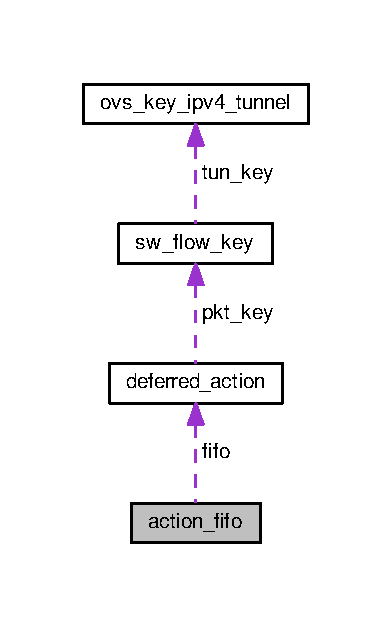
\includegraphics[width=188pt]{structaction__fifo__coll__graph}
\end{center}
\end{figure}
\subsection*{Data Fields}
\begin{DoxyCompactItemize}
\item 
int \hyperlink{structaction__fifo_a5376b4a5c9dbfd84303d156a47ed9018}{head}
\item 
int \hyperlink{structaction__fifo_a60805cbdf935d6718f685c7374ae9493}{tail}
\item 
struct \hyperlink{structdeferred__action}{deferred\+\_\+action} \hyperlink{structaction__fifo_ab25b47c1bc05f5417f0a2073a47b2eb5}{fifo} \mbox{[}\hyperlink{linux_2actions_8c_acb72e0b273dae399e2619f619fd061ed}{D\+E\+F\+E\+R\+R\+E\+D\+\_\+\+A\+C\+T\+I\+O\+N\+\_\+\+F\+I\+F\+O\+\_\+\+S\+I\+Z\+E}\mbox{]}
\end{DoxyCompactItemize}


\subsection{Field Documentation}
\hypertarget{structaction__fifo_ab25b47c1bc05f5417f0a2073a47b2eb5}{}\index{action\+\_\+fifo@{action\+\_\+fifo}!fifo@{fifo}}
\index{fifo@{fifo}!action\+\_\+fifo@{action\+\_\+fifo}}
\subsubsection[{fifo}]{\setlength{\rightskip}{0pt plus 5cm}struct {\bf deferred\+\_\+action} action\+\_\+fifo\+::fifo}\label{structaction__fifo_ab25b47c1bc05f5417f0a2073a47b2eb5}
\hypertarget{structaction__fifo_a5376b4a5c9dbfd84303d156a47ed9018}{}\index{action\+\_\+fifo@{action\+\_\+fifo}!head@{head}}
\index{head@{head}!action\+\_\+fifo@{action\+\_\+fifo}}
\subsubsection[{head}]{\setlength{\rightskip}{0pt plus 5cm}int action\+\_\+fifo\+::head}\label{structaction__fifo_a5376b4a5c9dbfd84303d156a47ed9018}
\hypertarget{structaction__fifo_a60805cbdf935d6718f685c7374ae9493}{}\index{action\+\_\+fifo@{action\+\_\+fifo}!tail@{tail}}
\index{tail@{tail}!action\+\_\+fifo@{action\+\_\+fifo}}
\subsubsection[{tail}]{\setlength{\rightskip}{0pt plus 5cm}int action\+\_\+fifo\+::tail}\label{structaction__fifo_a60805cbdf935d6718f685c7374ae9493}


The documentation for this struct was generated from the following file\+:\begin{DoxyCompactItemize}
\item 
/home/vladn/git/ovs/datapath/\hyperlink{actions_8c}{actions.\+c}\end{DoxyCompactItemize}

\hypertarget{structarp__eth__header}{}\section{arp\+\_\+eth\+\_\+header Struct Reference}
\label{structarp__eth__header}\index{arp\+\_\+eth\+\_\+header@{arp\+\_\+eth\+\_\+header}}


{\ttfamily \#include $<$flow.\+h$>$}

\subsection*{Data Fields}
\begin{DoxyCompactItemize}
\item 
\+\_\+\+\_\+be16 \hyperlink{structarp__eth__header_afe4c385a8760054d1d9da4e06b72dc3a}{ar\+\_\+hrd}
\item 
\+\_\+\+\_\+be16 \hyperlink{structarp__eth__header_aa0a6c956f6f9001377528f86f94d91b4}{ar\+\_\+pro}
\item 
unsigned char \hyperlink{structarp__eth__header_a8feceb41fdd95e4a0f1e17e56b957bf4}{ar\+\_\+hln}
\item 
unsigned char \hyperlink{structarp__eth__header_abc215d845eb12176276c8cee0501ecd8}{ar\+\_\+pln}
\item 
\+\_\+\+\_\+be16 \hyperlink{structarp__eth__header_a0cad73c318ab7ea788fa836f6b5a011d}{ar\+\_\+op}
\item 
unsigned char \hyperlink{structarp__eth__header_a569cddaf9ed4aa40b04b60958783e908}{ar\+\_\+sha} \mbox{[}E\+T\+H\+\_\+\+A\+L\+E\+N\mbox{]}
\item 
unsigned char \hyperlink{structarp__eth__header_ae584842ae04804b2f5cf3c26fb135961}{ar\+\_\+sip} \mbox{[}4\mbox{]}
\item 
unsigned char \hyperlink{structarp__eth__header_a490c51d5f01a32e78c57d020ca2662f6}{ar\+\_\+tha} \mbox{[}E\+T\+H\+\_\+\+A\+L\+E\+N\mbox{]}
\item 
unsigned char \hyperlink{structarp__eth__header_a9ed88031c0dd2f554f1dc455e878945d}{ar\+\_\+tip} \mbox{[}4\mbox{]}
\end{DoxyCompactItemize}


\subsection{Field Documentation}
\hypertarget{structarp__eth__header_a8feceb41fdd95e4a0f1e17e56b957bf4}{}\index{arp\+\_\+eth\+\_\+header@{arp\+\_\+eth\+\_\+header}!ar\+\_\+hln@{ar\+\_\+hln}}
\index{ar\+\_\+hln@{ar\+\_\+hln}!arp\+\_\+eth\+\_\+header@{arp\+\_\+eth\+\_\+header}}
\subsubsection[{ar\+\_\+hln}]{\setlength{\rightskip}{0pt plus 5cm}unsigned char arp\+\_\+eth\+\_\+header\+::ar\+\_\+hln}\label{structarp__eth__header_a8feceb41fdd95e4a0f1e17e56b957bf4}
\hypertarget{structarp__eth__header_afe4c385a8760054d1d9da4e06b72dc3a}{}\index{arp\+\_\+eth\+\_\+header@{arp\+\_\+eth\+\_\+header}!ar\+\_\+hrd@{ar\+\_\+hrd}}
\index{ar\+\_\+hrd@{ar\+\_\+hrd}!arp\+\_\+eth\+\_\+header@{arp\+\_\+eth\+\_\+header}}
\subsubsection[{ar\+\_\+hrd}]{\setlength{\rightskip}{0pt plus 5cm}\+\_\+\+\_\+be16 arp\+\_\+eth\+\_\+header\+::ar\+\_\+hrd}\label{structarp__eth__header_afe4c385a8760054d1d9da4e06b72dc3a}
\hypertarget{structarp__eth__header_a0cad73c318ab7ea788fa836f6b5a011d}{}\index{arp\+\_\+eth\+\_\+header@{arp\+\_\+eth\+\_\+header}!ar\+\_\+op@{ar\+\_\+op}}
\index{ar\+\_\+op@{ar\+\_\+op}!arp\+\_\+eth\+\_\+header@{arp\+\_\+eth\+\_\+header}}
\subsubsection[{ar\+\_\+op}]{\setlength{\rightskip}{0pt plus 5cm}\+\_\+\+\_\+be16 arp\+\_\+eth\+\_\+header\+::ar\+\_\+op}\label{structarp__eth__header_a0cad73c318ab7ea788fa836f6b5a011d}
\hypertarget{structarp__eth__header_abc215d845eb12176276c8cee0501ecd8}{}\index{arp\+\_\+eth\+\_\+header@{arp\+\_\+eth\+\_\+header}!ar\+\_\+pln@{ar\+\_\+pln}}
\index{ar\+\_\+pln@{ar\+\_\+pln}!arp\+\_\+eth\+\_\+header@{arp\+\_\+eth\+\_\+header}}
\subsubsection[{ar\+\_\+pln}]{\setlength{\rightskip}{0pt plus 5cm}unsigned char arp\+\_\+eth\+\_\+header\+::ar\+\_\+pln}\label{structarp__eth__header_abc215d845eb12176276c8cee0501ecd8}
\hypertarget{structarp__eth__header_aa0a6c956f6f9001377528f86f94d91b4}{}\index{arp\+\_\+eth\+\_\+header@{arp\+\_\+eth\+\_\+header}!ar\+\_\+pro@{ar\+\_\+pro}}
\index{ar\+\_\+pro@{ar\+\_\+pro}!arp\+\_\+eth\+\_\+header@{arp\+\_\+eth\+\_\+header}}
\subsubsection[{ar\+\_\+pro}]{\setlength{\rightskip}{0pt plus 5cm}\+\_\+\+\_\+be16 arp\+\_\+eth\+\_\+header\+::ar\+\_\+pro}\label{structarp__eth__header_aa0a6c956f6f9001377528f86f94d91b4}
\hypertarget{structarp__eth__header_a569cddaf9ed4aa40b04b60958783e908}{}\index{arp\+\_\+eth\+\_\+header@{arp\+\_\+eth\+\_\+header}!ar\+\_\+sha@{ar\+\_\+sha}}
\index{ar\+\_\+sha@{ar\+\_\+sha}!arp\+\_\+eth\+\_\+header@{arp\+\_\+eth\+\_\+header}}
\subsubsection[{ar\+\_\+sha}]{\setlength{\rightskip}{0pt plus 5cm}unsigned char arp\+\_\+eth\+\_\+header\+::ar\+\_\+sha\mbox{[}E\+T\+H\+\_\+\+A\+L\+E\+N\mbox{]}}\label{structarp__eth__header_a569cddaf9ed4aa40b04b60958783e908}
\hypertarget{structarp__eth__header_ae584842ae04804b2f5cf3c26fb135961}{}\index{arp\+\_\+eth\+\_\+header@{arp\+\_\+eth\+\_\+header}!ar\+\_\+sip@{ar\+\_\+sip}}
\index{ar\+\_\+sip@{ar\+\_\+sip}!arp\+\_\+eth\+\_\+header@{arp\+\_\+eth\+\_\+header}}
\subsubsection[{ar\+\_\+sip}]{\setlength{\rightskip}{0pt plus 5cm}unsigned char arp\+\_\+eth\+\_\+header\+::ar\+\_\+sip\mbox{[}4\mbox{]}}\label{structarp__eth__header_ae584842ae04804b2f5cf3c26fb135961}
\hypertarget{structarp__eth__header_a490c51d5f01a32e78c57d020ca2662f6}{}\index{arp\+\_\+eth\+\_\+header@{arp\+\_\+eth\+\_\+header}!ar\+\_\+tha@{ar\+\_\+tha}}
\index{ar\+\_\+tha@{ar\+\_\+tha}!arp\+\_\+eth\+\_\+header@{arp\+\_\+eth\+\_\+header}}
\subsubsection[{ar\+\_\+tha}]{\setlength{\rightskip}{0pt plus 5cm}unsigned char arp\+\_\+eth\+\_\+header\+::ar\+\_\+tha\mbox{[}E\+T\+H\+\_\+\+A\+L\+E\+N\mbox{]}}\label{structarp__eth__header_a490c51d5f01a32e78c57d020ca2662f6}
\hypertarget{structarp__eth__header_a9ed88031c0dd2f554f1dc455e878945d}{}\index{arp\+\_\+eth\+\_\+header@{arp\+\_\+eth\+\_\+header}!ar\+\_\+tip@{ar\+\_\+tip}}
\index{ar\+\_\+tip@{ar\+\_\+tip}!arp\+\_\+eth\+\_\+header@{arp\+\_\+eth\+\_\+header}}
\subsubsection[{ar\+\_\+tip}]{\setlength{\rightskip}{0pt plus 5cm}unsigned char arp\+\_\+eth\+\_\+header\+::ar\+\_\+tip\mbox{[}4\mbox{]}}\label{structarp__eth__header_a9ed88031c0dd2f554f1dc455e878945d}


The documentation for this struct was generated from the following file\+:\begin{DoxyCompactItemize}
\item 
/home/vladn/git/ovs/datapath/\hyperlink{flow_8h}{flow.\+h}\end{DoxyCompactItemize}

\hypertarget{structdatapath}{}\section{datapath Struct Reference}
\label{structdatapath}\index{datapath@{datapath}}


{\ttfamily \#include $<$datapath.\+h$>$}



Collaboration diagram for datapath\+:
\nopagebreak
\begin{figure}[H]
\begin{center}
\leavevmode
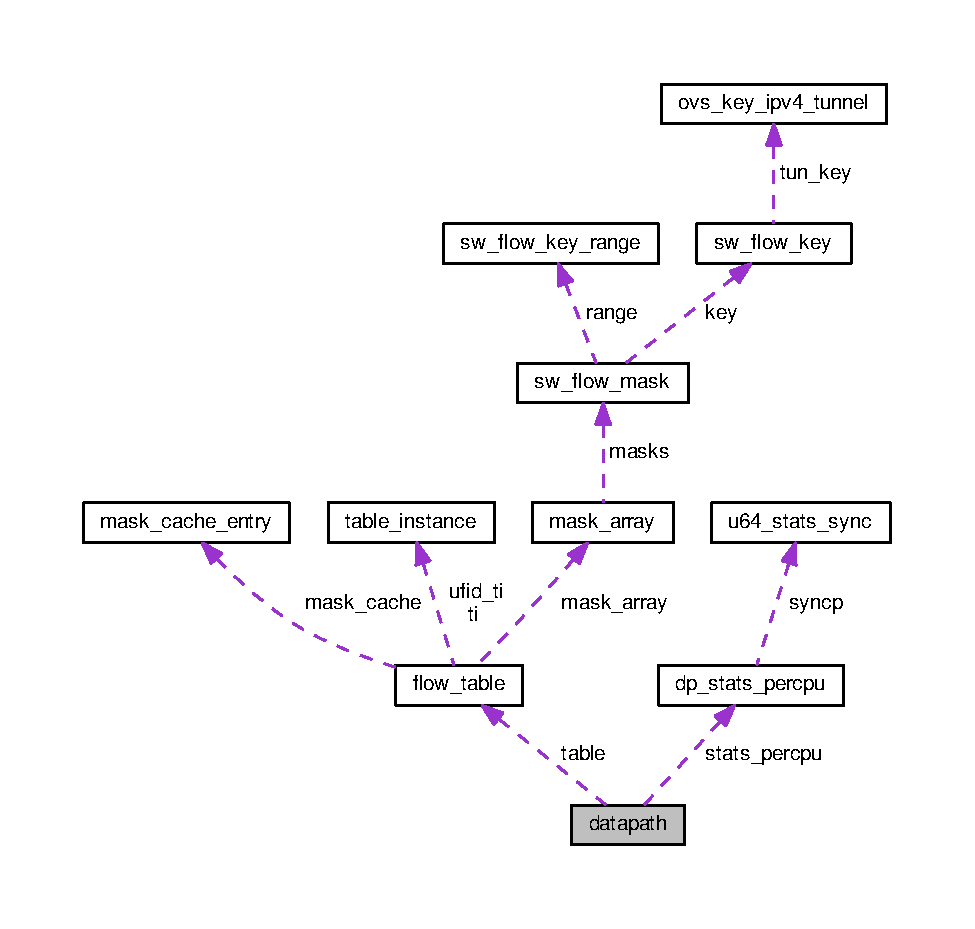
\includegraphics[width=350pt]{structdatapath__coll__graph}
\end{center}
\end{figure}
\subsection*{Data Fields}
\begin{DoxyCompactItemize}
\item 
struct rcu\+\_\+head \hyperlink{structdatapath_af487ac38fa868c398dd248f1956b7a35}{rcu}
\item 
struct list\+\_\+head \hyperlink{structdatapath_ac5f44be07025a2addb5c393fba822000}{list\+\_\+node}
\item 
struct \hyperlink{structflow__table}{flow\+\_\+table} \hyperlink{structdatapath_ac6d67fe586c19484391acbcfa267259d}{table}
\item 
struct hlist\+\_\+head $\ast$ \hyperlink{structdatapath_abb0de528545b312de283b571cb6c4ede}{ports}
\item 
struct \hyperlink{structdp__stats__percpu}{dp\+\_\+stats\+\_\+percpu} \hyperlink{compiler_8h_a497f20279760cdb59a5187689f9f5ab1}{\+\_\+\+\_\+percpu} $\ast$ \hyperlink{structdatapath_a26ff295c711206c8177cdc89150c6a4a}{stats\+\_\+percpu}
\item 
u32 \hyperlink{structdatapath_a92ce3b704c20f18b3a696f98b6f7d266}{user\+\_\+features}
\end{DoxyCompactItemize}


\subsection{Detailed Description}
struct datapath -\/ datapath for flow-\/based packet switching \+: R\+C\+U callback head for deferred destruction. \+: Element in global \textquotesingle{}dps\textquotesingle{} list. \+: flow table. \+: Hash table for ports. O\+V\+S\+P\+\_\+\+L\+O\+C\+A\+L port always exists. Protected by ovs\+\_\+mutex and R\+C\+U. \+: Per-\/\+C\+P\+U datapath statistics. \+: Reference to net namespace.

Context\+: See the comment on locking at the top of datapath.\+c for additional locking information. 

\subsection{Field Documentation}
\hypertarget{structdatapath_ac5f44be07025a2addb5c393fba822000}{}\index{datapath@{datapath}!list\+\_\+node@{list\+\_\+node}}
\index{list\+\_\+node@{list\+\_\+node}!datapath@{datapath}}
\subsubsection[{list\+\_\+node}]{\setlength{\rightskip}{0pt plus 5cm}struct list\+\_\+head datapath\+::list\+\_\+node}\label{structdatapath_ac5f44be07025a2addb5c393fba822000}
\hypertarget{structdatapath_abb0de528545b312de283b571cb6c4ede}{}\index{datapath@{datapath}!ports@{ports}}
\index{ports@{ports}!datapath@{datapath}}
\subsubsection[{ports}]{\setlength{\rightskip}{0pt plus 5cm}struct hlist\+\_\+head$\ast$ datapath\+::ports}\label{structdatapath_abb0de528545b312de283b571cb6c4ede}
\hypertarget{structdatapath_af487ac38fa868c398dd248f1956b7a35}{}\index{datapath@{datapath}!rcu@{rcu}}
\index{rcu@{rcu}!datapath@{datapath}}
\subsubsection[{rcu}]{\setlength{\rightskip}{0pt plus 5cm}struct rcu\+\_\+head datapath\+::rcu}\label{structdatapath_af487ac38fa868c398dd248f1956b7a35}
\hypertarget{structdatapath_a26ff295c711206c8177cdc89150c6a4a}{}\index{datapath@{datapath}!stats\+\_\+percpu@{stats\+\_\+percpu}}
\index{stats\+\_\+percpu@{stats\+\_\+percpu}!datapath@{datapath}}
\subsubsection[{stats\+\_\+percpu}]{\setlength{\rightskip}{0pt plus 5cm}struct {\bf dp\+\_\+stats\+\_\+percpu} {\bf \+\_\+\+\_\+percpu}$\ast$ datapath\+::stats\+\_\+percpu}\label{structdatapath_a26ff295c711206c8177cdc89150c6a4a}
\hypertarget{structdatapath_ac6d67fe586c19484391acbcfa267259d}{}\index{datapath@{datapath}!table@{table}}
\index{table@{table}!datapath@{datapath}}
\subsubsection[{table}]{\setlength{\rightskip}{0pt plus 5cm}struct {\bf flow\+\_\+table} datapath\+::table}\label{structdatapath_ac6d67fe586c19484391acbcfa267259d}
\hypertarget{structdatapath_a92ce3b704c20f18b3a696f98b6f7d266}{}\index{datapath@{datapath}!user\+\_\+features@{user\+\_\+features}}
\index{user\+\_\+features@{user\+\_\+features}!datapath@{datapath}}
\subsubsection[{user\+\_\+features}]{\setlength{\rightskip}{0pt plus 5cm}u32 datapath\+::user\+\_\+features}\label{structdatapath_a92ce3b704c20f18b3a696f98b6f7d266}


The documentation for this struct was generated from the following file\+:\begin{DoxyCompactItemize}
\item 
/home/vladn/git/ovs/datapath/\hyperlink{datapath_8h}{datapath.\+h}\end{DoxyCompactItemize}

\hypertarget{structdeferred__action}{}\section{deferred\+\_\+action Struct Reference}
\label{structdeferred__action}\index{deferred\+\_\+action@{deferred\+\_\+action}}


Collaboration diagram for deferred\+\_\+action\+:
\nopagebreak
\begin{figure}[H]
\begin{center}
\leavevmode
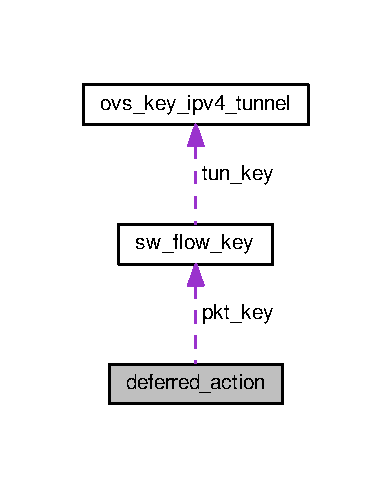
\includegraphics[width=188pt]{structdeferred__action__coll__graph}
\end{center}
\end{figure}
\subsection*{Data Fields}
\begin{DoxyCompactItemize}
\item 
struct sk\+\_\+buff $\ast$ \hyperlink{structdeferred__action_acba4fd12fba3d60b6f4c7f2f3159f316}{skb}
\item 
const struct nlattr $\ast$ \hyperlink{structdeferred__action_a9cb4d3dde378a66035e7b17f017d9f89}{actions}
\item 
struct \hyperlink{structsw__flow__key}{sw\+\_\+flow\+\_\+key} \hyperlink{structdeferred__action_a4685f782001923a8f8c20510126b4c21}{pkt\+\_\+key}
\end{DoxyCompactItemize}


\subsection{Field Documentation}
\hypertarget{structdeferred__action_a9cb4d3dde378a66035e7b17f017d9f89}{}\index{deferred\+\_\+action@{deferred\+\_\+action}!actions@{actions}}
\index{actions@{actions}!deferred\+\_\+action@{deferred\+\_\+action}}
\subsubsection[{actions}]{\setlength{\rightskip}{0pt plus 5cm}const struct nlattr $\ast$ deferred\+\_\+action\+::actions}\label{structdeferred__action_a9cb4d3dde378a66035e7b17f017d9f89}
\hypertarget{structdeferred__action_a4685f782001923a8f8c20510126b4c21}{}\index{deferred\+\_\+action@{deferred\+\_\+action}!pkt\+\_\+key@{pkt\+\_\+key}}
\index{pkt\+\_\+key@{pkt\+\_\+key}!deferred\+\_\+action@{deferred\+\_\+action}}
\subsubsection[{pkt\+\_\+key}]{\setlength{\rightskip}{0pt plus 5cm}struct {\bf sw\+\_\+flow\+\_\+key} deferred\+\_\+action\+::pkt\+\_\+key}\label{structdeferred__action_a4685f782001923a8f8c20510126b4c21}
\hypertarget{structdeferred__action_acba4fd12fba3d60b6f4c7f2f3159f316}{}\index{deferred\+\_\+action@{deferred\+\_\+action}!skb@{skb}}
\index{skb@{skb}!deferred\+\_\+action@{deferred\+\_\+action}}
\subsubsection[{skb}]{\setlength{\rightskip}{0pt plus 5cm}struct sk\+\_\+buff $\ast$ deferred\+\_\+action\+::skb}\label{structdeferred__action_acba4fd12fba3d60b6f4c7f2f3159f316}


The documentation for this struct was generated from the following file\+:\begin{DoxyCompactItemize}
\item 
/home/vladn/git/ovs/datapath/\hyperlink{actions_8c}{actions.\+c}\end{DoxyCompactItemize}

\hypertarget{structdp__stats__percpu}{}\section{dp\+\_\+stats\+\_\+percpu Struct Reference}
\label{structdp__stats__percpu}\index{dp\+\_\+stats\+\_\+percpu@{dp\+\_\+stats\+\_\+percpu}}


{\ttfamily \#include $<$datapath.\+h$>$}



Collaboration diagram for dp\+\_\+stats\+\_\+percpu\+:
\nopagebreak
\begin{figure}[H]
\begin{center}
\leavevmode
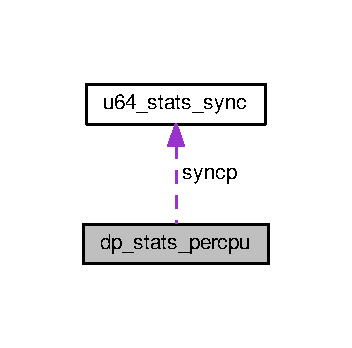
\includegraphics[width=169pt]{structdp__stats__percpu__coll__graph}
\end{center}
\end{figure}
\subsection*{Data Fields}
\begin{DoxyCompactItemize}
\item 
u64 \hyperlink{structdp__stats__percpu_add53281b86504a50626cce7fac173d5b}{n\+\_\+hit}
\item 
u64 \hyperlink{structdp__stats__percpu_ab919c22c9548a3dcd42632fb84634e26}{n\+\_\+missed}
\item 
u64 \hyperlink{structdp__stats__percpu_abecbd535feefeb9ff1721ca6e517c310}{n\+\_\+lost}
\item 
u64 \hyperlink{structdp__stats__percpu_acbf57615b1fb66464f9e67efb32bd038}{n\+\_\+mask\+\_\+hit}
\item 
struct \hyperlink{structu64__stats__sync}{u64\+\_\+stats\+\_\+sync} \hyperlink{structdp__stats__percpu_ad67971f59f6db5432848db23d185dc2f}{syncp}
\end{DoxyCompactItemize}


\subsection{Detailed Description}
struct \hyperlink{structdp__stats__percpu}{dp\+\_\+stats\+\_\+percpu} -\/ per-\/cpu packet processing statistics for a given datapath. \+: Number of received packets for which a matching flow was found in the flow table. \+: Number of received packets that had no matching flow in the flow table. The sum of  and  is the number of packets that have been received by the datapath. \+: Number of received packets that had no matching flow in the flow table that could not be sent to userspace (normally due to an overflow in one of the datapath\textquotesingle{}s queues). \+: Number of masks looked up for flow match.  / ( + ) will be the average masks looked up per packet. 

\subsection{Field Documentation}
\hypertarget{structdp__stats__percpu_add53281b86504a50626cce7fac173d5b}{}\index{dp\+\_\+stats\+\_\+percpu@{dp\+\_\+stats\+\_\+percpu}!n\+\_\+hit@{n\+\_\+hit}}
\index{n\+\_\+hit@{n\+\_\+hit}!dp\+\_\+stats\+\_\+percpu@{dp\+\_\+stats\+\_\+percpu}}
\subsubsection[{n\+\_\+hit}]{\setlength{\rightskip}{0pt plus 5cm}u64 dp\+\_\+stats\+\_\+percpu\+::n\+\_\+hit}\label{structdp__stats__percpu_add53281b86504a50626cce7fac173d5b}
\hypertarget{structdp__stats__percpu_abecbd535feefeb9ff1721ca6e517c310}{}\index{dp\+\_\+stats\+\_\+percpu@{dp\+\_\+stats\+\_\+percpu}!n\+\_\+lost@{n\+\_\+lost}}
\index{n\+\_\+lost@{n\+\_\+lost}!dp\+\_\+stats\+\_\+percpu@{dp\+\_\+stats\+\_\+percpu}}
\subsubsection[{n\+\_\+lost}]{\setlength{\rightskip}{0pt plus 5cm}u64 dp\+\_\+stats\+\_\+percpu\+::n\+\_\+lost}\label{structdp__stats__percpu_abecbd535feefeb9ff1721ca6e517c310}
\hypertarget{structdp__stats__percpu_acbf57615b1fb66464f9e67efb32bd038}{}\index{dp\+\_\+stats\+\_\+percpu@{dp\+\_\+stats\+\_\+percpu}!n\+\_\+mask\+\_\+hit@{n\+\_\+mask\+\_\+hit}}
\index{n\+\_\+mask\+\_\+hit@{n\+\_\+mask\+\_\+hit}!dp\+\_\+stats\+\_\+percpu@{dp\+\_\+stats\+\_\+percpu}}
\subsubsection[{n\+\_\+mask\+\_\+hit}]{\setlength{\rightskip}{0pt plus 5cm}u64 dp\+\_\+stats\+\_\+percpu\+::n\+\_\+mask\+\_\+hit}\label{structdp__stats__percpu_acbf57615b1fb66464f9e67efb32bd038}
\hypertarget{structdp__stats__percpu_ab919c22c9548a3dcd42632fb84634e26}{}\index{dp\+\_\+stats\+\_\+percpu@{dp\+\_\+stats\+\_\+percpu}!n\+\_\+missed@{n\+\_\+missed}}
\index{n\+\_\+missed@{n\+\_\+missed}!dp\+\_\+stats\+\_\+percpu@{dp\+\_\+stats\+\_\+percpu}}
\subsubsection[{n\+\_\+missed}]{\setlength{\rightskip}{0pt plus 5cm}u64 dp\+\_\+stats\+\_\+percpu\+::n\+\_\+missed}\label{structdp__stats__percpu_ab919c22c9548a3dcd42632fb84634e26}
\hypertarget{structdp__stats__percpu_ad67971f59f6db5432848db23d185dc2f}{}\index{dp\+\_\+stats\+\_\+percpu@{dp\+\_\+stats\+\_\+percpu}!syncp@{syncp}}
\index{syncp@{syncp}!dp\+\_\+stats\+\_\+percpu@{dp\+\_\+stats\+\_\+percpu}}
\subsubsection[{syncp}]{\setlength{\rightskip}{0pt plus 5cm}struct {\bf u64\+\_\+stats\+\_\+sync} dp\+\_\+stats\+\_\+percpu\+::syncp}\label{structdp__stats__percpu_ad67971f59f6db5432848db23d185dc2f}


The documentation for this struct was generated from the following file\+:\begin{DoxyCompactItemize}
\item 
/home/vladn/git/ovs/datapath/\hyperlink{datapath_8h}{datapath.\+h}\end{DoxyCompactItemize}

\hypertarget{structdp__upcall__info}{}\section{dp\+\_\+upcall\+\_\+info Struct Reference}
\label{structdp__upcall__info}\index{dp\+\_\+upcall\+\_\+info@{dp\+\_\+upcall\+\_\+info}}


{\ttfamily \#include $<$datapath.\+h$>$}



Collaboration diagram for dp\+\_\+upcall\+\_\+info\+:
\nopagebreak
\begin{figure}[H]
\begin{center}
\leavevmode
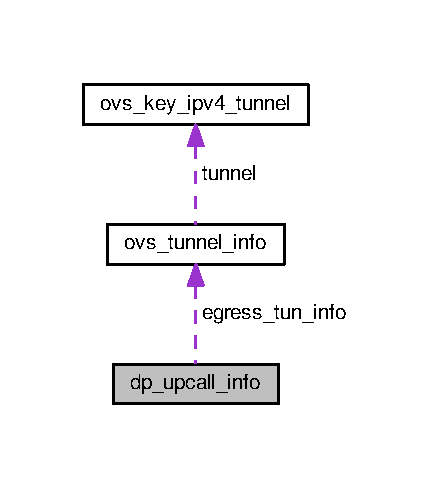
\includegraphics[width=207pt]{structdp__upcall__info__coll__graph}
\end{center}
\end{figure}
\subsection*{Data Fields}
\begin{DoxyCompactItemize}
\item 
const struct \hyperlink{structovs__tunnel__info}{ovs\+\_\+tunnel\+\_\+info} $\ast$ \hyperlink{structdp__upcall__info_a74a70c7b1f24487fd51d0f0c5aa1c11e}{egress\+\_\+tun\+\_\+info}
\item 
const struct nlattr $\ast$ \hyperlink{structdp__upcall__info_a78d8f8bd4a0418b043a3a2401e516d5a}{userdata}
\item 
const struct nlattr $\ast$ \hyperlink{structdp__upcall__info_a0e948e89cb162118d95c37d8c2a6c5c3}{actions}
\item 
int \hyperlink{structdp__upcall__info_ad5ccfb55799f138fa7d01461e2035d1f}{actions\+\_\+len}
\item 
u32 \hyperlink{structdp__upcall__info_a4300576f43ab3d9293453d9c664de818}{portid}
\item 
u8 \hyperlink{structdp__upcall__info_afdbbbb0aef83ab4652e15715db247d22}{cmd}
\end{DoxyCompactItemize}


\subsection{Detailed Description}
struct dp\+\_\+upcall -\/ metadata to include with a packet to send to userspace \+: One of O\+V\+S\+\_\+\+P\+A\+C\+K\+E\+T\+\_\+\+C\+M\+D\+\_\+$\ast$. \+: If nonnull, its variable-\/length value is passed to userspace as O\+V\+S\+\_\+\+P\+A\+C\+K\+E\+T\+\_\+\+A\+T\+T\+R\+\_\+\+U\+S\+E\+R\+D\+A\+T\+A. \+: Netlink portid to which packet should be sent. If  is 0 then no packet is sent and the packet is accounted in the datapath\textquotesingle{}s  counter. \+: If nonnull, becomes O\+V\+S\+\_\+\+P\+A\+C\+K\+E\+T\+\_\+\+A\+T\+T\+R\+\_\+\+E\+G\+R\+E\+S\+S\+\_\+\+T\+U\+N\+\_\+\+K\+E\+Y. 

\subsection{Field Documentation}
\hypertarget{structdp__upcall__info_a0e948e89cb162118d95c37d8c2a6c5c3}{}\index{dp\+\_\+upcall\+\_\+info@{dp\+\_\+upcall\+\_\+info}!actions@{actions}}
\index{actions@{actions}!dp\+\_\+upcall\+\_\+info@{dp\+\_\+upcall\+\_\+info}}
\subsubsection[{actions}]{\setlength{\rightskip}{0pt plus 5cm}const struct nlattr$\ast$ dp\+\_\+upcall\+\_\+info\+::actions}\label{structdp__upcall__info_a0e948e89cb162118d95c37d8c2a6c5c3}
\hypertarget{structdp__upcall__info_ad5ccfb55799f138fa7d01461e2035d1f}{}\index{dp\+\_\+upcall\+\_\+info@{dp\+\_\+upcall\+\_\+info}!actions\+\_\+len@{actions\+\_\+len}}
\index{actions\+\_\+len@{actions\+\_\+len}!dp\+\_\+upcall\+\_\+info@{dp\+\_\+upcall\+\_\+info}}
\subsubsection[{actions\+\_\+len}]{\setlength{\rightskip}{0pt plus 5cm}int dp\+\_\+upcall\+\_\+info\+::actions\+\_\+len}\label{structdp__upcall__info_ad5ccfb55799f138fa7d01461e2035d1f}
\hypertarget{structdp__upcall__info_afdbbbb0aef83ab4652e15715db247d22}{}\index{dp\+\_\+upcall\+\_\+info@{dp\+\_\+upcall\+\_\+info}!cmd@{cmd}}
\index{cmd@{cmd}!dp\+\_\+upcall\+\_\+info@{dp\+\_\+upcall\+\_\+info}}
\subsubsection[{cmd}]{\setlength{\rightskip}{0pt plus 5cm}u8 dp\+\_\+upcall\+\_\+info\+::cmd}\label{structdp__upcall__info_afdbbbb0aef83ab4652e15715db247d22}
\hypertarget{structdp__upcall__info_a74a70c7b1f24487fd51d0f0c5aa1c11e}{}\index{dp\+\_\+upcall\+\_\+info@{dp\+\_\+upcall\+\_\+info}!egress\+\_\+tun\+\_\+info@{egress\+\_\+tun\+\_\+info}}
\index{egress\+\_\+tun\+\_\+info@{egress\+\_\+tun\+\_\+info}!dp\+\_\+upcall\+\_\+info@{dp\+\_\+upcall\+\_\+info}}
\subsubsection[{egress\+\_\+tun\+\_\+info}]{\setlength{\rightskip}{0pt plus 5cm}const struct {\bf ovs\+\_\+tunnel\+\_\+info}$\ast$ dp\+\_\+upcall\+\_\+info\+::egress\+\_\+tun\+\_\+info}\label{structdp__upcall__info_a74a70c7b1f24487fd51d0f0c5aa1c11e}
\hypertarget{structdp__upcall__info_a4300576f43ab3d9293453d9c664de818}{}\index{dp\+\_\+upcall\+\_\+info@{dp\+\_\+upcall\+\_\+info}!portid@{portid}}
\index{portid@{portid}!dp\+\_\+upcall\+\_\+info@{dp\+\_\+upcall\+\_\+info}}
\subsubsection[{portid}]{\setlength{\rightskip}{0pt plus 5cm}u32 dp\+\_\+upcall\+\_\+info\+::portid}\label{structdp__upcall__info_a4300576f43ab3d9293453d9c664de818}
\hypertarget{structdp__upcall__info_a78d8f8bd4a0418b043a3a2401e516d5a}{}\index{dp\+\_\+upcall\+\_\+info@{dp\+\_\+upcall\+\_\+info}!userdata@{userdata}}
\index{userdata@{userdata}!dp\+\_\+upcall\+\_\+info@{dp\+\_\+upcall\+\_\+info}}
\subsubsection[{userdata}]{\setlength{\rightskip}{0pt plus 5cm}const struct nlattr$\ast$ dp\+\_\+upcall\+\_\+info\+::userdata}\label{structdp__upcall__info_a78d8f8bd4a0418b043a3a2401e516d5a}


The documentation for this struct was generated from the following file\+:\begin{DoxyCompactItemize}
\item 
/home/vladn/git/ovs/datapath/\hyperlink{datapath_8h}{datapath.\+h}\end{DoxyCompactItemize}

\hypertarget{structflow__stats}{}\section{flow\+\_\+stats Struct Reference}
\label{structflow__stats}\index{flow\+\_\+stats@{flow\+\_\+stats}}


{\ttfamily \#include $<$flow.\+h$>$}

\subsection*{Data Fields}
\begin{DoxyCompactItemize}
\item 
u64 \hyperlink{structflow__stats_a9399b2cdc3d48c11357fbc2aaff33226}{packet\+\_\+count}
\item 
u64 \hyperlink{structflow__stats_a97844fc570ddb0d4b80f4cfe36bfee29}{byte\+\_\+count}
\item 
unsigned long \hyperlink{structflow__stats_a3eefc54cf53ad3e24bb070bd6f251f50}{used}
\item 
spinlock\+\_\+t \hyperlink{structflow__stats_a1930f864d7fc52f4afeb86714e3e5c07}{lock}
\item 
\+\_\+\+\_\+be16 \hyperlink{structflow__stats_a2b2812adf4fd5f4f188324fdf503deba}{tcp\+\_\+flags}
\end{DoxyCompactItemize}


\subsection{Field Documentation}
\hypertarget{structflow__stats_a97844fc570ddb0d4b80f4cfe36bfee29}{}\index{flow\+\_\+stats@{flow\+\_\+stats}!byte\+\_\+count@{byte\+\_\+count}}
\index{byte\+\_\+count@{byte\+\_\+count}!flow\+\_\+stats@{flow\+\_\+stats}}
\subsubsection[{byte\+\_\+count}]{\setlength{\rightskip}{0pt plus 5cm}u64 flow\+\_\+stats\+::byte\+\_\+count}\label{structflow__stats_a97844fc570ddb0d4b80f4cfe36bfee29}
\hypertarget{structflow__stats_a1930f864d7fc52f4afeb86714e3e5c07}{}\index{flow\+\_\+stats@{flow\+\_\+stats}!lock@{lock}}
\index{lock@{lock}!flow\+\_\+stats@{flow\+\_\+stats}}
\subsubsection[{lock}]{\setlength{\rightskip}{0pt plus 5cm}spinlock\+\_\+t flow\+\_\+stats\+::lock}\label{structflow__stats_a1930f864d7fc52f4afeb86714e3e5c07}
\hypertarget{structflow__stats_a9399b2cdc3d48c11357fbc2aaff33226}{}\index{flow\+\_\+stats@{flow\+\_\+stats}!packet\+\_\+count@{packet\+\_\+count}}
\index{packet\+\_\+count@{packet\+\_\+count}!flow\+\_\+stats@{flow\+\_\+stats}}
\subsubsection[{packet\+\_\+count}]{\setlength{\rightskip}{0pt plus 5cm}u64 flow\+\_\+stats\+::packet\+\_\+count}\label{structflow__stats_a9399b2cdc3d48c11357fbc2aaff33226}
\hypertarget{structflow__stats_a2b2812adf4fd5f4f188324fdf503deba}{}\index{flow\+\_\+stats@{flow\+\_\+stats}!tcp\+\_\+flags@{tcp\+\_\+flags}}
\index{tcp\+\_\+flags@{tcp\+\_\+flags}!flow\+\_\+stats@{flow\+\_\+stats}}
\subsubsection[{tcp\+\_\+flags}]{\setlength{\rightskip}{0pt plus 5cm}\+\_\+\+\_\+be16 flow\+\_\+stats\+::tcp\+\_\+flags}\label{structflow__stats_a2b2812adf4fd5f4f188324fdf503deba}
\hypertarget{structflow__stats_a3eefc54cf53ad3e24bb070bd6f251f50}{}\index{flow\+\_\+stats@{flow\+\_\+stats}!used@{used}}
\index{used@{used}!flow\+\_\+stats@{flow\+\_\+stats}}
\subsubsection[{used}]{\setlength{\rightskip}{0pt plus 5cm}unsigned long flow\+\_\+stats\+::used}\label{structflow__stats_a3eefc54cf53ad3e24bb070bd6f251f50}


The documentation for this struct was generated from the following file\+:\begin{DoxyCompactItemize}
\item 
/home/vladn/git/ovs/datapath/\hyperlink{flow_8h}{flow.\+h}\end{DoxyCompactItemize}

\hypertarget{structflow__table}{}\section{flow\+\_\+table Struct Reference}
\label{structflow__table}\index{flow\+\_\+table@{flow\+\_\+table}}


{\ttfamily \#include $<$flow\+\_\+table.\+h$>$}



Collaboration diagram for flow\+\_\+table\+:
\nopagebreak
\begin{figure}[H]
\begin{center}
\leavevmode
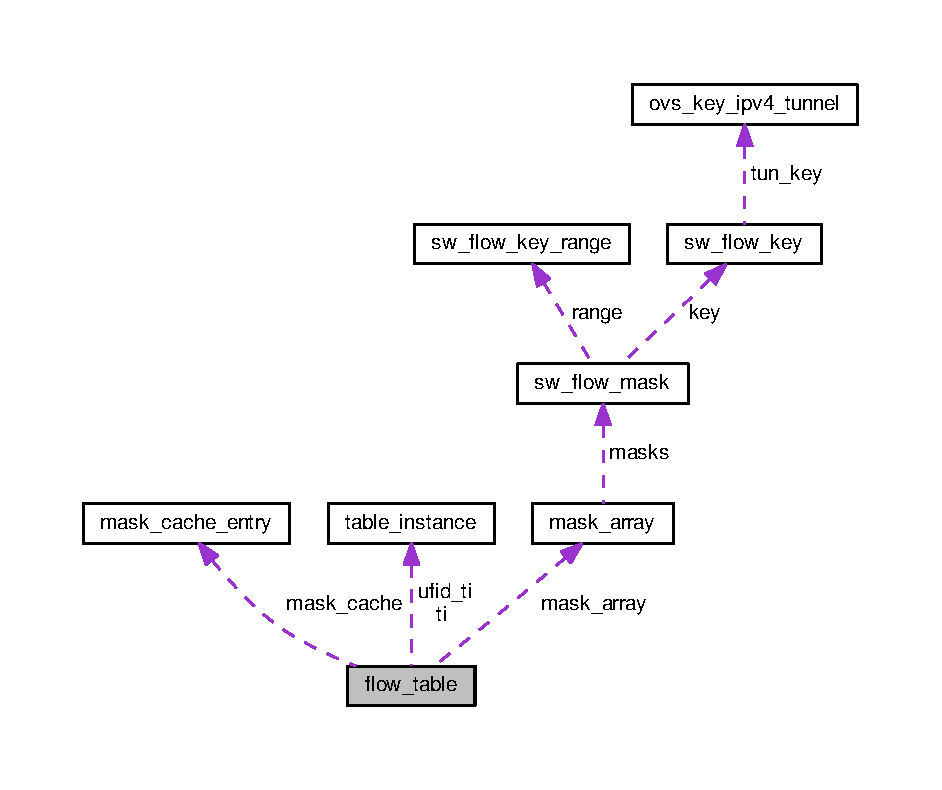
\includegraphics[width=350pt]{structflow__table__coll__graph}
\end{center}
\end{figure}
\subsection*{Data Fields}
\begin{DoxyCompactItemize}
\item 
struct \hyperlink{structtable__instance}{table\+\_\+instance} \hyperlink{compiler_8h_a2b3b0c016258969e4b39c66b6eec2129}{\+\_\+\+\_\+rcu} $\ast$ \hyperlink{structflow__table_a49d708e68608d510f6d25a16a14fd565}{ti}
\item 
struct \hyperlink{structtable__instance}{table\+\_\+instance} \hyperlink{compiler_8h_a2b3b0c016258969e4b39c66b6eec2129}{\+\_\+\+\_\+rcu} $\ast$ \hyperlink{structflow__table_aa29e185501af8dcd15549ee157c6c047}{ufid\+\_\+ti}
\item 
struct \hyperlink{structmask__cache__entry}{mask\+\_\+cache\+\_\+entry} \hyperlink{compiler_8h_a497f20279760cdb59a5187689f9f5ab1}{\+\_\+\+\_\+percpu} $\ast$ \hyperlink{structflow__table_a7395c72250199771559f2aaf32da5d0d}{mask\+\_\+cache}
\item 
struct \hyperlink{structmask__array}{mask\+\_\+array} \hyperlink{compiler_8h_a2b3b0c016258969e4b39c66b6eec2129}{\+\_\+\+\_\+rcu} $\ast$ \hyperlink{structflow__table_a0e568d59590f38936b714555597505be}{mask\+\_\+array}
\item 
unsigned long \hyperlink{structflow__table_a82c7cfef05b2898b3ffb3b6cb6fdc6a4}{last\+\_\+rehash}
\item 
unsigned int \hyperlink{structflow__table_a97cae1e714c6dcfe0d39ce4cff371786}{count}
\item 
unsigned int \hyperlink{structflow__table_ad8ff1e259e64690608d9552f0b467bf0}{ufid\+\_\+count}
\end{DoxyCompactItemize}


\subsection{Field Documentation}
\hypertarget{structflow__table_a97cae1e714c6dcfe0d39ce4cff371786}{}\index{flow\+\_\+table@{flow\+\_\+table}!count@{count}}
\index{count@{count}!flow\+\_\+table@{flow\+\_\+table}}
\subsubsection[{count}]{\setlength{\rightskip}{0pt plus 5cm}unsigned int flow\+\_\+table\+::count}\label{structflow__table_a97cae1e714c6dcfe0d39ce4cff371786}
\hypertarget{structflow__table_a82c7cfef05b2898b3ffb3b6cb6fdc6a4}{}\index{flow\+\_\+table@{flow\+\_\+table}!last\+\_\+rehash@{last\+\_\+rehash}}
\index{last\+\_\+rehash@{last\+\_\+rehash}!flow\+\_\+table@{flow\+\_\+table}}
\subsubsection[{last\+\_\+rehash}]{\setlength{\rightskip}{0pt plus 5cm}unsigned long flow\+\_\+table\+::last\+\_\+rehash}\label{structflow__table_a82c7cfef05b2898b3ffb3b6cb6fdc6a4}
\hypertarget{structflow__table_a0e568d59590f38936b714555597505be}{}\index{flow\+\_\+table@{flow\+\_\+table}!mask\+\_\+array@{mask\+\_\+array}}
\index{mask\+\_\+array@{mask\+\_\+array}!flow\+\_\+table@{flow\+\_\+table}}
\subsubsection[{mask\+\_\+array}]{\setlength{\rightskip}{0pt plus 5cm}struct {\bf mask\+\_\+array} {\bf \+\_\+\+\_\+rcu}$\ast$ flow\+\_\+table\+::mask\+\_\+array}\label{structflow__table_a0e568d59590f38936b714555597505be}
\hypertarget{structflow__table_a7395c72250199771559f2aaf32da5d0d}{}\index{flow\+\_\+table@{flow\+\_\+table}!mask\+\_\+cache@{mask\+\_\+cache}}
\index{mask\+\_\+cache@{mask\+\_\+cache}!flow\+\_\+table@{flow\+\_\+table}}
\subsubsection[{mask\+\_\+cache}]{\setlength{\rightskip}{0pt plus 5cm}struct {\bf mask\+\_\+cache\+\_\+entry} {\bf \+\_\+\+\_\+percpu}$\ast$ flow\+\_\+table\+::mask\+\_\+cache}\label{structflow__table_a7395c72250199771559f2aaf32da5d0d}
\hypertarget{structflow__table_a49d708e68608d510f6d25a16a14fd565}{}\index{flow\+\_\+table@{flow\+\_\+table}!ti@{ti}}
\index{ti@{ti}!flow\+\_\+table@{flow\+\_\+table}}
\subsubsection[{ti}]{\setlength{\rightskip}{0pt plus 5cm}struct {\bf table\+\_\+instance} {\bf \+\_\+\+\_\+rcu}$\ast$ flow\+\_\+table\+::ti}\label{structflow__table_a49d708e68608d510f6d25a16a14fd565}
\hypertarget{structflow__table_ad8ff1e259e64690608d9552f0b467bf0}{}\index{flow\+\_\+table@{flow\+\_\+table}!ufid\+\_\+count@{ufid\+\_\+count}}
\index{ufid\+\_\+count@{ufid\+\_\+count}!flow\+\_\+table@{flow\+\_\+table}}
\subsubsection[{ufid\+\_\+count}]{\setlength{\rightskip}{0pt plus 5cm}unsigned int flow\+\_\+table\+::ufid\+\_\+count}\label{structflow__table_ad8ff1e259e64690608d9552f0b467bf0}
\hypertarget{structflow__table_aa29e185501af8dcd15549ee157c6c047}{}\index{flow\+\_\+table@{flow\+\_\+table}!ufid\+\_\+ti@{ufid\+\_\+ti}}
\index{ufid\+\_\+ti@{ufid\+\_\+ti}!flow\+\_\+table@{flow\+\_\+table}}
\subsubsection[{ufid\+\_\+ti}]{\setlength{\rightskip}{0pt plus 5cm}struct {\bf table\+\_\+instance} {\bf \+\_\+\+\_\+rcu}$\ast$ flow\+\_\+table\+::ufid\+\_\+ti}\label{structflow__table_aa29e185501af8dcd15549ee157c6c047}


The documentation for this struct was generated from the following file\+:\begin{DoxyCompactItemize}
\item 
/home/vladn/git/ovs/datapath/\hyperlink{flow__table_8h}{flow\+\_\+table.\+h}\end{DoxyCompactItemize}

\hypertarget{structgeneve__port}{}\section{geneve\+\_\+port Struct Reference}
\label{structgeneve__port}\index{geneve\+\_\+port@{geneve\+\_\+port}}
\subsection*{Data Fields}
\begin{DoxyCompactItemize}
\item 
struct geneve\+\_\+sock $\ast$ \hyperlink{structgeneve__port_a4748918f17f05d385384df054553a612}{gs}
\item 
char \hyperlink{structgeneve__port_aab8c32b9d0a9be9e27711cd5a7f41226}{name} \mbox{[}I\+F\+N\+A\+M\+S\+I\+Z\mbox{]}
\end{DoxyCompactItemize}


\subsection{Field Documentation}
\hypertarget{structgeneve__port_a4748918f17f05d385384df054553a612}{}\index{geneve\+\_\+port@{geneve\+\_\+port}!gs@{gs}}
\index{gs@{gs}!geneve\+\_\+port@{geneve\+\_\+port}}
\subsubsection[{gs}]{\setlength{\rightskip}{0pt plus 5cm}struct geneve\+\_\+sock $\ast$ geneve\+\_\+port\+::gs}\label{structgeneve__port_a4748918f17f05d385384df054553a612}
\hypertarget{structgeneve__port_aab8c32b9d0a9be9e27711cd5a7f41226}{}\index{geneve\+\_\+port@{geneve\+\_\+port}!name@{name}}
\index{name@{name}!geneve\+\_\+port@{geneve\+\_\+port}}
\subsubsection[{name}]{\setlength{\rightskip}{0pt plus 5cm}char geneve\+\_\+port\+::name}\label{structgeneve__port_aab8c32b9d0a9be9e27711cd5a7f41226}


The documentation for this struct was generated from the following file\+:\begin{DoxyCompactItemize}
\item 
/home/vladn/git/ovs/datapath/linux/\hyperlink{linux_2vport-geneve_8c}{vport-\/geneve.\+c}\end{DoxyCompactItemize}

\hypertarget{structgre__cisco__protocol}{}\section{gre\+\_\+cisco\+\_\+protocol Struct Reference}
\label{structgre__cisco__protocol}\index{gre\+\_\+cisco\+\_\+protocol@{gre\+\_\+cisco\+\_\+protocol}}


{\ttfamily \#include $<$gre.\+h$>$}

\subsection*{Data Fields}
\begin{DoxyCompactItemize}
\item 
int($\ast$ \hyperlink{structgre__cisco__protocol_a8722aaef2209a2681ed04072b9f0f38b}{handler} )(struct sk\+\_\+buff $\ast$skb, const struct \hyperlink{structtnl__ptk__info}{tnl\+\_\+ptk\+\_\+info} $\ast$tpi)
\item 
int($\ast$ \hyperlink{structgre__cisco__protocol_a16acc645da0209063b8108fc34b3b861}{err\+\_\+handler} )(struct sk\+\_\+buff $\ast$skb, u32 info, const struct \hyperlink{structtnl__ptk__info}{tnl\+\_\+ptk\+\_\+info} $\ast$tpi)
\item 
u8 \hyperlink{structgre__cisco__protocol_a3617a7910af354dccd32e3eb24794975}{priority}
\end{DoxyCompactItemize}


\subsection{Field Documentation}
\hypertarget{structgre__cisco__protocol_a16acc645da0209063b8108fc34b3b861}{}\index{gre\+\_\+cisco\+\_\+protocol@{gre\+\_\+cisco\+\_\+protocol}!err\+\_\+handler@{err\+\_\+handler}}
\index{err\+\_\+handler@{err\+\_\+handler}!gre\+\_\+cisco\+\_\+protocol@{gre\+\_\+cisco\+\_\+protocol}}
\subsubsection[{err\+\_\+handler}]{\setlength{\rightskip}{0pt plus 5cm}int($\ast$ gre\+\_\+cisco\+\_\+protocol\+::err\+\_\+handler) (struct sk\+\_\+buff $\ast$skb, u32 info, const struct {\bf tnl\+\_\+ptk\+\_\+info} $\ast$tpi)}\label{structgre__cisco__protocol_a16acc645da0209063b8108fc34b3b861}
\hypertarget{structgre__cisco__protocol_a8722aaef2209a2681ed04072b9f0f38b}{}\index{gre\+\_\+cisco\+\_\+protocol@{gre\+\_\+cisco\+\_\+protocol}!handler@{handler}}
\index{handler@{handler}!gre\+\_\+cisco\+\_\+protocol@{gre\+\_\+cisco\+\_\+protocol}}
\subsubsection[{handler}]{\setlength{\rightskip}{0pt plus 5cm}int($\ast$ gre\+\_\+cisco\+\_\+protocol\+::handler) (struct sk\+\_\+buff $\ast$skb, const struct {\bf tnl\+\_\+ptk\+\_\+info} $\ast$tpi)}\label{structgre__cisco__protocol_a8722aaef2209a2681ed04072b9f0f38b}
\hypertarget{structgre__cisco__protocol_a3617a7910af354dccd32e3eb24794975}{}\index{gre\+\_\+cisco\+\_\+protocol@{gre\+\_\+cisco\+\_\+protocol}!priority@{priority}}
\index{priority@{priority}!gre\+\_\+cisco\+\_\+protocol@{gre\+\_\+cisco\+\_\+protocol}}
\subsubsection[{priority}]{\setlength{\rightskip}{0pt plus 5cm}u8 gre\+\_\+cisco\+\_\+protocol\+::priority}\label{structgre__cisco__protocol_a3617a7910af354dccd32e3eb24794975}


The documentation for this struct was generated from the following file\+:\begin{DoxyCompactItemize}
\item 
/home/vladn/git/ovs/datapath/linux/compat/include/net/\hyperlink{gre_8h}{gre.\+h}\end{DoxyCompactItemize}

\hypertarget{structinternal__dev}{}\section{internal\+\_\+dev Struct Reference}
\label{structinternal__dev}\index{internal\+\_\+dev@{internal\+\_\+dev}}


Collaboration diagram for internal\+\_\+dev\+:
\nopagebreak
\begin{figure}[H]
\begin{center}
\leavevmode
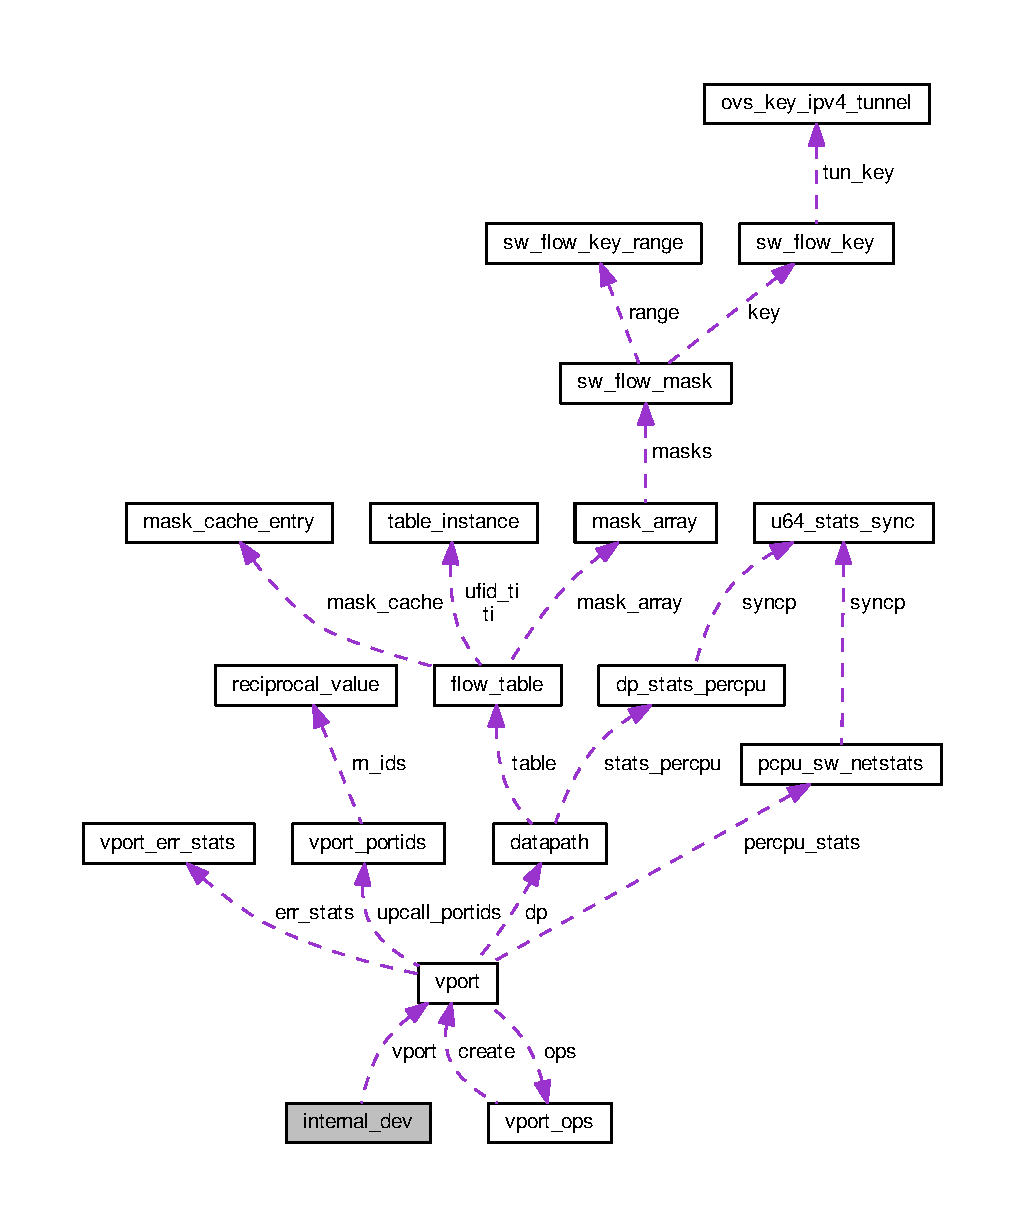
\includegraphics[width=350pt]{structinternal__dev__coll__graph}
\end{center}
\end{figure}
\subsection*{Data Fields}
\begin{DoxyCompactItemize}
\item 
struct \hyperlink{structvport}{vport} $\ast$ \hyperlink{structinternal__dev_ad571bd9420f8b95ac7d1febc36c6ef45}{vport}
\end{DoxyCompactItemize}


\subsection{Field Documentation}
\hypertarget{structinternal__dev_ad571bd9420f8b95ac7d1febc36c6ef45}{}\index{internal\+\_\+dev@{internal\+\_\+dev}!vport@{vport}}
\index{vport@{vport}!internal\+\_\+dev@{internal\+\_\+dev}}
\subsubsection[{vport}]{\setlength{\rightskip}{0pt plus 5cm}struct {\bf vport} $\ast$ internal\+\_\+dev\+::vport}\label{structinternal__dev_ad571bd9420f8b95ac7d1febc36c6ef45}


The documentation for this struct was generated from the following file\+:\begin{DoxyCompactItemize}
\item 
/home/vladn/git/ovs/datapath/linux/\hyperlink{linux_2vport-internal__dev_8c}{vport-\/internal\+\_\+dev.\+c}\end{DoxyCompactItemize}

\hypertarget{structlisp__port}{}\section{lisp\+\_\+port Struct Reference}
\label{structlisp__port}\index{lisp\+\_\+port@{lisp\+\_\+port}}
\subsection*{Data Fields}
\begin{DoxyCompactItemize}
\item 
\+\_\+\+\_\+be16 \hyperlink{structlisp__port_a3f0943c0da5e5c60f9e8e4068d49215e}{dst\+\_\+port}
\item 
struct list\+\_\+head \hyperlink{structlisp__port_adaf751d0e165cfbf047be71e680c3f19}{list}
\item 
struct socket $\ast$ \hyperlink{structlisp__port_ac5fbe9815941c2930c73339250706300}{lisp\+\_\+rcv\+\_\+socket}
\item 
char \hyperlink{structlisp__port_ae0a7f15d977897e051bb338429f1d7fe}{name} \mbox{[}I\+F\+N\+A\+M\+S\+I\+Z\mbox{]}
\end{DoxyCompactItemize}


\subsection{Field Documentation}
\hypertarget{structlisp__port_a3f0943c0da5e5c60f9e8e4068d49215e}{}\index{lisp\+\_\+port@{lisp\+\_\+port}!dst\+\_\+port@{dst\+\_\+port}}
\index{dst\+\_\+port@{dst\+\_\+port}!lisp\+\_\+port@{lisp\+\_\+port}}
\subsubsection[{dst\+\_\+port}]{\setlength{\rightskip}{0pt plus 5cm}\+\_\+\+\_\+be16 lisp\+\_\+port\+::dst\+\_\+port}\label{structlisp__port_a3f0943c0da5e5c60f9e8e4068d49215e}
\hypertarget{structlisp__port_ac5fbe9815941c2930c73339250706300}{}\index{lisp\+\_\+port@{lisp\+\_\+port}!lisp\+\_\+rcv\+\_\+socket@{lisp\+\_\+rcv\+\_\+socket}}
\index{lisp\+\_\+rcv\+\_\+socket@{lisp\+\_\+rcv\+\_\+socket}!lisp\+\_\+port@{lisp\+\_\+port}}
\subsubsection[{lisp\+\_\+rcv\+\_\+socket}]{\setlength{\rightskip}{0pt plus 5cm}struct socket $\ast$ lisp\+\_\+port\+::lisp\+\_\+rcv\+\_\+socket}\label{structlisp__port_ac5fbe9815941c2930c73339250706300}
\hypertarget{structlisp__port_adaf751d0e165cfbf047be71e680c3f19}{}\index{lisp\+\_\+port@{lisp\+\_\+port}!list@{list}}
\index{list@{list}!lisp\+\_\+port@{lisp\+\_\+port}}
\subsubsection[{list}]{\setlength{\rightskip}{0pt plus 5cm}struct list\+\_\+head lisp\+\_\+port\+::list}\label{structlisp__port_adaf751d0e165cfbf047be71e680c3f19}
\hypertarget{structlisp__port_ae0a7f15d977897e051bb338429f1d7fe}{}\index{lisp\+\_\+port@{lisp\+\_\+port}!name@{name}}
\index{name@{name}!lisp\+\_\+port@{lisp\+\_\+port}}
\subsubsection[{name}]{\setlength{\rightskip}{0pt plus 5cm}char lisp\+\_\+port\+::name}\label{structlisp__port_ae0a7f15d977897e051bb338429f1d7fe}


The documentation for this struct was generated from the following file\+:\begin{DoxyCompactItemize}
\item 
/home/vladn/git/ovs/datapath/linux/\hyperlink{linux_2vport-lisp_8c}{vport-\/lisp.\+c}\end{DoxyCompactItemize}

\hypertarget{structlisphdr}{}\section{lisphdr Struct Reference}
\label{structlisphdr}\index{lisphdr@{lisphdr}}
\subsection*{Data Fields}
\begin{DoxyCompactItemize}
\item 
\+\_\+\+\_\+u8 \hyperlink{structlisphdr_afc8757faa2d76be2f1d292828d29e109}{nonce\+\_\+present}\+:1
\item 
\+\_\+\+\_\+u8 \hyperlink{structlisphdr_a3499bf30411f687e5f2e052288718196}{locator\+\_\+status\+\_\+bits\+\_\+present}\+:1
\item 
\+\_\+\+\_\+u8 \hyperlink{structlisphdr_a6e67108cec8cf45f0662e9388eac60fd}{solicit\+\_\+echo\+\_\+nonce}\+:1
\item 
\+\_\+\+\_\+u8 \hyperlink{structlisphdr_a922cbf86c791d66583e991b87e65e601}{map\+\_\+version\+\_\+present}\+:1
\item 
\+\_\+\+\_\+u8 \hyperlink{structlisphdr_a35d40a5064b3f329708f3a57b1ea9856}{instance\+\_\+id\+\_\+present}\+:1
\item 
\+\_\+\+\_\+u8 \hyperlink{structlisphdr_a1a624b2a0b92d71d031c2e3c63f4eb99}{reserved\+\_\+flags}\+:3
\item 
\begin{tabbing}
xx\=xx\=xx\=xx\=xx\=xx\=xx\=xx\=xx\=\kill
union \{\\
\>\_\_u8 \hyperlink{structlisphdr_a02abd6cb7120a0217123dd14841b2d68}{nonce} \mbox{[}3\mbox{]}\\
\>\_\_u8 \hyperlink{structlisphdr_a1852af6ae00c14ed3e4509ebef75f312}{map\_version} \mbox{[}3\mbox{]}\\
\} \hyperlink{structlisphdr_a7ffea0f2cb943b1c56a92a4823c67fc3}{u1}\\

\end{tabbing}\item 
\begin{tabbing}
xx\=xx\=xx\=xx\=xx\=xx\=xx\=xx\=xx\=\kill
union \{\\
\>\_\_be32 \hyperlink{structlisphdr_a00ce4f1450100ac73fd8713835629db0}{locator\_status\_bits}\\
\>struct \{\\
\>\>\_\_u8 \hyperlink{structlisphdr_a486cbcb938afeadef534fa292fc90dd3}{instance\_id} \mbox{[}3\mbox{]}\\
\>\>\_\_u8 \hyperlink{structlisphdr_af9e8db4b8f0229a4edb6fc632fc896cd}{locator\_status\_bits}\\
\>\} \hyperlink{structlisphdr_a5a4d067fadb40535e26b1a0305f46db0}{word2}\\
\} \hyperlink{structlisphdr_a72f060d900466d19213fd5c473a8d6fd}{u2}\\

\end{tabbing}\item 
\begin{tabbing}
xx\=xx\=xx\=xx\=xx\=xx\=xx\=xx\=xx\=\kill
union \{\\
\>\_\_u8 \hyperlink{structlisphdr_a02abd6cb7120a0217123dd14841b2d68}{nonce} \mbox{[}3\mbox{]}\\
\>\_\_u8 \hyperlink{structlisphdr_a1852af6ae00c14ed3e4509ebef75f312}{map\_version} \mbox{[}3\mbox{]}\\
\} \hyperlink{structlisphdr_adccf146f1ec7a268b42afe7a266305de}{u1}\\

\end{tabbing}\item 
\begin{tabbing}
xx\=xx\=xx\=xx\=xx\=xx\=xx\=xx\=xx\=\kill
union \{\\
\>\_\_be32 \hyperlink{structlisphdr_a00ce4f1450100ac73fd8713835629db0}{locator\_status\_bits}\\
\>struct \{\\
\>\>\_\_u8 \hyperlink{structlisphdr_a486cbcb938afeadef534fa292fc90dd3}{instance\_id} \mbox{[}3\mbox{]}\\
\>\>\_\_u8 \hyperlink{structlisphdr_af9e8db4b8f0229a4edb6fc632fc896cd}{locator\_status\_bits}\\
\>\} \hyperlink{structlisphdr_a5d95c036f590f2cb6dae970e5b2eba15}{word2}\\
\} \hyperlink{structlisphdr_a3a4210c87d655670bb0c7794223a4616}{u2}\\

\end{tabbing}\end{DoxyCompactItemize}


\subsection{Detailed Description}
struct lisphdr -\/ L\+I\+S\+P header \+: Flag indicating the presence of a 24 bit nonce value. \+: Flag indicating the presence of Locator Status Bits (L\+S\+B). \+: Flag indicating the use of the echo noncing mechanism. \+: Flag indicating the use of mapping versioning. \+: Flag indicating the presence of a 24 bit Instance I\+D. \+: 3 bits reserved for future flags. \+: 24 bit nonce value. \+: 24 bit mapping version. \+: Locator Status Bits\+: 32 bits when instance\+\_\+id\+\_\+present is not set, 8 bits when it is. \+: 24 bit Instance I\+D 

\subsection{Field Documentation}
\hypertarget{structlisphdr_a486cbcb938afeadef534fa292fc90dd3}{}\index{lisphdr@{lisphdr}!instance\+\_\+id@{instance\+\_\+id}}
\index{instance\+\_\+id@{instance\+\_\+id}!lisphdr@{lisphdr}}
\subsubsection[{instance\+\_\+id}]{\setlength{\rightskip}{0pt plus 5cm}\+\_\+\+\_\+u8 lisphdr\+::instance\+\_\+id\mbox{[}3\mbox{]}}\label{structlisphdr_a486cbcb938afeadef534fa292fc90dd3}
\hypertarget{structlisphdr_a35d40a5064b3f329708f3a57b1ea9856}{}\index{lisphdr@{lisphdr}!instance\+\_\+id\+\_\+present@{instance\+\_\+id\+\_\+present}}
\index{instance\+\_\+id\+\_\+present@{instance\+\_\+id\+\_\+present}!lisphdr@{lisphdr}}
\subsubsection[{instance\+\_\+id\+\_\+present}]{\setlength{\rightskip}{0pt plus 5cm}\+\_\+\+\_\+u8 lisphdr\+::instance\+\_\+id\+\_\+present}\label{structlisphdr_a35d40a5064b3f329708f3a57b1ea9856}
\hypertarget{structlisphdr_a00ce4f1450100ac73fd8713835629db0}{}\index{lisphdr@{lisphdr}!locator\+\_\+status\+\_\+bits@{locator\+\_\+status\+\_\+bits}}
\index{locator\+\_\+status\+\_\+bits@{locator\+\_\+status\+\_\+bits}!lisphdr@{lisphdr}}
\subsubsection[{locator\+\_\+status\+\_\+bits}]{\setlength{\rightskip}{0pt plus 5cm}\+\_\+\+\_\+be32 lisphdr\+::locator\+\_\+status\+\_\+bits}\label{structlisphdr_a00ce4f1450100ac73fd8713835629db0}
\hypertarget{structlisphdr_af9e8db4b8f0229a4edb6fc632fc896cd}{}\index{lisphdr@{lisphdr}!locator\+\_\+status\+\_\+bits@{locator\+\_\+status\+\_\+bits}}
\index{locator\+\_\+status\+\_\+bits@{locator\+\_\+status\+\_\+bits}!lisphdr@{lisphdr}}
\subsubsection[{locator\+\_\+status\+\_\+bits}]{\setlength{\rightskip}{0pt plus 5cm}\+\_\+\+\_\+u8 lisphdr\+::locator\+\_\+status\+\_\+bits}\label{structlisphdr_af9e8db4b8f0229a4edb6fc632fc896cd}
\hypertarget{structlisphdr_a3499bf30411f687e5f2e052288718196}{}\index{lisphdr@{lisphdr}!locator\+\_\+status\+\_\+bits\+\_\+present@{locator\+\_\+status\+\_\+bits\+\_\+present}}
\index{locator\+\_\+status\+\_\+bits\+\_\+present@{locator\+\_\+status\+\_\+bits\+\_\+present}!lisphdr@{lisphdr}}
\subsubsection[{locator\+\_\+status\+\_\+bits\+\_\+present}]{\setlength{\rightskip}{0pt plus 5cm}\+\_\+\+\_\+u8 lisphdr\+::locator\+\_\+status\+\_\+bits\+\_\+present}\label{structlisphdr_a3499bf30411f687e5f2e052288718196}
\hypertarget{structlisphdr_a1852af6ae00c14ed3e4509ebef75f312}{}\index{lisphdr@{lisphdr}!map\+\_\+version@{map\+\_\+version}}
\index{map\+\_\+version@{map\+\_\+version}!lisphdr@{lisphdr}}
\subsubsection[{map\+\_\+version}]{\setlength{\rightskip}{0pt plus 5cm}\+\_\+\+\_\+u8 lisphdr\+::map\+\_\+version\mbox{[}3\mbox{]}}\label{structlisphdr_a1852af6ae00c14ed3e4509ebef75f312}
\hypertarget{structlisphdr_a922cbf86c791d66583e991b87e65e601}{}\index{lisphdr@{lisphdr}!map\+\_\+version\+\_\+present@{map\+\_\+version\+\_\+present}}
\index{map\+\_\+version\+\_\+present@{map\+\_\+version\+\_\+present}!lisphdr@{lisphdr}}
\subsubsection[{map\+\_\+version\+\_\+present}]{\setlength{\rightskip}{0pt plus 5cm}\+\_\+\+\_\+u8 lisphdr\+::map\+\_\+version\+\_\+present}\label{structlisphdr_a922cbf86c791d66583e991b87e65e601}
\hypertarget{structlisphdr_a02abd6cb7120a0217123dd14841b2d68}{}\index{lisphdr@{lisphdr}!nonce@{nonce}}
\index{nonce@{nonce}!lisphdr@{lisphdr}}
\subsubsection[{nonce}]{\setlength{\rightskip}{0pt plus 5cm}\+\_\+\+\_\+u8 lisphdr\+::nonce\mbox{[}3\mbox{]}}\label{structlisphdr_a02abd6cb7120a0217123dd14841b2d68}
\hypertarget{structlisphdr_afc8757faa2d76be2f1d292828d29e109}{}\index{lisphdr@{lisphdr}!nonce\+\_\+present@{nonce\+\_\+present}}
\index{nonce\+\_\+present@{nonce\+\_\+present}!lisphdr@{lisphdr}}
\subsubsection[{nonce\+\_\+present}]{\setlength{\rightskip}{0pt plus 5cm}\+\_\+\+\_\+u8 lisphdr\+::nonce\+\_\+present}\label{structlisphdr_afc8757faa2d76be2f1d292828d29e109}
\hypertarget{structlisphdr_a1a624b2a0b92d71d031c2e3c63f4eb99}{}\index{lisphdr@{lisphdr}!reserved\+\_\+flags@{reserved\+\_\+flags}}
\index{reserved\+\_\+flags@{reserved\+\_\+flags}!lisphdr@{lisphdr}}
\subsubsection[{reserved\+\_\+flags}]{\setlength{\rightskip}{0pt plus 5cm}\+\_\+\+\_\+u8 lisphdr\+::reserved\+\_\+flags}\label{structlisphdr_a1a624b2a0b92d71d031c2e3c63f4eb99}
\hypertarget{structlisphdr_a6e67108cec8cf45f0662e9388eac60fd}{}\index{lisphdr@{lisphdr}!solicit\+\_\+echo\+\_\+nonce@{solicit\+\_\+echo\+\_\+nonce}}
\index{solicit\+\_\+echo\+\_\+nonce@{solicit\+\_\+echo\+\_\+nonce}!lisphdr@{lisphdr}}
\subsubsection[{solicit\+\_\+echo\+\_\+nonce}]{\setlength{\rightskip}{0pt plus 5cm}\+\_\+\+\_\+u8 lisphdr\+::solicit\+\_\+echo\+\_\+nonce}\label{structlisphdr_a6e67108cec8cf45f0662e9388eac60fd}
\hypertarget{structlisphdr_adccf146f1ec7a268b42afe7a266305de}{}\index{lisphdr@{lisphdr}!u1@{u1}}
\index{u1@{u1}!lisphdr@{lisphdr}}
\subsubsection[{u1}]{\setlength{\rightskip}{0pt plus 5cm}union \{ ... \}   lisphdr\+::u1}\label{structlisphdr_adccf146f1ec7a268b42afe7a266305de}
\hypertarget{structlisphdr_a7ffea0f2cb943b1c56a92a4823c67fc3}{}\index{lisphdr@{lisphdr}!u1@{u1}}
\index{u1@{u1}!lisphdr@{lisphdr}}
\subsubsection[{u1}]{\setlength{\rightskip}{0pt plus 5cm}union \{ ... \}   lisphdr\+::u1}\label{structlisphdr_a7ffea0f2cb943b1c56a92a4823c67fc3}
\hypertarget{structlisphdr_a3a4210c87d655670bb0c7794223a4616}{}\index{lisphdr@{lisphdr}!u2@{u2}}
\index{u2@{u2}!lisphdr@{lisphdr}}
\subsubsection[{u2}]{\setlength{\rightskip}{0pt plus 5cm}union \{ ... \}   lisphdr\+::u2}\label{structlisphdr_a3a4210c87d655670bb0c7794223a4616}
\hypertarget{structlisphdr_a72f060d900466d19213fd5c473a8d6fd}{}\index{lisphdr@{lisphdr}!u2@{u2}}
\index{u2@{u2}!lisphdr@{lisphdr}}
\subsubsection[{u2}]{\setlength{\rightskip}{0pt plus 5cm}union \{ ... \}   lisphdr\+::u2}\label{structlisphdr_a72f060d900466d19213fd5c473a8d6fd}
\hypertarget{structlisphdr_a5a4d067fadb40535e26b1a0305f46db0}{}\index{lisphdr@{lisphdr}!word2@{word2}}
\index{word2@{word2}!lisphdr@{lisphdr}}
\subsubsection[{word2}]{\setlength{\rightskip}{0pt plus 5cm}struct \{ ... \}   lisphdr\+::word2}\label{structlisphdr_a5a4d067fadb40535e26b1a0305f46db0}
\hypertarget{structlisphdr_a5d95c036f590f2cb6dae970e5b2eba15}{}\index{lisphdr@{lisphdr}!word2@{word2}}
\index{word2@{word2}!lisphdr@{lisphdr}}
\subsubsection[{word2}]{\setlength{\rightskip}{0pt plus 5cm}struct \{ ... \}   lisphdr\+::word2}\label{structlisphdr_a5d95c036f590f2cb6dae970e5b2eba15}


The documentation for this struct was generated from the following file\+:\begin{DoxyCompactItemize}
\item 
/home/vladn/git/ovs/datapath/linux/\hyperlink{linux_2vport-lisp_8c}{vport-\/lisp.\+c}\end{DoxyCompactItemize}

\hypertarget{structmask__array}{}\section{mask\+\_\+array Struct Reference}
\label{structmask__array}\index{mask\+\_\+array@{mask\+\_\+array}}


{\ttfamily \#include $<$flow\+\_\+table.\+h$>$}



Collaboration diagram for mask\+\_\+array\+:
\nopagebreak
\begin{figure}[H]
\begin{center}
\leavevmode
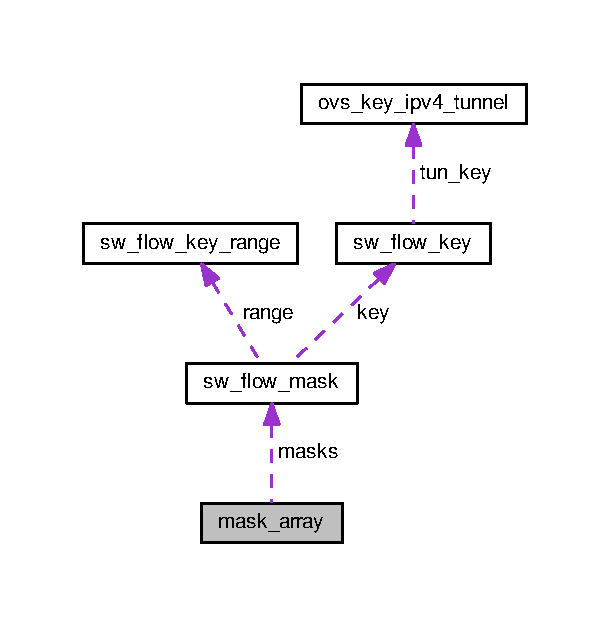
\includegraphics[width=293pt]{structmask__array__coll__graph}
\end{center}
\end{figure}
\subsection*{Data Fields}
\begin{DoxyCompactItemize}
\item 
struct rcu\+\_\+head \hyperlink{structmask__array_ac1e5ee290959115397221781b7ad1c6e}{rcu}
\item 
int \hyperlink{structmask__array_a55b8fb7e2d7ad8a5725a749645f73b5a}{count}
\item 
int \hyperlink{structmask__array_ad981d54486b5dd03bdb4ad20b740171e}{max}
\item 
struct \hyperlink{structsw__flow__mask}{sw\+\_\+flow\+\_\+mask} \hyperlink{compiler_8h_a2b3b0c016258969e4b39c66b6eec2129}{\+\_\+\+\_\+rcu} $\ast$ \hyperlink{structmask__array_a92da2b0ebde32eb6f76a134dc2d61d79}{masks} \mbox{[}$\,$\mbox{]}
\end{DoxyCompactItemize}


\subsection{Field Documentation}
\hypertarget{structmask__array_a55b8fb7e2d7ad8a5725a749645f73b5a}{}\index{mask\+\_\+array@{mask\+\_\+array}!count@{count}}
\index{count@{count}!mask\+\_\+array@{mask\+\_\+array}}
\subsubsection[{count}]{\setlength{\rightskip}{0pt plus 5cm}int mask\+\_\+array\+::count}\label{structmask__array_a55b8fb7e2d7ad8a5725a749645f73b5a}
\hypertarget{structmask__array_a92da2b0ebde32eb6f76a134dc2d61d79}{}\index{mask\+\_\+array@{mask\+\_\+array}!masks@{masks}}
\index{masks@{masks}!mask\+\_\+array@{mask\+\_\+array}}
\subsubsection[{masks}]{\setlength{\rightskip}{0pt plus 5cm}struct {\bf sw\+\_\+flow\+\_\+mask} {\bf \+\_\+\+\_\+rcu}$\ast$ mask\+\_\+array\+::masks\mbox{[}$\,$\mbox{]}}\label{structmask__array_a92da2b0ebde32eb6f76a134dc2d61d79}
\hypertarget{structmask__array_ad981d54486b5dd03bdb4ad20b740171e}{}\index{mask\+\_\+array@{mask\+\_\+array}!max@{max}}
\index{max@{max}!mask\+\_\+array@{mask\+\_\+array}}
\subsubsection[{max}]{\setlength{\rightskip}{0pt plus 5cm}int mask\+\_\+array\+::max}\label{structmask__array_ad981d54486b5dd03bdb4ad20b740171e}
\hypertarget{structmask__array_ac1e5ee290959115397221781b7ad1c6e}{}\index{mask\+\_\+array@{mask\+\_\+array}!rcu@{rcu}}
\index{rcu@{rcu}!mask\+\_\+array@{mask\+\_\+array}}
\subsubsection[{rcu}]{\setlength{\rightskip}{0pt plus 5cm}struct rcu\+\_\+head mask\+\_\+array\+::rcu}\label{structmask__array_ac1e5ee290959115397221781b7ad1c6e}


The documentation for this struct was generated from the following file\+:\begin{DoxyCompactItemize}
\item 
/home/vladn/git/ovs/datapath/\hyperlink{flow__table_8h}{flow\+\_\+table.\+h}\end{DoxyCompactItemize}

\hypertarget{structmask__cache__entry}{}\section{mask\+\_\+cache\+\_\+entry Struct Reference}
\label{structmask__cache__entry}\index{mask\+\_\+cache\+\_\+entry@{mask\+\_\+cache\+\_\+entry}}


{\ttfamily \#include $<$flow\+\_\+table.\+h$>$}

\subsection*{Data Fields}
\begin{DoxyCompactItemize}
\item 
u32 \hyperlink{structmask__cache__entry_a45ae5222badf95e1c919a0d6d0090b6f}{skb\+\_\+hash}
\item 
u32 \hyperlink{structmask__cache__entry_a87faeaec562bcab421cb208dfc0ef5f0}{mask\+\_\+index}
\end{DoxyCompactItemize}


\subsection{Field Documentation}
\hypertarget{structmask__cache__entry_a87faeaec562bcab421cb208dfc0ef5f0}{}\index{mask\+\_\+cache\+\_\+entry@{mask\+\_\+cache\+\_\+entry}!mask\+\_\+index@{mask\+\_\+index}}
\index{mask\+\_\+index@{mask\+\_\+index}!mask\+\_\+cache\+\_\+entry@{mask\+\_\+cache\+\_\+entry}}
\subsubsection[{mask\+\_\+index}]{\setlength{\rightskip}{0pt plus 5cm}u32 mask\+\_\+cache\+\_\+entry\+::mask\+\_\+index}\label{structmask__cache__entry_a87faeaec562bcab421cb208dfc0ef5f0}
\hypertarget{structmask__cache__entry_a45ae5222badf95e1c919a0d6d0090b6f}{}\index{mask\+\_\+cache\+\_\+entry@{mask\+\_\+cache\+\_\+entry}!skb\+\_\+hash@{skb\+\_\+hash}}
\index{skb\+\_\+hash@{skb\+\_\+hash}!mask\+\_\+cache\+\_\+entry@{mask\+\_\+cache\+\_\+entry}}
\subsubsection[{skb\+\_\+hash}]{\setlength{\rightskip}{0pt plus 5cm}u32 mask\+\_\+cache\+\_\+entry\+::skb\+\_\+hash}\label{structmask__cache__entry_a45ae5222badf95e1c919a0d6d0090b6f}


The documentation for this struct was generated from the following file\+:\begin{DoxyCompactItemize}
\item 
/home/vladn/git/ovs/datapath/\hyperlink{flow__table_8h}{flow\+\_\+table.\+h}\end{DoxyCompactItemize}

\hypertarget{structnetdev__vport}{}\section{netdev\+\_\+vport Struct Reference}
\label{structnetdev__vport}\index{netdev\+\_\+vport@{netdev\+\_\+vport}}


{\ttfamily \#include $<$vport-\/netdev.\+h$>$}

\subsection*{Data Fields}
\begin{DoxyCompactItemize}
\item 
struct rcu\+\_\+head \hyperlink{structnetdev__vport_ad3844aef4d3d1f85e7eec5529676b91d}{rcu}
\item 
struct net\+\_\+device $\ast$ \hyperlink{structnetdev__vport_acf4ee248f7385e2f987fd2736f824ca9}{dev}
\end{DoxyCompactItemize}


\subsection{Field Documentation}
\hypertarget{structnetdev__vport_acf4ee248f7385e2f987fd2736f824ca9}{}\index{netdev\+\_\+vport@{netdev\+\_\+vport}!dev@{dev}}
\index{dev@{dev}!netdev\+\_\+vport@{netdev\+\_\+vport}}
\subsubsection[{dev}]{\setlength{\rightskip}{0pt plus 5cm}struct net\+\_\+device$\ast$ netdev\+\_\+vport\+::dev}\label{structnetdev__vport_acf4ee248f7385e2f987fd2736f824ca9}
\hypertarget{structnetdev__vport_ad3844aef4d3d1f85e7eec5529676b91d}{}\index{netdev\+\_\+vport@{netdev\+\_\+vport}!rcu@{rcu}}
\index{rcu@{rcu}!netdev\+\_\+vport@{netdev\+\_\+vport}}
\subsubsection[{rcu}]{\setlength{\rightskip}{0pt plus 5cm}struct rcu\+\_\+head netdev\+\_\+vport\+::rcu}\label{structnetdev__vport_ad3844aef4d3d1f85e7eec5529676b91d}


The documentation for this struct was generated from the following file\+:\begin{DoxyCompactItemize}
\item 
/home/vladn/git/ovs/datapath/\hyperlink{vport-netdev_8h}{vport-\/netdev.\+h}\end{DoxyCompactItemize}

\hypertarget{structovs__action__hash}{}\section{ovs\+\_\+action\+\_\+hash Struct Reference}
\label{structovs__action__hash}\index{ovs\+\_\+action\+\_\+hash@{ovs\+\_\+action\+\_\+hash}}


{\ttfamily \#include $<$openvswitch.\+h$>$}

\subsection*{Data Fields}
\begin{DoxyCompactItemize}
\item 
uint32\+\_\+t \hyperlink{structovs__action__hash_a8dde1557790d7fc7c2cae50f4e6d65e8}{hash\+\_\+alg}
\item 
uint32\+\_\+t \hyperlink{structovs__action__hash_a174855fe08c609dd3542de6e9e8a92ee}{hash\+\_\+basis}
\end{DoxyCompactItemize}


\subsection{Field Documentation}
\hypertarget{structovs__action__hash_a8dde1557790d7fc7c2cae50f4e6d65e8}{}\index{ovs\+\_\+action\+\_\+hash@{ovs\+\_\+action\+\_\+hash}!hash\+\_\+alg@{hash\+\_\+alg}}
\index{hash\+\_\+alg@{hash\+\_\+alg}!ovs\+\_\+action\+\_\+hash@{ovs\+\_\+action\+\_\+hash}}
\subsubsection[{hash\+\_\+alg}]{\setlength{\rightskip}{0pt plus 5cm}uint32\+\_\+t ovs\+\_\+action\+\_\+hash\+::hash\+\_\+alg}\label{structovs__action__hash_a8dde1557790d7fc7c2cae50f4e6d65e8}
\hypertarget{structovs__action__hash_a174855fe08c609dd3542de6e9e8a92ee}{}\index{ovs\+\_\+action\+\_\+hash@{ovs\+\_\+action\+\_\+hash}!hash\+\_\+basis@{hash\+\_\+basis}}
\index{hash\+\_\+basis@{hash\+\_\+basis}!ovs\+\_\+action\+\_\+hash@{ovs\+\_\+action\+\_\+hash}}
\subsubsection[{hash\+\_\+basis}]{\setlength{\rightskip}{0pt plus 5cm}uint32\+\_\+t ovs\+\_\+action\+\_\+hash\+::hash\+\_\+basis}\label{structovs__action__hash_a174855fe08c609dd3542de6e9e8a92ee}


The documentation for this struct was generated from the following file\+:\begin{DoxyCompactItemize}
\item 
/home/vladn/git/ovs/datapath/linux/compat/include/linux/\hyperlink{openvswitch_8h}{openvswitch.\+h}\end{DoxyCompactItemize}

\hypertarget{structovs__action__push__mpls}{}\section{ovs\+\_\+action\+\_\+push\+\_\+mpls Struct Reference}
\label{structovs__action__push__mpls}\index{ovs\+\_\+action\+\_\+push\+\_\+mpls@{ovs\+\_\+action\+\_\+push\+\_\+mpls}}


{\ttfamily \#include $<$openvswitch.\+h$>$}

\subsection*{Data Fields}
\begin{DoxyCompactItemize}
\item 
\+\_\+\+\_\+be32 \hyperlink{structovs__action__push__mpls_a58c09de1a14973c13197f7748beb3803}{mpls\+\_\+lse}
\item 
\+\_\+\+\_\+be16 \hyperlink{structovs__action__push__mpls_adea8de7c1e924d0665c4eb62901ce521}{mpls\+\_\+ethertype}
\end{DoxyCompactItemize}


\subsection{Detailed Description}
struct \hyperlink{structovs__action__push__mpls}{ovs\+\_\+action\+\_\+push\+\_\+mpls} -\/ O\+V\+S\+\_\+\+A\+C\+T\+I\+O\+N\+\_\+\+A\+T\+T\+R\+\_\+\+P\+U\+S\+H\+\_\+\+M\+P\+L\+S action argument. \+: M\+P\+L\+S label stack entry to push. \+: Ethertype to set in the encapsulating ethernet frame.

The only values  should ever be given are E\+T\+H\+\_\+\+P\+\_\+\+M\+P\+L\+S\+\_\+\+U\+C and E\+T\+H\+\_\+\+P\+\_\+\+M\+P\+L\+S\+\_\+\+M\+C, indicating M\+P\+L\+S unicast or multicast. Other are rejected. 

\subsection{Field Documentation}
\hypertarget{structovs__action__push__mpls_adea8de7c1e924d0665c4eb62901ce521}{}\index{ovs\+\_\+action\+\_\+push\+\_\+mpls@{ovs\+\_\+action\+\_\+push\+\_\+mpls}!mpls\+\_\+ethertype@{mpls\+\_\+ethertype}}
\index{mpls\+\_\+ethertype@{mpls\+\_\+ethertype}!ovs\+\_\+action\+\_\+push\+\_\+mpls@{ovs\+\_\+action\+\_\+push\+\_\+mpls}}
\subsubsection[{mpls\+\_\+ethertype}]{\setlength{\rightskip}{0pt plus 5cm}\+\_\+\+\_\+be16 ovs\+\_\+action\+\_\+push\+\_\+mpls\+::mpls\+\_\+ethertype}\label{structovs__action__push__mpls_adea8de7c1e924d0665c4eb62901ce521}
\hypertarget{structovs__action__push__mpls_a58c09de1a14973c13197f7748beb3803}{}\index{ovs\+\_\+action\+\_\+push\+\_\+mpls@{ovs\+\_\+action\+\_\+push\+\_\+mpls}!mpls\+\_\+lse@{mpls\+\_\+lse}}
\index{mpls\+\_\+lse@{mpls\+\_\+lse}!ovs\+\_\+action\+\_\+push\+\_\+mpls@{ovs\+\_\+action\+\_\+push\+\_\+mpls}}
\subsubsection[{mpls\+\_\+lse}]{\setlength{\rightskip}{0pt plus 5cm}\+\_\+\+\_\+be32 ovs\+\_\+action\+\_\+push\+\_\+mpls\+::mpls\+\_\+lse}\label{structovs__action__push__mpls_a58c09de1a14973c13197f7748beb3803}


The documentation for this struct was generated from the following file\+:\begin{DoxyCompactItemize}
\item 
/home/vladn/git/ovs/datapath/linux/compat/include/linux/\hyperlink{openvswitch_8h}{openvswitch.\+h}\end{DoxyCompactItemize}

\hypertarget{structovs__action__push__tnl}{}\section{ovs\+\_\+action\+\_\+push\+\_\+tnl Struct Reference}
\label{structovs__action__push__tnl}\index{ovs\+\_\+action\+\_\+push\+\_\+tnl@{ovs\+\_\+action\+\_\+push\+\_\+tnl}}


{\ttfamily \#include $<$openvswitch.\+h$>$}

\subsection*{Data Fields}
\begin{DoxyCompactItemize}
\item 
uint32\+\_\+t \hyperlink{structovs__action__push__tnl_a075797c91bf16f67b0e99d00733de09c}{tnl\+\_\+port}
\item 
uint32\+\_\+t \hyperlink{structovs__action__push__tnl_a314ef1909bc176d1fe3f6588d24edfde}{out\+\_\+port}
\item 
uint32\+\_\+t \hyperlink{structovs__action__push__tnl_ae17c0fbdac67f4393a1bf5cc463caa61}{header\+\_\+len}
\item 
uint32\+\_\+t \hyperlink{structovs__action__push__tnl_a5a768ff0a623d03bc2b4d13db4bd4413}{tnl\+\_\+type}
\item 
uint8\+\_\+t \hyperlink{structovs__action__push__tnl_a722b423a78230e5e3dcf8586538404a5}{header} \mbox{[}\hyperlink{openvswitch_8h_a20584c44e8d74e782a3a777dcf26dfc9}{T\+N\+L\+\_\+\+P\+U\+S\+H\+\_\+\+H\+E\+A\+D\+E\+R\+\_\+\+S\+I\+Z\+E}\mbox{]}
\end{DoxyCompactItemize}


\subsection{Field Documentation}
\hypertarget{structovs__action__push__tnl_a722b423a78230e5e3dcf8586538404a5}{}\index{ovs\+\_\+action\+\_\+push\+\_\+tnl@{ovs\+\_\+action\+\_\+push\+\_\+tnl}!header@{header}}
\index{header@{header}!ovs\+\_\+action\+\_\+push\+\_\+tnl@{ovs\+\_\+action\+\_\+push\+\_\+tnl}}
\subsubsection[{header}]{\setlength{\rightskip}{0pt plus 5cm}uint8\+\_\+t ovs\+\_\+action\+\_\+push\+\_\+tnl\+::header\mbox{[}{\bf T\+N\+L\+\_\+\+P\+U\+S\+H\+\_\+\+H\+E\+A\+D\+E\+R\+\_\+\+S\+I\+Z\+E}\mbox{]}}\label{structovs__action__push__tnl_a722b423a78230e5e3dcf8586538404a5}
\hypertarget{structovs__action__push__tnl_ae17c0fbdac67f4393a1bf5cc463caa61}{}\index{ovs\+\_\+action\+\_\+push\+\_\+tnl@{ovs\+\_\+action\+\_\+push\+\_\+tnl}!header\+\_\+len@{header\+\_\+len}}
\index{header\+\_\+len@{header\+\_\+len}!ovs\+\_\+action\+\_\+push\+\_\+tnl@{ovs\+\_\+action\+\_\+push\+\_\+tnl}}
\subsubsection[{header\+\_\+len}]{\setlength{\rightskip}{0pt plus 5cm}uint32\+\_\+t ovs\+\_\+action\+\_\+push\+\_\+tnl\+::header\+\_\+len}\label{structovs__action__push__tnl_ae17c0fbdac67f4393a1bf5cc463caa61}
\hypertarget{structovs__action__push__tnl_a314ef1909bc176d1fe3f6588d24edfde}{}\index{ovs\+\_\+action\+\_\+push\+\_\+tnl@{ovs\+\_\+action\+\_\+push\+\_\+tnl}!out\+\_\+port@{out\+\_\+port}}
\index{out\+\_\+port@{out\+\_\+port}!ovs\+\_\+action\+\_\+push\+\_\+tnl@{ovs\+\_\+action\+\_\+push\+\_\+tnl}}
\subsubsection[{out\+\_\+port}]{\setlength{\rightskip}{0pt plus 5cm}uint32\+\_\+t ovs\+\_\+action\+\_\+push\+\_\+tnl\+::out\+\_\+port}\label{structovs__action__push__tnl_a314ef1909bc176d1fe3f6588d24edfde}
\hypertarget{structovs__action__push__tnl_a075797c91bf16f67b0e99d00733de09c}{}\index{ovs\+\_\+action\+\_\+push\+\_\+tnl@{ovs\+\_\+action\+\_\+push\+\_\+tnl}!tnl\+\_\+port@{tnl\+\_\+port}}
\index{tnl\+\_\+port@{tnl\+\_\+port}!ovs\+\_\+action\+\_\+push\+\_\+tnl@{ovs\+\_\+action\+\_\+push\+\_\+tnl}}
\subsubsection[{tnl\+\_\+port}]{\setlength{\rightskip}{0pt plus 5cm}uint32\+\_\+t ovs\+\_\+action\+\_\+push\+\_\+tnl\+::tnl\+\_\+port}\label{structovs__action__push__tnl_a075797c91bf16f67b0e99d00733de09c}
\hypertarget{structovs__action__push__tnl_a5a768ff0a623d03bc2b4d13db4bd4413}{}\index{ovs\+\_\+action\+\_\+push\+\_\+tnl@{ovs\+\_\+action\+\_\+push\+\_\+tnl}!tnl\+\_\+type@{tnl\+\_\+type}}
\index{tnl\+\_\+type@{tnl\+\_\+type}!ovs\+\_\+action\+\_\+push\+\_\+tnl@{ovs\+\_\+action\+\_\+push\+\_\+tnl}}
\subsubsection[{tnl\+\_\+type}]{\setlength{\rightskip}{0pt plus 5cm}uint32\+\_\+t ovs\+\_\+action\+\_\+push\+\_\+tnl\+::tnl\+\_\+type}\label{structovs__action__push__tnl_a5a768ff0a623d03bc2b4d13db4bd4413}


The documentation for this struct was generated from the following file\+:\begin{DoxyCompactItemize}
\item 
/home/vladn/git/ovs/datapath/linux/compat/include/linux/\hyperlink{openvswitch_8h}{openvswitch.\+h}\end{DoxyCompactItemize}

\hypertarget{structovs__action__push__vlan}{}\section{ovs\+\_\+action\+\_\+push\+\_\+vlan Struct Reference}
\label{structovs__action__push__vlan}\index{ovs\+\_\+action\+\_\+push\+\_\+vlan@{ovs\+\_\+action\+\_\+push\+\_\+vlan}}


{\ttfamily \#include $<$openvswitch.\+h$>$}

\subsection*{Data Fields}
\begin{DoxyCompactItemize}
\item 
\+\_\+\+\_\+be16 \hyperlink{structovs__action__push__vlan_af2e36cd70149cf03ebf29586fc765722}{vlan\+\_\+tpid}
\item 
\+\_\+\+\_\+be16 \hyperlink{structovs__action__push__vlan_ab17c8db02bffc32a072bd23687dd712c}{vlan\+\_\+tci}
\end{DoxyCompactItemize}


\subsection{Detailed Description}
struct \hyperlink{structovs__action__push__vlan}{ovs\+\_\+action\+\_\+push\+\_\+vlan} -\/ O\+V\+S\+\_\+\+A\+C\+T\+I\+O\+N\+\_\+\+A\+T\+T\+R\+\_\+\+P\+U\+S\+H\+\_\+\+V\+L\+A\+N action argument. \+: Tag protocol identifier (T\+P\+I\+D) to push. \+: Tag control identifier (T\+C\+I) to push. The C\+F\+I bit must be set (but it will not be set in the 802.\+1\+Q header that is pushed).

The  value is typically E\+T\+H\+\_\+\+P\+\_\+8021\+Q. The only acceptable T\+P\+I\+D values are those that the kernel module also parses as 802.\+1\+Q headers, to prevent O\+V\+S\+\_\+\+A\+C\+T\+I\+O\+N\+\_\+\+A\+T\+T\+R\+\_\+\+P\+U\+S\+H\+\_\+\+V\+L\+A\+N followed by O\+V\+S\+\_\+\+A\+C\+T\+I\+O\+N\+\_\+\+A\+T\+T\+R\+\_\+\+P\+O\+P\+\_\+\+V\+L\+A\+N from having surprising results. 

\subsection{Field Documentation}
\hypertarget{structovs__action__push__vlan_ab17c8db02bffc32a072bd23687dd712c}{}\index{ovs\+\_\+action\+\_\+push\+\_\+vlan@{ovs\+\_\+action\+\_\+push\+\_\+vlan}!vlan\+\_\+tci@{vlan\+\_\+tci}}
\index{vlan\+\_\+tci@{vlan\+\_\+tci}!ovs\+\_\+action\+\_\+push\+\_\+vlan@{ovs\+\_\+action\+\_\+push\+\_\+vlan}}
\subsubsection[{vlan\+\_\+tci}]{\setlength{\rightskip}{0pt plus 5cm}\+\_\+\+\_\+be16 ovs\+\_\+action\+\_\+push\+\_\+vlan\+::vlan\+\_\+tci}\label{structovs__action__push__vlan_ab17c8db02bffc32a072bd23687dd712c}
\hypertarget{structovs__action__push__vlan_af2e36cd70149cf03ebf29586fc765722}{}\index{ovs\+\_\+action\+\_\+push\+\_\+vlan@{ovs\+\_\+action\+\_\+push\+\_\+vlan}!vlan\+\_\+tpid@{vlan\+\_\+tpid}}
\index{vlan\+\_\+tpid@{vlan\+\_\+tpid}!ovs\+\_\+action\+\_\+push\+\_\+vlan@{ovs\+\_\+action\+\_\+push\+\_\+vlan}}
\subsubsection[{vlan\+\_\+tpid}]{\setlength{\rightskip}{0pt plus 5cm}\+\_\+\+\_\+be16 ovs\+\_\+action\+\_\+push\+\_\+vlan\+::vlan\+\_\+tpid}\label{structovs__action__push__vlan_af2e36cd70149cf03ebf29586fc765722}


The documentation for this struct was generated from the following file\+:\begin{DoxyCompactItemize}
\item 
/home/vladn/git/ovs/datapath/linux/compat/include/linux/\hyperlink{openvswitch_8h}{openvswitch.\+h}\end{DoxyCompactItemize}

\hypertarget{structovs__dp__megaflow__stats}{}\section{ovs\+\_\+dp\+\_\+megaflow\+\_\+stats Struct Reference}
\label{structovs__dp__megaflow__stats}\index{ovs\+\_\+dp\+\_\+megaflow\+\_\+stats@{ovs\+\_\+dp\+\_\+megaflow\+\_\+stats}}


{\ttfamily \#include $<$openvswitch.\+h$>$}

\subsection*{Data Fields}
\begin{DoxyCompactItemize}
\item 
\+\_\+\+\_\+u64 \hyperlink{structovs__dp__megaflow__stats_a28566425278d53e7a93e693d54e1e65c}{n\+\_\+mask\+\_\+hit}
\item 
\+\_\+\+\_\+u32 \hyperlink{structovs__dp__megaflow__stats_a7984504a5c12cc5a0767c6a34c4c9c96}{n\+\_\+masks}
\item 
\+\_\+\+\_\+u32 \hyperlink{structovs__dp__megaflow__stats_a958a20791b4e74e2be231c1b82dd9268}{pad0}
\item 
\+\_\+\+\_\+u64 \hyperlink{structovs__dp__megaflow__stats_a2cd7b88cd84316721a2dfafc7040b99a}{pad1}
\item 
\+\_\+\+\_\+u64 \hyperlink{structovs__dp__megaflow__stats_a321ac1dbc76c153d6dd969ad929dea75}{pad2}
\end{DoxyCompactItemize}


\subsection{Field Documentation}
\hypertarget{structovs__dp__megaflow__stats_a28566425278d53e7a93e693d54e1e65c}{}\index{ovs\+\_\+dp\+\_\+megaflow\+\_\+stats@{ovs\+\_\+dp\+\_\+megaflow\+\_\+stats}!n\+\_\+mask\+\_\+hit@{n\+\_\+mask\+\_\+hit}}
\index{n\+\_\+mask\+\_\+hit@{n\+\_\+mask\+\_\+hit}!ovs\+\_\+dp\+\_\+megaflow\+\_\+stats@{ovs\+\_\+dp\+\_\+megaflow\+\_\+stats}}
\subsubsection[{n\+\_\+mask\+\_\+hit}]{\setlength{\rightskip}{0pt plus 5cm}\+\_\+\+\_\+u64 ovs\+\_\+dp\+\_\+megaflow\+\_\+stats\+::n\+\_\+mask\+\_\+hit}\label{structovs__dp__megaflow__stats_a28566425278d53e7a93e693d54e1e65c}
\hypertarget{structovs__dp__megaflow__stats_a7984504a5c12cc5a0767c6a34c4c9c96}{}\index{ovs\+\_\+dp\+\_\+megaflow\+\_\+stats@{ovs\+\_\+dp\+\_\+megaflow\+\_\+stats}!n\+\_\+masks@{n\+\_\+masks}}
\index{n\+\_\+masks@{n\+\_\+masks}!ovs\+\_\+dp\+\_\+megaflow\+\_\+stats@{ovs\+\_\+dp\+\_\+megaflow\+\_\+stats}}
\subsubsection[{n\+\_\+masks}]{\setlength{\rightskip}{0pt plus 5cm}\+\_\+\+\_\+u32 ovs\+\_\+dp\+\_\+megaflow\+\_\+stats\+::n\+\_\+masks}\label{structovs__dp__megaflow__stats_a7984504a5c12cc5a0767c6a34c4c9c96}
\hypertarget{structovs__dp__megaflow__stats_a958a20791b4e74e2be231c1b82dd9268}{}\index{ovs\+\_\+dp\+\_\+megaflow\+\_\+stats@{ovs\+\_\+dp\+\_\+megaflow\+\_\+stats}!pad0@{pad0}}
\index{pad0@{pad0}!ovs\+\_\+dp\+\_\+megaflow\+\_\+stats@{ovs\+\_\+dp\+\_\+megaflow\+\_\+stats}}
\subsubsection[{pad0}]{\setlength{\rightskip}{0pt plus 5cm}\+\_\+\+\_\+u32 ovs\+\_\+dp\+\_\+megaflow\+\_\+stats\+::pad0}\label{structovs__dp__megaflow__stats_a958a20791b4e74e2be231c1b82dd9268}
\hypertarget{structovs__dp__megaflow__stats_a2cd7b88cd84316721a2dfafc7040b99a}{}\index{ovs\+\_\+dp\+\_\+megaflow\+\_\+stats@{ovs\+\_\+dp\+\_\+megaflow\+\_\+stats}!pad1@{pad1}}
\index{pad1@{pad1}!ovs\+\_\+dp\+\_\+megaflow\+\_\+stats@{ovs\+\_\+dp\+\_\+megaflow\+\_\+stats}}
\subsubsection[{pad1}]{\setlength{\rightskip}{0pt plus 5cm}\+\_\+\+\_\+u64 ovs\+\_\+dp\+\_\+megaflow\+\_\+stats\+::pad1}\label{structovs__dp__megaflow__stats_a2cd7b88cd84316721a2dfafc7040b99a}
\hypertarget{structovs__dp__megaflow__stats_a321ac1dbc76c153d6dd969ad929dea75}{}\index{ovs\+\_\+dp\+\_\+megaflow\+\_\+stats@{ovs\+\_\+dp\+\_\+megaflow\+\_\+stats}!pad2@{pad2}}
\index{pad2@{pad2}!ovs\+\_\+dp\+\_\+megaflow\+\_\+stats@{ovs\+\_\+dp\+\_\+megaflow\+\_\+stats}}
\subsubsection[{pad2}]{\setlength{\rightskip}{0pt plus 5cm}\+\_\+\+\_\+u64 ovs\+\_\+dp\+\_\+megaflow\+\_\+stats\+::pad2}\label{structovs__dp__megaflow__stats_a321ac1dbc76c153d6dd969ad929dea75}


The documentation for this struct was generated from the following file\+:\begin{DoxyCompactItemize}
\item 
/home/vladn/git/ovs/datapath/linux/compat/include/linux/\hyperlink{openvswitch_8h}{openvswitch.\+h}\end{DoxyCompactItemize}

\hypertarget{structovs__dp__stats}{}\section{ovs\+\_\+dp\+\_\+stats Struct Reference}
\label{structovs__dp__stats}\index{ovs\+\_\+dp\+\_\+stats@{ovs\+\_\+dp\+\_\+stats}}


{\ttfamily \#include $<$openvswitch.\+h$>$}

\subsection*{Data Fields}
\begin{DoxyCompactItemize}
\item 
\+\_\+\+\_\+u64 \hyperlink{structovs__dp__stats_a0c6b8d1358632341b5e949570c5dca68}{n\+\_\+hit}
\item 
\+\_\+\+\_\+u64 \hyperlink{structovs__dp__stats_a8f1b9687593ebb43ca54c1c9904999a6}{n\+\_\+missed}
\item 
\+\_\+\+\_\+u64 \hyperlink{structovs__dp__stats_a83a104dedcf4ee3cc2a940e4043e89b2}{n\+\_\+lost}
\item 
\+\_\+\+\_\+u64 \hyperlink{structovs__dp__stats_af6bf9e903d781d713f0f5d10b2d8550f}{n\+\_\+flows}
\end{DoxyCompactItemize}


\subsection{Field Documentation}
\hypertarget{structovs__dp__stats_af6bf9e903d781d713f0f5d10b2d8550f}{}\index{ovs\+\_\+dp\+\_\+stats@{ovs\+\_\+dp\+\_\+stats}!n\+\_\+flows@{n\+\_\+flows}}
\index{n\+\_\+flows@{n\+\_\+flows}!ovs\+\_\+dp\+\_\+stats@{ovs\+\_\+dp\+\_\+stats}}
\subsubsection[{n\+\_\+flows}]{\setlength{\rightskip}{0pt plus 5cm}\+\_\+\+\_\+u64 ovs\+\_\+dp\+\_\+stats\+::n\+\_\+flows}\label{structovs__dp__stats_af6bf9e903d781d713f0f5d10b2d8550f}
\hypertarget{structovs__dp__stats_a0c6b8d1358632341b5e949570c5dca68}{}\index{ovs\+\_\+dp\+\_\+stats@{ovs\+\_\+dp\+\_\+stats}!n\+\_\+hit@{n\+\_\+hit}}
\index{n\+\_\+hit@{n\+\_\+hit}!ovs\+\_\+dp\+\_\+stats@{ovs\+\_\+dp\+\_\+stats}}
\subsubsection[{n\+\_\+hit}]{\setlength{\rightskip}{0pt plus 5cm}\+\_\+\+\_\+u64 ovs\+\_\+dp\+\_\+stats\+::n\+\_\+hit}\label{structovs__dp__stats_a0c6b8d1358632341b5e949570c5dca68}
\hypertarget{structovs__dp__stats_a83a104dedcf4ee3cc2a940e4043e89b2}{}\index{ovs\+\_\+dp\+\_\+stats@{ovs\+\_\+dp\+\_\+stats}!n\+\_\+lost@{n\+\_\+lost}}
\index{n\+\_\+lost@{n\+\_\+lost}!ovs\+\_\+dp\+\_\+stats@{ovs\+\_\+dp\+\_\+stats}}
\subsubsection[{n\+\_\+lost}]{\setlength{\rightskip}{0pt plus 5cm}\+\_\+\+\_\+u64 ovs\+\_\+dp\+\_\+stats\+::n\+\_\+lost}\label{structovs__dp__stats_a83a104dedcf4ee3cc2a940e4043e89b2}
\hypertarget{structovs__dp__stats_a8f1b9687593ebb43ca54c1c9904999a6}{}\index{ovs\+\_\+dp\+\_\+stats@{ovs\+\_\+dp\+\_\+stats}!n\+\_\+missed@{n\+\_\+missed}}
\index{n\+\_\+missed@{n\+\_\+missed}!ovs\+\_\+dp\+\_\+stats@{ovs\+\_\+dp\+\_\+stats}}
\subsubsection[{n\+\_\+missed}]{\setlength{\rightskip}{0pt plus 5cm}\+\_\+\+\_\+u64 ovs\+\_\+dp\+\_\+stats\+::n\+\_\+missed}\label{structovs__dp__stats_a8f1b9687593ebb43ca54c1c9904999a6}


The documentation for this struct was generated from the following file\+:\begin{DoxyCompactItemize}
\item 
/home/vladn/git/ovs/datapath/linux/compat/include/linux/\hyperlink{openvswitch_8h}{openvswitch.\+h}\end{DoxyCompactItemize}

\hypertarget{structovs__flow__stats}{}\section{ovs\+\_\+flow\+\_\+stats Struct Reference}
\label{structovs__flow__stats}\index{ovs\+\_\+flow\+\_\+stats@{ovs\+\_\+flow\+\_\+stats}}


{\ttfamily \#include $<$openvswitch.\+h$>$}

\subsection*{Data Fields}
\begin{DoxyCompactItemize}
\item 
\+\_\+\+\_\+u64 \hyperlink{structovs__flow__stats_ab82070e9f656011c1a5b988082c7bfcc}{n\+\_\+packets}
\item 
\+\_\+\+\_\+u64 \hyperlink{structovs__flow__stats_a4dea1785485d954f41121a561701ddf2}{n\+\_\+bytes}
\end{DoxyCompactItemize}


\subsection{Field Documentation}
\hypertarget{structovs__flow__stats_a4dea1785485d954f41121a561701ddf2}{}\index{ovs\+\_\+flow\+\_\+stats@{ovs\+\_\+flow\+\_\+stats}!n\+\_\+bytes@{n\+\_\+bytes}}
\index{n\+\_\+bytes@{n\+\_\+bytes}!ovs\+\_\+flow\+\_\+stats@{ovs\+\_\+flow\+\_\+stats}}
\subsubsection[{n\+\_\+bytes}]{\setlength{\rightskip}{0pt plus 5cm}\+\_\+\+\_\+u64 ovs\+\_\+flow\+\_\+stats\+::n\+\_\+bytes}\label{structovs__flow__stats_a4dea1785485d954f41121a561701ddf2}
\hypertarget{structovs__flow__stats_ab82070e9f656011c1a5b988082c7bfcc}{}\index{ovs\+\_\+flow\+\_\+stats@{ovs\+\_\+flow\+\_\+stats}!n\+\_\+packets@{n\+\_\+packets}}
\index{n\+\_\+packets@{n\+\_\+packets}!ovs\+\_\+flow\+\_\+stats@{ovs\+\_\+flow\+\_\+stats}}
\subsubsection[{n\+\_\+packets}]{\setlength{\rightskip}{0pt plus 5cm}\+\_\+\+\_\+u64 ovs\+\_\+flow\+\_\+stats\+::n\+\_\+packets}\label{structovs__flow__stats_ab82070e9f656011c1a5b988082c7bfcc}


The documentation for this struct was generated from the following file\+:\begin{DoxyCompactItemize}
\item 
/home/vladn/git/ovs/datapath/linux/compat/include/linux/\hyperlink{openvswitch_8h}{openvswitch.\+h}\end{DoxyCompactItemize}

\hypertarget{structovs__header}{}\section{ovs\+\_\+header Struct Reference}
\label{structovs__header}\index{ovs\+\_\+header@{ovs\+\_\+header}}


{\ttfamily \#include $<$openvswitch.\+h$>$}

\subsection*{Data Fields}
\begin{DoxyCompactItemize}
\item 
int \hyperlink{structovs__header_a8ff8d9e5f29285dff5404cc8fa23b452}{dp\+\_\+ifindex}
\end{DoxyCompactItemize}


\subsection{Detailed Description}
struct \hyperlink{structovs__header}{ovs\+\_\+header} -\/ header for O\+V\+S Generic Netlink messages. \+: ifindex of local port for datapath (0 to make a request not specific to a datapath).

Attributes following the header are specific to a particular O\+V\+S Generic Netlink family, but all of the O\+V\+S families use this header. 

\subsection{Field Documentation}
\hypertarget{structovs__header_a8ff8d9e5f29285dff5404cc8fa23b452}{}\index{ovs\+\_\+header@{ovs\+\_\+header}!dp\+\_\+ifindex@{dp\+\_\+ifindex}}
\index{dp\+\_\+ifindex@{dp\+\_\+ifindex}!ovs\+\_\+header@{ovs\+\_\+header}}
\subsubsection[{dp\+\_\+ifindex}]{\setlength{\rightskip}{0pt plus 5cm}int ovs\+\_\+header\+::dp\+\_\+ifindex}\label{structovs__header_a8ff8d9e5f29285dff5404cc8fa23b452}


The documentation for this struct was generated from the following file\+:\begin{DoxyCompactItemize}
\item 
/home/vladn/git/ovs/datapath/linux/compat/include/linux/\hyperlink{openvswitch_8h}{openvswitch.\+h}\end{DoxyCompactItemize}

\hypertarget{structovs__key__arp}{}\section{ovs\+\_\+key\+\_\+arp Struct Reference}
\label{structovs__key__arp}\index{ovs\+\_\+key\+\_\+arp@{ovs\+\_\+key\+\_\+arp}}


{\ttfamily \#include $<$openvswitch.\+h$>$}

\subsection*{Data Fields}
\begin{DoxyCompactItemize}
\item 
\+\_\+\+\_\+be32 \hyperlink{structovs__key__arp_a25ce3912d909430a080dd3264d858892}{arp\+\_\+sip}
\item 
\+\_\+\+\_\+be32 \hyperlink{structovs__key__arp_a84a3d1edd8ba5960d41a69155e721d20}{arp\+\_\+tip}
\item 
\+\_\+\+\_\+be16 \hyperlink{structovs__key__arp_a560ecc1caa0ae74b43abe0d5dd30306d}{arp\+\_\+op}
\item 
\+\_\+\+\_\+u8 \hyperlink{structovs__key__arp_a99f6141da2e3151181663f27ab1a3560}{arp\+\_\+sha} \mbox{[}E\+T\+H\+\_\+\+A\+L\+E\+N\mbox{]}
\item 
\+\_\+\+\_\+u8 \hyperlink{structovs__key__arp_ab9f27ebc29aee381031d9b89d1b954ac}{arp\+\_\+tha} \mbox{[}E\+T\+H\+\_\+\+A\+L\+E\+N\mbox{]}
\end{DoxyCompactItemize}


\subsection{Field Documentation}
\hypertarget{structovs__key__arp_a560ecc1caa0ae74b43abe0d5dd30306d}{}\index{ovs\+\_\+key\+\_\+arp@{ovs\+\_\+key\+\_\+arp}!arp\+\_\+op@{arp\+\_\+op}}
\index{arp\+\_\+op@{arp\+\_\+op}!ovs\+\_\+key\+\_\+arp@{ovs\+\_\+key\+\_\+arp}}
\subsubsection[{arp\+\_\+op}]{\setlength{\rightskip}{0pt plus 5cm}\+\_\+\+\_\+be16 ovs\+\_\+key\+\_\+arp\+::arp\+\_\+op}\label{structovs__key__arp_a560ecc1caa0ae74b43abe0d5dd30306d}
\hypertarget{structovs__key__arp_a99f6141da2e3151181663f27ab1a3560}{}\index{ovs\+\_\+key\+\_\+arp@{ovs\+\_\+key\+\_\+arp}!arp\+\_\+sha@{arp\+\_\+sha}}
\index{arp\+\_\+sha@{arp\+\_\+sha}!ovs\+\_\+key\+\_\+arp@{ovs\+\_\+key\+\_\+arp}}
\subsubsection[{arp\+\_\+sha}]{\setlength{\rightskip}{0pt plus 5cm}\+\_\+\+\_\+u8 ovs\+\_\+key\+\_\+arp\+::arp\+\_\+sha\mbox{[}E\+T\+H\+\_\+\+A\+L\+E\+N\mbox{]}}\label{structovs__key__arp_a99f6141da2e3151181663f27ab1a3560}
\hypertarget{structovs__key__arp_a25ce3912d909430a080dd3264d858892}{}\index{ovs\+\_\+key\+\_\+arp@{ovs\+\_\+key\+\_\+arp}!arp\+\_\+sip@{arp\+\_\+sip}}
\index{arp\+\_\+sip@{arp\+\_\+sip}!ovs\+\_\+key\+\_\+arp@{ovs\+\_\+key\+\_\+arp}}
\subsubsection[{arp\+\_\+sip}]{\setlength{\rightskip}{0pt plus 5cm}\+\_\+\+\_\+be32 ovs\+\_\+key\+\_\+arp\+::arp\+\_\+sip}\label{structovs__key__arp_a25ce3912d909430a080dd3264d858892}
\hypertarget{structovs__key__arp_ab9f27ebc29aee381031d9b89d1b954ac}{}\index{ovs\+\_\+key\+\_\+arp@{ovs\+\_\+key\+\_\+arp}!arp\+\_\+tha@{arp\+\_\+tha}}
\index{arp\+\_\+tha@{arp\+\_\+tha}!ovs\+\_\+key\+\_\+arp@{ovs\+\_\+key\+\_\+arp}}
\subsubsection[{arp\+\_\+tha}]{\setlength{\rightskip}{0pt plus 5cm}\+\_\+\+\_\+u8 ovs\+\_\+key\+\_\+arp\+::arp\+\_\+tha\mbox{[}E\+T\+H\+\_\+\+A\+L\+E\+N\mbox{]}}\label{structovs__key__arp_ab9f27ebc29aee381031d9b89d1b954ac}
\hypertarget{structovs__key__arp_a84a3d1edd8ba5960d41a69155e721d20}{}\index{ovs\+\_\+key\+\_\+arp@{ovs\+\_\+key\+\_\+arp}!arp\+\_\+tip@{arp\+\_\+tip}}
\index{arp\+\_\+tip@{arp\+\_\+tip}!ovs\+\_\+key\+\_\+arp@{ovs\+\_\+key\+\_\+arp}}
\subsubsection[{arp\+\_\+tip}]{\setlength{\rightskip}{0pt plus 5cm}\+\_\+\+\_\+be32 ovs\+\_\+key\+\_\+arp\+::arp\+\_\+tip}\label{structovs__key__arp_a84a3d1edd8ba5960d41a69155e721d20}


The documentation for this struct was generated from the following file\+:\begin{DoxyCompactItemize}
\item 
/home/vladn/git/ovs/datapath/linux/compat/include/linux/\hyperlink{openvswitch_8h}{openvswitch.\+h}\end{DoxyCompactItemize}

\hypertarget{structovs__key__ethernet}{}\section{ovs\+\_\+key\+\_\+ethernet Struct Reference}
\label{structovs__key__ethernet}\index{ovs\+\_\+key\+\_\+ethernet@{ovs\+\_\+key\+\_\+ethernet}}


{\ttfamily \#include $<$openvswitch.\+h$>$}

\subsection*{Data Fields}
\begin{DoxyCompactItemize}
\item 
\+\_\+\+\_\+u8 \hyperlink{structovs__key__ethernet_adc19d64e3aa45c9383f332981780b79b}{eth\+\_\+src} \mbox{[}E\+T\+H\+\_\+\+A\+L\+E\+N\mbox{]}
\item 
\+\_\+\+\_\+u8 \hyperlink{structovs__key__ethernet_a12fa99b386c86f65221f6d2394a9d7c9}{eth\+\_\+dst} \mbox{[}E\+T\+H\+\_\+\+A\+L\+E\+N\mbox{]}
\end{DoxyCompactItemize}


\subsection{Field Documentation}
\hypertarget{structovs__key__ethernet_a12fa99b386c86f65221f6d2394a9d7c9}{}\index{ovs\+\_\+key\+\_\+ethernet@{ovs\+\_\+key\+\_\+ethernet}!eth\+\_\+dst@{eth\+\_\+dst}}
\index{eth\+\_\+dst@{eth\+\_\+dst}!ovs\+\_\+key\+\_\+ethernet@{ovs\+\_\+key\+\_\+ethernet}}
\subsubsection[{eth\+\_\+dst}]{\setlength{\rightskip}{0pt plus 5cm}\+\_\+\+\_\+u8 ovs\+\_\+key\+\_\+ethernet\+::eth\+\_\+dst\mbox{[}E\+T\+H\+\_\+\+A\+L\+E\+N\mbox{]}}\label{structovs__key__ethernet_a12fa99b386c86f65221f6d2394a9d7c9}
\hypertarget{structovs__key__ethernet_adc19d64e3aa45c9383f332981780b79b}{}\index{ovs\+\_\+key\+\_\+ethernet@{ovs\+\_\+key\+\_\+ethernet}!eth\+\_\+src@{eth\+\_\+src}}
\index{eth\+\_\+src@{eth\+\_\+src}!ovs\+\_\+key\+\_\+ethernet@{ovs\+\_\+key\+\_\+ethernet}}
\subsubsection[{eth\+\_\+src}]{\setlength{\rightskip}{0pt plus 5cm}\+\_\+\+\_\+u8 ovs\+\_\+key\+\_\+ethernet\+::eth\+\_\+src\mbox{[}E\+T\+H\+\_\+\+A\+L\+E\+N\mbox{]}}\label{structovs__key__ethernet_adc19d64e3aa45c9383f332981780b79b}


The documentation for this struct was generated from the following file\+:\begin{DoxyCompactItemize}
\item 
/home/vladn/git/ovs/datapath/linux/compat/include/linux/\hyperlink{openvswitch_8h}{openvswitch.\+h}\end{DoxyCompactItemize}

\hypertarget{structovs__key__icmp}{}\section{ovs\+\_\+key\+\_\+icmp Struct Reference}
\label{structovs__key__icmp}\index{ovs\+\_\+key\+\_\+icmp@{ovs\+\_\+key\+\_\+icmp}}


{\ttfamily \#include $<$openvswitch.\+h$>$}

\subsection*{Data Fields}
\begin{DoxyCompactItemize}
\item 
\+\_\+\+\_\+u8 \hyperlink{structovs__key__icmp_aa1880a0c32ed20143e19948c0169060a}{icmp\+\_\+type}
\item 
\+\_\+\+\_\+u8 \hyperlink{structovs__key__icmp_ae65b58144b376be4a05f68e7e979497d}{icmp\+\_\+code}
\end{DoxyCompactItemize}


\subsection{Field Documentation}
\hypertarget{structovs__key__icmp_ae65b58144b376be4a05f68e7e979497d}{}\index{ovs\+\_\+key\+\_\+icmp@{ovs\+\_\+key\+\_\+icmp}!icmp\+\_\+code@{icmp\+\_\+code}}
\index{icmp\+\_\+code@{icmp\+\_\+code}!ovs\+\_\+key\+\_\+icmp@{ovs\+\_\+key\+\_\+icmp}}
\subsubsection[{icmp\+\_\+code}]{\setlength{\rightskip}{0pt plus 5cm}\+\_\+\+\_\+u8 ovs\+\_\+key\+\_\+icmp\+::icmp\+\_\+code}\label{structovs__key__icmp_ae65b58144b376be4a05f68e7e979497d}
\hypertarget{structovs__key__icmp_aa1880a0c32ed20143e19948c0169060a}{}\index{ovs\+\_\+key\+\_\+icmp@{ovs\+\_\+key\+\_\+icmp}!icmp\+\_\+type@{icmp\+\_\+type}}
\index{icmp\+\_\+type@{icmp\+\_\+type}!ovs\+\_\+key\+\_\+icmp@{ovs\+\_\+key\+\_\+icmp}}
\subsubsection[{icmp\+\_\+type}]{\setlength{\rightskip}{0pt plus 5cm}\+\_\+\+\_\+u8 ovs\+\_\+key\+\_\+icmp\+::icmp\+\_\+type}\label{structovs__key__icmp_aa1880a0c32ed20143e19948c0169060a}


The documentation for this struct was generated from the following file\+:\begin{DoxyCompactItemize}
\item 
/home/vladn/git/ovs/datapath/linux/compat/include/linux/\hyperlink{openvswitch_8h}{openvswitch.\+h}\end{DoxyCompactItemize}

\hypertarget{structovs__key__icmpv6}{}\section{ovs\+\_\+key\+\_\+icmpv6 Struct Reference}
\label{structovs__key__icmpv6}\index{ovs\+\_\+key\+\_\+icmpv6@{ovs\+\_\+key\+\_\+icmpv6}}


{\ttfamily \#include $<$openvswitch.\+h$>$}

\subsection*{Data Fields}
\begin{DoxyCompactItemize}
\item 
\+\_\+\+\_\+u8 \hyperlink{structovs__key__icmpv6_a2bc3cf02c7b239b7f6f316aa26d9950e}{icmpv6\+\_\+type}
\item 
\+\_\+\+\_\+u8 \hyperlink{structovs__key__icmpv6_a3c3aab85ec0e772e50fbff5c9848558c}{icmpv6\+\_\+code}
\end{DoxyCompactItemize}


\subsection{Field Documentation}
\hypertarget{structovs__key__icmpv6_a3c3aab85ec0e772e50fbff5c9848558c}{}\index{ovs\+\_\+key\+\_\+icmpv6@{ovs\+\_\+key\+\_\+icmpv6}!icmpv6\+\_\+code@{icmpv6\+\_\+code}}
\index{icmpv6\+\_\+code@{icmpv6\+\_\+code}!ovs\+\_\+key\+\_\+icmpv6@{ovs\+\_\+key\+\_\+icmpv6}}
\subsubsection[{icmpv6\+\_\+code}]{\setlength{\rightskip}{0pt plus 5cm}\+\_\+\+\_\+u8 ovs\+\_\+key\+\_\+icmpv6\+::icmpv6\+\_\+code}\label{structovs__key__icmpv6_a3c3aab85ec0e772e50fbff5c9848558c}
\hypertarget{structovs__key__icmpv6_a2bc3cf02c7b239b7f6f316aa26d9950e}{}\index{ovs\+\_\+key\+\_\+icmpv6@{ovs\+\_\+key\+\_\+icmpv6}!icmpv6\+\_\+type@{icmpv6\+\_\+type}}
\index{icmpv6\+\_\+type@{icmpv6\+\_\+type}!ovs\+\_\+key\+\_\+icmpv6@{ovs\+\_\+key\+\_\+icmpv6}}
\subsubsection[{icmpv6\+\_\+type}]{\setlength{\rightskip}{0pt plus 5cm}\+\_\+\+\_\+u8 ovs\+\_\+key\+\_\+icmpv6\+::icmpv6\+\_\+type}\label{structovs__key__icmpv6_a2bc3cf02c7b239b7f6f316aa26d9950e}


The documentation for this struct was generated from the following file\+:\begin{DoxyCompactItemize}
\item 
/home/vladn/git/ovs/datapath/linux/compat/include/linux/\hyperlink{openvswitch_8h}{openvswitch.\+h}\end{DoxyCompactItemize}

\hypertarget{structovs__key__ipv4}{}\section{ovs\+\_\+key\+\_\+ipv4 Struct Reference}
\label{structovs__key__ipv4}\index{ovs\+\_\+key\+\_\+ipv4@{ovs\+\_\+key\+\_\+ipv4}}


{\ttfamily \#include $<$openvswitch.\+h$>$}

\subsection*{Data Fields}
\begin{DoxyCompactItemize}
\item 
\+\_\+\+\_\+be32 \hyperlink{structovs__key__ipv4_a3577eccaa5f978ba303d2424e3e31a13}{ipv4\+\_\+src}
\item 
\+\_\+\+\_\+be32 \hyperlink{structovs__key__ipv4_aa15aabd69c2881215e666585cea50064}{ipv4\+\_\+dst}
\item 
\+\_\+\+\_\+u8 \hyperlink{structovs__key__ipv4_ac973a2efc8d310948e3713a5c5a7fabf}{ipv4\+\_\+proto}
\item 
\+\_\+\+\_\+u8 \hyperlink{structovs__key__ipv4_a0097feb04c0db1cc6621a58f74ac0e33}{ipv4\+\_\+tos}
\item 
\+\_\+\+\_\+u8 \hyperlink{structovs__key__ipv4_ac2142e7329a6e522b3a0d504bec22678}{ipv4\+\_\+ttl}
\item 
\+\_\+\+\_\+u8 \hyperlink{structovs__key__ipv4_a47225bcfead6875052b2678c96d3f9b3}{ipv4\+\_\+frag}
\end{DoxyCompactItemize}


\subsection{Field Documentation}
\hypertarget{structovs__key__ipv4_aa15aabd69c2881215e666585cea50064}{}\index{ovs\+\_\+key\+\_\+ipv4@{ovs\+\_\+key\+\_\+ipv4}!ipv4\+\_\+dst@{ipv4\+\_\+dst}}
\index{ipv4\+\_\+dst@{ipv4\+\_\+dst}!ovs\+\_\+key\+\_\+ipv4@{ovs\+\_\+key\+\_\+ipv4}}
\subsubsection[{ipv4\+\_\+dst}]{\setlength{\rightskip}{0pt plus 5cm}\+\_\+\+\_\+be32 ovs\+\_\+key\+\_\+ipv4\+::ipv4\+\_\+dst}\label{structovs__key__ipv4_aa15aabd69c2881215e666585cea50064}
\hypertarget{structovs__key__ipv4_a47225bcfead6875052b2678c96d3f9b3}{}\index{ovs\+\_\+key\+\_\+ipv4@{ovs\+\_\+key\+\_\+ipv4}!ipv4\+\_\+frag@{ipv4\+\_\+frag}}
\index{ipv4\+\_\+frag@{ipv4\+\_\+frag}!ovs\+\_\+key\+\_\+ipv4@{ovs\+\_\+key\+\_\+ipv4}}
\subsubsection[{ipv4\+\_\+frag}]{\setlength{\rightskip}{0pt plus 5cm}\+\_\+\+\_\+u8 ovs\+\_\+key\+\_\+ipv4\+::ipv4\+\_\+frag}\label{structovs__key__ipv4_a47225bcfead6875052b2678c96d3f9b3}
\hypertarget{structovs__key__ipv4_ac973a2efc8d310948e3713a5c5a7fabf}{}\index{ovs\+\_\+key\+\_\+ipv4@{ovs\+\_\+key\+\_\+ipv4}!ipv4\+\_\+proto@{ipv4\+\_\+proto}}
\index{ipv4\+\_\+proto@{ipv4\+\_\+proto}!ovs\+\_\+key\+\_\+ipv4@{ovs\+\_\+key\+\_\+ipv4}}
\subsubsection[{ipv4\+\_\+proto}]{\setlength{\rightskip}{0pt plus 5cm}\+\_\+\+\_\+u8 ovs\+\_\+key\+\_\+ipv4\+::ipv4\+\_\+proto}\label{structovs__key__ipv4_ac973a2efc8d310948e3713a5c5a7fabf}
\hypertarget{structovs__key__ipv4_a3577eccaa5f978ba303d2424e3e31a13}{}\index{ovs\+\_\+key\+\_\+ipv4@{ovs\+\_\+key\+\_\+ipv4}!ipv4\+\_\+src@{ipv4\+\_\+src}}
\index{ipv4\+\_\+src@{ipv4\+\_\+src}!ovs\+\_\+key\+\_\+ipv4@{ovs\+\_\+key\+\_\+ipv4}}
\subsubsection[{ipv4\+\_\+src}]{\setlength{\rightskip}{0pt plus 5cm}\+\_\+\+\_\+be32 ovs\+\_\+key\+\_\+ipv4\+::ipv4\+\_\+src}\label{structovs__key__ipv4_a3577eccaa5f978ba303d2424e3e31a13}
\hypertarget{structovs__key__ipv4_a0097feb04c0db1cc6621a58f74ac0e33}{}\index{ovs\+\_\+key\+\_\+ipv4@{ovs\+\_\+key\+\_\+ipv4}!ipv4\+\_\+tos@{ipv4\+\_\+tos}}
\index{ipv4\+\_\+tos@{ipv4\+\_\+tos}!ovs\+\_\+key\+\_\+ipv4@{ovs\+\_\+key\+\_\+ipv4}}
\subsubsection[{ipv4\+\_\+tos}]{\setlength{\rightskip}{0pt plus 5cm}\+\_\+\+\_\+u8 ovs\+\_\+key\+\_\+ipv4\+::ipv4\+\_\+tos}\label{structovs__key__ipv4_a0097feb04c0db1cc6621a58f74ac0e33}
\hypertarget{structovs__key__ipv4_ac2142e7329a6e522b3a0d504bec22678}{}\index{ovs\+\_\+key\+\_\+ipv4@{ovs\+\_\+key\+\_\+ipv4}!ipv4\+\_\+ttl@{ipv4\+\_\+ttl}}
\index{ipv4\+\_\+ttl@{ipv4\+\_\+ttl}!ovs\+\_\+key\+\_\+ipv4@{ovs\+\_\+key\+\_\+ipv4}}
\subsubsection[{ipv4\+\_\+ttl}]{\setlength{\rightskip}{0pt plus 5cm}\+\_\+\+\_\+u8 ovs\+\_\+key\+\_\+ipv4\+::ipv4\+\_\+ttl}\label{structovs__key__ipv4_ac2142e7329a6e522b3a0d504bec22678}


The documentation for this struct was generated from the following file\+:\begin{DoxyCompactItemize}
\item 
/home/vladn/git/ovs/datapath/linux/compat/include/linux/\hyperlink{openvswitch_8h}{openvswitch.\+h}\end{DoxyCompactItemize}

\hypertarget{structovs__key__ipv4__tunnel}{}\section{ovs\+\_\+key\+\_\+ipv4\+\_\+tunnel Struct Reference}
\label{structovs__key__ipv4__tunnel}\index{ovs\+\_\+key\+\_\+ipv4\+\_\+tunnel@{ovs\+\_\+key\+\_\+ipv4\+\_\+tunnel}}


{\ttfamily \#include $<$flow.\+h$>$}

\subsection*{Data Fields}
\begin{DoxyCompactItemize}
\item 
\+\_\+\+\_\+be64 \hyperlink{structovs__key__ipv4__tunnel_ae36132bc05ca6257b572edddffcb867a}{tun\+\_\+id}
\item 
\+\_\+\+\_\+be32 \hyperlink{structovs__key__ipv4__tunnel_a1e5a978f104d61e9694e914a109734a7}{ipv4\+\_\+src}
\item 
\+\_\+\+\_\+be32 \hyperlink{structovs__key__ipv4__tunnel_ae443d381a97f53bbc4139fe36c0aae30}{ipv4\+\_\+dst}
\item 
\+\_\+\+\_\+be16 \hyperlink{structovs__key__ipv4__tunnel_a7459e66ecf90329eb2fa6cf3fc4781db}{tun\+\_\+flags}
\item 
u8 \hyperlink{structovs__key__ipv4__tunnel_a69594eaf9d7dfc2824b264484e02498e}{ipv4\+\_\+tos}
\item 
u8 \hyperlink{structovs__key__ipv4__tunnel_a24de7472a8c22903fce96b73dab68a40}{ipv4\+\_\+ttl}
\item 
\+\_\+\+\_\+be16 \hyperlink{structovs__key__ipv4__tunnel_acda46848fad6a931296f3e7a74b44a18}{tp\+\_\+src}
\item 
\+\_\+\+\_\+be16 \hyperlink{structovs__key__ipv4__tunnel_a438707be6be24ab62236063bde726e9b}{tp\+\_\+dst}
\end{DoxyCompactItemize}


\subsection{Field Documentation}
\hypertarget{structovs__key__ipv4__tunnel_ae443d381a97f53bbc4139fe36c0aae30}{}\index{ovs\+\_\+key\+\_\+ipv4\+\_\+tunnel@{ovs\+\_\+key\+\_\+ipv4\+\_\+tunnel}!ipv4\+\_\+dst@{ipv4\+\_\+dst}}
\index{ipv4\+\_\+dst@{ipv4\+\_\+dst}!ovs\+\_\+key\+\_\+ipv4\+\_\+tunnel@{ovs\+\_\+key\+\_\+ipv4\+\_\+tunnel}}
\subsubsection[{ipv4\+\_\+dst}]{\setlength{\rightskip}{0pt plus 5cm}\+\_\+\+\_\+be32 ovs\+\_\+key\+\_\+ipv4\+\_\+tunnel\+::ipv4\+\_\+dst}\label{structovs__key__ipv4__tunnel_ae443d381a97f53bbc4139fe36c0aae30}
\hypertarget{structovs__key__ipv4__tunnel_a1e5a978f104d61e9694e914a109734a7}{}\index{ovs\+\_\+key\+\_\+ipv4\+\_\+tunnel@{ovs\+\_\+key\+\_\+ipv4\+\_\+tunnel}!ipv4\+\_\+src@{ipv4\+\_\+src}}
\index{ipv4\+\_\+src@{ipv4\+\_\+src}!ovs\+\_\+key\+\_\+ipv4\+\_\+tunnel@{ovs\+\_\+key\+\_\+ipv4\+\_\+tunnel}}
\subsubsection[{ipv4\+\_\+src}]{\setlength{\rightskip}{0pt plus 5cm}\+\_\+\+\_\+be32 ovs\+\_\+key\+\_\+ipv4\+\_\+tunnel\+::ipv4\+\_\+src}\label{structovs__key__ipv4__tunnel_a1e5a978f104d61e9694e914a109734a7}
\hypertarget{structovs__key__ipv4__tunnel_a69594eaf9d7dfc2824b264484e02498e}{}\index{ovs\+\_\+key\+\_\+ipv4\+\_\+tunnel@{ovs\+\_\+key\+\_\+ipv4\+\_\+tunnel}!ipv4\+\_\+tos@{ipv4\+\_\+tos}}
\index{ipv4\+\_\+tos@{ipv4\+\_\+tos}!ovs\+\_\+key\+\_\+ipv4\+\_\+tunnel@{ovs\+\_\+key\+\_\+ipv4\+\_\+tunnel}}
\subsubsection[{ipv4\+\_\+tos}]{\setlength{\rightskip}{0pt plus 5cm}u8 ovs\+\_\+key\+\_\+ipv4\+\_\+tunnel\+::ipv4\+\_\+tos}\label{structovs__key__ipv4__tunnel_a69594eaf9d7dfc2824b264484e02498e}
\hypertarget{structovs__key__ipv4__tunnel_a24de7472a8c22903fce96b73dab68a40}{}\index{ovs\+\_\+key\+\_\+ipv4\+\_\+tunnel@{ovs\+\_\+key\+\_\+ipv4\+\_\+tunnel}!ipv4\+\_\+ttl@{ipv4\+\_\+ttl}}
\index{ipv4\+\_\+ttl@{ipv4\+\_\+ttl}!ovs\+\_\+key\+\_\+ipv4\+\_\+tunnel@{ovs\+\_\+key\+\_\+ipv4\+\_\+tunnel}}
\subsubsection[{ipv4\+\_\+ttl}]{\setlength{\rightskip}{0pt plus 5cm}u8 ovs\+\_\+key\+\_\+ipv4\+\_\+tunnel\+::ipv4\+\_\+ttl}\label{structovs__key__ipv4__tunnel_a24de7472a8c22903fce96b73dab68a40}
\hypertarget{structovs__key__ipv4__tunnel_a438707be6be24ab62236063bde726e9b}{}\index{ovs\+\_\+key\+\_\+ipv4\+\_\+tunnel@{ovs\+\_\+key\+\_\+ipv4\+\_\+tunnel}!tp\+\_\+dst@{tp\+\_\+dst}}
\index{tp\+\_\+dst@{tp\+\_\+dst}!ovs\+\_\+key\+\_\+ipv4\+\_\+tunnel@{ovs\+\_\+key\+\_\+ipv4\+\_\+tunnel}}
\subsubsection[{tp\+\_\+dst}]{\setlength{\rightskip}{0pt plus 5cm}\+\_\+\+\_\+be16 ovs\+\_\+key\+\_\+ipv4\+\_\+tunnel\+::tp\+\_\+dst}\label{structovs__key__ipv4__tunnel_a438707be6be24ab62236063bde726e9b}
\hypertarget{structovs__key__ipv4__tunnel_acda46848fad6a931296f3e7a74b44a18}{}\index{ovs\+\_\+key\+\_\+ipv4\+\_\+tunnel@{ovs\+\_\+key\+\_\+ipv4\+\_\+tunnel}!tp\+\_\+src@{tp\+\_\+src}}
\index{tp\+\_\+src@{tp\+\_\+src}!ovs\+\_\+key\+\_\+ipv4\+\_\+tunnel@{ovs\+\_\+key\+\_\+ipv4\+\_\+tunnel}}
\subsubsection[{tp\+\_\+src}]{\setlength{\rightskip}{0pt plus 5cm}\+\_\+\+\_\+be16 ovs\+\_\+key\+\_\+ipv4\+\_\+tunnel\+::tp\+\_\+src}\label{structovs__key__ipv4__tunnel_acda46848fad6a931296f3e7a74b44a18}
\hypertarget{structovs__key__ipv4__tunnel_a7459e66ecf90329eb2fa6cf3fc4781db}{}\index{ovs\+\_\+key\+\_\+ipv4\+\_\+tunnel@{ovs\+\_\+key\+\_\+ipv4\+\_\+tunnel}!tun\+\_\+flags@{tun\+\_\+flags}}
\index{tun\+\_\+flags@{tun\+\_\+flags}!ovs\+\_\+key\+\_\+ipv4\+\_\+tunnel@{ovs\+\_\+key\+\_\+ipv4\+\_\+tunnel}}
\subsubsection[{tun\+\_\+flags}]{\setlength{\rightskip}{0pt plus 5cm}\+\_\+\+\_\+be16 ovs\+\_\+key\+\_\+ipv4\+\_\+tunnel\+::tun\+\_\+flags}\label{structovs__key__ipv4__tunnel_a7459e66ecf90329eb2fa6cf3fc4781db}
\hypertarget{structovs__key__ipv4__tunnel_ae36132bc05ca6257b572edddffcb867a}{}\index{ovs\+\_\+key\+\_\+ipv4\+\_\+tunnel@{ovs\+\_\+key\+\_\+ipv4\+\_\+tunnel}!tun\+\_\+id@{tun\+\_\+id}}
\index{tun\+\_\+id@{tun\+\_\+id}!ovs\+\_\+key\+\_\+ipv4\+\_\+tunnel@{ovs\+\_\+key\+\_\+ipv4\+\_\+tunnel}}
\subsubsection[{tun\+\_\+id}]{\setlength{\rightskip}{0pt plus 5cm}\+\_\+\+\_\+be64 ovs\+\_\+key\+\_\+ipv4\+\_\+tunnel\+::tun\+\_\+id}\label{structovs__key__ipv4__tunnel_ae36132bc05ca6257b572edddffcb867a}


The documentation for this struct was generated from the following file\+:\begin{DoxyCompactItemize}
\item 
/home/vladn/git/ovs/datapath/\hyperlink{flow_8h}{flow.\+h}\end{DoxyCompactItemize}

\hypertarget{structovs__key__ipv6}{}\section{ovs\+\_\+key\+\_\+ipv6 Struct Reference}
\label{structovs__key__ipv6}\index{ovs\+\_\+key\+\_\+ipv6@{ovs\+\_\+key\+\_\+ipv6}}


{\ttfamily \#include $<$openvswitch.\+h$>$}

\subsection*{Data Fields}
\begin{DoxyCompactItemize}
\item 
\+\_\+\+\_\+be32 \hyperlink{structovs__key__ipv6_ac1ff8dfd6a3b86196c2267b64077517e}{ipv6\+\_\+src} \mbox{[}4\mbox{]}
\item 
\+\_\+\+\_\+be32 \hyperlink{structovs__key__ipv6_a32109125c4fc7b02b01ac84e9af8e447}{ipv6\+\_\+dst} \mbox{[}4\mbox{]}
\item 
\+\_\+\+\_\+be32 \hyperlink{structovs__key__ipv6_a723a1a03d115ebe2a9fdada09e63bd0c}{ipv6\+\_\+label}
\item 
\+\_\+\+\_\+u8 \hyperlink{structovs__key__ipv6_a194ad047677db5a081bdd730b20f8007}{ipv6\+\_\+proto}
\item 
\+\_\+\+\_\+u8 \hyperlink{structovs__key__ipv6_a391295d87ca76a365cc78fd92c4e4615}{ipv6\+\_\+tclass}
\item 
\+\_\+\+\_\+u8 \hyperlink{structovs__key__ipv6_a5273b4aa4bba11f547cfa0687acaaeae}{ipv6\+\_\+hlimit}
\item 
\+\_\+\+\_\+u8 \hyperlink{structovs__key__ipv6_ace1ae2a8c22670bde77abadde9101d27}{ipv6\+\_\+frag}
\end{DoxyCompactItemize}


\subsection{Field Documentation}
\hypertarget{structovs__key__ipv6_a32109125c4fc7b02b01ac84e9af8e447}{}\index{ovs\+\_\+key\+\_\+ipv6@{ovs\+\_\+key\+\_\+ipv6}!ipv6\+\_\+dst@{ipv6\+\_\+dst}}
\index{ipv6\+\_\+dst@{ipv6\+\_\+dst}!ovs\+\_\+key\+\_\+ipv6@{ovs\+\_\+key\+\_\+ipv6}}
\subsubsection[{ipv6\+\_\+dst}]{\setlength{\rightskip}{0pt plus 5cm}\+\_\+\+\_\+be32 ovs\+\_\+key\+\_\+ipv6\+::ipv6\+\_\+dst\mbox{[}4\mbox{]}}\label{structovs__key__ipv6_a32109125c4fc7b02b01ac84e9af8e447}
\hypertarget{structovs__key__ipv6_ace1ae2a8c22670bde77abadde9101d27}{}\index{ovs\+\_\+key\+\_\+ipv6@{ovs\+\_\+key\+\_\+ipv6}!ipv6\+\_\+frag@{ipv6\+\_\+frag}}
\index{ipv6\+\_\+frag@{ipv6\+\_\+frag}!ovs\+\_\+key\+\_\+ipv6@{ovs\+\_\+key\+\_\+ipv6}}
\subsubsection[{ipv6\+\_\+frag}]{\setlength{\rightskip}{0pt plus 5cm}\+\_\+\+\_\+u8 ovs\+\_\+key\+\_\+ipv6\+::ipv6\+\_\+frag}\label{structovs__key__ipv6_ace1ae2a8c22670bde77abadde9101d27}
\hypertarget{structovs__key__ipv6_a5273b4aa4bba11f547cfa0687acaaeae}{}\index{ovs\+\_\+key\+\_\+ipv6@{ovs\+\_\+key\+\_\+ipv6}!ipv6\+\_\+hlimit@{ipv6\+\_\+hlimit}}
\index{ipv6\+\_\+hlimit@{ipv6\+\_\+hlimit}!ovs\+\_\+key\+\_\+ipv6@{ovs\+\_\+key\+\_\+ipv6}}
\subsubsection[{ipv6\+\_\+hlimit}]{\setlength{\rightskip}{0pt plus 5cm}\+\_\+\+\_\+u8 ovs\+\_\+key\+\_\+ipv6\+::ipv6\+\_\+hlimit}\label{structovs__key__ipv6_a5273b4aa4bba11f547cfa0687acaaeae}
\hypertarget{structovs__key__ipv6_a723a1a03d115ebe2a9fdada09e63bd0c}{}\index{ovs\+\_\+key\+\_\+ipv6@{ovs\+\_\+key\+\_\+ipv6}!ipv6\+\_\+label@{ipv6\+\_\+label}}
\index{ipv6\+\_\+label@{ipv6\+\_\+label}!ovs\+\_\+key\+\_\+ipv6@{ovs\+\_\+key\+\_\+ipv6}}
\subsubsection[{ipv6\+\_\+label}]{\setlength{\rightskip}{0pt plus 5cm}\+\_\+\+\_\+be32 ovs\+\_\+key\+\_\+ipv6\+::ipv6\+\_\+label}\label{structovs__key__ipv6_a723a1a03d115ebe2a9fdada09e63bd0c}
\hypertarget{structovs__key__ipv6_a194ad047677db5a081bdd730b20f8007}{}\index{ovs\+\_\+key\+\_\+ipv6@{ovs\+\_\+key\+\_\+ipv6}!ipv6\+\_\+proto@{ipv6\+\_\+proto}}
\index{ipv6\+\_\+proto@{ipv6\+\_\+proto}!ovs\+\_\+key\+\_\+ipv6@{ovs\+\_\+key\+\_\+ipv6}}
\subsubsection[{ipv6\+\_\+proto}]{\setlength{\rightskip}{0pt plus 5cm}\+\_\+\+\_\+u8 ovs\+\_\+key\+\_\+ipv6\+::ipv6\+\_\+proto}\label{structovs__key__ipv6_a194ad047677db5a081bdd730b20f8007}
\hypertarget{structovs__key__ipv6_ac1ff8dfd6a3b86196c2267b64077517e}{}\index{ovs\+\_\+key\+\_\+ipv6@{ovs\+\_\+key\+\_\+ipv6}!ipv6\+\_\+src@{ipv6\+\_\+src}}
\index{ipv6\+\_\+src@{ipv6\+\_\+src}!ovs\+\_\+key\+\_\+ipv6@{ovs\+\_\+key\+\_\+ipv6}}
\subsubsection[{ipv6\+\_\+src}]{\setlength{\rightskip}{0pt plus 5cm}\+\_\+\+\_\+be32 ovs\+\_\+key\+\_\+ipv6\+::ipv6\+\_\+src\mbox{[}4\mbox{]}}\label{structovs__key__ipv6_ac1ff8dfd6a3b86196c2267b64077517e}
\hypertarget{structovs__key__ipv6_a391295d87ca76a365cc78fd92c4e4615}{}\index{ovs\+\_\+key\+\_\+ipv6@{ovs\+\_\+key\+\_\+ipv6}!ipv6\+\_\+tclass@{ipv6\+\_\+tclass}}
\index{ipv6\+\_\+tclass@{ipv6\+\_\+tclass}!ovs\+\_\+key\+\_\+ipv6@{ovs\+\_\+key\+\_\+ipv6}}
\subsubsection[{ipv6\+\_\+tclass}]{\setlength{\rightskip}{0pt plus 5cm}\+\_\+\+\_\+u8 ovs\+\_\+key\+\_\+ipv6\+::ipv6\+\_\+tclass}\label{structovs__key__ipv6_a391295d87ca76a365cc78fd92c4e4615}


The documentation for this struct was generated from the following file\+:\begin{DoxyCompactItemize}
\item 
/home/vladn/git/ovs/datapath/linux/compat/include/linux/\hyperlink{openvswitch_8h}{openvswitch.\+h}\end{DoxyCompactItemize}

\hypertarget{structovs__key__mpls}{}\section{ovs\+\_\+key\+\_\+mpls Struct Reference}
\label{structovs__key__mpls}\index{ovs\+\_\+key\+\_\+mpls@{ovs\+\_\+key\+\_\+mpls}}


{\ttfamily \#include $<$openvswitch.\+h$>$}

\subsection*{Data Fields}
\begin{DoxyCompactItemize}
\item 
\+\_\+\+\_\+be32 \hyperlink{structovs__key__mpls_a44b32d5066667b5b1bf474b53a335fb1}{mpls\+\_\+lse}
\end{DoxyCompactItemize}


\subsection{Field Documentation}
\hypertarget{structovs__key__mpls_a44b32d5066667b5b1bf474b53a335fb1}{}\index{ovs\+\_\+key\+\_\+mpls@{ovs\+\_\+key\+\_\+mpls}!mpls\+\_\+lse@{mpls\+\_\+lse}}
\index{mpls\+\_\+lse@{mpls\+\_\+lse}!ovs\+\_\+key\+\_\+mpls@{ovs\+\_\+key\+\_\+mpls}}
\subsubsection[{mpls\+\_\+lse}]{\setlength{\rightskip}{0pt plus 5cm}\+\_\+\+\_\+be32 ovs\+\_\+key\+\_\+mpls\+::mpls\+\_\+lse}\label{structovs__key__mpls_a44b32d5066667b5b1bf474b53a335fb1}


The documentation for this struct was generated from the following file\+:\begin{DoxyCompactItemize}
\item 
/home/vladn/git/ovs/datapath/linux/compat/include/linux/\hyperlink{openvswitch_8h}{openvswitch.\+h}\end{DoxyCompactItemize}

\hypertarget{structovs__key__nd}{}\section{ovs\+\_\+key\+\_\+nd Struct Reference}
\label{structovs__key__nd}\index{ovs\+\_\+key\+\_\+nd@{ovs\+\_\+key\+\_\+nd}}


{\ttfamily \#include $<$openvswitch.\+h$>$}

\subsection*{Data Fields}
\begin{DoxyCompactItemize}
\item 
\+\_\+\+\_\+be32 \hyperlink{structovs__key__nd_ab37fa98a8363f7c9600780df6b88a2e7}{nd\+\_\+target} \mbox{[}4\mbox{]}
\item 
\+\_\+\+\_\+u8 \hyperlink{structovs__key__nd_ad127c3fcbfc08dbf63e762c387f57b12}{nd\+\_\+sll} \mbox{[}E\+T\+H\+\_\+\+A\+L\+E\+N\mbox{]}
\item 
\+\_\+\+\_\+u8 \hyperlink{structovs__key__nd_a66559abec4bf299ada50794d2f43f30d}{nd\+\_\+tll} \mbox{[}E\+T\+H\+\_\+\+A\+L\+E\+N\mbox{]}
\end{DoxyCompactItemize}


\subsection{Field Documentation}
\hypertarget{structovs__key__nd_ad127c3fcbfc08dbf63e762c387f57b12}{}\index{ovs\+\_\+key\+\_\+nd@{ovs\+\_\+key\+\_\+nd}!nd\+\_\+sll@{nd\+\_\+sll}}
\index{nd\+\_\+sll@{nd\+\_\+sll}!ovs\+\_\+key\+\_\+nd@{ovs\+\_\+key\+\_\+nd}}
\subsubsection[{nd\+\_\+sll}]{\setlength{\rightskip}{0pt plus 5cm}\+\_\+\+\_\+u8 ovs\+\_\+key\+\_\+nd\+::nd\+\_\+sll\mbox{[}E\+T\+H\+\_\+\+A\+L\+E\+N\mbox{]}}\label{structovs__key__nd_ad127c3fcbfc08dbf63e762c387f57b12}
\hypertarget{structovs__key__nd_ab37fa98a8363f7c9600780df6b88a2e7}{}\index{ovs\+\_\+key\+\_\+nd@{ovs\+\_\+key\+\_\+nd}!nd\+\_\+target@{nd\+\_\+target}}
\index{nd\+\_\+target@{nd\+\_\+target}!ovs\+\_\+key\+\_\+nd@{ovs\+\_\+key\+\_\+nd}}
\subsubsection[{nd\+\_\+target}]{\setlength{\rightskip}{0pt plus 5cm}\+\_\+\+\_\+be32 ovs\+\_\+key\+\_\+nd\+::nd\+\_\+target\mbox{[}4\mbox{]}}\label{structovs__key__nd_ab37fa98a8363f7c9600780df6b88a2e7}
\hypertarget{structovs__key__nd_a66559abec4bf299ada50794d2f43f30d}{}\index{ovs\+\_\+key\+\_\+nd@{ovs\+\_\+key\+\_\+nd}!nd\+\_\+tll@{nd\+\_\+tll}}
\index{nd\+\_\+tll@{nd\+\_\+tll}!ovs\+\_\+key\+\_\+nd@{ovs\+\_\+key\+\_\+nd}}
\subsubsection[{nd\+\_\+tll}]{\setlength{\rightskip}{0pt plus 5cm}\+\_\+\+\_\+u8 ovs\+\_\+key\+\_\+nd\+::nd\+\_\+tll\mbox{[}E\+T\+H\+\_\+\+A\+L\+E\+N\mbox{]}}\label{structovs__key__nd_a66559abec4bf299ada50794d2f43f30d}


The documentation for this struct was generated from the following file\+:\begin{DoxyCompactItemize}
\item 
/home/vladn/git/ovs/datapath/linux/compat/include/linux/\hyperlink{openvswitch_8h}{openvswitch.\+h}\end{DoxyCompactItemize}

\hypertarget{structovs__key__sctp}{}\section{ovs\+\_\+key\+\_\+sctp Struct Reference}
\label{structovs__key__sctp}\index{ovs\+\_\+key\+\_\+sctp@{ovs\+\_\+key\+\_\+sctp}}


{\ttfamily \#include $<$openvswitch.\+h$>$}

\subsection*{Data Fields}
\begin{DoxyCompactItemize}
\item 
\+\_\+\+\_\+be16 \hyperlink{structovs__key__sctp_af10ce527eb1894b4080bd8024e82a1cc}{sctp\+\_\+src}
\item 
\+\_\+\+\_\+be16 \hyperlink{structovs__key__sctp_a1fa757d8e013ccfc5672df04cfa3aa7d}{sctp\+\_\+dst}
\end{DoxyCompactItemize}


\subsection{Field Documentation}
\hypertarget{structovs__key__sctp_a1fa757d8e013ccfc5672df04cfa3aa7d}{}\index{ovs\+\_\+key\+\_\+sctp@{ovs\+\_\+key\+\_\+sctp}!sctp\+\_\+dst@{sctp\+\_\+dst}}
\index{sctp\+\_\+dst@{sctp\+\_\+dst}!ovs\+\_\+key\+\_\+sctp@{ovs\+\_\+key\+\_\+sctp}}
\subsubsection[{sctp\+\_\+dst}]{\setlength{\rightskip}{0pt plus 5cm}\+\_\+\+\_\+be16 ovs\+\_\+key\+\_\+sctp\+::sctp\+\_\+dst}\label{structovs__key__sctp_a1fa757d8e013ccfc5672df04cfa3aa7d}
\hypertarget{structovs__key__sctp_af10ce527eb1894b4080bd8024e82a1cc}{}\index{ovs\+\_\+key\+\_\+sctp@{ovs\+\_\+key\+\_\+sctp}!sctp\+\_\+src@{sctp\+\_\+src}}
\index{sctp\+\_\+src@{sctp\+\_\+src}!ovs\+\_\+key\+\_\+sctp@{ovs\+\_\+key\+\_\+sctp}}
\subsubsection[{sctp\+\_\+src}]{\setlength{\rightskip}{0pt plus 5cm}\+\_\+\+\_\+be16 ovs\+\_\+key\+\_\+sctp\+::sctp\+\_\+src}\label{structovs__key__sctp_af10ce527eb1894b4080bd8024e82a1cc}


The documentation for this struct was generated from the following file\+:\begin{DoxyCompactItemize}
\item 
/home/vladn/git/ovs/datapath/linux/compat/include/linux/\hyperlink{openvswitch_8h}{openvswitch.\+h}\end{DoxyCompactItemize}

\hypertarget{structovs__key__tcp}{}\section{ovs\+\_\+key\+\_\+tcp Struct Reference}
\label{structovs__key__tcp}\index{ovs\+\_\+key\+\_\+tcp@{ovs\+\_\+key\+\_\+tcp}}


{\ttfamily \#include $<$openvswitch.\+h$>$}

\subsection*{Data Fields}
\begin{DoxyCompactItemize}
\item 
\+\_\+\+\_\+be16 \hyperlink{structovs__key__tcp_a6ce4cb2971be0b952a5a7cde1eefc28e}{tcp\+\_\+src}
\item 
\+\_\+\+\_\+be16 \hyperlink{structovs__key__tcp_a37a5793e8ba3701ac70693073a24668a}{tcp\+\_\+dst}
\end{DoxyCompactItemize}


\subsection{Field Documentation}
\hypertarget{structovs__key__tcp_a37a5793e8ba3701ac70693073a24668a}{}\index{ovs\+\_\+key\+\_\+tcp@{ovs\+\_\+key\+\_\+tcp}!tcp\+\_\+dst@{tcp\+\_\+dst}}
\index{tcp\+\_\+dst@{tcp\+\_\+dst}!ovs\+\_\+key\+\_\+tcp@{ovs\+\_\+key\+\_\+tcp}}
\subsubsection[{tcp\+\_\+dst}]{\setlength{\rightskip}{0pt plus 5cm}\+\_\+\+\_\+be16 ovs\+\_\+key\+\_\+tcp\+::tcp\+\_\+dst}\label{structovs__key__tcp_a37a5793e8ba3701ac70693073a24668a}
\hypertarget{structovs__key__tcp_a6ce4cb2971be0b952a5a7cde1eefc28e}{}\index{ovs\+\_\+key\+\_\+tcp@{ovs\+\_\+key\+\_\+tcp}!tcp\+\_\+src@{tcp\+\_\+src}}
\index{tcp\+\_\+src@{tcp\+\_\+src}!ovs\+\_\+key\+\_\+tcp@{ovs\+\_\+key\+\_\+tcp}}
\subsubsection[{tcp\+\_\+src}]{\setlength{\rightskip}{0pt plus 5cm}\+\_\+\+\_\+be16 ovs\+\_\+key\+\_\+tcp\+::tcp\+\_\+src}\label{structovs__key__tcp_a6ce4cb2971be0b952a5a7cde1eefc28e}


The documentation for this struct was generated from the following file\+:\begin{DoxyCompactItemize}
\item 
/home/vladn/git/ovs/datapath/linux/compat/include/linux/\hyperlink{openvswitch_8h}{openvswitch.\+h}\end{DoxyCompactItemize}

\hypertarget{structovs__key__udp}{}\section{ovs\+\_\+key\+\_\+udp Struct Reference}
\label{structovs__key__udp}\index{ovs\+\_\+key\+\_\+udp@{ovs\+\_\+key\+\_\+udp}}


{\ttfamily \#include $<$openvswitch.\+h$>$}

\subsection*{Data Fields}
\begin{DoxyCompactItemize}
\item 
\+\_\+\+\_\+be16 \hyperlink{structovs__key__udp_a771fb692264276a6e170a01d54295b61}{udp\+\_\+src}
\item 
\+\_\+\+\_\+be16 \hyperlink{structovs__key__udp_ab9a32a0e306acdbf2b5468710836a4d8}{udp\+\_\+dst}
\end{DoxyCompactItemize}


\subsection{Field Documentation}
\hypertarget{structovs__key__udp_ab9a32a0e306acdbf2b5468710836a4d8}{}\index{ovs\+\_\+key\+\_\+udp@{ovs\+\_\+key\+\_\+udp}!udp\+\_\+dst@{udp\+\_\+dst}}
\index{udp\+\_\+dst@{udp\+\_\+dst}!ovs\+\_\+key\+\_\+udp@{ovs\+\_\+key\+\_\+udp}}
\subsubsection[{udp\+\_\+dst}]{\setlength{\rightskip}{0pt plus 5cm}\+\_\+\+\_\+be16 ovs\+\_\+key\+\_\+udp\+::udp\+\_\+dst}\label{structovs__key__udp_ab9a32a0e306acdbf2b5468710836a4d8}
\hypertarget{structovs__key__udp_a771fb692264276a6e170a01d54295b61}{}\index{ovs\+\_\+key\+\_\+udp@{ovs\+\_\+key\+\_\+udp}!udp\+\_\+src@{udp\+\_\+src}}
\index{udp\+\_\+src@{udp\+\_\+src}!ovs\+\_\+key\+\_\+udp@{ovs\+\_\+key\+\_\+udp}}
\subsubsection[{udp\+\_\+src}]{\setlength{\rightskip}{0pt plus 5cm}\+\_\+\+\_\+be16 ovs\+\_\+key\+\_\+udp\+::udp\+\_\+src}\label{structovs__key__udp_a771fb692264276a6e170a01d54295b61}


The documentation for this struct was generated from the following file\+:\begin{DoxyCompactItemize}
\item 
/home/vladn/git/ovs/datapath/linux/compat/include/linux/\hyperlink{openvswitch_8h}{openvswitch.\+h}\end{DoxyCompactItemize}

\hypertarget{structovs__len__tbl}{}\section{ovs\+\_\+len\+\_\+tbl Struct Reference}
\label{structovs__len__tbl}\index{ovs\+\_\+len\+\_\+tbl@{ovs\+\_\+len\+\_\+tbl}}


Collaboration diagram for ovs\+\_\+len\+\_\+tbl\+:
\nopagebreak
\begin{figure}[H]
\begin{center}
\leavevmode
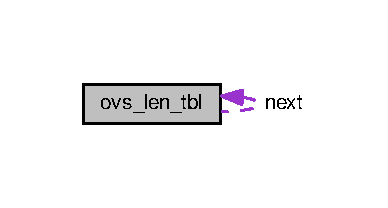
\includegraphics[width=186pt]{structovs__len__tbl__coll__graph}
\end{center}
\end{figure}
\subsection*{Data Fields}
\begin{DoxyCompactItemize}
\item 
int \hyperlink{structovs__len__tbl_a70f2cb0cf35baf6a1941942a8b70318c}{len}
\item 
const struct \hyperlink{structovs__len__tbl}{ovs\+\_\+len\+\_\+tbl} $\ast$ \hyperlink{structovs__len__tbl_a0def32b4bc5790a24631d4d7727954af}{next}
\end{DoxyCompactItemize}


\subsection{Field Documentation}
\hypertarget{structovs__len__tbl_a70f2cb0cf35baf6a1941942a8b70318c}{}\index{ovs\+\_\+len\+\_\+tbl@{ovs\+\_\+len\+\_\+tbl}!len@{len}}
\index{len@{len}!ovs\+\_\+len\+\_\+tbl@{ovs\+\_\+len\+\_\+tbl}}
\subsubsection[{len}]{\setlength{\rightskip}{0pt plus 5cm}int ovs\+\_\+len\+\_\+tbl\+::len}\label{structovs__len__tbl_a70f2cb0cf35baf6a1941942a8b70318c}
\hypertarget{structovs__len__tbl_a0def32b4bc5790a24631d4d7727954af}{}\index{ovs\+\_\+len\+\_\+tbl@{ovs\+\_\+len\+\_\+tbl}!next@{next}}
\index{next@{next}!ovs\+\_\+len\+\_\+tbl@{ovs\+\_\+len\+\_\+tbl}}
\subsubsection[{next}]{\setlength{\rightskip}{0pt plus 5cm}const struct {\bf ovs\+\_\+len\+\_\+tbl} $\ast$ ovs\+\_\+len\+\_\+tbl\+::next}\label{structovs__len__tbl_a0def32b4bc5790a24631d4d7727954af}


The documentation for this struct was generated from the following file\+:\begin{DoxyCompactItemize}
\item 
/home/vladn/git/ovs/datapath/\hyperlink{flow__netlink_8c}{flow\+\_\+netlink.\+c}\end{DoxyCompactItemize}

\hypertarget{structovs__net}{}\section{ovs\+\_\+net Struct Reference}
\label{structovs__net}\index{ovs\+\_\+net@{ovs\+\_\+net}}


{\ttfamily \#include $<$datapath.\+h$>$}



Collaboration diagram for ovs\+\_\+net\+:
\nopagebreak
\begin{figure}[H]
\begin{center}
\leavevmode
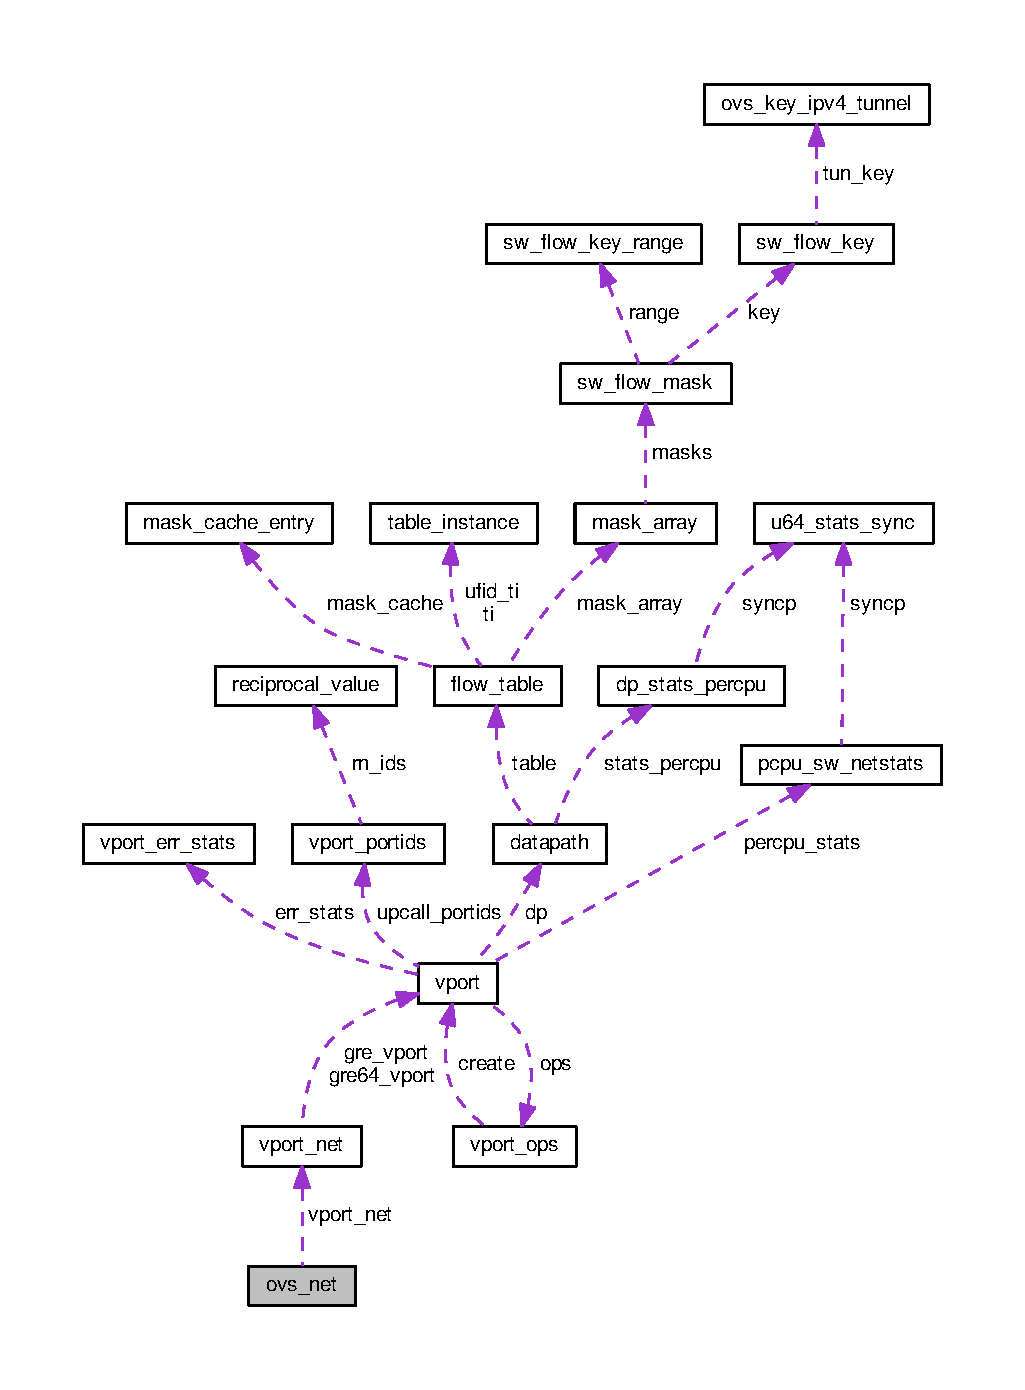
\includegraphics[width=350pt]{structovs__net__coll__graph}
\end{center}
\end{figure}
\subsection*{Data Fields}
\begin{DoxyCompactItemize}
\item 
struct list\+\_\+head \hyperlink{structovs__net_a0490101f7ea82f5c290a92d447bd8f9d}{dps}
\item 
struct work\+\_\+struct \hyperlink{structovs__net_ac8cdb834420a37531f032e526ac61901}{dp\+\_\+notify\+\_\+work}
\item 
struct \hyperlink{structvport__net}{vport\+\_\+net} \hyperlink{structovs__net_a78aa4fb59e11c125ba6a61917efe6c50}{vport\+\_\+net}
\end{DoxyCompactItemize}


\subsection{Detailed Description}
struct \hyperlink{structovs__net}{ovs\+\_\+net} -\/ Per net-\/namespace data for ovs. \+: List of datapaths to enable dumping them all out. Protected by genl\+\_\+mutex. \+: Per network namespace data for vport. 

\subsection{Field Documentation}
\hypertarget{structovs__net_ac8cdb834420a37531f032e526ac61901}{}\index{ovs\+\_\+net@{ovs\+\_\+net}!dp\+\_\+notify\+\_\+work@{dp\+\_\+notify\+\_\+work}}
\index{dp\+\_\+notify\+\_\+work@{dp\+\_\+notify\+\_\+work}!ovs\+\_\+net@{ovs\+\_\+net}}
\subsubsection[{dp\+\_\+notify\+\_\+work}]{\setlength{\rightskip}{0pt plus 5cm}struct work\+\_\+struct ovs\+\_\+net\+::dp\+\_\+notify\+\_\+work}\label{structovs__net_ac8cdb834420a37531f032e526ac61901}
\hypertarget{structovs__net_a0490101f7ea82f5c290a92d447bd8f9d}{}\index{ovs\+\_\+net@{ovs\+\_\+net}!dps@{dps}}
\index{dps@{dps}!ovs\+\_\+net@{ovs\+\_\+net}}
\subsubsection[{dps}]{\setlength{\rightskip}{0pt plus 5cm}struct list\+\_\+head ovs\+\_\+net\+::dps}\label{structovs__net_a0490101f7ea82f5c290a92d447bd8f9d}
\hypertarget{structovs__net_a78aa4fb59e11c125ba6a61917efe6c50}{}\index{ovs\+\_\+net@{ovs\+\_\+net}!vport\+\_\+net@{vport\+\_\+net}}
\index{vport\+\_\+net@{vport\+\_\+net}!ovs\+\_\+net@{ovs\+\_\+net}}
\subsubsection[{vport\+\_\+net}]{\setlength{\rightskip}{0pt plus 5cm}struct {\bf vport\+\_\+net} ovs\+\_\+net\+::vport\+\_\+net}\label{structovs__net_a78aa4fb59e11c125ba6a61917efe6c50}


The documentation for this struct was generated from the following file\+:\begin{DoxyCompactItemize}
\item 
/home/vladn/git/ovs/datapath/\hyperlink{datapath_8h}{datapath.\+h}\end{DoxyCompactItemize}

\hypertarget{structovs__skb__cb}{}\section{ovs\+\_\+skb\+\_\+cb Struct Reference}
\label{structovs__skb__cb}\index{ovs\+\_\+skb\+\_\+cb@{ovs\+\_\+skb\+\_\+cb}}


{\ttfamily \#include $<$datapath.\+h$>$}



Collaboration diagram for ovs\+\_\+skb\+\_\+cb\+:
\nopagebreak
\begin{figure}[H]
\begin{center}
\leavevmode
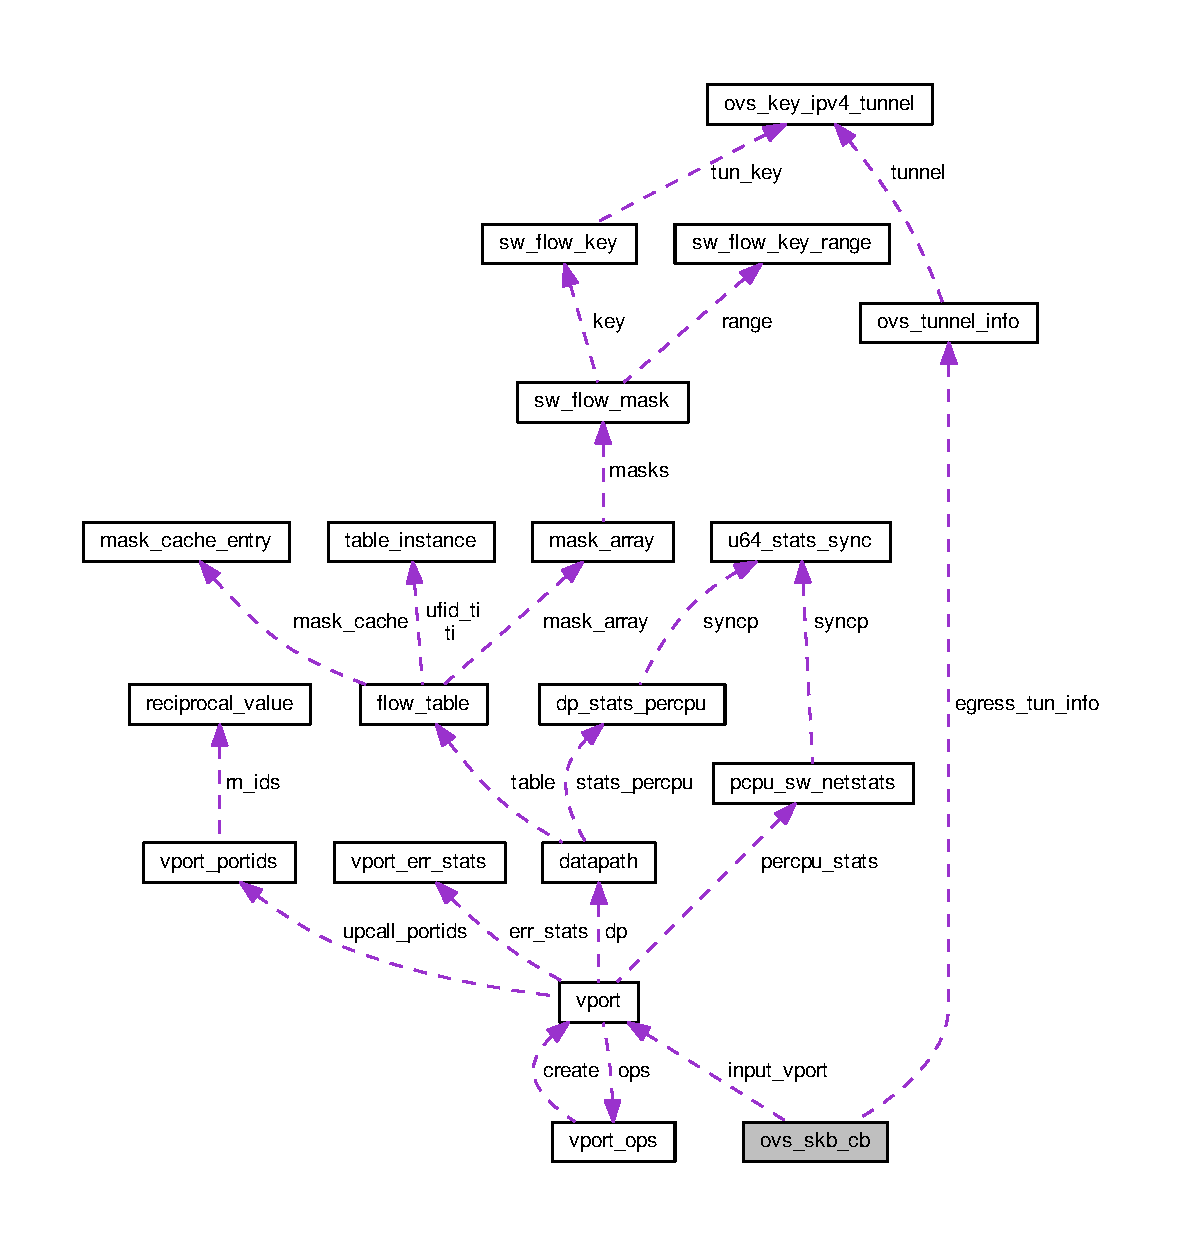
\includegraphics[width=350pt]{structovs__skb__cb__coll__graph}
\end{center}
\end{figure}
\subsection*{Data Fields}
\begin{DoxyCompactItemize}
\item 
struct \hyperlink{structovs__tunnel__info}{ovs\+\_\+tunnel\+\_\+info} $\ast$ \hyperlink{structovs__skb__cb_a077a089def65a6abde4e8f897591f2dc}{egress\+\_\+tun\+\_\+info}
\item 
struct \hyperlink{structvport}{vport} $\ast$ \hyperlink{structovs__skb__cb_a919a555392390f60eb84d1f46982744c}{input\+\_\+vport}
\end{DoxyCompactItemize}


\subsection{Detailed Description}
struct \hyperlink{structovs__skb__cb}{ovs\+\_\+skb\+\_\+cb} -\/ O\+V\+S data in skb C\+B \+: Tunnel information about this packet on egress path. N\+U\+L\+L if the packet is not being tunneled. \+: The original vport packet came in on. This value is cached when a packet is received by O\+V\+S. 

\subsection{Field Documentation}
\hypertarget{structovs__skb__cb_a077a089def65a6abde4e8f897591f2dc}{}\index{ovs\+\_\+skb\+\_\+cb@{ovs\+\_\+skb\+\_\+cb}!egress\+\_\+tun\+\_\+info@{egress\+\_\+tun\+\_\+info}}
\index{egress\+\_\+tun\+\_\+info@{egress\+\_\+tun\+\_\+info}!ovs\+\_\+skb\+\_\+cb@{ovs\+\_\+skb\+\_\+cb}}
\subsubsection[{egress\+\_\+tun\+\_\+info}]{\setlength{\rightskip}{0pt plus 5cm}struct {\bf ovs\+\_\+tunnel\+\_\+info}$\ast$ ovs\+\_\+skb\+\_\+cb\+::egress\+\_\+tun\+\_\+info}\label{structovs__skb__cb_a077a089def65a6abde4e8f897591f2dc}
\hypertarget{structovs__skb__cb_a919a555392390f60eb84d1f46982744c}{}\index{ovs\+\_\+skb\+\_\+cb@{ovs\+\_\+skb\+\_\+cb}!input\+\_\+vport@{input\+\_\+vport}}
\index{input\+\_\+vport@{input\+\_\+vport}!ovs\+\_\+skb\+\_\+cb@{ovs\+\_\+skb\+\_\+cb}}
\subsubsection[{input\+\_\+vport}]{\setlength{\rightskip}{0pt plus 5cm}struct {\bf vport}$\ast$ ovs\+\_\+skb\+\_\+cb\+::input\+\_\+vport}\label{structovs__skb__cb_a919a555392390f60eb84d1f46982744c}


The documentation for this struct was generated from the following file\+:\begin{DoxyCompactItemize}
\item 
/home/vladn/git/ovs/datapath/\hyperlink{datapath_8h}{datapath.\+h}\end{DoxyCompactItemize}

\hypertarget{structovs__tunnel__info}{}\section{ovs\+\_\+tunnel\+\_\+info Struct Reference}
\label{structovs__tunnel__info}\index{ovs\+\_\+tunnel\+\_\+info@{ovs\+\_\+tunnel\+\_\+info}}


{\ttfamily \#include $<$flow.\+h$>$}



Collaboration diagram for ovs\+\_\+tunnel\+\_\+info\+:
\nopagebreak
\begin{figure}[H]
\begin{center}
\leavevmode
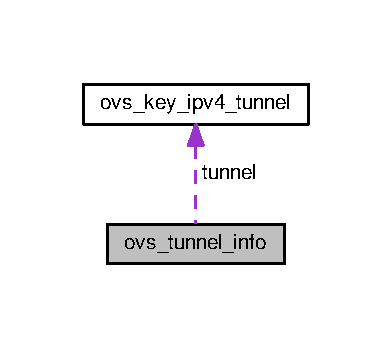
\includegraphics[width=188pt]{structovs__tunnel__info__coll__graph}
\end{center}
\end{figure}
\subsection*{Data Fields}
\begin{DoxyCompactItemize}
\item 
struct \hyperlink{structovs__key__ipv4__tunnel}{ovs\+\_\+key\+\_\+ipv4\+\_\+tunnel} \hyperlink{structovs__tunnel__info_a007f0c7a9938884e6e8663cb4ab20d10}{tunnel}
\item 
const void $\ast$ \hyperlink{structovs__tunnel__info_ae4fd786894f579a38a5955e7a0e68fd4}{options}
\item 
u8 \hyperlink{structovs__tunnel__info_ab50d289f61727b922831739affb28b18}{options\+\_\+len}
\end{DoxyCompactItemize}


\subsection{Field Documentation}
\hypertarget{structovs__tunnel__info_ae4fd786894f579a38a5955e7a0e68fd4}{}\index{ovs\+\_\+tunnel\+\_\+info@{ovs\+\_\+tunnel\+\_\+info}!options@{options}}
\index{options@{options}!ovs\+\_\+tunnel\+\_\+info@{ovs\+\_\+tunnel\+\_\+info}}
\subsubsection[{options}]{\setlength{\rightskip}{0pt plus 5cm}const void$\ast$ ovs\+\_\+tunnel\+\_\+info\+::options}\label{structovs__tunnel__info_ae4fd786894f579a38a5955e7a0e68fd4}
\hypertarget{structovs__tunnel__info_ab50d289f61727b922831739affb28b18}{}\index{ovs\+\_\+tunnel\+\_\+info@{ovs\+\_\+tunnel\+\_\+info}!options\+\_\+len@{options\+\_\+len}}
\index{options\+\_\+len@{options\+\_\+len}!ovs\+\_\+tunnel\+\_\+info@{ovs\+\_\+tunnel\+\_\+info}}
\subsubsection[{options\+\_\+len}]{\setlength{\rightskip}{0pt plus 5cm}u8 ovs\+\_\+tunnel\+\_\+info\+::options\+\_\+len}\label{structovs__tunnel__info_ab50d289f61727b922831739affb28b18}
\hypertarget{structovs__tunnel__info_a007f0c7a9938884e6e8663cb4ab20d10}{}\index{ovs\+\_\+tunnel\+\_\+info@{ovs\+\_\+tunnel\+\_\+info}!tunnel@{tunnel}}
\index{tunnel@{tunnel}!ovs\+\_\+tunnel\+\_\+info@{ovs\+\_\+tunnel\+\_\+info}}
\subsubsection[{tunnel}]{\setlength{\rightskip}{0pt plus 5cm}struct {\bf ovs\+\_\+key\+\_\+ipv4\+\_\+tunnel} ovs\+\_\+tunnel\+\_\+info\+::tunnel}\label{structovs__tunnel__info_a007f0c7a9938884e6e8663cb4ab20d10}


The documentation for this struct was generated from the following file\+:\begin{DoxyCompactItemize}
\item 
/home/vladn/git/ovs/datapath/\hyperlink{flow_8h}{flow.\+h}\end{DoxyCompactItemize}

\hypertarget{structovs__vport__stats}{}\section{ovs\+\_\+vport\+\_\+stats Struct Reference}
\label{structovs__vport__stats}\index{ovs\+\_\+vport\+\_\+stats@{ovs\+\_\+vport\+\_\+stats}}


{\ttfamily \#include $<$openvswitch.\+h$>$}

\subsection*{Data Fields}
\begin{DoxyCompactItemize}
\item 
\+\_\+\+\_\+u64 \hyperlink{structovs__vport__stats_ae40f3501f32e41cdf6658cc8725f48e7}{rx\+\_\+packets}
\item 
\+\_\+\+\_\+u64 \hyperlink{structovs__vport__stats_adb91be6e2d6695cb19acc87d817191c5}{tx\+\_\+packets}
\item 
\+\_\+\+\_\+u64 \hyperlink{structovs__vport__stats_a27cf52cea0ff9168cd2b536edee94284}{rx\+\_\+bytes}
\item 
\+\_\+\+\_\+u64 \hyperlink{structovs__vport__stats_a2602d5f9072e762b4a6091874c02fd1c}{tx\+\_\+bytes}
\item 
\+\_\+\+\_\+u64 \hyperlink{structovs__vport__stats_a95d0551abc4c1f3874e60fbaa593a63c}{rx\+\_\+errors}
\item 
\+\_\+\+\_\+u64 \hyperlink{structovs__vport__stats_ac0233ed277e2568b4471479beaa4b642}{tx\+\_\+errors}
\item 
\+\_\+\+\_\+u64 \hyperlink{structovs__vport__stats_a91152608a32f597ef28ef5de32b716e9}{rx\+\_\+dropped}
\item 
\+\_\+\+\_\+u64 \hyperlink{structovs__vport__stats_a9b32bc999ba296823133077db108027f}{tx\+\_\+dropped}
\end{DoxyCompactItemize}


\subsection{Field Documentation}
\hypertarget{structovs__vport__stats_a27cf52cea0ff9168cd2b536edee94284}{}\index{ovs\+\_\+vport\+\_\+stats@{ovs\+\_\+vport\+\_\+stats}!rx\+\_\+bytes@{rx\+\_\+bytes}}
\index{rx\+\_\+bytes@{rx\+\_\+bytes}!ovs\+\_\+vport\+\_\+stats@{ovs\+\_\+vport\+\_\+stats}}
\subsubsection[{rx\+\_\+bytes}]{\setlength{\rightskip}{0pt plus 5cm}\+\_\+\+\_\+u64 ovs\+\_\+vport\+\_\+stats\+::rx\+\_\+bytes}\label{structovs__vport__stats_a27cf52cea0ff9168cd2b536edee94284}
\hypertarget{structovs__vport__stats_a91152608a32f597ef28ef5de32b716e9}{}\index{ovs\+\_\+vport\+\_\+stats@{ovs\+\_\+vport\+\_\+stats}!rx\+\_\+dropped@{rx\+\_\+dropped}}
\index{rx\+\_\+dropped@{rx\+\_\+dropped}!ovs\+\_\+vport\+\_\+stats@{ovs\+\_\+vport\+\_\+stats}}
\subsubsection[{rx\+\_\+dropped}]{\setlength{\rightskip}{0pt plus 5cm}\+\_\+\+\_\+u64 ovs\+\_\+vport\+\_\+stats\+::rx\+\_\+dropped}\label{structovs__vport__stats_a91152608a32f597ef28ef5de32b716e9}
\hypertarget{structovs__vport__stats_a95d0551abc4c1f3874e60fbaa593a63c}{}\index{ovs\+\_\+vport\+\_\+stats@{ovs\+\_\+vport\+\_\+stats}!rx\+\_\+errors@{rx\+\_\+errors}}
\index{rx\+\_\+errors@{rx\+\_\+errors}!ovs\+\_\+vport\+\_\+stats@{ovs\+\_\+vport\+\_\+stats}}
\subsubsection[{rx\+\_\+errors}]{\setlength{\rightskip}{0pt plus 5cm}\+\_\+\+\_\+u64 ovs\+\_\+vport\+\_\+stats\+::rx\+\_\+errors}\label{structovs__vport__stats_a95d0551abc4c1f3874e60fbaa593a63c}
\hypertarget{structovs__vport__stats_ae40f3501f32e41cdf6658cc8725f48e7}{}\index{ovs\+\_\+vport\+\_\+stats@{ovs\+\_\+vport\+\_\+stats}!rx\+\_\+packets@{rx\+\_\+packets}}
\index{rx\+\_\+packets@{rx\+\_\+packets}!ovs\+\_\+vport\+\_\+stats@{ovs\+\_\+vport\+\_\+stats}}
\subsubsection[{rx\+\_\+packets}]{\setlength{\rightskip}{0pt plus 5cm}\+\_\+\+\_\+u64 ovs\+\_\+vport\+\_\+stats\+::rx\+\_\+packets}\label{structovs__vport__stats_ae40f3501f32e41cdf6658cc8725f48e7}
\hypertarget{structovs__vport__stats_a2602d5f9072e762b4a6091874c02fd1c}{}\index{ovs\+\_\+vport\+\_\+stats@{ovs\+\_\+vport\+\_\+stats}!tx\+\_\+bytes@{tx\+\_\+bytes}}
\index{tx\+\_\+bytes@{tx\+\_\+bytes}!ovs\+\_\+vport\+\_\+stats@{ovs\+\_\+vport\+\_\+stats}}
\subsubsection[{tx\+\_\+bytes}]{\setlength{\rightskip}{0pt plus 5cm}\+\_\+\+\_\+u64 ovs\+\_\+vport\+\_\+stats\+::tx\+\_\+bytes}\label{structovs__vport__stats_a2602d5f9072e762b4a6091874c02fd1c}
\hypertarget{structovs__vport__stats_a9b32bc999ba296823133077db108027f}{}\index{ovs\+\_\+vport\+\_\+stats@{ovs\+\_\+vport\+\_\+stats}!tx\+\_\+dropped@{tx\+\_\+dropped}}
\index{tx\+\_\+dropped@{tx\+\_\+dropped}!ovs\+\_\+vport\+\_\+stats@{ovs\+\_\+vport\+\_\+stats}}
\subsubsection[{tx\+\_\+dropped}]{\setlength{\rightskip}{0pt plus 5cm}\+\_\+\+\_\+u64 ovs\+\_\+vport\+\_\+stats\+::tx\+\_\+dropped}\label{structovs__vport__stats_a9b32bc999ba296823133077db108027f}
\hypertarget{structovs__vport__stats_ac0233ed277e2568b4471479beaa4b642}{}\index{ovs\+\_\+vport\+\_\+stats@{ovs\+\_\+vport\+\_\+stats}!tx\+\_\+errors@{tx\+\_\+errors}}
\index{tx\+\_\+errors@{tx\+\_\+errors}!ovs\+\_\+vport\+\_\+stats@{ovs\+\_\+vport\+\_\+stats}}
\subsubsection[{tx\+\_\+errors}]{\setlength{\rightskip}{0pt plus 5cm}\+\_\+\+\_\+u64 ovs\+\_\+vport\+\_\+stats\+::tx\+\_\+errors}\label{structovs__vport__stats_ac0233ed277e2568b4471479beaa4b642}
\hypertarget{structovs__vport__stats_adb91be6e2d6695cb19acc87d817191c5}{}\index{ovs\+\_\+vport\+\_\+stats@{ovs\+\_\+vport\+\_\+stats}!tx\+\_\+packets@{tx\+\_\+packets}}
\index{tx\+\_\+packets@{tx\+\_\+packets}!ovs\+\_\+vport\+\_\+stats@{ovs\+\_\+vport\+\_\+stats}}
\subsubsection[{tx\+\_\+packets}]{\setlength{\rightskip}{0pt plus 5cm}\+\_\+\+\_\+u64 ovs\+\_\+vport\+\_\+stats\+::tx\+\_\+packets}\label{structovs__vport__stats_adb91be6e2d6695cb19acc87d817191c5}


The documentation for this struct was generated from the following file\+:\begin{DoxyCompactItemize}
\item 
/home/vladn/git/ovs/datapath/linux/compat/include/linux/\hyperlink{openvswitch_8h}{openvswitch.\+h}\end{DoxyCompactItemize}

\hypertarget{structovs__vxlan__opts}{}\section{ovs\+\_\+vxlan\+\_\+opts Struct Reference}
\label{structovs__vxlan__opts}\index{ovs\+\_\+vxlan\+\_\+opts@{ovs\+\_\+vxlan\+\_\+opts}}


{\ttfamily \#include $<$vport-\/vxlan.\+h$>$}

\subsection*{Data Fields}
\begin{DoxyCompactItemize}
\item 
\+\_\+\+\_\+u32 \hyperlink{structovs__vxlan__opts_a9b035f7870829fa9116ca074ef1ac2b4}{gbp}
\end{DoxyCompactItemize}


\subsection{Field Documentation}
\hypertarget{structovs__vxlan__opts_a9b035f7870829fa9116ca074ef1ac2b4}{}\index{ovs\+\_\+vxlan\+\_\+opts@{ovs\+\_\+vxlan\+\_\+opts}!gbp@{gbp}}
\index{gbp@{gbp}!ovs\+\_\+vxlan\+\_\+opts@{ovs\+\_\+vxlan\+\_\+opts}}
\subsubsection[{gbp}]{\setlength{\rightskip}{0pt plus 5cm}\+\_\+\+\_\+u32 ovs\+\_\+vxlan\+\_\+opts\+::gbp}\label{structovs__vxlan__opts_a9b035f7870829fa9116ca074ef1ac2b4}


The documentation for this struct was generated from the following file\+:\begin{DoxyCompactItemize}
\item 
/home/vladn/git/ovs/datapath/\hyperlink{vport-vxlan_8h}{vport-\/vxlan.\+h}\end{DoxyCompactItemize}

\hypertarget{structpcpu__sw__netstats}{}\section{pcpu\+\_\+sw\+\_\+netstats Struct Reference}
\label{structpcpu__sw__netstats}\index{pcpu\+\_\+sw\+\_\+netstats@{pcpu\+\_\+sw\+\_\+netstats}}


{\ttfamily \#include $<$netdevice.\+h$>$}



Collaboration diagram for pcpu\+\_\+sw\+\_\+netstats\+:
\nopagebreak
\begin{figure}[H]
\begin{center}
\leavevmode
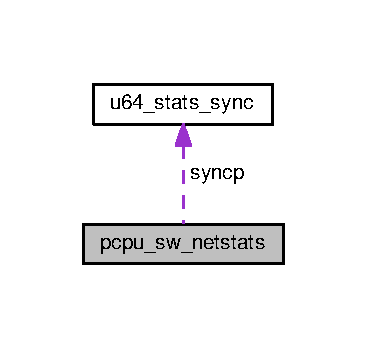
\includegraphics[width=176pt]{structpcpu__sw__netstats__coll__graph}
\end{center}
\end{figure}
\subsection*{Data Fields}
\begin{DoxyCompactItemize}
\item 
u64 \hyperlink{structpcpu__sw__netstats_aef09f7c9a31a557c278f7768f6d54488}{rx\+\_\+packets}
\item 
u64 \hyperlink{structpcpu__sw__netstats_ae71ad7ad7c404b7820d022d42c515a70}{rx\+\_\+bytes}
\item 
u64 \hyperlink{structpcpu__sw__netstats_a1b3e22436ccc3b5d13124f481eb2261f}{tx\+\_\+packets}
\item 
u64 \hyperlink{structpcpu__sw__netstats_ab017757f36d020e04458ef3748fe1d69}{tx\+\_\+bytes}
\item 
struct \hyperlink{structu64__stats__sync}{u64\+\_\+stats\+\_\+sync} \hyperlink{structpcpu__sw__netstats_a09b11d813594941c06b3e1e818a9b543}{syncp}
\end{DoxyCompactItemize}


\subsection{Field Documentation}
\hypertarget{structpcpu__sw__netstats_ae71ad7ad7c404b7820d022d42c515a70}{}\index{pcpu\+\_\+sw\+\_\+netstats@{pcpu\+\_\+sw\+\_\+netstats}!rx\+\_\+bytes@{rx\+\_\+bytes}}
\index{rx\+\_\+bytes@{rx\+\_\+bytes}!pcpu\+\_\+sw\+\_\+netstats@{pcpu\+\_\+sw\+\_\+netstats}}
\subsubsection[{rx\+\_\+bytes}]{\setlength{\rightskip}{0pt plus 5cm}u64 pcpu\+\_\+sw\+\_\+netstats\+::rx\+\_\+bytes}\label{structpcpu__sw__netstats_ae71ad7ad7c404b7820d022d42c515a70}
\hypertarget{structpcpu__sw__netstats_aef09f7c9a31a557c278f7768f6d54488}{}\index{pcpu\+\_\+sw\+\_\+netstats@{pcpu\+\_\+sw\+\_\+netstats}!rx\+\_\+packets@{rx\+\_\+packets}}
\index{rx\+\_\+packets@{rx\+\_\+packets}!pcpu\+\_\+sw\+\_\+netstats@{pcpu\+\_\+sw\+\_\+netstats}}
\subsubsection[{rx\+\_\+packets}]{\setlength{\rightskip}{0pt plus 5cm}u64 pcpu\+\_\+sw\+\_\+netstats\+::rx\+\_\+packets}\label{structpcpu__sw__netstats_aef09f7c9a31a557c278f7768f6d54488}
\hypertarget{structpcpu__sw__netstats_a09b11d813594941c06b3e1e818a9b543}{}\index{pcpu\+\_\+sw\+\_\+netstats@{pcpu\+\_\+sw\+\_\+netstats}!syncp@{syncp}}
\index{syncp@{syncp}!pcpu\+\_\+sw\+\_\+netstats@{pcpu\+\_\+sw\+\_\+netstats}}
\subsubsection[{syncp}]{\setlength{\rightskip}{0pt plus 5cm}struct {\bf u64\+\_\+stats\+\_\+sync} pcpu\+\_\+sw\+\_\+netstats\+::syncp}\label{structpcpu__sw__netstats_a09b11d813594941c06b3e1e818a9b543}
\hypertarget{structpcpu__sw__netstats_ab017757f36d020e04458ef3748fe1d69}{}\index{pcpu\+\_\+sw\+\_\+netstats@{pcpu\+\_\+sw\+\_\+netstats}!tx\+\_\+bytes@{tx\+\_\+bytes}}
\index{tx\+\_\+bytes@{tx\+\_\+bytes}!pcpu\+\_\+sw\+\_\+netstats@{pcpu\+\_\+sw\+\_\+netstats}}
\subsubsection[{tx\+\_\+bytes}]{\setlength{\rightskip}{0pt plus 5cm}u64 pcpu\+\_\+sw\+\_\+netstats\+::tx\+\_\+bytes}\label{structpcpu__sw__netstats_ab017757f36d020e04458ef3748fe1d69}
\hypertarget{structpcpu__sw__netstats_a1b3e22436ccc3b5d13124f481eb2261f}{}\index{pcpu\+\_\+sw\+\_\+netstats@{pcpu\+\_\+sw\+\_\+netstats}!tx\+\_\+packets@{tx\+\_\+packets}}
\index{tx\+\_\+packets@{tx\+\_\+packets}!pcpu\+\_\+sw\+\_\+netstats@{pcpu\+\_\+sw\+\_\+netstats}}
\subsubsection[{tx\+\_\+packets}]{\setlength{\rightskip}{0pt plus 5cm}u64 pcpu\+\_\+sw\+\_\+netstats\+::tx\+\_\+packets}\label{structpcpu__sw__netstats_a1b3e22436ccc3b5d13124f481eb2261f}


The documentation for this struct was generated from the following file\+:\begin{DoxyCompactItemize}
\item 
/home/vladn/git/ovs/datapath/linux/compat/include/linux/\hyperlink{netdevice_8h}{netdevice.\+h}\end{DoxyCompactItemize}

\hypertarget{structreciprocal__value}{}\section{reciprocal\+\_\+value Struct Reference}
\label{structreciprocal__value}\index{reciprocal\+\_\+value@{reciprocal\+\_\+value}}


{\ttfamily \#include $<$reciprocal\+\_\+div.\+h$>$}

\subsection*{Data Fields}
\begin{DoxyCompactItemize}
\item 
u32 \hyperlink{structreciprocal__value_aa32a30f86412446e8febcc66236f7472}{m}
\item 
u8 \hyperlink{structreciprocal__value_a0154478c74b1c1d15bddd2adabfca9e1}{sh1}
\item 
u8 \hyperlink{structreciprocal__value_aada545b593c9abb69094dfb9b074f61e}{sh2}
\end{DoxyCompactItemize}


\subsection{Field Documentation}
\hypertarget{structreciprocal__value_aa32a30f86412446e8febcc66236f7472}{}\index{reciprocal\+\_\+value@{reciprocal\+\_\+value}!m@{m}}
\index{m@{m}!reciprocal\+\_\+value@{reciprocal\+\_\+value}}
\subsubsection[{m}]{\setlength{\rightskip}{0pt plus 5cm}u32 reciprocal\+\_\+value\+::m}\label{structreciprocal__value_aa32a30f86412446e8febcc66236f7472}
\hypertarget{structreciprocal__value_a0154478c74b1c1d15bddd2adabfca9e1}{}\index{reciprocal\+\_\+value@{reciprocal\+\_\+value}!sh1@{sh1}}
\index{sh1@{sh1}!reciprocal\+\_\+value@{reciprocal\+\_\+value}}
\subsubsection[{sh1}]{\setlength{\rightskip}{0pt plus 5cm}u8 reciprocal\+\_\+value\+::sh1}\label{structreciprocal__value_a0154478c74b1c1d15bddd2adabfca9e1}
\hypertarget{structreciprocal__value_aada545b593c9abb69094dfb9b074f61e}{}\index{reciprocal\+\_\+value@{reciprocal\+\_\+value}!sh2@{sh2}}
\index{sh2@{sh2}!reciprocal\+\_\+value@{reciprocal\+\_\+value}}
\subsubsection[{sh2}]{\setlength{\rightskip}{0pt plus 5cm}u8 reciprocal\+\_\+value\+::sh2}\label{structreciprocal__value_aada545b593c9abb69094dfb9b074f61e}


The documentation for this struct was generated from the following file\+:\begin{DoxyCompactItemize}
\item 
/home/vladn/git/ovs/datapath/linux/compat/include/linux/\hyperlink{reciprocal__div_8h}{reciprocal\+\_\+div.\+h}\end{DoxyCompactItemize}

\hypertarget{structrpl__genl__family}{}\section{rpl\+\_\+genl\+\_\+family Struct Reference}
\label{structrpl__genl__family}\index{rpl\+\_\+genl\+\_\+family@{rpl\+\_\+genl\+\_\+family}}


{\ttfamily \#include $<$genetlink.\+h$>$}

\subsection*{Data Fields}
\begin{DoxyCompactItemize}
\item 
struct \hyperlink{genetlink_8h_aba961c2c372b7122ad0c8ae5e7af2f3b}{genl\+\_\+family} \hyperlink{structrpl__genl__family_a6da3fbe86360d91cce207287b2de165d}{compat\+\_\+family}
\item 
unsigned int \hyperlink{structrpl__genl__family_a34a498924fba8a8da9d410d545cfeee2}{id}
\item 
unsigned int \hyperlink{structrpl__genl__family_a9a291012510fda23c4d3bf64859e5de0}{hdrsize}
\item 
char \hyperlink{structrpl__genl__family_a0ee3a650097beb5d2e4a4deb301cb479}{name} \mbox{[}G\+E\+N\+L\+\_\+\+N\+A\+M\+S\+I\+Z\mbox{]}
\item 
unsigned int \hyperlink{structrpl__genl__family_a09a64c948abbbd61907dfd9f0d17663d}{version}
\item 
unsigned int \hyperlink{structrpl__genl__family_a7f6d39207e37f45f704e387488b580d0}{maxattr}
\item 
\hyperlink{types_8h_afaa87723b8417d40fcf45b7330261ef9}{bool} \hyperlink{structrpl__genl__family_a126424f7f454c57970d3aa43fa6f6321}{netnsok}
\item 
\hyperlink{types_8h_afaa87723b8417d40fcf45b7330261ef9}{bool} \hyperlink{structrpl__genl__family_a0c6f86f5d811b297add5721fc9412545}{parallel\+\_\+ops}
\item 
int($\ast$ \hyperlink{structrpl__genl__family_aa5134cfc246e4d34814262c04c2e7a87}{pre\+\_\+doit} )(const struct genl\+\_\+ops $\ast$\hyperlink{structrpl__genl__family_a2d6fa633ee14f455af7965bf76508255}{ops}, struct sk\+\_\+buff $\ast$skb, struct genl\+\_\+info $\ast$info)
\item 
void($\ast$ \hyperlink{structrpl__genl__family_a2b7972eca0ca87a04c701b03fe78e23a}{post\+\_\+doit} )(const struct genl\+\_\+ops $\ast$\hyperlink{structrpl__genl__family_a2d6fa633ee14f455af7965bf76508255}{ops}, struct sk\+\_\+buff $\ast$skb, struct genl\+\_\+info $\ast$info)
\item 
struct nlattr $\ast$$\ast$ \hyperlink{structrpl__genl__family_a3ad09df2fe4ef38e5efc0c3ef7cc5fb6}{attrbuf}
\item 
const struct genl\+\_\+ops $\ast$ \hyperlink{structrpl__genl__family_a2d6fa633ee14f455af7965bf76508255}{ops}
\item 
const struct genl\+\_\+multicast\+\_\+group $\ast$ \hyperlink{structrpl__genl__family_aa824bef8504ad3a92bc3fdd62d7554ec}{mcgrps}
\item 
unsigned int \hyperlink{structrpl__genl__family_a2015e11f05185d06f8ef4125a43fd48b}{n\+\_\+ops}
\item 
unsigned int \hyperlink{structrpl__genl__family_aa39896dd5abd2de8beaeaa1a39d61c98}{n\+\_\+mcgrps}
\item 
unsigned int \hyperlink{structrpl__genl__family_a9b80c856eaea457b92e8e3997a09df9e}{mcgrp\+\_\+offset}
\item 
struct list\+\_\+head \hyperlink{structrpl__genl__family_a3b34f3eda668c9cd2340349615467eb9}{family\+\_\+list}
\item 
struct module $\ast$ \hyperlink{structrpl__genl__family_a8c514aedced0b4c6421aa08881aa1609}{module}
\end{DoxyCompactItemize}


\subsection{Field Documentation}
\hypertarget{structrpl__genl__family_a3ad09df2fe4ef38e5efc0c3ef7cc5fb6}{}\index{rpl\+\_\+genl\+\_\+family@{rpl\+\_\+genl\+\_\+family}!attrbuf@{attrbuf}}
\index{attrbuf@{attrbuf}!rpl\+\_\+genl\+\_\+family@{rpl\+\_\+genl\+\_\+family}}
\subsubsection[{attrbuf}]{\setlength{\rightskip}{0pt plus 5cm}struct nlattr$\ast$$\ast$ rpl\+\_\+genl\+\_\+family\+::attrbuf}\label{structrpl__genl__family_a3ad09df2fe4ef38e5efc0c3ef7cc5fb6}
\hypertarget{structrpl__genl__family_a6da3fbe86360d91cce207287b2de165d}{}\index{rpl\+\_\+genl\+\_\+family@{rpl\+\_\+genl\+\_\+family}!compat\+\_\+family@{compat\+\_\+family}}
\index{compat\+\_\+family@{compat\+\_\+family}!rpl\+\_\+genl\+\_\+family@{rpl\+\_\+genl\+\_\+family}}
\subsubsection[{compat\+\_\+family}]{\setlength{\rightskip}{0pt plus 5cm}struct {\bf genl\+\_\+family} rpl\+\_\+genl\+\_\+family\+::compat\+\_\+family}\label{structrpl__genl__family_a6da3fbe86360d91cce207287b2de165d}
\hypertarget{structrpl__genl__family_a3b34f3eda668c9cd2340349615467eb9}{}\index{rpl\+\_\+genl\+\_\+family@{rpl\+\_\+genl\+\_\+family}!family\+\_\+list@{family\+\_\+list}}
\index{family\+\_\+list@{family\+\_\+list}!rpl\+\_\+genl\+\_\+family@{rpl\+\_\+genl\+\_\+family}}
\subsubsection[{family\+\_\+list}]{\setlength{\rightskip}{0pt plus 5cm}struct list\+\_\+head rpl\+\_\+genl\+\_\+family\+::family\+\_\+list}\label{structrpl__genl__family_a3b34f3eda668c9cd2340349615467eb9}
\hypertarget{structrpl__genl__family_a9a291012510fda23c4d3bf64859e5de0}{}\index{rpl\+\_\+genl\+\_\+family@{rpl\+\_\+genl\+\_\+family}!hdrsize@{hdrsize}}
\index{hdrsize@{hdrsize}!rpl\+\_\+genl\+\_\+family@{rpl\+\_\+genl\+\_\+family}}
\subsubsection[{hdrsize}]{\setlength{\rightskip}{0pt plus 5cm}unsigned int rpl\+\_\+genl\+\_\+family\+::hdrsize}\label{structrpl__genl__family_a9a291012510fda23c4d3bf64859e5de0}
\hypertarget{structrpl__genl__family_a34a498924fba8a8da9d410d545cfeee2}{}\index{rpl\+\_\+genl\+\_\+family@{rpl\+\_\+genl\+\_\+family}!id@{id}}
\index{id@{id}!rpl\+\_\+genl\+\_\+family@{rpl\+\_\+genl\+\_\+family}}
\subsubsection[{id}]{\setlength{\rightskip}{0pt plus 5cm}unsigned int rpl\+\_\+genl\+\_\+family\+::id}\label{structrpl__genl__family_a34a498924fba8a8da9d410d545cfeee2}
\hypertarget{structrpl__genl__family_a7f6d39207e37f45f704e387488b580d0}{}\index{rpl\+\_\+genl\+\_\+family@{rpl\+\_\+genl\+\_\+family}!maxattr@{maxattr}}
\index{maxattr@{maxattr}!rpl\+\_\+genl\+\_\+family@{rpl\+\_\+genl\+\_\+family}}
\subsubsection[{maxattr}]{\setlength{\rightskip}{0pt plus 5cm}unsigned int rpl\+\_\+genl\+\_\+family\+::maxattr}\label{structrpl__genl__family_a7f6d39207e37f45f704e387488b580d0}
\hypertarget{structrpl__genl__family_a9b80c856eaea457b92e8e3997a09df9e}{}\index{rpl\+\_\+genl\+\_\+family@{rpl\+\_\+genl\+\_\+family}!mcgrp\+\_\+offset@{mcgrp\+\_\+offset}}
\index{mcgrp\+\_\+offset@{mcgrp\+\_\+offset}!rpl\+\_\+genl\+\_\+family@{rpl\+\_\+genl\+\_\+family}}
\subsubsection[{mcgrp\+\_\+offset}]{\setlength{\rightskip}{0pt plus 5cm}unsigned int rpl\+\_\+genl\+\_\+family\+::mcgrp\+\_\+offset}\label{structrpl__genl__family_a9b80c856eaea457b92e8e3997a09df9e}
\hypertarget{structrpl__genl__family_aa824bef8504ad3a92bc3fdd62d7554ec}{}\index{rpl\+\_\+genl\+\_\+family@{rpl\+\_\+genl\+\_\+family}!mcgrps@{mcgrps}}
\index{mcgrps@{mcgrps}!rpl\+\_\+genl\+\_\+family@{rpl\+\_\+genl\+\_\+family}}
\subsubsection[{mcgrps}]{\setlength{\rightskip}{0pt plus 5cm}const struct genl\+\_\+multicast\+\_\+group$\ast$ rpl\+\_\+genl\+\_\+family\+::mcgrps}\label{structrpl__genl__family_aa824bef8504ad3a92bc3fdd62d7554ec}
\hypertarget{structrpl__genl__family_a8c514aedced0b4c6421aa08881aa1609}{}\index{rpl\+\_\+genl\+\_\+family@{rpl\+\_\+genl\+\_\+family}!module@{module}}
\index{module@{module}!rpl\+\_\+genl\+\_\+family@{rpl\+\_\+genl\+\_\+family}}
\subsubsection[{module}]{\setlength{\rightskip}{0pt plus 5cm}struct module$\ast$ rpl\+\_\+genl\+\_\+family\+::module}\label{structrpl__genl__family_a8c514aedced0b4c6421aa08881aa1609}
\hypertarget{structrpl__genl__family_aa39896dd5abd2de8beaeaa1a39d61c98}{}\index{rpl\+\_\+genl\+\_\+family@{rpl\+\_\+genl\+\_\+family}!n\+\_\+mcgrps@{n\+\_\+mcgrps}}
\index{n\+\_\+mcgrps@{n\+\_\+mcgrps}!rpl\+\_\+genl\+\_\+family@{rpl\+\_\+genl\+\_\+family}}
\subsubsection[{n\+\_\+mcgrps}]{\setlength{\rightskip}{0pt plus 5cm}unsigned int rpl\+\_\+genl\+\_\+family\+::n\+\_\+mcgrps}\label{structrpl__genl__family_aa39896dd5abd2de8beaeaa1a39d61c98}
\hypertarget{structrpl__genl__family_a2015e11f05185d06f8ef4125a43fd48b}{}\index{rpl\+\_\+genl\+\_\+family@{rpl\+\_\+genl\+\_\+family}!n\+\_\+ops@{n\+\_\+ops}}
\index{n\+\_\+ops@{n\+\_\+ops}!rpl\+\_\+genl\+\_\+family@{rpl\+\_\+genl\+\_\+family}}
\subsubsection[{n\+\_\+ops}]{\setlength{\rightskip}{0pt plus 5cm}unsigned int rpl\+\_\+genl\+\_\+family\+::n\+\_\+ops}\label{structrpl__genl__family_a2015e11f05185d06f8ef4125a43fd48b}
\hypertarget{structrpl__genl__family_a0ee3a650097beb5d2e4a4deb301cb479}{}\index{rpl\+\_\+genl\+\_\+family@{rpl\+\_\+genl\+\_\+family}!name@{name}}
\index{name@{name}!rpl\+\_\+genl\+\_\+family@{rpl\+\_\+genl\+\_\+family}}
\subsubsection[{name}]{\setlength{\rightskip}{0pt plus 5cm}char rpl\+\_\+genl\+\_\+family\+::name\mbox{[}G\+E\+N\+L\+\_\+\+N\+A\+M\+S\+I\+Z\mbox{]}}\label{structrpl__genl__family_a0ee3a650097beb5d2e4a4deb301cb479}
\hypertarget{structrpl__genl__family_a126424f7f454c57970d3aa43fa6f6321}{}\index{rpl\+\_\+genl\+\_\+family@{rpl\+\_\+genl\+\_\+family}!netnsok@{netnsok}}
\index{netnsok@{netnsok}!rpl\+\_\+genl\+\_\+family@{rpl\+\_\+genl\+\_\+family}}
\subsubsection[{netnsok}]{\setlength{\rightskip}{0pt plus 5cm}{\bf bool} rpl\+\_\+genl\+\_\+family\+::netnsok}\label{structrpl__genl__family_a126424f7f454c57970d3aa43fa6f6321}
\hypertarget{structrpl__genl__family_a2d6fa633ee14f455af7965bf76508255}{}\index{rpl\+\_\+genl\+\_\+family@{rpl\+\_\+genl\+\_\+family}!ops@{ops}}
\index{ops@{ops}!rpl\+\_\+genl\+\_\+family@{rpl\+\_\+genl\+\_\+family}}
\subsubsection[{ops}]{\setlength{\rightskip}{0pt plus 5cm}const struct genl\+\_\+ops$\ast$ rpl\+\_\+genl\+\_\+family\+::ops}\label{structrpl__genl__family_a2d6fa633ee14f455af7965bf76508255}
\hypertarget{structrpl__genl__family_a0c6f86f5d811b297add5721fc9412545}{}\index{rpl\+\_\+genl\+\_\+family@{rpl\+\_\+genl\+\_\+family}!parallel\+\_\+ops@{parallel\+\_\+ops}}
\index{parallel\+\_\+ops@{parallel\+\_\+ops}!rpl\+\_\+genl\+\_\+family@{rpl\+\_\+genl\+\_\+family}}
\subsubsection[{parallel\+\_\+ops}]{\setlength{\rightskip}{0pt plus 5cm}{\bf bool} rpl\+\_\+genl\+\_\+family\+::parallel\+\_\+ops}\label{structrpl__genl__family_a0c6f86f5d811b297add5721fc9412545}
\hypertarget{structrpl__genl__family_a2b7972eca0ca87a04c701b03fe78e23a}{}\index{rpl\+\_\+genl\+\_\+family@{rpl\+\_\+genl\+\_\+family}!post\+\_\+doit@{post\+\_\+doit}}
\index{post\+\_\+doit@{post\+\_\+doit}!rpl\+\_\+genl\+\_\+family@{rpl\+\_\+genl\+\_\+family}}
\subsubsection[{post\+\_\+doit}]{\setlength{\rightskip}{0pt plus 5cm}void($\ast$ rpl\+\_\+genl\+\_\+family\+::post\+\_\+doit) (const struct genl\+\_\+ops $\ast${\bf ops}, struct sk\+\_\+buff $\ast$skb, struct genl\+\_\+info $\ast$info)}\label{structrpl__genl__family_a2b7972eca0ca87a04c701b03fe78e23a}
\hypertarget{structrpl__genl__family_aa5134cfc246e4d34814262c04c2e7a87}{}\index{rpl\+\_\+genl\+\_\+family@{rpl\+\_\+genl\+\_\+family}!pre\+\_\+doit@{pre\+\_\+doit}}
\index{pre\+\_\+doit@{pre\+\_\+doit}!rpl\+\_\+genl\+\_\+family@{rpl\+\_\+genl\+\_\+family}}
\subsubsection[{pre\+\_\+doit}]{\setlength{\rightskip}{0pt plus 5cm}int($\ast$ rpl\+\_\+genl\+\_\+family\+::pre\+\_\+doit) (const struct genl\+\_\+ops $\ast${\bf ops}, struct sk\+\_\+buff $\ast$skb, struct genl\+\_\+info $\ast$info)}\label{structrpl__genl__family_aa5134cfc246e4d34814262c04c2e7a87}
\hypertarget{structrpl__genl__family_a09a64c948abbbd61907dfd9f0d17663d}{}\index{rpl\+\_\+genl\+\_\+family@{rpl\+\_\+genl\+\_\+family}!version@{version}}
\index{version@{version}!rpl\+\_\+genl\+\_\+family@{rpl\+\_\+genl\+\_\+family}}
\subsubsection[{version}]{\setlength{\rightskip}{0pt plus 5cm}unsigned int rpl\+\_\+genl\+\_\+family\+::version}\label{structrpl__genl__family_a09a64c948abbbd61907dfd9f0d17663d}


The documentation for this struct was generated from the following file\+:\begin{DoxyCompactItemize}
\item 
/home/vladn/git/ovs/datapath/linux/compat/include/net/\hyperlink{genetlink_8h}{genetlink.\+h}\end{DoxyCompactItemize}

\hypertarget{structsw__flow}{}\section{sw\+\_\+flow Struct Reference}
\label{structsw__flow}\index{sw\+\_\+flow@{sw\+\_\+flow}}


{\ttfamily \#include $<$flow.\+h$>$}



Collaboration diagram for sw\+\_\+flow\+:
\nopagebreak
\begin{figure}[H]
\begin{center}
\leavevmode
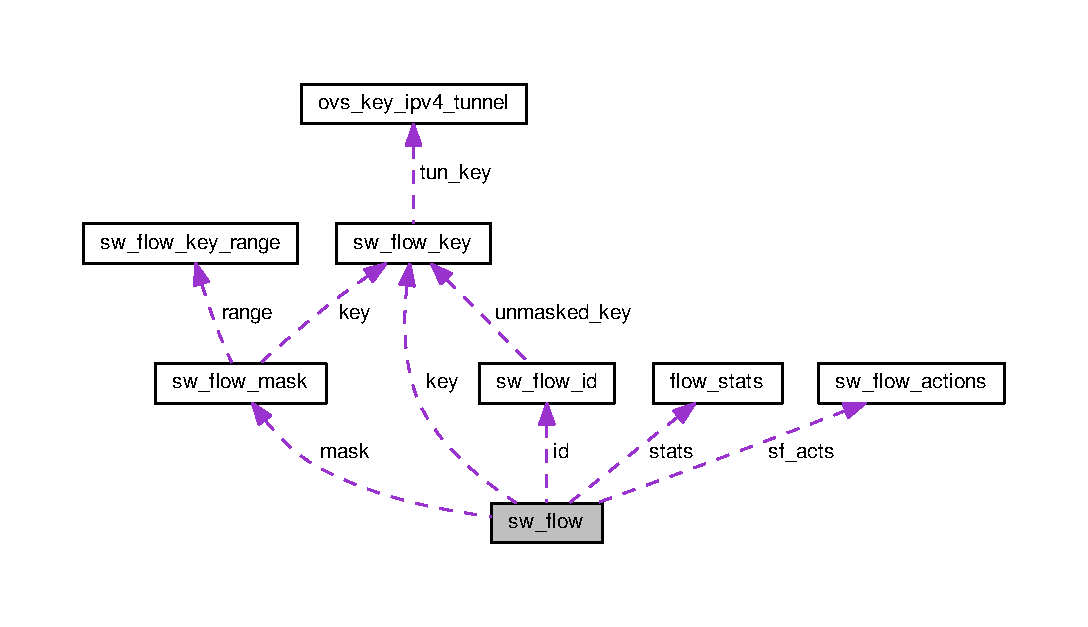
\includegraphics[width=350pt]{structsw__flow__coll__graph}
\end{center}
\end{figure}
\subsection*{Data Fields}
\begin{DoxyCompactItemize}
\item 
struct rcu\+\_\+head \hyperlink{structsw__flow_ac58ef2fab6f9d88be75d73e4d2a1e002}{rcu}
\item 
\begin{tabbing}
xx\=xx\=xx\=xx\=xx\=xx\=xx\=xx\=xx\=\kill
struct \{\\
\>struct hlist\_node \hyperlink{structsw__flow_ad56483ca56d2f95857eee360e934fcf2}{node} \mbox{[}2\mbox{]}\\
\>u32 \hyperlink{structsw__flow_a7a33a6a5c62113ffe949a700ef648a71}{hash}\\
\} \hyperlink{structsw__flow_abca0040cced6a4a84d1a8941764fb5d6}{flow\_table}\\

\end{tabbing}\item 
\begin{tabbing}
xx\=xx\=xx\=xx\=xx\=xx\=xx\=xx\=xx\=\kill
struct \{\\
\>struct hlist\_node \hyperlink{structsw__flow_ad56483ca56d2f95857eee360e934fcf2}{node} \mbox{[}2\mbox{]}\\
\>u32 \hyperlink{structsw__flow_a7a33a6a5c62113ffe949a700ef648a71}{hash}\\
\} \hyperlink{structsw__flow_af5dad10ae036092f5a26cfebb050a03a}{ufid\_table}\\

\end{tabbing}\item 
int \hyperlink{structsw__flow_a7b4a10d23b2824b421527bc2600ef4ba}{stats\+\_\+last\+\_\+writer}
\item 
struct \hyperlink{structsw__flow__key}{sw\+\_\+flow\+\_\+key} \hyperlink{structsw__flow_a14b83cbd65275bda4e97ae35500d26d8}{key}
\item 
struct \hyperlink{structsw__flow__id}{sw\+\_\+flow\+\_\+id} \hyperlink{structsw__flow_a6e6645eec909d54871675be30000c0b9}{id}
\item 
struct \hyperlink{structsw__flow__mask}{sw\+\_\+flow\+\_\+mask} $\ast$ \hyperlink{structsw__flow_a89c162e340693d0bb4977737e2b68c22}{mask}
\item 
struct \hyperlink{structsw__flow__actions}{sw\+\_\+flow\+\_\+actions} \hyperlink{compiler_8h_a2b3b0c016258969e4b39c66b6eec2129}{\+\_\+\+\_\+rcu} $\ast$ \hyperlink{structsw__flow_aa845bdaabc25d81dcf8b1a7519b35408}{sf\+\_\+acts}
\item 
struct \hyperlink{structflow__stats}{flow\+\_\+stats} \hyperlink{compiler_8h_a2b3b0c016258969e4b39c66b6eec2129}{\+\_\+\+\_\+rcu} $\ast$ \hyperlink{structsw__flow_a5ccc743bcf16038ab0cf5dda88565f33}{stats} \mbox{[}$\,$\mbox{]}
\end{DoxyCompactItemize}


\subsection{Field Documentation}
\hypertarget{structsw__flow_abca0040cced6a4a84d1a8941764fb5d6}{}\index{sw\+\_\+flow@{sw\+\_\+flow}!flow\+\_\+table@{flow\+\_\+table}}
\index{flow\+\_\+table@{flow\+\_\+table}!sw\+\_\+flow@{sw\+\_\+flow}}
\subsubsection[{flow\+\_\+table}]{\setlength{\rightskip}{0pt plus 5cm}struct \{ ... \}   sw\+\_\+flow\+::flow\+\_\+table}\label{structsw__flow_abca0040cced6a4a84d1a8941764fb5d6}
\hypertarget{structsw__flow_a7a33a6a5c62113ffe949a700ef648a71}{}\index{sw\+\_\+flow@{sw\+\_\+flow}!hash@{hash}}
\index{hash@{hash}!sw\+\_\+flow@{sw\+\_\+flow}}
\subsubsection[{hash}]{\setlength{\rightskip}{0pt plus 5cm}u32 sw\+\_\+flow\+::hash}\label{structsw__flow_a7a33a6a5c62113ffe949a700ef648a71}
\hypertarget{structsw__flow_a6e6645eec909d54871675be30000c0b9}{}\index{sw\+\_\+flow@{sw\+\_\+flow}!id@{id}}
\index{id@{id}!sw\+\_\+flow@{sw\+\_\+flow}}
\subsubsection[{id}]{\setlength{\rightskip}{0pt plus 5cm}struct {\bf sw\+\_\+flow\+\_\+id} sw\+\_\+flow\+::id}\label{structsw__flow_a6e6645eec909d54871675be30000c0b9}
\hypertarget{structsw__flow_a14b83cbd65275bda4e97ae35500d26d8}{}\index{sw\+\_\+flow@{sw\+\_\+flow}!key@{key}}
\index{key@{key}!sw\+\_\+flow@{sw\+\_\+flow}}
\subsubsection[{key}]{\setlength{\rightskip}{0pt plus 5cm}struct {\bf sw\+\_\+flow\+\_\+key} sw\+\_\+flow\+::key}\label{structsw__flow_a14b83cbd65275bda4e97ae35500d26d8}
\hypertarget{structsw__flow_a89c162e340693d0bb4977737e2b68c22}{}\index{sw\+\_\+flow@{sw\+\_\+flow}!mask@{mask}}
\index{mask@{mask}!sw\+\_\+flow@{sw\+\_\+flow}}
\subsubsection[{mask}]{\setlength{\rightskip}{0pt plus 5cm}struct {\bf sw\+\_\+flow\+\_\+mask}$\ast$ sw\+\_\+flow\+::mask}\label{structsw__flow_a89c162e340693d0bb4977737e2b68c22}
\hypertarget{structsw__flow_ad56483ca56d2f95857eee360e934fcf2}{}\index{sw\+\_\+flow@{sw\+\_\+flow}!node@{node}}
\index{node@{node}!sw\+\_\+flow@{sw\+\_\+flow}}
\subsubsection[{node}]{\setlength{\rightskip}{0pt plus 5cm}struct hlist\+\_\+node sw\+\_\+flow\+::node\mbox{[}2\mbox{]}}\label{structsw__flow_ad56483ca56d2f95857eee360e934fcf2}
\hypertarget{structsw__flow_ac58ef2fab6f9d88be75d73e4d2a1e002}{}\index{sw\+\_\+flow@{sw\+\_\+flow}!rcu@{rcu}}
\index{rcu@{rcu}!sw\+\_\+flow@{sw\+\_\+flow}}
\subsubsection[{rcu}]{\setlength{\rightskip}{0pt plus 5cm}struct rcu\+\_\+head sw\+\_\+flow\+::rcu}\label{structsw__flow_ac58ef2fab6f9d88be75d73e4d2a1e002}
\hypertarget{structsw__flow_aa845bdaabc25d81dcf8b1a7519b35408}{}\index{sw\+\_\+flow@{sw\+\_\+flow}!sf\+\_\+acts@{sf\+\_\+acts}}
\index{sf\+\_\+acts@{sf\+\_\+acts}!sw\+\_\+flow@{sw\+\_\+flow}}
\subsubsection[{sf\+\_\+acts}]{\setlength{\rightskip}{0pt plus 5cm}struct {\bf sw\+\_\+flow\+\_\+actions} {\bf \+\_\+\+\_\+rcu}$\ast$ sw\+\_\+flow\+::sf\+\_\+acts}\label{structsw__flow_aa845bdaabc25d81dcf8b1a7519b35408}
\hypertarget{structsw__flow_a5ccc743bcf16038ab0cf5dda88565f33}{}\index{sw\+\_\+flow@{sw\+\_\+flow}!stats@{stats}}
\index{stats@{stats}!sw\+\_\+flow@{sw\+\_\+flow}}
\subsubsection[{stats}]{\setlength{\rightskip}{0pt plus 5cm}struct {\bf flow\+\_\+stats} {\bf \+\_\+\+\_\+rcu}$\ast$ sw\+\_\+flow\+::stats\mbox{[}$\,$\mbox{]}}\label{structsw__flow_a5ccc743bcf16038ab0cf5dda88565f33}
\hypertarget{structsw__flow_a7b4a10d23b2824b421527bc2600ef4ba}{}\index{sw\+\_\+flow@{sw\+\_\+flow}!stats\+\_\+last\+\_\+writer@{stats\+\_\+last\+\_\+writer}}
\index{stats\+\_\+last\+\_\+writer@{stats\+\_\+last\+\_\+writer}!sw\+\_\+flow@{sw\+\_\+flow}}
\subsubsection[{stats\+\_\+last\+\_\+writer}]{\setlength{\rightskip}{0pt plus 5cm}int sw\+\_\+flow\+::stats\+\_\+last\+\_\+writer}\label{structsw__flow_a7b4a10d23b2824b421527bc2600ef4ba}
\hypertarget{structsw__flow_af5dad10ae036092f5a26cfebb050a03a}{}\index{sw\+\_\+flow@{sw\+\_\+flow}!ufid\+\_\+table@{ufid\+\_\+table}}
\index{ufid\+\_\+table@{ufid\+\_\+table}!sw\+\_\+flow@{sw\+\_\+flow}}
\subsubsection[{ufid\+\_\+table}]{\setlength{\rightskip}{0pt plus 5cm}struct \{ ... \}   sw\+\_\+flow\+::ufid\+\_\+table}\label{structsw__flow_af5dad10ae036092f5a26cfebb050a03a}


The documentation for this struct was generated from the following file\+:\begin{DoxyCompactItemize}
\item 
/home/vladn/git/ovs/datapath/\hyperlink{flow_8h}{flow.\+h}\end{DoxyCompactItemize}

\hypertarget{structsw__flow__actions}{}\section{sw\+\_\+flow\+\_\+actions Struct Reference}
\label{structsw__flow__actions}\index{sw\+\_\+flow\+\_\+actions@{sw\+\_\+flow\+\_\+actions}}


{\ttfamily \#include $<$flow.\+h$>$}

\subsection*{Data Fields}
\begin{DoxyCompactItemize}
\item 
struct rcu\+\_\+head \hyperlink{structsw__flow__actions_aaf3da3f7607ed9dd956fd8c6e1290831}{rcu}
\item 
u32 \hyperlink{structsw__flow__actions_ad18c83862d211746fc0542eabff148a5}{actions\+\_\+len}
\item 
struct nlattr \hyperlink{structsw__flow__actions_ae091e053b6fbc25174a28e97282cbe36}{actions} \mbox{[}$\,$\mbox{]}
\end{DoxyCompactItemize}


\subsection{Field Documentation}
\hypertarget{structsw__flow__actions_ae091e053b6fbc25174a28e97282cbe36}{}\index{sw\+\_\+flow\+\_\+actions@{sw\+\_\+flow\+\_\+actions}!actions@{actions}}
\index{actions@{actions}!sw\+\_\+flow\+\_\+actions@{sw\+\_\+flow\+\_\+actions}}
\subsubsection[{actions}]{\setlength{\rightskip}{0pt plus 5cm}struct nlattr sw\+\_\+flow\+\_\+actions\+::actions\mbox{[}$\,$\mbox{]}}\label{structsw__flow__actions_ae091e053b6fbc25174a28e97282cbe36}
\hypertarget{structsw__flow__actions_ad18c83862d211746fc0542eabff148a5}{}\index{sw\+\_\+flow\+\_\+actions@{sw\+\_\+flow\+\_\+actions}!actions\+\_\+len@{actions\+\_\+len}}
\index{actions\+\_\+len@{actions\+\_\+len}!sw\+\_\+flow\+\_\+actions@{sw\+\_\+flow\+\_\+actions}}
\subsubsection[{actions\+\_\+len}]{\setlength{\rightskip}{0pt plus 5cm}u32 sw\+\_\+flow\+\_\+actions\+::actions\+\_\+len}\label{structsw__flow__actions_ad18c83862d211746fc0542eabff148a5}
\hypertarget{structsw__flow__actions_aaf3da3f7607ed9dd956fd8c6e1290831}{}\index{sw\+\_\+flow\+\_\+actions@{sw\+\_\+flow\+\_\+actions}!rcu@{rcu}}
\index{rcu@{rcu}!sw\+\_\+flow\+\_\+actions@{sw\+\_\+flow\+\_\+actions}}
\subsubsection[{rcu}]{\setlength{\rightskip}{0pt plus 5cm}struct rcu\+\_\+head sw\+\_\+flow\+\_\+actions\+::rcu}\label{structsw__flow__actions_aaf3da3f7607ed9dd956fd8c6e1290831}


The documentation for this struct was generated from the following file\+:\begin{DoxyCompactItemize}
\item 
/home/vladn/git/ovs/datapath/\hyperlink{flow_8h}{flow.\+h}\end{DoxyCompactItemize}

\hypertarget{structsw__flow__id}{}\section{sw\+\_\+flow\+\_\+id Struct Reference}
\label{structsw__flow__id}\index{sw\+\_\+flow\+\_\+id@{sw\+\_\+flow\+\_\+id}}


{\ttfamily \#include $<$flow.\+h$>$}



Collaboration diagram for sw\+\_\+flow\+\_\+id\+:
\nopagebreak
\begin{figure}[H]
\begin{center}
\leavevmode
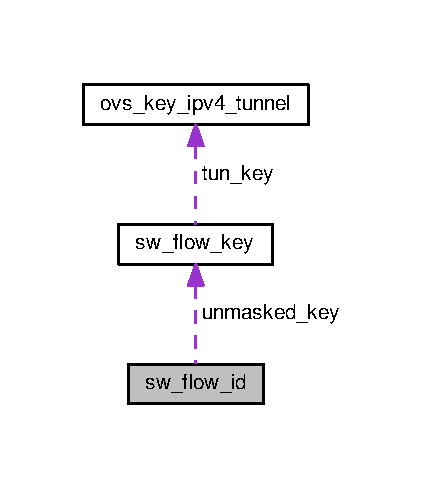
\includegraphics[width=204pt]{structsw__flow__id__coll__graph}
\end{center}
\end{figure}
\subsection*{Data Fields}
\begin{DoxyCompactItemize}
\item 
u32 \hyperlink{structsw__flow__id_a7cfead96fedf295e55d6a17857adfbf5}{ufid\+\_\+len}
\item 
\begin{tabbing}
xx\=xx\=xx\=xx\=xx\=xx\=xx\=xx\=xx\=\kill
union \{\\
\>u32 \hyperlink{structsw__flow__id_a22ce2b1fed980149931fbccb05750f3e}{ufid} \mbox{[}\hyperlink{flow_8h_a5cc1c8e559536cddce9d468214805527}{MAX\_UFID\_LENGTH}/4\mbox{]}\\
\>struct \hyperlink{structsw__flow__key}{sw\_flow\_key} $\ast$ \hyperlink{structsw__flow__id_a5d62dce79569cb8c25a43f4039e5df3c}{unmasked\_key}\\
\}; \\

\end{tabbing}\end{DoxyCompactItemize}


\subsection{Field Documentation}
\hypertarget{structsw__flow__id_a7a025ad1b692dac54dab18bb4170eaa0}{}\subsubsection[{"@31}]{\setlength{\rightskip}{0pt plus 5cm}union \{ ... \} }\label{structsw__flow__id_a7a025ad1b692dac54dab18bb4170eaa0}
\hypertarget{structsw__flow__id_a22ce2b1fed980149931fbccb05750f3e}{}\index{sw\+\_\+flow\+\_\+id@{sw\+\_\+flow\+\_\+id}!ufid@{ufid}}
\index{ufid@{ufid}!sw\+\_\+flow\+\_\+id@{sw\+\_\+flow\+\_\+id}}
\subsubsection[{ufid}]{\setlength{\rightskip}{0pt plus 5cm}u32 sw\+\_\+flow\+\_\+id\+::ufid\mbox{[}{\bf M\+A\+X\+\_\+\+U\+F\+I\+D\+\_\+\+L\+E\+N\+G\+T\+H}/4\mbox{]}}\label{structsw__flow__id_a22ce2b1fed980149931fbccb05750f3e}
\hypertarget{structsw__flow__id_a7cfead96fedf295e55d6a17857adfbf5}{}\index{sw\+\_\+flow\+\_\+id@{sw\+\_\+flow\+\_\+id}!ufid\+\_\+len@{ufid\+\_\+len}}
\index{ufid\+\_\+len@{ufid\+\_\+len}!sw\+\_\+flow\+\_\+id@{sw\+\_\+flow\+\_\+id}}
\subsubsection[{ufid\+\_\+len}]{\setlength{\rightskip}{0pt plus 5cm}u32 sw\+\_\+flow\+\_\+id\+::ufid\+\_\+len}\label{structsw__flow__id_a7cfead96fedf295e55d6a17857adfbf5}
\hypertarget{structsw__flow__id_a5d62dce79569cb8c25a43f4039e5df3c}{}\index{sw\+\_\+flow\+\_\+id@{sw\+\_\+flow\+\_\+id}!unmasked\+\_\+key@{unmasked\+\_\+key}}
\index{unmasked\+\_\+key@{unmasked\+\_\+key}!sw\+\_\+flow\+\_\+id@{sw\+\_\+flow\+\_\+id}}
\subsubsection[{unmasked\+\_\+key}]{\setlength{\rightskip}{0pt plus 5cm}struct {\bf sw\+\_\+flow\+\_\+key}$\ast$ sw\+\_\+flow\+\_\+id\+::unmasked\+\_\+key}\label{structsw__flow__id_a5d62dce79569cb8c25a43f4039e5df3c}


The documentation for this struct was generated from the following file\+:\begin{DoxyCompactItemize}
\item 
/home/vladn/git/ovs/datapath/\hyperlink{flow_8h}{flow.\+h}\end{DoxyCompactItemize}

\hypertarget{structsw__flow__key}{}\section{sw\+\_\+flow\+\_\+key Struct Reference}
\label{structsw__flow__key}\index{sw\+\_\+flow\+\_\+key@{sw\+\_\+flow\+\_\+key}}


{\ttfamily \#include $<$flow.\+h$>$}



Collaboration diagram for sw\+\_\+flow\+\_\+key\+:
\nopagebreak
\begin{figure}[H]
\begin{center}
\leavevmode
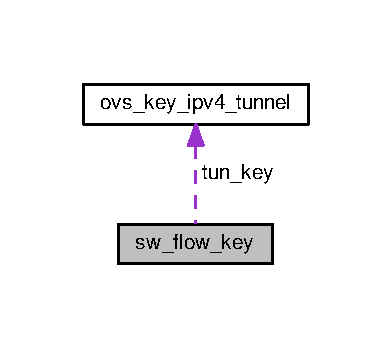
\includegraphics[width=188pt]{structsw__flow__key__coll__graph}
\end{center}
\end{figure}
\subsection*{Data Fields}
\begin{DoxyCompactItemize}
\item 
u8 \hyperlink{structsw__flow__key_a54b30752817dccb02665a7eecde52a72}{tun\+\_\+opts} \mbox{[}255\mbox{]}
\item 
u8 \hyperlink{structsw__flow__key_aef0ea317d3bd0125e0d6390261ba3e2d}{tun\+\_\+opts\+\_\+len}
\item 
struct \hyperlink{structovs__key__ipv4__tunnel}{ovs\+\_\+key\+\_\+ipv4\+\_\+tunnel} \hyperlink{structsw__flow__key_a2f87b7690c0cc2797f1f4347589472c3}{tun\+\_\+key}
\item 
\begin{tabbing}
xx\=xx\=xx\=xx\=xx\=xx\=xx\=xx\=xx\=\kill
struct \{\\
\>u32 \hyperlink{structsw__flow__key_a9dd898913d9faaec1ec970029e7fbb71}{priority}\\
\>u32 \hyperlink{structsw__flow__key_ae02571657f29397dcc45de8528f4ed05}{skb\_mark}\\
\>u16 \hyperlink{structsw__flow__key_a5848de18caa80d36d9bc60cc686a2c6e}{in\_port}\\
\} \hyperlink{structsw__flow__key_a57cbddb75a8d4fd859300bd34d98e84a}{phy}\\

\end{tabbing}\item 
u32 \hyperlink{structsw__flow__key_a73dd9402f1f54c321f6d704d9b018d15}{ovs\+\_\+flow\+\_\+hash}
\item 
u32 \hyperlink{structsw__flow__key_a7e51857c88ad6b0bf90551d0b6e2607b}{recirc\+\_\+id}
\item 
\begin{tabbing}
xx\=xx\=xx\=xx\=xx\=xx\=xx\=xx\=xx\=\kill
struct \{\\
\>u8 \hyperlink{structsw__flow__key_a2fbd4aa7a500630627eff0630f864117}{src} \mbox{[}ETH\_ALEN\mbox{]}\\
\>u8 \hyperlink{structsw__flow__key_a44a0cdfe7471df8bb73762085da4cda9}{dst} \mbox{[}ETH\_ALEN\mbox{]}\\
\>\_\_be16 \hyperlink{structsw__flow__key_a56b27b9b9eafa8f79acd544eba98c7b0}{tci}\\
\>\_\_be16 \hyperlink{structsw__flow__key_af30defbb2a81c997e8747594e1d937a0}{type}\\
\} \hyperlink{structsw__flow__key_af3e10c978a3a2bf303b7d953ac6ff361}{eth}\\

\end{tabbing}\item 
\begin{tabbing}
xx\=xx\=xx\=xx\=xx\=xx\=xx\=xx\=xx\=\kill
union \{\\
\>struct \{\\
\>\>\_\_be32 \hyperlink{structsw__flow__key_a8deabdad62023ba089b9864374cb5c20}{top\_lse}\\
\>\} \hyperlink{structsw__flow__key_a005840d04ee5b462be3c8e21809dc9aa}{mpls}\\
\>struct \{\\
\>\>u8 \hyperlink{structsw__flow__key_a189368e5defc2dfbeed8f47b53f87094}{proto}\\
\>\>u8 \hyperlink{structsw__flow__key_af82daee0da7b81a0e1333965ec3f6180}{tos}\\
\>\>u8 \hyperlink{structsw__flow__key_aa53659c0aec0ef307046cb1d835ffa5a}{ttl}\\
\>\>u8 \hyperlink{structsw__flow__key_afe49934f508e0d054afce967d7ab25dd}{frag}\\
\>\} \hyperlink{structsw__flow__key_ae8d48c419eaff6a9fda97c7446bdec0e}{ip}\\
\}; \\

\end{tabbing}\item 
\begin{tabbing}
xx\=xx\=xx\=xx\=xx\=xx\=xx\=xx\=xx\=\kill
struct \{\\
\>\_\_be16 \hyperlink{structsw__flow__key_a0ff9e0ec68c48aea390c1880b42afc12}{src}\\
\>\_\_be16 \hyperlink{structsw__flow__key_a5d032dcf21ee5cf8a4d0261e3b05357f}{dst}\\
\>\_\_be16 \hyperlink{structsw__flow__key_a910f5e4408d113dbc9211190b44e0880}{flags}\\
\} \hyperlink{structsw__flow__key_a9c1944a39db1bf91141048df6d85ce8b}{tp}\\

\end{tabbing}\item 
\begin{tabbing}
xx\=xx\=xx\=xx\=xx\=xx\=xx\=xx\=xx\=\kill
union \{\\
\>struct \{\\
\>\>struct \{\\
\>\>\>\_\_be32 \hyperlink{structsw__flow__key_ab5368dd5350124baac85c3be19febb12}{src}\\
\>\>\>\_\_be32 \hyperlink{structsw__flow__key_a05994d9d99af2b8a8bcd66ce255ca40c}{dst}\\
\>\>\} \hyperlink{structsw__flow__key_abfc28adb05f413bcc53e68c773144f0a}{addr}\\
\>\>struct \{\\
\>\>\>u8 \hyperlink{structsw__flow__key_aec0c2988805dcc1e85d3dd508b1eff9f}{sha} \mbox{[}ETH\_ALEN\mbox{]}\\
\>\>\>u8 \hyperlink{structsw__flow__key_a48eba3d8570ada988ca07dd926b61a5f}{tha} \mbox{[}ETH\_ALEN\mbox{]}\\
\>\>\} \hyperlink{structsw__flow__key_a0932eb34cba8111bb3b37bf106ba7a59}{arp}\\
\>\} \hyperlink{structsw__flow__key_aeb4295bcb2fb4efea5c30337b871a423}{ipv4}\\
\>struct \{\\
\>\>struct \{\\
\>\>\>struct in6\_addr \hyperlink{structsw__flow__key_ae1e86390146b7cad7fd1c0b171011484}{src}\\
\>\>\>struct in6\_addr \hyperlink{structsw__flow__key_a9d6f8c300bf7a75527c05d7f9e88270d}{dst}\\
\>\>\} \hyperlink{structsw__flow__key_a60452748303b04851a89b07ecd39b94a}{addr}\\
\>\>\_\_be32 \hyperlink{structsw__flow__key_a92faa50d10672469aa891e2ae63aa692}{label}\\
\>\>struct \{\\
\>\>\>struct in6\_addr \hyperlink{structsw__flow__key_a12bf2f042022c3c7f8324ad1727f5df0}{target}\\
\>\>\>u8 \hyperlink{structsw__flow__key_ae937ac892919b521d123b4e63d5656e6}{sll} \mbox{[}ETH\_ALEN\mbox{]}\\
\>\>\>u8 \hyperlink{structsw__flow__key_a0462e7a44643ceeabd560cd179d342c1}{tll} \mbox{[}ETH\_ALEN\mbox{]}\\
\>\>\} \hyperlink{structsw__flow__key_a0f5f6c87614b5b84cf3e7fd5a59b41bb}{nd}\\
\>\} \hyperlink{structsw__flow__key_a6b13e14d62eb632b05378784a2d61f87}{ipv6}\\
\}; \\

\end{tabbing}\end{DoxyCompactItemize}


\subsection{Field Documentation}
\hypertarget{structsw__flow__key_afbbeb90ecc1f7acfb38798dbe397d562}{}\subsubsection[{"@3}]{\setlength{\rightskip}{0pt plus 5cm}union \{ ... \} }\label{structsw__flow__key_afbbeb90ecc1f7acfb38798dbe397d562}
\hypertarget{structsw__flow__key_a01fc9d1c4d8141a0cb1a18162814f42b}{}\subsubsection[{"@6}]{\setlength{\rightskip}{0pt plus 5cm}union \{ ... \} }\label{structsw__flow__key_a01fc9d1c4d8141a0cb1a18162814f42b}
\hypertarget{structsw__flow__key_abfc28adb05f413bcc53e68c773144f0a}{}\index{sw\+\_\+flow\+\_\+key@{sw\+\_\+flow\+\_\+key}!addr@{addr}}
\index{addr@{addr}!sw\+\_\+flow\+\_\+key@{sw\+\_\+flow\+\_\+key}}
\subsubsection[{addr}]{\setlength{\rightskip}{0pt plus 5cm}struct \{ ... \}   sw\+\_\+flow\+\_\+key\+::addr}\label{structsw__flow__key_abfc28adb05f413bcc53e68c773144f0a}
\hypertarget{structsw__flow__key_a60452748303b04851a89b07ecd39b94a}{}\index{sw\+\_\+flow\+\_\+key@{sw\+\_\+flow\+\_\+key}!addr@{addr}}
\index{addr@{addr}!sw\+\_\+flow\+\_\+key@{sw\+\_\+flow\+\_\+key}}
\subsubsection[{addr}]{\setlength{\rightskip}{0pt plus 5cm}struct \{ ... \}   sw\+\_\+flow\+\_\+key\+::addr}\label{structsw__flow__key_a60452748303b04851a89b07ecd39b94a}
\hypertarget{structsw__flow__key_a0932eb34cba8111bb3b37bf106ba7a59}{}\index{sw\+\_\+flow\+\_\+key@{sw\+\_\+flow\+\_\+key}!arp@{arp}}
\index{arp@{arp}!sw\+\_\+flow\+\_\+key@{sw\+\_\+flow\+\_\+key}}
\subsubsection[{arp}]{\setlength{\rightskip}{0pt plus 5cm}struct \{ ... \}   sw\+\_\+flow\+\_\+key\+::arp}\label{structsw__flow__key_a0932eb34cba8111bb3b37bf106ba7a59}
\hypertarget{structsw__flow__key_a44a0cdfe7471df8bb73762085da4cda9}{}\index{sw\+\_\+flow\+\_\+key@{sw\+\_\+flow\+\_\+key}!dst@{dst}}
\index{dst@{dst}!sw\+\_\+flow\+\_\+key@{sw\+\_\+flow\+\_\+key}}
\subsubsection[{dst}]{\setlength{\rightskip}{0pt plus 5cm}u8 sw\+\_\+flow\+\_\+key\+::dst\mbox{[}E\+T\+H\+\_\+\+A\+L\+E\+N\mbox{]}}\label{structsw__flow__key_a44a0cdfe7471df8bb73762085da4cda9}
\hypertarget{structsw__flow__key_a5d032dcf21ee5cf8a4d0261e3b05357f}{}\index{sw\+\_\+flow\+\_\+key@{sw\+\_\+flow\+\_\+key}!dst@{dst}}
\index{dst@{dst}!sw\+\_\+flow\+\_\+key@{sw\+\_\+flow\+\_\+key}}
\subsubsection[{dst}]{\setlength{\rightskip}{0pt plus 5cm}\+\_\+\+\_\+be16 sw\+\_\+flow\+\_\+key\+::dst}\label{structsw__flow__key_a5d032dcf21ee5cf8a4d0261e3b05357f}
\hypertarget{structsw__flow__key_a05994d9d99af2b8a8bcd66ce255ca40c}{}\index{sw\+\_\+flow\+\_\+key@{sw\+\_\+flow\+\_\+key}!dst@{dst}}
\index{dst@{dst}!sw\+\_\+flow\+\_\+key@{sw\+\_\+flow\+\_\+key}}
\subsubsection[{dst}]{\setlength{\rightskip}{0pt plus 5cm}\+\_\+\+\_\+be32 sw\+\_\+flow\+\_\+key\+::dst}\label{structsw__flow__key_a05994d9d99af2b8a8bcd66ce255ca40c}
\hypertarget{structsw__flow__key_a9d6f8c300bf7a75527c05d7f9e88270d}{}\index{sw\+\_\+flow\+\_\+key@{sw\+\_\+flow\+\_\+key}!dst@{dst}}
\index{dst@{dst}!sw\+\_\+flow\+\_\+key@{sw\+\_\+flow\+\_\+key}}
\subsubsection[{dst}]{\setlength{\rightskip}{0pt plus 5cm}struct in6\+\_\+addr sw\+\_\+flow\+\_\+key\+::dst}\label{structsw__flow__key_a9d6f8c300bf7a75527c05d7f9e88270d}
\hypertarget{structsw__flow__key_af3e10c978a3a2bf303b7d953ac6ff361}{}\index{sw\+\_\+flow\+\_\+key@{sw\+\_\+flow\+\_\+key}!eth@{eth}}
\index{eth@{eth}!sw\+\_\+flow\+\_\+key@{sw\+\_\+flow\+\_\+key}}
\subsubsection[{eth}]{\setlength{\rightskip}{0pt plus 5cm}struct \{ ... \}   sw\+\_\+flow\+\_\+key\+::eth}\label{structsw__flow__key_af3e10c978a3a2bf303b7d953ac6ff361}
\hypertarget{structsw__flow__key_a910f5e4408d113dbc9211190b44e0880}{}\index{sw\+\_\+flow\+\_\+key@{sw\+\_\+flow\+\_\+key}!flags@{flags}}
\index{flags@{flags}!sw\+\_\+flow\+\_\+key@{sw\+\_\+flow\+\_\+key}}
\subsubsection[{flags}]{\setlength{\rightskip}{0pt plus 5cm}\+\_\+\+\_\+be16 sw\+\_\+flow\+\_\+key\+::flags}\label{structsw__flow__key_a910f5e4408d113dbc9211190b44e0880}
\hypertarget{structsw__flow__key_afe49934f508e0d054afce967d7ab25dd}{}\index{sw\+\_\+flow\+\_\+key@{sw\+\_\+flow\+\_\+key}!frag@{frag}}
\index{frag@{frag}!sw\+\_\+flow\+\_\+key@{sw\+\_\+flow\+\_\+key}}
\subsubsection[{frag}]{\setlength{\rightskip}{0pt plus 5cm}u8 sw\+\_\+flow\+\_\+key\+::frag}\label{structsw__flow__key_afe49934f508e0d054afce967d7ab25dd}
\hypertarget{structsw__flow__key_a5848de18caa80d36d9bc60cc686a2c6e}{}\index{sw\+\_\+flow\+\_\+key@{sw\+\_\+flow\+\_\+key}!in\+\_\+port@{in\+\_\+port}}
\index{in\+\_\+port@{in\+\_\+port}!sw\+\_\+flow\+\_\+key@{sw\+\_\+flow\+\_\+key}}
\subsubsection[{in\+\_\+port}]{\setlength{\rightskip}{0pt plus 5cm}u16 sw\+\_\+flow\+\_\+key\+::in\+\_\+port}\label{structsw__flow__key_a5848de18caa80d36d9bc60cc686a2c6e}
\hypertarget{structsw__flow__key_ae8d48c419eaff6a9fda97c7446bdec0e}{}\index{sw\+\_\+flow\+\_\+key@{sw\+\_\+flow\+\_\+key}!ip@{ip}}
\index{ip@{ip}!sw\+\_\+flow\+\_\+key@{sw\+\_\+flow\+\_\+key}}
\subsubsection[{ip}]{\setlength{\rightskip}{0pt plus 5cm}struct \{ ... \}   sw\+\_\+flow\+\_\+key\+::ip}\label{structsw__flow__key_ae8d48c419eaff6a9fda97c7446bdec0e}
\hypertarget{structsw__flow__key_aeb4295bcb2fb4efea5c30337b871a423}{}\index{sw\+\_\+flow\+\_\+key@{sw\+\_\+flow\+\_\+key}!ipv4@{ipv4}}
\index{ipv4@{ipv4}!sw\+\_\+flow\+\_\+key@{sw\+\_\+flow\+\_\+key}}
\subsubsection[{ipv4}]{\setlength{\rightskip}{0pt plus 5cm}struct \{ ... \}   sw\+\_\+flow\+\_\+key\+::ipv4}\label{structsw__flow__key_aeb4295bcb2fb4efea5c30337b871a423}
\hypertarget{structsw__flow__key_a6b13e14d62eb632b05378784a2d61f87}{}\index{sw\+\_\+flow\+\_\+key@{sw\+\_\+flow\+\_\+key}!ipv6@{ipv6}}
\index{ipv6@{ipv6}!sw\+\_\+flow\+\_\+key@{sw\+\_\+flow\+\_\+key}}
\subsubsection[{ipv6}]{\setlength{\rightskip}{0pt plus 5cm}struct \{ ... \}   sw\+\_\+flow\+\_\+key\+::ipv6}\label{structsw__flow__key_a6b13e14d62eb632b05378784a2d61f87}
\hypertarget{structsw__flow__key_a92faa50d10672469aa891e2ae63aa692}{}\index{sw\+\_\+flow\+\_\+key@{sw\+\_\+flow\+\_\+key}!label@{label}}
\index{label@{label}!sw\+\_\+flow\+\_\+key@{sw\+\_\+flow\+\_\+key}}
\subsubsection[{label}]{\setlength{\rightskip}{0pt plus 5cm}\+\_\+\+\_\+be32 sw\+\_\+flow\+\_\+key\+::label}\label{structsw__flow__key_a92faa50d10672469aa891e2ae63aa692}
\hypertarget{structsw__flow__key_a005840d04ee5b462be3c8e21809dc9aa}{}\index{sw\+\_\+flow\+\_\+key@{sw\+\_\+flow\+\_\+key}!mpls@{mpls}}
\index{mpls@{mpls}!sw\+\_\+flow\+\_\+key@{sw\+\_\+flow\+\_\+key}}
\subsubsection[{mpls}]{\setlength{\rightskip}{0pt plus 5cm}struct \{ ... \}   sw\+\_\+flow\+\_\+key\+::mpls}\label{structsw__flow__key_a005840d04ee5b462be3c8e21809dc9aa}
\hypertarget{structsw__flow__key_a0f5f6c87614b5b84cf3e7fd5a59b41bb}{}\index{sw\+\_\+flow\+\_\+key@{sw\+\_\+flow\+\_\+key}!nd@{nd}}
\index{nd@{nd}!sw\+\_\+flow\+\_\+key@{sw\+\_\+flow\+\_\+key}}
\subsubsection[{nd}]{\setlength{\rightskip}{0pt plus 5cm}struct \{ ... \}   sw\+\_\+flow\+\_\+key\+::nd}\label{structsw__flow__key_a0f5f6c87614b5b84cf3e7fd5a59b41bb}
\hypertarget{structsw__flow__key_a73dd9402f1f54c321f6d704d9b018d15}{}\index{sw\+\_\+flow\+\_\+key@{sw\+\_\+flow\+\_\+key}!ovs\+\_\+flow\+\_\+hash@{ovs\+\_\+flow\+\_\+hash}}
\index{ovs\+\_\+flow\+\_\+hash@{ovs\+\_\+flow\+\_\+hash}!sw\+\_\+flow\+\_\+key@{sw\+\_\+flow\+\_\+key}}
\subsubsection[{ovs\+\_\+flow\+\_\+hash}]{\setlength{\rightskip}{0pt plus 5cm}u32 sw\+\_\+flow\+\_\+key\+::ovs\+\_\+flow\+\_\+hash}\label{structsw__flow__key_a73dd9402f1f54c321f6d704d9b018d15}
\hypertarget{structsw__flow__key_a57cbddb75a8d4fd859300bd34d98e84a}{}\index{sw\+\_\+flow\+\_\+key@{sw\+\_\+flow\+\_\+key}!phy@{phy}}
\index{phy@{phy}!sw\+\_\+flow\+\_\+key@{sw\+\_\+flow\+\_\+key}}
\subsubsection[{phy}]{\setlength{\rightskip}{0pt plus 5cm}struct \{ ... \}  sw\+\_\+flow\+\_\+key\+::phy}\label{structsw__flow__key_a57cbddb75a8d4fd859300bd34d98e84a}
\hypertarget{structsw__flow__key_a9dd898913d9faaec1ec970029e7fbb71}{}\index{sw\+\_\+flow\+\_\+key@{sw\+\_\+flow\+\_\+key}!priority@{priority}}
\index{priority@{priority}!sw\+\_\+flow\+\_\+key@{sw\+\_\+flow\+\_\+key}}
\subsubsection[{priority}]{\setlength{\rightskip}{0pt plus 5cm}u32 sw\+\_\+flow\+\_\+key\+::priority}\label{structsw__flow__key_a9dd898913d9faaec1ec970029e7fbb71}
\hypertarget{structsw__flow__key_a189368e5defc2dfbeed8f47b53f87094}{}\index{sw\+\_\+flow\+\_\+key@{sw\+\_\+flow\+\_\+key}!proto@{proto}}
\index{proto@{proto}!sw\+\_\+flow\+\_\+key@{sw\+\_\+flow\+\_\+key}}
\subsubsection[{proto}]{\setlength{\rightskip}{0pt plus 5cm}u8 sw\+\_\+flow\+\_\+key\+::proto}\label{structsw__flow__key_a189368e5defc2dfbeed8f47b53f87094}
\hypertarget{structsw__flow__key_a7e51857c88ad6b0bf90551d0b6e2607b}{}\index{sw\+\_\+flow\+\_\+key@{sw\+\_\+flow\+\_\+key}!recirc\+\_\+id@{recirc\+\_\+id}}
\index{recirc\+\_\+id@{recirc\+\_\+id}!sw\+\_\+flow\+\_\+key@{sw\+\_\+flow\+\_\+key}}
\subsubsection[{recirc\+\_\+id}]{\setlength{\rightskip}{0pt plus 5cm}u32 sw\+\_\+flow\+\_\+key\+::recirc\+\_\+id}\label{structsw__flow__key_a7e51857c88ad6b0bf90551d0b6e2607b}
\hypertarget{structsw__flow__key_aec0c2988805dcc1e85d3dd508b1eff9f}{}\index{sw\+\_\+flow\+\_\+key@{sw\+\_\+flow\+\_\+key}!sha@{sha}}
\index{sha@{sha}!sw\+\_\+flow\+\_\+key@{sw\+\_\+flow\+\_\+key}}
\subsubsection[{sha}]{\setlength{\rightskip}{0pt plus 5cm}u8 sw\+\_\+flow\+\_\+key\+::sha\mbox{[}E\+T\+H\+\_\+\+A\+L\+E\+N\mbox{]}}\label{structsw__flow__key_aec0c2988805dcc1e85d3dd508b1eff9f}
\hypertarget{structsw__flow__key_ae02571657f29397dcc45de8528f4ed05}{}\index{sw\+\_\+flow\+\_\+key@{sw\+\_\+flow\+\_\+key}!skb\+\_\+mark@{skb\+\_\+mark}}
\index{skb\+\_\+mark@{skb\+\_\+mark}!sw\+\_\+flow\+\_\+key@{sw\+\_\+flow\+\_\+key}}
\subsubsection[{skb\+\_\+mark}]{\setlength{\rightskip}{0pt plus 5cm}u32 sw\+\_\+flow\+\_\+key\+::skb\+\_\+mark}\label{structsw__flow__key_ae02571657f29397dcc45de8528f4ed05}
\hypertarget{structsw__flow__key_ae937ac892919b521d123b4e63d5656e6}{}\index{sw\+\_\+flow\+\_\+key@{sw\+\_\+flow\+\_\+key}!sll@{sll}}
\index{sll@{sll}!sw\+\_\+flow\+\_\+key@{sw\+\_\+flow\+\_\+key}}
\subsubsection[{sll}]{\setlength{\rightskip}{0pt plus 5cm}u8 sw\+\_\+flow\+\_\+key\+::sll\mbox{[}E\+T\+H\+\_\+\+A\+L\+E\+N\mbox{]}}\label{structsw__flow__key_ae937ac892919b521d123b4e63d5656e6}
\hypertarget{structsw__flow__key_a2fbd4aa7a500630627eff0630f864117}{}\index{sw\+\_\+flow\+\_\+key@{sw\+\_\+flow\+\_\+key}!src@{src}}
\index{src@{src}!sw\+\_\+flow\+\_\+key@{sw\+\_\+flow\+\_\+key}}
\subsubsection[{src}]{\setlength{\rightskip}{0pt plus 5cm}u8 sw\+\_\+flow\+\_\+key\+::src\mbox{[}E\+T\+H\+\_\+\+A\+L\+E\+N\mbox{]}}\label{structsw__flow__key_a2fbd4aa7a500630627eff0630f864117}
\hypertarget{structsw__flow__key_a0ff9e0ec68c48aea390c1880b42afc12}{}\index{sw\+\_\+flow\+\_\+key@{sw\+\_\+flow\+\_\+key}!src@{src}}
\index{src@{src}!sw\+\_\+flow\+\_\+key@{sw\+\_\+flow\+\_\+key}}
\subsubsection[{src}]{\setlength{\rightskip}{0pt plus 5cm}\+\_\+\+\_\+be16 sw\+\_\+flow\+\_\+key\+::src}\label{structsw__flow__key_a0ff9e0ec68c48aea390c1880b42afc12}
\hypertarget{structsw__flow__key_ab5368dd5350124baac85c3be19febb12}{}\index{sw\+\_\+flow\+\_\+key@{sw\+\_\+flow\+\_\+key}!src@{src}}
\index{src@{src}!sw\+\_\+flow\+\_\+key@{sw\+\_\+flow\+\_\+key}}
\subsubsection[{src}]{\setlength{\rightskip}{0pt plus 5cm}\+\_\+\+\_\+be32 sw\+\_\+flow\+\_\+key\+::src}\label{structsw__flow__key_ab5368dd5350124baac85c3be19febb12}
\hypertarget{structsw__flow__key_ae1e86390146b7cad7fd1c0b171011484}{}\index{sw\+\_\+flow\+\_\+key@{sw\+\_\+flow\+\_\+key}!src@{src}}
\index{src@{src}!sw\+\_\+flow\+\_\+key@{sw\+\_\+flow\+\_\+key}}
\subsubsection[{src}]{\setlength{\rightskip}{0pt plus 5cm}struct in6\+\_\+addr sw\+\_\+flow\+\_\+key\+::src}\label{structsw__flow__key_ae1e86390146b7cad7fd1c0b171011484}
\hypertarget{structsw__flow__key_a12bf2f042022c3c7f8324ad1727f5df0}{}\index{sw\+\_\+flow\+\_\+key@{sw\+\_\+flow\+\_\+key}!target@{target}}
\index{target@{target}!sw\+\_\+flow\+\_\+key@{sw\+\_\+flow\+\_\+key}}
\subsubsection[{target}]{\setlength{\rightskip}{0pt plus 5cm}struct in6\+\_\+addr sw\+\_\+flow\+\_\+key\+::target}\label{structsw__flow__key_a12bf2f042022c3c7f8324ad1727f5df0}
\hypertarget{structsw__flow__key_a56b27b9b9eafa8f79acd544eba98c7b0}{}\index{sw\+\_\+flow\+\_\+key@{sw\+\_\+flow\+\_\+key}!tci@{tci}}
\index{tci@{tci}!sw\+\_\+flow\+\_\+key@{sw\+\_\+flow\+\_\+key}}
\subsubsection[{tci}]{\setlength{\rightskip}{0pt plus 5cm}\+\_\+\+\_\+be16 sw\+\_\+flow\+\_\+key\+::tci}\label{structsw__flow__key_a56b27b9b9eafa8f79acd544eba98c7b0}
\hypertarget{structsw__flow__key_a48eba3d8570ada988ca07dd926b61a5f}{}\index{sw\+\_\+flow\+\_\+key@{sw\+\_\+flow\+\_\+key}!tha@{tha}}
\index{tha@{tha}!sw\+\_\+flow\+\_\+key@{sw\+\_\+flow\+\_\+key}}
\subsubsection[{tha}]{\setlength{\rightskip}{0pt plus 5cm}u8 sw\+\_\+flow\+\_\+key\+::tha\mbox{[}E\+T\+H\+\_\+\+A\+L\+E\+N\mbox{]}}\label{structsw__flow__key_a48eba3d8570ada988ca07dd926b61a5f}
\hypertarget{structsw__flow__key_a0462e7a44643ceeabd560cd179d342c1}{}\index{sw\+\_\+flow\+\_\+key@{sw\+\_\+flow\+\_\+key}!tll@{tll}}
\index{tll@{tll}!sw\+\_\+flow\+\_\+key@{sw\+\_\+flow\+\_\+key}}
\subsubsection[{tll}]{\setlength{\rightskip}{0pt plus 5cm}u8 sw\+\_\+flow\+\_\+key\+::tll\mbox{[}E\+T\+H\+\_\+\+A\+L\+E\+N\mbox{]}}\label{structsw__flow__key_a0462e7a44643ceeabd560cd179d342c1}
\hypertarget{structsw__flow__key_a8deabdad62023ba089b9864374cb5c20}{}\index{sw\+\_\+flow\+\_\+key@{sw\+\_\+flow\+\_\+key}!top\+\_\+lse@{top\+\_\+lse}}
\index{top\+\_\+lse@{top\+\_\+lse}!sw\+\_\+flow\+\_\+key@{sw\+\_\+flow\+\_\+key}}
\subsubsection[{top\+\_\+lse}]{\setlength{\rightskip}{0pt plus 5cm}\+\_\+\+\_\+be32 sw\+\_\+flow\+\_\+key\+::top\+\_\+lse}\label{structsw__flow__key_a8deabdad62023ba089b9864374cb5c20}
\hypertarget{structsw__flow__key_af82daee0da7b81a0e1333965ec3f6180}{}\index{sw\+\_\+flow\+\_\+key@{sw\+\_\+flow\+\_\+key}!tos@{tos}}
\index{tos@{tos}!sw\+\_\+flow\+\_\+key@{sw\+\_\+flow\+\_\+key}}
\subsubsection[{tos}]{\setlength{\rightskip}{0pt plus 5cm}u8 sw\+\_\+flow\+\_\+key\+::tos}\label{structsw__flow__key_af82daee0da7b81a0e1333965ec3f6180}
\hypertarget{structsw__flow__key_a9c1944a39db1bf91141048df6d85ce8b}{}\index{sw\+\_\+flow\+\_\+key@{sw\+\_\+flow\+\_\+key}!tp@{tp}}
\index{tp@{tp}!sw\+\_\+flow\+\_\+key@{sw\+\_\+flow\+\_\+key}}
\subsubsection[{tp}]{\setlength{\rightskip}{0pt plus 5cm}struct \{ ... \}   sw\+\_\+flow\+\_\+key\+::tp}\label{structsw__flow__key_a9c1944a39db1bf91141048df6d85ce8b}
\hypertarget{structsw__flow__key_aa53659c0aec0ef307046cb1d835ffa5a}{}\index{sw\+\_\+flow\+\_\+key@{sw\+\_\+flow\+\_\+key}!ttl@{ttl}}
\index{ttl@{ttl}!sw\+\_\+flow\+\_\+key@{sw\+\_\+flow\+\_\+key}}
\subsubsection[{ttl}]{\setlength{\rightskip}{0pt plus 5cm}u8 sw\+\_\+flow\+\_\+key\+::ttl}\label{structsw__flow__key_aa53659c0aec0ef307046cb1d835ffa5a}
\hypertarget{structsw__flow__key_a2f87b7690c0cc2797f1f4347589472c3}{}\index{sw\+\_\+flow\+\_\+key@{sw\+\_\+flow\+\_\+key}!tun\+\_\+key@{tun\+\_\+key}}
\index{tun\+\_\+key@{tun\+\_\+key}!sw\+\_\+flow\+\_\+key@{sw\+\_\+flow\+\_\+key}}
\subsubsection[{tun\+\_\+key}]{\setlength{\rightskip}{0pt plus 5cm}struct {\bf ovs\+\_\+key\+\_\+ipv4\+\_\+tunnel} sw\+\_\+flow\+\_\+key\+::tun\+\_\+key}\label{structsw__flow__key_a2f87b7690c0cc2797f1f4347589472c3}
\hypertarget{structsw__flow__key_a54b30752817dccb02665a7eecde52a72}{}\index{sw\+\_\+flow\+\_\+key@{sw\+\_\+flow\+\_\+key}!tun\+\_\+opts@{tun\+\_\+opts}}
\index{tun\+\_\+opts@{tun\+\_\+opts}!sw\+\_\+flow\+\_\+key@{sw\+\_\+flow\+\_\+key}}
\subsubsection[{tun\+\_\+opts}]{\setlength{\rightskip}{0pt plus 5cm}u8 sw\+\_\+flow\+\_\+key\+::tun\+\_\+opts\mbox{[}255\mbox{]}}\label{structsw__flow__key_a54b30752817dccb02665a7eecde52a72}
\hypertarget{structsw__flow__key_aef0ea317d3bd0125e0d6390261ba3e2d}{}\index{sw\+\_\+flow\+\_\+key@{sw\+\_\+flow\+\_\+key}!tun\+\_\+opts\+\_\+len@{tun\+\_\+opts\+\_\+len}}
\index{tun\+\_\+opts\+\_\+len@{tun\+\_\+opts\+\_\+len}!sw\+\_\+flow\+\_\+key@{sw\+\_\+flow\+\_\+key}}
\subsubsection[{tun\+\_\+opts\+\_\+len}]{\setlength{\rightskip}{0pt plus 5cm}u8 sw\+\_\+flow\+\_\+key\+::tun\+\_\+opts\+\_\+len}\label{structsw__flow__key_aef0ea317d3bd0125e0d6390261ba3e2d}
\hypertarget{structsw__flow__key_af30defbb2a81c997e8747594e1d937a0}{}\index{sw\+\_\+flow\+\_\+key@{sw\+\_\+flow\+\_\+key}!type@{type}}
\index{type@{type}!sw\+\_\+flow\+\_\+key@{sw\+\_\+flow\+\_\+key}}
\subsubsection[{type}]{\setlength{\rightskip}{0pt plus 5cm}\+\_\+\+\_\+be16 sw\+\_\+flow\+\_\+key\+::type}\label{structsw__flow__key_af30defbb2a81c997e8747594e1d937a0}


The documentation for this struct was generated from the following file\+:\begin{DoxyCompactItemize}
\item 
/home/vladn/git/ovs/datapath/\hyperlink{flow_8h}{flow.\+h}\end{DoxyCompactItemize}

\hypertarget{structsw__flow__key__range}{}\section{sw\+\_\+flow\+\_\+key\+\_\+range Struct Reference}
\label{structsw__flow__key__range}\index{sw\+\_\+flow\+\_\+key\+\_\+range@{sw\+\_\+flow\+\_\+key\+\_\+range}}


{\ttfamily \#include $<$flow.\+h$>$}

\subsection*{Data Fields}
\begin{DoxyCompactItemize}
\item 
unsigned short int \hyperlink{structsw__flow__key__range_a3139158cea80b4e5af36967f3748e846}{start}
\item 
unsigned short int \hyperlink{structsw__flow__key__range_ab9c9d06e6ed2b9600d295dfdd94cc05a}{end}
\end{DoxyCompactItemize}


\subsection{Field Documentation}
\hypertarget{structsw__flow__key__range_ab9c9d06e6ed2b9600d295dfdd94cc05a}{}\index{sw\+\_\+flow\+\_\+key\+\_\+range@{sw\+\_\+flow\+\_\+key\+\_\+range}!end@{end}}
\index{end@{end}!sw\+\_\+flow\+\_\+key\+\_\+range@{sw\+\_\+flow\+\_\+key\+\_\+range}}
\subsubsection[{end}]{\setlength{\rightskip}{0pt plus 5cm}unsigned short int sw\+\_\+flow\+\_\+key\+\_\+range\+::end}\label{structsw__flow__key__range_ab9c9d06e6ed2b9600d295dfdd94cc05a}
\hypertarget{structsw__flow__key__range_a3139158cea80b4e5af36967f3748e846}{}\index{sw\+\_\+flow\+\_\+key\+\_\+range@{sw\+\_\+flow\+\_\+key\+\_\+range}!start@{start}}
\index{start@{start}!sw\+\_\+flow\+\_\+key\+\_\+range@{sw\+\_\+flow\+\_\+key\+\_\+range}}
\subsubsection[{start}]{\setlength{\rightskip}{0pt plus 5cm}unsigned short int sw\+\_\+flow\+\_\+key\+\_\+range\+::start}\label{structsw__flow__key__range_a3139158cea80b4e5af36967f3748e846}


The documentation for this struct was generated from the following file\+:\begin{DoxyCompactItemize}
\item 
/home/vladn/git/ovs/datapath/\hyperlink{flow_8h}{flow.\+h}\end{DoxyCompactItemize}

\hypertarget{structsw__flow__mask}{}\section{sw\+\_\+flow\+\_\+mask Struct Reference}
\label{structsw__flow__mask}\index{sw\+\_\+flow\+\_\+mask@{sw\+\_\+flow\+\_\+mask}}


{\ttfamily \#include $<$flow.\+h$>$}



Collaboration diagram for sw\+\_\+flow\+\_\+mask\+:
\nopagebreak
\begin{figure}[H]
\begin{center}
\leavevmode
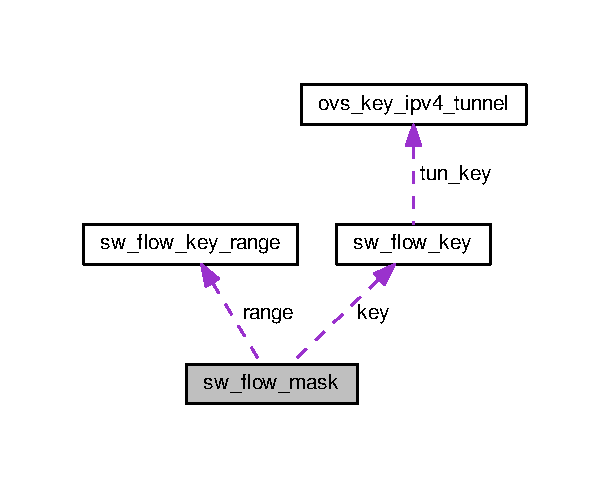
\includegraphics[width=293pt]{structsw__flow__mask__coll__graph}
\end{center}
\end{figure}
\subsection*{Data Fields}
\begin{DoxyCompactItemize}
\item 
int \hyperlink{structsw__flow__mask_ad1bf602183e4fa7dfeab96a7ca06243b}{ref\+\_\+count}
\item 
struct rcu\+\_\+head \hyperlink{structsw__flow__mask_aa5aebb526fafd5f7f70b605970a72fd8}{rcu}
\item 
struct \hyperlink{structsw__flow__key__range}{sw\+\_\+flow\+\_\+key\+\_\+range} \hyperlink{structsw__flow__mask_aa6062c0e580d516ff2d9ce8f9611432b}{range}
\item 
struct \hyperlink{structsw__flow__key}{sw\+\_\+flow\+\_\+key} \hyperlink{structsw__flow__mask_a52db0284fdd4579a5f30dee0837a7485}{key}
\end{DoxyCompactItemize}


\subsection{Field Documentation}
\hypertarget{structsw__flow__mask_a52db0284fdd4579a5f30dee0837a7485}{}\index{sw\+\_\+flow\+\_\+mask@{sw\+\_\+flow\+\_\+mask}!key@{key}}
\index{key@{key}!sw\+\_\+flow\+\_\+mask@{sw\+\_\+flow\+\_\+mask}}
\subsubsection[{key}]{\setlength{\rightskip}{0pt plus 5cm}struct {\bf sw\+\_\+flow\+\_\+key} sw\+\_\+flow\+\_\+mask\+::key}\label{structsw__flow__mask_a52db0284fdd4579a5f30dee0837a7485}
\hypertarget{structsw__flow__mask_aa6062c0e580d516ff2d9ce8f9611432b}{}\index{sw\+\_\+flow\+\_\+mask@{sw\+\_\+flow\+\_\+mask}!range@{range}}
\index{range@{range}!sw\+\_\+flow\+\_\+mask@{sw\+\_\+flow\+\_\+mask}}
\subsubsection[{range}]{\setlength{\rightskip}{0pt plus 5cm}struct {\bf sw\+\_\+flow\+\_\+key\+\_\+range} sw\+\_\+flow\+\_\+mask\+::range}\label{structsw__flow__mask_aa6062c0e580d516ff2d9ce8f9611432b}
\hypertarget{structsw__flow__mask_aa5aebb526fafd5f7f70b605970a72fd8}{}\index{sw\+\_\+flow\+\_\+mask@{sw\+\_\+flow\+\_\+mask}!rcu@{rcu}}
\index{rcu@{rcu}!sw\+\_\+flow\+\_\+mask@{sw\+\_\+flow\+\_\+mask}}
\subsubsection[{rcu}]{\setlength{\rightskip}{0pt plus 5cm}struct rcu\+\_\+head sw\+\_\+flow\+\_\+mask\+::rcu}\label{structsw__flow__mask_aa5aebb526fafd5f7f70b605970a72fd8}
\hypertarget{structsw__flow__mask_ad1bf602183e4fa7dfeab96a7ca06243b}{}\index{sw\+\_\+flow\+\_\+mask@{sw\+\_\+flow\+\_\+mask}!ref\+\_\+count@{ref\+\_\+count}}
\index{ref\+\_\+count@{ref\+\_\+count}!sw\+\_\+flow\+\_\+mask@{sw\+\_\+flow\+\_\+mask}}
\subsubsection[{ref\+\_\+count}]{\setlength{\rightskip}{0pt plus 5cm}int sw\+\_\+flow\+\_\+mask\+::ref\+\_\+count}\label{structsw__flow__mask_ad1bf602183e4fa7dfeab96a7ca06243b}


The documentation for this struct was generated from the following file\+:\begin{DoxyCompactItemize}
\item 
/home/vladn/git/ovs/datapath/\hyperlink{flow_8h}{flow.\+h}\end{DoxyCompactItemize}

\hypertarget{structsw__flow__match}{}\section{sw\+\_\+flow\+\_\+match Struct Reference}
\label{structsw__flow__match}\index{sw\+\_\+flow\+\_\+match@{sw\+\_\+flow\+\_\+match}}


{\ttfamily \#include $<$flow.\+h$>$}



Collaboration diagram for sw\+\_\+flow\+\_\+match\+:
\nopagebreak
\begin{figure}[H]
\begin{center}
\leavevmode
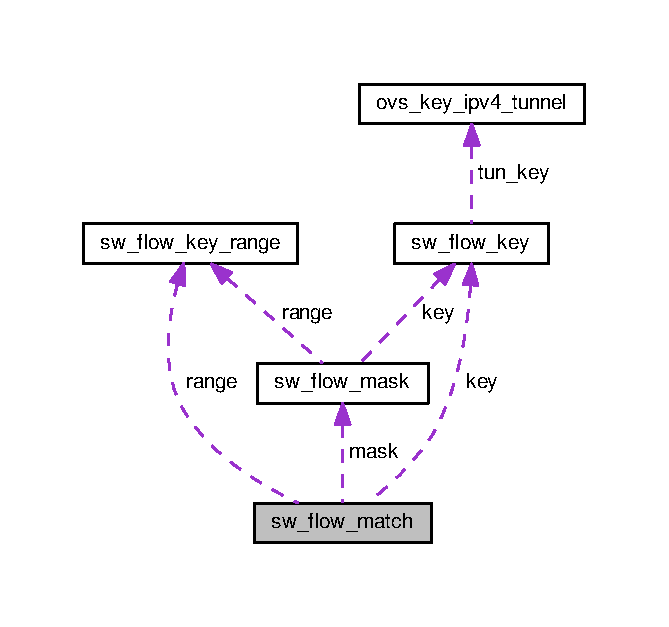
\includegraphics[width=321pt]{structsw__flow__match__coll__graph}
\end{center}
\end{figure}
\subsection*{Data Fields}
\begin{DoxyCompactItemize}
\item 
struct \hyperlink{structsw__flow__key}{sw\+\_\+flow\+\_\+key} $\ast$ \hyperlink{structsw__flow__match_a4030aac38105b63798ea11f43f506372}{key}
\item 
struct \hyperlink{structsw__flow__key__range}{sw\+\_\+flow\+\_\+key\+\_\+range} \hyperlink{structsw__flow__match_aed5e18f9a96464cce4b4e4443d550b2d}{range}
\item 
struct \hyperlink{structsw__flow__mask}{sw\+\_\+flow\+\_\+mask} $\ast$ \hyperlink{structsw__flow__match_a4536aff731528d6def7d386435c203d1}{mask}
\end{DoxyCompactItemize}


\subsection{Field Documentation}
\hypertarget{structsw__flow__match_a4030aac38105b63798ea11f43f506372}{}\index{sw\+\_\+flow\+\_\+match@{sw\+\_\+flow\+\_\+match}!key@{key}}
\index{key@{key}!sw\+\_\+flow\+\_\+match@{sw\+\_\+flow\+\_\+match}}
\subsubsection[{key}]{\setlength{\rightskip}{0pt plus 5cm}struct {\bf sw\+\_\+flow\+\_\+key}$\ast$ sw\+\_\+flow\+\_\+match\+::key}\label{structsw__flow__match_a4030aac38105b63798ea11f43f506372}
\hypertarget{structsw__flow__match_a4536aff731528d6def7d386435c203d1}{}\index{sw\+\_\+flow\+\_\+match@{sw\+\_\+flow\+\_\+match}!mask@{mask}}
\index{mask@{mask}!sw\+\_\+flow\+\_\+match@{sw\+\_\+flow\+\_\+match}}
\subsubsection[{mask}]{\setlength{\rightskip}{0pt plus 5cm}struct {\bf sw\+\_\+flow\+\_\+mask}$\ast$ sw\+\_\+flow\+\_\+match\+::mask}\label{structsw__flow__match_a4536aff731528d6def7d386435c203d1}
\hypertarget{structsw__flow__match_aed5e18f9a96464cce4b4e4443d550b2d}{}\index{sw\+\_\+flow\+\_\+match@{sw\+\_\+flow\+\_\+match}!range@{range}}
\index{range@{range}!sw\+\_\+flow\+\_\+match@{sw\+\_\+flow\+\_\+match}}
\subsubsection[{range}]{\setlength{\rightskip}{0pt plus 5cm}struct {\bf sw\+\_\+flow\+\_\+key\+\_\+range} sw\+\_\+flow\+\_\+match\+::range}\label{structsw__flow__match_aed5e18f9a96464cce4b4e4443d550b2d}


The documentation for this struct was generated from the following file\+:\begin{DoxyCompactItemize}
\item 
/home/vladn/git/ovs/datapath/\hyperlink{flow_8h}{flow.\+h}\end{DoxyCompactItemize}

\hypertarget{structtable__instance}{}\section{table\+\_\+instance Struct Reference}
\label{structtable__instance}\index{table\+\_\+instance@{table\+\_\+instance}}


{\ttfamily \#include $<$flow\+\_\+table.\+h$>$}

\subsection*{Data Fields}
\begin{DoxyCompactItemize}
\item 
struct flex\+\_\+array $\ast$ \hyperlink{structtable__instance_a6522309983b8c287da819f666da07355}{buckets}
\item 
unsigned int \hyperlink{structtable__instance_ae4f915a0e1b19ca677ae00c7eb5a3cb9}{n\+\_\+buckets}
\item 
struct rcu\+\_\+head \hyperlink{structtable__instance_acf4d72ccfb947d0d0d08732a56664978}{rcu}
\item 
int \hyperlink{structtable__instance_ab992e9218f85e3b5193ae47e8fbf3f32}{node\+\_\+ver}
\item 
u32 \hyperlink{structtable__instance_ad73f318c365fd86dda23e7ffb65d59b9}{hash\+\_\+seed}
\item 
\hyperlink{types_8h_afaa87723b8417d40fcf45b7330261ef9}{bool} \hyperlink{structtable__instance_af7a3a9cce56cbf7ed225ac0ec3ce9eb2}{keep\+\_\+flows}
\end{DoxyCompactItemize}


\subsection{Field Documentation}
\hypertarget{structtable__instance_a6522309983b8c287da819f666da07355}{}\index{table\+\_\+instance@{table\+\_\+instance}!buckets@{buckets}}
\index{buckets@{buckets}!table\+\_\+instance@{table\+\_\+instance}}
\subsubsection[{buckets}]{\setlength{\rightskip}{0pt plus 5cm}struct flex\+\_\+array$\ast$ table\+\_\+instance\+::buckets}\label{structtable__instance_a6522309983b8c287da819f666da07355}
\hypertarget{structtable__instance_ad73f318c365fd86dda23e7ffb65d59b9}{}\index{table\+\_\+instance@{table\+\_\+instance}!hash\+\_\+seed@{hash\+\_\+seed}}
\index{hash\+\_\+seed@{hash\+\_\+seed}!table\+\_\+instance@{table\+\_\+instance}}
\subsubsection[{hash\+\_\+seed}]{\setlength{\rightskip}{0pt plus 5cm}u32 table\+\_\+instance\+::hash\+\_\+seed}\label{structtable__instance_ad73f318c365fd86dda23e7ffb65d59b9}
\hypertarget{structtable__instance_af7a3a9cce56cbf7ed225ac0ec3ce9eb2}{}\index{table\+\_\+instance@{table\+\_\+instance}!keep\+\_\+flows@{keep\+\_\+flows}}
\index{keep\+\_\+flows@{keep\+\_\+flows}!table\+\_\+instance@{table\+\_\+instance}}
\subsubsection[{keep\+\_\+flows}]{\setlength{\rightskip}{0pt plus 5cm}{\bf bool} table\+\_\+instance\+::keep\+\_\+flows}\label{structtable__instance_af7a3a9cce56cbf7ed225ac0ec3ce9eb2}
\hypertarget{structtable__instance_ae4f915a0e1b19ca677ae00c7eb5a3cb9}{}\index{table\+\_\+instance@{table\+\_\+instance}!n\+\_\+buckets@{n\+\_\+buckets}}
\index{n\+\_\+buckets@{n\+\_\+buckets}!table\+\_\+instance@{table\+\_\+instance}}
\subsubsection[{n\+\_\+buckets}]{\setlength{\rightskip}{0pt plus 5cm}unsigned int table\+\_\+instance\+::n\+\_\+buckets}\label{structtable__instance_ae4f915a0e1b19ca677ae00c7eb5a3cb9}
\hypertarget{structtable__instance_ab992e9218f85e3b5193ae47e8fbf3f32}{}\index{table\+\_\+instance@{table\+\_\+instance}!node\+\_\+ver@{node\+\_\+ver}}
\index{node\+\_\+ver@{node\+\_\+ver}!table\+\_\+instance@{table\+\_\+instance}}
\subsubsection[{node\+\_\+ver}]{\setlength{\rightskip}{0pt plus 5cm}int table\+\_\+instance\+::node\+\_\+ver}\label{structtable__instance_ab992e9218f85e3b5193ae47e8fbf3f32}
\hypertarget{structtable__instance_acf4d72ccfb947d0d0d08732a56664978}{}\index{table\+\_\+instance@{table\+\_\+instance}!rcu@{rcu}}
\index{rcu@{rcu}!table\+\_\+instance@{table\+\_\+instance}}
\subsubsection[{rcu}]{\setlength{\rightskip}{0pt plus 5cm}struct rcu\+\_\+head table\+\_\+instance\+::rcu}\label{structtable__instance_acf4d72ccfb947d0d0d08732a56664978}


The documentation for this struct was generated from the following file\+:\begin{DoxyCompactItemize}
\item 
/home/vladn/git/ovs/datapath/\hyperlink{flow__table_8h}{flow\+\_\+table.\+h}\end{DoxyCompactItemize}

\hypertarget{structtnl__ptk__info}{}\section{tnl\+\_\+ptk\+\_\+info Struct Reference}
\label{structtnl__ptk__info}\index{tnl\+\_\+ptk\+\_\+info@{tnl\+\_\+ptk\+\_\+info}}


{\ttfamily \#include $<$ip\+\_\+tunnels.\+h$>$}

\subsection*{Data Fields}
\begin{DoxyCompactItemize}
\item 
\+\_\+\+\_\+be16 \hyperlink{structtnl__ptk__info_ace5a0170111f2d302e1cc4ed93d6ecad}{flags}
\item 
\+\_\+\+\_\+be16 \hyperlink{structtnl__ptk__info_ac4f408097c387edf64653942d355985f}{proto}
\item 
\+\_\+\+\_\+be32 \hyperlink{structtnl__ptk__info_a6c32868baa4f56abb6c81edde446a567}{key}
\item 
\+\_\+\+\_\+be32 \hyperlink{structtnl__ptk__info_ac8158dad50d130f9292c406776cce767}{seq}
\end{DoxyCompactItemize}


\subsection{Field Documentation}
\hypertarget{structtnl__ptk__info_ace5a0170111f2d302e1cc4ed93d6ecad}{}\index{tnl\+\_\+ptk\+\_\+info@{tnl\+\_\+ptk\+\_\+info}!flags@{flags}}
\index{flags@{flags}!tnl\+\_\+ptk\+\_\+info@{tnl\+\_\+ptk\+\_\+info}}
\subsubsection[{flags}]{\setlength{\rightskip}{0pt plus 5cm}\+\_\+\+\_\+be16 tnl\+\_\+ptk\+\_\+info\+::flags}\label{structtnl__ptk__info_ace5a0170111f2d302e1cc4ed93d6ecad}
\hypertarget{structtnl__ptk__info_a6c32868baa4f56abb6c81edde446a567}{}\index{tnl\+\_\+ptk\+\_\+info@{tnl\+\_\+ptk\+\_\+info}!key@{key}}
\index{key@{key}!tnl\+\_\+ptk\+\_\+info@{tnl\+\_\+ptk\+\_\+info}}
\subsubsection[{key}]{\setlength{\rightskip}{0pt plus 5cm}\+\_\+\+\_\+be32 tnl\+\_\+ptk\+\_\+info\+::key}\label{structtnl__ptk__info_a6c32868baa4f56abb6c81edde446a567}
\hypertarget{structtnl__ptk__info_ac4f408097c387edf64653942d355985f}{}\index{tnl\+\_\+ptk\+\_\+info@{tnl\+\_\+ptk\+\_\+info}!proto@{proto}}
\index{proto@{proto}!tnl\+\_\+ptk\+\_\+info@{tnl\+\_\+ptk\+\_\+info}}
\subsubsection[{proto}]{\setlength{\rightskip}{0pt plus 5cm}\+\_\+\+\_\+be16 tnl\+\_\+ptk\+\_\+info\+::proto}\label{structtnl__ptk__info_ac4f408097c387edf64653942d355985f}
\hypertarget{structtnl__ptk__info_ac8158dad50d130f9292c406776cce767}{}\index{tnl\+\_\+ptk\+\_\+info@{tnl\+\_\+ptk\+\_\+info}!seq@{seq}}
\index{seq@{seq}!tnl\+\_\+ptk\+\_\+info@{tnl\+\_\+ptk\+\_\+info}}
\subsubsection[{seq}]{\setlength{\rightskip}{0pt plus 5cm}\+\_\+\+\_\+be32 tnl\+\_\+ptk\+\_\+info\+::seq}\label{structtnl__ptk__info_ac8158dad50d130f9292c406776cce767}


The documentation for this struct was generated from the following file\+:\begin{DoxyCompactItemize}
\item 
/home/vladn/git/ovs/datapath/linux/compat/include/net/\hyperlink{ip__tunnels_8h}{ip\+\_\+tunnels.\+h}\end{DoxyCompactItemize}

\hypertarget{structu64__stats__sync}{}\section{u64\+\_\+stats\+\_\+sync Struct Reference}
\label{structu64__stats__sync}\index{u64\+\_\+stats\+\_\+sync@{u64\+\_\+stats\+\_\+sync}}


{\ttfamily \#include $<$u64\+\_\+stats\+\_\+sync.\+h$>$}



The documentation for this struct was generated from the following file\+:\begin{DoxyCompactItemize}
\item 
/home/vladn/git/ovs/datapath/linux/compat/include/linux/\hyperlink{u64__stats__sync_8h}{u64\+\_\+stats\+\_\+sync.\+h}\end{DoxyCompactItemize}

\hypertarget{structvport}{}\section{vport Struct Reference}
\label{structvport}\index{vport@{vport}}


{\ttfamily \#include $<$vport.\+h$>$}



Collaboration diagram for vport\+:
\nopagebreak
\begin{figure}[H]
\begin{center}
\leavevmode
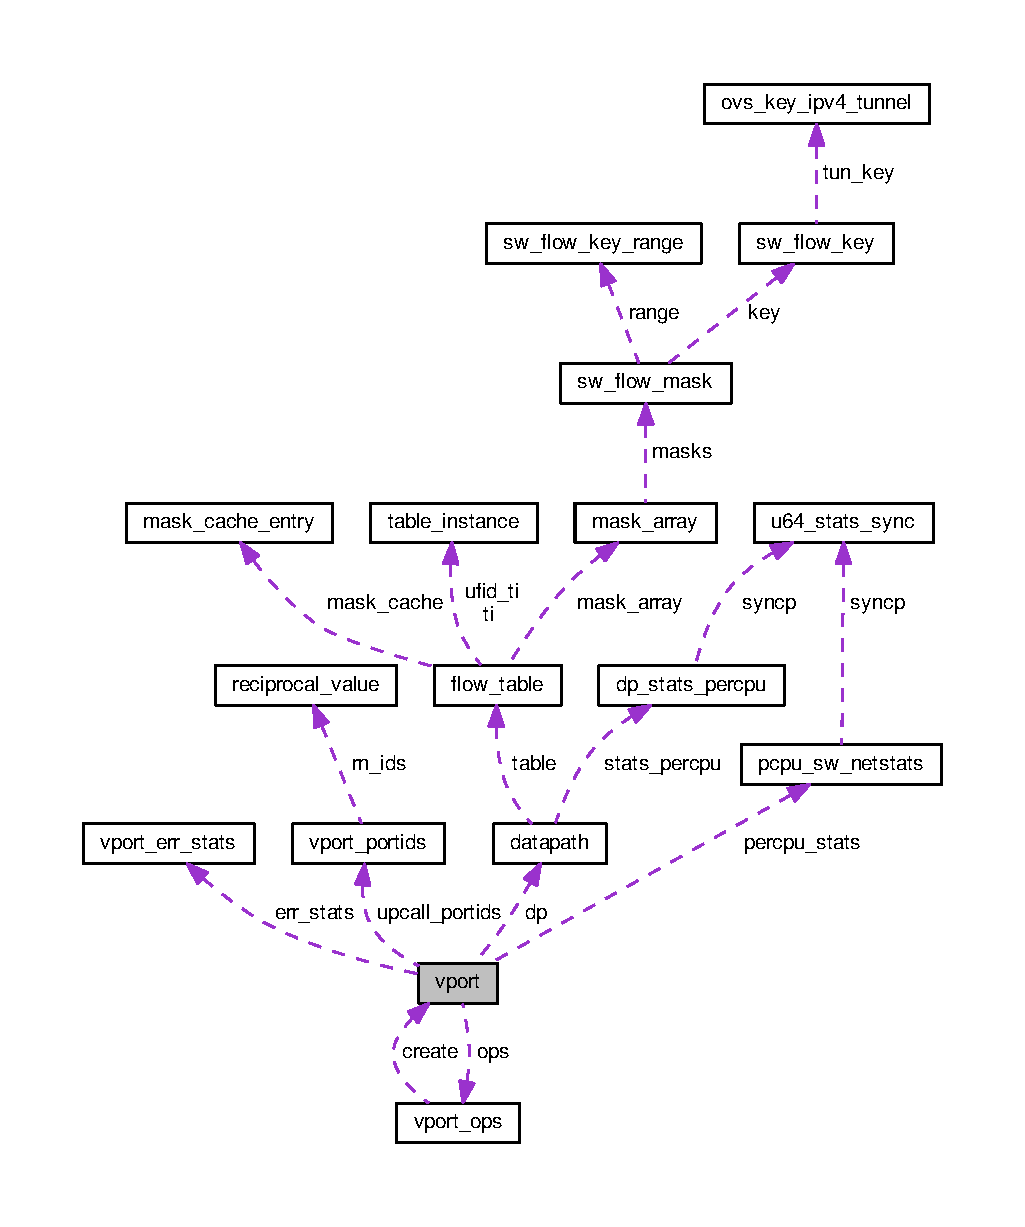
\includegraphics[width=350pt]{structvport__coll__graph}
\end{center}
\end{figure}
\subsection*{Data Fields}
\begin{DoxyCompactItemize}
\item 
struct rcu\+\_\+head \hyperlink{structvport_ac08b8a62e054bc2840a9ba6964091f89}{rcu}
\item 
struct \hyperlink{structdatapath}{datapath} $\ast$ \hyperlink{structvport_a49fb6f6bf0ac4337853e9242e88ddc42}{dp}
\item 
struct \hyperlink{structvport__portids}{vport\+\_\+portids} \hyperlink{compiler_8h_a2b3b0c016258969e4b39c66b6eec2129}{\+\_\+\+\_\+rcu} $\ast$ \hyperlink{structvport_a7963679d5c8d3a923eb42faf9d5fb2d1}{upcall\+\_\+portids}
\item 
u16 \hyperlink{structvport_aae00fc5d12b47f02cbfd4f67ae114b58}{port\+\_\+no}
\item 
struct hlist\+\_\+node \hyperlink{structvport_ae6324a0c2483c3d1600cb29a6f4bcb8d}{hash\+\_\+node}
\item 
struct hlist\+\_\+node \hyperlink{structvport_a27d2c94e2edd5de172e0b866cdd70fea}{dp\+\_\+hash\+\_\+node}
\item 
const struct \hyperlink{structvport__ops}{vport\+\_\+ops} $\ast$ \hyperlink{structvport_a5af933fc664c1194ac3bbc337da35586}{ops}
\item 
struct \hyperlink{structpcpu__sw__netstats}{pcpu\+\_\+sw\+\_\+netstats} \hyperlink{compiler_8h_a497f20279760cdb59a5187689f9f5ab1}{\+\_\+\+\_\+percpu} $\ast$ \hyperlink{structvport_a04983f0d17ae4deb6ffb87333f6d4f05}{percpu\+\_\+stats}
\item 
struct \hyperlink{structvport__err__stats}{vport\+\_\+err\+\_\+stats} \hyperlink{structvport_a5cd8a50cb02833a868db549d64052c99}{err\+\_\+stats}
\item 
struct list\+\_\+head \hyperlink{structvport_ae41f659d10b0f1c27324e9406d5c2ef1}{detach\+\_\+list}
\end{DoxyCompactItemize}


\subsection{Detailed Description}
struct vport -\/ one port within a datapath \+: R\+C\+U callback head for deferred destruction. \+: Datapath to which this port belongs. \+: R\+C\+U protected \textquotesingle{}struct \hyperlink{structvport__portids}{vport\+\_\+portids}\textquotesingle{}. \+: Index into \textquotesingle{}s  array. \+: Element in  hash table in vport.\+c. \+: Element in -\/$>$ports hash table in datapath.\+c. \+: Class structure. \+: Points to per-\/\+C\+P\+U statistics used and maintained by vport \+: Points to error statistics used and maintained by vport \+: list used for detaching vport in net-\/exit call. 

\subsection{Field Documentation}
\hypertarget{structvport_ae41f659d10b0f1c27324e9406d5c2ef1}{}\index{vport@{vport}!detach\+\_\+list@{detach\+\_\+list}}
\index{detach\+\_\+list@{detach\+\_\+list}!vport@{vport}}
\subsubsection[{detach\+\_\+list}]{\setlength{\rightskip}{0pt plus 5cm}struct list\+\_\+head vport\+::detach\+\_\+list}\label{structvport_ae41f659d10b0f1c27324e9406d5c2ef1}
\hypertarget{structvport_a49fb6f6bf0ac4337853e9242e88ddc42}{}\index{vport@{vport}!dp@{dp}}
\index{dp@{dp}!vport@{vport}}
\subsubsection[{dp}]{\setlength{\rightskip}{0pt plus 5cm}struct {\bf datapath}$\ast$ vport\+::dp}\label{structvport_a49fb6f6bf0ac4337853e9242e88ddc42}
\hypertarget{structvport_a27d2c94e2edd5de172e0b866cdd70fea}{}\index{vport@{vport}!dp\+\_\+hash\+\_\+node@{dp\+\_\+hash\+\_\+node}}
\index{dp\+\_\+hash\+\_\+node@{dp\+\_\+hash\+\_\+node}!vport@{vport}}
\subsubsection[{dp\+\_\+hash\+\_\+node}]{\setlength{\rightskip}{0pt plus 5cm}struct hlist\+\_\+node vport\+::dp\+\_\+hash\+\_\+node}\label{structvport_a27d2c94e2edd5de172e0b866cdd70fea}
\hypertarget{structvport_a5cd8a50cb02833a868db549d64052c99}{}\index{vport@{vport}!err\+\_\+stats@{err\+\_\+stats}}
\index{err\+\_\+stats@{err\+\_\+stats}!vport@{vport}}
\subsubsection[{err\+\_\+stats}]{\setlength{\rightskip}{0pt plus 5cm}struct {\bf vport\+\_\+err\+\_\+stats} vport\+::err\+\_\+stats}\label{structvport_a5cd8a50cb02833a868db549d64052c99}
\hypertarget{structvport_ae6324a0c2483c3d1600cb29a6f4bcb8d}{}\index{vport@{vport}!hash\+\_\+node@{hash\+\_\+node}}
\index{hash\+\_\+node@{hash\+\_\+node}!vport@{vport}}
\subsubsection[{hash\+\_\+node}]{\setlength{\rightskip}{0pt plus 5cm}struct hlist\+\_\+node vport\+::hash\+\_\+node}\label{structvport_ae6324a0c2483c3d1600cb29a6f4bcb8d}
\hypertarget{structvport_a5af933fc664c1194ac3bbc337da35586}{}\index{vport@{vport}!ops@{ops}}
\index{ops@{ops}!vport@{vport}}
\subsubsection[{ops}]{\setlength{\rightskip}{0pt plus 5cm}const struct {\bf vport\+\_\+ops}$\ast$ vport\+::ops}\label{structvport_a5af933fc664c1194ac3bbc337da35586}
\hypertarget{structvport_a04983f0d17ae4deb6ffb87333f6d4f05}{}\index{vport@{vport}!percpu\+\_\+stats@{percpu\+\_\+stats}}
\index{percpu\+\_\+stats@{percpu\+\_\+stats}!vport@{vport}}
\subsubsection[{percpu\+\_\+stats}]{\setlength{\rightskip}{0pt plus 5cm}struct {\bf pcpu\+\_\+sw\+\_\+netstats} {\bf \+\_\+\+\_\+percpu}$\ast$ vport\+::percpu\+\_\+stats}\label{structvport_a04983f0d17ae4deb6ffb87333f6d4f05}
\hypertarget{structvport_aae00fc5d12b47f02cbfd4f67ae114b58}{}\index{vport@{vport}!port\+\_\+no@{port\+\_\+no}}
\index{port\+\_\+no@{port\+\_\+no}!vport@{vport}}
\subsubsection[{port\+\_\+no}]{\setlength{\rightskip}{0pt plus 5cm}u16 vport\+::port\+\_\+no}\label{structvport_aae00fc5d12b47f02cbfd4f67ae114b58}
\hypertarget{structvport_ac08b8a62e054bc2840a9ba6964091f89}{}\index{vport@{vport}!rcu@{rcu}}
\index{rcu@{rcu}!vport@{vport}}
\subsubsection[{rcu}]{\setlength{\rightskip}{0pt plus 5cm}struct rcu\+\_\+head vport\+::rcu}\label{structvport_ac08b8a62e054bc2840a9ba6964091f89}
\hypertarget{structvport_a7963679d5c8d3a923eb42faf9d5fb2d1}{}\index{vport@{vport}!upcall\+\_\+portids@{upcall\+\_\+portids}}
\index{upcall\+\_\+portids@{upcall\+\_\+portids}!vport@{vport}}
\subsubsection[{upcall\+\_\+portids}]{\setlength{\rightskip}{0pt plus 5cm}struct {\bf vport\+\_\+portids} {\bf \+\_\+\+\_\+rcu}$\ast$ vport\+::upcall\+\_\+portids}\label{structvport_a7963679d5c8d3a923eb42faf9d5fb2d1}


The documentation for this struct was generated from the following file\+:\begin{DoxyCompactItemize}
\item 
/home/vladn/git/ovs/datapath/\hyperlink{vport_8h}{vport.\+h}\end{DoxyCompactItemize}

\hypertarget{structvport__err__stats}{}\section{vport\+\_\+err\+\_\+stats Struct Reference}
\label{structvport__err__stats}\index{vport\+\_\+err\+\_\+stats@{vport\+\_\+err\+\_\+stats}}


{\ttfamily \#include $<$vport.\+h$>$}

\subsection*{Data Fields}
\begin{DoxyCompactItemize}
\item 
atomic\+\_\+long\+\_\+t \hyperlink{structvport__err__stats_a38849ae05107fbf9e9824149b60bd91f}{rx\+\_\+dropped}
\item 
atomic\+\_\+long\+\_\+t \hyperlink{structvport__err__stats_ad253987f143edfffea6546baa0e990f6}{rx\+\_\+errors}
\item 
atomic\+\_\+long\+\_\+t \hyperlink{structvport__err__stats_a299aaacfac0fe9d48ddd000674b7816a}{tx\+\_\+dropped}
\item 
atomic\+\_\+long\+\_\+t \hyperlink{structvport__err__stats_a24478cbc4a61b5454a4247830bf2c7b4}{tx\+\_\+errors}
\end{DoxyCompactItemize}


\subsection{Field Documentation}
\hypertarget{structvport__err__stats_a38849ae05107fbf9e9824149b60bd91f}{}\index{vport\+\_\+err\+\_\+stats@{vport\+\_\+err\+\_\+stats}!rx\+\_\+dropped@{rx\+\_\+dropped}}
\index{rx\+\_\+dropped@{rx\+\_\+dropped}!vport\+\_\+err\+\_\+stats@{vport\+\_\+err\+\_\+stats}}
\subsubsection[{rx\+\_\+dropped}]{\setlength{\rightskip}{0pt plus 5cm}atomic\+\_\+long\+\_\+t vport\+\_\+err\+\_\+stats\+::rx\+\_\+dropped}\label{structvport__err__stats_a38849ae05107fbf9e9824149b60bd91f}
\hypertarget{structvport__err__stats_ad253987f143edfffea6546baa0e990f6}{}\index{vport\+\_\+err\+\_\+stats@{vport\+\_\+err\+\_\+stats}!rx\+\_\+errors@{rx\+\_\+errors}}
\index{rx\+\_\+errors@{rx\+\_\+errors}!vport\+\_\+err\+\_\+stats@{vport\+\_\+err\+\_\+stats}}
\subsubsection[{rx\+\_\+errors}]{\setlength{\rightskip}{0pt plus 5cm}atomic\+\_\+long\+\_\+t vport\+\_\+err\+\_\+stats\+::rx\+\_\+errors}\label{structvport__err__stats_ad253987f143edfffea6546baa0e990f6}
\hypertarget{structvport__err__stats_a299aaacfac0fe9d48ddd000674b7816a}{}\index{vport\+\_\+err\+\_\+stats@{vport\+\_\+err\+\_\+stats}!tx\+\_\+dropped@{tx\+\_\+dropped}}
\index{tx\+\_\+dropped@{tx\+\_\+dropped}!vport\+\_\+err\+\_\+stats@{vport\+\_\+err\+\_\+stats}}
\subsubsection[{tx\+\_\+dropped}]{\setlength{\rightskip}{0pt plus 5cm}atomic\+\_\+long\+\_\+t vport\+\_\+err\+\_\+stats\+::tx\+\_\+dropped}\label{structvport__err__stats_a299aaacfac0fe9d48ddd000674b7816a}
\hypertarget{structvport__err__stats_a24478cbc4a61b5454a4247830bf2c7b4}{}\index{vport\+\_\+err\+\_\+stats@{vport\+\_\+err\+\_\+stats}!tx\+\_\+errors@{tx\+\_\+errors}}
\index{tx\+\_\+errors@{tx\+\_\+errors}!vport\+\_\+err\+\_\+stats@{vport\+\_\+err\+\_\+stats}}
\subsubsection[{tx\+\_\+errors}]{\setlength{\rightskip}{0pt plus 5cm}atomic\+\_\+long\+\_\+t vport\+\_\+err\+\_\+stats\+::tx\+\_\+errors}\label{structvport__err__stats_a24478cbc4a61b5454a4247830bf2c7b4}


The documentation for this struct was generated from the following file\+:\begin{DoxyCompactItemize}
\item 
/home/vladn/git/ovs/datapath/\hyperlink{vport_8h}{vport.\+h}\end{DoxyCompactItemize}

\hypertarget{structvport__net}{}\section{vport\+\_\+net Struct Reference}
\label{structvport__net}\index{vport\+\_\+net@{vport\+\_\+net}}


{\ttfamily \#include $<$vport.\+h$>$}



Collaboration diagram for vport\+\_\+net\+:
\nopagebreak
\begin{figure}[H]
\begin{center}
\leavevmode
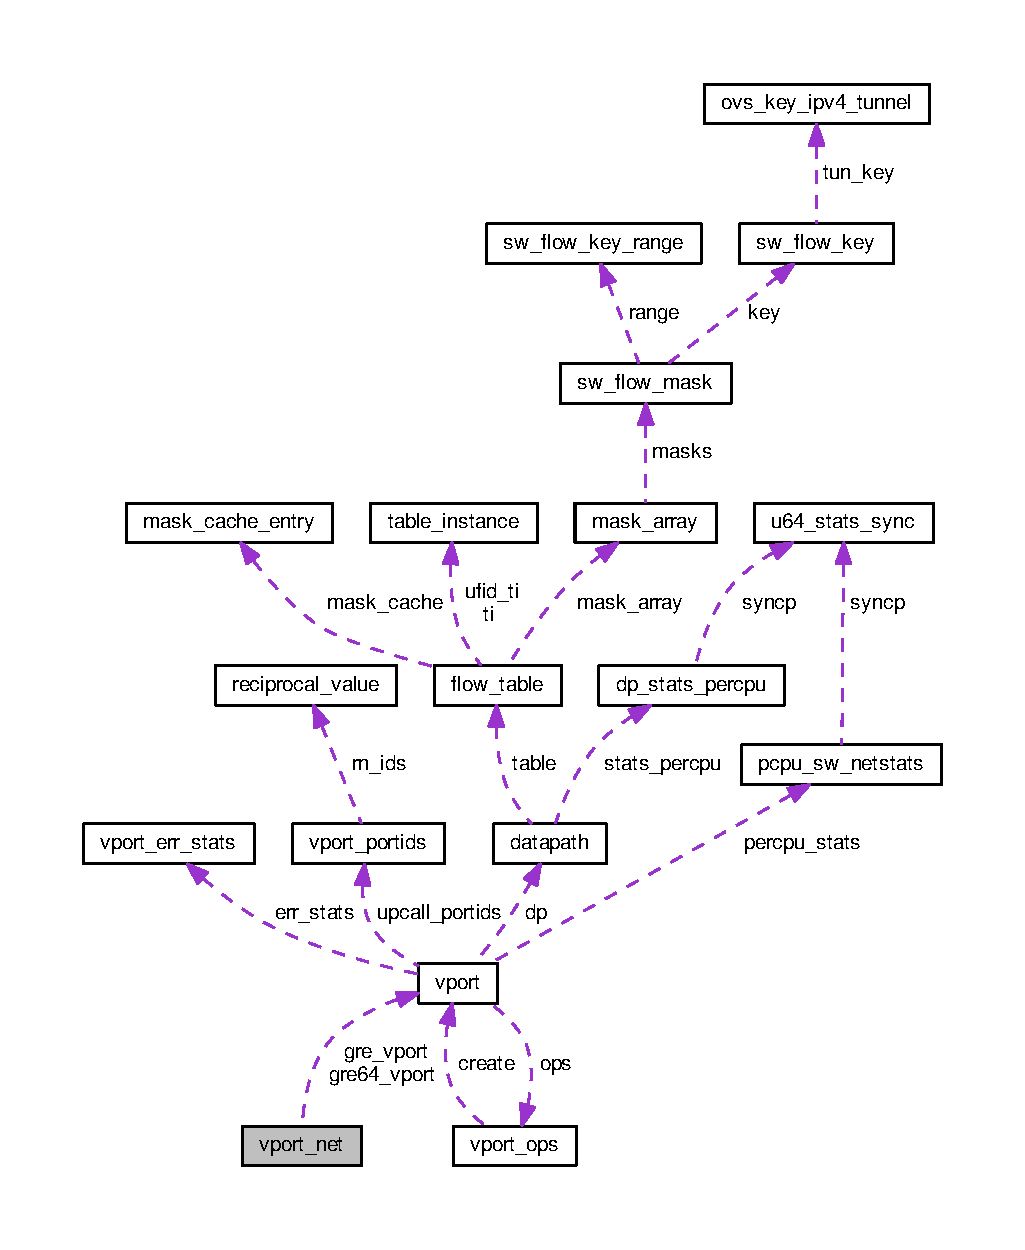
\includegraphics[width=350pt]{structvport__net__coll__graph}
\end{center}
\end{figure}
\subsection*{Data Fields}
\begin{DoxyCompactItemize}
\item 
struct \hyperlink{structvport}{vport} \hyperlink{compiler_8h_a2b3b0c016258969e4b39c66b6eec2129}{\+\_\+\+\_\+rcu} $\ast$ \hyperlink{structvport__net_a25768f1cf01f5e719b93818fddc5c528}{gre\+\_\+vport}
\item 
struct \hyperlink{structvport}{vport} \hyperlink{compiler_8h_a2b3b0c016258969e4b39c66b6eec2129}{\+\_\+\+\_\+rcu} $\ast$ \hyperlink{structvport__net_ac907ad528610a5eb24f9889a51d23265}{gre64\+\_\+vport}
\end{DoxyCompactItemize}


\subsection{Field Documentation}
\hypertarget{structvport__net_ac907ad528610a5eb24f9889a51d23265}{}\index{vport\+\_\+net@{vport\+\_\+net}!gre64\+\_\+vport@{gre64\+\_\+vport}}
\index{gre64\+\_\+vport@{gre64\+\_\+vport}!vport\+\_\+net@{vport\+\_\+net}}
\subsubsection[{gre64\+\_\+vport}]{\setlength{\rightskip}{0pt plus 5cm}struct {\bf vport} {\bf \+\_\+\+\_\+rcu}$\ast$ vport\+\_\+net\+::gre64\+\_\+vport}\label{structvport__net_ac907ad528610a5eb24f9889a51d23265}
\hypertarget{structvport__net_a25768f1cf01f5e719b93818fddc5c528}{}\index{vport\+\_\+net@{vport\+\_\+net}!gre\+\_\+vport@{gre\+\_\+vport}}
\index{gre\+\_\+vport@{gre\+\_\+vport}!vport\+\_\+net@{vport\+\_\+net}}
\subsubsection[{gre\+\_\+vport}]{\setlength{\rightskip}{0pt plus 5cm}struct {\bf vport} {\bf \+\_\+\+\_\+rcu}$\ast$ vport\+\_\+net\+::gre\+\_\+vport}\label{structvport__net_a25768f1cf01f5e719b93818fddc5c528}


The documentation for this struct was generated from the following file\+:\begin{DoxyCompactItemize}
\item 
/home/vladn/git/ovs/datapath/\hyperlink{vport_8h}{vport.\+h}\end{DoxyCompactItemize}

\hypertarget{structvport__ops}{}\section{vport\+\_\+ops Struct Reference}
\label{structvport__ops}\index{vport\+\_\+ops@{vport\+\_\+ops}}


{\ttfamily \#include $<$vport.\+h$>$}



Collaboration diagram for vport\+\_\+ops\+:
\nopagebreak
\begin{figure}[H]
\begin{center}
\leavevmode
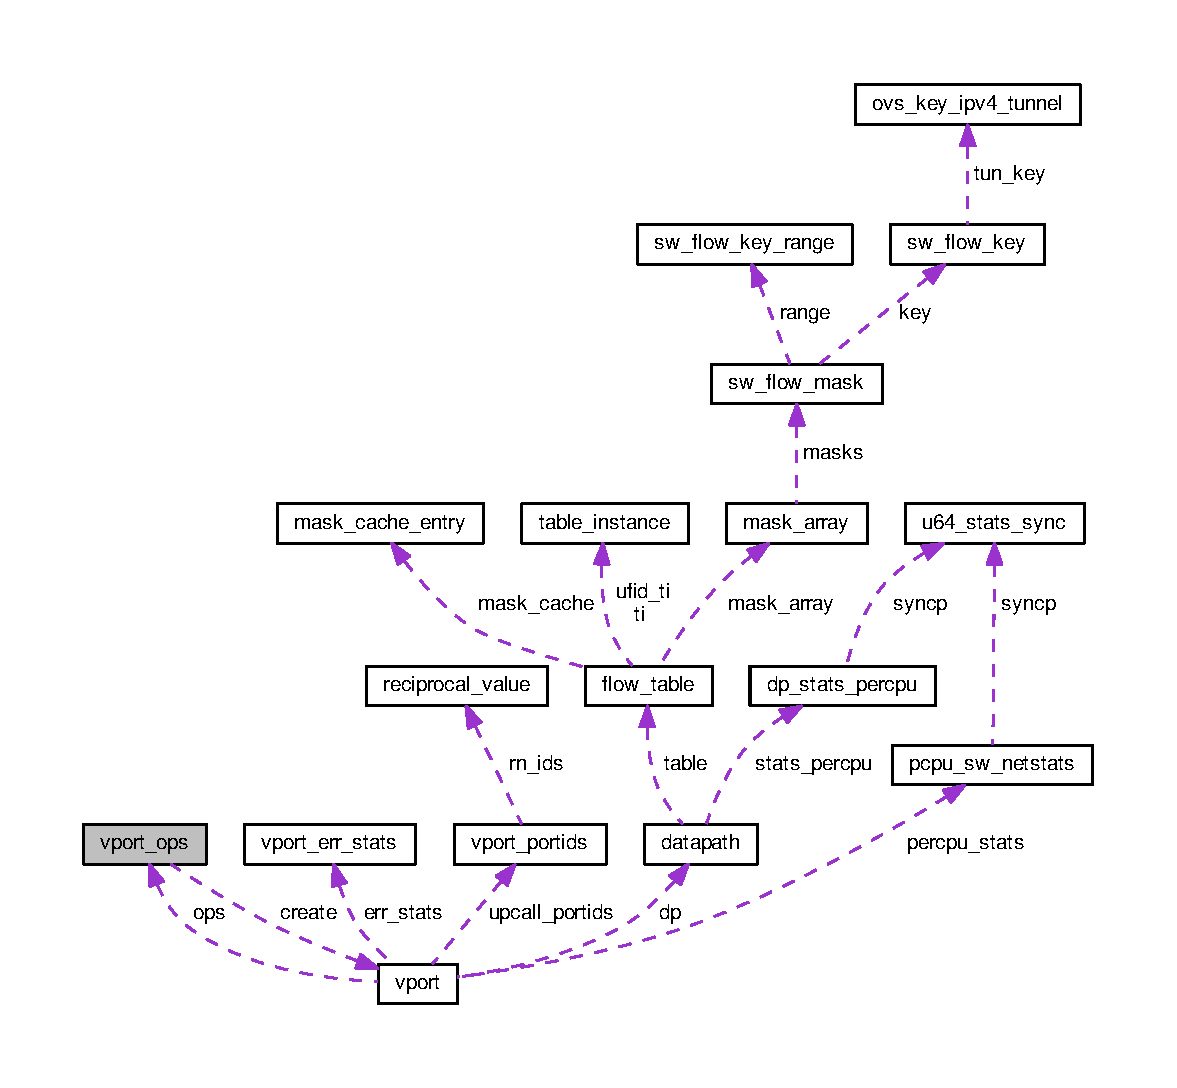
\includegraphics[width=350pt]{structvport__ops__coll__graph}
\end{center}
\end{figure}
\subsection*{Data Fields}
\begin{DoxyCompactItemize}
\item 
enum \hyperlink{openvswitch_8h_a9a1b861aa99bd83177a2b10b34745b0a}{ovs\+\_\+vport\+\_\+type} \hyperlink{structvport__ops_a7dd0d3776e78a2885063d3afd5e78148}{type}
\item 
struct \hyperlink{structvport}{vport} $\ast$($\ast$ \hyperlink{structvport__ops_acf3642d1a18755d25c37e9634c6945a2}{create} )(const struct \hyperlink{structvport__parms}{vport\+\_\+parms} $\ast$)
\item 
void($\ast$ \hyperlink{structvport__ops_a4fd321083545d82f308dc78331649632}{destroy} )(struct \hyperlink{structvport}{vport} $\ast$)
\item 
int($\ast$ \hyperlink{structvport__ops_a2a99b53de4cfaeaf8fb88d41660f5e73}{set\+\_\+options} )(struct \hyperlink{structvport}{vport} $\ast$, struct nlattr $\ast$)
\item 
int($\ast$ \hyperlink{structvport__ops_aacbd431343ae726a067b66b9b9de8ec4}{get\+\_\+options} )(const struct \hyperlink{structvport}{vport} $\ast$, struct sk\+\_\+buff $\ast$)
\item 
const char $\ast$($\ast$ \hyperlink{structvport__ops_abe0c3315271724bf05338487e0ced13c}{get\+\_\+name} )(const struct \hyperlink{structvport}{vport} $\ast$)
\item 
int($\ast$ \hyperlink{structvport__ops_a70034105b72fdde6d137bbc7e5d55a6a}{send} )(struct \hyperlink{structvport}{vport} $\ast$, struct sk\+\_\+buff $\ast$)
\item 
int($\ast$ \hyperlink{structvport__ops_a80a9e57f33d01dceca77f83fd3b88d23}{get\+\_\+egress\+\_\+tun\+\_\+info} )(struct \hyperlink{structvport}{vport} $\ast$, struct sk\+\_\+buff $\ast$, struct \hyperlink{structovs__tunnel__info}{ovs\+\_\+tunnel\+\_\+info} $\ast$)
\item 
struct module $\ast$ \hyperlink{structvport__ops_a74f3e852dbe8137d21e87895bd5f94e9}{owner}
\item 
struct list\+\_\+head \hyperlink{structvport__ops_aa0eadb49f41db4919e247ce17dd77aed}{list}
\end{DoxyCompactItemize}


\subsection{Detailed Description}
struct \hyperlink{structvport__ops}{vport\+\_\+ops} -\/ definition of a type of virtual port

\+: O\+V\+S\+\_\+\+V\+P\+O\+R\+T\+\_\+\+T\+Y\+P\+E\+\_\+$\ast$ value for this type of virtual port. \+: Create a new vport configured as specified. On success returns a new vport allocated with \hyperlink{linux_2vport_8c_a9198ee06111592d2cf6c3b2bf94561c1}{ovs\+\_\+vport\+\_\+alloc()}, otherwise an E\+R\+R\+\_\+\+P\+T\+R() value. \+: Destroys a vport. Must call vport\+\_\+free() on the vport but not before an R\+C\+U grace period has elapsed. \+: Modify the configuration of an existing vport. May be N\+U\+L\+L if modification is not supported. \+: Appends vport-\/specific attributes for the configuration of an existing vport to a \&struct sk\+\_\+buff. May be N\+U\+L\+L for a vport that does not have any configuration. \+: Get the device\textquotesingle{}s name. \+: Send a packet on the device. Returns the length of the packet sent, zero for dropped packets or negative for error. \+: Get the egress tunnel 5-\/tuple and other info for a packet. 

\subsection{Field Documentation}
\hypertarget{structvport__ops_acf3642d1a18755d25c37e9634c6945a2}{}\index{vport\+\_\+ops@{vport\+\_\+ops}!create@{create}}
\index{create@{create}!vport\+\_\+ops@{vport\+\_\+ops}}
\subsubsection[{create}]{\setlength{\rightskip}{0pt plus 5cm}struct {\bf vport}$\ast$($\ast$ vport\+\_\+ops\+::create) (const struct {\bf vport\+\_\+parms} $\ast$)}\label{structvport__ops_acf3642d1a18755d25c37e9634c6945a2}
\hypertarget{structvport__ops_a4fd321083545d82f308dc78331649632}{}\index{vport\+\_\+ops@{vport\+\_\+ops}!destroy@{destroy}}
\index{destroy@{destroy}!vport\+\_\+ops@{vport\+\_\+ops}}
\subsubsection[{destroy}]{\setlength{\rightskip}{0pt plus 5cm}void($\ast$ vport\+\_\+ops\+::destroy) (struct {\bf vport} $\ast$)}\label{structvport__ops_a4fd321083545d82f308dc78331649632}
\hypertarget{structvport__ops_a80a9e57f33d01dceca77f83fd3b88d23}{}\index{vport\+\_\+ops@{vport\+\_\+ops}!get\+\_\+egress\+\_\+tun\+\_\+info@{get\+\_\+egress\+\_\+tun\+\_\+info}}
\index{get\+\_\+egress\+\_\+tun\+\_\+info@{get\+\_\+egress\+\_\+tun\+\_\+info}!vport\+\_\+ops@{vport\+\_\+ops}}
\subsubsection[{get\+\_\+egress\+\_\+tun\+\_\+info}]{\setlength{\rightskip}{0pt plus 5cm}int($\ast$ vport\+\_\+ops\+::get\+\_\+egress\+\_\+tun\+\_\+info) (struct {\bf vport} $\ast$, struct sk\+\_\+buff $\ast$, struct {\bf ovs\+\_\+tunnel\+\_\+info} $\ast$)}\label{structvport__ops_a80a9e57f33d01dceca77f83fd3b88d23}
\hypertarget{structvport__ops_abe0c3315271724bf05338487e0ced13c}{}\index{vport\+\_\+ops@{vport\+\_\+ops}!get\+\_\+name@{get\+\_\+name}}
\index{get\+\_\+name@{get\+\_\+name}!vport\+\_\+ops@{vport\+\_\+ops}}
\subsubsection[{get\+\_\+name}]{\setlength{\rightskip}{0pt plus 5cm}const char$\ast$($\ast$ vport\+\_\+ops\+::get\+\_\+name) (const struct {\bf vport} $\ast$)}\label{structvport__ops_abe0c3315271724bf05338487e0ced13c}
\hypertarget{structvport__ops_aacbd431343ae726a067b66b9b9de8ec4}{}\index{vport\+\_\+ops@{vport\+\_\+ops}!get\+\_\+options@{get\+\_\+options}}
\index{get\+\_\+options@{get\+\_\+options}!vport\+\_\+ops@{vport\+\_\+ops}}
\subsubsection[{get\+\_\+options}]{\setlength{\rightskip}{0pt plus 5cm}int($\ast$ vport\+\_\+ops\+::get\+\_\+options) (const struct {\bf vport} $\ast$, struct sk\+\_\+buff $\ast$)}\label{structvport__ops_aacbd431343ae726a067b66b9b9de8ec4}
\hypertarget{structvport__ops_aa0eadb49f41db4919e247ce17dd77aed}{}\index{vport\+\_\+ops@{vport\+\_\+ops}!list@{list}}
\index{list@{list}!vport\+\_\+ops@{vport\+\_\+ops}}
\subsubsection[{list}]{\setlength{\rightskip}{0pt plus 5cm}struct list\+\_\+head vport\+\_\+ops\+::list}\label{structvport__ops_aa0eadb49f41db4919e247ce17dd77aed}
\hypertarget{structvport__ops_a74f3e852dbe8137d21e87895bd5f94e9}{}\index{vport\+\_\+ops@{vport\+\_\+ops}!owner@{owner}}
\index{owner@{owner}!vport\+\_\+ops@{vport\+\_\+ops}}
\subsubsection[{owner}]{\setlength{\rightskip}{0pt plus 5cm}struct module$\ast$ vport\+\_\+ops\+::owner}\label{structvport__ops_a74f3e852dbe8137d21e87895bd5f94e9}
\hypertarget{structvport__ops_a70034105b72fdde6d137bbc7e5d55a6a}{}\index{vport\+\_\+ops@{vport\+\_\+ops}!send@{send}}
\index{send@{send}!vport\+\_\+ops@{vport\+\_\+ops}}
\subsubsection[{send}]{\setlength{\rightskip}{0pt plus 5cm}int($\ast$ vport\+\_\+ops\+::send) (struct {\bf vport} $\ast$, struct sk\+\_\+buff $\ast$)}\label{structvport__ops_a70034105b72fdde6d137bbc7e5d55a6a}
\hypertarget{structvport__ops_a2a99b53de4cfaeaf8fb88d41660f5e73}{}\index{vport\+\_\+ops@{vport\+\_\+ops}!set\+\_\+options@{set\+\_\+options}}
\index{set\+\_\+options@{set\+\_\+options}!vport\+\_\+ops@{vport\+\_\+ops}}
\subsubsection[{set\+\_\+options}]{\setlength{\rightskip}{0pt plus 5cm}int($\ast$ vport\+\_\+ops\+::set\+\_\+options) (struct {\bf vport} $\ast$, struct nlattr $\ast$)}\label{structvport__ops_a2a99b53de4cfaeaf8fb88d41660f5e73}
\hypertarget{structvport__ops_a7dd0d3776e78a2885063d3afd5e78148}{}\index{vport\+\_\+ops@{vport\+\_\+ops}!type@{type}}
\index{type@{type}!vport\+\_\+ops@{vport\+\_\+ops}}
\subsubsection[{type}]{\setlength{\rightskip}{0pt plus 5cm}enum {\bf ovs\+\_\+vport\+\_\+type} vport\+\_\+ops\+::type}\label{structvport__ops_a7dd0d3776e78a2885063d3afd5e78148}


The documentation for this struct was generated from the following file\+:\begin{DoxyCompactItemize}
\item 
/home/vladn/git/ovs/datapath/\hyperlink{vport_8h}{vport.\+h}\end{DoxyCompactItemize}

\hypertarget{structvport__parms}{}\section{vport\+\_\+parms Struct Reference}
\label{structvport__parms}\index{vport\+\_\+parms@{vport\+\_\+parms}}


{\ttfamily \#include $<$vport.\+h$>$}



Collaboration diagram for vport\+\_\+parms\+:
\nopagebreak
\begin{figure}[H]
\begin{center}
\leavevmode
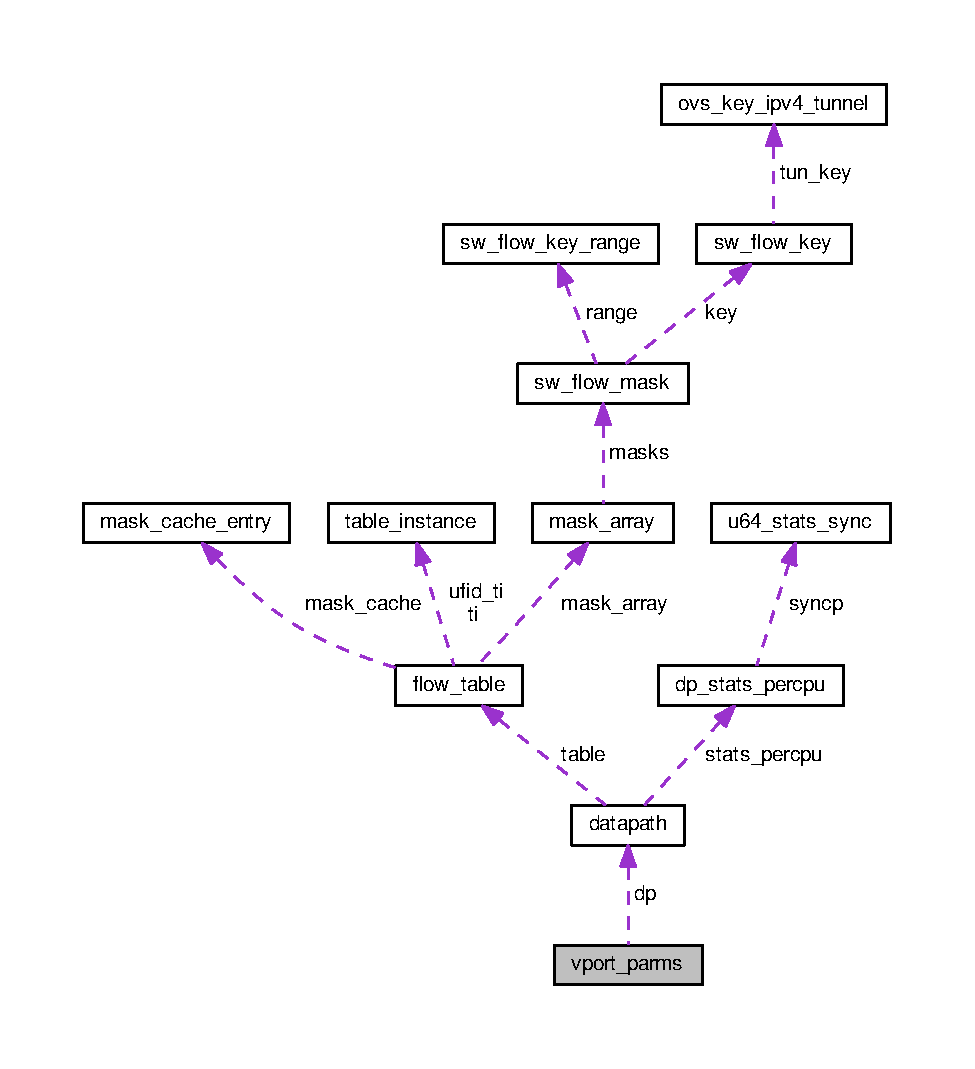
\includegraphics[width=350pt]{structvport__parms__coll__graph}
\end{center}
\end{figure}
\subsection*{Data Fields}
\begin{DoxyCompactItemize}
\item 
const char $\ast$ \hyperlink{structvport__parms_a4f27e2a7b7dc0493c095cdaabe225b38}{name}
\item 
enum \hyperlink{openvswitch_8h_a9a1b861aa99bd83177a2b10b34745b0a}{ovs\+\_\+vport\+\_\+type} \hyperlink{structvport__parms_ad79f91d20a33ff64cd72cad0b83ffae3}{type}
\item 
struct nlattr $\ast$ \hyperlink{structvport__parms_a5c6027e758731e1a16968e77d4e2ca7c}{options}
\item 
struct \hyperlink{structdatapath}{datapath} $\ast$ \hyperlink{structvport__parms_a15faa866e3d35a721de77b347017499e}{dp}
\item 
u16 \hyperlink{structvport__parms_a5bc77ace899b9bbdb6d7f833b31c009a}{port\+\_\+no}
\item 
struct nlattr $\ast$ \hyperlink{structvport__parms_ae9dbd12fddc1869a17229cef771a4d29}{upcall\+\_\+portids}
\end{DoxyCompactItemize}


\subsection{Field Documentation}
\hypertarget{structvport__parms_a15faa866e3d35a721de77b347017499e}{}\index{vport\+\_\+parms@{vport\+\_\+parms}!dp@{dp}}
\index{dp@{dp}!vport\+\_\+parms@{vport\+\_\+parms}}
\subsubsection[{dp}]{\setlength{\rightskip}{0pt plus 5cm}struct {\bf datapath}$\ast$ vport\+\_\+parms\+::dp}\label{structvport__parms_a15faa866e3d35a721de77b347017499e}
\hypertarget{structvport__parms_a4f27e2a7b7dc0493c095cdaabe225b38}{}\index{vport\+\_\+parms@{vport\+\_\+parms}!name@{name}}
\index{name@{name}!vport\+\_\+parms@{vport\+\_\+parms}}
\subsubsection[{name}]{\setlength{\rightskip}{0pt plus 5cm}const char$\ast$ vport\+\_\+parms\+::name}\label{structvport__parms_a4f27e2a7b7dc0493c095cdaabe225b38}
\hypertarget{structvport__parms_a5c6027e758731e1a16968e77d4e2ca7c}{}\index{vport\+\_\+parms@{vport\+\_\+parms}!options@{options}}
\index{options@{options}!vport\+\_\+parms@{vport\+\_\+parms}}
\subsubsection[{options}]{\setlength{\rightskip}{0pt plus 5cm}struct nlattr$\ast$ vport\+\_\+parms\+::options}\label{structvport__parms_a5c6027e758731e1a16968e77d4e2ca7c}
\hypertarget{structvport__parms_a5bc77ace899b9bbdb6d7f833b31c009a}{}\index{vport\+\_\+parms@{vport\+\_\+parms}!port\+\_\+no@{port\+\_\+no}}
\index{port\+\_\+no@{port\+\_\+no}!vport\+\_\+parms@{vport\+\_\+parms}}
\subsubsection[{port\+\_\+no}]{\setlength{\rightskip}{0pt plus 5cm}u16 vport\+\_\+parms\+::port\+\_\+no}\label{structvport__parms_a5bc77ace899b9bbdb6d7f833b31c009a}
\hypertarget{structvport__parms_ad79f91d20a33ff64cd72cad0b83ffae3}{}\index{vport\+\_\+parms@{vport\+\_\+parms}!type@{type}}
\index{type@{type}!vport\+\_\+parms@{vport\+\_\+parms}}
\subsubsection[{type}]{\setlength{\rightskip}{0pt plus 5cm}enum {\bf ovs\+\_\+vport\+\_\+type} vport\+\_\+parms\+::type}\label{structvport__parms_ad79f91d20a33ff64cd72cad0b83ffae3}
\hypertarget{structvport__parms_ae9dbd12fddc1869a17229cef771a4d29}{}\index{vport\+\_\+parms@{vport\+\_\+parms}!upcall\+\_\+portids@{upcall\+\_\+portids}}
\index{upcall\+\_\+portids@{upcall\+\_\+portids}!vport\+\_\+parms@{vport\+\_\+parms}}
\subsubsection[{upcall\+\_\+portids}]{\setlength{\rightskip}{0pt plus 5cm}struct nlattr$\ast$ vport\+\_\+parms\+::upcall\+\_\+portids}\label{structvport__parms_ae9dbd12fddc1869a17229cef771a4d29}


The documentation for this struct was generated from the following file\+:\begin{DoxyCompactItemize}
\item 
/home/vladn/git/ovs/datapath/\hyperlink{vport_8h}{vport.\+h}\end{DoxyCompactItemize}

\hypertarget{structvport__portids}{}\section{vport\+\_\+portids Struct Reference}
\label{structvport__portids}\index{vport\+\_\+portids@{vport\+\_\+portids}}


{\ttfamily \#include $<$vport.\+h$>$}



Collaboration diagram for vport\+\_\+portids\+:
\nopagebreak
\begin{figure}[H]
\begin{center}
\leavevmode
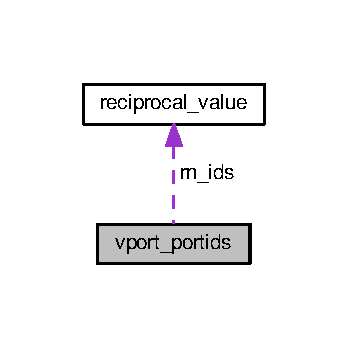
\includegraphics[width=167pt]{structvport__portids__coll__graph}
\end{center}
\end{figure}
\subsection*{Data Fields}
\begin{DoxyCompactItemize}
\item 
struct \hyperlink{structreciprocal__value}{reciprocal\+\_\+value} \hyperlink{structvport__portids_a9828dc460e2dd5ef92f6c4a1eba6bc3b}{rn\+\_\+ids}
\item 
struct rcu\+\_\+head \hyperlink{structvport__portids_ab5cbafb043788d6b07ed054824f6167c}{rcu}
\item 
u32 \hyperlink{structvport__portids_ac76f512a0f0dbe3468b006e66bddc420}{n\+\_\+ids}
\item 
u32 \hyperlink{structvport__portids_aa8570053786f982366b3dfb513479628}{ids} \mbox{[}$\,$\mbox{]}
\end{DoxyCompactItemize}


\subsection{Detailed Description}
struct \hyperlink{structvport__portids}{vport\+\_\+portids} -\/ array of netlink portids of a vport. must be protected by rcu. \+: The reciprocal value of . \+: R\+C\+U callback head for deferred destruction. \+: Size of  array. \+: Array storing the Netlink socket pids to be used for packets received on this port that miss the flow table. 

\subsection{Field Documentation}
\hypertarget{structvport__portids_aa8570053786f982366b3dfb513479628}{}\index{vport\+\_\+portids@{vport\+\_\+portids}!ids@{ids}}
\index{ids@{ids}!vport\+\_\+portids@{vport\+\_\+portids}}
\subsubsection[{ids}]{\setlength{\rightskip}{0pt plus 5cm}u32 vport\+\_\+portids\+::ids\mbox{[}$\,$\mbox{]}}\label{structvport__portids_aa8570053786f982366b3dfb513479628}
\hypertarget{structvport__portids_ac76f512a0f0dbe3468b006e66bddc420}{}\index{vport\+\_\+portids@{vport\+\_\+portids}!n\+\_\+ids@{n\+\_\+ids}}
\index{n\+\_\+ids@{n\+\_\+ids}!vport\+\_\+portids@{vport\+\_\+portids}}
\subsubsection[{n\+\_\+ids}]{\setlength{\rightskip}{0pt plus 5cm}u32 vport\+\_\+portids\+::n\+\_\+ids}\label{structvport__portids_ac76f512a0f0dbe3468b006e66bddc420}
\hypertarget{structvport__portids_ab5cbafb043788d6b07ed054824f6167c}{}\index{vport\+\_\+portids@{vport\+\_\+portids}!rcu@{rcu}}
\index{rcu@{rcu}!vport\+\_\+portids@{vport\+\_\+portids}}
\subsubsection[{rcu}]{\setlength{\rightskip}{0pt plus 5cm}struct rcu\+\_\+head vport\+\_\+portids\+::rcu}\label{structvport__portids_ab5cbafb043788d6b07ed054824f6167c}
\hypertarget{structvport__portids_a9828dc460e2dd5ef92f6c4a1eba6bc3b}{}\index{vport\+\_\+portids@{vport\+\_\+portids}!rn\+\_\+ids@{rn\+\_\+ids}}
\index{rn\+\_\+ids@{rn\+\_\+ids}!vport\+\_\+portids@{vport\+\_\+portids}}
\subsubsection[{rn\+\_\+ids}]{\setlength{\rightskip}{0pt plus 5cm}struct {\bf reciprocal\+\_\+value} vport\+\_\+portids\+::rn\+\_\+ids}\label{structvport__portids_a9828dc460e2dd5ef92f6c4a1eba6bc3b}


The documentation for this struct was generated from the following file\+:\begin{DoxyCompactItemize}
\item 
/home/vladn/git/ovs/datapath/\hyperlink{vport_8h}{vport.\+h}\end{DoxyCompactItemize}

\hypertarget{structvxlan__metadata}{}\section{vxlan\+\_\+metadata Struct Reference}
\label{structvxlan__metadata}\index{vxlan\+\_\+metadata@{vxlan\+\_\+metadata}}


{\ttfamily \#include $<$vxlan.\+h$>$}

\subsection*{Data Fields}
\begin{DoxyCompactItemize}
\item 
\+\_\+\+\_\+be32 \hyperlink{structvxlan__metadata_ac78e68c33d3c91061e3642616135cbc8}{vni}
\item 
u32 \hyperlink{structvxlan__metadata_ad71c7ab9d521840720e30ebae8ff2a6a}{gbp}
\end{DoxyCompactItemize}


\subsection{Field Documentation}
\hypertarget{structvxlan__metadata_ad71c7ab9d521840720e30ebae8ff2a6a}{}\index{vxlan\+\_\+metadata@{vxlan\+\_\+metadata}!gbp@{gbp}}
\index{gbp@{gbp}!vxlan\+\_\+metadata@{vxlan\+\_\+metadata}}
\subsubsection[{gbp}]{\setlength{\rightskip}{0pt plus 5cm}u32 vxlan\+\_\+metadata\+::gbp}\label{structvxlan__metadata_ad71c7ab9d521840720e30ebae8ff2a6a}
\hypertarget{structvxlan__metadata_ac78e68c33d3c91061e3642616135cbc8}{}\index{vxlan\+\_\+metadata@{vxlan\+\_\+metadata}!vni@{vni}}
\index{vni@{vni}!vxlan\+\_\+metadata@{vxlan\+\_\+metadata}}
\subsubsection[{vni}]{\setlength{\rightskip}{0pt plus 5cm}\+\_\+\+\_\+be32 vxlan\+\_\+metadata\+::vni}\label{structvxlan__metadata_ac78e68c33d3c91061e3642616135cbc8}


The documentation for this struct was generated from the following file\+:\begin{DoxyCompactItemize}
\item 
/home/vladn/git/ovs/datapath/linux/compat/include/net/\hyperlink{vxlan_8h}{vxlan.\+h}\end{DoxyCompactItemize}

\hypertarget{structvxlan__port}{}\section{vxlan\+\_\+port Struct Reference}
\label{structvxlan__port}\index{vxlan\+\_\+port@{vxlan\+\_\+port}}


Collaboration diagram for vxlan\+\_\+port\+:
\nopagebreak
\begin{figure}[H]
\begin{center}
\leavevmode
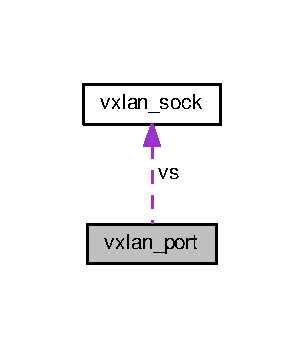
\includegraphics[width=146pt]{structvxlan__port__coll__graph}
\end{center}
\end{figure}
\subsection*{Data Fields}
\begin{DoxyCompactItemize}
\item 
struct \hyperlink{structvxlan__sock}{vxlan\+\_\+sock} $\ast$ \hyperlink{structvxlan__port_a28d2b1a2a5beaaf48453d1e0628efb88}{vs}
\item 
char \hyperlink{structvxlan__port_a48b3eb83bbca17229480cf0d7a130272}{name} \mbox{[}I\+F\+N\+A\+M\+S\+I\+Z\mbox{]}
\item 
u32 \hyperlink{structvxlan__port_a4c4814fa8ff2517ef89920c98c1d66ba}{exts}
\end{DoxyCompactItemize}


\subsection{Field Documentation}
\hypertarget{structvxlan__port_a4c4814fa8ff2517ef89920c98c1d66ba}{}\index{vxlan\+\_\+port@{vxlan\+\_\+port}!exts@{exts}}
\index{exts@{exts}!vxlan\+\_\+port@{vxlan\+\_\+port}}
\subsubsection[{exts}]{\setlength{\rightskip}{0pt plus 5cm}u32 vxlan\+\_\+port\+::exts}\label{structvxlan__port_a4c4814fa8ff2517ef89920c98c1d66ba}
\hypertarget{structvxlan__port_a48b3eb83bbca17229480cf0d7a130272}{}\index{vxlan\+\_\+port@{vxlan\+\_\+port}!name@{name}}
\index{name@{name}!vxlan\+\_\+port@{vxlan\+\_\+port}}
\subsubsection[{name}]{\setlength{\rightskip}{0pt plus 5cm}char vxlan\+\_\+port\+::name}\label{structvxlan__port_a48b3eb83bbca17229480cf0d7a130272}
\hypertarget{structvxlan__port_a28d2b1a2a5beaaf48453d1e0628efb88}{}\index{vxlan\+\_\+port@{vxlan\+\_\+port}!vs@{vs}}
\index{vs@{vs}!vxlan\+\_\+port@{vxlan\+\_\+port}}
\subsubsection[{vs}]{\setlength{\rightskip}{0pt plus 5cm}struct {\bf vxlan\+\_\+sock} $\ast$ vxlan\+\_\+port\+::vs}\label{structvxlan__port_a28d2b1a2a5beaaf48453d1e0628efb88}


The documentation for this struct was generated from the following file\+:\begin{DoxyCompactItemize}
\item 
/home/vladn/git/ovs/datapath/linux/\hyperlink{linux_2vport-vxlan_8c}{vport-\/vxlan.\+c}\end{DoxyCompactItemize}

\hypertarget{structvxlan__sock}{}\section{vxlan\+\_\+sock Struct Reference}
\label{structvxlan__sock}\index{vxlan\+\_\+sock@{vxlan\+\_\+sock}}


{\ttfamily \#include $<$vxlan.\+h$>$}

\subsection*{Data Fields}
\begin{DoxyCompactItemize}
\item 
struct hlist\+\_\+node \hyperlink{structvxlan__sock_aa49d034f0fff69c29cb3313b17caea80}{hlist}
\item 
\hyperlink{vxlan_8h_a8de966706f4eb1f2059020f4ec31aa6f}{vxlan\+\_\+rcv\+\_\+t} $\ast$ \hyperlink{structvxlan__sock_a62dbbfc22620a8120799bad80e04c639}{rcv}
\item 
void $\ast$ \hyperlink{structvxlan__sock_a44942474f147992d768c3a74b44c4d5f}{data}
\item 
struct work\+\_\+struct \hyperlink{structvxlan__sock_a951b7a9ee28672b49838176513bf343d}{del\+\_\+work}
\item 
struct socket $\ast$ \hyperlink{structvxlan__sock_a75f35ac3f5f8e0340b2bdc247a84c322}{sock}
\item 
struct rcu\+\_\+head \hyperlink{structvxlan__sock_a3ab897e7f7d97d2f2bf71791f5ebffdb}{rcu}
\item 
u32 \hyperlink{structvxlan__sock_ac3711b8cc4c992e3270dee5791a542cf}{flags}
\end{DoxyCompactItemize}


\subsection{Field Documentation}
\hypertarget{structvxlan__sock_a44942474f147992d768c3a74b44c4d5f}{}\index{vxlan\+\_\+sock@{vxlan\+\_\+sock}!data@{data}}
\index{data@{data}!vxlan\+\_\+sock@{vxlan\+\_\+sock}}
\subsubsection[{data}]{\setlength{\rightskip}{0pt plus 5cm}void$\ast$ vxlan\+\_\+sock\+::data}\label{structvxlan__sock_a44942474f147992d768c3a74b44c4d5f}
\hypertarget{structvxlan__sock_a951b7a9ee28672b49838176513bf343d}{}\index{vxlan\+\_\+sock@{vxlan\+\_\+sock}!del\+\_\+work@{del\+\_\+work}}
\index{del\+\_\+work@{del\+\_\+work}!vxlan\+\_\+sock@{vxlan\+\_\+sock}}
\subsubsection[{del\+\_\+work}]{\setlength{\rightskip}{0pt plus 5cm}struct work\+\_\+struct vxlan\+\_\+sock\+::del\+\_\+work}\label{structvxlan__sock_a951b7a9ee28672b49838176513bf343d}
\hypertarget{structvxlan__sock_ac3711b8cc4c992e3270dee5791a542cf}{}\index{vxlan\+\_\+sock@{vxlan\+\_\+sock}!flags@{flags}}
\index{flags@{flags}!vxlan\+\_\+sock@{vxlan\+\_\+sock}}
\subsubsection[{flags}]{\setlength{\rightskip}{0pt plus 5cm}u32 vxlan\+\_\+sock\+::flags}\label{structvxlan__sock_ac3711b8cc4c992e3270dee5791a542cf}
\hypertarget{structvxlan__sock_aa49d034f0fff69c29cb3313b17caea80}{}\index{vxlan\+\_\+sock@{vxlan\+\_\+sock}!hlist@{hlist}}
\index{hlist@{hlist}!vxlan\+\_\+sock@{vxlan\+\_\+sock}}
\subsubsection[{hlist}]{\setlength{\rightskip}{0pt plus 5cm}struct hlist\+\_\+node vxlan\+\_\+sock\+::hlist}\label{structvxlan__sock_aa49d034f0fff69c29cb3313b17caea80}
\hypertarget{structvxlan__sock_a3ab897e7f7d97d2f2bf71791f5ebffdb}{}\index{vxlan\+\_\+sock@{vxlan\+\_\+sock}!rcu@{rcu}}
\index{rcu@{rcu}!vxlan\+\_\+sock@{vxlan\+\_\+sock}}
\subsubsection[{rcu}]{\setlength{\rightskip}{0pt plus 5cm}struct rcu\+\_\+head vxlan\+\_\+sock\+::rcu}\label{structvxlan__sock_a3ab897e7f7d97d2f2bf71791f5ebffdb}
\hypertarget{structvxlan__sock_a62dbbfc22620a8120799bad80e04c639}{}\index{vxlan\+\_\+sock@{vxlan\+\_\+sock}!rcv@{rcv}}
\index{rcv@{rcv}!vxlan\+\_\+sock@{vxlan\+\_\+sock}}
\subsubsection[{rcv}]{\setlength{\rightskip}{0pt plus 5cm}{\bf vxlan\+\_\+rcv\+\_\+t}$\ast$ vxlan\+\_\+sock\+::rcv}\label{structvxlan__sock_a62dbbfc22620a8120799bad80e04c639}
\hypertarget{structvxlan__sock_a75f35ac3f5f8e0340b2bdc247a84c322}{}\index{vxlan\+\_\+sock@{vxlan\+\_\+sock}!sock@{sock}}
\index{sock@{sock}!vxlan\+\_\+sock@{vxlan\+\_\+sock}}
\subsubsection[{sock}]{\setlength{\rightskip}{0pt plus 5cm}struct socket$\ast$ vxlan\+\_\+sock\+::sock}\label{structvxlan__sock_a75f35ac3f5f8e0340b2bdc247a84c322}


The documentation for this struct was generated from the following file\+:\begin{DoxyCompactItemize}
\item 
/home/vladn/git/ovs/datapath/linux/compat/include/net/\hyperlink{vxlan_8h}{vxlan.\+h}\end{DoxyCompactItemize}

\hypertarget{structvxlanhdr}{}\section{vxlanhdr Struct Reference}
\label{structvxlanhdr}\index{vxlanhdr@{vxlanhdr}}
\subsection*{Data Fields}
\begin{DoxyCompactItemize}
\item 
\+\_\+\+\_\+be32 \hyperlink{structvxlanhdr_a62dd0a1f926bef8eee34f4cf09dd0e1d}{vx\+\_\+flags}
\item 
\+\_\+\+\_\+be32 \hyperlink{structvxlanhdr_a4239361cddf2d17ca6654a75497dcddd}{vx\+\_\+vni}
\end{DoxyCompactItemize}


\subsection{Field Documentation}
\hypertarget{structvxlanhdr_a62dd0a1f926bef8eee34f4cf09dd0e1d}{}\index{vxlanhdr@{vxlanhdr}!vx\+\_\+flags@{vx\+\_\+flags}}
\index{vx\+\_\+flags@{vx\+\_\+flags}!vxlanhdr@{vxlanhdr}}
\subsubsection[{vx\+\_\+flags}]{\setlength{\rightskip}{0pt plus 5cm}\+\_\+\+\_\+be32 vxlanhdr\+::vx\+\_\+flags}\label{structvxlanhdr_a62dd0a1f926bef8eee34f4cf09dd0e1d}
\hypertarget{structvxlanhdr_a4239361cddf2d17ca6654a75497dcddd}{}\index{vxlanhdr@{vxlanhdr}!vx\+\_\+vni@{vx\+\_\+vni}}
\index{vx\+\_\+vni@{vx\+\_\+vni}!vxlanhdr@{vxlanhdr}}
\subsubsection[{vx\+\_\+vni}]{\setlength{\rightskip}{0pt plus 5cm}\+\_\+\+\_\+be32 vxlanhdr\+::vx\+\_\+vni}\label{structvxlanhdr_a4239361cddf2d17ca6654a75497dcddd}


The documentation for this struct was generated from the following file\+:\begin{DoxyCompactItemize}
\item 
/home/vladn/git/ovs/datapath/linux/compat/\hyperlink{compat_2vxlan_8c}{vxlan.\+c}\end{DoxyCompactItemize}

\hypertarget{structvxlanhdr__gbp}{}\section{vxlanhdr\+\_\+gbp Struct Reference}
\label{structvxlanhdr__gbp}\index{vxlanhdr\+\_\+gbp@{vxlanhdr\+\_\+gbp}}


{\ttfamily \#include $<$vxlan.\+h$>$}

\subsection*{Data Fields}
\begin{DoxyCompactItemize}
\item 
\+\_\+\+\_\+u8 \hyperlink{structvxlanhdr__gbp_a1d415b695ab8a201a5e2ec69301421b3}{vx\+\_\+flags}
\item 
\+\_\+\+\_\+be16 \hyperlink{structvxlanhdr__gbp_a96bf86ab13573ff42399f11b1c8c5e34}{policy\+\_\+id}
\item 
\+\_\+\+\_\+be32 \hyperlink{structvxlanhdr__gbp_aa6c706970acf2d5ffa86f76e7bad0b7a}{vx\+\_\+vni}
\end{DoxyCompactItemize}


\subsection{Field Documentation}
\hypertarget{structvxlanhdr__gbp_a96bf86ab13573ff42399f11b1c8c5e34}{}\index{vxlanhdr\+\_\+gbp@{vxlanhdr\+\_\+gbp}!policy\+\_\+id@{policy\+\_\+id}}
\index{policy\+\_\+id@{policy\+\_\+id}!vxlanhdr\+\_\+gbp@{vxlanhdr\+\_\+gbp}}
\subsubsection[{policy\+\_\+id}]{\setlength{\rightskip}{0pt plus 5cm}\+\_\+\+\_\+be16 vxlanhdr\+\_\+gbp\+::policy\+\_\+id}\label{structvxlanhdr__gbp_a96bf86ab13573ff42399f11b1c8c5e34}
\hypertarget{structvxlanhdr__gbp_a1d415b695ab8a201a5e2ec69301421b3}{}\index{vxlanhdr\+\_\+gbp@{vxlanhdr\+\_\+gbp}!vx\+\_\+flags@{vx\+\_\+flags}}
\index{vx\+\_\+flags@{vx\+\_\+flags}!vxlanhdr\+\_\+gbp@{vxlanhdr\+\_\+gbp}}
\subsubsection[{vx\+\_\+flags}]{\setlength{\rightskip}{0pt plus 5cm}\+\_\+\+\_\+u8 vxlanhdr\+\_\+gbp\+::vx\+\_\+flags}\label{structvxlanhdr__gbp_a1d415b695ab8a201a5e2ec69301421b3}
\hypertarget{structvxlanhdr__gbp_aa6c706970acf2d5ffa86f76e7bad0b7a}{}\index{vxlanhdr\+\_\+gbp@{vxlanhdr\+\_\+gbp}!vx\+\_\+vni@{vx\+\_\+vni}}
\index{vx\+\_\+vni@{vx\+\_\+vni}!vxlanhdr\+\_\+gbp@{vxlanhdr\+\_\+gbp}}
\subsubsection[{vx\+\_\+vni}]{\setlength{\rightskip}{0pt plus 5cm}\+\_\+\+\_\+be32 vxlanhdr\+\_\+gbp\+::vx\+\_\+vni}\label{structvxlanhdr__gbp_aa6c706970acf2d5ffa86f76e7bad0b7a}


The documentation for this struct was generated from the following file\+:\begin{DoxyCompactItemize}
\item 
/home/vladn/git/ovs/datapath/linux/compat/include/net/\hyperlink{vxlan_8h}{vxlan.\+h}\end{DoxyCompactItemize}

\chapter{File Documentation}
\hypertarget{actions_8c}{}\section{/home/vladn/git/ovs/datapath/actions.c File Reference}
\label{actions_8c}\index{/home/vladn/git/ovs/datapath/actions.\+c@{/home/vladn/git/ovs/datapath/actions.\+c}}
{\ttfamily \#include $<$linux/skbuff.\+h$>$}\\*
{\ttfamily \#include $<$linux/in.\+h$>$}\\*
{\ttfamily \#include $<$linux/ip.\+h$>$}\\*
{\ttfamily \#include $<$linux/openvswitch.\+h$>$}\\*
{\ttfamily \#include $<$linux/sctp.\+h$>$}\\*
{\ttfamily \#include $<$linux/tcp.\+h$>$}\\*
{\ttfamily \#include $<$linux/udp.\+h$>$}\\*
{\ttfamily \#include $<$linux/in6.\+h$>$}\\*
{\ttfamily \#include $<$linux/if\+\_\+arp.\+h$>$}\\*
{\ttfamily \#include $<$linux/if\+\_\+vlan.\+h$>$}\\*
{\ttfamily \#include $<$net/ip.\+h$>$}\\*
{\ttfamily \#include $<$net/ipv6.\+h$>$}\\*
{\ttfamily \#include $<$net/checksum.\+h$>$}\\*
{\ttfamily \#include $<$net/dsfield.\+h$>$}\\*
{\ttfamily \#include $<$net/mpls.\+h$>$}\\*
{\ttfamily \#include $<$net/sctp/checksum.\+h$>$}\\*
{\ttfamily \#include \char`\"{}datapath.\+h\char`\"{}}\\*
{\ttfamily \#include \char`\"{}gso.\+h\char`\"{}}\\*
{\ttfamily \#include \char`\"{}vlan.\+h\char`\"{}}\\*
{\ttfamily \#include \char`\"{}vport.\+h\char`\"{}}\\*
Include dependency graph for actions.\+c\+:
\nopagebreak
\begin{figure}[H]
\begin{center}
\leavevmode
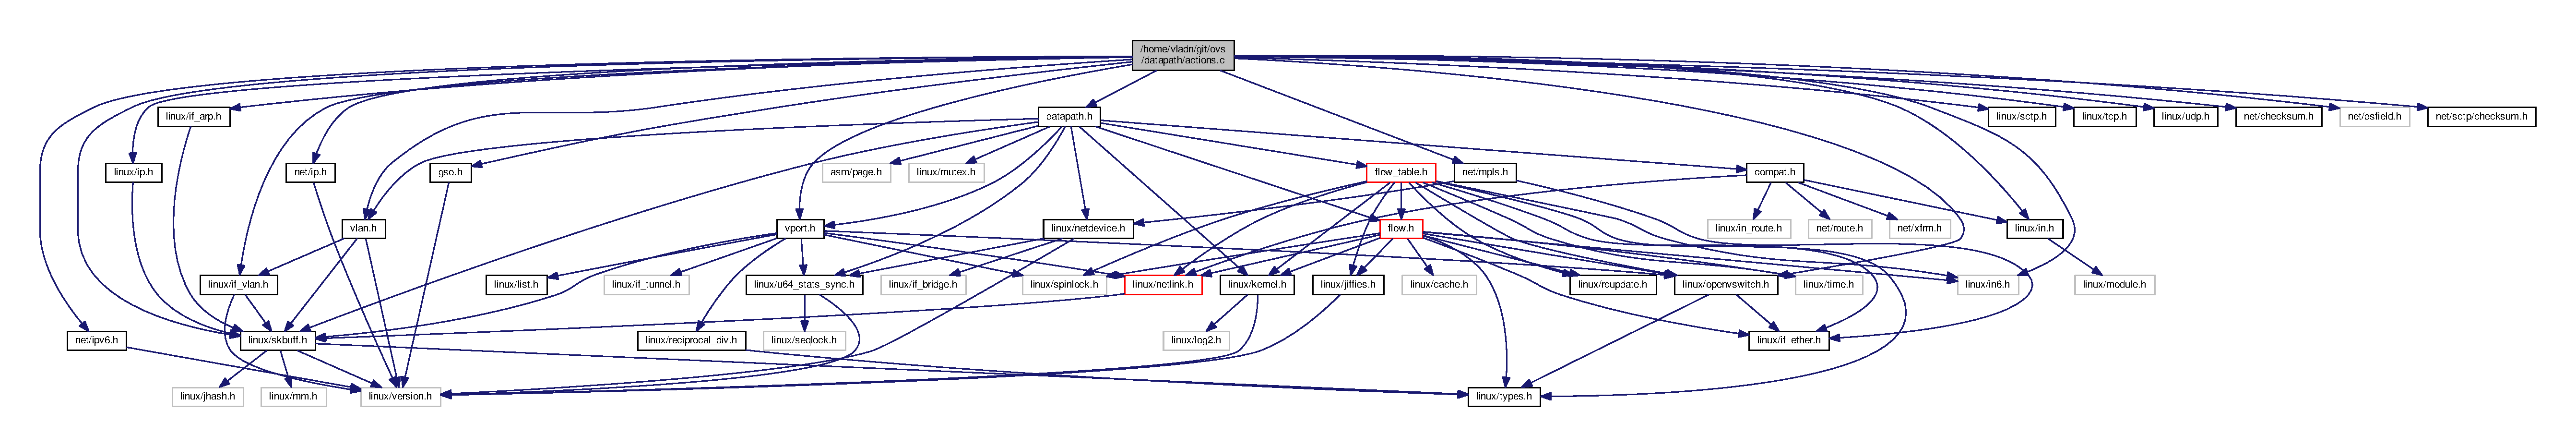
\includegraphics[width=350pt]{actions_8c__incl}
\end{center}
\end{figure}
\subsection*{Data Structures}
\begin{DoxyCompactItemize}
\item 
struct \hyperlink{structdeferred__action}{deferred\+\_\+action}
\item 
struct \hyperlink{structaction__fifo}{action\+\_\+fifo}
\end{DoxyCompactItemize}
\subsection*{Macros}
\begin{DoxyCompactItemize}
\item 
\#define \hyperlink{actions_8c_a1f8c165bf4196327bc3abff648276d92}{pr\+\_\+fmt}(fmt)~K\+B\+U\+I\+L\+D\+\_\+\+M\+O\+D\+N\+A\+M\+E \char`\"{}\+: \char`\"{} fmt
\item 
\#define \hyperlink{actions_8c_acb72e0b273dae399e2619f619fd061ed}{D\+E\+F\+E\+R\+R\+E\+D\+\_\+\+A\+C\+T\+I\+O\+N\+\_\+\+F\+I\+F\+O\+\_\+\+S\+I\+Z\+E}~10
\item 
\#define \hyperlink{actions_8c_aef2488868338b5c1ec4419f0efde93f1}{E\+X\+E\+C\+\_\+\+A\+C\+T\+I\+O\+N\+S\+\_\+\+L\+E\+V\+E\+L\+\_\+\+L\+I\+M\+I\+T}
\item 
\#define \hyperlink{actions_8c_a7e29e4ea7eef8e6a17ec80459c178a14}{M\+A\+S\+K\+E\+D}(O\+L\+D,  K\+E\+Y,  M\+A\+S\+K)~((K\+E\+Y) $\vert$ ((O\+L\+D) \& $\sim$(M\+A\+S\+K)))
\item 
\#define \hyperlink{actions_8c_a6a812b08a711cd6258c60e9bd0c931e3}{S\+E\+T\+\_\+\+M\+A\+S\+K\+E\+D}(O\+L\+D,  K\+E\+Y,  M\+A\+S\+K)~((O\+L\+D) = \hyperlink{linux_2actions_8c_a7e29e4ea7eef8e6a17ec80459c178a14}{M\+A\+S\+K\+E\+D}(O\+L\+D, K\+E\+Y, M\+A\+S\+K))
\item 
\#define \hyperlink{actions_8c_aa0c451dc85a82947bdf6d8ae3c2385b5}{get\+\_\+mask}(a,  \hyperlink{flow_8h_ab22aaab04f806700def00f32823fcb9e}{type})~((const \hyperlink{flow_8h_ab22aaab04f806700def00f32823fcb9e}{type})nla\+\_\+data(a) + 1)
\end{DoxyCompactItemize}
\subsection*{Functions}
\begin{DoxyCompactItemize}
\item 
static int \hyperlink{actions_8c_ad41a07588c602d50a247bcf2bf9ae9d5}{do\+\_\+execute\+\_\+actions} (struct \hyperlink{structdatapath}{datapath} $\ast$dp, struct sk\+\_\+buff $\ast$skb, struct \hyperlink{structsw__flow__key}{sw\+\_\+flow\+\_\+key} $\ast$key, const struct nlattr $\ast$attr, int len)
\item 
static \hyperlink{actions_8c_aacdc7977b799c6e2275e312793f87dcd}{D\+E\+F\+I\+N\+E\+\_\+\+P\+E\+R\+\_\+\+C\+P\+U} (int, exec\+\_\+actions\+\_\+level)
\item 
static void \hyperlink{actions_8c_a688872dd5196a430f6a0df6e1954d220}{action\+\_\+fifo\+\_\+init} (struct \hyperlink{structaction__fifo}{action\+\_\+fifo} $\ast$fifo)
\item 
static \hyperlink{types_8h_afaa87723b8417d40fcf45b7330261ef9}{bool} \hyperlink{actions_8c_ade23c3824a292e4698cb3c01fefa52a5}{action\+\_\+fifo\+\_\+is\+\_\+empty} (const struct \hyperlink{structaction__fifo}{action\+\_\+fifo} $\ast$fifo)
\item 
static struct \hyperlink{structdeferred__action}{deferred\+\_\+action} $\ast$ \hyperlink{actions_8c_a7512da42cda457a824bb2fc8ff850dd5}{action\+\_\+fifo\+\_\+get} (struct \hyperlink{structaction__fifo}{action\+\_\+fifo} $\ast$fifo)
\item 
static struct \hyperlink{structdeferred__action}{deferred\+\_\+action} $\ast$ \hyperlink{actions_8c_a3c8c974792d662e29d50b97ae044a068}{action\+\_\+fifo\+\_\+put} (struct \hyperlink{structaction__fifo}{action\+\_\+fifo} $\ast$fifo)
\item 
static struct \hyperlink{structdeferred__action}{deferred\+\_\+action} $\ast$ \hyperlink{actions_8c_a3875097b6e35686ddee414782d0e67b1}{add\+\_\+deferred\+\_\+actions} (struct sk\+\_\+buff $\ast$skb, const struct \hyperlink{structsw__flow__key}{sw\+\_\+flow\+\_\+key} $\ast$key, const struct nlattr $\ast$attr)
\item 
static void \hyperlink{actions_8c_aac28ee49d1019a576306f207afd5f8d6}{invalidate\+\_\+flow\+\_\+key} (struct \hyperlink{structsw__flow__key}{sw\+\_\+flow\+\_\+key} $\ast$key)
\item 
static \hyperlink{types_8h_afaa87723b8417d40fcf45b7330261ef9}{bool} \hyperlink{actions_8c_a77e3320f8f43a04aaf952a2c82e6dac1}{is\+\_\+flow\+\_\+key\+\_\+valid} (const struct \hyperlink{structsw__flow__key}{sw\+\_\+flow\+\_\+key} $\ast$key)
\item 
static int \hyperlink{actions_8c_affb38ca95e088fb61d6df91cf3fdd606}{push\+\_\+mpls} (struct sk\+\_\+buff $\ast$skb, struct \hyperlink{structsw__flow__key}{sw\+\_\+flow\+\_\+key} $\ast$key, const struct \hyperlink{structovs__action__push__mpls}{ovs\+\_\+action\+\_\+push\+\_\+mpls} $\ast$\hyperlink{flow_8h_aeab2d67b4ec58a9575da76c323ad95ce}{mpls})
\item 
static int \hyperlink{actions_8c_ac372daa8a5c4eb7fb2536fa61653e41b}{pop\+\_\+mpls} (struct sk\+\_\+buff $\ast$skb, struct \hyperlink{structsw__flow__key}{sw\+\_\+flow\+\_\+key} $\ast$key, const \+\_\+\+\_\+be16 ethertype)
\item 
static int \hyperlink{actions_8c_ad66261c51831d2a4a6ff0ea385fbad32}{set\+\_\+mpls} (struct sk\+\_\+buff $\ast$skb, struct \hyperlink{structsw__flow__key}{sw\+\_\+flow\+\_\+key} $\ast$flow\+\_\+key, const \+\_\+\+\_\+be32 $\ast$mpls\+\_\+lse, const \+\_\+\+\_\+be32 $\ast$mask)
\item 
static int \hyperlink{actions_8c_aa11b6c74e2206cc8353d00cff409df22}{pop\+\_\+vlan} (struct sk\+\_\+buff $\ast$skb, struct \hyperlink{structsw__flow__key}{sw\+\_\+flow\+\_\+key} $\ast$key)
\item 
static int \hyperlink{actions_8c_a706c437e9fb3992afaa8f62605c59961}{push\+\_\+vlan} (struct sk\+\_\+buff $\ast$skb, struct \hyperlink{structsw__flow__key}{sw\+\_\+flow\+\_\+key} $\ast$key, const struct \hyperlink{structovs__action__push__vlan}{ovs\+\_\+action\+\_\+push\+\_\+vlan} $\ast$vlan)
\item 
static void \hyperlink{actions_8c_a2d434306a1e37e8bd0572dab35cc68ca}{ether\+\_\+addr\+\_\+copy\+\_\+masked} (u8 $\ast$dst\+\_\+, const u8 $\ast$src\+\_\+, const u8 $\ast$mask\+\_\+)
\item 
static int \hyperlink{actions_8c_a85d6da67a26cfee7c3c894131233f9ca}{set\+\_\+eth\+\_\+addr} (struct sk\+\_\+buff $\ast$skb, struct \hyperlink{structsw__flow__key}{sw\+\_\+flow\+\_\+key} $\ast$flow\+\_\+key, const struct \hyperlink{structovs__key__ethernet}{ovs\+\_\+key\+\_\+ethernet} $\ast$key, const struct \hyperlink{structovs__key__ethernet}{ovs\+\_\+key\+\_\+ethernet} $\ast$mask)
\item 
static void \hyperlink{actions_8c_a35283087cadb66ada3c19e7a87cfdcba}{set\+\_\+ip\+\_\+addr} (struct sk\+\_\+buff $\ast$skb, struct iphdr $\ast$nh, \+\_\+\+\_\+be32 $\ast$\hyperlink{flow_8h_a535ce925c585c41d434f7481f342c976}{addr}, \+\_\+\+\_\+be32 new\+\_\+addr)
\item 
static void \hyperlink{actions_8c_a006120c8695be3960f274e88e24b535a}{update\+\_\+ipv6\+\_\+checksum} (struct sk\+\_\+buff $\ast$skb, u8 l4\+\_\+proto, \+\_\+\+\_\+be32 \hyperlink{flow_8h_a535ce925c585c41d434f7481f342c976}{addr}\mbox{[}4\mbox{]}, const \+\_\+\+\_\+be32 new\+\_\+addr\mbox{[}4\mbox{]})
\item 
static void \hyperlink{actions_8c_affe65b5dd55e3a7c39c5a6705731f01f}{mask\+\_\+ipv6\+\_\+addr} (const \+\_\+\+\_\+be32 old\mbox{[}4\mbox{]}, const \+\_\+\+\_\+be32 \hyperlink{flow_8h_a535ce925c585c41d434f7481f342c976}{addr}\mbox{[}4\mbox{]}, const \+\_\+\+\_\+be32 mask\mbox{[}4\mbox{]}, \+\_\+\+\_\+be32 masked\mbox{[}4\mbox{]})
\item 
static void \hyperlink{actions_8c_aa39edf0f0aa23ee17d2828e1c42b0590}{set\+\_\+ipv6\+\_\+addr} (struct sk\+\_\+buff $\ast$skb, u8 l4\+\_\+proto, \+\_\+\+\_\+be32 \hyperlink{flow_8h_a535ce925c585c41d434f7481f342c976}{addr}\mbox{[}4\mbox{]}, const \+\_\+\+\_\+be32 new\+\_\+addr\mbox{[}4\mbox{]}, \hyperlink{types_8h_afaa87723b8417d40fcf45b7330261ef9}{bool} recalculate\+\_\+csum)
\item 
static void \hyperlink{actions_8c_a105b45d892887e581acec50af165e330}{set\+\_\+ipv6\+\_\+fl} (struct ipv6hdr $\ast$nh, u32 fl, u32 mask)
\item 
static void \hyperlink{actions_8c_a00bc919dc7a6a81f506155c0372eba9b}{set\+\_\+ip\+\_\+ttl} (struct sk\+\_\+buff $\ast$skb, struct iphdr $\ast$nh, u8 new\+\_\+ttl, u8 mask)
\item 
static int \hyperlink{actions_8c_a5b6148caa3654ee968f7173b83b3abf4}{set\+\_\+ipv4} (struct sk\+\_\+buff $\ast$skb, struct \hyperlink{structsw__flow__key}{sw\+\_\+flow\+\_\+key} $\ast$flow\+\_\+key, const struct \hyperlink{structovs__key__ipv4}{ovs\+\_\+key\+\_\+ipv4} $\ast$key, const struct \hyperlink{structovs__key__ipv4}{ovs\+\_\+key\+\_\+ipv4} $\ast$mask)
\item 
static \hyperlink{types_8h_afaa87723b8417d40fcf45b7330261ef9}{bool} \hyperlink{actions_8c_a889a29de7d27314b273304eaad6f202e}{is\+\_\+ipv6\+\_\+mask\+\_\+nonzero} (const \+\_\+\+\_\+be32 \hyperlink{flow_8h_a535ce925c585c41d434f7481f342c976}{addr}\mbox{[}4\mbox{]})
\item 
static int \hyperlink{actions_8c_acf538956396fdb59cff22ad4577c10f3}{set\+\_\+ipv6} (struct sk\+\_\+buff $\ast$skb, struct \hyperlink{structsw__flow__key}{sw\+\_\+flow\+\_\+key} $\ast$flow\+\_\+key, const struct \hyperlink{structovs__key__ipv6}{ovs\+\_\+key\+\_\+ipv6} $\ast$key, const struct \hyperlink{structovs__key__ipv6}{ovs\+\_\+key\+\_\+ipv6} $\ast$mask)
\item 
static void \hyperlink{actions_8c_a485b30c5af82b861079002c3e8899f7d}{set\+\_\+tp\+\_\+port} (struct sk\+\_\+buff $\ast$skb, \+\_\+\+\_\+be16 $\ast$port, \+\_\+\+\_\+be16 new\+\_\+port, \hyperlink{types_8h_a2fdf5566d289d6941c29db084139bf23}{\+\_\+\+\_\+sum16} $\ast$check)
\item 
static int \hyperlink{actions_8c_ae78d854d13e952f67ca0d0b7bc45be75}{set\+\_\+udp} (struct sk\+\_\+buff $\ast$skb, struct \hyperlink{structsw__flow__key}{sw\+\_\+flow\+\_\+key} $\ast$flow\+\_\+key, const struct \hyperlink{structovs__key__udp}{ovs\+\_\+key\+\_\+udp} $\ast$key, const struct \hyperlink{structovs__key__udp}{ovs\+\_\+key\+\_\+udp} $\ast$mask)
\item 
static int \hyperlink{actions_8c_a3f6591203112ded2452b368308b0f36b}{set\+\_\+tcp} (struct sk\+\_\+buff $\ast$skb, struct \hyperlink{structsw__flow__key}{sw\+\_\+flow\+\_\+key} $\ast$flow\+\_\+key, const struct \hyperlink{structovs__key__tcp}{ovs\+\_\+key\+\_\+tcp} $\ast$key, const struct \hyperlink{structovs__key__tcp}{ovs\+\_\+key\+\_\+tcp} $\ast$mask)
\item 
static int \hyperlink{actions_8c_a7f2d96d4cc495e0f9f48c61305beea5c}{set\+\_\+sctp} (struct sk\+\_\+buff $\ast$skb, struct \hyperlink{structsw__flow__key}{sw\+\_\+flow\+\_\+key} $\ast$flow\+\_\+key, const struct \hyperlink{structovs__key__sctp}{ovs\+\_\+key\+\_\+sctp} $\ast$key, const struct \hyperlink{structovs__key__sctp}{ovs\+\_\+key\+\_\+sctp} $\ast$mask)
\item 
static void \hyperlink{actions_8c_a141467d4c8b6d03b33ca4a36b471fb1e}{do\+\_\+output} (struct \hyperlink{structdatapath}{datapath} $\ast$dp, struct sk\+\_\+buff $\ast$skb, int out\+\_\+port)
\item 
static int \hyperlink{actions_8c_ad0ea13ac8532fe548cd35a2d1086d8f3}{output\+\_\+userspace} (struct \hyperlink{structdatapath}{datapath} $\ast$dp, struct sk\+\_\+buff $\ast$skb, struct \hyperlink{structsw__flow__key}{sw\+\_\+flow\+\_\+key} $\ast$key, const struct nlattr $\ast$attr, const struct nlattr $\ast$actions, int actions\+\_\+len)
\item 
static int \hyperlink{actions_8c_a23b7fbefa6429cd4af2c92eb20c03889}{sample} (struct \hyperlink{structdatapath}{datapath} $\ast$dp, struct sk\+\_\+buff $\ast$skb, struct \hyperlink{structsw__flow__key}{sw\+\_\+flow\+\_\+key} $\ast$key, const struct nlattr $\ast$attr, const struct nlattr $\ast$actions, int actions\+\_\+len)
\item 
static void \hyperlink{actions_8c_a7f08d769ba6fb4cdd65ef7ced5964dea}{execute\+\_\+hash} (struct sk\+\_\+buff $\ast$skb, struct \hyperlink{structsw__flow__key}{sw\+\_\+flow\+\_\+key} $\ast$key, const struct nlattr $\ast$attr)
\item 
static int \hyperlink{actions_8c_a4a59d75b1d012debb4f8ab42d0672deb}{execute\+\_\+set\+\_\+action} (struct sk\+\_\+buff $\ast$skb, struct \hyperlink{structsw__flow__key}{sw\+\_\+flow\+\_\+key} $\ast$flow\+\_\+key, const struct nlattr $\ast$a)
\item 
static int \hyperlink{actions_8c_ae5d851747d2630c868c296b43ad3c2e7}{execute\+\_\+masked\+\_\+set\+\_\+action} (struct sk\+\_\+buff $\ast$skb, struct \hyperlink{structsw__flow__key}{sw\+\_\+flow\+\_\+key} $\ast$flow\+\_\+key, const struct nlattr $\ast$a)
\item 
static int \hyperlink{actions_8c_ab6b5b3b0684142f0e137bd64d883d52f}{execute\+\_\+recirc} (struct \hyperlink{structdatapath}{datapath} $\ast$dp, struct sk\+\_\+buff $\ast$skb, struct \hyperlink{structsw__flow__key}{sw\+\_\+flow\+\_\+key} $\ast$key, const struct nlattr $\ast$a, int rem)
\item 
static void \hyperlink{actions_8c_afa871a96ea915a7ce87b96a0b7b30538}{process\+\_\+deferred\+\_\+actions} (struct \hyperlink{structdatapath}{datapath} $\ast$dp)
\item 
int \hyperlink{actions_8c_a5b34c1980d155574d657a21cac3bcc37}{ovs\+\_\+execute\+\_\+actions} (struct \hyperlink{structdatapath}{datapath} $\ast$dp, struct sk\+\_\+buff $\ast$skb, const struct \hyperlink{structsw__flow__actions}{sw\+\_\+flow\+\_\+actions} $\ast$acts, struct \hyperlink{structsw__flow__key}{sw\+\_\+flow\+\_\+key} $\ast$key)
\item 
int \hyperlink{actions_8c_a3006f0376c2aecb6525126ad0e9bae25}{action\+\_\+fifos\+\_\+init} (void)
\item 
void \hyperlink{actions_8c_a7dfd1f218e0966ef342251a185866f4d}{action\+\_\+fifos\+\_\+exit} (void)
\end{DoxyCompactItemize}
\subsection*{Variables}
\begin{DoxyCompactItemize}
\item 
static struct \hyperlink{structaction__fifo}{action\+\_\+fifo} \hyperlink{compiler_8h_a497f20279760cdb59a5187689f9f5ab1}{\+\_\+\+\_\+percpu} $\ast$ \hyperlink{actions_8c_a38c6295376dbb80340f4f1b8e488f223}{action\+\_\+fifos}
\end{DoxyCompactItemize}


\subsection{Macro Definition Documentation}
\hypertarget{actions_8c_acb72e0b273dae399e2619f619fd061ed}{}\index{actions.\+c@{actions.\+c}!D\+E\+F\+E\+R\+R\+E\+D\+\_\+\+A\+C\+T\+I\+O\+N\+\_\+\+F\+I\+F\+O\+\_\+\+S\+I\+Z\+E@{D\+E\+F\+E\+R\+R\+E\+D\+\_\+\+A\+C\+T\+I\+O\+N\+\_\+\+F\+I\+F\+O\+\_\+\+S\+I\+Z\+E}}
\index{D\+E\+F\+E\+R\+R\+E\+D\+\_\+\+A\+C\+T\+I\+O\+N\+\_\+\+F\+I\+F\+O\+\_\+\+S\+I\+Z\+E@{D\+E\+F\+E\+R\+R\+E\+D\+\_\+\+A\+C\+T\+I\+O\+N\+\_\+\+F\+I\+F\+O\+\_\+\+S\+I\+Z\+E}!actions.\+c@{actions.\+c}}
\subsubsection[{D\+E\+F\+E\+R\+R\+E\+D\+\_\+\+A\+C\+T\+I\+O\+N\+\_\+\+F\+I\+F\+O\+\_\+\+S\+I\+Z\+E}]{\setlength{\rightskip}{0pt plus 5cm}\#define D\+E\+F\+E\+R\+R\+E\+D\+\_\+\+A\+C\+T\+I\+O\+N\+\_\+\+F\+I\+F\+O\+\_\+\+S\+I\+Z\+E~10}\label{actions_8c_acb72e0b273dae399e2619f619fd061ed}
\hypertarget{actions_8c_aef2488868338b5c1ec4419f0efde93f1}{}\index{actions.\+c@{actions.\+c}!E\+X\+E\+C\+\_\+\+A\+C\+T\+I\+O\+N\+S\+\_\+\+L\+E\+V\+E\+L\+\_\+\+L\+I\+M\+I\+T@{E\+X\+E\+C\+\_\+\+A\+C\+T\+I\+O\+N\+S\+\_\+\+L\+E\+V\+E\+L\+\_\+\+L\+I\+M\+I\+T}}
\index{E\+X\+E\+C\+\_\+\+A\+C\+T\+I\+O\+N\+S\+\_\+\+L\+E\+V\+E\+L\+\_\+\+L\+I\+M\+I\+T@{E\+X\+E\+C\+\_\+\+A\+C\+T\+I\+O\+N\+S\+\_\+\+L\+E\+V\+E\+L\+\_\+\+L\+I\+M\+I\+T}!actions.\+c@{actions.\+c}}
\subsubsection[{E\+X\+E\+C\+\_\+\+A\+C\+T\+I\+O\+N\+S\+\_\+\+L\+E\+V\+E\+L\+\_\+\+L\+I\+M\+I\+T}]{\setlength{\rightskip}{0pt plus 5cm}\#define E\+X\+E\+C\+\_\+\+A\+C\+T\+I\+O\+N\+S\+\_\+\+L\+E\+V\+E\+L\+\_\+\+L\+I\+M\+I\+T}\label{actions_8c_aef2488868338b5c1ec4419f0efde93f1}
{\bfseries Value\+:}
\begin{DoxyCode}
4   \textcolor{comment}{/* limit used to detect packet}
\textcolor{comment}{                      * looping by the network stack}
\textcolor{comment}{                      */}
\end{DoxyCode}
\hypertarget{actions_8c_aa0c451dc85a82947bdf6d8ae3c2385b5}{}\index{actions.\+c@{actions.\+c}!get\+\_\+mask@{get\+\_\+mask}}
\index{get\+\_\+mask@{get\+\_\+mask}!actions.\+c@{actions.\+c}}
\subsubsection[{get\+\_\+mask}]{\setlength{\rightskip}{0pt plus 5cm}\#define get\+\_\+mask(
\begin{DoxyParamCaption}
\item[{}]{a, }
\item[{}]{{\bf type}}
\end{DoxyParamCaption}
)~((const {\bf type})nla\+\_\+data(a) + 1)}\label{actions_8c_aa0c451dc85a82947bdf6d8ae3c2385b5}
\hypertarget{actions_8c_a7e29e4ea7eef8e6a17ec80459c178a14}{}\index{actions.\+c@{actions.\+c}!M\+A\+S\+K\+E\+D@{M\+A\+S\+K\+E\+D}}
\index{M\+A\+S\+K\+E\+D@{M\+A\+S\+K\+E\+D}!actions.\+c@{actions.\+c}}
\subsubsection[{M\+A\+S\+K\+E\+D}]{\setlength{\rightskip}{0pt plus 5cm}\#define M\+A\+S\+K\+E\+D(
\begin{DoxyParamCaption}
\item[{}]{O\+L\+D, }
\item[{}]{K\+E\+Y, }
\item[{}]{M\+A\+S\+K}
\end{DoxyParamCaption}
)~((K\+E\+Y) $\vert$ ((O\+L\+D) \& $\sim$(M\+A\+S\+K)))}\label{actions_8c_a7e29e4ea7eef8e6a17ec80459c178a14}
\hypertarget{actions_8c_a1f8c165bf4196327bc3abff648276d92}{}\index{actions.\+c@{actions.\+c}!pr\+\_\+fmt@{pr\+\_\+fmt}}
\index{pr\+\_\+fmt@{pr\+\_\+fmt}!actions.\+c@{actions.\+c}}
\subsubsection[{pr\+\_\+fmt}]{\setlength{\rightskip}{0pt plus 5cm}\#define pr\+\_\+fmt(
\begin{DoxyParamCaption}
\item[{}]{fmt}
\end{DoxyParamCaption}
)~K\+B\+U\+I\+L\+D\+\_\+\+M\+O\+D\+N\+A\+M\+E \char`\"{}\+: \char`\"{} fmt}\label{actions_8c_a1f8c165bf4196327bc3abff648276d92}
\hypertarget{actions_8c_a6a812b08a711cd6258c60e9bd0c931e3}{}\index{actions.\+c@{actions.\+c}!S\+E\+T\+\_\+\+M\+A\+S\+K\+E\+D@{S\+E\+T\+\_\+\+M\+A\+S\+K\+E\+D}}
\index{S\+E\+T\+\_\+\+M\+A\+S\+K\+E\+D@{S\+E\+T\+\_\+\+M\+A\+S\+K\+E\+D}!actions.\+c@{actions.\+c}}
\subsubsection[{S\+E\+T\+\_\+\+M\+A\+S\+K\+E\+D}]{\setlength{\rightskip}{0pt plus 5cm}\#define S\+E\+T\+\_\+\+M\+A\+S\+K\+E\+D(
\begin{DoxyParamCaption}
\item[{}]{O\+L\+D, }
\item[{}]{K\+E\+Y, }
\item[{}]{M\+A\+S\+K}
\end{DoxyParamCaption}
)~((O\+L\+D) = {\bf M\+A\+S\+K\+E\+D}(O\+L\+D, K\+E\+Y, M\+A\+S\+K))}\label{actions_8c_a6a812b08a711cd6258c60e9bd0c931e3}


\subsection{Function Documentation}
\hypertarget{actions_8c_a7512da42cda457a824bb2fc8ff850dd5}{}\index{actions.\+c@{actions.\+c}!action\+\_\+fifo\+\_\+get@{action\+\_\+fifo\+\_\+get}}
\index{action\+\_\+fifo\+\_\+get@{action\+\_\+fifo\+\_\+get}!actions.\+c@{actions.\+c}}
\subsubsection[{action\+\_\+fifo\+\_\+get}]{\setlength{\rightskip}{0pt plus 5cm}static struct {\bf deferred\+\_\+action}$\ast$ action\+\_\+fifo\+\_\+get (
\begin{DoxyParamCaption}
\item[{struct {\bf action\+\_\+fifo} $\ast$}]{fifo}
\end{DoxyParamCaption}
)\hspace{0.3cm}{\ttfamily [static]}}\label{actions_8c_a7512da42cda457a824bb2fc8ff850dd5}

\begin{DoxyCode}
82 \{
83     \textcolor{keywordflow}{if} (\hyperlink{actions_8c_ade23c3824a292e4698cb3c01fefa52a5}{action\_fifo\_is\_empty}(fifo))
84         \textcolor{keywordflow}{return} NULL;
85 
86     \textcolor{keywordflow}{return} &fifo->\hyperlink{structaction__fifo_ab25b47c1bc05f5417f0a2073a47b2eb5}{fifo}[fifo->\hyperlink{structaction__fifo_a60805cbdf935d6718f685c7374ae9493}{tail}++];
87 \}
\end{DoxyCode}
\hypertarget{actions_8c_a688872dd5196a430f6a0df6e1954d220}{}\index{actions.\+c@{actions.\+c}!action\+\_\+fifo\+\_\+init@{action\+\_\+fifo\+\_\+init}}
\index{action\+\_\+fifo\+\_\+init@{action\+\_\+fifo\+\_\+init}!actions.\+c@{actions.\+c}}
\subsubsection[{action\+\_\+fifo\+\_\+init}]{\setlength{\rightskip}{0pt plus 5cm}static void action\+\_\+fifo\+\_\+init (
\begin{DoxyParamCaption}
\item[{struct {\bf action\+\_\+fifo} $\ast$}]{fifo}
\end{DoxyParamCaption}
)\hspace{0.3cm}{\ttfamily [static]}}\label{actions_8c_a688872dd5196a430f6a0df6e1954d220}

\begin{DoxyCode}
71 \{
72     fifo->\hyperlink{structaction__fifo_a5376b4a5c9dbfd84303d156a47ed9018}{head} = 0;
73     fifo->\hyperlink{structaction__fifo_a60805cbdf935d6718f685c7374ae9493}{tail} = 0;
74 \}
\end{DoxyCode}
\hypertarget{actions_8c_ade23c3824a292e4698cb3c01fefa52a5}{}\index{actions.\+c@{actions.\+c}!action\+\_\+fifo\+\_\+is\+\_\+empty@{action\+\_\+fifo\+\_\+is\+\_\+empty}}
\index{action\+\_\+fifo\+\_\+is\+\_\+empty@{action\+\_\+fifo\+\_\+is\+\_\+empty}!actions.\+c@{actions.\+c}}
\subsubsection[{action\+\_\+fifo\+\_\+is\+\_\+empty}]{\setlength{\rightskip}{0pt plus 5cm}static {\bf bool} action\+\_\+fifo\+\_\+is\+\_\+empty (
\begin{DoxyParamCaption}
\item[{const struct {\bf action\+\_\+fifo} $\ast$}]{fifo}
\end{DoxyParamCaption}
)\hspace{0.3cm}{\ttfamily [static]}}\label{actions_8c_ade23c3824a292e4698cb3c01fefa52a5}

\begin{DoxyCode}
77 \{
78     \textcolor{keywordflow}{return} (fifo->\hyperlink{structaction__fifo_a5376b4a5c9dbfd84303d156a47ed9018}{head} == fifo->\hyperlink{structaction__fifo_a60805cbdf935d6718f685c7374ae9493}{tail});
79 \}
\end{DoxyCode}
\hypertarget{actions_8c_a3c8c974792d662e29d50b97ae044a068}{}\index{actions.\+c@{actions.\+c}!action\+\_\+fifo\+\_\+put@{action\+\_\+fifo\+\_\+put}}
\index{action\+\_\+fifo\+\_\+put@{action\+\_\+fifo\+\_\+put}!actions.\+c@{actions.\+c}}
\subsubsection[{action\+\_\+fifo\+\_\+put}]{\setlength{\rightskip}{0pt plus 5cm}static struct {\bf deferred\+\_\+action}$\ast$ action\+\_\+fifo\+\_\+put (
\begin{DoxyParamCaption}
\item[{struct {\bf action\+\_\+fifo} $\ast$}]{fifo}
\end{DoxyParamCaption}
)\hspace{0.3cm}{\ttfamily [static]}}\label{actions_8c_a3c8c974792d662e29d50b97ae044a068}

\begin{DoxyCode}
90 \{
91     \textcolor{keywordflow}{if} (fifo->\hyperlink{structaction__fifo_a5376b4a5c9dbfd84303d156a47ed9018}{head} >= \hyperlink{actions_8c_acb72e0b273dae399e2619f619fd061ed}{DEFERRED\_ACTION\_FIFO\_SIZE} - 1)
92         \textcolor{keywordflow}{return} NULL;
93 
94     \textcolor{keywordflow}{return} &fifo->\hyperlink{structaction__fifo_ab25b47c1bc05f5417f0a2073a47b2eb5}{fifo}[fifo->\hyperlink{structaction__fifo_a5376b4a5c9dbfd84303d156a47ed9018}{head}++];
95 \}
\end{DoxyCode}
\hypertarget{actions_8c_a7dfd1f218e0966ef342251a185866f4d}{}\index{actions.\+c@{actions.\+c}!action\+\_\+fifos\+\_\+exit@{action\+\_\+fifos\+\_\+exit}}
\index{action\+\_\+fifos\+\_\+exit@{action\+\_\+fifos\+\_\+exit}!actions.\+c@{actions.\+c}}
\subsubsection[{action\+\_\+fifos\+\_\+exit}]{\setlength{\rightskip}{0pt plus 5cm}void action\+\_\+fifos\+\_\+exit (
\begin{DoxyParamCaption}
\item[{void}]{}
\end{DoxyParamCaption}
)}\label{actions_8c_a7dfd1f218e0966ef342251a185866f4d}

\begin{DoxyCode}
1016 \{
1017     free\_percpu(\hyperlink{actions_8c_a38c6295376dbb80340f4f1b8e488f223}{action\_fifos});
1018 \}
\end{DoxyCode}
\hypertarget{actions_8c_a3006f0376c2aecb6525126ad0e9bae25}{}\index{actions.\+c@{actions.\+c}!action\+\_\+fifos\+\_\+init@{action\+\_\+fifos\+\_\+init}}
\index{action\+\_\+fifos\+\_\+init@{action\+\_\+fifos\+\_\+init}!actions.\+c@{actions.\+c}}
\subsubsection[{action\+\_\+fifos\+\_\+init}]{\setlength{\rightskip}{0pt plus 5cm}int action\+\_\+fifos\+\_\+init (
\begin{DoxyParamCaption}
\item[{void}]{}
\end{DoxyParamCaption}
)}\label{actions_8c_a3006f0376c2aecb6525126ad0e9bae25}

\begin{DoxyCode}
1007 \{
1008     \hyperlink{actions_8c_a38c6295376dbb80340f4f1b8e488f223}{action\_fifos} = alloc\_percpu(\textcolor{keyword}{struct} \hyperlink{structaction__fifo}{action\_fifo});
1009     \textcolor{keywordflow}{if} (!\hyperlink{actions_8c_a38c6295376dbb80340f4f1b8e488f223}{action\_fifos})
1010         \textcolor{keywordflow}{return} -ENOMEM;
1011 
1012     \textcolor{keywordflow}{return} 0;
1013 \}
\end{DoxyCode}
\hypertarget{actions_8c_a3875097b6e35686ddee414782d0e67b1}{}\index{actions.\+c@{actions.\+c}!add\+\_\+deferred\+\_\+actions@{add\+\_\+deferred\+\_\+actions}}
\index{add\+\_\+deferred\+\_\+actions@{add\+\_\+deferred\+\_\+actions}!actions.\+c@{actions.\+c}}
\subsubsection[{add\+\_\+deferred\+\_\+actions}]{\setlength{\rightskip}{0pt plus 5cm}static struct {\bf deferred\+\_\+action}$\ast$ add\+\_\+deferred\+\_\+actions (
\begin{DoxyParamCaption}
\item[{struct sk\+\_\+buff $\ast$}]{skb, }
\item[{const struct {\bf sw\+\_\+flow\+\_\+key} $\ast$}]{key, }
\item[{const struct nlattr $\ast$}]{attr}
\end{DoxyParamCaption}
)\hspace{0.3cm}{\ttfamily [static]}}\label{actions_8c_a3875097b6e35686ddee414782d0e67b1}

\begin{DoxyCode}
101 \{
102     \textcolor{keyword}{struct }\hyperlink{structaction__fifo}{action\_fifo} *\hyperlink{structaction__fifo_ab25b47c1bc05f5417f0a2073a47b2eb5}{fifo};
103     \textcolor{keyword}{struct }\hyperlink{structdeferred__action}{deferred\_action} *da;
104 
105     fifo = \hyperlink{percpu_8h_a1cd55f287dff5c4a79fc11dd38d47c12}{this\_cpu\_ptr}(\hyperlink{actions_8c_a38c6295376dbb80340f4f1b8e488f223}{action\_fifos});
106     da = \hyperlink{actions_8c_a3c8c974792d662e29d50b97ae044a068}{action\_fifo\_put}(fifo);
107     \textcolor{keywordflow}{if} (da) \{
108         da->\hyperlink{structdeferred__action_acba4fd12fba3d60b6f4c7f2f3159f316}{skb} = \hyperlink{structdeferred__action_acba4fd12fba3d60b6f4c7f2f3159f316}{skb};
109         da->\hyperlink{structdeferred__action_a9cb4d3dde378a66035e7b17f017d9f89}{actions} = attr;
110         da->\hyperlink{structdeferred__action_a4685f782001923a8f8c20510126b4c21}{pkt\_key} = *key;
111     \}
112 
113     \textcolor{keywordflow}{return} da;
114 \}
\end{DoxyCode}
\hypertarget{actions_8c_aacdc7977b799c6e2275e312793f87dcd}{}\index{actions.\+c@{actions.\+c}!D\+E\+F\+I\+N\+E\+\_\+\+P\+E\+R\+\_\+\+C\+P\+U@{D\+E\+F\+I\+N\+E\+\_\+\+P\+E\+R\+\_\+\+C\+P\+U}}
\index{D\+E\+F\+I\+N\+E\+\_\+\+P\+E\+R\+\_\+\+C\+P\+U@{D\+E\+F\+I\+N\+E\+\_\+\+P\+E\+R\+\_\+\+C\+P\+U}!actions.\+c@{actions.\+c}}
\subsubsection[{D\+E\+F\+I\+N\+E\+\_\+\+P\+E\+R\+\_\+\+C\+P\+U}]{\setlength{\rightskip}{0pt plus 5cm}static D\+E\+F\+I\+N\+E\+\_\+\+P\+E\+R\+\_\+\+C\+P\+U (
\begin{DoxyParamCaption}
\item[{int}]{, }
\item[{exec\+\_\+actions\+\_\+level}]{}
\end{DoxyParamCaption}
)\hspace{0.3cm}{\ttfamily [static]}}\label{actions_8c_aacdc7977b799c6e2275e312793f87dcd}
\hypertarget{actions_8c_ad41a07588c602d50a247bcf2bf9ae9d5}{}\index{actions.\+c@{actions.\+c}!do\+\_\+execute\+\_\+actions@{do\+\_\+execute\+\_\+actions}}
\index{do\+\_\+execute\+\_\+actions@{do\+\_\+execute\+\_\+actions}!actions.\+c@{actions.\+c}}
\subsubsection[{do\+\_\+execute\+\_\+actions}]{\setlength{\rightskip}{0pt plus 5cm}static int do\+\_\+execute\+\_\+actions (
\begin{DoxyParamCaption}
\item[{struct {\bf datapath} $\ast$}]{dp, }
\item[{struct sk\+\_\+buff $\ast$}]{skb, }
\item[{struct {\bf sw\+\_\+flow\+\_\+key} $\ast$}]{key, }
\item[{const struct nlattr $\ast$}]{attr, }
\item[{int}]{len}
\end{DoxyParamCaption}
)\hspace{0.3cm}{\ttfamily [static]}}\label{actions_8c_ad41a07588c602d50a247bcf2bf9ae9d5}

\begin{DoxyCode}
856 \{
857     \textcolor{comment}{/* Every output action needs a separate clone of 'skb', but the common}
858 \textcolor{comment}{     * case is just a single output action, so that doing a clone and}
859 \textcolor{comment}{     * then freeing the original skbuff is wasteful.  So the following code}
860 \textcolor{comment}{     * is slightly obscure just to avoid that.}
861 \textcolor{comment}{     */}
862     \textcolor{keywordtype}{int} prev\_port = -1;
863     \textcolor{keyword}{const} \textcolor{keyword}{struct }nlattr *a;
864     \textcolor{keywordtype}{int} rem;
865 
866     \textcolor{keywordflow}{for} (a = attr, rem = len; rem > 0;
867          a = nla\_next(a, &rem)) \{
868         \textcolor{keywordtype}{int} err = 0;
869 
870         \textcolor{keywordflow}{if} (unlikely(prev\_port != -1)) \{
871             \textcolor{keyword}{struct }sk\_buff *out\_skb = skb\_clone(skb, GFP\_ATOMIC);
872 
873             \textcolor{keywordflow}{if} (out\_skb)
874                 \hyperlink{actions_8c_a141467d4c8b6d03b33ca4a36b471fb1e}{do\_output}(dp, out\_skb, prev\_port);
875 
876             prev\_port = -1;
877         \}
878 
879         \textcolor{keywordflow}{switch} (nla\_type(a)) \{
880         \textcolor{keywordflow}{case} \hyperlink{openvswitch_8h_affc4a4d29437ad03a23444243e2db26eacad69687bf2bfae5092ea828cf0d4fe2}{OVS\_ACTION\_ATTR\_OUTPUT}:
881             prev\_port = nla\_get\_u32(a);
882             \textcolor{keywordflow}{break};
883 
884         \textcolor{keywordflow}{case} \hyperlink{openvswitch_8h_affc4a4d29437ad03a23444243e2db26ea17132af22505d8b1bb535a270f83a8bd}{OVS\_ACTION\_ATTR\_USERSPACE}:
885             \hyperlink{actions_8c_ad0ea13ac8532fe548cd35a2d1086d8f3}{output\_userspace}(dp, skb, key, a, attr, len);
886             \textcolor{keywordflow}{break};
887 
888         \textcolor{keywordflow}{case} \hyperlink{openvswitch_8h_affc4a4d29437ad03a23444243e2db26eaa783c1e8488baea181d3497e0e9676f9}{OVS\_ACTION\_ATTR\_HASH}:
889             \hyperlink{actions_8c_a7f08d769ba6fb4cdd65ef7ced5964dea}{execute\_hash}(skb, key, a);
890             \textcolor{keywordflow}{break};
891 
892         \textcolor{keywordflow}{case} \hyperlink{openvswitch_8h_affc4a4d29437ad03a23444243e2db26eafb68488325a1ab2d6bfb67ea115a5cdb}{OVS\_ACTION\_ATTR\_PUSH\_MPLS}:
893             err = \hyperlink{actions_8c_affb38ca95e088fb61d6df91cf3fdd606}{push\_mpls}(skb, key, nla\_data(a));
894             \textcolor{keywordflow}{break};
895 
896         \textcolor{keywordflow}{case} \hyperlink{openvswitch_8h_affc4a4d29437ad03a23444243e2db26eafe4ec9b68459771a3ffd07d20cd628e1}{OVS\_ACTION\_ATTR\_POP\_MPLS}:
897             err = \hyperlink{actions_8c_ac372daa8a5c4eb7fb2536fa61653e41b}{pop\_mpls}(skb, key, \hyperlink{net_2netlink_8h_a5a9bc877c8fdbf9b3f2f85536aabcae0}{nla\_get\_be16}(a));
898             \textcolor{keywordflow}{break};
899 
900         \textcolor{keywordflow}{case} \hyperlink{openvswitch_8h_affc4a4d29437ad03a23444243e2db26ea6f41b7751556ff0acc2f4c6f94963ba6}{OVS\_ACTION\_ATTR\_PUSH\_VLAN}:
901             err = \hyperlink{actions_8c_a706c437e9fb3992afaa8f62605c59961}{push\_vlan}(skb, key, nla\_data(a));
902             \textcolor{keywordflow}{break};
903 
904         \textcolor{keywordflow}{case} \hyperlink{openvswitch_8h_affc4a4d29437ad03a23444243e2db26ea9cd4ec18560c7c3f81276cba51a96a24}{OVS\_ACTION\_ATTR\_POP\_VLAN}:
905             err = \hyperlink{actions_8c_aa11b6c74e2206cc8353d00cff409df22}{pop\_vlan}(skb, key);
906             \textcolor{keywordflow}{break};
907 
908         \textcolor{keywordflow}{case} \hyperlink{openvswitch_8h_affc4a4d29437ad03a23444243e2db26ea2cad0b08a7809d6e7cb1a9e86d73a47c}{OVS\_ACTION\_ATTR\_RECIRC}:
909             err = \hyperlink{actions_8c_ab6b5b3b0684142f0e137bd64d883d52f}{execute\_recirc}(dp, skb, key, a, rem);
910             \textcolor{keywordflow}{if} (\hyperlink{net_2netlink_8h_ad408a3a1db3cc544eb7a552246f3fb57}{nla\_is\_last}(a, rem)) \{
911                 \textcolor{comment}{/* If this is the last action, the skb has}
912 \textcolor{comment}{                 * been consumed or freed.}
913 \textcolor{comment}{                 * Return immediately.}
914 \textcolor{comment}{                 */}
915                 \textcolor{keywordflow}{return} err;
916             \}
917             \textcolor{keywordflow}{break};
918 
919         \textcolor{keywordflow}{case} \hyperlink{openvswitch_8h_affc4a4d29437ad03a23444243e2db26eaff937deb7687d0dd4b073c27aed9c8be}{OVS\_ACTION\_ATTR\_SET}:
920             err = \hyperlink{actions_8c_a4a59d75b1d012debb4f8ab42d0672deb}{execute\_set\_action}(skb, key, nla\_data(a));
921             \textcolor{keywordflow}{break};
922 
923         \textcolor{keywordflow}{case} \hyperlink{openvswitch_8h_affc4a4d29437ad03a23444243e2db26ea50a466abca8b11394e9364de28ebe03f}{OVS\_ACTION\_ATTR\_SET\_MASKED}:
924         \textcolor{keywordflow}{case} OVS\_ACTION\_ATTR\_SET\_TO\_MASKED:
925             err = \hyperlink{actions_8c_ae5d851747d2630c868c296b43ad3c2e7}{execute\_masked\_set\_action}(skb, key, nla\_data(a));
926             \textcolor{keywordflow}{break};
927 
928         \textcolor{keywordflow}{case} \hyperlink{openvswitch_8h_affc4a4d29437ad03a23444243e2db26eaddc6f70b9e8501e5bb90548373faf734}{OVS\_ACTION\_ATTR\_SAMPLE}:
929             err = \hyperlink{actions_8c_a23b7fbefa6429cd4af2c92eb20c03889}{sample}(dp, skb, key, a, attr, len);
930             \textcolor{keywordflow}{break};
931         \}
932 
933         \textcolor{keywordflow}{if} (unlikely(err)) \{
934             kfree\_skb(skb);
935             \textcolor{keywordflow}{return} err;
936         \}
937     \}
938 
939     \textcolor{keywordflow}{if} (prev\_port != -1)
940         \hyperlink{actions_8c_a141467d4c8b6d03b33ca4a36b471fb1e}{do\_output}(dp, skb, prev\_port);
941     \textcolor{keywordflow}{else}
942         \hyperlink{skbuff_8h_adc460a9e6dccf5557d55bbce8c7adb6a}{consume\_skb}(skb);
943 
944     \textcolor{keywordflow}{return} 0;
945 \}
\end{DoxyCode}
\hypertarget{actions_8c_a141467d4c8b6d03b33ca4a36b471fb1e}{}\index{actions.\+c@{actions.\+c}!do\+\_\+output@{do\+\_\+output}}
\index{do\+\_\+output@{do\+\_\+output}!actions.\+c@{actions.\+c}}
\subsubsection[{do\+\_\+output}]{\setlength{\rightskip}{0pt plus 5cm}static void do\+\_\+output (
\begin{DoxyParamCaption}
\item[{struct {\bf datapath} $\ast$}]{dp, }
\item[{struct sk\+\_\+buff $\ast$}]{skb, }
\item[{int}]{out\+\_\+port}
\end{DoxyParamCaption}
)\hspace{0.3cm}{\ttfamily [static]}}\label{actions_8c_a141467d4c8b6d03b33ca4a36b471fb1e}

\begin{DoxyCode}
604 \{
605     \textcolor{keyword}{struct }\hyperlink{structvport}{vport} *\hyperlink{structvport}{vport} = \hyperlink{datapath_8h_ac6f3c37a7850774112c03c6e88d89dc0}{ovs\_vport\_rcu}(dp, out\_port);
606 
607     \textcolor{keywordflow}{if} (likely(vport))
608         \hyperlink{linux_2vport_8c_abd74f3970bd7dc951b8399d00efe42d8}{ovs\_vport\_send}(vport, skb);
609     \textcolor{keywordflow}{else}
610         kfree\_skb(skb);
611 \}
\end{DoxyCode}
\hypertarget{actions_8c_a2d434306a1e37e8bd0572dab35cc68ca}{}\index{actions.\+c@{actions.\+c}!ether\+\_\+addr\+\_\+copy\+\_\+masked@{ether\+\_\+addr\+\_\+copy\+\_\+masked}}
\index{ether\+\_\+addr\+\_\+copy\+\_\+masked@{ether\+\_\+addr\+\_\+copy\+\_\+masked}!actions.\+c@{actions.\+c}}
\subsubsection[{ether\+\_\+addr\+\_\+copy\+\_\+masked}]{\setlength{\rightskip}{0pt plus 5cm}static void ether\+\_\+addr\+\_\+copy\+\_\+masked (
\begin{DoxyParamCaption}
\item[{u8 $\ast$}]{dst\+\_\+, }
\item[{const u8 $\ast$}]{src\+\_\+, }
\item[{const u8 $\ast$}]{mask\+\_\+}
\end{DoxyParamCaption}
)\hspace{0.3cm}{\ttfamily [static]}}\label{actions_8c_a2d434306a1e37e8bd0572dab35cc68ca}

\begin{DoxyCode}
245 \{
246     u16 *\hyperlink{flow_8h_a6747ad3b5d60480ea073cd12c9b78aaa}{dst} = (u16 *)dst\_;
247     \textcolor{keyword}{const} u16 *\hyperlink{flow_8h_a2e7e37e9dfe6465386d6c500f83ef144}{src} = (\textcolor{keyword}{const} u16 *)src\_;
248     \textcolor{keyword}{const} u16 *mask = (\textcolor{keyword}{const} u16 *)mask\_;
249 
250     \hyperlink{actions_8c_a6a812b08a711cd6258c60e9bd0c931e3}{SET\_MASKED}(dst[0], src[0], mask[0]);
251     \hyperlink{actions_8c_a6a812b08a711cd6258c60e9bd0c931e3}{SET\_MASKED}(dst[1], src[1], mask[1]);
252     \hyperlink{actions_8c_a6a812b08a711cd6258c60e9bd0c931e3}{SET\_MASKED}(dst[2], src[2], mask[2]);
253 \}
\end{DoxyCode}
\hypertarget{actions_8c_a7f08d769ba6fb4cdd65ef7ced5964dea}{}\index{actions.\+c@{actions.\+c}!execute\+\_\+hash@{execute\+\_\+hash}}
\index{execute\+\_\+hash@{execute\+\_\+hash}!actions.\+c@{actions.\+c}}
\subsubsection[{execute\+\_\+hash}]{\setlength{\rightskip}{0pt plus 5cm}static void execute\+\_\+hash (
\begin{DoxyParamCaption}
\item[{struct sk\+\_\+buff $\ast$}]{skb, }
\item[{struct {\bf sw\+\_\+flow\+\_\+key} $\ast$}]{key, }
\item[{const struct nlattr $\ast$}]{attr}
\end{DoxyParamCaption}
)\hspace{0.3cm}{\ttfamily [static]}}\label{actions_8c_a7f08d769ba6fb4cdd65ef7ced5964dea}

\begin{DoxyCode}
720 \{
721     \textcolor{keyword}{struct }\hyperlink{structovs__action__hash}{ovs\_action\_hash} *hash\_act = nla\_data(attr);
722     u32 hash = 0;
723 
724     \textcolor{comment}{/* OVS\_HASH\_ALG\_L4 is the only possible hash algorithm.  */}
725     hash = \hyperlink{skbuff_8h_acb236314b209f764af9aae7fbbb04311}{skb\_get\_hash}(skb);
726     hash = jhash\_1word(hash, hash\_act->\hyperlink{structovs__action__hash_a174855fe08c609dd3542de6e9e8a92ee}{hash\_basis});
727     \textcolor{keywordflow}{if} (!hash)
728         hash = 0x1;
729 
730     key->\hyperlink{structsw__flow__key_a73dd9402f1f54c321f6d704d9b018d15}{ovs\_flow\_hash} = hash;
731 \}
\end{DoxyCode}
\hypertarget{actions_8c_ae5d851747d2630c868c296b43ad3c2e7}{}\index{actions.\+c@{actions.\+c}!execute\+\_\+masked\+\_\+set\+\_\+action@{execute\+\_\+masked\+\_\+set\+\_\+action}}
\index{execute\+\_\+masked\+\_\+set\+\_\+action@{execute\+\_\+masked\+\_\+set\+\_\+action}!actions.\+c@{actions.\+c}}
\subsubsection[{execute\+\_\+masked\+\_\+set\+\_\+action}]{\setlength{\rightskip}{0pt plus 5cm}static int execute\+\_\+masked\+\_\+set\+\_\+action (
\begin{DoxyParamCaption}
\item[{struct sk\+\_\+buff $\ast$}]{skb, }
\item[{struct {\bf sw\+\_\+flow\+\_\+key} $\ast$}]{flow\+\_\+key, }
\item[{const struct nlattr $\ast$}]{a}
\end{DoxyParamCaption}
)\hspace{0.3cm}{\ttfamily [static]}}\label{actions_8c_ae5d851747d2630c868c296b43ad3c2e7}

\begin{DoxyCode}
752 \{
753     \textcolor{keywordtype}{int} err = 0;
754 
755     \textcolor{keywordflow}{switch} (nla\_type(a)) \{
756     \textcolor{keywordflow}{case} \hyperlink{openvswitch_8h_a6a279bc7098c9bc819c12355c9e07864a3dee91d2ad17f698e34ebb913fcef8bf}{OVS\_KEY\_ATTR\_PRIORITY}:
757         \hyperlink{actions_8c_a6a812b08a711cd6258c60e9bd0c931e3}{SET\_MASKED}(skb->priority, nla\_get\_u32(a), *\hyperlink{actions_8c_aa0c451dc85a82947bdf6d8ae3c2385b5}{get\_mask}(a, u32 *));
758         flow\_key->\hyperlink{structsw__flow__key_a57cbddb75a8d4fd859300bd34d98e84a}{phy}.\hyperlink{structsw__flow__key_a9dd898913d9faaec1ec970029e7fbb71}{priority} = skb->priority;
759         \textcolor{keywordflow}{break};
760 
761     \textcolor{keywordflow}{case} \hyperlink{openvswitch_8h_a6a279bc7098c9bc819c12355c9e07864a32f36d9e41b0fbae0746d67fa34340ad}{OVS\_KEY\_ATTR\_SKB\_MARK}:
762         \hyperlink{actions_8c_a6a812b08a711cd6258c60e9bd0c931e3}{SET\_MASKED}(skb->mark, nla\_get\_u32(a), *\hyperlink{actions_8c_aa0c451dc85a82947bdf6d8ae3c2385b5}{get\_mask}(a, u32 *));
763         flow\_key->\hyperlink{structsw__flow__key_a57cbddb75a8d4fd859300bd34d98e84a}{phy}.\hyperlink{structsw__flow__key_ae02571657f29397dcc45de8528f4ed05}{skb\_mark} = skb->mark;
764         \textcolor{keywordflow}{break};
765 
766     \textcolor{keywordflow}{case} OVS\_KEY\_ATTR\_TUNNEL\_INFO:
767         \textcolor{comment}{/* Masked data not supported for tunnel. */}
768         err = -EINVAL;
769         \textcolor{keywordflow}{break};
770 
771     \textcolor{keywordflow}{case} \hyperlink{openvswitch_8h_a6a279bc7098c9bc819c12355c9e07864a75127b87d8a2f36ae2c9aae2cf42cd56}{OVS\_KEY\_ATTR\_ETHERNET}:
772         err = \hyperlink{actions_8c_a85d6da67a26cfee7c3c894131233f9ca}{set\_eth\_addr}(skb, flow\_key, nla\_data(a),
773                    \hyperlink{actions_8c_aa0c451dc85a82947bdf6d8ae3c2385b5}{get\_mask}(a, \textcolor{keyword}{struct} \hyperlink{structovs__key__ethernet}{ovs\_key\_ethernet} *));
774         \textcolor{keywordflow}{break};
775 
776     \textcolor{keywordflow}{case} \hyperlink{openvswitch_8h_a6a279bc7098c9bc819c12355c9e07864a67c672ef69eb0c5db9136812e3cdd92e}{OVS\_KEY\_ATTR\_IPV4}:
777         err = \hyperlink{actions_8c_a5b6148caa3654ee968f7173b83b3abf4}{set\_ipv4}(skb, flow\_key, nla\_data(a),
778                    \hyperlink{actions_8c_aa0c451dc85a82947bdf6d8ae3c2385b5}{get\_mask}(a, \textcolor{keyword}{struct} \hyperlink{structovs__key__ipv4}{ovs\_key\_ipv4} *));
779         \textcolor{keywordflow}{break};
780 
781     \textcolor{keywordflow}{case} \hyperlink{openvswitch_8h_a6a279bc7098c9bc819c12355c9e07864aff74bae1efeecfd5d6cf28d8987a8bfd}{OVS\_KEY\_ATTR\_IPV6}:
782         err = \hyperlink{actions_8c_acf538956396fdb59cff22ad4577c10f3}{set\_ipv6}(skb, flow\_key, nla\_data(a),
783                    \hyperlink{actions_8c_aa0c451dc85a82947bdf6d8ae3c2385b5}{get\_mask}(a, \textcolor{keyword}{struct} \hyperlink{structovs__key__ipv6}{ovs\_key\_ipv6} *));
784         \textcolor{keywordflow}{break};
785 
786     \textcolor{keywordflow}{case} \hyperlink{openvswitch_8h_a6a279bc7098c9bc819c12355c9e07864a120ca2131b2881b0c52b6fcc8f6cccb5}{OVS\_KEY\_ATTR\_TCP}:
787         err = \hyperlink{actions_8c_a3f6591203112ded2452b368308b0f36b}{set\_tcp}(skb, flow\_key, nla\_data(a),
788                   \hyperlink{actions_8c_aa0c451dc85a82947bdf6d8ae3c2385b5}{get\_mask}(a, \textcolor{keyword}{struct} \hyperlink{structovs__key__tcp}{ovs\_key\_tcp} *));
789         \textcolor{keywordflow}{break};
790 
791     \textcolor{keywordflow}{case} \hyperlink{openvswitch_8h_a6a279bc7098c9bc819c12355c9e07864a4dea7a1acfa9eeffb8f09838bb9f9a7d}{OVS\_KEY\_ATTR\_UDP}:
792         err = \hyperlink{actions_8c_ae78d854d13e952f67ca0d0b7bc45be75}{set\_udp}(skb, flow\_key, nla\_data(a),
793                   \hyperlink{actions_8c_aa0c451dc85a82947bdf6d8ae3c2385b5}{get\_mask}(a, \textcolor{keyword}{struct} \hyperlink{structovs__key__udp}{ovs\_key\_udp} *));
794         \textcolor{keywordflow}{break};
795 
796     \textcolor{keywordflow}{case} \hyperlink{openvswitch_8h_a6a279bc7098c9bc819c12355c9e07864a33b7870d10d17ea1604aa83edf40e452}{OVS\_KEY\_ATTR\_SCTP}:
797         err = \hyperlink{actions_8c_a7f2d96d4cc495e0f9f48c61305beea5c}{set\_sctp}(skb, flow\_key, nla\_data(a),
798                    \hyperlink{actions_8c_aa0c451dc85a82947bdf6d8ae3c2385b5}{get\_mask}(a, \textcolor{keyword}{struct} \hyperlink{structovs__key__sctp}{ovs\_key\_sctp} *));
799         \textcolor{keywordflow}{break};
800 
801     \textcolor{keywordflow}{case} \hyperlink{openvswitch_8h_a6a279bc7098c9bc819c12355c9e07864ac46f7c8520cb93d091b4247ef8707f7b}{OVS\_KEY\_ATTR\_MPLS}:
802         err = \hyperlink{actions_8c_ad66261c51831d2a4a6ff0ea385fbad32}{set\_mpls}(skb, flow\_key, nla\_data(a), \hyperlink{actions_8c_aa0c451dc85a82947bdf6d8ae3c2385b5}{get\_mask}(a,
803                                     \_\_be32 *));
804         \textcolor{keywordflow}{break};
805     \}
806 
807     \textcolor{keywordflow}{return} err;
808 \}
\end{DoxyCode}
\hypertarget{actions_8c_ab6b5b3b0684142f0e137bd64d883d52f}{}\index{actions.\+c@{actions.\+c}!execute\+\_\+recirc@{execute\+\_\+recirc}}
\index{execute\+\_\+recirc@{execute\+\_\+recirc}!actions.\+c@{actions.\+c}}
\subsubsection[{execute\+\_\+recirc}]{\setlength{\rightskip}{0pt plus 5cm}static int execute\+\_\+recirc (
\begin{DoxyParamCaption}
\item[{struct {\bf datapath} $\ast$}]{dp, }
\item[{struct sk\+\_\+buff $\ast$}]{skb, }
\item[{struct {\bf sw\+\_\+flow\+\_\+key} $\ast$}]{key, }
\item[{const struct nlattr $\ast$}]{a, }
\item[{int}]{rem}
\end{DoxyParamCaption}
)\hspace{0.3cm}{\ttfamily [static]}}\label{actions_8c_ab6b5b3b0684142f0e137bd64d883d52f}

\begin{DoxyCode}
813 \{
814     \textcolor{keyword}{struct }\hyperlink{structdeferred__action}{deferred\_action} *da;
815 
816     \textcolor{keywordflow}{if} (!\hyperlink{actions_8c_a77e3320f8f43a04aaf952a2c82e6dac1}{is\_flow\_key\_valid}(key)) \{
817         \textcolor{keywordtype}{int} err;
818 
819         err = \hyperlink{flow_8c_a7d27b3745046ced4859b9fa615e27543}{ovs\_flow\_key\_update}(\hyperlink{structdeferred__action_acba4fd12fba3d60b6f4c7f2f3159f316}{skb}, key);
820         \textcolor{keywordflow}{if} (err)
821             \textcolor{keywordflow}{return} err;
822     \}
823     BUG\_ON(!\hyperlink{actions_8c_a77e3320f8f43a04aaf952a2c82e6dac1}{is\_flow\_key\_valid}(key));
824 
825     \textcolor{keywordflow}{if} (!\hyperlink{net_2netlink_8h_ad408a3a1db3cc544eb7a552246f3fb57}{nla\_is\_last}(a, rem)) \{
826         \textcolor{comment}{/* Recirc action is the not the last action}
827 \textcolor{comment}{         * of the action list, need to clone the skb.}
828 \textcolor{comment}{         */}
829         \hyperlink{structdeferred__action_acba4fd12fba3d60b6f4c7f2f3159f316}{skb} = skb\_clone(\hyperlink{structdeferred__action_acba4fd12fba3d60b6f4c7f2f3159f316}{skb}, GFP\_ATOMIC);
830 
831         \textcolor{comment}{/* Skip the recirc action when out of memory, but}
832 \textcolor{comment}{         * continue on with the rest of the action list.}
833 \textcolor{comment}{         */}
834         \textcolor{keywordflow}{if} (!\hyperlink{structdeferred__action_acba4fd12fba3d60b6f4c7f2f3159f316}{skb})
835             \textcolor{keywordflow}{return} 0;
836     \}
837 
838     da = \hyperlink{actions_8c_a3875097b6e35686ddee414782d0e67b1}{add\_deferred\_actions}(\hyperlink{structdeferred__action_acba4fd12fba3d60b6f4c7f2f3159f316}{skb}, key, NULL);
839     \textcolor{keywordflow}{if} (da) \{
840         da->\hyperlink{structdeferred__action_a4685f782001923a8f8c20510126b4c21}{pkt\_key}.\hyperlink{structsw__flow__key_a7e51857c88ad6b0bf90551d0b6e2607b}{recirc\_id} = nla\_get\_u32(a);
841     \} \textcolor{keywordflow}{else} \{
842         kfree\_skb(\hyperlink{structdeferred__action_acba4fd12fba3d60b6f4c7f2f3159f316}{skb});
843 
844         \textcolor{keywordflow}{if} (net\_ratelimit())
845             pr\_warn(\textcolor{stringliteral}{"%s: deferred action limit reached, drop recirc action\(\backslash\)n"},
846                 \hyperlink{datapath_8c_a6a23196916bb5de4994f901bdf1aba2d}{ovs\_dp\_name}(dp));
847     \}
848 
849     \textcolor{keywordflow}{return} 0;
850 \}
\end{DoxyCode}
\hypertarget{actions_8c_a4a59d75b1d012debb4f8ab42d0672deb}{}\index{actions.\+c@{actions.\+c}!execute\+\_\+set\+\_\+action@{execute\+\_\+set\+\_\+action}}
\index{execute\+\_\+set\+\_\+action@{execute\+\_\+set\+\_\+action}!actions.\+c@{actions.\+c}}
\subsubsection[{execute\+\_\+set\+\_\+action}]{\setlength{\rightskip}{0pt plus 5cm}static int execute\+\_\+set\+\_\+action (
\begin{DoxyParamCaption}
\item[{struct sk\+\_\+buff $\ast$}]{skb, }
\item[{struct {\bf sw\+\_\+flow\+\_\+key} $\ast$}]{flow\+\_\+key, }
\item[{const struct nlattr $\ast$}]{a}
\end{DoxyParamCaption}
)\hspace{0.3cm}{\ttfamily [static]}}\label{actions_8c_a4a59d75b1d012debb4f8ab42d0672deb}

\begin{DoxyCode}
736 \{
737     \textcolor{comment}{/* Only tunnel set execution is supported without a mask. */}
738     \textcolor{keywordflow}{if} (nla\_type(a) == OVS\_KEY\_ATTR\_TUNNEL\_INFO) \{
739         \hyperlink{datapath_8h_ac337c4d4ddca29916ce8e900038ddd78}{OVS\_CB}(\hyperlink{structdeferred__action_acba4fd12fba3d60b6f4c7f2f3159f316}{skb})->egress\_tun\_info = nla\_data(a);
740         \textcolor{keywordflow}{return} 0;
741     \}
742 
743     \textcolor{keywordflow}{return} -EINVAL;
744 \}
\end{DoxyCode}
\hypertarget{actions_8c_aac28ee49d1019a576306f207afd5f8d6}{}\index{actions.\+c@{actions.\+c}!invalidate\+\_\+flow\+\_\+key@{invalidate\+\_\+flow\+\_\+key}}
\index{invalidate\+\_\+flow\+\_\+key@{invalidate\+\_\+flow\+\_\+key}!actions.\+c@{actions.\+c}}
\subsubsection[{invalidate\+\_\+flow\+\_\+key}]{\setlength{\rightskip}{0pt plus 5cm}static void invalidate\+\_\+flow\+\_\+key (
\begin{DoxyParamCaption}
\item[{struct {\bf sw\+\_\+flow\+\_\+key} $\ast$}]{key}
\end{DoxyParamCaption}
)\hspace{0.3cm}{\ttfamily [static]}}\label{actions_8c_aac28ee49d1019a576306f207afd5f8d6}

\begin{DoxyCode}
117 \{
118     key->\hyperlink{structsw__flow__key_af3e10c978a3a2bf303b7d953ac6ff361}{eth}.\hyperlink{structsw__flow__key_af30defbb2a81c997e8747594e1d937a0}{type} = htons(0);
119 \}
\end{DoxyCode}
\hypertarget{actions_8c_a77e3320f8f43a04aaf952a2c82e6dac1}{}\index{actions.\+c@{actions.\+c}!is\+\_\+flow\+\_\+key\+\_\+valid@{is\+\_\+flow\+\_\+key\+\_\+valid}}
\index{is\+\_\+flow\+\_\+key\+\_\+valid@{is\+\_\+flow\+\_\+key\+\_\+valid}!actions.\+c@{actions.\+c}}
\subsubsection[{is\+\_\+flow\+\_\+key\+\_\+valid}]{\setlength{\rightskip}{0pt plus 5cm}static {\bf bool} is\+\_\+flow\+\_\+key\+\_\+valid (
\begin{DoxyParamCaption}
\item[{const struct {\bf sw\+\_\+flow\+\_\+key} $\ast$}]{key}
\end{DoxyParamCaption}
)\hspace{0.3cm}{\ttfamily [static]}}\label{actions_8c_a77e3320f8f43a04aaf952a2c82e6dac1}

\begin{DoxyCode}
122 \{
123     \textcolor{keywordflow}{return} !!key->\hyperlink{structsw__flow__key_af3e10c978a3a2bf303b7d953ac6ff361}{eth}.\hyperlink{structsw__flow__key_af30defbb2a81c997e8747594e1d937a0}{type};
124 \}
\end{DoxyCode}
\hypertarget{actions_8c_a889a29de7d27314b273304eaad6f202e}{}\index{actions.\+c@{actions.\+c}!is\+\_\+ipv6\+\_\+mask\+\_\+nonzero@{is\+\_\+ipv6\+\_\+mask\+\_\+nonzero}}
\index{is\+\_\+ipv6\+\_\+mask\+\_\+nonzero@{is\+\_\+ipv6\+\_\+mask\+\_\+nonzero}!actions.\+c@{actions.\+c}}
\subsubsection[{is\+\_\+ipv6\+\_\+mask\+\_\+nonzero}]{\setlength{\rightskip}{0pt plus 5cm}static {\bf bool} is\+\_\+ipv6\+\_\+mask\+\_\+nonzero (
\begin{DoxyParamCaption}
\item[{const \+\_\+\+\_\+be32}]{addr\mbox{[}4\mbox{]}}
\end{DoxyParamCaption}
)\hspace{0.3cm}{\ttfamily [static]}}\label{actions_8c_a889a29de7d27314b273304eaad6f202e}

\begin{DoxyCode}
418 \{
419     \textcolor{keywordflow}{return} !!(\hyperlink{flow_8h_a535ce925c585c41d434f7481f342c976}{addr}[0] | \hyperlink{flow_8h_a535ce925c585c41d434f7481f342c976}{addr}[1] | \hyperlink{flow_8h_a535ce925c585c41d434f7481f342c976}{addr}[2] | \hyperlink{flow_8h_a535ce925c585c41d434f7481f342c976}{addr}[3]);
420 \}
\end{DoxyCode}
\hypertarget{actions_8c_affe65b5dd55e3a7c39c5a6705731f01f}{}\index{actions.\+c@{actions.\+c}!mask\+\_\+ipv6\+\_\+addr@{mask\+\_\+ipv6\+\_\+addr}}
\index{mask\+\_\+ipv6\+\_\+addr@{mask\+\_\+ipv6\+\_\+addr}!actions.\+c@{actions.\+c}}
\subsubsection[{mask\+\_\+ipv6\+\_\+addr}]{\setlength{\rightskip}{0pt plus 5cm}static void mask\+\_\+ipv6\+\_\+addr (
\begin{DoxyParamCaption}
\item[{const \+\_\+\+\_\+be32}]{old\mbox{[}4\mbox{]}, }
\item[{const \+\_\+\+\_\+be32}]{addr\mbox{[}4\mbox{]}, }
\item[{const \+\_\+\+\_\+be32}]{mask\mbox{[}4\mbox{]}, }
\item[{\+\_\+\+\_\+be32}]{masked\mbox{[}4\mbox{]}}
\end{DoxyParamCaption}
)\hspace{0.3cm}{\ttfamily [static]}}\label{actions_8c_affe65b5dd55e3a7c39c5a6705731f01f}

\begin{DoxyCode}
335 \{
336     masked[0] = \hyperlink{actions_8c_a7e29e4ea7eef8e6a17ec80459c178a14}{MASKED}(old[0], \hyperlink{flow_8h_a535ce925c585c41d434f7481f342c976}{addr}[0], mask[0]);
337     masked[1] = \hyperlink{actions_8c_a7e29e4ea7eef8e6a17ec80459c178a14}{MASKED}(old[1], \hyperlink{flow_8h_a535ce925c585c41d434f7481f342c976}{addr}[1], mask[1]);
338     masked[2] = \hyperlink{actions_8c_a7e29e4ea7eef8e6a17ec80459c178a14}{MASKED}(old[2], \hyperlink{flow_8h_a535ce925c585c41d434f7481f342c976}{addr}[2], mask[2]);
339     masked[3] = \hyperlink{actions_8c_a7e29e4ea7eef8e6a17ec80459c178a14}{MASKED}(old[3], \hyperlink{flow_8h_a535ce925c585c41d434f7481f342c976}{addr}[3], mask[3]);
340 \}
\end{DoxyCode}
\hypertarget{actions_8c_ad0ea13ac8532fe548cd35a2d1086d8f3}{}\index{actions.\+c@{actions.\+c}!output\+\_\+userspace@{output\+\_\+userspace}}
\index{output\+\_\+userspace@{output\+\_\+userspace}!actions.\+c@{actions.\+c}}
\subsubsection[{output\+\_\+userspace}]{\setlength{\rightskip}{0pt plus 5cm}static int output\+\_\+userspace (
\begin{DoxyParamCaption}
\item[{struct {\bf datapath} $\ast$}]{dp, }
\item[{struct sk\+\_\+buff $\ast$}]{skb, }
\item[{struct {\bf sw\+\_\+flow\+\_\+key} $\ast$}]{key, }
\item[{const struct nlattr $\ast$}]{attr, }
\item[{const struct nlattr $\ast$}]{actions, }
\item[{int}]{actions\+\_\+len}
\end{DoxyParamCaption}
)\hspace{0.3cm}{\ttfamily [static]}}\label{actions_8c_ad0ea13ac8532fe548cd35a2d1086d8f3}

\begin{DoxyCode}
616 \{
617     \textcolor{keyword}{struct }\hyperlink{structovs__tunnel__info}{ovs\_tunnel\_info} info;
618     \textcolor{keyword}{struct }\hyperlink{structdp__upcall__info}{dp\_upcall\_info} upcall;
619     \textcolor{keyword}{const} \textcolor{keyword}{struct }nlattr *a;
620     \textcolor{keywordtype}{int} rem;
621 
622     memset(&upcall, 0, \textcolor{keyword}{sizeof}(upcall));
623     upcall.cmd = \hyperlink{openvswitch_8h_a162a763c571debd951c9d2727b0f9bc3a2af7ee4788fccebcf92e5a24c98261a2}{OVS\_PACKET\_CMD\_ACTION};
624 
625     \textcolor{keywordflow}{for} (a = nla\_data(attr), rem = nla\_len(attr); rem > 0;
626          a = nla\_next(a, &rem)) \{
627         \textcolor{keywordflow}{switch} (nla\_type(a)) \{
628         \textcolor{keywordflow}{case} \hyperlink{openvswitch_8h_a0a23de2e1fb14024871505b857be9552ab137427ad093e922d4bc781a67aa3a7d}{OVS\_USERSPACE\_ATTR\_USERDATA}:
629             upcall.userdata = a;
630             \textcolor{keywordflow}{break};
631 
632         \textcolor{keywordflow}{case} \hyperlink{openvswitch_8h_a0a23de2e1fb14024871505b857be9552a584c9f592b15980433c447e8ad68e8fb}{OVS\_USERSPACE\_ATTR\_PID}:
633             upcall.portid = nla\_get\_u32(a);
634             \textcolor{keywordflow}{break};
635 
636         \textcolor{keywordflow}{case} \hyperlink{openvswitch_8h_a0a23de2e1fb14024871505b857be9552ac4708d2460d2517eea521efe780354ff}{OVS\_USERSPACE\_ATTR\_EGRESS\_TUN\_PORT}: \{
637             \textcolor{comment}{/* Get out tunnel info. */}
638             \textcolor{keyword}{struct }\hyperlink{structvport}{vport} *\hyperlink{structvport}{vport};
639 
640             vport = \hyperlink{datapath_8h_ac6f3c37a7850774112c03c6e88d89dc0}{ovs\_vport\_rcu}(dp, nla\_get\_u32(a));
641             \textcolor{keywordflow}{if} (vport) \{
642                 \textcolor{keywordtype}{int} err;
643 
644                 err = \hyperlink{linux_2vport_8c_a92b973cf9ddb07398a3d1c0492b0c422}{ovs\_vport\_get\_egress\_tun\_info}(vport, skb,
645                                     &info);
646                 \textcolor{keywordflow}{if} (!err)
647                     upcall.egress\_tun\_info = &info;
648             \}
649             \textcolor{keywordflow}{break};
650         \}
651 
652         \textcolor{keywordflow}{case} \hyperlink{openvswitch_8h_a0a23de2e1fb14024871505b857be9552aa71985c2371051a12e04a654971b53db}{OVS\_USERSPACE\_ATTR\_ACTIONS}: \{
653             \textcolor{comment}{/* Include actions. */}
654             upcall.actions = actions;
655             upcall.actions\_len = actions\_len;
656             \textcolor{keywordflow}{break};
657         \}
658 
659         \} \textcolor{comment}{/* End of switch. */}
660     \}
661 
662     \textcolor{keywordflow}{return} \hyperlink{datapath_8c_a229b5c7d0158ebc24a90f44de0df0040}{ovs\_dp\_upcall}(dp, skb, key, &upcall);
663 \}
\end{DoxyCode}
\hypertarget{actions_8c_a5b34c1980d155574d657a21cac3bcc37}{}\index{actions.\+c@{actions.\+c}!ovs\+\_\+execute\+\_\+actions@{ovs\+\_\+execute\+\_\+actions}}
\index{ovs\+\_\+execute\+\_\+actions@{ovs\+\_\+execute\+\_\+actions}!actions.\+c@{actions.\+c}}
\subsubsection[{ovs\+\_\+execute\+\_\+actions}]{\setlength{\rightskip}{0pt plus 5cm}int ovs\+\_\+execute\+\_\+actions (
\begin{DoxyParamCaption}
\item[{struct {\bf datapath} $\ast$}]{dp, }
\item[{struct sk\+\_\+buff $\ast$}]{skb, }
\item[{const struct {\bf sw\+\_\+flow\+\_\+actions} $\ast$}]{acts, }
\item[{struct {\bf sw\+\_\+flow\+\_\+key} $\ast$}]{key}
\end{DoxyParamCaption}
)}\label{actions_8c_a5b34c1980d155574d657a21cac3bcc37}

\begin{DoxyCode}
977 \{
978     \textcolor{keywordtype}{int} level = \hyperlink{percpu_8h_a15341bef54ee4dd9fcc2d811bb11d39d}{this\_cpu\_read}(exec\_actions\_level);
979     \textcolor{keywordtype}{int} err;
980 
981     \textcolor{keywordflow}{if} (unlikely(level >= \hyperlink{actions_8c_aef2488868338b5c1ec4419f0efde93f1}{EXEC\_ACTIONS\_LEVEL\_LIMIT})) \{
982         \textcolor{keywordflow}{if} (net\_ratelimit())
983             pr\_warn(\textcolor{stringliteral}{"%s: packet loop detected, dropping.\(\backslash\)n"},
984                 \hyperlink{datapath_8c_a6a23196916bb5de4994f901bdf1aba2d}{ovs\_dp\_name}(dp));
985 
986         kfree\_skb(skb);
987         \textcolor{keywordflow}{return} -ELOOP;
988     \}
989 
990     \hyperlink{percpu_8h_a8999ff6f1c86c39d81e8b2388d8056ac}{this\_cpu\_inc}(exec\_actions\_level);
991     err = \hyperlink{actions_8c_ad41a07588c602d50a247bcf2bf9ae9d5}{do\_execute\_actions}(dp, skb, key,
992                  acts->\hyperlink{structsw__flow__actions_ae091e053b6fbc25174a28e97282cbe36}{actions}, acts->\hyperlink{structsw__flow__actions_ad18c83862d211746fc0542eabff148a5}{actions\_len});
993 
994     \textcolor{keywordflow}{if} (!level)
995         \hyperlink{actions_8c_afa871a96ea915a7ce87b96a0b7b30538}{process\_deferred\_actions}(dp);
996 
997     \hyperlink{percpu_8h_a3949346d789a1c87ab4bc81744bc3fad}{this\_cpu\_dec}(exec\_actions\_level);
998 
999     \textcolor{comment}{/* This return status currently does not reflect the errors}
1000 \textcolor{comment}{     * encounted during deferred actions execution. Probably needs to}
1001 \textcolor{comment}{     * be fixed in the future.}
1002 \textcolor{comment}{     */}
1003     \textcolor{keywordflow}{return} err;
1004 \}
\end{DoxyCode}
\hypertarget{actions_8c_ac372daa8a5c4eb7fb2536fa61653e41b}{}\index{actions.\+c@{actions.\+c}!pop\+\_\+mpls@{pop\+\_\+mpls}}
\index{pop\+\_\+mpls@{pop\+\_\+mpls}!actions.\+c@{actions.\+c}}
\subsubsection[{pop\+\_\+mpls}]{\setlength{\rightskip}{0pt plus 5cm}static int pop\+\_\+mpls (
\begin{DoxyParamCaption}
\item[{struct sk\+\_\+buff $\ast$}]{skb, }
\item[{struct {\bf sw\+\_\+flow\+\_\+key} $\ast$}]{key, }
\item[{const \+\_\+\+\_\+be16}]{ethertype}
\end{DoxyParamCaption}
)\hspace{0.3cm}{\ttfamily [static]}}\label{actions_8c_ac372daa8a5c4eb7fb2536fa61653e41b}

\begin{DoxyCode}
163 \{
164     \textcolor{keyword}{struct }ethhdr *hdr;
165     \textcolor{keywordtype}{int} err;
166 
167     err = \hyperlink{skbuff_8h_adb2ee822c4cb80b0d9c272133feedb72}{skb\_ensure\_writable}(skb, skb->mac\_len + \hyperlink{net_2mpls_8h_a9a0b8d7adb48a79ca82a00b2663823ee}{MPLS\_HLEN});
168     \textcolor{keywordflow}{if} (unlikely(err))
169         \textcolor{keywordflow}{return} err;
170 
171     skb\_postpull\_rcsum(skb, \hyperlink{net_2mpls_8h_a9301d39e19665451cfce4562ca26fa0f}{skb\_mpls\_header}(skb), \hyperlink{net_2mpls_8h_a9a0b8d7adb48a79ca82a00b2663823ee}{MPLS\_HLEN});
172 
173     memmove(\hyperlink{skbuff_8h_a292027671dfcf3aa23f9551f48713e24}{skb\_mac\_header}(skb) + \hyperlink{net_2mpls_8h_a9a0b8d7adb48a79ca82a00b2663823ee}{MPLS\_HLEN}, 
      \hyperlink{skbuff_8h_a292027671dfcf3aa23f9551f48713e24}{skb\_mac\_header}(skb),
174         skb->mac\_len);
175 
176     \_\_skb\_pull(skb, \hyperlink{net_2mpls_8h_a9a0b8d7adb48a79ca82a00b2663823ee}{MPLS\_HLEN});
177     \hyperlink{skbuff_8h_aaf81c26756757ac1e1d7e6933f61bdaf}{skb\_reset\_mac\_header}(skb);
178 
179     \textcolor{comment}{/* skb\_mpls\_header() is used to locate the ethertype}
180 \textcolor{comment}{     * field correctly in the presence of VLAN tags.}
181 \textcolor{comment}{     */}
182     hdr = (\textcolor{keyword}{struct }ethhdr *)(\hyperlink{net_2mpls_8h_a9301d39e19665451cfce4562ca26fa0f}{skb\_mpls\_header}(skb) - ETH\_HLEN);
183     hdr->h\_proto = ethertype;
184     \textcolor{keywordflow}{if} (\hyperlink{net_2mpls_8h_aab48ab242fbafafc869b3e98df4ace8f}{eth\_p\_mpls}(skb->protocol))
185         skb->protocol = ethertype;
186 
187     \hyperlink{actions_8c_aac28ee49d1019a576306f207afd5f8d6}{invalidate\_flow\_key}(key);
188     \textcolor{keywordflow}{return} 0;
189 \}
\end{DoxyCode}
\hypertarget{actions_8c_aa11b6c74e2206cc8353d00cff409df22}{}\index{actions.\+c@{actions.\+c}!pop\+\_\+vlan@{pop\+\_\+vlan}}
\index{pop\+\_\+vlan@{pop\+\_\+vlan}!actions.\+c@{actions.\+c}}
\subsubsection[{pop\+\_\+vlan}]{\setlength{\rightskip}{0pt plus 5cm}static int pop\+\_\+vlan (
\begin{DoxyParamCaption}
\item[{struct sk\+\_\+buff $\ast$}]{skb, }
\item[{struct {\bf sw\+\_\+flow\+\_\+key} $\ast$}]{key}
\end{DoxyParamCaption}
)\hspace{0.3cm}{\ttfamily [static]}}\label{actions_8c_aa11b6c74e2206cc8353d00cff409df22}

\begin{DoxyCode}
221 \{
222     \textcolor{keywordtype}{int} err;
223 
224     err = \hyperlink{skbuff_8h_aa4efc0310575260b396ee19c694316bd}{skb\_vlan\_pop}(skb);
225     \textcolor{keywordflow}{if} (\hyperlink{if__vlan_8h_a0bdf3e26944669a4265c7e717e846215}{skb\_vlan\_tag\_present}(skb))
226         \hyperlink{actions_8c_aac28ee49d1019a576306f207afd5f8d6}{invalidate\_flow\_key}(key);
227     \textcolor{keywordflow}{else}
228         key->\hyperlink{structsw__flow__key_af3e10c978a3a2bf303b7d953ac6ff361}{eth}.\hyperlink{structsw__flow__key_a56b27b9b9eafa8f79acd544eba98c7b0}{tci} = 0;
229     \textcolor{keywordflow}{return} err;
230 \}
\end{DoxyCode}
\hypertarget{actions_8c_afa871a96ea915a7ce87b96a0b7b30538}{}\index{actions.\+c@{actions.\+c}!process\+\_\+deferred\+\_\+actions@{process\+\_\+deferred\+\_\+actions}}
\index{process\+\_\+deferred\+\_\+actions@{process\+\_\+deferred\+\_\+actions}!actions.\+c@{actions.\+c}}
\subsubsection[{process\+\_\+deferred\+\_\+actions}]{\setlength{\rightskip}{0pt plus 5cm}static void process\+\_\+deferred\+\_\+actions (
\begin{DoxyParamCaption}
\item[{struct {\bf datapath} $\ast$}]{dp}
\end{DoxyParamCaption}
)\hspace{0.3cm}{\ttfamily [static]}}\label{actions_8c_afa871a96ea915a7ce87b96a0b7b30538}

\begin{DoxyCode}
948 \{
949     \textcolor{keyword}{struct }\hyperlink{structaction__fifo}{action\_fifo} *\hyperlink{structaction__fifo_ab25b47c1bc05f5417f0a2073a47b2eb5}{fifo} = \hyperlink{percpu_8h_a1cd55f287dff5c4a79fc11dd38d47c12}{this\_cpu\_ptr}(
      \hyperlink{actions_8c_a38c6295376dbb80340f4f1b8e488f223}{action\_fifos});
950 
951     \textcolor{comment}{/* Do not touch the FIFO in case there is no deferred actions. */}
952     \textcolor{keywordflow}{if} (\hyperlink{actions_8c_ade23c3824a292e4698cb3c01fefa52a5}{action\_fifo\_is\_empty}(fifo))
953         \textcolor{keywordflow}{return};
954 
955     \textcolor{comment}{/* Finishing executing all deferred actions. */}
956     \textcolor{keywordflow}{do} \{
957         \textcolor{keyword}{struct }\hyperlink{structdeferred__action}{deferred\_action} *da = \hyperlink{actions_8c_a7512da42cda457a824bb2fc8ff850dd5}{action\_fifo\_get}(fifo);
958         \textcolor{keyword}{struct }sk\_buff *skb = da->\hyperlink{structdeferred__action_acba4fd12fba3d60b6f4c7f2f3159f316}{skb};
959         \textcolor{keyword}{struct }\hyperlink{structsw__flow__key}{sw\_flow\_key} *key = &da->\hyperlink{structdeferred__action_a4685f782001923a8f8c20510126b4c21}{pkt\_key};
960         \textcolor{keyword}{const} \textcolor{keyword}{struct }nlattr *actions = da->\hyperlink{structdeferred__action_a9cb4d3dde378a66035e7b17f017d9f89}{actions};
961 
962         \textcolor{keywordflow}{if} (actions)
963             \hyperlink{actions_8c_ad41a07588c602d50a247bcf2bf9ae9d5}{do\_execute\_actions}(dp, skb, key, actions,
964                        nla\_len(actions));
965         \textcolor{keywordflow}{else}
966             \hyperlink{datapath_8c_aa52cbaf8a4e68129287bfc8ddcde0711}{ovs\_dp\_process\_packet}(skb, key);
967     \} \textcolor{keywordflow}{while} (!\hyperlink{actions_8c_ade23c3824a292e4698cb3c01fefa52a5}{action\_fifo\_is\_empty}(fifo));
968 
969     \textcolor{comment}{/* Reset FIFO for the next packet.  */}
970     \hyperlink{actions_8c_a688872dd5196a430f6a0df6e1954d220}{action\_fifo\_init}(fifo);
971 \}
\end{DoxyCode}
\hypertarget{actions_8c_affb38ca95e088fb61d6df91cf3fdd606}{}\index{actions.\+c@{actions.\+c}!push\+\_\+mpls@{push\+\_\+mpls}}
\index{push\+\_\+mpls@{push\+\_\+mpls}!actions.\+c@{actions.\+c}}
\subsubsection[{push\+\_\+mpls}]{\setlength{\rightskip}{0pt plus 5cm}static int push\+\_\+mpls (
\begin{DoxyParamCaption}
\item[{struct sk\+\_\+buff $\ast$}]{skb, }
\item[{struct {\bf sw\+\_\+flow\+\_\+key} $\ast$}]{key, }
\item[{const struct {\bf ovs\+\_\+action\+\_\+push\+\_\+mpls} $\ast$}]{mpls}
\end{DoxyParamCaption}
)\hspace{0.3cm}{\ttfamily [static]}}\label{actions_8c_affb38ca95e088fb61d6df91cf3fdd606}

\begin{DoxyCode}
128 \{
129     \_\_be32 *new\_mpls\_lse;
130     \textcolor{keyword}{struct }ethhdr *hdr;
131 
132     \textcolor{comment}{/* Networking stack do not allow simultaneous Tunnel and MPLS GSO. */}
133     \textcolor{keywordflow}{if} (\hyperlink{compat_8h_ab25b015544a779ccc1c15baf48b7a45d}{skb\_encapsulation}(skb))
134         \textcolor{keywordflow}{return} -ENOTSUPP;
135 
136     \textcolor{keywordflow}{if} (\hyperlink{skbuff_8h_af94d3f18640790df84539d4c0575a880}{skb\_cow\_head}(skb, \hyperlink{net_2mpls_8h_a9a0b8d7adb48a79ca82a00b2663823ee}{MPLS\_HLEN}) < 0)
137         \textcolor{keywordflow}{return} -ENOMEM;
138 
139     skb\_push(skb, \hyperlink{net_2mpls_8h_a9a0b8d7adb48a79ca82a00b2663823ee}{MPLS\_HLEN});
140     memmove(\hyperlink{skbuff_8h_a292027671dfcf3aa23f9551f48713e24}{skb\_mac\_header}(skb) - \hyperlink{net_2mpls_8h_a9a0b8d7adb48a79ca82a00b2663823ee}{MPLS\_HLEN}, 
      \hyperlink{skbuff_8h_a292027671dfcf3aa23f9551f48713e24}{skb\_mac\_header}(skb),
141         skb->mac\_len);
142     \hyperlink{skbuff_8h_aaf81c26756757ac1e1d7e6933f61bdaf}{skb\_reset\_mac\_header}(skb);
143 
144     new\_mpls\_lse = (\_\_be32 *)\hyperlink{net_2mpls_8h_a9301d39e19665451cfce4562ca26fa0f}{skb\_mpls\_header}(skb);
145     *new\_mpls\_lse = mpls->\hyperlink{structovs__action__push__mpls_a58c09de1a14973c13197f7748beb3803}{mpls\_lse};
146 
147     \textcolor{keywordflow}{if} (skb->ip\_summed == \hyperlink{skbuff_8h_a207f4c225f70b6bc82d1519bb10245f7}{CHECKSUM\_COMPLETE})
148         skb->csum = csum\_add(skb->csum, csum\_partial(new\_mpls\_lse,
149                                  \hyperlink{net_2mpls_8h_a9a0b8d7adb48a79ca82a00b2663823ee}{MPLS\_HLEN}, 0));
150 
151     hdr = eth\_hdr(skb);
152     hdr->h\_proto = mpls->\hyperlink{structovs__action__push__mpls_adea8de7c1e924d0665c4eb62901ce521}{mpls\_ethertype};
153     \textcolor{keywordflow}{if} (!\hyperlink{gso_8h_a10a6979f8790e1c22258b1c00a28e02c}{ovs\_skb\_get\_inner\_protocol}(skb))
154         \hyperlink{gso_8h_afa56bd287d4a10d09bf25d8219f574b5}{ovs\_skb\_set\_inner\_protocol}(skb, skb->protocol);
155     skb->protocol = mpls->\hyperlink{structovs__action__push__mpls_adea8de7c1e924d0665c4eb62901ce521}{mpls\_ethertype};
156 
157     \hyperlink{actions_8c_aac28ee49d1019a576306f207afd5f8d6}{invalidate\_flow\_key}(key);
158     \textcolor{keywordflow}{return} 0;
159 \}
\end{DoxyCode}
\hypertarget{actions_8c_a706c437e9fb3992afaa8f62605c59961}{}\index{actions.\+c@{actions.\+c}!push\+\_\+vlan@{push\+\_\+vlan}}
\index{push\+\_\+vlan@{push\+\_\+vlan}!actions.\+c@{actions.\+c}}
\subsubsection[{push\+\_\+vlan}]{\setlength{\rightskip}{0pt plus 5cm}static int push\+\_\+vlan (
\begin{DoxyParamCaption}
\item[{struct sk\+\_\+buff $\ast$}]{skb, }
\item[{struct {\bf sw\+\_\+flow\+\_\+key} $\ast$}]{key, }
\item[{const struct {\bf ovs\+\_\+action\+\_\+push\+\_\+vlan} $\ast$}]{vlan}
\end{DoxyParamCaption}
)\hspace{0.3cm}{\ttfamily [static]}}\label{actions_8c_a706c437e9fb3992afaa8f62605c59961}

\begin{DoxyCode}
234 \{
235     \textcolor{keywordflow}{if} (\hyperlink{if__vlan_8h_a0bdf3e26944669a4265c7e717e846215}{skb\_vlan\_tag\_present}(skb))
236         \hyperlink{actions_8c_aac28ee49d1019a576306f207afd5f8d6}{invalidate\_flow\_key}(key);
237     \textcolor{keywordflow}{else}
238         key->\hyperlink{structsw__flow__key_af3e10c978a3a2bf303b7d953ac6ff361}{eth}.\hyperlink{structsw__flow__key_a56b27b9b9eafa8f79acd544eba98c7b0}{tci} = vlan->\hyperlink{structovs__action__push__vlan_ab17c8db02bffc32a072bd23687dd712c}{vlan\_tci};
239     \textcolor{keywordflow}{return} \hyperlink{skbuff_8h_a342fa8b4c4941fff76c6cddb212c54d4}{skb\_vlan\_push}(skb, vlan->\hyperlink{structovs__action__push__vlan_af2e36cd70149cf03ebf29586fc765722}{vlan\_tpid},
240                  ntohs(vlan->\hyperlink{structovs__action__push__vlan_ab17c8db02bffc32a072bd23687dd712c}{vlan\_tci}) & ~\hyperlink{if__vlan_8h_ac8bf15be3fd1a3a63a2452fa05a83217}{VLAN\_TAG\_PRESENT});
241 \}
\end{DoxyCode}
\hypertarget{actions_8c_a23b7fbefa6429cd4af2c92eb20c03889}{}\index{actions.\+c@{actions.\+c}!sample@{sample}}
\index{sample@{sample}!actions.\+c@{actions.\+c}}
\subsubsection[{sample}]{\setlength{\rightskip}{0pt plus 5cm}static int sample (
\begin{DoxyParamCaption}
\item[{struct {\bf datapath} $\ast$}]{dp, }
\item[{struct sk\+\_\+buff $\ast$}]{skb, }
\item[{struct {\bf sw\+\_\+flow\+\_\+key} $\ast$}]{key, }
\item[{const struct nlattr $\ast$}]{attr, }
\item[{const struct nlattr $\ast$}]{actions, }
\item[{int}]{actions\+\_\+len}
\end{DoxyParamCaption}
)\hspace{0.3cm}{\ttfamily [static]}}\label{actions_8c_a23b7fbefa6429cd4af2c92eb20c03889}

\begin{DoxyCode}
668 \{
669     \textcolor{keyword}{const} \textcolor{keyword}{struct }nlattr *acts\_list = NULL;
670     \textcolor{keyword}{const} \textcolor{keyword}{struct }nlattr *a;
671     \textcolor{keywordtype}{int} rem;
672 
673     \textcolor{keywordflow}{for} (a = nla\_data(attr), rem = nla\_len(attr); rem > 0;
674          a = nla\_next(a, &rem)) \{
675         \textcolor{keywordflow}{switch} (nla\_type(a)) \{
676         \textcolor{keywordflow}{case} \hyperlink{openvswitch_8h_a5e170c4233862ef6223a7d26ffa980d6af761759afff1c7ca1663aab6fed71ebc}{OVS\_SAMPLE\_ATTR\_PROBABILITY}:
677             \textcolor{keywordflow}{if} (\hyperlink{random_8h_a0f598b5b1bf5cf5a15c1a2114162860c}{prandom\_u32}() >= nla\_get\_u32(a))
678                 \textcolor{keywordflow}{return} 0;
679             \textcolor{keywordflow}{break};
680 
681         \textcolor{keywordflow}{case} \hyperlink{openvswitch_8h_a5e170c4233862ef6223a7d26ffa980d6af557ec8d2fb56cf036384aab53211327}{OVS\_SAMPLE\_ATTR\_ACTIONS}:
682             acts\_list = a;
683             \textcolor{keywordflow}{break};
684         \}
685     \}
686 
687     rem = nla\_len(acts\_list);
688     a = nla\_data(acts\_list);
689 
690     \textcolor{comment}{/* Actions list is empty, do nothing */}
691     \textcolor{keywordflow}{if} (unlikely(!rem))
692         \textcolor{keywordflow}{return} 0;
693 
694     \textcolor{comment}{/* The only known usage of sample action is having a single user-space}
695 \textcolor{comment}{     * action. Treat this usage as a special case.}
696 \textcolor{comment}{     * The output\_userspace() should clone the skb to be sent to the}
697 \textcolor{comment}{     * user space. This skb will be consumed by its caller.}
698 \textcolor{comment}{     */}
699     \textcolor{keywordflow}{if} (likely(nla\_type(a) == \hyperlink{openvswitch_8h_affc4a4d29437ad03a23444243e2db26ea17132af22505d8b1bb535a270f83a8bd}{OVS\_ACTION\_ATTR\_USERSPACE} &&
700            \hyperlink{net_2netlink_8h_ad408a3a1db3cc544eb7a552246f3fb57}{nla\_is\_last}(a, rem)))
701         \textcolor{keywordflow}{return} \hyperlink{actions_8c_ad0ea13ac8532fe548cd35a2d1086d8f3}{output\_userspace}(dp, skb, key, a, actions, actions\_len);
702 
703     skb = skb\_clone(skb, GFP\_ATOMIC);
704     \textcolor{keywordflow}{if} (!skb)
705         \textcolor{comment}{/* Skip the sample action when out of memory. */}
706         \textcolor{keywordflow}{return} 0;
707 
708     \textcolor{keywordflow}{if} (!\hyperlink{actions_8c_a3875097b6e35686ddee414782d0e67b1}{add\_deferred\_actions}(skb, key, a)) \{
709         \textcolor{keywordflow}{if} (net\_ratelimit())
710             pr\_warn(\textcolor{stringliteral}{"%s: deferred actions limit reached, dropping sample action\(\backslash\)n"},
711                 \hyperlink{datapath_8c_a6a23196916bb5de4994f901bdf1aba2d}{ovs\_dp\_name}(dp));
712 
713         kfree\_skb(skb);
714     \}
715     \textcolor{keywordflow}{return} 0;
716 \}
\end{DoxyCode}
\hypertarget{actions_8c_a85d6da67a26cfee7c3c894131233f9ca}{}\index{actions.\+c@{actions.\+c}!set\+\_\+eth\+\_\+addr@{set\+\_\+eth\+\_\+addr}}
\index{set\+\_\+eth\+\_\+addr@{set\+\_\+eth\+\_\+addr}!actions.\+c@{actions.\+c}}
\subsubsection[{set\+\_\+eth\+\_\+addr}]{\setlength{\rightskip}{0pt plus 5cm}static int set\+\_\+eth\+\_\+addr (
\begin{DoxyParamCaption}
\item[{struct sk\+\_\+buff $\ast$}]{skb, }
\item[{struct {\bf sw\+\_\+flow\+\_\+key} $\ast$}]{flow\+\_\+key, }
\item[{const struct {\bf ovs\+\_\+key\+\_\+ethernet} $\ast$}]{key, }
\item[{const struct {\bf ovs\+\_\+key\+\_\+ethernet} $\ast$}]{mask}
\end{DoxyParamCaption}
)\hspace{0.3cm}{\ttfamily [static]}}\label{actions_8c_a85d6da67a26cfee7c3c894131233f9ca}

\begin{DoxyCode}
258 \{
259     \textcolor{keywordtype}{int} err;
260 
261     err = \hyperlink{skbuff_8h_adb2ee822c4cb80b0d9c272133feedb72}{skb\_ensure\_writable}(skb, ETH\_HLEN);
262     \textcolor{keywordflow}{if} (unlikely(err))
263         \textcolor{keywordflow}{return} err;
264 
265     skb\_postpull\_rcsum(skb, eth\_hdr(skb), ETH\_ALEN * 2);
266 
267     \hyperlink{actions_8c_a2d434306a1e37e8bd0572dab35cc68ca}{ether\_addr\_copy\_masked}(eth\_hdr(skb)->h\_source, key->
      \hyperlink{structovs__key__ethernet_adc19d64e3aa45c9383f332981780b79b}{eth\_src},
268                    mask->\hyperlink{structovs__key__ethernet_adc19d64e3aa45c9383f332981780b79b}{eth\_src});
269     \hyperlink{actions_8c_a2d434306a1e37e8bd0572dab35cc68ca}{ether\_addr\_copy\_masked}(eth\_hdr(skb)->h\_dest, key->
      \hyperlink{structovs__key__ethernet_a12fa99b386c86f65221f6d2394a9d7c9}{eth\_dst},
270                    mask->\hyperlink{structovs__key__ethernet_a12fa99b386c86f65221f6d2394a9d7c9}{eth\_dst});
271 
272     \hyperlink{vport_8h_ac7bba7ae75dd07feea88dde580c3569b}{ovs\_skb\_postpush\_rcsum}(skb, eth\_hdr(skb), ETH\_ALEN * 2);
273 
274     \hyperlink{etherdevice_8h_a564a2ea461aa6add2fa94a6864ee494d}{ether\_addr\_copy}(flow\_key->\hyperlink{structsw__flow__key_af3e10c978a3a2bf303b7d953ac6ff361}{eth}.\hyperlink{structsw__flow__key_a2fbd4aa7a500630627eff0630f864117}{src}, eth\_hdr(skb)->h\_source);
275     \hyperlink{etherdevice_8h_a564a2ea461aa6add2fa94a6864ee494d}{ether\_addr\_copy}(flow\_key->\hyperlink{structsw__flow__key_af3e10c978a3a2bf303b7d953ac6ff361}{eth}.\hyperlink{structsw__flow__key_a44a0cdfe7471df8bb73762085da4cda9}{dst}, eth\_hdr(skb)->h\_dest);
276     \textcolor{keywordflow}{return} 0;
277 \}
\end{DoxyCode}
\hypertarget{actions_8c_a35283087cadb66ada3c19e7a87cfdcba}{}\index{actions.\+c@{actions.\+c}!set\+\_\+ip\+\_\+addr@{set\+\_\+ip\+\_\+addr}}
\index{set\+\_\+ip\+\_\+addr@{set\+\_\+ip\+\_\+addr}!actions.\+c@{actions.\+c}}
\subsubsection[{set\+\_\+ip\+\_\+addr}]{\setlength{\rightskip}{0pt plus 5cm}static void set\+\_\+ip\+\_\+addr (
\begin{DoxyParamCaption}
\item[{struct sk\+\_\+buff $\ast$}]{skb, }
\item[{struct iphdr $\ast$}]{nh, }
\item[{\+\_\+\+\_\+be32 $\ast$}]{addr, }
\item[{\+\_\+\+\_\+be32}]{new\+\_\+addr}
\end{DoxyParamCaption}
)\hspace{0.3cm}{\ttfamily [static]}}\label{actions_8c_a35283087cadb66ada3c19e7a87cfdcba}

\begin{DoxyCode}
281 \{
282     \textcolor{keywordtype}{int} transport\_len = skb->len - \hyperlink{skbuff_8h_ac8d86ecdcd808a5839009d4a8f85f6c8}{skb\_transport\_offset}(skb);
283 
284     \textcolor{keywordflow}{if} (nh->protocol == IPPROTO\_TCP) \{
285         \textcolor{keywordflow}{if} (likely(transport\_len >= \textcolor{keyword}{sizeof}(\textcolor{keyword}{struct} tcphdr)))
286             inet\_proto\_csum\_replace4(&\hyperlink{tcp_8h_a9ac4e94949ea9142c45cf46683be5ef7}{tcp\_hdr}(skb)->check, skb,
287                          *\hyperlink{flow_8h_a535ce925c585c41d434f7481f342c976}{addr}, new\_addr, 1);
288     \} \textcolor{keywordflow}{else} \textcolor{keywordflow}{if} (nh->protocol == IPPROTO\_UDP) \{
289         \textcolor{keywordflow}{if} (likely(transport\_len >= \textcolor{keyword}{sizeof}(\textcolor{keyword}{struct} udphdr))) \{
290             \textcolor{keyword}{struct }udphdr *uh = \hyperlink{linux_2udp_8h_a7b8908e197538768cf4ff9ec577bd86b}{udp\_hdr}(skb);
291 
292             \textcolor{keywordflow}{if} (uh->check || skb->ip\_summed == \hyperlink{skbuff_8h_a627906a22e9d4cb31c7674b86eb25ef3}{CHECKSUM\_PARTIAL}) \{
293                 inet\_proto\_csum\_replace4(&uh->check, skb,
294                              *\hyperlink{flow_8h_a535ce925c585c41d434f7481f342c976}{addr}, new\_addr, 1);
295                 \textcolor{keywordflow}{if} (!uh->check)
296                     uh->check = \hyperlink{checksum_8h_a444eeba1f6868a156bcc975cd9963d63}{CSUM\_MANGLED\_0};
297             \}
298         \}
299     \}
300 
301     \hyperlink{checksum_8h_a8e4c2c7fc508ab5d920ccf1a98fdc994}{csum\_replace4}(&nh->check, *\hyperlink{flow_8h_a535ce925c585c41d434f7481f342c976}{addr}, new\_addr);
302     \hyperlink{skbuff_8h_aafa2bc07e41e10df94be99968b935d2e}{skb\_clear\_hash}(skb);
303     *\hyperlink{flow_8h_a535ce925c585c41d434f7481f342c976}{addr} = new\_addr;
304 \}
\end{DoxyCode}
\hypertarget{actions_8c_a00bc919dc7a6a81f506155c0372eba9b}{}\index{actions.\+c@{actions.\+c}!set\+\_\+ip\+\_\+ttl@{set\+\_\+ip\+\_\+ttl}}
\index{set\+\_\+ip\+\_\+ttl@{set\+\_\+ip\+\_\+ttl}!actions.\+c@{actions.\+c}}
\subsubsection[{set\+\_\+ip\+\_\+ttl}]{\setlength{\rightskip}{0pt plus 5cm}static void set\+\_\+ip\+\_\+ttl (
\begin{DoxyParamCaption}
\item[{struct sk\+\_\+buff $\ast$}]{skb, }
\item[{struct iphdr $\ast$}]{nh, }
\item[{u8}]{new\+\_\+ttl, }
\item[{u8}]{mask}
\end{DoxyParamCaption}
)\hspace{0.3cm}{\ttfamily [static]}}\label{actions_8c_a00bc919dc7a6a81f506155c0372eba9b}

\begin{DoxyCode}
363 \{
364     new\_ttl = \hyperlink{actions_8c_a7e29e4ea7eef8e6a17ec80459c178a14}{MASKED}(nh->ttl, new\_ttl, mask);
365 
366     \hyperlink{checksum_8h_a6b7d0090986216d5d63445f71c93df7f}{csum\_replace2}(&nh->check, htons(nh->ttl << 8), htons(new\_ttl << 8));
367     nh->ttl = new\_ttl;
368 \}
\end{DoxyCode}
\hypertarget{actions_8c_a5b6148caa3654ee968f7173b83b3abf4}{}\index{actions.\+c@{actions.\+c}!set\+\_\+ipv4@{set\+\_\+ipv4}}
\index{set\+\_\+ipv4@{set\+\_\+ipv4}!actions.\+c@{actions.\+c}}
\subsubsection[{set\+\_\+ipv4}]{\setlength{\rightskip}{0pt plus 5cm}static int set\+\_\+ipv4 (
\begin{DoxyParamCaption}
\item[{struct sk\+\_\+buff $\ast$}]{skb, }
\item[{struct {\bf sw\+\_\+flow\+\_\+key} $\ast$}]{flow\+\_\+key, }
\item[{const struct {\bf ovs\+\_\+key\+\_\+ipv4} $\ast$}]{key, }
\item[{const struct {\bf ovs\+\_\+key\+\_\+ipv4} $\ast$}]{mask}
\end{DoxyParamCaption}
)\hspace{0.3cm}{\ttfamily [static]}}\label{actions_8c_a5b6148caa3654ee968f7173b83b3abf4}

\begin{DoxyCode}
373 \{
374     \textcolor{keyword}{struct }iphdr *nh;
375     \_\_be32 new\_addr;
376     \textcolor{keywordtype}{int} err;
377 
378     err = \hyperlink{skbuff_8h_adb2ee822c4cb80b0d9c272133feedb72}{skb\_ensure\_writable}(skb, \hyperlink{skbuff_8h_aabe75b44039b11c1b7c6e2f246e7146e}{skb\_network\_offset}(skb) +
379                   \textcolor{keyword}{sizeof}(\textcolor{keyword}{struct} iphdr));
380     \textcolor{keywordflow}{if} (unlikely(err))
381         \textcolor{keywordflow}{return} err;
382 
383     nh = \hyperlink{linux_2ip_8h_a06ad68dbeebbe718758ba2d5ebb6335c}{ip\_hdr}(skb);
384 
385     \textcolor{comment}{/* Setting an IP addresses is typically only a side effect of}
386 \textcolor{comment}{     * matching on them in the current userspace implementation, so it}
387 \textcolor{comment}{     * makes sense to check if the value actually changed.}
388 \textcolor{comment}{     */}
389     \textcolor{keywordflow}{if} (mask->\hyperlink{structovs__key__ipv4_a3577eccaa5f978ba303d2424e3e31a13}{ipv4\_src}) \{
390         new\_addr = \hyperlink{actions_8c_a7e29e4ea7eef8e6a17ec80459c178a14}{MASKED}(nh->saddr, key->\hyperlink{structovs__key__ipv4_a3577eccaa5f978ba303d2424e3e31a13}{ipv4\_src}, mask->\hyperlink{structovs__key__ipv4_a3577eccaa5f978ba303d2424e3e31a13}{ipv4\_src});
391 
392         \textcolor{keywordflow}{if} (unlikely(new\_addr != nh->saddr)) \{
393             \hyperlink{actions_8c_a35283087cadb66ada3c19e7a87cfdcba}{set\_ip\_addr}(skb, nh, &nh->saddr, new\_addr);
394             flow\_key->\hyperlink{structsw__flow__key_aeb4295bcb2fb4efea5c30337b871a423}{ipv4}.addr.src = new\_addr;
395         \}
396     \}
397     \textcolor{keywordflow}{if} (mask->\hyperlink{structovs__key__ipv4_aa15aabd69c2881215e666585cea50064}{ipv4\_dst}) \{
398         new\_addr = \hyperlink{actions_8c_a7e29e4ea7eef8e6a17ec80459c178a14}{MASKED}(nh->daddr, key->\hyperlink{structovs__key__ipv4_aa15aabd69c2881215e666585cea50064}{ipv4\_dst}, mask->\hyperlink{structovs__key__ipv4_aa15aabd69c2881215e666585cea50064}{ipv4\_dst});
399 
400         \textcolor{keywordflow}{if} (unlikely(new\_addr != nh->daddr)) \{
401             \hyperlink{actions_8c_a35283087cadb66ada3c19e7a87cfdcba}{set\_ip\_addr}(skb, nh, &nh->daddr, new\_addr);
402             flow\_key->\hyperlink{structsw__flow__key_aeb4295bcb2fb4efea5c30337b871a423}{ipv4}.addr.dst = new\_addr;
403         \}
404     \}
405     \textcolor{keywordflow}{if} (mask->\hyperlink{structovs__key__ipv4_a0097feb04c0db1cc6621a58f74ac0e33}{ipv4\_tos}) \{
406         ipv4\_change\_dsfield(nh, ~mask->\hyperlink{structovs__key__ipv4_a0097feb04c0db1cc6621a58f74ac0e33}{ipv4\_tos}, key->\hyperlink{structovs__key__ipv4_a0097feb04c0db1cc6621a58f74ac0e33}{ipv4\_tos});
407         flow\_key->\hyperlink{structsw__flow__key_ae8d48c419eaff6a9fda97c7446bdec0e}{ip}.tos = nh->tos;
408     \}
409     \textcolor{keywordflow}{if} (mask->\hyperlink{structovs__key__ipv4_ac2142e7329a6e522b3a0d504bec22678}{ipv4\_ttl}) \{
410         \hyperlink{actions_8c_a00bc919dc7a6a81f506155c0372eba9b}{set\_ip\_ttl}(skb, nh, key->\hyperlink{structovs__key__ipv4_ac2142e7329a6e522b3a0d504bec22678}{ipv4\_ttl}, mask->\hyperlink{structovs__key__ipv4_ac2142e7329a6e522b3a0d504bec22678}{ipv4\_ttl});
411         flow\_key->\hyperlink{structsw__flow__key_ae8d48c419eaff6a9fda97c7446bdec0e}{ip}.ttl = nh->ttl;
412     \}
413 
414     \textcolor{keywordflow}{return} 0;
415 \}
\end{DoxyCode}
\hypertarget{actions_8c_acf538956396fdb59cff22ad4577c10f3}{}\index{actions.\+c@{actions.\+c}!set\+\_\+ipv6@{set\+\_\+ipv6}}
\index{set\+\_\+ipv6@{set\+\_\+ipv6}!actions.\+c@{actions.\+c}}
\subsubsection[{set\+\_\+ipv6}]{\setlength{\rightskip}{0pt plus 5cm}static int set\+\_\+ipv6 (
\begin{DoxyParamCaption}
\item[{struct sk\+\_\+buff $\ast$}]{skb, }
\item[{struct {\bf sw\+\_\+flow\+\_\+key} $\ast$}]{flow\+\_\+key, }
\item[{const struct {\bf ovs\+\_\+key\+\_\+ipv6} $\ast$}]{key, }
\item[{const struct {\bf ovs\+\_\+key\+\_\+ipv6} $\ast$}]{mask}
\end{DoxyParamCaption}
)\hspace{0.3cm}{\ttfamily [static]}}\label{actions_8c_acf538956396fdb59cff22ad4577c10f3}

\begin{DoxyCode}
425 \{
426     \textcolor{keyword}{struct }ipv6hdr *nh;
427     \textcolor{keywordtype}{int} err;
428 
429     err = \hyperlink{skbuff_8h_adb2ee822c4cb80b0d9c272133feedb72}{skb\_ensure\_writable}(skb, \hyperlink{skbuff_8h_aabe75b44039b11c1b7c6e2f246e7146e}{skb\_network\_offset}(skb) +
430                   \textcolor{keyword}{sizeof}(\textcolor{keyword}{struct} ipv6hdr));
431     \textcolor{keywordflow}{if} (unlikely(err))
432         \textcolor{keywordflow}{return} err;
433 
434     nh = \hyperlink{linux_2ipv6_8h_ab31aa2f5ade9dadb3cede168a0761bb3}{ipv6\_hdr}(skb);
435 
436     \textcolor{comment}{/* Setting an IP addresses is typically only a side effect of}
437 \textcolor{comment}{     * matching on them in the current userspace implementation, so it}
438 \textcolor{comment}{     * makes sense to check if the value actually changed.}
439 \textcolor{comment}{     */}
440     \textcolor{keywordflow}{if} (\hyperlink{actions_8c_a889a29de7d27314b273304eaad6f202e}{is\_ipv6\_mask\_nonzero}(mask->\hyperlink{structovs__key__ipv6_ac1ff8dfd6a3b86196c2267b64077517e}{ipv6\_src})) \{
441         \_\_be32 *saddr = (\_\_be32 *)&nh->saddr;
442         \_\_be32 masked[4];
443 
444         \hyperlink{actions_8c_affe65b5dd55e3a7c39c5a6705731f01f}{mask\_ipv6\_addr}(saddr, key->\hyperlink{structovs__key__ipv6_ac1ff8dfd6a3b86196c2267b64077517e}{ipv6\_src}, mask->
      \hyperlink{structovs__key__ipv6_ac1ff8dfd6a3b86196c2267b64077517e}{ipv6\_src}, masked);
445 
446         \textcolor{keywordflow}{if} (unlikely(memcmp(saddr, masked, \textcolor{keyword}{sizeof}(masked)))) \{
447             \hyperlink{actions_8c_aa39edf0f0aa23ee17d2828e1c42b0590}{set\_ipv6\_addr}(skb, key->\hyperlink{structovs__key__ipv6_a194ad047677db5a081bdd730b20f8007}{ipv6\_proto}, saddr, masked,
448                       \textcolor{keyword}{true});
449             memcpy(&flow\_key->\hyperlink{structsw__flow__key_a6b13e14d62eb632b05378784a2d61f87}{ipv6}.addr.src, masked,
450                    \textcolor{keyword}{sizeof}(flow\_key->\hyperlink{structsw__flow__key_a6b13e14d62eb632b05378784a2d61f87}{ipv6}.addr.src));
451         \}
452     \}
453     \textcolor{keywordflow}{if} (\hyperlink{actions_8c_a889a29de7d27314b273304eaad6f202e}{is\_ipv6\_mask\_nonzero}(mask->\hyperlink{structovs__key__ipv6_a32109125c4fc7b02b01ac84e9af8e447}{ipv6\_dst})) \{
454         \textcolor{keywordtype}{unsigned} \textcolor{keywordtype}{int} offset = 0;
455         \textcolor{keywordtype}{int} \hyperlink{flow_8h_af4f7a53f6b2df72c34ca881f2714ac91}{flags} = \hyperlink{net_2ipv6_8h_ab48899087cc647f0f791ed0c459adc53ae061c21caac2cca8aed854ed6fb1fa61}{IP6\_FH\_F\_SKIP\_RH};
456         \textcolor{keywordtype}{bool} recalc\_csum = \textcolor{keyword}{true};
457         \_\_be32 *daddr = (\_\_be32 *)&nh->daddr;
458         \_\_be32 masked[4];
459 
460         \hyperlink{actions_8c_affe65b5dd55e3a7c39c5a6705731f01f}{mask\_ipv6\_addr}(daddr, key->\hyperlink{structovs__key__ipv6_a32109125c4fc7b02b01ac84e9af8e447}{ipv6\_dst}, mask->
      \hyperlink{structovs__key__ipv6_a32109125c4fc7b02b01ac84e9af8e447}{ipv6\_dst}, masked);
461 
462         \textcolor{keywordflow}{if} (unlikely(memcmp(daddr, masked, \textcolor{keyword}{sizeof}(masked)))) \{
463             \textcolor{keywordflow}{if} (ipv6\_ext\_hdr(nh->nexthdr))
464                 recalc\_csum = (\hyperlink{net_2ipv6_8h_a19e9ca56f1d4e55fcab51b3e6892a6ab}{ipv6\_find\_hdr}(skb, &offset,
465                                  NEXTHDR\_ROUTING,
466                                  NULL, &flags)
467                            != NEXTHDR\_ROUTING);
468 
469             \hyperlink{actions_8c_aa39edf0f0aa23ee17d2828e1c42b0590}{set\_ipv6\_addr}(skb, key->\hyperlink{structovs__key__ipv6_a194ad047677db5a081bdd730b20f8007}{ipv6\_proto}, daddr, masked,
470                       recalc\_csum);
471             memcpy(&flow\_key->\hyperlink{structsw__flow__key_a6b13e14d62eb632b05378784a2d61f87}{ipv6}.addr.dst, masked,
472                    \textcolor{keyword}{sizeof}(flow\_key->\hyperlink{structsw__flow__key_a6b13e14d62eb632b05378784a2d61f87}{ipv6}.addr.dst));
473         \}
474     \}
475     \textcolor{keywordflow}{if} (mask->\hyperlink{structovs__key__ipv6_a391295d87ca76a365cc78fd92c4e4615}{ipv6\_tclass}) \{
476         ipv6\_change\_dsfield(nh, ~mask->\hyperlink{structovs__key__ipv6_a391295d87ca76a365cc78fd92c4e4615}{ipv6\_tclass}, key->\hyperlink{structovs__key__ipv6_a391295d87ca76a365cc78fd92c4e4615}{ipv6\_tclass});
477         flow\_key->\hyperlink{structsw__flow__key_ae8d48c419eaff6a9fda97c7446bdec0e}{ip}.tos = ipv6\_get\_dsfield(nh);
478     \}
479     \textcolor{keywordflow}{if} (mask->\hyperlink{structovs__key__ipv6_a723a1a03d115ebe2a9fdada09e63bd0c}{ipv6\_label}) \{
480         \hyperlink{actions_8c_a105b45d892887e581acec50af165e330}{set\_ipv6\_fl}(nh, ntohl(key->\hyperlink{structovs__key__ipv6_a723a1a03d115ebe2a9fdada09e63bd0c}{ipv6\_label}),
481                 ntohl(mask->\hyperlink{structovs__key__ipv6_a723a1a03d115ebe2a9fdada09e63bd0c}{ipv6\_label}));
482         flow\_key->\hyperlink{structsw__flow__key_a6b13e14d62eb632b05378784a2d61f87}{ipv6}.label =
483             *(\_\_be32 *)nh & htonl(IPV6\_FLOWINFO\_FLOWLABEL);
484     \}
485     \textcolor{keywordflow}{if} (mask->\hyperlink{structovs__key__ipv6_a5273b4aa4bba11f547cfa0687acaaeae}{ipv6\_hlimit}) \{
486         \hyperlink{actions_8c_a6a812b08a711cd6258c60e9bd0c931e3}{SET\_MASKED}(nh->hop\_limit, key->\hyperlink{structovs__key__ipv6_a5273b4aa4bba11f547cfa0687acaaeae}{ipv6\_hlimit}, mask->
      \hyperlink{structovs__key__ipv6_a5273b4aa4bba11f547cfa0687acaaeae}{ipv6\_hlimit});
487         flow\_key->\hyperlink{structsw__flow__key_ae8d48c419eaff6a9fda97c7446bdec0e}{ip}.ttl = nh->hop\_limit;
488     \}
489     \textcolor{keywordflow}{return} 0;
490 \}
\end{DoxyCode}
\hypertarget{actions_8c_aa39edf0f0aa23ee17d2828e1c42b0590}{}\index{actions.\+c@{actions.\+c}!set\+\_\+ipv6\+\_\+addr@{set\+\_\+ipv6\+\_\+addr}}
\index{set\+\_\+ipv6\+\_\+addr@{set\+\_\+ipv6\+\_\+addr}!actions.\+c@{actions.\+c}}
\subsubsection[{set\+\_\+ipv6\+\_\+addr}]{\setlength{\rightskip}{0pt plus 5cm}static void set\+\_\+ipv6\+\_\+addr (
\begin{DoxyParamCaption}
\item[{struct sk\+\_\+buff $\ast$}]{skb, }
\item[{u8}]{l4\+\_\+proto, }
\item[{\+\_\+\+\_\+be32}]{addr\mbox{[}4\mbox{]}, }
\item[{const \+\_\+\+\_\+be32}]{new\+\_\+addr\mbox{[}4\mbox{]}, }
\item[{{\bf bool}}]{recalculate\+\_\+csum}
\end{DoxyParamCaption}
)\hspace{0.3cm}{\ttfamily [static]}}\label{actions_8c_aa39edf0f0aa23ee17d2828e1c42b0590}

\begin{DoxyCode}
345 \{
346     \textcolor{keywordflow}{if} (likely(recalculate\_csum))
347         \hyperlink{actions_8c_a006120c8695be3960f274e88e24b535a}{update\_ipv6\_checksum}(skb, l4\_proto, \hyperlink{flow_8h_a535ce925c585c41d434f7481f342c976}{addr}, new\_addr);
348 
349     \hyperlink{skbuff_8h_aafa2bc07e41e10df94be99968b935d2e}{skb\_clear\_hash}(skb);
350     memcpy(\hyperlink{flow_8h_a535ce925c585c41d434f7481f342c976}{addr}, new\_addr, \textcolor{keyword}{sizeof}(\_\_be32[4]));
351 \}
\end{DoxyCode}
\hypertarget{actions_8c_a105b45d892887e581acec50af165e330}{}\index{actions.\+c@{actions.\+c}!set\+\_\+ipv6\+\_\+fl@{set\+\_\+ipv6\+\_\+fl}}
\index{set\+\_\+ipv6\+\_\+fl@{set\+\_\+ipv6\+\_\+fl}!actions.\+c@{actions.\+c}}
\subsubsection[{set\+\_\+ipv6\+\_\+fl}]{\setlength{\rightskip}{0pt plus 5cm}static void set\+\_\+ipv6\+\_\+fl (
\begin{DoxyParamCaption}
\item[{struct ipv6hdr $\ast$}]{nh, }
\item[{u32}]{fl, }
\item[{u32}]{mask}
\end{DoxyParamCaption}
)\hspace{0.3cm}{\ttfamily [static]}}\label{actions_8c_a105b45d892887e581acec50af165e330}

\begin{DoxyCode}
354 \{
355     \textcolor{comment}{/* Bits 21-24 are always unmasked, so this retains their values. */}
356     \hyperlink{actions_8c_a6a812b08a711cd6258c60e9bd0c931e3}{SET\_MASKED}(nh->flow\_lbl[0], (u8)(fl >> 16), (u8)(mask >> 16));
357     \hyperlink{actions_8c_a6a812b08a711cd6258c60e9bd0c931e3}{SET\_MASKED}(nh->flow\_lbl[1], (u8)(fl >> 8), (u8)(mask >> 8));
358     \hyperlink{actions_8c_a6a812b08a711cd6258c60e9bd0c931e3}{SET\_MASKED}(nh->flow\_lbl[2], (u8)fl, (u8)mask);
359 \}
\end{DoxyCode}
\hypertarget{actions_8c_ad66261c51831d2a4a6ff0ea385fbad32}{}\index{actions.\+c@{actions.\+c}!set\+\_\+mpls@{set\+\_\+mpls}}
\index{set\+\_\+mpls@{set\+\_\+mpls}!actions.\+c@{actions.\+c}}
\subsubsection[{set\+\_\+mpls}]{\setlength{\rightskip}{0pt plus 5cm}static int set\+\_\+mpls (
\begin{DoxyParamCaption}
\item[{struct sk\+\_\+buff $\ast$}]{skb, }
\item[{struct {\bf sw\+\_\+flow\+\_\+key} $\ast$}]{flow\+\_\+key, }
\item[{const \+\_\+\+\_\+be32 $\ast$}]{mpls\+\_\+lse, }
\item[{const \+\_\+\+\_\+be32 $\ast$}]{mask}
\end{DoxyParamCaption}
)\hspace{0.3cm}{\ttfamily [static]}}\label{actions_8c_ad66261c51831d2a4a6ff0ea385fbad32}

\begin{DoxyCode}
197 \{
198     \_\_be32 *stack;
199     \_\_be32 lse;
200     \textcolor{keywordtype}{int} err;
201 
202     err = \hyperlink{skbuff_8h_adb2ee822c4cb80b0d9c272133feedb72}{skb\_ensure\_writable}(skb, skb->mac\_len + \hyperlink{net_2mpls_8h_a9a0b8d7adb48a79ca82a00b2663823ee}{MPLS\_HLEN});
203     \textcolor{keywordflow}{if} (unlikely(err))
204         \textcolor{keywordflow}{return} err;
205 
206     stack = (\_\_be32 *)\hyperlink{net_2mpls_8h_a9301d39e19665451cfce4562ca26fa0f}{skb\_mpls\_header}(skb);
207     lse = \hyperlink{actions_8c_a7e29e4ea7eef8e6a17ec80459c178a14}{MASKED}(*stack, *mpls\_lse, *mask);
208     \textcolor{keywordflow}{if} (skb->ip\_summed == \hyperlink{skbuff_8h_a207f4c225f70b6bc82d1519bb10245f7}{CHECKSUM\_COMPLETE}) \{
209         \_\_be32 diff[] = \{ ~(*stack), lse \};
210 
211         skb->csum = ~csum\_partial((\textcolor{keywordtype}{char} *)diff, \textcolor{keyword}{sizeof}(diff),
212                       ~skb->csum);
213     \}
214 
215     *stack = lse;
216     flow\_key->\hyperlink{structsw__flow__key_a005840d04ee5b462be3c8e21809dc9aa}{mpls}.top\_lse = lse;
217     \textcolor{keywordflow}{return} 0;
218 \}
\end{DoxyCode}
\hypertarget{actions_8c_a7f2d96d4cc495e0f9f48c61305beea5c}{}\index{actions.\+c@{actions.\+c}!set\+\_\+sctp@{set\+\_\+sctp}}
\index{set\+\_\+sctp@{set\+\_\+sctp}!actions.\+c@{actions.\+c}}
\subsubsection[{set\+\_\+sctp}]{\setlength{\rightskip}{0pt plus 5cm}static int set\+\_\+sctp (
\begin{DoxyParamCaption}
\item[{struct sk\+\_\+buff $\ast$}]{skb, }
\item[{struct {\bf sw\+\_\+flow\+\_\+key} $\ast$}]{flow\+\_\+key, }
\item[{const struct {\bf ovs\+\_\+key\+\_\+sctp} $\ast$}]{key, }
\item[{const struct {\bf ovs\+\_\+key\+\_\+sctp} $\ast$}]{mask}
\end{DoxyParamCaption}
)\hspace{0.3cm}{\ttfamily [static]}}\label{actions_8c_a7f2d96d4cc495e0f9f48c61305beea5c}

\begin{DoxyCode}
574 \{
575     \textcolor{keywordtype}{unsigned} \textcolor{keywordtype}{int} sctphoff = \hyperlink{skbuff_8h_ac8d86ecdcd808a5839009d4a8f85f6c8}{skb\_transport\_offset}(skb);
576     \textcolor{keyword}{struct }sctphdr *sh;
577     \_\_le32 old\_correct\_csum, new\_csum, old\_csum;
578     \textcolor{keywordtype}{int} err;
579 
580     err = \hyperlink{skbuff_8h_adb2ee822c4cb80b0d9c272133feedb72}{skb\_ensure\_writable}(skb, sctphoff + \textcolor{keyword}{sizeof}(\textcolor{keyword}{struct} sctphdr));
581     \textcolor{keywordflow}{if} (unlikely(err))
582         \textcolor{keywordflow}{return} err;
583 
584     sh = \hyperlink{sctp_8h_a6f9abfbe98294e40a3f32db7ad723998}{sctp\_hdr}(skb);
585     old\_csum = sh->checksum;
586     old\_correct\_csum = \hyperlink{sctp_2checksum_8h_a37c2469f1cafc0c708d543defa2babf0}{sctp\_compute\_cksum}(skb, sctphoff);
587 
588     sh->source = \hyperlink{actions_8c_a7e29e4ea7eef8e6a17ec80459c178a14}{MASKED}(sh->source, key->\hyperlink{structovs__key__sctp_af10ce527eb1894b4080bd8024e82a1cc}{sctp\_src}, mask->\hyperlink{structovs__key__sctp_af10ce527eb1894b4080bd8024e82a1cc}{sctp\_src});
589     sh->dest = \hyperlink{actions_8c_a7e29e4ea7eef8e6a17ec80459c178a14}{MASKED}(sh->dest, key->\hyperlink{structovs__key__sctp_a1fa757d8e013ccfc5672df04cfa3aa7d}{sctp\_dst}, mask->\hyperlink{structovs__key__sctp_a1fa757d8e013ccfc5672df04cfa3aa7d}{sctp\_dst});
590 
591     new\_csum = \hyperlink{sctp_2checksum_8h_a37c2469f1cafc0c708d543defa2babf0}{sctp\_compute\_cksum}(skb, sctphoff);
592 
593     \textcolor{comment}{/* Carry any checksum errors through. */}
594     sh->checksum = old\_csum ^ old\_correct\_csum ^ new\_csum;
595 
596     \hyperlink{skbuff_8h_aafa2bc07e41e10df94be99968b935d2e}{skb\_clear\_hash}(skb);
597     flow\_key->\hyperlink{structsw__flow__key_a9c1944a39db1bf91141048df6d85ce8b}{tp}.\hyperlink{structsw__flow__key_a2fbd4aa7a500630627eff0630f864117}{src} = sh->source;
598     flow\_key->\hyperlink{structsw__flow__key_a9c1944a39db1bf91141048df6d85ce8b}{tp}.\hyperlink{structsw__flow__key_a44a0cdfe7471df8bb73762085da4cda9}{dst} = sh->dest;
599 
600     \textcolor{keywordflow}{return} 0;
601 \}
\end{DoxyCode}
\hypertarget{actions_8c_a3f6591203112ded2452b368308b0f36b}{}\index{actions.\+c@{actions.\+c}!set\+\_\+tcp@{set\+\_\+tcp}}
\index{set\+\_\+tcp@{set\+\_\+tcp}!actions.\+c@{actions.\+c}}
\subsubsection[{set\+\_\+tcp}]{\setlength{\rightskip}{0pt plus 5cm}static int set\+\_\+tcp (
\begin{DoxyParamCaption}
\item[{struct sk\+\_\+buff $\ast$}]{skb, }
\item[{struct {\bf sw\+\_\+flow\+\_\+key} $\ast$}]{flow\+\_\+key, }
\item[{const struct {\bf ovs\+\_\+key\+\_\+tcp} $\ast$}]{key, }
\item[{const struct {\bf ovs\+\_\+key\+\_\+tcp} $\ast$}]{mask}
\end{DoxyParamCaption}
)\hspace{0.3cm}{\ttfamily [static]}}\label{actions_8c_a3f6591203112ded2452b368308b0f36b}

\begin{DoxyCode}
545 \{
546     \textcolor{keyword}{struct }tcphdr *th;
547     \_\_be16 \hyperlink{flow_8h_a2e7e37e9dfe6465386d6c500f83ef144}{src}, \hyperlink{flow_8h_a6747ad3b5d60480ea073cd12c9b78aaa}{dst};
548     \textcolor{keywordtype}{int} err;
549 
550     err = \hyperlink{skbuff_8h_adb2ee822c4cb80b0d9c272133feedb72}{skb\_ensure\_writable}(skb, \hyperlink{skbuff_8h_ac8d86ecdcd808a5839009d4a8f85f6c8}{skb\_transport\_offset}(skb) +
551                   \textcolor{keyword}{sizeof}(\textcolor{keyword}{struct} tcphdr));
552     \textcolor{keywordflow}{if} (unlikely(err))
553         \textcolor{keywordflow}{return} err;
554 
555     th = \hyperlink{tcp_8h_a9ac4e94949ea9142c45cf46683be5ef7}{tcp\_hdr}(skb);
556     src = \hyperlink{actions_8c_a7e29e4ea7eef8e6a17ec80459c178a14}{MASKED}(th->source, key->\hyperlink{structovs__key__tcp_a6ce4cb2971be0b952a5a7cde1eefc28e}{tcp\_src}, mask->\hyperlink{structovs__key__tcp_a6ce4cb2971be0b952a5a7cde1eefc28e}{tcp\_src});
557     \textcolor{keywordflow}{if} (likely(src != th->source)) \{
558         \hyperlink{actions_8c_a485b30c5af82b861079002c3e8899f7d}{set\_tp\_port}(skb, &th->source, src, &th->check);
559         flow\_key->\hyperlink{structsw__flow__key_a9c1944a39db1bf91141048df6d85ce8b}{tp}.\hyperlink{structsw__flow__key_a2fbd4aa7a500630627eff0630f864117}{src} = \hyperlink{flow_8h_a2e7e37e9dfe6465386d6c500f83ef144}{src};
560     \}
561     dst = \hyperlink{actions_8c_a7e29e4ea7eef8e6a17ec80459c178a14}{MASKED}(th->dest, key->\hyperlink{structovs__key__tcp_a37a5793e8ba3701ac70693073a24668a}{tcp\_dst}, mask->\hyperlink{structovs__key__tcp_a37a5793e8ba3701ac70693073a24668a}{tcp\_dst});
562     \textcolor{keywordflow}{if} (likely(dst != th->dest)) \{
563         \hyperlink{actions_8c_a485b30c5af82b861079002c3e8899f7d}{set\_tp\_port}(skb, &th->dest, dst, &th->check);
564         flow\_key->\hyperlink{structsw__flow__key_a9c1944a39db1bf91141048df6d85ce8b}{tp}.\hyperlink{structsw__flow__key_a44a0cdfe7471df8bb73762085da4cda9}{dst} = \hyperlink{flow_8h_a6747ad3b5d60480ea073cd12c9b78aaa}{dst};
565     \}
566     \hyperlink{skbuff_8h_aafa2bc07e41e10df94be99968b935d2e}{skb\_clear\_hash}(skb);
567 
568     \textcolor{keywordflow}{return} 0;
569 \}
\end{DoxyCode}
\hypertarget{actions_8c_a485b30c5af82b861079002c3e8899f7d}{}\index{actions.\+c@{actions.\+c}!set\+\_\+tp\+\_\+port@{set\+\_\+tp\+\_\+port}}
\index{set\+\_\+tp\+\_\+port@{set\+\_\+tp\+\_\+port}!actions.\+c@{actions.\+c}}
\subsubsection[{set\+\_\+tp\+\_\+port}]{\setlength{\rightskip}{0pt plus 5cm}static void set\+\_\+tp\+\_\+port (
\begin{DoxyParamCaption}
\item[{struct sk\+\_\+buff $\ast$}]{skb, }
\item[{\+\_\+\+\_\+be16 $\ast$}]{port, }
\item[{\+\_\+\+\_\+be16}]{new\+\_\+port, }
\item[{{\bf \+\_\+\+\_\+sum16} $\ast$}]{check}
\end{DoxyParamCaption}
)\hspace{0.3cm}{\ttfamily [static]}}\label{actions_8c_a485b30c5af82b861079002c3e8899f7d}

\begin{DoxyCode}
495 \{
496     inet\_proto\_csum\_replace2(check, skb, *port, new\_port, 0);
497     *port = new\_port;
498 \}
\end{DoxyCode}
\hypertarget{actions_8c_ae78d854d13e952f67ca0d0b7bc45be75}{}\index{actions.\+c@{actions.\+c}!set\+\_\+udp@{set\+\_\+udp}}
\index{set\+\_\+udp@{set\+\_\+udp}!actions.\+c@{actions.\+c}}
\subsubsection[{set\+\_\+udp}]{\setlength{\rightskip}{0pt plus 5cm}static int set\+\_\+udp (
\begin{DoxyParamCaption}
\item[{struct sk\+\_\+buff $\ast$}]{skb, }
\item[{struct {\bf sw\+\_\+flow\+\_\+key} $\ast$}]{flow\+\_\+key, }
\item[{const struct {\bf ovs\+\_\+key\+\_\+udp} $\ast$}]{key, }
\item[{const struct {\bf ovs\+\_\+key\+\_\+udp} $\ast$}]{mask}
\end{DoxyParamCaption}
)\hspace{0.3cm}{\ttfamily [static]}}\label{actions_8c_ae78d854d13e952f67ca0d0b7bc45be75}

\begin{DoxyCode}
503 \{
504     \textcolor{keyword}{struct }udphdr *uh;
505     \_\_be16 \hyperlink{flow_8h_a2e7e37e9dfe6465386d6c500f83ef144}{src}, \hyperlink{flow_8h_a6747ad3b5d60480ea073cd12c9b78aaa}{dst};
506     \textcolor{keywordtype}{int} err;
507 
508     err = \hyperlink{skbuff_8h_adb2ee822c4cb80b0d9c272133feedb72}{skb\_ensure\_writable}(skb, \hyperlink{skbuff_8h_ac8d86ecdcd808a5839009d4a8f85f6c8}{skb\_transport\_offset}(skb) +
509                   \textcolor{keyword}{sizeof}(\textcolor{keyword}{struct} udphdr));
510     \textcolor{keywordflow}{if} (unlikely(err))
511         \textcolor{keywordflow}{return} err;
512 
513     uh = \hyperlink{linux_2udp_8h_a7b8908e197538768cf4ff9ec577bd86b}{udp\_hdr}(skb);
514     \textcolor{comment}{/* Either of the masks is non-zero, so do not bother checking them. */}
515     src = \hyperlink{actions_8c_a7e29e4ea7eef8e6a17ec80459c178a14}{MASKED}(uh->source, key->\hyperlink{structovs__key__udp_a771fb692264276a6e170a01d54295b61}{udp\_src}, mask->\hyperlink{structovs__key__udp_a771fb692264276a6e170a01d54295b61}{udp\_src});
516     dst = \hyperlink{actions_8c_a7e29e4ea7eef8e6a17ec80459c178a14}{MASKED}(uh->dest, key->\hyperlink{structovs__key__udp_ab9a32a0e306acdbf2b5468710836a4d8}{udp\_dst}, mask->\hyperlink{structovs__key__udp_ab9a32a0e306acdbf2b5468710836a4d8}{udp\_dst});
517 
518     \textcolor{keywordflow}{if} (uh->check && skb->ip\_summed != \hyperlink{skbuff_8h_a627906a22e9d4cb31c7674b86eb25ef3}{CHECKSUM\_PARTIAL}) \{
519         \textcolor{keywordflow}{if} (likely(src != uh->source)) \{
520             \hyperlink{actions_8c_a485b30c5af82b861079002c3e8899f7d}{set\_tp\_port}(skb, &uh->source, src, &uh->check);
521             flow\_key->\hyperlink{structsw__flow__key_a9c1944a39db1bf91141048df6d85ce8b}{tp}.\hyperlink{structsw__flow__key_a2fbd4aa7a500630627eff0630f864117}{src} = \hyperlink{flow_8h_a2e7e37e9dfe6465386d6c500f83ef144}{src};
522         \}
523         \textcolor{keywordflow}{if} (likely(dst != uh->dest)) \{
524             \hyperlink{actions_8c_a485b30c5af82b861079002c3e8899f7d}{set\_tp\_port}(skb, &uh->dest, dst, &uh->check);
525             flow\_key->\hyperlink{structsw__flow__key_a9c1944a39db1bf91141048df6d85ce8b}{tp}.\hyperlink{structsw__flow__key_a44a0cdfe7471df8bb73762085da4cda9}{dst} = \hyperlink{flow_8h_a6747ad3b5d60480ea073cd12c9b78aaa}{dst};
526         \}
527 
528         \textcolor{keywordflow}{if} (unlikely(!uh->check))
529             uh->check = \hyperlink{checksum_8h_a444eeba1f6868a156bcc975cd9963d63}{CSUM\_MANGLED\_0};
530     \} \textcolor{keywordflow}{else} \{
531         uh->source = \hyperlink{flow_8h_a2e7e37e9dfe6465386d6c500f83ef144}{src};
532         uh->dest = \hyperlink{flow_8h_a6747ad3b5d60480ea073cd12c9b78aaa}{dst};
533         flow\_key->\hyperlink{structsw__flow__key_a9c1944a39db1bf91141048df6d85ce8b}{tp}.\hyperlink{structsw__flow__key_a2fbd4aa7a500630627eff0630f864117}{src} = \hyperlink{flow_8h_a2e7e37e9dfe6465386d6c500f83ef144}{src};
534         flow\_key->\hyperlink{structsw__flow__key_a9c1944a39db1bf91141048df6d85ce8b}{tp}.\hyperlink{structsw__flow__key_a44a0cdfe7471df8bb73762085da4cda9}{dst} = \hyperlink{flow_8h_a6747ad3b5d60480ea073cd12c9b78aaa}{dst};
535     \}
536 
537     \hyperlink{skbuff_8h_aafa2bc07e41e10df94be99968b935d2e}{skb\_clear\_hash}(skb);
538 
539     \textcolor{keywordflow}{return} 0;
540 \}
\end{DoxyCode}
\hypertarget{actions_8c_a006120c8695be3960f274e88e24b535a}{}\index{actions.\+c@{actions.\+c}!update\+\_\+ipv6\+\_\+checksum@{update\+\_\+ipv6\+\_\+checksum}}
\index{update\+\_\+ipv6\+\_\+checksum@{update\+\_\+ipv6\+\_\+checksum}!actions.\+c@{actions.\+c}}
\subsubsection[{update\+\_\+ipv6\+\_\+checksum}]{\setlength{\rightskip}{0pt plus 5cm}static void update\+\_\+ipv6\+\_\+checksum (
\begin{DoxyParamCaption}
\item[{struct sk\+\_\+buff $\ast$}]{skb, }
\item[{u8}]{l4\+\_\+proto, }
\item[{\+\_\+\+\_\+be32}]{addr\mbox{[}4\mbox{]}, }
\item[{const \+\_\+\+\_\+be32}]{new\+\_\+addr\mbox{[}4\mbox{]}}
\end{DoxyParamCaption}
)\hspace{0.3cm}{\ttfamily [static]}}\label{actions_8c_a006120c8695be3960f274e88e24b535a}

\begin{DoxyCode}
308 \{
309     \textcolor{keywordtype}{int} transport\_len = skb->len - \hyperlink{skbuff_8h_ac8d86ecdcd808a5839009d4a8f85f6c8}{skb\_transport\_offset}(skb);
310 
311     \textcolor{keywordflow}{if} (l4\_proto == NEXTHDR\_TCP) \{
312         \textcolor{keywordflow}{if} (likely(transport\_len >= \textcolor{keyword}{sizeof}(\textcolor{keyword}{struct} tcphdr)))
313             inet\_proto\_csum\_replace16(&\hyperlink{tcp_8h_a9ac4e94949ea9142c45cf46683be5ef7}{tcp\_hdr}(skb)->check, skb,
314                           \hyperlink{flow_8h_a535ce925c585c41d434f7481f342c976}{addr}, new\_addr, 1);
315     \} \textcolor{keywordflow}{else} \textcolor{keywordflow}{if} (l4\_proto == NEXTHDR\_UDP) \{
316         \textcolor{keywordflow}{if} (likely(transport\_len >= \textcolor{keyword}{sizeof}(\textcolor{keyword}{struct} udphdr))) \{
317             \textcolor{keyword}{struct }udphdr *uh = \hyperlink{linux_2udp_8h_a7b8908e197538768cf4ff9ec577bd86b}{udp\_hdr}(skb);
318 
319             \textcolor{keywordflow}{if} (uh->check || skb->ip\_summed == \hyperlink{skbuff_8h_a627906a22e9d4cb31c7674b86eb25ef3}{CHECKSUM\_PARTIAL}) \{
320                 inet\_proto\_csum\_replace16(&uh->check, skb,
321                               \hyperlink{flow_8h_a535ce925c585c41d434f7481f342c976}{addr}, new\_addr, 1);
322                 \textcolor{keywordflow}{if} (!uh->check)
323                     uh->check = \hyperlink{checksum_8h_a444eeba1f6868a156bcc975cd9963d63}{CSUM\_MANGLED\_0};
324             \}
325         \}
326     \} \textcolor{keywordflow}{else} \textcolor{keywordflow}{if} (l4\_proto == NEXTHDR\_ICMP) \{
327         \textcolor{keywordflow}{if} (likely(transport\_len >= \textcolor{keyword}{sizeof}(\textcolor{keyword}{struct} icmp6hdr)))
328             inet\_proto\_csum\_replace16(&\hyperlink{icmpv6_8h_a82bcc0d06b83b4deb3670393075dee13}{icmp6\_hdr}(skb)->icmp6\_cksum,
329                           skb, \hyperlink{flow_8h_a535ce925c585c41d434f7481f342c976}{addr}, new\_addr, 1);
330     \}
331 \}
\end{DoxyCode}


\subsection{Variable Documentation}
\hypertarget{actions_8c_a38c6295376dbb80340f4f1b8e488f223}{}\index{actions.\+c@{actions.\+c}!action\+\_\+fifos@{action\+\_\+fifos}}
\index{action\+\_\+fifos@{action\+\_\+fifos}!actions.\+c@{actions.\+c}}
\subsubsection[{action\+\_\+fifos}]{\setlength{\rightskip}{0pt plus 5cm}struct {\bf action\+\_\+fifo} {\bf \+\_\+\+\_\+percpu}$\ast$ action\+\_\+fifos\hspace{0.3cm}{\ttfamily [static]}}\label{actions_8c_a38c6295376dbb80340f4f1b8e488f223}

\hypertarget{linux_2actions_8c}{}\section{/home/vladn/git/ovs/datapath/linux/actions.c File Reference}
\label{linux_2actions_8c}\index{/home/vladn/git/ovs/datapath/linux/actions.\+c@{/home/vladn/git/ovs/datapath/linux/actions.\+c}}
{\ttfamily \#include $<$linux/skbuff.\+h$>$}\\*
{\ttfamily \#include $<$linux/in.\+h$>$}\\*
{\ttfamily \#include $<$linux/ip.\+h$>$}\\*
{\ttfamily \#include $<$linux/openvswitch.\+h$>$}\\*
{\ttfamily \#include $<$linux/sctp.\+h$>$}\\*
{\ttfamily \#include $<$linux/tcp.\+h$>$}\\*
{\ttfamily \#include $<$linux/udp.\+h$>$}\\*
{\ttfamily \#include $<$linux/in6.\+h$>$}\\*
{\ttfamily \#include $<$linux/if\+\_\+arp.\+h$>$}\\*
{\ttfamily \#include $<$linux/if\+\_\+vlan.\+h$>$}\\*
{\ttfamily \#include $<$net/ip.\+h$>$}\\*
{\ttfamily \#include $<$net/ipv6.\+h$>$}\\*
{\ttfamily \#include $<$net/checksum.\+h$>$}\\*
{\ttfamily \#include $<$net/dsfield.\+h$>$}\\*
{\ttfamily \#include $<$net/mpls.\+h$>$}\\*
{\ttfamily \#include $<$net/sctp/checksum.\+h$>$}\\*
{\ttfamily \#include \char`\"{}datapath.\+h\char`\"{}}\\*
{\ttfamily \#include \char`\"{}gso.\+h\char`\"{}}\\*
{\ttfamily \#include \char`\"{}vlan.\+h\char`\"{}}\\*
{\ttfamily \#include \char`\"{}vport.\+h\char`\"{}}\\*
Include dependency graph for actions.\+c\+:
\nopagebreak
\begin{figure}[H]
\begin{center}
\leavevmode
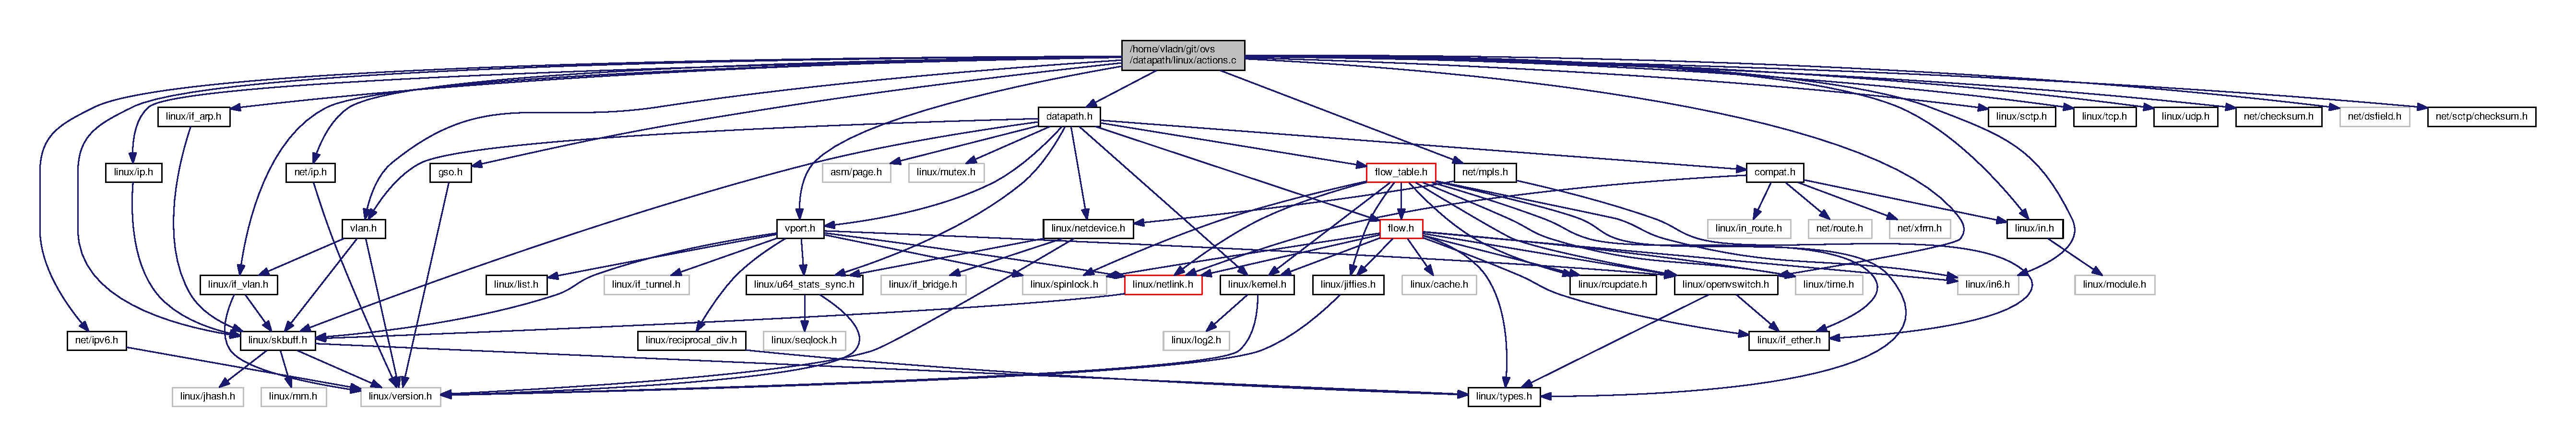
\includegraphics[width=350pt]{linux_2actions_8c__incl}
\end{center}
\end{figure}
\subsection*{Data Structures}
\begin{DoxyCompactItemize}
\item 
struct \hyperlink{structdeferred__action}{deferred\+\_\+action}
\item 
struct \hyperlink{structaction__fifo}{action\+\_\+fifo}
\end{DoxyCompactItemize}
\subsection*{Macros}
\begin{DoxyCompactItemize}
\item 
\#define \hyperlink{linux_2actions_8c_a1f8c165bf4196327bc3abff648276d92}{pr\+\_\+fmt}(fmt)~K\+B\+U\+I\+L\+D\+\_\+\+M\+O\+D\+N\+A\+M\+E \char`\"{}\+: \char`\"{} fmt
\item 
\#define \hyperlink{linux_2actions_8c_acb72e0b273dae399e2619f619fd061ed}{D\+E\+F\+E\+R\+R\+E\+D\+\_\+\+A\+C\+T\+I\+O\+N\+\_\+\+F\+I\+F\+O\+\_\+\+S\+I\+Z\+E}~10
\item 
\#define \hyperlink{linux_2actions_8c_aef2488868338b5c1ec4419f0efde93f1}{E\+X\+E\+C\+\_\+\+A\+C\+T\+I\+O\+N\+S\+\_\+\+L\+E\+V\+E\+L\+\_\+\+L\+I\+M\+I\+T}
\item 
\#define \hyperlink{linux_2actions_8c_a7e29e4ea7eef8e6a17ec80459c178a14}{M\+A\+S\+K\+E\+D}(O\+L\+D,  K\+E\+Y,  M\+A\+S\+K)~((K\+E\+Y) $\vert$ ((O\+L\+D) \& $\sim$(M\+A\+S\+K)))
\item 
\#define \hyperlink{linux_2actions_8c_a6a812b08a711cd6258c60e9bd0c931e3}{S\+E\+T\+\_\+\+M\+A\+S\+K\+E\+D}(O\+L\+D,  K\+E\+Y,  M\+A\+S\+K)~((O\+L\+D) = \hyperlink{linux_2actions_8c_a7e29e4ea7eef8e6a17ec80459c178a14}{M\+A\+S\+K\+E\+D}(O\+L\+D, K\+E\+Y, M\+A\+S\+K))
\item 
\#define \hyperlink{linux_2actions_8c_aa0c451dc85a82947bdf6d8ae3c2385b5}{get\+\_\+mask}(a,  \hyperlink{flow_8h_ab22aaab04f806700def00f32823fcb9e}{type})~((const \hyperlink{flow_8h_ab22aaab04f806700def00f32823fcb9e}{type})nla\+\_\+data(a) + 1)
\end{DoxyCompactItemize}
\subsection*{Functions}
\begin{DoxyCompactItemize}
\item 
static int \hyperlink{linux_2actions_8c_ad41a07588c602d50a247bcf2bf9ae9d5}{do\+\_\+execute\+\_\+actions} (struct \hyperlink{structdatapath}{datapath} $\ast$dp, struct sk\+\_\+buff $\ast$skb, struct \hyperlink{structsw__flow__key}{sw\+\_\+flow\+\_\+key} $\ast$key, const struct nlattr $\ast$attr, int len)
\item 
static \hyperlink{linux_2actions_8c_aacdc7977b799c6e2275e312793f87dcd}{D\+E\+F\+I\+N\+E\+\_\+\+P\+E\+R\+\_\+\+C\+P\+U} (int, exec\+\_\+actions\+\_\+level)
\item 
static void \hyperlink{linux_2actions_8c_a688872dd5196a430f6a0df6e1954d220}{action\+\_\+fifo\+\_\+init} (struct \hyperlink{structaction__fifo}{action\+\_\+fifo} $\ast$fifo)
\item 
static \hyperlink{types_8h_afaa87723b8417d40fcf45b7330261ef9}{bool} \hyperlink{linux_2actions_8c_ade23c3824a292e4698cb3c01fefa52a5}{action\+\_\+fifo\+\_\+is\+\_\+empty} (const struct \hyperlink{structaction__fifo}{action\+\_\+fifo} $\ast$fifo)
\item 
static struct \hyperlink{structdeferred__action}{deferred\+\_\+action} $\ast$ \hyperlink{linux_2actions_8c_a7512da42cda457a824bb2fc8ff850dd5}{action\+\_\+fifo\+\_\+get} (struct \hyperlink{structaction__fifo}{action\+\_\+fifo} $\ast$fifo)
\item 
static struct \hyperlink{structdeferred__action}{deferred\+\_\+action} $\ast$ \hyperlink{linux_2actions_8c_a3c8c974792d662e29d50b97ae044a068}{action\+\_\+fifo\+\_\+put} (struct \hyperlink{structaction__fifo}{action\+\_\+fifo} $\ast$fifo)
\item 
static struct \hyperlink{structdeferred__action}{deferred\+\_\+action} $\ast$ \hyperlink{linux_2actions_8c_a3875097b6e35686ddee414782d0e67b1}{add\+\_\+deferred\+\_\+actions} (struct sk\+\_\+buff $\ast$skb, const struct \hyperlink{structsw__flow__key}{sw\+\_\+flow\+\_\+key} $\ast$key, const struct nlattr $\ast$attr)
\item 
static void \hyperlink{linux_2actions_8c_aac28ee49d1019a576306f207afd5f8d6}{invalidate\+\_\+flow\+\_\+key} (struct \hyperlink{structsw__flow__key}{sw\+\_\+flow\+\_\+key} $\ast$key)
\item 
static \hyperlink{types_8h_afaa87723b8417d40fcf45b7330261ef9}{bool} \hyperlink{linux_2actions_8c_a77e3320f8f43a04aaf952a2c82e6dac1}{is\+\_\+flow\+\_\+key\+\_\+valid} (const struct \hyperlink{structsw__flow__key}{sw\+\_\+flow\+\_\+key} $\ast$key)
\item 
static int \hyperlink{linux_2actions_8c_affb38ca95e088fb61d6df91cf3fdd606}{push\+\_\+mpls} (struct sk\+\_\+buff $\ast$skb, struct \hyperlink{structsw__flow__key}{sw\+\_\+flow\+\_\+key} $\ast$key, const struct \hyperlink{structovs__action__push__mpls}{ovs\+\_\+action\+\_\+push\+\_\+mpls} $\ast$\hyperlink{flow_8h_aeab2d67b4ec58a9575da76c323ad95ce}{mpls})
\item 
static int \hyperlink{linux_2actions_8c_ac372daa8a5c4eb7fb2536fa61653e41b}{pop\+\_\+mpls} (struct sk\+\_\+buff $\ast$skb, struct \hyperlink{structsw__flow__key}{sw\+\_\+flow\+\_\+key} $\ast$key, const \+\_\+\+\_\+be16 ethertype)
\item 
static int \hyperlink{linux_2actions_8c_ad66261c51831d2a4a6ff0ea385fbad32}{set\+\_\+mpls} (struct sk\+\_\+buff $\ast$skb, struct \hyperlink{structsw__flow__key}{sw\+\_\+flow\+\_\+key} $\ast$flow\+\_\+key, const \+\_\+\+\_\+be32 $\ast$mpls\+\_\+lse, const \+\_\+\+\_\+be32 $\ast$mask)
\item 
static int \hyperlink{linux_2actions_8c_aa11b6c74e2206cc8353d00cff409df22}{pop\+\_\+vlan} (struct sk\+\_\+buff $\ast$skb, struct \hyperlink{structsw__flow__key}{sw\+\_\+flow\+\_\+key} $\ast$key)
\item 
static int \hyperlink{linux_2actions_8c_a706c437e9fb3992afaa8f62605c59961}{push\+\_\+vlan} (struct sk\+\_\+buff $\ast$skb, struct \hyperlink{structsw__flow__key}{sw\+\_\+flow\+\_\+key} $\ast$key, const struct \hyperlink{structovs__action__push__vlan}{ovs\+\_\+action\+\_\+push\+\_\+vlan} $\ast$vlan)
\item 
static void \hyperlink{linux_2actions_8c_a2d434306a1e37e8bd0572dab35cc68ca}{ether\+\_\+addr\+\_\+copy\+\_\+masked} (u8 $\ast$dst\+\_\+, const u8 $\ast$src\+\_\+, const u8 $\ast$mask\+\_\+)
\item 
static int \hyperlink{linux_2actions_8c_a85d6da67a26cfee7c3c894131233f9ca}{set\+\_\+eth\+\_\+addr} (struct sk\+\_\+buff $\ast$skb, struct \hyperlink{structsw__flow__key}{sw\+\_\+flow\+\_\+key} $\ast$flow\+\_\+key, const struct \hyperlink{structovs__key__ethernet}{ovs\+\_\+key\+\_\+ethernet} $\ast$key, const struct \hyperlink{structovs__key__ethernet}{ovs\+\_\+key\+\_\+ethernet} $\ast$mask)
\item 
static void \hyperlink{linux_2actions_8c_a35283087cadb66ada3c19e7a87cfdcba}{set\+\_\+ip\+\_\+addr} (struct sk\+\_\+buff $\ast$skb, struct iphdr $\ast$nh, \+\_\+\+\_\+be32 $\ast$\hyperlink{flow_8h_a535ce925c585c41d434f7481f342c976}{addr}, \+\_\+\+\_\+be32 new\+\_\+addr)
\item 
static void \hyperlink{linux_2actions_8c_a006120c8695be3960f274e88e24b535a}{update\+\_\+ipv6\+\_\+checksum} (struct sk\+\_\+buff $\ast$skb, u8 l4\+\_\+proto, \+\_\+\+\_\+be32 \hyperlink{flow_8h_a535ce925c585c41d434f7481f342c976}{addr}\mbox{[}4\mbox{]}, const \+\_\+\+\_\+be32 new\+\_\+addr\mbox{[}4\mbox{]})
\item 
static void \hyperlink{linux_2actions_8c_affe65b5dd55e3a7c39c5a6705731f01f}{mask\+\_\+ipv6\+\_\+addr} (const \+\_\+\+\_\+be32 old\mbox{[}4\mbox{]}, const \+\_\+\+\_\+be32 \hyperlink{flow_8h_a535ce925c585c41d434f7481f342c976}{addr}\mbox{[}4\mbox{]}, const \+\_\+\+\_\+be32 mask\mbox{[}4\mbox{]}, \+\_\+\+\_\+be32 masked\mbox{[}4\mbox{]})
\item 
static void \hyperlink{linux_2actions_8c_aa39edf0f0aa23ee17d2828e1c42b0590}{set\+\_\+ipv6\+\_\+addr} (struct sk\+\_\+buff $\ast$skb, u8 l4\+\_\+proto, \+\_\+\+\_\+be32 \hyperlink{flow_8h_a535ce925c585c41d434f7481f342c976}{addr}\mbox{[}4\mbox{]}, const \+\_\+\+\_\+be32 new\+\_\+addr\mbox{[}4\mbox{]}, \hyperlink{types_8h_afaa87723b8417d40fcf45b7330261ef9}{bool} recalculate\+\_\+csum)
\item 
static void \hyperlink{linux_2actions_8c_a105b45d892887e581acec50af165e330}{set\+\_\+ipv6\+\_\+fl} (struct ipv6hdr $\ast$nh, u32 fl, u32 mask)
\item 
static void \hyperlink{linux_2actions_8c_a00bc919dc7a6a81f506155c0372eba9b}{set\+\_\+ip\+\_\+ttl} (struct sk\+\_\+buff $\ast$skb, struct iphdr $\ast$nh, u8 new\+\_\+ttl, u8 mask)
\item 
static int \hyperlink{linux_2actions_8c_a5b6148caa3654ee968f7173b83b3abf4}{set\+\_\+ipv4} (struct sk\+\_\+buff $\ast$skb, struct \hyperlink{structsw__flow__key}{sw\+\_\+flow\+\_\+key} $\ast$flow\+\_\+key, const struct \hyperlink{structovs__key__ipv4}{ovs\+\_\+key\+\_\+ipv4} $\ast$key, const struct \hyperlink{structovs__key__ipv4}{ovs\+\_\+key\+\_\+ipv4} $\ast$mask)
\item 
static \hyperlink{types_8h_afaa87723b8417d40fcf45b7330261ef9}{bool} \hyperlink{linux_2actions_8c_a889a29de7d27314b273304eaad6f202e}{is\+\_\+ipv6\+\_\+mask\+\_\+nonzero} (const \+\_\+\+\_\+be32 \hyperlink{flow_8h_a535ce925c585c41d434f7481f342c976}{addr}\mbox{[}4\mbox{]})
\item 
static int \hyperlink{linux_2actions_8c_acf538956396fdb59cff22ad4577c10f3}{set\+\_\+ipv6} (struct sk\+\_\+buff $\ast$skb, struct \hyperlink{structsw__flow__key}{sw\+\_\+flow\+\_\+key} $\ast$flow\+\_\+key, const struct \hyperlink{structovs__key__ipv6}{ovs\+\_\+key\+\_\+ipv6} $\ast$key, const struct \hyperlink{structovs__key__ipv6}{ovs\+\_\+key\+\_\+ipv6} $\ast$mask)
\item 
static void \hyperlink{linux_2actions_8c_a485b30c5af82b861079002c3e8899f7d}{set\+\_\+tp\+\_\+port} (struct sk\+\_\+buff $\ast$skb, \+\_\+\+\_\+be16 $\ast$port, \+\_\+\+\_\+be16 new\+\_\+port, \hyperlink{types_8h_a2fdf5566d289d6941c29db084139bf23}{\+\_\+\+\_\+sum16} $\ast$check)
\item 
static int \hyperlink{linux_2actions_8c_ae78d854d13e952f67ca0d0b7bc45be75}{set\+\_\+udp} (struct sk\+\_\+buff $\ast$skb, struct \hyperlink{structsw__flow__key}{sw\+\_\+flow\+\_\+key} $\ast$flow\+\_\+key, const struct \hyperlink{structovs__key__udp}{ovs\+\_\+key\+\_\+udp} $\ast$key, const struct \hyperlink{structovs__key__udp}{ovs\+\_\+key\+\_\+udp} $\ast$mask)
\item 
static int \hyperlink{linux_2actions_8c_a3f6591203112ded2452b368308b0f36b}{set\+\_\+tcp} (struct sk\+\_\+buff $\ast$skb, struct \hyperlink{structsw__flow__key}{sw\+\_\+flow\+\_\+key} $\ast$flow\+\_\+key, const struct \hyperlink{structovs__key__tcp}{ovs\+\_\+key\+\_\+tcp} $\ast$key, const struct \hyperlink{structovs__key__tcp}{ovs\+\_\+key\+\_\+tcp} $\ast$mask)
\item 
static int \hyperlink{linux_2actions_8c_a7f2d96d4cc495e0f9f48c61305beea5c}{set\+\_\+sctp} (struct sk\+\_\+buff $\ast$skb, struct \hyperlink{structsw__flow__key}{sw\+\_\+flow\+\_\+key} $\ast$flow\+\_\+key, const struct \hyperlink{structovs__key__sctp}{ovs\+\_\+key\+\_\+sctp} $\ast$key, const struct \hyperlink{structovs__key__sctp}{ovs\+\_\+key\+\_\+sctp} $\ast$mask)
\item 
static void \hyperlink{linux_2actions_8c_a141467d4c8b6d03b33ca4a36b471fb1e}{do\+\_\+output} (struct \hyperlink{structdatapath}{datapath} $\ast$dp, struct sk\+\_\+buff $\ast$skb, int out\+\_\+port)
\item 
static int \hyperlink{linux_2actions_8c_ad0ea13ac8532fe548cd35a2d1086d8f3}{output\+\_\+userspace} (struct \hyperlink{structdatapath}{datapath} $\ast$dp, struct sk\+\_\+buff $\ast$skb, struct \hyperlink{structsw__flow__key}{sw\+\_\+flow\+\_\+key} $\ast$key, const struct nlattr $\ast$attr, const struct nlattr $\ast$actions, int actions\+\_\+len)
\item 
static int \hyperlink{linux_2actions_8c_a23b7fbefa6429cd4af2c92eb20c03889}{sample} (struct \hyperlink{structdatapath}{datapath} $\ast$dp, struct sk\+\_\+buff $\ast$skb, struct \hyperlink{structsw__flow__key}{sw\+\_\+flow\+\_\+key} $\ast$key, const struct nlattr $\ast$attr, const struct nlattr $\ast$actions, int actions\+\_\+len)
\item 
static void \hyperlink{linux_2actions_8c_a7f08d769ba6fb4cdd65ef7ced5964dea}{execute\+\_\+hash} (struct sk\+\_\+buff $\ast$skb, struct \hyperlink{structsw__flow__key}{sw\+\_\+flow\+\_\+key} $\ast$key, const struct nlattr $\ast$attr)
\item 
static int \hyperlink{linux_2actions_8c_a4a59d75b1d012debb4f8ab42d0672deb}{execute\+\_\+set\+\_\+action} (struct sk\+\_\+buff $\ast$skb, struct \hyperlink{structsw__flow__key}{sw\+\_\+flow\+\_\+key} $\ast$flow\+\_\+key, const struct nlattr $\ast$a)
\item 
static int \hyperlink{linux_2actions_8c_ae5d851747d2630c868c296b43ad3c2e7}{execute\+\_\+masked\+\_\+set\+\_\+action} (struct sk\+\_\+buff $\ast$skb, struct \hyperlink{structsw__flow__key}{sw\+\_\+flow\+\_\+key} $\ast$flow\+\_\+key, const struct nlattr $\ast$a)
\item 
static int \hyperlink{linux_2actions_8c_ab6b5b3b0684142f0e137bd64d883d52f}{execute\+\_\+recirc} (struct \hyperlink{structdatapath}{datapath} $\ast$dp, struct sk\+\_\+buff $\ast$skb, struct \hyperlink{structsw__flow__key}{sw\+\_\+flow\+\_\+key} $\ast$key, const struct nlattr $\ast$a, int rem)
\item 
static void \hyperlink{linux_2actions_8c_afa871a96ea915a7ce87b96a0b7b30538}{process\+\_\+deferred\+\_\+actions} (struct \hyperlink{structdatapath}{datapath} $\ast$dp)
\item 
int \hyperlink{linux_2actions_8c_a5b34c1980d155574d657a21cac3bcc37}{ovs\+\_\+execute\+\_\+actions} (struct \hyperlink{structdatapath}{datapath} $\ast$dp, struct sk\+\_\+buff $\ast$skb, const struct \hyperlink{structsw__flow__actions}{sw\+\_\+flow\+\_\+actions} $\ast$acts, struct \hyperlink{structsw__flow__key}{sw\+\_\+flow\+\_\+key} $\ast$key)
\item 
int \hyperlink{linux_2actions_8c_a3006f0376c2aecb6525126ad0e9bae25}{action\+\_\+fifos\+\_\+init} (void)
\item 
void \hyperlink{linux_2actions_8c_a7dfd1f218e0966ef342251a185866f4d}{action\+\_\+fifos\+\_\+exit} (void)
\end{DoxyCompactItemize}
\subsection*{Variables}
\begin{DoxyCompactItemize}
\item 
static struct \hyperlink{structaction__fifo}{action\+\_\+fifo} \hyperlink{compiler_8h_a497f20279760cdb59a5187689f9f5ab1}{\+\_\+\+\_\+percpu} $\ast$ \hyperlink{linux_2actions_8c_a38c6295376dbb80340f4f1b8e488f223}{action\+\_\+fifos}
\end{DoxyCompactItemize}


\subsection{Macro Definition Documentation}
\hypertarget{linux_2actions_8c_acb72e0b273dae399e2619f619fd061ed}{}\index{linux/actions.\+c@{linux/actions.\+c}!D\+E\+F\+E\+R\+R\+E\+D\+\_\+\+A\+C\+T\+I\+O\+N\+\_\+\+F\+I\+F\+O\+\_\+\+S\+I\+Z\+E@{D\+E\+F\+E\+R\+R\+E\+D\+\_\+\+A\+C\+T\+I\+O\+N\+\_\+\+F\+I\+F\+O\+\_\+\+S\+I\+Z\+E}}
\index{D\+E\+F\+E\+R\+R\+E\+D\+\_\+\+A\+C\+T\+I\+O\+N\+\_\+\+F\+I\+F\+O\+\_\+\+S\+I\+Z\+E@{D\+E\+F\+E\+R\+R\+E\+D\+\_\+\+A\+C\+T\+I\+O\+N\+\_\+\+F\+I\+F\+O\+\_\+\+S\+I\+Z\+E}!linux/actions.\+c@{linux/actions.\+c}}
\subsubsection[{D\+E\+F\+E\+R\+R\+E\+D\+\_\+\+A\+C\+T\+I\+O\+N\+\_\+\+F\+I\+F\+O\+\_\+\+S\+I\+Z\+E}]{\setlength{\rightskip}{0pt plus 5cm}\#define D\+E\+F\+E\+R\+R\+E\+D\+\_\+\+A\+C\+T\+I\+O\+N\+\_\+\+F\+I\+F\+O\+\_\+\+S\+I\+Z\+E~10}\label{linux_2actions_8c_acb72e0b273dae399e2619f619fd061ed}
\hypertarget{linux_2actions_8c_aef2488868338b5c1ec4419f0efde93f1}{}\index{linux/actions.\+c@{linux/actions.\+c}!E\+X\+E\+C\+\_\+\+A\+C\+T\+I\+O\+N\+S\+\_\+\+L\+E\+V\+E\+L\+\_\+\+L\+I\+M\+I\+T@{E\+X\+E\+C\+\_\+\+A\+C\+T\+I\+O\+N\+S\+\_\+\+L\+E\+V\+E\+L\+\_\+\+L\+I\+M\+I\+T}}
\index{E\+X\+E\+C\+\_\+\+A\+C\+T\+I\+O\+N\+S\+\_\+\+L\+E\+V\+E\+L\+\_\+\+L\+I\+M\+I\+T@{E\+X\+E\+C\+\_\+\+A\+C\+T\+I\+O\+N\+S\+\_\+\+L\+E\+V\+E\+L\+\_\+\+L\+I\+M\+I\+T}!linux/actions.\+c@{linux/actions.\+c}}
\subsubsection[{E\+X\+E\+C\+\_\+\+A\+C\+T\+I\+O\+N\+S\+\_\+\+L\+E\+V\+E\+L\+\_\+\+L\+I\+M\+I\+T}]{\setlength{\rightskip}{0pt plus 5cm}\#define E\+X\+E\+C\+\_\+\+A\+C\+T\+I\+O\+N\+S\+\_\+\+L\+E\+V\+E\+L\+\_\+\+L\+I\+M\+I\+T}\label{linux_2actions_8c_aef2488868338b5c1ec4419f0efde93f1}
{\bfseries Value\+:}
\begin{DoxyCode}
4   \textcolor{comment}{/* limit used to detect packet}
\textcolor{comment}{                      * looping by the network stack}
\textcolor{comment}{                      */}
\end{DoxyCode}
\hypertarget{linux_2actions_8c_aa0c451dc85a82947bdf6d8ae3c2385b5}{}\index{linux/actions.\+c@{linux/actions.\+c}!get\+\_\+mask@{get\+\_\+mask}}
\index{get\+\_\+mask@{get\+\_\+mask}!linux/actions.\+c@{linux/actions.\+c}}
\subsubsection[{get\+\_\+mask}]{\setlength{\rightskip}{0pt plus 5cm}\#define get\+\_\+mask(
\begin{DoxyParamCaption}
\item[{}]{a, }
\item[{}]{{\bf type}}
\end{DoxyParamCaption}
)~((const {\bf type})nla\+\_\+data(a) + 1)}\label{linux_2actions_8c_aa0c451dc85a82947bdf6d8ae3c2385b5}
\hypertarget{linux_2actions_8c_a7e29e4ea7eef8e6a17ec80459c178a14}{}\index{linux/actions.\+c@{linux/actions.\+c}!M\+A\+S\+K\+E\+D@{M\+A\+S\+K\+E\+D}}
\index{M\+A\+S\+K\+E\+D@{M\+A\+S\+K\+E\+D}!linux/actions.\+c@{linux/actions.\+c}}
\subsubsection[{M\+A\+S\+K\+E\+D}]{\setlength{\rightskip}{0pt plus 5cm}\#define M\+A\+S\+K\+E\+D(
\begin{DoxyParamCaption}
\item[{}]{O\+L\+D, }
\item[{}]{K\+E\+Y, }
\item[{}]{M\+A\+S\+K}
\end{DoxyParamCaption}
)~((K\+E\+Y) $\vert$ ((O\+L\+D) \& $\sim$(M\+A\+S\+K)))}\label{linux_2actions_8c_a7e29e4ea7eef8e6a17ec80459c178a14}
\hypertarget{linux_2actions_8c_a1f8c165bf4196327bc3abff648276d92}{}\index{linux/actions.\+c@{linux/actions.\+c}!pr\+\_\+fmt@{pr\+\_\+fmt}}
\index{pr\+\_\+fmt@{pr\+\_\+fmt}!linux/actions.\+c@{linux/actions.\+c}}
\subsubsection[{pr\+\_\+fmt}]{\setlength{\rightskip}{0pt plus 5cm}\#define pr\+\_\+fmt(
\begin{DoxyParamCaption}
\item[{}]{fmt}
\end{DoxyParamCaption}
)~K\+B\+U\+I\+L\+D\+\_\+\+M\+O\+D\+N\+A\+M\+E \char`\"{}\+: \char`\"{} fmt}\label{linux_2actions_8c_a1f8c165bf4196327bc3abff648276d92}
\hypertarget{linux_2actions_8c_a6a812b08a711cd6258c60e9bd0c931e3}{}\index{linux/actions.\+c@{linux/actions.\+c}!S\+E\+T\+\_\+\+M\+A\+S\+K\+E\+D@{S\+E\+T\+\_\+\+M\+A\+S\+K\+E\+D}}
\index{S\+E\+T\+\_\+\+M\+A\+S\+K\+E\+D@{S\+E\+T\+\_\+\+M\+A\+S\+K\+E\+D}!linux/actions.\+c@{linux/actions.\+c}}
\subsubsection[{S\+E\+T\+\_\+\+M\+A\+S\+K\+E\+D}]{\setlength{\rightskip}{0pt plus 5cm}\#define S\+E\+T\+\_\+\+M\+A\+S\+K\+E\+D(
\begin{DoxyParamCaption}
\item[{}]{O\+L\+D, }
\item[{}]{K\+E\+Y, }
\item[{}]{M\+A\+S\+K}
\end{DoxyParamCaption}
)~((O\+L\+D) = {\bf M\+A\+S\+K\+E\+D}(O\+L\+D, K\+E\+Y, M\+A\+S\+K))}\label{linux_2actions_8c_a6a812b08a711cd6258c60e9bd0c931e3}


\subsection{Function Documentation}
\hypertarget{linux_2actions_8c_a7512da42cda457a824bb2fc8ff850dd5}{}\index{linux/actions.\+c@{linux/actions.\+c}!action\+\_\+fifo\+\_\+get@{action\+\_\+fifo\+\_\+get}}
\index{action\+\_\+fifo\+\_\+get@{action\+\_\+fifo\+\_\+get}!linux/actions.\+c@{linux/actions.\+c}}
\subsubsection[{action\+\_\+fifo\+\_\+get}]{\setlength{\rightskip}{0pt plus 5cm}static struct {\bf deferred\+\_\+action}$\ast$ action\+\_\+fifo\+\_\+get (
\begin{DoxyParamCaption}
\item[{struct {\bf action\+\_\+fifo} $\ast$}]{fifo}
\end{DoxyParamCaption}
)\hspace{0.3cm}{\ttfamily [static]}}\label{linux_2actions_8c_a7512da42cda457a824bb2fc8ff850dd5}

\begin{DoxyCode}
82 \{
83     \textcolor{keywordflow}{if} (\hyperlink{linux_2actions_8c_ade23c3824a292e4698cb3c01fefa52a5}{action\_fifo\_is\_empty}(fifo))
84         \textcolor{keywordflow}{return} NULL;
85 
86     \textcolor{keywordflow}{return} &fifo->\hyperlink{structaction__fifo_ab25b47c1bc05f5417f0a2073a47b2eb5}{fifo}[fifo->\hyperlink{structaction__fifo_a60805cbdf935d6718f685c7374ae9493}{tail}++];
87 \}
\end{DoxyCode}
\hypertarget{linux_2actions_8c_a688872dd5196a430f6a0df6e1954d220}{}\index{linux/actions.\+c@{linux/actions.\+c}!action\+\_\+fifo\+\_\+init@{action\+\_\+fifo\+\_\+init}}
\index{action\+\_\+fifo\+\_\+init@{action\+\_\+fifo\+\_\+init}!linux/actions.\+c@{linux/actions.\+c}}
\subsubsection[{action\+\_\+fifo\+\_\+init}]{\setlength{\rightskip}{0pt plus 5cm}static void action\+\_\+fifo\+\_\+init (
\begin{DoxyParamCaption}
\item[{struct {\bf action\+\_\+fifo} $\ast$}]{fifo}
\end{DoxyParamCaption}
)\hspace{0.3cm}{\ttfamily [static]}}\label{linux_2actions_8c_a688872dd5196a430f6a0df6e1954d220}

\begin{DoxyCode}
71 \{
72     fifo->\hyperlink{structaction__fifo_a5376b4a5c9dbfd84303d156a47ed9018}{head} = 0;
73     fifo->\hyperlink{structaction__fifo_a60805cbdf935d6718f685c7374ae9493}{tail} = 0;
74 \}
\end{DoxyCode}
\hypertarget{linux_2actions_8c_ade23c3824a292e4698cb3c01fefa52a5}{}\index{linux/actions.\+c@{linux/actions.\+c}!action\+\_\+fifo\+\_\+is\+\_\+empty@{action\+\_\+fifo\+\_\+is\+\_\+empty}}
\index{action\+\_\+fifo\+\_\+is\+\_\+empty@{action\+\_\+fifo\+\_\+is\+\_\+empty}!linux/actions.\+c@{linux/actions.\+c}}
\subsubsection[{action\+\_\+fifo\+\_\+is\+\_\+empty}]{\setlength{\rightskip}{0pt plus 5cm}static {\bf bool} action\+\_\+fifo\+\_\+is\+\_\+empty (
\begin{DoxyParamCaption}
\item[{const struct {\bf action\+\_\+fifo} $\ast$}]{fifo}
\end{DoxyParamCaption}
)\hspace{0.3cm}{\ttfamily [static]}}\label{linux_2actions_8c_ade23c3824a292e4698cb3c01fefa52a5}

\begin{DoxyCode}
77 \{
78     \textcolor{keywordflow}{return} (fifo->\hyperlink{structaction__fifo_a5376b4a5c9dbfd84303d156a47ed9018}{head} == fifo->\hyperlink{structaction__fifo_a60805cbdf935d6718f685c7374ae9493}{tail});
79 \}
\end{DoxyCode}
\hypertarget{linux_2actions_8c_a3c8c974792d662e29d50b97ae044a068}{}\index{linux/actions.\+c@{linux/actions.\+c}!action\+\_\+fifo\+\_\+put@{action\+\_\+fifo\+\_\+put}}
\index{action\+\_\+fifo\+\_\+put@{action\+\_\+fifo\+\_\+put}!linux/actions.\+c@{linux/actions.\+c}}
\subsubsection[{action\+\_\+fifo\+\_\+put}]{\setlength{\rightskip}{0pt plus 5cm}static struct {\bf deferred\+\_\+action}$\ast$ action\+\_\+fifo\+\_\+put (
\begin{DoxyParamCaption}
\item[{struct {\bf action\+\_\+fifo} $\ast$}]{fifo}
\end{DoxyParamCaption}
)\hspace{0.3cm}{\ttfamily [static]}}\label{linux_2actions_8c_a3c8c974792d662e29d50b97ae044a068}

\begin{DoxyCode}
90 \{
91     \textcolor{keywordflow}{if} (fifo->\hyperlink{structaction__fifo_a5376b4a5c9dbfd84303d156a47ed9018}{head} >= \hyperlink{linux_2actions_8c_acb72e0b273dae399e2619f619fd061ed}{DEFERRED\_ACTION\_FIFO\_SIZE} - 1)
92         \textcolor{keywordflow}{return} NULL;
93 
94     \textcolor{keywordflow}{return} &fifo->\hyperlink{structaction__fifo_ab25b47c1bc05f5417f0a2073a47b2eb5}{fifo}[fifo->\hyperlink{structaction__fifo_a5376b4a5c9dbfd84303d156a47ed9018}{head}++];
95 \}
\end{DoxyCode}
\hypertarget{linux_2actions_8c_a7dfd1f218e0966ef342251a185866f4d}{}\index{linux/actions.\+c@{linux/actions.\+c}!action\+\_\+fifos\+\_\+exit@{action\+\_\+fifos\+\_\+exit}}
\index{action\+\_\+fifos\+\_\+exit@{action\+\_\+fifos\+\_\+exit}!linux/actions.\+c@{linux/actions.\+c}}
\subsubsection[{action\+\_\+fifos\+\_\+exit}]{\setlength{\rightskip}{0pt plus 5cm}void action\+\_\+fifos\+\_\+exit (
\begin{DoxyParamCaption}
\item[{void}]{}
\end{DoxyParamCaption}
)}\label{linux_2actions_8c_a7dfd1f218e0966ef342251a185866f4d}

\begin{DoxyCode}
1016 \{
1017     free\_percpu(\hyperlink{linux_2actions_8c_a38c6295376dbb80340f4f1b8e488f223}{action\_fifos});
1018 \}
\end{DoxyCode}
\hypertarget{linux_2actions_8c_a3006f0376c2aecb6525126ad0e9bae25}{}\index{linux/actions.\+c@{linux/actions.\+c}!action\+\_\+fifos\+\_\+init@{action\+\_\+fifos\+\_\+init}}
\index{action\+\_\+fifos\+\_\+init@{action\+\_\+fifos\+\_\+init}!linux/actions.\+c@{linux/actions.\+c}}
\subsubsection[{action\+\_\+fifos\+\_\+init}]{\setlength{\rightskip}{0pt plus 5cm}int action\+\_\+fifos\+\_\+init (
\begin{DoxyParamCaption}
\item[{void}]{}
\end{DoxyParamCaption}
)}\label{linux_2actions_8c_a3006f0376c2aecb6525126ad0e9bae25}

\begin{DoxyCode}
1007 \{
1008     \hyperlink{linux_2actions_8c_a38c6295376dbb80340f4f1b8e488f223}{action\_fifos} = alloc\_percpu(\textcolor{keyword}{struct} \hyperlink{structaction__fifo}{action\_fifo});
1009     \textcolor{keywordflow}{if} (!\hyperlink{linux_2actions_8c_a38c6295376dbb80340f4f1b8e488f223}{action\_fifos})
1010         \textcolor{keywordflow}{return} -ENOMEM;
1011 
1012     \textcolor{keywordflow}{return} 0;
1013 \}
\end{DoxyCode}
\hypertarget{linux_2actions_8c_a3875097b6e35686ddee414782d0e67b1}{}\index{linux/actions.\+c@{linux/actions.\+c}!add\+\_\+deferred\+\_\+actions@{add\+\_\+deferred\+\_\+actions}}
\index{add\+\_\+deferred\+\_\+actions@{add\+\_\+deferred\+\_\+actions}!linux/actions.\+c@{linux/actions.\+c}}
\subsubsection[{add\+\_\+deferred\+\_\+actions}]{\setlength{\rightskip}{0pt plus 5cm}static struct {\bf deferred\+\_\+action}$\ast$ add\+\_\+deferred\+\_\+actions (
\begin{DoxyParamCaption}
\item[{struct sk\+\_\+buff $\ast$}]{skb, }
\item[{const struct {\bf sw\+\_\+flow\+\_\+key} $\ast$}]{key, }
\item[{const struct nlattr $\ast$}]{attr}
\end{DoxyParamCaption}
)\hspace{0.3cm}{\ttfamily [static]}}\label{linux_2actions_8c_a3875097b6e35686ddee414782d0e67b1}

\begin{DoxyCode}
101 \{
102     \textcolor{keyword}{struct }\hyperlink{structaction__fifo}{action\_fifo} *\hyperlink{structaction__fifo_ab25b47c1bc05f5417f0a2073a47b2eb5}{fifo};
103     \textcolor{keyword}{struct }\hyperlink{structdeferred__action}{deferred\_action} *da;
104 
105     fifo = \hyperlink{percpu_8h_a1cd55f287dff5c4a79fc11dd38d47c12}{this\_cpu\_ptr}(\hyperlink{linux_2actions_8c_a38c6295376dbb80340f4f1b8e488f223}{action\_fifos});
106     da = \hyperlink{linux_2actions_8c_a3c8c974792d662e29d50b97ae044a068}{action\_fifo\_put}(fifo);
107     \textcolor{keywordflow}{if} (da) \{
108         da->\hyperlink{structdeferred__action_acba4fd12fba3d60b6f4c7f2f3159f316}{skb} = \hyperlink{structdeferred__action_acba4fd12fba3d60b6f4c7f2f3159f316}{skb};
109         da->\hyperlink{structdeferred__action_a9cb4d3dde378a66035e7b17f017d9f89}{actions} = attr;
110         da->\hyperlink{structdeferred__action_a4685f782001923a8f8c20510126b4c21}{pkt\_key} = *key;
111     \}
112 
113     \textcolor{keywordflow}{return} da;
114 \}
\end{DoxyCode}
\hypertarget{linux_2actions_8c_aacdc7977b799c6e2275e312793f87dcd}{}\index{linux/actions.\+c@{linux/actions.\+c}!D\+E\+F\+I\+N\+E\+\_\+\+P\+E\+R\+\_\+\+C\+P\+U@{D\+E\+F\+I\+N\+E\+\_\+\+P\+E\+R\+\_\+\+C\+P\+U}}
\index{D\+E\+F\+I\+N\+E\+\_\+\+P\+E\+R\+\_\+\+C\+P\+U@{D\+E\+F\+I\+N\+E\+\_\+\+P\+E\+R\+\_\+\+C\+P\+U}!linux/actions.\+c@{linux/actions.\+c}}
\subsubsection[{D\+E\+F\+I\+N\+E\+\_\+\+P\+E\+R\+\_\+\+C\+P\+U}]{\setlength{\rightskip}{0pt plus 5cm}static D\+E\+F\+I\+N\+E\+\_\+\+P\+E\+R\+\_\+\+C\+P\+U (
\begin{DoxyParamCaption}
\item[{int}]{, }
\item[{exec\+\_\+actions\+\_\+level}]{}
\end{DoxyParamCaption}
)\hspace{0.3cm}{\ttfamily [static]}}\label{linux_2actions_8c_aacdc7977b799c6e2275e312793f87dcd}
\hypertarget{linux_2actions_8c_ad41a07588c602d50a247bcf2bf9ae9d5}{}\index{linux/actions.\+c@{linux/actions.\+c}!do\+\_\+execute\+\_\+actions@{do\+\_\+execute\+\_\+actions}}
\index{do\+\_\+execute\+\_\+actions@{do\+\_\+execute\+\_\+actions}!linux/actions.\+c@{linux/actions.\+c}}
\subsubsection[{do\+\_\+execute\+\_\+actions}]{\setlength{\rightskip}{0pt plus 5cm}static int do\+\_\+execute\+\_\+actions (
\begin{DoxyParamCaption}
\item[{struct {\bf datapath} $\ast$}]{dp, }
\item[{struct sk\+\_\+buff $\ast$}]{skb, }
\item[{struct {\bf sw\+\_\+flow\+\_\+key} $\ast$}]{key, }
\item[{const struct nlattr $\ast$}]{attr, }
\item[{int}]{len}
\end{DoxyParamCaption}
)\hspace{0.3cm}{\ttfamily [static]}}\label{linux_2actions_8c_ad41a07588c602d50a247bcf2bf9ae9d5}

\begin{DoxyCode}
856 \{
857     \textcolor{comment}{/* Every output action needs a separate clone of 'skb', but the common}
858 \textcolor{comment}{     * case is just a single output action, so that doing a clone and}
859 \textcolor{comment}{     * then freeing the original skbuff is wasteful.  So the following code}
860 \textcolor{comment}{     * is slightly obscure just to avoid that.}
861 \textcolor{comment}{     */}
862     \textcolor{keywordtype}{int} prev\_port = -1;
863     \textcolor{keyword}{const} \textcolor{keyword}{struct }nlattr *a;
864     \textcolor{keywordtype}{int} rem;
865 
866     \textcolor{keywordflow}{for} (a = attr, rem = len; rem > 0;
867          a = nla\_next(a, &rem)) \{
868         \textcolor{keywordtype}{int} err = 0;
869 
870         \textcolor{keywordflow}{if} (unlikely(prev\_port != -1)) \{
871             \textcolor{keyword}{struct }sk\_buff *out\_skb = skb\_clone(skb, GFP\_ATOMIC);
872 
873             \textcolor{keywordflow}{if} (out\_skb)
874                 \hyperlink{linux_2actions_8c_a141467d4c8b6d03b33ca4a36b471fb1e}{do\_output}(dp, out\_skb, prev\_port);
875 
876             prev\_port = -1;
877         \}
878 
879         \textcolor{keywordflow}{switch} (nla\_type(a)) \{
880         \textcolor{keywordflow}{case} \hyperlink{openvswitch_8h_affc4a4d29437ad03a23444243e2db26eacad69687bf2bfae5092ea828cf0d4fe2}{OVS\_ACTION\_ATTR\_OUTPUT}:
881             prev\_port = nla\_get\_u32(a);
882             \textcolor{keywordflow}{break};
883 
884         \textcolor{keywordflow}{case} \hyperlink{openvswitch_8h_affc4a4d29437ad03a23444243e2db26ea17132af22505d8b1bb535a270f83a8bd}{OVS\_ACTION\_ATTR\_USERSPACE}:
885             \hyperlink{linux_2actions_8c_ad0ea13ac8532fe548cd35a2d1086d8f3}{output\_userspace}(dp, skb, key, a, attr, len);
886             \textcolor{keywordflow}{break};
887 
888         \textcolor{keywordflow}{case} \hyperlink{openvswitch_8h_affc4a4d29437ad03a23444243e2db26eaa783c1e8488baea181d3497e0e9676f9}{OVS\_ACTION\_ATTR\_HASH}:
889             \hyperlink{linux_2actions_8c_a7f08d769ba6fb4cdd65ef7ced5964dea}{execute\_hash}(skb, key, a);
890             \textcolor{keywordflow}{break};
891 
892         \textcolor{keywordflow}{case} \hyperlink{openvswitch_8h_affc4a4d29437ad03a23444243e2db26eafb68488325a1ab2d6bfb67ea115a5cdb}{OVS\_ACTION\_ATTR\_PUSH\_MPLS}:
893             err = \hyperlink{linux_2actions_8c_affb38ca95e088fb61d6df91cf3fdd606}{push\_mpls}(skb, key, nla\_data(a));
894             \textcolor{keywordflow}{break};
895 
896         \textcolor{keywordflow}{case} \hyperlink{openvswitch_8h_affc4a4d29437ad03a23444243e2db26eafe4ec9b68459771a3ffd07d20cd628e1}{OVS\_ACTION\_ATTR\_POP\_MPLS}:
897             err = \hyperlink{linux_2actions_8c_ac372daa8a5c4eb7fb2536fa61653e41b}{pop\_mpls}(skb, key, \hyperlink{net_2netlink_8h_a5a9bc877c8fdbf9b3f2f85536aabcae0}{nla\_get\_be16}(a));
898             \textcolor{keywordflow}{break};
899 
900         \textcolor{keywordflow}{case} \hyperlink{openvswitch_8h_affc4a4d29437ad03a23444243e2db26ea6f41b7751556ff0acc2f4c6f94963ba6}{OVS\_ACTION\_ATTR\_PUSH\_VLAN}:
901             err = \hyperlink{linux_2actions_8c_a706c437e9fb3992afaa8f62605c59961}{push\_vlan}(skb, key, nla\_data(a));
902             \textcolor{keywordflow}{break};
903 
904         \textcolor{keywordflow}{case} \hyperlink{openvswitch_8h_affc4a4d29437ad03a23444243e2db26ea9cd4ec18560c7c3f81276cba51a96a24}{OVS\_ACTION\_ATTR\_POP\_VLAN}:
905             err = \hyperlink{linux_2actions_8c_aa11b6c74e2206cc8353d00cff409df22}{pop\_vlan}(skb, key);
906             \textcolor{keywordflow}{break};
907 
908         \textcolor{keywordflow}{case} \hyperlink{openvswitch_8h_affc4a4d29437ad03a23444243e2db26ea2cad0b08a7809d6e7cb1a9e86d73a47c}{OVS\_ACTION\_ATTR\_RECIRC}:
909             err = \hyperlink{linux_2actions_8c_ab6b5b3b0684142f0e137bd64d883d52f}{execute\_recirc}(dp, skb, key, a, rem);
910             \textcolor{keywordflow}{if} (\hyperlink{net_2netlink_8h_ad408a3a1db3cc544eb7a552246f3fb57}{nla\_is\_last}(a, rem)) \{
911                 \textcolor{comment}{/* If this is the last action, the skb has}
912 \textcolor{comment}{                 * been consumed or freed.}
913 \textcolor{comment}{                 * Return immediately.}
914 \textcolor{comment}{                 */}
915                 \textcolor{keywordflow}{return} err;
916             \}
917             \textcolor{keywordflow}{break};
918 
919         \textcolor{keywordflow}{case} \hyperlink{openvswitch_8h_affc4a4d29437ad03a23444243e2db26eaff937deb7687d0dd4b073c27aed9c8be}{OVS\_ACTION\_ATTR\_SET}:
920             err = \hyperlink{linux_2actions_8c_a4a59d75b1d012debb4f8ab42d0672deb}{execute\_set\_action}(skb, key, nla\_data(a));
921             \textcolor{keywordflow}{break};
922 
923         \textcolor{keywordflow}{case} \hyperlink{openvswitch_8h_affc4a4d29437ad03a23444243e2db26ea50a466abca8b11394e9364de28ebe03f}{OVS\_ACTION\_ATTR\_SET\_MASKED}:
924         \textcolor{keywordflow}{case} OVS\_ACTION\_ATTR\_SET\_TO\_MASKED:
925             err = \hyperlink{linux_2actions_8c_ae5d851747d2630c868c296b43ad3c2e7}{execute\_masked\_set\_action}(skb, key, nla\_data(a));
926             \textcolor{keywordflow}{break};
927 
928         \textcolor{keywordflow}{case} \hyperlink{openvswitch_8h_affc4a4d29437ad03a23444243e2db26eaddc6f70b9e8501e5bb90548373faf734}{OVS\_ACTION\_ATTR\_SAMPLE}:
929             err = \hyperlink{linux_2actions_8c_a23b7fbefa6429cd4af2c92eb20c03889}{sample}(dp, skb, key, a, attr, len);
930             \textcolor{keywordflow}{break};
931         \}
932 
933         \textcolor{keywordflow}{if} (unlikely(err)) \{
934             kfree\_skb(skb);
935             \textcolor{keywordflow}{return} err;
936         \}
937     \}
938 
939     \textcolor{keywordflow}{if} (prev\_port != -1)
940         \hyperlink{linux_2actions_8c_a141467d4c8b6d03b33ca4a36b471fb1e}{do\_output}(dp, skb, prev\_port);
941     \textcolor{keywordflow}{else}
942         \hyperlink{skbuff_8h_adc460a9e6dccf5557d55bbce8c7adb6a}{consume\_skb}(skb);
943 
944     \textcolor{keywordflow}{return} 0;
945 \}
\end{DoxyCode}
\hypertarget{linux_2actions_8c_a141467d4c8b6d03b33ca4a36b471fb1e}{}\index{linux/actions.\+c@{linux/actions.\+c}!do\+\_\+output@{do\+\_\+output}}
\index{do\+\_\+output@{do\+\_\+output}!linux/actions.\+c@{linux/actions.\+c}}
\subsubsection[{do\+\_\+output}]{\setlength{\rightskip}{0pt plus 5cm}static void do\+\_\+output (
\begin{DoxyParamCaption}
\item[{struct {\bf datapath} $\ast$}]{dp, }
\item[{struct sk\+\_\+buff $\ast$}]{skb, }
\item[{int}]{out\+\_\+port}
\end{DoxyParamCaption}
)\hspace{0.3cm}{\ttfamily [static]}}\label{linux_2actions_8c_a141467d4c8b6d03b33ca4a36b471fb1e}

\begin{DoxyCode}
604 \{
605     \textcolor{keyword}{struct }\hyperlink{structvport}{vport} *\hyperlink{structvport}{vport} = \hyperlink{datapath_8h_ac6f3c37a7850774112c03c6e88d89dc0}{ovs\_vport\_rcu}(dp, out\_port);
606 
607     \textcolor{keywordflow}{if} (likely(vport))
608         \hyperlink{linux_2vport_8c_abd74f3970bd7dc951b8399d00efe42d8}{ovs\_vport\_send}(vport, skb);
609     \textcolor{keywordflow}{else}
610         kfree\_skb(skb);
611 \}
\end{DoxyCode}
\hypertarget{linux_2actions_8c_a2d434306a1e37e8bd0572dab35cc68ca}{}\index{linux/actions.\+c@{linux/actions.\+c}!ether\+\_\+addr\+\_\+copy\+\_\+masked@{ether\+\_\+addr\+\_\+copy\+\_\+masked}}
\index{ether\+\_\+addr\+\_\+copy\+\_\+masked@{ether\+\_\+addr\+\_\+copy\+\_\+masked}!linux/actions.\+c@{linux/actions.\+c}}
\subsubsection[{ether\+\_\+addr\+\_\+copy\+\_\+masked}]{\setlength{\rightskip}{0pt plus 5cm}static void ether\+\_\+addr\+\_\+copy\+\_\+masked (
\begin{DoxyParamCaption}
\item[{u8 $\ast$}]{dst\+\_\+, }
\item[{const u8 $\ast$}]{src\+\_\+, }
\item[{const u8 $\ast$}]{mask\+\_\+}
\end{DoxyParamCaption}
)\hspace{0.3cm}{\ttfamily [static]}}\label{linux_2actions_8c_a2d434306a1e37e8bd0572dab35cc68ca}

\begin{DoxyCode}
245 \{
246     u16 *\hyperlink{flow_8h_a6747ad3b5d60480ea073cd12c9b78aaa}{dst} = (u16 *)dst\_;
247     \textcolor{keyword}{const} u16 *\hyperlink{flow_8h_a2e7e37e9dfe6465386d6c500f83ef144}{src} = (\textcolor{keyword}{const} u16 *)src\_;
248     \textcolor{keyword}{const} u16 *mask = (\textcolor{keyword}{const} u16 *)mask\_;
249 
250     \hyperlink{linux_2actions_8c_a6a812b08a711cd6258c60e9bd0c931e3}{SET\_MASKED}(dst[0], src[0], mask[0]);
251     \hyperlink{linux_2actions_8c_a6a812b08a711cd6258c60e9bd0c931e3}{SET\_MASKED}(dst[1], src[1], mask[1]);
252     \hyperlink{linux_2actions_8c_a6a812b08a711cd6258c60e9bd0c931e3}{SET\_MASKED}(dst[2], src[2], mask[2]);
253 \}
\end{DoxyCode}
\hypertarget{linux_2actions_8c_a7f08d769ba6fb4cdd65ef7ced5964dea}{}\index{linux/actions.\+c@{linux/actions.\+c}!execute\+\_\+hash@{execute\+\_\+hash}}
\index{execute\+\_\+hash@{execute\+\_\+hash}!linux/actions.\+c@{linux/actions.\+c}}
\subsubsection[{execute\+\_\+hash}]{\setlength{\rightskip}{0pt plus 5cm}static void execute\+\_\+hash (
\begin{DoxyParamCaption}
\item[{struct sk\+\_\+buff $\ast$}]{skb, }
\item[{struct {\bf sw\+\_\+flow\+\_\+key} $\ast$}]{key, }
\item[{const struct nlattr $\ast$}]{attr}
\end{DoxyParamCaption}
)\hspace{0.3cm}{\ttfamily [static]}}\label{linux_2actions_8c_a7f08d769ba6fb4cdd65ef7ced5964dea}

\begin{DoxyCode}
720 \{
721     \textcolor{keyword}{struct }\hyperlink{structovs__action__hash}{ovs\_action\_hash} *hash\_act = nla\_data(attr);
722     u32 hash = 0;
723 
724     \textcolor{comment}{/* OVS\_HASH\_ALG\_L4 is the only possible hash algorithm.  */}
725     hash = \hyperlink{skbuff_8h_acb236314b209f764af9aae7fbbb04311}{skb\_get\_hash}(skb);
726     hash = jhash\_1word(hash, hash\_act->\hyperlink{structovs__action__hash_a174855fe08c609dd3542de6e9e8a92ee}{hash\_basis});
727     \textcolor{keywordflow}{if} (!hash)
728         hash = 0x1;
729 
730     key->\hyperlink{structsw__flow__key_a73dd9402f1f54c321f6d704d9b018d15}{ovs\_flow\_hash} = hash;
731 \}
\end{DoxyCode}
\hypertarget{linux_2actions_8c_ae5d851747d2630c868c296b43ad3c2e7}{}\index{linux/actions.\+c@{linux/actions.\+c}!execute\+\_\+masked\+\_\+set\+\_\+action@{execute\+\_\+masked\+\_\+set\+\_\+action}}
\index{execute\+\_\+masked\+\_\+set\+\_\+action@{execute\+\_\+masked\+\_\+set\+\_\+action}!linux/actions.\+c@{linux/actions.\+c}}
\subsubsection[{execute\+\_\+masked\+\_\+set\+\_\+action}]{\setlength{\rightskip}{0pt plus 5cm}static int execute\+\_\+masked\+\_\+set\+\_\+action (
\begin{DoxyParamCaption}
\item[{struct sk\+\_\+buff $\ast$}]{skb, }
\item[{struct {\bf sw\+\_\+flow\+\_\+key} $\ast$}]{flow\+\_\+key, }
\item[{const struct nlattr $\ast$}]{a}
\end{DoxyParamCaption}
)\hspace{0.3cm}{\ttfamily [static]}}\label{linux_2actions_8c_ae5d851747d2630c868c296b43ad3c2e7}

\begin{DoxyCode}
752 \{
753     \textcolor{keywordtype}{int} err = 0;
754 
755     \textcolor{keywordflow}{switch} (nla\_type(a)) \{
756     \textcolor{keywordflow}{case} \hyperlink{openvswitch_8h_a6a279bc7098c9bc819c12355c9e07864a3dee91d2ad17f698e34ebb913fcef8bf}{OVS\_KEY\_ATTR\_PRIORITY}:
757         \hyperlink{linux_2actions_8c_a6a812b08a711cd6258c60e9bd0c931e3}{SET\_MASKED}(skb->priority, nla\_get\_u32(a), *\hyperlink{linux_2actions_8c_aa0c451dc85a82947bdf6d8ae3c2385b5}{get\_mask}(a, u32 *));
758         flow\_key->\hyperlink{structsw__flow__key_a57cbddb75a8d4fd859300bd34d98e84a}{phy}.\hyperlink{structsw__flow__key_a9dd898913d9faaec1ec970029e7fbb71}{priority} = skb->priority;
759         \textcolor{keywordflow}{break};
760 
761     \textcolor{keywordflow}{case} \hyperlink{openvswitch_8h_a6a279bc7098c9bc819c12355c9e07864a32f36d9e41b0fbae0746d67fa34340ad}{OVS\_KEY\_ATTR\_SKB\_MARK}:
762         \hyperlink{linux_2actions_8c_a6a812b08a711cd6258c60e9bd0c931e3}{SET\_MASKED}(skb->mark, nla\_get\_u32(a), *\hyperlink{linux_2actions_8c_aa0c451dc85a82947bdf6d8ae3c2385b5}{get\_mask}(a, u32 *));
763         flow\_key->\hyperlink{structsw__flow__key_a57cbddb75a8d4fd859300bd34d98e84a}{phy}.\hyperlink{structsw__flow__key_ae02571657f29397dcc45de8528f4ed05}{skb\_mark} = skb->mark;
764         \textcolor{keywordflow}{break};
765 
766     \textcolor{keywordflow}{case} OVS\_KEY\_ATTR\_TUNNEL\_INFO:
767         \textcolor{comment}{/* Masked data not supported for tunnel. */}
768         err = -EINVAL;
769         \textcolor{keywordflow}{break};
770 
771     \textcolor{keywordflow}{case} \hyperlink{openvswitch_8h_a6a279bc7098c9bc819c12355c9e07864a75127b87d8a2f36ae2c9aae2cf42cd56}{OVS\_KEY\_ATTR\_ETHERNET}:
772         err = \hyperlink{linux_2actions_8c_a85d6da67a26cfee7c3c894131233f9ca}{set\_eth\_addr}(skb, flow\_key, nla\_data(a),
773                    \hyperlink{linux_2actions_8c_aa0c451dc85a82947bdf6d8ae3c2385b5}{get\_mask}(a, \textcolor{keyword}{struct} \hyperlink{structovs__key__ethernet}{ovs\_key\_ethernet} *));
774         \textcolor{keywordflow}{break};
775 
776     \textcolor{keywordflow}{case} \hyperlink{openvswitch_8h_a6a279bc7098c9bc819c12355c9e07864a67c672ef69eb0c5db9136812e3cdd92e}{OVS\_KEY\_ATTR\_IPV4}:
777         err = \hyperlink{linux_2actions_8c_a5b6148caa3654ee968f7173b83b3abf4}{set\_ipv4}(skb, flow\_key, nla\_data(a),
778                    \hyperlink{linux_2actions_8c_aa0c451dc85a82947bdf6d8ae3c2385b5}{get\_mask}(a, \textcolor{keyword}{struct} \hyperlink{structovs__key__ipv4}{ovs\_key\_ipv4} *));
779         \textcolor{keywordflow}{break};
780 
781     \textcolor{keywordflow}{case} \hyperlink{openvswitch_8h_a6a279bc7098c9bc819c12355c9e07864aff74bae1efeecfd5d6cf28d8987a8bfd}{OVS\_KEY\_ATTR\_IPV6}:
782         err = \hyperlink{linux_2actions_8c_acf538956396fdb59cff22ad4577c10f3}{set\_ipv6}(skb, flow\_key, nla\_data(a),
783                    \hyperlink{linux_2actions_8c_aa0c451dc85a82947bdf6d8ae3c2385b5}{get\_mask}(a, \textcolor{keyword}{struct} \hyperlink{structovs__key__ipv6}{ovs\_key\_ipv6} *));
784         \textcolor{keywordflow}{break};
785 
786     \textcolor{keywordflow}{case} \hyperlink{openvswitch_8h_a6a279bc7098c9bc819c12355c9e07864a120ca2131b2881b0c52b6fcc8f6cccb5}{OVS\_KEY\_ATTR\_TCP}:
787         err = \hyperlink{linux_2actions_8c_a3f6591203112ded2452b368308b0f36b}{set\_tcp}(skb, flow\_key, nla\_data(a),
788                   \hyperlink{linux_2actions_8c_aa0c451dc85a82947bdf6d8ae3c2385b5}{get\_mask}(a, \textcolor{keyword}{struct} \hyperlink{structovs__key__tcp}{ovs\_key\_tcp} *));
789         \textcolor{keywordflow}{break};
790 
791     \textcolor{keywordflow}{case} \hyperlink{openvswitch_8h_a6a279bc7098c9bc819c12355c9e07864a4dea7a1acfa9eeffb8f09838bb9f9a7d}{OVS\_KEY\_ATTR\_UDP}:
792         err = \hyperlink{linux_2actions_8c_ae78d854d13e952f67ca0d0b7bc45be75}{set\_udp}(skb, flow\_key, nla\_data(a),
793                   \hyperlink{linux_2actions_8c_aa0c451dc85a82947bdf6d8ae3c2385b5}{get\_mask}(a, \textcolor{keyword}{struct} \hyperlink{structovs__key__udp}{ovs\_key\_udp} *));
794         \textcolor{keywordflow}{break};
795 
796     \textcolor{keywordflow}{case} \hyperlink{openvswitch_8h_a6a279bc7098c9bc819c12355c9e07864a33b7870d10d17ea1604aa83edf40e452}{OVS\_KEY\_ATTR\_SCTP}:
797         err = \hyperlink{linux_2actions_8c_a7f2d96d4cc495e0f9f48c61305beea5c}{set\_sctp}(skb, flow\_key, nla\_data(a),
798                    \hyperlink{linux_2actions_8c_aa0c451dc85a82947bdf6d8ae3c2385b5}{get\_mask}(a, \textcolor{keyword}{struct} \hyperlink{structovs__key__sctp}{ovs\_key\_sctp} *));
799         \textcolor{keywordflow}{break};
800 
801     \textcolor{keywordflow}{case} \hyperlink{openvswitch_8h_a6a279bc7098c9bc819c12355c9e07864ac46f7c8520cb93d091b4247ef8707f7b}{OVS\_KEY\_ATTR\_MPLS}:
802         err = \hyperlink{linux_2actions_8c_ad66261c51831d2a4a6ff0ea385fbad32}{set\_mpls}(skb, flow\_key, nla\_data(a), \hyperlink{linux_2actions_8c_aa0c451dc85a82947bdf6d8ae3c2385b5}{get\_mask}(a,
803                                     \_\_be32 *));
804         \textcolor{keywordflow}{break};
805     \}
806 
807     \textcolor{keywordflow}{return} err;
808 \}
\end{DoxyCode}
\hypertarget{linux_2actions_8c_ab6b5b3b0684142f0e137bd64d883d52f}{}\index{linux/actions.\+c@{linux/actions.\+c}!execute\+\_\+recirc@{execute\+\_\+recirc}}
\index{execute\+\_\+recirc@{execute\+\_\+recirc}!linux/actions.\+c@{linux/actions.\+c}}
\subsubsection[{execute\+\_\+recirc}]{\setlength{\rightskip}{0pt plus 5cm}static int execute\+\_\+recirc (
\begin{DoxyParamCaption}
\item[{struct {\bf datapath} $\ast$}]{dp, }
\item[{struct sk\+\_\+buff $\ast$}]{skb, }
\item[{struct {\bf sw\+\_\+flow\+\_\+key} $\ast$}]{key, }
\item[{const struct nlattr $\ast$}]{a, }
\item[{int}]{rem}
\end{DoxyParamCaption}
)\hspace{0.3cm}{\ttfamily [static]}}\label{linux_2actions_8c_ab6b5b3b0684142f0e137bd64d883d52f}

\begin{DoxyCode}
813 \{
814     \textcolor{keyword}{struct }\hyperlink{structdeferred__action}{deferred\_action} *da;
815 
816     \textcolor{keywordflow}{if} (!\hyperlink{linux_2actions_8c_a77e3320f8f43a04aaf952a2c82e6dac1}{is\_flow\_key\_valid}(key)) \{
817         \textcolor{keywordtype}{int} err;
818 
819         err = \hyperlink{flow_8c_a7d27b3745046ced4859b9fa615e27543}{ovs\_flow\_key\_update}(\hyperlink{structdeferred__action_acba4fd12fba3d60b6f4c7f2f3159f316}{skb}, key);
820         \textcolor{keywordflow}{if} (err)
821             \textcolor{keywordflow}{return} err;
822     \}
823     BUG\_ON(!\hyperlink{linux_2actions_8c_a77e3320f8f43a04aaf952a2c82e6dac1}{is\_flow\_key\_valid}(key));
824 
825     \textcolor{keywordflow}{if} (!\hyperlink{net_2netlink_8h_ad408a3a1db3cc544eb7a552246f3fb57}{nla\_is\_last}(a, rem)) \{
826         \textcolor{comment}{/* Recirc action is the not the last action}
827 \textcolor{comment}{         * of the action list, need to clone the skb.}
828 \textcolor{comment}{         */}
829         \hyperlink{structdeferred__action_acba4fd12fba3d60b6f4c7f2f3159f316}{skb} = skb\_clone(\hyperlink{structdeferred__action_acba4fd12fba3d60b6f4c7f2f3159f316}{skb}, GFP\_ATOMIC);
830 
831         \textcolor{comment}{/* Skip the recirc action when out of memory, but}
832 \textcolor{comment}{         * continue on with the rest of the action list.}
833 \textcolor{comment}{         */}
834         \textcolor{keywordflow}{if} (!\hyperlink{structdeferred__action_acba4fd12fba3d60b6f4c7f2f3159f316}{skb})
835             \textcolor{keywordflow}{return} 0;
836     \}
837 
838     da = \hyperlink{linux_2actions_8c_a3875097b6e35686ddee414782d0e67b1}{add\_deferred\_actions}(\hyperlink{structdeferred__action_acba4fd12fba3d60b6f4c7f2f3159f316}{skb}, key, NULL);
839     \textcolor{keywordflow}{if} (da) \{
840         da->\hyperlink{structdeferred__action_a4685f782001923a8f8c20510126b4c21}{pkt\_key}.\hyperlink{structsw__flow__key_a7e51857c88ad6b0bf90551d0b6e2607b}{recirc\_id} = nla\_get\_u32(a);
841     \} \textcolor{keywordflow}{else} \{
842         kfree\_skb(\hyperlink{structdeferred__action_acba4fd12fba3d60b6f4c7f2f3159f316}{skb});
843 
844         \textcolor{keywordflow}{if} (net\_ratelimit())
845             pr\_warn(\textcolor{stringliteral}{"%s: deferred action limit reached, drop recirc action\(\backslash\)n"},
846                 \hyperlink{datapath_8c_a6a23196916bb5de4994f901bdf1aba2d}{ovs\_dp\_name}(dp));
847     \}
848 
849     \textcolor{keywordflow}{return} 0;
850 \}
\end{DoxyCode}
\hypertarget{linux_2actions_8c_a4a59d75b1d012debb4f8ab42d0672deb}{}\index{linux/actions.\+c@{linux/actions.\+c}!execute\+\_\+set\+\_\+action@{execute\+\_\+set\+\_\+action}}
\index{execute\+\_\+set\+\_\+action@{execute\+\_\+set\+\_\+action}!linux/actions.\+c@{linux/actions.\+c}}
\subsubsection[{execute\+\_\+set\+\_\+action}]{\setlength{\rightskip}{0pt plus 5cm}static int execute\+\_\+set\+\_\+action (
\begin{DoxyParamCaption}
\item[{struct sk\+\_\+buff $\ast$}]{skb, }
\item[{struct {\bf sw\+\_\+flow\+\_\+key} $\ast$}]{flow\+\_\+key, }
\item[{const struct nlattr $\ast$}]{a}
\end{DoxyParamCaption}
)\hspace{0.3cm}{\ttfamily [static]}}\label{linux_2actions_8c_a4a59d75b1d012debb4f8ab42d0672deb}

\begin{DoxyCode}
736 \{
737     \textcolor{comment}{/* Only tunnel set execution is supported without a mask. */}
738     \textcolor{keywordflow}{if} (nla\_type(a) == OVS\_KEY\_ATTR\_TUNNEL\_INFO) \{
739         \hyperlink{datapath_8h_ac337c4d4ddca29916ce8e900038ddd78}{OVS\_CB}(\hyperlink{structdeferred__action_acba4fd12fba3d60b6f4c7f2f3159f316}{skb})->egress\_tun\_info = nla\_data(a);
740         \textcolor{keywordflow}{return} 0;
741     \}
742 
743     \textcolor{keywordflow}{return} -EINVAL;
744 \}
\end{DoxyCode}
\hypertarget{linux_2actions_8c_aac28ee49d1019a576306f207afd5f8d6}{}\index{linux/actions.\+c@{linux/actions.\+c}!invalidate\+\_\+flow\+\_\+key@{invalidate\+\_\+flow\+\_\+key}}
\index{invalidate\+\_\+flow\+\_\+key@{invalidate\+\_\+flow\+\_\+key}!linux/actions.\+c@{linux/actions.\+c}}
\subsubsection[{invalidate\+\_\+flow\+\_\+key}]{\setlength{\rightskip}{0pt plus 5cm}static void invalidate\+\_\+flow\+\_\+key (
\begin{DoxyParamCaption}
\item[{struct {\bf sw\+\_\+flow\+\_\+key} $\ast$}]{key}
\end{DoxyParamCaption}
)\hspace{0.3cm}{\ttfamily [static]}}\label{linux_2actions_8c_aac28ee49d1019a576306f207afd5f8d6}

\begin{DoxyCode}
117 \{
118     key->\hyperlink{structsw__flow__key_af3e10c978a3a2bf303b7d953ac6ff361}{eth}.\hyperlink{structsw__flow__key_af30defbb2a81c997e8747594e1d937a0}{type} = htons(0);
119 \}
\end{DoxyCode}
\hypertarget{linux_2actions_8c_a77e3320f8f43a04aaf952a2c82e6dac1}{}\index{linux/actions.\+c@{linux/actions.\+c}!is\+\_\+flow\+\_\+key\+\_\+valid@{is\+\_\+flow\+\_\+key\+\_\+valid}}
\index{is\+\_\+flow\+\_\+key\+\_\+valid@{is\+\_\+flow\+\_\+key\+\_\+valid}!linux/actions.\+c@{linux/actions.\+c}}
\subsubsection[{is\+\_\+flow\+\_\+key\+\_\+valid}]{\setlength{\rightskip}{0pt plus 5cm}static {\bf bool} is\+\_\+flow\+\_\+key\+\_\+valid (
\begin{DoxyParamCaption}
\item[{const struct {\bf sw\+\_\+flow\+\_\+key} $\ast$}]{key}
\end{DoxyParamCaption}
)\hspace{0.3cm}{\ttfamily [static]}}\label{linux_2actions_8c_a77e3320f8f43a04aaf952a2c82e6dac1}

\begin{DoxyCode}
122 \{
123     \textcolor{keywordflow}{return} !!key->\hyperlink{structsw__flow__key_af3e10c978a3a2bf303b7d953ac6ff361}{eth}.\hyperlink{structsw__flow__key_af30defbb2a81c997e8747594e1d937a0}{type};
124 \}
\end{DoxyCode}
\hypertarget{linux_2actions_8c_a889a29de7d27314b273304eaad6f202e}{}\index{linux/actions.\+c@{linux/actions.\+c}!is\+\_\+ipv6\+\_\+mask\+\_\+nonzero@{is\+\_\+ipv6\+\_\+mask\+\_\+nonzero}}
\index{is\+\_\+ipv6\+\_\+mask\+\_\+nonzero@{is\+\_\+ipv6\+\_\+mask\+\_\+nonzero}!linux/actions.\+c@{linux/actions.\+c}}
\subsubsection[{is\+\_\+ipv6\+\_\+mask\+\_\+nonzero}]{\setlength{\rightskip}{0pt plus 5cm}static {\bf bool} is\+\_\+ipv6\+\_\+mask\+\_\+nonzero (
\begin{DoxyParamCaption}
\item[{const \+\_\+\+\_\+be32}]{addr\mbox{[}4\mbox{]}}
\end{DoxyParamCaption}
)\hspace{0.3cm}{\ttfamily [static]}}\label{linux_2actions_8c_a889a29de7d27314b273304eaad6f202e}

\begin{DoxyCode}
418 \{
419     \textcolor{keywordflow}{return} !!(\hyperlink{flow_8h_a535ce925c585c41d434f7481f342c976}{addr}[0] | \hyperlink{flow_8h_a535ce925c585c41d434f7481f342c976}{addr}[1] | \hyperlink{flow_8h_a535ce925c585c41d434f7481f342c976}{addr}[2] | \hyperlink{flow_8h_a535ce925c585c41d434f7481f342c976}{addr}[3]);
420 \}
\end{DoxyCode}
\hypertarget{linux_2actions_8c_affe65b5dd55e3a7c39c5a6705731f01f}{}\index{linux/actions.\+c@{linux/actions.\+c}!mask\+\_\+ipv6\+\_\+addr@{mask\+\_\+ipv6\+\_\+addr}}
\index{mask\+\_\+ipv6\+\_\+addr@{mask\+\_\+ipv6\+\_\+addr}!linux/actions.\+c@{linux/actions.\+c}}
\subsubsection[{mask\+\_\+ipv6\+\_\+addr}]{\setlength{\rightskip}{0pt plus 5cm}static void mask\+\_\+ipv6\+\_\+addr (
\begin{DoxyParamCaption}
\item[{const \+\_\+\+\_\+be32}]{old\mbox{[}4\mbox{]}, }
\item[{const \+\_\+\+\_\+be32}]{addr\mbox{[}4\mbox{]}, }
\item[{const \+\_\+\+\_\+be32}]{mask\mbox{[}4\mbox{]}, }
\item[{\+\_\+\+\_\+be32}]{masked\mbox{[}4\mbox{]}}
\end{DoxyParamCaption}
)\hspace{0.3cm}{\ttfamily [static]}}\label{linux_2actions_8c_affe65b5dd55e3a7c39c5a6705731f01f}

\begin{DoxyCode}
335 \{
336     masked[0] = \hyperlink{linux_2actions_8c_a7e29e4ea7eef8e6a17ec80459c178a14}{MASKED}(old[0], \hyperlink{flow_8h_a535ce925c585c41d434f7481f342c976}{addr}[0], mask[0]);
337     masked[1] = \hyperlink{linux_2actions_8c_a7e29e4ea7eef8e6a17ec80459c178a14}{MASKED}(old[1], \hyperlink{flow_8h_a535ce925c585c41d434f7481f342c976}{addr}[1], mask[1]);
338     masked[2] = \hyperlink{linux_2actions_8c_a7e29e4ea7eef8e6a17ec80459c178a14}{MASKED}(old[2], \hyperlink{flow_8h_a535ce925c585c41d434f7481f342c976}{addr}[2], mask[2]);
339     masked[3] = \hyperlink{linux_2actions_8c_a7e29e4ea7eef8e6a17ec80459c178a14}{MASKED}(old[3], \hyperlink{flow_8h_a535ce925c585c41d434f7481f342c976}{addr}[3], mask[3]);
340 \}
\end{DoxyCode}
\hypertarget{linux_2actions_8c_ad0ea13ac8532fe548cd35a2d1086d8f3}{}\index{linux/actions.\+c@{linux/actions.\+c}!output\+\_\+userspace@{output\+\_\+userspace}}
\index{output\+\_\+userspace@{output\+\_\+userspace}!linux/actions.\+c@{linux/actions.\+c}}
\subsubsection[{output\+\_\+userspace}]{\setlength{\rightskip}{0pt plus 5cm}static int output\+\_\+userspace (
\begin{DoxyParamCaption}
\item[{struct {\bf datapath} $\ast$}]{dp, }
\item[{struct sk\+\_\+buff $\ast$}]{skb, }
\item[{struct {\bf sw\+\_\+flow\+\_\+key} $\ast$}]{key, }
\item[{const struct nlattr $\ast$}]{attr, }
\item[{const struct nlattr $\ast$}]{actions, }
\item[{int}]{actions\+\_\+len}
\end{DoxyParamCaption}
)\hspace{0.3cm}{\ttfamily [static]}}\label{linux_2actions_8c_ad0ea13ac8532fe548cd35a2d1086d8f3}

\begin{DoxyCode}
616 \{
617     \textcolor{keyword}{struct }\hyperlink{structovs__tunnel__info}{ovs\_tunnel\_info} info;
618     \textcolor{keyword}{struct }\hyperlink{structdp__upcall__info}{dp\_upcall\_info} upcall;
619     \textcolor{keyword}{const} \textcolor{keyword}{struct }nlattr *a;
620     \textcolor{keywordtype}{int} rem;
621 
622     memset(&upcall, 0, \textcolor{keyword}{sizeof}(upcall));
623     upcall.cmd = \hyperlink{openvswitch_8h_a162a763c571debd951c9d2727b0f9bc3a2af7ee4788fccebcf92e5a24c98261a2}{OVS\_PACKET\_CMD\_ACTION};
624 
625     \textcolor{keywordflow}{for} (a = nla\_data(attr), rem = nla\_len(attr); rem > 0;
626          a = nla\_next(a, &rem)) \{
627         \textcolor{keywordflow}{switch} (nla\_type(a)) \{
628         \textcolor{keywordflow}{case} \hyperlink{openvswitch_8h_a0a23de2e1fb14024871505b857be9552ab137427ad093e922d4bc781a67aa3a7d}{OVS\_USERSPACE\_ATTR\_USERDATA}:
629             upcall.userdata = a;
630             \textcolor{keywordflow}{break};
631 
632         \textcolor{keywordflow}{case} \hyperlink{openvswitch_8h_a0a23de2e1fb14024871505b857be9552a584c9f592b15980433c447e8ad68e8fb}{OVS\_USERSPACE\_ATTR\_PID}:
633             upcall.portid = nla\_get\_u32(a);
634             \textcolor{keywordflow}{break};
635 
636         \textcolor{keywordflow}{case} \hyperlink{openvswitch_8h_a0a23de2e1fb14024871505b857be9552ac4708d2460d2517eea521efe780354ff}{OVS\_USERSPACE\_ATTR\_EGRESS\_TUN\_PORT}: \{
637             \textcolor{comment}{/* Get out tunnel info. */}
638             \textcolor{keyword}{struct }\hyperlink{structvport}{vport} *\hyperlink{structvport}{vport};
639 
640             vport = \hyperlink{datapath_8h_ac6f3c37a7850774112c03c6e88d89dc0}{ovs\_vport\_rcu}(dp, nla\_get\_u32(a));
641             \textcolor{keywordflow}{if} (vport) \{
642                 \textcolor{keywordtype}{int} err;
643 
644                 err = \hyperlink{linux_2vport_8c_a92b973cf9ddb07398a3d1c0492b0c422}{ovs\_vport\_get\_egress\_tun\_info}(vport, skb,
645                                     &info);
646                 \textcolor{keywordflow}{if} (!err)
647                     upcall.egress\_tun\_info = &info;
648             \}
649             \textcolor{keywordflow}{break};
650         \}
651 
652         \textcolor{keywordflow}{case} \hyperlink{openvswitch_8h_a0a23de2e1fb14024871505b857be9552aa71985c2371051a12e04a654971b53db}{OVS\_USERSPACE\_ATTR\_ACTIONS}: \{
653             \textcolor{comment}{/* Include actions. */}
654             upcall.actions = actions;
655             upcall.actions\_len = actions\_len;
656             \textcolor{keywordflow}{break};
657         \}
658 
659         \} \textcolor{comment}{/* End of switch. */}
660     \}
661 
662     \textcolor{keywordflow}{return} \hyperlink{datapath_8c_a229b5c7d0158ebc24a90f44de0df0040}{ovs\_dp\_upcall}(dp, skb, key, &upcall);
663 \}
\end{DoxyCode}
\hypertarget{linux_2actions_8c_a5b34c1980d155574d657a21cac3bcc37}{}\index{linux/actions.\+c@{linux/actions.\+c}!ovs\+\_\+execute\+\_\+actions@{ovs\+\_\+execute\+\_\+actions}}
\index{ovs\+\_\+execute\+\_\+actions@{ovs\+\_\+execute\+\_\+actions}!linux/actions.\+c@{linux/actions.\+c}}
\subsubsection[{ovs\+\_\+execute\+\_\+actions}]{\setlength{\rightskip}{0pt plus 5cm}int ovs\+\_\+execute\+\_\+actions (
\begin{DoxyParamCaption}
\item[{struct {\bf datapath} $\ast$}]{dp, }
\item[{struct sk\+\_\+buff $\ast$}]{skb, }
\item[{const struct {\bf sw\+\_\+flow\+\_\+actions} $\ast$}]{acts, }
\item[{struct {\bf sw\+\_\+flow\+\_\+key} $\ast$}]{key}
\end{DoxyParamCaption}
)}\label{linux_2actions_8c_a5b34c1980d155574d657a21cac3bcc37}

\begin{DoxyCode}
977 \{
978     \textcolor{keywordtype}{int} level = \hyperlink{percpu_8h_a15341bef54ee4dd9fcc2d811bb11d39d}{this\_cpu\_read}(exec\_actions\_level);
979     \textcolor{keywordtype}{int} err;
980 
981     \textcolor{keywordflow}{if} (unlikely(level >= \hyperlink{linux_2actions_8c_aef2488868338b5c1ec4419f0efde93f1}{EXEC\_ACTIONS\_LEVEL\_LIMIT})) \{
982         \textcolor{keywordflow}{if} (net\_ratelimit())
983             pr\_warn(\textcolor{stringliteral}{"%s: packet loop detected, dropping.\(\backslash\)n"},
984                 \hyperlink{datapath_8c_a6a23196916bb5de4994f901bdf1aba2d}{ovs\_dp\_name}(dp));
985 
986         kfree\_skb(skb);
987         \textcolor{keywordflow}{return} -ELOOP;
988     \}
989 
990     \hyperlink{percpu_8h_a8999ff6f1c86c39d81e8b2388d8056ac}{this\_cpu\_inc}(exec\_actions\_level);
991     err = \hyperlink{linux_2actions_8c_ad41a07588c602d50a247bcf2bf9ae9d5}{do\_execute\_actions}(dp, skb, key,
992                  acts->\hyperlink{structsw__flow__actions_ae091e053b6fbc25174a28e97282cbe36}{actions}, acts->\hyperlink{structsw__flow__actions_ad18c83862d211746fc0542eabff148a5}{actions\_len});
993 
994     \textcolor{keywordflow}{if} (!level)
995         \hyperlink{linux_2actions_8c_afa871a96ea915a7ce87b96a0b7b30538}{process\_deferred\_actions}(dp);
996 
997     \hyperlink{percpu_8h_a3949346d789a1c87ab4bc81744bc3fad}{this\_cpu\_dec}(exec\_actions\_level);
998 
999     \textcolor{comment}{/* This return status currently does not reflect the errors}
1000 \textcolor{comment}{     * encounted during deferred actions execution. Probably needs to}
1001 \textcolor{comment}{     * be fixed in the future.}
1002 \textcolor{comment}{     */}
1003     \textcolor{keywordflow}{return} err;
1004 \}
\end{DoxyCode}
\hypertarget{linux_2actions_8c_ac372daa8a5c4eb7fb2536fa61653e41b}{}\index{linux/actions.\+c@{linux/actions.\+c}!pop\+\_\+mpls@{pop\+\_\+mpls}}
\index{pop\+\_\+mpls@{pop\+\_\+mpls}!linux/actions.\+c@{linux/actions.\+c}}
\subsubsection[{pop\+\_\+mpls}]{\setlength{\rightskip}{0pt plus 5cm}static int pop\+\_\+mpls (
\begin{DoxyParamCaption}
\item[{struct sk\+\_\+buff $\ast$}]{skb, }
\item[{struct {\bf sw\+\_\+flow\+\_\+key} $\ast$}]{key, }
\item[{const \+\_\+\+\_\+be16}]{ethertype}
\end{DoxyParamCaption}
)\hspace{0.3cm}{\ttfamily [static]}}\label{linux_2actions_8c_ac372daa8a5c4eb7fb2536fa61653e41b}

\begin{DoxyCode}
163 \{
164     \textcolor{keyword}{struct }ethhdr *hdr;
165     \textcolor{keywordtype}{int} err;
166 
167     err = \hyperlink{skbuff_8h_adb2ee822c4cb80b0d9c272133feedb72}{skb\_ensure\_writable}(skb, skb->mac\_len + \hyperlink{net_2mpls_8h_a9a0b8d7adb48a79ca82a00b2663823ee}{MPLS\_HLEN});
168     \textcolor{keywordflow}{if} (unlikely(err))
169         \textcolor{keywordflow}{return} err;
170 
171     skb\_postpull\_rcsum(skb, \hyperlink{net_2mpls_8h_a9301d39e19665451cfce4562ca26fa0f}{skb\_mpls\_header}(skb), \hyperlink{net_2mpls_8h_a9a0b8d7adb48a79ca82a00b2663823ee}{MPLS\_HLEN});
172 
173     memmove(\hyperlink{skbuff_8h_a292027671dfcf3aa23f9551f48713e24}{skb\_mac\_header}(skb) + \hyperlink{net_2mpls_8h_a9a0b8d7adb48a79ca82a00b2663823ee}{MPLS\_HLEN}, 
      \hyperlink{skbuff_8h_a292027671dfcf3aa23f9551f48713e24}{skb\_mac\_header}(skb),
174         skb->mac\_len);
175 
176     \_\_skb\_pull(skb, \hyperlink{net_2mpls_8h_a9a0b8d7adb48a79ca82a00b2663823ee}{MPLS\_HLEN});
177     \hyperlink{skbuff_8h_aaf81c26756757ac1e1d7e6933f61bdaf}{skb\_reset\_mac\_header}(skb);
178 
179     \textcolor{comment}{/* skb\_mpls\_header() is used to locate the ethertype}
180 \textcolor{comment}{     * field correctly in the presence of VLAN tags.}
181 \textcolor{comment}{     */}
182     hdr = (\textcolor{keyword}{struct }ethhdr *)(\hyperlink{net_2mpls_8h_a9301d39e19665451cfce4562ca26fa0f}{skb\_mpls\_header}(skb) - ETH\_HLEN);
183     hdr->h\_proto = ethertype;
184     \textcolor{keywordflow}{if} (\hyperlink{net_2mpls_8h_aab48ab242fbafafc869b3e98df4ace8f}{eth\_p\_mpls}(skb->protocol))
185         skb->protocol = ethertype;
186 
187     \hyperlink{linux_2actions_8c_aac28ee49d1019a576306f207afd5f8d6}{invalidate\_flow\_key}(key);
188     \textcolor{keywordflow}{return} 0;
189 \}
\end{DoxyCode}
\hypertarget{linux_2actions_8c_aa11b6c74e2206cc8353d00cff409df22}{}\index{linux/actions.\+c@{linux/actions.\+c}!pop\+\_\+vlan@{pop\+\_\+vlan}}
\index{pop\+\_\+vlan@{pop\+\_\+vlan}!linux/actions.\+c@{linux/actions.\+c}}
\subsubsection[{pop\+\_\+vlan}]{\setlength{\rightskip}{0pt plus 5cm}static int pop\+\_\+vlan (
\begin{DoxyParamCaption}
\item[{struct sk\+\_\+buff $\ast$}]{skb, }
\item[{struct {\bf sw\+\_\+flow\+\_\+key} $\ast$}]{key}
\end{DoxyParamCaption}
)\hspace{0.3cm}{\ttfamily [static]}}\label{linux_2actions_8c_aa11b6c74e2206cc8353d00cff409df22}

\begin{DoxyCode}
221 \{
222     \textcolor{keywordtype}{int} err;
223 
224     err = \hyperlink{skbuff_8h_aa4efc0310575260b396ee19c694316bd}{skb\_vlan\_pop}(skb);
225     \textcolor{keywordflow}{if} (\hyperlink{if__vlan_8h_a0bdf3e26944669a4265c7e717e846215}{skb\_vlan\_tag\_present}(skb))
226         \hyperlink{linux_2actions_8c_aac28ee49d1019a576306f207afd5f8d6}{invalidate\_flow\_key}(key);
227     \textcolor{keywordflow}{else}
228         key->\hyperlink{structsw__flow__key_af3e10c978a3a2bf303b7d953ac6ff361}{eth}.\hyperlink{structsw__flow__key_a56b27b9b9eafa8f79acd544eba98c7b0}{tci} = 0;
229     \textcolor{keywordflow}{return} err;
230 \}
\end{DoxyCode}
\hypertarget{linux_2actions_8c_afa871a96ea915a7ce87b96a0b7b30538}{}\index{linux/actions.\+c@{linux/actions.\+c}!process\+\_\+deferred\+\_\+actions@{process\+\_\+deferred\+\_\+actions}}
\index{process\+\_\+deferred\+\_\+actions@{process\+\_\+deferred\+\_\+actions}!linux/actions.\+c@{linux/actions.\+c}}
\subsubsection[{process\+\_\+deferred\+\_\+actions}]{\setlength{\rightskip}{0pt plus 5cm}static void process\+\_\+deferred\+\_\+actions (
\begin{DoxyParamCaption}
\item[{struct {\bf datapath} $\ast$}]{dp}
\end{DoxyParamCaption}
)\hspace{0.3cm}{\ttfamily [static]}}\label{linux_2actions_8c_afa871a96ea915a7ce87b96a0b7b30538}

\begin{DoxyCode}
948 \{
949     \textcolor{keyword}{struct }\hyperlink{structaction__fifo}{action\_fifo} *\hyperlink{structaction__fifo_ab25b47c1bc05f5417f0a2073a47b2eb5}{fifo} = \hyperlink{percpu_8h_a1cd55f287dff5c4a79fc11dd38d47c12}{this\_cpu\_ptr}(
      \hyperlink{linux_2actions_8c_a38c6295376dbb80340f4f1b8e488f223}{action\_fifos});
950 
951     \textcolor{comment}{/* Do not touch the FIFO in case there is no deferred actions. */}
952     \textcolor{keywordflow}{if} (\hyperlink{linux_2actions_8c_ade23c3824a292e4698cb3c01fefa52a5}{action\_fifo\_is\_empty}(fifo))
953         \textcolor{keywordflow}{return};
954 
955     \textcolor{comment}{/* Finishing executing all deferred actions. */}
956     \textcolor{keywordflow}{do} \{
957         \textcolor{keyword}{struct }\hyperlink{structdeferred__action}{deferred\_action} *da = \hyperlink{linux_2actions_8c_a7512da42cda457a824bb2fc8ff850dd5}{action\_fifo\_get}(fifo);
958         \textcolor{keyword}{struct }sk\_buff *skb = da->\hyperlink{structdeferred__action_acba4fd12fba3d60b6f4c7f2f3159f316}{skb};
959         \textcolor{keyword}{struct }\hyperlink{structsw__flow__key}{sw\_flow\_key} *key = &da->\hyperlink{structdeferred__action_a4685f782001923a8f8c20510126b4c21}{pkt\_key};
960         \textcolor{keyword}{const} \textcolor{keyword}{struct }nlattr *actions = da->\hyperlink{structdeferred__action_a9cb4d3dde378a66035e7b17f017d9f89}{actions};
961 
962         \textcolor{keywordflow}{if} (actions)
963             \hyperlink{linux_2actions_8c_ad41a07588c602d50a247bcf2bf9ae9d5}{do\_execute\_actions}(dp, skb, key, actions,
964                        nla\_len(actions));
965         \textcolor{keywordflow}{else}
966             \hyperlink{datapath_8c_aa52cbaf8a4e68129287bfc8ddcde0711}{ovs\_dp\_process\_packet}(skb, key);
967     \} \textcolor{keywordflow}{while} (!\hyperlink{linux_2actions_8c_ade23c3824a292e4698cb3c01fefa52a5}{action\_fifo\_is\_empty}(fifo));
968 
969     \textcolor{comment}{/* Reset FIFO for the next packet.  */}
970     \hyperlink{linux_2actions_8c_a688872dd5196a430f6a0df6e1954d220}{action\_fifo\_init}(fifo);
971 \}
\end{DoxyCode}
\hypertarget{linux_2actions_8c_affb38ca95e088fb61d6df91cf3fdd606}{}\index{linux/actions.\+c@{linux/actions.\+c}!push\+\_\+mpls@{push\+\_\+mpls}}
\index{push\+\_\+mpls@{push\+\_\+mpls}!linux/actions.\+c@{linux/actions.\+c}}
\subsubsection[{push\+\_\+mpls}]{\setlength{\rightskip}{0pt plus 5cm}static int push\+\_\+mpls (
\begin{DoxyParamCaption}
\item[{struct sk\+\_\+buff $\ast$}]{skb, }
\item[{struct {\bf sw\+\_\+flow\+\_\+key} $\ast$}]{key, }
\item[{const struct {\bf ovs\+\_\+action\+\_\+push\+\_\+mpls} $\ast$}]{mpls}
\end{DoxyParamCaption}
)\hspace{0.3cm}{\ttfamily [static]}}\label{linux_2actions_8c_affb38ca95e088fb61d6df91cf3fdd606}

\begin{DoxyCode}
128 \{
129     \_\_be32 *new\_mpls\_lse;
130     \textcolor{keyword}{struct }ethhdr *hdr;
131 
132     \textcolor{comment}{/* Networking stack do not allow simultaneous Tunnel and MPLS GSO. */}
133     \textcolor{keywordflow}{if} (\hyperlink{compat_8h_ab25b015544a779ccc1c15baf48b7a45d}{skb\_encapsulation}(skb))
134         \textcolor{keywordflow}{return} -ENOTSUPP;
135 
136     \textcolor{keywordflow}{if} (\hyperlink{skbuff_8h_af94d3f18640790df84539d4c0575a880}{skb\_cow\_head}(skb, \hyperlink{net_2mpls_8h_a9a0b8d7adb48a79ca82a00b2663823ee}{MPLS\_HLEN}) < 0)
137         \textcolor{keywordflow}{return} -ENOMEM;
138 
139     skb\_push(skb, \hyperlink{net_2mpls_8h_a9a0b8d7adb48a79ca82a00b2663823ee}{MPLS\_HLEN});
140     memmove(\hyperlink{skbuff_8h_a292027671dfcf3aa23f9551f48713e24}{skb\_mac\_header}(skb) - \hyperlink{net_2mpls_8h_a9a0b8d7adb48a79ca82a00b2663823ee}{MPLS\_HLEN}, 
      \hyperlink{skbuff_8h_a292027671dfcf3aa23f9551f48713e24}{skb\_mac\_header}(skb),
141         skb->mac\_len);
142     \hyperlink{skbuff_8h_aaf81c26756757ac1e1d7e6933f61bdaf}{skb\_reset\_mac\_header}(skb);
143 
144     new\_mpls\_lse = (\_\_be32 *)\hyperlink{net_2mpls_8h_a9301d39e19665451cfce4562ca26fa0f}{skb\_mpls\_header}(skb);
145     *new\_mpls\_lse = mpls->\hyperlink{structovs__action__push__mpls_a58c09de1a14973c13197f7748beb3803}{mpls\_lse};
146 
147     \textcolor{keywordflow}{if} (skb->ip\_summed == \hyperlink{skbuff_8h_a207f4c225f70b6bc82d1519bb10245f7}{CHECKSUM\_COMPLETE})
148         skb->csum = csum\_add(skb->csum, csum\_partial(new\_mpls\_lse,
149                                  \hyperlink{net_2mpls_8h_a9a0b8d7adb48a79ca82a00b2663823ee}{MPLS\_HLEN}, 0));
150 
151     hdr = eth\_hdr(skb);
152     hdr->h\_proto = mpls->\hyperlink{structovs__action__push__mpls_adea8de7c1e924d0665c4eb62901ce521}{mpls\_ethertype};
153     \textcolor{keywordflow}{if} (!\hyperlink{gso_8h_a10a6979f8790e1c22258b1c00a28e02c}{ovs\_skb\_get\_inner\_protocol}(skb))
154         \hyperlink{gso_8h_afa56bd287d4a10d09bf25d8219f574b5}{ovs\_skb\_set\_inner\_protocol}(skb, skb->protocol);
155     skb->protocol = mpls->\hyperlink{structovs__action__push__mpls_adea8de7c1e924d0665c4eb62901ce521}{mpls\_ethertype};
156 
157     \hyperlink{linux_2actions_8c_aac28ee49d1019a576306f207afd5f8d6}{invalidate\_flow\_key}(key);
158     \textcolor{keywordflow}{return} 0;
159 \}
\end{DoxyCode}
\hypertarget{linux_2actions_8c_a706c437e9fb3992afaa8f62605c59961}{}\index{linux/actions.\+c@{linux/actions.\+c}!push\+\_\+vlan@{push\+\_\+vlan}}
\index{push\+\_\+vlan@{push\+\_\+vlan}!linux/actions.\+c@{linux/actions.\+c}}
\subsubsection[{push\+\_\+vlan}]{\setlength{\rightskip}{0pt plus 5cm}static int push\+\_\+vlan (
\begin{DoxyParamCaption}
\item[{struct sk\+\_\+buff $\ast$}]{skb, }
\item[{struct {\bf sw\+\_\+flow\+\_\+key} $\ast$}]{key, }
\item[{const struct {\bf ovs\+\_\+action\+\_\+push\+\_\+vlan} $\ast$}]{vlan}
\end{DoxyParamCaption}
)\hspace{0.3cm}{\ttfamily [static]}}\label{linux_2actions_8c_a706c437e9fb3992afaa8f62605c59961}

\begin{DoxyCode}
234 \{
235     \textcolor{keywordflow}{if} (\hyperlink{if__vlan_8h_a0bdf3e26944669a4265c7e717e846215}{skb\_vlan\_tag\_present}(skb))
236         \hyperlink{linux_2actions_8c_aac28ee49d1019a576306f207afd5f8d6}{invalidate\_flow\_key}(key);
237     \textcolor{keywordflow}{else}
238         key->\hyperlink{structsw__flow__key_af3e10c978a3a2bf303b7d953ac6ff361}{eth}.\hyperlink{structsw__flow__key_a56b27b9b9eafa8f79acd544eba98c7b0}{tci} = vlan->\hyperlink{structovs__action__push__vlan_ab17c8db02bffc32a072bd23687dd712c}{vlan\_tci};
239     \textcolor{keywordflow}{return} \hyperlink{skbuff_8h_a342fa8b4c4941fff76c6cddb212c54d4}{skb\_vlan\_push}(skb, vlan->\hyperlink{structovs__action__push__vlan_af2e36cd70149cf03ebf29586fc765722}{vlan\_tpid},
240                  ntohs(vlan->\hyperlink{structovs__action__push__vlan_ab17c8db02bffc32a072bd23687dd712c}{vlan\_tci}) & ~\hyperlink{if__vlan_8h_ac8bf15be3fd1a3a63a2452fa05a83217}{VLAN\_TAG\_PRESENT});
241 \}
\end{DoxyCode}
\hypertarget{linux_2actions_8c_a23b7fbefa6429cd4af2c92eb20c03889}{}\index{linux/actions.\+c@{linux/actions.\+c}!sample@{sample}}
\index{sample@{sample}!linux/actions.\+c@{linux/actions.\+c}}
\subsubsection[{sample}]{\setlength{\rightskip}{0pt plus 5cm}static int sample (
\begin{DoxyParamCaption}
\item[{struct {\bf datapath} $\ast$}]{dp, }
\item[{struct sk\+\_\+buff $\ast$}]{skb, }
\item[{struct {\bf sw\+\_\+flow\+\_\+key} $\ast$}]{key, }
\item[{const struct nlattr $\ast$}]{attr, }
\item[{const struct nlattr $\ast$}]{actions, }
\item[{int}]{actions\+\_\+len}
\end{DoxyParamCaption}
)\hspace{0.3cm}{\ttfamily [static]}}\label{linux_2actions_8c_a23b7fbefa6429cd4af2c92eb20c03889}

\begin{DoxyCode}
668 \{
669     \textcolor{keyword}{const} \textcolor{keyword}{struct }nlattr *acts\_list = NULL;
670     \textcolor{keyword}{const} \textcolor{keyword}{struct }nlattr *a;
671     \textcolor{keywordtype}{int} rem;
672 
673     \textcolor{keywordflow}{for} (a = nla\_data(attr), rem = nla\_len(attr); rem > 0;
674          a = nla\_next(a, &rem)) \{
675         \textcolor{keywordflow}{switch} (nla\_type(a)) \{
676         \textcolor{keywordflow}{case} \hyperlink{openvswitch_8h_a5e170c4233862ef6223a7d26ffa980d6af761759afff1c7ca1663aab6fed71ebc}{OVS\_SAMPLE\_ATTR\_PROBABILITY}:
677             \textcolor{keywordflow}{if} (\hyperlink{random_8h_a0f598b5b1bf5cf5a15c1a2114162860c}{prandom\_u32}() >= nla\_get\_u32(a))
678                 \textcolor{keywordflow}{return} 0;
679             \textcolor{keywordflow}{break};
680 
681         \textcolor{keywordflow}{case} \hyperlink{openvswitch_8h_a5e170c4233862ef6223a7d26ffa980d6af557ec8d2fb56cf036384aab53211327}{OVS\_SAMPLE\_ATTR\_ACTIONS}:
682             acts\_list = a;
683             \textcolor{keywordflow}{break};
684         \}
685     \}
686 
687     rem = nla\_len(acts\_list);
688     a = nla\_data(acts\_list);
689 
690     \textcolor{comment}{/* Actions list is empty, do nothing */}
691     \textcolor{keywordflow}{if} (unlikely(!rem))
692         \textcolor{keywordflow}{return} 0;
693 
694     \textcolor{comment}{/* The only known usage of sample action is having a single user-space}
695 \textcolor{comment}{     * action. Treat this usage as a special case.}
696 \textcolor{comment}{     * The output\_userspace() should clone the skb to be sent to the}
697 \textcolor{comment}{     * user space. This skb will be consumed by its caller.}
698 \textcolor{comment}{     */}
699     \textcolor{keywordflow}{if} (likely(nla\_type(a) == \hyperlink{openvswitch_8h_affc4a4d29437ad03a23444243e2db26ea17132af22505d8b1bb535a270f83a8bd}{OVS\_ACTION\_ATTR\_USERSPACE} &&
700            \hyperlink{net_2netlink_8h_ad408a3a1db3cc544eb7a552246f3fb57}{nla\_is\_last}(a, rem)))
701         \textcolor{keywordflow}{return} \hyperlink{linux_2actions_8c_ad0ea13ac8532fe548cd35a2d1086d8f3}{output\_userspace}(dp, skb, key, a, actions, actions\_len);
702 
703     skb = skb\_clone(skb, GFP\_ATOMIC);
704     \textcolor{keywordflow}{if} (!skb)
705         \textcolor{comment}{/* Skip the sample action when out of memory. */}
706         \textcolor{keywordflow}{return} 0;
707 
708     \textcolor{keywordflow}{if} (!\hyperlink{linux_2actions_8c_a3875097b6e35686ddee414782d0e67b1}{add\_deferred\_actions}(skb, key, a)) \{
709         \textcolor{keywordflow}{if} (net\_ratelimit())
710             pr\_warn(\textcolor{stringliteral}{"%s: deferred actions limit reached, dropping sample action\(\backslash\)n"},
711                 \hyperlink{datapath_8c_a6a23196916bb5de4994f901bdf1aba2d}{ovs\_dp\_name}(dp));
712 
713         kfree\_skb(skb);
714     \}
715     \textcolor{keywordflow}{return} 0;
716 \}
\end{DoxyCode}
\hypertarget{linux_2actions_8c_a85d6da67a26cfee7c3c894131233f9ca}{}\index{linux/actions.\+c@{linux/actions.\+c}!set\+\_\+eth\+\_\+addr@{set\+\_\+eth\+\_\+addr}}
\index{set\+\_\+eth\+\_\+addr@{set\+\_\+eth\+\_\+addr}!linux/actions.\+c@{linux/actions.\+c}}
\subsubsection[{set\+\_\+eth\+\_\+addr}]{\setlength{\rightskip}{0pt plus 5cm}static int set\+\_\+eth\+\_\+addr (
\begin{DoxyParamCaption}
\item[{struct sk\+\_\+buff $\ast$}]{skb, }
\item[{struct {\bf sw\+\_\+flow\+\_\+key} $\ast$}]{flow\+\_\+key, }
\item[{const struct {\bf ovs\+\_\+key\+\_\+ethernet} $\ast$}]{key, }
\item[{const struct {\bf ovs\+\_\+key\+\_\+ethernet} $\ast$}]{mask}
\end{DoxyParamCaption}
)\hspace{0.3cm}{\ttfamily [static]}}\label{linux_2actions_8c_a85d6da67a26cfee7c3c894131233f9ca}

\begin{DoxyCode}
258 \{
259     \textcolor{keywordtype}{int} err;
260 
261     err = \hyperlink{skbuff_8h_adb2ee822c4cb80b0d9c272133feedb72}{skb\_ensure\_writable}(skb, ETH\_HLEN);
262     \textcolor{keywordflow}{if} (unlikely(err))
263         \textcolor{keywordflow}{return} err;
264 
265     skb\_postpull\_rcsum(skb, eth\_hdr(skb), ETH\_ALEN * 2);
266 
267     \hyperlink{linux_2actions_8c_a2d434306a1e37e8bd0572dab35cc68ca}{ether\_addr\_copy\_masked}(eth\_hdr(skb)->h\_source, key->
      \hyperlink{structovs__key__ethernet_adc19d64e3aa45c9383f332981780b79b}{eth\_src},
268                    mask->\hyperlink{structovs__key__ethernet_adc19d64e3aa45c9383f332981780b79b}{eth\_src});
269     \hyperlink{linux_2actions_8c_a2d434306a1e37e8bd0572dab35cc68ca}{ether\_addr\_copy\_masked}(eth\_hdr(skb)->h\_dest, key->
      \hyperlink{structovs__key__ethernet_a12fa99b386c86f65221f6d2394a9d7c9}{eth\_dst},
270                    mask->\hyperlink{structovs__key__ethernet_a12fa99b386c86f65221f6d2394a9d7c9}{eth\_dst});
271 
272     \hyperlink{vport_8h_ac7bba7ae75dd07feea88dde580c3569b}{ovs\_skb\_postpush\_rcsum}(skb, eth\_hdr(skb), ETH\_ALEN * 2);
273 
274     \hyperlink{etherdevice_8h_a564a2ea461aa6add2fa94a6864ee494d}{ether\_addr\_copy}(flow\_key->\hyperlink{structsw__flow__key_af3e10c978a3a2bf303b7d953ac6ff361}{eth}.\hyperlink{structsw__flow__key_a2fbd4aa7a500630627eff0630f864117}{src}, eth\_hdr(skb)->h\_source);
275     \hyperlink{etherdevice_8h_a564a2ea461aa6add2fa94a6864ee494d}{ether\_addr\_copy}(flow\_key->\hyperlink{structsw__flow__key_af3e10c978a3a2bf303b7d953ac6ff361}{eth}.\hyperlink{structsw__flow__key_a44a0cdfe7471df8bb73762085da4cda9}{dst}, eth\_hdr(skb)->h\_dest);
276     \textcolor{keywordflow}{return} 0;
277 \}
\end{DoxyCode}
\hypertarget{linux_2actions_8c_a35283087cadb66ada3c19e7a87cfdcba}{}\index{linux/actions.\+c@{linux/actions.\+c}!set\+\_\+ip\+\_\+addr@{set\+\_\+ip\+\_\+addr}}
\index{set\+\_\+ip\+\_\+addr@{set\+\_\+ip\+\_\+addr}!linux/actions.\+c@{linux/actions.\+c}}
\subsubsection[{set\+\_\+ip\+\_\+addr}]{\setlength{\rightskip}{0pt plus 5cm}static void set\+\_\+ip\+\_\+addr (
\begin{DoxyParamCaption}
\item[{struct sk\+\_\+buff $\ast$}]{skb, }
\item[{struct iphdr $\ast$}]{nh, }
\item[{\+\_\+\+\_\+be32 $\ast$}]{addr, }
\item[{\+\_\+\+\_\+be32}]{new\+\_\+addr}
\end{DoxyParamCaption}
)\hspace{0.3cm}{\ttfamily [static]}}\label{linux_2actions_8c_a35283087cadb66ada3c19e7a87cfdcba}

\begin{DoxyCode}
281 \{
282     \textcolor{keywordtype}{int} transport\_len = skb->len - \hyperlink{skbuff_8h_ac8d86ecdcd808a5839009d4a8f85f6c8}{skb\_transport\_offset}(skb);
283 
284     \textcolor{keywordflow}{if} (nh->protocol == IPPROTO\_TCP) \{
285         \textcolor{keywordflow}{if} (likely(transport\_len >= \textcolor{keyword}{sizeof}(\textcolor{keyword}{struct} tcphdr)))
286             inet\_proto\_csum\_replace4(&\hyperlink{tcp_8h_a9ac4e94949ea9142c45cf46683be5ef7}{tcp\_hdr}(skb)->check, skb,
287                          *\hyperlink{flow_8h_a535ce925c585c41d434f7481f342c976}{addr}, new\_addr, 1);
288     \} \textcolor{keywordflow}{else} \textcolor{keywordflow}{if} (nh->protocol == IPPROTO\_UDP) \{
289         \textcolor{keywordflow}{if} (likely(transport\_len >= \textcolor{keyword}{sizeof}(\textcolor{keyword}{struct} udphdr))) \{
290             \textcolor{keyword}{struct }udphdr *uh = \hyperlink{linux_2udp_8h_a7b8908e197538768cf4ff9ec577bd86b}{udp\_hdr}(skb);
291 
292             \textcolor{keywordflow}{if} (uh->check || skb->ip\_summed == \hyperlink{skbuff_8h_a627906a22e9d4cb31c7674b86eb25ef3}{CHECKSUM\_PARTIAL}) \{
293                 inet\_proto\_csum\_replace4(&uh->check, skb,
294                              *\hyperlink{flow_8h_a535ce925c585c41d434f7481f342c976}{addr}, new\_addr, 1);
295                 \textcolor{keywordflow}{if} (!uh->check)
296                     uh->check = \hyperlink{checksum_8h_a444eeba1f6868a156bcc975cd9963d63}{CSUM\_MANGLED\_0};
297             \}
298         \}
299     \}
300 
301     \hyperlink{checksum_8h_a8e4c2c7fc508ab5d920ccf1a98fdc994}{csum\_replace4}(&nh->check, *\hyperlink{flow_8h_a535ce925c585c41d434f7481f342c976}{addr}, new\_addr);
302     \hyperlink{skbuff_8h_aafa2bc07e41e10df94be99968b935d2e}{skb\_clear\_hash}(skb);
303     *\hyperlink{flow_8h_a535ce925c585c41d434f7481f342c976}{addr} = new\_addr;
304 \}
\end{DoxyCode}
\hypertarget{linux_2actions_8c_a00bc919dc7a6a81f506155c0372eba9b}{}\index{linux/actions.\+c@{linux/actions.\+c}!set\+\_\+ip\+\_\+ttl@{set\+\_\+ip\+\_\+ttl}}
\index{set\+\_\+ip\+\_\+ttl@{set\+\_\+ip\+\_\+ttl}!linux/actions.\+c@{linux/actions.\+c}}
\subsubsection[{set\+\_\+ip\+\_\+ttl}]{\setlength{\rightskip}{0pt plus 5cm}static void set\+\_\+ip\+\_\+ttl (
\begin{DoxyParamCaption}
\item[{struct sk\+\_\+buff $\ast$}]{skb, }
\item[{struct iphdr $\ast$}]{nh, }
\item[{u8}]{new\+\_\+ttl, }
\item[{u8}]{mask}
\end{DoxyParamCaption}
)\hspace{0.3cm}{\ttfamily [static]}}\label{linux_2actions_8c_a00bc919dc7a6a81f506155c0372eba9b}

\begin{DoxyCode}
363 \{
364     new\_ttl = \hyperlink{linux_2actions_8c_a7e29e4ea7eef8e6a17ec80459c178a14}{MASKED}(nh->ttl, new\_ttl, mask);
365 
366     \hyperlink{checksum_8h_a6b7d0090986216d5d63445f71c93df7f}{csum\_replace2}(&nh->check, htons(nh->ttl << 8), htons(new\_ttl << 8));
367     nh->ttl = new\_ttl;
368 \}
\end{DoxyCode}
\hypertarget{linux_2actions_8c_a5b6148caa3654ee968f7173b83b3abf4}{}\index{linux/actions.\+c@{linux/actions.\+c}!set\+\_\+ipv4@{set\+\_\+ipv4}}
\index{set\+\_\+ipv4@{set\+\_\+ipv4}!linux/actions.\+c@{linux/actions.\+c}}
\subsubsection[{set\+\_\+ipv4}]{\setlength{\rightskip}{0pt plus 5cm}static int set\+\_\+ipv4 (
\begin{DoxyParamCaption}
\item[{struct sk\+\_\+buff $\ast$}]{skb, }
\item[{struct {\bf sw\+\_\+flow\+\_\+key} $\ast$}]{flow\+\_\+key, }
\item[{const struct {\bf ovs\+\_\+key\+\_\+ipv4} $\ast$}]{key, }
\item[{const struct {\bf ovs\+\_\+key\+\_\+ipv4} $\ast$}]{mask}
\end{DoxyParamCaption}
)\hspace{0.3cm}{\ttfamily [static]}}\label{linux_2actions_8c_a5b6148caa3654ee968f7173b83b3abf4}

\begin{DoxyCode}
373 \{
374     \textcolor{keyword}{struct }iphdr *nh;
375     \_\_be32 new\_addr;
376     \textcolor{keywordtype}{int} err;
377 
378     err = \hyperlink{skbuff_8h_adb2ee822c4cb80b0d9c272133feedb72}{skb\_ensure\_writable}(skb, \hyperlink{skbuff_8h_aabe75b44039b11c1b7c6e2f246e7146e}{skb\_network\_offset}(skb) +
379                   \textcolor{keyword}{sizeof}(\textcolor{keyword}{struct} iphdr));
380     \textcolor{keywordflow}{if} (unlikely(err))
381         \textcolor{keywordflow}{return} err;
382 
383     nh = \hyperlink{linux_2ip_8h_a06ad68dbeebbe718758ba2d5ebb6335c}{ip\_hdr}(skb);
384 
385     \textcolor{comment}{/* Setting an IP addresses is typically only a side effect of}
386 \textcolor{comment}{     * matching on them in the current userspace implementation, so it}
387 \textcolor{comment}{     * makes sense to check if the value actually changed.}
388 \textcolor{comment}{     */}
389     \textcolor{keywordflow}{if} (mask->\hyperlink{structovs__key__ipv4_a3577eccaa5f978ba303d2424e3e31a13}{ipv4\_src}) \{
390         new\_addr = \hyperlink{linux_2actions_8c_a7e29e4ea7eef8e6a17ec80459c178a14}{MASKED}(nh->saddr, key->\hyperlink{structovs__key__ipv4_a3577eccaa5f978ba303d2424e3e31a13}{ipv4\_src}, mask->\hyperlink{structovs__key__ipv4_a3577eccaa5f978ba303d2424e3e31a13}{ipv4\_src});
391 
392         \textcolor{keywordflow}{if} (unlikely(new\_addr != nh->saddr)) \{
393             \hyperlink{linux_2actions_8c_a35283087cadb66ada3c19e7a87cfdcba}{set\_ip\_addr}(skb, nh, &nh->saddr, new\_addr);
394             flow\_key->\hyperlink{structsw__flow__key_aeb4295bcb2fb4efea5c30337b871a423}{ipv4}.addr.src = new\_addr;
395         \}
396     \}
397     \textcolor{keywordflow}{if} (mask->\hyperlink{structovs__key__ipv4_aa15aabd69c2881215e666585cea50064}{ipv4\_dst}) \{
398         new\_addr = \hyperlink{linux_2actions_8c_a7e29e4ea7eef8e6a17ec80459c178a14}{MASKED}(nh->daddr, key->\hyperlink{structovs__key__ipv4_aa15aabd69c2881215e666585cea50064}{ipv4\_dst}, mask->\hyperlink{structovs__key__ipv4_aa15aabd69c2881215e666585cea50064}{ipv4\_dst});
399 
400         \textcolor{keywordflow}{if} (unlikely(new\_addr != nh->daddr)) \{
401             \hyperlink{linux_2actions_8c_a35283087cadb66ada3c19e7a87cfdcba}{set\_ip\_addr}(skb, nh, &nh->daddr, new\_addr);
402             flow\_key->\hyperlink{structsw__flow__key_aeb4295bcb2fb4efea5c30337b871a423}{ipv4}.addr.dst = new\_addr;
403         \}
404     \}
405     \textcolor{keywordflow}{if} (mask->\hyperlink{structovs__key__ipv4_a0097feb04c0db1cc6621a58f74ac0e33}{ipv4\_tos}) \{
406         ipv4\_change\_dsfield(nh, ~mask->\hyperlink{structovs__key__ipv4_a0097feb04c0db1cc6621a58f74ac0e33}{ipv4\_tos}, key->\hyperlink{structovs__key__ipv4_a0097feb04c0db1cc6621a58f74ac0e33}{ipv4\_tos});
407         flow\_key->\hyperlink{structsw__flow__key_ae8d48c419eaff6a9fda97c7446bdec0e}{ip}.tos = nh->tos;
408     \}
409     \textcolor{keywordflow}{if} (mask->\hyperlink{structovs__key__ipv4_ac2142e7329a6e522b3a0d504bec22678}{ipv4\_ttl}) \{
410         \hyperlink{linux_2actions_8c_a00bc919dc7a6a81f506155c0372eba9b}{set\_ip\_ttl}(skb, nh, key->\hyperlink{structovs__key__ipv4_ac2142e7329a6e522b3a0d504bec22678}{ipv4\_ttl}, mask->\hyperlink{structovs__key__ipv4_ac2142e7329a6e522b3a0d504bec22678}{ipv4\_ttl});
411         flow\_key->\hyperlink{structsw__flow__key_ae8d48c419eaff6a9fda97c7446bdec0e}{ip}.ttl = nh->ttl;
412     \}
413 
414     \textcolor{keywordflow}{return} 0;
415 \}
\end{DoxyCode}
\hypertarget{linux_2actions_8c_acf538956396fdb59cff22ad4577c10f3}{}\index{linux/actions.\+c@{linux/actions.\+c}!set\+\_\+ipv6@{set\+\_\+ipv6}}
\index{set\+\_\+ipv6@{set\+\_\+ipv6}!linux/actions.\+c@{linux/actions.\+c}}
\subsubsection[{set\+\_\+ipv6}]{\setlength{\rightskip}{0pt plus 5cm}static int set\+\_\+ipv6 (
\begin{DoxyParamCaption}
\item[{struct sk\+\_\+buff $\ast$}]{skb, }
\item[{struct {\bf sw\+\_\+flow\+\_\+key} $\ast$}]{flow\+\_\+key, }
\item[{const struct {\bf ovs\+\_\+key\+\_\+ipv6} $\ast$}]{key, }
\item[{const struct {\bf ovs\+\_\+key\+\_\+ipv6} $\ast$}]{mask}
\end{DoxyParamCaption}
)\hspace{0.3cm}{\ttfamily [static]}}\label{linux_2actions_8c_acf538956396fdb59cff22ad4577c10f3}

\begin{DoxyCode}
425 \{
426     \textcolor{keyword}{struct }ipv6hdr *nh;
427     \textcolor{keywordtype}{int} err;
428 
429     err = \hyperlink{skbuff_8h_adb2ee822c4cb80b0d9c272133feedb72}{skb\_ensure\_writable}(skb, \hyperlink{skbuff_8h_aabe75b44039b11c1b7c6e2f246e7146e}{skb\_network\_offset}(skb) +
430                   \textcolor{keyword}{sizeof}(\textcolor{keyword}{struct} ipv6hdr));
431     \textcolor{keywordflow}{if} (unlikely(err))
432         \textcolor{keywordflow}{return} err;
433 
434     nh = \hyperlink{linux_2ipv6_8h_ab31aa2f5ade9dadb3cede168a0761bb3}{ipv6\_hdr}(skb);
435 
436     \textcolor{comment}{/* Setting an IP addresses is typically only a side effect of}
437 \textcolor{comment}{     * matching on them in the current userspace implementation, so it}
438 \textcolor{comment}{     * makes sense to check if the value actually changed.}
439 \textcolor{comment}{     */}
440     \textcolor{keywordflow}{if} (\hyperlink{linux_2actions_8c_a889a29de7d27314b273304eaad6f202e}{is\_ipv6\_mask\_nonzero}(mask->\hyperlink{structovs__key__ipv6_ac1ff8dfd6a3b86196c2267b64077517e}{ipv6\_src})) \{
441         \_\_be32 *saddr = (\_\_be32 *)&nh->saddr;
442         \_\_be32 masked[4];
443 
444         \hyperlink{linux_2actions_8c_affe65b5dd55e3a7c39c5a6705731f01f}{mask\_ipv6\_addr}(saddr, key->\hyperlink{structovs__key__ipv6_ac1ff8dfd6a3b86196c2267b64077517e}{ipv6\_src}, mask->
      \hyperlink{structovs__key__ipv6_ac1ff8dfd6a3b86196c2267b64077517e}{ipv6\_src}, masked);
445 
446         \textcolor{keywordflow}{if} (unlikely(memcmp(saddr, masked, \textcolor{keyword}{sizeof}(masked)))) \{
447             \hyperlink{linux_2actions_8c_aa39edf0f0aa23ee17d2828e1c42b0590}{set\_ipv6\_addr}(skb, key->\hyperlink{structovs__key__ipv6_a194ad047677db5a081bdd730b20f8007}{ipv6\_proto}, saddr, masked,
448                       \textcolor{keyword}{true});
449             memcpy(&flow\_key->\hyperlink{structsw__flow__key_a6b13e14d62eb632b05378784a2d61f87}{ipv6}.addr.src, masked,
450                    \textcolor{keyword}{sizeof}(flow\_key->\hyperlink{structsw__flow__key_a6b13e14d62eb632b05378784a2d61f87}{ipv6}.addr.src));
451         \}
452     \}
453     \textcolor{keywordflow}{if} (\hyperlink{linux_2actions_8c_a889a29de7d27314b273304eaad6f202e}{is\_ipv6\_mask\_nonzero}(mask->\hyperlink{structovs__key__ipv6_a32109125c4fc7b02b01ac84e9af8e447}{ipv6\_dst})) \{
454         \textcolor{keywordtype}{unsigned} \textcolor{keywordtype}{int} offset = 0;
455         \textcolor{keywordtype}{int} \hyperlink{flow_8h_af4f7a53f6b2df72c34ca881f2714ac91}{flags} = \hyperlink{net_2ipv6_8h_ab48899087cc647f0f791ed0c459adc53ae061c21caac2cca8aed854ed6fb1fa61}{IP6\_FH\_F\_SKIP\_RH};
456         \textcolor{keywordtype}{bool} recalc\_csum = \textcolor{keyword}{true};
457         \_\_be32 *daddr = (\_\_be32 *)&nh->daddr;
458         \_\_be32 masked[4];
459 
460         \hyperlink{linux_2actions_8c_affe65b5dd55e3a7c39c5a6705731f01f}{mask\_ipv6\_addr}(daddr, key->\hyperlink{structovs__key__ipv6_a32109125c4fc7b02b01ac84e9af8e447}{ipv6\_dst}, mask->
      \hyperlink{structovs__key__ipv6_a32109125c4fc7b02b01ac84e9af8e447}{ipv6\_dst}, masked);
461 
462         \textcolor{keywordflow}{if} (unlikely(memcmp(daddr, masked, \textcolor{keyword}{sizeof}(masked)))) \{
463             \textcolor{keywordflow}{if} (ipv6\_ext\_hdr(nh->nexthdr))
464                 recalc\_csum = (\hyperlink{net_2ipv6_8h_a19e9ca56f1d4e55fcab51b3e6892a6ab}{ipv6\_find\_hdr}(skb, &offset,
465                                  NEXTHDR\_ROUTING,
466                                  NULL, &flags)
467                            != NEXTHDR\_ROUTING);
468 
469             \hyperlink{linux_2actions_8c_aa39edf0f0aa23ee17d2828e1c42b0590}{set\_ipv6\_addr}(skb, key->\hyperlink{structovs__key__ipv6_a194ad047677db5a081bdd730b20f8007}{ipv6\_proto}, daddr, masked,
470                       recalc\_csum);
471             memcpy(&flow\_key->\hyperlink{structsw__flow__key_a6b13e14d62eb632b05378784a2d61f87}{ipv6}.addr.dst, masked,
472                    \textcolor{keyword}{sizeof}(flow\_key->\hyperlink{structsw__flow__key_a6b13e14d62eb632b05378784a2d61f87}{ipv6}.addr.dst));
473         \}
474     \}
475     \textcolor{keywordflow}{if} (mask->\hyperlink{structovs__key__ipv6_a391295d87ca76a365cc78fd92c4e4615}{ipv6\_tclass}) \{
476         ipv6\_change\_dsfield(nh, ~mask->\hyperlink{structovs__key__ipv6_a391295d87ca76a365cc78fd92c4e4615}{ipv6\_tclass}, key->\hyperlink{structovs__key__ipv6_a391295d87ca76a365cc78fd92c4e4615}{ipv6\_tclass});
477         flow\_key->\hyperlink{structsw__flow__key_ae8d48c419eaff6a9fda97c7446bdec0e}{ip}.tos = ipv6\_get\_dsfield(nh);
478     \}
479     \textcolor{keywordflow}{if} (mask->\hyperlink{structovs__key__ipv6_a723a1a03d115ebe2a9fdada09e63bd0c}{ipv6\_label}) \{
480         \hyperlink{linux_2actions_8c_a105b45d892887e581acec50af165e330}{set\_ipv6\_fl}(nh, ntohl(key->\hyperlink{structovs__key__ipv6_a723a1a03d115ebe2a9fdada09e63bd0c}{ipv6\_label}),
481                 ntohl(mask->\hyperlink{structovs__key__ipv6_a723a1a03d115ebe2a9fdada09e63bd0c}{ipv6\_label}));
482         flow\_key->\hyperlink{structsw__flow__key_a6b13e14d62eb632b05378784a2d61f87}{ipv6}.label =
483             *(\_\_be32 *)nh & htonl(IPV6\_FLOWINFO\_FLOWLABEL);
484     \}
485     \textcolor{keywordflow}{if} (mask->\hyperlink{structovs__key__ipv6_a5273b4aa4bba11f547cfa0687acaaeae}{ipv6\_hlimit}) \{
486         \hyperlink{linux_2actions_8c_a6a812b08a711cd6258c60e9bd0c931e3}{SET\_MASKED}(nh->hop\_limit, key->\hyperlink{structovs__key__ipv6_a5273b4aa4bba11f547cfa0687acaaeae}{ipv6\_hlimit}, mask->
      \hyperlink{structovs__key__ipv6_a5273b4aa4bba11f547cfa0687acaaeae}{ipv6\_hlimit});
487         flow\_key->\hyperlink{structsw__flow__key_ae8d48c419eaff6a9fda97c7446bdec0e}{ip}.ttl = nh->hop\_limit;
488     \}
489     \textcolor{keywordflow}{return} 0;
490 \}
\end{DoxyCode}
\hypertarget{linux_2actions_8c_aa39edf0f0aa23ee17d2828e1c42b0590}{}\index{linux/actions.\+c@{linux/actions.\+c}!set\+\_\+ipv6\+\_\+addr@{set\+\_\+ipv6\+\_\+addr}}
\index{set\+\_\+ipv6\+\_\+addr@{set\+\_\+ipv6\+\_\+addr}!linux/actions.\+c@{linux/actions.\+c}}
\subsubsection[{set\+\_\+ipv6\+\_\+addr}]{\setlength{\rightskip}{0pt plus 5cm}static void set\+\_\+ipv6\+\_\+addr (
\begin{DoxyParamCaption}
\item[{struct sk\+\_\+buff $\ast$}]{skb, }
\item[{u8}]{l4\+\_\+proto, }
\item[{\+\_\+\+\_\+be32}]{addr\mbox{[}4\mbox{]}, }
\item[{const \+\_\+\+\_\+be32}]{new\+\_\+addr\mbox{[}4\mbox{]}, }
\item[{{\bf bool}}]{recalculate\+\_\+csum}
\end{DoxyParamCaption}
)\hspace{0.3cm}{\ttfamily [static]}}\label{linux_2actions_8c_aa39edf0f0aa23ee17d2828e1c42b0590}

\begin{DoxyCode}
345 \{
346     \textcolor{keywordflow}{if} (likely(recalculate\_csum))
347         \hyperlink{linux_2actions_8c_a006120c8695be3960f274e88e24b535a}{update\_ipv6\_checksum}(skb, l4\_proto, \hyperlink{flow_8h_a535ce925c585c41d434f7481f342c976}{addr}, new\_addr);
348 
349     \hyperlink{skbuff_8h_aafa2bc07e41e10df94be99968b935d2e}{skb\_clear\_hash}(skb);
350     memcpy(\hyperlink{flow_8h_a535ce925c585c41d434f7481f342c976}{addr}, new\_addr, \textcolor{keyword}{sizeof}(\_\_be32[4]));
351 \}
\end{DoxyCode}
\hypertarget{linux_2actions_8c_a105b45d892887e581acec50af165e330}{}\index{linux/actions.\+c@{linux/actions.\+c}!set\+\_\+ipv6\+\_\+fl@{set\+\_\+ipv6\+\_\+fl}}
\index{set\+\_\+ipv6\+\_\+fl@{set\+\_\+ipv6\+\_\+fl}!linux/actions.\+c@{linux/actions.\+c}}
\subsubsection[{set\+\_\+ipv6\+\_\+fl}]{\setlength{\rightskip}{0pt plus 5cm}static void set\+\_\+ipv6\+\_\+fl (
\begin{DoxyParamCaption}
\item[{struct ipv6hdr $\ast$}]{nh, }
\item[{u32}]{fl, }
\item[{u32}]{mask}
\end{DoxyParamCaption}
)\hspace{0.3cm}{\ttfamily [static]}}\label{linux_2actions_8c_a105b45d892887e581acec50af165e330}

\begin{DoxyCode}
354 \{
355     \textcolor{comment}{/* Bits 21-24 are always unmasked, so this retains their values. */}
356     \hyperlink{linux_2actions_8c_a6a812b08a711cd6258c60e9bd0c931e3}{SET\_MASKED}(nh->flow\_lbl[0], (u8)(fl >> 16), (u8)(mask >> 16));
357     \hyperlink{linux_2actions_8c_a6a812b08a711cd6258c60e9bd0c931e3}{SET\_MASKED}(nh->flow\_lbl[1], (u8)(fl >> 8), (u8)(mask >> 8));
358     \hyperlink{linux_2actions_8c_a6a812b08a711cd6258c60e9bd0c931e3}{SET\_MASKED}(nh->flow\_lbl[2], (u8)fl, (u8)mask);
359 \}
\end{DoxyCode}
\hypertarget{linux_2actions_8c_ad66261c51831d2a4a6ff0ea385fbad32}{}\index{linux/actions.\+c@{linux/actions.\+c}!set\+\_\+mpls@{set\+\_\+mpls}}
\index{set\+\_\+mpls@{set\+\_\+mpls}!linux/actions.\+c@{linux/actions.\+c}}
\subsubsection[{set\+\_\+mpls}]{\setlength{\rightskip}{0pt plus 5cm}static int set\+\_\+mpls (
\begin{DoxyParamCaption}
\item[{struct sk\+\_\+buff $\ast$}]{skb, }
\item[{struct {\bf sw\+\_\+flow\+\_\+key} $\ast$}]{flow\+\_\+key, }
\item[{const \+\_\+\+\_\+be32 $\ast$}]{mpls\+\_\+lse, }
\item[{const \+\_\+\+\_\+be32 $\ast$}]{mask}
\end{DoxyParamCaption}
)\hspace{0.3cm}{\ttfamily [static]}}\label{linux_2actions_8c_ad66261c51831d2a4a6ff0ea385fbad32}

\begin{DoxyCode}
197 \{
198     \_\_be32 *stack;
199     \_\_be32 lse;
200     \textcolor{keywordtype}{int} err;
201 
202     err = \hyperlink{skbuff_8h_adb2ee822c4cb80b0d9c272133feedb72}{skb\_ensure\_writable}(skb, skb->mac\_len + \hyperlink{net_2mpls_8h_a9a0b8d7adb48a79ca82a00b2663823ee}{MPLS\_HLEN});
203     \textcolor{keywordflow}{if} (unlikely(err))
204         \textcolor{keywordflow}{return} err;
205 
206     stack = (\_\_be32 *)\hyperlink{net_2mpls_8h_a9301d39e19665451cfce4562ca26fa0f}{skb\_mpls\_header}(skb);
207     lse = \hyperlink{linux_2actions_8c_a7e29e4ea7eef8e6a17ec80459c178a14}{MASKED}(*stack, *mpls\_lse, *mask);
208     \textcolor{keywordflow}{if} (skb->ip\_summed == \hyperlink{skbuff_8h_a207f4c225f70b6bc82d1519bb10245f7}{CHECKSUM\_COMPLETE}) \{
209         \_\_be32 diff[] = \{ ~(*stack), lse \};
210 
211         skb->csum = ~csum\_partial((\textcolor{keywordtype}{char} *)diff, \textcolor{keyword}{sizeof}(diff),
212                       ~skb->csum);
213     \}
214 
215     *stack = lse;
216     flow\_key->\hyperlink{structsw__flow__key_a005840d04ee5b462be3c8e21809dc9aa}{mpls}.top\_lse = lse;
217     \textcolor{keywordflow}{return} 0;
218 \}
\end{DoxyCode}
\hypertarget{linux_2actions_8c_a7f2d96d4cc495e0f9f48c61305beea5c}{}\index{linux/actions.\+c@{linux/actions.\+c}!set\+\_\+sctp@{set\+\_\+sctp}}
\index{set\+\_\+sctp@{set\+\_\+sctp}!linux/actions.\+c@{linux/actions.\+c}}
\subsubsection[{set\+\_\+sctp}]{\setlength{\rightskip}{0pt plus 5cm}static int set\+\_\+sctp (
\begin{DoxyParamCaption}
\item[{struct sk\+\_\+buff $\ast$}]{skb, }
\item[{struct {\bf sw\+\_\+flow\+\_\+key} $\ast$}]{flow\+\_\+key, }
\item[{const struct {\bf ovs\+\_\+key\+\_\+sctp} $\ast$}]{key, }
\item[{const struct {\bf ovs\+\_\+key\+\_\+sctp} $\ast$}]{mask}
\end{DoxyParamCaption}
)\hspace{0.3cm}{\ttfamily [static]}}\label{linux_2actions_8c_a7f2d96d4cc495e0f9f48c61305beea5c}

\begin{DoxyCode}
574 \{
575     \textcolor{keywordtype}{unsigned} \textcolor{keywordtype}{int} sctphoff = \hyperlink{skbuff_8h_ac8d86ecdcd808a5839009d4a8f85f6c8}{skb\_transport\_offset}(skb);
576     \textcolor{keyword}{struct }sctphdr *sh;
577     \_\_le32 old\_correct\_csum, new\_csum, old\_csum;
578     \textcolor{keywordtype}{int} err;
579 
580     err = \hyperlink{skbuff_8h_adb2ee822c4cb80b0d9c272133feedb72}{skb\_ensure\_writable}(skb, sctphoff + \textcolor{keyword}{sizeof}(\textcolor{keyword}{struct} sctphdr));
581     \textcolor{keywordflow}{if} (unlikely(err))
582         \textcolor{keywordflow}{return} err;
583 
584     sh = \hyperlink{sctp_8h_a6f9abfbe98294e40a3f32db7ad723998}{sctp\_hdr}(skb);
585     old\_csum = sh->checksum;
586     old\_correct\_csum = \hyperlink{sctp_2checksum_8h_a37c2469f1cafc0c708d543defa2babf0}{sctp\_compute\_cksum}(skb, sctphoff);
587 
588     sh->source = \hyperlink{linux_2actions_8c_a7e29e4ea7eef8e6a17ec80459c178a14}{MASKED}(sh->source, key->\hyperlink{structovs__key__sctp_af10ce527eb1894b4080bd8024e82a1cc}{sctp\_src}, mask->\hyperlink{structovs__key__sctp_af10ce527eb1894b4080bd8024e82a1cc}{sctp\_src});
589     sh->dest = \hyperlink{linux_2actions_8c_a7e29e4ea7eef8e6a17ec80459c178a14}{MASKED}(sh->dest, key->\hyperlink{structovs__key__sctp_a1fa757d8e013ccfc5672df04cfa3aa7d}{sctp\_dst}, mask->\hyperlink{structovs__key__sctp_a1fa757d8e013ccfc5672df04cfa3aa7d}{sctp\_dst});
590 
591     new\_csum = \hyperlink{sctp_2checksum_8h_a37c2469f1cafc0c708d543defa2babf0}{sctp\_compute\_cksum}(skb, sctphoff);
592 
593     \textcolor{comment}{/* Carry any checksum errors through. */}
594     sh->checksum = old\_csum ^ old\_correct\_csum ^ new\_csum;
595 
596     \hyperlink{skbuff_8h_aafa2bc07e41e10df94be99968b935d2e}{skb\_clear\_hash}(skb);
597     flow\_key->\hyperlink{structsw__flow__key_a9c1944a39db1bf91141048df6d85ce8b}{tp}.\hyperlink{structsw__flow__key_a2fbd4aa7a500630627eff0630f864117}{src} = sh->source;
598     flow\_key->\hyperlink{structsw__flow__key_a9c1944a39db1bf91141048df6d85ce8b}{tp}.\hyperlink{structsw__flow__key_a44a0cdfe7471df8bb73762085da4cda9}{dst} = sh->dest;
599 
600     \textcolor{keywordflow}{return} 0;
601 \}
\end{DoxyCode}
\hypertarget{linux_2actions_8c_a3f6591203112ded2452b368308b0f36b}{}\index{linux/actions.\+c@{linux/actions.\+c}!set\+\_\+tcp@{set\+\_\+tcp}}
\index{set\+\_\+tcp@{set\+\_\+tcp}!linux/actions.\+c@{linux/actions.\+c}}
\subsubsection[{set\+\_\+tcp}]{\setlength{\rightskip}{0pt plus 5cm}static int set\+\_\+tcp (
\begin{DoxyParamCaption}
\item[{struct sk\+\_\+buff $\ast$}]{skb, }
\item[{struct {\bf sw\+\_\+flow\+\_\+key} $\ast$}]{flow\+\_\+key, }
\item[{const struct {\bf ovs\+\_\+key\+\_\+tcp} $\ast$}]{key, }
\item[{const struct {\bf ovs\+\_\+key\+\_\+tcp} $\ast$}]{mask}
\end{DoxyParamCaption}
)\hspace{0.3cm}{\ttfamily [static]}}\label{linux_2actions_8c_a3f6591203112ded2452b368308b0f36b}

\begin{DoxyCode}
545 \{
546     \textcolor{keyword}{struct }tcphdr *th;
547     \_\_be16 \hyperlink{flow_8h_a2e7e37e9dfe6465386d6c500f83ef144}{src}, \hyperlink{flow_8h_a6747ad3b5d60480ea073cd12c9b78aaa}{dst};
548     \textcolor{keywordtype}{int} err;
549 
550     err = \hyperlink{skbuff_8h_adb2ee822c4cb80b0d9c272133feedb72}{skb\_ensure\_writable}(skb, \hyperlink{skbuff_8h_ac8d86ecdcd808a5839009d4a8f85f6c8}{skb\_transport\_offset}(skb) +
551                   \textcolor{keyword}{sizeof}(\textcolor{keyword}{struct} tcphdr));
552     \textcolor{keywordflow}{if} (unlikely(err))
553         \textcolor{keywordflow}{return} err;
554 
555     th = \hyperlink{tcp_8h_a9ac4e94949ea9142c45cf46683be5ef7}{tcp\_hdr}(skb);
556     src = \hyperlink{linux_2actions_8c_a7e29e4ea7eef8e6a17ec80459c178a14}{MASKED}(th->source, key->\hyperlink{structovs__key__tcp_a6ce4cb2971be0b952a5a7cde1eefc28e}{tcp\_src}, mask->\hyperlink{structovs__key__tcp_a6ce4cb2971be0b952a5a7cde1eefc28e}{tcp\_src});
557     \textcolor{keywordflow}{if} (likely(src != th->source)) \{
558         \hyperlink{linux_2actions_8c_a485b30c5af82b861079002c3e8899f7d}{set\_tp\_port}(skb, &th->source, src, &th->check);
559         flow\_key->\hyperlink{structsw__flow__key_a9c1944a39db1bf91141048df6d85ce8b}{tp}.\hyperlink{structsw__flow__key_a2fbd4aa7a500630627eff0630f864117}{src} = \hyperlink{flow_8h_a2e7e37e9dfe6465386d6c500f83ef144}{src};
560     \}
561     dst = \hyperlink{linux_2actions_8c_a7e29e4ea7eef8e6a17ec80459c178a14}{MASKED}(th->dest, key->\hyperlink{structovs__key__tcp_a37a5793e8ba3701ac70693073a24668a}{tcp\_dst}, mask->\hyperlink{structovs__key__tcp_a37a5793e8ba3701ac70693073a24668a}{tcp\_dst});
562     \textcolor{keywordflow}{if} (likely(dst != th->dest)) \{
563         \hyperlink{linux_2actions_8c_a485b30c5af82b861079002c3e8899f7d}{set\_tp\_port}(skb, &th->dest, dst, &th->check);
564         flow\_key->\hyperlink{structsw__flow__key_a9c1944a39db1bf91141048df6d85ce8b}{tp}.\hyperlink{structsw__flow__key_a44a0cdfe7471df8bb73762085da4cda9}{dst} = \hyperlink{flow_8h_a6747ad3b5d60480ea073cd12c9b78aaa}{dst};
565     \}
566     \hyperlink{skbuff_8h_aafa2bc07e41e10df94be99968b935d2e}{skb\_clear\_hash}(skb);
567 
568     \textcolor{keywordflow}{return} 0;
569 \}
\end{DoxyCode}
\hypertarget{linux_2actions_8c_a485b30c5af82b861079002c3e8899f7d}{}\index{linux/actions.\+c@{linux/actions.\+c}!set\+\_\+tp\+\_\+port@{set\+\_\+tp\+\_\+port}}
\index{set\+\_\+tp\+\_\+port@{set\+\_\+tp\+\_\+port}!linux/actions.\+c@{linux/actions.\+c}}
\subsubsection[{set\+\_\+tp\+\_\+port}]{\setlength{\rightskip}{0pt plus 5cm}static void set\+\_\+tp\+\_\+port (
\begin{DoxyParamCaption}
\item[{struct sk\+\_\+buff $\ast$}]{skb, }
\item[{\+\_\+\+\_\+be16 $\ast$}]{port, }
\item[{\+\_\+\+\_\+be16}]{new\+\_\+port, }
\item[{{\bf \+\_\+\+\_\+sum16} $\ast$}]{check}
\end{DoxyParamCaption}
)\hspace{0.3cm}{\ttfamily [static]}}\label{linux_2actions_8c_a485b30c5af82b861079002c3e8899f7d}

\begin{DoxyCode}
495 \{
496     inet\_proto\_csum\_replace2(check, skb, *port, new\_port, 0);
497     *port = new\_port;
498 \}
\end{DoxyCode}
\hypertarget{linux_2actions_8c_ae78d854d13e952f67ca0d0b7bc45be75}{}\index{linux/actions.\+c@{linux/actions.\+c}!set\+\_\+udp@{set\+\_\+udp}}
\index{set\+\_\+udp@{set\+\_\+udp}!linux/actions.\+c@{linux/actions.\+c}}
\subsubsection[{set\+\_\+udp}]{\setlength{\rightskip}{0pt plus 5cm}static int set\+\_\+udp (
\begin{DoxyParamCaption}
\item[{struct sk\+\_\+buff $\ast$}]{skb, }
\item[{struct {\bf sw\+\_\+flow\+\_\+key} $\ast$}]{flow\+\_\+key, }
\item[{const struct {\bf ovs\+\_\+key\+\_\+udp} $\ast$}]{key, }
\item[{const struct {\bf ovs\+\_\+key\+\_\+udp} $\ast$}]{mask}
\end{DoxyParamCaption}
)\hspace{0.3cm}{\ttfamily [static]}}\label{linux_2actions_8c_ae78d854d13e952f67ca0d0b7bc45be75}

\begin{DoxyCode}
503 \{
504     \textcolor{keyword}{struct }udphdr *uh;
505     \_\_be16 \hyperlink{flow_8h_a2e7e37e9dfe6465386d6c500f83ef144}{src}, \hyperlink{flow_8h_a6747ad3b5d60480ea073cd12c9b78aaa}{dst};
506     \textcolor{keywordtype}{int} err;
507 
508     err = \hyperlink{skbuff_8h_adb2ee822c4cb80b0d9c272133feedb72}{skb\_ensure\_writable}(skb, \hyperlink{skbuff_8h_ac8d86ecdcd808a5839009d4a8f85f6c8}{skb\_transport\_offset}(skb) +
509                   \textcolor{keyword}{sizeof}(\textcolor{keyword}{struct} udphdr));
510     \textcolor{keywordflow}{if} (unlikely(err))
511         \textcolor{keywordflow}{return} err;
512 
513     uh = \hyperlink{linux_2udp_8h_a7b8908e197538768cf4ff9ec577bd86b}{udp\_hdr}(skb);
514     \textcolor{comment}{/* Either of the masks is non-zero, so do not bother checking them. */}
515     src = \hyperlink{linux_2actions_8c_a7e29e4ea7eef8e6a17ec80459c178a14}{MASKED}(uh->source, key->\hyperlink{structovs__key__udp_a771fb692264276a6e170a01d54295b61}{udp\_src}, mask->\hyperlink{structovs__key__udp_a771fb692264276a6e170a01d54295b61}{udp\_src});
516     dst = \hyperlink{linux_2actions_8c_a7e29e4ea7eef8e6a17ec80459c178a14}{MASKED}(uh->dest, key->\hyperlink{structovs__key__udp_ab9a32a0e306acdbf2b5468710836a4d8}{udp\_dst}, mask->\hyperlink{structovs__key__udp_ab9a32a0e306acdbf2b5468710836a4d8}{udp\_dst});
517 
518     \textcolor{keywordflow}{if} (uh->check && skb->ip\_summed != \hyperlink{skbuff_8h_a627906a22e9d4cb31c7674b86eb25ef3}{CHECKSUM\_PARTIAL}) \{
519         \textcolor{keywordflow}{if} (likely(src != uh->source)) \{
520             \hyperlink{linux_2actions_8c_a485b30c5af82b861079002c3e8899f7d}{set\_tp\_port}(skb, &uh->source, src, &uh->check);
521             flow\_key->\hyperlink{structsw__flow__key_a9c1944a39db1bf91141048df6d85ce8b}{tp}.\hyperlink{structsw__flow__key_a2fbd4aa7a500630627eff0630f864117}{src} = \hyperlink{flow_8h_a2e7e37e9dfe6465386d6c500f83ef144}{src};
522         \}
523         \textcolor{keywordflow}{if} (likely(dst != uh->dest)) \{
524             \hyperlink{linux_2actions_8c_a485b30c5af82b861079002c3e8899f7d}{set\_tp\_port}(skb, &uh->dest, dst, &uh->check);
525             flow\_key->\hyperlink{structsw__flow__key_a9c1944a39db1bf91141048df6d85ce8b}{tp}.\hyperlink{structsw__flow__key_a44a0cdfe7471df8bb73762085da4cda9}{dst} = \hyperlink{flow_8h_a6747ad3b5d60480ea073cd12c9b78aaa}{dst};
526         \}
527 
528         \textcolor{keywordflow}{if} (unlikely(!uh->check))
529             uh->check = \hyperlink{checksum_8h_a444eeba1f6868a156bcc975cd9963d63}{CSUM\_MANGLED\_0};
530     \} \textcolor{keywordflow}{else} \{
531         uh->source = \hyperlink{flow_8h_a2e7e37e9dfe6465386d6c500f83ef144}{src};
532         uh->dest = \hyperlink{flow_8h_a6747ad3b5d60480ea073cd12c9b78aaa}{dst};
533         flow\_key->\hyperlink{structsw__flow__key_a9c1944a39db1bf91141048df6d85ce8b}{tp}.\hyperlink{structsw__flow__key_a2fbd4aa7a500630627eff0630f864117}{src} = \hyperlink{flow_8h_a2e7e37e9dfe6465386d6c500f83ef144}{src};
534         flow\_key->\hyperlink{structsw__flow__key_a9c1944a39db1bf91141048df6d85ce8b}{tp}.\hyperlink{structsw__flow__key_a44a0cdfe7471df8bb73762085da4cda9}{dst} = \hyperlink{flow_8h_a6747ad3b5d60480ea073cd12c9b78aaa}{dst};
535     \}
536 
537     \hyperlink{skbuff_8h_aafa2bc07e41e10df94be99968b935d2e}{skb\_clear\_hash}(skb);
538 
539     \textcolor{keywordflow}{return} 0;
540 \}
\end{DoxyCode}
\hypertarget{linux_2actions_8c_a006120c8695be3960f274e88e24b535a}{}\index{linux/actions.\+c@{linux/actions.\+c}!update\+\_\+ipv6\+\_\+checksum@{update\+\_\+ipv6\+\_\+checksum}}
\index{update\+\_\+ipv6\+\_\+checksum@{update\+\_\+ipv6\+\_\+checksum}!linux/actions.\+c@{linux/actions.\+c}}
\subsubsection[{update\+\_\+ipv6\+\_\+checksum}]{\setlength{\rightskip}{0pt plus 5cm}static void update\+\_\+ipv6\+\_\+checksum (
\begin{DoxyParamCaption}
\item[{struct sk\+\_\+buff $\ast$}]{skb, }
\item[{u8}]{l4\+\_\+proto, }
\item[{\+\_\+\+\_\+be32}]{addr\mbox{[}4\mbox{]}, }
\item[{const \+\_\+\+\_\+be32}]{new\+\_\+addr\mbox{[}4\mbox{]}}
\end{DoxyParamCaption}
)\hspace{0.3cm}{\ttfamily [static]}}\label{linux_2actions_8c_a006120c8695be3960f274e88e24b535a}

\begin{DoxyCode}
308 \{
309     \textcolor{keywordtype}{int} transport\_len = skb->len - \hyperlink{skbuff_8h_ac8d86ecdcd808a5839009d4a8f85f6c8}{skb\_transport\_offset}(skb);
310 
311     \textcolor{keywordflow}{if} (l4\_proto == NEXTHDR\_TCP) \{
312         \textcolor{keywordflow}{if} (likely(transport\_len >= \textcolor{keyword}{sizeof}(\textcolor{keyword}{struct} tcphdr)))
313             inet\_proto\_csum\_replace16(&\hyperlink{tcp_8h_a9ac4e94949ea9142c45cf46683be5ef7}{tcp\_hdr}(skb)->check, skb,
314                           \hyperlink{flow_8h_a535ce925c585c41d434f7481f342c976}{addr}, new\_addr, 1);
315     \} \textcolor{keywordflow}{else} \textcolor{keywordflow}{if} (l4\_proto == NEXTHDR\_UDP) \{
316         \textcolor{keywordflow}{if} (likely(transport\_len >= \textcolor{keyword}{sizeof}(\textcolor{keyword}{struct} udphdr))) \{
317             \textcolor{keyword}{struct }udphdr *uh = \hyperlink{linux_2udp_8h_a7b8908e197538768cf4ff9ec577bd86b}{udp\_hdr}(skb);
318 
319             \textcolor{keywordflow}{if} (uh->check || skb->ip\_summed == \hyperlink{skbuff_8h_a627906a22e9d4cb31c7674b86eb25ef3}{CHECKSUM\_PARTIAL}) \{
320                 inet\_proto\_csum\_replace16(&uh->check, skb,
321                               \hyperlink{flow_8h_a535ce925c585c41d434f7481f342c976}{addr}, new\_addr, 1);
322                 \textcolor{keywordflow}{if} (!uh->check)
323                     uh->check = \hyperlink{checksum_8h_a444eeba1f6868a156bcc975cd9963d63}{CSUM\_MANGLED\_0};
324             \}
325         \}
326     \} \textcolor{keywordflow}{else} \textcolor{keywordflow}{if} (l4\_proto == NEXTHDR\_ICMP) \{
327         \textcolor{keywordflow}{if} (likely(transport\_len >= \textcolor{keyword}{sizeof}(\textcolor{keyword}{struct} icmp6hdr)))
328             inet\_proto\_csum\_replace16(&\hyperlink{icmpv6_8h_a82bcc0d06b83b4deb3670393075dee13}{icmp6\_hdr}(skb)->icmp6\_cksum,
329                           skb, \hyperlink{flow_8h_a535ce925c585c41d434f7481f342c976}{addr}, new\_addr, 1);
330     \}
331 \}
\end{DoxyCode}


\subsection{Variable Documentation}
\hypertarget{linux_2actions_8c_a38c6295376dbb80340f4f1b8e488f223}{}\index{linux/actions.\+c@{linux/actions.\+c}!action\+\_\+fifos@{action\+\_\+fifos}}
\index{action\+\_\+fifos@{action\+\_\+fifos}!linux/actions.\+c@{linux/actions.\+c}}
\subsubsection[{action\+\_\+fifos}]{\setlength{\rightskip}{0pt plus 5cm}struct {\bf action\+\_\+fifo} {\bf \+\_\+\+\_\+percpu}$\ast$ action\+\_\+fifos\hspace{0.3cm}{\ttfamily [static]}}\label{linux_2actions_8c_a38c6295376dbb80340f4f1b8e488f223}

\hypertarget{compat_8h}{}\section{/home/vladn/git/ovs/datapath/compat.h File Reference}
\label{compat_8h}\index{/home/vladn/git/ovs/datapath/compat.\+h@{/home/vladn/git/ovs/datapath/compat.\+h}}
{\ttfamily \#include $<$linux/in.\+h$>$}\\*
{\ttfamily \#include $<$linux/in\+\_\+route.\+h$>$}\\*
{\ttfamily \#include $<$linux/netlink.\+h$>$}\\*
{\ttfamily \#include $<$net/route.\+h$>$}\\*
{\ttfamily \#include $<$net/xfrm.\+h$>$}\\*
Include dependency graph for compat.\+h\+:
\nopagebreak
\begin{figure}[H]
\begin{center}
\leavevmode
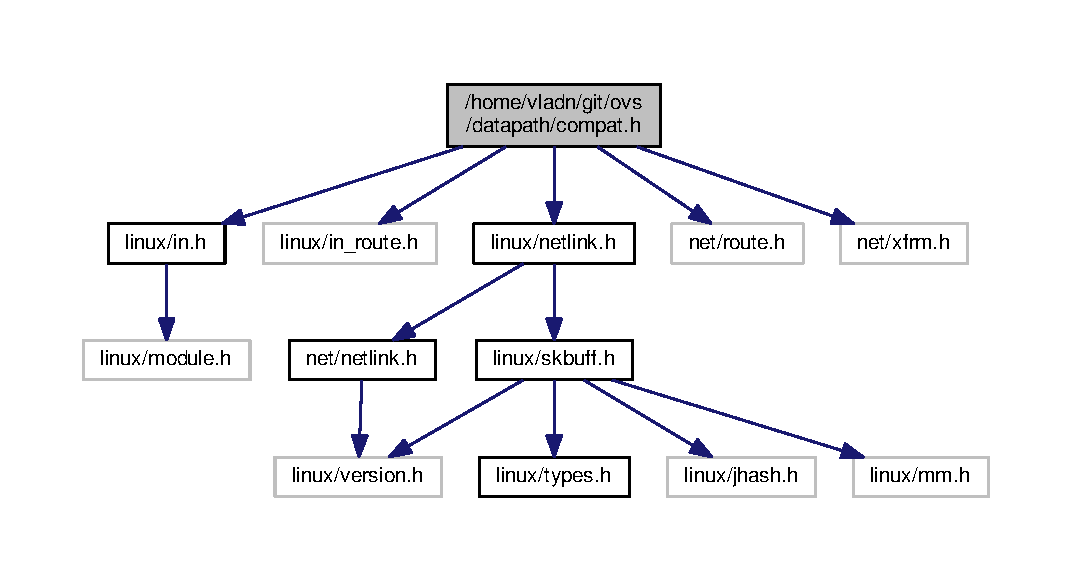
\includegraphics[width=350pt]{compat_8h__incl}
\end{center}
\end{figure}
This graph shows which files directly or indirectly include this file\+:
\nopagebreak
\begin{figure}[H]
\begin{center}
\leavevmode
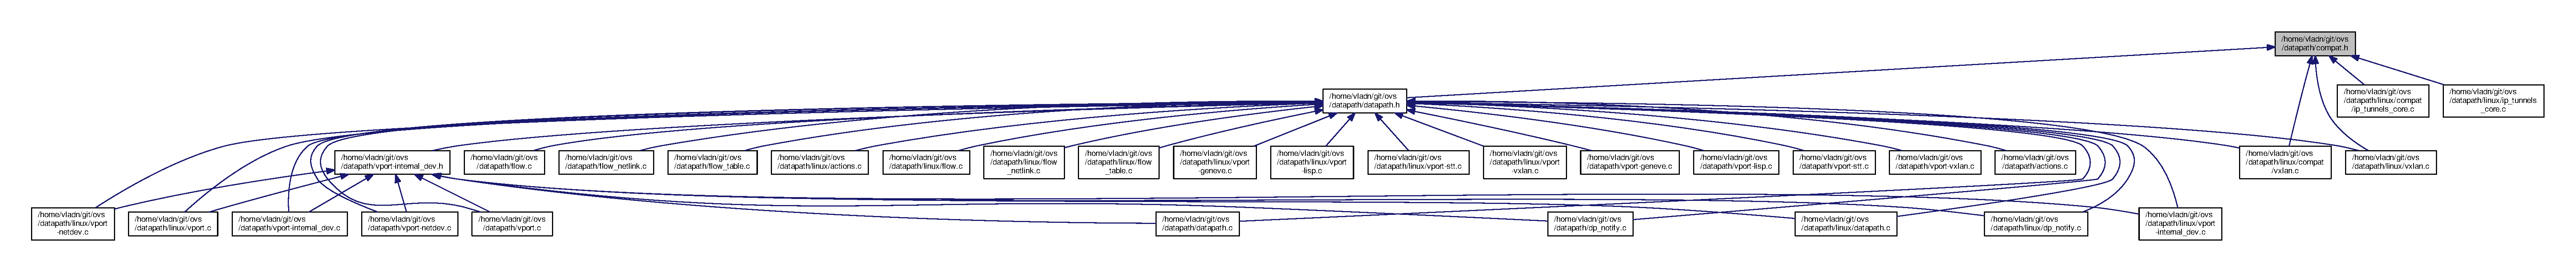
\includegraphics[width=350pt]{compat_8h__dep__incl}
\end{center}
\end{figure}
\subsection*{Macros}
\begin{DoxyCompactItemize}
\item 
\#define \hyperlink{compat_8h_ab49ad0e0c1bb8cda8015902526ae189c}{G\+R\+O\+U\+P\+\_\+\+I\+D}(grp)~0
\item 
\#define \hyperlink{compat_8h_afce1864ee37be971c99555fdf1f76d88}{rt\+\_\+dst}(rt)~(rt-\/$>$\hyperlink{flow_8h_a6747ad3b5d60480ea073cd12c9b78aaa}{dst})
\item 
\#define \hyperlink{compat_8h_a66c1f58d06b91a3e79cf388a80e5096b}{inet\+\_\+sport}(sk)~(inet\+\_\+sk(sk)-\/$>$inet\+\_\+sport)
\end{DoxyCompactItemize}
\subsection*{Functions}
\begin{DoxyCompactItemize}
\item 
static struct rtable $\ast$ \hyperlink{compat_8h_a9fd71ce2d13a3dcc4f7d51469ba86d79}{find\+\_\+route} (struct net $\ast$net, \+\_\+\+\_\+be32 $\ast$saddr, \+\_\+\+\_\+be32 daddr, u8 ipproto, u8 \hyperlink{flow_8h_a5612e9bbcc89219117d353438b2f9dad}{tos}, u32 \hyperlink{flow_8h_aaa98314a1108ff2209ae3bb6515e1dd5}{skb\+\_\+mark})
\item 
static \hyperlink{types_8h_afaa87723b8417d40fcf45b7330261ef9}{bool} \hyperlink{compat_8h_ab25b015544a779ccc1c15baf48b7a45d}{skb\+\_\+encapsulation} (struct sk\+\_\+buff $\ast$skb)
\end{DoxyCompactItemize}


\subsection{Macro Definition Documentation}
\hypertarget{compat_8h_ab49ad0e0c1bb8cda8015902526ae189c}{}\index{compat.\+h@{compat.\+h}!G\+R\+O\+U\+P\+\_\+\+I\+D@{G\+R\+O\+U\+P\+\_\+\+I\+D}}
\index{G\+R\+O\+U\+P\+\_\+\+I\+D@{G\+R\+O\+U\+P\+\_\+\+I\+D}!compat.\+h@{compat.\+h}}
\subsubsection[{G\+R\+O\+U\+P\+\_\+\+I\+D}]{\setlength{\rightskip}{0pt plus 5cm}\#define G\+R\+O\+U\+P\+\_\+\+I\+D(
\begin{DoxyParamCaption}
\item[{}]{grp}
\end{DoxyParamCaption}
)~0}\label{compat_8h_ab49ad0e0c1bb8cda8015902526ae189c}
\hypertarget{compat_8h_a66c1f58d06b91a3e79cf388a80e5096b}{}\index{compat.\+h@{compat.\+h}!inet\+\_\+sport@{inet\+\_\+sport}}
\index{inet\+\_\+sport@{inet\+\_\+sport}!compat.\+h@{compat.\+h}}
\subsubsection[{inet\+\_\+sport}]{\setlength{\rightskip}{0pt plus 5cm}\#define inet\+\_\+sport(
\begin{DoxyParamCaption}
\item[{}]{sk}
\end{DoxyParamCaption}
)~(inet\+\_\+sk(sk)-\/$>$inet\+\_\+sport)}\label{compat_8h_a66c1f58d06b91a3e79cf388a80e5096b}
\hypertarget{compat_8h_afce1864ee37be971c99555fdf1f76d88}{}\index{compat.\+h@{compat.\+h}!rt\+\_\+dst@{rt\+\_\+dst}}
\index{rt\+\_\+dst@{rt\+\_\+dst}!compat.\+h@{compat.\+h}}
\subsubsection[{rt\+\_\+dst}]{\setlength{\rightskip}{0pt plus 5cm}\#define rt\+\_\+dst(
\begin{DoxyParamCaption}
\item[{}]{rt}
\end{DoxyParamCaption}
)~(rt-\/$>${\bf dst})}\label{compat_8h_afce1864ee37be971c99555fdf1f76d88}


\subsection{Function Documentation}
\hypertarget{compat_8h_a9fd71ce2d13a3dcc4f7d51469ba86d79}{}\index{compat.\+h@{compat.\+h}!find\+\_\+route@{find\+\_\+route}}
\index{find\+\_\+route@{find\+\_\+route}!compat.\+h@{compat.\+h}}
\subsubsection[{find\+\_\+route}]{\setlength{\rightskip}{0pt plus 5cm}static struct rtable$\ast$ find\+\_\+route (
\begin{DoxyParamCaption}
\item[{struct net $\ast$}]{net, }
\item[{\+\_\+\+\_\+be32 $\ast$}]{saddr, }
\item[{\+\_\+\+\_\+be32}]{daddr, }
\item[{u8}]{ipproto, }
\item[{u8}]{tos, }
\item[{u32}]{skb\+\_\+mark}
\end{DoxyParamCaption}
)\hspace{0.3cm}{\ttfamily [static]}}\label{compat_8h_a9fd71ce2d13a3dcc4f7d51469ba86d79}

\begin{DoxyCode}
49 \{
50     \textcolor{keyword}{struct }rtable *rt;
51     \textcolor{comment}{/* Tunnel configuration keeps DSCP part of TOS bits, But Linux}
52 \textcolor{comment}{     * router expect RT\_TOS bits only.}
53 \textcolor{comment}{     */}
54 
55 \textcolor{preprocessor}{#if LINUX\_VERSION\_CODE < KERNEL\_VERSION(2,6,39)}
56     \textcolor{keyword}{struct }flowi fl = \{ .nl\_u = \{ .ip4\_u = \{
57                     .daddr = daddr,
58                     .saddr = *saddr,
59                     .tos   = RT\_TOS(\hyperlink{flow_8h_a5612e9bbcc89219117d353438b2f9dad}{tos}) \} \},
60                     .mark = \hyperlink{flow_8h_aaa98314a1108ff2209ae3bb6515e1dd5}{skb\_mark},
61                     .proto = ipproto \};
62 
63     \textcolor{keywordflow}{if} (unlikely(ip\_route\_output\_key(net, &rt, &fl)))
64         \textcolor{keywordflow}{return} ERR\_PTR(-EADDRNOTAVAIL);
65     *saddr = fl.nl\_u.ip4\_u.saddr;
66     \textcolor{keywordflow}{return} rt;
67 \textcolor{preprocessor}{#else}
68     \textcolor{keyword}{struct }flowi4 fl = \{ .daddr = daddr,
69                  .saddr = *saddr,
70                  .flowi4\_tos = RT\_TOS(\hyperlink{flow_8h_a5612e9bbcc89219117d353438b2f9dad}{tos}),
71                  .flowi4\_mark = \hyperlink{flow_8h_aaa98314a1108ff2209ae3bb6515e1dd5}{skb\_mark},
72                  .flowi4\_proto = ipproto \};
73 
74     rt = ip\_route\_output\_key(net, &fl);
75     *saddr = fl.saddr;
76     \textcolor{keywordflow}{return} rt;
77 \textcolor{preprocessor}{#endif}
78 \}
\end{DoxyCode}
\hypertarget{compat_8h_ab25b015544a779ccc1c15baf48b7a45d}{}\index{compat.\+h@{compat.\+h}!skb\+\_\+encapsulation@{skb\+\_\+encapsulation}}
\index{skb\+\_\+encapsulation@{skb\+\_\+encapsulation}!compat.\+h@{compat.\+h}}
\subsubsection[{skb\+\_\+encapsulation}]{\setlength{\rightskip}{0pt plus 5cm}static {\bf bool} skb\+\_\+encapsulation (
\begin{DoxyParamCaption}
\item[{struct sk\+\_\+buff $\ast$}]{skb}
\end{DoxyParamCaption}
)\hspace{0.3cm}{\ttfamily [inline]}, {\ttfamily [static]}}\label{compat_8h_ab25b015544a779ccc1c15baf48b7a45d}

\begin{DoxyCode}
82 \{
83     \textcolor{keywordflow}{return} skb->encapsulation;
84 \}
\end{DoxyCode}

\hypertarget{datapath_8c}{}\section{/home/vladn/git/ovs/datapath/datapath.c File Reference}
\label{datapath_8c}\index{/home/vladn/git/ovs/datapath/datapath.\+c@{/home/vladn/git/ovs/datapath/datapath.\+c}}
{\ttfamily \#include $<$linux/init.\+h$>$}\\*
{\ttfamily \#include $<$linux/module.\+h$>$}\\*
{\ttfamily \#include $<$linux/if\+\_\+arp.\+h$>$}\\*
{\ttfamily \#include $<$linux/if\+\_\+vlan.\+h$>$}\\*
{\ttfamily \#include $<$linux/in.\+h$>$}\\*
{\ttfamily \#include $<$linux/ip.\+h$>$}\\*
{\ttfamily \#include $<$linux/jhash.\+h$>$}\\*
{\ttfamily \#include $<$linux/delay.\+h$>$}\\*
{\ttfamily \#include $<$linux/time.\+h$>$}\\*
{\ttfamily \#include $<$linux/etherdevice.\+h$>$}\\*
{\ttfamily \#include $<$linux/genetlink.\+h$>$}\\*
{\ttfamily \#include $<$linux/kernel.\+h$>$}\\*
{\ttfamily \#include $<$linux/kthread.\+h$>$}\\*
{\ttfamily \#include $<$linux/mutex.\+h$>$}\\*
{\ttfamily \#include $<$linux/percpu.\+h$>$}\\*
{\ttfamily \#include $<$linux/rcupdate.\+h$>$}\\*
{\ttfamily \#include $<$linux/tcp.\+h$>$}\\*
{\ttfamily \#include $<$linux/udp.\+h$>$}\\*
{\ttfamily \#include $<$linux/version.\+h$>$}\\*
{\ttfamily \#include $<$linux/ethtool.\+h$>$}\\*
{\ttfamily \#include $<$linux/wait.\+h$>$}\\*
{\ttfamily \#include $<$asm/div64.\+h$>$}\\*
{\ttfamily \#include $<$linux/highmem.\+h$>$}\\*
{\ttfamily \#include $<$linux/netfilter\+\_\+bridge.\+h$>$}\\*
{\ttfamily \#include $<$linux/netfilter\+\_\+ipv4.\+h$>$}\\*
{\ttfamily \#include $<$linux/inetdevice.\+h$>$}\\*
{\ttfamily \#include $<$linux/list.\+h$>$}\\*
{\ttfamily \#include $<$linux/openvswitch.\+h$>$}\\*
{\ttfamily \#include $<$linux/rculist.\+h$>$}\\*
{\ttfamily \#include $<$linux/dmi.\+h$>$}\\*
{\ttfamily \#include $<$net/genetlink.\+h$>$}\\*
{\ttfamily \#include $<$net/net\+\_\+namespace.\+h$>$}\\*
{\ttfamily \#include $<$net/netns/generic.\+h$>$}\\*
{\ttfamily \#include \char`\"{}datapath.\+h\char`\"{}}\\*
{\ttfamily \#include \char`\"{}flow.\+h\char`\"{}}\\*
{\ttfamily \#include \char`\"{}flow\+\_\+table.\+h\char`\"{}}\\*
{\ttfamily \#include \char`\"{}flow\+\_\+netlink.\+h\char`\"{}}\\*
{\ttfamily \#include \char`\"{}vlan.\+h\char`\"{}}\\*
{\ttfamily \#include \char`\"{}vport-\/internal\+\_\+dev.\+h\char`\"{}}\\*
{\ttfamily \#include \char`\"{}vport-\/netdev.\+h\char`\"{}}\\*
Include dependency graph for datapath.\+c\+:
\nopagebreak
\begin{figure}[H]
\begin{center}
\leavevmode
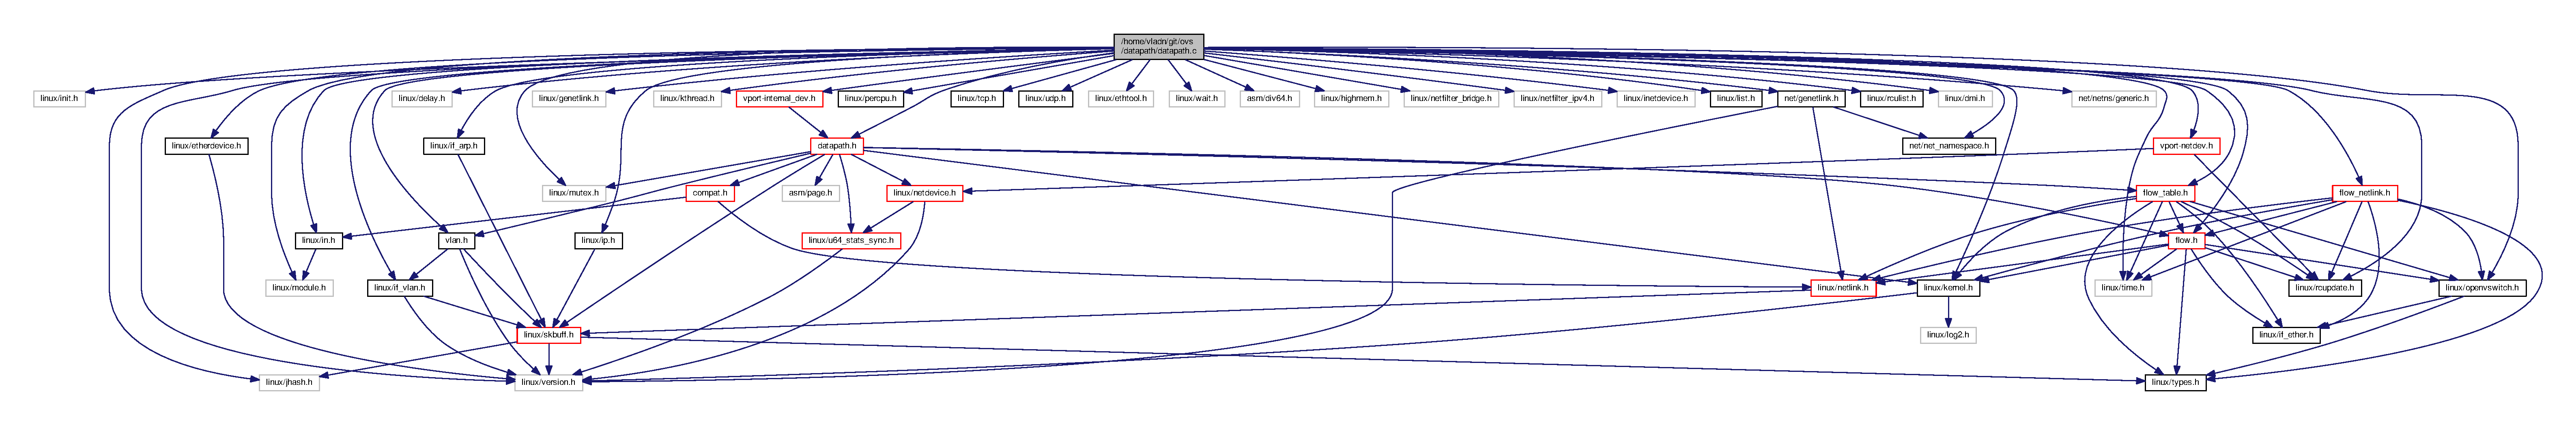
\includegraphics[width=350pt]{datapath_8c__incl}
\end{center}
\end{figure}
\subsection*{Macros}
\begin{DoxyCompactItemize}
\item 
\#define \hyperlink{datapath_8c_a1f8c165bf4196327bc3abff648276d92}{pr\+\_\+fmt}(fmt)~K\+B\+U\+I\+L\+D\+\_\+\+M\+O\+D\+N\+A\+M\+E \char`\"{}\+: \char`\"{} fmt
\end{DoxyCompactItemize}
\subsection*{Functions}
\begin{DoxyCompactItemize}
\item 
\hyperlink{datapath_8c_abf00303edb3bc87ac06f165737f618ec}{E\+X\+P\+O\+R\+T\+\_\+\+S\+Y\+M\+B\+O\+L\+\_\+\+G\+P\+L} (\hyperlink{datapath_8h_ace140298dc2b59b3d77d59c0a210de29}{ovs\+\_\+net\+\_\+id})
\item 
static \hyperlink{types_8h_afaa87723b8417d40fcf45b7330261ef9}{bool} \hyperlink{datapath_8c_aba3b63f0e73c9ea6ecb8b7aa5d913724}{ovs\+\_\+must\+\_\+notify} (struct \hyperlink{genetlink_8h_aba961c2c372b7122ad0c8ae5e7af2f3b}{genl\+\_\+family} $\ast$family, struct genl\+\_\+info $\ast$info, unsigned int group)
\item 
static void \hyperlink{datapath_8c_a67f527ad1164ff0d67fe854584ced567}{ovs\+\_\+notify} (struct \hyperlink{genetlink_8h_aba961c2c372b7122ad0c8ae5e7af2f3b}{genl\+\_\+family} $\ast$family, struct genl\+\_\+multicast\+\_\+group $\ast$grp, struct sk\+\_\+buff $\ast$skb, struct genl\+\_\+info $\ast$info)
\item 
static \hyperlink{datapath_8c_aa489fc945a5cabc6b1efbf3b886ee600}{D\+E\+F\+I\+N\+E\+\_\+\+M\+U\+T\+E\+X} (ovs\+\_\+mutex)
\item 
void \hyperlink{datapath_8c_a092c1f450b78a173c890ed4c56839e1a}{ovs\+\_\+lock} (void)
\item 
void \hyperlink{datapath_8c_ac3ccfd98a880ed6d2480209be0d16680}{ovs\+\_\+unlock} (void)
\item 
static int \hyperlink{datapath_8c_a2c10ba8a23a8cb2f14b7f7684e5ebb5d}{queue\+\_\+gso\+\_\+packets} (struct \hyperlink{structdatapath}{datapath} $\ast$dp, struct sk\+\_\+buff $\ast$, const struct \hyperlink{structsw__flow__key}{sw\+\_\+flow\+\_\+key} $\ast$, const struct \hyperlink{structdp__upcall__info}{dp\+\_\+upcall\+\_\+info} $\ast$)
\item 
static int \hyperlink{datapath_8c_a549c591fae56562523f243abbe4a1e3e}{queue\+\_\+userspace\+\_\+packet} (struct \hyperlink{structdatapath}{datapath} $\ast$dp, struct sk\+\_\+buff $\ast$, const struct \hyperlink{structsw__flow__key}{sw\+\_\+flow\+\_\+key} $\ast$, const struct \hyperlink{structdp__upcall__info}{dp\+\_\+upcall\+\_\+info} $\ast$)
\item 
static struct \hyperlink{structdatapath}{datapath} $\ast$ \hyperlink{datapath_8c_ab3f598cca9ed98120cc11daa11690da8}{get\+\_\+dp\+\_\+rcu} (struct net $\ast$net, int dp\+\_\+ifindex)
\item 
static struct \hyperlink{structdatapath}{datapath} $\ast$ \hyperlink{datapath_8c_a1107d4fd386aa6551511140b5405e1d3}{get\+\_\+dp} (struct net $\ast$net, int dp\+\_\+ifindex)
\item 
const char $\ast$ \hyperlink{datapath_8c_a6a23196916bb5de4994f901bdf1aba2d}{ovs\+\_\+dp\+\_\+name} (const struct \hyperlink{structdatapath}{datapath} $\ast$dp)
\item 
static int \hyperlink{datapath_8c_a2c4c60ba176a755749744f7b01aa6edd}{get\+\_\+dpifindex} (const struct \hyperlink{structdatapath}{datapath} $\ast$dp)
\item 
static void \hyperlink{datapath_8c_a5f329d1e5ef78eb6e9b4aa63c2d97e91}{destroy\+\_\+dp\+\_\+rcu} (struct rcu\+\_\+head $\ast$rcu)
\item 
static struct hlist\+\_\+head $\ast$ \hyperlink{datapath_8c_af291a723340e4e1bd38b4b14e7f4377a}{vport\+\_\+hash\+\_\+bucket} (const struct \hyperlink{structdatapath}{datapath} $\ast$dp, u16 port\+\_\+no)
\item 
struct \hyperlink{structvport}{vport} $\ast$ \hyperlink{datapath_8c_a0a9ec01692e1fdcb15a9a294d3789af0}{ovs\+\_\+lookup\+\_\+vport} (const struct \hyperlink{structdatapath}{datapath} $\ast$dp, u16 port\+\_\+no)
\item 
static struct \hyperlink{structvport}{vport} $\ast$ \hyperlink{datapath_8c_afac95a3e755fe3b0906ccc72d052cbe1}{new\+\_\+vport} (const struct \hyperlink{structvport__parms}{vport\+\_\+parms} $\ast$parms)
\item 
void \hyperlink{datapath_8c_a560b5f5f97a839287201f7486c53447e}{ovs\+\_\+dp\+\_\+detach\+\_\+port} (struct \hyperlink{structvport}{vport} $\ast$p)
\item 
void \hyperlink{datapath_8c_aa52cbaf8a4e68129287bfc8ddcde0711}{ovs\+\_\+dp\+\_\+process\+\_\+packet} (struct sk\+\_\+buff $\ast$skb, struct \hyperlink{structsw__flow__key}{sw\+\_\+flow\+\_\+key} $\ast$key)
\item 
int \hyperlink{datapath_8c_a229b5c7d0158ebc24a90f44de0df0040}{ovs\+\_\+dp\+\_\+upcall} (struct \hyperlink{structdatapath}{datapath} $\ast$dp, struct sk\+\_\+buff $\ast$skb, const struct \hyperlink{structsw__flow__key}{sw\+\_\+flow\+\_\+key} $\ast$key, const struct \hyperlink{structdp__upcall__info}{dp\+\_\+upcall\+\_\+info} $\ast$upcall\+\_\+info)
\item 
static size\+\_\+t \hyperlink{datapath_8c_a845617ce8ad4e18b0c54961d796a0aeb}{upcall\+\_\+msg\+\_\+size} (const struct \hyperlink{structdp__upcall__info}{dp\+\_\+upcall\+\_\+info} $\ast$upcall\+\_\+info, unsigned int hdrlen)
\item 
static int \hyperlink{datapath_8c_a20b16b839bd3116f7dbad5719b02c115}{ovs\+\_\+packet\+\_\+cmd\+\_\+execute} (struct sk\+\_\+buff $\ast$skb, struct genl\+\_\+info $\ast$info)
\item 
static void \hyperlink{datapath_8c_a689a2b3c19c9cdebecfb266acf5ba221}{get\+\_\+dp\+\_\+stats} (const struct \hyperlink{structdatapath}{datapath} $\ast$dp, struct \hyperlink{structovs__dp__stats}{ovs\+\_\+dp\+\_\+stats} $\ast$stats, struct \hyperlink{structovs__dp__megaflow__stats}{ovs\+\_\+dp\+\_\+megaflow\+\_\+stats} $\ast$mega\+\_\+stats)
\item 
static \hyperlink{types_8h_afaa87723b8417d40fcf45b7330261ef9}{bool} \hyperlink{datapath_8c_a4d912d3ed7dba8789b726280b6dea3a4}{should\+\_\+fill\+\_\+key} (const struct \hyperlink{structsw__flow__id}{sw\+\_\+flow\+\_\+id} $\ast$sfid, uint32\+\_\+t ufid\+\_\+flags)
\item 
static \hyperlink{types_8h_afaa87723b8417d40fcf45b7330261ef9}{bool} \hyperlink{datapath_8c_acef91dffd31fb70fa6c94e11ad08805b}{should\+\_\+fill\+\_\+mask} (uint32\+\_\+t ufid\+\_\+flags)
\item 
static \hyperlink{types_8h_afaa87723b8417d40fcf45b7330261ef9}{bool} \hyperlink{datapath_8c_a05dcb72a9103046c5721d03a1592291f}{should\+\_\+fill\+\_\+actions} (uint32\+\_\+t ufid\+\_\+flags)
\item 
static size\+\_\+t \hyperlink{datapath_8c_a5f17e0449c315970d82161c131e70dbd}{ovs\+\_\+flow\+\_\+cmd\+\_\+msg\+\_\+size} (const struct \hyperlink{structsw__flow__actions}{sw\+\_\+flow\+\_\+actions} $\ast$acts, const struct \hyperlink{structsw__flow__id}{sw\+\_\+flow\+\_\+id} $\ast$sfid, uint32\+\_\+t ufid\+\_\+flags)
\item 
static int \hyperlink{datapath_8c_a832dcdda5999f2e7fadd72b2ad2373f3}{ovs\+\_\+flow\+\_\+cmd\+\_\+fill\+\_\+stats} (const struct \hyperlink{structsw__flow}{sw\+\_\+flow} $\ast$flow, struct sk\+\_\+buff $\ast$skb)
\item 
static int \hyperlink{datapath_8c_ad6ce625c1cb24262cddbabe479987986}{ovs\+\_\+flow\+\_\+cmd\+\_\+fill\+\_\+actions} (const struct \hyperlink{structsw__flow}{sw\+\_\+flow} $\ast$flow, struct sk\+\_\+buff $\ast$skb, int skb\+\_\+orig\+\_\+len)
\item 
static int \hyperlink{datapath_8c_a7b415415fa0d84bab45258cd3080f2c7}{ovs\+\_\+flow\+\_\+cmd\+\_\+fill\+\_\+info} (const struct \hyperlink{structsw__flow}{sw\+\_\+flow} $\ast$flow, int dp\+\_\+ifindex, struct sk\+\_\+buff $\ast$skb, u32 portid, u32 seq, u32 \hyperlink{flow_8h_af4f7a53f6b2df72c34ca881f2714ac91}{flags}, u8 cmd, u32 ufid\+\_\+flags)
\item 
static struct sk\+\_\+buff $\ast$ \hyperlink{datapath_8c_ac6daf72fcac45a9bd571dec78216e197}{ovs\+\_\+flow\+\_\+cmd\+\_\+alloc\+\_\+info} (const struct \hyperlink{structsw__flow__actions}{sw\+\_\+flow\+\_\+actions} $\ast$acts, const struct \hyperlink{structsw__flow__id}{sw\+\_\+flow\+\_\+id} $\ast$sfid, struct genl\+\_\+info $\ast$info, \hyperlink{types_8h_afaa87723b8417d40fcf45b7330261ef9}{bool} always, uint32\+\_\+t ufid\+\_\+flags)
\item 
static struct sk\+\_\+buff $\ast$ \hyperlink{datapath_8c_afbfb35c0b3684e82dce573f04491ad1e}{ovs\+\_\+flow\+\_\+cmd\+\_\+build\+\_\+info} (const struct \hyperlink{structsw__flow}{sw\+\_\+flow} $\ast$flow, int dp\+\_\+ifindex, struct genl\+\_\+info $\ast$info, u8 cmd, \hyperlink{types_8h_afaa87723b8417d40fcf45b7330261ef9}{bool} always, u32 ufid\+\_\+flags)
\item 
static int \hyperlink{datapath_8c_ac8895cf604439184dad96f70e335afe2}{ovs\+\_\+flow\+\_\+cmd\+\_\+new} (struct sk\+\_\+buff $\ast$skb, struct genl\+\_\+info $\ast$info)
\item 
static struct \hyperlink{structsw__flow__actions}{sw\+\_\+flow\+\_\+actions} $\ast$ \hyperlink{datapath_8c_aac07273dc62dc714973b44be41f9bf7f}{get\+\_\+flow\+\_\+actions} (const struct nlattr $\ast$a, const struct \hyperlink{structsw__flow__key}{sw\+\_\+flow\+\_\+key} $\ast$key, const struct \hyperlink{structsw__flow__mask}{sw\+\_\+flow\+\_\+mask} $\ast$mask, \hyperlink{types_8h_afaa87723b8417d40fcf45b7330261ef9}{bool} log)
\item 
static int \hyperlink{datapath_8c_a4c6c2d9354cb73a6300a9b3c9cd2a114}{ovs\+\_\+flow\+\_\+cmd\+\_\+set} (struct sk\+\_\+buff $\ast$skb, struct genl\+\_\+info $\ast$info)
\item 
static int \hyperlink{datapath_8c_a747a4726ec84c751acb3048a515cef86}{ovs\+\_\+flow\+\_\+cmd\+\_\+get} (struct sk\+\_\+buff $\ast$skb, struct genl\+\_\+info $\ast$info)
\item 
static int \hyperlink{datapath_8c_aa05c62aa6531c0e0312126a21a8d99a5}{ovs\+\_\+flow\+\_\+cmd\+\_\+del} (struct sk\+\_\+buff $\ast$skb, struct genl\+\_\+info $\ast$info)
\item 
static int \hyperlink{datapath_8c_a4759993b01f8bc67711ecacacdf43976}{ovs\+\_\+flow\+\_\+cmd\+\_\+dump} (struct sk\+\_\+buff $\ast$skb, struct netlink\+\_\+callback $\ast$cb)
\item 
static size\+\_\+t \hyperlink{datapath_8c_aab015cdb7b4e0d2fa66da1b72963df67}{ovs\+\_\+dp\+\_\+cmd\+\_\+msg\+\_\+size} (void)
\item 
static int \hyperlink{datapath_8c_a0c18d2b438aba3739c2a36e172cfe3ea}{ovs\+\_\+dp\+\_\+cmd\+\_\+fill\+\_\+info} (struct \hyperlink{structdatapath}{datapath} $\ast$dp, struct sk\+\_\+buff $\ast$skb, u32 portid, u32 seq, u32 \hyperlink{flow_8h_af4f7a53f6b2df72c34ca881f2714ac91}{flags}, u8 cmd)
\item 
static struct sk\+\_\+buff $\ast$ \hyperlink{datapath_8c_ad01db8513d30c057f1ea10532ebc8b1e}{ovs\+\_\+dp\+\_\+cmd\+\_\+alloc\+\_\+info} (struct genl\+\_\+info $\ast$info)
\item 
static struct \hyperlink{structdatapath}{datapath} $\ast$ \hyperlink{datapath_8c_a774dc1bd6a39e68ebac48e55688a8574}{lookup\+\_\+datapath} (struct net $\ast$net, const struct \hyperlink{structovs__header}{ovs\+\_\+header} $\ast$\hyperlink{structovs__header}{ovs\+\_\+header}, struct nlattr $\ast$a\mbox{[}\hyperlink{openvswitch_8h_a928e759af5a47791e5b3070bf596fd5d}{O\+V\+S\+\_\+\+D\+P\+\_\+\+A\+T\+T\+R\+\_\+\+M\+A\+X}+1\mbox{]})
\item 
static void \hyperlink{datapath_8c_aba7a59d6ae252953be557d7478f7332f}{ovs\+\_\+dp\+\_\+reset\+\_\+user\+\_\+features} (struct sk\+\_\+buff $\ast$skb, struct genl\+\_\+info $\ast$info)
\item 
static void \hyperlink{datapath_8c_a2c763b1da99cce1a426140794eaf8f03}{ovs\+\_\+dp\+\_\+change} (struct \hyperlink{structdatapath}{datapath} $\ast$dp, struct nlattr $\ast$a\mbox{[}$\,$\mbox{]})
\item 
static int \hyperlink{datapath_8c_a8d012b2863686706ab9d1282a82d6625}{ovs\+\_\+dp\+\_\+cmd\+\_\+new} (struct sk\+\_\+buff $\ast$skb, struct genl\+\_\+info $\ast$info)
\item 
static void \hyperlink{datapath_8c_a6c66e1332f2a95e9510e37745d77bad1}{\+\_\+\+\_\+dp\+\_\+destroy} (struct \hyperlink{structdatapath}{datapath} $\ast$dp)
\item 
static int \hyperlink{datapath_8c_a580bc462589253144c5027fa18fbfb17}{ovs\+\_\+dp\+\_\+cmd\+\_\+del} (struct sk\+\_\+buff $\ast$skb, struct genl\+\_\+info $\ast$info)
\item 
static int \hyperlink{datapath_8c_aa59555f8c6107137945c90e92fd42b4c}{ovs\+\_\+dp\+\_\+cmd\+\_\+set} (struct sk\+\_\+buff $\ast$skb, struct genl\+\_\+info $\ast$info)
\item 
static int \hyperlink{datapath_8c_ab253bc3f01b9d70955d3d3dcfc236b9f}{ovs\+\_\+dp\+\_\+cmd\+\_\+get} (struct sk\+\_\+buff $\ast$skb, struct genl\+\_\+info $\ast$info)
\item 
static int \hyperlink{datapath_8c_a64056132bb398b3e7c92291cc6905537}{ovs\+\_\+dp\+\_\+cmd\+\_\+dump} (struct sk\+\_\+buff $\ast$skb, struct netlink\+\_\+callback $\ast$cb)
\item 
static int \hyperlink{datapath_8c_a4272403de9a985cea17181e99b7a7edc}{ovs\+\_\+vport\+\_\+cmd\+\_\+fill\+\_\+info} (struct \hyperlink{structvport}{vport} $\ast$\hyperlink{structvport}{vport}, struct sk\+\_\+buff $\ast$skb, u32 portid, u32 seq, u32 \hyperlink{flow_8h_af4f7a53f6b2df72c34ca881f2714ac91}{flags}, u8 cmd)
\item 
static struct sk\+\_\+buff $\ast$ \hyperlink{datapath_8c_a45645849b972492fa9f01eeaf668bf78}{ovs\+\_\+vport\+\_\+cmd\+\_\+alloc\+\_\+info} (void)
\item 
struct sk\+\_\+buff $\ast$ \hyperlink{datapath_8c_adf50e47c9c548390402b1da1608235c9}{ovs\+\_\+vport\+\_\+cmd\+\_\+build\+\_\+info} (struct \hyperlink{structvport}{vport} $\ast$\hyperlink{structvport}{vport}, u32 portid, u32 seq, u8 cmd)
\item 
static struct \hyperlink{structvport}{vport} $\ast$ \hyperlink{datapath_8c_a95b019fd3980803dcc1bb5aca920f58b}{lookup\+\_\+vport} (struct net $\ast$net, const struct \hyperlink{structovs__header}{ovs\+\_\+header} $\ast$\hyperlink{structovs__header}{ovs\+\_\+header}, struct nlattr $\ast$a\mbox{[}\hyperlink{openvswitch_8h_a789cf40a0af09c574467d47ca6a2eb7b}{O\+V\+S\+\_\+\+V\+P\+O\+R\+T\+\_\+\+A\+T\+T\+R\+\_\+\+M\+A\+X}+1\mbox{]})
\item 
static int \hyperlink{datapath_8c_a0b878975d12b240c20c6b5389b5b12b6}{ovs\+\_\+vport\+\_\+cmd\+\_\+new} (struct sk\+\_\+buff $\ast$skb, struct genl\+\_\+info $\ast$info)
\item 
static int \hyperlink{datapath_8c_a89f1e2fa808021479860862b3e7556e5}{ovs\+\_\+vport\+\_\+cmd\+\_\+set} (struct sk\+\_\+buff $\ast$skb, struct genl\+\_\+info $\ast$info)
\item 
static int \hyperlink{datapath_8c_afc2316a8fe3074ed07e853d552fb4704}{ovs\+\_\+vport\+\_\+cmd\+\_\+del} (struct sk\+\_\+buff $\ast$skb, struct genl\+\_\+info $\ast$info)
\item 
static int \hyperlink{datapath_8c_ad818149bb2b46cab6eeb5b7ba6a14afe}{ovs\+\_\+vport\+\_\+cmd\+\_\+get} (struct sk\+\_\+buff $\ast$skb, struct genl\+\_\+info $\ast$info)
\item 
static int \hyperlink{datapath_8c_ac61e52592bc18541660c182e9aebbcaf}{ovs\+\_\+vport\+\_\+cmd\+\_\+dump} (struct sk\+\_\+buff $\ast$skb, struct netlink\+\_\+callback $\ast$cb)
\item 
static void \hyperlink{datapath_8c_a02412b752de54c0add0ca994b0e74079}{dp\+\_\+unregister\+\_\+genl} (int n\+\_\+families)
\item 
static int \hyperlink{datapath_8c_a8a589935468eb018de07b30900a56ddb}{dp\+\_\+register\+\_\+genl} (void)
\item 
static int \+\_\+\+\_\+net\+\_\+init \hyperlink{datapath_8c_af390458a6069bd6b50c9a0d46517159a}{ovs\+\_\+init\+\_\+net} (struct net $\ast$net)
\item 
static void \+\_\+\+\_\+net\+\_\+exit \hyperlink{datapath_8c_a97bf5ddc3763f5f1b5691cc262bd206a}{list\+\_\+vports\+\_\+from\+\_\+net} (struct net $\ast$net, struct net $\ast$dnet, struct list\+\_\+head $\ast$head)
\item 
static void \+\_\+\+\_\+net\+\_\+exit \hyperlink{datapath_8c_aead9307565d6ab903dd5db639c7299e4}{ovs\+\_\+exit\+\_\+net} (struct net $\ast$dnet)
\item 
\hyperlink{datapath_8c_a537406a5b4c729d36ebe1d833ce74eda}{D\+E\+F\+I\+N\+E\+\_\+\+C\+O\+M\+P\+A\+T\+\_\+\+P\+N\+E\+T\+\_\+\+R\+E\+G\+\_\+\+F\+U\+N\+C} (device)
\item 
static int \+\_\+\+\_\+init \hyperlink{datapath_8c_a85a2562435726aa1e9d254c86c6e597e}{dp\+\_\+init} (void)
\item 
static void \hyperlink{datapath_8c_a64b62ac82dbfc2107fa6b38a2c9e3612}{dp\+\_\+cleanup} (void)
\item 
\hyperlink{datapath_8c_a61981f8b771cdb3f88315f3da5f4fe18}{module\+\_\+init} (\hyperlink{linux_2datapath_8c_a85a2562435726aa1e9d254c86c6e597e}{dp\+\_\+init})
\item 
\hyperlink{datapath_8c_afefe140861ac8adc338b486bf95f710f}{module\+\_\+exit} (\hyperlink{linux_2datapath_8c_a64b62ac82dbfc2107fa6b38a2c9e3612}{dp\+\_\+cleanup})
\item 
\hyperlink{datapath_8c_a375185aea6f89fbd06af3e43f39d2975}{M\+O\+D\+U\+L\+E\+\_\+\+D\+E\+S\+C\+R\+I\+P\+T\+I\+O\+N} (\char`\"{}Open v\+Switch switching \hyperlink{structdatapath}{datapath}\char`\"{})
\item 
\hyperlink{datapath_8c_ad94b36675e7eb067ea3ce6ff9e244a44}{M\+O\+D\+U\+L\+E\+\_\+\+L\+I\+C\+E\+N\+S\+E} (\char`\"{}G\+P\+L\char`\"{})
\item 
\hyperlink{datapath_8c_ada33d5db5abb99d420d4b6d82ea237c4}{M\+O\+D\+U\+L\+E\+\_\+\+V\+E\+R\+S\+I\+O\+N} (V\+E\+R\+S\+I\+O\+N)
\end{DoxyCompactItemize}
\subsection*{Variables}
\begin{DoxyCompactItemize}
\item 
int \hyperlink{datapath_8h_ace140298dc2b59b3d77d59c0a210de29}{ovs\+\_\+net\+\_\+id} \hyperlink{datapath_8c_a50bac238082a6952a4dadad6299cc4b3}{\+\_\+\+\_\+read\+\_\+mostly}
\item 
static struct \hyperlink{genetlink_8h_aba961c2c372b7122ad0c8ae5e7af2f3b}{genl\+\_\+family} \hyperlink{datapath_8c_a709033900c84449b9f83cb62cecb1627}{dp\+\_\+packet\+\_\+genl\+\_\+family}
\item 
static struct \hyperlink{genetlink_8h_aba961c2c372b7122ad0c8ae5e7af2f3b}{genl\+\_\+family} \hyperlink{datapath_8c_af07853d514acd11f9f0d23494b6a2f9e}{dp\+\_\+flow\+\_\+genl\+\_\+family}
\item 
static struct \hyperlink{genetlink_8h_aba961c2c372b7122ad0c8ae5e7af2f3b}{genl\+\_\+family} \hyperlink{datapath_8c_a00b4c28b2a15cad709af53b6484fc45c}{dp\+\_\+datapath\+\_\+genl\+\_\+family}
\item 
static const struct nla\+\_\+policy \hyperlink{datapath_8c_aad79544f457c7a323273d328dafff886}{flow\+\_\+policy} \mbox{[}$\,$\mbox{]}
\item 
static struct genl\+\_\+multicast\+\_\+group \hyperlink{datapath_8c_ae43fcc307ac0fa091a736d4687c7f884}{ovs\+\_\+dp\+\_\+flow\+\_\+multicast\+\_\+group}
\item 
static struct genl\+\_\+multicast\+\_\+group \hyperlink{datapath_8c_afa5d1f090aee506896ff5ef56b4053e1}{ovs\+\_\+dp\+\_\+datapath\+\_\+multicast\+\_\+group}
\item 
struct genl\+\_\+multicast\+\_\+group \hyperlink{datapath_8c_a9dd8d4307b50fdee582eb4013d89eb7b}{ovs\+\_\+dp\+\_\+vport\+\_\+multicast\+\_\+group}
\item 
static const struct nla\+\_\+policy \hyperlink{datapath_8c_aaef8775f67f989a9ff396e2aa6f6f3e2}{packet\+\_\+policy} \mbox{[}\hyperlink{openvswitch_8h_a9c91f74efc7f0264839c153979485eec}{O\+V\+S\+\_\+\+P\+A\+C\+K\+E\+T\+\_\+\+A\+T\+T\+R\+\_\+\+M\+A\+X}+1\mbox{]}
\item 
static struct genl\+\_\+ops \hyperlink{datapath_8c_a75ed1b368ac93a17ed4d04c82b892be9}{dp\+\_\+packet\+\_\+genl\+\_\+ops} \mbox{[}$\,$\mbox{]}
\item 
static struct genl\+\_\+ops \hyperlink{datapath_8c_a42bdb3978421f4f0b3a1be828226b271}{dp\+\_\+flow\+\_\+genl\+\_\+ops} \mbox{[}$\,$\mbox{]}
\item 
static const struct nla\+\_\+policy \hyperlink{datapath_8c_a34f2da191c04c403e206dacb0c3d2a6f}{datapath\+\_\+policy} \mbox{[}\hyperlink{openvswitch_8h_a928e759af5a47791e5b3070bf596fd5d}{O\+V\+S\+\_\+\+D\+P\+\_\+\+A\+T\+T\+R\+\_\+\+M\+A\+X}+1\mbox{]}
\item 
static struct genl\+\_\+ops \hyperlink{datapath_8c_a29acb4bb9ad0b3d7af71e628bf516372}{dp\+\_\+datapath\+\_\+genl\+\_\+ops} \mbox{[}$\,$\mbox{]}
\item 
static const struct nla\+\_\+policy \hyperlink{datapath_8c_af3f5c0f1eb12c1eb1a2494f265dda98a}{vport\+\_\+policy} \mbox{[}\hyperlink{openvswitch_8h_a789cf40a0af09c574467d47ca6a2eb7b}{O\+V\+S\+\_\+\+V\+P\+O\+R\+T\+\_\+\+A\+T\+T\+R\+\_\+\+M\+A\+X}+1\mbox{]}
\item 
static struct genl\+\_\+ops \hyperlink{datapath_8c_a5a28211e3b7e9a5cf7ccf8e81b8bfa8e}{dp\+\_\+vport\+\_\+genl\+\_\+ops} \mbox{[}$\,$\mbox{]}
\item 
struct \hyperlink{genetlink_8h_aba961c2c372b7122ad0c8ae5e7af2f3b}{genl\+\_\+family} \hyperlink{datapath_8c_a69bf55f33e234bc4b78e6eeee1d603fd}{dp\+\_\+vport\+\_\+genl\+\_\+family}
\item 
static struct \hyperlink{genetlink_8h_aba961c2c372b7122ad0c8ae5e7af2f3b}{genl\+\_\+family} $\ast$ \hyperlink{datapath_8c_ae945344e649c305788038f5bc09bc817}{dp\+\_\+genl\+\_\+families} \mbox{[}$\,$\mbox{]}
\item 
static struct pernet\+\_\+operations \hyperlink{datapath_8c_a3a9f5b1a35fcb90938194f22dc2d0f14}{ovs\+\_\+net\+\_\+ops}
\end{DoxyCompactItemize}


\subsection{Macro Definition Documentation}
\hypertarget{datapath_8c_a1f8c165bf4196327bc3abff648276d92}{}\index{datapath.\+c@{datapath.\+c}!pr\+\_\+fmt@{pr\+\_\+fmt}}
\index{pr\+\_\+fmt@{pr\+\_\+fmt}!datapath.\+c@{datapath.\+c}}
\subsubsection[{pr\+\_\+fmt}]{\setlength{\rightskip}{0pt plus 5cm}\#define pr\+\_\+fmt(
\begin{DoxyParamCaption}
\item[{}]{fmt}
\end{DoxyParamCaption}
)~K\+B\+U\+I\+L\+D\+\_\+\+M\+O\+D\+N\+A\+M\+E \char`\"{}\+: \char`\"{} fmt}\label{datapath_8c_a1f8c165bf4196327bc3abff648276d92}


\subsection{Function Documentation}
\hypertarget{datapath_8c_a6c66e1332f2a95e9510e37745d77bad1}{}\index{datapath.\+c@{datapath.\+c}!\+\_\+\+\_\+dp\+\_\+destroy@{\+\_\+\+\_\+dp\+\_\+destroy}}
\index{\+\_\+\+\_\+dp\+\_\+destroy@{\+\_\+\+\_\+dp\+\_\+destroy}!datapath.\+c@{datapath.\+c}}
\subsubsection[{\+\_\+\+\_\+dp\+\_\+destroy}]{\setlength{\rightskip}{0pt plus 5cm}static void \+\_\+\+\_\+dp\+\_\+destroy (
\begin{DoxyParamCaption}
\item[{struct {\bf datapath} $\ast$}]{dp}
\end{DoxyParamCaption}
)\hspace{0.3cm}{\ttfamily [static]}}\label{datapath_8c_a6c66e1332f2a95e9510e37745d77bad1}

\begin{DoxyCode}
1614 \{
1615     \textcolor{keywordtype}{int} i;
1616 
1617     \textcolor{keywordflow}{for} (i = 0; i < \hyperlink{datapath_8h_ac1bf9805d62227b8f76f130087e18018}{DP\_VPORT\_HASH\_BUCKETS}; i++) \{
1618         \textcolor{keyword}{struct }\hyperlink{structvport}{vport} *\hyperlink{structvport}{vport};
1619         \textcolor{keyword}{struct }hlist\_node *n;
1620 
1621         \hyperlink{list_8h_ae2f7dd7dbbe2f13fa51aca9fcb31a03f}{hlist\_for\_each\_entry\_safe}(vport, n, &dp->\hyperlink{structdatapath_abb0de528545b312de283b571cb6c4ede}{ports}[i], dp\_hash\_node)
1622             if (vport->port\_no != \hyperlink{openvswitch_8h_aff2f13b95c27262c520f26831e647598}{OVSP\_LOCAL})
1623                 \hyperlink{datapath_8c_a560b5f5f97a839287201f7486c53447e}{ovs\_dp\_detach\_port}(vport);
1624     \}
1625 
1626     list\_del\_rcu(&dp->list\_node);
1627 
1628     \textcolor{comment}{/* OVSP\_LOCAL is datapath internal port. We need to make sure that}
1629 \textcolor{comment}{     * all ports in datapath are destroyed first before freeing datapath.}
1630 \textcolor{comment}{     */}
1631     \hyperlink{datapath_8c_a560b5f5f97a839287201f7486c53447e}{ovs\_dp\_detach\_port}(\hyperlink{datapath_8h_a422576bd4b943e9df313ba73f6c624e1}{ovs\_vport\_ovsl}(dp, 
      \hyperlink{openvswitch_8h_aff2f13b95c27262c520f26831e647598}{OVSP\_LOCAL}));
1632 
1633     \textcolor{comment}{/* RCU destroy the flow table */}
1634     call\_rcu(&dp->rcu, \hyperlink{datapath_8c_a5f329d1e5ef78eb6e9b4aa63c2d97e91}{destroy\_dp\_rcu});
1635 \}
\end{DoxyCode}
\hypertarget{datapath_8c_a537406a5b4c729d36ebe1d833ce74eda}{}\index{datapath.\+c@{datapath.\+c}!D\+E\+F\+I\+N\+E\+\_\+\+C\+O\+M\+P\+A\+T\+\_\+\+P\+N\+E\+T\+\_\+\+R\+E\+G\+\_\+\+F\+U\+N\+C@{D\+E\+F\+I\+N\+E\+\_\+\+C\+O\+M\+P\+A\+T\+\_\+\+P\+N\+E\+T\+\_\+\+R\+E\+G\+\_\+\+F\+U\+N\+C}}
\index{D\+E\+F\+I\+N\+E\+\_\+\+C\+O\+M\+P\+A\+T\+\_\+\+P\+N\+E\+T\+\_\+\+R\+E\+G\+\_\+\+F\+U\+N\+C@{D\+E\+F\+I\+N\+E\+\_\+\+C\+O\+M\+P\+A\+T\+\_\+\+P\+N\+E\+T\+\_\+\+R\+E\+G\+\_\+\+F\+U\+N\+C}!datapath.\+c@{datapath.\+c}}
\subsubsection[{D\+E\+F\+I\+N\+E\+\_\+\+C\+O\+M\+P\+A\+T\+\_\+\+P\+N\+E\+T\+\_\+\+R\+E\+G\+\_\+\+F\+U\+N\+C}]{\setlength{\rightskip}{0pt plus 5cm}D\+E\+F\+I\+N\+E\+\_\+\+C\+O\+M\+P\+A\+T\+\_\+\+P\+N\+E\+T\+\_\+\+R\+E\+G\+\_\+\+F\+U\+N\+C (
\begin{DoxyParamCaption}
\item[{device}]{}
\end{DoxyParamCaption}
)}\label{datapath_8c_a537406a5b4c729d36ebe1d833ce74eda}
\hypertarget{datapath_8c_aa489fc945a5cabc6b1efbf3b886ee600}{}\index{datapath.\+c@{datapath.\+c}!D\+E\+F\+I\+N\+E\+\_\+\+M\+U\+T\+E\+X@{D\+E\+F\+I\+N\+E\+\_\+\+M\+U\+T\+E\+X}}
\index{D\+E\+F\+I\+N\+E\+\_\+\+M\+U\+T\+E\+X@{D\+E\+F\+I\+N\+E\+\_\+\+M\+U\+T\+E\+X}!datapath.\+c@{datapath.\+c}}
\subsubsection[{D\+E\+F\+I\+N\+E\+\_\+\+M\+U\+T\+E\+X}]{\setlength{\rightskip}{0pt plus 5cm}static D\+E\+F\+I\+N\+E\+\_\+\+M\+U\+T\+E\+X (
\begin{DoxyParamCaption}
\item[{ovs\+\_\+mutex}]{}
\end{DoxyParamCaption}
)\hspace{0.3cm}{\ttfamily [static]}}\label{datapath_8c_aa489fc945a5cabc6b1efbf3b886ee600}
D\+O\+C\+: Locking\+:

All writes e.\+g. Writes to device state (add/remove datapath, port, set operations on vports, etc.), Writes to other state (flow table modifications, set miscellaneous datapath parameters, etc.) are protected by ovs\+\_\+lock.

Reads are protected by R\+C\+U.

There are a few special cases (mostly stats) that have their own synchronization but they nest under all of above and don\textquotesingle{}t interact with each other.

The R\+T\+N\+L lock nests inside ovs\+\_\+mutex. \hypertarget{datapath_8c_a5f329d1e5ef78eb6e9b4aa63c2d97e91}{}\index{datapath.\+c@{datapath.\+c}!destroy\+\_\+dp\+\_\+rcu@{destroy\+\_\+dp\+\_\+rcu}}
\index{destroy\+\_\+dp\+\_\+rcu@{destroy\+\_\+dp\+\_\+rcu}!datapath.\+c@{datapath.\+c}}
\subsubsection[{destroy\+\_\+dp\+\_\+rcu}]{\setlength{\rightskip}{0pt plus 5cm}static void destroy\+\_\+dp\+\_\+rcu (
\begin{DoxyParamCaption}
\item[{struct rcu\+\_\+head $\ast$}]{rcu}
\end{DoxyParamCaption}
)\hspace{0.3cm}{\ttfamily [static]}}\label{datapath_8c_a5f329d1e5ef78eb6e9b4aa63c2d97e91}

\begin{DoxyCode}
203 \{
204     \textcolor{keyword}{struct }\hyperlink{structdatapath}{datapath} *dp = container\_of(\hyperlink{structdatapath_af487ac38fa868c398dd248f1956b7a35}{rcu}, \textcolor{keyword}{struct} \hyperlink{structdatapath}{datapath}, 
      \hyperlink{structdatapath_af487ac38fa868c398dd248f1956b7a35}{rcu});
205 
206     \hyperlink{flow__table_8c_ad37dcfdb56d17589ed79b5c4dd38bc76}{ovs\_flow\_tbl\_destroy}(&dp->\hyperlink{structdatapath_ac6d67fe586c19484391acbcfa267259d}{table});
207     free\_percpu(dp->\hyperlink{structdatapath_a26ff295c711206c8177cdc89150c6a4a}{stats\_percpu});
208     release\_net(\hyperlink{datapath_8h_aef2302004ca1f45133eaef00bb3740eb}{ovs\_dp\_get\_net}(dp));
209     kfree(dp->\hyperlink{structdatapath_abb0de528545b312de283b571cb6c4ede}{ports});
210     kfree(dp);
211 \}
\end{DoxyCode}
\hypertarget{datapath_8c_a64b62ac82dbfc2107fa6b38a2c9e3612}{}\index{datapath.\+c@{datapath.\+c}!dp\+\_\+cleanup@{dp\+\_\+cleanup}}
\index{dp\+\_\+cleanup@{dp\+\_\+cleanup}!datapath.\+c@{datapath.\+c}}
\subsubsection[{dp\+\_\+cleanup}]{\setlength{\rightskip}{0pt plus 5cm}static void dp\+\_\+cleanup (
\begin{DoxyParamCaption}
\item[{void}]{}
\end{DoxyParamCaption}
)\hspace{0.3cm}{\ttfamily [static]}}\label{datapath_8c_a64b62ac82dbfc2107fa6b38a2c9e3612}

\begin{DoxyCode}
2344 \{
2345     \hyperlink{datapath_8c_a02412b752de54c0add0ca994b0e74079}{dp\_unregister\_genl}(ARRAY\_SIZE(\hyperlink{datapath_8c_ae945344e649c305788038f5bc09bc817}{dp\_genl\_families}));
2346     \hyperlink{linux_2vport-netdev_8c_ada5333ba6a30c7b472582687565e316c}{ovs\_netdev\_exit}();
2347     unregister\_netdevice\_notifier(&\hyperlink{datapath_8h_ab34ba4d6c1125efcec9480356f3393e6}{ovs\_dp\_device\_notifier});
2348     unregister\_pernet\_device(&\hyperlink{datapath_8c_a3a9f5b1a35fcb90938194f22dc2d0f14}{ovs\_net\_ops});
2349     rcu\_barrier();
2350     \hyperlink{linux_2vport_8c_a32e04c9d5d25cb3b7e23a297dc65fc6a}{ovs\_vport\_exit}();
2351     \hyperlink{flow__table_8c_a96cce30f7a9c3231d5b5afaf967378eb}{ovs\_flow\_exit}();
2352     \hyperlink{linux_2vport-internal__dev_8c_a4e61a8459847af3c4f5773e09552cf98}{ovs\_internal\_dev\_rtnl\_link\_unregister}();
2353     \hyperlink{actions_8c_a7dfd1f218e0966ef342251a185866f4d}{action\_fifos\_exit}();
2354 \}
\end{DoxyCode}
\hypertarget{datapath_8c_a85a2562435726aa1e9d254c86c6e597e}{}\index{datapath.\+c@{datapath.\+c}!dp\+\_\+init@{dp\+\_\+init}}
\index{dp\+\_\+init@{dp\+\_\+init}!datapath.\+c@{datapath.\+c}}
\subsubsection[{dp\+\_\+init}]{\setlength{\rightskip}{0pt plus 5cm}static int \+\_\+\+\_\+init dp\+\_\+init (
\begin{DoxyParamCaption}
\item[{void}]{}
\end{DoxyParamCaption}
)\hspace{0.3cm}{\ttfamily [static]}}\label{datapath_8c_a85a2562435726aa1e9d254c86c6e597e}

\begin{DoxyCode}
2284 \{
2285     \textcolor{keywordtype}{int} err;
2286 
2287     BUILD\_BUG\_ON(\textcolor{keyword}{sizeof}(\textcolor{keyword}{struct} \hyperlink{structovs__skb__cb}{ovs\_skb\_cb}) > FIELD\_SIZEOF(\textcolor{keyword}{struct} sk\_buff, cb));
2288 
2289     pr\_info(\textcolor{stringliteral}{"Open vSwitch switching datapath %s\(\backslash\)n"}, VERSION);
2290 
2291     err = \hyperlink{actions_8c_a3006f0376c2aecb6525126ad0e9bae25}{action\_fifos\_init}();
2292     \textcolor{keywordflow}{if} (err)
2293         \textcolor{keywordflow}{goto} error;
2294 
2295     err = \hyperlink{linux_2vport-internal__dev_8c_ac6d8a2dd3cdef9e9ba9efdd4e0656f7c}{ovs\_internal\_dev\_rtnl\_link\_register}();
2296     \textcolor{keywordflow}{if} (err)
2297         \textcolor{keywordflow}{goto} error\_action\_fifos\_exit;
2298 
2299     err = \hyperlink{flow__table_8c_a07492868e65ba495c86d49df9cf1bc50}{ovs\_flow\_init}();
2300     \textcolor{keywordflow}{if} (err)
2301         \textcolor{keywordflow}{goto} error\_unreg\_rtnl\_link;
2302 
2303     err = \hyperlink{linux_2vport_8c_aacc501a60108d387b8fd7535c2e6168f}{ovs\_vport\_init}();
2304     \textcolor{keywordflow}{if} (err)
2305         \textcolor{keywordflow}{goto} error\_flow\_exit;
2306 
2307     err = register\_pernet\_device(&\hyperlink{datapath_8c_a3a9f5b1a35fcb90938194f22dc2d0f14}{ovs\_net\_ops});
2308     \textcolor{keywordflow}{if} (err)
2309         \textcolor{keywordflow}{goto} error\_vport\_exit;
2310 
2311     err = register\_netdevice\_notifier(&\hyperlink{datapath_8h_ab34ba4d6c1125efcec9480356f3393e6}{ovs\_dp\_device\_notifier});
2312     \textcolor{keywordflow}{if} (err)
2313         \textcolor{keywordflow}{goto} error\_netns\_exit;
2314 
2315     err = \hyperlink{linux_2vport-netdev_8c_a70dd93833f5d471ed3951dd80f54a914}{ovs\_netdev\_init}();
2316     \textcolor{keywordflow}{if} (err)
2317         \textcolor{keywordflow}{goto} error\_unreg\_notifier;
2318 
2319     err = \hyperlink{datapath_8c_a8a589935468eb018de07b30900a56ddb}{dp\_register\_genl}();
2320     \textcolor{keywordflow}{if} (err < 0)
2321         \textcolor{keywordflow}{goto} error\_unreg\_netdev;
2322 
2323     \textcolor{keywordflow}{return} 0;
2324 
2325 error\_unreg\_netdev:
2326     \hyperlink{linux_2vport-netdev_8c_ada5333ba6a30c7b472582687565e316c}{ovs\_netdev\_exit}();
2327 error\_unreg\_notifier:
2328     unregister\_netdevice\_notifier(&\hyperlink{datapath_8h_ab34ba4d6c1125efcec9480356f3393e6}{ovs\_dp\_device\_notifier});
2329 error\_netns\_exit:
2330     unregister\_pernet\_device(&\hyperlink{datapath_8c_a3a9f5b1a35fcb90938194f22dc2d0f14}{ovs\_net\_ops});
2331 error\_vport\_exit:
2332     \hyperlink{linux_2vport_8c_a32e04c9d5d25cb3b7e23a297dc65fc6a}{ovs\_vport\_exit}();
2333 error\_flow\_exit:
2334     \hyperlink{flow__table_8c_a96cce30f7a9c3231d5b5afaf967378eb}{ovs\_flow\_exit}();
2335 error\_unreg\_rtnl\_link:
2336     \hyperlink{linux_2vport-internal__dev_8c_a4e61a8459847af3c4f5773e09552cf98}{ovs\_internal\_dev\_rtnl\_link\_unregister}();
2337 error\_action\_fifos\_exit:
2338     \hyperlink{actions_8c_a7dfd1f218e0966ef342251a185866f4d}{action\_fifos\_exit}();
2339 error:
2340     \textcolor{keywordflow}{return} err;
2341 \}
\end{DoxyCode}
\hypertarget{datapath_8c_a8a589935468eb018de07b30900a56ddb}{}\index{datapath.\+c@{datapath.\+c}!dp\+\_\+register\+\_\+genl@{dp\+\_\+register\+\_\+genl}}
\index{dp\+\_\+register\+\_\+genl@{dp\+\_\+register\+\_\+genl}!datapath.\+c@{datapath.\+c}}
\subsubsection[{dp\+\_\+register\+\_\+genl}]{\setlength{\rightskip}{0pt plus 5cm}static int dp\+\_\+register\+\_\+genl (
\begin{DoxyParamCaption}
\item[{void}]{}
\end{DoxyParamCaption}
)\hspace{0.3cm}{\ttfamily [static]}}\label{datapath_8c_a8a589935468eb018de07b30900a56ddb}

\begin{DoxyCode}
2193 \{
2194     \textcolor{keywordtype}{int} err;
2195     \textcolor{keywordtype}{int} i;
2196 
2197     \textcolor{keywordflow}{for} (i = 0; i < ARRAY\_SIZE(\hyperlink{datapath_8c_ae945344e649c305788038f5bc09bc817}{dp\_genl\_families}); i++) \{
2198 
2199         err = \hyperlink{genetlink_8h_ae1e50e3e047b37c08412138d4f224179}{genl\_register\_family}(\hyperlink{datapath_8c_ae945344e649c305788038f5bc09bc817}{dp\_genl\_families}[i]);
2200         \textcolor{keywordflow}{if} (err)
2201             \textcolor{keywordflow}{goto} error;
2202     \}
2203 
2204     \textcolor{keywordflow}{return} 0;
2205 
2206 error:
2207     \hyperlink{datapath_8c_a02412b752de54c0add0ca994b0e74079}{dp\_unregister\_genl}(i);
2208     \textcolor{keywordflow}{return} err;
2209 \}
\end{DoxyCode}
\hypertarget{datapath_8c_a02412b752de54c0add0ca994b0e74079}{}\index{datapath.\+c@{datapath.\+c}!dp\+\_\+unregister\+\_\+genl@{dp\+\_\+unregister\+\_\+genl}}
\index{dp\+\_\+unregister\+\_\+genl@{dp\+\_\+unregister\+\_\+genl}!datapath.\+c@{datapath.\+c}}
\subsubsection[{dp\+\_\+unregister\+\_\+genl}]{\setlength{\rightskip}{0pt plus 5cm}static void dp\+\_\+unregister\+\_\+genl (
\begin{DoxyParamCaption}
\item[{int}]{n\+\_\+families}
\end{DoxyParamCaption}
)\hspace{0.3cm}{\ttfamily [static]}}\label{datapath_8c_a02412b752de54c0add0ca994b0e74079}

\begin{DoxyCode}
2185 \{
2186     \textcolor{keywordtype}{int} i;
2187 
2188     \textcolor{keywordflow}{for} (i = 0; i < n\_families; i++)
2189         \hyperlink{genetlink_8h_a838538f5265ecd4c9726bdf30cfa02c2}{genl\_unregister\_family}(\hyperlink{datapath_8c_ae945344e649c305788038f5bc09bc817}{dp\_genl\_families}[i]);
2190 \}
\end{DoxyCode}
\hypertarget{datapath_8c_abf00303edb3bc87ac06f165737f618ec}{}\index{datapath.\+c@{datapath.\+c}!E\+X\+P\+O\+R\+T\+\_\+\+S\+Y\+M\+B\+O\+L\+\_\+\+G\+P\+L@{E\+X\+P\+O\+R\+T\+\_\+\+S\+Y\+M\+B\+O\+L\+\_\+\+G\+P\+L}}
\index{E\+X\+P\+O\+R\+T\+\_\+\+S\+Y\+M\+B\+O\+L\+\_\+\+G\+P\+L@{E\+X\+P\+O\+R\+T\+\_\+\+S\+Y\+M\+B\+O\+L\+\_\+\+G\+P\+L}!datapath.\+c@{datapath.\+c}}
\subsubsection[{E\+X\+P\+O\+R\+T\+\_\+\+S\+Y\+M\+B\+O\+L\+\_\+\+G\+P\+L}]{\setlength{\rightskip}{0pt plus 5cm}E\+X\+P\+O\+R\+T\+\_\+\+S\+Y\+M\+B\+O\+L\+\_\+\+G\+P\+L (
\begin{DoxyParamCaption}
\item[{{\bf ovs\+\_\+net\+\_\+id}}]{}
\end{DoxyParamCaption}
)}\label{datapath_8c_abf00303edb3bc87ac06f165737f618ec}
\hypertarget{datapath_8c_a1107d4fd386aa6551511140b5405e1d3}{}\index{datapath.\+c@{datapath.\+c}!get\+\_\+dp@{get\+\_\+dp}}
\index{get\+\_\+dp@{get\+\_\+dp}!datapath.\+c@{datapath.\+c}}
\subsubsection[{get\+\_\+dp}]{\setlength{\rightskip}{0pt plus 5cm}static struct {\bf datapath}$\ast$ get\+\_\+dp (
\begin{DoxyParamCaption}
\item[{struct net $\ast$}]{net, }
\item[{int}]{dp\+\_\+ifindex}
\end{DoxyParamCaption}
)\hspace{0.3cm}{\ttfamily [static]}}\label{datapath_8c_a1107d4fd386aa6551511140b5405e1d3}

\begin{DoxyCode}
166 \{
167     \textcolor{keyword}{struct }\hyperlink{structdatapath}{datapath} *dp;
168 
169     WARN\_ON\_ONCE(!\hyperlink{rcupdate_8h_ab77c80b5efea34ea99ec24a4f532eb9b}{rcu\_read\_lock\_held}() && !
      \hyperlink{datapath_8h_a54d3f44a7dda58b44208095ce4b2c0ee}{lockdep\_ovsl\_is\_held}());
170     rcu\_read\_lock();
171     dp = \hyperlink{datapath_8c_ab3f598cca9ed98120cc11daa11690da8}{get\_dp\_rcu}(net, dp\_ifindex);
172     rcu\_read\_unlock();
173 
174     \textcolor{keywordflow}{return} dp;
175 \}
\end{DoxyCode}
\hypertarget{datapath_8c_ab3f598cca9ed98120cc11daa11690da8}{}\index{datapath.\+c@{datapath.\+c}!get\+\_\+dp\+\_\+rcu@{get\+\_\+dp\+\_\+rcu}}
\index{get\+\_\+dp\+\_\+rcu@{get\+\_\+dp\+\_\+rcu}!datapath.\+c@{datapath.\+c}}
\subsubsection[{get\+\_\+dp\+\_\+rcu}]{\setlength{\rightskip}{0pt plus 5cm}static struct {\bf datapath}$\ast$ get\+\_\+dp\+\_\+rcu (
\begin{DoxyParamCaption}
\item[{struct net $\ast$}]{net, }
\item[{int}]{dp\+\_\+ifindex}
\end{DoxyParamCaption}
)\hspace{0.3cm}{\ttfamily [static]}}\label{datapath_8c_ab3f598cca9ed98120cc11daa11690da8}

\begin{DoxyCode}
150 \{
151     \textcolor{keyword}{struct }net\_device *dev = \hyperlink{netdevice_8h_aae9e99af63bfc2280ca46e232e32b6b8}{dev\_get\_by\_index\_rcu}(net, dp\_ifindex);
152 
153     \textcolor{keywordflow}{if} (dev) \{
154         \textcolor{keyword}{struct }\hyperlink{structvport}{vport} *\hyperlink{structvport}{vport} = \hyperlink{linux_2vport-internal__dev_8c_abdb7a75d6c79176507a41a200c69e77b}{ovs\_internal\_dev\_get\_vport}(dev);
155         \textcolor{keywordflow}{if} (vport)
156             \textcolor{keywordflow}{return} vport->\hyperlink{structvport_a49fb6f6bf0ac4337853e9242e88ddc42}{dp};
157     \}
158 
159     \textcolor{keywordflow}{return} NULL;
160 \}
\end{DoxyCode}
\hypertarget{datapath_8c_a689a2b3c19c9cdebecfb266acf5ba221}{}\index{datapath.\+c@{datapath.\+c}!get\+\_\+dp\+\_\+stats@{get\+\_\+dp\+\_\+stats}}
\index{get\+\_\+dp\+\_\+stats@{get\+\_\+dp\+\_\+stats}!datapath.\+c@{datapath.\+c}}
\subsubsection[{get\+\_\+dp\+\_\+stats}]{\setlength{\rightskip}{0pt plus 5cm}static void get\+\_\+dp\+\_\+stats (
\begin{DoxyParamCaption}
\item[{const struct {\bf datapath} $\ast$}]{dp, }
\item[{struct {\bf ovs\+\_\+dp\+\_\+stats} $\ast$}]{stats, }
\item[{struct {\bf ovs\+\_\+dp\+\_\+megaflow\+\_\+stats} $\ast$}]{mega\+\_\+stats}
\end{DoxyParamCaption}
)\hspace{0.3cm}{\ttfamily [static]}}\label{datapath_8c_a689a2b3c19c9cdebecfb266acf5ba221}

\begin{DoxyCode}
661 \{
662     \textcolor{keywordtype}{int} i;
663 
664     memset(mega\_stats, 0, \textcolor{keyword}{sizeof}(*mega\_stats));
665 
666     stats->\hyperlink{structovs__dp__stats_af6bf9e903d781d713f0f5d10b2d8550f}{n\_flows} = \hyperlink{flow__table_8c_a8f1f39fd4e1ecafd99321016698a709a}{ovs\_flow\_tbl\_count}(&dp->\hyperlink{structdatapath_ac6d67fe586c19484391acbcfa267259d}{table});
667     mega\_stats->\hyperlink{structovs__dp__megaflow__stats_a7984504a5c12cc5a0767c6a34c4c9c96}{n\_masks} = \hyperlink{flow__table_8c_ab6e18d16217cddd0af756b76b72e6ce6}{ovs\_flow\_tbl\_num\_masks}(&dp->
      \hyperlink{structdatapath_ac6d67fe586c19484391acbcfa267259d}{table});
668 
669     stats->\hyperlink{structovs__dp__stats_a0c6b8d1358632341b5e949570c5dca68}{n\_hit} = stats->\hyperlink{structovs__dp__stats_a8f1b9687593ebb43ca54c1c9904999a6}{n\_missed} = stats->\hyperlink{structovs__dp__stats_a83a104dedcf4ee3cc2a940e4043e89b2}{n\_lost} = 0;
670 
671     \hyperlink{cpumask_8h_ad15c4fe55a8b712e3bf1049320f3c3cb}{for\_each\_possible\_cpu}(i) \{
672         \textcolor{keyword}{const} \textcolor{keyword}{struct }\hyperlink{structdp__stats__percpu}{dp\_stats\_percpu} *percpu\_stats;
673         \textcolor{keyword}{struct }\hyperlink{structdp__stats__percpu}{dp\_stats\_percpu} local\_stats;
674         \textcolor{keywordtype}{unsigned} \textcolor{keywordtype}{int} start;
675 
676         percpu\_stats = per\_cpu\_ptr(dp->\hyperlink{structdatapath_a26ff295c711206c8177cdc89150c6a4a}{stats\_percpu}, i);
677 
678         \textcolor{keywordflow}{do} \{
679             start = \hyperlink{u64__stats__sync_8h_addfaebb71638dbc159aaee907e45fe84}{u64\_stats\_fetch\_begin\_irq}(&percpu\_stats->
      \hyperlink{structdp__stats__percpu_ad67971f59f6db5432848db23d185dc2f}{syncp});
680             local\_stats = *percpu\_stats;
681         \} \textcolor{keywordflow}{while} (\hyperlink{u64__stats__sync_8h_a663ca602e197bee607ec46f743c839e1}{u64\_stats\_fetch\_retry\_irq}(&percpu\_stats->
      \hyperlink{structdp__stats__percpu_ad67971f59f6db5432848db23d185dc2f}{syncp}, start));
682 
683         stats->\hyperlink{structovs__dp__stats_a0c6b8d1358632341b5e949570c5dca68}{n\_hit} += local\_stats.n\_hit;
684         stats->\hyperlink{structovs__dp__stats_a8f1b9687593ebb43ca54c1c9904999a6}{n\_missed} += local\_stats.n\_missed;
685         stats->\hyperlink{structovs__dp__stats_a83a104dedcf4ee3cc2a940e4043e89b2}{n\_lost} += local\_stats.n\_lost;
686         mega\_stats->\hyperlink{structovs__dp__megaflow__stats_a28566425278d53e7a93e693d54e1e65c}{n\_mask\_hit} += local\_stats.n\_mask\_hit;
687     \}
688 \}
\end{DoxyCode}
\hypertarget{datapath_8c_a2c4c60ba176a755749744f7b01aa6edd}{}\index{datapath.\+c@{datapath.\+c}!get\+\_\+dpifindex@{get\+\_\+dpifindex}}
\index{get\+\_\+dpifindex@{get\+\_\+dpifindex}!datapath.\+c@{datapath.\+c}}
\subsubsection[{get\+\_\+dpifindex}]{\setlength{\rightskip}{0pt plus 5cm}static int get\+\_\+dpifindex (
\begin{DoxyParamCaption}
\item[{const struct {\bf datapath} $\ast$}]{dp}
\end{DoxyParamCaption}
)\hspace{0.3cm}{\ttfamily [static]}}\label{datapath_8c_a2c4c60ba176a755749744f7b01aa6edd}

\begin{DoxyCode}
185 \{
186     \textcolor{keyword}{struct }\hyperlink{structvport}{vport} *local;
187     \textcolor{keywordtype}{int} ifindex;
188 
189     rcu\_read\_lock();
190 
191     local = \hyperlink{datapath_8h_ac6f3c37a7850774112c03c6e88d89dc0}{ovs\_vport\_rcu}(dp, \hyperlink{openvswitch_8h_aff2f13b95c27262c520f26831e647598}{OVSP\_LOCAL});
192     \textcolor{keywordflow}{if} (local)
193         ifindex = \hyperlink{vport-netdev_8h_a2cb441c6cf067ce3c79cb43836e9fc55}{netdev\_vport\_priv}(local)->\hyperlink{structnetdev__vport_acf4ee248f7385e2f987fd2736f824ca9}{dev}->ifindex;
194     \textcolor{keywordflow}{else}
195         ifindex = 0;
196 
197     rcu\_read\_unlock();
198 
199     \textcolor{keywordflow}{return} ifindex;
200 \}
\end{DoxyCode}
\hypertarget{datapath_8c_aac07273dc62dc714973b44be41f9bf7f}{}\index{datapath.\+c@{datapath.\+c}!get\+\_\+flow\+\_\+actions@{get\+\_\+flow\+\_\+actions}}
\index{get\+\_\+flow\+\_\+actions@{get\+\_\+flow\+\_\+actions}!datapath.\+c@{datapath.\+c}}
\subsubsection[{get\+\_\+flow\+\_\+actions}]{\setlength{\rightskip}{0pt plus 5cm}static struct {\bf sw\+\_\+flow\+\_\+actions}$\ast$ get\+\_\+flow\+\_\+actions (
\begin{DoxyParamCaption}
\item[{const struct nlattr $\ast$}]{a, }
\item[{const struct {\bf sw\+\_\+flow\+\_\+key} $\ast$}]{key, }
\item[{const struct {\bf sw\+\_\+flow\+\_\+mask} $\ast$}]{mask, }
\item[{{\bf bool}}]{log}
\end{DoxyParamCaption}
)\hspace{0.3cm}{\ttfamily [static]}}\label{datapath_8c_aac07273dc62dc714973b44be41f9bf7f}

\begin{DoxyCode}
1056 \{
1057     \textcolor{keyword}{struct }\hyperlink{structsw__flow__actions}{sw\_flow\_actions} *acts;
1058     \textcolor{keyword}{struct }\hyperlink{structsw__flow__key}{sw\_flow\_key} masked\_key;
1059     \textcolor{keywordtype}{int} error;
1060 
1061     \hyperlink{flow__table_8c_a40f76cbd2e168abb1b9744562e24be3b}{ovs\_flow\_mask\_key}(&masked\_key, key, mask);
1062     error = \hyperlink{flow__netlink_8c_a10dc93f8c379eae7a557d54d9b387dd6}{ovs\_nla\_copy\_actions}(a, &masked\_key, &acts, log);
1063     \textcolor{keywordflow}{if} (error) \{
1064         \hyperlink{datapath_8h_a54648b7a2c9b192074cd95eb945433f0}{OVS\_NLERR}(log,
1065               \textcolor{stringliteral}{"Actions may not be safe on all matching packets"});
1066         \textcolor{keywordflow}{return} ERR\_PTR(error);
1067     \}
1068 
1069     \textcolor{keywordflow}{return} acts;
1070 \}
\end{DoxyCode}
\hypertarget{datapath_8c_a97bf5ddc3763f5f1b5691cc262bd206a}{}\index{datapath.\+c@{datapath.\+c}!list\+\_\+vports\+\_\+from\+\_\+net@{list\+\_\+vports\+\_\+from\+\_\+net}}
\index{list\+\_\+vports\+\_\+from\+\_\+net@{list\+\_\+vports\+\_\+from\+\_\+net}!datapath.\+c@{datapath.\+c}}
\subsubsection[{list\+\_\+vports\+\_\+from\+\_\+net}]{\setlength{\rightskip}{0pt plus 5cm}static void \+\_\+\+\_\+net\+\_\+exit list\+\_\+vports\+\_\+from\+\_\+net (
\begin{DoxyParamCaption}
\item[{struct net $\ast$}]{net, }
\item[{struct net $\ast$}]{dnet, }
\item[{struct list\+\_\+head $\ast$}]{head}
\end{DoxyParamCaption}
)\hspace{0.3cm}{\ttfamily [static]}}\label{datapath_8c_a97bf5ddc3763f5f1b5691cc262bd206a}

\begin{DoxyCode}
2222 \{
2223     \textcolor{keyword}{struct }\hyperlink{structovs__net}{ovs\_net} *\hyperlink{structovs__net}{ovs\_net} = net\_generic(net, \hyperlink{datapath_8h_ace140298dc2b59b3d77d59c0a210de29}{ovs\_net\_id});
2224     \textcolor{keyword}{struct }\hyperlink{structdatapath}{datapath} *dp;
2225 
2226     list\_for\_each\_entry(dp, &ovs\_net->\hyperlink{structovs__net_a0490101f7ea82f5c290a92d447bd8f9d}{dps}, \hyperlink{structdatapath_ac5f44be07025a2addb5c393fba822000}{list\_node}) \{
2227         \textcolor{keywordtype}{int} i;
2228 
2229         \textcolor{keywordflow}{for} (i = 0; i < \hyperlink{datapath_8h_ac1bf9805d62227b8f76f130087e18018}{DP\_VPORT\_HASH\_BUCKETS}; i++) \{
2230             \textcolor{keyword}{struct }\hyperlink{structvport}{vport} *\hyperlink{structvport}{vport};
2231 
2232             \hyperlink{list_8h_a3782c1eea66f5cacadce6e0175e4650a}{hlist\_for\_each\_entry}(vport, &dp->\hyperlink{structdatapath_abb0de528545b312de283b571cb6c4ede}{ports}[i], 
      \hyperlink{structvport_a27d2c94e2edd5de172e0b866cdd70fea}{dp\_hash\_node}) \{
2233                 \textcolor{keyword}{struct }\hyperlink{structnetdev__vport}{netdev\_vport} *\hyperlink{structnetdev__vport}{netdev\_vport};
2234 
2235                 \textcolor{keywordflow}{if} (vport->\hyperlink{structvport_a5af933fc664c1194ac3bbc337da35586}{ops}->\hyperlink{structvport__ops_a7dd0d3776e78a2885063d3afd5e78148}{type} != \hyperlink{openvswitch_8h_a9a1b861aa99bd83177a2b10b34745b0aa99034286803fd0adf04dde0fa7e69f00}{OVS\_VPORT\_TYPE\_INTERNAL})
2236                     \textcolor{keywordflow}{continue};
2237 
2238                 netdev\_vport = \hyperlink{vport-netdev_8h_a2cb441c6cf067ce3c79cb43836e9fc55}{netdev\_vport\_priv}(vport);
2239                 \textcolor{keywordflow}{if} (dev\_net(netdev\_vport->\hyperlink{structnetdev__vport_acf4ee248f7385e2f987fd2736f824ca9}{dev}) == dnet)
2240                     list\_add(&vport->\hyperlink{structvport_ae41f659d10b0f1c27324e9406d5c2ef1}{detach\_list}, head);
2241             \}
2242         \}
2243     \}
2244 \}
\end{DoxyCode}
\hypertarget{datapath_8c_a774dc1bd6a39e68ebac48e55688a8574}{}\index{datapath.\+c@{datapath.\+c}!lookup\+\_\+datapath@{lookup\+\_\+datapath}}
\index{lookup\+\_\+datapath@{lookup\+\_\+datapath}!datapath.\+c@{datapath.\+c}}
\subsubsection[{lookup\+\_\+datapath}]{\setlength{\rightskip}{0pt plus 5cm}static struct {\bf datapath}$\ast$ lookup\+\_\+datapath (
\begin{DoxyParamCaption}
\item[{struct net $\ast$}]{net, }
\item[{const struct {\bf ovs\+\_\+header} $\ast$}]{ovs\+\_\+header, }
\item[{struct nlattr $\ast$}]{a\mbox{[}\+O\+V\+S\+\_\+\+D\+P\+\_\+\+A\+T\+T\+R\+\_\+\+M\+A\+X+1\mbox{]}}
\end{DoxyParamCaption}
)\hspace{0.3cm}{\ttfamily [static]}}\label{datapath_8c_a774dc1bd6a39e68ebac48e55688a8574}

\begin{DoxyCode}
1475 \{
1476     \textcolor{keyword}{struct }\hyperlink{structdatapath}{datapath} *dp;
1477 
1478     \textcolor{keywordflow}{if} (!a[\hyperlink{openvswitch_8h_a6ebc7cf092971c117649bbb97f9b9ae7a4a2ac3c4a891b957f1788c0c9ebb736d}{OVS\_DP\_ATTR\_NAME}])
1479         dp = \hyperlink{datapath_8c_a1107d4fd386aa6551511140b5405e1d3}{get\_dp}(net, ovs\_header->\hyperlink{structovs__header_a8ff8d9e5f29285dff5404cc8fa23b452}{dp\_ifindex});
1480     \textcolor{keywordflow}{else} \{
1481         \textcolor{keyword}{struct }\hyperlink{structvport}{vport} *\hyperlink{structvport}{vport};
1482 
1483         vport = \hyperlink{linux_2vport_8c_a6982e9b904201400a516a90502cdb70d}{ovs\_vport\_locate}(net, nla\_data(a[OVS\_DP\_ATTR\_NAME]));
1484         dp = vport && vport->\hyperlink{structvport_aae00fc5d12b47f02cbfd4f67ae114b58}{port\_no} == \hyperlink{openvswitch_8h_aff2f13b95c27262c520f26831e647598}{OVSP\_LOCAL} ? vport->\hyperlink{structvport_a49fb6f6bf0ac4337853e9242e88ddc42}{dp} : NULL;
1485     \}
1486     \textcolor{keywordflow}{return} dp ? dp : ERR\_PTR(-ENODEV);
1487 \}
\end{DoxyCode}
\hypertarget{datapath_8c_a95b019fd3980803dcc1bb5aca920f58b}{}\index{datapath.\+c@{datapath.\+c}!lookup\+\_\+vport@{lookup\+\_\+vport}}
\index{lookup\+\_\+vport@{lookup\+\_\+vport}!datapath.\+c@{datapath.\+c}}
\subsubsection[{lookup\+\_\+vport}]{\setlength{\rightskip}{0pt plus 5cm}static struct {\bf vport}$\ast$ lookup\+\_\+vport (
\begin{DoxyParamCaption}
\item[{struct net $\ast$}]{net, }
\item[{const struct {\bf ovs\+\_\+header} $\ast$}]{ovs\+\_\+header, }
\item[{struct nlattr $\ast$}]{a\mbox{[}\+O\+V\+S\+\_\+\+V\+P\+O\+R\+T\+\_\+\+A\+T\+T\+R\+\_\+\+M\+A\+X+1\mbox{]}}
\end{DoxyParamCaption}
)\hspace{0.3cm}{\ttfamily [static]}}\label{datapath_8c_a95b019fd3980803dcc1bb5aca920f58b}

\begin{DoxyCode}
1866 \{
1867     \textcolor{keyword}{struct }\hyperlink{structdatapath}{datapath} *dp;
1868     \textcolor{keyword}{struct }\hyperlink{structvport}{vport} *\hyperlink{structvport}{vport};
1869 
1870     \textcolor{keywordflow}{if} (a[\hyperlink{openvswitch_8h_aae19f7a3f207d3adc0b9a30b79c6464daef39b12d8a0cb39f2248d82f435bec3c}{OVS\_VPORT\_ATTR\_NAME}]) \{
1871         vport = \hyperlink{linux_2vport_8c_a6982e9b904201400a516a90502cdb70d}{ovs\_vport\_locate}(net, nla\_data(a[OVS\_VPORT\_ATTR\_NAME]));
1872         \textcolor{keywordflow}{if} (!vport)
1873             \textcolor{keywordflow}{return} ERR\_PTR(-ENODEV);
1874         \textcolor{keywordflow}{if} (ovs\_header->\hyperlink{structovs__header_a8ff8d9e5f29285dff5404cc8fa23b452}{dp\_ifindex} &&
1875             ovs\_header->\hyperlink{structovs__header_a8ff8d9e5f29285dff5404cc8fa23b452}{dp\_ifindex} != \hyperlink{datapath_8c_a2c4c60ba176a755749744f7b01aa6edd}{get\_dpifindex}(vport->
      \hyperlink{structvport_a49fb6f6bf0ac4337853e9242e88ddc42}{dp}))
1876             \textcolor{keywordflow}{return} ERR\_PTR(-ENODEV);
1877         \textcolor{keywordflow}{return} vport;
1878     \} \textcolor{keywordflow}{else} \textcolor{keywordflow}{if} (a[\hyperlink{openvswitch_8h_aae19f7a3f207d3adc0b9a30b79c6464da08e4cd652a0f6cd6eeeaac1db3bdf503}{OVS\_VPORT\_ATTR\_PORT\_NO}]) \{
1879         u32 \hyperlink{structvport_aae00fc5d12b47f02cbfd4f67ae114b58}{port\_no} = nla\_get\_u32(a[OVS\_VPORT\_ATTR\_PORT\_NO]);
1880 
1881         \textcolor{keywordflow}{if} (port\_no >= \hyperlink{datapath_8h_a73b117dd1ebe456eecfb7688047a03f1}{DP\_MAX\_PORTS})
1882             \textcolor{keywordflow}{return} ERR\_PTR(-EFBIG);
1883 
1884         dp = \hyperlink{datapath_8c_a1107d4fd386aa6551511140b5405e1d3}{get\_dp}(net, ovs\_header->\hyperlink{structovs__header_a8ff8d9e5f29285dff5404cc8fa23b452}{dp\_ifindex});
1885         \textcolor{keywordflow}{if} (!dp)
1886             \textcolor{keywordflow}{return} ERR\_PTR(-ENODEV);
1887 
1888         vport = \hyperlink{datapath_8h_a33d8540a1f2484576cfa52366828fcfc}{ovs\_vport\_ovsl\_rcu}(dp, port\_no);
1889         \textcolor{keywordflow}{if} (!vport)
1890             \textcolor{keywordflow}{return} ERR\_PTR(-ENODEV);
1891         \textcolor{keywordflow}{return} vport;
1892     \} \textcolor{keywordflow}{else}
1893         \textcolor{keywordflow}{return} ERR\_PTR(-EINVAL);
1894 \}
\end{DoxyCode}
\hypertarget{datapath_8c_a375185aea6f89fbd06af3e43f39d2975}{}\index{datapath.\+c@{datapath.\+c}!M\+O\+D\+U\+L\+E\+\_\+\+D\+E\+S\+C\+R\+I\+P\+T\+I\+O\+N@{M\+O\+D\+U\+L\+E\+\_\+\+D\+E\+S\+C\+R\+I\+P\+T\+I\+O\+N}}
\index{M\+O\+D\+U\+L\+E\+\_\+\+D\+E\+S\+C\+R\+I\+P\+T\+I\+O\+N@{M\+O\+D\+U\+L\+E\+\_\+\+D\+E\+S\+C\+R\+I\+P\+T\+I\+O\+N}!datapath.\+c@{datapath.\+c}}
\subsubsection[{M\+O\+D\+U\+L\+E\+\_\+\+D\+E\+S\+C\+R\+I\+P\+T\+I\+O\+N}]{\setlength{\rightskip}{0pt plus 5cm}M\+O\+D\+U\+L\+E\+\_\+\+D\+E\+S\+C\+R\+I\+P\+T\+I\+O\+N (
\begin{DoxyParamCaption}
\item[{\char`\"{}Open v\+Switch switching {\bf datapath}\char`\"{}}]{}
\end{DoxyParamCaption}
)}\label{datapath_8c_a375185aea6f89fbd06af3e43f39d2975}
\hypertarget{datapath_8c_afefe140861ac8adc338b486bf95f710f}{}\index{datapath.\+c@{datapath.\+c}!module\+\_\+exit@{module\+\_\+exit}}
\index{module\+\_\+exit@{module\+\_\+exit}!datapath.\+c@{datapath.\+c}}
\subsubsection[{module\+\_\+exit}]{\setlength{\rightskip}{0pt plus 5cm}module\+\_\+exit (
\begin{DoxyParamCaption}
\item[{{\bf dp\+\_\+cleanup}}]{}
\end{DoxyParamCaption}
)}\label{datapath_8c_afefe140861ac8adc338b486bf95f710f}
\hypertarget{datapath_8c_a61981f8b771cdb3f88315f3da5f4fe18}{}\index{datapath.\+c@{datapath.\+c}!module\+\_\+init@{module\+\_\+init}}
\index{module\+\_\+init@{module\+\_\+init}!datapath.\+c@{datapath.\+c}}
\subsubsection[{module\+\_\+init}]{\setlength{\rightskip}{0pt plus 5cm}module\+\_\+init (
\begin{DoxyParamCaption}
\item[{{\bf dp\+\_\+init}}]{}
\end{DoxyParamCaption}
)}\label{datapath_8c_a61981f8b771cdb3f88315f3da5f4fe18}
\hypertarget{datapath_8c_ad94b36675e7eb067ea3ce6ff9e244a44}{}\index{datapath.\+c@{datapath.\+c}!M\+O\+D\+U\+L\+E\+\_\+\+L\+I\+C\+E\+N\+S\+E@{M\+O\+D\+U\+L\+E\+\_\+\+L\+I\+C\+E\+N\+S\+E}}
\index{M\+O\+D\+U\+L\+E\+\_\+\+L\+I\+C\+E\+N\+S\+E@{M\+O\+D\+U\+L\+E\+\_\+\+L\+I\+C\+E\+N\+S\+E}!datapath.\+c@{datapath.\+c}}
\subsubsection[{M\+O\+D\+U\+L\+E\+\_\+\+L\+I\+C\+E\+N\+S\+E}]{\setlength{\rightskip}{0pt plus 5cm}M\+O\+D\+U\+L\+E\+\_\+\+L\+I\+C\+E\+N\+S\+E (
\begin{DoxyParamCaption}
\item[{\char`\"{}G\+P\+L\char`\"{}}]{}
\end{DoxyParamCaption}
)}\label{datapath_8c_ad94b36675e7eb067ea3ce6ff9e244a44}
\hypertarget{datapath_8c_ada33d5db5abb99d420d4b6d82ea237c4}{}\index{datapath.\+c@{datapath.\+c}!M\+O\+D\+U\+L\+E\+\_\+\+V\+E\+R\+S\+I\+O\+N@{M\+O\+D\+U\+L\+E\+\_\+\+V\+E\+R\+S\+I\+O\+N}}
\index{M\+O\+D\+U\+L\+E\+\_\+\+V\+E\+R\+S\+I\+O\+N@{M\+O\+D\+U\+L\+E\+\_\+\+V\+E\+R\+S\+I\+O\+N}!datapath.\+c@{datapath.\+c}}
\subsubsection[{M\+O\+D\+U\+L\+E\+\_\+\+V\+E\+R\+S\+I\+O\+N}]{\setlength{\rightskip}{0pt plus 5cm}M\+O\+D\+U\+L\+E\+\_\+\+V\+E\+R\+S\+I\+O\+N (
\begin{DoxyParamCaption}
\item[{V\+E\+R\+S\+I\+O\+N}]{}
\end{DoxyParamCaption}
)}\label{datapath_8c_ada33d5db5abb99d420d4b6d82ea237c4}
\hypertarget{datapath_8c_afac95a3e755fe3b0906ccc72d052cbe1}{}\index{datapath.\+c@{datapath.\+c}!new\+\_\+vport@{new\+\_\+vport}}
\index{new\+\_\+vport@{new\+\_\+vport}!datapath.\+c@{datapath.\+c}}
\subsubsection[{new\+\_\+vport}]{\setlength{\rightskip}{0pt plus 5cm}static struct {\bf vport}$\ast$ new\+\_\+vport (
\begin{DoxyParamCaption}
\item[{const struct {\bf vport\+\_\+parms} $\ast$}]{parms}
\end{DoxyParamCaption}
)\hspace{0.3cm}{\ttfamily [static]}}\label{datapath_8c_afac95a3e755fe3b0906ccc72d052cbe1}

\begin{DoxyCode}
235 \{
236     \textcolor{keyword}{struct }\hyperlink{structvport}{vport} *\hyperlink{structvport}{vport};
237 
238     vport = \hyperlink{linux_2vport_8c_ae922e6de985b3cb78f3d8f470a2e6ff9}{ovs\_vport\_add}(parms);
239     \textcolor{keywordflow}{if} (!IS\_ERR(vport)) \{
240         \textcolor{keyword}{struct }\hyperlink{structdatapath}{datapath} *dp = parms->\hyperlink{structvport__parms_a15faa866e3d35a721de77b347017499e}{dp};
241         \textcolor{keyword}{struct }hlist\_head *head = \hyperlink{datapath_8c_af291a723340e4e1bd38b4b14e7f4377a}{vport\_hash\_bucket}(dp, vport->
      \hyperlink{structvport_aae00fc5d12b47f02cbfd4f67ae114b58}{port\_no});
242 
243         hlist\_add\_head\_rcu(&vport->\hyperlink{structvport_a27d2c94e2edd5de172e0b866cdd70fea}{dp\_hash\_node}, head);
244     \}
245     \textcolor{keywordflow}{return} vport;
246 \}
\end{DoxyCode}
\hypertarget{datapath_8c_a2c763b1da99cce1a426140794eaf8f03}{}\index{datapath.\+c@{datapath.\+c}!ovs\+\_\+dp\+\_\+change@{ovs\+\_\+dp\+\_\+change}}
\index{ovs\+\_\+dp\+\_\+change@{ovs\+\_\+dp\+\_\+change}!datapath.\+c@{datapath.\+c}}
\subsubsection[{ovs\+\_\+dp\+\_\+change}]{\setlength{\rightskip}{0pt plus 5cm}static void ovs\+\_\+dp\+\_\+change (
\begin{DoxyParamCaption}
\item[{struct {\bf datapath} $\ast$}]{dp, }
\item[{struct nlattr $\ast$}]{a\mbox{[}$\,$\mbox{]}}
\end{DoxyParamCaption}
)\hspace{0.3cm}{\ttfamily [static]}}\label{datapath_8c_a2c763b1da99cce1a426140794eaf8f03}

\begin{DoxyCode}
1502 \{
1503     \textcolor{keywordflow}{if} (a[\hyperlink{openvswitch_8h_a6ebc7cf092971c117649bbb97f9b9ae7a40ebfa9b92707b878c6d32c889537b32}{OVS\_DP\_ATTR\_USER\_FEATURES}])
1504         dp->\hyperlink{structdatapath_a92ce3b704c20f18b3a696f98b6f7d266}{user\_features} = nla\_get\_u32(a[OVS\_DP\_ATTR\_USER\_FEATURES]);
1505 \}
\end{DoxyCode}
\hypertarget{datapath_8c_ad01db8513d30c057f1ea10532ebc8b1e}{}\index{datapath.\+c@{datapath.\+c}!ovs\+\_\+dp\+\_\+cmd\+\_\+alloc\+\_\+info@{ovs\+\_\+dp\+\_\+cmd\+\_\+alloc\+\_\+info}}
\index{ovs\+\_\+dp\+\_\+cmd\+\_\+alloc\+\_\+info@{ovs\+\_\+dp\+\_\+cmd\+\_\+alloc\+\_\+info}!datapath.\+c@{datapath.\+c}}
\subsubsection[{ovs\+\_\+dp\+\_\+cmd\+\_\+alloc\+\_\+info}]{\setlength{\rightskip}{0pt plus 5cm}static struct sk\+\_\+buff$\ast$ ovs\+\_\+dp\+\_\+cmd\+\_\+alloc\+\_\+info (
\begin{DoxyParamCaption}
\item[{struct genl\+\_\+info $\ast$}]{info}
\end{DoxyParamCaption}
)\hspace{0.3cm}{\ttfamily [static]}}\label{datapath_8c_ad01db8513d30c057f1ea10532ebc8b1e}

\begin{DoxyCode}
1467 \{
1468     \textcolor{keywordflow}{return} \hyperlink{genetlink_8h_a004898a56e34b42638510826a4757ab5}{genlmsg\_new\_unicast}(\hyperlink{datapath_8c_aab015cdb7b4e0d2fa66da1b72963df67}{ovs\_dp\_cmd\_msg\_size}(), info, 
      GFP\_KERNEL);
1469 \}
\end{DoxyCode}
\hypertarget{datapath_8c_a580bc462589253144c5027fa18fbfb17}{}\index{datapath.\+c@{datapath.\+c}!ovs\+\_\+dp\+\_\+cmd\+\_\+del@{ovs\+\_\+dp\+\_\+cmd\+\_\+del}}
\index{ovs\+\_\+dp\+\_\+cmd\+\_\+del@{ovs\+\_\+dp\+\_\+cmd\+\_\+del}!datapath.\+c@{datapath.\+c}}
\subsubsection[{ovs\+\_\+dp\+\_\+cmd\+\_\+del}]{\setlength{\rightskip}{0pt plus 5cm}static int ovs\+\_\+dp\+\_\+cmd\+\_\+del (
\begin{DoxyParamCaption}
\item[{struct sk\+\_\+buff $\ast$}]{skb, }
\item[{struct genl\+\_\+info $\ast$}]{info}
\end{DoxyParamCaption}
)\hspace{0.3cm}{\ttfamily [static]}}\label{datapath_8c_a580bc462589253144c5027fa18fbfb17}

\begin{DoxyCode}
1638 \{
1639     \textcolor{keyword}{struct }sk\_buff *reply;
1640     \textcolor{keyword}{struct }\hyperlink{structdatapath}{datapath} *dp;
1641     \textcolor{keywordtype}{int} err;
1642 
1643     reply = \hyperlink{datapath_8c_ad01db8513d30c057f1ea10532ebc8b1e}{ovs\_dp\_cmd\_alloc\_info}(info);
1644     \textcolor{keywordflow}{if} (!reply)
1645         \textcolor{keywordflow}{return} -ENOMEM;
1646 
1647     \hyperlink{datapath_8c_a092c1f450b78a173c890ed4c56839e1a}{ovs\_lock}();
1648     dp = \hyperlink{datapath_8c_a774dc1bd6a39e68ebac48e55688a8574}{lookup\_datapath}(sock\_net(skb->sk), info->userhdr, info->attrs);
1649     err = PTR\_ERR(dp);
1650     \textcolor{keywordflow}{if} (IS\_ERR(dp))
1651         \textcolor{keywordflow}{goto} err\_unlock\_free;
1652 
1653     err = \hyperlink{datapath_8c_a0c18d2b438aba3739c2a36e172cfe3ea}{ovs\_dp\_cmd\_fill\_info}(dp, reply, info->snd\_portid,
1654                    info->snd\_seq, 0, \hyperlink{openvswitch_8h_aa8ba551904bd37a482265422ae718fbda185ce13c521cefbceee31b2f7c8bc3dc}{OVS\_DP\_CMD\_DEL});
1655     BUG\_ON(err < 0);
1656 
1657     \hyperlink{datapath_8c_a6c66e1332f2a95e9510e37745d77bad1}{\_\_dp\_destroy}(dp);
1658     \hyperlink{datapath_8c_ac3ccfd98a880ed6d2480209be0d16680}{ovs\_unlock}();
1659 
1660     \hyperlink{datapath_8c_a67f527ad1164ff0d67fe854584ced567}{ovs\_notify}(&\hyperlink{datapath_8c_a00b4c28b2a15cad709af53b6484fc45c}{dp\_datapath\_genl\_family}, &
      \hyperlink{datapath_8c_afa5d1f090aee506896ff5ef56b4053e1}{ovs\_dp\_datapath\_multicast\_group}, reply, info);
1661     \textcolor{keywordflow}{return} 0;
1662 
1663 err\_unlock\_free:
1664     \hyperlink{datapath_8c_ac3ccfd98a880ed6d2480209be0d16680}{ovs\_unlock}();
1665     kfree\_skb(reply);
1666     \textcolor{keywordflow}{return} err;
1667 \}
\end{DoxyCode}
\hypertarget{datapath_8c_a64056132bb398b3e7c92291cc6905537}{}\index{datapath.\+c@{datapath.\+c}!ovs\+\_\+dp\+\_\+cmd\+\_\+dump@{ovs\+\_\+dp\+\_\+cmd\+\_\+dump}}
\index{ovs\+\_\+dp\+\_\+cmd\+\_\+dump@{ovs\+\_\+dp\+\_\+cmd\+\_\+dump}!datapath.\+c@{datapath.\+c}}
\subsubsection[{ovs\+\_\+dp\+\_\+cmd\+\_\+dump}]{\setlength{\rightskip}{0pt plus 5cm}static int ovs\+\_\+dp\+\_\+cmd\+\_\+dump (
\begin{DoxyParamCaption}
\item[{struct sk\+\_\+buff $\ast$}]{skb, }
\item[{struct netlink\+\_\+callback $\ast$}]{cb}
\end{DoxyParamCaption}
)\hspace{0.3cm}{\ttfamily [static]}}\label{datapath_8c_a64056132bb398b3e7c92291cc6905537}

\begin{DoxyCode}
1732 \{
1733     \textcolor{keyword}{struct }\hyperlink{structovs__net}{ovs\_net} *\hyperlink{structovs__net}{ovs\_net} = net\_generic(sock\_net(skb->sk), 
      \hyperlink{datapath_8h_ace140298dc2b59b3d77d59c0a210de29}{ovs\_net\_id});
1734     \textcolor{keyword}{struct }\hyperlink{structdatapath}{datapath} *dp;
1735     \textcolor{keywordtype}{int} skip = cb->args[0];
1736     \textcolor{keywordtype}{int} i = 0;
1737 
1738     \hyperlink{datapath_8c_a092c1f450b78a173c890ed4c56839e1a}{ovs\_lock}();
1739     list\_for\_each\_entry(dp, &ovs\_net->\hyperlink{structovs__net_a0490101f7ea82f5c290a92d447bd8f9d}{dps}, \hyperlink{structdatapath_ac5f44be07025a2addb5c393fba822000}{list\_node}) \{
1740         \textcolor{keywordflow}{if} (i >= skip &&
1741             \hyperlink{datapath_8c_a0c18d2b438aba3739c2a36e172cfe3ea}{ovs\_dp\_cmd\_fill\_info}(dp, skb, NETLINK\_CB(cb->skb).portid,
1742                      cb->nlh->nlmsg\_seq, NLM\_F\_MULTI,
1743                      \hyperlink{openvswitch_8h_aa8ba551904bd37a482265422ae718fbdabde26912980136dc563e8918e2d90334}{OVS\_DP\_CMD\_NEW}) < 0)
1744             \textcolor{keywordflow}{break};
1745         i++;
1746     \}
1747     \hyperlink{datapath_8c_ac3ccfd98a880ed6d2480209be0d16680}{ovs\_unlock}();
1748 
1749     cb->args[0] = i;
1750 
1751     \textcolor{keywordflow}{return} skb->len;
1752 \}
\end{DoxyCode}
\hypertarget{datapath_8c_a0c18d2b438aba3739c2a36e172cfe3ea}{}\index{datapath.\+c@{datapath.\+c}!ovs\+\_\+dp\+\_\+cmd\+\_\+fill\+\_\+info@{ovs\+\_\+dp\+\_\+cmd\+\_\+fill\+\_\+info}}
\index{ovs\+\_\+dp\+\_\+cmd\+\_\+fill\+\_\+info@{ovs\+\_\+dp\+\_\+cmd\+\_\+fill\+\_\+info}!datapath.\+c@{datapath.\+c}}
\subsubsection[{ovs\+\_\+dp\+\_\+cmd\+\_\+fill\+\_\+info}]{\setlength{\rightskip}{0pt plus 5cm}static int ovs\+\_\+dp\+\_\+cmd\+\_\+fill\+\_\+info (
\begin{DoxyParamCaption}
\item[{struct {\bf datapath} $\ast$}]{dp, }
\item[{struct sk\+\_\+buff $\ast$}]{skb, }
\item[{u32}]{portid, }
\item[{u32}]{seq, }
\item[{u32}]{flags, }
\item[{u8}]{cmd}
\end{DoxyParamCaption}
)\hspace{0.3cm}{\ttfamily [static]}}\label{datapath_8c_a0c18d2b438aba3739c2a36e172cfe3ea}

\begin{DoxyCode}
1427 \{
1428     \textcolor{keyword}{struct }\hyperlink{structovs__header}{ovs\_header} *\hyperlink{structovs__header}{ovs\_header};
1429     \textcolor{keyword}{struct }\hyperlink{structovs__dp__stats}{ovs\_dp\_stats} dp\_stats;
1430     \textcolor{keyword}{struct }\hyperlink{structovs__dp__megaflow__stats}{ovs\_dp\_megaflow\_stats} dp\_megaflow\_stats;
1431     \textcolor{keywordtype}{int} err;
1432 
1433     ovs\_header = \hyperlink{genetlink_8h_a306fd8e0093b286af42dfce236aeb096}{genlmsg\_put}(skb, portid, seq, &
      \hyperlink{datapath_8c_a00b4c28b2a15cad709af53b6484fc45c}{dp\_datapath\_genl\_family},
1434                    \hyperlink{flow_8h_af4f7a53f6b2df72c34ca881f2714ac91}{flags}, cmd);
1435     \textcolor{keywordflow}{if} (!ovs\_header)
1436         \textcolor{keywordflow}{goto} error;
1437 
1438     ovs\_header->\hyperlink{structovs__header_a8ff8d9e5f29285dff5404cc8fa23b452}{dp\_ifindex} = \hyperlink{datapath_8c_a2c4c60ba176a755749744f7b01aa6edd}{get\_dpifindex}(dp);
1439 
1440     err = nla\_put\_string(skb, \hyperlink{openvswitch_8h_a6ebc7cf092971c117649bbb97f9b9ae7a4a2ac3c4a891b957f1788c0c9ebb736d}{OVS\_DP\_ATTR\_NAME}, \hyperlink{datapath_8c_a6a23196916bb5de4994f901bdf1aba2d}{ovs\_dp\_name}(dp));
1441     \textcolor{keywordflow}{if} (err)
1442         \textcolor{keywordflow}{goto} nla\_put\_failure;
1443 
1444     \hyperlink{datapath_8c_a689a2b3c19c9cdebecfb266acf5ba221}{get\_dp\_stats}(dp, &dp\_stats, &dp\_megaflow\_stats);
1445     \textcolor{keywordflow}{if} (nla\_put(skb, \hyperlink{openvswitch_8h_a6ebc7cf092971c117649bbb97f9b9ae7a87d0c639500ec7bf5f901ef8ea8a3e88}{OVS\_DP\_ATTR\_STATS}, \textcolor{keyword}{sizeof}(\textcolor{keyword}{struct} 
      \hyperlink{structovs__dp__stats}{ovs\_dp\_stats}),
1446             &dp\_stats))
1447         \textcolor{keywordflow}{goto} nla\_put\_failure;
1448 
1449     \textcolor{keywordflow}{if} (nla\_put(skb, \hyperlink{openvswitch_8h_a6ebc7cf092971c117649bbb97f9b9ae7a910e55b5d883ea8b793b89473e48d667}{OVS\_DP\_ATTR\_MEGAFLOW\_STATS},
1450             \textcolor{keyword}{sizeof}(\textcolor{keyword}{struct} \hyperlink{structovs__dp__megaflow__stats}{ovs\_dp\_megaflow\_stats}),
1451             &dp\_megaflow\_stats))
1452         \textcolor{keywordflow}{goto} nla\_put\_failure;
1453 
1454     \textcolor{keywordflow}{if} (nla\_put\_u32(skb, \hyperlink{openvswitch_8h_a6ebc7cf092971c117649bbb97f9b9ae7a40ebfa9b92707b878c6d32c889537b32}{OVS\_DP\_ATTR\_USER\_FEATURES}, dp->
      \hyperlink{structdatapath_a92ce3b704c20f18b3a696f98b6f7d266}{user\_features}))
1455         \textcolor{keywordflow}{goto} nla\_put\_failure;
1456 
1457     genlmsg\_end(skb, ovs\_header);
1458     \textcolor{keywordflow}{return} 0;
1459 
1460 nla\_put\_failure:
1461     genlmsg\_cancel(skb, ovs\_header);
1462 error:
1463     \textcolor{keywordflow}{return} -EMSGSIZE;
1464 \}
\end{DoxyCode}
\hypertarget{datapath_8c_ab253bc3f01b9d70955d3d3dcfc236b9f}{}\index{datapath.\+c@{datapath.\+c}!ovs\+\_\+dp\+\_\+cmd\+\_\+get@{ovs\+\_\+dp\+\_\+cmd\+\_\+get}}
\index{ovs\+\_\+dp\+\_\+cmd\+\_\+get@{ovs\+\_\+dp\+\_\+cmd\+\_\+get}!datapath.\+c@{datapath.\+c}}
\subsubsection[{ovs\+\_\+dp\+\_\+cmd\+\_\+get}]{\setlength{\rightskip}{0pt plus 5cm}static int ovs\+\_\+dp\+\_\+cmd\+\_\+get (
\begin{DoxyParamCaption}
\item[{struct sk\+\_\+buff $\ast$}]{skb, }
\item[{struct genl\+\_\+info $\ast$}]{info}
\end{DoxyParamCaption}
)\hspace{0.3cm}{\ttfamily [static]}}\label{datapath_8c_ab253bc3f01b9d70955d3d3dcfc236b9f}

\begin{DoxyCode}
1703 \{
1704     \textcolor{keyword}{struct }sk\_buff *reply;
1705     \textcolor{keyword}{struct }\hyperlink{structdatapath}{datapath} *dp;
1706     \textcolor{keywordtype}{int} err;
1707 
1708     reply = \hyperlink{datapath_8c_ad01db8513d30c057f1ea10532ebc8b1e}{ovs\_dp\_cmd\_alloc\_info}(info);
1709     \textcolor{keywordflow}{if} (!reply)
1710         \textcolor{keywordflow}{return} -ENOMEM;
1711 
1712     \hyperlink{datapath_8c_a092c1f450b78a173c890ed4c56839e1a}{ovs\_lock}();
1713     dp = \hyperlink{datapath_8c_a774dc1bd6a39e68ebac48e55688a8574}{lookup\_datapath}(sock\_net(skb->sk), info->userhdr, info->attrs);
1714     \textcolor{keywordflow}{if} (IS\_ERR(dp)) \{
1715         err = PTR\_ERR(dp);
1716         \textcolor{keywordflow}{goto} err\_unlock\_free;
1717     \}
1718     err = \hyperlink{datapath_8c_a0c18d2b438aba3739c2a36e172cfe3ea}{ovs\_dp\_cmd\_fill\_info}(dp, reply, info->snd\_portid,
1719                    info->snd\_seq, 0, \hyperlink{openvswitch_8h_aa8ba551904bd37a482265422ae718fbdabde26912980136dc563e8918e2d90334}{OVS\_DP\_CMD\_NEW});
1720     BUG\_ON(err < 0);
1721     \hyperlink{datapath_8c_ac3ccfd98a880ed6d2480209be0d16680}{ovs\_unlock}();
1722 
1723     \textcolor{keywordflow}{return} genlmsg\_reply(reply, info);
1724 
1725 err\_unlock\_free:
1726     \hyperlink{datapath_8c_ac3ccfd98a880ed6d2480209be0d16680}{ovs\_unlock}();
1727     kfree\_skb(reply);
1728     \textcolor{keywordflow}{return} err;
1729 \}
\end{DoxyCode}
\hypertarget{datapath_8c_aab015cdb7b4e0d2fa66da1b72963df67}{}\index{datapath.\+c@{datapath.\+c}!ovs\+\_\+dp\+\_\+cmd\+\_\+msg\+\_\+size@{ovs\+\_\+dp\+\_\+cmd\+\_\+msg\+\_\+size}}
\index{ovs\+\_\+dp\+\_\+cmd\+\_\+msg\+\_\+size@{ovs\+\_\+dp\+\_\+cmd\+\_\+msg\+\_\+size}!datapath.\+c@{datapath.\+c}}
\subsubsection[{ovs\+\_\+dp\+\_\+cmd\+\_\+msg\+\_\+size}]{\setlength{\rightskip}{0pt plus 5cm}static size\+\_\+t ovs\+\_\+dp\+\_\+cmd\+\_\+msg\+\_\+size (
\begin{DoxyParamCaption}
\item[{void}]{}
\end{DoxyParamCaption}
)\hspace{0.3cm}{\ttfamily [static]}}\label{datapath_8c_aab015cdb7b4e0d2fa66da1b72963df67}

\begin{DoxyCode}
1413 \{
1414     \textcolor{keywordtype}{size\_t} msgsize = NLMSG\_ALIGN(\textcolor{keyword}{sizeof}(\textcolor{keyword}{struct} \hyperlink{structovs__header}{ovs\_header}));
1415 
1416     msgsize += nla\_total\_size(IFNAMSIZ);
1417     msgsize += nla\_total\_size(\textcolor{keyword}{sizeof}(\textcolor{keyword}{struct} \hyperlink{structovs__dp__stats}{ovs\_dp\_stats}));
1418     msgsize += nla\_total\_size(\textcolor{keyword}{sizeof}(\textcolor{keyword}{struct} \hyperlink{structovs__dp__megaflow__stats}{ovs\_dp\_megaflow\_stats}));
1419     msgsize += nla\_total\_size(\textcolor{keyword}{sizeof}(u32)); \textcolor{comment}{/* OVS\_DP\_ATTR\_USER\_FEATURES */}
1420 
1421     \textcolor{keywordflow}{return} msgsize;
1422 \}
\end{DoxyCode}
\hypertarget{datapath_8c_a8d012b2863686706ab9d1282a82d6625}{}\index{datapath.\+c@{datapath.\+c}!ovs\+\_\+dp\+\_\+cmd\+\_\+new@{ovs\+\_\+dp\+\_\+cmd\+\_\+new}}
\index{ovs\+\_\+dp\+\_\+cmd\+\_\+new@{ovs\+\_\+dp\+\_\+cmd\+\_\+new}!datapath.\+c@{datapath.\+c}}
\subsubsection[{ovs\+\_\+dp\+\_\+cmd\+\_\+new}]{\setlength{\rightskip}{0pt plus 5cm}static int ovs\+\_\+dp\+\_\+cmd\+\_\+new (
\begin{DoxyParamCaption}
\item[{struct sk\+\_\+buff $\ast$}]{skb, }
\item[{struct genl\+\_\+info $\ast$}]{info}
\end{DoxyParamCaption}
)\hspace{0.3cm}{\ttfamily [static]}}\label{datapath_8c_a8d012b2863686706ab9d1282a82d6625}

\begin{DoxyCode}
1508 \{
1509     \textcolor{keyword}{struct }nlattr **a = info->attrs;
1510     \textcolor{keyword}{struct }\hyperlink{structvport__parms}{vport\_parms} parms;
1511     \textcolor{keyword}{struct }sk\_buff *reply;
1512     \textcolor{keyword}{struct }\hyperlink{structdatapath}{datapath} *dp;
1513     \textcolor{keyword}{struct }\hyperlink{structvport}{vport} *\hyperlink{structvport}{vport};
1514     \textcolor{keyword}{struct }\hyperlink{structovs__net}{ovs\_net} *\hyperlink{structovs__net}{ovs\_net};
1515     \textcolor{keywordtype}{int} err, i;
1516 
1517     err = -EINVAL;
1518     \textcolor{keywordflow}{if} (!a[\hyperlink{openvswitch_8h_a6ebc7cf092971c117649bbb97f9b9ae7a4a2ac3c4a891b957f1788c0c9ebb736d}{OVS\_DP\_ATTR\_NAME}] || !a[\hyperlink{openvswitch_8h_a6ebc7cf092971c117649bbb97f9b9ae7a1f5b964b750d20b64d4f9c68fd39908a}{OVS\_DP\_ATTR\_UPCALL\_PID}])
1519         \textcolor{keywordflow}{goto} err;
1520 
1521     reply = \hyperlink{datapath_8c_ad01db8513d30c057f1ea10532ebc8b1e}{ovs\_dp\_cmd\_alloc\_info}(info);
1522     \textcolor{keywordflow}{if} (!reply)
1523         \textcolor{keywordflow}{return} -ENOMEM;
1524 
1525     err = -ENOMEM;
1526     dp = kzalloc(\textcolor{keyword}{sizeof}(*dp), GFP\_KERNEL);
1527     \textcolor{keywordflow}{if} (dp == NULL)
1528         \textcolor{keywordflow}{goto} err\_free\_reply;
1529 
1530     \hyperlink{datapath_8h_af2973d12bb9f33d8e86d2fcad4dc7319}{ovs\_dp\_set\_net}(dp, hold\_net(sock\_net(skb->sk)));
1531 
1532     \textcolor{comment}{/* Allocate table. */}
1533     err = \hyperlink{flow__table_8c_a0df1c5a76810e541b43248c402d764ff}{ovs\_flow\_tbl\_init}(&dp->\hyperlink{structdatapath_ac6d67fe586c19484391acbcfa267259d}{table});
1534     \textcolor{keywordflow}{if} (err)
1535         \textcolor{keywordflow}{goto} err\_free\_dp;
1536 
1537     dp->\hyperlink{structdatapath_a26ff295c711206c8177cdc89150c6a4a}{stats\_percpu} = \hyperlink{netdevice_8h_ac860eb13284bc990b8da39516ec6d4b4}{netdev\_alloc\_pcpu\_stats}(\textcolor{keyword}{struct} 
      \hyperlink{structdp__stats__percpu}{dp\_stats\_percpu});
1538     \textcolor{keywordflow}{if} (!dp->\hyperlink{structdatapath_a26ff295c711206c8177cdc89150c6a4a}{stats\_percpu}) \{
1539         err = -ENOMEM;
1540         \textcolor{keywordflow}{goto} err\_destroy\_table;
1541     \}
1542 
1543     dp->\hyperlink{structdatapath_abb0de528545b312de283b571cb6c4ede}{ports} = kmalloc(\hyperlink{datapath_8h_ac1bf9805d62227b8f76f130087e18018}{DP\_VPORT\_HASH\_BUCKETS} * \textcolor{keyword}{sizeof}(\textcolor{keyword}{struct} hlist\_head),
1544                 GFP\_KERNEL);
1545     \textcolor{keywordflow}{if} (!dp->\hyperlink{structdatapath_abb0de528545b312de283b571cb6c4ede}{ports}) \{
1546         err = -ENOMEM;
1547         \textcolor{keywordflow}{goto} err\_destroy\_percpu;
1548     \}
1549 
1550     \textcolor{keywordflow}{for} (i = 0; i < \hyperlink{datapath_8h_ac1bf9805d62227b8f76f130087e18018}{DP\_VPORT\_HASH\_BUCKETS}; i++)
1551         INIT\_HLIST\_HEAD(&dp->\hyperlink{structdatapath_abb0de528545b312de283b571cb6c4ede}{ports}[i]);
1552 
1553     \textcolor{comment}{/* Set up our datapath device. */}
1554     parms.name = nla\_data(a[\hyperlink{openvswitch_8h_a6ebc7cf092971c117649bbb97f9b9ae7a4a2ac3c4a891b957f1788c0c9ebb736d}{OVS\_DP\_ATTR\_NAME}]);
1555     parms.type = \hyperlink{openvswitch_8h_a9a1b861aa99bd83177a2b10b34745b0aa99034286803fd0adf04dde0fa7e69f00}{OVS\_VPORT\_TYPE\_INTERNAL};
1556     parms.options = NULL;
1557     parms.dp = dp;
1558     parms.port\_no = \hyperlink{openvswitch_8h_aff2f13b95c27262c520f26831e647598}{OVSP\_LOCAL};
1559     parms.upcall\_portids = a[\hyperlink{openvswitch_8h_a6ebc7cf092971c117649bbb97f9b9ae7a1f5b964b750d20b64d4f9c68fd39908a}{OVS\_DP\_ATTR\_UPCALL\_PID}];
1560 
1561     \hyperlink{datapath_8c_a2c763b1da99cce1a426140794eaf8f03}{ovs\_dp\_change}(dp, a);
1562 
1563     \textcolor{comment}{/* So far only local changes have been made, now need the lock. */}
1564     \hyperlink{datapath_8c_a092c1f450b78a173c890ed4c56839e1a}{ovs\_lock}();
1565 
1566     vport = \hyperlink{datapath_8c_afac95a3e755fe3b0906ccc72d052cbe1}{new\_vport}(&parms);
1567     \textcolor{keywordflow}{if} (IS\_ERR(vport)) \{
1568         err = PTR\_ERR(vport);
1569         \textcolor{keywordflow}{if} (err == -EBUSY)
1570             err = -EEXIST;
1571 
1572         \textcolor{keywordflow}{if} (err == -EEXIST) \{
1573             \textcolor{comment}{/* An outdated user space instance that does not understand}
1574 \textcolor{comment}{             * the concept of user\_features has attempted to create a new}
1575 \textcolor{comment}{             * datapath and is likely to reuse it. Drop all user features.}
1576 \textcolor{comment}{             */}
1577             \textcolor{keywordflow}{if} (info->genlhdr->version < \hyperlink{openvswitch_8h_a354833a50dbfe8e654f3c6f8c3686874}{OVS\_DP\_VER\_FEATURES})
1578                 \hyperlink{datapath_8c_aba7a59d6ae252953be557d7478f7332f}{ovs\_dp\_reset\_user\_features}(skb, info);
1579         \}
1580 
1581         \textcolor{keywordflow}{goto} err\_destroy\_ports\_array;
1582     \}
1583 
1584     err = \hyperlink{datapath_8c_a0c18d2b438aba3739c2a36e172cfe3ea}{ovs\_dp\_cmd\_fill\_info}(dp, reply, info->snd\_portid,
1585                    info->snd\_seq, 0, \hyperlink{openvswitch_8h_aa8ba551904bd37a482265422ae718fbdabde26912980136dc563e8918e2d90334}{OVS\_DP\_CMD\_NEW});
1586     BUG\_ON(err < 0);
1587 
1588     ovs\_net = net\_generic(\hyperlink{datapath_8h_aef2302004ca1f45133eaef00bb3740eb}{ovs\_dp\_get\_net}(dp), \hyperlink{datapath_8h_ace140298dc2b59b3d77d59c0a210de29}{ovs\_net\_id});
1589     list\_add\_tail\_rcu(&dp->\hyperlink{structdatapath_ac5f44be07025a2addb5c393fba822000}{list\_node}, &ovs\_net->\hyperlink{structovs__net_a0490101f7ea82f5c290a92d447bd8f9d}{dps});
1590 
1591     \hyperlink{datapath_8c_ac3ccfd98a880ed6d2480209be0d16680}{ovs\_unlock}();
1592 
1593     \hyperlink{datapath_8c_a67f527ad1164ff0d67fe854584ced567}{ovs\_notify}(&\hyperlink{datapath_8c_a00b4c28b2a15cad709af53b6484fc45c}{dp\_datapath\_genl\_family}, &
      \hyperlink{datapath_8c_afa5d1f090aee506896ff5ef56b4053e1}{ovs\_dp\_datapath\_multicast\_group}, reply, info);
1594     \textcolor{keywordflow}{return} 0;
1595 
1596 err\_destroy\_ports\_array:
1597     \hyperlink{datapath_8c_ac3ccfd98a880ed6d2480209be0d16680}{ovs\_unlock}();
1598     kfree(dp->\hyperlink{structdatapath_abb0de528545b312de283b571cb6c4ede}{ports});
1599 err\_destroy\_percpu:
1600     free\_percpu(dp->\hyperlink{structdatapath_a26ff295c711206c8177cdc89150c6a4a}{stats\_percpu});
1601 err\_destroy\_table:
1602     \hyperlink{flow__table_8c_ad37dcfdb56d17589ed79b5c4dd38bc76}{ovs\_flow\_tbl\_destroy}(&dp->\hyperlink{structdatapath_ac6d67fe586c19484391acbcfa267259d}{table});
1603 err\_free\_dp:
1604     release\_net(\hyperlink{datapath_8h_aef2302004ca1f45133eaef00bb3740eb}{ovs\_dp\_get\_net}(dp));
1605     kfree(dp);
1606 err\_free\_reply:
1607     kfree\_skb(reply);
1608 err:
1609     \textcolor{keywordflow}{return} err;
1610 \}
\end{DoxyCode}
\hypertarget{datapath_8c_aa59555f8c6107137945c90e92fd42b4c}{}\index{datapath.\+c@{datapath.\+c}!ovs\+\_\+dp\+\_\+cmd\+\_\+set@{ovs\+\_\+dp\+\_\+cmd\+\_\+set}}
\index{ovs\+\_\+dp\+\_\+cmd\+\_\+set@{ovs\+\_\+dp\+\_\+cmd\+\_\+set}!datapath.\+c@{datapath.\+c}}
\subsubsection[{ovs\+\_\+dp\+\_\+cmd\+\_\+set}]{\setlength{\rightskip}{0pt plus 5cm}static int ovs\+\_\+dp\+\_\+cmd\+\_\+set (
\begin{DoxyParamCaption}
\item[{struct sk\+\_\+buff $\ast$}]{skb, }
\item[{struct genl\+\_\+info $\ast$}]{info}
\end{DoxyParamCaption}
)\hspace{0.3cm}{\ttfamily [static]}}\label{datapath_8c_aa59555f8c6107137945c90e92fd42b4c}

\begin{DoxyCode}
1670 \{
1671     \textcolor{keyword}{struct }sk\_buff *reply;
1672     \textcolor{keyword}{struct }\hyperlink{structdatapath}{datapath} *dp;
1673     \textcolor{keywordtype}{int} err;
1674 
1675     reply = \hyperlink{datapath_8c_ad01db8513d30c057f1ea10532ebc8b1e}{ovs\_dp\_cmd\_alloc\_info}(info);
1676     \textcolor{keywordflow}{if} (!reply)
1677         \textcolor{keywordflow}{return} -ENOMEM;
1678 
1679     \hyperlink{datapath_8c_a092c1f450b78a173c890ed4c56839e1a}{ovs\_lock}();
1680     dp = \hyperlink{datapath_8c_a774dc1bd6a39e68ebac48e55688a8574}{lookup\_datapath}(sock\_net(skb->sk), info->userhdr, info->attrs);
1681     err = PTR\_ERR(dp);
1682     \textcolor{keywordflow}{if} (IS\_ERR(dp))
1683         \textcolor{keywordflow}{goto} err\_unlock\_free;
1684 
1685     \hyperlink{datapath_8c_a2c763b1da99cce1a426140794eaf8f03}{ovs\_dp\_change}(dp, info->attrs);
1686 
1687     err = \hyperlink{datapath_8c_a0c18d2b438aba3739c2a36e172cfe3ea}{ovs\_dp\_cmd\_fill\_info}(dp, reply, info->snd\_portid,
1688                    info->snd\_seq, 0, \hyperlink{openvswitch_8h_aa8ba551904bd37a482265422ae718fbdabde26912980136dc563e8918e2d90334}{OVS\_DP\_CMD\_NEW});
1689     BUG\_ON(err < 0);
1690 
1691     \hyperlink{datapath_8c_ac3ccfd98a880ed6d2480209be0d16680}{ovs\_unlock}();
1692 
1693     \hyperlink{datapath_8c_a67f527ad1164ff0d67fe854584ced567}{ovs\_notify}(&\hyperlink{datapath_8c_a00b4c28b2a15cad709af53b6484fc45c}{dp\_datapath\_genl\_family}, &
      \hyperlink{datapath_8c_afa5d1f090aee506896ff5ef56b4053e1}{ovs\_dp\_datapath\_multicast\_group}, reply, info);
1694     \textcolor{keywordflow}{return} 0;
1695 
1696 err\_unlock\_free:
1697     \hyperlink{datapath_8c_ac3ccfd98a880ed6d2480209be0d16680}{ovs\_unlock}();
1698     kfree\_skb(reply);
1699     \textcolor{keywordflow}{return} err;
1700 \}
\end{DoxyCode}
\hypertarget{datapath_8c_a560b5f5f97a839287201f7486c53447e}{}\index{datapath.\+c@{datapath.\+c}!ovs\+\_\+dp\+\_\+detach\+\_\+port@{ovs\+\_\+dp\+\_\+detach\+\_\+port}}
\index{ovs\+\_\+dp\+\_\+detach\+\_\+port@{ovs\+\_\+dp\+\_\+detach\+\_\+port}!datapath.\+c@{datapath.\+c}}
\subsubsection[{ovs\+\_\+dp\+\_\+detach\+\_\+port}]{\setlength{\rightskip}{0pt plus 5cm}void ovs\+\_\+dp\+\_\+detach\+\_\+port (
\begin{DoxyParamCaption}
\item[{struct {\bf vport} $\ast$}]{p}
\end{DoxyParamCaption}
)}\label{datapath_8c_a560b5f5f97a839287201f7486c53447e}

\begin{DoxyCode}
249 \{
250     \hyperlink{datapath_8h_af8d476fa8191790e6f57cad0623f192c}{ASSERT\_OVSL}();
251 
252     \textcolor{comment}{/* First drop references to device. */}
253     hlist\_del\_rcu(&p->\hyperlink{structvport_a27d2c94e2edd5de172e0b866cdd70fea}{dp\_hash\_node});
254 
255     \textcolor{comment}{/* Then destroy it. */}
256     \hyperlink{linux_2vport_8c_ad7676013c642bc044ead47b79eb94075}{ovs\_vport\_del}(p);
257 \}
\end{DoxyCode}
\hypertarget{datapath_8c_a6a23196916bb5de4994f901bdf1aba2d}{}\index{datapath.\+c@{datapath.\+c}!ovs\+\_\+dp\+\_\+name@{ovs\+\_\+dp\+\_\+name}}
\index{ovs\+\_\+dp\+\_\+name@{ovs\+\_\+dp\+\_\+name}!datapath.\+c@{datapath.\+c}}
\subsubsection[{ovs\+\_\+dp\+\_\+name}]{\setlength{\rightskip}{0pt plus 5cm}const char$\ast$ ovs\+\_\+dp\+\_\+name (
\begin{DoxyParamCaption}
\item[{const struct {\bf datapath} $\ast$}]{dp}
\end{DoxyParamCaption}
)}\label{datapath_8c_a6a23196916bb5de4994f901bdf1aba2d}

\begin{DoxyCode}
179 \{
180     \textcolor{keyword}{struct }\hyperlink{structvport}{vport} *\hyperlink{structvport}{vport} = \hyperlink{datapath_8h_a33d8540a1f2484576cfa52366828fcfc}{ovs\_vport\_ovsl\_rcu}(dp, 
      \hyperlink{openvswitch_8h_aff2f13b95c27262c520f26831e647598}{OVSP\_LOCAL});
181     \textcolor{keywordflow}{return} vport->\hyperlink{structvport_a5af933fc664c1194ac3bbc337da35586}{ops}->\hyperlink{structvport__ops_abe0c3315271724bf05338487e0ced13c}{get\_name}(vport);
182 \}
\end{DoxyCode}
\hypertarget{datapath_8c_aa52cbaf8a4e68129287bfc8ddcde0711}{}\index{datapath.\+c@{datapath.\+c}!ovs\+\_\+dp\+\_\+process\+\_\+packet@{ovs\+\_\+dp\+\_\+process\+\_\+packet}}
\index{ovs\+\_\+dp\+\_\+process\+\_\+packet@{ovs\+\_\+dp\+\_\+process\+\_\+packet}!datapath.\+c@{datapath.\+c}}
\subsubsection[{ovs\+\_\+dp\+\_\+process\+\_\+packet}]{\setlength{\rightskip}{0pt plus 5cm}void ovs\+\_\+dp\+\_\+process\+\_\+packet (
\begin{DoxyParamCaption}
\item[{struct sk\+\_\+buff $\ast$}]{skb, }
\item[{struct {\bf sw\+\_\+flow\+\_\+key} $\ast$}]{key}
\end{DoxyParamCaption}
)}\label{datapath_8c_aa52cbaf8a4e68129287bfc8ddcde0711}

\begin{DoxyCode}
261 \{
262     \textcolor{keyword}{const} \textcolor{keyword}{struct }\hyperlink{structvport}{vport} *p = \hyperlink{datapath_8h_ac337c4d4ddca29916ce8e900038ddd78}{OVS\_CB}(skb)->input\_vport;
263     \textcolor{keyword}{struct }\hyperlink{structdatapath}{datapath} *dp = p->\hyperlink{structvport_a49fb6f6bf0ac4337853e9242e88ddc42}{dp};
264     \textcolor{keyword}{struct }\hyperlink{structsw__flow}{sw\_flow} *flow;
265     \textcolor{keyword}{struct }\hyperlink{structsw__flow__actions}{sw\_flow\_actions} *sf\_acts;
266     \textcolor{keyword}{struct }\hyperlink{structdp__stats__percpu}{dp\_stats\_percpu} *stats;
267     u64 *stats\_counter;
268     u32 \hyperlink{structdp__stats__percpu_acbf57615b1fb66464f9e67efb32bd038}{n\_mask\_hit};
269 
270     stats = \hyperlink{percpu_8h_a1cd55f287dff5c4a79fc11dd38d47c12}{this\_cpu\_ptr}(dp->\hyperlink{structdatapath_a26ff295c711206c8177cdc89150c6a4a}{stats\_percpu});
271 
272     \textcolor{comment}{/* Look up flow. */}
273     flow = \hyperlink{flow__table_8c_ac1ff64b403e23c6e8226b0024969556b}{ovs\_flow\_tbl\_lookup\_stats}(&dp->\hyperlink{structdatapath_ac6d67fe586c19484391acbcfa267259d}{table}, key, 
      \hyperlink{skbuff_8h_acb236314b209f764af9aae7fbbb04311}{skb\_get\_hash}(skb),
274                      &n\_mask\_hit);
275     \textcolor{keywordflow}{if} (unlikely(!flow)) \{
276         \textcolor{keyword}{struct }\hyperlink{structdp__upcall__info}{dp\_upcall\_info} upcall;
277         \textcolor{keywordtype}{int} error;
278 
279         memset(&upcall, 0, \textcolor{keyword}{sizeof}(upcall));
280         upcall.cmd = \hyperlink{openvswitch_8h_a162a763c571debd951c9d2727b0f9bc3ae41f30829d03ed04928e74f82b349f0a}{OVS\_PACKET\_CMD\_MISS};
281         upcall.portid = \hyperlink{linux_2vport_8c_aeee9e742f0a0fbb3bda943eea9e63e56}{ovs\_vport\_find\_upcall\_portid}(p, skb);
282         error = \hyperlink{datapath_8c_a229b5c7d0158ebc24a90f44de0df0040}{ovs\_dp\_upcall}(dp, skb, key, &upcall);
283         \textcolor{keywordflow}{if} (unlikely(error))
284             kfree\_skb(skb);
285         \textcolor{keywordflow}{else}
286             \hyperlink{skbuff_8h_adc460a9e6dccf5557d55bbce8c7adb6a}{consume\_skb}(skb);
287         stats\_counter = &stats->\hyperlink{structdp__stats__percpu_ab919c22c9548a3dcd42632fb84634e26}{n\_missed};
288         \textcolor{keywordflow}{goto} out;
289     \}
290 
291     \hyperlink{flow_8c_ad20885fb9e6da56eb9cb58d139281916}{ovs\_flow\_stats\_update}(flow, key->\hyperlink{structsw__flow__key_a9c1944a39db1bf91141048df6d85ce8b}{tp}.\hyperlink{structsw__flow__key_a910f5e4408d113dbc9211190b44e0880}{flags}, skb);
292     sf\_acts = rcu\_dereference(flow->\hyperlink{structsw__flow_aa845bdaabc25d81dcf8b1a7519b35408}{sf\_acts});
293     \hyperlink{actions_8c_a5b34c1980d155574d657a21cac3bcc37}{ovs\_execute\_actions}(dp, skb, sf\_acts, key);
294 
295     stats\_counter = &stats->\hyperlink{structdp__stats__percpu_add53281b86504a50626cce7fac173d5b}{n\_hit};
296 
297 out:
298     \textcolor{comment}{/* Update datapath statistics. */}
299     \hyperlink{u64__stats__sync_8h_a79de6de9a2c8c4e1c98d78e5689b74f7}{u64\_stats\_update\_begin}(&stats->\hyperlink{structdp__stats__percpu_ad67971f59f6db5432848db23d185dc2f}{syncp});
300     (*stats\_counter)++;
301     stats->\hyperlink{structdp__stats__percpu_acbf57615b1fb66464f9e67efb32bd038}{n\_mask\_hit} += n\_mask\_hit;
302     \hyperlink{u64__stats__sync_8h_a4005b558b0a34d25298936e8d899e980}{u64\_stats\_update\_end}(&stats->\hyperlink{structdp__stats__percpu_ad67971f59f6db5432848db23d185dc2f}{syncp});
303 \}
\end{DoxyCode}
\hypertarget{datapath_8c_aba7a59d6ae252953be557d7478f7332f}{}\index{datapath.\+c@{datapath.\+c}!ovs\+\_\+dp\+\_\+reset\+\_\+user\+\_\+features@{ovs\+\_\+dp\+\_\+reset\+\_\+user\+\_\+features}}
\index{ovs\+\_\+dp\+\_\+reset\+\_\+user\+\_\+features@{ovs\+\_\+dp\+\_\+reset\+\_\+user\+\_\+features}!datapath.\+c@{datapath.\+c}}
\subsubsection[{ovs\+\_\+dp\+\_\+reset\+\_\+user\+\_\+features}]{\setlength{\rightskip}{0pt plus 5cm}static void ovs\+\_\+dp\+\_\+reset\+\_\+user\+\_\+features (
\begin{DoxyParamCaption}
\item[{struct sk\+\_\+buff $\ast$}]{skb, }
\item[{struct genl\+\_\+info $\ast$}]{info}
\end{DoxyParamCaption}
)\hspace{0.3cm}{\ttfamily [static]}}\label{datapath_8c_aba7a59d6ae252953be557d7478f7332f}

\begin{DoxyCode}
1490 \{
1491     \textcolor{keyword}{struct }\hyperlink{structdatapath}{datapath} *dp;
1492 
1493     dp = \hyperlink{datapath_8c_a774dc1bd6a39e68ebac48e55688a8574}{lookup\_datapath}(sock\_net(skb->sk), info->userhdr, info->attrs);
1494     \textcolor{keywordflow}{if} (IS\_ERR(dp))
1495         \textcolor{keywordflow}{return};
1496 
1497     WARN(dp->\hyperlink{structdatapath_a92ce3b704c20f18b3a696f98b6f7d266}{user\_features}, \textcolor{stringliteral}{"Dropping previously announced user features\(\backslash\)n"});
1498     dp->\hyperlink{structdatapath_a92ce3b704c20f18b3a696f98b6f7d266}{user\_features} = 0;
1499 \}
\end{DoxyCode}
\hypertarget{datapath_8c_a229b5c7d0158ebc24a90f44de0df0040}{}\index{datapath.\+c@{datapath.\+c}!ovs\+\_\+dp\+\_\+upcall@{ovs\+\_\+dp\+\_\+upcall}}
\index{ovs\+\_\+dp\+\_\+upcall@{ovs\+\_\+dp\+\_\+upcall}!datapath.\+c@{datapath.\+c}}
\subsubsection[{ovs\+\_\+dp\+\_\+upcall}]{\setlength{\rightskip}{0pt plus 5cm}int ovs\+\_\+dp\+\_\+upcall (
\begin{DoxyParamCaption}
\item[{struct {\bf datapath} $\ast$}]{dp, }
\item[{struct sk\+\_\+buff $\ast$}]{skb, }
\item[{const struct {\bf sw\+\_\+flow\+\_\+key} $\ast$}]{key, }
\item[{const struct {\bf dp\+\_\+upcall\+\_\+info} $\ast$}]{upcall\+\_\+info}
\end{DoxyParamCaption}
)}\label{datapath_8c_a229b5c7d0158ebc24a90f44de0df0040}

\begin{DoxyCode}
308 \{
309     \textcolor{keyword}{struct }\hyperlink{structdp__stats__percpu}{dp\_stats\_percpu} *stats;
310     \textcolor{keywordtype}{int} err;
311 
312     \textcolor{keywordflow}{if} (upcall\_info->\hyperlink{structdp__upcall__info_a4300576f43ab3d9293453d9c664de818}{portid} == 0) \{
313         err = -ENOTCONN;
314         \textcolor{keywordflow}{goto} err;
315     \}
316 
317     \textcolor{keywordflow}{if} (!skb\_is\_gso(skb))
318         err = \hyperlink{datapath_8c_a549c591fae56562523f243abbe4a1e3e}{queue\_userspace\_packet}(dp, skb, key, upcall\_info);
319     \textcolor{keywordflow}{else}
320         err = \hyperlink{datapath_8c_a2c10ba8a23a8cb2f14b7f7684e5ebb5d}{queue\_gso\_packets}(dp, skb, key, upcall\_info);
321     \textcolor{keywordflow}{if} (err)
322         \textcolor{keywordflow}{goto} err;
323 
324     \textcolor{keywordflow}{return} 0;
325 
326 err:
327     stats = \hyperlink{percpu_8h_a1cd55f287dff5c4a79fc11dd38d47c12}{this\_cpu\_ptr}(dp->\hyperlink{structdatapath_a26ff295c711206c8177cdc89150c6a4a}{stats\_percpu});
328 
329     \hyperlink{u64__stats__sync_8h_a79de6de9a2c8c4e1c98d78e5689b74f7}{u64\_stats\_update\_begin}(&stats->\hyperlink{structdp__stats__percpu_ad67971f59f6db5432848db23d185dc2f}{syncp});
330     stats->\hyperlink{structdp__stats__percpu_abecbd535feefeb9ff1721ca6e517c310}{n\_lost}++;
331     \hyperlink{u64__stats__sync_8h_a4005b558b0a34d25298936e8d899e980}{u64\_stats\_update\_end}(&stats->\hyperlink{structdp__stats__percpu_ad67971f59f6db5432848db23d185dc2f}{syncp});
332 
333     \textcolor{keywordflow}{return} err;
334 \}
\end{DoxyCode}
\hypertarget{datapath_8c_aead9307565d6ab903dd5db639c7299e4}{}\index{datapath.\+c@{datapath.\+c}!ovs\+\_\+exit\+\_\+net@{ovs\+\_\+exit\+\_\+net}}
\index{ovs\+\_\+exit\+\_\+net@{ovs\+\_\+exit\+\_\+net}!datapath.\+c@{datapath.\+c}}
\subsubsection[{ovs\+\_\+exit\+\_\+net}]{\setlength{\rightskip}{0pt plus 5cm}static void \+\_\+\+\_\+net\+\_\+exit ovs\+\_\+exit\+\_\+net (
\begin{DoxyParamCaption}
\item[{struct net $\ast$}]{dnet}
\end{DoxyParamCaption}
)\hspace{0.3cm}{\ttfamily [static]}}\label{datapath_8c_aead9307565d6ab903dd5db639c7299e4}

\begin{DoxyCode}
2247 \{
2248     \textcolor{keyword}{struct }\hyperlink{structdatapath}{datapath} *dp, *dp\_next;
2249     \textcolor{keyword}{struct }\hyperlink{structovs__net}{ovs\_net} *\hyperlink{structovs__net}{ovs\_net} = net\_generic(dnet, \hyperlink{datapath_8h_ace140298dc2b59b3d77d59c0a210de29}{ovs\_net\_id});
2250     \textcolor{keyword}{struct }\hyperlink{structvport}{vport} *\hyperlink{structvport}{vport}, *vport\_next;
2251     \textcolor{keyword}{struct }net *net;
2252     \hyperlink{linux_2vport-geneve_8c_aa66e082c97d7820eb9eb166e6cf4b996}{LIST\_HEAD}(head);
2253 
2254     \hyperlink{datapath_8c_a092c1f450b78a173c890ed4c56839e1a}{ovs\_lock}();
2255     list\_for\_each\_entry\_safe(dp, dp\_next, &ovs\_net->\hyperlink{structovs__net_a0490101f7ea82f5c290a92d447bd8f9d}{dps}, list\_node)
2256         \hyperlink{datapath_8c_a6c66e1332f2a95e9510e37745d77bad1}{\_\_dp\_destroy}(dp);
2257 
2258     rtnl\_lock();
2259     for\_each\_net(net)
2260         \hyperlink{datapath_8c_a97bf5ddc3763f5f1b5691cc262bd206a}{list\_vports\_from\_net}(net, dnet, &head);
2261     rtnl\_unlock();
2262 
2263     \textcolor{comment}{/* Detach all vports from given namespace. */}
2264     list\_for\_each\_entry\_safe(vport, vport\_next, &head, detach\_list) \{
2265         list\_del(&vport->detach\_list);
2266         \hyperlink{datapath_8c_a560b5f5f97a839287201f7486c53447e}{ovs\_dp\_detach\_port}(vport);
2267     \}
2268 
2269     \hyperlink{datapath_8c_ac3ccfd98a880ed6d2480209be0d16680}{ovs\_unlock}();
2270 
2271     cancel\_work\_sync(&ovs\_net->\hyperlink{structovs__net_ac8cdb834420a37531f032e526ac61901}{dp\_notify\_work});
2272 \}
\end{DoxyCode}
\hypertarget{datapath_8c_ac6daf72fcac45a9bd571dec78216e197}{}\index{datapath.\+c@{datapath.\+c}!ovs\+\_\+flow\+\_\+cmd\+\_\+alloc\+\_\+info@{ovs\+\_\+flow\+\_\+cmd\+\_\+alloc\+\_\+info}}
\index{ovs\+\_\+flow\+\_\+cmd\+\_\+alloc\+\_\+info@{ovs\+\_\+flow\+\_\+cmd\+\_\+alloc\+\_\+info}!datapath.\+c@{datapath.\+c}}
\subsubsection[{ovs\+\_\+flow\+\_\+cmd\+\_\+alloc\+\_\+info}]{\setlength{\rightskip}{0pt plus 5cm}static struct sk\+\_\+buff$\ast$ ovs\+\_\+flow\+\_\+cmd\+\_\+alloc\+\_\+info (
\begin{DoxyParamCaption}
\item[{const struct {\bf sw\+\_\+flow\+\_\+actions} $\ast$}]{acts, }
\item[{const struct {\bf sw\+\_\+flow\+\_\+id} $\ast$}]{sfid, }
\item[{struct genl\+\_\+info $\ast$}]{info, }
\item[{{\bf bool}}]{always, }
\item[{uint32\+\_\+t}]{ufid\+\_\+flags}
\end{DoxyParamCaption}
)\hspace{0.3cm}{\ttfamily [static]}}\label{datapath_8c_ac6daf72fcac45a9bd571dec78216e197}

\begin{DoxyCode}
855 \{
856     \textcolor{keyword}{struct }sk\_buff *skb;
857     \textcolor{keywordtype}{size\_t} len;
858 
859     \textcolor{keywordflow}{if} (!always && !\hyperlink{datapath_8c_aba3b63f0e73c9ea6ecb8b7aa5d913724}{ovs\_must\_notify}(&\hyperlink{datapath_8c_af07853d514acd11f9f0d23494b6a2f9e}{dp\_flow\_genl\_family}, info,
860                     \hyperlink{compat_8h_ab49ad0e0c1bb8cda8015902526ae189c}{GROUP\_ID}(&\hyperlink{datapath_8c_ae43fcc307ac0fa091a736d4687c7f884}{ovs\_dp\_flow\_multicast\_group})))
861         \textcolor{keywordflow}{return} NULL;
862 
863     len = \hyperlink{datapath_8c_a5f17e0449c315970d82161c131e70dbd}{ovs\_flow\_cmd\_msg\_size}(acts, sfid, ufid\_flags);
864     skb = \hyperlink{genetlink_8h_a004898a56e34b42638510826a4757ab5}{genlmsg\_new\_unicast}(len, info, GFP\_KERNEL);
865     \textcolor{keywordflow}{if} (!skb)
866         \textcolor{keywordflow}{return} ERR\_PTR(-ENOMEM);
867 
868     \textcolor{keywordflow}{return} skb;
869 \}
\end{DoxyCode}
\hypertarget{datapath_8c_afbfb35c0b3684e82dce573f04491ad1e}{}\index{datapath.\+c@{datapath.\+c}!ovs\+\_\+flow\+\_\+cmd\+\_\+build\+\_\+info@{ovs\+\_\+flow\+\_\+cmd\+\_\+build\+\_\+info}}
\index{ovs\+\_\+flow\+\_\+cmd\+\_\+build\+\_\+info@{ovs\+\_\+flow\+\_\+cmd\+\_\+build\+\_\+info}!datapath.\+c@{datapath.\+c}}
\subsubsection[{ovs\+\_\+flow\+\_\+cmd\+\_\+build\+\_\+info}]{\setlength{\rightskip}{0pt plus 5cm}static struct sk\+\_\+buff$\ast$ ovs\+\_\+flow\+\_\+cmd\+\_\+build\+\_\+info (
\begin{DoxyParamCaption}
\item[{const struct {\bf sw\+\_\+flow} $\ast$}]{flow, }
\item[{int}]{dp\+\_\+ifindex, }
\item[{struct genl\+\_\+info $\ast$}]{info, }
\item[{u8}]{cmd, }
\item[{{\bf bool}}]{always, }
\item[{u32}]{ufid\+\_\+flags}
\end{DoxyParamCaption}
)\hspace{0.3cm}{\ttfamily [static]}}\label{datapath_8c_afbfb35c0b3684e82dce573f04491ad1e}

\begin{DoxyCode}
876 \{
877     \textcolor{keyword}{struct }sk\_buff *skb;
878     \textcolor{keywordtype}{int} retval;
879 
880     skb = \hyperlink{datapath_8c_ac6daf72fcac45a9bd571dec78216e197}{ovs\_flow\_cmd\_alloc\_info}(\hyperlink{datapath_8h_a06ef69170d345fd3996a467dcacf3ff3}{ovsl\_dereference}(flow->
      \hyperlink{structsw__flow_aa845bdaabc25d81dcf8b1a7519b35408}{sf\_acts}),
881                       &flow->\hyperlink{structsw__flow_a6e6645eec909d54871675be30000c0b9}{id}, info, always, ufid\_flags);
882     \textcolor{keywordflow}{if} (\hyperlink{err_8h_a22778380bb4d25b99295990c3aaa1417}{IS\_ERR\_OR\_NULL}(skb))
883         \textcolor{keywordflow}{return} skb;
884 
885     retval = \hyperlink{datapath_8c_a7b415415fa0d84bab45258cd3080f2c7}{ovs\_flow\_cmd\_fill\_info}(flow, dp\_ifindex, skb,
886                     info->snd\_portid, info->snd\_seq, 0,
887                     cmd, ufid\_flags);
888     BUG\_ON(retval < 0);
889     \textcolor{keywordflow}{return} skb;
890 \}
\end{DoxyCode}
\hypertarget{datapath_8c_aa05c62aa6531c0e0312126a21a8d99a5}{}\index{datapath.\+c@{datapath.\+c}!ovs\+\_\+flow\+\_\+cmd\+\_\+del@{ovs\+\_\+flow\+\_\+cmd\+\_\+del}}
\index{ovs\+\_\+flow\+\_\+cmd\+\_\+del@{ovs\+\_\+flow\+\_\+cmd\+\_\+del}!datapath.\+c@{datapath.\+c}}
\subsubsection[{ovs\+\_\+flow\+\_\+cmd\+\_\+del}]{\setlength{\rightskip}{0pt plus 5cm}static int ovs\+\_\+flow\+\_\+cmd\+\_\+del (
\begin{DoxyParamCaption}
\item[{struct sk\+\_\+buff $\ast$}]{skb, }
\item[{struct genl\+\_\+info $\ast$}]{info}
\end{DoxyParamCaption}
)\hspace{0.3cm}{\ttfamily [static]}}\label{datapath_8c_aa05c62aa6531c0e0312126a21a8d99a5}

\begin{DoxyCode}
1243 \{
1244     \textcolor{keyword}{struct }nlattr **a = info->attrs;
1245     \textcolor{keyword}{struct }\hyperlink{structovs__header}{ovs\_header} *\hyperlink{structovs__header}{ovs\_header} = info->userhdr;
1246     \textcolor{keyword}{struct }\hyperlink{structsw__flow__key}{sw\_flow\_key} key;
1247     \textcolor{keyword}{struct }sk\_buff *reply;
1248     \textcolor{keyword}{struct }\hyperlink{structsw__flow}{sw\_flow} *flow = NULL;
1249     \textcolor{keyword}{struct }\hyperlink{structdatapath}{datapath} *dp;
1250     \textcolor{keyword}{struct }\hyperlink{structsw__flow__match}{sw\_flow\_match} match;
1251     \textcolor{keyword}{struct }\hyperlink{structsw__flow__id}{sw\_flow\_id} \hyperlink{structsw__flow__id_a22ce2b1fed980149931fbccb05750f3e}{ufid};
1252     u32 ufid\_flags = \hyperlink{flow__netlink_8c_a415cb727697a02d62b8ff40795337d40}{ovs\_nla\_get\_ufid\_flags}(a[
      \hyperlink{openvswitch_8h_a57b731cb45ac4bf32234fbf071e9c554a151813739a9f8d3ecc0c08503b9b0042}{OVS\_FLOW\_ATTR\_UFID\_FLAGS}]);
1253     \textcolor{keywordtype}{int} err;
1254     \textcolor{keywordtype}{bool} log = !a[\hyperlink{openvswitch_8h_a57b731cb45ac4bf32234fbf071e9c554a667851b468a6c195d627220177b2a973}{OVS\_FLOW\_ATTR\_PROBE}];
1255     \textcolor{keywordtype}{bool} ufid\_present;
1256 
1257     ufid\_present = \hyperlink{flow__netlink_8c_a81e0cfe1c434ecde4ad684c8b8586877}{ovs\_nla\_get\_ufid}(&\hyperlink{structsw__flow__id_a22ce2b1fed980149931fbccb05750f3e}{ufid}, a[
      \hyperlink{openvswitch_8h_a57b731cb45ac4bf32234fbf071e9c554a0d2822e9d4b6fa37c54dd8b693c2b465}{OVS\_FLOW\_ATTR\_UFID}], log);
1258     \textcolor{keywordflow}{if} (a[\hyperlink{openvswitch_8h_a57b731cb45ac4bf32234fbf071e9c554a0d310e7624962a1b4c5212459995a5c9}{OVS\_FLOW\_ATTR\_KEY}]) \{
1259         \hyperlink{flow__netlink_8c_a1a09e9d38844c59332975789573e994c}{ovs\_match\_init}(&match, &key, NULL);
1260         err = \hyperlink{flow__netlink_8c_a074547b2bcb32890a72ae873700391d5}{ovs\_nla\_get\_match}(&match, a[OVS\_FLOW\_ATTR\_KEY], NULL,
1261                     log);
1262         \textcolor{keywordflow}{if} (unlikely(err))
1263             \textcolor{keywordflow}{return} err;
1264     \}
1265 
1266     \hyperlink{datapath_8c_a092c1f450b78a173c890ed4c56839e1a}{ovs\_lock}();
1267     dp = \hyperlink{datapath_8c_a1107d4fd386aa6551511140b5405e1d3}{get\_dp}(sock\_net(skb->sk), ovs\_header->\hyperlink{structovs__header_a8ff8d9e5f29285dff5404cc8fa23b452}{dp\_ifindex});
1268     \textcolor{keywordflow}{if} (unlikely(!dp)) \{
1269         err = -ENODEV;
1270         \textcolor{keywordflow}{goto} unlock;
1271     \}
1272 
1273     \textcolor{keywordflow}{if} (unlikely(!a[OVS\_FLOW\_ATTR\_KEY] && !ufid\_present)) \{
1274         err = \hyperlink{flow__table_8c_a7e424f978318e8c007b3de68854e8dc2}{ovs\_flow\_tbl\_flush}(&dp->\hyperlink{structdatapath_ac6d67fe586c19484391acbcfa267259d}{table});
1275         \textcolor{keywordflow}{goto} unlock;
1276     \}
1277 
1278     \textcolor{keywordflow}{if} (ufid\_present)
1279         flow = \hyperlink{flow__table_8c_a522dbf2a9a0518ff57eb58c09b69448c}{ovs\_flow\_tbl\_lookup\_ufid}(&dp->\hyperlink{structdatapath_ac6d67fe586c19484391acbcfa267259d}{table}, &
      \hyperlink{structsw__flow__id_a22ce2b1fed980149931fbccb05750f3e}{ufid});
1280     \textcolor{keywordflow}{else}
1281         flow = \hyperlink{flow__table_8c_ad54c8ee8b511e42f2296bcf5ff8d0fd3}{ovs\_flow\_tbl\_lookup\_exact}(&dp->\hyperlink{structdatapath_ac6d67fe586c19484391acbcfa267259d}{table}, &match);
1282     \textcolor{keywordflow}{if} (unlikely(!flow)) \{
1283         err = -ENOENT;
1284         \textcolor{keywordflow}{goto} unlock;
1285     \}
1286 
1287     \hyperlink{flow__table_8c_aa75b8bc2551f9c1a8d65b942a10df89a}{ovs\_flow\_tbl\_remove}(&dp->\hyperlink{structdatapath_ac6d67fe586c19484391acbcfa267259d}{table}, flow);
1288     \hyperlink{datapath_8c_ac3ccfd98a880ed6d2480209be0d16680}{ovs\_unlock}();
1289 
1290     reply = \hyperlink{datapath_8c_ac6daf72fcac45a9bd571dec78216e197}{ovs\_flow\_cmd\_alloc\_info}(\hyperlink{rcupdate_8h_a9e866c0e8ba667e053cb8f59af572157}{rcu\_dereference\_raw}(flow->
      \hyperlink{structsw__flow_aa845bdaabc25d81dcf8b1a7519b35408}{sf\_acts}),
1291                     &flow->\hyperlink{structsw__flow_a6e6645eec909d54871675be30000c0b9}{id}, info, \textcolor{keyword}{false}, ufid\_flags);
1292 
1293     \textcolor{keywordflow}{if} (likely(reply)) \{
1294         \textcolor{keywordflow}{if} (likely(!IS\_ERR(reply))) \{
1295             rcu\_read\_lock();    \textcolor{comment}{/*To keep RCU checker happy. */}
1296             err = \hyperlink{datapath_8c_a7b415415fa0d84bab45258cd3080f2c7}{ovs\_flow\_cmd\_fill\_info}(flow, ovs\_header->
      \hyperlink{structovs__header_a8ff8d9e5f29285dff5404cc8fa23b452}{dp\_ifindex},
1297                              reply, info->snd\_portid,
1298                              info->snd\_seq, 0,
1299                              \hyperlink{openvswitch_8h_ab057316614ced2632c206f5b09fb6406a7bc985bd1b36d9c15028c5b66f650273}{OVS\_FLOW\_CMD\_DEL},
1300                              ufid\_flags);
1301             rcu\_read\_unlock();
1302             BUG\_ON(err < 0);
1303             \hyperlink{datapath_8c_a67f527ad1164ff0d67fe854584ced567}{ovs\_notify}(&\hyperlink{datapath_8c_af07853d514acd11f9f0d23494b6a2f9e}{dp\_flow\_genl\_family}, &
      \hyperlink{datapath_8c_ae43fcc307ac0fa091a736d4687c7f884}{ovs\_dp\_flow\_multicast\_group}, reply, info);
1304         \} \textcolor{keywordflow}{else} \{
1305             \hyperlink{genetlink_8h_a4261ddbadfb4439b57bd106a5ab0a043}{genl\_set\_err}(&\hyperlink{datapath_8c_af07853d514acd11f9f0d23494b6a2f9e}{dp\_flow\_genl\_family}, sock\_net(skb->sk), 0,
1306                      \hyperlink{compat_8h_ab49ad0e0c1bb8cda8015902526ae189c}{GROUP\_ID}(&\hyperlink{datapath_8c_ae43fcc307ac0fa091a736d4687c7f884}{ovs\_dp\_flow\_multicast\_group}), PTR\_ERR(
      reply));
1307 
1308         \}
1309     \}
1310 
1311     \hyperlink{flow__table_8c_a8133cf46e955b2ae38a0bb8afc0a454f}{ovs\_flow\_free}(flow, \textcolor{keyword}{true});
1312     \textcolor{keywordflow}{return} 0;
1313 unlock:
1314     \hyperlink{datapath_8c_ac3ccfd98a880ed6d2480209be0d16680}{ovs\_unlock}();
1315     \textcolor{keywordflow}{return} err;
1316 \}
\end{DoxyCode}
\hypertarget{datapath_8c_a4759993b01f8bc67711ecacacdf43976}{}\index{datapath.\+c@{datapath.\+c}!ovs\+\_\+flow\+\_\+cmd\+\_\+dump@{ovs\+\_\+flow\+\_\+cmd\+\_\+dump}}
\index{ovs\+\_\+flow\+\_\+cmd\+\_\+dump@{ovs\+\_\+flow\+\_\+cmd\+\_\+dump}!datapath.\+c@{datapath.\+c}}
\subsubsection[{ovs\+\_\+flow\+\_\+cmd\+\_\+dump}]{\setlength{\rightskip}{0pt plus 5cm}static int ovs\+\_\+flow\+\_\+cmd\+\_\+dump (
\begin{DoxyParamCaption}
\item[{struct sk\+\_\+buff $\ast$}]{skb, }
\item[{struct netlink\+\_\+callback $\ast$}]{cb}
\end{DoxyParamCaption}
)\hspace{0.3cm}{\ttfamily [static]}}\label{datapath_8c_a4759993b01f8bc67711ecacacdf43976}

\begin{DoxyCode}
1319 \{
1320     \textcolor{keyword}{struct }nlattr *a[\hyperlink{openvswitch_8h_a57b731cb45ac4bf32234fbf071e9c554afec191eae0752c40acd2d040b2d1edaa}{\_\_OVS\_FLOW\_ATTR\_MAX}];
1321     \textcolor{keyword}{struct }\hyperlink{structovs__header}{ovs\_header} *\hyperlink{structovs__header}{ovs\_header} = genlmsg\_data(nlmsg\_data(cb->nlh));
1322     \textcolor{keyword}{struct }\hyperlink{structtable__instance}{table\_instance} *ti;
1323     \textcolor{keyword}{struct }\hyperlink{structdatapath}{datapath} *dp;
1324     u32 ufid\_flags;
1325     \textcolor{keywordtype}{int} err;
1326 
1327     err = \hyperlink{genetlink_8h_a1abecce1ec06195cd98ee3d569328bec}{genlmsg\_parse}(cb->nlh, &\hyperlink{datapath_8c_af07853d514acd11f9f0d23494b6a2f9e}{dp\_flow\_genl\_family}, a,
1328                 \hyperlink{openvswitch_8h_a05c07757006c2efd4a1a43593f896acf}{OVS\_FLOW\_ATTR\_MAX}, \hyperlink{datapath_8c_aad79544f457c7a323273d328dafff886}{flow\_policy});
1329     \textcolor{keywordflow}{if} (err)
1330         \textcolor{keywordflow}{return} err;
1331     ufid\_flags = \hyperlink{flow__netlink_8c_a415cb727697a02d62b8ff40795337d40}{ovs\_nla\_get\_ufid\_flags}(a[
      \hyperlink{openvswitch_8h_a57b731cb45ac4bf32234fbf071e9c554a151813739a9f8d3ecc0c08503b9b0042}{OVS\_FLOW\_ATTR\_UFID\_FLAGS}]);
1332 
1333     rcu\_read\_lock();
1334     dp = \hyperlink{datapath_8c_ab3f598cca9ed98120cc11daa11690da8}{get\_dp\_rcu}(sock\_net(skb->sk), ovs\_header->\hyperlink{structovs__header_a8ff8d9e5f29285dff5404cc8fa23b452}{dp\_ifindex});
1335     \textcolor{keywordflow}{if} (!dp) \{
1336         rcu\_read\_unlock();
1337         \textcolor{keywordflow}{return} -ENODEV;
1338     \}
1339 
1340     ti = rcu\_dereference(dp->\hyperlink{structdatapath_ac6d67fe586c19484391acbcfa267259d}{table}.\hyperlink{structflow__table_a49d708e68608d510f6d25a16a14fd565}{ti});
1341     \textcolor{keywordflow}{for} (;;) \{
1342         \textcolor{keyword}{struct }\hyperlink{structsw__flow}{sw\_flow} *flow;
1343         u32 bucket, obj;
1344 
1345         bucket = cb->args[0];
1346         obj = cb->args[1];
1347         flow = \hyperlink{flow__table_8c_ab25c7aae52c39216ebb03d10a6cba0d8}{ovs\_flow\_tbl\_dump\_next}(ti, &bucket, &obj);
1348         \textcolor{keywordflow}{if} (!flow)
1349             \textcolor{keywordflow}{break};
1350 
1351         \textcolor{keywordflow}{if} (\hyperlink{datapath_8c_a7b415415fa0d84bab45258cd3080f2c7}{ovs\_flow\_cmd\_fill\_info}(flow, ovs\_header->
      \hyperlink{structovs__header_a8ff8d9e5f29285dff5404cc8fa23b452}{dp\_ifindex}, skb,
1352                        NETLINK\_CB(cb->skb).portid,
1353                        cb->nlh->nlmsg\_seq, NLM\_F\_MULTI,
1354                        \hyperlink{openvswitch_8h_ab057316614ced2632c206f5b09fb6406ac86b2408dee1e6128057215035e2515e}{OVS\_FLOW\_CMD\_NEW}, ufid\_flags) < 0)
1355             \textcolor{keywordflow}{break};
1356 
1357         cb->args[0] = bucket;
1358         cb->args[1] = obj;
1359     \}
1360     rcu\_read\_unlock();
1361     \textcolor{keywordflow}{return} skb->len;
1362 \}
\end{DoxyCode}
\hypertarget{datapath_8c_ad6ce625c1cb24262cddbabe479987986}{}\index{datapath.\+c@{datapath.\+c}!ovs\+\_\+flow\+\_\+cmd\+\_\+fill\+\_\+actions@{ovs\+\_\+flow\+\_\+cmd\+\_\+fill\+\_\+actions}}
\index{ovs\+\_\+flow\+\_\+cmd\+\_\+fill\+\_\+actions@{ovs\+\_\+flow\+\_\+cmd\+\_\+fill\+\_\+actions}!datapath.\+c@{datapath.\+c}}
\subsubsection[{ovs\+\_\+flow\+\_\+cmd\+\_\+fill\+\_\+actions}]{\setlength{\rightskip}{0pt plus 5cm}static int ovs\+\_\+flow\+\_\+cmd\+\_\+fill\+\_\+actions (
\begin{DoxyParamCaption}
\item[{const struct {\bf sw\+\_\+flow} $\ast$}]{flow, }
\item[{struct sk\+\_\+buff $\ast$}]{skb, }
\item[{int}]{skb\+\_\+orig\+\_\+len}
\end{DoxyParamCaption}
)\hspace{0.3cm}{\ttfamily [static]}}\label{datapath_8c_ad6ce625c1cb24262cddbabe479987986}

\begin{DoxyCode}
762 \{
763     \textcolor{keyword}{struct }nlattr *start;
764     \textcolor{keywordtype}{int} err;
765 
766     \textcolor{comment}{/* If OVS\_FLOW\_ATTR\_ACTIONS doesn't fit, skip dumping the actions if}
767 \textcolor{comment}{     * this is the first flow to be dumped into 'skb'.  This is unusual for}
768 \textcolor{comment}{     * Netlink but individual action lists can be longer than}
769 \textcolor{comment}{     * NLMSG\_GOODSIZE and thus entirely undumpable if we didn't do this.}
770 \textcolor{comment}{     * The userspace caller can always fetch the actions separately if it}
771 \textcolor{comment}{     * really wants them.  (Most userspace callers in fact don't care.)}
772 \textcolor{comment}{     *}
773 \textcolor{comment}{     * This can only fail for dump operations because the skb is always}
774 \textcolor{comment}{     * properly sized for single flows.}
775 \textcolor{comment}{     */}
776     start = nla\_nest\_start(skb, \hyperlink{openvswitch_8h_a57b731cb45ac4bf32234fbf071e9c554ae28f57a4b243f965ad67a6e96ad09aea}{OVS\_FLOW\_ATTR\_ACTIONS});
777     \textcolor{keywordflow}{if} (start) \{
778         \textcolor{keyword}{const} \textcolor{keyword}{struct }\hyperlink{structsw__flow__actions}{sw\_flow\_actions} *sf\_acts;
779 
780         sf\_acts = \hyperlink{datapath_8h_a5f2a2c1026f970f0052e77f5ebba33d1}{rcu\_dereference\_ovsl}(flow->\hyperlink{structsw__flow_aa845bdaabc25d81dcf8b1a7519b35408}{sf\_acts});
781         err = \hyperlink{flow__netlink_8c_a923304ee69be1cfa52197b0f73c29e49}{ovs\_nla\_put\_actions}(sf\_acts->\hyperlink{structsw__flow__actions_ae091e053b6fbc25174a28e97282cbe36}{actions},
782                       sf\_acts->\hyperlink{structsw__flow__actions_ad18c83862d211746fc0542eabff148a5}{actions\_len}, skb);
783 
784         \textcolor{keywordflow}{if} (!err)
785             nla\_nest\_end(skb, start);
786         \textcolor{keywordflow}{else} \{
787             \textcolor{keywordflow}{if} (skb\_orig\_len)
788                 \textcolor{keywordflow}{return} err;
789 
790             nla\_nest\_cancel(skb, start);
791         \}
792     \} \textcolor{keywordflow}{else} \textcolor{keywordflow}{if} (skb\_orig\_len) \{
793         \textcolor{keywordflow}{return} -EMSGSIZE;
794     \}
795 
796     \textcolor{keywordflow}{return} 0;
797 \}
\end{DoxyCode}
\hypertarget{datapath_8c_a7b415415fa0d84bab45258cd3080f2c7}{}\index{datapath.\+c@{datapath.\+c}!ovs\+\_\+flow\+\_\+cmd\+\_\+fill\+\_\+info@{ovs\+\_\+flow\+\_\+cmd\+\_\+fill\+\_\+info}}
\index{ovs\+\_\+flow\+\_\+cmd\+\_\+fill\+\_\+info@{ovs\+\_\+flow\+\_\+cmd\+\_\+fill\+\_\+info}!datapath.\+c@{datapath.\+c}}
\subsubsection[{ovs\+\_\+flow\+\_\+cmd\+\_\+fill\+\_\+info}]{\setlength{\rightskip}{0pt plus 5cm}static int ovs\+\_\+flow\+\_\+cmd\+\_\+fill\+\_\+info (
\begin{DoxyParamCaption}
\item[{const struct {\bf sw\+\_\+flow} $\ast$}]{flow, }
\item[{int}]{dp\+\_\+ifindex, }
\item[{struct sk\+\_\+buff $\ast$}]{skb, }
\item[{u32}]{portid, }
\item[{u32}]{seq, }
\item[{u32}]{flags, }
\item[{u8}]{cmd, }
\item[{u32}]{ufid\+\_\+flags}
\end{DoxyParamCaption}
)\hspace{0.3cm}{\ttfamily [static]}}\label{datapath_8c_a7b415415fa0d84bab45258cd3080f2c7}

\begin{DoxyCode}
803 \{
804     \textcolor{keyword}{const} \textcolor{keywordtype}{int} skb\_orig\_len = skb->len;
805     \textcolor{keyword}{struct }\hyperlink{structovs__header}{ovs\_header} *\hyperlink{structovs__header}{ovs\_header};
806     \textcolor{keywordtype}{int} err;
807 
808     ovs\_header = \hyperlink{genetlink_8h_a306fd8e0093b286af42dfce236aeb096}{genlmsg\_put}(skb, portid, seq, &\hyperlink{datapath_8c_af07853d514acd11f9f0d23494b6a2f9e}{dp\_flow\_genl\_family},
809                  \hyperlink{flow_8h_af4f7a53f6b2df72c34ca881f2714ac91}{flags}, cmd);
810     \textcolor{keywordflow}{if} (!ovs\_header)
811         \textcolor{keywordflow}{return} -EMSGSIZE;
812 
813     ovs\_header->\hyperlink{structovs__header_a8ff8d9e5f29285dff5404cc8fa23b452}{dp\_ifindex} = \hyperlink{structovs__header_a8ff8d9e5f29285dff5404cc8fa23b452}{dp\_ifindex};
814 
815     err = \hyperlink{flow__netlink_8c_a636f7d3cbe8656ceda87373110a4abc4}{ovs\_nla\_put\_identifier}(flow, skb);
816     \textcolor{keywordflow}{if} (err)
817         \textcolor{keywordflow}{goto} error;
818 
819     \textcolor{keywordflow}{if} (\hyperlink{datapath_8c_a4d912d3ed7dba8789b726280b6dea3a4}{should\_fill\_key}(&flow->\hyperlink{structsw__flow_a6e6645eec909d54871675be30000c0b9}{id}, ufid\_flags)) \{
820         err = \hyperlink{flow__netlink_8c_a2f6c3ab02b8e5d6296278dc9214500eb}{ovs\_nla\_put\_masked\_key}(flow, skb);
821         \textcolor{keywordflow}{if} (err)
822             \textcolor{keywordflow}{goto} error;
823     \}
824 
825     \textcolor{keywordflow}{if} (\hyperlink{datapath_8c_acef91dffd31fb70fa6c94e11ad08805b}{should\_fill\_mask}(ufid\_flags)) \{
826         err = \hyperlink{flow__netlink_8c_af5ab12e938f8564945464a9e110eace3}{ovs\_nla\_put\_mask}(flow, skb);
827         \textcolor{keywordflow}{if} (err)
828             \textcolor{keywordflow}{goto} error;
829     \}
830 
831     err = \hyperlink{datapath_8c_a832dcdda5999f2e7fadd72b2ad2373f3}{ovs\_flow\_cmd\_fill\_stats}(flow, skb);
832     \textcolor{keywordflow}{if} (err)
833         \textcolor{keywordflow}{goto} error;
834 
835     \textcolor{keywordflow}{if} (\hyperlink{datapath_8c_a05dcb72a9103046c5721d03a1592291f}{should\_fill\_actions}(ufid\_flags)) \{
836         err = \hyperlink{datapath_8c_ad6ce625c1cb24262cddbabe479987986}{ovs\_flow\_cmd\_fill\_actions}(flow, skb, skb\_orig\_len);
837         \textcolor{keywordflow}{if} (err)
838             \textcolor{keywordflow}{goto} error;
839     \}
840 
841     genlmsg\_end(skb, ovs\_header);
842     \textcolor{keywordflow}{return} 0;
843 
844 error:
845     genlmsg\_cancel(skb, ovs\_header);
846     \textcolor{keywordflow}{return} err;
847 \}
\end{DoxyCode}
\hypertarget{datapath_8c_a832dcdda5999f2e7fadd72b2ad2373f3}{}\index{datapath.\+c@{datapath.\+c}!ovs\+\_\+flow\+\_\+cmd\+\_\+fill\+\_\+stats@{ovs\+\_\+flow\+\_\+cmd\+\_\+fill\+\_\+stats}}
\index{ovs\+\_\+flow\+\_\+cmd\+\_\+fill\+\_\+stats@{ovs\+\_\+flow\+\_\+cmd\+\_\+fill\+\_\+stats}!datapath.\+c@{datapath.\+c}}
\subsubsection[{ovs\+\_\+flow\+\_\+cmd\+\_\+fill\+\_\+stats}]{\setlength{\rightskip}{0pt plus 5cm}static int ovs\+\_\+flow\+\_\+cmd\+\_\+fill\+\_\+stats (
\begin{DoxyParamCaption}
\item[{const struct {\bf sw\+\_\+flow} $\ast$}]{flow, }
\item[{struct sk\+\_\+buff $\ast$}]{skb}
\end{DoxyParamCaption}
)\hspace{0.3cm}{\ttfamily [static]}}\label{datapath_8c_a832dcdda5999f2e7fadd72b2ad2373f3}

\begin{DoxyCode}
737 \{
738     \textcolor{keyword}{struct }\hyperlink{structovs__flow__stats}{ovs\_flow\_stats} stats;
739     \_\_be16 tcp\_flags;
740     \textcolor{keywordtype}{unsigned} \textcolor{keywordtype}{long} used;
741 
742     \hyperlink{flow_8c_a03636247cfc74747632c000eec0919db}{ovs\_flow\_stats\_get}(flow, &stats, &used, &tcp\_flags);
743 
744     \textcolor{keywordflow}{if} (used &&
745         nla\_put\_u64(skb, \hyperlink{openvswitch_8h_a57b731cb45ac4bf32234fbf071e9c554abff0dc46f1e37c1afd60db41ee16ce53}{OVS\_FLOW\_ATTR\_USED}, 
      \hyperlink{flow_8c_adfdcc779325fc169a793acda2e32a46b}{ovs\_flow\_used\_time}(used)))
746         \textcolor{keywordflow}{return} -EMSGSIZE;
747 
748     \textcolor{keywordflow}{if} (stats.n\_packets &&
749         nla\_put(skb, \hyperlink{openvswitch_8h_a57b731cb45ac4bf32234fbf071e9c554aad261b1394b027a2d23a043bf4169103}{OVS\_FLOW\_ATTR\_STATS}, \textcolor{keyword}{sizeof}(\textcolor{keyword}{struct} 
      \hyperlink{structovs__flow__stats}{ovs\_flow\_stats}), &stats))
750         \textcolor{keywordflow}{return} -EMSGSIZE;
751 
752     \textcolor{keywordflow}{if} ((u8)ntohs(tcp\_flags) &&
753          nla\_put\_u8(skb, \hyperlink{openvswitch_8h_a57b731cb45ac4bf32234fbf071e9c554a41629096476c3022be85319b116f2839}{OVS\_FLOW\_ATTR\_TCP\_FLAGS}, (u8)ntohs(tcp\_flags)))
754         \textcolor{keywordflow}{return} -EMSGSIZE;
755 
756     \textcolor{keywordflow}{return} 0;
757 \}
\end{DoxyCode}
\hypertarget{datapath_8c_a747a4726ec84c751acb3048a515cef86}{}\index{datapath.\+c@{datapath.\+c}!ovs\+\_\+flow\+\_\+cmd\+\_\+get@{ovs\+\_\+flow\+\_\+cmd\+\_\+get}}
\index{ovs\+\_\+flow\+\_\+cmd\+\_\+get@{ovs\+\_\+flow\+\_\+cmd\+\_\+get}!datapath.\+c@{datapath.\+c}}
\subsubsection[{ovs\+\_\+flow\+\_\+cmd\+\_\+get}]{\setlength{\rightskip}{0pt plus 5cm}static int ovs\+\_\+flow\+\_\+cmd\+\_\+get (
\begin{DoxyParamCaption}
\item[{struct sk\+\_\+buff $\ast$}]{skb, }
\item[{struct genl\+\_\+info $\ast$}]{info}
\end{DoxyParamCaption}
)\hspace{0.3cm}{\ttfamily [static]}}\label{datapath_8c_a747a4726ec84c751acb3048a515cef86}

\begin{DoxyCode}
1185 \{
1186     \textcolor{keyword}{struct }nlattr **a = info->attrs;
1187     \textcolor{keyword}{struct }\hyperlink{structovs__header}{ovs\_header} *\hyperlink{structovs__header}{ovs\_header} = info->userhdr;
1188     \textcolor{keyword}{struct }\hyperlink{structsw__flow__key}{sw\_flow\_key} key;
1189     \textcolor{keyword}{struct }sk\_buff *reply;
1190     \textcolor{keyword}{struct }\hyperlink{structsw__flow}{sw\_flow} *flow;
1191     \textcolor{keyword}{struct }\hyperlink{structdatapath}{datapath} *dp;
1192     \textcolor{keyword}{struct }\hyperlink{structsw__flow__match}{sw\_flow\_match} match;
1193     \textcolor{keyword}{struct }\hyperlink{structsw__flow__id}{sw\_flow\_id} \hyperlink{structsw__flow__id_a22ce2b1fed980149931fbccb05750f3e}{ufid};
1194     u32 ufid\_flags = \hyperlink{flow__netlink_8c_a415cb727697a02d62b8ff40795337d40}{ovs\_nla\_get\_ufid\_flags}(a[
      \hyperlink{openvswitch_8h_a57b731cb45ac4bf32234fbf071e9c554a151813739a9f8d3ecc0c08503b9b0042}{OVS\_FLOW\_ATTR\_UFID\_FLAGS}]);
1195     \textcolor{keywordtype}{int} err = 0;
1196     \textcolor{keywordtype}{bool} log = !a[\hyperlink{openvswitch_8h_a57b731cb45ac4bf32234fbf071e9c554a667851b468a6c195d627220177b2a973}{OVS\_FLOW\_ATTR\_PROBE}];
1197     \textcolor{keywordtype}{bool} ufid\_present;
1198 
1199     ufid\_present = \hyperlink{flow__netlink_8c_a81e0cfe1c434ecde4ad684c8b8586877}{ovs\_nla\_get\_ufid}(&\hyperlink{structsw__flow__id_a22ce2b1fed980149931fbccb05750f3e}{ufid}, a[
      \hyperlink{openvswitch_8h_a57b731cb45ac4bf32234fbf071e9c554a0d2822e9d4b6fa37c54dd8b693c2b465}{OVS\_FLOW\_ATTR\_UFID}], log);
1200     \textcolor{keywordflow}{if} (a[\hyperlink{openvswitch_8h_a57b731cb45ac4bf32234fbf071e9c554a0d310e7624962a1b4c5212459995a5c9}{OVS\_FLOW\_ATTR\_KEY}]) \{
1201         \hyperlink{flow__netlink_8c_a1a09e9d38844c59332975789573e994c}{ovs\_match\_init}(&match, &key, NULL);
1202         err = \hyperlink{flow__netlink_8c_a074547b2bcb32890a72ae873700391d5}{ovs\_nla\_get\_match}(&match, a[OVS\_FLOW\_ATTR\_KEY], NULL,
1203                     log);
1204     \} \textcolor{keywordflow}{else} \textcolor{keywordflow}{if} (!ufid\_present) \{
1205         \hyperlink{datapath_8h_a54648b7a2c9b192074cd95eb945433f0}{OVS\_NLERR}(log,
1206               \textcolor{stringliteral}{"Flow get message rejected, Key attribute missing."});
1207         err = -EINVAL;
1208     \}
1209     \textcolor{keywordflow}{if} (err)
1210         \textcolor{keywordflow}{return} err;
1211 
1212     \hyperlink{datapath_8c_a092c1f450b78a173c890ed4c56839e1a}{ovs\_lock}();
1213     dp = \hyperlink{datapath_8c_a1107d4fd386aa6551511140b5405e1d3}{get\_dp}(sock\_net(skb->sk), ovs\_header->\hyperlink{structovs__header_a8ff8d9e5f29285dff5404cc8fa23b452}{dp\_ifindex});
1214     \textcolor{keywordflow}{if} (!dp) \{
1215         err = -ENODEV;
1216         \textcolor{keywordflow}{goto} unlock;
1217     \}
1218 
1219     \textcolor{keywordflow}{if} (ufid\_present)
1220         flow = \hyperlink{flow__table_8c_a522dbf2a9a0518ff57eb58c09b69448c}{ovs\_flow\_tbl\_lookup\_ufid}(&dp->\hyperlink{structdatapath_ac6d67fe586c19484391acbcfa267259d}{table}, &
      \hyperlink{structsw__flow__id_a22ce2b1fed980149931fbccb05750f3e}{ufid});
1221     \textcolor{keywordflow}{else}
1222         flow = \hyperlink{flow__table_8c_ad54c8ee8b511e42f2296bcf5ff8d0fd3}{ovs\_flow\_tbl\_lookup\_exact}(&dp->\hyperlink{structdatapath_ac6d67fe586c19484391acbcfa267259d}{table}, &match);
1223     \textcolor{keywordflow}{if} (!flow) \{
1224         err = -ENOENT;
1225         \textcolor{keywordflow}{goto} unlock;
1226     \}
1227 
1228     reply = \hyperlink{datapath_8c_afbfb35c0b3684e82dce573f04491ad1e}{ovs\_flow\_cmd\_build\_info}(flow, ovs\_header->
      \hyperlink{structovs__header_a8ff8d9e5f29285dff5404cc8fa23b452}{dp\_ifindex}, info,
1229                     \hyperlink{openvswitch_8h_ab057316614ced2632c206f5b09fb6406ac86b2408dee1e6128057215035e2515e}{OVS\_FLOW\_CMD\_NEW}, \textcolor{keyword}{true}, ufid\_flags);
1230     \textcolor{keywordflow}{if} (IS\_ERR(reply)) \{
1231         err = PTR\_ERR(reply);
1232         \textcolor{keywordflow}{goto} unlock;
1233     \}
1234 
1235     \hyperlink{datapath_8c_ac3ccfd98a880ed6d2480209be0d16680}{ovs\_unlock}();
1236     \textcolor{keywordflow}{return} genlmsg\_reply(reply, info);
1237 unlock:
1238     \hyperlink{datapath_8c_ac3ccfd98a880ed6d2480209be0d16680}{ovs\_unlock}();
1239     \textcolor{keywordflow}{return} err;
1240 \}
\end{DoxyCode}
\hypertarget{datapath_8c_a5f17e0449c315970d82161c131e70dbd}{}\index{datapath.\+c@{datapath.\+c}!ovs\+\_\+flow\+\_\+cmd\+\_\+msg\+\_\+size@{ovs\+\_\+flow\+\_\+cmd\+\_\+msg\+\_\+size}}
\index{ovs\+\_\+flow\+\_\+cmd\+\_\+msg\+\_\+size@{ovs\+\_\+flow\+\_\+cmd\+\_\+msg\+\_\+size}!datapath.\+c@{datapath.\+c}}
\subsubsection[{ovs\+\_\+flow\+\_\+cmd\+\_\+msg\+\_\+size}]{\setlength{\rightskip}{0pt plus 5cm}static size\+\_\+t ovs\+\_\+flow\+\_\+cmd\+\_\+msg\+\_\+size (
\begin{DoxyParamCaption}
\item[{const struct {\bf sw\+\_\+flow\+\_\+actions} $\ast$}]{acts, }
\item[{const struct {\bf sw\+\_\+flow\+\_\+id} $\ast$}]{sfid, }
\item[{uint32\+\_\+t}]{ufid\+\_\+flags}
\end{DoxyParamCaption}
)\hspace{0.3cm}{\ttfamily [static]}}\label{datapath_8c_a5f17e0449c315970d82161c131e70dbd}

\begin{DoxyCode}
709 \{
710     \textcolor{keywordtype}{size\_t} len = NLMSG\_ALIGN(\textcolor{keyword}{sizeof}(\textcolor{keyword}{struct} \hyperlink{structovs__header}{ovs\_header}));
711 
712     \textcolor{comment}{/* OVS\_FLOW\_ATTR\_UFID */}
713     \textcolor{keywordflow}{if} (sfid && \hyperlink{flow_8h_a995966854ceb0b5a72ff027c12ccf426}{ovs\_identifier\_is\_ufid}(sfid))
714         len += nla\_total\_size(sfid->\hyperlink{structsw__flow__id_a7cfead96fedf295e55d6a17857adfbf5}{ufid\_len});
715 
716     \textcolor{comment}{/* OVS\_FLOW\_ATTR\_KEY */}
717     \textcolor{keywordflow}{if} (!sfid || \hyperlink{datapath_8c_a4d912d3ed7dba8789b726280b6dea3a4}{should\_fill\_key}(sfid, ufid\_flags))
718         len += nla\_total\_size(\hyperlink{flow__netlink_8c_a4ea1ec7f3650fd324fc1538c97e795d0}{ovs\_key\_attr\_size}());
719 
720     \textcolor{comment}{/* OVS\_FLOW\_ATTR\_MASK */}
721     \textcolor{keywordflow}{if} (\hyperlink{datapath_8c_acef91dffd31fb70fa6c94e11ad08805b}{should\_fill\_mask}(ufid\_flags))
722         len += nla\_total\_size(\hyperlink{flow__netlink_8c_a4ea1ec7f3650fd324fc1538c97e795d0}{ovs\_key\_attr\_size}());
723 
724     \textcolor{comment}{/* OVS\_FLOW\_ATTR\_ACTIONS */}
725     \textcolor{keywordflow}{if} (\hyperlink{datapath_8c_a05dcb72a9103046c5721d03a1592291f}{should\_fill\_actions}(ufid\_flags))
726         len += nla\_total\_size(acts->\hyperlink{structsw__flow__actions_ad18c83862d211746fc0542eabff148a5}{actions\_len});
727 
728     \textcolor{keywordflow}{return} len
729         + nla\_total\_size(\textcolor{keyword}{sizeof}(\textcolor{keyword}{struct} \hyperlink{structovs__flow__stats}{ovs\_flow\_stats})) \textcolor{comment}{/* OVS\_FLOW\_ATTR\_STATS */}
730         + nla\_total\_size(1) \textcolor{comment}{/* OVS\_FLOW\_ATTR\_TCP\_FLAGS */}
731         + nla\_total\_size(8); \textcolor{comment}{/* OVS\_FLOW\_ATTR\_USED */}
732 \}
\end{DoxyCode}
\hypertarget{datapath_8c_ac8895cf604439184dad96f70e335afe2}{}\index{datapath.\+c@{datapath.\+c}!ovs\+\_\+flow\+\_\+cmd\+\_\+new@{ovs\+\_\+flow\+\_\+cmd\+\_\+new}}
\index{ovs\+\_\+flow\+\_\+cmd\+\_\+new@{ovs\+\_\+flow\+\_\+cmd\+\_\+new}!datapath.\+c@{datapath.\+c}}
\subsubsection[{ovs\+\_\+flow\+\_\+cmd\+\_\+new}]{\setlength{\rightskip}{0pt plus 5cm}static int ovs\+\_\+flow\+\_\+cmd\+\_\+new (
\begin{DoxyParamCaption}
\item[{struct sk\+\_\+buff $\ast$}]{skb, }
\item[{struct genl\+\_\+info $\ast$}]{info}
\end{DoxyParamCaption}
)\hspace{0.3cm}{\ttfamily [static]}}\label{datapath_8c_ac8895cf604439184dad96f70e335afe2}

\begin{DoxyCode}
893 \{
894     \textcolor{keyword}{struct }nlattr **a = info->attrs;
895     \textcolor{keyword}{struct }\hyperlink{structovs__header}{ovs\_header} *\hyperlink{structovs__header}{ovs\_header} = info->userhdr;
896     \textcolor{keyword}{struct }\hyperlink{structsw__flow}{sw\_flow} *flow = NULL, *new\_flow;
897     \textcolor{keyword}{struct }\hyperlink{structsw__flow__mask}{sw\_flow\_mask} mask;
898     \textcolor{keyword}{struct }sk\_buff *reply;
899     \textcolor{keyword}{struct }\hyperlink{structdatapath}{datapath} *dp;
900     \textcolor{keyword}{struct }\hyperlink{structsw__flow__key}{sw\_flow\_key} key;
901     \textcolor{keyword}{struct }\hyperlink{structsw__flow__actions}{sw\_flow\_actions} *acts;
902     \textcolor{keyword}{struct }\hyperlink{structsw__flow__match}{sw\_flow\_match} match;
903     u32 ufid\_flags = \hyperlink{flow__netlink_8c_a415cb727697a02d62b8ff40795337d40}{ovs\_nla\_get\_ufid\_flags}(a[
      \hyperlink{openvswitch_8h_a57b731cb45ac4bf32234fbf071e9c554a151813739a9f8d3ecc0c08503b9b0042}{OVS\_FLOW\_ATTR\_UFID\_FLAGS}]);
904     \textcolor{keywordtype}{int} error;
905     \textcolor{keywordtype}{bool} log = !a[\hyperlink{openvswitch_8h_a57b731cb45ac4bf32234fbf071e9c554a667851b468a6c195d627220177b2a973}{OVS\_FLOW\_ATTR\_PROBE}];
906 
907     \textcolor{comment}{/* Must have key and actions. */}
908     error = -EINVAL;
909     \textcolor{keywordflow}{if} (!a[\hyperlink{openvswitch_8h_a57b731cb45ac4bf32234fbf071e9c554a0d310e7624962a1b4c5212459995a5c9}{OVS\_FLOW\_ATTR\_KEY}]) \{
910         \hyperlink{datapath_8h_a54648b7a2c9b192074cd95eb945433f0}{OVS\_NLERR}(log, \textcolor{stringliteral}{"Flow key attr not present in new flow."});
911         \textcolor{keywordflow}{goto} error;
912     \}
913     \textcolor{keywordflow}{if} (!a[\hyperlink{openvswitch_8h_a57b731cb45ac4bf32234fbf071e9c554ae28f57a4b243f965ad67a6e96ad09aea}{OVS\_FLOW\_ATTR\_ACTIONS}]) \{
914         \hyperlink{datapath_8h_a54648b7a2c9b192074cd95eb945433f0}{OVS\_NLERR}(log, \textcolor{stringliteral}{"Flow actions attr not present in new flow."});
915         \textcolor{keywordflow}{goto} error;
916     \}
917 
918     \textcolor{comment}{/* Most of the time we need to allocate a new flow, do it before}
919 \textcolor{comment}{     * locking.}
920 \textcolor{comment}{     */}
921     new\_flow = \hyperlink{flow__table_8c_acce701c647d8e59486574fba1be3e10c}{ovs\_flow\_alloc}();
922     \textcolor{keywordflow}{if} (IS\_ERR(new\_flow)) \{
923         error = PTR\_ERR(new\_flow);
924         \textcolor{keywordflow}{goto} error;
925     \}
926 
927     \textcolor{comment}{/* Extract key. */}
928     \hyperlink{flow__netlink_8c_a1a09e9d38844c59332975789573e994c}{ovs\_match\_init}(&match, &\hyperlink{structsw__flow__match_a4030aac38105b63798ea11f43f506372}{key}, &\hyperlink{structsw__flow__match_a4536aff731528d6def7d386435c203d1}{mask});
929     error = \hyperlink{flow__netlink_8c_a074547b2bcb32890a72ae873700391d5}{ovs\_nla\_get\_match}(&match, a[OVS\_FLOW\_ATTR\_KEY],
930                   a[\hyperlink{openvswitch_8h_a57b731cb45ac4bf32234fbf071e9c554a355a203b089e115abb28ea003dc5822c}{OVS\_FLOW\_ATTR\_MASK}], log);
931     \textcolor{keywordflow}{if} (error)
932         \textcolor{keywordflow}{goto} err\_kfree\_flow;
933 
934     \hyperlink{flow__table_8c_a40f76cbd2e168abb1b9744562e24be3b}{ovs\_flow\_mask\_key}(&new\_flow->key, &\hyperlink{structsw__flow__match_a4030aac38105b63798ea11f43f506372}{key}, &\hyperlink{structsw__flow__match_a4536aff731528d6def7d386435c203d1}{mask});
935 
936     \textcolor{comment}{/* Extract flow identifier. */}
937     error = \hyperlink{flow__netlink_8c_aa416ab3b06ce40eee0be66306129c8d5}{ovs\_nla\_get\_identifier}(&new\_flow->id, a[
      \hyperlink{openvswitch_8h_a57b731cb45ac4bf32234fbf071e9c554a0d2822e9d4b6fa37c54dd8b693c2b465}{OVS\_FLOW\_ATTR\_UFID}],
938                        &\hyperlink{structsw__flow__match_a4030aac38105b63798ea11f43f506372}{key}, log);
939     \textcolor{keywordflow}{if} (error)
940         \textcolor{keywordflow}{goto} err\_kfree\_flow;
941 
942     \textcolor{comment}{/* Validate actions. */}
943     error = \hyperlink{flow__netlink_8c_a10dc93f8c379eae7a557d54d9b387dd6}{ovs\_nla\_copy\_actions}(a[OVS\_FLOW\_ATTR\_ACTIONS], &new\_flow->key,
944                      &acts, log);
945     \textcolor{keywordflow}{if} (error) \{
946         \hyperlink{datapath_8h_a54648b7a2c9b192074cd95eb945433f0}{OVS\_NLERR}(log, \textcolor{stringliteral}{"Flow actions may not be safe on all matching packets."});
947         \textcolor{keywordflow}{goto} err\_kfree\_flow;
948     \}
949 
950     reply = \hyperlink{datapath_8c_ac6daf72fcac45a9bd571dec78216e197}{ovs\_flow\_cmd\_alloc\_info}(acts, &new\_flow->id, info, \textcolor{keyword}{false},
951                     ufid\_flags);
952     \textcolor{keywordflow}{if} (IS\_ERR(reply)) \{
953         error = PTR\_ERR(reply);
954         \textcolor{keywordflow}{goto} err\_kfree\_acts;
955     \}
956 
957     \hyperlink{datapath_8c_a092c1f450b78a173c890ed4c56839e1a}{ovs\_lock}();
958     dp = \hyperlink{datapath_8c_a1107d4fd386aa6551511140b5405e1d3}{get\_dp}(sock\_net(skb->sk), ovs\_header->\hyperlink{structovs__header_a8ff8d9e5f29285dff5404cc8fa23b452}{dp\_ifindex});
959     \textcolor{keywordflow}{if} (unlikely(!dp)) \{
960         error = -ENODEV;
961         \textcolor{keywordflow}{goto} err\_unlock\_ovs;
962     \}
963 
964     \textcolor{comment}{/* Check if this is a duplicate flow */}
965     \textcolor{keywordflow}{if} (\hyperlink{flow_8h_a995966854ceb0b5a72ff027c12ccf426}{ovs\_identifier\_is\_ufid}(&new\_flow->id))
966         flow = \hyperlink{flow__table_8c_a522dbf2a9a0518ff57eb58c09b69448c}{ovs\_flow\_tbl\_lookup\_ufid}(&dp->\hyperlink{structdatapath_ac6d67fe586c19484391acbcfa267259d}{table}, &new\_flow->id);
967     \textcolor{keywordflow}{if} (!flow)
968         flow = \hyperlink{flow__table_8c_a0d208a262dd7b040266e554a447fa099}{ovs\_flow\_tbl\_lookup}(&dp->\hyperlink{structdatapath_ac6d67fe586c19484391acbcfa267259d}{table}, &\hyperlink{structsw__flow__match_a4030aac38105b63798ea11f43f506372}{key});
969     \textcolor{keywordflow}{if} (likely(!flow)) \{
970         rcu\_assign\_pointer(new\_flow->sf\_acts, acts);
971 
972         \textcolor{comment}{/* Put flow in bucket. */}
973         error = \hyperlink{flow__table_8c_a72ec4f72961a64b1c006978a32554a4c}{ovs\_flow\_tbl\_insert}(&dp->\hyperlink{structdatapath_ac6d67fe586c19484391acbcfa267259d}{table}, new\_flow, &
      \hyperlink{structsw__flow__match_a4536aff731528d6def7d386435c203d1}{mask});
974         \textcolor{keywordflow}{if} (unlikely(error)) \{
975             acts = NULL;
976             \textcolor{keywordflow}{goto} err\_unlock\_ovs;
977         \}
978 
979         \textcolor{keywordflow}{if} (unlikely(reply)) \{
980             error = \hyperlink{datapath_8c_a7b415415fa0d84bab45258cd3080f2c7}{ovs\_flow\_cmd\_fill\_info}(new\_flow,
981                                ovs\_header->\hyperlink{structovs__header_a8ff8d9e5f29285dff5404cc8fa23b452}{dp\_ifindex},
982                                reply, info->snd\_portid,
983                                info->snd\_seq, 0,
984                                \hyperlink{openvswitch_8h_ab057316614ced2632c206f5b09fb6406ac86b2408dee1e6128057215035e2515e}{OVS\_FLOW\_CMD\_NEW},
985                                ufid\_flags);
986             BUG\_ON(error < 0);
987         \}
988         \hyperlink{datapath_8c_ac3ccfd98a880ed6d2480209be0d16680}{ovs\_unlock}();
989     \} \textcolor{keywordflow}{else} \{
990         \textcolor{keyword}{struct }\hyperlink{structsw__flow__actions}{sw\_flow\_actions} *old\_acts;
991 
992         \textcolor{comment}{/* Bail out if we're not allowed to modify an existing flow.}
993 \textcolor{comment}{         * We accept NLM\_F\_CREATE in place of the intended NLM\_F\_EXCL}
994 \textcolor{comment}{         * because Generic Netlink treats the latter as a dump}
995 \textcolor{comment}{         * request.  We also accept NLM\_F\_EXCL in case that bug ever}
996 \textcolor{comment}{         * gets fixed.}
997 \textcolor{comment}{         */}
998         \textcolor{keywordflow}{if} (unlikely(info->nlhdr->nlmsg\_flags & (NLM\_F\_CREATE
999                              | NLM\_F\_EXCL))) \{
1000             error = -EEXIST;
1001             \textcolor{keywordflow}{goto} err\_unlock\_ovs;
1002         \}
1003         \textcolor{comment}{/* The flow identifier has to be the same for flow updates.}
1004 \textcolor{comment}{         * Look for any overlapping flow.}
1005 \textcolor{comment}{         */}
1006         \textcolor{keywordflow}{if} (unlikely(!\hyperlink{flow__table_8c_aa91629aca9fd74e235332c7a015d9528}{ovs\_flow\_cmp}(flow, &match))) \{
1007             \textcolor{keywordflow}{if} (\hyperlink{flow_8h_a3bfeaa297d8807b969a14f1cde78d21b}{ovs\_identifier\_is\_key}(&flow->\hyperlink{structsw__flow_a6e6645eec909d54871675be30000c0b9}{id}))
1008                 flow = \hyperlink{flow__table_8c_ad54c8ee8b511e42f2296bcf5ff8d0fd3}{ovs\_flow\_tbl\_lookup\_exact}(&dp->
      \hyperlink{structdatapath_ac6d67fe586c19484391acbcfa267259d}{table},
1009                                  &match);
1010             \textcolor{keywordflow}{else} \textcolor{comment}{/* UFID matches but key is different */}
1011                 flow = NULL;
1012             \textcolor{keywordflow}{if} (!flow) \{
1013                 error = -ENOENT;
1014                 \textcolor{keywordflow}{goto} err\_unlock\_ovs;
1015             \}
1016         \}
1017         \textcolor{comment}{/* Update actions. */}
1018         old\_acts = \hyperlink{datapath_8h_a06ef69170d345fd3996a467dcacf3ff3}{ovsl\_dereference}(flow->\hyperlink{structsw__flow_aa845bdaabc25d81dcf8b1a7519b35408}{sf\_acts});
1019         rcu\_assign\_pointer(flow->\hyperlink{structsw__flow_aa845bdaabc25d81dcf8b1a7519b35408}{sf\_acts}, acts);
1020 
1021         \textcolor{keywordflow}{if} (unlikely(reply)) \{
1022             error = \hyperlink{datapath_8c_a7b415415fa0d84bab45258cd3080f2c7}{ovs\_flow\_cmd\_fill\_info}(flow,
1023                                ovs\_header->\hyperlink{structovs__header_a8ff8d9e5f29285dff5404cc8fa23b452}{dp\_ifindex},
1024                                reply, info->snd\_portid,
1025                                info->snd\_seq, 0,
1026                                \hyperlink{openvswitch_8h_ab057316614ced2632c206f5b09fb6406ac86b2408dee1e6128057215035e2515e}{OVS\_FLOW\_CMD\_NEW},
1027                                ufid\_flags);
1028             BUG\_ON(error < 0);
1029         \}
1030         \hyperlink{datapath_8c_ac3ccfd98a880ed6d2480209be0d16680}{ovs\_unlock}();
1031 
1032         \hyperlink{flow__netlink_8c_a5e773c3bb49bbeb0c0a4eb356c779a22}{ovs\_nla\_free\_flow\_actions}(old\_acts);
1033         \hyperlink{flow__table_8c_a8133cf46e955b2ae38a0bb8afc0a454f}{ovs\_flow\_free}(new\_flow, \textcolor{keyword}{false});
1034     \}
1035 
1036     \textcolor{keywordflow}{if} (reply)
1037         \hyperlink{datapath_8c_a67f527ad1164ff0d67fe854584ced567}{ovs\_notify}(&\hyperlink{datapath_8c_af07853d514acd11f9f0d23494b6a2f9e}{dp\_flow\_genl\_family}, &
      \hyperlink{datapath_8c_ae43fcc307ac0fa091a736d4687c7f884}{ovs\_dp\_flow\_multicast\_group}, reply, info);
1038     \textcolor{keywordflow}{return} 0;
1039 
1040 err\_unlock\_ovs:
1041     \hyperlink{datapath_8c_ac3ccfd98a880ed6d2480209be0d16680}{ovs\_unlock}();
1042     kfree\_skb(reply);
1043 err\_kfree\_acts:
1044     kfree(acts);
1045 err\_kfree\_flow:
1046     \hyperlink{flow__table_8c_a8133cf46e955b2ae38a0bb8afc0a454f}{ovs\_flow\_free}(new\_flow, \textcolor{keyword}{false});
1047 error:
1048     \textcolor{keywordflow}{return} error;
1049 \}
\end{DoxyCode}
\hypertarget{datapath_8c_a4c6c2d9354cb73a6300a9b3c9cd2a114}{}\index{datapath.\+c@{datapath.\+c}!ovs\+\_\+flow\+\_\+cmd\+\_\+set@{ovs\+\_\+flow\+\_\+cmd\+\_\+set}}
\index{ovs\+\_\+flow\+\_\+cmd\+\_\+set@{ovs\+\_\+flow\+\_\+cmd\+\_\+set}!datapath.\+c@{datapath.\+c}}
\subsubsection[{ovs\+\_\+flow\+\_\+cmd\+\_\+set}]{\setlength{\rightskip}{0pt plus 5cm}static int ovs\+\_\+flow\+\_\+cmd\+\_\+set (
\begin{DoxyParamCaption}
\item[{struct sk\+\_\+buff $\ast$}]{skb, }
\item[{struct genl\+\_\+info $\ast$}]{info}
\end{DoxyParamCaption}
)\hspace{0.3cm}{\ttfamily [static]}}\label{datapath_8c_a4c6c2d9354cb73a6300a9b3c9cd2a114}

\begin{DoxyCode}
1073 \{
1074     \textcolor{keyword}{struct }nlattr **a = info->attrs;
1075     \textcolor{keyword}{struct }\hyperlink{structovs__header}{ovs\_header} *\hyperlink{structovs__header}{ovs\_header} = info->userhdr;
1076     \textcolor{keyword}{struct }\hyperlink{structsw__flow__key}{sw\_flow\_key} key;
1077     \textcolor{keyword}{struct }\hyperlink{structsw__flow}{sw\_flow} *flow;
1078     \textcolor{keyword}{struct }\hyperlink{structsw__flow__mask}{sw\_flow\_mask} mask;
1079     \textcolor{keyword}{struct }sk\_buff *reply = NULL;
1080     \textcolor{keyword}{struct }\hyperlink{structdatapath}{datapath} *dp;
1081     \textcolor{keyword}{struct }\hyperlink{structsw__flow__actions}{sw\_flow\_actions} *old\_acts = NULL, *acts = NULL;
1082     \textcolor{keyword}{struct }\hyperlink{structsw__flow__match}{sw\_flow\_match} match;
1083     \textcolor{keyword}{struct }\hyperlink{structsw__flow__id}{sw\_flow\_id} sfid;
1084     u32 ufid\_flags = \hyperlink{flow__netlink_8c_a415cb727697a02d62b8ff40795337d40}{ovs\_nla\_get\_ufid\_flags}(a[
      \hyperlink{openvswitch_8h_a57b731cb45ac4bf32234fbf071e9c554a151813739a9f8d3ecc0c08503b9b0042}{OVS\_FLOW\_ATTR\_UFID\_FLAGS}]);
1085     \textcolor{keywordtype}{int} error;
1086     \textcolor{keywordtype}{bool} log = !a[\hyperlink{openvswitch_8h_a57b731cb45ac4bf32234fbf071e9c554a667851b468a6c195d627220177b2a973}{OVS\_FLOW\_ATTR\_PROBE}];
1087     \textcolor{keywordtype}{bool} ufid\_present;
1088 
1089     \textcolor{comment}{/* Extract key. */}
1090     error = -EINVAL;
1091     \textcolor{keywordflow}{if} (!a[\hyperlink{openvswitch_8h_a57b731cb45ac4bf32234fbf071e9c554a0d310e7624962a1b4c5212459995a5c9}{OVS\_FLOW\_ATTR\_KEY}]) \{
1092         \hyperlink{datapath_8h_a54648b7a2c9b192074cd95eb945433f0}{OVS\_NLERR}(log, \textcolor{stringliteral}{"Flow key attribute not present in set flow."});
1093         \textcolor{keywordflow}{goto} error;
1094     \}
1095 
1096     ufid\_present = \hyperlink{flow__netlink_8c_a81e0cfe1c434ecde4ad684c8b8586877}{ovs\_nla\_get\_ufid}(&sfid, a[\hyperlink{openvswitch_8h_a57b731cb45ac4bf32234fbf071e9c554a0d2822e9d4b6fa37c54dd8b693c2b465}{OVS\_FLOW\_ATTR\_UFID}], log);
1097     \hyperlink{flow__netlink_8c_a1a09e9d38844c59332975789573e994c}{ovs\_match\_init}(&match, &key, &mask);
1098     error = \hyperlink{flow__netlink_8c_a074547b2bcb32890a72ae873700391d5}{ovs\_nla\_get\_match}(&match, a[OVS\_FLOW\_ATTR\_KEY],
1099                   a[\hyperlink{openvswitch_8h_a57b731cb45ac4bf32234fbf071e9c554a355a203b089e115abb28ea003dc5822c}{OVS\_FLOW\_ATTR\_MASK}], log);
1100     \textcolor{keywordflow}{if} (error)
1101         \textcolor{keywordflow}{goto} error;
1102 
1103     \textcolor{comment}{/* Validate actions. */}
1104     \textcolor{keywordflow}{if} (a[\hyperlink{openvswitch_8h_a57b731cb45ac4bf32234fbf071e9c554ae28f57a4b243f965ad67a6e96ad09aea}{OVS\_FLOW\_ATTR\_ACTIONS}]) \{
1105         acts = \hyperlink{datapath_8c_aac07273dc62dc714973b44be41f9bf7f}{get\_flow\_actions}(a[OVS\_FLOW\_ATTR\_ACTIONS], &key, &mask,
1106                     log);
1107         \textcolor{keywordflow}{if} (IS\_ERR(acts)) \{
1108             error = PTR\_ERR(acts);
1109             \textcolor{keywordflow}{goto} error;
1110         \}
1111 
1112         \textcolor{comment}{/* Can allocate before locking if have acts. */}
1113         reply = \hyperlink{datapath_8c_ac6daf72fcac45a9bd571dec78216e197}{ovs\_flow\_cmd\_alloc\_info}(acts, &sfid, info, \textcolor{keyword}{false},
1114                         ufid\_flags);
1115         \textcolor{keywordflow}{if} (IS\_ERR(reply)) \{
1116             error = PTR\_ERR(reply);
1117             \textcolor{keywordflow}{goto} err\_kfree\_acts;
1118         \}
1119     \}
1120 
1121     \hyperlink{datapath_8c_a092c1f450b78a173c890ed4c56839e1a}{ovs\_lock}();
1122     dp = \hyperlink{datapath_8c_a1107d4fd386aa6551511140b5405e1d3}{get\_dp}(sock\_net(skb->sk), ovs\_header->\hyperlink{structovs__header_a8ff8d9e5f29285dff5404cc8fa23b452}{dp\_ifindex});
1123     \textcolor{keywordflow}{if} (unlikely(!dp)) \{
1124         error = -ENODEV;
1125         \textcolor{keywordflow}{goto} err\_unlock\_ovs;
1126     \}
1127     \textcolor{comment}{/* Check that the flow exists. */}
1128     \textcolor{keywordflow}{if} (ufid\_present)
1129         flow = \hyperlink{flow__table_8c_a522dbf2a9a0518ff57eb58c09b69448c}{ovs\_flow\_tbl\_lookup\_ufid}(&dp->\hyperlink{structdatapath_ac6d67fe586c19484391acbcfa267259d}{table}, &sfid);
1130     \textcolor{keywordflow}{else}
1131         flow = \hyperlink{flow__table_8c_ad54c8ee8b511e42f2296bcf5ff8d0fd3}{ovs\_flow\_tbl\_lookup\_exact}(&dp->\hyperlink{structdatapath_ac6d67fe586c19484391acbcfa267259d}{table}, &match);
1132     \textcolor{keywordflow}{if} (unlikely(!flow)) \{
1133         error = -ENOENT;
1134         \textcolor{keywordflow}{goto} err\_unlock\_ovs;
1135     \}
1136 
1137     \textcolor{comment}{/* Update actions, if present. */}
1138     \textcolor{keywordflow}{if} (likely(acts)) \{
1139         old\_acts = \hyperlink{datapath_8h_a06ef69170d345fd3996a467dcacf3ff3}{ovsl\_dereference}(flow->\hyperlink{structsw__flow_aa845bdaabc25d81dcf8b1a7519b35408}{sf\_acts});
1140         rcu\_assign\_pointer(flow->\hyperlink{structsw__flow_aa845bdaabc25d81dcf8b1a7519b35408}{sf\_acts}, acts);
1141 
1142         \textcolor{keywordflow}{if} (unlikely(reply)) \{
1143             error = \hyperlink{datapath_8c_a7b415415fa0d84bab45258cd3080f2c7}{ovs\_flow\_cmd\_fill\_info}(flow,
1144                                ovs\_header->\hyperlink{structovs__header_a8ff8d9e5f29285dff5404cc8fa23b452}{dp\_ifindex},
1145                                reply, info->snd\_portid,
1146                                info->snd\_seq, 0,
1147                                \hyperlink{openvswitch_8h_ab057316614ced2632c206f5b09fb6406ac86b2408dee1e6128057215035e2515e}{OVS\_FLOW\_CMD\_NEW},
1148                                ufid\_flags);
1149             BUG\_ON(error < 0);
1150         \}
1151     \} \textcolor{keywordflow}{else} \{
1152         \textcolor{comment}{/* Could not alloc without acts before locking. */}
1153         reply = \hyperlink{datapath_8c_afbfb35c0b3684e82dce573f04491ad1e}{ovs\_flow\_cmd\_build\_info}(flow, ovs\_header->
      \hyperlink{structovs__header_a8ff8d9e5f29285dff5404cc8fa23b452}{dp\_ifindex},
1154                         info, \hyperlink{openvswitch_8h_ab057316614ced2632c206f5b09fb6406ac86b2408dee1e6128057215035e2515e}{OVS\_FLOW\_CMD\_NEW}, \textcolor{keyword}{false},
1155                         ufid\_flags);
1156 
1157         \textcolor{keywordflow}{if} (unlikely(IS\_ERR(reply))) \{
1158             error = PTR\_ERR(reply);
1159             \textcolor{keywordflow}{goto} err\_unlock\_ovs;
1160         \}
1161     \}
1162 
1163     \textcolor{comment}{/* Clear stats. */}
1164     \textcolor{keywordflow}{if} (a[\hyperlink{openvswitch_8h_a57b731cb45ac4bf32234fbf071e9c554a4f9d4c0277a9ba32b021a411a37259c6}{OVS\_FLOW\_ATTR\_CLEAR}])
1165         \hyperlink{flow_8c_a8dfa7ecd72ff9237664d0c402ff3f543}{ovs\_flow\_stats\_clear}(flow);
1166     \hyperlink{datapath_8c_ac3ccfd98a880ed6d2480209be0d16680}{ovs\_unlock}();
1167 
1168     \textcolor{keywordflow}{if} (reply)
1169         \hyperlink{datapath_8c_a67f527ad1164ff0d67fe854584ced567}{ovs\_notify}(&\hyperlink{datapath_8c_af07853d514acd11f9f0d23494b6a2f9e}{dp\_flow\_genl\_family}, &
      \hyperlink{datapath_8c_ae43fcc307ac0fa091a736d4687c7f884}{ovs\_dp\_flow\_multicast\_group}, reply, info);
1170     \textcolor{keywordflow}{if} (old\_acts)
1171         \hyperlink{flow__netlink_8c_a5e773c3bb49bbeb0c0a4eb356c779a22}{ovs\_nla\_free\_flow\_actions}(old\_acts);
1172 
1173     \textcolor{keywordflow}{return} 0;
1174 
1175 err\_unlock\_ovs:
1176     \hyperlink{datapath_8c_ac3ccfd98a880ed6d2480209be0d16680}{ovs\_unlock}();
1177     kfree\_skb(reply);
1178 err\_kfree\_acts:
1179     kfree(acts);
1180 error:
1181     \textcolor{keywordflow}{return} error;
1182 \}
\end{DoxyCode}
\hypertarget{datapath_8c_af390458a6069bd6b50c9a0d46517159a}{}\index{datapath.\+c@{datapath.\+c}!ovs\+\_\+init\+\_\+net@{ovs\+\_\+init\+\_\+net}}
\index{ovs\+\_\+init\+\_\+net@{ovs\+\_\+init\+\_\+net}!datapath.\+c@{datapath.\+c}}
\subsubsection[{ovs\+\_\+init\+\_\+net}]{\setlength{\rightskip}{0pt plus 5cm}static int \+\_\+\+\_\+net\+\_\+init ovs\+\_\+init\+\_\+net (
\begin{DoxyParamCaption}
\item[{struct net $\ast$}]{net}
\end{DoxyParamCaption}
)\hspace{0.3cm}{\ttfamily [static]}}\label{datapath_8c_af390458a6069bd6b50c9a0d46517159a}

\begin{DoxyCode}
2212 \{
2213     \textcolor{keyword}{struct }\hyperlink{structovs__net}{ovs\_net} *\hyperlink{structovs__net}{ovs\_net} = net\_generic(net, \hyperlink{datapath_8h_ace140298dc2b59b3d77d59c0a210de29}{ovs\_net\_id});
2214 
2215     INIT\_LIST\_HEAD(&ovs\_net->\hyperlink{structovs__net_a0490101f7ea82f5c290a92d447bd8f9d}{dps});
2216     INIT\_WORK(&ovs\_net->\hyperlink{structovs__net_ac8cdb834420a37531f032e526ac61901}{dp\_notify\_work}, \hyperlink{datapath_8h_a5d5624a3bb21c222e3a6f18f56ff20b2}{ovs\_dp\_notify\_wq});
2217     \textcolor{keywordflow}{return} 0;
2218 \}
\end{DoxyCode}
\hypertarget{datapath_8c_a092c1f450b78a173c890ed4c56839e1a}{}\index{datapath.\+c@{datapath.\+c}!ovs\+\_\+lock@{ovs\+\_\+lock}}
\index{ovs\+\_\+lock@{ovs\+\_\+lock}!datapath.\+c@{datapath.\+c}}
\subsubsection[{ovs\+\_\+lock}]{\setlength{\rightskip}{0pt plus 5cm}void ovs\+\_\+lock (
\begin{DoxyParamCaption}
\item[{void}]{}
\end{DoxyParamCaption}
)}\label{datapath_8c_a092c1f450b78a173c890ed4c56839e1a}

\begin{DoxyCode}
121 \{
122     mutex\_lock(&ovs\_mutex);
123 \}
\end{DoxyCode}
\hypertarget{datapath_8c_a0a9ec01692e1fdcb15a9a294d3789af0}{}\index{datapath.\+c@{datapath.\+c}!ovs\+\_\+lookup\+\_\+vport@{ovs\+\_\+lookup\+\_\+vport}}
\index{ovs\+\_\+lookup\+\_\+vport@{ovs\+\_\+lookup\+\_\+vport}!datapath.\+c@{datapath.\+c}}
\subsubsection[{ovs\+\_\+lookup\+\_\+vport}]{\setlength{\rightskip}{0pt plus 5cm}struct {\bf vport}$\ast$ ovs\+\_\+lookup\+\_\+vport (
\begin{DoxyParamCaption}
\item[{const struct {\bf datapath} $\ast$}]{dp, }
\item[{u16}]{port\+\_\+no}
\end{DoxyParamCaption}
)}\label{datapath_8c_a0a9ec01692e1fdcb15a9a294d3789af0}

\begin{DoxyCode}
221 \{
222     \textcolor{keyword}{struct }\hyperlink{structvport}{vport} *\hyperlink{structvport}{vport};
223     \textcolor{keyword}{struct }hlist\_head *head;
224 
225     head = \hyperlink{datapath_8c_af291a723340e4e1bd38b4b14e7f4377a}{vport\_hash\_bucket}(dp, port\_no);
226     \hyperlink{rculist_8h_a482ed6bca0b607f6455d5386f3b1ed75}{hlist\_for\_each\_entry\_rcu}(vport, head, dp\_hash\_node) \{
227         \textcolor{keywordflow}{if} (vport->\hyperlink{structvport_aae00fc5d12b47f02cbfd4f67ae114b58}{port\_no} == port\_no)
228             \textcolor{keywordflow}{return} vport;
229     \}
230     \textcolor{keywordflow}{return} NULL;
231 \}
\end{DoxyCode}
\hypertarget{datapath_8c_aba3b63f0e73c9ea6ecb8b7aa5d913724}{}\index{datapath.\+c@{datapath.\+c}!ovs\+\_\+must\+\_\+notify@{ovs\+\_\+must\+\_\+notify}}
\index{ovs\+\_\+must\+\_\+notify@{ovs\+\_\+must\+\_\+notify}!datapath.\+c@{datapath.\+c}}
\subsubsection[{ovs\+\_\+must\+\_\+notify}]{\setlength{\rightskip}{0pt plus 5cm}static {\bf bool} ovs\+\_\+must\+\_\+notify (
\begin{DoxyParamCaption}
\item[{struct {\bf genl\+\_\+family} $\ast$}]{family, }
\item[{struct genl\+\_\+info $\ast$}]{info, }
\item[{unsigned int}]{group}
\end{DoxyParamCaption}
)\hspace{0.3cm}{\ttfamily [static]}}\label{datapath_8c_aba3b63f0e73c9ea6ecb8b7aa5d913724}

\begin{DoxyCode}
89 \{
90     \textcolor{keywordflow}{return} info->nlhdr->nlmsg\_flags & NLM\_F\_ECHO ||
91            \hyperlink{genetlink_8h_aa54145e7af183e7c5fb8fb3fd3c74465}{genl\_has\_listeners}(family, genl\_info\_net(info), group);
92 \}
\end{DoxyCode}
\hypertarget{datapath_8c_a67f527ad1164ff0d67fe854584ced567}{}\index{datapath.\+c@{datapath.\+c}!ovs\+\_\+notify@{ovs\+\_\+notify}}
\index{ovs\+\_\+notify@{ovs\+\_\+notify}!datapath.\+c@{datapath.\+c}}
\subsubsection[{ovs\+\_\+notify}]{\setlength{\rightskip}{0pt plus 5cm}static void ovs\+\_\+notify (
\begin{DoxyParamCaption}
\item[{struct {\bf genl\+\_\+family} $\ast$}]{family, }
\item[{struct genl\+\_\+multicast\+\_\+group $\ast$}]{grp, }
\item[{struct sk\+\_\+buff $\ast$}]{skb, }
\item[{struct genl\+\_\+info $\ast$}]{info}
\end{DoxyParamCaption}
)\hspace{0.3cm}{\ttfamily [static]}}\label{datapath_8c_a67f527ad1164ff0d67fe854584ced567}

\begin{DoxyCode}
96 \{
97     \hyperlink{genetlink_8h_a3e365d35277825cfe05ad9d319085842}{genl\_notify}(family, skb, genl\_info\_net(info),
98             info->snd\_portid, \hyperlink{compat_8h_ab49ad0e0c1bb8cda8015902526ae189c}{GROUP\_ID}(grp), info->nlhdr, GFP\_KERNEL);
99 \}
\end{DoxyCode}
\hypertarget{datapath_8c_a20b16b839bd3116f7dbad5719b02c115}{}\index{datapath.\+c@{datapath.\+c}!ovs\+\_\+packet\+\_\+cmd\+\_\+execute@{ovs\+\_\+packet\+\_\+cmd\+\_\+execute}}
\index{ovs\+\_\+packet\+\_\+cmd\+\_\+execute@{ovs\+\_\+packet\+\_\+cmd\+\_\+execute}!datapath.\+c@{datapath.\+c}}
\subsubsection[{ovs\+\_\+packet\+\_\+cmd\+\_\+execute}]{\setlength{\rightskip}{0pt plus 5cm}static int ovs\+\_\+packet\+\_\+cmd\+\_\+execute (
\begin{DoxyParamCaption}
\item[{struct sk\+\_\+buff $\ast$}]{skb, }
\item[{struct genl\+\_\+info $\ast$}]{info}
\end{DoxyParamCaption}
)\hspace{0.3cm}{\ttfamily [static]}}\label{datapath_8c_a20b16b839bd3116f7dbad5719b02c115}

\begin{DoxyCode}
537 \{
538     \textcolor{keyword}{struct }\hyperlink{structovs__header}{ovs\_header} *\hyperlink{structovs__header}{ovs\_header} = info->userhdr;
539     \textcolor{keyword}{struct }nlattr **a = info->attrs;
540     \textcolor{keyword}{struct }\hyperlink{structsw__flow__actions}{sw\_flow\_actions} *acts;
541     \textcolor{keyword}{struct }sk\_buff *packet;
542     \textcolor{keyword}{struct }\hyperlink{structsw__flow}{sw\_flow} *flow;
543     \textcolor{keyword}{struct }\hyperlink{structsw__flow__actions}{sw\_flow\_actions} *sf\_acts;
544     \textcolor{keyword}{struct }\hyperlink{structdatapath}{datapath} *dp;
545     \textcolor{keyword}{struct }ethhdr *\hyperlink{flow_8h_a1679a3c93391059deba58179f52c86a6}{eth};
546     \textcolor{keyword}{struct }\hyperlink{structvport}{vport} *input\_vport;
547     \textcolor{keywordtype}{int} len;
548     \textcolor{keywordtype}{int} err;
549     \textcolor{keywordtype}{bool} log = !a[\hyperlink{openvswitch_8h_a34899be8f30456f4c7c2747eaf3eb78ba704db48bfb2df7e31805ee5c5909172e}{OVS\_PACKET\_ATTR\_PROBE}];
550 
551     err = -EINVAL;
552     \textcolor{keywordflow}{if} (!a[\hyperlink{openvswitch_8h_a34899be8f30456f4c7c2747eaf3eb78bac19f59ebb0be0e7a3d6e145369562977}{OVS\_PACKET\_ATTR\_PACKET}] || !a[
      \hyperlink{openvswitch_8h_a34899be8f30456f4c7c2747eaf3eb78ba24d5d8704ff3c8ad939a01ea2f29acf7}{OVS\_PACKET\_ATTR\_KEY}] ||
553         !a[\hyperlink{openvswitch_8h_a34899be8f30456f4c7c2747eaf3eb78ba92b7b96f0518290779bfd078f1456d85}{OVS\_PACKET\_ATTR\_ACTIONS}])
554         \textcolor{keywordflow}{goto} err;
555 
556     len = nla\_len(a[\hyperlink{openvswitch_8h_a34899be8f30456f4c7c2747eaf3eb78bac19f59ebb0be0e7a3d6e145369562977}{OVS\_PACKET\_ATTR\_PACKET}]);
557     packet = \_\_dev\_alloc\_skb(NET\_IP\_ALIGN + len, GFP\_KERNEL);
558     err = -ENOMEM;
559     \textcolor{keywordflow}{if} (!packet)
560         \textcolor{keywordflow}{goto} err;
561     skb\_reserve(packet, NET\_IP\_ALIGN);
562 
563     nla\_memcpy(\_\_skb\_put(packet, len), a[\hyperlink{openvswitch_8h_a34899be8f30456f4c7c2747eaf3eb78bac19f59ebb0be0e7a3d6e145369562977}{OVS\_PACKET\_ATTR\_PACKET}], len);
564 
565     \hyperlink{skbuff_8h_aaf81c26756757ac1e1d7e6933f61bdaf}{skb\_reset\_mac\_header}(packet);
566     eth = eth\_hdr(packet);
567 
568     \textcolor{comment}{/* Normally, setting the skb 'protocol' field would be handled by a}
569 \textcolor{comment}{     * call to eth\_type\_trans(), but it assumes there's a sending}
570 \textcolor{comment}{     * device, which we may not have.}
571 \textcolor{comment}{     */}
572     \textcolor{keywordflow}{if} (eth\_proto\_is\_802\_3(eth->h\_proto))
573         packet->protocol = eth->h\_proto;
574     \textcolor{keywordflow}{else}
575         packet->protocol = htons(ETH\_P\_802\_2);
576 
577     \textcolor{comment}{/* Build an sw\_flow for sending this packet. */}
578     flow = \hyperlink{flow__table_8c_acce701c647d8e59486574fba1be3e10c}{ovs\_flow\_alloc}();
579     err = PTR\_ERR(flow);
580     \textcolor{keywordflow}{if} (IS\_ERR(flow))
581         \textcolor{keywordflow}{goto} err\_kfree\_skb;
582 
583     err = \hyperlink{flow_8c_a5e042238993a5a8a8a8b3472cb274ead}{ovs\_flow\_key\_extract\_userspace}(a[
      \hyperlink{openvswitch_8h_a34899be8f30456f4c7c2747eaf3eb78ba24d5d8704ff3c8ad939a01ea2f29acf7}{OVS\_PACKET\_ATTR\_KEY}], packet,
584                          &flow->\hyperlink{structsw__flow_a14b83cbd65275bda4e97ae35500d26d8}{key}, log);
585     \textcolor{keywordflow}{if} (err)
586         \textcolor{keywordflow}{goto} err\_flow\_free;
587 
588     err = \hyperlink{flow__netlink_8c_a10dc93f8c379eae7a557d54d9b387dd6}{ovs\_nla\_copy\_actions}(a[OVS\_PACKET\_ATTR\_ACTIONS],
589                    &flow->\hyperlink{structsw__flow_a14b83cbd65275bda4e97ae35500d26d8}{key}, &acts, log);
590     \textcolor{keywordflow}{if} (err)
591         \textcolor{keywordflow}{goto} err\_flow\_free;
592 
593     rcu\_assign\_pointer(flow->\hyperlink{structsw__flow_aa845bdaabc25d81dcf8b1a7519b35408}{sf\_acts}, acts);
594     \hyperlink{datapath_8h_ac337c4d4ddca29916ce8e900038ddd78}{OVS\_CB}(packet)->egress\_tun\_info = NULL;
595     packet->priority = flow->\hyperlink{structsw__flow_a14b83cbd65275bda4e97ae35500d26d8}{key}.\hyperlink{structsw__flow__key_a57cbddb75a8d4fd859300bd34d98e84a}{phy}.\hyperlink{structsw__flow__key_a9dd898913d9faaec1ec970029e7fbb71}{priority};
596     packet->mark = flow->\hyperlink{structsw__flow_a14b83cbd65275bda4e97ae35500d26d8}{key}.\hyperlink{structsw__flow__key_a57cbddb75a8d4fd859300bd34d98e84a}{phy}.\hyperlink{structsw__flow__key_ae02571657f29397dcc45de8528f4ed05}{skb\_mark};
597 
598     rcu\_read\_lock();
599     dp = \hyperlink{datapath_8c_ab3f598cca9ed98120cc11daa11690da8}{get\_dp\_rcu}(sock\_net(skb->sk), ovs\_header->\hyperlink{structovs__header_a8ff8d9e5f29285dff5404cc8fa23b452}{dp\_ifindex});
600     err = -ENODEV;
601     \textcolor{keywordflow}{if} (!dp)
602         \textcolor{keywordflow}{goto} err\_unlock;
603 
604     input\_vport = \hyperlink{datapath_8h_ac6f3c37a7850774112c03c6e88d89dc0}{ovs\_vport\_rcu}(dp, flow->\hyperlink{structsw__flow_a14b83cbd65275bda4e97ae35500d26d8}{key}.\hyperlink{structsw__flow__key_a57cbddb75a8d4fd859300bd34d98e84a}{phy}.\hyperlink{structsw__flow__key_a5848de18caa80d36d9bc60cc686a2c6e}{in\_port});
605     \textcolor{keywordflow}{if} (!input\_vport)
606         input\_vport = \hyperlink{datapath_8h_ac6f3c37a7850774112c03c6e88d89dc0}{ovs\_vport\_rcu}(dp, \hyperlink{openvswitch_8h_aff2f13b95c27262c520f26831e647598}{OVSP\_LOCAL});
607 
608     \textcolor{keywordflow}{if} (!input\_vport)
609         \textcolor{keywordflow}{goto} err\_unlock;
610 
611     \hyperlink{datapath_8h_ac337c4d4ddca29916ce8e900038ddd78}{OVS\_CB}(packet)->input\_vport = input\_vport;
612     sf\_acts = rcu\_dereference(flow->\hyperlink{structsw__flow_aa845bdaabc25d81dcf8b1a7519b35408}{sf\_acts});
613 
614     local\_bh\_disable();
615     err = \hyperlink{actions_8c_a5b34c1980d155574d657a21cac3bcc37}{ovs\_execute\_actions}(dp, packet, sf\_acts, &flow->\hyperlink{structsw__flow_a14b83cbd65275bda4e97ae35500d26d8}{key});
616     local\_bh\_enable();
617     rcu\_read\_unlock();
618 
619     \hyperlink{flow__table_8c_a8133cf46e955b2ae38a0bb8afc0a454f}{ovs\_flow\_free}(flow, \textcolor{keyword}{false});
620     \textcolor{keywordflow}{return} err;
621 
622 err\_unlock:
623     rcu\_read\_unlock();
624 err\_flow\_free:
625     \hyperlink{flow__table_8c_a8133cf46e955b2ae38a0bb8afc0a454f}{ovs\_flow\_free}(flow, \textcolor{keyword}{false});
626 err\_kfree\_skb:
627     kfree\_skb(packet);
628 err:
629     \textcolor{keywordflow}{return} err;
630 \}
\end{DoxyCode}
\hypertarget{datapath_8c_ac3ccfd98a880ed6d2480209be0d16680}{}\index{datapath.\+c@{datapath.\+c}!ovs\+\_\+unlock@{ovs\+\_\+unlock}}
\index{ovs\+\_\+unlock@{ovs\+\_\+unlock}!datapath.\+c@{datapath.\+c}}
\subsubsection[{ovs\+\_\+unlock}]{\setlength{\rightskip}{0pt plus 5cm}void ovs\+\_\+unlock (
\begin{DoxyParamCaption}
\item[{void}]{}
\end{DoxyParamCaption}
)}\label{datapath_8c_ac3ccfd98a880ed6d2480209be0d16680}

\begin{DoxyCode}
126 \{
127     mutex\_unlock(&ovs\_mutex);
128 \}
\end{DoxyCode}
\hypertarget{datapath_8c_a45645849b972492fa9f01eeaf668bf78}{}\index{datapath.\+c@{datapath.\+c}!ovs\+\_\+vport\+\_\+cmd\+\_\+alloc\+\_\+info@{ovs\+\_\+vport\+\_\+cmd\+\_\+alloc\+\_\+info}}
\index{ovs\+\_\+vport\+\_\+cmd\+\_\+alloc\+\_\+info@{ovs\+\_\+vport\+\_\+cmd\+\_\+alloc\+\_\+info}!datapath.\+c@{datapath.\+c}}
\subsubsection[{ovs\+\_\+vport\+\_\+cmd\+\_\+alloc\+\_\+info}]{\setlength{\rightskip}{0pt plus 5cm}static struct sk\+\_\+buff$\ast$ ovs\+\_\+vport\+\_\+cmd\+\_\+alloc\+\_\+info (
\begin{DoxyParamCaption}
\item[{void}]{}
\end{DoxyParamCaption}
)\hspace{0.3cm}{\ttfamily [static]}}\label{datapath_8c_a45645849b972492fa9f01eeaf668bf78}

\begin{DoxyCode}
1841 \{
1842     \textcolor{keywordflow}{return} nlmsg\_new(\hyperlink{linux_2netlink_8h_a5098e3f66b13a5c9ad78eeffe65e6868}{NLMSG\_DEFAULT\_SIZE}, GFP\_KERNEL);
1843 \}
\end{DoxyCode}
\hypertarget{datapath_8c_adf50e47c9c548390402b1da1608235c9}{}\index{datapath.\+c@{datapath.\+c}!ovs\+\_\+vport\+\_\+cmd\+\_\+build\+\_\+info@{ovs\+\_\+vport\+\_\+cmd\+\_\+build\+\_\+info}}
\index{ovs\+\_\+vport\+\_\+cmd\+\_\+build\+\_\+info@{ovs\+\_\+vport\+\_\+cmd\+\_\+build\+\_\+info}!datapath.\+c@{datapath.\+c}}
\subsubsection[{ovs\+\_\+vport\+\_\+cmd\+\_\+build\+\_\+info}]{\setlength{\rightskip}{0pt plus 5cm}struct sk\+\_\+buff$\ast$ ovs\+\_\+vport\+\_\+cmd\+\_\+build\+\_\+info (
\begin{DoxyParamCaption}
\item[{struct {\bf vport} $\ast$}]{vport, }
\item[{u32}]{portid, }
\item[{u32}]{seq, }
\item[{u8}]{cmd}
\end{DoxyParamCaption}
)}\label{datapath_8c_adf50e47c9c548390402b1da1608235c9}

\begin{DoxyCode}
1848 \{
1849     \textcolor{keyword}{struct }sk\_buff *skb;
1850     \textcolor{keywordtype}{int} retval;
1851 
1852     skb = nlmsg\_new(\hyperlink{linux_2netlink_8h_a5098e3f66b13a5c9ad78eeffe65e6868}{NLMSG\_DEFAULT\_SIZE}, GFP\_ATOMIC);
1853     \textcolor{keywordflow}{if} (!skb)
1854         \textcolor{keywordflow}{return} ERR\_PTR(-ENOMEM);
1855 
1856     retval = \hyperlink{datapath_8c_a4272403de9a985cea17181e99b7a7edc}{ovs\_vport\_cmd\_fill\_info}(vport, skb, portid, seq, 0, cmd);
1857     BUG\_ON(retval < 0);
1858 
1859     \textcolor{keywordflow}{return} skb;
1860 \}
\end{DoxyCode}
\hypertarget{datapath_8c_afc2316a8fe3074ed07e853d552fb4704}{}\index{datapath.\+c@{datapath.\+c}!ovs\+\_\+vport\+\_\+cmd\+\_\+del@{ovs\+\_\+vport\+\_\+cmd\+\_\+del}}
\index{ovs\+\_\+vport\+\_\+cmd\+\_\+del@{ovs\+\_\+vport\+\_\+cmd\+\_\+del}!datapath.\+c@{datapath.\+c}}
\subsubsection[{ovs\+\_\+vport\+\_\+cmd\+\_\+del}]{\setlength{\rightskip}{0pt plus 5cm}static int ovs\+\_\+vport\+\_\+cmd\+\_\+del (
\begin{DoxyParamCaption}
\item[{struct sk\+\_\+buff $\ast$}]{skb, }
\item[{struct genl\+\_\+info $\ast$}]{info}
\end{DoxyParamCaption}
)\hspace{0.3cm}{\ttfamily [static]}}\label{datapath_8c_afc2316a8fe3074ed07e853d552fb4704}

\begin{DoxyCode}
2025 \{
2026     \textcolor{keyword}{struct }nlattr **a = info->attrs;
2027     \textcolor{keyword}{struct }sk\_buff *reply;
2028     \textcolor{keyword}{struct }\hyperlink{structvport}{vport} *\hyperlink{structvport}{vport};
2029     \textcolor{keywordtype}{int} err;
2030 
2031     reply = \hyperlink{datapath_8c_a45645849b972492fa9f01eeaf668bf78}{ovs\_vport\_cmd\_alloc\_info}();
2032     \textcolor{keywordflow}{if} (!reply)
2033         \textcolor{keywordflow}{return} -ENOMEM;
2034 
2035     \hyperlink{datapath_8c_a092c1f450b78a173c890ed4c56839e1a}{ovs\_lock}();
2036     vport = \hyperlink{datapath_8c_a95b019fd3980803dcc1bb5aca920f58b}{lookup\_vport}(sock\_net(skb->sk), info->userhdr, a);
2037     err = PTR\_ERR(vport);
2038     \textcolor{keywordflow}{if} (IS\_ERR(vport))
2039         \textcolor{keywordflow}{goto} exit\_unlock\_free;
2040 
2041     \textcolor{keywordflow}{if} (vport->\hyperlink{structvport_aae00fc5d12b47f02cbfd4f67ae114b58}{port\_no} == \hyperlink{openvswitch_8h_aff2f13b95c27262c520f26831e647598}{OVSP\_LOCAL}) \{
2042         err = -EINVAL;
2043         \textcolor{keywordflow}{goto} exit\_unlock\_free;
2044     \}
2045 
2046     err = \hyperlink{datapath_8c_a4272403de9a985cea17181e99b7a7edc}{ovs\_vport\_cmd\_fill\_info}(vport, reply, info->snd\_portid,
2047                       info->snd\_seq, 0, \hyperlink{openvswitch_8h_ae012c39e873d42b086636b19a242c354a067967d6cc0d7b7283ad6d77cba6936f}{OVS\_VPORT\_CMD\_DEL});
2048     BUG\_ON(err < 0);
2049     \hyperlink{datapath_8c_a560b5f5f97a839287201f7486c53447e}{ovs\_dp\_detach\_port}(vport);
2050     \hyperlink{datapath_8c_ac3ccfd98a880ed6d2480209be0d16680}{ovs\_unlock}();
2051 
2052     \hyperlink{datapath_8c_a67f527ad1164ff0d67fe854584ced567}{ovs\_notify}(&\hyperlink{datapath_8c_a69bf55f33e234bc4b78e6eeee1d603fd}{dp\_vport\_genl\_family}, &
      \hyperlink{datapath_8c_a9dd8d4307b50fdee582eb4013d89eb7b}{ovs\_dp\_vport\_multicast\_group}, reply, info);
2053     \textcolor{keywordflow}{return} 0;
2054 
2055 exit\_unlock\_free:
2056     \hyperlink{datapath_8c_ac3ccfd98a880ed6d2480209be0d16680}{ovs\_unlock}();
2057     kfree\_skb(reply);
2058     \textcolor{keywordflow}{return} err;
2059 \}
\end{DoxyCode}
\hypertarget{datapath_8c_ac61e52592bc18541660c182e9aebbcaf}{}\index{datapath.\+c@{datapath.\+c}!ovs\+\_\+vport\+\_\+cmd\+\_\+dump@{ovs\+\_\+vport\+\_\+cmd\+\_\+dump}}
\index{ovs\+\_\+vport\+\_\+cmd\+\_\+dump@{ovs\+\_\+vport\+\_\+cmd\+\_\+dump}!datapath.\+c@{datapath.\+c}}
\subsubsection[{ovs\+\_\+vport\+\_\+cmd\+\_\+dump}]{\setlength{\rightskip}{0pt plus 5cm}static int ovs\+\_\+vport\+\_\+cmd\+\_\+dump (
\begin{DoxyParamCaption}
\item[{struct sk\+\_\+buff $\ast$}]{skb, }
\item[{struct netlink\+\_\+callback $\ast$}]{cb}
\end{DoxyParamCaption}
)\hspace{0.3cm}{\ttfamily [static]}}\label{datapath_8c_ac61e52592bc18541660c182e9aebbcaf}

\begin{DoxyCode}
2092 \{
2093     \textcolor{keyword}{struct }\hyperlink{structovs__header}{ovs\_header} *\hyperlink{structovs__header}{ovs\_header} = genlmsg\_data(nlmsg\_data(cb->nlh));
2094     \textcolor{keyword}{struct }\hyperlink{structdatapath}{datapath} *dp;
2095     \textcolor{keywordtype}{int} bucket = cb->args[0], skip = cb->args[1];
2096     \textcolor{keywordtype}{int} i, j = 0;
2097 
2098     rcu\_read\_lock();
2099     dp = \hyperlink{datapath_8c_ab3f598cca9ed98120cc11daa11690da8}{get\_dp\_rcu}(sock\_net(skb->sk), ovs\_header->\hyperlink{structovs__header_a8ff8d9e5f29285dff5404cc8fa23b452}{dp\_ifindex});
2100     \textcolor{keywordflow}{if} (!dp) \{
2101         rcu\_read\_unlock();
2102         \textcolor{keywordflow}{return} -ENODEV;
2103     \}
2104     \textcolor{keywordflow}{for} (i = bucket; i < \hyperlink{datapath_8h_ac1bf9805d62227b8f76f130087e18018}{DP\_VPORT\_HASH\_BUCKETS}; i++) \{
2105         \textcolor{keyword}{struct }\hyperlink{structvport}{vport} *\hyperlink{structvport}{vport};
2106 
2107         j = 0;
2108         \hyperlink{rculist_8h_a482ed6bca0b607f6455d5386f3b1ed75}{hlist\_for\_each\_entry\_rcu}(vport, &dp->\hyperlink{structdatapath_abb0de528545b312de283b571cb6c4ede}{ports}[i], 
      \hyperlink{structvport_a27d2c94e2edd5de172e0b866cdd70fea}{dp\_hash\_node}) \{
2109             \textcolor{keywordflow}{if} (j >= skip &&
2110                 \hyperlink{datapath_8c_a4272403de9a985cea17181e99b7a7edc}{ovs\_vport\_cmd\_fill\_info}(vport, skb,
2111                             NETLINK\_CB(cb->skb).portid,
2112                             cb->nlh->nlmsg\_seq,
2113                             NLM\_F\_MULTI,
2114                             \hyperlink{openvswitch_8h_ae012c39e873d42b086636b19a242c354af6255867587891980ef6577446362d45}{OVS\_VPORT\_CMD\_NEW}) < 0)
2115                 \textcolor{keywordflow}{goto} out;
2116 
2117             j++;
2118         \}
2119         skip = 0;
2120     \}
2121 out:
2122     rcu\_read\_unlock();
2123 
2124     cb->args[0] = i;
2125     cb->args[1] = j;
2126 
2127     \textcolor{keywordflow}{return} skb->len;
2128 \}
\end{DoxyCode}
\hypertarget{datapath_8c_a4272403de9a985cea17181e99b7a7edc}{}\index{datapath.\+c@{datapath.\+c}!ovs\+\_\+vport\+\_\+cmd\+\_\+fill\+\_\+info@{ovs\+\_\+vport\+\_\+cmd\+\_\+fill\+\_\+info}}
\index{ovs\+\_\+vport\+\_\+cmd\+\_\+fill\+\_\+info@{ovs\+\_\+vport\+\_\+cmd\+\_\+fill\+\_\+info}!datapath.\+c@{datapath.\+c}}
\subsubsection[{ovs\+\_\+vport\+\_\+cmd\+\_\+fill\+\_\+info}]{\setlength{\rightskip}{0pt plus 5cm}static int ovs\+\_\+vport\+\_\+cmd\+\_\+fill\+\_\+info (
\begin{DoxyParamCaption}
\item[{struct {\bf vport} $\ast$}]{vport, }
\item[{struct sk\+\_\+buff $\ast$}]{skb, }
\item[{u32}]{portid, }
\item[{u32}]{seq, }
\item[{u32}]{flags, }
\item[{u8}]{cmd}
\end{DoxyParamCaption}
)\hspace{0.3cm}{\ttfamily [static]}}\label{datapath_8c_a4272403de9a985cea17181e99b7a7edc}

\begin{DoxyCode}
1801 \{
1802     \textcolor{keyword}{struct }\hyperlink{structovs__header}{ovs\_header} *\hyperlink{structovs__header}{ovs\_header};
1803     \textcolor{keyword}{struct }\hyperlink{structovs__vport__stats}{ovs\_vport\_stats} vport\_stats;
1804     \textcolor{keywordtype}{int} err;
1805 
1806     ovs\_header = \hyperlink{genetlink_8h_a306fd8e0093b286af42dfce236aeb096}{genlmsg\_put}(skb, portid, seq, &\hyperlink{datapath_8c_a69bf55f33e234bc4b78e6eeee1d603fd}{dp\_vport\_genl\_family},
1807                  \hyperlink{flow_8h_af4f7a53f6b2df72c34ca881f2714ac91}{flags}, cmd);
1808     \textcolor{keywordflow}{if} (!ovs\_header)
1809         \textcolor{keywordflow}{return} -EMSGSIZE;
1810 
1811     ovs\_header->\hyperlink{structovs__header_a8ff8d9e5f29285dff5404cc8fa23b452}{dp\_ifindex} = \hyperlink{datapath_8c_a2c4c60ba176a755749744f7b01aa6edd}{get\_dpifindex}(vport->\hyperlink{structvport_a49fb6f6bf0ac4337853e9242e88ddc42}{dp});
1812 
1813     \textcolor{keywordflow}{if} (nla\_put\_u32(skb, \hyperlink{openvswitch_8h_aae19f7a3f207d3adc0b9a30b79c6464da08e4cd652a0f6cd6eeeaac1db3bdf503}{OVS\_VPORT\_ATTR\_PORT\_NO}, vport->
      \hyperlink{structvport_aae00fc5d12b47f02cbfd4f67ae114b58}{port\_no}) ||
1814         nla\_put\_u32(skb, \hyperlink{openvswitch_8h_aae19f7a3f207d3adc0b9a30b79c6464da84ada86f1005907daaf7dc8eb0c0a637}{OVS\_VPORT\_ATTR\_TYPE}, vport->\hyperlink{structvport_a5af933fc664c1194ac3bbc337da35586}{ops}->
      \hyperlink{structvport__ops_a7dd0d3776e78a2885063d3afd5e78148}{type}) ||
1815         nla\_put\_string(skb, \hyperlink{openvswitch_8h_aae19f7a3f207d3adc0b9a30b79c6464daef39b12d8a0cb39f2248d82f435bec3c}{OVS\_VPORT\_ATTR\_NAME}, vport->\hyperlink{structvport_a5af933fc664c1194ac3bbc337da35586}{ops}->
      \hyperlink{structvport__ops_abe0c3315271724bf05338487e0ced13c}{get\_name}(vport)))
1816         \textcolor{keywordflow}{goto} nla\_put\_failure;
1817 
1818     \hyperlink{linux_2vport_8c_a7753bcf5f4263f9f8d9d4ff42e64d86a}{ovs\_vport\_get\_stats}(vport, &vport\_stats);
1819     \textcolor{keywordflow}{if} (nla\_put(skb, \hyperlink{openvswitch_8h_aae19f7a3f207d3adc0b9a30b79c6464dadab030c40c3510bf42f3e33d3986fbaa}{OVS\_VPORT\_ATTR\_STATS}, \textcolor{keyword}{sizeof}(\textcolor{keyword}{struct} 
      \hyperlink{structovs__vport__stats}{ovs\_vport\_stats}),
1820             &vport\_stats))
1821         \textcolor{keywordflow}{goto} nla\_put\_failure;
1822 
1823     \textcolor{keywordflow}{if} (\hyperlink{linux_2vport_8c_a44407fddea47b25021a73cfc6f36c7ad}{ovs\_vport\_get\_upcall\_portids}(vport, skb))
1824         \textcolor{keywordflow}{goto} nla\_put\_failure;
1825 
1826     err = \hyperlink{linux_2vport_8c_a7224829872e717ebe354d80bf9860db2}{ovs\_vport\_get\_options}(vport, skb);
1827     \textcolor{keywordflow}{if} (err == -EMSGSIZE)
1828         \textcolor{keywordflow}{goto} error;
1829 
1830     genlmsg\_end(skb, ovs\_header);
1831     \textcolor{keywordflow}{return} 0;
1832 
1833 nla\_put\_failure:
1834     err = -EMSGSIZE;
1835 error:
1836     genlmsg\_cancel(skb, ovs\_header);
1837     \textcolor{keywordflow}{return} err;
1838 \}
\end{DoxyCode}
\hypertarget{datapath_8c_ad818149bb2b46cab6eeb5b7ba6a14afe}{}\index{datapath.\+c@{datapath.\+c}!ovs\+\_\+vport\+\_\+cmd\+\_\+get@{ovs\+\_\+vport\+\_\+cmd\+\_\+get}}
\index{ovs\+\_\+vport\+\_\+cmd\+\_\+get@{ovs\+\_\+vport\+\_\+cmd\+\_\+get}!datapath.\+c@{datapath.\+c}}
\subsubsection[{ovs\+\_\+vport\+\_\+cmd\+\_\+get}]{\setlength{\rightskip}{0pt plus 5cm}static int ovs\+\_\+vport\+\_\+cmd\+\_\+get (
\begin{DoxyParamCaption}
\item[{struct sk\+\_\+buff $\ast$}]{skb, }
\item[{struct genl\+\_\+info $\ast$}]{info}
\end{DoxyParamCaption}
)\hspace{0.3cm}{\ttfamily [static]}}\label{datapath_8c_ad818149bb2b46cab6eeb5b7ba6a14afe}

\begin{DoxyCode}
2062 \{
2063     \textcolor{keyword}{struct }nlattr **a = info->attrs;
2064     \textcolor{keyword}{struct }\hyperlink{structovs__header}{ovs\_header} *\hyperlink{structovs__header}{ovs\_header} = info->userhdr;
2065     \textcolor{keyword}{struct }sk\_buff *reply;
2066     \textcolor{keyword}{struct }\hyperlink{structvport}{vport} *\hyperlink{structvport}{vport};
2067     \textcolor{keywordtype}{int} err;
2068 
2069     reply = \hyperlink{datapath_8c_a45645849b972492fa9f01eeaf668bf78}{ovs\_vport\_cmd\_alloc\_info}();
2070     \textcolor{keywordflow}{if} (!reply)
2071         \textcolor{keywordflow}{return} -ENOMEM;
2072 
2073     rcu\_read\_lock();
2074     vport = \hyperlink{datapath_8c_a95b019fd3980803dcc1bb5aca920f58b}{lookup\_vport}(sock\_net(skb->sk), ovs\_header, a);
2075     err = PTR\_ERR(vport);
2076     \textcolor{keywordflow}{if} (IS\_ERR(vport))
2077         \textcolor{keywordflow}{goto} exit\_unlock\_free;
2078     err = \hyperlink{datapath_8c_a4272403de9a985cea17181e99b7a7edc}{ovs\_vport\_cmd\_fill\_info}(vport, reply, info->snd\_portid,
2079                       info->snd\_seq, 0, \hyperlink{openvswitch_8h_ae012c39e873d42b086636b19a242c354af6255867587891980ef6577446362d45}{OVS\_VPORT\_CMD\_NEW});
2080     BUG\_ON(err < 0);
2081     rcu\_read\_unlock();
2082 
2083     \textcolor{keywordflow}{return} genlmsg\_reply(reply, info);
2084 
2085 exit\_unlock\_free:
2086     rcu\_read\_unlock();
2087     kfree\_skb(reply);
2088     \textcolor{keywordflow}{return} err;
2089 \}
\end{DoxyCode}
\hypertarget{datapath_8c_a0b878975d12b240c20c6b5389b5b12b6}{}\index{datapath.\+c@{datapath.\+c}!ovs\+\_\+vport\+\_\+cmd\+\_\+new@{ovs\+\_\+vport\+\_\+cmd\+\_\+new}}
\index{ovs\+\_\+vport\+\_\+cmd\+\_\+new@{ovs\+\_\+vport\+\_\+cmd\+\_\+new}!datapath.\+c@{datapath.\+c}}
\subsubsection[{ovs\+\_\+vport\+\_\+cmd\+\_\+new}]{\setlength{\rightskip}{0pt plus 5cm}static int ovs\+\_\+vport\+\_\+cmd\+\_\+new (
\begin{DoxyParamCaption}
\item[{struct sk\+\_\+buff $\ast$}]{skb, }
\item[{struct genl\+\_\+info $\ast$}]{info}
\end{DoxyParamCaption}
)\hspace{0.3cm}{\ttfamily [static]}}\label{datapath_8c_a0b878975d12b240c20c6b5389b5b12b6}

\begin{DoxyCode}
1897 \{
1898     \textcolor{keyword}{struct }nlattr **a = info->attrs;
1899     \textcolor{keyword}{struct }\hyperlink{structovs__header}{ovs\_header} *\hyperlink{structovs__header}{ovs\_header} = info->userhdr;
1900     \textcolor{keyword}{struct }\hyperlink{structvport__parms}{vport\_parms} parms;
1901     \textcolor{keyword}{struct }sk\_buff *reply;
1902     \textcolor{keyword}{struct }\hyperlink{structvport}{vport} *\hyperlink{structvport}{vport};
1903     \textcolor{keyword}{struct }\hyperlink{structdatapath}{datapath} *dp;
1904     u32 port\_no;
1905     \textcolor{keywordtype}{int} err;
1906 
1907     \textcolor{keywordflow}{if} (!a[\hyperlink{openvswitch_8h_aae19f7a3f207d3adc0b9a30b79c6464daef39b12d8a0cb39f2248d82f435bec3c}{OVS\_VPORT\_ATTR\_NAME}] || !a[\hyperlink{openvswitch_8h_aae19f7a3f207d3adc0b9a30b79c6464da84ada86f1005907daaf7dc8eb0c0a637}{OVS\_VPORT\_ATTR\_TYPE}] ||
1908         !a[\hyperlink{openvswitch_8h_aae19f7a3f207d3adc0b9a30b79c6464da3afa40888197949fd69c2f5f6076fcc2}{OVS\_VPORT\_ATTR\_UPCALL\_PID}])
1909         \textcolor{keywordflow}{return} -EINVAL;
1910 
1911     port\_no = a[\hyperlink{openvswitch_8h_aae19f7a3f207d3adc0b9a30b79c6464da08e4cd652a0f6cd6eeeaac1db3bdf503}{OVS\_VPORT\_ATTR\_PORT\_NO}]
1912         ? nla\_get\_u32(a[\hyperlink{openvswitch_8h_aae19f7a3f207d3adc0b9a30b79c6464da08e4cd652a0f6cd6eeeaac1db3bdf503}{OVS\_VPORT\_ATTR\_PORT\_NO}]) : 0;
1913     \textcolor{keywordflow}{if} (port\_no >= \hyperlink{datapath_8h_a73b117dd1ebe456eecfb7688047a03f1}{DP\_MAX\_PORTS})
1914         \textcolor{keywordflow}{return} -EFBIG;
1915 
1916     reply = \hyperlink{datapath_8c_a45645849b972492fa9f01eeaf668bf78}{ovs\_vport\_cmd\_alloc\_info}();
1917     \textcolor{keywordflow}{if} (!reply)
1918         \textcolor{keywordflow}{return} -ENOMEM;
1919 
1920     \hyperlink{datapath_8c_a092c1f450b78a173c890ed4c56839e1a}{ovs\_lock}();
1921 restart:
1922     dp = \hyperlink{datapath_8c_a1107d4fd386aa6551511140b5405e1d3}{get\_dp}(sock\_net(skb->sk), ovs\_header->\hyperlink{structovs__header_a8ff8d9e5f29285dff5404cc8fa23b452}{dp\_ifindex});
1923     err = -ENODEV;
1924     \textcolor{keywordflow}{if} (!dp)
1925         \textcolor{keywordflow}{goto} exit\_unlock\_free;
1926 
1927     \textcolor{keywordflow}{if} (port\_no) \{
1928         vport = \hyperlink{datapath_8h_a422576bd4b943e9df313ba73f6c624e1}{ovs\_vport\_ovsl}(dp, port\_no);
1929         err = -EBUSY;
1930         \textcolor{keywordflow}{if} (vport)
1931             \textcolor{keywordflow}{goto} exit\_unlock\_free;
1932     \} \textcolor{keywordflow}{else} \{
1933         \textcolor{keywordflow}{for} (port\_no = 1; ; port\_no++) \{
1934             \textcolor{keywordflow}{if} (port\_no >= \hyperlink{datapath_8h_a73b117dd1ebe456eecfb7688047a03f1}{DP\_MAX\_PORTS}) \{
1935                 err = -EFBIG;
1936                 \textcolor{keywordflow}{goto} exit\_unlock\_free;
1937             \}
1938             vport = \hyperlink{datapath_8h_a422576bd4b943e9df313ba73f6c624e1}{ovs\_vport\_ovsl}(dp, port\_no);
1939             \textcolor{keywordflow}{if} (!vport)
1940                 \textcolor{keywordflow}{break};
1941         \}
1942     \}
1943 
1944     parms.name = nla\_data(a[\hyperlink{openvswitch_8h_aae19f7a3f207d3adc0b9a30b79c6464daef39b12d8a0cb39f2248d82f435bec3c}{OVS\_VPORT\_ATTR\_NAME}]);
1945     parms.type = nla\_get\_u32(a[\hyperlink{openvswitch_8h_aae19f7a3f207d3adc0b9a30b79c6464da84ada86f1005907daaf7dc8eb0c0a637}{OVS\_VPORT\_ATTR\_TYPE}]);
1946     parms.options = a[\hyperlink{openvswitch_8h_aae19f7a3f207d3adc0b9a30b79c6464dac0bc104dd1ef77ac2f0a0f9d6f087239}{OVS\_VPORT\_ATTR\_OPTIONS}];
1947     parms.dp = dp;
1948     parms.port\_no = port\_no;
1949     parms.upcall\_portids = a[\hyperlink{openvswitch_8h_aae19f7a3f207d3adc0b9a30b79c6464da3afa40888197949fd69c2f5f6076fcc2}{OVS\_VPORT\_ATTR\_UPCALL\_PID}];
1950 
1951     vport = \hyperlink{datapath_8c_afac95a3e755fe3b0906ccc72d052cbe1}{new\_vport}(&parms);
1952     err = PTR\_ERR(vport);
1953     \textcolor{keywordflow}{if} (IS\_ERR(vport)) \{
1954         \textcolor{keywordflow}{if} (err == -EAGAIN)
1955             \textcolor{keywordflow}{goto} restart;
1956         \textcolor{keywordflow}{goto} exit\_unlock\_free;
1957     \}
1958 
1959     err = \hyperlink{datapath_8c_a4272403de9a985cea17181e99b7a7edc}{ovs\_vport\_cmd\_fill\_info}(vport, reply, info->snd\_portid,
1960                       info->snd\_seq, 0, \hyperlink{openvswitch_8h_ae012c39e873d42b086636b19a242c354af6255867587891980ef6577446362d45}{OVS\_VPORT\_CMD\_NEW});
1961     BUG\_ON(err < 0);
1962     \hyperlink{datapath_8c_ac3ccfd98a880ed6d2480209be0d16680}{ovs\_unlock}();
1963 
1964     \hyperlink{datapath_8c_a67f527ad1164ff0d67fe854584ced567}{ovs\_notify}(&\hyperlink{datapath_8c_a69bf55f33e234bc4b78e6eeee1d603fd}{dp\_vport\_genl\_family}, &
      \hyperlink{datapath_8c_a9dd8d4307b50fdee582eb4013d89eb7b}{ovs\_dp\_vport\_multicast\_group}, reply, info);
1965     \textcolor{keywordflow}{return} 0;
1966 
1967 exit\_unlock\_free:
1968     \hyperlink{datapath_8c_ac3ccfd98a880ed6d2480209be0d16680}{ovs\_unlock}();
1969     kfree\_skb(reply);
1970     \textcolor{keywordflow}{return} err;
1971 \}
\end{DoxyCode}
\hypertarget{datapath_8c_a89f1e2fa808021479860862b3e7556e5}{}\index{datapath.\+c@{datapath.\+c}!ovs\+\_\+vport\+\_\+cmd\+\_\+set@{ovs\+\_\+vport\+\_\+cmd\+\_\+set}}
\index{ovs\+\_\+vport\+\_\+cmd\+\_\+set@{ovs\+\_\+vport\+\_\+cmd\+\_\+set}!datapath.\+c@{datapath.\+c}}
\subsubsection[{ovs\+\_\+vport\+\_\+cmd\+\_\+set}]{\setlength{\rightskip}{0pt plus 5cm}static int ovs\+\_\+vport\+\_\+cmd\+\_\+set (
\begin{DoxyParamCaption}
\item[{struct sk\+\_\+buff $\ast$}]{skb, }
\item[{struct genl\+\_\+info $\ast$}]{info}
\end{DoxyParamCaption}
)\hspace{0.3cm}{\ttfamily [static]}}\label{datapath_8c_a89f1e2fa808021479860862b3e7556e5}

\begin{DoxyCode}
1974 \{
1975     \textcolor{keyword}{struct }nlattr **a = info->attrs;
1976     \textcolor{keyword}{struct }sk\_buff *reply;
1977     \textcolor{keyword}{struct }\hyperlink{structvport}{vport} *\hyperlink{structvport}{vport};
1978     \textcolor{keywordtype}{int} err;
1979 
1980     reply = \hyperlink{datapath_8c_a45645849b972492fa9f01eeaf668bf78}{ovs\_vport\_cmd\_alloc\_info}();
1981     \textcolor{keywordflow}{if} (!reply)
1982         \textcolor{keywordflow}{return} -ENOMEM;
1983 
1984     \hyperlink{datapath_8c_a092c1f450b78a173c890ed4c56839e1a}{ovs\_lock}();
1985     vport = \hyperlink{datapath_8c_a95b019fd3980803dcc1bb5aca920f58b}{lookup\_vport}(sock\_net(skb->sk), info->userhdr, a);
1986     err = PTR\_ERR(vport);
1987     \textcolor{keywordflow}{if} (IS\_ERR(vport))
1988         \textcolor{keywordflow}{goto} exit\_unlock\_free;
1989 
1990     \textcolor{keywordflow}{if} (a[\hyperlink{openvswitch_8h_aae19f7a3f207d3adc0b9a30b79c6464da84ada86f1005907daaf7dc8eb0c0a637}{OVS\_VPORT\_ATTR\_TYPE}] &&
1991         nla\_get\_u32(a[\hyperlink{openvswitch_8h_aae19f7a3f207d3adc0b9a30b79c6464da84ada86f1005907daaf7dc8eb0c0a637}{OVS\_VPORT\_ATTR\_TYPE}]) != vport->\hyperlink{structvport_a5af933fc664c1194ac3bbc337da35586}{ops}->
      \hyperlink{structvport__ops_a7dd0d3776e78a2885063d3afd5e78148}{type}) \{
1992         err = -EINVAL;
1993         \textcolor{keywordflow}{goto} exit\_unlock\_free;
1994     \}
1995 
1996     \textcolor{keywordflow}{if} (a[\hyperlink{openvswitch_8h_aae19f7a3f207d3adc0b9a30b79c6464dac0bc104dd1ef77ac2f0a0f9d6f087239}{OVS\_VPORT\_ATTR\_OPTIONS}]) \{
1997         err = \hyperlink{linux_2vport_8c_acfdffde36364d009c64778f1ef6c863b}{ovs\_vport\_set\_options}(vport, a[OVS\_VPORT\_ATTR\_OPTIONS]);
1998         \textcolor{keywordflow}{if} (err)
1999             \textcolor{keywordflow}{goto} exit\_unlock\_free;
2000     \}
2001 
2002     \textcolor{keywordflow}{if} (a[\hyperlink{openvswitch_8h_aae19f7a3f207d3adc0b9a30b79c6464da3afa40888197949fd69c2f5f6076fcc2}{OVS\_VPORT\_ATTR\_UPCALL\_PID}]) \{
2003         \textcolor{keyword}{struct }nlattr *ids = a[\hyperlink{openvswitch_8h_aae19f7a3f207d3adc0b9a30b79c6464da3afa40888197949fd69c2f5f6076fcc2}{OVS\_VPORT\_ATTR\_UPCALL\_PID}];
2004 
2005         err = \hyperlink{linux_2vport_8c_a8d6c13e6f31531135adf06eb8004a20a}{ovs\_vport\_set\_upcall\_portids}(vport, ids);
2006         \textcolor{keywordflow}{if} (err)
2007             \textcolor{keywordflow}{goto} exit\_unlock\_free;
2008     \}
2009 
2010     err = \hyperlink{datapath_8c_a4272403de9a985cea17181e99b7a7edc}{ovs\_vport\_cmd\_fill\_info}(vport, reply, info->snd\_portid,
2011                       info->snd\_seq, 0, \hyperlink{openvswitch_8h_ae012c39e873d42b086636b19a242c354af6255867587891980ef6577446362d45}{OVS\_VPORT\_CMD\_NEW});
2012     BUG\_ON(err < 0);
2013     \hyperlink{datapath_8c_ac3ccfd98a880ed6d2480209be0d16680}{ovs\_unlock}();
2014 
2015     \hyperlink{datapath_8c_a67f527ad1164ff0d67fe854584ced567}{ovs\_notify}(&\hyperlink{datapath_8c_a69bf55f33e234bc4b78e6eeee1d603fd}{dp\_vport\_genl\_family}, &
      \hyperlink{datapath_8c_a9dd8d4307b50fdee582eb4013d89eb7b}{ovs\_dp\_vport\_multicast\_group}, reply, info);
2016     \textcolor{keywordflow}{return} 0;
2017 
2018 exit\_unlock\_free:
2019     \hyperlink{datapath_8c_ac3ccfd98a880ed6d2480209be0d16680}{ovs\_unlock}();
2020     kfree\_skb(reply);
2021     \textcolor{keywordflow}{return} err;
2022 \}
\end{DoxyCode}
\hypertarget{datapath_8c_a2c10ba8a23a8cb2f14b7f7684e5ebb5d}{}\index{datapath.\+c@{datapath.\+c}!queue\+\_\+gso\+\_\+packets@{queue\+\_\+gso\+\_\+packets}}
\index{queue\+\_\+gso\+\_\+packets@{queue\+\_\+gso\+\_\+packets}!datapath.\+c@{datapath.\+c}}
\subsubsection[{queue\+\_\+gso\+\_\+packets}]{\setlength{\rightskip}{0pt plus 5cm}static int queue\+\_\+gso\+\_\+packets (
\begin{DoxyParamCaption}
\item[{struct {\bf datapath} $\ast$}]{dp, }
\item[{struct sk\+\_\+buff $\ast$}]{skb, }
\item[{const struct {\bf sw\+\_\+flow\+\_\+key} $\ast$}]{key, }
\item[{const struct {\bf dp\+\_\+upcall\+\_\+info} $\ast$}]{upcall\+\_\+info}
\end{DoxyParamCaption}
)\hspace{0.3cm}{\ttfamily [static]}}\label{datapath_8c_a2c10ba8a23a8cb2f14b7f7684e5ebb5d}

\begin{DoxyCode}
339 \{
340     \textcolor{keywordtype}{unsigned} \textcolor{keywordtype}{short} gso\_type = skb\_shinfo(skb)->gso\_type;
341     \textcolor{keyword}{struct }\hyperlink{structsw__flow__key}{sw\_flow\_key} later\_key;
342     \textcolor{keyword}{struct }sk\_buff *segs, *nskb;
343     \textcolor{keyword}{struct }\hyperlink{structovs__skb__cb}{ovs\_skb\_cb} ovs\_cb;
344     \textcolor{keywordtype}{int} err;
345 
346     ovs\_cb = *\hyperlink{datapath_8h_ac337c4d4ddca29916ce8e900038ddd78}{OVS\_CB}(skb);
347     segs = \_\_skb\_gso\_segment(skb, NETIF\_F\_SG, \textcolor{keyword}{false});
348     *\hyperlink{datapath_8h_ac337c4d4ddca29916ce8e900038ddd78}{OVS\_CB}(skb) = ovs\_cb;
349     \textcolor{keywordflow}{if} (IS\_ERR(segs))
350         \textcolor{keywordflow}{return} PTR\_ERR(segs);
351     \textcolor{keywordflow}{if} (segs == NULL)
352         \textcolor{keywordflow}{return} -EINVAL;
353 
354     \textcolor{keywordflow}{if} (gso\_type & SKB\_GSO\_UDP) \{
355         \textcolor{comment}{/* The initial flow key extracted by ovs\_flow\_key\_extract()}
356 \textcolor{comment}{         * in this case is for a first fragment, so we need to}
357 \textcolor{comment}{         * properly mark later fragments.}
358 \textcolor{comment}{         */}
359         later\_key = *key;
360         later\_key.\hyperlink{structsw__flow__key_ae8d48c419eaff6a9fda97c7446bdec0e}{ip}.frag = \hyperlink{openvswitch_8h_ad843f713a855bfcacd0adfe3e98eb447a1d1c9f89ced33419ec870391d8954c10}{OVS\_FRAG\_TYPE\_LATER};
361     \}
362 
363     \textcolor{comment}{/* Queue all of the segments. */}
364     skb = segs;
365     \textcolor{keywordflow}{do} \{
366         *\hyperlink{datapath_8h_ac337c4d4ddca29916ce8e900038ddd78}{OVS\_CB}(skb) = ovs\_cb;
367         \textcolor{keywordflow}{if} (gso\_type & SKB\_GSO\_UDP && skb != segs)
368             key = &later\_key;
369 
370         err = \hyperlink{datapath_8c_a549c591fae56562523f243abbe4a1e3e}{queue\_userspace\_packet}(dp, skb, key, upcall\_info);
371         \textcolor{keywordflow}{if} (err)
372             \textcolor{keywordflow}{break};
373 
374     \} \textcolor{keywordflow}{while} ((skb = skb->next));
375 
376     \textcolor{comment}{/* Free all of the segments. */}
377     skb = segs;
378     \textcolor{keywordflow}{do} \{
379         nskb = skb->next;
380         \textcolor{keywordflow}{if} (err)
381             kfree\_skb(skb);
382         \textcolor{keywordflow}{else}
383             \hyperlink{skbuff_8h_adc460a9e6dccf5557d55bbce8c7adb6a}{consume\_skb}(skb);
384     \} \textcolor{keywordflow}{while} ((skb = nskb));
385     \textcolor{keywordflow}{return} err;
386 \}
\end{DoxyCode}
\hypertarget{datapath_8c_a549c591fae56562523f243abbe4a1e3e}{}\index{datapath.\+c@{datapath.\+c}!queue\+\_\+userspace\+\_\+packet@{queue\+\_\+userspace\+\_\+packet}}
\index{queue\+\_\+userspace\+\_\+packet@{queue\+\_\+userspace\+\_\+packet}!datapath.\+c@{datapath.\+c}}
\subsubsection[{queue\+\_\+userspace\+\_\+packet}]{\setlength{\rightskip}{0pt plus 5cm}static int queue\+\_\+userspace\+\_\+packet (
\begin{DoxyParamCaption}
\item[{struct {\bf datapath} $\ast$}]{dp, }
\item[{struct sk\+\_\+buff $\ast$}]{skb, }
\item[{const struct {\bf sw\+\_\+flow\+\_\+key} $\ast$}]{key, }
\item[{const struct {\bf dp\+\_\+upcall\+\_\+info} $\ast$}]{upcall\+\_\+info}
\end{DoxyParamCaption}
)\hspace{0.3cm}{\ttfamily [static]}}\label{datapath_8c_a549c591fae56562523f243abbe4a1e3e}

\begin{DoxyCode}
413 \{
414     \textcolor{keyword}{struct }\hyperlink{structovs__header}{ovs\_header} *upcall;
415     \textcolor{keyword}{struct }sk\_buff *nskb = NULL;
416     \textcolor{keyword}{struct }sk\_buff *user\_skb = NULL; \textcolor{comment}{/* to be queued to userspace */}
417     \textcolor{keyword}{struct }nlattr *nla;
418     \textcolor{keyword}{struct }genl\_info info = \{
419 \textcolor{preprocessor}{#ifdef HAVE\_GENLMSG\_NEW\_UNICAST}
420         .dst\_sk = \hyperlink{datapath_8h_aef2302004ca1f45133eaef00bb3740eb}{ovs\_dp\_get\_net}(dp)->genl\_sock,
421 \textcolor{preprocessor}{#endif}
422         .snd\_portid = upcall\_info->\hyperlink{structdp__upcall__info_a4300576f43ab3d9293453d9c664de818}{portid},
423     \};
424     \textcolor{keywordtype}{size\_t} len;
425     \textcolor{keywordtype}{unsigned} \textcolor{keywordtype}{int} hlen;
426     \textcolor{keywordtype}{int} err, dp\_ifindex;
427 
428     dp\_ifindex = \hyperlink{datapath_8c_a2c4c60ba176a755749744f7b01aa6edd}{get\_dpifindex}(dp);
429     \textcolor{keywordflow}{if} (!dp\_ifindex)
430         \textcolor{keywordflow}{return} -ENODEV;
431 
432     \textcolor{keywordflow}{if} (\hyperlink{if__vlan_8h_a0bdf3e26944669a4265c7e717e846215}{skb\_vlan\_tag\_present}(skb)) \{
433         nskb = skb\_clone(skb, GFP\_ATOMIC);
434         \textcolor{keywordflow}{if} (!nskb)
435             \textcolor{keywordflow}{return} -ENOMEM;
436 
437         nskb = \hyperlink{if__vlan_8h_a458e4fe2d77c1973bb14ed81f76cf562}{vlan\_insert\_tag\_set\_proto}(nskb, nskb->vlan\_proto, 
      \hyperlink{if__vlan_8h_a0fa23322859cba87d3f5e4526aafd80f}{skb\_vlan\_tag\_get}(nskb));
438         \textcolor{keywordflow}{if} (!nskb)
439             \textcolor{keywordflow}{return} -ENOMEM;
440 
441         \hyperlink{vlan_8h_ad5de1acaa10b947f662a8200417dd6c4}{vlan\_set\_tci}(nskb, 0);
442 
443         skb = nskb;
444     \}
445 
446     \textcolor{keywordflow}{if} (nla\_attr\_size(skb->len) > \hyperlink{kernel_8h_a689b119da994dece91d44b5aeac643ed}{USHRT\_MAX}) \{
447         err = -EFBIG;
448         \textcolor{keywordflow}{goto} out;
449     \}
450 
451     \textcolor{comment}{/* Complete checksum if needed */}
452     \textcolor{keywordflow}{if} (skb->ip\_summed == \hyperlink{skbuff_8h_a627906a22e9d4cb31c7674b86eb25ef3}{CHECKSUM\_PARTIAL} &&
453         (err = skb\_checksum\_help(skb)))
454         \textcolor{keywordflow}{goto} out;
455 
456     \textcolor{comment}{/* Older versions of OVS user space enforce alignment of the last}
457 \textcolor{comment}{     * Netlink attribute to NLA\_ALIGNTO which would require extensive}
458 \textcolor{comment}{     * padding logic. Only perform zerocopy if padding is not required.}
459 \textcolor{comment}{     */}
460     \textcolor{keywordflow}{if} (dp->\hyperlink{structdatapath_a92ce3b704c20f18b3a696f98b6f7d266}{user\_features} & \hyperlink{openvswitch_8h_ae7c6d2c749b74b35349391206c8ab289}{OVS\_DP\_F\_UNALIGNED})
461         hlen = skb\_zerocopy\_headlen(skb);
462     \textcolor{keywordflow}{else}
463         hlen = skb->len;
464 
465     len = \hyperlink{datapath_8c_a845617ce8ad4e18b0c54961d796a0aeb}{upcall\_msg\_size}(upcall\_info, hlen);
466     user\_skb = \hyperlink{genetlink_8h_a004898a56e34b42638510826a4757ab5}{genlmsg\_new\_unicast}(len, &info, GFP\_ATOMIC);
467     \textcolor{keywordflow}{if} (!user\_skb) \{
468         err = -ENOMEM;
469         \textcolor{keywordflow}{goto} out;
470     \}
471 
472     upcall = \hyperlink{genetlink_8h_a306fd8e0093b286af42dfce236aeb096}{genlmsg\_put}(user\_skb, 0, 0, &\hyperlink{datapath_8c_a709033900c84449b9f83cb62cecb1627}{dp\_packet\_genl\_family},
473                  0, upcall\_info->\hyperlink{structdp__upcall__info_afdbbbb0aef83ab4652e15715db247d22}{cmd});
474     upcall->\hyperlink{structovs__header_a8ff8d9e5f29285dff5404cc8fa23b452}{dp\_ifindex} = dp\_ifindex;
475 
476     err = \hyperlink{flow__netlink_8c_a845412e2f8f2bcb48df005e857474fcb}{ovs\_nla\_put\_key}(key, key, \hyperlink{openvswitch_8h_a34899be8f30456f4c7c2747eaf3eb78ba24d5d8704ff3c8ad939a01ea2f29acf7}{OVS\_PACKET\_ATTR\_KEY}, \textcolor{keyword}{false}, user\_skb)
      ;
477     BUG\_ON(err);
478 
479     \textcolor{keywordflow}{if} (upcall\_info->\hyperlink{structdp__upcall__info_a78d8f8bd4a0418b043a3a2401e516d5a}{userdata})
480         \_\_nla\_put(user\_skb, \hyperlink{openvswitch_8h_a34899be8f30456f4c7c2747eaf3eb78ba100abd429da107a1405dacf7a9bfa6f0}{OVS\_PACKET\_ATTR\_USERDATA},
481               nla\_len(upcall\_info->\hyperlink{structdp__upcall__info_a78d8f8bd4a0418b043a3a2401e516d5a}{userdata}),
482               nla\_data(upcall\_info->\hyperlink{structdp__upcall__info_a78d8f8bd4a0418b043a3a2401e516d5a}{userdata}));
483 
484     \textcolor{keywordflow}{if} (upcall\_info->\hyperlink{structdp__upcall__info_a74a70c7b1f24487fd51d0f0c5aa1c11e}{egress\_tun\_info}) \{
485         nla = nla\_nest\_start(user\_skb, \hyperlink{openvswitch_8h_a34899be8f30456f4c7c2747eaf3eb78ba286dae32c610cf3e3d0e767ef003b1ff}{OVS\_PACKET\_ATTR\_EGRESS\_TUN\_KEY});
486         err = \hyperlink{flow__netlink_8c_a8a7309f6247775b5682061576c039e22}{ovs\_nla\_put\_egress\_tunnel\_key}(user\_skb,
487                             upcall\_info->\hyperlink{structdp__upcall__info_a74a70c7b1f24487fd51d0f0c5aa1c11e}{egress\_tun\_info});
488         BUG\_ON(err);
489         nla\_nest\_end(user\_skb, nla);
490     \}
491 
492     \textcolor{keywordflow}{if} (upcall\_info->\hyperlink{structdp__upcall__info_ad5ccfb55799f138fa7d01461e2035d1f}{actions\_len}) \{
493         nla = nla\_nest\_start(user\_skb, \hyperlink{openvswitch_8h_a34899be8f30456f4c7c2747eaf3eb78ba92b7b96f0518290779bfd078f1456d85}{OVS\_PACKET\_ATTR\_ACTIONS});
494         err = \hyperlink{flow__netlink_8c_a923304ee69be1cfa52197b0f73c29e49}{ovs\_nla\_put\_actions}(upcall\_info->\hyperlink{structdp__upcall__info_a0e948e89cb162118d95c37d8c2a6c5c3}{actions},
495                       upcall\_info->\hyperlink{structdp__upcall__info_ad5ccfb55799f138fa7d01461e2035d1f}{actions\_len},
496                       user\_skb);
497         \textcolor{keywordflow}{if} (!err)
498             nla\_nest\_end(user\_skb, nla);
499         \textcolor{keywordflow}{else}
500             nla\_nest\_cancel(user\_skb, nla);
501     \}
502 
503     \textcolor{comment}{/* Only reserve room for attribute header, packet data is added}
504 \textcolor{comment}{     * in skb\_zerocopy()}
505 \textcolor{comment}{     */}
506     \textcolor{keywordflow}{if} (!(nla = nla\_reserve(user\_skb, \hyperlink{openvswitch_8h_a34899be8f30456f4c7c2747eaf3eb78bac19f59ebb0be0e7a3d6e145369562977}{OVS\_PACKET\_ATTR\_PACKET}, 0))) \{
507         err = -ENOBUFS;
508         \textcolor{keywordflow}{goto} out;
509     \}
510     nla->nla\_len = nla\_attr\_size(skb->len);
511 
512     err = \hyperlink{skbuff_8h_a3b5615a68dce0b4c498e3363bf48ee52}{skb\_zerocopy}(user\_skb, skb, skb->len, hlen);
513     \textcolor{keywordflow}{if} (err)
514         \textcolor{keywordflow}{goto} out;
515 
516     \textcolor{comment}{/* Pad OVS\_PACKET\_ATTR\_PACKET if linear copy was performed */}
517     \textcolor{keywordflow}{if} (!(dp->\hyperlink{structdatapath_a92ce3b704c20f18b3a696f98b6f7d266}{user\_features} & \hyperlink{openvswitch_8h_ae7c6d2c749b74b35349391206c8ab289}{OVS\_DP\_F\_UNALIGNED})) \{
518         \textcolor{keywordtype}{size\_t} plen = NLA\_ALIGN(user\_skb->len) - user\_skb->len;
519 
520         \textcolor{keywordflow}{if} (plen > 0)
521             memset(skb\_put(user\_skb, plen), 0, plen);
522     \}
523 
524     ((\textcolor{keyword}{struct }nlmsghdr *) user\_skb->data)->nlmsg\_len = user\_skb->len;
525 
526     err = genlmsg\_unicast(\hyperlink{datapath_8h_aef2302004ca1f45133eaef00bb3740eb}{ovs\_dp\_get\_net}(dp), user\_skb, upcall\_info->
      \hyperlink{structdp__upcall__info_a4300576f43ab3d9293453d9c664de818}{portid});
527     user\_skb = NULL;
528 out:
529     \textcolor{keywordflow}{if} (err)
530         skb\_tx\_error(skb);
531     kfree\_skb(user\_skb);
532     kfree\_skb(nskb);
533     \textcolor{keywordflow}{return} err;
534 \}
\end{DoxyCode}
\hypertarget{datapath_8c_a05dcb72a9103046c5721d03a1592291f}{}\index{datapath.\+c@{datapath.\+c}!should\+\_\+fill\+\_\+actions@{should\+\_\+fill\+\_\+actions}}
\index{should\+\_\+fill\+\_\+actions@{should\+\_\+fill\+\_\+actions}!datapath.\+c@{datapath.\+c}}
\subsubsection[{should\+\_\+fill\+\_\+actions}]{\setlength{\rightskip}{0pt plus 5cm}static {\bf bool} should\+\_\+fill\+\_\+actions (
\begin{DoxyParamCaption}
\item[{uint32\+\_\+t}]{ufid\+\_\+flags}
\end{DoxyParamCaption}
)\hspace{0.3cm}{\ttfamily [static]}}\label{datapath_8c_a05dcb72a9103046c5721d03a1592291f}

\begin{DoxyCode}
702 \{
703     \textcolor{keywordflow}{return} !(ufid\_flags & \hyperlink{openvswitch_8h_a1a832ceb1ae1b3bc6b5912f8baceb465}{OVS\_UFID\_F\_OMIT\_ACTIONS});
704 \}
\end{DoxyCode}
\hypertarget{datapath_8c_a4d912d3ed7dba8789b726280b6dea3a4}{}\index{datapath.\+c@{datapath.\+c}!should\+\_\+fill\+\_\+key@{should\+\_\+fill\+\_\+key}}
\index{should\+\_\+fill\+\_\+key@{should\+\_\+fill\+\_\+key}!datapath.\+c@{datapath.\+c}}
\subsubsection[{should\+\_\+fill\+\_\+key}]{\setlength{\rightskip}{0pt plus 5cm}static {\bf bool} should\+\_\+fill\+\_\+key (
\begin{DoxyParamCaption}
\item[{const struct {\bf sw\+\_\+flow\+\_\+id} $\ast$}]{sfid, }
\item[{uint32\+\_\+t}]{ufid\+\_\+flags}
\end{DoxyParamCaption}
)\hspace{0.3cm}{\ttfamily [static]}}\label{datapath_8c_a4d912d3ed7dba8789b726280b6dea3a4}

\begin{DoxyCode}
691 \{
692     \textcolor{keywordflow}{return} \hyperlink{flow_8h_a995966854ceb0b5a72ff027c12ccf426}{ovs\_identifier\_is\_ufid}(sfid) &&
693            !(ufid\_flags & \hyperlink{openvswitch_8h_a1a9a22d936cb386b43f6f48cf0ff5e03}{OVS\_UFID\_F\_OMIT\_KEY});
694 \}
\end{DoxyCode}
\hypertarget{datapath_8c_acef91dffd31fb70fa6c94e11ad08805b}{}\index{datapath.\+c@{datapath.\+c}!should\+\_\+fill\+\_\+mask@{should\+\_\+fill\+\_\+mask}}
\index{should\+\_\+fill\+\_\+mask@{should\+\_\+fill\+\_\+mask}!datapath.\+c@{datapath.\+c}}
\subsubsection[{should\+\_\+fill\+\_\+mask}]{\setlength{\rightskip}{0pt plus 5cm}static {\bf bool} should\+\_\+fill\+\_\+mask (
\begin{DoxyParamCaption}
\item[{uint32\+\_\+t}]{ufid\+\_\+flags}
\end{DoxyParamCaption}
)\hspace{0.3cm}{\ttfamily [static]}}\label{datapath_8c_acef91dffd31fb70fa6c94e11ad08805b}

\begin{DoxyCode}
697 \{
698     \textcolor{keywordflow}{return} !(ufid\_flags & \hyperlink{openvswitch_8h_a30c9df26b82f250e2d5077a93bf0f9fe}{OVS\_UFID\_F\_OMIT\_MASK});
699 \}
\end{DoxyCode}
\hypertarget{datapath_8c_a845617ce8ad4e18b0c54961d796a0aeb}{}\index{datapath.\+c@{datapath.\+c}!upcall\+\_\+msg\+\_\+size@{upcall\+\_\+msg\+\_\+size}}
\index{upcall\+\_\+msg\+\_\+size@{upcall\+\_\+msg\+\_\+size}!datapath.\+c@{datapath.\+c}}
\subsubsection[{upcall\+\_\+msg\+\_\+size}]{\setlength{\rightskip}{0pt plus 5cm}static size\+\_\+t upcall\+\_\+msg\+\_\+size (
\begin{DoxyParamCaption}
\item[{const struct {\bf dp\+\_\+upcall\+\_\+info} $\ast$}]{upcall\+\_\+info, }
\item[{unsigned int}]{hdrlen}
\end{DoxyParamCaption}
)\hspace{0.3cm}{\ttfamily [static]}}\label{datapath_8c_a845617ce8ad4e18b0c54961d796a0aeb}

\begin{DoxyCode}
390 \{
391     \textcolor{keywordtype}{size\_t} size = NLMSG\_ALIGN(\textcolor{keyword}{sizeof}(\textcolor{keyword}{struct} \hyperlink{structovs__header}{ovs\_header}))
392         + nla\_total\_size(hdrlen) \textcolor{comment}{/* OVS\_PACKET\_ATTR\_PACKET */}
393         + nla\_total\_size(\hyperlink{flow__netlink_8c_a4ea1ec7f3650fd324fc1538c97e795d0}{ovs\_key\_attr\_size}()); \textcolor{comment}{/* OVS\_PACKET\_ATTR\_KEY */}
394 
395     \textcolor{comment}{/* OVS\_PACKET\_ATTR\_USERDATA */}
396     \textcolor{keywordflow}{if} (upcall\_info->\hyperlink{structdp__upcall__info_a78d8f8bd4a0418b043a3a2401e516d5a}{userdata})
397         size += NLA\_ALIGN(upcall\_info->\hyperlink{structdp__upcall__info_a78d8f8bd4a0418b043a3a2401e516d5a}{userdata}->nla\_len);
398 
399     \textcolor{comment}{/* OVS\_PACKET\_ATTR\_EGRESS\_TUN\_KEY */}
400     \textcolor{keywordflow}{if} (upcall\_info->\hyperlink{structdp__upcall__info_a74a70c7b1f24487fd51d0f0c5aa1c11e}{egress\_tun\_info})
401         size += nla\_total\_size(\hyperlink{flow__netlink_8c_ac920825ffe4fa75e7ca3c5e76ad4ec2a}{ovs\_tun\_key\_attr\_size}());
402 
403     \textcolor{comment}{/* OVS\_PACKET\_ATTR\_ACTIONS */}
404     \textcolor{keywordflow}{if} (upcall\_info->\hyperlink{structdp__upcall__info_ad5ccfb55799f138fa7d01461e2035d1f}{actions\_len})
405         size += nla\_total\_size(upcall\_info->\hyperlink{structdp__upcall__info_ad5ccfb55799f138fa7d01461e2035d1f}{actions\_len});
406 
407     \textcolor{keywordflow}{return} size;
408 \}
\end{DoxyCode}
\hypertarget{datapath_8c_af291a723340e4e1bd38b4b14e7f4377a}{}\index{datapath.\+c@{datapath.\+c}!vport\+\_\+hash\+\_\+bucket@{vport\+\_\+hash\+\_\+bucket}}
\index{vport\+\_\+hash\+\_\+bucket@{vport\+\_\+hash\+\_\+bucket}!datapath.\+c@{datapath.\+c}}
\subsubsection[{vport\+\_\+hash\+\_\+bucket}]{\setlength{\rightskip}{0pt plus 5cm}static struct hlist\+\_\+head$\ast$ vport\+\_\+hash\+\_\+bucket (
\begin{DoxyParamCaption}
\item[{const struct {\bf datapath} $\ast$}]{dp, }
\item[{u16}]{port\+\_\+no}
\end{DoxyParamCaption}
)\hspace{0.3cm}{\ttfamily [static]}}\label{datapath_8c_af291a723340e4e1bd38b4b14e7f4377a}

\begin{DoxyCode}
215 \{
216     \textcolor{keywordflow}{return} &dp->\hyperlink{structdatapath_abb0de528545b312de283b571cb6c4ede}{ports}[port\_no & (\hyperlink{datapath_8h_ac1bf9805d62227b8f76f130087e18018}{DP\_VPORT\_HASH\_BUCKETS} - 1)];
217 \}
\end{DoxyCode}


\subsection{Variable Documentation}
\hypertarget{datapath_8c_a50bac238082a6952a4dadad6299cc4b3}{}\index{datapath.\+c@{datapath.\+c}!\+\_\+\+\_\+read\+\_\+mostly@{\+\_\+\+\_\+read\+\_\+mostly}}
\index{\+\_\+\+\_\+read\+\_\+mostly@{\+\_\+\+\_\+read\+\_\+mostly}!datapath.\+c@{datapath.\+c}}
\subsubsection[{\+\_\+\+\_\+read\+\_\+mostly}]{\setlength{\rightskip}{0pt plus 5cm}int {\bf ovs\+\_\+net\+\_\+id} \+\_\+\+\_\+read\+\_\+mostly}\label{datapath_8c_a50bac238082a6952a4dadad6299cc4b3}
\hypertarget{datapath_8c_a34f2da191c04c403e206dacb0c3d2a6f}{}\index{datapath.\+c@{datapath.\+c}!datapath\+\_\+policy@{datapath\+\_\+policy}}
\index{datapath\+\_\+policy@{datapath\+\_\+policy}!datapath.\+c@{datapath.\+c}}
\subsubsection[{datapath\+\_\+policy}]{\setlength{\rightskip}{0pt plus 5cm}const struct nla\+\_\+policy datapath\+\_\+policy\mbox{[}{\bf O\+V\+S\+\_\+\+D\+P\+\_\+\+A\+T\+T\+R\+\_\+\+M\+A\+X}+1\mbox{]}\hspace{0.3cm}{\ttfamily [static]}}\label{datapath_8c_a34f2da191c04c403e206dacb0c3d2a6f}
{\bfseries Initial value\+:}
\begin{DoxyCode}
= \{
    [\hyperlink{openvswitch_8h_a6ebc7cf092971c117649bbb97f9b9ae7a4a2ac3c4a891b957f1788c0c9ebb736d}{OVS\_DP\_ATTR\_NAME}] = \{ .type = NLA\_NUL\_STRING, .len = IFNAMSIZ - 1 \},
    [\hyperlink{openvswitch_8h_a6ebc7cf092971c117649bbb97f9b9ae7a1f5b964b750d20b64d4f9c68fd39908a}{OVS\_DP\_ATTR\_UPCALL\_PID}] = \{ .type = NLA\_U32 \},
    [\hyperlink{openvswitch_8h_a6ebc7cf092971c117649bbb97f9b9ae7a40ebfa9b92707b878c6d32c889537b32}{OVS\_DP\_ATTR\_USER\_FEATURES}] = \{ .type = NLA\_U32 \},
\}
\end{DoxyCode}
\hypertarget{datapath_8c_a00b4c28b2a15cad709af53b6484fc45c}{}\index{datapath.\+c@{datapath.\+c}!dp\+\_\+datapath\+\_\+genl\+\_\+family@{dp\+\_\+datapath\+\_\+genl\+\_\+family}}
\index{dp\+\_\+datapath\+\_\+genl\+\_\+family@{dp\+\_\+datapath\+\_\+genl\+\_\+family}!datapath.\+c@{datapath.\+c}}
\subsubsection[{dp\+\_\+datapath\+\_\+genl\+\_\+family}]{\setlength{\rightskip}{0pt plus 5cm}static struct {\bf genl\+\_\+family} dp\+\_\+datapath\+\_\+genl\+\_\+family\hspace{0.3cm}{\ttfamily [static]}}\label{datapath_8c_a00b4c28b2a15cad709af53b6484fc45c}
{\bfseries Initial value\+:}
\begin{DoxyCode}
= \{
    .id = GENL\_ID\_GENERATE,
    .hdrsize = \textcolor{keyword}{sizeof}(\textcolor{keyword}{struct }\hyperlink{structovs__header}{ovs\_header}),
    .name = \hyperlink{openvswitch_8h_ad706f128e1ab7961c76157fe6a5fa7b0}{OVS\_DATAPATH\_FAMILY},
    .version = \hyperlink{openvswitch_8h_ab28a9426105dc9255e16385d7e6e38d1}{OVS\_DATAPATH\_VERSION},
    .maxattr = \hyperlink{openvswitch_8h_a928e759af5a47791e5b3070bf596fd5d}{OVS\_DP\_ATTR\_MAX},
    .netnsok = \textcolor{keyword}{true},
    .parallel\_ops = \textcolor{keyword}{true},
    .ops = \hyperlink{datapath_8c_a29acb4bb9ad0b3d7af71e628bf516372}{dp\_datapath\_genl\_ops},
    .n\_ops = ARRAY\_SIZE(\hyperlink{datapath_8c_a29acb4bb9ad0b3d7af71e628bf516372}{dp\_datapath\_genl\_ops}),
    .mcgrps = &\hyperlink{datapath_8c_afa5d1f090aee506896ff5ef56b4053e1}{ovs\_dp\_datapath\_multicast\_group},
    .n\_mcgrps = 1,
\}
\end{DoxyCode}
\hypertarget{datapath_8c_a29acb4bb9ad0b3d7af71e628bf516372}{}\index{datapath.\+c@{datapath.\+c}!dp\+\_\+datapath\+\_\+genl\+\_\+ops@{dp\+\_\+datapath\+\_\+genl\+\_\+ops}}
\index{dp\+\_\+datapath\+\_\+genl\+\_\+ops@{dp\+\_\+datapath\+\_\+genl\+\_\+ops}!datapath.\+c@{datapath.\+c}}
\subsubsection[{dp\+\_\+datapath\+\_\+genl\+\_\+ops}]{\setlength{\rightskip}{0pt plus 5cm}struct genl\+\_\+ops dp\+\_\+datapath\+\_\+genl\+\_\+ops\mbox{[}$\,$\mbox{]}\hspace{0.3cm}{\ttfamily [static]}}\label{datapath_8c_a29acb4bb9ad0b3d7af71e628bf516372}
{\bfseries Initial value\+:}
\begin{DoxyCode}
= \{
    \{ .cmd = \hyperlink{openvswitch_8h_aa8ba551904bd37a482265422ae718fbdabde26912980136dc563e8918e2d90334}{OVS\_DP\_CMD\_NEW},
      .flags = GENL\_ADMIN\_PERM, 
      .policy = \hyperlink{datapath_8c_a34f2da191c04c403e206dacb0c3d2a6f}{datapath\_policy},
      .doit = \hyperlink{datapath_8c_a8d012b2863686706ab9d1282a82d6625}{ovs\_dp\_cmd\_new}
    \},
    \{ .cmd = \hyperlink{openvswitch_8h_aa8ba551904bd37a482265422ae718fbda185ce13c521cefbceee31b2f7c8bc3dc}{OVS\_DP\_CMD\_DEL},
      .flags = GENL\_ADMIN\_PERM, 
      .policy = \hyperlink{datapath_8c_a34f2da191c04c403e206dacb0c3d2a6f}{datapath\_policy},
      .doit = \hyperlink{datapath_8c_a580bc462589253144c5027fa18fbfb17}{ovs\_dp\_cmd\_del}
    \},
    \{ .cmd = \hyperlink{openvswitch_8h_aa8ba551904bd37a482265422ae718fbda1fcf92e01e60c2820a8799f4457a8171}{OVS\_DP\_CMD\_GET},
      .flags = 0,           
      .policy = \hyperlink{datapath_8c_a34f2da191c04c403e206dacb0c3d2a6f}{datapath\_policy},
      .doit = \hyperlink{datapath_8c_ab253bc3f01b9d70955d3d3dcfc236b9f}{ovs\_dp\_cmd\_get},
      .dumpit = \hyperlink{datapath_8c_a64056132bb398b3e7c92291cc6905537}{ovs\_dp\_cmd\_dump}
    \},
    \{ .cmd = \hyperlink{openvswitch_8h_aa8ba551904bd37a482265422ae718fbda4f5de6647e59f92ae8220596700b8fb2}{OVS\_DP\_CMD\_SET},
      .flags = GENL\_ADMIN\_PERM, 
      .policy = \hyperlink{datapath_8c_a34f2da191c04c403e206dacb0c3d2a6f}{datapath\_policy},
      .doit = \hyperlink{datapath_8c_aa59555f8c6107137945c90e92fd42b4c}{ovs\_dp\_cmd\_set},
    \},
\}
\end{DoxyCode}
\hypertarget{datapath_8c_af07853d514acd11f9f0d23494b6a2f9e}{}\index{datapath.\+c@{datapath.\+c}!dp\+\_\+flow\+\_\+genl\+\_\+family@{dp\+\_\+flow\+\_\+genl\+\_\+family}}
\index{dp\+\_\+flow\+\_\+genl\+\_\+family@{dp\+\_\+flow\+\_\+genl\+\_\+family}!datapath.\+c@{datapath.\+c}}
\subsubsection[{dp\+\_\+flow\+\_\+genl\+\_\+family}]{\setlength{\rightskip}{0pt plus 5cm}static struct {\bf genl\+\_\+family} dp\+\_\+flow\+\_\+genl\+\_\+family\hspace{0.3cm}{\ttfamily [static]}}\label{datapath_8c_af07853d514acd11f9f0d23494b6a2f9e}
{\bfseries Initial value\+:}
\begin{DoxyCode}
= \{
    .id = GENL\_ID\_GENERATE,
    .hdrsize = \textcolor{keyword}{sizeof}(\textcolor{keyword}{struct }\hyperlink{structovs__header}{ovs\_header}),
    .name = \hyperlink{openvswitch_8h_a2c1f0278554b621518c6f178cfcceb7b}{OVS\_FLOW\_FAMILY},
    .version = \hyperlink{openvswitch_8h_a4a9075a73bedec1723097192a6ce15b7}{OVS\_FLOW\_VERSION},
    .maxattr = \hyperlink{openvswitch_8h_a05c07757006c2efd4a1a43593f896acf}{OVS\_FLOW\_ATTR\_MAX},
    .netnsok = \textcolor{keyword}{true},
    .parallel\_ops = \textcolor{keyword}{true},
    .ops = \hyperlink{datapath_8c_a42bdb3978421f4f0b3a1be828226b271}{dp\_flow\_genl\_ops},
    .n\_ops = ARRAY\_SIZE(\hyperlink{datapath_8c_a42bdb3978421f4f0b3a1be828226b271}{dp\_flow\_genl\_ops}),
    .mcgrps = &\hyperlink{datapath_8c_ae43fcc307ac0fa091a736d4687c7f884}{ovs\_dp\_flow\_multicast\_group},
    .n\_mcgrps = 1,
\}
\end{DoxyCode}
\hypertarget{datapath_8c_a42bdb3978421f4f0b3a1be828226b271}{}\index{datapath.\+c@{datapath.\+c}!dp\+\_\+flow\+\_\+genl\+\_\+ops@{dp\+\_\+flow\+\_\+genl\+\_\+ops}}
\index{dp\+\_\+flow\+\_\+genl\+\_\+ops@{dp\+\_\+flow\+\_\+genl\+\_\+ops}!datapath.\+c@{datapath.\+c}}
\subsubsection[{dp\+\_\+flow\+\_\+genl\+\_\+ops}]{\setlength{\rightskip}{0pt plus 5cm}struct genl\+\_\+ops dp\+\_\+flow\+\_\+genl\+\_\+ops\mbox{[}$\,$\mbox{]}\hspace{0.3cm}{\ttfamily [static]}}\label{datapath_8c_a42bdb3978421f4f0b3a1be828226b271}
{\bfseries Initial value\+:}
\begin{DoxyCode}
= \{
    \{ .cmd = \hyperlink{openvswitch_8h_ab057316614ced2632c206f5b09fb6406ac86b2408dee1e6128057215035e2515e}{OVS\_FLOW\_CMD\_NEW},
      .flags = GENL\_ADMIN\_PERM, 
      .policy = \hyperlink{datapath_8c_aad79544f457c7a323273d328dafff886}{flow\_policy},
      .doit = \hyperlink{datapath_8c_ac8895cf604439184dad96f70e335afe2}{ovs\_flow\_cmd\_new}
    \},
    \{ .cmd = \hyperlink{openvswitch_8h_ab057316614ced2632c206f5b09fb6406a7bc985bd1b36d9c15028c5b66f650273}{OVS\_FLOW\_CMD\_DEL},
      .flags = GENL\_ADMIN\_PERM, 
      .policy = \hyperlink{datapath_8c_aad79544f457c7a323273d328dafff886}{flow\_policy},
      .doit = \hyperlink{datapath_8c_aa05c62aa6531c0e0312126a21a8d99a5}{ovs\_flow\_cmd\_del}
    \},
    \{ .cmd = \hyperlink{openvswitch_8h_ab057316614ced2632c206f5b09fb6406ad06e12cfb34bd0de68552a1fe1d85cc4}{OVS\_FLOW\_CMD\_GET},
      .flags = 0,           
      .policy = \hyperlink{datapath_8c_aad79544f457c7a323273d328dafff886}{flow\_policy},
      .doit = \hyperlink{datapath_8c_a747a4726ec84c751acb3048a515cef86}{ovs\_flow\_cmd\_get},
      .dumpit = \hyperlink{datapath_8c_a4759993b01f8bc67711ecacacdf43976}{ovs\_flow\_cmd\_dump}
    \},
    \{ .cmd = \hyperlink{openvswitch_8h_ab057316614ced2632c206f5b09fb6406ac0cc55d79341974845a29394ccb1943a}{OVS\_FLOW\_CMD\_SET},
      .flags = GENL\_ADMIN\_PERM, 
      .policy = \hyperlink{datapath_8c_aad79544f457c7a323273d328dafff886}{flow\_policy},
      .doit = \hyperlink{datapath_8c_a4c6c2d9354cb73a6300a9b3c9cd2a114}{ovs\_flow\_cmd\_set},
    \},
\}
\end{DoxyCode}
\hypertarget{datapath_8c_ae945344e649c305788038f5bc09bc817}{}\index{datapath.\+c@{datapath.\+c}!dp\+\_\+genl\+\_\+families@{dp\+\_\+genl\+\_\+families}}
\index{dp\+\_\+genl\+\_\+families@{dp\+\_\+genl\+\_\+families}!datapath.\+c@{datapath.\+c}}
\subsubsection[{dp\+\_\+genl\+\_\+families}]{\setlength{\rightskip}{0pt plus 5cm}struct {\bf genl\+\_\+family}$\ast$ dp\+\_\+genl\+\_\+families\mbox{[}$\,$\mbox{]}\hspace{0.3cm}{\ttfamily [static]}}\label{datapath_8c_ae945344e649c305788038f5bc09bc817}
{\bfseries Initial value\+:}
\begin{DoxyCode}
= \{
    &\hyperlink{datapath_8c_a00b4c28b2a15cad709af53b6484fc45c}{dp\_datapath\_genl\_family},
    &\hyperlink{datapath_8c_a69bf55f33e234bc4b78e6eeee1d603fd}{dp\_vport\_genl\_family},
    &\hyperlink{datapath_8c_af07853d514acd11f9f0d23494b6a2f9e}{dp\_flow\_genl\_family},
    &\hyperlink{datapath_8c_a709033900c84449b9f83cb62cecb1627}{dp\_packet\_genl\_family},
\}
\end{DoxyCode}
\hypertarget{datapath_8c_a709033900c84449b9f83cb62cecb1627}{}\index{datapath.\+c@{datapath.\+c}!dp\+\_\+packet\+\_\+genl\+\_\+family@{dp\+\_\+packet\+\_\+genl\+\_\+family}}
\index{dp\+\_\+packet\+\_\+genl\+\_\+family@{dp\+\_\+packet\+\_\+genl\+\_\+family}!datapath.\+c@{datapath.\+c}}
\subsubsection[{dp\+\_\+packet\+\_\+genl\+\_\+family}]{\setlength{\rightskip}{0pt plus 5cm}static struct {\bf genl\+\_\+family} dp\+\_\+packet\+\_\+genl\+\_\+family\hspace{0.3cm}{\ttfamily [static]}}\label{datapath_8c_a709033900c84449b9f83cb62cecb1627}
{\bfseries Initial value\+:}
\begin{DoxyCode}
= \{
    .id = GENL\_ID\_GENERATE,
    .hdrsize = \textcolor{keyword}{sizeof}(\textcolor{keyword}{struct }\hyperlink{structovs__header}{ovs\_header}),
    .name = \hyperlink{openvswitch_8h_a56c212fea20a48caa7a76f34d5f9817b}{OVS\_PACKET\_FAMILY},
    .version = \hyperlink{openvswitch_8h_a19725a05aa9fdeb9d9672273e502f12e}{OVS\_PACKET\_VERSION},
    .maxattr = \hyperlink{openvswitch_8h_a9c91f74efc7f0264839c153979485eec}{OVS\_PACKET\_ATTR\_MAX},
    .netnsok = \textcolor{keyword}{true},
    .parallel\_ops = \textcolor{keyword}{true},
    .ops = \hyperlink{datapath_8c_a75ed1b368ac93a17ed4d04c82b892be9}{dp\_packet\_genl\_ops},
    .n\_ops = ARRAY\_SIZE(\hyperlink{datapath_8c_a75ed1b368ac93a17ed4d04c82b892be9}{dp\_packet\_genl\_ops}),
\}
\end{DoxyCode}
\hypertarget{datapath_8c_a75ed1b368ac93a17ed4d04c82b892be9}{}\index{datapath.\+c@{datapath.\+c}!dp\+\_\+packet\+\_\+genl\+\_\+ops@{dp\+\_\+packet\+\_\+genl\+\_\+ops}}
\index{dp\+\_\+packet\+\_\+genl\+\_\+ops@{dp\+\_\+packet\+\_\+genl\+\_\+ops}!datapath.\+c@{datapath.\+c}}
\subsubsection[{dp\+\_\+packet\+\_\+genl\+\_\+ops}]{\setlength{\rightskip}{0pt plus 5cm}struct genl\+\_\+ops dp\+\_\+packet\+\_\+genl\+\_\+ops\mbox{[}$\,$\mbox{]}\hspace{0.3cm}{\ttfamily [static]}}\label{datapath_8c_a75ed1b368ac93a17ed4d04c82b892be9}
{\bfseries Initial value\+:}
\begin{DoxyCode}
= \{
    \{ .cmd = \hyperlink{openvswitch_8h_a162a763c571debd951c9d2727b0f9bc3ac4964483b5e4005e4c9c745b28735e75}{OVS\_PACKET\_CMD\_EXECUTE},
      .flags = GENL\_ADMIN\_PERM, 
      .policy = \hyperlink{datapath_8c_aaef8775f67f989a9ff396e2aa6f6f3e2}{packet\_policy},
      .doit = \hyperlink{datapath_8c_a20b16b839bd3116f7dbad5719b02c115}{ovs\_packet\_cmd\_execute}
    \}
\}
\end{DoxyCode}
\hypertarget{datapath_8c_a69bf55f33e234bc4b78e6eeee1d603fd}{}\index{datapath.\+c@{datapath.\+c}!dp\+\_\+vport\+\_\+genl\+\_\+family@{dp\+\_\+vport\+\_\+genl\+\_\+family}}
\index{dp\+\_\+vport\+\_\+genl\+\_\+family@{dp\+\_\+vport\+\_\+genl\+\_\+family}!datapath.\+c@{datapath.\+c}}
\subsubsection[{dp\+\_\+vport\+\_\+genl\+\_\+family}]{\setlength{\rightskip}{0pt plus 5cm}struct {\bf genl\+\_\+family} dp\+\_\+vport\+\_\+genl\+\_\+family}\label{datapath_8c_a69bf55f33e234bc4b78e6eeee1d603fd}
{\bfseries Initial value\+:}
\begin{DoxyCode}
= \{
    .id = GENL\_ID\_GENERATE,
    .hdrsize = \textcolor{keyword}{sizeof}(\textcolor{keyword}{struct }\hyperlink{structovs__header}{ovs\_header}),
    .name = \hyperlink{openvswitch_8h_a3b479ce8afc5c926a2f00ff2bd6ae955}{OVS\_VPORT\_FAMILY},
    .version = \hyperlink{openvswitch_8h_a75bc4af06158c9dc5e72b47c72661260}{OVS\_VPORT\_VERSION},
    .maxattr = \hyperlink{openvswitch_8h_a789cf40a0af09c574467d47ca6a2eb7b}{OVS\_VPORT\_ATTR\_MAX},
    .netnsok = \textcolor{keyword}{true},
    .parallel\_ops = \textcolor{keyword}{true},
    .ops = \hyperlink{datapath_8c_a5a28211e3b7e9a5cf7ccf8e81b8bfa8e}{dp\_vport\_genl\_ops},
    .n\_ops = ARRAY\_SIZE(\hyperlink{datapath_8c_a5a28211e3b7e9a5cf7ccf8e81b8bfa8e}{dp\_vport\_genl\_ops}),
    .mcgrps = &\hyperlink{datapath_8c_a9dd8d4307b50fdee582eb4013d89eb7b}{ovs\_dp\_vport\_multicast\_group},
    .n\_mcgrps = 1,
\}
\end{DoxyCode}
\hypertarget{datapath_8c_a5a28211e3b7e9a5cf7ccf8e81b8bfa8e}{}\index{datapath.\+c@{datapath.\+c}!dp\+\_\+vport\+\_\+genl\+\_\+ops@{dp\+\_\+vport\+\_\+genl\+\_\+ops}}
\index{dp\+\_\+vport\+\_\+genl\+\_\+ops@{dp\+\_\+vport\+\_\+genl\+\_\+ops}!datapath.\+c@{datapath.\+c}}
\subsubsection[{dp\+\_\+vport\+\_\+genl\+\_\+ops}]{\setlength{\rightskip}{0pt plus 5cm}struct genl\+\_\+ops dp\+\_\+vport\+\_\+genl\+\_\+ops\mbox{[}$\,$\mbox{]}\hspace{0.3cm}{\ttfamily [static]}}\label{datapath_8c_a5a28211e3b7e9a5cf7ccf8e81b8bfa8e}
{\bfseries Initial value\+:}
\begin{DoxyCode}
= \{
    \{ .cmd = \hyperlink{openvswitch_8h_ae012c39e873d42b086636b19a242c354af6255867587891980ef6577446362d45}{OVS\_VPORT\_CMD\_NEW},
      .flags = GENL\_ADMIN\_PERM, 
      .policy = \hyperlink{datapath_8c_af3f5c0f1eb12c1eb1a2494f265dda98a}{vport\_policy},
      .doit = \hyperlink{datapath_8c_a0b878975d12b240c20c6b5389b5b12b6}{ovs\_vport\_cmd\_new}
    \},
    \{ .cmd = \hyperlink{openvswitch_8h_ae012c39e873d42b086636b19a242c354a067967d6cc0d7b7283ad6d77cba6936f}{OVS\_VPORT\_CMD\_DEL},
      .flags = GENL\_ADMIN\_PERM, 
      .policy = \hyperlink{datapath_8c_af3f5c0f1eb12c1eb1a2494f265dda98a}{vport\_policy},
      .doit = \hyperlink{datapath_8c_afc2316a8fe3074ed07e853d552fb4704}{ovs\_vport\_cmd\_del}
    \},
    \{ .cmd = \hyperlink{openvswitch_8h_ae012c39e873d42b086636b19a242c354a05c323e17334722a02cc910e29d3d338}{OVS\_VPORT\_CMD\_GET},
      .flags = 0,           
      .policy = \hyperlink{datapath_8c_af3f5c0f1eb12c1eb1a2494f265dda98a}{vport\_policy},
      .doit = \hyperlink{datapath_8c_ad818149bb2b46cab6eeb5b7ba6a14afe}{ovs\_vport\_cmd\_get},
      .dumpit = \hyperlink{datapath_8c_ac61e52592bc18541660c182e9aebbcaf}{ovs\_vport\_cmd\_dump}
    \},
    \{ .cmd = \hyperlink{openvswitch_8h_ae012c39e873d42b086636b19a242c354a96ee5280006d8c13e60f0c97fceb346e}{OVS\_VPORT\_CMD\_SET},
      .flags = GENL\_ADMIN\_PERM, 
      .policy = \hyperlink{datapath_8c_af3f5c0f1eb12c1eb1a2494f265dda98a}{vport\_policy},
      .doit = \hyperlink{datapath_8c_a89f1e2fa808021479860862b3e7556e5}{ovs\_vport\_cmd\_set},
    \},
\}
\end{DoxyCode}
\hypertarget{datapath_8c_aad79544f457c7a323273d328dafff886}{}\index{datapath.\+c@{datapath.\+c}!flow\+\_\+policy@{flow\+\_\+policy}}
\index{flow\+\_\+policy@{flow\+\_\+policy}!datapath.\+c@{datapath.\+c}}
\subsubsection[{flow\+\_\+policy}]{\setlength{\rightskip}{0pt plus 5cm}static const struct nla\+\_\+policy flow\+\_\+policy\hspace{0.3cm}{\ttfamily [static]}}\label{datapath_8c_aad79544f457c7a323273d328dafff886}
{\bfseries Initial value\+:}
\begin{DoxyCode}
= \{
    [\hyperlink{openvswitch_8h_a57b731cb45ac4bf32234fbf071e9c554a0d310e7624962a1b4c5212459995a5c9}{OVS\_FLOW\_ATTR\_KEY}] = \{ .type = NLA\_NESTED \},
    [\hyperlink{openvswitch_8h_a57b731cb45ac4bf32234fbf071e9c554a355a203b089e115abb28ea003dc5822c}{OVS\_FLOW\_ATTR\_MASK}] = \{ .type = NLA\_NESTED \},
    [\hyperlink{openvswitch_8h_a57b731cb45ac4bf32234fbf071e9c554ae28f57a4b243f965ad67a6e96ad09aea}{OVS\_FLOW\_ATTR\_ACTIONS}] = \{ .type = NLA\_NESTED \},
    [\hyperlink{openvswitch_8h_a57b731cb45ac4bf32234fbf071e9c554a4f9d4c0277a9ba32b021a411a37259c6}{OVS\_FLOW\_ATTR\_CLEAR}] = \{ .type = NLA\_FLAG \},
    [\hyperlink{openvswitch_8h_a57b731cb45ac4bf32234fbf071e9c554a667851b468a6c195d627220177b2a973}{OVS\_FLOW\_ATTR\_PROBE}] = \{ .type = NLA\_FLAG \},
    [\hyperlink{openvswitch_8h_a57b731cb45ac4bf32234fbf071e9c554a0d2822e9d4b6fa37c54dd8b693c2b465}{OVS\_FLOW\_ATTR\_UFID}] = \{ .type = NLA\_UNSPEC, .len = 1 \},
    [\hyperlink{openvswitch_8h_a57b731cb45ac4bf32234fbf071e9c554a151813739a9f8d3ecc0c08503b9b0042}{OVS\_FLOW\_ATTR\_UFID\_FLAGS}] = \{ .type = NLA\_U32 \},
\}
\end{DoxyCode}
\hypertarget{datapath_8c_afa5d1f090aee506896ff5ef56b4053e1}{}\index{datapath.\+c@{datapath.\+c}!ovs\+\_\+dp\+\_\+datapath\+\_\+multicast\+\_\+group@{ovs\+\_\+dp\+\_\+datapath\+\_\+multicast\+\_\+group}}
\index{ovs\+\_\+dp\+\_\+datapath\+\_\+multicast\+\_\+group@{ovs\+\_\+dp\+\_\+datapath\+\_\+multicast\+\_\+group}!datapath.\+c@{datapath.\+c}}
\subsubsection[{ovs\+\_\+dp\+\_\+datapath\+\_\+multicast\+\_\+group}]{\setlength{\rightskip}{0pt plus 5cm}struct genl\+\_\+multicast\+\_\+group ovs\+\_\+dp\+\_\+datapath\+\_\+multicast\+\_\+group\hspace{0.3cm}{\ttfamily [static]}}\label{datapath_8c_afa5d1f090aee506896ff5ef56b4053e1}
{\bfseries Initial value\+:}
\begin{DoxyCode}
= \{
    .name = \hyperlink{openvswitch_8h_a3673c0ac440db8bd6d238d2ff4683de5}{OVS\_DATAPATH\_MCGROUP}
\}
\end{DoxyCode}
\hypertarget{datapath_8c_ae43fcc307ac0fa091a736d4687c7f884}{}\index{datapath.\+c@{datapath.\+c}!ovs\+\_\+dp\+\_\+flow\+\_\+multicast\+\_\+group@{ovs\+\_\+dp\+\_\+flow\+\_\+multicast\+\_\+group}}
\index{ovs\+\_\+dp\+\_\+flow\+\_\+multicast\+\_\+group@{ovs\+\_\+dp\+\_\+flow\+\_\+multicast\+\_\+group}!datapath.\+c@{datapath.\+c}}
\subsubsection[{ovs\+\_\+dp\+\_\+flow\+\_\+multicast\+\_\+group}]{\setlength{\rightskip}{0pt plus 5cm}struct genl\+\_\+multicast\+\_\+group ovs\+\_\+dp\+\_\+flow\+\_\+multicast\+\_\+group\hspace{0.3cm}{\ttfamily [static]}}\label{datapath_8c_ae43fcc307ac0fa091a736d4687c7f884}
{\bfseries Initial value\+:}
\begin{DoxyCode}
= \{
    .name = \hyperlink{openvswitch_8h_a61e7be54e39b43e0d78c4ceafba15e1f}{OVS\_FLOW\_MCGROUP}
\}
\end{DoxyCode}
\hypertarget{datapath_8c_a9dd8d4307b50fdee582eb4013d89eb7b}{}\index{datapath.\+c@{datapath.\+c}!ovs\+\_\+dp\+\_\+vport\+\_\+multicast\+\_\+group@{ovs\+\_\+dp\+\_\+vport\+\_\+multicast\+\_\+group}}
\index{ovs\+\_\+dp\+\_\+vport\+\_\+multicast\+\_\+group@{ovs\+\_\+dp\+\_\+vport\+\_\+multicast\+\_\+group}!datapath.\+c@{datapath.\+c}}
\subsubsection[{ovs\+\_\+dp\+\_\+vport\+\_\+multicast\+\_\+group}]{\setlength{\rightskip}{0pt plus 5cm}struct genl\+\_\+multicast\+\_\+group ovs\+\_\+dp\+\_\+vport\+\_\+multicast\+\_\+group}\label{datapath_8c_a9dd8d4307b50fdee582eb4013d89eb7b}
{\bfseries Initial value\+:}
\begin{DoxyCode}
= \{
    .name = \hyperlink{openvswitch_8h_a0b8c92c5b5790b096b7c1d3b7f7c82d6}{OVS\_VPORT\_MCGROUP}
\}
\end{DoxyCode}
\hypertarget{datapath_8c_a3a9f5b1a35fcb90938194f22dc2d0f14}{}\index{datapath.\+c@{datapath.\+c}!ovs\+\_\+net\+\_\+ops@{ovs\+\_\+net\+\_\+ops}}
\index{ovs\+\_\+net\+\_\+ops@{ovs\+\_\+net\+\_\+ops}!datapath.\+c@{datapath.\+c}}
\subsubsection[{ovs\+\_\+net\+\_\+ops}]{\setlength{\rightskip}{0pt plus 5cm}struct pernet\+\_\+operations ovs\+\_\+net\+\_\+ops\hspace{0.3cm}{\ttfamily [static]}}\label{datapath_8c_a3a9f5b1a35fcb90938194f22dc2d0f14}
{\bfseries Initial value\+:}
\begin{DoxyCode}
= \{
    .init = \hyperlink{datapath_8c_af390458a6069bd6b50c9a0d46517159a}{ovs\_init\_net},
    .exit = \hyperlink{datapath_8c_aead9307565d6ab903dd5db639c7299e4}{ovs\_exit\_net},
    .id   = &\hyperlink{datapath_8h_ace140298dc2b59b3d77d59c0a210de29}{ovs\_net\_id},
    .size = \textcolor{keyword}{sizeof}(\textcolor{keyword}{struct }\hyperlink{structovs__net}{ovs\_net}),
\}
\end{DoxyCode}
\hypertarget{datapath_8c_aaef8775f67f989a9ff396e2aa6f6f3e2}{}\index{datapath.\+c@{datapath.\+c}!packet\+\_\+policy@{packet\+\_\+policy}}
\index{packet\+\_\+policy@{packet\+\_\+policy}!datapath.\+c@{datapath.\+c}}
\subsubsection[{packet\+\_\+policy}]{\setlength{\rightskip}{0pt plus 5cm}const struct nla\+\_\+policy packet\+\_\+policy\mbox{[}{\bf O\+V\+S\+\_\+\+P\+A\+C\+K\+E\+T\+\_\+\+A\+T\+T\+R\+\_\+\+M\+A\+X}+1\mbox{]}\hspace{0.3cm}{\ttfamily [static]}}\label{datapath_8c_aaef8775f67f989a9ff396e2aa6f6f3e2}
{\bfseries Initial value\+:}
\begin{DoxyCode}
= \{
    [\hyperlink{openvswitch_8h_a34899be8f30456f4c7c2747eaf3eb78bac19f59ebb0be0e7a3d6e145369562977}{OVS\_PACKET\_ATTR\_PACKET}] = \{ .len = ETH\_HLEN \},
    [\hyperlink{openvswitch_8h_a34899be8f30456f4c7c2747eaf3eb78ba24d5d8704ff3c8ad939a01ea2f29acf7}{OVS\_PACKET\_ATTR\_KEY}] = \{ .type = NLA\_NESTED \},
    [\hyperlink{openvswitch_8h_a34899be8f30456f4c7c2747eaf3eb78ba92b7b96f0518290779bfd078f1456d85}{OVS\_PACKET\_ATTR\_ACTIONS}] = \{ .type = NLA\_NESTED \},
    [\hyperlink{openvswitch_8h_a34899be8f30456f4c7c2747eaf3eb78ba704db48bfb2df7e31805ee5c5909172e}{OVS\_PACKET\_ATTR\_PROBE}] = \{ .type = NLA\_FLAG \},
\}
\end{DoxyCode}
\hypertarget{datapath_8c_af3f5c0f1eb12c1eb1a2494f265dda98a}{}\index{datapath.\+c@{datapath.\+c}!vport\+\_\+policy@{vport\+\_\+policy}}
\index{vport\+\_\+policy@{vport\+\_\+policy}!datapath.\+c@{datapath.\+c}}
\subsubsection[{vport\+\_\+policy}]{\setlength{\rightskip}{0pt plus 5cm}const struct nla\+\_\+policy vport\+\_\+policy\mbox{[}{\bf O\+V\+S\+\_\+\+V\+P\+O\+R\+T\+\_\+\+A\+T\+T\+R\+\_\+\+M\+A\+X}+1\mbox{]}\hspace{0.3cm}{\ttfamily [static]}}\label{datapath_8c_af3f5c0f1eb12c1eb1a2494f265dda98a}
{\bfseries Initial value\+:}
\begin{DoxyCode}
= \{
    [\hyperlink{openvswitch_8h_aae19f7a3f207d3adc0b9a30b79c6464daef39b12d8a0cb39f2248d82f435bec3c}{OVS\_VPORT\_ATTR\_NAME}] = \{ .type = NLA\_NUL\_STRING, .len = IFNAMSIZ - 1 \},
    [\hyperlink{openvswitch_8h_aae19f7a3f207d3adc0b9a30b79c6464dadab030c40c3510bf42f3e33d3986fbaa}{OVS\_VPORT\_ATTR\_STATS}] = \{ .len = \textcolor{keyword}{sizeof}(\textcolor{keyword}{struct }
      \hyperlink{structovs__vport__stats}{ovs\_vport\_stats}) \},
    [\hyperlink{openvswitch_8h_aae19f7a3f207d3adc0b9a30b79c6464da08e4cd652a0f6cd6eeeaac1db3bdf503}{OVS\_VPORT\_ATTR\_PORT\_NO}] = \{ .type = NLA\_U32 \},
    [\hyperlink{openvswitch_8h_aae19f7a3f207d3adc0b9a30b79c6464da84ada86f1005907daaf7dc8eb0c0a637}{OVS\_VPORT\_ATTR\_TYPE}] = \{ .type = NLA\_U32 \},
    [\hyperlink{openvswitch_8h_aae19f7a3f207d3adc0b9a30b79c6464da3afa40888197949fd69c2f5f6076fcc2}{OVS\_VPORT\_ATTR\_UPCALL\_PID}] = \{ .type = NLA\_U32 \},
    [\hyperlink{openvswitch_8h_aae19f7a3f207d3adc0b9a30b79c6464dac0bc104dd1ef77ac2f0a0f9d6f087239}{OVS\_VPORT\_ATTR\_OPTIONS}] = \{ .type = NLA\_NESTED \},
\}
\end{DoxyCode}

\hypertarget{linux_2datapath_8c}{}\section{/home/vladn/git/ovs/datapath/linux/datapath.c File Reference}
\label{linux_2datapath_8c}\index{/home/vladn/git/ovs/datapath/linux/datapath.\+c@{/home/vladn/git/ovs/datapath/linux/datapath.\+c}}
{\ttfamily \#include $<$linux/init.\+h$>$}\\*
{\ttfamily \#include $<$linux/module.\+h$>$}\\*
{\ttfamily \#include $<$linux/if\+\_\+arp.\+h$>$}\\*
{\ttfamily \#include $<$linux/if\+\_\+vlan.\+h$>$}\\*
{\ttfamily \#include $<$linux/in.\+h$>$}\\*
{\ttfamily \#include $<$linux/ip.\+h$>$}\\*
{\ttfamily \#include $<$linux/jhash.\+h$>$}\\*
{\ttfamily \#include $<$linux/delay.\+h$>$}\\*
{\ttfamily \#include $<$linux/time.\+h$>$}\\*
{\ttfamily \#include $<$linux/etherdevice.\+h$>$}\\*
{\ttfamily \#include $<$linux/genetlink.\+h$>$}\\*
{\ttfamily \#include $<$linux/kernel.\+h$>$}\\*
{\ttfamily \#include $<$linux/kthread.\+h$>$}\\*
{\ttfamily \#include $<$linux/mutex.\+h$>$}\\*
{\ttfamily \#include $<$linux/percpu.\+h$>$}\\*
{\ttfamily \#include $<$linux/rcupdate.\+h$>$}\\*
{\ttfamily \#include $<$linux/tcp.\+h$>$}\\*
{\ttfamily \#include $<$linux/udp.\+h$>$}\\*
{\ttfamily \#include $<$linux/version.\+h$>$}\\*
{\ttfamily \#include $<$linux/ethtool.\+h$>$}\\*
{\ttfamily \#include $<$linux/wait.\+h$>$}\\*
{\ttfamily \#include $<$asm/div64.\+h$>$}\\*
{\ttfamily \#include $<$linux/highmem.\+h$>$}\\*
{\ttfamily \#include $<$linux/netfilter\+\_\+bridge.\+h$>$}\\*
{\ttfamily \#include $<$linux/netfilter\+\_\+ipv4.\+h$>$}\\*
{\ttfamily \#include $<$linux/inetdevice.\+h$>$}\\*
{\ttfamily \#include $<$linux/list.\+h$>$}\\*
{\ttfamily \#include $<$linux/openvswitch.\+h$>$}\\*
{\ttfamily \#include $<$linux/rculist.\+h$>$}\\*
{\ttfamily \#include $<$linux/dmi.\+h$>$}\\*
{\ttfamily \#include $<$net/genetlink.\+h$>$}\\*
{\ttfamily \#include $<$net/net\+\_\+namespace.\+h$>$}\\*
{\ttfamily \#include $<$net/netns/generic.\+h$>$}\\*
{\ttfamily \#include \char`\"{}datapath.\+h\char`\"{}}\\*
{\ttfamily \#include \char`\"{}flow.\+h\char`\"{}}\\*
{\ttfamily \#include \char`\"{}flow\+\_\+table.\+h\char`\"{}}\\*
{\ttfamily \#include \char`\"{}flow\+\_\+netlink.\+h\char`\"{}}\\*
{\ttfamily \#include \char`\"{}vlan.\+h\char`\"{}}\\*
{\ttfamily \#include \char`\"{}vport-\/internal\+\_\+dev.\+h\char`\"{}}\\*
{\ttfamily \#include \char`\"{}vport-\/netdev.\+h\char`\"{}}\\*
Include dependency graph for datapath.\+c\+:
\nopagebreak
\begin{figure}[H]
\begin{center}
\leavevmode
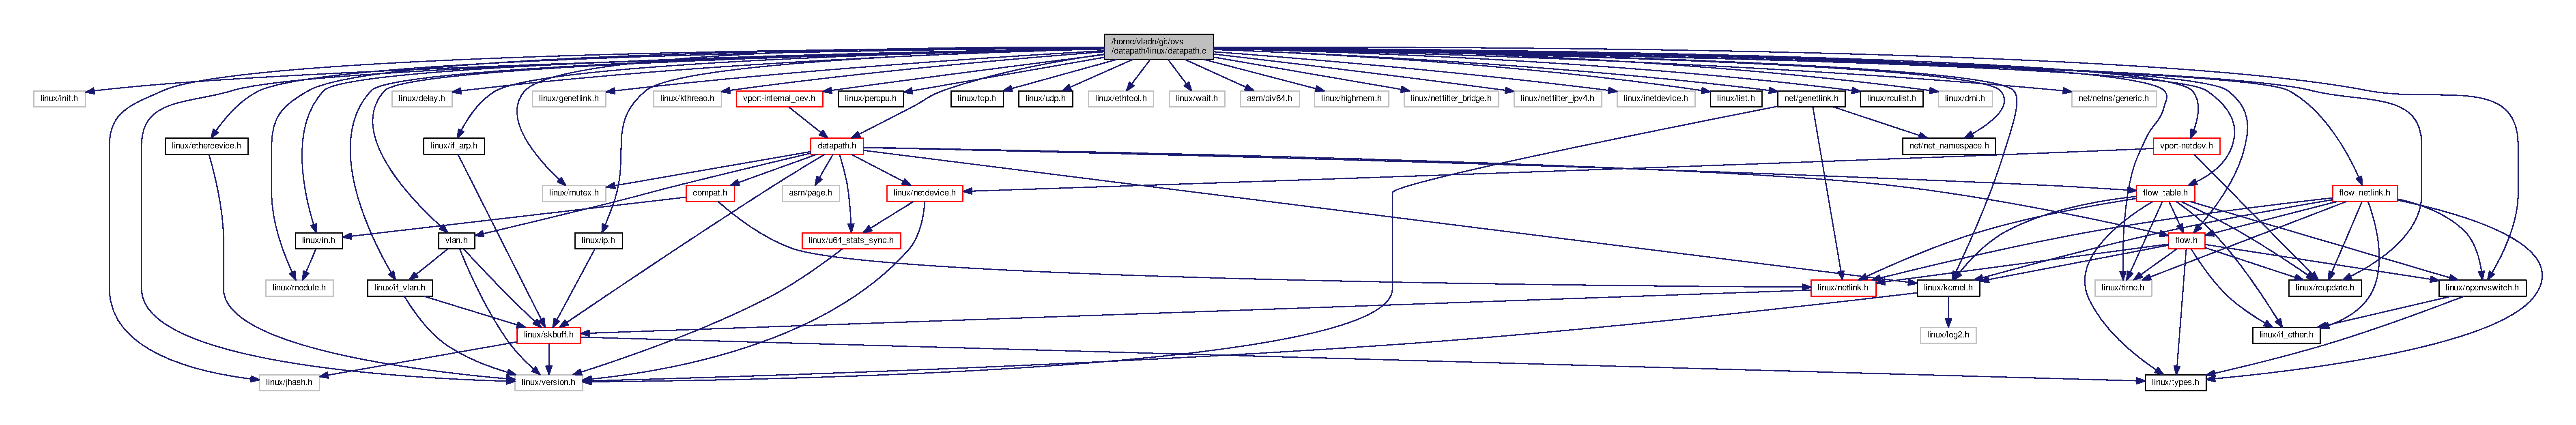
\includegraphics[width=350pt]{linux_2datapath_8c__incl}
\end{center}
\end{figure}
\subsection*{Macros}
\begin{DoxyCompactItemize}
\item 
\#define \hyperlink{linux_2datapath_8c_a1f8c165bf4196327bc3abff648276d92}{pr\+\_\+fmt}(fmt)~K\+B\+U\+I\+L\+D\+\_\+\+M\+O\+D\+N\+A\+M\+E \char`\"{}\+: \char`\"{} fmt
\end{DoxyCompactItemize}
\subsection*{Functions}
\begin{DoxyCompactItemize}
\item 
\hyperlink{linux_2datapath_8c_abf00303edb3bc87ac06f165737f618ec}{E\+X\+P\+O\+R\+T\+\_\+\+S\+Y\+M\+B\+O\+L\+\_\+\+G\+P\+L} (\hyperlink{datapath_8h_ace140298dc2b59b3d77d59c0a210de29}{ovs\+\_\+net\+\_\+id})
\item 
static \hyperlink{types_8h_afaa87723b8417d40fcf45b7330261ef9}{bool} \hyperlink{linux_2datapath_8c_aba3b63f0e73c9ea6ecb8b7aa5d913724}{ovs\+\_\+must\+\_\+notify} (struct \hyperlink{genetlink_8h_aba961c2c372b7122ad0c8ae5e7af2f3b}{genl\+\_\+family} $\ast$family, struct genl\+\_\+info $\ast$info, unsigned int group)
\item 
static void \hyperlink{linux_2datapath_8c_a67f527ad1164ff0d67fe854584ced567}{ovs\+\_\+notify} (struct \hyperlink{genetlink_8h_aba961c2c372b7122ad0c8ae5e7af2f3b}{genl\+\_\+family} $\ast$family, struct genl\+\_\+multicast\+\_\+group $\ast$grp, struct sk\+\_\+buff $\ast$skb, struct genl\+\_\+info $\ast$info)
\item 
static \hyperlink{linux_2datapath_8c_aa489fc945a5cabc6b1efbf3b886ee600}{D\+E\+F\+I\+N\+E\+\_\+\+M\+U\+T\+E\+X} (ovs\+\_\+mutex)
\item 
void \hyperlink{linux_2datapath_8c_a092c1f450b78a173c890ed4c56839e1a}{ovs\+\_\+lock} (void)
\item 
void \hyperlink{linux_2datapath_8c_ac3ccfd98a880ed6d2480209be0d16680}{ovs\+\_\+unlock} (void)
\item 
static int \hyperlink{linux_2datapath_8c_a2c10ba8a23a8cb2f14b7f7684e5ebb5d}{queue\+\_\+gso\+\_\+packets} (struct \hyperlink{structdatapath}{datapath} $\ast$dp, struct sk\+\_\+buff $\ast$, const struct \hyperlink{structsw__flow__key}{sw\+\_\+flow\+\_\+key} $\ast$, const struct \hyperlink{structdp__upcall__info}{dp\+\_\+upcall\+\_\+info} $\ast$)
\item 
static int \hyperlink{linux_2datapath_8c_a549c591fae56562523f243abbe4a1e3e}{queue\+\_\+userspace\+\_\+packet} (struct \hyperlink{structdatapath}{datapath} $\ast$dp, struct sk\+\_\+buff $\ast$, const struct \hyperlink{structsw__flow__key}{sw\+\_\+flow\+\_\+key} $\ast$, const struct \hyperlink{structdp__upcall__info}{dp\+\_\+upcall\+\_\+info} $\ast$)
\item 
static struct \hyperlink{structdatapath}{datapath} $\ast$ \hyperlink{linux_2datapath_8c_ab3f598cca9ed98120cc11daa11690da8}{get\+\_\+dp\+\_\+rcu} (struct net $\ast$net, int dp\+\_\+ifindex)
\item 
static struct \hyperlink{structdatapath}{datapath} $\ast$ \hyperlink{linux_2datapath_8c_a1107d4fd386aa6551511140b5405e1d3}{get\+\_\+dp} (struct net $\ast$net, int dp\+\_\+ifindex)
\item 
const char $\ast$ \hyperlink{linux_2datapath_8c_a6a23196916bb5de4994f901bdf1aba2d}{ovs\+\_\+dp\+\_\+name} (const struct \hyperlink{structdatapath}{datapath} $\ast$dp)
\item 
static int \hyperlink{linux_2datapath_8c_a2c4c60ba176a755749744f7b01aa6edd}{get\+\_\+dpifindex} (const struct \hyperlink{structdatapath}{datapath} $\ast$dp)
\item 
static void \hyperlink{linux_2datapath_8c_a5f329d1e5ef78eb6e9b4aa63c2d97e91}{destroy\+\_\+dp\+\_\+rcu} (struct rcu\+\_\+head $\ast$rcu)
\item 
static struct hlist\+\_\+head $\ast$ \hyperlink{linux_2datapath_8c_af291a723340e4e1bd38b4b14e7f4377a}{vport\+\_\+hash\+\_\+bucket} (const struct \hyperlink{structdatapath}{datapath} $\ast$dp, u16 port\+\_\+no)
\item 
struct \hyperlink{structvport}{vport} $\ast$ \hyperlink{linux_2datapath_8c_a0a9ec01692e1fdcb15a9a294d3789af0}{ovs\+\_\+lookup\+\_\+vport} (const struct \hyperlink{structdatapath}{datapath} $\ast$dp, u16 port\+\_\+no)
\item 
static struct \hyperlink{structvport}{vport} $\ast$ \hyperlink{linux_2datapath_8c_afac95a3e755fe3b0906ccc72d052cbe1}{new\+\_\+vport} (const struct \hyperlink{structvport__parms}{vport\+\_\+parms} $\ast$parms)
\item 
void \hyperlink{linux_2datapath_8c_a560b5f5f97a839287201f7486c53447e}{ovs\+\_\+dp\+\_\+detach\+\_\+port} (struct \hyperlink{structvport}{vport} $\ast$p)
\item 
void \hyperlink{linux_2datapath_8c_aa52cbaf8a4e68129287bfc8ddcde0711}{ovs\+\_\+dp\+\_\+process\+\_\+packet} (struct sk\+\_\+buff $\ast$skb, struct \hyperlink{structsw__flow__key}{sw\+\_\+flow\+\_\+key} $\ast$key)
\item 
int \hyperlink{linux_2datapath_8c_a229b5c7d0158ebc24a90f44de0df0040}{ovs\+\_\+dp\+\_\+upcall} (struct \hyperlink{structdatapath}{datapath} $\ast$dp, struct sk\+\_\+buff $\ast$skb, const struct \hyperlink{structsw__flow__key}{sw\+\_\+flow\+\_\+key} $\ast$key, const struct \hyperlink{structdp__upcall__info}{dp\+\_\+upcall\+\_\+info} $\ast$upcall\+\_\+info)
\item 
static size\+\_\+t \hyperlink{linux_2datapath_8c_a845617ce8ad4e18b0c54961d796a0aeb}{upcall\+\_\+msg\+\_\+size} (const struct \hyperlink{structdp__upcall__info}{dp\+\_\+upcall\+\_\+info} $\ast$upcall\+\_\+info, unsigned int hdrlen)
\item 
static int \hyperlink{linux_2datapath_8c_a20b16b839bd3116f7dbad5719b02c115}{ovs\+\_\+packet\+\_\+cmd\+\_\+execute} (struct sk\+\_\+buff $\ast$skb, struct genl\+\_\+info $\ast$info)
\item 
static void \hyperlink{linux_2datapath_8c_a689a2b3c19c9cdebecfb266acf5ba221}{get\+\_\+dp\+\_\+stats} (const struct \hyperlink{structdatapath}{datapath} $\ast$dp, struct \hyperlink{structovs__dp__stats}{ovs\+\_\+dp\+\_\+stats} $\ast$stats, struct \hyperlink{structovs__dp__megaflow__stats}{ovs\+\_\+dp\+\_\+megaflow\+\_\+stats} $\ast$mega\+\_\+stats)
\item 
static \hyperlink{types_8h_afaa87723b8417d40fcf45b7330261ef9}{bool} \hyperlink{linux_2datapath_8c_a4d912d3ed7dba8789b726280b6dea3a4}{should\+\_\+fill\+\_\+key} (const struct \hyperlink{structsw__flow__id}{sw\+\_\+flow\+\_\+id} $\ast$sfid, uint32\+\_\+t ufid\+\_\+flags)
\item 
static \hyperlink{types_8h_afaa87723b8417d40fcf45b7330261ef9}{bool} \hyperlink{linux_2datapath_8c_acef91dffd31fb70fa6c94e11ad08805b}{should\+\_\+fill\+\_\+mask} (uint32\+\_\+t ufid\+\_\+flags)
\item 
static \hyperlink{types_8h_afaa87723b8417d40fcf45b7330261ef9}{bool} \hyperlink{linux_2datapath_8c_a05dcb72a9103046c5721d03a1592291f}{should\+\_\+fill\+\_\+actions} (uint32\+\_\+t ufid\+\_\+flags)
\item 
static size\+\_\+t \hyperlink{linux_2datapath_8c_a5f17e0449c315970d82161c131e70dbd}{ovs\+\_\+flow\+\_\+cmd\+\_\+msg\+\_\+size} (const struct \hyperlink{structsw__flow__actions}{sw\+\_\+flow\+\_\+actions} $\ast$acts, const struct \hyperlink{structsw__flow__id}{sw\+\_\+flow\+\_\+id} $\ast$sfid, uint32\+\_\+t ufid\+\_\+flags)
\item 
static int \hyperlink{linux_2datapath_8c_a832dcdda5999f2e7fadd72b2ad2373f3}{ovs\+\_\+flow\+\_\+cmd\+\_\+fill\+\_\+stats} (const struct \hyperlink{structsw__flow}{sw\+\_\+flow} $\ast$flow, struct sk\+\_\+buff $\ast$skb)
\item 
static int \hyperlink{linux_2datapath_8c_ad6ce625c1cb24262cddbabe479987986}{ovs\+\_\+flow\+\_\+cmd\+\_\+fill\+\_\+actions} (const struct \hyperlink{structsw__flow}{sw\+\_\+flow} $\ast$flow, struct sk\+\_\+buff $\ast$skb, int skb\+\_\+orig\+\_\+len)
\item 
static int \hyperlink{linux_2datapath_8c_a7b415415fa0d84bab45258cd3080f2c7}{ovs\+\_\+flow\+\_\+cmd\+\_\+fill\+\_\+info} (const struct \hyperlink{structsw__flow}{sw\+\_\+flow} $\ast$flow, int dp\+\_\+ifindex, struct sk\+\_\+buff $\ast$skb, u32 portid, u32 seq, u32 \hyperlink{flow_8h_af4f7a53f6b2df72c34ca881f2714ac91}{flags}, u8 cmd, u32 ufid\+\_\+flags)
\item 
static struct sk\+\_\+buff $\ast$ \hyperlink{linux_2datapath_8c_ac6daf72fcac45a9bd571dec78216e197}{ovs\+\_\+flow\+\_\+cmd\+\_\+alloc\+\_\+info} (const struct \hyperlink{structsw__flow__actions}{sw\+\_\+flow\+\_\+actions} $\ast$acts, const struct \hyperlink{structsw__flow__id}{sw\+\_\+flow\+\_\+id} $\ast$sfid, struct genl\+\_\+info $\ast$info, \hyperlink{types_8h_afaa87723b8417d40fcf45b7330261ef9}{bool} always, uint32\+\_\+t ufid\+\_\+flags)
\item 
static struct sk\+\_\+buff $\ast$ \hyperlink{linux_2datapath_8c_afbfb35c0b3684e82dce573f04491ad1e}{ovs\+\_\+flow\+\_\+cmd\+\_\+build\+\_\+info} (const struct \hyperlink{structsw__flow}{sw\+\_\+flow} $\ast$flow, int dp\+\_\+ifindex, struct genl\+\_\+info $\ast$info, u8 cmd, \hyperlink{types_8h_afaa87723b8417d40fcf45b7330261ef9}{bool} always, u32 ufid\+\_\+flags)
\item 
static int \hyperlink{linux_2datapath_8c_ac8895cf604439184dad96f70e335afe2}{ovs\+\_\+flow\+\_\+cmd\+\_\+new} (struct sk\+\_\+buff $\ast$skb, struct genl\+\_\+info $\ast$info)
\item 
static struct \hyperlink{structsw__flow__actions}{sw\+\_\+flow\+\_\+actions} $\ast$ \hyperlink{linux_2datapath_8c_aac07273dc62dc714973b44be41f9bf7f}{get\+\_\+flow\+\_\+actions} (const struct nlattr $\ast$a, const struct \hyperlink{structsw__flow__key}{sw\+\_\+flow\+\_\+key} $\ast$key, const struct \hyperlink{structsw__flow__mask}{sw\+\_\+flow\+\_\+mask} $\ast$mask, \hyperlink{types_8h_afaa87723b8417d40fcf45b7330261ef9}{bool} log)
\item 
static int \hyperlink{linux_2datapath_8c_a4c6c2d9354cb73a6300a9b3c9cd2a114}{ovs\+\_\+flow\+\_\+cmd\+\_\+set} (struct sk\+\_\+buff $\ast$skb, struct genl\+\_\+info $\ast$info)
\item 
static int \hyperlink{linux_2datapath_8c_a747a4726ec84c751acb3048a515cef86}{ovs\+\_\+flow\+\_\+cmd\+\_\+get} (struct sk\+\_\+buff $\ast$skb, struct genl\+\_\+info $\ast$info)
\item 
static int \hyperlink{linux_2datapath_8c_aa05c62aa6531c0e0312126a21a8d99a5}{ovs\+\_\+flow\+\_\+cmd\+\_\+del} (struct sk\+\_\+buff $\ast$skb, struct genl\+\_\+info $\ast$info)
\item 
static int \hyperlink{linux_2datapath_8c_a4759993b01f8bc67711ecacacdf43976}{ovs\+\_\+flow\+\_\+cmd\+\_\+dump} (struct sk\+\_\+buff $\ast$skb, struct netlink\+\_\+callback $\ast$cb)
\item 
static size\+\_\+t \hyperlink{linux_2datapath_8c_aab015cdb7b4e0d2fa66da1b72963df67}{ovs\+\_\+dp\+\_\+cmd\+\_\+msg\+\_\+size} (void)
\item 
static int \hyperlink{linux_2datapath_8c_a0c18d2b438aba3739c2a36e172cfe3ea}{ovs\+\_\+dp\+\_\+cmd\+\_\+fill\+\_\+info} (struct \hyperlink{structdatapath}{datapath} $\ast$dp, struct sk\+\_\+buff $\ast$skb, u32 portid, u32 seq, u32 \hyperlink{flow_8h_af4f7a53f6b2df72c34ca881f2714ac91}{flags}, u8 cmd)
\item 
static struct sk\+\_\+buff $\ast$ \hyperlink{linux_2datapath_8c_ad01db8513d30c057f1ea10532ebc8b1e}{ovs\+\_\+dp\+\_\+cmd\+\_\+alloc\+\_\+info} (struct genl\+\_\+info $\ast$info)
\item 
static struct \hyperlink{structdatapath}{datapath} $\ast$ \hyperlink{linux_2datapath_8c_a774dc1bd6a39e68ebac48e55688a8574}{lookup\+\_\+datapath} (struct net $\ast$net, const struct \hyperlink{structovs__header}{ovs\+\_\+header} $\ast$\hyperlink{structovs__header}{ovs\+\_\+header}, struct nlattr $\ast$a\mbox{[}\hyperlink{openvswitch_8h_a928e759af5a47791e5b3070bf596fd5d}{O\+V\+S\+\_\+\+D\+P\+\_\+\+A\+T\+T\+R\+\_\+\+M\+A\+X}+1\mbox{]})
\item 
static void \hyperlink{linux_2datapath_8c_aba7a59d6ae252953be557d7478f7332f}{ovs\+\_\+dp\+\_\+reset\+\_\+user\+\_\+features} (struct sk\+\_\+buff $\ast$skb, struct genl\+\_\+info $\ast$info)
\item 
static void \hyperlink{linux_2datapath_8c_a2c763b1da99cce1a426140794eaf8f03}{ovs\+\_\+dp\+\_\+change} (struct \hyperlink{structdatapath}{datapath} $\ast$dp, struct nlattr $\ast$a\mbox{[}$\,$\mbox{]})
\item 
static int \hyperlink{linux_2datapath_8c_a8d012b2863686706ab9d1282a82d6625}{ovs\+\_\+dp\+\_\+cmd\+\_\+new} (struct sk\+\_\+buff $\ast$skb, struct genl\+\_\+info $\ast$info)
\item 
static void \hyperlink{linux_2datapath_8c_a6c66e1332f2a95e9510e37745d77bad1}{\+\_\+\+\_\+dp\+\_\+destroy} (struct \hyperlink{structdatapath}{datapath} $\ast$dp)
\item 
static int \hyperlink{linux_2datapath_8c_a580bc462589253144c5027fa18fbfb17}{ovs\+\_\+dp\+\_\+cmd\+\_\+del} (struct sk\+\_\+buff $\ast$skb, struct genl\+\_\+info $\ast$info)
\item 
static int \hyperlink{linux_2datapath_8c_aa59555f8c6107137945c90e92fd42b4c}{ovs\+\_\+dp\+\_\+cmd\+\_\+set} (struct sk\+\_\+buff $\ast$skb, struct genl\+\_\+info $\ast$info)
\item 
static int \hyperlink{linux_2datapath_8c_ab253bc3f01b9d70955d3d3dcfc236b9f}{ovs\+\_\+dp\+\_\+cmd\+\_\+get} (struct sk\+\_\+buff $\ast$skb, struct genl\+\_\+info $\ast$info)
\item 
static int \hyperlink{linux_2datapath_8c_a64056132bb398b3e7c92291cc6905537}{ovs\+\_\+dp\+\_\+cmd\+\_\+dump} (struct sk\+\_\+buff $\ast$skb, struct netlink\+\_\+callback $\ast$cb)
\item 
static int \hyperlink{linux_2datapath_8c_a4272403de9a985cea17181e99b7a7edc}{ovs\+\_\+vport\+\_\+cmd\+\_\+fill\+\_\+info} (struct \hyperlink{structvport}{vport} $\ast$\hyperlink{structvport}{vport}, struct sk\+\_\+buff $\ast$skb, u32 portid, u32 seq, u32 \hyperlink{flow_8h_af4f7a53f6b2df72c34ca881f2714ac91}{flags}, u8 cmd)
\item 
static struct sk\+\_\+buff $\ast$ \hyperlink{linux_2datapath_8c_a45645849b972492fa9f01eeaf668bf78}{ovs\+\_\+vport\+\_\+cmd\+\_\+alloc\+\_\+info} (void)
\item 
struct sk\+\_\+buff $\ast$ \hyperlink{linux_2datapath_8c_adf50e47c9c548390402b1da1608235c9}{ovs\+\_\+vport\+\_\+cmd\+\_\+build\+\_\+info} (struct \hyperlink{structvport}{vport} $\ast$\hyperlink{structvport}{vport}, u32 portid, u32 seq, u8 cmd)
\item 
static struct \hyperlink{structvport}{vport} $\ast$ \hyperlink{linux_2datapath_8c_a95b019fd3980803dcc1bb5aca920f58b}{lookup\+\_\+vport} (struct net $\ast$net, const struct \hyperlink{structovs__header}{ovs\+\_\+header} $\ast$\hyperlink{structovs__header}{ovs\+\_\+header}, struct nlattr $\ast$a\mbox{[}\hyperlink{openvswitch_8h_a789cf40a0af09c574467d47ca6a2eb7b}{O\+V\+S\+\_\+\+V\+P\+O\+R\+T\+\_\+\+A\+T\+T\+R\+\_\+\+M\+A\+X}+1\mbox{]})
\item 
static int \hyperlink{linux_2datapath_8c_a0b878975d12b240c20c6b5389b5b12b6}{ovs\+\_\+vport\+\_\+cmd\+\_\+new} (struct sk\+\_\+buff $\ast$skb, struct genl\+\_\+info $\ast$info)
\item 
static int \hyperlink{linux_2datapath_8c_a89f1e2fa808021479860862b3e7556e5}{ovs\+\_\+vport\+\_\+cmd\+\_\+set} (struct sk\+\_\+buff $\ast$skb, struct genl\+\_\+info $\ast$info)
\item 
static int \hyperlink{linux_2datapath_8c_afc2316a8fe3074ed07e853d552fb4704}{ovs\+\_\+vport\+\_\+cmd\+\_\+del} (struct sk\+\_\+buff $\ast$skb, struct genl\+\_\+info $\ast$info)
\item 
static int \hyperlink{linux_2datapath_8c_ad818149bb2b46cab6eeb5b7ba6a14afe}{ovs\+\_\+vport\+\_\+cmd\+\_\+get} (struct sk\+\_\+buff $\ast$skb, struct genl\+\_\+info $\ast$info)
\item 
static int \hyperlink{linux_2datapath_8c_ac61e52592bc18541660c182e9aebbcaf}{ovs\+\_\+vport\+\_\+cmd\+\_\+dump} (struct sk\+\_\+buff $\ast$skb, struct netlink\+\_\+callback $\ast$cb)
\item 
static void \hyperlink{linux_2datapath_8c_a02412b752de54c0add0ca994b0e74079}{dp\+\_\+unregister\+\_\+genl} (int n\+\_\+families)
\item 
static int \hyperlink{linux_2datapath_8c_a8a589935468eb018de07b30900a56ddb}{dp\+\_\+register\+\_\+genl} (void)
\item 
static int \+\_\+\+\_\+net\+\_\+init \hyperlink{linux_2datapath_8c_af390458a6069bd6b50c9a0d46517159a}{ovs\+\_\+init\+\_\+net} (struct net $\ast$net)
\item 
static void \+\_\+\+\_\+net\+\_\+exit \hyperlink{linux_2datapath_8c_a97bf5ddc3763f5f1b5691cc262bd206a}{list\+\_\+vports\+\_\+from\+\_\+net} (struct net $\ast$net, struct net $\ast$dnet, struct list\+\_\+head $\ast$head)
\item 
static void \+\_\+\+\_\+net\+\_\+exit \hyperlink{linux_2datapath_8c_aead9307565d6ab903dd5db639c7299e4}{ovs\+\_\+exit\+\_\+net} (struct net $\ast$dnet)
\item 
\hyperlink{linux_2datapath_8c_a537406a5b4c729d36ebe1d833ce74eda}{D\+E\+F\+I\+N\+E\+\_\+\+C\+O\+M\+P\+A\+T\+\_\+\+P\+N\+E\+T\+\_\+\+R\+E\+G\+\_\+\+F\+U\+N\+C} (device)
\item 
static int \+\_\+\+\_\+init \hyperlink{linux_2datapath_8c_a85a2562435726aa1e9d254c86c6e597e}{dp\+\_\+init} (void)
\item 
static void \hyperlink{linux_2datapath_8c_a64b62ac82dbfc2107fa6b38a2c9e3612}{dp\+\_\+cleanup} (void)
\item 
\hyperlink{linux_2datapath_8c_a61981f8b771cdb3f88315f3da5f4fe18}{module\+\_\+init} (\hyperlink{linux_2datapath_8c_a85a2562435726aa1e9d254c86c6e597e}{dp\+\_\+init})
\item 
\hyperlink{linux_2datapath_8c_afefe140861ac8adc338b486bf95f710f}{module\+\_\+exit} (\hyperlink{linux_2datapath_8c_a64b62ac82dbfc2107fa6b38a2c9e3612}{dp\+\_\+cleanup})
\item 
\hyperlink{linux_2datapath_8c_a375185aea6f89fbd06af3e43f39d2975}{M\+O\+D\+U\+L\+E\+\_\+\+D\+E\+S\+C\+R\+I\+P\+T\+I\+O\+N} (\char`\"{}Open v\+Switch switching \hyperlink{structdatapath}{datapath}\char`\"{})
\item 
\hyperlink{linux_2datapath_8c_ad94b36675e7eb067ea3ce6ff9e244a44}{M\+O\+D\+U\+L\+E\+\_\+\+L\+I\+C\+E\+N\+S\+E} (\char`\"{}G\+P\+L\char`\"{})
\item 
\hyperlink{linux_2datapath_8c_ada33d5db5abb99d420d4b6d82ea237c4}{M\+O\+D\+U\+L\+E\+\_\+\+V\+E\+R\+S\+I\+O\+N} (V\+E\+R\+S\+I\+O\+N)
\end{DoxyCompactItemize}
\subsection*{Variables}
\begin{DoxyCompactItemize}
\item 
int \hyperlink{datapath_8h_ace140298dc2b59b3d77d59c0a210de29}{ovs\+\_\+net\+\_\+id} \hyperlink{linux_2datapath_8c_a50bac238082a6952a4dadad6299cc4b3}{\+\_\+\+\_\+read\+\_\+mostly}
\item 
static struct \hyperlink{genetlink_8h_aba961c2c372b7122ad0c8ae5e7af2f3b}{genl\+\_\+family} \hyperlink{linux_2datapath_8c_a709033900c84449b9f83cb62cecb1627}{dp\+\_\+packet\+\_\+genl\+\_\+family}
\item 
static struct \hyperlink{genetlink_8h_aba961c2c372b7122ad0c8ae5e7af2f3b}{genl\+\_\+family} \hyperlink{linux_2datapath_8c_af07853d514acd11f9f0d23494b6a2f9e}{dp\+\_\+flow\+\_\+genl\+\_\+family}
\item 
static struct \hyperlink{genetlink_8h_aba961c2c372b7122ad0c8ae5e7af2f3b}{genl\+\_\+family} \hyperlink{linux_2datapath_8c_a00b4c28b2a15cad709af53b6484fc45c}{dp\+\_\+datapath\+\_\+genl\+\_\+family}
\item 
static const struct nla\+\_\+policy \hyperlink{linux_2datapath_8c_aad79544f457c7a323273d328dafff886}{flow\+\_\+policy} \mbox{[}$\,$\mbox{]}
\item 
static struct genl\+\_\+multicast\+\_\+group \hyperlink{linux_2datapath_8c_ae43fcc307ac0fa091a736d4687c7f884}{ovs\+\_\+dp\+\_\+flow\+\_\+multicast\+\_\+group}
\item 
static struct genl\+\_\+multicast\+\_\+group \hyperlink{linux_2datapath_8c_afa5d1f090aee506896ff5ef56b4053e1}{ovs\+\_\+dp\+\_\+datapath\+\_\+multicast\+\_\+group}
\item 
struct genl\+\_\+multicast\+\_\+group \hyperlink{linux_2datapath_8c_a9dd8d4307b50fdee582eb4013d89eb7b}{ovs\+\_\+dp\+\_\+vport\+\_\+multicast\+\_\+group}
\item 
static const struct nla\+\_\+policy \hyperlink{linux_2datapath_8c_aaef8775f67f989a9ff396e2aa6f6f3e2}{packet\+\_\+policy} \mbox{[}\hyperlink{openvswitch_8h_a9c91f74efc7f0264839c153979485eec}{O\+V\+S\+\_\+\+P\+A\+C\+K\+E\+T\+\_\+\+A\+T\+T\+R\+\_\+\+M\+A\+X}+1\mbox{]}
\item 
static struct genl\+\_\+ops \hyperlink{linux_2datapath_8c_a75ed1b368ac93a17ed4d04c82b892be9}{dp\+\_\+packet\+\_\+genl\+\_\+ops} \mbox{[}$\,$\mbox{]}
\item 
static struct genl\+\_\+ops \hyperlink{linux_2datapath_8c_a42bdb3978421f4f0b3a1be828226b271}{dp\+\_\+flow\+\_\+genl\+\_\+ops} \mbox{[}$\,$\mbox{]}
\item 
static const struct nla\+\_\+policy \hyperlink{linux_2datapath_8c_a34f2da191c04c403e206dacb0c3d2a6f}{datapath\+\_\+policy} \mbox{[}\hyperlink{openvswitch_8h_a928e759af5a47791e5b3070bf596fd5d}{O\+V\+S\+\_\+\+D\+P\+\_\+\+A\+T\+T\+R\+\_\+\+M\+A\+X}+1\mbox{]}
\item 
static struct genl\+\_\+ops \hyperlink{linux_2datapath_8c_a29acb4bb9ad0b3d7af71e628bf516372}{dp\+\_\+datapath\+\_\+genl\+\_\+ops} \mbox{[}$\,$\mbox{]}
\item 
static const struct nla\+\_\+policy \hyperlink{linux_2datapath_8c_af3f5c0f1eb12c1eb1a2494f265dda98a}{vport\+\_\+policy} \mbox{[}\hyperlink{openvswitch_8h_a789cf40a0af09c574467d47ca6a2eb7b}{O\+V\+S\+\_\+\+V\+P\+O\+R\+T\+\_\+\+A\+T\+T\+R\+\_\+\+M\+A\+X}+1\mbox{]}
\item 
static struct genl\+\_\+ops \hyperlink{linux_2datapath_8c_a5a28211e3b7e9a5cf7ccf8e81b8bfa8e}{dp\+\_\+vport\+\_\+genl\+\_\+ops} \mbox{[}$\,$\mbox{]}
\item 
struct \hyperlink{genetlink_8h_aba961c2c372b7122ad0c8ae5e7af2f3b}{genl\+\_\+family} \hyperlink{linux_2datapath_8c_a69bf55f33e234bc4b78e6eeee1d603fd}{dp\+\_\+vport\+\_\+genl\+\_\+family}
\item 
static struct \hyperlink{genetlink_8h_aba961c2c372b7122ad0c8ae5e7af2f3b}{genl\+\_\+family} $\ast$ \hyperlink{linux_2datapath_8c_ae945344e649c305788038f5bc09bc817}{dp\+\_\+genl\+\_\+families} \mbox{[}$\,$\mbox{]}
\item 
static struct pernet\+\_\+operations \hyperlink{linux_2datapath_8c_a3a9f5b1a35fcb90938194f22dc2d0f14}{ovs\+\_\+net\+\_\+ops}
\end{DoxyCompactItemize}


\subsection{Macro Definition Documentation}
\hypertarget{linux_2datapath_8c_a1f8c165bf4196327bc3abff648276d92}{}\index{linux/datapath.\+c@{linux/datapath.\+c}!pr\+\_\+fmt@{pr\+\_\+fmt}}
\index{pr\+\_\+fmt@{pr\+\_\+fmt}!linux/datapath.\+c@{linux/datapath.\+c}}
\subsubsection[{pr\+\_\+fmt}]{\setlength{\rightskip}{0pt plus 5cm}\#define pr\+\_\+fmt(
\begin{DoxyParamCaption}
\item[{}]{fmt}
\end{DoxyParamCaption}
)~K\+B\+U\+I\+L\+D\+\_\+\+M\+O\+D\+N\+A\+M\+E \char`\"{}\+: \char`\"{} fmt}\label{linux_2datapath_8c_a1f8c165bf4196327bc3abff648276d92}


\subsection{Function Documentation}
\hypertarget{linux_2datapath_8c_a6c66e1332f2a95e9510e37745d77bad1}{}\index{linux/datapath.\+c@{linux/datapath.\+c}!\+\_\+\+\_\+dp\+\_\+destroy@{\+\_\+\+\_\+dp\+\_\+destroy}}
\index{\+\_\+\+\_\+dp\+\_\+destroy@{\+\_\+\+\_\+dp\+\_\+destroy}!linux/datapath.\+c@{linux/datapath.\+c}}
\subsubsection[{\+\_\+\+\_\+dp\+\_\+destroy}]{\setlength{\rightskip}{0pt plus 5cm}static void \+\_\+\+\_\+dp\+\_\+destroy (
\begin{DoxyParamCaption}
\item[{struct {\bf datapath} $\ast$}]{dp}
\end{DoxyParamCaption}
)\hspace{0.3cm}{\ttfamily [static]}}\label{linux_2datapath_8c_a6c66e1332f2a95e9510e37745d77bad1}

\begin{DoxyCode}
1614 \{
1615     \textcolor{keywordtype}{int} i;
1616 
1617     \textcolor{keywordflow}{for} (i = 0; i < \hyperlink{datapath_8h_ac1bf9805d62227b8f76f130087e18018}{DP\_VPORT\_HASH\_BUCKETS}; i++) \{
1618         \textcolor{keyword}{struct }\hyperlink{structvport}{vport} *\hyperlink{structvport}{vport};
1619         \textcolor{keyword}{struct }hlist\_node *n;
1620 
1621         \hyperlink{list_8h_ae2f7dd7dbbe2f13fa51aca9fcb31a03f}{hlist\_for\_each\_entry\_safe}(vport, n, &dp->\hyperlink{structdatapath_abb0de528545b312de283b571cb6c4ede}{ports}[i], dp\_hash\_node)
1622             if (vport->port\_no != \hyperlink{openvswitch_8h_aff2f13b95c27262c520f26831e647598}{OVSP\_LOCAL})
1623                 \hyperlink{datapath_8c_a560b5f5f97a839287201f7486c53447e}{ovs\_dp\_detach\_port}(vport);
1624     \}
1625 
1626     list\_del\_rcu(&dp->list\_node);
1627 
1628     \textcolor{comment}{/* OVSP\_LOCAL is datapath internal port. We need to make sure that}
1629 \textcolor{comment}{     * all ports in datapath are destroyed first before freeing datapath.}
1630 \textcolor{comment}{     */}
1631     \hyperlink{datapath_8c_a560b5f5f97a839287201f7486c53447e}{ovs\_dp\_detach\_port}(\hyperlink{datapath_8h_a422576bd4b943e9df313ba73f6c624e1}{ovs\_vport\_ovsl}(dp, 
      \hyperlink{openvswitch_8h_aff2f13b95c27262c520f26831e647598}{OVSP\_LOCAL}));
1632 
1633     \textcolor{comment}{/* RCU destroy the flow table */}
1634     call\_rcu(&dp->rcu, \hyperlink{linux_2datapath_8c_a5f329d1e5ef78eb6e9b4aa63c2d97e91}{destroy\_dp\_rcu});
1635 \}
\end{DoxyCode}
\hypertarget{linux_2datapath_8c_a537406a5b4c729d36ebe1d833ce74eda}{}\index{linux/datapath.\+c@{linux/datapath.\+c}!D\+E\+F\+I\+N\+E\+\_\+\+C\+O\+M\+P\+A\+T\+\_\+\+P\+N\+E\+T\+\_\+\+R\+E\+G\+\_\+\+F\+U\+N\+C@{D\+E\+F\+I\+N\+E\+\_\+\+C\+O\+M\+P\+A\+T\+\_\+\+P\+N\+E\+T\+\_\+\+R\+E\+G\+\_\+\+F\+U\+N\+C}}
\index{D\+E\+F\+I\+N\+E\+\_\+\+C\+O\+M\+P\+A\+T\+\_\+\+P\+N\+E\+T\+\_\+\+R\+E\+G\+\_\+\+F\+U\+N\+C@{D\+E\+F\+I\+N\+E\+\_\+\+C\+O\+M\+P\+A\+T\+\_\+\+P\+N\+E\+T\+\_\+\+R\+E\+G\+\_\+\+F\+U\+N\+C}!linux/datapath.\+c@{linux/datapath.\+c}}
\subsubsection[{D\+E\+F\+I\+N\+E\+\_\+\+C\+O\+M\+P\+A\+T\+\_\+\+P\+N\+E\+T\+\_\+\+R\+E\+G\+\_\+\+F\+U\+N\+C}]{\setlength{\rightskip}{0pt plus 5cm}D\+E\+F\+I\+N\+E\+\_\+\+C\+O\+M\+P\+A\+T\+\_\+\+P\+N\+E\+T\+\_\+\+R\+E\+G\+\_\+\+F\+U\+N\+C (
\begin{DoxyParamCaption}
\item[{device}]{}
\end{DoxyParamCaption}
)}\label{linux_2datapath_8c_a537406a5b4c729d36ebe1d833ce74eda}
\hypertarget{linux_2datapath_8c_aa489fc945a5cabc6b1efbf3b886ee600}{}\index{linux/datapath.\+c@{linux/datapath.\+c}!D\+E\+F\+I\+N\+E\+\_\+\+M\+U\+T\+E\+X@{D\+E\+F\+I\+N\+E\+\_\+\+M\+U\+T\+E\+X}}
\index{D\+E\+F\+I\+N\+E\+\_\+\+M\+U\+T\+E\+X@{D\+E\+F\+I\+N\+E\+\_\+\+M\+U\+T\+E\+X}!linux/datapath.\+c@{linux/datapath.\+c}}
\subsubsection[{D\+E\+F\+I\+N\+E\+\_\+\+M\+U\+T\+E\+X}]{\setlength{\rightskip}{0pt plus 5cm}static D\+E\+F\+I\+N\+E\+\_\+\+M\+U\+T\+E\+X (
\begin{DoxyParamCaption}
\item[{ovs\+\_\+mutex}]{}
\end{DoxyParamCaption}
)\hspace{0.3cm}{\ttfamily [static]}}\label{linux_2datapath_8c_aa489fc945a5cabc6b1efbf3b886ee600}
D\+O\+C\+: Locking\+:

All writes e.\+g. Writes to device state (add/remove datapath, port, set operations on vports, etc.), Writes to other state (flow table modifications, set miscellaneous datapath parameters, etc.) are protected by ovs\+\_\+lock.

Reads are protected by R\+C\+U.

There are a few special cases (mostly stats) that have their own synchronization but they nest under all of above and don\textquotesingle{}t interact with each other.

The R\+T\+N\+L lock nests inside ovs\+\_\+mutex. \hypertarget{linux_2datapath_8c_a5f329d1e5ef78eb6e9b4aa63c2d97e91}{}\index{linux/datapath.\+c@{linux/datapath.\+c}!destroy\+\_\+dp\+\_\+rcu@{destroy\+\_\+dp\+\_\+rcu}}
\index{destroy\+\_\+dp\+\_\+rcu@{destroy\+\_\+dp\+\_\+rcu}!linux/datapath.\+c@{linux/datapath.\+c}}
\subsubsection[{destroy\+\_\+dp\+\_\+rcu}]{\setlength{\rightskip}{0pt plus 5cm}static void destroy\+\_\+dp\+\_\+rcu (
\begin{DoxyParamCaption}
\item[{struct rcu\+\_\+head $\ast$}]{rcu}
\end{DoxyParamCaption}
)\hspace{0.3cm}{\ttfamily [static]}}\label{linux_2datapath_8c_a5f329d1e5ef78eb6e9b4aa63c2d97e91}

\begin{DoxyCode}
203 \{
204     \textcolor{keyword}{struct }\hyperlink{structdatapath}{datapath} *dp = container\_of(\hyperlink{structdatapath_af487ac38fa868c398dd248f1956b7a35}{rcu}, \textcolor{keyword}{struct} \hyperlink{structdatapath}{datapath}, 
      \hyperlink{structdatapath_af487ac38fa868c398dd248f1956b7a35}{rcu});
205 
206     \hyperlink{flow__table_8c_ad37dcfdb56d17589ed79b5c4dd38bc76}{ovs\_flow\_tbl\_destroy}(&dp->\hyperlink{structdatapath_ac6d67fe586c19484391acbcfa267259d}{table});
207     free\_percpu(dp->\hyperlink{structdatapath_a26ff295c711206c8177cdc89150c6a4a}{stats\_percpu});
208     release\_net(\hyperlink{datapath_8h_aef2302004ca1f45133eaef00bb3740eb}{ovs\_dp\_get\_net}(dp));
209     kfree(dp->\hyperlink{structdatapath_abb0de528545b312de283b571cb6c4ede}{ports});
210     kfree(dp);
211 \}
\end{DoxyCode}
\hypertarget{linux_2datapath_8c_a64b62ac82dbfc2107fa6b38a2c9e3612}{}\index{linux/datapath.\+c@{linux/datapath.\+c}!dp\+\_\+cleanup@{dp\+\_\+cleanup}}
\index{dp\+\_\+cleanup@{dp\+\_\+cleanup}!linux/datapath.\+c@{linux/datapath.\+c}}
\subsubsection[{dp\+\_\+cleanup}]{\setlength{\rightskip}{0pt plus 5cm}static void dp\+\_\+cleanup (
\begin{DoxyParamCaption}
\item[{void}]{}
\end{DoxyParamCaption}
)\hspace{0.3cm}{\ttfamily [static]}}\label{linux_2datapath_8c_a64b62ac82dbfc2107fa6b38a2c9e3612}

\begin{DoxyCode}
2344 \{
2345     \hyperlink{linux_2datapath_8c_a02412b752de54c0add0ca994b0e74079}{dp\_unregister\_genl}(ARRAY\_SIZE(\hyperlink{linux_2datapath_8c_ae945344e649c305788038f5bc09bc817}{dp\_genl\_families}));
2346     \hyperlink{linux_2vport-netdev_8c_ada5333ba6a30c7b472582687565e316c}{ovs\_netdev\_exit}();
2347     unregister\_netdevice\_notifier(&\hyperlink{datapath_8h_ab34ba4d6c1125efcec9480356f3393e6}{ovs\_dp\_device\_notifier});
2348     unregister\_pernet\_device(&\hyperlink{linux_2datapath_8c_a3a9f5b1a35fcb90938194f22dc2d0f14}{ovs\_net\_ops});
2349     rcu\_barrier();
2350     \hyperlink{linux_2vport_8c_a32e04c9d5d25cb3b7e23a297dc65fc6a}{ovs\_vport\_exit}();
2351     \hyperlink{flow__table_8c_a96cce30f7a9c3231d5b5afaf967378eb}{ovs\_flow\_exit}();
2352     \hyperlink{linux_2vport-internal__dev_8c_a4e61a8459847af3c4f5773e09552cf98}{ovs\_internal\_dev\_rtnl\_link\_unregister}();
2353     \hyperlink{actions_8c_a7dfd1f218e0966ef342251a185866f4d}{action\_fifos\_exit}();
2354 \}
\end{DoxyCode}
\hypertarget{linux_2datapath_8c_a85a2562435726aa1e9d254c86c6e597e}{}\index{linux/datapath.\+c@{linux/datapath.\+c}!dp\+\_\+init@{dp\+\_\+init}}
\index{dp\+\_\+init@{dp\+\_\+init}!linux/datapath.\+c@{linux/datapath.\+c}}
\subsubsection[{dp\+\_\+init}]{\setlength{\rightskip}{0pt plus 5cm}static int \+\_\+\+\_\+init dp\+\_\+init (
\begin{DoxyParamCaption}
\item[{void}]{}
\end{DoxyParamCaption}
)\hspace{0.3cm}{\ttfamily [static]}}\label{linux_2datapath_8c_a85a2562435726aa1e9d254c86c6e597e}

\begin{DoxyCode}
2284 \{
2285     \textcolor{keywordtype}{int} err;
2286 
2287     BUILD\_BUG\_ON(\textcolor{keyword}{sizeof}(\textcolor{keyword}{struct} \hyperlink{structovs__skb__cb}{ovs\_skb\_cb}) > FIELD\_SIZEOF(\textcolor{keyword}{struct} sk\_buff, cb));
2288 
2289     pr\_info(\textcolor{stringliteral}{"Open vSwitch switching datapath %s\(\backslash\)n"}, VERSION);
2290 
2291     err = \hyperlink{actions_8c_a3006f0376c2aecb6525126ad0e9bae25}{action\_fifos\_init}();
2292     \textcolor{keywordflow}{if} (err)
2293         \textcolor{keywordflow}{goto} error;
2294 
2295     err = \hyperlink{linux_2vport-internal__dev_8c_ac6d8a2dd3cdef9e9ba9efdd4e0656f7c}{ovs\_internal\_dev\_rtnl\_link\_register}();
2296     \textcolor{keywordflow}{if} (err)
2297         \textcolor{keywordflow}{goto} error\_action\_fifos\_exit;
2298 
2299     err = \hyperlink{flow__table_8c_a07492868e65ba495c86d49df9cf1bc50}{ovs\_flow\_init}();
2300     \textcolor{keywordflow}{if} (err)
2301         \textcolor{keywordflow}{goto} error\_unreg\_rtnl\_link;
2302 
2303     err = \hyperlink{linux_2vport_8c_aacc501a60108d387b8fd7535c2e6168f}{ovs\_vport\_init}();
2304     \textcolor{keywordflow}{if} (err)
2305         \textcolor{keywordflow}{goto} error\_flow\_exit;
2306 
2307     err = register\_pernet\_device(&\hyperlink{linux_2datapath_8c_a3a9f5b1a35fcb90938194f22dc2d0f14}{ovs\_net\_ops});
2308     \textcolor{keywordflow}{if} (err)
2309         \textcolor{keywordflow}{goto} error\_vport\_exit;
2310 
2311     err = register\_netdevice\_notifier(&\hyperlink{datapath_8h_ab34ba4d6c1125efcec9480356f3393e6}{ovs\_dp\_device\_notifier});
2312     \textcolor{keywordflow}{if} (err)
2313         \textcolor{keywordflow}{goto} error\_netns\_exit;
2314 
2315     err = \hyperlink{linux_2vport-netdev_8c_a70dd93833f5d471ed3951dd80f54a914}{ovs\_netdev\_init}();
2316     \textcolor{keywordflow}{if} (err)
2317         \textcolor{keywordflow}{goto} error\_unreg\_notifier;
2318 
2319     err = \hyperlink{linux_2datapath_8c_a8a589935468eb018de07b30900a56ddb}{dp\_register\_genl}();
2320     \textcolor{keywordflow}{if} (err < 0)
2321         \textcolor{keywordflow}{goto} error\_unreg\_netdev;
2322 
2323     \textcolor{keywordflow}{return} 0;
2324 
2325 error\_unreg\_netdev:
2326     \hyperlink{linux_2vport-netdev_8c_ada5333ba6a30c7b472582687565e316c}{ovs\_netdev\_exit}();
2327 error\_unreg\_notifier:
2328     unregister\_netdevice\_notifier(&\hyperlink{datapath_8h_ab34ba4d6c1125efcec9480356f3393e6}{ovs\_dp\_device\_notifier});
2329 error\_netns\_exit:
2330     unregister\_pernet\_device(&\hyperlink{linux_2datapath_8c_a3a9f5b1a35fcb90938194f22dc2d0f14}{ovs\_net\_ops});
2331 error\_vport\_exit:
2332     \hyperlink{linux_2vport_8c_a32e04c9d5d25cb3b7e23a297dc65fc6a}{ovs\_vport\_exit}();
2333 error\_flow\_exit:
2334     \hyperlink{flow__table_8c_a96cce30f7a9c3231d5b5afaf967378eb}{ovs\_flow\_exit}();
2335 error\_unreg\_rtnl\_link:
2336     \hyperlink{linux_2vport-internal__dev_8c_a4e61a8459847af3c4f5773e09552cf98}{ovs\_internal\_dev\_rtnl\_link\_unregister}();
2337 error\_action\_fifos\_exit:
2338     \hyperlink{actions_8c_a7dfd1f218e0966ef342251a185866f4d}{action\_fifos\_exit}();
2339 error:
2340     \textcolor{keywordflow}{return} err;
2341 \}
\end{DoxyCode}
\hypertarget{linux_2datapath_8c_a8a589935468eb018de07b30900a56ddb}{}\index{linux/datapath.\+c@{linux/datapath.\+c}!dp\+\_\+register\+\_\+genl@{dp\+\_\+register\+\_\+genl}}
\index{dp\+\_\+register\+\_\+genl@{dp\+\_\+register\+\_\+genl}!linux/datapath.\+c@{linux/datapath.\+c}}
\subsubsection[{dp\+\_\+register\+\_\+genl}]{\setlength{\rightskip}{0pt plus 5cm}static int dp\+\_\+register\+\_\+genl (
\begin{DoxyParamCaption}
\item[{void}]{}
\end{DoxyParamCaption}
)\hspace{0.3cm}{\ttfamily [static]}}\label{linux_2datapath_8c_a8a589935468eb018de07b30900a56ddb}

\begin{DoxyCode}
2193 \{
2194     \textcolor{keywordtype}{int} err;
2195     \textcolor{keywordtype}{int} i;
2196 
2197     \textcolor{keywordflow}{for} (i = 0; i < ARRAY\_SIZE(\hyperlink{linux_2datapath_8c_ae945344e649c305788038f5bc09bc817}{dp\_genl\_families}); i++) \{
2198 
2199         err = \hyperlink{genetlink_8h_ae1e50e3e047b37c08412138d4f224179}{genl\_register\_family}(\hyperlink{linux_2datapath_8c_ae945344e649c305788038f5bc09bc817}{dp\_genl\_families}[i]);
2200         \textcolor{keywordflow}{if} (err)
2201             \textcolor{keywordflow}{goto} error;
2202     \}
2203 
2204     \textcolor{keywordflow}{return} 0;
2205 
2206 error:
2207     \hyperlink{linux_2datapath_8c_a02412b752de54c0add0ca994b0e74079}{dp\_unregister\_genl}(i);
2208     \textcolor{keywordflow}{return} err;
2209 \}
\end{DoxyCode}
\hypertarget{linux_2datapath_8c_a02412b752de54c0add0ca994b0e74079}{}\index{linux/datapath.\+c@{linux/datapath.\+c}!dp\+\_\+unregister\+\_\+genl@{dp\+\_\+unregister\+\_\+genl}}
\index{dp\+\_\+unregister\+\_\+genl@{dp\+\_\+unregister\+\_\+genl}!linux/datapath.\+c@{linux/datapath.\+c}}
\subsubsection[{dp\+\_\+unregister\+\_\+genl}]{\setlength{\rightskip}{0pt plus 5cm}static void dp\+\_\+unregister\+\_\+genl (
\begin{DoxyParamCaption}
\item[{int}]{n\+\_\+families}
\end{DoxyParamCaption}
)\hspace{0.3cm}{\ttfamily [static]}}\label{linux_2datapath_8c_a02412b752de54c0add0ca994b0e74079}

\begin{DoxyCode}
2185 \{
2186     \textcolor{keywordtype}{int} i;
2187 
2188     \textcolor{keywordflow}{for} (i = 0; i < n\_families; i++)
2189         \hyperlink{genetlink_8h_a838538f5265ecd4c9726bdf30cfa02c2}{genl\_unregister\_family}(\hyperlink{linux_2datapath_8c_ae945344e649c305788038f5bc09bc817}{dp\_genl\_families}[i]);
2190 \}
\end{DoxyCode}
\hypertarget{linux_2datapath_8c_abf00303edb3bc87ac06f165737f618ec}{}\index{linux/datapath.\+c@{linux/datapath.\+c}!E\+X\+P\+O\+R\+T\+\_\+\+S\+Y\+M\+B\+O\+L\+\_\+\+G\+P\+L@{E\+X\+P\+O\+R\+T\+\_\+\+S\+Y\+M\+B\+O\+L\+\_\+\+G\+P\+L}}
\index{E\+X\+P\+O\+R\+T\+\_\+\+S\+Y\+M\+B\+O\+L\+\_\+\+G\+P\+L@{E\+X\+P\+O\+R\+T\+\_\+\+S\+Y\+M\+B\+O\+L\+\_\+\+G\+P\+L}!linux/datapath.\+c@{linux/datapath.\+c}}
\subsubsection[{E\+X\+P\+O\+R\+T\+\_\+\+S\+Y\+M\+B\+O\+L\+\_\+\+G\+P\+L}]{\setlength{\rightskip}{0pt plus 5cm}E\+X\+P\+O\+R\+T\+\_\+\+S\+Y\+M\+B\+O\+L\+\_\+\+G\+P\+L (
\begin{DoxyParamCaption}
\item[{{\bf ovs\+\_\+net\+\_\+id}}]{}
\end{DoxyParamCaption}
)}\label{linux_2datapath_8c_abf00303edb3bc87ac06f165737f618ec}
\hypertarget{linux_2datapath_8c_a1107d4fd386aa6551511140b5405e1d3}{}\index{linux/datapath.\+c@{linux/datapath.\+c}!get\+\_\+dp@{get\+\_\+dp}}
\index{get\+\_\+dp@{get\+\_\+dp}!linux/datapath.\+c@{linux/datapath.\+c}}
\subsubsection[{get\+\_\+dp}]{\setlength{\rightskip}{0pt plus 5cm}static struct {\bf datapath}$\ast$ get\+\_\+dp (
\begin{DoxyParamCaption}
\item[{struct net $\ast$}]{net, }
\item[{int}]{dp\+\_\+ifindex}
\end{DoxyParamCaption}
)\hspace{0.3cm}{\ttfamily [static]}}\label{linux_2datapath_8c_a1107d4fd386aa6551511140b5405e1d3}

\begin{DoxyCode}
166 \{
167     \textcolor{keyword}{struct }\hyperlink{structdatapath}{datapath} *dp;
168 
169     WARN\_ON\_ONCE(!\hyperlink{rcupdate_8h_ab77c80b5efea34ea99ec24a4f532eb9b}{rcu\_read\_lock\_held}() && !
      \hyperlink{datapath_8h_a54d3f44a7dda58b44208095ce4b2c0ee}{lockdep\_ovsl\_is\_held}());
170     rcu\_read\_lock();
171     dp = \hyperlink{linux_2datapath_8c_ab3f598cca9ed98120cc11daa11690da8}{get\_dp\_rcu}(net, dp\_ifindex);
172     rcu\_read\_unlock();
173 
174     \textcolor{keywordflow}{return} dp;
175 \}
\end{DoxyCode}
\hypertarget{linux_2datapath_8c_ab3f598cca9ed98120cc11daa11690da8}{}\index{linux/datapath.\+c@{linux/datapath.\+c}!get\+\_\+dp\+\_\+rcu@{get\+\_\+dp\+\_\+rcu}}
\index{get\+\_\+dp\+\_\+rcu@{get\+\_\+dp\+\_\+rcu}!linux/datapath.\+c@{linux/datapath.\+c}}
\subsubsection[{get\+\_\+dp\+\_\+rcu}]{\setlength{\rightskip}{0pt plus 5cm}static struct {\bf datapath}$\ast$ get\+\_\+dp\+\_\+rcu (
\begin{DoxyParamCaption}
\item[{struct net $\ast$}]{net, }
\item[{int}]{dp\+\_\+ifindex}
\end{DoxyParamCaption}
)\hspace{0.3cm}{\ttfamily [static]}}\label{linux_2datapath_8c_ab3f598cca9ed98120cc11daa11690da8}

\begin{DoxyCode}
150 \{
151     \textcolor{keyword}{struct }net\_device *dev = \hyperlink{netdevice_8h_aae9e99af63bfc2280ca46e232e32b6b8}{dev\_get\_by\_index\_rcu}(net, dp\_ifindex);
152 
153     \textcolor{keywordflow}{if} (dev) \{
154         \textcolor{keyword}{struct }\hyperlink{structvport}{vport} *\hyperlink{structvport}{vport} = \hyperlink{linux_2vport-internal__dev_8c_abdb7a75d6c79176507a41a200c69e77b}{ovs\_internal\_dev\_get\_vport}(dev);
155         \textcolor{keywordflow}{if} (vport)
156             \textcolor{keywordflow}{return} vport->\hyperlink{structvport_a49fb6f6bf0ac4337853e9242e88ddc42}{dp};
157     \}
158 
159     \textcolor{keywordflow}{return} NULL;
160 \}
\end{DoxyCode}
\hypertarget{linux_2datapath_8c_a689a2b3c19c9cdebecfb266acf5ba221}{}\index{linux/datapath.\+c@{linux/datapath.\+c}!get\+\_\+dp\+\_\+stats@{get\+\_\+dp\+\_\+stats}}
\index{get\+\_\+dp\+\_\+stats@{get\+\_\+dp\+\_\+stats}!linux/datapath.\+c@{linux/datapath.\+c}}
\subsubsection[{get\+\_\+dp\+\_\+stats}]{\setlength{\rightskip}{0pt plus 5cm}static void get\+\_\+dp\+\_\+stats (
\begin{DoxyParamCaption}
\item[{const struct {\bf datapath} $\ast$}]{dp, }
\item[{struct {\bf ovs\+\_\+dp\+\_\+stats} $\ast$}]{stats, }
\item[{struct {\bf ovs\+\_\+dp\+\_\+megaflow\+\_\+stats} $\ast$}]{mega\+\_\+stats}
\end{DoxyParamCaption}
)\hspace{0.3cm}{\ttfamily [static]}}\label{linux_2datapath_8c_a689a2b3c19c9cdebecfb266acf5ba221}

\begin{DoxyCode}
661 \{
662     \textcolor{keywordtype}{int} i;
663 
664     memset(mega\_stats, 0, \textcolor{keyword}{sizeof}(*mega\_stats));
665 
666     stats->\hyperlink{structovs__dp__stats_af6bf9e903d781d713f0f5d10b2d8550f}{n\_flows} = \hyperlink{flow__table_8c_a8f1f39fd4e1ecafd99321016698a709a}{ovs\_flow\_tbl\_count}(&dp->\hyperlink{structdatapath_ac6d67fe586c19484391acbcfa267259d}{table});
667     mega\_stats->\hyperlink{structovs__dp__megaflow__stats_a7984504a5c12cc5a0767c6a34c4c9c96}{n\_masks} = \hyperlink{flow__table_8c_ab6e18d16217cddd0af756b76b72e6ce6}{ovs\_flow\_tbl\_num\_masks}(&dp->
      \hyperlink{structdatapath_ac6d67fe586c19484391acbcfa267259d}{table});
668 
669     stats->\hyperlink{structovs__dp__stats_a0c6b8d1358632341b5e949570c5dca68}{n\_hit} = stats->\hyperlink{structovs__dp__stats_a8f1b9687593ebb43ca54c1c9904999a6}{n\_missed} = stats->\hyperlink{structovs__dp__stats_a83a104dedcf4ee3cc2a940e4043e89b2}{n\_lost} = 0;
670 
671     \hyperlink{cpumask_8h_ad15c4fe55a8b712e3bf1049320f3c3cb}{for\_each\_possible\_cpu}(i) \{
672         \textcolor{keyword}{const} \textcolor{keyword}{struct }\hyperlink{structdp__stats__percpu}{dp\_stats\_percpu} *percpu\_stats;
673         \textcolor{keyword}{struct }\hyperlink{structdp__stats__percpu}{dp\_stats\_percpu} local\_stats;
674         \textcolor{keywordtype}{unsigned} \textcolor{keywordtype}{int} start;
675 
676         percpu\_stats = per\_cpu\_ptr(dp->\hyperlink{structdatapath_a26ff295c711206c8177cdc89150c6a4a}{stats\_percpu}, i);
677 
678         \textcolor{keywordflow}{do} \{
679             start = \hyperlink{u64__stats__sync_8h_addfaebb71638dbc159aaee907e45fe84}{u64\_stats\_fetch\_begin\_irq}(&percpu\_stats->
      \hyperlink{structdp__stats__percpu_ad67971f59f6db5432848db23d185dc2f}{syncp});
680             local\_stats = *percpu\_stats;
681         \} \textcolor{keywordflow}{while} (\hyperlink{u64__stats__sync_8h_a663ca602e197bee607ec46f743c839e1}{u64\_stats\_fetch\_retry\_irq}(&percpu\_stats->
      \hyperlink{structdp__stats__percpu_ad67971f59f6db5432848db23d185dc2f}{syncp}, start));
682 
683         stats->\hyperlink{structovs__dp__stats_a0c6b8d1358632341b5e949570c5dca68}{n\_hit} += local\_stats.n\_hit;
684         stats->\hyperlink{structovs__dp__stats_a8f1b9687593ebb43ca54c1c9904999a6}{n\_missed} += local\_stats.n\_missed;
685         stats->\hyperlink{structovs__dp__stats_a83a104dedcf4ee3cc2a940e4043e89b2}{n\_lost} += local\_stats.n\_lost;
686         mega\_stats->\hyperlink{structovs__dp__megaflow__stats_a28566425278d53e7a93e693d54e1e65c}{n\_mask\_hit} += local\_stats.n\_mask\_hit;
687     \}
688 \}
\end{DoxyCode}
\hypertarget{linux_2datapath_8c_a2c4c60ba176a755749744f7b01aa6edd}{}\index{linux/datapath.\+c@{linux/datapath.\+c}!get\+\_\+dpifindex@{get\+\_\+dpifindex}}
\index{get\+\_\+dpifindex@{get\+\_\+dpifindex}!linux/datapath.\+c@{linux/datapath.\+c}}
\subsubsection[{get\+\_\+dpifindex}]{\setlength{\rightskip}{0pt plus 5cm}static int get\+\_\+dpifindex (
\begin{DoxyParamCaption}
\item[{const struct {\bf datapath} $\ast$}]{dp}
\end{DoxyParamCaption}
)\hspace{0.3cm}{\ttfamily [static]}}\label{linux_2datapath_8c_a2c4c60ba176a755749744f7b01aa6edd}

\begin{DoxyCode}
185 \{
186     \textcolor{keyword}{struct }\hyperlink{structvport}{vport} *local;
187     \textcolor{keywordtype}{int} ifindex;
188 
189     rcu\_read\_lock();
190 
191     local = \hyperlink{datapath_8h_ac6f3c37a7850774112c03c6e88d89dc0}{ovs\_vport\_rcu}(dp, \hyperlink{openvswitch_8h_aff2f13b95c27262c520f26831e647598}{OVSP\_LOCAL});
192     \textcolor{keywordflow}{if} (local)
193         ifindex = \hyperlink{vport-netdev_8h_a2cb441c6cf067ce3c79cb43836e9fc55}{netdev\_vport\_priv}(local)->\hyperlink{structnetdev__vport_acf4ee248f7385e2f987fd2736f824ca9}{dev}->ifindex;
194     \textcolor{keywordflow}{else}
195         ifindex = 0;
196 
197     rcu\_read\_unlock();
198 
199     \textcolor{keywordflow}{return} ifindex;
200 \}
\end{DoxyCode}
\hypertarget{linux_2datapath_8c_aac07273dc62dc714973b44be41f9bf7f}{}\index{linux/datapath.\+c@{linux/datapath.\+c}!get\+\_\+flow\+\_\+actions@{get\+\_\+flow\+\_\+actions}}
\index{get\+\_\+flow\+\_\+actions@{get\+\_\+flow\+\_\+actions}!linux/datapath.\+c@{linux/datapath.\+c}}
\subsubsection[{get\+\_\+flow\+\_\+actions}]{\setlength{\rightskip}{0pt plus 5cm}static struct {\bf sw\+\_\+flow\+\_\+actions}$\ast$ get\+\_\+flow\+\_\+actions (
\begin{DoxyParamCaption}
\item[{const struct nlattr $\ast$}]{a, }
\item[{const struct {\bf sw\+\_\+flow\+\_\+key} $\ast$}]{key, }
\item[{const struct {\bf sw\+\_\+flow\+\_\+mask} $\ast$}]{mask, }
\item[{{\bf bool}}]{log}
\end{DoxyParamCaption}
)\hspace{0.3cm}{\ttfamily [static]}}\label{linux_2datapath_8c_aac07273dc62dc714973b44be41f9bf7f}

\begin{DoxyCode}
1056 \{
1057     \textcolor{keyword}{struct }\hyperlink{structsw__flow__actions}{sw\_flow\_actions} *acts;
1058     \textcolor{keyword}{struct }\hyperlink{structsw__flow__key}{sw\_flow\_key} masked\_key;
1059     \textcolor{keywordtype}{int} error;
1060 
1061     \hyperlink{flow__table_8c_a40f76cbd2e168abb1b9744562e24be3b}{ovs\_flow\_mask\_key}(&masked\_key, key, mask);
1062     error = \hyperlink{flow__netlink_8c_a10dc93f8c379eae7a557d54d9b387dd6}{ovs\_nla\_copy\_actions}(a, &masked\_key, &acts, log);
1063     \textcolor{keywordflow}{if} (error) \{
1064         \hyperlink{datapath_8h_a54648b7a2c9b192074cd95eb945433f0}{OVS\_NLERR}(log,
1065               \textcolor{stringliteral}{"Actions may not be safe on all matching packets"});
1066         \textcolor{keywordflow}{return} ERR\_PTR(error);
1067     \}
1068 
1069     \textcolor{keywordflow}{return} acts;
1070 \}
\end{DoxyCode}
\hypertarget{linux_2datapath_8c_a97bf5ddc3763f5f1b5691cc262bd206a}{}\index{linux/datapath.\+c@{linux/datapath.\+c}!list\+\_\+vports\+\_\+from\+\_\+net@{list\+\_\+vports\+\_\+from\+\_\+net}}
\index{list\+\_\+vports\+\_\+from\+\_\+net@{list\+\_\+vports\+\_\+from\+\_\+net}!linux/datapath.\+c@{linux/datapath.\+c}}
\subsubsection[{list\+\_\+vports\+\_\+from\+\_\+net}]{\setlength{\rightskip}{0pt plus 5cm}static void \+\_\+\+\_\+net\+\_\+exit list\+\_\+vports\+\_\+from\+\_\+net (
\begin{DoxyParamCaption}
\item[{struct net $\ast$}]{net, }
\item[{struct net $\ast$}]{dnet, }
\item[{struct list\+\_\+head $\ast$}]{head}
\end{DoxyParamCaption}
)\hspace{0.3cm}{\ttfamily [static]}}\label{linux_2datapath_8c_a97bf5ddc3763f5f1b5691cc262bd206a}

\begin{DoxyCode}
2222 \{
2223     \textcolor{keyword}{struct }\hyperlink{structovs__net}{ovs\_net} *\hyperlink{structovs__net}{ovs\_net} = net\_generic(net, \hyperlink{datapath_8h_ace140298dc2b59b3d77d59c0a210de29}{ovs\_net\_id});
2224     \textcolor{keyword}{struct }\hyperlink{structdatapath}{datapath} *dp;
2225 
2226     list\_for\_each\_entry(dp, &ovs\_net->\hyperlink{structovs__net_a0490101f7ea82f5c290a92d447bd8f9d}{dps}, \hyperlink{structdatapath_ac5f44be07025a2addb5c393fba822000}{list\_node}) \{
2227         \textcolor{keywordtype}{int} i;
2228 
2229         \textcolor{keywordflow}{for} (i = 0; i < \hyperlink{datapath_8h_ac1bf9805d62227b8f76f130087e18018}{DP\_VPORT\_HASH\_BUCKETS}; i++) \{
2230             \textcolor{keyword}{struct }\hyperlink{structvport}{vport} *\hyperlink{structvport}{vport};
2231 
2232             \hyperlink{list_8h_a3782c1eea66f5cacadce6e0175e4650a}{hlist\_for\_each\_entry}(vport, &dp->\hyperlink{structdatapath_abb0de528545b312de283b571cb6c4ede}{ports}[i], 
      \hyperlink{structvport_a27d2c94e2edd5de172e0b866cdd70fea}{dp\_hash\_node}) \{
2233                 \textcolor{keyword}{struct }\hyperlink{structnetdev__vport}{netdev\_vport} *\hyperlink{structnetdev__vport}{netdev\_vport};
2234 
2235                 \textcolor{keywordflow}{if} (vport->\hyperlink{structvport_a5af933fc664c1194ac3bbc337da35586}{ops}->\hyperlink{structvport__ops_a7dd0d3776e78a2885063d3afd5e78148}{type} != \hyperlink{openvswitch_8h_a9a1b861aa99bd83177a2b10b34745b0aa99034286803fd0adf04dde0fa7e69f00}{OVS\_VPORT\_TYPE\_INTERNAL})
2236                     \textcolor{keywordflow}{continue};
2237 
2238                 netdev\_vport = \hyperlink{vport-netdev_8h_a2cb441c6cf067ce3c79cb43836e9fc55}{netdev\_vport\_priv}(vport);
2239                 \textcolor{keywordflow}{if} (dev\_net(netdev\_vport->\hyperlink{structnetdev__vport_acf4ee248f7385e2f987fd2736f824ca9}{dev}) == dnet)
2240                     list\_add(&vport->\hyperlink{structvport_ae41f659d10b0f1c27324e9406d5c2ef1}{detach\_list}, head);
2241             \}
2242         \}
2243     \}
2244 \}
\end{DoxyCode}
\hypertarget{linux_2datapath_8c_a774dc1bd6a39e68ebac48e55688a8574}{}\index{linux/datapath.\+c@{linux/datapath.\+c}!lookup\+\_\+datapath@{lookup\+\_\+datapath}}
\index{lookup\+\_\+datapath@{lookup\+\_\+datapath}!linux/datapath.\+c@{linux/datapath.\+c}}
\subsubsection[{lookup\+\_\+datapath}]{\setlength{\rightskip}{0pt plus 5cm}static struct {\bf datapath}$\ast$ lookup\+\_\+datapath (
\begin{DoxyParamCaption}
\item[{struct net $\ast$}]{net, }
\item[{const struct {\bf ovs\+\_\+header} $\ast$}]{ovs\+\_\+header, }
\item[{struct nlattr $\ast$}]{a\mbox{[}\+O\+V\+S\+\_\+\+D\+P\+\_\+\+A\+T\+T\+R\+\_\+\+M\+A\+X+1\mbox{]}}
\end{DoxyParamCaption}
)\hspace{0.3cm}{\ttfamily [static]}}\label{linux_2datapath_8c_a774dc1bd6a39e68ebac48e55688a8574}

\begin{DoxyCode}
1475 \{
1476     \textcolor{keyword}{struct }\hyperlink{structdatapath}{datapath} *dp;
1477 
1478     \textcolor{keywordflow}{if} (!a[\hyperlink{openvswitch_8h_a6ebc7cf092971c117649bbb97f9b9ae7a4a2ac3c4a891b957f1788c0c9ebb736d}{OVS\_DP\_ATTR\_NAME}])
1479         dp = \hyperlink{linux_2datapath_8c_a1107d4fd386aa6551511140b5405e1d3}{get\_dp}(net, ovs\_header->\hyperlink{structovs__header_a8ff8d9e5f29285dff5404cc8fa23b452}{dp\_ifindex});
1480     \textcolor{keywordflow}{else} \{
1481         \textcolor{keyword}{struct }\hyperlink{structvport}{vport} *\hyperlink{structvport}{vport};
1482 
1483         vport = \hyperlink{linux_2vport_8c_a6982e9b904201400a516a90502cdb70d}{ovs\_vport\_locate}(net, nla\_data(a[OVS\_DP\_ATTR\_NAME]));
1484         dp = vport && vport->\hyperlink{structvport_aae00fc5d12b47f02cbfd4f67ae114b58}{port\_no} == \hyperlink{openvswitch_8h_aff2f13b95c27262c520f26831e647598}{OVSP\_LOCAL} ? vport->\hyperlink{structvport_a49fb6f6bf0ac4337853e9242e88ddc42}{dp} : NULL;
1485     \}
1486     \textcolor{keywordflow}{return} dp ? dp : ERR\_PTR(-ENODEV);
1487 \}
\end{DoxyCode}
\hypertarget{linux_2datapath_8c_a95b019fd3980803dcc1bb5aca920f58b}{}\index{linux/datapath.\+c@{linux/datapath.\+c}!lookup\+\_\+vport@{lookup\+\_\+vport}}
\index{lookup\+\_\+vport@{lookup\+\_\+vport}!linux/datapath.\+c@{linux/datapath.\+c}}
\subsubsection[{lookup\+\_\+vport}]{\setlength{\rightskip}{0pt plus 5cm}static struct {\bf vport}$\ast$ lookup\+\_\+vport (
\begin{DoxyParamCaption}
\item[{struct net $\ast$}]{net, }
\item[{const struct {\bf ovs\+\_\+header} $\ast$}]{ovs\+\_\+header, }
\item[{struct nlattr $\ast$}]{a\mbox{[}\+O\+V\+S\+\_\+\+V\+P\+O\+R\+T\+\_\+\+A\+T\+T\+R\+\_\+\+M\+A\+X+1\mbox{]}}
\end{DoxyParamCaption}
)\hspace{0.3cm}{\ttfamily [static]}}\label{linux_2datapath_8c_a95b019fd3980803dcc1bb5aca920f58b}

\begin{DoxyCode}
1866 \{
1867     \textcolor{keyword}{struct }\hyperlink{structdatapath}{datapath} *dp;
1868     \textcolor{keyword}{struct }\hyperlink{structvport}{vport} *\hyperlink{structvport}{vport};
1869 
1870     \textcolor{keywordflow}{if} (a[\hyperlink{openvswitch_8h_aae19f7a3f207d3adc0b9a30b79c6464daef39b12d8a0cb39f2248d82f435bec3c}{OVS\_VPORT\_ATTR\_NAME}]) \{
1871         vport = \hyperlink{linux_2vport_8c_a6982e9b904201400a516a90502cdb70d}{ovs\_vport\_locate}(net, nla\_data(a[OVS\_VPORT\_ATTR\_NAME]));
1872         \textcolor{keywordflow}{if} (!vport)
1873             \textcolor{keywordflow}{return} ERR\_PTR(-ENODEV);
1874         \textcolor{keywordflow}{if} (ovs\_header->\hyperlink{structovs__header_a8ff8d9e5f29285dff5404cc8fa23b452}{dp\_ifindex} &&
1875             ovs\_header->\hyperlink{structovs__header_a8ff8d9e5f29285dff5404cc8fa23b452}{dp\_ifindex} != \hyperlink{linux_2datapath_8c_a2c4c60ba176a755749744f7b01aa6edd}{get\_dpifindex}(vport->
      \hyperlink{structvport_a49fb6f6bf0ac4337853e9242e88ddc42}{dp}))
1876             \textcolor{keywordflow}{return} ERR\_PTR(-ENODEV);
1877         \textcolor{keywordflow}{return} vport;
1878     \} \textcolor{keywordflow}{else} \textcolor{keywordflow}{if} (a[\hyperlink{openvswitch_8h_aae19f7a3f207d3adc0b9a30b79c6464da08e4cd652a0f6cd6eeeaac1db3bdf503}{OVS\_VPORT\_ATTR\_PORT\_NO}]) \{
1879         u32 \hyperlink{structvport_aae00fc5d12b47f02cbfd4f67ae114b58}{port\_no} = nla\_get\_u32(a[OVS\_VPORT\_ATTR\_PORT\_NO]);
1880 
1881         \textcolor{keywordflow}{if} (port\_no >= \hyperlink{datapath_8h_a73b117dd1ebe456eecfb7688047a03f1}{DP\_MAX\_PORTS})
1882             \textcolor{keywordflow}{return} ERR\_PTR(-EFBIG);
1883 
1884         dp = \hyperlink{linux_2datapath_8c_a1107d4fd386aa6551511140b5405e1d3}{get\_dp}(net, ovs\_header->\hyperlink{structovs__header_a8ff8d9e5f29285dff5404cc8fa23b452}{dp\_ifindex});
1885         \textcolor{keywordflow}{if} (!dp)
1886             \textcolor{keywordflow}{return} ERR\_PTR(-ENODEV);
1887 
1888         vport = \hyperlink{datapath_8h_a33d8540a1f2484576cfa52366828fcfc}{ovs\_vport\_ovsl\_rcu}(dp, port\_no);
1889         \textcolor{keywordflow}{if} (!vport)
1890             \textcolor{keywordflow}{return} ERR\_PTR(-ENODEV);
1891         \textcolor{keywordflow}{return} vport;
1892     \} \textcolor{keywordflow}{else}
1893         \textcolor{keywordflow}{return} ERR\_PTR(-EINVAL);
1894 \}
\end{DoxyCode}
\hypertarget{linux_2datapath_8c_a375185aea6f89fbd06af3e43f39d2975}{}\index{linux/datapath.\+c@{linux/datapath.\+c}!M\+O\+D\+U\+L\+E\+\_\+\+D\+E\+S\+C\+R\+I\+P\+T\+I\+O\+N@{M\+O\+D\+U\+L\+E\+\_\+\+D\+E\+S\+C\+R\+I\+P\+T\+I\+O\+N}}
\index{M\+O\+D\+U\+L\+E\+\_\+\+D\+E\+S\+C\+R\+I\+P\+T\+I\+O\+N@{M\+O\+D\+U\+L\+E\+\_\+\+D\+E\+S\+C\+R\+I\+P\+T\+I\+O\+N}!linux/datapath.\+c@{linux/datapath.\+c}}
\subsubsection[{M\+O\+D\+U\+L\+E\+\_\+\+D\+E\+S\+C\+R\+I\+P\+T\+I\+O\+N}]{\setlength{\rightskip}{0pt plus 5cm}M\+O\+D\+U\+L\+E\+\_\+\+D\+E\+S\+C\+R\+I\+P\+T\+I\+O\+N (
\begin{DoxyParamCaption}
\item[{\char`\"{}Open v\+Switch switching {\bf datapath}\char`\"{}}]{}
\end{DoxyParamCaption}
)}\label{linux_2datapath_8c_a375185aea6f89fbd06af3e43f39d2975}
\hypertarget{linux_2datapath_8c_afefe140861ac8adc338b486bf95f710f}{}\index{linux/datapath.\+c@{linux/datapath.\+c}!module\+\_\+exit@{module\+\_\+exit}}
\index{module\+\_\+exit@{module\+\_\+exit}!linux/datapath.\+c@{linux/datapath.\+c}}
\subsubsection[{module\+\_\+exit}]{\setlength{\rightskip}{0pt plus 5cm}module\+\_\+exit (
\begin{DoxyParamCaption}
\item[{{\bf dp\+\_\+cleanup}}]{}
\end{DoxyParamCaption}
)}\label{linux_2datapath_8c_afefe140861ac8adc338b486bf95f710f}
\hypertarget{linux_2datapath_8c_a61981f8b771cdb3f88315f3da5f4fe18}{}\index{linux/datapath.\+c@{linux/datapath.\+c}!module\+\_\+init@{module\+\_\+init}}
\index{module\+\_\+init@{module\+\_\+init}!linux/datapath.\+c@{linux/datapath.\+c}}
\subsubsection[{module\+\_\+init}]{\setlength{\rightskip}{0pt plus 5cm}module\+\_\+init (
\begin{DoxyParamCaption}
\item[{{\bf dp\+\_\+init}}]{}
\end{DoxyParamCaption}
)}\label{linux_2datapath_8c_a61981f8b771cdb3f88315f3da5f4fe18}
\hypertarget{linux_2datapath_8c_ad94b36675e7eb067ea3ce6ff9e244a44}{}\index{linux/datapath.\+c@{linux/datapath.\+c}!M\+O\+D\+U\+L\+E\+\_\+\+L\+I\+C\+E\+N\+S\+E@{M\+O\+D\+U\+L\+E\+\_\+\+L\+I\+C\+E\+N\+S\+E}}
\index{M\+O\+D\+U\+L\+E\+\_\+\+L\+I\+C\+E\+N\+S\+E@{M\+O\+D\+U\+L\+E\+\_\+\+L\+I\+C\+E\+N\+S\+E}!linux/datapath.\+c@{linux/datapath.\+c}}
\subsubsection[{M\+O\+D\+U\+L\+E\+\_\+\+L\+I\+C\+E\+N\+S\+E}]{\setlength{\rightskip}{0pt plus 5cm}M\+O\+D\+U\+L\+E\+\_\+\+L\+I\+C\+E\+N\+S\+E (
\begin{DoxyParamCaption}
\item[{\char`\"{}G\+P\+L\char`\"{}}]{}
\end{DoxyParamCaption}
)}\label{linux_2datapath_8c_ad94b36675e7eb067ea3ce6ff9e244a44}
\hypertarget{linux_2datapath_8c_ada33d5db5abb99d420d4b6d82ea237c4}{}\index{linux/datapath.\+c@{linux/datapath.\+c}!M\+O\+D\+U\+L\+E\+\_\+\+V\+E\+R\+S\+I\+O\+N@{M\+O\+D\+U\+L\+E\+\_\+\+V\+E\+R\+S\+I\+O\+N}}
\index{M\+O\+D\+U\+L\+E\+\_\+\+V\+E\+R\+S\+I\+O\+N@{M\+O\+D\+U\+L\+E\+\_\+\+V\+E\+R\+S\+I\+O\+N}!linux/datapath.\+c@{linux/datapath.\+c}}
\subsubsection[{M\+O\+D\+U\+L\+E\+\_\+\+V\+E\+R\+S\+I\+O\+N}]{\setlength{\rightskip}{0pt plus 5cm}M\+O\+D\+U\+L\+E\+\_\+\+V\+E\+R\+S\+I\+O\+N (
\begin{DoxyParamCaption}
\item[{V\+E\+R\+S\+I\+O\+N}]{}
\end{DoxyParamCaption}
)}\label{linux_2datapath_8c_ada33d5db5abb99d420d4b6d82ea237c4}
\hypertarget{linux_2datapath_8c_afac95a3e755fe3b0906ccc72d052cbe1}{}\index{linux/datapath.\+c@{linux/datapath.\+c}!new\+\_\+vport@{new\+\_\+vport}}
\index{new\+\_\+vport@{new\+\_\+vport}!linux/datapath.\+c@{linux/datapath.\+c}}
\subsubsection[{new\+\_\+vport}]{\setlength{\rightskip}{0pt plus 5cm}static struct {\bf vport}$\ast$ new\+\_\+vport (
\begin{DoxyParamCaption}
\item[{const struct {\bf vport\+\_\+parms} $\ast$}]{parms}
\end{DoxyParamCaption}
)\hspace{0.3cm}{\ttfamily [static]}}\label{linux_2datapath_8c_afac95a3e755fe3b0906ccc72d052cbe1}

\begin{DoxyCode}
235 \{
236     \textcolor{keyword}{struct }\hyperlink{structvport}{vport} *\hyperlink{structvport}{vport};
237 
238     vport = \hyperlink{linux_2vport_8c_ae922e6de985b3cb78f3d8f470a2e6ff9}{ovs\_vport\_add}(parms);
239     \textcolor{keywordflow}{if} (!IS\_ERR(vport)) \{
240         \textcolor{keyword}{struct }\hyperlink{structdatapath}{datapath} *dp = parms->\hyperlink{structvport__parms_a15faa866e3d35a721de77b347017499e}{dp};
241         \textcolor{keyword}{struct }hlist\_head *head = \hyperlink{linux_2datapath_8c_af291a723340e4e1bd38b4b14e7f4377a}{vport\_hash\_bucket}(dp, vport->
      \hyperlink{structvport_aae00fc5d12b47f02cbfd4f67ae114b58}{port\_no});
242 
243         hlist\_add\_head\_rcu(&vport->\hyperlink{structvport_a27d2c94e2edd5de172e0b866cdd70fea}{dp\_hash\_node}, head);
244     \}
245     \textcolor{keywordflow}{return} vport;
246 \}
\end{DoxyCode}
\hypertarget{linux_2datapath_8c_a2c763b1da99cce1a426140794eaf8f03}{}\index{linux/datapath.\+c@{linux/datapath.\+c}!ovs\+\_\+dp\+\_\+change@{ovs\+\_\+dp\+\_\+change}}
\index{ovs\+\_\+dp\+\_\+change@{ovs\+\_\+dp\+\_\+change}!linux/datapath.\+c@{linux/datapath.\+c}}
\subsubsection[{ovs\+\_\+dp\+\_\+change}]{\setlength{\rightskip}{0pt plus 5cm}static void ovs\+\_\+dp\+\_\+change (
\begin{DoxyParamCaption}
\item[{struct {\bf datapath} $\ast$}]{dp, }
\item[{struct nlattr $\ast$}]{a\mbox{[}$\,$\mbox{]}}
\end{DoxyParamCaption}
)\hspace{0.3cm}{\ttfamily [static]}}\label{linux_2datapath_8c_a2c763b1da99cce1a426140794eaf8f03}

\begin{DoxyCode}
1502 \{
1503     \textcolor{keywordflow}{if} (a[\hyperlink{openvswitch_8h_a6ebc7cf092971c117649bbb97f9b9ae7a40ebfa9b92707b878c6d32c889537b32}{OVS\_DP\_ATTR\_USER\_FEATURES}])
1504         dp->\hyperlink{structdatapath_a92ce3b704c20f18b3a696f98b6f7d266}{user\_features} = nla\_get\_u32(a[OVS\_DP\_ATTR\_USER\_FEATURES]);
1505 \}
\end{DoxyCode}
\hypertarget{linux_2datapath_8c_ad01db8513d30c057f1ea10532ebc8b1e}{}\index{linux/datapath.\+c@{linux/datapath.\+c}!ovs\+\_\+dp\+\_\+cmd\+\_\+alloc\+\_\+info@{ovs\+\_\+dp\+\_\+cmd\+\_\+alloc\+\_\+info}}
\index{ovs\+\_\+dp\+\_\+cmd\+\_\+alloc\+\_\+info@{ovs\+\_\+dp\+\_\+cmd\+\_\+alloc\+\_\+info}!linux/datapath.\+c@{linux/datapath.\+c}}
\subsubsection[{ovs\+\_\+dp\+\_\+cmd\+\_\+alloc\+\_\+info}]{\setlength{\rightskip}{0pt plus 5cm}static struct sk\+\_\+buff$\ast$ ovs\+\_\+dp\+\_\+cmd\+\_\+alloc\+\_\+info (
\begin{DoxyParamCaption}
\item[{struct genl\+\_\+info $\ast$}]{info}
\end{DoxyParamCaption}
)\hspace{0.3cm}{\ttfamily [static]}}\label{linux_2datapath_8c_ad01db8513d30c057f1ea10532ebc8b1e}

\begin{DoxyCode}
1467 \{
1468     \textcolor{keywordflow}{return} \hyperlink{genetlink_8h_a004898a56e34b42638510826a4757ab5}{genlmsg\_new\_unicast}(\hyperlink{linux_2datapath_8c_aab015cdb7b4e0d2fa66da1b72963df67}{ovs\_dp\_cmd\_msg\_size}(), info, 
      GFP\_KERNEL);
1469 \}
\end{DoxyCode}
\hypertarget{linux_2datapath_8c_a580bc462589253144c5027fa18fbfb17}{}\index{linux/datapath.\+c@{linux/datapath.\+c}!ovs\+\_\+dp\+\_\+cmd\+\_\+del@{ovs\+\_\+dp\+\_\+cmd\+\_\+del}}
\index{ovs\+\_\+dp\+\_\+cmd\+\_\+del@{ovs\+\_\+dp\+\_\+cmd\+\_\+del}!linux/datapath.\+c@{linux/datapath.\+c}}
\subsubsection[{ovs\+\_\+dp\+\_\+cmd\+\_\+del}]{\setlength{\rightskip}{0pt plus 5cm}static int ovs\+\_\+dp\+\_\+cmd\+\_\+del (
\begin{DoxyParamCaption}
\item[{struct sk\+\_\+buff $\ast$}]{skb, }
\item[{struct genl\+\_\+info $\ast$}]{info}
\end{DoxyParamCaption}
)\hspace{0.3cm}{\ttfamily [static]}}\label{linux_2datapath_8c_a580bc462589253144c5027fa18fbfb17}

\begin{DoxyCode}
1638 \{
1639     \textcolor{keyword}{struct }sk\_buff *reply;
1640     \textcolor{keyword}{struct }\hyperlink{structdatapath}{datapath} *dp;
1641     \textcolor{keywordtype}{int} err;
1642 
1643     reply = \hyperlink{linux_2datapath_8c_ad01db8513d30c057f1ea10532ebc8b1e}{ovs\_dp\_cmd\_alloc\_info}(info);
1644     \textcolor{keywordflow}{if} (!reply)
1645         \textcolor{keywordflow}{return} -ENOMEM;
1646 
1647     \hyperlink{datapath_8c_a092c1f450b78a173c890ed4c56839e1a}{ovs\_lock}();
1648     dp = \hyperlink{linux_2datapath_8c_a774dc1bd6a39e68ebac48e55688a8574}{lookup\_datapath}(sock\_net(skb->sk), info->userhdr, info->attrs);
1649     err = PTR\_ERR(dp);
1650     \textcolor{keywordflow}{if} (IS\_ERR(dp))
1651         \textcolor{keywordflow}{goto} err\_unlock\_free;
1652 
1653     err = \hyperlink{linux_2datapath_8c_a0c18d2b438aba3739c2a36e172cfe3ea}{ovs\_dp\_cmd\_fill\_info}(dp, reply, info->snd\_portid,
1654                    info->snd\_seq, 0, \hyperlink{openvswitch_8h_aa8ba551904bd37a482265422ae718fbda185ce13c521cefbceee31b2f7c8bc3dc}{OVS\_DP\_CMD\_DEL});
1655     BUG\_ON(err < 0);
1656 
1657     \hyperlink{linux_2datapath_8c_a6c66e1332f2a95e9510e37745d77bad1}{\_\_dp\_destroy}(dp);
1658     \hyperlink{datapath_8c_ac3ccfd98a880ed6d2480209be0d16680}{ovs\_unlock}();
1659 
1660     \hyperlink{linux_2datapath_8c_a67f527ad1164ff0d67fe854584ced567}{ovs\_notify}(&\hyperlink{linux_2datapath_8c_a00b4c28b2a15cad709af53b6484fc45c}{dp\_datapath\_genl\_family}, &
      \hyperlink{linux_2datapath_8c_afa5d1f090aee506896ff5ef56b4053e1}{ovs\_dp\_datapath\_multicast\_group}, reply, info);
1661     \textcolor{keywordflow}{return} 0;
1662 
1663 err\_unlock\_free:
1664     \hyperlink{datapath_8c_ac3ccfd98a880ed6d2480209be0d16680}{ovs\_unlock}();
1665     kfree\_skb(reply);
1666     \textcolor{keywordflow}{return} err;
1667 \}
\end{DoxyCode}
\hypertarget{linux_2datapath_8c_a64056132bb398b3e7c92291cc6905537}{}\index{linux/datapath.\+c@{linux/datapath.\+c}!ovs\+\_\+dp\+\_\+cmd\+\_\+dump@{ovs\+\_\+dp\+\_\+cmd\+\_\+dump}}
\index{ovs\+\_\+dp\+\_\+cmd\+\_\+dump@{ovs\+\_\+dp\+\_\+cmd\+\_\+dump}!linux/datapath.\+c@{linux/datapath.\+c}}
\subsubsection[{ovs\+\_\+dp\+\_\+cmd\+\_\+dump}]{\setlength{\rightskip}{0pt plus 5cm}static int ovs\+\_\+dp\+\_\+cmd\+\_\+dump (
\begin{DoxyParamCaption}
\item[{struct sk\+\_\+buff $\ast$}]{skb, }
\item[{struct netlink\+\_\+callback $\ast$}]{cb}
\end{DoxyParamCaption}
)\hspace{0.3cm}{\ttfamily [static]}}\label{linux_2datapath_8c_a64056132bb398b3e7c92291cc6905537}

\begin{DoxyCode}
1732 \{
1733     \textcolor{keyword}{struct }\hyperlink{structovs__net}{ovs\_net} *\hyperlink{structovs__net}{ovs\_net} = net\_generic(sock\_net(skb->sk), 
      \hyperlink{datapath_8h_ace140298dc2b59b3d77d59c0a210de29}{ovs\_net\_id});
1734     \textcolor{keyword}{struct }\hyperlink{structdatapath}{datapath} *dp;
1735     \textcolor{keywordtype}{int} skip = cb->args[0];
1736     \textcolor{keywordtype}{int} i = 0;
1737 
1738     \hyperlink{datapath_8c_a092c1f450b78a173c890ed4c56839e1a}{ovs\_lock}();
1739     list\_for\_each\_entry(dp, &ovs\_net->\hyperlink{structovs__net_a0490101f7ea82f5c290a92d447bd8f9d}{dps}, \hyperlink{structdatapath_ac5f44be07025a2addb5c393fba822000}{list\_node}) \{
1740         \textcolor{keywordflow}{if} (i >= skip &&
1741             \hyperlink{linux_2datapath_8c_a0c18d2b438aba3739c2a36e172cfe3ea}{ovs\_dp\_cmd\_fill\_info}(dp, skb, NETLINK\_CB(cb->skb).portid,
1742                      cb->nlh->nlmsg\_seq, NLM\_F\_MULTI,
1743                      \hyperlink{openvswitch_8h_aa8ba551904bd37a482265422ae718fbdabde26912980136dc563e8918e2d90334}{OVS\_DP\_CMD\_NEW}) < 0)
1744             \textcolor{keywordflow}{break};
1745         i++;
1746     \}
1747     \hyperlink{datapath_8c_ac3ccfd98a880ed6d2480209be0d16680}{ovs\_unlock}();
1748 
1749     cb->args[0] = i;
1750 
1751     \textcolor{keywordflow}{return} skb->len;
1752 \}
\end{DoxyCode}
\hypertarget{linux_2datapath_8c_a0c18d2b438aba3739c2a36e172cfe3ea}{}\index{linux/datapath.\+c@{linux/datapath.\+c}!ovs\+\_\+dp\+\_\+cmd\+\_\+fill\+\_\+info@{ovs\+\_\+dp\+\_\+cmd\+\_\+fill\+\_\+info}}
\index{ovs\+\_\+dp\+\_\+cmd\+\_\+fill\+\_\+info@{ovs\+\_\+dp\+\_\+cmd\+\_\+fill\+\_\+info}!linux/datapath.\+c@{linux/datapath.\+c}}
\subsubsection[{ovs\+\_\+dp\+\_\+cmd\+\_\+fill\+\_\+info}]{\setlength{\rightskip}{0pt plus 5cm}static int ovs\+\_\+dp\+\_\+cmd\+\_\+fill\+\_\+info (
\begin{DoxyParamCaption}
\item[{struct {\bf datapath} $\ast$}]{dp, }
\item[{struct sk\+\_\+buff $\ast$}]{skb, }
\item[{u32}]{portid, }
\item[{u32}]{seq, }
\item[{u32}]{flags, }
\item[{u8}]{cmd}
\end{DoxyParamCaption}
)\hspace{0.3cm}{\ttfamily [static]}}\label{linux_2datapath_8c_a0c18d2b438aba3739c2a36e172cfe3ea}

\begin{DoxyCode}
1427 \{
1428     \textcolor{keyword}{struct }\hyperlink{structovs__header}{ovs\_header} *\hyperlink{structovs__header}{ovs\_header};
1429     \textcolor{keyword}{struct }\hyperlink{structovs__dp__stats}{ovs\_dp\_stats} dp\_stats;
1430     \textcolor{keyword}{struct }\hyperlink{structovs__dp__megaflow__stats}{ovs\_dp\_megaflow\_stats} dp\_megaflow\_stats;
1431     \textcolor{keywordtype}{int} err;
1432 
1433     ovs\_header = \hyperlink{genetlink_8h_a306fd8e0093b286af42dfce236aeb096}{genlmsg\_put}(skb, portid, seq, &
      \hyperlink{linux_2datapath_8c_a00b4c28b2a15cad709af53b6484fc45c}{dp\_datapath\_genl\_family},
1434                    \hyperlink{flow_8h_af4f7a53f6b2df72c34ca881f2714ac91}{flags}, cmd);
1435     \textcolor{keywordflow}{if} (!ovs\_header)
1436         \textcolor{keywordflow}{goto} error;
1437 
1438     ovs\_header->\hyperlink{structovs__header_a8ff8d9e5f29285dff5404cc8fa23b452}{dp\_ifindex} = \hyperlink{linux_2datapath_8c_a2c4c60ba176a755749744f7b01aa6edd}{get\_dpifindex}(dp);
1439 
1440     err = nla\_put\_string(skb, \hyperlink{openvswitch_8h_a6ebc7cf092971c117649bbb97f9b9ae7a4a2ac3c4a891b957f1788c0c9ebb736d}{OVS\_DP\_ATTR\_NAME}, \hyperlink{datapath_8c_a6a23196916bb5de4994f901bdf1aba2d}{ovs\_dp\_name}(dp));
1441     \textcolor{keywordflow}{if} (err)
1442         \textcolor{keywordflow}{goto} nla\_put\_failure;
1443 
1444     \hyperlink{linux_2datapath_8c_a689a2b3c19c9cdebecfb266acf5ba221}{get\_dp\_stats}(dp, &dp\_stats, &dp\_megaflow\_stats);
1445     \textcolor{keywordflow}{if} (nla\_put(skb, \hyperlink{openvswitch_8h_a6ebc7cf092971c117649bbb97f9b9ae7a87d0c639500ec7bf5f901ef8ea8a3e88}{OVS\_DP\_ATTR\_STATS}, \textcolor{keyword}{sizeof}(\textcolor{keyword}{struct} 
      \hyperlink{structovs__dp__stats}{ovs\_dp\_stats}),
1446             &dp\_stats))
1447         \textcolor{keywordflow}{goto} nla\_put\_failure;
1448 
1449     \textcolor{keywordflow}{if} (nla\_put(skb, \hyperlink{openvswitch_8h_a6ebc7cf092971c117649bbb97f9b9ae7a910e55b5d883ea8b793b89473e48d667}{OVS\_DP\_ATTR\_MEGAFLOW\_STATS},
1450             \textcolor{keyword}{sizeof}(\textcolor{keyword}{struct} \hyperlink{structovs__dp__megaflow__stats}{ovs\_dp\_megaflow\_stats}),
1451             &dp\_megaflow\_stats))
1452         \textcolor{keywordflow}{goto} nla\_put\_failure;
1453 
1454     \textcolor{keywordflow}{if} (nla\_put\_u32(skb, \hyperlink{openvswitch_8h_a6ebc7cf092971c117649bbb97f9b9ae7a40ebfa9b92707b878c6d32c889537b32}{OVS\_DP\_ATTR\_USER\_FEATURES}, dp->
      \hyperlink{structdatapath_a92ce3b704c20f18b3a696f98b6f7d266}{user\_features}))
1455         \textcolor{keywordflow}{goto} nla\_put\_failure;
1456 
1457     genlmsg\_end(skb, ovs\_header);
1458     \textcolor{keywordflow}{return} 0;
1459 
1460 nla\_put\_failure:
1461     genlmsg\_cancel(skb, ovs\_header);
1462 error:
1463     \textcolor{keywordflow}{return} -EMSGSIZE;
1464 \}
\end{DoxyCode}
\hypertarget{linux_2datapath_8c_ab253bc3f01b9d70955d3d3dcfc236b9f}{}\index{linux/datapath.\+c@{linux/datapath.\+c}!ovs\+\_\+dp\+\_\+cmd\+\_\+get@{ovs\+\_\+dp\+\_\+cmd\+\_\+get}}
\index{ovs\+\_\+dp\+\_\+cmd\+\_\+get@{ovs\+\_\+dp\+\_\+cmd\+\_\+get}!linux/datapath.\+c@{linux/datapath.\+c}}
\subsubsection[{ovs\+\_\+dp\+\_\+cmd\+\_\+get}]{\setlength{\rightskip}{0pt plus 5cm}static int ovs\+\_\+dp\+\_\+cmd\+\_\+get (
\begin{DoxyParamCaption}
\item[{struct sk\+\_\+buff $\ast$}]{skb, }
\item[{struct genl\+\_\+info $\ast$}]{info}
\end{DoxyParamCaption}
)\hspace{0.3cm}{\ttfamily [static]}}\label{linux_2datapath_8c_ab253bc3f01b9d70955d3d3dcfc236b9f}

\begin{DoxyCode}
1703 \{
1704     \textcolor{keyword}{struct }sk\_buff *reply;
1705     \textcolor{keyword}{struct }\hyperlink{structdatapath}{datapath} *dp;
1706     \textcolor{keywordtype}{int} err;
1707 
1708     reply = \hyperlink{linux_2datapath_8c_ad01db8513d30c057f1ea10532ebc8b1e}{ovs\_dp\_cmd\_alloc\_info}(info);
1709     \textcolor{keywordflow}{if} (!reply)
1710         \textcolor{keywordflow}{return} -ENOMEM;
1711 
1712     \hyperlink{datapath_8c_a092c1f450b78a173c890ed4c56839e1a}{ovs\_lock}();
1713     dp = \hyperlink{linux_2datapath_8c_a774dc1bd6a39e68ebac48e55688a8574}{lookup\_datapath}(sock\_net(skb->sk), info->userhdr, info->attrs);
1714     \textcolor{keywordflow}{if} (IS\_ERR(dp)) \{
1715         err = PTR\_ERR(dp);
1716         \textcolor{keywordflow}{goto} err\_unlock\_free;
1717     \}
1718     err = \hyperlink{linux_2datapath_8c_a0c18d2b438aba3739c2a36e172cfe3ea}{ovs\_dp\_cmd\_fill\_info}(dp, reply, info->snd\_portid,
1719                    info->snd\_seq, 0, \hyperlink{openvswitch_8h_aa8ba551904bd37a482265422ae718fbdabde26912980136dc563e8918e2d90334}{OVS\_DP\_CMD\_NEW});
1720     BUG\_ON(err < 0);
1721     \hyperlink{datapath_8c_ac3ccfd98a880ed6d2480209be0d16680}{ovs\_unlock}();
1722 
1723     \textcolor{keywordflow}{return} genlmsg\_reply(reply, info);
1724 
1725 err\_unlock\_free:
1726     \hyperlink{datapath_8c_ac3ccfd98a880ed6d2480209be0d16680}{ovs\_unlock}();
1727     kfree\_skb(reply);
1728     \textcolor{keywordflow}{return} err;
1729 \}
\end{DoxyCode}
\hypertarget{linux_2datapath_8c_aab015cdb7b4e0d2fa66da1b72963df67}{}\index{linux/datapath.\+c@{linux/datapath.\+c}!ovs\+\_\+dp\+\_\+cmd\+\_\+msg\+\_\+size@{ovs\+\_\+dp\+\_\+cmd\+\_\+msg\+\_\+size}}
\index{ovs\+\_\+dp\+\_\+cmd\+\_\+msg\+\_\+size@{ovs\+\_\+dp\+\_\+cmd\+\_\+msg\+\_\+size}!linux/datapath.\+c@{linux/datapath.\+c}}
\subsubsection[{ovs\+\_\+dp\+\_\+cmd\+\_\+msg\+\_\+size}]{\setlength{\rightskip}{0pt plus 5cm}static size\+\_\+t ovs\+\_\+dp\+\_\+cmd\+\_\+msg\+\_\+size (
\begin{DoxyParamCaption}
\item[{void}]{}
\end{DoxyParamCaption}
)\hspace{0.3cm}{\ttfamily [static]}}\label{linux_2datapath_8c_aab015cdb7b4e0d2fa66da1b72963df67}

\begin{DoxyCode}
1413 \{
1414     \textcolor{keywordtype}{size\_t} msgsize = NLMSG\_ALIGN(\textcolor{keyword}{sizeof}(\textcolor{keyword}{struct} \hyperlink{structovs__header}{ovs\_header}));
1415 
1416     msgsize += nla\_total\_size(IFNAMSIZ);
1417     msgsize += nla\_total\_size(\textcolor{keyword}{sizeof}(\textcolor{keyword}{struct} \hyperlink{structovs__dp__stats}{ovs\_dp\_stats}));
1418     msgsize += nla\_total\_size(\textcolor{keyword}{sizeof}(\textcolor{keyword}{struct} \hyperlink{structovs__dp__megaflow__stats}{ovs\_dp\_megaflow\_stats}));
1419     msgsize += nla\_total\_size(\textcolor{keyword}{sizeof}(u32)); \textcolor{comment}{/* OVS\_DP\_ATTR\_USER\_FEATURES */}
1420 
1421     \textcolor{keywordflow}{return} msgsize;
1422 \}
\end{DoxyCode}
\hypertarget{linux_2datapath_8c_a8d012b2863686706ab9d1282a82d6625}{}\index{linux/datapath.\+c@{linux/datapath.\+c}!ovs\+\_\+dp\+\_\+cmd\+\_\+new@{ovs\+\_\+dp\+\_\+cmd\+\_\+new}}
\index{ovs\+\_\+dp\+\_\+cmd\+\_\+new@{ovs\+\_\+dp\+\_\+cmd\+\_\+new}!linux/datapath.\+c@{linux/datapath.\+c}}
\subsubsection[{ovs\+\_\+dp\+\_\+cmd\+\_\+new}]{\setlength{\rightskip}{0pt plus 5cm}static int ovs\+\_\+dp\+\_\+cmd\+\_\+new (
\begin{DoxyParamCaption}
\item[{struct sk\+\_\+buff $\ast$}]{skb, }
\item[{struct genl\+\_\+info $\ast$}]{info}
\end{DoxyParamCaption}
)\hspace{0.3cm}{\ttfamily [static]}}\label{linux_2datapath_8c_a8d012b2863686706ab9d1282a82d6625}

\begin{DoxyCode}
1508 \{
1509     \textcolor{keyword}{struct }nlattr **a = info->attrs;
1510     \textcolor{keyword}{struct }\hyperlink{structvport__parms}{vport\_parms} parms;
1511     \textcolor{keyword}{struct }sk\_buff *reply;
1512     \textcolor{keyword}{struct }\hyperlink{structdatapath}{datapath} *dp;
1513     \textcolor{keyword}{struct }\hyperlink{structvport}{vport} *\hyperlink{structvport}{vport};
1514     \textcolor{keyword}{struct }\hyperlink{structovs__net}{ovs\_net} *\hyperlink{structovs__net}{ovs\_net};
1515     \textcolor{keywordtype}{int} err, i;
1516 
1517     err = -EINVAL;
1518     \textcolor{keywordflow}{if} (!a[\hyperlink{openvswitch_8h_a6ebc7cf092971c117649bbb97f9b9ae7a4a2ac3c4a891b957f1788c0c9ebb736d}{OVS\_DP\_ATTR\_NAME}] || !a[\hyperlink{openvswitch_8h_a6ebc7cf092971c117649bbb97f9b9ae7a1f5b964b750d20b64d4f9c68fd39908a}{OVS\_DP\_ATTR\_UPCALL\_PID}])
1519         \textcolor{keywordflow}{goto} err;
1520 
1521     reply = \hyperlink{linux_2datapath_8c_ad01db8513d30c057f1ea10532ebc8b1e}{ovs\_dp\_cmd\_alloc\_info}(info);
1522     \textcolor{keywordflow}{if} (!reply)
1523         \textcolor{keywordflow}{return} -ENOMEM;
1524 
1525     err = -ENOMEM;
1526     dp = kzalloc(\textcolor{keyword}{sizeof}(*dp), GFP\_KERNEL);
1527     \textcolor{keywordflow}{if} (dp == NULL)
1528         \textcolor{keywordflow}{goto} err\_free\_reply;
1529 
1530     \hyperlink{datapath_8h_af2973d12bb9f33d8e86d2fcad4dc7319}{ovs\_dp\_set\_net}(dp, hold\_net(sock\_net(skb->sk)));
1531 
1532     \textcolor{comment}{/* Allocate table. */}
1533     err = \hyperlink{flow__table_8c_a0df1c5a76810e541b43248c402d764ff}{ovs\_flow\_tbl\_init}(&dp->\hyperlink{structdatapath_ac6d67fe586c19484391acbcfa267259d}{table});
1534     \textcolor{keywordflow}{if} (err)
1535         \textcolor{keywordflow}{goto} err\_free\_dp;
1536 
1537     dp->\hyperlink{structdatapath_a26ff295c711206c8177cdc89150c6a4a}{stats\_percpu} = \hyperlink{netdevice_8h_ac860eb13284bc990b8da39516ec6d4b4}{netdev\_alloc\_pcpu\_stats}(\textcolor{keyword}{struct} 
      \hyperlink{structdp__stats__percpu}{dp\_stats\_percpu});
1538     \textcolor{keywordflow}{if} (!dp->\hyperlink{structdatapath_a26ff295c711206c8177cdc89150c6a4a}{stats\_percpu}) \{
1539         err = -ENOMEM;
1540         \textcolor{keywordflow}{goto} err\_destroy\_table;
1541     \}
1542 
1543     dp->\hyperlink{structdatapath_abb0de528545b312de283b571cb6c4ede}{ports} = kmalloc(\hyperlink{datapath_8h_ac1bf9805d62227b8f76f130087e18018}{DP\_VPORT\_HASH\_BUCKETS} * \textcolor{keyword}{sizeof}(\textcolor{keyword}{struct} hlist\_head),
1544                 GFP\_KERNEL);
1545     \textcolor{keywordflow}{if} (!dp->\hyperlink{structdatapath_abb0de528545b312de283b571cb6c4ede}{ports}) \{
1546         err = -ENOMEM;
1547         \textcolor{keywordflow}{goto} err\_destroy\_percpu;
1548     \}
1549 
1550     \textcolor{keywordflow}{for} (i = 0; i < \hyperlink{datapath_8h_ac1bf9805d62227b8f76f130087e18018}{DP\_VPORT\_HASH\_BUCKETS}; i++)
1551         INIT\_HLIST\_HEAD(&dp->\hyperlink{structdatapath_abb0de528545b312de283b571cb6c4ede}{ports}[i]);
1552 
1553     \textcolor{comment}{/* Set up our datapath device. */}
1554     parms.name = nla\_data(a[\hyperlink{openvswitch_8h_a6ebc7cf092971c117649bbb97f9b9ae7a4a2ac3c4a891b957f1788c0c9ebb736d}{OVS\_DP\_ATTR\_NAME}]);
1555     parms.type = \hyperlink{openvswitch_8h_a9a1b861aa99bd83177a2b10b34745b0aa99034286803fd0adf04dde0fa7e69f00}{OVS\_VPORT\_TYPE\_INTERNAL};
1556     parms.options = NULL;
1557     parms.dp = dp;
1558     parms.port\_no = \hyperlink{openvswitch_8h_aff2f13b95c27262c520f26831e647598}{OVSP\_LOCAL};
1559     parms.upcall\_portids = a[\hyperlink{openvswitch_8h_a6ebc7cf092971c117649bbb97f9b9ae7a1f5b964b750d20b64d4f9c68fd39908a}{OVS\_DP\_ATTR\_UPCALL\_PID}];
1560 
1561     \hyperlink{linux_2datapath_8c_a2c763b1da99cce1a426140794eaf8f03}{ovs\_dp\_change}(dp, a);
1562 
1563     \textcolor{comment}{/* So far only local changes have been made, now need the lock. */}
1564     \hyperlink{datapath_8c_a092c1f450b78a173c890ed4c56839e1a}{ovs\_lock}();
1565 
1566     vport = \hyperlink{linux_2datapath_8c_afac95a3e755fe3b0906ccc72d052cbe1}{new\_vport}(&parms);
1567     \textcolor{keywordflow}{if} (IS\_ERR(vport)) \{
1568         err = PTR\_ERR(vport);
1569         \textcolor{keywordflow}{if} (err == -EBUSY)
1570             err = -EEXIST;
1571 
1572         \textcolor{keywordflow}{if} (err == -EEXIST) \{
1573             \textcolor{comment}{/* An outdated user space instance that does not understand}
1574 \textcolor{comment}{             * the concept of user\_features has attempted to create a new}
1575 \textcolor{comment}{             * datapath and is likely to reuse it. Drop all user features.}
1576 \textcolor{comment}{             */}
1577             \textcolor{keywordflow}{if} (info->genlhdr->version < \hyperlink{openvswitch_8h_a354833a50dbfe8e654f3c6f8c3686874}{OVS\_DP\_VER\_FEATURES})
1578                 \hyperlink{linux_2datapath_8c_aba7a59d6ae252953be557d7478f7332f}{ovs\_dp\_reset\_user\_features}(skb, info);
1579         \}
1580 
1581         \textcolor{keywordflow}{goto} err\_destroy\_ports\_array;
1582     \}
1583 
1584     err = \hyperlink{linux_2datapath_8c_a0c18d2b438aba3739c2a36e172cfe3ea}{ovs\_dp\_cmd\_fill\_info}(dp, reply, info->snd\_portid,
1585                    info->snd\_seq, 0, \hyperlink{openvswitch_8h_aa8ba551904bd37a482265422ae718fbdabde26912980136dc563e8918e2d90334}{OVS\_DP\_CMD\_NEW});
1586     BUG\_ON(err < 0);
1587 
1588     ovs\_net = net\_generic(\hyperlink{datapath_8h_aef2302004ca1f45133eaef00bb3740eb}{ovs\_dp\_get\_net}(dp), \hyperlink{datapath_8h_ace140298dc2b59b3d77d59c0a210de29}{ovs\_net\_id});
1589     list\_add\_tail\_rcu(&dp->\hyperlink{structdatapath_ac5f44be07025a2addb5c393fba822000}{list\_node}, &ovs\_net->\hyperlink{structovs__net_a0490101f7ea82f5c290a92d447bd8f9d}{dps});
1590 
1591     \hyperlink{datapath_8c_ac3ccfd98a880ed6d2480209be0d16680}{ovs\_unlock}();
1592 
1593     \hyperlink{linux_2datapath_8c_a67f527ad1164ff0d67fe854584ced567}{ovs\_notify}(&\hyperlink{linux_2datapath_8c_a00b4c28b2a15cad709af53b6484fc45c}{dp\_datapath\_genl\_family}, &
      \hyperlink{linux_2datapath_8c_afa5d1f090aee506896ff5ef56b4053e1}{ovs\_dp\_datapath\_multicast\_group}, reply, info);
1594     \textcolor{keywordflow}{return} 0;
1595 
1596 err\_destroy\_ports\_array:
1597     \hyperlink{datapath_8c_ac3ccfd98a880ed6d2480209be0d16680}{ovs\_unlock}();
1598     kfree(dp->\hyperlink{structdatapath_abb0de528545b312de283b571cb6c4ede}{ports});
1599 err\_destroy\_percpu:
1600     free\_percpu(dp->\hyperlink{structdatapath_a26ff295c711206c8177cdc89150c6a4a}{stats\_percpu});
1601 err\_destroy\_table:
1602     \hyperlink{flow__table_8c_ad37dcfdb56d17589ed79b5c4dd38bc76}{ovs\_flow\_tbl\_destroy}(&dp->\hyperlink{structdatapath_ac6d67fe586c19484391acbcfa267259d}{table});
1603 err\_free\_dp:
1604     release\_net(\hyperlink{datapath_8h_aef2302004ca1f45133eaef00bb3740eb}{ovs\_dp\_get\_net}(dp));
1605     kfree(dp);
1606 err\_free\_reply:
1607     kfree\_skb(reply);
1608 err:
1609     \textcolor{keywordflow}{return} err;
1610 \}
\end{DoxyCode}
\hypertarget{linux_2datapath_8c_aa59555f8c6107137945c90e92fd42b4c}{}\index{linux/datapath.\+c@{linux/datapath.\+c}!ovs\+\_\+dp\+\_\+cmd\+\_\+set@{ovs\+\_\+dp\+\_\+cmd\+\_\+set}}
\index{ovs\+\_\+dp\+\_\+cmd\+\_\+set@{ovs\+\_\+dp\+\_\+cmd\+\_\+set}!linux/datapath.\+c@{linux/datapath.\+c}}
\subsubsection[{ovs\+\_\+dp\+\_\+cmd\+\_\+set}]{\setlength{\rightskip}{0pt plus 5cm}static int ovs\+\_\+dp\+\_\+cmd\+\_\+set (
\begin{DoxyParamCaption}
\item[{struct sk\+\_\+buff $\ast$}]{skb, }
\item[{struct genl\+\_\+info $\ast$}]{info}
\end{DoxyParamCaption}
)\hspace{0.3cm}{\ttfamily [static]}}\label{linux_2datapath_8c_aa59555f8c6107137945c90e92fd42b4c}

\begin{DoxyCode}
1670 \{
1671     \textcolor{keyword}{struct }sk\_buff *reply;
1672     \textcolor{keyword}{struct }\hyperlink{structdatapath}{datapath} *dp;
1673     \textcolor{keywordtype}{int} err;
1674 
1675     reply = \hyperlink{linux_2datapath_8c_ad01db8513d30c057f1ea10532ebc8b1e}{ovs\_dp\_cmd\_alloc\_info}(info);
1676     \textcolor{keywordflow}{if} (!reply)
1677         \textcolor{keywordflow}{return} -ENOMEM;
1678 
1679     \hyperlink{datapath_8c_a092c1f450b78a173c890ed4c56839e1a}{ovs\_lock}();
1680     dp = \hyperlink{linux_2datapath_8c_a774dc1bd6a39e68ebac48e55688a8574}{lookup\_datapath}(sock\_net(skb->sk), info->userhdr, info->attrs);
1681     err = PTR\_ERR(dp);
1682     \textcolor{keywordflow}{if} (IS\_ERR(dp))
1683         \textcolor{keywordflow}{goto} err\_unlock\_free;
1684 
1685     \hyperlink{linux_2datapath_8c_a2c763b1da99cce1a426140794eaf8f03}{ovs\_dp\_change}(dp, info->attrs);
1686 
1687     err = \hyperlink{linux_2datapath_8c_a0c18d2b438aba3739c2a36e172cfe3ea}{ovs\_dp\_cmd\_fill\_info}(dp, reply, info->snd\_portid,
1688                    info->snd\_seq, 0, \hyperlink{openvswitch_8h_aa8ba551904bd37a482265422ae718fbdabde26912980136dc563e8918e2d90334}{OVS\_DP\_CMD\_NEW});
1689     BUG\_ON(err < 0);
1690 
1691     \hyperlink{datapath_8c_ac3ccfd98a880ed6d2480209be0d16680}{ovs\_unlock}();
1692 
1693     \hyperlink{linux_2datapath_8c_a67f527ad1164ff0d67fe854584ced567}{ovs\_notify}(&\hyperlink{linux_2datapath_8c_a00b4c28b2a15cad709af53b6484fc45c}{dp\_datapath\_genl\_family}, &
      \hyperlink{linux_2datapath_8c_afa5d1f090aee506896ff5ef56b4053e1}{ovs\_dp\_datapath\_multicast\_group}, reply, info);
1694     \textcolor{keywordflow}{return} 0;
1695 
1696 err\_unlock\_free:
1697     \hyperlink{datapath_8c_ac3ccfd98a880ed6d2480209be0d16680}{ovs\_unlock}();
1698     kfree\_skb(reply);
1699     \textcolor{keywordflow}{return} err;
1700 \}
\end{DoxyCode}
\hypertarget{linux_2datapath_8c_a560b5f5f97a839287201f7486c53447e}{}\index{linux/datapath.\+c@{linux/datapath.\+c}!ovs\+\_\+dp\+\_\+detach\+\_\+port@{ovs\+\_\+dp\+\_\+detach\+\_\+port}}
\index{ovs\+\_\+dp\+\_\+detach\+\_\+port@{ovs\+\_\+dp\+\_\+detach\+\_\+port}!linux/datapath.\+c@{linux/datapath.\+c}}
\subsubsection[{ovs\+\_\+dp\+\_\+detach\+\_\+port}]{\setlength{\rightskip}{0pt plus 5cm}void ovs\+\_\+dp\+\_\+detach\+\_\+port (
\begin{DoxyParamCaption}
\item[{struct {\bf vport} $\ast$}]{p}
\end{DoxyParamCaption}
)}\label{linux_2datapath_8c_a560b5f5f97a839287201f7486c53447e}

\begin{DoxyCode}
249 \{
250     \hyperlink{datapath_8h_af8d476fa8191790e6f57cad0623f192c}{ASSERT\_OVSL}();
251 
252     \textcolor{comment}{/* First drop references to device. */}
253     hlist\_del\_rcu(&p->\hyperlink{structvport_a27d2c94e2edd5de172e0b866cdd70fea}{dp\_hash\_node});
254 
255     \textcolor{comment}{/* Then destroy it. */}
256     \hyperlink{linux_2vport_8c_ad7676013c642bc044ead47b79eb94075}{ovs\_vport\_del}(p);
257 \}
\end{DoxyCode}
\hypertarget{linux_2datapath_8c_a6a23196916bb5de4994f901bdf1aba2d}{}\index{linux/datapath.\+c@{linux/datapath.\+c}!ovs\+\_\+dp\+\_\+name@{ovs\+\_\+dp\+\_\+name}}
\index{ovs\+\_\+dp\+\_\+name@{ovs\+\_\+dp\+\_\+name}!linux/datapath.\+c@{linux/datapath.\+c}}
\subsubsection[{ovs\+\_\+dp\+\_\+name}]{\setlength{\rightskip}{0pt plus 5cm}const char$\ast$ ovs\+\_\+dp\+\_\+name (
\begin{DoxyParamCaption}
\item[{const struct {\bf datapath} $\ast$}]{dp}
\end{DoxyParamCaption}
)}\label{linux_2datapath_8c_a6a23196916bb5de4994f901bdf1aba2d}

\begin{DoxyCode}
179 \{
180     \textcolor{keyword}{struct }\hyperlink{structvport}{vport} *\hyperlink{structvport}{vport} = \hyperlink{datapath_8h_a33d8540a1f2484576cfa52366828fcfc}{ovs\_vport\_ovsl\_rcu}(dp, 
      \hyperlink{openvswitch_8h_aff2f13b95c27262c520f26831e647598}{OVSP\_LOCAL});
181     \textcolor{keywordflow}{return} vport->\hyperlink{structvport_a5af933fc664c1194ac3bbc337da35586}{ops}->\hyperlink{structvport__ops_abe0c3315271724bf05338487e0ced13c}{get\_name}(vport);
182 \}
\end{DoxyCode}
\hypertarget{linux_2datapath_8c_aa52cbaf8a4e68129287bfc8ddcde0711}{}\index{linux/datapath.\+c@{linux/datapath.\+c}!ovs\+\_\+dp\+\_\+process\+\_\+packet@{ovs\+\_\+dp\+\_\+process\+\_\+packet}}
\index{ovs\+\_\+dp\+\_\+process\+\_\+packet@{ovs\+\_\+dp\+\_\+process\+\_\+packet}!linux/datapath.\+c@{linux/datapath.\+c}}
\subsubsection[{ovs\+\_\+dp\+\_\+process\+\_\+packet}]{\setlength{\rightskip}{0pt plus 5cm}void ovs\+\_\+dp\+\_\+process\+\_\+packet (
\begin{DoxyParamCaption}
\item[{struct sk\+\_\+buff $\ast$}]{skb, }
\item[{struct {\bf sw\+\_\+flow\+\_\+key} $\ast$}]{key}
\end{DoxyParamCaption}
)}\label{linux_2datapath_8c_aa52cbaf8a4e68129287bfc8ddcde0711}

\begin{DoxyCode}
261 \{
262     \textcolor{keyword}{const} \textcolor{keyword}{struct }\hyperlink{structvport}{vport} *p = \hyperlink{datapath_8h_ac337c4d4ddca29916ce8e900038ddd78}{OVS\_CB}(skb)->input\_vport;
263     \textcolor{keyword}{struct }\hyperlink{structdatapath}{datapath} *dp = p->\hyperlink{structvport_a49fb6f6bf0ac4337853e9242e88ddc42}{dp};
264     \textcolor{keyword}{struct }\hyperlink{structsw__flow}{sw\_flow} *flow;
265     \textcolor{keyword}{struct }\hyperlink{structsw__flow__actions}{sw\_flow\_actions} *sf\_acts;
266     \textcolor{keyword}{struct }\hyperlink{structdp__stats__percpu}{dp\_stats\_percpu} *stats;
267     u64 *stats\_counter;
268     u32 \hyperlink{structdp__stats__percpu_acbf57615b1fb66464f9e67efb32bd038}{n\_mask\_hit};
269 
270     stats = \hyperlink{percpu_8h_a1cd55f287dff5c4a79fc11dd38d47c12}{this\_cpu\_ptr}(dp->\hyperlink{structdatapath_a26ff295c711206c8177cdc89150c6a4a}{stats\_percpu});
271 
272     \textcolor{comment}{/* Look up flow. */}
273     flow = \hyperlink{flow__table_8c_ac1ff64b403e23c6e8226b0024969556b}{ovs\_flow\_tbl\_lookup\_stats}(&dp->\hyperlink{structdatapath_ac6d67fe586c19484391acbcfa267259d}{table}, key, 
      \hyperlink{skbuff_8h_acb236314b209f764af9aae7fbbb04311}{skb\_get\_hash}(skb),
274                      &n\_mask\_hit);
275     \textcolor{keywordflow}{if} (unlikely(!flow)) \{
276         \textcolor{keyword}{struct }\hyperlink{structdp__upcall__info}{dp\_upcall\_info} upcall;
277         \textcolor{keywordtype}{int} error;
278 
279         memset(&upcall, 0, \textcolor{keyword}{sizeof}(upcall));
280         upcall.cmd = \hyperlink{openvswitch_8h_a162a763c571debd951c9d2727b0f9bc3ae41f30829d03ed04928e74f82b349f0a}{OVS\_PACKET\_CMD\_MISS};
281         upcall.portid = \hyperlink{linux_2vport_8c_aeee9e742f0a0fbb3bda943eea9e63e56}{ovs\_vport\_find\_upcall\_portid}(p, skb);
282         error = \hyperlink{datapath_8c_a229b5c7d0158ebc24a90f44de0df0040}{ovs\_dp\_upcall}(dp, skb, key, &upcall);
283         \textcolor{keywordflow}{if} (unlikely(error))
284             kfree\_skb(skb);
285         \textcolor{keywordflow}{else}
286             \hyperlink{skbuff_8h_adc460a9e6dccf5557d55bbce8c7adb6a}{consume\_skb}(skb);
287         stats\_counter = &stats->\hyperlink{structdp__stats__percpu_ab919c22c9548a3dcd42632fb84634e26}{n\_missed};
288         \textcolor{keywordflow}{goto} out;
289     \}
290 
291     \hyperlink{flow_8c_ad20885fb9e6da56eb9cb58d139281916}{ovs\_flow\_stats\_update}(flow, key->\hyperlink{structsw__flow__key_a9c1944a39db1bf91141048df6d85ce8b}{tp}.\hyperlink{structsw__flow__key_a910f5e4408d113dbc9211190b44e0880}{flags}, skb);
292     sf\_acts = rcu\_dereference(flow->\hyperlink{structsw__flow_aa845bdaabc25d81dcf8b1a7519b35408}{sf\_acts});
293     \hyperlink{actions_8c_a5b34c1980d155574d657a21cac3bcc37}{ovs\_execute\_actions}(dp, skb, sf\_acts, key);
294 
295     stats\_counter = &stats->\hyperlink{structdp__stats__percpu_add53281b86504a50626cce7fac173d5b}{n\_hit};
296 
297 out:
298     \textcolor{comment}{/* Update datapath statistics. */}
299     \hyperlink{u64__stats__sync_8h_a79de6de9a2c8c4e1c98d78e5689b74f7}{u64\_stats\_update\_begin}(&stats->\hyperlink{structdp__stats__percpu_ad67971f59f6db5432848db23d185dc2f}{syncp});
300     (*stats\_counter)++;
301     stats->\hyperlink{structdp__stats__percpu_acbf57615b1fb66464f9e67efb32bd038}{n\_mask\_hit} += n\_mask\_hit;
302     \hyperlink{u64__stats__sync_8h_a4005b558b0a34d25298936e8d899e980}{u64\_stats\_update\_end}(&stats->\hyperlink{structdp__stats__percpu_ad67971f59f6db5432848db23d185dc2f}{syncp});
303 \}
\end{DoxyCode}
\hypertarget{linux_2datapath_8c_aba7a59d6ae252953be557d7478f7332f}{}\index{linux/datapath.\+c@{linux/datapath.\+c}!ovs\+\_\+dp\+\_\+reset\+\_\+user\+\_\+features@{ovs\+\_\+dp\+\_\+reset\+\_\+user\+\_\+features}}
\index{ovs\+\_\+dp\+\_\+reset\+\_\+user\+\_\+features@{ovs\+\_\+dp\+\_\+reset\+\_\+user\+\_\+features}!linux/datapath.\+c@{linux/datapath.\+c}}
\subsubsection[{ovs\+\_\+dp\+\_\+reset\+\_\+user\+\_\+features}]{\setlength{\rightskip}{0pt plus 5cm}static void ovs\+\_\+dp\+\_\+reset\+\_\+user\+\_\+features (
\begin{DoxyParamCaption}
\item[{struct sk\+\_\+buff $\ast$}]{skb, }
\item[{struct genl\+\_\+info $\ast$}]{info}
\end{DoxyParamCaption}
)\hspace{0.3cm}{\ttfamily [static]}}\label{linux_2datapath_8c_aba7a59d6ae252953be557d7478f7332f}

\begin{DoxyCode}
1490 \{
1491     \textcolor{keyword}{struct }\hyperlink{structdatapath}{datapath} *dp;
1492 
1493     dp = \hyperlink{linux_2datapath_8c_a774dc1bd6a39e68ebac48e55688a8574}{lookup\_datapath}(sock\_net(skb->sk), info->userhdr, info->attrs);
1494     \textcolor{keywordflow}{if} (IS\_ERR(dp))
1495         \textcolor{keywordflow}{return};
1496 
1497     WARN(dp->\hyperlink{structdatapath_a92ce3b704c20f18b3a696f98b6f7d266}{user\_features}, \textcolor{stringliteral}{"Dropping previously announced user features\(\backslash\)n"});
1498     dp->\hyperlink{structdatapath_a92ce3b704c20f18b3a696f98b6f7d266}{user\_features} = 0;
1499 \}
\end{DoxyCode}
\hypertarget{linux_2datapath_8c_a229b5c7d0158ebc24a90f44de0df0040}{}\index{linux/datapath.\+c@{linux/datapath.\+c}!ovs\+\_\+dp\+\_\+upcall@{ovs\+\_\+dp\+\_\+upcall}}
\index{ovs\+\_\+dp\+\_\+upcall@{ovs\+\_\+dp\+\_\+upcall}!linux/datapath.\+c@{linux/datapath.\+c}}
\subsubsection[{ovs\+\_\+dp\+\_\+upcall}]{\setlength{\rightskip}{0pt plus 5cm}int ovs\+\_\+dp\+\_\+upcall (
\begin{DoxyParamCaption}
\item[{struct {\bf datapath} $\ast$}]{dp, }
\item[{struct sk\+\_\+buff $\ast$}]{skb, }
\item[{const struct {\bf sw\+\_\+flow\+\_\+key} $\ast$}]{key, }
\item[{const struct {\bf dp\+\_\+upcall\+\_\+info} $\ast$}]{upcall\+\_\+info}
\end{DoxyParamCaption}
)}\label{linux_2datapath_8c_a229b5c7d0158ebc24a90f44de0df0040}

\begin{DoxyCode}
308 \{
309     \textcolor{keyword}{struct }\hyperlink{structdp__stats__percpu}{dp\_stats\_percpu} *stats;
310     \textcolor{keywordtype}{int} err;
311 
312     \textcolor{keywordflow}{if} (upcall\_info->\hyperlink{structdp__upcall__info_a4300576f43ab3d9293453d9c664de818}{portid} == 0) \{
313         err = -ENOTCONN;
314         \textcolor{keywordflow}{goto} err;
315     \}
316 
317     \textcolor{keywordflow}{if} (!skb\_is\_gso(skb))
318         err = \hyperlink{linux_2datapath_8c_a549c591fae56562523f243abbe4a1e3e}{queue\_userspace\_packet}(dp, skb, key, upcall\_info);
319     \textcolor{keywordflow}{else}
320         err = \hyperlink{linux_2datapath_8c_a2c10ba8a23a8cb2f14b7f7684e5ebb5d}{queue\_gso\_packets}(dp, skb, key, upcall\_info);
321     \textcolor{keywordflow}{if} (err)
322         \textcolor{keywordflow}{goto} err;
323 
324     \textcolor{keywordflow}{return} 0;
325 
326 err:
327     stats = \hyperlink{percpu_8h_a1cd55f287dff5c4a79fc11dd38d47c12}{this\_cpu\_ptr}(dp->\hyperlink{structdatapath_a26ff295c711206c8177cdc89150c6a4a}{stats\_percpu});
328 
329     \hyperlink{u64__stats__sync_8h_a79de6de9a2c8c4e1c98d78e5689b74f7}{u64\_stats\_update\_begin}(&stats->\hyperlink{structdp__stats__percpu_ad67971f59f6db5432848db23d185dc2f}{syncp});
330     stats->\hyperlink{structdp__stats__percpu_abecbd535feefeb9ff1721ca6e517c310}{n\_lost}++;
331     \hyperlink{u64__stats__sync_8h_a4005b558b0a34d25298936e8d899e980}{u64\_stats\_update\_end}(&stats->\hyperlink{structdp__stats__percpu_ad67971f59f6db5432848db23d185dc2f}{syncp});
332 
333     \textcolor{keywordflow}{return} err;
334 \}
\end{DoxyCode}
\hypertarget{linux_2datapath_8c_aead9307565d6ab903dd5db639c7299e4}{}\index{linux/datapath.\+c@{linux/datapath.\+c}!ovs\+\_\+exit\+\_\+net@{ovs\+\_\+exit\+\_\+net}}
\index{ovs\+\_\+exit\+\_\+net@{ovs\+\_\+exit\+\_\+net}!linux/datapath.\+c@{linux/datapath.\+c}}
\subsubsection[{ovs\+\_\+exit\+\_\+net}]{\setlength{\rightskip}{0pt plus 5cm}static void \+\_\+\+\_\+net\+\_\+exit ovs\+\_\+exit\+\_\+net (
\begin{DoxyParamCaption}
\item[{struct net $\ast$}]{dnet}
\end{DoxyParamCaption}
)\hspace{0.3cm}{\ttfamily [static]}}\label{linux_2datapath_8c_aead9307565d6ab903dd5db639c7299e4}

\begin{DoxyCode}
2247 \{
2248     \textcolor{keyword}{struct }\hyperlink{structdatapath}{datapath} *dp, *dp\_next;
2249     \textcolor{keyword}{struct }\hyperlink{structovs__net}{ovs\_net} *\hyperlink{structovs__net}{ovs\_net} = net\_generic(dnet, \hyperlink{datapath_8h_ace140298dc2b59b3d77d59c0a210de29}{ovs\_net\_id});
2250     \textcolor{keyword}{struct }\hyperlink{structvport}{vport} *\hyperlink{structvport}{vport}, *vport\_next;
2251     \textcolor{keyword}{struct }net *net;
2252     \hyperlink{linux_2vport-geneve_8c_aa66e082c97d7820eb9eb166e6cf4b996}{LIST\_HEAD}(head);
2253 
2254     \hyperlink{datapath_8c_a092c1f450b78a173c890ed4c56839e1a}{ovs\_lock}();
2255     list\_for\_each\_entry\_safe(dp, dp\_next, &ovs\_net->\hyperlink{structovs__net_a0490101f7ea82f5c290a92d447bd8f9d}{dps}, list\_node)
2256         \hyperlink{linux_2datapath_8c_a6c66e1332f2a95e9510e37745d77bad1}{\_\_dp\_destroy}(dp);
2257 
2258     rtnl\_lock();
2259     for\_each\_net(net)
2260         \hyperlink{linux_2datapath_8c_a97bf5ddc3763f5f1b5691cc262bd206a}{list\_vports\_from\_net}(net, dnet, &head);
2261     rtnl\_unlock();
2262 
2263     \textcolor{comment}{/* Detach all vports from given namespace. */}
2264     list\_for\_each\_entry\_safe(vport, vport\_next, &head, detach\_list) \{
2265         list\_del(&vport->detach\_list);
2266         \hyperlink{datapath_8c_a560b5f5f97a839287201f7486c53447e}{ovs\_dp\_detach\_port}(vport);
2267     \}
2268 
2269     \hyperlink{datapath_8c_ac3ccfd98a880ed6d2480209be0d16680}{ovs\_unlock}();
2270 
2271     cancel\_work\_sync(&ovs\_net->\hyperlink{structovs__net_ac8cdb834420a37531f032e526ac61901}{dp\_notify\_work});
2272 \}
\end{DoxyCode}
\hypertarget{linux_2datapath_8c_ac6daf72fcac45a9bd571dec78216e197}{}\index{linux/datapath.\+c@{linux/datapath.\+c}!ovs\+\_\+flow\+\_\+cmd\+\_\+alloc\+\_\+info@{ovs\+\_\+flow\+\_\+cmd\+\_\+alloc\+\_\+info}}
\index{ovs\+\_\+flow\+\_\+cmd\+\_\+alloc\+\_\+info@{ovs\+\_\+flow\+\_\+cmd\+\_\+alloc\+\_\+info}!linux/datapath.\+c@{linux/datapath.\+c}}
\subsubsection[{ovs\+\_\+flow\+\_\+cmd\+\_\+alloc\+\_\+info}]{\setlength{\rightskip}{0pt plus 5cm}static struct sk\+\_\+buff$\ast$ ovs\+\_\+flow\+\_\+cmd\+\_\+alloc\+\_\+info (
\begin{DoxyParamCaption}
\item[{const struct {\bf sw\+\_\+flow\+\_\+actions} $\ast$}]{acts, }
\item[{const struct {\bf sw\+\_\+flow\+\_\+id} $\ast$}]{sfid, }
\item[{struct genl\+\_\+info $\ast$}]{info, }
\item[{{\bf bool}}]{always, }
\item[{uint32\+\_\+t}]{ufid\+\_\+flags}
\end{DoxyParamCaption}
)\hspace{0.3cm}{\ttfamily [static]}}\label{linux_2datapath_8c_ac6daf72fcac45a9bd571dec78216e197}

\begin{DoxyCode}
855 \{
856     \textcolor{keyword}{struct }sk\_buff *skb;
857     \textcolor{keywordtype}{size\_t} len;
858 
859     \textcolor{keywordflow}{if} (!always && !\hyperlink{linux_2datapath_8c_aba3b63f0e73c9ea6ecb8b7aa5d913724}{ovs\_must\_notify}(&\hyperlink{linux_2datapath_8c_af07853d514acd11f9f0d23494b6a2f9e}{dp\_flow\_genl\_family}, info,
860                     \hyperlink{compat_8h_ab49ad0e0c1bb8cda8015902526ae189c}{GROUP\_ID}(&\hyperlink{linux_2datapath_8c_ae43fcc307ac0fa091a736d4687c7f884}{ovs\_dp\_flow\_multicast\_group})))
861         \textcolor{keywordflow}{return} NULL;
862 
863     len = \hyperlink{linux_2datapath_8c_a5f17e0449c315970d82161c131e70dbd}{ovs\_flow\_cmd\_msg\_size}(acts, sfid, ufid\_flags);
864     skb = \hyperlink{genetlink_8h_a004898a56e34b42638510826a4757ab5}{genlmsg\_new\_unicast}(len, info, GFP\_KERNEL);
865     \textcolor{keywordflow}{if} (!skb)
866         \textcolor{keywordflow}{return} ERR\_PTR(-ENOMEM);
867 
868     \textcolor{keywordflow}{return} skb;
869 \}
\end{DoxyCode}
\hypertarget{linux_2datapath_8c_afbfb35c0b3684e82dce573f04491ad1e}{}\index{linux/datapath.\+c@{linux/datapath.\+c}!ovs\+\_\+flow\+\_\+cmd\+\_\+build\+\_\+info@{ovs\+\_\+flow\+\_\+cmd\+\_\+build\+\_\+info}}
\index{ovs\+\_\+flow\+\_\+cmd\+\_\+build\+\_\+info@{ovs\+\_\+flow\+\_\+cmd\+\_\+build\+\_\+info}!linux/datapath.\+c@{linux/datapath.\+c}}
\subsubsection[{ovs\+\_\+flow\+\_\+cmd\+\_\+build\+\_\+info}]{\setlength{\rightskip}{0pt plus 5cm}static struct sk\+\_\+buff$\ast$ ovs\+\_\+flow\+\_\+cmd\+\_\+build\+\_\+info (
\begin{DoxyParamCaption}
\item[{const struct {\bf sw\+\_\+flow} $\ast$}]{flow, }
\item[{int}]{dp\+\_\+ifindex, }
\item[{struct genl\+\_\+info $\ast$}]{info, }
\item[{u8}]{cmd, }
\item[{{\bf bool}}]{always, }
\item[{u32}]{ufid\+\_\+flags}
\end{DoxyParamCaption}
)\hspace{0.3cm}{\ttfamily [static]}}\label{linux_2datapath_8c_afbfb35c0b3684e82dce573f04491ad1e}

\begin{DoxyCode}
876 \{
877     \textcolor{keyword}{struct }sk\_buff *skb;
878     \textcolor{keywordtype}{int} retval;
879 
880     skb = \hyperlink{linux_2datapath_8c_ac6daf72fcac45a9bd571dec78216e197}{ovs\_flow\_cmd\_alloc\_info}(\hyperlink{datapath_8h_a06ef69170d345fd3996a467dcacf3ff3}{ovsl\_dereference}(flow->
      \hyperlink{structsw__flow_aa845bdaabc25d81dcf8b1a7519b35408}{sf\_acts}),
881                       &flow->\hyperlink{structsw__flow_a6e6645eec909d54871675be30000c0b9}{id}, info, always, ufid\_flags);
882     \textcolor{keywordflow}{if} (\hyperlink{err_8h_a22778380bb4d25b99295990c3aaa1417}{IS\_ERR\_OR\_NULL}(skb))
883         \textcolor{keywordflow}{return} skb;
884 
885     retval = \hyperlink{linux_2datapath_8c_a7b415415fa0d84bab45258cd3080f2c7}{ovs\_flow\_cmd\_fill\_info}(flow, dp\_ifindex, skb,
886                     info->snd\_portid, info->snd\_seq, 0,
887                     cmd, ufid\_flags);
888     BUG\_ON(retval < 0);
889     \textcolor{keywordflow}{return} skb;
890 \}
\end{DoxyCode}
\hypertarget{linux_2datapath_8c_aa05c62aa6531c0e0312126a21a8d99a5}{}\index{linux/datapath.\+c@{linux/datapath.\+c}!ovs\+\_\+flow\+\_\+cmd\+\_\+del@{ovs\+\_\+flow\+\_\+cmd\+\_\+del}}
\index{ovs\+\_\+flow\+\_\+cmd\+\_\+del@{ovs\+\_\+flow\+\_\+cmd\+\_\+del}!linux/datapath.\+c@{linux/datapath.\+c}}
\subsubsection[{ovs\+\_\+flow\+\_\+cmd\+\_\+del}]{\setlength{\rightskip}{0pt plus 5cm}static int ovs\+\_\+flow\+\_\+cmd\+\_\+del (
\begin{DoxyParamCaption}
\item[{struct sk\+\_\+buff $\ast$}]{skb, }
\item[{struct genl\+\_\+info $\ast$}]{info}
\end{DoxyParamCaption}
)\hspace{0.3cm}{\ttfamily [static]}}\label{linux_2datapath_8c_aa05c62aa6531c0e0312126a21a8d99a5}

\begin{DoxyCode}
1243 \{
1244     \textcolor{keyword}{struct }nlattr **a = info->attrs;
1245     \textcolor{keyword}{struct }\hyperlink{structovs__header}{ovs\_header} *\hyperlink{structovs__header}{ovs\_header} = info->userhdr;
1246     \textcolor{keyword}{struct }\hyperlink{structsw__flow__key}{sw\_flow\_key} key;
1247     \textcolor{keyword}{struct }sk\_buff *reply;
1248     \textcolor{keyword}{struct }\hyperlink{structsw__flow}{sw\_flow} *flow = NULL;
1249     \textcolor{keyword}{struct }\hyperlink{structdatapath}{datapath} *dp;
1250     \textcolor{keyword}{struct }\hyperlink{structsw__flow__match}{sw\_flow\_match} match;
1251     \textcolor{keyword}{struct }\hyperlink{structsw__flow__id}{sw\_flow\_id} \hyperlink{structsw__flow__id_a22ce2b1fed980149931fbccb05750f3e}{ufid};
1252     u32 ufid\_flags = \hyperlink{flow__netlink_8c_a415cb727697a02d62b8ff40795337d40}{ovs\_nla\_get\_ufid\_flags}(a[
      \hyperlink{openvswitch_8h_a57b731cb45ac4bf32234fbf071e9c554a151813739a9f8d3ecc0c08503b9b0042}{OVS\_FLOW\_ATTR\_UFID\_FLAGS}]);
1253     \textcolor{keywordtype}{int} err;
1254     \textcolor{keywordtype}{bool} log = !a[\hyperlink{openvswitch_8h_a57b731cb45ac4bf32234fbf071e9c554a667851b468a6c195d627220177b2a973}{OVS\_FLOW\_ATTR\_PROBE}];
1255     \textcolor{keywordtype}{bool} ufid\_present;
1256 
1257     ufid\_present = \hyperlink{flow__netlink_8c_a81e0cfe1c434ecde4ad684c8b8586877}{ovs\_nla\_get\_ufid}(&\hyperlink{structsw__flow__id_a22ce2b1fed980149931fbccb05750f3e}{ufid}, a[
      \hyperlink{openvswitch_8h_a57b731cb45ac4bf32234fbf071e9c554a0d2822e9d4b6fa37c54dd8b693c2b465}{OVS\_FLOW\_ATTR\_UFID}], log);
1258     \textcolor{keywordflow}{if} (a[\hyperlink{openvswitch_8h_a57b731cb45ac4bf32234fbf071e9c554a0d310e7624962a1b4c5212459995a5c9}{OVS\_FLOW\_ATTR\_KEY}]) \{
1259         \hyperlink{flow__netlink_8c_a1a09e9d38844c59332975789573e994c}{ovs\_match\_init}(&match, &key, NULL);
1260         err = \hyperlink{flow__netlink_8c_a074547b2bcb32890a72ae873700391d5}{ovs\_nla\_get\_match}(&match, a[OVS\_FLOW\_ATTR\_KEY], NULL,
1261                     log);
1262         \textcolor{keywordflow}{if} (unlikely(err))
1263             \textcolor{keywordflow}{return} err;
1264     \}
1265 
1266     \hyperlink{datapath_8c_a092c1f450b78a173c890ed4c56839e1a}{ovs\_lock}();
1267     dp = \hyperlink{linux_2datapath_8c_a1107d4fd386aa6551511140b5405e1d3}{get\_dp}(sock\_net(skb->sk), ovs\_header->\hyperlink{structovs__header_a8ff8d9e5f29285dff5404cc8fa23b452}{dp\_ifindex});
1268     \textcolor{keywordflow}{if} (unlikely(!dp)) \{
1269         err = -ENODEV;
1270         \textcolor{keywordflow}{goto} unlock;
1271     \}
1272 
1273     \textcolor{keywordflow}{if} (unlikely(!a[OVS\_FLOW\_ATTR\_KEY] && !ufid\_present)) \{
1274         err = \hyperlink{flow__table_8c_a7e424f978318e8c007b3de68854e8dc2}{ovs\_flow\_tbl\_flush}(&dp->\hyperlink{structdatapath_ac6d67fe586c19484391acbcfa267259d}{table});
1275         \textcolor{keywordflow}{goto} unlock;
1276     \}
1277 
1278     \textcolor{keywordflow}{if} (ufid\_present)
1279         flow = \hyperlink{flow__table_8c_a522dbf2a9a0518ff57eb58c09b69448c}{ovs\_flow\_tbl\_lookup\_ufid}(&dp->\hyperlink{structdatapath_ac6d67fe586c19484391acbcfa267259d}{table}, &
      \hyperlink{structsw__flow__id_a22ce2b1fed980149931fbccb05750f3e}{ufid});
1280     \textcolor{keywordflow}{else}
1281         flow = \hyperlink{flow__table_8c_ad54c8ee8b511e42f2296bcf5ff8d0fd3}{ovs\_flow\_tbl\_lookup\_exact}(&dp->\hyperlink{structdatapath_ac6d67fe586c19484391acbcfa267259d}{table}, &match);
1282     \textcolor{keywordflow}{if} (unlikely(!flow)) \{
1283         err = -ENOENT;
1284         \textcolor{keywordflow}{goto} unlock;
1285     \}
1286 
1287     \hyperlink{flow__table_8c_aa75b8bc2551f9c1a8d65b942a10df89a}{ovs\_flow\_tbl\_remove}(&dp->\hyperlink{structdatapath_ac6d67fe586c19484391acbcfa267259d}{table}, flow);
1288     \hyperlink{datapath_8c_ac3ccfd98a880ed6d2480209be0d16680}{ovs\_unlock}();
1289 
1290     reply = \hyperlink{linux_2datapath_8c_ac6daf72fcac45a9bd571dec78216e197}{ovs\_flow\_cmd\_alloc\_info}(\hyperlink{rcupdate_8h_a9e866c0e8ba667e053cb8f59af572157}{rcu\_dereference\_raw}(flow->
      \hyperlink{structsw__flow_aa845bdaabc25d81dcf8b1a7519b35408}{sf\_acts}),
1291                     &flow->\hyperlink{structsw__flow_a6e6645eec909d54871675be30000c0b9}{id}, info, \textcolor{keyword}{false}, ufid\_flags);
1292 
1293     \textcolor{keywordflow}{if} (likely(reply)) \{
1294         \textcolor{keywordflow}{if} (likely(!IS\_ERR(reply))) \{
1295             rcu\_read\_lock();    \textcolor{comment}{/*To keep RCU checker happy. */}
1296             err = \hyperlink{linux_2datapath_8c_a7b415415fa0d84bab45258cd3080f2c7}{ovs\_flow\_cmd\_fill\_info}(flow, ovs\_header->
      \hyperlink{structovs__header_a8ff8d9e5f29285dff5404cc8fa23b452}{dp\_ifindex},
1297                              reply, info->snd\_portid,
1298                              info->snd\_seq, 0,
1299                              \hyperlink{openvswitch_8h_ab057316614ced2632c206f5b09fb6406a7bc985bd1b36d9c15028c5b66f650273}{OVS\_FLOW\_CMD\_DEL},
1300                              ufid\_flags);
1301             rcu\_read\_unlock();
1302             BUG\_ON(err < 0);
1303             \hyperlink{linux_2datapath_8c_a67f527ad1164ff0d67fe854584ced567}{ovs\_notify}(&\hyperlink{linux_2datapath_8c_af07853d514acd11f9f0d23494b6a2f9e}{dp\_flow\_genl\_family}, &
      \hyperlink{linux_2datapath_8c_ae43fcc307ac0fa091a736d4687c7f884}{ovs\_dp\_flow\_multicast\_group}, reply, info);
1304         \} \textcolor{keywordflow}{else} \{
1305             \hyperlink{genetlink_8h_a4261ddbadfb4439b57bd106a5ab0a043}{genl\_set\_err}(&\hyperlink{linux_2datapath_8c_af07853d514acd11f9f0d23494b6a2f9e}{dp\_flow\_genl\_family}, sock\_net(skb->sk), 0,
1306                      \hyperlink{compat_8h_ab49ad0e0c1bb8cda8015902526ae189c}{GROUP\_ID}(&\hyperlink{linux_2datapath_8c_ae43fcc307ac0fa091a736d4687c7f884}{ovs\_dp\_flow\_multicast\_group}), PTR\_ERR(
      reply));
1307 
1308         \}
1309     \}
1310 
1311     \hyperlink{flow__table_8c_a8133cf46e955b2ae38a0bb8afc0a454f}{ovs\_flow\_free}(flow, \textcolor{keyword}{true});
1312     \textcolor{keywordflow}{return} 0;
1313 unlock:
1314     \hyperlink{datapath_8c_ac3ccfd98a880ed6d2480209be0d16680}{ovs\_unlock}();
1315     \textcolor{keywordflow}{return} err;
1316 \}
\end{DoxyCode}
\hypertarget{linux_2datapath_8c_a4759993b01f8bc67711ecacacdf43976}{}\index{linux/datapath.\+c@{linux/datapath.\+c}!ovs\+\_\+flow\+\_\+cmd\+\_\+dump@{ovs\+\_\+flow\+\_\+cmd\+\_\+dump}}
\index{ovs\+\_\+flow\+\_\+cmd\+\_\+dump@{ovs\+\_\+flow\+\_\+cmd\+\_\+dump}!linux/datapath.\+c@{linux/datapath.\+c}}
\subsubsection[{ovs\+\_\+flow\+\_\+cmd\+\_\+dump}]{\setlength{\rightskip}{0pt plus 5cm}static int ovs\+\_\+flow\+\_\+cmd\+\_\+dump (
\begin{DoxyParamCaption}
\item[{struct sk\+\_\+buff $\ast$}]{skb, }
\item[{struct netlink\+\_\+callback $\ast$}]{cb}
\end{DoxyParamCaption}
)\hspace{0.3cm}{\ttfamily [static]}}\label{linux_2datapath_8c_a4759993b01f8bc67711ecacacdf43976}

\begin{DoxyCode}
1319 \{
1320     \textcolor{keyword}{struct }nlattr *a[\hyperlink{openvswitch_8h_a57b731cb45ac4bf32234fbf071e9c554afec191eae0752c40acd2d040b2d1edaa}{\_\_OVS\_FLOW\_ATTR\_MAX}];
1321     \textcolor{keyword}{struct }\hyperlink{structovs__header}{ovs\_header} *\hyperlink{structovs__header}{ovs\_header} = genlmsg\_data(nlmsg\_data(cb->nlh));
1322     \textcolor{keyword}{struct }\hyperlink{structtable__instance}{table\_instance} *ti;
1323     \textcolor{keyword}{struct }\hyperlink{structdatapath}{datapath} *dp;
1324     u32 ufid\_flags;
1325     \textcolor{keywordtype}{int} err;
1326 
1327     err = \hyperlink{genetlink_8h_a1abecce1ec06195cd98ee3d569328bec}{genlmsg\_parse}(cb->nlh, &\hyperlink{linux_2datapath_8c_af07853d514acd11f9f0d23494b6a2f9e}{dp\_flow\_genl\_family}, a,
1328                 \hyperlink{openvswitch_8h_a05c07757006c2efd4a1a43593f896acf}{OVS\_FLOW\_ATTR\_MAX}, \hyperlink{linux_2datapath_8c_aad79544f457c7a323273d328dafff886}{flow\_policy});
1329     \textcolor{keywordflow}{if} (err)
1330         \textcolor{keywordflow}{return} err;
1331     ufid\_flags = \hyperlink{flow__netlink_8c_a415cb727697a02d62b8ff40795337d40}{ovs\_nla\_get\_ufid\_flags}(a[
      \hyperlink{openvswitch_8h_a57b731cb45ac4bf32234fbf071e9c554a151813739a9f8d3ecc0c08503b9b0042}{OVS\_FLOW\_ATTR\_UFID\_FLAGS}]);
1332 
1333     rcu\_read\_lock();
1334     dp = \hyperlink{linux_2datapath_8c_ab3f598cca9ed98120cc11daa11690da8}{get\_dp\_rcu}(sock\_net(skb->sk), ovs\_header->\hyperlink{structovs__header_a8ff8d9e5f29285dff5404cc8fa23b452}{dp\_ifindex});
1335     \textcolor{keywordflow}{if} (!dp) \{
1336         rcu\_read\_unlock();
1337         \textcolor{keywordflow}{return} -ENODEV;
1338     \}
1339 
1340     ti = rcu\_dereference(dp->\hyperlink{structdatapath_ac6d67fe586c19484391acbcfa267259d}{table}.\hyperlink{structflow__table_a49d708e68608d510f6d25a16a14fd565}{ti});
1341     \textcolor{keywordflow}{for} (;;) \{
1342         \textcolor{keyword}{struct }\hyperlink{structsw__flow}{sw\_flow} *flow;
1343         u32 bucket, obj;
1344 
1345         bucket = cb->args[0];
1346         obj = cb->args[1];
1347         flow = \hyperlink{flow__table_8c_ab25c7aae52c39216ebb03d10a6cba0d8}{ovs\_flow\_tbl\_dump\_next}(ti, &bucket, &obj);
1348         \textcolor{keywordflow}{if} (!flow)
1349             \textcolor{keywordflow}{break};
1350 
1351         \textcolor{keywordflow}{if} (\hyperlink{linux_2datapath_8c_a7b415415fa0d84bab45258cd3080f2c7}{ovs\_flow\_cmd\_fill\_info}(flow, ovs\_header->
      \hyperlink{structovs__header_a8ff8d9e5f29285dff5404cc8fa23b452}{dp\_ifindex}, skb,
1352                        NETLINK\_CB(cb->skb).portid,
1353                        cb->nlh->nlmsg\_seq, NLM\_F\_MULTI,
1354                        \hyperlink{openvswitch_8h_ab057316614ced2632c206f5b09fb6406ac86b2408dee1e6128057215035e2515e}{OVS\_FLOW\_CMD\_NEW}, ufid\_flags) < 0)
1355             \textcolor{keywordflow}{break};
1356 
1357         cb->args[0] = bucket;
1358         cb->args[1] = obj;
1359     \}
1360     rcu\_read\_unlock();
1361     \textcolor{keywordflow}{return} skb->len;
1362 \}
\end{DoxyCode}
\hypertarget{linux_2datapath_8c_ad6ce625c1cb24262cddbabe479987986}{}\index{linux/datapath.\+c@{linux/datapath.\+c}!ovs\+\_\+flow\+\_\+cmd\+\_\+fill\+\_\+actions@{ovs\+\_\+flow\+\_\+cmd\+\_\+fill\+\_\+actions}}
\index{ovs\+\_\+flow\+\_\+cmd\+\_\+fill\+\_\+actions@{ovs\+\_\+flow\+\_\+cmd\+\_\+fill\+\_\+actions}!linux/datapath.\+c@{linux/datapath.\+c}}
\subsubsection[{ovs\+\_\+flow\+\_\+cmd\+\_\+fill\+\_\+actions}]{\setlength{\rightskip}{0pt plus 5cm}static int ovs\+\_\+flow\+\_\+cmd\+\_\+fill\+\_\+actions (
\begin{DoxyParamCaption}
\item[{const struct {\bf sw\+\_\+flow} $\ast$}]{flow, }
\item[{struct sk\+\_\+buff $\ast$}]{skb, }
\item[{int}]{skb\+\_\+orig\+\_\+len}
\end{DoxyParamCaption}
)\hspace{0.3cm}{\ttfamily [static]}}\label{linux_2datapath_8c_ad6ce625c1cb24262cddbabe479987986}

\begin{DoxyCode}
762 \{
763     \textcolor{keyword}{struct }nlattr *start;
764     \textcolor{keywordtype}{int} err;
765 
766     \textcolor{comment}{/* If OVS\_FLOW\_ATTR\_ACTIONS doesn't fit, skip dumping the actions if}
767 \textcolor{comment}{     * this is the first flow to be dumped into 'skb'.  This is unusual for}
768 \textcolor{comment}{     * Netlink but individual action lists can be longer than}
769 \textcolor{comment}{     * NLMSG\_GOODSIZE and thus entirely undumpable if we didn't do this.}
770 \textcolor{comment}{     * The userspace caller can always fetch the actions separately if it}
771 \textcolor{comment}{     * really wants them.  (Most userspace callers in fact don't care.)}
772 \textcolor{comment}{     *}
773 \textcolor{comment}{     * This can only fail for dump operations because the skb is always}
774 \textcolor{comment}{     * properly sized for single flows.}
775 \textcolor{comment}{     */}
776     start = nla\_nest\_start(skb, \hyperlink{openvswitch_8h_a57b731cb45ac4bf32234fbf071e9c554ae28f57a4b243f965ad67a6e96ad09aea}{OVS\_FLOW\_ATTR\_ACTIONS});
777     \textcolor{keywordflow}{if} (start) \{
778         \textcolor{keyword}{const} \textcolor{keyword}{struct }\hyperlink{structsw__flow__actions}{sw\_flow\_actions} *sf\_acts;
779 
780         sf\_acts = \hyperlink{datapath_8h_a5f2a2c1026f970f0052e77f5ebba33d1}{rcu\_dereference\_ovsl}(flow->\hyperlink{structsw__flow_aa845bdaabc25d81dcf8b1a7519b35408}{sf\_acts});
781         err = \hyperlink{flow__netlink_8c_a923304ee69be1cfa52197b0f73c29e49}{ovs\_nla\_put\_actions}(sf\_acts->\hyperlink{structsw__flow__actions_ae091e053b6fbc25174a28e97282cbe36}{actions},
782                       sf\_acts->\hyperlink{structsw__flow__actions_ad18c83862d211746fc0542eabff148a5}{actions\_len}, skb);
783 
784         \textcolor{keywordflow}{if} (!err)
785             nla\_nest\_end(skb, start);
786         \textcolor{keywordflow}{else} \{
787             \textcolor{keywordflow}{if} (skb\_orig\_len)
788                 \textcolor{keywordflow}{return} err;
789 
790             nla\_nest\_cancel(skb, start);
791         \}
792     \} \textcolor{keywordflow}{else} \textcolor{keywordflow}{if} (skb\_orig\_len) \{
793         \textcolor{keywordflow}{return} -EMSGSIZE;
794     \}
795 
796     \textcolor{keywordflow}{return} 0;
797 \}
\end{DoxyCode}
\hypertarget{linux_2datapath_8c_a7b415415fa0d84bab45258cd3080f2c7}{}\index{linux/datapath.\+c@{linux/datapath.\+c}!ovs\+\_\+flow\+\_\+cmd\+\_\+fill\+\_\+info@{ovs\+\_\+flow\+\_\+cmd\+\_\+fill\+\_\+info}}
\index{ovs\+\_\+flow\+\_\+cmd\+\_\+fill\+\_\+info@{ovs\+\_\+flow\+\_\+cmd\+\_\+fill\+\_\+info}!linux/datapath.\+c@{linux/datapath.\+c}}
\subsubsection[{ovs\+\_\+flow\+\_\+cmd\+\_\+fill\+\_\+info}]{\setlength{\rightskip}{0pt plus 5cm}static int ovs\+\_\+flow\+\_\+cmd\+\_\+fill\+\_\+info (
\begin{DoxyParamCaption}
\item[{const struct {\bf sw\+\_\+flow} $\ast$}]{flow, }
\item[{int}]{dp\+\_\+ifindex, }
\item[{struct sk\+\_\+buff $\ast$}]{skb, }
\item[{u32}]{portid, }
\item[{u32}]{seq, }
\item[{u32}]{flags, }
\item[{u8}]{cmd, }
\item[{u32}]{ufid\+\_\+flags}
\end{DoxyParamCaption}
)\hspace{0.3cm}{\ttfamily [static]}}\label{linux_2datapath_8c_a7b415415fa0d84bab45258cd3080f2c7}

\begin{DoxyCode}
803 \{
804     \textcolor{keyword}{const} \textcolor{keywordtype}{int} skb\_orig\_len = skb->len;
805     \textcolor{keyword}{struct }\hyperlink{structovs__header}{ovs\_header} *\hyperlink{structovs__header}{ovs\_header};
806     \textcolor{keywordtype}{int} err;
807 
808     ovs\_header = \hyperlink{genetlink_8h_a306fd8e0093b286af42dfce236aeb096}{genlmsg\_put}(skb, portid, seq, &\hyperlink{linux_2datapath_8c_af07853d514acd11f9f0d23494b6a2f9e}{dp\_flow\_genl\_family},
809                  \hyperlink{flow_8h_af4f7a53f6b2df72c34ca881f2714ac91}{flags}, cmd);
810     \textcolor{keywordflow}{if} (!ovs\_header)
811         \textcolor{keywordflow}{return} -EMSGSIZE;
812 
813     ovs\_header->\hyperlink{structovs__header_a8ff8d9e5f29285dff5404cc8fa23b452}{dp\_ifindex} = \hyperlink{structovs__header_a8ff8d9e5f29285dff5404cc8fa23b452}{dp\_ifindex};
814 
815     err = \hyperlink{flow__netlink_8c_a636f7d3cbe8656ceda87373110a4abc4}{ovs\_nla\_put\_identifier}(flow, skb);
816     \textcolor{keywordflow}{if} (err)
817         \textcolor{keywordflow}{goto} error;
818 
819     \textcolor{keywordflow}{if} (\hyperlink{linux_2datapath_8c_a4d912d3ed7dba8789b726280b6dea3a4}{should\_fill\_key}(&flow->\hyperlink{structsw__flow_a6e6645eec909d54871675be30000c0b9}{id}, ufid\_flags)) \{
820         err = \hyperlink{flow__netlink_8c_a2f6c3ab02b8e5d6296278dc9214500eb}{ovs\_nla\_put\_masked\_key}(flow, skb);
821         \textcolor{keywordflow}{if} (err)
822             \textcolor{keywordflow}{goto} error;
823     \}
824 
825     \textcolor{keywordflow}{if} (\hyperlink{linux_2datapath_8c_acef91dffd31fb70fa6c94e11ad08805b}{should\_fill\_mask}(ufid\_flags)) \{
826         err = \hyperlink{flow__netlink_8c_af5ab12e938f8564945464a9e110eace3}{ovs\_nla\_put\_mask}(flow, skb);
827         \textcolor{keywordflow}{if} (err)
828             \textcolor{keywordflow}{goto} error;
829     \}
830 
831     err = \hyperlink{linux_2datapath_8c_a832dcdda5999f2e7fadd72b2ad2373f3}{ovs\_flow\_cmd\_fill\_stats}(flow, skb);
832     \textcolor{keywordflow}{if} (err)
833         \textcolor{keywordflow}{goto} error;
834 
835     \textcolor{keywordflow}{if} (\hyperlink{linux_2datapath_8c_a05dcb72a9103046c5721d03a1592291f}{should\_fill\_actions}(ufid\_flags)) \{
836         err = \hyperlink{linux_2datapath_8c_ad6ce625c1cb24262cddbabe479987986}{ovs\_flow\_cmd\_fill\_actions}(flow, skb, skb\_orig\_len);
837         \textcolor{keywordflow}{if} (err)
838             \textcolor{keywordflow}{goto} error;
839     \}
840 
841     genlmsg\_end(skb, ovs\_header);
842     \textcolor{keywordflow}{return} 0;
843 
844 error:
845     genlmsg\_cancel(skb, ovs\_header);
846     \textcolor{keywordflow}{return} err;
847 \}
\end{DoxyCode}
\hypertarget{linux_2datapath_8c_a832dcdda5999f2e7fadd72b2ad2373f3}{}\index{linux/datapath.\+c@{linux/datapath.\+c}!ovs\+\_\+flow\+\_\+cmd\+\_\+fill\+\_\+stats@{ovs\+\_\+flow\+\_\+cmd\+\_\+fill\+\_\+stats}}
\index{ovs\+\_\+flow\+\_\+cmd\+\_\+fill\+\_\+stats@{ovs\+\_\+flow\+\_\+cmd\+\_\+fill\+\_\+stats}!linux/datapath.\+c@{linux/datapath.\+c}}
\subsubsection[{ovs\+\_\+flow\+\_\+cmd\+\_\+fill\+\_\+stats}]{\setlength{\rightskip}{0pt plus 5cm}static int ovs\+\_\+flow\+\_\+cmd\+\_\+fill\+\_\+stats (
\begin{DoxyParamCaption}
\item[{const struct {\bf sw\+\_\+flow} $\ast$}]{flow, }
\item[{struct sk\+\_\+buff $\ast$}]{skb}
\end{DoxyParamCaption}
)\hspace{0.3cm}{\ttfamily [static]}}\label{linux_2datapath_8c_a832dcdda5999f2e7fadd72b2ad2373f3}

\begin{DoxyCode}
737 \{
738     \textcolor{keyword}{struct }\hyperlink{structovs__flow__stats}{ovs\_flow\_stats} stats;
739     \_\_be16 tcp\_flags;
740     \textcolor{keywordtype}{unsigned} \textcolor{keywordtype}{long} used;
741 
742     \hyperlink{flow_8c_a03636247cfc74747632c000eec0919db}{ovs\_flow\_stats\_get}(flow, &stats, &used, &tcp\_flags);
743 
744     \textcolor{keywordflow}{if} (used &&
745         nla\_put\_u64(skb, \hyperlink{openvswitch_8h_a57b731cb45ac4bf32234fbf071e9c554abff0dc46f1e37c1afd60db41ee16ce53}{OVS\_FLOW\_ATTR\_USED}, 
      \hyperlink{flow_8c_adfdcc779325fc169a793acda2e32a46b}{ovs\_flow\_used\_time}(used)))
746         \textcolor{keywordflow}{return} -EMSGSIZE;
747 
748     \textcolor{keywordflow}{if} (stats.n\_packets &&
749         nla\_put(skb, \hyperlink{openvswitch_8h_a57b731cb45ac4bf32234fbf071e9c554aad261b1394b027a2d23a043bf4169103}{OVS\_FLOW\_ATTR\_STATS}, \textcolor{keyword}{sizeof}(\textcolor{keyword}{struct} 
      \hyperlink{structovs__flow__stats}{ovs\_flow\_stats}), &stats))
750         \textcolor{keywordflow}{return} -EMSGSIZE;
751 
752     \textcolor{keywordflow}{if} ((u8)ntohs(tcp\_flags) &&
753          nla\_put\_u8(skb, \hyperlink{openvswitch_8h_a57b731cb45ac4bf32234fbf071e9c554a41629096476c3022be85319b116f2839}{OVS\_FLOW\_ATTR\_TCP\_FLAGS}, (u8)ntohs(tcp\_flags)))
754         \textcolor{keywordflow}{return} -EMSGSIZE;
755 
756     \textcolor{keywordflow}{return} 0;
757 \}
\end{DoxyCode}
\hypertarget{linux_2datapath_8c_a747a4726ec84c751acb3048a515cef86}{}\index{linux/datapath.\+c@{linux/datapath.\+c}!ovs\+\_\+flow\+\_\+cmd\+\_\+get@{ovs\+\_\+flow\+\_\+cmd\+\_\+get}}
\index{ovs\+\_\+flow\+\_\+cmd\+\_\+get@{ovs\+\_\+flow\+\_\+cmd\+\_\+get}!linux/datapath.\+c@{linux/datapath.\+c}}
\subsubsection[{ovs\+\_\+flow\+\_\+cmd\+\_\+get}]{\setlength{\rightskip}{0pt plus 5cm}static int ovs\+\_\+flow\+\_\+cmd\+\_\+get (
\begin{DoxyParamCaption}
\item[{struct sk\+\_\+buff $\ast$}]{skb, }
\item[{struct genl\+\_\+info $\ast$}]{info}
\end{DoxyParamCaption}
)\hspace{0.3cm}{\ttfamily [static]}}\label{linux_2datapath_8c_a747a4726ec84c751acb3048a515cef86}

\begin{DoxyCode}
1185 \{
1186     \textcolor{keyword}{struct }nlattr **a = info->attrs;
1187     \textcolor{keyword}{struct }\hyperlink{structovs__header}{ovs\_header} *\hyperlink{structovs__header}{ovs\_header} = info->userhdr;
1188     \textcolor{keyword}{struct }\hyperlink{structsw__flow__key}{sw\_flow\_key} key;
1189     \textcolor{keyword}{struct }sk\_buff *reply;
1190     \textcolor{keyword}{struct }\hyperlink{structsw__flow}{sw\_flow} *flow;
1191     \textcolor{keyword}{struct }\hyperlink{structdatapath}{datapath} *dp;
1192     \textcolor{keyword}{struct }\hyperlink{structsw__flow__match}{sw\_flow\_match} match;
1193     \textcolor{keyword}{struct }\hyperlink{structsw__flow__id}{sw\_flow\_id} \hyperlink{structsw__flow__id_a22ce2b1fed980149931fbccb05750f3e}{ufid};
1194     u32 ufid\_flags = \hyperlink{flow__netlink_8c_a415cb727697a02d62b8ff40795337d40}{ovs\_nla\_get\_ufid\_flags}(a[
      \hyperlink{openvswitch_8h_a57b731cb45ac4bf32234fbf071e9c554a151813739a9f8d3ecc0c08503b9b0042}{OVS\_FLOW\_ATTR\_UFID\_FLAGS}]);
1195     \textcolor{keywordtype}{int} err = 0;
1196     \textcolor{keywordtype}{bool} log = !a[\hyperlink{openvswitch_8h_a57b731cb45ac4bf32234fbf071e9c554a667851b468a6c195d627220177b2a973}{OVS\_FLOW\_ATTR\_PROBE}];
1197     \textcolor{keywordtype}{bool} ufid\_present;
1198 
1199     ufid\_present = \hyperlink{flow__netlink_8c_a81e0cfe1c434ecde4ad684c8b8586877}{ovs\_nla\_get\_ufid}(&\hyperlink{structsw__flow__id_a22ce2b1fed980149931fbccb05750f3e}{ufid}, a[
      \hyperlink{openvswitch_8h_a57b731cb45ac4bf32234fbf071e9c554a0d2822e9d4b6fa37c54dd8b693c2b465}{OVS\_FLOW\_ATTR\_UFID}], log);
1200     \textcolor{keywordflow}{if} (a[\hyperlink{openvswitch_8h_a57b731cb45ac4bf32234fbf071e9c554a0d310e7624962a1b4c5212459995a5c9}{OVS\_FLOW\_ATTR\_KEY}]) \{
1201         \hyperlink{flow__netlink_8c_a1a09e9d38844c59332975789573e994c}{ovs\_match\_init}(&match, &key, NULL);
1202         err = \hyperlink{flow__netlink_8c_a074547b2bcb32890a72ae873700391d5}{ovs\_nla\_get\_match}(&match, a[OVS\_FLOW\_ATTR\_KEY], NULL,
1203                     log);
1204     \} \textcolor{keywordflow}{else} \textcolor{keywordflow}{if} (!ufid\_present) \{
1205         \hyperlink{datapath_8h_a54648b7a2c9b192074cd95eb945433f0}{OVS\_NLERR}(log,
1206               \textcolor{stringliteral}{"Flow get message rejected, Key attribute missing."});
1207         err = -EINVAL;
1208     \}
1209     \textcolor{keywordflow}{if} (err)
1210         \textcolor{keywordflow}{return} err;
1211 
1212     \hyperlink{datapath_8c_a092c1f450b78a173c890ed4c56839e1a}{ovs\_lock}();
1213     dp = \hyperlink{linux_2datapath_8c_a1107d4fd386aa6551511140b5405e1d3}{get\_dp}(sock\_net(skb->sk), ovs\_header->\hyperlink{structovs__header_a8ff8d9e5f29285dff5404cc8fa23b452}{dp\_ifindex});
1214     \textcolor{keywordflow}{if} (!dp) \{
1215         err = -ENODEV;
1216         \textcolor{keywordflow}{goto} unlock;
1217     \}
1218 
1219     \textcolor{keywordflow}{if} (ufid\_present)
1220         flow = \hyperlink{flow__table_8c_a522dbf2a9a0518ff57eb58c09b69448c}{ovs\_flow\_tbl\_lookup\_ufid}(&dp->\hyperlink{structdatapath_ac6d67fe586c19484391acbcfa267259d}{table}, &
      \hyperlink{structsw__flow__id_a22ce2b1fed980149931fbccb05750f3e}{ufid});
1221     \textcolor{keywordflow}{else}
1222         flow = \hyperlink{flow__table_8c_ad54c8ee8b511e42f2296bcf5ff8d0fd3}{ovs\_flow\_tbl\_lookup\_exact}(&dp->\hyperlink{structdatapath_ac6d67fe586c19484391acbcfa267259d}{table}, &match);
1223     \textcolor{keywordflow}{if} (!flow) \{
1224         err = -ENOENT;
1225         \textcolor{keywordflow}{goto} unlock;
1226     \}
1227 
1228     reply = \hyperlink{linux_2datapath_8c_afbfb35c0b3684e82dce573f04491ad1e}{ovs\_flow\_cmd\_build\_info}(flow, ovs\_header->
      \hyperlink{structovs__header_a8ff8d9e5f29285dff5404cc8fa23b452}{dp\_ifindex}, info,
1229                     \hyperlink{openvswitch_8h_ab057316614ced2632c206f5b09fb6406ac86b2408dee1e6128057215035e2515e}{OVS\_FLOW\_CMD\_NEW}, \textcolor{keyword}{true}, ufid\_flags);
1230     \textcolor{keywordflow}{if} (IS\_ERR(reply)) \{
1231         err = PTR\_ERR(reply);
1232         \textcolor{keywordflow}{goto} unlock;
1233     \}
1234 
1235     \hyperlink{datapath_8c_ac3ccfd98a880ed6d2480209be0d16680}{ovs\_unlock}();
1236     \textcolor{keywordflow}{return} genlmsg\_reply(reply, info);
1237 unlock:
1238     \hyperlink{datapath_8c_ac3ccfd98a880ed6d2480209be0d16680}{ovs\_unlock}();
1239     \textcolor{keywordflow}{return} err;
1240 \}
\end{DoxyCode}
\hypertarget{linux_2datapath_8c_a5f17e0449c315970d82161c131e70dbd}{}\index{linux/datapath.\+c@{linux/datapath.\+c}!ovs\+\_\+flow\+\_\+cmd\+\_\+msg\+\_\+size@{ovs\+\_\+flow\+\_\+cmd\+\_\+msg\+\_\+size}}
\index{ovs\+\_\+flow\+\_\+cmd\+\_\+msg\+\_\+size@{ovs\+\_\+flow\+\_\+cmd\+\_\+msg\+\_\+size}!linux/datapath.\+c@{linux/datapath.\+c}}
\subsubsection[{ovs\+\_\+flow\+\_\+cmd\+\_\+msg\+\_\+size}]{\setlength{\rightskip}{0pt plus 5cm}static size\+\_\+t ovs\+\_\+flow\+\_\+cmd\+\_\+msg\+\_\+size (
\begin{DoxyParamCaption}
\item[{const struct {\bf sw\+\_\+flow\+\_\+actions} $\ast$}]{acts, }
\item[{const struct {\bf sw\+\_\+flow\+\_\+id} $\ast$}]{sfid, }
\item[{uint32\+\_\+t}]{ufid\+\_\+flags}
\end{DoxyParamCaption}
)\hspace{0.3cm}{\ttfamily [static]}}\label{linux_2datapath_8c_a5f17e0449c315970d82161c131e70dbd}

\begin{DoxyCode}
709 \{
710     \textcolor{keywordtype}{size\_t} len = NLMSG\_ALIGN(\textcolor{keyword}{sizeof}(\textcolor{keyword}{struct} \hyperlink{structovs__header}{ovs\_header}));
711 
712     \textcolor{comment}{/* OVS\_FLOW\_ATTR\_UFID */}
713     \textcolor{keywordflow}{if} (sfid && \hyperlink{flow_8h_a995966854ceb0b5a72ff027c12ccf426}{ovs\_identifier\_is\_ufid}(sfid))
714         len += nla\_total\_size(sfid->\hyperlink{structsw__flow__id_a7cfead96fedf295e55d6a17857adfbf5}{ufid\_len});
715 
716     \textcolor{comment}{/* OVS\_FLOW\_ATTR\_KEY */}
717     \textcolor{keywordflow}{if} (!sfid || \hyperlink{linux_2datapath_8c_a4d912d3ed7dba8789b726280b6dea3a4}{should\_fill\_key}(sfid, ufid\_flags))
718         len += nla\_total\_size(\hyperlink{flow__netlink_8c_a4ea1ec7f3650fd324fc1538c97e795d0}{ovs\_key\_attr\_size}());
719 
720     \textcolor{comment}{/* OVS\_FLOW\_ATTR\_MASK */}
721     \textcolor{keywordflow}{if} (\hyperlink{linux_2datapath_8c_acef91dffd31fb70fa6c94e11ad08805b}{should\_fill\_mask}(ufid\_flags))
722         len += nla\_total\_size(\hyperlink{flow__netlink_8c_a4ea1ec7f3650fd324fc1538c97e795d0}{ovs\_key\_attr\_size}());
723 
724     \textcolor{comment}{/* OVS\_FLOW\_ATTR\_ACTIONS */}
725     \textcolor{keywordflow}{if} (\hyperlink{linux_2datapath_8c_a05dcb72a9103046c5721d03a1592291f}{should\_fill\_actions}(ufid\_flags))
726         len += nla\_total\_size(acts->\hyperlink{structsw__flow__actions_ad18c83862d211746fc0542eabff148a5}{actions\_len});
727 
728     \textcolor{keywordflow}{return} len
729         + nla\_total\_size(\textcolor{keyword}{sizeof}(\textcolor{keyword}{struct} \hyperlink{structovs__flow__stats}{ovs\_flow\_stats})) \textcolor{comment}{/* OVS\_FLOW\_ATTR\_STATS */}
730         + nla\_total\_size(1) \textcolor{comment}{/* OVS\_FLOW\_ATTR\_TCP\_FLAGS */}
731         + nla\_total\_size(8); \textcolor{comment}{/* OVS\_FLOW\_ATTR\_USED */}
732 \}
\end{DoxyCode}
\hypertarget{linux_2datapath_8c_ac8895cf604439184dad96f70e335afe2}{}\index{linux/datapath.\+c@{linux/datapath.\+c}!ovs\+\_\+flow\+\_\+cmd\+\_\+new@{ovs\+\_\+flow\+\_\+cmd\+\_\+new}}
\index{ovs\+\_\+flow\+\_\+cmd\+\_\+new@{ovs\+\_\+flow\+\_\+cmd\+\_\+new}!linux/datapath.\+c@{linux/datapath.\+c}}
\subsubsection[{ovs\+\_\+flow\+\_\+cmd\+\_\+new}]{\setlength{\rightskip}{0pt plus 5cm}static int ovs\+\_\+flow\+\_\+cmd\+\_\+new (
\begin{DoxyParamCaption}
\item[{struct sk\+\_\+buff $\ast$}]{skb, }
\item[{struct genl\+\_\+info $\ast$}]{info}
\end{DoxyParamCaption}
)\hspace{0.3cm}{\ttfamily [static]}}\label{linux_2datapath_8c_ac8895cf604439184dad96f70e335afe2}

\begin{DoxyCode}
893 \{
894     \textcolor{keyword}{struct }nlattr **a = info->attrs;
895     \textcolor{keyword}{struct }\hyperlink{structovs__header}{ovs\_header} *\hyperlink{structovs__header}{ovs\_header} = info->userhdr;
896     \textcolor{keyword}{struct }\hyperlink{structsw__flow}{sw\_flow} *flow = NULL, *new\_flow;
897     \textcolor{keyword}{struct }\hyperlink{structsw__flow__mask}{sw\_flow\_mask} mask;
898     \textcolor{keyword}{struct }sk\_buff *reply;
899     \textcolor{keyword}{struct }\hyperlink{structdatapath}{datapath} *dp;
900     \textcolor{keyword}{struct }\hyperlink{structsw__flow__key}{sw\_flow\_key} key;
901     \textcolor{keyword}{struct }\hyperlink{structsw__flow__actions}{sw\_flow\_actions} *acts;
902     \textcolor{keyword}{struct }\hyperlink{structsw__flow__match}{sw\_flow\_match} match;
903     u32 ufid\_flags = \hyperlink{flow__netlink_8c_a415cb727697a02d62b8ff40795337d40}{ovs\_nla\_get\_ufid\_flags}(a[
      \hyperlink{openvswitch_8h_a57b731cb45ac4bf32234fbf071e9c554a151813739a9f8d3ecc0c08503b9b0042}{OVS\_FLOW\_ATTR\_UFID\_FLAGS}]);
904     \textcolor{keywordtype}{int} error;
905     \textcolor{keywordtype}{bool} log = !a[\hyperlink{openvswitch_8h_a57b731cb45ac4bf32234fbf071e9c554a667851b468a6c195d627220177b2a973}{OVS\_FLOW\_ATTR\_PROBE}];
906 
907     \textcolor{comment}{/* Must have key and actions. */}
908     error = -EINVAL;
909     \textcolor{keywordflow}{if} (!a[\hyperlink{openvswitch_8h_a57b731cb45ac4bf32234fbf071e9c554a0d310e7624962a1b4c5212459995a5c9}{OVS\_FLOW\_ATTR\_KEY}]) \{
910         \hyperlink{datapath_8h_a54648b7a2c9b192074cd95eb945433f0}{OVS\_NLERR}(log, \textcolor{stringliteral}{"Flow key attr not present in new flow."});
911         \textcolor{keywordflow}{goto} error;
912     \}
913     \textcolor{keywordflow}{if} (!a[\hyperlink{openvswitch_8h_a57b731cb45ac4bf32234fbf071e9c554ae28f57a4b243f965ad67a6e96ad09aea}{OVS\_FLOW\_ATTR\_ACTIONS}]) \{
914         \hyperlink{datapath_8h_a54648b7a2c9b192074cd95eb945433f0}{OVS\_NLERR}(log, \textcolor{stringliteral}{"Flow actions attr not present in new flow."});
915         \textcolor{keywordflow}{goto} error;
916     \}
917 
918     \textcolor{comment}{/* Most of the time we need to allocate a new flow, do it before}
919 \textcolor{comment}{     * locking.}
920 \textcolor{comment}{     */}
921     new\_flow = \hyperlink{flow__table_8c_acce701c647d8e59486574fba1be3e10c}{ovs\_flow\_alloc}();
922     \textcolor{keywordflow}{if} (IS\_ERR(new\_flow)) \{
923         error = PTR\_ERR(new\_flow);
924         \textcolor{keywordflow}{goto} error;
925     \}
926 
927     \textcolor{comment}{/* Extract key. */}
928     \hyperlink{flow__netlink_8c_a1a09e9d38844c59332975789573e994c}{ovs\_match\_init}(&match, &\hyperlink{structsw__flow__match_a4030aac38105b63798ea11f43f506372}{key}, &\hyperlink{structsw__flow__match_a4536aff731528d6def7d386435c203d1}{mask});
929     error = \hyperlink{flow__netlink_8c_a074547b2bcb32890a72ae873700391d5}{ovs\_nla\_get\_match}(&match, a[OVS\_FLOW\_ATTR\_KEY],
930                   a[\hyperlink{openvswitch_8h_a57b731cb45ac4bf32234fbf071e9c554a355a203b089e115abb28ea003dc5822c}{OVS\_FLOW\_ATTR\_MASK}], log);
931     \textcolor{keywordflow}{if} (error)
932         \textcolor{keywordflow}{goto} err\_kfree\_flow;
933 
934     \hyperlink{flow__table_8c_a40f76cbd2e168abb1b9744562e24be3b}{ovs\_flow\_mask\_key}(&new\_flow->key, &\hyperlink{structsw__flow__match_a4030aac38105b63798ea11f43f506372}{key}, &\hyperlink{structsw__flow__match_a4536aff731528d6def7d386435c203d1}{mask});
935 
936     \textcolor{comment}{/* Extract flow identifier. */}
937     error = \hyperlink{flow__netlink_8c_aa416ab3b06ce40eee0be66306129c8d5}{ovs\_nla\_get\_identifier}(&new\_flow->id, a[
      \hyperlink{openvswitch_8h_a57b731cb45ac4bf32234fbf071e9c554a0d2822e9d4b6fa37c54dd8b693c2b465}{OVS\_FLOW\_ATTR\_UFID}],
938                        &\hyperlink{structsw__flow__match_a4030aac38105b63798ea11f43f506372}{key}, log);
939     \textcolor{keywordflow}{if} (error)
940         \textcolor{keywordflow}{goto} err\_kfree\_flow;
941 
942     \textcolor{comment}{/* Validate actions. */}
943     error = \hyperlink{flow__netlink_8c_a10dc93f8c379eae7a557d54d9b387dd6}{ovs\_nla\_copy\_actions}(a[OVS\_FLOW\_ATTR\_ACTIONS], &new\_flow->key,
944                      &acts, log);
945     \textcolor{keywordflow}{if} (error) \{
946         \hyperlink{datapath_8h_a54648b7a2c9b192074cd95eb945433f0}{OVS\_NLERR}(log, \textcolor{stringliteral}{"Flow actions may not be safe on all matching packets."});
947         \textcolor{keywordflow}{goto} err\_kfree\_flow;
948     \}
949 
950     reply = \hyperlink{linux_2datapath_8c_ac6daf72fcac45a9bd571dec78216e197}{ovs\_flow\_cmd\_alloc\_info}(acts, &new\_flow->id, info, \textcolor{keyword}{false},
951                     ufid\_flags);
952     \textcolor{keywordflow}{if} (IS\_ERR(reply)) \{
953         error = PTR\_ERR(reply);
954         \textcolor{keywordflow}{goto} err\_kfree\_acts;
955     \}
956 
957     \hyperlink{datapath_8c_a092c1f450b78a173c890ed4c56839e1a}{ovs\_lock}();
958     dp = \hyperlink{linux_2datapath_8c_a1107d4fd386aa6551511140b5405e1d3}{get\_dp}(sock\_net(skb->sk), ovs\_header->\hyperlink{structovs__header_a8ff8d9e5f29285dff5404cc8fa23b452}{dp\_ifindex});
959     \textcolor{keywordflow}{if} (unlikely(!dp)) \{
960         error = -ENODEV;
961         \textcolor{keywordflow}{goto} err\_unlock\_ovs;
962     \}
963 
964     \textcolor{comment}{/* Check if this is a duplicate flow */}
965     \textcolor{keywordflow}{if} (\hyperlink{flow_8h_a995966854ceb0b5a72ff027c12ccf426}{ovs\_identifier\_is\_ufid}(&new\_flow->id))
966         flow = \hyperlink{flow__table_8c_a522dbf2a9a0518ff57eb58c09b69448c}{ovs\_flow\_tbl\_lookup\_ufid}(&dp->\hyperlink{structdatapath_ac6d67fe586c19484391acbcfa267259d}{table}, &new\_flow->id);
967     \textcolor{keywordflow}{if} (!flow)
968         flow = \hyperlink{flow__table_8c_a0d208a262dd7b040266e554a447fa099}{ovs\_flow\_tbl\_lookup}(&dp->\hyperlink{structdatapath_ac6d67fe586c19484391acbcfa267259d}{table}, &\hyperlink{structsw__flow__match_a4030aac38105b63798ea11f43f506372}{key});
969     \textcolor{keywordflow}{if} (likely(!flow)) \{
970         rcu\_assign\_pointer(new\_flow->sf\_acts, acts);
971 
972         \textcolor{comment}{/* Put flow in bucket. */}
973         error = \hyperlink{flow__table_8c_a72ec4f72961a64b1c006978a32554a4c}{ovs\_flow\_tbl\_insert}(&dp->\hyperlink{structdatapath_ac6d67fe586c19484391acbcfa267259d}{table}, new\_flow, &
      \hyperlink{structsw__flow__match_a4536aff731528d6def7d386435c203d1}{mask});
974         \textcolor{keywordflow}{if} (unlikely(error)) \{
975             acts = NULL;
976             \textcolor{keywordflow}{goto} err\_unlock\_ovs;
977         \}
978 
979         \textcolor{keywordflow}{if} (unlikely(reply)) \{
980             error = \hyperlink{linux_2datapath_8c_a7b415415fa0d84bab45258cd3080f2c7}{ovs\_flow\_cmd\_fill\_info}(new\_flow,
981                                ovs\_header->\hyperlink{structovs__header_a8ff8d9e5f29285dff5404cc8fa23b452}{dp\_ifindex},
982                                reply, info->snd\_portid,
983                                info->snd\_seq, 0,
984                                \hyperlink{openvswitch_8h_ab057316614ced2632c206f5b09fb6406ac86b2408dee1e6128057215035e2515e}{OVS\_FLOW\_CMD\_NEW},
985                                ufid\_flags);
986             BUG\_ON(error < 0);
987         \}
988         \hyperlink{datapath_8c_ac3ccfd98a880ed6d2480209be0d16680}{ovs\_unlock}();
989     \} \textcolor{keywordflow}{else} \{
990         \textcolor{keyword}{struct }\hyperlink{structsw__flow__actions}{sw\_flow\_actions} *old\_acts;
991 
992         \textcolor{comment}{/* Bail out if we're not allowed to modify an existing flow.}
993 \textcolor{comment}{         * We accept NLM\_F\_CREATE in place of the intended NLM\_F\_EXCL}
994 \textcolor{comment}{         * because Generic Netlink treats the latter as a dump}
995 \textcolor{comment}{         * request.  We also accept NLM\_F\_EXCL in case that bug ever}
996 \textcolor{comment}{         * gets fixed.}
997 \textcolor{comment}{         */}
998         \textcolor{keywordflow}{if} (unlikely(info->nlhdr->nlmsg\_flags & (NLM\_F\_CREATE
999                              | NLM\_F\_EXCL))) \{
1000             error = -EEXIST;
1001             \textcolor{keywordflow}{goto} err\_unlock\_ovs;
1002         \}
1003         \textcolor{comment}{/* The flow identifier has to be the same for flow updates.}
1004 \textcolor{comment}{         * Look for any overlapping flow.}
1005 \textcolor{comment}{         */}
1006         \textcolor{keywordflow}{if} (unlikely(!\hyperlink{flow__table_8c_aa91629aca9fd74e235332c7a015d9528}{ovs\_flow\_cmp}(flow, &match))) \{
1007             \textcolor{keywordflow}{if} (\hyperlink{flow_8h_a3bfeaa297d8807b969a14f1cde78d21b}{ovs\_identifier\_is\_key}(&flow->\hyperlink{structsw__flow_a6e6645eec909d54871675be30000c0b9}{id}))
1008                 flow = \hyperlink{flow__table_8c_ad54c8ee8b511e42f2296bcf5ff8d0fd3}{ovs\_flow\_tbl\_lookup\_exact}(&dp->
      \hyperlink{structdatapath_ac6d67fe586c19484391acbcfa267259d}{table},
1009                                  &match);
1010             \textcolor{keywordflow}{else} \textcolor{comment}{/* UFID matches but key is different */}
1011                 flow = NULL;
1012             \textcolor{keywordflow}{if} (!flow) \{
1013                 error = -ENOENT;
1014                 \textcolor{keywordflow}{goto} err\_unlock\_ovs;
1015             \}
1016         \}
1017         \textcolor{comment}{/* Update actions. */}
1018         old\_acts = \hyperlink{datapath_8h_a06ef69170d345fd3996a467dcacf3ff3}{ovsl\_dereference}(flow->\hyperlink{structsw__flow_aa845bdaabc25d81dcf8b1a7519b35408}{sf\_acts});
1019         rcu\_assign\_pointer(flow->\hyperlink{structsw__flow_aa845bdaabc25d81dcf8b1a7519b35408}{sf\_acts}, acts);
1020 
1021         \textcolor{keywordflow}{if} (unlikely(reply)) \{
1022             error = \hyperlink{linux_2datapath_8c_a7b415415fa0d84bab45258cd3080f2c7}{ovs\_flow\_cmd\_fill\_info}(flow,
1023                                ovs\_header->\hyperlink{structovs__header_a8ff8d9e5f29285dff5404cc8fa23b452}{dp\_ifindex},
1024                                reply, info->snd\_portid,
1025                                info->snd\_seq, 0,
1026                                \hyperlink{openvswitch_8h_ab057316614ced2632c206f5b09fb6406ac86b2408dee1e6128057215035e2515e}{OVS\_FLOW\_CMD\_NEW},
1027                                ufid\_flags);
1028             BUG\_ON(error < 0);
1029         \}
1030         \hyperlink{datapath_8c_ac3ccfd98a880ed6d2480209be0d16680}{ovs\_unlock}();
1031 
1032         \hyperlink{flow__netlink_8c_a5e773c3bb49bbeb0c0a4eb356c779a22}{ovs\_nla\_free\_flow\_actions}(old\_acts);
1033         \hyperlink{flow__table_8c_a8133cf46e955b2ae38a0bb8afc0a454f}{ovs\_flow\_free}(new\_flow, \textcolor{keyword}{false});
1034     \}
1035 
1036     \textcolor{keywordflow}{if} (reply)
1037         \hyperlink{linux_2datapath_8c_a67f527ad1164ff0d67fe854584ced567}{ovs\_notify}(&\hyperlink{linux_2datapath_8c_af07853d514acd11f9f0d23494b6a2f9e}{dp\_flow\_genl\_family}, &
      \hyperlink{linux_2datapath_8c_ae43fcc307ac0fa091a736d4687c7f884}{ovs\_dp\_flow\_multicast\_group}, reply, info);
1038     \textcolor{keywordflow}{return} 0;
1039 
1040 err\_unlock\_ovs:
1041     \hyperlink{datapath_8c_ac3ccfd98a880ed6d2480209be0d16680}{ovs\_unlock}();
1042     kfree\_skb(reply);
1043 err\_kfree\_acts:
1044     kfree(acts);
1045 err\_kfree\_flow:
1046     \hyperlink{flow__table_8c_a8133cf46e955b2ae38a0bb8afc0a454f}{ovs\_flow\_free}(new\_flow, \textcolor{keyword}{false});
1047 error:
1048     \textcolor{keywordflow}{return} error;
1049 \}
\end{DoxyCode}
\hypertarget{linux_2datapath_8c_a4c6c2d9354cb73a6300a9b3c9cd2a114}{}\index{linux/datapath.\+c@{linux/datapath.\+c}!ovs\+\_\+flow\+\_\+cmd\+\_\+set@{ovs\+\_\+flow\+\_\+cmd\+\_\+set}}
\index{ovs\+\_\+flow\+\_\+cmd\+\_\+set@{ovs\+\_\+flow\+\_\+cmd\+\_\+set}!linux/datapath.\+c@{linux/datapath.\+c}}
\subsubsection[{ovs\+\_\+flow\+\_\+cmd\+\_\+set}]{\setlength{\rightskip}{0pt plus 5cm}static int ovs\+\_\+flow\+\_\+cmd\+\_\+set (
\begin{DoxyParamCaption}
\item[{struct sk\+\_\+buff $\ast$}]{skb, }
\item[{struct genl\+\_\+info $\ast$}]{info}
\end{DoxyParamCaption}
)\hspace{0.3cm}{\ttfamily [static]}}\label{linux_2datapath_8c_a4c6c2d9354cb73a6300a9b3c9cd2a114}

\begin{DoxyCode}
1073 \{
1074     \textcolor{keyword}{struct }nlattr **a = info->attrs;
1075     \textcolor{keyword}{struct }\hyperlink{structovs__header}{ovs\_header} *\hyperlink{structovs__header}{ovs\_header} = info->userhdr;
1076     \textcolor{keyword}{struct }\hyperlink{structsw__flow__key}{sw\_flow\_key} key;
1077     \textcolor{keyword}{struct }\hyperlink{structsw__flow}{sw\_flow} *flow;
1078     \textcolor{keyword}{struct }\hyperlink{structsw__flow__mask}{sw\_flow\_mask} mask;
1079     \textcolor{keyword}{struct }sk\_buff *reply = NULL;
1080     \textcolor{keyword}{struct }\hyperlink{structdatapath}{datapath} *dp;
1081     \textcolor{keyword}{struct }\hyperlink{structsw__flow__actions}{sw\_flow\_actions} *old\_acts = NULL, *acts = NULL;
1082     \textcolor{keyword}{struct }\hyperlink{structsw__flow__match}{sw\_flow\_match} match;
1083     \textcolor{keyword}{struct }\hyperlink{structsw__flow__id}{sw\_flow\_id} sfid;
1084     u32 ufid\_flags = \hyperlink{flow__netlink_8c_a415cb727697a02d62b8ff40795337d40}{ovs\_nla\_get\_ufid\_flags}(a[
      \hyperlink{openvswitch_8h_a57b731cb45ac4bf32234fbf071e9c554a151813739a9f8d3ecc0c08503b9b0042}{OVS\_FLOW\_ATTR\_UFID\_FLAGS}]);
1085     \textcolor{keywordtype}{int} error;
1086     \textcolor{keywordtype}{bool} log = !a[\hyperlink{openvswitch_8h_a57b731cb45ac4bf32234fbf071e9c554a667851b468a6c195d627220177b2a973}{OVS\_FLOW\_ATTR\_PROBE}];
1087     \textcolor{keywordtype}{bool} ufid\_present;
1088 
1089     \textcolor{comment}{/* Extract key. */}
1090     error = -EINVAL;
1091     \textcolor{keywordflow}{if} (!a[\hyperlink{openvswitch_8h_a57b731cb45ac4bf32234fbf071e9c554a0d310e7624962a1b4c5212459995a5c9}{OVS\_FLOW\_ATTR\_KEY}]) \{
1092         \hyperlink{datapath_8h_a54648b7a2c9b192074cd95eb945433f0}{OVS\_NLERR}(log, \textcolor{stringliteral}{"Flow key attribute not present in set flow."});
1093         \textcolor{keywordflow}{goto} error;
1094     \}
1095 
1096     ufid\_present = \hyperlink{flow__netlink_8c_a81e0cfe1c434ecde4ad684c8b8586877}{ovs\_nla\_get\_ufid}(&sfid, a[\hyperlink{openvswitch_8h_a57b731cb45ac4bf32234fbf071e9c554a0d2822e9d4b6fa37c54dd8b693c2b465}{OVS\_FLOW\_ATTR\_UFID}], log);
1097     \hyperlink{flow__netlink_8c_a1a09e9d38844c59332975789573e994c}{ovs\_match\_init}(&match, &key, &mask);
1098     error = \hyperlink{flow__netlink_8c_a074547b2bcb32890a72ae873700391d5}{ovs\_nla\_get\_match}(&match, a[OVS\_FLOW\_ATTR\_KEY],
1099                   a[\hyperlink{openvswitch_8h_a57b731cb45ac4bf32234fbf071e9c554a355a203b089e115abb28ea003dc5822c}{OVS\_FLOW\_ATTR\_MASK}], log);
1100     \textcolor{keywordflow}{if} (error)
1101         \textcolor{keywordflow}{goto} error;
1102 
1103     \textcolor{comment}{/* Validate actions. */}
1104     \textcolor{keywordflow}{if} (a[\hyperlink{openvswitch_8h_a57b731cb45ac4bf32234fbf071e9c554ae28f57a4b243f965ad67a6e96ad09aea}{OVS\_FLOW\_ATTR\_ACTIONS}]) \{
1105         acts = \hyperlink{linux_2datapath_8c_aac07273dc62dc714973b44be41f9bf7f}{get\_flow\_actions}(a[OVS\_FLOW\_ATTR\_ACTIONS], &key, &mask,
1106                     log);
1107         \textcolor{keywordflow}{if} (IS\_ERR(acts)) \{
1108             error = PTR\_ERR(acts);
1109             \textcolor{keywordflow}{goto} error;
1110         \}
1111 
1112         \textcolor{comment}{/* Can allocate before locking if have acts. */}
1113         reply = \hyperlink{linux_2datapath_8c_ac6daf72fcac45a9bd571dec78216e197}{ovs\_flow\_cmd\_alloc\_info}(acts, &sfid, info, \textcolor{keyword}{false},
1114                         ufid\_flags);
1115         \textcolor{keywordflow}{if} (IS\_ERR(reply)) \{
1116             error = PTR\_ERR(reply);
1117             \textcolor{keywordflow}{goto} err\_kfree\_acts;
1118         \}
1119     \}
1120 
1121     \hyperlink{datapath_8c_a092c1f450b78a173c890ed4c56839e1a}{ovs\_lock}();
1122     dp = \hyperlink{linux_2datapath_8c_a1107d4fd386aa6551511140b5405e1d3}{get\_dp}(sock\_net(skb->sk), ovs\_header->\hyperlink{structovs__header_a8ff8d9e5f29285dff5404cc8fa23b452}{dp\_ifindex});
1123     \textcolor{keywordflow}{if} (unlikely(!dp)) \{
1124         error = -ENODEV;
1125         \textcolor{keywordflow}{goto} err\_unlock\_ovs;
1126     \}
1127     \textcolor{comment}{/* Check that the flow exists. */}
1128     \textcolor{keywordflow}{if} (ufid\_present)
1129         flow = \hyperlink{flow__table_8c_a522dbf2a9a0518ff57eb58c09b69448c}{ovs\_flow\_tbl\_lookup\_ufid}(&dp->\hyperlink{structdatapath_ac6d67fe586c19484391acbcfa267259d}{table}, &sfid);
1130     \textcolor{keywordflow}{else}
1131         flow = \hyperlink{flow__table_8c_ad54c8ee8b511e42f2296bcf5ff8d0fd3}{ovs\_flow\_tbl\_lookup\_exact}(&dp->\hyperlink{structdatapath_ac6d67fe586c19484391acbcfa267259d}{table}, &match);
1132     \textcolor{keywordflow}{if} (unlikely(!flow)) \{
1133         error = -ENOENT;
1134         \textcolor{keywordflow}{goto} err\_unlock\_ovs;
1135     \}
1136 
1137     \textcolor{comment}{/* Update actions, if present. */}
1138     \textcolor{keywordflow}{if} (likely(acts)) \{
1139         old\_acts = \hyperlink{datapath_8h_a06ef69170d345fd3996a467dcacf3ff3}{ovsl\_dereference}(flow->\hyperlink{structsw__flow_aa845bdaabc25d81dcf8b1a7519b35408}{sf\_acts});
1140         rcu\_assign\_pointer(flow->\hyperlink{structsw__flow_aa845bdaabc25d81dcf8b1a7519b35408}{sf\_acts}, acts);
1141 
1142         \textcolor{keywordflow}{if} (unlikely(reply)) \{
1143             error = \hyperlink{linux_2datapath_8c_a7b415415fa0d84bab45258cd3080f2c7}{ovs\_flow\_cmd\_fill\_info}(flow,
1144                                ovs\_header->\hyperlink{structovs__header_a8ff8d9e5f29285dff5404cc8fa23b452}{dp\_ifindex},
1145                                reply, info->snd\_portid,
1146                                info->snd\_seq, 0,
1147                                \hyperlink{openvswitch_8h_ab057316614ced2632c206f5b09fb6406ac86b2408dee1e6128057215035e2515e}{OVS\_FLOW\_CMD\_NEW},
1148                                ufid\_flags);
1149             BUG\_ON(error < 0);
1150         \}
1151     \} \textcolor{keywordflow}{else} \{
1152         \textcolor{comment}{/* Could not alloc without acts before locking. */}
1153         reply = \hyperlink{linux_2datapath_8c_afbfb35c0b3684e82dce573f04491ad1e}{ovs\_flow\_cmd\_build\_info}(flow, ovs\_header->
      \hyperlink{structovs__header_a8ff8d9e5f29285dff5404cc8fa23b452}{dp\_ifindex},
1154                         info, \hyperlink{openvswitch_8h_ab057316614ced2632c206f5b09fb6406ac86b2408dee1e6128057215035e2515e}{OVS\_FLOW\_CMD\_NEW}, \textcolor{keyword}{false},
1155                         ufid\_flags);
1156 
1157         \textcolor{keywordflow}{if} (unlikely(IS\_ERR(reply))) \{
1158             error = PTR\_ERR(reply);
1159             \textcolor{keywordflow}{goto} err\_unlock\_ovs;
1160         \}
1161     \}
1162 
1163     \textcolor{comment}{/* Clear stats. */}
1164     \textcolor{keywordflow}{if} (a[\hyperlink{openvswitch_8h_a57b731cb45ac4bf32234fbf071e9c554a4f9d4c0277a9ba32b021a411a37259c6}{OVS\_FLOW\_ATTR\_CLEAR}])
1165         \hyperlink{flow_8c_a8dfa7ecd72ff9237664d0c402ff3f543}{ovs\_flow\_stats\_clear}(flow);
1166     \hyperlink{datapath_8c_ac3ccfd98a880ed6d2480209be0d16680}{ovs\_unlock}();
1167 
1168     \textcolor{keywordflow}{if} (reply)
1169         \hyperlink{linux_2datapath_8c_a67f527ad1164ff0d67fe854584ced567}{ovs\_notify}(&\hyperlink{linux_2datapath_8c_af07853d514acd11f9f0d23494b6a2f9e}{dp\_flow\_genl\_family}, &
      \hyperlink{linux_2datapath_8c_ae43fcc307ac0fa091a736d4687c7f884}{ovs\_dp\_flow\_multicast\_group}, reply, info);
1170     \textcolor{keywordflow}{if} (old\_acts)
1171         \hyperlink{flow__netlink_8c_a5e773c3bb49bbeb0c0a4eb356c779a22}{ovs\_nla\_free\_flow\_actions}(old\_acts);
1172 
1173     \textcolor{keywordflow}{return} 0;
1174 
1175 err\_unlock\_ovs:
1176     \hyperlink{datapath_8c_ac3ccfd98a880ed6d2480209be0d16680}{ovs\_unlock}();
1177     kfree\_skb(reply);
1178 err\_kfree\_acts:
1179     kfree(acts);
1180 error:
1181     \textcolor{keywordflow}{return} error;
1182 \}
\end{DoxyCode}
\hypertarget{linux_2datapath_8c_af390458a6069bd6b50c9a0d46517159a}{}\index{linux/datapath.\+c@{linux/datapath.\+c}!ovs\+\_\+init\+\_\+net@{ovs\+\_\+init\+\_\+net}}
\index{ovs\+\_\+init\+\_\+net@{ovs\+\_\+init\+\_\+net}!linux/datapath.\+c@{linux/datapath.\+c}}
\subsubsection[{ovs\+\_\+init\+\_\+net}]{\setlength{\rightskip}{0pt plus 5cm}static int \+\_\+\+\_\+net\+\_\+init ovs\+\_\+init\+\_\+net (
\begin{DoxyParamCaption}
\item[{struct net $\ast$}]{net}
\end{DoxyParamCaption}
)\hspace{0.3cm}{\ttfamily [static]}}\label{linux_2datapath_8c_af390458a6069bd6b50c9a0d46517159a}

\begin{DoxyCode}
2212 \{
2213     \textcolor{keyword}{struct }\hyperlink{structovs__net}{ovs\_net} *\hyperlink{structovs__net}{ovs\_net} = net\_generic(net, \hyperlink{datapath_8h_ace140298dc2b59b3d77d59c0a210de29}{ovs\_net\_id});
2214 
2215     INIT\_LIST\_HEAD(&ovs\_net->\hyperlink{structovs__net_a0490101f7ea82f5c290a92d447bd8f9d}{dps});
2216     INIT\_WORK(&ovs\_net->\hyperlink{structovs__net_ac8cdb834420a37531f032e526ac61901}{dp\_notify\_work}, \hyperlink{datapath_8h_a5d5624a3bb21c222e3a6f18f56ff20b2}{ovs\_dp\_notify\_wq});
2217     \textcolor{keywordflow}{return} 0;
2218 \}
\end{DoxyCode}
\hypertarget{linux_2datapath_8c_a092c1f450b78a173c890ed4c56839e1a}{}\index{linux/datapath.\+c@{linux/datapath.\+c}!ovs\+\_\+lock@{ovs\+\_\+lock}}
\index{ovs\+\_\+lock@{ovs\+\_\+lock}!linux/datapath.\+c@{linux/datapath.\+c}}
\subsubsection[{ovs\+\_\+lock}]{\setlength{\rightskip}{0pt plus 5cm}void ovs\+\_\+lock (
\begin{DoxyParamCaption}
\item[{void}]{}
\end{DoxyParamCaption}
)}\label{linux_2datapath_8c_a092c1f450b78a173c890ed4c56839e1a}

\begin{DoxyCode}
121 \{
122     mutex\_lock(&ovs\_mutex);
123 \}
\end{DoxyCode}
\hypertarget{linux_2datapath_8c_a0a9ec01692e1fdcb15a9a294d3789af0}{}\index{linux/datapath.\+c@{linux/datapath.\+c}!ovs\+\_\+lookup\+\_\+vport@{ovs\+\_\+lookup\+\_\+vport}}
\index{ovs\+\_\+lookup\+\_\+vport@{ovs\+\_\+lookup\+\_\+vport}!linux/datapath.\+c@{linux/datapath.\+c}}
\subsubsection[{ovs\+\_\+lookup\+\_\+vport}]{\setlength{\rightskip}{0pt plus 5cm}struct {\bf vport}$\ast$ ovs\+\_\+lookup\+\_\+vport (
\begin{DoxyParamCaption}
\item[{const struct {\bf datapath} $\ast$}]{dp, }
\item[{u16}]{port\+\_\+no}
\end{DoxyParamCaption}
)}\label{linux_2datapath_8c_a0a9ec01692e1fdcb15a9a294d3789af0}

\begin{DoxyCode}
221 \{
222     \textcolor{keyword}{struct }\hyperlink{structvport}{vport} *\hyperlink{structvport}{vport};
223     \textcolor{keyword}{struct }hlist\_head *head;
224 
225     head = \hyperlink{linux_2datapath_8c_af291a723340e4e1bd38b4b14e7f4377a}{vport\_hash\_bucket}(dp, port\_no);
226     \hyperlink{rculist_8h_a482ed6bca0b607f6455d5386f3b1ed75}{hlist\_for\_each\_entry\_rcu}(vport, head, dp\_hash\_node) \{
227         \textcolor{keywordflow}{if} (vport->\hyperlink{structvport_aae00fc5d12b47f02cbfd4f67ae114b58}{port\_no} == port\_no)
228             \textcolor{keywordflow}{return} vport;
229     \}
230     \textcolor{keywordflow}{return} NULL;
231 \}
\end{DoxyCode}
\hypertarget{linux_2datapath_8c_aba3b63f0e73c9ea6ecb8b7aa5d913724}{}\index{linux/datapath.\+c@{linux/datapath.\+c}!ovs\+\_\+must\+\_\+notify@{ovs\+\_\+must\+\_\+notify}}
\index{ovs\+\_\+must\+\_\+notify@{ovs\+\_\+must\+\_\+notify}!linux/datapath.\+c@{linux/datapath.\+c}}
\subsubsection[{ovs\+\_\+must\+\_\+notify}]{\setlength{\rightskip}{0pt plus 5cm}static {\bf bool} ovs\+\_\+must\+\_\+notify (
\begin{DoxyParamCaption}
\item[{struct {\bf genl\+\_\+family} $\ast$}]{family, }
\item[{struct genl\+\_\+info $\ast$}]{info, }
\item[{unsigned int}]{group}
\end{DoxyParamCaption}
)\hspace{0.3cm}{\ttfamily [static]}}\label{linux_2datapath_8c_aba3b63f0e73c9ea6ecb8b7aa5d913724}

\begin{DoxyCode}
89 \{
90     \textcolor{keywordflow}{return} info->nlhdr->nlmsg\_flags & NLM\_F\_ECHO ||
91            \hyperlink{genetlink_8h_aa54145e7af183e7c5fb8fb3fd3c74465}{genl\_has\_listeners}(family, genl\_info\_net(info), group);
92 \}
\end{DoxyCode}
\hypertarget{linux_2datapath_8c_a67f527ad1164ff0d67fe854584ced567}{}\index{linux/datapath.\+c@{linux/datapath.\+c}!ovs\+\_\+notify@{ovs\+\_\+notify}}
\index{ovs\+\_\+notify@{ovs\+\_\+notify}!linux/datapath.\+c@{linux/datapath.\+c}}
\subsubsection[{ovs\+\_\+notify}]{\setlength{\rightskip}{0pt plus 5cm}static void ovs\+\_\+notify (
\begin{DoxyParamCaption}
\item[{struct {\bf genl\+\_\+family} $\ast$}]{family, }
\item[{struct genl\+\_\+multicast\+\_\+group $\ast$}]{grp, }
\item[{struct sk\+\_\+buff $\ast$}]{skb, }
\item[{struct genl\+\_\+info $\ast$}]{info}
\end{DoxyParamCaption}
)\hspace{0.3cm}{\ttfamily [static]}}\label{linux_2datapath_8c_a67f527ad1164ff0d67fe854584ced567}

\begin{DoxyCode}
96 \{
97     \hyperlink{genetlink_8h_a3e365d35277825cfe05ad9d319085842}{genl\_notify}(family, skb, genl\_info\_net(info),
98             info->snd\_portid, \hyperlink{compat_8h_ab49ad0e0c1bb8cda8015902526ae189c}{GROUP\_ID}(grp), info->nlhdr, GFP\_KERNEL);
99 \}
\end{DoxyCode}
\hypertarget{linux_2datapath_8c_a20b16b839bd3116f7dbad5719b02c115}{}\index{linux/datapath.\+c@{linux/datapath.\+c}!ovs\+\_\+packet\+\_\+cmd\+\_\+execute@{ovs\+\_\+packet\+\_\+cmd\+\_\+execute}}
\index{ovs\+\_\+packet\+\_\+cmd\+\_\+execute@{ovs\+\_\+packet\+\_\+cmd\+\_\+execute}!linux/datapath.\+c@{linux/datapath.\+c}}
\subsubsection[{ovs\+\_\+packet\+\_\+cmd\+\_\+execute}]{\setlength{\rightskip}{0pt plus 5cm}static int ovs\+\_\+packet\+\_\+cmd\+\_\+execute (
\begin{DoxyParamCaption}
\item[{struct sk\+\_\+buff $\ast$}]{skb, }
\item[{struct genl\+\_\+info $\ast$}]{info}
\end{DoxyParamCaption}
)\hspace{0.3cm}{\ttfamily [static]}}\label{linux_2datapath_8c_a20b16b839bd3116f7dbad5719b02c115}

\begin{DoxyCode}
537 \{
538     \textcolor{keyword}{struct }\hyperlink{structovs__header}{ovs\_header} *\hyperlink{structovs__header}{ovs\_header} = info->userhdr;
539     \textcolor{keyword}{struct }nlattr **a = info->attrs;
540     \textcolor{keyword}{struct }\hyperlink{structsw__flow__actions}{sw\_flow\_actions} *acts;
541     \textcolor{keyword}{struct }sk\_buff *packet;
542     \textcolor{keyword}{struct }\hyperlink{structsw__flow}{sw\_flow} *flow;
543     \textcolor{keyword}{struct }\hyperlink{structsw__flow__actions}{sw\_flow\_actions} *sf\_acts;
544     \textcolor{keyword}{struct }\hyperlink{structdatapath}{datapath} *dp;
545     \textcolor{keyword}{struct }ethhdr *\hyperlink{flow_8h_a1679a3c93391059deba58179f52c86a6}{eth};
546     \textcolor{keyword}{struct }\hyperlink{structvport}{vport} *input\_vport;
547     \textcolor{keywordtype}{int} len;
548     \textcolor{keywordtype}{int} err;
549     \textcolor{keywordtype}{bool} log = !a[\hyperlink{openvswitch_8h_a34899be8f30456f4c7c2747eaf3eb78ba704db48bfb2df7e31805ee5c5909172e}{OVS\_PACKET\_ATTR\_PROBE}];
550 
551     err = -EINVAL;
552     \textcolor{keywordflow}{if} (!a[\hyperlink{openvswitch_8h_a34899be8f30456f4c7c2747eaf3eb78bac19f59ebb0be0e7a3d6e145369562977}{OVS\_PACKET\_ATTR\_PACKET}] || !a[
      \hyperlink{openvswitch_8h_a34899be8f30456f4c7c2747eaf3eb78ba24d5d8704ff3c8ad939a01ea2f29acf7}{OVS\_PACKET\_ATTR\_KEY}] ||
553         !a[\hyperlink{openvswitch_8h_a34899be8f30456f4c7c2747eaf3eb78ba92b7b96f0518290779bfd078f1456d85}{OVS\_PACKET\_ATTR\_ACTIONS}])
554         \textcolor{keywordflow}{goto} err;
555 
556     len = nla\_len(a[\hyperlink{openvswitch_8h_a34899be8f30456f4c7c2747eaf3eb78bac19f59ebb0be0e7a3d6e145369562977}{OVS\_PACKET\_ATTR\_PACKET}]);
557     packet = \_\_dev\_alloc\_skb(NET\_IP\_ALIGN + len, GFP\_KERNEL);
558     err = -ENOMEM;
559     \textcolor{keywordflow}{if} (!packet)
560         \textcolor{keywordflow}{goto} err;
561     skb\_reserve(packet, NET\_IP\_ALIGN);
562 
563     nla\_memcpy(\_\_skb\_put(packet, len), a[\hyperlink{openvswitch_8h_a34899be8f30456f4c7c2747eaf3eb78bac19f59ebb0be0e7a3d6e145369562977}{OVS\_PACKET\_ATTR\_PACKET}], len);
564 
565     \hyperlink{skbuff_8h_aaf81c26756757ac1e1d7e6933f61bdaf}{skb\_reset\_mac\_header}(packet);
566     eth = eth\_hdr(packet);
567 
568     \textcolor{comment}{/* Normally, setting the skb 'protocol' field would be handled by a}
569 \textcolor{comment}{     * call to eth\_type\_trans(), but it assumes there's a sending}
570 \textcolor{comment}{     * device, which we may not have.}
571 \textcolor{comment}{     */}
572     \textcolor{keywordflow}{if} (eth\_proto\_is\_802\_3(eth->h\_proto))
573         packet->protocol = eth->h\_proto;
574     \textcolor{keywordflow}{else}
575         packet->protocol = htons(ETH\_P\_802\_2);
576 
577     \textcolor{comment}{/* Build an sw\_flow for sending this packet. */}
578     flow = \hyperlink{flow__table_8c_acce701c647d8e59486574fba1be3e10c}{ovs\_flow\_alloc}();
579     err = PTR\_ERR(flow);
580     \textcolor{keywordflow}{if} (IS\_ERR(flow))
581         \textcolor{keywordflow}{goto} err\_kfree\_skb;
582 
583     err = \hyperlink{flow_8c_a5e042238993a5a8a8a8b3472cb274ead}{ovs\_flow\_key\_extract\_userspace}(a[
      \hyperlink{openvswitch_8h_a34899be8f30456f4c7c2747eaf3eb78ba24d5d8704ff3c8ad939a01ea2f29acf7}{OVS\_PACKET\_ATTR\_KEY}], packet,
584                          &flow->\hyperlink{structsw__flow_a14b83cbd65275bda4e97ae35500d26d8}{key}, log);
585     \textcolor{keywordflow}{if} (err)
586         \textcolor{keywordflow}{goto} err\_flow\_free;
587 
588     err = \hyperlink{flow__netlink_8c_a10dc93f8c379eae7a557d54d9b387dd6}{ovs\_nla\_copy\_actions}(a[OVS\_PACKET\_ATTR\_ACTIONS],
589                    &flow->\hyperlink{structsw__flow_a14b83cbd65275bda4e97ae35500d26d8}{key}, &acts, log);
590     \textcolor{keywordflow}{if} (err)
591         \textcolor{keywordflow}{goto} err\_flow\_free;
592 
593     rcu\_assign\_pointer(flow->\hyperlink{structsw__flow_aa845bdaabc25d81dcf8b1a7519b35408}{sf\_acts}, acts);
594     \hyperlink{datapath_8h_ac337c4d4ddca29916ce8e900038ddd78}{OVS\_CB}(packet)->egress\_tun\_info = NULL;
595     packet->priority = flow->\hyperlink{structsw__flow_a14b83cbd65275bda4e97ae35500d26d8}{key}.\hyperlink{structsw__flow__key_a57cbddb75a8d4fd859300bd34d98e84a}{phy}.\hyperlink{structsw__flow__key_a9dd898913d9faaec1ec970029e7fbb71}{priority};
596     packet->mark = flow->\hyperlink{structsw__flow_a14b83cbd65275bda4e97ae35500d26d8}{key}.\hyperlink{structsw__flow__key_a57cbddb75a8d4fd859300bd34d98e84a}{phy}.\hyperlink{structsw__flow__key_ae02571657f29397dcc45de8528f4ed05}{skb\_mark};
597 
598     rcu\_read\_lock();
599     dp = \hyperlink{linux_2datapath_8c_ab3f598cca9ed98120cc11daa11690da8}{get\_dp\_rcu}(sock\_net(skb->sk), ovs\_header->\hyperlink{structovs__header_a8ff8d9e5f29285dff5404cc8fa23b452}{dp\_ifindex});
600     err = -ENODEV;
601     \textcolor{keywordflow}{if} (!dp)
602         \textcolor{keywordflow}{goto} err\_unlock;
603 
604     input\_vport = \hyperlink{datapath_8h_ac6f3c37a7850774112c03c6e88d89dc0}{ovs\_vport\_rcu}(dp, flow->\hyperlink{structsw__flow_a14b83cbd65275bda4e97ae35500d26d8}{key}.\hyperlink{structsw__flow__key_a57cbddb75a8d4fd859300bd34d98e84a}{phy}.\hyperlink{structsw__flow__key_a5848de18caa80d36d9bc60cc686a2c6e}{in\_port});
605     \textcolor{keywordflow}{if} (!input\_vport)
606         input\_vport = \hyperlink{datapath_8h_ac6f3c37a7850774112c03c6e88d89dc0}{ovs\_vport\_rcu}(dp, \hyperlink{openvswitch_8h_aff2f13b95c27262c520f26831e647598}{OVSP\_LOCAL});
607 
608     \textcolor{keywordflow}{if} (!input\_vport)
609         \textcolor{keywordflow}{goto} err\_unlock;
610 
611     \hyperlink{datapath_8h_ac337c4d4ddca29916ce8e900038ddd78}{OVS\_CB}(packet)->input\_vport = input\_vport;
612     sf\_acts = rcu\_dereference(flow->\hyperlink{structsw__flow_aa845bdaabc25d81dcf8b1a7519b35408}{sf\_acts});
613 
614     local\_bh\_disable();
615     err = \hyperlink{actions_8c_a5b34c1980d155574d657a21cac3bcc37}{ovs\_execute\_actions}(dp, packet, sf\_acts, &flow->\hyperlink{structsw__flow_a14b83cbd65275bda4e97ae35500d26d8}{key});
616     local\_bh\_enable();
617     rcu\_read\_unlock();
618 
619     \hyperlink{flow__table_8c_a8133cf46e955b2ae38a0bb8afc0a454f}{ovs\_flow\_free}(flow, \textcolor{keyword}{false});
620     \textcolor{keywordflow}{return} err;
621 
622 err\_unlock:
623     rcu\_read\_unlock();
624 err\_flow\_free:
625     \hyperlink{flow__table_8c_a8133cf46e955b2ae38a0bb8afc0a454f}{ovs\_flow\_free}(flow, \textcolor{keyword}{false});
626 err\_kfree\_skb:
627     kfree\_skb(packet);
628 err:
629     \textcolor{keywordflow}{return} err;
630 \}
\end{DoxyCode}
\hypertarget{linux_2datapath_8c_ac3ccfd98a880ed6d2480209be0d16680}{}\index{linux/datapath.\+c@{linux/datapath.\+c}!ovs\+\_\+unlock@{ovs\+\_\+unlock}}
\index{ovs\+\_\+unlock@{ovs\+\_\+unlock}!linux/datapath.\+c@{linux/datapath.\+c}}
\subsubsection[{ovs\+\_\+unlock}]{\setlength{\rightskip}{0pt plus 5cm}void ovs\+\_\+unlock (
\begin{DoxyParamCaption}
\item[{void}]{}
\end{DoxyParamCaption}
)}\label{linux_2datapath_8c_ac3ccfd98a880ed6d2480209be0d16680}

\begin{DoxyCode}
126 \{
127     mutex\_unlock(&ovs\_mutex);
128 \}
\end{DoxyCode}
\hypertarget{linux_2datapath_8c_a45645849b972492fa9f01eeaf668bf78}{}\index{linux/datapath.\+c@{linux/datapath.\+c}!ovs\+\_\+vport\+\_\+cmd\+\_\+alloc\+\_\+info@{ovs\+\_\+vport\+\_\+cmd\+\_\+alloc\+\_\+info}}
\index{ovs\+\_\+vport\+\_\+cmd\+\_\+alloc\+\_\+info@{ovs\+\_\+vport\+\_\+cmd\+\_\+alloc\+\_\+info}!linux/datapath.\+c@{linux/datapath.\+c}}
\subsubsection[{ovs\+\_\+vport\+\_\+cmd\+\_\+alloc\+\_\+info}]{\setlength{\rightskip}{0pt plus 5cm}static struct sk\+\_\+buff$\ast$ ovs\+\_\+vport\+\_\+cmd\+\_\+alloc\+\_\+info (
\begin{DoxyParamCaption}
\item[{void}]{}
\end{DoxyParamCaption}
)\hspace{0.3cm}{\ttfamily [static]}}\label{linux_2datapath_8c_a45645849b972492fa9f01eeaf668bf78}

\begin{DoxyCode}
1841 \{
1842     \textcolor{keywordflow}{return} nlmsg\_new(\hyperlink{linux_2netlink_8h_a5098e3f66b13a5c9ad78eeffe65e6868}{NLMSG\_DEFAULT\_SIZE}, GFP\_KERNEL);
1843 \}
\end{DoxyCode}
\hypertarget{linux_2datapath_8c_adf50e47c9c548390402b1da1608235c9}{}\index{linux/datapath.\+c@{linux/datapath.\+c}!ovs\+\_\+vport\+\_\+cmd\+\_\+build\+\_\+info@{ovs\+\_\+vport\+\_\+cmd\+\_\+build\+\_\+info}}
\index{ovs\+\_\+vport\+\_\+cmd\+\_\+build\+\_\+info@{ovs\+\_\+vport\+\_\+cmd\+\_\+build\+\_\+info}!linux/datapath.\+c@{linux/datapath.\+c}}
\subsubsection[{ovs\+\_\+vport\+\_\+cmd\+\_\+build\+\_\+info}]{\setlength{\rightskip}{0pt plus 5cm}struct sk\+\_\+buff$\ast$ ovs\+\_\+vport\+\_\+cmd\+\_\+build\+\_\+info (
\begin{DoxyParamCaption}
\item[{struct {\bf vport} $\ast$}]{vport, }
\item[{u32}]{portid, }
\item[{u32}]{seq, }
\item[{u8}]{cmd}
\end{DoxyParamCaption}
)}\label{linux_2datapath_8c_adf50e47c9c548390402b1da1608235c9}

\begin{DoxyCode}
1848 \{
1849     \textcolor{keyword}{struct }sk\_buff *skb;
1850     \textcolor{keywordtype}{int} retval;
1851 
1852     skb = nlmsg\_new(\hyperlink{linux_2netlink_8h_a5098e3f66b13a5c9ad78eeffe65e6868}{NLMSG\_DEFAULT\_SIZE}, GFP\_ATOMIC);
1853     \textcolor{keywordflow}{if} (!skb)
1854         \textcolor{keywordflow}{return} ERR\_PTR(-ENOMEM);
1855 
1856     retval = \hyperlink{linux_2datapath_8c_a4272403de9a985cea17181e99b7a7edc}{ovs\_vport\_cmd\_fill\_info}(vport, skb, portid, seq, 0, cmd);
1857     BUG\_ON(retval < 0);
1858 
1859     \textcolor{keywordflow}{return} skb;
1860 \}
\end{DoxyCode}
\hypertarget{linux_2datapath_8c_afc2316a8fe3074ed07e853d552fb4704}{}\index{linux/datapath.\+c@{linux/datapath.\+c}!ovs\+\_\+vport\+\_\+cmd\+\_\+del@{ovs\+\_\+vport\+\_\+cmd\+\_\+del}}
\index{ovs\+\_\+vport\+\_\+cmd\+\_\+del@{ovs\+\_\+vport\+\_\+cmd\+\_\+del}!linux/datapath.\+c@{linux/datapath.\+c}}
\subsubsection[{ovs\+\_\+vport\+\_\+cmd\+\_\+del}]{\setlength{\rightskip}{0pt plus 5cm}static int ovs\+\_\+vport\+\_\+cmd\+\_\+del (
\begin{DoxyParamCaption}
\item[{struct sk\+\_\+buff $\ast$}]{skb, }
\item[{struct genl\+\_\+info $\ast$}]{info}
\end{DoxyParamCaption}
)\hspace{0.3cm}{\ttfamily [static]}}\label{linux_2datapath_8c_afc2316a8fe3074ed07e853d552fb4704}

\begin{DoxyCode}
2025 \{
2026     \textcolor{keyword}{struct }nlattr **a = info->attrs;
2027     \textcolor{keyword}{struct }sk\_buff *reply;
2028     \textcolor{keyword}{struct }\hyperlink{structvport}{vport} *\hyperlink{structvport}{vport};
2029     \textcolor{keywordtype}{int} err;
2030 
2031     reply = \hyperlink{linux_2datapath_8c_a45645849b972492fa9f01eeaf668bf78}{ovs\_vport\_cmd\_alloc\_info}();
2032     \textcolor{keywordflow}{if} (!reply)
2033         \textcolor{keywordflow}{return} -ENOMEM;
2034 
2035     \hyperlink{datapath_8c_a092c1f450b78a173c890ed4c56839e1a}{ovs\_lock}();
2036     vport = \hyperlink{linux_2datapath_8c_a95b019fd3980803dcc1bb5aca920f58b}{lookup\_vport}(sock\_net(skb->sk), info->userhdr, a);
2037     err = PTR\_ERR(vport);
2038     \textcolor{keywordflow}{if} (IS\_ERR(vport))
2039         \textcolor{keywordflow}{goto} exit\_unlock\_free;
2040 
2041     \textcolor{keywordflow}{if} (vport->\hyperlink{structvport_aae00fc5d12b47f02cbfd4f67ae114b58}{port\_no} == \hyperlink{openvswitch_8h_aff2f13b95c27262c520f26831e647598}{OVSP\_LOCAL}) \{
2042         err = -EINVAL;
2043         \textcolor{keywordflow}{goto} exit\_unlock\_free;
2044     \}
2045 
2046     err = \hyperlink{linux_2datapath_8c_a4272403de9a985cea17181e99b7a7edc}{ovs\_vport\_cmd\_fill\_info}(vport, reply, info->snd\_portid,
2047                       info->snd\_seq, 0, \hyperlink{openvswitch_8h_ae012c39e873d42b086636b19a242c354a067967d6cc0d7b7283ad6d77cba6936f}{OVS\_VPORT\_CMD\_DEL});
2048     BUG\_ON(err < 0);
2049     \hyperlink{datapath_8c_a560b5f5f97a839287201f7486c53447e}{ovs\_dp\_detach\_port}(vport);
2050     \hyperlink{datapath_8c_ac3ccfd98a880ed6d2480209be0d16680}{ovs\_unlock}();
2051 
2052     \hyperlink{linux_2datapath_8c_a67f527ad1164ff0d67fe854584ced567}{ovs\_notify}(&\hyperlink{datapath_8c_a69bf55f33e234bc4b78e6eeee1d603fd}{dp\_vport\_genl\_family}, &
      \hyperlink{datapath_8c_a9dd8d4307b50fdee582eb4013d89eb7b}{ovs\_dp\_vport\_multicast\_group}, reply, info);
2053     \textcolor{keywordflow}{return} 0;
2054 
2055 exit\_unlock\_free:
2056     \hyperlink{datapath_8c_ac3ccfd98a880ed6d2480209be0d16680}{ovs\_unlock}();
2057     kfree\_skb(reply);
2058     \textcolor{keywordflow}{return} err;
2059 \}
\end{DoxyCode}
\hypertarget{linux_2datapath_8c_ac61e52592bc18541660c182e9aebbcaf}{}\index{linux/datapath.\+c@{linux/datapath.\+c}!ovs\+\_\+vport\+\_\+cmd\+\_\+dump@{ovs\+\_\+vport\+\_\+cmd\+\_\+dump}}
\index{ovs\+\_\+vport\+\_\+cmd\+\_\+dump@{ovs\+\_\+vport\+\_\+cmd\+\_\+dump}!linux/datapath.\+c@{linux/datapath.\+c}}
\subsubsection[{ovs\+\_\+vport\+\_\+cmd\+\_\+dump}]{\setlength{\rightskip}{0pt plus 5cm}static int ovs\+\_\+vport\+\_\+cmd\+\_\+dump (
\begin{DoxyParamCaption}
\item[{struct sk\+\_\+buff $\ast$}]{skb, }
\item[{struct netlink\+\_\+callback $\ast$}]{cb}
\end{DoxyParamCaption}
)\hspace{0.3cm}{\ttfamily [static]}}\label{linux_2datapath_8c_ac61e52592bc18541660c182e9aebbcaf}

\begin{DoxyCode}
2092 \{
2093     \textcolor{keyword}{struct }\hyperlink{structovs__header}{ovs\_header} *\hyperlink{structovs__header}{ovs\_header} = genlmsg\_data(nlmsg\_data(cb->nlh));
2094     \textcolor{keyword}{struct }\hyperlink{structdatapath}{datapath} *dp;
2095     \textcolor{keywordtype}{int} bucket = cb->args[0], skip = cb->args[1];
2096     \textcolor{keywordtype}{int} i, j = 0;
2097 
2098     rcu\_read\_lock();
2099     dp = \hyperlink{linux_2datapath_8c_ab3f598cca9ed98120cc11daa11690da8}{get\_dp\_rcu}(sock\_net(skb->sk), ovs\_header->\hyperlink{structovs__header_a8ff8d9e5f29285dff5404cc8fa23b452}{dp\_ifindex});
2100     \textcolor{keywordflow}{if} (!dp) \{
2101         rcu\_read\_unlock();
2102         \textcolor{keywordflow}{return} -ENODEV;
2103     \}
2104     \textcolor{keywordflow}{for} (i = bucket; i < \hyperlink{datapath_8h_ac1bf9805d62227b8f76f130087e18018}{DP\_VPORT\_HASH\_BUCKETS}; i++) \{
2105         \textcolor{keyword}{struct }\hyperlink{structvport}{vport} *\hyperlink{structvport}{vport};
2106 
2107         j = 0;
2108         \hyperlink{rculist_8h_a482ed6bca0b607f6455d5386f3b1ed75}{hlist\_for\_each\_entry\_rcu}(vport, &dp->\hyperlink{structdatapath_abb0de528545b312de283b571cb6c4ede}{ports}[i], 
      \hyperlink{structvport_a27d2c94e2edd5de172e0b866cdd70fea}{dp\_hash\_node}) \{
2109             \textcolor{keywordflow}{if} (j >= skip &&
2110                 \hyperlink{linux_2datapath_8c_a4272403de9a985cea17181e99b7a7edc}{ovs\_vport\_cmd\_fill\_info}(vport, skb,
2111                             NETLINK\_CB(cb->skb).portid,
2112                             cb->nlh->nlmsg\_seq,
2113                             NLM\_F\_MULTI,
2114                             \hyperlink{openvswitch_8h_ae012c39e873d42b086636b19a242c354af6255867587891980ef6577446362d45}{OVS\_VPORT\_CMD\_NEW}) < 0)
2115                 \textcolor{keywordflow}{goto} out;
2116 
2117             j++;
2118         \}
2119         skip = 0;
2120     \}
2121 out:
2122     rcu\_read\_unlock();
2123 
2124     cb->args[0] = i;
2125     cb->args[1] = j;
2126 
2127     \textcolor{keywordflow}{return} skb->len;
2128 \}
\end{DoxyCode}
\hypertarget{linux_2datapath_8c_a4272403de9a985cea17181e99b7a7edc}{}\index{linux/datapath.\+c@{linux/datapath.\+c}!ovs\+\_\+vport\+\_\+cmd\+\_\+fill\+\_\+info@{ovs\+\_\+vport\+\_\+cmd\+\_\+fill\+\_\+info}}
\index{ovs\+\_\+vport\+\_\+cmd\+\_\+fill\+\_\+info@{ovs\+\_\+vport\+\_\+cmd\+\_\+fill\+\_\+info}!linux/datapath.\+c@{linux/datapath.\+c}}
\subsubsection[{ovs\+\_\+vport\+\_\+cmd\+\_\+fill\+\_\+info}]{\setlength{\rightskip}{0pt plus 5cm}static int ovs\+\_\+vport\+\_\+cmd\+\_\+fill\+\_\+info (
\begin{DoxyParamCaption}
\item[{struct {\bf vport} $\ast$}]{vport, }
\item[{struct sk\+\_\+buff $\ast$}]{skb, }
\item[{u32}]{portid, }
\item[{u32}]{seq, }
\item[{u32}]{flags, }
\item[{u8}]{cmd}
\end{DoxyParamCaption}
)\hspace{0.3cm}{\ttfamily [static]}}\label{linux_2datapath_8c_a4272403de9a985cea17181e99b7a7edc}

\begin{DoxyCode}
1801 \{
1802     \textcolor{keyword}{struct }\hyperlink{structovs__header}{ovs\_header} *\hyperlink{structovs__header}{ovs\_header};
1803     \textcolor{keyword}{struct }\hyperlink{structovs__vport__stats}{ovs\_vport\_stats} vport\_stats;
1804     \textcolor{keywordtype}{int} err;
1805 
1806     ovs\_header = \hyperlink{genetlink_8h_a306fd8e0093b286af42dfce236aeb096}{genlmsg\_put}(skb, portid, seq, &\hyperlink{datapath_8c_a69bf55f33e234bc4b78e6eeee1d603fd}{dp\_vport\_genl\_family},
1807                  \hyperlink{flow_8h_af4f7a53f6b2df72c34ca881f2714ac91}{flags}, cmd);
1808     \textcolor{keywordflow}{if} (!ovs\_header)
1809         \textcolor{keywordflow}{return} -EMSGSIZE;
1810 
1811     ovs\_header->\hyperlink{structovs__header_a8ff8d9e5f29285dff5404cc8fa23b452}{dp\_ifindex} = \hyperlink{linux_2datapath_8c_a2c4c60ba176a755749744f7b01aa6edd}{get\_dpifindex}(vport->\hyperlink{structvport_a49fb6f6bf0ac4337853e9242e88ddc42}{dp});
1812 
1813     \textcolor{keywordflow}{if} (nla\_put\_u32(skb, \hyperlink{openvswitch_8h_aae19f7a3f207d3adc0b9a30b79c6464da08e4cd652a0f6cd6eeeaac1db3bdf503}{OVS\_VPORT\_ATTR\_PORT\_NO}, vport->
      \hyperlink{structvport_aae00fc5d12b47f02cbfd4f67ae114b58}{port\_no}) ||
1814         nla\_put\_u32(skb, \hyperlink{openvswitch_8h_aae19f7a3f207d3adc0b9a30b79c6464da84ada86f1005907daaf7dc8eb0c0a637}{OVS\_VPORT\_ATTR\_TYPE}, vport->\hyperlink{structvport_a5af933fc664c1194ac3bbc337da35586}{ops}->
      \hyperlink{structvport__ops_a7dd0d3776e78a2885063d3afd5e78148}{type}) ||
1815         nla\_put\_string(skb, \hyperlink{openvswitch_8h_aae19f7a3f207d3adc0b9a30b79c6464daef39b12d8a0cb39f2248d82f435bec3c}{OVS\_VPORT\_ATTR\_NAME}, vport->\hyperlink{structvport_a5af933fc664c1194ac3bbc337da35586}{ops}->
      \hyperlink{structvport__ops_abe0c3315271724bf05338487e0ced13c}{get\_name}(vport)))
1816         \textcolor{keywordflow}{goto} nla\_put\_failure;
1817 
1818     \hyperlink{linux_2vport_8c_a7753bcf5f4263f9f8d9d4ff42e64d86a}{ovs\_vport\_get\_stats}(vport, &vport\_stats);
1819     \textcolor{keywordflow}{if} (nla\_put(skb, \hyperlink{openvswitch_8h_aae19f7a3f207d3adc0b9a30b79c6464dadab030c40c3510bf42f3e33d3986fbaa}{OVS\_VPORT\_ATTR\_STATS}, \textcolor{keyword}{sizeof}(\textcolor{keyword}{struct} 
      \hyperlink{structovs__vport__stats}{ovs\_vport\_stats}),
1820             &vport\_stats))
1821         \textcolor{keywordflow}{goto} nla\_put\_failure;
1822 
1823     \textcolor{keywordflow}{if} (\hyperlink{linux_2vport_8c_a44407fddea47b25021a73cfc6f36c7ad}{ovs\_vport\_get\_upcall\_portids}(vport, skb))
1824         \textcolor{keywordflow}{goto} nla\_put\_failure;
1825 
1826     err = \hyperlink{linux_2vport_8c_a7224829872e717ebe354d80bf9860db2}{ovs\_vport\_get\_options}(vport, skb);
1827     \textcolor{keywordflow}{if} (err == -EMSGSIZE)
1828         \textcolor{keywordflow}{goto} error;
1829 
1830     genlmsg\_end(skb, ovs\_header);
1831     \textcolor{keywordflow}{return} 0;
1832 
1833 nla\_put\_failure:
1834     err = -EMSGSIZE;
1835 error:
1836     genlmsg\_cancel(skb, ovs\_header);
1837     \textcolor{keywordflow}{return} err;
1838 \}
\end{DoxyCode}
\hypertarget{linux_2datapath_8c_ad818149bb2b46cab6eeb5b7ba6a14afe}{}\index{linux/datapath.\+c@{linux/datapath.\+c}!ovs\+\_\+vport\+\_\+cmd\+\_\+get@{ovs\+\_\+vport\+\_\+cmd\+\_\+get}}
\index{ovs\+\_\+vport\+\_\+cmd\+\_\+get@{ovs\+\_\+vport\+\_\+cmd\+\_\+get}!linux/datapath.\+c@{linux/datapath.\+c}}
\subsubsection[{ovs\+\_\+vport\+\_\+cmd\+\_\+get}]{\setlength{\rightskip}{0pt plus 5cm}static int ovs\+\_\+vport\+\_\+cmd\+\_\+get (
\begin{DoxyParamCaption}
\item[{struct sk\+\_\+buff $\ast$}]{skb, }
\item[{struct genl\+\_\+info $\ast$}]{info}
\end{DoxyParamCaption}
)\hspace{0.3cm}{\ttfamily [static]}}\label{linux_2datapath_8c_ad818149bb2b46cab6eeb5b7ba6a14afe}

\begin{DoxyCode}
2062 \{
2063     \textcolor{keyword}{struct }nlattr **a = info->attrs;
2064     \textcolor{keyword}{struct }\hyperlink{structovs__header}{ovs\_header} *\hyperlink{structovs__header}{ovs\_header} = info->userhdr;
2065     \textcolor{keyword}{struct }sk\_buff *reply;
2066     \textcolor{keyword}{struct }\hyperlink{structvport}{vport} *\hyperlink{structvport}{vport};
2067     \textcolor{keywordtype}{int} err;
2068 
2069     reply = \hyperlink{linux_2datapath_8c_a45645849b972492fa9f01eeaf668bf78}{ovs\_vport\_cmd\_alloc\_info}();
2070     \textcolor{keywordflow}{if} (!reply)
2071         \textcolor{keywordflow}{return} -ENOMEM;
2072 
2073     rcu\_read\_lock();
2074     vport = \hyperlink{linux_2datapath_8c_a95b019fd3980803dcc1bb5aca920f58b}{lookup\_vport}(sock\_net(skb->sk), ovs\_header, a);
2075     err = PTR\_ERR(vport);
2076     \textcolor{keywordflow}{if} (IS\_ERR(vport))
2077         \textcolor{keywordflow}{goto} exit\_unlock\_free;
2078     err = \hyperlink{linux_2datapath_8c_a4272403de9a985cea17181e99b7a7edc}{ovs\_vport\_cmd\_fill\_info}(vport, reply, info->snd\_portid,
2079                       info->snd\_seq, 0, \hyperlink{openvswitch_8h_ae012c39e873d42b086636b19a242c354af6255867587891980ef6577446362d45}{OVS\_VPORT\_CMD\_NEW});
2080     BUG\_ON(err < 0);
2081     rcu\_read\_unlock();
2082 
2083     \textcolor{keywordflow}{return} genlmsg\_reply(reply, info);
2084 
2085 exit\_unlock\_free:
2086     rcu\_read\_unlock();
2087     kfree\_skb(reply);
2088     \textcolor{keywordflow}{return} err;
2089 \}
\end{DoxyCode}
\hypertarget{linux_2datapath_8c_a0b878975d12b240c20c6b5389b5b12b6}{}\index{linux/datapath.\+c@{linux/datapath.\+c}!ovs\+\_\+vport\+\_\+cmd\+\_\+new@{ovs\+\_\+vport\+\_\+cmd\+\_\+new}}
\index{ovs\+\_\+vport\+\_\+cmd\+\_\+new@{ovs\+\_\+vport\+\_\+cmd\+\_\+new}!linux/datapath.\+c@{linux/datapath.\+c}}
\subsubsection[{ovs\+\_\+vport\+\_\+cmd\+\_\+new}]{\setlength{\rightskip}{0pt plus 5cm}static int ovs\+\_\+vport\+\_\+cmd\+\_\+new (
\begin{DoxyParamCaption}
\item[{struct sk\+\_\+buff $\ast$}]{skb, }
\item[{struct genl\+\_\+info $\ast$}]{info}
\end{DoxyParamCaption}
)\hspace{0.3cm}{\ttfamily [static]}}\label{linux_2datapath_8c_a0b878975d12b240c20c6b5389b5b12b6}

\begin{DoxyCode}
1897 \{
1898     \textcolor{keyword}{struct }nlattr **a = info->attrs;
1899     \textcolor{keyword}{struct }\hyperlink{structovs__header}{ovs\_header} *\hyperlink{structovs__header}{ovs\_header} = info->userhdr;
1900     \textcolor{keyword}{struct }\hyperlink{structvport__parms}{vport\_parms} parms;
1901     \textcolor{keyword}{struct }sk\_buff *reply;
1902     \textcolor{keyword}{struct }\hyperlink{structvport}{vport} *\hyperlink{structvport}{vport};
1903     \textcolor{keyword}{struct }\hyperlink{structdatapath}{datapath} *dp;
1904     u32 port\_no;
1905     \textcolor{keywordtype}{int} err;
1906 
1907     \textcolor{keywordflow}{if} (!a[\hyperlink{openvswitch_8h_aae19f7a3f207d3adc0b9a30b79c6464daef39b12d8a0cb39f2248d82f435bec3c}{OVS\_VPORT\_ATTR\_NAME}] || !a[\hyperlink{openvswitch_8h_aae19f7a3f207d3adc0b9a30b79c6464da84ada86f1005907daaf7dc8eb0c0a637}{OVS\_VPORT\_ATTR\_TYPE}] ||
1908         !a[\hyperlink{openvswitch_8h_aae19f7a3f207d3adc0b9a30b79c6464da3afa40888197949fd69c2f5f6076fcc2}{OVS\_VPORT\_ATTR\_UPCALL\_PID}])
1909         \textcolor{keywordflow}{return} -EINVAL;
1910 
1911     port\_no = a[\hyperlink{openvswitch_8h_aae19f7a3f207d3adc0b9a30b79c6464da08e4cd652a0f6cd6eeeaac1db3bdf503}{OVS\_VPORT\_ATTR\_PORT\_NO}]
1912         ? nla\_get\_u32(a[\hyperlink{openvswitch_8h_aae19f7a3f207d3adc0b9a30b79c6464da08e4cd652a0f6cd6eeeaac1db3bdf503}{OVS\_VPORT\_ATTR\_PORT\_NO}]) : 0;
1913     \textcolor{keywordflow}{if} (port\_no >= \hyperlink{datapath_8h_a73b117dd1ebe456eecfb7688047a03f1}{DP\_MAX\_PORTS})
1914         \textcolor{keywordflow}{return} -EFBIG;
1915 
1916     reply = \hyperlink{linux_2datapath_8c_a45645849b972492fa9f01eeaf668bf78}{ovs\_vport\_cmd\_alloc\_info}();
1917     \textcolor{keywordflow}{if} (!reply)
1918         \textcolor{keywordflow}{return} -ENOMEM;
1919 
1920     \hyperlink{datapath_8c_a092c1f450b78a173c890ed4c56839e1a}{ovs\_lock}();
1921 restart:
1922     dp = \hyperlink{linux_2datapath_8c_a1107d4fd386aa6551511140b5405e1d3}{get\_dp}(sock\_net(skb->sk), ovs\_header->\hyperlink{structovs__header_a8ff8d9e5f29285dff5404cc8fa23b452}{dp\_ifindex});
1923     err = -ENODEV;
1924     \textcolor{keywordflow}{if} (!dp)
1925         \textcolor{keywordflow}{goto} exit\_unlock\_free;
1926 
1927     \textcolor{keywordflow}{if} (port\_no) \{
1928         vport = \hyperlink{datapath_8h_a422576bd4b943e9df313ba73f6c624e1}{ovs\_vport\_ovsl}(dp, port\_no);
1929         err = -EBUSY;
1930         \textcolor{keywordflow}{if} (vport)
1931             \textcolor{keywordflow}{goto} exit\_unlock\_free;
1932     \} \textcolor{keywordflow}{else} \{
1933         \textcolor{keywordflow}{for} (port\_no = 1; ; port\_no++) \{
1934             \textcolor{keywordflow}{if} (port\_no >= \hyperlink{datapath_8h_a73b117dd1ebe456eecfb7688047a03f1}{DP\_MAX\_PORTS}) \{
1935                 err = -EFBIG;
1936                 \textcolor{keywordflow}{goto} exit\_unlock\_free;
1937             \}
1938             vport = \hyperlink{datapath_8h_a422576bd4b943e9df313ba73f6c624e1}{ovs\_vport\_ovsl}(dp, port\_no);
1939             \textcolor{keywordflow}{if} (!vport)
1940                 \textcolor{keywordflow}{break};
1941         \}
1942     \}
1943 
1944     parms.name = nla\_data(a[\hyperlink{openvswitch_8h_aae19f7a3f207d3adc0b9a30b79c6464daef39b12d8a0cb39f2248d82f435bec3c}{OVS\_VPORT\_ATTR\_NAME}]);
1945     parms.type = nla\_get\_u32(a[\hyperlink{openvswitch_8h_aae19f7a3f207d3adc0b9a30b79c6464da84ada86f1005907daaf7dc8eb0c0a637}{OVS\_VPORT\_ATTR\_TYPE}]);
1946     parms.options = a[\hyperlink{openvswitch_8h_aae19f7a3f207d3adc0b9a30b79c6464dac0bc104dd1ef77ac2f0a0f9d6f087239}{OVS\_VPORT\_ATTR\_OPTIONS}];
1947     parms.dp = dp;
1948     parms.port\_no = port\_no;
1949     parms.upcall\_portids = a[\hyperlink{openvswitch_8h_aae19f7a3f207d3adc0b9a30b79c6464da3afa40888197949fd69c2f5f6076fcc2}{OVS\_VPORT\_ATTR\_UPCALL\_PID}];
1950 
1951     vport = \hyperlink{linux_2datapath_8c_afac95a3e755fe3b0906ccc72d052cbe1}{new\_vport}(&parms);
1952     err = PTR\_ERR(vport);
1953     \textcolor{keywordflow}{if} (IS\_ERR(vport)) \{
1954         \textcolor{keywordflow}{if} (err == -EAGAIN)
1955             \textcolor{keywordflow}{goto} restart;
1956         \textcolor{keywordflow}{goto} exit\_unlock\_free;
1957     \}
1958 
1959     err = \hyperlink{linux_2datapath_8c_a4272403de9a985cea17181e99b7a7edc}{ovs\_vport\_cmd\_fill\_info}(vport, reply, info->snd\_portid,
1960                       info->snd\_seq, 0, \hyperlink{openvswitch_8h_ae012c39e873d42b086636b19a242c354af6255867587891980ef6577446362d45}{OVS\_VPORT\_CMD\_NEW});
1961     BUG\_ON(err < 0);
1962     \hyperlink{datapath_8c_ac3ccfd98a880ed6d2480209be0d16680}{ovs\_unlock}();
1963 
1964     \hyperlink{linux_2datapath_8c_a67f527ad1164ff0d67fe854584ced567}{ovs\_notify}(&\hyperlink{datapath_8c_a69bf55f33e234bc4b78e6eeee1d603fd}{dp\_vport\_genl\_family}, &
      \hyperlink{datapath_8c_a9dd8d4307b50fdee582eb4013d89eb7b}{ovs\_dp\_vport\_multicast\_group}, reply, info);
1965     \textcolor{keywordflow}{return} 0;
1966 
1967 exit\_unlock\_free:
1968     \hyperlink{datapath_8c_ac3ccfd98a880ed6d2480209be0d16680}{ovs\_unlock}();
1969     kfree\_skb(reply);
1970     \textcolor{keywordflow}{return} err;
1971 \}
\end{DoxyCode}
\hypertarget{linux_2datapath_8c_a89f1e2fa808021479860862b3e7556e5}{}\index{linux/datapath.\+c@{linux/datapath.\+c}!ovs\+\_\+vport\+\_\+cmd\+\_\+set@{ovs\+\_\+vport\+\_\+cmd\+\_\+set}}
\index{ovs\+\_\+vport\+\_\+cmd\+\_\+set@{ovs\+\_\+vport\+\_\+cmd\+\_\+set}!linux/datapath.\+c@{linux/datapath.\+c}}
\subsubsection[{ovs\+\_\+vport\+\_\+cmd\+\_\+set}]{\setlength{\rightskip}{0pt plus 5cm}static int ovs\+\_\+vport\+\_\+cmd\+\_\+set (
\begin{DoxyParamCaption}
\item[{struct sk\+\_\+buff $\ast$}]{skb, }
\item[{struct genl\+\_\+info $\ast$}]{info}
\end{DoxyParamCaption}
)\hspace{0.3cm}{\ttfamily [static]}}\label{linux_2datapath_8c_a89f1e2fa808021479860862b3e7556e5}

\begin{DoxyCode}
1974 \{
1975     \textcolor{keyword}{struct }nlattr **a = info->attrs;
1976     \textcolor{keyword}{struct }sk\_buff *reply;
1977     \textcolor{keyword}{struct }\hyperlink{structvport}{vport} *\hyperlink{structvport}{vport};
1978     \textcolor{keywordtype}{int} err;
1979 
1980     reply = \hyperlink{linux_2datapath_8c_a45645849b972492fa9f01eeaf668bf78}{ovs\_vport\_cmd\_alloc\_info}();
1981     \textcolor{keywordflow}{if} (!reply)
1982         \textcolor{keywordflow}{return} -ENOMEM;
1983 
1984     \hyperlink{datapath_8c_a092c1f450b78a173c890ed4c56839e1a}{ovs\_lock}();
1985     vport = \hyperlink{linux_2datapath_8c_a95b019fd3980803dcc1bb5aca920f58b}{lookup\_vport}(sock\_net(skb->sk), info->userhdr, a);
1986     err = PTR\_ERR(vport);
1987     \textcolor{keywordflow}{if} (IS\_ERR(vport))
1988         \textcolor{keywordflow}{goto} exit\_unlock\_free;
1989 
1990     \textcolor{keywordflow}{if} (a[\hyperlink{openvswitch_8h_aae19f7a3f207d3adc0b9a30b79c6464da84ada86f1005907daaf7dc8eb0c0a637}{OVS\_VPORT\_ATTR\_TYPE}] &&
1991         nla\_get\_u32(a[\hyperlink{openvswitch_8h_aae19f7a3f207d3adc0b9a30b79c6464da84ada86f1005907daaf7dc8eb0c0a637}{OVS\_VPORT\_ATTR\_TYPE}]) != vport->\hyperlink{structvport_a5af933fc664c1194ac3bbc337da35586}{ops}->
      \hyperlink{structvport__ops_a7dd0d3776e78a2885063d3afd5e78148}{type}) \{
1992         err = -EINVAL;
1993         \textcolor{keywordflow}{goto} exit\_unlock\_free;
1994     \}
1995 
1996     \textcolor{keywordflow}{if} (a[\hyperlink{openvswitch_8h_aae19f7a3f207d3adc0b9a30b79c6464dac0bc104dd1ef77ac2f0a0f9d6f087239}{OVS\_VPORT\_ATTR\_OPTIONS}]) \{
1997         err = \hyperlink{linux_2vport_8c_acfdffde36364d009c64778f1ef6c863b}{ovs\_vport\_set\_options}(vport, a[OVS\_VPORT\_ATTR\_OPTIONS]);
1998         \textcolor{keywordflow}{if} (err)
1999             \textcolor{keywordflow}{goto} exit\_unlock\_free;
2000     \}
2001 
2002     \textcolor{keywordflow}{if} (a[\hyperlink{openvswitch_8h_aae19f7a3f207d3adc0b9a30b79c6464da3afa40888197949fd69c2f5f6076fcc2}{OVS\_VPORT\_ATTR\_UPCALL\_PID}]) \{
2003         \textcolor{keyword}{struct }nlattr *ids = a[\hyperlink{openvswitch_8h_aae19f7a3f207d3adc0b9a30b79c6464da3afa40888197949fd69c2f5f6076fcc2}{OVS\_VPORT\_ATTR\_UPCALL\_PID}];
2004 
2005         err = \hyperlink{linux_2vport_8c_a8d6c13e6f31531135adf06eb8004a20a}{ovs\_vport\_set\_upcall\_portids}(vport, ids);
2006         \textcolor{keywordflow}{if} (err)
2007             \textcolor{keywordflow}{goto} exit\_unlock\_free;
2008     \}
2009 
2010     err = \hyperlink{linux_2datapath_8c_a4272403de9a985cea17181e99b7a7edc}{ovs\_vport\_cmd\_fill\_info}(vport, reply, info->snd\_portid,
2011                       info->snd\_seq, 0, \hyperlink{openvswitch_8h_ae012c39e873d42b086636b19a242c354af6255867587891980ef6577446362d45}{OVS\_VPORT\_CMD\_NEW});
2012     BUG\_ON(err < 0);
2013     \hyperlink{datapath_8c_ac3ccfd98a880ed6d2480209be0d16680}{ovs\_unlock}();
2014 
2015     \hyperlink{linux_2datapath_8c_a67f527ad1164ff0d67fe854584ced567}{ovs\_notify}(&\hyperlink{datapath_8c_a69bf55f33e234bc4b78e6eeee1d603fd}{dp\_vport\_genl\_family}, &
      \hyperlink{datapath_8c_a9dd8d4307b50fdee582eb4013d89eb7b}{ovs\_dp\_vport\_multicast\_group}, reply, info);
2016     \textcolor{keywordflow}{return} 0;
2017 
2018 exit\_unlock\_free:
2019     \hyperlink{datapath_8c_ac3ccfd98a880ed6d2480209be0d16680}{ovs\_unlock}();
2020     kfree\_skb(reply);
2021     \textcolor{keywordflow}{return} err;
2022 \}
\end{DoxyCode}
\hypertarget{linux_2datapath_8c_a2c10ba8a23a8cb2f14b7f7684e5ebb5d}{}\index{linux/datapath.\+c@{linux/datapath.\+c}!queue\+\_\+gso\+\_\+packets@{queue\+\_\+gso\+\_\+packets}}
\index{queue\+\_\+gso\+\_\+packets@{queue\+\_\+gso\+\_\+packets}!linux/datapath.\+c@{linux/datapath.\+c}}
\subsubsection[{queue\+\_\+gso\+\_\+packets}]{\setlength{\rightskip}{0pt plus 5cm}static int queue\+\_\+gso\+\_\+packets (
\begin{DoxyParamCaption}
\item[{struct {\bf datapath} $\ast$}]{dp, }
\item[{struct sk\+\_\+buff $\ast$}]{skb, }
\item[{const struct {\bf sw\+\_\+flow\+\_\+key} $\ast$}]{key, }
\item[{const struct {\bf dp\+\_\+upcall\+\_\+info} $\ast$}]{upcall\+\_\+info}
\end{DoxyParamCaption}
)\hspace{0.3cm}{\ttfamily [static]}}\label{linux_2datapath_8c_a2c10ba8a23a8cb2f14b7f7684e5ebb5d}

\begin{DoxyCode}
339 \{
340     \textcolor{keywordtype}{unsigned} \textcolor{keywordtype}{short} gso\_type = skb\_shinfo(skb)->gso\_type;
341     \textcolor{keyword}{struct }\hyperlink{structsw__flow__key}{sw\_flow\_key} later\_key;
342     \textcolor{keyword}{struct }sk\_buff *segs, *nskb;
343     \textcolor{keyword}{struct }\hyperlink{structovs__skb__cb}{ovs\_skb\_cb} ovs\_cb;
344     \textcolor{keywordtype}{int} err;
345 
346     ovs\_cb = *\hyperlink{datapath_8h_ac337c4d4ddca29916ce8e900038ddd78}{OVS\_CB}(skb);
347     segs = \_\_skb\_gso\_segment(skb, NETIF\_F\_SG, \textcolor{keyword}{false});
348     *\hyperlink{datapath_8h_ac337c4d4ddca29916ce8e900038ddd78}{OVS\_CB}(skb) = ovs\_cb;
349     \textcolor{keywordflow}{if} (IS\_ERR(segs))
350         \textcolor{keywordflow}{return} PTR\_ERR(segs);
351     \textcolor{keywordflow}{if} (segs == NULL)
352         \textcolor{keywordflow}{return} -EINVAL;
353 
354     \textcolor{keywordflow}{if} (gso\_type & SKB\_GSO\_UDP) \{
355         \textcolor{comment}{/* The initial flow key extracted by ovs\_flow\_key\_extract()}
356 \textcolor{comment}{         * in this case is for a first fragment, so we need to}
357 \textcolor{comment}{         * properly mark later fragments.}
358 \textcolor{comment}{         */}
359         later\_key = *key;
360         later\_key.\hyperlink{structsw__flow__key_ae8d48c419eaff6a9fda97c7446bdec0e}{ip}.frag = \hyperlink{openvswitch_8h_ad843f713a855bfcacd0adfe3e98eb447a1d1c9f89ced33419ec870391d8954c10}{OVS\_FRAG\_TYPE\_LATER};
361     \}
362 
363     \textcolor{comment}{/* Queue all of the segments. */}
364     skb = segs;
365     \textcolor{keywordflow}{do} \{
366         *\hyperlink{datapath_8h_ac337c4d4ddca29916ce8e900038ddd78}{OVS\_CB}(skb) = ovs\_cb;
367         \textcolor{keywordflow}{if} (gso\_type & SKB\_GSO\_UDP && skb != segs)
368             key = &later\_key;
369 
370         err = \hyperlink{linux_2datapath_8c_a549c591fae56562523f243abbe4a1e3e}{queue\_userspace\_packet}(dp, skb, key, upcall\_info);
371         \textcolor{keywordflow}{if} (err)
372             \textcolor{keywordflow}{break};
373 
374     \} \textcolor{keywordflow}{while} ((skb = skb->next));
375 
376     \textcolor{comment}{/* Free all of the segments. */}
377     skb = segs;
378     \textcolor{keywordflow}{do} \{
379         nskb = skb->next;
380         \textcolor{keywordflow}{if} (err)
381             kfree\_skb(skb);
382         \textcolor{keywordflow}{else}
383             \hyperlink{skbuff_8h_adc460a9e6dccf5557d55bbce8c7adb6a}{consume\_skb}(skb);
384     \} \textcolor{keywordflow}{while} ((skb = nskb));
385     \textcolor{keywordflow}{return} err;
386 \}
\end{DoxyCode}
\hypertarget{linux_2datapath_8c_a549c591fae56562523f243abbe4a1e3e}{}\index{linux/datapath.\+c@{linux/datapath.\+c}!queue\+\_\+userspace\+\_\+packet@{queue\+\_\+userspace\+\_\+packet}}
\index{queue\+\_\+userspace\+\_\+packet@{queue\+\_\+userspace\+\_\+packet}!linux/datapath.\+c@{linux/datapath.\+c}}
\subsubsection[{queue\+\_\+userspace\+\_\+packet}]{\setlength{\rightskip}{0pt plus 5cm}static int queue\+\_\+userspace\+\_\+packet (
\begin{DoxyParamCaption}
\item[{struct {\bf datapath} $\ast$}]{dp, }
\item[{struct sk\+\_\+buff $\ast$}]{skb, }
\item[{const struct {\bf sw\+\_\+flow\+\_\+key} $\ast$}]{key, }
\item[{const struct {\bf dp\+\_\+upcall\+\_\+info} $\ast$}]{upcall\+\_\+info}
\end{DoxyParamCaption}
)\hspace{0.3cm}{\ttfamily [static]}}\label{linux_2datapath_8c_a549c591fae56562523f243abbe4a1e3e}

\begin{DoxyCode}
413 \{
414     \textcolor{keyword}{struct }\hyperlink{structovs__header}{ovs\_header} *upcall;
415     \textcolor{keyword}{struct }sk\_buff *nskb = NULL;
416     \textcolor{keyword}{struct }sk\_buff *user\_skb = NULL; \textcolor{comment}{/* to be queued to userspace */}
417     \textcolor{keyword}{struct }nlattr *nla;
418     \textcolor{keyword}{struct }genl\_info info = \{
419 \textcolor{preprocessor}{#ifdef HAVE\_GENLMSG\_NEW\_UNICAST}
420         .dst\_sk = \hyperlink{datapath_8h_aef2302004ca1f45133eaef00bb3740eb}{ovs\_dp\_get\_net}(dp)->genl\_sock,
421 \textcolor{preprocessor}{#endif}
422         .snd\_portid = upcall\_info->\hyperlink{structdp__upcall__info_a4300576f43ab3d9293453d9c664de818}{portid},
423     \};
424     \textcolor{keywordtype}{size\_t} len;
425     \textcolor{keywordtype}{unsigned} \textcolor{keywordtype}{int} hlen;
426     \textcolor{keywordtype}{int} err, dp\_ifindex;
427 
428     dp\_ifindex = \hyperlink{linux_2datapath_8c_a2c4c60ba176a755749744f7b01aa6edd}{get\_dpifindex}(dp);
429     \textcolor{keywordflow}{if} (!dp\_ifindex)
430         \textcolor{keywordflow}{return} -ENODEV;
431 
432     \textcolor{keywordflow}{if} (\hyperlink{if__vlan_8h_a0bdf3e26944669a4265c7e717e846215}{skb\_vlan\_tag\_present}(skb)) \{
433         nskb = skb\_clone(skb, GFP\_ATOMIC);
434         \textcolor{keywordflow}{if} (!nskb)
435             \textcolor{keywordflow}{return} -ENOMEM;
436 
437         nskb = \hyperlink{if__vlan_8h_a458e4fe2d77c1973bb14ed81f76cf562}{vlan\_insert\_tag\_set\_proto}(nskb, nskb->vlan\_proto, 
      \hyperlink{if__vlan_8h_a0fa23322859cba87d3f5e4526aafd80f}{skb\_vlan\_tag\_get}(nskb));
438         \textcolor{keywordflow}{if} (!nskb)
439             \textcolor{keywordflow}{return} -ENOMEM;
440 
441         \hyperlink{vlan_8h_ad5de1acaa10b947f662a8200417dd6c4}{vlan\_set\_tci}(nskb, 0);
442 
443         skb = nskb;
444     \}
445 
446     \textcolor{keywordflow}{if} (nla\_attr\_size(skb->len) > \hyperlink{kernel_8h_a689b119da994dece91d44b5aeac643ed}{USHRT\_MAX}) \{
447         err = -EFBIG;
448         \textcolor{keywordflow}{goto} out;
449     \}
450 
451     \textcolor{comment}{/* Complete checksum if needed */}
452     \textcolor{keywordflow}{if} (skb->ip\_summed == \hyperlink{skbuff_8h_a627906a22e9d4cb31c7674b86eb25ef3}{CHECKSUM\_PARTIAL} &&
453         (err = skb\_checksum\_help(skb)))
454         \textcolor{keywordflow}{goto} out;
455 
456     \textcolor{comment}{/* Older versions of OVS user space enforce alignment of the last}
457 \textcolor{comment}{     * Netlink attribute to NLA\_ALIGNTO which would require extensive}
458 \textcolor{comment}{     * padding logic. Only perform zerocopy if padding is not required.}
459 \textcolor{comment}{     */}
460     \textcolor{keywordflow}{if} (dp->\hyperlink{structdatapath_a92ce3b704c20f18b3a696f98b6f7d266}{user\_features} & \hyperlink{openvswitch_8h_ae7c6d2c749b74b35349391206c8ab289}{OVS\_DP\_F\_UNALIGNED})
461         hlen = skb\_zerocopy\_headlen(skb);
462     \textcolor{keywordflow}{else}
463         hlen = skb->len;
464 
465     len = \hyperlink{linux_2datapath_8c_a845617ce8ad4e18b0c54961d796a0aeb}{upcall\_msg\_size}(upcall\_info, hlen);
466     user\_skb = \hyperlink{genetlink_8h_a004898a56e34b42638510826a4757ab5}{genlmsg\_new\_unicast}(len, &info, GFP\_ATOMIC);
467     \textcolor{keywordflow}{if} (!user\_skb) \{
468         err = -ENOMEM;
469         \textcolor{keywordflow}{goto} out;
470     \}
471 
472     upcall = \hyperlink{genetlink_8h_a306fd8e0093b286af42dfce236aeb096}{genlmsg\_put}(user\_skb, 0, 0, &\hyperlink{linux_2datapath_8c_a709033900c84449b9f83cb62cecb1627}{dp\_packet\_genl\_family},
473                  0, upcall\_info->\hyperlink{structdp__upcall__info_afdbbbb0aef83ab4652e15715db247d22}{cmd});
474     upcall->\hyperlink{structovs__header_a8ff8d9e5f29285dff5404cc8fa23b452}{dp\_ifindex} = dp\_ifindex;
475 
476     err = \hyperlink{flow__netlink_8c_a845412e2f8f2bcb48df005e857474fcb}{ovs\_nla\_put\_key}(key, key, \hyperlink{openvswitch_8h_a34899be8f30456f4c7c2747eaf3eb78ba24d5d8704ff3c8ad939a01ea2f29acf7}{OVS\_PACKET\_ATTR\_KEY}, \textcolor{keyword}{false}, user\_skb)
      ;
477     BUG\_ON(err);
478 
479     \textcolor{keywordflow}{if} (upcall\_info->\hyperlink{structdp__upcall__info_a78d8f8bd4a0418b043a3a2401e516d5a}{userdata})
480         \_\_nla\_put(user\_skb, \hyperlink{openvswitch_8h_a34899be8f30456f4c7c2747eaf3eb78ba100abd429da107a1405dacf7a9bfa6f0}{OVS\_PACKET\_ATTR\_USERDATA},
481               nla\_len(upcall\_info->\hyperlink{structdp__upcall__info_a78d8f8bd4a0418b043a3a2401e516d5a}{userdata}),
482               nla\_data(upcall\_info->\hyperlink{structdp__upcall__info_a78d8f8bd4a0418b043a3a2401e516d5a}{userdata}));
483 
484     \textcolor{keywordflow}{if} (upcall\_info->\hyperlink{structdp__upcall__info_a74a70c7b1f24487fd51d0f0c5aa1c11e}{egress\_tun\_info}) \{
485         nla = nla\_nest\_start(user\_skb, \hyperlink{openvswitch_8h_a34899be8f30456f4c7c2747eaf3eb78ba286dae32c610cf3e3d0e767ef003b1ff}{OVS\_PACKET\_ATTR\_EGRESS\_TUN\_KEY});
486         err = \hyperlink{flow__netlink_8c_a8a7309f6247775b5682061576c039e22}{ovs\_nla\_put\_egress\_tunnel\_key}(user\_skb,
487                             upcall\_info->\hyperlink{structdp__upcall__info_a74a70c7b1f24487fd51d0f0c5aa1c11e}{egress\_tun\_info});
488         BUG\_ON(err);
489         nla\_nest\_end(user\_skb, nla);
490     \}
491 
492     \textcolor{keywordflow}{if} (upcall\_info->\hyperlink{structdp__upcall__info_ad5ccfb55799f138fa7d01461e2035d1f}{actions\_len}) \{
493         nla = nla\_nest\_start(user\_skb, \hyperlink{openvswitch_8h_a34899be8f30456f4c7c2747eaf3eb78ba92b7b96f0518290779bfd078f1456d85}{OVS\_PACKET\_ATTR\_ACTIONS});
494         err = \hyperlink{flow__netlink_8c_a923304ee69be1cfa52197b0f73c29e49}{ovs\_nla\_put\_actions}(upcall\_info->\hyperlink{structdp__upcall__info_a0e948e89cb162118d95c37d8c2a6c5c3}{actions},
495                       upcall\_info->\hyperlink{structdp__upcall__info_ad5ccfb55799f138fa7d01461e2035d1f}{actions\_len},
496                       user\_skb);
497         \textcolor{keywordflow}{if} (!err)
498             nla\_nest\_end(user\_skb, nla);
499         \textcolor{keywordflow}{else}
500             nla\_nest\_cancel(user\_skb, nla);
501     \}
502 
503     \textcolor{comment}{/* Only reserve room for attribute header, packet data is added}
504 \textcolor{comment}{     * in skb\_zerocopy()}
505 \textcolor{comment}{     */}
506     \textcolor{keywordflow}{if} (!(nla = nla\_reserve(user\_skb, \hyperlink{openvswitch_8h_a34899be8f30456f4c7c2747eaf3eb78bac19f59ebb0be0e7a3d6e145369562977}{OVS\_PACKET\_ATTR\_PACKET}, 0))) \{
507         err = -ENOBUFS;
508         \textcolor{keywordflow}{goto} out;
509     \}
510     nla->nla\_len = nla\_attr\_size(skb->len);
511 
512     err = \hyperlink{skbuff_8h_a3b5615a68dce0b4c498e3363bf48ee52}{skb\_zerocopy}(user\_skb, skb, skb->len, hlen);
513     \textcolor{keywordflow}{if} (err)
514         \textcolor{keywordflow}{goto} out;
515 
516     \textcolor{comment}{/* Pad OVS\_PACKET\_ATTR\_PACKET if linear copy was performed */}
517     \textcolor{keywordflow}{if} (!(dp->\hyperlink{structdatapath_a92ce3b704c20f18b3a696f98b6f7d266}{user\_features} & \hyperlink{openvswitch_8h_ae7c6d2c749b74b35349391206c8ab289}{OVS\_DP\_F\_UNALIGNED})) \{
518         \textcolor{keywordtype}{size\_t} plen = NLA\_ALIGN(user\_skb->len) - user\_skb->len;
519 
520         \textcolor{keywordflow}{if} (plen > 0)
521             memset(skb\_put(user\_skb, plen), 0, plen);
522     \}
523 
524     ((\textcolor{keyword}{struct }nlmsghdr *) user\_skb->data)->nlmsg\_len = user\_skb->len;
525 
526     err = genlmsg\_unicast(\hyperlink{datapath_8h_aef2302004ca1f45133eaef00bb3740eb}{ovs\_dp\_get\_net}(dp), user\_skb, upcall\_info->
      \hyperlink{structdp__upcall__info_a4300576f43ab3d9293453d9c664de818}{portid});
527     user\_skb = NULL;
528 out:
529     \textcolor{keywordflow}{if} (err)
530         skb\_tx\_error(skb);
531     kfree\_skb(user\_skb);
532     kfree\_skb(nskb);
533     \textcolor{keywordflow}{return} err;
534 \}
\end{DoxyCode}
\hypertarget{linux_2datapath_8c_a05dcb72a9103046c5721d03a1592291f}{}\index{linux/datapath.\+c@{linux/datapath.\+c}!should\+\_\+fill\+\_\+actions@{should\+\_\+fill\+\_\+actions}}
\index{should\+\_\+fill\+\_\+actions@{should\+\_\+fill\+\_\+actions}!linux/datapath.\+c@{linux/datapath.\+c}}
\subsubsection[{should\+\_\+fill\+\_\+actions}]{\setlength{\rightskip}{0pt plus 5cm}static {\bf bool} should\+\_\+fill\+\_\+actions (
\begin{DoxyParamCaption}
\item[{uint32\+\_\+t}]{ufid\+\_\+flags}
\end{DoxyParamCaption}
)\hspace{0.3cm}{\ttfamily [static]}}\label{linux_2datapath_8c_a05dcb72a9103046c5721d03a1592291f}

\begin{DoxyCode}
702 \{
703     \textcolor{keywordflow}{return} !(ufid\_flags & \hyperlink{openvswitch_8h_a1a832ceb1ae1b3bc6b5912f8baceb465}{OVS\_UFID\_F\_OMIT\_ACTIONS});
704 \}
\end{DoxyCode}
\hypertarget{linux_2datapath_8c_a4d912d3ed7dba8789b726280b6dea3a4}{}\index{linux/datapath.\+c@{linux/datapath.\+c}!should\+\_\+fill\+\_\+key@{should\+\_\+fill\+\_\+key}}
\index{should\+\_\+fill\+\_\+key@{should\+\_\+fill\+\_\+key}!linux/datapath.\+c@{linux/datapath.\+c}}
\subsubsection[{should\+\_\+fill\+\_\+key}]{\setlength{\rightskip}{0pt plus 5cm}static {\bf bool} should\+\_\+fill\+\_\+key (
\begin{DoxyParamCaption}
\item[{const struct {\bf sw\+\_\+flow\+\_\+id} $\ast$}]{sfid, }
\item[{uint32\+\_\+t}]{ufid\+\_\+flags}
\end{DoxyParamCaption}
)\hspace{0.3cm}{\ttfamily [static]}}\label{linux_2datapath_8c_a4d912d3ed7dba8789b726280b6dea3a4}

\begin{DoxyCode}
691 \{
692     \textcolor{keywordflow}{return} \hyperlink{flow_8h_a995966854ceb0b5a72ff027c12ccf426}{ovs\_identifier\_is\_ufid}(sfid) &&
693            !(ufid\_flags & \hyperlink{openvswitch_8h_a1a9a22d936cb386b43f6f48cf0ff5e03}{OVS\_UFID\_F\_OMIT\_KEY});
694 \}
\end{DoxyCode}
\hypertarget{linux_2datapath_8c_acef91dffd31fb70fa6c94e11ad08805b}{}\index{linux/datapath.\+c@{linux/datapath.\+c}!should\+\_\+fill\+\_\+mask@{should\+\_\+fill\+\_\+mask}}
\index{should\+\_\+fill\+\_\+mask@{should\+\_\+fill\+\_\+mask}!linux/datapath.\+c@{linux/datapath.\+c}}
\subsubsection[{should\+\_\+fill\+\_\+mask}]{\setlength{\rightskip}{0pt plus 5cm}static {\bf bool} should\+\_\+fill\+\_\+mask (
\begin{DoxyParamCaption}
\item[{uint32\+\_\+t}]{ufid\+\_\+flags}
\end{DoxyParamCaption}
)\hspace{0.3cm}{\ttfamily [static]}}\label{linux_2datapath_8c_acef91dffd31fb70fa6c94e11ad08805b}

\begin{DoxyCode}
697 \{
698     \textcolor{keywordflow}{return} !(ufid\_flags & \hyperlink{openvswitch_8h_a30c9df26b82f250e2d5077a93bf0f9fe}{OVS\_UFID\_F\_OMIT\_MASK});
699 \}
\end{DoxyCode}
\hypertarget{linux_2datapath_8c_a845617ce8ad4e18b0c54961d796a0aeb}{}\index{linux/datapath.\+c@{linux/datapath.\+c}!upcall\+\_\+msg\+\_\+size@{upcall\+\_\+msg\+\_\+size}}
\index{upcall\+\_\+msg\+\_\+size@{upcall\+\_\+msg\+\_\+size}!linux/datapath.\+c@{linux/datapath.\+c}}
\subsubsection[{upcall\+\_\+msg\+\_\+size}]{\setlength{\rightskip}{0pt plus 5cm}static size\+\_\+t upcall\+\_\+msg\+\_\+size (
\begin{DoxyParamCaption}
\item[{const struct {\bf dp\+\_\+upcall\+\_\+info} $\ast$}]{upcall\+\_\+info, }
\item[{unsigned int}]{hdrlen}
\end{DoxyParamCaption}
)\hspace{0.3cm}{\ttfamily [static]}}\label{linux_2datapath_8c_a845617ce8ad4e18b0c54961d796a0aeb}

\begin{DoxyCode}
390 \{
391     \textcolor{keywordtype}{size\_t} size = NLMSG\_ALIGN(\textcolor{keyword}{sizeof}(\textcolor{keyword}{struct} \hyperlink{structovs__header}{ovs\_header}))
392         + nla\_total\_size(hdrlen) \textcolor{comment}{/* OVS\_PACKET\_ATTR\_PACKET */}
393         + nla\_total\_size(\hyperlink{flow__netlink_8c_a4ea1ec7f3650fd324fc1538c97e795d0}{ovs\_key\_attr\_size}()); \textcolor{comment}{/* OVS\_PACKET\_ATTR\_KEY */}
394 
395     \textcolor{comment}{/* OVS\_PACKET\_ATTR\_USERDATA */}
396     \textcolor{keywordflow}{if} (upcall\_info->\hyperlink{structdp__upcall__info_a78d8f8bd4a0418b043a3a2401e516d5a}{userdata})
397         size += NLA\_ALIGN(upcall\_info->\hyperlink{structdp__upcall__info_a78d8f8bd4a0418b043a3a2401e516d5a}{userdata}->nla\_len);
398 
399     \textcolor{comment}{/* OVS\_PACKET\_ATTR\_EGRESS\_TUN\_KEY */}
400     \textcolor{keywordflow}{if} (upcall\_info->\hyperlink{structdp__upcall__info_a74a70c7b1f24487fd51d0f0c5aa1c11e}{egress\_tun\_info})
401         size += nla\_total\_size(\hyperlink{flow__netlink_8c_ac920825ffe4fa75e7ca3c5e76ad4ec2a}{ovs\_tun\_key\_attr\_size}());
402 
403     \textcolor{comment}{/* OVS\_PACKET\_ATTR\_ACTIONS */}
404     \textcolor{keywordflow}{if} (upcall\_info->\hyperlink{structdp__upcall__info_ad5ccfb55799f138fa7d01461e2035d1f}{actions\_len})
405         size += nla\_total\_size(upcall\_info->\hyperlink{structdp__upcall__info_ad5ccfb55799f138fa7d01461e2035d1f}{actions\_len});
406 
407     \textcolor{keywordflow}{return} size;
408 \}
\end{DoxyCode}
\hypertarget{linux_2datapath_8c_af291a723340e4e1bd38b4b14e7f4377a}{}\index{linux/datapath.\+c@{linux/datapath.\+c}!vport\+\_\+hash\+\_\+bucket@{vport\+\_\+hash\+\_\+bucket}}
\index{vport\+\_\+hash\+\_\+bucket@{vport\+\_\+hash\+\_\+bucket}!linux/datapath.\+c@{linux/datapath.\+c}}
\subsubsection[{vport\+\_\+hash\+\_\+bucket}]{\setlength{\rightskip}{0pt plus 5cm}static struct hlist\+\_\+head$\ast$ vport\+\_\+hash\+\_\+bucket (
\begin{DoxyParamCaption}
\item[{const struct {\bf datapath} $\ast$}]{dp, }
\item[{u16}]{port\+\_\+no}
\end{DoxyParamCaption}
)\hspace{0.3cm}{\ttfamily [static]}}\label{linux_2datapath_8c_af291a723340e4e1bd38b4b14e7f4377a}

\begin{DoxyCode}
215 \{
216     \textcolor{keywordflow}{return} &dp->\hyperlink{structdatapath_abb0de528545b312de283b571cb6c4ede}{ports}[port\_no & (\hyperlink{datapath_8h_ac1bf9805d62227b8f76f130087e18018}{DP\_VPORT\_HASH\_BUCKETS} - 1)];
217 \}
\end{DoxyCode}


\subsection{Variable Documentation}
\hypertarget{linux_2datapath_8c_a50bac238082a6952a4dadad6299cc4b3}{}\index{linux/datapath.\+c@{linux/datapath.\+c}!\+\_\+\+\_\+read\+\_\+mostly@{\+\_\+\+\_\+read\+\_\+mostly}}
\index{\+\_\+\+\_\+read\+\_\+mostly@{\+\_\+\+\_\+read\+\_\+mostly}!linux/datapath.\+c@{linux/datapath.\+c}}
\subsubsection[{\+\_\+\+\_\+read\+\_\+mostly}]{\setlength{\rightskip}{0pt plus 5cm}int {\bf ovs\+\_\+net\+\_\+id} \+\_\+\+\_\+read\+\_\+mostly}\label{linux_2datapath_8c_a50bac238082a6952a4dadad6299cc4b3}
\hypertarget{linux_2datapath_8c_a34f2da191c04c403e206dacb0c3d2a6f}{}\index{linux/datapath.\+c@{linux/datapath.\+c}!datapath\+\_\+policy@{datapath\+\_\+policy}}
\index{datapath\+\_\+policy@{datapath\+\_\+policy}!linux/datapath.\+c@{linux/datapath.\+c}}
\subsubsection[{datapath\+\_\+policy}]{\setlength{\rightskip}{0pt plus 5cm}const struct nla\+\_\+policy datapath\+\_\+policy\mbox{[}{\bf O\+V\+S\+\_\+\+D\+P\+\_\+\+A\+T\+T\+R\+\_\+\+M\+A\+X}+1\mbox{]}\hspace{0.3cm}{\ttfamily [static]}}\label{linux_2datapath_8c_a34f2da191c04c403e206dacb0c3d2a6f}
{\bfseries Initial value\+:}
\begin{DoxyCode}
= \{
    [\hyperlink{openvswitch_8h_a6ebc7cf092971c117649bbb97f9b9ae7a4a2ac3c4a891b957f1788c0c9ebb736d}{OVS\_DP\_ATTR\_NAME}] = \{ .type = NLA\_NUL\_STRING, .len = IFNAMSIZ - 1 \},
    [\hyperlink{openvswitch_8h_a6ebc7cf092971c117649bbb97f9b9ae7a1f5b964b750d20b64d4f9c68fd39908a}{OVS\_DP\_ATTR\_UPCALL\_PID}] = \{ .type = NLA\_U32 \},
    [\hyperlink{openvswitch_8h_a6ebc7cf092971c117649bbb97f9b9ae7a40ebfa9b92707b878c6d32c889537b32}{OVS\_DP\_ATTR\_USER\_FEATURES}] = \{ .type = NLA\_U32 \},
\}
\end{DoxyCode}
\hypertarget{linux_2datapath_8c_a00b4c28b2a15cad709af53b6484fc45c}{}\index{linux/datapath.\+c@{linux/datapath.\+c}!dp\+\_\+datapath\+\_\+genl\+\_\+family@{dp\+\_\+datapath\+\_\+genl\+\_\+family}}
\index{dp\+\_\+datapath\+\_\+genl\+\_\+family@{dp\+\_\+datapath\+\_\+genl\+\_\+family}!linux/datapath.\+c@{linux/datapath.\+c}}
\subsubsection[{dp\+\_\+datapath\+\_\+genl\+\_\+family}]{\setlength{\rightskip}{0pt plus 5cm}static struct {\bf genl\+\_\+family} dp\+\_\+datapath\+\_\+genl\+\_\+family\hspace{0.3cm}{\ttfamily [static]}}\label{linux_2datapath_8c_a00b4c28b2a15cad709af53b6484fc45c}
{\bfseries Initial value\+:}
\begin{DoxyCode}
= \{
    .id = GENL\_ID\_GENERATE,
    .hdrsize = \textcolor{keyword}{sizeof}(\textcolor{keyword}{struct }\hyperlink{structovs__header}{ovs\_header}),
    .name = \hyperlink{openvswitch_8h_ad706f128e1ab7961c76157fe6a5fa7b0}{OVS\_DATAPATH\_FAMILY},
    .version = \hyperlink{openvswitch_8h_ab28a9426105dc9255e16385d7e6e38d1}{OVS\_DATAPATH\_VERSION},
    .maxattr = \hyperlink{openvswitch_8h_a928e759af5a47791e5b3070bf596fd5d}{OVS\_DP\_ATTR\_MAX},
    .netnsok = \textcolor{keyword}{true},
    .parallel\_ops = \textcolor{keyword}{true},
    .ops = \hyperlink{linux_2datapath_8c_a29acb4bb9ad0b3d7af71e628bf516372}{dp\_datapath\_genl\_ops},
    .n\_ops = ARRAY\_SIZE(\hyperlink{linux_2datapath_8c_a29acb4bb9ad0b3d7af71e628bf516372}{dp\_datapath\_genl\_ops}),
    .mcgrps = &\hyperlink{linux_2datapath_8c_afa5d1f090aee506896ff5ef56b4053e1}{ovs\_dp\_datapath\_multicast\_group},
    .n\_mcgrps = 1,
\}
\end{DoxyCode}
\hypertarget{linux_2datapath_8c_a29acb4bb9ad0b3d7af71e628bf516372}{}\index{linux/datapath.\+c@{linux/datapath.\+c}!dp\+\_\+datapath\+\_\+genl\+\_\+ops@{dp\+\_\+datapath\+\_\+genl\+\_\+ops}}
\index{dp\+\_\+datapath\+\_\+genl\+\_\+ops@{dp\+\_\+datapath\+\_\+genl\+\_\+ops}!linux/datapath.\+c@{linux/datapath.\+c}}
\subsubsection[{dp\+\_\+datapath\+\_\+genl\+\_\+ops}]{\setlength{\rightskip}{0pt plus 5cm}struct genl\+\_\+ops dp\+\_\+datapath\+\_\+genl\+\_\+ops\mbox{[}$\,$\mbox{]}\hspace{0.3cm}{\ttfamily [static]}}\label{linux_2datapath_8c_a29acb4bb9ad0b3d7af71e628bf516372}
{\bfseries Initial value\+:}
\begin{DoxyCode}
= \{
    \{ .cmd = \hyperlink{openvswitch_8h_aa8ba551904bd37a482265422ae718fbdabde26912980136dc563e8918e2d90334}{OVS\_DP\_CMD\_NEW},
      .flags = GENL\_ADMIN\_PERM, 
      .policy = \hyperlink{linux_2datapath_8c_a34f2da191c04c403e206dacb0c3d2a6f}{datapath\_policy},
      .doit = \hyperlink{linux_2datapath_8c_a8d012b2863686706ab9d1282a82d6625}{ovs\_dp\_cmd\_new}
    \},
    \{ .cmd = \hyperlink{openvswitch_8h_aa8ba551904bd37a482265422ae718fbda185ce13c521cefbceee31b2f7c8bc3dc}{OVS\_DP\_CMD\_DEL},
      .flags = GENL\_ADMIN\_PERM, 
      .policy = \hyperlink{linux_2datapath_8c_a34f2da191c04c403e206dacb0c3d2a6f}{datapath\_policy},
      .doit = \hyperlink{linux_2datapath_8c_a580bc462589253144c5027fa18fbfb17}{ovs\_dp\_cmd\_del}
    \},
    \{ .cmd = \hyperlink{openvswitch_8h_aa8ba551904bd37a482265422ae718fbda1fcf92e01e60c2820a8799f4457a8171}{OVS\_DP\_CMD\_GET},
      .flags = 0,           
      .policy = \hyperlink{linux_2datapath_8c_a34f2da191c04c403e206dacb0c3d2a6f}{datapath\_policy},
      .doit = \hyperlink{linux_2datapath_8c_ab253bc3f01b9d70955d3d3dcfc236b9f}{ovs\_dp\_cmd\_get},
      .dumpit = \hyperlink{linux_2datapath_8c_a64056132bb398b3e7c92291cc6905537}{ovs\_dp\_cmd\_dump}
    \},
    \{ .cmd = \hyperlink{openvswitch_8h_aa8ba551904bd37a482265422ae718fbda4f5de6647e59f92ae8220596700b8fb2}{OVS\_DP\_CMD\_SET},
      .flags = GENL\_ADMIN\_PERM, 
      .policy = \hyperlink{linux_2datapath_8c_a34f2da191c04c403e206dacb0c3d2a6f}{datapath\_policy},
      .doit = \hyperlink{linux_2datapath_8c_aa59555f8c6107137945c90e92fd42b4c}{ovs\_dp\_cmd\_set},
    \},
\}
\end{DoxyCode}
\hypertarget{linux_2datapath_8c_af07853d514acd11f9f0d23494b6a2f9e}{}\index{linux/datapath.\+c@{linux/datapath.\+c}!dp\+\_\+flow\+\_\+genl\+\_\+family@{dp\+\_\+flow\+\_\+genl\+\_\+family}}
\index{dp\+\_\+flow\+\_\+genl\+\_\+family@{dp\+\_\+flow\+\_\+genl\+\_\+family}!linux/datapath.\+c@{linux/datapath.\+c}}
\subsubsection[{dp\+\_\+flow\+\_\+genl\+\_\+family}]{\setlength{\rightskip}{0pt plus 5cm}static struct {\bf genl\+\_\+family} dp\+\_\+flow\+\_\+genl\+\_\+family\hspace{0.3cm}{\ttfamily [static]}}\label{linux_2datapath_8c_af07853d514acd11f9f0d23494b6a2f9e}
{\bfseries Initial value\+:}
\begin{DoxyCode}
= \{
    .id = GENL\_ID\_GENERATE,
    .hdrsize = \textcolor{keyword}{sizeof}(\textcolor{keyword}{struct }\hyperlink{structovs__header}{ovs\_header}),
    .name = \hyperlink{openvswitch_8h_a2c1f0278554b621518c6f178cfcceb7b}{OVS\_FLOW\_FAMILY},
    .version = \hyperlink{openvswitch_8h_a4a9075a73bedec1723097192a6ce15b7}{OVS\_FLOW\_VERSION},
    .maxattr = \hyperlink{openvswitch_8h_a05c07757006c2efd4a1a43593f896acf}{OVS\_FLOW\_ATTR\_MAX},
    .netnsok = \textcolor{keyword}{true},
    .parallel\_ops = \textcolor{keyword}{true},
    .ops = \hyperlink{linux_2datapath_8c_a42bdb3978421f4f0b3a1be828226b271}{dp\_flow\_genl\_ops},
    .n\_ops = ARRAY\_SIZE(\hyperlink{linux_2datapath_8c_a42bdb3978421f4f0b3a1be828226b271}{dp\_flow\_genl\_ops}),
    .mcgrps = &\hyperlink{linux_2datapath_8c_ae43fcc307ac0fa091a736d4687c7f884}{ovs\_dp\_flow\_multicast\_group},
    .n\_mcgrps = 1,
\}
\end{DoxyCode}
\hypertarget{linux_2datapath_8c_a42bdb3978421f4f0b3a1be828226b271}{}\index{linux/datapath.\+c@{linux/datapath.\+c}!dp\+\_\+flow\+\_\+genl\+\_\+ops@{dp\+\_\+flow\+\_\+genl\+\_\+ops}}
\index{dp\+\_\+flow\+\_\+genl\+\_\+ops@{dp\+\_\+flow\+\_\+genl\+\_\+ops}!linux/datapath.\+c@{linux/datapath.\+c}}
\subsubsection[{dp\+\_\+flow\+\_\+genl\+\_\+ops}]{\setlength{\rightskip}{0pt plus 5cm}struct genl\+\_\+ops dp\+\_\+flow\+\_\+genl\+\_\+ops\mbox{[}$\,$\mbox{]}\hspace{0.3cm}{\ttfamily [static]}}\label{linux_2datapath_8c_a42bdb3978421f4f0b3a1be828226b271}
{\bfseries Initial value\+:}
\begin{DoxyCode}
= \{
    \{ .cmd = \hyperlink{openvswitch_8h_ab057316614ced2632c206f5b09fb6406ac86b2408dee1e6128057215035e2515e}{OVS\_FLOW\_CMD\_NEW},
      .flags = GENL\_ADMIN\_PERM, 
      .policy = \hyperlink{linux_2datapath_8c_aad79544f457c7a323273d328dafff886}{flow\_policy},
      .doit = \hyperlink{linux_2datapath_8c_ac8895cf604439184dad96f70e335afe2}{ovs\_flow\_cmd\_new}
    \},
    \{ .cmd = \hyperlink{openvswitch_8h_ab057316614ced2632c206f5b09fb6406a7bc985bd1b36d9c15028c5b66f650273}{OVS\_FLOW\_CMD\_DEL},
      .flags = GENL\_ADMIN\_PERM, 
      .policy = \hyperlink{linux_2datapath_8c_aad79544f457c7a323273d328dafff886}{flow\_policy},
      .doit = \hyperlink{linux_2datapath_8c_aa05c62aa6531c0e0312126a21a8d99a5}{ovs\_flow\_cmd\_del}
    \},
    \{ .cmd = \hyperlink{openvswitch_8h_ab057316614ced2632c206f5b09fb6406ad06e12cfb34bd0de68552a1fe1d85cc4}{OVS\_FLOW\_CMD\_GET},
      .flags = 0,           
      .policy = \hyperlink{linux_2datapath_8c_aad79544f457c7a323273d328dafff886}{flow\_policy},
      .doit = \hyperlink{linux_2datapath_8c_a747a4726ec84c751acb3048a515cef86}{ovs\_flow\_cmd\_get},
      .dumpit = \hyperlink{linux_2datapath_8c_a4759993b01f8bc67711ecacacdf43976}{ovs\_flow\_cmd\_dump}
    \},
    \{ .cmd = \hyperlink{openvswitch_8h_ab057316614ced2632c206f5b09fb6406ac0cc55d79341974845a29394ccb1943a}{OVS\_FLOW\_CMD\_SET},
      .flags = GENL\_ADMIN\_PERM, 
      .policy = \hyperlink{linux_2datapath_8c_aad79544f457c7a323273d328dafff886}{flow\_policy},
      .doit = \hyperlink{linux_2datapath_8c_a4c6c2d9354cb73a6300a9b3c9cd2a114}{ovs\_flow\_cmd\_set},
    \},
\}
\end{DoxyCode}
\hypertarget{linux_2datapath_8c_ae945344e649c305788038f5bc09bc817}{}\index{linux/datapath.\+c@{linux/datapath.\+c}!dp\+\_\+genl\+\_\+families@{dp\+\_\+genl\+\_\+families}}
\index{dp\+\_\+genl\+\_\+families@{dp\+\_\+genl\+\_\+families}!linux/datapath.\+c@{linux/datapath.\+c}}
\subsubsection[{dp\+\_\+genl\+\_\+families}]{\setlength{\rightskip}{0pt plus 5cm}struct {\bf genl\+\_\+family}$\ast$ dp\+\_\+genl\+\_\+families\mbox{[}$\,$\mbox{]}\hspace{0.3cm}{\ttfamily [static]}}\label{linux_2datapath_8c_ae945344e649c305788038f5bc09bc817}
{\bfseries Initial value\+:}
\begin{DoxyCode}
= \{
    &\hyperlink{linux_2datapath_8c_a00b4c28b2a15cad709af53b6484fc45c}{dp\_datapath\_genl\_family},
    &\hyperlink{datapath_8c_a69bf55f33e234bc4b78e6eeee1d603fd}{dp\_vport\_genl\_family},
    &\hyperlink{linux_2datapath_8c_af07853d514acd11f9f0d23494b6a2f9e}{dp\_flow\_genl\_family},
    &\hyperlink{linux_2datapath_8c_a709033900c84449b9f83cb62cecb1627}{dp\_packet\_genl\_family},
\}
\end{DoxyCode}
\hypertarget{linux_2datapath_8c_a709033900c84449b9f83cb62cecb1627}{}\index{linux/datapath.\+c@{linux/datapath.\+c}!dp\+\_\+packet\+\_\+genl\+\_\+family@{dp\+\_\+packet\+\_\+genl\+\_\+family}}
\index{dp\+\_\+packet\+\_\+genl\+\_\+family@{dp\+\_\+packet\+\_\+genl\+\_\+family}!linux/datapath.\+c@{linux/datapath.\+c}}
\subsubsection[{dp\+\_\+packet\+\_\+genl\+\_\+family}]{\setlength{\rightskip}{0pt plus 5cm}static struct {\bf genl\+\_\+family} dp\+\_\+packet\+\_\+genl\+\_\+family\hspace{0.3cm}{\ttfamily [static]}}\label{linux_2datapath_8c_a709033900c84449b9f83cb62cecb1627}
{\bfseries Initial value\+:}
\begin{DoxyCode}
= \{
    .id = GENL\_ID\_GENERATE,
    .hdrsize = \textcolor{keyword}{sizeof}(\textcolor{keyword}{struct }\hyperlink{structovs__header}{ovs\_header}),
    .name = \hyperlink{openvswitch_8h_a56c212fea20a48caa7a76f34d5f9817b}{OVS\_PACKET\_FAMILY},
    .version = \hyperlink{openvswitch_8h_a19725a05aa9fdeb9d9672273e502f12e}{OVS\_PACKET\_VERSION},
    .maxattr = \hyperlink{openvswitch_8h_a9c91f74efc7f0264839c153979485eec}{OVS\_PACKET\_ATTR\_MAX},
    .netnsok = \textcolor{keyword}{true},
    .parallel\_ops = \textcolor{keyword}{true},
    .ops = \hyperlink{linux_2datapath_8c_a75ed1b368ac93a17ed4d04c82b892be9}{dp\_packet\_genl\_ops},
    .n\_ops = ARRAY\_SIZE(\hyperlink{linux_2datapath_8c_a75ed1b368ac93a17ed4d04c82b892be9}{dp\_packet\_genl\_ops}),
\}
\end{DoxyCode}
\hypertarget{linux_2datapath_8c_a75ed1b368ac93a17ed4d04c82b892be9}{}\index{linux/datapath.\+c@{linux/datapath.\+c}!dp\+\_\+packet\+\_\+genl\+\_\+ops@{dp\+\_\+packet\+\_\+genl\+\_\+ops}}
\index{dp\+\_\+packet\+\_\+genl\+\_\+ops@{dp\+\_\+packet\+\_\+genl\+\_\+ops}!linux/datapath.\+c@{linux/datapath.\+c}}
\subsubsection[{dp\+\_\+packet\+\_\+genl\+\_\+ops}]{\setlength{\rightskip}{0pt plus 5cm}struct genl\+\_\+ops dp\+\_\+packet\+\_\+genl\+\_\+ops\mbox{[}$\,$\mbox{]}\hspace{0.3cm}{\ttfamily [static]}}\label{linux_2datapath_8c_a75ed1b368ac93a17ed4d04c82b892be9}
{\bfseries Initial value\+:}
\begin{DoxyCode}
= \{
    \{ .cmd = \hyperlink{openvswitch_8h_a162a763c571debd951c9d2727b0f9bc3ac4964483b5e4005e4c9c745b28735e75}{OVS\_PACKET\_CMD\_EXECUTE},
      .flags = GENL\_ADMIN\_PERM, 
      .policy = \hyperlink{linux_2datapath_8c_aaef8775f67f989a9ff396e2aa6f6f3e2}{packet\_policy},
      .doit = \hyperlink{linux_2datapath_8c_a20b16b839bd3116f7dbad5719b02c115}{ovs\_packet\_cmd\_execute}
    \}
\}
\end{DoxyCode}
\hypertarget{linux_2datapath_8c_a69bf55f33e234bc4b78e6eeee1d603fd}{}\index{linux/datapath.\+c@{linux/datapath.\+c}!dp\+\_\+vport\+\_\+genl\+\_\+family@{dp\+\_\+vport\+\_\+genl\+\_\+family}}
\index{dp\+\_\+vport\+\_\+genl\+\_\+family@{dp\+\_\+vport\+\_\+genl\+\_\+family}!linux/datapath.\+c@{linux/datapath.\+c}}
\subsubsection[{dp\+\_\+vport\+\_\+genl\+\_\+family}]{\setlength{\rightskip}{0pt plus 5cm}struct {\bf genl\+\_\+family} dp\+\_\+vport\+\_\+genl\+\_\+family}\label{linux_2datapath_8c_a69bf55f33e234bc4b78e6eeee1d603fd}
{\bfseries Initial value\+:}
\begin{DoxyCode}
= \{
    .id = GENL\_ID\_GENERATE,
    .hdrsize = \textcolor{keyword}{sizeof}(\textcolor{keyword}{struct }\hyperlink{structovs__header}{ovs\_header}),
    .name = \hyperlink{openvswitch_8h_a3b479ce8afc5c926a2f00ff2bd6ae955}{OVS\_VPORT\_FAMILY},
    .version = \hyperlink{openvswitch_8h_a75bc4af06158c9dc5e72b47c72661260}{OVS\_VPORT\_VERSION},
    .maxattr = \hyperlink{openvswitch_8h_a789cf40a0af09c574467d47ca6a2eb7b}{OVS\_VPORT\_ATTR\_MAX},
    .netnsok = \textcolor{keyword}{true},
    .parallel\_ops = \textcolor{keyword}{true},
    .ops = \hyperlink{linux_2datapath_8c_a5a28211e3b7e9a5cf7ccf8e81b8bfa8e}{dp\_vport\_genl\_ops},
    .n\_ops = ARRAY\_SIZE(\hyperlink{linux_2datapath_8c_a5a28211e3b7e9a5cf7ccf8e81b8bfa8e}{dp\_vport\_genl\_ops}),
    .mcgrps = &\hyperlink{datapath_8c_a9dd8d4307b50fdee582eb4013d89eb7b}{ovs\_dp\_vport\_multicast\_group},
    .n\_mcgrps = 1,
\}
\end{DoxyCode}
\hypertarget{linux_2datapath_8c_a5a28211e3b7e9a5cf7ccf8e81b8bfa8e}{}\index{linux/datapath.\+c@{linux/datapath.\+c}!dp\+\_\+vport\+\_\+genl\+\_\+ops@{dp\+\_\+vport\+\_\+genl\+\_\+ops}}
\index{dp\+\_\+vport\+\_\+genl\+\_\+ops@{dp\+\_\+vport\+\_\+genl\+\_\+ops}!linux/datapath.\+c@{linux/datapath.\+c}}
\subsubsection[{dp\+\_\+vport\+\_\+genl\+\_\+ops}]{\setlength{\rightskip}{0pt plus 5cm}struct genl\+\_\+ops dp\+\_\+vport\+\_\+genl\+\_\+ops\mbox{[}$\,$\mbox{]}\hspace{0.3cm}{\ttfamily [static]}}\label{linux_2datapath_8c_a5a28211e3b7e9a5cf7ccf8e81b8bfa8e}
{\bfseries Initial value\+:}
\begin{DoxyCode}
= \{
    \{ .cmd = \hyperlink{openvswitch_8h_ae012c39e873d42b086636b19a242c354af6255867587891980ef6577446362d45}{OVS\_VPORT\_CMD\_NEW},
      .flags = GENL\_ADMIN\_PERM, 
      .policy = \hyperlink{linux_2datapath_8c_af3f5c0f1eb12c1eb1a2494f265dda98a}{vport\_policy},
      .doit = \hyperlink{linux_2datapath_8c_a0b878975d12b240c20c6b5389b5b12b6}{ovs\_vport\_cmd\_new}
    \},
    \{ .cmd = \hyperlink{openvswitch_8h_ae012c39e873d42b086636b19a242c354a067967d6cc0d7b7283ad6d77cba6936f}{OVS\_VPORT\_CMD\_DEL},
      .flags = GENL\_ADMIN\_PERM, 
      .policy = \hyperlink{linux_2datapath_8c_af3f5c0f1eb12c1eb1a2494f265dda98a}{vport\_policy},
      .doit = \hyperlink{linux_2datapath_8c_afc2316a8fe3074ed07e853d552fb4704}{ovs\_vport\_cmd\_del}
    \},
    \{ .cmd = \hyperlink{openvswitch_8h_ae012c39e873d42b086636b19a242c354a05c323e17334722a02cc910e29d3d338}{OVS\_VPORT\_CMD\_GET},
      .flags = 0,           
      .policy = \hyperlink{linux_2datapath_8c_af3f5c0f1eb12c1eb1a2494f265dda98a}{vport\_policy},
      .doit = \hyperlink{linux_2datapath_8c_ad818149bb2b46cab6eeb5b7ba6a14afe}{ovs\_vport\_cmd\_get},
      .dumpit = \hyperlink{linux_2datapath_8c_ac61e52592bc18541660c182e9aebbcaf}{ovs\_vport\_cmd\_dump}
    \},
    \{ .cmd = \hyperlink{openvswitch_8h_ae012c39e873d42b086636b19a242c354a96ee5280006d8c13e60f0c97fceb346e}{OVS\_VPORT\_CMD\_SET},
      .flags = GENL\_ADMIN\_PERM, 
      .policy = \hyperlink{linux_2datapath_8c_af3f5c0f1eb12c1eb1a2494f265dda98a}{vport\_policy},
      .doit = \hyperlink{linux_2datapath_8c_a89f1e2fa808021479860862b3e7556e5}{ovs\_vport\_cmd\_set},
    \},
\}
\end{DoxyCode}
\hypertarget{linux_2datapath_8c_aad79544f457c7a323273d328dafff886}{}\index{linux/datapath.\+c@{linux/datapath.\+c}!flow\+\_\+policy@{flow\+\_\+policy}}
\index{flow\+\_\+policy@{flow\+\_\+policy}!linux/datapath.\+c@{linux/datapath.\+c}}
\subsubsection[{flow\+\_\+policy}]{\setlength{\rightskip}{0pt plus 5cm}static const struct nla\+\_\+policy flow\+\_\+policy\hspace{0.3cm}{\ttfamily [static]}}\label{linux_2datapath_8c_aad79544f457c7a323273d328dafff886}
{\bfseries Initial value\+:}
\begin{DoxyCode}
= \{
    [\hyperlink{openvswitch_8h_a57b731cb45ac4bf32234fbf071e9c554a0d310e7624962a1b4c5212459995a5c9}{OVS\_FLOW\_ATTR\_KEY}] = \{ .type = NLA\_NESTED \},
    [\hyperlink{openvswitch_8h_a57b731cb45ac4bf32234fbf071e9c554a355a203b089e115abb28ea003dc5822c}{OVS\_FLOW\_ATTR\_MASK}] = \{ .type = NLA\_NESTED \},
    [\hyperlink{openvswitch_8h_a57b731cb45ac4bf32234fbf071e9c554ae28f57a4b243f965ad67a6e96ad09aea}{OVS\_FLOW\_ATTR\_ACTIONS}] = \{ .type = NLA\_NESTED \},
    [\hyperlink{openvswitch_8h_a57b731cb45ac4bf32234fbf071e9c554a4f9d4c0277a9ba32b021a411a37259c6}{OVS\_FLOW\_ATTR\_CLEAR}] = \{ .type = NLA\_FLAG \},
    [\hyperlink{openvswitch_8h_a57b731cb45ac4bf32234fbf071e9c554a667851b468a6c195d627220177b2a973}{OVS\_FLOW\_ATTR\_PROBE}] = \{ .type = NLA\_FLAG \},
    [\hyperlink{openvswitch_8h_a57b731cb45ac4bf32234fbf071e9c554a0d2822e9d4b6fa37c54dd8b693c2b465}{OVS\_FLOW\_ATTR\_UFID}] = \{ .type = NLA\_UNSPEC, .len = 1 \},
    [\hyperlink{openvswitch_8h_a57b731cb45ac4bf32234fbf071e9c554a151813739a9f8d3ecc0c08503b9b0042}{OVS\_FLOW\_ATTR\_UFID\_FLAGS}] = \{ .type = NLA\_U32 \},
\}
\end{DoxyCode}
\hypertarget{linux_2datapath_8c_afa5d1f090aee506896ff5ef56b4053e1}{}\index{linux/datapath.\+c@{linux/datapath.\+c}!ovs\+\_\+dp\+\_\+datapath\+\_\+multicast\+\_\+group@{ovs\+\_\+dp\+\_\+datapath\+\_\+multicast\+\_\+group}}
\index{ovs\+\_\+dp\+\_\+datapath\+\_\+multicast\+\_\+group@{ovs\+\_\+dp\+\_\+datapath\+\_\+multicast\+\_\+group}!linux/datapath.\+c@{linux/datapath.\+c}}
\subsubsection[{ovs\+\_\+dp\+\_\+datapath\+\_\+multicast\+\_\+group}]{\setlength{\rightskip}{0pt plus 5cm}struct genl\+\_\+multicast\+\_\+group ovs\+\_\+dp\+\_\+datapath\+\_\+multicast\+\_\+group\hspace{0.3cm}{\ttfamily [static]}}\label{linux_2datapath_8c_afa5d1f090aee506896ff5ef56b4053e1}
{\bfseries Initial value\+:}
\begin{DoxyCode}
= \{
    .name = \hyperlink{openvswitch_8h_a3673c0ac440db8bd6d238d2ff4683de5}{OVS\_DATAPATH\_MCGROUP}
\}
\end{DoxyCode}
\hypertarget{linux_2datapath_8c_ae43fcc307ac0fa091a736d4687c7f884}{}\index{linux/datapath.\+c@{linux/datapath.\+c}!ovs\+\_\+dp\+\_\+flow\+\_\+multicast\+\_\+group@{ovs\+\_\+dp\+\_\+flow\+\_\+multicast\+\_\+group}}
\index{ovs\+\_\+dp\+\_\+flow\+\_\+multicast\+\_\+group@{ovs\+\_\+dp\+\_\+flow\+\_\+multicast\+\_\+group}!linux/datapath.\+c@{linux/datapath.\+c}}
\subsubsection[{ovs\+\_\+dp\+\_\+flow\+\_\+multicast\+\_\+group}]{\setlength{\rightskip}{0pt plus 5cm}struct genl\+\_\+multicast\+\_\+group ovs\+\_\+dp\+\_\+flow\+\_\+multicast\+\_\+group\hspace{0.3cm}{\ttfamily [static]}}\label{linux_2datapath_8c_ae43fcc307ac0fa091a736d4687c7f884}
{\bfseries Initial value\+:}
\begin{DoxyCode}
= \{
    .name = \hyperlink{openvswitch_8h_a61e7be54e39b43e0d78c4ceafba15e1f}{OVS\_FLOW\_MCGROUP}
\}
\end{DoxyCode}
\hypertarget{linux_2datapath_8c_a9dd8d4307b50fdee582eb4013d89eb7b}{}\index{linux/datapath.\+c@{linux/datapath.\+c}!ovs\+\_\+dp\+\_\+vport\+\_\+multicast\+\_\+group@{ovs\+\_\+dp\+\_\+vport\+\_\+multicast\+\_\+group}}
\index{ovs\+\_\+dp\+\_\+vport\+\_\+multicast\+\_\+group@{ovs\+\_\+dp\+\_\+vport\+\_\+multicast\+\_\+group}!linux/datapath.\+c@{linux/datapath.\+c}}
\subsubsection[{ovs\+\_\+dp\+\_\+vport\+\_\+multicast\+\_\+group}]{\setlength{\rightskip}{0pt plus 5cm}struct genl\+\_\+multicast\+\_\+group ovs\+\_\+dp\+\_\+vport\+\_\+multicast\+\_\+group}\label{linux_2datapath_8c_a9dd8d4307b50fdee582eb4013d89eb7b}
{\bfseries Initial value\+:}
\begin{DoxyCode}
= \{
    .name = \hyperlink{openvswitch_8h_a0b8c92c5b5790b096b7c1d3b7f7c82d6}{OVS\_VPORT\_MCGROUP}
\}
\end{DoxyCode}
\hypertarget{linux_2datapath_8c_a3a9f5b1a35fcb90938194f22dc2d0f14}{}\index{linux/datapath.\+c@{linux/datapath.\+c}!ovs\+\_\+net\+\_\+ops@{ovs\+\_\+net\+\_\+ops}}
\index{ovs\+\_\+net\+\_\+ops@{ovs\+\_\+net\+\_\+ops}!linux/datapath.\+c@{linux/datapath.\+c}}
\subsubsection[{ovs\+\_\+net\+\_\+ops}]{\setlength{\rightskip}{0pt plus 5cm}struct pernet\+\_\+operations ovs\+\_\+net\+\_\+ops\hspace{0.3cm}{\ttfamily [static]}}\label{linux_2datapath_8c_a3a9f5b1a35fcb90938194f22dc2d0f14}
{\bfseries Initial value\+:}
\begin{DoxyCode}
= \{
    .init = \hyperlink{linux_2datapath_8c_af390458a6069bd6b50c9a0d46517159a}{ovs\_init\_net},
    .exit = \hyperlink{linux_2datapath_8c_aead9307565d6ab903dd5db639c7299e4}{ovs\_exit\_net},
    .id   = &\hyperlink{datapath_8h_ace140298dc2b59b3d77d59c0a210de29}{ovs\_net\_id},
    .size = \textcolor{keyword}{sizeof}(\textcolor{keyword}{struct }\hyperlink{structovs__net}{ovs\_net}),
\}
\end{DoxyCode}
\hypertarget{linux_2datapath_8c_aaef8775f67f989a9ff396e2aa6f6f3e2}{}\index{linux/datapath.\+c@{linux/datapath.\+c}!packet\+\_\+policy@{packet\+\_\+policy}}
\index{packet\+\_\+policy@{packet\+\_\+policy}!linux/datapath.\+c@{linux/datapath.\+c}}
\subsubsection[{packet\+\_\+policy}]{\setlength{\rightskip}{0pt plus 5cm}const struct nla\+\_\+policy packet\+\_\+policy\mbox{[}{\bf O\+V\+S\+\_\+\+P\+A\+C\+K\+E\+T\+\_\+\+A\+T\+T\+R\+\_\+\+M\+A\+X}+1\mbox{]}\hspace{0.3cm}{\ttfamily [static]}}\label{linux_2datapath_8c_aaef8775f67f989a9ff396e2aa6f6f3e2}
{\bfseries Initial value\+:}
\begin{DoxyCode}
= \{
    [\hyperlink{openvswitch_8h_a34899be8f30456f4c7c2747eaf3eb78bac19f59ebb0be0e7a3d6e145369562977}{OVS\_PACKET\_ATTR\_PACKET}] = \{ .len = ETH\_HLEN \},
    [\hyperlink{openvswitch_8h_a34899be8f30456f4c7c2747eaf3eb78ba24d5d8704ff3c8ad939a01ea2f29acf7}{OVS\_PACKET\_ATTR\_KEY}] = \{ .type = NLA\_NESTED \},
    [\hyperlink{openvswitch_8h_a34899be8f30456f4c7c2747eaf3eb78ba92b7b96f0518290779bfd078f1456d85}{OVS\_PACKET\_ATTR\_ACTIONS}] = \{ .type = NLA\_NESTED \},
    [\hyperlink{openvswitch_8h_a34899be8f30456f4c7c2747eaf3eb78ba704db48bfb2df7e31805ee5c5909172e}{OVS\_PACKET\_ATTR\_PROBE}] = \{ .type = NLA\_FLAG \},
\}
\end{DoxyCode}
\hypertarget{linux_2datapath_8c_af3f5c0f1eb12c1eb1a2494f265dda98a}{}\index{linux/datapath.\+c@{linux/datapath.\+c}!vport\+\_\+policy@{vport\+\_\+policy}}
\index{vport\+\_\+policy@{vport\+\_\+policy}!linux/datapath.\+c@{linux/datapath.\+c}}
\subsubsection[{vport\+\_\+policy}]{\setlength{\rightskip}{0pt plus 5cm}const struct nla\+\_\+policy vport\+\_\+policy\mbox{[}{\bf O\+V\+S\+\_\+\+V\+P\+O\+R\+T\+\_\+\+A\+T\+T\+R\+\_\+\+M\+A\+X}+1\mbox{]}\hspace{0.3cm}{\ttfamily [static]}}\label{linux_2datapath_8c_af3f5c0f1eb12c1eb1a2494f265dda98a}
{\bfseries Initial value\+:}
\begin{DoxyCode}
= \{
    [\hyperlink{openvswitch_8h_aae19f7a3f207d3adc0b9a30b79c6464daef39b12d8a0cb39f2248d82f435bec3c}{OVS\_VPORT\_ATTR\_NAME}] = \{ .type = NLA\_NUL\_STRING, .len = IFNAMSIZ - 1 \},
    [\hyperlink{openvswitch_8h_aae19f7a3f207d3adc0b9a30b79c6464dadab030c40c3510bf42f3e33d3986fbaa}{OVS\_VPORT\_ATTR\_STATS}] = \{ .len = \textcolor{keyword}{sizeof}(\textcolor{keyword}{struct }
      \hyperlink{structovs__vport__stats}{ovs\_vport\_stats}) \},
    [\hyperlink{openvswitch_8h_aae19f7a3f207d3adc0b9a30b79c6464da08e4cd652a0f6cd6eeeaac1db3bdf503}{OVS\_VPORT\_ATTR\_PORT\_NO}] = \{ .type = NLA\_U32 \},
    [\hyperlink{openvswitch_8h_aae19f7a3f207d3adc0b9a30b79c6464da84ada86f1005907daaf7dc8eb0c0a637}{OVS\_VPORT\_ATTR\_TYPE}] = \{ .type = NLA\_U32 \},
    [\hyperlink{openvswitch_8h_aae19f7a3f207d3adc0b9a30b79c6464da3afa40888197949fd69c2f5f6076fcc2}{OVS\_VPORT\_ATTR\_UPCALL\_PID}] = \{ .type = NLA\_U32 \},
    [\hyperlink{openvswitch_8h_aae19f7a3f207d3adc0b9a30b79c6464dac0bc104dd1ef77ac2f0a0f9d6f087239}{OVS\_VPORT\_ATTR\_OPTIONS}] = \{ .type = NLA\_NESTED \},
\}
\end{DoxyCode}

\hypertarget{datapath_8h}{}\section{/home/vladn/git/ovs/datapath/datapath.h File Reference}
\label{datapath_8h}\index{/home/vladn/git/ovs/datapath/datapath.\+h@{/home/vladn/git/ovs/datapath/datapath.\+h}}
{\ttfamily \#include $<$asm/page.\+h$>$}\\*
{\ttfamily \#include $<$linux/kernel.\+h$>$}\\*
{\ttfamily \#include $<$linux/mutex.\+h$>$}\\*
{\ttfamily \#include $<$linux/netdevice.\+h$>$}\\*
{\ttfamily \#include $<$linux/skbuff.\+h$>$}\\*
{\ttfamily \#include $<$linux/u64\+\_\+stats\+\_\+sync.\+h$>$}\\*
{\ttfamily \#include \char`\"{}compat.\+h\char`\"{}}\\*
{\ttfamily \#include \char`\"{}flow.\+h\char`\"{}}\\*
{\ttfamily \#include \char`\"{}flow\+\_\+table.\+h\char`\"{}}\\*
{\ttfamily \#include \char`\"{}vlan.\+h\char`\"{}}\\*
{\ttfamily \#include \char`\"{}vport.\+h\char`\"{}}\\*
Include dependency graph for datapath.\+h\+:
\nopagebreak
\begin{figure}[H]
\begin{center}
\leavevmode
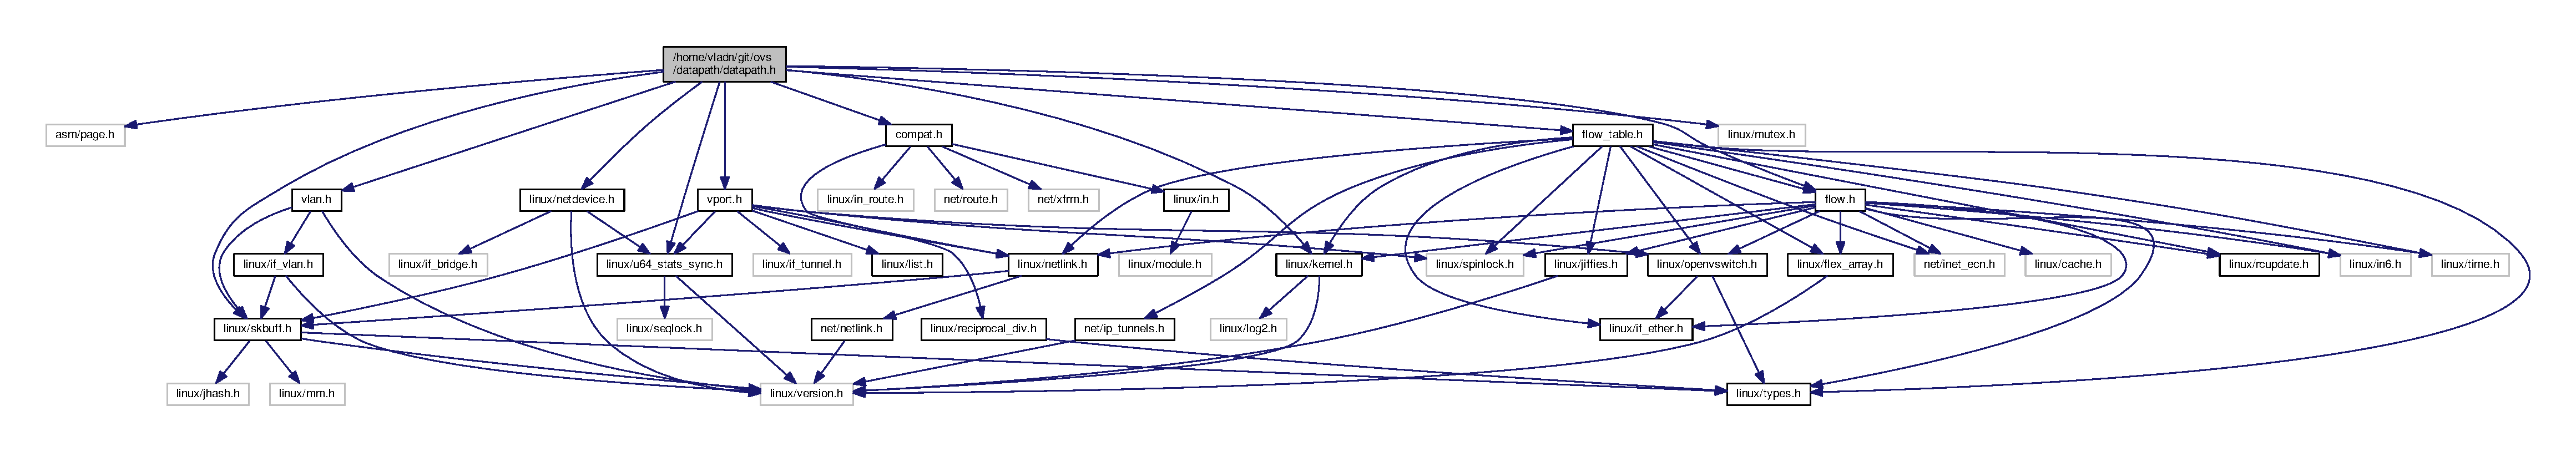
\includegraphics[width=350pt]{datapath_8h__incl}
\end{center}
\end{figure}
This graph shows which files directly or indirectly include this file\+:
\nopagebreak
\begin{figure}[H]
\begin{center}
\leavevmode
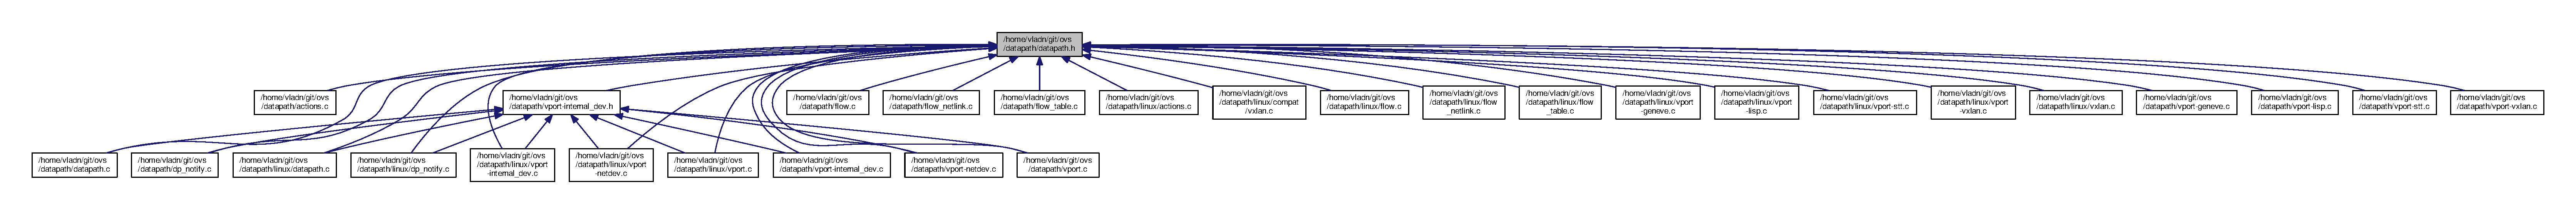
\includegraphics[width=350pt]{datapath_8h__dep__incl}
\end{center}
\end{figure}
\subsection*{Data Structures}
\begin{DoxyCompactItemize}
\item 
struct \hyperlink{structdp__stats__percpu}{dp\+\_\+stats\+\_\+percpu}
\item 
struct \hyperlink{structdatapath}{datapath}
\item 
struct \hyperlink{structovs__skb__cb}{ovs\+\_\+skb\+\_\+cb}
\item 
struct \hyperlink{structdp__upcall__info}{dp\+\_\+upcall\+\_\+info}
\item 
struct \hyperlink{structovs__net}{ovs\+\_\+net}
\end{DoxyCompactItemize}
\subsection*{Macros}
\begin{DoxyCompactItemize}
\item 
\#define \hyperlink{datapath_8h_a73b117dd1ebe456eecfb7688047a03f1}{D\+P\+\_\+\+M\+A\+X\+\_\+\+P\+O\+R\+T\+S}~\hyperlink{kernel_8h_a689b119da994dece91d44b5aeac643ed}{U\+S\+H\+R\+T\+\_\+\+M\+A\+X}
\item 
\#define \hyperlink{datapath_8h_ac1bf9805d62227b8f76f130087e18018}{D\+P\+\_\+\+V\+P\+O\+R\+T\+\_\+\+H\+A\+S\+H\+\_\+\+B\+U\+C\+K\+E\+T\+S}~1024
\item 
\#define \hyperlink{datapath_8h_ad323527e924235c97bf936e4e85dfdba}{S\+A\+M\+P\+L\+E\+\_\+\+A\+C\+T\+I\+O\+N\+\_\+\+D\+E\+P\+T\+H}~3
\item 
\#define \hyperlink{datapath_8h_ac337c4d4ddca29916ce8e900038ddd78}{O\+V\+S\+\_\+\+C\+B}(skb)~((struct \hyperlink{structovs__skb__cb}{ovs\+\_\+skb\+\_\+cb} $\ast$)(skb)-\/$>$cb)
\item 
\#define \hyperlink{datapath_8h_a54d3f44a7dda58b44208095ce4b2c0ee}{lockdep\+\_\+ovsl\+\_\+is\+\_\+held}()~1
\item 
\#define \hyperlink{datapath_8h_af8d476fa8191790e6f57cad0623f192c}{A\+S\+S\+E\+R\+T\+\_\+\+O\+V\+S\+L}()~W\+A\+R\+N\+\_\+\+O\+N(!\hyperlink{datapath_8h_a54d3f44a7dda58b44208095ce4b2c0ee}{lockdep\+\_\+ovsl\+\_\+is\+\_\+held}())
\item 
\#define \hyperlink{datapath_8h_a06ef69170d345fd3996a467dcacf3ff3}{ovsl\+\_\+dereference}(p)~\hyperlink{rcupdate_8h_af8e0682efe4f8bd0488ea6c1f66b0064}{rcu\+\_\+dereference\+\_\+protected}(p, \hyperlink{datapath_8h_a54d3f44a7dda58b44208095ce4b2c0ee}{lockdep\+\_\+ovsl\+\_\+is\+\_\+held}())
\item 
\#define \hyperlink{datapath_8h_a5f2a2c1026f970f0052e77f5ebba33d1}{rcu\+\_\+dereference\+\_\+ovsl}(p)~\hyperlink{rcupdate_8h_a1132a81ccc2a14e56d6fd4d794f953ea}{rcu\+\_\+dereference\+\_\+check}(p, \hyperlink{datapath_8h_a54d3f44a7dda58b44208095ce4b2c0ee}{lockdep\+\_\+ovsl\+\_\+is\+\_\+held}())
\item 
\#define \hyperlink{datapath_8h_a54648b7a2c9b192074cd95eb945433f0}{O\+V\+S\+\_\+\+N\+L\+E\+R\+R}(logging\+\_\+allowed,  fmt, ...)
\end{DoxyCompactItemize}
\subsection*{Functions}
\begin{DoxyCompactItemize}
\item 
void \hyperlink{datapath_8h_a092c1f450b78a173c890ed4c56839e1a}{ovs\+\_\+lock} (void)
\item 
void \hyperlink{datapath_8h_ac3ccfd98a880ed6d2480209be0d16680}{ovs\+\_\+unlock} (void)
\item 
static struct net $\ast$ \hyperlink{datapath_8h_aef2302004ca1f45133eaef00bb3740eb}{ovs\+\_\+dp\+\_\+get\+\_\+net} (const struct \hyperlink{structdatapath}{datapath} $\ast$dp)
\item 
static void \hyperlink{datapath_8h_af2973d12bb9f33d8e86d2fcad4dc7319}{ovs\+\_\+dp\+\_\+set\+\_\+net} (struct \hyperlink{structdatapath}{datapath} $\ast$dp, struct net $\ast$net)
\item 
struct \hyperlink{structvport}{vport} $\ast$ \hyperlink{datapath_8h_a0a9ec01692e1fdcb15a9a294d3789af0}{ovs\+\_\+lookup\+\_\+vport} (const struct \hyperlink{structdatapath}{datapath} $\ast$dp, u16 port\+\_\+no)
\item 
static struct \hyperlink{structvport}{vport} $\ast$ \hyperlink{datapath_8h_ac6f3c37a7850774112c03c6e88d89dc0}{ovs\+\_\+vport\+\_\+rcu} (const struct \hyperlink{structdatapath}{datapath} $\ast$dp, int port\+\_\+no)
\item 
static struct \hyperlink{structvport}{vport} $\ast$ \hyperlink{datapath_8h_a33d8540a1f2484576cfa52366828fcfc}{ovs\+\_\+vport\+\_\+ovsl\+\_\+rcu} (const struct \hyperlink{structdatapath}{datapath} $\ast$dp, int port\+\_\+no)
\item 
static struct \hyperlink{structvport}{vport} $\ast$ \hyperlink{datapath_8h_a422576bd4b943e9df313ba73f6c624e1}{ovs\+\_\+vport\+\_\+ovsl} (const struct \hyperlink{structdatapath}{datapath} $\ast$dp, int port\+\_\+no)
\item 
void \hyperlink{datapath_8h_aa52cbaf8a4e68129287bfc8ddcde0711}{ovs\+\_\+dp\+\_\+process\+\_\+packet} (struct sk\+\_\+buff $\ast$skb, struct \hyperlink{structsw__flow__key}{sw\+\_\+flow\+\_\+key} $\ast$key)
\item 
void \hyperlink{datapath_8h_af781f4768228c53f3319dd2526a1d625}{ovs\+\_\+dp\+\_\+detach\+\_\+port} (struct \hyperlink{structvport}{vport} $\ast$)
\item 
int \hyperlink{datapath_8h_aa97839171ab77e6823ee8283f166e19e}{ovs\+\_\+dp\+\_\+upcall} (struct \hyperlink{structdatapath}{datapath} $\ast$, struct sk\+\_\+buff $\ast$, const struct \hyperlink{structsw__flow__key}{sw\+\_\+flow\+\_\+key} $\ast$, const struct \hyperlink{structdp__upcall__info}{dp\+\_\+upcall\+\_\+info} $\ast$)
\item 
const char $\ast$ \hyperlink{datapath_8h_a6a23196916bb5de4994f901bdf1aba2d}{ovs\+\_\+dp\+\_\+name} (const struct \hyperlink{structdatapath}{datapath} $\ast$dp)
\item 
struct sk\+\_\+buff $\ast$ \hyperlink{datapath_8h_a15944602a340ff7fc6df155626c56428}{ovs\+\_\+vport\+\_\+cmd\+\_\+build\+\_\+info} (struct \hyperlink{structvport}{vport} $\ast$, u32 pid, u32 seq, u8 cmd)
\item 
int \hyperlink{datapath_8h_a340ea4456673ed4deaf3bae36d9fc1b1}{ovs\+\_\+execute\+\_\+actions} (struct \hyperlink{structdatapath}{datapath} $\ast$dp, struct sk\+\_\+buff $\ast$skb, const struct \hyperlink{structsw__flow__actions}{sw\+\_\+flow\+\_\+actions} $\ast$, struct \hyperlink{structsw__flow__key}{sw\+\_\+flow\+\_\+key} $\ast$)
\item 
void \hyperlink{datapath_8h_a5d5624a3bb21c222e3a6f18f56ff20b2}{ovs\+\_\+dp\+\_\+notify\+\_\+wq} (struct work\+\_\+struct $\ast$work)
\item 
int \hyperlink{datapath_8h_a3006f0376c2aecb6525126ad0e9bae25}{action\+\_\+fifos\+\_\+init} (void)
\item 
void \hyperlink{datapath_8h_a7dfd1f218e0966ef342251a185866f4d}{action\+\_\+fifos\+\_\+exit} (void)
\end{DoxyCompactItemize}
\subsection*{Variables}
\begin{DoxyCompactItemize}
\item 
int \hyperlink{datapath_8h_ace140298dc2b59b3d77d59c0a210de29}{ovs\+\_\+net\+\_\+id}
\item 
struct notifier\+\_\+block \hyperlink{datapath_8h_ab34ba4d6c1125efcec9480356f3393e6}{ovs\+\_\+dp\+\_\+device\+\_\+notifier}
\item 
struct \hyperlink{genetlink_8h_aba961c2c372b7122ad0c8ae5e7af2f3b}{genl\+\_\+family} \hyperlink{datapath_8h_a69bf55f33e234bc4b78e6eeee1d603fd}{dp\+\_\+vport\+\_\+genl\+\_\+family}
\item 
struct genl\+\_\+multicast\+\_\+group \hyperlink{datapath_8h_a9dd8d4307b50fdee582eb4013d89eb7b}{ovs\+\_\+dp\+\_\+vport\+\_\+multicast\+\_\+group}
\end{DoxyCompactItemize}


\subsection{Macro Definition Documentation}
\hypertarget{datapath_8h_af8d476fa8191790e6f57cad0623f192c}{}\index{datapath.\+h@{datapath.\+h}!A\+S\+S\+E\+R\+T\+\_\+\+O\+V\+S\+L@{A\+S\+S\+E\+R\+T\+\_\+\+O\+V\+S\+L}}
\index{A\+S\+S\+E\+R\+T\+\_\+\+O\+V\+S\+L@{A\+S\+S\+E\+R\+T\+\_\+\+O\+V\+S\+L}!datapath.\+h@{datapath.\+h}}
\subsubsection[{A\+S\+S\+E\+R\+T\+\_\+\+O\+V\+S\+L}]{\setlength{\rightskip}{0pt plus 5cm}\#define A\+S\+S\+E\+R\+T\+\_\+\+O\+V\+S\+L(
\begin{DoxyParamCaption}
{}
\end{DoxyParamCaption}
)~W\+A\+R\+N\+\_\+\+O\+N(!{\bf lockdep\+\_\+ovsl\+\_\+is\+\_\+held}())}\label{datapath_8h_af8d476fa8191790e6f57cad0623f192c}
\hypertarget{datapath_8h_a73b117dd1ebe456eecfb7688047a03f1}{}\index{datapath.\+h@{datapath.\+h}!D\+P\+\_\+\+M\+A\+X\+\_\+\+P\+O\+R\+T\+S@{D\+P\+\_\+\+M\+A\+X\+\_\+\+P\+O\+R\+T\+S}}
\index{D\+P\+\_\+\+M\+A\+X\+\_\+\+P\+O\+R\+T\+S@{D\+P\+\_\+\+M\+A\+X\+\_\+\+P\+O\+R\+T\+S}!datapath.\+h@{datapath.\+h}}
\subsubsection[{D\+P\+\_\+\+M\+A\+X\+\_\+\+P\+O\+R\+T\+S}]{\setlength{\rightskip}{0pt plus 5cm}\#define D\+P\+\_\+\+M\+A\+X\+\_\+\+P\+O\+R\+T\+S~{\bf U\+S\+H\+R\+T\+\_\+\+M\+A\+X}}\label{datapath_8h_a73b117dd1ebe456eecfb7688047a03f1}
\hypertarget{datapath_8h_ac1bf9805d62227b8f76f130087e18018}{}\index{datapath.\+h@{datapath.\+h}!D\+P\+\_\+\+V\+P\+O\+R\+T\+\_\+\+H\+A\+S\+H\+\_\+\+B\+U\+C\+K\+E\+T\+S@{D\+P\+\_\+\+V\+P\+O\+R\+T\+\_\+\+H\+A\+S\+H\+\_\+\+B\+U\+C\+K\+E\+T\+S}}
\index{D\+P\+\_\+\+V\+P\+O\+R\+T\+\_\+\+H\+A\+S\+H\+\_\+\+B\+U\+C\+K\+E\+T\+S@{D\+P\+\_\+\+V\+P\+O\+R\+T\+\_\+\+H\+A\+S\+H\+\_\+\+B\+U\+C\+K\+E\+T\+S}!datapath.\+h@{datapath.\+h}}
\subsubsection[{D\+P\+\_\+\+V\+P\+O\+R\+T\+\_\+\+H\+A\+S\+H\+\_\+\+B\+U\+C\+K\+E\+T\+S}]{\setlength{\rightskip}{0pt plus 5cm}\#define D\+P\+\_\+\+V\+P\+O\+R\+T\+\_\+\+H\+A\+S\+H\+\_\+\+B\+U\+C\+K\+E\+T\+S~1024}\label{datapath_8h_ac1bf9805d62227b8f76f130087e18018}
\hypertarget{datapath_8h_a54d3f44a7dda58b44208095ce4b2c0ee}{}\index{datapath.\+h@{datapath.\+h}!lockdep\+\_\+ovsl\+\_\+is\+\_\+held@{lockdep\+\_\+ovsl\+\_\+is\+\_\+held}}
\index{lockdep\+\_\+ovsl\+\_\+is\+\_\+held@{lockdep\+\_\+ovsl\+\_\+is\+\_\+held}!datapath.\+h@{datapath.\+h}}
\subsubsection[{lockdep\+\_\+ovsl\+\_\+is\+\_\+held}]{\setlength{\rightskip}{0pt plus 5cm}\#define lockdep\+\_\+ovsl\+\_\+is\+\_\+held(
\begin{DoxyParamCaption}
{}
\end{DoxyParamCaption}
)~1}\label{datapath_8h_a54d3f44a7dda58b44208095ce4b2c0ee}
\hypertarget{datapath_8h_ac337c4d4ddca29916ce8e900038ddd78}{}\index{datapath.\+h@{datapath.\+h}!O\+V\+S\+\_\+\+C\+B@{O\+V\+S\+\_\+\+C\+B}}
\index{O\+V\+S\+\_\+\+C\+B@{O\+V\+S\+\_\+\+C\+B}!datapath.\+h@{datapath.\+h}}
\subsubsection[{O\+V\+S\+\_\+\+C\+B}]{\setlength{\rightskip}{0pt plus 5cm}\#define O\+V\+S\+\_\+\+C\+B(
\begin{DoxyParamCaption}
\item[{}]{skb}
\end{DoxyParamCaption}
)~((struct {\bf ovs\+\_\+skb\+\_\+cb} $\ast$)(skb)-\/$>$cb)}\label{datapath_8h_ac337c4d4ddca29916ce8e900038ddd78}
\hypertarget{datapath_8h_a54648b7a2c9b192074cd95eb945433f0}{}\index{datapath.\+h@{datapath.\+h}!O\+V\+S\+\_\+\+N\+L\+E\+R\+R@{O\+V\+S\+\_\+\+N\+L\+E\+R\+R}}
\index{O\+V\+S\+\_\+\+N\+L\+E\+R\+R@{O\+V\+S\+\_\+\+N\+L\+E\+R\+R}!datapath.\+h@{datapath.\+h}}
\subsubsection[{O\+V\+S\+\_\+\+N\+L\+E\+R\+R}]{\setlength{\rightskip}{0pt plus 5cm}\#define O\+V\+S\+\_\+\+N\+L\+E\+R\+R(
\begin{DoxyParamCaption}
\item[{}]{logging\+\_\+allowed, }
\item[{}]{fmt, }
\item[{}]{...}
\end{DoxyParamCaption}
)}\label{datapath_8h_a54648b7a2c9b192074cd95eb945433f0}
{\bfseries Value\+:}
\begin{DoxyCode}
\textcolor{keywordflow}{do} \{                                \(\backslash\)
    if (logging\_allowed && net\_ratelimit())         \(\backslash\)
        pr\_info(\textcolor{stringliteral}{"netlink: "} fmt \textcolor{stringliteral}{"\(\backslash\)n"}, ##\_\_VA\_ARGS\_\_);   \(\backslash\)
\} \textcolor{keywordflow}{while} (0)
\end{DoxyCode}
\hypertarget{datapath_8h_a06ef69170d345fd3996a467dcacf3ff3}{}\index{datapath.\+h@{datapath.\+h}!ovsl\+\_\+dereference@{ovsl\+\_\+dereference}}
\index{ovsl\+\_\+dereference@{ovsl\+\_\+dereference}!datapath.\+h@{datapath.\+h}}
\subsubsection[{ovsl\+\_\+dereference}]{\setlength{\rightskip}{0pt plus 5cm}\#define ovsl\+\_\+dereference(
\begin{DoxyParamCaption}
\item[{}]{p}
\end{DoxyParamCaption}
)~{\bf rcu\+\_\+dereference\+\_\+protected}(p, {\bf lockdep\+\_\+ovsl\+\_\+is\+\_\+held}())}\label{datapath_8h_a06ef69170d345fd3996a467dcacf3ff3}
\hypertarget{datapath_8h_a5f2a2c1026f970f0052e77f5ebba33d1}{}\index{datapath.\+h@{datapath.\+h}!rcu\+\_\+dereference\+\_\+ovsl@{rcu\+\_\+dereference\+\_\+ovsl}}
\index{rcu\+\_\+dereference\+\_\+ovsl@{rcu\+\_\+dereference\+\_\+ovsl}!datapath.\+h@{datapath.\+h}}
\subsubsection[{rcu\+\_\+dereference\+\_\+ovsl}]{\setlength{\rightskip}{0pt plus 5cm}\#define rcu\+\_\+dereference\+\_\+ovsl(
\begin{DoxyParamCaption}
\item[{}]{p}
\end{DoxyParamCaption}
)~{\bf rcu\+\_\+dereference\+\_\+check}(p, {\bf lockdep\+\_\+ovsl\+\_\+is\+\_\+held}())}\label{datapath_8h_a5f2a2c1026f970f0052e77f5ebba33d1}
\hypertarget{datapath_8h_ad323527e924235c97bf936e4e85dfdba}{}\index{datapath.\+h@{datapath.\+h}!S\+A\+M\+P\+L\+E\+\_\+\+A\+C\+T\+I\+O\+N\+\_\+\+D\+E\+P\+T\+H@{S\+A\+M\+P\+L\+E\+\_\+\+A\+C\+T\+I\+O\+N\+\_\+\+D\+E\+P\+T\+H}}
\index{S\+A\+M\+P\+L\+E\+\_\+\+A\+C\+T\+I\+O\+N\+\_\+\+D\+E\+P\+T\+H@{S\+A\+M\+P\+L\+E\+\_\+\+A\+C\+T\+I\+O\+N\+\_\+\+D\+E\+P\+T\+H}!datapath.\+h@{datapath.\+h}}
\subsubsection[{S\+A\+M\+P\+L\+E\+\_\+\+A\+C\+T\+I\+O\+N\+\_\+\+D\+E\+P\+T\+H}]{\setlength{\rightskip}{0pt plus 5cm}\#define S\+A\+M\+P\+L\+E\+\_\+\+A\+C\+T\+I\+O\+N\+\_\+\+D\+E\+P\+T\+H~3}\label{datapath_8h_ad323527e924235c97bf936e4e85dfdba}


\subsection{Function Documentation}
\hypertarget{datapath_8h_a7dfd1f218e0966ef342251a185866f4d}{}\index{datapath.\+h@{datapath.\+h}!action\+\_\+fifos\+\_\+exit@{action\+\_\+fifos\+\_\+exit}}
\index{action\+\_\+fifos\+\_\+exit@{action\+\_\+fifos\+\_\+exit}!datapath.\+h@{datapath.\+h}}
\subsubsection[{action\+\_\+fifos\+\_\+exit}]{\setlength{\rightskip}{0pt plus 5cm}void action\+\_\+fifos\+\_\+exit (
\begin{DoxyParamCaption}
\item[{void}]{}
\end{DoxyParamCaption}
)}\label{datapath_8h_a7dfd1f218e0966ef342251a185866f4d}

\begin{DoxyCode}
1016 \{
1017     free\_percpu(\hyperlink{actions_8c_a38c6295376dbb80340f4f1b8e488f223}{action\_fifos});
1018 \}
\end{DoxyCode}
\hypertarget{datapath_8h_a3006f0376c2aecb6525126ad0e9bae25}{}\index{datapath.\+h@{datapath.\+h}!action\+\_\+fifos\+\_\+init@{action\+\_\+fifos\+\_\+init}}
\index{action\+\_\+fifos\+\_\+init@{action\+\_\+fifos\+\_\+init}!datapath.\+h@{datapath.\+h}}
\subsubsection[{action\+\_\+fifos\+\_\+init}]{\setlength{\rightskip}{0pt plus 5cm}int action\+\_\+fifos\+\_\+init (
\begin{DoxyParamCaption}
\item[{void}]{}
\end{DoxyParamCaption}
)}\label{datapath_8h_a3006f0376c2aecb6525126ad0e9bae25}

\begin{DoxyCode}
1007 \{
1008     \hyperlink{actions_8c_a38c6295376dbb80340f4f1b8e488f223}{action\_fifos} = alloc\_percpu(\textcolor{keyword}{struct} \hyperlink{structaction__fifo}{action\_fifo});
1009     \textcolor{keywordflow}{if} (!\hyperlink{actions_8c_a38c6295376dbb80340f4f1b8e488f223}{action\_fifos})
1010         \textcolor{keywordflow}{return} -ENOMEM;
1011 
1012     \textcolor{keywordflow}{return} 0;
1013 \}
\end{DoxyCode}
\hypertarget{datapath_8h_af781f4768228c53f3319dd2526a1d625}{}\index{datapath.\+h@{datapath.\+h}!ovs\+\_\+dp\+\_\+detach\+\_\+port@{ovs\+\_\+dp\+\_\+detach\+\_\+port}}
\index{ovs\+\_\+dp\+\_\+detach\+\_\+port@{ovs\+\_\+dp\+\_\+detach\+\_\+port}!datapath.\+h@{datapath.\+h}}
\subsubsection[{ovs\+\_\+dp\+\_\+detach\+\_\+port}]{\setlength{\rightskip}{0pt plus 5cm}void ovs\+\_\+dp\+\_\+detach\+\_\+port (
\begin{DoxyParamCaption}
\item[{struct {\bf vport} $\ast$}]{}
\end{DoxyParamCaption}
)}\label{datapath_8h_af781f4768228c53f3319dd2526a1d625}

\begin{DoxyCode}
249 \{
250     \hyperlink{datapath_8h_af8d476fa8191790e6f57cad0623f192c}{ASSERT\_OVSL}();
251 
252     \textcolor{comment}{/* First drop references to device. */}
253     hlist\_del\_rcu(&p->dp\_hash\_node);
254 
255     \textcolor{comment}{/* Then destroy it. */}
256     \hyperlink{linux_2vport_8c_ad7676013c642bc044ead47b79eb94075}{ovs\_vport\_del}(p);
257 \}
\end{DoxyCode}
\hypertarget{datapath_8h_aef2302004ca1f45133eaef00bb3740eb}{}\index{datapath.\+h@{datapath.\+h}!ovs\+\_\+dp\+\_\+get\+\_\+net@{ovs\+\_\+dp\+\_\+get\+\_\+net}}
\index{ovs\+\_\+dp\+\_\+get\+\_\+net@{ovs\+\_\+dp\+\_\+get\+\_\+net}!datapath.\+h@{datapath.\+h}}
\subsubsection[{ovs\+\_\+dp\+\_\+get\+\_\+net}]{\setlength{\rightskip}{0pt plus 5cm}static struct net$\ast$ ovs\+\_\+dp\+\_\+get\+\_\+net (
\begin{DoxyParamCaption}
\item[{const struct {\bf datapath} $\ast$}]{dp}
\end{DoxyParamCaption}
)\hspace{0.3cm}{\ttfamily [static]}}\label{datapath_8h_aef2302004ca1f45133eaef00bb3740eb}

\begin{DoxyCode}
158 \{
159     \textcolor{keywordflow}{return} read\_pnet(&dp->net);
160 \}
\end{DoxyCode}
\hypertarget{datapath_8h_a6a23196916bb5de4994f901bdf1aba2d}{}\index{datapath.\+h@{datapath.\+h}!ovs\+\_\+dp\+\_\+name@{ovs\+\_\+dp\+\_\+name}}
\index{ovs\+\_\+dp\+\_\+name@{ovs\+\_\+dp\+\_\+name}!datapath.\+h@{datapath.\+h}}
\subsubsection[{ovs\+\_\+dp\+\_\+name}]{\setlength{\rightskip}{0pt plus 5cm}const char$\ast$ ovs\+\_\+dp\+\_\+name (
\begin{DoxyParamCaption}
\item[{const struct {\bf datapath} $\ast$}]{dp}
\end{DoxyParamCaption}
)}\label{datapath_8h_a6a23196916bb5de4994f901bdf1aba2d}

\begin{DoxyCode}
179 \{
180     \textcolor{keyword}{struct }\hyperlink{structvport}{vport} *\hyperlink{structvport}{vport} = \hyperlink{datapath_8h_a33d8540a1f2484576cfa52366828fcfc}{ovs\_vport\_ovsl\_rcu}(dp, 
      \hyperlink{openvswitch_8h_aff2f13b95c27262c520f26831e647598}{OVSP\_LOCAL});
181     \textcolor{keywordflow}{return} vport->\hyperlink{structvport_a5af933fc664c1194ac3bbc337da35586}{ops}->\hyperlink{structvport__ops_abe0c3315271724bf05338487e0ced13c}{get\_name}(vport);
182 \}
\end{DoxyCode}
\hypertarget{datapath_8h_a5d5624a3bb21c222e3a6f18f56ff20b2}{}\index{datapath.\+h@{datapath.\+h}!ovs\+\_\+dp\+\_\+notify\+\_\+wq@{ovs\+\_\+dp\+\_\+notify\+\_\+wq}}
\index{ovs\+\_\+dp\+\_\+notify\+\_\+wq@{ovs\+\_\+dp\+\_\+notify\+\_\+wq}!datapath.\+h@{datapath.\+h}}
\subsubsection[{ovs\+\_\+dp\+\_\+notify\+\_\+wq}]{\setlength{\rightskip}{0pt plus 5cm}void ovs\+\_\+dp\+\_\+notify\+\_\+wq (
\begin{DoxyParamCaption}
\item[{struct work\+\_\+struct $\ast$}]{work}
\end{DoxyParamCaption}
)}\label{datapath_8h_a5d5624a3bb21c222e3a6f18f56ff20b2}

\begin{DoxyCode}
50 \{
51     \textcolor{keyword}{struct }\hyperlink{structovs__net}{ovs\_net} *\hyperlink{structovs__net}{ovs\_net} = container\_of(work, \textcolor{keyword}{struct} ovs\_net, 
      \hyperlink{structovs__net_ac8cdb834420a37531f032e526ac61901}{dp\_notify\_work});
52     \textcolor{keyword}{struct }\hyperlink{structdatapath}{datapath} *dp;
53 
54     \hyperlink{datapath_8c_a092c1f450b78a173c890ed4c56839e1a}{ovs\_lock}();
55     list\_for\_each\_entry(dp, &ovs\_net->\hyperlink{structovs__net_a0490101f7ea82f5c290a92d447bd8f9d}{dps}, \hyperlink{structdatapath_ac5f44be07025a2addb5c393fba822000}{list\_node}) \{
56         \textcolor{keywordtype}{int} i;
57 
58         \textcolor{keywordflow}{for} (i = 0; i < \hyperlink{datapath_8h_ac1bf9805d62227b8f76f130087e18018}{DP\_VPORT\_HASH\_BUCKETS}; i++) \{
59             \textcolor{keyword}{struct }\hyperlink{structvport}{vport} *\hyperlink{structvport}{vport};
60             \textcolor{keyword}{struct }hlist\_node *n;
61 
62             \hyperlink{list_8h_ae2f7dd7dbbe2f13fa51aca9fcb31a03f}{hlist\_for\_each\_entry\_safe}(vport, n, &dp->
      \hyperlink{structdatapath_abb0de528545b312de283b571cb6c4ede}{ports}[i], dp\_hash\_node) \{
63                 \textcolor{keyword}{struct }\hyperlink{structnetdev__vport}{netdev\_vport} *\hyperlink{structnetdev__vport}{netdev\_vport};
64 
65                 \textcolor{keywordflow}{if} (vport->\hyperlink{structvport_a5af933fc664c1194ac3bbc337da35586}{ops}->\hyperlink{structvport__ops_a7dd0d3776e78a2885063d3afd5e78148}{type} != \hyperlink{openvswitch_8h_a9a1b861aa99bd83177a2b10b34745b0aa825efa4a45bf501996d8d8fbb83887dd}{OVS\_VPORT\_TYPE\_NETDEV})
66                     \textcolor{keywordflow}{continue};
67 
68                 netdev\_vport = \hyperlink{vport-netdev_8h_a2cb441c6cf067ce3c79cb43836e9fc55}{netdev\_vport\_priv}(vport);
69                 \textcolor{keywordflow}{if} (!(\hyperlink{linux_2vport-netdev_8c_adf074c6126d43c3f7ea008ac19d33112}{ovs\_netdev\_get\_vport}(netdev\_vport->\hyperlink{structnetdev__vport_acf4ee248f7385e2f987fd2736f824ca9}{dev})))
70                     \hyperlink{dp__notify_8c_abfe6aca1ecdf831b014297563fc08731}{dp\_detach\_port\_notify}(vport);
71             \}
72         \}
73     \}
74     \hyperlink{datapath_8c_ac3ccfd98a880ed6d2480209be0d16680}{ovs\_unlock}();
75 \}
\end{DoxyCode}
\hypertarget{datapath_8h_aa52cbaf8a4e68129287bfc8ddcde0711}{}\index{datapath.\+h@{datapath.\+h}!ovs\+\_\+dp\+\_\+process\+\_\+packet@{ovs\+\_\+dp\+\_\+process\+\_\+packet}}
\index{ovs\+\_\+dp\+\_\+process\+\_\+packet@{ovs\+\_\+dp\+\_\+process\+\_\+packet}!datapath.\+h@{datapath.\+h}}
\subsubsection[{ovs\+\_\+dp\+\_\+process\+\_\+packet}]{\setlength{\rightskip}{0pt plus 5cm}void ovs\+\_\+dp\+\_\+process\+\_\+packet (
\begin{DoxyParamCaption}
\item[{struct sk\+\_\+buff $\ast$}]{skb, }
\item[{struct {\bf sw\+\_\+flow\+\_\+key} $\ast$}]{key}
\end{DoxyParamCaption}
)}\label{datapath_8h_aa52cbaf8a4e68129287bfc8ddcde0711}

\begin{DoxyCode}
261 \{
262     \textcolor{keyword}{const} \textcolor{keyword}{struct }\hyperlink{structvport}{vport} *p = \hyperlink{datapath_8h_ac337c4d4ddca29916ce8e900038ddd78}{OVS\_CB}(skb)->input\_vport;
263     \textcolor{keyword}{struct }\hyperlink{structdatapath}{datapath} *dp = p->\hyperlink{structvport_a49fb6f6bf0ac4337853e9242e88ddc42}{dp};
264     \textcolor{keyword}{struct }\hyperlink{structsw__flow}{sw\_flow} *flow;
265     \textcolor{keyword}{struct }\hyperlink{structsw__flow__actions}{sw\_flow\_actions} *sf\_acts;
266     \textcolor{keyword}{struct }\hyperlink{structdp__stats__percpu}{dp\_stats\_percpu} *stats;
267     u64 *stats\_counter;
268     u32 \hyperlink{structdp__stats__percpu_acbf57615b1fb66464f9e67efb32bd038}{n\_mask\_hit};
269 
270     stats = \hyperlink{percpu_8h_a1cd55f287dff5c4a79fc11dd38d47c12}{this\_cpu\_ptr}(dp->\hyperlink{structdatapath_a26ff295c711206c8177cdc89150c6a4a}{stats\_percpu});
271 
272     \textcolor{comment}{/* Look up flow. */}
273     flow = \hyperlink{flow__table_8c_ac1ff64b403e23c6e8226b0024969556b}{ovs\_flow\_tbl\_lookup\_stats}(&dp->\hyperlink{structdatapath_ac6d67fe586c19484391acbcfa267259d}{table}, key, 
      \hyperlink{skbuff_8h_acb236314b209f764af9aae7fbbb04311}{skb\_get\_hash}(skb),
274                      &n\_mask\_hit);
275     \textcolor{keywordflow}{if} (unlikely(!flow)) \{
276         \textcolor{keyword}{struct }\hyperlink{structdp__upcall__info}{dp\_upcall\_info} upcall;
277         \textcolor{keywordtype}{int} error;
278 
279         memset(&upcall, 0, \textcolor{keyword}{sizeof}(upcall));
280         upcall.cmd = \hyperlink{openvswitch_8h_a162a763c571debd951c9d2727b0f9bc3ae41f30829d03ed04928e74f82b349f0a}{OVS\_PACKET\_CMD\_MISS};
281         upcall.portid = \hyperlink{linux_2vport_8c_aeee9e742f0a0fbb3bda943eea9e63e56}{ovs\_vport\_find\_upcall\_portid}(p, skb);
282         error = \hyperlink{datapath_8c_a229b5c7d0158ebc24a90f44de0df0040}{ovs\_dp\_upcall}(dp, skb, key, &upcall);
283         \textcolor{keywordflow}{if} (unlikely(error))
284             kfree\_skb(skb);
285         \textcolor{keywordflow}{else}
286             \hyperlink{skbuff_8h_adc460a9e6dccf5557d55bbce8c7adb6a}{consume\_skb}(skb);
287         stats\_counter = &stats->\hyperlink{structdp__stats__percpu_ab919c22c9548a3dcd42632fb84634e26}{n\_missed};
288         \textcolor{keywordflow}{goto} out;
289     \}
290 
291     \hyperlink{flow_8c_ad20885fb9e6da56eb9cb58d139281916}{ovs\_flow\_stats\_update}(flow, key->\hyperlink{structsw__flow__key_a9c1944a39db1bf91141048df6d85ce8b}{tp}.\hyperlink{structsw__flow__key_a910f5e4408d113dbc9211190b44e0880}{flags}, skb);
292     sf\_acts = rcu\_dereference(flow->\hyperlink{structsw__flow_aa845bdaabc25d81dcf8b1a7519b35408}{sf\_acts});
293     \hyperlink{actions_8c_a5b34c1980d155574d657a21cac3bcc37}{ovs\_execute\_actions}(dp, skb, sf\_acts, key);
294 
295     stats\_counter = &stats->\hyperlink{structdp__stats__percpu_add53281b86504a50626cce7fac173d5b}{n\_hit};
296 
297 out:
298     \textcolor{comment}{/* Update datapath statistics. */}
299     \hyperlink{u64__stats__sync_8h_a79de6de9a2c8c4e1c98d78e5689b74f7}{u64\_stats\_update\_begin}(&stats->\hyperlink{structdp__stats__percpu_ad67971f59f6db5432848db23d185dc2f}{syncp});
300     (*stats\_counter)++;
301     stats->\hyperlink{structdp__stats__percpu_acbf57615b1fb66464f9e67efb32bd038}{n\_mask\_hit} += n\_mask\_hit;
302     \hyperlink{u64__stats__sync_8h_a4005b558b0a34d25298936e8d899e980}{u64\_stats\_update\_end}(&stats->\hyperlink{structdp__stats__percpu_ad67971f59f6db5432848db23d185dc2f}{syncp});
303 \}
\end{DoxyCode}
\hypertarget{datapath_8h_af2973d12bb9f33d8e86d2fcad4dc7319}{}\index{datapath.\+h@{datapath.\+h}!ovs\+\_\+dp\+\_\+set\+\_\+net@{ovs\+\_\+dp\+\_\+set\+\_\+net}}
\index{ovs\+\_\+dp\+\_\+set\+\_\+net@{ovs\+\_\+dp\+\_\+set\+\_\+net}!datapath.\+h@{datapath.\+h}}
\subsubsection[{ovs\+\_\+dp\+\_\+set\+\_\+net}]{\setlength{\rightskip}{0pt plus 5cm}static void ovs\+\_\+dp\+\_\+set\+\_\+net (
\begin{DoxyParamCaption}
\item[{struct {\bf datapath} $\ast$}]{dp, }
\item[{struct net $\ast$}]{net}
\end{DoxyParamCaption}
)\hspace{0.3cm}{\ttfamily [inline]}, {\ttfamily [static]}}\label{datapath_8h_af2973d12bb9f33d8e86d2fcad4dc7319}

\begin{DoxyCode}
163 \{
164     write\_pnet(&dp->net, net);
165 \}
\end{DoxyCode}
\hypertarget{datapath_8h_aa97839171ab77e6823ee8283f166e19e}{}\index{datapath.\+h@{datapath.\+h}!ovs\+\_\+dp\+\_\+upcall@{ovs\+\_\+dp\+\_\+upcall}}
\index{ovs\+\_\+dp\+\_\+upcall@{ovs\+\_\+dp\+\_\+upcall}!datapath.\+h@{datapath.\+h}}
\subsubsection[{ovs\+\_\+dp\+\_\+upcall}]{\setlength{\rightskip}{0pt plus 5cm}int ovs\+\_\+dp\+\_\+upcall (
\begin{DoxyParamCaption}
\item[{struct {\bf datapath} $\ast$}]{, }
\item[{struct sk\+\_\+buff $\ast$}]{, }
\item[{const struct {\bf sw\+\_\+flow\+\_\+key} $\ast$}]{, }
\item[{const struct {\bf dp\+\_\+upcall\+\_\+info} $\ast$}]{}
\end{DoxyParamCaption}
)}\label{datapath_8h_aa97839171ab77e6823ee8283f166e19e}

\begin{DoxyCode}
308 \{
309     \textcolor{keyword}{struct }\hyperlink{structdp__stats__percpu}{dp\_stats\_percpu} *stats;
310     \textcolor{keywordtype}{int} err;
311 
312     \textcolor{keywordflow}{if} (upcall\_info->portid == 0) \{
313         err = -ENOTCONN;
314         \textcolor{keywordflow}{goto} err;
315     \}
316 
317     \textcolor{keywordflow}{if} (!skb\_is\_gso(skb))
318         err = \hyperlink{datapath_8c_a549c591fae56562523f243abbe4a1e3e}{queue\_userspace\_packet}(dp, skb, key, upcall\_info);
319     \textcolor{keywordflow}{else}
320         err = \hyperlink{datapath_8c_a2c10ba8a23a8cb2f14b7f7684e5ebb5d}{queue\_gso\_packets}(dp, skb, key, upcall\_info);
321     \textcolor{keywordflow}{if} (err)
322         \textcolor{keywordflow}{goto} err;
323 
324     \textcolor{keywordflow}{return} 0;
325 
326 err:
327     stats = \hyperlink{percpu_8h_a1cd55f287dff5c4a79fc11dd38d47c12}{this\_cpu\_ptr}(dp->stats\_percpu);
328 
329     \hyperlink{u64__stats__sync_8h_a79de6de9a2c8c4e1c98d78e5689b74f7}{u64\_stats\_update\_begin}(&stats->\hyperlink{structdp__stats__percpu_ad67971f59f6db5432848db23d185dc2f}{syncp});
330     stats->\hyperlink{structdp__stats__percpu_abecbd535feefeb9ff1721ca6e517c310}{n\_lost}++;
331     \hyperlink{u64__stats__sync_8h_a4005b558b0a34d25298936e8d899e980}{u64\_stats\_update\_end}(&stats->\hyperlink{structdp__stats__percpu_ad67971f59f6db5432848db23d185dc2f}{syncp});
332 
333     \textcolor{keywordflow}{return} err;
334 \}
\end{DoxyCode}
\hypertarget{datapath_8h_a340ea4456673ed4deaf3bae36d9fc1b1}{}\index{datapath.\+h@{datapath.\+h}!ovs\+\_\+execute\+\_\+actions@{ovs\+\_\+execute\+\_\+actions}}
\index{ovs\+\_\+execute\+\_\+actions@{ovs\+\_\+execute\+\_\+actions}!datapath.\+h@{datapath.\+h}}
\subsubsection[{ovs\+\_\+execute\+\_\+actions}]{\setlength{\rightskip}{0pt plus 5cm}int ovs\+\_\+execute\+\_\+actions (
\begin{DoxyParamCaption}
\item[{struct {\bf datapath} $\ast$}]{dp, }
\item[{struct sk\+\_\+buff $\ast$}]{skb, }
\item[{const struct {\bf sw\+\_\+flow\+\_\+actions} $\ast$}]{, }
\item[{struct {\bf sw\+\_\+flow\+\_\+key} $\ast$}]{}
\end{DoxyParamCaption}
)}\label{datapath_8h_a340ea4456673ed4deaf3bae36d9fc1b1}

\begin{DoxyCode}
977 \{
978     \textcolor{keywordtype}{int} level = \hyperlink{percpu_8h_a15341bef54ee4dd9fcc2d811bb11d39d}{this\_cpu\_read}(exec\_actions\_level);
979     \textcolor{keywordtype}{int} err;
980 
981     \textcolor{keywordflow}{if} (unlikely(level >= \hyperlink{actions_8c_aef2488868338b5c1ec4419f0efde93f1}{EXEC\_ACTIONS\_LEVEL\_LIMIT})) \{
982         \textcolor{keywordflow}{if} (net\_ratelimit())
983             pr\_warn(\textcolor{stringliteral}{"%s: packet loop detected, dropping.\(\backslash\)n"},
984                 \hyperlink{datapath_8c_a6a23196916bb5de4994f901bdf1aba2d}{ovs\_dp\_name}(dp));
985 
986         kfree\_skb(skb);
987         \textcolor{keywordflow}{return} -ELOOP;
988     \}
989 
990     \hyperlink{percpu_8h_a8999ff6f1c86c39d81e8b2388d8056ac}{this\_cpu\_inc}(exec\_actions\_level);
991     err = \hyperlink{actions_8c_ad41a07588c602d50a247bcf2bf9ae9d5}{do\_execute\_actions}(dp, skb, key,
992                  acts->actions, acts->actions\_len);
993 
994     \textcolor{keywordflow}{if} (!level)
995         \hyperlink{actions_8c_afa871a96ea915a7ce87b96a0b7b30538}{process\_deferred\_actions}(dp);
996 
997     \hyperlink{percpu_8h_a3949346d789a1c87ab4bc81744bc3fad}{this\_cpu\_dec}(exec\_actions\_level);
998 
999     \textcolor{comment}{/* This return status currently does not reflect the errors}
1000 \textcolor{comment}{     * encounted during deferred actions execution. Probably needs to}
1001 \textcolor{comment}{     * be fixed in the future.}
1002 \textcolor{comment}{     */}
1003     \textcolor{keywordflow}{return} err;
1004 \}
\end{DoxyCode}
\hypertarget{datapath_8h_a092c1f450b78a173c890ed4c56839e1a}{}\index{datapath.\+h@{datapath.\+h}!ovs\+\_\+lock@{ovs\+\_\+lock}}
\index{ovs\+\_\+lock@{ovs\+\_\+lock}!datapath.\+h@{datapath.\+h}}
\subsubsection[{ovs\+\_\+lock}]{\setlength{\rightskip}{0pt plus 5cm}void ovs\+\_\+lock (
\begin{DoxyParamCaption}
\item[{void}]{}
\end{DoxyParamCaption}
)}\label{datapath_8h_a092c1f450b78a173c890ed4c56839e1a}

\begin{DoxyCode}
121 \{
122     mutex\_lock(&ovs\_mutex);
123 \}
\end{DoxyCode}
\hypertarget{datapath_8h_a0a9ec01692e1fdcb15a9a294d3789af0}{}\index{datapath.\+h@{datapath.\+h}!ovs\+\_\+lookup\+\_\+vport@{ovs\+\_\+lookup\+\_\+vport}}
\index{ovs\+\_\+lookup\+\_\+vport@{ovs\+\_\+lookup\+\_\+vport}!datapath.\+h@{datapath.\+h}}
\subsubsection[{ovs\+\_\+lookup\+\_\+vport}]{\setlength{\rightskip}{0pt plus 5cm}struct {\bf vport}$\ast$ ovs\+\_\+lookup\+\_\+vport (
\begin{DoxyParamCaption}
\item[{const struct {\bf datapath} $\ast$}]{dp, }
\item[{u16}]{port\+\_\+no}
\end{DoxyParamCaption}
)}\label{datapath_8h_a0a9ec01692e1fdcb15a9a294d3789af0}

\begin{DoxyCode}
221 \{
222     \textcolor{keyword}{struct }\hyperlink{structvport}{vport} *\hyperlink{structvport}{vport};
223     \textcolor{keyword}{struct }hlist\_head *head;
224 
225     head = \hyperlink{datapath_8c_af291a723340e4e1bd38b4b14e7f4377a}{vport\_hash\_bucket}(dp, port\_no);
226     \hyperlink{rculist_8h_a482ed6bca0b607f6455d5386f3b1ed75}{hlist\_for\_each\_entry\_rcu}(vport, head, dp\_hash\_node) \{
227         \textcolor{keywordflow}{if} (vport->\hyperlink{structvport_aae00fc5d12b47f02cbfd4f67ae114b58}{port\_no} == port\_no)
228             \textcolor{keywordflow}{return} vport;
229     \}
230     \textcolor{keywordflow}{return} NULL;
231 \}
\end{DoxyCode}
\hypertarget{datapath_8h_ac3ccfd98a880ed6d2480209be0d16680}{}\index{datapath.\+h@{datapath.\+h}!ovs\+\_\+unlock@{ovs\+\_\+unlock}}
\index{ovs\+\_\+unlock@{ovs\+\_\+unlock}!datapath.\+h@{datapath.\+h}}
\subsubsection[{ovs\+\_\+unlock}]{\setlength{\rightskip}{0pt plus 5cm}void ovs\+\_\+unlock (
\begin{DoxyParamCaption}
\item[{void}]{}
\end{DoxyParamCaption}
)}\label{datapath_8h_ac3ccfd98a880ed6d2480209be0d16680}

\begin{DoxyCode}
126 \{
127     mutex\_unlock(&ovs\_mutex);
128 \}
\end{DoxyCode}
\hypertarget{datapath_8h_a15944602a340ff7fc6df155626c56428}{}\index{datapath.\+h@{datapath.\+h}!ovs\+\_\+vport\+\_\+cmd\+\_\+build\+\_\+info@{ovs\+\_\+vport\+\_\+cmd\+\_\+build\+\_\+info}}
\index{ovs\+\_\+vport\+\_\+cmd\+\_\+build\+\_\+info@{ovs\+\_\+vport\+\_\+cmd\+\_\+build\+\_\+info}!datapath.\+h@{datapath.\+h}}
\subsubsection[{ovs\+\_\+vport\+\_\+cmd\+\_\+build\+\_\+info}]{\setlength{\rightskip}{0pt plus 5cm}struct sk\+\_\+buff$\ast$ ovs\+\_\+vport\+\_\+cmd\+\_\+build\+\_\+info (
\begin{DoxyParamCaption}
\item[{struct {\bf vport} $\ast$}]{, }
\item[{u32}]{pid, }
\item[{u32}]{seq, }
\item[{u8}]{cmd}
\end{DoxyParamCaption}
)}\label{datapath_8h_a15944602a340ff7fc6df155626c56428}

\begin{DoxyCode}
1848 \{
1849     \textcolor{keyword}{struct }sk\_buff *skb;
1850     \textcolor{keywordtype}{int} retval;
1851 
1852     skb = nlmsg\_new(\hyperlink{linux_2netlink_8h_a5098e3f66b13a5c9ad78eeffe65e6868}{NLMSG\_DEFAULT\_SIZE}, GFP\_ATOMIC);
1853     \textcolor{keywordflow}{if} (!skb)
1854         \textcolor{keywordflow}{return} ERR\_PTR(-ENOMEM);
1855 
1856     retval = \hyperlink{datapath_8c_a4272403de9a985cea17181e99b7a7edc}{ovs\_vport\_cmd\_fill\_info}(\hyperlink{structvport}{vport}, skb, portid, seq, 0, cmd);
1857     BUG\_ON(retval < 0);
1858 
1859     \textcolor{keywordflow}{return} skb;
1860 \}
\end{DoxyCode}
\hypertarget{datapath_8h_a422576bd4b943e9df313ba73f6c624e1}{}\index{datapath.\+h@{datapath.\+h}!ovs\+\_\+vport\+\_\+ovsl@{ovs\+\_\+vport\+\_\+ovsl}}
\index{ovs\+\_\+vport\+\_\+ovsl@{ovs\+\_\+vport\+\_\+ovsl}!datapath.\+h@{datapath.\+h}}
\subsubsection[{ovs\+\_\+vport\+\_\+ovsl}]{\setlength{\rightskip}{0pt plus 5cm}static struct {\bf vport}$\ast$ ovs\+\_\+vport\+\_\+ovsl (
\begin{DoxyParamCaption}
\item[{const struct {\bf datapath} $\ast$}]{dp, }
\item[{int}]{port\+\_\+no}
\end{DoxyParamCaption}
)\hspace{0.3cm}{\ttfamily [static]}}\label{datapath_8h_a422576bd4b943e9df313ba73f6c624e1}

\begin{DoxyCode}
182 \{
183     \hyperlink{datapath_8h_af8d476fa8191790e6f57cad0623f192c}{ASSERT\_OVSL}();
184     \textcolor{keywordflow}{return} \hyperlink{datapath_8h_a0a9ec01692e1fdcb15a9a294d3789af0}{ovs\_lookup\_vport}(dp, port\_no);
185 \}
\end{DoxyCode}
\hypertarget{datapath_8h_a33d8540a1f2484576cfa52366828fcfc}{}\index{datapath.\+h@{datapath.\+h}!ovs\+\_\+vport\+\_\+ovsl\+\_\+rcu@{ovs\+\_\+vport\+\_\+ovsl\+\_\+rcu}}
\index{ovs\+\_\+vport\+\_\+ovsl\+\_\+rcu@{ovs\+\_\+vport\+\_\+ovsl\+\_\+rcu}!datapath.\+h@{datapath.\+h}}
\subsubsection[{ovs\+\_\+vport\+\_\+ovsl\+\_\+rcu}]{\setlength{\rightskip}{0pt plus 5cm}static struct {\bf vport}$\ast$ ovs\+\_\+vport\+\_\+ovsl\+\_\+rcu (
\begin{DoxyParamCaption}
\item[{const struct {\bf datapath} $\ast$}]{dp, }
\item[{int}]{port\+\_\+no}
\end{DoxyParamCaption}
)\hspace{0.3cm}{\ttfamily [static]}}\label{datapath_8h_a33d8540a1f2484576cfa52366828fcfc}

\begin{DoxyCode}
176 \{
177     WARN\_ON\_ONCE(!\hyperlink{rcupdate_8h_ab77c80b5efea34ea99ec24a4f532eb9b}{rcu\_read\_lock\_held}() && !
      \hyperlink{datapath_8h_a54d3f44a7dda58b44208095ce4b2c0ee}{lockdep\_ovsl\_is\_held}());
178     \textcolor{keywordflow}{return} \hyperlink{datapath_8h_a0a9ec01692e1fdcb15a9a294d3789af0}{ovs\_lookup\_vport}(dp, port\_no);
179 \}
\end{DoxyCode}
\hypertarget{datapath_8h_ac6f3c37a7850774112c03c6e88d89dc0}{}\index{datapath.\+h@{datapath.\+h}!ovs\+\_\+vport\+\_\+rcu@{ovs\+\_\+vport\+\_\+rcu}}
\index{ovs\+\_\+vport\+\_\+rcu@{ovs\+\_\+vport\+\_\+rcu}!datapath.\+h@{datapath.\+h}}
\subsubsection[{ovs\+\_\+vport\+\_\+rcu}]{\setlength{\rightskip}{0pt plus 5cm}static struct {\bf vport}$\ast$ ovs\+\_\+vport\+\_\+rcu (
\begin{DoxyParamCaption}
\item[{const struct {\bf datapath} $\ast$}]{dp, }
\item[{int}]{port\+\_\+no}
\end{DoxyParamCaption}
)\hspace{0.3cm}{\ttfamily [static]}}\label{datapath_8h_ac6f3c37a7850774112c03c6e88d89dc0}

\begin{DoxyCode}
170 \{
171     WARN\_ON\_ONCE(!\hyperlink{rcupdate_8h_ab77c80b5efea34ea99ec24a4f532eb9b}{rcu\_read\_lock\_held}());
172     \textcolor{keywordflow}{return} \hyperlink{datapath_8h_a0a9ec01692e1fdcb15a9a294d3789af0}{ovs\_lookup\_vport}(dp, port\_no);
173 \}
\end{DoxyCode}


\subsection{Variable Documentation}
\hypertarget{datapath_8h_a69bf55f33e234bc4b78e6eeee1d603fd}{}\index{datapath.\+h@{datapath.\+h}!dp\+\_\+vport\+\_\+genl\+\_\+family@{dp\+\_\+vport\+\_\+genl\+\_\+family}}
\index{dp\+\_\+vport\+\_\+genl\+\_\+family@{dp\+\_\+vport\+\_\+genl\+\_\+family}!datapath.\+h@{datapath.\+h}}
\subsubsection[{dp\+\_\+vport\+\_\+genl\+\_\+family}]{\setlength{\rightskip}{0pt plus 5cm}struct {\bf genl\+\_\+family} dp\+\_\+vport\+\_\+genl\+\_\+family}\label{datapath_8h_a69bf55f33e234bc4b78e6eeee1d603fd}
\hypertarget{datapath_8h_ab34ba4d6c1125efcec9480356f3393e6}{}\index{datapath.\+h@{datapath.\+h}!ovs\+\_\+dp\+\_\+device\+\_\+notifier@{ovs\+\_\+dp\+\_\+device\+\_\+notifier}}
\index{ovs\+\_\+dp\+\_\+device\+\_\+notifier@{ovs\+\_\+dp\+\_\+device\+\_\+notifier}!datapath.\+h@{datapath.\+h}}
\subsubsection[{ovs\+\_\+dp\+\_\+device\+\_\+notifier}]{\setlength{\rightskip}{0pt plus 5cm}struct notifier\+\_\+block ovs\+\_\+dp\+\_\+device\+\_\+notifier}\label{datapath_8h_ab34ba4d6c1125efcec9480356f3393e6}
\hypertarget{datapath_8h_a9dd8d4307b50fdee582eb4013d89eb7b}{}\index{datapath.\+h@{datapath.\+h}!ovs\+\_\+dp\+\_\+vport\+\_\+multicast\+\_\+group@{ovs\+\_\+dp\+\_\+vport\+\_\+multicast\+\_\+group}}
\index{ovs\+\_\+dp\+\_\+vport\+\_\+multicast\+\_\+group@{ovs\+\_\+dp\+\_\+vport\+\_\+multicast\+\_\+group}!datapath.\+h@{datapath.\+h}}
\subsubsection[{ovs\+\_\+dp\+\_\+vport\+\_\+multicast\+\_\+group}]{\setlength{\rightskip}{0pt plus 5cm}struct genl\+\_\+multicast\+\_\+group ovs\+\_\+dp\+\_\+vport\+\_\+multicast\+\_\+group}\label{datapath_8h_a9dd8d4307b50fdee582eb4013d89eb7b}
\hypertarget{datapath_8h_ace140298dc2b59b3d77d59c0a210de29}{}\index{datapath.\+h@{datapath.\+h}!ovs\+\_\+net\+\_\+id@{ovs\+\_\+net\+\_\+id}}
\index{ovs\+\_\+net\+\_\+id@{ovs\+\_\+net\+\_\+id}!datapath.\+h@{datapath.\+h}}
\subsubsection[{ovs\+\_\+net\+\_\+id}]{\setlength{\rightskip}{0pt plus 5cm}int ovs\+\_\+net\+\_\+id}\label{datapath_8h_ace140298dc2b59b3d77d59c0a210de29}

\hypertarget{dp__notify_8c}{}\section{/home/vladn/git/ovs/datapath/dp\+\_\+notify.c File Reference}
\label{dp__notify_8c}\index{/home/vladn/git/ovs/datapath/dp\+\_\+notify.\+c@{/home/vladn/git/ovs/datapath/dp\+\_\+notify.\+c}}
{\ttfamily \#include $<$linux/netdevice.\+h$>$}\\*
{\ttfamily \#include $<$net/genetlink.\+h$>$}\\*
{\ttfamily \#include $<$net/net\+\_\+namespace.\+h$>$}\\*
{\ttfamily \#include $<$net/netns/generic.\+h$>$}\\*
{\ttfamily \#include \char`\"{}datapath.\+h\char`\"{}}\\*
{\ttfamily \#include \char`\"{}vport-\/internal\+\_\+dev.\+h\char`\"{}}\\*
{\ttfamily \#include \char`\"{}vport-\/netdev.\+h\char`\"{}}\\*
Include dependency graph for dp\+\_\+notify.\+c\+:
\nopagebreak
\begin{figure}[H]
\begin{center}
\leavevmode
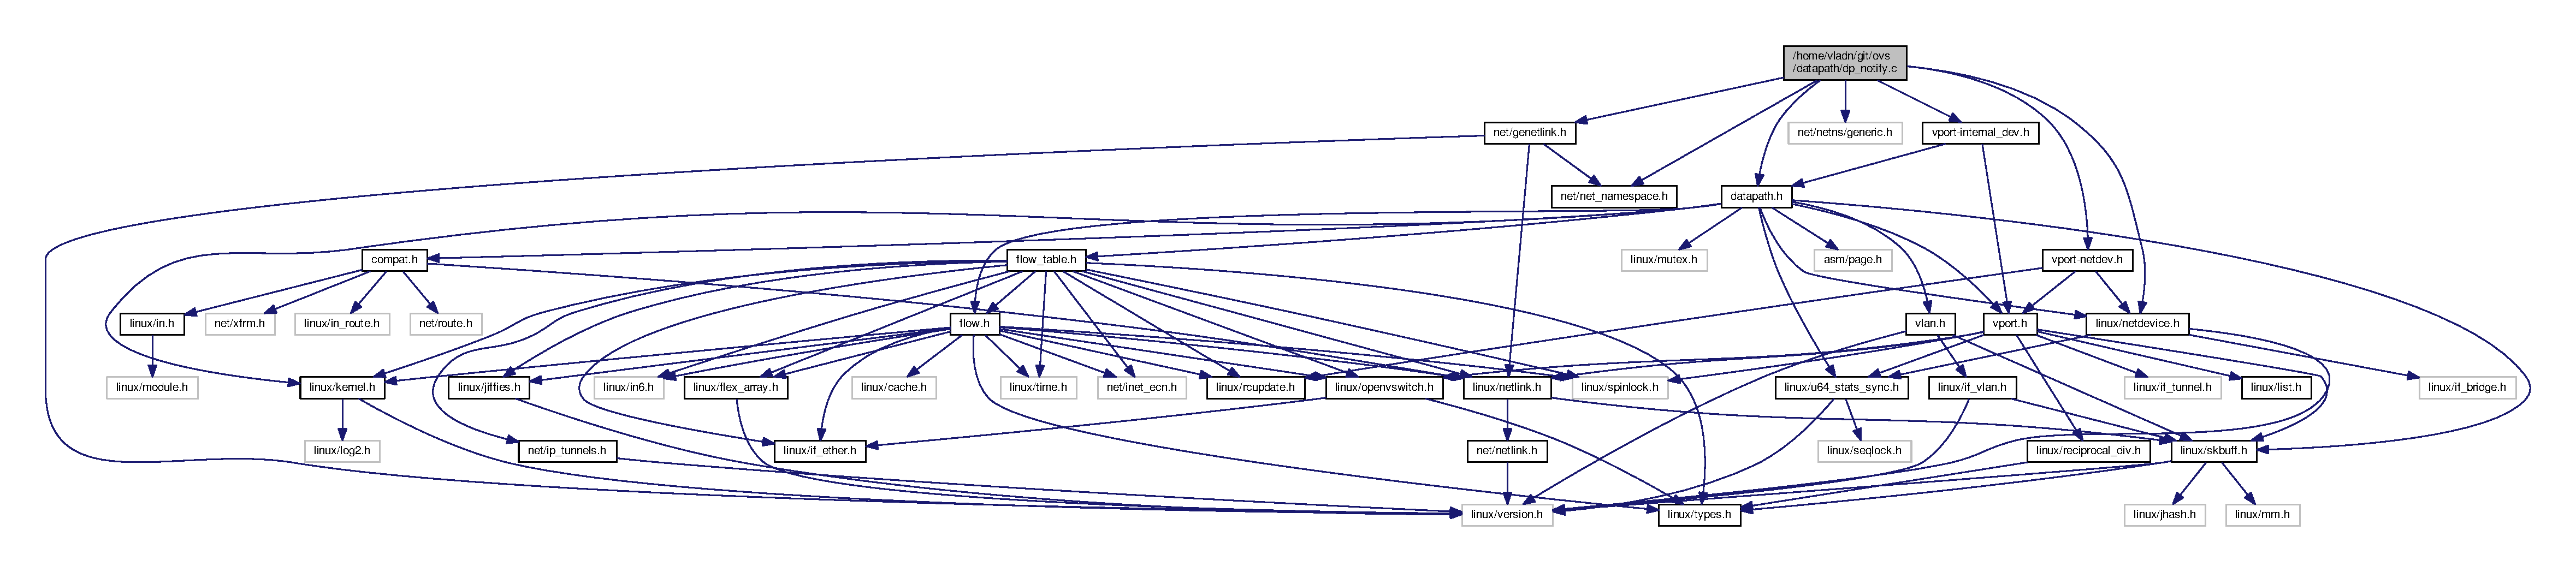
\includegraphics[width=350pt]{dp__notify_8c__incl}
\end{center}
\end{figure}
\subsection*{Functions}
\begin{DoxyCompactItemize}
\item 
static void \hyperlink{dp__notify_8c_abfe6aca1ecdf831b014297563fc08731}{dp\+\_\+detach\+\_\+port\+\_\+notify} (struct \hyperlink{structvport}{vport} $\ast$\hyperlink{structvport}{vport})
\item 
void \hyperlink{dp__notify_8c_a5d5624a3bb21c222e3a6f18f56ff20b2}{ovs\+\_\+dp\+\_\+notify\+\_\+wq} (struct work\+\_\+struct $\ast$work)
\item 
static int \hyperlink{dp__notify_8c_acca2a908a0982dd42292177079cf5643}{dp\+\_\+device\+\_\+event} (struct notifier\+\_\+block $\ast$unused, unsigned long event, void $\ast$ptr)
\end{DoxyCompactItemize}
\subsection*{Variables}
\begin{DoxyCompactItemize}
\item 
struct notifier\+\_\+block \hyperlink{dp__notify_8c_ab34ba4d6c1125efcec9480356f3393e6}{ovs\+\_\+dp\+\_\+device\+\_\+notifier}
\end{DoxyCompactItemize}


\subsection{Function Documentation}
\hypertarget{dp__notify_8c_abfe6aca1ecdf831b014297563fc08731}{}\index{dp\+\_\+notify.\+c@{dp\+\_\+notify.\+c}!dp\+\_\+detach\+\_\+port\+\_\+notify@{dp\+\_\+detach\+\_\+port\+\_\+notify}}
\index{dp\+\_\+detach\+\_\+port\+\_\+notify@{dp\+\_\+detach\+\_\+port\+\_\+notify}!dp\+\_\+notify.\+c@{dp\+\_\+notify.\+c}}
\subsubsection[{dp\+\_\+detach\+\_\+port\+\_\+notify}]{\setlength{\rightskip}{0pt plus 5cm}static void dp\+\_\+detach\+\_\+port\+\_\+notify (
\begin{DoxyParamCaption}
\item[{struct {\bf vport} $\ast$}]{vport}
\end{DoxyParamCaption}
)\hspace{0.3cm}{\ttfamily [static]}}\label{dp__notify_8c_abfe6aca1ecdf831b014297563fc08731}

\begin{DoxyCode}
29 \{
30     \textcolor{keyword}{struct }sk\_buff *notify;
31     \textcolor{keyword}{struct }\hyperlink{structdatapath}{datapath} *dp;
32 
33     dp = vport->\hyperlink{structvport_a49fb6f6bf0ac4337853e9242e88ddc42}{dp};
34     notify = \hyperlink{datapath_8c_adf50e47c9c548390402b1da1608235c9}{ovs\_vport\_cmd\_build\_info}(vport, 0, 0, 
      \hyperlink{openvswitch_8h_ae012c39e873d42b086636b19a242c354a067967d6cc0d7b7283ad6d77cba6936f}{OVS\_VPORT\_CMD\_DEL});
35     \hyperlink{datapath_8c_a560b5f5f97a839287201f7486c53447e}{ovs\_dp\_detach\_port}(vport);
36     \textcolor{keywordflow}{if} (IS\_ERR(notify)) \{
37         \hyperlink{genetlink_8h_a4261ddbadfb4439b57bd106a5ab0a043}{genl\_set\_err}(&\hyperlink{datapath_8c_a69bf55f33e234bc4b78e6eeee1d603fd}{dp\_vport\_genl\_family}, 
      \hyperlink{datapath_8h_aef2302004ca1f45133eaef00bb3740eb}{ovs\_dp\_get\_net}(dp), 0,
38                  \hyperlink{compat_8h_ab49ad0e0c1bb8cda8015902526ae189c}{GROUP\_ID}(&\hyperlink{datapath_8c_a9dd8d4307b50fdee582eb4013d89eb7b}{ovs\_dp\_vport\_multicast\_group}),
39                  PTR\_ERR(notify));
40         \textcolor{keywordflow}{return};
41     \}
42 
43     \hyperlink{genetlink_8h_ab7ffe7df793569b5be1c2c7d5c35cac6}{genlmsg\_multicast\_netns}(&\hyperlink{datapath_8c_a69bf55f33e234bc4b78e6eeee1d603fd}{dp\_vport\_genl\_family},
44                 \hyperlink{datapath_8h_aef2302004ca1f45133eaef00bb3740eb}{ovs\_dp\_get\_net}(dp), notify, 0,
45                 \hyperlink{compat_8h_ab49ad0e0c1bb8cda8015902526ae189c}{GROUP\_ID}(&\hyperlink{datapath_8c_a9dd8d4307b50fdee582eb4013d89eb7b}{ovs\_dp\_vport\_multicast\_group}),
46                 GFP\_KERNEL);
47 \}
\end{DoxyCode}
\hypertarget{dp__notify_8c_acca2a908a0982dd42292177079cf5643}{}\index{dp\+\_\+notify.\+c@{dp\+\_\+notify.\+c}!dp\+\_\+device\+\_\+event@{dp\+\_\+device\+\_\+event}}
\index{dp\+\_\+device\+\_\+event@{dp\+\_\+device\+\_\+event}!dp\+\_\+notify.\+c@{dp\+\_\+notify.\+c}}
\subsubsection[{dp\+\_\+device\+\_\+event}]{\setlength{\rightskip}{0pt plus 5cm}static int dp\+\_\+device\+\_\+event (
\begin{DoxyParamCaption}
\item[{struct notifier\+\_\+block $\ast$}]{unused, }
\item[{unsigned long}]{event, }
\item[{void $\ast$}]{ptr}
\end{DoxyParamCaption}
)\hspace{0.3cm}{\ttfamily [static]}}\label{dp__notify_8c_acca2a908a0982dd42292177079cf5643}

\begin{DoxyCode}
79 \{
80     \textcolor{keyword}{struct }\hyperlink{structovs__net}{ovs\_net} *\hyperlink{structovs__net}{ovs\_net};
81     \textcolor{keyword}{struct }net\_device *dev = netdev\_notifier\_info\_to\_dev(ptr);
82     \textcolor{keyword}{struct }\hyperlink{structvport}{vport} *\hyperlink{structvport}{vport} = NULL;
83 
84     \textcolor{keywordflow}{if} (!\hyperlink{linux_2vport-internal__dev_8c_a2056d15823f88a4caeb90001bce724bb}{ovs\_is\_internal\_dev}(dev))
85         vport = \hyperlink{linux_2vport-netdev_8c_adf074c6126d43c3f7ea008ac19d33112}{ovs\_netdev\_get\_vport}(dev);
86 
87     \textcolor{keywordflow}{if} (!vport)
88         \textcolor{keywordflow}{return} NOTIFY\_DONE;
89 
90     \textcolor{keywordflow}{if} (event == NETDEV\_UNREGISTER) \{
91         \textcolor{comment}{/* upper\_dev\_unlink and decrement promisc immediately */}
92         \hyperlink{linux_2vport-netdev_8c_ac03887d6d37218f96766a4fe8a29a7f6}{ovs\_netdev\_detach\_dev}(vport);
93 
94         \textcolor{comment}{/* schedule vport destroy, dev\_put and genl notification */}
95         ovs\_net = net\_generic(dev\_net(dev), \hyperlink{datapath_8h_ace140298dc2b59b3d77d59c0a210de29}{ovs\_net\_id});
96         queue\_work(system\_wq, &ovs\_net->\hyperlink{structovs__net_ac8cdb834420a37531f032e526ac61901}{dp\_notify\_work});
97     \}
98 
99     \textcolor{keywordflow}{return} NOTIFY\_DONE;
100 \}
\end{DoxyCode}
\hypertarget{dp__notify_8c_a5d5624a3bb21c222e3a6f18f56ff20b2}{}\index{dp\+\_\+notify.\+c@{dp\+\_\+notify.\+c}!ovs\+\_\+dp\+\_\+notify\+\_\+wq@{ovs\+\_\+dp\+\_\+notify\+\_\+wq}}
\index{ovs\+\_\+dp\+\_\+notify\+\_\+wq@{ovs\+\_\+dp\+\_\+notify\+\_\+wq}!dp\+\_\+notify.\+c@{dp\+\_\+notify.\+c}}
\subsubsection[{ovs\+\_\+dp\+\_\+notify\+\_\+wq}]{\setlength{\rightskip}{0pt plus 5cm}void ovs\+\_\+dp\+\_\+notify\+\_\+wq (
\begin{DoxyParamCaption}
\item[{struct work\+\_\+struct $\ast$}]{work}
\end{DoxyParamCaption}
)}\label{dp__notify_8c_a5d5624a3bb21c222e3a6f18f56ff20b2}

\begin{DoxyCode}
50 \{
51     \textcolor{keyword}{struct }\hyperlink{structovs__net}{ovs\_net} *\hyperlink{structovs__net}{ovs\_net} = container\_of(work, \textcolor{keyword}{struct} ovs\_net, 
      \hyperlink{structovs__net_ac8cdb834420a37531f032e526ac61901}{dp\_notify\_work});
52     \textcolor{keyword}{struct }\hyperlink{structdatapath}{datapath} *dp;
53 
54     \hyperlink{datapath_8c_a092c1f450b78a173c890ed4c56839e1a}{ovs\_lock}();
55     list\_for\_each\_entry(dp, &ovs\_net->\hyperlink{structovs__net_a0490101f7ea82f5c290a92d447bd8f9d}{dps}, \hyperlink{structdatapath_ac5f44be07025a2addb5c393fba822000}{list\_node}) \{
56         \textcolor{keywordtype}{int} i;
57 
58         \textcolor{keywordflow}{for} (i = 0; i < \hyperlink{datapath_8h_ac1bf9805d62227b8f76f130087e18018}{DP\_VPORT\_HASH\_BUCKETS}; i++) \{
59             \textcolor{keyword}{struct }\hyperlink{structvport}{vport} *\hyperlink{structvport}{vport};
60             \textcolor{keyword}{struct }hlist\_node *n;
61 
62             \hyperlink{list_8h_ae2f7dd7dbbe2f13fa51aca9fcb31a03f}{hlist\_for\_each\_entry\_safe}(vport, n, &dp->
      \hyperlink{structdatapath_abb0de528545b312de283b571cb6c4ede}{ports}[i], dp\_hash\_node) \{
63                 \textcolor{keyword}{struct }\hyperlink{structnetdev__vport}{netdev\_vport} *\hyperlink{structnetdev__vport}{netdev\_vport};
64 
65                 \textcolor{keywordflow}{if} (vport->\hyperlink{structvport_a5af933fc664c1194ac3bbc337da35586}{ops}->\hyperlink{structvport__ops_a7dd0d3776e78a2885063d3afd5e78148}{type} != \hyperlink{openvswitch_8h_a9a1b861aa99bd83177a2b10b34745b0aa825efa4a45bf501996d8d8fbb83887dd}{OVS\_VPORT\_TYPE\_NETDEV})
66                     \textcolor{keywordflow}{continue};
67 
68                 netdev\_vport = \hyperlink{vport-netdev_8h_a2cb441c6cf067ce3c79cb43836e9fc55}{netdev\_vport\_priv}(vport);
69                 \textcolor{keywordflow}{if} (!(\hyperlink{linux_2vport-netdev_8c_adf074c6126d43c3f7ea008ac19d33112}{ovs\_netdev\_get\_vport}(netdev\_vport->\hyperlink{structnetdev__vport_acf4ee248f7385e2f987fd2736f824ca9}{dev})))
70                     \hyperlink{dp__notify_8c_abfe6aca1ecdf831b014297563fc08731}{dp\_detach\_port\_notify}(vport);
71             \}
72         \}
73     \}
74     \hyperlink{datapath_8c_ac3ccfd98a880ed6d2480209be0d16680}{ovs\_unlock}();
75 \}
\end{DoxyCode}


\subsection{Variable Documentation}
\hypertarget{dp__notify_8c_ab34ba4d6c1125efcec9480356f3393e6}{}\index{dp\+\_\+notify.\+c@{dp\+\_\+notify.\+c}!ovs\+\_\+dp\+\_\+device\+\_\+notifier@{ovs\+\_\+dp\+\_\+device\+\_\+notifier}}
\index{ovs\+\_\+dp\+\_\+device\+\_\+notifier@{ovs\+\_\+dp\+\_\+device\+\_\+notifier}!dp\+\_\+notify.\+c@{dp\+\_\+notify.\+c}}
\subsubsection[{ovs\+\_\+dp\+\_\+device\+\_\+notifier}]{\setlength{\rightskip}{0pt plus 5cm}struct notifier\+\_\+block ovs\+\_\+dp\+\_\+device\+\_\+notifier}\label{dp__notify_8c_ab34ba4d6c1125efcec9480356f3393e6}
{\bfseries Initial value\+:}
\begin{DoxyCode}
= \{
    .notifier\_call = \hyperlink{dp__notify_8c_acca2a908a0982dd42292177079cf5643}{dp\_device\_event}
\}
\end{DoxyCode}

\hypertarget{linux_2dp__notify_8c}{}\section{/home/vladn/git/ovs/datapath/linux/dp\+\_\+notify.c File Reference}
\label{linux_2dp__notify_8c}\index{/home/vladn/git/ovs/datapath/linux/dp\+\_\+notify.\+c@{/home/vladn/git/ovs/datapath/linux/dp\+\_\+notify.\+c}}
{\ttfamily \#include $<$linux/netdevice.\+h$>$}\\*
{\ttfamily \#include $<$net/genetlink.\+h$>$}\\*
{\ttfamily \#include $<$net/net\+\_\+namespace.\+h$>$}\\*
{\ttfamily \#include $<$net/netns/generic.\+h$>$}\\*
{\ttfamily \#include \char`\"{}datapath.\+h\char`\"{}}\\*
{\ttfamily \#include \char`\"{}vport-\/internal\+\_\+dev.\+h\char`\"{}}\\*
{\ttfamily \#include \char`\"{}vport-\/netdev.\+h\char`\"{}}\\*
Include dependency graph for dp\+\_\+notify.\+c\+:
\nopagebreak
\begin{figure}[H]
\begin{center}
\leavevmode
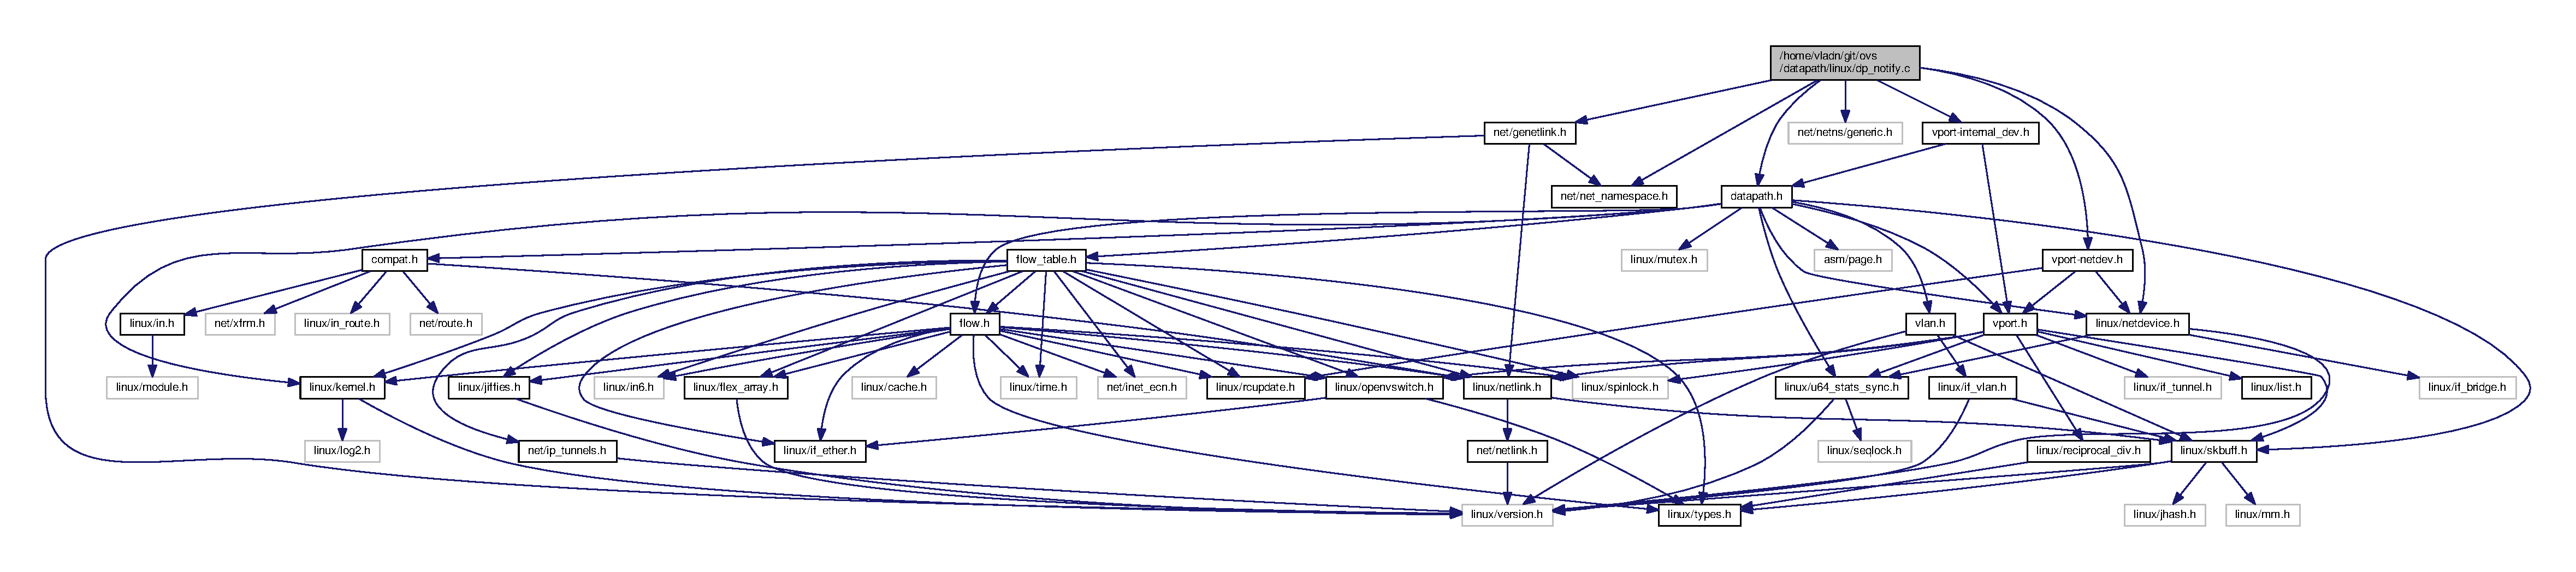
\includegraphics[width=350pt]{linux_2dp__notify_8c__incl}
\end{center}
\end{figure}
\subsection*{Functions}
\begin{DoxyCompactItemize}
\item 
static void \hyperlink{linux_2dp__notify_8c_abfe6aca1ecdf831b014297563fc08731}{dp\+\_\+detach\+\_\+port\+\_\+notify} (struct \hyperlink{structvport}{vport} $\ast$\hyperlink{structvport}{vport})
\item 
void \hyperlink{linux_2dp__notify_8c_a5d5624a3bb21c222e3a6f18f56ff20b2}{ovs\+\_\+dp\+\_\+notify\+\_\+wq} (struct work\+\_\+struct $\ast$work)
\item 
static int \hyperlink{linux_2dp__notify_8c_acca2a908a0982dd42292177079cf5643}{dp\+\_\+device\+\_\+event} (struct notifier\+\_\+block $\ast$unused, unsigned long event, void $\ast$ptr)
\end{DoxyCompactItemize}
\subsection*{Variables}
\begin{DoxyCompactItemize}
\item 
struct notifier\+\_\+block \hyperlink{linux_2dp__notify_8c_ab34ba4d6c1125efcec9480356f3393e6}{ovs\+\_\+dp\+\_\+device\+\_\+notifier}
\end{DoxyCompactItemize}


\subsection{Function Documentation}
\hypertarget{linux_2dp__notify_8c_abfe6aca1ecdf831b014297563fc08731}{}\index{linux/dp\+\_\+notify.\+c@{linux/dp\+\_\+notify.\+c}!dp\+\_\+detach\+\_\+port\+\_\+notify@{dp\+\_\+detach\+\_\+port\+\_\+notify}}
\index{dp\+\_\+detach\+\_\+port\+\_\+notify@{dp\+\_\+detach\+\_\+port\+\_\+notify}!linux/dp\+\_\+notify.\+c@{linux/dp\+\_\+notify.\+c}}
\subsubsection[{dp\+\_\+detach\+\_\+port\+\_\+notify}]{\setlength{\rightskip}{0pt plus 5cm}static void dp\+\_\+detach\+\_\+port\+\_\+notify (
\begin{DoxyParamCaption}
\item[{struct {\bf vport} $\ast$}]{vport}
\end{DoxyParamCaption}
)\hspace{0.3cm}{\ttfamily [static]}}\label{linux_2dp__notify_8c_abfe6aca1ecdf831b014297563fc08731}

\begin{DoxyCode}
29 \{
30     \textcolor{keyword}{struct }sk\_buff *notify;
31     \textcolor{keyword}{struct }\hyperlink{structdatapath}{datapath} *dp;
32 
33     dp = vport->\hyperlink{structvport_a49fb6f6bf0ac4337853e9242e88ddc42}{dp};
34     notify = \hyperlink{datapath_8c_adf50e47c9c548390402b1da1608235c9}{ovs\_vport\_cmd\_build\_info}(vport, 0, 0, 
      \hyperlink{openvswitch_8h_ae012c39e873d42b086636b19a242c354a067967d6cc0d7b7283ad6d77cba6936f}{OVS\_VPORT\_CMD\_DEL});
35     \hyperlink{datapath_8c_a560b5f5f97a839287201f7486c53447e}{ovs\_dp\_detach\_port}(vport);
36     \textcolor{keywordflow}{if} (IS\_ERR(notify)) \{
37         \hyperlink{genetlink_8h_a4261ddbadfb4439b57bd106a5ab0a043}{genl\_set\_err}(&\hyperlink{datapath_8c_a69bf55f33e234bc4b78e6eeee1d603fd}{dp\_vport\_genl\_family}, 
      \hyperlink{datapath_8h_aef2302004ca1f45133eaef00bb3740eb}{ovs\_dp\_get\_net}(dp), 0,
38                  \hyperlink{compat_8h_ab49ad0e0c1bb8cda8015902526ae189c}{GROUP\_ID}(&\hyperlink{datapath_8c_a9dd8d4307b50fdee582eb4013d89eb7b}{ovs\_dp\_vport\_multicast\_group}),
39                  PTR\_ERR(notify));
40         \textcolor{keywordflow}{return};
41     \}
42 
43     \hyperlink{genetlink_8h_ab7ffe7df793569b5be1c2c7d5c35cac6}{genlmsg\_multicast\_netns}(&\hyperlink{datapath_8c_a69bf55f33e234bc4b78e6eeee1d603fd}{dp\_vport\_genl\_family},
44                 \hyperlink{datapath_8h_aef2302004ca1f45133eaef00bb3740eb}{ovs\_dp\_get\_net}(dp), notify, 0,
45                 \hyperlink{compat_8h_ab49ad0e0c1bb8cda8015902526ae189c}{GROUP\_ID}(&\hyperlink{datapath_8c_a9dd8d4307b50fdee582eb4013d89eb7b}{ovs\_dp\_vport\_multicast\_group}),
46                 GFP\_KERNEL);
47 \}
\end{DoxyCode}
\hypertarget{linux_2dp__notify_8c_acca2a908a0982dd42292177079cf5643}{}\index{linux/dp\+\_\+notify.\+c@{linux/dp\+\_\+notify.\+c}!dp\+\_\+device\+\_\+event@{dp\+\_\+device\+\_\+event}}
\index{dp\+\_\+device\+\_\+event@{dp\+\_\+device\+\_\+event}!linux/dp\+\_\+notify.\+c@{linux/dp\+\_\+notify.\+c}}
\subsubsection[{dp\+\_\+device\+\_\+event}]{\setlength{\rightskip}{0pt plus 5cm}static int dp\+\_\+device\+\_\+event (
\begin{DoxyParamCaption}
\item[{struct notifier\+\_\+block $\ast$}]{unused, }
\item[{unsigned long}]{event, }
\item[{void $\ast$}]{ptr}
\end{DoxyParamCaption}
)\hspace{0.3cm}{\ttfamily [static]}}\label{linux_2dp__notify_8c_acca2a908a0982dd42292177079cf5643}

\begin{DoxyCode}
79 \{
80     \textcolor{keyword}{struct }\hyperlink{structovs__net}{ovs\_net} *\hyperlink{structovs__net}{ovs\_net};
81     \textcolor{keyword}{struct }net\_device *dev = netdev\_notifier\_info\_to\_dev(ptr);
82     \textcolor{keyword}{struct }\hyperlink{structvport}{vport} *\hyperlink{structvport}{vport} = NULL;
83 
84     \textcolor{keywordflow}{if} (!\hyperlink{linux_2vport-internal__dev_8c_a2056d15823f88a4caeb90001bce724bb}{ovs\_is\_internal\_dev}(dev))
85         vport = \hyperlink{linux_2vport-netdev_8c_adf074c6126d43c3f7ea008ac19d33112}{ovs\_netdev\_get\_vport}(dev);
86 
87     \textcolor{keywordflow}{if} (!vport)
88         \textcolor{keywordflow}{return} NOTIFY\_DONE;
89 
90     \textcolor{keywordflow}{if} (event == NETDEV\_UNREGISTER) \{
91         \textcolor{comment}{/* upper\_dev\_unlink and decrement promisc immediately */}
92         \hyperlink{linux_2vport-netdev_8c_ac03887d6d37218f96766a4fe8a29a7f6}{ovs\_netdev\_detach\_dev}(vport);
93 
94         \textcolor{comment}{/* schedule vport destroy, dev\_put and genl notification */}
95         ovs\_net = net\_generic(dev\_net(dev), \hyperlink{datapath_8h_ace140298dc2b59b3d77d59c0a210de29}{ovs\_net\_id});
96         queue\_work(system\_wq, &ovs\_net->\hyperlink{structovs__net_ac8cdb834420a37531f032e526ac61901}{dp\_notify\_work});
97     \}
98 
99     \textcolor{keywordflow}{return} NOTIFY\_DONE;
100 \}
\end{DoxyCode}
\hypertarget{linux_2dp__notify_8c_a5d5624a3bb21c222e3a6f18f56ff20b2}{}\index{linux/dp\+\_\+notify.\+c@{linux/dp\+\_\+notify.\+c}!ovs\+\_\+dp\+\_\+notify\+\_\+wq@{ovs\+\_\+dp\+\_\+notify\+\_\+wq}}
\index{ovs\+\_\+dp\+\_\+notify\+\_\+wq@{ovs\+\_\+dp\+\_\+notify\+\_\+wq}!linux/dp\+\_\+notify.\+c@{linux/dp\+\_\+notify.\+c}}
\subsubsection[{ovs\+\_\+dp\+\_\+notify\+\_\+wq}]{\setlength{\rightskip}{0pt plus 5cm}void ovs\+\_\+dp\+\_\+notify\+\_\+wq (
\begin{DoxyParamCaption}
\item[{struct work\+\_\+struct $\ast$}]{work}
\end{DoxyParamCaption}
)}\label{linux_2dp__notify_8c_a5d5624a3bb21c222e3a6f18f56ff20b2}

\begin{DoxyCode}
50 \{
51     \textcolor{keyword}{struct }\hyperlink{structovs__net}{ovs\_net} *\hyperlink{structovs__net}{ovs\_net} = container\_of(work, \textcolor{keyword}{struct} ovs\_net, 
      \hyperlink{structovs__net_ac8cdb834420a37531f032e526ac61901}{dp\_notify\_work});
52     \textcolor{keyword}{struct }\hyperlink{structdatapath}{datapath} *dp;
53 
54     \hyperlink{datapath_8c_a092c1f450b78a173c890ed4c56839e1a}{ovs\_lock}();
55     list\_for\_each\_entry(dp, &ovs\_net->\hyperlink{structovs__net_a0490101f7ea82f5c290a92d447bd8f9d}{dps}, \hyperlink{structdatapath_ac5f44be07025a2addb5c393fba822000}{list\_node}) \{
56         \textcolor{keywordtype}{int} i;
57 
58         \textcolor{keywordflow}{for} (i = 0; i < \hyperlink{datapath_8h_ac1bf9805d62227b8f76f130087e18018}{DP\_VPORT\_HASH\_BUCKETS}; i++) \{
59             \textcolor{keyword}{struct }\hyperlink{structvport}{vport} *\hyperlink{structvport}{vport};
60             \textcolor{keyword}{struct }hlist\_node *n;
61 
62             \hyperlink{list_8h_ae2f7dd7dbbe2f13fa51aca9fcb31a03f}{hlist\_for\_each\_entry\_safe}(vport, n, &dp->
      \hyperlink{structdatapath_abb0de528545b312de283b571cb6c4ede}{ports}[i], dp\_hash\_node) \{
63                 \textcolor{keyword}{struct }\hyperlink{structnetdev__vport}{netdev\_vport} *\hyperlink{structnetdev__vport}{netdev\_vport};
64 
65                 \textcolor{keywordflow}{if} (vport->\hyperlink{structvport_a5af933fc664c1194ac3bbc337da35586}{ops}->\hyperlink{structvport__ops_a7dd0d3776e78a2885063d3afd5e78148}{type} != \hyperlink{openvswitch_8h_a9a1b861aa99bd83177a2b10b34745b0aa825efa4a45bf501996d8d8fbb83887dd}{OVS\_VPORT\_TYPE\_NETDEV})
66                     \textcolor{keywordflow}{continue};
67 
68                 netdev\_vport = \hyperlink{vport-netdev_8h_a2cb441c6cf067ce3c79cb43836e9fc55}{netdev\_vport\_priv}(vport);
69                 \textcolor{keywordflow}{if} (!(\hyperlink{linux_2vport-netdev_8c_adf074c6126d43c3f7ea008ac19d33112}{ovs\_netdev\_get\_vport}(netdev\_vport->\hyperlink{structnetdev__vport_acf4ee248f7385e2f987fd2736f824ca9}{dev})))
70                     \hyperlink{linux_2dp__notify_8c_abfe6aca1ecdf831b014297563fc08731}{dp\_detach\_port\_notify}(vport);
71             \}
72         \}
73     \}
74     \hyperlink{datapath_8c_ac3ccfd98a880ed6d2480209be0d16680}{ovs\_unlock}();
75 \}
\end{DoxyCode}


\subsection{Variable Documentation}
\hypertarget{linux_2dp__notify_8c_ab34ba4d6c1125efcec9480356f3393e6}{}\index{linux/dp\+\_\+notify.\+c@{linux/dp\+\_\+notify.\+c}!ovs\+\_\+dp\+\_\+device\+\_\+notifier@{ovs\+\_\+dp\+\_\+device\+\_\+notifier}}
\index{ovs\+\_\+dp\+\_\+device\+\_\+notifier@{ovs\+\_\+dp\+\_\+device\+\_\+notifier}!linux/dp\+\_\+notify.\+c@{linux/dp\+\_\+notify.\+c}}
\subsubsection[{ovs\+\_\+dp\+\_\+device\+\_\+notifier}]{\setlength{\rightskip}{0pt plus 5cm}struct notifier\+\_\+block ovs\+\_\+dp\+\_\+device\+\_\+notifier}\label{linux_2dp__notify_8c_ab34ba4d6c1125efcec9480356f3393e6}
{\bfseries Initial value\+:}
\begin{DoxyCode}
= \{
    .notifier\_call = \hyperlink{linux_2dp__notify_8c_acca2a908a0982dd42292177079cf5643}{dp\_device\_event}
\}
\end{DoxyCode}

\hypertarget{flow_8c}{}\section{/home/vladn/git/ovs/datapath/flow.c File Reference}
\label{flow_8c}\index{/home/vladn/git/ovs/datapath/flow.\+c@{/home/vladn/git/ovs/datapath/flow.\+c}}
{\ttfamily \#include $<$linux/uaccess.\+h$>$}\\*
{\ttfamily \#include $<$linux/netdevice.\+h$>$}\\*
{\ttfamily \#include $<$linux/etherdevice.\+h$>$}\\*
{\ttfamily \#include $<$linux/if\+\_\+ether.\+h$>$}\\*
{\ttfamily \#include $<$linux/if\+\_\+vlan.\+h$>$}\\*
{\ttfamily \#include $<$net/llc\+\_\+pdu.\+h$>$}\\*
{\ttfamily \#include $<$linux/kernel.\+h$>$}\\*
{\ttfamily \#include $<$linux/jhash.\+h$>$}\\*
{\ttfamily \#include $<$linux/jiffies.\+h$>$}\\*
{\ttfamily \#include $<$linux/llc.\+h$>$}\\*
{\ttfamily \#include $<$linux/module.\+h$>$}\\*
{\ttfamily \#include $<$linux/in.\+h$>$}\\*
{\ttfamily \#include $<$linux/rcupdate.\+h$>$}\\*
{\ttfamily \#include $<$linux/if\+\_\+arp.\+h$>$}\\*
{\ttfamily \#include $<$linux/ip.\+h$>$}\\*
{\ttfamily \#include $<$linux/ipv6.\+h$>$}\\*
{\ttfamily \#include $<$linux/mpls.\+h$>$}\\*
{\ttfamily \#include $<$linux/sctp.\+h$>$}\\*
{\ttfamily \#include $<$linux/smp.\+h$>$}\\*
{\ttfamily \#include $<$linux/tcp.\+h$>$}\\*
{\ttfamily \#include $<$linux/udp.\+h$>$}\\*
{\ttfamily \#include $<$linux/icmp.\+h$>$}\\*
{\ttfamily \#include $<$linux/icmpv6.\+h$>$}\\*
{\ttfamily \#include $<$linux/rculist.\+h$>$}\\*
{\ttfamily \#include $<$net/ip.\+h$>$}\\*
{\ttfamily \#include $<$net/ipv6.\+h$>$}\\*
{\ttfamily \#include $<$net/mpls.\+h$>$}\\*
{\ttfamily \#include $<$net/ndisc.\+h$>$}\\*
{\ttfamily \#include \char`\"{}datapath.\+h\char`\"{}}\\*
{\ttfamily \#include \char`\"{}flow.\+h\char`\"{}}\\*
{\ttfamily \#include \char`\"{}flow\+\_\+netlink.\+h\char`\"{}}\\*
{\ttfamily \#include \char`\"{}vlan.\+h\char`\"{}}\\*
Include dependency graph for flow.\+c\+:
\nopagebreak
\begin{figure}[H]
\begin{center}
\leavevmode
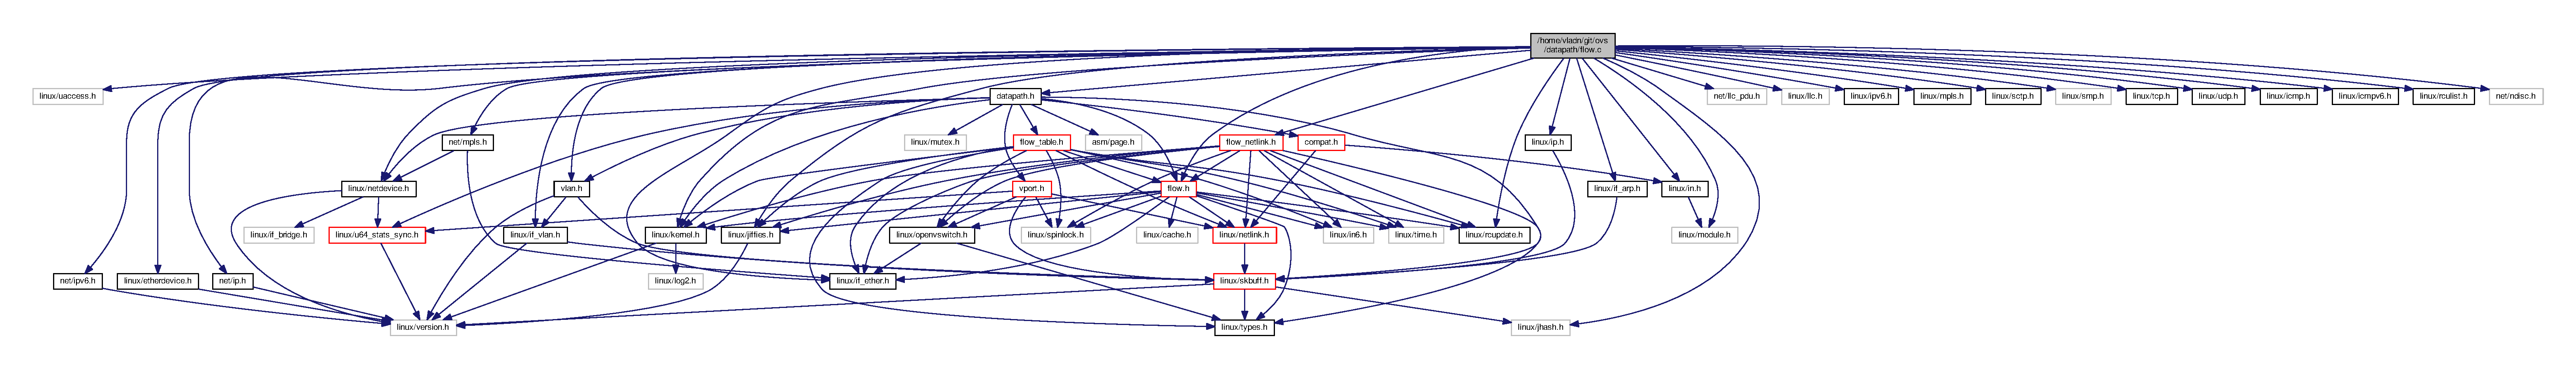
\includegraphics[width=350pt]{flow_8c__incl}
\end{center}
\end{figure}
\subsection*{Macros}
\begin{DoxyCompactItemize}
\item 
\#define \hyperlink{flow_8c_a1244774ec23560204eceaae557eff6d1}{T\+C\+P\+\_\+\+F\+L\+A\+G\+S\+\_\+\+B\+E16}(\hyperlink{flow_8h_ad44c86ae49f219522bcd4fb2744b81b2}{tp})~($\ast$(\+\_\+\+\_\+be16 $\ast$)\&tcp\+\_\+flag\+\_\+word(\hyperlink{flow_8h_ad44c86ae49f219522bcd4fb2744b81b2}{tp}) \& htons(0x0\+F\+F\+F))
\end{DoxyCompactItemize}
\subsection*{Functions}
\begin{DoxyCompactItemize}
\item 
u64 \hyperlink{flow_8c_adfdcc779325fc169a793acda2e32a46b}{ovs\+\_\+flow\+\_\+used\+\_\+time} (unsigned long flow\+\_\+jiffies)
\item 
void \hyperlink{flow_8c_ad20885fb9e6da56eb9cb58d139281916}{ovs\+\_\+flow\+\_\+stats\+\_\+update} (struct \hyperlink{structsw__flow}{sw\+\_\+flow} $\ast$flow, \+\_\+\+\_\+be16 tcp\+\_\+flags, const struct sk\+\_\+buff $\ast$skb)
\item 
void \hyperlink{flow_8c_a03636247cfc74747632c000eec0919db}{ovs\+\_\+flow\+\_\+stats\+\_\+get} (const struct \hyperlink{structsw__flow}{sw\+\_\+flow} $\ast$flow, struct \hyperlink{structovs__flow__stats}{ovs\+\_\+flow\+\_\+stats} $\ast$ovs\+\_\+stats, unsigned long $\ast$used, \+\_\+\+\_\+be16 $\ast$tcp\+\_\+flags)
\item 
void \hyperlink{flow_8c_a8dfa7ecd72ff9237664d0c402ff3f543}{ovs\+\_\+flow\+\_\+stats\+\_\+clear} (struct \hyperlink{structsw__flow}{sw\+\_\+flow} $\ast$flow)
\item 
static int \hyperlink{flow_8c_a51976bbff11a171b00faaffd004ba963}{check\+\_\+header} (struct sk\+\_\+buff $\ast$skb, int len)
\item 
static \hyperlink{types_8h_afaa87723b8417d40fcf45b7330261ef9}{bool} \hyperlink{flow_8c_ad6e91741b7e2a5ad174d0d9c899887b6}{arphdr\+\_\+ok} (struct sk\+\_\+buff $\ast$skb)
\item 
static int \hyperlink{flow_8c_ac23e11b5fa6e9068412b23f6388ae2df}{check\+\_\+iphdr} (struct sk\+\_\+buff $\ast$skb)
\item 
static \hyperlink{types_8h_afaa87723b8417d40fcf45b7330261ef9}{bool} \hyperlink{flow_8c_a71815483a340e9bab0bbcbc52537cfb5}{tcphdr\+\_\+ok} (struct sk\+\_\+buff $\ast$skb)
\item 
static \hyperlink{types_8h_afaa87723b8417d40fcf45b7330261ef9}{bool} \hyperlink{flow_8c_a354e4e351441e305c10a030f9d1dab7f}{udphdr\+\_\+ok} (struct sk\+\_\+buff $\ast$skb)
\item 
static \hyperlink{types_8h_afaa87723b8417d40fcf45b7330261ef9}{bool} \hyperlink{flow_8c_a235207174d62d682354a73e4b43a4ee2}{sctphdr\+\_\+ok} (struct sk\+\_\+buff $\ast$skb)
\item 
static \hyperlink{types_8h_afaa87723b8417d40fcf45b7330261ef9}{bool} \hyperlink{flow_8c_ac87d76f166f066dd4a2c9bc729702ab6}{icmphdr\+\_\+ok} (struct sk\+\_\+buff $\ast$skb)
\item 
static int \hyperlink{flow_8c_aae5a88c529fa6e31de896e40c546ec90}{parse\+\_\+ipv6hdr} (struct sk\+\_\+buff $\ast$skb, struct \hyperlink{structsw__flow__key}{sw\+\_\+flow\+\_\+key} $\ast$key)
\item 
static \hyperlink{types_8h_afaa87723b8417d40fcf45b7330261ef9}{bool} \hyperlink{flow_8c_a4191de70201a777f1ac4e71fc5c24d17}{icmp6hdr\+\_\+ok} (struct sk\+\_\+buff $\ast$skb)
\item 
static int \hyperlink{flow_8c_aab1dd840cacc7b21ee01cb885171d60d}{parse\+\_\+vlan} (struct sk\+\_\+buff $\ast$skb, struct \hyperlink{structsw__flow__key}{sw\+\_\+flow\+\_\+key} $\ast$key)
\item 
static \+\_\+\+\_\+be16 \hyperlink{flow_8c_a8f4a5415b9d6b2be7aef9e3749e65908}{parse\+\_\+ethertype} (struct sk\+\_\+buff $\ast$skb)
\item 
static int \hyperlink{flow_8c_a0b01cb308f20bbfe4348b6ef1b27a65d}{parse\+\_\+icmpv6} (struct sk\+\_\+buff $\ast$skb, struct \hyperlink{structsw__flow__key}{sw\+\_\+flow\+\_\+key} $\ast$key, int nh\+\_\+len)
\item 
static int \hyperlink{flow_8c_af69403050accb2489f73d37b528aa9c4}{key\+\_\+extract} (struct sk\+\_\+buff $\ast$skb, struct \hyperlink{structsw__flow__key}{sw\+\_\+flow\+\_\+key} $\ast$key)
\item 
int \hyperlink{flow_8c_a7d27b3745046ced4859b9fa615e27543}{ovs\+\_\+flow\+\_\+key\+\_\+update} (struct sk\+\_\+buff $\ast$skb, struct \hyperlink{structsw__flow__key}{sw\+\_\+flow\+\_\+key} $\ast$key)
\item 
int \hyperlink{flow_8c_a88b5c281d297950115033a17dbce5208}{ovs\+\_\+flow\+\_\+key\+\_\+extract} (const struct \hyperlink{structovs__tunnel__info}{ovs\+\_\+tunnel\+\_\+info} $\ast$tun\+\_\+info, struct sk\+\_\+buff $\ast$skb, struct \hyperlink{structsw__flow__key}{sw\+\_\+flow\+\_\+key} $\ast$key)
\item 
int \hyperlink{flow_8c_a5e042238993a5a8a8a8b3472cb274ead}{ovs\+\_\+flow\+\_\+key\+\_\+extract\+\_\+userspace} (const struct nlattr $\ast$attr, struct sk\+\_\+buff $\ast$skb, struct \hyperlink{structsw__flow__key}{sw\+\_\+flow\+\_\+key} $\ast$key, \hyperlink{types_8h_afaa87723b8417d40fcf45b7330261ef9}{bool} log)
\end{DoxyCompactItemize}


\subsection{Macro Definition Documentation}
\hypertarget{flow_8c_a1244774ec23560204eceaae557eff6d1}{}\index{flow.\+c@{flow.\+c}!T\+C\+P\+\_\+\+F\+L\+A\+G\+S\+\_\+\+B\+E16@{T\+C\+P\+\_\+\+F\+L\+A\+G\+S\+\_\+\+B\+E16}}
\index{T\+C\+P\+\_\+\+F\+L\+A\+G\+S\+\_\+\+B\+E16@{T\+C\+P\+\_\+\+F\+L\+A\+G\+S\+\_\+\+B\+E16}!flow.\+c@{flow.\+c}}
\subsubsection[{T\+C\+P\+\_\+\+F\+L\+A\+G\+S\+\_\+\+B\+E16}]{\setlength{\rightskip}{0pt plus 5cm}\#define T\+C\+P\+\_\+\+F\+L\+A\+G\+S\+\_\+\+B\+E16(
\begin{DoxyParamCaption}
\item[{}]{{\bf tp}}
\end{DoxyParamCaption}
)~($\ast$(\+\_\+\+\_\+be16 $\ast$)\&tcp\+\_\+flag\+\_\+word({\bf tp}) \& htons(0x0\+F\+F\+F))}\label{flow_8c_a1244774ec23560204eceaae557eff6d1}


\subsection{Function Documentation}
\hypertarget{flow_8c_ad6e91741b7e2a5ad174d0d9c899887b6}{}\index{flow.\+c@{flow.\+c}!arphdr\+\_\+ok@{arphdr\+\_\+ok}}
\index{arphdr\+\_\+ok@{arphdr\+\_\+ok}!flow.\+c@{flow.\+c}}
\subsubsection[{arphdr\+\_\+ok}]{\setlength{\rightskip}{0pt plus 5cm}static {\bf bool} arphdr\+\_\+ok (
\begin{DoxyParamCaption}
\item[{struct sk\+\_\+buff $\ast$}]{skb}
\end{DoxyParamCaption}
)\hspace{0.3cm}{\ttfamily [static]}}\label{flow_8c_ad6e91741b7e2a5ad174d0d9c899887b6}

\begin{DoxyCode}
189 \{
190     \textcolor{keywordflow}{return} pskb\_may\_pull(skb, \hyperlink{skbuff_8h_aabe75b44039b11c1b7c6e2f246e7146e}{skb\_network\_offset}(skb) +
191                   \textcolor{keyword}{sizeof}(\textcolor{keyword}{struct} \hyperlink{structarp__eth__header}{arp\_eth\_header}));
192 \}
\end{DoxyCode}
\hypertarget{flow_8c_a51976bbff11a171b00faaffd004ba963}{}\index{flow.\+c@{flow.\+c}!check\+\_\+header@{check\+\_\+header}}
\index{check\+\_\+header@{check\+\_\+header}!flow.\+c@{flow.\+c}}
\subsubsection[{check\+\_\+header}]{\setlength{\rightskip}{0pt plus 5cm}static int check\+\_\+header (
\begin{DoxyParamCaption}
\item[{struct sk\+\_\+buff $\ast$}]{skb, }
\item[{int}]{len}
\end{DoxyParamCaption}
)\hspace{0.3cm}{\ttfamily [static]}}\label{flow_8c_a51976bbff11a171b00faaffd004ba963}

\begin{DoxyCode}
180 \{
181     \textcolor{keywordflow}{if} (unlikely(skb->len < len))
182         \textcolor{keywordflow}{return} -EINVAL;
183     \textcolor{keywordflow}{if} (unlikely(!pskb\_may\_pull(skb, len)))
184         \textcolor{keywordflow}{return} -ENOMEM;
185     \textcolor{keywordflow}{return} 0;
186 \}
\end{DoxyCode}
\hypertarget{flow_8c_ac23e11b5fa6e9068412b23f6388ae2df}{}\index{flow.\+c@{flow.\+c}!check\+\_\+iphdr@{check\+\_\+iphdr}}
\index{check\+\_\+iphdr@{check\+\_\+iphdr}!flow.\+c@{flow.\+c}}
\subsubsection[{check\+\_\+iphdr}]{\setlength{\rightskip}{0pt plus 5cm}static int check\+\_\+iphdr (
\begin{DoxyParamCaption}
\item[{struct sk\+\_\+buff $\ast$}]{skb}
\end{DoxyParamCaption}
)\hspace{0.3cm}{\ttfamily [static]}}\label{flow_8c_ac23e11b5fa6e9068412b23f6388ae2df}

\begin{DoxyCode}
195 \{
196     \textcolor{keywordtype}{unsigned} \textcolor{keywordtype}{int} nh\_ofs = \hyperlink{skbuff_8h_aabe75b44039b11c1b7c6e2f246e7146e}{skb\_network\_offset}(skb);
197     \textcolor{keywordtype}{unsigned} \textcolor{keywordtype}{int} ip\_len;
198     \textcolor{keywordtype}{int} err;
199 
200     err = \hyperlink{flow_8c_a51976bbff11a171b00faaffd004ba963}{check\_header}(skb, nh\_ofs + \textcolor{keyword}{sizeof}(\textcolor{keyword}{struct} iphdr));
201     \textcolor{keywordflow}{if} (unlikely(err))
202         \textcolor{keywordflow}{return} err;
203 
204     ip\_len = \hyperlink{linux_2ip_8h_a769819999a936046f6b97cca3ec3ef74}{ip\_hdrlen}(skb);
205     \textcolor{keywordflow}{if} (unlikely(ip\_len < \textcolor{keyword}{sizeof}(\textcolor{keyword}{struct} iphdr) ||
206              skb->len < nh\_ofs + ip\_len))
207         \textcolor{keywordflow}{return} -EINVAL;
208 
209     \hyperlink{skbuff_8h_a35af79b1b630fc75fbd7347549b6affe}{skb\_set\_transport\_header}(skb, nh\_ofs + ip\_len);
210     \textcolor{keywordflow}{return} 0;
211 \}
\end{DoxyCode}
\hypertarget{flow_8c_a4191de70201a777f1ac4e71fc5c24d17}{}\index{flow.\+c@{flow.\+c}!icmp6hdr\+\_\+ok@{icmp6hdr\+\_\+ok}}
\index{icmp6hdr\+\_\+ok@{icmp6hdr\+\_\+ok}!flow.\+c@{flow.\+c}}
\subsubsection[{icmp6hdr\+\_\+ok}]{\setlength{\rightskip}{0pt plus 5cm}static {\bf bool} icmp6hdr\+\_\+ok (
\begin{DoxyParamCaption}
\item[{struct sk\+\_\+buff $\ast$}]{skb}
\end{DoxyParamCaption}
)\hspace{0.3cm}{\ttfamily [static]}}\label{flow_8c_a4191de70201a777f1ac4e71fc5c24d17}

\begin{DoxyCode}
292 \{
293     \textcolor{keywordflow}{return} pskb\_may\_pull(skb, \hyperlink{skbuff_8h_ac8d86ecdcd808a5839009d4a8f85f6c8}{skb\_transport\_offset}(skb) +
294                   \textcolor{keyword}{sizeof}(\textcolor{keyword}{struct} icmp6hdr));
295 \}
\end{DoxyCode}
\hypertarget{flow_8c_ac87d76f166f066dd4a2c9bc729702ab6}{}\index{flow.\+c@{flow.\+c}!icmphdr\+\_\+ok@{icmphdr\+\_\+ok}}
\index{icmphdr\+\_\+ok@{icmphdr\+\_\+ok}!flow.\+c@{flow.\+c}}
\subsubsection[{icmphdr\+\_\+ok}]{\setlength{\rightskip}{0pt plus 5cm}static {\bf bool} icmphdr\+\_\+ok (
\begin{DoxyParamCaption}
\item[{struct sk\+\_\+buff $\ast$}]{skb}
\end{DoxyParamCaption}
)\hspace{0.3cm}{\ttfamily [static]}}\label{flow_8c_ac87d76f166f066dd4a2c9bc729702ab6}

\begin{DoxyCode}
242 \{
243     \textcolor{keywordflow}{return} pskb\_may\_pull(skb, \hyperlink{skbuff_8h_ac8d86ecdcd808a5839009d4a8f85f6c8}{skb\_transport\_offset}(skb) +
244                   \textcolor{keyword}{sizeof}(\textcolor{keyword}{struct} icmphdr));
245 \}
\end{DoxyCode}
\hypertarget{flow_8c_af69403050accb2489f73d37b528aa9c4}{}\index{flow.\+c@{flow.\+c}!key\+\_\+extract@{key\+\_\+extract}}
\index{key\+\_\+extract@{key\+\_\+extract}!flow.\+c@{flow.\+c}}
\subsubsection[{key\+\_\+extract}]{\setlength{\rightskip}{0pt plus 5cm}static int key\+\_\+extract (
\begin{DoxyParamCaption}
\item[{struct sk\+\_\+buff $\ast$}]{skb, }
\item[{struct {\bf sw\+\_\+flow\+\_\+key} $\ast$}]{key}
\end{DoxyParamCaption}
)\hspace{0.3cm}{\ttfamily [static]}}\label{flow_8c_af69403050accb2489f73d37b528aa9c4}
key\+\_\+extract -\/ extracts a flow key from an Ethernet frame. \+: sk\+\_\+buff that contains the frame, with skb-\/$>$data pointing to the Ethernet header \+: output flow key

The caller must ensure that skb-\/$>$len $>$= E\+T\+H\+\_\+\+H\+L\+E\+N.

Returns 0 if successful, otherwise a negative errno value.

Initializes  header pointers as follows\+:


\begin{DoxyItemize}
\item skb-\/$>$mac\+\_\+header\+: the Ethernet header.
\item skb-\/$>$network\+\_\+header\+: just past the Ethernet header, or just past the V\+L\+A\+N header, to the first byte of the Ethernet payload.
\item skb-\/$>$transport\+\_\+header\+: If key-\/$>$eth.\+type is E\+T\+H\+\_\+\+P\+\_\+\+I\+P or E\+T\+H\+\_\+\+P\+\_\+\+I\+P\+V6 on output, then just past the I\+P header, if one is present and of a correct length, otherwise the same as skb-\/$>$network\+\_\+header. For other key-\/$>$eth.\+type values it is left untouched. 
\end{DoxyItemize}
\begin{DoxyCode}
454 \{
455     \textcolor{keywordtype}{int} error;
456     \textcolor{keyword}{struct }ethhdr *\hyperlink{flow_8h_a1679a3c93391059deba58179f52c86a6}{eth};
457 
458     \textcolor{comment}{/* Flags are always used as part of stats */}
459     key->\hyperlink{structsw__flow__key_a9c1944a39db1bf91141048df6d85ce8b}{tp}.\hyperlink{structsw__flow__key_a910f5e4408d113dbc9211190b44e0880}{flags} = 0;
460 
461     \hyperlink{skbuff_8h_aaf81c26756757ac1e1d7e6933f61bdaf}{skb\_reset\_mac\_header}(skb);
462 
463     \textcolor{comment}{/* Link layer.  We are guaranteed to have at least the 14 byte Ethernet}
464 \textcolor{comment}{     * header in the linear data area.}
465 \textcolor{comment}{     */}
466     eth = eth\_hdr(skb);
467     \hyperlink{etherdevice_8h_a564a2ea461aa6add2fa94a6864ee494d}{ether\_addr\_copy}(key->\hyperlink{structsw__flow__key_af3e10c978a3a2bf303b7d953ac6ff361}{eth}.\hyperlink{structsw__flow__key_a2fbd4aa7a500630627eff0630f864117}{src}, eth->h\_source);
468     \hyperlink{etherdevice_8h_a564a2ea461aa6add2fa94a6864ee494d}{ether\_addr\_copy}(key->\hyperlink{structsw__flow__key_af3e10c978a3a2bf303b7d953ac6ff361}{eth}.\hyperlink{structsw__flow__key_a44a0cdfe7471df8bb73762085da4cda9}{dst}, eth->h\_dest);
469 
470     \_\_skb\_pull(skb, 2 * ETH\_ALEN);
471     \textcolor{comment}{/* We are going to push all headers that we pull, so no need to}
472 \textcolor{comment}{     * update skb->csum here.}
473 \textcolor{comment}{     */}
474 
475     key->\hyperlink{structsw__flow__key_af3e10c978a3a2bf303b7d953ac6ff361}{eth}.\hyperlink{structsw__flow__key_a56b27b9b9eafa8f79acd544eba98c7b0}{tci} = 0;
476     \textcolor{keywordflow}{if} (\hyperlink{if__vlan_8h_a0bdf3e26944669a4265c7e717e846215}{skb\_vlan\_tag\_present}(skb))
477         key->\hyperlink{structsw__flow__key_af3e10c978a3a2bf303b7d953ac6ff361}{eth}.\hyperlink{structsw__flow__key_a56b27b9b9eafa8f79acd544eba98c7b0}{tci} = htons(\hyperlink{vlan_8h_a7d6820c8064af28c10f40f519605c2db}{vlan\_get\_tci}(skb));
478     \textcolor{keywordflow}{else} \textcolor{keywordflow}{if} (eth->h\_proto == htons(ETH\_P\_8021Q))
479         \textcolor{keywordflow}{if} (unlikely(\hyperlink{flow_8c_aab1dd840cacc7b21ee01cb885171d60d}{parse\_vlan}(skb, key)))
480             \textcolor{keywordflow}{return} -ENOMEM;
481 
482     key->\hyperlink{structsw__flow__key_af3e10c978a3a2bf303b7d953ac6ff361}{eth}.\hyperlink{structsw__flow__key_af30defbb2a81c997e8747594e1d937a0}{type} = \hyperlink{flow_8c_a8f4a5415b9d6b2be7aef9e3749e65908}{parse\_ethertype}(skb);
483     \textcolor{keywordflow}{if} (unlikely(key->\hyperlink{structsw__flow__key_af3e10c978a3a2bf303b7d953ac6ff361}{eth}.\hyperlink{structsw__flow__key_af30defbb2a81c997e8747594e1d937a0}{type} == htons(0)))
484         \textcolor{keywordflow}{return} -ENOMEM;
485 
486     \hyperlink{skbuff_8h_a2ea5d9050fe3927247bb55820cfcb02c}{skb\_reset\_network\_header}(skb);
487     \hyperlink{skbuff_8h_ae4be7dfedacf0e75fd904f0f54c9c731}{skb\_reset\_mac\_len}(skb);
488     \_\_skb\_push(skb, skb->data - \hyperlink{skbuff_8h_a292027671dfcf3aa23f9551f48713e24}{skb\_mac\_header}(skb));
489 
490     \textcolor{comment}{/* Network layer. */}
491     \textcolor{keywordflow}{if} (key->\hyperlink{structsw__flow__key_af3e10c978a3a2bf303b7d953ac6ff361}{eth}.\hyperlink{structsw__flow__key_af30defbb2a81c997e8747594e1d937a0}{type} == htons(ETH\_P\_IP)) \{
492         \textcolor{keyword}{struct }iphdr *nh;
493         \_\_be16 offset;
494 
495         error = \hyperlink{flow_8c_ac23e11b5fa6e9068412b23f6388ae2df}{check\_iphdr}(skb);
496         \textcolor{keywordflow}{if} (unlikely(error)) \{
497             memset(&key->\hyperlink{structsw__flow__key_ae8d48c419eaff6a9fda97c7446bdec0e}{ip}, 0, \textcolor{keyword}{sizeof}(key->\hyperlink{structsw__flow__key_ae8d48c419eaff6a9fda97c7446bdec0e}{ip}));
498             memset(&key->\hyperlink{structsw__flow__key_aeb4295bcb2fb4efea5c30337b871a423}{ipv4}, 0, \textcolor{keyword}{sizeof}(key->\hyperlink{structsw__flow__key_aeb4295bcb2fb4efea5c30337b871a423}{ipv4}));
499             \textcolor{keywordflow}{if} (error == -EINVAL) \{
500                 skb->transport\_header = skb->network\_header;
501                 error = 0;
502             \}
503             \textcolor{keywordflow}{return} error;
504         \}
505 
506         nh = \hyperlink{linux_2ip_8h_a06ad68dbeebbe718758ba2d5ebb6335c}{ip\_hdr}(skb);
507         key->\hyperlink{structsw__flow__key_aeb4295bcb2fb4efea5c30337b871a423}{ipv4}.addr.src = nh->saddr;
508         key->\hyperlink{structsw__flow__key_aeb4295bcb2fb4efea5c30337b871a423}{ipv4}.addr.dst = nh->daddr;
509 
510         key->\hyperlink{structsw__flow__key_ae8d48c419eaff6a9fda97c7446bdec0e}{ip}.proto = nh->protocol;
511         key->\hyperlink{structsw__flow__key_ae8d48c419eaff6a9fda97c7446bdec0e}{ip}.tos = nh->tos;
512         key->\hyperlink{structsw__flow__key_ae8d48c419eaff6a9fda97c7446bdec0e}{ip}.ttl = nh->ttl;
513 
514         offset = nh->frag\_off & htons(IP\_OFFSET);
515         \textcolor{keywordflow}{if} (offset) \{
516             key->\hyperlink{structsw__flow__key_ae8d48c419eaff6a9fda97c7446bdec0e}{ip}.frag = \hyperlink{openvswitch_8h_ad843f713a855bfcacd0adfe3e98eb447a1d1c9f89ced33419ec870391d8954c10}{OVS\_FRAG\_TYPE\_LATER};
517             \textcolor{keywordflow}{return} 0;
518         \}
519         \textcolor{keywordflow}{if} (nh->frag\_off & htons(IP\_MF) ||
520             skb\_shinfo(skb)->gso\_type & SKB\_GSO\_UDP)
521             key->\hyperlink{structsw__flow__key_ae8d48c419eaff6a9fda97c7446bdec0e}{ip}.frag = \hyperlink{openvswitch_8h_ad843f713a855bfcacd0adfe3e98eb447a7302a2ecd7ef2e817fadcd3e943af200}{OVS\_FRAG\_TYPE\_FIRST};
522         \textcolor{keywordflow}{else}
523             key->\hyperlink{structsw__flow__key_ae8d48c419eaff6a9fda97c7446bdec0e}{ip}.frag = \hyperlink{openvswitch_8h_ad843f713a855bfcacd0adfe3e98eb447a8551f9db6addee11579a10fe4b1e9d62}{OVS\_FRAG\_TYPE\_NONE};
524 
525         \textcolor{comment}{/* Transport layer. */}
526         \textcolor{keywordflow}{if} (key->\hyperlink{structsw__flow__key_ae8d48c419eaff6a9fda97c7446bdec0e}{ip}.proto == IPPROTO\_TCP) \{
527             \textcolor{keywordflow}{if} (\hyperlink{flow_8c_a71815483a340e9bab0bbcbc52537cfb5}{tcphdr\_ok}(skb)) \{
528                 \textcolor{keyword}{struct }tcphdr *tcp = \hyperlink{tcp_8h_a9ac4e94949ea9142c45cf46683be5ef7}{tcp\_hdr}(skb);
529                 key->\hyperlink{structsw__flow__key_a9c1944a39db1bf91141048df6d85ce8b}{tp}.\hyperlink{structsw__flow__key_a2fbd4aa7a500630627eff0630f864117}{src} = tcp->source;
530                 key->\hyperlink{structsw__flow__key_a9c1944a39db1bf91141048df6d85ce8b}{tp}.\hyperlink{structsw__flow__key_a44a0cdfe7471df8bb73762085da4cda9}{dst} = tcp->dest;
531                 key->\hyperlink{structsw__flow__key_a9c1944a39db1bf91141048df6d85ce8b}{tp}.\hyperlink{structsw__flow__key_a910f5e4408d113dbc9211190b44e0880}{flags} = \hyperlink{flow_8c_a1244774ec23560204eceaae557eff6d1}{TCP\_FLAGS\_BE16}(tcp);
532             \} \textcolor{keywordflow}{else} \{
533                 memset(&key->\hyperlink{structsw__flow__key_a9c1944a39db1bf91141048df6d85ce8b}{tp}, 0, \textcolor{keyword}{sizeof}(key->\hyperlink{structsw__flow__key_a9c1944a39db1bf91141048df6d85ce8b}{tp}));
534             \}
535 
536         \} \textcolor{keywordflow}{else} \textcolor{keywordflow}{if} (key->\hyperlink{structsw__flow__key_ae8d48c419eaff6a9fda97c7446bdec0e}{ip}.proto == IPPROTO\_UDP) \{
537             \textcolor{keywordflow}{if} (\hyperlink{flow_8c_a354e4e351441e305c10a030f9d1dab7f}{udphdr\_ok}(skb)) \{
538                 \textcolor{keyword}{struct }udphdr *udp = \hyperlink{linux_2udp_8h_a7b8908e197538768cf4ff9ec577bd86b}{udp\_hdr}(skb);
539                 key->\hyperlink{structsw__flow__key_a9c1944a39db1bf91141048df6d85ce8b}{tp}.\hyperlink{structsw__flow__key_a2fbd4aa7a500630627eff0630f864117}{src} = udp->source;
540                 key->\hyperlink{structsw__flow__key_a9c1944a39db1bf91141048df6d85ce8b}{tp}.\hyperlink{structsw__flow__key_a44a0cdfe7471df8bb73762085da4cda9}{dst} = udp->dest;
541             \} \textcolor{keywordflow}{else} \{
542                 memset(&key->\hyperlink{structsw__flow__key_a9c1944a39db1bf91141048df6d85ce8b}{tp}, 0, \textcolor{keyword}{sizeof}(key->\hyperlink{structsw__flow__key_a9c1944a39db1bf91141048df6d85ce8b}{tp}));
543             \}
544         \} \textcolor{keywordflow}{else} \textcolor{keywordflow}{if} (key->\hyperlink{structsw__flow__key_ae8d48c419eaff6a9fda97c7446bdec0e}{ip}.proto == IPPROTO\_SCTP) \{
545             \textcolor{keywordflow}{if} (\hyperlink{flow_8c_a235207174d62d682354a73e4b43a4ee2}{sctphdr\_ok}(skb)) \{
546                 \textcolor{keyword}{struct }sctphdr *sctp = \hyperlink{sctp_8h_a6f9abfbe98294e40a3f32db7ad723998}{sctp\_hdr}(skb);
547                 key->\hyperlink{structsw__flow__key_a9c1944a39db1bf91141048df6d85ce8b}{tp}.\hyperlink{structsw__flow__key_a2fbd4aa7a500630627eff0630f864117}{src} = sctp->source;
548                 key->\hyperlink{structsw__flow__key_a9c1944a39db1bf91141048df6d85ce8b}{tp}.\hyperlink{structsw__flow__key_a44a0cdfe7471df8bb73762085da4cda9}{dst} = sctp->dest;
549             \} \textcolor{keywordflow}{else} \{
550                 memset(&key->\hyperlink{structsw__flow__key_a9c1944a39db1bf91141048df6d85ce8b}{tp}, 0, \textcolor{keyword}{sizeof}(key->\hyperlink{structsw__flow__key_a9c1944a39db1bf91141048df6d85ce8b}{tp}));
551             \}
552         \} \textcolor{keywordflow}{else} \textcolor{keywordflow}{if} (key->\hyperlink{structsw__flow__key_ae8d48c419eaff6a9fda97c7446bdec0e}{ip}.proto == IPPROTO\_ICMP) \{
553             \textcolor{keywordflow}{if} (\hyperlink{flow_8c_ac87d76f166f066dd4a2c9bc729702ab6}{icmphdr\_ok}(skb)) \{
554                 \textcolor{keyword}{struct }icmphdr *icmp = \hyperlink{icmp_8h_a2226121e608b10a1dde33ed552361bba}{icmp\_hdr}(skb);
555                 \textcolor{comment}{/* The ICMP type and code fields use the 16-bit}
556 \textcolor{comment}{                 * transport port fields, so we need to store}
557 \textcolor{comment}{                 * them in 16-bit network byte order.}
558 \textcolor{comment}{                 */}
559                 key->\hyperlink{structsw__flow__key_a9c1944a39db1bf91141048df6d85ce8b}{tp}.\hyperlink{structsw__flow__key_a2fbd4aa7a500630627eff0630f864117}{src} = htons(icmp->type);
560                 key->\hyperlink{structsw__flow__key_a9c1944a39db1bf91141048df6d85ce8b}{tp}.\hyperlink{structsw__flow__key_a44a0cdfe7471df8bb73762085da4cda9}{dst} = htons(icmp->code);
561             \} \textcolor{keywordflow}{else} \{
562                 memset(&key->\hyperlink{structsw__flow__key_a9c1944a39db1bf91141048df6d85ce8b}{tp}, 0, \textcolor{keyword}{sizeof}(key->\hyperlink{structsw__flow__key_a9c1944a39db1bf91141048df6d85ce8b}{tp}));
563             \}
564         \}
565 
566     \} \textcolor{keywordflow}{else} \textcolor{keywordflow}{if} (key->\hyperlink{structsw__flow__key_af3e10c978a3a2bf303b7d953ac6ff361}{eth}.\hyperlink{structsw__flow__key_af30defbb2a81c997e8747594e1d937a0}{type} == htons(ETH\_P\_ARP) ||
567            key->\hyperlink{structsw__flow__key_af3e10c978a3a2bf303b7d953ac6ff361}{eth}.\hyperlink{structsw__flow__key_af30defbb2a81c997e8747594e1d937a0}{type} == htons(ETH\_P\_RARP)) \{
568         \textcolor{keyword}{struct }\hyperlink{structarp__eth__header}{arp\_eth\_header} *\hyperlink{flow_8h_aa05c06f4d8f8b791f607aa53db449356}{arp};
569         \textcolor{keywordtype}{bool} arp\_available = \hyperlink{flow_8c_ad6e91741b7e2a5ad174d0d9c899887b6}{arphdr\_ok}(skb);
570 
571         arp = (\textcolor{keyword}{struct }\hyperlink{structarp__eth__header}{arp\_eth\_header} *)\hyperlink{skbuff_8h_aa9e0f2aeb3abecde73023d35145bc4a0}{skb\_network\_header}(skb);
572 
573         \textcolor{keywordflow}{if} (arp\_available &&
574             arp->\hyperlink{structarp__eth__header_afe4c385a8760054d1d9da4e06b72dc3a}{ar\_hrd} == htons(ARPHRD\_ETHER) &&
575             arp->\hyperlink{structarp__eth__header_aa0a6c956f6f9001377528f86f94d91b4}{ar\_pro} == htons(ETH\_P\_IP) &&
576             arp->\hyperlink{structarp__eth__header_a8feceb41fdd95e4a0f1e17e56b957bf4}{ar\_hln} == ETH\_ALEN &&
577             arp->\hyperlink{structarp__eth__header_abc215d845eb12176276c8cee0501ecd8}{ar\_pln} == 4) \{
578 
579             \textcolor{comment}{/* We only match on the lower 8 bits of the opcode. */}
580             \textcolor{keywordflow}{if} (ntohs(arp->\hyperlink{structarp__eth__header_a0cad73c318ab7ea788fa836f6b5a011d}{ar\_op}) <= 0xff)
581                 key->\hyperlink{structsw__flow__key_ae8d48c419eaff6a9fda97c7446bdec0e}{ip}.proto = ntohs(arp->\hyperlink{structarp__eth__header_a0cad73c318ab7ea788fa836f6b5a011d}{ar\_op});
582             \textcolor{keywordflow}{else}
583                 key->\hyperlink{structsw__flow__key_ae8d48c419eaff6a9fda97c7446bdec0e}{ip}.proto = 0;
584 
585             memcpy(&key->\hyperlink{structsw__flow__key_aeb4295bcb2fb4efea5c30337b871a423}{ipv4}.addr.src, arp->\hyperlink{structarp__eth__header_ae584842ae04804b2f5cf3c26fb135961}{ar\_sip}, \textcolor{keyword}{sizeof}(key->\hyperlink{structsw__flow__key_aeb4295bcb2fb4efea5c30337b871a423}{ipv4}.addr.src));
586             memcpy(&key->\hyperlink{structsw__flow__key_aeb4295bcb2fb4efea5c30337b871a423}{ipv4}.addr.dst, arp->\hyperlink{structarp__eth__header_a9ed88031c0dd2f554f1dc455e878945d}{ar\_tip}, \textcolor{keyword}{sizeof}(key->\hyperlink{structsw__flow__key_aeb4295bcb2fb4efea5c30337b871a423}{ipv4}.addr.dst));
587             \hyperlink{etherdevice_8h_a564a2ea461aa6add2fa94a6864ee494d}{ether\_addr\_copy}(key->\hyperlink{structsw__flow__key_aeb4295bcb2fb4efea5c30337b871a423}{ipv4}.arp.sha, arp->\hyperlink{structarp__eth__header_a569cddaf9ed4aa40b04b60958783e908}{ar\_sha});
588             \hyperlink{etherdevice_8h_a564a2ea461aa6add2fa94a6864ee494d}{ether\_addr\_copy}(key->\hyperlink{structsw__flow__key_aeb4295bcb2fb4efea5c30337b871a423}{ipv4}.arp.tha, arp->\hyperlink{structarp__eth__header_a490c51d5f01a32e78c57d020ca2662f6}{ar\_tha});
589         \} \textcolor{keywordflow}{else} \{
590             memset(&key->\hyperlink{structsw__flow__key_ae8d48c419eaff6a9fda97c7446bdec0e}{ip}, 0, \textcolor{keyword}{sizeof}(key->\hyperlink{structsw__flow__key_ae8d48c419eaff6a9fda97c7446bdec0e}{ip}));
591             memset(&key->\hyperlink{structsw__flow__key_aeb4295bcb2fb4efea5c30337b871a423}{ipv4}, 0, \textcolor{keyword}{sizeof}(key->\hyperlink{structsw__flow__key_aeb4295bcb2fb4efea5c30337b871a423}{ipv4}));
592         \}
593     \} \textcolor{keywordflow}{else} \textcolor{keywordflow}{if} (\hyperlink{net_2mpls_8h_aab48ab242fbafafc869b3e98df4ace8f}{eth\_p\_mpls}(key->\hyperlink{structsw__flow__key_af3e10c978a3a2bf303b7d953ac6ff361}{eth}.\hyperlink{structsw__flow__key_af30defbb2a81c997e8747594e1d937a0}{type})) \{
594         \textcolor{keywordtype}{size\_t} stack\_len = \hyperlink{net_2mpls_8h_a9a0b8d7adb48a79ca82a00b2663823ee}{MPLS\_HLEN};
595 
596         \textcolor{comment}{/* In the presence of an MPLS label stack the end of the L2}
597 \textcolor{comment}{         * header and the beginning of the L3 header differ.}
598 \textcolor{comment}{         *}
599 \textcolor{comment}{         * Advance network\_header to the beginning of the L3}
600 \textcolor{comment}{         * header. mac\_len corresponds to the end of the L2 header.}
601 \textcolor{comment}{         */}
602         \textcolor{keywordflow}{while} (1) \{
603             \_\_be32 lse;
604 
605             error = \hyperlink{flow_8c_a51976bbff11a171b00faaffd004ba963}{check\_header}(skb, skb->mac\_len + stack\_len);
606             \textcolor{keywordflow}{if} (unlikely(error))
607                 \textcolor{keywordflow}{return} 0;
608 
609             memcpy(&lse, \hyperlink{skbuff_8h_aa9e0f2aeb3abecde73023d35145bc4a0}{skb\_network\_header}(skb), \hyperlink{net_2mpls_8h_a9a0b8d7adb48a79ca82a00b2663823ee}{MPLS\_HLEN});
610 
611             \textcolor{keywordflow}{if} (stack\_len == \hyperlink{net_2mpls_8h_a9a0b8d7adb48a79ca82a00b2663823ee}{MPLS\_HLEN})
612                 memcpy(&key->\hyperlink{structsw__flow__key_a005840d04ee5b462be3c8e21809dc9aa}{mpls}.top\_lse, &lse, \hyperlink{net_2mpls_8h_a9a0b8d7adb48a79ca82a00b2663823ee}{MPLS\_HLEN});
613 
614             \hyperlink{skbuff_8h_a2aa771daf8e324a50f60e4934839dc2c}{skb\_set\_network\_header}(skb, skb->mac\_len + stack\_len);
615             \textcolor{keywordflow}{if} (lse & htonl(MPLS\_LS\_S\_MASK))
616                 \textcolor{keywordflow}{break};
617 
618             stack\_len += \hyperlink{net_2mpls_8h_a9a0b8d7adb48a79ca82a00b2663823ee}{MPLS\_HLEN};
619         \}
620     \} \textcolor{keywordflow}{else} \textcolor{keywordflow}{if} (key->\hyperlink{structsw__flow__key_af3e10c978a3a2bf303b7d953ac6ff361}{eth}.\hyperlink{structsw__flow__key_af30defbb2a81c997e8747594e1d937a0}{type} == htons(ETH\_P\_IPV6)) \{
621         \textcolor{keywordtype}{int} nh\_len;             \textcolor{comment}{/* IPv6 Header + Extensions */}
622 
623         nh\_len = \hyperlink{flow_8c_aae5a88c529fa6e31de896e40c546ec90}{parse\_ipv6hdr}(skb, key);
624         \textcolor{keywordflow}{if} (unlikely(nh\_len < 0)) \{
625             memset(&key->\hyperlink{structsw__flow__key_ae8d48c419eaff6a9fda97c7446bdec0e}{ip}, 0, \textcolor{keyword}{sizeof}(key->\hyperlink{structsw__flow__key_ae8d48c419eaff6a9fda97c7446bdec0e}{ip}));
626             memset(&key->\hyperlink{structsw__flow__key_a6b13e14d62eb632b05378784a2d61f87}{ipv6}.addr, 0, \textcolor{keyword}{sizeof}(key->\hyperlink{structsw__flow__key_a6b13e14d62eb632b05378784a2d61f87}{ipv6}.addr));
627             \textcolor{keywordflow}{if} (nh\_len == -EINVAL) \{
628                 skb->transport\_header = skb->network\_header;
629                 error = 0;
630             \} \textcolor{keywordflow}{else} \{
631                 error = nh\_len;
632             \}
633             \textcolor{keywordflow}{return} error;
634         \}
635 
636         \textcolor{keywordflow}{if} (key->\hyperlink{structsw__flow__key_ae8d48c419eaff6a9fda97c7446bdec0e}{ip}.frag == \hyperlink{openvswitch_8h_ad843f713a855bfcacd0adfe3e98eb447a1d1c9f89ced33419ec870391d8954c10}{OVS\_FRAG\_TYPE\_LATER})
637             \textcolor{keywordflow}{return} 0;
638         \textcolor{keywordflow}{if} (skb\_shinfo(skb)->gso\_type & SKB\_GSO\_UDP)
639             key->\hyperlink{structsw__flow__key_ae8d48c419eaff6a9fda97c7446bdec0e}{ip}.frag = \hyperlink{openvswitch_8h_ad843f713a855bfcacd0adfe3e98eb447a7302a2ecd7ef2e817fadcd3e943af200}{OVS\_FRAG\_TYPE\_FIRST};
640 
641         \textcolor{comment}{/* Transport layer. */}
642         \textcolor{keywordflow}{if} (key->\hyperlink{structsw__flow__key_ae8d48c419eaff6a9fda97c7446bdec0e}{ip}.proto == NEXTHDR\_TCP) \{
643             \textcolor{keywordflow}{if} (\hyperlink{flow_8c_a71815483a340e9bab0bbcbc52537cfb5}{tcphdr\_ok}(skb)) \{
644                 \textcolor{keyword}{struct }tcphdr *tcp = \hyperlink{tcp_8h_a9ac4e94949ea9142c45cf46683be5ef7}{tcp\_hdr}(skb);
645                 key->\hyperlink{structsw__flow__key_a9c1944a39db1bf91141048df6d85ce8b}{tp}.\hyperlink{structsw__flow__key_a2fbd4aa7a500630627eff0630f864117}{src} = tcp->source;
646                 key->\hyperlink{structsw__flow__key_a9c1944a39db1bf91141048df6d85ce8b}{tp}.\hyperlink{structsw__flow__key_a44a0cdfe7471df8bb73762085da4cda9}{dst} = tcp->dest;
647                 key->\hyperlink{structsw__flow__key_a9c1944a39db1bf91141048df6d85ce8b}{tp}.\hyperlink{structsw__flow__key_a910f5e4408d113dbc9211190b44e0880}{flags} = \hyperlink{flow_8c_a1244774ec23560204eceaae557eff6d1}{TCP\_FLAGS\_BE16}(tcp);
648             \} \textcolor{keywordflow}{else} \{
649                 memset(&key->\hyperlink{structsw__flow__key_a9c1944a39db1bf91141048df6d85ce8b}{tp}, 0, \textcolor{keyword}{sizeof}(key->\hyperlink{structsw__flow__key_a9c1944a39db1bf91141048df6d85ce8b}{tp}));
650             \}
651         \} \textcolor{keywordflow}{else} \textcolor{keywordflow}{if} (key->\hyperlink{structsw__flow__key_ae8d48c419eaff6a9fda97c7446bdec0e}{ip}.proto == NEXTHDR\_UDP) \{
652             \textcolor{keywordflow}{if} (\hyperlink{flow_8c_a354e4e351441e305c10a030f9d1dab7f}{udphdr\_ok}(skb)) \{
653                 \textcolor{keyword}{struct }udphdr *udp = \hyperlink{linux_2udp_8h_a7b8908e197538768cf4ff9ec577bd86b}{udp\_hdr}(skb);
654                 key->\hyperlink{structsw__flow__key_a9c1944a39db1bf91141048df6d85ce8b}{tp}.\hyperlink{structsw__flow__key_a2fbd4aa7a500630627eff0630f864117}{src} = udp->source;
655                 key->\hyperlink{structsw__flow__key_a9c1944a39db1bf91141048df6d85ce8b}{tp}.\hyperlink{structsw__flow__key_a44a0cdfe7471df8bb73762085da4cda9}{dst} = udp->dest;
656             \} \textcolor{keywordflow}{else} \{
657                 memset(&key->\hyperlink{structsw__flow__key_a9c1944a39db1bf91141048df6d85ce8b}{tp}, 0, \textcolor{keyword}{sizeof}(key->\hyperlink{structsw__flow__key_a9c1944a39db1bf91141048df6d85ce8b}{tp}));
658             \}
659         \} \textcolor{keywordflow}{else} \textcolor{keywordflow}{if} (key->\hyperlink{structsw__flow__key_ae8d48c419eaff6a9fda97c7446bdec0e}{ip}.proto == \hyperlink{net_2ipv6_8h_a1135c535edd95af9465ce2921dd31c28}{NEXTHDR\_SCTP}) \{
660             \textcolor{keywordflow}{if} (\hyperlink{flow_8c_a235207174d62d682354a73e4b43a4ee2}{sctphdr\_ok}(skb)) \{
661                 \textcolor{keyword}{struct }sctphdr *sctp = \hyperlink{sctp_8h_a6f9abfbe98294e40a3f32db7ad723998}{sctp\_hdr}(skb);
662                 key->\hyperlink{structsw__flow__key_a9c1944a39db1bf91141048df6d85ce8b}{tp}.\hyperlink{structsw__flow__key_a2fbd4aa7a500630627eff0630f864117}{src} = sctp->source;
663                 key->\hyperlink{structsw__flow__key_a9c1944a39db1bf91141048df6d85ce8b}{tp}.\hyperlink{structsw__flow__key_a44a0cdfe7471df8bb73762085da4cda9}{dst} = sctp->dest;
664             \} \textcolor{keywordflow}{else} \{
665                 memset(&key->\hyperlink{structsw__flow__key_a9c1944a39db1bf91141048df6d85ce8b}{tp}, 0, \textcolor{keyword}{sizeof}(key->\hyperlink{structsw__flow__key_a9c1944a39db1bf91141048df6d85ce8b}{tp}));
666             \}
667         \} \textcolor{keywordflow}{else} \textcolor{keywordflow}{if} (key->\hyperlink{structsw__flow__key_ae8d48c419eaff6a9fda97c7446bdec0e}{ip}.proto == NEXTHDR\_ICMP) \{
668             \textcolor{keywordflow}{if} (\hyperlink{flow_8c_a4191de70201a777f1ac4e71fc5c24d17}{icmp6hdr\_ok}(skb)) \{
669                 error = \hyperlink{flow_8c_a0b01cb308f20bbfe4348b6ef1b27a65d}{parse\_icmpv6}(skb, key, nh\_len);
670                 \textcolor{keywordflow}{if} (error)
671                     \textcolor{keywordflow}{return} error;
672             \} \textcolor{keywordflow}{else} \{
673                 memset(&key->\hyperlink{structsw__flow__key_a9c1944a39db1bf91141048df6d85ce8b}{tp}, 0, \textcolor{keyword}{sizeof}(key->\hyperlink{structsw__flow__key_a9c1944a39db1bf91141048df6d85ce8b}{tp}));
674             \}
675         \}
676     \}
677     \textcolor{keywordflow}{return} 0;
678 \}
\end{DoxyCode}
\hypertarget{flow_8c_a88b5c281d297950115033a17dbce5208}{}\index{flow.\+c@{flow.\+c}!ovs\+\_\+flow\+\_\+key\+\_\+extract@{ovs\+\_\+flow\+\_\+key\+\_\+extract}}
\index{ovs\+\_\+flow\+\_\+key\+\_\+extract@{ovs\+\_\+flow\+\_\+key\+\_\+extract}!flow.\+c@{flow.\+c}}
\subsubsection[{ovs\+\_\+flow\+\_\+key\+\_\+extract}]{\setlength{\rightskip}{0pt plus 5cm}int ovs\+\_\+flow\+\_\+key\+\_\+extract (
\begin{DoxyParamCaption}
\item[{const struct {\bf ovs\+\_\+tunnel\+\_\+info} $\ast$}]{tun\+\_\+info, }
\item[{struct sk\+\_\+buff $\ast$}]{skb, }
\item[{struct {\bf sw\+\_\+flow\+\_\+key} $\ast$}]{key}
\end{DoxyParamCaption}
)}\label{flow_8c_a88b5c281d297950115033a17dbce5208}

\begin{DoxyCode}
687 \{
688     \textcolor{comment}{/* Extract metadata from packet. */}
689     \textcolor{keywordflow}{if} (tun\_info) \{
690         memcpy(&key->\hyperlink{structsw__flow__key_a2f87b7690c0cc2797f1f4347589472c3}{tun\_key}, &tun\_info->\hyperlink{structovs__tunnel__info_a007f0c7a9938884e6e8663cb4ab20d10}{tunnel}, \textcolor{keyword}{sizeof}(key->
      \hyperlink{structsw__flow__key_a2f87b7690c0cc2797f1f4347589472c3}{tun\_key}));
691 
692         BUILD\_BUG\_ON(((1 << (\textcolor{keyword}{sizeof}(tun\_info->\hyperlink{structovs__tunnel__info_ab50d289f61727b922831739affb28b18}{options\_len}) * 8)) - 1) >
693                  \textcolor{keyword}{sizeof}(key->\hyperlink{structsw__flow__key_a54b30752817dccb02665a7eecde52a72}{tun\_opts}));
694 
695         \textcolor{keywordflow}{if} (tun\_info->\hyperlink{structovs__tunnel__info_ae4fd786894f579a38a5955e7a0e68fd4}{options}) \{
696             memcpy(\hyperlink{flow_8h_a5d74524a15e17551a8d8235f4375c296}{TUN\_METADATA\_OPTS}(key, tun\_info->\hyperlink{structovs__tunnel__info_ab50d289f61727b922831739affb28b18}{options\_len}),
697                    tun\_info->\hyperlink{structovs__tunnel__info_ae4fd786894f579a38a5955e7a0e68fd4}{options}, tun\_info->\hyperlink{structovs__tunnel__info_ab50d289f61727b922831739affb28b18}{options\_len});
698             key->\hyperlink{structsw__flow__key_aef0ea317d3bd0125e0d6390261ba3e2d}{tun\_opts\_len} = tun\_info->\hyperlink{structovs__tunnel__info_ab50d289f61727b922831739affb28b18}{options\_len};
699         \} \textcolor{keywordflow}{else} \{
700             key->\hyperlink{structsw__flow__key_aef0ea317d3bd0125e0d6390261ba3e2d}{tun\_opts\_len} = 0;
701         \}
702     \} \textcolor{keywordflow}{else} \{
703         key->\hyperlink{structsw__flow__key_aef0ea317d3bd0125e0d6390261ba3e2d}{tun\_opts\_len} = 0;
704         memset(&key->\hyperlink{structsw__flow__key_a2f87b7690c0cc2797f1f4347589472c3}{tun\_key}, 0, \textcolor{keyword}{sizeof}(key->\hyperlink{structsw__flow__key_a2f87b7690c0cc2797f1f4347589472c3}{tun\_key}));
705     \}
706 
707     key->\hyperlink{structsw__flow__key_a57cbddb75a8d4fd859300bd34d98e84a}{phy}.\hyperlink{structsw__flow__key_a9dd898913d9faaec1ec970029e7fbb71}{priority} = skb->priority;
708     key->\hyperlink{structsw__flow__key_a57cbddb75a8d4fd859300bd34d98e84a}{phy}.\hyperlink{structsw__flow__key_a5848de18caa80d36d9bc60cc686a2c6e}{in\_port} = \hyperlink{datapath_8h_ac337c4d4ddca29916ce8e900038ddd78}{OVS\_CB}(skb)->input\_vport->port\_no;
709     key->\hyperlink{structsw__flow__key_a57cbddb75a8d4fd859300bd34d98e84a}{phy}.\hyperlink{structsw__flow__key_ae02571657f29397dcc45de8528f4ed05}{skb\_mark} = skb->mark;
710     key->\hyperlink{structsw__flow__key_a73dd9402f1f54c321f6d704d9b018d15}{ovs\_flow\_hash} = 0;
711     key->\hyperlink{structsw__flow__key_a7e51857c88ad6b0bf90551d0b6e2607b}{recirc\_id} = 0;
712 
713     \textcolor{keywordflow}{return} \hyperlink{flow_8c_af69403050accb2489f73d37b528aa9c4}{key\_extract}(skb, key);
714 \}
\end{DoxyCode}
\hypertarget{flow_8c_a5e042238993a5a8a8a8b3472cb274ead}{}\index{flow.\+c@{flow.\+c}!ovs\+\_\+flow\+\_\+key\+\_\+extract\+\_\+userspace@{ovs\+\_\+flow\+\_\+key\+\_\+extract\+\_\+userspace}}
\index{ovs\+\_\+flow\+\_\+key\+\_\+extract\+\_\+userspace@{ovs\+\_\+flow\+\_\+key\+\_\+extract\+\_\+userspace}!flow.\+c@{flow.\+c}}
\subsubsection[{ovs\+\_\+flow\+\_\+key\+\_\+extract\+\_\+userspace}]{\setlength{\rightskip}{0pt plus 5cm}int ovs\+\_\+flow\+\_\+key\+\_\+extract\+\_\+userspace (
\begin{DoxyParamCaption}
\item[{const struct nlattr $\ast$}]{attr, }
\item[{struct sk\+\_\+buff $\ast$}]{skb, }
\item[{struct {\bf sw\+\_\+flow\+\_\+key} $\ast$}]{key, }
\item[{{\bf bool}}]{log}
\end{DoxyParamCaption}
)}\label{flow_8c_a5e042238993a5a8a8a8b3472cb274ead}

\begin{DoxyCode}
719 \{
720     \textcolor{keywordtype}{int} err;
721 
722     \textcolor{comment}{/* Extract metadata from netlink attributes. */}
723     err = \hyperlink{flow__netlink_8c_a90428a389e4ba65133d2cf837d5a8dc3}{ovs\_nla\_get\_flow\_metadata}(attr, key, log);
724     \textcolor{keywordflow}{if} (err)
725         \textcolor{keywordflow}{return} err;
726 
727     \textcolor{keywordflow}{return} \hyperlink{flow_8c_af69403050accb2489f73d37b528aa9c4}{key\_extract}(skb, key);
728 \}
\end{DoxyCode}
\hypertarget{flow_8c_a7d27b3745046ced4859b9fa615e27543}{}\index{flow.\+c@{flow.\+c}!ovs\+\_\+flow\+\_\+key\+\_\+update@{ovs\+\_\+flow\+\_\+key\+\_\+update}}
\index{ovs\+\_\+flow\+\_\+key\+\_\+update@{ovs\+\_\+flow\+\_\+key\+\_\+update}!flow.\+c@{flow.\+c}}
\subsubsection[{ovs\+\_\+flow\+\_\+key\+\_\+update}]{\setlength{\rightskip}{0pt plus 5cm}int ovs\+\_\+flow\+\_\+key\+\_\+update (
\begin{DoxyParamCaption}
\item[{struct sk\+\_\+buff $\ast$}]{skb, }
\item[{struct {\bf sw\+\_\+flow\+\_\+key} $\ast$}]{key}
\end{DoxyParamCaption}
)}\label{flow_8c_a7d27b3745046ced4859b9fa615e27543}

\begin{DoxyCode}
681 \{
682     \textcolor{keywordflow}{return} \hyperlink{flow_8c_af69403050accb2489f73d37b528aa9c4}{key\_extract}(skb, key);
683 \}
\end{DoxyCode}
\hypertarget{flow_8c_a8dfa7ecd72ff9237664d0c402ff3f543}{}\index{flow.\+c@{flow.\+c}!ovs\+\_\+flow\+\_\+stats\+\_\+clear@{ovs\+\_\+flow\+\_\+stats\+\_\+clear}}
\index{ovs\+\_\+flow\+\_\+stats\+\_\+clear@{ovs\+\_\+flow\+\_\+stats\+\_\+clear}!flow.\+c@{flow.\+c}}
\subsubsection[{ovs\+\_\+flow\+\_\+stats\+\_\+clear}]{\setlength{\rightskip}{0pt plus 5cm}void ovs\+\_\+flow\+\_\+stats\+\_\+clear (
\begin{DoxyParamCaption}
\item[{struct {\bf sw\+\_\+flow} $\ast$}]{flow}
\end{DoxyParamCaption}
)}\label{flow_8c_a8dfa7ecd72ff9237664d0c402ff3f543}

\begin{DoxyCode}
162 \{
163     \textcolor{keywordtype}{int} node;
164 
165     for\_each\_node(node) \{
166         \textcolor{keyword}{struct }\hyperlink{structflow__stats}{flow\_stats} *stats = \hyperlink{datapath_8h_a06ef69170d345fd3996a467dcacf3ff3}{ovsl\_dereference}(flow->
      \hyperlink{structsw__flow_a5ccc743bcf16038ab0cf5dda88565f33}{stats}[node]);
167 
168         \textcolor{keywordflow}{if} (stats) \{
169             spin\_lock\_bh(&stats->\hyperlink{structflow__stats_a1930f864d7fc52f4afeb86714e3e5c07}{lock});
170             stats->\hyperlink{structflow__stats_a3eefc54cf53ad3e24bb070bd6f251f50}{used} = 0;
171             stats->\hyperlink{structflow__stats_a9399b2cdc3d48c11357fbc2aaff33226}{packet\_count} = 0;
172             stats->\hyperlink{structflow__stats_a97844fc570ddb0d4b80f4cfe36bfee29}{byte\_count} = 0;
173             stats->\hyperlink{structflow__stats_a2b2812adf4fd5f4f188324fdf503deba}{tcp\_flags} = 0;
174             spin\_unlock\_bh(&stats->\hyperlink{structflow__stats_a1930f864d7fc52f4afeb86714e3e5c07}{lock});
175         \}
176     \}
177 \}
\end{DoxyCode}
\hypertarget{flow_8c_a03636247cfc74747632c000eec0919db}{}\index{flow.\+c@{flow.\+c}!ovs\+\_\+flow\+\_\+stats\+\_\+get@{ovs\+\_\+flow\+\_\+stats\+\_\+get}}
\index{ovs\+\_\+flow\+\_\+stats\+\_\+get@{ovs\+\_\+flow\+\_\+stats\+\_\+get}!flow.\+c@{flow.\+c}}
\subsubsection[{ovs\+\_\+flow\+\_\+stats\+\_\+get}]{\setlength{\rightskip}{0pt plus 5cm}void ovs\+\_\+flow\+\_\+stats\+\_\+get (
\begin{DoxyParamCaption}
\item[{const struct {\bf sw\+\_\+flow} $\ast$}]{flow, }
\item[{struct {\bf ovs\+\_\+flow\+\_\+stats} $\ast$}]{ovs\+\_\+stats, }
\item[{unsigned long $\ast$}]{used, }
\item[{\+\_\+\+\_\+be16 $\ast$}]{tcp\+\_\+flags}
\end{DoxyParamCaption}
)}\label{flow_8c_a03636247cfc74747632c000eec0919db}

\begin{DoxyCode}
135 \{
136     \textcolor{keywordtype}{int} node;
137 
138     *\hyperlink{structflow__stats_a3eefc54cf53ad3e24bb070bd6f251f50}{used} = 0;
139     *\hyperlink{structflow__stats_a2b2812adf4fd5f4f188324fdf503deba}{tcp\_flags} = 0;
140     memset(ovs\_stats, 0, \textcolor{keyword}{sizeof}(*ovs\_stats));
141 
142     for\_each\_node(node) \{
143         \textcolor{keyword}{struct }\hyperlink{structflow__stats}{flow\_stats} *stats = \hyperlink{datapath_8h_a5f2a2c1026f970f0052e77f5ebba33d1}{rcu\_dereference\_ovsl}(flow->
      \hyperlink{structsw__flow_a5ccc743bcf16038ab0cf5dda88565f33}{stats}[node]);
144 
145         \textcolor{keywordflow}{if} (stats) \{
146             \textcolor{comment}{/* Local CPU may write on non-local stats, so we must}
147 \textcolor{comment}{             * block bottom-halves here.}
148 \textcolor{comment}{             */}
149             spin\_lock\_bh(&stats->\hyperlink{structflow__stats_a1930f864d7fc52f4afeb86714e3e5c07}{lock});
150             \textcolor{keywordflow}{if} (!*\hyperlink{structflow__stats_a3eefc54cf53ad3e24bb070bd6f251f50}{used} || time\_after(stats->\hyperlink{structflow__stats_a3eefc54cf53ad3e24bb070bd6f251f50}{used}, *\hyperlink{structflow__stats_a3eefc54cf53ad3e24bb070bd6f251f50}{used}))
151                 *\hyperlink{structflow__stats_a3eefc54cf53ad3e24bb070bd6f251f50}{used} = stats->\hyperlink{structflow__stats_a3eefc54cf53ad3e24bb070bd6f251f50}{used};
152             *\hyperlink{structflow__stats_a2b2812adf4fd5f4f188324fdf503deba}{tcp\_flags} |= stats->\hyperlink{structflow__stats_a2b2812adf4fd5f4f188324fdf503deba}{tcp\_flags};
153             ovs\_stats->\hyperlink{structovs__flow__stats_ab82070e9f656011c1a5b988082c7bfcc}{n\_packets} += stats->\hyperlink{structflow__stats_a9399b2cdc3d48c11357fbc2aaff33226}{packet\_count};
154             ovs\_stats->\hyperlink{structovs__flow__stats_a4dea1785485d954f41121a561701ddf2}{n\_bytes} += stats->\hyperlink{structflow__stats_a97844fc570ddb0d4b80f4cfe36bfee29}{byte\_count};
155             spin\_unlock\_bh(&stats->\hyperlink{structflow__stats_a1930f864d7fc52f4afeb86714e3e5c07}{lock});
156         \}
157     \}
158 \}
\end{DoxyCode}
\hypertarget{flow_8c_ad20885fb9e6da56eb9cb58d139281916}{}\index{flow.\+c@{flow.\+c}!ovs\+\_\+flow\+\_\+stats\+\_\+update@{ovs\+\_\+flow\+\_\+stats\+\_\+update}}
\index{ovs\+\_\+flow\+\_\+stats\+\_\+update@{ovs\+\_\+flow\+\_\+stats\+\_\+update}!flow.\+c@{flow.\+c}}
\subsubsection[{ovs\+\_\+flow\+\_\+stats\+\_\+update}]{\setlength{\rightskip}{0pt plus 5cm}void ovs\+\_\+flow\+\_\+stats\+\_\+update (
\begin{DoxyParamCaption}
\item[{struct {\bf sw\+\_\+flow} $\ast$}]{flow, }
\item[{\+\_\+\+\_\+be16}]{tcp\+\_\+flags, }
\item[{const struct sk\+\_\+buff $\ast$}]{skb}
\end{DoxyParamCaption}
)}\label{flow_8c_ad20885fb9e6da56eb9cb58d139281916}

\begin{DoxyCode}
71 \{
72     \textcolor{keyword}{struct }\hyperlink{structflow__stats}{flow\_stats} *stats;
73     \textcolor{keywordtype}{int} node = numa\_node\_id();
74     \textcolor{keywordtype}{int} len = skb->len + (\hyperlink{if__vlan_8h_a0bdf3e26944669a4265c7e717e846215}{skb\_vlan\_tag\_present}(skb) ? VLAN\_HLEN : 0);
75 
76     stats = rcu\_dereference(flow->\hyperlink{structsw__flow_a5ccc743bcf16038ab0cf5dda88565f33}{stats}[node]);
77 
78     \textcolor{comment}{/* Check if already have node-specific stats. */}
79     \textcolor{keywordflow}{if} (likely(stats)) \{
80         spin\_lock(&stats->\hyperlink{structflow__stats_a1930f864d7fc52f4afeb86714e3e5c07}{lock});
81         \textcolor{comment}{/* Mark if we write on the pre-allocated stats. */}
82         \textcolor{keywordflow}{if} (node == 0 && unlikely(flow->\hyperlink{structsw__flow_a7b4a10d23b2824b421527bc2600ef4ba}{stats\_last\_writer} != node))
83             flow->\hyperlink{structsw__flow_a7b4a10d23b2824b421527bc2600ef4ba}{stats\_last\_writer} = node;
84     \} \textcolor{keywordflow}{else} \{
85         stats = rcu\_dereference(flow->\hyperlink{structsw__flow_a5ccc743bcf16038ab0cf5dda88565f33}{stats}[0]); \textcolor{comment}{/* Pre-allocated. */}
86         spin\_lock(&stats->\hyperlink{structflow__stats_a1930f864d7fc52f4afeb86714e3e5c07}{lock});
87 
88         \textcolor{comment}{/* If the current NUMA-node is the only writer on the}
89 \textcolor{comment}{         * pre-allocated stats keep using them.}
90 \textcolor{comment}{         */}
91         \textcolor{keywordflow}{if} (unlikely(flow->\hyperlink{structsw__flow_a7b4a10d23b2824b421527bc2600ef4ba}{stats\_last\_writer} != node)) \{
92             \textcolor{comment}{/* A previous locker may have already allocated the}
93 \textcolor{comment}{             * stats, so we need to check again.  If node-specific}
94 \textcolor{comment}{             * stats were already allocated, we update the pre-}
95 \textcolor{comment}{             * allocated stats as we have already locked them.}
96 \textcolor{comment}{             */}
97             \textcolor{keywordflow}{if} (likely(flow->\hyperlink{structsw__flow_a7b4a10d23b2824b421527bc2600ef4ba}{stats\_last\_writer} != NUMA\_NO\_NODE)
98                 && likely(!\hyperlink{rcupdate_8h_a2c3aebbd11b184d9cab3049e4743882e}{rcu\_access\_pointer}(flow->\hyperlink{structsw__flow_a5ccc743bcf16038ab0cf5dda88565f33}{stats}[node]))) \{
99                 \textcolor{comment}{/* Try to allocate node-specific stats. */}
100                 \textcolor{keyword}{struct }\hyperlink{structflow__stats}{flow\_stats} *new\_stats;
101 
102                 new\_stats =
103                     kmem\_cache\_alloc\_node(\hyperlink{flow__table_8h_ab305bee215adea2618069cc592f6ee6b}{flow\_stats\_cache},
104                                   GFP\_THISNODE |
105                                   \_\_GFP\_NOMEMALLOC,
106                                   node);
107                 \textcolor{keywordflow}{if} (likely(new\_stats)) \{
108                     new\_stats->\hyperlink{structflow__stats_a3eefc54cf53ad3e24bb070bd6f251f50}{used} = jiffies;
109                     new\_stats->\hyperlink{structflow__stats_a9399b2cdc3d48c11357fbc2aaff33226}{packet\_count} = 1;
110                     new\_stats->\hyperlink{structflow__stats_a97844fc570ddb0d4b80f4cfe36bfee29}{byte\_count} = len;
111                     new\_stats->\hyperlink{structflow__stats_a2b2812adf4fd5f4f188324fdf503deba}{tcp\_flags} = \hyperlink{structflow__stats_a2b2812adf4fd5f4f188324fdf503deba}{tcp\_flags};
112                     spin\_lock\_init(&new\_stats->\hyperlink{structflow__stats_a1930f864d7fc52f4afeb86714e3e5c07}{lock});
113 
114                     rcu\_assign\_pointer(flow->\hyperlink{structsw__flow_a5ccc743bcf16038ab0cf5dda88565f33}{stats}[node],
115                                new\_stats);
116                     \textcolor{keywordflow}{goto} unlock;
117                 \}
118             \}
119             flow->\hyperlink{structsw__flow_a7b4a10d23b2824b421527bc2600ef4ba}{stats\_last\_writer} = node;
120         \}
121     \}
122 
123     stats->\hyperlink{structflow__stats_a3eefc54cf53ad3e24bb070bd6f251f50}{used} = jiffies;
124     stats->\hyperlink{structflow__stats_a9399b2cdc3d48c11357fbc2aaff33226}{packet\_count}++;
125     stats->\hyperlink{structflow__stats_a97844fc570ddb0d4b80f4cfe36bfee29}{byte\_count} += len;
126     stats->\hyperlink{structflow__stats_a2b2812adf4fd5f4f188324fdf503deba}{tcp\_flags} |= \hyperlink{structflow__stats_a2b2812adf4fd5f4f188324fdf503deba}{tcp\_flags};
127 unlock:
128     spin\_unlock(&stats->\hyperlink{structflow__stats_a1930f864d7fc52f4afeb86714e3e5c07}{lock});
129 \}
\end{DoxyCode}
\hypertarget{flow_8c_adfdcc779325fc169a793acda2e32a46b}{}\index{flow.\+c@{flow.\+c}!ovs\+\_\+flow\+\_\+used\+\_\+time@{ovs\+\_\+flow\+\_\+used\+\_\+time}}
\index{ovs\+\_\+flow\+\_\+used\+\_\+time@{ovs\+\_\+flow\+\_\+used\+\_\+time}!flow.\+c@{flow.\+c}}
\subsubsection[{ovs\+\_\+flow\+\_\+used\+\_\+time}]{\setlength{\rightskip}{0pt plus 5cm}u64 ovs\+\_\+flow\+\_\+used\+\_\+time (
\begin{DoxyParamCaption}
\item[{unsigned long}]{flow\+\_\+jiffies}
\end{DoxyParamCaption}
)}\label{flow_8c_adfdcc779325fc169a793acda2e32a46b}

\begin{DoxyCode}
55 \{
56     \textcolor{keyword}{struct }timespec cur\_ts;
57     u64 cur\_ms, idle\_ms;
58 
59     ktime\_get\_ts(&cur\_ts);
60     idle\_ms = jiffies\_to\_msecs(jiffies - flow\_jiffies);
61     cur\_ms = (u64)cur\_ts.tv\_sec * MSEC\_PER\_SEC +
62          cur\_ts.tv\_nsec / NSEC\_PER\_MSEC;
63 
64     \textcolor{keywordflow}{return} cur\_ms - idle\_ms;
65 \}
\end{DoxyCode}
\hypertarget{flow_8c_a8f4a5415b9d6b2be7aef9e3749e65908}{}\index{flow.\+c@{flow.\+c}!parse\+\_\+ethertype@{parse\+\_\+ethertype}}
\index{parse\+\_\+ethertype@{parse\+\_\+ethertype}!flow.\+c@{flow.\+c}}
\subsubsection[{parse\+\_\+ethertype}]{\setlength{\rightskip}{0pt plus 5cm}static \+\_\+\+\_\+be16 parse\+\_\+ethertype (
\begin{DoxyParamCaption}
\item[{struct sk\+\_\+buff $\ast$}]{skb}
\end{DoxyParamCaption}
)\hspace{0.3cm}{\ttfamily [static]}}\label{flow_8c_a8f4a5415b9d6b2be7aef9e3749e65908}

\begin{DoxyCode}
320 \{
321     \textcolor{keyword}{struct }llc\_snap\_hdr \{
322         u8  dsap;  \textcolor{comment}{/* Always 0xAA */}
323         u8  ssap;  \textcolor{comment}{/* Always 0xAA */}
324         u8  ctrl;
325         u8  oui[3];
326         \_\_be16 ethertype;
327     \};
328     \textcolor{keyword}{struct }llc\_snap\_hdr *llc;
329     \_\_be16 \hyperlink{flow_8h_af1698a0033f39eb7a745097761b717d2}{proto};
330 
331     proto = *(\_\_be16 *) skb->data;
332     \_\_skb\_pull(skb, \textcolor{keyword}{sizeof}(\_\_be16));
333 
334     \textcolor{keywordflow}{if} (eth\_proto\_is\_802\_3(proto))
335         \textcolor{keywordflow}{return} proto;
336 
337     \textcolor{keywordflow}{if} (skb->len < \textcolor{keyword}{sizeof}(\textcolor{keyword}{struct} llc\_snap\_hdr))
338         \textcolor{keywordflow}{return} htons(ETH\_P\_802\_2);
339 
340     \textcolor{keywordflow}{if} (unlikely(!pskb\_may\_pull(skb, \textcolor{keyword}{sizeof}(\textcolor{keyword}{struct} llc\_snap\_hdr))))
341         \textcolor{keywordflow}{return} htons(0);
342 
343     llc = (\textcolor{keyword}{struct }llc\_snap\_hdr *) skb->data;
344     if (llc->dsap != LLC\_SAP\_SNAP ||
345         llc->ssap != LLC\_SAP\_SNAP ||
346         (llc->oui[0] | llc->oui[1] | llc->oui[2]) != 0)
347         \textcolor{keywordflow}{return} htons(ETH\_P\_802\_2);
348 
349     \_\_skb\_pull(skb, \textcolor{keyword}{sizeof}(\textcolor{keyword}{struct} llc\_snap\_hdr));
350 
351     \textcolor{keywordflow}{if} (eth\_proto\_is\_802\_3(llc->ethertype))
352         \textcolor{keywordflow}{return} llc->ethertype;
353 
354     \textcolor{keywordflow}{return} htons(ETH\_P\_802\_2);
355 \}
\end{DoxyCode}
\hypertarget{flow_8c_a0b01cb308f20bbfe4348b6ef1b27a65d}{}\index{flow.\+c@{flow.\+c}!parse\+\_\+icmpv6@{parse\+\_\+icmpv6}}
\index{parse\+\_\+icmpv6@{parse\+\_\+icmpv6}!flow.\+c@{flow.\+c}}
\subsubsection[{parse\+\_\+icmpv6}]{\setlength{\rightskip}{0pt plus 5cm}static int parse\+\_\+icmpv6 (
\begin{DoxyParamCaption}
\item[{struct sk\+\_\+buff $\ast$}]{skb, }
\item[{struct {\bf sw\+\_\+flow\+\_\+key} $\ast$}]{key, }
\item[{int}]{nh\+\_\+len}
\end{DoxyParamCaption}
)\hspace{0.3cm}{\ttfamily [static]}}\label{flow_8c_a0b01cb308f20bbfe4348b6ef1b27a65d}

\begin{DoxyCode}
359 \{
360     \textcolor{keyword}{struct }icmp6hdr *icmp = \hyperlink{icmpv6_8h_a82bcc0d06b83b4deb3670393075dee13}{icmp6\_hdr}(skb);
361 
362     \textcolor{comment}{/* The ICMPv6 type and code fields use the 16-bit transport port}
363 \textcolor{comment}{     * fields, so we need to store them in 16-bit network byte order.}
364 \textcolor{comment}{     */}
365     key->\hyperlink{structsw__flow__key_a9c1944a39db1bf91141048df6d85ce8b}{tp}.\hyperlink{structsw__flow__key_a2fbd4aa7a500630627eff0630f864117}{src} = htons(icmp->icmp6\_type);
366     key->\hyperlink{structsw__flow__key_a9c1944a39db1bf91141048df6d85ce8b}{tp}.\hyperlink{structsw__flow__key_a44a0cdfe7471df8bb73762085da4cda9}{dst} = htons(icmp->icmp6\_code);
367     memset(&key->\hyperlink{structsw__flow__key_a6b13e14d62eb632b05378784a2d61f87}{ipv6}.nd, 0, \textcolor{keyword}{sizeof}(key->\hyperlink{structsw__flow__key_a6b13e14d62eb632b05378784a2d61f87}{ipv6}.nd));
368 
369     \textcolor{keywordflow}{if} (icmp->icmp6\_code == 0 &&
370         (icmp->icmp6\_type == NDISC\_NEIGHBOUR\_SOLICITATION ||
371          icmp->icmp6\_type == NDISC\_NEIGHBOUR\_ADVERTISEMENT)) \{
372         \textcolor{keywordtype}{int} icmp\_len = skb->len - \hyperlink{skbuff_8h_ac8d86ecdcd808a5839009d4a8f85f6c8}{skb\_transport\_offset}(skb);
373         \textcolor{keyword}{struct }nd\_msg *\hyperlink{flow_8h_a3043c4ac00ac70f331a1dd225c03daa2}{nd};
374         \textcolor{keywordtype}{int} offset;
375 
376         \textcolor{comment}{/* In order to process neighbor discovery options, we need the}
377 \textcolor{comment}{         * entire packet.}
378 \textcolor{comment}{         */}
379         \textcolor{keywordflow}{if} (unlikely(icmp\_len < \textcolor{keyword}{sizeof}(*nd)))
380             \textcolor{keywordflow}{return} 0;
381 
382         \textcolor{keywordflow}{if} (unlikely(skb\_linearize(skb)))
383             \textcolor{keywordflow}{return} -ENOMEM;
384 
385         nd = (\textcolor{keyword}{struct }nd\_msg *)\hyperlink{skbuff_8h_ad4a95a26793695e82fca60888688450f}{skb\_transport\_header}(skb);
386         key->\hyperlink{structsw__flow__key_a6b13e14d62eb632b05378784a2d61f87}{ipv6}.nd.target = nd->target;
387 
388         icmp\_len -= \textcolor{keyword}{sizeof}(*nd);
389         offset = 0;
390         \textcolor{keywordflow}{while} (icmp\_len >= 8) \{
391             \textcolor{keyword}{struct }nd\_opt\_hdr *nd\_opt =
392                  (\textcolor{keyword}{struct }nd\_opt\_hdr *)(nd->opt + offset);
393             \textcolor{keywordtype}{int} opt\_len = nd\_opt->nd\_opt\_len * 8;
394 
395             \textcolor{keywordflow}{if} (unlikely(!opt\_len || opt\_len > icmp\_len))
396                 \textcolor{keywordflow}{return} 0;
397 
398             \textcolor{comment}{/* Store the link layer address if the appropriate}
399 \textcolor{comment}{             * option is provided.  It is considered an error if}
400 \textcolor{comment}{             * the same link layer option is specified twice.}
401 \textcolor{comment}{             */}
402             \textcolor{keywordflow}{if} (nd\_opt->nd\_opt\_type == ND\_OPT\_SOURCE\_LL\_ADDR
403                 && opt\_len == 8) \{
404                 \textcolor{keywordflow}{if} (unlikely(!is\_zero\_ether\_addr(key->\hyperlink{structsw__flow__key_a6b13e14d62eb632b05378784a2d61f87}{ipv6}.nd.sll)))
405                     \textcolor{keywordflow}{goto} invalid;
406                 \hyperlink{etherdevice_8h_a564a2ea461aa6add2fa94a6864ee494d}{ether\_addr\_copy}(key->\hyperlink{structsw__flow__key_a6b13e14d62eb632b05378784a2d61f87}{ipv6}.nd.sll,
407                         &nd->opt[offset+\textcolor{keyword}{sizeof}(*nd\_opt)]);
408             \} \textcolor{keywordflow}{else} \textcolor{keywordflow}{if} (nd\_opt->nd\_opt\_type == ND\_OPT\_TARGET\_LL\_ADDR
409                    && opt\_len == 8) \{
410                 \textcolor{keywordflow}{if} (unlikely(!is\_zero\_ether\_addr(key->\hyperlink{structsw__flow__key_a6b13e14d62eb632b05378784a2d61f87}{ipv6}.nd.tll)))
411                     \textcolor{keywordflow}{goto} invalid;
412                 \hyperlink{etherdevice_8h_a564a2ea461aa6add2fa94a6864ee494d}{ether\_addr\_copy}(key->\hyperlink{structsw__flow__key_a6b13e14d62eb632b05378784a2d61f87}{ipv6}.nd.tll,
413                         &nd->opt[offset+\textcolor{keyword}{sizeof}(*nd\_opt)]);
414             \}
415 
416             icmp\_len -= opt\_len;
417             offset += opt\_len;
418         \}
419     \}
420 
421     \textcolor{keywordflow}{return} 0;
422 
423 invalid:
424     memset(&key->\hyperlink{structsw__flow__key_a6b13e14d62eb632b05378784a2d61f87}{ipv6}.nd.target, 0, \textcolor{keyword}{sizeof}(key->\hyperlink{structsw__flow__key_a6b13e14d62eb632b05378784a2d61f87}{ipv6}.nd.target));
425     memset(key->\hyperlink{structsw__flow__key_a6b13e14d62eb632b05378784a2d61f87}{ipv6}.nd.sll, 0, \textcolor{keyword}{sizeof}(key->\hyperlink{structsw__flow__key_a6b13e14d62eb632b05378784a2d61f87}{ipv6}.nd.sll));
426     memset(key->\hyperlink{structsw__flow__key_a6b13e14d62eb632b05378784a2d61f87}{ipv6}.nd.tll, 0, \textcolor{keyword}{sizeof}(key->\hyperlink{structsw__flow__key_a6b13e14d62eb632b05378784a2d61f87}{ipv6}.nd.tll));
427 
428     \textcolor{keywordflow}{return} 0;
429 \}
\end{DoxyCode}
\hypertarget{flow_8c_aae5a88c529fa6e31de896e40c546ec90}{}\index{flow.\+c@{flow.\+c}!parse\+\_\+ipv6hdr@{parse\+\_\+ipv6hdr}}
\index{parse\+\_\+ipv6hdr@{parse\+\_\+ipv6hdr}!flow.\+c@{flow.\+c}}
\subsubsection[{parse\+\_\+ipv6hdr}]{\setlength{\rightskip}{0pt plus 5cm}static int parse\+\_\+ipv6hdr (
\begin{DoxyParamCaption}
\item[{struct sk\+\_\+buff $\ast$}]{skb, }
\item[{struct {\bf sw\+\_\+flow\+\_\+key} $\ast$}]{key}
\end{DoxyParamCaption}
)\hspace{0.3cm}{\ttfamily [static]}}\label{flow_8c_aae5a88c529fa6e31de896e40c546ec90}

\begin{DoxyCode}
248 \{
249     \textcolor{keywordtype}{unsigned} \textcolor{keywordtype}{int} nh\_ofs = \hyperlink{skbuff_8h_aabe75b44039b11c1b7c6e2f246e7146e}{skb\_network\_offset}(skb);
250     \textcolor{keywordtype}{unsigned} \textcolor{keywordtype}{int} nh\_len;
251     \textcolor{keywordtype}{int} payload\_ofs;
252     \textcolor{keyword}{struct }ipv6hdr *nh;
253     uint8\_t nexthdr;
254     \_\_be16 frag\_off;
255     \textcolor{keywordtype}{int} err;
256 
257     err = \hyperlink{flow_8c_a51976bbff11a171b00faaffd004ba963}{check\_header}(skb, nh\_ofs + \textcolor{keyword}{sizeof}(*nh));
258     \textcolor{keywordflow}{if} (unlikely(err))
259         \textcolor{keywordflow}{return} err;
260 
261     nh = \hyperlink{linux_2ipv6_8h_ab31aa2f5ade9dadb3cede168a0761bb3}{ipv6\_hdr}(skb);
262     nexthdr = nh->nexthdr;
263     payload\_ofs = (u8 *)(nh + 1) - skb->data;
264 
265     key->\hyperlink{structsw__flow__key_ae8d48c419eaff6a9fda97c7446bdec0e}{ip}.proto = NEXTHDR\_NONE;
266     key->\hyperlink{structsw__flow__key_ae8d48c419eaff6a9fda97c7446bdec0e}{ip}.tos = ipv6\_get\_dsfield(nh);
267     key->\hyperlink{structsw__flow__key_ae8d48c419eaff6a9fda97c7446bdec0e}{ip}.ttl = nh->hop\_limit;
268     key->\hyperlink{structsw__flow__key_a6b13e14d62eb632b05378784a2d61f87}{ipv6}.label = *(\_\_be32 *)nh & htonl(IPV6\_FLOWINFO\_FLOWLABEL);
269     key->\hyperlink{structsw__flow__key_a6b13e14d62eb632b05378784a2d61f87}{ipv6}.addr.src = nh->saddr;
270     key->\hyperlink{structsw__flow__key_a6b13e14d62eb632b05378784a2d61f87}{ipv6}.addr.dst = nh->daddr;
271 
272     payload\_ofs = ipv6\_skip\_exthdr(skb, payload\_ofs, &nexthdr, &frag\_off);
273     \textcolor{keywordflow}{if} (unlikely(payload\_ofs < 0))
274         \textcolor{keywordflow}{return} -EINVAL;
275 
276     \textcolor{keywordflow}{if} (frag\_off) \{
277         \textcolor{keywordflow}{if} (frag\_off & htons(~0x7))
278             key->\hyperlink{structsw__flow__key_ae8d48c419eaff6a9fda97c7446bdec0e}{ip}.frag = \hyperlink{openvswitch_8h_ad843f713a855bfcacd0adfe3e98eb447a1d1c9f89ced33419ec870391d8954c10}{OVS\_FRAG\_TYPE\_LATER};
279         \textcolor{keywordflow}{else}
280             key->\hyperlink{structsw__flow__key_ae8d48c419eaff6a9fda97c7446bdec0e}{ip}.frag = \hyperlink{openvswitch_8h_ad843f713a855bfcacd0adfe3e98eb447a7302a2ecd7ef2e817fadcd3e943af200}{OVS\_FRAG\_TYPE\_FIRST};
281     \} \textcolor{keywordflow}{else} \{
282         key->\hyperlink{structsw__flow__key_ae8d48c419eaff6a9fda97c7446bdec0e}{ip}.frag = \hyperlink{openvswitch_8h_ad843f713a855bfcacd0adfe3e98eb447a8551f9db6addee11579a10fe4b1e9d62}{OVS\_FRAG\_TYPE\_NONE};
283     \}
284 
285     nh\_len = payload\_ofs - nh\_ofs;
286     \hyperlink{skbuff_8h_a35af79b1b630fc75fbd7347549b6affe}{skb\_set\_transport\_header}(skb, nh\_ofs + nh\_len);
287     key->\hyperlink{structsw__flow__key_ae8d48c419eaff6a9fda97c7446bdec0e}{ip}.proto = nexthdr;
288     \textcolor{keywordflow}{return} nh\_len;
289 \}
\end{DoxyCode}
\hypertarget{flow_8c_aab1dd840cacc7b21ee01cb885171d60d}{}\index{flow.\+c@{flow.\+c}!parse\+\_\+vlan@{parse\+\_\+vlan}}
\index{parse\+\_\+vlan@{parse\+\_\+vlan}!flow.\+c@{flow.\+c}}
\subsubsection[{parse\+\_\+vlan}]{\setlength{\rightskip}{0pt plus 5cm}static int parse\+\_\+vlan (
\begin{DoxyParamCaption}
\item[{struct sk\+\_\+buff $\ast$}]{skb, }
\item[{struct {\bf sw\+\_\+flow\+\_\+key} $\ast$}]{key}
\end{DoxyParamCaption}
)\hspace{0.3cm}{\ttfamily [static]}}\label{flow_8c_aab1dd840cacc7b21ee01cb885171d60d}

\begin{DoxyCode}
298 \{
299     \textcolor{keyword}{struct }qtag\_prefix \{
300         \_\_be16 eth\_type; \textcolor{comment}{/* ETH\_P\_8021Q */}
301         \_\_be16 \hyperlink{flow_8h_a4528fe4db43b403cd959b50285d71b0c}{tci};
302     \};
303     \textcolor{keyword}{struct }qtag\_prefix *qp;
304 
305     \textcolor{keywordflow}{if} (unlikely(skb->len < \textcolor{keyword}{sizeof}(\textcolor{keyword}{struct} qtag\_prefix) + \textcolor{keyword}{sizeof}(\_\_be16)))
306         \textcolor{keywordflow}{return} 0;
307 
308     \textcolor{keywordflow}{if} (unlikely(!pskb\_may\_pull(skb, \textcolor{keyword}{sizeof}(\textcolor{keyword}{struct} qtag\_prefix) +
309                      \textcolor{keyword}{sizeof}(\_\_be16))))
310         \textcolor{keywordflow}{return} -ENOMEM;
311 
312     qp = (\textcolor{keyword}{struct }qtag\_prefix *) skb->data;
313     key->\hyperlink{structsw__flow__key_af3e10c978a3a2bf303b7d953ac6ff361}{eth}.\hyperlink{structsw__flow__key_a56b27b9b9eafa8f79acd544eba98c7b0}{tci} = qp->tci | htons(\hyperlink{if__vlan_8h_ac8bf15be3fd1a3a63a2452fa05a83217}{VLAN\_TAG\_PRESENT});
314     \_\_skb\_pull(skb, \textcolor{keyword}{sizeof}(\textcolor{keyword}{struct} qtag\_prefix));
315 
316     \textcolor{keywordflow}{return} 0;
317 \}
\end{DoxyCode}
\hypertarget{flow_8c_a235207174d62d682354a73e4b43a4ee2}{}\index{flow.\+c@{flow.\+c}!sctphdr\+\_\+ok@{sctphdr\+\_\+ok}}
\index{sctphdr\+\_\+ok@{sctphdr\+\_\+ok}!flow.\+c@{flow.\+c}}
\subsubsection[{sctphdr\+\_\+ok}]{\setlength{\rightskip}{0pt plus 5cm}static {\bf bool} sctphdr\+\_\+ok (
\begin{DoxyParamCaption}
\item[{struct sk\+\_\+buff $\ast$}]{skb}
\end{DoxyParamCaption}
)\hspace{0.3cm}{\ttfamily [static]}}\label{flow_8c_a235207174d62d682354a73e4b43a4ee2}

\begin{DoxyCode}
236 \{
237     \textcolor{keywordflow}{return} pskb\_may\_pull(skb, \hyperlink{skbuff_8h_ac8d86ecdcd808a5839009d4a8f85f6c8}{skb\_transport\_offset}(skb) +
238                   \textcolor{keyword}{sizeof}(\textcolor{keyword}{struct} sctphdr));
239 \}
\end{DoxyCode}
\hypertarget{flow_8c_a71815483a340e9bab0bbcbc52537cfb5}{}\index{flow.\+c@{flow.\+c}!tcphdr\+\_\+ok@{tcphdr\+\_\+ok}}
\index{tcphdr\+\_\+ok@{tcphdr\+\_\+ok}!flow.\+c@{flow.\+c}}
\subsubsection[{tcphdr\+\_\+ok}]{\setlength{\rightskip}{0pt plus 5cm}static {\bf bool} tcphdr\+\_\+ok (
\begin{DoxyParamCaption}
\item[{struct sk\+\_\+buff $\ast$}]{skb}
\end{DoxyParamCaption}
)\hspace{0.3cm}{\ttfamily [static]}}\label{flow_8c_a71815483a340e9bab0bbcbc52537cfb5}

\begin{DoxyCode}
214 \{
215     \textcolor{keywordtype}{int} th\_ofs = \hyperlink{skbuff_8h_ac8d86ecdcd808a5839009d4a8f85f6c8}{skb\_transport\_offset}(skb);
216     \textcolor{keywordtype}{int} tcp\_len;
217 
218     \textcolor{keywordflow}{if} (unlikely(!pskb\_may\_pull(skb, th\_ofs + \textcolor{keyword}{sizeof}(\textcolor{keyword}{struct} tcphdr))))
219         \textcolor{keywordflow}{return} \textcolor{keyword}{false};
220 
221     tcp\_len = \hyperlink{tcp_8h_ab799f4173faf8a6cdcdbb11d72f526d0}{tcp\_hdrlen}(skb);
222     \textcolor{keywordflow}{if} (unlikely(tcp\_len < \textcolor{keyword}{sizeof}(\textcolor{keyword}{struct} tcphdr) ||
223              skb->len < th\_ofs + tcp\_len))
224         \textcolor{keywordflow}{return} \textcolor{keyword}{false};
225 
226     \textcolor{keywordflow}{return} \textcolor{keyword}{true};
227 \}
\end{DoxyCode}
\hypertarget{flow_8c_a354e4e351441e305c10a030f9d1dab7f}{}\index{flow.\+c@{flow.\+c}!udphdr\+\_\+ok@{udphdr\+\_\+ok}}
\index{udphdr\+\_\+ok@{udphdr\+\_\+ok}!flow.\+c@{flow.\+c}}
\subsubsection[{udphdr\+\_\+ok}]{\setlength{\rightskip}{0pt plus 5cm}static {\bf bool} udphdr\+\_\+ok (
\begin{DoxyParamCaption}
\item[{struct sk\+\_\+buff $\ast$}]{skb}
\end{DoxyParamCaption}
)\hspace{0.3cm}{\ttfamily [static]}}\label{flow_8c_a354e4e351441e305c10a030f9d1dab7f}

\begin{DoxyCode}
230 \{
231     \textcolor{keywordflow}{return} pskb\_may\_pull(skb, \hyperlink{skbuff_8h_ac8d86ecdcd808a5839009d4a8f85f6c8}{skb\_transport\_offset}(skb) +
232                   \textcolor{keyword}{sizeof}(\textcolor{keyword}{struct} udphdr));
233 \}
\end{DoxyCode}

\hypertarget{linux_2flow_8c}{}\section{/home/vladn/git/ovs/datapath/linux/flow.c File Reference}
\label{linux_2flow_8c}\index{/home/vladn/git/ovs/datapath/linux/flow.\+c@{/home/vladn/git/ovs/datapath/linux/flow.\+c}}
{\ttfamily \#include $<$linux/uaccess.\+h$>$}\\*
{\ttfamily \#include $<$linux/netdevice.\+h$>$}\\*
{\ttfamily \#include $<$linux/etherdevice.\+h$>$}\\*
{\ttfamily \#include $<$linux/if\+\_\+ether.\+h$>$}\\*
{\ttfamily \#include $<$linux/if\+\_\+vlan.\+h$>$}\\*
{\ttfamily \#include $<$net/llc\+\_\+pdu.\+h$>$}\\*
{\ttfamily \#include $<$linux/kernel.\+h$>$}\\*
{\ttfamily \#include $<$linux/jhash.\+h$>$}\\*
{\ttfamily \#include $<$linux/jiffies.\+h$>$}\\*
{\ttfamily \#include $<$linux/llc.\+h$>$}\\*
{\ttfamily \#include $<$linux/module.\+h$>$}\\*
{\ttfamily \#include $<$linux/in.\+h$>$}\\*
{\ttfamily \#include $<$linux/rcupdate.\+h$>$}\\*
{\ttfamily \#include $<$linux/if\+\_\+arp.\+h$>$}\\*
{\ttfamily \#include $<$linux/ip.\+h$>$}\\*
{\ttfamily \#include $<$linux/ipv6.\+h$>$}\\*
{\ttfamily \#include $<$linux/mpls.\+h$>$}\\*
{\ttfamily \#include $<$linux/sctp.\+h$>$}\\*
{\ttfamily \#include $<$linux/smp.\+h$>$}\\*
{\ttfamily \#include $<$linux/tcp.\+h$>$}\\*
{\ttfamily \#include $<$linux/udp.\+h$>$}\\*
{\ttfamily \#include $<$linux/icmp.\+h$>$}\\*
{\ttfamily \#include $<$linux/icmpv6.\+h$>$}\\*
{\ttfamily \#include $<$linux/rculist.\+h$>$}\\*
{\ttfamily \#include $<$net/ip.\+h$>$}\\*
{\ttfamily \#include $<$net/ipv6.\+h$>$}\\*
{\ttfamily \#include $<$net/mpls.\+h$>$}\\*
{\ttfamily \#include $<$net/ndisc.\+h$>$}\\*
{\ttfamily \#include \char`\"{}datapath.\+h\char`\"{}}\\*
{\ttfamily \#include \char`\"{}flow.\+h\char`\"{}}\\*
{\ttfamily \#include \char`\"{}flow\+\_\+netlink.\+h\char`\"{}}\\*
{\ttfamily \#include \char`\"{}vlan.\+h\char`\"{}}\\*
Include dependency graph for flow.\+c\+:
\nopagebreak
\begin{figure}[H]
\begin{center}
\leavevmode
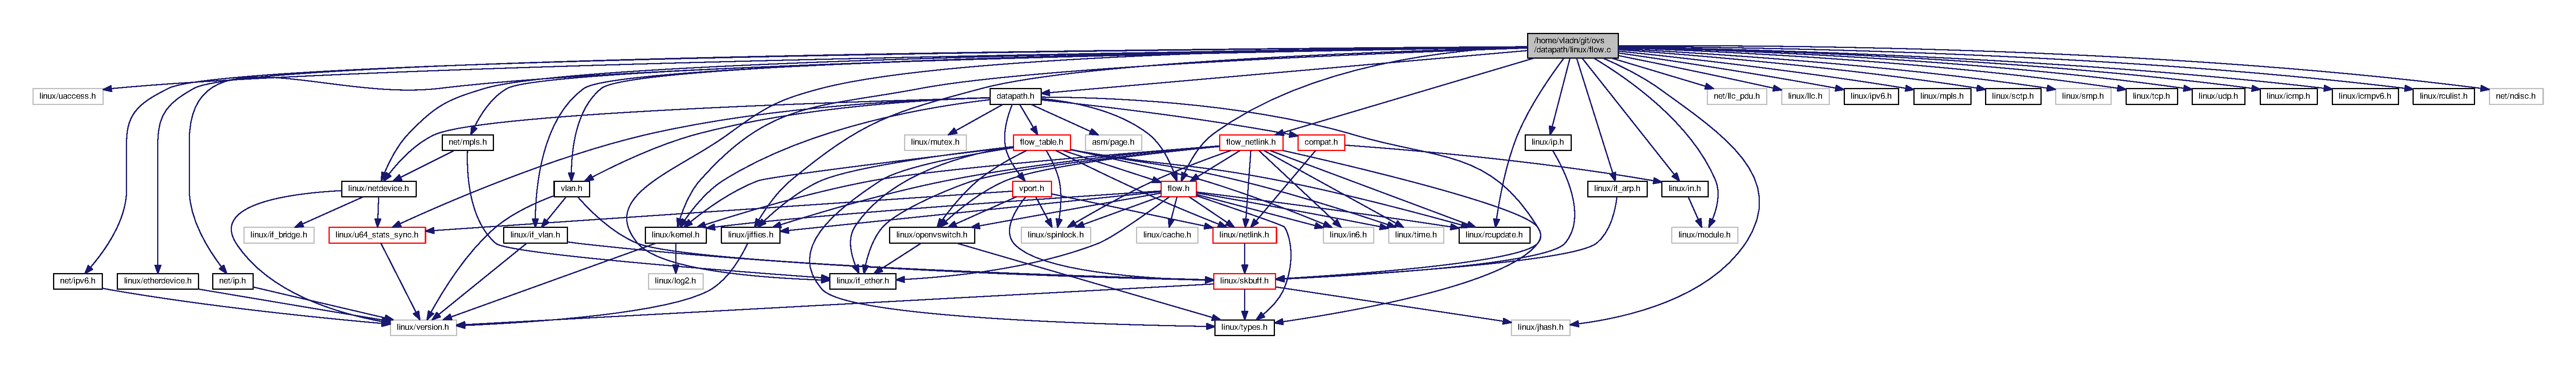
\includegraphics[width=350pt]{linux_2flow_8c__incl}
\end{center}
\end{figure}
\subsection*{Macros}
\begin{DoxyCompactItemize}
\item 
\#define \hyperlink{linux_2flow_8c_a1244774ec23560204eceaae557eff6d1}{T\+C\+P\+\_\+\+F\+L\+A\+G\+S\+\_\+\+B\+E16}(\hyperlink{flow_8h_ad44c86ae49f219522bcd4fb2744b81b2}{tp})~($\ast$(\+\_\+\+\_\+be16 $\ast$)\&tcp\+\_\+flag\+\_\+word(\hyperlink{flow_8h_ad44c86ae49f219522bcd4fb2744b81b2}{tp}) \& htons(0x0\+F\+F\+F))
\end{DoxyCompactItemize}
\subsection*{Functions}
\begin{DoxyCompactItemize}
\item 
u64 \hyperlink{linux_2flow_8c_adfdcc779325fc169a793acda2e32a46b}{ovs\+\_\+flow\+\_\+used\+\_\+time} (unsigned long flow\+\_\+jiffies)
\item 
void \hyperlink{linux_2flow_8c_ad20885fb9e6da56eb9cb58d139281916}{ovs\+\_\+flow\+\_\+stats\+\_\+update} (struct \hyperlink{structsw__flow}{sw\+\_\+flow} $\ast$flow, \+\_\+\+\_\+be16 tcp\+\_\+flags, const struct sk\+\_\+buff $\ast$skb)
\item 
void \hyperlink{linux_2flow_8c_a03636247cfc74747632c000eec0919db}{ovs\+\_\+flow\+\_\+stats\+\_\+get} (const struct \hyperlink{structsw__flow}{sw\+\_\+flow} $\ast$flow, struct \hyperlink{structovs__flow__stats}{ovs\+\_\+flow\+\_\+stats} $\ast$ovs\+\_\+stats, unsigned long $\ast$used, \+\_\+\+\_\+be16 $\ast$tcp\+\_\+flags)
\item 
void \hyperlink{linux_2flow_8c_a8dfa7ecd72ff9237664d0c402ff3f543}{ovs\+\_\+flow\+\_\+stats\+\_\+clear} (struct \hyperlink{structsw__flow}{sw\+\_\+flow} $\ast$flow)
\item 
static int \hyperlink{linux_2flow_8c_a51976bbff11a171b00faaffd004ba963}{check\+\_\+header} (struct sk\+\_\+buff $\ast$skb, int len)
\item 
static \hyperlink{types_8h_afaa87723b8417d40fcf45b7330261ef9}{bool} \hyperlink{linux_2flow_8c_ad6e91741b7e2a5ad174d0d9c899887b6}{arphdr\+\_\+ok} (struct sk\+\_\+buff $\ast$skb)
\item 
static int \hyperlink{linux_2flow_8c_ac23e11b5fa6e9068412b23f6388ae2df}{check\+\_\+iphdr} (struct sk\+\_\+buff $\ast$skb)
\item 
static \hyperlink{types_8h_afaa87723b8417d40fcf45b7330261ef9}{bool} \hyperlink{linux_2flow_8c_a71815483a340e9bab0bbcbc52537cfb5}{tcphdr\+\_\+ok} (struct sk\+\_\+buff $\ast$skb)
\item 
static \hyperlink{types_8h_afaa87723b8417d40fcf45b7330261ef9}{bool} \hyperlink{linux_2flow_8c_a354e4e351441e305c10a030f9d1dab7f}{udphdr\+\_\+ok} (struct sk\+\_\+buff $\ast$skb)
\item 
static \hyperlink{types_8h_afaa87723b8417d40fcf45b7330261ef9}{bool} \hyperlink{linux_2flow_8c_a235207174d62d682354a73e4b43a4ee2}{sctphdr\+\_\+ok} (struct sk\+\_\+buff $\ast$skb)
\item 
static \hyperlink{types_8h_afaa87723b8417d40fcf45b7330261ef9}{bool} \hyperlink{linux_2flow_8c_ac87d76f166f066dd4a2c9bc729702ab6}{icmphdr\+\_\+ok} (struct sk\+\_\+buff $\ast$skb)
\item 
static int \hyperlink{linux_2flow_8c_aae5a88c529fa6e31de896e40c546ec90}{parse\+\_\+ipv6hdr} (struct sk\+\_\+buff $\ast$skb, struct \hyperlink{structsw__flow__key}{sw\+\_\+flow\+\_\+key} $\ast$key)
\item 
static \hyperlink{types_8h_afaa87723b8417d40fcf45b7330261ef9}{bool} \hyperlink{linux_2flow_8c_a4191de70201a777f1ac4e71fc5c24d17}{icmp6hdr\+\_\+ok} (struct sk\+\_\+buff $\ast$skb)
\item 
static int \hyperlink{linux_2flow_8c_aab1dd840cacc7b21ee01cb885171d60d}{parse\+\_\+vlan} (struct sk\+\_\+buff $\ast$skb, struct \hyperlink{structsw__flow__key}{sw\+\_\+flow\+\_\+key} $\ast$key)
\item 
static \+\_\+\+\_\+be16 \hyperlink{linux_2flow_8c_a8f4a5415b9d6b2be7aef9e3749e65908}{parse\+\_\+ethertype} (struct sk\+\_\+buff $\ast$skb)
\item 
static int \hyperlink{linux_2flow_8c_a0b01cb308f20bbfe4348b6ef1b27a65d}{parse\+\_\+icmpv6} (struct sk\+\_\+buff $\ast$skb, struct \hyperlink{structsw__flow__key}{sw\+\_\+flow\+\_\+key} $\ast$key, int nh\+\_\+len)
\item 
static int \hyperlink{linux_2flow_8c_af69403050accb2489f73d37b528aa9c4}{key\+\_\+extract} (struct sk\+\_\+buff $\ast$skb, struct \hyperlink{structsw__flow__key}{sw\+\_\+flow\+\_\+key} $\ast$key)
\item 
int \hyperlink{linux_2flow_8c_a7d27b3745046ced4859b9fa615e27543}{ovs\+\_\+flow\+\_\+key\+\_\+update} (struct sk\+\_\+buff $\ast$skb, struct \hyperlink{structsw__flow__key}{sw\+\_\+flow\+\_\+key} $\ast$key)
\item 
int \hyperlink{linux_2flow_8c_a88b5c281d297950115033a17dbce5208}{ovs\+\_\+flow\+\_\+key\+\_\+extract} (const struct \hyperlink{structovs__tunnel__info}{ovs\+\_\+tunnel\+\_\+info} $\ast$tun\+\_\+info, struct sk\+\_\+buff $\ast$skb, struct \hyperlink{structsw__flow__key}{sw\+\_\+flow\+\_\+key} $\ast$key)
\item 
int \hyperlink{linux_2flow_8c_a5e042238993a5a8a8a8b3472cb274ead}{ovs\+\_\+flow\+\_\+key\+\_\+extract\+\_\+userspace} (const struct nlattr $\ast$attr, struct sk\+\_\+buff $\ast$skb, struct \hyperlink{structsw__flow__key}{sw\+\_\+flow\+\_\+key} $\ast$key, \hyperlink{types_8h_afaa87723b8417d40fcf45b7330261ef9}{bool} log)
\end{DoxyCompactItemize}


\subsection{Macro Definition Documentation}
\hypertarget{linux_2flow_8c_a1244774ec23560204eceaae557eff6d1}{}\index{linux/flow.\+c@{linux/flow.\+c}!T\+C\+P\+\_\+\+F\+L\+A\+G\+S\+\_\+\+B\+E16@{T\+C\+P\+\_\+\+F\+L\+A\+G\+S\+\_\+\+B\+E16}}
\index{T\+C\+P\+\_\+\+F\+L\+A\+G\+S\+\_\+\+B\+E16@{T\+C\+P\+\_\+\+F\+L\+A\+G\+S\+\_\+\+B\+E16}!linux/flow.\+c@{linux/flow.\+c}}
\subsubsection[{T\+C\+P\+\_\+\+F\+L\+A\+G\+S\+\_\+\+B\+E16}]{\setlength{\rightskip}{0pt plus 5cm}\#define T\+C\+P\+\_\+\+F\+L\+A\+G\+S\+\_\+\+B\+E16(
\begin{DoxyParamCaption}
\item[{}]{{\bf tp}}
\end{DoxyParamCaption}
)~($\ast$(\+\_\+\+\_\+be16 $\ast$)\&tcp\+\_\+flag\+\_\+word({\bf tp}) \& htons(0x0\+F\+F\+F))}\label{linux_2flow_8c_a1244774ec23560204eceaae557eff6d1}


\subsection{Function Documentation}
\hypertarget{linux_2flow_8c_ad6e91741b7e2a5ad174d0d9c899887b6}{}\index{linux/flow.\+c@{linux/flow.\+c}!arphdr\+\_\+ok@{arphdr\+\_\+ok}}
\index{arphdr\+\_\+ok@{arphdr\+\_\+ok}!linux/flow.\+c@{linux/flow.\+c}}
\subsubsection[{arphdr\+\_\+ok}]{\setlength{\rightskip}{0pt plus 5cm}static {\bf bool} arphdr\+\_\+ok (
\begin{DoxyParamCaption}
\item[{struct sk\+\_\+buff $\ast$}]{skb}
\end{DoxyParamCaption}
)\hspace{0.3cm}{\ttfamily [static]}}\label{linux_2flow_8c_ad6e91741b7e2a5ad174d0d9c899887b6}

\begin{DoxyCode}
189 \{
190     \textcolor{keywordflow}{return} pskb\_may\_pull(skb, \hyperlink{skbuff_8h_aabe75b44039b11c1b7c6e2f246e7146e}{skb\_network\_offset}(skb) +
191                   \textcolor{keyword}{sizeof}(\textcolor{keyword}{struct} \hyperlink{structarp__eth__header}{arp\_eth\_header}));
192 \}
\end{DoxyCode}
\hypertarget{linux_2flow_8c_a51976bbff11a171b00faaffd004ba963}{}\index{linux/flow.\+c@{linux/flow.\+c}!check\+\_\+header@{check\+\_\+header}}
\index{check\+\_\+header@{check\+\_\+header}!linux/flow.\+c@{linux/flow.\+c}}
\subsubsection[{check\+\_\+header}]{\setlength{\rightskip}{0pt plus 5cm}static int check\+\_\+header (
\begin{DoxyParamCaption}
\item[{struct sk\+\_\+buff $\ast$}]{skb, }
\item[{int}]{len}
\end{DoxyParamCaption}
)\hspace{0.3cm}{\ttfamily [static]}}\label{linux_2flow_8c_a51976bbff11a171b00faaffd004ba963}

\begin{DoxyCode}
180 \{
181     \textcolor{keywordflow}{if} (unlikely(skb->len < len))
182         \textcolor{keywordflow}{return} -EINVAL;
183     \textcolor{keywordflow}{if} (unlikely(!pskb\_may\_pull(skb, len)))
184         \textcolor{keywordflow}{return} -ENOMEM;
185     \textcolor{keywordflow}{return} 0;
186 \}
\end{DoxyCode}
\hypertarget{linux_2flow_8c_ac23e11b5fa6e9068412b23f6388ae2df}{}\index{linux/flow.\+c@{linux/flow.\+c}!check\+\_\+iphdr@{check\+\_\+iphdr}}
\index{check\+\_\+iphdr@{check\+\_\+iphdr}!linux/flow.\+c@{linux/flow.\+c}}
\subsubsection[{check\+\_\+iphdr}]{\setlength{\rightskip}{0pt plus 5cm}static int check\+\_\+iphdr (
\begin{DoxyParamCaption}
\item[{struct sk\+\_\+buff $\ast$}]{skb}
\end{DoxyParamCaption}
)\hspace{0.3cm}{\ttfamily [static]}}\label{linux_2flow_8c_ac23e11b5fa6e9068412b23f6388ae2df}

\begin{DoxyCode}
195 \{
196     \textcolor{keywordtype}{unsigned} \textcolor{keywordtype}{int} nh\_ofs = \hyperlink{skbuff_8h_aabe75b44039b11c1b7c6e2f246e7146e}{skb\_network\_offset}(skb);
197     \textcolor{keywordtype}{unsigned} \textcolor{keywordtype}{int} ip\_len;
198     \textcolor{keywordtype}{int} err;
199 
200     err = \hyperlink{linux_2flow_8c_a51976bbff11a171b00faaffd004ba963}{check\_header}(skb, nh\_ofs + \textcolor{keyword}{sizeof}(\textcolor{keyword}{struct} iphdr));
201     \textcolor{keywordflow}{if} (unlikely(err))
202         \textcolor{keywordflow}{return} err;
203 
204     ip\_len = \hyperlink{linux_2ip_8h_a769819999a936046f6b97cca3ec3ef74}{ip\_hdrlen}(skb);
205     \textcolor{keywordflow}{if} (unlikely(ip\_len < \textcolor{keyword}{sizeof}(\textcolor{keyword}{struct} iphdr) ||
206              skb->len < nh\_ofs + ip\_len))
207         \textcolor{keywordflow}{return} -EINVAL;
208 
209     \hyperlink{skbuff_8h_a35af79b1b630fc75fbd7347549b6affe}{skb\_set\_transport\_header}(skb, nh\_ofs + ip\_len);
210     \textcolor{keywordflow}{return} 0;
211 \}
\end{DoxyCode}
\hypertarget{linux_2flow_8c_a4191de70201a777f1ac4e71fc5c24d17}{}\index{linux/flow.\+c@{linux/flow.\+c}!icmp6hdr\+\_\+ok@{icmp6hdr\+\_\+ok}}
\index{icmp6hdr\+\_\+ok@{icmp6hdr\+\_\+ok}!linux/flow.\+c@{linux/flow.\+c}}
\subsubsection[{icmp6hdr\+\_\+ok}]{\setlength{\rightskip}{0pt plus 5cm}static {\bf bool} icmp6hdr\+\_\+ok (
\begin{DoxyParamCaption}
\item[{struct sk\+\_\+buff $\ast$}]{skb}
\end{DoxyParamCaption}
)\hspace{0.3cm}{\ttfamily [static]}}\label{linux_2flow_8c_a4191de70201a777f1ac4e71fc5c24d17}

\begin{DoxyCode}
292 \{
293     \textcolor{keywordflow}{return} pskb\_may\_pull(skb, \hyperlink{skbuff_8h_ac8d86ecdcd808a5839009d4a8f85f6c8}{skb\_transport\_offset}(skb) +
294                   \textcolor{keyword}{sizeof}(\textcolor{keyword}{struct} icmp6hdr));
295 \}
\end{DoxyCode}
\hypertarget{linux_2flow_8c_ac87d76f166f066dd4a2c9bc729702ab6}{}\index{linux/flow.\+c@{linux/flow.\+c}!icmphdr\+\_\+ok@{icmphdr\+\_\+ok}}
\index{icmphdr\+\_\+ok@{icmphdr\+\_\+ok}!linux/flow.\+c@{linux/flow.\+c}}
\subsubsection[{icmphdr\+\_\+ok}]{\setlength{\rightskip}{0pt plus 5cm}static {\bf bool} icmphdr\+\_\+ok (
\begin{DoxyParamCaption}
\item[{struct sk\+\_\+buff $\ast$}]{skb}
\end{DoxyParamCaption}
)\hspace{0.3cm}{\ttfamily [static]}}\label{linux_2flow_8c_ac87d76f166f066dd4a2c9bc729702ab6}

\begin{DoxyCode}
242 \{
243     \textcolor{keywordflow}{return} pskb\_may\_pull(skb, \hyperlink{skbuff_8h_ac8d86ecdcd808a5839009d4a8f85f6c8}{skb\_transport\_offset}(skb) +
244                   \textcolor{keyword}{sizeof}(\textcolor{keyword}{struct} icmphdr));
245 \}
\end{DoxyCode}
\hypertarget{linux_2flow_8c_af69403050accb2489f73d37b528aa9c4}{}\index{linux/flow.\+c@{linux/flow.\+c}!key\+\_\+extract@{key\+\_\+extract}}
\index{key\+\_\+extract@{key\+\_\+extract}!linux/flow.\+c@{linux/flow.\+c}}
\subsubsection[{key\+\_\+extract}]{\setlength{\rightskip}{0pt plus 5cm}static int key\+\_\+extract (
\begin{DoxyParamCaption}
\item[{struct sk\+\_\+buff $\ast$}]{skb, }
\item[{struct {\bf sw\+\_\+flow\+\_\+key} $\ast$}]{key}
\end{DoxyParamCaption}
)\hspace{0.3cm}{\ttfamily [static]}}\label{linux_2flow_8c_af69403050accb2489f73d37b528aa9c4}
key\+\_\+extract -\/ extracts a flow key from an Ethernet frame. \+: sk\+\_\+buff that contains the frame, with skb-\/$>$data pointing to the Ethernet header \+: output flow key

The caller must ensure that skb-\/$>$len $>$= E\+T\+H\+\_\+\+H\+L\+E\+N.

Returns 0 if successful, otherwise a negative errno value.

Initializes  header pointers as follows\+:


\begin{DoxyItemize}
\item skb-\/$>$mac\+\_\+header\+: the Ethernet header.
\item skb-\/$>$network\+\_\+header\+: just past the Ethernet header, or just past the V\+L\+A\+N header, to the first byte of the Ethernet payload.
\item skb-\/$>$transport\+\_\+header\+: If key-\/$>$eth.\+type is E\+T\+H\+\_\+\+P\+\_\+\+I\+P or E\+T\+H\+\_\+\+P\+\_\+\+I\+P\+V6 on output, then just past the I\+P header, if one is present and of a correct length, otherwise the same as skb-\/$>$network\+\_\+header. For other key-\/$>$eth.\+type values it is left untouched. 
\end{DoxyItemize}
\begin{DoxyCode}
454 \{
455     \textcolor{keywordtype}{int} error;
456     \textcolor{keyword}{struct }ethhdr *\hyperlink{flow_8h_a1679a3c93391059deba58179f52c86a6}{eth};
457 
458     \textcolor{comment}{/* Flags are always used as part of stats */}
459     key->\hyperlink{structsw__flow__key_a9c1944a39db1bf91141048df6d85ce8b}{tp}.\hyperlink{structsw__flow__key_a910f5e4408d113dbc9211190b44e0880}{flags} = 0;
460 
461     \hyperlink{skbuff_8h_aaf81c26756757ac1e1d7e6933f61bdaf}{skb\_reset\_mac\_header}(skb);
462 
463     \textcolor{comment}{/* Link layer.  We are guaranteed to have at least the 14 byte Ethernet}
464 \textcolor{comment}{     * header in the linear data area.}
465 \textcolor{comment}{     */}
466     eth = eth\_hdr(skb);
467     \hyperlink{etherdevice_8h_a564a2ea461aa6add2fa94a6864ee494d}{ether\_addr\_copy}(key->\hyperlink{structsw__flow__key_af3e10c978a3a2bf303b7d953ac6ff361}{eth}.\hyperlink{structsw__flow__key_a2fbd4aa7a500630627eff0630f864117}{src}, eth->h\_source);
468     \hyperlink{etherdevice_8h_a564a2ea461aa6add2fa94a6864ee494d}{ether\_addr\_copy}(key->\hyperlink{structsw__flow__key_af3e10c978a3a2bf303b7d953ac6ff361}{eth}.\hyperlink{structsw__flow__key_a44a0cdfe7471df8bb73762085da4cda9}{dst}, eth->h\_dest);
469 
470     \_\_skb\_pull(skb, 2 * ETH\_ALEN);
471     \textcolor{comment}{/* We are going to push all headers that we pull, so no need to}
472 \textcolor{comment}{     * update skb->csum here.}
473 \textcolor{comment}{     */}
474 
475     key->\hyperlink{structsw__flow__key_af3e10c978a3a2bf303b7d953ac6ff361}{eth}.\hyperlink{structsw__flow__key_a56b27b9b9eafa8f79acd544eba98c7b0}{tci} = 0;
476     \textcolor{keywordflow}{if} (\hyperlink{if__vlan_8h_a0bdf3e26944669a4265c7e717e846215}{skb\_vlan\_tag\_present}(skb))
477         key->\hyperlink{structsw__flow__key_af3e10c978a3a2bf303b7d953ac6ff361}{eth}.\hyperlink{structsw__flow__key_a56b27b9b9eafa8f79acd544eba98c7b0}{tci} = htons(\hyperlink{vlan_8h_a7d6820c8064af28c10f40f519605c2db}{vlan\_get\_tci}(skb));
478     \textcolor{keywordflow}{else} \textcolor{keywordflow}{if} (eth->h\_proto == htons(ETH\_P\_8021Q))
479         \textcolor{keywordflow}{if} (unlikely(\hyperlink{linux_2flow_8c_aab1dd840cacc7b21ee01cb885171d60d}{parse\_vlan}(skb, key)))
480             \textcolor{keywordflow}{return} -ENOMEM;
481 
482     key->\hyperlink{structsw__flow__key_af3e10c978a3a2bf303b7d953ac6ff361}{eth}.\hyperlink{structsw__flow__key_af30defbb2a81c997e8747594e1d937a0}{type} = \hyperlink{linux_2flow_8c_a8f4a5415b9d6b2be7aef9e3749e65908}{parse\_ethertype}(skb);
483     \textcolor{keywordflow}{if} (unlikely(key->\hyperlink{structsw__flow__key_af3e10c978a3a2bf303b7d953ac6ff361}{eth}.\hyperlink{structsw__flow__key_af30defbb2a81c997e8747594e1d937a0}{type} == htons(0)))
484         \textcolor{keywordflow}{return} -ENOMEM;
485 
486     \hyperlink{skbuff_8h_a2ea5d9050fe3927247bb55820cfcb02c}{skb\_reset\_network\_header}(skb);
487     \hyperlink{skbuff_8h_ae4be7dfedacf0e75fd904f0f54c9c731}{skb\_reset\_mac\_len}(skb);
488     \_\_skb\_push(skb, skb->data - \hyperlink{skbuff_8h_a292027671dfcf3aa23f9551f48713e24}{skb\_mac\_header}(skb));
489 
490     \textcolor{comment}{/* Network layer. */}
491     \textcolor{keywordflow}{if} (key->\hyperlink{structsw__flow__key_af3e10c978a3a2bf303b7d953ac6ff361}{eth}.\hyperlink{structsw__flow__key_af30defbb2a81c997e8747594e1d937a0}{type} == htons(ETH\_P\_IP)) \{
492         \textcolor{keyword}{struct }iphdr *nh;
493         \_\_be16 offset;
494 
495         error = \hyperlink{linux_2flow_8c_ac23e11b5fa6e9068412b23f6388ae2df}{check\_iphdr}(skb);
496         \textcolor{keywordflow}{if} (unlikely(error)) \{
497             memset(&key->\hyperlink{structsw__flow__key_ae8d48c419eaff6a9fda97c7446bdec0e}{ip}, 0, \textcolor{keyword}{sizeof}(key->\hyperlink{structsw__flow__key_ae8d48c419eaff6a9fda97c7446bdec0e}{ip}));
498             memset(&key->\hyperlink{structsw__flow__key_aeb4295bcb2fb4efea5c30337b871a423}{ipv4}, 0, \textcolor{keyword}{sizeof}(key->\hyperlink{structsw__flow__key_aeb4295bcb2fb4efea5c30337b871a423}{ipv4}));
499             \textcolor{keywordflow}{if} (error == -EINVAL) \{
500                 skb->transport\_header = skb->network\_header;
501                 error = 0;
502             \}
503             \textcolor{keywordflow}{return} error;
504         \}
505 
506         nh = \hyperlink{linux_2ip_8h_a06ad68dbeebbe718758ba2d5ebb6335c}{ip\_hdr}(skb);
507         key->\hyperlink{structsw__flow__key_aeb4295bcb2fb4efea5c30337b871a423}{ipv4}.addr.src = nh->saddr;
508         key->\hyperlink{structsw__flow__key_aeb4295bcb2fb4efea5c30337b871a423}{ipv4}.addr.dst = nh->daddr;
509 
510         key->\hyperlink{structsw__flow__key_ae8d48c419eaff6a9fda97c7446bdec0e}{ip}.proto = nh->protocol;
511         key->\hyperlink{structsw__flow__key_ae8d48c419eaff6a9fda97c7446bdec0e}{ip}.tos = nh->tos;
512         key->\hyperlink{structsw__flow__key_ae8d48c419eaff6a9fda97c7446bdec0e}{ip}.ttl = nh->ttl;
513 
514         offset = nh->frag\_off & htons(IP\_OFFSET);
515         \textcolor{keywordflow}{if} (offset) \{
516             key->\hyperlink{structsw__flow__key_ae8d48c419eaff6a9fda97c7446bdec0e}{ip}.frag = \hyperlink{openvswitch_8h_ad843f713a855bfcacd0adfe3e98eb447a1d1c9f89ced33419ec870391d8954c10}{OVS\_FRAG\_TYPE\_LATER};
517             \textcolor{keywordflow}{return} 0;
518         \}
519         \textcolor{keywordflow}{if} (nh->frag\_off & htons(IP\_MF) ||
520             skb\_shinfo(skb)->gso\_type & SKB\_GSO\_UDP)
521             key->\hyperlink{structsw__flow__key_ae8d48c419eaff6a9fda97c7446bdec0e}{ip}.frag = \hyperlink{openvswitch_8h_ad843f713a855bfcacd0adfe3e98eb447a7302a2ecd7ef2e817fadcd3e943af200}{OVS\_FRAG\_TYPE\_FIRST};
522         \textcolor{keywordflow}{else}
523             key->\hyperlink{structsw__flow__key_ae8d48c419eaff6a9fda97c7446bdec0e}{ip}.frag = \hyperlink{openvswitch_8h_ad843f713a855bfcacd0adfe3e98eb447a8551f9db6addee11579a10fe4b1e9d62}{OVS\_FRAG\_TYPE\_NONE};
524 
525         \textcolor{comment}{/* Transport layer. */}
526         \textcolor{keywordflow}{if} (key->\hyperlink{structsw__flow__key_ae8d48c419eaff6a9fda97c7446bdec0e}{ip}.proto == IPPROTO\_TCP) \{
527             \textcolor{keywordflow}{if} (\hyperlink{linux_2flow_8c_a71815483a340e9bab0bbcbc52537cfb5}{tcphdr\_ok}(skb)) \{
528                 \textcolor{keyword}{struct }tcphdr *tcp = \hyperlink{tcp_8h_a9ac4e94949ea9142c45cf46683be5ef7}{tcp\_hdr}(skb);
529                 key->\hyperlink{structsw__flow__key_a9c1944a39db1bf91141048df6d85ce8b}{tp}.\hyperlink{structsw__flow__key_a2fbd4aa7a500630627eff0630f864117}{src} = tcp->source;
530                 key->\hyperlink{structsw__flow__key_a9c1944a39db1bf91141048df6d85ce8b}{tp}.\hyperlink{structsw__flow__key_a44a0cdfe7471df8bb73762085da4cda9}{dst} = tcp->dest;
531                 key->\hyperlink{structsw__flow__key_a9c1944a39db1bf91141048df6d85ce8b}{tp}.\hyperlink{structsw__flow__key_a910f5e4408d113dbc9211190b44e0880}{flags} = \hyperlink{linux_2flow_8c_a1244774ec23560204eceaae557eff6d1}{TCP\_FLAGS\_BE16}(tcp);
532             \} \textcolor{keywordflow}{else} \{
533                 memset(&key->\hyperlink{structsw__flow__key_a9c1944a39db1bf91141048df6d85ce8b}{tp}, 0, \textcolor{keyword}{sizeof}(key->\hyperlink{structsw__flow__key_a9c1944a39db1bf91141048df6d85ce8b}{tp}));
534             \}
535 
536         \} \textcolor{keywordflow}{else} \textcolor{keywordflow}{if} (key->\hyperlink{structsw__flow__key_ae8d48c419eaff6a9fda97c7446bdec0e}{ip}.proto == IPPROTO\_UDP) \{
537             \textcolor{keywordflow}{if} (\hyperlink{linux_2flow_8c_a354e4e351441e305c10a030f9d1dab7f}{udphdr\_ok}(skb)) \{
538                 \textcolor{keyword}{struct }udphdr *udp = \hyperlink{linux_2udp_8h_a7b8908e197538768cf4ff9ec577bd86b}{udp\_hdr}(skb);
539                 key->\hyperlink{structsw__flow__key_a9c1944a39db1bf91141048df6d85ce8b}{tp}.\hyperlink{structsw__flow__key_a2fbd4aa7a500630627eff0630f864117}{src} = udp->source;
540                 key->\hyperlink{structsw__flow__key_a9c1944a39db1bf91141048df6d85ce8b}{tp}.\hyperlink{structsw__flow__key_a44a0cdfe7471df8bb73762085da4cda9}{dst} = udp->dest;
541             \} \textcolor{keywordflow}{else} \{
542                 memset(&key->\hyperlink{structsw__flow__key_a9c1944a39db1bf91141048df6d85ce8b}{tp}, 0, \textcolor{keyword}{sizeof}(key->\hyperlink{structsw__flow__key_a9c1944a39db1bf91141048df6d85ce8b}{tp}));
543             \}
544         \} \textcolor{keywordflow}{else} \textcolor{keywordflow}{if} (key->\hyperlink{structsw__flow__key_ae8d48c419eaff6a9fda97c7446bdec0e}{ip}.proto == IPPROTO\_SCTP) \{
545             \textcolor{keywordflow}{if} (\hyperlink{linux_2flow_8c_a235207174d62d682354a73e4b43a4ee2}{sctphdr\_ok}(skb)) \{
546                 \textcolor{keyword}{struct }sctphdr *sctp = \hyperlink{sctp_8h_a6f9abfbe98294e40a3f32db7ad723998}{sctp\_hdr}(skb);
547                 key->\hyperlink{structsw__flow__key_a9c1944a39db1bf91141048df6d85ce8b}{tp}.\hyperlink{structsw__flow__key_a2fbd4aa7a500630627eff0630f864117}{src} = sctp->source;
548                 key->\hyperlink{structsw__flow__key_a9c1944a39db1bf91141048df6d85ce8b}{tp}.\hyperlink{structsw__flow__key_a44a0cdfe7471df8bb73762085da4cda9}{dst} = sctp->dest;
549             \} \textcolor{keywordflow}{else} \{
550                 memset(&key->\hyperlink{structsw__flow__key_a9c1944a39db1bf91141048df6d85ce8b}{tp}, 0, \textcolor{keyword}{sizeof}(key->\hyperlink{structsw__flow__key_a9c1944a39db1bf91141048df6d85ce8b}{tp}));
551             \}
552         \} \textcolor{keywordflow}{else} \textcolor{keywordflow}{if} (key->\hyperlink{structsw__flow__key_ae8d48c419eaff6a9fda97c7446bdec0e}{ip}.proto == IPPROTO\_ICMP) \{
553             \textcolor{keywordflow}{if} (\hyperlink{linux_2flow_8c_ac87d76f166f066dd4a2c9bc729702ab6}{icmphdr\_ok}(skb)) \{
554                 \textcolor{keyword}{struct }icmphdr *icmp = \hyperlink{icmp_8h_a2226121e608b10a1dde33ed552361bba}{icmp\_hdr}(skb);
555                 \textcolor{comment}{/* The ICMP type and code fields use the 16-bit}
556 \textcolor{comment}{                 * transport port fields, so we need to store}
557 \textcolor{comment}{                 * them in 16-bit network byte order.}
558 \textcolor{comment}{                 */}
559                 key->\hyperlink{structsw__flow__key_a9c1944a39db1bf91141048df6d85ce8b}{tp}.\hyperlink{structsw__flow__key_a2fbd4aa7a500630627eff0630f864117}{src} = htons(icmp->type);
560                 key->\hyperlink{structsw__flow__key_a9c1944a39db1bf91141048df6d85ce8b}{tp}.\hyperlink{structsw__flow__key_a44a0cdfe7471df8bb73762085da4cda9}{dst} = htons(icmp->code);
561             \} \textcolor{keywordflow}{else} \{
562                 memset(&key->\hyperlink{structsw__flow__key_a9c1944a39db1bf91141048df6d85ce8b}{tp}, 0, \textcolor{keyword}{sizeof}(key->\hyperlink{structsw__flow__key_a9c1944a39db1bf91141048df6d85ce8b}{tp}));
563             \}
564         \}
565 
566     \} \textcolor{keywordflow}{else} \textcolor{keywordflow}{if} (key->\hyperlink{structsw__flow__key_af3e10c978a3a2bf303b7d953ac6ff361}{eth}.\hyperlink{structsw__flow__key_af30defbb2a81c997e8747594e1d937a0}{type} == htons(ETH\_P\_ARP) ||
567            key->\hyperlink{structsw__flow__key_af3e10c978a3a2bf303b7d953ac6ff361}{eth}.\hyperlink{structsw__flow__key_af30defbb2a81c997e8747594e1d937a0}{type} == htons(ETH\_P\_RARP)) \{
568         \textcolor{keyword}{struct }\hyperlink{structarp__eth__header}{arp\_eth\_header} *\hyperlink{flow_8h_aa05c06f4d8f8b791f607aa53db449356}{arp};
569         \textcolor{keywordtype}{bool} arp\_available = \hyperlink{linux_2flow_8c_ad6e91741b7e2a5ad174d0d9c899887b6}{arphdr\_ok}(skb);
570 
571         arp = (\textcolor{keyword}{struct }\hyperlink{structarp__eth__header}{arp\_eth\_header} *)\hyperlink{skbuff_8h_aa9e0f2aeb3abecde73023d35145bc4a0}{skb\_network\_header}(skb);
572 
573         \textcolor{keywordflow}{if} (arp\_available &&
574             arp->\hyperlink{structarp__eth__header_afe4c385a8760054d1d9da4e06b72dc3a}{ar\_hrd} == htons(ARPHRD\_ETHER) &&
575             arp->\hyperlink{structarp__eth__header_aa0a6c956f6f9001377528f86f94d91b4}{ar\_pro} == htons(ETH\_P\_IP) &&
576             arp->\hyperlink{structarp__eth__header_a8feceb41fdd95e4a0f1e17e56b957bf4}{ar\_hln} == ETH\_ALEN &&
577             arp->\hyperlink{structarp__eth__header_abc215d845eb12176276c8cee0501ecd8}{ar\_pln} == 4) \{
578 
579             \textcolor{comment}{/* We only match on the lower 8 bits of the opcode. */}
580             \textcolor{keywordflow}{if} (ntohs(arp->\hyperlink{structarp__eth__header_a0cad73c318ab7ea788fa836f6b5a011d}{ar\_op}) <= 0xff)
581                 key->\hyperlink{structsw__flow__key_ae8d48c419eaff6a9fda97c7446bdec0e}{ip}.proto = ntohs(arp->\hyperlink{structarp__eth__header_a0cad73c318ab7ea788fa836f6b5a011d}{ar\_op});
582             \textcolor{keywordflow}{else}
583                 key->\hyperlink{structsw__flow__key_ae8d48c419eaff6a9fda97c7446bdec0e}{ip}.proto = 0;
584 
585             memcpy(&key->\hyperlink{structsw__flow__key_aeb4295bcb2fb4efea5c30337b871a423}{ipv4}.addr.src, arp->\hyperlink{structarp__eth__header_ae584842ae04804b2f5cf3c26fb135961}{ar\_sip}, \textcolor{keyword}{sizeof}(key->\hyperlink{structsw__flow__key_aeb4295bcb2fb4efea5c30337b871a423}{ipv4}.addr.src));
586             memcpy(&key->\hyperlink{structsw__flow__key_aeb4295bcb2fb4efea5c30337b871a423}{ipv4}.addr.dst, arp->\hyperlink{structarp__eth__header_a9ed88031c0dd2f554f1dc455e878945d}{ar\_tip}, \textcolor{keyword}{sizeof}(key->\hyperlink{structsw__flow__key_aeb4295bcb2fb4efea5c30337b871a423}{ipv4}.addr.dst));
587             \hyperlink{etherdevice_8h_a564a2ea461aa6add2fa94a6864ee494d}{ether\_addr\_copy}(key->\hyperlink{structsw__flow__key_aeb4295bcb2fb4efea5c30337b871a423}{ipv4}.arp.sha, arp->\hyperlink{structarp__eth__header_a569cddaf9ed4aa40b04b60958783e908}{ar\_sha});
588             \hyperlink{etherdevice_8h_a564a2ea461aa6add2fa94a6864ee494d}{ether\_addr\_copy}(key->\hyperlink{structsw__flow__key_aeb4295bcb2fb4efea5c30337b871a423}{ipv4}.arp.tha, arp->\hyperlink{structarp__eth__header_a490c51d5f01a32e78c57d020ca2662f6}{ar\_tha});
589         \} \textcolor{keywordflow}{else} \{
590             memset(&key->\hyperlink{structsw__flow__key_ae8d48c419eaff6a9fda97c7446bdec0e}{ip}, 0, \textcolor{keyword}{sizeof}(key->\hyperlink{structsw__flow__key_ae8d48c419eaff6a9fda97c7446bdec0e}{ip}));
591             memset(&key->\hyperlink{structsw__flow__key_aeb4295bcb2fb4efea5c30337b871a423}{ipv4}, 0, \textcolor{keyword}{sizeof}(key->\hyperlink{structsw__flow__key_aeb4295bcb2fb4efea5c30337b871a423}{ipv4}));
592         \}
593     \} \textcolor{keywordflow}{else} \textcolor{keywordflow}{if} (\hyperlink{net_2mpls_8h_aab48ab242fbafafc869b3e98df4ace8f}{eth\_p\_mpls}(key->\hyperlink{structsw__flow__key_af3e10c978a3a2bf303b7d953ac6ff361}{eth}.\hyperlink{structsw__flow__key_af30defbb2a81c997e8747594e1d937a0}{type})) \{
594         \textcolor{keywordtype}{size\_t} stack\_len = \hyperlink{net_2mpls_8h_a9a0b8d7adb48a79ca82a00b2663823ee}{MPLS\_HLEN};
595 
596         \textcolor{comment}{/* In the presence of an MPLS label stack the end of the L2}
597 \textcolor{comment}{         * header and the beginning of the L3 header differ.}
598 \textcolor{comment}{         *}
599 \textcolor{comment}{         * Advance network\_header to the beginning of the L3}
600 \textcolor{comment}{         * header. mac\_len corresponds to the end of the L2 header.}
601 \textcolor{comment}{         */}
602         \textcolor{keywordflow}{while} (1) \{
603             \_\_be32 lse;
604 
605             error = \hyperlink{linux_2flow_8c_a51976bbff11a171b00faaffd004ba963}{check\_header}(skb, skb->mac\_len + stack\_len);
606             \textcolor{keywordflow}{if} (unlikely(error))
607                 \textcolor{keywordflow}{return} 0;
608 
609             memcpy(&lse, \hyperlink{skbuff_8h_aa9e0f2aeb3abecde73023d35145bc4a0}{skb\_network\_header}(skb), \hyperlink{net_2mpls_8h_a9a0b8d7adb48a79ca82a00b2663823ee}{MPLS\_HLEN});
610 
611             \textcolor{keywordflow}{if} (stack\_len == \hyperlink{net_2mpls_8h_a9a0b8d7adb48a79ca82a00b2663823ee}{MPLS\_HLEN})
612                 memcpy(&key->\hyperlink{structsw__flow__key_a005840d04ee5b462be3c8e21809dc9aa}{mpls}.top\_lse, &lse, \hyperlink{net_2mpls_8h_a9a0b8d7adb48a79ca82a00b2663823ee}{MPLS\_HLEN});
613 
614             \hyperlink{skbuff_8h_a2aa771daf8e324a50f60e4934839dc2c}{skb\_set\_network\_header}(skb, skb->mac\_len + stack\_len);
615             \textcolor{keywordflow}{if} (lse & htonl(MPLS\_LS\_S\_MASK))
616                 \textcolor{keywordflow}{break};
617 
618             stack\_len += \hyperlink{net_2mpls_8h_a9a0b8d7adb48a79ca82a00b2663823ee}{MPLS\_HLEN};
619         \}
620     \} \textcolor{keywordflow}{else} \textcolor{keywordflow}{if} (key->\hyperlink{structsw__flow__key_af3e10c978a3a2bf303b7d953ac6ff361}{eth}.\hyperlink{structsw__flow__key_af30defbb2a81c997e8747594e1d937a0}{type} == htons(ETH\_P\_IPV6)) \{
621         \textcolor{keywordtype}{int} nh\_len;             \textcolor{comment}{/* IPv6 Header + Extensions */}
622 
623         nh\_len = \hyperlink{linux_2flow_8c_aae5a88c529fa6e31de896e40c546ec90}{parse\_ipv6hdr}(skb, key);
624         \textcolor{keywordflow}{if} (unlikely(nh\_len < 0)) \{
625             memset(&key->\hyperlink{structsw__flow__key_ae8d48c419eaff6a9fda97c7446bdec0e}{ip}, 0, \textcolor{keyword}{sizeof}(key->\hyperlink{structsw__flow__key_ae8d48c419eaff6a9fda97c7446bdec0e}{ip}));
626             memset(&key->\hyperlink{structsw__flow__key_a6b13e14d62eb632b05378784a2d61f87}{ipv6}.addr, 0, \textcolor{keyword}{sizeof}(key->\hyperlink{structsw__flow__key_a6b13e14d62eb632b05378784a2d61f87}{ipv6}.addr));
627             \textcolor{keywordflow}{if} (nh\_len == -EINVAL) \{
628                 skb->transport\_header = skb->network\_header;
629                 error = 0;
630             \} \textcolor{keywordflow}{else} \{
631                 error = nh\_len;
632             \}
633             \textcolor{keywordflow}{return} error;
634         \}
635 
636         \textcolor{keywordflow}{if} (key->\hyperlink{structsw__flow__key_ae8d48c419eaff6a9fda97c7446bdec0e}{ip}.frag == \hyperlink{openvswitch_8h_ad843f713a855bfcacd0adfe3e98eb447a1d1c9f89ced33419ec870391d8954c10}{OVS\_FRAG\_TYPE\_LATER})
637             \textcolor{keywordflow}{return} 0;
638         \textcolor{keywordflow}{if} (skb\_shinfo(skb)->gso\_type & SKB\_GSO\_UDP)
639             key->\hyperlink{structsw__flow__key_ae8d48c419eaff6a9fda97c7446bdec0e}{ip}.frag = \hyperlink{openvswitch_8h_ad843f713a855bfcacd0adfe3e98eb447a7302a2ecd7ef2e817fadcd3e943af200}{OVS\_FRAG\_TYPE\_FIRST};
640 
641         \textcolor{comment}{/* Transport layer. */}
642         \textcolor{keywordflow}{if} (key->\hyperlink{structsw__flow__key_ae8d48c419eaff6a9fda97c7446bdec0e}{ip}.proto == NEXTHDR\_TCP) \{
643             \textcolor{keywordflow}{if} (\hyperlink{linux_2flow_8c_a71815483a340e9bab0bbcbc52537cfb5}{tcphdr\_ok}(skb)) \{
644                 \textcolor{keyword}{struct }tcphdr *tcp = \hyperlink{tcp_8h_a9ac4e94949ea9142c45cf46683be5ef7}{tcp\_hdr}(skb);
645                 key->\hyperlink{structsw__flow__key_a9c1944a39db1bf91141048df6d85ce8b}{tp}.\hyperlink{structsw__flow__key_a2fbd4aa7a500630627eff0630f864117}{src} = tcp->source;
646                 key->\hyperlink{structsw__flow__key_a9c1944a39db1bf91141048df6d85ce8b}{tp}.\hyperlink{structsw__flow__key_a44a0cdfe7471df8bb73762085da4cda9}{dst} = tcp->dest;
647                 key->\hyperlink{structsw__flow__key_a9c1944a39db1bf91141048df6d85ce8b}{tp}.\hyperlink{structsw__flow__key_a910f5e4408d113dbc9211190b44e0880}{flags} = \hyperlink{linux_2flow_8c_a1244774ec23560204eceaae557eff6d1}{TCP\_FLAGS\_BE16}(tcp);
648             \} \textcolor{keywordflow}{else} \{
649                 memset(&key->\hyperlink{structsw__flow__key_a9c1944a39db1bf91141048df6d85ce8b}{tp}, 0, \textcolor{keyword}{sizeof}(key->\hyperlink{structsw__flow__key_a9c1944a39db1bf91141048df6d85ce8b}{tp}));
650             \}
651         \} \textcolor{keywordflow}{else} \textcolor{keywordflow}{if} (key->\hyperlink{structsw__flow__key_ae8d48c419eaff6a9fda97c7446bdec0e}{ip}.proto == NEXTHDR\_UDP) \{
652             \textcolor{keywordflow}{if} (\hyperlink{linux_2flow_8c_a354e4e351441e305c10a030f9d1dab7f}{udphdr\_ok}(skb)) \{
653                 \textcolor{keyword}{struct }udphdr *udp = \hyperlink{linux_2udp_8h_a7b8908e197538768cf4ff9ec577bd86b}{udp\_hdr}(skb);
654                 key->\hyperlink{structsw__flow__key_a9c1944a39db1bf91141048df6d85ce8b}{tp}.\hyperlink{structsw__flow__key_a2fbd4aa7a500630627eff0630f864117}{src} = udp->source;
655                 key->\hyperlink{structsw__flow__key_a9c1944a39db1bf91141048df6d85ce8b}{tp}.\hyperlink{structsw__flow__key_a44a0cdfe7471df8bb73762085da4cda9}{dst} = udp->dest;
656             \} \textcolor{keywordflow}{else} \{
657                 memset(&key->\hyperlink{structsw__flow__key_a9c1944a39db1bf91141048df6d85ce8b}{tp}, 0, \textcolor{keyword}{sizeof}(key->\hyperlink{structsw__flow__key_a9c1944a39db1bf91141048df6d85ce8b}{tp}));
658             \}
659         \} \textcolor{keywordflow}{else} \textcolor{keywordflow}{if} (key->\hyperlink{structsw__flow__key_ae8d48c419eaff6a9fda97c7446bdec0e}{ip}.proto == \hyperlink{net_2ipv6_8h_a1135c535edd95af9465ce2921dd31c28}{NEXTHDR\_SCTP}) \{
660             \textcolor{keywordflow}{if} (\hyperlink{linux_2flow_8c_a235207174d62d682354a73e4b43a4ee2}{sctphdr\_ok}(skb)) \{
661                 \textcolor{keyword}{struct }sctphdr *sctp = \hyperlink{sctp_8h_a6f9abfbe98294e40a3f32db7ad723998}{sctp\_hdr}(skb);
662                 key->\hyperlink{structsw__flow__key_a9c1944a39db1bf91141048df6d85ce8b}{tp}.\hyperlink{structsw__flow__key_a2fbd4aa7a500630627eff0630f864117}{src} = sctp->source;
663                 key->\hyperlink{structsw__flow__key_a9c1944a39db1bf91141048df6d85ce8b}{tp}.\hyperlink{structsw__flow__key_a44a0cdfe7471df8bb73762085da4cda9}{dst} = sctp->dest;
664             \} \textcolor{keywordflow}{else} \{
665                 memset(&key->\hyperlink{structsw__flow__key_a9c1944a39db1bf91141048df6d85ce8b}{tp}, 0, \textcolor{keyword}{sizeof}(key->\hyperlink{structsw__flow__key_a9c1944a39db1bf91141048df6d85ce8b}{tp}));
666             \}
667         \} \textcolor{keywordflow}{else} \textcolor{keywordflow}{if} (key->\hyperlink{structsw__flow__key_ae8d48c419eaff6a9fda97c7446bdec0e}{ip}.proto == NEXTHDR\_ICMP) \{
668             \textcolor{keywordflow}{if} (\hyperlink{linux_2flow_8c_a4191de70201a777f1ac4e71fc5c24d17}{icmp6hdr\_ok}(skb)) \{
669                 error = \hyperlink{linux_2flow_8c_a0b01cb308f20bbfe4348b6ef1b27a65d}{parse\_icmpv6}(skb, key, nh\_len);
670                 \textcolor{keywordflow}{if} (error)
671                     \textcolor{keywordflow}{return} error;
672             \} \textcolor{keywordflow}{else} \{
673                 memset(&key->\hyperlink{structsw__flow__key_a9c1944a39db1bf91141048df6d85ce8b}{tp}, 0, \textcolor{keyword}{sizeof}(key->\hyperlink{structsw__flow__key_a9c1944a39db1bf91141048df6d85ce8b}{tp}));
674             \}
675         \}
676     \}
677     \textcolor{keywordflow}{return} 0;
678 \}
\end{DoxyCode}
\hypertarget{linux_2flow_8c_a88b5c281d297950115033a17dbce5208}{}\index{linux/flow.\+c@{linux/flow.\+c}!ovs\+\_\+flow\+\_\+key\+\_\+extract@{ovs\+\_\+flow\+\_\+key\+\_\+extract}}
\index{ovs\+\_\+flow\+\_\+key\+\_\+extract@{ovs\+\_\+flow\+\_\+key\+\_\+extract}!linux/flow.\+c@{linux/flow.\+c}}
\subsubsection[{ovs\+\_\+flow\+\_\+key\+\_\+extract}]{\setlength{\rightskip}{0pt plus 5cm}int ovs\+\_\+flow\+\_\+key\+\_\+extract (
\begin{DoxyParamCaption}
\item[{const struct {\bf ovs\+\_\+tunnel\+\_\+info} $\ast$}]{tun\+\_\+info, }
\item[{struct sk\+\_\+buff $\ast$}]{skb, }
\item[{struct {\bf sw\+\_\+flow\+\_\+key} $\ast$}]{key}
\end{DoxyParamCaption}
)}\label{linux_2flow_8c_a88b5c281d297950115033a17dbce5208}

\begin{DoxyCode}
687 \{
688     \textcolor{comment}{/* Extract metadata from packet. */}
689     \textcolor{keywordflow}{if} (tun\_info) \{
690         memcpy(&key->\hyperlink{structsw__flow__key_a2f87b7690c0cc2797f1f4347589472c3}{tun\_key}, &tun\_info->\hyperlink{structovs__tunnel__info_a007f0c7a9938884e6e8663cb4ab20d10}{tunnel}, \textcolor{keyword}{sizeof}(key->
      \hyperlink{structsw__flow__key_a2f87b7690c0cc2797f1f4347589472c3}{tun\_key}));
691 
692         BUILD\_BUG\_ON(((1 << (\textcolor{keyword}{sizeof}(tun\_info->\hyperlink{structovs__tunnel__info_ab50d289f61727b922831739affb28b18}{options\_len}) * 8)) - 1) >
693                  \textcolor{keyword}{sizeof}(key->\hyperlink{structsw__flow__key_a54b30752817dccb02665a7eecde52a72}{tun\_opts}));
694 
695         \textcolor{keywordflow}{if} (tun\_info->\hyperlink{structovs__tunnel__info_ae4fd786894f579a38a5955e7a0e68fd4}{options}) \{
696             memcpy(\hyperlink{flow_8h_a5d74524a15e17551a8d8235f4375c296}{TUN\_METADATA\_OPTS}(key, tun\_info->\hyperlink{structovs__tunnel__info_ab50d289f61727b922831739affb28b18}{options\_len}),
697                    tun\_info->\hyperlink{structovs__tunnel__info_ae4fd786894f579a38a5955e7a0e68fd4}{options}, tun\_info->\hyperlink{structovs__tunnel__info_ab50d289f61727b922831739affb28b18}{options\_len});
698             key->\hyperlink{structsw__flow__key_aef0ea317d3bd0125e0d6390261ba3e2d}{tun\_opts\_len} = tun\_info->\hyperlink{structovs__tunnel__info_ab50d289f61727b922831739affb28b18}{options\_len};
699         \} \textcolor{keywordflow}{else} \{
700             key->\hyperlink{structsw__flow__key_aef0ea317d3bd0125e0d6390261ba3e2d}{tun\_opts\_len} = 0;
701         \}
702     \} \textcolor{keywordflow}{else} \{
703         key->\hyperlink{structsw__flow__key_aef0ea317d3bd0125e0d6390261ba3e2d}{tun\_opts\_len} = 0;
704         memset(&key->\hyperlink{structsw__flow__key_a2f87b7690c0cc2797f1f4347589472c3}{tun\_key}, 0, \textcolor{keyword}{sizeof}(key->\hyperlink{structsw__flow__key_a2f87b7690c0cc2797f1f4347589472c3}{tun\_key}));
705     \}
706 
707     key->\hyperlink{structsw__flow__key_a57cbddb75a8d4fd859300bd34d98e84a}{phy}.\hyperlink{structsw__flow__key_a9dd898913d9faaec1ec970029e7fbb71}{priority} = skb->priority;
708     key->\hyperlink{structsw__flow__key_a57cbddb75a8d4fd859300bd34d98e84a}{phy}.\hyperlink{structsw__flow__key_a5848de18caa80d36d9bc60cc686a2c6e}{in\_port} = \hyperlink{datapath_8h_ac337c4d4ddca29916ce8e900038ddd78}{OVS\_CB}(skb)->input\_vport->port\_no;
709     key->\hyperlink{structsw__flow__key_a57cbddb75a8d4fd859300bd34d98e84a}{phy}.\hyperlink{structsw__flow__key_ae02571657f29397dcc45de8528f4ed05}{skb\_mark} = skb->mark;
710     key->\hyperlink{structsw__flow__key_a73dd9402f1f54c321f6d704d9b018d15}{ovs\_flow\_hash} = 0;
711     key->\hyperlink{structsw__flow__key_a7e51857c88ad6b0bf90551d0b6e2607b}{recirc\_id} = 0;
712 
713     \textcolor{keywordflow}{return} \hyperlink{linux_2flow_8c_af69403050accb2489f73d37b528aa9c4}{key\_extract}(skb, key);
714 \}
\end{DoxyCode}
\hypertarget{linux_2flow_8c_a5e042238993a5a8a8a8b3472cb274ead}{}\index{linux/flow.\+c@{linux/flow.\+c}!ovs\+\_\+flow\+\_\+key\+\_\+extract\+\_\+userspace@{ovs\+\_\+flow\+\_\+key\+\_\+extract\+\_\+userspace}}
\index{ovs\+\_\+flow\+\_\+key\+\_\+extract\+\_\+userspace@{ovs\+\_\+flow\+\_\+key\+\_\+extract\+\_\+userspace}!linux/flow.\+c@{linux/flow.\+c}}
\subsubsection[{ovs\+\_\+flow\+\_\+key\+\_\+extract\+\_\+userspace}]{\setlength{\rightskip}{0pt plus 5cm}int ovs\+\_\+flow\+\_\+key\+\_\+extract\+\_\+userspace (
\begin{DoxyParamCaption}
\item[{const struct nlattr $\ast$}]{attr, }
\item[{struct sk\+\_\+buff $\ast$}]{skb, }
\item[{struct {\bf sw\+\_\+flow\+\_\+key} $\ast$}]{key, }
\item[{{\bf bool}}]{log}
\end{DoxyParamCaption}
)}\label{linux_2flow_8c_a5e042238993a5a8a8a8b3472cb274ead}

\begin{DoxyCode}
719 \{
720     \textcolor{keywordtype}{int} err;
721 
722     \textcolor{comment}{/* Extract metadata from netlink attributes. */}
723     err = \hyperlink{flow__netlink_8c_a90428a389e4ba65133d2cf837d5a8dc3}{ovs\_nla\_get\_flow\_metadata}(attr, key, log);
724     \textcolor{keywordflow}{if} (err)
725         \textcolor{keywordflow}{return} err;
726 
727     \textcolor{keywordflow}{return} \hyperlink{linux_2flow_8c_af69403050accb2489f73d37b528aa9c4}{key\_extract}(skb, key);
728 \}
\end{DoxyCode}
\hypertarget{linux_2flow_8c_a7d27b3745046ced4859b9fa615e27543}{}\index{linux/flow.\+c@{linux/flow.\+c}!ovs\+\_\+flow\+\_\+key\+\_\+update@{ovs\+\_\+flow\+\_\+key\+\_\+update}}
\index{ovs\+\_\+flow\+\_\+key\+\_\+update@{ovs\+\_\+flow\+\_\+key\+\_\+update}!linux/flow.\+c@{linux/flow.\+c}}
\subsubsection[{ovs\+\_\+flow\+\_\+key\+\_\+update}]{\setlength{\rightskip}{0pt plus 5cm}int ovs\+\_\+flow\+\_\+key\+\_\+update (
\begin{DoxyParamCaption}
\item[{struct sk\+\_\+buff $\ast$}]{skb, }
\item[{struct {\bf sw\+\_\+flow\+\_\+key} $\ast$}]{key}
\end{DoxyParamCaption}
)}\label{linux_2flow_8c_a7d27b3745046ced4859b9fa615e27543}

\begin{DoxyCode}
681 \{
682     \textcolor{keywordflow}{return} \hyperlink{linux_2flow_8c_af69403050accb2489f73d37b528aa9c4}{key\_extract}(skb, key);
683 \}
\end{DoxyCode}
\hypertarget{linux_2flow_8c_a8dfa7ecd72ff9237664d0c402ff3f543}{}\index{linux/flow.\+c@{linux/flow.\+c}!ovs\+\_\+flow\+\_\+stats\+\_\+clear@{ovs\+\_\+flow\+\_\+stats\+\_\+clear}}
\index{ovs\+\_\+flow\+\_\+stats\+\_\+clear@{ovs\+\_\+flow\+\_\+stats\+\_\+clear}!linux/flow.\+c@{linux/flow.\+c}}
\subsubsection[{ovs\+\_\+flow\+\_\+stats\+\_\+clear}]{\setlength{\rightskip}{0pt plus 5cm}void ovs\+\_\+flow\+\_\+stats\+\_\+clear (
\begin{DoxyParamCaption}
\item[{struct {\bf sw\+\_\+flow} $\ast$}]{flow}
\end{DoxyParamCaption}
)}\label{linux_2flow_8c_a8dfa7ecd72ff9237664d0c402ff3f543}

\begin{DoxyCode}
162 \{
163     \textcolor{keywordtype}{int} node;
164 
165     for\_each\_node(node) \{
166         \textcolor{keyword}{struct }\hyperlink{structflow__stats}{flow\_stats} *stats = \hyperlink{datapath_8h_a06ef69170d345fd3996a467dcacf3ff3}{ovsl\_dereference}(flow->
      \hyperlink{structsw__flow_a5ccc743bcf16038ab0cf5dda88565f33}{stats}[node]);
167 
168         \textcolor{keywordflow}{if} (stats) \{
169             spin\_lock\_bh(&stats->\hyperlink{structflow__stats_a1930f864d7fc52f4afeb86714e3e5c07}{lock});
170             stats->\hyperlink{structflow__stats_a3eefc54cf53ad3e24bb070bd6f251f50}{used} = 0;
171             stats->\hyperlink{structflow__stats_a9399b2cdc3d48c11357fbc2aaff33226}{packet\_count} = 0;
172             stats->\hyperlink{structflow__stats_a97844fc570ddb0d4b80f4cfe36bfee29}{byte\_count} = 0;
173             stats->\hyperlink{structflow__stats_a2b2812adf4fd5f4f188324fdf503deba}{tcp\_flags} = 0;
174             spin\_unlock\_bh(&stats->\hyperlink{structflow__stats_a1930f864d7fc52f4afeb86714e3e5c07}{lock});
175         \}
176     \}
177 \}
\end{DoxyCode}
\hypertarget{linux_2flow_8c_a03636247cfc74747632c000eec0919db}{}\index{linux/flow.\+c@{linux/flow.\+c}!ovs\+\_\+flow\+\_\+stats\+\_\+get@{ovs\+\_\+flow\+\_\+stats\+\_\+get}}
\index{ovs\+\_\+flow\+\_\+stats\+\_\+get@{ovs\+\_\+flow\+\_\+stats\+\_\+get}!linux/flow.\+c@{linux/flow.\+c}}
\subsubsection[{ovs\+\_\+flow\+\_\+stats\+\_\+get}]{\setlength{\rightskip}{0pt plus 5cm}void ovs\+\_\+flow\+\_\+stats\+\_\+get (
\begin{DoxyParamCaption}
\item[{const struct {\bf sw\+\_\+flow} $\ast$}]{flow, }
\item[{struct {\bf ovs\+\_\+flow\+\_\+stats} $\ast$}]{ovs\+\_\+stats, }
\item[{unsigned long $\ast$}]{used, }
\item[{\+\_\+\+\_\+be16 $\ast$}]{tcp\+\_\+flags}
\end{DoxyParamCaption}
)}\label{linux_2flow_8c_a03636247cfc74747632c000eec0919db}

\begin{DoxyCode}
135 \{
136     \textcolor{keywordtype}{int} node;
137 
138     *\hyperlink{structflow__stats_a3eefc54cf53ad3e24bb070bd6f251f50}{used} = 0;
139     *\hyperlink{structflow__stats_a2b2812adf4fd5f4f188324fdf503deba}{tcp\_flags} = 0;
140     memset(ovs\_stats, 0, \textcolor{keyword}{sizeof}(*ovs\_stats));
141 
142     for\_each\_node(node) \{
143         \textcolor{keyword}{struct }\hyperlink{structflow__stats}{flow\_stats} *stats = \hyperlink{datapath_8h_a5f2a2c1026f970f0052e77f5ebba33d1}{rcu\_dereference\_ovsl}(flow->
      \hyperlink{structsw__flow_a5ccc743bcf16038ab0cf5dda88565f33}{stats}[node]);
144 
145         \textcolor{keywordflow}{if} (stats) \{
146             \textcolor{comment}{/* Local CPU may write on non-local stats, so we must}
147 \textcolor{comment}{             * block bottom-halves here.}
148 \textcolor{comment}{             */}
149             spin\_lock\_bh(&stats->\hyperlink{structflow__stats_a1930f864d7fc52f4afeb86714e3e5c07}{lock});
150             \textcolor{keywordflow}{if} (!*\hyperlink{structflow__stats_a3eefc54cf53ad3e24bb070bd6f251f50}{used} || time\_after(stats->\hyperlink{structflow__stats_a3eefc54cf53ad3e24bb070bd6f251f50}{used}, *\hyperlink{structflow__stats_a3eefc54cf53ad3e24bb070bd6f251f50}{used}))
151                 *\hyperlink{structflow__stats_a3eefc54cf53ad3e24bb070bd6f251f50}{used} = stats->\hyperlink{structflow__stats_a3eefc54cf53ad3e24bb070bd6f251f50}{used};
152             *\hyperlink{structflow__stats_a2b2812adf4fd5f4f188324fdf503deba}{tcp\_flags} |= stats->\hyperlink{structflow__stats_a2b2812adf4fd5f4f188324fdf503deba}{tcp\_flags};
153             ovs\_stats->\hyperlink{structovs__flow__stats_ab82070e9f656011c1a5b988082c7bfcc}{n\_packets} += stats->\hyperlink{structflow__stats_a9399b2cdc3d48c11357fbc2aaff33226}{packet\_count};
154             ovs\_stats->\hyperlink{structovs__flow__stats_a4dea1785485d954f41121a561701ddf2}{n\_bytes} += stats->\hyperlink{structflow__stats_a97844fc570ddb0d4b80f4cfe36bfee29}{byte\_count};
155             spin\_unlock\_bh(&stats->\hyperlink{structflow__stats_a1930f864d7fc52f4afeb86714e3e5c07}{lock});
156         \}
157     \}
158 \}
\end{DoxyCode}
\hypertarget{linux_2flow_8c_ad20885fb9e6da56eb9cb58d139281916}{}\index{linux/flow.\+c@{linux/flow.\+c}!ovs\+\_\+flow\+\_\+stats\+\_\+update@{ovs\+\_\+flow\+\_\+stats\+\_\+update}}
\index{ovs\+\_\+flow\+\_\+stats\+\_\+update@{ovs\+\_\+flow\+\_\+stats\+\_\+update}!linux/flow.\+c@{linux/flow.\+c}}
\subsubsection[{ovs\+\_\+flow\+\_\+stats\+\_\+update}]{\setlength{\rightskip}{0pt plus 5cm}void ovs\+\_\+flow\+\_\+stats\+\_\+update (
\begin{DoxyParamCaption}
\item[{struct {\bf sw\+\_\+flow} $\ast$}]{flow, }
\item[{\+\_\+\+\_\+be16}]{tcp\+\_\+flags, }
\item[{const struct sk\+\_\+buff $\ast$}]{skb}
\end{DoxyParamCaption}
)}\label{linux_2flow_8c_ad20885fb9e6da56eb9cb58d139281916}

\begin{DoxyCode}
71 \{
72     \textcolor{keyword}{struct }\hyperlink{structflow__stats}{flow\_stats} *stats;
73     \textcolor{keywordtype}{int} node = numa\_node\_id();
74     \textcolor{keywordtype}{int} len = skb->len + (\hyperlink{if__vlan_8h_a0bdf3e26944669a4265c7e717e846215}{skb\_vlan\_tag\_present}(skb) ? VLAN\_HLEN : 0);
75 
76     stats = rcu\_dereference(flow->\hyperlink{structsw__flow_a5ccc743bcf16038ab0cf5dda88565f33}{stats}[node]);
77 
78     \textcolor{comment}{/* Check if already have node-specific stats. */}
79     \textcolor{keywordflow}{if} (likely(stats)) \{
80         spin\_lock(&stats->\hyperlink{structflow__stats_a1930f864d7fc52f4afeb86714e3e5c07}{lock});
81         \textcolor{comment}{/* Mark if we write on the pre-allocated stats. */}
82         \textcolor{keywordflow}{if} (node == 0 && unlikely(flow->\hyperlink{structsw__flow_a7b4a10d23b2824b421527bc2600ef4ba}{stats\_last\_writer} != node))
83             flow->\hyperlink{structsw__flow_a7b4a10d23b2824b421527bc2600ef4ba}{stats\_last\_writer} = node;
84     \} \textcolor{keywordflow}{else} \{
85         stats = rcu\_dereference(flow->\hyperlink{structsw__flow_a5ccc743bcf16038ab0cf5dda88565f33}{stats}[0]); \textcolor{comment}{/* Pre-allocated. */}
86         spin\_lock(&stats->\hyperlink{structflow__stats_a1930f864d7fc52f4afeb86714e3e5c07}{lock});
87 
88         \textcolor{comment}{/* If the current NUMA-node is the only writer on the}
89 \textcolor{comment}{         * pre-allocated stats keep using them.}
90 \textcolor{comment}{         */}
91         \textcolor{keywordflow}{if} (unlikely(flow->\hyperlink{structsw__flow_a7b4a10d23b2824b421527bc2600ef4ba}{stats\_last\_writer} != node)) \{
92             \textcolor{comment}{/* A previous locker may have already allocated the}
93 \textcolor{comment}{             * stats, so we need to check again.  If node-specific}
94 \textcolor{comment}{             * stats were already allocated, we update the pre-}
95 \textcolor{comment}{             * allocated stats as we have already locked them.}
96 \textcolor{comment}{             */}
97             \textcolor{keywordflow}{if} (likely(flow->\hyperlink{structsw__flow_a7b4a10d23b2824b421527bc2600ef4ba}{stats\_last\_writer} != NUMA\_NO\_NODE)
98                 && likely(!\hyperlink{rcupdate_8h_a2c3aebbd11b184d9cab3049e4743882e}{rcu\_access\_pointer}(flow->\hyperlink{structsw__flow_a5ccc743bcf16038ab0cf5dda88565f33}{stats}[node]))) \{
99                 \textcolor{comment}{/* Try to allocate node-specific stats. */}
100                 \textcolor{keyword}{struct }\hyperlink{structflow__stats}{flow\_stats} *new\_stats;
101 
102                 new\_stats =
103                     kmem\_cache\_alloc\_node(\hyperlink{flow__table_8h_ab305bee215adea2618069cc592f6ee6b}{flow\_stats\_cache},
104                                   GFP\_THISNODE |
105                                   \_\_GFP\_NOMEMALLOC,
106                                   node);
107                 \textcolor{keywordflow}{if} (likely(new\_stats)) \{
108                     new\_stats->\hyperlink{structflow__stats_a3eefc54cf53ad3e24bb070bd6f251f50}{used} = jiffies;
109                     new\_stats->\hyperlink{structflow__stats_a9399b2cdc3d48c11357fbc2aaff33226}{packet\_count} = 1;
110                     new\_stats->\hyperlink{structflow__stats_a97844fc570ddb0d4b80f4cfe36bfee29}{byte\_count} = len;
111                     new\_stats->\hyperlink{structflow__stats_a2b2812adf4fd5f4f188324fdf503deba}{tcp\_flags} = \hyperlink{structflow__stats_a2b2812adf4fd5f4f188324fdf503deba}{tcp\_flags};
112                     spin\_lock\_init(&new\_stats->\hyperlink{structflow__stats_a1930f864d7fc52f4afeb86714e3e5c07}{lock});
113 
114                     rcu\_assign\_pointer(flow->\hyperlink{structsw__flow_a5ccc743bcf16038ab0cf5dda88565f33}{stats}[node],
115                                new\_stats);
116                     \textcolor{keywordflow}{goto} unlock;
117                 \}
118             \}
119             flow->\hyperlink{structsw__flow_a7b4a10d23b2824b421527bc2600ef4ba}{stats\_last\_writer} = node;
120         \}
121     \}
122 
123     stats->\hyperlink{structflow__stats_a3eefc54cf53ad3e24bb070bd6f251f50}{used} = jiffies;
124     stats->\hyperlink{structflow__stats_a9399b2cdc3d48c11357fbc2aaff33226}{packet\_count}++;
125     stats->\hyperlink{structflow__stats_a97844fc570ddb0d4b80f4cfe36bfee29}{byte\_count} += len;
126     stats->\hyperlink{structflow__stats_a2b2812adf4fd5f4f188324fdf503deba}{tcp\_flags} |= \hyperlink{structflow__stats_a2b2812adf4fd5f4f188324fdf503deba}{tcp\_flags};
127 unlock:
128     spin\_unlock(&stats->\hyperlink{structflow__stats_a1930f864d7fc52f4afeb86714e3e5c07}{lock});
129 \}
\end{DoxyCode}
\hypertarget{linux_2flow_8c_adfdcc779325fc169a793acda2e32a46b}{}\index{linux/flow.\+c@{linux/flow.\+c}!ovs\+\_\+flow\+\_\+used\+\_\+time@{ovs\+\_\+flow\+\_\+used\+\_\+time}}
\index{ovs\+\_\+flow\+\_\+used\+\_\+time@{ovs\+\_\+flow\+\_\+used\+\_\+time}!linux/flow.\+c@{linux/flow.\+c}}
\subsubsection[{ovs\+\_\+flow\+\_\+used\+\_\+time}]{\setlength{\rightskip}{0pt plus 5cm}u64 ovs\+\_\+flow\+\_\+used\+\_\+time (
\begin{DoxyParamCaption}
\item[{unsigned long}]{flow\+\_\+jiffies}
\end{DoxyParamCaption}
)}\label{linux_2flow_8c_adfdcc779325fc169a793acda2e32a46b}

\begin{DoxyCode}
55 \{
56     \textcolor{keyword}{struct }timespec cur\_ts;
57     u64 cur\_ms, idle\_ms;
58 
59     ktime\_get\_ts(&cur\_ts);
60     idle\_ms = jiffies\_to\_msecs(jiffies - flow\_jiffies);
61     cur\_ms = (u64)cur\_ts.tv\_sec * MSEC\_PER\_SEC +
62          cur\_ts.tv\_nsec / NSEC\_PER\_MSEC;
63 
64     \textcolor{keywordflow}{return} cur\_ms - idle\_ms;
65 \}
\end{DoxyCode}
\hypertarget{linux_2flow_8c_a8f4a5415b9d6b2be7aef9e3749e65908}{}\index{linux/flow.\+c@{linux/flow.\+c}!parse\+\_\+ethertype@{parse\+\_\+ethertype}}
\index{parse\+\_\+ethertype@{parse\+\_\+ethertype}!linux/flow.\+c@{linux/flow.\+c}}
\subsubsection[{parse\+\_\+ethertype}]{\setlength{\rightskip}{0pt plus 5cm}static \+\_\+\+\_\+be16 parse\+\_\+ethertype (
\begin{DoxyParamCaption}
\item[{struct sk\+\_\+buff $\ast$}]{skb}
\end{DoxyParamCaption}
)\hspace{0.3cm}{\ttfamily [static]}}\label{linux_2flow_8c_a8f4a5415b9d6b2be7aef9e3749e65908}

\begin{DoxyCode}
320 \{
321     \textcolor{keyword}{struct }llc\_snap\_hdr \{
322         u8  dsap;  \textcolor{comment}{/* Always 0xAA */}
323         u8  ssap;  \textcolor{comment}{/* Always 0xAA */}
324         u8  ctrl;
325         u8  oui[3];
326         \_\_be16 ethertype;
327     \};
328     \textcolor{keyword}{struct }llc\_snap\_hdr *llc;
329     \_\_be16 \hyperlink{flow_8h_af1698a0033f39eb7a745097761b717d2}{proto};
330 
331     proto = *(\_\_be16 *) skb->data;
332     \_\_skb\_pull(skb, \textcolor{keyword}{sizeof}(\_\_be16));
333 
334     \textcolor{keywordflow}{if} (eth\_proto\_is\_802\_3(proto))
335         \textcolor{keywordflow}{return} proto;
336 
337     \textcolor{keywordflow}{if} (skb->len < \textcolor{keyword}{sizeof}(\textcolor{keyword}{struct} llc\_snap\_hdr))
338         \textcolor{keywordflow}{return} htons(ETH\_P\_802\_2);
339 
340     \textcolor{keywordflow}{if} (unlikely(!pskb\_may\_pull(skb, \textcolor{keyword}{sizeof}(\textcolor{keyword}{struct} llc\_snap\_hdr))))
341         \textcolor{keywordflow}{return} htons(0);
342 
343     llc = (\textcolor{keyword}{struct }llc\_snap\_hdr *) skb->data;
344     if (llc->dsap != LLC\_SAP\_SNAP ||
345         llc->ssap != LLC\_SAP\_SNAP ||
346         (llc->oui[0] | llc->oui[1] | llc->oui[2]) != 0)
347         \textcolor{keywordflow}{return} htons(ETH\_P\_802\_2);
348 
349     \_\_skb\_pull(skb, \textcolor{keyword}{sizeof}(\textcolor{keyword}{struct} llc\_snap\_hdr));
350 
351     \textcolor{keywordflow}{if} (eth\_proto\_is\_802\_3(llc->ethertype))
352         \textcolor{keywordflow}{return} llc->ethertype;
353 
354     \textcolor{keywordflow}{return} htons(ETH\_P\_802\_2);
355 \}
\end{DoxyCode}
\hypertarget{linux_2flow_8c_a0b01cb308f20bbfe4348b6ef1b27a65d}{}\index{linux/flow.\+c@{linux/flow.\+c}!parse\+\_\+icmpv6@{parse\+\_\+icmpv6}}
\index{parse\+\_\+icmpv6@{parse\+\_\+icmpv6}!linux/flow.\+c@{linux/flow.\+c}}
\subsubsection[{parse\+\_\+icmpv6}]{\setlength{\rightskip}{0pt plus 5cm}static int parse\+\_\+icmpv6 (
\begin{DoxyParamCaption}
\item[{struct sk\+\_\+buff $\ast$}]{skb, }
\item[{struct {\bf sw\+\_\+flow\+\_\+key} $\ast$}]{key, }
\item[{int}]{nh\+\_\+len}
\end{DoxyParamCaption}
)\hspace{0.3cm}{\ttfamily [static]}}\label{linux_2flow_8c_a0b01cb308f20bbfe4348b6ef1b27a65d}

\begin{DoxyCode}
359 \{
360     \textcolor{keyword}{struct }icmp6hdr *icmp = \hyperlink{icmpv6_8h_a82bcc0d06b83b4deb3670393075dee13}{icmp6\_hdr}(skb);
361 
362     \textcolor{comment}{/* The ICMPv6 type and code fields use the 16-bit transport port}
363 \textcolor{comment}{     * fields, so we need to store them in 16-bit network byte order.}
364 \textcolor{comment}{     */}
365     key->\hyperlink{structsw__flow__key_a9c1944a39db1bf91141048df6d85ce8b}{tp}.\hyperlink{structsw__flow__key_a2fbd4aa7a500630627eff0630f864117}{src} = htons(icmp->icmp6\_type);
366     key->\hyperlink{structsw__flow__key_a9c1944a39db1bf91141048df6d85ce8b}{tp}.\hyperlink{structsw__flow__key_a44a0cdfe7471df8bb73762085da4cda9}{dst} = htons(icmp->icmp6\_code);
367     memset(&key->\hyperlink{structsw__flow__key_a6b13e14d62eb632b05378784a2d61f87}{ipv6}.nd, 0, \textcolor{keyword}{sizeof}(key->\hyperlink{structsw__flow__key_a6b13e14d62eb632b05378784a2d61f87}{ipv6}.nd));
368 
369     \textcolor{keywordflow}{if} (icmp->icmp6\_code == 0 &&
370         (icmp->icmp6\_type == NDISC\_NEIGHBOUR\_SOLICITATION ||
371          icmp->icmp6\_type == NDISC\_NEIGHBOUR\_ADVERTISEMENT)) \{
372         \textcolor{keywordtype}{int} icmp\_len = skb->len - \hyperlink{skbuff_8h_ac8d86ecdcd808a5839009d4a8f85f6c8}{skb\_transport\_offset}(skb);
373         \textcolor{keyword}{struct }nd\_msg *\hyperlink{flow_8h_a3043c4ac00ac70f331a1dd225c03daa2}{nd};
374         \textcolor{keywordtype}{int} offset;
375 
376         \textcolor{comment}{/* In order to process neighbor discovery options, we need the}
377 \textcolor{comment}{         * entire packet.}
378 \textcolor{comment}{         */}
379         \textcolor{keywordflow}{if} (unlikely(icmp\_len < \textcolor{keyword}{sizeof}(*nd)))
380             \textcolor{keywordflow}{return} 0;
381 
382         \textcolor{keywordflow}{if} (unlikely(skb\_linearize(skb)))
383             \textcolor{keywordflow}{return} -ENOMEM;
384 
385         nd = (\textcolor{keyword}{struct }nd\_msg *)\hyperlink{skbuff_8h_ad4a95a26793695e82fca60888688450f}{skb\_transport\_header}(skb);
386         key->\hyperlink{structsw__flow__key_a6b13e14d62eb632b05378784a2d61f87}{ipv6}.nd.target = nd->target;
387 
388         icmp\_len -= \textcolor{keyword}{sizeof}(*nd);
389         offset = 0;
390         \textcolor{keywordflow}{while} (icmp\_len >= 8) \{
391             \textcolor{keyword}{struct }nd\_opt\_hdr *nd\_opt =
392                  (\textcolor{keyword}{struct }nd\_opt\_hdr *)(nd->opt + offset);
393             \textcolor{keywordtype}{int} opt\_len = nd\_opt->nd\_opt\_len * 8;
394 
395             \textcolor{keywordflow}{if} (unlikely(!opt\_len || opt\_len > icmp\_len))
396                 \textcolor{keywordflow}{return} 0;
397 
398             \textcolor{comment}{/* Store the link layer address if the appropriate}
399 \textcolor{comment}{             * option is provided.  It is considered an error if}
400 \textcolor{comment}{             * the same link layer option is specified twice.}
401 \textcolor{comment}{             */}
402             \textcolor{keywordflow}{if} (nd\_opt->nd\_opt\_type == ND\_OPT\_SOURCE\_LL\_ADDR
403                 && opt\_len == 8) \{
404                 \textcolor{keywordflow}{if} (unlikely(!is\_zero\_ether\_addr(key->\hyperlink{structsw__flow__key_a6b13e14d62eb632b05378784a2d61f87}{ipv6}.nd.sll)))
405                     \textcolor{keywordflow}{goto} invalid;
406                 \hyperlink{etherdevice_8h_a564a2ea461aa6add2fa94a6864ee494d}{ether\_addr\_copy}(key->\hyperlink{structsw__flow__key_a6b13e14d62eb632b05378784a2d61f87}{ipv6}.nd.sll,
407                         &nd->opt[offset+\textcolor{keyword}{sizeof}(*nd\_opt)]);
408             \} \textcolor{keywordflow}{else} \textcolor{keywordflow}{if} (nd\_opt->nd\_opt\_type == ND\_OPT\_TARGET\_LL\_ADDR
409                    && opt\_len == 8) \{
410                 \textcolor{keywordflow}{if} (unlikely(!is\_zero\_ether\_addr(key->\hyperlink{structsw__flow__key_a6b13e14d62eb632b05378784a2d61f87}{ipv6}.nd.tll)))
411                     \textcolor{keywordflow}{goto} invalid;
412                 \hyperlink{etherdevice_8h_a564a2ea461aa6add2fa94a6864ee494d}{ether\_addr\_copy}(key->\hyperlink{structsw__flow__key_a6b13e14d62eb632b05378784a2d61f87}{ipv6}.nd.tll,
413                         &nd->opt[offset+\textcolor{keyword}{sizeof}(*nd\_opt)]);
414             \}
415 
416             icmp\_len -= opt\_len;
417             offset += opt\_len;
418         \}
419     \}
420 
421     \textcolor{keywordflow}{return} 0;
422 
423 invalid:
424     memset(&key->\hyperlink{structsw__flow__key_a6b13e14d62eb632b05378784a2d61f87}{ipv6}.nd.target, 0, \textcolor{keyword}{sizeof}(key->\hyperlink{structsw__flow__key_a6b13e14d62eb632b05378784a2d61f87}{ipv6}.nd.target));
425     memset(key->\hyperlink{structsw__flow__key_a6b13e14d62eb632b05378784a2d61f87}{ipv6}.nd.sll, 0, \textcolor{keyword}{sizeof}(key->\hyperlink{structsw__flow__key_a6b13e14d62eb632b05378784a2d61f87}{ipv6}.nd.sll));
426     memset(key->\hyperlink{structsw__flow__key_a6b13e14d62eb632b05378784a2d61f87}{ipv6}.nd.tll, 0, \textcolor{keyword}{sizeof}(key->\hyperlink{structsw__flow__key_a6b13e14d62eb632b05378784a2d61f87}{ipv6}.nd.tll));
427 
428     \textcolor{keywordflow}{return} 0;
429 \}
\end{DoxyCode}
\hypertarget{linux_2flow_8c_aae5a88c529fa6e31de896e40c546ec90}{}\index{linux/flow.\+c@{linux/flow.\+c}!parse\+\_\+ipv6hdr@{parse\+\_\+ipv6hdr}}
\index{parse\+\_\+ipv6hdr@{parse\+\_\+ipv6hdr}!linux/flow.\+c@{linux/flow.\+c}}
\subsubsection[{parse\+\_\+ipv6hdr}]{\setlength{\rightskip}{0pt plus 5cm}static int parse\+\_\+ipv6hdr (
\begin{DoxyParamCaption}
\item[{struct sk\+\_\+buff $\ast$}]{skb, }
\item[{struct {\bf sw\+\_\+flow\+\_\+key} $\ast$}]{key}
\end{DoxyParamCaption}
)\hspace{0.3cm}{\ttfamily [static]}}\label{linux_2flow_8c_aae5a88c529fa6e31de896e40c546ec90}

\begin{DoxyCode}
248 \{
249     \textcolor{keywordtype}{unsigned} \textcolor{keywordtype}{int} nh\_ofs = \hyperlink{skbuff_8h_aabe75b44039b11c1b7c6e2f246e7146e}{skb\_network\_offset}(skb);
250     \textcolor{keywordtype}{unsigned} \textcolor{keywordtype}{int} nh\_len;
251     \textcolor{keywordtype}{int} payload\_ofs;
252     \textcolor{keyword}{struct }ipv6hdr *nh;
253     uint8\_t nexthdr;
254     \_\_be16 frag\_off;
255     \textcolor{keywordtype}{int} err;
256 
257     err = \hyperlink{linux_2flow_8c_a51976bbff11a171b00faaffd004ba963}{check\_header}(skb, nh\_ofs + \textcolor{keyword}{sizeof}(*nh));
258     \textcolor{keywordflow}{if} (unlikely(err))
259         \textcolor{keywordflow}{return} err;
260 
261     nh = \hyperlink{linux_2ipv6_8h_ab31aa2f5ade9dadb3cede168a0761bb3}{ipv6\_hdr}(skb);
262     nexthdr = nh->nexthdr;
263     payload\_ofs = (u8 *)(nh + 1) - skb->data;
264 
265     key->\hyperlink{structsw__flow__key_ae8d48c419eaff6a9fda97c7446bdec0e}{ip}.proto = NEXTHDR\_NONE;
266     key->\hyperlink{structsw__flow__key_ae8d48c419eaff6a9fda97c7446bdec0e}{ip}.tos = ipv6\_get\_dsfield(nh);
267     key->\hyperlink{structsw__flow__key_ae8d48c419eaff6a9fda97c7446bdec0e}{ip}.ttl = nh->hop\_limit;
268     key->\hyperlink{structsw__flow__key_a6b13e14d62eb632b05378784a2d61f87}{ipv6}.label = *(\_\_be32 *)nh & htonl(IPV6\_FLOWINFO\_FLOWLABEL);
269     key->\hyperlink{structsw__flow__key_a6b13e14d62eb632b05378784a2d61f87}{ipv6}.addr.src = nh->saddr;
270     key->\hyperlink{structsw__flow__key_a6b13e14d62eb632b05378784a2d61f87}{ipv6}.addr.dst = nh->daddr;
271 
272     payload\_ofs = ipv6\_skip\_exthdr(skb, payload\_ofs, &nexthdr, &frag\_off);
273     \textcolor{keywordflow}{if} (unlikely(payload\_ofs < 0))
274         \textcolor{keywordflow}{return} -EINVAL;
275 
276     \textcolor{keywordflow}{if} (frag\_off) \{
277         \textcolor{keywordflow}{if} (frag\_off & htons(~0x7))
278             key->\hyperlink{structsw__flow__key_ae8d48c419eaff6a9fda97c7446bdec0e}{ip}.frag = \hyperlink{openvswitch_8h_ad843f713a855bfcacd0adfe3e98eb447a1d1c9f89ced33419ec870391d8954c10}{OVS\_FRAG\_TYPE\_LATER};
279         \textcolor{keywordflow}{else}
280             key->\hyperlink{structsw__flow__key_ae8d48c419eaff6a9fda97c7446bdec0e}{ip}.frag = \hyperlink{openvswitch_8h_ad843f713a855bfcacd0adfe3e98eb447a7302a2ecd7ef2e817fadcd3e943af200}{OVS\_FRAG\_TYPE\_FIRST};
281     \} \textcolor{keywordflow}{else} \{
282         key->\hyperlink{structsw__flow__key_ae8d48c419eaff6a9fda97c7446bdec0e}{ip}.frag = \hyperlink{openvswitch_8h_ad843f713a855bfcacd0adfe3e98eb447a8551f9db6addee11579a10fe4b1e9d62}{OVS\_FRAG\_TYPE\_NONE};
283     \}
284 
285     nh\_len = payload\_ofs - nh\_ofs;
286     \hyperlink{skbuff_8h_a35af79b1b630fc75fbd7347549b6affe}{skb\_set\_transport\_header}(skb, nh\_ofs + nh\_len);
287     key->\hyperlink{structsw__flow__key_ae8d48c419eaff6a9fda97c7446bdec0e}{ip}.proto = nexthdr;
288     \textcolor{keywordflow}{return} nh\_len;
289 \}
\end{DoxyCode}
\hypertarget{linux_2flow_8c_aab1dd840cacc7b21ee01cb885171d60d}{}\index{linux/flow.\+c@{linux/flow.\+c}!parse\+\_\+vlan@{parse\+\_\+vlan}}
\index{parse\+\_\+vlan@{parse\+\_\+vlan}!linux/flow.\+c@{linux/flow.\+c}}
\subsubsection[{parse\+\_\+vlan}]{\setlength{\rightskip}{0pt plus 5cm}static int parse\+\_\+vlan (
\begin{DoxyParamCaption}
\item[{struct sk\+\_\+buff $\ast$}]{skb, }
\item[{struct {\bf sw\+\_\+flow\+\_\+key} $\ast$}]{key}
\end{DoxyParamCaption}
)\hspace{0.3cm}{\ttfamily [static]}}\label{linux_2flow_8c_aab1dd840cacc7b21ee01cb885171d60d}

\begin{DoxyCode}
298 \{
299     \textcolor{keyword}{struct }qtag\_prefix \{
300         \_\_be16 eth\_type; \textcolor{comment}{/* ETH\_P\_8021Q */}
301         \_\_be16 \hyperlink{flow_8h_a4528fe4db43b403cd959b50285d71b0c}{tci};
302     \};
303     \textcolor{keyword}{struct }qtag\_prefix *qp;
304 
305     \textcolor{keywordflow}{if} (unlikely(skb->len < \textcolor{keyword}{sizeof}(\textcolor{keyword}{struct} qtag\_prefix) + \textcolor{keyword}{sizeof}(\_\_be16)))
306         \textcolor{keywordflow}{return} 0;
307 
308     \textcolor{keywordflow}{if} (unlikely(!pskb\_may\_pull(skb, \textcolor{keyword}{sizeof}(\textcolor{keyword}{struct} qtag\_prefix) +
309                      \textcolor{keyword}{sizeof}(\_\_be16))))
310         \textcolor{keywordflow}{return} -ENOMEM;
311 
312     qp = (\textcolor{keyword}{struct }qtag\_prefix *) skb->data;
313     key->\hyperlink{structsw__flow__key_af3e10c978a3a2bf303b7d953ac6ff361}{eth}.\hyperlink{structsw__flow__key_a56b27b9b9eafa8f79acd544eba98c7b0}{tci} = qp->tci | htons(\hyperlink{if__vlan_8h_ac8bf15be3fd1a3a63a2452fa05a83217}{VLAN\_TAG\_PRESENT});
314     \_\_skb\_pull(skb, \textcolor{keyword}{sizeof}(\textcolor{keyword}{struct} qtag\_prefix));
315 
316     \textcolor{keywordflow}{return} 0;
317 \}
\end{DoxyCode}
\hypertarget{linux_2flow_8c_a235207174d62d682354a73e4b43a4ee2}{}\index{linux/flow.\+c@{linux/flow.\+c}!sctphdr\+\_\+ok@{sctphdr\+\_\+ok}}
\index{sctphdr\+\_\+ok@{sctphdr\+\_\+ok}!linux/flow.\+c@{linux/flow.\+c}}
\subsubsection[{sctphdr\+\_\+ok}]{\setlength{\rightskip}{0pt plus 5cm}static {\bf bool} sctphdr\+\_\+ok (
\begin{DoxyParamCaption}
\item[{struct sk\+\_\+buff $\ast$}]{skb}
\end{DoxyParamCaption}
)\hspace{0.3cm}{\ttfamily [static]}}\label{linux_2flow_8c_a235207174d62d682354a73e4b43a4ee2}

\begin{DoxyCode}
236 \{
237     \textcolor{keywordflow}{return} pskb\_may\_pull(skb, \hyperlink{skbuff_8h_ac8d86ecdcd808a5839009d4a8f85f6c8}{skb\_transport\_offset}(skb) +
238                   \textcolor{keyword}{sizeof}(\textcolor{keyword}{struct} sctphdr));
239 \}
\end{DoxyCode}
\hypertarget{linux_2flow_8c_a71815483a340e9bab0bbcbc52537cfb5}{}\index{linux/flow.\+c@{linux/flow.\+c}!tcphdr\+\_\+ok@{tcphdr\+\_\+ok}}
\index{tcphdr\+\_\+ok@{tcphdr\+\_\+ok}!linux/flow.\+c@{linux/flow.\+c}}
\subsubsection[{tcphdr\+\_\+ok}]{\setlength{\rightskip}{0pt plus 5cm}static {\bf bool} tcphdr\+\_\+ok (
\begin{DoxyParamCaption}
\item[{struct sk\+\_\+buff $\ast$}]{skb}
\end{DoxyParamCaption}
)\hspace{0.3cm}{\ttfamily [static]}}\label{linux_2flow_8c_a71815483a340e9bab0bbcbc52537cfb5}

\begin{DoxyCode}
214 \{
215     \textcolor{keywordtype}{int} th\_ofs = \hyperlink{skbuff_8h_ac8d86ecdcd808a5839009d4a8f85f6c8}{skb\_transport\_offset}(skb);
216     \textcolor{keywordtype}{int} tcp\_len;
217 
218     \textcolor{keywordflow}{if} (unlikely(!pskb\_may\_pull(skb, th\_ofs + \textcolor{keyword}{sizeof}(\textcolor{keyword}{struct} tcphdr))))
219         \textcolor{keywordflow}{return} \textcolor{keyword}{false};
220 
221     tcp\_len = \hyperlink{tcp_8h_ab799f4173faf8a6cdcdbb11d72f526d0}{tcp\_hdrlen}(skb);
222     \textcolor{keywordflow}{if} (unlikely(tcp\_len < \textcolor{keyword}{sizeof}(\textcolor{keyword}{struct} tcphdr) ||
223              skb->len < th\_ofs + tcp\_len))
224         \textcolor{keywordflow}{return} \textcolor{keyword}{false};
225 
226     \textcolor{keywordflow}{return} \textcolor{keyword}{true};
227 \}
\end{DoxyCode}
\hypertarget{linux_2flow_8c_a354e4e351441e305c10a030f9d1dab7f}{}\index{linux/flow.\+c@{linux/flow.\+c}!udphdr\+\_\+ok@{udphdr\+\_\+ok}}
\index{udphdr\+\_\+ok@{udphdr\+\_\+ok}!linux/flow.\+c@{linux/flow.\+c}}
\subsubsection[{udphdr\+\_\+ok}]{\setlength{\rightskip}{0pt plus 5cm}static {\bf bool} udphdr\+\_\+ok (
\begin{DoxyParamCaption}
\item[{struct sk\+\_\+buff $\ast$}]{skb}
\end{DoxyParamCaption}
)\hspace{0.3cm}{\ttfamily [static]}}\label{linux_2flow_8c_a354e4e351441e305c10a030f9d1dab7f}

\begin{DoxyCode}
230 \{
231     \textcolor{keywordflow}{return} pskb\_may\_pull(skb, \hyperlink{skbuff_8h_ac8d86ecdcd808a5839009d4a8f85f6c8}{skb\_transport\_offset}(skb) +
232                   \textcolor{keyword}{sizeof}(\textcolor{keyword}{struct} udphdr));
233 \}
\end{DoxyCode}

\hypertarget{flow_8h}{}\section{/home/vladn/git/ovs/datapath/flow.h File Reference}
\label{flow_8h}\index{/home/vladn/git/ovs/datapath/flow.\+h@{/home/vladn/git/ovs/datapath/flow.\+h}}
{\ttfamily \#include $<$linux/cache.\+h$>$}\\*
{\ttfamily \#include $<$linux/kernel.\+h$>$}\\*
{\ttfamily \#include $<$linux/netlink.\+h$>$}\\*
{\ttfamily \#include $<$linux/openvswitch.\+h$>$}\\*
{\ttfamily \#include $<$linux/spinlock.\+h$>$}\\*
{\ttfamily \#include $<$linux/types.\+h$>$}\\*
{\ttfamily \#include $<$linux/rcupdate.\+h$>$}\\*
{\ttfamily \#include $<$linux/if\+\_\+ether.\+h$>$}\\*
{\ttfamily \#include $<$linux/in6.\+h$>$}\\*
{\ttfamily \#include $<$linux/jiffies.\+h$>$}\\*
{\ttfamily \#include $<$linux/time.\+h$>$}\\*
{\ttfamily \#include $<$linux/flex\+\_\+array.\+h$>$}\\*
{\ttfamily \#include $<$net/inet\+\_\+ecn.\+h$>$}\\*
Include dependency graph for flow.\+h\+:
\nopagebreak
\begin{figure}[H]
\begin{center}
\leavevmode
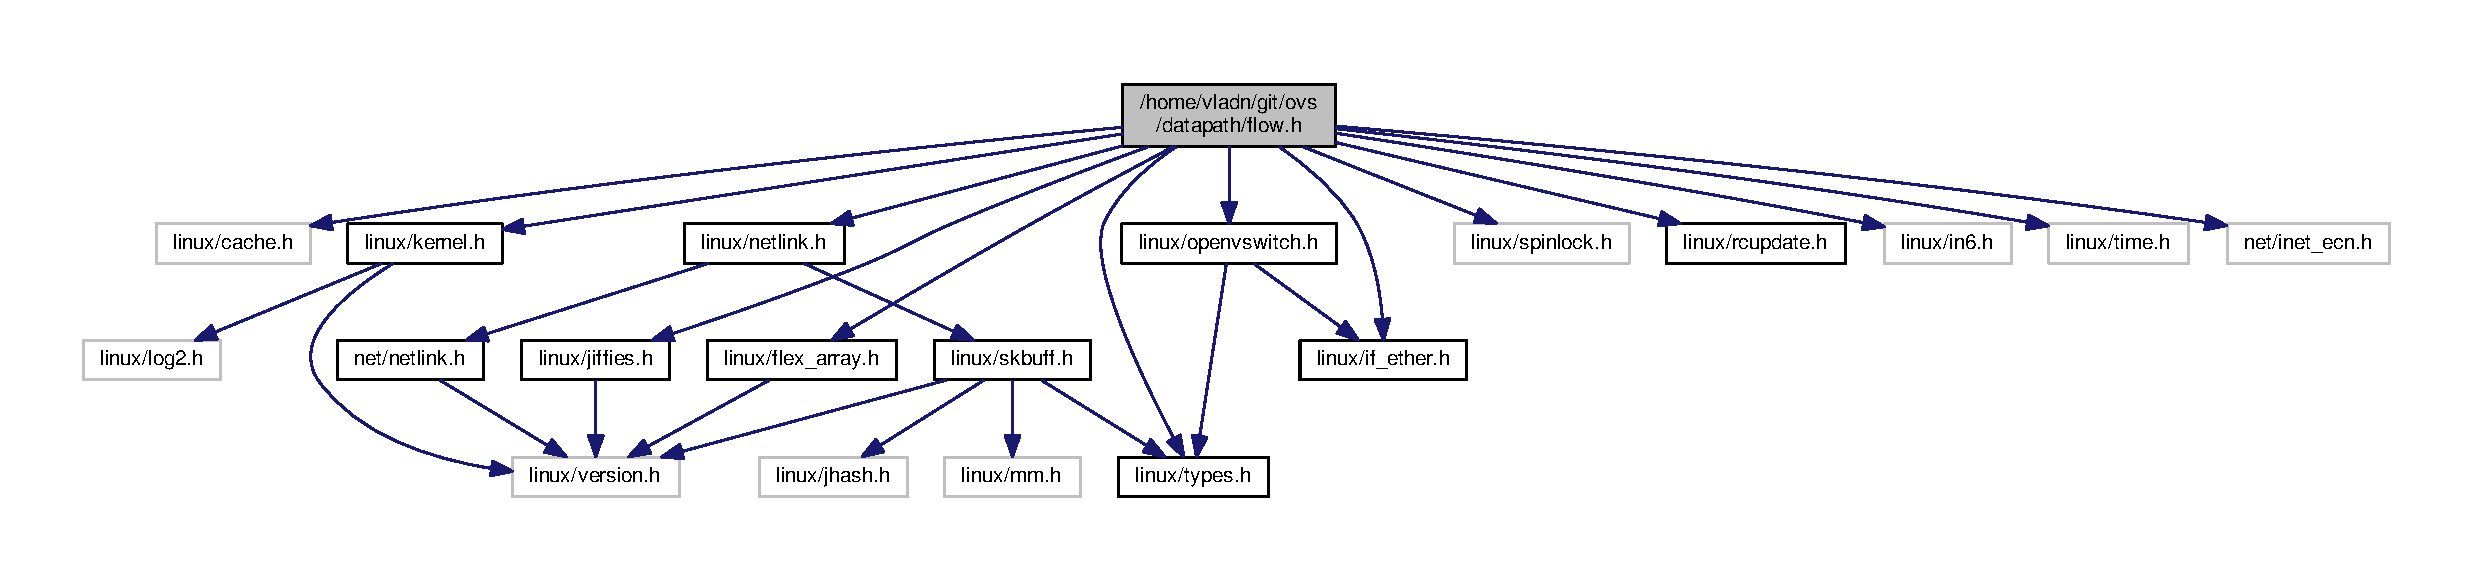
\includegraphics[width=350pt]{flow_8h__incl}
\end{center}
\end{figure}
This graph shows which files directly or indirectly include this file\+:
\nopagebreak
\begin{figure}[H]
\begin{center}
\leavevmode
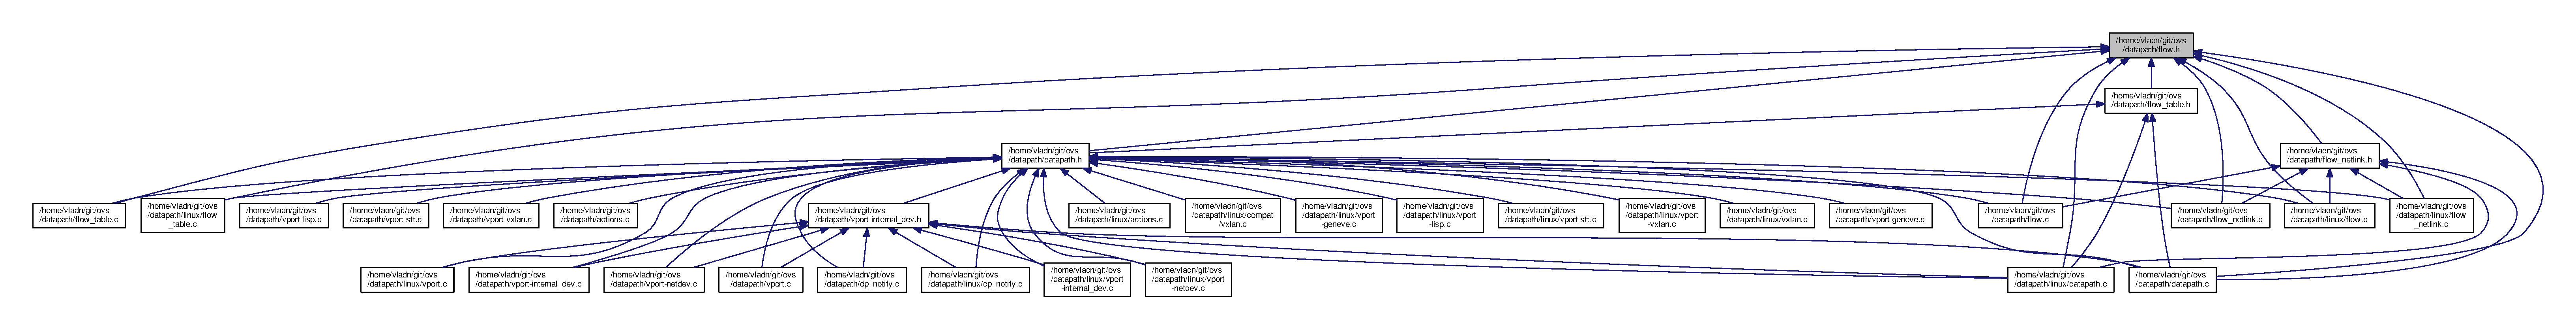
\includegraphics[width=350pt]{flow_8h__dep__incl}
\end{center}
\end{figure}
\subsection*{Data Structures}
\begin{DoxyCompactItemize}
\item 
struct \hyperlink{structovs__key__ipv4__tunnel}{ovs\+\_\+key\+\_\+ipv4\+\_\+tunnel}
\item 
struct \hyperlink{structovs__tunnel__info}{ovs\+\_\+tunnel\+\_\+info}
\item 
struct \hyperlink{structsw__flow__key}{sw\+\_\+flow\+\_\+key}
\item 
struct \hyperlink{structsw__flow__key__range}{sw\+\_\+flow\+\_\+key\+\_\+range}
\item 
struct \hyperlink{structsw__flow__mask}{sw\+\_\+flow\+\_\+mask}
\item 
struct \hyperlink{structsw__flow__match}{sw\+\_\+flow\+\_\+match}
\item 
struct \hyperlink{structsw__flow__id}{sw\+\_\+flow\+\_\+id}
\item 
struct \hyperlink{structsw__flow__actions}{sw\+\_\+flow\+\_\+actions}
\item 
struct \hyperlink{structflow__stats}{flow\+\_\+stats}
\item 
struct \hyperlink{structsw__flow}{sw\+\_\+flow}
\item 
struct \hyperlink{structarp__eth__header}{arp\+\_\+eth\+\_\+header}
\end{DoxyCompactItemize}
\subsection*{Macros}
\begin{DoxyCompactItemize}
\item 
\#define \hyperlink{flow_8h_aed9eb02d929e4afd221210dd92910f13}{O\+V\+S\+\_\+\+T\+U\+N\+N\+E\+L\+\_\+\+K\+E\+Y\+\_\+\+S\+I\+Z\+E}
\item 
\#define \hyperlink{flow_8h_ae4d5099091881f55393347766667f4e5}{T\+U\+N\+\_\+\+M\+E\+T\+A\+D\+A\+T\+A\+\_\+\+O\+F\+F\+S\+E\+T}(opt\+\_\+len)~(F\+I\+E\+L\+D\+\_\+\+S\+I\+Z\+E\+O\+F(struct \hyperlink{structsw__flow__key}{sw\+\_\+flow\+\_\+key}, \hyperlink{flow_8h_a58d612a14e56d9b6c782667cd2e89799}{tun\+\_\+opts}) -\/ opt\+\_\+len)
\item 
\#define \hyperlink{flow_8h_a5d74524a15e17551a8d8235f4375c296}{T\+U\+N\+\_\+\+M\+E\+T\+A\+D\+A\+T\+A\+\_\+\+O\+P\+T\+S}(flow\+\_\+key,  opt\+\_\+len)~((void $\ast$)((flow\+\_\+key)-\/$>$\hyperlink{flow_8h_a58d612a14e56d9b6c782667cd2e89799}{tun\+\_\+opts} + \hyperlink{flow_8h_ae4d5099091881f55393347766667f4e5}{T\+U\+N\+\_\+\+M\+E\+T\+A\+D\+A\+T\+A\+\_\+\+O\+F\+F\+S\+E\+T}(opt\+\_\+len)))
\item 
\#define \hyperlink{flow_8h_aa38104b9e3106537d588a65cdce52e3a}{O\+V\+S\+\_\+\+S\+W\+\_\+\+F\+L\+O\+W\+\_\+\+K\+E\+Y\+\_\+\+M\+E\+T\+A\+D\+A\+T\+A\+\_\+\+S\+I\+Z\+E}
\item 
\#define \hyperlink{flow_8h_a5cc1c8e559536cddce9d468214805527}{M\+A\+X\+\_\+\+U\+F\+I\+D\+\_\+\+L\+E\+N\+G\+T\+H}~16 /$\ast$ 128 bits $\ast$/
\end{DoxyCompactItemize}
\subsection*{Functions}
\begin{DoxyCompactItemize}
\item 
struct \hyperlink{structovs__key__ipv4__tunnel}{ovs\+\_\+key\+\_\+ipv4\+\_\+tunnel} \hyperlink{flow_8h_a557307ef977c6aa00305a24996d3237d}{\+\_\+\+\_\+aligned} (4)
\item 
static void \hyperlink{flow_8h_ae20b25e6cec56e9c0d07bc7f2c7d55ab}{\+\_\+\+\_\+ovs\+\_\+flow\+\_\+tun\+\_\+info\+\_\+init} (struct \hyperlink{structovs__tunnel__info}{ovs\+\_\+tunnel\+\_\+info} $\ast$tun\+\_\+info, \+\_\+\+\_\+be32 saddr, \+\_\+\+\_\+be32 daddr, u8 \hyperlink{flow_8h_a5612e9bbcc89219117d353438b2f9dad}{tos}, u8 \hyperlink{flow_8h_af5ff054badb6c806a3ab62dfa146cde1}{ttl}, \+\_\+\+\_\+be16 \hyperlink{flow_8h_ad2071126c591c16c05617b0620c784e7}{tp\+\_\+src}, \+\_\+\+\_\+be16 \hyperlink{flow_8h_acb2f3d43a724a8c1782b7e55ec10b63a}{tp\+\_\+dst}, \+\_\+\+\_\+be64 \hyperlink{flow_8h_aba5027d7a3d96f0f58dd8e607365934b}{tun\+\_\+id}, \+\_\+\+\_\+be16 \hyperlink{flow_8h_a51a0f47500f23a17c8e67bddee1911f8}{tun\+\_\+flags}, const void $\ast$opts, u8 opts\+\_\+len)
\item 
static void \hyperlink{flow_8h_a852c3ebd7a575ba7133623943f79e5df}{ovs\+\_\+flow\+\_\+tun\+\_\+info\+\_\+init} (struct \hyperlink{structovs__tunnel__info}{ovs\+\_\+tunnel\+\_\+info} $\ast$tun\+\_\+info, const struct iphdr $\ast$iph, \+\_\+\+\_\+be16 \hyperlink{flow_8h_ad2071126c591c16c05617b0620c784e7}{tp\+\_\+src}, \+\_\+\+\_\+be16 \hyperlink{flow_8h_acb2f3d43a724a8c1782b7e55ec10b63a}{tp\+\_\+dst}, \+\_\+\+\_\+be64 \hyperlink{flow_8h_aba5027d7a3d96f0f58dd8e607365934b}{tun\+\_\+id}, \+\_\+\+\_\+be16 \hyperlink{flow_8h_a51a0f47500f23a17c8e67bddee1911f8}{tun\+\_\+flags}, const void $\ast$opts, u8 opts\+\_\+len)
\item 
struct \hyperlink{structsw__flow__key}{sw\+\_\+flow\+\_\+key} \hyperlink{flow_8h_ad33744d6d57a16762f004b11d767aa58}{\+\_\+\+\_\+aligned} (B\+I\+T\+S\+\_\+\+P\+E\+R\+\_\+\+L\+O\+N\+G/8)
\item 
static \hyperlink{types_8h_afaa87723b8417d40fcf45b7330261ef9}{bool} \hyperlink{flow_8h_a995966854ceb0b5a72ff027c12ccf426}{ovs\+\_\+identifier\+\_\+is\+\_\+ufid} (const struct \hyperlink{structsw__flow__id}{sw\+\_\+flow\+\_\+id} $\ast$sfid)
\item 
static \hyperlink{types_8h_afaa87723b8417d40fcf45b7330261ef9}{bool} \hyperlink{flow_8h_a3bfeaa297d8807b969a14f1cde78d21b}{ovs\+\_\+identifier\+\_\+is\+\_\+key} (const struct \hyperlink{structsw__flow__id}{sw\+\_\+flow\+\_\+id} $\ast$sfid)
\item 
void \hyperlink{flow_8h_aea7f5988172f2472c9f797b49e3ee1a1}{ovs\+\_\+flow\+\_\+stats\+\_\+update} (struct \hyperlink{structsw__flow}{sw\+\_\+flow} $\ast$, \+\_\+\+\_\+be16 tcp\+\_\+flags, const struct sk\+\_\+buff $\ast$)
\item 
void \hyperlink{flow_8h_a75a900e9720b7d52ad082b6676293407}{ovs\+\_\+flow\+\_\+stats\+\_\+get} (const struct \hyperlink{structsw__flow}{sw\+\_\+flow} $\ast$, struct \hyperlink{structovs__flow__stats}{ovs\+\_\+flow\+\_\+stats} $\ast$, unsigned long $\ast$used, \+\_\+\+\_\+be16 $\ast$tcp\+\_\+flags)
\item 
void \hyperlink{flow_8h_a7aabc674bfabbf16da954adc30cc2769}{ovs\+\_\+flow\+\_\+stats\+\_\+clear} (struct \hyperlink{structsw__flow}{sw\+\_\+flow} $\ast$)
\item 
u64 \hyperlink{flow_8h_adfdcc779325fc169a793acda2e32a46b}{ovs\+\_\+flow\+\_\+used\+\_\+time} (unsigned long flow\+\_\+jiffies)
\item 
int \hyperlink{flow_8h_a7d27b3745046ced4859b9fa615e27543}{ovs\+\_\+flow\+\_\+key\+\_\+update} (struct sk\+\_\+buff $\ast$skb, struct \hyperlink{structsw__flow__key}{sw\+\_\+flow\+\_\+key} $\ast$key)
\item 
int \hyperlink{flow_8h_a88b5c281d297950115033a17dbce5208}{ovs\+\_\+flow\+\_\+key\+\_\+extract} (const struct \hyperlink{structovs__tunnel__info}{ovs\+\_\+tunnel\+\_\+info} $\ast$tun\+\_\+info, struct sk\+\_\+buff $\ast$skb, struct \hyperlink{structsw__flow__key}{sw\+\_\+flow\+\_\+key} $\ast$key)
\item 
int \hyperlink{flow_8h_a5e042238993a5a8a8a8b3472cb274ead}{ovs\+\_\+flow\+\_\+key\+\_\+extract\+\_\+userspace} (const struct nlattr $\ast$attr, struct sk\+\_\+buff $\ast$skb, struct \hyperlink{structsw__flow__key}{sw\+\_\+flow\+\_\+key} $\ast$key, \hyperlink{types_8h_afaa87723b8417d40fcf45b7330261ef9}{bool} log)
\end{DoxyCompactItemize}
\subsection*{Variables}
\begin{DoxyCompactItemize}
\item 
\+\_\+\+\_\+be64 \hyperlink{flow_8h_aba5027d7a3d96f0f58dd8e607365934b}{tun\+\_\+id}
\item 
\+\_\+\+\_\+be32 \hyperlink{flow_8h_adbb6a48fdfe90e60d62145ca96e29dc5}{ipv4\+\_\+src}
\item 
\+\_\+\+\_\+be32 \hyperlink{flow_8h_aa8306c28f7713959c67444d4604ecbbd}{ipv4\+\_\+dst}
\item 
\+\_\+\+\_\+be16 \hyperlink{flow_8h_a51a0f47500f23a17c8e67bddee1911f8}{tun\+\_\+flags}
\item 
u8 \hyperlink{flow_8h_a23f491d61423eb547674ee00923c80d2}{ipv4\+\_\+tos}
\item 
u8 \hyperlink{flow_8h_a9467bd234b85a514f697f0a6d9839401}{ipv4\+\_\+ttl}
\item 
\+\_\+\+\_\+be16 \hyperlink{flow_8h_ad2071126c591c16c05617b0620c784e7}{tp\+\_\+src}
\item 
\+\_\+\+\_\+be16 \hyperlink{flow_8h_acb2f3d43a724a8c1782b7e55ec10b63a}{tp\+\_\+dst}
\item 
struct \hyperlink{structovs__tunnel__info}{ovs\+\_\+tunnel\+\_\+info} \hyperlink{flow_8h_afc2fada897ca3597a9462f26eb291fac}{\+\_\+\+\_\+aligned}
\item 
u8 \hyperlink{flow_8h_a58d612a14e56d9b6c782667cd2e89799}{tun\+\_\+opts} \mbox{[}255\mbox{]}
\item 
u8 \hyperlink{flow_8h_aed952827cbdce3601bca9c6501742ab9}{tun\+\_\+opts\+\_\+len}
\item 
struct \hyperlink{structovs__key__ipv4__tunnel}{ovs\+\_\+key\+\_\+ipv4\+\_\+tunnel} \hyperlink{flow_8h_a904e9497acde49a1992636f77597c5c7}{tun\+\_\+key}
\item 
\begin{tabbing}
xx\=xx\=xx\=xx\=xx\=xx\=xx\=xx\=xx\=\kill
struct \{\\
\>u32 \hyperlink{flow_8h_afff29fa49545fb51e4ff641e79d7f2c3}{priority}\\
\>u32 \hyperlink{flow_8h_aaa98314a1108ff2209ae3bb6515e1dd5}{skb\_mark}\\
\>u16 \hyperlink{flow_8h_add5c49cf0b0c4a57943c76d4d2b93373}{in\_port}\\
\} \hyperlink{flow_8h_a1c873ea83e1b749c669b501016e967fe}{phy}\\

\end{tabbing}\item 
u32 \hyperlink{flow_8h_a281fd67e00043582d1244246f268743d}{ovs\+\_\+flow\+\_\+hash}
\item 
u32 \hyperlink{flow_8h_af52a436bf08cde2c2bff8b9f9594bea5}{recirc\+\_\+id}
\item 
\begin{tabbing}
xx\=xx\=xx\=xx\=xx\=xx\=xx\=xx\=xx\=\kill
struct \{\\
\>u8 \hyperlink{flow_8h_a2e7e37e9dfe6465386d6c500f83ef144}{src} \mbox{[}ETH\_ALEN\mbox{]}\\
\>u8 \hyperlink{flow_8h_a6747ad3b5d60480ea073cd12c9b78aaa}{dst} \mbox{[}ETH\_ALEN\mbox{]}\\
\>\_\_be16 \hyperlink{flow_8h_a4528fe4db43b403cd959b50285d71b0c}{tci}\\
\>\_\_be16 \hyperlink{flow_8h_ab22aaab04f806700def00f32823fcb9e}{type}\\
\} \hyperlink{flow_8h_a1679a3c93391059deba58179f52c86a6}{eth}\\

\end{tabbing}\item 
\begin{tabbing}
xx\=xx\=xx\=xx\=xx\=xx\=xx\=xx\=xx\=\kill
union \{\\
\>struct \{\\
\>\>\_\_be32 \hyperlink{flow_8h_a0412041de0068d847a60706b85eaa87c}{top\_lse}\\
\>\} \hyperlink{flow_8h_aeab2d67b4ec58a9575da76c323ad95ce}{mpls}\\
\>struct \{\\
\>\>u8 \hyperlink{flow_8h_af1698a0033f39eb7a745097761b717d2}{proto}\\
\>\>u8 \hyperlink{flow_8h_a5612e9bbcc89219117d353438b2f9dad}{tos}\\
\>\>u8 \hyperlink{flow_8h_af5ff054badb6c806a3ab62dfa146cde1}{ttl}\\
\>\>u8 \hyperlink{flow_8h_a5a2afb39c0332abd7d0242da5e805313}{frag}\\
\>\} \hyperlink{flow_8h_a898dda7a587e3b8e5f8e257c1cea69f6}{ip}\\
\}; \\

\end{tabbing}\item 
\begin{tabbing}
xx\=xx\=xx\=xx\=xx\=xx\=xx\=xx\=xx\=\kill
struct \{\\
\>\_\_be16 \hyperlink{flow_8h_a2e7e37e9dfe6465386d6c500f83ef144}{src}\\
\>\_\_be16 \hyperlink{flow_8h_a6747ad3b5d60480ea073cd12c9b78aaa}{dst}\\
\>\_\_be16 \hyperlink{flow_8h_af4f7a53f6b2df72c34ca881f2714ac91}{flags}\\
\} \hyperlink{flow_8h_ad44c86ae49f219522bcd4fb2744b81b2}{tp}\\

\end{tabbing}\item 
\begin{tabbing}
xx\=xx\=xx\=xx\=xx\=xx\=xx\=xx\=xx\=\kill
union \{\\
\>struct \{\\
\>\>struct \{\\
\>\>\>\_\_be32 \hyperlink{flow_8h_a2e7e37e9dfe6465386d6c500f83ef144}{src}\\
\>\>\>\_\_be32 \hyperlink{flow_8h_a6747ad3b5d60480ea073cd12c9b78aaa}{dst}\\
\>\>\} \hyperlink{flow_8h_a535ce925c585c41d434f7481f342c976}{addr}\\
\>\>struct \{\\
\>\>\>u8 \hyperlink{flow_8h_a3007b784025014ba741cf9b6be9f07ef}{sha} \mbox{[}ETH\_ALEN\mbox{]}\\
\>\>\>u8 \hyperlink{flow_8h_a242576f2755dbec54b7fc25365c69119}{tha} \mbox{[}ETH\_ALEN\mbox{]}\\
\>\>\} \hyperlink{flow_8h_aa05c06f4d8f8b791f607aa53db449356}{arp}\\
\>\} \hyperlink{flow_8h_a1aa186097721b0d2190865057a49f0f9}{ipv4}\\
\>struct \{\\
\>\>struct \{\\
\>\>\>struct in6\_addr \hyperlink{flow_8h_a2e7e37e9dfe6465386d6c500f83ef144}{src}\\
\>\>\>struct in6\_addr \hyperlink{flow_8h_a6747ad3b5d60480ea073cd12c9b78aaa}{dst}\\
\>\>\} \hyperlink{flow_8h_a535ce925c585c41d434f7481f342c976}{addr}\\
\>\>\_\_be32 \hyperlink{flow_8h_a7471e30d4353c1a2fb2682c982d8a99f}{label}\\
\>\>struct \{\\
\>\>\>struct in6\_addr \hyperlink{flow_8h_a5fb304013ae6aaeaee9d7fdcfd343292}{target}\\
\>\>\>u8 \hyperlink{flow_8h_af7a2e79f6efba9b57041e6531f0689c3}{sll} \mbox{[}ETH\_ALEN\mbox{]}\\
\>\>\>u8 \hyperlink{flow_8h_a75251f8b54543051c48605244e207528}{tll} \mbox{[}ETH\_ALEN\mbox{]}\\
\>\>\} \hyperlink{flow_8h_a3043c4ac00ac70f331a1dd225c03daa2}{nd}\\
\>\} \hyperlink{flow_8h_a0e15caa0bf708962ec6aa94137d5bbae}{ipv6}\\
\}; \\

\end{tabbing}\item 
struct \hyperlink{structarp__eth__header}{arp\+\_\+eth\+\_\+header} \hyperlink{flow_8h_a3d962fef602eeda47d29b43ff33f5798}{\+\_\+\+\_\+packed}
\end{DoxyCompactItemize}


\subsection{Macro Definition Documentation}
\hypertarget{flow_8h_a5cc1c8e559536cddce9d468214805527}{}\index{flow.\+h@{flow.\+h}!M\+A\+X\+\_\+\+U\+F\+I\+D\+\_\+\+L\+E\+N\+G\+T\+H@{M\+A\+X\+\_\+\+U\+F\+I\+D\+\_\+\+L\+E\+N\+G\+T\+H}}
\index{M\+A\+X\+\_\+\+U\+F\+I\+D\+\_\+\+L\+E\+N\+G\+T\+H@{M\+A\+X\+\_\+\+U\+F\+I\+D\+\_\+\+L\+E\+N\+G\+T\+H}!flow.\+h@{flow.\+h}}
\subsubsection[{M\+A\+X\+\_\+\+U\+F\+I\+D\+\_\+\+L\+E\+N\+G\+T\+H}]{\setlength{\rightskip}{0pt plus 5cm}\#define M\+A\+X\+\_\+\+U\+F\+I\+D\+\_\+\+L\+E\+N\+G\+T\+H~16 /$\ast$ 128 bits $\ast$/}\label{flow_8h_a5cc1c8e559536cddce9d468214805527}
\hypertarget{flow_8h_aa38104b9e3106537d588a65cdce52e3a}{}\index{flow.\+h@{flow.\+h}!O\+V\+S\+\_\+\+S\+W\+\_\+\+F\+L\+O\+W\+\_\+\+K\+E\+Y\+\_\+\+M\+E\+T\+A\+D\+A\+T\+A\+\_\+\+S\+I\+Z\+E@{O\+V\+S\+\_\+\+S\+W\+\_\+\+F\+L\+O\+W\+\_\+\+K\+E\+Y\+\_\+\+M\+E\+T\+A\+D\+A\+T\+A\+\_\+\+S\+I\+Z\+E}}
\index{O\+V\+S\+\_\+\+S\+W\+\_\+\+F\+L\+O\+W\+\_\+\+K\+E\+Y\+\_\+\+M\+E\+T\+A\+D\+A\+T\+A\+\_\+\+S\+I\+Z\+E@{O\+V\+S\+\_\+\+S\+W\+\_\+\+F\+L\+O\+W\+\_\+\+K\+E\+Y\+\_\+\+M\+E\+T\+A\+D\+A\+T\+A\+\_\+\+S\+I\+Z\+E}!flow.\+h@{flow.\+h}}
\subsubsection[{O\+V\+S\+\_\+\+S\+W\+\_\+\+F\+L\+O\+W\+\_\+\+K\+E\+Y\+\_\+\+M\+E\+T\+A\+D\+A\+T\+A\+\_\+\+S\+I\+Z\+E}]{\setlength{\rightskip}{0pt plus 5cm}\#define O\+V\+S\+\_\+\+S\+W\+\_\+\+F\+L\+O\+W\+\_\+\+K\+E\+Y\+\_\+\+M\+E\+T\+A\+D\+A\+T\+A\+\_\+\+S\+I\+Z\+E}\label{flow_8h_aa38104b9e3106537d588a65cdce52e3a}
{\bfseries Value\+:}
\begin{DoxyCode}
(offsetof(\textcolor{keyword}{struct} \hyperlink{structsw__flow__key}{sw\_flow\_key}, \hyperlink{flow_8h_af52a436bf08cde2c2bff8b9f9594bea5}{recirc\_id}) +  \(\backslash\)
    FIELD\_SIZEOF(\textcolor{keyword}{struct} \hyperlink{structsw__flow__key}{sw\_flow\_key}, \hyperlink{flow_8h_af52a436bf08cde2c2bff8b9f9594bea5}{recirc\_id}))
\end{DoxyCode}
\hypertarget{flow_8h_aed9eb02d929e4afd221210dd92910f13}{}\index{flow.\+h@{flow.\+h}!O\+V\+S\+\_\+\+T\+U\+N\+N\+E\+L\+\_\+\+K\+E\+Y\+\_\+\+S\+I\+Z\+E@{O\+V\+S\+\_\+\+T\+U\+N\+N\+E\+L\+\_\+\+K\+E\+Y\+\_\+\+S\+I\+Z\+E}}
\index{O\+V\+S\+\_\+\+T\+U\+N\+N\+E\+L\+\_\+\+K\+E\+Y\+\_\+\+S\+I\+Z\+E@{O\+V\+S\+\_\+\+T\+U\+N\+N\+E\+L\+\_\+\+K\+E\+Y\+\_\+\+S\+I\+Z\+E}!flow.\+h@{flow.\+h}}
\subsubsection[{O\+V\+S\+\_\+\+T\+U\+N\+N\+E\+L\+\_\+\+K\+E\+Y\+\_\+\+S\+I\+Z\+E}]{\setlength{\rightskip}{0pt plus 5cm}\#define O\+V\+S\+\_\+\+T\+U\+N\+N\+E\+L\+\_\+\+K\+E\+Y\+\_\+\+S\+I\+Z\+E}\label{flow_8h_aed9eb02d929e4afd221210dd92910f13}
{\bfseries Value\+:}
\begin{DoxyCode}
(offsetof(\textcolor{keyword}{struct} \hyperlink{structovs__key__ipv4__tunnel}{ovs\_key\_ipv4\_tunnel}, \hyperlink{flow_8h_acb2f3d43a724a8c1782b7e55ec10b63a}{tp\_dst}) +        \(\backslash\)
     FIELD\_SIZEOF(\textcolor{keyword}{struct} \hyperlink{structovs__key__ipv4__tunnel}{ovs\_key\_ipv4\_tunnel}, \hyperlink{flow_8h_acb2f3d43a724a8c1782b7e55ec10b63a}{tp\_dst}))
\end{DoxyCode}
\hypertarget{flow_8h_ae4d5099091881f55393347766667f4e5}{}\index{flow.\+h@{flow.\+h}!T\+U\+N\+\_\+\+M\+E\+T\+A\+D\+A\+T\+A\+\_\+\+O\+F\+F\+S\+E\+T@{T\+U\+N\+\_\+\+M\+E\+T\+A\+D\+A\+T\+A\+\_\+\+O\+F\+F\+S\+E\+T}}
\index{T\+U\+N\+\_\+\+M\+E\+T\+A\+D\+A\+T\+A\+\_\+\+O\+F\+F\+S\+E\+T@{T\+U\+N\+\_\+\+M\+E\+T\+A\+D\+A\+T\+A\+\_\+\+O\+F\+F\+S\+E\+T}!flow.\+h@{flow.\+h}}
\subsubsection[{T\+U\+N\+\_\+\+M\+E\+T\+A\+D\+A\+T\+A\+\_\+\+O\+F\+F\+S\+E\+T}]{\setlength{\rightskip}{0pt plus 5cm}\#define T\+U\+N\+\_\+\+M\+E\+T\+A\+D\+A\+T\+A\+\_\+\+O\+F\+F\+S\+E\+T(
\begin{DoxyParamCaption}
\item[{}]{opt\+\_\+len}
\end{DoxyParamCaption}
)~(F\+I\+E\+L\+D\+\_\+\+S\+I\+Z\+E\+O\+F(struct {\bf sw\+\_\+flow\+\_\+key}, {\bf tun\+\_\+opts}) -\/ opt\+\_\+len)}\label{flow_8h_ae4d5099091881f55393347766667f4e5}
\hypertarget{flow_8h_a5d74524a15e17551a8d8235f4375c296}{}\index{flow.\+h@{flow.\+h}!T\+U\+N\+\_\+\+M\+E\+T\+A\+D\+A\+T\+A\+\_\+\+O\+P\+T\+S@{T\+U\+N\+\_\+\+M\+E\+T\+A\+D\+A\+T\+A\+\_\+\+O\+P\+T\+S}}
\index{T\+U\+N\+\_\+\+M\+E\+T\+A\+D\+A\+T\+A\+\_\+\+O\+P\+T\+S@{T\+U\+N\+\_\+\+M\+E\+T\+A\+D\+A\+T\+A\+\_\+\+O\+P\+T\+S}!flow.\+h@{flow.\+h}}
\subsubsection[{T\+U\+N\+\_\+\+M\+E\+T\+A\+D\+A\+T\+A\+\_\+\+O\+P\+T\+S}]{\setlength{\rightskip}{0pt plus 5cm}\#define T\+U\+N\+\_\+\+M\+E\+T\+A\+D\+A\+T\+A\+\_\+\+O\+P\+T\+S(
\begin{DoxyParamCaption}
\item[{}]{flow\+\_\+key, }
\item[{}]{opt\+\_\+len}
\end{DoxyParamCaption}
)~((void $\ast$)((flow\+\_\+key)-\/$>${\bf tun\+\_\+opts} + {\bf T\+U\+N\+\_\+\+M\+E\+T\+A\+D\+A\+T\+A\+\_\+\+O\+F\+F\+S\+E\+T}(opt\+\_\+len)))}\label{flow_8h_a5d74524a15e17551a8d8235f4375c296}


\subsection{Function Documentation}
\hypertarget{flow_8h_ad33744d6d57a16762f004b11d767aa58}{}\index{flow.\+h@{flow.\+h}!\+\_\+\+\_\+aligned@{\+\_\+\+\_\+aligned}}
\index{\+\_\+\+\_\+aligned@{\+\_\+\+\_\+aligned}!flow.\+h@{flow.\+h}}
\subsubsection[{\+\_\+\+\_\+aligned}]{\setlength{\rightskip}{0pt plus 5cm}struct {\bf sw\+\_\+flow\+\_\+key} \+\_\+\+\_\+aligned (
\begin{DoxyParamCaption}
\item[{B\+I\+T\+S\+\_\+\+P\+E\+R\+\_\+\+L\+O\+N\+G/}]{8}
\end{DoxyParamCaption}
)}\label{flow_8h_ad33744d6d57a16762f004b11d767aa58}
\hypertarget{flow_8h_a557307ef977c6aa00305a24996d3237d}{}\index{flow.\+h@{flow.\+h}!\+\_\+\+\_\+aligned@{\+\_\+\+\_\+aligned}}
\index{\+\_\+\+\_\+aligned@{\+\_\+\+\_\+aligned}!flow.\+h@{flow.\+h}}
\subsubsection[{\+\_\+\+\_\+aligned}]{\setlength{\rightskip}{0pt plus 5cm}struct {\bf ovs\+\_\+key\+\_\+ipv4\+\_\+tunnel} \+\_\+\+\_\+aligned (
\begin{DoxyParamCaption}
\item[{4}]{}
\end{DoxyParamCaption}
)}\label{flow_8h_a557307ef977c6aa00305a24996d3237d}
\hypertarget{flow_8h_ae20b25e6cec56e9c0d07bc7f2c7d55ab}{}\index{flow.\+h@{flow.\+h}!\+\_\+\+\_\+ovs\+\_\+flow\+\_\+tun\+\_\+info\+\_\+init@{\+\_\+\+\_\+ovs\+\_\+flow\+\_\+tun\+\_\+info\+\_\+init}}
\index{\+\_\+\+\_\+ovs\+\_\+flow\+\_\+tun\+\_\+info\+\_\+init@{\+\_\+\+\_\+ovs\+\_\+flow\+\_\+tun\+\_\+info\+\_\+init}!flow.\+h@{flow.\+h}}
\subsubsection[{\+\_\+\+\_\+ovs\+\_\+flow\+\_\+tun\+\_\+info\+\_\+init}]{\setlength{\rightskip}{0pt plus 5cm}static void \+\_\+\+\_\+ovs\+\_\+flow\+\_\+tun\+\_\+info\+\_\+init (
\begin{DoxyParamCaption}
\item[{struct {\bf ovs\+\_\+tunnel\+\_\+info} $\ast$}]{tun\+\_\+info, }
\item[{\+\_\+\+\_\+be32}]{saddr, }
\item[{\+\_\+\+\_\+be32}]{daddr, }
\item[{u8}]{tos, }
\item[{u8}]{ttl, }
\item[{\+\_\+\+\_\+be16}]{tp\+\_\+src, }
\item[{\+\_\+\+\_\+be16}]{tp\+\_\+dst, }
\item[{\+\_\+\+\_\+be64}]{tun\+\_\+id, }
\item[{\+\_\+\+\_\+be16}]{tun\+\_\+flags, }
\item[{const void $\ast$}]{opts, }
\item[{u8}]{opts\+\_\+len}
\end{DoxyParamCaption}
)\hspace{0.3cm}{\ttfamily [inline]}, {\ttfamily [static]}}\label{flow_8h_ae20b25e6cec56e9c0d07bc7f2c7d55ab}

\begin{DoxyCode}
78 \{
79     tun\_info->\hyperlink{structovs__tunnel__info_a007f0c7a9938884e6e8663cb4ab20d10}{tunnel}.\hyperlink{structovs__key__ipv4__tunnel_ae36132bc05ca6257b572edddffcb867a}{tun\_id} = \hyperlink{flow_8h_aba5027d7a3d96f0f58dd8e607365934b}{tun\_id};
80     tun\_info->\hyperlink{structovs__tunnel__info_a007f0c7a9938884e6e8663cb4ab20d10}{tunnel}.\hyperlink{structovs__key__ipv4__tunnel_a1e5a978f104d61e9694e914a109734a7}{ipv4\_src} = saddr;
81     tun\_info->\hyperlink{structovs__tunnel__info_a007f0c7a9938884e6e8663cb4ab20d10}{tunnel}.\hyperlink{structovs__key__ipv4__tunnel_ae443d381a97f53bbc4139fe36c0aae30}{ipv4\_dst} = daddr;
82     tun\_info->\hyperlink{structovs__tunnel__info_a007f0c7a9938884e6e8663cb4ab20d10}{tunnel}.\hyperlink{structovs__key__ipv4__tunnel_a69594eaf9d7dfc2824b264484e02498e}{ipv4\_tos} = \hyperlink{flow_8h_a5612e9bbcc89219117d353438b2f9dad}{tos};
83     tun\_info->\hyperlink{structovs__tunnel__info_a007f0c7a9938884e6e8663cb4ab20d10}{tunnel}.\hyperlink{structovs__key__ipv4__tunnel_a24de7472a8c22903fce96b73dab68a40}{ipv4\_ttl} = \hyperlink{flow_8h_af5ff054badb6c806a3ab62dfa146cde1}{ttl};
84     tun\_info->\hyperlink{structovs__tunnel__info_a007f0c7a9938884e6e8663cb4ab20d10}{tunnel}.\hyperlink{structovs__key__ipv4__tunnel_a7459e66ecf90329eb2fa6cf3fc4781db}{tun\_flags} = \hyperlink{flow_8h_a51a0f47500f23a17c8e67bddee1911f8}{tun\_flags};
85 
86     \textcolor{comment}{/* For the tunnel types on the top of IPsec, the tp\_src and tp\_dst of}
87 \textcolor{comment}{     * the upper tunnel are used.}
88 \textcolor{comment}{     * E.g: GRE over IPSEC, the tp\_src and tp\_port are zero.}
89 \textcolor{comment}{     */}
90     tun\_info->\hyperlink{structovs__tunnel__info_a007f0c7a9938884e6e8663cb4ab20d10}{tunnel}.\hyperlink{structovs__key__ipv4__tunnel_acda46848fad6a931296f3e7a74b44a18}{tp\_src} = \hyperlink{flow_8h_ad2071126c591c16c05617b0620c784e7}{tp\_src};
91     tun\_info->\hyperlink{structovs__tunnel__info_a007f0c7a9938884e6e8663cb4ab20d10}{tunnel}.\hyperlink{structovs__key__ipv4__tunnel_a438707be6be24ab62236063bde726e9b}{tp\_dst} = \hyperlink{flow_8h_acb2f3d43a724a8c1782b7e55ec10b63a}{tp\_dst};
92 
93     \textcolor{comment}{/* Clear struct padding. */}
94     \textcolor{keywordflow}{if} (\textcolor{keyword}{sizeof}(tun\_info->\hyperlink{structovs__tunnel__info_a007f0c7a9938884e6e8663cb4ab20d10}{tunnel}) != \hyperlink{flow_8h_aed9eb02d929e4afd221210dd92910f13}{OVS\_TUNNEL\_KEY\_SIZE})
95         memset((\textcolor{keywordtype}{unsigned} \textcolor{keywordtype}{char} *)&tun\_info->\hyperlink{structovs__tunnel__info_a007f0c7a9938884e6e8663cb4ab20d10}{tunnel} + \hyperlink{flow_8h_aed9eb02d929e4afd221210dd92910f13}{OVS\_TUNNEL\_KEY\_SIZE},
96                0, \textcolor{keyword}{sizeof}(tun\_info->\hyperlink{structovs__tunnel__info_a007f0c7a9938884e6e8663cb4ab20d10}{tunnel}) - \hyperlink{flow_8h_aed9eb02d929e4afd221210dd92910f13}{OVS\_TUNNEL\_KEY\_SIZE});
97 
98     tun\_info->\hyperlink{structovs__tunnel__info_ae4fd786894f579a38a5955e7a0e68fd4}{options} = opts;
99     tun\_info->\hyperlink{structovs__tunnel__info_ab50d289f61727b922831739affb28b18}{options\_len} = opts\_len;
100 \}
\end{DoxyCode}
\hypertarget{flow_8h_a88b5c281d297950115033a17dbce5208}{}\index{flow.\+h@{flow.\+h}!ovs\+\_\+flow\+\_\+key\+\_\+extract@{ovs\+\_\+flow\+\_\+key\+\_\+extract}}
\index{ovs\+\_\+flow\+\_\+key\+\_\+extract@{ovs\+\_\+flow\+\_\+key\+\_\+extract}!flow.\+h@{flow.\+h}}
\subsubsection[{ovs\+\_\+flow\+\_\+key\+\_\+extract}]{\setlength{\rightskip}{0pt plus 5cm}int ovs\+\_\+flow\+\_\+key\+\_\+extract (
\begin{DoxyParamCaption}
\item[{const struct {\bf ovs\+\_\+tunnel\+\_\+info} $\ast$}]{tun\+\_\+info, }
\item[{struct sk\+\_\+buff $\ast$}]{skb, }
\item[{struct {\bf sw\+\_\+flow\+\_\+key} $\ast$}]{key}
\end{DoxyParamCaption}
)}\label{flow_8h_a88b5c281d297950115033a17dbce5208}

\begin{DoxyCode}
687 \{
688     \textcolor{comment}{/* Extract metadata from packet. */}
689     \textcolor{keywordflow}{if} (tun\_info) \{
690         memcpy(&key->\hyperlink{structsw__flow__key_a2f87b7690c0cc2797f1f4347589472c3}{tun\_key}, &tun\_info->\hyperlink{structovs__tunnel__info_a007f0c7a9938884e6e8663cb4ab20d10}{tunnel}, \textcolor{keyword}{sizeof}(key->
      \hyperlink{structsw__flow__key_a2f87b7690c0cc2797f1f4347589472c3}{tun\_key}));
691 
692         BUILD\_BUG\_ON(((1 << (\textcolor{keyword}{sizeof}(tun\_info->\hyperlink{structovs__tunnel__info_ab50d289f61727b922831739affb28b18}{options\_len}) * 8)) - 1) >
693                  \textcolor{keyword}{sizeof}(key->\hyperlink{structsw__flow__key_a54b30752817dccb02665a7eecde52a72}{tun\_opts}));
694 
695         \textcolor{keywordflow}{if} (tun\_info->\hyperlink{structovs__tunnel__info_ae4fd786894f579a38a5955e7a0e68fd4}{options}) \{
696             memcpy(\hyperlink{flow_8h_a5d74524a15e17551a8d8235f4375c296}{TUN\_METADATA\_OPTS}(key, tun\_info->\hyperlink{structovs__tunnel__info_ab50d289f61727b922831739affb28b18}{options\_len}),
697                    tun\_info->\hyperlink{structovs__tunnel__info_ae4fd786894f579a38a5955e7a0e68fd4}{options}, tun\_info->\hyperlink{structovs__tunnel__info_ab50d289f61727b922831739affb28b18}{options\_len});
698             key->\hyperlink{structsw__flow__key_aef0ea317d3bd0125e0d6390261ba3e2d}{tun\_opts\_len} = tun\_info->\hyperlink{structovs__tunnel__info_ab50d289f61727b922831739affb28b18}{options\_len};
699         \} \textcolor{keywordflow}{else} \{
700             key->\hyperlink{structsw__flow__key_aef0ea317d3bd0125e0d6390261ba3e2d}{tun\_opts\_len} = 0;
701         \}
702     \} \textcolor{keywordflow}{else} \{
703         key->\hyperlink{structsw__flow__key_aef0ea317d3bd0125e0d6390261ba3e2d}{tun\_opts\_len} = 0;
704         memset(&key->\hyperlink{structsw__flow__key_a2f87b7690c0cc2797f1f4347589472c3}{tun\_key}, 0, \textcolor{keyword}{sizeof}(key->\hyperlink{structsw__flow__key_a2f87b7690c0cc2797f1f4347589472c3}{tun\_key}));
705     \}
706 
707     key->\hyperlink{structsw__flow__key_a57cbddb75a8d4fd859300bd34d98e84a}{phy}.\hyperlink{structsw__flow__key_a9dd898913d9faaec1ec970029e7fbb71}{priority} = skb->priority;
708     key->\hyperlink{structsw__flow__key_a57cbddb75a8d4fd859300bd34d98e84a}{phy}.\hyperlink{structsw__flow__key_a5848de18caa80d36d9bc60cc686a2c6e}{in\_port} = \hyperlink{datapath_8h_ac337c4d4ddca29916ce8e900038ddd78}{OVS\_CB}(skb)->input\_vport->port\_no;
709     key->\hyperlink{structsw__flow__key_a57cbddb75a8d4fd859300bd34d98e84a}{phy}.\hyperlink{structsw__flow__key_ae02571657f29397dcc45de8528f4ed05}{skb\_mark} = skb->mark;
710     key->\hyperlink{structsw__flow__key_a73dd9402f1f54c321f6d704d9b018d15}{ovs\_flow\_hash} = 0;
711     key->\hyperlink{structsw__flow__key_a7e51857c88ad6b0bf90551d0b6e2607b}{recirc\_id} = 0;
712 
713     \textcolor{keywordflow}{return} \hyperlink{flow_8c_af69403050accb2489f73d37b528aa9c4}{key\_extract}(skb, key);
714 \}
\end{DoxyCode}
\hypertarget{flow_8h_a5e042238993a5a8a8a8b3472cb274ead}{}\index{flow.\+h@{flow.\+h}!ovs\+\_\+flow\+\_\+key\+\_\+extract\+\_\+userspace@{ovs\+\_\+flow\+\_\+key\+\_\+extract\+\_\+userspace}}
\index{ovs\+\_\+flow\+\_\+key\+\_\+extract\+\_\+userspace@{ovs\+\_\+flow\+\_\+key\+\_\+extract\+\_\+userspace}!flow.\+h@{flow.\+h}}
\subsubsection[{ovs\+\_\+flow\+\_\+key\+\_\+extract\+\_\+userspace}]{\setlength{\rightskip}{0pt plus 5cm}int ovs\+\_\+flow\+\_\+key\+\_\+extract\+\_\+userspace (
\begin{DoxyParamCaption}
\item[{const struct nlattr $\ast$}]{attr, }
\item[{struct sk\+\_\+buff $\ast$}]{skb, }
\item[{struct {\bf sw\+\_\+flow\+\_\+key} $\ast$}]{key, }
\item[{{\bf bool}}]{log}
\end{DoxyParamCaption}
)}\label{flow_8h_a5e042238993a5a8a8a8b3472cb274ead}

\begin{DoxyCode}
719 \{
720     \textcolor{keywordtype}{int} err;
721 
722     \textcolor{comment}{/* Extract metadata from netlink attributes. */}
723     err = \hyperlink{flow__netlink_8c_a90428a389e4ba65133d2cf837d5a8dc3}{ovs\_nla\_get\_flow\_metadata}(attr, key, log);
724     \textcolor{keywordflow}{if} (err)
725         \textcolor{keywordflow}{return} err;
726 
727     \textcolor{keywordflow}{return} \hyperlink{flow_8c_af69403050accb2489f73d37b528aa9c4}{key\_extract}(skb, key);
728 \}
\end{DoxyCode}
\hypertarget{flow_8h_a7d27b3745046ced4859b9fa615e27543}{}\index{flow.\+h@{flow.\+h}!ovs\+\_\+flow\+\_\+key\+\_\+update@{ovs\+\_\+flow\+\_\+key\+\_\+update}}
\index{ovs\+\_\+flow\+\_\+key\+\_\+update@{ovs\+\_\+flow\+\_\+key\+\_\+update}!flow.\+h@{flow.\+h}}
\subsubsection[{ovs\+\_\+flow\+\_\+key\+\_\+update}]{\setlength{\rightskip}{0pt plus 5cm}int ovs\+\_\+flow\+\_\+key\+\_\+update (
\begin{DoxyParamCaption}
\item[{struct sk\+\_\+buff $\ast$}]{skb, }
\item[{struct {\bf sw\+\_\+flow\+\_\+key} $\ast$}]{key}
\end{DoxyParamCaption}
)}\label{flow_8h_a7d27b3745046ced4859b9fa615e27543}

\begin{DoxyCode}
681 \{
682     \textcolor{keywordflow}{return} \hyperlink{flow_8c_af69403050accb2489f73d37b528aa9c4}{key\_extract}(skb, key);
683 \}
\end{DoxyCode}
\hypertarget{flow_8h_a7aabc674bfabbf16da954adc30cc2769}{}\index{flow.\+h@{flow.\+h}!ovs\+\_\+flow\+\_\+stats\+\_\+clear@{ovs\+\_\+flow\+\_\+stats\+\_\+clear}}
\index{ovs\+\_\+flow\+\_\+stats\+\_\+clear@{ovs\+\_\+flow\+\_\+stats\+\_\+clear}!flow.\+h@{flow.\+h}}
\subsubsection[{ovs\+\_\+flow\+\_\+stats\+\_\+clear}]{\setlength{\rightskip}{0pt plus 5cm}void ovs\+\_\+flow\+\_\+stats\+\_\+clear (
\begin{DoxyParamCaption}
\item[{struct {\bf sw\+\_\+flow} $\ast$}]{}
\end{DoxyParamCaption}
)}\label{flow_8h_a7aabc674bfabbf16da954adc30cc2769}

\begin{DoxyCode}
162 \{
163     \textcolor{keywordtype}{int} node;
164 
165     for\_each\_node(node) \{
166         \textcolor{keyword}{struct }\hyperlink{structflow__stats}{flow\_stats} *stats = \hyperlink{datapath_8h_a06ef69170d345fd3996a467dcacf3ff3}{ovsl\_dereference}(flow->stats[node]);
167 
168         \textcolor{keywordflow}{if} (stats) \{
169             spin\_lock\_bh(&stats->\hyperlink{structflow__stats_a1930f864d7fc52f4afeb86714e3e5c07}{lock});
170             stats->\hyperlink{structflow__stats_a3eefc54cf53ad3e24bb070bd6f251f50}{used} = 0;
171             stats->\hyperlink{structflow__stats_a9399b2cdc3d48c11357fbc2aaff33226}{packet\_count} = 0;
172             stats->\hyperlink{structflow__stats_a97844fc570ddb0d4b80f4cfe36bfee29}{byte\_count} = 0;
173             stats->\hyperlink{structflow__stats_a2b2812adf4fd5f4f188324fdf503deba}{tcp\_flags} = 0;
174             spin\_unlock\_bh(&stats->\hyperlink{structflow__stats_a1930f864d7fc52f4afeb86714e3e5c07}{lock});
175         \}
176     \}
177 \}
\end{DoxyCode}
\hypertarget{flow_8h_a75a900e9720b7d52ad082b6676293407}{}\index{flow.\+h@{flow.\+h}!ovs\+\_\+flow\+\_\+stats\+\_\+get@{ovs\+\_\+flow\+\_\+stats\+\_\+get}}
\index{ovs\+\_\+flow\+\_\+stats\+\_\+get@{ovs\+\_\+flow\+\_\+stats\+\_\+get}!flow.\+h@{flow.\+h}}
\subsubsection[{ovs\+\_\+flow\+\_\+stats\+\_\+get}]{\setlength{\rightskip}{0pt plus 5cm}void ovs\+\_\+flow\+\_\+stats\+\_\+get (
\begin{DoxyParamCaption}
\item[{const struct {\bf sw\+\_\+flow} $\ast$}]{, }
\item[{struct {\bf ovs\+\_\+flow\+\_\+stats} $\ast$}]{, }
\item[{unsigned long $\ast$}]{used, }
\item[{\+\_\+\+\_\+be16 $\ast$}]{tcp\+\_\+flags}
\end{DoxyParamCaption}
)}\label{flow_8h_a75a900e9720b7d52ad082b6676293407}

\begin{DoxyCode}
135 \{
136     \textcolor{keywordtype}{int} node;
137 
138     *\hyperlink{structflow__stats_a3eefc54cf53ad3e24bb070bd6f251f50}{used} = 0;
139     *\hyperlink{structflow__stats_a2b2812adf4fd5f4f188324fdf503deba}{tcp\_flags} = 0;
140     memset(ovs\_stats, 0, \textcolor{keyword}{sizeof}(*ovs\_stats));
141 
142     for\_each\_node(node) \{
143         \textcolor{keyword}{struct }\hyperlink{structflow__stats}{flow\_stats} *stats = \hyperlink{datapath_8h_a5f2a2c1026f970f0052e77f5ebba33d1}{rcu\_dereference\_ovsl}(flow->stats[node]);
144 
145         \textcolor{keywordflow}{if} (stats) \{
146             \textcolor{comment}{/* Local CPU may write on non-local stats, so we must}
147 \textcolor{comment}{             * block bottom-halves here.}
148 \textcolor{comment}{             */}
149             spin\_lock\_bh(&stats->\hyperlink{structflow__stats_a1930f864d7fc52f4afeb86714e3e5c07}{lock});
150             \textcolor{keywordflow}{if} (!*\hyperlink{structflow__stats_a3eefc54cf53ad3e24bb070bd6f251f50}{used} || time\_after(stats->\hyperlink{structflow__stats_a3eefc54cf53ad3e24bb070bd6f251f50}{used}, *\hyperlink{structflow__stats_a3eefc54cf53ad3e24bb070bd6f251f50}{used}))
151                 *\hyperlink{structflow__stats_a3eefc54cf53ad3e24bb070bd6f251f50}{used} = stats->\hyperlink{structflow__stats_a3eefc54cf53ad3e24bb070bd6f251f50}{used};
152             *\hyperlink{structflow__stats_a2b2812adf4fd5f4f188324fdf503deba}{tcp\_flags} |= stats->\hyperlink{structflow__stats_a2b2812adf4fd5f4f188324fdf503deba}{tcp\_flags};
153             ovs\_stats->n\_packets += stats->\hyperlink{structflow__stats_a9399b2cdc3d48c11357fbc2aaff33226}{packet\_count};
154             ovs\_stats->n\_bytes += stats->\hyperlink{structflow__stats_a97844fc570ddb0d4b80f4cfe36bfee29}{byte\_count};
155             spin\_unlock\_bh(&stats->\hyperlink{structflow__stats_a1930f864d7fc52f4afeb86714e3e5c07}{lock});
156         \}
157     \}
158 \}
\end{DoxyCode}
\hypertarget{flow_8h_aea7f5988172f2472c9f797b49e3ee1a1}{}\index{flow.\+h@{flow.\+h}!ovs\+\_\+flow\+\_\+stats\+\_\+update@{ovs\+\_\+flow\+\_\+stats\+\_\+update}}
\index{ovs\+\_\+flow\+\_\+stats\+\_\+update@{ovs\+\_\+flow\+\_\+stats\+\_\+update}!flow.\+h@{flow.\+h}}
\subsubsection[{ovs\+\_\+flow\+\_\+stats\+\_\+update}]{\setlength{\rightskip}{0pt plus 5cm}void ovs\+\_\+flow\+\_\+stats\+\_\+update (
\begin{DoxyParamCaption}
\item[{struct {\bf sw\+\_\+flow} $\ast$}]{, }
\item[{\+\_\+\+\_\+be16}]{tcp\+\_\+flags, }
\item[{const struct sk\+\_\+buff $\ast$}]{}
\end{DoxyParamCaption}
)}\label{flow_8h_aea7f5988172f2472c9f797b49e3ee1a1}

\begin{DoxyCode}
71 \{
72     \textcolor{keyword}{struct }\hyperlink{structflow__stats}{flow\_stats} *stats;
73     \textcolor{keywordtype}{int} node = numa\_node\_id();
74     \textcolor{keywordtype}{int} len = skb->len + (\hyperlink{if__vlan_8h_a0bdf3e26944669a4265c7e717e846215}{skb\_vlan\_tag\_present}(skb) ? VLAN\_HLEN : 0);
75 
76     stats = rcu\_dereference(flow->stats[node]);
77 
78     \textcolor{comment}{/* Check if already have node-specific stats. */}
79     \textcolor{keywordflow}{if} (likely(stats)) \{
80         spin\_lock(&stats->\hyperlink{structflow__stats_a1930f864d7fc52f4afeb86714e3e5c07}{lock});
81         \textcolor{comment}{/* Mark if we write on the pre-allocated stats. */}
82         \textcolor{keywordflow}{if} (node == 0 && unlikely(flow->stats\_last\_writer != node))
83             flow->stats\_last\_writer = node;
84     \} \textcolor{keywordflow}{else} \{
85         stats = rcu\_dereference(flow->stats[0]); \textcolor{comment}{/* Pre-allocated. */}
86         spin\_lock(&stats->\hyperlink{structflow__stats_a1930f864d7fc52f4afeb86714e3e5c07}{lock});
87 
88         \textcolor{comment}{/* If the current NUMA-node is the only writer on the}
89 \textcolor{comment}{         * pre-allocated stats keep using them.}
90 \textcolor{comment}{         */}
91         \textcolor{keywordflow}{if} (unlikely(flow->stats\_last\_writer != node)) \{
92             \textcolor{comment}{/* A previous locker may have already allocated the}
93 \textcolor{comment}{             * stats, so we need to check again.  If node-specific}
94 \textcolor{comment}{             * stats were already allocated, we update the pre-}
95 \textcolor{comment}{             * allocated stats as we have already locked them.}
96 \textcolor{comment}{             */}
97             \textcolor{keywordflow}{if} (likely(flow->stats\_last\_writer != NUMA\_NO\_NODE)
98                 && likely(!\hyperlink{rcupdate_8h_a2c3aebbd11b184d9cab3049e4743882e}{rcu\_access\_pointer}(flow->stats[node]))) \{
99                 \textcolor{comment}{/* Try to allocate node-specific stats. */}
100                 \textcolor{keyword}{struct }\hyperlink{structflow__stats}{flow\_stats} *new\_stats;
101 
102                 new\_stats =
103                     kmem\_cache\_alloc\_node(\hyperlink{flow__table_8h_ab305bee215adea2618069cc592f6ee6b}{flow\_stats\_cache},
104                                   GFP\_THISNODE |
105                                   \_\_GFP\_NOMEMALLOC,
106                                   node);
107                 \textcolor{keywordflow}{if} (likely(new\_stats)) \{
108                     new\_stats->\hyperlink{structflow__stats_a3eefc54cf53ad3e24bb070bd6f251f50}{used} = jiffies;
109                     new\_stats->\hyperlink{structflow__stats_a9399b2cdc3d48c11357fbc2aaff33226}{packet\_count} = 1;
110                     new\_stats->\hyperlink{structflow__stats_a97844fc570ddb0d4b80f4cfe36bfee29}{byte\_count} = len;
111                     new\_stats->\hyperlink{structflow__stats_a2b2812adf4fd5f4f188324fdf503deba}{tcp\_flags} = \hyperlink{structflow__stats_a2b2812adf4fd5f4f188324fdf503deba}{tcp\_flags};
112                     spin\_lock\_init(&new\_stats->\hyperlink{structflow__stats_a1930f864d7fc52f4afeb86714e3e5c07}{lock});
113 
114                     rcu\_assign\_pointer(flow->stats[node],
115                                new\_stats);
116                     \textcolor{keywordflow}{goto} unlock;
117                 \}
118             \}
119             flow->stats\_last\_writer = node;
120         \}
121     \}
122 
123     stats->\hyperlink{structflow__stats_a3eefc54cf53ad3e24bb070bd6f251f50}{used} = jiffies;
124     stats->\hyperlink{structflow__stats_a9399b2cdc3d48c11357fbc2aaff33226}{packet\_count}++;
125     stats->\hyperlink{structflow__stats_a97844fc570ddb0d4b80f4cfe36bfee29}{byte\_count} += len;
126     stats->\hyperlink{structflow__stats_a2b2812adf4fd5f4f188324fdf503deba}{tcp\_flags} |= \hyperlink{structflow__stats_a2b2812adf4fd5f4f188324fdf503deba}{tcp\_flags};
127 unlock:
128     spin\_unlock(&stats->\hyperlink{structflow__stats_a1930f864d7fc52f4afeb86714e3e5c07}{lock});
129 \}
\end{DoxyCode}
\hypertarget{flow_8h_a852c3ebd7a575ba7133623943f79e5df}{}\index{flow.\+h@{flow.\+h}!ovs\+\_\+flow\+\_\+tun\+\_\+info\+\_\+init@{ovs\+\_\+flow\+\_\+tun\+\_\+info\+\_\+init}}
\index{ovs\+\_\+flow\+\_\+tun\+\_\+info\+\_\+init@{ovs\+\_\+flow\+\_\+tun\+\_\+info\+\_\+init}!flow.\+h@{flow.\+h}}
\subsubsection[{ovs\+\_\+flow\+\_\+tun\+\_\+info\+\_\+init}]{\setlength{\rightskip}{0pt plus 5cm}static void ovs\+\_\+flow\+\_\+tun\+\_\+info\+\_\+init (
\begin{DoxyParamCaption}
\item[{struct {\bf ovs\+\_\+tunnel\+\_\+info} $\ast$}]{tun\+\_\+info, }
\item[{const struct iphdr $\ast$}]{iph, }
\item[{\+\_\+\+\_\+be16}]{tp\+\_\+src, }
\item[{\+\_\+\+\_\+be16}]{tp\+\_\+dst, }
\item[{\+\_\+\+\_\+be64}]{tun\+\_\+id, }
\item[{\+\_\+\+\_\+be16}]{tun\+\_\+flags, }
\item[{const void $\ast$}]{opts, }
\item[{u8}]{opts\+\_\+len}
\end{DoxyParamCaption}
)\hspace{0.3cm}{\ttfamily [inline]}, {\ttfamily [static]}}\label{flow_8h_a852c3ebd7a575ba7133623943f79e5df}

\begin{DoxyCode}
110 \{
111     \hyperlink{flow_8h_ae20b25e6cec56e9c0d07bc7f2c7d55ab}{\_\_ovs\_flow\_tun\_info\_init}(tun\_info, iph->saddr, iph->daddr,
112                  iph->tos, iph->ttl,
113                  \hyperlink{flow_8h_ad2071126c591c16c05617b0620c784e7}{tp\_src}, \hyperlink{flow_8h_acb2f3d43a724a8c1782b7e55ec10b63a}{tp\_dst},
114                  \hyperlink{flow_8h_aba5027d7a3d96f0f58dd8e607365934b}{tun\_id}, \hyperlink{flow_8h_a51a0f47500f23a17c8e67bddee1911f8}{tun\_flags},
115                  opts, opts\_len);
116 \}
\end{DoxyCode}
\hypertarget{flow_8h_adfdcc779325fc169a793acda2e32a46b}{}\index{flow.\+h@{flow.\+h}!ovs\+\_\+flow\+\_\+used\+\_\+time@{ovs\+\_\+flow\+\_\+used\+\_\+time}}
\index{ovs\+\_\+flow\+\_\+used\+\_\+time@{ovs\+\_\+flow\+\_\+used\+\_\+time}!flow.\+h@{flow.\+h}}
\subsubsection[{ovs\+\_\+flow\+\_\+used\+\_\+time}]{\setlength{\rightskip}{0pt plus 5cm}u64 ovs\+\_\+flow\+\_\+used\+\_\+time (
\begin{DoxyParamCaption}
\item[{unsigned long}]{flow\+\_\+jiffies}
\end{DoxyParamCaption}
)}\label{flow_8h_adfdcc779325fc169a793acda2e32a46b}

\begin{DoxyCode}
55 \{
56     \textcolor{keyword}{struct }timespec cur\_ts;
57     u64 cur\_ms, idle\_ms;
58 
59     ktime\_get\_ts(&cur\_ts);
60     idle\_ms = jiffies\_to\_msecs(jiffies - flow\_jiffies);
61     cur\_ms = (u64)cur\_ts.tv\_sec * MSEC\_PER\_SEC +
62          cur\_ts.tv\_nsec / NSEC\_PER\_MSEC;
63 
64     \textcolor{keywordflow}{return} cur\_ms - idle\_ms;
65 \}
\end{DoxyCode}
\hypertarget{flow_8h_a3bfeaa297d8807b969a14f1cde78d21b}{}\index{flow.\+h@{flow.\+h}!ovs\+\_\+identifier\+\_\+is\+\_\+key@{ovs\+\_\+identifier\+\_\+is\+\_\+key}}
\index{ovs\+\_\+identifier\+\_\+is\+\_\+key@{ovs\+\_\+identifier\+\_\+is\+\_\+key}!flow.\+h@{flow.\+h}}
\subsubsection[{ovs\+\_\+identifier\+\_\+is\+\_\+key}]{\setlength{\rightskip}{0pt plus 5cm}static {\bf bool} ovs\+\_\+identifier\+\_\+is\+\_\+key (
\begin{DoxyParamCaption}
\item[{const struct {\bf sw\+\_\+flow\+\_\+id} $\ast$}]{sfid}
\end{DoxyParamCaption}
)\hspace{0.3cm}{\ttfamily [inline]}, {\ttfamily [static]}}\label{flow_8h_a3bfeaa297d8807b969a14f1cde78d21b}

\begin{DoxyCode}
263 \{
264     \textcolor{keywordflow}{return} !\hyperlink{flow_8h_a995966854ceb0b5a72ff027c12ccf426}{ovs\_identifier\_is\_ufid}(sfid);
265 \}
\end{DoxyCode}
\hypertarget{flow_8h_a995966854ceb0b5a72ff027c12ccf426}{}\index{flow.\+h@{flow.\+h}!ovs\+\_\+identifier\+\_\+is\+\_\+ufid@{ovs\+\_\+identifier\+\_\+is\+\_\+ufid}}
\index{ovs\+\_\+identifier\+\_\+is\+\_\+ufid@{ovs\+\_\+identifier\+\_\+is\+\_\+ufid}!flow.\+h@{flow.\+h}}
\subsubsection[{ovs\+\_\+identifier\+\_\+is\+\_\+ufid}]{\setlength{\rightskip}{0pt plus 5cm}static {\bf bool} ovs\+\_\+identifier\+\_\+is\+\_\+ufid (
\begin{DoxyParamCaption}
\item[{const struct {\bf sw\+\_\+flow\+\_\+id} $\ast$}]{sfid}
\end{DoxyParamCaption}
)\hspace{0.3cm}{\ttfamily [inline]}, {\ttfamily [static]}}\label{flow_8h_a995966854ceb0b5a72ff027c12ccf426}

\begin{DoxyCode}
258 \{
259     \textcolor{keywordflow}{return} sfid->\hyperlink{structsw__flow__id_a7cfead96fedf295e55d6a17857adfbf5}{ufid\_len};
260 \}
\end{DoxyCode}


\subsection{Variable Documentation}
\hypertarget{flow_8h_aa00b002aec94ac57108dcf4c5ccb0afb}{}\subsubsection[{"@18}]{\setlength{\rightskip}{0pt plus 5cm}union \{ ... \} }\label{flow_8h_aa00b002aec94ac57108dcf4c5ccb0afb}
\hypertarget{flow_8h_afa54122a84fb0f84fbc94e674459afc4}{}\subsubsection[{"@21}]{\setlength{\rightskip}{0pt plus 5cm}union \{ ... \} }\label{flow_8h_afa54122a84fb0f84fbc94e674459afc4}
\hypertarget{flow_8h_afc2fada897ca3597a9462f26eb291fac}{}\index{flow.\+h@{flow.\+h}!\+\_\+\+\_\+aligned@{\+\_\+\+\_\+aligned}}
\index{\+\_\+\+\_\+aligned@{\+\_\+\+\_\+aligned}!flow.\+h@{flow.\+h}}
\subsubsection[{\+\_\+\+\_\+aligned}]{\setlength{\rightskip}{0pt plus 5cm}struct {\bf sw\+\_\+flow\+\_\+key\+\_\+range} \+\_\+\+\_\+aligned}\label{flow_8h_afc2fada897ca3597a9462f26eb291fac}
\hypertarget{flow_8h_a3d962fef602eeda47d29b43ff33f5798}{}\index{flow.\+h@{flow.\+h}!\+\_\+\+\_\+packed@{\+\_\+\+\_\+packed}}
\index{\+\_\+\+\_\+packed@{\+\_\+\+\_\+packed}!flow.\+h@{flow.\+h}}
\subsubsection[{\+\_\+\+\_\+packed}]{\setlength{\rightskip}{0pt plus 5cm}struct {\bf arp\+\_\+eth\+\_\+header}  \+\_\+\+\_\+packed}\label{flow_8h_a3d962fef602eeda47d29b43ff33f5798}
\hypertarget{flow_8h_a535ce925c585c41d434f7481f342c976}{}\index{flow.\+h@{flow.\+h}!addr@{addr}}
\index{addr@{addr}!flow.\+h@{flow.\+h}}
\subsubsection[{addr}]{\setlength{\rightskip}{0pt plus 5cm}struct \{ ... \}   addr}\label{flow_8h_a535ce925c585c41d434f7481f342c976}
\hypertarget{flow_8h_aa05c06f4d8f8b791f607aa53db449356}{}\index{flow.\+h@{flow.\+h}!arp@{arp}}
\index{arp@{arp}!flow.\+h@{flow.\+h}}
\subsubsection[{arp}]{\setlength{\rightskip}{0pt plus 5cm}struct \{ ... \}   arp}\label{flow_8h_aa05c06f4d8f8b791f607aa53db449356}
\hypertarget{flow_8h_a6747ad3b5d60480ea073cd12c9b78aaa}{}\index{flow.\+h@{flow.\+h}!dst@{dst}}
\index{dst@{dst}!flow.\+h@{flow.\+h}}
\subsubsection[{dst}]{\setlength{\rightskip}{0pt plus 5cm}struct in6\+\_\+addr dst}\label{flow_8h_a6747ad3b5d60480ea073cd12c9b78aaa}
\hypertarget{flow_8h_a1679a3c93391059deba58179f52c86a6}{}\index{flow.\+h@{flow.\+h}!eth@{eth}}
\index{eth@{eth}!flow.\+h@{flow.\+h}}
\subsubsection[{eth}]{\setlength{\rightskip}{0pt plus 5cm}struct \{ ... \}   eth}\label{flow_8h_a1679a3c93391059deba58179f52c86a6}
\hypertarget{flow_8h_af4f7a53f6b2df72c34ca881f2714ac91}{}\index{flow.\+h@{flow.\+h}!flags@{flags}}
\index{flags@{flags}!flow.\+h@{flow.\+h}}
\subsubsection[{flags}]{\setlength{\rightskip}{0pt plus 5cm}\+\_\+\+\_\+be16 flags}\label{flow_8h_af4f7a53f6b2df72c34ca881f2714ac91}
\hypertarget{flow_8h_a5a2afb39c0332abd7d0242da5e805313}{}\index{flow.\+h@{flow.\+h}!frag@{frag}}
\index{frag@{frag}!flow.\+h@{flow.\+h}}
\subsubsection[{frag}]{\setlength{\rightskip}{0pt plus 5cm}u8 frag}\label{flow_8h_a5a2afb39c0332abd7d0242da5e805313}
\hypertarget{flow_8h_add5c49cf0b0c4a57943c76d4d2b93373}{}\index{flow.\+h@{flow.\+h}!in\+\_\+port@{in\+\_\+port}}
\index{in\+\_\+port@{in\+\_\+port}!flow.\+h@{flow.\+h}}
\subsubsection[{in\+\_\+port}]{\setlength{\rightskip}{0pt plus 5cm}u16 in\+\_\+port}\label{flow_8h_add5c49cf0b0c4a57943c76d4d2b93373}
\hypertarget{flow_8h_a898dda7a587e3b8e5f8e257c1cea69f6}{}\index{flow.\+h@{flow.\+h}!ip@{ip}}
\index{ip@{ip}!flow.\+h@{flow.\+h}}
\subsubsection[{ip}]{\setlength{\rightskip}{0pt plus 5cm}struct \{ ... \}   ip}\label{flow_8h_a898dda7a587e3b8e5f8e257c1cea69f6}
\hypertarget{flow_8h_a1aa186097721b0d2190865057a49f0f9}{}\index{flow.\+h@{flow.\+h}!ipv4@{ipv4}}
\index{ipv4@{ipv4}!flow.\+h@{flow.\+h}}
\subsubsection[{ipv4}]{\setlength{\rightskip}{0pt plus 5cm}struct \{ ... \}   ipv4}\label{flow_8h_a1aa186097721b0d2190865057a49f0f9}
\hypertarget{flow_8h_aa8306c28f7713959c67444d4604ecbbd}{}\index{flow.\+h@{flow.\+h}!ipv4\+\_\+dst@{ipv4\+\_\+dst}}
\index{ipv4\+\_\+dst@{ipv4\+\_\+dst}!flow.\+h@{flow.\+h}}
\subsubsection[{ipv4\+\_\+dst}]{\setlength{\rightskip}{0pt plus 5cm}\+\_\+\+\_\+be32 ipv4\+\_\+dst}\label{flow_8h_aa8306c28f7713959c67444d4604ecbbd}
\hypertarget{flow_8h_adbb6a48fdfe90e60d62145ca96e29dc5}{}\index{flow.\+h@{flow.\+h}!ipv4\+\_\+src@{ipv4\+\_\+src}}
\index{ipv4\+\_\+src@{ipv4\+\_\+src}!flow.\+h@{flow.\+h}}
\subsubsection[{ipv4\+\_\+src}]{\setlength{\rightskip}{0pt plus 5cm}\+\_\+\+\_\+be32 ipv4\+\_\+src}\label{flow_8h_adbb6a48fdfe90e60d62145ca96e29dc5}
\hypertarget{flow_8h_a23f491d61423eb547674ee00923c80d2}{}\index{flow.\+h@{flow.\+h}!ipv4\+\_\+tos@{ipv4\+\_\+tos}}
\index{ipv4\+\_\+tos@{ipv4\+\_\+tos}!flow.\+h@{flow.\+h}}
\subsubsection[{ipv4\+\_\+tos}]{\setlength{\rightskip}{0pt plus 5cm}u8 ipv4\+\_\+tos}\label{flow_8h_a23f491d61423eb547674ee00923c80d2}
\hypertarget{flow_8h_a9467bd234b85a514f697f0a6d9839401}{}\index{flow.\+h@{flow.\+h}!ipv4\+\_\+ttl@{ipv4\+\_\+ttl}}
\index{ipv4\+\_\+ttl@{ipv4\+\_\+ttl}!flow.\+h@{flow.\+h}}
\subsubsection[{ipv4\+\_\+ttl}]{\setlength{\rightskip}{0pt plus 5cm}u8 ipv4\+\_\+ttl}\label{flow_8h_a9467bd234b85a514f697f0a6d9839401}
\hypertarget{flow_8h_a0e15caa0bf708962ec6aa94137d5bbae}{}\index{flow.\+h@{flow.\+h}!ipv6@{ipv6}}
\index{ipv6@{ipv6}!flow.\+h@{flow.\+h}}
\subsubsection[{ipv6}]{\setlength{\rightskip}{0pt plus 5cm}struct \{ ... \}   ipv6}\label{flow_8h_a0e15caa0bf708962ec6aa94137d5bbae}
\hypertarget{flow_8h_a7471e30d4353c1a2fb2682c982d8a99f}{}\index{flow.\+h@{flow.\+h}!label@{label}}
\index{label@{label}!flow.\+h@{flow.\+h}}
\subsubsection[{label}]{\setlength{\rightskip}{0pt plus 5cm}\+\_\+\+\_\+be32 label}\label{flow_8h_a7471e30d4353c1a2fb2682c982d8a99f}
\hypertarget{flow_8h_aeab2d67b4ec58a9575da76c323ad95ce}{}\index{flow.\+h@{flow.\+h}!mpls@{mpls}}
\index{mpls@{mpls}!flow.\+h@{flow.\+h}}
\subsubsection[{mpls}]{\setlength{\rightskip}{0pt plus 5cm}struct \{ ... \}   mpls}\label{flow_8h_aeab2d67b4ec58a9575da76c323ad95ce}
\hypertarget{flow_8h_a3043c4ac00ac70f331a1dd225c03daa2}{}\index{flow.\+h@{flow.\+h}!nd@{nd}}
\index{nd@{nd}!flow.\+h@{flow.\+h}}
\subsubsection[{nd}]{\setlength{\rightskip}{0pt plus 5cm}struct \{ ... \}   nd}\label{flow_8h_a3043c4ac00ac70f331a1dd225c03daa2}
\hypertarget{flow_8h_a281fd67e00043582d1244246f268743d}{}\index{flow.\+h@{flow.\+h}!ovs\+\_\+flow\+\_\+hash@{ovs\+\_\+flow\+\_\+hash}}
\index{ovs\+\_\+flow\+\_\+hash@{ovs\+\_\+flow\+\_\+hash}!flow.\+h@{flow.\+h}}
\subsubsection[{ovs\+\_\+flow\+\_\+hash}]{\setlength{\rightskip}{0pt plus 5cm}u32 ovs\+\_\+flow\+\_\+hash}\label{flow_8h_a281fd67e00043582d1244246f268743d}
\hypertarget{flow_8h_a1c873ea83e1b749c669b501016e967fe}{}\index{flow.\+h@{flow.\+h}!phy@{phy}}
\index{phy@{phy}!flow.\+h@{flow.\+h}}
\subsubsection[{phy}]{\setlength{\rightskip}{0pt plus 5cm}struct \{ ... \}  phy}\label{flow_8h_a1c873ea83e1b749c669b501016e967fe}
\hypertarget{flow_8h_afff29fa49545fb51e4ff641e79d7f2c3}{}\index{flow.\+h@{flow.\+h}!priority@{priority}}
\index{priority@{priority}!flow.\+h@{flow.\+h}}
\subsubsection[{priority}]{\setlength{\rightskip}{0pt plus 5cm}u32 priority}\label{flow_8h_afff29fa49545fb51e4ff641e79d7f2c3}
\hypertarget{flow_8h_af1698a0033f39eb7a745097761b717d2}{}\index{flow.\+h@{flow.\+h}!proto@{proto}}
\index{proto@{proto}!flow.\+h@{flow.\+h}}
\subsubsection[{proto}]{\setlength{\rightskip}{0pt plus 5cm}u8 proto}\label{flow_8h_af1698a0033f39eb7a745097761b717d2}
\hypertarget{flow_8h_af52a436bf08cde2c2bff8b9f9594bea5}{}\index{flow.\+h@{flow.\+h}!recirc\+\_\+id@{recirc\+\_\+id}}
\index{recirc\+\_\+id@{recirc\+\_\+id}!flow.\+h@{flow.\+h}}
\subsubsection[{recirc\+\_\+id}]{\setlength{\rightskip}{0pt plus 5cm}u32 recirc\+\_\+id}\label{flow_8h_af52a436bf08cde2c2bff8b9f9594bea5}
\hypertarget{flow_8h_a3007b784025014ba741cf9b6be9f07ef}{}\index{flow.\+h@{flow.\+h}!sha@{sha}}
\index{sha@{sha}!flow.\+h@{flow.\+h}}
\subsubsection[{sha}]{\setlength{\rightskip}{0pt plus 5cm}u8 sha\mbox{[}E\+T\+H\+\_\+\+A\+L\+E\+N\mbox{]}}\label{flow_8h_a3007b784025014ba741cf9b6be9f07ef}
\hypertarget{flow_8h_aaa98314a1108ff2209ae3bb6515e1dd5}{}\index{flow.\+h@{flow.\+h}!skb\+\_\+mark@{skb\+\_\+mark}}
\index{skb\+\_\+mark@{skb\+\_\+mark}!flow.\+h@{flow.\+h}}
\subsubsection[{skb\+\_\+mark}]{\setlength{\rightskip}{0pt plus 5cm}u32 skb\+\_\+mark}\label{flow_8h_aaa98314a1108ff2209ae3bb6515e1dd5}
\hypertarget{flow_8h_af7a2e79f6efba9b57041e6531f0689c3}{}\index{flow.\+h@{flow.\+h}!sll@{sll}}
\index{sll@{sll}!flow.\+h@{flow.\+h}}
\subsubsection[{sll}]{\setlength{\rightskip}{0pt plus 5cm}u8 sll\mbox{[}E\+T\+H\+\_\+\+A\+L\+E\+N\mbox{]}}\label{flow_8h_af7a2e79f6efba9b57041e6531f0689c3}
\hypertarget{flow_8h_a2e7e37e9dfe6465386d6c500f83ef144}{}\index{flow.\+h@{flow.\+h}!src@{src}}
\index{src@{src}!flow.\+h@{flow.\+h}}
\subsubsection[{src}]{\setlength{\rightskip}{0pt plus 5cm}struct in6\+\_\+addr src}\label{flow_8h_a2e7e37e9dfe6465386d6c500f83ef144}
\hypertarget{flow_8h_a5fb304013ae6aaeaee9d7fdcfd343292}{}\index{flow.\+h@{flow.\+h}!target@{target}}
\index{target@{target}!flow.\+h@{flow.\+h}}
\subsubsection[{target}]{\setlength{\rightskip}{0pt plus 5cm}struct in6\+\_\+addr target}\label{flow_8h_a5fb304013ae6aaeaee9d7fdcfd343292}
\hypertarget{flow_8h_a4528fe4db43b403cd959b50285d71b0c}{}\index{flow.\+h@{flow.\+h}!tci@{tci}}
\index{tci@{tci}!flow.\+h@{flow.\+h}}
\subsubsection[{tci}]{\setlength{\rightskip}{0pt plus 5cm}\+\_\+\+\_\+be16 tci}\label{flow_8h_a4528fe4db43b403cd959b50285d71b0c}
\hypertarget{flow_8h_a242576f2755dbec54b7fc25365c69119}{}\index{flow.\+h@{flow.\+h}!tha@{tha}}
\index{tha@{tha}!flow.\+h@{flow.\+h}}
\subsubsection[{tha}]{\setlength{\rightskip}{0pt plus 5cm}u8 tha\mbox{[}E\+T\+H\+\_\+\+A\+L\+E\+N\mbox{]}}\label{flow_8h_a242576f2755dbec54b7fc25365c69119}
\hypertarget{flow_8h_a75251f8b54543051c48605244e207528}{}\index{flow.\+h@{flow.\+h}!tll@{tll}}
\index{tll@{tll}!flow.\+h@{flow.\+h}}
\subsubsection[{tll}]{\setlength{\rightskip}{0pt plus 5cm}u8 tll\mbox{[}E\+T\+H\+\_\+\+A\+L\+E\+N\mbox{]}}\label{flow_8h_a75251f8b54543051c48605244e207528}
\hypertarget{flow_8h_a0412041de0068d847a60706b85eaa87c}{}\index{flow.\+h@{flow.\+h}!top\+\_\+lse@{top\+\_\+lse}}
\index{top\+\_\+lse@{top\+\_\+lse}!flow.\+h@{flow.\+h}}
\subsubsection[{top\+\_\+lse}]{\setlength{\rightskip}{0pt plus 5cm}\+\_\+\+\_\+be32 top\+\_\+lse}\label{flow_8h_a0412041de0068d847a60706b85eaa87c}
\hypertarget{flow_8h_a5612e9bbcc89219117d353438b2f9dad}{}\index{flow.\+h@{flow.\+h}!tos@{tos}}
\index{tos@{tos}!flow.\+h@{flow.\+h}}
\subsubsection[{tos}]{\setlength{\rightskip}{0pt plus 5cm}u8 tos}\label{flow_8h_a5612e9bbcc89219117d353438b2f9dad}
\hypertarget{flow_8h_ad44c86ae49f219522bcd4fb2744b81b2}{}\index{flow.\+h@{flow.\+h}!tp@{tp}}
\index{tp@{tp}!flow.\+h@{flow.\+h}}
\subsubsection[{tp}]{\setlength{\rightskip}{0pt plus 5cm}struct \{ ... \}   tp}\label{flow_8h_ad44c86ae49f219522bcd4fb2744b81b2}
\hypertarget{flow_8h_acb2f3d43a724a8c1782b7e55ec10b63a}{}\index{flow.\+h@{flow.\+h}!tp\+\_\+dst@{tp\+\_\+dst}}
\index{tp\+\_\+dst@{tp\+\_\+dst}!flow.\+h@{flow.\+h}}
\subsubsection[{tp\+\_\+dst}]{\setlength{\rightskip}{0pt plus 5cm}\+\_\+\+\_\+be16 tp\+\_\+dst}\label{flow_8h_acb2f3d43a724a8c1782b7e55ec10b63a}
\hypertarget{flow_8h_ad2071126c591c16c05617b0620c784e7}{}\index{flow.\+h@{flow.\+h}!tp\+\_\+src@{tp\+\_\+src}}
\index{tp\+\_\+src@{tp\+\_\+src}!flow.\+h@{flow.\+h}}
\subsubsection[{tp\+\_\+src}]{\setlength{\rightskip}{0pt plus 5cm}\+\_\+\+\_\+be16 tp\+\_\+src}\label{flow_8h_ad2071126c591c16c05617b0620c784e7}
\hypertarget{flow_8h_af5ff054badb6c806a3ab62dfa146cde1}{}\index{flow.\+h@{flow.\+h}!ttl@{ttl}}
\index{ttl@{ttl}!flow.\+h@{flow.\+h}}
\subsubsection[{ttl}]{\setlength{\rightskip}{0pt plus 5cm}u8 ttl}\label{flow_8h_af5ff054badb6c806a3ab62dfa146cde1}
\hypertarget{flow_8h_a51a0f47500f23a17c8e67bddee1911f8}{}\index{flow.\+h@{flow.\+h}!tun\+\_\+flags@{tun\+\_\+flags}}
\index{tun\+\_\+flags@{tun\+\_\+flags}!flow.\+h@{flow.\+h}}
\subsubsection[{tun\+\_\+flags}]{\setlength{\rightskip}{0pt plus 5cm}\+\_\+\+\_\+be16 tun\+\_\+flags}\label{flow_8h_a51a0f47500f23a17c8e67bddee1911f8}
\hypertarget{flow_8h_aba5027d7a3d96f0f58dd8e607365934b}{}\index{flow.\+h@{flow.\+h}!tun\+\_\+id@{tun\+\_\+id}}
\index{tun\+\_\+id@{tun\+\_\+id}!flow.\+h@{flow.\+h}}
\subsubsection[{tun\+\_\+id}]{\setlength{\rightskip}{0pt plus 5cm}\+\_\+\+\_\+be64 tun\+\_\+id}\label{flow_8h_aba5027d7a3d96f0f58dd8e607365934b}
\hypertarget{flow_8h_a904e9497acde49a1992636f77597c5c7}{}\index{flow.\+h@{flow.\+h}!tun\+\_\+key@{tun\+\_\+key}}
\index{tun\+\_\+key@{tun\+\_\+key}!flow.\+h@{flow.\+h}}
\subsubsection[{tun\+\_\+key}]{\setlength{\rightskip}{0pt plus 5cm}struct {\bf ovs\+\_\+key\+\_\+ipv4\+\_\+tunnel} tun\+\_\+key}\label{flow_8h_a904e9497acde49a1992636f77597c5c7}
\hypertarget{flow_8h_a58d612a14e56d9b6c782667cd2e89799}{}\index{flow.\+h@{flow.\+h}!tun\+\_\+opts@{tun\+\_\+opts}}
\index{tun\+\_\+opts@{tun\+\_\+opts}!flow.\+h@{flow.\+h}}
\subsubsection[{tun\+\_\+opts}]{\setlength{\rightskip}{0pt plus 5cm}u8 tun\+\_\+opts\mbox{[}255\mbox{]}}\label{flow_8h_a58d612a14e56d9b6c782667cd2e89799}
\hypertarget{flow_8h_aed952827cbdce3601bca9c6501742ab9}{}\index{flow.\+h@{flow.\+h}!tun\+\_\+opts\+\_\+len@{tun\+\_\+opts\+\_\+len}}
\index{tun\+\_\+opts\+\_\+len@{tun\+\_\+opts\+\_\+len}!flow.\+h@{flow.\+h}}
\subsubsection[{tun\+\_\+opts\+\_\+len}]{\setlength{\rightskip}{0pt plus 5cm}u8 tun\+\_\+opts\+\_\+len}\label{flow_8h_aed952827cbdce3601bca9c6501742ab9}
\hypertarget{flow_8h_ab22aaab04f806700def00f32823fcb9e}{}\index{flow.\+h@{flow.\+h}!type@{type}}
\index{type@{type}!flow.\+h@{flow.\+h}}
\subsubsection[{type}]{\setlength{\rightskip}{0pt plus 5cm}\+\_\+\+\_\+be16 type}\label{flow_8h_ab22aaab04f806700def00f32823fcb9e}

\hypertarget{flow__netlink_8c}{}\section{/home/vladn/git/ovs/datapath/flow\+\_\+netlink.c File Reference}
\label{flow__netlink_8c}\index{/home/vladn/git/ovs/datapath/flow\+\_\+netlink.\+c@{/home/vladn/git/ovs/datapath/flow\+\_\+netlink.\+c}}
{\ttfamily \#include $<$linux/uaccess.\+h$>$}\\*
{\ttfamily \#include $<$linux/netdevice.\+h$>$}\\*
{\ttfamily \#include $<$linux/etherdevice.\+h$>$}\\*
{\ttfamily \#include $<$linux/if\+\_\+ether.\+h$>$}\\*
{\ttfamily \#include $<$linux/if\+\_\+vlan.\+h$>$}\\*
{\ttfamily \#include $<$net/llc\+\_\+pdu.\+h$>$}\\*
{\ttfamily \#include $<$linux/kernel.\+h$>$}\\*
{\ttfamily \#include $<$linux/jhash.\+h$>$}\\*
{\ttfamily \#include $<$linux/jiffies.\+h$>$}\\*
{\ttfamily \#include $<$linux/llc.\+h$>$}\\*
{\ttfamily \#include $<$linux/module.\+h$>$}\\*
{\ttfamily \#include $<$linux/in.\+h$>$}\\*
{\ttfamily \#include $<$linux/rcupdate.\+h$>$}\\*
{\ttfamily \#include $<$linux/if\+\_\+arp.\+h$>$}\\*
{\ttfamily \#include $<$linux/ip.\+h$>$}\\*
{\ttfamily \#include $<$linux/ipv6.\+h$>$}\\*
{\ttfamily \#include $<$linux/sctp.\+h$>$}\\*
{\ttfamily \#include $<$linux/tcp.\+h$>$}\\*
{\ttfamily \#include $<$linux/udp.\+h$>$}\\*
{\ttfamily \#include $<$linux/icmp.\+h$>$}\\*
{\ttfamily \#include $<$linux/icmpv6.\+h$>$}\\*
{\ttfamily \#include $<$linux/rculist.\+h$>$}\\*
{\ttfamily \#include $<$net/geneve.\+h$>$}\\*
{\ttfamily \#include $<$net/ip.\+h$>$}\\*
{\ttfamily \#include $<$net/ipv6.\+h$>$}\\*
{\ttfamily \#include $<$net/ndisc.\+h$>$}\\*
{\ttfamily \#include $<$net/mpls.\+h$>$}\\*
{\ttfamily \#include \char`\"{}datapath.\+h\char`\"{}}\\*
{\ttfamily \#include \char`\"{}flow.\+h\char`\"{}}\\*
{\ttfamily \#include \char`\"{}flow\+\_\+netlink.\+h\char`\"{}}\\*
{\ttfamily \#include \char`\"{}vport-\/vxlan.\+h\char`\"{}}\\*
Include dependency graph for flow\+\_\+netlink.\+c\+:
\nopagebreak
\begin{figure}[H]
\begin{center}
\leavevmode
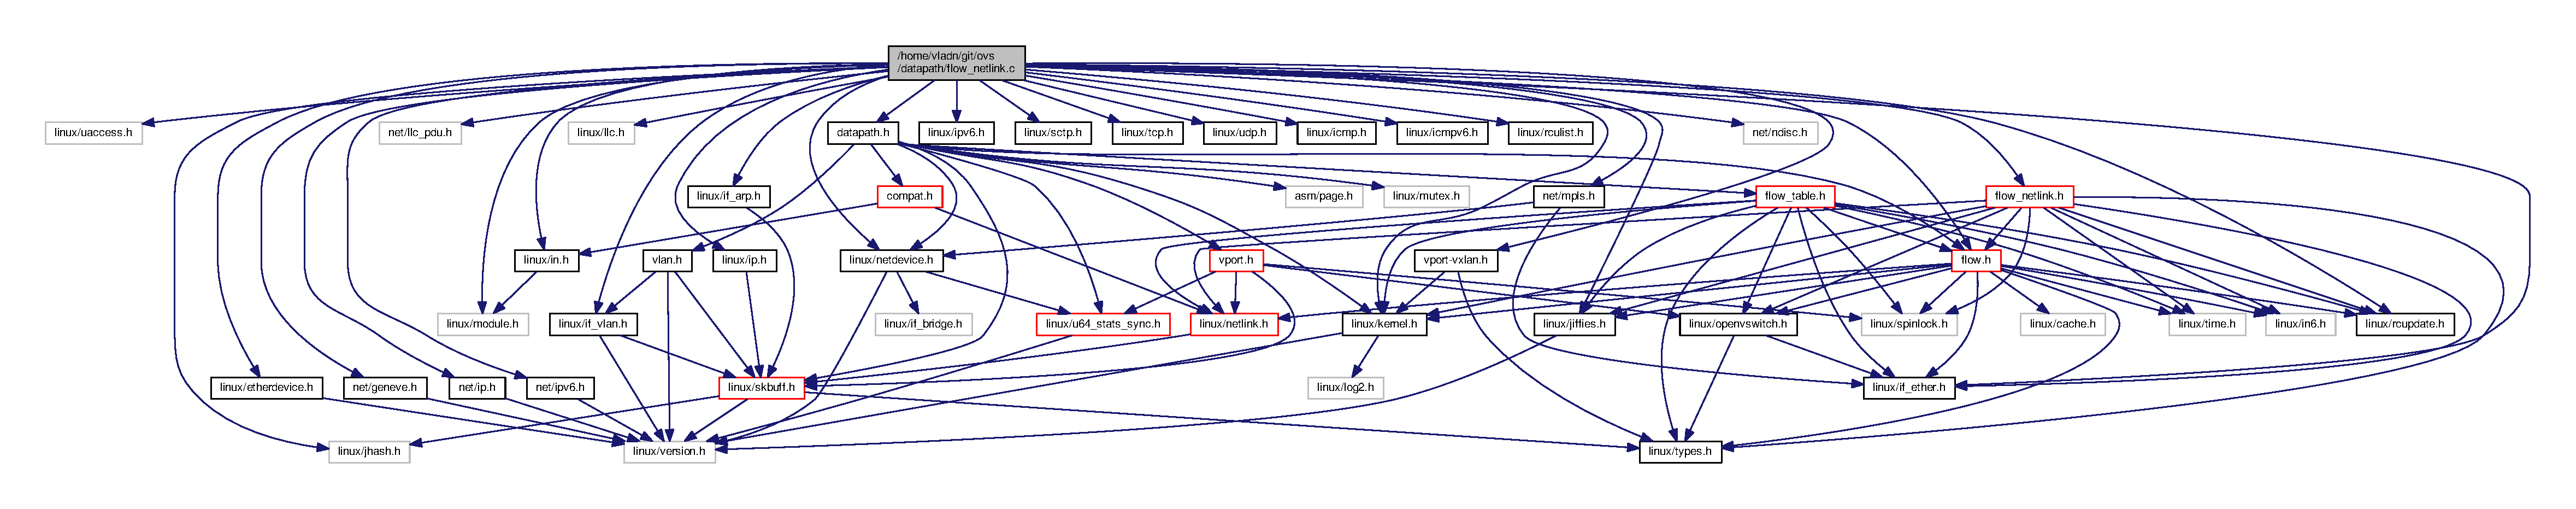
\includegraphics[width=350pt]{flow__netlink_8c__incl}
\end{center}
\end{figure}
\subsection*{Data Structures}
\begin{DoxyCompactItemize}
\item 
struct \hyperlink{structovs__len__tbl}{ovs\+\_\+len\+\_\+tbl}
\end{DoxyCompactItemize}
\subsection*{Macros}
\begin{DoxyCompactItemize}
\item 
\#define \hyperlink{flow__netlink_8c_a1f8c165bf4196327bc3abff648276d92}{pr\+\_\+fmt}(fmt)~K\+B\+U\+I\+L\+D\+\_\+\+M\+O\+D\+N\+A\+M\+E \char`\"{}\+: \char`\"{} fmt
\item 
\#define \hyperlink{flow__netlink_8c_aa45250c738c1a22be7f5e711887c8547}{O\+V\+S\+\_\+\+A\+T\+T\+R\+\_\+\+N\+E\+S\+T\+E\+D}~-\/1
\item 
\#define \hyperlink{flow__netlink_8c_a7cb040299f14f8ff8806dd868c321d7b}{S\+W\+\_\+\+F\+L\+O\+W\+\_\+\+K\+E\+Y\+\_\+\+P\+U\+T}(match,  field,  value,  is\+\_\+mask)
\item 
\#define \hyperlink{flow__netlink_8c_aceedf9228ebbe5291ac9e12d1d011278}{S\+W\+\_\+\+F\+L\+O\+W\+\_\+\+K\+E\+Y\+\_\+\+M\+E\+M\+C\+P\+Y\+\_\+\+O\+F\+F\+S\+E\+T}(match,  offset,  value\+\_\+p,  len,  is\+\_\+mask)
\item 
\#define \hyperlink{flow__netlink_8c_aa303fd044db169fb22013e1279c18dd1}{S\+W\+\_\+\+F\+L\+O\+W\+\_\+\+K\+E\+Y\+\_\+\+M\+E\+M\+C\+P\+Y}(match,  field,  value\+\_\+p,  len,  is\+\_\+mask)
\item 
\#define \hyperlink{flow__netlink_8c_a428fac9f6cc49614e07de128b9e4869f}{S\+W\+\_\+\+F\+L\+O\+W\+\_\+\+K\+E\+Y\+\_\+\+M\+E\+M\+S\+E\+T\+\_\+\+F\+I\+E\+L\+D}(match,  field,  value,  is\+\_\+mask)
\item 
\#define \hyperlink{flow__netlink_8c_a429e7a37f3797cd9870c534467a7f762}{M\+A\+X\+\_\+\+A\+C\+T\+I\+O\+N\+S\+\_\+\+B\+U\+F\+S\+I\+Z\+E}~(32 $\ast$ 1024)
\end{DoxyCompactItemize}
\subsection*{Functions}
\begin{DoxyCompactItemize}
\item 
static void \hyperlink{flow__netlink_8c_ac21a080dcc5b01d3da9b75d32b13fb40}{update\+\_\+range} (struct \hyperlink{structsw__flow__match}{sw\+\_\+flow\+\_\+match} $\ast$match, size\+\_\+t offset, size\+\_\+t size, \hyperlink{types_8h_afaa87723b8417d40fcf45b7330261ef9}{bool} is\+\_\+mask)
\item 
static \hyperlink{types_8h_afaa87723b8417d40fcf45b7330261ef9}{bool} \hyperlink{flow__netlink_8c_ab4be6b01938d3a8f5a14bc787cb2b0b2}{match\+\_\+validate} (const struct \hyperlink{structsw__flow__match}{sw\+\_\+flow\+\_\+match} $\ast$match, u64 key\+\_\+attrs, u64 mask\+\_\+attrs, \hyperlink{types_8h_afaa87723b8417d40fcf45b7330261ef9}{bool} log)
\item 
size\+\_\+t \hyperlink{flow__netlink_8c_ac920825ffe4fa75e7ca3c5e76ad4ec2a}{ovs\+\_\+tun\+\_\+key\+\_\+attr\+\_\+size} (void)
\item 
size\+\_\+t \hyperlink{flow__netlink_8c_a4ea1ec7f3650fd324fc1538c97e795d0}{ovs\+\_\+key\+\_\+attr\+\_\+size} (void)
\item 
static \hyperlink{types_8h_afaa87723b8417d40fcf45b7330261ef9}{bool} \hyperlink{flow__netlink_8c_a237e69cf49fbb7f26d6f886bdf4e4aad}{is\+\_\+all\+\_\+zero} (const u8 $\ast$fp, size\+\_\+t size)
\item 
static int \hyperlink{flow__netlink_8c_acc907c6eed2beccfb3d8564a9f627e93}{\+\_\+\+\_\+parse\+\_\+flow\+\_\+nlattrs} (const struct nlattr $\ast$attr, const struct nlattr $\ast$a\mbox{[}$\,$\mbox{]}, u64 $\ast$attrsp, \hyperlink{types_8h_afaa87723b8417d40fcf45b7330261ef9}{bool} log, \hyperlink{types_8h_afaa87723b8417d40fcf45b7330261ef9}{bool} nz)
\item 
static int \hyperlink{flow__netlink_8c_a4a090c5659903b6b8d125ab7598ad1a6}{parse\+\_\+flow\+\_\+mask\+\_\+nlattrs} (const struct nlattr $\ast$attr, const struct nlattr $\ast$a\mbox{[}$\,$\mbox{]}, u64 $\ast$attrsp, \hyperlink{types_8h_afaa87723b8417d40fcf45b7330261ef9}{bool} log)
\item 
static int \hyperlink{flow__netlink_8c_aafe0de49242cd0276fd5ced0fd81514f}{parse\+\_\+flow\+\_\+nlattrs} (const struct nlattr $\ast$attr, const struct nlattr $\ast$a\mbox{[}$\,$\mbox{]}, u64 $\ast$attrsp, \hyperlink{types_8h_afaa87723b8417d40fcf45b7330261ef9}{bool} log)
\item 
static int \hyperlink{flow__netlink_8c_a5f31d9f0798910742b360bbdfe29eeae}{genev\+\_\+tun\+\_\+opt\+\_\+from\+\_\+nlattr} (const struct nlattr $\ast$a, struct \hyperlink{structsw__flow__match}{sw\+\_\+flow\+\_\+match} $\ast$match, \hyperlink{types_8h_afaa87723b8417d40fcf45b7330261ef9}{bool} is\+\_\+mask, \hyperlink{types_8h_afaa87723b8417d40fcf45b7330261ef9}{bool} log)
\item 
static int \hyperlink{flow__netlink_8c_aef546829167c0fe738dd9db84c3848d4}{vxlan\+\_\+tun\+\_\+opt\+\_\+from\+\_\+nlattr} (const struct nlattr $\ast$a, struct \hyperlink{structsw__flow__match}{sw\+\_\+flow\+\_\+match} $\ast$match, \hyperlink{types_8h_afaa87723b8417d40fcf45b7330261ef9}{bool} is\+\_\+mask, \hyperlink{types_8h_afaa87723b8417d40fcf45b7330261ef9}{bool} log)
\item 
static int \hyperlink{flow__netlink_8c_aa9ad124d7dc9f5042d10b1237ce02f28}{ipv4\+\_\+tun\+\_\+from\+\_\+nlattr} (const struct nlattr $\ast$attr, struct \hyperlink{structsw__flow__match}{sw\+\_\+flow\+\_\+match} $\ast$match, \hyperlink{types_8h_afaa87723b8417d40fcf45b7330261ef9}{bool} is\+\_\+mask, \hyperlink{types_8h_afaa87723b8417d40fcf45b7330261ef9}{bool} log)
\item 
static int \hyperlink{flow__netlink_8c_a9283dd76011434d73c43654a9c32ecfb}{vxlan\+\_\+opt\+\_\+to\+\_\+nlattr} (struct sk\+\_\+buff $\ast$skb, const void $\ast$\hyperlink{flow_8h_a58d612a14e56d9b6c782667cd2e89799}{tun\+\_\+opts}, int swkey\+\_\+tun\+\_\+opts\+\_\+len)
\item 
static int \hyperlink{flow__netlink_8c_ac7f453fb68977c7a24d7af50f18b43db}{\+\_\+\+\_\+ipv4\+\_\+tun\+\_\+to\+\_\+nlattr} (struct sk\+\_\+buff $\ast$skb, const struct \hyperlink{structovs__key__ipv4__tunnel}{ovs\+\_\+key\+\_\+ipv4\+\_\+tunnel} $\ast$output, const void $\ast$\hyperlink{flow_8h_a58d612a14e56d9b6c782667cd2e89799}{tun\+\_\+opts}, int swkey\+\_\+tun\+\_\+opts\+\_\+len)
\item 
static int \hyperlink{flow__netlink_8c_a534ea0693e07f81a7a00f4b3125fbb1a}{ipv4\+\_\+tun\+\_\+to\+\_\+nlattr} (struct sk\+\_\+buff $\ast$skb, const struct \hyperlink{structovs__key__ipv4__tunnel}{ovs\+\_\+key\+\_\+ipv4\+\_\+tunnel} $\ast$output, const void $\ast$\hyperlink{flow_8h_a58d612a14e56d9b6c782667cd2e89799}{tun\+\_\+opts}, int swkey\+\_\+tun\+\_\+opts\+\_\+len)
\item 
int \hyperlink{flow__netlink_8c_a8a7309f6247775b5682061576c039e22}{ovs\+\_\+nla\+\_\+put\+\_\+egress\+\_\+tunnel\+\_\+key} (struct sk\+\_\+buff $\ast$skb, const struct \hyperlink{structovs__tunnel__info}{ovs\+\_\+tunnel\+\_\+info} $\ast$egress\+\_\+tun\+\_\+info)
\item 
static int \hyperlink{flow__netlink_8c_aed17f75c6136e01aa609132d5bbc9b2a}{metadata\+\_\+from\+\_\+nlattrs} (struct \hyperlink{structsw__flow__match}{sw\+\_\+flow\+\_\+match} $\ast$match, u64 $\ast$attrs, const struct nlattr $\ast$$\ast$a, \hyperlink{types_8h_afaa87723b8417d40fcf45b7330261ef9}{bool} is\+\_\+mask, \hyperlink{types_8h_afaa87723b8417d40fcf45b7330261ef9}{bool} log)
\item 
static int \hyperlink{flow__netlink_8c_a7e2f54c332f7bdac73756972da69ad53}{ovs\+\_\+key\+\_\+from\+\_\+nlattrs} (struct \hyperlink{structsw__flow__match}{sw\+\_\+flow\+\_\+match} $\ast$match, u64 attrs, const struct nlattr $\ast$$\ast$a, \hyperlink{types_8h_afaa87723b8417d40fcf45b7330261ef9}{bool} is\+\_\+mask, \hyperlink{types_8h_afaa87723b8417d40fcf45b7330261ef9}{bool} log)
\item 
static void \hyperlink{flow__netlink_8c_a412721fb459cda8f2b25400f8832d84f}{nlattr\+\_\+set} (struct nlattr $\ast$attr, u8 val, const struct \hyperlink{structovs__len__tbl}{ovs\+\_\+len\+\_\+tbl} $\ast$tbl)
\item 
static void \hyperlink{flow__netlink_8c_aa862995e0363dbb698ee51eb1be8a40c}{mask\+\_\+set\+\_\+nlattr} (struct nlattr $\ast$attr, u8 val)
\item 
int \hyperlink{flow__netlink_8c_a074547b2bcb32890a72ae873700391d5}{ovs\+\_\+nla\+\_\+get\+\_\+match} (struct \hyperlink{structsw__flow__match}{sw\+\_\+flow\+\_\+match} $\ast$match, const struct nlattr $\ast$nla\+\_\+key, const struct nlattr $\ast$nla\+\_\+mask, \hyperlink{types_8h_afaa87723b8417d40fcf45b7330261ef9}{bool} log)
\item 
static size\+\_\+t \hyperlink{flow__netlink_8c_a5189e471b5832c9371b45c5e58ca5b41}{get\+\_\+ufid\+\_\+len} (const struct nlattr $\ast$attr, \hyperlink{types_8h_afaa87723b8417d40fcf45b7330261ef9}{bool} log)
\item 
\hyperlink{types_8h_afaa87723b8417d40fcf45b7330261ef9}{bool} \hyperlink{flow__netlink_8c_a81e0cfe1c434ecde4ad684c8b8586877}{ovs\+\_\+nla\+\_\+get\+\_\+ufid} (struct \hyperlink{structsw__flow__id}{sw\+\_\+flow\+\_\+id} $\ast$sfid, const struct nlattr $\ast$attr, \hyperlink{types_8h_afaa87723b8417d40fcf45b7330261ef9}{bool} log)
\item 
int \hyperlink{flow__netlink_8c_aa416ab3b06ce40eee0be66306129c8d5}{ovs\+\_\+nla\+\_\+get\+\_\+identifier} (struct \hyperlink{structsw__flow__id}{sw\+\_\+flow\+\_\+id} $\ast$sfid, const struct nlattr $\ast$ufid, const struct \hyperlink{structsw__flow__key}{sw\+\_\+flow\+\_\+key} $\ast$key, \hyperlink{types_8h_afaa87723b8417d40fcf45b7330261ef9}{bool} log)
\item 
u32 \hyperlink{flow__netlink_8c_a415cb727697a02d62b8ff40795337d40}{ovs\+\_\+nla\+\_\+get\+\_\+ufid\+\_\+flags} (const struct nlattr $\ast$attr)
\item 
int \hyperlink{flow__netlink_8c_a90428a389e4ba65133d2cf837d5a8dc3}{ovs\+\_\+nla\+\_\+get\+\_\+flow\+\_\+metadata} (const struct nlattr $\ast$attr, struct \hyperlink{structsw__flow__key}{sw\+\_\+flow\+\_\+key} $\ast$key, \hyperlink{types_8h_afaa87723b8417d40fcf45b7330261ef9}{bool} log)
\item 
static int \hyperlink{flow__netlink_8c_a469e9434d0bedd721b2e31a106799335}{\+\_\+\+\_\+ovs\+\_\+nla\+\_\+put\+\_\+key} (const struct \hyperlink{structsw__flow__key}{sw\+\_\+flow\+\_\+key} $\ast$swkey, const struct \hyperlink{structsw__flow__key}{sw\+\_\+flow\+\_\+key} $\ast$output, \hyperlink{types_8h_afaa87723b8417d40fcf45b7330261ef9}{bool} is\+\_\+mask, struct sk\+\_\+buff $\ast$skb)
\item 
int \hyperlink{flow__netlink_8c_a845412e2f8f2bcb48df005e857474fcb}{ovs\+\_\+nla\+\_\+put\+\_\+key} (const struct \hyperlink{structsw__flow__key}{sw\+\_\+flow\+\_\+key} $\ast$swkey, const struct \hyperlink{structsw__flow__key}{sw\+\_\+flow\+\_\+key} $\ast$output, int attr, \hyperlink{types_8h_afaa87723b8417d40fcf45b7330261ef9}{bool} is\+\_\+mask, struct sk\+\_\+buff $\ast$skb)
\item 
int \hyperlink{flow__netlink_8c_a636f7d3cbe8656ceda87373110a4abc4}{ovs\+\_\+nla\+\_\+put\+\_\+identifier} (const struct \hyperlink{structsw__flow}{sw\+\_\+flow} $\ast$flow, struct sk\+\_\+buff $\ast$skb)
\item 
int \hyperlink{flow__netlink_8c_a2f6c3ab02b8e5d6296278dc9214500eb}{ovs\+\_\+nla\+\_\+put\+\_\+masked\+\_\+key} (const struct \hyperlink{structsw__flow}{sw\+\_\+flow} $\ast$flow, struct sk\+\_\+buff $\ast$skb)
\item 
int \hyperlink{flow__netlink_8c_af5ab12e938f8564945464a9e110eace3}{ovs\+\_\+nla\+\_\+put\+\_\+mask} (const struct \hyperlink{structsw__flow}{sw\+\_\+flow} $\ast$flow, struct sk\+\_\+buff $\ast$skb)
\item 
static struct \hyperlink{structsw__flow__actions}{sw\+\_\+flow\+\_\+actions} $\ast$ \hyperlink{flow__netlink_8c_acf3273c812551499c4b4d48651548286}{nla\+\_\+alloc\+\_\+flow\+\_\+actions} (int size, \hyperlink{types_8h_afaa87723b8417d40fcf45b7330261ef9}{bool} log)
\item 
static void \hyperlink{flow__netlink_8c_a386dd5cb0c8be8ce91e59761cbf820b4}{rcu\+\_\+free\+\_\+acts\+\_\+callback} (struct rcu\+\_\+head $\ast$rcu)
\item 
void \hyperlink{flow__netlink_8c_a5e773c3bb49bbeb0c0a4eb356c779a22}{ovs\+\_\+nla\+\_\+free\+\_\+flow\+\_\+actions} (struct \hyperlink{structsw__flow__actions}{sw\+\_\+flow\+\_\+actions} $\ast$sf\+\_\+acts)
\item 
static struct nlattr $\ast$ \hyperlink{flow__netlink_8c_a5ce53ec8a0a126f8e33e1d9af6e1e083}{reserve\+\_\+sfa\+\_\+size} (struct \hyperlink{structsw__flow__actions}{sw\+\_\+flow\+\_\+actions} $\ast$$\ast$sfa, int attr\+\_\+len, \hyperlink{types_8h_afaa87723b8417d40fcf45b7330261ef9}{bool} log)
\item 
static struct nlattr $\ast$ \hyperlink{flow__netlink_8c_ad6fb4bf743e36b42c72eaa09db192e87}{\+\_\+\+\_\+add\+\_\+action} (struct \hyperlink{structsw__flow__actions}{sw\+\_\+flow\+\_\+actions} $\ast$$\ast$sfa, int attrtype, void $\ast$data, int len, \hyperlink{types_8h_afaa87723b8417d40fcf45b7330261ef9}{bool} log)
\item 
static int \hyperlink{flow__netlink_8c_a4316343b483e9a6b4d8885147036beb2}{add\+\_\+action} (struct \hyperlink{structsw__flow__actions}{sw\+\_\+flow\+\_\+actions} $\ast$$\ast$sfa, int attrtype, void $\ast$data, int len, \hyperlink{types_8h_afaa87723b8417d40fcf45b7330261ef9}{bool} log)
\item 
static int \hyperlink{flow__netlink_8c_a08778088a1f3c3c88aee0055bcd05110}{add\+\_\+nested\+\_\+action\+\_\+start} (struct \hyperlink{structsw__flow__actions}{sw\+\_\+flow\+\_\+actions} $\ast$$\ast$sfa, int attrtype, \hyperlink{types_8h_afaa87723b8417d40fcf45b7330261ef9}{bool} log)
\item 
static void \hyperlink{flow__netlink_8c_ab0176001eff016bfad478f0f06cefa0a}{add\+\_\+nested\+\_\+action\+\_\+end} (struct \hyperlink{structsw__flow__actions}{sw\+\_\+flow\+\_\+actions} $\ast$sfa, int st\+\_\+offset)
\item 
static int \hyperlink{flow__netlink_8c_ae5c58b498948d3c5564b7916505d8455}{\+\_\+\+\_\+ovs\+\_\+nla\+\_\+copy\+\_\+actions} (const struct nlattr $\ast$attr, const struct \hyperlink{structsw__flow__key}{sw\+\_\+flow\+\_\+key} $\ast$key, int depth, struct \hyperlink{structsw__flow__actions}{sw\+\_\+flow\+\_\+actions} $\ast$$\ast$sfa, \+\_\+\+\_\+be16 eth\+\_\+type, \+\_\+\+\_\+be16 vlan\+\_\+tci, \hyperlink{types_8h_afaa87723b8417d40fcf45b7330261ef9}{bool} log)
\item 
static int \hyperlink{flow__netlink_8c_a0dcf3429559610cf8b8204e04151728b}{validate\+\_\+and\+\_\+copy\+\_\+sample} (const struct nlattr $\ast$attr, const struct \hyperlink{structsw__flow__key}{sw\+\_\+flow\+\_\+key} $\ast$key, int depth, struct \hyperlink{structsw__flow__actions}{sw\+\_\+flow\+\_\+actions} $\ast$$\ast$sfa, \+\_\+\+\_\+be16 eth\+\_\+type, \+\_\+\+\_\+be16 vlan\+\_\+tci, \hyperlink{types_8h_afaa87723b8417d40fcf45b7330261ef9}{bool} log)
\item 
void \hyperlink{flow__netlink_8c_a1a09e9d38844c59332975789573e994c}{ovs\+\_\+match\+\_\+init} (struct \hyperlink{structsw__flow__match}{sw\+\_\+flow\+\_\+match} $\ast$match, struct \hyperlink{structsw__flow__key}{sw\+\_\+flow\+\_\+key} $\ast$key, struct \hyperlink{structsw__flow__mask}{sw\+\_\+flow\+\_\+mask} $\ast$mask)
\item 
static int \hyperlink{flow__netlink_8c_af4e9606a99a9ccc71de18c0531a99808}{validate\+\_\+geneve\+\_\+opts} (struct \hyperlink{structsw__flow__key}{sw\+\_\+flow\+\_\+key} $\ast$key)
\item 
static int \hyperlink{flow__netlink_8c_ac06cff749bd68b0a91ecacc196b4892f}{validate\+\_\+and\+\_\+copy\+\_\+set\+\_\+tun} (const struct nlattr $\ast$attr, struct \hyperlink{structsw__flow__actions}{sw\+\_\+flow\+\_\+actions} $\ast$$\ast$sfa, \hyperlink{types_8h_afaa87723b8417d40fcf45b7330261ef9}{bool} log)
\item 
static \hyperlink{types_8h_afaa87723b8417d40fcf45b7330261ef9}{bool} \hyperlink{flow__netlink_8c_ae01edbfa96ed8cef19cb86caf0512d7a}{validate\+\_\+masked} (u8 $\ast$data, int len)
\item 
static int \hyperlink{flow__netlink_8c_afabdbd008e8fb3c515063cafaf267e02}{validate\+\_\+set} (const struct nlattr $\ast$a, const struct \hyperlink{structsw__flow__key}{sw\+\_\+flow\+\_\+key} $\ast$flow\+\_\+key, struct \hyperlink{structsw__flow__actions}{sw\+\_\+flow\+\_\+actions} $\ast$$\ast$sfa, \hyperlink{types_8h_afaa87723b8417d40fcf45b7330261ef9}{bool} $\ast$skip\+\_\+copy, \+\_\+\+\_\+be16 eth\+\_\+type, \hyperlink{types_8h_afaa87723b8417d40fcf45b7330261ef9}{bool} masked, \hyperlink{types_8h_afaa87723b8417d40fcf45b7330261ef9}{bool} log)
\item 
static int \hyperlink{flow__netlink_8c_ab7c5d132ac3085d8c2da993c66138ab0}{validate\+\_\+userspace} (const struct nlattr $\ast$attr)
\item 
static int \hyperlink{flow__netlink_8c_a746e2c558f7350550b1734826a8c25f7}{copy\+\_\+action} (const struct nlattr $\ast$from, struct \hyperlink{structsw__flow__actions}{sw\+\_\+flow\+\_\+actions} $\ast$$\ast$sfa, \hyperlink{types_8h_afaa87723b8417d40fcf45b7330261ef9}{bool} log)
\item 
int \hyperlink{flow__netlink_8c_a10dc93f8c379eae7a557d54d9b387dd6}{ovs\+\_\+nla\+\_\+copy\+\_\+actions} (const struct nlattr $\ast$attr, const struct \hyperlink{structsw__flow__key}{sw\+\_\+flow\+\_\+key} $\ast$key, struct \hyperlink{structsw__flow__actions}{sw\+\_\+flow\+\_\+actions} $\ast$$\ast$sfa, \hyperlink{types_8h_afaa87723b8417d40fcf45b7330261ef9}{bool} log)
\item 
static int \hyperlink{flow__netlink_8c_a92621d7eaed9e960f5e5d7b72e501db0}{sample\+\_\+action\+\_\+to\+\_\+attr} (const struct nlattr $\ast$attr, struct sk\+\_\+buff $\ast$skb)
\item 
static int \hyperlink{flow__netlink_8c_af38f12c35d382eb717bb6e5b4fba2309}{set\+\_\+action\+\_\+to\+\_\+attr} (const struct nlattr $\ast$a, struct sk\+\_\+buff $\ast$skb)
\item 
static int \hyperlink{flow__netlink_8c_a14e859cc22996f05850ca737daf2ee09}{masked\+\_\+set\+\_\+action\+\_\+to\+\_\+set\+\_\+action\+\_\+attr} (const struct nlattr $\ast$a, struct sk\+\_\+buff $\ast$skb)
\item 
int \hyperlink{flow__netlink_8c_a923304ee69be1cfa52197b0f73c29e49}{ovs\+\_\+nla\+\_\+put\+\_\+actions} (const struct nlattr $\ast$attr, int len, struct sk\+\_\+buff $\ast$skb)
\end{DoxyCompactItemize}
\subsection*{Variables}
\begin{DoxyCompactItemize}
\item 
static const struct \hyperlink{structovs__len__tbl}{ovs\+\_\+len\+\_\+tbl} \hyperlink{flow__netlink_8c_abcfd7a34b15e86938f3646cda1522e07}{ovs\+\_\+tunnel\+\_\+key\+\_\+lens} \mbox{[}\hyperlink{openvswitch_8h_a1c8eef7445d1c45bb90eb65de59a81e4}{O\+V\+S\+\_\+\+T\+U\+N\+N\+E\+L\+\_\+\+K\+E\+Y\+\_\+\+A\+T\+T\+R\+\_\+\+M\+A\+X}+1\mbox{]}
\item 
static const struct \hyperlink{structovs__len__tbl}{ovs\+\_\+len\+\_\+tbl} \hyperlink{flow__netlink_8c_a5565daa559332f47a1d214007d97e0d7}{ovs\+\_\+key\+\_\+lens} \mbox{[}\hyperlink{openvswitch_8h_a2a2adc6c47c38f0e7889580602ccbe22}{O\+V\+S\+\_\+\+K\+E\+Y\+\_\+\+A\+T\+T\+R\+\_\+\+M\+A\+X}+1\mbox{]}
\item 
static const struct nla\+\_\+policy \hyperlink{flow__netlink_8c_ac262f3819d334e0cbbdf8198d6d2aed8}{vxlan\+\_\+opt\+\_\+policy} \mbox{[}\hyperlink{openvswitch_8h_ac764e78fe2e06d11f39448e337292c7c}{O\+V\+S\+\_\+\+V\+X\+L\+A\+N\+\_\+\+E\+X\+T\+\_\+\+M\+A\+X}+1\mbox{]}
\end{DoxyCompactItemize}


\subsection{Macro Definition Documentation}
\hypertarget{flow__netlink_8c_a429e7a37f3797cd9870c534467a7f762}{}\index{flow\+\_\+netlink.\+c@{flow\+\_\+netlink.\+c}!M\+A\+X\+\_\+\+A\+C\+T\+I\+O\+N\+S\+\_\+\+B\+U\+F\+S\+I\+Z\+E@{M\+A\+X\+\_\+\+A\+C\+T\+I\+O\+N\+S\+\_\+\+B\+U\+F\+S\+I\+Z\+E}}
\index{M\+A\+X\+\_\+\+A\+C\+T\+I\+O\+N\+S\+\_\+\+B\+U\+F\+S\+I\+Z\+E@{M\+A\+X\+\_\+\+A\+C\+T\+I\+O\+N\+S\+\_\+\+B\+U\+F\+S\+I\+Z\+E}!flow\+\_\+netlink.\+c@{flow\+\_\+netlink.\+c}}
\subsubsection[{M\+A\+X\+\_\+\+A\+C\+T\+I\+O\+N\+S\+\_\+\+B\+U\+F\+S\+I\+Z\+E}]{\setlength{\rightskip}{0pt plus 5cm}\#define M\+A\+X\+\_\+\+A\+C\+T\+I\+O\+N\+S\+\_\+\+B\+U\+F\+S\+I\+Z\+E~(32 $\ast$ 1024)}\label{flow__netlink_8c_a429e7a37f3797cd9870c534467a7f762}
\hypertarget{flow__netlink_8c_aa45250c738c1a22be7f5e711887c8547}{}\index{flow\+\_\+netlink.\+c@{flow\+\_\+netlink.\+c}!O\+V\+S\+\_\+\+A\+T\+T\+R\+\_\+\+N\+E\+S\+T\+E\+D@{O\+V\+S\+\_\+\+A\+T\+T\+R\+\_\+\+N\+E\+S\+T\+E\+D}}
\index{O\+V\+S\+\_\+\+A\+T\+T\+R\+\_\+\+N\+E\+S\+T\+E\+D@{O\+V\+S\+\_\+\+A\+T\+T\+R\+\_\+\+N\+E\+S\+T\+E\+D}!flow\+\_\+netlink.\+c@{flow\+\_\+netlink.\+c}}
\subsubsection[{O\+V\+S\+\_\+\+A\+T\+T\+R\+\_\+\+N\+E\+S\+T\+E\+D}]{\setlength{\rightskip}{0pt plus 5cm}\#define O\+V\+S\+\_\+\+A\+T\+T\+R\+\_\+\+N\+E\+S\+T\+E\+D~-\/1}\label{flow__netlink_8c_aa45250c738c1a22be7f5e711887c8547}
\hypertarget{flow__netlink_8c_a1f8c165bf4196327bc3abff648276d92}{}\index{flow\+\_\+netlink.\+c@{flow\+\_\+netlink.\+c}!pr\+\_\+fmt@{pr\+\_\+fmt}}
\index{pr\+\_\+fmt@{pr\+\_\+fmt}!flow\+\_\+netlink.\+c@{flow\+\_\+netlink.\+c}}
\subsubsection[{pr\+\_\+fmt}]{\setlength{\rightskip}{0pt plus 5cm}\#define pr\+\_\+fmt(
\begin{DoxyParamCaption}
\item[{}]{fmt}
\end{DoxyParamCaption}
)~K\+B\+U\+I\+L\+D\+\_\+\+M\+O\+D\+N\+A\+M\+E \char`\"{}\+: \char`\"{} fmt}\label{flow__netlink_8c_a1f8c165bf4196327bc3abff648276d92}
\hypertarget{flow__netlink_8c_aa303fd044db169fb22013e1279c18dd1}{}\index{flow\+\_\+netlink.\+c@{flow\+\_\+netlink.\+c}!S\+W\+\_\+\+F\+L\+O\+W\+\_\+\+K\+E\+Y\+\_\+\+M\+E\+M\+C\+P\+Y@{S\+W\+\_\+\+F\+L\+O\+W\+\_\+\+K\+E\+Y\+\_\+\+M\+E\+M\+C\+P\+Y}}
\index{S\+W\+\_\+\+F\+L\+O\+W\+\_\+\+K\+E\+Y\+\_\+\+M\+E\+M\+C\+P\+Y@{S\+W\+\_\+\+F\+L\+O\+W\+\_\+\+K\+E\+Y\+\_\+\+M\+E\+M\+C\+P\+Y}!flow\+\_\+netlink.\+c@{flow\+\_\+netlink.\+c}}
\subsubsection[{S\+W\+\_\+\+F\+L\+O\+W\+\_\+\+K\+E\+Y\+\_\+\+M\+E\+M\+C\+P\+Y}]{\setlength{\rightskip}{0pt plus 5cm}\#define S\+W\+\_\+\+F\+L\+O\+W\+\_\+\+K\+E\+Y\+\_\+\+M\+E\+M\+C\+P\+Y(
\begin{DoxyParamCaption}
\item[{}]{match, }
\item[{}]{field, }
\item[{}]{value\+\_\+p, }
\item[{}]{len, }
\item[{}]{is\+\_\+mask}
\end{DoxyParamCaption}
)}\label{flow__netlink_8c_aa303fd044db169fb22013e1279c18dd1}
{\bfseries Value\+:}
\begin{DoxyCode}
\hyperlink{flow__netlink_8c_aceedf9228ebbe5291ac9e12d1d011278}{SW\_FLOW\_KEY\_MEMCPY\_OFFSET}(match, offsetof(\textcolor{keyword}{struct} 
      \hyperlink{structsw__flow__key}{sw\_flow\_key}, field), \(\backslash\)
                  value\_p, len, is\_mask)
\end{DoxyCode}
\hypertarget{flow__netlink_8c_aceedf9228ebbe5291ac9e12d1d011278}{}\index{flow\+\_\+netlink.\+c@{flow\+\_\+netlink.\+c}!S\+W\+\_\+\+F\+L\+O\+W\+\_\+\+K\+E\+Y\+\_\+\+M\+E\+M\+C\+P\+Y\+\_\+\+O\+F\+F\+S\+E\+T@{S\+W\+\_\+\+F\+L\+O\+W\+\_\+\+K\+E\+Y\+\_\+\+M\+E\+M\+C\+P\+Y\+\_\+\+O\+F\+F\+S\+E\+T}}
\index{S\+W\+\_\+\+F\+L\+O\+W\+\_\+\+K\+E\+Y\+\_\+\+M\+E\+M\+C\+P\+Y\+\_\+\+O\+F\+F\+S\+E\+T@{S\+W\+\_\+\+F\+L\+O\+W\+\_\+\+K\+E\+Y\+\_\+\+M\+E\+M\+C\+P\+Y\+\_\+\+O\+F\+F\+S\+E\+T}!flow\+\_\+netlink.\+c@{flow\+\_\+netlink.\+c}}
\subsubsection[{S\+W\+\_\+\+F\+L\+O\+W\+\_\+\+K\+E\+Y\+\_\+\+M\+E\+M\+C\+P\+Y\+\_\+\+O\+F\+F\+S\+E\+T}]{\setlength{\rightskip}{0pt plus 5cm}\#define S\+W\+\_\+\+F\+L\+O\+W\+\_\+\+K\+E\+Y\+\_\+\+M\+E\+M\+C\+P\+Y\+\_\+\+O\+F\+F\+S\+E\+T(
\begin{DoxyParamCaption}
\item[{}]{match, }
\item[{}]{offset, }
\item[{}]{value\+\_\+p, }
\item[{}]{len, }
\item[{}]{is\+\_\+mask}
\end{DoxyParamCaption}
)}\label{flow__netlink_8c_aceedf9228ebbe5291ac9e12d1d011278}
{\bfseries Value\+:}
\begin{DoxyCode}
\textcolor{keywordflow}{do} \{                                    \hyperlink{flow__netlink_8c_ac21a080dcc5b01d3da9b75d32b13fb40}{\(\backslash\)}
\hyperlink{flow__netlink_8c_ac21a080dcc5b01d3da9b75d32b13fb40}{        update\_range}(match, offset, len, is\_mask);            \(\backslash\)
        if (is\_mask)                            \(\backslash\)
            memcpy((u8 *)&(match)->mask->key + offset, value\_p, len);\(\backslash\)
        else                                \(\backslash\)
            memcpy((u8 *)(match)->key + offset, value\_p, len);  \(\backslash\)
    \} \textcolor{keywordflow}{while} (0)
\end{DoxyCode}
\hypertarget{flow__netlink_8c_a428fac9f6cc49614e07de128b9e4869f}{}\index{flow\+\_\+netlink.\+c@{flow\+\_\+netlink.\+c}!S\+W\+\_\+\+F\+L\+O\+W\+\_\+\+K\+E\+Y\+\_\+\+M\+E\+M\+S\+E\+T\+\_\+\+F\+I\+E\+L\+D@{S\+W\+\_\+\+F\+L\+O\+W\+\_\+\+K\+E\+Y\+\_\+\+M\+E\+M\+S\+E\+T\+\_\+\+F\+I\+E\+L\+D}}
\index{S\+W\+\_\+\+F\+L\+O\+W\+\_\+\+K\+E\+Y\+\_\+\+M\+E\+M\+S\+E\+T\+\_\+\+F\+I\+E\+L\+D@{S\+W\+\_\+\+F\+L\+O\+W\+\_\+\+K\+E\+Y\+\_\+\+M\+E\+M\+S\+E\+T\+\_\+\+F\+I\+E\+L\+D}!flow\+\_\+netlink.\+c@{flow\+\_\+netlink.\+c}}
\subsubsection[{S\+W\+\_\+\+F\+L\+O\+W\+\_\+\+K\+E\+Y\+\_\+\+M\+E\+M\+S\+E\+T\+\_\+\+F\+I\+E\+L\+D}]{\setlength{\rightskip}{0pt plus 5cm}\#define S\+W\+\_\+\+F\+L\+O\+W\+\_\+\+K\+E\+Y\+\_\+\+M\+E\+M\+S\+E\+T\+\_\+\+F\+I\+E\+L\+D(
\begin{DoxyParamCaption}
\item[{}]{match, }
\item[{}]{field, }
\item[{}]{value, }
\item[{}]{is\+\_\+mask}
\end{DoxyParamCaption}
)}\label{flow__netlink_8c_a428fac9f6cc49614e07de128b9e4869f}
{\bfseries Value\+:}
\begin{DoxyCode}
\textcolor{keywordflow}{do} \{                                    \hyperlink{flow__netlink_8c_ac21a080dcc5b01d3da9b75d32b13fb40}{\(\backslash\)}
\hyperlink{flow__netlink_8c_ac21a080dcc5b01d3da9b75d32b13fb40}{        update\_range}(match, offsetof(\textcolor{keyword}{struct} \hyperlink{structsw__flow__key}{sw\_flow\_key}, field),    \(\backslash\)
                 \textcolor{keyword}{sizeof}((match)->key->field), is\_mask);     \(\backslash\)
        if (is\_mask)                            \(\backslash\)
            memset((u8 *)&(match)->mask->key.field, value,      \(\backslash\)
                   \textcolor{keyword}{sizeof}((match)->mask->key.field));       \(\backslash\)
        else                                \(\backslash\)
            memset((u8 *)&(match)->key->field, value,           \(\backslash\)
                   \textcolor{keyword}{sizeof}((match)->key->field));                \(\backslash\)
    \} \textcolor{keywordflow}{while} (0)
\end{DoxyCode}
\hypertarget{flow__netlink_8c_a7cb040299f14f8ff8806dd868c321d7b}{}\index{flow\+\_\+netlink.\+c@{flow\+\_\+netlink.\+c}!S\+W\+\_\+\+F\+L\+O\+W\+\_\+\+K\+E\+Y\+\_\+\+P\+U\+T@{S\+W\+\_\+\+F\+L\+O\+W\+\_\+\+K\+E\+Y\+\_\+\+P\+U\+T}}
\index{S\+W\+\_\+\+F\+L\+O\+W\+\_\+\+K\+E\+Y\+\_\+\+P\+U\+T@{S\+W\+\_\+\+F\+L\+O\+W\+\_\+\+K\+E\+Y\+\_\+\+P\+U\+T}!flow\+\_\+netlink.\+c@{flow\+\_\+netlink.\+c}}
\subsubsection[{S\+W\+\_\+\+F\+L\+O\+W\+\_\+\+K\+E\+Y\+\_\+\+P\+U\+T}]{\setlength{\rightskip}{0pt plus 5cm}\#define S\+W\+\_\+\+F\+L\+O\+W\+\_\+\+K\+E\+Y\+\_\+\+P\+U\+T(
\begin{DoxyParamCaption}
\item[{}]{match, }
\item[{}]{field, }
\item[{}]{value, }
\item[{}]{is\+\_\+mask}
\end{DoxyParamCaption}
)}\label{flow__netlink_8c_a7cb040299f14f8ff8806dd868c321d7b}
{\bfseries Value\+:}
\begin{DoxyCode}
\textcolor{keywordflow}{do} \{ \hyperlink{flow__netlink_8c_ac21a080dcc5b01d3da9b75d32b13fb40}{\(\backslash\)}
\hyperlink{flow__netlink_8c_ac21a080dcc5b01d3da9b75d32b13fb40}{        update\_range}(match, offsetof(\textcolor{keyword}{struct} \hyperlink{structsw__flow__key}{sw\_flow\_key}, field),    \(\backslash\)
                 \textcolor{keyword}{sizeof}((match)->key->field), is\_mask);     \(\backslash\)
        if (is\_mask)                            \(\backslash\)
            (match)->mask->key.field = value;           \(\backslash\)
        \textcolor{keywordflow}{else}                                \(\backslash\)
            (match)->key->field = value;                    \(\backslash\)
    \} \textcolor{keywordflow}{while} (0)
\end{DoxyCode}


\subsection{Function Documentation}
\hypertarget{flow__netlink_8c_ad6fb4bf743e36b42c72eaa09db192e87}{}\index{flow\+\_\+netlink.\+c@{flow\+\_\+netlink.\+c}!\+\_\+\+\_\+add\+\_\+action@{\+\_\+\+\_\+add\+\_\+action}}
\index{\+\_\+\+\_\+add\+\_\+action@{\+\_\+\+\_\+add\+\_\+action}!flow\+\_\+netlink.\+c@{flow\+\_\+netlink.\+c}}
\subsubsection[{\+\_\+\+\_\+add\+\_\+action}]{\setlength{\rightskip}{0pt plus 5cm}static struct nlattr$\ast$ \+\_\+\+\_\+add\+\_\+action (
\begin{DoxyParamCaption}
\item[{struct {\bf sw\+\_\+flow\+\_\+actions} $\ast$$\ast$}]{sfa, }
\item[{int}]{attrtype, }
\item[{void $\ast$}]{data, }
\item[{int}]{len, }
\item[{{\bf bool}}]{log}
\end{DoxyParamCaption}
)\hspace{0.3cm}{\ttfamily [static]}}\label{flow__netlink_8c_ad6fb4bf743e36b42c72eaa09db192e87}

\begin{DoxyCode}
1604 \{
1605     \textcolor{keyword}{struct }nlattr *a;
1606 
1607     a = \hyperlink{flow__netlink_8c_a5ce53ec8a0a126f8e33e1d9af6e1e083}{reserve\_sfa\_size}(sfa, nla\_attr\_size(len), log);
1608     \textcolor{keywordflow}{if} (IS\_ERR(a))
1609         \textcolor{keywordflow}{return} a;
1610 
1611     a->nla\_type = attrtype;
1612     a->nla\_len = nla\_attr\_size(len);
1613 
1614     \textcolor{keywordflow}{if} (data)
1615         memcpy(nla\_data(a), data, len);
1616     memset((\textcolor{keywordtype}{unsigned} \textcolor{keywordtype}{char} *) a + a->nla\_len, 0, nla\_padlen(len));
1617 
1618     \textcolor{keywordflow}{return} a;
1619 \}
\end{DoxyCode}
\hypertarget{flow__netlink_8c_ac7f453fb68977c7a24d7af50f18b43db}{}\index{flow\+\_\+netlink.\+c@{flow\+\_\+netlink.\+c}!\+\_\+\+\_\+ipv4\+\_\+tun\+\_\+to\+\_\+nlattr@{\+\_\+\+\_\+ipv4\+\_\+tun\+\_\+to\+\_\+nlattr}}
\index{\+\_\+\+\_\+ipv4\+\_\+tun\+\_\+to\+\_\+nlattr@{\+\_\+\+\_\+ipv4\+\_\+tun\+\_\+to\+\_\+nlattr}!flow\+\_\+netlink.\+c@{flow\+\_\+netlink.\+c}}
\subsubsection[{\+\_\+\+\_\+ipv4\+\_\+tun\+\_\+to\+\_\+nlattr}]{\setlength{\rightskip}{0pt plus 5cm}static int \+\_\+\+\_\+ipv4\+\_\+tun\+\_\+to\+\_\+nlattr (
\begin{DoxyParamCaption}
\item[{struct sk\+\_\+buff $\ast$}]{skb, }
\item[{const struct {\bf ovs\+\_\+key\+\_\+ipv4\+\_\+tunnel} $\ast$}]{output, }
\item[{const void $\ast$}]{tun\+\_\+opts, }
\item[{int}]{swkey\+\_\+tun\+\_\+opts\+\_\+len}
\end{DoxyParamCaption}
)\hspace{0.3cm}{\ttfamily [static]}}\label{flow__netlink_8c_ac7f453fb68977c7a24d7af50f18b43db}

\begin{DoxyCode}
646 \{
647     \textcolor{keywordflow}{if} (output->\hyperlink{structovs__key__ipv4__tunnel_a7459e66ecf90329eb2fa6cf3fc4781db}{tun\_flags} & \hyperlink{ip__tunnels_8h_a5438f4a0ea8e58438776fffbed3f08a8}{TUNNEL\_KEY} &&
648         \hyperlink{net_2netlink_8h_a610b2c7f3f7996a3b2406ce1bc708b5e}{nla\_put\_be64}(skb, \hyperlink{openvswitch_8h_a3ab62ef434a436d109e5dc7fe6a7f427abba6b12276aaae09ecdf61a2189edda5}{OVS\_TUNNEL\_KEY\_ATTR\_ID}, output->
      \hyperlink{structovs__key__ipv4__tunnel_ae36132bc05ca6257b572edddffcb867a}{tun\_id}))
649         \textcolor{keywordflow}{return} -EMSGSIZE;
650     \textcolor{keywordflow}{if} (output->\hyperlink{structovs__key__ipv4__tunnel_a1e5a978f104d61e9694e914a109734a7}{ipv4\_src} &&
651         \hyperlink{net_2netlink_8h_a2e2a0bd10c5f5139dc80413fd8dcbbe7}{nla\_put\_be32}(skb, \hyperlink{openvswitch_8h_a3ab62ef434a436d109e5dc7fe6a7f427add76f93836f5e1dcb33419c58aa1afd0}{OVS\_TUNNEL\_KEY\_ATTR\_IPV4\_SRC}, output->
      \hyperlink{structovs__key__ipv4__tunnel_a1e5a978f104d61e9694e914a109734a7}{ipv4\_src}))
652         \textcolor{keywordflow}{return} -EMSGSIZE;
653     \textcolor{keywordflow}{if} (output->\hyperlink{structovs__key__ipv4__tunnel_ae443d381a97f53bbc4139fe36c0aae30}{ipv4\_dst} &&
654         \hyperlink{net_2netlink_8h_a2e2a0bd10c5f5139dc80413fd8dcbbe7}{nla\_put\_be32}(skb, \hyperlink{openvswitch_8h_a3ab62ef434a436d109e5dc7fe6a7f427aa8a1fb062a0a5c1c718096a530c1fee9}{OVS\_TUNNEL\_KEY\_ATTR\_IPV4\_DST}, output->
      \hyperlink{structovs__key__ipv4__tunnel_ae443d381a97f53bbc4139fe36c0aae30}{ipv4\_dst}))
655         \textcolor{keywordflow}{return} -EMSGSIZE;
656     \textcolor{keywordflow}{if} (output->\hyperlink{structovs__key__ipv4__tunnel_a69594eaf9d7dfc2824b264484e02498e}{ipv4\_tos} &&
657         nla\_put\_u8(skb, \hyperlink{openvswitch_8h_a3ab62ef434a436d109e5dc7fe6a7f427ab452549b72cc81cc38c53a0487cded37}{OVS\_TUNNEL\_KEY\_ATTR\_TOS}, output->
      \hyperlink{structovs__key__ipv4__tunnel_a69594eaf9d7dfc2824b264484e02498e}{ipv4\_tos}))
658         \textcolor{keywordflow}{return} -EMSGSIZE;
659     \textcolor{keywordflow}{if} (nla\_put\_u8(skb, \hyperlink{openvswitch_8h_a3ab62ef434a436d109e5dc7fe6a7f427ace9b9fe26daaf5d99409d1563cc68f5c}{OVS\_TUNNEL\_KEY\_ATTR\_TTL}, output->
      \hyperlink{structovs__key__ipv4__tunnel_a24de7472a8c22903fce96b73dab68a40}{ipv4\_ttl}))
660         \textcolor{keywordflow}{return} -EMSGSIZE;
661     \textcolor{keywordflow}{if} ((output->\hyperlink{structovs__key__ipv4__tunnel_a7459e66ecf90329eb2fa6cf3fc4781db}{tun\_flags} & \hyperlink{ip__tunnels_8h_a3b33c8fadb48f2281d5852e2a0d8eeff}{TUNNEL\_DONT\_FRAGMENT}) &&
662         nla\_put\_flag(skb, \hyperlink{openvswitch_8h_a3ab62ef434a436d109e5dc7fe6a7f427a2b4acde1fe308fb5cdb703d197ccad11}{OVS\_TUNNEL\_KEY\_ATTR\_DONT\_FRAGMENT}))
663         \textcolor{keywordflow}{return} -EMSGSIZE;
664     \textcolor{keywordflow}{if} ((output->\hyperlink{structovs__key__ipv4__tunnel_a7459e66ecf90329eb2fa6cf3fc4781db}{tun\_flags} & \hyperlink{ip__tunnels_8h_ac8dc03940c0621b1aeddafa9b620022c}{TUNNEL\_CSUM}) &&
665         nla\_put\_flag(skb, \hyperlink{openvswitch_8h_a3ab62ef434a436d109e5dc7fe6a7f427a0b2355fe72f1590f795e2febdcb3cafe}{OVS\_TUNNEL\_KEY\_ATTR\_CSUM}))
666         \textcolor{keywordflow}{return} -EMSGSIZE;
667     \textcolor{keywordflow}{if} (output->\hyperlink{structovs__key__ipv4__tunnel_acda46848fad6a931296f3e7a74b44a18}{tp\_src} &&
668         \hyperlink{net_2netlink_8h_aafa7ef6ea62a477fe1cf21d435e2a718}{nla\_put\_be16}(skb, \hyperlink{openvswitch_8h_a3ab62ef434a436d109e5dc7fe6a7f427a82ec563a3032a39aa9f9694276933101}{OVS\_TUNNEL\_KEY\_ATTR\_TP\_SRC}, output->
      \hyperlink{structovs__key__ipv4__tunnel_acda46848fad6a931296f3e7a74b44a18}{tp\_src}))
669         \textcolor{keywordflow}{return} -EMSGSIZE;
670     \textcolor{keywordflow}{if} (output->\hyperlink{structovs__key__ipv4__tunnel_a438707be6be24ab62236063bde726e9b}{tp\_dst} &&
671         \hyperlink{net_2netlink_8h_aafa7ef6ea62a477fe1cf21d435e2a718}{nla\_put\_be16}(skb, \hyperlink{openvswitch_8h_a3ab62ef434a436d109e5dc7fe6a7f427a3fa87a8982452cc6e68ddf8e91dfced2}{OVS\_TUNNEL\_KEY\_ATTR\_TP\_DST}, output->
      \hyperlink{structovs__key__ipv4__tunnel_a438707be6be24ab62236063bde726e9b}{tp\_dst}))
672         \textcolor{keywordflow}{return} -EMSGSIZE;
673     \textcolor{keywordflow}{if} ((output->\hyperlink{structovs__key__ipv4__tunnel_a7459e66ecf90329eb2fa6cf3fc4781db}{tun\_flags} & \hyperlink{ip__tunnels_8h_a348bd362fda2a6f1506a9709ac7d0a86}{TUNNEL\_OAM}) &&
674         nla\_put\_flag(skb, \hyperlink{openvswitch_8h_a3ab62ef434a436d109e5dc7fe6a7f427a72ef8de21b6623d09331a68f87038b95}{OVS\_TUNNEL\_KEY\_ATTR\_OAM}))
675         \textcolor{keywordflow}{return} -EMSGSIZE;
676     \textcolor{keywordflow}{if} (\hyperlink{flow_8h_a58d612a14e56d9b6c782667cd2e89799}{tun\_opts}) \{
677         \textcolor{keywordflow}{if} (output->\hyperlink{structovs__key__ipv4__tunnel_a7459e66ecf90329eb2fa6cf3fc4781db}{tun\_flags} & \hyperlink{ip__tunnels_8h_a730279275492612f215921bf96742457}{TUNNEL\_GENEVE\_OPT} &&
678             nla\_put(skb, \hyperlink{openvswitch_8h_a3ab62ef434a436d109e5dc7fe6a7f427a3a6f60bb79d6ad889a091b82667009b9}{OVS\_TUNNEL\_KEY\_ATTR\_GENEVE\_OPTS},
679                 swkey\_tun\_opts\_len, \hyperlink{flow_8h_a58d612a14e56d9b6c782667cd2e89799}{tun\_opts}))
680             \textcolor{keywordflow}{return} -EMSGSIZE;
681                \textcolor{keywordflow}{else} \textcolor{keywordflow}{if} (output->\hyperlink{structovs__key__ipv4__tunnel_a7459e66ecf90329eb2fa6cf3fc4781db}{tun\_flags} & \hyperlink{ip__tunnels_8h_a50cd9036253f584996011f418422a53f}{TUNNEL\_VXLAN\_OPT} &&
682             \hyperlink{flow__netlink_8c_a9283dd76011434d73c43654a9c32ecfb}{vxlan\_opt\_to\_nlattr}(skb, \hyperlink{flow_8h_a58d612a14e56d9b6c782667cd2e89799}{tun\_opts}, swkey\_tun\_opts\_len))
683             \textcolor{keywordflow}{return} -EMSGSIZE;
684     \}
685 
686     \textcolor{keywordflow}{return} 0;
687 \}
\end{DoxyCode}
\hypertarget{flow__netlink_8c_ae5c58b498948d3c5564b7916505d8455}{}\index{flow\+\_\+netlink.\+c@{flow\+\_\+netlink.\+c}!\+\_\+\+\_\+ovs\+\_\+nla\+\_\+copy\+\_\+actions@{\+\_\+\+\_\+ovs\+\_\+nla\+\_\+copy\+\_\+actions}}
\index{\+\_\+\+\_\+ovs\+\_\+nla\+\_\+copy\+\_\+actions@{\+\_\+\+\_\+ovs\+\_\+nla\+\_\+copy\+\_\+actions}!flow\+\_\+netlink.\+c@{flow\+\_\+netlink.\+c}}
\subsubsection[{\+\_\+\+\_\+ovs\+\_\+nla\+\_\+copy\+\_\+actions}]{\setlength{\rightskip}{0pt plus 5cm}static int \+\_\+\+\_\+ovs\+\_\+nla\+\_\+copy\+\_\+actions (
\begin{DoxyParamCaption}
\item[{const struct nlattr $\ast$}]{attr, }
\item[{const struct {\bf sw\+\_\+flow\+\_\+key} $\ast$}]{key, }
\item[{int}]{depth, }
\item[{struct {\bf sw\+\_\+flow\+\_\+actions} $\ast$$\ast$}]{sfa, }
\item[{\+\_\+\+\_\+be16}]{eth\+\_\+type, }
\item[{\+\_\+\+\_\+be16}]{vlan\+\_\+tci, }
\item[{{\bf bool}}]{log}
\end{DoxyParamCaption}
)\hspace{0.3cm}{\ttfamily [static]}}\label{flow__netlink_8c_ae5c58b498948d3c5564b7916505d8455}

\begin{DoxyCode}
2027 \{
2028     \textcolor{keyword}{const} \textcolor{keyword}{struct }nlattr *a;
2029     \textcolor{keywordtype}{int} rem, err;
2030 
2031     \textcolor{keywordflow}{if} (depth >= \hyperlink{datapath_8h_ad323527e924235c97bf936e4e85dfdba}{SAMPLE\_ACTION\_DEPTH})
2032         \textcolor{keywordflow}{return} -EOVERFLOW;
2033 
2034     \hyperlink{net_2netlink_8h_ac2634af90bda4393105b6323da2044fa}{nla\_for\_each\_nested}(a, attr, rem) \{
2035         \textcolor{comment}{/* Expected argument lengths, (u32)-1 for variable length. */}
2036         \textcolor{keyword}{static} \textcolor{keyword}{const} u32 action\_lens[\hyperlink{openvswitch_8h_a34e29226a74b68f20be64faf2130b7db}{OVS\_ACTION\_ATTR\_MAX} + 1] = \{
2037             [\hyperlink{openvswitch_8h_affc4a4d29437ad03a23444243e2db26eacad69687bf2bfae5092ea828cf0d4fe2}{OVS\_ACTION\_ATTR\_OUTPUT}] = \textcolor{keyword}{sizeof}(u32),
2038             [\hyperlink{openvswitch_8h_affc4a4d29437ad03a23444243e2db26ea2cad0b08a7809d6e7cb1a9e86d73a47c}{OVS\_ACTION\_ATTR\_RECIRC}] = \textcolor{keyword}{sizeof}(u32),
2039             [\hyperlink{openvswitch_8h_affc4a4d29437ad03a23444243e2db26ea17132af22505d8b1bb535a270f83a8bd}{OVS\_ACTION\_ATTR\_USERSPACE}] = (u32)-1,
2040             [\hyperlink{openvswitch_8h_affc4a4d29437ad03a23444243e2db26eafb68488325a1ab2d6bfb67ea115a5cdb}{OVS\_ACTION\_ATTR\_PUSH\_MPLS}] = \textcolor{keyword}{sizeof}(\textcolor{keyword}{struct} 
      \hyperlink{structovs__action__push__mpls}{ovs\_action\_push\_mpls}),
2041             [\hyperlink{openvswitch_8h_affc4a4d29437ad03a23444243e2db26eafe4ec9b68459771a3ffd07d20cd628e1}{OVS\_ACTION\_ATTR\_POP\_MPLS}] = \textcolor{keyword}{sizeof}(\_\_be16),
2042             [\hyperlink{openvswitch_8h_affc4a4d29437ad03a23444243e2db26ea6f41b7751556ff0acc2f4c6f94963ba6}{OVS\_ACTION\_ATTR\_PUSH\_VLAN}] = \textcolor{keyword}{sizeof}(\textcolor{keyword}{struct} 
      \hyperlink{structovs__action__push__vlan}{ovs\_action\_push\_vlan}),
2043             [\hyperlink{openvswitch_8h_affc4a4d29437ad03a23444243e2db26ea9cd4ec18560c7c3f81276cba51a96a24}{OVS\_ACTION\_ATTR\_POP\_VLAN}] = 0,
2044             [\hyperlink{openvswitch_8h_affc4a4d29437ad03a23444243e2db26eaff937deb7687d0dd4b073c27aed9c8be}{OVS\_ACTION\_ATTR\_SET}] = (u32)-1,
2045             [\hyperlink{openvswitch_8h_affc4a4d29437ad03a23444243e2db26ea50a466abca8b11394e9364de28ebe03f}{OVS\_ACTION\_ATTR\_SET\_MASKED}] = (u32)-1,
2046             [\hyperlink{openvswitch_8h_affc4a4d29437ad03a23444243e2db26eaddc6f70b9e8501e5bb90548373faf734}{OVS\_ACTION\_ATTR\_SAMPLE}] = (u32)-1,
2047             [\hyperlink{openvswitch_8h_affc4a4d29437ad03a23444243e2db26eaa783c1e8488baea181d3497e0e9676f9}{OVS\_ACTION\_ATTR\_HASH}] = \textcolor{keyword}{sizeof}(\textcolor{keyword}{struct} 
      \hyperlink{structovs__action__hash}{ovs\_action\_hash})
2048         \};
2049         \textcolor{keyword}{const} \textcolor{keyword}{struct }\hyperlink{structovs__action__push__vlan}{ovs\_action\_push\_vlan} *vlan;
2050         \textcolor{keywordtype}{int} \hyperlink{flow_8h_ab22aaab04f806700def00f32823fcb9e}{type} = nla\_type(a);
2051         \textcolor{keywordtype}{bool} skip\_copy;
2052 
2053         \textcolor{keywordflow}{if} (type > \hyperlink{openvswitch_8h_a34e29226a74b68f20be64faf2130b7db}{OVS\_ACTION\_ATTR\_MAX} ||
2054             (action\_lens[type] != nla\_len(a) &&
2055              action\_lens[type] != (u32)-1))
2056             \textcolor{keywordflow}{return} -EINVAL;
2057 
2058         skip\_copy = \textcolor{keyword}{false};
2059         \textcolor{keywordflow}{switch} (type) \{
2060         \textcolor{keywordflow}{case} \hyperlink{openvswitch_8h_affc4a4d29437ad03a23444243e2db26ea7ea71a1f3bf51504d9ee79e77578287b}{OVS\_ACTION\_ATTR\_UNSPEC}:
2061             \textcolor{keywordflow}{return} -EINVAL;
2062 
2063         \textcolor{keywordflow}{case} \hyperlink{openvswitch_8h_affc4a4d29437ad03a23444243e2db26ea17132af22505d8b1bb535a270f83a8bd}{OVS\_ACTION\_ATTR\_USERSPACE}:
2064             err = \hyperlink{flow__netlink_8c_ab7c5d132ac3085d8c2da993c66138ab0}{validate\_userspace}(a);
2065             \textcolor{keywordflow}{if} (err)
2066                 \textcolor{keywordflow}{return} err;
2067             \textcolor{keywordflow}{break};
2068 
2069         \textcolor{keywordflow}{case} \hyperlink{openvswitch_8h_affc4a4d29437ad03a23444243e2db26eacad69687bf2bfae5092ea828cf0d4fe2}{OVS\_ACTION\_ATTR\_OUTPUT}:
2070             \textcolor{keywordflow}{if} (nla\_get\_u32(a) >= \hyperlink{datapath_8h_a73b117dd1ebe456eecfb7688047a03f1}{DP\_MAX\_PORTS})
2071                 \textcolor{keywordflow}{return} -EINVAL;
2072             \textcolor{keywordflow}{break};
2073 
2074         \textcolor{keywordflow}{case} \hyperlink{openvswitch_8h_affc4a4d29437ad03a23444243e2db26eaa783c1e8488baea181d3497e0e9676f9}{OVS\_ACTION\_ATTR\_HASH}: \{
2075             \textcolor{keyword}{const} \textcolor{keyword}{struct }\hyperlink{structovs__action__hash}{ovs\_action\_hash} *act\_hash = nla\_data(a);
2076 
2077             \textcolor{keywordflow}{switch} (act\_hash->\hyperlink{structovs__action__hash_a8dde1557790d7fc7c2cae50f4e6d65e8}{hash\_alg}) \{
2078             \textcolor{keywordflow}{case} \hyperlink{openvswitch_8h_a26bab1f427f0d834e49cf627cd869b05abc58a227eae8b0c6e494642dd6e62903}{OVS\_HASH\_ALG\_L4}:
2079                 \textcolor{keywordflow}{break};
2080             \textcolor{keywordflow}{default}:
2081                 \textcolor{keywordflow}{return}  -EINVAL;
2082             \}
2083 
2084             \textcolor{keywordflow}{break};
2085         \}
2086 
2087         \textcolor{keywordflow}{case} \hyperlink{openvswitch_8h_affc4a4d29437ad03a23444243e2db26ea9cd4ec18560c7c3f81276cba51a96a24}{OVS\_ACTION\_ATTR\_POP\_VLAN}:
2088             vlan\_tci = htons(0);
2089             \textcolor{keywordflow}{break};
2090 
2091         \textcolor{keywordflow}{case} \hyperlink{openvswitch_8h_affc4a4d29437ad03a23444243e2db26ea6f41b7751556ff0acc2f4c6f94963ba6}{OVS\_ACTION\_ATTR\_PUSH\_VLAN}:
2092             vlan = nla\_data(a);
2093             \textcolor{keywordflow}{if} (vlan->\hyperlink{structovs__action__push__vlan_af2e36cd70149cf03ebf29586fc765722}{vlan\_tpid} != htons(ETH\_P\_8021Q))
2094                 \textcolor{keywordflow}{return} -EINVAL;
2095             \textcolor{keywordflow}{if} (!(vlan->\hyperlink{structovs__action__push__vlan_ab17c8db02bffc32a072bd23687dd712c}{vlan\_tci} & htons(\hyperlink{if__vlan_8h_ac8bf15be3fd1a3a63a2452fa05a83217}{VLAN\_TAG\_PRESENT})))
2096                 \textcolor{keywordflow}{return} -EINVAL;
2097             vlan\_tci = vlan->\hyperlink{structovs__action__push__vlan_ab17c8db02bffc32a072bd23687dd712c}{vlan\_tci};
2098             \textcolor{keywordflow}{break};
2099 
2100         \textcolor{keywordflow}{case} \hyperlink{openvswitch_8h_affc4a4d29437ad03a23444243e2db26ea2cad0b08a7809d6e7cb1a9e86d73a47c}{OVS\_ACTION\_ATTR\_RECIRC}:
2101             \textcolor{keywordflow}{break};
2102 
2103         \textcolor{keywordflow}{case} \hyperlink{openvswitch_8h_affc4a4d29437ad03a23444243e2db26eafb68488325a1ab2d6bfb67ea115a5cdb}{OVS\_ACTION\_ATTR\_PUSH\_MPLS}: \{
2104             \textcolor{keyword}{const} \textcolor{keyword}{struct }\hyperlink{structovs__action__push__mpls}{ovs\_action\_push\_mpls} *\hyperlink{flow_8h_aeab2d67b4ec58a9575da76c323ad95ce}{mpls} = nla\_data(a);
2105 
2106             \textcolor{keywordflow}{if} (!\hyperlink{net_2mpls_8h_aab48ab242fbafafc869b3e98df4ace8f}{eth\_p\_mpls}(mpls->\hyperlink{structovs__action__push__mpls_adea8de7c1e924d0665c4eb62901ce521}{mpls\_ethertype}))
2107                 \textcolor{keywordflow}{return} -EINVAL;
2108             \textcolor{comment}{/* Prohibit push MPLS other than to a white list}
2109 \textcolor{comment}{             * for packets that have a known tag order.}
2110 \textcolor{comment}{             */}
2111             \textcolor{keywordflow}{if} (vlan\_tci & htons(\hyperlink{if__vlan_8h_ac8bf15be3fd1a3a63a2452fa05a83217}{VLAN\_TAG\_PRESENT}) ||
2112                 (eth\_type != htons(ETH\_P\_IP) &&
2113                  eth\_type != htons(ETH\_P\_IPV6) &&
2114                  eth\_type != htons(ETH\_P\_ARP) &&
2115                  eth\_type != htons(ETH\_P\_RARP) &&
2116                  !\hyperlink{net_2mpls_8h_aab48ab242fbafafc869b3e98df4ace8f}{eth\_p\_mpls}(eth\_type)))
2117                 \textcolor{keywordflow}{return} -EINVAL;
2118             eth\_type = mpls->\hyperlink{structovs__action__push__mpls_adea8de7c1e924d0665c4eb62901ce521}{mpls\_ethertype};
2119             \textcolor{keywordflow}{break};
2120         \}
2121 
2122         \textcolor{keywordflow}{case} \hyperlink{openvswitch_8h_affc4a4d29437ad03a23444243e2db26eafe4ec9b68459771a3ffd07d20cd628e1}{OVS\_ACTION\_ATTR\_POP\_MPLS}:
2123             \textcolor{keywordflow}{if} (vlan\_tci & htons(\hyperlink{if__vlan_8h_ac8bf15be3fd1a3a63a2452fa05a83217}{VLAN\_TAG\_PRESENT}) ||
2124                 !\hyperlink{net_2mpls_8h_aab48ab242fbafafc869b3e98df4ace8f}{eth\_p\_mpls}(eth\_type))
2125                 \textcolor{keywordflow}{return} -EINVAL;
2126 
2127             \textcolor{comment}{/* Disallow subsequent L2.5+ set and mpls\_pop actions}
2128 \textcolor{comment}{             * as there is no check here to ensure that the new}
2129 \textcolor{comment}{             * eth\_type is valid and thus set actions could}
2130 \textcolor{comment}{             * write off the end of the packet or otherwise}
2131 \textcolor{comment}{             * corrupt it.}
2132 \textcolor{comment}{             *}
2133 \textcolor{comment}{             * Support for these actions is planned using packet}
2134 \textcolor{comment}{             * recirculation.}
2135 \textcolor{comment}{             */}
2136             eth\_type = htons(0);
2137             \textcolor{keywordflow}{break};
2138 
2139         \textcolor{keywordflow}{case} \hyperlink{openvswitch_8h_affc4a4d29437ad03a23444243e2db26eaff937deb7687d0dd4b073c27aed9c8be}{OVS\_ACTION\_ATTR\_SET}:
2140             err = \hyperlink{flow__netlink_8c_afabdbd008e8fb3c515063cafaf267e02}{validate\_set}(a, key, sfa,
2141                        &skip\_copy, eth\_type, \textcolor{keyword}{false}, log);
2142             \textcolor{keywordflow}{if} (err)
2143                 \textcolor{keywordflow}{return} err;
2144             \textcolor{keywordflow}{break};
2145 
2146         \textcolor{keywordflow}{case} \hyperlink{openvswitch_8h_affc4a4d29437ad03a23444243e2db26ea50a466abca8b11394e9364de28ebe03f}{OVS\_ACTION\_ATTR\_SET\_MASKED}:
2147             err = \hyperlink{flow__netlink_8c_afabdbd008e8fb3c515063cafaf267e02}{validate\_set}(a, key, sfa,
2148                        &skip\_copy, eth\_type, \textcolor{keyword}{true}, log);
2149             \textcolor{keywordflow}{if} (err)
2150                 \textcolor{keywordflow}{return} err;
2151             \textcolor{keywordflow}{break};
2152 
2153         \textcolor{keywordflow}{case} \hyperlink{openvswitch_8h_affc4a4d29437ad03a23444243e2db26eaddc6f70b9e8501e5bb90548373faf734}{OVS\_ACTION\_ATTR\_SAMPLE}:
2154             err = \hyperlink{flow__netlink_8c_a0dcf3429559610cf8b8204e04151728b}{validate\_and\_copy\_sample}(a, key, depth, sfa,
2155                                eth\_type, vlan\_tci, log);
2156             \textcolor{keywordflow}{if} (err)
2157                 \textcolor{keywordflow}{return} err;
2158             skip\_copy = \textcolor{keyword}{true};
2159             \textcolor{keywordflow}{break};
2160 
2161         \textcolor{keywordflow}{default}:
2162             \hyperlink{datapath_8h_a54648b7a2c9b192074cd95eb945433f0}{OVS\_NLERR}(log, \textcolor{stringliteral}{"Unknown Action type %d"}, type);
2163             \textcolor{keywordflow}{return} -EINVAL;
2164         \}
2165         \textcolor{keywordflow}{if} (!skip\_copy) \{
2166             err = \hyperlink{flow__netlink_8c_a746e2c558f7350550b1734826a8c25f7}{copy\_action}(a, sfa, log);
2167             \textcolor{keywordflow}{if} (err)
2168                 \textcolor{keywordflow}{return} err;
2169         \}
2170     \}
2171 
2172     \textcolor{keywordflow}{if} (rem > 0)
2173         \textcolor{keywordflow}{return} -EINVAL;
2174 
2175     \textcolor{keywordflow}{return} 0;
2176 \}
\end{DoxyCode}
\hypertarget{flow__netlink_8c_a469e9434d0bedd721b2e31a106799335}{}\index{flow\+\_\+netlink.\+c@{flow\+\_\+netlink.\+c}!\+\_\+\+\_\+ovs\+\_\+nla\+\_\+put\+\_\+key@{\+\_\+\+\_\+ovs\+\_\+nla\+\_\+put\+\_\+key}}
\index{\+\_\+\+\_\+ovs\+\_\+nla\+\_\+put\+\_\+key@{\+\_\+\+\_\+ovs\+\_\+nla\+\_\+put\+\_\+key}!flow\+\_\+netlink.\+c@{flow\+\_\+netlink.\+c}}
\subsubsection[{\+\_\+\+\_\+ovs\+\_\+nla\+\_\+put\+\_\+key}]{\setlength{\rightskip}{0pt plus 5cm}static int \+\_\+\+\_\+ovs\+\_\+nla\+\_\+put\+\_\+key (
\begin{DoxyParamCaption}
\item[{const struct {\bf sw\+\_\+flow\+\_\+key} $\ast$}]{swkey, }
\item[{const struct {\bf sw\+\_\+flow\+\_\+key} $\ast$}]{output, }
\item[{{\bf bool}}]{is\+\_\+mask, }
\item[{struct sk\+\_\+buff $\ast$}]{skb}
\end{DoxyParamCaption}
)\hspace{0.3cm}{\ttfamily [static]}}\label{flow__netlink_8c_a469e9434d0bedd721b2e31a106799335}

\begin{DoxyCode}
1277 \{
1278     \textcolor{keyword}{struct }\hyperlink{structovs__key__ethernet}{ovs\_key\_ethernet} *eth\_key;
1279     \textcolor{keyword}{struct }nlattr *nla, *encap;
1280 
1281     \textcolor{keywordflow}{if} (nla\_put\_u32(skb, \hyperlink{openvswitch_8h_a6a279bc7098c9bc819c12355c9e07864afa5af2b14a419c06035a864807572a69}{OVS\_KEY\_ATTR\_RECIRC\_ID}, output->
      \hyperlink{structsw__flow__key_a7e51857c88ad6b0bf90551d0b6e2607b}{recirc\_id}))
1282         \textcolor{keywordflow}{goto} nla\_put\_failure;
1283 
1284     \textcolor{keywordflow}{if} (nla\_put\_u32(skb, \hyperlink{openvswitch_8h_a6a279bc7098c9bc819c12355c9e07864a8f119543030b5cafc424d37ef817208d}{OVS\_KEY\_ATTR\_DP\_HASH}, output->
      \hyperlink{structsw__flow__key_a73dd9402f1f54c321f6d704d9b018d15}{ovs\_flow\_hash}))
1285         \textcolor{keywordflow}{goto} nla\_put\_failure;
1286 
1287     \textcolor{keywordflow}{if} (nla\_put\_u32(skb, \hyperlink{openvswitch_8h_a6a279bc7098c9bc819c12355c9e07864a3dee91d2ad17f698e34ebb913fcef8bf}{OVS\_KEY\_ATTR\_PRIORITY}, output->\hyperlink{structsw__flow__key_a57cbddb75a8d4fd859300bd34d98e84a}{phy}.
      \hyperlink{structsw__flow__key_a9dd898913d9faaec1ec970029e7fbb71}{priority}))
1288         \textcolor{keywordflow}{goto} nla\_put\_failure;
1289 
1290     \textcolor{keywordflow}{if} ((swkey->\hyperlink{structsw__flow__key_a2f87b7690c0cc2797f1f4347589472c3}{tun\_key}.\hyperlink{structovs__key__ipv4__tunnel_ae443d381a97f53bbc4139fe36c0aae30}{ipv4\_dst} || is\_mask)) \{
1291         \textcolor{keyword}{const} \textcolor{keywordtype}{void} *opts = NULL;
1292 
1293         \textcolor{keywordflow}{if} (output->\hyperlink{structsw__flow__key_a2f87b7690c0cc2797f1f4347589472c3}{tun\_key}.\hyperlink{structovs__key__ipv4__tunnel_a7459e66ecf90329eb2fa6cf3fc4781db}{tun\_flags} & \hyperlink{ip__tunnels_8h_ac6f5dad11c0e109bffb0a6dd5afdf8fb}{TUNNEL\_OPTIONS\_PRESENT})
1294             opts = \hyperlink{flow_8h_a5d74524a15e17551a8d8235f4375c296}{TUN\_METADATA\_OPTS}(output, swkey->
      \hyperlink{structsw__flow__key_aef0ea317d3bd0125e0d6390261ba3e2d}{tun\_opts\_len});
1295 
1296         \textcolor{keywordflow}{if} (\hyperlink{flow__netlink_8c_a534ea0693e07f81a7a00f4b3125fbb1a}{ipv4\_tun\_to\_nlattr}(skb, &output->\hyperlink{structsw__flow__key_a2f87b7690c0cc2797f1f4347589472c3}{tun\_key}, opts,
1297                        swkey->\hyperlink{structsw__flow__key_aef0ea317d3bd0125e0d6390261ba3e2d}{tun\_opts\_len}))
1298             \textcolor{keywordflow}{goto} nla\_put\_failure;
1299     \}
1300 
1301     \textcolor{keywordflow}{if} (swkey->\hyperlink{structsw__flow__key_a57cbddb75a8d4fd859300bd34d98e84a}{phy}.\hyperlink{structsw__flow__key_a5848de18caa80d36d9bc60cc686a2c6e}{in\_port} == \hyperlink{datapath_8h_a73b117dd1ebe456eecfb7688047a03f1}{DP\_MAX\_PORTS}) \{
1302         \textcolor{keywordflow}{if} (is\_mask && (output->\hyperlink{structsw__flow__key_a57cbddb75a8d4fd859300bd34d98e84a}{phy}.\hyperlink{structsw__flow__key_a5848de18caa80d36d9bc60cc686a2c6e}{in\_port} == 0xffff))
1303             \textcolor{keywordflow}{if} (nla\_put\_u32(skb, \hyperlink{openvswitch_8h_a6a279bc7098c9bc819c12355c9e07864a84a968b0e1dd75ba2f6b543c7fcde5b4}{OVS\_KEY\_ATTR\_IN\_PORT}, 0xffffffff))
1304                 \textcolor{keywordflow}{goto} nla\_put\_failure;
1305     \} \textcolor{keywordflow}{else} \{
1306         u16 upper\_u16;
1307         upper\_u16 = !is\_mask ? 0 : 0xffff;
1308 
1309         \textcolor{keywordflow}{if} (nla\_put\_u32(skb, \hyperlink{openvswitch_8h_a6a279bc7098c9bc819c12355c9e07864a84a968b0e1dd75ba2f6b543c7fcde5b4}{OVS\_KEY\_ATTR\_IN\_PORT},
1310                 (upper\_u16 << 16) | output->\hyperlink{structsw__flow__key_a57cbddb75a8d4fd859300bd34d98e84a}{phy}.\hyperlink{structsw__flow__key_a5848de18caa80d36d9bc60cc686a2c6e}{in\_port}))
1311             \textcolor{keywordflow}{goto} nla\_put\_failure;
1312     \}
1313 
1314     \textcolor{keywordflow}{if} (nla\_put\_u32(skb, \hyperlink{openvswitch_8h_a6a279bc7098c9bc819c12355c9e07864a32f36d9e41b0fbae0746d67fa34340ad}{OVS\_KEY\_ATTR\_SKB\_MARK}, output->\hyperlink{structsw__flow__key_a57cbddb75a8d4fd859300bd34d98e84a}{phy}.
      \hyperlink{structsw__flow__key_ae02571657f29397dcc45de8528f4ed05}{skb\_mark}))
1315         \textcolor{keywordflow}{goto} nla\_put\_failure;
1316 
1317     nla = nla\_reserve(skb, \hyperlink{openvswitch_8h_a6a279bc7098c9bc819c12355c9e07864a75127b87d8a2f36ae2c9aae2cf42cd56}{OVS\_KEY\_ATTR\_ETHERNET}, \textcolor{keyword}{sizeof}(*eth\_key));
1318     \textcolor{keywordflow}{if} (!nla)
1319         \textcolor{keywordflow}{goto} nla\_put\_failure;
1320 
1321     eth\_key = nla\_data(nla);
1322     \hyperlink{etherdevice_8h_a564a2ea461aa6add2fa94a6864ee494d}{ether\_addr\_copy}(eth\_key->\hyperlink{structovs__key__ethernet_adc19d64e3aa45c9383f332981780b79b}{eth\_src}, output->\hyperlink{structsw__flow__key_af3e10c978a3a2bf303b7d953ac6ff361}{eth}.\hyperlink{structsw__flow__key_a2fbd4aa7a500630627eff0630f864117}{src});
1323     \hyperlink{etherdevice_8h_a564a2ea461aa6add2fa94a6864ee494d}{ether\_addr\_copy}(eth\_key->\hyperlink{structovs__key__ethernet_a12fa99b386c86f65221f6d2394a9d7c9}{eth\_dst}, output->\hyperlink{structsw__flow__key_af3e10c978a3a2bf303b7d953ac6ff361}{eth}.\hyperlink{structsw__flow__key_a44a0cdfe7471df8bb73762085da4cda9}{dst});
1324 
1325     \textcolor{keywordflow}{if} (swkey->\hyperlink{structsw__flow__key_af3e10c978a3a2bf303b7d953ac6ff361}{eth}.\hyperlink{structsw__flow__key_a56b27b9b9eafa8f79acd544eba98c7b0}{tci} || swkey->\hyperlink{structsw__flow__key_af3e10c978a3a2bf303b7d953ac6ff361}{eth}.\hyperlink{structsw__flow__key_af30defbb2a81c997e8747594e1d937a0}{type} == htons(ETH\_P\_8021Q)) \{
1326         \_\_be16 eth\_type;
1327         eth\_type = !is\_mask ? htons(ETH\_P\_8021Q) : htons(0xffff);
1328         \textcolor{keywordflow}{if} (\hyperlink{net_2netlink_8h_aafa7ef6ea62a477fe1cf21d435e2a718}{nla\_put\_be16}(skb, \hyperlink{openvswitch_8h_a6a279bc7098c9bc819c12355c9e07864aaccef1ecf941c78c70cf8a6a3374235a}{OVS\_KEY\_ATTR\_ETHERTYPE}, eth\_type) ||
1329             \hyperlink{net_2netlink_8h_aafa7ef6ea62a477fe1cf21d435e2a718}{nla\_put\_be16}(skb, \hyperlink{openvswitch_8h_a6a279bc7098c9bc819c12355c9e07864ae513231d4612ed9b19551a7e70648005}{OVS\_KEY\_ATTR\_VLAN}, output->
      \hyperlink{structsw__flow__key_af3e10c978a3a2bf303b7d953ac6ff361}{eth}.\hyperlink{structsw__flow__key_a56b27b9b9eafa8f79acd544eba98c7b0}{tci}))
1330             \textcolor{keywordflow}{goto} nla\_put\_failure;
1331         encap = nla\_nest\_start(skb, \hyperlink{openvswitch_8h_a6a279bc7098c9bc819c12355c9e07864a869b60116d7d6ac79bfad91cc808cf75}{OVS\_KEY\_ATTR\_ENCAP});
1332         \textcolor{keywordflow}{if} (!swkey->\hyperlink{structsw__flow__key_af3e10c978a3a2bf303b7d953ac6ff361}{eth}.\hyperlink{structsw__flow__key_a56b27b9b9eafa8f79acd544eba98c7b0}{tci})
1333             \textcolor{keywordflow}{goto} unencap;
1334     \} \textcolor{keywordflow}{else}
1335         encap = NULL;
1336 
1337     \textcolor{keywordflow}{if} (swkey->\hyperlink{structsw__flow__key_af3e10c978a3a2bf303b7d953ac6ff361}{eth}.\hyperlink{structsw__flow__key_af30defbb2a81c997e8747594e1d937a0}{type} == htons(ETH\_P\_802\_2)) \{
1338         \textcolor{comment}{/*}
1339 \textcolor{comment}{         * Ethertype 802.2 is represented in the netlink with omitted}
1340 \textcolor{comment}{         * OVS\_KEY\_ATTR\_ETHERTYPE in the flow key attribute, and}
1341 \textcolor{comment}{         * 0xffff in the mask attribute.  Ethertype can also}
1342 \textcolor{comment}{         * be wildcarded.}
1343 \textcolor{comment}{         */}
1344         \textcolor{keywordflow}{if} (is\_mask && output->\hyperlink{structsw__flow__key_af3e10c978a3a2bf303b7d953ac6ff361}{eth}.\hyperlink{structsw__flow__key_af30defbb2a81c997e8747594e1d937a0}{type})
1345             \textcolor{keywordflow}{if} (\hyperlink{net_2netlink_8h_aafa7ef6ea62a477fe1cf21d435e2a718}{nla\_put\_be16}(skb, \hyperlink{openvswitch_8h_a6a279bc7098c9bc819c12355c9e07864aaccef1ecf941c78c70cf8a6a3374235a}{OVS\_KEY\_ATTR\_ETHERTYPE},
1346                         output->\hyperlink{structsw__flow__key_af3e10c978a3a2bf303b7d953ac6ff361}{eth}.\hyperlink{structsw__flow__key_af30defbb2a81c997e8747594e1d937a0}{type}))
1347                 \textcolor{keywordflow}{goto} nla\_put\_failure;
1348         \textcolor{keywordflow}{goto} unencap;
1349     \}
1350 
1351     \textcolor{keywordflow}{if} (\hyperlink{net_2netlink_8h_aafa7ef6ea62a477fe1cf21d435e2a718}{nla\_put\_be16}(skb, \hyperlink{openvswitch_8h_a6a279bc7098c9bc819c12355c9e07864aaccef1ecf941c78c70cf8a6a3374235a}{OVS\_KEY\_ATTR\_ETHERTYPE}, output->
      \hyperlink{structsw__flow__key_af3e10c978a3a2bf303b7d953ac6ff361}{eth}.\hyperlink{structsw__flow__key_af30defbb2a81c997e8747594e1d937a0}{type}))
1352         \textcolor{keywordflow}{goto} nla\_put\_failure;
1353 
1354     \textcolor{keywordflow}{if} (swkey->\hyperlink{structsw__flow__key_af3e10c978a3a2bf303b7d953ac6ff361}{eth}.\hyperlink{structsw__flow__key_af30defbb2a81c997e8747594e1d937a0}{type} == htons(ETH\_P\_IP)) \{
1355         \textcolor{keyword}{struct }\hyperlink{structovs__key__ipv4}{ovs\_key\_ipv4} *ipv4\_key;
1356 
1357         nla = nla\_reserve(skb, \hyperlink{openvswitch_8h_a6a279bc7098c9bc819c12355c9e07864a67c672ef69eb0c5db9136812e3cdd92e}{OVS\_KEY\_ATTR\_IPV4}, \textcolor{keyword}{sizeof}(*ipv4\_key));
1358         \textcolor{keywordflow}{if} (!nla)
1359             \textcolor{keywordflow}{goto} nla\_put\_failure;
1360         ipv4\_key = nla\_data(nla);
1361         ipv4\_key->\hyperlink{structovs__key__ipv4_a3577eccaa5f978ba303d2424e3e31a13}{ipv4\_src} = output->\hyperlink{structsw__flow__key_aeb4295bcb2fb4efea5c30337b871a423}{ipv4}.addr.src;
1362         ipv4\_key->\hyperlink{structovs__key__ipv4_aa15aabd69c2881215e666585cea50064}{ipv4\_dst} = output->\hyperlink{structsw__flow__key_aeb4295bcb2fb4efea5c30337b871a423}{ipv4}.addr.dst;
1363         ipv4\_key->\hyperlink{structovs__key__ipv4_ac973a2efc8d310948e3713a5c5a7fabf}{ipv4\_proto} = output->\hyperlink{structsw__flow__key_ae8d48c419eaff6a9fda97c7446bdec0e}{ip}.proto;
1364         ipv4\_key->\hyperlink{structovs__key__ipv4_a0097feb04c0db1cc6621a58f74ac0e33}{ipv4\_tos} = output->\hyperlink{structsw__flow__key_ae8d48c419eaff6a9fda97c7446bdec0e}{ip}.tos;
1365         ipv4\_key->\hyperlink{structovs__key__ipv4_ac2142e7329a6e522b3a0d504bec22678}{ipv4\_ttl} = output->\hyperlink{structsw__flow__key_ae8d48c419eaff6a9fda97c7446bdec0e}{ip}.ttl;
1366         ipv4\_key->\hyperlink{structovs__key__ipv4_a47225bcfead6875052b2678c96d3f9b3}{ipv4\_frag} = output->\hyperlink{structsw__flow__key_ae8d48c419eaff6a9fda97c7446bdec0e}{ip}.frag;
1367     \} \textcolor{keywordflow}{else} \textcolor{keywordflow}{if} (swkey->\hyperlink{structsw__flow__key_af3e10c978a3a2bf303b7d953ac6ff361}{eth}.\hyperlink{structsw__flow__key_af30defbb2a81c997e8747594e1d937a0}{type} == htons(ETH\_P\_IPV6)) \{
1368         \textcolor{keyword}{struct }\hyperlink{structovs__key__ipv6}{ovs\_key\_ipv6} *ipv6\_key;
1369 
1370         nla = nla\_reserve(skb, \hyperlink{openvswitch_8h_a6a279bc7098c9bc819c12355c9e07864aff74bae1efeecfd5d6cf28d8987a8bfd}{OVS\_KEY\_ATTR\_IPV6}, \textcolor{keyword}{sizeof}(*ipv6\_key));
1371         \textcolor{keywordflow}{if} (!nla)
1372             \textcolor{keywordflow}{goto} nla\_put\_failure;
1373         ipv6\_key = nla\_data(nla);
1374         memcpy(ipv6\_key->\hyperlink{structovs__key__ipv6_ac1ff8dfd6a3b86196c2267b64077517e}{ipv6\_src}, &output->\hyperlink{structsw__flow__key_a6b13e14d62eb632b05378784a2d61f87}{ipv6}.addr.src,
1375                 \textcolor{keyword}{sizeof}(ipv6\_key->\hyperlink{structovs__key__ipv6_ac1ff8dfd6a3b86196c2267b64077517e}{ipv6\_src}));
1376         memcpy(ipv6\_key->\hyperlink{structovs__key__ipv6_a32109125c4fc7b02b01ac84e9af8e447}{ipv6\_dst}, &output->\hyperlink{structsw__flow__key_a6b13e14d62eb632b05378784a2d61f87}{ipv6}.addr.dst,
1377                 \textcolor{keyword}{sizeof}(ipv6\_key->\hyperlink{structovs__key__ipv6_a32109125c4fc7b02b01ac84e9af8e447}{ipv6\_dst}));
1378         ipv6\_key->\hyperlink{structovs__key__ipv6_a723a1a03d115ebe2a9fdada09e63bd0c}{ipv6\_label} = output->\hyperlink{structsw__flow__key_a6b13e14d62eb632b05378784a2d61f87}{ipv6}.label;
1379         ipv6\_key->\hyperlink{structovs__key__ipv6_a194ad047677db5a081bdd730b20f8007}{ipv6\_proto} = output->\hyperlink{structsw__flow__key_ae8d48c419eaff6a9fda97c7446bdec0e}{ip}.proto;
1380         ipv6\_key->\hyperlink{structovs__key__ipv6_a391295d87ca76a365cc78fd92c4e4615}{ipv6\_tclass} = output->\hyperlink{structsw__flow__key_ae8d48c419eaff6a9fda97c7446bdec0e}{ip}.tos;
1381         ipv6\_key->\hyperlink{structovs__key__ipv6_a5273b4aa4bba11f547cfa0687acaaeae}{ipv6\_hlimit} = output->\hyperlink{structsw__flow__key_ae8d48c419eaff6a9fda97c7446bdec0e}{ip}.ttl;
1382         ipv6\_key->\hyperlink{structovs__key__ipv6_ace1ae2a8c22670bde77abadde9101d27}{ipv6\_frag} = output->\hyperlink{structsw__flow__key_ae8d48c419eaff6a9fda97c7446bdec0e}{ip}.frag;
1383     \} \textcolor{keywordflow}{else} \textcolor{keywordflow}{if} (swkey->\hyperlink{structsw__flow__key_af3e10c978a3a2bf303b7d953ac6ff361}{eth}.\hyperlink{structsw__flow__key_af30defbb2a81c997e8747594e1d937a0}{type} == htons(ETH\_P\_ARP) ||
1384            swkey->\hyperlink{structsw__flow__key_af3e10c978a3a2bf303b7d953ac6ff361}{eth}.\hyperlink{structsw__flow__key_af30defbb2a81c997e8747594e1d937a0}{type} == htons(ETH\_P\_RARP)) \{
1385         \textcolor{keyword}{struct }\hyperlink{structovs__key__arp}{ovs\_key\_arp} *arp\_key;
1386 
1387         nla = nla\_reserve(skb, \hyperlink{openvswitch_8h_a6a279bc7098c9bc819c12355c9e07864a78599a1574b0b24244c2911e420a951b}{OVS\_KEY\_ATTR\_ARP}, \textcolor{keyword}{sizeof}(*arp\_key));
1388         \textcolor{keywordflow}{if} (!nla)
1389             \textcolor{keywordflow}{goto} nla\_put\_failure;
1390         arp\_key = nla\_data(nla);
1391         memset(arp\_key, 0, \textcolor{keyword}{sizeof}(\textcolor{keyword}{struct} \hyperlink{structovs__key__arp}{ovs\_key\_arp}));
1392         arp\_key->\hyperlink{structovs__key__arp_a25ce3912d909430a080dd3264d858892}{arp\_sip} = output->\hyperlink{structsw__flow__key_aeb4295bcb2fb4efea5c30337b871a423}{ipv4}.addr.src;
1393         arp\_key->\hyperlink{structovs__key__arp_a84a3d1edd8ba5960d41a69155e721d20}{arp\_tip} = output->\hyperlink{structsw__flow__key_aeb4295bcb2fb4efea5c30337b871a423}{ipv4}.addr.dst;
1394         arp\_key->\hyperlink{structovs__key__arp_a560ecc1caa0ae74b43abe0d5dd30306d}{arp\_op} = htons(output->\hyperlink{structsw__flow__key_ae8d48c419eaff6a9fda97c7446bdec0e}{ip}.proto);
1395         \hyperlink{etherdevice_8h_a564a2ea461aa6add2fa94a6864ee494d}{ether\_addr\_copy}(arp\_key->\hyperlink{structovs__key__arp_a99f6141da2e3151181663f27ab1a3560}{arp\_sha}, output->\hyperlink{structsw__flow__key_aeb4295bcb2fb4efea5c30337b871a423}{ipv4}.arp.sha);
1396         \hyperlink{etherdevice_8h_a564a2ea461aa6add2fa94a6864ee494d}{ether\_addr\_copy}(arp\_key->\hyperlink{structovs__key__arp_ab9f27ebc29aee381031d9b89d1b954ac}{arp\_tha}, output->\hyperlink{structsw__flow__key_aeb4295bcb2fb4efea5c30337b871a423}{ipv4}.arp.tha);
1397     \} \textcolor{keywordflow}{else} \textcolor{keywordflow}{if} (\hyperlink{net_2mpls_8h_aab48ab242fbafafc869b3e98df4ace8f}{eth\_p\_mpls}(swkey->\hyperlink{structsw__flow__key_af3e10c978a3a2bf303b7d953ac6ff361}{eth}.\hyperlink{structsw__flow__key_af30defbb2a81c997e8747594e1d937a0}{type})) \{
1398         \textcolor{keyword}{struct }\hyperlink{structovs__key__mpls}{ovs\_key\_mpls} *mpls\_key;
1399 
1400         nla = nla\_reserve(skb, \hyperlink{openvswitch_8h_a6a279bc7098c9bc819c12355c9e07864ac46f7c8520cb93d091b4247ef8707f7b}{OVS\_KEY\_ATTR\_MPLS}, \textcolor{keyword}{sizeof}(*mpls\_key));
1401         \textcolor{keywordflow}{if} (!nla)
1402             \textcolor{keywordflow}{goto} nla\_put\_failure;
1403         mpls\_key = nla\_data(nla);
1404         mpls\_key->\hyperlink{structovs__key__mpls_a44b32d5066667b5b1bf474b53a335fb1}{mpls\_lse} = output->\hyperlink{structsw__flow__key_a005840d04ee5b462be3c8e21809dc9aa}{mpls}.top\_lse;
1405     \}
1406 
1407     \textcolor{keywordflow}{if} ((swkey->\hyperlink{structsw__flow__key_af3e10c978a3a2bf303b7d953ac6ff361}{eth}.\hyperlink{structsw__flow__key_af30defbb2a81c997e8747594e1d937a0}{type} == htons(ETH\_P\_IP) ||
1408          swkey->\hyperlink{structsw__flow__key_af3e10c978a3a2bf303b7d953ac6ff361}{eth}.\hyperlink{structsw__flow__key_af30defbb2a81c997e8747594e1d937a0}{type} == htons(ETH\_P\_IPV6)) &&
1409          swkey->\hyperlink{structsw__flow__key_ae8d48c419eaff6a9fda97c7446bdec0e}{ip}.frag != \hyperlink{openvswitch_8h_ad843f713a855bfcacd0adfe3e98eb447a1d1c9f89ced33419ec870391d8954c10}{OVS\_FRAG\_TYPE\_LATER}) \{
1410 
1411         \textcolor{keywordflow}{if} (swkey->\hyperlink{structsw__flow__key_ae8d48c419eaff6a9fda97c7446bdec0e}{ip}.proto == IPPROTO\_TCP) \{
1412             \textcolor{keyword}{struct }\hyperlink{structovs__key__tcp}{ovs\_key\_tcp} *tcp\_key;
1413 
1414             nla = nla\_reserve(skb, \hyperlink{openvswitch_8h_a6a279bc7098c9bc819c12355c9e07864a120ca2131b2881b0c52b6fcc8f6cccb5}{OVS\_KEY\_ATTR\_TCP}, \textcolor{keyword}{sizeof}(*tcp\_key));
1415             \textcolor{keywordflow}{if} (!nla)
1416                 \textcolor{keywordflow}{goto} nla\_put\_failure;
1417             tcp\_key = nla\_data(nla);
1418             tcp\_key->\hyperlink{structovs__key__tcp_a6ce4cb2971be0b952a5a7cde1eefc28e}{tcp\_src} = output->\hyperlink{structsw__flow__key_a9c1944a39db1bf91141048df6d85ce8b}{tp}.\hyperlink{structsw__flow__key_a2fbd4aa7a500630627eff0630f864117}{src};
1419             tcp\_key->\hyperlink{structovs__key__tcp_a37a5793e8ba3701ac70693073a24668a}{tcp\_dst} = output->\hyperlink{structsw__flow__key_a9c1944a39db1bf91141048df6d85ce8b}{tp}.\hyperlink{structsw__flow__key_a44a0cdfe7471df8bb73762085da4cda9}{dst};
1420             \textcolor{keywordflow}{if} (\hyperlink{net_2netlink_8h_aafa7ef6ea62a477fe1cf21d435e2a718}{nla\_put\_be16}(skb, \hyperlink{openvswitch_8h_a6a279bc7098c9bc819c12355c9e07864a79bb45fd4c1a62364eec929283795161}{OVS\_KEY\_ATTR\_TCP\_FLAGS},
1421                      output->\hyperlink{structsw__flow__key_a9c1944a39db1bf91141048df6d85ce8b}{tp}.\hyperlink{structsw__flow__key_a910f5e4408d113dbc9211190b44e0880}{flags}))
1422                 \textcolor{keywordflow}{goto} nla\_put\_failure;
1423         \} \textcolor{keywordflow}{else} \textcolor{keywordflow}{if} (swkey->\hyperlink{structsw__flow__key_ae8d48c419eaff6a9fda97c7446bdec0e}{ip}.proto == IPPROTO\_UDP) \{
1424             \textcolor{keyword}{struct }\hyperlink{structovs__key__udp}{ovs\_key\_udp} *udp\_key;
1425 
1426             nla = nla\_reserve(skb, \hyperlink{openvswitch_8h_a6a279bc7098c9bc819c12355c9e07864a4dea7a1acfa9eeffb8f09838bb9f9a7d}{OVS\_KEY\_ATTR\_UDP}, \textcolor{keyword}{sizeof}(*udp\_key));
1427             \textcolor{keywordflow}{if} (!nla)
1428                 \textcolor{keywordflow}{goto} nla\_put\_failure;
1429             udp\_key = nla\_data(nla);
1430             udp\_key->\hyperlink{structovs__key__udp_a771fb692264276a6e170a01d54295b61}{udp\_src} = output->\hyperlink{structsw__flow__key_a9c1944a39db1bf91141048df6d85ce8b}{tp}.\hyperlink{structsw__flow__key_a2fbd4aa7a500630627eff0630f864117}{src};
1431             udp\_key->\hyperlink{structovs__key__udp_ab9a32a0e306acdbf2b5468710836a4d8}{udp\_dst} = output->\hyperlink{structsw__flow__key_a9c1944a39db1bf91141048df6d85ce8b}{tp}.\hyperlink{structsw__flow__key_a44a0cdfe7471df8bb73762085da4cda9}{dst};
1432         \} \textcolor{keywordflow}{else} \textcolor{keywordflow}{if} (swkey->\hyperlink{structsw__flow__key_ae8d48c419eaff6a9fda97c7446bdec0e}{ip}.proto == IPPROTO\_SCTP) \{
1433             \textcolor{keyword}{struct }\hyperlink{structovs__key__sctp}{ovs\_key\_sctp} *sctp\_key;
1434 
1435             nla = nla\_reserve(skb, \hyperlink{openvswitch_8h_a6a279bc7098c9bc819c12355c9e07864a33b7870d10d17ea1604aa83edf40e452}{OVS\_KEY\_ATTR\_SCTP}, \textcolor{keyword}{sizeof}(*sctp\_key));
1436             \textcolor{keywordflow}{if} (!nla)
1437                 \textcolor{keywordflow}{goto} nla\_put\_failure;
1438             sctp\_key = nla\_data(nla);
1439             sctp\_key->\hyperlink{structovs__key__sctp_af10ce527eb1894b4080bd8024e82a1cc}{sctp\_src} = output->\hyperlink{structsw__flow__key_a9c1944a39db1bf91141048df6d85ce8b}{tp}.\hyperlink{structsw__flow__key_a2fbd4aa7a500630627eff0630f864117}{src};
1440             sctp\_key->\hyperlink{structovs__key__sctp_a1fa757d8e013ccfc5672df04cfa3aa7d}{sctp\_dst} = output->\hyperlink{structsw__flow__key_a9c1944a39db1bf91141048df6d85ce8b}{tp}.\hyperlink{structsw__flow__key_a44a0cdfe7471df8bb73762085da4cda9}{dst};
1441         \} \textcolor{keywordflow}{else} \textcolor{keywordflow}{if} (swkey->\hyperlink{structsw__flow__key_af3e10c978a3a2bf303b7d953ac6ff361}{eth}.\hyperlink{structsw__flow__key_af30defbb2a81c997e8747594e1d937a0}{type} == htons(ETH\_P\_IP) &&
1442                swkey->\hyperlink{structsw__flow__key_ae8d48c419eaff6a9fda97c7446bdec0e}{ip}.proto == IPPROTO\_ICMP) \{
1443             \textcolor{keyword}{struct }\hyperlink{structovs__key__icmp}{ovs\_key\_icmp} *icmp\_key;
1444 
1445             nla = nla\_reserve(skb, \hyperlink{openvswitch_8h_a6a279bc7098c9bc819c12355c9e07864a7059323c7b14c529cc9d2ff8d3134de9}{OVS\_KEY\_ATTR\_ICMP}, \textcolor{keyword}{sizeof}(*icmp\_key));
1446             \textcolor{keywordflow}{if} (!nla)
1447                 \textcolor{keywordflow}{goto} nla\_put\_failure;
1448             icmp\_key = nla\_data(nla);
1449             icmp\_key->\hyperlink{structovs__key__icmp_aa1880a0c32ed20143e19948c0169060a}{icmp\_type} = ntohs(output->\hyperlink{structsw__flow__key_a9c1944a39db1bf91141048df6d85ce8b}{tp}.\hyperlink{structsw__flow__key_a2fbd4aa7a500630627eff0630f864117}{src});
1450             icmp\_key->\hyperlink{structovs__key__icmp_ae65b58144b376be4a05f68e7e979497d}{icmp\_code} = ntohs(output->\hyperlink{structsw__flow__key_a9c1944a39db1bf91141048df6d85ce8b}{tp}.\hyperlink{structsw__flow__key_a44a0cdfe7471df8bb73762085da4cda9}{dst});
1451         \} \textcolor{keywordflow}{else} \textcolor{keywordflow}{if} (swkey->\hyperlink{structsw__flow__key_af3e10c978a3a2bf303b7d953ac6ff361}{eth}.\hyperlink{structsw__flow__key_af30defbb2a81c997e8747594e1d937a0}{type} == htons(ETH\_P\_IPV6) &&
1452                swkey->\hyperlink{structsw__flow__key_ae8d48c419eaff6a9fda97c7446bdec0e}{ip}.proto == IPPROTO\_ICMPV6) \{
1453             \textcolor{keyword}{struct }\hyperlink{structovs__key__icmpv6}{ovs\_key\_icmpv6} *icmpv6\_key;
1454 
1455             nla = nla\_reserve(skb, \hyperlink{openvswitch_8h_a6a279bc7098c9bc819c12355c9e07864af4093db51c9d12b98e1b18d7ddc2b5e3}{OVS\_KEY\_ATTR\_ICMPV6},
1456                         \textcolor{keyword}{sizeof}(*icmpv6\_key));
1457             \textcolor{keywordflow}{if} (!nla)
1458                 \textcolor{keywordflow}{goto} nla\_put\_failure;
1459             icmpv6\_key = nla\_data(nla);
1460             icmpv6\_key->\hyperlink{structovs__key__icmpv6_a2bc3cf02c7b239b7f6f316aa26d9950e}{icmpv6\_type} = ntohs(output->\hyperlink{structsw__flow__key_a9c1944a39db1bf91141048df6d85ce8b}{tp}.\hyperlink{structsw__flow__key_a2fbd4aa7a500630627eff0630f864117}{src});
1461             icmpv6\_key->\hyperlink{structovs__key__icmpv6_a3c3aab85ec0e772e50fbff5c9848558c}{icmpv6\_code} = ntohs(output->\hyperlink{structsw__flow__key_a9c1944a39db1bf91141048df6d85ce8b}{tp}.\hyperlink{structsw__flow__key_a44a0cdfe7471df8bb73762085da4cda9}{dst});
1462 
1463             \textcolor{keywordflow}{if} (icmpv6\_key->\hyperlink{structovs__key__icmpv6_a2bc3cf02c7b239b7f6f316aa26d9950e}{icmpv6\_type} == NDISC\_NEIGHBOUR\_SOLICITATION ||
1464                 icmpv6\_key->\hyperlink{structovs__key__icmpv6_a2bc3cf02c7b239b7f6f316aa26d9950e}{icmpv6\_type} == NDISC\_NEIGHBOUR\_ADVERTISEMENT) \{
1465                 \textcolor{keyword}{struct }\hyperlink{structovs__key__nd}{ovs\_key\_nd} *nd\_key;
1466 
1467                 nla = nla\_reserve(skb, \hyperlink{openvswitch_8h_a6a279bc7098c9bc819c12355c9e07864a6049f54211f31d444025675813d3881b}{OVS\_KEY\_ATTR\_ND}, \textcolor{keyword}{sizeof}(*nd\_key));
1468                 \textcolor{keywordflow}{if} (!nla)
1469                     \textcolor{keywordflow}{goto} nla\_put\_failure;
1470                 nd\_key = nla\_data(nla);
1471                 memcpy(nd\_key->\hyperlink{structovs__key__nd_ab37fa98a8363f7c9600780df6b88a2e7}{nd\_target}, &output->\hyperlink{structsw__flow__key_a6b13e14d62eb632b05378784a2d61f87}{ipv6}.nd.target,
1472                             \textcolor{keyword}{sizeof}(nd\_key->\hyperlink{structovs__key__nd_ab37fa98a8363f7c9600780df6b88a2e7}{nd\_target}));
1473                 \hyperlink{etherdevice_8h_a564a2ea461aa6add2fa94a6864ee494d}{ether\_addr\_copy}(nd\_key->\hyperlink{structovs__key__nd_ad127c3fcbfc08dbf63e762c387f57b12}{nd\_sll}, output->
      \hyperlink{structsw__flow__key_a6b13e14d62eb632b05378784a2d61f87}{ipv6}.nd.sll);
1474                 \hyperlink{etherdevice_8h_a564a2ea461aa6add2fa94a6864ee494d}{ether\_addr\_copy}(nd\_key->\hyperlink{structovs__key__nd_a66559abec4bf299ada50794d2f43f30d}{nd\_tll}, output->
      \hyperlink{structsw__flow__key_a6b13e14d62eb632b05378784a2d61f87}{ipv6}.nd.tll);
1475             \}
1476         \}
1477     \}
1478 
1479 unencap:
1480     \textcolor{keywordflow}{if} (encap)
1481         nla\_nest\_end(skb, encap);
1482 
1483     \textcolor{keywordflow}{return} 0;
1484 
1485 nla\_put\_failure:
1486     \textcolor{keywordflow}{return} -EMSGSIZE;
1487 \}
\end{DoxyCode}
\hypertarget{flow__netlink_8c_acc907c6eed2beccfb3d8564a9f627e93}{}\index{flow\+\_\+netlink.\+c@{flow\+\_\+netlink.\+c}!\+\_\+\+\_\+parse\+\_\+flow\+\_\+nlattrs@{\+\_\+\+\_\+parse\+\_\+flow\+\_\+nlattrs}}
\index{\+\_\+\+\_\+parse\+\_\+flow\+\_\+nlattrs@{\+\_\+\+\_\+parse\+\_\+flow\+\_\+nlattrs}!flow\+\_\+netlink.\+c@{flow\+\_\+netlink.\+c}}
\subsubsection[{\+\_\+\+\_\+parse\+\_\+flow\+\_\+nlattrs}]{\setlength{\rightskip}{0pt plus 5cm}static int \+\_\+\+\_\+parse\+\_\+flow\+\_\+nlattrs (
\begin{DoxyParamCaption}
\item[{const struct nlattr $\ast$}]{attr, }
\item[{const struct nlattr $\ast$}]{a\mbox{[}$\,$\mbox{]}, }
\item[{u64 $\ast$}]{attrsp, }
\item[{{\bf bool}}]{log, }
\item[{{\bf bool}}]{nz}
\end{DoxyParamCaption}
)\hspace{0.3cm}{\ttfamily [static]}}\label{flow__netlink_8c_acc907c6eed2beccfb3d8564a9f627e93}

\begin{DoxyCode}
361 \{
362     \textcolor{keyword}{const} \textcolor{keyword}{struct }nlattr *nla;
363     u64 attrs;
364     \textcolor{keywordtype}{int} rem;
365 
366     attrs = *attrsp;
367     \hyperlink{net_2netlink_8h_ac2634af90bda4393105b6323da2044fa}{nla\_for\_each\_nested}(nla, attr, rem) \{
368         u16 \hyperlink{flow_8h_ab22aaab04f806700def00f32823fcb9e}{type} = nla\_type(nla);
369         \textcolor{keywordtype}{int} expected\_len;
370 
371         \textcolor{keywordflow}{if} (type > \hyperlink{openvswitch_8h_a2a2adc6c47c38f0e7889580602ccbe22}{OVS\_KEY\_ATTR\_MAX}) \{
372             \hyperlink{datapath_8h_a54648b7a2c9b192074cd95eb945433f0}{OVS\_NLERR}(log, \textcolor{stringliteral}{"Key type %d is out of range max %d"},
373                   type, \hyperlink{openvswitch_8h_a2a2adc6c47c38f0e7889580602ccbe22}{OVS\_KEY\_ATTR\_MAX});
374             \textcolor{keywordflow}{return} -EINVAL;
375         \}
376 
377         \textcolor{keywordflow}{if} (attrs & (1ULL << type)) \{
378             \hyperlink{datapath_8h_a54648b7a2c9b192074cd95eb945433f0}{OVS\_NLERR}(log, \textcolor{stringliteral}{"Duplicate key (type %d)."}, type);
379             \textcolor{keywordflow}{return} -EINVAL;
380         \}
381 
382         expected\_len = \hyperlink{flow__netlink_8c_a5565daa559332f47a1d214007d97e0d7}{ovs\_key\_lens}[\hyperlink{flow_8h_ab22aaab04f806700def00f32823fcb9e}{type}].\hyperlink{structovs__len__tbl_a70f2cb0cf35baf6a1941942a8b70318c}{len};
383         \textcolor{keywordflow}{if} (nla\_len(nla) != expected\_len && expected\_len != \hyperlink{flow__netlink_8c_aa45250c738c1a22be7f5e711887c8547}{OVS\_ATTR\_NESTED}) \{
384             \hyperlink{datapath_8h_a54648b7a2c9b192074cd95eb945433f0}{OVS\_NLERR}(log, \textcolor{stringliteral}{"Key %d has unexpected len %d expected %d"},
385                   type, nla\_len(nla), expected\_len);
386             \textcolor{keywordflow}{return} -EINVAL;
387         \}
388 
389         \textcolor{keywordflow}{if} (!nz || !\hyperlink{flow__netlink_8c_a237e69cf49fbb7f26d6f886bdf4e4aad}{is\_all\_zero}(nla\_data(nla), expected\_len)) \{
390             attrs |= 1ULL << \hyperlink{flow_8h_ab22aaab04f806700def00f32823fcb9e}{type};
391             a[\hyperlink{flow_8h_ab22aaab04f806700def00f32823fcb9e}{type}] = nla;
392         \}
393     \}
394     \textcolor{keywordflow}{if} (rem) \{
395         \hyperlink{datapath_8h_a54648b7a2c9b192074cd95eb945433f0}{OVS\_NLERR}(log, \textcolor{stringliteral}{"Message has %d unknown bytes."}, rem);
396         \textcolor{keywordflow}{return} -EINVAL;
397     \}
398 
399     *attrsp = attrs;
400     \textcolor{keywordflow}{return} 0;
401 \}
\end{DoxyCode}
\hypertarget{flow__netlink_8c_a4316343b483e9a6b4d8885147036beb2}{}\index{flow\+\_\+netlink.\+c@{flow\+\_\+netlink.\+c}!add\+\_\+action@{add\+\_\+action}}
\index{add\+\_\+action@{add\+\_\+action}!flow\+\_\+netlink.\+c@{flow\+\_\+netlink.\+c}}
\subsubsection[{add\+\_\+action}]{\setlength{\rightskip}{0pt plus 5cm}static int add\+\_\+action (
\begin{DoxyParamCaption}
\item[{struct {\bf sw\+\_\+flow\+\_\+actions} $\ast$$\ast$}]{sfa, }
\item[{int}]{attrtype, }
\item[{void $\ast$}]{data, }
\item[{int}]{len, }
\item[{{\bf bool}}]{log}
\end{DoxyParamCaption}
)\hspace{0.3cm}{\ttfamily [static]}}\label{flow__netlink_8c_a4316343b483e9a6b4d8885147036beb2}

\begin{DoxyCode}
1623 \{
1624     \textcolor{keyword}{struct }nlattr *a;
1625 
1626     a = \hyperlink{flow__netlink_8c_ad6fb4bf743e36b42c72eaa09db192e87}{\_\_add\_action}(sfa, attrtype, data, len, log);
1627     \textcolor{keywordflow}{if} (IS\_ERR(a))
1628         \textcolor{keywordflow}{return} PTR\_ERR(a);
1629 
1630     \textcolor{keywordflow}{return} 0;
1631 \}
\end{DoxyCode}
\hypertarget{flow__netlink_8c_ab0176001eff016bfad478f0f06cefa0a}{}\index{flow\+\_\+netlink.\+c@{flow\+\_\+netlink.\+c}!add\+\_\+nested\+\_\+action\+\_\+end@{add\+\_\+nested\+\_\+action\+\_\+end}}
\index{add\+\_\+nested\+\_\+action\+\_\+end@{add\+\_\+nested\+\_\+action\+\_\+end}!flow\+\_\+netlink.\+c@{flow\+\_\+netlink.\+c}}
\subsubsection[{add\+\_\+nested\+\_\+action\+\_\+end}]{\setlength{\rightskip}{0pt plus 5cm}static void add\+\_\+nested\+\_\+action\+\_\+end (
\begin{DoxyParamCaption}
\item[{struct {\bf sw\+\_\+flow\+\_\+actions} $\ast$}]{sfa, }
\item[{int}]{st\+\_\+offset}
\end{DoxyParamCaption}
)\hspace{0.3cm}{\ttfamily [inline]}, {\ttfamily [static]}}\label{flow__netlink_8c_ab0176001eff016bfad478f0f06cefa0a}

\begin{DoxyCode}
1648 \{
1649     \textcolor{keyword}{struct }nlattr *a = (\textcolor{keyword}{struct }nlattr *) ((\textcolor{keywordtype}{unsigned} \textcolor{keywordtype}{char} *)sfa->\hyperlink{structsw__flow__actions_ae091e053b6fbc25174a28e97282cbe36}{actions} +
1650                                    st\_offset);
1651 
1652     a->nla\_len = sfa->\hyperlink{structsw__flow__actions_ad18c83862d211746fc0542eabff148a5}{actions\_len} - st\_offset;
1653 \}
\end{DoxyCode}
\hypertarget{flow__netlink_8c_a08778088a1f3c3c88aee0055bcd05110}{}\index{flow\+\_\+netlink.\+c@{flow\+\_\+netlink.\+c}!add\+\_\+nested\+\_\+action\+\_\+start@{add\+\_\+nested\+\_\+action\+\_\+start}}
\index{add\+\_\+nested\+\_\+action\+\_\+start@{add\+\_\+nested\+\_\+action\+\_\+start}!flow\+\_\+netlink.\+c@{flow\+\_\+netlink.\+c}}
\subsubsection[{add\+\_\+nested\+\_\+action\+\_\+start}]{\setlength{\rightskip}{0pt plus 5cm}static int add\+\_\+nested\+\_\+action\+\_\+start (
\begin{DoxyParamCaption}
\item[{struct {\bf sw\+\_\+flow\+\_\+actions} $\ast$$\ast$}]{sfa, }
\item[{int}]{attrtype, }
\item[{{\bf bool}}]{log}
\end{DoxyParamCaption}
)\hspace{0.3cm}{\ttfamily [inline]}, {\ttfamily [static]}}\label{flow__netlink_8c_a08778088a1f3c3c88aee0055bcd05110}

\begin{DoxyCode}
1635 \{
1636     \textcolor{keywordtype}{int} used = (*sfa)->actions\_len;
1637     \textcolor{keywordtype}{int} err;
1638 
1639     err = \hyperlink{flow__netlink_8c_a4316343b483e9a6b4d8885147036beb2}{add\_action}(sfa, attrtype, NULL, 0, log);
1640     \textcolor{keywordflow}{if} (err)
1641         \textcolor{keywordflow}{return} err;
1642 
1643     \textcolor{keywordflow}{return} used;
1644 \}
\end{DoxyCode}
\hypertarget{flow__netlink_8c_a746e2c558f7350550b1734826a8c25f7}{}\index{flow\+\_\+netlink.\+c@{flow\+\_\+netlink.\+c}!copy\+\_\+action@{copy\+\_\+action}}
\index{copy\+\_\+action@{copy\+\_\+action}!flow\+\_\+netlink.\+c@{flow\+\_\+netlink.\+c}}
\subsubsection[{copy\+\_\+action}]{\setlength{\rightskip}{0pt plus 5cm}static int copy\+\_\+action (
\begin{DoxyParamCaption}
\item[{const struct nlattr $\ast$}]{from, }
\item[{struct {\bf sw\+\_\+flow\+\_\+actions} $\ast$$\ast$}]{sfa, }
\item[{{\bf bool}}]{log}
\end{DoxyParamCaption}
)\hspace{0.3cm}{\ttfamily [static]}}\label{flow__netlink_8c_a746e2c558f7350550b1734826a8c25f7}

\begin{DoxyCode}
2011 \{
2012     \textcolor{keywordtype}{int} totlen = NLA\_ALIGN(from->nla\_len);
2013     \textcolor{keyword}{struct }nlattr *to;
2014 
2015     to = \hyperlink{flow__netlink_8c_a5ce53ec8a0a126f8e33e1d9af6e1e083}{reserve\_sfa\_size}(sfa, from->nla\_len, log);
2016     \textcolor{keywordflow}{if} (IS\_ERR(to))
2017         \textcolor{keywordflow}{return} PTR\_ERR(to);
2018 
2019     memcpy(to, from, totlen);
2020     \textcolor{keywordflow}{return} 0;
2021 \}
\end{DoxyCode}
\hypertarget{flow__netlink_8c_a5f31d9f0798910742b360bbdfe29eeae}{}\index{flow\+\_\+netlink.\+c@{flow\+\_\+netlink.\+c}!genev\+\_\+tun\+\_\+opt\+\_\+from\+\_\+nlattr@{genev\+\_\+tun\+\_\+opt\+\_\+from\+\_\+nlattr}}
\index{genev\+\_\+tun\+\_\+opt\+\_\+from\+\_\+nlattr@{genev\+\_\+tun\+\_\+opt\+\_\+from\+\_\+nlattr}!flow\+\_\+netlink.\+c@{flow\+\_\+netlink.\+c}}
\subsubsection[{genev\+\_\+tun\+\_\+opt\+\_\+from\+\_\+nlattr}]{\setlength{\rightskip}{0pt plus 5cm}static int genev\+\_\+tun\+\_\+opt\+\_\+from\+\_\+nlattr (
\begin{DoxyParamCaption}
\item[{const struct nlattr $\ast$}]{a, }
\item[{struct {\bf sw\+\_\+flow\+\_\+match} $\ast$}]{match, }
\item[{{\bf bool}}]{is\+\_\+mask, }
\item[{{\bf bool}}]{log}
\end{DoxyParamCaption}
)\hspace{0.3cm}{\ttfamily [static]}}\label{flow__netlink_8c_a5f31d9f0798910742b360bbdfe29eeae}

\begin{DoxyCode}
420 \{
421     \textcolor{keywordtype}{unsigned} \textcolor{keywordtype}{long} opt\_key\_offset;
422 
423     \textcolor{keywordflow}{if} (nla\_len(a) > \textcolor{keyword}{sizeof}(match->\hyperlink{structsw__flow__match_a4030aac38105b63798ea11f43f506372}{key}->\hyperlink{structsw__flow__key_a54b30752817dccb02665a7eecde52a72}{tun\_opts})) \{
424         \hyperlink{datapath_8h_a54648b7a2c9b192074cd95eb945433f0}{OVS\_NLERR}(log, \textcolor{stringliteral}{"Geneve option length err (len %d, max %zu)."},
425               nla\_len(a), \textcolor{keyword}{sizeof}(match->\hyperlink{structsw__flow__match_a4030aac38105b63798ea11f43f506372}{key}->\hyperlink{structsw__flow__key_a54b30752817dccb02665a7eecde52a72}{tun\_opts}));
426         \textcolor{keywordflow}{return} -EINVAL;
427     \}
428 
429     \textcolor{keywordflow}{if} (nla\_len(a) % 4 != 0) \{
430         \hyperlink{datapath_8h_a54648b7a2c9b192074cd95eb945433f0}{OVS\_NLERR}(log, \textcolor{stringliteral}{"Geneve opt len %d is not a multiple of 4."},
431               nla\_len(a));
432         \textcolor{keywordflow}{return} -EINVAL;
433     \}
434 
435     \textcolor{comment}{/* We need to record the length of the options passed}
436 \textcolor{comment}{     * down, otherwise packets with the same format but}
437 \textcolor{comment}{     * additional options will be silently matched.}
438 \textcolor{comment}{     */}
439     \textcolor{keywordflow}{if} (!is\_mask) \{
440         \hyperlink{flow__netlink_8c_a7cb040299f14f8ff8806dd868c321d7b}{SW\_FLOW\_KEY\_PUT}(match, \hyperlink{flow_8h_aed952827cbdce3601bca9c6501742ab9}{tun\_opts\_len}, nla\_len(a),
441                 \textcolor{keyword}{false});
442     \} \textcolor{keywordflow}{else} \{
443         \textcolor{comment}{/* This is somewhat unusual because it looks at}
444 \textcolor{comment}{         * both the key and mask while parsing the}
445 \textcolor{comment}{         * attributes (and by extension assumes the key}
446 \textcolor{comment}{         * is parsed first). Normally, we would verify}
447 \textcolor{comment}{         * that each is the correct length and that the}
448 \textcolor{comment}{         * attributes line up in the validate function.}
449 \textcolor{comment}{         * However, that is difficult because this is}
450 \textcolor{comment}{         * variable length and we won't have the}
451 \textcolor{comment}{         * information later.}
452 \textcolor{comment}{         */}
453         \textcolor{keywordflow}{if} (match->\hyperlink{structsw__flow__match_a4030aac38105b63798ea11f43f506372}{key}->\hyperlink{structsw__flow__key_aef0ea317d3bd0125e0d6390261ba3e2d}{tun\_opts\_len} != nla\_len(a)) \{
454             \hyperlink{datapath_8h_a54648b7a2c9b192074cd95eb945433f0}{OVS\_NLERR}(log, \textcolor{stringliteral}{"Geneve option len %d != mask len %d"},
455                   match->\hyperlink{structsw__flow__match_a4030aac38105b63798ea11f43f506372}{key}->\hyperlink{structsw__flow__key_aef0ea317d3bd0125e0d6390261ba3e2d}{tun\_opts\_len}, nla\_len(a));
456             \textcolor{keywordflow}{return} -EINVAL;
457         \}
458 
459         \hyperlink{flow__netlink_8c_a7cb040299f14f8ff8806dd868c321d7b}{SW\_FLOW\_KEY\_PUT}(match, \hyperlink{flow_8h_aed952827cbdce3601bca9c6501742ab9}{tun\_opts\_len}, 0xff, \textcolor{keyword}{true});
460     \}
461 
462     opt\_key\_offset = \hyperlink{flow_8h_ae4d5099091881f55393347766667f4e5}{TUN\_METADATA\_OFFSET}(nla\_len(a));
463     \hyperlink{flow__netlink_8c_aceedf9228ebbe5291ac9e12d1d011278}{SW\_FLOW\_KEY\_MEMCPY\_OFFSET}(match, opt\_key\_offset, nla\_data(a),
464                   nla\_len(a), is\_mask);
465     \textcolor{keywordflow}{return} 0;
466 \}
\end{DoxyCode}
\hypertarget{flow__netlink_8c_a5189e471b5832c9371b45c5e58ca5b41}{}\index{flow\+\_\+netlink.\+c@{flow\+\_\+netlink.\+c}!get\+\_\+ufid\+\_\+len@{get\+\_\+ufid\+\_\+len}}
\index{get\+\_\+ufid\+\_\+len@{get\+\_\+ufid\+\_\+len}!flow\+\_\+netlink.\+c@{flow\+\_\+netlink.\+c}}
\subsubsection[{get\+\_\+ufid\+\_\+len}]{\setlength{\rightskip}{0pt plus 5cm}static size\+\_\+t get\+\_\+ufid\+\_\+len (
\begin{DoxyParamCaption}
\item[{const struct nlattr $\ast$}]{attr, }
\item[{{\bf bool}}]{log}
\end{DoxyParamCaption}
)\hspace{0.3cm}{\ttfamily [static]}}\label{flow__netlink_8c_a5189e471b5832c9371b45c5e58ca5b41}

\begin{DoxyCode}
1185 \{
1186     \textcolor{keywordtype}{size\_t} len;
1187 
1188     \textcolor{keywordflow}{if} (!attr)
1189         \textcolor{keywordflow}{return} 0;
1190 
1191     len = nla\_len(attr);
1192     \textcolor{keywordflow}{if} (len < 1 || len > \hyperlink{flow_8h_a5cc1c8e559536cddce9d468214805527}{MAX\_UFID\_LENGTH}) \{
1193         \hyperlink{datapath_8h_a54648b7a2c9b192074cd95eb945433f0}{OVS\_NLERR}(log, \textcolor{stringliteral}{"ufid size %u bytes exceeds the range (1, %d)"},
1194               nla\_len(attr), MAX\_UFID\_LENGTH);
1195         \textcolor{keywordflow}{return} 0;
1196     \}
1197 
1198     \textcolor{keywordflow}{return} len;
1199 \}
\end{DoxyCode}
\hypertarget{flow__netlink_8c_aa9ad124d7dc9f5042d10b1237ce02f28}{}\index{flow\+\_\+netlink.\+c@{flow\+\_\+netlink.\+c}!ipv4\+\_\+tun\+\_\+from\+\_\+nlattr@{ipv4\+\_\+tun\+\_\+from\+\_\+nlattr}}
\index{ipv4\+\_\+tun\+\_\+from\+\_\+nlattr@{ipv4\+\_\+tun\+\_\+from\+\_\+nlattr}!flow\+\_\+netlink.\+c@{flow\+\_\+netlink.\+c}}
\subsubsection[{ipv4\+\_\+tun\+\_\+from\+\_\+nlattr}]{\setlength{\rightskip}{0pt plus 5cm}static int ipv4\+\_\+tun\+\_\+from\+\_\+nlattr (
\begin{DoxyParamCaption}
\item[{const struct nlattr $\ast$}]{attr, }
\item[{struct {\bf sw\+\_\+flow\+\_\+match} $\ast$}]{match, }
\item[{{\bf bool}}]{is\+\_\+mask, }
\item[{{\bf bool}}]{log}
\end{DoxyParamCaption}
)\hspace{0.3cm}{\ttfamily [static]}}\label{flow__netlink_8c_aa9ad124d7dc9f5042d10b1237ce02f28}

\begin{DoxyCode}
506 \{
507     \textcolor{keyword}{struct }nlattr *a;
508     \textcolor{keywordtype}{int} rem;
509     \textcolor{keywordtype}{bool} \hyperlink{flow_8h_af5ff054badb6c806a3ab62dfa146cde1}{ttl} = \textcolor{keyword}{false};
510     \_\_be16 \hyperlink{flow_8h_a51a0f47500f23a17c8e67bddee1911f8}{tun\_flags} = 0;
511     \textcolor{keywordtype}{int} opts\_type = 0;
512 
513     \hyperlink{net_2netlink_8h_ac2634af90bda4393105b6323da2044fa}{nla\_for\_each\_nested}(a, attr, rem) \{
514         \textcolor{keywordtype}{int} \hyperlink{flow_8h_ab22aaab04f806700def00f32823fcb9e}{type} = nla\_type(a);
515         \textcolor{keywordtype}{int} err;
516 
517         \textcolor{keywordflow}{if} (type > \hyperlink{openvswitch_8h_a1c8eef7445d1c45bb90eb65de59a81e4}{OVS\_TUNNEL\_KEY\_ATTR\_MAX}) \{
518             \hyperlink{datapath_8h_a54648b7a2c9b192074cd95eb945433f0}{OVS\_NLERR}(log, \textcolor{stringliteral}{"Tunnel attr %d out of range max %d"},
519                   type, \hyperlink{openvswitch_8h_a1c8eef7445d1c45bb90eb65de59a81e4}{OVS\_TUNNEL\_KEY\_ATTR\_MAX});
520             \textcolor{keywordflow}{return} -EINVAL;
521         \}
522 
523         \textcolor{keywordflow}{if} (\hyperlink{flow__netlink_8c_abcfd7a34b15e86938f3646cda1522e07}{ovs\_tunnel\_key\_lens}[type].len != nla\_len(a) &&
524            \hyperlink{flow__netlink_8c_abcfd7a34b15e86938f3646cda1522e07}{ovs\_tunnel\_key\_lens}[type].len != \hyperlink{flow__netlink_8c_aa45250c738c1a22be7f5e711887c8547}{OVS\_ATTR\_NESTED}) \{
525             \hyperlink{datapath_8h_a54648b7a2c9b192074cd95eb945433f0}{OVS\_NLERR}(log, \textcolor{stringliteral}{"Tunnel attr %d has unexpected len %d expected %d"},
526                   type, nla\_len(a), \hyperlink{flow__netlink_8c_abcfd7a34b15e86938f3646cda1522e07}{ovs\_tunnel\_key\_lens}[type].len);
527             \textcolor{keywordflow}{return} -EINVAL;
528         \}
529 
530         \textcolor{keywordflow}{switch} (type) \{
531         \textcolor{keywordflow}{case} \hyperlink{openvswitch_8h_a3ab62ef434a436d109e5dc7fe6a7f427abba6b12276aaae09ecdf61a2189edda5}{OVS\_TUNNEL\_KEY\_ATTR\_ID}:
532             \hyperlink{flow__netlink_8c_a7cb040299f14f8ff8806dd868c321d7b}{SW\_FLOW\_KEY\_PUT}(match, \hyperlink{flow_8h_a904e9497acde49a1992636f77597c5c7}{tun\_key}.\hyperlink{structovs__key__ipv4__tunnel_ae36132bc05ca6257b572edddffcb867a}{tun\_id},
533                     nla\_get\_be64(a), is\_mask);
534             tun\_flags |= \hyperlink{ip__tunnels_8h_a5438f4a0ea8e58438776fffbed3f08a8}{TUNNEL\_KEY};
535             \textcolor{keywordflow}{break};
536         \textcolor{keywordflow}{case} \hyperlink{openvswitch_8h_a3ab62ef434a436d109e5dc7fe6a7f427add76f93836f5e1dcb33419c58aa1afd0}{OVS\_TUNNEL\_KEY\_ATTR\_IPV4\_SRC}:
537             \hyperlink{flow__netlink_8c_a7cb040299f14f8ff8806dd868c321d7b}{SW\_FLOW\_KEY\_PUT}(match, \hyperlink{flow_8h_a904e9497acde49a1992636f77597c5c7}{tun\_key}.\hyperlink{structovs__key__ipv4__tunnel_a1e5a978f104d61e9694e914a109734a7}{ipv4\_src},
538                     nla\_get\_be32(a), is\_mask);
539             \textcolor{keywordflow}{break};
540         \textcolor{keywordflow}{case} \hyperlink{openvswitch_8h_a3ab62ef434a436d109e5dc7fe6a7f427aa8a1fb062a0a5c1c718096a530c1fee9}{OVS\_TUNNEL\_KEY\_ATTR\_IPV4\_DST}:
541             \hyperlink{flow__netlink_8c_a7cb040299f14f8ff8806dd868c321d7b}{SW\_FLOW\_KEY\_PUT}(match, \hyperlink{flow_8h_a904e9497acde49a1992636f77597c5c7}{tun\_key}.\hyperlink{structovs__key__ipv4__tunnel_ae443d381a97f53bbc4139fe36c0aae30}{ipv4\_dst},
542                     nla\_get\_be32(a), is\_mask);
543             \textcolor{keywordflow}{break};
544         \textcolor{keywordflow}{case} \hyperlink{openvswitch_8h_a3ab62ef434a436d109e5dc7fe6a7f427ab452549b72cc81cc38c53a0487cded37}{OVS\_TUNNEL\_KEY\_ATTR\_TOS}:
545             \hyperlink{flow__netlink_8c_a7cb040299f14f8ff8806dd868c321d7b}{SW\_FLOW\_KEY\_PUT}(match, \hyperlink{flow_8h_a904e9497acde49a1992636f77597c5c7}{tun\_key}.\hyperlink{structovs__key__ipv4__tunnel_a69594eaf9d7dfc2824b264484e02498e}{ipv4\_tos},
546                     nla\_get\_u8(a), is\_mask);
547             \textcolor{keywordflow}{break};
548         \textcolor{keywordflow}{case} \hyperlink{openvswitch_8h_a3ab62ef434a436d109e5dc7fe6a7f427ace9b9fe26daaf5d99409d1563cc68f5c}{OVS\_TUNNEL\_KEY\_ATTR\_TTL}:
549             \hyperlink{flow__netlink_8c_a7cb040299f14f8ff8806dd868c321d7b}{SW\_FLOW\_KEY\_PUT}(match, \hyperlink{flow_8h_a904e9497acde49a1992636f77597c5c7}{tun\_key}.\hyperlink{structovs__key__ipv4__tunnel_a24de7472a8c22903fce96b73dab68a40}{ipv4\_ttl},
550                     nla\_get\_u8(a), is\_mask);
551             ttl = \textcolor{keyword}{true};
552             \textcolor{keywordflow}{break};
553         \textcolor{keywordflow}{case} \hyperlink{openvswitch_8h_a3ab62ef434a436d109e5dc7fe6a7f427a2b4acde1fe308fb5cdb703d197ccad11}{OVS\_TUNNEL\_KEY\_ATTR\_DONT\_FRAGMENT}:
554             tun\_flags |= \hyperlink{ip__tunnels_8h_a3b33c8fadb48f2281d5852e2a0d8eeff}{TUNNEL\_DONT\_FRAGMENT};
555             \textcolor{keywordflow}{break};
556         \textcolor{keywordflow}{case} \hyperlink{openvswitch_8h_a3ab62ef434a436d109e5dc7fe6a7f427a0b2355fe72f1590f795e2febdcb3cafe}{OVS\_TUNNEL\_KEY\_ATTR\_CSUM}:
557             tun\_flags |= \hyperlink{ip__tunnels_8h_ac8dc03940c0621b1aeddafa9b620022c}{TUNNEL\_CSUM};
558             \textcolor{keywordflow}{break};
559         \textcolor{keywordflow}{case} \hyperlink{openvswitch_8h_a3ab62ef434a436d109e5dc7fe6a7f427a82ec563a3032a39aa9f9694276933101}{OVS\_TUNNEL\_KEY\_ATTR\_TP\_SRC}:
560             \hyperlink{flow__netlink_8c_a7cb040299f14f8ff8806dd868c321d7b}{SW\_FLOW\_KEY\_PUT}(match, \hyperlink{flow_8h_a904e9497acde49a1992636f77597c5c7}{tun\_key}.\hyperlink{structovs__key__ipv4__tunnel_acda46848fad6a931296f3e7a74b44a18}{tp\_src},
561                     \hyperlink{net_2netlink_8h_a5a9bc877c8fdbf9b3f2f85536aabcae0}{nla\_get\_be16}(a), is\_mask);
562             \textcolor{keywordflow}{break};
563         \textcolor{keywordflow}{case} \hyperlink{openvswitch_8h_a3ab62ef434a436d109e5dc7fe6a7f427a3fa87a8982452cc6e68ddf8e91dfced2}{OVS\_TUNNEL\_KEY\_ATTR\_TP\_DST}:
564             \hyperlink{flow__netlink_8c_a7cb040299f14f8ff8806dd868c321d7b}{SW\_FLOW\_KEY\_PUT}(match, \hyperlink{flow_8h_a904e9497acde49a1992636f77597c5c7}{tun\_key}.\hyperlink{structovs__key__ipv4__tunnel_a438707be6be24ab62236063bde726e9b}{tp\_dst},
565                     \hyperlink{net_2netlink_8h_a5a9bc877c8fdbf9b3f2f85536aabcae0}{nla\_get\_be16}(a), is\_mask);
566             \textcolor{keywordflow}{break};
567         \textcolor{keywordflow}{case} \hyperlink{openvswitch_8h_a3ab62ef434a436d109e5dc7fe6a7f427a72ef8de21b6623d09331a68f87038b95}{OVS\_TUNNEL\_KEY\_ATTR\_OAM}:
568             tun\_flags |= \hyperlink{ip__tunnels_8h_a348bd362fda2a6f1506a9709ac7d0a86}{TUNNEL\_OAM};
569             \textcolor{keywordflow}{break};
570         \textcolor{keywordflow}{case} \hyperlink{openvswitch_8h_a3ab62ef434a436d109e5dc7fe6a7f427a3a6f60bb79d6ad889a091b82667009b9}{OVS\_TUNNEL\_KEY\_ATTR\_GENEVE\_OPTS}:
571             \textcolor{keywordflow}{if} (opts\_type) \{
572                 \hyperlink{datapath_8h_a54648b7a2c9b192074cd95eb945433f0}{OVS\_NLERR}(log, \textcolor{stringliteral}{"Multiple metadata blocks provided"});
573                 \textcolor{keywordflow}{return} -EINVAL;
574             \}
575 
576             err = \hyperlink{flow__netlink_8c_a5f31d9f0798910742b360bbdfe29eeae}{genev\_tun\_opt\_from\_nlattr}(a, match, is\_mask, log);
577             \textcolor{keywordflow}{if} (err)
578                 \textcolor{keywordflow}{return} err;
579 
580             tun\_flags |= \hyperlink{ip__tunnels_8h_a730279275492612f215921bf96742457}{TUNNEL\_GENEVE\_OPT};
581             opts\_type = \hyperlink{flow_8h_ab22aaab04f806700def00f32823fcb9e}{type};
582             \textcolor{keywordflow}{break};
583         \textcolor{keywordflow}{case} \hyperlink{openvswitch_8h_a3ab62ef434a436d109e5dc7fe6a7f427a97447e85c3c3a2f9d648911b727c16ee}{OVS\_TUNNEL\_KEY\_ATTR\_VXLAN\_OPTS}:
584             \textcolor{keywordflow}{if} (opts\_type) \{
585                 \hyperlink{datapath_8h_a54648b7a2c9b192074cd95eb945433f0}{OVS\_NLERR}(log, \textcolor{stringliteral}{"Multiple metadata blocks provided"});
586                 \textcolor{keywordflow}{return} -EINVAL;
587             \}
588 
589             err = \hyperlink{flow__netlink_8c_aef546829167c0fe738dd9db84c3848d4}{vxlan\_tun\_opt\_from\_nlattr}(a, match, is\_mask, log);
590             \textcolor{keywordflow}{if} (err)
591                 \textcolor{keywordflow}{return} err;
592 
593             tun\_flags |= \hyperlink{ip__tunnels_8h_a50cd9036253f584996011f418422a53f}{TUNNEL\_VXLAN\_OPT};
594             opts\_type = \hyperlink{flow_8h_ab22aaab04f806700def00f32823fcb9e}{type};
595             \textcolor{keywordflow}{break};
596         \textcolor{keywordflow}{default}:
597             \hyperlink{datapath_8h_a54648b7a2c9b192074cd95eb945433f0}{OVS\_NLERR}(log, \textcolor{stringliteral}{"Unknown IPv4 tunnel attribute %d"},
598                   type);
599             \textcolor{keywordflow}{return} -EINVAL;
600         \}
601     \}
602 
603     \hyperlink{flow__netlink_8c_a7cb040299f14f8ff8806dd868c321d7b}{SW\_FLOW\_KEY\_PUT}(match, \hyperlink{flow_8h_a904e9497acde49a1992636f77597c5c7}{tun\_key}.\hyperlink{structovs__key__ipv4__tunnel_a7459e66ecf90329eb2fa6cf3fc4781db}{tun\_flags}, tun\_flags, is\_mask);
604 
605     \textcolor{keywordflow}{if} (rem > 0) \{
606         \hyperlink{datapath_8h_a54648b7a2c9b192074cd95eb945433f0}{OVS\_NLERR}(log, \textcolor{stringliteral}{"IPv4 tunnel attribute has %d unknown bytes."},
607               rem);
608         \textcolor{keywordflow}{return} -EINVAL;
609     \}
610 
611     \textcolor{keywordflow}{if} (!is\_mask) \{
612         \textcolor{keywordflow}{if} (!match->\hyperlink{structsw__flow__match_a4030aac38105b63798ea11f43f506372}{key}->\hyperlink{structsw__flow__key_a2f87b7690c0cc2797f1f4347589472c3}{tun\_key}.\hyperlink{structovs__key__ipv4__tunnel_ae443d381a97f53bbc4139fe36c0aae30}{ipv4\_dst}) \{
613             \hyperlink{datapath_8h_a54648b7a2c9b192074cd95eb945433f0}{OVS\_NLERR}(log, \textcolor{stringliteral}{"IPv4 tunnel dst address is zero"});
614             \textcolor{keywordflow}{return} -EINVAL;
615         \}
616 
617         \textcolor{keywordflow}{if} (!ttl) \{
618             \hyperlink{datapath_8h_a54648b7a2c9b192074cd95eb945433f0}{OVS\_NLERR}(log, \textcolor{stringliteral}{"IPv4 tunnel TTL not specified."});
619             \textcolor{keywordflow}{return} -EINVAL;
620         \}
621     \}
622 
623     \textcolor{keywordflow}{return} opts\_type;
624 \}
\end{DoxyCode}
\hypertarget{flow__netlink_8c_a534ea0693e07f81a7a00f4b3125fbb1a}{}\index{flow\+\_\+netlink.\+c@{flow\+\_\+netlink.\+c}!ipv4\+\_\+tun\+\_\+to\+\_\+nlattr@{ipv4\+\_\+tun\+\_\+to\+\_\+nlattr}}
\index{ipv4\+\_\+tun\+\_\+to\+\_\+nlattr@{ipv4\+\_\+tun\+\_\+to\+\_\+nlattr}!flow\+\_\+netlink.\+c@{flow\+\_\+netlink.\+c}}
\subsubsection[{ipv4\+\_\+tun\+\_\+to\+\_\+nlattr}]{\setlength{\rightskip}{0pt plus 5cm}static int ipv4\+\_\+tun\+\_\+to\+\_\+nlattr (
\begin{DoxyParamCaption}
\item[{struct sk\+\_\+buff $\ast$}]{skb, }
\item[{const struct {\bf ovs\+\_\+key\+\_\+ipv4\+\_\+tunnel} $\ast$}]{output, }
\item[{const void $\ast$}]{tun\+\_\+opts, }
\item[{int}]{swkey\+\_\+tun\+\_\+opts\+\_\+len}
\end{DoxyParamCaption}
)\hspace{0.3cm}{\ttfamily [static]}}\label{flow__netlink_8c_a534ea0693e07f81a7a00f4b3125fbb1a}

\begin{DoxyCode}
692 \{
693     \textcolor{keyword}{struct }nlattr *nla;
694     \textcolor{keywordtype}{int} err;
695 
696     nla = nla\_nest\_start(skb, \hyperlink{openvswitch_8h_a6a279bc7098c9bc819c12355c9e07864a97fc8cc803ab65e231ad28def7bcbb5f}{OVS\_KEY\_ATTR\_TUNNEL});
697     \textcolor{keywordflow}{if} (!nla)
698         \textcolor{keywordflow}{return} -EMSGSIZE;
699 
700     err = \hyperlink{flow__netlink_8c_ac7f453fb68977c7a24d7af50f18b43db}{\_\_ipv4\_tun\_to\_nlattr}(skb, output, \hyperlink{flow_8h_a58d612a14e56d9b6c782667cd2e89799}{tun\_opts}, swkey\_tun\_opts\_len);
701     \textcolor{keywordflow}{if} (err)
702         \textcolor{keywordflow}{return} err;
703 
704     nla\_nest\_end(skb, nla);
705     \textcolor{keywordflow}{return} 0;
706 \}
\end{DoxyCode}
\hypertarget{flow__netlink_8c_a237e69cf49fbb7f26d6f886bdf4e4aad}{}\index{flow\+\_\+netlink.\+c@{flow\+\_\+netlink.\+c}!is\+\_\+all\+\_\+zero@{is\+\_\+all\+\_\+zero}}
\index{is\+\_\+all\+\_\+zero@{is\+\_\+all\+\_\+zero}!flow\+\_\+netlink.\+c@{flow\+\_\+netlink.\+c}}
\subsubsection[{is\+\_\+all\+\_\+zero}]{\setlength{\rightskip}{0pt plus 5cm}static {\bf bool} is\+\_\+all\+\_\+zero (
\begin{DoxyParamCaption}
\item[{const u8 $\ast$}]{fp, }
\item[{size\+\_\+t}]{size}
\end{DoxyParamCaption}
)\hspace{0.3cm}{\ttfamily [static]}}\label{flow__netlink_8c_a237e69cf49fbb7f26d6f886bdf4e4aad}

\begin{DoxyCode}
345 \{
346     \textcolor{keywordtype}{int} i;
347 
348     \textcolor{keywordflow}{if} (!fp)
349         \textcolor{keywordflow}{return} \textcolor{keyword}{false};
350 
351     \textcolor{keywordflow}{for} (i = 0; i < size; i++)
352         \textcolor{keywordflow}{if} (fp[i])
353             \textcolor{keywordflow}{return} \textcolor{keyword}{false};
354 
355     \textcolor{keywordflow}{return} \textcolor{keyword}{true};
356 \}
\end{DoxyCode}
\hypertarget{flow__netlink_8c_aa862995e0363dbb698ee51eb1be8a40c}{}\index{flow\+\_\+netlink.\+c@{flow\+\_\+netlink.\+c}!mask\+\_\+set\+\_\+nlattr@{mask\+\_\+set\+\_\+nlattr}}
\index{mask\+\_\+set\+\_\+nlattr@{mask\+\_\+set\+\_\+nlattr}!flow\+\_\+netlink.\+c@{flow\+\_\+netlink.\+c}}
\subsubsection[{mask\+\_\+set\+\_\+nlattr}]{\setlength{\rightskip}{0pt plus 5cm}static void mask\+\_\+set\+\_\+nlattr (
\begin{DoxyParamCaption}
\item[{struct nlattr $\ast$}]{attr, }
\item[{u8}]{val}
\end{DoxyParamCaption}
)\hspace{0.3cm}{\ttfamily [static]}}\label{flow__netlink_8c_aa862995e0363dbb698ee51eb1be8a40c}

\begin{DoxyCode}
1022 \{
1023     \hyperlink{flow__netlink_8c_a412721fb459cda8f2b25400f8832d84f}{nlattr\_set}(attr, val, \hyperlink{flow__netlink_8c_a5565daa559332f47a1d214007d97e0d7}{ovs\_key\_lens});
1024 \}
\end{DoxyCode}
\hypertarget{flow__netlink_8c_a14e859cc22996f05850ca737daf2ee09}{}\index{flow\+\_\+netlink.\+c@{flow\+\_\+netlink.\+c}!masked\+\_\+set\+\_\+action\+\_\+to\+\_\+set\+\_\+action\+\_\+attr@{masked\+\_\+set\+\_\+action\+\_\+to\+\_\+set\+\_\+action\+\_\+attr}}
\index{masked\+\_\+set\+\_\+action\+\_\+to\+\_\+set\+\_\+action\+\_\+attr@{masked\+\_\+set\+\_\+action\+\_\+to\+\_\+set\+\_\+action\+\_\+attr}!flow\+\_\+netlink.\+c@{flow\+\_\+netlink.\+c}}
\subsubsection[{masked\+\_\+set\+\_\+action\+\_\+to\+\_\+set\+\_\+action\+\_\+attr}]{\setlength{\rightskip}{0pt plus 5cm}static int masked\+\_\+set\+\_\+action\+\_\+to\+\_\+set\+\_\+action\+\_\+attr (
\begin{DoxyParamCaption}
\item[{const struct nlattr $\ast$}]{a, }
\item[{struct sk\+\_\+buff $\ast$}]{skb}
\end{DoxyParamCaption}
)\hspace{0.3cm}{\ttfamily [static]}}\label{flow__netlink_8c_a14e859cc22996f05850ca737daf2ee09}

\begin{DoxyCode}
2268 \{
2269     \textcolor{keyword}{const} \textcolor{keyword}{struct }nlattr *ovs\_key = nla\_data(a);
2270     \textcolor{keywordtype}{size\_t} key\_len = nla\_len(ovs\_key) / 2;
2271 
2272     \textcolor{comment}{/* Revert the conversion we did from a non-masked set action to}
2273 \textcolor{comment}{     * masked set action.}
2274 \textcolor{comment}{     */}
2275     \textcolor{keywordflow}{if} (nla\_put(skb, \hyperlink{openvswitch_8h_affc4a4d29437ad03a23444243e2db26eaff937deb7687d0dd4b073c27aed9c8be}{OVS\_ACTION\_ATTR\_SET}, nla\_len(a) - key\_len, ovs\_key))
2276         \textcolor{keywordflow}{return} -EMSGSIZE;
2277 
2278     \textcolor{keywordflow}{return} 0;
2279 \}
\end{DoxyCode}
\hypertarget{flow__netlink_8c_ab4be6b01938d3a8f5a14bc787cb2b0b2}{}\index{flow\+\_\+netlink.\+c@{flow\+\_\+netlink.\+c}!match\+\_\+validate@{match\+\_\+validate}}
\index{match\+\_\+validate@{match\+\_\+validate}!flow\+\_\+netlink.\+c@{flow\+\_\+netlink.\+c}}
\subsubsection[{match\+\_\+validate}]{\setlength{\rightskip}{0pt plus 5cm}static {\bf bool} match\+\_\+validate (
\begin{DoxyParamCaption}
\item[{const struct {\bf sw\+\_\+flow\+\_\+match} $\ast$}]{match, }
\item[{u64}]{key\+\_\+attrs, }
\item[{u64}]{mask\+\_\+attrs, }
\item[{{\bf bool}}]{log}
\end{DoxyParamCaption}
)\hspace{0.3cm}{\ttfamily [static]}}\label{flow__netlink_8c_ab4be6b01938d3a8f5a14bc787cb2b0b2}

\begin{DoxyCode}
123 \{
124     u64 key\_expected = 1ULL << \hyperlink{openvswitch_8h_a6a279bc7098c9bc819c12355c9e07864a75127b87d8a2f36ae2c9aae2cf42cd56}{OVS\_KEY\_ATTR\_ETHERNET};
125     u64 mask\_allowed = key\_attrs;  \textcolor{comment}{/* At most allow all key attributes */}
126 
127     \textcolor{comment}{/* The following mask attributes allowed only if they}
128 \textcolor{comment}{     * pass the validation tests.}
129 \textcolor{comment}{     */}
130     mask\_allowed &= ~((1ULL << \hyperlink{openvswitch_8h_a6a279bc7098c9bc819c12355c9e07864a67c672ef69eb0c5db9136812e3cdd92e}{OVS\_KEY\_ATTR\_IPV4})
131             | (1ULL << \hyperlink{openvswitch_8h_a6a279bc7098c9bc819c12355c9e07864aff74bae1efeecfd5d6cf28d8987a8bfd}{OVS\_KEY\_ATTR\_IPV6})
132             | (1ULL << \hyperlink{openvswitch_8h_a6a279bc7098c9bc819c12355c9e07864a120ca2131b2881b0c52b6fcc8f6cccb5}{OVS\_KEY\_ATTR\_TCP})
133             | (1ULL << \hyperlink{openvswitch_8h_a6a279bc7098c9bc819c12355c9e07864a79bb45fd4c1a62364eec929283795161}{OVS\_KEY\_ATTR\_TCP\_FLAGS})
134             | (1ULL << \hyperlink{openvswitch_8h_a6a279bc7098c9bc819c12355c9e07864a4dea7a1acfa9eeffb8f09838bb9f9a7d}{OVS\_KEY\_ATTR\_UDP})
135             | (1ULL << \hyperlink{openvswitch_8h_a6a279bc7098c9bc819c12355c9e07864a33b7870d10d17ea1604aa83edf40e452}{OVS\_KEY\_ATTR\_SCTP})
136             | (1ULL << \hyperlink{openvswitch_8h_a6a279bc7098c9bc819c12355c9e07864a7059323c7b14c529cc9d2ff8d3134de9}{OVS\_KEY\_ATTR\_ICMP})
137             | (1ULL << \hyperlink{openvswitch_8h_a6a279bc7098c9bc819c12355c9e07864af4093db51c9d12b98e1b18d7ddc2b5e3}{OVS\_KEY\_ATTR\_ICMPV6})
138             | (1ULL << \hyperlink{openvswitch_8h_a6a279bc7098c9bc819c12355c9e07864a78599a1574b0b24244c2911e420a951b}{OVS\_KEY\_ATTR\_ARP})
139             | (1ULL << \hyperlink{openvswitch_8h_a6a279bc7098c9bc819c12355c9e07864a6049f54211f31d444025675813d3881b}{OVS\_KEY\_ATTR\_ND})
140             | (1ULL << \hyperlink{openvswitch_8h_a6a279bc7098c9bc819c12355c9e07864ac46f7c8520cb93d091b4247ef8707f7b}{OVS\_KEY\_ATTR\_MPLS}));
141 
142     \textcolor{comment}{/* Always allowed mask fields. */}
143     mask\_allowed |= ((1ULL << \hyperlink{openvswitch_8h_a6a279bc7098c9bc819c12355c9e07864a97fc8cc803ab65e231ad28def7bcbb5f}{OVS\_KEY\_ATTR\_TUNNEL})
144                | (1ULL << \hyperlink{openvswitch_8h_a6a279bc7098c9bc819c12355c9e07864a84a968b0e1dd75ba2f6b543c7fcde5b4}{OVS\_KEY\_ATTR\_IN\_PORT})
145                | (1ULL << \hyperlink{openvswitch_8h_a6a279bc7098c9bc819c12355c9e07864aaccef1ecf941c78c70cf8a6a3374235a}{OVS\_KEY\_ATTR\_ETHERTYPE}));
146 
147     \textcolor{comment}{/* Check key attributes. */}
148     \textcolor{keywordflow}{if} (match->\hyperlink{structsw__flow__match_a4030aac38105b63798ea11f43f506372}{key}->\hyperlink{structsw__flow__key_af3e10c978a3a2bf303b7d953ac6ff361}{eth}.\hyperlink{structsw__flow__key_af30defbb2a81c997e8747594e1d937a0}{type} == htons(ETH\_P\_ARP)
149             || match->\hyperlink{structsw__flow__match_a4030aac38105b63798ea11f43f506372}{key}->\hyperlink{structsw__flow__key_af3e10c978a3a2bf303b7d953ac6ff361}{eth}.\hyperlink{structsw__flow__key_af30defbb2a81c997e8747594e1d937a0}{type} == htons(ETH\_P\_RARP)) \{
150         key\_expected |= 1ULL << \hyperlink{openvswitch_8h_a6a279bc7098c9bc819c12355c9e07864a78599a1574b0b24244c2911e420a951b}{OVS\_KEY\_ATTR\_ARP};
151         \textcolor{keywordflow}{if} (match->\hyperlink{structsw__flow__match_a4536aff731528d6def7d386435c203d1}{mask} && (match->\hyperlink{structsw__flow__match_a4536aff731528d6def7d386435c203d1}{mask}->\hyperlink{structsw__flow__mask_a52db0284fdd4579a5f30dee0837a7485}{key}.\hyperlink{structsw__flow__key_af3e10c978a3a2bf303b7d953ac6ff361}{eth}.\hyperlink{structsw__flow__key_af30defbb2a81c997e8747594e1d937a0}{type} == htons(0xffff)))
152             mask\_allowed |= 1ULL << OVS\_KEY\_ATTR\_ARP;
153     \}
154 
155     \textcolor{keywordflow}{if} (\hyperlink{net_2mpls_8h_aab48ab242fbafafc869b3e98df4ace8f}{eth\_p\_mpls}(match->\hyperlink{structsw__flow__match_a4030aac38105b63798ea11f43f506372}{key}->\hyperlink{structsw__flow__key_af3e10c978a3a2bf303b7d953ac6ff361}{eth}.\hyperlink{structsw__flow__key_af30defbb2a81c997e8747594e1d937a0}{type})) \{
156         key\_expected |= 1ULL << \hyperlink{openvswitch_8h_a6a279bc7098c9bc819c12355c9e07864ac46f7c8520cb93d091b4247ef8707f7b}{OVS\_KEY\_ATTR\_MPLS};
157         \textcolor{keywordflow}{if} (match->\hyperlink{structsw__flow__match_a4536aff731528d6def7d386435c203d1}{mask} && (match->\hyperlink{structsw__flow__match_a4536aff731528d6def7d386435c203d1}{mask}->\hyperlink{structsw__flow__mask_a52db0284fdd4579a5f30dee0837a7485}{key}.\hyperlink{structsw__flow__key_af3e10c978a3a2bf303b7d953ac6ff361}{eth}.\hyperlink{structsw__flow__key_af30defbb2a81c997e8747594e1d937a0}{type} == htons(0xffff)))
158             mask\_allowed |= 1ULL << OVS\_KEY\_ATTR\_MPLS;
159     \}
160 
161     \textcolor{keywordflow}{if} (match->\hyperlink{structsw__flow__match_a4030aac38105b63798ea11f43f506372}{key}->\hyperlink{structsw__flow__key_af3e10c978a3a2bf303b7d953ac6ff361}{eth}.\hyperlink{structsw__flow__key_af30defbb2a81c997e8747594e1d937a0}{type} == htons(ETH\_P\_IP)) \{
162         key\_expected |= 1ULL << \hyperlink{openvswitch_8h_a6a279bc7098c9bc819c12355c9e07864a67c672ef69eb0c5db9136812e3cdd92e}{OVS\_KEY\_ATTR\_IPV4};
163         \textcolor{keywordflow}{if} (match->\hyperlink{structsw__flow__match_a4536aff731528d6def7d386435c203d1}{mask} && (match->\hyperlink{structsw__flow__match_a4536aff731528d6def7d386435c203d1}{mask}->\hyperlink{structsw__flow__mask_a52db0284fdd4579a5f30dee0837a7485}{key}.\hyperlink{structsw__flow__key_af3e10c978a3a2bf303b7d953ac6ff361}{eth}.\hyperlink{structsw__flow__key_af30defbb2a81c997e8747594e1d937a0}{type} == htons(0xffff)))
164             mask\_allowed |= 1ULL << OVS\_KEY\_ATTR\_IPV4;
165 
166         \textcolor{keywordflow}{if} (match->\hyperlink{structsw__flow__match_a4030aac38105b63798ea11f43f506372}{key}->\hyperlink{structsw__flow__key_ae8d48c419eaff6a9fda97c7446bdec0e}{ip}.frag != \hyperlink{openvswitch_8h_ad843f713a855bfcacd0adfe3e98eb447a1d1c9f89ced33419ec870391d8954c10}{OVS\_FRAG\_TYPE\_LATER}) \{
167             \textcolor{keywordflow}{if} (match->\hyperlink{structsw__flow__match_a4030aac38105b63798ea11f43f506372}{key}->\hyperlink{structsw__flow__key_ae8d48c419eaff6a9fda97c7446bdec0e}{ip}.proto == IPPROTO\_UDP) \{
168                 key\_expected |= 1ULL << \hyperlink{openvswitch_8h_a6a279bc7098c9bc819c12355c9e07864a4dea7a1acfa9eeffb8f09838bb9f9a7d}{OVS\_KEY\_ATTR\_UDP};
169                 \textcolor{keywordflow}{if} (match->\hyperlink{structsw__flow__match_a4536aff731528d6def7d386435c203d1}{mask} && (match->\hyperlink{structsw__flow__match_a4536aff731528d6def7d386435c203d1}{mask}->\hyperlink{structsw__flow__mask_a52db0284fdd4579a5f30dee0837a7485}{key}.\hyperlink{structsw__flow__key_ae8d48c419eaff6a9fda97c7446bdec0e}{ip}.proto == 0xff))
170                     mask\_allowed |= 1ULL << OVS\_KEY\_ATTR\_UDP;
171             \}
172 
173             \textcolor{keywordflow}{if} (match->\hyperlink{structsw__flow__match_a4030aac38105b63798ea11f43f506372}{key}->\hyperlink{structsw__flow__key_ae8d48c419eaff6a9fda97c7446bdec0e}{ip}.proto == IPPROTO\_SCTP) \{
174                 key\_expected |= 1ULL << \hyperlink{openvswitch_8h_a6a279bc7098c9bc819c12355c9e07864a33b7870d10d17ea1604aa83edf40e452}{OVS\_KEY\_ATTR\_SCTP};
175                 \textcolor{keywordflow}{if} (match->\hyperlink{structsw__flow__match_a4536aff731528d6def7d386435c203d1}{mask} && (match->\hyperlink{structsw__flow__match_a4536aff731528d6def7d386435c203d1}{mask}->\hyperlink{structsw__flow__mask_a52db0284fdd4579a5f30dee0837a7485}{key}.\hyperlink{structsw__flow__key_ae8d48c419eaff6a9fda97c7446bdec0e}{ip}.proto == 0xff))
176                     mask\_allowed |= 1ULL << OVS\_KEY\_ATTR\_SCTP;
177             \}
178 
179             \textcolor{keywordflow}{if} (match->\hyperlink{structsw__flow__match_a4030aac38105b63798ea11f43f506372}{key}->\hyperlink{structsw__flow__key_ae8d48c419eaff6a9fda97c7446bdec0e}{ip}.proto == IPPROTO\_TCP) \{
180                 key\_expected |= 1ULL << \hyperlink{openvswitch_8h_a6a279bc7098c9bc819c12355c9e07864a120ca2131b2881b0c52b6fcc8f6cccb5}{OVS\_KEY\_ATTR\_TCP};
181                 key\_expected |= 1ULL << \hyperlink{openvswitch_8h_a6a279bc7098c9bc819c12355c9e07864a79bb45fd4c1a62364eec929283795161}{OVS\_KEY\_ATTR\_TCP\_FLAGS};
182                 \textcolor{keywordflow}{if} (match->\hyperlink{structsw__flow__match_a4536aff731528d6def7d386435c203d1}{mask} && (match->\hyperlink{structsw__flow__match_a4536aff731528d6def7d386435c203d1}{mask}->\hyperlink{structsw__flow__mask_a52db0284fdd4579a5f30dee0837a7485}{key}.\hyperlink{structsw__flow__key_ae8d48c419eaff6a9fda97c7446bdec0e}{ip}.proto == 0xff)) \{
183                     mask\_allowed |= 1ULL << \hyperlink{openvswitch_8h_a6a279bc7098c9bc819c12355c9e07864a120ca2131b2881b0c52b6fcc8f6cccb5}{OVS\_KEY\_ATTR\_TCP};
184                     mask\_allowed |= 1ULL << \hyperlink{openvswitch_8h_a6a279bc7098c9bc819c12355c9e07864a79bb45fd4c1a62364eec929283795161}{OVS\_KEY\_ATTR\_TCP\_FLAGS};
185                 \}
186             \}
187 
188             \textcolor{keywordflow}{if} (match->\hyperlink{structsw__flow__match_a4030aac38105b63798ea11f43f506372}{key}->\hyperlink{structsw__flow__key_ae8d48c419eaff6a9fda97c7446bdec0e}{ip}.proto == IPPROTO\_ICMP) \{
189                 key\_expected |= 1ULL << \hyperlink{openvswitch_8h_a6a279bc7098c9bc819c12355c9e07864a7059323c7b14c529cc9d2ff8d3134de9}{OVS\_KEY\_ATTR\_ICMP};
190                 \textcolor{keywordflow}{if} (match->\hyperlink{structsw__flow__match_a4536aff731528d6def7d386435c203d1}{mask} && (match->\hyperlink{structsw__flow__match_a4536aff731528d6def7d386435c203d1}{mask}->\hyperlink{structsw__flow__mask_a52db0284fdd4579a5f30dee0837a7485}{key}.\hyperlink{structsw__flow__key_ae8d48c419eaff6a9fda97c7446bdec0e}{ip}.proto == 0xff))
191                     mask\_allowed |= 1ULL << OVS\_KEY\_ATTR\_ICMP;
192             \}
193         \}
194     \}
195 
196     \textcolor{keywordflow}{if} (match->\hyperlink{structsw__flow__match_a4030aac38105b63798ea11f43f506372}{key}->\hyperlink{structsw__flow__key_af3e10c978a3a2bf303b7d953ac6ff361}{eth}.\hyperlink{structsw__flow__key_af30defbb2a81c997e8747594e1d937a0}{type} == htons(ETH\_P\_IPV6)) \{
197         key\_expected |= 1ULL << \hyperlink{openvswitch_8h_a6a279bc7098c9bc819c12355c9e07864aff74bae1efeecfd5d6cf28d8987a8bfd}{OVS\_KEY\_ATTR\_IPV6};
198         \textcolor{keywordflow}{if} (match->\hyperlink{structsw__flow__match_a4536aff731528d6def7d386435c203d1}{mask} && (match->\hyperlink{structsw__flow__match_a4536aff731528d6def7d386435c203d1}{mask}->\hyperlink{structsw__flow__mask_a52db0284fdd4579a5f30dee0837a7485}{key}.\hyperlink{structsw__flow__key_af3e10c978a3a2bf303b7d953ac6ff361}{eth}.\hyperlink{structsw__flow__key_af30defbb2a81c997e8747594e1d937a0}{type} == htons(0xffff)))
199             mask\_allowed |= 1ULL << OVS\_KEY\_ATTR\_IPV6;
200 
201         \textcolor{keywordflow}{if} (match->\hyperlink{structsw__flow__match_a4030aac38105b63798ea11f43f506372}{key}->\hyperlink{structsw__flow__key_ae8d48c419eaff6a9fda97c7446bdec0e}{ip}.frag != \hyperlink{openvswitch_8h_ad843f713a855bfcacd0adfe3e98eb447a1d1c9f89ced33419ec870391d8954c10}{OVS\_FRAG\_TYPE\_LATER}) \{
202             \textcolor{keywordflow}{if} (match->\hyperlink{structsw__flow__match_a4030aac38105b63798ea11f43f506372}{key}->\hyperlink{structsw__flow__key_ae8d48c419eaff6a9fda97c7446bdec0e}{ip}.proto == IPPROTO\_UDP) \{
203                 key\_expected |= 1ULL << \hyperlink{openvswitch_8h_a6a279bc7098c9bc819c12355c9e07864a4dea7a1acfa9eeffb8f09838bb9f9a7d}{OVS\_KEY\_ATTR\_UDP};
204                 \textcolor{keywordflow}{if} (match->\hyperlink{structsw__flow__match_a4536aff731528d6def7d386435c203d1}{mask} && (match->\hyperlink{structsw__flow__match_a4536aff731528d6def7d386435c203d1}{mask}->\hyperlink{structsw__flow__mask_a52db0284fdd4579a5f30dee0837a7485}{key}.\hyperlink{structsw__flow__key_ae8d48c419eaff6a9fda97c7446bdec0e}{ip}.proto == 0xff))
205                     mask\_allowed |= 1ULL << OVS\_KEY\_ATTR\_UDP;
206             \}
207 
208             \textcolor{keywordflow}{if} (match->\hyperlink{structsw__flow__match_a4030aac38105b63798ea11f43f506372}{key}->\hyperlink{structsw__flow__key_ae8d48c419eaff6a9fda97c7446bdec0e}{ip}.proto == IPPROTO\_SCTP) \{
209                 key\_expected |= 1ULL << \hyperlink{openvswitch_8h_a6a279bc7098c9bc819c12355c9e07864a33b7870d10d17ea1604aa83edf40e452}{OVS\_KEY\_ATTR\_SCTP};
210                 \textcolor{keywordflow}{if} (match->\hyperlink{structsw__flow__match_a4536aff731528d6def7d386435c203d1}{mask} && (match->\hyperlink{structsw__flow__match_a4536aff731528d6def7d386435c203d1}{mask}->\hyperlink{structsw__flow__mask_a52db0284fdd4579a5f30dee0837a7485}{key}.\hyperlink{structsw__flow__key_ae8d48c419eaff6a9fda97c7446bdec0e}{ip}.proto == 0xff))
211                     mask\_allowed |= 1ULL << OVS\_KEY\_ATTR\_SCTP;
212             \}
213 
214             \textcolor{keywordflow}{if} (match->\hyperlink{structsw__flow__match_a4030aac38105b63798ea11f43f506372}{key}->\hyperlink{structsw__flow__key_ae8d48c419eaff6a9fda97c7446bdec0e}{ip}.proto == IPPROTO\_TCP) \{
215                 key\_expected |= 1ULL << \hyperlink{openvswitch_8h_a6a279bc7098c9bc819c12355c9e07864a120ca2131b2881b0c52b6fcc8f6cccb5}{OVS\_KEY\_ATTR\_TCP};
216                 key\_expected |= 1ULL << \hyperlink{openvswitch_8h_a6a279bc7098c9bc819c12355c9e07864a79bb45fd4c1a62364eec929283795161}{OVS\_KEY\_ATTR\_TCP\_FLAGS};
217                 \textcolor{keywordflow}{if} (match->\hyperlink{structsw__flow__match_a4536aff731528d6def7d386435c203d1}{mask} && (match->\hyperlink{structsw__flow__match_a4536aff731528d6def7d386435c203d1}{mask}->\hyperlink{structsw__flow__mask_a52db0284fdd4579a5f30dee0837a7485}{key}.\hyperlink{structsw__flow__key_ae8d48c419eaff6a9fda97c7446bdec0e}{ip}.proto == 0xff)) \{
218                     mask\_allowed |= 1ULL << \hyperlink{openvswitch_8h_a6a279bc7098c9bc819c12355c9e07864a120ca2131b2881b0c52b6fcc8f6cccb5}{OVS\_KEY\_ATTR\_TCP};
219                     mask\_allowed |= 1ULL << \hyperlink{openvswitch_8h_a6a279bc7098c9bc819c12355c9e07864a79bb45fd4c1a62364eec929283795161}{OVS\_KEY\_ATTR\_TCP\_FLAGS};
220                 \}
221             \}
222 
223             \textcolor{keywordflow}{if} (match->\hyperlink{structsw__flow__match_a4030aac38105b63798ea11f43f506372}{key}->\hyperlink{structsw__flow__key_ae8d48c419eaff6a9fda97c7446bdec0e}{ip}.proto == IPPROTO\_ICMPV6) \{
224                 key\_expected |= 1ULL << \hyperlink{openvswitch_8h_a6a279bc7098c9bc819c12355c9e07864af4093db51c9d12b98e1b18d7ddc2b5e3}{OVS\_KEY\_ATTR\_ICMPV6};
225                 \textcolor{keywordflow}{if} (match->\hyperlink{structsw__flow__match_a4536aff731528d6def7d386435c203d1}{mask} && (match->\hyperlink{structsw__flow__match_a4536aff731528d6def7d386435c203d1}{mask}->\hyperlink{structsw__flow__mask_a52db0284fdd4579a5f30dee0837a7485}{key}.\hyperlink{structsw__flow__key_ae8d48c419eaff6a9fda97c7446bdec0e}{ip}.proto == 0xff))
226                     mask\_allowed |= 1ULL << OVS\_KEY\_ATTR\_ICMPV6;
227 
228                 \textcolor{keywordflow}{if} (match->\hyperlink{structsw__flow__match_a4030aac38105b63798ea11f43f506372}{key}->\hyperlink{structsw__flow__key_a9c1944a39db1bf91141048df6d85ce8b}{tp}.\hyperlink{structsw__flow__key_a2fbd4aa7a500630627eff0630f864117}{src} ==
229                         htons(NDISC\_NEIGHBOUR\_SOLICITATION) ||
230                     match->\hyperlink{structsw__flow__match_a4030aac38105b63798ea11f43f506372}{key}->\hyperlink{structsw__flow__key_a9c1944a39db1bf91141048df6d85ce8b}{tp}.\hyperlink{structsw__flow__key_a2fbd4aa7a500630627eff0630f864117}{src} == htons(NDISC\_NEIGHBOUR\_ADVERTISEMENT)) \{
231                     key\_expected |= 1ULL << \hyperlink{openvswitch_8h_a6a279bc7098c9bc819c12355c9e07864a6049f54211f31d444025675813d3881b}{OVS\_KEY\_ATTR\_ND};
232                     \textcolor{keywordflow}{if} (match->\hyperlink{structsw__flow__match_a4536aff731528d6def7d386435c203d1}{mask} && (match->\hyperlink{structsw__flow__match_a4536aff731528d6def7d386435c203d1}{mask}->\hyperlink{structsw__flow__mask_a52db0284fdd4579a5f30dee0837a7485}{key}.\hyperlink{structsw__flow__key_a9c1944a39db1bf91141048df6d85ce8b}{tp}.\hyperlink{structsw__flow__key_a2fbd4aa7a500630627eff0630f864117}{src} == htons(0xff)))
233                         mask\_allowed |= 1ULL << OVS\_KEY\_ATTR\_ND;
234                 \}
235             \}
236         \}
237     \}
238 
239     \textcolor{keywordflow}{if} ((key\_attrs & key\_expected) != key\_expected) \{
240         \textcolor{comment}{/* Key attributes check failed. */}
241         \hyperlink{datapath_8h_a54648b7a2c9b192074cd95eb945433f0}{OVS\_NLERR}(log, \textcolor{stringliteral}{"Missing key (keys=%llx, expected=%llx)"},
242               (\textcolor{keywordtype}{unsigned} \textcolor{keywordtype}{long} \textcolor{keywordtype}{long})key\_attrs,
243               (\textcolor{keywordtype}{unsigned} \textcolor{keywordtype}{long} \textcolor{keywordtype}{long})key\_expected);
244         \textcolor{keywordflow}{return} \textcolor{keyword}{false};
245     \}
246 
247     \textcolor{keywordflow}{if} ((mask\_attrs & mask\_allowed) != mask\_attrs) \{
248         \textcolor{comment}{/* Mask attributes check failed. */}
249         \hyperlink{datapath_8h_a54648b7a2c9b192074cd95eb945433f0}{OVS\_NLERR}(log, \textcolor{stringliteral}{"Unexpected mask (mask=%llx, allowed=%llx)"},
250               (\textcolor{keywordtype}{unsigned} \textcolor{keywordtype}{long} \textcolor{keywordtype}{long})mask\_attrs,
251               (\textcolor{keywordtype}{unsigned} \textcolor{keywordtype}{long} \textcolor{keywordtype}{long})mask\_allowed);
252         \textcolor{keywordflow}{return} \textcolor{keyword}{false};
253     \}
254 
255     \textcolor{keywordflow}{return} \textcolor{keyword}{true};
256 \}
\end{DoxyCode}
\hypertarget{flow__netlink_8c_aed17f75c6136e01aa609132d5bbc9b2a}{}\index{flow\+\_\+netlink.\+c@{flow\+\_\+netlink.\+c}!metadata\+\_\+from\+\_\+nlattrs@{metadata\+\_\+from\+\_\+nlattrs}}
\index{metadata\+\_\+from\+\_\+nlattrs@{metadata\+\_\+from\+\_\+nlattrs}!flow\+\_\+netlink.\+c@{flow\+\_\+netlink.\+c}}
\subsubsection[{metadata\+\_\+from\+\_\+nlattrs}]{\setlength{\rightskip}{0pt plus 5cm}static int metadata\+\_\+from\+\_\+nlattrs (
\begin{DoxyParamCaption}
\item[{struct {\bf sw\+\_\+flow\+\_\+match} $\ast$}]{match, }
\item[{u64 $\ast$}]{attrs, }
\item[{const struct nlattr $\ast$$\ast$}]{a, }
\item[{{\bf bool}}]{is\+\_\+mask, }
\item[{{\bf bool}}]{log}
\end{DoxyParamCaption}
)\hspace{0.3cm}{\ttfamily [static]}}\label{flow__netlink_8c_aed17f75c6136e01aa609132d5bbc9b2a}

\begin{DoxyCode}
719 \{
720     \textcolor{keywordflow}{if} (*attrs & (1ULL << \hyperlink{openvswitch_8h_a6a279bc7098c9bc819c12355c9e07864a8f119543030b5cafc424d37ef817208d}{OVS\_KEY\_ATTR\_DP\_HASH})) \{
721         u32 hash\_val = nla\_get\_u32(a[\hyperlink{openvswitch_8h_a6a279bc7098c9bc819c12355c9e07864a8f119543030b5cafc424d37ef817208d}{OVS\_KEY\_ATTR\_DP\_HASH}]);
722 
723         \hyperlink{flow__netlink_8c_a7cb040299f14f8ff8806dd868c321d7b}{SW\_FLOW\_KEY\_PUT}(match, \hyperlink{flow_8h_a281fd67e00043582d1244246f268743d}{ovs\_flow\_hash}, hash\_val, is\_mask);
724         *attrs &= ~(1ULL << \hyperlink{openvswitch_8h_a6a279bc7098c9bc819c12355c9e07864a8f119543030b5cafc424d37ef817208d}{OVS\_KEY\_ATTR\_DP\_HASH});
725     \}
726 
727     \textcolor{keywordflow}{if} (*attrs & (1ULL << \hyperlink{openvswitch_8h_a6a279bc7098c9bc819c12355c9e07864afa5af2b14a419c06035a864807572a69}{OVS\_KEY\_ATTR\_RECIRC\_ID})) \{
728         u32 \hyperlink{flow_8h_af52a436bf08cde2c2bff8b9f9594bea5}{recirc\_id} = nla\_get\_u32(a[\hyperlink{openvswitch_8h_a6a279bc7098c9bc819c12355c9e07864afa5af2b14a419c06035a864807572a69}{OVS\_KEY\_ATTR\_RECIRC\_ID}]);
729 
730         \hyperlink{flow__netlink_8c_a7cb040299f14f8ff8806dd868c321d7b}{SW\_FLOW\_KEY\_PUT}(match, recirc\_id, recirc\_id, is\_mask);
731         *attrs &= ~(1ULL << \hyperlink{openvswitch_8h_a6a279bc7098c9bc819c12355c9e07864afa5af2b14a419c06035a864807572a69}{OVS\_KEY\_ATTR\_RECIRC\_ID});
732     \}
733 
734     \textcolor{keywordflow}{if} (*attrs & (1ULL << \hyperlink{openvswitch_8h_a6a279bc7098c9bc819c12355c9e07864a3dee91d2ad17f698e34ebb913fcef8bf}{OVS\_KEY\_ATTR\_PRIORITY})) \{
735         \hyperlink{flow__netlink_8c_a7cb040299f14f8ff8806dd868c321d7b}{SW\_FLOW\_KEY\_PUT}(match, \hyperlink{flow_8h_a1c873ea83e1b749c669b501016e967fe}{phy}.priority,
736               nla\_get\_u32(a[\hyperlink{openvswitch_8h_a6a279bc7098c9bc819c12355c9e07864a3dee91d2ad17f698e34ebb913fcef8bf}{OVS\_KEY\_ATTR\_PRIORITY}]), is\_mask);
737         *attrs &= ~(1ULL << \hyperlink{openvswitch_8h_a6a279bc7098c9bc819c12355c9e07864a3dee91d2ad17f698e34ebb913fcef8bf}{OVS\_KEY\_ATTR\_PRIORITY});
738     \}
739 
740     \textcolor{keywordflow}{if} (*attrs & (1ULL << \hyperlink{openvswitch_8h_a6a279bc7098c9bc819c12355c9e07864a84a968b0e1dd75ba2f6b543c7fcde5b4}{OVS\_KEY\_ATTR\_IN\_PORT})) \{
741         u32 \hyperlink{flow_8h_add5c49cf0b0c4a57943c76d4d2b93373}{in\_port} = nla\_get\_u32(a[\hyperlink{openvswitch_8h_a6a279bc7098c9bc819c12355c9e07864a84a968b0e1dd75ba2f6b543c7fcde5b4}{OVS\_KEY\_ATTR\_IN\_PORT}]);
742 
743         \textcolor{keywordflow}{if} (is\_mask) \{
744             in\_port = 0xffffffff; \textcolor{comment}{/* Always exact match in\_port. */}
745         \} \textcolor{keywordflow}{else} \textcolor{keywordflow}{if} (in\_port >= \hyperlink{datapath_8h_a73b117dd1ebe456eecfb7688047a03f1}{DP\_MAX\_PORTS}) \{
746             \hyperlink{datapath_8h_a54648b7a2c9b192074cd95eb945433f0}{OVS\_NLERR}(log, \textcolor{stringliteral}{"Port %d exceeds max allowable %d"},
747                   in\_port, \hyperlink{datapath_8h_a73b117dd1ebe456eecfb7688047a03f1}{DP\_MAX\_PORTS});
748             \textcolor{keywordflow}{return} -EINVAL;
749         \}
750 
751         \hyperlink{flow__netlink_8c_a7cb040299f14f8ff8806dd868c321d7b}{SW\_FLOW\_KEY\_PUT}(match, \hyperlink{flow_8h_a1c873ea83e1b749c669b501016e967fe}{phy}.in\_port, in\_port, is\_mask);
752         *attrs &= ~(1ULL << \hyperlink{openvswitch_8h_a6a279bc7098c9bc819c12355c9e07864a84a968b0e1dd75ba2f6b543c7fcde5b4}{OVS\_KEY\_ATTR\_IN\_PORT});
753     \} \textcolor{keywordflow}{else} \textcolor{keywordflow}{if} (!is\_mask) \{
754         \hyperlink{flow__netlink_8c_a7cb040299f14f8ff8806dd868c321d7b}{SW\_FLOW\_KEY\_PUT}(match, \hyperlink{flow_8h_a1c873ea83e1b749c669b501016e967fe}{phy}.in\_port, \hyperlink{datapath_8h_a73b117dd1ebe456eecfb7688047a03f1}{DP\_MAX\_PORTS}, is\_mask);
755     \}
756 
757     \textcolor{keywordflow}{if} (*attrs & (1ULL << \hyperlink{openvswitch_8h_a6a279bc7098c9bc819c12355c9e07864a32f36d9e41b0fbae0746d67fa34340ad}{OVS\_KEY\_ATTR\_SKB\_MARK})) \{
758         uint32\_t mark = nla\_get\_u32(a[\hyperlink{openvswitch_8h_a6a279bc7098c9bc819c12355c9e07864a32f36d9e41b0fbae0746d67fa34340ad}{OVS\_KEY\_ATTR\_SKB\_MARK}]);
759 
760         \hyperlink{flow__netlink_8c_a7cb040299f14f8ff8806dd868c321d7b}{SW\_FLOW\_KEY\_PUT}(match, \hyperlink{flow_8h_a1c873ea83e1b749c669b501016e967fe}{phy}.skb\_mark, mark, is\_mask);
761         *attrs &= ~(1ULL << \hyperlink{openvswitch_8h_a6a279bc7098c9bc819c12355c9e07864a32f36d9e41b0fbae0746d67fa34340ad}{OVS\_KEY\_ATTR\_SKB\_MARK});
762     \}
763     \textcolor{keywordflow}{if} (*attrs & (1ULL << \hyperlink{openvswitch_8h_a6a279bc7098c9bc819c12355c9e07864a97fc8cc803ab65e231ad28def7bcbb5f}{OVS\_KEY\_ATTR\_TUNNEL})) \{
764         \textcolor{keywordflow}{if} (\hyperlink{flow__netlink_8c_aa9ad124d7dc9f5042d10b1237ce02f28}{ipv4\_tun\_from\_nlattr}(a[\hyperlink{openvswitch_8h_a6a279bc7098c9bc819c12355c9e07864a97fc8cc803ab65e231ad28def7bcbb5f}{OVS\_KEY\_ATTR\_TUNNEL}], match,
765                      is\_mask, log) < 0)
766             \textcolor{keywordflow}{return} -EINVAL;
767         *attrs &= ~(1ULL << \hyperlink{openvswitch_8h_a6a279bc7098c9bc819c12355c9e07864a97fc8cc803ab65e231ad28def7bcbb5f}{OVS\_KEY\_ATTR\_TUNNEL});
768     \}
769     \textcolor{keywordflow}{return} 0;
770 \}
\end{DoxyCode}
\hypertarget{flow__netlink_8c_acf3273c812551499c4b4d48651548286}{}\index{flow\+\_\+netlink.\+c@{flow\+\_\+netlink.\+c}!nla\+\_\+alloc\+\_\+flow\+\_\+actions@{nla\+\_\+alloc\+\_\+flow\+\_\+actions}}
\index{nla\+\_\+alloc\+\_\+flow\+\_\+actions@{nla\+\_\+alloc\+\_\+flow\+\_\+actions}!flow\+\_\+netlink.\+c@{flow\+\_\+netlink.\+c}}
\subsubsection[{nla\+\_\+alloc\+\_\+flow\+\_\+actions}]{\setlength{\rightskip}{0pt plus 5cm}static struct {\bf sw\+\_\+flow\+\_\+actions}$\ast$ nla\+\_\+alloc\+\_\+flow\+\_\+actions (
\begin{DoxyParamCaption}
\item[{int}]{size, }
\item[{{\bf bool}}]{log}
\end{DoxyParamCaption}
)\hspace{0.3cm}{\ttfamily [static]}}\label{flow__netlink_8c_acf3273c812551499c4b4d48651548286}

\begin{DoxyCode}
1535 \{
1536     \textcolor{keyword}{struct }\hyperlink{structsw__flow__actions}{sw\_flow\_actions} *sfa;
1537 
1538     \textcolor{keywordflow}{if} (size > \hyperlink{flow__netlink_8c_a429e7a37f3797cd9870c534467a7f762}{MAX\_ACTIONS\_BUFSIZE}) \{
1539         \hyperlink{datapath_8h_a54648b7a2c9b192074cd95eb945433f0}{OVS\_NLERR}(log, \textcolor{stringliteral}{"Flow action size %u bytes exceeds max"}, size);
1540         \textcolor{keywordflow}{return} ERR\_PTR(-EINVAL);
1541     \}
1542 
1543     sfa = kmalloc(\textcolor{keyword}{sizeof}(*sfa) + size, GFP\_KERNEL);
1544     \textcolor{keywordflow}{if} (!sfa)
1545         \textcolor{keywordflow}{return} ERR\_PTR(-ENOMEM);
1546 
1547     sfa->\hyperlink{structsw__flow__actions_ad18c83862d211746fc0542eabff148a5}{actions\_len} = 0;
1548     \textcolor{keywordflow}{return} sfa;
1549 \}
\end{DoxyCode}
\hypertarget{flow__netlink_8c_a412721fb459cda8f2b25400f8832d84f}{}\index{flow\+\_\+netlink.\+c@{flow\+\_\+netlink.\+c}!nlattr\+\_\+set@{nlattr\+\_\+set}}
\index{nlattr\+\_\+set@{nlattr\+\_\+set}!flow\+\_\+netlink.\+c@{flow\+\_\+netlink.\+c}}
\subsubsection[{nlattr\+\_\+set}]{\setlength{\rightskip}{0pt plus 5cm}static void nlattr\+\_\+set (
\begin{DoxyParamCaption}
\item[{struct nlattr $\ast$}]{attr, }
\item[{u8}]{val, }
\item[{const struct {\bf ovs\+\_\+len\+\_\+tbl} $\ast$}]{tbl}
\end{DoxyParamCaption}
)\hspace{0.3cm}{\ttfamily [static]}}\label{flow__netlink_8c_a412721fb459cda8f2b25400f8832d84f}

\begin{DoxyCode}
1008 \{
1009     \textcolor{keyword}{struct }nlattr *nla;
1010     \textcolor{keywordtype}{int} rem;
1011 
1012     \textcolor{comment}{/* The nlattr stream should already have been validated */}
1013     \hyperlink{net_2netlink_8h_ac2634af90bda4393105b6323da2044fa}{nla\_for\_each\_nested}(nla, attr, rem) \{
1014         \textcolor{keywordflow}{if} (tbl && tbl[nla\_type(nla)].len == \hyperlink{flow__netlink_8c_aa45250c738c1a22be7f5e711887c8547}{OVS\_ATTR\_NESTED})
1015             \hyperlink{flow__netlink_8c_a412721fb459cda8f2b25400f8832d84f}{nlattr\_set}(nla, val, tbl[nla\_type(nla)].next);
1016         \textcolor{keywordflow}{else}
1017             memset(nla\_data(nla), val, nla\_len(nla));
1018     \}
1019 \}
\end{DoxyCode}
\hypertarget{flow__netlink_8c_a4ea1ec7f3650fd324fc1538c97e795d0}{}\index{flow\+\_\+netlink.\+c@{flow\+\_\+netlink.\+c}!ovs\+\_\+key\+\_\+attr\+\_\+size@{ovs\+\_\+key\+\_\+attr\+\_\+size}}
\index{ovs\+\_\+key\+\_\+attr\+\_\+size@{ovs\+\_\+key\+\_\+attr\+\_\+size}!flow\+\_\+netlink.\+c@{flow\+\_\+netlink.\+c}}
\subsubsection[{ovs\+\_\+key\+\_\+attr\+\_\+size}]{\setlength{\rightskip}{0pt plus 5cm}size\+\_\+t ovs\+\_\+key\+\_\+attr\+\_\+size (
\begin{DoxyParamCaption}
\item[{void}]{}
\end{DoxyParamCaption}
)}\label{flow__netlink_8c_a4ea1ec7f3650fd324fc1538c97e795d0}

\begin{DoxyCode}
280 \{
281     \textcolor{comment}{/* Whenever adding new OVS\_KEY\_ FIELDS, we should consider}
282 \textcolor{comment}{     * updating this function.}
283 \textcolor{comment}{     */}
284     BUILD\_BUG\_ON(OVS\_KEY\_ATTR\_TUNNEL\_INFO != 22);
285 
286     \textcolor{keywordflow}{return}    nla\_total\_size(4)   \textcolor{comment}{/* OVS\_KEY\_ATTR\_PRIORITY */}
287         + nla\_total\_size(0)   \textcolor{comment}{/* OVS\_KEY\_ATTR\_TUNNEL */}
288           + \hyperlink{flow__netlink_8c_ac920825ffe4fa75e7ca3c5e76ad4ec2a}{ovs\_tun\_key\_attr\_size}()
289         + nla\_total\_size(4)   \textcolor{comment}{/* OVS\_KEY\_ATTR\_IN\_PORT */}
290         + nla\_total\_size(4)   \textcolor{comment}{/* OVS\_KEY\_ATTR\_SKB\_MARK */}
291         + nla\_total\_size(4)   \textcolor{comment}{/* OVS\_KEY\_ATTR\_DP\_HASH */}
292         + nla\_total\_size(4)   \textcolor{comment}{/* OVS\_KEY\_ATTR\_RECIRC\_ID */}
293         + nla\_total\_size(12)  \textcolor{comment}{/* OVS\_KEY\_ATTR\_ETHERNET */}
294         + nla\_total\_size(2)   \textcolor{comment}{/* OVS\_KEY\_ATTR\_ETHERTYPE */}
295         + nla\_total\_size(4)   \textcolor{comment}{/* OVS\_KEY\_ATTR\_VLAN */}
296         + nla\_total\_size(0)   \textcolor{comment}{/* OVS\_KEY\_ATTR\_ENCAP */}
297         + nla\_total\_size(2)   \textcolor{comment}{/* OVS\_KEY\_ATTR\_ETHERTYPE */}
298         + nla\_total\_size(40)  \textcolor{comment}{/* OVS\_KEY\_ATTR\_IPV6 */}
299         + nla\_total\_size(2)   \textcolor{comment}{/* OVS\_KEY\_ATTR\_ICMPV6 */}
300         + nla\_total\_size(28); \textcolor{comment}{/* OVS\_KEY\_ATTR\_ND */}
301 \}
\end{DoxyCode}
\hypertarget{flow__netlink_8c_a7e2f54c332f7bdac73756972da69ad53}{}\index{flow\+\_\+netlink.\+c@{flow\+\_\+netlink.\+c}!ovs\+\_\+key\+\_\+from\+\_\+nlattrs@{ovs\+\_\+key\+\_\+from\+\_\+nlattrs}}
\index{ovs\+\_\+key\+\_\+from\+\_\+nlattrs@{ovs\+\_\+key\+\_\+from\+\_\+nlattrs}!flow\+\_\+netlink.\+c@{flow\+\_\+netlink.\+c}}
\subsubsection[{ovs\+\_\+key\+\_\+from\+\_\+nlattrs}]{\setlength{\rightskip}{0pt plus 5cm}static int ovs\+\_\+key\+\_\+from\+\_\+nlattrs (
\begin{DoxyParamCaption}
\item[{struct {\bf sw\+\_\+flow\+\_\+match} $\ast$}]{match, }
\item[{u64}]{attrs, }
\item[{const struct nlattr $\ast$$\ast$}]{a, }
\item[{{\bf bool}}]{is\+\_\+mask, }
\item[{{\bf bool}}]{log}
\end{DoxyParamCaption}
)\hspace{0.3cm}{\ttfamily [static]}}\label{flow__netlink_8c_a7e2f54c332f7bdac73756972da69ad53}

\begin{DoxyCode}
775 \{
776     \textcolor{keywordtype}{int} err;
777 
778     err = \hyperlink{flow__netlink_8c_aed17f75c6136e01aa609132d5bbc9b2a}{metadata\_from\_nlattrs}(match, &attrs, a, is\_mask, log);
779     \textcolor{keywordflow}{if} (err)
780         \textcolor{keywordflow}{return} err;
781 
782     \textcolor{keywordflow}{if} (attrs & (1ULL << \hyperlink{openvswitch_8h_a6a279bc7098c9bc819c12355c9e07864a75127b87d8a2f36ae2c9aae2cf42cd56}{OVS\_KEY\_ATTR\_ETHERNET})) \{
783         \textcolor{keyword}{const} \textcolor{keyword}{struct }\hyperlink{structovs__key__ethernet}{ovs\_key\_ethernet} *eth\_key;
784 
785         eth\_key = nla\_data(a[\hyperlink{openvswitch_8h_a6a279bc7098c9bc819c12355c9e07864a75127b87d8a2f36ae2c9aae2cf42cd56}{OVS\_KEY\_ATTR\_ETHERNET}]);
786         \hyperlink{flow__netlink_8c_aa303fd044db169fb22013e1279c18dd1}{SW\_FLOW\_KEY\_MEMCPY}(match, \hyperlink{flow_8h_a1679a3c93391059deba58179f52c86a6}{eth}.src,
787                 eth\_key->\hyperlink{structovs__key__ethernet_adc19d64e3aa45c9383f332981780b79b}{eth\_src}, ETH\_ALEN, is\_mask);
788         \hyperlink{flow__netlink_8c_aa303fd044db169fb22013e1279c18dd1}{SW\_FLOW\_KEY\_MEMCPY}(match, \hyperlink{flow_8h_a1679a3c93391059deba58179f52c86a6}{eth}.dst,
789                 eth\_key->\hyperlink{structovs__key__ethernet_a12fa99b386c86f65221f6d2394a9d7c9}{eth\_dst}, ETH\_ALEN, is\_mask);
790         attrs &= ~(1ULL << \hyperlink{openvswitch_8h_a6a279bc7098c9bc819c12355c9e07864a75127b87d8a2f36ae2c9aae2cf42cd56}{OVS\_KEY\_ATTR\_ETHERNET});
791     \}
792 
793     \textcolor{keywordflow}{if} (attrs & (1ULL << \hyperlink{openvswitch_8h_a6a279bc7098c9bc819c12355c9e07864ae513231d4612ed9b19551a7e70648005}{OVS\_KEY\_ATTR\_VLAN})) \{
794         \_\_be16 \hyperlink{flow_8h_a4528fe4db43b403cd959b50285d71b0c}{tci};
795 
796         tci = \hyperlink{net_2netlink_8h_a5a9bc877c8fdbf9b3f2f85536aabcae0}{nla\_get\_be16}(a[\hyperlink{openvswitch_8h_a6a279bc7098c9bc819c12355c9e07864ae513231d4612ed9b19551a7e70648005}{OVS\_KEY\_ATTR\_VLAN}]);
797         \textcolor{keywordflow}{if} (!(tci & htons(\hyperlink{if__vlan_8h_ac8bf15be3fd1a3a63a2452fa05a83217}{VLAN\_TAG\_PRESENT}))) \{
798             \textcolor{keywordflow}{if} (is\_mask)
799                 \hyperlink{datapath_8h_a54648b7a2c9b192074cd95eb945433f0}{OVS\_NLERR}(log, \textcolor{stringliteral}{"VLAN TCI mask does not have exact match for VLAN\_TAG\_PRESENT bit."}
      );
800             \textcolor{keywordflow}{else}
801                 \hyperlink{datapath_8h_a54648b7a2c9b192074cd95eb945433f0}{OVS\_NLERR}(log, \textcolor{stringliteral}{"VLAN TCI does not have VLAN\_TAG\_PRESENT bit set."});
802 
803             \textcolor{keywordflow}{return} -EINVAL;
804         \}
805 
806         \hyperlink{flow__netlink_8c_a7cb040299f14f8ff8806dd868c321d7b}{SW\_FLOW\_KEY\_PUT}(match, \hyperlink{flow_8h_a1679a3c93391059deba58179f52c86a6}{eth}.tci, tci, is\_mask);
807         attrs &= ~(1ULL << \hyperlink{openvswitch_8h_a6a279bc7098c9bc819c12355c9e07864ae513231d4612ed9b19551a7e70648005}{OVS\_KEY\_ATTR\_VLAN});
808     \}
809 
810     \textcolor{keywordflow}{if} (attrs & (1ULL << \hyperlink{openvswitch_8h_a6a279bc7098c9bc819c12355c9e07864aaccef1ecf941c78c70cf8a6a3374235a}{OVS\_KEY\_ATTR\_ETHERTYPE})) \{
811         \_\_be16 eth\_type;
812 
813         eth\_type = \hyperlink{net_2netlink_8h_a5a9bc877c8fdbf9b3f2f85536aabcae0}{nla\_get\_be16}(a[\hyperlink{openvswitch_8h_a6a279bc7098c9bc819c12355c9e07864aaccef1ecf941c78c70cf8a6a3374235a}{OVS\_KEY\_ATTR\_ETHERTYPE}]);
814         \textcolor{keywordflow}{if} (is\_mask) \{
815             \textcolor{comment}{/* Always exact match EtherType. */}
816             eth\_type = htons(0xffff);
817         \} \textcolor{keywordflow}{else} \textcolor{keywordflow}{if} (!eth\_proto\_is\_802\_3(eth\_type)) \{
818             \hyperlink{datapath_8h_a54648b7a2c9b192074cd95eb945433f0}{OVS\_NLERR}(log, \textcolor{stringliteral}{"EtherType %x is less than min %x"},
819                   ntohs(eth\_type), \hyperlink{if__ether_8h_aced3d1a29021565e5068c78fd384a4af}{ETH\_P\_802\_3\_MIN});
820             \textcolor{keywordflow}{return} -EINVAL;
821         \}
822 
823         \hyperlink{flow__netlink_8c_a7cb040299f14f8ff8806dd868c321d7b}{SW\_FLOW\_KEY\_PUT}(match, \hyperlink{flow_8h_a1679a3c93391059deba58179f52c86a6}{eth}.type, eth\_type, is\_mask);
824         attrs &= ~(1ULL << \hyperlink{openvswitch_8h_a6a279bc7098c9bc819c12355c9e07864aaccef1ecf941c78c70cf8a6a3374235a}{OVS\_KEY\_ATTR\_ETHERTYPE});
825     \} \textcolor{keywordflow}{else} \textcolor{keywordflow}{if} (!is\_mask) \{
826         \hyperlink{flow__netlink_8c_a7cb040299f14f8ff8806dd868c321d7b}{SW\_FLOW\_KEY\_PUT}(match, \hyperlink{flow_8h_a1679a3c93391059deba58179f52c86a6}{eth}.type, htons(ETH\_P\_802\_2), is\_mask);
827     \}
828 
829     \textcolor{keywordflow}{if} (attrs & (1ULL << \hyperlink{openvswitch_8h_a6a279bc7098c9bc819c12355c9e07864a67c672ef69eb0c5db9136812e3cdd92e}{OVS\_KEY\_ATTR\_IPV4})) \{
830         \textcolor{keyword}{const} \textcolor{keyword}{struct }\hyperlink{structovs__key__ipv4}{ovs\_key\_ipv4} *ipv4\_key;
831 
832         ipv4\_key = nla\_data(a[\hyperlink{openvswitch_8h_a6a279bc7098c9bc819c12355c9e07864a67c672ef69eb0c5db9136812e3cdd92e}{OVS\_KEY\_ATTR\_IPV4}]);
833         \textcolor{keywordflow}{if} (!is\_mask && ipv4\_key->\hyperlink{structovs__key__ipv4_a47225bcfead6875052b2678c96d3f9b3}{ipv4\_frag} > \hyperlink{openvswitch_8h_a7a00d1a09983e101f17ccb4fbf9e3ba2}{OVS\_FRAG\_TYPE\_MAX}) \{
834             \hyperlink{datapath_8h_a54648b7a2c9b192074cd95eb945433f0}{OVS\_NLERR}(log, \textcolor{stringliteral}{"IPv4 frag type %d is out of range max %d"},
835                   ipv4\_key->\hyperlink{structovs__key__ipv4_a47225bcfead6875052b2678c96d3f9b3}{ipv4\_frag}, \hyperlink{openvswitch_8h_a7a00d1a09983e101f17ccb4fbf9e3ba2}{OVS\_FRAG\_TYPE\_MAX});
836             \textcolor{keywordflow}{return} -EINVAL;
837         \}
838         \hyperlink{flow__netlink_8c_a7cb040299f14f8ff8806dd868c321d7b}{SW\_FLOW\_KEY\_PUT}(match, \hyperlink{flow_8h_a898dda7a587e3b8e5f8e257c1cea69f6}{ip}.proto,
839                 ipv4\_key->\hyperlink{structovs__key__ipv4_ac973a2efc8d310948e3713a5c5a7fabf}{ipv4\_proto}, is\_mask);
840         \hyperlink{flow__netlink_8c_a7cb040299f14f8ff8806dd868c321d7b}{SW\_FLOW\_KEY\_PUT}(match, \hyperlink{flow_8h_a898dda7a587e3b8e5f8e257c1cea69f6}{ip}.tos,
841                 ipv4\_key->\hyperlink{structovs__key__ipv4_a0097feb04c0db1cc6621a58f74ac0e33}{ipv4\_tos}, is\_mask);
842         \hyperlink{flow__netlink_8c_a7cb040299f14f8ff8806dd868c321d7b}{SW\_FLOW\_KEY\_PUT}(match, \hyperlink{flow_8h_a898dda7a587e3b8e5f8e257c1cea69f6}{ip}.ttl,
843                 ipv4\_key->\hyperlink{structovs__key__ipv4_ac2142e7329a6e522b3a0d504bec22678}{ipv4\_ttl}, is\_mask);
844         \hyperlink{flow__netlink_8c_a7cb040299f14f8ff8806dd868c321d7b}{SW\_FLOW\_KEY\_PUT}(match, \hyperlink{flow_8h_a898dda7a587e3b8e5f8e257c1cea69f6}{ip}.frag,
845                 ipv4\_key->\hyperlink{structovs__key__ipv4_a47225bcfead6875052b2678c96d3f9b3}{ipv4\_frag}, is\_mask);
846         \hyperlink{flow__netlink_8c_a7cb040299f14f8ff8806dd868c321d7b}{SW\_FLOW\_KEY\_PUT}(match, \hyperlink{flow_8h_a1aa186097721b0d2190865057a49f0f9}{ipv4}.addr.src,
847                 ipv4\_key->\hyperlink{structovs__key__ipv4_a3577eccaa5f978ba303d2424e3e31a13}{ipv4\_src}, is\_mask);
848         \hyperlink{flow__netlink_8c_a7cb040299f14f8ff8806dd868c321d7b}{SW\_FLOW\_KEY\_PUT}(match, \hyperlink{flow_8h_a1aa186097721b0d2190865057a49f0f9}{ipv4}.addr.dst,
849                 ipv4\_key->\hyperlink{structovs__key__ipv4_aa15aabd69c2881215e666585cea50064}{ipv4\_dst}, is\_mask);
850         attrs &= ~(1ULL << \hyperlink{openvswitch_8h_a6a279bc7098c9bc819c12355c9e07864a67c672ef69eb0c5db9136812e3cdd92e}{OVS\_KEY\_ATTR\_IPV4});
851     \}
852 
853     \textcolor{keywordflow}{if} (attrs & (1ULL << \hyperlink{openvswitch_8h_a6a279bc7098c9bc819c12355c9e07864aff74bae1efeecfd5d6cf28d8987a8bfd}{OVS\_KEY\_ATTR\_IPV6})) \{
854         \textcolor{keyword}{const} \textcolor{keyword}{struct }\hyperlink{structovs__key__ipv6}{ovs\_key\_ipv6} *ipv6\_key;
855 
856         ipv6\_key = nla\_data(a[\hyperlink{openvswitch_8h_a6a279bc7098c9bc819c12355c9e07864aff74bae1efeecfd5d6cf28d8987a8bfd}{OVS\_KEY\_ATTR\_IPV6}]);
857         \textcolor{keywordflow}{if} (!is\_mask && ipv6\_key->\hyperlink{structovs__key__ipv6_ace1ae2a8c22670bde77abadde9101d27}{ipv6\_frag} > \hyperlink{openvswitch_8h_a7a00d1a09983e101f17ccb4fbf9e3ba2}{OVS\_FRAG\_TYPE\_MAX}) \{
858             \hyperlink{datapath_8h_a54648b7a2c9b192074cd95eb945433f0}{OVS\_NLERR}(log, \textcolor{stringliteral}{"IPv6 frag type %d is out of range max %d"},
859                   ipv6\_key->\hyperlink{structovs__key__ipv6_ace1ae2a8c22670bde77abadde9101d27}{ipv6\_frag}, \hyperlink{openvswitch_8h_a7a00d1a09983e101f17ccb4fbf9e3ba2}{OVS\_FRAG\_TYPE\_MAX});
860             \textcolor{keywordflow}{return} -EINVAL;
861         \}
862 
863         \textcolor{keywordflow}{if} (!is\_mask && ipv6\_key->\hyperlink{structovs__key__ipv6_a723a1a03d115ebe2a9fdada09e63bd0c}{ipv6\_label} & htonl(0xFFF00000)) \{
864             \hyperlink{datapath_8h_a54648b7a2c9b192074cd95eb945433f0}{OVS\_NLERR}(log,
865                   \textcolor{stringliteral}{"Invalid IPv6 flow label value (value=%x, max=%x)."},
866                   ntohl(ipv6\_key->\hyperlink{structovs__key__ipv6_a723a1a03d115ebe2a9fdada09e63bd0c}{ipv6\_label}), (1 << 20) - 1);
867             \textcolor{keywordflow}{return} -EINVAL;
868         \}
869 
870         \hyperlink{flow__netlink_8c_a7cb040299f14f8ff8806dd868c321d7b}{SW\_FLOW\_KEY\_PUT}(match, \hyperlink{flow_8h_a0e15caa0bf708962ec6aa94137d5bbae}{ipv6}.label,
871                 ipv6\_key->\hyperlink{structovs__key__ipv6_a723a1a03d115ebe2a9fdada09e63bd0c}{ipv6\_label}, is\_mask);
872         \hyperlink{flow__netlink_8c_a7cb040299f14f8ff8806dd868c321d7b}{SW\_FLOW\_KEY\_PUT}(match, \hyperlink{flow_8h_a898dda7a587e3b8e5f8e257c1cea69f6}{ip}.proto,
873                 ipv6\_key->\hyperlink{structovs__key__ipv6_a194ad047677db5a081bdd730b20f8007}{ipv6\_proto}, is\_mask);
874         \hyperlink{flow__netlink_8c_a7cb040299f14f8ff8806dd868c321d7b}{SW\_FLOW\_KEY\_PUT}(match, \hyperlink{flow_8h_a898dda7a587e3b8e5f8e257c1cea69f6}{ip}.tos,
875                 ipv6\_key->\hyperlink{structovs__key__ipv6_a391295d87ca76a365cc78fd92c4e4615}{ipv6\_tclass}, is\_mask);
876         \hyperlink{flow__netlink_8c_a7cb040299f14f8ff8806dd868c321d7b}{SW\_FLOW\_KEY\_PUT}(match, \hyperlink{flow_8h_a898dda7a587e3b8e5f8e257c1cea69f6}{ip}.ttl,
877                 ipv6\_key->\hyperlink{structovs__key__ipv6_a5273b4aa4bba11f547cfa0687acaaeae}{ipv6\_hlimit}, is\_mask);
878         \hyperlink{flow__netlink_8c_a7cb040299f14f8ff8806dd868c321d7b}{SW\_FLOW\_KEY\_PUT}(match, \hyperlink{flow_8h_a898dda7a587e3b8e5f8e257c1cea69f6}{ip}.frag,
879                 ipv6\_key->\hyperlink{structovs__key__ipv6_ace1ae2a8c22670bde77abadde9101d27}{ipv6\_frag}, is\_mask);
880         \hyperlink{flow__netlink_8c_aa303fd044db169fb22013e1279c18dd1}{SW\_FLOW\_KEY\_MEMCPY}(match, \hyperlink{flow_8h_a0e15caa0bf708962ec6aa94137d5bbae}{ipv6}.addr.src,
881                 ipv6\_key->\hyperlink{structovs__key__ipv6_ac1ff8dfd6a3b86196c2267b64077517e}{ipv6\_src},
882                 \textcolor{keyword}{sizeof}(match->\hyperlink{structsw__flow__match_a4030aac38105b63798ea11f43f506372}{key}->\hyperlink{structsw__flow__key_a6b13e14d62eb632b05378784a2d61f87}{ipv6}.addr.src),
883                 is\_mask);
884         \hyperlink{flow__netlink_8c_aa303fd044db169fb22013e1279c18dd1}{SW\_FLOW\_KEY\_MEMCPY}(match, \hyperlink{flow_8h_a0e15caa0bf708962ec6aa94137d5bbae}{ipv6}.addr.dst,
885                 ipv6\_key->\hyperlink{structovs__key__ipv6_a32109125c4fc7b02b01ac84e9af8e447}{ipv6\_dst},
886                 \textcolor{keyword}{sizeof}(match->\hyperlink{structsw__flow__match_a4030aac38105b63798ea11f43f506372}{key}->\hyperlink{structsw__flow__key_a6b13e14d62eb632b05378784a2d61f87}{ipv6}.addr.dst),
887                 is\_mask);
888 
889         attrs &= ~(1ULL << \hyperlink{openvswitch_8h_a6a279bc7098c9bc819c12355c9e07864aff74bae1efeecfd5d6cf28d8987a8bfd}{OVS\_KEY\_ATTR\_IPV6});
890     \}
891 
892     \textcolor{keywordflow}{if} (attrs & (1ULL << \hyperlink{openvswitch_8h_a6a279bc7098c9bc819c12355c9e07864a78599a1574b0b24244c2911e420a951b}{OVS\_KEY\_ATTR\_ARP})) \{
893         \textcolor{keyword}{const} \textcolor{keyword}{struct }\hyperlink{structovs__key__arp}{ovs\_key\_arp} *arp\_key;
894 
895         arp\_key = nla\_data(a[\hyperlink{openvswitch_8h_a6a279bc7098c9bc819c12355c9e07864a78599a1574b0b24244c2911e420a951b}{OVS\_KEY\_ATTR\_ARP}]);
896         \textcolor{keywordflow}{if} (!is\_mask && (arp\_key->\hyperlink{structovs__key__arp_a560ecc1caa0ae74b43abe0d5dd30306d}{arp\_op} & htons(0xff00))) \{
897             \hyperlink{datapath_8h_a54648b7a2c9b192074cd95eb945433f0}{OVS\_NLERR}(log, \textcolor{stringliteral}{"Unknown ARP opcode (opcode=%d)."},
898                   arp\_key->\hyperlink{structovs__key__arp_a560ecc1caa0ae74b43abe0d5dd30306d}{arp\_op});
899             \textcolor{keywordflow}{return} -EINVAL;
900         \}
901 
902         \hyperlink{flow__netlink_8c_a7cb040299f14f8ff8806dd868c321d7b}{SW\_FLOW\_KEY\_PUT}(match, \hyperlink{flow_8h_a1aa186097721b0d2190865057a49f0f9}{ipv4}.addr.src,
903                 arp\_key->\hyperlink{structovs__key__arp_a25ce3912d909430a080dd3264d858892}{arp\_sip}, is\_mask);
904         \hyperlink{flow__netlink_8c_a7cb040299f14f8ff8806dd868c321d7b}{SW\_FLOW\_KEY\_PUT}(match, \hyperlink{flow_8h_a1aa186097721b0d2190865057a49f0f9}{ipv4}.addr.dst,
905             arp\_key->\hyperlink{structovs__key__arp_a84a3d1edd8ba5960d41a69155e721d20}{arp\_tip}, is\_mask);
906         \hyperlink{flow__netlink_8c_a7cb040299f14f8ff8806dd868c321d7b}{SW\_FLOW\_KEY\_PUT}(match, \hyperlink{flow_8h_a898dda7a587e3b8e5f8e257c1cea69f6}{ip}.proto,
907                 ntohs(arp\_key->\hyperlink{structovs__key__arp_a560ecc1caa0ae74b43abe0d5dd30306d}{arp\_op}), is\_mask);
908         \hyperlink{flow__netlink_8c_aa303fd044db169fb22013e1279c18dd1}{SW\_FLOW\_KEY\_MEMCPY}(match, \hyperlink{flow_8h_a1aa186097721b0d2190865057a49f0f9}{ipv4}.arp.sha,
909                 arp\_key->\hyperlink{structovs__key__arp_a99f6141da2e3151181663f27ab1a3560}{arp\_sha}, ETH\_ALEN, is\_mask);
910         \hyperlink{flow__netlink_8c_aa303fd044db169fb22013e1279c18dd1}{SW\_FLOW\_KEY\_MEMCPY}(match, \hyperlink{flow_8h_a1aa186097721b0d2190865057a49f0f9}{ipv4}.arp.tha,
911                 arp\_key->\hyperlink{structovs__key__arp_ab9f27ebc29aee381031d9b89d1b954ac}{arp\_tha}, ETH\_ALEN, is\_mask);
912 
913         attrs &= ~(1ULL << \hyperlink{openvswitch_8h_a6a279bc7098c9bc819c12355c9e07864a78599a1574b0b24244c2911e420a951b}{OVS\_KEY\_ATTR\_ARP});
914     \}
915 
916     \textcolor{keywordflow}{if} (attrs & (1ULL << \hyperlink{openvswitch_8h_a6a279bc7098c9bc819c12355c9e07864ac46f7c8520cb93d091b4247ef8707f7b}{OVS\_KEY\_ATTR\_MPLS})) \{
917         \textcolor{keyword}{const} \textcolor{keyword}{struct }\hyperlink{structovs__key__mpls}{ovs\_key\_mpls} *mpls\_key;
918 
919         mpls\_key = nla\_data(a[\hyperlink{openvswitch_8h_a6a279bc7098c9bc819c12355c9e07864ac46f7c8520cb93d091b4247ef8707f7b}{OVS\_KEY\_ATTR\_MPLS}]);
920         \hyperlink{flow__netlink_8c_a7cb040299f14f8ff8806dd868c321d7b}{SW\_FLOW\_KEY\_PUT}(match, \hyperlink{flow_8h_aeab2d67b4ec58a9575da76c323ad95ce}{mpls}.top\_lse,
921                 mpls\_key->\hyperlink{structovs__key__mpls_a44b32d5066667b5b1bf474b53a335fb1}{mpls\_lse}, is\_mask);
922 
923         attrs &= ~(1ULL << \hyperlink{openvswitch_8h_a6a279bc7098c9bc819c12355c9e07864ac46f7c8520cb93d091b4247ef8707f7b}{OVS\_KEY\_ATTR\_MPLS});
924     \}
925 
926     \textcolor{keywordflow}{if} (attrs & (1ULL << \hyperlink{openvswitch_8h_a6a279bc7098c9bc819c12355c9e07864a120ca2131b2881b0c52b6fcc8f6cccb5}{OVS\_KEY\_ATTR\_TCP})) \{
927         \textcolor{keyword}{const} \textcolor{keyword}{struct }\hyperlink{structovs__key__tcp}{ovs\_key\_tcp} *tcp\_key;
928 
929         tcp\_key = nla\_data(a[\hyperlink{openvswitch_8h_a6a279bc7098c9bc819c12355c9e07864a120ca2131b2881b0c52b6fcc8f6cccb5}{OVS\_KEY\_ATTR\_TCP}]);
930         \hyperlink{flow__netlink_8c_a7cb040299f14f8ff8806dd868c321d7b}{SW\_FLOW\_KEY\_PUT}(match, \hyperlink{flow_8h_ad44c86ae49f219522bcd4fb2744b81b2}{tp}.src, tcp\_key->\hyperlink{structovs__key__tcp_a6ce4cb2971be0b952a5a7cde1eefc28e}{tcp\_src}, is\_mask);
931         \hyperlink{flow__netlink_8c_a7cb040299f14f8ff8806dd868c321d7b}{SW\_FLOW\_KEY\_PUT}(match, \hyperlink{flow_8h_ad44c86ae49f219522bcd4fb2744b81b2}{tp}.dst, tcp\_key->\hyperlink{structovs__key__tcp_a37a5793e8ba3701ac70693073a24668a}{tcp\_dst}, is\_mask);
932         attrs &= ~(1ULL << \hyperlink{openvswitch_8h_a6a279bc7098c9bc819c12355c9e07864a120ca2131b2881b0c52b6fcc8f6cccb5}{OVS\_KEY\_ATTR\_TCP});
933     \}
934 
935     \textcolor{keywordflow}{if} (attrs & (1ULL << \hyperlink{openvswitch_8h_a6a279bc7098c9bc819c12355c9e07864a79bb45fd4c1a62364eec929283795161}{OVS\_KEY\_ATTR\_TCP\_FLAGS})) \{
936         \hyperlink{flow__netlink_8c_a7cb040299f14f8ff8806dd868c321d7b}{SW\_FLOW\_KEY\_PUT}(match, \hyperlink{flow_8h_ad44c86ae49f219522bcd4fb2744b81b2}{tp}.flags,
937                 \hyperlink{net_2netlink_8h_a5a9bc877c8fdbf9b3f2f85536aabcae0}{nla\_get\_be16}(a[\hyperlink{openvswitch_8h_a6a279bc7098c9bc819c12355c9e07864a79bb45fd4c1a62364eec929283795161}{OVS\_KEY\_ATTR\_TCP\_FLAGS}]),
938                 is\_mask);
939         attrs &= ~(1ULL << \hyperlink{openvswitch_8h_a6a279bc7098c9bc819c12355c9e07864a79bb45fd4c1a62364eec929283795161}{OVS\_KEY\_ATTR\_TCP\_FLAGS});
940     \}
941 
942     \textcolor{keywordflow}{if} (attrs & (1ULL << \hyperlink{openvswitch_8h_a6a279bc7098c9bc819c12355c9e07864a4dea7a1acfa9eeffb8f09838bb9f9a7d}{OVS\_KEY\_ATTR\_UDP})) \{
943         \textcolor{keyword}{const} \textcolor{keyword}{struct }\hyperlink{structovs__key__udp}{ovs\_key\_udp} *udp\_key;
944 
945         udp\_key = nla\_data(a[\hyperlink{openvswitch_8h_a6a279bc7098c9bc819c12355c9e07864a4dea7a1acfa9eeffb8f09838bb9f9a7d}{OVS\_KEY\_ATTR\_UDP}]);
946         \hyperlink{flow__netlink_8c_a7cb040299f14f8ff8806dd868c321d7b}{SW\_FLOW\_KEY\_PUT}(match, \hyperlink{flow_8h_ad44c86ae49f219522bcd4fb2744b81b2}{tp}.src, udp\_key->\hyperlink{structovs__key__udp_a771fb692264276a6e170a01d54295b61}{udp\_src}, is\_mask);
947         \hyperlink{flow__netlink_8c_a7cb040299f14f8ff8806dd868c321d7b}{SW\_FLOW\_KEY\_PUT}(match, \hyperlink{flow_8h_ad44c86ae49f219522bcd4fb2744b81b2}{tp}.dst, udp\_key->\hyperlink{structovs__key__udp_ab9a32a0e306acdbf2b5468710836a4d8}{udp\_dst}, is\_mask);
948         attrs &= ~(1ULL << \hyperlink{openvswitch_8h_a6a279bc7098c9bc819c12355c9e07864a4dea7a1acfa9eeffb8f09838bb9f9a7d}{OVS\_KEY\_ATTR\_UDP});
949     \}
950 
951     \textcolor{keywordflow}{if} (attrs & (1ULL << \hyperlink{openvswitch_8h_a6a279bc7098c9bc819c12355c9e07864a33b7870d10d17ea1604aa83edf40e452}{OVS\_KEY\_ATTR\_SCTP})) \{
952         \textcolor{keyword}{const} \textcolor{keyword}{struct }\hyperlink{structovs__key__sctp}{ovs\_key\_sctp} *sctp\_key;
953 
954         sctp\_key = nla\_data(a[\hyperlink{openvswitch_8h_a6a279bc7098c9bc819c12355c9e07864a33b7870d10d17ea1604aa83edf40e452}{OVS\_KEY\_ATTR\_SCTP}]);
955         \hyperlink{flow__netlink_8c_a7cb040299f14f8ff8806dd868c321d7b}{SW\_FLOW\_KEY\_PUT}(match, \hyperlink{flow_8h_ad44c86ae49f219522bcd4fb2744b81b2}{tp}.src, sctp\_key->\hyperlink{structovs__key__sctp_af10ce527eb1894b4080bd8024e82a1cc}{sctp\_src}, is\_mask);
956         \hyperlink{flow__netlink_8c_a7cb040299f14f8ff8806dd868c321d7b}{SW\_FLOW\_KEY\_PUT}(match, \hyperlink{flow_8h_ad44c86ae49f219522bcd4fb2744b81b2}{tp}.dst, sctp\_key->\hyperlink{structovs__key__sctp_a1fa757d8e013ccfc5672df04cfa3aa7d}{sctp\_dst}, is\_mask);
957         attrs &= ~(1ULL << \hyperlink{openvswitch_8h_a6a279bc7098c9bc819c12355c9e07864a33b7870d10d17ea1604aa83edf40e452}{OVS\_KEY\_ATTR\_SCTP});
958     \}
959 
960     \textcolor{keywordflow}{if} (attrs & (1ULL << \hyperlink{openvswitch_8h_a6a279bc7098c9bc819c12355c9e07864a7059323c7b14c529cc9d2ff8d3134de9}{OVS\_KEY\_ATTR\_ICMP})) \{
961         \textcolor{keyword}{const} \textcolor{keyword}{struct }\hyperlink{structovs__key__icmp}{ovs\_key\_icmp} *icmp\_key;
962 
963         icmp\_key = nla\_data(a[\hyperlink{openvswitch_8h_a6a279bc7098c9bc819c12355c9e07864a7059323c7b14c529cc9d2ff8d3134de9}{OVS\_KEY\_ATTR\_ICMP}]);
964         \hyperlink{flow__netlink_8c_a7cb040299f14f8ff8806dd868c321d7b}{SW\_FLOW\_KEY\_PUT}(match, \hyperlink{flow_8h_ad44c86ae49f219522bcd4fb2744b81b2}{tp}.src,
965                 htons(icmp\_key->\hyperlink{structovs__key__icmp_aa1880a0c32ed20143e19948c0169060a}{icmp\_type}), is\_mask);
966         \hyperlink{flow__netlink_8c_a7cb040299f14f8ff8806dd868c321d7b}{SW\_FLOW\_KEY\_PUT}(match, \hyperlink{flow_8h_ad44c86ae49f219522bcd4fb2744b81b2}{tp}.dst,
967                 htons(icmp\_key->\hyperlink{structovs__key__icmp_ae65b58144b376be4a05f68e7e979497d}{icmp\_code}), is\_mask);
968         attrs &= ~(1ULL << \hyperlink{openvswitch_8h_a6a279bc7098c9bc819c12355c9e07864a7059323c7b14c529cc9d2ff8d3134de9}{OVS\_KEY\_ATTR\_ICMP});
969     \}
970 
971     \textcolor{keywordflow}{if} (attrs & (1ULL << \hyperlink{openvswitch_8h_a6a279bc7098c9bc819c12355c9e07864af4093db51c9d12b98e1b18d7ddc2b5e3}{OVS\_KEY\_ATTR\_ICMPV6})) \{
972         \textcolor{keyword}{const} \textcolor{keyword}{struct }\hyperlink{structovs__key__icmpv6}{ovs\_key\_icmpv6} *icmpv6\_key;
973 
974         icmpv6\_key = nla\_data(a[\hyperlink{openvswitch_8h_a6a279bc7098c9bc819c12355c9e07864af4093db51c9d12b98e1b18d7ddc2b5e3}{OVS\_KEY\_ATTR\_ICMPV6}]);
975         \hyperlink{flow__netlink_8c_a7cb040299f14f8ff8806dd868c321d7b}{SW\_FLOW\_KEY\_PUT}(match, \hyperlink{flow_8h_ad44c86ae49f219522bcd4fb2744b81b2}{tp}.src,
976                 htons(icmpv6\_key->\hyperlink{structovs__key__icmpv6_a2bc3cf02c7b239b7f6f316aa26d9950e}{icmpv6\_type}), is\_mask);
977         \hyperlink{flow__netlink_8c_a7cb040299f14f8ff8806dd868c321d7b}{SW\_FLOW\_KEY\_PUT}(match, \hyperlink{flow_8h_ad44c86ae49f219522bcd4fb2744b81b2}{tp}.dst,
978                 htons(icmpv6\_key->\hyperlink{structovs__key__icmpv6_a3c3aab85ec0e772e50fbff5c9848558c}{icmpv6\_code}), is\_mask);
979         attrs &= ~(1ULL << \hyperlink{openvswitch_8h_a6a279bc7098c9bc819c12355c9e07864af4093db51c9d12b98e1b18d7ddc2b5e3}{OVS\_KEY\_ATTR\_ICMPV6});
980     \}
981 
982     \textcolor{keywordflow}{if} (attrs & (1ULL << \hyperlink{openvswitch_8h_a6a279bc7098c9bc819c12355c9e07864a6049f54211f31d444025675813d3881b}{OVS\_KEY\_ATTR\_ND})) \{
983         \textcolor{keyword}{const} \textcolor{keyword}{struct }\hyperlink{structovs__key__nd}{ovs\_key\_nd} *nd\_key;
984 
985         nd\_key = nla\_data(a[\hyperlink{openvswitch_8h_a6a279bc7098c9bc819c12355c9e07864a6049f54211f31d444025675813d3881b}{OVS\_KEY\_ATTR\_ND}]);
986         \hyperlink{flow__netlink_8c_aa303fd044db169fb22013e1279c18dd1}{SW\_FLOW\_KEY\_MEMCPY}(match, \hyperlink{flow_8h_a0e15caa0bf708962ec6aa94137d5bbae}{ipv6}.nd.target,
987             nd\_key->\hyperlink{structovs__key__nd_ab37fa98a8363f7c9600780df6b88a2e7}{nd\_target},
988             \textcolor{keyword}{sizeof}(match->\hyperlink{structsw__flow__match_a4030aac38105b63798ea11f43f506372}{key}->\hyperlink{structsw__flow__key_a6b13e14d62eb632b05378784a2d61f87}{ipv6}.nd.target),
989             is\_mask);
990         \hyperlink{flow__netlink_8c_aa303fd044db169fb22013e1279c18dd1}{SW\_FLOW\_KEY\_MEMCPY}(match, \hyperlink{flow_8h_a0e15caa0bf708962ec6aa94137d5bbae}{ipv6}.nd.sll,
991             nd\_key->\hyperlink{structovs__key__nd_ad127c3fcbfc08dbf63e762c387f57b12}{nd\_sll}, ETH\_ALEN, is\_mask);
992         \hyperlink{flow__netlink_8c_aa303fd044db169fb22013e1279c18dd1}{SW\_FLOW\_KEY\_MEMCPY}(match, \hyperlink{flow_8h_a0e15caa0bf708962ec6aa94137d5bbae}{ipv6}.nd.tll,
993                 nd\_key->\hyperlink{structovs__key__nd_a66559abec4bf299ada50794d2f43f30d}{nd\_tll}, ETH\_ALEN, is\_mask);
994         attrs &= ~(1ULL << \hyperlink{openvswitch_8h_a6a279bc7098c9bc819c12355c9e07864a6049f54211f31d444025675813d3881b}{OVS\_KEY\_ATTR\_ND});
995     \}
996 
997     \textcolor{keywordflow}{if} (attrs != 0) \{
998         \hyperlink{datapath_8h_a54648b7a2c9b192074cd95eb945433f0}{OVS\_NLERR}(log, \textcolor{stringliteral}{"Unknown key attributes %llx"},
999               (\textcolor{keywordtype}{unsigned} \textcolor{keywordtype}{long} \textcolor{keywordtype}{long})attrs);
1000         \textcolor{keywordflow}{return} -EINVAL;
1001     \}
1002 
1003     \textcolor{keywordflow}{return} 0;
1004 \}
\end{DoxyCode}
\hypertarget{flow__netlink_8c_a1a09e9d38844c59332975789573e994c}{}\index{flow\+\_\+netlink.\+c@{flow\+\_\+netlink.\+c}!ovs\+\_\+match\+\_\+init@{ovs\+\_\+match\+\_\+init}}
\index{ovs\+\_\+match\+\_\+init@{ovs\+\_\+match\+\_\+init}!flow\+\_\+netlink.\+c@{flow\+\_\+netlink.\+c}}
\subsubsection[{ovs\+\_\+match\+\_\+init}]{\setlength{\rightskip}{0pt plus 5cm}void ovs\+\_\+match\+\_\+init (
\begin{DoxyParamCaption}
\item[{struct {\bf sw\+\_\+flow\+\_\+match} $\ast$}]{match, }
\item[{struct {\bf sw\+\_\+flow\+\_\+key} $\ast$}]{key, }
\item[{struct {\bf sw\+\_\+flow\+\_\+mask} $\ast$}]{mask}
\end{DoxyParamCaption}
)}\label{flow__netlink_8c_a1a09e9d38844c59332975789573e994c}

\begin{DoxyCode}
1714 \{
1715     memset(match, 0, \textcolor{keyword}{sizeof}(*match));
1716     match->\hyperlink{structsw__flow__match_a4030aac38105b63798ea11f43f506372}{key} = key;
1717     match->\hyperlink{structsw__flow__match_a4536aff731528d6def7d386435c203d1}{mask} = mask;
1718 
1719     memset(key, 0, \textcolor{keyword}{sizeof}(*key));
1720 
1721     \textcolor{keywordflow}{if} (mask) \{
1722         memset(&mask->\hyperlink{structsw__flow__mask_a52db0284fdd4579a5f30dee0837a7485}{key}, 0, \textcolor{keyword}{sizeof}(mask->\hyperlink{structsw__flow__mask_a52db0284fdd4579a5f30dee0837a7485}{key}));
1723         mask->\hyperlink{structsw__flow__mask_aa6062c0e580d516ff2d9ce8f9611432b}{range}.\hyperlink{structsw__flow__key__range_a3139158cea80b4e5af36967f3748e846}{start} = mask->\hyperlink{structsw__flow__mask_aa6062c0e580d516ff2d9ce8f9611432b}{range}.\hyperlink{structsw__flow__key__range_ab9c9d06e6ed2b9600d295dfdd94cc05a}{end} = 0;
1724     \}
1725 \}
\end{DoxyCode}
\hypertarget{flow__netlink_8c_a10dc93f8c379eae7a557d54d9b387dd6}{}\index{flow\+\_\+netlink.\+c@{flow\+\_\+netlink.\+c}!ovs\+\_\+nla\+\_\+copy\+\_\+actions@{ovs\+\_\+nla\+\_\+copy\+\_\+actions}}
\index{ovs\+\_\+nla\+\_\+copy\+\_\+actions@{ovs\+\_\+nla\+\_\+copy\+\_\+actions}!flow\+\_\+netlink.\+c@{flow\+\_\+netlink.\+c}}
\subsubsection[{ovs\+\_\+nla\+\_\+copy\+\_\+actions}]{\setlength{\rightskip}{0pt plus 5cm}int ovs\+\_\+nla\+\_\+copy\+\_\+actions (
\begin{DoxyParamCaption}
\item[{const struct nlattr $\ast$}]{attr, }
\item[{const struct {\bf sw\+\_\+flow\+\_\+key} $\ast$}]{key, }
\item[{struct {\bf sw\+\_\+flow\+\_\+actions} $\ast$$\ast$}]{sfa, }
\item[{{\bf bool}}]{log}
\end{DoxyParamCaption}
)}\label{flow__netlink_8c_a10dc93f8c379eae7a557d54d9b387dd6}

\begin{DoxyCode}
2182 \{
2183     \textcolor{keywordtype}{int} err;
2184 
2185     *sfa = \hyperlink{flow__netlink_8c_acf3273c812551499c4b4d48651548286}{nla\_alloc\_flow\_actions}(nla\_len(attr), log);
2186     \textcolor{keywordflow}{if} (IS\_ERR(*sfa))
2187         \textcolor{keywordflow}{return} PTR\_ERR(*sfa);
2188 
2189     err = \hyperlink{flow__netlink_8c_ae5c58b498948d3c5564b7916505d8455}{\_\_ovs\_nla\_copy\_actions}(attr, key, 0, sfa, key->
      \hyperlink{structsw__flow__key_af3e10c978a3a2bf303b7d953ac6ff361}{eth}.\hyperlink{structsw__flow__key_af30defbb2a81c997e8747594e1d937a0}{type},
2190                      key->\hyperlink{structsw__flow__key_af3e10c978a3a2bf303b7d953ac6ff361}{eth}.\hyperlink{structsw__flow__key_a56b27b9b9eafa8f79acd544eba98c7b0}{tci}, log);
2191     \textcolor{keywordflow}{if} (err)
2192         kfree(*sfa);
2193 
2194     \textcolor{keywordflow}{return} err;
2195 \}
\end{DoxyCode}
\hypertarget{flow__netlink_8c_a5e773c3bb49bbeb0c0a4eb356c779a22}{}\index{flow\+\_\+netlink.\+c@{flow\+\_\+netlink.\+c}!ovs\+\_\+nla\+\_\+free\+\_\+flow\+\_\+actions@{ovs\+\_\+nla\+\_\+free\+\_\+flow\+\_\+actions}}
\index{ovs\+\_\+nla\+\_\+free\+\_\+flow\+\_\+actions@{ovs\+\_\+nla\+\_\+free\+\_\+flow\+\_\+actions}!flow\+\_\+netlink.\+c@{flow\+\_\+netlink.\+c}}
\subsubsection[{ovs\+\_\+nla\+\_\+free\+\_\+flow\+\_\+actions}]{\setlength{\rightskip}{0pt plus 5cm}void ovs\+\_\+nla\+\_\+free\+\_\+flow\+\_\+actions (
\begin{DoxyParamCaption}
\item[{struct {\bf sw\+\_\+flow\+\_\+actions} $\ast$}]{sf\+\_\+acts}
\end{DoxyParamCaption}
)}\label{flow__netlink_8c_a5e773c3bb49bbeb0c0a4eb356c779a22}

\begin{DoxyCode}
1563 \{
1564     call\_rcu(&sf\_acts->\hyperlink{structsw__flow__actions_aaf3da3f7607ed9dd956fd8c6e1290831}{rcu}, \hyperlink{flow__netlink_8c_a386dd5cb0c8be8ce91e59761cbf820b4}{rcu\_free\_acts\_callback});
1565 \}
\end{DoxyCode}
\hypertarget{flow__netlink_8c_a90428a389e4ba65133d2cf837d5a8dc3}{}\index{flow\+\_\+netlink.\+c@{flow\+\_\+netlink.\+c}!ovs\+\_\+nla\+\_\+get\+\_\+flow\+\_\+metadata@{ovs\+\_\+nla\+\_\+get\+\_\+flow\+\_\+metadata}}
\index{ovs\+\_\+nla\+\_\+get\+\_\+flow\+\_\+metadata@{ovs\+\_\+nla\+\_\+get\+\_\+flow\+\_\+metadata}!flow\+\_\+netlink.\+c@{flow\+\_\+netlink.\+c}}
\subsubsection[{ovs\+\_\+nla\+\_\+get\+\_\+flow\+\_\+metadata}]{\setlength{\rightskip}{0pt plus 5cm}int ovs\+\_\+nla\+\_\+get\+\_\+flow\+\_\+metadata (
\begin{DoxyParamCaption}
\item[{const struct nlattr $\ast$}]{attr, }
\item[{struct {\bf sw\+\_\+flow\+\_\+key} $\ast$}]{key, }
\item[{{\bf bool}}]{log}
\end{DoxyParamCaption}
)}\label{flow__netlink_8c_a90428a389e4ba65133d2cf837d5a8dc3}
ovs\+\_\+nla\+\_\+get\+\_\+flow\+\_\+metadata -\/ parses Netlink attributes into a flow key. \+: Receives extracted in\+\_\+port, priority, tun\+\_\+key and skb\+\_\+mark. \+: Netlink attribute holding nested O\+V\+S\+\_\+\+K\+E\+Y\+\_\+\+A\+T\+T\+R\+\_\+$\ast$ Netlink attribute sequence. \+: Boolean to allow kernel error logging. Normally true, but when probing for feature compatibility this should be passed in as false to suppress unnecessary error logging.

This parses a series of Netlink attributes that form a flow key, which must take the same form accepted by flow\+\_\+from\+\_\+nlattrs(), but only enough of it to get the metadata, that is, the parts of the flow key that cannot be extracted from the packet itself. 
\begin{DoxyCode}
1255 \{
1256     \textcolor{keyword}{const} \textcolor{keyword}{struct }nlattr *a[\hyperlink{openvswitch_8h_a2a2adc6c47c38f0e7889580602ccbe22}{OVS\_KEY\_ATTR\_MAX} + 1];
1257     \textcolor{keyword}{struct }\hyperlink{structsw__flow__match}{sw\_flow\_match} match;
1258     u64 attrs = 0;
1259     \textcolor{keywordtype}{int} err;
1260 
1261     err = \hyperlink{flow__netlink_8c_aafe0de49242cd0276fd5ced0fd81514f}{parse\_flow\_nlattrs}(attr, a, &attrs, log);
1262     \textcolor{keywordflow}{if} (err)
1263         \textcolor{keywordflow}{return} -EINVAL;
1264 
1265     memset(&match, 0, \textcolor{keyword}{sizeof}(match));
1266     match.key = \hyperlink{structsw__flow__match_a4030aac38105b63798ea11f43f506372}{key};
1267 
1268     memset(key, 0, \hyperlink{flow_8h_aa38104b9e3106537d588a65cdce52e3a}{OVS\_SW\_FLOW\_KEY\_METADATA\_SIZE});
1269     key->\hyperlink{structsw__flow__key_a57cbddb75a8d4fd859300bd34d98e84a}{phy}.\hyperlink{structsw__flow__key_a5848de18caa80d36d9bc60cc686a2c6e}{in\_port} = \hyperlink{datapath_8h_a73b117dd1ebe456eecfb7688047a03f1}{DP\_MAX\_PORTS};
1270 
1271     \textcolor{keywordflow}{return} \hyperlink{flow__netlink_8c_aed17f75c6136e01aa609132d5bbc9b2a}{metadata\_from\_nlattrs}(&match, &attrs, a, \textcolor{keyword}{false}, log);
1272 \}
\end{DoxyCode}
\hypertarget{flow__netlink_8c_aa416ab3b06ce40eee0be66306129c8d5}{}\index{flow\+\_\+netlink.\+c@{flow\+\_\+netlink.\+c}!ovs\+\_\+nla\+\_\+get\+\_\+identifier@{ovs\+\_\+nla\+\_\+get\+\_\+identifier}}
\index{ovs\+\_\+nla\+\_\+get\+\_\+identifier@{ovs\+\_\+nla\+\_\+get\+\_\+identifier}!flow\+\_\+netlink.\+c@{flow\+\_\+netlink.\+c}}
\subsubsection[{ovs\+\_\+nla\+\_\+get\+\_\+identifier}]{\setlength{\rightskip}{0pt plus 5cm}int ovs\+\_\+nla\+\_\+get\+\_\+identifier (
\begin{DoxyParamCaption}
\item[{struct {\bf sw\+\_\+flow\+\_\+id} $\ast$}]{sfid, }
\item[{const struct nlattr $\ast$}]{ufid, }
\item[{const struct {\bf sw\+\_\+flow\+\_\+key} $\ast$}]{key, }
\item[{{\bf bool}}]{log}
\end{DoxyParamCaption}
)}\label{flow__netlink_8c_aa416ab3b06ce40eee0be66306129c8d5}

\begin{DoxyCode}
1216 \{
1217     \textcolor{keyword}{struct }\hyperlink{structsw__flow__key}{sw\_flow\_key} *new\_key;
1218 
1219     \textcolor{keywordflow}{if} (\hyperlink{flow__netlink_8c_a81e0cfe1c434ecde4ad684c8b8586877}{ovs\_nla\_get\_ufid}(sfid, ufid, log))
1220         \textcolor{keywordflow}{return} 0;
1221 
1222     \textcolor{comment}{/* If UFID was not provided, use unmasked key. */}
1223     new\_key = kmalloc(\textcolor{keyword}{sizeof}(*new\_key), GFP\_KERNEL);
1224     \textcolor{keywordflow}{if} (!new\_key)
1225         \textcolor{keywordflow}{return} -ENOMEM;
1226     memcpy(new\_key, key, \textcolor{keyword}{sizeof}(*key));
1227     sfid->\hyperlink{structsw__flow__id_a5d62dce79569cb8c25a43f4039e5df3c}{unmasked\_key} = new\_key;
1228 
1229     \textcolor{keywordflow}{return} 0;
1230 \}
\end{DoxyCode}
\hypertarget{flow__netlink_8c_a074547b2bcb32890a72ae873700391d5}{}\index{flow\+\_\+netlink.\+c@{flow\+\_\+netlink.\+c}!ovs\+\_\+nla\+\_\+get\+\_\+match@{ovs\+\_\+nla\+\_\+get\+\_\+match}}
\index{ovs\+\_\+nla\+\_\+get\+\_\+match@{ovs\+\_\+nla\+\_\+get\+\_\+match}!flow\+\_\+netlink.\+c@{flow\+\_\+netlink.\+c}}
\subsubsection[{ovs\+\_\+nla\+\_\+get\+\_\+match}]{\setlength{\rightskip}{0pt plus 5cm}int ovs\+\_\+nla\+\_\+get\+\_\+match (
\begin{DoxyParamCaption}
\item[{struct {\bf sw\+\_\+flow\+\_\+match} $\ast$}]{match, }
\item[{const struct nlattr $\ast$}]{nla\+\_\+key, }
\item[{const struct nlattr $\ast$}]{nla\+\_\+mask, }
\item[{{\bf bool}}]{log}
\end{DoxyParamCaption}
)}\label{flow__netlink_8c_a074547b2bcb32890a72ae873700391d5}
ovs\+\_\+nla\+\_\+get\+\_\+match -\/ parses Netlink attributes into a flow key and mask. In case the \textquotesingle{}mask\textquotesingle{} is N\+U\+L\+L, the flow is treated as exact match flow. Otherwise, it is treated as a wildcarded flow, except the mask does not include any don\textquotesingle{}t care bit. \+: receives the extracted flow match information. \+: Netlink attribute holding nested O\+V\+S\+\_\+\+K\+E\+Y\+\_\+\+A\+T\+T\+R\+\_\+$\ast$ Netlink attribute sequence. The fields should of the packet that triggered the creation of this flow. \+: Optional. Netlink attribute holding nested O\+V\+S\+\_\+\+K\+E\+Y\+\_\+\+A\+T\+T\+R\+\_\+$\ast$ Netlink attribute specifies the mask field of the wildcarded flow. \+: Boolean to allow kernel error logging. Normally true, but when probing for feature compatibility this should be passed in as false to suppress unnecessary error logging. 
\begin{DoxyCode}
1045 \{
1046     \textcolor{keyword}{const} \textcolor{keyword}{struct }nlattr *a[\hyperlink{openvswitch_8h_a2a2adc6c47c38f0e7889580602ccbe22}{OVS\_KEY\_ATTR\_MAX} + 1];
1047     \textcolor{keyword}{const} \textcolor{keyword}{struct }nlattr *encap;
1048     \textcolor{keyword}{struct }nlattr *newmask = NULL;
1049     u64 key\_attrs = 0;
1050     u64 mask\_attrs = 0;
1051     \textcolor{keywordtype}{bool} encap\_valid = \textcolor{keyword}{false};
1052     \textcolor{keywordtype}{int} err;
1053 
1054     err = \hyperlink{flow__netlink_8c_aafe0de49242cd0276fd5ced0fd81514f}{parse\_flow\_nlattrs}(nla\_key, a, &key\_attrs, log);
1055     \textcolor{keywordflow}{if} (err)
1056         \textcolor{keywordflow}{return} err;
1057 
1058     \textcolor{keywordflow}{if} ((key\_attrs & (1ULL << \hyperlink{openvswitch_8h_a6a279bc7098c9bc819c12355c9e07864a75127b87d8a2f36ae2c9aae2cf42cd56}{OVS\_KEY\_ATTR\_ETHERNET})) &&
1059         (key\_attrs & (1ULL << \hyperlink{openvswitch_8h_a6a279bc7098c9bc819c12355c9e07864aaccef1ecf941c78c70cf8a6a3374235a}{OVS\_KEY\_ATTR\_ETHERTYPE})) &&
1060         (\hyperlink{net_2netlink_8h_a5a9bc877c8fdbf9b3f2f85536aabcae0}{nla\_get\_be16}(a[\hyperlink{openvswitch_8h_a6a279bc7098c9bc819c12355c9e07864aaccef1ecf941c78c70cf8a6a3374235a}{OVS\_KEY\_ATTR\_ETHERTYPE}]) == htons(ETH\_P\_8021Q))) 
      \{
1061         \_\_be16 \hyperlink{flow_8h_a4528fe4db43b403cd959b50285d71b0c}{tci};
1062 
1063         \textcolor{keywordflow}{if} (!((key\_attrs & (1ULL << \hyperlink{openvswitch_8h_a6a279bc7098c9bc819c12355c9e07864ae513231d4612ed9b19551a7e70648005}{OVS\_KEY\_ATTR\_VLAN})) &&
1064               (key\_attrs & (1ULL << \hyperlink{openvswitch_8h_a6a279bc7098c9bc819c12355c9e07864a869b60116d7d6ac79bfad91cc808cf75}{OVS\_KEY\_ATTR\_ENCAP})))) \{
1065             \hyperlink{datapath_8h_a54648b7a2c9b192074cd95eb945433f0}{OVS\_NLERR}(log, \textcolor{stringliteral}{"Invalid Vlan frame."});
1066             \textcolor{keywordflow}{return} -EINVAL;
1067         \}
1068 
1069         key\_attrs &= ~(1ULL << \hyperlink{openvswitch_8h_a6a279bc7098c9bc819c12355c9e07864aaccef1ecf941c78c70cf8a6a3374235a}{OVS\_KEY\_ATTR\_ETHERTYPE});
1070         tci = \hyperlink{net_2netlink_8h_a5a9bc877c8fdbf9b3f2f85536aabcae0}{nla\_get\_be16}(a[\hyperlink{openvswitch_8h_a6a279bc7098c9bc819c12355c9e07864ae513231d4612ed9b19551a7e70648005}{OVS\_KEY\_ATTR\_VLAN}]);
1071         encap = a[\hyperlink{openvswitch_8h_a6a279bc7098c9bc819c12355c9e07864a869b60116d7d6ac79bfad91cc808cf75}{OVS\_KEY\_ATTR\_ENCAP}];
1072         key\_attrs &= ~(1ULL << \hyperlink{openvswitch_8h_a6a279bc7098c9bc819c12355c9e07864a869b60116d7d6ac79bfad91cc808cf75}{OVS\_KEY\_ATTR\_ENCAP});
1073         encap\_valid = \textcolor{keyword}{true};
1074 
1075         \textcolor{keywordflow}{if} (tci & htons(\hyperlink{if__vlan_8h_ac8bf15be3fd1a3a63a2452fa05a83217}{VLAN\_TAG\_PRESENT})) \{
1076             err = \hyperlink{flow__netlink_8c_aafe0de49242cd0276fd5ced0fd81514f}{parse\_flow\_nlattrs}(encap, a, &key\_attrs, log);
1077             \textcolor{keywordflow}{if} (err)
1078                 \textcolor{keywordflow}{return} err;
1079         \} \textcolor{keywordflow}{else} \textcolor{keywordflow}{if} (!tci) \{
1080             \textcolor{comment}{/* Corner case for truncated 802.1Q header. */}
1081             \textcolor{keywordflow}{if} (nla\_len(encap)) \{
1082                 \hyperlink{datapath_8h_a54648b7a2c9b192074cd95eb945433f0}{OVS\_NLERR}(log, \textcolor{stringliteral}{"Truncated 802.1Q header has non-zero encap attribute."});
1083                 \textcolor{keywordflow}{return} -EINVAL;
1084             \}
1085         \} \textcolor{keywordflow}{else} \{
1086             \hyperlink{datapath_8h_a54648b7a2c9b192074cd95eb945433f0}{OVS\_NLERR}(log, \textcolor{stringliteral}{"Encap attr is set for non-VLAN frame"});
1087             \textcolor{keywordflow}{return}  -EINVAL;
1088         \}
1089     \}
1090 
1091     err = \hyperlink{flow__netlink_8c_a7e2f54c332f7bdac73756972da69ad53}{ovs\_key\_from\_nlattrs}(match, key\_attrs, a, \textcolor{keyword}{false}, log);
1092     \textcolor{keywordflow}{if} (err)
1093         \textcolor{keywordflow}{return} err;
1094 
1095     \textcolor{keywordflow}{if} (match->\hyperlink{structsw__flow__match_a4536aff731528d6def7d386435c203d1}{mask}) \{
1096         \textcolor{keywordflow}{if} (!nla\_mask) \{
1097             \textcolor{comment}{/* Create an exact match mask. We need to set to 0xff}
1098 \textcolor{comment}{             * all the 'match->mask' fields that have been touched}
1099 \textcolor{comment}{             * in 'match->key'. We cannot simply memset}
1100 \textcolor{comment}{             * 'match->mask', because padding bytes and fields not}
1101 \textcolor{comment}{             * specified in 'match->key' should be left to 0.}
1102 \textcolor{comment}{             * Instead, we use a stream of netlink attributes,}
1103 \textcolor{comment}{             * copied from 'key' and set to 0xff.}
1104 \textcolor{comment}{             * ovs\_key\_from\_nlattrs() will take care of filling}
1105 \textcolor{comment}{             * 'match->mask' appropriately.}
1106 \textcolor{comment}{             */}
1107             newmask = kmemdup(nla\_key,
1108                       nla\_total\_size(nla\_len(nla\_key)),
1109                       GFP\_KERNEL);
1110             \textcolor{keywordflow}{if} (!newmask)
1111                 \textcolor{keywordflow}{return} -ENOMEM;
1112 
1113             \hyperlink{flow__netlink_8c_aa862995e0363dbb698ee51eb1be8a40c}{mask\_set\_nlattr}(newmask, 0xff);
1114 
1115             \textcolor{comment}{/* The userspace does not send tunnel attributes that}
1116 \textcolor{comment}{             * are 0, but we should not wildcard them nonetheless.}
1117 \textcolor{comment}{             */}
1118             \textcolor{keywordflow}{if} (match->\hyperlink{structsw__flow__match_a4030aac38105b63798ea11f43f506372}{key}->\hyperlink{structsw__flow__key_a2f87b7690c0cc2797f1f4347589472c3}{tun\_key}.\hyperlink{structovs__key__ipv4__tunnel_ae443d381a97f53bbc4139fe36c0aae30}{ipv4\_dst})
1119                 \hyperlink{flow__netlink_8c_a428fac9f6cc49614e07de128b9e4869f}{SW\_FLOW\_KEY\_MEMSET\_FIELD}(match, \hyperlink{flow_8h_a904e9497acde49a1992636f77597c5c7}{tun\_key},
1120                              0xff, \textcolor{keyword}{true});
1121 
1122             nla\_mask = newmask;
1123         \}
1124 
1125         err = \hyperlink{flow__netlink_8c_a4a090c5659903b6b8d125ab7598ad1a6}{parse\_flow\_mask\_nlattrs}(nla\_mask, a, &mask\_attrs, log);
1126         \textcolor{keywordflow}{if} (err)
1127             \textcolor{keywordflow}{goto} free\_newmask;
1128 
1129         \textcolor{comment}{/* Always match on tci. */}
1130         \hyperlink{flow__netlink_8c_a7cb040299f14f8ff8806dd868c321d7b}{SW\_FLOW\_KEY\_PUT}(match, \hyperlink{flow_8h_a1679a3c93391059deba58179f52c86a6}{eth}.tci, htons(0xffff), \textcolor{keyword}{true});
1131 
1132         \textcolor{keywordflow}{if} (mask\_attrs & 1ULL << \hyperlink{openvswitch_8h_a6a279bc7098c9bc819c12355c9e07864a869b60116d7d6ac79bfad91cc808cf75}{OVS\_KEY\_ATTR\_ENCAP}) \{
1133             \_\_be16 eth\_type = 0;
1134             \_\_be16 tci = 0;
1135 
1136             \textcolor{keywordflow}{if} (!encap\_valid) \{
1137                 \hyperlink{datapath_8h_a54648b7a2c9b192074cd95eb945433f0}{OVS\_NLERR}(log, \textcolor{stringliteral}{"Encap mask attribute is set for non-VLAN frame."});
1138                 err = -EINVAL;
1139                 \textcolor{keywordflow}{goto} free\_newmask;
1140             \}
1141 
1142             mask\_attrs &= ~(1ULL << \hyperlink{openvswitch_8h_a6a279bc7098c9bc819c12355c9e07864a869b60116d7d6ac79bfad91cc808cf75}{OVS\_KEY\_ATTR\_ENCAP});
1143             \textcolor{keywordflow}{if} (a[OVS\_KEY\_ATTR\_ETHERTYPE])
1144                 eth\_type = \hyperlink{net_2netlink_8h_a5a9bc877c8fdbf9b3f2f85536aabcae0}{nla\_get\_be16}(a[OVS\_KEY\_ATTR\_ETHERTYPE]);
1145 
1146             \textcolor{keywordflow}{if} (eth\_type == htons(0xffff)) \{
1147                 mask\_attrs &= ~(1ULL << \hyperlink{openvswitch_8h_a6a279bc7098c9bc819c12355c9e07864aaccef1ecf941c78c70cf8a6a3374235a}{OVS\_KEY\_ATTR\_ETHERTYPE});
1148                 encap = a[\hyperlink{openvswitch_8h_a6a279bc7098c9bc819c12355c9e07864a869b60116d7d6ac79bfad91cc808cf75}{OVS\_KEY\_ATTR\_ENCAP}];
1149                 err = \hyperlink{flow__netlink_8c_a4a090c5659903b6b8d125ab7598ad1a6}{parse\_flow\_mask\_nlattrs}(encap, a,
1150                                   &mask\_attrs, log);
1151                 \textcolor{keywordflow}{if} (err)
1152                     \textcolor{keywordflow}{goto} free\_newmask;
1153             \} \textcolor{keywordflow}{else} \{
1154                 \hyperlink{datapath_8h_a54648b7a2c9b192074cd95eb945433f0}{OVS\_NLERR}(log, \textcolor{stringliteral}{"VLAN frames must have an exact match on the TPID (mask=%x)."},
1155                       ntohs(eth\_type));
1156                 err = -EINVAL;
1157                 \textcolor{keywordflow}{goto} free\_newmask;
1158             \}
1159 
1160             \textcolor{keywordflow}{if} (a[\hyperlink{openvswitch_8h_a6a279bc7098c9bc819c12355c9e07864ae513231d4612ed9b19551a7e70648005}{OVS\_KEY\_ATTR\_VLAN}])
1161                 tci = \hyperlink{net_2netlink_8h_a5a9bc877c8fdbf9b3f2f85536aabcae0}{nla\_get\_be16}(a[OVS\_KEY\_ATTR\_VLAN]);
1162 
1163             \textcolor{keywordflow}{if} (!(tci & htons(\hyperlink{if__vlan_8h_ac8bf15be3fd1a3a63a2452fa05a83217}{VLAN\_TAG\_PRESENT}))) \{
1164                 \hyperlink{datapath_8h_a54648b7a2c9b192074cd95eb945433f0}{OVS\_NLERR}(log, \textcolor{stringliteral}{"VLAN tag present bit must have an exact match (tci\_mask=%x)."},
1165                       ntohs(tci));
1166                 err = -EINVAL;
1167                 \textcolor{keywordflow}{goto} free\_newmask;
1168             \}
1169         \}
1170 
1171         err = \hyperlink{flow__netlink_8c_a7e2f54c332f7bdac73756972da69ad53}{ovs\_key\_from\_nlattrs}(match, mask\_attrs, a, \textcolor{keyword}{true}, log);
1172         \textcolor{keywordflow}{if} (err)
1173             \textcolor{keywordflow}{goto} free\_newmask;
1174     \}
1175 
1176     \textcolor{keywordflow}{if} (!\hyperlink{flow__netlink_8c_ab4be6b01938d3a8f5a14bc787cb2b0b2}{match\_validate}(match, key\_attrs, mask\_attrs, log))
1177         err = -EINVAL;
1178 
1179 free\_newmask:
1180     kfree(newmask);
1181     \textcolor{keywordflow}{return} err;
1182 \}
\end{DoxyCode}
\hypertarget{flow__netlink_8c_a81e0cfe1c434ecde4ad684c8b8586877}{}\index{flow\+\_\+netlink.\+c@{flow\+\_\+netlink.\+c}!ovs\+\_\+nla\+\_\+get\+\_\+ufid@{ovs\+\_\+nla\+\_\+get\+\_\+ufid}}
\index{ovs\+\_\+nla\+\_\+get\+\_\+ufid@{ovs\+\_\+nla\+\_\+get\+\_\+ufid}!flow\+\_\+netlink.\+c@{flow\+\_\+netlink.\+c}}
\subsubsection[{ovs\+\_\+nla\+\_\+get\+\_\+ufid}]{\setlength{\rightskip}{0pt plus 5cm}{\bf bool} ovs\+\_\+nla\+\_\+get\+\_\+ufid (
\begin{DoxyParamCaption}
\item[{struct {\bf sw\+\_\+flow\+\_\+id} $\ast$}]{sfid, }
\item[{const struct nlattr $\ast$}]{attr, }
\item[{{\bf bool}}]{log}
\end{DoxyParamCaption}
)}\label{flow__netlink_8c_a81e0cfe1c434ecde4ad684c8b8586877}

\begin{DoxyCode}
1206 \{
1207     sfid->\hyperlink{structsw__flow__id_a7cfead96fedf295e55d6a17857adfbf5}{ufid\_len} = \hyperlink{flow__netlink_8c_a5189e471b5832c9371b45c5e58ca5b41}{get\_ufid\_len}(attr, log);
1208     \textcolor{keywordflow}{if} (sfid->\hyperlink{structsw__flow__id_a7cfead96fedf295e55d6a17857adfbf5}{ufid\_len})
1209         memcpy(sfid->\hyperlink{structsw__flow__id_a22ce2b1fed980149931fbccb05750f3e}{ufid}, nla\_data(attr), sfid->\hyperlink{structsw__flow__id_a7cfead96fedf295e55d6a17857adfbf5}{ufid\_len});
1210 
1211     \textcolor{keywordflow}{return} sfid->\hyperlink{structsw__flow__id_a7cfead96fedf295e55d6a17857adfbf5}{ufid\_len};
1212 \}
\end{DoxyCode}
\hypertarget{flow__netlink_8c_a415cb727697a02d62b8ff40795337d40}{}\index{flow\+\_\+netlink.\+c@{flow\+\_\+netlink.\+c}!ovs\+\_\+nla\+\_\+get\+\_\+ufid\+\_\+flags@{ovs\+\_\+nla\+\_\+get\+\_\+ufid\+\_\+flags}}
\index{ovs\+\_\+nla\+\_\+get\+\_\+ufid\+\_\+flags@{ovs\+\_\+nla\+\_\+get\+\_\+ufid\+\_\+flags}!flow\+\_\+netlink.\+c@{flow\+\_\+netlink.\+c}}
\subsubsection[{ovs\+\_\+nla\+\_\+get\+\_\+ufid\+\_\+flags}]{\setlength{\rightskip}{0pt plus 5cm}u32 ovs\+\_\+nla\+\_\+get\+\_\+ufid\+\_\+flags (
\begin{DoxyParamCaption}
\item[{const struct nlattr $\ast$}]{attr}
\end{DoxyParamCaption}
)}\label{flow__netlink_8c_a415cb727697a02d62b8ff40795337d40}

\begin{DoxyCode}
1233 \{
1234     \textcolor{keywordflow}{return} attr ? nla\_get\_u32(attr) : 0;
1235 \}
\end{DoxyCode}
\hypertarget{flow__netlink_8c_a923304ee69be1cfa52197b0f73c29e49}{}\index{flow\+\_\+netlink.\+c@{flow\+\_\+netlink.\+c}!ovs\+\_\+nla\+\_\+put\+\_\+actions@{ovs\+\_\+nla\+\_\+put\+\_\+actions}}
\index{ovs\+\_\+nla\+\_\+put\+\_\+actions@{ovs\+\_\+nla\+\_\+put\+\_\+actions}!flow\+\_\+netlink.\+c@{flow\+\_\+netlink.\+c}}
\subsubsection[{ovs\+\_\+nla\+\_\+put\+\_\+actions}]{\setlength{\rightskip}{0pt plus 5cm}int ovs\+\_\+nla\+\_\+put\+\_\+actions (
\begin{DoxyParamCaption}
\item[{const struct nlattr $\ast$}]{attr, }
\item[{int}]{len, }
\item[{struct sk\+\_\+buff $\ast$}]{skb}
\end{DoxyParamCaption}
)}\label{flow__netlink_8c_a923304ee69be1cfa52197b0f73c29e49}

\begin{DoxyCode}
2282 \{
2283     \textcolor{keyword}{const} \textcolor{keyword}{struct }nlattr *a;
2284     \textcolor{keywordtype}{int} rem, err;
2285 
2286     nla\_for\_each\_attr(a, attr, len, rem) \{
2287         \textcolor{keywordtype}{int} \hyperlink{flow_8h_ab22aaab04f806700def00f32823fcb9e}{type} = nla\_type(a);
2288 
2289         \textcolor{keywordflow}{switch} (type) \{
2290         \textcolor{keywordflow}{case} \hyperlink{openvswitch_8h_affc4a4d29437ad03a23444243e2db26eaff937deb7687d0dd4b073c27aed9c8be}{OVS\_ACTION\_ATTR\_SET}:
2291             err = \hyperlink{flow__netlink_8c_af38f12c35d382eb717bb6e5b4fba2309}{set\_action\_to\_attr}(a, skb);
2292             \textcolor{keywordflow}{if} (err)
2293                 \textcolor{keywordflow}{return} err;
2294             \textcolor{keywordflow}{break};
2295 
2296         \textcolor{keywordflow}{case} OVS\_ACTION\_ATTR\_SET\_TO\_MASKED:
2297             err = \hyperlink{flow__netlink_8c_a14e859cc22996f05850ca737daf2ee09}{masked\_set\_action\_to\_set\_action\_attr}(a, skb);
2298             \textcolor{keywordflow}{if} (err)
2299                 \textcolor{keywordflow}{return} err;
2300             \textcolor{keywordflow}{break};
2301 
2302         \textcolor{keywordflow}{case} \hyperlink{openvswitch_8h_affc4a4d29437ad03a23444243e2db26eaddc6f70b9e8501e5bb90548373faf734}{OVS\_ACTION\_ATTR\_SAMPLE}:
2303             err = \hyperlink{flow__netlink_8c_a92621d7eaed9e960f5e5d7b72e501db0}{sample\_action\_to\_attr}(a, skb);
2304             \textcolor{keywordflow}{if} (err)
2305                 \textcolor{keywordflow}{return} err;
2306             \textcolor{keywordflow}{break};
2307         \textcolor{keywordflow}{default}:
2308             \textcolor{keywordflow}{if} (nla\_put(skb, type, nla\_len(a), nla\_data(a)))
2309                 \textcolor{keywordflow}{return} -EMSGSIZE;
2310             \textcolor{keywordflow}{break};
2311         \}
2312     \}
2313 
2314     \textcolor{keywordflow}{return} 0;
2315 \}
\end{DoxyCode}
\hypertarget{flow__netlink_8c_a8a7309f6247775b5682061576c039e22}{}\index{flow\+\_\+netlink.\+c@{flow\+\_\+netlink.\+c}!ovs\+\_\+nla\+\_\+put\+\_\+egress\+\_\+tunnel\+\_\+key@{ovs\+\_\+nla\+\_\+put\+\_\+egress\+\_\+tunnel\+\_\+key}}
\index{ovs\+\_\+nla\+\_\+put\+\_\+egress\+\_\+tunnel\+\_\+key@{ovs\+\_\+nla\+\_\+put\+\_\+egress\+\_\+tunnel\+\_\+key}!flow\+\_\+netlink.\+c@{flow\+\_\+netlink.\+c}}
\subsubsection[{ovs\+\_\+nla\+\_\+put\+\_\+egress\+\_\+tunnel\+\_\+key}]{\setlength{\rightskip}{0pt plus 5cm}int ovs\+\_\+nla\+\_\+put\+\_\+egress\+\_\+tunnel\+\_\+key (
\begin{DoxyParamCaption}
\item[{struct sk\+\_\+buff $\ast$}]{skb, }
\item[{const struct {\bf ovs\+\_\+tunnel\+\_\+info} $\ast$}]{egress\+\_\+tun\+\_\+info}
\end{DoxyParamCaption}
)}\label{flow__netlink_8c_a8a7309f6247775b5682061576c039e22}

\begin{DoxyCode}
710 \{
711     \textcolor{keywordflow}{return} \hyperlink{flow__netlink_8c_ac7f453fb68977c7a24d7af50f18b43db}{\_\_ipv4\_tun\_to\_nlattr}(skb, &egress\_tun\_info->
      \hyperlink{structovs__tunnel__info_a007f0c7a9938884e6e8663cb4ab20d10}{tunnel},
712                     egress\_tun\_info->\hyperlink{structovs__tunnel__info_ae4fd786894f579a38a5955e7a0e68fd4}{options},
713                     egress\_tun\_info->\hyperlink{structovs__tunnel__info_ab50d289f61727b922831739affb28b18}{options\_len});
714 \}
\end{DoxyCode}
\hypertarget{flow__netlink_8c_a636f7d3cbe8656ceda87373110a4abc4}{}\index{flow\+\_\+netlink.\+c@{flow\+\_\+netlink.\+c}!ovs\+\_\+nla\+\_\+put\+\_\+identifier@{ovs\+\_\+nla\+\_\+put\+\_\+identifier}}
\index{ovs\+\_\+nla\+\_\+put\+\_\+identifier@{ovs\+\_\+nla\+\_\+put\+\_\+identifier}!flow\+\_\+netlink.\+c@{flow\+\_\+netlink.\+c}}
\subsubsection[{ovs\+\_\+nla\+\_\+put\+\_\+identifier}]{\setlength{\rightskip}{0pt plus 5cm}int ovs\+\_\+nla\+\_\+put\+\_\+identifier (
\begin{DoxyParamCaption}
\item[{const struct {\bf sw\+\_\+flow} $\ast$}]{flow, }
\item[{struct sk\+\_\+buff $\ast$}]{skb}
\end{DoxyParamCaption}
)}\label{flow__netlink_8c_a636f7d3cbe8656ceda87373110a4abc4}

\begin{DoxyCode}
1509 \{
1510     \textcolor{keywordflow}{if} (\hyperlink{flow_8h_a995966854ceb0b5a72ff027c12ccf426}{ovs\_identifier\_is\_ufid}(&flow->\hyperlink{structsw__flow_a6e6645eec909d54871675be30000c0b9}{id}))
1511         \textcolor{keywordflow}{return} nla\_put(skb, \hyperlink{openvswitch_8h_a57b731cb45ac4bf32234fbf071e9c554a0d2822e9d4b6fa37c54dd8b693c2b465}{OVS\_FLOW\_ATTR\_UFID}, flow->\hyperlink{structsw__flow_a6e6645eec909d54871675be30000c0b9}{id}.
      \hyperlink{structsw__flow__id_a7cfead96fedf295e55d6a17857adfbf5}{ufid\_len},
1512                    flow->\hyperlink{structsw__flow_a6e6645eec909d54871675be30000c0b9}{id}.\hyperlink{structsw__flow__id_a22ce2b1fed980149931fbccb05750f3e}{ufid});
1513 
1514     \textcolor{keywordflow}{return} \hyperlink{flow__netlink_8c_a845412e2f8f2bcb48df005e857474fcb}{ovs\_nla\_put\_key}(flow->\hyperlink{structsw__flow_a6e6645eec909d54871675be30000c0b9}{id}.\hyperlink{structsw__flow__id_a5d62dce79569cb8c25a43f4039e5df3c}{unmasked\_key}, flow->
      \hyperlink{structsw__flow_a6e6645eec909d54871675be30000c0b9}{id}.\hyperlink{structsw__flow__id_a5d62dce79569cb8c25a43f4039e5df3c}{unmasked\_key},
1515                    \hyperlink{openvswitch_8h_a57b731cb45ac4bf32234fbf071e9c554a0d310e7624962a1b4c5212459995a5c9}{OVS\_FLOW\_ATTR\_KEY}, \textcolor{keyword}{false}, skb);
1516 \}
\end{DoxyCode}
\hypertarget{flow__netlink_8c_a845412e2f8f2bcb48df005e857474fcb}{}\index{flow\+\_\+netlink.\+c@{flow\+\_\+netlink.\+c}!ovs\+\_\+nla\+\_\+put\+\_\+key@{ovs\+\_\+nla\+\_\+put\+\_\+key}}
\index{ovs\+\_\+nla\+\_\+put\+\_\+key@{ovs\+\_\+nla\+\_\+put\+\_\+key}!flow\+\_\+netlink.\+c@{flow\+\_\+netlink.\+c}}
\subsubsection[{ovs\+\_\+nla\+\_\+put\+\_\+key}]{\setlength{\rightskip}{0pt plus 5cm}int ovs\+\_\+nla\+\_\+put\+\_\+key (
\begin{DoxyParamCaption}
\item[{const struct {\bf sw\+\_\+flow\+\_\+key} $\ast$}]{swkey, }
\item[{const struct {\bf sw\+\_\+flow\+\_\+key} $\ast$}]{output, }
\item[{int}]{attr, }
\item[{{\bf bool}}]{is\+\_\+mask, }
\item[{struct sk\+\_\+buff $\ast$}]{skb}
\end{DoxyParamCaption}
)}\label{flow__netlink_8c_a845412e2f8f2bcb48df005e857474fcb}

\begin{DoxyCode}
1492 \{
1493     \textcolor{keywordtype}{int} err;
1494     \textcolor{keyword}{struct }nlattr *nla;
1495 
1496     nla = nla\_nest\_start(skb, attr);
1497     \textcolor{keywordflow}{if} (!nla)
1498         \textcolor{keywordflow}{return} -EMSGSIZE;
1499     err = \hyperlink{flow__netlink_8c_a469e9434d0bedd721b2e31a106799335}{\_\_ovs\_nla\_put\_key}(swkey, output, is\_mask, skb);
1500     \textcolor{keywordflow}{if} (err)
1501         \textcolor{keywordflow}{return} err;
1502     nla\_nest\_end(skb, nla);
1503 
1504     \textcolor{keywordflow}{return} 0;
1505 \}
\end{DoxyCode}
\hypertarget{flow__netlink_8c_af5ab12e938f8564945464a9e110eace3}{}\index{flow\+\_\+netlink.\+c@{flow\+\_\+netlink.\+c}!ovs\+\_\+nla\+\_\+put\+\_\+mask@{ovs\+\_\+nla\+\_\+put\+\_\+mask}}
\index{ovs\+\_\+nla\+\_\+put\+\_\+mask@{ovs\+\_\+nla\+\_\+put\+\_\+mask}!flow\+\_\+netlink.\+c@{flow\+\_\+netlink.\+c}}
\subsubsection[{ovs\+\_\+nla\+\_\+put\+\_\+mask}]{\setlength{\rightskip}{0pt plus 5cm}int ovs\+\_\+nla\+\_\+put\+\_\+mask (
\begin{DoxyParamCaption}
\item[{const struct {\bf sw\+\_\+flow} $\ast$}]{flow, }
\item[{struct sk\+\_\+buff $\ast$}]{skb}
\end{DoxyParamCaption}
)}\label{flow__netlink_8c_af5ab12e938f8564945464a9e110eace3}

\begin{DoxyCode}
1527 \{
1528     \textcolor{keywordflow}{return} \hyperlink{flow__netlink_8c_a845412e2f8f2bcb48df005e857474fcb}{ovs\_nla\_put\_key}(&flow->\hyperlink{structsw__flow_a14b83cbd65275bda4e97ae35500d26d8}{key}, &flow->\hyperlink{structsw__flow_a89c162e340693d0bb4977737e2b68c22}{mask}->\hyperlink{structsw__flow__mask_a52db0284fdd4579a5f30dee0837a7485}{key},
1529                 \hyperlink{openvswitch_8h_a57b731cb45ac4bf32234fbf071e9c554a355a203b089e115abb28ea003dc5822c}{OVS\_FLOW\_ATTR\_MASK}, \textcolor{keyword}{true}, skb);
1530 \}
\end{DoxyCode}
\hypertarget{flow__netlink_8c_a2f6c3ab02b8e5d6296278dc9214500eb}{}\index{flow\+\_\+netlink.\+c@{flow\+\_\+netlink.\+c}!ovs\+\_\+nla\+\_\+put\+\_\+masked\+\_\+key@{ovs\+\_\+nla\+\_\+put\+\_\+masked\+\_\+key}}
\index{ovs\+\_\+nla\+\_\+put\+\_\+masked\+\_\+key@{ovs\+\_\+nla\+\_\+put\+\_\+masked\+\_\+key}!flow\+\_\+netlink.\+c@{flow\+\_\+netlink.\+c}}
\subsubsection[{ovs\+\_\+nla\+\_\+put\+\_\+masked\+\_\+key}]{\setlength{\rightskip}{0pt plus 5cm}int ovs\+\_\+nla\+\_\+put\+\_\+masked\+\_\+key (
\begin{DoxyParamCaption}
\item[{const struct {\bf sw\+\_\+flow} $\ast$}]{flow, }
\item[{struct sk\+\_\+buff $\ast$}]{skb}
\end{DoxyParamCaption}
)}\label{flow__netlink_8c_a2f6c3ab02b8e5d6296278dc9214500eb}

\begin{DoxyCode}
1520 \{
1521     \textcolor{keywordflow}{return} \hyperlink{flow__netlink_8c_a845412e2f8f2bcb48df005e857474fcb}{ovs\_nla\_put\_key}(&flow->\hyperlink{structsw__flow_a14b83cbd65275bda4e97ae35500d26d8}{key}, &flow->\hyperlink{structsw__flow_a14b83cbd65275bda4e97ae35500d26d8}{key},
1522                 \hyperlink{openvswitch_8h_a57b731cb45ac4bf32234fbf071e9c554a0d310e7624962a1b4c5212459995a5c9}{OVS\_FLOW\_ATTR\_KEY}, \textcolor{keyword}{false}, skb);
1523 \}
\end{DoxyCode}
\hypertarget{flow__netlink_8c_ac920825ffe4fa75e7ca3c5e76ad4ec2a}{}\index{flow\+\_\+netlink.\+c@{flow\+\_\+netlink.\+c}!ovs\+\_\+tun\+\_\+key\+\_\+attr\+\_\+size@{ovs\+\_\+tun\+\_\+key\+\_\+attr\+\_\+size}}
\index{ovs\+\_\+tun\+\_\+key\+\_\+attr\+\_\+size@{ovs\+\_\+tun\+\_\+key\+\_\+attr\+\_\+size}!flow\+\_\+netlink.\+c@{flow\+\_\+netlink.\+c}}
\subsubsection[{ovs\+\_\+tun\+\_\+key\+\_\+attr\+\_\+size}]{\setlength{\rightskip}{0pt plus 5cm}size\+\_\+t ovs\+\_\+tun\+\_\+key\+\_\+attr\+\_\+size (
\begin{DoxyParamCaption}
\item[{void}]{}
\end{DoxyParamCaption}
)}\label{flow__netlink_8c_ac920825ffe4fa75e7ca3c5e76ad4ec2a}

\begin{DoxyCode}
259 \{
260     \textcolor{comment}{/* Whenever adding new OVS\_TUNNEL\_KEY\_ FIELDS, we should consider}
261 \textcolor{comment}{     * updating this function.}
262 \textcolor{comment}{     */}
263     \textcolor{keywordflow}{return}    nla\_total\_size(8)    \textcolor{comment}{/* OVS\_TUNNEL\_KEY\_ATTR\_ID */}
264         + nla\_total\_size(4)    \textcolor{comment}{/* OVS\_TUNNEL\_KEY\_ATTR\_IPV4\_SRC */}
265         + nla\_total\_size(4)    \textcolor{comment}{/* OVS\_TUNNEL\_KEY\_ATTR\_IPV4\_DST */}
266         + nla\_total\_size(1)    \textcolor{comment}{/* OVS\_TUNNEL\_KEY\_ATTR\_TOS */}
267         + nla\_total\_size(1)    \textcolor{comment}{/* OVS\_TUNNEL\_KEY\_ATTR\_TTL */}
268         + nla\_total\_size(0)    \textcolor{comment}{/* OVS\_TUNNEL\_KEY\_ATTR\_DONT\_FRAGMENT */}
269         + nla\_total\_size(0)    \textcolor{comment}{/* OVS\_TUNNEL\_KEY\_ATTR\_CSUM */}
270         + nla\_total\_size(0)    \textcolor{comment}{/* OVS\_TUNNEL\_KEY\_ATTR\_OAM */}
271         + nla\_total\_size(256)  \textcolor{comment}{/* OVS\_TUNNEL\_KEY\_ATTR\_GENEVE\_OPTS */}
272         \textcolor{comment}{/* OVS\_TUNNEL\_KEY\_ATTR\_VXLAN\_OPTS is mutually exclusive with}
273 \textcolor{comment}{         * OVS\_TUNNEL\_KEY\_ATTR\_GENEVE\_OPTS and covered by it.}
274 \textcolor{comment}{         */}
275         + nla\_total\_size(2)    \textcolor{comment}{/* OVS\_TUNNEL\_KEY\_ATTR\_TP\_SRC */}
276         + nla\_total\_size(2);   \textcolor{comment}{/* OVS\_TUNNEL\_KEY\_ATTR\_TP\_DST */}
277 \}
\end{DoxyCode}
\hypertarget{flow__netlink_8c_a4a090c5659903b6b8d125ab7598ad1a6}{}\index{flow\+\_\+netlink.\+c@{flow\+\_\+netlink.\+c}!parse\+\_\+flow\+\_\+mask\+\_\+nlattrs@{parse\+\_\+flow\+\_\+mask\+\_\+nlattrs}}
\index{parse\+\_\+flow\+\_\+mask\+\_\+nlattrs@{parse\+\_\+flow\+\_\+mask\+\_\+nlattrs}!flow\+\_\+netlink.\+c@{flow\+\_\+netlink.\+c}}
\subsubsection[{parse\+\_\+flow\+\_\+mask\+\_\+nlattrs}]{\setlength{\rightskip}{0pt plus 5cm}static int parse\+\_\+flow\+\_\+mask\+\_\+nlattrs (
\begin{DoxyParamCaption}
\item[{const struct nlattr $\ast$}]{attr, }
\item[{const struct nlattr $\ast$}]{a\mbox{[}$\,$\mbox{]}, }
\item[{u64 $\ast$}]{attrsp, }
\item[{{\bf bool}}]{log}
\end{DoxyParamCaption}
)\hspace{0.3cm}{\ttfamily [static]}}\label{flow__netlink_8c_a4a090c5659903b6b8d125ab7598ad1a6}

\begin{DoxyCode}
406 \{
407     \textcolor{keywordflow}{return} \hyperlink{flow__netlink_8c_acc907c6eed2beccfb3d8564a9f627e93}{\_\_parse\_flow\_nlattrs}(attr, a, attrsp, log, \textcolor{keyword}{true});
408 \}
\end{DoxyCode}
\hypertarget{flow__netlink_8c_aafe0de49242cd0276fd5ced0fd81514f}{}\index{flow\+\_\+netlink.\+c@{flow\+\_\+netlink.\+c}!parse\+\_\+flow\+\_\+nlattrs@{parse\+\_\+flow\+\_\+nlattrs}}
\index{parse\+\_\+flow\+\_\+nlattrs@{parse\+\_\+flow\+\_\+nlattrs}!flow\+\_\+netlink.\+c@{flow\+\_\+netlink.\+c}}
\subsubsection[{parse\+\_\+flow\+\_\+nlattrs}]{\setlength{\rightskip}{0pt plus 5cm}static int parse\+\_\+flow\+\_\+nlattrs (
\begin{DoxyParamCaption}
\item[{const struct nlattr $\ast$}]{attr, }
\item[{const struct nlattr $\ast$}]{a\mbox{[}$\,$\mbox{]}, }
\item[{u64 $\ast$}]{attrsp, }
\item[{{\bf bool}}]{log}
\end{DoxyParamCaption}
)\hspace{0.3cm}{\ttfamily [static]}}\label{flow__netlink_8c_aafe0de49242cd0276fd5ced0fd81514f}

\begin{DoxyCode}
413 \{
414     \textcolor{keywordflow}{return} \hyperlink{flow__netlink_8c_acc907c6eed2beccfb3d8564a9f627e93}{\_\_parse\_flow\_nlattrs}(attr, a, attrsp, log, \textcolor{keyword}{false});
415 \}
\end{DoxyCode}
\hypertarget{flow__netlink_8c_a386dd5cb0c8be8ce91e59761cbf820b4}{}\index{flow\+\_\+netlink.\+c@{flow\+\_\+netlink.\+c}!rcu\+\_\+free\+\_\+acts\+\_\+callback@{rcu\+\_\+free\+\_\+acts\+\_\+callback}}
\index{rcu\+\_\+free\+\_\+acts\+\_\+callback@{rcu\+\_\+free\+\_\+acts\+\_\+callback}!flow\+\_\+netlink.\+c@{flow\+\_\+netlink.\+c}}
\subsubsection[{rcu\+\_\+free\+\_\+acts\+\_\+callback}]{\setlength{\rightskip}{0pt plus 5cm}static void rcu\+\_\+free\+\_\+acts\+\_\+callback (
\begin{DoxyParamCaption}
\item[{struct rcu\+\_\+head $\ast$}]{rcu}
\end{DoxyParamCaption}
)\hspace{0.3cm}{\ttfamily [static]}}\label{flow__netlink_8c_a386dd5cb0c8be8ce91e59761cbf820b4}

\begin{DoxyCode}
1553 \{
1554     \textcolor{keyword}{struct }\hyperlink{structsw__flow__actions}{sw\_flow\_actions} *sf\_acts = container\_of(\hyperlink{structsw__flow__actions_aaf3da3f7607ed9dd956fd8c6e1290831}{rcu},
1555             \textcolor{keyword}{struct} \hyperlink{structsw__flow__actions}{sw\_flow\_actions}, \hyperlink{structsw__flow__actions_aaf3da3f7607ed9dd956fd8c6e1290831}{rcu});
1556     kfree(sf\_acts);
1557 \}
\end{DoxyCode}
\hypertarget{flow__netlink_8c_a5ce53ec8a0a126f8e33e1d9af6e1e083}{}\index{flow\+\_\+netlink.\+c@{flow\+\_\+netlink.\+c}!reserve\+\_\+sfa\+\_\+size@{reserve\+\_\+sfa\+\_\+size}}
\index{reserve\+\_\+sfa\+\_\+size@{reserve\+\_\+sfa\+\_\+size}!flow\+\_\+netlink.\+c@{flow\+\_\+netlink.\+c}}
\subsubsection[{reserve\+\_\+sfa\+\_\+size}]{\setlength{\rightskip}{0pt plus 5cm}static struct nlattr$\ast$ reserve\+\_\+sfa\+\_\+size (
\begin{DoxyParamCaption}
\item[{struct {\bf sw\+\_\+flow\+\_\+actions} $\ast$$\ast$}]{sfa, }
\item[{int}]{attr\+\_\+len, }
\item[{{\bf bool}}]{log}
\end{DoxyParamCaption}
)\hspace{0.3cm}{\ttfamily [static]}}\label{flow__netlink_8c_a5ce53ec8a0a126f8e33e1d9af6e1e083}

\begin{DoxyCode}
1569 \{
1570 
1571     \textcolor{keyword}{struct }\hyperlink{structsw__flow__actions}{sw\_flow\_actions} *acts;
1572     \textcolor{keywordtype}{int} new\_acts\_size;
1573     \textcolor{keywordtype}{int} req\_size = NLA\_ALIGN(attr\_len);
1574     \textcolor{keywordtype}{int} next\_offset = offsetof(\textcolor{keyword}{struct} \hyperlink{structsw__flow__actions}{sw\_flow\_actions}, \hyperlink{structsw__flow__actions_ae091e053b6fbc25174a28e97282cbe36}{actions}) +
1575                     (*sfa)->actions\_len;
1576 
1577     \textcolor{keywordflow}{if} (req\_size <= (ksize(*sfa) - next\_offset))
1578         \textcolor{keywordflow}{goto} out;
1579 
1580     new\_acts\_size = ksize(*sfa) * 2;
1581 
1582     \textcolor{keywordflow}{if} (new\_acts\_size > \hyperlink{flow__netlink_8c_a429e7a37f3797cd9870c534467a7f762}{MAX\_ACTIONS\_BUFSIZE}) \{
1583         \textcolor{keywordflow}{if} ((\hyperlink{flow__netlink_8c_a429e7a37f3797cd9870c534467a7f762}{MAX\_ACTIONS\_BUFSIZE} - next\_offset) < req\_size)
1584             \textcolor{keywordflow}{return} ERR\_PTR(-EMSGSIZE);
1585         new\_acts\_size = \hyperlink{flow__netlink_8c_a429e7a37f3797cd9870c534467a7f762}{MAX\_ACTIONS\_BUFSIZE};
1586     \}
1587 
1588     acts = \hyperlink{flow__netlink_8c_acf3273c812551499c4b4d48651548286}{nla\_alloc\_flow\_actions}(new\_acts\_size, log);
1589     \textcolor{keywordflow}{if} (IS\_ERR(acts))
1590         \textcolor{keywordflow}{return} (\textcolor{keywordtype}{void} *)acts;
1591 
1592     memcpy(acts->\hyperlink{structsw__flow__actions_ae091e053b6fbc25174a28e97282cbe36}{actions}, (*sfa)->actions, (*sfa)->actions\_len);
1593     acts->\hyperlink{structsw__flow__actions_ad18c83862d211746fc0542eabff148a5}{actions\_len} = (*sfa)->actions\_len;
1594     kfree(*sfa);
1595     *sfa = acts;
1596 
1597 out:
1598     (*sfa)->\hyperlink{structsw__flow__actions_ad18c83862d211746fc0542eabff148a5}{actions\_len} += req\_size;
1599     \textcolor{keywordflow}{return}  (\textcolor{keyword}{struct} nlattr *) ((\textcolor{keywordtype}{unsigned} \textcolor{keywordtype}{char} *)(*sfa) + next\_offset);
1600 \}
\end{DoxyCode}
\hypertarget{flow__netlink_8c_a92621d7eaed9e960f5e5d7b72e501db0}{}\index{flow\+\_\+netlink.\+c@{flow\+\_\+netlink.\+c}!sample\+\_\+action\+\_\+to\+\_\+attr@{sample\+\_\+action\+\_\+to\+\_\+attr}}
\index{sample\+\_\+action\+\_\+to\+\_\+attr@{sample\+\_\+action\+\_\+to\+\_\+attr}!flow\+\_\+netlink.\+c@{flow\+\_\+netlink.\+c}}
\subsubsection[{sample\+\_\+action\+\_\+to\+\_\+attr}]{\setlength{\rightskip}{0pt plus 5cm}static int sample\+\_\+action\+\_\+to\+\_\+attr (
\begin{DoxyParamCaption}
\item[{const struct nlattr $\ast$}]{attr, }
\item[{struct sk\+\_\+buff $\ast$}]{skb}
\end{DoxyParamCaption}
)\hspace{0.3cm}{\ttfamily [static]}}\label{flow__netlink_8c_a92621d7eaed9e960f5e5d7b72e501db0}

\begin{DoxyCode}
2198 \{
2199     \textcolor{keyword}{const} \textcolor{keyword}{struct }nlattr *a;
2200     \textcolor{keyword}{struct }nlattr *start;
2201     \textcolor{keywordtype}{int} err = 0, rem;
2202 
2203     start = nla\_nest\_start(skb, \hyperlink{openvswitch_8h_affc4a4d29437ad03a23444243e2db26eaddc6f70b9e8501e5bb90548373faf734}{OVS\_ACTION\_ATTR\_SAMPLE});
2204     \textcolor{keywordflow}{if} (!start)
2205         \textcolor{keywordflow}{return} -EMSGSIZE;
2206 
2207     \hyperlink{net_2netlink_8h_ac2634af90bda4393105b6323da2044fa}{nla\_for\_each\_nested}(a, attr, rem) \{
2208         \textcolor{keywordtype}{int} \hyperlink{flow_8h_ab22aaab04f806700def00f32823fcb9e}{type} = nla\_type(a);
2209         \textcolor{keyword}{struct }nlattr *st\_sample;
2210 
2211         \textcolor{keywordflow}{switch} (type) \{
2212         \textcolor{keywordflow}{case} \hyperlink{openvswitch_8h_a5e170c4233862ef6223a7d26ffa980d6af761759afff1c7ca1663aab6fed71ebc}{OVS\_SAMPLE\_ATTR\_PROBABILITY}:
2213             \textcolor{keywordflow}{if} (nla\_put(skb, \hyperlink{openvswitch_8h_a5e170c4233862ef6223a7d26ffa980d6af761759afff1c7ca1663aab6fed71ebc}{OVS\_SAMPLE\_ATTR\_PROBABILITY},
2214                     \textcolor{keyword}{sizeof}(u32), nla\_data(a)))
2215                 \textcolor{keywordflow}{return} -EMSGSIZE;
2216             \textcolor{keywordflow}{break};
2217         \textcolor{keywordflow}{case} \hyperlink{openvswitch_8h_a5e170c4233862ef6223a7d26ffa980d6af557ec8d2fb56cf036384aab53211327}{OVS\_SAMPLE\_ATTR\_ACTIONS}:
2218             st\_sample = nla\_nest\_start(skb, \hyperlink{openvswitch_8h_a5e170c4233862ef6223a7d26ffa980d6af557ec8d2fb56cf036384aab53211327}{OVS\_SAMPLE\_ATTR\_ACTIONS});
2219             \textcolor{keywordflow}{if} (!st\_sample)
2220                 \textcolor{keywordflow}{return} -EMSGSIZE;
2221             err = \hyperlink{flow__netlink_8c_a923304ee69be1cfa52197b0f73c29e49}{ovs\_nla\_put\_actions}(nla\_data(a), nla\_len(a), skb);
2222             \textcolor{keywordflow}{if} (err)
2223                 \textcolor{keywordflow}{return} err;
2224             nla\_nest\_end(skb, st\_sample);
2225             \textcolor{keywordflow}{break};
2226         \}
2227     \}
2228 
2229     nla\_nest\_end(skb, start);
2230     \textcolor{keywordflow}{return} err;
2231 \}
\end{DoxyCode}
\hypertarget{flow__netlink_8c_af38f12c35d382eb717bb6e5b4fba2309}{}\index{flow\+\_\+netlink.\+c@{flow\+\_\+netlink.\+c}!set\+\_\+action\+\_\+to\+\_\+attr@{set\+\_\+action\+\_\+to\+\_\+attr}}
\index{set\+\_\+action\+\_\+to\+\_\+attr@{set\+\_\+action\+\_\+to\+\_\+attr}!flow\+\_\+netlink.\+c@{flow\+\_\+netlink.\+c}}
\subsubsection[{set\+\_\+action\+\_\+to\+\_\+attr}]{\setlength{\rightskip}{0pt plus 5cm}static int set\+\_\+action\+\_\+to\+\_\+attr (
\begin{DoxyParamCaption}
\item[{const struct nlattr $\ast$}]{a, }
\item[{struct sk\+\_\+buff $\ast$}]{skb}
\end{DoxyParamCaption}
)\hspace{0.3cm}{\ttfamily [static]}}\label{flow__netlink_8c_af38f12c35d382eb717bb6e5b4fba2309}

\begin{DoxyCode}
2234 \{
2235     \textcolor{keyword}{const} \textcolor{keyword}{struct }nlattr *ovs\_key = nla\_data(a);
2236     \textcolor{keywordtype}{int} key\_type = nla\_type(ovs\_key);
2237     \textcolor{keyword}{struct }nlattr *start;
2238     \textcolor{keywordtype}{int} err;
2239 
2240     \textcolor{keywordflow}{switch} (key\_type) \{
2241     \textcolor{keywordflow}{case} OVS\_KEY\_ATTR\_TUNNEL\_INFO: \{
2242         \textcolor{keyword}{struct }\hyperlink{structovs__tunnel__info}{ovs\_tunnel\_info} *tun\_info = nla\_data(ovs\_key);
2243 
2244         start = nla\_nest\_start(skb, \hyperlink{openvswitch_8h_affc4a4d29437ad03a23444243e2db26eaff937deb7687d0dd4b073c27aed9c8be}{OVS\_ACTION\_ATTR\_SET});
2245         \textcolor{keywordflow}{if} (!start)
2246             \textcolor{keywordflow}{return} -EMSGSIZE;
2247 
2248         err = \hyperlink{flow__netlink_8c_a534ea0693e07f81a7a00f4b3125fbb1a}{ipv4\_tun\_to\_nlattr}(skb, &tun\_info->\hyperlink{structovs__tunnel__info_a007f0c7a9938884e6e8663cb4ab20d10}{tunnel},
2249                      tun\_info->\hyperlink{structovs__tunnel__info_ab50d289f61727b922831739affb28b18}{options\_len} ?
2250                         tun\_info->\hyperlink{structovs__tunnel__info_ae4fd786894f579a38a5955e7a0e68fd4}{options} : NULL,
2251                      tun\_info->\hyperlink{structovs__tunnel__info_ab50d289f61727b922831739affb28b18}{options\_len});
2252         \textcolor{keywordflow}{if} (err)
2253             \textcolor{keywordflow}{return} err;
2254         nla\_nest\_end(skb, start);
2255         \textcolor{keywordflow}{break};
2256     \}
2257     \textcolor{keywordflow}{default}:
2258         \textcolor{keywordflow}{if} (nla\_put(skb, \hyperlink{openvswitch_8h_affc4a4d29437ad03a23444243e2db26eaff937deb7687d0dd4b073c27aed9c8be}{OVS\_ACTION\_ATTR\_SET}, nla\_len(a), ovs\_key))
2259             \textcolor{keywordflow}{return} -EMSGSIZE;
2260         \textcolor{keywordflow}{break};
2261     \}
2262 
2263     \textcolor{keywordflow}{return} 0;
2264 \}
\end{DoxyCode}
\hypertarget{flow__netlink_8c_ac21a080dcc5b01d3da9b75d32b13fb40}{}\index{flow\+\_\+netlink.\+c@{flow\+\_\+netlink.\+c}!update\+\_\+range@{update\+\_\+range}}
\index{update\+\_\+range@{update\+\_\+range}!flow\+\_\+netlink.\+c@{flow\+\_\+netlink.\+c}}
\subsubsection[{update\+\_\+range}]{\setlength{\rightskip}{0pt plus 5cm}static void update\+\_\+range (
\begin{DoxyParamCaption}
\item[{struct {\bf sw\+\_\+flow\+\_\+match} $\ast$}]{match, }
\item[{size\+\_\+t}]{offset, }
\item[{size\+\_\+t}]{size, }
\item[{{\bf bool}}]{is\+\_\+mask}
\end{DoxyParamCaption}
)\hspace{0.3cm}{\ttfamily [static]}}\label{flow__netlink_8c_ac21a080dcc5b01d3da9b75d32b13fb40}

\begin{DoxyCode}
63 \{
64     \textcolor{keyword}{struct }\hyperlink{structsw__flow__key__range}{sw\_flow\_key\_range} *range;
65     \textcolor{keywordtype}{size\_t} \hyperlink{structsw__flow__key__range_a3139158cea80b4e5af36967f3748e846}{start} = \hyperlink{kernel_8h_abbacd255029bd6692704964758c8aa97}{rounddown}(offset, \textcolor{keyword}{sizeof}(\textcolor{keywordtype}{long}));
66     \textcolor{keywordtype}{size\_t} \hyperlink{structsw__flow__key__range_ab9c9d06e6ed2b9600d295dfdd94cc05a}{end} = roundup(offset + size, \textcolor{keyword}{sizeof}(\textcolor{keywordtype}{long}));
67 
68     \textcolor{keywordflow}{if} (!is\_mask)
69         range = &match->\hyperlink{structsw__flow__match_aed5e18f9a96464cce4b4e4443d550b2d}{range};
70     \textcolor{keywordflow}{else}
71         range = &match->\hyperlink{structsw__flow__match_a4536aff731528d6def7d386435c203d1}{mask}->\hyperlink{structsw__flow__mask_aa6062c0e580d516ff2d9ce8f9611432b}{range};
72 
73     \textcolor{keywordflow}{if} (range->\hyperlink{structsw__flow__key__range_a3139158cea80b4e5af36967f3748e846}{start} == range->\hyperlink{structsw__flow__key__range_ab9c9d06e6ed2b9600d295dfdd94cc05a}{end}) \{
74         range->\hyperlink{structsw__flow__key__range_a3139158cea80b4e5af36967f3748e846}{start} = \hyperlink{structsw__flow__key__range_a3139158cea80b4e5af36967f3748e846}{start};
75         range->\hyperlink{structsw__flow__key__range_ab9c9d06e6ed2b9600d295dfdd94cc05a}{end} = \hyperlink{structsw__flow__key__range_ab9c9d06e6ed2b9600d295dfdd94cc05a}{end};
76         \textcolor{keywordflow}{return};
77     \}
78 
79     \textcolor{keywordflow}{if} (range->\hyperlink{structsw__flow__key__range_a3139158cea80b4e5af36967f3748e846}{start} > start)
80         range->\hyperlink{structsw__flow__key__range_a3139158cea80b4e5af36967f3748e846}{start} = \hyperlink{structsw__flow__key__range_a3139158cea80b4e5af36967f3748e846}{start};
81 
82     \textcolor{keywordflow}{if} (range->\hyperlink{structsw__flow__key__range_ab9c9d06e6ed2b9600d295dfdd94cc05a}{end} < end)
83         range->\hyperlink{structsw__flow__key__range_ab9c9d06e6ed2b9600d295dfdd94cc05a}{end} = \hyperlink{structsw__flow__key__range_ab9c9d06e6ed2b9600d295dfdd94cc05a}{end};
84 \}
\end{DoxyCode}
\hypertarget{flow__netlink_8c_a0dcf3429559610cf8b8204e04151728b}{}\index{flow\+\_\+netlink.\+c@{flow\+\_\+netlink.\+c}!validate\+\_\+and\+\_\+copy\+\_\+sample@{validate\+\_\+and\+\_\+copy\+\_\+sample}}
\index{validate\+\_\+and\+\_\+copy\+\_\+sample@{validate\+\_\+and\+\_\+copy\+\_\+sample}!flow\+\_\+netlink.\+c@{flow\+\_\+netlink.\+c}}
\subsubsection[{validate\+\_\+and\+\_\+copy\+\_\+sample}]{\setlength{\rightskip}{0pt plus 5cm}static int validate\+\_\+and\+\_\+copy\+\_\+sample (
\begin{DoxyParamCaption}
\item[{const struct nlattr $\ast$}]{attr, }
\item[{const struct {\bf sw\+\_\+flow\+\_\+key} $\ast$}]{key, }
\item[{int}]{depth, }
\item[{struct {\bf sw\+\_\+flow\+\_\+actions} $\ast$$\ast$}]{sfa, }
\item[{\+\_\+\+\_\+be16}]{eth\+\_\+type, }
\item[{\+\_\+\+\_\+be16}]{vlan\+\_\+tci, }
\item[{{\bf bool}}]{log}
\end{DoxyParamCaption}
)\hspace{0.3cm}{\ttfamily [static]}}\label{flow__netlink_8c_a0dcf3429559610cf8b8204e04151728b}

\begin{DoxyCode}
1664 \{
1665     \textcolor{keyword}{const} \textcolor{keyword}{struct }nlattr *attrs[\hyperlink{openvswitch_8h_a6883a5f7257928ebd7a37e7de10d3742}{OVS\_SAMPLE\_ATTR\_MAX} + 1];
1666     \textcolor{keyword}{const} \textcolor{keyword}{struct }nlattr *probability, *actions;
1667     \textcolor{keyword}{const} \textcolor{keyword}{struct }nlattr *a;
1668     \textcolor{keywordtype}{int} rem, start, err, st\_acts;
1669 
1670     memset(attrs, 0, \textcolor{keyword}{sizeof}(attrs));
1671     \hyperlink{net_2netlink_8h_ac2634af90bda4393105b6323da2044fa}{nla\_for\_each\_nested}(a, attr, rem) \{
1672         \textcolor{keywordtype}{int} \hyperlink{flow_8h_ab22aaab04f806700def00f32823fcb9e}{type} = nla\_type(a);
1673         \textcolor{keywordflow}{if} (!type || type > \hyperlink{openvswitch_8h_a6883a5f7257928ebd7a37e7de10d3742}{OVS\_SAMPLE\_ATTR\_MAX} || attrs[type])
1674             \textcolor{keywordflow}{return} -EINVAL;
1675         attrs[\hyperlink{flow_8h_ab22aaab04f806700def00f32823fcb9e}{type}] = a;
1676     \}
1677     \textcolor{keywordflow}{if} (rem)
1678         \textcolor{keywordflow}{return} -EINVAL;
1679 
1680     probability = attrs[\hyperlink{openvswitch_8h_a5e170c4233862ef6223a7d26ffa980d6af761759afff1c7ca1663aab6fed71ebc}{OVS\_SAMPLE\_ATTR\_PROBABILITY}];
1681     \textcolor{keywordflow}{if} (!probability || nla\_len(probability) != \textcolor{keyword}{sizeof}(u32))
1682         \textcolor{keywordflow}{return} -EINVAL;
1683 
1684     actions = attrs[\hyperlink{openvswitch_8h_a5e170c4233862ef6223a7d26ffa980d6af557ec8d2fb56cf036384aab53211327}{OVS\_SAMPLE\_ATTR\_ACTIONS}];
1685     \textcolor{keywordflow}{if} (!actions || (nla\_len(actions) && nla\_len(actions) < NLA\_HDRLEN))
1686         \textcolor{keywordflow}{return} -EINVAL;
1687 
1688     \textcolor{comment}{/* validation done, copy sample action. */}
1689     start = \hyperlink{flow__netlink_8c_a08778088a1f3c3c88aee0055bcd05110}{add\_nested\_action\_start}(sfa, 
      \hyperlink{openvswitch_8h_affc4a4d29437ad03a23444243e2db26eaddc6f70b9e8501e5bb90548373faf734}{OVS\_ACTION\_ATTR\_SAMPLE}, log);
1690     \textcolor{keywordflow}{if} (start < 0)
1691         \textcolor{keywordflow}{return} start;
1692     err = \hyperlink{flow__netlink_8c_a4316343b483e9a6b4d8885147036beb2}{add\_action}(sfa, \hyperlink{openvswitch_8h_a5e170c4233862ef6223a7d26ffa980d6af761759afff1c7ca1663aab6fed71ebc}{OVS\_SAMPLE\_ATTR\_PROBABILITY},
1693              nla\_data(probability), \textcolor{keyword}{sizeof}(u32), log);
1694     \textcolor{keywordflow}{if} (err)
1695         \textcolor{keywordflow}{return} err;
1696     st\_acts = \hyperlink{flow__netlink_8c_a08778088a1f3c3c88aee0055bcd05110}{add\_nested\_action\_start}(sfa, 
      \hyperlink{openvswitch_8h_a5e170c4233862ef6223a7d26ffa980d6af557ec8d2fb56cf036384aab53211327}{OVS\_SAMPLE\_ATTR\_ACTIONS}, log);
1697     \textcolor{keywordflow}{if} (st\_acts < 0)
1698         \textcolor{keywordflow}{return} st\_acts;
1699 
1700     err = \hyperlink{flow__netlink_8c_ae5c58b498948d3c5564b7916505d8455}{\_\_ovs\_nla\_copy\_actions}(actions, key, depth + 1, sfa,
1701                      eth\_type, vlan\_tci, log);
1702     \textcolor{keywordflow}{if} (err)
1703         \textcolor{keywordflow}{return} err;
1704 
1705     \hyperlink{flow__netlink_8c_ab0176001eff016bfad478f0f06cefa0a}{add\_nested\_action\_end}(*sfa, st\_acts);
1706     \hyperlink{flow__netlink_8c_ab0176001eff016bfad478f0f06cefa0a}{add\_nested\_action\_end}(*sfa, start);
1707 
1708     \textcolor{keywordflow}{return} 0;
1709 \}
\end{DoxyCode}
\hypertarget{flow__netlink_8c_ac06cff749bd68b0a91ecacc196b4892f}{}\index{flow\+\_\+netlink.\+c@{flow\+\_\+netlink.\+c}!validate\+\_\+and\+\_\+copy\+\_\+set\+\_\+tun@{validate\+\_\+and\+\_\+copy\+\_\+set\+\_\+tun}}
\index{validate\+\_\+and\+\_\+copy\+\_\+set\+\_\+tun@{validate\+\_\+and\+\_\+copy\+\_\+set\+\_\+tun}!flow\+\_\+netlink.\+c@{flow\+\_\+netlink.\+c}}
\subsubsection[{validate\+\_\+and\+\_\+copy\+\_\+set\+\_\+tun}]{\setlength{\rightskip}{0pt plus 5cm}static int validate\+\_\+and\+\_\+copy\+\_\+set\+\_\+tun (
\begin{DoxyParamCaption}
\item[{const struct nlattr $\ast$}]{attr, }
\item[{struct {\bf sw\+\_\+flow\+\_\+actions} $\ast$$\ast$}]{sfa, }
\item[{{\bf bool}}]{log}
\end{DoxyParamCaption}
)\hspace{0.3cm}{\ttfamily [static]}}\label{flow__netlink_8c_ac06cff749bd68b0a91ecacc196b4892f}

\begin{DoxyCode}
1757 \{
1758     \textcolor{keyword}{struct }\hyperlink{structsw__flow__match}{sw\_flow\_match} match;
1759     \textcolor{keyword}{struct }\hyperlink{structsw__flow__key}{sw\_flow\_key} key;
1760     \textcolor{keyword}{struct }\hyperlink{structovs__tunnel__info}{ovs\_tunnel\_info} *tun\_info;
1761     \textcolor{keyword}{struct }nlattr *a;
1762     \textcolor{keywordtype}{int} start, opts\_type;
1763     \textcolor{keywordtype}{int} err = 0;
1764 
1765     \hyperlink{flow__netlink_8c_a1a09e9d38844c59332975789573e994c}{ovs\_match\_init}(&match, &key, NULL);
1766     opts\_type = \hyperlink{flow__netlink_8c_aa9ad124d7dc9f5042d10b1237ce02f28}{ipv4\_tun\_from\_nlattr}(nla\_data(attr), &match, \textcolor{keyword}{false}, log);
1767     \textcolor{keywordflow}{if} (opts\_type < 0)
1768         \textcolor{keywordflow}{return} opts\_type;
1769 
1770     \textcolor{keywordflow}{if} (key.tun\_opts\_len) \{
1771         \textcolor{keywordflow}{switch} (opts\_type) \{
1772         \textcolor{keywordflow}{case} \hyperlink{openvswitch_8h_a3ab62ef434a436d109e5dc7fe6a7f427a3a6f60bb79d6ad889a091b82667009b9}{OVS\_TUNNEL\_KEY\_ATTR\_GENEVE\_OPTS}:
1773             err = \hyperlink{flow__netlink_8c_af4e9606a99a9ccc71de18c0531a99808}{validate\_geneve\_opts}(&key);
1774             \textcolor{keywordflow}{if} (err < 0)
1775                 \textcolor{keywordflow}{return} err;
1776             \textcolor{keywordflow}{break};
1777         \textcolor{keywordflow}{case} \hyperlink{openvswitch_8h_a3ab62ef434a436d109e5dc7fe6a7f427a97447e85c3c3a2f9d648911b727c16ee}{OVS\_TUNNEL\_KEY\_ATTR\_VXLAN\_OPTS}:
1778             \textcolor{keywordflow}{break};
1779         \}
1780     \};
1781 
1782     start = \hyperlink{flow__netlink_8c_a08778088a1f3c3c88aee0055bcd05110}{add\_nested\_action\_start}(sfa, 
      \hyperlink{openvswitch_8h_affc4a4d29437ad03a23444243e2db26eaff937deb7687d0dd4b073c27aed9c8be}{OVS\_ACTION\_ATTR\_SET}, log);
1783     \textcolor{keywordflow}{if} (start < 0)
1784         \textcolor{keywordflow}{return} start;
1785 
1786     a = \hyperlink{flow__netlink_8c_ad6fb4bf743e36b42c72eaa09db192e87}{\_\_add\_action}(sfa, OVS\_KEY\_ATTR\_TUNNEL\_INFO, NULL,
1787              \textcolor{keyword}{sizeof}(*tun\_info) + key.tun\_opts\_len, log);
1788     \textcolor{keywordflow}{if} (IS\_ERR(a))
1789         \textcolor{keywordflow}{return} PTR\_ERR(a);
1790 
1791     tun\_info = nla\_data(a);
1792     tun\_info->\hyperlink{structovs__tunnel__info_a007f0c7a9938884e6e8663cb4ab20d10}{tunnel} = key.tun\_key;
1793     tun\_info->\hyperlink{structovs__tunnel__info_ab50d289f61727b922831739affb28b18}{options\_len} = key.tun\_opts\_len;
1794 
1795     \textcolor{keywordflow}{if} (tun\_info->\hyperlink{structovs__tunnel__info_ab50d289f61727b922831739affb28b18}{options\_len}) \{
1796         \textcolor{comment}{/* We need to store the options in the action itself since}
1797 \textcolor{comment}{         * everything else will go away after flow setup. We can append}
1798 \textcolor{comment}{         * it to tun\_info and then point there.}
1799 \textcolor{comment}{         */}
1800         memcpy((tun\_info + 1),
1801                \hyperlink{flow_8h_a5d74524a15e17551a8d8235f4375c296}{TUN\_METADATA\_OPTS}(&key, key.tun\_opts\_len), key.tun\_opts\_len);
1802         tun\_info->\hyperlink{structovs__tunnel__info_ae4fd786894f579a38a5955e7a0e68fd4}{options} = (tun\_info + 1);
1803     \} \textcolor{keywordflow}{else} \{
1804         tun\_info->\hyperlink{structovs__tunnel__info_ae4fd786894f579a38a5955e7a0e68fd4}{options} = NULL;
1805     \}
1806 
1807     \hyperlink{flow__netlink_8c_ab0176001eff016bfad478f0f06cefa0a}{add\_nested\_action\_end}(*sfa, start);
1808 
1809     \textcolor{keywordflow}{return} err;
1810 \}
\end{DoxyCode}
\hypertarget{flow__netlink_8c_af4e9606a99a9ccc71de18c0531a99808}{}\index{flow\+\_\+netlink.\+c@{flow\+\_\+netlink.\+c}!validate\+\_\+geneve\+\_\+opts@{validate\+\_\+geneve\+\_\+opts}}
\index{validate\+\_\+geneve\+\_\+opts@{validate\+\_\+geneve\+\_\+opts}!flow\+\_\+netlink.\+c@{flow\+\_\+netlink.\+c}}
\subsubsection[{validate\+\_\+geneve\+\_\+opts}]{\setlength{\rightskip}{0pt plus 5cm}static int validate\+\_\+geneve\+\_\+opts (
\begin{DoxyParamCaption}
\item[{struct {\bf sw\+\_\+flow\+\_\+key} $\ast$}]{key}
\end{DoxyParamCaption}
)\hspace{0.3cm}{\ttfamily [static]}}\label{flow__netlink_8c_af4e9606a99a9ccc71de18c0531a99808}

\begin{DoxyCode}
1728 \{
1729     \textcolor{keyword}{struct }geneve\_opt *option;
1730     \textcolor{keywordtype}{int} opts\_len = key->\hyperlink{structsw__flow__key_aef0ea317d3bd0125e0d6390261ba3e2d}{tun\_opts\_len};
1731     \textcolor{keywordtype}{bool} crit\_opt = \textcolor{keyword}{false};
1732 
1733     option = (\textcolor{keyword}{struct }geneve\_opt *)\hyperlink{flow_8h_a5d74524a15e17551a8d8235f4375c296}{TUN\_METADATA\_OPTS}(key, key->
      \hyperlink{structsw__flow__key_aef0ea317d3bd0125e0d6390261ba3e2d}{tun\_opts\_len});
1734     \textcolor{keywordflow}{while} (opts\_len > 0) \{
1735         \textcolor{keywordtype}{int} len;
1736 
1737         \textcolor{keywordflow}{if} (opts\_len < \textcolor{keyword}{sizeof}(*option))
1738             \textcolor{keywordflow}{return} -EINVAL;
1739 
1740         len = \textcolor{keyword}{sizeof}(*option) + option->length * 4;
1741         \textcolor{keywordflow}{if} (len > opts\_len)
1742             \textcolor{keywordflow}{return} -EINVAL;
1743 
1744         crit\_opt |= !!(option->type & GENEVE\_CRIT\_OPT\_TYPE);
1745 
1746         option = (\textcolor{keyword}{struct }geneve\_opt *)((u8 *)option + len);
1747         opts\_len -= len;
1748     \};
1749 
1750     key->\hyperlink{structsw__flow__key_a2f87b7690c0cc2797f1f4347589472c3}{tun\_key}.\hyperlink{structovs__key__ipv4__tunnel_a7459e66ecf90329eb2fa6cf3fc4781db}{tun\_flags} |= crit\_opt ? \hyperlink{ip__tunnels_8h_a43c97214a6c4680f930191ffad41e269}{TUNNEL\_CRIT\_OPT} : 0;
1751 
1752     \textcolor{keywordflow}{return} 0;
1753 \}
\end{DoxyCode}
\hypertarget{flow__netlink_8c_ae01edbfa96ed8cef19cb86caf0512d7a}{}\index{flow\+\_\+netlink.\+c@{flow\+\_\+netlink.\+c}!validate\+\_\+masked@{validate\+\_\+masked}}
\index{validate\+\_\+masked@{validate\+\_\+masked}!flow\+\_\+netlink.\+c@{flow\+\_\+netlink.\+c}}
\subsubsection[{validate\+\_\+masked}]{\setlength{\rightskip}{0pt plus 5cm}static {\bf bool} validate\+\_\+masked (
\begin{DoxyParamCaption}
\item[{u8 $\ast$}]{data, }
\item[{int}]{len}
\end{DoxyParamCaption}
)\hspace{0.3cm}{\ttfamily [static]}}\label{flow__netlink_8c_ae01edbfa96ed8cef19cb86caf0512d7a}

\begin{DoxyCode}
1816 \{
1817     u8 *mask = data + len;
1818 
1819     \textcolor{keywordflow}{while} (len--)
1820         \textcolor{keywordflow}{if} (*data++ & ~*mask++)
1821             \textcolor{keywordflow}{return} \textcolor{keyword}{false};
1822 
1823     \textcolor{keywordflow}{return} \textcolor{keyword}{true};
1824 \}
\end{DoxyCode}
\hypertarget{flow__netlink_8c_afabdbd008e8fb3c515063cafaf267e02}{}\index{flow\+\_\+netlink.\+c@{flow\+\_\+netlink.\+c}!validate\+\_\+set@{validate\+\_\+set}}
\index{validate\+\_\+set@{validate\+\_\+set}!flow\+\_\+netlink.\+c@{flow\+\_\+netlink.\+c}}
\subsubsection[{validate\+\_\+set}]{\setlength{\rightskip}{0pt plus 5cm}static int validate\+\_\+set (
\begin{DoxyParamCaption}
\item[{const struct nlattr $\ast$}]{a, }
\item[{const struct {\bf sw\+\_\+flow\+\_\+key} $\ast$}]{flow\+\_\+key, }
\item[{struct {\bf sw\+\_\+flow\+\_\+actions} $\ast$$\ast$}]{sfa, }
\item[{{\bf bool} $\ast$}]{skip\+\_\+copy, }
\item[{\+\_\+\+\_\+be16}]{eth\+\_\+type, }
\item[{{\bf bool}}]{masked, }
\item[{{\bf bool}}]{log}
\end{DoxyParamCaption}
)\hspace{0.3cm}{\ttfamily [static]}}\label{flow__netlink_8c_afabdbd008e8fb3c515063cafaf267e02}

\begin{DoxyCode}
1830 \{
1831     \textcolor{keyword}{const} \textcolor{keyword}{struct }nlattr *ovs\_key = nla\_data(a);
1832     \textcolor{keywordtype}{int} key\_type = nla\_type(ovs\_key);
1833     \textcolor{keywordtype}{size\_t} key\_len;
1834 
1835     \textcolor{comment}{/* There can be only one key in a action */}
1836     \textcolor{keywordflow}{if} (nla\_total\_size(nla\_len(ovs\_key)) != nla\_len(a))
1837         \textcolor{keywordflow}{return} -EINVAL;
1838 
1839     key\_len = nla\_len(ovs\_key);
1840     \textcolor{keywordflow}{if} (masked)
1841         key\_len /= 2;
1842 
1843     \textcolor{keywordflow}{if} (key\_type > \hyperlink{openvswitch_8h_a2a2adc6c47c38f0e7889580602ccbe22}{OVS\_KEY\_ATTR\_MAX} ||
1844         (\hyperlink{flow__netlink_8c_a5565daa559332f47a1d214007d97e0d7}{ovs\_key\_lens}[key\_type].len != key\_len &&
1845          \hyperlink{flow__netlink_8c_a5565daa559332f47a1d214007d97e0d7}{ovs\_key\_lens}[key\_type].len != \hyperlink{flow__netlink_8c_aa45250c738c1a22be7f5e711887c8547}{OVS\_ATTR\_NESTED}))
1846         \textcolor{keywordflow}{return} -EINVAL;
1847 
1848     \textcolor{keywordflow}{if} (masked && !\hyperlink{flow__netlink_8c_ae01edbfa96ed8cef19cb86caf0512d7a}{validate\_masked}(nla\_data(ovs\_key), key\_len))
1849         \textcolor{keywordflow}{return} -EINVAL;
1850 
1851     \textcolor{keywordflow}{switch} (key\_type) \{
1852     \textcolor{keyword}{const} \textcolor{keyword}{struct }\hyperlink{structovs__key__ipv4}{ovs\_key\_ipv4} *ipv4\_key;
1853     \textcolor{keyword}{const} \textcolor{keyword}{struct }\hyperlink{structovs__key__ipv6}{ovs\_key\_ipv6} *ipv6\_key;
1854     \textcolor{keywordtype}{int} err;
1855 
1856     \textcolor{keywordflow}{case} \hyperlink{openvswitch_8h_a6a279bc7098c9bc819c12355c9e07864a3dee91d2ad17f698e34ebb913fcef8bf}{OVS\_KEY\_ATTR\_PRIORITY}:
1857     \textcolor{keywordflow}{case} \hyperlink{openvswitch_8h_a6a279bc7098c9bc819c12355c9e07864a32f36d9e41b0fbae0746d67fa34340ad}{OVS\_KEY\_ATTR\_SKB\_MARK}:
1858     \textcolor{keywordflow}{case} \hyperlink{openvswitch_8h_a6a279bc7098c9bc819c12355c9e07864a75127b87d8a2f36ae2c9aae2cf42cd56}{OVS\_KEY\_ATTR\_ETHERNET}:
1859         \textcolor{keywordflow}{break};
1860 
1861     \textcolor{keywordflow}{case} \hyperlink{openvswitch_8h_a6a279bc7098c9bc819c12355c9e07864a97fc8cc803ab65e231ad28def7bcbb5f}{OVS\_KEY\_ATTR\_TUNNEL}:
1862         \textcolor{keywordflow}{if} (\hyperlink{net_2mpls_8h_aab48ab242fbafafc869b3e98df4ace8f}{eth\_p\_mpls}(eth\_type))
1863             \textcolor{keywordflow}{return} -EINVAL;
1864 
1865         \textcolor{keywordflow}{if} (masked)
1866             \textcolor{keywordflow}{return} -EINVAL; \textcolor{comment}{/* Masked tunnel set not supported. */}
1867 
1868         *skip\_copy = \textcolor{keyword}{true};
1869         err = \hyperlink{flow__netlink_8c_ac06cff749bd68b0a91ecacc196b4892f}{validate\_and\_copy\_set\_tun}(a, sfa, log);
1870         \textcolor{keywordflow}{if} (err)
1871             \textcolor{keywordflow}{return} err;
1872         \textcolor{keywordflow}{break};
1873 
1874     \textcolor{keywordflow}{case} \hyperlink{openvswitch_8h_a6a279bc7098c9bc819c12355c9e07864a67c672ef69eb0c5db9136812e3cdd92e}{OVS\_KEY\_ATTR\_IPV4}:
1875         \textcolor{keywordflow}{if} (eth\_type != htons(ETH\_P\_IP))
1876             \textcolor{keywordflow}{return} -EINVAL;
1877 
1878         ipv4\_key = nla\_data(ovs\_key);
1879 
1880         \textcolor{keywordflow}{if} (masked) \{
1881             \textcolor{keyword}{const} \textcolor{keyword}{struct }\hyperlink{structovs__key__ipv4}{ovs\_key\_ipv4} *mask = ipv4\_key + 1;
1882 
1883             \textcolor{comment}{/* Non-writeable fields. */}
1884             \textcolor{keywordflow}{if} (mask->\hyperlink{structovs__key__ipv4_ac973a2efc8d310948e3713a5c5a7fabf}{ipv4\_proto} || mask->\hyperlink{structovs__key__ipv4_a47225bcfead6875052b2678c96d3f9b3}{ipv4\_frag})
1885                 \textcolor{keywordflow}{return} -EINVAL;
1886         \} \textcolor{keywordflow}{else} \{
1887             \textcolor{keywordflow}{if} (ipv4\_key->\hyperlink{structovs__key__ipv4_ac973a2efc8d310948e3713a5c5a7fabf}{ipv4\_proto} != flow\_key->\hyperlink{structsw__flow__key_ae8d48c419eaff6a9fda97c7446bdec0e}{ip}.proto)
1888                 \textcolor{keywordflow}{return} -EINVAL;
1889 
1890             \textcolor{keywordflow}{if} (ipv4\_key->\hyperlink{structovs__key__ipv4_a47225bcfead6875052b2678c96d3f9b3}{ipv4\_frag} != flow\_key->\hyperlink{structsw__flow__key_ae8d48c419eaff6a9fda97c7446bdec0e}{ip}.frag)
1891                 \textcolor{keywordflow}{return} -EINVAL;
1892         \}
1893         \textcolor{keywordflow}{break};
1894 
1895     \textcolor{keywordflow}{case} \hyperlink{openvswitch_8h_a6a279bc7098c9bc819c12355c9e07864aff74bae1efeecfd5d6cf28d8987a8bfd}{OVS\_KEY\_ATTR\_IPV6}:
1896         \textcolor{keywordflow}{if} (eth\_type != htons(ETH\_P\_IPV6))
1897             \textcolor{keywordflow}{return} -EINVAL;
1898 
1899         ipv6\_key = nla\_data(ovs\_key);
1900 
1901         \textcolor{keywordflow}{if} (masked) \{
1902             \textcolor{keyword}{const} \textcolor{keyword}{struct }\hyperlink{structovs__key__ipv6}{ovs\_key\_ipv6} *mask = ipv6\_key + 1;
1903 
1904             \textcolor{comment}{/* Non-writeable fields. */}
1905             \textcolor{keywordflow}{if} (mask->\hyperlink{structovs__key__ipv6_a194ad047677db5a081bdd730b20f8007}{ipv6\_proto} || mask->\hyperlink{structovs__key__ipv6_ace1ae2a8c22670bde77abadde9101d27}{ipv6\_frag})
1906                 \textcolor{keywordflow}{return} -EINVAL;
1907 
1908             \textcolor{comment}{/* Invalid bits in the flow label mask? */}
1909             \textcolor{keywordflow}{if} (ntohl(mask->\hyperlink{structovs__key__ipv6_a723a1a03d115ebe2a9fdada09e63bd0c}{ipv6\_label}) & 0xFFF00000)
1910                 \textcolor{keywordflow}{return} -EINVAL;
1911         \} \textcolor{keywordflow}{else} \{
1912             \textcolor{keywordflow}{if} (ipv6\_key->\hyperlink{structovs__key__ipv6_a194ad047677db5a081bdd730b20f8007}{ipv6\_proto} != flow\_key->\hyperlink{structsw__flow__key_ae8d48c419eaff6a9fda97c7446bdec0e}{ip}.proto)
1913                 \textcolor{keywordflow}{return} -EINVAL;
1914 
1915             \textcolor{keywordflow}{if} (ipv6\_key->\hyperlink{structovs__key__ipv6_ace1ae2a8c22670bde77abadde9101d27}{ipv6\_frag} != flow\_key->\hyperlink{structsw__flow__key_ae8d48c419eaff6a9fda97c7446bdec0e}{ip}.frag)
1916                 \textcolor{keywordflow}{return} -EINVAL;
1917         \}
1918         \textcolor{keywordflow}{if} (ntohl(ipv6\_key->\hyperlink{structovs__key__ipv6_a723a1a03d115ebe2a9fdada09e63bd0c}{ipv6\_label}) & 0xFFF00000)
1919             \textcolor{keywordflow}{return} -EINVAL;
1920 
1921         \textcolor{keywordflow}{break};
1922 
1923     \textcolor{keywordflow}{case} \hyperlink{openvswitch_8h_a6a279bc7098c9bc819c12355c9e07864a120ca2131b2881b0c52b6fcc8f6cccb5}{OVS\_KEY\_ATTR\_TCP}:
1924         \textcolor{keywordflow}{if} ((eth\_type != htons(ETH\_P\_IP) &&
1925              eth\_type != htons(ETH\_P\_IPV6)) ||
1926             flow\_key->\hyperlink{structsw__flow__key_ae8d48c419eaff6a9fda97c7446bdec0e}{ip}.proto != IPPROTO\_TCP)
1927             \textcolor{keywordflow}{return} -EINVAL;
1928 
1929         \textcolor{keywordflow}{break};
1930 
1931     \textcolor{keywordflow}{case} \hyperlink{openvswitch_8h_a6a279bc7098c9bc819c12355c9e07864a4dea7a1acfa9eeffb8f09838bb9f9a7d}{OVS\_KEY\_ATTR\_UDP}:
1932         \textcolor{keywordflow}{if} ((eth\_type != htons(ETH\_P\_IP) &&
1933              eth\_type != htons(ETH\_P\_IPV6)) ||
1934             flow\_key->\hyperlink{structsw__flow__key_ae8d48c419eaff6a9fda97c7446bdec0e}{ip}.proto != IPPROTO\_UDP)
1935             \textcolor{keywordflow}{return} -EINVAL;
1936 
1937         \textcolor{keywordflow}{break};
1938 
1939     \textcolor{keywordflow}{case} \hyperlink{openvswitch_8h_a6a279bc7098c9bc819c12355c9e07864ac46f7c8520cb93d091b4247ef8707f7b}{OVS\_KEY\_ATTR\_MPLS}:
1940         \textcolor{keywordflow}{if} (!\hyperlink{net_2mpls_8h_aab48ab242fbafafc869b3e98df4ace8f}{eth\_p\_mpls}(eth\_type))
1941             \textcolor{keywordflow}{return} -EINVAL;
1942         \textcolor{keywordflow}{break};
1943 
1944     \textcolor{keywordflow}{case} \hyperlink{openvswitch_8h_a6a279bc7098c9bc819c12355c9e07864a33b7870d10d17ea1604aa83edf40e452}{OVS\_KEY\_ATTR\_SCTP}:
1945         \textcolor{keywordflow}{if} ((eth\_type != htons(ETH\_P\_IP) &&
1946              eth\_type != htons(ETH\_P\_IPV6)) ||
1947             flow\_key->\hyperlink{structsw__flow__key_ae8d48c419eaff6a9fda97c7446bdec0e}{ip}.proto != IPPROTO\_SCTP)
1948             \textcolor{keywordflow}{return} -EINVAL;
1949 
1950         \textcolor{keywordflow}{break};
1951 
1952     \textcolor{keywordflow}{default}:
1953         \textcolor{keywordflow}{return} -EINVAL;
1954     \}
1955 
1956     \textcolor{comment}{/* Convert non-masked non-tunnel set actions to masked set actions. */}
1957     \textcolor{keywordflow}{if} (!masked && key\_type != \hyperlink{openvswitch_8h_a6a279bc7098c9bc819c12355c9e07864a97fc8cc803ab65e231ad28def7bcbb5f}{OVS\_KEY\_ATTR\_TUNNEL}) \{
1958         \textcolor{keywordtype}{int} start, len = key\_len * 2;
1959         \textcolor{keyword}{struct }nlattr *at;
1960 
1961         *skip\_copy = \textcolor{keyword}{true};
1962 
1963         start = \hyperlink{flow__netlink_8c_a08778088a1f3c3c88aee0055bcd05110}{add\_nested\_action\_start}(sfa,
1964                         OVS\_ACTION\_ATTR\_SET\_TO\_MASKED,
1965                         log);
1966         \textcolor{keywordflow}{if} (start < 0)
1967             \textcolor{keywordflow}{return} start;
1968 
1969         at = \hyperlink{flow__netlink_8c_ad6fb4bf743e36b42c72eaa09db192e87}{\_\_add\_action}(sfa, key\_type, NULL, len, log);
1970         \textcolor{keywordflow}{if} (IS\_ERR(at))
1971             \textcolor{keywordflow}{return} PTR\_ERR(at);
1972 
1973         memcpy(nla\_data(at), nla\_data(ovs\_key), key\_len); \textcolor{comment}{/* Key. */}
1974         memset(nla\_data(at) + key\_len, 0xff, key\_len);    \textcolor{comment}{/* Mask. */}
1975         \textcolor{comment}{/* Clear non-writeable bits from otherwise writeable fields. */}
1976         \textcolor{keywordflow}{if} (key\_type == \hyperlink{openvswitch_8h_a6a279bc7098c9bc819c12355c9e07864aff74bae1efeecfd5d6cf28d8987a8bfd}{OVS\_KEY\_ATTR\_IPV6}) \{
1977             \textcolor{keyword}{struct }\hyperlink{structovs__key__ipv6}{ovs\_key\_ipv6} *mask = nla\_data(at) + key\_len;
1978 
1979             mask->\hyperlink{structovs__key__ipv6_a723a1a03d115ebe2a9fdada09e63bd0c}{ipv6\_label} &= htonl(0x000FFFFF);
1980         \}
1981         \hyperlink{flow__netlink_8c_ab0176001eff016bfad478f0f06cefa0a}{add\_nested\_action\_end}(*sfa, start);
1982     \}
1983 
1984     \textcolor{keywordflow}{return} 0;
1985 \}
\end{DoxyCode}
\hypertarget{flow__netlink_8c_ab7c5d132ac3085d8c2da993c66138ab0}{}\index{flow\+\_\+netlink.\+c@{flow\+\_\+netlink.\+c}!validate\+\_\+userspace@{validate\+\_\+userspace}}
\index{validate\+\_\+userspace@{validate\+\_\+userspace}!flow\+\_\+netlink.\+c@{flow\+\_\+netlink.\+c}}
\subsubsection[{validate\+\_\+userspace}]{\setlength{\rightskip}{0pt plus 5cm}static int validate\+\_\+userspace (
\begin{DoxyParamCaption}
\item[{const struct nlattr $\ast$}]{attr}
\end{DoxyParamCaption}
)\hspace{0.3cm}{\ttfamily [static]}}\label{flow__netlink_8c_ab7c5d132ac3085d8c2da993c66138ab0}

\begin{DoxyCode}
1988 \{
1989     \textcolor{keyword}{static} \textcolor{keyword}{const} \textcolor{keyword}{struct }nla\_policy userspace\_policy[\hyperlink{openvswitch_8h_a45e803ca45e291e9053fc7494b090bd1}{OVS\_USERSPACE\_ATTR\_MAX} + 1] = \{
1990         [\hyperlink{openvswitch_8h_a0a23de2e1fb14024871505b857be9552a584c9f592b15980433c447e8ad68e8fb}{OVS\_USERSPACE\_ATTR\_PID}] = \{.type = NLA\_U32 \},
1991         [\hyperlink{openvswitch_8h_a0a23de2e1fb14024871505b857be9552ab137427ad093e922d4bc781a67aa3a7d}{OVS\_USERSPACE\_ATTR\_USERDATA}] = \{.type = NLA\_UNSPEC \},
1992         [\hyperlink{openvswitch_8h_a0a23de2e1fb14024871505b857be9552ac4708d2460d2517eea521efe780354ff}{OVS\_USERSPACE\_ATTR\_EGRESS\_TUN\_PORT}] = \{.type = NLA\_U32 \},
1993     \};
1994     \textcolor{keyword}{struct }nlattr *a[\hyperlink{openvswitch_8h_a45e803ca45e291e9053fc7494b090bd1}{OVS\_USERSPACE\_ATTR\_MAX} + 1];
1995     \textcolor{keywordtype}{int} error;
1996 
1997     error = nla\_parse\_nested(a, \hyperlink{openvswitch_8h_a45e803ca45e291e9053fc7494b090bd1}{OVS\_USERSPACE\_ATTR\_MAX},
1998                  attr, userspace\_policy);
1999     \textcolor{keywordflow}{if} (error)
2000         \textcolor{keywordflow}{return} error;
2001 
2002     \textcolor{keywordflow}{if} (!a[\hyperlink{openvswitch_8h_a0a23de2e1fb14024871505b857be9552a584c9f592b15980433c447e8ad68e8fb}{OVS\_USERSPACE\_ATTR\_PID}] ||
2003         !nla\_get\_u32(a[\hyperlink{openvswitch_8h_a0a23de2e1fb14024871505b857be9552a584c9f592b15980433c447e8ad68e8fb}{OVS\_USERSPACE\_ATTR\_PID}]))
2004         \textcolor{keywordflow}{return} -EINVAL;
2005 
2006     \textcolor{keywordflow}{return} 0;
2007 \}
\end{DoxyCode}
\hypertarget{flow__netlink_8c_a9283dd76011434d73c43654a9c32ecfb}{}\index{flow\+\_\+netlink.\+c@{flow\+\_\+netlink.\+c}!vxlan\+\_\+opt\+\_\+to\+\_\+nlattr@{vxlan\+\_\+opt\+\_\+to\+\_\+nlattr}}
\index{vxlan\+\_\+opt\+\_\+to\+\_\+nlattr@{vxlan\+\_\+opt\+\_\+to\+\_\+nlattr}!flow\+\_\+netlink.\+c@{flow\+\_\+netlink.\+c}}
\subsubsection[{vxlan\+\_\+opt\+\_\+to\+\_\+nlattr}]{\setlength{\rightskip}{0pt plus 5cm}static int vxlan\+\_\+opt\+\_\+to\+\_\+nlattr (
\begin{DoxyParamCaption}
\item[{struct sk\+\_\+buff $\ast$}]{skb, }
\item[{const void $\ast$}]{tun\+\_\+opts, }
\item[{int}]{swkey\+\_\+tun\+\_\+opts\+\_\+len}
\end{DoxyParamCaption}
)\hspace{0.3cm}{\ttfamily [static]}}\label{flow__netlink_8c_a9283dd76011434d73c43654a9c32ecfb}

\begin{DoxyCode}
628 \{
629     \textcolor{keyword}{const} \textcolor{keyword}{struct }\hyperlink{structovs__vxlan__opts}{ovs\_vxlan\_opts} *opts = \hyperlink{flow_8h_a58d612a14e56d9b6c782667cd2e89799}{tun\_opts};
630     \textcolor{keyword}{struct }nlattr *nla;
631 
632     nla = nla\_nest\_start(skb, \hyperlink{openvswitch_8h_a3ab62ef434a436d109e5dc7fe6a7f427a97447e85c3c3a2f9d648911b727c16ee}{OVS\_TUNNEL\_KEY\_ATTR\_VXLAN\_OPTS});
633     \textcolor{keywordflow}{if} (!nla)
634         \textcolor{keywordflow}{return} -EMSGSIZE;
635 
636     \textcolor{keywordflow}{if} (nla\_put\_u32(skb, \hyperlink{openvswitch_8h_a4caf8d8f829279fba122163d961608a4ac0ae9083a880298a86e9d28d46b541c1}{OVS\_VXLAN\_EXT\_GBP}, opts->\hyperlink{structovs__vxlan__opts_a9b035f7870829fa9116ca074ef1ac2b4}{gbp}) < 0)
637         \textcolor{keywordflow}{return} -EMSGSIZE;
638 
639     nla\_nest\_end(skb, nla);
640     \textcolor{keywordflow}{return} 0;
641 \}
\end{DoxyCode}
\hypertarget{flow__netlink_8c_aef546829167c0fe738dd9db84c3848d4}{}\index{flow\+\_\+netlink.\+c@{flow\+\_\+netlink.\+c}!vxlan\+\_\+tun\+\_\+opt\+\_\+from\+\_\+nlattr@{vxlan\+\_\+tun\+\_\+opt\+\_\+from\+\_\+nlattr}}
\index{vxlan\+\_\+tun\+\_\+opt\+\_\+from\+\_\+nlattr@{vxlan\+\_\+tun\+\_\+opt\+\_\+from\+\_\+nlattr}!flow\+\_\+netlink.\+c@{flow\+\_\+netlink.\+c}}
\subsubsection[{vxlan\+\_\+tun\+\_\+opt\+\_\+from\+\_\+nlattr}]{\setlength{\rightskip}{0pt plus 5cm}static int vxlan\+\_\+tun\+\_\+opt\+\_\+from\+\_\+nlattr (
\begin{DoxyParamCaption}
\item[{const struct nlattr $\ast$}]{a, }
\item[{struct {\bf sw\+\_\+flow\+\_\+match} $\ast$}]{match, }
\item[{{\bf bool}}]{is\+\_\+mask, }
\item[{{\bf bool}}]{log}
\end{DoxyParamCaption}
)\hspace{0.3cm}{\ttfamily [static]}}\label{flow__netlink_8c_aef546829167c0fe738dd9db84c3848d4}

\begin{DoxyCode}
475 \{
476     \textcolor{keyword}{struct }nlattr *tb[\hyperlink{openvswitch_8h_ac764e78fe2e06d11f39448e337292c7c}{OVS\_VXLAN\_EXT\_MAX}+1];
477     \textcolor{keywordtype}{unsigned} \textcolor{keywordtype}{long} opt\_key\_offset;
478     \textcolor{keyword}{struct }\hyperlink{structovs__vxlan__opts}{ovs\_vxlan\_opts} opts;
479     \textcolor{keywordtype}{int} err;
480 
481     BUILD\_BUG\_ON(\textcolor{keyword}{sizeof}(opts) > \textcolor{keyword}{sizeof}(match->\hyperlink{structsw__flow__match_a4030aac38105b63798ea11f43f506372}{key}->\hyperlink{structsw__flow__key_a54b30752817dccb02665a7eecde52a72}{tun\_opts}));
482 
483     err = nla\_parse\_nested(tb, \hyperlink{openvswitch_8h_ac764e78fe2e06d11f39448e337292c7c}{OVS\_VXLAN\_EXT\_MAX}, a, 
      \hyperlink{flow__netlink_8c_ac262f3819d334e0cbbdf8198d6d2aed8}{vxlan\_opt\_policy});
484     \textcolor{keywordflow}{if} (err < 0)
485         \textcolor{keywordflow}{return} err;
486 
487     memset(&opts, 0, \textcolor{keyword}{sizeof}(opts));
488 
489     \textcolor{keywordflow}{if} (tb[\hyperlink{openvswitch_8h_a4caf8d8f829279fba122163d961608a4ac0ae9083a880298a86e9d28d46b541c1}{OVS\_VXLAN\_EXT\_GBP}])
490         opts.gbp = nla\_get\_u32(tb[OVS\_VXLAN\_EXT\_GBP]);
491 
492     \textcolor{keywordflow}{if} (!is\_mask)
493         \hyperlink{flow__netlink_8c_a7cb040299f14f8ff8806dd868c321d7b}{SW\_FLOW\_KEY\_PUT}(match, \hyperlink{flow_8h_aed952827cbdce3601bca9c6501742ab9}{tun\_opts\_len}, \textcolor{keyword}{sizeof}(opts), \textcolor{keyword}{false});
494     \textcolor{keywordflow}{else}
495         \hyperlink{flow__netlink_8c_a7cb040299f14f8ff8806dd868c321d7b}{SW\_FLOW\_KEY\_PUT}(match, \hyperlink{flow_8h_aed952827cbdce3601bca9c6501742ab9}{tun\_opts\_len}, 0xff, \textcolor{keyword}{true});
496 
497     opt\_key\_offset = \hyperlink{flow_8h_ae4d5099091881f55393347766667f4e5}{TUN\_METADATA\_OFFSET}(\textcolor{keyword}{sizeof}(opts));
498     \hyperlink{flow__netlink_8c_aceedf9228ebbe5291ac9e12d1d011278}{SW\_FLOW\_KEY\_MEMCPY\_OFFSET}(match, opt\_key\_offset, &opts, \textcolor{keyword}{sizeof}(opts),
499                   is\_mask);
500     \textcolor{keywordflow}{return} 0;
501 \}
\end{DoxyCode}


\subsection{Variable Documentation}
\hypertarget{flow__netlink_8c_a5565daa559332f47a1d214007d97e0d7}{}\index{flow\+\_\+netlink.\+c@{flow\+\_\+netlink.\+c}!ovs\+\_\+key\+\_\+lens@{ovs\+\_\+key\+\_\+lens}}
\index{ovs\+\_\+key\+\_\+lens@{ovs\+\_\+key\+\_\+lens}!flow\+\_\+netlink.\+c@{flow\+\_\+netlink.\+c}}
\subsubsection[{ovs\+\_\+key\+\_\+lens}]{\setlength{\rightskip}{0pt plus 5cm}const struct {\bf ovs\+\_\+len\+\_\+tbl} ovs\+\_\+key\+\_\+lens\mbox{[}{\bf O\+V\+S\+\_\+\+K\+E\+Y\+\_\+\+A\+T\+T\+R\+\_\+\+M\+A\+X}+1\mbox{]}\hspace{0.3cm}{\ttfamily [static]}}\label{flow__netlink_8c_a5565daa559332f47a1d214007d97e0d7}
{\bfseries Initial value\+:}
\begin{DoxyCode}
= \{
    [\hyperlink{openvswitch_8h_a6a279bc7098c9bc819c12355c9e07864a869b60116d7d6ac79bfad91cc808cf75}{OVS\_KEY\_ATTR\_ENCAP}]   = \{ .len = \hyperlink{flow__netlink_8c_aa45250c738c1a22be7f5e711887c8547}{OVS\_ATTR\_NESTED} \},
    [\hyperlink{openvswitch_8h_a6a279bc7098c9bc819c12355c9e07864a3dee91d2ad17f698e34ebb913fcef8bf}{OVS\_KEY\_ATTR\_PRIORITY}]     = \{ .len = \textcolor{keyword}{sizeof}(u32) \},
    [\hyperlink{openvswitch_8h_a6a279bc7098c9bc819c12355c9e07864a84a968b0e1dd75ba2f6b543c7fcde5b4}{OVS\_KEY\_ATTR\_IN\_PORT}]   = \{ .len = \textcolor{keyword}{sizeof}(u32) \},
    [\hyperlink{openvswitch_8h_a6a279bc7098c9bc819c12355c9e07864a32f36d9e41b0fbae0746d67fa34340ad}{OVS\_KEY\_ATTR\_SKB\_MARK}]     = \{ .len = \textcolor{keyword}{sizeof}(u32) \},
    [\hyperlink{openvswitch_8h_a6a279bc7098c9bc819c12355c9e07864a75127b87d8a2f36ae2c9aae2cf42cd56}{OVS\_KEY\_ATTR\_ETHERNET}]     = \{ .len = \textcolor{keyword}{sizeof}(\textcolor{keyword}{struct }
      \hyperlink{structovs__key__ethernet}{ovs\_key\_ethernet}) \},
    [\hyperlink{openvswitch_8h_a6a279bc7098c9bc819c12355c9e07864ae513231d4612ed9b19551a7e70648005}{OVS\_KEY\_ATTR\_VLAN}]     = \{ .len = \textcolor{keyword}{sizeof}(\_\_be16) \},
    [\hyperlink{openvswitch_8h_a6a279bc7098c9bc819c12355c9e07864aaccef1ecf941c78c70cf8a6a3374235a}{OVS\_KEY\_ATTR\_ETHERTYPE}] = \{ .len = \textcolor{keyword}{sizeof}(\_\_be16) \},
    [\hyperlink{openvswitch_8h_a6a279bc7098c9bc819c12355c9e07864a67c672ef69eb0c5db9136812e3cdd92e}{OVS\_KEY\_ATTR\_IPV4}]     = \{ .len = \textcolor{keyword}{sizeof}(\textcolor{keyword}{struct }
      \hyperlink{structovs__key__ipv4}{ovs\_key\_ipv4}) \},
    [\hyperlink{openvswitch_8h_a6a279bc7098c9bc819c12355c9e07864aff74bae1efeecfd5d6cf28d8987a8bfd}{OVS\_KEY\_ATTR\_IPV6}]     = \{ .len = \textcolor{keyword}{sizeof}(\textcolor{keyword}{struct }
      \hyperlink{structovs__key__ipv6}{ovs\_key\_ipv6}) \},
    [\hyperlink{openvswitch_8h_a6a279bc7098c9bc819c12355c9e07864a120ca2131b2881b0c52b6fcc8f6cccb5}{OVS\_KEY\_ATTR\_TCP}]   = \{ .len = \textcolor{keyword}{sizeof}(\textcolor{keyword}{struct }\hyperlink{structovs__key__tcp}{ovs\_key\_tcp}) \},
    [\hyperlink{openvswitch_8h_a6a279bc7098c9bc819c12355c9e07864a79bb45fd4c1a62364eec929283795161}{OVS\_KEY\_ATTR\_TCP\_FLAGS}] = \{ .len = \textcolor{keyword}{sizeof}(\_\_be16) \},
    [\hyperlink{openvswitch_8h_a6a279bc7098c9bc819c12355c9e07864a4dea7a1acfa9eeffb8f09838bb9f9a7d}{OVS\_KEY\_ATTR\_UDP}]   = \{ .len = \textcolor{keyword}{sizeof}(\textcolor{keyword}{struct }\hyperlink{structovs__key__udp}{ovs\_key\_udp}) \},
    [\hyperlink{openvswitch_8h_a6a279bc7098c9bc819c12355c9e07864a33b7870d10d17ea1604aa83edf40e452}{OVS\_KEY\_ATTR\_SCTP}]     = \{ .len = \textcolor{keyword}{sizeof}(\textcolor{keyword}{struct }
      \hyperlink{structovs__key__sctp}{ovs\_key\_sctp}) \},
    [\hyperlink{openvswitch_8h_a6a279bc7098c9bc819c12355c9e07864a7059323c7b14c529cc9d2ff8d3134de9}{OVS\_KEY\_ATTR\_ICMP}]     = \{ .len = \textcolor{keyword}{sizeof}(\textcolor{keyword}{struct }
      \hyperlink{structovs__key__icmp}{ovs\_key\_icmp}) \},
    [\hyperlink{openvswitch_8h_a6a279bc7098c9bc819c12355c9e07864af4093db51c9d12b98e1b18d7ddc2b5e3}{OVS\_KEY\_ATTR\_ICMPV6}]     = \{ .len = \textcolor{keyword}{sizeof}(\textcolor{keyword}{struct }
      \hyperlink{structovs__key__icmpv6}{ovs\_key\_icmpv6}) \},
    [\hyperlink{openvswitch_8h_a6a279bc7098c9bc819c12355c9e07864a78599a1574b0b24244c2911e420a951b}{OVS\_KEY\_ATTR\_ARP}]   = \{ .len = \textcolor{keyword}{sizeof}(\textcolor{keyword}{struct }\hyperlink{structovs__key__arp}{ovs\_key\_arp}) \},
    [\hyperlink{openvswitch_8h_a6a279bc7098c9bc819c12355c9e07864a6049f54211f31d444025675813d3881b}{OVS\_KEY\_ATTR\_ND}]     = \{ .len = \textcolor{keyword}{sizeof}(\textcolor{keyword}{struct }\hyperlink{structovs__key__nd}{ovs\_key\_nd}) \},
    [\hyperlink{openvswitch_8h_a6a279bc7098c9bc819c12355c9e07864afa5af2b14a419c06035a864807572a69}{OVS\_KEY\_ATTR\_RECIRC\_ID}] = \{ .len = \textcolor{keyword}{sizeof}(u32) \},
    [\hyperlink{openvswitch_8h_a6a279bc7098c9bc819c12355c9e07864a8f119543030b5cafc424d37ef817208d}{OVS\_KEY\_ATTR\_DP\_HASH}]   = \{ .len = \textcolor{keyword}{sizeof}(u32) \},
    [\hyperlink{openvswitch_8h_a6a279bc7098c9bc819c12355c9e07864a97fc8cc803ab65e231ad28def7bcbb5f}{OVS\_KEY\_ATTR\_TUNNEL}]     = \{ .len = \hyperlink{flow__netlink_8c_aa45250c738c1a22be7f5e711887c8547}{OVS\_ATTR\_NESTED},
                     .next = \hyperlink{flow__netlink_8c_abcfd7a34b15e86938f3646cda1522e07}{ovs\_tunnel\_key\_lens}, \},
    [\hyperlink{openvswitch_8h_a6a279bc7098c9bc819c12355c9e07864ac46f7c8520cb93d091b4247ef8707f7b}{OVS\_KEY\_ATTR\_MPLS}]     = \{ .\hyperlink{structovs__len__tbl_a70f2cb0cf35baf6a1941942a8b70318c}{len} = \textcolor{keyword}{sizeof}(\textcolor{keyword}{struct }
      \hyperlink{structovs__key__mpls}{ovs\_key\_mpls}) \},
\}
\end{DoxyCode}
\hypertarget{flow__netlink_8c_abcfd7a34b15e86938f3646cda1522e07}{}\index{flow\+\_\+netlink.\+c@{flow\+\_\+netlink.\+c}!ovs\+\_\+tunnel\+\_\+key\+\_\+lens@{ovs\+\_\+tunnel\+\_\+key\+\_\+lens}}
\index{ovs\+\_\+tunnel\+\_\+key\+\_\+lens@{ovs\+\_\+tunnel\+\_\+key\+\_\+lens}!flow\+\_\+netlink.\+c@{flow\+\_\+netlink.\+c}}
\subsubsection[{ovs\+\_\+tunnel\+\_\+key\+\_\+lens}]{\setlength{\rightskip}{0pt plus 5cm}const struct {\bf ovs\+\_\+len\+\_\+tbl} ovs\+\_\+tunnel\+\_\+key\+\_\+lens\mbox{[}{\bf O\+V\+S\+\_\+\+T\+U\+N\+N\+E\+L\+\_\+\+K\+E\+Y\+\_\+\+A\+T\+T\+R\+\_\+\+M\+A\+X}+1\mbox{]}\hspace{0.3cm}{\ttfamily [static]}}\label{flow__netlink_8c_abcfd7a34b15e86938f3646cda1522e07}
{\bfseries Initial value\+:}
\begin{DoxyCode}
= \{
    [\hyperlink{openvswitch_8h_a3ab62ef434a436d109e5dc7fe6a7f427abba6b12276aaae09ecdf61a2189edda5}{OVS\_TUNNEL\_KEY\_ATTR\_ID}]      = \{ .len = \textcolor{keyword}{sizeof}(u64) \},
    [\hyperlink{openvswitch_8h_a3ab62ef434a436d109e5dc7fe6a7f427add76f93836f5e1dcb33419c58aa1afd0}{OVS\_TUNNEL\_KEY\_ATTR\_IPV4\_SRC}]      = \{ .len = \textcolor{keyword}{sizeof}(u32) \},
    [\hyperlink{openvswitch_8h_a3ab62ef434a436d109e5dc7fe6a7f427aa8a1fb062a0a5c1c718096a530c1fee9}{OVS\_TUNNEL\_KEY\_ATTR\_IPV4\_DST}]      = \{ .len = \textcolor{keyword}{sizeof}(u32) \},
    [\hyperlink{openvswitch_8h_a3ab62ef434a436d109e5dc7fe6a7f427ab452549b72cc81cc38c53a0487cded37}{OVS\_TUNNEL\_KEY\_ATTR\_TOS}]        = \{ .len = 1 \},
    [\hyperlink{openvswitch_8h_a3ab62ef434a436d109e5dc7fe6a7f427ace9b9fe26daaf5d99409d1563cc68f5c}{OVS\_TUNNEL\_KEY\_ATTR\_TTL}]        = \{ .len = 1 \},
    [\hyperlink{openvswitch_8h_a3ab62ef434a436d109e5dc7fe6a7f427a2b4acde1fe308fb5cdb703d197ccad11}{OVS\_TUNNEL\_KEY\_ATTR\_DONT\_FRAGMENT}] = \{ .len = 0 \},
    [\hyperlink{openvswitch_8h_a3ab62ef434a436d109e5dc7fe6a7f427a0b2355fe72f1590f795e2febdcb3cafe}{OVS\_TUNNEL\_KEY\_ATTR\_CSUM}]      = \{ .len = 0 \},
    [\hyperlink{openvswitch_8h_a3ab62ef434a436d109e5dc7fe6a7f427a82ec563a3032a39aa9f9694276933101}{OVS\_TUNNEL\_KEY\_ATTR\_TP\_SRC}]      = \{ .len = \textcolor{keyword}{sizeof}(u16) \},
    [\hyperlink{openvswitch_8h_a3ab62ef434a436d109e5dc7fe6a7f427a3fa87a8982452cc6e68ddf8e91dfced2}{OVS\_TUNNEL\_KEY\_ATTR\_TP\_DST}]      = \{ .len = \textcolor{keyword}{sizeof}(u16) \},
    [\hyperlink{openvswitch_8h_a3ab62ef434a436d109e5dc7fe6a7f427a72ef8de21b6623d09331a68f87038b95}{OVS\_TUNNEL\_KEY\_ATTR\_OAM}]        = \{ .len = 0 \},
    [\hyperlink{openvswitch_8h_a3ab62ef434a436d109e5dc7fe6a7f427a3a6f60bb79d6ad889a091b82667009b9}{OVS\_TUNNEL\_KEY\_ATTR\_GENEVE\_OPTS}]   = \{ .len = 
      \hyperlink{flow__netlink_8c_aa45250c738c1a22be7f5e711887c8547}{OVS\_ATTR\_NESTED} \},
    [\hyperlink{openvswitch_8h_a3ab62ef434a436d109e5dc7fe6a7f427a97447e85c3c3a2f9d648911b727c16ee}{OVS\_TUNNEL\_KEY\_ATTR\_VXLAN\_OPTS}]    = \{ .len = 
      \hyperlink{flow__netlink_8c_aa45250c738c1a22be7f5e711887c8547}{OVS\_ATTR\_NESTED} \},
\}
\end{DoxyCode}
\hypertarget{flow__netlink_8c_ac262f3819d334e0cbbdf8198d6d2aed8}{}\index{flow\+\_\+netlink.\+c@{flow\+\_\+netlink.\+c}!vxlan\+\_\+opt\+\_\+policy@{vxlan\+\_\+opt\+\_\+policy}}
\index{vxlan\+\_\+opt\+\_\+policy@{vxlan\+\_\+opt\+\_\+policy}!flow\+\_\+netlink.\+c@{flow\+\_\+netlink.\+c}}
\subsubsection[{vxlan\+\_\+opt\+\_\+policy}]{\setlength{\rightskip}{0pt plus 5cm}const struct nla\+\_\+policy vxlan\+\_\+opt\+\_\+policy\mbox{[}{\bf O\+V\+S\+\_\+\+V\+X\+L\+A\+N\+\_\+\+E\+X\+T\+\_\+\+M\+A\+X}+1\mbox{]}\hspace{0.3cm}{\ttfamily [static]}}\label{flow__netlink_8c_ac262f3819d334e0cbbdf8198d6d2aed8}
{\bfseries Initial value\+:}
\begin{DoxyCode}
= \{
    [\hyperlink{openvswitch_8h_a4caf8d8f829279fba122163d961608a4ac0ae9083a880298a86e9d28d46b541c1}{OVS\_VXLAN\_EXT\_GBP}]    = \{ .type = NLA\_U32 \},
\}
\end{DoxyCode}

\hypertarget{linux_2flow__netlink_8c}{}\section{/home/vladn/git/ovs/datapath/linux/flow\+\_\+netlink.c File Reference}
\label{linux_2flow__netlink_8c}\index{/home/vladn/git/ovs/datapath/linux/flow\+\_\+netlink.\+c@{/home/vladn/git/ovs/datapath/linux/flow\+\_\+netlink.\+c}}
{\ttfamily \#include $<$linux/uaccess.\+h$>$}\\*
{\ttfamily \#include $<$linux/netdevice.\+h$>$}\\*
{\ttfamily \#include $<$linux/etherdevice.\+h$>$}\\*
{\ttfamily \#include $<$linux/if\+\_\+ether.\+h$>$}\\*
{\ttfamily \#include $<$linux/if\+\_\+vlan.\+h$>$}\\*
{\ttfamily \#include $<$net/llc\+\_\+pdu.\+h$>$}\\*
{\ttfamily \#include $<$linux/kernel.\+h$>$}\\*
{\ttfamily \#include $<$linux/jhash.\+h$>$}\\*
{\ttfamily \#include $<$linux/jiffies.\+h$>$}\\*
{\ttfamily \#include $<$linux/llc.\+h$>$}\\*
{\ttfamily \#include $<$linux/module.\+h$>$}\\*
{\ttfamily \#include $<$linux/in.\+h$>$}\\*
{\ttfamily \#include $<$linux/rcupdate.\+h$>$}\\*
{\ttfamily \#include $<$linux/if\+\_\+arp.\+h$>$}\\*
{\ttfamily \#include $<$linux/ip.\+h$>$}\\*
{\ttfamily \#include $<$linux/ipv6.\+h$>$}\\*
{\ttfamily \#include $<$linux/sctp.\+h$>$}\\*
{\ttfamily \#include $<$linux/tcp.\+h$>$}\\*
{\ttfamily \#include $<$linux/udp.\+h$>$}\\*
{\ttfamily \#include $<$linux/icmp.\+h$>$}\\*
{\ttfamily \#include $<$linux/icmpv6.\+h$>$}\\*
{\ttfamily \#include $<$linux/rculist.\+h$>$}\\*
{\ttfamily \#include $<$net/geneve.\+h$>$}\\*
{\ttfamily \#include $<$net/ip.\+h$>$}\\*
{\ttfamily \#include $<$net/ipv6.\+h$>$}\\*
{\ttfamily \#include $<$net/ndisc.\+h$>$}\\*
{\ttfamily \#include $<$net/mpls.\+h$>$}\\*
{\ttfamily \#include \char`\"{}datapath.\+h\char`\"{}}\\*
{\ttfamily \#include \char`\"{}flow.\+h\char`\"{}}\\*
{\ttfamily \#include \char`\"{}flow\+\_\+netlink.\+h\char`\"{}}\\*
{\ttfamily \#include \char`\"{}vport-\/vxlan.\+h\char`\"{}}\\*
Include dependency graph for flow\+\_\+netlink.\+c\+:
\nopagebreak
\begin{figure}[H]
\begin{center}
\leavevmode
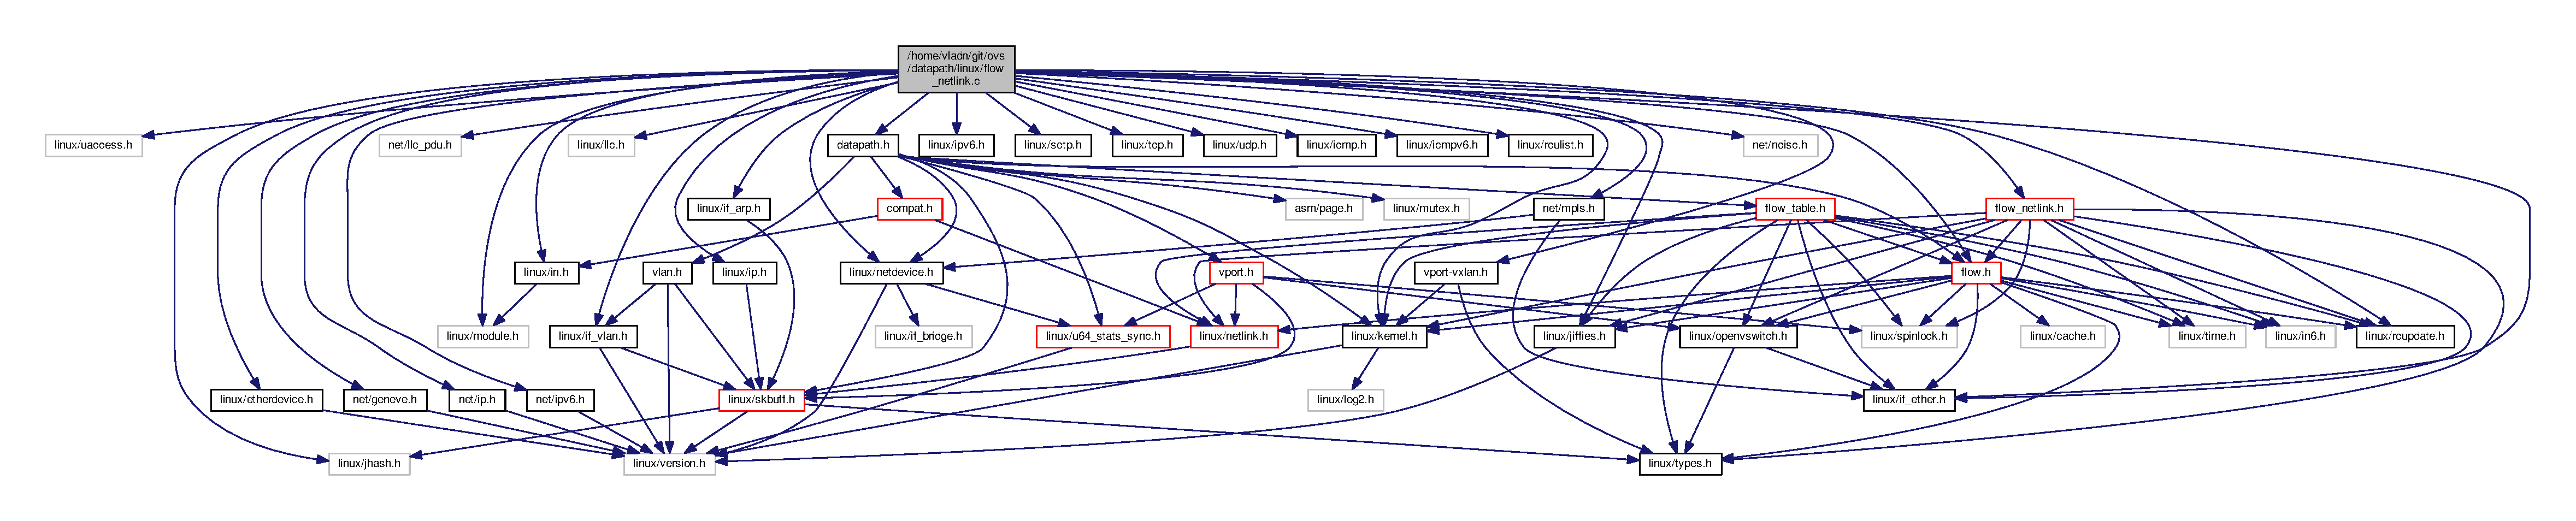
\includegraphics[width=350pt]{linux_2flow__netlink_8c__incl}
\end{center}
\end{figure}
\subsection*{Data Structures}
\begin{DoxyCompactItemize}
\item 
struct \hyperlink{structovs__len__tbl}{ovs\+\_\+len\+\_\+tbl}
\end{DoxyCompactItemize}
\subsection*{Macros}
\begin{DoxyCompactItemize}
\item 
\#define \hyperlink{linux_2flow__netlink_8c_a1f8c165bf4196327bc3abff648276d92}{pr\+\_\+fmt}(fmt)~K\+B\+U\+I\+L\+D\+\_\+\+M\+O\+D\+N\+A\+M\+E \char`\"{}\+: \char`\"{} fmt
\item 
\#define \hyperlink{linux_2flow__netlink_8c_aa45250c738c1a22be7f5e711887c8547}{O\+V\+S\+\_\+\+A\+T\+T\+R\+\_\+\+N\+E\+S\+T\+E\+D}~-\/1
\item 
\#define \hyperlink{linux_2flow__netlink_8c_a7cb040299f14f8ff8806dd868c321d7b}{S\+W\+\_\+\+F\+L\+O\+W\+\_\+\+K\+E\+Y\+\_\+\+P\+U\+T}(match,  field,  value,  is\+\_\+mask)
\item 
\#define \hyperlink{linux_2flow__netlink_8c_aceedf9228ebbe5291ac9e12d1d011278}{S\+W\+\_\+\+F\+L\+O\+W\+\_\+\+K\+E\+Y\+\_\+\+M\+E\+M\+C\+P\+Y\+\_\+\+O\+F\+F\+S\+E\+T}(match,  offset,  value\+\_\+p,  len,  is\+\_\+mask)
\item 
\#define \hyperlink{linux_2flow__netlink_8c_aa303fd044db169fb22013e1279c18dd1}{S\+W\+\_\+\+F\+L\+O\+W\+\_\+\+K\+E\+Y\+\_\+\+M\+E\+M\+C\+P\+Y}(match,  field,  value\+\_\+p,  len,  is\+\_\+mask)
\item 
\#define \hyperlink{linux_2flow__netlink_8c_a428fac9f6cc49614e07de128b9e4869f}{S\+W\+\_\+\+F\+L\+O\+W\+\_\+\+K\+E\+Y\+\_\+\+M\+E\+M\+S\+E\+T\+\_\+\+F\+I\+E\+L\+D}(match,  field,  value,  is\+\_\+mask)
\item 
\#define \hyperlink{linux_2flow__netlink_8c_a429e7a37f3797cd9870c534467a7f762}{M\+A\+X\+\_\+\+A\+C\+T\+I\+O\+N\+S\+\_\+\+B\+U\+F\+S\+I\+Z\+E}~(32 $\ast$ 1024)
\end{DoxyCompactItemize}
\subsection*{Functions}
\begin{DoxyCompactItemize}
\item 
static void \hyperlink{linux_2flow__netlink_8c_ac21a080dcc5b01d3da9b75d32b13fb40}{update\+\_\+range} (struct \hyperlink{structsw__flow__match}{sw\+\_\+flow\+\_\+match} $\ast$match, size\+\_\+t offset, size\+\_\+t size, \hyperlink{types_8h_afaa87723b8417d40fcf45b7330261ef9}{bool} is\+\_\+mask)
\item 
static \hyperlink{types_8h_afaa87723b8417d40fcf45b7330261ef9}{bool} \hyperlink{linux_2flow__netlink_8c_ab4be6b01938d3a8f5a14bc787cb2b0b2}{match\+\_\+validate} (const struct \hyperlink{structsw__flow__match}{sw\+\_\+flow\+\_\+match} $\ast$match, u64 key\+\_\+attrs, u64 mask\+\_\+attrs, \hyperlink{types_8h_afaa87723b8417d40fcf45b7330261ef9}{bool} log)
\item 
size\+\_\+t \hyperlink{linux_2flow__netlink_8c_ac920825ffe4fa75e7ca3c5e76ad4ec2a}{ovs\+\_\+tun\+\_\+key\+\_\+attr\+\_\+size} (void)
\item 
size\+\_\+t \hyperlink{linux_2flow__netlink_8c_a4ea1ec7f3650fd324fc1538c97e795d0}{ovs\+\_\+key\+\_\+attr\+\_\+size} (void)
\item 
static \hyperlink{types_8h_afaa87723b8417d40fcf45b7330261ef9}{bool} \hyperlink{linux_2flow__netlink_8c_a237e69cf49fbb7f26d6f886bdf4e4aad}{is\+\_\+all\+\_\+zero} (const u8 $\ast$fp, size\+\_\+t size)
\item 
static int \hyperlink{linux_2flow__netlink_8c_acc907c6eed2beccfb3d8564a9f627e93}{\+\_\+\+\_\+parse\+\_\+flow\+\_\+nlattrs} (const struct nlattr $\ast$attr, const struct nlattr $\ast$a\mbox{[}$\,$\mbox{]}, u64 $\ast$attrsp, \hyperlink{types_8h_afaa87723b8417d40fcf45b7330261ef9}{bool} log, \hyperlink{types_8h_afaa87723b8417d40fcf45b7330261ef9}{bool} nz)
\item 
static int \hyperlink{linux_2flow__netlink_8c_a4a090c5659903b6b8d125ab7598ad1a6}{parse\+\_\+flow\+\_\+mask\+\_\+nlattrs} (const struct nlattr $\ast$attr, const struct nlattr $\ast$a\mbox{[}$\,$\mbox{]}, u64 $\ast$attrsp, \hyperlink{types_8h_afaa87723b8417d40fcf45b7330261ef9}{bool} log)
\item 
static int \hyperlink{linux_2flow__netlink_8c_aafe0de49242cd0276fd5ced0fd81514f}{parse\+\_\+flow\+\_\+nlattrs} (const struct nlattr $\ast$attr, const struct nlattr $\ast$a\mbox{[}$\,$\mbox{]}, u64 $\ast$attrsp, \hyperlink{types_8h_afaa87723b8417d40fcf45b7330261ef9}{bool} log)
\item 
static int \hyperlink{linux_2flow__netlink_8c_a5f31d9f0798910742b360bbdfe29eeae}{genev\+\_\+tun\+\_\+opt\+\_\+from\+\_\+nlattr} (const struct nlattr $\ast$a, struct \hyperlink{structsw__flow__match}{sw\+\_\+flow\+\_\+match} $\ast$match, \hyperlink{types_8h_afaa87723b8417d40fcf45b7330261ef9}{bool} is\+\_\+mask, \hyperlink{types_8h_afaa87723b8417d40fcf45b7330261ef9}{bool} log)
\item 
static int \hyperlink{linux_2flow__netlink_8c_aef546829167c0fe738dd9db84c3848d4}{vxlan\+\_\+tun\+\_\+opt\+\_\+from\+\_\+nlattr} (const struct nlattr $\ast$a, struct \hyperlink{structsw__flow__match}{sw\+\_\+flow\+\_\+match} $\ast$match, \hyperlink{types_8h_afaa87723b8417d40fcf45b7330261ef9}{bool} is\+\_\+mask, \hyperlink{types_8h_afaa87723b8417d40fcf45b7330261ef9}{bool} log)
\item 
static int \hyperlink{linux_2flow__netlink_8c_aa9ad124d7dc9f5042d10b1237ce02f28}{ipv4\+\_\+tun\+\_\+from\+\_\+nlattr} (const struct nlattr $\ast$attr, struct \hyperlink{structsw__flow__match}{sw\+\_\+flow\+\_\+match} $\ast$match, \hyperlink{types_8h_afaa87723b8417d40fcf45b7330261ef9}{bool} is\+\_\+mask, \hyperlink{types_8h_afaa87723b8417d40fcf45b7330261ef9}{bool} log)
\item 
static int \hyperlink{linux_2flow__netlink_8c_a9283dd76011434d73c43654a9c32ecfb}{vxlan\+\_\+opt\+\_\+to\+\_\+nlattr} (struct sk\+\_\+buff $\ast$skb, const void $\ast$\hyperlink{flow_8h_a58d612a14e56d9b6c782667cd2e89799}{tun\+\_\+opts}, int swkey\+\_\+tun\+\_\+opts\+\_\+len)
\item 
static int \hyperlink{linux_2flow__netlink_8c_ac7f453fb68977c7a24d7af50f18b43db}{\+\_\+\+\_\+ipv4\+\_\+tun\+\_\+to\+\_\+nlattr} (struct sk\+\_\+buff $\ast$skb, const struct \hyperlink{structovs__key__ipv4__tunnel}{ovs\+\_\+key\+\_\+ipv4\+\_\+tunnel} $\ast$output, const void $\ast$\hyperlink{flow_8h_a58d612a14e56d9b6c782667cd2e89799}{tun\+\_\+opts}, int swkey\+\_\+tun\+\_\+opts\+\_\+len)
\item 
static int \hyperlink{linux_2flow__netlink_8c_a534ea0693e07f81a7a00f4b3125fbb1a}{ipv4\+\_\+tun\+\_\+to\+\_\+nlattr} (struct sk\+\_\+buff $\ast$skb, const struct \hyperlink{structovs__key__ipv4__tunnel}{ovs\+\_\+key\+\_\+ipv4\+\_\+tunnel} $\ast$output, const void $\ast$\hyperlink{flow_8h_a58d612a14e56d9b6c782667cd2e89799}{tun\+\_\+opts}, int swkey\+\_\+tun\+\_\+opts\+\_\+len)
\item 
int \hyperlink{linux_2flow__netlink_8c_a8a7309f6247775b5682061576c039e22}{ovs\+\_\+nla\+\_\+put\+\_\+egress\+\_\+tunnel\+\_\+key} (struct sk\+\_\+buff $\ast$skb, const struct \hyperlink{structovs__tunnel__info}{ovs\+\_\+tunnel\+\_\+info} $\ast$egress\+\_\+tun\+\_\+info)
\item 
static int \hyperlink{linux_2flow__netlink_8c_aed17f75c6136e01aa609132d5bbc9b2a}{metadata\+\_\+from\+\_\+nlattrs} (struct \hyperlink{structsw__flow__match}{sw\+\_\+flow\+\_\+match} $\ast$match, u64 $\ast$attrs, const struct nlattr $\ast$$\ast$a, \hyperlink{types_8h_afaa87723b8417d40fcf45b7330261ef9}{bool} is\+\_\+mask, \hyperlink{types_8h_afaa87723b8417d40fcf45b7330261ef9}{bool} log)
\item 
static int \hyperlink{linux_2flow__netlink_8c_a7e2f54c332f7bdac73756972da69ad53}{ovs\+\_\+key\+\_\+from\+\_\+nlattrs} (struct \hyperlink{structsw__flow__match}{sw\+\_\+flow\+\_\+match} $\ast$match, u64 attrs, const struct nlattr $\ast$$\ast$a, \hyperlink{types_8h_afaa87723b8417d40fcf45b7330261ef9}{bool} is\+\_\+mask, \hyperlink{types_8h_afaa87723b8417d40fcf45b7330261ef9}{bool} log)
\item 
static void \hyperlink{linux_2flow__netlink_8c_a412721fb459cda8f2b25400f8832d84f}{nlattr\+\_\+set} (struct nlattr $\ast$attr, u8 val, const struct \hyperlink{structovs__len__tbl}{ovs\+\_\+len\+\_\+tbl} $\ast$tbl)
\item 
static void \hyperlink{linux_2flow__netlink_8c_aa862995e0363dbb698ee51eb1be8a40c}{mask\+\_\+set\+\_\+nlattr} (struct nlattr $\ast$attr, u8 val)
\item 
int \hyperlink{linux_2flow__netlink_8c_a074547b2bcb32890a72ae873700391d5}{ovs\+\_\+nla\+\_\+get\+\_\+match} (struct \hyperlink{structsw__flow__match}{sw\+\_\+flow\+\_\+match} $\ast$match, const struct nlattr $\ast$nla\+\_\+key, const struct nlattr $\ast$nla\+\_\+mask, \hyperlink{types_8h_afaa87723b8417d40fcf45b7330261ef9}{bool} log)
\item 
static size\+\_\+t \hyperlink{linux_2flow__netlink_8c_a5189e471b5832c9371b45c5e58ca5b41}{get\+\_\+ufid\+\_\+len} (const struct nlattr $\ast$attr, \hyperlink{types_8h_afaa87723b8417d40fcf45b7330261ef9}{bool} log)
\item 
\hyperlink{types_8h_afaa87723b8417d40fcf45b7330261ef9}{bool} \hyperlink{linux_2flow__netlink_8c_a81e0cfe1c434ecde4ad684c8b8586877}{ovs\+\_\+nla\+\_\+get\+\_\+ufid} (struct \hyperlink{structsw__flow__id}{sw\+\_\+flow\+\_\+id} $\ast$sfid, const struct nlattr $\ast$attr, \hyperlink{types_8h_afaa87723b8417d40fcf45b7330261ef9}{bool} log)
\item 
int \hyperlink{linux_2flow__netlink_8c_aa416ab3b06ce40eee0be66306129c8d5}{ovs\+\_\+nla\+\_\+get\+\_\+identifier} (struct \hyperlink{structsw__flow__id}{sw\+\_\+flow\+\_\+id} $\ast$sfid, const struct nlattr $\ast$ufid, const struct \hyperlink{structsw__flow__key}{sw\+\_\+flow\+\_\+key} $\ast$key, \hyperlink{types_8h_afaa87723b8417d40fcf45b7330261ef9}{bool} log)
\item 
u32 \hyperlink{linux_2flow__netlink_8c_a415cb727697a02d62b8ff40795337d40}{ovs\+\_\+nla\+\_\+get\+\_\+ufid\+\_\+flags} (const struct nlattr $\ast$attr)
\item 
int \hyperlink{linux_2flow__netlink_8c_a90428a389e4ba65133d2cf837d5a8dc3}{ovs\+\_\+nla\+\_\+get\+\_\+flow\+\_\+metadata} (const struct nlattr $\ast$attr, struct \hyperlink{structsw__flow__key}{sw\+\_\+flow\+\_\+key} $\ast$key, \hyperlink{types_8h_afaa87723b8417d40fcf45b7330261ef9}{bool} log)
\item 
static int \hyperlink{linux_2flow__netlink_8c_a469e9434d0bedd721b2e31a106799335}{\+\_\+\+\_\+ovs\+\_\+nla\+\_\+put\+\_\+key} (const struct \hyperlink{structsw__flow__key}{sw\+\_\+flow\+\_\+key} $\ast$swkey, const struct \hyperlink{structsw__flow__key}{sw\+\_\+flow\+\_\+key} $\ast$output, \hyperlink{types_8h_afaa87723b8417d40fcf45b7330261ef9}{bool} is\+\_\+mask, struct sk\+\_\+buff $\ast$skb)
\item 
int \hyperlink{linux_2flow__netlink_8c_a845412e2f8f2bcb48df005e857474fcb}{ovs\+\_\+nla\+\_\+put\+\_\+key} (const struct \hyperlink{structsw__flow__key}{sw\+\_\+flow\+\_\+key} $\ast$swkey, const struct \hyperlink{structsw__flow__key}{sw\+\_\+flow\+\_\+key} $\ast$output, int attr, \hyperlink{types_8h_afaa87723b8417d40fcf45b7330261ef9}{bool} is\+\_\+mask, struct sk\+\_\+buff $\ast$skb)
\item 
int \hyperlink{linux_2flow__netlink_8c_a636f7d3cbe8656ceda87373110a4abc4}{ovs\+\_\+nla\+\_\+put\+\_\+identifier} (const struct \hyperlink{structsw__flow}{sw\+\_\+flow} $\ast$flow, struct sk\+\_\+buff $\ast$skb)
\item 
int \hyperlink{linux_2flow__netlink_8c_a2f6c3ab02b8e5d6296278dc9214500eb}{ovs\+\_\+nla\+\_\+put\+\_\+masked\+\_\+key} (const struct \hyperlink{structsw__flow}{sw\+\_\+flow} $\ast$flow, struct sk\+\_\+buff $\ast$skb)
\item 
int \hyperlink{linux_2flow__netlink_8c_af5ab12e938f8564945464a9e110eace3}{ovs\+\_\+nla\+\_\+put\+\_\+mask} (const struct \hyperlink{structsw__flow}{sw\+\_\+flow} $\ast$flow, struct sk\+\_\+buff $\ast$skb)
\item 
static struct \hyperlink{structsw__flow__actions}{sw\+\_\+flow\+\_\+actions} $\ast$ \hyperlink{linux_2flow__netlink_8c_acf3273c812551499c4b4d48651548286}{nla\+\_\+alloc\+\_\+flow\+\_\+actions} (int size, \hyperlink{types_8h_afaa87723b8417d40fcf45b7330261ef9}{bool} log)
\item 
static void \hyperlink{linux_2flow__netlink_8c_a386dd5cb0c8be8ce91e59761cbf820b4}{rcu\+\_\+free\+\_\+acts\+\_\+callback} (struct rcu\+\_\+head $\ast$rcu)
\item 
void \hyperlink{linux_2flow__netlink_8c_a5e773c3bb49bbeb0c0a4eb356c779a22}{ovs\+\_\+nla\+\_\+free\+\_\+flow\+\_\+actions} (struct \hyperlink{structsw__flow__actions}{sw\+\_\+flow\+\_\+actions} $\ast$sf\+\_\+acts)
\item 
static struct nlattr $\ast$ \hyperlink{linux_2flow__netlink_8c_a5ce53ec8a0a126f8e33e1d9af6e1e083}{reserve\+\_\+sfa\+\_\+size} (struct \hyperlink{structsw__flow__actions}{sw\+\_\+flow\+\_\+actions} $\ast$$\ast$sfa, int attr\+\_\+len, \hyperlink{types_8h_afaa87723b8417d40fcf45b7330261ef9}{bool} log)
\item 
static struct nlattr $\ast$ \hyperlink{linux_2flow__netlink_8c_ad6fb4bf743e36b42c72eaa09db192e87}{\+\_\+\+\_\+add\+\_\+action} (struct \hyperlink{structsw__flow__actions}{sw\+\_\+flow\+\_\+actions} $\ast$$\ast$sfa, int attrtype, void $\ast$data, int len, \hyperlink{types_8h_afaa87723b8417d40fcf45b7330261ef9}{bool} log)
\item 
static int \hyperlink{linux_2flow__netlink_8c_a4316343b483e9a6b4d8885147036beb2}{add\+\_\+action} (struct \hyperlink{structsw__flow__actions}{sw\+\_\+flow\+\_\+actions} $\ast$$\ast$sfa, int attrtype, void $\ast$data, int len, \hyperlink{types_8h_afaa87723b8417d40fcf45b7330261ef9}{bool} log)
\item 
static int \hyperlink{linux_2flow__netlink_8c_a08778088a1f3c3c88aee0055bcd05110}{add\+\_\+nested\+\_\+action\+\_\+start} (struct \hyperlink{structsw__flow__actions}{sw\+\_\+flow\+\_\+actions} $\ast$$\ast$sfa, int attrtype, \hyperlink{types_8h_afaa87723b8417d40fcf45b7330261ef9}{bool} log)
\item 
static void \hyperlink{linux_2flow__netlink_8c_ab0176001eff016bfad478f0f06cefa0a}{add\+\_\+nested\+\_\+action\+\_\+end} (struct \hyperlink{structsw__flow__actions}{sw\+\_\+flow\+\_\+actions} $\ast$sfa, int st\+\_\+offset)
\item 
static int \hyperlink{linux_2flow__netlink_8c_ae5c58b498948d3c5564b7916505d8455}{\+\_\+\+\_\+ovs\+\_\+nla\+\_\+copy\+\_\+actions} (const struct nlattr $\ast$attr, const struct \hyperlink{structsw__flow__key}{sw\+\_\+flow\+\_\+key} $\ast$key, int depth, struct \hyperlink{structsw__flow__actions}{sw\+\_\+flow\+\_\+actions} $\ast$$\ast$sfa, \+\_\+\+\_\+be16 eth\+\_\+type, \+\_\+\+\_\+be16 vlan\+\_\+tci, \hyperlink{types_8h_afaa87723b8417d40fcf45b7330261ef9}{bool} log)
\item 
static int \hyperlink{linux_2flow__netlink_8c_a0dcf3429559610cf8b8204e04151728b}{validate\+\_\+and\+\_\+copy\+\_\+sample} (const struct nlattr $\ast$attr, const struct \hyperlink{structsw__flow__key}{sw\+\_\+flow\+\_\+key} $\ast$key, int depth, struct \hyperlink{structsw__flow__actions}{sw\+\_\+flow\+\_\+actions} $\ast$$\ast$sfa, \+\_\+\+\_\+be16 eth\+\_\+type, \+\_\+\+\_\+be16 vlan\+\_\+tci, \hyperlink{types_8h_afaa87723b8417d40fcf45b7330261ef9}{bool} log)
\item 
void \hyperlink{linux_2flow__netlink_8c_a1a09e9d38844c59332975789573e994c}{ovs\+\_\+match\+\_\+init} (struct \hyperlink{structsw__flow__match}{sw\+\_\+flow\+\_\+match} $\ast$match, struct \hyperlink{structsw__flow__key}{sw\+\_\+flow\+\_\+key} $\ast$key, struct \hyperlink{structsw__flow__mask}{sw\+\_\+flow\+\_\+mask} $\ast$mask)
\item 
static int \hyperlink{linux_2flow__netlink_8c_af4e9606a99a9ccc71de18c0531a99808}{validate\+\_\+geneve\+\_\+opts} (struct \hyperlink{structsw__flow__key}{sw\+\_\+flow\+\_\+key} $\ast$key)
\item 
static int \hyperlink{linux_2flow__netlink_8c_ac06cff749bd68b0a91ecacc196b4892f}{validate\+\_\+and\+\_\+copy\+\_\+set\+\_\+tun} (const struct nlattr $\ast$attr, struct \hyperlink{structsw__flow__actions}{sw\+\_\+flow\+\_\+actions} $\ast$$\ast$sfa, \hyperlink{types_8h_afaa87723b8417d40fcf45b7330261ef9}{bool} log)
\item 
static \hyperlink{types_8h_afaa87723b8417d40fcf45b7330261ef9}{bool} \hyperlink{linux_2flow__netlink_8c_ae01edbfa96ed8cef19cb86caf0512d7a}{validate\+\_\+masked} (u8 $\ast$data, int len)
\item 
static int \hyperlink{linux_2flow__netlink_8c_afabdbd008e8fb3c515063cafaf267e02}{validate\+\_\+set} (const struct nlattr $\ast$a, const struct \hyperlink{structsw__flow__key}{sw\+\_\+flow\+\_\+key} $\ast$flow\+\_\+key, struct \hyperlink{structsw__flow__actions}{sw\+\_\+flow\+\_\+actions} $\ast$$\ast$sfa, \hyperlink{types_8h_afaa87723b8417d40fcf45b7330261ef9}{bool} $\ast$skip\+\_\+copy, \+\_\+\+\_\+be16 eth\+\_\+type, \hyperlink{types_8h_afaa87723b8417d40fcf45b7330261ef9}{bool} masked, \hyperlink{types_8h_afaa87723b8417d40fcf45b7330261ef9}{bool} log)
\item 
static int \hyperlink{linux_2flow__netlink_8c_ab7c5d132ac3085d8c2da993c66138ab0}{validate\+\_\+userspace} (const struct nlattr $\ast$attr)
\item 
static int \hyperlink{linux_2flow__netlink_8c_a746e2c558f7350550b1734826a8c25f7}{copy\+\_\+action} (const struct nlattr $\ast$from, struct \hyperlink{structsw__flow__actions}{sw\+\_\+flow\+\_\+actions} $\ast$$\ast$sfa, \hyperlink{types_8h_afaa87723b8417d40fcf45b7330261ef9}{bool} log)
\item 
int \hyperlink{linux_2flow__netlink_8c_a10dc93f8c379eae7a557d54d9b387dd6}{ovs\+\_\+nla\+\_\+copy\+\_\+actions} (const struct nlattr $\ast$attr, const struct \hyperlink{structsw__flow__key}{sw\+\_\+flow\+\_\+key} $\ast$key, struct \hyperlink{structsw__flow__actions}{sw\+\_\+flow\+\_\+actions} $\ast$$\ast$sfa, \hyperlink{types_8h_afaa87723b8417d40fcf45b7330261ef9}{bool} log)
\item 
static int \hyperlink{linux_2flow__netlink_8c_a92621d7eaed9e960f5e5d7b72e501db0}{sample\+\_\+action\+\_\+to\+\_\+attr} (const struct nlattr $\ast$attr, struct sk\+\_\+buff $\ast$skb)
\item 
static int \hyperlink{linux_2flow__netlink_8c_af38f12c35d382eb717bb6e5b4fba2309}{set\+\_\+action\+\_\+to\+\_\+attr} (const struct nlattr $\ast$a, struct sk\+\_\+buff $\ast$skb)
\item 
static int \hyperlink{linux_2flow__netlink_8c_a14e859cc22996f05850ca737daf2ee09}{masked\+\_\+set\+\_\+action\+\_\+to\+\_\+set\+\_\+action\+\_\+attr} (const struct nlattr $\ast$a, struct sk\+\_\+buff $\ast$skb)
\item 
int \hyperlink{linux_2flow__netlink_8c_a923304ee69be1cfa52197b0f73c29e49}{ovs\+\_\+nla\+\_\+put\+\_\+actions} (const struct nlattr $\ast$attr, int len, struct sk\+\_\+buff $\ast$skb)
\end{DoxyCompactItemize}
\subsection*{Variables}
\begin{DoxyCompactItemize}
\item 
static const struct \hyperlink{structovs__len__tbl}{ovs\+\_\+len\+\_\+tbl} \hyperlink{linux_2flow__netlink_8c_abcfd7a34b15e86938f3646cda1522e07}{ovs\+\_\+tunnel\+\_\+key\+\_\+lens} \mbox{[}\hyperlink{openvswitch_8h_a1c8eef7445d1c45bb90eb65de59a81e4}{O\+V\+S\+\_\+\+T\+U\+N\+N\+E\+L\+\_\+\+K\+E\+Y\+\_\+\+A\+T\+T\+R\+\_\+\+M\+A\+X}+1\mbox{]}
\item 
static const struct \hyperlink{structovs__len__tbl}{ovs\+\_\+len\+\_\+tbl} \hyperlink{linux_2flow__netlink_8c_a5565daa559332f47a1d214007d97e0d7}{ovs\+\_\+key\+\_\+lens} \mbox{[}\hyperlink{openvswitch_8h_a2a2adc6c47c38f0e7889580602ccbe22}{O\+V\+S\+\_\+\+K\+E\+Y\+\_\+\+A\+T\+T\+R\+\_\+\+M\+A\+X}+1\mbox{]}
\item 
static const struct nla\+\_\+policy \hyperlink{linux_2flow__netlink_8c_ac262f3819d334e0cbbdf8198d6d2aed8}{vxlan\+\_\+opt\+\_\+policy} \mbox{[}\hyperlink{openvswitch_8h_ac764e78fe2e06d11f39448e337292c7c}{O\+V\+S\+\_\+\+V\+X\+L\+A\+N\+\_\+\+E\+X\+T\+\_\+\+M\+A\+X}+1\mbox{]}
\end{DoxyCompactItemize}


\subsection{Macro Definition Documentation}
\hypertarget{linux_2flow__netlink_8c_a429e7a37f3797cd9870c534467a7f762}{}\index{linux/flow\+\_\+netlink.\+c@{linux/flow\+\_\+netlink.\+c}!M\+A\+X\+\_\+\+A\+C\+T\+I\+O\+N\+S\+\_\+\+B\+U\+F\+S\+I\+Z\+E@{M\+A\+X\+\_\+\+A\+C\+T\+I\+O\+N\+S\+\_\+\+B\+U\+F\+S\+I\+Z\+E}}
\index{M\+A\+X\+\_\+\+A\+C\+T\+I\+O\+N\+S\+\_\+\+B\+U\+F\+S\+I\+Z\+E@{M\+A\+X\+\_\+\+A\+C\+T\+I\+O\+N\+S\+\_\+\+B\+U\+F\+S\+I\+Z\+E}!linux/flow\+\_\+netlink.\+c@{linux/flow\+\_\+netlink.\+c}}
\subsubsection[{M\+A\+X\+\_\+\+A\+C\+T\+I\+O\+N\+S\+\_\+\+B\+U\+F\+S\+I\+Z\+E}]{\setlength{\rightskip}{0pt plus 5cm}\#define M\+A\+X\+\_\+\+A\+C\+T\+I\+O\+N\+S\+\_\+\+B\+U\+F\+S\+I\+Z\+E~(32 $\ast$ 1024)}\label{linux_2flow__netlink_8c_a429e7a37f3797cd9870c534467a7f762}
\hypertarget{linux_2flow__netlink_8c_aa45250c738c1a22be7f5e711887c8547}{}\index{linux/flow\+\_\+netlink.\+c@{linux/flow\+\_\+netlink.\+c}!O\+V\+S\+\_\+\+A\+T\+T\+R\+\_\+\+N\+E\+S\+T\+E\+D@{O\+V\+S\+\_\+\+A\+T\+T\+R\+\_\+\+N\+E\+S\+T\+E\+D}}
\index{O\+V\+S\+\_\+\+A\+T\+T\+R\+\_\+\+N\+E\+S\+T\+E\+D@{O\+V\+S\+\_\+\+A\+T\+T\+R\+\_\+\+N\+E\+S\+T\+E\+D}!linux/flow\+\_\+netlink.\+c@{linux/flow\+\_\+netlink.\+c}}
\subsubsection[{O\+V\+S\+\_\+\+A\+T\+T\+R\+\_\+\+N\+E\+S\+T\+E\+D}]{\setlength{\rightskip}{0pt plus 5cm}\#define O\+V\+S\+\_\+\+A\+T\+T\+R\+\_\+\+N\+E\+S\+T\+E\+D~-\/1}\label{linux_2flow__netlink_8c_aa45250c738c1a22be7f5e711887c8547}
\hypertarget{linux_2flow__netlink_8c_a1f8c165bf4196327bc3abff648276d92}{}\index{linux/flow\+\_\+netlink.\+c@{linux/flow\+\_\+netlink.\+c}!pr\+\_\+fmt@{pr\+\_\+fmt}}
\index{pr\+\_\+fmt@{pr\+\_\+fmt}!linux/flow\+\_\+netlink.\+c@{linux/flow\+\_\+netlink.\+c}}
\subsubsection[{pr\+\_\+fmt}]{\setlength{\rightskip}{0pt plus 5cm}\#define pr\+\_\+fmt(
\begin{DoxyParamCaption}
\item[{}]{fmt}
\end{DoxyParamCaption}
)~K\+B\+U\+I\+L\+D\+\_\+\+M\+O\+D\+N\+A\+M\+E \char`\"{}\+: \char`\"{} fmt}\label{linux_2flow__netlink_8c_a1f8c165bf4196327bc3abff648276d92}
\hypertarget{linux_2flow__netlink_8c_aa303fd044db169fb22013e1279c18dd1}{}\index{linux/flow\+\_\+netlink.\+c@{linux/flow\+\_\+netlink.\+c}!S\+W\+\_\+\+F\+L\+O\+W\+\_\+\+K\+E\+Y\+\_\+\+M\+E\+M\+C\+P\+Y@{S\+W\+\_\+\+F\+L\+O\+W\+\_\+\+K\+E\+Y\+\_\+\+M\+E\+M\+C\+P\+Y}}
\index{S\+W\+\_\+\+F\+L\+O\+W\+\_\+\+K\+E\+Y\+\_\+\+M\+E\+M\+C\+P\+Y@{S\+W\+\_\+\+F\+L\+O\+W\+\_\+\+K\+E\+Y\+\_\+\+M\+E\+M\+C\+P\+Y}!linux/flow\+\_\+netlink.\+c@{linux/flow\+\_\+netlink.\+c}}
\subsubsection[{S\+W\+\_\+\+F\+L\+O\+W\+\_\+\+K\+E\+Y\+\_\+\+M\+E\+M\+C\+P\+Y}]{\setlength{\rightskip}{0pt plus 5cm}\#define S\+W\+\_\+\+F\+L\+O\+W\+\_\+\+K\+E\+Y\+\_\+\+M\+E\+M\+C\+P\+Y(
\begin{DoxyParamCaption}
\item[{}]{match, }
\item[{}]{field, }
\item[{}]{value\+\_\+p, }
\item[{}]{len, }
\item[{}]{is\+\_\+mask}
\end{DoxyParamCaption}
)}\label{linux_2flow__netlink_8c_aa303fd044db169fb22013e1279c18dd1}
{\bfseries Value\+:}
\begin{DoxyCode}
\hyperlink{linux_2flow__netlink_8c_aceedf9228ebbe5291ac9e12d1d011278}{SW\_FLOW\_KEY\_MEMCPY\_OFFSET}(match, offsetof(\textcolor{keyword}{struct} 
      \hyperlink{structsw__flow__key}{sw\_flow\_key}, field), \(\backslash\)
                  value\_p, len, is\_mask)
\end{DoxyCode}
\hypertarget{linux_2flow__netlink_8c_aceedf9228ebbe5291ac9e12d1d011278}{}\index{linux/flow\+\_\+netlink.\+c@{linux/flow\+\_\+netlink.\+c}!S\+W\+\_\+\+F\+L\+O\+W\+\_\+\+K\+E\+Y\+\_\+\+M\+E\+M\+C\+P\+Y\+\_\+\+O\+F\+F\+S\+E\+T@{S\+W\+\_\+\+F\+L\+O\+W\+\_\+\+K\+E\+Y\+\_\+\+M\+E\+M\+C\+P\+Y\+\_\+\+O\+F\+F\+S\+E\+T}}
\index{S\+W\+\_\+\+F\+L\+O\+W\+\_\+\+K\+E\+Y\+\_\+\+M\+E\+M\+C\+P\+Y\+\_\+\+O\+F\+F\+S\+E\+T@{S\+W\+\_\+\+F\+L\+O\+W\+\_\+\+K\+E\+Y\+\_\+\+M\+E\+M\+C\+P\+Y\+\_\+\+O\+F\+F\+S\+E\+T}!linux/flow\+\_\+netlink.\+c@{linux/flow\+\_\+netlink.\+c}}
\subsubsection[{S\+W\+\_\+\+F\+L\+O\+W\+\_\+\+K\+E\+Y\+\_\+\+M\+E\+M\+C\+P\+Y\+\_\+\+O\+F\+F\+S\+E\+T}]{\setlength{\rightskip}{0pt plus 5cm}\#define S\+W\+\_\+\+F\+L\+O\+W\+\_\+\+K\+E\+Y\+\_\+\+M\+E\+M\+C\+P\+Y\+\_\+\+O\+F\+F\+S\+E\+T(
\begin{DoxyParamCaption}
\item[{}]{match, }
\item[{}]{offset, }
\item[{}]{value\+\_\+p, }
\item[{}]{len, }
\item[{}]{is\+\_\+mask}
\end{DoxyParamCaption}
)}\label{linux_2flow__netlink_8c_aceedf9228ebbe5291ac9e12d1d011278}
{\bfseries Value\+:}
\begin{DoxyCode}
\textcolor{keywordflow}{do} \{                                    \hyperlink{linux_2flow__netlink_8c_ac21a080dcc5b01d3da9b75d32b13fb40}{\(\backslash\)}
\hyperlink{linux_2flow__netlink_8c_ac21a080dcc5b01d3da9b75d32b13fb40}{        update\_range}(match, offset, len, is\_mask);            \(\backslash\)
        if (is\_mask)                            \(\backslash\)
            memcpy((u8 *)&(match)->mask->key + offset, value\_p, len);\(\backslash\)
        else                                \(\backslash\)
            memcpy((u8 *)(match)->key + offset, value\_p, len);  \(\backslash\)
    \} \textcolor{keywordflow}{while} (0)
\end{DoxyCode}
\hypertarget{linux_2flow__netlink_8c_a428fac9f6cc49614e07de128b9e4869f}{}\index{linux/flow\+\_\+netlink.\+c@{linux/flow\+\_\+netlink.\+c}!S\+W\+\_\+\+F\+L\+O\+W\+\_\+\+K\+E\+Y\+\_\+\+M\+E\+M\+S\+E\+T\+\_\+\+F\+I\+E\+L\+D@{S\+W\+\_\+\+F\+L\+O\+W\+\_\+\+K\+E\+Y\+\_\+\+M\+E\+M\+S\+E\+T\+\_\+\+F\+I\+E\+L\+D}}
\index{S\+W\+\_\+\+F\+L\+O\+W\+\_\+\+K\+E\+Y\+\_\+\+M\+E\+M\+S\+E\+T\+\_\+\+F\+I\+E\+L\+D@{S\+W\+\_\+\+F\+L\+O\+W\+\_\+\+K\+E\+Y\+\_\+\+M\+E\+M\+S\+E\+T\+\_\+\+F\+I\+E\+L\+D}!linux/flow\+\_\+netlink.\+c@{linux/flow\+\_\+netlink.\+c}}
\subsubsection[{S\+W\+\_\+\+F\+L\+O\+W\+\_\+\+K\+E\+Y\+\_\+\+M\+E\+M\+S\+E\+T\+\_\+\+F\+I\+E\+L\+D}]{\setlength{\rightskip}{0pt plus 5cm}\#define S\+W\+\_\+\+F\+L\+O\+W\+\_\+\+K\+E\+Y\+\_\+\+M\+E\+M\+S\+E\+T\+\_\+\+F\+I\+E\+L\+D(
\begin{DoxyParamCaption}
\item[{}]{match, }
\item[{}]{field, }
\item[{}]{value, }
\item[{}]{is\+\_\+mask}
\end{DoxyParamCaption}
)}\label{linux_2flow__netlink_8c_a428fac9f6cc49614e07de128b9e4869f}
{\bfseries Value\+:}
\begin{DoxyCode}
\textcolor{keywordflow}{do} \{                                    \hyperlink{linux_2flow__netlink_8c_ac21a080dcc5b01d3da9b75d32b13fb40}{\(\backslash\)}
\hyperlink{linux_2flow__netlink_8c_ac21a080dcc5b01d3da9b75d32b13fb40}{        update\_range}(match, offsetof(\textcolor{keyword}{struct} \hyperlink{structsw__flow__key}{sw\_flow\_key}, field),    \(\backslash\)
                 \textcolor{keyword}{sizeof}((match)->key->field), is\_mask);     \(\backslash\)
        if (is\_mask)                            \(\backslash\)
            memset((u8 *)&(match)->mask->key.field, value,      \(\backslash\)
                   \textcolor{keyword}{sizeof}((match)->mask->key.field));       \(\backslash\)
        else                                \(\backslash\)
            memset((u8 *)&(match)->key->field, value,           \(\backslash\)
                   \textcolor{keyword}{sizeof}((match)->key->field));                \(\backslash\)
    \} \textcolor{keywordflow}{while} (0)
\end{DoxyCode}
\hypertarget{linux_2flow__netlink_8c_a7cb040299f14f8ff8806dd868c321d7b}{}\index{linux/flow\+\_\+netlink.\+c@{linux/flow\+\_\+netlink.\+c}!S\+W\+\_\+\+F\+L\+O\+W\+\_\+\+K\+E\+Y\+\_\+\+P\+U\+T@{S\+W\+\_\+\+F\+L\+O\+W\+\_\+\+K\+E\+Y\+\_\+\+P\+U\+T}}
\index{S\+W\+\_\+\+F\+L\+O\+W\+\_\+\+K\+E\+Y\+\_\+\+P\+U\+T@{S\+W\+\_\+\+F\+L\+O\+W\+\_\+\+K\+E\+Y\+\_\+\+P\+U\+T}!linux/flow\+\_\+netlink.\+c@{linux/flow\+\_\+netlink.\+c}}
\subsubsection[{S\+W\+\_\+\+F\+L\+O\+W\+\_\+\+K\+E\+Y\+\_\+\+P\+U\+T}]{\setlength{\rightskip}{0pt plus 5cm}\#define S\+W\+\_\+\+F\+L\+O\+W\+\_\+\+K\+E\+Y\+\_\+\+P\+U\+T(
\begin{DoxyParamCaption}
\item[{}]{match, }
\item[{}]{field, }
\item[{}]{value, }
\item[{}]{is\+\_\+mask}
\end{DoxyParamCaption}
)}\label{linux_2flow__netlink_8c_a7cb040299f14f8ff8806dd868c321d7b}
{\bfseries Value\+:}
\begin{DoxyCode}
\textcolor{keywordflow}{do} \{ \hyperlink{linux_2flow__netlink_8c_ac21a080dcc5b01d3da9b75d32b13fb40}{\(\backslash\)}
\hyperlink{linux_2flow__netlink_8c_ac21a080dcc5b01d3da9b75d32b13fb40}{        update\_range}(match, offsetof(\textcolor{keyword}{struct} \hyperlink{structsw__flow__key}{sw\_flow\_key}, field),    \(\backslash\)
                 \textcolor{keyword}{sizeof}((match)->key->field), is\_mask);     \(\backslash\)
        if (is\_mask)                            \(\backslash\)
            (match)->mask->key.field = value;           \(\backslash\)
        \textcolor{keywordflow}{else}                                \(\backslash\)
            (match)->key->field = value;                    \(\backslash\)
    \} \textcolor{keywordflow}{while} (0)
\end{DoxyCode}


\subsection{Function Documentation}
\hypertarget{linux_2flow__netlink_8c_ad6fb4bf743e36b42c72eaa09db192e87}{}\index{linux/flow\+\_\+netlink.\+c@{linux/flow\+\_\+netlink.\+c}!\+\_\+\+\_\+add\+\_\+action@{\+\_\+\+\_\+add\+\_\+action}}
\index{\+\_\+\+\_\+add\+\_\+action@{\+\_\+\+\_\+add\+\_\+action}!linux/flow\+\_\+netlink.\+c@{linux/flow\+\_\+netlink.\+c}}
\subsubsection[{\+\_\+\+\_\+add\+\_\+action}]{\setlength{\rightskip}{0pt plus 5cm}static struct nlattr$\ast$ \+\_\+\+\_\+add\+\_\+action (
\begin{DoxyParamCaption}
\item[{struct {\bf sw\+\_\+flow\+\_\+actions} $\ast$$\ast$}]{sfa, }
\item[{int}]{attrtype, }
\item[{void $\ast$}]{data, }
\item[{int}]{len, }
\item[{{\bf bool}}]{log}
\end{DoxyParamCaption}
)\hspace{0.3cm}{\ttfamily [static]}}\label{linux_2flow__netlink_8c_ad6fb4bf743e36b42c72eaa09db192e87}

\begin{DoxyCode}
1604 \{
1605     \textcolor{keyword}{struct }nlattr *a;
1606 
1607     a = \hyperlink{linux_2flow__netlink_8c_a5ce53ec8a0a126f8e33e1d9af6e1e083}{reserve\_sfa\_size}(sfa, nla\_attr\_size(len), log);
1608     \textcolor{keywordflow}{if} (IS\_ERR(a))
1609         \textcolor{keywordflow}{return} a;
1610 
1611     a->nla\_type = attrtype;
1612     a->nla\_len = nla\_attr\_size(len);
1613 
1614     \textcolor{keywordflow}{if} (data)
1615         memcpy(nla\_data(a), data, len);
1616     memset((\textcolor{keywordtype}{unsigned} \textcolor{keywordtype}{char} *) a + a->nla\_len, 0, nla\_padlen(len));
1617 
1618     \textcolor{keywordflow}{return} a;
1619 \}
\end{DoxyCode}
\hypertarget{linux_2flow__netlink_8c_ac7f453fb68977c7a24d7af50f18b43db}{}\index{linux/flow\+\_\+netlink.\+c@{linux/flow\+\_\+netlink.\+c}!\+\_\+\+\_\+ipv4\+\_\+tun\+\_\+to\+\_\+nlattr@{\+\_\+\+\_\+ipv4\+\_\+tun\+\_\+to\+\_\+nlattr}}
\index{\+\_\+\+\_\+ipv4\+\_\+tun\+\_\+to\+\_\+nlattr@{\+\_\+\+\_\+ipv4\+\_\+tun\+\_\+to\+\_\+nlattr}!linux/flow\+\_\+netlink.\+c@{linux/flow\+\_\+netlink.\+c}}
\subsubsection[{\+\_\+\+\_\+ipv4\+\_\+tun\+\_\+to\+\_\+nlattr}]{\setlength{\rightskip}{0pt plus 5cm}static int \+\_\+\+\_\+ipv4\+\_\+tun\+\_\+to\+\_\+nlattr (
\begin{DoxyParamCaption}
\item[{struct sk\+\_\+buff $\ast$}]{skb, }
\item[{const struct {\bf ovs\+\_\+key\+\_\+ipv4\+\_\+tunnel} $\ast$}]{output, }
\item[{const void $\ast$}]{tun\+\_\+opts, }
\item[{int}]{swkey\+\_\+tun\+\_\+opts\+\_\+len}
\end{DoxyParamCaption}
)\hspace{0.3cm}{\ttfamily [static]}}\label{linux_2flow__netlink_8c_ac7f453fb68977c7a24d7af50f18b43db}

\begin{DoxyCode}
646 \{
647     \textcolor{keywordflow}{if} (output->\hyperlink{structovs__key__ipv4__tunnel_a7459e66ecf90329eb2fa6cf3fc4781db}{tun\_flags} & \hyperlink{ip__tunnels_8h_a5438f4a0ea8e58438776fffbed3f08a8}{TUNNEL\_KEY} &&
648         \hyperlink{net_2netlink_8h_a610b2c7f3f7996a3b2406ce1bc708b5e}{nla\_put\_be64}(skb, \hyperlink{openvswitch_8h_a3ab62ef434a436d109e5dc7fe6a7f427abba6b12276aaae09ecdf61a2189edda5}{OVS\_TUNNEL\_KEY\_ATTR\_ID}, output->
      \hyperlink{structovs__key__ipv4__tunnel_ae36132bc05ca6257b572edddffcb867a}{tun\_id}))
649         \textcolor{keywordflow}{return} -EMSGSIZE;
650     \textcolor{keywordflow}{if} (output->\hyperlink{structovs__key__ipv4__tunnel_a1e5a978f104d61e9694e914a109734a7}{ipv4\_src} &&
651         \hyperlink{net_2netlink_8h_a2e2a0bd10c5f5139dc80413fd8dcbbe7}{nla\_put\_be32}(skb, \hyperlink{openvswitch_8h_a3ab62ef434a436d109e5dc7fe6a7f427add76f93836f5e1dcb33419c58aa1afd0}{OVS\_TUNNEL\_KEY\_ATTR\_IPV4\_SRC}, output->
      \hyperlink{structovs__key__ipv4__tunnel_a1e5a978f104d61e9694e914a109734a7}{ipv4\_src}))
652         \textcolor{keywordflow}{return} -EMSGSIZE;
653     \textcolor{keywordflow}{if} (output->\hyperlink{structovs__key__ipv4__tunnel_ae443d381a97f53bbc4139fe36c0aae30}{ipv4\_dst} &&
654         \hyperlink{net_2netlink_8h_a2e2a0bd10c5f5139dc80413fd8dcbbe7}{nla\_put\_be32}(skb, \hyperlink{openvswitch_8h_a3ab62ef434a436d109e5dc7fe6a7f427aa8a1fb062a0a5c1c718096a530c1fee9}{OVS\_TUNNEL\_KEY\_ATTR\_IPV4\_DST}, output->
      \hyperlink{structovs__key__ipv4__tunnel_ae443d381a97f53bbc4139fe36c0aae30}{ipv4\_dst}))
655         \textcolor{keywordflow}{return} -EMSGSIZE;
656     \textcolor{keywordflow}{if} (output->\hyperlink{structovs__key__ipv4__tunnel_a69594eaf9d7dfc2824b264484e02498e}{ipv4\_tos} &&
657         nla\_put\_u8(skb, \hyperlink{openvswitch_8h_a3ab62ef434a436d109e5dc7fe6a7f427ab452549b72cc81cc38c53a0487cded37}{OVS\_TUNNEL\_KEY\_ATTR\_TOS}, output->
      \hyperlink{structovs__key__ipv4__tunnel_a69594eaf9d7dfc2824b264484e02498e}{ipv4\_tos}))
658         \textcolor{keywordflow}{return} -EMSGSIZE;
659     \textcolor{keywordflow}{if} (nla\_put\_u8(skb, \hyperlink{openvswitch_8h_a3ab62ef434a436d109e5dc7fe6a7f427ace9b9fe26daaf5d99409d1563cc68f5c}{OVS\_TUNNEL\_KEY\_ATTR\_TTL}, output->
      \hyperlink{structovs__key__ipv4__tunnel_a24de7472a8c22903fce96b73dab68a40}{ipv4\_ttl}))
660         \textcolor{keywordflow}{return} -EMSGSIZE;
661     \textcolor{keywordflow}{if} ((output->\hyperlink{structovs__key__ipv4__tunnel_a7459e66ecf90329eb2fa6cf3fc4781db}{tun\_flags} & \hyperlink{ip__tunnels_8h_a3b33c8fadb48f2281d5852e2a0d8eeff}{TUNNEL\_DONT\_FRAGMENT}) &&
662         nla\_put\_flag(skb, \hyperlink{openvswitch_8h_a3ab62ef434a436d109e5dc7fe6a7f427a2b4acde1fe308fb5cdb703d197ccad11}{OVS\_TUNNEL\_KEY\_ATTR\_DONT\_FRAGMENT}))
663         \textcolor{keywordflow}{return} -EMSGSIZE;
664     \textcolor{keywordflow}{if} ((output->\hyperlink{structovs__key__ipv4__tunnel_a7459e66ecf90329eb2fa6cf3fc4781db}{tun\_flags} & \hyperlink{ip__tunnels_8h_ac8dc03940c0621b1aeddafa9b620022c}{TUNNEL\_CSUM}) &&
665         nla\_put\_flag(skb, \hyperlink{openvswitch_8h_a3ab62ef434a436d109e5dc7fe6a7f427a0b2355fe72f1590f795e2febdcb3cafe}{OVS\_TUNNEL\_KEY\_ATTR\_CSUM}))
666         \textcolor{keywordflow}{return} -EMSGSIZE;
667     \textcolor{keywordflow}{if} (output->\hyperlink{structovs__key__ipv4__tunnel_acda46848fad6a931296f3e7a74b44a18}{tp\_src} &&
668         \hyperlink{net_2netlink_8h_aafa7ef6ea62a477fe1cf21d435e2a718}{nla\_put\_be16}(skb, \hyperlink{openvswitch_8h_a3ab62ef434a436d109e5dc7fe6a7f427a82ec563a3032a39aa9f9694276933101}{OVS\_TUNNEL\_KEY\_ATTR\_TP\_SRC}, output->
      \hyperlink{structovs__key__ipv4__tunnel_acda46848fad6a931296f3e7a74b44a18}{tp\_src}))
669         \textcolor{keywordflow}{return} -EMSGSIZE;
670     \textcolor{keywordflow}{if} (output->\hyperlink{structovs__key__ipv4__tunnel_a438707be6be24ab62236063bde726e9b}{tp\_dst} &&
671         \hyperlink{net_2netlink_8h_aafa7ef6ea62a477fe1cf21d435e2a718}{nla\_put\_be16}(skb, \hyperlink{openvswitch_8h_a3ab62ef434a436d109e5dc7fe6a7f427a3fa87a8982452cc6e68ddf8e91dfced2}{OVS\_TUNNEL\_KEY\_ATTR\_TP\_DST}, output->
      \hyperlink{structovs__key__ipv4__tunnel_a438707be6be24ab62236063bde726e9b}{tp\_dst}))
672         \textcolor{keywordflow}{return} -EMSGSIZE;
673     \textcolor{keywordflow}{if} ((output->\hyperlink{structovs__key__ipv4__tunnel_a7459e66ecf90329eb2fa6cf3fc4781db}{tun\_flags} & \hyperlink{ip__tunnels_8h_a348bd362fda2a6f1506a9709ac7d0a86}{TUNNEL\_OAM}) &&
674         nla\_put\_flag(skb, \hyperlink{openvswitch_8h_a3ab62ef434a436d109e5dc7fe6a7f427a72ef8de21b6623d09331a68f87038b95}{OVS\_TUNNEL\_KEY\_ATTR\_OAM}))
675         \textcolor{keywordflow}{return} -EMSGSIZE;
676     \textcolor{keywordflow}{if} (\hyperlink{flow_8h_a58d612a14e56d9b6c782667cd2e89799}{tun\_opts}) \{
677         \textcolor{keywordflow}{if} (output->\hyperlink{structovs__key__ipv4__tunnel_a7459e66ecf90329eb2fa6cf3fc4781db}{tun\_flags} & \hyperlink{ip__tunnels_8h_a730279275492612f215921bf96742457}{TUNNEL\_GENEVE\_OPT} &&
678             nla\_put(skb, \hyperlink{openvswitch_8h_a3ab62ef434a436d109e5dc7fe6a7f427a3a6f60bb79d6ad889a091b82667009b9}{OVS\_TUNNEL\_KEY\_ATTR\_GENEVE\_OPTS},
679                 swkey\_tun\_opts\_len, \hyperlink{flow_8h_a58d612a14e56d9b6c782667cd2e89799}{tun\_opts}))
680             \textcolor{keywordflow}{return} -EMSGSIZE;
681                \textcolor{keywordflow}{else} \textcolor{keywordflow}{if} (output->\hyperlink{structovs__key__ipv4__tunnel_a7459e66ecf90329eb2fa6cf3fc4781db}{tun\_flags} & \hyperlink{ip__tunnels_8h_a50cd9036253f584996011f418422a53f}{TUNNEL\_VXLAN\_OPT} &&
682             \hyperlink{linux_2flow__netlink_8c_a9283dd76011434d73c43654a9c32ecfb}{vxlan\_opt\_to\_nlattr}(skb, \hyperlink{flow_8h_a58d612a14e56d9b6c782667cd2e89799}{tun\_opts}, swkey\_tun\_opts\_len))
683             \textcolor{keywordflow}{return} -EMSGSIZE;
684     \}
685 
686     \textcolor{keywordflow}{return} 0;
687 \}
\end{DoxyCode}
\hypertarget{linux_2flow__netlink_8c_ae5c58b498948d3c5564b7916505d8455}{}\index{linux/flow\+\_\+netlink.\+c@{linux/flow\+\_\+netlink.\+c}!\+\_\+\+\_\+ovs\+\_\+nla\+\_\+copy\+\_\+actions@{\+\_\+\+\_\+ovs\+\_\+nla\+\_\+copy\+\_\+actions}}
\index{\+\_\+\+\_\+ovs\+\_\+nla\+\_\+copy\+\_\+actions@{\+\_\+\+\_\+ovs\+\_\+nla\+\_\+copy\+\_\+actions}!linux/flow\+\_\+netlink.\+c@{linux/flow\+\_\+netlink.\+c}}
\subsubsection[{\+\_\+\+\_\+ovs\+\_\+nla\+\_\+copy\+\_\+actions}]{\setlength{\rightskip}{0pt plus 5cm}static int \+\_\+\+\_\+ovs\+\_\+nla\+\_\+copy\+\_\+actions (
\begin{DoxyParamCaption}
\item[{const struct nlattr $\ast$}]{attr, }
\item[{const struct {\bf sw\+\_\+flow\+\_\+key} $\ast$}]{key, }
\item[{int}]{depth, }
\item[{struct {\bf sw\+\_\+flow\+\_\+actions} $\ast$$\ast$}]{sfa, }
\item[{\+\_\+\+\_\+be16}]{eth\+\_\+type, }
\item[{\+\_\+\+\_\+be16}]{vlan\+\_\+tci, }
\item[{{\bf bool}}]{log}
\end{DoxyParamCaption}
)\hspace{0.3cm}{\ttfamily [static]}}\label{linux_2flow__netlink_8c_ae5c58b498948d3c5564b7916505d8455}

\begin{DoxyCode}
2027 \{
2028     \textcolor{keyword}{const} \textcolor{keyword}{struct }nlattr *a;
2029     \textcolor{keywordtype}{int} rem, err;
2030 
2031     \textcolor{keywordflow}{if} (depth >= \hyperlink{datapath_8h_ad323527e924235c97bf936e4e85dfdba}{SAMPLE\_ACTION\_DEPTH})
2032         \textcolor{keywordflow}{return} -EOVERFLOW;
2033 
2034     \hyperlink{net_2netlink_8h_ac2634af90bda4393105b6323da2044fa}{nla\_for\_each\_nested}(a, attr, rem) \{
2035         \textcolor{comment}{/* Expected argument lengths, (u32)-1 for variable length. */}
2036         \textcolor{keyword}{static} \textcolor{keyword}{const} u32 action\_lens[\hyperlink{openvswitch_8h_a34e29226a74b68f20be64faf2130b7db}{OVS\_ACTION\_ATTR\_MAX} + 1] = \{
2037             [\hyperlink{openvswitch_8h_affc4a4d29437ad03a23444243e2db26eacad69687bf2bfae5092ea828cf0d4fe2}{OVS\_ACTION\_ATTR\_OUTPUT}] = \textcolor{keyword}{sizeof}(u32),
2038             [\hyperlink{openvswitch_8h_affc4a4d29437ad03a23444243e2db26ea2cad0b08a7809d6e7cb1a9e86d73a47c}{OVS\_ACTION\_ATTR\_RECIRC}] = \textcolor{keyword}{sizeof}(u32),
2039             [\hyperlink{openvswitch_8h_affc4a4d29437ad03a23444243e2db26ea17132af22505d8b1bb535a270f83a8bd}{OVS\_ACTION\_ATTR\_USERSPACE}] = (u32)-1,
2040             [\hyperlink{openvswitch_8h_affc4a4d29437ad03a23444243e2db26eafb68488325a1ab2d6bfb67ea115a5cdb}{OVS\_ACTION\_ATTR\_PUSH\_MPLS}] = \textcolor{keyword}{sizeof}(\textcolor{keyword}{struct} 
      \hyperlink{structovs__action__push__mpls}{ovs\_action\_push\_mpls}),
2041             [\hyperlink{openvswitch_8h_affc4a4d29437ad03a23444243e2db26eafe4ec9b68459771a3ffd07d20cd628e1}{OVS\_ACTION\_ATTR\_POP\_MPLS}] = \textcolor{keyword}{sizeof}(\_\_be16),
2042             [\hyperlink{openvswitch_8h_affc4a4d29437ad03a23444243e2db26ea6f41b7751556ff0acc2f4c6f94963ba6}{OVS\_ACTION\_ATTR\_PUSH\_VLAN}] = \textcolor{keyword}{sizeof}(\textcolor{keyword}{struct} 
      \hyperlink{structovs__action__push__vlan}{ovs\_action\_push\_vlan}),
2043             [\hyperlink{openvswitch_8h_affc4a4d29437ad03a23444243e2db26ea9cd4ec18560c7c3f81276cba51a96a24}{OVS\_ACTION\_ATTR\_POP\_VLAN}] = 0,
2044             [\hyperlink{openvswitch_8h_affc4a4d29437ad03a23444243e2db26eaff937deb7687d0dd4b073c27aed9c8be}{OVS\_ACTION\_ATTR\_SET}] = (u32)-1,
2045             [\hyperlink{openvswitch_8h_affc4a4d29437ad03a23444243e2db26ea50a466abca8b11394e9364de28ebe03f}{OVS\_ACTION\_ATTR\_SET\_MASKED}] = (u32)-1,
2046             [\hyperlink{openvswitch_8h_affc4a4d29437ad03a23444243e2db26eaddc6f70b9e8501e5bb90548373faf734}{OVS\_ACTION\_ATTR\_SAMPLE}] = (u32)-1,
2047             [\hyperlink{openvswitch_8h_affc4a4d29437ad03a23444243e2db26eaa783c1e8488baea181d3497e0e9676f9}{OVS\_ACTION\_ATTR\_HASH}] = \textcolor{keyword}{sizeof}(\textcolor{keyword}{struct} 
      \hyperlink{structovs__action__hash}{ovs\_action\_hash})
2048         \};
2049         \textcolor{keyword}{const} \textcolor{keyword}{struct }\hyperlink{structovs__action__push__vlan}{ovs\_action\_push\_vlan} *vlan;
2050         \textcolor{keywordtype}{int} \hyperlink{flow_8h_ab22aaab04f806700def00f32823fcb9e}{type} = nla\_type(a);
2051         \textcolor{keywordtype}{bool} skip\_copy;
2052 
2053         \textcolor{keywordflow}{if} (type > \hyperlink{openvswitch_8h_a34e29226a74b68f20be64faf2130b7db}{OVS\_ACTION\_ATTR\_MAX} ||
2054             (action\_lens[type] != nla\_len(a) &&
2055              action\_lens[type] != (u32)-1))
2056             \textcolor{keywordflow}{return} -EINVAL;
2057 
2058         skip\_copy = \textcolor{keyword}{false};
2059         \textcolor{keywordflow}{switch} (type) \{
2060         \textcolor{keywordflow}{case} \hyperlink{openvswitch_8h_affc4a4d29437ad03a23444243e2db26ea7ea71a1f3bf51504d9ee79e77578287b}{OVS\_ACTION\_ATTR\_UNSPEC}:
2061             \textcolor{keywordflow}{return} -EINVAL;
2062 
2063         \textcolor{keywordflow}{case} \hyperlink{openvswitch_8h_affc4a4d29437ad03a23444243e2db26ea17132af22505d8b1bb535a270f83a8bd}{OVS\_ACTION\_ATTR\_USERSPACE}:
2064             err = \hyperlink{linux_2flow__netlink_8c_ab7c5d132ac3085d8c2da993c66138ab0}{validate\_userspace}(a);
2065             \textcolor{keywordflow}{if} (err)
2066                 \textcolor{keywordflow}{return} err;
2067             \textcolor{keywordflow}{break};
2068 
2069         \textcolor{keywordflow}{case} \hyperlink{openvswitch_8h_affc4a4d29437ad03a23444243e2db26eacad69687bf2bfae5092ea828cf0d4fe2}{OVS\_ACTION\_ATTR\_OUTPUT}:
2070             \textcolor{keywordflow}{if} (nla\_get\_u32(a) >= \hyperlink{datapath_8h_a73b117dd1ebe456eecfb7688047a03f1}{DP\_MAX\_PORTS})
2071                 \textcolor{keywordflow}{return} -EINVAL;
2072             \textcolor{keywordflow}{break};
2073 
2074         \textcolor{keywordflow}{case} \hyperlink{openvswitch_8h_affc4a4d29437ad03a23444243e2db26eaa783c1e8488baea181d3497e0e9676f9}{OVS\_ACTION\_ATTR\_HASH}: \{
2075             \textcolor{keyword}{const} \textcolor{keyword}{struct }\hyperlink{structovs__action__hash}{ovs\_action\_hash} *act\_hash = nla\_data(a);
2076 
2077             \textcolor{keywordflow}{switch} (act\_hash->\hyperlink{structovs__action__hash_a8dde1557790d7fc7c2cae50f4e6d65e8}{hash\_alg}) \{
2078             \textcolor{keywordflow}{case} \hyperlink{openvswitch_8h_a26bab1f427f0d834e49cf627cd869b05abc58a227eae8b0c6e494642dd6e62903}{OVS\_HASH\_ALG\_L4}:
2079                 \textcolor{keywordflow}{break};
2080             \textcolor{keywordflow}{default}:
2081                 \textcolor{keywordflow}{return}  -EINVAL;
2082             \}
2083 
2084             \textcolor{keywordflow}{break};
2085         \}
2086 
2087         \textcolor{keywordflow}{case} \hyperlink{openvswitch_8h_affc4a4d29437ad03a23444243e2db26ea9cd4ec18560c7c3f81276cba51a96a24}{OVS\_ACTION\_ATTR\_POP\_VLAN}:
2088             vlan\_tci = htons(0);
2089             \textcolor{keywordflow}{break};
2090 
2091         \textcolor{keywordflow}{case} \hyperlink{openvswitch_8h_affc4a4d29437ad03a23444243e2db26ea6f41b7751556ff0acc2f4c6f94963ba6}{OVS\_ACTION\_ATTR\_PUSH\_VLAN}:
2092             vlan = nla\_data(a);
2093             \textcolor{keywordflow}{if} (vlan->\hyperlink{structovs__action__push__vlan_af2e36cd70149cf03ebf29586fc765722}{vlan\_tpid} != htons(ETH\_P\_8021Q))
2094                 \textcolor{keywordflow}{return} -EINVAL;
2095             \textcolor{keywordflow}{if} (!(vlan->\hyperlink{structovs__action__push__vlan_ab17c8db02bffc32a072bd23687dd712c}{vlan\_tci} & htons(\hyperlink{if__vlan_8h_ac8bf15be3fd1a3a63a2452fa05a83217}{VLAN\_TAG\_PRESENT})))
2096                 \textcolor{keywordflow}{return} -EINVAL;
2097             vlan\_tci = vlan->\hyperlink{structovs__action__push__vlan_ab17c8db02bffc32a072bd23687dd712c}{vlan\_tci};
2098             \textcolor{keywordflow}{break};
2099 
2100         \textcolor{keywordflow}{case} \hyperlink{openvswitch_8h_affc4a4d29437ad03a23444243e2db26ea2cad0b08a7809d6e7cb1a9e86d73a47c}{OVS\_ACTION\_ATTR\_RECIRC}:
2101             \textcolor{keywordflow}{break};
2102 
2103         \textcolor{keywordflow}{case} \hyperlink{openvswitch_8h_affc4a4d29437ad03a23444243e2db26eafb68488325a1ab2d6bfb67ea115a5cdb}{OVS\_ACTION\_ATTR\_PUSH\_MPLS}: \{
2104             \textcolor{keyword}{const} \textcolor{keyword}{struct }\hyperlink{structovs__action__push__mpls}{ovs\_action\_push\_mpls} *\hyperlink{flow_8h_aeab2d67b4ec58a9575da76c323ad95ce}{mpls} = nla\_data(a);
2105 
2106             \textcolor{keywordflow}{if} (!\hyperlink{net_2mpls_8h_aab48ab242fbafafc869b3e98df4ace8f}{eth\_p\_mpls}(mpls->\hyperlink{structovs__action__push__mpls_adea8de7c1e924d0665c4eb62901ce521}{mpls\_ethertype}))
2107                 \textcolor{keywordflow}{return} -EINVAL;
2108             \textcolor{comment}{/* Prohibit push MPLS other than to a white list}
2109 \textcolor{comment}{             * for packets that have a known tag order.}
2110 \textcolor{comment}{             */}
2111             \textcolor{keywordflow}{if} (vlan\_tci & htons(\hyperlink{if__vlan_8h_ac8bf15be3fd1a3a63a2452fa05a83217}{VLAN\_TAG\_PRESENT}) ||
2112                 (eth\_type != htons(ETH\_P\_IP) &&
2113                  eth\_type != htons(ETH\_P\_IPV6) &&
2114                  eth\_type != htons(ETH\_P\_ARP) &&
2115                  eth\_type != htons(ETH\_P\_RARP) &&
2116                  !\hyperlink{net_2mpls_8h_aab48ab242fbafafc869b3e98df4ace8f}{eth\_p\_mpls}(eth\_type)))
2117                 \textcolor{keywordflow}{return} -EINVAL;
2118             eth\_type = mpls->\hyperlink{structovs__action__push__mpls_adea8de7c1e924d0665c4eb62901ce521}{mpls\_ethertype};
2119             \textcolor{keywordflow}{break};
2120         \}
2121 
2122         \textcolor{keywordflow}{case} \hyperlink{openvswitch_8h_affc4a4d29437ad03a23444243e2db26eafe4ec9b68459771a3ffd07d20cd628e1}{OVS\_ACTION\_ATTR\_POP\_MPLS}:
2123             \textcolor{keywordflow}{if} (vlan\_tci & htons(\hyperlink{if__vlan_8h_ac8bf15be3fd1a3a63a2452fa05a83217}{VLAN\_TAG\_PRESENT}) ||
2124                 !\hyperlink{net_2mpls_8h_aab48ab242fbafafc869b3e98df4ace8f}{eth\_p\_mpls}(eth\_type))
2125                 \textcolor{keywordflow}{return} -EINVAL;
2126 
2127             \textcolor{comment}{/* Disallow subsequent L2.5+ set and mpls\_pop actions}
2128 \textcolor{comment}{             * as there is no check here to ensure that the new}
2129 \textcolor{comment}{             * eth\_type is valid and thus set actions could}
2130 \textcolor{comment}{             * write off the end of the packet or otherwise}
2131 \textcolor{comment}{             * corrupt it.}
2132 \textcolor{comment}{             *}
2133 \textcolor{comment}{             * Support for these actions is planned using packet}
2134 \textcolor{comment}{             * recirculation.}
2135 \textcolor{comment}{             */}
2136             eth\_type = htons(0);
2137             \textcolor{keywordflow}{break};
2138 
2139         \textcolor{keywordflow}{case} \hyperlink{openvswitch_8h_affc4a4d29437ad03a23444243e2db26eaff937deb7687d0dd4b073c27aed9c8be}{OVS\_ACTION\_ATTR\_SET}:
2140             err = \hyperlink{linux_2flow__netlink_8c_afabdbd008e8fb3c515063cafaf267e02}{validate\_set}(a, key, sfa,
2141                        &skip\_copy, eth\_type, \textcolor{keyword}{false}, log);
2142             \textcolor{keywordflow}{if} (err)
2143                 \textcolor{keywordflow}{return} err;
2144             \textcolor{keywordflow}{break};
2145 
2146         \textcolor{keywordflow}{case} \hyperlink{openvswitch_8h_affc4a4d29437ad03a23444243e2db26ea50a466abca8b11394e9364de28ebe03f}{OVS\_ACTION\_ATTR\_SET\_MASKED}:
2147             err = \hyperlink{linux_2flow__netlink_8c_afabdbd008e8fb3c515063cafaf267e02}{validate\_set}(a, key, sfa,
2148                        &skip\_copy, eth\_type, \textcolor{keyword}{true}, log);
2149             \textcolor{keywordflow}{if} (err)
2150                 \textcolor{keywordflow}{return} err;
2151             \textcolor{keywordflow}{break};
2152 
2153         \textcolor{keywordflow}{case} \hyperlink{openvswitch_8h_affc4a4d29437ad03a23444243e2db26eaddc6f70b9e8501e5bb90548373faf734}{OVS\_ACTION\_ATTR\_SAMPLE}:
2154             err = \hyperlink{linux_2flow__netlink_8c_a0dcf3429559610cf8b8204e04151728b}{validate\_and\_copy\_sample}(a, key, depth, sfa,
2155                                eth\_type, vlan\_tci, log);
2156             \textcolor{keywordflow}{if} (err)
2157                 \textcolor{keywordflow}{return} err;
2158             skip\_copy = \textcolor{keyword}{true};
2159             \textcolor{keywordflow}{break};
2160 
2161         \textcolor{keywordflow}{default}:
2162             \hyperlink{datapath_8h_a54648b7a2c9b192074cd95eb945433f0}{OVS\_NLERR}(log, \textcolor{stringliteral}{"Unknown Action type %d"}, type);
2163             \textcolor{keywordflow}{return} -EINVAL;
2164         \}
2165         \textcolor{keywordflow}{if} (!skip\_copy) \{
2166             err = \hyperlink{linux_2flow__netlink_8c_a746e2c558f7350550b1734826a8c25f7}{copy\_action}(a, sfa, log);
2167             \textcolor{keywordflow}{if} (err)
2168                 \textcolor{keywordflow}{return} err;
2169         \}
2170     \}
2171 
2172     \textcolor{keywordflow}{if} (rem > 0)
2173         \textcolor{keywordflow}{return} -EINVAL;
2174 
2175     \textcolor{keywordflow}{return} 0;
2176 \}
\end{DoxyCode}
\hypertarget{linux_2flow__netlink_8c_a469e9434d0bedd721b2e31a106799335}{}\index{linux/flow\+\_\+netlink.\+c@{linux/flow\+\_\+netlink.\+c}!\+\_\+\+\_\+ovs\+\_\+nla\+\_\+put\+\_\+key@{\+\_\+\+\_\+ovs\+\_\+nla\+\_\+put\+\_\+key}}
\index{\+\_\+\+\_\+ovs\+\_\+nla\+\_\+put\+\_\+key@{\+\_\+\+\_\+ovs\+\_\+nla\+\_\+put\+\_\+key}!linux/flow\+\_\+netlink.\+c@{linux/flow\+\_\+netlink.\+c}}
\subsubsection[{\+\_\+\+\_\+ovs\+\_\+nla\+\_\+put\+\_\+key}]{\setlength{\rightskip}{0pt plus 5cm}static int \+\_\+\+\_\+ovs\+\_\+nla\+\_\+put\+\_\+key (
\begin{DoxyParamCaption}
\item[{const struct {\bf sw\+\_\+flow\+\_\+key} $\ast$}]{swkey, }
\item[{const struct {\bf sw\+\_\+flow\+\_\+key} $\ast$}]{output, }
\item[{{\bf bool}}]{is\+\_\+mask, }
\item[{struct sk\+\_\+buff $\ast$}]{skb}
\end{DoxyParamCaption}
)\hspace{0.3cm}{\ttfamily [static]}}\label{linux_2flow__netlink_8c_a469e9434d0bedd721b2e31a106799335}

\begin{DoxyCode}
1277 \{
1278     \textcolor{keyword}{struct }\hyperlink{structovs__key__ethernet}{ovs\_key\_ethernet} *eth\_key;
1279     \textcolor{keyword}{struct }nlattr *nla, *encap;
1280 
1281     \textcolor{keywordflow}{if} (nla\_put\_u32(skb, \hyperlink{openvswitch_8h_a6a279bc7098c9bc819c12355c9e07864afa5af2b14a419c06035a864807572a69}{OVS\_KEY\_ATTR\_RECIRC\_ID}, output->
      \hyperlink{structsw__flow__key_a7e51857c88ad6b0bf90551d0b6e2607b}{recirc\_id}))
1282         \textcolor{keywordflow}{goto} nla\_put\_failure;
1283 
1284     \textcolor{keywordflow}{if} (nla\_put\_u32(skb, \hyperlink{openvswitch_8h_a6a279bc7098c9bc819c12355c9e07864a8f119543030b5cafc424d37ef817208d}{OVS\_KEY\_ATTR\_DP\_HASH}, output->
      \hyperlink{structsw__flow__key_a73dd9402f1f54c321f6d704d9b018d15}{ovs\_flow\_hash}))
1285         \textcolor{keywordflow}{goto} nla\_put\_failure;
1286 
1287     \textcolor{keywordflow}{if} (nla\_put\_u32(skb, \hyperlink{openvswitch_8h_a6a279bc7098c9bc819c12355c9e07864a3dee91d2ad17f698e34ebb913fcef8bf}{OVS\_KEY\_ATTR\_PRIORITY}, output->\hyperlink{structsw__flow__key_a57cbddb75a8d4fd859300bd34d98e84a}{phy}.
      \hyperlink{structsw__flow__key_a9dd898913d9faaec1ec970029e7fbb71}{priority}))
1288         \textcolor{keywordflow}{goto} nla\_put\_failure;
1289 
1290     \textcolor{keywordflow}{if} ((swkey->\hyperlink{structsw__flow__key_a2f87b7690c0cc2797f1f4347589472c3}{tun\_key}.\hyperlink{structovs__key__ipv4__tunnel_ae443d381a97f53bbc4139fe36c0aae30}{ipv4\_dst} || is\_mask)) \{
1291         \textcolor{keyword}{const} \textcolor{keywordtype}{void} *opts = NULL;
1292 
1293         \textcolor{keywordflow}{if} (output->\hyperlink{structsw__flow__key_a2f87b7690c0cc2797f1f4347589472c3}{tun\_key}.\hyperlink{structovs__key__ipv4__tunnel_a7459e66ecf90329eb2fa6cf3fc4781db}{tun\_flags} & \hyperlink{ip__tunnels_8h_ac6f5dad11c0e109bffb0a6dd5afdf8fb}{TUNNEL\_OPTIONS\_PRESENT})
1294             opts = \hyperlink{flow_8h_a5d74524a15e17551a8d8235f4375c296}{TUN\_METADATA\_OPTS}(output, swkey->
      \hyperlink{structsw__flow__key_aef0ea317d3bd0125e0d6390261ba3e2d}{tun\_opts\_len});
1295 
1296         \textcolor{keywordflow}{if} (\hyperlink{linux_2flow__netlink_8c_a534ea0693e07f81a7a00f4b3125fbb1a}{ipv4\_tun\_to\_nlattr}(skb, &output->\hyperlink{structsw__flow__key_a2f87b7690c0cc2797f1f4347589472c3}{tun\_key}, opts,
1297                        swkey->\hyperlink{structsw__flow__key_aef0ea317d3bd0125e0d6390261ba3e2d}{tun\_opts\_len}))
1298             \textcolor{keywordflow}{goto} nla\_put\_failure;
1299     \}
1300 
1301     \textcolor{keywordflow}{if} (swkey->\hyperlink{structsw__flow__key_a57cbddb75a8d4fd859300bd34d98e84a}{phy}.\hyperlink{structsw__flow__key_a5848de18caa80d36d9bc60cc686a2c6e}{in\_port} == \hyperlink{datapath_8h_a73b117dd1ebe456eecfb7688047a03f1}{DP\_MAX\_PORTS}) \{
1302         \textcolor{keywordflow}{if} (is\_mask && (output->\hyperlink{structsw__flow__key_a57cbddb75a8d4fd859300bd34d98e84a}{phy}.\hyperlink{structsw__flow__key_a5848de18caa80d36d9bc60cc686a2c6e}{in\_port} == 0xffff))
1303             \textcolor{keywordflow}{if} (nla\_put\_u32(skb, \hyperlink{openvswitch_8h_a6a279bc7098c9bc819c12355c9e07864a84a968b0e1dd75ba2f6b543c7fcde5b4}{OVS\_KEY\_ATTR\_IN\_PORT}, 0xffffffff))
1304                 \textcolor{keywordflow}{goto} nla\_put\_failure;
1305     \} \textcolor{keywordflow}{else} \{
1306         u16 upper\_u16;
1307         upper\_u16 = !is\_mask ? 0 : 0xffff;
1308 
1309         \textcolor{keywordflow}{if} (nla\_put\_u32(skb, \hyperlink{openvswitch_8h_a6a279bc7098c9bc819c12355c9e07864a84a968b0e1dd75ba2f6b543c7fcde5b4}{OVS\_KEY\_ATTR\_IN\_PORT},
1310                 (upper\_u16 << 16) | output->\hyperlink{structsw__flow__key_a57cbddb75a8d4fd859300bd34d98e84a}{phy}.\hyperlink{structsw__flow__key_a5848de18caa80d36d9bc60cc686a2c6e}{in\_port}))
1311             \textcolor{keywordflow}{goto} nla\_put\_failure;
1312     \}
1313 
1314     \textcolor{keywordflow}{if} (nla\_put\_u32(skb, \hyperlink{openvswitch_8h_a6a279bc7098c9bc819c12355c9e07864a32f36d9e41b0fbae0746d67fa34340ad}{OVS\_KEY\_ATTR\_SKB\_MARK}, output->\hyperlink{structsw__flow__key_a57cbddb75a8d4fd859300bd34d98e84a}{phy}.
      \hyperlink{structsw__flow__key_ae02571657f29397dcc45de8528f4ed05}{skb\_mark}))
1315         \textcolor{keywordflow}{goto} nla\_put\_failure;
1316 
1317     nla = nla\_reserve(skb, \hyperlink{openvswitch_8h_a6a279bc7098c9bc819c12355c9e07864a75127b87d8a2f36ae2c9aae2cf42cd56}{OVS\_KEY\_ATTR\_ETHERNET}, \textcolor{keyword}{sizeof}(*eth\_key));
1318     \textcolor{keywordflow}{if} (!nla)
1319         \textcolor{keywordflow}{goto} nla\_put\_failure;
1320 
1321     eth\_key = nla\_data(nla);
1322     \hyperlink{etherdevice_8h_a564a2ea461aa6add2fa94a6864ee494d}{ether\_addr\_copy}(eth\_key->\hyperlink{structovs__key__ethernet_adc19d64e3aa45c9383f332981780b79b}{eth\_src}, output->\hyperlink{structsw__flow__key_af3e10c978a3a2bf303b7d953ac6ff361}{eth}.\hyperlink{structsw__flow__key_a2fbd4aa7a500630627eff0630f864117}{src});
1323     \hyperlink{etherdevice_8h_a564a2ea461aa6add2fa94a6864ee494d}{ether\_addr\_copy}(eth\_key->\hyperlink{structovs__key__ethernet_a12fa99b386c86f65221f6d2394a9d7c9}{eth\_dst}, output->\hyperlink{structsw__flow__key_af3e10c978a3a2bf303b7d953ac6ff361}{eth}.\hyperlink{structsw__flow__key_a44a0cdfe7471df8bb73762085da4cda9}{dst});
1324 
1325     \textcolor{keywordflow}{if} (swkey->\hyperlink{structsw__flow__key_af3e10c978a3a2bf303b7d953ac6ff361}{eth}.\hyperlink{structsw__flow__key_a56b27b9b9eafa8f79acd544eba98c7b0}{tci} || swkey->\hyperlink{structsw__flow__key_af3e10c978a3a2bf303b7d953ac6ff361}{eth}.\hyperlink{structsw__flow__key_af30defbb2a81c997e8747594e1d937a0}{type} == htons(ETH\_P\_8021Q)) \{
1326         \_\_be16 eth\_type;
1327         eth\_type = !is\_mask ? htons(ETH\_P\_8021Q) : htons(0xffff);
1328         \textcolor{keywordflow}{if} (\hyperlink{net_2netlink_8h_aafa7ef6ea62a477fe1cf21d435e2a718}{nla\_put\_be16}(skb, \hyperlink{openvswitch_8h_a6a279bc7098c9bc819c12355c9e07864aaccef1ecf941c78c70cf8a6a3374235a}{OVS\_KEY\_ATTR\_ETHERTYPE}, eth\_type) ||
1329             \hyperlink{net_2netlink_8h_aafa7ef6ea62a477fe1cf21d435e2a718}{nla\_put\_be16}(skb, \hyperlink{openvswitch_8h_a6a279bc7098c9bc819c12355c9e07864ae513231d4612ed9b19551a7e70648005}{OVS\_KEY\_ATTR\_VLAN}, output->
      \hyperlink{structsw__flow__key_af3e10c978a3a2bf303b7d953ac6ff361}{eth}.\hyperlink{structsw__flow__key_a56b27b9b9eafa8f79acd544eba98c7b0}{tci}))
1330             \textcolor{keywordflow}{goto} nla\_put\_failure;
1331         encap = nla\_nest\_start(skb, \hyperlink{openvswitch_8h_a6a279bc7098c9bc819c12355c9e07864a869b60116d7d6ac79bfad91cc808cf75}{OVS\_KEY\_ATTR\_ENCAP});
1332         \textcolor{keywordflow}{if} (!swkey->\hyperlink{structsw__flow__key_af3e10c978a3a2bf303b7d953ac6ff361}{eth}.\hyperlink{structsw__flow__key_a56b27b9b9eafa8f79acd544eba98c7b0}{tci})
1333             \textcolor{keywordflow}{goto} unencap;
1334     \} \textcolor{keywordflow}{else}
1335         encap = NULL;
1336 
1337     \textcolor{keywordflow}{if} (swkey->\hyperlink{structsw__flow__key_af3e10c978a3a2bf303b7d953ac6ff361}{eth}.\hyperlink{structsw__flow__key_af30defbb2a81c997e8747594e1d937a0}{type} == htons(ETH\_P\_802\_2)) \{
1338         \textcolor{comment}{/*}
1339 \textcolor{comment}{         * Ethertype 802.2 is represented in the netlink with omitted}
1340 \textcolor{comment}{         * OVS\_KEY\_ATTR\_ETHERTYPE in the flow key attribute, and}
1341 \textcolor{comment}{         * 0xffff in the mask attribute.  Ethertype can also}
1342 \textcolor{comment}{         * be wildcarded.}
1343 \textcolor{comment}{         */}
1344         \textcolor{keywordflow}{if} (is\_mask && output->\hyperlink{structsw__flow__key_af3e10c978a3a2bf303b7d953ac6ff361}{eth}.\hyperlink{structsw__flow__key_af30defbb2a81c997e8747594e1d937a0}{type})
1345             \textcolor{keywordflow}{if} (\hyperlink{net_2netlink_8h_aafa7ef6ea62a477fe1cf21d435e2a718}{nla\_put\_be16}(skb, \hyperlink{openvswitch_8h_a6a279bc7098c9bc819c12355c9e07864aaccef1ecf941c78c70cf8a6a3374235a}{OVS\_KEY\_ATTR\_ETHERTYPE},
1346                         output->\hyperlink{structsw__flow__key_af3e10c978a3a2bf303b7d953ac6ff361}{eth}.\hyperlink{structsw__flow__key_af30defbb2a81c997e8747594e1d937a0}{type}))
1347                 \textcolor{keywordflow}{goto} nla\_put\_failure;
1348         \textcolor{keywordflow}{goto} unencap;
1349     \}
1350 
1351     \textcolor{keywordflow}{if} (\hyperlink{net_2netlink_8h_aafa7ef6ea62a477fe1cf21d435e2a718}{nla\_put\_be16}(skb, \hyperlink{openvswitch_8h_a6a279bc7098c9bc819c12355c9e07864aaccef1ecf941c78c70cf8a6a3374235a}{OVS\_KEY\_ATTR\_ETHERTYPE}, output->
      \hyperlink{structsw__flow__key_af3e10c978a3a2bf303b7d953ac6ff361}{eth}.\hyperlink{structsw__flow__key_af30defbb2a81c997e8747594e1d937a0}{type}))
1352         \textcolor{keywordflow}{goto} nla\_put\_failure;
1353 
1354     \textcolor{keywordflow}{if} (swkey->\hyperlink{structsw__flow__key_af3e10c978a3a2bf303b7d953ac6ff361}{eth}.\hyperlink{structsw__flow__key_af30defbb2a81c997e8747594e1d937a0}{type} == htons(ETH\_P\_IP)) \{
1355         \textcolor{keyword}{struct }\hyperlink{structovs__key__ipv4}{ovs\_key\_ipv4} *ipv4\_key;
1356 
1357         nla = nla\_reserve(skb, \hyperlink{openvswitch_8h_a6a279bc7098c9bc819c12355c9e07864a67c672ef69eb0c5db9136812e3cdd92e}{OVS\_KEY\_ATTR\_IPV4}, \textcolor{keyword}{sizeof}(*ipv4\_key));
1358         \textcolor{keywordflow}{if} (!nla)
1359             \textcolor{keywordflow}{goto} nla\_put\_failure;
1360         ipv4\_key = nla\_data(nla);
1361         ipv4\_key->\hyperlink{structovs__key__ipv4_a3577eccaa5f978ba303d2424e3e31a13}{ipv4\_src} = output->\hyperlink{structsw__flow__key_aeb4295bcb2fb4efea5c30337b871a423}{ipv4}.addr.src;
1362         ipv4\_key->\hyperlink{structovs__key__ipv4_aa15aabd69c2881215e666585cea50064}{ipv4\_dst} = output->\hyperlink{structsw__flow__key_aeb4295bcb2fb4efea5c30337b871a423}{ipv4}.addr.dst;
1363         ipv4\_key->\hyperlink{structovs__key__ipv4_ac973a2efc8d310948e3713a5c5a7fabf}{ipv4\_proto} = output->\hyperlink{structsw__flow__key_ae8d48c419eaff6a9fda97c7446bdec0e}{ip}.proto;
1364         ipv4\_key->\hyperlink{structovs__key__ipv4_a0097feb04c0db1cc6621a58f74ac0e33}{ipv4\_tos} = output->\hyperlink{structsw__flow__key_ae8d48c419eaff6a9fda97c7446bdec0e}{ip}.tos;
1365         ipv4\_key->\hyperlink{structovs__key__ipv4_ac2142e7329a6e522b3a0d504bec22678}{ipv4\_ttl} = output->\hyperlink{structsw__flow__key_ae8d48c419eaff6a9fda97c7446bdec0e}{ip}.ttl;
1366         ipv4\_key->\hyperlink{structovs__key__ipv4_a47225bcfead6875052b2678c96d3f9b3}{ipv4\_frag} = output->\hyperlink{structsw__flow__key_ae8d48c419eaff6a9fda97c7446bdec0e}{ip}.frag;
1367     \} \textcolor{keywordflow}{else} \textcolor{keywordflow}{if} (swkey->\hyperlink{structsw__flow__key_af3e10c978a3a2bf303b7d953ac6ff361}{eth}.\hyperlink{structsw__flow__key_af30defbb2a81c997e8747594e1d937a0}{type} == htons(ETH\_P\_IPV6)) \{
1368         \textcolor{keyword}{struct }\hyperlink{structovs__key__ipv6}{ovs\_key\_ipv6} *ipv6\_key;
1369 
1370         nla = nla\_reserve(skb, \hyperlink{openvswitch_8h_a6a279bc7098c9bc819c12355c9e07864aff74bae1efeecfd5d6cf28d8987a8bfd}{OVS\_KEY\_ATTR\_IPV6}, \textcolor{keyword}{sizeof}(*ipv6\_key));
1371         \textcolor{keywordflow}{if} (!nla)
1372             \textcolor{keywordflow}{goto} nla\_put\_failure;
1373         ipv6\_key = nla\_data(nla);
1374         memcpy(ipv6\_key->\hyperlink{structovs__key__ipv6_ac1ff8dfd6a3b86196c2267b64077517e}{ipv6\_src}, &output->\hyperlink{structsw__flow__key_a6b13e14d62eb632b05378784a2d61f87}{ipv6}.addr.src,
1375                 \textcolor{keyword}{sizeof}(ipv6\_key->\hyperlink{structovs__key__ipv6_ac1ff8dfd6a3b86196c2267b64077517e}{ipv6\_src}));
1376         memcpy(ipv6\_key->\hyperlink{structovs__key__ipv6_a32109125c4fc7b02b01ac84e9af8e447}{ipv6\_dst}, &output->\hyperlink{structsw__flow__key_a6b13e14d62eb632b05378784a2d61f87}{ipv6}.addr.dst,
1377                 \textcolor{keyword}{sizeof}(ipv6\_key->\hyperlink{structovs__key__ipv6_a32109125c4fc7b02b01ac84e9af8e447}{ipv6\_dst}));
1378         ipv6\_key->\hyperlink{structovs__key__ipv6_a723a1a03d115ebe2a9fdada09e63bd0c}{ipv6\_label} = output->\hyperlink{structsw__flow__key_a6b13e14d62eb632b05378784a2d61f87}{ipv6}.label;
1379         ipv6\_key->\hyperlink{structovs__key__ipv6_a194ad047677db5a081bdd730b20f8007}{ipv6\_proto} = output->\hyperlink{structsw__flow__key_ae8d48c419eaff6a9fda97c7446bdec0e}{ip}.proto;
1380         ipv6\_key->\hyperlink{structovs__key__ipv6_a391295d87ca76a365cc78fd92c4e4615}{ipv6\_tclass} = output->\hyperlink{structsw__flow__key_ae8d48c419eaff6a9fda97c7446bdec0e}{ip}.tos;
1381         ipv6\_key->\hyperlink{structovs__key__ipv6_a5273b4aa4bba11f547cfa0687acaaeae}{ipv6\_hlimit} = output->\hyperlink{structsw__flow__key_ae8d48c419eaff6a9fda97c7446bdec0e}{ip}.ttl;
1382         ipv6\_key->\hyperlink{structovs__key__ipv6_ace1ae2a8c22670bde77abadde9101d27}{ipv6\_frag} = output->\hyperlink{structsw__flow__key_ae8d48c419eaff6a9fda97c7446bdec0e}{ip}.frag;
1383     \} \textcolor{keywordflow}{else} \textcolor{keywordflow}{if} (swkey->\hyperlink{structsw__flow__key_af3e10c978a3a2bf303b7d953ac6ff361}{eth}.\hyperlink{structsw__flow__key_af30defbb2a81c997e8747594e1d937a0}{type} == htons(ETH\_P\_ARP) ||
1384            swkey->\hyperlink{structsw__flow__key_af3e10c978a3a2bf303b7d953ac6ff361}{eth}.\hyperlink{structsw__flow__key_af30defbb2a81c997e8747594e1d937a0}{type} == htons(ETH\_P\_RARP)) \{
1385         \textcolor{keyword}{struct }\hyperlink{structovs__key__arp}{ovs\_key\_arp} *arp\_key;
1386 
1387         nla = nla\_reserve(skb, \hyperlink{openvswitch_8h_a6a279bc7098c9bc819c12355c9e07864a78599a1574b0b24244c2911e420a951b}{OVS\_KEY\_ATTR\_ARP}, \textcolor{keyword}{sizeof}(*arp\_key));
1388         \textcolor{keywordflow}{if} (!nla)
1389             \textcolor{keywordflow}{goto} nla\_put\_failure;
1390         arp\_key = nla\_data(nla);
1391         memset(arp\_key, 0, \textcolor{keyword}{sizeof}(\textcolor{keyword}{struct} \hyperlink{structovs__key__arp}{ovs\_key\_arp}));
1392         arp\_key->\hyperlink{structovs__key__arp_a25ce3912d909430a080dd3264d858892}{arp\_sip} = output->\hyperlink{structsw__flow__key_aeb4295bcb2fb4efea5c30337b871a423}{ipv4}.addr.src;
1393         arp\_key->\hyperlink{structovs__key__arp_a84a3d1edd8ba5960d41a69155e721d20}{arp\_tip} = output->\hyperlink{structsw__flow__key_aeb4295bcb2fb4efea5c30337b871a423}{ipv4}.addr.dst;
1394         arp\_key->\hyperlink{structovs__key__arp_a560ecc1caa0ae74b43abe0d5dd30306d}{arp\_op} = htons(output->\hyperlink{structsw__flow__key_ae8d48c419eaff6a9fda97c7446bdec0e}{ip}.proto);
1395         \hyperlink{etherdevice_8h_a564a2ea461aa6add2fa94a6864ee494d}{ether\_addr\_copy}(arp\_key->\hyperlink{structovs__key__arp_a99f6141da2e3151181663f27ab1a3560}{arp\_sha}, output->\hyperlink{structsw__flow__key_aeb4295bcb2fb4efea5c30337b871a423}{ipv4}.arp.sha);
1396         \hyperlink{etherdevice_8h_a564a2ea461aa6add2fa94a6864ee494d}{ether\_addr\_copy}(arp\_key->\hyperlink{structovs__key__arp_ab9f27ebc29aee381031d9b89d1b954ac}{arp\_tha}, output->\hyperlink{structsw__flow__key_aeb4295bcb2fb4efea5c30337b871a423}{ipv4}.arp.tha);
1397     \} \textcolor{keywordflow}{else} \textcolor{keywordflow}{if} (\hyperlink{net_2mpls_8h_aab48ab242fbafafc869b3e98df4ace8f}{eth\_p\_mpls}(swkey->\hyperlink{structsw__flow__key_af3e10c978a3a2bf303b7d953ac6ff361}{eth}.\hyperlink{structsw__flow__key_af30defbb2a81c997e8747594e1d937a0}{type})) \{
1398         \textcolor{keyword}{struct }\hyperlink{structovs__key__mpls}{ovs\_key\_mpls} *mpls\_key;
1399 
1400         nla = nla\_reserve(skb, \hyperlink{openvswitch_8h_a6a279bc7098c9bc819c12355c9e07864ac46f7c8520cb93d091b4247ef8707f7b}{OVS\_KEY\_ATTR\_MPLS}, \textcolor{keyword}{sizeof}(*mpls\_key));
1401         \textcolor{keywordflow}{if} (!nla)
1402             \textcolor{keywordflow}{goto} nla\_put\_failure;
1403         mpls\_key = nla\_data(nla);
1404         mpls\_key->\hyperlink{structovs__key__mpls_a44b32d5066667b5b1bf474b53a335fb1}{mpls\_lse} = output->\hyperlink{structsw__flow__key_a005840d04ee5b462be3c8e21809dc9aa}{mpls}.top\_lse;
1405     \}
1406 
1407     \textcolor{keywordflow}{if} ((swkey->\hyperlink{structsw__flow__key_af3e10c978a3a2bf303b7d953ac6ff361}{eth}.\hyperlink{structsw__flow__key_af30defbb2a81c997e8747594e1d937a0}{type} == htons(ETH\_P\_IP) ||
1408          swkey->\hyperlink{structsw__flow__key_af3e10c978a3a2bf303b7d953ac6ff361}{eth}.\hyperlink{structsw__flow__key_af30defbb2a81c997e8747594e1d937a0}{type} == htons(ETH\_P\_IPV6)) &&
1409          swkey->\hyperlink{structsw__flow__key_ae8d48c419eaff6a9fda97c7446bdec0e}{ip}.frag != \hyperlink{openvswitch_8h_ad843f713a855bfcacd0adfe3e98eb447a1d1c9f89ced33419ec870391d8954c10}{OVS\_FRAG\_TYPE\_LATER}) \{
1410 
1411         \textcolor{keywordflow}{if} (swkey->\hyperlink{structsw__flow__key_ae8d48c419eaff6a9fda97c7446bdec0e}{ip}.proto == IPPROTO\_TCP) \{
1412             \textcolor{keyword}{struct }\hyperlink{structovs__key__tcp}{ovs\_key\_tcp} *tcp\_key;
1413 
1414             nla = nla\_reserve(skb, \hyperlink{openvswitch_8h_a6a279bc7098c9bc819c12355c9e07864a120ca2131b2881b0c52b6fcc8f6cccb5}{OVS\_KEY\_ATTR\_TCP}, \textcolor{keyword}{sizeof}(*tcp\_key));
1415             \textcolor{keywordflow}{if} (!nla)
1416                 \textcolor{keywordflow}{goto} nla\_put\_failure;
1417             tcp\_key = nla\_data(nla);
1418             tcp\_key->\hyperlink{structovs__key__tcp_a6ce4cb2971be0b952a5a7cde1eefc28e}{tcp\_src} = output->\hyperlink{structsw__flow__key_a9c1944a39db1bf91141048df6d85ce8b}{tp}.\hyperlink{structsw__flow__key_a2fbd4aa7a500630627eff0630f864117}{src};
1419             tcp\_key->\hyperlink{structovs__key__tcp_a37a5793e8ba3701ac70693073a24668a}{tcp\_dst} = output->\hyperlink{structsw__flow__key_a9c1944a39db1bf91141048df6d85ce8b}{tp}.\hyperlink{structsw__flow__key_a44a0cdfe7471df8bb73762085da4cda9}{dst};
1420             \textcolor{keywordflow}{if} (\hyperlink{net_2netlink_8h_aafa7ef6ea62a477fe1cf21d435e2a718}{nla\_put\_be16}(skb, \hyperlink{openvswitch_8h_a6a279bc7098c9bc819c12355c9e07864a79bb45fd4c1a62364eec929283795161}{OVS\_KEY\_ATTR\_TCP\_FLAGS},
1421                      output->\hyperlink{structsw__flow__key_a9c1944a39db1bf91141048df6d85ce8b}{tp}.\hyperlink{structsw__flow__key_a910f5e4408d113dbc9211190b44e0880}{flags}))
1422                 \textcolor{keywordflow}{goto} nla\_put\_failure;
1423         \} \textcolor{keywordflow}{else} \textcolor{keywordflow}{if} (swkey->\hyperlink{structsw__flow__key_ae8d48c419eaff6a9fda97c7446bdec0e}{ip}.proto == IPPROTO\_UDP) \{
1424             \textcolor{keyword}{struct }\hyperlink{structovs__key__udp}{ovs\_key\_udp} *udp\_key;
1425 
1426             nla = nla\_reserve(skb, \hyperlink{openvswitch_8h_a6a279bc7098c9bc819c12355c9e07864a4dea7a1acfa9eeffb8f09838bb9f9a7d}{OVS\_KEY\_ATTR\_UDP}, \textcolor{keyword}{sizeof}(*udp\_key));
1427             \textcolor{keywordflow}{if} (!nla)
1428                 \textcolor{keywordflow}{goto} nla\_put\_failure;
1429             udp\_key = nla\_data(nla);
1430             udp\_key->\hyperlink{structovs__key__udp_a771fb692264276a6e170a01d54295b61}{udp\_src} = output->\hyperlink{structsw__flow__key_a9c1944a39db1bf91141048df6d85ce8b}{tp}.\hyperlink{structsw__flow__key_a2fbd4aa7a500630627eff0630f864117}{src};
1431             udp\_key->\hyperlink{structovs__key__udp_ab9a32a0e306acdbf2b5468710836a4d8}{udp\_dst} = output->\hyperlink{structsw__flow__key_a9c1944a39db1bf91141048df6d85ce8b}{tp}.\hyperlink{structsw__flow__key_a44a0cdfe7471df8bb73762085da4cda9}{dst};
1432         \} \textcolor{keywordflow}{else} \textcolor{keywordflow}{if} (swkey->\hyperlink{structsw__flow__key_ae8d48c419eaff6a9fda97c7446bdec0e}{ip}.proto == IPPROTO\_SCTP) \{
1433             \textcolor{keyword}{struct }\hyperlink{structovs__key__sctp}{ovs\_key\_sctp} *sctp\_key;
1434 
1435             nla = nla\_reserve(skb, \hyperlink{openvswitch_8h_a6a279bc7098c9bc819c12355c9e07864a33b7870d10d17ea1604aa83edf40e452}{OVS\_KEY\_ATTR\_SCTP}, \textcolor{keyword}{sizeof}(*sctp\_key));
1436             \textcolor{keywordflow}{if} (!nla)
1437                 \textcolor{keywordflow}{goto} nla\_put\_failure;
1438             sctp\_key = nla\_data(nla);
1439             sctp\_key->\hyperlink{structovs__key__sctp_af10ce527eb1894b4080bd8024e82a1cc}{sctp\_src} = output->\hyperlink{structsw__flow__key_a9c1944a39db1bf91141048df6d85ce8b}{tp}.\hyperlink{structsw__flow__key_a2fbd4aa7a500630627eff0630f864117}{src};
1440             sctp\_key->\hyperlink{structovs__key__sctp_a1fa757d8e013ccfc5672df04cfa3aa7d}{sctp\_dst} = output->\hyperlink{structsw__flow__key_a9c1944a39db1bf91141048df6d85ce8b}{tp}.\hyperlink{structsw__flow__key_a44a0cdfe7471df8bb73762085da4cda9}{dst};
1441         \} \textcolor{keywordflow}{else} \textcolor{keywordflow}{if} (swkey->\hyperlink{structsw__flow__key_af3e10c978a3a2bf303b7d953ac6ff361}{eth}.\hyperlink{structsw__flow__key_af30defbb2a81c997e8747594e1d937a0}{type} == htons(ETH\_P\_IP) &&
1442                swkey->\hyperlink{structsw__flow__key_ae8d48c419eaff6a9fda97c7446bdec0e}{ip}.proto == IPPROTO\_ICMP) \{
1443             \textcolor{keyword}{struct }\hyperlink{structovs__key__icmp}{ovs\_key\_icmp} *icmp\_key;
1444 
1445             nla = nla\_reserve(skb, \hyperlink{openvswitch_8h_a6a279bc7098c9bc819c12355c9e07864a7059323c7b14c529cc9d2ff8d3134de9}{OVS\_KEY\_ATTR\_ICMP}, \textcolor{keyword}{sizeof}(*icmp\_key));
1446             \textcolor{keywordflow}{if} (!nla)
1447                 \textcolor{keywordflow}{goto} nla\_put\_failure;
1448             icmp\_key = nla\_data(nla);
1449             icmp\_key->\hyperlink{structovs__key__icmp_aa1880a0c32ed20143e19948c0169060a}{icmp\_type} = ntohs(output->\hyperlink{structsw__flow__key_a9c1944a39db1bf91141048df6d85ce8b}{tp}.\hyperlink{structsw__flow__key_a2fbd4aa7a500630627eff0630f864117}{src});
1450             icmp\_key->\hyperlink{structovs__key__icmp_ae65b58144b376be4a05f68e7e979497d}{icmp\_code} = ntohs(output->\hyperlink{structsw__flow__key_a9c1944a39db1bf91141048df6d85ce8b}{tp}.\hyperlink{structsw__flow__key_a44a0cdfe7471df8bb73762085da4cda9}{dst});
1451         \} \textcolor{keywordflow}{else} \textcolor{keywordflow}{if} (swkey->\hyperlink{structsw__flow__key_af3e10c978a3a2bf303b7d953ac6ff361}{eth}.\hyperlink{structsw__flow__key_af30defbb2a81c997e8747594e1d937a0}{type} == htons(ETH\_P\_IPV6) &&
1452                swkey->\hyperlink{structsw__flow__key_ae8d48c419eaff6a9fda97c7446bdec0e}{ip}.proto == IPPROTO\_ICMPV6) \{
1453             \textcolor{keyword}{struct }\hyperlink{structovs__key__icmpv6}{ovs\_key\_icmpv6} *icmpv6\_key;
1454 
1455             nla = nla\_reserve(skb, \hyperlink{openvswitch_8h_a6a279bc7098c9bc819c12355c9e07864af4093db51c9d12b98e1b18d7ddc2b5e3}{OVS\_KEY\_ATTR\_ICMPV6},
1456                         \textcolor{keyword}{sizeof}(*icmpv6\_key));
1457             \textcolor{keywordflow}{if} (!nla)
1458                 \textcolor{keywordflow}{goto} nla\_put\_failure;
1459             icmpv6\_key = nla\_data(nla);
1460             icmpv6\_key->\hyperlink{structovs__key__icmpv6_a2bc3cf02c7b239b7f6f316aa26d9950e}{icmpv6\_type} = ntohs(output->\hyperlink{structsw__flow__key_a9c1944a39db1bf91141048df6d85ce8b}{tp}.\hyperlink{structsw__flow__key_a2fbd4aa7a500630627eff0630f864117}{src});
1461             icmpv6\_key->\hyperlink{structovs__key__icmpv6_a3c3aab85ec0e772e50fbff5c9848558c}{icmpv6\_code} = ntohs(output->\hyperlink{structsw__flow__key_a9c1944a39db1bf91141048df6d85ce8b}{tp}.\hyperlink{structsw__flow__key_a44a0cdfe7471df8bb73762085da4cda9}{dst});
1462 
1463             \textcolor{keywordflow}{if} (icmpv6\_key->\hyperlink{structovs__key__icmpv6_a2bc3cf02c7b239b7f6f316aa26d9950e}{icmpv6\_type} == NDISC\_NEIGHBOUR\_SOLICITATION ||
1464                 icmpv6\_key->\hyperlink{structovs__key__icmpv6_a2bc3cf02c7b239b7f6f316aa26d9950e}{icmpv6\_type} == NDISC\_NEIGHBOUR\_ADVERTISEMENT) \{
1465                 \textcolor{keyword}{struct }\hyperlink{structovs__key__nd}{ovs\_key\_nd} *nd\_key;
1466 
1467                 nla = nla\_reserve(skb, \hyperlink{openvswitch_8h_a6a279bc7098c9bc819c12355c9e07864a6049f54211f31d444025675813d3881b}{OVS\_KEY\_ATTR\_ND}, \textcolor{keyword}{sizeof}(*nd\_key));
1468                 \textcolor{keywordflow}{if} (!nla)
1469                     \textcolor{keywordflow}{goto} nla\_put\_failure;
1470                 nd\_key = nla\_data(nla);
1471                 memcpy(nd\_key->\hyperlink{structovs__key__nd_ab37fa98a8363f7c9600780df6b88a2e7}{nd\_target}, &output->\hyperlink{structsw__flow__key_a6b13e14d62eb632b05378784a2d61f87}{ipv6}.nd.target,
1472                             \textcolor{keyword}{sizeof}(nd\_key->\hyperlink{structovs__key__nd_ab37fa98a8363f7c9600780df6b88a2e7}{nd\_target}));
1473                 \hyperlink{etherdevice_8h_a564a2ea461aa6add2fa94a6864ee494d}{ether\_addr\_copy}(nd\_key->\hyperlink{structovs__key__nd_ad127c3fcbfc08dbf63e762c387f57b12}{nd\_sll}, output->
      \hyperlink{structsw__flow__key_a6b13e14d62eb632b05378784a2d61f87}{ipv6}.nd.sll);
1474                 \hyperlink{etherdevice_8h_a564a2ea461aa6add2fa94a6864ee494d}{ether\_addr\_copy}(nd\_key->\hyperlink{structovs__key__nd_a66559abec4bf299ada50794d2f43f30d}{nd\_tll}, output->
      \hyperlink{structsw__flow__key_a6b13e14d62eb632b05378784a2d61f87}{ipv6}.nd.tll);
1475             \}
1476         \}
1477     \}
1478 
1479 unencap:
1480     \textcolor{keywordflow}{if} (encap)
1481         nla\_nest\_end(skb, encap);
1482 
1483     \textcolor{keywordflow}{return} 0;
1484 
1485 nla\_put\_failure:
1486     \textcolor{keywordflow}{return} -EMSGSIZE;
1487 \}
\end{DoxyCode}
\hypertarget{linux_2flow__netlink_8c_acc907c6eed2beccfb3d8564a9f627e93}{}\index{linux/flow\+\_\+netlink.\+c@{linux/flow\+\_\+netlink.\+c}!\+\_\+\+\_\+parse\+\_\+flow\+\_\+nlattrs@{\+\_\+\+\_\+parse\+\_\+flow\+\_\+nlattrs}}
\index{\+\_\+\+\_\+parse\+\_\+flow\+\_\+nlattrs@{\+\_\+\+\_\+parse\+\_\+flow\+\_\+nlattrs}!linux/flow\+\_\+netlink.\+c@{linux/flow\+\_\+netlink.\+c}}
\subsubsection[{\+\_\+\+\_\+parse\+\_\+flow\+\_\+nlattrs}]{\setlength{\rightskip}{0pt plus 5cm}static int \+\_\+\+\_\+parse\+\_\+flow\+\_\+nlattrs (
\begin{DoxyParamCaption}
\item[{const struct nlattr $\ast$}]{attr, }
\item[{const struct nlattr $\ast$}]{a\mbox{[}$\,$\mbox{]}, }
\item[{u64 $\ast$}]{attrsp, }
\item[{{\bf bool}}]{log, }
\item[{{\bf bool}}]{nz}
\end{DoxyParamCaption}
)\hspace{0.3cm}{\ttfamily [static]}}\label{linux_2flow__netlink_8c_acc907c6eed2beccfb3d8564a9f627e93}

\begin{DoxyCode}
361 \{
362     \textcolor{keyword}{const} \textcolor{keyword}{struct }nlattr *nla;
363     u64 attrs;
364     \textcolor{keywordtype}{int} rem;
365 
366     attrs = *attrsp;
367     \hyperlink{net_2netlink_8h_ac2634af90bda4393105b6323da2044fa}{nla\_for\_each\_nested}(nla, attr, rem) \{
368         u16 \hyperlink{flow_8h_ab22aaab04f806700def00f32823fcb9e}{type} = nla\_type(nla);
369         \textcolor{keywordtype}{int} expected\_len;
370 
371         \textcolor{keywordflow}{if} (type > \hyperlink{openvswitch_8h_a2a2adc6c47c38f0e7889580602ccbe22}{OVS\_KEY\_ATTR\_MAX}) \{
372             \hyperlink{datapath_8h_a54648b7a2c9b192074cd95eb945433f0}{OVS\_NLERR}(log, \textcolor{stringliteral}{"Key type %d is out of range max %d"},
373                   type, \hyperlink{openvswitch_8h_a2a2adc6c47c38f0e7889580602ccbe22}{OVS\_KEY\_ATTR\_MAX});
374             \textcolor{keywordflow}{return} -EINVAL;
375         \}
376 
377         \textcolor{keywordflow}{if} (attrs & (1ULL << type)) \{
378             \hyperlink{datapath_8h_a54648b7a2c9b192074cd95eb945433f0}{OVS\_NLERR}(log, \textcolor{stringliteral}{"Duplicate key (type %d)."}, type);
379             \textcolor{keywordflow}{return} -EINVAL;
380         \}
381 
382         expected\_len = \hyperlink{linux_2flow__netlink_8c_a5565daa559332f47a1d214007d97e0d7}{ovs\_key\_lens}[\hyperlink{flow_8h_ab22aaab04f806700def00f32823fcb9e}{type}].\hyperlink{structovs__len__tbl_a70f2cb0cf35baf6a1941942a8b70318c}{len};
383         \textcolor{keywordflow}{if} (nla\_len(nla) != expected\_len && expected\_len != \hyperlink{linux_2flow__netlink_8c_aa45250c738c1a22be7f5e711887c8547}{OVS\_ATTR\_NESTED}) \{
384             \hyperlink{datapath_8h_a54648b7a2c9b192074cd95eb945433f0}{OVS\_NLERR}(log, \textcolor{stringliteral}{"Key %d has unexpected len %d expected %d"},
385                   type, nla\_len(nla), expected\_len);
386             \textcolor{keywordflow}{return} -EINVAL;
387         \}
388 
389         \textcolor{keywordflow}{if} (!nz || !\hyperlink{linux_2flow__netlink_8c_a237e69cf49fbb7f26d6f886bdf4e4aad}{is\_all\_zero}(nla\_data(nla), expected\_len)) \{
390             attrs |= 1ULL << \hyperlink{flow_8h_ab22aaab04f806700def00f32823fcb9e}{type};
391             a[\hyperlink{flow_8h_ab22aaab04f806700def00f32823fcb9e}{type}] = nla;
392         \}
393     \}
394     \textcolor{keywordflow}{if} (rem) \{
395         \hyperlink{datapath_8h_a54648b7a2c9b192074cd95eb945433f0}{OVS\_NLERR}(log, \textcolor{stringliteral}{"Message has %d unknown bytes."}, rem);
396         \textcolor{keywordflow}{return} -EINVAL;
397     \}
398 
399     *attrsp = attrs;
400     \textcolor{keywordflow}{return} 0;
401 \}
\end{DoxyCode}
\hypertarget{linux_2flow__netlink_8c_a4316343b483e9a6b4d8885147036beb2}{}\index{linux/flow\+\_\+netlink.\+c@{linux/flow\+\_\+netlink.\+c}!add\+\_\+action@{add\+\_\+action}}
\index{add\+\_\+action@{add\+\_\+action}!linux/flow\+\_\+netlink.\+c@{linux/flow\+\_\+netlink.\+c}}
\subsubsection[{add\+\_\+action}]{\setlength{\rightskip}{0pt plus 5cm}static int add\+\_\+action (
\begin{DoxyParamCaption}
\item[{struct {\bf sw\+\_\+flow\+\_\+actions} $\ast$$\ast$}]{sfa, }
\item[{int}]{attrtype, }
\item[{void $\ast$}]{data, }
\item[{int}]{len, }
\item[{{\bf bool}}]{log}
\end{DoxyParamCaption}
)\hspace{0.3cm}{\ttfamily [static]}}\label{linux_2flow__netlink_8c_a4316343b483e9a6b4d8885147036beb2}

\begin{DoxyCode}
1623 \{
1624     \textcolor{keyword}{struct }nlattr *a;
1625 
1626     a = \hyperlink{linux_2flow__netlink_8c_ad6fb4bf743e36b42c72eaa09db192e87}{\_\_add\_action}(sfa, attrtype, data, len, log);
1627     \textcolor{keywordflow}{if} (IS\_ERR(a))
1628         \textcolor{keywordflow}{return} PTR\_ERR(a);
1629 
1630     \textcolor{keywordflow}{return} 0;
1631 \}
\end{DoxyCode}
\hypertarget{linux_2flow__netlink_8c_ab0176001eff016bfad478f0f06cefa0a}{}\index{linux/flow\+\_\+netlink.\+c@{linux/flow\+\_\+netlink.\+c}!add\+\_\+nested\+\_\+action\+\_\+end@{add\+\_\+nested\+\_\+action\+\_\+end}}
\index{add\+\_\+nested\+\_\+action\+\_\+end@{add\+\_\+nested\+\_\+action\+\_\+end}!linux/flow\+\_\+netlink.\+c@{linux/flow\+\_\+netlink.\+c}}
\subsubsection[{add\+\_\+nested\+\_\+action\+\_\+end}]{\setlength{\rightskip}{0pt plus 5cm}static void add\+\_\+nested\+\_\+action\+\_\+end (
\begin{DoxyParamCaption}
\item[{struct {\bf sw\+\_\+flow\+\_\+actions} $\ast$}]{sfa, }
\item[{int}]{st\+\_\+offset}
\end{DoxyParamCaption}
)\hspace{0.3cm}{\ttfamily [inline]}, {\ttfamily [static]}}\label{linux_2flow__netlink_8c_ab0176001eff016bfad478f0f06cefa0a}

\begin{DoxyCode}
1648 \{
1649     \textcolor{keyword}{struct }nlattr *a = (\textcolor{keyword}{struct }nlattr *) ((\textcolor{keywordtype}{unsigned} \textcolor{keywordtype}{char} *)sfa->\hyperlink{structsw__flow__actions_ae091e053b6fbc25174a28e97282cbe36}{actions} +
1650                                    st\_offset);
1651 
1652     a->nla\_len = sfa->\hyperlink{structsw__flow__actions_ad18c83862d211746fc0542eabff148a5}{actions\_len} - st\_offset;
1653 \}
\end{DoxyCode}
\hypertarget{linux_2flow__netlink_8c_a08778088a1f3c3c88aee0055bcd05110}{}\index{linux/flow\+\_\+netlink.\+c@{linux/flow\+\_\+netlink.\+c}!add\+\_\+nested\+\_\+action\+\_\+start@{add\+\_\+nested\+\_\+action\+\_\+start}}
\index{add\+\_\+nested\+\_\+action\+\_\+start@{add\+\_\+nested\+\_\+action\+\_\+start}!linux/flow\+\_\+netlink.\+c@{linux/flow\+\_\+netlink.\+c}}
\subsubsection[{add\+\_\+nested\+\_\+action\+\_\+start}]{\setlength{\rightskip}{0pt plus 5cm}static int add\+\_\+nested\+\_\+action\+\_\+start (
\begin{DoxyParamCaption}
\item[{struct {\bf sw\+\_\+flow\+\_\+actions} $\ast$$\ast$}]{sfa, }
\item[{int}]{attrtype, }
\item[{{\bf bool}}]{log}
\end{DoxyParamCaption}
)\hspace{0.3cm}{\ttfamily [inline]}, {\ttfamily [static]}}\label{linux_2flow__netlink_8c_a08778088a1f3c3c88aee0055bcd05110}

\begin{DoxyCode}
1635 \{
1636     \textcolor{keywordtype}{int} used = (*sfa)->actions\_len;
1637     \textcolor{keywordtype}{int} err;
1638 
1639     err = \hyperlink{linux_2flow__netlink_8c_a4316343b483e9a6b4d8885147036beb2}{add\_action}(sfa, attrtype, NULL, 0, log);
1640     \textcolor{keywordflow}{if} (err)
1641         \textcolor{keywordflow}{return} err;
1642 
1643     \textcolor{keywordflow}{return} used;
1644 \}
\end{DoxyCode}
\hypertarget{linux_2flow__netlink_8c_a746e2c558f7350550b1734826a8c25f7}{}\index{linux/flow\+\_\+netlink.\+c@{linux/flow\+\_\+netlink.\+c}!copy\+\_\+action@{copy\+\_\+action}}
\index{copy\+\_\+action@{copy\+\_\+action}!linux/flow\+\_\+netlink.\+c@{linux/flow\+\_\+netlink.\+c}}
\subsubsection[{copy\+\_\+action}]{\setlength{\rightskip}{0pt plus 5cm}static int copy\+\_\+action (
\begin{DoxyParamCaption}
\item[{const struct nlattr $\ast$}]{from, }
\item[{struct {\bf sw\+\_\+flow\+\_\+actions} $\ast$$\ast$}]{sfa, }
\item[{{\bf bool}}]{log}
\end{DoxyParamCaption}
)\hspace{0.3cm}{\ttfamily [static]}}\label{linux_2flow__netlink_8c_a746e2c558f7350550b1734826a8c25f7}

\begin{DoxyCode}
2011 \{
2012     \textcolor{keywordtype}{int} totlen = NLA\_ALIGN(from->nla\_len);
2013     \textcolor{keyword}{struct }nlattr *to;
2014 
2015     to = \hyperlink{linux_2flow__netlink_8c_a5ce53ec8a0a126f8e33e1d9af6e1e083}{reserve\_sfa\_size}(sfa, from->nla\_len, log);
2016     \textcolor{keywordflow}{if} (IS\_ERR(to))
2017         \textcolor{keywordflow}{return} PTR\_ERR(to);
2018 
2019     memcpy(to, from, totlen);
2020     \textcolor{keywordflow}{return} 0;
2021 \}
\end{DoxyCode}
\hypertarget{linux_2flow__netlink_8c_a5f31d9f0798910742b360bbdfe29eeae}{}\index{linux/flow\+\_\+netlink.\+c@{linux/flow\+\_\+netlink.\+c}!genev\+\_\+tun\+\_\+opt\+\_\+from\+\_\+nlattr@{genev\+\_\+tun\+\_\+opt\+\_\+from\+\_\+nlattr}}
\index{genev\+\_\+tun\+\_\+opt\+\_\+from\+\_\+nlattr@{genev\+\_\+tun\+\_\+opt\+\_\+from\+\_\+nlattr}!linux/flow\+\_\+netlink.\+c@{linux/flow\+\_\+netlink.\+c}}
\subsubsection[{genev\+\_\+tun\+\_\+opt\+\_\+from\+\_\+nlattr}]{\setlength{\rightskip}{0pt plus 5cm}static int genev\+\_\+tun\+\_\+opt\+\_\+from\+\_\+nlattr (
\begin{DoxyParamCaption}
\item[{const struct nlattr $\ast$}]{a, }
\item[{struct {\bf sw\+\_\+flow\+\_\+match} $\ast$}]{match, }
\item[{{\bf bool}}]{is\+\_\+mask, }
\item[{{\bf bool}}]{log}
\end{DoxyParamCaption}
)\hspace{0.3cm}{\ttfamily [static]}}\label{linux_2flow__netlink_8c_a5f31d9f0798910742b360bbdfe29eeae}

\begin{DoxyCode}
420 \{
421     \textcolor{keywordtype}{unsigned} \textcolor{keywordtype}{long} opt\_key\_offset;
422 
423     \textcolor{keywordflow}{if} (nla\_len(a) > \textcolor{keyword}{sizeof}(match->\hyperlink{structsw__flow__match_a4030aac38105b63798ea11f43f506372}{key}->\hyperlink{structsw__flow__key_a54b30752817dccb02665a7eecde52a72}{tun\_opts})) \{
424         \hyperlink{datapath_8h_a54648b7a2c9b192074cd95eb945433f0}{OVS\_NLERR}(log, \textcolor{stringliteral}{"Geneve option length err (len %d, max %zu)."},
425               nla\_len(a), \textcolor{keyword}{sizeof}(match->\hyperlink{structsw__flow__match_a4030aac38105b63798ea11f43f506372}{key}->\hyperlink{structsw__flow__key_a54b30752817dccb02665a7eecde52a72}{tun\_opts}));
426         \textcolor{keywordflow}{return} -EINVAL;
427     \}
428 
429     \textcolor{keywordflow}{if} (nla\_len(a) % 4 != 0) \{
430         \hyperlink{datapath_8h_a54648b7a2c9b192074cd95eb945433f0}{OVS\_NLERR}(log, \textcolor{stringliteral}{"Geneve opt len %d is not a multiple of 4."},
431               nla\_len(a));
432         \textcolor{keywordflow}{return} -EINVAL;
433     \}
434 
435     \textcolor{comment}{/* We need to record the length of the options passed}
436 \textcolor{comment}{     * down, otherwise packets with the same format but}
437 \textcolor{comment}{     * additional options will be silently matched.}
438 \textcolor{comment}{     */}
439     \textcolor{keywordflow}{if} (!is\_mask) \{
440         \hyperlink{linux_2flow__netlink_8c_a7cb040299f14f8ff8806dd868c321d7b}{SW\_FLOW\_KEY\_PUT}(match, \hyperlink{flow_8h_aed952827cbdce3601bca9c6501742ab9}{tun\_opts\_len}, nla\_len(a),
441                 \textcolor{keyword}{false});
442     \} \textcolor{keywordflow}{else} \{
443         \textcolor{comment}{/* This is somewhat unusual because it looks at}
444 \textcolor{comment}{         * both the key and mask while parsing the}
445 \textcolor{comment}{         * attributes (and by extension assumes the key}
446 \textcolor{comment}{         * is parsed first). Normally, we would verify}
447 \textcolor{comment}{         * that each is the correct length and that the}
448 \textcolor{comment}{         * attributes line up in the validate function.}
449 \textcolor{comment}{         * However, that is difficult because this is}
450 \textcolor{comment}{         * variable length and we won't have the}
451 \textcolor{comment}{         * information later.}
452 \textcolor{comment}{         */}
453         \textcolor{keywordflow}{if} (match->\hyperlink{structsw__flow__match_a4030aac38105b63798ea11f43f506372}{key}->\hyperlink{structsw__flow__key_aef0ea317d3bd0125e0d6390261ba3e2d}{tun\_opts\_len} != nla\_len(a)) \{
454             \hyperlink{datapath_8h_a54648b7a2c9b192074cd95eb945433f0}{OVS\_NLERR}(log, \textcolor{stringliteral}{"Geneve option len %d != mask len %d"},
455                   match->\hyperlink{structsw__flow__match_a4030aac38105b63798ea11f43f506372}{key}->\hyperlink{structsw__flow__key_aef0ea317d3bd0125e0d6390261ba3e2d}{tun\_opts\_len}, nla\_len(a));
456             \textcolor{keywordflow}{return} -EINVAL;
457         \}
458 
459         \hyperlink{linux_2flow__netlink_8c_a7cb040299f14f8ff8806dd868c321d7b}{SW\_FLOW\_KEY\_PUT}(match, \hyperlink{flow_8h_aed952827cbdce3601bca9c6501742ab9}{tun\_opts\_len}, 0xff, \textcolor{keyword}{true});
460     \}
461 
462     opt\_key\_offset = \hyperlink{flow_8h_ae4d5099091881f55393347766667f4e5}{TUN\_METADATA\_OFFSET}(nla\_len(a));
463     \hyperlink{linux_2flow__netlink_8c_aceedf9228ebbe5291ac9e12d1d011278}{SW\_FLOW\_KEY\_MEMCPY\_OFFSET}(match, opt\_key\_offset, nla\_data(a),
464                   nla\_len(a), is\_mask);
465     \textcolor{keywordflow}{return} 0;
466 \}
\end{DoxyCode}
\hypertarget{linux_2flow__netlink_8c_a5189e471b5832c9371b45c5e58ca5b41}{}\index{linux/flow\+\_\+netlink.\+c@{linux/flow\+\_\+netlink.\+c}!get\+\_\+ufid\+\_\+len@{get\+\_\+ufid\+\_\+len}}
\index{get\+\_\+ufid\+\_\+len@{get\+\_\+ufid\+\_\+len}!linux/flow\+\_\+netlink.\+c@{linux/flow\+\_\+netlink.\+c}}
\subsubsection[{get\+\_\+ufid\+\_\+len}]{\setlength{\rightskip}{0pt plus 5cm}static size\+\_\+t get\+\_\+ufid\+\_\+len (
\begin{DoxyParamCaption}
\item[{const struct nlattr $\ast$}]{attr, }
\item[{{\bf bool}}]{log}
\end{DoxyParamCaption}
)\hspace{0.3cm}{\ttfamily [static]}}\label{linux_2flow__netlink_8c_a5189e471b5832c9371b45c5e58ca5b41}

\begin{DoxyCode}
1185 \{
1186     \textcolor{keywordtype}{size\_t} len;
1187 
1188     \textcolor{keywordflow}{if} (!attr)
1189         \textcolor{keywordflow}{return} 0;
1190 
1191     len = nla\_len(attr);
1192     \textcolor{keywordflow}{if} (len < 1 || len > \hyperlink{flow_8h_a5cc1c8e559536cddce9d468214805527}{MAX\_UFID\_LENGTH}) \{
1193         \hyperlink{datapath_8h_a54648b7a2c9b192074cd95eb945433f0}{OVS\_NLERR}(log, \textcolor{stringliteral}{"ufid size %u bytes exceeds the range (1, %d)"},
1194               nla\_len(attr), MAX\_UFID\_LENGTH);
1195         \textcolor{keywordflow}{return} 0;
1196     \}
1197 
1198     \textcolor{keywordflow}{return} len;
1199 \}
\end{DoxyCode}
\hypertarget{linux_2flow__netlink_8c_aa9ad124d7dc9f5042d10b1237ce02f28}{}\index{linux/flow\+\_\+netlink.\+c@{linux/flow\+\_\+netlink.\+c}!ipv4\+\_\+tun\+\_\+from\+\_\+nlattr@{ipv4\+\_\+tun\+\_\+from\+\_\+nlattr}}
\index{ipv4\+\_\+tun\+\_\+from\+\_\+nlattr@{ipv4\+\_\+tun\+\_\+from\+\_\+nlattr}!linux/flow\+\_\+netlink.\+c@{linux/flow\+\_\+netlink.\+c}}
\subsubsection[{ipv4\+\_\+tun\+\_\+from\+\_\+nlattr}]{\setlength{\rightskip}{0pt plus 5cm}static int ipv4\+\_\+tun\+\_\+from\+\_\+nlattr (
\begin{DoxyParamCaption}
\item[{const struct nlattr $\ast$}]{attr, }
\item[{struct {\bf sw\+\_\+flow\+\_\+match} $\ast$}]{match, }
\item[{{\bf bool}}]{is\+\_\+mask, }
\item[{{\bf bool}}]{log}
\end{DoxyParamCaption}
)\hspace{0.3cm}{\ttfamily [static]}}\label{linux_2flow__netlink_8c_aa9ad124d7dc9f5042d10b1237ce02f28}

\begin{DoxyCode}
506 \{
507     \textcolor{keyword}{struct }nlattr *a;
508     \textcolor{keywordtype}{int} rem;
509     \textcolor{keywordtype}{bool} \hyperlink{flow_8h_af5ff054badb6c806a3ab62dfa146cde1}{ttl} = \textcolor{keyword}{false};
510     \_\_be16 \hyperlink{flow_8h_a51a0f47500f23a17c8e67bddee1911f8}{tun\_flags} = 0;
511     \textcolor{keywordtype}{int} opts\_type = 0;
512 
513     \hyperlink{net_2netlink_8h_ac2634af90bda4393105b6323da2044fa}{nla\_for\_each\_nested}(a, attr, rem) \{
514         \textcolor{keywordtype}{int} \hyperlink{flow_8h_ab22aaab04f806700def00f32823fcb9e}{type} = nla\_type(a);
515         \textcolor{keywordtype}{int} err;
516 
517         \textcolor{keywordflow}{if} (type > \hyperlink{openvswitch_8h_a1c8eef7445d1c45bb90eb65de59a81e4}{OVS\_TUNNEL\_KEY\_ATTR\_MAX}) \{
518             \hyperlink{datapath_8h_a54648b7a2c9b192074cd95eb945433f0}{OVS\_NLERR}(log, \textcolor{stringliteral}{"Tunnel attr %d out of range max %d"},
519                   type, \hyperlink{openvswitch_8h_a1c8eef7445d1c45bb90eb65de59a81e4}{OVS\_TUNNEL\_KEY\_ATTR\_MAX});
520             \textcolor{keywordflow}{return} -EINVAL;
521         \}
522 
523         \textcolor{keywordflow}{if} (\hyperlink{linux_2flow__netlink_8c_abcfd7a34b15e86938f3646cda1522e07}{ovs\_tunnel\_key\_lens}[type].len != nla\_len(a) &&
524            \hyperlink{linux_2flow__netlink_8c_abcfd7a34b15e86938f3646cda1522e07}{ovs\_tunnel\_key\_lens}[type].len != \hyperlink{linux_2flow__netlink_8c_aa45250c738c1a22be7f5e711887c8547}{OVS\_ATTR\_NESTED}) \{
525             \hyperlink{datapath_8h_a54648b7a2c9b192074cd95eb945433f0}{OVS\_NLERR}(log, \textcolor{stringliteral}{"Tunnel attr %d has unexpected len %d expected %d"},
526                   type, nla\_len(a), \hyperlink{linux_2flow__netlink_8c_abcfd7a34b15e86938f3646cda1522e07}{ovs\_tunnel\_key\_lens}[type].len);
527             \textcolor{keywordflow}{return} -EINVAL;
528         \}
529 
530         \textcolor{keywordflow}{switch} (type) \{
531         \textcolor{keywordflow}{case} \hyperlink{openvswitch_8h_a3ab62ef434a436d109e5dc7fe6a7f427abba6b12276aaae09ecdf61a2189edda5}{OVS\_TUNNEL\_KEY\_ATTR\_ID}:
532             \hyperlink{linux_2flow__netlink_8c_a7cb040299f14f8ff8806dd868c321d7b}{SW\_FLOW\_KEY\_PUT}(match, \hyperlink{flow_8h_a904e9497acde49a1992636f77597c5c7}{tun\_key}.\hyperlink{structovs__key__ipv4__tunnel_ae36132bc05ca6257b572edddffcb867a}{tun\_id},
533                     nla\_get\_be64(a), is\_mask);
534             tun\_flags |= \hyperlink{ip__tunnels_8h_a5438f4a0ea8e58438776fffbed3f08a8}{TUNNEL\_KEY};
535             \textcolor{keywordflow}{break};
536         \textcolor{keywordflow}{case} \hyperlink{openvswitch_8h_a3ab62ef434a436d109e5dc7fe6a7f427add76f93836f5e1dcb33419c58aa1afd0}{OVS\_TUNNEL\_KEY\_ATTR\_IPV4\_SRC}:
537             \hyperlink{linux_2flow__netlink_8c_a7cb040299f14f8ff8806dd868c321d7b}{SW\_FLOW\_KEY\_PUT}(match, \hyperlink{flow_8h_a904e9497acde49a1992636f77597c5c7}{tun\_key}.\hyperlink{structovs__key__ipv4__tunnel_a1e5a978f104d61e9694e914a109734a7}{ipv4\_src},
538                     nla\_get\_be32(a), is\_mask);
539             \textcolor{keywordflow}{break};
540         \textcolor{keywordflow}{case} \hyperlink{openvswitch_8h_a3ab62ef434a436d109e5dc7fe6a7f427aa8a1fb062a0a5c1c718096a530c1fee9}{OVS\_TUNNEL\_KEY\_ATTR\_IPV4\_DST}:
541             \hyperlink{linux_2flow__netlink_8c_a7cb040299f14f8ff8806dd868c321d7b}{SW\_FLOW\_KEY\_PUT}(match, \hyperlink{flow_8h_a904e9497acde49a1992636f77597c5c7}{tun\_key}.\hyperlink{structovs__key__ipv4__tunnel_ae443d381a97f53bbc4139fe36c0aae30}{ipv4\_dst},
542                     nla\_get\_be32(a), is\_mask);
543             \textcolor{keywordflow}{break};
544         \textcolor{keywordflow}{case} \hyperlink{openvswitch_8h_a3ab62ef434a436d109e5dc7fe6a7f427ab452549b72cc81cc38c53a0487cded37}{OVS\_TUNNEL\_KEY\_ATTR\_TOS}:
545             \hyperlink{linux_2flow__netlink_8c_a7cb040299f14f8ff8806dd868c321d7b}{SW\_FLOW\_KEY\_PUT}(match, \hyperlink{flow_8h_a904e9497acde49a1992636f77597c5c7}{tun\_key}.\hyperlink{structovs__key__ipv4__tunnel_a69594eaf9d7dfc2824b264484e02498e}{ipv4\_tos},
546                     nla\_get\_u8(a), is\_mask);
547             \textcolor{keywordflow}{break};
548         \textcolor{keywordflow}{case} \hyperlink{openvswitch_8h_a3ab62ef434a436d109e5dc7fe6a7f427ace9b9fe26daaf5d99409d1563cc68f5c}{OVS\_TUNNEL\_KEY\_ATTR\_TTL}:
549             \hyperlink{linux_2flow__netlink_8c_a7cb040299f14f8ff8806dd868c321d7b}{SW\_FLOW\_KEY\_PUT}(match, \hyperlink{flow_8h_a904e9497acde49a1992636f77597c5c7}{tun\_key}.\hyperlink{structovs__key__ipv4__tunnel_a24de7472a8c22903fce96b73dab68a40}{ipv4\_ttl},
550                     nla\_get\_u8(a), is\_mask);
551             ttl = \textcolor{keyword}{true};
552             \textcolor{keywordflow}{break};
553         \textcolor{keywordflow}{case} \hyperlink{openvswitch_8h_a3ab62ef434a436d109e5dc7fe6a7f427a2b4acde1fe308fb5cdb703d197ccad11}{OVS\_TUNNEL\_KEY\_ATTR\_DONT\_FRAGMENT}:
554             tun\_flags |= \hyperlink{ip__tunnels_8h_a3b33c8fadb48f2281d5852e2a0d8eeff}{TUNNEL\_DONT\_FRAGMENT};
555             \textcolor{keywordflow}{break};
556         \textcolor{keywordflow}{case} \hyperlink{openvswitch_8h_a3ab62ef434a436d109e5dc7fe6a7f427a0b2355fe72f1590f795e2febdcb3cafe}{OVS\_TUNNEL\_KEY\_ATTR\_CSUM}:
557             tun\_flags |= \hyperlink{ip__tunnels_8h_ac8dc03940c0621b1aeddafa9b620022c}{TUNNEL\_CSUM};
558             \textcolor{keywordflow}{break};
559         \textcolor{keywordflow}{case} \hyperlink{openvswitch_8h_a3ab62ef434a436d109e5dc7fe6a7f427a82ec563a3032a39aa9f9694276933101}{OVS\_TUNNEL\_KEY\_ATTR\_TP\_SRC}:
560             \hyperlink{linux_2flow__netlink_8c_a7cb040299f14f8ff8806dd868c321d7b}{SW\_FLOW\_KEY\_PUT}(match, \hyperlink{flow_8h_a904e9497acde49a1992636f77597c5c7}{tun\_key}.\hyperlink{structovs__key__ipv4__tunnel_acda46848fad6a931296f3e7a74b44a18}{tp\_src},
561                     \hyperlink{net_2netlink_8h_a5a9bc877c8fdbf9b3f2f85536aabcae0}{nla\_get\_be16}(a), is\_mask);
562             \textcolor{keywordflow}{break};
563         \textcolor{keywordflow}{case} \hyperlink{openvswitch_8h_a3ab62ef434a436d109e5dc7fe6a7f427a3fa87a8982452cc6e68ddf8e91dfced2}{OVS\_TUNNEL\_KEY\_ATTR\_TP\_DST}:
564             \hyperlink{linux_2flow__netlink_8c_a7cb040299f14f8ff8806dd868c321d7b}{SW\_FLOW\_KEY\_PUT}(match, \hyperlink{flow_8h_a904e9497acde49a1992636f77597c5c7}{tun\_key}.\hyperlink{structovs__key__ipv4__tunnel_a438707be6be24ab62236063bde726e9b}{tp\_dst},
565                     \hyperlink{net_2netlink_8h_a5a9bc877c8fdbf9b3f2f85536aabcae0}{nla\_get\_be16}(a), is\_mask);
566             \textcolor{keywordflow}{break};
567         \textcolor{keywordflow}{case} \hyperlink{openvswitch_8h_a3ab62ef434a436d109e5dc7fe6a7f427a72ef8de21b6623d09331a68f87038b95}{OVS\_TUNNEL\_KEY\_ATTR\_OAM}:
568             tun\_flags |= \hyperlink{ip__tunnels_8h_a348bd362fda2a6f1506a9709ac7d0a86}{TUNNEL\_OAM};
569             \textcolor{keywordflow}{break};
570         \textcolor{keywordflow}{case} \hyperlink{openvswitch_8h_a3ab62ef434a436d109e5dc7fe6a7f427a3a6f60bb79d6ad889a091b82667009b9}{OVS\_TUNNEL\_KEY\_ATTR\_GENEVE\_OPTS}:
571             \textcolor{keywordflow}{if} (opts\_type) \{
572                 \hyperlink{datapath_8h_a54648b7a2c9b192074cd95eb945433f0}{OVS\_NLERR}(log, \textcolor{stringliteral}{"Multiple metadata blocks provided"});
573                 \textcolor{keywordflow}{return} -EINVAL;
574             \}
575 
576             err = \hyperlink{linux_2flow__netlink_8c_a5f31d9f0798910742b360bbdfe29eeae}{genev\_tun\_opt\_from\_nlattr}(a, match, is\_mask, log);
577             \textcolor{keywordflow}{if} (err)
578                 \textcolor{keywordflow}{return} err;
579 
580             tun\_flags |= \hyperlink{ip__tunnels_8h_a730279275492612f215921bf96742457}{TUNNEL\_GENEVE\_OPT};
581             opts\_type = \hyperlink{flow_8h_ab22aaab04f806700def00f32823fcb9e}{type};
582             \textcolor{keywordflow}{break};
583         \textcolor{keywordflow}{case} \hyperlink{openvswitch_8h_a3ab62ef434a436d109e5dc7fe6a7f427a97447e85c3c3a2f9d648911b727c16ee}{OVS\_TUNNEL\_KEY\_ATTR\_VXLAN\_OPTS}:
584             \textcolor{keywordflow}{if} (opts\_type) \{
585                 \hyperlink{datapath_8h_a54648b7a2c9b192074cd95eb945433f0}{OVS\_NLERR}(log, \textcolor{stringliteral}{"Multiple metadata blocks provided"});
586                 \textcolor{keywordflow}{return} -EINVAL;
587             \}
588 
589             err = \hyperlink{linux_2flow__netlink_8c_aef546829167c0fe738dd9db84c3848d4}{vxlan\_tun\_opt\_from\_nlattr}(a, match, is\_mask, log);
590             \textcolor{keywordflow}{if} (err)
591                 \textcolor{keywordflow}{return} err;
592 
593             tun\_flags |= \hyperlink{ip__tunnels_8h_a50cd9036253f584996011f418422a53f}{TUNNEL\_VXLAN\_OPT};
594             opts\_type = \hyperlink{flow_8h_ab22aaab04f806700def00f32823fcb9e}{type};
595             \textcolor{keywordflow}{break};
596         \textcolor{keywordflow}{default}:
597             \hyperlink{datapath_8h_a54648b7a2c9b192074cd95eb945433f0}{OVS\_NLERR}(log, \textcolor{stringliteral}{"Unknown IPv4 tunnel attribute %d"},
598                   type);
599             \textcolor{keywordflow}{return} -EINVAL;
600         \}
601     \}
602 
603     \hyperlink{linux_2flow__netlink_8c_a7cb040299f14f8ff8806dd868c321d7b}{SW\_FLOW\_KEY\_PUT}(match, \hyperlink{flow_8h_a904e9497acde49a1992636f77597c5c7}{tun\_key}.\hyperlink{structovs__key__ipv4__tunnel_a7459e66ecf90329eb2fa6cf3fc4781db}{tun\_flags}, tun\_flags, is\_mask);
604 
605     \textcolor{keywordflow}{if} (rem > 0) \{
606         \hyperlink{datapath_8h_a54648b7a2c9b192074cd95eb945433f0}{OVS\_NLERR}(log, \textcolor{stringliteral}{"IPv4 tunnel attribute has %d unknown bytes."},
607               rem);
608         \textcolor{keywordflow}{return} -EINVAL;
609     \}
610 
611     \textcolor{keywordflow}{if} (!is\_mask) \{
612         \textcolor{keywordflow}{if} (!match->\hyperlink{structsw__flow__match_a4030aac38105b63798ea11f43f506372}{key}->\hyperlink{structsw__flow__key_a2f87b7690c0cc2797f1f4347589472c3}{tun\_key}.\hyperlink{structovs__key__ipv4__tunnel_ae443d381a97f53bbc4139fe36c0aae30}{ipv4\_dst}) \{
613             \hyperlink{datapath_8h_a54648b7a2c9b192074cd95eb945433f0}{OVS\_NLERR}(log, \textcolor{stringliteral}{"IPv4 tunnel dst address is zero"});
614             \textcolor{keywordflow}{return} -EINVAL;
615         \}
616 
617         \textcolor{keywordflow}{if} (!ttl) \{
618             \hyperlink{datapath_8h_a54648b7a2c9b192074cd95eb945433f0}{OVS\_NLERR}(log, \textcolor{stringliteral}{"IPv4 tunnel TTL not specified."});
619             \textcolor{keywordflow}{return} -EINVAL;
620         \}
621     \}
622 
623     \textcolor{keywordflow}{return} opts\_type;
624 \}
\end{DoxyCode}
\hypertarget{linux_2flow__netlink_8c_a534ea0693e07f81a7a00f4b3125fbb1a}{}\index{linux/flow\+\_\+netlink.\+c@{linux/flow\+\_\+netlink.\+c}!ipv4\+\_\+tun\+\_\+to\+\_\+nlattr@{ipv4\+\_\+tun\+\_\+to\+\_\+nlattr}}
\index{ipv4\+\_\+tun\+\_\+to\+\_\+nlattr@{ipv4\+\_\+tun\+\_\+to\+\_\+nlattr}!linux/flow\+\_\+netlink.\+c@{linux/flow\+\_\+netlink.\+c}}
\subsubsection[{ipv4\+\_\+tun\+\_\+to\+\_\+nlattr}]{\setlength{\rightskip}{0pt plus 5cm}static int ipv4\+\_\+tun\+\_\+to\+\_\+nlattr (
\begin{DoxyParamCaption}
\item[{struct sk\+\_\+buff $\ast$}]{skb, }
\item[{const struct {\bf ovs\+\_\+key\+\_\+ipv4\+\_\+tunnel} $\ast$}]{output, }
\item[{const void $\ast$}]{tun\+\_\+opts, }
\item[{int}]{swkey\+\_\+tun\+\_\+opts\+\_\+len}
\end{DoxyParamCaption}
)\hspace{0.3cm}{\ttfamily [static]}}\label{linux_2flow__netlink_8c_a534ea0693e07f81a7a00f4b3125fbb1a}

\begin{DoxyCode}
692 \{
693     \textcolor{keyword}{struct }nlattr *nla;
694     \textcolor{keywordtype}{int} err;
695 
696     nla = nla\_nest\_start(skb, \hyperlink{openvswitch_8h_a6a279bc7098c9bc819c12355c9e07864a97fc8cc803ab65e231ad28def7bcbb5f}{OVS\_KEY\_ATTR\_TUNNEL});
697     \textcolor{keywordflow}{if} (!nla)
698         \textcolor{keywordflow}{return} -EMSGSIZE;
699 
700     err = \hyperlink{linux_2flow__netlink_8c_ac7f453fb68977c7a24d7af50f18b43db}{\_\_ipv4\_tun\_to\_nlattr}(skb, output, \hyperlink{flow_8h_a58d612a14e56d9b6c782667cd2e89799}{tun\_opts}, swkey\_tun\_opts\_len);
701     \textcolor{keywordflow}{if} (err)
702         \textcolor{keywordflow}{return} err;
703 
704     nla\_nest\_end(skb, nla);
705     \textcolor{keywordflow}{return} 0;
706 \}
\end{DoxyCode}
\hypertarget{linux_2flow__netlink_8c_a237e69cf49fbb7f26d6f886bdf4e4aad}{}\index{linux/flow\+\_\+netlink.\+c@{linux/flow\+\_\+netlink.\+c}!is\+\_\+all\+\_\+zero@{is\+\_\+all\+\_\+zero}}
\index{is\+\_\+all\+\_\+zero@{is\+\_\+all\+\_\+zero}!linux/flow\+\_\+netlink.\+c@{linux/flow\+\_\+netlink.\+c}}
\subsubsection[{is\+\_\+all\+\_\+zero}]{\setlength{\rightskip}{0pt plus 5cm}static {\bf bool} is\+\_\+all\+\_\+zero (
\begin{DoxyParamCaption}
\item[{const u8 $\ast$}]{fp, }
\item[{size\+\_\+t}]{size}
\end{DoxyParamCaption}
)\hspace{0.3cm}{\ttfamily [static]}}\label{linux_2flow__netlink_8c_a237e69cf49fbb7f26d6f886bdf4e4aad}

\begin{DoxyCode}
345 \{
346     \textcolor{keywordtype}{int} i;
347 
348     \textcolor{keywordflow}{if} (!fp)
349         \textcolor{keywordflow}{return} \textcolor{keyword}{false};
350 
351     \textcolor{keywordflow}{for} (i = 0; i < size; i++)
352         \textcolor{keywordflow}{if} (fp[i])
353             \textcolor{keywordflow}{return} \textcolor{keyword}{false};
354 
355     \textcolor{keywordflow}{return} \textcolor{keyword}{true};
356 \}
\end{DoxyCode}
\hypertarget{linux_2flow__netlink_8c_aa862995e0363dbb698ee51eb1be8a40c}{}\index{linux/flow\+\_\+netlink.\+c@{linux/flow\+\_\+netlink.\+c}!mask\+\_\+set\+\_\+nlattr@{mask\+\_\+set\+\_\+nlattr}}
\index{mask\+\_\+set\+\_\+nlattr@{mask\+\_\+set\+\_\+nlattr}!linux/flow\+\_\+netlink.\+c@{linux/flow\+\_\+netlink.\+c}}
\subsubsection[{mask\+\_\+set\+\_\+nlattr}]{\setlength{\rightskip}{0pt plus 5cm}static void mask\+\_\+set\+\_\+nlattr (
\begin{DoxyParamCaption}
\item[{struct nlattr $\ast$}]{attr, }
\item[{u8}]{val}
\end{DoxyParamCaption}
)\hspace{0.3cm}{\ttfamily [static]}}\label{linux_2flow__netlink_8c_aa862995e0363dbb698ee51eb1be8a40c}

\begin{DoxyCode}
1022 \{
1023     \hyperlink{linux_2flow__netlink_8c_a412721fb459cda8f2b25400f8832d84f}{nlattr\_set}(attr, val, \hyperlink{linux_2flow__netlink_8c_a5565daa559332f47a1d214007d97e0d7}{ovs\_key\_lens});
1024 \}
\end{DoxyCode}
\hypertarget{linux_2flow__netlink_8c_a14e859cc22996f05850ca737daf2ee09}{}\index{linux/flow\+\_\+netlink.\+c@{linux/flow\+\_\+netlink.\+c}!masked\+\_\+set\+\_\+action\+\_\+to\+\_\+set\+\_\+action\+\_\+attr@{masked\+\_\+set\+\_\+action\+\_\+to\+\_\+set\+\_\+action\+\_\+attr}}
\index{masked\+\_\+set\+\_\+action\+\_\+to\+\_\+set\+\_\+action\+\_\+attr@{masked\+\_\+set\+\_\+action\+\_\+to\+\_\+set\+\_\+action\+\_\+attr}!linux/flow\+\_\+netlink.\+c@{linux/flow\+\_\+netlink.\+c}}
\subsubsection[{masked\+\_\+set\+\_\+action\+\_\+to\+\_\+set\+\_\+action\+\_\+attr}]{\setlength{\rightskip}{0pt plus 5cm}static int masked\+\_\+set\+\_\+action\+\_\+to\+\_\+set\+\_\+action\+\_\+attr (
\begin{DoxyParamCaption}
\item[{const struct nlattr $\ast$}]{a, }
\item[{struct sk\+\_\+buff $\ast$}]{skb}
\end{DoxyParamCaption}
)\hspace{0.3cm}{\ttfamily [static]}}\label{linux_2flow__netlink_8c_a14e859cc22996f05850ca737daf2ee09}

\begin{DoxyCode}
2268 \{
2269     \textcolor{keyword}{const} \textcolor{keyword}{struct }nlattr *ovs\_key = nla\_data(a);
2270     \textcolor{keywordtype}{size\_t} key\_len = nla\_len(ovs\_key) / 2;
2271 
2272     \textcolor{comment}{/* Revert the conversion we did from a non-masked set action to}
2273 \textcolor{comment}{     * masked set action.}
2274 \textcolor{comment}{     */}
2275     \textcolor{keywordflow}{if} (nla\_put(skb, \hyperlink{openvswitch_8h_affc4a4d29437ad03a23444243e2db26eaff937deb7687d0dd4b073c27aed9c8be}{OVS\_ACTION\_ATTR\_SET}, nla\_len(a) - key\_len, ovs\_key))
2276         \textcolor{keywordflow}{return} -EMSGSIZE;
2277 
2278     \textcolor{keywordflow}{return} 0;
2279 \}
\end{DoxyCode}
\hypertarget{linux_2flow__netlink_8c_ab4be6b01938d3a8f5a14bc787cb2b0b2}{}\index{linux/flow\+\_\+netlink.\+c@{linux/flow\+\_\+netlink.\+c}!match\+\_\+validate@{match\+\_\+validate}}
\index{match\+\_\+validate@{match\+\_\+validate}!linux/flow\+\_\+netlink.\+c@{linux/flow\+\_\+netlink.\+c}}
\subsubsection[{match\+\_\+validate}]{\setlength{\rightskip}{0pt plus 5cm}static {\bf bool} match\+\_\+validate (
\begin{DoxyParamCaption}
\item[{const struct {\bf sw\+\_\+flow\+\_\+match} $\ast$}]{match, }
\item[{u64}]{key\+\_\+attrs, }
\item[{u64}]{mask\+\_\+attrs, }
\item[{{\bf bool}}]{log}
\end{DoxyParamCaption}
)\hspace{0.3cm}{\ttfamily [static]}}\label{linux_2flow__netlink_8c_ab4be6b01938d3a8f5a14bc787cb2b0b2}

\begin{DoxyCode}
123 \{
124     u64 key\_expected = 1ULL << \hyperlink{openvswitch_8h_a6a279bc7098c9bc819c12355c9e07864a75127b87d8a2f36ae2c9aae2cf42cd56}{OVS\_KEY\_ATTR\_ETHERNET};
125     u64 mask\_allowed = key\_attrs;  \textcolor{comment}{/* At most allow all key attributes */}
126 
127     \textcolor{comment}{/* The following mask attributes allowed only if they}
128 \textcolor{comment}{     * pass the validation tests.}
129 \textcolor{comment}{     */}
130     mask\_allowed &= ~((1ULL << \hyperlink{openvswitch_8h_a6a279bc7098c9bc819c12355c9e07864a67c672ef69eb0c5db9136812e3cdd92e}{OVS\_KEY\_ATTR\_IPV4})
131             | (1ULL << \hyperlink{openvswitch_8h_a6a279bc7098c9bc819c12355c9e07864aff74bae1efeecfd5d6cf28d8987a8bfd}{OVS\_KEY\_ATTR\_IPV6})
132             | (1ULL << \hyperlink{openvswitch_8h_a6a279bc7098c9bc819c12355c9e07864a120ca2131b2881b0c52b6fcc8f6cccb5}{OVS\_KEY\_ATTR\_TCP})
133             | (1ULL << \hyperlink{openvswitch_8h_a6a279bc7098c9bc819c12355c9e07864a79bb45fd4c1a62364eec929283795161}{OVS\_KEY\_ATTR\_TCP\_FLAGS})
134             | (1ULL << \hyperlink{openvswitch_8h_a6a279bc7098c9bc819c12355c9e07864a4dea7a1acfa9eeffb8f09838bb9f9a7d}{OVS\_KEY\_ATTR\_UDP})
135             | (1ULL << \hyperlink{openvswitch_8h_a6a279bc7098c9bc819c12355c9e07864a33b7870d10d17ea1604aa83edf40e452}{OVS\_KEY\_ATTR\_SCTP})
136             | (1ULL << \hyperlink{openvswitch_8h_a6a279bc7098c9bc819c12355c9e07864a7059323c7b14c529cc9d2ff8d3134de9}{OVS\_KEY\_ATTR\_ICMP})
137             | (1ULL << \hyperlink{openvswitch_8h_a6a279bc7098c9bc819c12355c9e07864af4093db51c9d12b98e1b18d7ddc2b5e3}{OVS\_KEY\_ATTR\_ICMPV6})
138             | (1ULL << \hyperlink{openvswitch_8h_a6a279bc7098c9bc819c12355c9e07864a78599a1574b0b24244c2911e420a951b}{OVS\_KEY\_ATTR\_ARP})
139             | (1ULL << \hyperlink{openvswitch_8h_a6a279bc7098c9bc819c12355c9e07864a6049f54211f31d444025675813d3881b}{OVS\_KEY\_ATTR\_ND})
140             | (1ULL << \hyperlink{openvswitch_8h_a6a279bc7098c9bc819c12355c9e07864ac46f7c8520cb93d091b4247ef8707f7b}{OVS\_KEY\_ATTR\_MPLS}));
141 
142     \textcolor{comment}{/* Always allowed mask fields. */}
143     mask\_allowed |= ((1ULL << \hyperlink{openvswitch_8h_a6a279bc7098c9bc819c12355c9e07864a97fc8cc803ab65e231ad28def7bcbb5f}{OVS\_KEY\_ATTR\_TUNNEL})
144                | (1ULL << \hyperlink{openvswitch_8h_a6a279bc7098c9bc819c12355c9e07864a84a968b0e1dd75ba2f6b543c7fcde5b4}{OVS\_KEY\_ATTR\_IN\_PORT})
145                | (1ULL << \hyperlink{openvswitch_8h_a6a279bc7098c9bc819c12355c9e07864aaccef1ecf941c78c70cf8a6a3374235a}{OVS\_KEY\_ATTR\_ETHERTYPE}));
146 
147     \textcolor{comment}{/* Check key attributes. */}
148     \textcolor{keywordflow}{if} (match->\hyperlink{structsw__flow__match_a4030aac38105b63798ea11f43f506372}{key}->\hyperlink{structsw__flow__key_af3e10c978a3a2bf303b7d953ac6ff361}{eth}.\hyperlink{structsw__flow__key_af30defbb2a81c997e8747594e1d937a0}{type} == htons(ETH\_P\_ARP)
149             || match->\hyperlink{structsw__flow__match_a4030aac38105b63798ea11f43f506372}{key}->\hyperlink{structsw__flow__key_af3e10c978a3a2bf303b7d953ac6ff361}{eth}.\hyperlink{structsw__flow__key_af30defbb2a81c997e8747594e1d937a0}{type} == htons(ETH\_P\_RARP)) \{
150         key\_expected |= 1ULL << \hyperlink{openvswitch_8h_a6a279bc7098c9bc819c12355c9e07864a78599a1574b0b24244c2911e420a951b}{OVS\_KEY\_ATTR\_ARP};
151         \textcolor{keywordflow}{if} (match->\hyperlink{structsw__flow__match_a4536aff731528d6def7d386435c203d1}{mask} && (match->\hyperlink{structsw__flow__match_a4536aff731528d6def7d386435c203d1}{mask}->\hyperlink{structsw__flow__mask_a52db0284fdd4579a5f30dee0837a7485}{key}.\hyperlink{structsw__flow__key_af3e10c978a3a2bf303b7d953ac6ff361}{eth}.\hyperlink{structsw__flow__key_af30defbb2a81c997e8747594e1d937a0}{type} == htons(0xffff)))
152             mask\_allowed |= 1ULL << OVS\_KEY\_ATTR\_ARP;
153     \}
154 
155     \textcolor{keywordflow}{if} (\hyperlink{net_2mpls_8h_aab48ab242fbafafc869b3e98df4ace8f}{eth\_p\_mpls}(match->\hyperlink{structsw__flow__match_a4030aac38105b63798ea11f43f506372}{key}->\hyperlink{structsw__flow__key_af3e10c978a3a2bf303b7d953ac6ff361}{eth}.\hyperlink{structsw__flow__key_af30defbb2a81c997e8747594e1d937a0}{type})) \{
156         key\_expected |= 1ULL << \hyperlink{openvswitch_8h_a6a279bc7098c9bc819c12355c9e07864ac46f7c8520cb93d091b4247ef8707f7b}{OVS\_KEY\_ATTR\_MPLS};
157         \textcolor{keywordflow}{if} (match->\hyperlink{structsw__flow__match_a4536aff731528d6def7d386435c203d1}{mask} && (match->\hyperlink{structsw__flow__match_a4536aff731528d6def7d386435c203d1}{mask}->\hyperlink{structsw__flow__mask_a52db0284fdd4579a5f30dee0837a7485}{key}.\hyperlink{structsw__flow__key_af3e10c978a3a2bf303b7d953ac6ff361}{eth}.\hyperlink{structsw__flow__key_af30defbb2a81c997e8747594e1d937a0}{type} == htons(0xffff)))
158             mask\_allowed |= 1ULL << OVS\_KEY\_ATTR\_MPLS;
159     \}
160 
161     \textcolor{keywordflow}{if} (match->\hyperlink{structsw__flow__match_a4030aac38105b63798ea11f43f506372}{key}->\hyperlink{structsw__flow__key_af3e10c978a3a2bf303b7d953ac6ff361}{eth}.\hyperlink{structsw__flow__key_af30defbb2a81c997e8747594e1d937a0}{type} == htons(ETH\_P\_IP)) \{
162         key\_expected |= 1ULL << \hyperlink{openvswitch_8h_a6a279bc7098c9bc819c12355c9e07864a67c672ef69eb0c5db9136812e3cdd92e}{OVS\_KEY\_ATTR\_IPV4};
163         \textcolor{keywordflow}{if} (match->\hyperlink{structsw__flow__match_a4536aff731528d6def7d386435c203d1}{mask} && (match->\hyperlink{structsw__flow__match_a4536aff731528d6def7d386435c203d1}{mask}->\hyperlink{structsw__flow__mask_a52db0284fdd4579a5f30dee0837a7485}{key}.\hyperlink{structsw__flow__key_af3e10c978a3a2bf303b7d953ac6ff361}{eth}.\hyperlink{structsw__flow__key_af30defbb2a81c997e8747594e1d937a0}{type} == htons(0xffff)))
164             mask\_allowed |= 1ULL << OVS\_KEY\_ATTR\_IPV4;
165 
166         \textcolor{keywordflow}{if} (match->\hyperlink{structsw__flow__match_a4030aac38105b63798ea11f43f506372}{key}->\hyperlink{structsw__flow__key_ae8d48c419eaff6a9fda97c7446bdec0e}{ip}.frag != \hyperlink{openvswitch_8h_ad843f713a855bfcacd0adfe3e98eb447a1d1c9f89ced33419ec870391d8954c10}{OVS\_FRAG\_TYPE\_LATER}) \{
167             \textcolor{keywordflow}{if} (match->\hyperlink{structsw__flow__match_a4030aac38105b63798ea11f43f506372}{key}->\hyperlink{structsw__flow__key_ae8d48c419eaff6a9fda97c7446bdec0e}{ip}.proto == IPPROTO\_UDP) \{
168                 key\_expected |= 1ULL << \hyperlink{openvswitch_8h_a6a279bc7098c9bc819c12355c9e07864a4dea7a1acfa9eeffb8f09838bb9f9a7d}{OVS\_KEY\_ATTR\_UDP};
169                 \textcolor{keywordflow}{if} (match->\hyperlink{structsw__flow__match_a4536aff731528d6def7d386435c203d1}{mask} && (match->\hyperlink{structsw__flow__match_a4536aff731528d6def7d386435c203d1}{mask}->\hyperlink{structsw__flow__mask_a52db0284fdd4579a5f30dee0837a7485}{key}.\hyperlink{structsw__flow__key_ae8d48c419eaff6a9fda97c7446bdec0e}{ip}.proto == 0xff))
170                     mask\_allowed |= 1ULL << OVS\_KEY\_ATTR\_UDP;
171             \}
172 
173             \textcolor{keywordflow}{if} (match->\hyperlink{structsw__flow__match_a4030aac38105b63798ea11f43f506372}{key}->\hyperlink{structsw__flow__key_ae8d48c419eaff6a9fda97c7446bdec0e}{ip}.proto == IPPROTO\_SCTP) \{
174                 key\_expected |= 1ULL << \hyperlink{openvswitch_8h_a6a279bc7098c9bc819c12355c9e07864a33b7870d10d17ea1604aa83edf40e452}{OVS\_KEY\_ATTR\_SCTP};
175                 \textcolor{keywordflow}{if} (match->\hyperlink{structsw__flow__match_a4536aff731528d6def7d386435c203d1}{mask} && (match->\hyperlink{structsw__flow__match_a4536aff731528d6def7d386435c203d1}{mask}->\hyperlink{structsw__flow__mask_a52db0284fdd4579a5f30dee0837a7485}{key}.\hyperlink{structsw__flow__key_ae8d48c419eaff6a9fda97c7446bdec0e}{ip}.proto == 0xff))
176                     mask\_allowed |= 1ULL << OVS\_KEY\_ATTR\_SCTP;
177             \}
178 
179             \textcolor{keywordflow}{if} (match->\hyperlink{structsw__flow__match_a4030aac38105b63798ea11f43f506372}{key}->\hyperlink{structsw__flow__key_ae8d48c419eaff6a9fda97c7446bdec0e}{ip}.proto == IPPROTO\_TCP) \{
180                 key\_expected |= 1ULL << \hyperlink{openvswitch_8h_a6a279bc7098c9bc819c12355c9e07864a120ca2131b2881b0c52b6fcc8f6cccb5}{OVS\_KEY\_ATTR\_TCP};
181                 key\_expected |= 1ULL << \hyperlink{openvswitch_8h_a6a279bc7098c9bc819c12355c9e07864a79bb45fd4c1a62364eec929283795161}{OVS\_KEY\_ATTR\_TCP\_FLAGS};
182                 \textcolor{keywordflow}{if} (match->\hyperlink{structsw__flow__match_a4536aff731528d6def7d386435c203d1}{mask} && (match->\hyperlink{structsw__flow__match_a4536aff731528d6def7d386435c203d1}{mask}->\hyperlink{structsw__flow__mask_a52db0284fdd4579a5f30dee0837a7485}{key}.\hyperlink{structsw__flow__key_ae8d48c419eaff6a9fda97c7446bdec0e}{ip}.proto == 0xff)) \{
183                     mask\_allowed |= 1ULL << \hyperlink{openvswitch_8h_a6a279bc7098c9bc819c12355c9e07864a120ca2131b2881b0c52b6fcc8f6cccb5}{OVS\_KEY\_ATTR\_TCP};
184                     mask\_allowed |= 1ULL << \hyperlink{openvswitch_8h_a6a279bc7098c9bc819c12355c9e07864a79bb45fd4c1a62364eec929283795161}{OVS\_KEY\_ATTR\_TCP\_FLAGS};
185                 \}
186             \}
187 
188             \textcolor{keywordflow}{if} (match->\hyperlink{structsw__flow__match_a4030aac38105b63798ea11f43f506372}{key}->\hyperlink{structsw__flow__key_ae8d48c419eaff6a9fda97c7446bdec0e}{ip}.proto == IPPROTO\_ICMP) \{
189                 key\_expected |= 1ULL << \hyperlink{openvswitch_8h_a6a279bc7098c9bc819c12355c9e07864a7059323c7b14c529cc9d2ff8d3134de9}{OVS\_KEY\_ATTR\_ICMP};
190                 \textcolor{keywordflow}{if} (match->\hyperlink{structsw__flow__match_a4536aff731528d6def7d386435c203d1}{mask} && (match->\hyperlink{structsw__flow__match_a4536aff731528d6def7d386435c203d1}{mask}->\hyperlink{structsw__flow__mask_a52db0284fdd4579a5f30dee0837a7485}{key}.\hyperlink{structsw__flow__key_ae8d48c419eaff6a9fda97c7446bdec0e}{ip}.proto == 0xff))
191                     mask\_allowed |= 1ULL << OVS\_KEY\_ATTR\_ICMP;
192             \}
193         \}
194     \}
195 
196     \textcolor{keywordflow}{if} (match->\hyperlink{structsw__flow__match_a4030aac38105b63798ea11f43f506372}{key}->\hyperlink{structsw__flow__key_af3e10c978a3a2bf303b7d953ac6ff361}{eth}.\hyperlink{structsw__flow__key_af30defbb2a81c997e8747594e1d937a0}{type} == htons(ETH\_P\_IPV6)) \{
197         key\_expected |= 1ULL << \hyperlink{openvswitch_8h_a6a279bc7098c9bc819c12355c9e07864aff74bae1efeecfd5d6cf28d8987a8bfd}{OVS\_KEY\_ATTR\_IPV6};
198         \textcolor{keywordflow}{if} (match->\hyperlink{structsw__flow__match_a4536aff731528d6def7d386435c203d1}{mask} && (match->\hyperlink{structsw__flow__match_a4536aff731528d6def7d386435c203d1}{mask}->\hyperlink{structsw__flow__mask_a52db0284fdd4579a5f30dee0837a7485}{key}.\hyperlink{structsw__flow__key_af3e10c978a3a2bf303b7d953ac6ff361}{eth}.\hyperlink{structsw__flow__key_af30defbb2a81c997e8747594e1d937a0}{type} == htons(0xffff)))
199             mask\_allowed |= 1ULL << OVS\_KEY\_ATTR\_IPV6;
200 
201         \textcolor{keywordflow}{if} (match->\hyperlink{structsw__flow__match_a4030aac38105b63798ea11f43f506372}{key}->\hyperlink{structsw__flow__key_ae8d48c419eaff6a9fda97c7446bdec0e}{ip}.frag != \hyperlink{openvswitch_8h_ad843f713a855bfcacd0adfe3e98eb447a1d1c9f89ced33419ec870391d8954c10}{OVS\_FRAG\_TYPE\_LATER}) \{
202             \textcolor{keywordflow}{if} (match->\hyperlink{structsw__flow__match_a4030aac38105b63798ea11f43f506372}{key}->\hyperlink{structsw__flow__key_ae8d48c419eaff6a9fda97c7446bdec0e}{ip}.proto == IPPROTO\_UDP) \{
203                 key\_expected |= 1ULL << \hyperlink{openvswitch_8h_a6a279bc7098c9bc819c12355c9e07864a4dea7a1acfa9eeffb8f09838bb9f9a7d}{OVS\_KEY\_ATTR\_UDP};
204                 \textcolor{keywordflow}{if} (match->\hyperlink{structsw__flow__match_a4536aff731528d6def7d386435c203d1}{mask} && (match->\hyperlink{structsw__flow__match_a4536aff731528d6def7d386435c203d1}{mask}->\hyperlink{structsw__flow__mask_a52db0284fdd4579a5f30dee0837a7485}{key}.\hyperlink{structsw__flow__key_ae8d48c419eaff6a9fda97c7446bdec0e}{ip}.proto == 0xff))
205                     mask\_allowed |= 1ULL << OVS\_KEY\_ATTR\_UDP;
206             \}
207 
208             \textcolor{keywordflow}{if} (match->\hyperlink{structsw__flow__match_a4030aac38105b63798ea11f43f506372}{key}->\hyperlink{structsw__flow__key_ae8d48c419eaff6a9fda97c7446bdec0e}{ip}.proto == IPPROTO\_SCTP) \{
209                 key\_expected |= 1ULL << \hyperlink{openvswitch_8h_a6a279bc7098c9bc819c12355c9e07864a33b7870d10d17ea1604aa83edf40e452}{OVS\_KEY\_ATTR\_SCTP};
210                 \textcolor{keywordflow}{if} (match->\hyperlink{structsw__flow__match_a4536aff731528d6def7d386435c203d1}{mask} && (match->\hyperlink{structsw__flow__match_a4536aff731528d6def7d386435c203d1}{mask}->\hyperlink{structsw__flow__mask_a52db0284fdd4579a5f30dee0837a7485}{key}.\hyperlink{structsw__flow__key_ae8d48c419eaff6a9fda97c7446bdec0e}{ip}.proto == 0xff))
211                     mask\_allowed |= 1ULL << OVS\_KEY\_ATTR\_SCTP;
212             \}
213 
214             \textcolor{keywordflow}{if} (match->\hyperlink{structsw__flow__match_a4030aac38105b63798ea11f43f506372}{key}->\hyperlink{structsw__flow__key_ae8d48c419eaff6a9fda97c7446bdec0e}{ip}.proto == IPPROTO\_TCP) \{
215                 key\_expected |= 1ULL << \hyperlink{openvswitch_8h_a6a279bc7098c9bc819c12355c9e07864a120ca2131b2881b0c52b6fcc8f6cccb5}{OVS\_KEY\_ATTR\_TCP};
216                 key\_expected |= 1ULL << \hyperlink{openvswitch_8h_a6a279bc7098c9bc819c12355c9e07864a79bb45fd4c1a62364eec929283795161}{OVS\_KEY\_ATTR\_TCP\_FLAGS};
217                 \textcolor{keywordflow}{if} (match->\hyperlink{structsw__flow__match_a4536aff731528d6def7d386435c203d1}{mask} && (match->\hyperlink{structsw__flow__match_a4536aff731528d6def7d386435c203d1}{mask}->\hyperlink{structsw__flow__mask_a52db0284fdd4579a5f30dee0837a7485}{key}.\hyperlink{structsw__flow__key_ae8d48c419eaff6a9fda97c7446bdec0e}{ip}.proto == 0xff)) \{
218                     mask\_allowed |= 1ULL << \hyperlink{openvswitch_8h_a6a279bc7098c9bc819c12355c9e07864a120ca2131b2881b0c52b6fcc8f6cccb5}{OVS\_KEY\_ATTR\_TCP};
219                     mask\_allowed |= 1ULL << \hyperlink{openvswitch_8h_a6a279bc7098c9bc819c12355c9e07864a79bb45fd4c1a62364eec929283795161}{OVS\_KEY\_ATTR\_TCP\_FLAGS};
220                 \}
221             \}
222 
223             \textcolor{keywordflow}{if} (match->\hyperlink{structsw__flow__match_a4030aac38105b63798ea11f43f506372}{key}->\hyperlink{structsw__flow__key_ae8d48c419eaff6a9fda97c7446bdec0e}{ip}.proto == IPPROTO\_ICMPV6) \{
224                 key\_expected |= 1ULL << \hyperlink{openvswitch_8h_a6a279bc7098c9bc819c12355c9e07864af4093db51c9d12b98e1b18d7ddc2b5e3}{OVS\_KEY\_ATTR\_ICMPV6};
225                 \textcolor{keywordflow}{if} (match->\hyperlink{structsw__flow__match_a4536aff731528d6def7d386435c203d1}{mask} && (match->\hyperlink{structsw__flow__match_a4536aff731528d6def7d386435c203d1}{mask}->\hyperlink{structsw__flow__mask_a52db0284fdd4579a5f30dee0837a7485}{key}.\hyperlink{structsw__flow__key_ae8d48c419eaff6a9fda97c7446bdec0e}{ip}.proto == 0xff))
226                     mask\_allowed |= 1ULL << OVS\_KEY\_ATTR\_ICMPV6;
227 
228                 \textcolor{keywordflow}{if} (match->\hyperlink{structsw__flow__match_a4030aac38105b63798ea11f43f506372}{key}->\hyperlink{structsw__flow__key_a9c1944a39db1bf91141048df6d85ce8b}{tp}.\hyperlink{structsw__flow__key_a2fbd4aa7a500630627eff0630f864117}{src} ==
229                         htons(NDISC\_NEIGHBOUR\_SOLICITATION) ||
230                     match->\hyperlink{structsw__flow__match_a4030aac38105b63798ea11f43f506372}{key}->\hyperlink{structsw__flow__key_a9c1944a39db1bf91141048df6d85ce8b}{tp}.\hyperlink{structsw__flow__key_a2fbd4aa7a500630627eff0630f864117}{src} == htons(NDISC\_NEIGHBOUR\_ADVERTISEMENT)) \{
231                     key\_expected |= 1ULL << \hyperlink{openvswitch_8h_a6a279bc7098c9bc819c12355c9e07864a6049f54211f31d444025675813d3881b}{OVS\_KEY\_ATTR\_ND};
232                     \textcolor{keywordflow}{if} (match->\hyperlink{structsw__flow__match_a4536aff731528d6def7d386435c203d1}{mask} && (match->\hyperlink{structsw__flow__match_a4536aff731528d6def7d386435c203d1}{mask}->\hyperlink{structsw__flow__mask_a52db0284fdd4579a5f30dee0837a7485}{key}.\hyperlink{structsw__flow__key_a9c1944a39db1bf91141048df6d85ce8b}{tp}.\hyperlink{structsw__flow__key_a2fbd4aa7a500630627eff0630f864117}{src} == htons(0xff)))
233                         mask\_allowed |= 1ULL << OVS\_KEY\_ATTR\_ND;
234                 \}
235             \}
236         \}
237     \}
238 
239     \textcolor{keywordflow}{if} ((key\_attrs & key\_expected) != key\_expected) \{
240         \textcolor{comment}{/* Key attributes check failed. */}
241         \hyperlink{datapath_8h_a54648b7a2c9b192074cd95eb945433f0}{OVS\_NLERR}(log, \textcolor{stringliteral}{"Missing key (keys=%llx, expected=%llx)"},
242               (\textcolor{keywordtype}{unsigned} \textcolor{keywordtype}{long} \textcolor{keywordtype}{long})key\_attrs,
243               (\textcolor{keywordtype}{unsigned} \textcolor{keywordtype}{long} \textcolor{keywordtype}{long})key\_expected);
244         \textcolor{keywordflow}{return} \textcolor{keyword}{false};
245     \}
246 
247     \textcolor{keywordflow}{if} ((mask\_attrs & mask\_allowed) != mask\_attrs) \{
248         \textcolor{comment}{/* Mask attributes check failed. */}
249         \hyperlink{datapath_8h_a54648b7a2c9b192074cd95eb945433f0}{OVS\_NLERR}(log, \textcolor{stringliteral}{"Unexpected mask (mask=%llx, allowed=%llx)"},
250               (\textcolor{keywordtype}{unsigned} \textcolor{keywordtype}{long} \textcolor{keywordtype}{long})mask\_attrs,
251               (\textcolor{keywordtype}{unsigned} \textcolor{keywordtype}{long} \textcolor{keywordtype}{long})mask\_allowed);
252         \textcolor{keywordflow}{return} \textcolor{keyword}{false};
253     \}
254 
255     \textcolor{keywordflow}{return} \textcolor{keyword}{true};
256 \}
\end{DoxyCode}
\hypertarget{linux_2flow__netlink_8c_aed17f75c6136e01aa609132d5bbc9b2a}{}\index{linux/flow\+\_\+netlink.\+c@{linux/flow\+\_\+netlink.\+c}!metadata\+\_\+from\+\_\+nlattrs@{metadata\+\_\+from\+\_\+nlattrs}}
\index{metadata\+\_\+from\+\_\+nlattrs@{metadata\+\_\+from\+\_\+nlattrs}!linux/flow\+\_\+netlink.\+c@{linux/flow\+\_\+netlink.\+c}}
\subsubsection[{metadata\+\_\+from\+\_\+nlattrs}]{\setlength{\rightskip}{0pt plus 5cm}static int metadata\+\_\+from\+\_\+nlattrs (
\begin{DoxyParamCaption}
\item[{struct {\bf sw\+\_\+flow\+\_\+match} $\ast$}]{match, }
\item[{u64 $\ast$}]{attrs, }
\item[{const struct nlattr $\ast$$\ast$}]{a, }
\item[{{\bf bool}}]{is\+\_\+mask, }
\item[{{\bf bool}}]{log}
\end{DoxyParamCaption}
)\hspace{0.3cm}{\ttfamily [static]}}\label{linux_2flow__netlink_8c_aed17f75c6136e01aa609132d5bbc9b2a}

\begin{DoxyCode}
719 \{
720     \textcolor{keywordflow}{if} (*attrs & (1ULL << \hyperlink{openvswitch_8h_a6a279bc7098c9bc819c12355c9e07864a8f119543030b5cafc424d37ef817208d}{OVS\_KEY\_ATTR\_DP\_HASH})) \{
721         u32 hash\_val = nla\_get\_u32(a[\hyperlink{openvswitch_8h_a6a279bc7098c9bc819c12355c9e07864a8f119543030b5cafc424d37ef817208d}{OVS\_KEY\_ATTR\_DP\_HASH}]);
722 
723         \hyperlink{linux_2flow__netlink_8c_a7cb040299f14f8ff8806dd868c321d7b}{SW\_FLOW\_KEY\_PUT}(match, \hyperlink{flow_8h_a281fd67e00043582d1244246f268743d}{ovs\_flow\_hash}, hash\_val, is\_mask);
724         *attrs &= ~(1ULL << \hyperlink{openvswitch_8h_a6a279bc7098c9bc819c12355c9e07864a8f119543030b5cafc424d37ef817208d}{OVS\_KEY\_ATTR\_DP\_HASH});
725     \}
726 
727     \textcolor{keywordflow}{if} (*attrs & (1ULL << \hyperlink{openvswitch_8h_a6a279bc7098c9bc819c12355c9e07864afa5af2b14a419c06035a864807572a69}{OVS\_KEY\_ATTR\_RECIRC\_ID})) \{
728         u32 \hyperlink{flow_8h_af52a436bf08cde2c2bff8b9f9594bea5}{recirc\_id} = nla\_get\_u32(a[\hyperlink{openvswitch_8h_a6a279bc7098c9bc819c12355c9e07864afa5af2b14a419c06035a864807572a69}{OVS\_KEY\_ATTR\_RECIRC\_ID}]);
729 
730         \hyperlink{linux_2flow__netlink_8c_a7cb040299f14f8ff8806dd868c321d7b}{SW\_FLOW\_KEY\_PUT}(match, recirc\_id, recirc\_id, is\_mask);
731         *attrs &= ~(1ULL << \hyperlink{openvswitch_8h_a6a279bc7098c9bc819c12355c9e07864afa5af2b14a419c06035a864807572a69}{OVS\_KEY\_ATTR\_RECIRC\_ID});
732     \}
733 
734     \textcolor{keywordflow}{if} (*attrs & (1ULL << \hyperlink{openvswitch_8h_a6a279bc7098c9bc819c12355c9e07864a3dee91d2ad17f698e34ebb913fcef8bf}{OVS\_KEY\_ATTR\_PRIORITY})) \{
735         \hyperlink{linux_2flow__netlink_8c_a7cb040299f14f8ff8806dd868c321d7b}{SW\_FLOW\_KEY\_PUT}(match, \hyperlink{flow_8h_a1c873ea83e1b749c669b501016e967fe}{phy}.priority,
736               nla\_get\_u32(a[\hyperlink{openvswitch_8h_a6a279bc7098c9bc819c12355c9e07864a3dee91d2ad17f698e34ebb913fcef8bf}{OVS\_KEY\_ATTR\_PRIORITY}]), is\_mask);
737         *attrs &= ~(1ULL << \hyperlink{openvswitch_8h_a6a279bc7098c9bc819c12355c9e07864a3dee91d2ad17f698e34ebb913fcef8bf}{OVS\_KEY\_ATTR\_PRIORITY});
738     \}
739 
740     \textcolor{keywordflow}{if} (*attrs & (1ULL << \hyperlink{openvswitch_8h_a6a279bc7098c9bc819c12355c9e07864a84a968b0e1dd75ba2f6b543c7fcde5b4}{OVS\_KEY\_ATTR\_IN\_PORT})) \{
741         u32 \hyperlink{flow_8h_add5c49cf0b0c4a57943c76d4d2b93373}{in\_port} = nla\_get\_u32(a[\hyperlink{openvswitch_8h_a6a279bc7098c9bc819c12355c9e07864a84a968b0e1dd75ba2f6b543c7fcde5b4}{OVS\_KEY\_ATTR\_IN\_PORT}]);
742 
743         \textcolor{keywordflow}{if} (is\_mask) \{
744             in\_port = 0xffffffff; \textcolor{comment}{/* Always exact match in\_port. */}
745         \} \textcolor{keywordflow}{else} \textcolor{keywordflow}{if} (in\_port >= \hyperlink{datapath_8h_a73b117dd1ebe456eecfb7688047a03f1}{DP\_MAX\_PORTS}) \{
746             \hyperlink{datapath_8h_a54648b7a2c9b192074cd95eb945433f0}{OVS\_NLERR}(log, \textcolor{stringliteral}{"Port %d exceeds max allowable %d"},
747                   in\_port, \hyperlink{datapath_8h_a73b117dd1ebe456eecfb7688047a03f1}{DP\_MAX\_PORTS});
748             \textcolor{keywordflow}{return} -EINVAL;
749         \}
750 
751         \hyperlink{linux_2flow__netlink_8c_a7cb040299f14f8ff8806dd868c321d7b}{SW\_FLOW\_KEY\_PUT}(match, \hyperlink{flow_8h_a1c873ea83e1b749c669b501016e967fe}{phy}.in\_port, in\_port, is\_mask);
752         *attrs &= ~(1ULL << \hyperlink{openvswitch_8h_a6a279bc7098c9bc819c12355c9e07864a84a968b0e1dd75ba2f6b543c7fcde5b4}{OVS\_KEY\_ATTR\_IN\_PORT});
753     \} \textcolor{keywordflow}{else} \textcolor{keywordflow}{if} (!is\_mask) \{
754         \hyperlink{linux_2flow__netlink_8c_a7cb040299f14f8ff8806dd868c321d7b}{SW\_FLOW\_KEY\_PUT}(match, \hyperlink{flow_8h_a1c873ea83e1b749c669b501016e967fe}{phy}.in\_port, \hyperlink{datapath_8h_a73b117dd1ebe456eecfb7688047a03f1}{DP\_MAX\_PORTS}, is\_mask);
755     \}
756 
757     \textcolor{keywordflow}{if} (*attrs & (1ULL << \hyperlink{openvswitch_8h_a6a279bc7098c9bc819c12355c9e07864a32f36d9e41b0fbae0746d67fa34340ad}{OVS\_KEY\_ATTR\_SKB\_MARK})) \{
758         uint32\_t mark = nla\_get\_u32(a[\hyperlink{openvswitch_8h_a6a279bc7098c9bc819c12355c9e07864a32f36d9e41b0fbae0746d67fa34340ad}{OVS\_KEY\_ATTR\_SKB\_MARK}]);
759 
760         \hyperlink{linux_2flow__netlink_8c_a7cb040299f14f8ff8806dd868c321d7b}{SW\_FLOW\_KEY\_PUT}(match, \hyperlink{flow_8h_a1c873ea83e1b749c669b501016e967fe}{phy}.skb\_mark, mark, is\_mask);
761         *attrs &= ~(1ULL << \hyperlink{openvswitch_8h_a6a279bc7098c9bc819c12355c9e07864a32f36d9e41b0fbae0746d67fa34340ad}{OVS\_KEY\_ATTR\_SKB\_MARK});
762     \}
763     \textcolor{keywordflow}{if} (*attrs & (1ULL << \hyperlink{openvswitch_8h_a6a279bc7098c9bc819c12355c9e07864a97fc8cc803ab65e231ad28def7bcbb5f}{OVS\_KEY\_ATTR\_TUNNEL})) \{
764         \textcolor{keywordflow}{if} (\hyperlink{linux_2flow__netlink_8c_aa9ad124d7dc9f5042d10b1237ce02f28}{ipv4\_tun\_from\_nlattr}(a[\hyperlink{openvswitch_8h_a6a279bc7098c9bc819c12355c9e07864a97fc8cc803ab65e231ad28def7bcbb5f}{OVS\_KEY\_ATTR\_TUNNEL}], match,
765                      is\_mask, log) < 0)
766             \textcolor{keywordflow}{return} -EINVAL;
767         *attrs &= ~(1ULL << \hyperlink{openvswitch_8h_a6a279bc7098c9bc819c12355c9e07864a97fc8cc803ab65e231ad28def7bcbb5f}{OVS\_KEY\_ATTR\_TUNNEL});
768     \}
769     \textcolor{keywordflow}{return} 0;
770 \}
\end{DoxyCode}
\hypertarget{linux_2flow__netlink_8c_acf3273c812551499c4b4d48651548286}{}\index{linux/flow\+\_\+netlink.\+c@{linux/flow\+\_\+netlink.\+c}!nla\+\_\+alloc\+\_\+flow\+\_\+actions@{nla\+\_\+alloc\+\_\+flow\+\_\+actions}}
\index{nla\+\_\+alloc\+\_\+flow\+\_\+actions@{nla\+\_\+alloc\+\_\+flow\+\_\+actions}!linux/flow\+\_\+netlink.\+c@{linux/flow\+\_\+netlink.\+c}}
\subsubsection[{nla\+\_\+alloc\+\_\+flow\+\_\+actions}]{\setlength{\rightskip}{0pt plus 5cm}static struct {\bf sw\+\_\+flow\+\_\+actions}$\ast$ nla\+\_\+alloc\+\_\+flow\+\_\+actions (
\begin{DoxyParamCaption}
\item[{int}]{size, }
\item[{{\bf bool}}]{log}
\end{DoxyParamCaption}
)\hspace{0.3cm}{\ttfamily [static]}}\label{linux_2flow__netlink_8c_acf3273c812551499c4b4d48651548286}

\begin{DoxyCode}
1535 \{
1536     \textcolor{keyword}{struct }\hyperlink{structsw__flow__actions}{sw\_flow\_actions} *sfa;
1537 
1538     \textcolor{keywordflow}{if} (size > \hyperlink{linux_2flow__netlink_8c_a429e7a37f3797cd9870c534467a7f762}{MAX\_ACTIONS\_BUFSIZE}) \{
1539         \hyperlink{datapath_8h_a54648b7a2c9b192074cd95eb945433f0}{OVS\_NLERR}(log, \textcolor{stringliteral}{"Flow action size %u bytes exceeds max"}, size);
1540         \textcolor{keywordflow}{return} ERR\_PTR(-EINVAL);
1541     \}
1542 
1543     sfa = kmalloc(\textcolor{keyword}{sizeof}(*sfa) + size, GFP\_KERNEL);
1544     \textcolor{keywordflow}{if} (!sfa)
1545         \textcolor{keywordflow}{return} ERR\_PTR(-ENOMEM);
1546 
1547     sfa->\hyperlink{structsw__flow__actions_ad18c83862d211746fc0542eabff148a5}{actions\_len} = 0;
1548     \textcolor{keywordflow}{return} sfa;
1549 \}
\end{DoxyCode}
\hypertarget{linux_2flow__netlink_8c_a412721fb459cda8f2b25400f8832d84f}{}\index{linux/flow\+\_\+netlink.\+c@{linux/flow\+\_\+netlink.\+c}!nlattr\+\_\+set@{nlattr\+\_\+set}}
\index{nlattr\+\_\+set@{nlattr\+\_\+set}!linux/flow\+\_\+netlink.\+c@{linux/flow\+\_\+netlink.\+c}}
\subsubsection[{nlattr\+\_\+set}]{\setlength{\rightskip}{0pt plus 5cm}static void nlattr\+\_\+set (
\begin{DoxyParamCaption}
\item[{struct nlattr $\ast$}]{attr, }
\item[{u8}]{val, }
\item[{const struct {\bf ovs\+\_\+len\+\_\+tbl} $\ast$}]{tbl}
\end{DoxyParamCaption}
)\hspace{0.3cm}{\ttfamily [static]}}\label{linux_2flow__netlink_8c_a412721fb459cda8f2b25400f8832d84f}

\begin{DoxyCode}
1008 \{
1009     \textcolor{keyword}{struct }nlattr *nla;
1010     \textcolor{keywordtype}{int} rem;
1011 
1012     \textcolor{comment}{/* The nlattr stream should already have been validated */}
1013     \hyperlink{net_2netlink_8h_ac2634af90bda4393105b6323da2044fa}{nla\_for\_each\_nested}(nla, attr, rem) \{
1014         \textcolor{keywordflow}{if} (tbl && tbl[nla\_type(nla)].len == \hyperlink{linux_2flow__netlink_8c_aa45250c738c1a22be7f5e711887c8547}{OVS\_ATTR\_NESTED})
1015             \hyperlink{linux_2flow__netlink_8c_a412721fb459cda8f2b25400f8832d84f}{nlattr\_set}(nla, val, tbl[nla\_type(nla)].next);
1016         \textcolor{keywordflow}{else}
1017             memset(nla\_data(nla), val, nla\_len(nla));
1018     \}
1019 \}
\end{DoxyCode}
\hypertarget{linux_2flow__netlink_8c_a4ea1ec7f3650fd324fc1538c97e795d0}{}\index{linux/flow\+\_\+netlink.\+c@{linux/flow\+\_\+netlink.\+c}!ovs\+\_\+key\+\_\+attr\+\_\+size@{ovs\+\_\+key\+\_\+attr\+\_\+size}}
\index{ovs\+\_\+key\+\_\+attr\+\_\+size@{ovs\+\_\+key\+\_\+attr\+\_\+size}!linux/flow\+\_\+netlink.\+c@{linux/flow\+\_\+netlink.\+c}}
\subsubsection[{ovs\+\_\+key\+\_\+attr\+\_\+size}]{\setlength{\rightskip}{0pt plus 5cm}size\+\_\+t ovs\+\_\+key\+\_\+attr\+\_\+size (
\begin{DoxyParamCaption}
\item[{void}]{}
\end{DoxyParamCaption}
)}\label{linux_2flow__netlink_8c_a4ea1ec7f3650fd324fc1538c97e795d0}

\begin{DoxyCode}
280 \{
281     \textcolor{comment}{/* Whenever adding new OVS\_KEY\_ FIELDS, we should consider}
282 \textcolor{comment}{     * updating this function.}
283 \textcolor{comment}{     */}
284     BUILD\_BUG\_ON(OVS\_KEY\_ATTR\_TUNNEL\_INFO != 22);
285 
286     \textcolor{keywordflow}{return}    nla\_total\_size(4)   \textcolor{comment}{/* OVS\_KEY\_ATTR\_PRIORITY */}
287         + nla\_total\_size(0)   \textcolor{comment}{/* OVS\_KEY\_ATTR\_TUNNEL */}
288           + \hyperlink{flow__netlink_8c_ac920825ffe4fa75e7ca3c5e76ad4ec2a}{ovs\_tun\_key\_attr\_size}()
289         + nla\_total\_size(4)   \textcolor{comment}{/* OVS\_KEY\_ATTR\_IN\_PORT */}
290         + nla\_total\_size(4)   \textcolor{comment}{/* OVS\_KEY\_ATTR\_SKB\_MARK */}
291         + nla\_total\_size(4)   \textcolor{comment}{/* OVS\_KEY\_ATTR\_DP\_HASH */}
292         + nla\_total\_size(4)   \textcolor{comment}{/* OVS\_KEY\_ATTR\_RECIRC\_ID */}
293         + nla\_total\_size(12)  \textcolor{comment}{/* OVS\_KEY\_ATTR\_ETHERNET */}
294         + nla\_total\_size(2)   \textcolor{comment}{/* OVS\_KEY\_ATTR\_ETHERTYPE */}
295         + nla\_total\_size(4)   \textcolor{comment}{/* OVS\_KEY\_ATTR\_VLAN */}
296         + nla\_total\_size(0)   \textcolor{comment}{/* OVS\_KEY\_ATTR\_ENCAP */}
297         + nla\_total\_size(2)   \textcolor{comment}{/* OVS\_KEY\_ATTR\_ETHERTYPE */}
298         + nla\_total\_size(40)  \textcolor{comment}{/* OVS\_KEY\_ATTR\_IPV6 */}
299         + nla\_total\_size(2)   \textcolor{comment}{/* OVS\_KEY\_ATTR\_ICMPV6 */}
300         + nla\_total\_size(28); \textcolor{comment}{/* OVS\_KEY\_ATTR\_ND */}
301 \}
\end{DoxyCode}
\hypertarget{linux_2flow__netlink_8c_a7e2f54c332f7bdac73756972da69ad53}{}\index{linux/flow\+\_\+netlink.\+c@{linux/flow\+\_\+netlink.\+c}!ovs\+\_\+key\+\_\+from\+\_\+nlattrs@{ovs\+\_\+key\+\_\+from\+\_\+nlattrs}}
\index{ovs\+\_\+key\+\_\+from\+\_\+nlattrs@{ovs\+\_\+key\+\_\+from\+\_\+nlattrs}!linux/flow\+\_\+netlink.\+c@{linux/flow\+\_\+netlink.\+c}}
\subsubsection[{ovs\+\_\+key\+\_\+from\+\_\+nlattrs}]{\setlength{\rightskip}{0pt plus 5cm}static int ovs\+\_\+key\+\_\+from\+\_\+nlattrs (
\begin{DoxyParamCaption}
\item[{struct {\bf sw\+\_\+flow\+\_\+match} $\ast$}]{match, }
\item[{u64}]{attrs, }
\item[{const struct nlattr $\ast$$\ast$}]{a, }
\item[{{\bf bool}}]{is\+\_\+mask, }
\item[{{\bf bool}}]{log}
\end{DoxyParamCaption}
)\hspace{0.3cm}{\ttfamily [static]}}\label{linux_2flow__netlink_8c_a7e2f54c332f7bdac73756972da69ad53}

\begin{DoxyCode}
775 \{
776     \textcolor{keywordtype}{int} err;
777 
778     err = \hyperlink{linux_2flow__netlink_8c_aed17f75c6136e01aa609132d5bbc9b2a}{metadata\_from\_nlattrs}(match, &attrs, a, is\_mask, log);
779     \textcolor{keywordflow}{if} (err)
780         \textcolor{keywordflow}{return} err;
781 
782     \textcolor{keywordflow}{if} (attrs & (1ULL << \hyperlink{openvswitch_8h_a6a279bc7098c9bc819c12355c9e07864a75127b87d8a2f36ae2c9aae2cf42cd56}{OVS\_KEY\_ATTR\_ETHERNET})) \{
783         \textcolor{keyword}{const} \textcolor{keyword}{struct }\hyperlink{structovs__key__ethernet}{ovs\_key\_ethernet} *eth\_key;
784 
785         eth\_key = nla\_data(a[\hyperlink{openvswitch_8h_a6a279bc7098c9bc819c12355c9e07864a75127b87d8a2f36ae2c9aae2cf42cd56}{OVS\_KEY\_ATTR\_ETHERNET}]);
786         \hyperlink{linux_2flow__netlink_8c_aa303fd044db169fb22013e1279c18dd1}{SW\_FLOW\_KEY\_MEMCPY}(match, \hyperlink{flow_8h_a1679a3c93391059deba58179f52c86a6}{eth}.src,
787                 eth\_key->\hyperlink{structovs__key__ethernet_adc19d64e3aa45c9383f332981780b79b}{eth\_src}, ETH\_ALEN, is\_mask);
788         \hyperlink{linux_2flow__netlink_8c_aa303fd044db169fb22013e1279c18dd1}{SW\_FLOW\_KEY\_MEMCPY}(match, \hyperlink{flow_8h_a1679a3c93391059deba58179f52c86a6}{eth}.dst,
789                 eth\_key->\hyperlink{structovs__key__ethernet_a12fa99b386c86f65221f6d2394a9d7c9}{eth\_dst}, ETH\_ALEN, is\_mask);
790         attrs &= ~(1ULL << \hyperlink{openvswitch_8h_a6a279bc7098c9bc819c12355c9e07864a75127b87d8a2f36ae2c9aae2cf42cd56}{OVS\_KEY\_ATTR\_ETHERNET});
791     \}
792 
793     \textcolor{keywordflow}{if} (attrs & (1ULL << \hyperlink{openvswitch_8h_a6a279bc7098c9bc819c12355c9e07864ae513231d4612ed9b19551a7e70648005}{OVS\_KEY\_ATTR\_VLAN})) \{
794         \_\_be16 \hyperlink{flow_8h_a4528fe4db43b403cd959b50285d71b0c}{tci};
795 
796         tci = \hyperlink{net_2netlink_8h_a5a9bc877c8fdbf9b3f2f85536aabcae0}{nla\_get\_be16}(a[\hyperlink{openvswitch_8h_a6a279bc7098c9bc819c12355c9e07864ae513231d4612ed9b19551a7e70648005}{OVS\_KEY\_ATTR\_VLAN}]);
797         \textcolor{keywordflow}{if} (!(tci & htons(\hyperlink{if__vlan_8h_ac8bf15be3fd1a3a63a2452fa05a83217}{VLAN\_TAG\_PRESENT}))) \{
798             \textcolor{keywordflow}{if} (is\_mask)
799                 \hyperlink{datapath_8h_a54648b7a2c9b192074cd95eb945433f0}{OVS\_NLERR}(log, \textcolor{stringliteral}{"VLAN TCI mask does not have exact match for VLAN\_TAG\_PRESENT bit."}
      );
800             \textcolor{keywordflow}{else}
801                 \hyperlink{datapath_8h_a54648b7a2c9b192074cd95eb945433f0}{OVS\_NLERR}(log, \textcolor{stringliteral}{"VLAN TCI does not have VLAN\_TAG\_PRESENT bit set."});
802 
803             \textcolor{keywordflow}{return} -EINVAL;
804         \}
805 
806         \hyperlink{linux_2flow__netlink_8c_a7cb040299f14f8ff8806dd868c321d7b}{SW\_FLOW\_KEY\_PUT}(match, \hyperlink{flow_8h_a1679a3c93391059deba58179f52c86a6}{eth}.tci, tci, is\_mask);
807         attrs &= ~(1ULL << \hyperlink{openvswitch_8h_a6a279bc7098c9bc819c12355c9e07864ae513231d4612ed9b19551a7e70648005}{OVS\_KEY\_ATTR\_VLAN});
808     \}
809 
810     \textcolor{keywordflow}{if} (attrs & (1ULL << \hyperlink{openvswitch_8h_a6a279bc7098c9bc819c12355c9e07864aaccef1ecf941c78c70cf8a6a3374235a}{OVS\_KEY\_ATTR\_ETHERTYPE})) \{
811         \_\_be16 eth\_type;
812 
813         eth\_type = \hyperlink{net_2netlink_8h_a5a9bc877c8fdbf9b3f2f85536aabcae0}{nla\_get\_be16}(a[\hyperlink{openvswitch_8h_a6a279bc7098c9bc819c12355c9e07864aaccef1ecf941c78c70cf8a6a3374235a}{OVS\_KEY\_ATTR\_ETHERTYPE}]);
814         \textcolor{keywordflow}{if} (is\_mask) \{
815             \textcolor{comment}{/* Always exact match EtherType. */}
816             eth\_type = htons(0xffff);
817         \} \textcolor{keywordflow}{else} \textcolor{keywordflow}{if} (!eth\_proto\_is\_802\_3(eth\_type)) \{
818             \hyperlink{datapath_8h_a54648b7a2c9b192074cd95eb945433f0}{OVS\_NLERR}(log, \textcolor{stringliteral}{"EtherType %x is less than min %x"},
819                   ntohs(eth\_type), \hyperlink{if__ether_8h_aced3d1a29021565e5068c78fd384a4af}{ETH\_P\_802\_3\_MIN});
820             \textcolor{keywordflow}{return} -EINVAL;
821         \}
822 
823         \hyperlink{linux_2flow__netlink_8c_a7cb040299f14f8ff8806dd868c321d7b}{SW\_FLOW\_KEY\_PUT}(match, \hyperlink{flow_8h_a1679a3c93391059deba58179f52c86a6}{eth}.type, eth\_type, is\_mask);
824         attrs &= ~(1ULL << \hyperlink{openvswitch_8h_a6a279bc7098c9bc819c12355c9e07864aaccef1ecf941c78c70cf8a6a3374235a}{OVS\_KEY\_ATTR\_ETHERTYPE});
825     \} \textcolor{keywordflow}{else} \textcolor{keywordflow}{if} (!is\_mask) \{
826         \hyperlink{linux_2flow__netlink_8c_a7cb040299f14f8ff8806dd868c321d7b}{SW\_FLOW\_KEY\_PUT}(match, \hyperlink{flow_8h_a1679a3c93391059deba58179f52c86a6}{eth}.type, htons(ETH\_P\_802\_2), is\_mask);
827     \}
828 
829     \textcolor{keywordflow}{if} (attrs & (1ULL << \hyperlink{openvswitch_8h_a6a279bc7098c9bc819c12355c9e07864a67c672ef69eb0c5db9136812e3cdd92e}{OVS\_KEY\_ATTR\_IPV4})) \{
830         \textcolor{keyword}{const} \textcolor{keyword}{struct }\hyperlink{structovs__key__ipv4}{ovs\_key\_ipv4} *ipv4\_key;
831 
832         ipv4\_key = nla\_data(a[\hyperlink{openvswitch_8h_a6a279bc7098c9bc819c12355c9e07864a67c672ef69eb0c5db9136812e3cdd92e}{OVS\_KEY\_ATTR\_IPV4}]);
833         \textcolor{keywordflow}{if} (!is\_mask && ipv4\_key->\hyperlink{structovs__key__ipv4_a47225bcfead6875052b2678c96d3f9b3}{ipv4\_frag} > \hyperlink{openvswitch_8h_a7a00d1a09983e101f17ccb4fbf9e3ba2}{OVS\_FRAG\_TYPE\_MAX}) \{
834             \hyperlink{datapath_8h_a54648b7a2c9b192074cd95eb945433f0}{OVS\_NLERR}(log, \textcolor{stringliteral}{"IPv4 frag type %d is out of range max %d"},
835                   ipv4\_key->\hyperlink{structovs__key__ipv4_a47225bcfead6875052b2678c96d3f9b3}{ipv4\_frag}, \hyperlink{openvswitch_8h_a7a00d1a09983e101f17ccb4fbf9e3ba2}{OVS\_FRAG\_TYPE\_MAX});
836             \textcolor{keywordflow}{return} -EINVAL;
837         \}
838         \hyperlink{linux_2flow__netlink_8c_a7cb040299f14f8ff8806dd868c321d7b}{SW\_FLOW\_KEY\_PUT}(match, \hyperlink{flow_8h_a898dda7a587e3b8e5f8e257c1cea69f6}{ip}.proto,
839                 ipv4\_key->\hyperlink{structovs__key__ipv4_ac973a2efc8d310948e3713a5c5a7fabf}{ipv4\_proto}, is\_mask);
840         \hyperlink{linux_2flow__netlink_8c_a7cb040299f14f8ff8806dd868c321d7b}{SW\_FLOW\_KEY\_PUT}(match, \hyperlink{flow_8h_a898dda7a587e3b8e5f8e257c1cea69f6}{ip}.tos,
841                 ipv4\_key->\hyperlink{structovs__key__ipv4_a0097feb04c0db1cc6621a58f74ac0e33}{ipv4\_tos}, is\_mask);
842         \hyperlink{linux_2flow__netlink_8c_a7cb040299f14f8ff8806dd868c321d7b}{SW\_FLOW\_KEY\_PUT}(match, \hyperlink{flow_8h_a898dda7a587e3b8e5f8e257c1cea69f6}{ip}.ttl,
843                 ipv4\_key->\hyperlink{structovs__key__ipv4_ac2142e7329a6e522b3a0d504bec22678}{ipv4\_ttl}, is\_mask);
844         \hyperlink{linux_2flow__netlink_8c_a7cb040299f14f8ff8806dd868c321d7b}{SW\_FLOW\_KEY\_PUT}(match, \hyperlink{flow_8h_a898dda7a587e3b8e5f8e257c1cea69f6}{ip}.frag,
845                 ipv4\_key->\hyperlink{structovs__key__ipv4_a47225bcfead6875052b2678c96d3f9b3}{ipv4\_frag}, is\_mask);
846         \hyperlink{linux_2flow__netlink_8c_a7cb040299f14f8ff8806dd868c321d7b}{SW\_FLOW\_KEY\_PUT}(match, \hyperlink{flow_8h_a1aa186097721b0d2190865057a49f0f9}{ipv4}.addr.src,
847                 ipv4\_key->\hyperlink{structovs__key__ipv4_a3577eccaa5f978ba303d2424e3e31a13}{ipv4\_src}, is\_mask);
848         \hyperlink{linux_2flow__netlink_8c_a7cb040299f14f8ff8806dd868c321d7b}{SW\_FLOW\_KEY\_PUT}(match, \hyperlink{flow_8h_a1aa186097721b0d2190865057a49f0f9}{ipv4}.addr.dst,
849                 ipv4\_key->\hyperlink{structovs__key__ipv4_aa15aabd69c2881215e666585cea50064}{ipv4\_dst}, is\_mask);
850         attrs &= ~(1ULL << \hyperlink{openvswitch_8h_a6a279bc7098c9bc819c12355c9e07864a67c672ef69eb0c5db9136812e3cdd92e}{OVS\_KEY\_ATTR\_IPV4});
851     \}
852 
853     \textcolor{keywordflow}{if} (attrs & (1ULL << \hyperlink{openvswitch_8h_a6a279bc7098c9bc819c12355c9e07864aff74bae1efeecfd5d6cf28d8987a8bfd}{OVS\_KEY\_ATTR\_IPV6})) \{
854         \textcolor{keyword}{const} \textcolor{keyword}{struct }\hyperlink{structovs__key__ipv6}{ovs\_key\_ipv6} *ipv6\_key;
855 
856         ipv6\_key = nla\_data(a[\hyperlink{openvswitch_8h_a6a279bc7098c9bc819c12355c9e07864aff74bae1efeecfd5d6cf28d8987a8bfd}{OVS\_KEY\_ATTR\_IPV6}]);
857         \textcolor{keywordflow}{if} (!is\_mask && ipv6\_key->\hyperlink{structovs__key__ipv6_ace1ae2a8c22670bde77abadde9101d27}{ipv6\_frag} > \hyperlink{openvswitch_8h_a7a00d1a09983e101f17ccb4fbf9e3ba2}{OVS\_FRAG\_TYPE\_MAX}) \{
858             \hyperlink{datapath_8h_a54648b7a2c9b192074cd95eb945433f0}{OVS\_NLERR}(log, \textcolor{stringliteral}{"IPv6 frag type %d is out of range max %d"},
859                   ipv6\_key->\hyperlink{structovs__key__ipv6_ace1ae2a8c22670bde77abadde9101d27}{ipv6\_frag}, \hyperlink{openvswitch_8h_a7a00d1a09983e101f17ccb4fbf9e3ba2}{OVS\_FRAG\_TYPE\_MAX});
860             \textcolor{keywordflow}{return} -EINVAL;
861         \}
862 
863         \textcolor{keywordflow}{if} (!is\_mask && ipv6\_key->\hyperlink{structovs__key__ipv6_a723a1a03d115ebe2a9fdada09e63bd0c}{ipv6\_label} & htonl(0xFFF00000)) \{
864             \hyperlink{datapath_8h_a54648b7a2c9b192074cd95eb945433f0}{OVS\_NLERR}(log,
865                   \textcolor{stringliteral}{"Invalid IPv6 flow label value (value=%x, max=%x)."},
866                   ntohl(ipv6\_key->\hyperlink{structovs__key__ipv6_a723a1a03d115ebe2a9fdada09e63bd0c}{ipv6\_label}), (1 << 20) - 1);
867             \textcolor{keywordflow}{return} -EINVAL;
868         \}
869 
870         \hyperlink{linux_2flow__netlink_8c_a7cb040299f14f8ff8806dd868c321d7b}{SW\_FLOW\_KEY\_PUT}(match, \hyperlink{flow_8h_a0e15caa0bf708962ec6aa94137d5bbae}{ipv6}.label,
871                 ipv6\_key->\hyperlink{structovs__key__ipv6_a723a1a03d115ebe2a9fdada09e63bd0c}{ipv6\_label}, is\_mask);
872         \hyperlink{linux_2flow__netlink_8c_a7cb040299f14f8ff8806dd868c321d7b}{SW\_FLOW\_KEY\_PUT}(match, \hyperlink{flow_8h_a898dda7a587e3b8e5f8e257c1cea69f6}{ip}.proto,
873                 ipv6\_key->\hyperlink{structovs__key__ipv6_a194ad047677db5a081bdd730b20f8007}{ipv6\_proto}, is\_mask);
874         \hyperlink{linux_2flow__netlink_8c_a7cb040299f14f8ff8806dd868c321d7b}{SW\_FLOW\_KEY\_PUT}(match, \hyperlink{flow_8h_a898dda7a587e3b8e5f8e257c1cea69f6}{ip}.tos,
875                 ipv6\_key->\hyperlink{structovs__key__ipv6_a391295d87ca76a365cc78fd92c4e4615}{ipv6\_tclass}, is\_mask);
876         \hyperlink{linux_2flow__netlink_8c_a7cb040299f14f8ff8806dd868c321d7b}{SW\_FLOW\_KEY\_PUT}(match, \hyperlink{flow_8h_a898dda7a587e3b8e5f8e257c1cea69f6}{ip}.ttl,
877                 ipv6\_key->\hyperlink{structovs__key__ipv6_a5273b4aa4bba11f547cfa0687acaaeae}{ipv6\_hlimit}, is\_mask);
878         \hyperlink{linux_2flow__netlink_8c_a7cb040299f14f8ff8806dd868c321d7b}{SW\_FLOW\_KEY\_PUT}(match, \hyperlink{flow_8h_a898dda7a587e3b8e5f8e257c1cea69f6}{ip}.frag,
879                 ipv6\_key->\hyperlink{structovs__key__ipv6_ace1ae2a8c22670bde77abadde9101d27}{ipv6\_frag}, is\_mask);
880         \hyperlink{linux_2flow__netlink_8c_aa303fd044db169fb22013e1279c18dd1}{SW\_FLOW\_KEY\_MEMCPY}(match, \hyperlink{flow_8h_a0e15caa0bf708962ec6aa94137d5bbae}{ipv6}.addr.src,
881                 ipv6\_key->\hyperlink{structovs__key__ipv6_ac1ff8dfd6a3b86196c2267b64077517e}{ipv6\_src},
882                 \textcolor{keyword}{sizeof}(match->\hyperlink{structsw__flow__match_a4030aac38105b63798ea11f43f506372}{key}->\hyperlink{structsw__flow__key_a6b13e14d62eb632b05378784a2d61f87}{ipv6}.addr.src),
883                 is\_mask);
884         \hyperlink{linux_2flow__netlink_8c_aa303fd044db169fb22013e1279c18dd1}{SW\_FLOW\_KEY\_MEMCPY}(match, \hyperlink{flow_8h_a0e15caa0bf708962ec6aa94137d5bbae}{ipv6}.addr.dst,
885                 ipv6\_key->\hyperlink{structovs__key__ipv6_a32109125c4fc7b02b01ac84e9af8e447}{ipv6\_dst},
886                 \textcolor{keyword}{sizeof}(match->\hyperlink{structsw__flow__match_a4030aac38105b63798ea11f43f506372}{key}->\hyperlink{structsw__flow__key_a6b13e14d62eb632b05378784a2d61f87}{ipv6}.addr.dst),
887                 is\_mask);
888 
889         attrs &= ~(1ULL << \hyperlink{openvswitch_8h_a6a279bc7098c9bc819c12355c9e07864aff74bae1efeecfd5d6cf28d8987a8bfd}{OVS\_KEY\_ATTR\_IPV6});
890     \}
891 
892     \textcolor{keywordflow}{if} (attrs & (1ULL << \hyperlink{openvswitch_8h_a6a279bc7098c9bc819c12355c9e07864a78599a1574b0b24244c2911e420a951b}{OVS\_KEY\_ATTR\_ARP})) \{
893         \textcolor{keyword}{const} \textcolor{keyword}{struct }\hyperlink{structovs__key__arp}{ovs\_key\_arp} *arp\_key;
894 
895         arp\_key = nla\_data(a[\hyperlink{openvswitch_8h_a6a279bc7098c9bc819c12355c9e07864a78599a1574b0b24244c2911e420a951b}{OVS\_KEY\_ATTR\_ARP}]);
896         \textcolor{keywordflow}{if} (!is\_mask && (arp\_key->\hyperlink{structovs__key__arp_a560ecc1caa0ae74b43abe0d5dd30306d}{arp\_op} & htons(0xff00))) \{
897             \hyperlink{datapath_8h_a54648b7a2c9b192074cd95eb945433f0}{OVS\_NLERR}(log, \textcolor{stringliteral}{"Unknown ARP opcode (opcode=%d)."},
898                   arp\_key->\hyperlink{structovs__key__arp_a560ecc1caa0ae74b43abe0d5dd30306d}{arp\_op});
899             \textcolor{keywordflow}{return} -EINVAL;
900         \}
901 
902         \hyperlink{linux_2flow__netlink_8c_a7cb040299f14f8ff8806dd868c321d7b}{SW\_FLOW\_KEY\_PUT}(match, \hyperlink{flow_8h_a1aa186097721b0d2190865057a49f0f9}{ipv4}.addr.src,
903                 arp\_key->\hyperlink{structovs__key__arp_a25ce3912d909430a080dd3264d858892}{arp\_sip}, is\_mask);
904         \hyperlink{linux_2flow__netlink_8c_a7cb040299f14f8ff8806dd868c321d7b}{SW\_FLOW\_KEY\_PUT}(match, \hyperlink{flow_8h_a1aa186097721b0d2190865057a49f0f9}{ipv4}.addr.dst,
905             arp\_key->\hyperlink{structovs__key__arp_a84a3d1edd8ba5960d41a69155e721d20}{arp\_tip}, is\_mask);
906         \hyperlink{linux_2flow__netlink_8c_a7cb040299f14f8ff8806dd868c321d7b}{SW\_FLOW\_KEY\_PUT}(match, \hyperlink{flow_8h_a898dda7a587e3b8e5f8e257c1cea69f6}{ip}.proto,
907                 ntohs(arp\_key->\hyperlink{structovs__key__arp_a560ecc1caa0ae74b43abe0d5dd30306d}{arp\_op}), is\_mask);
908         \hyperlink{linux_2flow__netlink_8c_aa303fd044db169fb22013e1279c18dd1}{SW\_FLOW\_KEY\_MEMCPY}(match, \hyperlink{flow_8h_a1aa186097721b0d2190865057a49f0f9}{ipv4}.arp.sha,
909                 arp\_key->\hyperlink{structovs__key__arp_a99f6141da2e3151181663f27ab1a3560}{arp\_sha}, ETH\_ALEN, is\_mask);
910         \hyperlink{linux_2flow__netlink_8c_aa303fd044db169fb22013e1279c18dd1}{SW\_FLOW\_KEY\_MEMCPY}(match, \hyperlink{flow_8h_a1aa186097721b0d2190865057a49f0f9}{ipv4}.arp.tha,
911                 arp\_key->\hyperlink{structovs__key__arp_ab9f27ebc29aee381031d9b89d1b954ac}{arp\_tha}, ETH\_ALEN, is\_mask);
912 
913         attrs &= ~(1ULL << \hyperlink{openvswitch_8h_a6a279bc7098c9bc819c12355c9e07864a78599a1574b0b24244c2911e420a951b}{OVS\_KEY\_ATTR\_ARP});
914     \}
915 
916     \textcolor{keywordflow}{if} (attrs & (1ULL << \hyperlink{openvswitch_8h_a6a279bc7098c9bc819c12355c9e07864ac46f7c8520cb93d091b4247ef8707f7b}{OVS\_KEY\_ATTR\_MPLS})) \{
917         \textcolor{keyword}{const} \textcolor{keyword}{struct }\hyperlink{structovs__key__mpls}{ovs\_key\_mpls} *mpls\_key;
918 
919         mpls\_key = nla\_data(a[\hyperlink{openvswitch_8h_a6a279bc7098c9bc819c12355c9e07864ac46f7c8520cb93d091b4247ef8707f7b}{OVS\_KEY\_ATTR\_MPLS}]);
920         \hyperlink{linux_2flow__netlink_8c_a7cb040299f14f8ff8806dd868c321d7b}{SW\_FLOW\_KEY\_PUT}(match, \hyperlink{flow_8h_aeab2d67b4ec58a9575da76c323ad95ce}{mpls}.top\_lse,
921                 mpls\_key->\hyperlink{structovs__key__mpls_a44b32d5066667b5b1bf474b53a335fb1}{mpls\_lse}, is\_mask);
922 
923         attrs &= ~(1ULL << \hyperlink{openvswitch_8h_a6a279bc7098c9bc819c12355c9e07864ac46f7c8520cb93d091b4247ef8707f7b}{OVS\_KEY\_ATTR\_MPLS});
924     \}
925 
926     \textcolor{keywordflow}{if} (attrs & (1ULL << \hyperlink{openvswitch_8h_a6a279bc7098c9bc819c12355c9e07864a120ca2131b2881b0c52b6fcc8f6cccb5}{OVS\_KEY\_ATTR\_TCP})) \{
927         \textcolor{keyword}{const} \textcolor{keyword}{struct }\hyperlink{structovs__key__tcp}{ovs\_key\_tcp} *tcp\_key;
928 
929         tcp\_key = nla\_data(a[\hyperlink{openvswitch_8h_a6a279bc7098c9bc819c12355c9e07864a120ca2131b2881b0c52b6fcc8f6cccb5}{OVS\_KEY\_ATTR\_TCP}]);
930         \hyperlink{linux_2flow__netlink_8c_a7cb040299f14f8ff8806dd868c321d7b}{SW\_FLOW\_KEY\_PUT}(match, \hyperlink{flow_8h_ad44c86ae49f219522bcd4fb2744b81b2}{tp}.src, tcp\_key->\hyperlink{structovs__key__tcp_a6ce4cb2971be0b952a5a7cde1eefc28e}{tcp\_src}, is\_mask);
931         \hyperlink{linux_2flow__netlink_8c_a7cb040299f14f8ff8806dd868c321d7b}{SW\_FLOW\_KEY\_PUT}(match, \hyperlink{flow_8h_ad44c86ae49f219522bcd4fb2744b81b2}{tp}.dst, tcp\_key->\hyperlink{structovs__key__tcp_a37a5793e8ba3701ac70693073a24668a}{tcp\_dst}, is\_mask);
932         attrs &= ~(1ULL << \hyperlink{openvswitch_8h_a6a279bc7098c9bc819c12355c9e07864a120ca2131b2881b0c52b6fcc8f6cccb5}{OVS\_KEY\_ATTR\_TCP});
933     \}
934 
935     \textcolor{keywordflow}{if} (attrs & (1ULL << \hyperlink{openvswitch_8h_a6a279bc7098c9bc819c12355c9e07864a79bb45fd4c1a62364eec929283795161}{OVS\_KEY\_ATTR\_TCP\_FLAGS})) \{
936         \hyperlink{linux_2flow__netlink_8c_a7cb040299f14f8ff8806dd868c321d7b}{SW\_FLOW\_KEY\_PUT}(match, \hyperlink{flow_8h_ad44c86ae49f219522bcd4fb2744b81b2}{tp}.flags,
937                 \hyperlink{net_2netlink_8h_a5a9bc877c8fdbf9b3f2f85536aabcae0}{nla\_get\_be16}(a[\hyperlink{openvswitch_8h_a6a279bc7098c9bc819c12355c9e07864a79bb45fd4c1a62364eec929283795161}{OVS\_KEY\_ATTR\_TCP\_FLAGS}]),
938                 is\_mask);
939         attrs &= ~(1ULL << \hyperlink{openvswitch_8h_a6a279bc7098c9bc819c12355c9e07864a79bb45fd4c1a62364eec929283795161}{OVS\_KEY\_ATTR\_TCP\_FLAGS});
940     \}
941 
942     \textcolor{keywordflow}{if} (attrs & (1ULL << \hyperlink{openvswitch_8h_a6a279bc7098c9bc819c12355c9e07864a4dea7a1acfa9eeffb8f09838bb9f9a7d}{OVS\_KEY\_ATTR\_UDP})) \{
943         \textcolor{keyword}{const} \textcolor{keyword}{struct }\hyperlink{structovs__key__udp}{ovs\_key\_udp} *udp\_key;
944 
945         udp\_key = nla\_data(a[\hyperlink{openvswitch_8h_a6a279bc7098c9bc819c12355c9e07864a4dea7a1acfa9eeffb8f09838bb9f9a7d}{OVS\_KEY\_ATTR\_UDP}]);
946         \hyperlink{linux_2flow__netlink_8c_a7cb040299f14f8ff8806dd868c321d7b}{SW\_FLOW\_KEY\_PUT}(match, \hyperlink{flow_8h_ad44c86ae49f219522bcd4fb2744b81b2}{tp}.src, udp\_key->\hyperlink{structovs__key__udp_a771fb692264276a6e170a01d54295b61}{udp\_src}, is\_mask);
947         \hyperlink{linux_2flow__netlink_8c_a7cb040299f14f8ff8806dd868c321d7b}{SW\_FLOW\_KEY\_PUT}(match, \hyperlink{flow_8h_ad44c86ae49f219522bcd4fb2744b81b2}{tp}.dst, udp\_key->\hyperlink{structovs__key__udp_ab9a32a0e306acdbf2b5468710836a4d8}{udp\_dst}, is\_mask);
948         attrs &= ~(1ULL << \hyperlink{openvswitch_8h_a6a279bc7098c9bc819c12355c9e07864a4dea7a1acfa9eeffb8f09838bb9f9a7d}{OVS\_KEY\_ATTR\_UDP});
949     \}
950 
951     \textcolor{keywordflow}{if} (attrs & (1ULL << \hyperlink{openvswitch_8h_a6a279bc7098c9bc819c12355c9e07864a33b7870d10d17ea1604aa83edf40e452}{OVS\_KEY\_ATTR\_SCTP})) \{
952         \textcolor{keyword}{const} \textcolor{keyword}{struct }\hyperlink{structovs__key__sctp}{ovs\_key\_sctp} *sctp\_key;
953 
954         sctp\_key = nla\_data(a[\hyperlink{openvswitch_8h_a6a279bc7098c9bc819c12355c9e07864a33b7870d10d17ea1604aa83edf40e452}{OVS\_KEY\_ATTR\_SCTP}]);
955         \hyperlink{linux_2flow__netlink_8c_a7cb040299f14f8ff8806dd868c321d7b}{SW\_FLOW\_KEY\_PUT}(match, \hyperlink{flow_8h_ad44c86ae49f219522bcd4fb2744b81b2}{tp}.src, sctp\_key->\hyperlink{structovs__key__sctp_af10ce527eb1894b4080bd8024e82a1cc}{sctp\_src}, is\_mask);
956         \hyperlink{linux_2flow__netlink_8c_a7cb040299f14f8ff8806dd868c321d7b}{SW\_FLOW\_KEY\_PUT}(match, \hyperlink{flow_8h_ad44c86ae49f219522bcd4fb2744b81b2}{tp}.dst, sctp\_key->\hyperlink{structovs__key__sctp_a1fa757d8e013ccfc5672df04cfa3aa7d}{sctp\_dst}, is\_mask);
957         attrs &= ~(1ULL << \hyperlink{openvswitch_8h_a6a279bc7098c9bc819c12355c9e07864a33b7870d10d17ea1604aa83edf40e452}{OVS\_KEY\_ATTR\_SCTP});
958     \}
959 
960     \textcolor{keywordflow}{if} (attrs & (1ULL << \hyperlink{openvswitch_8h_a6a279bc7098c9bc819c12355c9e07864a7059323c7b14c529cc9d2ff8d3134de9}{OVS\_KEY\_ATTR\_ICMP})) \{
961         \textcolor{keyword}{const} \textcolor{keyword}{struct }\hyperlink{structovs__key__icmp}{ovs\_key\_icmp} *icmp\_key;
962 
963         icmp\_key = nla\_data(a[\hyperlink{openvswitch_8h_a6a279bc7098c9bc819c12355c9e07864a7059323c7b14c529cc9d2ff8d3134de9}{OVS\_KEY\_ATTR\_ICMP}]);
964         \hyperlink{linux_2flow__netlink_8c_a7cb040299f14f8ff8806dd868c321d7b}{SW\_FLOW\_KEY\_PUT}(match, \hyperlink{flow_8h_ad44c86ae49f219522bcd4fb2744b81b2}{tp}.src,
965                 htons(icmp\_key->\hyperlink{structovs__key__icmp_aa1880a0c32ed20143e19948c0169060a}{icmp\_type}), is\_mask);
966         \hyperlink{linux_2flow__netlink_8c_a7cb040299f14f8ff8806dd868c321d7b}{SW\_FLOW\_KEY\_PUT}(match, \hyperlink{flow_8h_ad44c86ae49f219522bcd4fb2744b81b2}{tp}.dst,
967                 htons(icmp\_key->\hyperlink{structovs__key__icmp_ae65b58144b376be4a05f68e7e979497d}{icmp\_code}), is\_mask);
968         attrs &= ~(1ULL << \hyperlink{openvswitch_8h_a6a279bc7098c9bc819c12355c9e07864a7059323c7b14c529cc9d2ff8d3134de9}{OVS\_KEY\_ATTR\_ICMP});
969     \}
970 
971     \textcolor{keywordflow}{if} (attrs & (1ULL << \hyperlink{openvswitch_8h_a6a279bc7098c9bc819c12355c9e07864af4093db51c9d12b98e1b18d7ddc2b5e3}{OVS\_KEY\_ATTR\_ICMPV6})) \{
972         \textcolor{keyword}{const} \textcolor{keyword}{struct }\hyperlink{structovs__key__icmpv6}{ovs\_key\_icmpv6} *icmpv6\_key;
973 
974         icmpv6\_key = nla\_data(a[\hyperlink{openvswitch_8h_a6a279bc7098c9bc819c12355c9e07864af4093db51c9d12b98e1b18d7ddc2b5e3}{OVS\_KEY\_ATTR\_ICMPV6}]);
975         \hyperlink{linux_2flow__netlink_8c_a7cb040299f14f8ff8806dd868c321d7b}{SW\_FLOW\_KEY\_PUT}(match, \hyperlink{flow_8h_ad44c86ae49f219522bcd4fb2744b81b2}{tp}.src,
976                 htons(icmpv6\_key->\hyperlink{structovs__key__icmpv6_a2bc3cf02c7b239b7f6f316aa26d9950e}{icmpv6\_type}), is\_mask);
977         \hyperlink{linux_2flow__netlink_8c_a7cb040299f14f8ff8806dd868c321d7b}{SW\_FLOW\_KEY\_PUT}(match, \hyperlink{flow_8h_ad44c86ae49f219522bcd4fb2744b81b2}{tp}.dst,
978                 htons(icmpv6\_key->\hyperlink{structovs__key__icmpv6_a3c3aab85ec0e772e50fbff5c9848558c}{icmpv6\_code}), is\_mask);
979         attrs &= ~(1ULL << \hyperlink{openvswitch_8h_a6a279bc7098c9bc819c12355c9e07864af4093db51c9d12b98e1b18d7ddc2b5e3}{OVS\_KEY\_ATTR\_ICMPV6});
980     \}
981 
982     \textcolor{keywordflow}{if} (attrs & (1ULL << \hyperlink{openvswitch_8h_a6a279bc7098c9bc819c12355c9e07864a6049f54211f31d444025675813d3881b}{OVS\_KEY\_ATTR\_ND})) \{
983         \textcolor{keyword}{const} \textcolor{keyword}{struct }\hyperlink{structovs__key__nd}{ovs\_key\_nd} *nd\_key;
984 
985         nd\_key = nla\_data(a[\hyperlink{openvswitch_8h_a6a279bc7098c9bc819c12355c9e07864a6049f54211f31d444025675813d3881b}{OVS\_KEY\_ATTR\_ND}]);
986         \hyperlink{linux_2flow__netlink_8c_aa303fd044db169fb22013e1279c18dd1}{SW\_FLOW\_KEY\_MEMCPY}(match, \hyperlink{flow_8h_a0e15caa0bf708962ec6aa94137d5bbae}{ipv6}.nd.target,
987             nd\_key->\hyperlink{structovs__key__nd_ab37fa98a8363f7c9600780df6b88a2e7}{nd\_target},
988             \textcolor{keyword}{sizeof}(match->\hyperlink{structsw__flow__match_a4030aac38105b63798ea11f43f506372}{key}->\hyperlink{structsw__flow__key_a6b13e14d62eb632b05378784a2d61f87}{ipv6}.nd.target),
989             is\_mask);
990         \hyperlink{linux_2flow__netlink_8c_aa303fd044db169fb22013e1279c18dd1}{SW\_FLOW\_KEY\_MEMCPY}(match, \hyperlink{flow_8h_a0e15caa0bf708962ec6aa94137d5bbae}{ipv6}.nd.sll,
991             nd\_key->\hyperlink{structovs__key__nd_ad127c3fcbfc08dbf63e762c387f57b12}{nd\_sll}, ETH\_ALEN, is\_mask);
992         \hyperlink{linux_2flow__netlink_8c_aa303fd044db169fb22013e1279c18dd1}{SW\_FLOW\_KEY\_MEMCPY}(match, \hyperlink{flow_8h_a0e15caa0bf708962ec6aa94137d5bbae}{ipv6}.nd.tll,
993                 nd\_key->\hyperlink{structovs__key__nd_a66559abec4bf299ada50794d2f43f30d}{nd\_tll}, ETH\_ALEN, is\_mask);
994         attrs &= ~(1ULL << \hyperlink{openvswitch_8h_a6a279bc7098c9bc819c12355c9e07864a6049f54211f31d444025675813d3881b}{OVS\_KEY\_ATTR\_ND});
995     \}
996 
997     \textcolor{keywordflow}{if} (attrs != 0) \{
998         \hyperlink{datapath_8h_a54648b7a2c9b192074cd95eb945433f0}{OVS\_NLERR}(log, \textcolor{stringliteral}{"Unknown key attributes %llx"},
999               (\textcolor{keywordtype}{unsigned} \textcolor{keywordtype}{long} \textcolor{keywordtype}{long})attrs);
1000         \textcolor{keywordflow}{return} -EINVAL;
1001     \}
1002 
1003     \textcolor{keywordflow}{return} 0;
1004 \}
\end{DoxyCode}
\hypertarget{linux_2flow__netlink_8c_a1a09e9d38844c59332975789573e994c}{}\index{linux/flow\+\_\+netlink.\+c@{linux/flow\+\_\+netlink.\+c}!ovs\+\_\+match\+\_\+init@{ovs\+\_\+match\+\_\+init}}
\index{ovs\+\_\+match\+\_\+init@{ovs\+\_\+match\+\_\+init}!linux/flow\+\_\+netlink.\+c@{linux/flow\+\_\+netlink.\+c}}
\subsubsection[{ovs\+\_\+match\+\_\+init}]{\setlength{\rightskip}{0pt plus 5cm}void ovs\+\_\+match\+\_\+init (
\begin{DoxyParamCaption}
\item[{struct {\bf sw\+\_\+flow\+\_\+match} $\ast$}]{match, }
\item[{struct {\bf sw\+\_\+flow\+\_\+key} $\ast$}]{key, }
\item[{struct {\bf sw\+\_\+flow\+\_\+mask} $\ast$}]{mask}
\end{DoxyParamCaption}
)}\label{linux_2flow__netlink_8c_a1a09e9d38844c59332975789573e994c}

\begin{DoxyCode}
1714 \{
1715     memset(match, 0, \textcolor{keyword}{sizeof}(*match));
1716     match->\hyperlink{structsw__flow__match_a4030aac38105b63798ea11f43f506372}{key} = key;
1717     match->\hyperlink{structsw__flow__match_a4536aff731528d6def7d386435c203d1}{mask} = mask;
1718 
1719     memset(key, 0, \textcolor{keyword}{sizeof}(*key));
1720 
1721     \textcolor{keywordflow}{if} (mask) \{
1722         memset(&mask->\hyperlink{structsw__flow__mask_a52db0284fdd4579a5f30dee0837a7485}{key}, 0, \textcolor{keyword}{sizeof}(mask->\hyperlink{structsw__flow__mask_a52db0284fdd4579a5f30dee0837a7485}{key}));
1723         mask->\hyperlink{structsw__flow__mask_aa6062c0e580d516ff2d9ce8f9611432b}{range}.\hyperlink{structsw__flow__key__range_a3139158cea80b4e5af36967f3748e846}{start} = mask->\hyperlink{structsw__flow__mask_aa6062c0e580d516ff2d9ce8f9611432b}{range}.\hyperlink{structsw__flow__key__range_ab9c9d06e6ed2b9600d295dfdd94cc05a}{end} = 0;
1724     \}
1725 \}
\end{DoxyCode}
\hypertarget{linux_2flow__netlink_8c_a10dc93f8c379eae7a557d54d9b387dd6}{}\index{linux/flow\+\_\+netlink.\+c@{linux/flow\+\_\+netlink.\+c}!ovs\+\_\+nla\+\_\+copy\+\_\+actions@{ovs\+\_\+nla\+\_\+copy\+\_\+actions}}
\index{ovs\+\_\+nla\+\_\+copy\+\_\+actions@{ovs\+\_\+nla\+\_\+copy\+\_\+actions}!linux/flow\+\_\+netlink.\+c@{linux/flow\+\_\+netlink.\+c}}
\subsubsection[{ovs\+\_\+nla\+\_\+copy\+\_\+actions}]{\setlength{\rightskip}{0pt plus 5cm}int ovs\+\_\+nla\+\_\+copy\+\_\+actions (
\begin{DoxyParamCaption}
\item[{const struct nlattr $\ast$}]{attr, }
\item[{const struct {\bf sw\+\_\+flow\+\_\+key} $\ast$}]{key, }
\item[{struct {\bf sw\+\_\+flow\+\_\+actions} $\ast$$\ast$}]{sfa, }
\item[{{\bf bool}}]{log}
\end{DoxyParamCaption}
)}\label{linux_2flow__netlink_8c_a10dc93f8c379eae7a557d54d9b387dd6}

\begin{DoxyCode}
2182 \{
2183     \textcolor{keywordtype}{int} err;
2184 
2185     *sfa = \hyperlink{linux_2flow__netlink_8c_acf3273c812551499c4b4d48651548286}{nla\_alloc\_flow\_actions}(nla\_len(attr), log);
2186     \textcolor{keywordflow}{if} (IS\_ERR(*sfa))
2187         \textcolor{keywordflow}{return} PTR\_ERR(*sfa);
2188 
2189     err = \hyperlink{linux_2flow__netlink_8c_ae5c58b498948d3c5564b7916505d8455}{\_\_ovs\_nla\_copy\_actions}(attr, key, 0, sfa, key->
      \hyperlink{structsw__flow__key_af3e10c978a3a2bf303b7d953ac6ff361}{eth}.\hyperlink{structsw__flow__key_af30defbb2a81c997e8747594e1d937a0}{type},
2190                      key->\hyperlink{structsw__flow__key_af3e10c978a3a2bf303b7d953ac6ff361}{eth}.\hyperlink{structsw__flow__key_a56b27b9b9eafa8f79acd544eba98c7b0}{tci}, log);
2191     \textcolor{keywordflow}{if} (err)
2192         kfree(*sfa);
2193 
2194     \textcolor{keywordflow}{return} err;
2195 \}
\end{DoxyCode}
\hypertarget{linux_2flow__netlink_8c_a5e773c3bb49bbeb0c0a4eb356c779a22}{}\index{linux/flow\+\_\+netlink.\+c@{linux/flow\+\_\+netlink.\+c}!ovs\+\_\+nla\+\_\+free\+\_\+flow\+\_\+actions@{ovs\+\_\+nla\+\_\+free\+\_\+flow\+\_\+actions}}
\index{ovs\+\_\+nla\+\_\+free\+\_\+flow\+\_\+actions@{ovs\+\_\+nla\+\_\+free\+\_\+flow\+\_\+actions}!linux/flow\+\_\+netlink.\+c@{linux/flow\+\_\+netlink.\+c}}
\subsubsection[{ovs\+\_\+nla\+\_\+free\+\_\+flow\+\_\+actions}]{\setlength{\rightskip}{0pt plus 5cm}void ovs\+\_\+nla\+\_\+free\+\_\+flow\+\_\+actions (
\begin{DoxyParamCaption}
\item[{struct {\bf sw\+\_\+flow\+\_\+actions} $\ast$}]{sf\+\_\+acts}
\end{DoxyParamCaption}
)}\label{linux_2flow__netlink_8c_a5e773c3bb49bbeb0c0a4eb356c779a22}

\begin{DoxyCode}
1563 \{
1564     call\_rcu(&sf\_acts->\hyperlink{structsw__flow__actions_aaf3da3f7607ed9dd956fd8c6e1290831}{rcu}, \hyperlink{linux_2flow__netlink_8c_a386dd5cb0c8be8ce91e59761cbf820b4}{rcu\_free\_acts\_callback});
1565 \}
\end{DoxyCode}
\hypertarget{linux_2flow__netlink_8c_a90428a389e4ba65133d2cf837d5a8dc3}{}\index{linux/flow\+\_\+netlink.\+c@{linux/flow\+\_\+netlink.\+c}!ovs\+\_\+nla\+\_\+get\+\_\+flow\+\_\+metadata@{ovs\+\_\+nla\+\_\+get\+\_\+flow\+\_\+metadata}}
\index{ovs\+\_\+nla\+\_\+get\+\_\+flow\+\_\+metadata@{ovs\+\_\+nla\+\_\+get\+\_\+flow\+\_\+metadata}!linux/flow\+\_\+netlink.\+c@{linux/flow\+\_\+netlink.\+c}}
\subsubsection[{ovs\+\_\+nla\+\_\+get\+\_\+flow\+\_\+metadata}]{\setlength{\rightskip}{0pt plus 5cm}int ovs\+\_\+nla\+\_\+get\+\_\+flow\+\_\+metadata (
\begin{DoxyParamCaption}
\item[{const struct nlattr $\ast$}]{attr, }
\item[{struct {\bf sw\+\_\+flow\+\_\+key} $\ast$}]{key, }
\item[{{\bf bool}}]{log}
\end{DoxyParamCaption}
)}\label{linux_2flow__netlink_8c_a90428a389e4ba65133d2cf837d5a8dc3}
ovs\+\_\+nla\+\_\+get\+\_\+flow\+\_\+metadata -\/ parses Netlink attributes into a flow key. \+: Receives extracted in\+\_\+port, priority, tun\+\_\+key and skb\+\_\+mark. \+: Netlink attribute holding nested O\+V\+S\+\_\+\+K\+E\+Y\+\_\+\+A\+T\+T\+R\+\_\+$\ast$ Netlink attribute sequence. \+: Boolean to allow kernel error logging. Normally true, but when probing for feature compatibility this should be passed in as false to suppress unnecessary error logging.

This parses a series of Netlink attributes that form a flow key, which must take the same form accepted by flow\+\_\+from\+\_\+nlattrs(), but only enough of it to get the metadata, that is, the parts of the flow key that cannot be extracted from the packet itself. 
\begin{DoxyCode}
1255 \{
1256     \textcolor{keyword}{const} \textcolor{keyword}{struct }nlattr *a[\hyperlink{openvswitch_8h_a2a2adc6c47c38f0e7889580602ccbe22}{OVS\_KEY\_ATTR\_MAX} + 1];
1257     \textcolor{keyword}{struct }\hyperlink{structsw__flow__match}{sw\_flow\_match} match;
1258     u64 attrs = 0;
1259     \textcolor{keywordtype}{int} err;
1260 
1261     err = \hyperlink{linux_2flow__netlink_8c_aafe0de49242cd0276fd5ced0fd81514f}{parse\_flow\_nlattrs}(attr, a, &attrs, log);
1262     \textcolor{keywordflow}{if} (err)
1263         \textcolor{keywordflow}{return} -EINVAL;
1264 
1265     memset(&match, 0, \textcolor{keyword}{sizeof}(match));
1266     match.key = \hyperlink{structsw__flow__match_a4030aac38105b63798ea11f43f506372}{key};
1267 
1268     memset(key, 0, \hyperlink{flow_8h_aa38104b9e3106537d588a65cdce52e3a}{OVS\_SW\_FLOW\_KEY\_METADATA\_SIZE});
1269     key->\hyperlink{structsw__flow__key_a57cbddb75a8d4fd859300bd34d98e84a}{phy}.\hyperlink{structsw__flow__key_a5848de18caa80d36d9bc60cc686a2c6e}{in\_port} = \hyperlink{datapath_8h_a73b117dd1ebe456eecfb7688047a03f1}{DP\_MAX\_PORTS};
1270 
1271     \textcolor{keywordflow}{return} \hyperlink{linux_2flow__netlink_8c_aed17f75c6136e01aa609132d5bbc9b2a}{metadata\_from\_nlattrs}(&match, &attrs, a, \textcolor{keyword}{false}, log);
1272 \}
\end{DoxyCode}
\hypertarget{linux_2flow__netlink_8c_aa416ab3b06ce40eee0be66306129c8d5}{}\index{linux/flow\+\_\+netlink.\+c@{linux/flow\+\_\+netlink.\+c}!ovs\+\_\+nla\+\_\+get\+\_\+identifier@{ovs\+\_\+nla\+\_\+get\+\_\+identifier}}
\index{ovs\+\_\+nla\+\_\+get\+\_\+identifier@{ovs\+\_\+nla\+\_\+get\+\_\+identifier}!linux/flow\+\_\+netlink.\+c@{linux/flow\+\_\+netlink.\+c}}
\subsubsection[{ovs\+\_\+nla\+\_\+get\+\_\+identifier}]{\setlength{\rightskip}{0pt plus 5cm}int ovs\+\_\+nla\+\_\+get\+\_\+identifier (
\begin{DoxyParamCaption}
\item[{struct {\bf sw\+\_\+flow\+\_\+id} $\ast$}]{sfid, }
\item[{const struct nlattr $\ast$}]{ufid, }
\item[{const struct {\bf sw\+\_\+flow\+\_\+key} $\ast$}]{key, }
\item[{{\bf bool}}]{log}
\end{DoxyParamCaption}
)}\label{linux_2flow__netlink_8c_aa416ab3b06ce40eee0be66306129c8d5}

\begin{DoxyCode}
1216 \{
1217     \textcolor{keyword}{struct }\hyperlink{structsw__flow__key}{sw\_flow\_key} *new\_key;
1218 
1219     \textcolor{keywordflow}{if} (\hyperlink{flow__netlink_8c_a81e0cfe1c434ecde4ad684c8b8586877}{ovs\_nla\_get\_ufid}(sfid, ufid, log))
1220         \textcolor{keywordflow}{return} 0;
1221 
1222     \textcolor{comment}{/* If UFID was not provided, use unmasked key. */}
1223     new\_key = kmalloc(\textcolor{keyword}{sizeof}(*new\_key), GFP\_KERNEL);
1224     \textcolor{keywordflow}{if} (!new\_key)
1225         \textcolor{keywordflow}{return} -ENOMEM;
1226     memcpy(new\_key, key, \textcolor{keyword}{sizeof}(*key));
1227     sfid->\hyperlink{structsw__flow__id_a5d62dce79569cb8c25a43f4039e5df3c}{unmasked\_key} = new\_key;
1228 
1229     \textcolor{keywordflow}{return} 0;
1230 \}
\end{DoxyCode}
\hypertarget{linux_2flow__netlink_8c_a074547b2bcb32890a72ae873700391d5}{}\index{linux/flow\+\_\+netlink.\+c@{linux/flow\+\_\+netlink.\+c}!ovs\+\_\+nla\+\_\+get\+\_\+match@{ovs\+\_\+nla\+\_\+get\+\_\+match}}
\index{ovs\+\_\+nla\+\_\+get\+\_\+match@{ovs\+\_\+nla\+\_\+get\+\_\+match}!linux/flow\+\_\+netlink.\+c@{linux/flow\+\_\+netlink.\+c}}
\subsubsection[{ovs\+\_\+nla\+\_\+get\+\_\+match}]{\setlength{\rightskip}{0pt plus 5cm}int ovs\+\_\+nla\+\_\+get\+\_\+match (
\begin{DoxyParamCaption}
\item[{struct {\bf sw\+\_\+flow\+\_\+match} $\ast$}]{match, }
\item[{const struct nlattr $\ast$}]{nla\+\_\+key, }
\item[{const struct nlattr $\ast$}]{nla\+\_\+mask, }
\item[{{\bf bool}}]{log}
\end{DoxyParamCaption}
)}\label{linux_2flow__netlink_8c_a074547b2bcb32890a72ae873700391d5}
ovs\+\_\+nla\+\_\+get\+\_\+match -\/ parses Netlink attributes into a flow key and mask. In case the \textquotesingle{}mask\textquotesingle{} is N\+U\+L\+L, the flow is treated as exact match flow. Otherwise, it is treated as a wildcarded flow, except the mask does not include any don\textquotesingle{}t care bit. \+: receives the extracted flow match information. \+: Netlink attribute holding nested O\+V\+S\+\_\+\+K\+E\+Y\+\_\+\+A\+T\+T\+R\+\_\+$\ast$ Netlink attribute sequence. The fields should of the packet that triggered the creation of this flow. \+: Optional. Netlink attribute holding nested O\+V\+S\+\_\+\+K\+E\+Y\+\_\+\+A\+T\+T\+R\+\_\+$\ast$ Netlink attribute specifies the mask field of the wildcarded flow. \+: Boolean to allow kernel error logging. Normally true, but when probing for feature compatibility this should be passed in as false to suppress unnecessary error logging. 
\begin{DoxyCode}
1045 \{
1046     \textcolor{keyword}{const} \textcolor{keyword}{struct }nlattr *a[\hyperlink{openvswitch_8h_a2a2adc6c47c38f0e7889580602ccbe22}{OVS\_KEY\_ATTR\_MAX} + 1];
1047     \textcolor{keyword}{const} \textcolor{keyword}{struct }nlattr *encap;
1048     \textcolor{keyword}{struct }nlattr *newmask = NULL;
1049     u64 key\_attrs = 0;
1050     u64 mask\_attrs = 0;
1051     \textcolor{keywordtype}{bool} encap\_valid = \textcolor{keyword}{false};
1052     \textcolor{keywordtype}{int} err;
1053 
1054     err = \hyperlink{linux_2flow__netlink_8c_aafe0de49242cd0276fd5ced0fd81514f}{parse\_flow\_nlattrs}(nla\_key, a, &key\_attrs, log);
1055     \textcolor{keywordflow}{if} (err)
1056         \textcolor{keywordflow}{return} err;
1057 
1058     \textcolor{keywordflow}{if} ((key\_attrs & (1ULL << \hyperlink{openvswitch_8h_a6a279bc7098c9bc819c12355c9e07864a75127b87d8a2f36ae2c9aae2cf42cd56}{OVS\_KEY\_ATTR\_ETHERNET})) &&
1059         (key\_attrs & (1ULL << \hyperlink{openvswitch_8h_a6a279bc7098c9bc819c12355c9e07864aaccef1ecf941c78c70cf8a6a3374235a}{OVS\_KEY\_ATTR\_ETHERTYPE})) &&
1060         (\hyperlink{net_2netlink_8h_a5a9bc877c8fdbf9b3f2f85536aabcae0}{nla\_get\_be16}(a[\hyperlink{openvswitch_8h_a6a279bc7098c9bc819c12355c9e07864aaccef1ecf941c78c70cf8a6a3374235a}{OVS\_KEY\_ATTR\_ETHERTYPE}]) == htons(ETH\_P\_8021Q))) 
      \{
1061         \_\_be16 \hyperlink{flow_8h_a4528fe4db43b403cd959b50285d71b0c}{tci};
1062 
1063         \textcolor{keywordflow}{if} (!((key\_attrs & (1ULL << \hyperlink{openvswitch_8h_a6a279bc7098c9bc819c12355c9e07864ae513231d4612ed9b19551a7e70648005}{OVS\_KEY\_ATTR\_VLAN})) &&
1064               (key\_attrs & (1ULL << \hyperlink{openvswitch_8h_a6a279bc7098c9bc819c12355c9e07864a869b60116d7d6ac79bfad91cc808cf75}{OVS\_KEY\_ATTR\_ENCAP})))) \{
1065             \hyperlink{datapath_8h_a54648b7a2c9b192074cd95eb945433f0}{OVS\_NLERR}(log, \textcolor{stringliteral}{"Invalid Vlan frame."});
1066             \textcolor{keywordflow}{return} -EINVAL;
1067         \}
1068 
1069         key\_attrs &= ~(1ULL << \hyperlink{openvswitch_8h_a6a279bc7098c9bc819c12355c9e07864aaccef1ecf941c78c70cf8a6a3374235a}{OVS\_KEY\_ATTR\_ETHERTYPE});
1070         tci = \hyperlink{net_2netlink_8h_a5a9bc877c8fdbf9b3f2f85536aabcae0}{nla\_get\_be16}(a[\hyperlink{openvswitch_8h_a6a279bc7098c9bc819c12355c9e07864ae513231d4612ed9b19551a7e70648005}{OVS\_KEY\_ATTR\_VLAN}]);
1071         encap = a[\hyperlink{openvswitch_8h_a6a279bc7098c9bc819c12355c9e07864a869b60116d7d6ac79bfad91cc808cf75}{OVS\_KEY\_ATTR\_ENCAP}];
1072         key\_attrs &= ~(1ULL << \hyperlink{openvswitch_8h_a6a279bc7098c9bc819c12355c9e07864a869b60116d7d6ac79bfad91cc808cf75}{OVS\_KEY\_ATTR\_ENCAP});
1073         encap\_valid = \textcolor{keyword}{true};
1074 
1075         \textcolor{keywordflow}{if} (tci & htons(\hyperlink{if__vlan_8h_ac8bf15be3fd1a3a63a2452fa05a83217}{VLAN\_TAG\_PRESENT})) \{
1076             err = \hyperlink{linux_2flow__netlink_8c_aafe0de49242cd0276fd5ced0fd81514f}{parse\_flow\_nlattrs}(encap, a, &key\_attrs, log);
1077             \textcolor{keywordflow}{if} (err)
1078                 \textcolor{keywordflow}{return} err;
1079         \} \textcolor{keywordflow}{else} \textcolor{keywordflow}{if} (!tci) \{
1080             \textcolor{comment}{/* Corner case for truncated 802.1Q header. */}
1081             \textcolor{keywordflow}{if} (nla\_len(encap)) \{
1082                 \hyperlink{datapath_8h_a54648b7a2c9b192074cd95eb945433f0}{OVS\_NLERR}(log, \textcolor{stringliteral}{"Truncated 802.1Q header has non-zero encap attribute."});
1083                 \textcolor{keywordflow}{return} -EINVAL;
1084             \}
1085         \} \textcolor{keywordflow}{else} \{
1086             \hyperlink{datapath_8h_a54648b7a2c9b192074cd95eb945433f0}{OVS\_NLERR}(log, \textcolor{stringliteral}{"Encap attr is set for non-VLAN frame"});
1087             \textcolor{keywordflow}{return}  -EINVAL;
1088         \}
1089     \}
1090 
1091     err = \hyperlink{linux_2flow__netlink_8c_a7e2f54c332f7bdac73756972da69ad53}{ovs\_key\_from\_nlattrs}(match, key\_attrs, a, \textcolor{keyword}{false}, log);
1092     \textcolor{keywordflow}{if} (err)
1093         \textcolor{keywordflow}{return} err;
1094 
1095     \textcolor{keywordflow}{if} (match->\hyperlink{structsw__flow__match_a4536aff731528d6def7d386435c203d1}{mask}) \{
1096         \textcolor{keywordflow}{if} (!nla\_mask) \{
1097             \textcolor{comment}{/* Create an exact match mask. We need to set to 0xff}
1098 \textcolor{comment}{             * all the 'match->mask' fields that have been touched}
1099 \textcolor{comment}{             * in 'match->key'. We cannot simply memset}
1100 \textcolor{comment}{             * 'match->mask', because padding bytes and fields not}
1101 \textcolor{comment}{             * specified in 'match->key' should be left to 0.}
1102 \textcolor{comment}{             * Instead, we use a stream of netlink attributes,}
1103 \textcolor{comment}{             * copied from 'key' and set to 0xff.}
1104 \textcolor{comment}{             * ovs\_key\_from\_nlattrs() will take care of filling}
1105 \textcolor{comment}{             * 'match->mask' appropriately.}
1106 \textcolor{comment}{             */}
1107             newmask = kmemdup(nla\_key,
1108                       nla\_total\_size(nla\_len(nla\_key)),
1109                       GFP\_KERNEL);
1110             \textcolor{keywordflow}{if} (!newmask)
1111                 \textcolor{keywordflow}{return} -ENOMEM;
1112 
1113             \hyperlink{linux_2flow__netlink_8c_aa862995e0363dbb698ee51eb1be8a40c}{mask\_set\_nlattr}(newmask, 0xff);
1114 
1115             \textcolor{comment}{/* The userspace does not send tunnel attributes that}
1116 \textcolor{comment}{             * are 0, but we should not wildcard them nonetheless.}
1117 \textcolor{comment}{             */}
1118             \textcolor{keywordflow}{if} (match->\hyperlink{structsw__flow__match_a4030aac38105b63798ea11f43f506372}{key}->\hyperlink{structsw__flow__key_a2f87b7690c0cc2797f1f4347589472c3}{tun\_key}.\hyperlink{structovs__key__ipv4__tunnel_ae443d381a97f53bbc4139fe36c0aae30}{ipv4\_dst})
1119                 \hyperlink{linux_2flow__netlink_8c_a428fac9f6cc49614e07de128b9e4869f}{SW\_FLOW\_KEY\_MEMSET\_FIELD}(match, \hyperlink{flow_8h_a904e9497acde49a1992636f77597c5c7}{tun\_key},
1120                              0xff, \textcolor{keyword}{true});
1121 
1122             nla\_mask = newmask;
1123         \}
1124 
1125         err = \hyperlink{linux_2flow__netlink_8c_a4a090c5659903b6b8d125ab7598ad1a6}{parse\_flow\_mask\_nlattrs}(nla\_mask, a, &mask\_attrs, log);
1126         \textcolor{keywordflow}{if} (err)
1127             \textcolor{keywordflow}{goto} free\_newmask;
1128 
1129         \textcolor{comment}{/* Always match on tci. */}
1130         \hyperlink{linux_2flow__netlink_8c_a7cb040299f14f8ff8806dd868c321d7b}{SW\_FLOW\_KEY\_PUT}(match, \hyperlink{flow_8h_a1679a3c93391059deba58179f52c86a6}{eth}.tci, htons(0xffff), \textcolor{keyword}{true});
1131 
1132         \textcolor{keywordflow}{if} (mask\_attrs & 1ULL << \hyperlink{openvswitch_8h_a6a279bc7098c9bc819c12355c9e07864a869b60116d7d6ac79bfad91cc808cf75}{OVS\_KEY\_ATTR\_ENCAP}) \{
1133             \_\_be16 eth\_type = 0;
1134             \_\_be16 tci = 0;
1135 
1136             \textcolor{keywordflow}{if} (!encap\_valid) \{
1137                 \hyperlink{datapath_8h_a54648b7a2c9b192074cd95eb945433f0}{OVS\_NLERR}(log, \textcolor{stringliteral}{"Encap mask attribute is set for non-VLAN frame."});
1138                 err = -EINVAL;
1139                 \textcolor{keywordflow}{goto} free\_newmask;
1140             \}
1141 
1142             mask\_attrs &= ~(1ULL << \hyperlink{openvswitch_8h_a6a279bc7098c9bc819c12355c9e07864a869b60116d7d6ac79bfad91cc808cf75}{OVS\_KEY\_ATTR\_ENCAP});
1143             \textcolor{keywordflow}{if} (a[OVS\_KEY\_ATTR\_ETHERTYPE])
1144                 eth\_type = \hyperlink{net_2netlink_8h_a5a9bc877c8fdbf9b3f2f85536aabcae0}{nla\_get\_be16}(a[OVS\_KEY\_ATTR\_ETHERTYPE]);
1145 
1146             \textcolor{keywordflow}{if} (eth\_type == htons(0xffff)) \{
1147                 mask\_attrs &= ~(1ULL << \hyperlink{openvswitch_8h_a6a279bc7098c9bc819c12355c9e07864aaccef1ecf941c78c70cf8a6a3374235a}{OVS\_KEY\_ATTR\_ETHERTYPE});
1148                 encap = a[\hyperlink{openvswitch_8h_a6a279bc7098c9bc819c12355c9e07864a869b60116d7d6ac79bfad91cc808cf75}{OVS\_KEY\_ATTR\_ENCAP}];
1149                 err = \hyperlink{linux_2flow__netlink_8c_a4a090c5659903b6b8d125ab7598ad1a6}{parse\_flow\_mask\_nlattrs}(encap, a,
1150                                   &mask\_attrs, log);
1151                 \textcolor{keywordflow}{if} (err)
1152                     \textcolor{keywordflow}{goto} free\_newmask;
1153             \} \textcolor{keywordflow}{else} \{
1154                 \hyperlink{datapath_8h_a54648b7a2c9b192074cd95eb945433f0}{OVS\_NLERR}(log, \textcolor{stringliteral}{"VLAN frames must have an exact match on the TPID (mask=%x)."},
1155                       ntohs(eth\_type));
1156                 err = -EINVAL;
1157                 \textcolor{keywordflow}{goto} free\_newmask;
1158             \}
1159 
1160             \textcolor{keywordflow}{if} (a[\hyperlink{openvswitch_8h_a6a279bc7098c9bc819c12355c9e07864ae513231d4612ed9b19551a7e70648005}{OVS\_KEY\_ATTR\_VLAN}])
1161                 tci = \hyperlink{net_2netlink_8h_a5a9bc877c8fdbf9b3f2f85536aabcae0}{nla\_get\_be16}(a[OVS\_KEY\_ATTR\_VLAN]);
1162 
1163             \textcolor{keywordflow}{if} (!(tci & htons(\hyperlink{if__vlan_8h_ac8bf15be3fd1a3a63a2452fa05a83217}{VLAN\_TAG\_PRESENT}))) \{
1164                 \hyperlink{datapath_8h_a54648b7a2c9b192074cd95eb945433f0}{OVS\_NLERR}(log, \textcolor{stringliteral}{"VLAN tag present bit must have an exact match (tci\_mask=%x)."},
1165                       ntohs(tci));
1166                 err = -EINVAL;
1167                 \textcolor{keywordflow}{goto} free\_newmask;
1168             \}
1169         \}
1170 
1171         err = \hyperlink{linux_2flow__netlink_8c_a7e2f54c332f7bdac73756972da69ad53}{ovs\_key\_from\_nlattrs}(match, mask\_attrs, a, \textcolor{keyword}{true}, log);
1172         \textcolor{keywordflow}{if} (err)
1173             \textcolor{keywordflow}{goto} free\_newmask;
1174     \}
1175 
1176     \textcolor{keywordflow}{if} (!\hyperlink{linux_2flow__netlink_8c_ab4be6b01938d3a8f5a14bc787cb2b0b2}{match\_validate}(match, key\_attrs, mask\_attrs, log))
1177         err = -EINVAL;
1178 
1179 free\_newmask:
1180     kfree(newmask);
1181     \textcolor{keywordflow}{return} err;
1182 \}
\end{DoxyCode}
\hypertarget{linux_2flow__netlink_8c_a81e0cfe1c434ecde4ad684c8b8586877}{}\index{linux/flow\+\_\+netlink.\+c@{linux/flow\+\_\+netlink.\+c}!ovs\+\_\+nla\+\_\+get\+\_\+ufid@{ovs\+\_\+nla\+\_\+get\+\_\+ufid}}
\index{ovs\+\_\+nla\+\_\+get\+\_\+ufid@{ovs\+\_\+nla\+\_\+get\+\_\+ufid}!linux/flow\+\_\+netlink.\+c@{linux/flow\+\_\+netlink.\+c}}
\subsubsection[{ovs\+\_\+nla\+\_\+get\+\_\+ufid}]{\setlength{\rightskip}{0pt plus 5cm}{\bf bool} ovs\+\_\+nla\+\_\+get\+\_\+ufid (
\begin{DoxyParamCaption}
\item[{struct {\bf sw\+\_\+flow\+\_\+id} $\ast$}]{sfid, }
\item[{const struct nlattr $\ast$}]{attr, }
\item[{{\bf bool}}]{log}
\end{DoxyParamCaption}
)}\label{linux_2flow__netlink_8c_a81e0cfe1c434ecde4ad684c8b8586877}

\begin{DoxyCode}
1206 \{
1207     sfid->\hyperlink{structsw__flow__id_a7cfead96fedf295e55d6a17857adfbf5}{ufid\_len} = \hyperlink{linux_2flow__netlink_8c_a5189e471b5832c9371b45c5e58ca5b41}{get\_ufid\_len}(attr, log);
1208     \textcolor{keywordflow}{if} (sfid->\hyperlink{structsw__flow__id_a7cfead96fedf295e55d6a17857adfbf5}{ufid\_len})
1209         memcpy(sfid->\hyperlink{structsw__flow__id_a22ce2b1fed980149931fbccb05750f3e}{ufid}, nla\_data(attr), sfid->\hyperlink{structsw__flow__id_a7cfead96fedf295e55d6a17857adfbf5}{ufid\_len});
1210 
1211     \textcolor{keywordflow}{return} sfid->\hyperlink{structsw__flow__id_a7cfead96fedf295e55d6a17857adfbf5}{ufid\_len};
1212 \}
\end{DoxyCode}
\hypertarget{linux_2flow__netlink_8c_a415cb727697a02d62b8ff40795337d40}{}\index{linux/flow\+\_\+netlink.\+c@{linux/flow\+\_\+netlink.\+c}!ovs\+\_\+nla\+\_\+get\+\_\+ufid\+\_\+flags@{ovs\+\_\+nla\+\_\+get\+\_\+ufid\+\_\+flags}}
\index{ovs\+\_\+nla\+\_\+get\+\_\+ufid\+\_\+flags@{ovs\+\_\+nla\+\_\+get\+\_\+ufid\+\_\+flags}!linux/flow\+\_\+netlink.\+c@{linux/flow\+\_\+netlink.\+c}}
\subsubsection[{ovs\+\_\+nla\+\_\+get\+\_\+ufid\+\_\+flags}]{\setlength{\rightskip}{0pt plus 5cm}u32 ovs\+\_\+nla\+\_\+get\+\_\+ufid\+\_\+flags (
\begin{DoxyParamCaption}
\item[{const struct nlattr $\ast$}]{attr}
\end{DoxyParamCaption}
)}\label{linux_2flow__netlink_8c_a415cb727697a02d62b8ff40795337d40}

\begin{DoxyCode}
1233 \{
1234     \textcolor{keywordflow}{return} attr ? nla\_get\_u32(attr) : 0;
1235 \}
\end{DoxyCode}
\hypertarget{linux_2flow__netlink_8c_a923304ee69be1cfa52197b0f73c29e49}{}\index{linux/flow\+\_\+netlink.\+c@{linux/flow\+\_\+netlink.\+c}!ovs\+\_\+nla\+\_\+put\+\_\+actions@{ovs\+\_\+nla\+\_\+put\+\_\+actions}}
\index{ovs\+\_\+nla\+\_\+put\+\_\+actions@{ovs\+\_\+nla\+\_\+put\+\_\+actions}!linux/flow\+\_\+netlink.\+c@{linux/flow\+\_\+netlink.\+c}}
\subsubsection[{ovs\+\_\+nla\+\_\+put\+\_\+actions}]{\setlength{\rightskip}{0pt plus 5cm}int ovs\+\_\+nla\+\_\+put\+\_\+actions (
\begin{DoxyParamCaption}
\item[{const struct nlattr $\ast$}]{attr, }
\item[{int}]{len, }
\item[{struct sk\+\_\+buff $\ast$}]{skb}
\end{DoxyParamCaption}
)}\label{linux_2flow__netlink_8c_a923304ee69be1cfa52197b0f73c29e49}

\begin{DoxyCode}
2282 \{
2283     \textcolor{keyword}{const} \textcolor{keyword}{struct }nlattr *a;
2284     \textcolor{keywordtype}{int} rem, err;
2285 
2286     nla\_for\_each\_attr(a, attr, len, rem) \{
2287         \textcolor{keywordtype}{int} \hyperlink{flow_8h_ab22aaab04f806700def00f32823fcb9e}{type} = nla\_type(a);
2288 
2289         \textcolor{keywordflow}{switch} (type) \{
2290         \textcolor{keywordflow}{case} \hyperlink{openvswitch_8h_affc4a4d29437ad03a23444243e2db26eaff937deb7687d0dd4b073c27aed9c8be}{OVS\_ACTION\_ATTR\_SET}:
2291             err = \hyperlink{linux_2flow__netlink_8c_af38f12c35d382eb717bb6e5b4fba2309}{set\_action\_to\_attr}(a, skb);
2292             \textcolor{keywordflow}{if} (err)
2293                 \textcolor{keywordflow}{return} err;
2294             \textcolor{keywordflow}{break};
2295 
2296         \textcolor{keywordflow}{case} OVS\_ACTION\_ATTR\_SET\_TO\_MASKED:
2297             err = \hyperlink{linux_2flow__netlink_8c_a14e859cc22996f05850ca737daf2ee09}{masked\_set\_action\_to\_set\_action\_attr}(a, skb);
2298             \textcolor{keywordflow}{if} (err)
2299                 \textcolor{keywordflow}{return} err;
2300             \textcolor{keywordflow}{break};
2301 
2302         \textcolor{keywordflow}{case} \hyperlink{openvswitch_8h_affc4a4d29437ad03a23444243e2db26eaddc6f70b9e8501e5bb90548373faf734}{OVS\_ACTION\_ATTR\_SAMPLE}:
2303             err = \hyperlink{linux_2flow__netlink_8c_a92621d7eaed9e960f5e5d7b72e501db0}{sample\_action\_to\_attr}(a, skb);
2304             \textcolor{keywordflow}{if} (err)
2305                 \textcolor{keywordflow}{return} err;
2306             \textcolor{keywordflow}{break};
2307         \textcolor{keywordflow}{default}:
2308             \textcolor{keywordflow}{if} (nla\_put(skb, type, nla\_len(a), nla\_data(a)))
2309                 \textcolor{keywordflow}{return} -EMSGSIZE;
2310             \textcolor{keywordflow}{break};
2311         \}
2312     \}
2313 
2314     \textcolor{keywordflow}{return} 0;
2315 \}
\end{DoxyCode}
\hypertarget{linux_2flow__netlink_8c_a8a7309f6247775b5682061576c039e22}{}\index{linux/flow\+\_\+netlink.\+c@{linux/flow\+\_\+netlink.\+c}!ovs\+\_\+nla\+\_\+put\+\_\+egress\+\_\+tunnel\+\_\+key@{ovs\+\_\+nla\+\_\+put\+\_\+egress\+\_\+tunnel\+\_\+key}}
\index{ovs\+\_\+nla\+\_\+put\+\_\+egress\+\_\+tunnel\+\_\+key@{ovs\+\_\+nla\+\_\+put\+\_\+egress\+\_\+tunnel\+\_\+key}!linux/flow\+\_\+netlink.\+c@{linux/flow\+\_\+netlink.\+c}}
\subsubsection[{ovs\+\_\+nla\+\_\+put\+\_\+egress\+\_\+tunnel\+\_\+key}]{\setlength{\rightskip}{0pt plus 5cm}int ovs\+\_\+nla\+\_\+put\+\_\+egress\+\_\+tunnel\+\_\+key (
\begin{DoxyParamCaption}
\item[{struct sk\+\_\+buff $\ast$}]{skb, }
\item[{const struct {\bf ovs\+\_\+tunnel\+\_\+info} $\ast$}]{egress\+\_\+tun\+\_\+info}
\end{DoxyParamCaption}
)}\label{linux_2flow__netlink_8c_a8a7309f6247775b5682061576c039e22}

\begin{DoxyCode}
710 \{
711     \textcolor{keywordflow}{return} \hyperlink{linux_2flow__netlink_8c_ac7f453fb68977c7a24d7af50f18b43db}{\_\_ipv4\_tun\_to\_nlattr}(skb, &egress\_tun\_info->
      \hyperlink{structovs__tunnel__info_a007f0c7a9938884e6e8663cb4ab20d10}{tunnel},
712                     egress\_tun\_info->\hyperlink{structovs__tunnel__info_ae4fd786894f579a38a5955e7a0e68fd4}{options},
713                     egress\_tun\_info->\hyperlink{structovs__tunnel__info_ab50d289f61727b922831739affb28b18}{options\_len});
714 \}
\end{DoxyCode}
\hypertarget{linux_2flow__netlink_8c_a636f7d3cbe8656ceda87373110a4abc4}{}\index{linux/flow\+\_\+netlink.\+c@{linux/flow\+\_\+netlink.\+c}!ovs\+\_\+nla\+\_\+put\+\_\+identifier@{ovs\+\_\+nla\+\_\+put\+\_\+identifier}}
\index{ovs\+\_\+nla\+\_\+put\+\_\+identifier@{ovs\+\_\+nla\+\_\+put\+\_\+identifier}!linux/flow\+\_\+netlink.\+c@{linux/flow\+\_\+netlink.\+c}}
\subsubsection[{ovs\+\_\+nla\+\_\+put\+\_\+identifier}]{\setlength{\rightskip}{0pt plus 5cm}int ovs\+\_\+nla\+\_\+put\+\_\+identifier (
\begin{DoxyParamCaption}
\item[{const struct {\bf sw\+\_\+flow} $\ast$}]{flow, }
\item[{struct sk\+\_\+buff $\ast$}]{skb}
\end{DoxyParamCaption}
)}\label{linux_2flow__netlink_8c_a636f7d3cbe8656ceda87373110a4abc4}

\begin{DoxyCode}
1509 \{
1510     \textcolor{keywordflow}{if} (\hyperlink{flow_8h_a995966854ceb0b5a72ff027c12ccf426}{ovs\_identifier\_is\_ufid}(&flow->\hyperlink{structsw__flow_a6e6645eec909d54871675be30000c0b9}{id}))
1511         \textcolor{keywordflow}{return} nla\_put(skb, \hyperlink{openvswitch_8h_a57b731cb45ac4bf32234fbf071e9c554a0d2822e9d4b6fa37c54dd8b693c2b465}{OVS\_FLOW\_ATTR\_UFID}, flow->\hyperlink{structsw__flow_a6e6645eec909d54871675be30000c0b9}{id}.
      \hyperlink{structsw__flow__id_a7cfead96fedf295e55d6a17857adfbf5}{ufid\_len},
1512                    flow->\hyperlink{structsw__flow_a6e6645eec909d54871675be30000c0b9}{id}.\hyperlink{structsw__flow__id_a22ce2b1fed980149931fbccb05750f3e}{ufid});
1513 
1514     \textcolor{keywordflow}{return} \hyperlink{flow__netlink_8c_a845412e2f8f2bcb48df005e857474fcb}{ovs\_nla\_put\_key}(flow->\hyperlink{structsw__flow_a6e6645eec909d54871675be30000c0b9}{id}.\hyperlink{structsw__flow__id_a5d62dce79569cb8c25a43f4039e5df3c}{unmasked\_key}, flow->
      \hyperlink{structsw__flow_a6e6645eec909d54871675be30000c0b9}{id}.\hyperlink{structsw__flow__id_a5d62dce79569cb8c25a43f4039e5df3c}{unmasked\_key},
1515                    \hyperlink{openvswitch_8h_a57b731cb45ac4bf32234fbf071e9c554a0d310e7624962a1b4c5212459995a5c9}{OVS\_FLOW\_ATTR\_KEY}, \textcolor{keyword}{false}, skb);
1516 \}
\end{DoxyCode}
\hypertarget{linux_2flow__netlink_8c_a845412e2f8f2bcb48df005e857474fcb}{}\index{linux/flow\+\_\+netlink.\+c@{linux/flow\+\_\+netlink.\+c}!ovs\+\_\+nla\+\_\+put\+\_\+key@{ovs\+\_\+nla\+\_\+put\+\_\+key}}
\index{ovs\+\_\+nla\+\_\+put\+\_\+key@{ovs\+\_\+nla\+\_\+put\+\_\+key}!linux/flow\+\_\+netlink.\+c@{linux/flow\+\_\+netlink.\+c}}
\subsubsection[{ovs\+\_\+nla\+\_\+put\+\_\+key}]{\setlength{\rightskip}{0pt plus 5cm}int ovs\+\_\+nla\+\_\+put\+\_\+key (
\begin{DoxyParamCaption}
\item[{const struct {\bf sw\+\_\+flow\+\_\+key} $\ast$}]{swkey, }
\item[{const struct {\bf sw\+\_\+flow\+\_\+key} $\ast$}]{output, }
\item[{int}]{attr, }
\item[{{\bf bool}}]{is\+\_\+mask, }
\item[{struct sk\+\_\+buff $\ast$}]{skb}
\end{DoxyParamCaption}
)}\label{linux_2flow__netlink_8c_a845412e2f8f2bcb48df005e857474fcb}

\begin{DoxyCode}
1492 \{
1493     \textcolor{keywordtype}{int} err;
1494     \textcolor{keyword}{struct }nlattr *nla;
1495 
1496     nla = nla\_nest\_start(skb, attr);
1497     \textcolor{keywordflow}{if} (!nla)
1498         \textcolor{keywordflow}{return} -EMSGSIZE;
1499     err = \hyperlink{linux_2flow__netlink_8c_a469e9434d0bedd721b2e31a106799335}{\_\_ovs\_nla\_put\_key}(swkey, output, is\_mask, skb);
1500     \textcolor{keywordflow}{if} (err)
1501         \textcolor{keywordflow}{return} err;
1502     nla\_nest\_end(skb, nla);
1503 
1504     \textcolor{keywordflow}{return} 0;
1505 \}
\end{DoxyCode}
\hypertarget{linux_2flow__netlink_8c_af5ab12e938f8564945464a9e110eace3}{}\index{linux/flow\+\_\+netlink.\+c@{linux/flow\+\_\+netlink.\+c}!ovs\+\_\+nla\+\_\+put\+\_\+mask@{ovs\+\_\+nla\+\_\+put\+\_\+mask}}
\index{ovs\+\_\+nla\+\_\+put\+\_\+mask@{ovs\+\_\+nla\+\_\+put\+\_\+mask}!linux/flow\+\_\+netlink.\+c@{linux/flow\+\_\+netlink.\+c}}
\subsubsection[{ovs\+\_\+nla\+\_\+put\+\_\+mask}]{\setlength{\rightskip}{0pt plus 5cm}int ovs\+\_\+nla\+\_\+put\+\_\+mask (
\begin{DoxyParamCaption}
\item[{const struct {\bf sw\+\_\+flow} $\ast$}]{flow, }
\item[{struct sk\+\_\+buff $\ast$}]{skb}
\end{DoxyParamCaption}
)}\label{linux_2flow__netlink_8c_af5ab12e938f8564945464a9e110eace3}

\begin{DoxyCode}
1527 \{
1528     \textcolor{keywordflow}{return} \hyperlink{flow__netlink_8c_a845412e2f8f2bcb48df005e857474fcb}{ovs\_nla\_put\_key}(&flow->\hyperlink{structsw__flow_a14b83cbd65275bda4e97ae35500d26d8}{key}, &flow->\hyperlink{structsw__flow_a89c162e340693d0bb4977737e2b68c22}{mask}->\hyperlink{structsw__flow__mask_a52db0284fdd4579a5f30dee0837a7485}{key},
1529                 \hyperlink{openvswitch_8h_a57b731cb45ac4bf32234fbf071e9c554a355a203b089e115abb28ea003dc5822c}{OVS\_FLOW\_ATTR\_MASK}, \textcolor{keyword}{true}, skb);
1530 \}
\end{DoxyCode}
\hypertarget{linux_2flow__netlink_8c_a2f6c3ab02b8e5d6296278dc9214500eb}{}\index{linux/flow\+\_\+netlink.\+c@{linux/flow\+\_\+netlink.\+c}!ovs\+\_\+nla\+\_\+put\+\_\+masked\+\_\+key@{ovs\+\_\+nla\+\_\+put\+\_\+masked\+\_\+key}}
\index{ovs\+\_\+nla\+\_\+put\+\_\+masked\+\_\+key@{ovs\+\_\+nla\+\_\+put\+\_\+masked\+\_\+key}!linux/flow\+\_\+netlink.\+c@{linux/flow\+\_\+netlink.\+c}}
\subsubsection[{ovs\+\_\+nla\+\_\+put\+\_\+masked\+\_\+key}]{\setlength{\rightskip}{0pt plus 5cm}int ovs\+\_\+nla\+\_\+put\+\_\+masked\+\_\+key (
\begin{DoxyParamCaption}
\item[{const struct {\bf sw\+\_\+flow} $\ast$}]{flow, }
\item[{struct sk\+\_\+buff $\ast$}]{skb}
\end{DoxyParamCaption}
)}\label{linux_2flow__netlink_8c_a2f6c3ab02b8e5d6296278dc9214500eb}

\begin{DoxyCode}
1520 \{
1521     \textcolor{keywordflow}{return} \hyperlink{flow__netlink_8c_a845412e2f8f2bcb48df005e857474fcb}{ovs\_nla\_put\_key}(&flow->\hyperlink{structsw__flow_a14b83cbd65275bda4e97ae35500d26d8}{key}, &flow->\hyperlink{structsw__flow_a14b83cbd65275bda4e97ae35500d26d8}{key},
1522                 \hyperlink{openvswitch_8h_a57b731cb45ac4bf32234fbf071e9c554a0d310e7624962a1b4c5212459995a5c9}{OVS\_FLOW\_ATTR\_KEY}, \textcolor{keyword}{false}, skb);
1523 \}
\end{DoxyCode}
\hypertarget{linux_2flow__netlink_8c_ac920825ffe4fa75e7ca3c5e76ad4ec2a}{}\index{linux/flow\+\_\+netlink.\+c@{linux/flow\+\_\+netlink.\+c}!ovs\+\_\+tun\+\_\+key\+\_\+attr\+\_\+size@{ovs\+\_\+tun\+\_\+key\+\_\+attr\+\_\+size}}
\index{ovs\+\_\+tun\+\_\+key\+\_\+attr\+\_\+size@{ovs\+\_\+tun\+\_\+key\+\_\+attr\+\_\+size}!linux/flow\+\_\+netlink.\+c@{linux/flow\+\_\+netlink.\+c}}
\subsubsection[{ovs\+\_\+tun\+\_\+key\+\_\+attr\+\_\+size}]{\setlength{\rightskip}{0pt plus 5cm}size\+\_\+t ovs\+\_\+tun\+\_\+key\+\_\+attr\+\_\+size (
\begin{DoxyParamCaption}
\item[{void}]{}
\end{DoxyParamCaption}
)}\label{linux_2flow__netlink_8c_ac920825ffe4fa75e7ca3c5e76ad4ec2a}

\begin{DoxyCode}
259 \{
260     \textcolor{comment}{/* Whenever adding new OVS\_TUNNEL\_KEY\_ FIELDS, we should consider}
261 \textcolor{comment}{     * updating this function.}
262 \textcolor{comment}{     */}
263     \textcolor{keywordflow}{return}    nla\_total\_size(8)    \textcolor{comment}{/* OVS\_TUNNEL\_KEY\_ATTR\_ID */}
264         + nla\_total\_size(4)    \textcolor{comment}{/* OVS\_TUNNEL\_KEY\_ATTR\_IPV4\_SRC */}
265         + nla\_total\_size(4)    \textcolor{comment}{/* OVS\_TUNNEL\_KEY\_ATTR\_IPV4\_DST */}
266         + nla\_total\_size(1)    \textcolor{comment}{/* OVS\_TUNNEL\_KEY\_ATTR\_TOS */}
267         + nla\_total\_size(1)    \textcolor{comment}{/* OVS\_TUNNEL\_KEY\_ATTR\_TTL */}
268         + nla\_total\_size(0)    \textcolor{comment}{/* OVS\_TUNNEL\_KEY\_ATTR\_DONT\_FRAGMENT */}
269         + nla\_total\_size(0)    \textcolor{comment}{/* OVS\_TUNNEL\_KEY\_ATTR\_CSUM */}
270         + nla\_total\_size(0)    \textcolor{comment}{/* OVS\_TUNNEL\_KEY\_ATTR\_OAM */}
271         + nla\_total\_size(256)  \textcolor{comment}{/* OVS\_TUNNEL\_KEY\_ATTR\_GENEVE\_OPTS */}
272         \textcolor{comment}{/* OVS\_TUNNEL\_KEY\_ATTR\_VXLAN\_OPTS is mutually exclusive with}
273 \textcolor{comment}{         * OVS\_TUNNEL\_KEY\_ATTR\_GENEVE\_OPTS and covered by it.}
274 \textcolor{comment}{         */}
275         + nla\_total\_size(2)    \textcolor{comment}{/* OVS\_TUNNEL\_KEY\_ATTR\_TP\_SRC */}
276         + nla\_total\_size(2);   \textcolor{comment}{/* OVS\_TUNNEL\_KEY\_ATTR\_TP\_DST */}
277 \}
\end{DoxyCode}
\hypertarget{linux_2flow__netlink_8c_a4a090c5659903b6b8d125ab7598ad1a6}{}\index{linux/flow\+\_\+netlink.\+c@{linux/flow\+\_\+netlink.\+c}!parse\+\_\+flow\+\_\+mask\+\_\+nlattrs@{parse\+\_\+flow\+\_\+mask\+\_\+nlattrs}}
\index{parse\+\_\+flow\+\_\+mask\+\_\+nlattrs@{parse\+\_\+flow\+\_\+mask\+\_\+nlattrs}!linux/flow\+\_\+netlink.\+c@{linux/flow\+\_\+netlink.\+c}}
\subsubsection[{parse\+\_\+flow\+\_\+mask\+\_\+nlattrs}]{\setlength{\rightskip}{0pt plus 5cm}static int parse\+\_\+flow\+\_\+mask\+\_\+nlattrs (
\begin{DoxyParamCaption}
\item[{const struct nlattr $\ast$}]{attr, }
\item[{const struct nlattr $\ast$}]{a\mbox{[}$\,$\mbox{]}, }
\item[{u64 $\ast$}]{attrsp, }
\item[{{\bf bool}}]{log}
\end{DoxyParamCaption}
)\hspace{0.3cm}{\ttfamily [static]}}\label{linux_2flow__netlink_8c_a4a090c5659903b6b8d125ab7598ad1a6}

\begin{DoxyCode}
406 \{
407     \textcolor{keywordflow}{return} \hyperlink{linux_2flow__netlink_8c_acc907c6eed2beccfb3d8564a9f627e93}{\_\_parse\_flow\_nlattrs}(attr, a, attrsp, log, \textcolor{keyword}{true});
408 \}
\end{DoxyCode}
\hypertarget{linux_2flow__netlink_8c_aafe0de49242cd0276fd5ced0fd81514f}{}\index{linux/flow\+\_\+netlink.\+c@{linux/flow\+\_\+netlink.\+c}!parse\+\_\+flow\+\_\+nlattrs@{parse\+\_\+flow\+\_\+nlattrs}}
\index{parse\+\_\+flow\+\_\+nlattrs@{parse\+\_\+flow\+\_\+nlattrs}!linux/flow\+\_\+netlink.\+c@{linux/flow\+\_\+netlink.\+c}}
\subsubsection[{parse\+\_\+flow\+\_\+nlattrs}]{\setlength{\rightskip}{0pt plus 5cm}static int parse\+\_\+flow\+\_\+nlattrs (
\begin{DoxyParamCaption}
\item[{const struct nlattr $\ast$}]{attr, }
\item[{const struct nlattr $\ast$}]{a\mbox{[}$\,$\mbox{]}, }
\item[{u64 $\ast$}]{attrsp, }
\item[{{\bf bool}}]{log}
\end{DoxyParamCaption}
)\hspace{0.3cm}{\ttfamily [static]}}\label{linux_2flow__netlink_8c_aafe0de49242cd0276fd5ced0fd81514f}

\begin{DoxyCode}
413 \{
414     \textcolor{keywordflow}{return} \hyperlink{linux_2flow__netlink_8c_acc907c6eed2beccfb3d8564a9f627e93}{\_\_parse\_flow\_nlattrs}(attr, a, attrsp, log, \textcolor{keyword}{false});
415 \}
\end{DoxyCode}
\hypertarget{linux_2flow__netlink_8c_a386dd5cb0c8be8ce91e59761cbf820b4}{}\index{linux/flow\+\_\+netlink.\+c@{linux/flow\+\_\+netlink.\+c}!rcu\+\_\+free\+\_\+acts\+\_\+callback@{rcu\+\_\+free\+\_\+acts\+\_\+callback}}
\index{rcu\+\_\+free\+\_\+acts\+\_\+callback@{rcu\+\_\+free\+\_\+acts\+\_\+callback}!linux/flow\+\_\+netlink.\+c@{linux/flow\+\_\+netlink.\+c}}
\subsubsection[{rcu\+\_\+free\+\_\+acts\+\_\+callback}]{\setlength{\rightskip}{0pt plus 5cm}static void rcu\+\_\+free\+\_\+acts\+\_\+callback (
\begin{DoxyParamCaption}
\item[{struct rcu\+\_\+head $\ast$}]{rcu}
\end{DoxyParamCaption}
)\hspace{0.3cm}{\ttfamily [static]}}\label{linux_2flow__netlink_8c_a386dd5cb0c8be8ce91e59761cbf820b4}

\begin{DoxyCode}
1553 \{
1554     \textcolor{keyword}{struct }\hyperlink{structsw__flow__actions}{sw\_flow\_actions} *sf\_acts = container\_of(\hyperlink{structsw__flow__actions_aaf3da3f7607ed9dd956fd8c6e1290831}{rcu},
1555             \textcolor{keyword}{struct} \hyperlink{structsw__flow__actions}{sw\_flow\_actions}, \hyperlink{structsw__flow__actions_aaf3da3f7607ed9dd956fd8c6e1290831}{rcu});
1556     kfree(sf\_acts);
1557 \}
\end{DoxyCode}
\hypertarget{linux_2flow__netlink_8c_a5ce53ec8a0a126f8e33e1d9af6e1e083}{}\index{linux/flow\+\_\+netlink.\+c@{linux/flow\+\_\+netlink.\+c}!reserve\+\_\+sfa\+\_\+size@{reserve\+\_\+sfa\+\_\+size}}
\index{reserve\+\_\+sfa\+\_\+size@{reserve\+\_\+sfa\+\_\+size}!linux/flow\+\_\+netlink.\+c@{linux/flow\+\_\+netlink.\+c}}
\subsubsection[{reserve\+\_\+sfa\+\_\+size}]{\setlength{\rightskip}{0pt plus 5cm}static struct nlattr$\ast$ reserve\+\_\+sfa\+\_\+size (
\begin{DoxyParamCaption}
\item[{struct {\bf sw\+\_\+flow\+\_\+actions} $\ast$$\ast$}]{sfa, }
\item[{int}]{attr\+\_\+len, }
\item[{{\bf bool}}]{log}
\end{DoxyParamCaption}
)\hspace{0.3cm}{\ttfamily [static]}}\label{linux_2flow__netlink_8c_a5ce53ec8a0a126f8e33e1d9af6e1e083}

\begin{DoxyCode}
1569 \{
1570 
1571     \textcolor{keyword}{struct }\hyperlink{structsw__flow__actions}{sw\_flow\_actions} *acts;
1572     \textcolor{keywordtype}{int} new\_acts\_size;
1573     \textcolor{keywordtype}{int} req\_size = NLA\_ALIGN(attr\_len);
1574     \textcolor{keywordtype}{int} next\_offset = offsetof(\textcolor{keyword}{struct} \hyperlink{structsw__flow__actions}{sw\_flow\_actions}, \hyperlink{structsw__flow__actions_ae091e053b6fbc25174a28e97282cbe36}{actions}) +
1575                     (*sfa)->actions\_len;
1576 
1577     \textcolor{keywordflow}{if} (req\_size <= (ksize(*sfa) - next\_offset))
1578         \textcolor{keywordflow}{goto} out;
1579 
1580     new\_acts\_size = ksize(*sfa) * 2;
1581 
1582     \textcolor{keywordflow}{if} (new\_acts\_size > \hyperlink{linux_2flow__netlink_8c_a429e7a37f3797cd9870c534467a7f762}{MAX\_ACTIONS\_BUFSIZE}) \{
1583         \textcolor{keywordflow}{if} ((\hyperlink{linux_2flow__netlink_8c_a429e7a37f3797cd9870c534467a7f762}{MAX\_ACTIONS\_BUFSIZE} - next\_offset) < req\_size)
1584             \textcolor{keywordflow}{return} ERR\_PTR(-EMSGSIZE);
1585         new\_acts\_size = \hyperlink{linux_2flow__netlink_8c_a429e7a37f3797cd9870c534467a7f762}{MAX\_ACTIONS\_BUFSIZE};
1586     \}
1587 
1588     acts = \hyperlink{linux_2flow__netlink_8c_acf3273c812551499c4b4d48651548286}{nla\_alloc\_flow\_actions}(new\_acts\_size, log);
1589     \textcolor{keywordflow}{if} (IS\_ERR(acts))
1590         \textcolor{keywordflow}{return} (\textcolor{keywordtype}{void} *)acts;
1591 
1592     memcpy(acts->\hyperlink{structsw__flow__actions_ae091e053b6fbc25174a28e97282cbe36}{actions}, (*sfa)->actions, (*sfa)->actions\_len);
1593     acts->\hyperlink{structsw__flow__actions_ad18c83862d211746fc0542eabff148a5}{actions\_len} = (*sfa)->actions\_len;
1594     kfree(*sfa);
1595     *sfa = acts;
1596 
1597 out:
1598     (*sfa)->\hyperlink{structsw__flow__actions_ad18c83862d211746fc0542eabff148a5}{actions\_len} += req\_size;
1599     \textcolor{keywordflow}{return}  (\textcolor{keyword}{struct} nlattr *) ((\textcolor{keywordtype}{unsigned} \textcolor{keywordtype}{char} *)(*sfa) + next\_offset);
1600 \}
\end{DoxyCode}
\hypertarget{linux_2flow__netlink_8c_a92621d7eaed9e960f5e5d7b72e501db0}{}\index{linux/flow\+\_\+netlink.\+c@{linux/flow\+\_\+netlink.\+c}!sample\+\_\+action\+\_\+to\+\_\+attr@{sample\+\_\+action\+\_\+to\+\_\+attr}}
\index{sample\+\_\+action\+\_\+to\+\_\+attr@{sample\+\_\+action\+\_\+to\+\_\+attr}!linux/flow\+\_\+netlink.\+c@{linux/flow\+\_\+netlink.\+c}}
\subsubsection[{sample\+\_\+action\+\_\+to\+\_\+attr}]{\setlength{\rightskip}{0pt plus 5cm}static int sample\+\_\+action\+\_\+to\+\_\+attr (
\begin{DoxyParamCaption}
\item[{const struct nlattr $\ast$}]{attr, }
\item[{struct sk\+\_\+buff $\ast$}]{skb}
\end{DoxyParamCaption}
)\hspace{0.3cm}{\ttfamily [static]}}\label{linux_2flow__netlink_8c_a92621d7eaed9e960f5e5d7b72e501db0}

\begin{DoxyCode}
2198 \{
2199     \textcolor{keyword}{const} \textcolor{keyword}{struct }nlattr *a;
2200     \textcolor{keyword}{struct }nlattr *start;
2201     \textcolor{keywordtype}{int} err = 0, rem;
2202 
2203     start = nla\_nest\_start(skb, \hyperlink{openvswitch_8h_affc4a4d29437ad03a23444243e2db26eaddc6f70b9e8501e5bb90548373faf734}{OVS\_ACTION\_ATTR\_SAMPLE});
2204     \textcolor{keywordflow}{if} (!start)
2205         \textcolor{keywordflow}{return} -EMSGSIZE;
2206 
2207     \hyperlink{net_2netlink_8h_ac2634af90bda4393105b6323da2044fa}{nla\_for\_each\_nested}(a, attr, rem) \{
2208         \textcolor{keywordtype}{int} \hyperlink{flow_8h_ab22aaab04f806700def00f32823fcb9e}{type} = nla\_type(a);
2209         \textcolor{keyword}{struct }nlattr *st\_sample;
2210 
2211         \textcolor{keywordflow}{switch} (type) \{
2212         \textcolor{keywordflow}{case} \hyperlink{openvswitch_8h_a5e170c4233862ef6223a7d26ffa980d6af761759afff1c7ca1663aab6fed71ebc}{OVS\_SAMPLE\_ATTR\_PROBABILITY}:
2213             \textcolor{keywordflow}{if} (nla\_put(skb, \hyperlink{openvswitch_8h_a5e170c4233862ef6223a7d26ffa980d6af761759afff1c7ca1663aab6fed71ebc}{OVS\_SAMPLE\_ATTR\_PROBABILITY},
2214                     \textcolor{keyword}{sizeof}(u32), nla\_data(a)))
2215                 \textcolor{keywordflow}{return} -EMSGSIZE;
2216             \textcolor{keywordflow}{break};
2217         \textcolor{keywordflow}{case} \hyperlink{openvswitch_8h_a5e170c4233862ef6223a7d26ffa980d6af557ec8d2fb56cf036384aab53211327}{OVS\_SAMPLE\_ATTR\_ACTIONS}:
2218             st\_sample = nla\_nest\_start(skb, \hyperlink{openvswitch_8h_a5e170c4233862ef6223a7d26ffa980d6af557ec8d2fb56cf036384aab53211327}{OVS\_SAMPLE\_ATTR\_ACTIONS});
2219             \textcolor{keywordflow}{if} (!st\_sample)
2220                 \textcolor{keywordflow}{return} -EMSGSIZE;
2221             err = \hyperlink{flow__netlink_8c_a923304ee69be1cfa52197b0f73c29e49}{ovs\_nla\_put\_actions}(nla\_data(a), nla\_len(a), skb);
2222             \textcolor{keywordflow}{if} (err)
2223                 \textcolor{keywordflow}{return} err;
2224             nla\_nest\_end(skb, st\_sample);
2225             \textcolor{keywordflow}{break};
2226         \}
2227     \}
2228 
2229     nla\_nest\_end(skb, start);
2230     \textcolor{keywordflow}{return} err;
2231 \}
\end{DoxyCode}
\hypertarget{linux_2flow__netlink_8c_af38f12c35d382eb717bb6e5b4fba2309}{}\index{linux/flow\+\_\+netlink.\+c@{linux/flow\+\_\+netlink.\+c}!set\+\_\+action\+\_\+to\+\_\+attr@{set\+\_\+action\+\_\+to\+\_\+attr}}
\index{set\+\_\+action\+\_\+to\+\_\+attr@{set\+\_\+action\+\_\+to\+\_\+attr}!linux/flow\+\_\+netlink.\+c@{linux/flow\+\_\+netlink.\+c}}
\subsubsection[{set\+\_\+action\+\_\+to\+\_\+attr}]{\setlength{\rightskip}{0pt plus 5cm}static int set\+\_\+action\+\_\+to\+\_\+attr (
\begin{DoxyParamCaption}
\item[{const struct nlattr $\ast$}]{a, }
\item[{struct sk\+\_\+buff $\ast$}]{skb}
\end{DoxyParamCaption}
)\hspace{0.3cm}{\ttfamily [static]}}\label{linux_2flow__netlink_8c_af38f12c35d382eb717bb6e5b4fba2309}

\begin{DoxyCode}
2234 \{
2235     \textcolor{keyword}{const} \textcolor{keyword}{struct }nlattr *ovs\_key = nla\_data(a);
2236     \textcolor{keywordtype}{int} key\_type = nla\_type(ovs\_key);
2237     \textcolor{keyword}{struct }nlattr *start;
2238     \textcolor{keywordtype}{int} err;
2239 
2240     \textcolor{keywordflow}{switch} (key\_type) \{
2241     \textcolor{keywordflow}{case} OVS\_KEY\_ATTR\_TUNNEL\_INFO: \{
2242         \textcolor{keyword}{struct }\hyperlink{structovs__tunnel__info}{ovs\_tunnel\_info} *tun\_info = nla\_data(ovs\_key);
2243 
2244         start = nla\_nest\_start(skb, \hyperlink{openvswitch_8h_affc4a4d29437ad03a23444243e2db26eaff937deb7687d0dd4b073c27aed9c8be}{OVS\_ACTION\_ATTR\_SET});
2245         \textcolor{keywordflow}{if} (!start)
2246             \textcolor{keywordflow}{return} -EMSGSIZE;
2247 
2248         err = \hyperlink{linux_2flow__netlink_8c_a534ea0693e07f81a7a00f4b3125fbb1a}{ipv4\_tun\_to\_nlattr}(skb, &tun\_info->\hyperlink{structovs__tunnel__info_a007f0c7a9938884e6e8663cb4ab20d10}{tunnel},
2249                      tun\_info->\hyperlink{structovs__tunnel__info_ab50d289f61727b922831739affb28b18}{options\_len} ?
2250                         tun\_info->\hyperlink{structovs__tunnel__info_ae4fd786894f579a38a5955e7a0e68fd4}{options} : NULL,
2251                      tun\_info->\hyperlink{structovs__tunnel__info_ab50d289f61727b922831739affb28b18}{options\_len});
2252         \textcolor{keywordflow}{if} (err)
2253             \textcolor{keywordflow}{return} err;
2254         nla\_nest\_end(skb, start);
2255         \textcolor{keywordflow}{break};
2256     \}
2257     \textcolor{keywordflow}{default}:
2258         \textcolor{keywordflow}{if} (nla\_put(skb, \hyperlink{openvswitch_8h_affc4a4d29437ad03a23444243e2db26eaff937deb7687d0dd4b073c27aed9c8be}{OVS\_ACTION\_ATTR\_SET}, nla\_len(a), ovs\_key))
2259             \textcolor{keywordflow}{return} -EMSGSIZE;
2260         \textcolor{keywordflow}{break};
2261     \}
2262 
2263     \textcolor{keywordflow}{return} 0;
2264 \}
\end{DoxyCode}
\hypertarget{linux_2flow__netlink_8c_ac21a080dcc5b01d3da9b75d32b13fb40}{}\index{linux/flow\+\_\+netlink.\+c@{linux/flow\+\_\+netlink.\+c}!update\+\_\+range@{update\+\_\+range}}
\index{update\+\_\+range@{update\+\_\+range}!linux/flow\+\_\+netlink.\+c@{linux/flow\+\_\+netlink.\+c}}
\subsubsection[{update\+\_\+range}]{\setlength{\rightskip}{0pt plus 5cm}static void update\+\_\+range (
\begin{DoxyParamCaption}
\item[{struct {\bf sw\+\_\+flow\+\_\+match} $\ast$}]{match, }
\item[{size\+\_\+t}]{offset, }
\item[{size\+\_\+t}]{size, }
\item[{{\bf bool}}]{is\+\_\+mask}
\end{DoxyParamCaption}
)\hspace{0.3cm}{\ttfamily [static]}}\label{linux_2flow__netlink_8c_ac21a080dcc5b01d3da9b75d32b13fb40}

\begin{DoxyCode}
63 \{
64     \textcolor{keyword}{struct }\hyperlink{structsw__flow__key__range}{sw\_flow\_key\_range} *range;
65     \textcolor{keywordtype}{size\_t} \hyperlink{structsw__flow__key__range_a3139158cea80b4e5af36967f3748e846}{start} = \hyperlink{kernel_8h_abbacd255029bd6692704964758c8aa97}{rounddown}(offset, \textcolor{keyword}{sizeof}(\textcolor{keywordtype}{long}));
66     \textcolor{keywordtype}{size\_t} \hyperlink{structsw__flow__key__range_ab9c9d06e6ed2b9600d295dfdd94cc05a}{end} = roundup(offset + size, \textcolor{keyword}{sizeof}(\textcolor{keywordtype}{long}));
67 
68     \textcolor{keywordflow}{if} (!is\_mask)
69         range = &match->\hyperlink{structsw__flow__match_aed5e18f9a96464cce4b4e4443d550b2d}{range};
70     \textcolor{keywordflow}{else}
71         range = &match->\hyperlink{structsw__flow__match_a4536aff731528d6def7d386435c203d1}{mask}->\hyperlink{structsw__flow__mask_aa6062c0e580d516ff2d9ce8f9611432b}{range};
72 
73     \textcolor{keywordflow}{if} (range->\hyperlink{structsw__flow__key__range_a3139158cea80b4e5af36967f3748e846}{start} == range->\hyperlink{structsw__flow__key__range_ab9c9d06e6ed2b9600d295dfdd94cc05a}{end}) \{
74         range->\hyperlink{structsw__flow__key__range_a3139158cea80b4e5af36967f3748e846}{start} = \hyperlink{structsw__flow__key__range_a3139158cea80b4e5af36967f3748e846}{start};
75         range->\hyperlink{structsw__flow__key__range_ab9c9d06e6ed2b9600d295dfdd94cc05a}{end} = \hyperlink{structsw__flow__key__range_ab9c9d06e6ed2b9600d295dfdd94cc05a}{end};
76         \textcolor{keywordflow}{return};
77     \}
78 
79     \textcolor{keywordflow}{if} (range->\hyperlink{structsw__flow__key__range_a3139158cea80b4e5af36967f3748e846}{start} > start)
80         range->\hyperlink{structsw__flow__key__range_a3139158cea80b4e5af36967f3748e846}{start} = \hyperlink{structsw__flow__key__range_a3139158cea80b4e5af36967f3748e846}{start};
81 
82     \textcolor{keywordflow}{if} (range->\hyperlink{structsw__flow__key__range_ab9c9d06e6ed2b9600d295dfdd94cc05a}{end} < end)
83         range->\hyperlink{structsw__flow__key__range_ab9c9d06e6ed2b9600d295dfdd94cc05a}{end} = \hyperlink{structsw__flow__key__range_ab9c9d06e6ed2b9600d295dfdd94cc05a}{end};
84 \}
\end{DoxyCode}
\hypertarget{linux_2flow__netlink_8c_a0dcf3429559610cf8b8204e04151728b}{}\index{linux/flow\+\_\+netlink.\+c@{linux/flow\+\_\+netlink.\+c}!validate\+\_\+and\+\_\+copy\+\_\+sample@{validate\+\_\+and\+\_\+copy\+\_\+sample}}
\index{validate\+\_\+and\+\_\+copy\+\_\+sample@{validate\+\_\+and\+\_\+copy\+\_\+sample}!linux/flow\+\_\+netlink.\+c@{linux/flow\+\_\+netlink.\+c}}
\subsubsection[{validate\+\_\+and\+\_\+copy\+\_\+sample}]{\setlength{\rightskip}{0pt plus 5cm}static int validate\+\_\+and\+\_\+copy\+\_\+sample (
\begin{DoxyParamCaption}
\item[{const struct nlattr $\ast$}]{attr, }
\item[{const struct {\bf sw\+\_\+flow\+\_\+key} $\ast$}]{key, }
\item[{int}]{depth, }
\item[{struct {\bf sw\+\_\+flow\+\_\+actions} $\ast$$\ast$}]{sfa, }
\item[{\+\_\+\+\_\+be16}]{eth\+\_\+type, }
\item[{\+\_\+\+\_\+be16}]{vlan\+\_\+tci, }
\item[{{\bf bool}}]{log}
\end{DoxyParamCaption}
)\hspace{0.3cm}{\ttfamily [static]}}\label{linux_2flow__netlink_8c_a0dcf3429559610cf8b8204e04151728b}

\begin{DoxyCode}
1664 \{
1665     \textcolor{keyword}{const} \textcolor{keyword}{struct }nlattr *attrs[\hyperlink{openvswitch_8h_a6883a5f7257928ebd7a37e7de10d3742}{OVS\_SAMPLE\_ATTR\_MAX} + 1];
1666     \textcolor{keyword}{const} \textcolor{keyword}{struct }nlattr *probability, *actions;
1667     \textcolor{keyword}{const} \textcolor{keyword}{struct }nlattr *a;
1668     \textcolor{keywordtype}{int} rem, start, err, st\_acts;
1669 
1670     memset(attrs, 0, \textcolor{keyword}{sizeof}(attrs));
1671     \hyperlink{net_2netlink_8h_ac2634af90bda4393105b6323da2044fa}{nla\_for\_each\_nested}(a, attr, rem) \{
1672         \textcolor{keywordtype}{int} \hyperlink{flow_8h_ab22aaab04f806700def00f32823fcb9e}{type} = nla\_type(a);
1673         \textcolor{keywordflow}{if} (!type || type > \hyperlink{openvswitch_8h_a6883a5f7257928ebd7a37e7de10d3742}{OVS\_SAMPLE\_ATTR\_MAX} || attrs[type])
1674             \textcolor{keywordflow}{return} -EINVAL;
1675         attrs[\hyperlink{flow_8h_ab22aaab04f806700def00f32823fcb9e}{type}] = a;
1676     \}
1677     \textcolor{keywordflow}{if} (rem)
1678         \textcolor{keywordflow}{return} -EINVAL;
1679 
1680     probability = attrs[\hyperlink{openvswitch_8h_a5e170c4233862ef6223a7d26ffa980d6af761759afff1c7ca1663aab6fed71ebc}{OVS\_SAMPLE\_ATTR\_PROBABILITY}];
1681     \textcolor{keywordflow}{if} (!probability || nla\_len(probability) != \textcolor{keyword}{sizeof}(u32))
1682         \textcolor{keywordflow}{return} -EINVAL;
1683 
1684     actions = attrs[\hyperlink{openvswitch_8h_a5e170c4233862ef6223a7d26ffa980d6af557ec8d2fb56cf036384aab53211327}{OVS\_SAMPLE\_ATTR\_ACTIONS}];
1685     \textcolor{keywordflow}{if} (!actions || (nla\_len(actions) && nla\_len(actions) < NLA\_HDRLEN))
1686         \textcolor{keywordflow}{return} -EINVAL;
1687 
1688     \textcolor{comment}{/* validation done, copy sample action. */}
1689     start = \hyperlink{linux_2flow__netlink_8c_a08778088a1f3c3c88aee0055bcd05110}{add\_nested\_action\_start}(sfa, 
      \hyperlink{openvswitch_8h_affc4a4d29437ad03a23444243e2db26eaddc6f70b9e8501e5bb90548373faf734}{OVS\_ACTION\_ATTR\_SAMPLE}, log);
1690     \textcolor{keywordflow}{if} (start < 0)
1691         \textcolor{keywordflow}{return} start;
1692     err = \hyperlink{linux_2flow__netlink_8c_a4316343b483e9a6b4d8885147036beb2}{add\_action}(sfa, \hyperlink{openvswitch_8h_a5e170c4233862ef6223a7d26ffa980d6af761759afff1c7ca1663aab6fed71ebc}{OVS\_SAMPLE\_ATTR\_PROBABILITY},
1693              nla\_data(probability), \textcolor{keyword}{sizeof}(u32), log);
1694     \textcolor{keywordflow}{if} (err)
1695         \textcolor{keywordflow}{return} err;
1696     st\_acts = \hyperlink{linux_2flow__netlink_8c_a08778088a1f3c3c88aee0055bcd05110}{add\_nested\_action\_start}(sfa, 
      \hyperlink{openvswitch_8h_a5e170c4233862ef6223a7d26ffa980d6af557ec8d2fb56cf036384aab53211327}{OVS\_SAMPLE\_ATTR\_ACTIONS}, log);
1697     \textcolor{keywordflow}{if} (st\_acts < 0)
1698         \textcolor{keywordflow}{return} st\_acts;
1699 
1700     err = \hyperlink{linux_2flow__netlink_8c_ae5c58b498948d3c5564b7916505d8455}{\_\_ovs\_nla\_copy\_actions}(actions, key, depth + 1, sfa,
1701                      eth\_type, vlan\_tci, log);
1702     \textcolor{keywordflow}{if} (err)
1703         \textcolor{keywordflow}{return} err;
1704 
1705     \hyperlink{linux_2flow__netlink_8c_ab0176001eff016bfad478f0f06cefa0a}{add\_nested\_action\_end}(*sfa, st\_acts);
1706     \hyperlink{linux_2flow__netlink_8c_ab0176001eff016bfad478f0f06cefa0a}{add\_nested\_action\_end}(*sfa, start);
1707 
1708     \textcolor{keywordflow}{return} 0;
1709 \}
\end{DoxyCode}
\hypertarget{linux_2flow__netlink_8c_ac06cff749bd68b0a91ecacc196b4892f}{}\index{linux/flow\+\_\+netlink.\+c@{linux/flow\+\_\+netlink.\+c}!validate\+\_\+and\+\_\+copy\+\_\+set\+\_\+tun@{validate\+\_\+and\+\_\+copy\+\_\+set\+\_\+tun}}
\index{validate\+\_\+and\+\_\+copy\+\_\+set\+\_\+tun@{validate\+\_\+and\+\_\+copy\+\_\+set\+\_\+tun}!linux/flow\+\_\+netlink.\+c@{linux/flow\+\_\+netlink.\+c}}
\subsubsection[{validate\+\_\+and\+\_\+copy\+\_\+set\+\_\+tun}]{\setlength{\rightskip}{0pt plus 5cm}static int validate\+\_\+and\+\_\+copy\+\_\+set\+\_\+tun (
\begin{DoxyParamCaption}
\item[{const struct nlattr $\ast$}]{attr, }
\item[{struct {\bf sw\+\_\+flow\+\_\+actions} $\ast$$\ast$}]{sfa, }
\item[{{\bf bool}}]{log}
\end{DoxyParamCaption}
)\hspace{0.3cm}{\ttfamily [static]}}\label{linux_2flow__netlink_8c_ac06cff749bd68b0a91ecacc196b4892f}

\begin{DoxyCode}
1757 \{
1758     \textcolor{keyword}{struct }\hyperlink{structsw__flow__match}{sw\_flow\_match} match;
1759     \textcolor{keyword}{struct }\hyperlink{structsw__flow__key}{sw\_flow\_key} key;
1760     \textcolor{keyword}{struct }\hyperlink{structovs__tunnel__info}{ovs\_tunnel\_info} *tun\_info;
1761     \textcolor{keyword}{struct }nlattr *a;
1762     \textcolor{keywordtype}{int} start, opts\_type;
1763     \textcolor{keywordtype}{int} err = 0;
1764 
1765     \hyperlink{flow__netlink_8c_a1a09e9d38844c59332975789573e994c}{ovs\_match\_init}(&match, &key, NULL);
1766     opts\_type = \hyperlink{linux_2flow__netlink_8c_aa9ad124d7dc9f5042d10b1237ce02f28}{ipv4\_tun\_from\_nlattr}(nla\_data(attr), &match, \textcolor{keyword}{false}, log);
1767     \textcolor{keywordflow}{if} (opts\_type < 0)
1768         \textcolor{keywordflow}{return} opts\_type;
1769 
1770     \textcolor{keywordflow}{if} (key.tun\_opts\_len) \{
1771         \textcolor{keywordflow}{switch} (opts\_type) \{
1772         \textcolor{keywordflow}{case} \hyperlink{openvswitch_8h_a3ab62ef434a436d109e5dc7fe6a7f427a3a6f60bb79d6ad889a091b82667009b9}{OVS\_TUNNEL\_KEY\_ATTR\_GENEVE\_OPTS}:
1773             err = \hyperlink{linux_2flow__netlink_8c_af4e9606a99a9ccc71de18c0531a99808}{validate\_geneve\_opts}(&key);
1774             \textcolor{keywordflow}{if} (err < 0)
1775                 \textcolor{keywordflow}{return} err;
1776             \textcolor{keywordflow}{break};
1777         \textcolor{keywordflow}{case} \hyperlink{openvswitch_8h_a3ab62ef434a436d109e5dc7fe6a7f427a97447e85c3c3a2f9d648911b727c16ee}{OVS\_TUNNEL\_KEY\_ATTR\_VXLAN\_OPTS}:
1778             \textcolor{keywordflow}{break};
1779         \}
1780     \};
1781 
1782     start = \hyperlink{linux_2flow__netlink_8c_a08778088a1f3c3c88aee0055bcd05110}{add\_nested\_action\_start}(sfa, 
      \hyperlink{openvswitch_8h_affc4a4d29437ad03a23444243e2db26eaff937deb7687d0dd4b073c27aed9c8be}{OVS\_ACTION\_ATTR\_SET}, log);
1783     \textcolor{keywordflow}{if} (start < 0)
1784         \textcolor{keywordflow}{return} start;
1785 
1786     a = \hyperlink{linux_2flow__netlink_8c_ad6fb4bf743e36b42c72eaa09db192e87}{\_\_add\_action}(sfa, OVS\_KEY\_ATTR\_TUNNEL\_INFO, NULL,
1787              \textcolor{keyword}{sizeof}(*tun\_info) + key.tun\_opts\_len, log);
1788     \textcolor{keywordflow}{if} (IS\_ERR(a))
1789         \textcolor{keywordflow}{return} PTR\_ERR(a);
1790 
1791     tun\_info = nla\_data(a);
1792     tun\_info->\hyperlink{structovs__tunnel__info_a007f0c7a9938884e6e8663cb4ab20d10}{tunnel} = key.tun\_key;
1793     tun\_info->\hyperlink{structovs__tunnel__info_ab50d289f61727b922831739affb28b18}{options\_len} = key.tun\_opts\_len;
1794 
1795     \textcolor{keywordflow}{if} (tun\_info->\hyperlink{structovs__tunnel__info_ab50d289f61727b922831739affb28b18}{options\_len}) \{
1796         \textcolor{comment}{/* We need to store the options in the action itself since}
1797 \textcolor{comment}{         * everything else will go away after flow setup. We can append}
1798 \textcolor{comment}{         * it to tun\_info and then point there.}
1799 \textcolor{comment}{         */}
1800         memcpy((tun\_info + 1),
1801                \hyperlink{flow_8h_a5d74524a15e17551a8d8235f4375c296}{TUN\_METADATA\_OPTS}(&key, key.tun\_opts\_len), key.tun\_opts\_len);
1802         tun\_info->\hyperlink{structovs__tunnel__info_ae4fd786894f579a38a5955e7a0e68fd4}{options} = (tun\_info + 1);
1803     \} \textcolor{keywordflow}{else} \{
1804         tun\_info->\hyperlink{structovs__tunnel__info_ae4fd786894f579a38a5955e7a0e68fd4}{options} = NULL;
1805     \}
1806 
1807     \hyperlink{linux_2flow__netlink_8c_ab0176001eff016bfad478f0f06cefa0a}{add\_nested\_action\_end}(*sfa, start);
1808 
1809     \textcolor{keywordflow}{return} err;
1810 \}
\end{DoxyCode}
\hypertarget{linux_2flow__netlink_8c_af4e9606a99a9ccc71de18c0531a99808}{}\index{linux/flow\+\_\+netlink.\+c@{linux/flow\+\_\+netlink.\+c}!validate\+\_\+geneve\+\_\+opts@{validate\+\_\+geneve\+\_\+opts}}
\index{validate\+\_\+geneve\+\_\+opts@{validate\+\_\+geneve\+\_\+opts}!linux/flow\+\_\+netlink.\+c@{linux/flow\+\_\+netlink.\+c}}
\subsubsection[{validate\+\_\+geneve\+\_\+opts}]{\setlength{\rightskip}{0pt plus 5cm}static int validate\+\_\+geneve\+\_\+opts (
\begin{DoxyParamCaption}
\item[{struct {\bf sw\+\_\+flow\+\_\+key} $\ast$}]{key}
\end{DoxyParamCaption}
)\hspace{0.3cm}{\ttfamily [static]}}\label{linux_2flow__netlink_8c_af4e9606a99a9ccc71de18c0531a99808}

\begin{DoxyCode}
1728 \{
1729     \textcolor{keyword}{struct }geneve\_opt *option;
1730     \textcolor{keywordtype}{int} opts\_len = key->\hyperlink{structsw__flow__key_aef0ea317d3bd0125e0d6390261ba3e2d}{tun\_opts\_len};
1731     \textcolor{keywordtype}{bool} crit\_opt = \textcolor{keyword}{false};
1732 
1733     option = (\textcolor{keyword}{struct }geneve\_opt *)\hyperlink{flow_8h_a5d74524a15e17551a8d8235f4375c296}{TUN\_METADATA\_OPTS}(key, key->
      \hyperlink{structsw__flow__key_aef0ea317d3bd0125e0d6390261ba3e2d}{tun\_opts\_len});
1734     \textcolor{keywordflow}{while} (opts\_len > 0) \{
1735         \textcolor{keywordtype}{int} len;
1736 
1737         \textcolor{keywordflow}{if} (opts\_len < \textcolor{keyword}{sizeof}(*option))
1738             \textcolor{keywordflow}{return} -EINVAL;
1739 
1740         len = \textcolor{keyword}{sizeof}(*option) + option->length * 4;
1741         \textcolor{keywordflow}{if} (len > opts\_len)
1742             \textcolor{keywordflow}{return} -EINVAL;
1743 
1744         crit\_opt |= !!(option->type & GENEVE\_CRIT\_OPT\_TYPE);
1745 
1746         option = (\textcolor{keyword}{struct }geneve\_opt *)((u8 *)option + len);
1747         opts\_len -= len;
1748     \};
1749 
1750     key->\hyperlink{structsw__flow__key_a2f87b7690c0cc2797f1f4347589472c3}{tun\_key}.\hyperlink{structovs__key__ipv4__tunnel_a7459e66ecf90329eb2fa6cf3fc4781db}{tun\_flags} |= crit\_opt ? \hyperlink{ip__tunnels_8h_a43c97214a6c4680f930191ffad41e269}{TUNNEL\_CRIT\_OPT} : 0;
1751 
1752     \textcolor{keywordflow}{return} 0;
1753 \}
\end{DoxyCode}
\hypertarget{linux_2flow__netlink_8c_ae01edbfa96ed8cef19cb86caf0512d7a}{}\index{linux/flow\+\_\+netlink.\+c@{linux/flow\+\_\+netlink.\+c}!validate\+\_\+masked@{validate\+\_\+masked}}
\index{validate\+\_\+masked@{validate\+\_\+masked}!linux/flow\+\_\+netlink.\+c@{linux/flow\+\_\+netlink.\+c}}
\subsubsection[{validate\+\_\+masked}]{\setlength{\rightskip}{0pt plus 5cm}static {\bf bool} validate\+\_\+masked (
\begin{DoxyParamCaption}
\item[{u8 $\ast$}]{data, }
\item[{int}]{len}
\end{DoxyParamCaption}
)\hspace{0.3cm}{\ttfamily [static]}}\label{linux_2flow__netlink_8c_ae01edbfa96ed8cef19cb86caf0512d7a}

\begin{DoxyCode}
1816 \{
1817     u8 *mask = data + len;
1818 
1819     \textcolor{keywordflow}{while} (len--)
1820         \textcolor{keywordflow}{if} (*data++ & ~*mask++)
1821             \textcolor{keywordflow}{return} \textcolor{keyword}{false};
1822 
1823     \textcolor{keywordflow}{return} \textcolor{keyword}{true};
1824 \}
\end{DoxyCode}
\hypertarget{linux_2flow__netlink_8c_afabdbd008e8fb3c515063cafaf267e02}{}\index{linux/flow\+\_\+netlink.\+c@{linux/flow\+\_\+netlink.\+c}!validate\+\_\+set@{validate\+\_\+set}}
\index{validate\+\_\+set@{validate\+\_\+set}!linux/flow\+\_\+netlink.\+c@{linux/flow\+\_\+netlink.\+c}}
\subsubsection[{validate\+\_\+set}]{\setlength{\rightskip}{0pt plus 5cm}static int validate\+\_\+set (
\begin{DoxyParamCaption}
\item[{const struct nlattr $\ast$}]{a, }
\item[{const struct {\bf sw\+\_\+flow\+\_\+key} $\ast$}]{flow\+\_\+key, }
\item[{struct {\bf sw\+\_\+flow\+\_\+actions} $\ast$$\ast$}]{sfa, }
\item[{{\bf bool} $\ast$}]{skip\+\_\+copy, }
\item[{\+\_\+\+\_\+be16}]{eth\+\_\+type, }
\item[{{\bf bool}}]{masked, }
\item[{{\bf bool}}]{log}
\end{DoxyParamCaption}
)\hspace{0.3cm}{\ttfamily [static]}}\label{linux_2flow__netlink_8c_afabdbd008e8fb3c515063cafaf267e02}

\begin{DoxyCode}
1830 \{
1831     \textcolor{keyword}{const} \textcolor{keyword}{struct }nlattr *ovs\_key = nla\_data(a);
1832     \textcolor{keywordtype}{int} key\_type = nla\_type(ovs\_key);
1833     \textcolor{keywordtype}{size\_t} key\_len;
1834 
1835     \textcolor{comment}{/* There can be only one key in a action */}
1836     \textcolor{keywordflow}{if} (nla\_total\_size(nla\_len(ovs\_key)) != nla\_len(a))
1837         \textcolor{keywordflow}{return} -EINVAL;
1838 
1839     key\_len = nla\_len(ovs\_key);
1840     \textcolor{keywordflow}{if} (masked)
1841         key\_len /= 2;
1842 
1843     \textcolor{keywordflow}{if} (key\_type > \hyperlink{openvswitch_8h_a2a2adc6c47c38f0e7889580602ccbe22}{OVS\_KEY\_ATTR\_MAX} ||
1844         (\hyperlink{linux_2flow__netlink_8c_a5565daa559332f47a1d214007d97e0d7}{ovs\_key\_lens}[key\_type].len != key\_len &&
1845          \hyperlink{linux_2flow__netlink_8c_a5565daa559332f47a1d214007d97e0d7}{ovs\_key\_lens}[key\_type].len != \hyperlink{linux_2flow__netlink_8c_aa45250c738c1a22be7f5e711887c8547}{OVS\_ATTR\_NESTED}))
1846         \textcolor{keywordflow}{return} -EINVAL;
1847 
1848     \textcolor{keywordflow}{if} (masked && !\hyperlink{linux_2flow__netlink_8c_ae01edbfa96ed8cef19cb86caf0512d7a}{validate\_masked}(nla\_data(ovs\_key), key\_len))
1849         \textcolor{keywordflow}{return} -EINVAL;
1850 
1851     \textcolor{keywordflow}{switch} (key\_type) \{
1852     \textcolor{keyword}{const} \textcolor{keyword}{struct }\hyperlink{structovs__key__ipv4}{ovs\_key\_ipv4} *ipv4\_key;
1853     \textcolor{keyword}{const} \textcolor{keyword}{struct }\hyperlink{structovs__key__ipv6}{ovs\_key\_ipv6} *ipv6\_key;
1854     \textcolor{keywordtype}{int} err;
1855 
1856     \textcolor{keywordflow}{case} \hyperlink{openvswitch_8h_a6a279bc7098c9bc819c12355c9e07864a3dee91d2ad17f698e34ebb913fcef8bf}{OVS\_KEY\_ATTR\_PRIORITY}:
1857     \textcolor{keywordflow}{case} \hyperlink{openvswitch_8h_a6a279bc7098c9bc819c12355c9e07864a32f36d9e41b0fbae0746d67fa34340ad}{OVS\_KEY\_ATTR\_SKB\_MARK}:
1858     \textcolor{keywordflow}{case} \hyperlink{openvswitch_8h_a6a279bc7098c9bc819c12355c9e07864a75127b87d8a2f36ae2c9aae2cf42cd56}{OVS\_KEY\_ATTR\_ETHERNET}:
1859         \textcolor{keywordflow}{break};
1860 
1861     \textcolor{keywordflow}{case} \hyperlink{openvswitch_8h_a6a279bc7098c9bc819c12355c9e07864a97fc8cc803ab65e231ad28def7bcbb5f}{OVS\_KEY\_ATTR\_TUNNEL}:
1862         \textcolor{keywordflow}{if} (\hyperlink{net_2mpls_8h_aab48ab242fbafafc869b3e98df4ace8f}{eth\_p\_mpls}(eth\_type))
1863             \textcolor{keywordflow}{return} -EINVAL;
1864 
1865         \textcolor{keywordflow}{if} (masked)
1866             \textcolor{keywordflow}{return} -EINVAL; \textcolor{comment}{/* Masked tunnel set not supported. */}
1867 
1868         *skip\_copy = \textcolor{keyword}{true};
1869         err = \hyperlink{linux_2flow__netlink_8c_ac06cff749bd68b0a91ecacc196b4892f}{validate\_and\_copy\_set\_tun}(a, sfa, log);
1870         \textcolor{keywordflow}{if} (err)
1871             \textcolor{keywordflow}{return} err;
1872         \textcolor{keywordflow}{break};
1873 
1874     \textcolor{keywordflow}{case} \hyperlink{openvswitch_8h_a6a279bc7098c9bc819c12355c9e07864a67c672ef69eb0c5db9136812e3cdd92e}{OVS\_KEY\_ATTR\_IPV4}:
1875         \textcolor{keywordflow}{if} (eth\_type != htons(ETH\_P\_IP))
1876             \textcolor{keywordflow}{return} -EINVAL;
1877 
1878         ipv4\_key = nla\_data(ovs\_key);
1879 
1880         \textcolor{keywordflow}{if} (masked) \{
1881             \textcolor{keyword}{const} \textcolor{keyword}{struct }\hyperlink{structovs__key__ipv4}{ovs\_key\_ipv4} *mask = ipv4\_key + 1;
1882 
1883             \textcolor{comment}{/* Non-writeable fields. */}
1884             \textcolor{keywordflow}{if} (mask->\hyperlink{structovs__key__ipv4_ac973a2efc8d310948e3713a5c5a7fabf}{ipv4\_proto} || mask->\hyperlink{structovs__key__ipv4_a47225bcfead6875052b2678c96d3f9b3}{ipv4\_frag})
1885                 \textcolor{keywordflow}{return} -EINVAL;
1886         \} \textcolor{keywordflow}{else} \{
1887             \textcolor{keywordflow}{if} (ipv4\_key->\hyperlink{structovs__key__ipv4_ac973a2efc8d310948e3713a5c5a7fabf}{ipv4\_proto} != flow\_key->\hyperlink{structsw__flow__key_ae8d48c419eaff6a9fda97c7446bdec0e}{ip}.proto)
1888                 \textcolor{keywordflow}{return} -EINVAL;
1889 
1890             \textcolor{keywordflow}{if} (ipv4\_key->\hyperlink{structovs__key__ipv4_a47225bcfead6875052b2678c96d3f9b3}{ipv4\_frag} != flow\_key->\hyperlink{structsw__flow__key_ae8d48c419eaff6a9fda97c7446bdec0e}{ip}.frag)
1891                 \textcolor{keywordflow}{return} -EINVAL;
1892         \}
1893         \textcolor{keywordflow}{break};
1894 
1895     \textcolor{keywordflow}{case} \hyperlink{openvswitch_8h_a6a279bc7098c9bc819c12355c9e07864aff74bae1efeecfd5d6cf28d8987a8bfd}{OVS\_KEY\_ATTR\_IPV6}:
1896         \textcolor{keywordflow}{if} (eth\_type != htons(ETH\_P\_IPV6))
1897             \textcolor{keywordflow}{return} -EINVAL;
1898 
1899         ipv6\_key = nla\_data(ovs\_key);
1900 
1901         \textcolor{keywordflow}{if} (masked) \{
1902             \textcolor{keyword}{const} \textcolor{keyword}{struct }\hyperlink{structovs__key__ipv6}{ovs\_key\_ipv6} *mask = ipv6\_key + 1;
1903 
1904             \textcolor{comment}{/* Non-writeable fields. */}
1905             \textcolor{keywordflow}{if} (mask->\hyperlink{structovs__key__ipv6_a194ad047677db5a081bdd730b20f8007}{ipv6\_proto} || mask->\hyperlink{structovs__key__ipv6_ace1ae2a8c22670bde77abadde9101d27}{ipv6\_frag})
1906                 \textcolor{keywordflow}{return} -EINVAL;
1907 
1908             \textcolor{comment}{/* Invalid bits in the flow label mask? */}
1909             \textcolor{keywordflow}{if} (ntohl(mask->\hyperlink{structovs__key__ipv6_a723a1a03d115ebe2a9fdada09e63bd0c}{ipv6\_label}) & 0xFFF00000)
1910                 \textcolor{keywordflow}{return} -EINVAL;
1911         \} \textcolor{keywordflow}{else} \{
1912             \textcolor{keywordflow}{if} (ipv6\_key->\hyperlink{structovs__key__ipv6_a194ad047677db5a081bdd730b20f8007}{ipv6\_proto} != flow\_key->\hyperlink{structsw__flow__key_ae8d48c419eaff6a9fda97c7446bdec0e}{ip}.proto)
1913                 \textcolor{keywordflow}{return} -EINVAL;
1914 
1915             \textcolor{keywordflow}{if} (ipv6\_key->\hyperlink{structovs__key__ipv6_ace1ae2a8c22670bde77abadde9101d27}{ipv6\_frag} != flow\_key->\hyperlink{structsw__flow__key_ae8d48c419eaff6a9fda97c7446bdec0e}{ip}.frag)
1916                 \textcolor{keywordflow}{return} -EINVAL;
1917         \}
1918         \textcolor{keywordflow}{if} (ntohl(ipv6\_key->\hyperlink{structovs__key__ipv6_a723a1a03d115ebe2a9fdada09e63bd0c}{ipv6\_label}) & 0xFFF00000)
1919             \textcolor{keywordflow}{return} -EINVAL;
1920 
1921         \textcolor{keywordflow}{break};
1922 
1923     \textcolor{keywordflow}{case} \hyperlink{openvswitch_8h_a6a279bc7098c9bc819c12355c9e07864a120ca2131b2881b0c52b6fcc8f6cccb5}{OVS\_KEY\_ATTR\_TCP}:
1924         \textcolor{keywordflow}{if} ((eth\_type != htons(ETH\_P\_IP) &&
1925              eth\_type != htons(ETH\_P\_IPV6)) ||
1926             flow\_key->\hyperlink{structsw__flow__key_ae8d48c419eaff6a9fda97c7446bdec0e}{ip}.proto != IPPROTO\_TCP)
1927             \textcolor{keywordflow}{return} -EINVAL;
1928 
1929         \textcolor{keywordflow}{break};
1930 
1931     \textcolor{keywordflow}{case} \hyperlink{openvswitch_8h_a6a279bc7098c9bc819c12355c9e07864a4dea7a1acfa9eeffb8f09838bb9f9a7d}{OVS\_KEY\_ATTR\_UDP}:
1932         \textcolor{keywordflow}{if} ((eth\_type != htons(ETH\_P\_IP) &&
1933              eth\_type != htons(ETH\_P\_IPV6)) ||
1934             flow\_key->\hyperlink{structsw__flow__key_ae8d48c419eaff6a9fda97c7446bdec0e}{ip}.proto != IPPROTO\_UDP)
1935             \textcolor{keywordflow}{return} -EINVAL;
1936 
1937         \textcolor{keywordflow}{break};
1938 
1939     \textcolor{keywordflow}{case} \hyperlink{openvswitch_8h_a6a279bc7098c9bc819c12355c9e07864ac46f7c8520cb93d091b4247ef8707f7b}{OVS\_KEY\_ATTR\_MPLS}:
1940         \textcolor{keywordflow}{if} (!\hyperlink{net_2mpls_8h_aab48ab242fbafafc869b3e98df4ace8f}{eth\_p\_mpls}(eth\_type))
1941             \textcolor{keywordflow}{return} -EINVAL;
1942         \textcolor{keywordflow}{break};
1943 
1944     \textcolor{keywordflow}{case} \hyperlink{openvswitch_8h_a6a279bc7098c9bc819c12355c9e07864a33b7870d10d17ea1604aa83edf40e452}{OVS\_KEY\_ATTR\_SCTP}:
1945         \textcolor{keywordflow}{if} ((eth\_type != htons(ETH\_P\_IP) &&
1946              eth\_type != htons(ETH\_P\_IPV6)) ||
1947             flow\_key->\hyperlink{structsw__flow__key_ae8d48c419eaff6a9fda97c7446bdec0e}{ip}.proto != IPPROTO\_SCTP)
1948             \textcolor{keywordflow}{return} -EINVAL;
1949 
1950         \textcolor{keywordflow}{break};
1951 
1952     \textcolor{keywordflow}{default}:
1953         \textcolor{keywordflow}{return} -EINVAL;
1954     \}
1955 
1956     \textcolor{comment}{/* Convert non-masked non-tunnel set actions to masked set actions. */}
1957     \textcolor{keywordflow}{if} (!masked && key\_type != \hyperlink{openvswitch_8h_a6a279bc7098c9bc819c12355c9e07864a97fc8cc803ab65e231ad28def7bcbb5f}{OVS\_KEY\_ATTR\_TUNNEL}) \{
1958         \textcolor{keywordtype}{int} start, len = key\_len * 2;
1959         \textcolor{keyword}{struct }nlattr *at;
1960 
1961         *skip\_copy = \textcolor{keyword}{true};
1962 
1963         start = \hyperlink{linux_2flow__netlink_8c_a08778088a1f3c3c88aee0055bcd05110}{add\_nested\_action\_start}(sfa,
1964                         OVS\_ACTION\_ATTR\_SET\_TO\_MASKED,
1965                         log);
1966         \textcolor{keywordflow}{if} (start < 0)
1967             \textcolor{keywordflow}{return} start;
1968 
1969         at = \hyperlink{linux_2flow__netlink_8c_ad6fb4bf743e36b42c72eaa09db192e87}{\_\_add\_action}(sfa, key\_type, NULL, len, log);
1970         \textcolor{keywordflow}{if} (IS\_ERR(at))
1971             \textcolor{keywordflow}{return} PTR\_ERR(at);
1972 
1973         memcpy(nla\_data(at), nla\_data(ovs\_key), key\_len); \textcolor{comment}{/* Key. */}
1974         memset(nla\_data(at) + key\_len, 0xff, key\_len);    \textcolor{comment}{/* Mask. */}
1975         \textcolor{comment}{/* Clear non-writeable bits from otherwise writeable fields. */}
1976         \textcolor{keywordflow}{if} (key\_type == \hyperlink{openvswitch_8h_a6a279bc7098c9bc819c12355c9e07864aff74bae1efeecfd5d6cf28d8987a8bfd}{OVS\_KEY\_ATTR\_IPV6}) \{
1977             \textcolor{keyword}{struct }\hyperlink{structovs__key__ipv6}{ovs\_key\_ipv6} *mask = nla\_data(at) + key\_len;
1978 
1979             mask->\hyperlink{structovs__key__ipv6_a723a1a03d115ebe2a9fdada09e63bd0c}{ipv6\_label} &= htonl(0x000FFFFF);
1980         \}
1981         \hyperlink{linux_2flow__netlink_8c_ab0176001eff016bfad478f0f06cefa0a}{add\_nested\_action\_end}(*sfa, start);
1982     \}
1983 
1984     \textcolor{keywordflow}{return} 0;
1985 \}
\end{DoxyCode}
\hypertarget{linux_2flow__netlink_8c_ab7c5d132ac3085d8c2da993c66138ab0}{}\index{linux/flow\+\_\+netlink.\+c@{linux/flow\+\_\+netlink.\+c}!validate\+\_\+userspace@{validate\+\_\+userspace}}
\index{validate\+\_\+userspace@{validate\+\_\+userspace}!linux/flow\+\_\+netlink.\+c@{linux/flow\+\_\+netlink.\+c}}
\subsubsection[{validate\+\_\+userspace}]{\setlength{\rightskip}{0pt plus 5cm}static int validate\+\_\+userspace (
\begin{DoxyParamCaption}
\item[{const struct nlattr $\ast$}]{attr}
\end{DoxyParamCaption}
)\hspace{0.3cm}{\ttfamily [static]}}\label{linux_2flow__netlink_8c_ab7c5d132ac3085d8c2da993c66138ab0}

\begin{DoxyCode}
1988 \{
1989     \textcolor{keyword}{static} \textcolor{keyword}{const} \textcolor{keyword}{struct }nla\_policy userspace\_policy[\hyperlink{openvswitch_8h_a45e803ca45e291e9053fc7494b090bd1}{OVS\_USERSPACE\_ATTR\_MAX} + 1] = \{
1990         [\hyperlink{openvswitch_8h_a0a23de2e1fb14024871505b857be9552a584c9f592b15980433c447e8ad68e8fb}{OVS\_USERSPACE\_ATTR\_PID}] = \{.type = NLA\_U32 \},
1991         [\hyperlink{openvswitch_8h_a0a23de2e1fb14024871505b857be9552ab137427ad093e922d4bc781a67aa3a7d}{OVS\_USERSPACE\_ATTR\_USERDATA}] = \{.type = NLA\_UNSPEC \},
1992         [\hyperlink{openvswitch_8h_a0a23de2e1fb14024871505b857be9552ac4708d2460d2517eea521efe780354ff}{OVS\_USERSPACE\_ATTR\_EGRESS\_TUN\_PORT}] = \{.type = NLA\_U32 \},
1993     \};
1994     \textcolor{keyword}{struct }nlattr *a[\hyperlink{openvswitch_8h_a45e803ca45e291e9053fc7494b090bd1}{OVS\_USERSPACE\_ATTR\_MAX} + 1];
1995     \textcolor{keywordtype}{int} error;
1996 
1997     error = nla\_parse\_nested(a, \hyperlink{openvswitch_8h_a45e803ca45e291e9053fc7494b090bd1}{OVS\_USERSPACE\_ATTR\_MAX},
1998                  attr, userspace\_policy);
1999     \textcolor{keywordflow}{if} (error)
2000         \textcolor{keywordflow}{return} error;
2001 
2002     \textcolor{keywordflow}{if} (!a[\hyperlink{openvswitch_8h_a0a23de2e1fb14024871505b857be9552a584c9f592b15980433c447e8ad68e8fb}{OVS\_USERSPACE\_ATTR\_PID}] ||
2003         !nla\_get\_u32(a[\hyperlink{openvswitch_8h_a0a23de2e1fb14024871505b857be9552a584c9f592b15980433c447e8ad68e8fb}{OVS\_USERSPACE\_ATTR\_PID}]))
2004         \textcolor{keywordflow}{return} -EINVAL;
2005 
2006     \textcolor{keywordflow}{return} 0;
2007 \}
\end{DoxyCode}
\hypertarget{linux_2flow__netlink_8c_a9283dd76011434d73c43654a9c32ecfb}{}\index{linux/flow\+\_\+netlink.\+c@{linux/flow\+\_\+netlink.\+c}!vxlan\+\_\+opt\+\_\+to\+\_\+nlattr@{vxlan\+\_\+opt\+\_\+to\+\_\+nlattr}}
\index{vxlan\+\_\+opt\+\_\+to\+\_\+nlattr@{vxlan\+\_\+opt\+\_\+to\+\_\+nlattr}!linux/flow\+\_\+netlink.\+c@{linux/flow\+\_\+netlink.\+c}}
\subsubsection[{vxlan\+\_\+opt\+\_\+to\+\_\+nlattr}]{\setlength{\rightskip}{0pt plus 5cm}static int vxlan\+\_\+opt\+\_\+to\+\_\+nlattr (
\begin{DoxyParamCaption}
\item[{struct sk\+\_\+buff $\ast$}]{skb, }
\item[{const void $\ast$}]{tun\+\_\+opts, }
\item[{int}]{swkey\+\_\+tun\+\_\+opts\+\_\+len}
\end{DoxyParamCaption}
)\hspace{0.3cm}{\ttfamily [static]}}\label{linux_2flow__netlink_8c_a9283dd76011434d73c43654a9c32ecfb}

\begin{DoxyCode}
628 \{
629     \textcolor{keyword}{const} \textcolor{keyword}{struct }\hyperlink{structovs__vxlan__opts}{ovs\_vxlan\_opts} *opts = \hyperlink{flow_8h_a58d612a14e56d9b6c782667cd2e89799}{tun\_opts};
630     \textcolor{keyword}{struct }nlattr *nla;
631 
632     nla = nla\_nest\_start(skb, \hyperlink{openvswitch_8h_a3ab62ef434a436d109e5dc7fe6a7f427a97447e85c3c3a2f9d648911b727c16ee}{OVS\_TUNNEL\_KEY\_ATTR\_VXLAN\_OPTS});
633     \textcolor{keywordflow}{if} (!nla)
634         \textcolor{keywordflow}{return} -EMSGSIZE;
635 
636     \textcolor{keywordflow}{if} (nla\_put\_u32(skb, \hyperlink{openvswitch_8h_a4caf8d8f829279fba122163d961608a4ac0ae9083a880298a86e9d28d46b541c1}{OVS\_VXLAN\_EXT\_GBP}, opts->\hyperlink{structovs__vxlan__opts_a9b035f7870829fa9116ca074ef1ac2b4}{gbp}) < 0)
637         \textcolor{keywordflow}{return} -EMSGSIZE;
638 
639     nla\_nest\_end(skb, nla);
640     \textcolor{keywordflow}{return} 0;
641 \}
\end{DoxyCode}
\hypertarget{linux_2flow__netlink_8c_aef546829167c0fe738dd9db84c3848d4}{}\index{linux/flow\+\_\+netlink.\+c@{linux/flow\+\_\+netlink.\+c}!vxlan\+\_\+tun\+\_\+opt\+\_\+from\+\_\+nlattr@{vxlan\+\_\+tun\+\_\+opt\+\_\+from\+\_\+nlattr}}
\index{vxlan\+\_\+tun\+\_\+opt\+\_\+from\+\_\+nlattr@{vxlan\+\_\+tun\+\_\+opt\+\_\+from\+\_\+nlattr}!linux/flow\+\_\+netlink.\+c@{linux/flow\+\_\+netlink.\+c}}
\subsubsection[{vxlan\+\_\+tun\+\_\+opt\+\_\+from\+\_\+nlattr}]{\setlength{\rightskip}{0pt plus 5cm}static int vxlan\+\_\+tun\+\_\+opt\+\_\+from\+\_\+nlattr (
\begin{DoxyParamCaption}
\item[{const struct nlattr $\ast$}]{a, }
\item[{struct {\bf sw\+\_\+flow\+\_\+match} $\ast$}]{match, }
\item[{{\bf bool}}]{is\+\_\+mask, }
\item[{{\bf bool}}]{log}
\end{DoxyParamCaption}
)\hspace{0.3cm}{\ttfamily [static]}}\label{linux_2flow__netlink_8c_aef546829167c0fe738dd9db84c3848d4}

\begin{DoxyCode}
475 \{
476     \textcolor{keyword}{struct }nlattr *tb[\hyperlink{openvswitch_8h_ac764e78fe2e06d11f39448e337292c7c}{OVS\_VXLAN\_EXT\_MAX}+1];
477     \textcolor{keywordtype}{unsigned} \textcolor{keywordtype}{long} opt\_key\_offset;
478     \textcolor{keyword}{struct }\hyperlink{structovs__vxlan__opts}{ovs\_vxlan\_opts} opts;
479     \textcolor{keywordtype}{int} err;
480 
481     BUILD\_BUG\_ON(\textcolor{keyword}{sizeof}(opts) > \textcolor{keyword}{sizeof}(match->\hyperlink{structsw__flow__match_a4030aac38105b63798ea11f43f506372}{key}->\hyperlink{structsw__flow__key_a54b30752817dccb02665a7eecde52a72}{tun\_opts}));
482 
483     err = nla\_parse\_nested(tb, \hyperlink{openvswitch_8h_ac764e78fe2e06d11f39448e337292c7c}{OVS\_VXLAN\_EXT\_MAX}, a, 
      \hyperlink{linux_2flow__netlink_8c_ac262f3819d334e0cbbdf8198d6d2aed8}{vxlan\_opt\_policy});
484     \textcolor{keywordflow}{if} (err < 0)
485         \textcolor{keywordflow}{return} err;
486 
487     memset(&opts, 0, \textcolor{keyword}{sizeof}(opts));
488 
489     \textcolor{keywordflow}{if} (tb[\hyperlink{openvswitch_8h_a4caf8d8f829279fba122163d961608a4ac0ae9083a880298a86e9d28d46b541c1}{OVS\_VXLAN\_EXT\_GBP}])
490         opts.gbp = nla\_get\_u32(tb[OVS\_VXLAN\_EXT\_GBP]);
491 
492     \textcolor{keywordflow}{if} (!is\_mask)
493         \hyperlink{linux_2flow__netlink_8c_a7cb040299f14f8ff8806dd868c321d7b}{SW\_FLOW\_KEY\_PUT}(match, \hyperlink{flow_8h_aed952827cbdce3601bca9c6501742ab9}{tun\_opts\_len}, \textcolor{keyword}{sizeof}(opts), \textcolor{keyword}{false});
494     \textcolor{keywordflow}{else}
495         \hyperlink{linux_2flow__netlink_8c_a7cb040299f14f8ff8806dd868c321d7b}{SW\_FLOW\_KEY\_PUT}(match, \hyperlink{flow_8h_aed952827cbdce3601bca9c6501742ab9}{tun\_opts\_len}, 0xff, \textcolor{keyword}{true});
496 
497     opt\_key\_offset = \hyperlink{flow_8h_ae4d5099091881f55393347766667f4e5}{TUN\_METADATA\_OFFSET}(\textcolor{keyword}{sizeof}(opts));
498     \hyperlink{linux_2flow__netlink_8c_aceedf9228ebbe5291ac9e12d1d011278}{SW\_FLOW\_KEY\_MEMCPY\_OFFSET}(match, opt\_key\_offset, &opts, \textcolor{keyword}{sizeof}(opts),
499                   is\_mask);
500     \textcolor{keywordflow}{return} 0;
501 \}
\end{DoxyCode}


\subsection{Variable Documentation}
\hypertarget{linux_2flow__netlink_8c_a5565daa559332f47a1d214007d97e0d7}{}\index{linux/flow\+\_\+netlink.\+c@{linux/flow\+\_\+netlink.\+c}!ovs\+\_\+key\+\_\+lens@{ovs\+\_\+key\+\_\+lens}}
\index{ovs\+\_\+key\+\_\+lens@{ovs\+\_\+key\+\_\+lens}!linux/flow\+\_\+netlink.\+c@{linux/flow\+\_\+netlink.\+c}}
\subsubsection[{ovs\+\_\+key\+\_\+lens}]{\setlength{\rightskip}{0pt plus 5cm}const struct {\bf ovs\+\_\+len\+\_\+tbl} ovs\+\_\+key\+\_\+lens\mbox{[}{\bf O\+V\+S\+\_\+\+K\+E\+Y\+\_\+\+A\+T\+T\+R\+\_\+\+M\+A\+X}+1\mbox{]}\hspace{0.3cm}{\ttfamily [static]}}\label{linux_2flow__netlink_8c_a5565daa559332f47a1d214007d97e0d7}
{\bfseries Initial value\+:}
\begin{DoxyCode}
= \{
    [\hyperlink{openvswitch_8h_a6a279bc7098c9bc819c12355c9e07864a869b60116d7d6ac79bfad91cc808cf75}{OVS\_KEY\_ATTR\_ENCAP}]   = \{ .len = \hyperlink{linux_2flow__netlink_8c_aa45250c738c1a22be7f5e711887c8547}{OVS\_ATTR\_NESTED} \},
    [\hyperlink{openvswitch_8h_a6a279bc7098c9bc819c12355c9e07864a3dee91d2ad17f698e34ebb913fcef8bf}{OVS\_KEY\_ATTR\_PRIORITY}]     = \{ .len = \textcolor{keyword}{sizeof}(u32) \},
    [\hyperlink{openvswitch_8h_a6a279bc7098c9bc819c12355c9e07864a84a968b0e1dd75ba2f6b543c7fcde5b4}{OVS\_KEY\_ATTR\_IN\_PORT}]   = \{ .len = \textcolor{keyword}{sizeof}(u32) \},
    [\hyperlink{openvswitch_8h_a6a279bc7098c9bc819c12355c9e07864a32f36d9e41b0fbae0746d67fa34340ad}{OVS\_KEY\_ATTR\_SKB\_MARK}]     = \{ .len = \textcolor{keyword}{sizeof}(u32) \},
    [\hyperlink{openvswitch_8h_a6a279bc7098c9bc819c12355c9e07864a75127b87d8a2f36ae2c9aae2cf42cd56}{OVS\_KEY\_ATTR\_ETHERNET}]     = \{ .len = \textcolor{keyword}{sizeof}(\textcolor{keyword}{struct }
      \hyperlink{structovs__key__ethernet}{ovs\_key\_ethernet}) \},
    [\hyperlink{openvswitch_8h_a6a279bc7098c9bc819c12355c9e07864ae513231d4612ed9b19551a7e70648005}{OVS\_KEY\_ATTR\_VLAN}]     = \{ .len = \textcolor{keyword}{sizeof}(\_\_be16) \},
    [\hyperlink{openvswitch_8h_a6a279bc7098c9bc819c12355c9e07864aaccef1ecf941c78c70cf8a6a3374235a}{OVS\_KEY\_ATTR\_ETHERTYPE}] = \{ .len = \textcolor{keyword}{sizeof}(\_\_be16) \},
    [\hyperlink{openvswitch_8h_a6a279bc7098c9bc819c12355c9e07864a67c672ef69eb0c5db9136812e3cdd92e}{OVS\_KEY\_ATTR\_IPV4}]     = \{ .len = \textcolor{keyword}{sizeof}(\textcolor{keyword}{struct }
      \hyperlink{structovs__key__ipv4}{ovs\_key\_ipv4}) \},
    [\hyperlink{openvswitch_8h_a6a279bc7098c9bc819c12355c9e07864aff74bae1efeecfd5d6cf28d8987a8bfd}{OVS\_KEY\_ATTR\_IPV6}]     = \{ .len = \textcolor{keyword}{sizeof}(\textcolor{keyword}{struct }
      \hyperlink{structovs__key__ipv6}{ovs\_key\_ipv6}) \},
    [\hyperlink{openvswitch_8h_a6a279bc7098c9bc819c12355c9e07864a120ca2131b2881b0c52b6fcc8f6cccb5}{OVS\_KEY\_ATTR\_TCP}]   = \{ .len = \textcolor{keyword}{sizeof}(\textcolor{keyword}{struct }\hyperlink{structovs__key__tcp}{ovs\_key\_tcp}) \},
    [\hyperlink{openvswitch_8h_a6a279bc7098c9bc819c12355c9e07864a79bb45fd4c1a62364eec929283795161}{OVS\_KEY\_ATTR\_TCP\_FLAGS}] = \{ .len = \textcolor{keyword}{sizeof}(\_\_be16) \},
    [\hyperlink{openvswitch_8h_a6a279bc7098c9bc819c12355c9e07864a4dea7a1acfa9eeffb8f09838bb9f9a7d}{OVS\_KEY\_ATTR\_UDP}]   = \{ .len = \textcolor{keyword}{sizeof}(\textcolor{keyword}{struct }\hyperlink{structovs__key__udp}{ovs\_key\_udp}) \},
    [\hyperlink{openvswitch_8h_a6a279bc7098c9bc819c12355c9e07864a33b7870d10d17ea1604aa83edf40e452}{OVS\_KEY\_ATTR\_SCTP}]     = \{ .len = \textcolor{keyword}{sizeof}(\textcolor{keyword}{struct }
      \hyperlink{structovs__key__sctp}{ovs\_key\_sctp}) \},
    [\hyperlink{openvswitch_8h_a6a279bc7098c9bc819c12355c9e07864a7059323c7b14c529cc9d2ff8d3134de9}{OVS\_KEY\_ATTR\_ICMP}]     = \{ .len = \textcolor{keyword}{sizeof}(\textcolor{keyword}{struct }
      \hyperlink{structovs__key__icmp}{ovs\_key\_icmp}) \},
    [\hyperlink{openvswitch_8h_a6a279bc7098c9bc819c12355c9e07864af4093db51c9d12b98e1b18d7ddc2b5e3}{OVS\_KEY\_ATTR\_ICMPV6}]     = \{ .len = \textcolor{keyword}{sizeof}(\textcolor{keyword}{struct }
      \hyperlink{structovs__key__icmpv6}{ovs\_key\_icmpv6}) \},
    [\hyperlink{openvswitch_8h_a6a279bc7098c9bc819c12355c9e07864a78599a1574b0b24244c2911e420a951b}{OVS\_KEY\_ATTR\_ARP}]   = \{ .len = \textcolor{keyword}{sizeof}(\textcolor{keyword}{struct }\hyperlink{structovs__key__arp}{ovs\_key\_arp}) \},
    [\hyperlink{openvswitch_8h_a6a279bc7098c9bc819c12355c9e07864a6049f54211f31d444025675813d3881b}{OVS\_KEY\_ATTR\_ND}]     = \{ .len = \textcolor{keyword}{sizeof}(\textcolor{keyword}{struct }\hyperlink{structovs__key__nd}{ovs\_key\_nd}) \},
    [\hyperlink{openvswitch_8h_a6a279bc7098c9bc819c12355c9e07864afa5af2b14a419c06035a864807572a69}{OVS\_KEY\_ATTR\_RECIRC\_ID}] = \{ .len = \textcolor{keyword}{sizeof}(u32) \},
    [\hyperlink{openvswitch_8h_a6a279bc7098c9bc819c12355c9e07864a8f119543030b5cafc424d37ef817208d}{OVS\_KEY\_ATTR\_DP\_HASH}]   = \{ .len = \textcolor{keyword}{sizeof}(u32) \},
    [\hyperlink{openvswitch_8h_a6a279bc7098c9bc819c12355c9e07864a97fc8cc803ab65e231ad28def7bcbb5f}{OVS\_KEY\_ATTR\_TUNNEL}]     = \{ .len = \hyperlink{linux_2flow__netlink_8c_aa45250c738c1a22be7f5e711887c8547}{OVS\_ATTR\_NESTED},
                     .next = \hyperlink{linux_2flow__netlink_8c_abcfd7a34b15e86938f3646cda1522e07}{ovs\_tunnel\_key\_lens}, \},
    [\hyperlink{openvswitch_8h_a6a279bc7098c9bc819c12355c9e07864ac46f7c8520cb93d091b4247ef8707f7b}{OVS\_KEY\_ATTR\_MPLS}]     = \{ .\hyperlink{structovs__len__tbl_a70f2cb0cf35baf6a1941942a8b70318c}{len} = \textcolor{keyword}{sizeof}(\textcolor{keyword}{struct }
      \hyperlink{structovs__key__mpls}{ovs\_key\_mpls}) \},
\}
\end{DoxyCode}
\hypertarget{linux_2flow__netlink_8c_abcfd7a34b15e86938f3646cda1522e07}{}\index{linux/flow\+\_\+netlink.\+c@{linux/flow\+\_\+netlink.\+c}!ovs\+\_\+tunnel\+\_\+key\+\_\+lens@{ovs\+\_\+tunnel\+\_\+key\+\_\+lens}}
\index{ovs\+\_\+tunnel\+\_\+key\+\_\+lens@{ovs\+\_\+tunnel\+\_\+key\+\_\+lens}!linux/flow\+\_\+netlink.\+c@{linux/flow\+\_\+netlink.\+c}}
\subsubsection[{ovs\+\_\+tunnel\+\_\+key\+\_\+lens}]{\setlength{\rightskip}{0pt plus 5cm}const struct {\bf ovs\+\_\+len\+\_\+tbl} ovs\+\_\+tunnel\+\_\+key\+\_\+lens\mbox{[}{\bf O\+V\+S\+\_\+\+T\+U\+N\+N\+E\+L\+\_\+\+K\+E\+Y\+\_\+\+A\+T\+T\+R\+\_\+\+M\+A\+X}+1\mbox{]}\hspace{0.3cm}{\ttfamily [static]}}\label{linux_2flow__netlink_8c_abcfd7a34b15e86938f3646cda1522e07}
{\bfseries Initial value\+:}
\begin{DoxyCode}
= \{
    [\hyperlink{openvswitch_8h_a3ab62ef434a436d109e5dc7fe6a7f427abba6b12276aaae09ecdf61a2189edda5}{OVS\_TUNNEL\_KEY\_ATTR\_ID}]      = \{ .len = \textcolor{keyword}{sizeof}(u64) \},
    [\hyperlink{openvswitch_8h_a3ab62ef434a436d109e5dc7fe6a7f427add76f93836f5e1dcb33419c58aa1afd0}{OVS\_TUNNEL\_KEY\_ATTR\_IPV4\_SRC}]      = \{ .len = \textcolor{keyword}{sizeof}(u32) \},
    [\hyperlink{openvswitch_8h_a3ab62ef434a436d109e5dc7fe6a7f427aa8a1fb062a0a5c1c718096a530c1fee9}{OVS\_TUNNEL\_KEY\_ATTR\_IPV4\_DST}]      = \{ .len = \textcolor{keyword}{sizeof}(u32) \},
    [\hyperlink{openvswitch_8h_a3ab62ef434a436d109e5dc7fe6a7f427ab452549b72cc81cc38c53a0487cded37}{OVS\_TUNNEL\_KEY\_ATTR\_TOS}]        = \{ .len = 1 \},
    [\hyperlink{openvswitch_8h_a3ab62ef434a436d109e5dc7fe6a7f427ace9b9fe26daaf5d99409d1563cc68f5c}{OVS\_TUNNEL\_KEY\_ATTR\_TTL}]        = \{ .len = 1 \},
    [\hyperlink{openvswitch_8h_a3ab62ef434a436d109e5dc7fe6a7f427a2b4acde1fe308fb5cdb703d197ccad11}{OVS\_TUNNEL\_KEY\_ATTR\_DONT\_FRAGMENT}] = \{ .len = 0 \},
    [\hyperlink{openvswitch_8h_a3ab62ef434a436d109e5dc7fe6a7f427a0b2355fe72f1590f795e2febdcb3cafe}{OVS\_TUNNEL\_KEY\_ATTR\_CSUM}]      = \{ .len = 0 \},
    [\hyperlink{openvswitch_8h_a3ab62ef434a436d109e5dc7fe6a7f427a82ec563a3032a39aa9f9694276933101}{OVS\_TUNNEL\_KEY\_ATTR\_TP\_SRC}]      = \{ .len = \textcolor{keyword}{sizeof}(u16) \},
    [\hyperlink{openvswitch_8h_a3ab62ef434a436d109e5dc7fe6a7f427a3fa87a8982452cc6e68ddf8e91dfced2}{OVS\_TUNNEL\_KEY\_ATTR\_TP\_DST}]      = \{ .len = \textcolor{keyword}{sizeof}(u16) \},
    [\hyperlink{openvswitch_8h_a3ab62ef434a436d109e5dc7fe6a7f427a72ef8de21b6623d09331a68f87038b95}{OVS\_TUNNEL\_KEY\_ATTR\_OAM}]        = \{ .len = 0 \},
    [\hyperlink{openvswitch_8h_a3ab62ef434a436d109e5dc7fe6a7f427a3a6f60bb79d6ad889a091b82667009b9}{OVS\_TUNNEL\_KEY\_ATTR\_GENEVE\_OPTS}]   = \{ .len = 
      \hyperlink{linux_2flow__netlink_8c_aa45250c738c1a22be7f5e711887c8547}{OVS\_ATTR\_NESTED} \},
    [\hyperlink{openvswitch_8h_a3ab62ef434a436d109e5dc7fe6a7f427a97447e85c3c3a2f9d648911b727c16ee}{OVS\_TUNNEL\_KEY\_ATTR\_VXLAN\_OPTS}]    = \{ .len = 
      \hyperlink{linux_2flow__netlink_8c_aa45250c738c1a22be7f5e711887c8547}{OVS\_ATTR\_NESTED} \},
\}
\end{DoxyCode}
\hypertarget{linux_2flow__netlink_8c_ac262f3819d334e0cbbdf8198d6d2aed8}{}\index{linux/flow\+\_\+netlink.\+c@{linux/flow\+\_\+netlink.\+c}!vxlan\+\_\+opt\+\_\+policy@{vxlan\+\_\+opt\+\_\+policy}}
\index{vxlan\+\_\+opt\+\_\+policy@{vxlan\+\_\+opt\+\_\+policy}!linux/flow\+\_\+netlink.\+c@{linux/flow\+\_\+netlink.\+c}}
\subsubsection[{vxlan\+\_\+opt\+\_\+policy}]{\setlength{\rightskip}{0pt plus 5cm}const struct nla\+\_\+policy vxlan\+\_\+opt\+\_\+policy\mbox{[}{\bf O\+V\+S\+\_\+\+V\+X\+L\+A\+N\+\_\+\+E\+X\+T\+\_\+\+M\+A\+X}+1\mbox{]}\hspace{0.3cm}{\ttfamily [static]}}\label{linux_2flow__netlink_8c_ac262f3819d334e0cbbdf8198d6d2aed8}
{\bfseries Initial value\+:}
\begin{DoxyCode}
= \{
    [\hyperlink{openvswitch_8h_a4caf8d8f829279fba122163d961608a4ac0ae9083a880298a86e9d28d46b541c1}{OVS\_VXLAN\_EXT\_GBP}]    = \{ .type = NLA\_U32 \},
\}
\end{DoxyCode}

\hypertarget{flow__netlink_8h}{}\section{/home/vladn/git/ovs/datapath/flow\+\_\+netlink.h File Reference}
\label{flow__netlink_8h}\index{/home/vladn/git/ovs/datapath/flow\+\_\+netlink.\+h@{/home/vladn/git/ovs/datapath/flow\+\_\+netlink.\+h}}
{\ttfamily \#include $<$linux/kernel.\+h$>$}\\*
{\ttfamily \#include $<$linux/netlink.\+h$>$}\\*
{\ttfamily \#include $<$linux/openvswitch.\+h$>$}\\*
{\ttfamily \#include $<$linux/spinlock.\+h$>$}\\*
{\ttfamily \#include $<$linux/types.\+h$>$}\\*
{\ttfamily \#include $<$linux/rcupdate.\+h$>$}\\*
{\ttfamily \#include $<$linux/if\+\_\+ether.\+h$>$}\\*
{\ttfamily \#include $<$linux/in6.\+h$>$}\\*
{\ttfamily \#include $<$linux/jiffies.\+h$>$}\\*
{\ttfamily \#include $<$linux/time.\+h$>$}\\*
{\ttfamily \#include $<$linux/flex\+\_\+array.\+h$>$}\\*
{\ttfamily \#include $<$net/inet\+\_\+ecn.\+h$>$}\\*
{\ttfamily \#include $<$net/ip\+\_\+tunnels.\+h$>$}\\*
{\ttfamily \#include \char`\"{}flow.\+h\char`\"{}}\\*
Include dependency graph for flow\+\_\+netlink.\+h\+:
\nopagebreak
\begin{figure}[H]
\begin{center}
\leavevmode
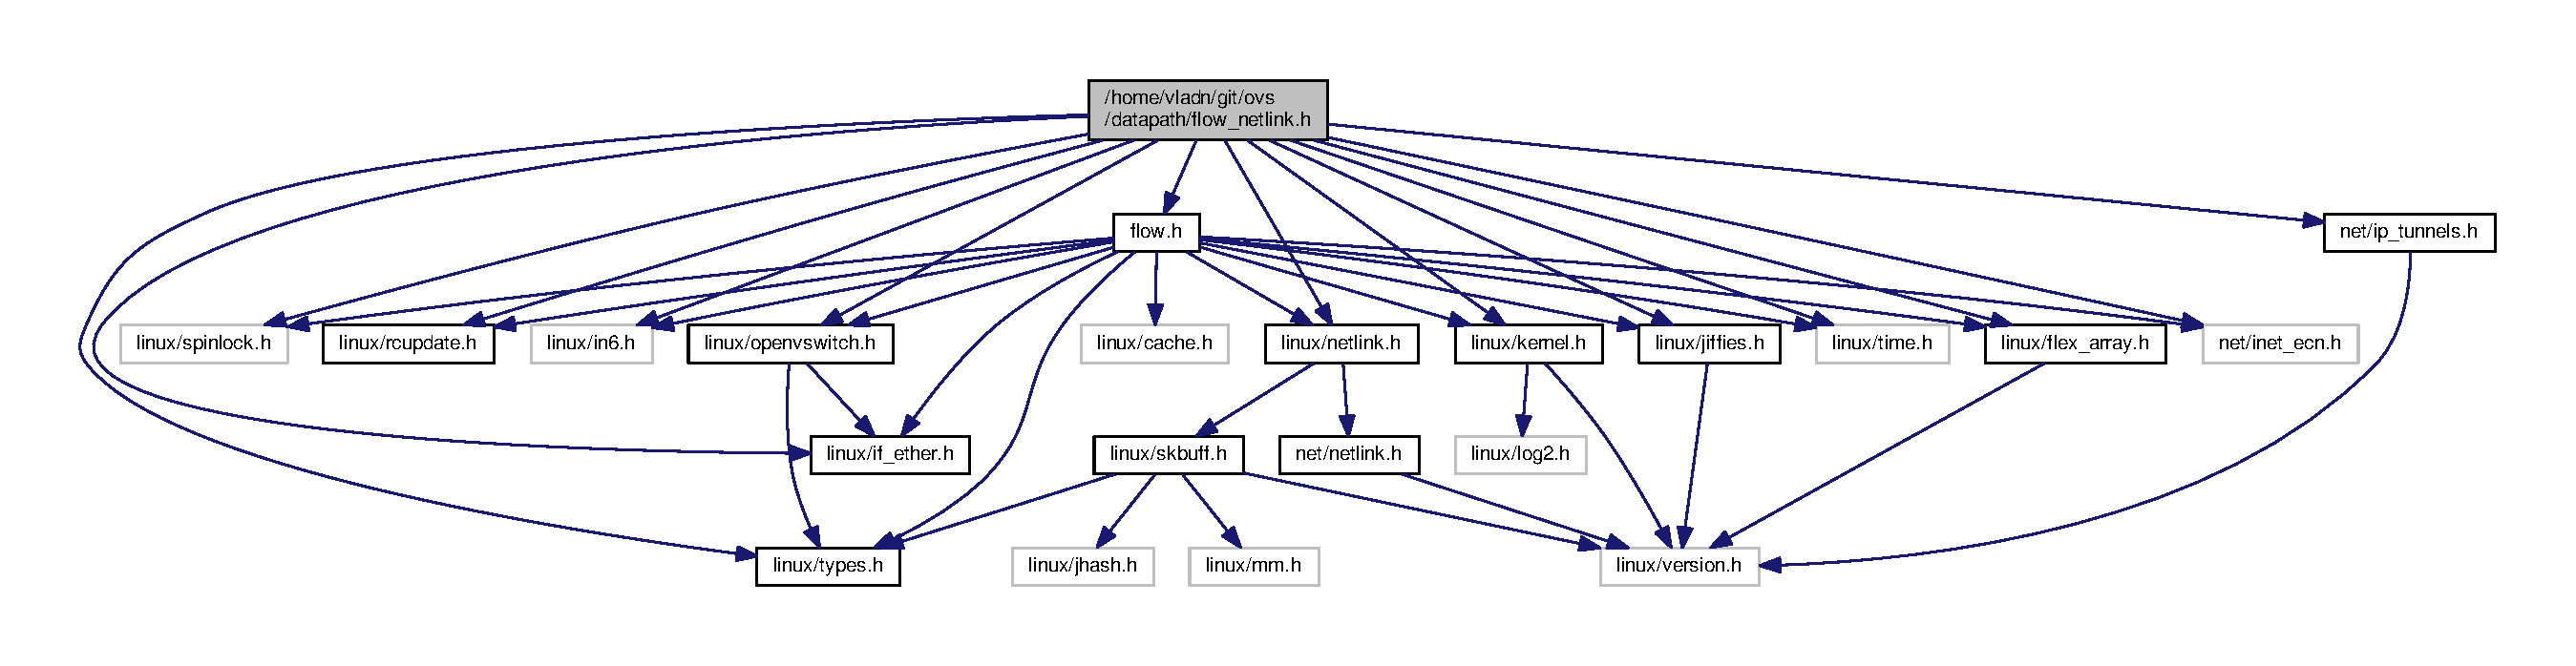
\includegraphics[width=350pt]{flow__netlink_8h__incl}
\end{center}
\end{figure}
This graph shows which files directly or indirectly include this file\+:
\nopagebreak
\begin{figure}[H]
\begin{center}
\leavevmode
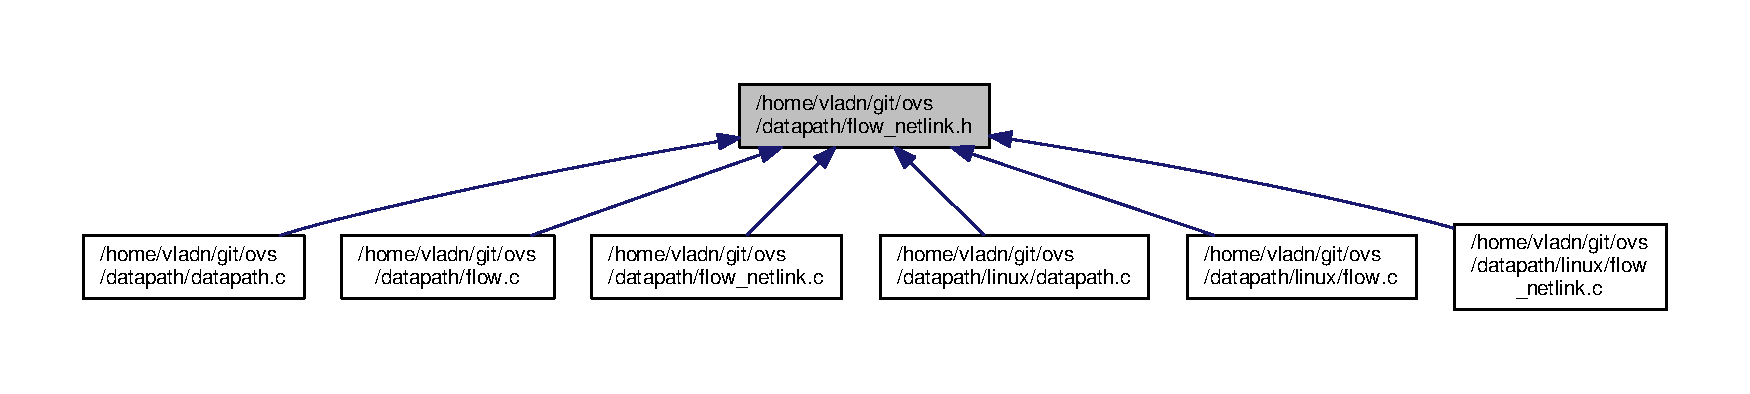
\includegraphics[width=350pt]{flow__netlink_8h__dep__incl}
\end{center}
\end{figure}
\subsection*{Functions}
\begin{DoxyCompactItemize}
\item 
size\+\_\+t \hyperlink{flow__netlink_8h_ac920825ffe4fa75e7ca3c5e76ad4ec2a}{ovs\+\_\+tun\+\_\+key\+\_\+attr\+\_\+size} (void)
\item 
size\+\_\+t \hyperlink{flow__netlink_8h_a4ea1ec7f3650fd324fc1538c97e795d0}{ovs\+\_\+key\+\_\+attr\+\_\+size} (void)
\item 
void \hyperlink{flow__netlink_8h_a1a09e9d38844c59332975789573e994c}{ovs\+\_\+match\+\_\+init} (struct \hyperlink{structsw__flow__match}{sw\+\_\+flow\+\_\+match} $\ast$match, struct \hyperlink{structsw__flow__key}{sw\+\_\+flow\+\_\+key} $\ast$key, struct \hyperlink{structsw__flow__mask}{sw\+\_\+flow\+\_\+mask} $\ast$mask)
\item 
int \hyperlink{flow__netlink_8h_ab52f962a5af3e769831e94b28a56171f}{ovs\+\_\+nla\+\_\+put\+\_\+key} (const struct \hyperlink{structsw__flow__key}{sw\+\_\+flow\+\_\+key} $\ast$, const struct \hyperlink{structsw__flow__key}{sw\+\_\+flow\+\_\+key} $\ast$, int attr, \hyperlink{types_8h_afaa87723b8417d40fcf45b7330261ef9}{bool} is\+\_\+mask, struct sk\+\_\+buff $\ast$)
\item 
int \hyperlink{flow__netlink_8h_a4927521e590b588f48062031450e415d}{ovs\+\_\+nla\+\_\+get\+\_\+flow\+\_\+metadata} (const struct nlattr $\ast$, struct \hyperlink{structsw__flow__key}{sw\+\_\+flow\+\_\+key} $\ast$, \hyperlink{types_8h_afaa87723b8417d40fcf45b7330261ef9}{bool} log)
\item 
int \hyperlink{flow__netlink_8h_a636f7d3cbe8656ceda87373110a4abc4}{ovs\+\_\+nla\+\_\+put\+\_\+identifier} (const struct \hyperlink{structsw__flow}{sw\+\_\+flow} $\ast$flow, struct sk\+\_\+buff $\ast$skb)
\item 
int \hyperlink{flow__netlink_8h_a2f6c3ab02b8e5d6296278dc9214500eb}{ovs\+\_\+nla\+\_\+put\+\_\+masked\+\_\+key} (const struct \hyperlink{structsw__flow}{sw\+\_\+flow} $\ast$flow, struct sk\+\_\+buff $\ast$skb)
\item 
int \hyperlink{flow__netlink_8h_af5ab12e938f8564945464a9e110eace3}{ovs\+\_\+nla\+\_\+put\+\_\+mask} (const struct \hyperlink{structsw__flow}{sw\+\_\+flow} $\ast$flow, struct sk\+\_\+buff $\ast$skb)
\item 
int \hyperlink{flow__netlink_8h_a18f9d1fe8fdf314eace9559ea4a51d9b}{ovs\+\_\+nla\+\_\+get\+\_\+match} (struct \hyperlink{structsw__flow__match}{sw\+\_\+flow\+\_\+match} $\ast$, const struct nlattr $\ast$key, const struct nlattr $\ast$mask, \hyperlink{types_8h_afaa87723b8417d40fcf45b7330261ef9}{bool} log)
\item 
int \hyperlink{flow__netlink_8h_a3ee4389059beab6dfbf2ce436b0e5483}{ovs\+\_\+nla\+\_\+put\+\_\+egress\+\_\+tunnel\+\_\+key} (struct sk\+\_\+buff $\ast$, const struct \hyperlink{structovs__tunnel__info}{ovs\+\_\+tunnel\+\_\+info} $\ast$)
\item 
\hyperlink{types_8h_afaa87723b8417d40fcf45b7330261ef9}{bool} \hyperlink{flow__netlink_8h_a97ac3692b5df3f22593f37746fe5f428}{ovs\+\_\+nla\+\_\+get\+\_\+ufid} (struct \hyperlink{structsw__flow__id}{sw\+\_\+flow\+\_\+id} $\ast$, const struct nlattr $\ast$, \hyperlink{types_8h_afaa87723b8417d40fcf45b7330261ef9}{bool} log)
\item 
int \hyperlink{flow__netlink_8h_aa416ab3b06ce40eee0be66306129c8d5}{ovs\+\_\+nla\+\_\+get\+\_\+identifier} (struct \hyperlink{structsw__flow__id}{sw\+\_\+flow\+\_\+id} $\ast$sfid, const struct nlattr $\ast$ufid, const struct \hyperlink{structsw__flow__key}{sw\+\_\+flow\+\_\+key} $\ast$key, \hyperlink{types_8h_afaa87723b8417d40fcf45b7330261ef9}{bool} log)
\item 
u32 \hyperlink{flow__netlink_8h_a415cb727697a02d62b8ff40795337d40}{ovs\+\_\+nla\+\_\+get\+\_\+ufid\+\_\+flags} (const struct nlattr $\ast$attr)
\item 
int \hyperlink{flow__netlink_8h_a10dc93f8c379eae7a557d54d9b387dd6}{ovs\+\_\+nla\+\_\+copy\+\_\+actions} (const struct nlattr $\ast$attr, const struct \hyperlink{structsw__flow__key}{sw\+\_\+flow\+\_\+key} $\ast$key, struct \hyperlink{structsw__flow__actions}{sw\+\_\+flow\+\_\+actions} $\ast$$\ast$sfa, \hyperlink{types_8h_afaa87723b8417d40fcf45b7330261ef9}{bool} log)
\item 
int \hyperlink{flow__netlink_8h_a923304ee69be1cfa52197b0f73c29e49}{ovs\+\_\+nla\+\_\+put\+\_\+actions} (const struct nlattr $\ast$attr, int len, struct sk\+\_\+buff $\ast$skb)
\item 
void \hyperlink{flow__netlink_8h_a6ead33c974a98707a46ff69758389258}{ovs\+\_\+nla\+\_\+free\+\_\+flow\+\_\+actions} (struct \hyperlink{structsw__flow__actions}{sw\+\_\+flow\+\_\+actions} $\ast$)
\end{DoxyCompactItemize}


\subsection{Function Documentation}
\hypertarget{flow__netlink_8h_a4ea1ec7f3650fd324fc1538c97e795d0}{}\index{flow\+\_\+netlink.\+h@{flow\+\_\+netlink.\+h}!ovs\+\_\+key\+\_\+attr\+\_\+size@{ovs\+\_\+key\+\_\+attr\+\_\+size}}
\index{ovs\+\_\+key\+\_\+attr\+\_\+size@{ovs\+\_\+key\+\_\+attr\+\_\+size}!flow\+\_\+netlink.\+h@{flow\+\_\+netlink.\+h}}
\subsubsection[{ovs\+\_\+key\+\_\+attr\+\_\+size}]{\setlength{\rightskip}{0pt plus 5cm}size\+\_\+t ovs\+\_\+key\+\_\+attr\+\_\+size (
\begin{DoxyParamCaption}
\item[{void}]{}
\end{DoxyParamCaption}
)}\label{flow__netlink_8h_a4ea1ec7f3650fd324fc1538c97e795d0}

\begin{DoxyCode}
280 \{
281     \textcolor{comment}{/* Whenever adding new OVS\_KEY\_ FIELDS, we should consider}
282 \textcolor{comment}{     * updating this function.}
283 \textcolor{comment}{     */}
284     BUILD\_BUG\_ON(OVS\_KEY\_ATTR\_TUNNEL\_INFO != 22);
285 
286     \textcolor{keywordflow}{return}    nla\_total\_size(4)   \textcolor{comment}{/* OVS\_KEY\_ATTR\_PRIORITY */}
287         + nla\_total\_size(0)   \textcolor{comment}{/* OVS\_KEY\_ATTR\_TUNNEL */}
288           + \hyperlink{flow__netlink_8c_ac920825ffe4fa75e7ca3c5e76ad4ec2a}{ovs\_tun\_key\_attr\_size}()
289         + nla\_total\_size(4)   \textcolor{comment}{/* OVS\_KEY\_ATTR\_IN\_PORT */}
290         + nla\_total\_size(4)   \textcolor{comment}{/* OVS\_KEY\_ATTR\_SKB\_MARK */}
291         + nla\_total\_size(4)   \textcolor{comment}{/* OVS\_KEY\_ATTR\_DP\_HASH */}
292         + nla\_total\_size(4)   \textcolor{comment}{/* OVS\_KEY\_ATTR\_RECIRC\_ID */}
293         + nla\_total\_size(12)  \textcolor{comment}{/* OVS\_KEY\_ATTR\_ETHERNET */}
294         + nla\_total\_size(2)   \textcolor{comment}{/* OVS\_KEY\_ATTR\_ETHERTYPE */}
295         + nla\_total\_size(4)   \textcolor{comment}{/* OVS\_KEY\_ATTR\_VLAN */}
296         + nla\_total\_size(0)   \textcolor{comment}{/* OVS\_KEY\_ATTR\_ENCAP */}
297         + nla\_total\_size(2)   \textcolor{comment}{/* OVS\_KEY\_ATTR\_ETHERTYPE */}
298         + nla\_total\_size(40)  \textcolor{comment}{/* OVS\_KEY\_ATTR\_IPV6 */}
299         + nla\_total\_size(2)   \textcolor{comment}{/* OVS\_KEY\_ATTR\_ICMPV6 */}
300         + nla\_total\_size(28); \textcolor{comment}{/* OVS\_KEY\_ATTR\_ND */}
301 \}
\end{DoxyCode}
\hypertarget{flow__netlink_8h_a1a09e9d38844c59332975789573e994c}{}\index{flow\+\_\+netlink.\+h@{flow\+\_\+netlink.\+h}!ovs\+\_\+match\+\_\+init@{ovs\+\_\+match\+\_\+init}}
\index{ovs\+\_\+match\+\_\+init@{ovs\+\_\+match\+\_\+init}!flow\+\_\+netlink.\+h@{flow\+\_\+netlink.\+h}}
\subsubsection[{ovs\+\_\+match\+\_\+init}]{\setlength{\rightskip}{0pt plus 5cm}void ovs\+\_\+match\+\_\+init (
\begin{DoxyParamCaption}
\item[{struct {\bf sw\+\_\+flow\+\_\+match} $\ast$}]{match, }
\item[{struct {\bf sw\+\_\+flow\+\_\+key} $\ast$}]{key, }
\item[{struct {\bf sw\+\_\+flow\+\_\+mask} $\ast$}]{mask}
\end{DoxyParamCaption}
)}\label{flow__netlink_8h_a1a09e9d38844c59332975789573e994c}

\begin{DoxyCode}
1714 \{
1715     memset(match, 0, \textcolor{keyword}{sizeof}(*match));
1716     match->\hyperlink{structsw__flow__match_a4030aac38105b63798ea11f43f506372}{key} = key;
1717     match->\hyperlink{structsw__flow__match_a4536aff731528d6def7d386435c203d1}{mask} = mask;
1718 
1719     memset(key, 0, \textcolor{keyword}{sizeof}(*key));
1720 
1721     \textcolor{keywordflow}{if} (mask) \{
1722         memset(&mask->\hyperlink{structsw__flow__mask_a52db0284fdd4579a5f30dee0837a7485}{key}, 0, \textcolor{keyword}{sizeof}(mask->\hyperlink{structsw__flow__mask_a52db0284fdd4579a5f30dee0837a7485}{key}));
1723         mask->\hyperlink{structsw__flow__mask_aa6062c0e580d516ff2d9ce8f9611432b}{range}.\hyperlink{structsw__flow__key__range_a3139158cea80b4e5af36967f3748e846}{start} = mask->\hyperlink{structsw__flow__mask_aa6062c0e580d516ff2d9ce8f9611432b}{range}.\hyperlink{structsw__flow__key__range_ab9c9d06e6ed2b9600d295dfdd94cc05a}{end} = 0;
1724     \}
1725 \}
\end{DoxyCode}
\hypertarget{flow__netlink_8h_a10dc93f8c379eae7a557d54d9b387dd6}{}\index{flow\+\_\+netlink.\+h@{flow\+\_\+netlink.\+h}!ovs\+\_\+nla\+\_\+copy\+\_\+actions@{ovs\+\_\+nla\+\_\+copy\+\_\+actions}}
\index{ovs\+\_\+nla\+\_\+copy\+\_\+actions@{ovs\+\_\+nla\+\_\+copy\+\_\+actions}!flow\+\_\+netlink.\+h@{flow\+\_\+netlink.\+h}}
\subsubsection[{ovs\+\_\+nla\+\_\+copy\+\_\+actions}]{\setlength{\rightskip}{0pt plus 5cm}int ovs\+\_\+nla\+\_\+copy\+\_\+actions (
\begin{DoxyParamCaption}
\item[{const struct nlattr $\ast$}]{attr, }
\item[{const struct {\bf sw\+\_\+flow\+\_\+key} $\ast$}]{key, }
\item[{struct {\bf sw\+\_\+flow\+\_\+actions} $\ast$$\ast$}]{sfa, }
\item[{{\bf bool}}]{log}
\end{DoxyParamCaption}
)}\label{flow__netlink_8h_a10dc93f8c379eae7a557d54d9b387dd6}

\begin{DoxyCode}
2182 \{
2183     \textcolor{keywordtype}{int} err;
2184 
2185     *sfa = \hyperlink{flow__netlink_8c_acf3273c812551499c4b4d48651548286}{nla\_alloc\_flow\_actions}(nla\_len(attr), log);
2186     \textcolor{keywordflow}{if} (IS\_ERR(*sfa))
2187         \textcolor{keywordflow}{return} PTR\_ERR(*sfa);
2188 
2189     err = \hyperlink{flow__netlink_8c_ae5c58b498948d3c5564b7916505d8455}{\_\_ovs\_nla\_copy\_actions}(attr, key, 0, sfa, key->
      \hyperlink{structsw__flow__key_af3e10c978a3a2bf303b7d953ac6ff361}{eth}.\hyperlink{structsw__flow__key_af30defbb2a81c997e8747594e1d937a0}{type},
2190                      key->\hyperlink{structsw__flow__key_af3e10c978a3a2bf303b7d953ac6ff361}{eth}.\hyperlink{structsw__flow__key_a56b27b9b9eafa8f79acd544eba98c7b0}{tci}, log);
2191     \textcolor{keywordflow}{if} (err)
2192         kfree(*sfa);
2193 
2194     \textcolor{keywordflow}{return} err;
2195 \}
\end{DoxyCode}
\hypertarget{flow__netlink_8h_a6ead33c974a98707a46ff69758389258}{}\index{flow\+\_\+netlink.\+h@{flow\+\_\+netlink.\+h}!ovs\+\_\+nla\+\_\+free\+\_\+flow\+\_\+actions@{ovs\+\_\+nla\+\_\+free\+\_\+flow\+\_\+actions}}
\index{ovs\+\_\+nla\+\_\+free\+\_\+flow\+\_\+actions@{ovs\+\_\+nla\+\_\+free\+\_\+flow\+\_\+actions}!flow\+\_\+netlink.\+h@{flow\+\_\+netlink.\+h}}
\subsubsection[{ovs\+\_\+nla\+\_\+free\+\_\+flow\+\_\+actions}]{\setlength{\rightskip}{0pt plus 5cm}void ovs\+\_\+nla\+\_\+free\+\_\+flow\+\_\+actions (
\begin{DoxyParamCaption}
\item[{struct {\bf sw\+\_\+flow\+\_\+actions} $\ast$}]{}
\end{DoxyParamCaption}
)}\label{flow__netlink_8h_a6ead33c974a98707a46ff69758389258}

\begin{DoxyCode}
1563 \{
1564     call\_rcu(&sf\_acts->rcu, \hyperlink{flow__netlink_8c_a386dd5cb0c8be8ce91e59761cbf820b4}{rcu\_free\_acts\_callback});
1565 \}
\end{DoxyCode}
\hypertarget{flow__netlink_8h_a4927521e590b588f48062031450e415d}{}\index{flow\+\_\+netlink.\+h@{flow\+\_\+netlink.\+h}!ovs\+\_\+nla\+\_\+get\+\_\+flow\+\_\+metadata@{ovs\+\_\+nla\+\_\+get\+\_\+flow\+\_\+metadata}}
\index{ovs\+\_\+nla\+\_\+get\+\_\+flow\+\_\+metadata@{ovs\+\_\+nla\+\_\+get\+\_\+flow\+\_\+metadata}!flow\+\_\+netlink.\+h@{flow\+\_\+netlink.\+h}}
\subsubsection[{ovs\+\_\+nla\+\_\+get\+\_\+flow\+\_\+metadata}]{\setlength{\rightskip}{0pt plus 5cm}int ovs\+\_\+nla\+\_\+get\+\_\+flow\+\_\+metadata (
\begin{DoxyParamCaption}
\item[{const struct nlattr $\ast$}]{attr, }
\item[{struct {\bf sw\+\_\+flow\+\_\+key} $\ast$}]{key, }
\item[{{\bf bool}}]{log}
\end{DoxyParamCaption}
)}\label{flow__netlink_8h_a4927521e590b588f48062031450e415d}
ovs\+\_\+nla\+\_\+get\+\_\+flow\+\_\+metadata -\/ parses Netlink attributes into a flow key. \+: Receives extracted in\+\_\+port, priority, tun\+\_\+key and skb\+\_\+mark. \+: Netlink attribute holding nested O\+V\+S\+\_\+\+K\+E\+Y\+\_\+\+A\+T\+T\+R\+\_\+$\ast$ Netlink attribute sequence. \+: Boolean to allow kernel error logging. Normally true, but when probing for feature compatibility this should be passed in as false to suppress unnecessary error logging.

This parses a series of Netlink attributes that form a flow key, which must take the same form accepted by flow\+\_\+from\+\_\+nlattrs(), but only enough of it to get the metadata, that is, the parts of the flow key that cannot be extracted from the packet itself. 
\begin{DoxyCode}
1255 \{
1256     \textcolor{keyword}{const} \textcolor{keyword}{struct }nlattr *a[\hyperlink{openvswitch_8h_a2a2adc6c47c38f0e7889580602ccbe22}{OVS\_KEY\_ATTR\_MAX} + 1];
1257     \textcolor{keyword}{struct }\hyperlink{structsw__flow__match}{sw\_flow\_match} match;
1258     u64 attrs = 0;
1259     \textcolor{keywordtype}{int} err;
1260 
1261     err = \hyperlink{flow__netlink_8c_aafe0de49242cd0276fd5ced0fd81514f}{parse\_flow\_nlattrs}(attr, a, &attrs, log);
1262     \textcolor{keywordflow}{if} (err)
1263         \textcolor{keywordflow}{return} -EINVAL;
1264 
1265     memset(&match, 0, \textcolor{keyword}{sizeof}(match));
1266     match.key = \hyperlink{structsw__flow__match_a4030aac38105b63798ea11f43f506372}{key};
1267 
1268     memset(key, 0, \hyperlink{flow_8h_aa38104b9e3106537d588a65cdce52e3a}{OVS\_SW\_FLOW\_KEY\_METADATA\_SIZE});
1269     key->\hyperlink{structsw__flow__key_a57cbddb75a8d4fd859300bd34d98e84a}{phy}.\hyperlink{structsw__flow__key_a5848de18caa80d36d9bc60cc686a2c6e}{in\_port} = \hyperlink{datapath_8h_a73b117dd1ebe456eecfb7688047a03f1}{DP\_MAX\_PORTS};
1270 
1271     \textcolor{keywordflow}{return} \hyperlink{flow__netlink_8c_aed17f75c6136e01aa609132d5bbc9b2a}{metadata\_from\_nlattrs}(&match, &attrs, a, \textcolor{keyword}{false}, log);
1272 \}
\end{DoxyCode}
\hypertarget{flow__netlink_8h_aa416ab3b06ce40eee0be66306129c8d5}{}\index{flow\+\_\+netlink.\+h@{flow\+\_\+netlink.\+h}!ovs\+\_\+nla\+\_\+get\+\_\+identifier@{ovs\+\_\+nla\+\_\+get\+\_\+identifier}}
\index{ovs\+\_\+nla\+\_\+get\+\_\+identifier@{ovs\+\_\+nla\+\_\+get\+\_\+identifier}!flow\+\_\+netlink.\+h@{flow\+\_\+netlink.\+h}}
\subsubsection[{ovs\+\_\+nla\+\_\+get\+\_\+identifier}]{\setlength{\rightskip}{0pt plus 5cm}int ovs\+\_\+nla\+\_\+get\+\_\+identifier (
\begin{DoxyParamCaption}
\item[{struct {\bf sw\+\_\+flow\+\_\+id} $\ast$}]{sfid, }
\item[{const struct nlattr $\ast$}]{ufid, }
\item[{const struct {\bf sw\+\_\+flow\+\_\+key} $\ast$}]{key, }
\item[{{\bf bool}}]{log}
\end{DoxyParamCaption}
)}\label{flow__netlink_8h_aa416ab3b06ce40eee0be66306129c8d5}

\begin{DoxyCode}
1216 \{
1217     \textcolor{keyword}{struct }\hyperlink{structsw__flow__key}{sw\_flow\_key} *new\_key;
1218 
1219     \textcolor{keywordflow}{if} (\hyperlink{flow__netlink_8c_a81e0cfe1c434ecde4ad684c8b8586877}{ovs\_nla\_get\_ufid}(sfid, ufid, log))
1220         \textcolor{keywordflow}{return} 0;
1221 
1222     \textcolor{comment}{/* If UFID was not provided, use unmasked key. */}
1223     new\_key = kmalloc(\textcolor{keyword}{sizeof}(*new\_key), GFP\_KERNEL);
1224     \textcolor{keywordflow}{if} (!new\_key)
1225         \textcolor{keywordflow}{return} -ENOMEM;
1226     memcpy(new\_key, key, \textcolor{keyword}{sizeof}(*key));
1227     sfid->\hyperlink{structsw__flow__id_a5d62dce79569cb8c25a43f4039e5df3c}{unmasked\_key} = new\_key;
1228 
1229     \textcolor{keywordflow}{return} 0;
1230 \}
\end{DoxyCode}
\hypertarget{flow__netlink_8h_a18f9d1fe8fdf314eace9559ea4a51d9b}{}\index{flow\+\_\+netlink.\+h@{flow\+\_\+netlink.\+h}!ovs\+\_\+nla\+\_\+get\+\_\+match@{ovs\+\_\+nla\+\_\+get\+\_\+match}}
\index{ovs\+\_\+nla\+\_\+get\+\_\+match@{ovs\+\_\+nla\+\_\+get\+\_\+match}!flow\+\_\+netlink.\+h@{flow\+\_\+netlink.\+h}}
\subsubsection[{ovs\+\_\+nla\+\_\+get\+\_\+match}]{\setlength{\rightskip}{0pt plus 5cm}int ovs\+\_\+nla\+\_\+get\+\_\+match (
\begin{DoxyParamCaption}
\item[{struct {\bf sw\+\_\+flow\+\_\+match} $\ast$}]{match, }
\item[{const struct nlattr $\ast$}]{nla\+\_\+key, }
\item[{const struct nlattr $\ast$}]{nla\+\_\+mask, }
\item[{{\bf bool}}]{log}
\end{DoxyParamCaption}
)}\label{flow__netlink_8h_a18f9d1fe8fdf314eace9559ea4a51d9b}
ovs\+\_\+nla\+\_\+get\+\_\+match -\/ parses Netlink attributes into a flow key and mask. In case the \textquotesingle{}mask\textquotesingle{} is N\+U\+L\+L, the flow is treated as exact match flow. Otherwise, it is treated as a wildcarded flow, except the mask does not include any don\textquotesingle{}t care bit. \+: receives the extracted flow match information. \+: Netlink attribute holding nested O\+V\+S\+\_\+\+K\+E\+Y\+\_\+\+A\+T\+T\+R\+\_\+$\ast$ Netlink attribute sequence. The fields should of the packet that triggered the creation of this flow. \+: Optional. Netlink attribute holding nested O\+V\+S\+\_\+\+K\+E\+Y\+\_\+\+A\+T\+T\+R\+\_\+$\ast$ Netlink attribute specifies the mask field of the wildcarded flow. \+: Boolean to allow kernel error logging. Normally true, but when probing for feature compatibility this should be passed in as false to suppress unnecessary error logging. 
\begin{DoxyCode}
1045 \{
1046     \textcolor{keyword}{const} \textcolor{keyword}{struct }nlattr *a[\hyperlink{openvswitch_8h_a2a2adc6c47c38f0e7889580602ccbe22}{OVS\_KEY\_ATTR\_MAX} + 1];
1047     \textcolor{keyword}{const} \textcolor{keyword}{struct }nlattr *encap;
1048     \textcolor{keyword}{struct }nlattr *newmask = NULL;
1049     u64 key\_attrs = 0;
1050     u64 mask\_attrs = 0;
1051     \textcolor{keywordtype}{bool} encap\_valid = \textcolor{keyword}{false};
1052     \textcolor{keywordtype}{int} err;
1053 
1054     err = \hyperlink{flow__netlink_8c_aafe0de49242cd0276fd5ced0fd81514f}{parse\_flow\_nlattrs}(nla\_key, a, &key\_attrs, log);
1055     \textcolor{keywordflow}{if} (err)
1056         \textcolor{keywordflow}{return} err;
1057 
1058     \textcolor{keywordflow}{if} ((key\_attrs & (1ULL << \hyperlink{openvswitch_8h_a6a279bc7098c9bc819c12355c9e07864a75127b87d8a2f36ae2c9aae2cf42cd56}{OVS\_KEY\_ATTR\_ETHERNET})) &&
1059         (key\_attrs & (1ULL << \hyperlink{openvswitch_8h_a6a279bc7098c9bc819c12355c9e07864aaccef1ecf941c78c70cf8a6a3374235a}{OVS\_KEY\_ATTR\_ETHERTYPE})) &&
1060         (\hyperlink{net_2netlink_8h_a5a9bc877c8fdbf9b3f2f85536aabcae0}{nla\_get\_be16}(a[\hyperlink{openvswitch_8h_a6a279bc7098c9bc819c12355c9e07864aaccef1ecf941c78c70cf8a6a3374235a}{OVS\_KEY\_ATTR\_ETHERTYPE}]) == htons(ETH\_P\_8021Q))) 
      \{
1061         \_\_be16 \hyperlink{flow_8h_a4528fe4db43b403cd959b50285d71b0c}{tci};
1062 
1063         \textcolor{keywordflow}{if} (!((key\_attrs & (1ULL << \hyperlink{openvswitch_8h_a6a279bc7098c9bc819c12355c9e07864ae513231d4612ed9b19551a7e70648005}{OVS\_KEY\_ATTR\_VLAN})) &&
1064               (key\_attrs & (1ULL << \hyperlink{openvswitch_8h_a6a279bc7098c9bc819c12355c9e07864a869b60116d7d6ac79bfad91cc808cf75}{OVS\_KEY\_ATTR\_ENCAP})))) \{
1065             \hyperlink{datapath_8h_a54648b7a2c9b192074cd95eb945433f0}{OVS\_NLERR}(log, \textcolor{stringliteral}{"Invalid Vlan frame."});
1066             \textcolor{keywordflow}{return} -EINVAL;
1067         \}
1068 
1069         key\_attrs &= ~(1ULL << \hyperlink{openvswitch_8h_a6a279bc7098c9bc819c12355c9e07864aaccef1ecf941c78c70cf8a6a3374235a}{OVS\_KEY\_ATTR\_ETHERTYPE});
1070         tci = \hyperlink{net_2netlink_8h_a5a9bc877c8fdbf9b3f2f85536aabcae0}{nla\_get\_be16}(a[\hyperlink{openvswitch_8h_a6a279bc7098c9bc819c12355c9e07864ae513231d4612ed9b19551a7e70648005}{OVS\_KEY\_ATTR\_VLAN}]);
1071         encap = a[\hyperlink{openvswitch_8h_a6a279bc7098c9bc819c12355c9e07864a869b60116d7d6ac79bfad91cc808cf75}{OVS\_KEY\_ATTR\_ENCAP}];
1072         key\_attrs &= ~(1ULL << \hyperlink{openvswitch_8h_a6a279bc7098c9bc819c12355c9e07864a869b60116d7d6ac79bfad91cc808cf75}{OVS\_KEY\_ATTR\_ENCAP});
1073         encap\_valid = \textcolor{keyword}{true};
1074 
1075         \textcolor{keywordflow}{if} (tci & htons(\hyperlink{if__vlan_8h_ac8bf15be3fd1a3a63a2452fa05a83217}{VLAN\_TAG\_PRESENT})) \{
1076             err = \hyperlink{flow__netlink_8c_aafe0de49242cd0276fd5ced0fd81514f}{parse\_flow\_nlattrs}(encap, a, &key\_attrs, log);
1077             \textcolor{keywordflow}{if} (err)
1078                 \textcolor{keywordflow}{return} err;
1079         \} \textcolor{keywordflow}{else} \textcolor{keywordflow}{if} (!tci) \{
1080             \textcolor{comment}{/* Corner case for truncated 802.1Q header. */}
1081             \textcolor{keywordflow}{if} (nla\_len(encap)) \{
1082                 \hyperlink{datapath_8h_a54648b7a2c9b192074cd95eb945433f0}{OVS\_NLERR}(log, \textcolor{stringliteral}{"Truncated 802.1Q header has non-zero encap attribute."});
1083                 \textcolor{keywordflow}{return} -EINVAL;
1084             \}
1085         \} \textcolor{keywordflow}{else} \{
1086             \hyperlink{datapath_8h_a54648b7a2c9b192074cd95eb945433f0}{OVS\_NLERR}(log, \textcolor{stringliteral}{"Encap attr is set for non-VLAN frame"});
1087             \textcolor{keywordflow}{return}  -EINVAL;
1088         \}
1089     \}
1090 
1091     err = \hyperlink{flow__netlink_8c_a7e2f54c332f7bdac73756972da69ad53}{ovs\_key\_from\_nlattrs}(match, key\_attrs, a, \textcolor{keyword}{false}, log);
1092     \textcolor{keywordflow}{if} (err)
1093         \textcolor{keywordflow}{return} err;
1094 
1095     \textcolor{keywordflow}{if} (match->\hyperlink{structsw__flow__match_a4536aff731528d6def7d386435c203d1}{mask}) \{
1096         \textcolor{keywordflow}{if} (!nla\_mask) \{
1097             \textcolor{comment}{/* Create an exact match mask. We need to set to 0xff}
1098 \textcolor{comment}{             * all the 'match->mask' fields that have been touched}
1099 \textcolor{comment}{             * in 'match->key'. We cannot simply memset}
1100 \textcolor{comment}{             * 'match->mask', because padding bytes and fields not}
1101 \textcolor{comment}{             * specified in 'match->key' should be left to 0.}
1102 \textcolor{comment}{             * Instead, we use a stream of netlink attributes,}
1103 \textcolor{comment}{             * copied from 'key' and set to 0xff.}
1104 \textcolor{comment}{             * ovs\_key\_from\_nlattrs() will take care of filling}
1105 \textcolor{comment}{             * 'match->mask' appropriately.}
1106 \textcolor{comment}{             */}
1107             newmask = kmemdup(nla\_key,
1108                       nla\_total\_size(nla\_len(nla\_key)),
1109                       GFP\_KERNEL);
1110             \textcolor{keywordflow}{if} (!newmask)
1111                 \textcolor{keywordflow}{return} -ENOMEM;
1112 
1113             \hyperlink{flow__netlink_8c_aa862995e0363dbb698ee51eb1be8a40c}{mask\_set\_nlattr}(newmask, 0xff);
1114 
1115             \textcolor{comment}{/* The userspace does not send tunnel attributes that}
1116 \textcolor{comment}{             * are 0, but we should not wildcard them nonetheless.}
1117 \textcolor{comment}{             */}
1118             \textcolor{keywordflow}{if} (match->\hyperlink{structsw__flow__match_a4030aac38105b63798ea11f43f506372}{key}->\hyperlink{structsw__flow__key_a2f87b7690c0cc2797f1f4347589472c3}{tun\_key}.\hyperlink{structovs__key__ipv4__tunnel_ae443d381a97f53bbc4139fe36c0aae30}{ipv4\_dst})
1119                 \hyperlink{flow__netlink_8c_a428fac9f6cc49614e07de128b9e4869f}{SW\_FLOW\_KEY\_MEMSET\_FIELD}(match, \hyperlink{flow_8h_a904e9497acde49a1992636f77597c5c7}{tun\_key},
1120                              0xff, \textcolor{keyword}{true});
1121 
1122             nla\_mask = newmask;
1123         \}
1124 
1125         err = \hyperlink{flow__netlink_8c_a4a090c5659903b6b8d125ab7598ad1a6}{parse\_flow\_mask\_nlattrs}(nla\_mask, a, &mask\_attrs, log);
1126         \textcolor{keywordflow}{if} (err)
1127             \textcolor{keywordflow}{goto} free\_newmask;
1128 
1129         \textcolor{comment}{/* Always match on tci. */}
1130         \hyperlink{flow__netlink_8c_a7cb040299f14f8ff8806dd868c321d7b}{SW\_FLOW\_KEY\_PUT}(match, \hyperlink{flow_8h_a1679a3c93391059deba58179f52c86a6}{eth}.tci, htons(0xffff), \textcolor{keyword}{true});
1131 
1132         \textcolor{keywordflow}{if} (mask\_attrs & 1ULL << \hyperlink{openvswitch_8h_a6a279bc7098c9bc819c12355c9e07864a869b60116d7d6ac79bfad91cc808cf75}{OVS\_KEY\_ATTR\_ENCAP}) \{
1133             \_\_be16 eth\_type = 0;
1134             \_\_be16 tci = 0;
1135 
1136             \textcolor{keywordflow}{if} (!encap\_valid) \{
1137                 \hyperlink{datapath_8h_a54648b7a2c9b192074cd95eb945433f0}{OVS\_NLERR}(log, \textcolor{stringliteral}{"Encap mask attribute is set for non-VLAN frame."});
1138                 err = -EINVAL;
1139                 \textcolor{keywordflow}{goto} free\_newmask;
1140             \}
1141 
1142             mask\_attrs &= ~(1ULL << \hyperlink{openvswitch_8h_a6a279bc7098c9bc819c12355c9e07864a869b60116d7d6ac79bfad91cc808cf75}{OVS\_KEY\_ATTR\_ENCAP});
1143             \textcolor{keywordflow}{if} (a[OVS\_KEY\_ATTR\_ETHERTYPE])
1144                 eth\_type = \hyperlink{net_2netlink_8h_a5a9bc877c8fdbf9b3f2f85536aabcae0}{nla\_get\_be16}(a[OVS\_KEY\_ATTR\_ETHERTYPE]);
1145 
1146             \textcolor{keywordflow}{if} (eth\_type == htons(0xffff)) \{
1147                 mask\_attrs &= ~(1ULL << \hyperlink{openvswitch_8h_a6a279bc7098c9bc819c12355c9e07864aaccef1ecf941c78c70cf8a6a3374235a}{OVS\_KEY\_ATTR\_ETHERTYPE});
1148                 encap = a[\hyperlink{openvswitch_8h_a6a279bc7098c9bc819c12355c9e07864a869b60116d7d6ac79bfad91cc808cf75}{OVS\_KEY\_ATTR\_ENCAP}];
1149                 err = \hyperlink{flow__netlink_8c_a4a090c5659903b6b8d125ab7598ad1a6}{parse\_flow\_mask\_nlattrs}(encap, a,
1150                                   &mask\_attrs, log);
1151                 \textcolor{keywordflow}{if} (err)
1152                     \textcolor{keywordflow}{goto} free\_newmask;
1153             \} \textcolor{keywordflow}{else} \{
1154                 \hyperlink{datapath_8h_a54648b7a2c9b192074cd95eb945433f0}{OVS\_NLERR}(log, \textcolor{stringliteral}{"VLAN frames must have an exact match on the TPID (mask=%x)."},
1155                       ntohs(eth\_type));
1156                 err = -EINVAL;
1157                 \textcolor{keywordflow}{goto} free\_newmask;
1158             \}
1159 
1160             \textcolor{keywordflow}{if} (a[\hyperlink{openvswitch_8h_a6a279bc7098c9bc819c12355c9e07864ae513231d4612ed9b19551a7e70648005}{OVS\_KEY\_ATTR\_VLAN}])
1161                 tci = \hyperlink{net_2netlink_8h_a5a9bc877c8fdbf9b3f2f85536aabcae0}{nla\_get\_be16}(a[OVS\_KEY\_ATTR\_VLAN]);
1162 
1163             \textcolor{keywordflow}{if} (!(tci & htons(\hyperlink{if__vlan_8h_ac8bf15be3fd1a3a63a2452fa05a83217}{VLAN\_TAG\_PRESENT}))) \{
1164                 \hyperlink{datapath_8h_a54648b7a2c9b192074cd95eb945433f0}{OVS\_NLERR}(log, \textcolor{stringliteral}{"VLAN tag present bit must have an exact match (tci\_mask=%x)."},
1165                       ntohs(tci));
1166                 err = -EINVAL;
1167                 \textcolor{keywordflow}{goto} free\_newmask;
1168             \}
1169         \}
1170 
1171         err = \hyperlink{flow__netlink_8c_a7e2f54c332f7bdac73756972da69ad53}{ovs\_key\_from\_nlattrs}(match, mask\_attrs, a, \textcolor{keyword}{true}, log);
1172         \textcolor{keywordflow}{if} (err)
1173             \textcolor{keywordflow}{goto} free\_newmask;
1174     \}
1175 
1176     \textcolor{keywordflow}{if} (!\hyperlink{flow__netlink_8c_ab4be6b01938d3a8f5a14bc787cb2b0b2}{match\_validate}(match, key\_attrs, mask\_attrs, log))
1177         err = -EINVAL;
1178 
1179 free\_newmask:
1180     kfree(newmask);
1181     \textcolor{keywordflow}{return} err;
1182 \}
\end{DoxyCode}
\hypertarget{flow__netlink_8h_a97ac3692b5df3f22593f37746fe5f428}{}\index{flow\+\_\+netlink.\+h@{flow\+\_\+netlink.\+h}!ovs\+\_\+nla\+\_\+get\+\_\+ufid@{ovs\+\_\+nla\+\_\+get\+\_\+ufid}}
\index{ovs\+\_\+nla\+\_\+get\+\_\+ufid@{ovs\+\_\+nla\+\_\+get\+\_\+ufid}!flow\+\_\+netlink.\+h@{flow\+\_\+netlink.\+h}}
\subsubsection[{ovs\+\_\+nla\+\_\+get\+\_\+ufid}]{\setlength{\rightskip}{0pt plus 5cm}{\bf bool} ovs\+\_\+nla\+\_\+get\+\_\+ufid (
\begin{DoxyParamCaption}
\item[{struct {\bf sw\+\_\+flow\+\_\+id} $\ast$}]{, }
\item[{const struct nlattr $\ast$}]{, }
\item[{{\bf bool}}]{log}
\end{DoxyParamCaption}
)}\label{flow__netlink_8h_a97ac3692b5df3f22593f37746fe5f428}

\begin{DoxyCode}
1206 \{
1207     sfid->ufid\_len = \hyperlink{flow__netlink_8c_a5189e471b5832c9371b45c5e58ca5b41}{get\_ufid\_len}(attr, log);
1208     \textcolor{keywordflow}{if} (sfid->ufid\_len)
1209         memcpy(sfid->ufid, nla\_data(attr), sfid->ufid\_len);
1210 
1211     \textcolor{keywordflow}{return} sfid->ufid\_len;
1212 \}
\end{DoxyCode}
\hypertarget{flow__netlink_8h_a415cb727697a02d62b8ff40795337d40}{}\index{flow\+\_\+netlink.\+h@{flow\+\_\+netlink.\+h}!ovs\+\_\+nla\+\_\+get\+\_\+ufid\+\_\+flags@{ovs\+\_\+nla\+\_\+get\+\_\+ufid\+\_\+flags}}
\index{ovs\+\_\+nla\+\_\+get\+\_\+ufid\+\_\+flags@{ovs\+\_\+nla\+\_\+get\+\_\+ufid\+\_\+flags}!flow\+\_\+netlink.\+h@{flow\+\_\+netlink.\+h}}
\subsubsection[{ovs\+\_\+nla\+\_\+get\+\_\+ufid\+\_\+flags}]{\setlength{\rightskip}{0pt plus 5cm}u32 ovs\+\_\+nla\+\_\+get\+\_\+ufid\+\_\+flags (
\begin{DoxyParamCaption}
\item[{const struct nlattr $\ast$}]{attr}
\end{DoxyParamCaption}
)}\label{flow__netlink_8h_a415cb727697a02d62b8ff40795337d40}

\begin{DoxyCode}
1233 \{
1234     \textcolor{keywordflow}{return} attr ? nla\_get\_u32(attr) : 0;
1235 \}
\end{DoxyCode}
\hypertarget{flow__netlink_8h_a923304ee69be1cfa52197b0f73c29e49}{}\index{flow\+\_\+netlink.\+h@{flow\+\_\+netlink.\+h}!ovs\+\_\+nla\+\_\+put\+\_\+actions@{ovs\+\_\+nla\+\_\+put\+\_\+actions}}
\index{ovs\+\_\+nla\+\_\+put\+\_\+actions@{ovs\+\_\+nla\+\_\+put\+\_\+actions}!flow\+\_\+netlink.\+h@{flow\+\_\+netlink.\+h}}
\subsubsection[{ovs\+\_\+nla\+\_\+put\+\_\+actions}]{\setlength{\rightskip}{0pt plus 5cm}int ovs\+\_\+nla\+\_\+put\+\_\+actions (
\begin{DoxyParamCaption}
\item[{const struct nlattr $\ast$}]{attr, }
\item[{int}]{len, }
\item[{struct sk\+\_\+buff $\ast$}]{skb}
\end{DoxyParamCaption}
)}\label{flow__netlink_8h_a923304ee69be1cfa52197b0f73c29e49}

\begin{DoxyCode}
2282 \{
2283     \textcolor{keyword}{const} \textcolor{keyword}{struct }nlattr *a;
2284     \textcolor{keywordtype}{int} rem, err;
2285 
2286     nla\_for\_each\_attr(a, attr, len, rem) \{
2287         \textcolor{keywordtype}{int} \hyperlink{flow_8h_ab22aaab04f806700def00f32823fcb9e}{type} = nla\_type(a);
2288 
2289         \textcolor{keywordflow}{switch} (type) \{
2290         \textcolor{keywordflow}{case} \hyperlink{openvswitch_8h_affc4a4d29437ad03a23444243e2db26eaff937deb7687d0dd4b073c27aed9c8be}{OVS\_ACTION\_ATTR\_SET}:
2291             err = \hyperlink{flow__netlink_8c_af38f12c35d382eb717bb6e5b4fba2309}{set\_action\_to\_attr}(a, skb);
2292             \textcolor{keywordflow}{if} (err)
2293                 \textcolor{keywordflow}{return} err;
2294             \textcolor{keywordflow}{break};
2295 
2296         \textcolor{keywordflow}{case} OVS\_ACTION\_ATTR\_SET\_TO\_MASKED:
2297             err = \hyperlink{flow__netlink_8c_a14e859cc22996f05850ca737daf2ee09}{masked\_set\_action\_to\_set\_action\_attr}(a, skb);
2298             \textcolor{keywordflow}{if} (err)
2299                 \textcolor{keywordflow}{return} err;
2300             \textcolor{keywordflow}{break};
2301 
2302         \textcolor{keywordflow}{case} \hyperlink{openvswitch_8h_affc4a4d29437ad03a23444243e2db26eaddc6f70b9e8501e5bb90548373faf734}{OVS\_ACTION\_ATTR\_SAMPLE}:
2303             err = \hyperlink{flow__netlink_8c_a92621d7eaed9e960f5e5d7b72e501db0}{sample\_action\_to\_attr}(a, skb);
2304             \textcolor{keywordflow}{if} (err)
2305                 \textcolor{keywordflow}{return} err;
2306             \textcolor{keywordflow}{break};
2307         \textcolor{keywordflow}{default}:
2308             \textcolor{keywordflow}{if} (nla\_put(skb, type, nla\_len(a), nla\_data(a)))
2309                 \textcolor{keywordflow}{return} -EMSGSIZE;
2310             \textcolor{keywordflow}{break};
2311         \}
2312     \}
2313 
2314     \textcolor{keywordflow}{return} 0;
2315 \}
\end{DoxyCode}
\hypertarget{flow__netlink_8h_a3ee4389059beab6dfbf2ce436b0e5483}{}\index{flow\+\_\+netlink.\+h@{flow\+\_\+netlink.\+h}!ovs\+\_\+nla\+\_\+put\+\_\+egress\+\_\+tunnel\+\_\+key@{ovs\+\_\+nla\+\_\+put\+\_\+egress\+\_\+tunnel\+\_\+key}}
\index{ovs\+\_\+nla\+\_\+put\+\_\+egress\+\_\+tunnel\+\_\+key@{ovs\+\_\+nla\+\_\+put\+\_\+egress\+\_\+tunnel\+\_\+key}!flow\+\_\+netlink.\+h@{flow\+\_\+netlink.\+h}}
\subsubsection[{ovs\+\_\+nla\+\_\+put\+\_\+egress\+\_\+tunnel\+\_\+key}]{\setlength{\rightskip}{0pt plus 5cm}int ovs\+\_\+nla\+\_\+put\+\_\+egress\+\_\+tunnel\+\_\+key (
\begin{DoxyParamCaption}
\item[{struct sk\+\_\+buff $\ast$}]{, }
\item[{const struct {\bf ovs\+\_\+tunnel\+\_\+info} $\ast$}]{}
\end{DoxyParamCaption}
)}\label{flow__netlink_8h_a3ee4389059beab6dfbf2ce436b0e5483}

\begin{DoxyCode}
710 \{
711     \textcolor{keywordflow}{return} \hyperlink{flow__netlink_8c_ac7f453fb68977c7a24d7af50f18b43db}{\_\_ipv4\_tun\_to\_nlattr}(skb, &egress\_tun\_info->tunnel,
712                     egress\_tun\_info->options,
713                     egress\_tun\_info->options\_len);
714 \}
\end{DoxyCode}
\hypertarget{flow__netlink_8h_a636f7d3cbe8656ceda87373110a4abc4}{}\index{flow\+\_\+netlink.\+h@{flow\+\_\+netlink.\+h}!ovs\+\_\+nla\+\_\+put\+\_\+identifier@{ovs\+\_\+nla\+\_\+put\+\_\+identifier}}
\index{ovs\+\_\+nla\+\_\+put\+\_\+identifier@{ovs\+\_\+nla\+\_\+put\+\_\+identifier}!flow\+\_\+netlink.\+h@{flow\+\_\+netlink.\+h}}
\subsubsection[{ovs\+\_\+nla\+\_\+put\+\_\+identifier}]{\setlength{\rightskip}{0pt plus 5cm}int ovs\+\_\+nla\+\_\+put\+\_\+identifier (
\begin{DoxyParamCaption}
\item[{const struct {\bf sw\+\_\+flow} $\ast$}]{flow, }
\item[{struct sk\+\_\+buff $\ast$}]{skb}
\end{DoxyParamCaption}
)}\label{flow__netlink_8h_a636f7d3cbe8656ceda87373110a4abc4}

\begin{DoxyCode}
1509 \{
1510     \textcolor{keywordflow}{if} (\hyperlink{flow_8h_a995966854ceb0b5a72ff027c12ccf426}{ovs\_identifier\_is\_ufid}(&flow->\hyperlink{structsw__flow_a6e6645eec909d54871675be30000c0b9}{id}))
1511         \textcolor{keywordflow}{return} nla\_put(skb, \hyperlink{openvswitch_8h_a57b731cb45ac4bf32234fbf071e9c554a0d2822e9d4b6fa37c54dd8b693c2b465}{OVS\_FLOW\_ATTR\_UFID}, flow->\hyperlink{structsw__flow_a6e6645eec909d54871675be30000c0b9}{id}.
      \hyperlink{structsw__flow__id_a7cfead96fedf295e55d6a17857adfbf5}{ufid\_len},
1512                    flow->\hyperlink{structsw__flow_a6e6645eec909d54871675be30000c0b9}{id}.\hyperlink{structsw__flow__id_a22ce2b1fed980149931fbccb05750f3e}{ufid});
1513 
1514     \textcolor{keywordflow}{return} \hyperlink{flow__netlink_8c_a845412e2f8f2bcb48df005e857474fcb}{ovs\_nla\_put\_key}(flow->\hyperlink{structsw__flow_a6e6645eec909d54871675be30000c0b9}{id}.\hyperlink{structsw__flow__id_a5d62dce79569cb8c25a43f4039e5df3c}{unmasked\_key}, flow->
      \hyperlink{structsw__flow_a6e6645eec909d54871675be30000c0b9}{id}.\hyperlink{structsw__flow__id_a5d62dce79569cb8c25a43f4039e5df3c}{unmasked\_key},
1515                    \hyperlink{openvswitch_8h_a57b731cb45ac4bf32234fbf071e9c554a0d310e7624962a1b4c5212459995a5c9}{OVS\_FLOW\_ATTR\_KEY}, \textcolor{keyword}{false}, skb);
1516 \}
\end{DoxyCode}
\hypertarget{flow__netlink_8h_ab52f962a5af3e769831e94b28a56171f}{}\index{flow\+\_\+netlink.\+h@{flow\+\_\+netlink.\+h}!ovs\+\_\+nla\+\_\+put\+\_\+key@{ovs\+\_\+nla\+\_\+put\+\_\+key}}
\index{ovs\+\_\+nla\+\_\+put\+\_\+key@{ovs\+\_\+nla\+\_\+put\+\_\+key}!flow\+\_\+netlink.\+h@{flow\+\_\+netlink.\+h}}
\subsubsection[{ovs\+\_\+nla\+\_\+put\+\_\+key}]{\setlength{\rightskip}{0pt plus 5cm}int ovs\+\_\+nla\+\_\+put\+\_\+key (
\begin{DoxyParamCaption}
\item[{const struct {\bf sw\+\_\+flow\+\_\+key} $\ast$}]{, }
\item[{const struct {\bf sw\+\_\+flow\+\_\+key} $\ast$}]{, }
\item[{int}]{attr, }
\item[{{\bf bool}}]{is\+\_\+mask, }
\item[{struct sk\+\_\+buff $\ast$}]{}
\end{DoxyParamCaption}
)}\label{flow__netlink_8h_ab52f962a5af3e769831e94b28a56171f}

\begin{DoxyCode}
1492 \{
1493     \textcolor{keywordtype}{int} err;
1494     \textcolor{keyword}{struct }nlattr *nla;
1495 
1496     nla = nla\_nest\_start(skb, attr);
1497     \textcolor{keywordflow}{if} (!nla)
1498         \textcolor{keywordflow}{return} -EMSGSIZE;
1499     err = \hyperlink{flow__netlink_8c_a469e9434d0bedd721b2e31a106799335}{\_\_ovs\_nla\_put\_key}(swkey, output, is\_mask, skb);
1500     \textcolor{keywordflow}{if} (err)
1501         \textcolor{keywordflow}{return} err;
1502     nla\_nest\_end(skb, nla);
1503 
1504     \textcolor{keywordflow}{return} 0;
1505 \}
\end{DoxyCode}
\hypertarget{flow__netlink_8h_af5ab12e938f8564945464a9e110eace3}{}\index{flow\+\_\+netlink.\+h@{flow\+\_\+netlink.\+h}!ovs\+\_\+nla\+\_\+put\+\_\+mask@{ovs\+\_\+nla\+\_\+put\+\_\+mask}}
\index{ovs\+\_\+nla\+\_\+put\+\_\+mask@{ovs\+\_\+nla\+\_\+put\+\_\+mask}!flow\+\_\+netlink.\+h@{flow\+\_\+netlink.\+h}}
\subsubsection[{ovs\+\_\+nla\+\_\+put\+\_\+mask}]{\setlength{\rightskip}{0pt plus 5cm}int ovs\+\_\+nla\+\_\+put\+\_\+mask (
\begin{DoxyParamCaption}
\item[{const struct {\bf sw\+\_\+flow} $\ast$}]{flow, }
\item[{struct sk\+\_\+buff $\ast$}]{skb}
\end{DoxyParamCaption}
)}\label{flow__netlink_8h_af5ab12e938f8564945464a9e110eace3}

\begin{DoxyCode}
1527 \{
1528     \textcolor{keywordflow}{return} \hyperlink{flow__netlink_8c_a845412e2f8f2bcb48df005e857474fcb}{ovs\_nla\_put\_key}(&flow->\hyperlink{structsw__flow_a14b83cbd65275bda4e97ae35500d26d8}{key}, &flow->\hyperlink{structsw__flow_a89c162e340693d0bb4977737e2b68c22}{mask}->\hyperlink{structsw__flow__mask_a52db0284fdd4579a5f30dee0837a7485}{key},
1529                 \hyperlink{openvswitch_8h_a57b731cb45ac4bf32234fbf071e9c554a355a203b089e115abb28ea003dc5822c}{OVS\_FLOW\_ATTR\_MASK}, \textcolor{keyword}{true}, skb);
1530 \}
\end{DoxyCode}
\hypertarget{flow__netlink_8h_a2f6c3ab02b8e5d6296278dc9214500eb}{}\index{flow\+\_\+netlink.\+h@{flow\+\_\+netlink.\+h}!ovs\+\_\+nla\+\_\+put\+\_\+masked\+\_\+key@{ovs\+\_\+nla\+\_\+put\+\_\+masked\+\_\+key}}
\index{ovs\+\_\+nla\+\_\+put\+\_\+masked\+\_\+key@{ovs\+\_\+nla\+\_\+put\+\_\+masked\+\_\+key}!flow\+\_\+netlink.\+h@{flow\+\_\+netlink.\+h}}
\subsubsection[{ovs\+\_\+nla\+\_\+put\+\_\+masked\+\_\+key}]{\setlength{\rightskip}{0pt plus 5cm}int ovs\+\_\+nla\+\_\+put\+\_\+masked\+\_\+key (
\begin{DoxyParamCaption}
\item[{const struct {\bf sw\+\_\+flow} $\ast$}]{flow, }
\item[{struct sk\+\_\+buff $\ast$}]{skb}
\end{DoxyParamCaption}
)}\label{flow__netlink_8h_a2f6c3ab02b8e5d6296278dc9214500eb}

\begin{DoxyCode}
1520 \{
1521     \textcolor{keywordflow}{return} \hyperlink{flow__netlink_8c_a845412e2f8f2bcb48df005e857474fcb}{ovs\_nla\_put\_key}(&flow->\hyperlink{structsw__flow_a14b83cbd65275bda4e97ae35500d26d8}{key}, &flow->\hyperlink{structsw__flow_a14b83cbd65275bda4e97ae35500d26d8}{key},
1522                 \hyperlink{openvswitch_8h_a57b731cb45ac4bf32234fbf071e9c554a0d310e7624962a1b4c5212459995a5c9}{OVS\_FLOW\_ATTR\_KEY}, \textcolor{keyword}{false}, skb);
1523 \}
\end{DoxyCode}
\hypertarget{flow__netlink_8h_ac920825ffe4fa75e7ca3c5e76ad4ec2a}{}\index{flow\+\_\+netlink.\+h@{flow\+\_\+netlink.\+h}!ovs\+\_\+tun\+\_\+key\+\_\+attr\+\_\+size@{ovs\+\_\+tun\+\_\+key\+\_\+attr\+\_\+size}}
\index{ovs\+\_\+tun\+\_\+key\+\_\+attr\+\_\+size@{ovs\+\_\+tun\+\_\+key\+\_\+attr\+\_\+size}!flow\+\_\+netlink.\+h@{flow\+\_\+netlink.\+h}}
\subsubsection[{ovs\+\_\+tun\+\_\+key\+\_\+attr\+\_\+size}]{\setlength{\rightskip}{0pt plus 5cm}size\+\_\+t ovs\+\_\+tun\+\_\+key\+\_\+attr\+\_\+size (
\begin{DoxyParamCaption}
\item[{void}]{}
\end{DoxyParamCaption}
)}\label{flow__netlink_8h_ac920825ffe4fa75e7ca3c5e76ad4ec2a}

\begin{DoxyCode}
259 \{
260     \textcolor{comment}{/* Whenever adding new OVS\_TUNNEL\_KEY\_ FIELDS, we should consider}
261 \textcolor{comment}{     * updating this function.}
262 \textcolor{comment}{     */}
263     \textcolor{keywordflow}{return}    nla\_total\_size(8)    \textcolor{comment}{/* OVS\_TUNNEL\_KEY\_ATTR\_ID */}
264         + nla\_total\_size(4)    \textcolor{comment}{/* OVS\_TUNNEL\_KEY\_ATTR\_IPV4\_SRC */}
265         + nla\_total\_size(4)    \textcolor{comment}{/* OVS\_TUNNEL\_KEY\_ATTR\_IPV4\_DST */}
266         + nla\_total\_size(1)    \textcolor{comment}{/* OVS\_TUNNEL\_KEY\_ATTR\_TOS */}
267         + nla\_total\_size(1)    \textcolor{comment}{/* OVS\_TUNNEL\_KEY\_ATTR\_TTL */}
268         + nla\_total\_size(0)    \textcolor{comment}{/* OVS\_TUNNEL\_KEY\_ATTR\_DONT\_FRAGMENT */}
269         + nla\_total\_size(0)    \textcolor{comment}{/* OVS\_TUNNEL\_KEY\_ATTR\_CSUM */}
270         + nla\_total\_size(0)    \textcolor{comment}{/* OVS\_TUNNEL\_KEY\_ATTR\_OAM */}
271         + nla\_total\_size(256)  \textcolor{comment}{/* OVS\_TUNNEL\_KEY\_ATTR\_GENEVE\_OPTS */}
272         \textcolor{comment}{/* OVS\_TUNNEL\_KEY\_ATTR\_VXLAN\_OPTS is mutually exclusive with}
273 \textcolor{comment}{         * OVS\_TUNNEL\_KEY\_ATTR\_GENEVE\_OPTS and covered by it.}
274 \textcolor{comment}{         */}
275         + nla\_total\_size(2)    \textcolor{comment}{/* OVS\_TUNNEL\_KEY\_ATTR\_TP\_SRC */}
276         + nla\_total\_size(2);   \textcolor{comment}{/* OVS\_TUNNEL\_KEY\_ATTR\_TP\_DST */}
277 \}
\end{DoxyCode}

\hypertarget{flow__table_8c}{}\section{/home/vladn/git/ovs/datapath/flow\+\_\+table.c File Reference}
\label{flow__table_8c}\index{/home/vladn/git/ovs/datapath/flow\+\_\+table.\+c@{/home/vladn/git/ovs/datapath/flow\+\_\+table.\+c}}
{\ttfamily \#include \char`\"{}flow.\+h\char`\"{}}\\*
{\ttfamily \#include \char`\"{}datapath.\+h\char`\"{}}\\*
{\ttfamily \#include $<$linux/uaccess.\+h$>$}\\*
{\ttfamily \#include $<$linux/netdevice.\+h$>$}\\*
{\ttfamily \#include $<$linux/etherdevice.\+h$>$}\\*
{\ttfamily \#include $<$linux/if\+\_\+ether.\+h$>$}\\*
{\ttfamily \#include $<$linux/if\+\_\+vlan.\+h$>$}\\*
{\ttfamily \#include $<$net/llc\+\_\+pdu.\+h$>$}\\*
{\ttfamily \#include $<$linux/kernel.\+h$>$}\\*
{\ttfamily \#include $<$linux/jhash.\+h$>$}\\*
{\ttfamily \#include $<$linux/jiffies.\+h$>$}\\*
{\ttfamily \#include $<$linux/llc.\+h$>$}\\*
{\ttfamily \#include $<$linux/module.\+h$>$}\\*
{\ttfamily \#include $<$linux/in.\+h$>$}\\*
{\ttfamily \#include $<$linux/rcupdate.\+h$>$}\\*
{\ttfamily \#include $<$linux/if\+\_\+arp.\+h$>$}\\*
{\ttfamily \#include $<$linux/ip.\+h$>$}\\*
{\ttfamily \#include $<$linux/ipv6.\+h$>$}\\*
{\ttfamily \#include $<$linux/sctp.\+h$>$}\\*
{\ttfamily \#include $<$linux/tcp.\+h$>$}\\*
{\ttfamily \#include $<$linux/udp.\+h$>$}\\*
{\ttfamily \#include $<$linux/icmp.\+h$>$}\\*
{\ttfamily \#include $<$linux/icmpv6.\+h$>$}\\*
{\ttfamily \#include $<$linux/rculist.\+h$>$}\\*
{\ttfamily \#include $<$net/ip.\+h$>$}\\*
{\ttfamily \#include $<$net/ipv6.\+h$>$}\\*
{\ttfamily \#include $<$net/ndisc.\+h$>$}\\*
{\ttfamily \#include \char`\"{}vlan.\+h\char`\"{}}\\*
Include dependency graph for flow\+\_\+table.\+c\+:
\nopagebreak
\begin{figure}[H]
\begin{center}
\leavevmode
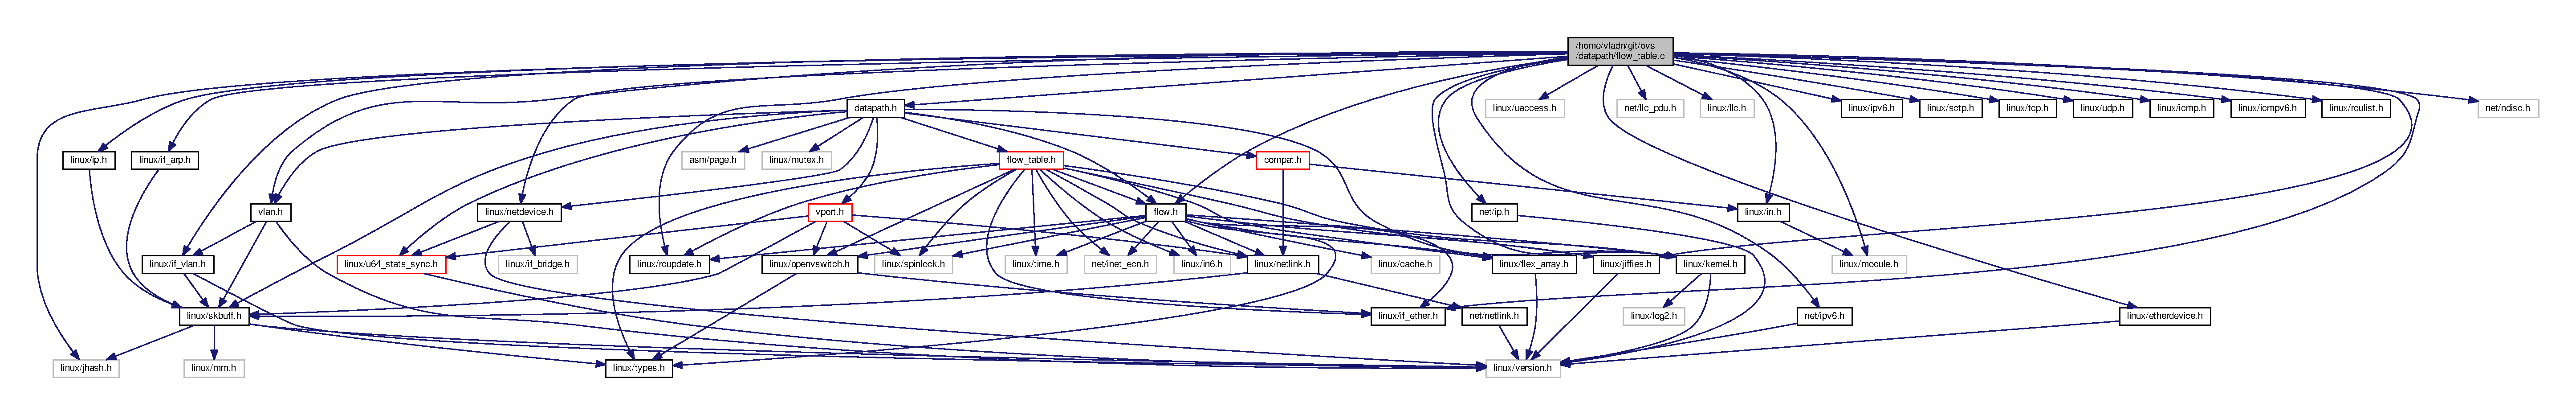
\includegraphics[width=350pt]{flow__table_8c__incl}
\end{center}
\end{figure}
\subsection*{Macros}
\begin{DoxyCompactItemize}
\item 
\#define \hyperlink{flow__table_8c_a84843442d8db7eda5192117e7c6b2997}{T\+B\+L\+\_\+\+M\+I\+N\+\_\+\+B\+U\+C\+K\+E\+T\+S}~1024
\item 
\#define \hyperlink{flow__table_8c_a8240394ae842a0ba76d82f50744ced0a}{M\+A\+S\+K\+\_\+\+A\+R\+R\+A\+Y\+\_\+\+S\+I\+Z\+E\+\_\+\+M\+I\+N}~16
\item 
\#define \hyperlink{flow__table_8c_a70a89d7f312fa8c27a8d2423cd512040}{R\+E\+H\+A\+S\+H\+\_\+\+I\+N\+T\+E\+R\+V\+A\+L}~(10 $\ast$ 60 $\ast$ H\+Z)
\item 
\#define \hyperlink{flow__table_8c_aba54fb364af2c9465bb632f82e4631d7}{M\+C\+\_\+\+H\+A\+S\+H\+\_\+\+S\+H\+I\+F\+T}~8
\item 
\#define \hyperlink{flow__table_8c_af961440482d56f3b26f232774a37c9c5}{M\+C\+\_\+\+H\+A\+S\+H\+\_\+\+E\+N\+T\+R\+I\+E\+S}~(1u $<$$<$ M\+C\+\_\+\+H\+A\+S\+H\+\_\+\+S\+H\+I\+F\+T)
\item 
\#define \hyperlink{flow__table_8c_ab95179a8dc622b08ce82308fe001d788}{M\+C\+\_\+\+H\+A\+S\+H\+\_\+\+S\+E\+G\+S}~((sizeof(uint32\+\_\+t) $\ast$ 8) / \hyperlink{linux_2flow__table_8c_aba54fb364af2c9465bb632f82e4631d7}{M\+C\+\_\+\+H\+A\+S\+H\+\_\+\+S\+H\+I\+F\+T})
\end{DoxyCompactItemize}
\subsection*{Functions}
\begin{DoxyCompactItemize}
\item 
static u16 \hyperlink{flow__table_8c_a1b494e4862736de33cbbd7cd72ee8521}{range\+\_\+n\+\_\+bytes} (const struct \hyperlink{structsw__flow__key__range}{sw\+\_\+flow\+\_\+key\+\_\+range} $\ast$range)
\item 
void \hyperlink{flow__table_8c_a40f76cbd2e168abb1b9744562e24be3b}{ovs\+\_\+flow\+\_\+mask\+\_\+key} (struct \hyperlink{structsw__flow__key}{sw\+\_\+flow\+\_\+key} $\ast$\hyperlink{flow_8h_a6747ad3b5d60480ea073cd12c9b78aaa}{dst}, const struct \hyperlink{structsw__flow__key}{sw\+\_\+flow\+\_\+key} $\ast$\hyperlink{flow_8h_a2e7e37e9dfe6465386d6c500f83ef144}{src}, const struct \hyperlink{structsw__flow__mask}{sw\+\_\+flow\+\_\+mask} $\ast$mask)
\item 
struct \hyperlink{structsw__flow}{sw\+\_\+flow} $\ast$ \hyperlink{flow__table_8c_acce701c647d8e59486574fba1be3e10c}{ovs\+\_\+flow\+\_\+alloc} (void)
\item 
int \hyperlink{flow__table_8c_a8f1f39fd4e1ecafd99321016698a709a}{ovs\+\_\+flow\+\_\+tbl\+\_\+count} (const struct \hyperlink{structflow__table}{flow\+\_\+table} $\ast$table)
\item 
static struct flex\+\_\+array $\ast$ \hyperlink{flow__table_8c_a9ad4dc425c825cafea26f047d94d8880}{alloc\+\_\+buckets} (unsigned int n\+\_\+buckets)
\item 
static void \hyperlink{flow__table_8c_af6a50f2fb2e93732e8d706dd7cf67c9b}{flow\+\_\+free} (struct \hyperlink{structsw__flow}{sw\+\_\+flow} $\ast$flow)
\item 
static void \hyperlink{flow__table_8c_a38fd2d883e505bba412320f3216dc377}{rcu\+\_\+free\+\_\+flow\+\_\+callback} (struct rcu\+\_\+head $\ast$rcu)
\item 
static void \hyperlink{flow__table_8c_a1431ef6b130c835dd7c86bac4472664b}{rcu\+\_\+free\+\_\+sw\+\_\+flow\+\_\+mask\+\_\+cb} (struct rcu\+\_\+head $\ast$rcu)
\item 
void \hyperlink{flow__table_8c_a8133cf46e955b2ae38a0bb8afc0a454f}{ovs\+\_\+flow\+\_\+free} (struct \hyperlink{structsw__flow}{sw\+\_\+flow} $\ast$flow, \hyperlink{types_8h_afaa87723b8417d40fcf45b7330261ef9}{bool} deferred)
\item 
static void \hyperlink{flow__table_8c_a351711f4f3b2e623bbca105ee2199f52}{free\+\_\+buckets} (struct flex\+\_\+array $\ast$buckets)
\item 
static void \hyperlink{flow__table_8c_a4699ad0074a999c5f80e77a8ff1b0ebc}{\+\_\+\+\_\+table\+\_\+instance\+\_\+destroy} (struct \hyperlink{structtable__instance}{table\+\_\+instance} $\ast$ti)
\item 
static struct \hyperlink{structtable__instance}{table\+\_\+instance} $\ast$ \hyperlink{flow__table_8c_afa79f1c5220d4487a4236884110b9f13}{table\+\_\+instance\+\_\+alloc} (int new\+\_\+size)
\item 
static void \hyperlink{flow__table_8c_a77da2cbea7e181821fc6931d8434bf15}{mask\+\_\+array\+\_\+rcu\+\_\+cb} (struct rcu\+\_\+head $\ast$rcu)
\item 
static struct \hyperlink{structmask__array}{mask\+\_\+array} $\ast$ \hyperlink{flow__table_8c_a327b2f9873b81f7b7920e85c366cc96e}{tbl\+\_\+mask\+\_\+array\+\_\+alloc} (int size)
\item 
static int \hyperlink{flow__table_8c_a1ba0bfff1e2a4377681774b821629e8f}{tbl\+\_\+mask\+\_\+array\+\_\+realloc} (struct \hyperlink{structflow__table}{flow\+\_\+table} $\ast$tbl, int size)
\item 
int \hyperlink{flow__table_8c_a0df1c5a76810e541b43248c402d764ff}{ovs\+\_\+flow\+\_\+tbl\+\_\+init} (struct \hyperlink{structflow__table}{flow\+\_\+table} $\ast$table)
\item 
static void \hyperlink{flow__table_8c_a2343a61f4fa3ad010bad594467cbcfc1}{flow\+\_\+tbl\+\_\+destroy\+\_\+rcu\+\_\+cb} (struct rcu\+\_\+head $\ast$rcu)
\item 
static void \hyperlink{flow__table_8c_a5abf80651b67f4198a34f7a94e116ec6}{table\+\_\+instance\+\_\+destroy} (struct \hyperlink{structtable__instance}{table\+\_\+instance} $\ast$ti, struct \hyperlink{structtable__instance}{table\+\_\+instance} $\ast$ufid\+\_\+ti, \hyperlink{types_8h_afaa87723b8417d40fcf45b7330261ef9}{bool} deferred)
\item 
void \hyperlink{flow__table_8c_ad37dcfdb56d17589ed79b5c4dd38bc76}{ovs\+\_\+flow\+\_\+tbl\+\_\+destroy} (struct \hyperlink{structflow__table}{flow\+\_\+table} $\ast$table)
\item 
struct \hyperlink{structsw__flow}{sw\+\_\+flow} $\ast$ \hyperlink{flow__table_8c_ab25c7aae52c39216ebb03d10a6cba0d8}{ovs\+\_\+flow\+\_\+tbl\+\_\+dump\+\_\+next} (struct \hyperlink{structtable__instance}{table\+\_\+instance} $\ast$ti, u32 $\ast$bucket, u32 $\ast$last)
\item 
static struct hlist\+\_\+head $\ast$ \hyperlink{flow__table_8c_aed00deae6497143255e822e293592558}{find\+\_\+bucket} (struct \hyperlink{structtable__instance}{table\+\_\+instance} $\ast$ti, u32 hash)
\item 
static void \hyperlink{flow__table_8c_a81b19a73c026d0c0fa6be862a1ee855b}{table\+\_\+instance\+\_\+insert} (struct \hyperlink{structtable__instance}{table\+\_\+instance} $\ast$ti, struct \hyperlink{structsw__flow}{sw\+\_\+flow} $\ast$flow)
\item 
static void \hyperlink{flow__table_8c_a1bf31f9e45e100a65fd166420a7615b4}{ufid\+\_\+table\+\_\+instance\+\_\+insert} (struct \hyperlink{structtable__instance}{table\+\_\+instance} $\ast$ti, struct \hyperlink{structsw__flow}{sw\+\_\+flow} $\ast$flow)
\item 
static void \hyperlink{flow__table_8c_ab9c9bf751ad9a09eba41b9bbad9925de}{flow\+\_\+table\+\_\+copy\+\_\+flows} (struct \hyperlink{structtable__instance}{table\+\_\+instance} $\ast$old, struct \hyperlink{structtable__instance}{table\+\_\+instance} $\ast$new, \hyperlink{types_8h_afaa87723b8417d40fcf45b7330261ef9}{bool} ufid)
\item 
static struct \hyperlink{structtable__instance}{table\+\_\+instance} $\ast$ \hyperlink{flow__table_8c_a2309f644575592a9cfd583b904e33149}{table\+\_\+instance\+\_\+rehash} (struct \hyperlink{structtable__instance}{table\+\_\+instance} $\ast$ti, int n\+\_\+buckets, \hyperlink{types_8h_afaa87723b8417d40fcf45b7330261ef9}{bool} ufid)
\item 
int \hyperlink{flow__table_8c_a7e424f978318e8c007b3de68854e8dc2}{ovs\+\_\+flow\+\_\+tbl\+\_\+flush} (struct \hyperlink{structflow__table}{flow\+\_\+table} $\ast$\hyperlink{structflow__table}{flow\+\_\+table})
\item 
static u32 \hyperlink{flow__table_8c_ad79946449b7c322a6d9bf13ca010b31b}{flow\+\_\+hash} (const struct \hyperlink{structsw__flow__key}{sw\+\_\+flow\+\_\+key} $\ast$key, const struct \hyperlink{structsw__flow__key__range}{sw\+\_\+flow\+\_\+key\+\_\+range} $\ast$range)
\item 
static int \hyperlink{flow__table_8c_a5342dc2f579189449805c79c106a4595}{flow\+\_\+key\+\_\+start} (const struct \hyperlink{structsw__flow__key}{sw\+\_\+flow\+\_\+key} $\ast$key)
\item 
static \hyperlink{types_8h_afaa87723b8417d40fcf45b7330261ef9}{bool} \hyperlink{flow__table_8c_a036e05a322b4dc16ff44fc77327846a6}{cmp\+\_\+key} (const struct \hyperlink{structsw__flow__key}{sw\+\_\+flow\+\_\+key} $\ast$key1, const struct \hyperlink{structsw__flow__key}{sw\+\_\+flow\+\_\+key} $\ast$key2, int key\+\_\+start, int key\+\_\+end)
\item 
static \hyperlink{types_8h_afaa87723b8417d40fcf45b7330261ef9}{bool} \hyperlink{flow__table_8c_ae52adc695ca936e630f8a4a61753520d}{flow\+\_\+cmp\+\_\+masked\+\_\+key} (const struct \hyperlink{structsw__flow}{sw\+\_\+flow} $\ast$flow, const struct \hyperlink{structsw__flow__key}{sw\+\_\+flow\+\_\+key} $\ast$key, const struct \hyperlink{structsw__flow__key__range}{sw\+\_\+flow\+\_\+key\+\_\+range} $\ast$range)
\item 
static \hyperlink{types_8h_afaa87723b8417d40fcf45b7330261ef9}{bool} \hyperlink{flow__table_8c_a0dd59a846abd3c41f19357b2223b10a9}{ovs\+\_\+flow\+\_\+cmp\+\_\+unmasked\+\_\+key} (const struct \hyperlink{structsw__flow}{sw\+\_\+flow} $\ast$flow, const struct \hyperlink{structsw__flow__match}{sw\+\_\+flow\+\_\+match} $\ast$match)
\item 
static struct \hyperlink{structsw__flow}{sw\+\_\+flow} $\ast$ \hyperlink{flow__table_8c_ac32c042a5b0b7a5de7c1e43f7187f92b}{masked\+\_\+flow\+\_\+lookup} (struct \hyperlink{structtable__instance}{table\+\_\+instance} $\ast$ti, const struct \hyperlink{structsw__flow__key}{sw\+\_\+flow\+\_\+key} $\ast$unmasked, const struct \hyperlink{structsw__flow__mask}{sw\+\_\+flow\+\_\+mask} $\ast$mask, u32 $\ast$n\+\_\+mask\+\_\+hit)
\item 
static struct \hyperlink{structsw__flow}{sw\+\_\+flow} $\ast$ \hyperlink{flow__table_8c_a66b2913ba658b83a167b83e5f5ec465a}{flow\+\_\+lookup} (struct \hyperlink{structflow__table}{flow\+\_\+table} $\ast$tbl, struct \hyperlink{structtable__instance}{table\+\_\+instance} $\ast$ti, const struct \hyperlink{structmask__array}{mask\+\_\+array} $\ast$ma, const struct \hyperlink{structsw__flow__key}{sw\+\_\+flow\+\_\+key} $\ast$key, u32 $\ast$n\+\_\+mask\+\_\+hit, u32 $\ast$index)
\item 
struct \hyperlink{structsw__flow}{sw\+\_\+flow} $\ast$ \hyperlink{flow__table_8c_ac1ff64b403e23c6e8226b0024969556b}{ovs\+\_\+flow\+\_\+tbl\+\_\+lookup\+\_\+stats} (struct \hyperlink{structflow__table}{flow\+\_\+table} $\ast$tbl, const struct \hyperlink{structsw__flow__key}{sw\+\_\+flow\+\_\+key} $\ast$key, u32 skb\+\_\+hash, u32 $\ast$n\+\_\+mask\+\_\+hit)
\item 
struct \hyperlink{structsw__flow}{sw\+\_\+flow} $\ast$ \hyperlink{flow__table_8c_a0d208a262dd7b040266e554a447fa099}{ovs\+\_\+flow\+\_\+tbl\+\_\+lookup} (struct \hyperlink{structflow__table}{flow\+\_\+table} $\ast$tbl, const struct \hyperlink{structsw__flow__key}{sw\+\_\+flow\+\_\+key} $\ast$key)
\item 
struct \hyperlink{structsw__flow}{sw\+\_\+flow} $\ast$ \hyperlink{flow__table_8c_ad54c8ee8b511e42f2296bcf5ff8d0fd3}{ovs\+\_\+flow\+\_\+tbl\+\_\+lookup\+\_\+exact} (struct \hyperlink{structflow__table}{flow\+\_\+table} $\ast$tbl, const struct \hyperlink{structsw__flow__match}{sw\+\_\+flow\+\_\+match} $\ast$match)
\item 
static u32 \hyperlink{flow__table_8c_aaf879648c325750d8ff234382797f3af}{ufid\+\_\+hash} (const struct \hyperlink{structsw__flow__id}{sw\+\_\+flow\+\_\+id} $\ast$sfid)
\item 
static \hyperlink{types_8h_afaa87723b8417d40fcf45b7330261ef9}{bool} \hyperlink{flow__table_8c_aed32909e9cc5bd5644d1eb39184a5615}{ovs\+\_\+flow\+\_\+cmp\+\_\+ufid} (const struct \hyperlink{structsw__flow}{sw\+\_\+flow} $\ast$flow, const struct \hyperlink{structsw__flow__id}{sw\+\_\+flow\+\_\+id} $\ast$sfid)
\item 
\hyperlink{types_8h_afaa87723b8417d40fcf45b7330261ef9}{bool} \hyperlink{flow__table_8c_aa91629aca9fd74e235332c7a015d9528}{ovs\+\_\+flow\+\_\+cmp} (const struct \hyperlink{structsw__flow}{sw\+\_\+flow} $\ast$flow, const struct \hyperlink{structsw__flow__match}{sw\+\_\+flow\+\_\+match} $\ast$match)
\item 
struct \hyperlink{structsw__flow}{sw\+\_\+flow} $\ast$ \hyperlink{flow__table_8c_a522dbf2a9a0518ff57eb58c09b69448c}{ovs\+\_\+flow\+\_\+tbl\+\_\+lookup\+\_\+ufid} (struct \hyperlink{structflow__table}{flow\+\_\+table} $\ast$tbl, const struct \hyperlink{structsw__flow__id}{sw\+\_\+flow\+\_\+id} $\ast$ufid)
\item 
int \hyperlink{flow__table_8c_ab6e18d16217cddd0af756b76b72e6ce6}{ovs\+\_\+flow\+\_\+tbl\+\_\+num\+\_\+masks} (const struct \hyperlink{structflow__table}{flow\+\_\+table} $\ast$table)
\item 
static struct \hyperlink{structtable__instance}{table\+\_\+instance} $\ast$ \hyperlink{flow__table_8c_ae06d563df0cf3fa5d9437e35dafa64cb}{table\+\_\+instance\+\_\+expand} (struct \hyperlink{structtable__instance}{table\+\_\+instance} $\ast$ti, \hyperlink{types_8h_afaa87723b8417d40fcf45b7330261ef9}{bool} ufid)
\item 
static void \hyperlink{flow__table_8c_a072572ef64d5ebcc2c99cb48945c8291}{tbl\+\_\+mask\+\_\+array\+\_\+delete\+\_\+mask} (struct \hyperlink{structmask__array}{mask\+\_\+array} $\ast$ma, struct \hyperlink{structsw__flow__mask}{sw\+\_\+flow\+\_\+mask} $\ast$mask)
\item 
static void \hyperlink{flow__table_8c_a67796467285f769eda43c39ae058d997}{flow\+\_\+mask\+\_\+remove} (struct \hyperlink{structflow__table}{flow\+\_\+table} $\ast$tbl, struct \hyperlink{structsw__flow__mask}{sw\+\_\+flow\+\_\+mask} $\ast$mask)
\item 
void \hyperlink{flow__table_8c_aa75b8bc2551f9c1a8d65b942a10df89a}{ovs\+\_\+flow\+\_\+tbl\+\_\+remove} (struct \hyperlink{structflow__table}{flow\+\_\+table} $\ast$table, struct \hyperlink{structsw__flow}{sw\+\_\+flow} $\ast$flow)
\item 
static struct \hyperlink{structsw__flow__mask}{sw\+\_\+flow\+\_\+mask} $\ast$ \hyperlink{flow__table_8c_ac9c253eab445afa7ba77781418a92be7}{mask\+\_\+alloc} (void)
\item 
static \hyperlink{types_8h_afaa87723b8417d40fcf45b7330261ef9}{bool} \hyperlink{flow__table_8c_a7dd8ab521133d5c26cac895f316213ae}{mask\+\_\+equal} (const struct \hyperlink{structsw__flow__mask}{sw\+\_\+flow\+\_\+mask} $\ast$a, const struct \hyperlink{structsw__flow__mask}{sw\+\_\+flow\+\_\+mask} $\ast$b)
\item 
static struct \hyperlink{structsw__flow__mask}{sw\+\_\+flow\+\_\+mask} $\ast$ \hyperlink{flow__table_8c_ac6253f7b922a021b0f2321be510fac7c}{flow\+\_\+mask\+\_\+find} (const struct \hyperlink{structflow__table}{flow\+\_\+table} $\ast$tbl, const struct \hyperlink{structsw__flow__mask}{sw\+\_\+flow\+\_\+mask} $\ast$mask)
\item 
static int \hyperlink{flow__table_8c_a1ceded3a19f98e73b3c10faf2f2532f5}{flow\+\_\+mask\+\_\+insert} (struct \hyperlink{structflow__table}{flow\+\_\+table} $\ast$tbl, struct \hyperlink{structsw__flow}{sw\+\_\+flow} $\ast$flow, const struct \hyperlink{structsw__flow__mask}{sw\+\_\+flow\+\_\+mask} $\ast$new)
\item 
static void \hyperlink{flow__table_8c_a66f2b72d1c755346c4865714e51cfcf4}{flow\+\_\+key\+\_\+insert} (struct \hyperlink{structflow__table}{flow\+\_\+table} $\ast$table, struct \hyperlink{structsw__flow}{sw\+\_\+flow} $\ast$flow)
\item 
static void \hyperlink{flow__table_8c_a36540c6298f41907b7c088b34116346d}{flow\+\_\+ufid\+\_\+insert} (struct \hyperlink{structflow__table}{flow\+\_\+table} $\ast$table, struct \hyperlink{structsw__flow}{sw\+\_\+flow} $\ast$flow)
\item 
int \hyperlink{flow__table_8c_a72ec4f72961a64b1c006978a32554a4c}{ovs\+\_\+flow\+\_\+tbl\+\_\+insert} (struct \hyperlink{structflow__table}{flow\+\_\+table} $\ast$table, struct \hyperlink{structsw__flow}{sw\+\_\+flow} $\ast$flow, const struct \hyperlink{structsw__flow__mask}{sw\+\_\+flow\+\_\+mask} $\ast$mask)
\item 
int \hyperlink{flow__table_8c_a07492868e65ba495c86d49df9cf1bc50}{ovs\+\_\+flow\+\_\+init} (void)
\item 
void \hyperlink{flow__table_8c_a96cce30f7a9c3231d5b5afaf967378eb}{ovs\+\_\+flow\+\_\+exit} (void)
\end{DoxyCompactItemize}
\subsection*{Variables}
\begin{DoxyCompactItemize}
\item 
static struct kmem\+\_\+cache $\ast$ \hyperlink{flow__table_8c_ab00a8de93e918b8aba331f4872a2c97c}{flow\+\_\+cache}
\item 
struct kmem\+\_\+cache $\ast$\hyperlink{flow__table_8h_ab305bee215adea2618069cc592f6ee6b}{flow\+\_\+stats\+\_\+cache} \hyperlink{flow__table_8c_a05eb66f030d0825002eb11cc332e291e}{\+\_\+\+\_\+read\+\_\+mostly}
\end{DoxyCompactItemize}


\subsection{Macro Definition Documentation}
\hypertarget{flow__table_8c_a8240394ae842a0ba76d82f50744ced0a}{}\index{flow\+\_\+table.\+c@{flow\+\_\+table.\+c}!M\+A\+S\+K\+\_\+\+A\+R\+R\+A\+Y\+\_\+\+S\+I\+Z\+E\+\_\+\+M\+I\+N@{M\+A\+S\+K\+\_\+\+A\+R\+R\+A\+Y\+\_\+\+S\+I\+Z\+E\+\_\+\+M\+I\+N}}
\index{M\+A\+S\+K\+\_\+\+A\+R\+R\+A\+Y\+\_\+\+S\+I\+Z\+E\+\_\+\+M\+I\+N@{M\+A\+S\+K\+\_\+\+A\+R\+R\+A\+Y\+\_\+\+S\+I\+Z\+E\+\_\+\+M\+I\+N}!flow\+\_\+table.\+c@{flow\+\_\+table.\+c}}
\subsubsection[{M\+A\+S\+K\+\_\+\+A\+R\+R\+A\+Y\+\_\+\+S\+I\+Z\+E\+\_\+\+M\+I\+N}]{\setlength{\rightskip}{0pt plus 5cm}\#define M\+A\+S\+K\+\_\+\+A\+R\+R\+A\+Y\+\_\+\+S\+I\+Z\+E\+\_\+\+M\+I\+N~16}\label{flow__table_8c_a8240394ae842a0ba76d82f50744ced0a}
\hypertarget{flow__table_8c_af961440482d56f3b26f232774a37c9c5}{}\index{flow\+\_\+table.\+c@{flow\+\_\+table.\+c}!M\+C\+\_\+\+H\+A\+S\+H\+\_\+\+E\+N\+T\+R\+I\+E\+S@{M\+C\+\_\+\+H\+A\+S\+H\+\_\+\+E\+N\+T\+R\+I\+E\+S}}
\index{M\+C\+\_\+\+H\+A\+S\+H\+\_\+\+E\+N\+T\+R\+I\+E\+S@{M\+C\+\_\+\+H\+A\+S\+H\+\_\+\+E\+N\+T\+R\+I\+E\+S}!flow\+\_\+table.\+c@{flow\+\_\+table.\+c}}
\subsubsection[{M\+C\+\_\+\+H\+A\+S\+H\+\_\+\+E\+N\+T\+R\+I\+E\+S}]{\setlength{\rightskip}{0pt plus 5cm}\#define M\+C\+\_\+\+H\+A\+S\+H\+\_\+\+E\+N\+T\+R\+I\+E\+S~(1u $<$$<$ M\+C\+\_\+\+H\+A\+S\+H\+\_\+\+S\+H\+I\+F\+T)}\label{flow__table_8c_af961440482d56f3b26f232774a37c9c5}
\hypertarget{flow__table_8c_ab95179a8dc622b08ce82308fe001d788}{}\index{flow\+\_\+table.\+c@{flow\+\_\+table.\+c}!M\+C\+\_\+\+H\+A\+S\+H\+\_\+\+S\+E\+G\+S@{M\+C\+\_\+\+H\+A\+S\+H\+\_\+\+S\+E\+G\+S}}
\index{M\+C\+\_\+\+H\+A\+S\+H\+\_\+\+S\+E\+G\+S@{M\+C\+\_\+\+H\+A\+S\+H\+\_\+\+S\+E\+G\+S}!flow\+\_\+table.\+c@{flow\+\_\+table.\+c}}
\subsubsection[{M\+C\+\_\+\+H\+A\+S\+H\+\_\+\+S\+E\+G\+S}]{\setlength{\rightskip}{0pt plus 5cm}\#define M\+C\+\_\+\+H\+A\+S\+H\+\_\+\+S\+E\+G\+S~((sizeof(uint32\+\_\+t) $\ast$ 8) / {\bf M\+C\+\_\+\+H\+A\+S\+H\+\_\+\+S\+H\+I\+F\+T})}\label{flow__table_8c_ab95179a8dc622b08ce82308fe001d788}
\hypertarget{flow__table_8c_aba54fb364af2c9465bb632f82e4631d7}{}\index{flow\+\_\+table.\+c@{flow\+\_\+table.\+c}!M\+C\+\_\+\+H\+A\+S\+H\+\_\+\+S\+H\+I\+F\+T@{M\+C\+\_\+\+H\+A\+S\+H\+\_\+\+S\+H\+I\+F\+T}}
\index{M\+C\+\_\+\+H\+A\+S\+H\+\_\+\+S\+H\+I\+F\+T@{M\+C\+\_\+\+H\+A\+S\+H\+\_\+\+S\+H\+I\+F\+T}!flow\+\_\+table.\+c@{flow\+\_\+table.\+c}}
\subsubsection[{M\+C\+\_\+\+H\+A\+S\+H\+\_\+\+S\+H\+I\+F\+T}]{\setlength{\rightskip}{0pt plus 5cm}\#define M\+C\+\_\+\+H\+A\+S\+H\+\_\+\+S\+H\+I\+F\+T~8}\label{flow__table_8c_aba54fb364af2c9465bb632f82e4631d7}
\hypertarget{flow__table_8c_a70a89d7f312fa8c27a8d2423cd512040}{}\index{flow\+\_\+table.\+c@{flow\+\_\+table.\+c}!R\+E\+H\+A\+S\+H\+\_\+\+I\+N\+T\+E\+R\+V\+A\+L@{R\+E\+H\+A\+S\+H\+\_\+\+I\+N\+T\+E\+R\+V\+A\+L}}
\index{R\+E\+H\+A\+S\+H\+\_\+\+I\+N\+T\+E\+R\+V\+A\+L@{R\+E\+H\+A\+S\+H\+\_\+\+I\+N\+T\+E\+R\+V\+A\+L}!flow\+\_\+table.\+c@{flow\+\_\+table.\+c}}
\subsubsection[{R\+E\+H\+A\+S\+H\+\_\+\+I\+N\+T\+E\+R\+V\+A\+L}]{\setlength{\rightskip}{0pt plus 5cm}\#define R\+E\+H\+A\+S\+H\+\_\+\+I\+N\+T\+E\+R\+V\+A\+L~(10 $\ast$ 60 $\ast$ H\+Z)}\label{flow__table_8c_a70a89d7f312fa8c27a8d2423cd512040}
\hypertarget{flow__table_8c_a84843442d8db7eda5192117e7c6b2997}{}\index{flow\+\_\+table.\+c@{flow\+\_\+table.\+c}!T\+B\+L\+\_\+\+M\+I\+N\+\_\+\+B\+U\+C\+K\+E\+T\+S@{T\+B\+L\+\_\+\+M\+I\+N\+\_\+\+B\+U\+C\+K\+E\+T\+S}}
\index{T\+B\+L\+\_\+\+M\+I\+N\+\_\+\+B\+U\+C\+K\+E\+T\+S@{T\+B\+L\+\_\+\+M\+I\+N\+\_\+\+B\+U\+C\+K\+E\+T\+S}!flow\+\_\+table.\+c@{flow\+\_\+table.\+c}}
\subsubsection[{T\+B\+L\+\_\+\+M\+I\+N\+\_\+\+B\+U\+C\+K\+E\+T\+S}]{\setlength{\rightskip}{0pt plus 5cm}\#define T\+B\+L\+\_\+\+M\+I\+N\+\_\+\+B\+U\+C\+K\+E\+T\+S~1024}\label{flow__table_8c_a84843442d8db7eda5192117e7c6b2997}


\subsection{Function Documentation}
\hypertarget{flow__table_8c_a4699ad0074a999c5f80e77a8ff1b0ebc}{}\index{flow\+\_\+table.\+c@{flow\+\_\+table.\+c}!\+\_\+\+\_\+table\+\_\+instance\+\_\+destroy@{\+\_\+\+\_\+table\+\_\+instance\+\_\+destroy}}
\index{\+\_\+\+\_\+table\+\_\+instance\+\_\+destroy@{\+\_\+\+\_\+table\+\_\+instance\+\_\+destroy}!flow\+\_\+table.\+c@{flow\+\_\+table.\+c}}
\subsubsection[{\+\_\+\+\_\+table\+\_\+instance\+\_\+destroy}]{\setlength{\rightskip}{0pt plus 5cm}static void \+\_\+\+\_\+table\+\_\+instance\+\_\+destroy (
\begin{DoxyParamCaption}
\item[{struct {\bf table\+\_\+instance} $\ast$}]{ti}
\end{DoxyParamCaption}
)\hspace{0.3cm}{\ttfamily [static]}}\label{flow__table_8c_a4699ad0074a999c5f80e77a8ff1b0ebc}

\begin{DoxyCode}
193 \{
194     \hyperlink{flow__table_8c_a351711f4f3b2e623bbca105ee2199f52}{free\_buckets}(ti->\hyperlink{structtable__instance_a6522309983b8c287da819f666da07355}{buckets});
195     kfree(ti);
196 \}
\end{DoxyCode}
\hypertarget{flow__table_8c_a9ad4dc425c825cafea26f047d94d8880}{}\index{flow\+\_\+table.\+c@{flow\+\_\+table.\+c}!alloc\+\_\+buckets@{alloc\+\_\+buckets}}
\index{alloc\+\_\+buckets@{alloc\+\_\+buckets}!flow\+\_\+table.\+c@{flow\+\_\+table.\+c}}
\subsubsection[{alloc\+\_\+buckets}]{\setlength{\rightskip}{0pt plus 5cm}static struct flex\+\_\+array$\ast$ alloc\+\_\+buckets (
\begin{DoxyParamCaption}
\item[{unsigned int}]{n\+\_\+buckets}
\end{DoxyParamCaption}
)\hspace{0.3cm}{\ttfamily [static]}}\label{flow__table_8c_a9ad4dc425c825cafea26f047d94d8880}

\begin{DoxyCode}
125 \{
126     \textcolor{keyword}{struct }flex\_array *buckets;
127     \textcolor{keywordtype}{int} i, err;
128 
129     buckets = flex\_array\_alloc(\textcolor{keyword}{sizeof}(\textcolor{keyword}{struct} hlist\_head),
130                    n\_buckets, GFP\_KERNEL);
131     \textcolor{keywordflow}{if} (!buckets)
132         \textcolor{keywordflow}{return} NULL;
133 
134     err = flex\_array\_prealloc(buckets, 0, n\_buckets, GFP\_KERNEL);
135     \textcolor{keywordflow}{if} (err) \{
136         flex\_array\_free(buckets);
137         \textcolor{keywordflow}{return} NULL;
138     \}
139 
140     \textcolor{keywordflow}{for} (i = 0; i < n\_buckets; i++)
141         INIT\_HLIST\_HEAD((\textcolor{keyword}{struct} hlist\_head *)
142                     flex\_array\_get(buckets, i));
143 
144     \textcolor{keywordflow}{return} buckets;
145 \}
\end{DoxyCode}
\hypertarget{flow__table_8c_a036e05a322b4dc16ff44fc77327846a6}{}\index{flow\+\_\+table.\+c@{flow\+\_\+table.\+c}!cmp\+\_\+key@{cmp\+\_\+key}}
\index{cmp\+\_\+key@{cmp\+\_\+key}!flow\+\_\+table.\+c@{flow\+\_\+table.\+c}}
\subsubsection[{cmp\+\_\+key}]{\setlength{\rightskip}{0pt plus 5cm}static {\bf bool} cmp\+\_\+key (
\begin{DoxyParamCaption}
\item[{const struct {\bf sw\+\_\+flow\+\_\+key} $\ast$}]{key1, }
\item[{const struct {\bf sw\+\_\+flow\+\_\+key} $\ast$}]{key2, }
\item[{int}]{key\+\_\+start, }
\item[{int}]{key\+\_\+end}
\end{DoxyParamCaption}
)\hspace{0.3cm}{\ttfamily [static]}}\label{flow__table_8c_a036e05a322b4dc16ff44fc77327846a6}

\begin{DoxyCode}
517 \{
518     \textcolor{keyword}{const} \textcolor{keywordtype}{long} *cp1 = (\textcolor{keyword}{const} \textcolor{keywordtype}{long} *)((\textcolor{keyword}{const} u8 *)key1 + key\_start);
519     \textcolor{keyword}{const} \textcolor{keywordtype}{long} *cp2 = (\textcolor{keyword}{const} \textcolor{keywordtype}{long} *)((\textcolor{keyword}{const} u8 *)key2 + key\_start);
520     \textcolor{keywordtype}{long} diffs = 0;
521     \textcolor{keywordtype}{int} i;
522 
523     \textcolor{keywordflow}{for} (i = key\_start; i < key\_end;  i += \textcolor{keyword}{sizeof}(long))
524         diffs |= *cp1++ ^ *cp2++;
525 
526     \textcolor{keywordflow}{return} diffs == 0;
527 \}
\end{DoxyCode}
\hypertarget{flow__table_8c_aed00deae6497143255e822e293592558}{}\index{flow\+\_\+table.\+c@{flow\+\_\+table.\+c}!find\+\_\+bucket@{find\+\_\+bucket}}
\index{find\+\_\+bucket@{find\+\_\+bucket}!flow\+\_\+table.\+c@{flow\+\_\+table.\+c}}
\subsubsection[{find\+\_\+bucket}]{\setlength{\rightskip}{0pt plus 5cm}static struct hlist\+\_\+head$\ast$ find\+\_\+bucket (
\begin{DoxyParamCaption}
\item[{struct {\bf table\+\_\+instance} $\ast$}]{ti, }
\item[{u32}]{hash}
\end{DoxyParamCaption}
)\hspace{0.3cm}{\ttfamily [static]}}\label{flow__table_8c_aed00deae6497143255e822e293592558}

\begin{DoxyCode}
395 \{
396     hash = jhash\_1word(hash, ti->\hyperlink{structtable__instance_ad73f318c365fd86dda23e7ffb65d59b9}{hash\_seed});
397     \textcolor{keywordflow}{return} flex\_array\_get(ti->\hyperlink{structtable__instance_a6522309983b8c287da819f666da07355}{buckets},
398                 (hash & (ti->\hyperlink{structtable__instance_ae4f915a0e1b19ca677ae00c7eb5a3cb9}{n\_buckets} - 1)));
399 \}
\end{DoxyCode}
\hypertarget{flow__table_8c_ae52adc695ca936e630f8a4a61753520d}{}\index{flow\+\_\+table.\+c@{flow\+\_\+table.\+c}!flow\+\_\+cmp\+\_\+masked\+\_\+key@{flow\+\_\+cmp\+\_\+masked\+\_\+key}}
\index{flow\+\_\+cmp\+\_\+masked\+\_\+key@{flow\+\_\+cmp\+\_\+masked\+\_\+key}!flow\+\_\+table.\+c@{flow\+\_\+table.\+c}}
\subsubsection[{flow\+\_\+cmp\+\_\+masked\+\_\+key}]{\setlength{\rightskip}{0pt plus 5cm}static {\bf bool} flow\+\_\+cmp\+\_\+masked\+\_\+key (
\begin{DoxyParamCaption}
\item[{const struct {\bf sw\+\_\+flow} $\ast$}]{flow, }
\item[{const struct {\bf sw\+\_\+flow\+\_\+key} $\ast$}]{key, }
\item[{const struct {\bf sw\+\_\+flow\+\_\+key\+\_\+range} $\ast$}]{range}
\end{DoxyParamCaption}
)\hspace{0.3cm}{\ttfamily [static]}}\label{flow__table_8c_ae52adc695ca936e630f8a4a61753520d}

\begin{DoxyCode}
532 \{
533     \textcolor{keywordflow}{return} \hyperlink{flow__table_8c_a036e05a322b4dc16ff44fc77327846a6}{cmp\_key}(&flow->\hyperlink{structsw__flow_a14b83cbd65275bda4e97ae35500d26d8}{key}, key, range->\hyperlink{structsw__flow__key__range_a3139158cea80b4e5af36967f3748e846}{start}, range->\hyperlink{structsw__flow__key__range_ab9c9d06e6ed2b9600d295dfdd94cc05a}{end});
534 \}
\end{DoxyCode}
\hypertarget{flow__table_8c_af6a50f2fb2e93732e8d706dd7cf67c9b}{}\index{flow\+\_\+table.\+c@{flow\+\_\+table.\+c}!flow\+\_\+free@{flow\+\_\+free}}
\index{flow\+\_\+free@{flow\+\_\+free}!flow\+\_\+table.\+c@{flow\+\_\+table.\+c}}
\subsubsection[{flow\+\_\+free}]{\setlength{\rightskip}{0pt plus 5cm}static void flow\+\_\+free (
\begin{DoxyParamCaption}
\item[{struct {\bf sw\+\_\+flow} $\ast$}]{flow}
\end{DoxyParamCaption}
)\hspace{0.3cm}{\ttfamily [static]}}\label{flow__table_8c_af6a50f2fb2e93732e8d706dd7cf67c9b}

\begin{DoxyCode}
148 \{
149     \textcolor{keywordtype}{int} node;
150 
151     \textcolor{keywordflow}{if} (\hyperlink{flow_8h_a3bfeaa297d8807b969a14f1cde78d21b}{ovs\_identifier\_is\_key}(&flow->\hyperlink{structsw__flow_a6e6645eec909d54871675be30000c0b9}{id}))
152         kfree(flow->\hyperlink{structsw__flow_a6e6645eec909d54871675be30000c0b9}{id}.\hyperlink{structsw__flow__id_a5d62dce79569cb8c25a43f4039e5df3c}{unmasked\_key});
153     kfree(\hyperlink{rcupdate_8h_a9e866c0e8ba667e053cb8f59af572157}{rcu\_dereference\_raw}(flow->\hyperlink{structsw__flow_aa845bdaabc25d81dcf8b1a7519b35408}{sf\_acts}));
154     for\_each\_node(node)
155         if (flow->stats[node])
156             kmem\_cache\_free(\hyperlink{flow__table_8h_ab305bee215adea2618069cc592f6ee6b}{flow\_stats\_cache},
157                     \hyperlink{rcupdate_8h_a9e866c0e8ba667e053cb8f59af572157}{rcu\_dereference\_raw}(flow->stats[node]));
158     kmem\_cache\_free(\hyperlink{flow__table_8c_ab00a8de93e918b8aba331f4872a2c97c}{flow\_cache}, flow);
159 \}
\end{DoxyCode}
\hypertarget{flow__table_8c_ad79946449b7c322a6d9bf13ca010b31b}{}\index{flow\+\_\+table.\+c@{flow\+\_\+table.\+c}!flow\+\_\+hash@{flow\+\_\+hash}}
\index{flow\+\_\+hash@{flow\+\_\+hash}!flow\+\_\+table.\+c@{flow\+\_\+table.\+c}}
\subsubsection[{flow\+\_\+hash}]{\setlength{\rightskip}{0pt plus 5cm}static u32 flow\+\_\+hash (
\begin{DoxyParamCaption}
\item[{const struct {\bf sw\+\_\+flow\+\_\+key} $\ast$}]{key, }
\item[{const struct {\bf sw\+\_\+flow\+\_\+key\+\_\+range} $\ast$}]{range}
\end{DoxyParamCaption}
)\hspace{0.3cm}{\ttfamily [static]}}\label{flow__table_8c_ad79946449b7c322a6d9bf13ca010b31b}

\begin{DoxyCode}
493 \{
494     \textcolor{keywordtype}{int} key\_start = range->\hyperlink{structsw__flow__key__range_a3139158cea80b4e5af36967f3748e846}{start};
495     \textcolor{keywordtype}{int} key\_end = range->\hyperlink{structsw__flow__key__range_ab9c9d06e6ed2b9600d295dfdd94cc05a}{end};
496     \textcolor{keyword}{const} u32 *hash\_key = (\textcolor{keyword}{const} u32 *)((\textcolor{keyword}{const} u8 *)key + key\_start);
497     \textcolor{keywordtype}{int} hash\_u32s = (key\_end - key\_start) >> 2;
498 
499     \textcolor{comment}{/* Make sure number of hash bytes are multiple of u32. */}
500     BUILD\_BUG\_ON(\textcolor{keyword}{sizeof}(\textcolor{keywordtype}{long}) % \textcolor{keyword}{sizeof}(u32));
501 
502     \textcolor{keywordflow}{return} jhash2(hash\_key, hash\_u32s, 0);
503 \}
\end{DoxyCode}
\hypertarget{flow__table_8c_a66f2b72d1c755346c4865714e51cfcf4}{}\index{flow\+\_\+table.\+c@{flow\+\_\+table.\+c}!flow\+\_\+key\+\_\+insert@{flow\+\_\+key\+\_\+insert}}
\index{flow\+\_\+key\+\_\+insert@{flow\+\_\+key\+\_\+insert}!flow\+\_\+table.\+c@{flow\+\_\+table.\+c}}
\subsubsection[{flow\+\_\+key\+\_\+insert}]{\setlength{\rightskip}{0pt plus 5cm}static void flow\+\_\+key\+\_\+insert (
\begin{DoxyParamCaption}
\item[{struct {\bf flow\+\_\+table} $\ast$}]{table, }
\item[{struct {\bf sw\+\_\+flow} $\ast$}]{flow}
\end{DoxyParamCaption}
)\hspace{0.3cm}{\ttfamily [static]}}\label{flow__table_8c_a66f2b72d1c755346c4865714e51cfcf4}

\begin{DoxyCode}
922 \{
923     \textcolor{keyword}{struct }\hyperlink{structtable__instance}{table\_instance} *new\_ti = NULL;
924     \textcolor{keyword}{struct }\hyperlink{structtable__instance}{table\_instance} *ti;
925 
926     flow->\hyperlink{structsw__flow_abca0040cced6a4a84d1a8941764fb5d6}{flow\_table}.\hyperlink{structsw__flow_a7a33a6a5c62113ffe949a700ef648a71}{hash} = \hyperlink{flow__table_8c_ad79946449b7c322a6d9bf13ca010b31b}{flow\_hash}(&flow->\hyperlink{structsw__flow_a14b83cbd65275bda4e97ae35500d26d8}{key}, &flow->
      \hyperlink{structsw__flow_a89c162e340693d0bb4977737e2b68c22}{mask}->\hyperlink{structsw__flow__mask_aa6062c0e580d516ff2d9ce8f9611432b}{range});
927     ti = \hyperlink{datapath_8h_a06ef69170d345fd3996a467dcacf3ff3}{ovsl\_dereference}(table->\hyperlink{structflow__table_a49d708e68608d510f6d25a16a14fd565}{ti});
928     \hyperlink{flow__table_8c_a81b19a73c026d0c0fa6be862a1ee855b}{table\_instance\_insert}(ti, flow);
929     table->\hyperlink{structflow__table_a97cae1e714c6dcfe0d39ce4cff371786}{count}++;
930 
931     \textcolor{comment}{/* Expand table, if necessary, to make room. */}
932     \textcolor{keywordflow}{if} (table->\hyperlink{structflow__table_a97cae1e714c6dcfe0d39ce4cff371786}{count} > ti->\hyperlink{structtable__instance_ae4f915a0e1b19ca677ae00c7eb5a3cb9}{n\_buckets})
933         new\_ti = \hyperlink{flow__table_8c_ae06d563df0cf3fa5d9437e35dafa64cb}{table\_instance\_expand}(ti, \textcolor{keyword}{false});
934     \textcolor{keywordflow}{else} \textcolor{keywordflow}{if} (time\_after(jiffies, table->\hyperlink{structflow__table_a82c7cfef05b2898b3ffb3b6cb6fdc6a4}{last\_rehash} + \hyperlink{flow__table_8c_a70a89d7f312fa8c27a8d2423cd512040}{REHASH\_INTERVAL}))
935         new\_ti = \hyperlink{flow__table_8c_a2309f644575592a9cfd583b904e33149}{table\_instance\_rehash}(ti, ti->\hyperlink{structtable__instance_ae4f915a0e1b19ca677ae00c7eb5a3cb9}{n\_buckets}, \textcolor{keyword}{false});
936 
937     \textcolor{keywordflow}{if} (new\_ti) \{
938         rcu\_assign\_pointer(table->\hyperlink{structflow__table_a49d708e68608d510f6d25a16a14fd565}{ti}, new\_ti);
939         call\_rcu(&ti->\hyperlink{structtable__instance_acf4d72ccfb947d0d0d08732a56664978}{rcu}, \hyperlink{flow__table_8c_a2343a61f4fa3ad010bad594467cbcfc1}{flow\_tbl\_destroy\_rcu\_cb});
940         table->\hyperlink{structflow__table_a82c7cfef05b2898b3ffb3b6cb6fdc6a4}{last\_rehash} = jiffies;
941     \}
942 \}
\end{DoxyCode}
\hypertarget{flow__table_8c_a5342dc2f579189449805c79c106a4595}{}\index{flow\+\_\+table.\+c@{flow\+\_\+table.\+c}!flow\+\_\+key\+\_\+start@{flow\+\_\+key\+\_\+start}}
\index{flow\+\_\+key\+\_\+start@{flow\+\_\+key\+\_\+start}!flow\+\_\+table.\+c@{flow\+\_\+table.\+c}}
\subsubsection[{flow\+\_\+key\+\_\+start}]{\setlength{\rightskip}{0pt plus 5cm}static int flow\+\_\+key\+\_\+start (
\begin{DoxyParamCaption}
\item[{const struct {\bf sw\+\_\+flow\+\_\+key} $\ast$}]{key}
\end{DoxyParamCaption}
)\hspace{0.3cm}{\ttfamily [static]}}\label{flow__table_8c_a5342dc2f579189449805c79c106a4595}

\begin{DoxyCode}
506 \{
507     \textcolor{keywordflow}{if} (key->\hyperlink{structsw__flow__key_a2f87b7690c0cc2797f1f4347589472c3}{tun\_key}.\hyperlink{structovs__key__ipv4__tunnel_ae443d381a97f53bbc4139fe36c0aae30}{ipv4\_dst})
508         \textcolor{keywordflow}{return} 0;
509     \textcolor{keywordflow}{else}
510         \textcolor{keywordflow}{return} \hyperlink{kernel_8h_abbacd255029bd6692704964758c8aa97}{rounddown}(offsetof(\textcolor{keyword}{struct} \hyperlink{structsw__flow__key}{sw\_flow\_key}, \hyperlink{flow_8h_a1c873ea83e1b749c669b501016e967fe}{phy}),
511                       \textcolor{keyword}{sizeof}(\textcolor{keywordtype}{long}));
512 \}
\end{DoxyCode}
\hypertarget{flow__table_8c_a66b2913ba658b83a167b83e5f5ec465a}{}\index{flow\+\_\+table.\+c@{flow\+\_\+table.\+c}!flow\+\_\+lookup@{flow\+\_\+lookup}}
\index{flow\+\_\+lookup@{flow\+\_\+lookup}!flow\+\_\+table.\+c@{flow\+\_\+table.\+c}}
\subsubsection[{flow\+\_\+lookup}]{\setlength{\rightskip}{0pt plus 5cm}static struct {\bf sw\+\_\+flow}$\ast$ flow\+\_\+lookup (
\begin{DoxyParamCaption}
\item[{struct {\bf flow\+\_\+table} $\ast$}]{tbl, }
\item[{struct {\bf table\+\_\+instance} $\ast$}]{ti, }
\item[{const struct {\bf mask\+\_\+array} $\ast$}]{ma, }
\item[{const struct {\bf sw\+\_\+flow\+\_\+key} $\ast$}]{key, }
\item[{u32 $\ast$}]{n\+\_\+mask\+\_\+hit, }
\item[{u32 $\ast$}]{index}
\end{DoxyParamCaption}
)\hspace{0.3cm}{\ttfamily [static]}}\label{flow__table_8c_a66b2913ba658b83a167b83e5f5ec465a}

\begin{DoxyCode}
578 \{
579     \textcolor{keyword}{struct }\hyperlink{structsw__flow__mask}{sw\_flow\_mask} *mask;
580     \textcolor{keyword}{struct }\hyperlink{structsw__flow}{sw\_flow} *flow;
581     \textcolor{keywordtype}{int} i;
582 
583     \textcolor{keywordflow}{if} (*index < ma->max) \{
584         mask = \hyperlink{datapath_8h_a5f2a2c1026f970f0052e77f5ebba33d1}{rcu\_dereference\_ovsl}(ma->\hyperlink{structmask__array_a92da2b0ebde32eb6f76a134dc2d61d79}{masks}[*index]);
585         \textcolor{keywordflow}{if} (mask) \{
586             flow = \hyperlink{flow__table_8c_ac32c042a5b0b7a5de7c1e43f7187f92b}{masked\_flow\_lookup}(ti, key, mask, n\_mask\_hit);
587             \textcolor{keywordflow}{if} (flow)
588                 \textcolor{keywordflow}{return} flow;
589         \}
590     \}
591 
592     \textcolor{keywordflow}{for} (i = 0; i < ma->\hyperlink{structmask__array_ad981d54486b5dd03bdb4ad20b740171e}{max}; i++)  \{
593 
594         \textcolor{keywordflow}{if} (i == *index)
595             \textcolor{keywordflow}{continue};
596 
597         mask = \hyperlink{datapath_8h_a5f2a2c1026f970f0052e77f5ebba33d1}{rcu\_dereference\_ovsl}(ma->\hyperlink{structmask__array_a92da2b0ebde32eb6f76a134dc2d61d79}{masks}[i]);
598         \textcolor{keywordflow}{if} (!mask)
599             \textcolor{keywordflow}{continue};
600 
601         flow = \hyperlink{flow__table_8c_ac32c042a5b0b7a5de7c1e43f7187f92b}{masked\_flow\_lookup}(ti, key, mask, n\_mask\_hit);
602         \textcolor{keywordflow}{if} (flow) \{ \textcolor{comment}{/* Found */}
603             *index = i;
604             \textcolor{keywordflow}{return} flow;
605         \}
606     \}
607 
608     \textcolor{keywordflow}{return} NULL;
609 \}
\end{DoxyCode}
\hypertarget{flow__table_8c_ac6253f7b922a021b0f2321be510fac7c}{}\index{flow\+\_\+table.\+c@{flow\+\_\+table.\+c}!flow\+\_\+mask\+\_\+find@{flow\+\_\+mask\+\_\+find}}
\index{flow\+\_\+mask\+\_\+find@{flow\+\_\+mask\+\_\+find}!flow\+\_\+table.\+c@{flow\+\_\+table.\+c}}
\subsubsection[{flow\+\_\+mask\+\_\+find}]{\setlength{\rightskip}{0pt plus 5cm}static struct {\bf sw\+\_\+flow\+\_\+mask}$\ast$ flow\+\_\+mask\+\_\+find (
\begin{DoxyParamCaption}
\item[{const struct {\bf flow\+\_\+table} $\ast$}]{tbl, }
\item[{const struct {\bf sw\+\_\+flow\+\_\+mask} $\ast$}]{mask}
\end{DoxyParamCaption}
)\hspace{0.3cm}{\ttfamily [static]}}\label{flow__table_8c_ac6253f7b922a021b0f2321be510fac7c}

\begin{DoxyCode}
851 \{
852     \textcolor{keyword}{struct }\hyperlink{structmask__array}{mask\_array} *ma;
853     \textcolor{keywordtype}{int} i;
854 
855     ma = \hyperlink{datapath_8h_a06ef69170d345fd3996a467dcacf3ff3}{ovsl\_dereference}(tbl->\hyperlink{structflow__table_a0e568d59590f38936b714555597505be}{mask\_array});
856     \textcolor{keywordflow}{for} (i = 0; i < ma->\hyperlink{structmask__array_ad981d54486b5dd03bdb4ad20b740171e}{max}; i++) \{
857         \textcolor{keyword}{struct }\hyperlink{structsw__flow__mask}{sw\_flow\_mask} *t;
858 
859         t = \hyperlink{datapath_8h_a06ef69170d345fd3996a467dcacf3ff3}{ovsl\_dereference}(ma->\hyperlink{structmask__array_a92da2b0ebde32eb6f76a134dc2d61d79}{masks}[i]);
860         \textcolor{keywordflow}{if} (t && \hyperlink{flow__table_8c_a7dd8ab521133d5c26cac895f316213ae}{mask\_equal}(mask, t))
861             \textcolor{keywordflow}{return} t;
862     \}
863 
864     \textcolor{keywordflow}{return} NULL;
865 \}
\end{DoxyCode}
\hypertarget{flow__table_8c_a1ceded3a19f98e73b3c10faf2f2532f5}{}\index{flow\+\_\+table.\+c@{flow\+\_\+table.\+c}!flow\+\_\+mask\+\_\+insert@{flow\+\_\+mask\+\_\+insert}}
\index{flow\+\_\+mask\+\_\+insert@{flow\+\_\+mask\+\_\+insert}!flow\+\_\+table.\+c@{flow\+\_\+table.\+c}}
\subsubsection[{flow\+\_\+mask\+\_\+insert}]{\setlength{\rightskip}{0pt plus 5cm}static int flow\+\_\+mask\+\_\+insert (
\begin{DoxyParamCaption}
\item[{struct {\bf flow\+\_\+table} $\ast$}]{tbl, }
\item[{struct {\bf sw\+\_\+flow} $\ast$}]{flow, }
\item[{const struct {\bf sw\+\_\+flow\+\_\+mask} $\ast$}]{new}
\end{DoxyParamCaption}
)\hspace{0.3cm}{\ttfamily [static]}}\label{flow__table_8c_a1ceded3a19f98e73b3c10faf2f2532f5}

\begin{DoxyCode}
870 \{
871     \textcolor{keyword}{struct }\hyperlink{structsw__flow__mask}{sw\_flow\_mask} *mask;
872 
873     mask = \hyperlink{flow__table_8c_ac6253f7b922a021b0f2321be510fac7c}{flow\_mask\_find}(tbl, \textcolor{keyword}{new});
874     \textcolor{keywordflow}{if} (!mask) \{
875         \textcolor{keyword}{struct }\hyperlink{structmask__array}{mask\_array} *ma;
876         \textcolor{keywordtype}{int} i;
877 
878         \textcolor{comment}{/* Allocate a new mask if none exsits. */}
879         mask = \hyperlink{flow__table_8c_ac9c253eab445afa7ba77781418a92be7}{mask\_alloc}();
880         \textcolor{keywordflow}{if} (!mask)
881             \textcolor{keywordflow}{return} -ENOMEM;
882 
883         mask->\hyperlink{structsw__flow__mask_a52db0284fdd4579a5f30dee0837a7485}{key} = \textcolor{keyword}{new}->key;
884         mask->\hyperlink{structsw__flow__mask_aa6062c0e580d516ff2d9ce8f9611432b}{range} = \textcolor{keyword}{new}->range;
885 
886         \textcolor{comment}{/* Add mask to mask-list. */}
887         ma = \hyperlink{datapath_8h_a06ef69170d345fd3996a467dcacf3ff3}{ovsl\_dereference}(tbl->\hyperlink{structflow__table_a0e568d59590f38936b714555597505be}{mask\_array});
888         \textcolor{keywordflow}{if} (ma->\hyperlink{structmask__array_a55b8fb7e2d7ad8a5725a749645f73b5a}{count} >= ma->\hyperlink{structmask__array_ad981d54486b5dd03bdb4ad20b740171e}{max}) \{
889             \textcolor{keywordtype}{int} err;
890 
891             err = \hyperlink{flow__table_8c_a1ba0bfff1e2a4377681774b821629e8f}{tbl\_mask\_array\_realloc}(tbl, ma->\hyperlink{structmask__array_ad981d54486b5dd03bdb4ad20b740171e}{max} +
892                               \hyperlink{flow__table_8c_a8240394ae842a0ba76d82f50744ced0a}{MASK\_ARRAY\_SIZE\_MIN});
893             \textcolor{keywordflow}{if} (err) \{
894                 kfree(mask);
895                 \textcolor{keywordflow}{return} err;
896             \}
897             ma = \hyperlink{datapath_8h_a06ef69170d345fd3996a467dcacf3ff3}{ovsl\_dereference}(tbl->\hyperlink{structflow__table_a0e568d59590f38936b714555597505be}{mask\_array});
898         \}
899 
900         \textcolor{keywordflow}{for} (i = 0; i < ma->\hyperlink{structmask__array_ad981d54486b5dd03bdb4ad20b740171e}{max}; i++) \{
901             \textcolor{keyword}{struct }\hyperlink{structsw__flow__mask}{sw\_flow\_mask} *t;
902 
903             t = \hyperlink{datapath_8h_a06ef69170d345fd3996a467dcacf3ff3}{ovsl\_dereference}(ma->\hyperlink{structmask__array_a92da2b0ebde32eb6f76a134dc2d61d79}{masks}[i]);
904             \textcolor{keywordflow}{if} (!t) \{
905                 rcu\_assign\_pointer(ma->\hyperlink{structmask__array_a92da2b0ebde32eb6f76a134dc2d61d79}{masks}[i], mask);
906                 ma->\hyperlink{structmask__array_a55b8fb7e2d7ad8a5725a749645f73b5a}{count}++;
907                 \textcolor{keywordflow}{break};
908             \}
909         \}
910 
911     \} \textcolor{keywordflow}{else} \{
912         BUG\_ON(!mask->\hyperlink{structsw__flow__mask_ad1bf602183e4fa7dfeab96a7ca06243b}{ref\_count});
913         mask->\hyperlink{structsw__flow__mask_ad1bf602183e4fa7dfeab96a7ca06243b}{ref\_count}++;
914     \}
915 
916     flow->\hyperlink{structsw__flow_a89c162e340693d0bb4977737e2b68c22}{mask} = mask;
917     \textcolor{keywordflow}{return} 0;
918 \}
\end{DoxyCode}
\hypertarget{flow__table_8c_a67796467285f769eda43c39ae058d997}{}\index{flow\+\_\+table.\+c@{flow\+\_\+table.\+c}!flow\+\_\+mask\+\_\+remove@{flow\+\_\+mask\+\_\+remove}}
\index{flow\+\_\+mask\+\_\+remove@{flow\+\_\+mask\+\_\+remove}!flow\+\_\+table.\+c@{flow\+\_\+table.\+c}}
\subsubsection[{flow\+\_\+mask\+\_\+remove}]{\setlength{\rightskip}{0pt plus 5cm}static void flow\+\_\+mask\+\_\+remove (
\begin{DoxyParamCaption}
\item[{struct {\bf flow\+\_\+table} $\ast$}]{tbl, }
\item[{struct {\bf sw\+\_\+flow\+\_\+mask} $\ast$}]{mask}
\end{DoxyParamCaption}
)\hspace{0.3cm}{\ttfamily [static]}}\label{flow__table_8c_a67796467285f769eda43c39ae058d997}

\begin{DoxyCode}
783 \{
784     \textcolor{keywordflow}{if} (mask) \{
785         \textcolor{comment}{/* ovs-lock is required to protect mask-refcount and}
786 \textcolor{comment}{         * mask list.}
787 \textcolor{comment}{         */}
788         \hyperlink{datapath_8h_af8d476fa8191790e6f57cad0623f192c}{ASSERT\_OVSL}();
789         BUG\_ON(!mask->\hyperlink{structsw__flow__mask_ad1bf602183e4fa7dfeab96a7ca06243b}{ref\_count});
790         mask->\hyperlink{structsw__flow__mask_ad1bf602183e4fa7dfeab96a7ca06243b}{ref\_count}--;
791 
792         \textcolor{keywordflow}{if} (!mask->\hyperlink{structsw__flow__mask_ad1bf602183e4fa7dfeab96a7ca06243b}{ref\_count}) \{
793             \textcolor{keyword}{struct }\hyperlink{structmask__array}{mask\_array} *ma;
794 
795             ma = \hyperlink{datapath_8h_a06ef69170d345fd3996a467dcacf3ff3}{ovsl\_dereference}(tbl->\hyperlink{structflow__table_a0e568d59590f38936b714555597505be}{mask\_array});
796             \hyperlink{flow__table_8c_a072572ef64d5ebcc2c99cb48945c8291}{tbl\_mask\_array\_delete\_mask}(ma, mask);
797 
798             \textcolor{comment}{/* Shrink the mask array if necessary. */}
799             \textcolor{keywordflow}{if} (ma->\hyperlink{structmask__array_ad981d54486b5dd03bdb4ad20b740171e}{max} >= (\hyperlink{flow__table_8c_a8240394ae842a0ba76d82f50744ced0a}{MASK\_ARRAY\_SIZE\_MIN} * 2) &&
800                 ma->\hyperlink{structmask__array_a55b8fb7e2d7ad8a5725a749645f73b5a}{count} <= (ma->\hyperlink{structmask__array_ad981d54486b5dd03bdb4ad20b740171e}{max} / 3))
801                 \hyperlink{flow__table_8c_a1ba0bfff1e2a4377681774b821629e8f}{tbl\_mask\_array\_realloc}(tbl, ma->\hyperlink{structmask__array_ad981d54486b5dd03bdb4ad20b740171e}{max} / 2);
802 
803         \}
804     \}
805 \}
\end{DoxyCode}
\hypertarget{flow__table_8c_ab9c9bf751ad9a09eba41b9bbad9925de}{}\index{flow\+\_\+table.\+c@{flow\+\_\+table.\+c}!flow\+\_\+table\+\_\+copy\+\_\+flows@{flow\+\_\+table\+\_\+copy\+\_\+flows}}
\index{flow\+\_\+table\+\_\+copy\+\_\+flows@{flow\+\_\+table\+\_\+copy\+\_\+flows}!flow\+\_\+table.\+c@{flow\+\_\+table.\+c}}
\subsubsection[{flow\+\_\+table\+\_\+copy\+\_\+flows}]{\setlength{\rightskip}{0pt plus 5cm}static void flow\+\_\+table\+\_\+copy\+\_\+flows (
\begin{DoxyParamCaption}
\item[{struct {\bf table\+\_\+instance} $\ast$}]{old, }
\item[{struct {\bf table\+\_\+instance} $\ast$}]{new, }
\item[{{\bf bool}}]{ufid}
\end{DoxyParamCaption}
)\hspace{0.3cm}{\ttfamily [static]}}\label{flow__table_8c_ab9c9bf751ad9a09eba41b9bbad9925de}

\begin{DoxyCode}
421 \{
422     \textcolor{keywordtype}{int} old\_ver;
423     \textcolor{keywordtype}{int} i;
424 
425     old\_ver = old->\hyperlink{structtable__instance_ab992e9218f85e3b5193ae47e8fbf3f32}{node\_ver};
426     \textcolor{keyword}{new}->node\_ver = !old\_ver;
427 
428     \textcolor{comment}{/* Insert in new table. */}
429     \textcolor{keywordflow}{for} (i = 0; i < old->\hyperlink{structtable__instance_ae4f915a0e1b19ca677ae00c7eb5a3cb9}{n\_buckets}; i++) \{
430         \textcolor{keyword}{struct }\hyperlink{structsw__flow}{sw\_flow} *flow;
431         \textcolor{keyword}{struct }hlist\_head *head;
432 
433         head = flex\_array\_get(old->\hyperlink{structtable__instance_a6522309983b8c287da819f666da07355}{buckets}, i);
434 
435         \textcolor{keywordflow}{if} (ufid)
436             \hyperlink{list_8h_a3782c1eea66f5cacadce6e0175e4650a}{hlist\_for\_each\_entry}(flow, head,
437                          ufid\_table.\hyperlink{structsw__flow_ad56483ca56d2f95857eee360e934fcf2}{node}[old\_ver])
438                 \hyperlink{flow__table_8c_a1bf31f9e45e100a65fd166420a7615b4}{ufid\_table\_instance\_insert}(new, flow);
439         else
440             \hyperlink{list_8h_a3782c1eea66f5cacadce6e0175e4650a}{hlist\_for\_each\_entry}(flow, head,
441                          \hyperlink{structflow__table}{flow\_table}.node[old\_ver])
442                 \hyperlink{flow__table_8c_a81b19a73c026d0c0fa6be862a1ee855b}{table\_instance\_insert}(new, flow);
443     \}
444 
445     old->keep\_flows = true;
446 \}
\end{DoxyCode}
\hypertarget{flow__table_8c_a2343a61f4fa3ad010bad594467cbcfc1}{}\index{flow\+\_\+table.\+c@{flow\+\_\+table.\+c}!flow\+\_\+tbl\+\_\+destroy\+\_\+rcu\+\_\+cb@{flow\+\_\+tbl\+\_\+destroy\+\_\+rcu\+\_\+cb}}
\index{flow\+\_\+tbl\+\_\+destroy\+\_\+rcu\+\_\+cb@{flow\+\_\+tbl\+\_\+destroy\+\_\+rcu\+\_\+cb}!flow\+\_\+table.\+c@{flow\+\_\+table.\+c}}
\subsubsection[{flow\+\_\+tbl\+\_\+destroy\+\_\+rcu\+\_\+cb}]{\setlength{\rightskip}{0pt plus 5cm}static void flow\+\_\+tbl\+\_\+destroy\+\_\+rcu\+\_\+cb (
\begin{DoxyParamCaption}
\item[{struct rcu\+\_\+head $\ast$}]{rcu}
\end{DoxyParamCaption}
)\hspace{0.3cm}{\ttfamily [static]}}\label{flow__table_8c_a2343a61f4fa3ad010bad594467cbcfc1}

\begin{DoxyCode}
310 \{
311     \textcolor{keyword}{struct }\hyperlink{structtable__instance}{table\_instance} *ti = container\_of(\hyperlink{structtable__instance_acf4d72ccfb947d0d0d08732a56664978}{rcu}, \textcolor{keyword}{struct} 
      \hyperlink{structtable__instance}{table\_instance}, \hyperlink{structtable__instance_acf4d72ccfb947d0d0d08732a56664978}{rcu});
312 
313     \hyperlink{flow__table_8c_a4699ad0074a999c5f80e77a8ff1b0ebc}{\_\_table\_instance\_destroy}(ti);
314 \}
\end{DoxyCode}
\hypertarget{flow__table_8c_a36540c6298f41907b7c088b34116346d}{}\index{flow\+\_\+table.\+c@{flow\+\_\+table.\+c}!flow\+\_\+ufid\+\_\+insert@{flow\+\_\+ufid\+\_\+insert}}
\index{flow\+\_\+ufid\+\_\+insert@{flow\+\_\+ufid\+\_\+insert}!flow\+\_\+table.\+c@{flow\+\_\+table.\+c}}
\subsubsection[{flow\+\_\+ufid\+\_\+insert}]{\setlength{\rightskip}{0pt plus 5cm}static void flow\+\_\+ufid\+\_\+insert (
\begin{DoxyParamCaption}
\item[{struct {\bf flow\+\_\+table} $\ast$}]{table, }
\item[{struct {\bf sw\+\_\+flow} $\ast$}]{flow}
\end{DoxyParamCaption}
)\hspace{0.3cm}{\ttfamily [static]}}\label{flow__table_8c_a36540c6298f41907b7c088b34116346d}

\begin{DoxyCode}
946 \{
947     \textcolor{keyword}{struct }\hyperlink{structtable__instance}{table\_instance} *ti;
948 
949     flow->\hyperlink{structsw__flow_af5dad10ae036092f5a26cfebb050a03a}{ufid\_table}.\hyperlink{structsw__flow_a7a33a6a5c62113ffe949a700ef648a71}{hash} = \hyperlink{flow__table_8c_aaf879648c325750d8ff234382797f3af}{ufid\_hash}(&flow->\hyperlink{structsw__flow_a6e6645eec909d54871675be30000c0b9}{id});
950     ti = \hyperlink{datapath_8h_a06ef69170d345fd3996a467dcacf3ff3}{ovsl\_dereference}(table->\hyperlink{structflow__table_aa29e185501af8dcd15549ee157c6c047}{ufid\_ti});
951     \hyperlink{flow__table_8c_a1bf31f9e45e100a65fd166420a7615b4}{ufid\_table\_instance\_insert}(ti, flow);
952     table->\hyperlink{structflow__table_ad8ff1e259e64690608d9552f0b467bf0}{ufid\_count}++;
953 
954     \textcolor{comment}{/* Expand table, if necessary, to make room. */}
955     \textcolor{keywordflow}{if} (table->\hyperlink{structflow__table_ad8ff1e259e64690608d9552f0b467bf0}{ufid\_count} > ti->\hyperlink{structtable__instance_ae4f915a0e1b19ca677ae00c7eb5a3cb9}{n\_buckets}) \{
956         \textcolor{keyword}{struct }\hyperlink{structtable__instance}{table\_instance} *new\_ti;
957 
958         new\_ti = \hyperlink{flow__table_8c_ae06d563df0cf3fa5d9437e35dafa64cb}{table\_instance\_expand}(ti, \textcolor{keyword}{true});
959         \textcolor{keywordflow}{if} (new\_ti) \{
960             rcu\_assign\_pointer(table->\hyperlink{structflow__table_aa29e185501af8dcd15549ee157c6c047}{ufid\_ti}, new\_ti);
961             call\_rcu(&ti->\hyperlink{structtable__instance_acf4d72ccfb947d0d0d08732a56664978}{rcu}, \hyperlink{flow__table_8c_a2343a61f4fa3ad010bad594467cbcfc1}{flow\_tbl\_destroy\_rcu\_cb});
962         \}
963     \}
964 \}
\end{DoxyCode}
\hypertarget{flow__table_8c_a351711f4f3b2e623bbca105ee2199f52}{}\index{flow\+\_\+table.\+c@{flow\+\_\+table.\+c}!free\+\_\+buckets@{free\+\_\+buckets}}
\index{free\+\_\+buckets@{free\+\_\+buckets}!flow\+\_\+table.\+c@{flow\+\_\+table.\+c}}
\subsubsection[{free\+\_\+buckets}]{\setlength{\rightskip}{0pt plus 5cm}static void free\+\_\+buckets (
\begin{DoxyParamCaption}
\item[{struct flex\+\_\+array $\ast$}]{buckets}
\end{DoxyParamCaption}
)\hspace{0.3cm}{\ttfamily [static]}}\label{flow__table_8c_a351711f4f3b2e623bbca105ee2199f52}

\begin{DoxyCode}
187 \{
188     flex\_array\_free(\hyperlink{structtable__instance_a6522309983b8c287da819f666da07355}{buckets});
189 \}
\end{DoxyCode}
\hypertarget{flow__table_8c_ac9c253eab445afa7ba77781418a92be7}{}\index{flow\+\_\+table.\+c@{flow\+\_\+table.\+c}!mask\+\_\+alloc@{mask\+\_\+alloc}}
\index{mask\+\_\+alloc@{mask\+\_\+alloc}!flow\+\_\+table.\+c@{flow\+\_\+table.\+c}}
\subsubsection[{mask\+\_\+alloc}]{\setlength{\rightskip}{0pt plus 5cm}static struct {\bf sw\+\_\+flow\+\_\+mask}$\ast$ mask\+\_\+alloc (
\begin{DoxyParamCaption}
\item[{void}]{}
\end{DoxyParamCaption}
)\hspace{0.3cm}{\ttfamily [static]}}\label{flow__table_8c_ac9c253eab445afa7ba77781418a92be7}

\begin{DoxyCode}
828 \{
829     \textcolor{keyword}{struct }\hyperlink{structsw__flow__mask}{sw\_flow\_mask} *mask;
830 
831     mask = kmalloc(\textcolor{keyword}{sizeof}(*mask), GFP\_KERNEL);
832     \textcolor{keywordflow}{if} (mask)
833         mask->\hyperlink{structsw__flow__mask_ad1bf602183e4fa7dfeab96a7ca06243b}{ref\_count} = 1;
834 
835     \textcolor{keywordflow}{return} mask;
836 \}
\end{DoxyCode}
\hypertarget{flow__table_8c_a77da2cbea7e181821fc6931d8434bf15}{}\index{flow\+\_\+table.\+c@{flow\+\_\+table.\+c}!mask\+\_\+array\+\_\+rcu\+\_\+cb@{mask\+\_\+array\+\_\+rcu\+\_\+cb}}
\index{mask\+\_\+array\+\_\+rcu\+\_\+cb@{mask\+\_\+array\+\_\+rcu\+\_\+cb}!flow\+\_\+table.\+c@{flow\+\_\+table.\+c}}
\subsubsection[{mask\+\_\+array\+\_\+rcu\+\_\+cb}]{\setlength{\rightskip}{0pt plus 5cm}static void mask\+\_\+array\+\_\+rcu\+\_\+cb (
\begin{DoxyParamCaption}
\item[{struct rcu\+\_\+head $\ast$}]{rcu}
\end{DoxyParamCaption}
)\hspace{0.3cm}{\ttfamily [static]}}\label{flow__table_8c_a77da2cbea7e181821fc6931d8434bf15}

\begin{DoxyCode}
220 \{
221     \textcolor{keyword}{struct }\hyperlink{structmask__array}{mask\_array} *ma = container\_of(\hyperlink{structmask__array_ac1e5ee290959115397221781b7ad1c6e}{rcu}, \textcolor{keyword}{struct} \hyperlink{structmask__array}{mask\_array}, 
      \hyperlink{structmask__array_ac1e5ee290959115397221781b7ad1c6e}{rcu});
222 
223     kfree(ma);
224 \}
\end{DoxyCode}
\hypertarget{flow__table_8c_a7dd8ab521133d5c26cac895f316213ae}{}\index{flow\+\_\+table.\+c@{flow\+\_\+table.\+c}!mask\+\_\+equal@{mask\+\_\+equal}}
\index{mask\+\_\+equal@{mask\+\_\+equal}!flow\+\_\+table.\+c@{flow\+\_\+table.\+c}}
\subsubsection[{mask\+\_\+equal}]{\setlength{\rightskip}{0pt plus 5cm}static {\bf bool} mask\+\_\+equal (
\begin{DoxyParamCaption}
\item[{const struct {\bf sw\+\_\+flow\+\_\+mask} $\ast$}]{a, }
\item[{const struct {\bf sw\+\_\+flow\+\_\+mask} $\ast$}]{b}
\end{DoxyParamCaption}
)\hspace{0.3cm}{\ttfamily [static]}}\label{flow__table_8c_a7dd8ab521133d5c26cac895f316213ae}

\begin{DoxyCode}
840 \{
841     \textcolor{keyword}{const} u8 *a\_ = (\textcolor{keyword}{const} u8 *)&a->\hyperlink{structsw__flow__mask_a52db0284fdd4579a5f30dee0837a7485}{key} + a->\hyperlink{structsw__flow__mask_aa6062c0e580d516ff2d9ce8f9611432b}{range}.\hyperlink{structsw__flow__key__range_a3139158cea80b4e5af36967f3748e846}{start};
842     \textcolor{keyword}{const} u8 *b\_ = (\textcolor{keyword}{const} u8 *)&b->\hyperlink{structsw__flow__mask_a52db0284fdd4579a5f30dee0837a7485}{key} + b->\hyperlink{structsw__flow__mask_aa6062c0e580d516ff2d9ce8f9611432b}{range}.\hyperlink{structsw__flow__key__range_a3139158cea80b4e5af36967f3748e846}{start};
843 
844     \textcolor{keywordflow}{return}  (a->\hyperlink{structsw__flow__mask_aa6062c0e580d516ff2d9ce8f9611432b}{range}.\hyperlink{structsw__flow__key__range_ab9c9d06e6ed2b9600d295dfdd94cc05a}{end} == b->\hyperlink{structsw__flow__mask_aa6062c0e580d516ff2d9ce8f9611432b}{range}.\hyperlink{structsw__flow__key__range_ab9c9d06e6ed2b9600d295dfdd94cc05a}{end})
845         && (a->\hyperlink{structsw__flow__mask_aa6062c0e580d516ff2d9ce8f9611432b}{range}.\hyperlink{structsw__flow__key__range_a3139158cea80b4e5af36967f3748e846}{start} == b->\hyperlink{structsw__flow__mask_aa6062c0e580d516ff2d9ce8f9611432b}{range}.\hyperlink{structsw__flow__key__range_a3139158cea80b4e5af36967f3748e846}{start})
846         && (memcmp(a\_, b\_, \hyperlink{flow__table_8c_a1b494e4862736de33cbbd7cd72ee8521}{range\_n\_bytes}(&a->\hyperlink{structsw__flow__mask_aa6062c0e580d516ff2d9ce8f9611432b}{range})) == 0);
847 \}
\end{DoxyCode}
\hypertarget{flow__table_8c_ac32c042a5b0b7a5de7c1e43f7187f92b}{}\index{flow\+\_\+table.\+c@{flow\+\_\+table.\+c}!masked\+\_\+flow\+\_\+lookup@{masked\+\_\+flow\+\_\+lookup}}
\index{masked\+\_\+flow\+\_\+lookup@{masked\+\_\+flow\+\_\+lookup}!flow\+\_\+table.\+c@{flow\+\_\+table.\+c}}
\subsubsection[{masked\+\_\+flow\+\_\+lookup}]{\setlength{\rightskip}{0pt plus 5cm}static struct {\bf sw\+\_\+flow}$\ast$ masked\+\_\+flow\+\_\+lookup (
\begin{DoxyParamCaption}
\item[{struct {\bf table\+\_\+instance} $\ast$}]{ti, }
\item[{const struct {\bf sw\+\_\+flow\+\_\+key} $\ast$}]{unmasked, }
\item[{const struct {\bf sw\+\_\+flow\+\_\+mask} $\ast$}]{mask, }
\item[{u32 $\ast$}]{n\+\_\+mask\+\_\+hit}
\end{DoxyParamCaption}
)\hspace{0.3cm}{\ttfamily [static]}}\label{flow__table_8c_ac32c042a5b0b7a5de7c1e43f7187f92b}

\begin{DoxyCode}
551 \{
552     \textcolor{keyword}{struct }\hyperlink{structsw__flow}{sw\_flow} *flow;
553     \textcolor{keyword}{struct }hlist\_head *head;
554     u32 hash;
555     \textcolor{keyword}{struct }\hyperlink{structsw__flow__key}{sw\_flow\_key} masked\_key;
556 
557     \hyperlink{flow__table_8c_a40f76cbd2e168abb1b9744562e24be3b}{ovs\_flow\_mask\_key}(&masked\_key, unmasked, mask);
558     hash = \hyperlink{flow__table_8c_ad79946449b7c322a6d9bf13ca010b31b}{flow\_hash}(&masked\_key, &mask->\hyperlink{structsw__flow__mask_aa6062c0e580d516ff2d9ce8f9611432b}{range});
559     head = \hyperlink{flow__table_8c_aed00deae6497143255e822e293592558}{find\_bucket}(ti, hash);
560     (*n\_mask\_hit)++;
561     \hyperlink{rculist_8h_a482ed6bca0b607f6455d5386f3b1ed75}{hlist\_for\_each\_entry\_rcu}(flow, head, \hyperlink{structflow__table}{flow\_table}.node[ti->
      \hyperlink{structtable__instance_ab992e9218f85e3b5193ae47e8fbf3f32}{node\_ver}]) \{
562         \textcolor{keywordflow}{if} (flow->\hyperlink{structsw__flow_a89c162e340693d0bb4977737e2b68c22}{mask} == mask && flow->\hyperlink{structsw__flow_abca0040cced6a4a84d1a8941764fb5d6}{flow\_table}.\hyperlink{structsw__flow_a7a33a6a5c62113ffe949a700ef648a71}{hash} == hash &&
563             \hyperlink{flow__table_8c_ae52adc695ca936e630f8a4a61753520d}{flow\_cmp\_masked\_key}(flow, &masked\_key, &mask->
      \hyperlink{structsw__flow__mask_aa6062c0e580d516ff2d9ce8f9611432b}{range}))
564             \textcolor{keywordflow}{return} flow;
565     \}
566     \textcolor{keywordflow}{return} NULL;
567 \}
\end{DoxyCode}
\hypertarget{flow__table_8c_acce701c647d8e59486574fba1be3e10c}{}\index{flow\+\_\+table.\+c@{flow\+\_\+table.\+c}!ovs\+\_\+flow\+\_\+alloc@{ovs\+\_\+flow\+\_\+alloc}}
\index{ovs\+\_\+flow\+\_\+alloc@{ovs\+\_\+flow\+\_\+alloc}!flow\+\_\+table.\+c@{flow\+\_\+table.\+c}}
\subsubsection[{ovs\+\_\+flow\+\_\+alloc}]{\setlength{\rightskip}{0pt plus 5cm}struct {\bf sw\+\_\+flow}$\ast$ ovs\+\_\+flow\+\_\+alloc (
\begin{DoxyParamCaption}
\item[{void}]{}
\end{DoxyParamCaption}
)}\label{flow__table_8c_acce701c647d8e59486574fba1be3e10c}

\begin{DoxyCode}
84 \{
85     \textcolor{keyword}{struct }\hyperlink{structsw__flow}{sw\_flow} *flow;
86     \textcolor{keyword}{struct }\hyperlink{structflow__stats}{flow\_stats} *stats;
87     \textcolor{keywordtype}{int} node;
88 
89     flow = kmem\_cache\_alloc(\hyperlink{flow__table_8c_ab00a8de93e918b8aba331f4872a2c97c}{flow\_cache}, GFP\_KERNEL);
90     \textcolor{keywordflow}{if} (!flow)
91         \textcolor{keywordflow}{return} ERR\_PTR(-ENOMEM);
92 
93     flow->\hyperlink{structsw__flow_aa845bdaabc25d81dcf8b1a7519b35408}{sf\_acts} = NULL;
94     flow->\hyperlink{structsw__flow_a89c162e340693d0bb4977737e2b68c22}{mask} = NULL;
95     flow->\hyperlink{structsw__flow_a6e6645eec909d54871675be30000c0b9}{id}.\hyperlink{structsw__flow__id_a7cfead96fedf295e55d6a17857adfbf5}{ufid\_len} = 0;
96     flow->\hyperlink{structsw__flow_a6e6645eec909d54871675be30000c0b9}{id}.\hyperlink{structsw__flow__id_a5d62dce79569cb8c25a43f4039e5df3c}{unmasked\_key} = NULL;
97     flow->\hyperlink{structsw__flow_a7b4a10d23b2824b421527bc2600ef4ba}{stats\_last\_writer} = NUMA\_NO\_NODE;
98 
99     \textcolor{comment}{/* Initialize the default stat node. */}
100     stats = kmem\_cache\_alloc\_node(\hyperlink{flow__table_8h_ab305bee215adea2618069cc592f6ee6b}{flow\_stats\_cache},
101                       GFP\_KERNEL | \_\_GFP\_ZERO, 0);
102     \textcolor{keywordflow}{if} (!stats)
103         \textcolor{keywordflow}{goto} err;
104 
105     spin\_lock\_init(&stats->\hyperlink{structflow__stats_a1930f864d7fc52f4afeb86714e3e5c07}{lock});
106 
107     \hyperlink{rcupdate_8h_ad30f6689018c0dc0178126e1e12897e9}{RCU\_INIT\_POINTER}(flow->\hyperlink{structsw__flow_a5ccc743bcf16038ab0cf5dda88565f33}{stats}[0], stats);
108 
109     for\_each\_node(node)
110         if (node != 0)
111             \hyperlink{rcupdate_8h_ad30f6689018c0dc0178126e1e12897e9}{RCU\_INIT\_POINTER}(flow->stats[node], NULL);
112 
113     return flow;
114 err:
115     kmem\_cache\_free(\hyperlink{flow__table_8c_ab00a8de93e918b8aba331f4872a2c97c}{flow\_cache}, flow);
116     return ERR\_PTR(-ENOMEM);
117 \}
\end{DoxyCode}
\hypertarget{flow__table_8c_aa91629aca9fd74e235332c7a015d9528}{}\index{flow\+\_\+table.\+c@{flow\+\_\+table.\+c}!ovs\+\_\+flow\+\_\+cmp@{ovs\+\_\+flow\+\_\+cmp}}
\index{ovs\+\_\+flow\+\_\+cmp@{ovs\+\_\+flow\+\_\+cmp}!flow\+\_\+table.\+c@{flow\+\_\+table.\+c}}
\subsubsection[{ovs\+\_\+flow\+\_\+cmp}]{\setlength{\rightskip}{0pt plus 5cm}{\bf bool} ovs\+\_\+flow\+\_\+cmp (
\begin{DoxyParamCaption}
\item[{const struct {\bf sw\+\_\+flow} $\ast$}]{flow, }
\item[{const struct {\bf sw\+\_\+flow\+\_\+match} $\ast$}]{match}
\end{DoxyParamCaption}
)}\label{flow__table_8c_aa91629aca9fd74e235332c7a015d9528}

\begin{DoxyCode}
725 \{
726     \textcolor{keywordflow}{if} (\hyperlink{flow_8h_a995966854ceb0b5a72ff027c12ccf426}{ovs\_identifier\_is\_ufid}(&flow->\hyperlink{structsw__flow_a6e6645eec909d54871675be30000c0b9}{id}))
727         \textcolor{keywordflow}{return} \hyperlink{flow__table_8c_ae52adc695ca936e630f8a4a61753520d}{flow\_cmp\_masked\_key}(flow, match->\hyperlink{structsw__flow__match_a4030aac38105b63798ea11f43f506372}{key}, &match->
      \hyperlink{structsw__flow__match_aed5e18f9a96464cce4b4e4443d550b2d}{range});
728 
729     \textcolor{keywordflow}{return} \hyperlink{flow__table_8c_a0dd59a846abd3c41f19357b2223b10a9}{ovs\_flow\_cmp\_unmasked\_key}(flow, match);
730 \}
\end{DoxyCode}
\hypertarget{flow__table_8c_aed32909e9cc5bd5644d1eb39184a5615}{}\index{flow\+\_\+table.\+c@{flow\+\_\+table.\+c}!ovs\+\_\+flow\+\_\+cmp\+\_\+ufid@{ovs\+\_\+flow\+\_\+cmp\+\_\+ufid}}
\index{ovs\+\_\+flow\+\_\+cmp\+\_\+ufid@{ovs\+\_\+flow\+\_\+cmp\+\_\+ufid}!flow\+\_\+table.\+c@{flow\+\_\+table.\+c}}
\subsubsection[{ovs\+\_\+flow\+\_\+cmp\+\_\+ufid}]{\setlength{\rightskip}{0pt plus 5cm}static {\bf bool} ovs\+\_\+flow\+\_\+cmp\+\_\+ufid (
\begin{DoxyParamCaption}
\item[{const struct {\bf sw\+\_\+flow} $\ast$}]{flow, }
\item[{const struct {\bf sw\+\_\+flow\+\_\+id} $\ast$}]{sfid}
\end{DoxyParamCaption}
)\hspace{0.3cm}{\ttfamily [static]}}\label{flow__table_8c_aed32909e9cc5bd5644d1eb39184a5615}

\begin{DoxyCode}
717 \{
718     \textcolor{keywordflow}{if} (flow->\hyperlink{structsw__flow_a6e6645eec909d54871675be30000c0b9}{id}.\hyperlink{structsw__flow__id_a7cfead96fedf295e55d6a17857adfbf5}{ufid\_len} != sfid->\hyperlink{structsw__flow__id_a7cfead96fedf295e55d6a17857adfbf5}{ufid\_len})
719         \textcolor{keywordflow}{return} \textcolor{keyword}{false};
720 
721     \textcolor{keywordflow}{return} !memcmp(flow->\hyperlink{structsw__flow_a6e6645eec909d54871675be30000c0b9}{id}.\hyperlink{structsw__flow__id_a22ce2b1fed980149931fbccb05750f3e}{ufid}, sfid->\hyperlink{structsw__flow__id_a22ce2b1fed980149931fbccb05750f3e}{ufid}, sfid->\hyperlink{structsw__flow__id_a7cfead96fedf295e55d6a17857adfbf5}{ufid\_len});
722 \}
\end{DoxyCode}
\hypertarget{flow__table_8c_a0dd59a846abd3c41f19357b2223b10a9}{}\index{flow\+\_\+table.\+c@{flow\+\_\+table.\+c}!ovs\+\_\+flow\+\_\+cmp\+\_\+unmasked\+\_\+key@{ovs\+\_\+flow\+\_\+cmp\+\_\+unmasked\+\_\+key}}
\index{ovs\+\_\+flow\+\_\+cmp\+\_\+unmasked\+\_\+key@{ovs\+\_\+flow\+\_\+cmp\+\_\+unmasked\+\_\+key}!flow\+\_\+table.\+c@{flow\+\_\+table.\+c}}
\subsubsection[{ovs\+\_\+flow\+\_\+cmp\+\_\+unmasked\+\_\+key}]{\setlength{\rightskip}{0pt plus 5cm}static {\bf bool} ovs\+\_\+flow\+\_\+cmp\+\_\+unmasked\+\_\+key (
\begin{DoxyParamCaption}
\item[{const struct {\bf sw\+\_\+flow} $\ast$}]{flow, }
\item[{const struct {\bf sw\+\_\+flow\+\_\+match} $\ast$}]{match}
\end{DoxyParamCaption}
)\hspace{0.3cm}{\ttfamily [static]}}\label{flow__table_8c_a0dd59a846abd3c41f19357b2223b10a9}

\begin{DoxyCode}
538 \{
539     \textcolor{keyword}{struct }\hyperlink{structsw__flow__key}{sw\_flow\_key} *key = match->\hyperlink{structsw__flow__match_a4030aac38105b63798ea11f43f506372}{key};
540     \textcolor{keywordtype}{int} key\_start = \hyperlink{flow__table_8c_a5342dc2f579189449805c79c106a4595}{flow\_key\_start}(key);
541     \textcolor{keywordtype}{int} key\_end = match->\hyperlink{structsw__flow__match_aed5e18f9a96464cce4b4e4443d550b2d}{range}.\hyperlink{structsw__flow__key__range_ab9c9d06e6ed2b9600d295dfdd94cc05a}{end};
542 
543     BUG\_ON(\hyperlink{flow_8h_a995966854ceb0b5a72ff027c12ccf426}{ovs\_identifier\_is\_ufid}(&flow->\hyperlink{structsw__flow_a6e6645eec909d54871675be30000c0b9}{id}));
544     \textcolor{keywordflow}{return} \hyperlink{flow__table_8c_a036e05a322b4dc16ff44fc77327846a6}{cmp\_key}(flow->\hyperlink{structsw__flow_a6e6645eec909d54871675be30000c0b9}{id}.\hyperlink{structsw__flow__id_a5d62dce79569cb8c25a43f4039e5df3c}{unmasked\_key}, key, key\_start, key\_end);
545 \}
\end{DoxyCode}
\hypertarget{flow__table_8c_a96cce30f7a9c3231d5b5afaf967378eb}{}\index{flow\+\_\+table.\+c@{flow\+\_\+table.\+c}!ovs\+\_\+flow\+\_\+exit@{ovs\+\_\+flow\+\_\+exit}}
\index{ovs\+\_\+flow\+\_\+exit@{ovs\+\_\+flow\+\_\+exit}!flow\+\_\+table.\+c@{flow\+\_\+table.\+c}}
\subsubsection[{ovs\+\_\+flow\+\_\+exit}]{\setlength{\rightskip}{0pt plus 5cm}void ovs\+\_\+flow\+\_\+exit (
\begin{DoxyParamCaption}
\item[{void}]{}
\end{DoxyParamCaption}
)}\label{flow__table_8c_a96cce30f7a9c3231d5b5afaf967378eb}

\begin{DoxyCode}
1011 \{
1012     kmem\_cache\_destroy(\hyperlink{flow__table_8h_ab305bee215adea2618069cc592f6ee6b}{flow\_stats\_cache});
1013     kmem\_cache\_destroy(\hyperlink{flow__table_8c_ab00a8de93e918b8aba331f4872a2c97c}{flow\_cache});
1014 \}
\end{DoxyCode}
\hypertarget{flow__table_8c_a8133cf46e955b2ae38a0bb8afc0a454f}{}\index{flow\+\_\+table.\+c@{flow\+\_\+table.\+c}!ovs\+\_\+flow\+\_\+free@{ovs\+\_\+flow\+\_\+free}}
\index{ovs\+\_\+flow\+\_\+free@{ovs\+\_\+flow\+\_\+free}!flow\+\_\+table.\+c@{flow\+\_\+table.\+c}}
\subsubsection[{ovs\+\_\+flow\+\_\+free}]{\setlength{\rightskip}{0pt plus 5cm}void ovs\+\_\+flow\+\_\+free (
\begin{DoxyParamCaption}
\item[{struct {\bf sw\+\_\+flow} $\ast$}]{flow, }
\item[{{\bf bool}}]{deferred}
\end{DoxyParamCaption}
)}\label{flow__table_8c_a8133cf46e955b2ae38a0bb8afc0a454f}

\begin{DoxyCode}
176 \{
177     \textcolor{keywordflow}{if} (!flow)
178         \textcolor{keywordflow}{return};
179 
180     \textcolor{keywordflow}{if} (deferred)
181         call\_rcu(&flow->\hyperlink{structsw__flow_ac58ef2fab6f9d88be75d73e4d2a1e002}{rcu}, \hyperlink{flow__table_8c_a38fd2d883e505bba412320f3216dc377}{rcu\_free\_flow\_callback});
182     \textcolor{keywordflow}{else}
183         \hyperlink{flow__table_8c_af6a50f2fb2e93732e8d706dd7cf67c9b}{flow\_free}(flow);
184 \}
\end{DoxyCode}
\hypertarget{flow__table_8c_a07492868e65ba495c86d49df9cf1bc50}{}\index{flow\+\_\+table.\+c@{flow\+\_\+table.\+c}!ovs\+\_\+flow\+\_\+init@{ovs\+\_\+flow\+\_\+init}}
\index{ovs\+\_\+flow\+\_\+init@{ovs\+\_\+flow\+\_\+init}!flow\+\_\+table.\+c@{flow\+\_\+table.\+c}}
\subsubsection[{ovs\+\_\+flow\+\_\+init}]{\setlength{\rightskip}{0pt plus 5cm}int ovs\+\_\+flow\+\_\+init (
\begin{DoxyParamCaption}
\item[{void}]{}
\end{DoxyParamCaption}
)}\label{flow__table_8c_a07492868e65ba495c86d49df9cf1bc50}

\begin{DoxyCode}
986 \{
987     BUILD\_BUG\_ON(\_\_alignof\_\_(\textcolor{keyword}{struct} \hyperlink{structsw__flow__key}{sw\_flow\_key}) % \_\_alignof\_\_(\textcolor{keywordtype}{long}));
988     BUILD\_BUG\_ON(\textcolor{keyword}{sizeof}(\textcolor{keyword}{struct} \hyperlink{structsw__flow__key}{sw\_flow\_key}) % \textcolor{keyword}{sizeof}(\textcolor{keywordtype}{long}));
989 
990     \hyperlink{flow__table_8c_ab00a8de93e918b8aba331f4872a2c97c}{flow\_cache} = kmem\_cache\_create(\textcolor{stringliteral}{"sw\_flow"}, \textcolor{keyword}{sizeof}(\textcolor{keyword}{struct} \hyperlink{structsw__flow}{sw\_flow})
991                        + (nr\_node\_ids
992                       * \textcolor{keyword}{sizeof}(\textcolor{keyword}{struct} \hyperlink{structflow__stats}{flow\_stats} *)),
993                        0, 0, NULL);
994     \textcolor{keywordflow}{if} (\hyperlink{flow__table_8c_ab00a8de93e918b8aba331f4872a2c97c}{flow\_cache} == NULL)
995         \textcolor{keywordflow}{return} -ENOMEM;
996 
997     \hyperlink{flow__table_8h_ab305bee215adea2618069cc592f6ee6b}{flow\_stats\_cache}
998         = kmem\_cache\_create(\textcolor{stringliteral}{"sw\_flow\_stats"}, \textcolor{keyword}{sizeof}(\textcolor{keyword}{struct} \hyperlink{structflow__stats}{flow\_stats}),
999                     0, SLAB\_HWCACHE\_ALIGN, NULL);
1000     \textcolor{keywordflow}{if} (\hyperlink{flow__table_8h_ab305bee215adea2618069cc592f6ee6b}{flow\_stats\_cache} == NULL) \{
1001         kmem\_cache\_destroy(\hyperlink{flow__table_8c_ab00a8de93e918b8aba331f4872a2c97c}{flow\_cache});
1002         \hyperlink{flow__table_8c_ab00a8de93e918b8aba331f4872a2c97c}{flow\_cache} = NULL;
1003         \textcolor{keywordflow}{return} -ENOMEM;
1004     \}
1005 
1006     \textcolor{keywordflow}{return} 0;
1007 \}
\end{DoxyCode}
\hypertarget{flow__table_8c_a40f76cbd2e168abb1b9744562e24be3b}{}\index{flow\+\_\+table.\+c@{flow\+\_\+table.\+c}!ovs\+\_\+flow\+\_\+mask\+\_\+key@{ovs\+\_\+flow\+\_\+mask\+\_\+key}}
\index{ovs\+\_\+flow\+\_\+mask\+\_\+key@{ovs\+\_\+flow\+\_\+mask\+\_\+key}!flow\+\_\+table.\+c@{flow\+\_\+table.\+c}}
\subsubsection[{ovs\+\_\+flow\+\_\+mask\+\_\+key}]{\setlength{\rightskip}{0pt plus 5cm}void ovs\+\_\+flow\+\_\+mask\+\_\+key (
\begin{DoxyParamCaption}
\item[{struct {\bf sw\+\_\+flow\+\_\+key} $\ast$}]{dst, }
\item[{const struct {\bf sw\+\_\+flow\+\_\+key} $\ast$}]{src, }
\item[{const struct {\bf sw\+\_\+flow\+\_\+mask} $\ast$}]{mask}
\end{DoxyParamCaption}
)}\label{flow__table_8c_a40f76cbd2e168abb1b9744562e24be3b}

\begin{DoxyCode}
67 \{
68     \textcolor{keyword}{const} \textcolor{keywordtype}{long} *m = (\textcolor{keyword}{const} \textcolor{keywordtype}{long} *)((\textcolor{keyword}{const} u8 *)&mask->\hyperlink{structsw__flow__mask_a52db0284fdd4579a5f30dee0837a7485}{key} +
69                 mask->\hyperlink{structsw__flow__mask_aa6062c0e580d516ff2d9ce8f9611432b}{range}.\hyperlink{structsw__flow__key__range_a3139158cea80b4e5af36967f3748e846}{start});
70     \textcolor{keyword}{const} \textcolor{keywordtype}{long} *s = (\textcolor{keyword}{const} \textcolor{keywordtype}{long} *)((\textcolor{keyword}{const} u8 *)src +
71                 mask->\hyperlink{structsw__flow__mask_aa6062c0e580d516ff2d9ce8f9611432b}{range}.\hyperlink{structsw__flow__key__range_a3139158cea80b4e5af36967f3748e846}{start});
72     \textcolor{keywordtype}{long} *d = (\textcolor{keywordtype}{long} *)((u8 *)dst + mask->\hyperlink{structsw__flow__mask_aa6062c0e580d516ff2d9ce8f9611432b}{range}.\hyperlink{structsw__flow__key__range_a3139158cea80b4e5af36967f3748e846}{start});
73     \textcolor{keywordtype}{int} i;
74 
75     \textcolor{comment}{/* The memory outside of the 'mask->range' are not set since}
76 \textcolor{comment}{     * further operations on 'dst' only uses contents within}
77 \textcolor{comment}{     * 'mask->range'.}
78 \textcolor{comment}{     */}
79     \textcolor{keywordflow}{for} (i = 0; i < \hyperlink{flow__table_8c_a1b494e4862736de33cbbd7cd72ee8521}{range\_n\_bytes}(&mask->\hyperlink{structsw__flow__mask_aa6062c0e580d516ff2d9ce8f9611432b}{range}); i += \textcolor{keyword}{sizeof}(long))
80         *d++ = *s++ & *m++;
81 \}
\end{DoxyCode}
\hypertarget{flow__table_8c_a8f1f39fd4e1ecafd99321016698a709a}{}\index{flow\+\_\+table.\+c@{flow\+\_\+table.\+c}!ovs\+\_\+flow\+\_\+tbl\+\_\+count@{ovs\+\_\+flow\+\_\+tbl\+\_\+count}}
\index{ovs\+\_\+flow\+\_\+tbl\+\_\+count@{ovs\+\_\+flow\+\_\+tbl\+\_\+count}!flow\+\_\+table.\+c@{flow\+\_\+table.\+c}}
\subsubsection[{ovs\+\_\+flow\+\_\+tbl\+\_\+count}]{\setlength{\rightskip}{0pt plus 5cm}int ovs\+\_\+flow\+\_\+tbl\+\_\+count (
\begin{DoxyParamCaption}
\item[{const struct {\bf flow\+\_\+table} $\ast$}]{table}
\end{DoxyParamCaption}
)}\label{flow__table_8c_a8f1f39fd4e1ecafd99321016698a709a}

\begin{DoxyCode}
120 \{
121     \textcolor{keywordflow}{return} table->\hyperlink{structflow__table_a97cae1e714c6dcfe0d39ce4cff371786}{count};
122 \}
\end{DoxyCode}
\hypertarget{flow__table_8c_ad37dcfdb56d17589ed79b5c4dd38bc76}{}\index{flow\+\_\+table.\+c@{flow\+\_\+table.\+c}!ovs\+\_\+flow\+\_\+tbl\+\_\+destroy@{ovs\+\_\+flow\+\_\+tbl\+\_\+destroy}}
\index{ovs\+\_\+flow\+\_\+tbl\+\_\+destroy@{ovs\+\_\+flow\+\_\+tbl\+\_\+destroy}!flow\+\_\+table.\+c@{flow\+\_\+table.\+c}}
\subsubsection[{ovs\+\_\+flow\+\_\+tbl\+\_\+destroy}]{\setlength{\rightskip}{0pt plus 5cm}void ovs\+\_\+flow\+\_\+tbl\+\_\+destroy (
\begin{DoxyParamCaption}
\item[{struct {\bf flow\+\_\+table} $\ast$}]{table}
\end{DoxyParamCaption}
)}\label{flow__table_8c_ad37dcfdb56d17589ed79b5c4dd38bc76}

\begin{DoxyCode}
358 \{
359     \textcolor{keyword}{struct }\hyperlink{structtable__instance}{table\_instance} *ti = \hyperlink{rcupdate_8h_a9e866c0e8ba667e053cb8f59af572157}{rcu\_dereference\_raw}(table->
      \hyperlink{structflow__table_a49d708e68608d510f6d25a16a14fd565}{ti});
360     \textcolor{keyword}{struct }\hyperlink{structtable__instance}{table\_instance} *ufid\_ti = \hyperlink{rcupdate_8h_a9e866c0e8ba667e053cb8f59af572157}{rcu\_dereference\_raw}(table->
      \hyperlink{structflow__table_aa29e185501af8dcd15549ee157c6c047}{ufid\_ti});
361 
362     free\_percpu(table->\hyperlink{structflow__table_a7395c72250199771559f2aaf32da5d0d}{mask\_cache});
363     kfree(\hyperlink{rcupdate_8h_a9e866c0e8ba667e053cb8f59af572157}{rcu\_dereference\_raw}(table->\hyperlink{structflow__table_a0e568d59590f38936b714555597505be}{mask\_array}));
364     \hyperlink{flow__table_8c_a5abf80651b67f4198a34f7a94e116ec6}{table\_instance\_destroy}(ti, ufid\_ti, \textcolor{keyword}{false});
365 \}
\end{DoxyCode}
\hypertarget{flow__table_8c_ab25c7aae52c39216ebb03d10a6cba0d8}{}\index{flow\+\_\+table.\+c@{flow\+\_\+table.\+c}!ovs\+\_\+flow\+\_\+tbl\+\_\+dump\+\_\+next@{ovs\+\_\+flow\+\_\+tbl\+\_\+dump\+\_\+next}}
\index{ovs\+\_\+flow\+\_\+tbl\+\_\+dump\+\_\+next@{ovs\+\_\+flow\+\_\+tbl\+\_\+dump\+\_\+next}!flow\+\_\+table.\+c@{flow\+\_\+table.\+c}}
\subsubsection[{ovs\+\_\+flow\+\_\+tbl\+\_\+dump\+\_\+next}]{\setlength{\rightskip}{0pt plus 5cm}struct {\bf sw\+\_\+flow}$\ast$ ovs\+\_\+flow\+\_\+tbl\+\_\+dump\+\_\+next (
\begin{DoxyParamCaption}
\item[{struct {\bf table\+\_\+instance} $\ast$}]{ti, }
\item[{u32 $\ast$}]{bucket, }
\item[{u32 $\ast$}]{last}
\end{DoxyParamCaption}
)}\label{flow__table_8c_ab25c7aae52c39216ebb03d10a6cba0d8}

\begin{DoxyCode}
369 \{
370     \textcolor{keyword}{struct }\hyperlink{structsw__flow}{sw\_flow} *flow;
371     \textcolor{keyword}{struct }hlist\_head *head;
372     \textcolor{keywordtype}{int} ver;
373     \textcolor{keywordtype}{int} i;
374 
375     ver = ti->\hyperlink{structtable__instance_ab992e9218f85e3b5193ae47e8fbf3f32}{node\_ver};
376     \textcolor{keywordflow}{while} (*bucket < ti->n\_buckets) \{
377         i = 0;
378         head = flex\_array\_get(ti->\hyperlink{structtable__instance_a6522309983b8c287da819f666da07355}{buckets}, *bucket);
379         \hyperlink{rculist_8h_a482ed6bca0b607f6455d5386f3b1ed75}{hlist\_for\_each\_entry\_rcu}(flow, head, \hyperlink{structflow__table}{flow\_table}.node[ver]) \{
380             \textcolor{keywordflow}{if} (i < *last) \{
381                 i++;
382                 \textcolor{keywordflow}{continue};
383             \}
384             *last = i + 1;
385             \textcolor{keywordflow}{return} flow;
386         \}
387         (*bucket)++;
388         *last = 0;
389     \}
390 
391     \textcolor{keywordflow}{return} NULL;
392 \}
\end{DoxyCode}
\hypertarget{flow__table_8c_a7e424f978318e8c007b3de68854e8dc2}{}\index{flow\+\_\+table.\+c@{flow\+\_\+table.\+c}!ovs\+\_\+flow\+\_\+tbl\+\_\+flush@{ovs\+\_\+flow\+\_\+tbl\+\_\+flush}}
\index{ovs\+\_\+flow\+\_\+tbl\+\_\+flush@{ovs\+\_\+flow\+\_\+tbl\+\_\+flush}!flow\+\_\+table.\+c@{flow\+\_\+table.\+c}}
\subsubsection[{ovs\+\_\+flow\+\_\+tbl\+\_\+flush}]{\setlength{\rightskip}{0pt plus 5cm}int ovs\+\_\+flow\+\_\+tbl\+\_\+flush (
\begin{DoxyParamCaption}
\item[{struct {\bf flow\+\_\+table} $\ast$}]{flow\+\_\+table}
\end{DoxyParamCaption}
)}\label{flow__table_8c_a7e424f978318e8c007b3de68854e8dc2}

\begin{DoxyCode}
463 \{
464     \textcolor{keyword}{struct }\hyperlink{structtable__instance}{table\_instance} *old\_ti, *new\_ti;
465     \textcolor{keyword}{struct }\hyperlink{structtable__instance}{table\_instance} *old\_ufid\_ti, *new\_ufid\_ti;
466 
467     new\_ti = \hyperlink{flow__table_8c_afa79f1c5220d4487a4236884110b9f13}{table\_instance\_alloc}(\hyperlink{flow__table_8c_a84843442d8db7eda5192117e7c6b2997}{TBL\_MIN\_BUCKETS});
468     \textcolor{keywordflow}{if} (!new\_ti)
469         \textcolor{keywordflow}{return} -ENOMEM;
470     new\_ufid\_ti = \hyperlink{flow__table_8c_afa79f1c5220d4487a4236884110b9f13}{table\_instance\_alloc}(\hyperlink{flow__table_8c_a84843442d8db7eda5192117e7c6b2997}{TBL\_MIN\_BUCKETS});
471     \textcolor{keywordflow}{if} (!new\_ufid\_ti)
472         \textcolor{keywordflow}{goto} err\_free\_ti;
473 
474     old\_ti = \hyperlink{datapath_8h_a06ef69170d345fd3996a467dcacf3ff3}{ovsl\_dereference}(flow\_table->\hyperlink{structflow__table_a49d708e68608d510f6d25a16a14fd565}{ti});
475     old\_ufid\_ti = \hyperlink{datapath_8h_a06ef69170d345fd3996a467dcacf3ff3}{ovsl\_dereference}(flow\_table->\hyperlink{structflow__table_aa29e185501af8dcd15549ee157c6c047}{ufid\_ti});
476 
477     rcu\_assign\_pointer(flow\_table->\hyperlink{structflow__table_a49d708e68608d510f6d25a16a14fd565}{ti}, new\_ti);
478     rcu\_assign\_pointer(flow\_table->\hyperlink{structflow__table_aa29e185501af8dcd15549ee157c6c047}{ufid\_ti}, new\_ufid\_ti);
479     flow\_table->\hyperlink{structflow__table_a82c7cfef05b2898b3ffb3b6cb6fdc6a4}{last\_rehash} = jiffies;
480     flow\_table->\hyperlink{structflow__table_a97cae1e714c6dcfe0d39ce4cff371786}{count} = 0;
481     flow\_table->\hyperlink{structflow__table_ad8ff1e259e64690608d9552f0b467bf0}{ufid\_count} = 0;
482 
483     \hyperlink{flow__table_8c_a5abf80651b67f4198a34f7a94e116ec6}{table\_instance\_destroy}(old\_ti, old\_ufid\_ti, \textcolor{keyword}{true});
484     \textcolor{keywordflow}{return} 0;
485 
486 err\_free\_ti:
487     \hyperlink{flow__table_8c_a4699ad0074a999c5f80e77a8ff1b0ebc}{\_\_table\_instance\_destroy}(new\_ti);
488     \textcolor{keywordflow}{return} -ENOMEM;
489 \}
\end{DoxyCode}
\hypertarget{flow__table_8c_a0df1c5a76810e541b43248c402d764ff}{}\index{flow\+\_\+table.\+c@{flow\+\_\+table.\+c}!ovs\+\_\+flow\+\_\+tbl\+\_\+init@{ovs\+\_\+flow\+\_\+tbl\+\_\+init}}
\index{ovs\+\_\+flow\+\_\+tbl\+\_\+init@{ovs\+\_\+flow\+\_\+tbl\+\_\+init}!flow\+\_\+table.\+c@{flow\+\_\+table.\+c}}
\subsubsection[{ovs\+\_\+flow\+\_\+tbl\+\_\+init}]{\setlength{\rightskip}{0pt plus 5cm}int ovs\+\_\+flow\+\_\+tbl\+\_\+init (
\begin{DoxyParamCaption}
\item[{struct {\bf flow\+\_\+table} $\ast$}]{table}
\end{DoxyParamCaption}
)}\label{flow__table_8c_a0df1c5a76810e541b43248c402d764ff}

\begin{DoxyCode}
271 \{
272     \textcolor{keyword}{struct }\hyperlink{structtable__instance}{table\_instance} *ti, *ufid\_ti;
273     \textcolor{keyword}{struct }\hyperlink{structmask__array}{mask\_array} *ma;
274 
275     table->\hyperlink{structflow__table_a7395c72250199771559f2aaf32da5d0d}{mask\_cache} = \_\_alloc\_percpu(\textcolor{keyword}{sizeof}(\textcolor{keyword}{struct} \hyperlink{structmask__cache__entry}{mask\_cache\_entry}) *
276                       \hyperlink{flow__table_8c_af961440482d56f3b26f232774a37c9c5}{MC\_HASH\_ENTRIES}, \_\_alignof\_\_(\textcolor{keyword}{struct} 
      \hyperlink{structmask__cache__entry}{mask\_cache\_entry}));
277     \textcolor{keywordflow}{if} (!table->\hyperlink{structflow__table_a7395c72250199771559f2aaf32da5d0d}{mask\_cache})
278         \textcolor{keywordflow}{return} -ENOMEM;
279 
280     ma = \hyperlink{flow__table_8c_a327b2f9873b81f7b7920e85c366cc96e}{tbl\_mask\_array\_alloc}(\hyperlink{flow__table_8c_a8240394ae842a0ba76d82f50744ced0a}{MASK\_ARRAY\_SIZE\_MIN});
281     \textcolor{keywordflow}{if} (!ma)
282         \textcolor{keywordflow}{goto} free\_mask\_cache;
283 
284     ti = \hyperlink{flow__table_8c_afa79f1c5220d4487a4236884110b9f13}{table\_instance\_alloc}(\hyperlink{flow__table_8c_a84843442d8db7eda5192117e7c6b2997}{TBL\_MIN\_BUCKETS});
285     \textcolor{keywordflow}{if} (!ti)
286         \textcolor{keywordflow}{goto} free\_mask\_array;
287 
288     ufid\_ti = \hyperlink{flow__table_8c_afa79f1c5220d4487a4236884110b9f13}{table\_instance\_alloc}(\hyperlink{flow__table_8c_a84843442d8db7eda5192117e7c6b2997}{TBL\_MIN\_BUCKETS});
289     \textcolor{keywordflow}{if} (!ufid\_ti)
290         \textcolor{keywordflow}{goto} free\_ti;
291 
292     rcu\_assign\_pointer(table->\hyperlink{structflow__table_a49d708e68608d510f6d25a16a14fd565}{ti}, ti);
293     rcu\_assign\_pointer(table->\hyperlink{structflow__table_aa29e185501af8dcd15549ee157c6c047}{ufid\_ti}, ufid\_ti);
294     rcu\_assign\_pointer(table->\hyperlink{structflow__table_a0e568d59590f38936b714555597505be}{mask\_array}, ma);
295     table->\hyperlink{structflow__table_a82c7cfef05b2898b3ffb3b6cb6fdc6a4}{last\_rehash} = jiffies;
296     table->\hyperlink{structflow__table_a97cae1e714c6dcfe0d39ce4cff371786}{count} = 0;
297     table->\hyperlink{structflow__table_ad8ff1e259e64690608d9552f0b467bf0}{ufid\_count} = 0;
298     \textcolor{keywordflow}{return} 0;
299 
300 free\_ti:
301     \hyperlink{flow__table_8c_a4699ad0074a999c5f80e77a8ff1b0ebc}{\_\_table\_instance\_destroy}(ti);
302 free\_mask\_array:
303     kfree(ma);
304 free\_mask\_cache:
305     free\_percpu(table->\hyperlink{structflow__table_a7395c72250199771559f2aaf32da5d0d}{mask\_cache});
306     \textcolor{keywordflow}{return} -ENOMEM;
307 \}
\end{DoxyCode}
\hypertarget{flow__table_8c_a72ec4f72961a64b1c006978a32554a4c}{}\index{flow\+\_\+table.\+c@{flow\+\_\+table.\+c}!ovs\+\_\+flow\+\_\+tbl\+\_\+insert@{ovs\+\_\+flow\+\_\+tbl\+\_\+insert}}
\index{ovs\+\_\+flow\+\_\+tbl\+\_\+insert@{ovs\+\_\+flow\+\_\+tbl\+\_\+insert}!flow\+\_\+table.\+c@{flow\+\_\+table.\+c}}
\subsubsection[{ovs\+\_\+flow\+\_\+tbl\+\_\+insert}]{\setlength{\rightskip}{0pt plus 5cm}int ovs\+\_\+flow\+\_\+tbl\+\_\+insert (
\begin{DoxyParamCaption}
\item[{struct {\bf flow\+\_\+table} $\ast$}]{table, }
\item[{struct {\bf sw\+\_\+flow} $\ast$}]{flow, }
\item[{const struct {\bf sw\+\_\+flow\+\_\+mask} $\ast$}]{mask}
\end{DoxyParamCaption}
)}\label{flow__table_8c_a72ec4f72961a64b1c006978a32554a4c}

\begin{DoxyCode}
969 \{
970     \textcolor{keywordtype}{int} err;
971 
972     err = \hyperlink{flow__table_8c_a1ceded3a19f98e73b3c10faf2f2532f5}{flow\_mask\_insert}(table, flow, mask);
973     \textcolor{keywordflow}{if} (err)
974         \textcolor{keywordflow}{return} err;
975     \hyperlink{flow__table_8c_a66f2b72d1c755346c4865714e51cfcf4}{flow\_key\_insert}(table, flow);
976     \textcolor{keywordflow}{if} (\hyperlink{flow_8h_a995966854ceb0b5a72ff027c12ccf426}{ovs\_identifier\_is\_ufid}(&flow->\hyperlink{structsw__flow_a6e6645eec909d54871675be30000c0b9}{id}))
977         \hyperlink{flow__table_8c_a36540c6298f41907b7c088b34116346d}{flow\_ufid\_insert}(table, flow);
978 
979     \textcolor{keywordflow}{return} 0;
980 \}
\end{DoxyCode}
\hypertarget{flow__table_8c_a0d208a262dd7b040266e554a447fa099}{}\index{flow\+\_\+table.\+c@{flow\+\_\+table.\+c}!ovs\+\_\+flow\+\_\+tbl\+\_\+lookup@{ovs\+\_\+flow\+\_\+tbl\+\_\+lookup}}
\index{ovs\+\_\+flow\+\_\+tbl\+\_\+lookup@{ovs\+\_\+flow\+\_\+tbl\+\_\+lookup}!flow\+\_\+table.\+c@{flow\+\_\+table.\+c}}
\subsubsection[{ovs\+\_\+flow\+\_\+tbl\+\_\+lookup}]{\setlength{\rightskip}{0pt plus 5cm}struct {\bf sw\+\_\+flow}$\ast$ ovs\+\_\+flow\+\_\+tbl\+\_\+lookup (
\begin{DoxyParamCaption}
\item[{struct {\bf flow\+\_\+table} $\ast$}]{tbl, }
\item[{const struct {\bf sw\+\_\+flow\+\_\+key} $\ast$}]{key}
\end{DoxyParamCaption}
)}\label{flow__table_8c_a0d208a262dd7b040266e554a447fa099}

\begin{DoxyCode}
677 \{
678     \textcolor{keyword}{struct }\hyperlink{structtable__instance}{table\_instance} *ti = \hyperlink{datapath_8h_a5f2a2c1026f970f0052e77f5ebba33d1}{rcu\_dereference\_ovsl}(tbl->
      \hyperlink{structflow__table_a49d708e68608d510f6d25a16a14fd565}{ti});
679     \textcolor{keyword}{struct }\hyperlink{structmask__array}{mask\_array} *ma = \hyperlink{datapath_8h_a5f2a2c1026f970f0052e77f5ebba33d1}{rcu\_dereference\_ovsl}(tbl->
      \hyperlink{structflow__table_a0e568d59590f38936b714555597505be}{mask\_array});
680     u32 \hyperlink{compiler-gcc_8h_a4df9005d46835d584f7e924597114061}{\_\_always\_unused} n\_mask\_hit;
681     u32 index = 0;
682 
683     \textcolor{keywordflow}{return} \hyperlink{flow__table_8c_a66b2913ba658b83a167b83e5f5ec465a}{flow\_lookup}(tbl, ti, ma, key, &n\_mask\_hit, &index);
684 \}
\end{DoxyCode}
\hypertarget{flow__table_8c_ad54c8ee8b511e42f2296bcf5ff8d0fd3}{}\index{flow\+\_\+table.\+c@{flow\+\_\+table.\+c}!ovs\+\_\+flow\+\_\+tbl\+\_\+lookup\+\_\+exact@{ovs\+\_\+flow\+\_\+tbl\+\_\+lookup\+\_\+exact}}
\index{ovs\+\_\+flow\+\_\+tbl\+\_\+lookup\+\_\+exact@{ovs\+\_\+flow\+\_\+tbl\+\_\+lookup\+\_\+exact}!flow\+\_\+table.\+c@{flow\+\_\+table.\+c}}
\subsubsection[{ovs\+\_\+flow\+\_\+tbl\+\_\+lookup\+\_\+exact}]{\setlength{\rightskip}{0pt plus 5cm}struct {\bf sw\+\_\+flow}$\ast$ ovs\+\_\+flow\+\_\+tbl\+\_\+lookup\+\_\+exact (
\begin{DoxyParamCaption}
\item[{struct {\bf flow\+\_\+table} $\ast$}]{tbl, }
\item[{const struct {\bf sw\+\_\+flow\+\_\+match} $\ast$}]{match}
\end{DoxyParamCaption}
)}\label{flow__table_8c_ad54c8ee8b511e42f2296bcf5ff8d0fd3}

\begin{DoxyCode}
688 \{
689     \textcolor{keyword}{struct }\hyperlink{structmask__array}{mask\_array} *ma = \hyperlink{datapath_8h_a06ef69170d345fd3996a467dcacf3ff3}{ovsl\_dereference}(tbl->
      \hyperlink{structflow__table_a0e568d59590f38936b714555597505be}{mask\_array});
690     \textcolor{keywordtype}{int} i;
691 
692     \textcolor{comment}{/* Always called under ovs-mutex. */}
693     \textcolor{keywordflow}{for} (i = 0; i < ma->\hyperlink{structmask__array_ad981d54486b5dd03bdb4ad20b740171e}{max}; i++) \{
694         \textcolor{keyword}{struct }\hyperlink{structtable__instance}{table\_instance} *ti = \hyperlink{datapath_8h_a06ef69170d345fd3996a467dcacf3ff3}{ovsl\_dereference}(tbl->
      \hyperlink{structflow__table_a49d708e68608d510f6d25a16a14fd565}{ti});
695         u32 \hyperlink{compiler-gcc_8h_a4df9005d46835d584f7e924597114061}{\_\_always\_unused} n\_mask\_hit;
696         \textcolor{keyword}{struct }\hyperlink{structsw__flow__mask}{sw\_flow\_mask} *mask;
697         \textcolor{keyword}{struct }\hyperlink{structsw__flow}{sw\_flow} *flow;
698 
699         mask = \hyperlink{datapath_8h_a06ef69170d345fd3996a467dcacf3ff3}{ovsl\_dereference}(ma->\hyperlink{structmask__array_a92da2b0ebde32eb6f76a134dc2d61d79}{masks}[i]);
700         \textcolor{keywordflow}{if} (!mask)
701             \textcolor{keywordflow}{continue};
702         flow = \hyperlink{flow__table_8c_ac32c042a5b0b7a5de7c1e43f7187f92b}{masked\_flow\_lookup}(ti, match->\hyperlink{structsw__flow__match_a4030aac38105b63798ea11f43f506372}{key}, mask, &n\_mask\_hit);
703         \textcolor{keywordflow}{if} (flow && \hyperlink{flow_8h_a3bfeaa297d8807b969a14f1cde78d21b}{ovs\_identifier\_is\_key}(&flow->\hyperlink{structsw__flow_a6e6645eec909d54871675be30000c0b9}{id}) &&
704             \hyperlink{flow__table_8c_a0dd59a846abd3c41f19357b2223b10a9}{ovs\_flow\_cmp\_unmasked\_key}(flow, match))
705             \textcolor{keywordflow}{return} flow;
706     \}
707     \textcolor{keywordflow}{return} NULL;
708 \}
\end{DoxyCode}
\hypertarget{flow__table_8c_ac1ff64b403e23c6e8226b0024969556b}{}\index{flow\+\_\+table.\+c@{flow\+\_\+table.\+c}!ovs\+\_\+flow\+\_\+tbl\+\_\+lookup\+\_\+stats@{ovs\+\_\+flow\+\_\+tbl\+\_\+lookup\+\_\+stats}}
\index{ovs\+\_\+flow\+\_\+tbl\+\_\+lookup\+\_\+stats@{ovs\+\_\+flow\+\_\+tbl\+\_\+lookup\+\_\+stats}!flow\+\_\+table.\+c@{flow\+\_\+table.\+c}}
\subsubsection[{ovs\+\_\+flow\+\_\+tbl\+\_\+lookup\+\_\+stats}]{\setlength{\rightskip}{0pt plus 5cm}struct {\bf sw\+\_\+flow}$\ast$ ovs\+\_\+flow\+\_\+tbl\+\_\+lookup\+\_\+stats (
\begin{DoxyParamCaption}
\item[{struct {\bf flow\+\_\+table} $\ast$}]{tbl, }
\item[{const struct {\bf sw\+\_\+flow\+\_\+key} $\ast$}]{key, }
\item[{u32}]{skb\+\_\+hash, }
\item[{u32 $\ast$}]{n\+\_\+mask\+\_\+hit}
\end{DoxyParamCaption}
)}\label{flow__table_8c_ac1ff64b403e23c6e8226b0024969556b}

\begin{DoxyCode}
622 \{
623     \textcolor{keyword}{struct }\hyperlink{structmask__array}{mask\_array} *ma = rcu\_dereference(tbl->\hyperlink{structflow__table_a0e568d59590f38936b714555597505be}{mask\_array});
624     \textcolor{keyword}{struct }\hyperlink{structtable__instance}{table\_instance} *ti = rcu\_dereference(tbl->\hyperlink{structflow__table_a49d708e68608d510f6d25a16a14fd565}{ti});
625     \textcolor{keyword}{struct }\hyperlink{structmask__cache__entry}{mask\_cache\_entry} *entries, *ce;
626     \textcolor{keyword}{struct }\hyperlink{structsw__flow}{sw\_flow} *flow;
627     u32 \hyperlink{structsw__flow_a7a33a6a5c62113ffe949a700ef648a71}{hash};
628     \textcolor{keywordtype}{int} seg;
629 
630     *n\_mask\_hit = 0;
631     \textcolor{keywordflow}{if} (unlikely(!skb\_hash)) \{
632         u32 mask\_index = 0;
633 
634         \textcolor{keywordflow}{return} \hyperlink{flow__table_8c_a66b2913ba658b83a167b83e5f5ec465a}{flow\_lookup}(tbl, ti, ma, key, n\_mask\_hit, &mask\_index);
635     \}
636 
637     \textcolor{comment}{/* Pre and post recirulation flows usually have the same skb\_hash}
638 \textcolor{comment}{     * value. To avoid hash collisions, rehash the 'skb\_hash' with}
639 \textcolor{comment}{     * 'recirc\_id'.  */}
640     \textcolor{keywordflow}{if} (key->\hyperlink{structsw__flow__key_a7e51857c88ad6b0bf90551d0b6e2607b}{recirc\_id})
641         skb\_hash = jhash\_1word(skb\_hash, key->\hyperlink{structsw__flow__key_a7e51857c88ad6b0bf90551d0b6e2607b}{recirc\_id});
642 
643     ce = NULL;
644     hash = skb\_hash;
645     entries = \hyperlink{percpu_8h_a1cd55f287dff5c4a79fc11dd38d47c12}{this\_cpu\_ptr}(tbl->\hyperlink{structflow__table_a7395c72250199771559f2aaf32da5d0d}{mask\_cache});
646 
647     \textcolor{comment}{/* Find the cache entry 'ce' to operate on. */}
648     \textcolor{keywordflow}{for} (seg = 0; seg < \hyperlink{flow__table_8c_ab95179a8dc622b08ce82308fe001d788}{MC\_HASH\_SEGS}; seg++) \{
649         \textcolor{keywordtype}{int} index = hash & (\hyperlink{flow__table_8c_af961440482d56f3b26f232774a37c9c5}{MC\_HASH\_ENTRIES} - 1);
650         \textcolor{keyword}{struct }\hyperlink{structmask__cache__entry}{mask\_cache\_entry} *e;
651 
652         e = &entries[index];
653         \textcolor{keywordflow}{if} (e->\hyperlink{structmask__cache__entry_a45ae5222badf95e1c919a0d6d0090b6f}{skb\_hash} == \hyperlink{structmask__cache__entry_a45ae5222badf95e1c919a0d6d0090b6f}{skb\_hash}) \{
654             flow = \hyperlink{flow__table_8c_a66b2913ba658b83a167b83e5f5ec465a}{flow\_lookup}(tbl, ti, ma, key, n\_mask\_hit,
655                        &e->\hyperlink{structmask__cache__entry_a87faeaec562bcab421cb208dfc0ef5f0}{mask\_index});
656             \textcolor{keywordflow}{if} (!flow)
657                 e->\hyperlink{structmask__cache__entry_a45ae5222badf95e1c919a0d6d0090b6f}{skb\_hash} = 0;
658             \textcolor{keywordflow}{return} flow;
659         \}
660 
661         \textcolor{keywordflow}{if} (!ce || e->\hyperlink{structmask__cache__entry_a45ae5222badf95e1c919a0d6d0090b6f}{skb\_hash} < ce->\hyperlink{structmask__cache__entry_a45ae5222badf95e1c919a0d6d0090b6f}{skb\_hash})
662             ce = e;  \textcolor{comment}{/* A better replacement cache candidate. */}
663 
664         hash >>= \hyperlink{flow__table_8c_aba54fb364af2c9465bb632f82e4631d7}{MC\_HASH\_SHIFT};
665     \}
666 
667     \textcolor{comment}{/* Cache miss, do full lookup. */}
668     flow = \hyperlink{flow__table_8c_a66b2913ba658b83a167b83e5f5ec465a}{flow\_lookup}(tbl, ti, ma, key, n\_mask\_hit, &ce->\hyperlink{structmask__cache__entry_a87faeaec562bcab421cb208dfc0ef5f0}{mask\_index});
669     \textcolor{keywordflow}{if} (flow)
670         ce->\hyperlink{structmask__cache__entry_a45ae5222badf95e1c919a0d6d0090b6f}{skb\_hash} = \hyperlink{structmask__cache__entry_a45ae5222badf95e1c919a0d6d0090b6f}{skb\_hash};
671 
672     \textcolor{keywordflow}{return} flow;
673 \}
\end{DoxyCode}
\hypertarget{flow__table_8c_a522dbf2a9a0518ff57eb58c09b69448c}{}\index{flow\+\_\+table.\+c@{flow\+\_\+table.\+c}!ovs\+\_\+flow\+\_\+tbl\+\_\+lookup\+\_\+ufid@{ovs\+\_\+flow\+\_\+tbl\+\_\+lookup\+\_\+ufid}}
\index{ovs\+\_\+flow\+\_\+tbl\+\_\+lookup\+\_\+ufid@{ovs\+\_\+flow\+\_\+tbl\+\_\+lookup\+\_\+ufid}!flow\+\_\+table.\+c@{flow\+\_\+table.\+c}}
\subsubsection[{ovs\+\_\+flow\+\_\+tbl\+\_\+lookup\+\_\+ufid}]{\setlength{\rightskip}{0pt plus 5cm}struct {\bf sw\+\_\+flow}$\ast$ ovs\+\_\+flow\+\_\+tbl\+\_\+lookup\+\_\+ufid (
\begin{DoxyParamCaption}
\item[{struct {\bf flow\+\_\+table} $\ast$}]{tbl, }
\item[{const struct {\bf sw\+\_\+flow\+\_\+id} $\ast$}]{ufid}
\end{DoxyParamCaption}
)}\label{flow__table_8c_a522dbf2a9a0518ff57eb58c09b69448c}

\begin{DoxyCode}
734 \{
735     \textcolor{keyword}{struct }\hyperlink{structtable__instance}{table\_instance} *ti = \hyperlink{datapath_8h_a5f2a2c1026f970f0052e77f5ebba33d1}{rcu\_dereference\_ovsl}(tbl->
      \hyperlink{structflow__table_aa29e185501af8dcd15549ee157c6c047}{ufid\_ti});
736     \textcolor{keyword}{struct }\hyperlink{structsw__flow}{sw\_flow} *flow;
737     \textcolor{keyword}{struct }hlist\_head *head;
738     u32 hash;
739 
740     hash = \hyperlink{flow__table_8c_aaf879648c325750d8ff234382797f3af}{ufid\_hash}(ufid);
741     head = \hyperlink{flow__table_8c_aed00deae6497143255e822e293592558}{find\_bucket}(ti, hash);
742     \hyperlink{rculist_8h_a482ed6bca0b607f6455d5386f3b1ed75}{hlist\_for\_each\_entry\_rcu}(flow, head, ufid\_table.\hyperlink{structsw__flow_ad56483ca56d2f95857eee360e934fcf2}{node}[ti->
      \hyperlink{structtable__instance_ab992e9218f85e3b5193ae47e8fbf3f32}{node\_ver}]) \{
743         \textcolor{keywordflow}{if} (flow->\hyperlink{structsw__flow_af5dad10ae036092f5a26cfebb050a03a}{ufid\_table}.\hyperlink{structsw__flow_a7a33a6a5c62113ffe949a700ef648a71}{hash} == hash &&
744             \hyperlink{flow__table_8c_aed32909e9cc5bd5644d1eb39184a5615}{ovs\_flow\_cmp\_ufid}(flow, ufid))
745             \textcolor{keywordflow}{return} flow;
746     \}
747     \textcolor{keywordflow}{return} NULL;
748 \}
\end{DoxyCode}
\hypertarget{flow__table_8c_ab6e18d16217cddd0af756b76b72e6ce6}{}\index{flow\+\_\+table.\+c@{flow\+\_\+table.\+c}!ovs\+\_\+flow\+\_\+tbl\+\_\+num\+\_\+masks@{ovs\+\_\+flow\+\_\+tbl\+\_\+num\+\_\+masks}}
\index{ovs\+\_\+flow\+\_\+tbl\+\_\+num\+\_\+masks@{ovs\+\_\+flow\+\_\+tbl\+\_\+num\+\_\+masks}!flow\+\_\+table.\+c@{flow\+\_\+table.\+c}}
\subsubsection[{ovs\+\_\+flow\+\_\+tbl\+\_\+num\+\_\+masks}]{\setlength{\rightskip}{0pt plus 5cm}int ovs\+\_\+flow\+\_\+tbl\+\_\+num\+\_\+masks (
\begin{DoxyParamCaption}
\item[{const struct {\bf flow\+\_\+table} $\ast$}]{table}
\end{DoxyParamCaption}
)}\label{flow__table_8c_ab6e18d16217cddd0af756b76b72e6ce6}

\begin{DoxyCode}
751 \{
752     \textcolor{keyword}{struct }\hyperlink{structmask__array}{mask\_array} *ma;
753 
754     ma = \hyperlink{datapath_8h_a5f2a2c1026f970f0052e77f5ebba33d1}{rcu\_dereference\_ovsl}(table->\hyperlink{structflow__table_a0e568d59590f38936b714555597505be}{mask\_array});
755     \textcolor{keywordflow}{return} ma->\hyperlink{structmask__array_a55b8fb7e2d7ad8a5725a749645f73b5a}{count};
756 \}
\end{DoxyCode}
\hypertarget{flow__table_8c_aa75b8bc2551f9c1a8d65b942a10df89a}{}\index{flow\+\_\+table.\+c@{flow\+\_\+table.\+c}!ovs\+\_\+flow\+\_\+tbl\+\_\+remove@{ovs\+\_\+flow\+\_\+tbl\+\_\+remove}}
\index{ovs\+\_\+flow\+\_\+tbl\+\_\+remove@{ovs\+\_\+flow\+\_\+tbl\+\_\+remove}!flow\+\_\+table.\+c@{flow\+\_\+table.\+c}}
\subsubsection[{ovs\+\_\+flow\+\_\+tbl\+\_\+remove}]{\setlength{\rightskip}{0pt plus 5cm}void ovs\+\_\+flow\+\_\+tbl\+\_\+remove (
\begin{DoxyParamCaption}
\item[{struct {\bf flow\+\_\+table} $\ast$}]{table, }
\item[{struct {\bf sw\+\_\+flow} $\ast$}]{flow}
\end{DoxyParamCaption}
)}\label{flow__table_8c_aa75b8bc2551f9c1a8d65b942a10df89a}

\begin{DoxyCode}
809 \{
810     \textcolor{keyword}{struct }\hyperlink{structtable__instance}{table\_instance} *ti = \hyperlink{datapath_8h_a06ef69170d345fd3996a467dcacf3ff3}{ovsl\_dereference}(table->
      \hyperlink{structflow__table_a49d708e68608d510f6d25a16a14fd565}{ti});
811     \textcolor{keyword}{struct }\hyperlink{structtable__instance}{table\_instance} *ufid\_ti = \hyperlink{datapath_8h_a06ef69170d345fd3996a467dcacf3ff3}{ovsl\_dereference}(table->
      \hyperlink{structflow__table_aa29e185501af8dcd15549ee157c6c047}{ufid\_ti});
812 
813     BUG\_ON(table->\hyperlink{structflow__table_a97cae1e714c6dcfe0d39ce4cff371786}{count} == 0);
814     hlist\_del\_rcu(&flow->\hyperlink{structsw__flow_abca0040cced6a4a84d1a8941764fb5d6}{flow\_table}.\hyperlink{structsw__flow_ad56483ca56d2f95857eee360e934fcf2}{node}[ti->\hyperlink{structtable__instance_ab992e9218f85e3b5193ae47e8fbf3f32}{node\_ver}]);
815     table->\hyperlink{structflow__table_a97cae1e714c6dcfe0d39ce4cff371786}{count}--;
816     \textcolor{keywordflow}{if} (\hyperlink{flow_8h_a995966854ceb0b5a72ff027c12ccf426}{ovs\_identifier\_is\_ufid}(&flow->\hyperlink{structsw__flow_a6e6645eec909d54871675be30000c0b9}{id})) \{
817         hlist\_del\_rcu(&flow->\hyperlink{structsw__flow_af5dad10ae036092f5a26cfebb050a03a}{ufid\_table}.\hyperlink{structsw__flow_ad56483ca56d2f95857eee360e934fcf2}{node}[ufid\_ti->\hyperlink{structtable__instance_ab992e9218f85e3b5193ae47e8fbf3f32}{node\_ver}]);
818         table->\hyperlink{structflow__table_ad8ff1e259e64690608d9552f0b467bf0}{ufid\_count}--;
819     \}
820 
821     \textcolor{comment}{/* RCU delete the mask. 'flow->mask' is not NULLed, as it should be}
822 \textcolor{comment}{     * accessible as long as the RCU read lock is held.}
823 \textcolor{comment}{     */}
824     \hyperlink{flow__table_8c_a67796467285f769eda43c39ae058d997}{flow\_mask\_remove}(table, flow->\hyperlink{structsw__flow_a89c162e340693d0bb4977737e2b68c22}{mask});
825 \}
\end{DoxyCode}
\hypertarget{flow__table_8c_a1b494e4862736de33cbbd7cd72ee8521}{}\index{flow\+\_\+table.\+c@{flow\+\_\+table.\+c}!range\+\_\+n\+\_\+bytes@{range\+\_\+n\+\_\+bytes}}
\index{range\+\_\+n\+\_\+bytes@{range\+\_\+n\+\_\+bytes}!flow\+\_\+table.\+c@{flow\+\_\+table.\+c}}
\subsubsection[{range\+\_\+n\+\_\+bytes}]{\setlength{\rightskip}{0pt plus 5cm}static u16 range\+\_\+n\+\_\+bytes (
\begin{DoxyParamCaption}
\item[{const struct {\bf sw\+\_\+flow\+\_\+key\+\_\+range} $\ast$}]{range}
\end{DoxyParamCaption}
)\hspace{0.3cm}{\ttfamily [static]}}\label{flow__table_8c_a1b494e4862736de33cbbd7cd72ee8521}

\begin{DoxyCode}
61 \{
62     \textcolor{keywordflow}{return} range->\hyperlink{structsw__flow__key__range_ab9c9d06e6ed2b9600d295dfdd94cc05a}{end} - range->\hyperlink{structsw__flow__key__range_a3139158cea80b4e5af36967f3748e846}{start};
63 \}
\end{DoxyCode}
\hypertarget{flow__table_8c_a38fd2d883e505bba412320f3216dc377}{}\index{flow\+\_\+table.\+c@{flow\+\_\+table.\+c}!rcu\+\_\+free\+\_\+flow\+\_\+callback@{rcu\+\_\+free\+\_\+flow\+\_\+callback}}
\index{rcu\+\_\+free\+\_\+flow\+\_\+callback@{rcu\+\_\+free\+\_\+flow\+\_\+callback}!flow\+\_\+table.\+c@{flow\+\_\+table.\+c}}
\subsubsection[{rcu\+\_\+free\+\_\+flow\+\_\+callback}]{\setlength{\rightskip}{0pt plus 5cm}static void rcu\+\_\+free\+\_\+flow\+\_\+callback (
\begin{DoxyParamCaption}
\item[{struct rcu\+\_\+head $\ast$}]{rcu}
\end{DoxyParamCaption}
)\hspace{0.3cm}{\ttfamily [static]}}\label{flow__table_8c_a38fd2d883e505bba412320f3216dc377}

\begin{DoxyCode}
162 \{
163     \textcolor{keyword}{struct }\hyperlink{structsw__flow}{sw\_flow} *flow = container\_of(\hyperlink{structsw__flow_ac58ef2fab6f9d88be75d73e4d2a1e002}{rcu}, \textcolor{keyword}{struct} \hyperlink{structsw__flow}{sw\_flow}, 
      \hyperlink{structsw__flow_ac58ef2fab6f9d88be75d73e4d2a1e002}{rcu});
164 
165     \hyperlink{flow__table_8c_af6a50f2fb2e93732e8d706dd7cf67c9b}{flow\_free}(flow);
166 \}
\end{DoxyCode}
\hypertarget{flow__table_8c_a1431ef6b130c835dd7c86bac4472664b}{}\index{flow\+\_\+table.\+c@{flow\+\_\+table.\+c}!rcu\+\_\+free\+\_\+sw\+\_\+flow\+\_\+mask\+\_\+cb@{rcu\+\_\+free\+\_\+sw\+\_\+flow\+\_\+mask\+\_\+cb}}
\index{rcu\+\_\+free\+\_\+sw\+\_\+flow\+\_\+mask\+\_\+cb@{rcu\+\_\+free\+\_\+sw\+\_\+flow\+\_\+mask\+\_\+cb}!flow\+\_\+table.\+c@{flow\+\_\+table.\+c}}
\subsubsection[{rcu\+\_\+free\+\_\+sw\+\_\+flow\+\_\+mask\+\_\+cb}]{\setlength{\rightskip}{0pt plus 5cm}static void rcu\+\_\+free\+\_\+sw\+\_\+flow\+\_\+mask\+\_\+cb (
\begin{DoxyParamCaption}
\item[{struct rcu\+\_\+head $\ast$}]{rcu}
\end{DoxyParamCaption}
)\hspace{0.3cm}{\ttfamily [static]}}\label{flow__table_8c_a1431ef6b130c835dd7c86bac4472664b}

\begin{DoxyCode}
169 \{
170     \textcolor{keyword}{struct }\hyperlink{structsw__flow__mask}{sw\_flow\_mask} *mask = container\_of(\hyperlink{structsw__flow__mask_aa5aebb526fafd5f7f70b605970a72fd8}{rcu}, \textcolor{keyword}{struct} 
      \hyperlink{structsw__flow__mask}{sw\_flow\_mask}, \hyperlink{structsw__flow__mask_aa5aebb526fafd5f7f70b605970a72fd8}{rcu});
171 
172     kfree(mask);
173 \}
\end{DoxyCode}
\hypertarget{flow__table_8c_afa79f1c5220d4487a4236884110b9f13}{}\index{flow\+\_\+table.\+c@{flow\+\_\+table.\+c}!table\+\_\+instance\+\_\+alloc@{table\+\_\+instance\+\_\+alloc}}
\index{table\+\_\+instance\+\_\+alloc@{table\+\_\+instance\+\_\+alloc}!flow\+\_\+table.\+c@{flow\+\_\+table.\+c}}
\subsubsection[{table\+\_\+instance\+\_\+alloc}]{\setlength{\rightskip}{0pt plus 5cm}static struct {\bf table\+\_\+instance}$\ast$ table\+\_\+instance\+\_\+alloc (
\begin{DoxyParamCaption}
\item[{int}]{new\+\_\+size}
\end{DoxyParamCaption}
)\hspace{0.3cm}{\ttfamily [static]}}\label{flow__table_8c_afa79f1c5220d4487a4236884110b9f13}

\begin{DoxyCode}
199 \{
200     \textcolor{keyword}{struct }\hyperlink{structtable__instance}{table\_instance} *ti = kmalloc(\textcolor{keyword}{sizeof}(*ti), GFP\_KERNEL);
201 
202     \textcolor{keywordflow}{if} (!ti)
203         \textcolor{keywordflow}{return} NULL;
204 
205     ti->\hyperlink{structtable__instance_a6522309983b8c287da819f666da07355}{buckets} = \hyperlink{flow__table_8c_a9ad4dc425c825cafea26f047d94d8880}{alloc\_buckets}(new\_size);
206 
207     \textcolor{keywordflow}{if} (!ti->\hyperlink{structtable__instance_a6522309983b8c287da819f666da07355}{buckets}) \{
208         kfree(ti);
209         \textcolor{keywordflow}{return} NULL;
210     \}
211     ti->\hyperlink{structtable__instance_ae4f915a0e1b19ca677ae00c7eb5a3cb9}{n\_buckets} = new\_size;
212     ti->\hyperlink{structtable__instance_ab992e9218f85e3b5193ae47e8fbf3f32}{node\_ver} = 0;
213     ti->\hyperlink{structtable__instance_af7a3a9cce56cbf7ed225ac0ec3ce9eb2}{keep\_flows} = \textcolor{keyword}{false};
214     get\_random\_bytes(&ti->\hyperlink{structtable__instance_ad73f318c365fd86dda23e7ffb65d59b9}{hash\_seed}, \textcolor{keyword}{sizeof}(u32));
215 
216     \textcolor{keywordflow}{return} ti;
217 \}
\end{DoxyCode}
\hypertarget{flow__table_8c_a5abf80651b67f4198a34f7a94e116ec6}{}\index{flow\+\_\+table.\+c@{flow\+\_\+table.\+c}!table\+\_\+instance\+\_\+destroy@{table\+\_\+instance\+\_\+destroy}}
\index{table\+\_\+instance\+\_\+destroy@{table\+\_\+instance\+\_\+destroy}!flow\+\_\+table.\+c@{flow\+\_\+table.\+c}}
\subsubsection[{table\+\_\+instance\+\_\+destroy}]{\setlength{\rightskip}{0pt plus 5cm}static void table\+\_\+instance\+\_\+destroy (
\begin{DoxyParamCaption}
\item[{struct {\bf table\+\_\+instance} $\ast$}]{ti, }
\item[{struct {\bf table\+\_\+instance} $\ast$}]{ufid\+\_\+ti, }
\item[{{\bf bool}}]{deferred}
\end{DoxyParamCaption}
)\hspace{0.3cm}{\ttfamily [static]}}\label{flow__table_8c_a5abf80651b67f4198a34f7a94e116ec6}

\begin{DoxyCode}
319 \{
320     \textcolor{keywordtype}{int} i;
321 
322     \textcolor{keywordflow}{if} (!ti)
323         \textcolor{keywordflow}{return};
324 
325     BUG\_ON(!ufid\_ti);
326     \textcolor{keywordflow}{if} (ti->\hyperlink{structtable__instance_af7a3a9cce56cbf7ed225ac0ec3ce9eb2}{keep\_flows})
327         \textcolor{keywordflow}{goto} skip\_flows;
328 
329     \textcolor{keywordflow}{for} (i = 0; i < ti->\hyperlink{structtable__instance_ae4f915a0e1b19ca677ae00c7eb5a3cb9}{n\_buckets}; i++) \{
330         \textcolor{keyword}{struct }\hyperlink{structsw__flow}{sw\_flow} *flow;
331         \textcolor{keyword}{struct }hlist\_head *head = flex\_array\_get(ti->\hyperlink{structtable__instance_a6522309983b8c287da819f666da07355}{buckets}, i);
332         \textcolor{keyword}{struct }hlist\_node *n;
333         \textcolor{keywordtype}{int} ver = ti->\hyperlink{structtable__instance_ab992e9218f85e3b5193ae47e8fbf3f32}{node\_ver};
334         \textcolor{keywordtype}{int} ufid\_ver = ufid\_ti->\hyperlink{structtable__instance_ab992e9218f85e3b5193ae47e8fbf3f32}{node\_ver};
335 
336         \hyperlink{list_8h_ae2f7dd7dbbe2f13fa51aca9fcb31a03f}{hlist\_for\_each\_entry\_safe}(flow, n, head, 
      \hyperlink{structflow__table}{flow\_table}.node[ver]) \{
337             hlist\_del\_rcu(&flow->\hyperlink{structsw__flow_abca0040cced6a4a84d1a8941764fb5d6}{flow\_table}.\hyperlink{structsw__flow_ad56483ca56d2f95857eee360e934fcf2}{node}[ver]);
338             \textcolor{keywordflow}{if} (\hyperlink{flow_8h_a995966854ceb0b5a72ff027c12ccf426}{ovs\_identifier\_is\_ufid}(&flow->\hyperlink{structsw__flow_a6e6645eec909d54871675be30000c0b9}{id}))
339                 hlist\_del\_rcu(&flow->\hyperlink{structsw__flow_af5dad10ae036092f5a26cfebb050a03a}{ufid\_table}.\hyperlink{structsw__flow_ad56483ca56d2f95857eee360e934fcf2}{node}[ufid\_ver]);
340             \hyperlink{flow__table_8c_a8133cf46e955b2ae38a0bb8afc0a454f}{ovs\_flow\_free}(flow, deferred);
341         \}
342     \}
343 
344 skip\_flows:
345     \textcolor{keywordflow}{if} (deferred) \{
346         call\_rcu(&ti->\hyperlink{structtable__instance_acf4d72ccfb947d0d0d08732a56664978}{rcu}, \hyperlink{flow__table_8c_a2343a61f4fa3ad010bad594467cbcfc1}{flow\_tbl\_destroy\_rcu\_cb});
347         call\_rcu(&ufid\_ti->\hyperlink{structtable__instance_acf4d72ccfb947d0d0d08732a56664978}{rcu}, \hyperlink{flow__table_8c_a2343a61f4fa3ad010bad594467cbcfc1}{flow\_tbl\_destroy\_rcu\_cb});
348     \} \textcolor{keywordflow}{else} \{
349         \hyperlink{flow__table_8c_a4699ad0074a999c5f80e77a8ff1b0ebc}{\_\_table\_instance\_destroy}(ti);
350         \hyperlink{flow__table_8c_a4699ad0074a999c5f80e77a8ff1b0ebc}{\_\_table\_instance\_destroy}(ufid\_ti);
351     \}
352 \}
\end{DoxyCode}
\hypertarget{flow__table_8c_ae06d563df0cf3fa5d9437e35dafa64cb}{}\index{flow\+\_\+table.\+c@{flow\+\_\+table.\+c}!table\+\_\+instance\+\_\+expand@{table\+\_\+instance\+\_\+expand}}
\index{table\+\_\+instance\+\_\+expand@{table\+\_\+instance\+\_\+expand}!flow\+\_\+table.\+c@{flow\+\_\+table.\+c}}
\subsubsection[{table\+\_\+instance\+\_\+expand}]{\setlength{\rightskip}{0pt plus 5cm}static struct {\bf table\+\_\+instance}$\ast$ table\+\_\+instance\+\_\+expand (
\begin{DoxyParamCaption}
\item[{struct {\bf table\+\_\+instance} $\ast$}]{ti, }
\item[{{\bf bool}}]{ufid}
\end{DoxyParamCaption}
)\hspace{0.3cm}{\ttfamily [static]}}\label{flow__table_8c_ae06d563df0cf3fa5d9437e35dafa64cb}

\begin{DoxyCode}
760 \{
761     \textcolor{keywordflow}{return} \hyperlink{flow__table_8c_a2309f644575592a9cfd583b904e33149}{table\_instance\_rehash}(ti, ti->\hyperlink{structtable__instance_ae4f915a0e1b19ca677ae00c7eb5a3cb9}{n\_buckets} * 2, ufid);
762 \}
\end{DoxyCode}
\hypertarget{flow__table_8c_a81b19a73c026d0c0fa6be862a1ee855b}{}\index{flow\+\_\+table.\+c@{flow\+\_\+table.\+c}!table\+\_\+instance\+\_\+insert@{table\+\_\+instance\+\_\+insert}}
\index{table\+\_\+instance\+\_\+insert@{table\+\_\+instance\+\_\+insert}!flow\+\_\+table.\+c@{flow\+\_\+table.\+c}}
\subsubsection[{table\+\_\+instance\+\_\+insert}]{\setlength{\rightskip}{0pt plus 5cm}static void table\+\_\+instance\+\_\+insert (
\begin{DoxyParamCaption}
\item[{struct {\bf table\+\_\+instance} $\ast$}]{ti, }
\item[{struct {\bf sw\+\_\+flow} $\ast$}]{flow}
\end{DoxyParamCaption}
)\hspace{0.3cm}{\ttfamily [static]}}\label{flow__table_8c_a81b19a73c026d0c0fa6be862a1ee855b}

\begin{DoxyCode}
403 \{
404     \textcolor{keyword}{struct }hlist\_head *head;
405 
406     head = \hyperlink{flow__table_8c_aed00deae6497143255e822e293592558}{find\_bucket}(ti, flow->\hyperlink{structsw__flow_abca0040cced6a4a84d1a8941764fb5d6}{flow\_table}.\hyperlink{structsw__flow_a7a33a6a5c62113ffe949a700ef648a71}{hash});
407     hlist\_add\_head\_rcu(&flow->\hyperlink{structsw__flow_abca0040cced6a4a84d1a8941764fb5d6}{flow\_table}.\hyperlink{structsw__flow_ad56483ca56d2f95857eee360e934fcf2}{node}[ti->\hyperlink{structtable__instance_ab992e9218f85e3b5193ae47e8fbf3f32}{node\_ver}], head);
408 \}
\end{DoxyCode}
\hypertarget{flow__table_8c_a2309f644575592a9cfd583b904e33149}{}\index{flow\+\_\+table.\+c@{flow\+\_\+table.\+c}!table\+\_\+instance\+\_\+rehash@{table\+\_\+instance\+\_\+rehash}}
\index{table\+\_\+instance\+\_\+rehash@{table\+\_\+instance\+\_\+rehash}!flow\+\_\+table.\+c@{flow\+\_\+table.\+c}}
\subsubsection[{table\+\_\+instance\+\_\+rehash}]{\setlength{\rightskip}{0pt plus 5cm}static struct {\bf table\+\_\+instance}$\ast$ table\+\_\+instance\+\_\+rehash (
\begin{DoxyParamCaption}
\item[{struct {\bf table\+\_\+instance} $\ast$}]{ti, }
\item[{int}]{n\+\_\+buckets, }
\item[{{\bf bool}}]{ufid}
\end{DoxyParamCaption}
)\hspace{0.3cm}{\ttfamily [static]}}\label{flow__table_8c_a2309f644575592a9cfd583b904e33149}

\begin{DoxyCode}
450 \{
451     \textcolor{keyword}{struct }\hyperlink{structtable__instance}{table\_instance} *new\_ti;
452 
453     new\_ti = \hyperlink{flow__table_8c_afa79f1c5220d4487a4236884110b9f13}{table\_instance\_alloc}(\hyperlink{structtable__instance_ae4f915a0e1b19ca677ae00c7eb5a3cb9}{n\_buckets});
454     \textcolor{keywordflow}{if} (!new\_ti)
455         \textcolor{keywordflow}{return} NULL;
456 
457     \hyperlink{flow__table_8c_ab9c9bf751ad9a09eba41b9bbad9925de}{flow\_table\_copy\_flows}(ti, new\_ti, ufid);
458 
459     \textcolor{keywordflow}{return} new\_ti;
460 \}
\end{DoxyCode}
\hypertarget{flow__table_8c_a327b2f9873b81f7b7920e85c366cc96e}{}\index{flow\+\_\+table.\+c@{flow\+\_\+table.\+c}!tbl\+\_\+mask\+\_\+array\+\_\+alloc@{tbl\+\_\+mask\+\_\+array\+\_\+alloc}}
\index{tbl\+\_\+mask\+\_\+array\+\_\+alloc@{tbl\+\_\+mask\+\_\+array\+\_\+alloc}!flow\+\_\+table.\+c@{flow\+\_\+table.\+c}}
\subsubsection[{tbl\+\_\+mask\+\_\+array\+\_\+alloc}]{\setlength{\rightskip}{0pt plus 5cm}static struct {\bf mask\+\_\+array}$\ast$ tbl\+\_\+mask\+\_\+array\+\_\+alloc (
\begin{DoxyParamCaption}
\item[{int}]{size}
\end{DoxyParamCaption}
)\hspace{0.3cm}{\ttfamily [static]}}\label{flow__table_8c_a327b2f9873b81f7b7920e85c366cc96e}

\begin{DoxyCode}
227 \{
228     \textcolor{keyword}{struct }\hyperlink{structmask__array}{mask\_array} *\textcolor{keyword}{new};
229 
230     size = \hyperlink{structmask__array_ad981d54486b5dd03bdb4ad20b740171e}{max}(\hyperlink{flow__table_8c_a8240394ae842a0ba76d82f50744ced0a}{MASK\_ARRAY\_SIZE\_MIN}, size);
231     \textcolor{keyword}{new} = kzalloc(\textcolor{keyword}{sizeof}(\textcolor{keyword}{struct} \hyperlink{structmask__array}{mask\_array}) +
232               \textcolor{keyword}{sizeof}(\textcolor{keyword}{struct} \hyperlink{structsw__flow__mask}{sw\_flow\_mask} *) * size, GFP\_KERNEL);
233     \textcolor{keywordflow}{if} (!\textcolor{keyword}{new})
234         \textcolor{keywordflow}{return} NULL;
235 
236     \textcolor{keyword}{new}->count = 0;
237     \textcolor{keyword}{new}->max = size;
238 
239     \textcolor{keywordflow}{return} \textcolor{keyword}{new};
240 \}
\end{DoxyCode}
\hypertarget{flow__table_8c_a072572ef64d5ebcc2c99cb48945c8291}{}\index{flow\+\_\+table.\+c@{flow\+\_\+table.\+c}!tbl\+\_\+mask\+\_\+array\+\_\+delete\+\_\+mask@{tbl\+\_\+mask\+\_\+array\+\_\+delete\+\_\+mask}}
\index{tbl\+\_\+mask\+\_\+array\+\_\+delete\+\_\+mask@{tbl\+\_\+mask\+\_\+array\+\_\+delete\+\_\+mask}!flow\+\_\+table.\+c@{flow\+\_\+table.\+c}}
\subsubsection[{tbl\+\_\+mask\+\_\+array\+\_\+delete\+\_\+mask}]{\setlength{\rightskip}{0pt plus 5cm}static void tbl\+\_\+mask\+\_\+array\+\_\+delete\+\_\+mask (
\begin{DoxyParamCaption}
\item[{struct {\bf mask\+\_\+array} $\ast$}]{ma, }
\item[{struct {\bf sw\+\_\+flow\+\_\+mask} $\ast$}]{mask}
\end{DoxyParamCaption}
)\hspace{0.3cm}{\ttfamily [static]}}\label{flow__table_8c_a072572ef64d5ebcc2c99cb48945c8291}

\begin{DoxyCode}
766 \{
767     \textcolor{keywordtype}{int} i;
768 
769     \textcolor{comment}{/* Remove the deleted mask pointers from the array */}
770     \textcolor{keywordflow}{for} (i = 0; i < ma->\hyperlink{structmask__array_ad981d54486b5dd03bdb4ad20b740171e}{max}; i++) \{
771         \textcolor{keywordflow}{if} (mask == \hyperlink{datapath_8h_a06ef69170d345fd3996a467dcacf3ff3}{ovsl\_dereference}(ma->\hyperlink{structmask__array_a92da2b0ebde32eb6f76a134dc2d61d79}{masks}[i])) \{
772             \hyperlink{rcupdate_8h_ad30f6689018c0dc0178126e1e12897e9}{RCU\_INIT\_POINTER}(ma->\hyperlink{structmask__array_a92da2b0ebde32eb6f76a134dc2d61d79}{masks}[i], NULL);
773             ma->\hyperlink{structmask__array_a55b8fb7e2d7ad8a5725a749645f73b5a}{count}--;
774             call\_rcu(&mask->\hyperlink{structsw__flow__mask_aa5aebb526fafd5f7f70b605970a72fd8}{rcu}, \hyperlink{flow__table_8c_a1431ef6b130c835dd7c86bac4472664b}{rcu\_free\_sw\_flow\_mask\_cb});
775             \textcolor{keywordflow}{return};
776         \}
777     \}
778     BUG();
779 \}
\end{DoxyCode}
\hypertarget{flow__table_8c_a1ba0bfff1e2a4377681774b821629e8f}{}\index{flow\+\_\+table.\+c@{flow\+\_\+table.\+c}!tbl\+\_\+mask\+\_\+array\+\_\+realloc@{tbl\+\_\+mask\+\_\+array\+\_\+realloc}}
\index{tbl\+\_\+mask\+\_\+array\+\_\+realloc@{tbl\+\_\+mask\+\_\+array\+\_\+realloc}!flow\+\_\+table.\+c@{flow\+\_\+table.\+c}}
\subsubsection[{tbl\+\_\+mask\+\_\+array\+\_\+realloc}]{\setlength{\rightskip}{0pt plus 5cm}static int tbl\+\_\+mask\+\_\+array\+\_\+realloc (
\begin{DoxyParamCaption}
\item[{struct {\bf flow\+\_\+table} $\ast$}]{tbl, }
\item[{int}]{size}
\end{DoxyParamCaption}
)\hspace{0.3cm}{\ttfamily [static]}}\label{flow__table_8c_a1ba0bfff1e2a4377681774b821629e8f}

\begin{DoxyCode}
243 \{
244     \textcolor{keyword}{struct }\hyperlink{structmask__array}{mask\_array} *old;
245     \textcolor{keyword}{struct }\hyperlink{structmask__array}{mask\_array} *\textcolor{keyword}{new};
246 
247     \textcolor{keyword}{new} = \hyperlink{flow__table_8c_a327b2f9873b81f7b7920e85c366cc96e}{tbl\_mask\_array\_alloc}(size);
248     \textcolor{keywordflow}{if} (!\textcolor{keyword}{new})
249         \textcolor{keywordflow}{return} -ENOMEM;
250 
251     old = \hyperlink{datapath_8h_a06ef69170d345fd3996a467dcacf3ff3}{ovsl\_dereference}(tbl->\hyperlink{structflow__table_a0e568d59590f38936b714555597505be}{mask\_array});
252     \textcolor{keywordflow}{if} (old) \{
253         \textcolor{keywordtype}{int} i, \hyperlink{structmask__array_a55b8fb7e2d7ad8a5725a749645f73b5a}{count} = 0;
254 
255         \textcolor{keywordflow}{for} (i = 0; i < old->\hyperlink{structmask__array_ad981d54486b5dd03bdb4ad20b740171e}{max}; i++) \{
256             \textcolor{keywordflow}{if} (\hyperlink{datapath_8h_a06ef69170d345fd3996a467dcacf3ff3}{ovsl\_dereference}(old->\hyperlink{structmask__array_a92da2b0ebde32eb6f76a134dc2d61d79}{masks}[i]))
257                 \textcolor{keyword}{new}->masks[count++] = old->\hyperlink{structmask__array_a92da2b0ebde32eb6f76a134dc2d61d79}{masks}[i];
258         \}
259 
260         \textcolor{keyword}{new}->count = \hyperlink{structmask__array_a55b8fb7e2d7ad8a5725a749645f73b5a}{count};
261     \}
262     rcu\_assign\_pointer(tbl->\hyperlink{structflow__table_a0e568d59590f38936b714555597505be}{mask\_array}, \textcolor{keyword}{new});
263 
264     \textcolor{keywordflow}{if} (old)
265         call\_rcu(&old->\hyperlink{structmask__array_ac1e5ee290959115397221781b7ad1c6e}{rcu}, \hyperlink{flow__table_8c_a77da2cbea7e181821fc6931d8434bf15}{mask\_array\_rcu\_cb});
266 
267     \textcolor{keywordflow}{return} 0;
268 \}
\end{DoxyCode}
\hypertarget{flow__table_8c_aaf879648c325750d8ff234382797f3af}{}\index{flow\+\_\+table.\+c@{flow\+\_\+table.\+c}!ufid\+\_\+hash@{ufid\+\_\+hash}}
\index{ufid\+\_\+hash@{ufid\+\_\+hash}!flow\+\_\+table.\+c@{flow\+\_\+table.\+c}}
\subsubsection[{ufid\+\_\+hash}]{\setlength{\rightskip}{0pt plus 5cm}static u32 ufid\+\_\+hash (
\begin{DoxyParamCaption}
\item[{const struct {\bf sw\+\_\+flow\+\_\+id} $\ast$}]{sfid}
\end{DoxyParamCaption}
)\hspace{0.3cm}{\ttfamily [static]}}\label{flow__table_8c_aaf879648c325750d8ff234382797f3af}

\begin{DoxyCode}
711 \{
712     \textcolor{keywordflow}{return} jhash(sfid->\hyperlink{structsw__flow__id_a22ce2b1fed980149931fbccb05750f3e}{ufid}, sfid->\hyperlink{structsw__flow__id_a7cfead96fedf295e55d6a17857adfbf5}{ufid\_len}, 0);
713 \}
\end{DoxyCode}
\hypertarget{flow__table_8c_a1bf31f9e45e100a65fd166420a7615b4}{}\index{flow\+\_\+table.\+c@{flow\+\_\+table.\+c}!ufid\+\_\+table\+\_\+instance\+\_\+insert@{ufid\+\_\+table\+\_\+instance\+\_\+insert}}
\index{ufid\+\_\+table\+\_\+instance\+\_\+insert@{ufid\+\_\+table\+\_\+instance\+\_\+insert}!flow\+\_\+table.\+c@{flow\+\_\+table.\+c}}
\subsubsection[{ufid\+\_\+table\+\_\+instance\+\_\+insert}]{\setlength{\rightskip}{0pt plus 5cm}static void ufid\+\_\+table\+\_\+instance\+\_\+insert (
\begin{DoxyParamCaption}
\item[{struct {\bf table\+\_\+instance} $\ast$}]{ti, }
\item[{struct {\bf sw\+\_\+flow} $\ast$}]{flow}
\end{DoxyParamCaption}
)\hspace{0.3cm}{\ttfamily [static]}}\label{flow__table_8c_a1bf31f9e45e100a65fd166420a7615b4}

\begin{DoxyCode}
412 \{
413     \textcolor{keyword}{struct }hlist\_head *head;
414 
415     head = \hyperlink{flow__table_8c_aed00deae6497143255e822e293592558}{find\_bucket}(ti, flow->\hyperlink{structsw__flow_af5dad10ae036092f5a26cfebb050a03a}{ufid\_table}.\hyperlink{structsw__flow_a7a33a6a5c62113ffe949a700ef648a71}{hash});
416     hlist\_add\_head\_rcu(&flow->\hyperlink{structsw__flow_af5dad10ae036092f5a26cfebb050a03a}{ufid\_table}.\hyperlink{structsw__flow_ad56483ca56d2f95857eee360e934fcf2}{node}[ti->\hyperlink{structtable__instance_ab992e9218f85e3b5193ae47e8fbf3f32}{node\_ver}], head);
417 \}
\end{DoxyCode}


\subsection{Variable Documentation}
\hypertarget{flow__table_8c_a05eb66f030d0825002eb11cc332e291e}{}\index{flow\+\_\+table.\+c@{flow\+\_\+table.\+c}!\+\_\+\+\_\+read\+\_\+mostly@{\+\_\+\+\_\+read\+\_\+mostly}}
\index{\+\_\+\+\_\+read\+\_\+mostly@{\+\_\+\+\_\+read\+\_\+mostly}!flow\+\_\+table.\+c@{flow\+\_\+table.\+c}}
\subsubsection[{\+\_\+\+\_\+read\+\_\+mostly}]{\setlength{\rightskip}{0pt plus 5cm}struct kmem\+\_\+cache$\ast$ {\bf flow\+\_\+stats\+\_\+cache} \+\_\+\+\_\+read\+\_\+mostly}\label{flow__table_8c_a05eb66f030d0825002eb11cc332e291e}
\hypertarget{flow__table_8c_ab00a8de93e918b8aba331f4872a2c97c}{}\index{flow\+\_\+table.\+c@{flow\+\_\+table.\+c}!flow\+\_\+cache@{flow\+\_\+cache}}
\index{flow\+\_\+cache@{flow\+\_\+cache}!flow\+\_\+table.\+c@{flow\+\_\+table.\+c}}
\subsubsection[{flow\+\_\+cache}]{\setlength{\rightskip}{0pt plus 5cm}struct kmem\+\_\+cache$\ast$ flow\+\_\+cache\hspace{0.3cm}{\ttfamily [static]}}\label{flow__table_8c_ab00a8de93e918b8aba331f4872a2c97c}

\hypertarget{linux_2flow__table_8c}{}\section{/home/vladn/git/ovs/datapath/linux/flow\+\_\+table.c File Reference}
\label{linux_2flow__table_8c}\index{/home/vladn/git/ovs/datapath/linux/flow\+\_\+table.\+c@{/home/vladn/git/ovs/datapath/linux/flow\+\_\+table.\+c}}
{\ttfamily \#include \char`\"{}flow.\+h\char`\"{}}\\*
{\ttfamily \#include \char`\"{}datapath.\+h\char`\"{}}\\*
{\ttfamily \#include $<$linux/uaccess.\+h$>$}\\*
{\ttfamily \#include $<$linux/netdevice.\+h$>$}\\*
{\ttfamily \#include $<$linux/etherdevice.\+h$>$}\\*
{\ttfamily \#include $<$linux/if\+\_\+ether.\+h$>$}\\*
{\ttfamily \#include $<$linux/if\+\_\+vlan.\+h$>$}\\*
{\ttfamily \#include $<$net/llc\+\_\+pdu.\+h$>$}\\*
{\ttfamily \#include $<$linux/kernel.\+h$>$}\\*
{\ttfamily \#include $<$linux/jhash.\+h$>$}\\*
{\ttfamily \#include $<$linux/jiffies.\+h$>$}\\*
{\ttfamily \#include $<$linux/llc.\+h$>$}\\*
{\ttfamily \#include $<$linux/module.\+h$>$}\\*
{\ttfamily \#include $<$linux/in.\+h$>$}\\*
{\ttfamily \#include $<$linux/rcupdate.\+h$>$}\\*
{\ttfamily \#include $<$linux/if\+\_\+arp.\+h$>$}\\*
{\ttfamily \#include $<$linux/ip.\+h$>$}\\*
{\ttfamily \#include $<$linux/ipv6.\+h$>$}\\*
{\ttfamily \#include $<$linux/sctp.\+h$>$}\\*
{\ttfamily \#include $<$linux/tcp.\+h$>$}\\*
{\ttfamily \#include $<$linux/udp.\+h$>$}\\*
{\ttfamily \#include $<$linux/icmp.\+h$>$}\\*
{\ttfamily \#include $<$linux/icmpv6.\+h$>$}\\*
{\ttfamily \#include $<$linux/rculist.\+h$>$}\\*
{\ttfamily \#include $<$net/ip.\+h$>$}\\*
{\ttfamily \#include $<$net/ipv6.\+h$>$}\\*
{\ttfamily \#include $<$net/ndisc.\+h$>$}\\*
{\ttfamily \#include \char`\"{}vlan.\+h\char`\"{}}\\*
Include dependency graph for flow\+\_\+table.\+c\+:
\nopagebreak
\begin{figure}[H]
\begin{center}
\leavevmode
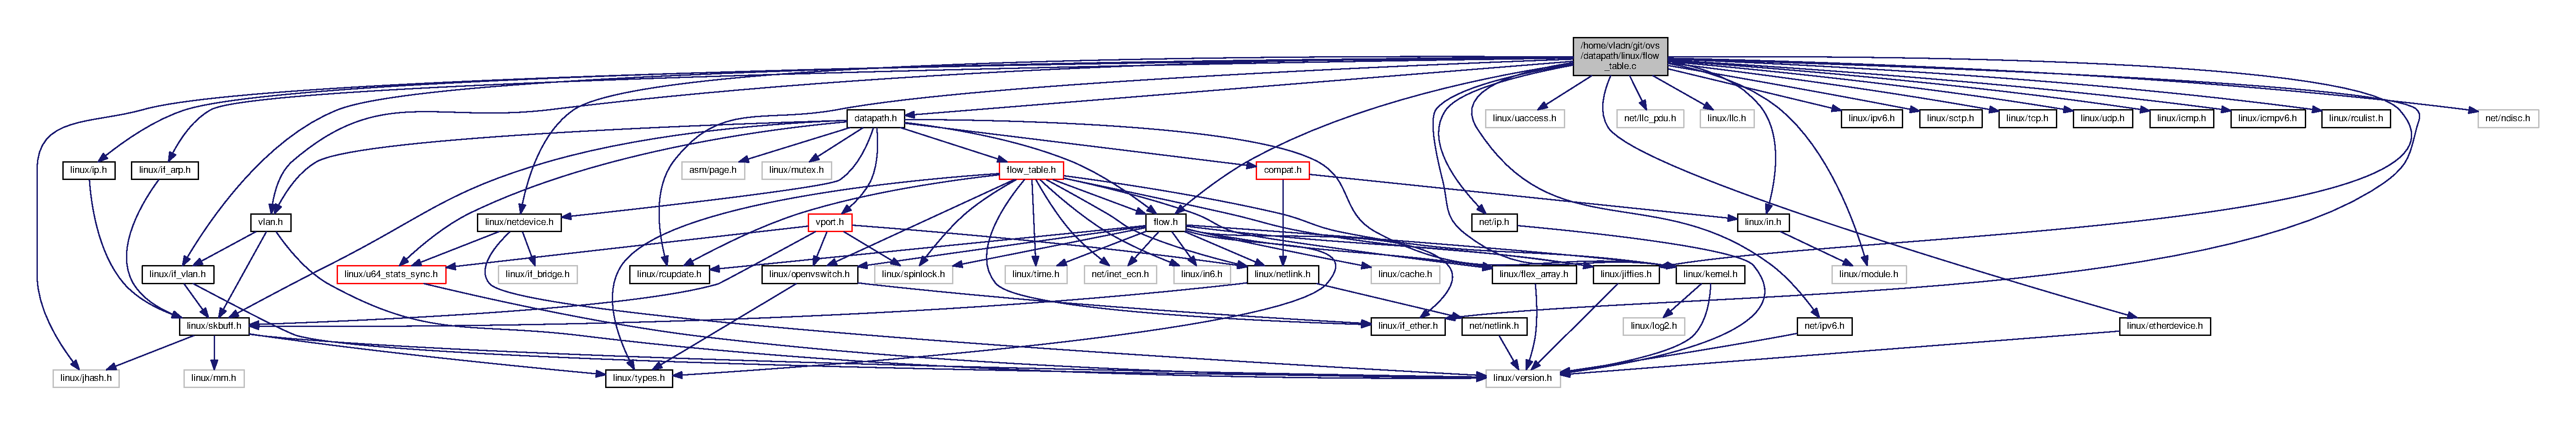
\includegraphics[width=350pt]{linux_2flow__table_8c__incl}
\end{center}
\end{figure}
\subsection*{Macros}
\begin{DoxyCompactItemize}
\item 
\#define \hyperlink{linux_2flow__table_8c_a84843442d8db7eda5192117e7c6b2997}{T\+B\+L\+\_\+\+M\+I\+N\+\_\+\+B\+U\+C\+K\+E\+T\+S}~1024
\item 
\#define \hyperlink{linux_2flow__table_8c_a8240394ae842a0ba76d82f50744ced0a}{M\+A\+S\+K\+\_\+\+A\+R\+R\+A\+Y\+\_\+\+S\+I\+Z\+E\+\_\+\+M\+I\+N}~16
\item 
\#define \hyperlink{linux_2flow__table_8c_a70a89d7f312fa8c27a8d2423cd512040}{R\+E\+H\+A\+S\+H\+\_\+\+I\+N\+T\+E\+R\+V\+A\+L}~(10 $\ast$ 60 $\ast$ H\+Z)
\item 
\#define \hyperlink{linux_2flow__table_8c_aba54fb364af2c9465bb632f82e4631d7}{M\+C\+\_\+\+H\+A\+S\+H\+\_\+\+S\+H\+I\+F\+T}~8
\item 
\#define \hyperlink{linux_2flow__table_8c_af961440482d56f3b26f232774a37c9c5}{M\+C\+\_\+\+H\+A\+S\+H\+\_\+\+E\+N\+T\+R\+I\+E\+S}~(1u $<$$<$ M\+C\+\_\+\+H\+A\+S\+H\+\_\+\+S\+H\+I\+F\+T)
\item 
\#define \hyperlink{linux_2flow__table_8c_ab95179a8dc622b08ce82308fe001d788}{M\+C\+\_\+\+H\+A\+S\+H\+\_\+\+S\+E\+G\+S}~((sizeof(uint32\+\_\+t) $\ast$ 8) / \hyperlink{linux_2flow__table_8c_aba54fb364af2c9465bb632f82e4631d7}{M\+C\+\_\+\+H\+A\+S\+H\+\_\+\+S\+H\+I\+F\+T})
\end{DoxyCompactItemize}
\subsection*{Functions}
\begin{DoxyCompactItemize}
\item 
static u16 \hyperlink{linux_2flow__table_8c_a1b494e4862736de33cbbd7cd72ee8521}{range\+\_\+n\+\_\+bytes} (const struct \hyperlink{structsw__flow__key__range}{sw\+\_\+flow\+\_\+key\+\_\+range} $\ast$range)
\item 
void \hyperlink{linux_2flow__table_8c_a40f76cbd2e168abb1b9744562e24be3b}{ovs\+\_\+flow\+\_\+mask\+\_\+key} (struct \hyperlink{structsw__flow__key}{sw\+\_\+flow\+\_\+key} $\ast$\hyperlink{flow_8h_a6747ad3b5d60480ea073cd12c9b78aaa}{dst}, const struct \hyperlink{structsw__flow__key}{sw\+\_\+flow\+\_\+key} $\ast$\hyperlink{flow_8h_a2e7e37e9dfe6465386d6c500f83ef144}{src}, const struct \hyperlink{structsw__flow__mask}{sw\+\_\+flow\+\_\+mask} $\ast$mask)
\item 
struct \hyperlink{structsw__flow}{sw\+\_\+flow} $\ast$ \hyperlink{linux_2flow__table_8c_acce701c647d8e59486574fba1be3e10c}{ovs\+\_\+flow\+\_\+alloc} (void)
\item 
int \hyperlink{linux_2flow__table_8c_a8f1f39fd4e1ecafd99321016698a709a}{ovs\+\_\+flow\+\_\+tbl\+\_\+count} (const struct \hyperlink{structflow__table}{flow\+\_\+table} $\ast$table)
\item 
static struct flex\+\_\+array $\ast$ \hyperlink{linux_2flow__table_8c_a9ad4dc425c825cafea26f047d94d8880}{alloc\+\_\+buckets} (unsigned int n\+\_\+buckets)
\item 
static void \hyperlink{linux_2flow__table_8c_af6a50f2fb2e93732e8d706dd7cf67c9b}{flow\+\_\+free} (struct \hyperlink{structsw__flow}{sw\+\_\+flow} $\ast$flow)
\item 
static void \hyperlink{linux_2flow__table_8c_a38fd2d883e505bba412320f3216dc377}{rcu\+\_\+free\+\_\+flow\+\_\+callback} (struct rcu\+\_\+head $\ast$rcu)
\item 
static void \hyperlink{linux_2flow__table_8c_a1431ef6b130c835dd7c86bac4472664b}{rcu\+\_\+free\+\_\+sw\+\_\+flow\+\_\+mask\+\_\+cb} (struct rcu\+\_\+head $\ast$rcu)
\item 
void \hyperlink{linux_2flow__table_8c_a8133cf46e955b2ae38a0bb8afc0a454f}{ovs\+\_\+flow\+\_\+free} (struct \hyperlink{structsw__flow}{sw\+\_\+flow} $\ast$flow, \hyperlink{types_8h_afaa87723b8417d40fcf45b7330261ef9}{bool} deferred)
\item 
static void \hyperlink{linux_2flow__table_8c_a351711f4f3b2e623bbca105ee2199f52}{free\+\_\+buckets} (struct flex\+\_\+array $\ast$buckets)
\item 
static void \hyperlink{linux_2flow__table_8c_a4699ad0074a999c5f80e77a8ff1b0ebc}{\+\_\+\+\_\+table\+\_\+instance\+\_\+destroy} (struct \hyperlink{structtable__instance}{table\+\_\+instance} $\ast$ti)
\item 
static struct \hyperlink{structtable__instance}{table\+\_\+instance} $\ast$ \hyperlink{linux_2flow__table_8c_afa79f1c5220d4487a4236884110b9f13}{table\+\_\+instance\+\_\+alloc} (int new\+\_\+size)
\item 
static void \hyperlink{linux_2flow__table_8c_a77da2cbea7e181821fc6931d8434bf15}{mask\+\_\+array\+\_\+rcu\+\_\+cb} (struct rcu\+\_\+head $\ast$rcu)
\item 
static struct \hyperlink{structmask__array}{mask\+\_\+array} $\ast$ \hyperlink{linux_2flow__table_8c_a327b2f9873b81f7b7920e85c366cc96e}{tbl\+\_\+mask\+\_\+array\+\_\+alloc} (int size)
\item 
static int \hyperlink{linux_2flow__table_8c_a1ba0bfff1e2a4377681774b821629e8f}{tbl\+\_\+mask\+\_\+array\+\_\+realloc} (struct \hyperlink{structflow__table}{flow\+\_\+table} $\ast$tbl, int size)
\item 
int \hyperlink{linux_2flow__table_8c_a0df1c5a76810e541b43248c402d764ff}{ovs\+\_\+flow\+\_\+tbl\+\_\+init} (struct \hyperlink{structflow__table}{flow\+\_\+table} $\ast$table)
\item 
static void \hyperlink{linux_2flow__table_8c_a2343a61f4fa3ad010bad594467cbcfc1}{flow\+\_\+tbl\+\_\+destroy\+\_\+rcu\+\_\+cb} (struct rcu\+\_\+head $\ast$rcu)
\item 
static void \hyperlink{linux_2flow__table_8c_a5abf80651b67f4198a34f7a94e116ec6}{table\+\_\+instance\+\_\+destroy} (struct \hyperlink{structtable__instance}{table\+\_\+instance} $\ast$ti, struct \hyperlink{structtable__instance}{table\+\_\+instance} $\ast$ufid\+\_\+ti, \hyperlink{types_8h_afaa87723b8417d40fcf45b7330261ef9}{bool} deferred)
\item 
void \hyperlink{linux_2flow__table_8c_ad37dcfdb56d17589ed79b5c4dd38bc76}{ovs\+\_\+flow\+\_\+tbl\+\_\+destroy} (struct \hyperlink{structflow__table}{flow\+\_\+table} $\ast$table)
\item 
struct \hyperlink{structsw__flow}{sw\+\_\+flow} $\ast$ \hyperlink{linux_2flow__table_8c_ab25c7aae52c39216ebb03d10a6cba0d8}{ovs\+\_\+flow\+\_\+tbl\+\_\+dump\+\_\+next} (struct \hyperlink{structtable__instance}{table\+\_\+instance} $\ast$ti, u32 $\ast$bucket, u32 $\ast$last)
\item 
static struct hlist\+\_\+head $\ast$ \hyperlink{linux_2flow__table_8c_aed00deae6497143255e822e293592558}{find\+\_\+bucket} (struct \hyperlink{structtable__instance}{table\+\_\+instance} $\ast$ti, u32 hash)
\item 
static void \hyperlink{linux_2flow__table_8c_a81b19a73c026d0c0fa6be862a1ee855b}{table\+\_\+instance\+\_\+insert} (struct \hyperlink{structtable__instance}{table\+\_\+instance} $\ast$ti, struct \hyperlink{structsw__flow}{sw\+\_\+flow} $\ast$flow)
\item 
static void \hyperlink{linux_2flow__table_8c_a1bf31f9e45e100a65fd166420a7615b4}{ufid\+\_\+table\+\_\+instance\+\_\+insert} (struct \hyperlink{structtable__instance}{table\+\_\+instance} $\ast$ti, struct \hyperlink{structsw__flow}{sw\+\_\+flow} $\ast$flow)
\item 
static void \hyperlink{linux_2flow__table_8c_ab9c9bf751ad9a09eba41b9bbad9925de}{flow\+\_\+table\+\_\+copy\+\_\+flows} (struct \hyperlink{structtable__instance}{table\+\_\+instance} $\ast$old, struct \hyperlink{structtable__instance}{table\+\_\+instance} $\ast$new, \hyperlink{types_8h_afaa87723b8417d40fcf45b7330261ef9}{bool} ufid)
\item 
static struct \hyperlink{structtable__instance}{table\+\_\+instance} $\ast$ \hyperlink{linux_2flow__table_8c_a2309f644575592a9cfd583b904e33149}{table\+\_\+instance\+\_\+rehash} (struct \hyperlink{structtable__instance}{table\+\_\+instance} $\ast$ti, int n\+\_\+buckets, \hyperlink{types_8h_afaa87723b8417d40fcf45b7330261ef9}{bool} ufid)
\item 
int \hyperlink{linux_2flow__table_8c_a7e424f978318e8c007b3de68854e8dc2}{ovs\+\_\+flow\+\_\+tbl\+\_\+flush} (struct \hyperlink{structflow__table}{flow\+\_\+table} $\ast$\hyperlink{structflow__table}{flow\+\_\+table})
\item 
static u32 \hyperlink{linux_2flow__table_8c_ad79946449b7c322a6d9bf13ca010b31b}{flow\+\_\+hash} (const struct \hyperlink{structsw__flow__key}{sw\+\_\+flow\+\_\+key} $\ast$key, const struct \hyperlink{structsw__flow__key__range}{sw\+\_\+flow\+\_\+key\+\_\+range} $\ast$range)
\item 
static int \hyperlink{linux_2flow__table_8c_a5342dc2f579189449805c79c106a4595}{flow\+\_\+key\+\_\+start} (const struct \hyperlink{structsw__flow__key}{sw\+\_\+flow\+\_\+key} $\ast$key)
\item 
static \hyperlink{types_8h_afaa87723b8417d40fcf45b7330261ef9}{bool} \hyperlink{linux_2flow__table_8c_a036e05a322b4dc16ff44fc77327846a6}{cmp\+\_\+key} (const struct \hyperlink{structsw__flow__key}{sw\+\_\+flow\+\_\+key} $\ast$key1, const struct \hyperlink{structsw__flow__key}{sw\+\_\+flow\+\_\+key} $\ast$key2, int key\+\_\+start, int key\+\_\+end)
\item 
static \hyperlink{types_8h_afaa87723b8417d40fcf45b7330261ef9}{bool} \hyperlink{linux_2flow__table_8c_ae52adc695ca936e630f8a4a61753520d}{flow\+\_\+cmp\+\_\+masked\+\_\+key} (const struct \hyperlink{structsw__flow}{sw\+\_\+flow} $\ast$flow, const struct \hyperlink{structsw__flow__key}{sw\+\_\+flow\+\_\+key} $\ast$key, const struct \hyperlink{structsw__flow__key__range}{sw\+\_\+flow\+\_\+key\+\_\+range} $\ast$range)
\item 
static \hyperlink{types_8h_afaa87723b8417d40fcf45b7330261ef9}{bool} \hyperlink{linux_2flow__table_8c_a0dd59a846abd3c41f19357b2223b10a9}{ovs\+\_\+flow\+\_\+cmp\+\_\+unmasked\+\_\+key} (const struct \hyperlink{structsw__flow}{sw\+\_\+flow} $\ast$flow, const struct \hyperlink{structsw__flow__match}{sw\+\_\+flow\+\_\+match} $\ast$match)
\item 
static struct \hyperlink{structsw__flow}{sw\+\_\+flow} $\ast$ \hyperlink{linux_2flow__table_8c_ac32c042a5b0b7a5de7c1e43f7187f92b}{masked\+\_\+flow\+\_\+lookup} (struct \hyperlink{structtable__instance}{table\+\_\+instance} $\ast$ti, const struct \hyperlink{structsw__flow__key}{sw\+\_\+flow\+\_\+key} $\ast$unmasked, const struct \hyperlink{structsw__flow__mask}{sw\+\_\+flow\+\_\+mask} $\ast$mask, u32 $\ast$n\+\_\+mask\+\_\+hit)
\item 
static struct \hyperlink{structsw__flow}{sw\+\_\+flow} $\ast$ \hyperlink{linux_2flow__table_8c_a66b2913ba658b83a167b83e5f5ec465a}{flow\+\_\+lookup} (struct \hyperlink{structflow__table}{flow\+\_\+table} $\ast$tbl, struct \hyperlink{structtable__instance}{table\+\_\+instance} $\ast$ti, const struct \hyperlink{structmask__array}{mask\+\_\+array} $\ast$ma, const struct \hyperlink{structsw__flow__key}{sw\+\_\+flow\+\_\+key} $\ast$key, u32 $\ast$n\+\_\+mask\+\_\+hit, u32 $\ast$index)
\item 
struct \hyperlink{structsw__flow}{sw\+\_\+flow} $\ast$ \hyperlink{linux_2flow__table_8c_ac1ff64b403e23c6e8226b0024969556b}{ovs\+\_\+flow\+\_\+tbl\+\_\+lookup\+\_\+stats} (struct \hyperlink{structflow__table}{flow\+\_\+table} $\ast$tbl, const struct \hyperlink{structsw__flow__key}{sw\+\_\+flow\+\_\+key} $\ast$key, u32 skb\+\_\+hash, u32 $\ast$n\+\_\+mask\+\_\+hit)
\item 
struct \hyperlink{structsw__flow}{sw\+\_\+flow} $\ast$ \hyperlink{linux_2flow__table_8c_a0d208a262dd7b040266e554a447fa099}{ovs\+\_\+flow\+\_\+tbl\+\_\+lookup} (struct \hyperlink{structflow__table}{flow\+\_\+table} $\ast$tbl, const struct \hyperlink{structsw__flow__key}{sw\+\_\+flow\+\_\+key} $\ast$key)
\item 
struct \hyperlink{structsw__flow}{sw\+\_\+flow} $\ast$ \hyperlink{linux_2flow__table_8c_ad54c8ee8b511e42f2296bcf5ff8d0fd3}{ovs\+\_\+flow\+\_\+tbl\+\_\+lookup\+\_\+exact} (struct \hyperlink{structflow__table}{flow\+\_\+table} $\ast$tbl, const struct \hyperlink{structsw__flow__match}{sw\+\_\+flow\+\_\+match} $\ast$match)
\item 
static u32 \hyperlink{linux_2flow__table_8c_aaf879648c325750d8ff234382797f3af}{ufid\+\_\+hash} (const struct \hyperlink{structsw__flow__id}{sw\+\_\+flow\+\_\+id} $\ast$sfid)
\item 
static \hyperlink{types_8h_afaa87723b8417d40fcf45b7330261ef9}{bool} \hyperlink{linux_2flow__table_8c_aed32909e9cc5bd5644d1eb39184a5615}{ovs\+\_\+flow\+\_\+cmp\+\_\+ufid} (const struct \hyperlink{structsw__flow}{sw\+\_\+flow} $\ast$flow, const struct \hyperlink{structsw__flow__id}{sw\+\_\+flow\+\_\+id} $\ast$sfid)
\item 
\hyperlink{types_8h_afaa87723b8417d40fcf45b7330261ef9}{bool} \hyperlink{linux_2flow__table_8c_aa91629aca9fd74e235332c7a015d9528}{ovs\+\_\+flow\+\_\+cmp} (const struct \hyperlink{structsw__flow}{sw\+\_\+flow} $\ast$flow, const struct \hyperlink{structsw__flow__match}{sw\+\_\+flow\+\_\+match} $\ast$match)
\item 
struct \hyperlink{structsw__flow}{sw\+\_\+flow} $\ast$ \hyperlink{linux_2flow__table_8c_a522dbf2a9a0518ff57eb58c09b69448c}{ovs\+\_\+flow\+\_\+tbl\+\_\+lookup\+\_\+ufid} (struct \hyperlink{structflow__table}{flow\+\_\+table} $\ast$tbl, const struct \hyperlink{structsw__flow__id}{sw\+\_\+flow\+\_\+id} $\ast$ufid)
\item 
int \hyperlink{linux_2flow__table_8c_ab6e18d16217cddd0af756b76b72e6ce6}{ovs\+\_\+flow\+\_\+tbl\+\_\+num\+\_\+masks} (const struct \hyperlink{structflow__table}{flow\+\_\+table} $\ast$table)
\item 
static struct \hyperlink{structtable__instance}{table\+\_\+instance} $\ast$ \hyperlink{linux_2flow__table_8c_ae06d563df0cf3fa5d9437e35dafa64cb}{table\+\_\+instance\+\_\+expand} (struct \hyperlink{structtable__instance}{table\+\_\+instance} $\ast$ti, \hyperlink{types_8h_afaa87723b8417d40fcf45b7330261ef9}{bool} ufid)
\item 
static void \hyperlink{linux_2flow__table_8c_a072572ef64d5ebcc2c99cb48945c8291}{tbl\+\_\+mask\+\_\+array\+\_\+delete\+\_\+mask} (struct \hyperlink{structmask__array}{mask\+\_\+array} $\ast$ma, struct \hyperlink{structsw__flow__mask}{sw\+\_\+flow\+\_\+mask} $\ast$mask)
\item 
static void \hyperlink{linux_2flow__table_8c_a67796467285f769eda43c39ae058d997}{flow\+\_\+mask\+\_\+remove} (struct \hyperlink{structflow__table}{flow\+\_\+table} $\ast$tbl, struct \hyperlink{structsw__flow__mask}{sw\+\_\+flow\+\_\+mask} $\ast$mask)
\item 
void \hyperlink{linux_2flow__table_8c_aa75b8bc2551f9c1a8d65b942a10df89a}{ovs\+\_\+flow\+\_\+tbl\+\_\+remove} (struct \hyperlink{structflow__table}{flow\+\_\+table} $\ast$table, struct \hyperlink{structsw__flow}{sw\+\_\+flow} $\ast$flow)
\item 
static struct \hyperlink{structsw__flow__mask}{sw\+\_\+flow\+\_\+mask} $\ast$ \hyperlink{linux_2flow__table_8c_ac9c253eab445afa7ba77781418a92be7}{mask\+\_\+alloc} (void)
\item 
static \hyperlink{types_8h_afaa87723b8417d40fcf45b7330261ef9}{bool} \hyperlink{linux_2flow__table_8c_a7dd8ab521133d5c26cac895f316213ae}{mask\+\_\+equal} (const struct \hyperlink{structsw__flow__mask}{sw\+\_\+flow\+\_\+mask} $\ast$a, const struct \hyperlink{structsw__flow__mask}{sw\+\_\+flow\+\_\+mask} $\ast$b)
\item 
static struct \hyperlink{structsw__flow__mask}{sw\+\_\+flow\+\_\+mask} $\ast$ \hyperlink{linux_2flow__table_8c_ac6253f7b922a021b0f2321be510fac7c}{flow\+\_\+mask\+\_\+find} (const struct \hyperlink{structflow__table}{flow\+\_\+table} $\ast$tbl, const struct \hyperlink{structsw__flow__mask}{sw\+\_\+flow\+\_\+mask} $\ast$mask)
\item 
static int \hyperlink{linux_2flow__table_8c_a1ceded3a19f98e73b3c10faf2f2532f5}{flow\+\_\+mask\+\_\+insert} (struct \hyperlink{structflow__table}{flow\+\_\+table} $\ast$tbl, struct \hyperlink{structsw__flow}{sw\+\_\+flow} $\ast$flow, const struct \hyperlink{structsw__flow__mask}{sw\+\_\+flow\+\_\+mask} $\ast$new)
\item 
static void \hyperlink{linux_2flow__table_8c_a66f2b72d1c755346c4865714e51cfcf4}{flow\+\_\+key\+\_\+insert} (struct \hyperlink{structflow__table}{flow\+\_\+table} $\ast$table, struct \hyperlink{structsw__flow}{sw\+\_\+flow} $\ast$flow)
\item 
static void \hyperlink{linux_2flow__table_8c_a36540c6298f41907b7c088b34116346d}{flow\+\_\+ufid\+\_\+insert} (struct \hyperlink{structflow__table}{flow\+\_\+table} $\ast$table, struct \hyperlink{structsw__flow}{sw\+\_\+flow} $\ast$flow)
\item 
int \hyperlink{linux_2flow__table_8c_a72ec4f72961a64b1c006978a32554a4c}{ovs\+\_\+flow\+\_\+tbl\+\_\+insert} (struct \hyperlink{structflow__table}{flow\+\_\+table} $\ast$table, struct \hyperlink{structsw__flow}{sw\+\_\+flow} $\ast$flow, const struct \hyperlink{structsw__flow__mask}{sw\+\_\+flow\+\_\+mask} $\ast$mask)
\item 
int \hyperlink{linux_2flow__table_8c_a07492868e65ba495c86d49df9cf1bc50}{ovs\+\_\+flow\+\_\+init} (void)
\item 
void \hyperlink{linux_2flow__table_8c_a96cce30f7a9c3231d5b5afaf967378eb}{ovs\+\_\+flow\+\_\+exit} (void)
\end{DoxyCompactItemize}
\subsection*{Variables}
\begin{DoxyCompactItemize}
\item 
static struct kmem\+\_\+cache $\ast$ \hyperlink{linux_2flow__table_8c_ab00a8de93e918b8aba331f4872a2c97c}{flow\+\_\+cache}
\item 
struct kmem\+\_\+cache $\ast$\hyperlink{flow__table_8h_ab305bee215adea2618069cc592f6ee6b}{flow\+\_\+stats\+\_\+cache} \hyperlink{linux_2flow__table_8c_a05eb66f030d0825002eb11cc332e291e}{\+\_\+\+\_\+read\+\_\+mostly}
\end{DoxyCompactItemize}


\subsection{Macro Definition Documentation}
\hypertarget{linux_2flow__table_8c_a8240394ae842a0ba76d82f50744ced0a}{}\index{linux/flow\+\_\+table.\+c@{linux/flow\+\_\+table.\+c}!M\+A\+S\+K\+\_\+\+A\+R\+R\+A\+Y\+\_\+\+S\+I\+Z\+E\+\_\+\+M\+I\+N@{M\+A\+S\+K\+\_\+\+A\+R\+R\+A\+Y\+\_\+\+S\+I\+Z\+E\+\_\+\+M\+I\+N}}
\index{M\+A\+S\+K\+\_\+\+A\+R\+R\+A\+Y\+\_\+\+S\+I\+Z\+E\+\_\+\+M\+I\+N@{M\+A\+S\+K\+\_\+\+A\+R\+R\+A\+Y\+\_\+\+S\+I\+Z\+E\+\_\+\+M\+I\+N}!linux/flow\+\_\+table.\+c@{linux/flow\+\_\+table.\+c}}
\subsubsection[{M\+A\+S\+K\+\_\+\+A\+R\+R\+A\+Y\+\_\+\+S\+I\+Z\+E\+\_\+\+M\+I\+N}]{\setlength{\rightskip}{0pt plus 5cm}\#define M\+A\+S\+K\+\_\+\+A\+R\+R\+A\+Y\+\_\+\+S\+I\+Z\+E\+\_\+\+M\+I\+N~16}\label{linux_2flow__table_8c_a8240394ae842a0ba76d82f50744ced0a}
\hypertarget{linux_2flow__table_8c_af961440482d56f3b26f232774a37c9c5}{}\index{linux/flow\+\_\+table.\+c@{linux/flow\+\_\+table.\+c}!M\+C\+\_\+\+H\+A\+S\+H\+\_\+\+E\+N\+T\+R\+I\+E\+S@{M\+C\+\_\+\+H\+A\+S\+H\+\_\+\+E\+N\+T\+R\+I\+E\+S}}
\index{M\+C\+\_\+\+H\+A\+S\+H\+\_\+\+E\+N\+T\+R\+I\+E\+S@{M\+C\+\_\+\+H\+A\+S\+H\+\_\+\+E\+N\+T\+R\+I\+E\+S}!linux/flow\+\_\+table.\+c@{linux/flow\+\_\+table.\+c}}
\subsubsection[{M\+C\+\_\+\+H\+A\+S\+H\+\_\+\+E\+N\+T\+R\+I\+E\+S}]{\setlength{\rightskip}{0pt plus 5cm}\#define M\+C\+\_\+\+H\+A\+S\+H\+\_\+\+E\+N\+T\+R\+I\+E\+S~(1u $<$$<$ M\+C\+\_\+\+H\+A\+S\+H\+\_\+\+S\+H\+I\+F\+T)}\label{linux_2flow__table_8c_af961440482d56f3b26f232774a37c9c5}
\hypertarget{linux_2flow__table_8c_ab95179a8dc622b08ce82308fe001d788}{}\index{linux/flow\+\_\+table.\+c@{linux/flow\+\_\+table.\+c}!M\+C\+\_\+\+H\+A\+S\+H\+\_\+\+S\+E\+G\+S@{M\+C\+\_\+\+H\+A\+S\+H\+\_\+\+S\+E\+G\+S}}
\index{M\+C\+\_\+\+H\+A\+S\+H\+\_\+\+S\+E\+G\+S@{M\+C\+\_\+\+H\+A\+S\+H\+\_\+\+S\+E\+G\+S}!linux/flow\+\_\+table.\+c@{linux/flow\+\_\+table.\+c}}
\subsubsection[{M\+C\+\_\+\+H\+A\+S\+H\+\_\+\+S\+E\+G\+S}]{\setlength{\rightskip}{0pt plus 5cm}\#define M\+C\+\_\+\+H\+A\+S\+H\+\_\+\+S\+E\+G\+S~((sizeof(uint32\+\_\+t) $\ast$ 8) / {\bf M\+C\+\_\+\+H\+A\+S\+H\+\_\+\+S\+H\+I\+F\+T})}\label{linux_2flow__table_8c_ab95179a8dc622b08ce82308fe001d788}
\hypertarget{linux_2flow__table_8c_aba54fb364af2c9465bb632f82e4631d7}{}\index{linux/flow\+\_\+table.\+c@{linux/flow\+\_\+table.\+c}!M\+C\+\_\+\+H\+A\+S\+H\+\_\+\+S\+H\+I\+F\+T@{M\+C\+\_\+\+H\+A\+S\+H\+\_\+\+S\+H\+I\+F\+T}}
\index{M\+C\+\_\+\+H\+A\+S\+H\+\_\+\+S\+H\+I\+F\+T@{M\+C\+\_\+\+H\+A\+S\+H\+\_\+\+S\+H\+I\+F\+T}!linux/flow\+\_\+table.\+c@{linux/flow\+\_\+table.\+c}}
\subsubsection[{M\+C\+\_\+\+H\+A\+S\+H\+\_\+\+S\+H\+I\+F\+T}]{\setlength{\rightskip}{0pt plus 5cm}\#define M\+C\+\_\+\+H\+A\+S\+H\+\_\+\+S\+H\+I\+F\+T~8}\label{linux_2flow__table_8c_aba54fb364af2c9465bb632f82e4631d7}
\hypertarget{linux_2flow__table_8c_a70a89d7f312fa8c27a8d2423cd512040}{}\index{linux/flow\+\_\+table.\+c@{linux/flow\+\_\+table.\+c}!R\+E\+H\+A\+S\+H\+\_\+\+I\+N\+T\+E\+R\+V\+A\+L@{R\+E\+H\+A\+S\+H\+\_\+\+I\+N\+T\+E\+R\+V\+A\+L}}
\index{R\+E\+H\+A\+S\+H\+\_\+\+I\+N\+T\+E\+R\+V\+A\+L@{R\+E\+H\+A\+S\+H\+\_\+\+I\+N\+T\+E\+R\+V\+A\+L}!linux/flow\+\_\+table.\+c@{linux/flow\+\_\+table.\+c}}
\subsubsection[{R\+E\+H\+A\+S\+H\+\_\+\+I\+N\+T\+E\+R\+V\+A\+L}]{\setlength{\rightskip}{0pt plus 5cm}\#define R\+E\+H\+A\+S\+H\+\_\+\+I\+N\+T\+E\+R\+V\+A\+L~(10 $\ast$ 60 $\ast$ H\+Z)}\label{linux_2flow__table_8c_a70a89d7f312fa8c27a8d2423cd512040}
\hypertarget{linux_2flow__table_8c_a84843442d8db7eda5192117e7c6b2997}{}\index{linux/flow\+\_\+table.\+c@{linux/flow\+\_\+table.\+c}!T\+B\+L\+\_\+\+M\+I\+N\+\_\+\+B\+U\+C\+K\+E\+T\+S@{T\+B\+L\+\_\+\+M\+I\+N\+\_\+\+B\+U\+C\+K\+E\+T\+S}}
\index{T\+B\+L\+\_\+\+M\+I\+N\+\_\+\+B\+U\+C\+K\+E\+T\+S@{T\+B\+L\+\_\+\+M\+I\+N\+\_\+\+B\+U\+C\+K\+E\+T\+S}!linux/flow\+\_\+table.\+c@{linux/flow\+\_\+table.\+c}}
\subsubsection[{T\+B\+L\+\_\+\+M\+I\+N\+\_\+\+B\+U\+C\+K\+E\+T\+S}]{\setlength{\rightskip}{0pt plus 5cm}\#define T\+B\+L\+\_\+\+M\+I\+N\+\_\+\+B\+U\+C\+K\+E\+T\+S~1024}\label{linux_2flow__table_8c_a84843442d8db7eda5192117e7c6b2997}


\subsection{Function Documentation}
\hypertarget{linux_2flow__table_8c_a4699ad0074a999c5f80e77a8ff1b0ebc}{}\index{linux/flow\+\_\+table.\+c@{linux/flow\+\_\+table.\+c}!\+\_\+\+\_\+table\+\_\+instance\+\_\+destroy@{\+\_\+\+\_\+table\+\_\+instance\+\_\+destroy}}
\index{\+\_\+\+\_\+table\+\_\+instance\+\_\+destroy@{\+\_\+\+\_\+table\+\_\+instance\+\_\+destroy}!linux/flow\+\_\+table.\+c@{linux/flow\+\_\+table.\+c}}
\subsubsection[{\+\_\+\+\_\+table\+\_\+instance\+\_\+destroy}]{\setlength{\rightskip}{0pt plus 5cm}static void \+\_\+\+\_\+table\+\_\+instance\+\_\+destroy (
\begin{DoxyParamCaption}
\item[{struct {\bf table\+\_\+instance} $\ast$}]{ti}
\end{DoxyParamCaption}
)\hspace{0.3cm}{\ttfamily [static]}}\label{linux_2flow__table_8c_a4699ad0074a999c5f80e77a8ff1b0ebc}

\begin{DoxyCode}
193 \{
194     \hyperlink{linux_2flow__table_8c_a351711f4f3b2e623bbca105ee2199f52}{free\_buckets}(ti->\hyperlink{structtable__instance_a6522309983b8c287da819f666da07355}{buckets});
195     kfree(ti);
196 \}
\end{DoxyCode}
\hypertarget{linux_2flow__table_8c_a9ad4dc425c825cafea26f047d94d8880}{}\index{linux/flow\+\_\+table.\+c@{linux/flow\+\_\+table.\+c}!alloc\+\_\+buckets@{alloc\+\_\+buckets}}
\index{alloc\+\_\+buckets@{alloc\+\_\+buckets}!linux/flow\+\_\+table.\+c@{linux/flow\+\_\+table.\+c}}
\subsubsection[{alloc\+\_\+buckets}]{\setlength{\rightskip}{0pt plus 5cm}static struct flex\+\_\+array$\ast$ alloc\+\_\+buckets (
\begin{DoxyParamCaption}
\item[{unsigned int}]{n\+\_\+buckets}
\end{DoxyParamCaption}
)\hspace{0.3cm}{\ttfamily [static]}}\label{linux_2flow__table_8c_a9ad4dc425c825cafea26f047d94d8880}

\begin{DoxyCode}
125 \{
126     \textcolor{keyword}{struct }flex\_array *buckets;
127     \textcolor{keywordtype}{int} i, err;
128 
129     buckets = flex\_array\_alloc(\textcolor{keyword}{sizeof}(\textcolor{keyword}{struct} hlist\_head),
130                    n\_buckets, GFP\_KERNEL);
131     \textcolor{keywordflow}{if} (!buckets)
132         \textcolor{keywordflow}{return} NULL;
133 
134     err = flex\_array\_prealloc(buckets, 0, n\_buckets, GFP\_KERNEL);
135     \textcolor{keywordflow}{if} (err) \{
136         flex\_array\_free(buckets);
137         \textcolor{keywordflow}{return} NULL;
138     \}
139 
140     \textcolor{keywordflow}{for} (i = 0; i < n\_buckets; i++)
141         INIT\_HLIST\_HEAD((\textcolor{keyword}{struct} hlist\_head *)
142                     flex\_array\_get(buckets, i));
143 
144     \textcolor{keywordflow}{return} buckets;
145 \}
\end{DoxyCode}
\hypertarget{linux_2flow__table_8c_a036e05a322b4dc16ff44fc77327846a6}{}\index{linux/flow\+\_\+table.\+c@{linux/flow\+\_\+table.\+c}!cmp\+\_\+key@{cmp\+\_\+key}}
\index{cmp\+\_\+key@{cmp\+\_\+key}!linux/flow\+\_\+table.\+c@{linux/flow\+\_\+table.\+c}}
\subsubsection[{cmp\+\_\+key}]{\setlength{\rightskip}{0pt plus 5cm}static {\bf bool} cmp\+\_\+key (
\begin{DoxyParamCaption}
\item[{const struct {\bf sw\+\_\+flow\+\_\+key} $\ast$}]{key1, }
\item[{const struct {\bf sw\+\_\+flow\+\_\+key} $\ast$}]{key2, }
\item[{int}]{key\+\_\+start, }
\item[{int}]{key\+\_\+end}
\end{DoxyParamCaption}
)\hspace{0.3cm}{\ttfamily [static]}}\label{linux_2flow__table_8c_a036e05a322b4dc16ff44fc77327846a6}

\begin{DoxyCode}
517 \{
518     \textcolor{keyword}{const} \textcolor{keywordtype}{long} *cp1 = (\textcolor{keyword}{const} \textcolor{keywordtype}{long} *)((\textcolor{keyword}{const} u8 *)key1 + key\_start);
519     \textcolor{keyword}{const} \textcolor{keywordtype}{long} *cp2 = (\textcolor{keyword}{const} \textcolor{keywordtype}{long} *)((\textcolor{keyword}{const} u8 *)key2 + key\_start);
520     \textcolor{keywordtype}{long} diffs = 0;
521     \textcolor{keywordtype}{int} i;
522 
523     \textcolor{keywordflow}{for} (i = key\_start; i < key\_end;  i += \textcolor{keyword}{sizeof}(long))
524         diffs |= *cp1++ ^ *cp2++;
525 
526     \textcolor{keywordflow}{return} diffs == 0;
527 \}
\end{DoxyCode}
\hypertarget{linux_2flow__table_8c_aed00deae6497143255e822e293592558}{}\index{linux/flow\+\_\+table.\+c@{linux/flow\+\_\+table.\+c}!find\+\_\+bucket@{find\+\_\+bucket}}
\index{find\+\_\+bucket@{find\+\_\+bucket}!linux/flow\+\_\+table.\+c@{linux/flow\+\_\+table.\+c}}
\subsubsection[{find\+\_\+bucket}]{\setlength{\rightskip}{0pt plus 5cm}static struct hlist\+\_\+head$\ast$ find\+\_\+bucket (
\begin{DoxyParamCaption}
\item[{struct {\bf table\+\_\+instance} $\ast$}]{ti, }
\item[{u32}]{hash}
\end{DoxyParamCaption}
)\hspace{0.3cm}{\ttfamily [static]}}\label{linux_2flow__table_8c_aed00deae6497143255e822e293592558}

\begin{DoxyCode}
395 \{
396     hash = jhash\_1word(hash, ti->\hyperlink{structtable__instance_ad73f318c365fd86dda23e7ffb65d59b9}{hash\_seed});
397     \textcolor{keywordflow}{return} flex\_array\_get(ti->\hyperlink{structtable__instance_a6522309983b8c287da819f666da07355}{buckets},
398                 (hash & (ti->\hyperlink{structtable__instance_ae4f915a0e1b19ca677ae00c7eb5a3cb9}{n\_buckets} - 1)));
399 \}
\end{DoxyCode}
\hypertarget{linux_2flow__table_8c_ae52adc695ca936e630f8a4a61753520d}{}\index{linux/flow\+\_\+table.\+c@{linux/flow\+\_\+table.\+c}!flow\+\_\+cmp\+\_\+masked\+\_\+key@{flow\+\_\+cmp\+\_\+masked\+\_\+key}}
\index{flow\+\_\+cmp\+\_\+masked\+\_\+key@{flow\+\_\+cmp\+\_\+masked\+\_\+key}!linux/flow\+\_\+table.\+c@{linux/flow\+\_\+table.\+c}}
\subsubsection[{flow\+\_\+cmp\+\_\+masked\+\_\+key}]{\setlength{\rightskip}{0pt plus 5cm}static {\bf bool} flow\+\_\+cmp\+\_\+masked\+\_\+key (
\begin{DoxyParamCaption}
\item[{const struct {\bf sw\+\_\+flow} $\ast$}]{flow, }
\item[{const struct {\bf sw\+\_\+flow\+\_\+key} $\ast$}]{key, }
\item[{const struct {\bf sw\+\_\+flow\+\_\+key\+\_\+range} $\ast$}]{range}
\end{DoxyParamCaption}
)\hspace{0.3cm}{\ttfamily [static]}}\label{linux_2flow__table_8c_ae52adc695ca936e630f8a4a61753520d}

\begin{DoxyCode}
532 \{
533     \textcolor{keywordflow}{return} \hyperlink{linux_2flow__table_8c_a036e05a322b4dc16ff44fc77327846a6}{cmp\_key}(&flow->\hyperlink{structsw__flow_a14b83cbd65275bda4e97ae35500d26d8}{key}, key, range->\hyperlink{structsw__flow__key__range_a3139158cea80b4e5af36967f3748e846}{start}, range->\hyperlink{structsw__flow__key__range_ab9c9d06e6ed2b9600d295dfdd94cc05a}{end});
534 \}
\end{DoxyCode}
\hypertarget{linux_2flow__table_8c_af6a50f2fb2e93732e8d706dd7cf67c9b}{}\index{linux/flow\+\_\+table.\+c@{linux/flow\+\_\+table.\+c}!flow\+\_\+free@{flow\+\_\+free}}
\index{flow\+\_\+free@{flow\+\_\+free}!linux/flow\+\_\+table.\+c@{linux/flow\+\_\+table.\+c}}
\subsubsection[{flow\+\_\+free}]{\setlength{\rightskip}{0pt plus 5cm}static void flow\+\_\+free (
\begin{DoxyParamCaption}
\item[{struct {\bf sw\+\_\+flow} $\ast$}]{flow}
\end{DoxyParamCaption}
)\hspace{0.3cm}{\ttfamily [static]}}\label{linux_2flow__table_8c_af6a50f2fb2e93732e8d706dd7cf67c9b}

\begin{DoxyCode}
148 \{
149     \textcolor{keywordtype}{int} node;
150 
151     \textcolor{keywordflow}{if} (\hyperlink{flow_8h_a3bfeaa297d8807b969a14f1cde78d21b}{ovs\_identifier\_is\_key}(&flow->\hyperlink{structsw__flow_a6e6645eec909d54871675be30000c0b9}{id}))
152         kfree(flow->\hyperlink{structsw__flow_a6e6645eec909d54871675be30000c0b9}{id}.\hyperlink{structsw__flow__id_a5d62dce79569cb8c25a43f4039e5df3c}{unmasked\_key});
153     kfree(\hyperlink{rcupdate_8h_a9e866c0e8ba667e053cb8f59af572157}{rcu\_dereference\_raw}(flow->\hyperlink{structsw__flow_aa845bdaabc25d81dcf8b1a7519b35408}{sf\_acts}));
154     for\_each\_node(node)
155         if (flow->stats[node])
156             kmem\_cache\_free(\hyperlink{flow__table_8h_ab305bee215adea2618069cc592f6ee6b}{flow\_stats\_cache},
157                     \hyperlink{rcupdate_8h_a9e866c0e8ba667e053cb8f59af572157}{rcu\_dereference\_raw}(flow->stats[node]));
158     kmem\_cache\_free(\hyperlink{linux_2flow__table_8c_ab00a8de93e918b8aba331f4872a2c97c}{flow\_cache}, flow);
159 \}
\end{DoxyCode}
\hypertarget{linux_2flow__table_8c_ad79946449b7c322a6d9bf13ca010b31b}{}\index{linux/flow\+\_\+table.\+c@{linux/flow\+\_\+table.\+c}!flow\+\_\+hash@{flow\+\_\+hash}}
\index{flow\+\_\+hash@{flow\+\_\+hash}!linux/flow\+\_\+table.\+c@{linux/flow\+\_\+table.\+c}}
\subsubsection[{flow\+\_\+hash}]{\setlength{\rightskip}{0pt plus 5cm}static u32 flow\+\_\+hash (
\begin{DoxyParamCaption}
\item[{const struct {\bf sw\+\_\+flow\+\_\+key} $\ast$}]{key, }
\item[{const struct {\bf sw\+\_\+flow\+\_\+key\+\_\+range} $\ast$}]{range}
\end{DoxyParamCaption}
)\hspace{0.3cm}{\ttfamily [static]}}\label{linux_2flow__table_8c_ad79946449b7c322a6d9bf13ca010b31b}

\begin{DoxyCode}
493 \{
494     \textcolor{keywordtype}{int} key\_start = range->\hyperlink{structsw__flow__key__range_a3139158cea80b4e5af36967f3748e846}{start};
495     \textcolor{keywordtype}{int} key\_end = range->\hyperlink{structsw__flow__key__range_ab9c9d06e6ed2b9600d295dfdd94cc05a}{end};
496     \textcolor{keyword}{const} u32 *hash\_key = (\textcolor{keyword}{const} u32 *)((\textcolor{keyword}{const} u8 *)key + key\_start);
497     \textcolor{keywordtype}{int} hash\_u32s = (key\_end - key\_start) >> 2;
498 
499     \textcolor{comment}{/* Make sure number of hash bytes are multiple of u32. */}
500     BUILD\_BUG\_ON(\textcolor{keyword}{sizeof}(\textcolor{keywordtype}{long}) % \textcolor{keyword}{sizeof}(u32));
501 
502     \textcolor{keywordflow}{return} jhash2(hash\_key, hash\_u32s, 0);
503 \}
\end{DoxyCode}
\hypertarget{linux_2flow__table_8c_a66f2b72d1c755346c4865714e51cfcf4}{}\index{linux/flow\+\_\+table.\+c@{linux/flow\+\_\+table.\+c}!flow\+\_\+key\+\_\+insert@{flow\+\_\+key\+\_\+insert}}
\index{flow\+\_\+key\+\_\+insert@{flow\+\_\+key\+\_\+insert}!linux/flow\+\_\+table.\+c@{linux/flow\+\_\+table.\+c}}
\subsubsection[{flow\+\_\+key\+\_\+insert}]{\setlength{\rightskip}{0pt plus 5cm}static void flow\+\_\+key\+\_\+insert (
\begin{DoxyParamCaption}
\item[{struct {\bf flow\+\_\+table} $\ast$}]{table, }
\item[{struct {\bf sw\+\_\+flow} $\ast$}]{flow}
\end{DoxyParamCaption}
)\hspace{0.3cm}{\ttfamily [static]}}\label{linux_2flow__table_8c_a66f2b72d1c755346c4865714e51cfcf4}

\begin{DoxyCode}
922 \{
923     \textcolor{keyword}{struct }\hyperlink{structtable__instance}{table\_instance} *new\_ti = NULL;
924     \textcolor{keyword}{struct }\hyperlink{structtable__instance}{table\_instance} *ti;
925 
926     flow->\hyperlink{structsw__flow_abca0040cced6a4a84d1a8941764fb5d6}{flow\_table}.\hyperlink{structsw__flow_a7a33a6a5c62113ffe949a700ef648a71}{hash} = \hyperlink{linux_2flow__table_8c_ad79946449b7c322a6d9bf13ca010b31b}{flow\_hash}(&flow->\hyperlink{structsw__flow_a14b83cbd65275bda4e97ae35500d26d8}{key}, &flow->
      \hyperlink{structsw__flow_a89c162e340693d0bb4977737e2b68c22}{mask}->\hyperlink{structsw__flow__mask_aa6062c0e580d516ff2d9ce8f9611432b}{range});
927     ti = \hyperlink{datapath_8h_a06ef69170d345fd3996a467dcacf3ff3}{ovsl\_dereference}(table->\hyperlink{structflow__table_a49d708e68608d510f6d25a16a14fd565}{ti});
928     \hyperlink{linux_2flow__table_8c_a81b19a73c026d0c0fa6be862a1ee855b}{table\_instance\_insert}(ti, flow);
929     table->\hyperlink{structflow__table_a97cae1e714c6dcfe0d39ce4cff371786}{count}++;
930 
931     \textcolor{comment}{/* Expand table, if necessary, to make room. */}
932     \textcolor{keywordflow}{if} (table->\hyperlink{structflow__table_a97cae1e714c6dcfe0d39ce4cff371786}{count} > ti->\hyperlink{structtable__instance_ae4f915a0e1b19ca677ae00c7eb5a3cb9}{n\_buckets})
933         new\_ti = \hyperlink{linux_2flow__table_8c_ae06d563df0cf3fa5d9437e35dafa64cb}{table\_instance\_expand}(ti, \textcolor{keyword}{false});
934     \textcolor{keywordflow}{else} \textcolor{keywordflow}{if} (time\_after(jiffies, table->\hyperlink{structflow__table_a82c7cfef05b2898b3ffb3b6cb6fdc6a4}{last\_rehash} + \hyperlink{linux_2flow__table_8c_a70a89d7f312fa8c27a8d2423cd512040}{REHASH\_INTERVAL}))
935         new\_ti = \hyperlink{linux_2flow__table_8c_a2309f644575592a9cfd583b904e33149}{table\_instance\_rehash}(ti, ti->\hyperlink{structtable__instance_ae4f915a0e1b19ca677ae00c7eb5a3cb9}{n\_buckets}, \textcolor{keyword}{false});
936 
937     \textcolor{keywordflow}{if} (new\_ti) \{
938         rcu\_assign\_pointer(table->\hyperlink{structflow__table_a49d708e68608d510f6d25a16a14fd565}{ti}, new\_ti);
939         call\_rcu(&ti->\hyperlink{structtable__instance_acf4d72ccfb947d0d0d08732a56664978}{rcu}, \hyperlink{linux_2flow__table_8c_a2343a61f4fa3ad010bad594467cbcfc1}{flow\_tbl\_destroy\_rcu\_cb});
940         table->\hyperlink{structflow__table_a82c7cfef05b2898b3ffb3b6cb6fdc6a4}{last\_rehash} = jiffies;
941     \}
942 \}
\end{DoxyCode}
\hypertarget{linux_2flow__table_8c_a5342dc2f579189449805c79c106a4595}{}\index{linux/flow\+\_\+table.\+c@{linux/flow\+\_\+table.\+c}!flow\+\_\+key\+\_\+start@{flow\+\_\+key\+\_\+start}}
\index{flow\+\_\+key\+\_\+start@{flow\+\_\+key\+\_\+start}!linux/flow\+\_\+table.\+c@{linux/flow\+\_\+table.\+c}}
\subsubsection[{flow\+\_\+key\+\_\+start}]{\setlength{\rightskip}{0pt plus 5cm}static int flow\+\_\+key\+\_\+start (
\begin{DoxyParamCaption}
\item[{const struct {\bf sw\+\_\+flow\+\_\+key} $\ast$}]{key}
\end{DoxyParamCaption}
)\hspace{0.3cm}{\ttfamily [static]}}\label{linux_2flow__table_8c_a5342dc2f579189449805c79c106a4595}

\begin{DoxyCode}
506 \{
507     \textcolor{keywordflow}{if} (key->\hyperlink{structsw__flow__key_a2f87b7690c0cc2797f1f4347589472c3}{tun\_key}.\hyperlink{structovs__key__ipv4__tunnel_ae443d381a97f53bbc4139fe36c0aae30}{ipv4\_dst})
508         \textcolor{keywordflow}{return} 0;
509     \textcolor{keywordflow}{else}
510         \textcolor{keywordflow}{return} \hyperlink{kernel_8h_abbacd255029bd6692704964758c8aa97}{rounddown}(offsetof(\textcolor{keyword}{struct} \hyperlink{structsw__flow__key}{sw\_flow\_key}, \hyperlink{flow_8h_a1c873ea83e1b749c669b501016e967fe}{phy}),
511                       \textcolor{keyword}{sizeof}(\textcolor{keywordtype}{long}));
512 \}
\end{DoxyCode}
\hypertarget{linux_2flow__table_8c_a66b2913ba658b83a167b83e5f5ec465a}{}\index{linux/flow\+\_\+table.\+c@{linux/flow\+\_\+table.\+c}!flow\+\_\+lookup@{flow\+\_\+lookup}}
\index{flow\+\_\+lookup@{flow\+\_\+lookup}!linux/flow\+\_\+table.\+c@{linux/flow\+\_\+table.\+c}}
\subsubsection[{flow\+\_\+lookup}]{\setlength{\rightskip}{0pt plus 5cm}static struct {\bf sw\+\_\+flow}$\ast$ flow\+\_\+lookup (
\begin{DoxyParamCaption}
\item[{struct {\bf flow\+\_\+table} $\ast$}]{tbl, }
\item[{struct {\bf table\+\_\+instance} $\ast$}]{ti, }
\item[{const struct {\bf mask\+\_\+array} $\ast$}]{ma, }
\item[{const struct {\bf sw\+\_\+flow\+\_\+key} $\ast$}]{key, }
\item[{u32 $\ast$}]{n\+\_\+mask\+\_\+hit, }
\item[{u32 $\ast$}]{index}
\end{DoxyParamCaption}
)\hspace{0.3cm}{\ttfamily [static]}}\label{linux_2flow__table_8c_a66b2913ba658b83a167b83e5f5ec465a}

\begin{DoxyCode}
578 \{
579     \textcolor{keyword}{struct }\hyperlink{structsw__flow__mask}{sw\_flow\_mask} *mask;
580     \textcolor{keyword}{struct }\hyperlink{structsw__flow}{sw\_flow} *flow;
581     \textcolor{keywordtype}{int} i;
582 
583     \textcolor{keywordflow}{if} (*index < ma->max) \{
584         mask = \hyperlink{datapath_8h_a5f2a2c1026f970f0052e77f5ebba33d1}{rcu\_dereference\_ovsl}(ma->\hyperlink{structmask__array_a92da2b0ebde32eb6f76a134dc2d61d79}{masks}[*index]);
585         \textcolor{keywordflow}{if} (mask) \{
586             flow = \hyperlink{linux_2flow__table_8c_ac32c042a5b0b7a5de7c1e43f7187f92b}{masked\_flow\_lookup}(ti, key, mask, n\_mask\_hit);
587             \textcolor{keywordflow}{if} (flow)
588                 \textcolor{keywordflow}{return} flow;
589         \}
590     \}
591 
592     \textcolor{keywordflow}{for} (i = 0; i < ma->\hyperlink{structmask__array_ad981d54486b5dd03bdb4ad20b740171e}{max}; i++)  \{
593 
594         \textcolor{keywordflow}{if} (i == *index)
595             \textcolor{keywordflow}{continue};
596 
597         mask = \hyperlink{datapath_8h_a5f2a2c1026f970f0052e77f5ebba33d1}{rcu\_dereference\_ovsl}(ma->\hyperlink{structmask__array_a92da2b0ebde32eb6f76a134dc2d61d79}{masks}[i]);
598         \textcolor{keywordflow}{if} (!mask)
599             \textcolor{keywordflow}{continue};
600 
601         flow = \hyperlink{linux_2flow__table_8c_ac32c042a5b0b7a5de7c1e43f7187f92b}{masked\_flow\_lookup}(ti, key, mask, n\_mask\_hit);
602         \textcolor{keywordflow}{if} (flow) \{ \textcolor{comment}{/* Found */}
603             *index = i;
604             \textcolor{keywordflow}{return} flow;
605         \}
606     \}
607 
608     \textcolor{keywordflow}{return} NULL;
609 \}
\end{DoxyCode}
\hypertarget{linux_2flow__table_8c_ac6253f7b922a021b0f2321be510fac7c}{}\index{linux/flow\+\_\+table.\+c@{linux/flow\+\_\+table.\+c}!flow\+\_\+mask\+\_\+find@{flow\+\_\+mask\+\_\+find}}
\index{flow\+\_\+mask\+\_\+find@{flow\+\_\+mask\+\_\+find}!linux/flow\+\_\+table.\+c@{linux/flow\+\_\+table.\+c}}
\subsubsection[{flow\+\_\+mask\+\_\+find}]{\setlength{\rightskip}{0pt plus 5cm}static struct {\bf sw\+\_\+flow\+\_\+mask}$\ast$ flow\+\_\+mask\+\_\+find (
\begin{DoxyParamCaption}
\item[{const struct {\bf flow\+\_\+table} $\ast$}]{tbl, }
\item[{const struct {\bf sw\+\_\+flow\+\_\+mask} $\ast$}]{mask}
\end{DoxyParamCaption}
)\hspace{0.3cm}{\ttfamily [static]}}\label{linux_2flow__table_8c_ac6253f7b922a021b0f2321be510fac7c}

\begin{DoxyCode}
851 \{
852     \textcolor{keyword}{struct }\hyperlink{structmask__array}{mask\_array} *ma;
853     \textcolor{keywordtype}{int} i;
854 
855     ma = \hyperlink{datapath_8h_a06ef69170d345fd3996a467dcacf3ff3}{ovsl\_dereference}(tbl->\hyperlink{structflow__table_a0e568d59590f38936b714555597505be}{mask\_array});
856     \textcolor{keywordflow}{for} (i = 0; i < ma->\hyperlink{structmask__array_ad981d54486b5dd03bdb4ad20b740171e}{max}; i++) \{
857         \textcolor{keyword}{struct }\hyperlink{structsw__flow__mask}{sw\_flow\_mask} *t;
858 
859         t = \hyperlink{datapath_8h_a06ef69170d345fd3996a467dcacf3ff3}{ovsl\_dereference}(ma->\hyperlink{structmask__array_a92da2b0ebde32eb6f76a134dc2d61d79}{masks}[i]);
860         \textcolor{keywordflow}{if} (t && \hyperlink{linux_2flow__table_8c_a7dd8ab521133d5c26cac895f316213ae}{mask\_equal}(mask, t))
861             \textcolor{keywordflow}{return} t;
862     \}
863 
864     \textcolor{keywordflow}{return} NULL;
865 \}
\end{DoxyCode}
\hypertarget{linux_2flow__table_8c_a1ceded3a19f98e73b3c10faf2f2532f5}{}\index{linux/flow\+\_\+table.\+c@{linux/flow\+\_\+table.\+c}!flow\+\_\+mask\+\_\+insert@{flow\+\_\+mask\+\_\+insert}}
\index{flow\+\_\+mask\+\_\+insert@{flow\+\_\+mask\+\_\+insert}!linux/flow\+\_\+table.\+c@{linux/flow\+\_\+table.\+c}}
\subsubsection[{flow\+\_\+mask\+\_\+insert}]{\setlength{\rightskip}{0pt plus 5cm}static int flow\+\_\+mask\+\_\+insert (
\begin{DoxyParamCaption}
\item[{struct {\bf flow\+\_\+table} $\ast$}]{tbl, }
\item[{struct {\bf sw\+\_\+flow} $\ast$}]{flow, }
\item[{const struct {\bf sw\+\_\+flow\+\_\+mask} $\ast$}]{new}
\end{DoxyParamCaption}
)\hspace{0.3cm}{\ttfamily [static]}}\label{linux_2flow__table_8c_a1ceded3a19f98e73b3c10faf2f2532f5}

\begin{DoxyCode}
870 \{
871     \textcolor{keyword}{struct }\hyperlink{structsw__flow__mask}{sw\_flow\_mask} *mask;
872 
873     mask = \hyperlink{linux_2flow__table_8c_ac6253f7b922a021b0f2321be510fac7c}{flow\_mask\_find}(tbl, \textcolor{keyword}{new});
874     \textcolor{keywordflow}{if} (!mask) \{
875         \textcolor{keyword}{struct }\hyperlink{structmask__array}{mask\_array} *ma;
876         \textcolor{keywordtype}{int} i;
877 
878         \textcolor{comment}{/* Allocate a new mask if none exsits. */}
879         mask = \hyperlink{linux_2flow__table_8c_ac9c253eab445afa7ba77781418a92be7}{mask\_alloc}();
880         \textcolor{keywordflow}{if} (!mask)
881             \textcolor{keywordflow}{return} -ENOMEM;
882 
883         mask->\hyperlink{structsw__flow__mask_a52db0284fdd4579a5f30dee0837a7485}{key} = \textcolor{keyword}{new}->key;
884         mask->\hyperlink{structsw__flow__mask_aa6062c0e580d516ff2d9ce8f9611432b}{range} = \textcolor{keyword}{new}->range;
885 
886         \textcolor{comment}{/* Add mask to mask-list. */}
887         ma = \hyperlink{datapath_8h_a06ef69170d345fd3996a467dcacf3ff3}{ovsl\_dereference}(tbl->\hyperlink{structflow__table_a0e568d59590f38936b714555597505be}{mask\_array});
888         \textcolor{keywordflow}{if} (ma->\hyperlink{structmask__array_a55b8fb7e2d7ad8a5725a749645f73b5a}{count} >= ma->\hyperlink{structmask__array_ad981d54486b5dd03bdb4ad20b740171e}{max}) \{
889             \textcolor{keywordtype}{int} err;
890 
891             err = \hyperlink{linux_2flow__table_8c_a1ba0bfff1e2a4377681774b821629e8f}{tbl\_mask\_array\_realloc}(tbl, ma->\hyperlink{structmask__array_ad981d54486b5dd03bdb4ad20b740171e}{max} +
892                               \hyperlink{linux_2flow__table_8c_a8240394ae842a0ba76d82f50744ced0a}{MASK\_ARRAY\_SIZE\_MIN});
893             \textcolor{keywordflow}{if} (err) \{
894                 kfree(mask);
895                 \textcolor{keywordflow}{return} err;
896             \}
897             ma = \hyperlink{datapath_8h_a06ef69170d345fd3996a467dcacf3ff3}{ovsl\_dereference}(tbl->\hyperlink{structflow__table_a0e568d59590f38936b714555597505be}{mask\_array});
898         \}
899 
900         \textcolor{keywordflow}{for} (i = 0; i < ma->\hyperlink{structmask__array_ad981d54486b5dd03bdb4ad20b740171e}{max}; i++) \{
901             \textcolor{keyword}{struct }\hyperlink{structsw__flow__mask}{sw\_flow\_mask} *t;
902 
903             t = \hyperlink{datapath_8h_a06ef69170d345fd3996a467dcacf3ff3}{ovsl\_dereference}(ma->\hyperlink{structmask__array_a92da2b0ebde32eb6f76a134dc2d61d79}{masks}[i]);
904             \textcolor{keywordflow}{if} (!t) \{
905                 rcu\_assign\_pointer(ma->\hyperlink{structmask__array_a92da2b0ebde32eb6f76a134dc2d61d79}{masks}[i], mask);
906                 ma->\hyperlink{structmask__array_a55b8fb7e2d7ad8a5725a749645f73b5a}{count}++;
907                 \textcolor{keywordflow}{break};
908             \}
909         \}
910 
911     \} \textcolor{keywordflow}{else} \{
912         BUG\_ON(!mask->\hyperlink{structsw__flow__mask_ad1bf602183e4fa7dfeab96a7ca06243b}{ref\_count});
913         mask->\hyperlink{structsw__flow__mask_ad1bf602183e4fa7dfeab96a7ca06243b}{ref\_count}++;
914     \}
915 
916     flow->\hyperlink{structsw__flow_a89c162e340693d0bb4977737e2b68c22}{mask} = mask;
917     \textcolor{keywordflow}{return} 0;
918 \}
\end{DoxyCode}
\hypertarget{linux_2flow__table_8c_a67796467285f769eda43c39ae058d997}{}\index{linux/flow\+\_\+table.\+c@{linux/flow\+\_\+table.\+c}!flow\+\_\+mask\+\_\+remove@{flow\+\_\+mask\+\_\+remove}}
\index{flow\+\_\+mask\+\_\+remove@{flow\+\_\+mask\+\_\+remove}!linux/flow\+\_\+table.\+c@{linux/flow\+\_\+table.\+c}}
\subsubsection[{flow\+\_\+mask\+\_\+remove}]{\setlength{\rightskip}{0pt plus 5cm}static void flow\+\_\+mask\+\_\+remove (
\begin{DoxyParamCaption}
\item[{struct {\bf flow\+\_\+table} $\ast$}]{tbl, }
\item[{struct {\bf sw\+\_\+flow\+\_\+mask} $\ast$}]{mask}
\end{DoxyParamCaption}
)\hspace{0.3cm}{\ttfamily [static]}}\label{linux_2flow__table_8c_a67796467285f769eda43c39ae058d997}

\begin{DoxyCode}
783 \{
784     \textcolor{keywordflow}{if} (mask) \{
785         \textcolor{comment}{/* ovs-lock is required to protect mask-refcount and}
786 \textcolor{comment}{         * mask list.}
787 \textcolor{comment}{         */}
788         \hyperlink{datapath_8h_af8d476fa8191790e6f57cad0623f192c}{ASSERT\_OVSL}();
789         BUG\_ON(!mask->\hyperlink{structsw__flow__mask_ad1bf602183e4fa7dfeab96a7ca06243b}{ref\_count});
790         mask->\hyperlink{structsw__flow__mask_ad1bf602183e4fa7dfeab96a7ca06243b}{ref\_count}--;
791 
792         \textcolor{keywordflow}{if} (!mask->\hyperlink{structsw__flow__mask_ad1bf602183e4fa7dfeab96a7ca06243b}{ref\_count}) \{
793             \textcolor{keyword}{struct }\hyperlink{structmask__array}{mask\_array} *ma;
794 
795             ma = \hyperlink{datapath_8h_a06ef69170d345fd3996a467dcacf3ff3}{ovsl\_dereference}(tbl->\hyperlink{structflow__table_a0e568d59590f38936b714555597505be}{mask\_array});
796             \hyperlink{linux_2flow__table_8c_a072572ef64d5ebcc2c99cb48945c8291}{tbl\_mask\_array\_delete\_mask}(ma, mask);
797 
798             \textcolor{comment}{/* Shrink the mask array if necessary. */}
799             \textcolor{keywordflow}{if} (ma->\hyperlink{structmask__array_ad981d54486b5dd03bdb4ad20b740171e}{max} >= (\hyperlink{linux_2flow__table_8c_a8240394ae842a0ba76d82f50744ced0a}{MASK\_ARRAY\_SIZE\_MIN} * 2) &&
800                 ma->\hyperlink{structmask__array_a55b8fb7e2d7ad8a5725a749645f73b5a}{count} <= (ma->\hyperlink{structmask__array_ad981d54486b5dd03bdb4ad20b740171e}{max} / 3))
801                 \hyperlink{linux_2flow__table_8c_a1ba0bfff1e2a4377681774b821629e8f}{tbl\_mask\_array\_realloc}(tbl, ma->\hyperlink{structmask__array_ad981d54486b5dd03bdb4ad20b740171e}{max} / 2);
802 
803         \}
804     \}
805 \}
\end{DoxyCode}
\hypertarget{linux_2flow__table_8c_ab9c9bf751ad9a09eba41b9bbad9925de}{}\index{linux/flow\+\_\+table.\+c@{linux/flow\+\_\+table.\+c}!flow\+\_\+table\+\_\+copy\+\_\+flows@{flow\+\_\+table\+\_\+copy\+\_\+flows}}
\index{flow\+\_\+table\+\_\+copy\+\_\+flows@{flow\+\_\+table\+\_\+copy\+\_\+flows}!linux/flow\+\_\+table.\+c@{linux/flow\+\_\+table.\+c}}
\subsubsection[{flow\+\_\+table\+\_\+copy\+\_\+flows}]{\setlength{\rightskip}{0pt plus 5cm}static void flow\+\_\+table\+\_\+copy\+\_\+flows (
\begin{DoxyParamCaption}
\item[{struct {\bf table\+\_\+instance} $\ast$}]{old, }
\item[{struct {\bf table\+\_\+instance} $\ast$}]{new, }
\item[{{\bf bool}}]{ufid}
\end{DoxyParamCaption}
)\hspace{0.3cm}{\ttfamily [static]}}\label{linux_2flow__table_8c_ab9c9bf751ad9a09eba41b9bbad9925de}

\begin{DoxyCode}
421 \{
422     \textcolor{keywordtype}{int} old\_ver;
423     \textcolor{keywordtype}{int} i;
424 
425     old\_ver = old->\hyperlink{structtable__instance_ab992e9218f85e3b5193ae47e8fbf3f32}{node\_ver};
426     \textcolor{keyword}{new}->node\_ver = !old\_ver;
427 
428     \textcolor{comment}{/* Insert in new table. */}
429     \textcolor{keywordflow}{for} (i = 0; i < old->\hyperlink{structtable__instance_ae4f915a0e1b19ca677ae00c7eb5a3cb9}{n\_buckets}; i++) \{
430         \textcolor{keyword}{struct }\hyperlink{structsw__flow}{sw\_flow} *flow;
431         \textcolor{keyword}{struct }hlist\_head *head;
432 
433         head = flex\_array\_get(old->\hyperlink{structtable__instance_a6522309983b8c287da819f666da07355}{buckets}, i);
434 
435         \textcolor{keywordflow}{if} (ufid)
436             \hyperlink{list_8h_a3782c1eea66f5cacadce6e0175e4650a}{hlist\_for\_each\_entry}(flow, head,
437                          ufid\_table.\hyperlink{structsw__flow_ad56483ca56d2f95857eee360e934fcf2}{node}[old\_ver])
438                 \hyperlink{linux_2flow__table_8c_a1bf31f9e45e100a65fd166420a7615b4}{ufid\_table\_instance\_insert}(new, flow);
439         else
440             \hyperlink{list_8h_a3782c1eea66f5cacadce6e0175e4650a}{hlist\_for\_each\_entry}(flow, head,
441                          \hyperlink{structflow__table}{flow\_table}.node[old\_ver])
442                 \hyperlink{linux_2flow__table_8c_a81b19a73c026d0c0fa6be862a1ee855b}{table\_instance\_insert}(new, flow);
443     \}
444 
445     old->keep\_flows = true;
446 \}
\end{DoxyCode}
\hypertarget{linux_2flow__table_8c_a2343a61f4fa3ad010bad594467cbcfc1}{}\index{linux/flow\+\_\+table.\+c@{linux/flow\+\_\+table.\+c}!flow\+\_\+tbl\+\_\+destroy\+\_\+rcu\+\_\+cb@{flow\+\_\+tbl\+\_\+destroy\+\_\+rcu\+\_\+cb}}
\index{flow\+\_\+tbl\+\_\+destroy\+\_\+rcu\+\_\+cb@{flow\+\_\+tbl\+\_\+destroy\+\_\+rcu\+\_\+cb}!linux/flow\+\_\+table.\+c@{linux/flow\+\_\+table.\+c}}
\subsubsection[{flow\+\_\+tbl\+\_\+destroy\+\_\+rcu\+\_\+cb}]{\setlength{\rightskip}{0pt plus 5cm}static void flow\+\_\+tbl\+\_\+destroy\+\_\+rcu\+\_\+cb (
\begin{DoxyParamCaption}
\item[{struct rcu\+\_\+head $\ast$}]{rcu}
\end{DoxyParamCaption}
)\hspace{0.3cm}{\ttfamily [static]}}\label{linux_2flow__table_8c_a2343a61f4fa3ad010bad594467cbcfc1}

\begin{DoxyCode}
310 \{
311     \textcolor{keyword}{struct }\hyperlink{structtable__instance}{table\_instance} *ti = container\_of(\hyperlink{structtable__instance_acf4d72ccfb947d0d0d08732a56664978}{rcu}, \textcolor{keyword}{struct} 
      \hyperlink{structtable__instance}{table\_instance}, \hyperlink{structtable__instance_acf4d72ccfb947d0d0d08732a56664978}{rcu});
312 
313     \hyperlink{linux_2flow__table_8c_a4699ad0074a999c5f80e77a8ff1b0ebc}{\_\_table\_instance\_destroy}(ti);
314 \}
\end{DoxyCode}
\hypertarget{linux_2flow__table_8c_a36540c6298f41907b7c088b34116346d}{}\index{linux/flow\+\_\+table.\+c@{linux/flow\+\_\+table.\+c}!flow\+\_\+ufid\+\_\+insert@{flow\+\_\+ufid\+\_\+insert}}
\index{flow\+\_\+ufid\+\_\+insert@{flow\+\_\+ufid\+\_\+insert}!linux/flow\+\_\+table.\+c@{linux/flow\+\_\+table.\+c}}
\subsubsection[{flow\+\_\+ufid\+\_\+insert}]{\setlength{\rightskip}{0pt plus 5cm}static void flow\+\_\+ufid\+\_\+insert (
\begin{DoxyParamCaption}
\item[{struct {\bf flow\+\_\+table} $\ast$}]{table, }
\item[{struct {\bf sw\+\_\+flow} $\ast$}]{flow}
\end{DoxyParamCaption}
)\hspace{0.3cm}{\ttfamily [static]}}\label{linux_2flow__table_8c_a36540c6298f41907b7c088b34116346d}

\begin{DoxyCode}
946 \{
947     \textcolor{keyword}{struct }\hyperlink{structtable__instance}{table\_instance} *ti;
948 
949     flow->\hyperlink{structsw__flow_af5dad10ae036092f5a26cfebb050a03a}{ufid\_table}.\hyperlink{structsw__flow_a7a33a6a5c62113ffe949a700ef648a71}{hash} = \hyperlink{linux_2flow__table_8c_aaf879648c325750d8ff234382797f3af}{ufid\_hash}(&flow->\hyperlink{structsw__flow_a6e6645eec909d54871675be30000c0b9}{id});
950     ti = \hyperlink{datapath_8h_a06ef69170d345fd3996a467dcacf3ff3}{ovsl\_dereference}(table->\hyperlink{structflow__table_aa29e185501af8dcd15549ee157c6c047}{ufid\_ti});
951     \hyperlink{linux_2flow__table_8c_a1bf31f9e45e100a65fd166420a7615b4}{ufid\_table\_instance\_insert}(ti, flow);
952     table->\hyperlink{structflow__table_ad8ff1e259e64690608d9552f0b467bf0}{ufid\_count}++;
953 
954     \textcolor{comment}{/* Expand table, if necessary, to make room. */}
955     \textcolor{keywordflow}{if} (table->\hyperlink{structflow__table_ad8ff1e259e64690608d9552f0b467bf0}{ufid\_count} > ti->\hyperlink{structtable__instance_ae4f915a0e1b19ca677ae00c7eb5a3cb9}{n\_buckets}) \{
956         \textcolor{keyword}{struct }\hyperlink{structtable__instance}{table\_instance} *new\_ti;
957 
958         new\_ti = \hyperlink{linux_2flow__table_8c_ae06d563df0cf3fa5d9437e35dafa64cb}{table\_instance\_expand}(ti, \textcolor{keyword}{true});
959         \textcolor{keywordflow}{if} (new\_ti) \{
960             rcu\_assign\_pointer(table->\hyperlink{structflow__table_aa29e185501af8dcd15549ee157c6c047}{ufid\_ti}, new\_ti);
961             call\_rcu(&ti->\hyperlink{structtable__instance_acf4d72ccfb947d0d0d08732a56664978}{rcu}, \hyperlink{linux_2flow__table_8c_a2343a61f4fa3ad010bad594467cbcfc1}{flow\_tbl\_destroy\_rcu\_cb});
962         \}
963     \}
964 \}
\end{DoxyCode}
\hypertarget{linux_2flow__table_8c_a351711f4f3b2e623bbca105ee2199f52}{}\index{linux/flow\+\_\+table.\+c@{linux/flow\+\_\+table.\+c}!free\+\_\+buckets@{free\+\_\+buckets}}
\index{free\+\_\+buckets@{free\+\_\+buckets}!linux/flow\+\_\+table.\+c@{linux/flow\+\_\+table.\+c}}
\subsubsection[{free\+\_\+buckets}]{\setlength{\rightskip}{0pt plus 5cm}static void free\+\_\+buckets (
\begin{DoxyParamCaption}
\item[{struct flex\+\_\+array $\ast$}]{buckets}
\end{DoxyParamCaption}
)\hspace{0.3cm}{\ttfamily [static]}}\label{linux_2flow__table_8c_a351711f4f3b2e623bbca105ee2199f52}

\begin{DoxyCode}
187 \{
188     flex\_array\_free(\hyperlink{structtable__instance_a6522309983b8c287da819f666da07355}{buckets});
189 \}
\end{DoxyCode}
\hypertarget{linux_2flow__table_8c_ac9c253eab445afa7ba77781418a92be7}{}\index{linux/flow\+\_\+table.\+c@{linux/flow\+\_\+table.\+c}!mask\+\_\+alloc@{mask\+\_\+alloc}}
\index{mask\+\_\+alloc@{mask\+\_\+alloc}!linux/flow\+\_\+table.\+c@{linux/flow\+\_\+table.\+c}}
\subsubsection[{mask\+\_\+alloc}]{\setlength{\rightskip}{0pt plus 5cm}static struct {\bf sw\+\_\+flow\+\_\+mask}$\ast$ mask\+\_\+alloc (
\begin{DoxyParamCaption}
\item[{void}]{}
\end{DoxyParamCaption}
)\hspace{0.3cm}{\ttfamily [static]}}\label{linux_2flow__table_8c_ac9c253eab445afa7ba77781418a92be7}

\begin{DoxyCode}
828 \{
829     \textcolor{keyword}{struct }\hyperlink{structsw__flow__mask}{sw\_flow\_mask} *mask;
830 
831     mask = kmalloc(\textcolor{keyword}{sizeof}(*mask), GFP\_KERNEL);
832     \textcolor{keywordflow}{if} (mask)
833         mask->\hyperlink{structsw__flow__mask_ad1bf602183e4fa7dfeab96a7ca06243b}{ref\_count} = 1;
834 
835     \textcolor{keywordflow}{return} mask;
836 \}
\end{DoxyCode}
\hypertarget{linux_2flow__table_8c_a77da2cbea7e181821fc6931d8434bf15}{}\index{linux/flow\+\_\+table.\+c@{linux/flow\+\_\+table.\+c}!mask\+\_\+array\+\_\+rcu\+\_\+cb@{mask\+\_\+array\+\_\+rcu\+\_\+cb}}
\index{mask\+\_\+array\+\_\+rcu\+\_\+cb@{mask\+\_\+array\+\_\+rcu\+\_\+cb}!linux/flow\+\_\+table.\+c@{linux/flow\+\_\+table.\+c}}
\subsubsection[{mask\+\_\+array\+\_\+rcu\+\_\+cb}]{\setlength{\rightskip}{0pt plus 5cm}static void mask\+\_\+array\+\_\+rcu\+\_\+cb (
\begin{DoxyParamCaption}
\item[{struct rcu\+\_\+head $\ast$}]{rcu}
\end{DoxyParamCaption}
)\hspace{0.3cm}{\ttfamily [static]}}\label{linux_2flow__table_8c_a77da2cbea7e181821fc6931d8434bf15}

\begin{DoxyCode}
220 \{
221     \textcolor{keyword}{struct }\hyperlink{structmask__array}{mask\_array} *ma = container\_of(\hyperlink{structmask__array_ac1e5ee290959115397221781b7ad1c6e}{rcu}, \textcolor{keyword}{struct} \hyperlink{structmask__array}{mask\_array}, 
      \hyperlink{structmask__array_ac1e5ee290959115397221781b7ad1c6e}{rcu});
222 
223     kfree(ma);
224 \}
\end{DoxyCode}
\hypertarget{linux_2flow__table_8c_a7dd8ab521133d5c26cac895f316213ae}{}\index{linux/flow\+\_\+table.\+c@{linux/flow\+\_\+table.\+c}!mask\+\_\+equal@{mask\+\_\+equal}}
\index{mask\+\_\+equal@{mask\+\_\+equal}!linux/flow\+\_\+table.\+c@{linux/flow\+\_\+table.\+c}}
\subsubsection[{mask\+\_\+equal}]{\setlength{\rightskip}{0pt plus 5cm}static {\bf bool} mask\+\_\+equal (
\begin{DoxyParamCaption}
\item[{const struct {\bf sw\+\_\+flow\+\_\+mask} $\ast$}]{a, }
\item[{const struct {\bf sw\+\_\+flow\+\_\+mask} $\ast$}]{b}
\end{DoxyParamCaption}
)\hspace{0.3cm}{\ttfamily [static]}}\label{linux_2flow__table_8c_a7dd8ab521133d5c26cac895f316213ae}

\begin{DoxyCode}
840 \{
841     \textcolor{keyword}{const} u8 *a\_ = (\textcolor{keyword}{const} u8 *)&a->\hyperlink{structsw__flow__mask_a52db0284fdd4579a5f30dee0837a7485}{key} + a->\hyperlink{structsw__flow__mask_aa6062c0e580d516ff2d9ce8f9611432b}{range}.\hyperlink{structsw__flow__key__range_a3139158cea80b4e5af36967f3748e846}{start};
842     \textcolor{keyword}{const} u8 *b\_ = (\textcolor{keyword}{const} u8 *)&b->\hyperlink{structsw__flow__mask_a52db0284fdd4579a5f30dee0837a7485}{key} + b->\hyperlink{structsw__flow__mask_aa6062c0e580d516ff2d9ce8f9611432b}{range}.\hyperlink{structsw__flow__key__range_a3139158cea80b4e5af36967f3748e846}{start};
843 
844     \textcolor{keywordflow}{return}  (a->\hyperlink{structsw__flow__mask_aa6062c0e580d516ff2d9ce8f9611432b}{range}.\hyperlink{structsw__flow__key__range_ab9c9d06e6ed2b9600d295dfdd94cc05a}{end} == b->\hyperlink{structsw__flow__mask_aa6062c0e580d516ff2d9ce8f9611432b}{range}.\hyperlink{structsw__flow__key__range_ab9c9d06e6ed2b9600d295dfdd94cc05a}{end})
845         && (a->\hyperlink{structsw__flow__mask_aa6062c0e580d516ff2d9ce8f9611432b}{range}.\hyperlink{structsw__flow__key__range_a3139158cea80b4e5af36967f3748e846}{start} == b->\hyperlink{structsw__flow__mask_aa6062c0e580d516ff2d9ce8f9611432b}{range}.\hyperlink{structsw__flow__key__range_a3139158cea80b4e5af36967f3748e846}{start})
846         && (memcmp(a\_, b\_, \hyperlink{linux_2flow__table_8c_a1b494e4862736de33cbbd7cd72ee8521}{range\_n\_bytes}(&a->\hyperlink{structsw__flow__mask_aa6062c0e580d516ff2d9ce8f9611432b}{range})) == 0);
847 \}
\end{DoxyCode}
\hypertarget{linux_2flow__table_8c_ac32c042a5b0b7a5de7c1e43f7187f92b}{}\index{linux/flow\+\_\+table.\+c@{linux/flow\+\_\+table.\+c}!masked\+\_\+flow\+\_\+lookup@{masked\+\_\+flow\+\_\+lookup}}
\index{masked\+\_\+flow\+\_\+lookup@{masked\+\_\+flow\+\_\+lookup}!linux/flow\+\_\+table.\+c@{linux/flow\+\_\+table.\+c}}
\subsubsection[{masked\+\_\+flow\+\_\+lookup}]{\setlength{\rightskip}{0pt plus 5cm}static struct {\bf sw\+\_\+flow}$\ast$ masked\+\_\+flow\+\_\+lookup (
\begin{DoxyParamCaption}
\item[{struct {\bf table\+\_\+instance} $\ast$}]{ti, }
\item[{const struct {\bf sw\+\_\+flow\+\_\+key} $\ast$}]{unmasked, }
\item[{const struct {\bf sw\+\_\+flow\+\_\+mask} $\ast$}]{mask, }
\item[{u32 $\ast$}]{n\+\_\+mask\+\_\+hit}
\end{DoxyParamCaption}
)\hspace{0.3cm}{\ttfamily [static]}}\label{linux_2flow__table_8c_ac32c042a5b0b7a5de7c1e43f7187f92b}

\begin{DoxyCode}
551 \{
552     \textcolor{keyword}{struct }\hyperlink{structsw__flow}{sw\_flow} *flow;
553     \textcolor{keyword}{struct }hlist\_head *head;
554     u32 hash;
555     \textcolor{keyword}{struct }\hyperlink{structsw__flow__key}{sw\_flow\_key} masked\_key;
556 
557     \hyperlink{flow__table_8c_a40f76cbd2e168abb1b9744562e24be3b}{ovs\_flow\_mask\_key}(&masked\_key, unmasked, mask);
558     hash = \hyperlink{linux_2flow__table_8c_ad79946449b7c322a6d9bf13ca010b31b}{flow\_hash}(&masked\_key, &mask->\hyperlink{structsw__flow__mask_aa6062c0e580d516ff2d9ce8f9611432b}{range});
559     head = \hyperlink{linux_2flow__table_8c_aed00deae6497143255e822e293592558}{find\_bucket}(ti, hash);
560     (*n\_mask\_hit)++;
561     \hyperlink{rculist_8h_a482ed6bca0b607f6455d5386f3b1ed75}{hlist\_for\_each\_entry\_rcu}(flow, head, \hyperlink{structflow__table}{flow\_table}.node[ti->
      \hyperlink{structtable__instance_ab992e9218f85e3b5193ae47e8fbf3f32}{node\_ver}]) \{
562         \textcolor{keywordflow}{if} (flow->\hyperlink{structsw__flow_a89c162e340693d0bb4977737e2b68c22}{mask} == mask && flow->\hyperlink{structsw__flow_abca0040cced6a4a84d1a8941764fb5d6}{flow\_table}.\hyperlink{structsw__flow_a7a33a6a5c62113ffe949a700ef648a71}{hash} == hash &&
563             \hyperlink{linux_2flow__table_8c_ae52adc695ca936e630f8a4a61753520d}{flow\_cmp\_masked\_key}(flow, &masked\_key, &mask->
      \hyperlink{structsw__flow__mask_aa6062c0e580d516ff2d9ce8f9611432b}{range}))
564             \textcolor{keywordflow}{return} flow;
565     \}
566     \textcolor{keywordflow}{return} NULL;
567 \}
\end{DoxyCode}
\hypertarget{linux_2flow__table_8c_acce701c647d8e59486574fba1be3e10c}{}\index{linux/flow\+\_\+table.\+c@{linux/flow\+\_\+table.\+c}!ovs\+\_\+flow\+\_\+alloc@{ovs\+\_\+flow\+\_\+alloc}}
\index{ovs\+\_\+flow\+\_\+alloc@{ovs\+\_\+flow\+\_\+alloc}!linux/flow\+\_\+table.\+c@{linux/flow\+\_\+table.\+c}}
\subsubsection[{ovs\+\_\+flow\+\_\+alloc}]{\setlength{\rightskip}{0pt plus 5cm}struct {\bf sw\+\_\+flow}$\ast$ ovs\+\_\+flow\+\_\+alloc (
\begin{DoxyParamCaption}
\item[{void}]{}
\end{DoxyParamCaption}
)}\label{linux_2flow__table_8c_acce701c647d8e59486574fba1be3e10c}

\begin{DoxyCode}
84 \{
85     \textcolor{keyword}{struct }\hyperlink{structsw__flow}{sw\_flow} *flow;
86     \textcolor{keyword}{struct }\hyperlink{structflow__stats}{flow\_stats} *stats;
87     \textcolor{keywordtype}{int} node;
88 
89     flow = kmem\_cache\_alloc(\hyperlink{linux_2flow__table_8c_ab00a8de93e918b8aba331f4872a2c97c}{flow\_cache}, GFP\_KERNEL);
90     \textcolor{keywordflow}{if} (!flow)
91         \textcolor{keywordflow}{return} ERR\_PTR(-ENOMEM);
92 
93     flow->\hyperlink{structsw__flow_aa845bdaabc25d81dcf8b1a7519b35408}{sf\_acts} = NULL;
94     flow->\hyperlink{structsw__flow_a89c162e340693d0bb4977737e2b68c22}{mask} = NULL;
95     flow->\hyperlink{structsw__flow_a6e6645eec909d54871675be30000c0b9}{id}.\hyperlink{structsw__flow__id_a7cfead96fedf295e55d6a17857adfbf5}{ufid\_len} = 0;
96     flow->\hyperlink{structsw__flow_a6e6645eec909d54871675be30000c0b9}{id}.\hyperlink{structsw__flow__id_a5d62dce79569cb8c25a43f4039e5df3c}{unmasked\_key} = NULL;
97     flow->\hyperlink{structsw__flow_a7b4a10d23b2824b421527bc2600ef4ba}{stats\_last\_writer} = NUMA\_NO\_NODE;
98 
99     \textcolor{comment}{/* Initialize the default stat node. */}
100     stats = kmem\_cache\_alloc\_node(\hyperlink{flow__table_8h_ab305bee215adea2618069cc592f6ee6b}{flow\_stats\_cache},
101                       GFP\_KERNEL | \_\_GFP\_ZERO, 0);
102     \textcolor{keywordflow}{if} (!stats)
103         \textcolor{keywordflow}{goto} err;
104 
105     spin\_lock\_init(&stats->\hyperlink{structflow__stats_a1930f864d7fc52f4afeb86714e3e5c07}{lock});
106 
107     \hyperlink{rcupdate_8h_ad30f6689018c0dc0178126e1e12897e9}{RCU\_INIT\_POINTER}(flow->\hyperlink{structsw__flow_a5ccc743bcf16038ab0cf5dda88565f33}{stats}[0], stats);
108 
109     for\_each\_node(node)
110         if (node != 0)
111             \hyperlink{rcupdate_8h_ad30f6689018c0dc0178126e1e12897e9}{RCU\_INIT\_POINTER}(flow->stats[node], NULL);
112 
113     return flow;
114 err:
115     kmem\_cache\_free(\hyperlink{linux_2flow__table_8c_ab00a8de93e918b8aba331f4872a2c97c}{flow\_cache}, flow);
116     return ERR\_PTR(-ENOMEM);
117 \}
\end{DoxyCode}
\hypertarget{linux_2flow__table_8c_aa91629aca9fd74e235332c7a015d9528}{}\index{linux/flow\+\_\+table.\+c@{linux/flow\+\_\+table.\+c}!ovs\+\_\+flow\+\_\+cmp@{ovs\+\_\+flow\+\_\+cmp}}
\index{ovs\+\_\+flow\+\_\+cmp@{ovs\+\_\+flow\+\_\+cmp}!linux/flow\+\_\+table.\+c@{linux/flow\+\_\+table.\+c}}
\subsubsection[{ovs\+\_\+flow\+\_\+cmp}]{\setlength{\rightskip}{0pt plus 5cm}{\bf bool} ovs\+\_\+flow\+\_\+cmp (
\begin{DoxyParamCaption}
\item[{const struct {\bf sw\+\_\+flow} $\ast$}]{flow, }
\item[{const struct {\bf sw\+\_\+flow\+\_\+match} $\ast$}]{match}
\end{DoxyParamCaption}
)}\label{linux_2flow__table_8c_aa91629aca9fd74e235332c7a015d9528}

\begin{DoxyCode}
725 \{
726     \textcolor{keywordflow}{if} (\hyperlink{flow_8h_a995966854ceb0b5a72ff027c12ccf426}{ovs\_identifier\_is\_ufid}(&flow->\hyperlink{structsw__flow_a6e6645eec909d54871675be30000c0b9}{id}))
727         \textcolor{keywordflow}{return} \hyperlink{linux_2flow__table_8c_ae52adc695ca936e630f8a4a61753520d}{flow\_cmp\_masked\_key}(flow, match->\hyperlink{structsw__flow__match_a4030aac38105b63798ea11f43f506372}{key}, &match->
      \hyperlink{structsw__flow__match_aed5e18f9a96464cce4b4e4443d550b2d}{range});
728 
729     \textcolor{keywordflow}{return} \hyperlink{linux_2flow__table_8c_a0dd59a846abd3c41f19357b2223b10a9}{ovs\_flow\_cmp\_unmasked\_key}(flow, match);
730 \}
\end{DoxyCode}
\hypertarget{linux_2flow__table_8c_aed32909e9cc5bd5644d1eb39184a5615}{}\index{linux/flow\+\_\+table.\+c@{linux/flow\+\_\+table.\+c}!ovs\+\_\+flow\+\_\+cmp\+\_\+ufid@{ovs\+\_\+flow\+\_\+cmp\+\_\+ufid}}
\index{ovs\+\_\+flow\+\_\+cmp\+\_\+ufid@{ovs\+\_\+flow\+\_\+cmp\+\_\+ufid}!linux/flow\+\_\+table.\+c@{linux/flow\+\_\+table.\+c}}
\subsubsection[{ovs\+\_\+flow\+\_\+cmp\+\_\+ufid}]{\setlength{\rightskip}{0pt plus 5cm}static {\bf bool} ovs\+\_\+flow\+\_\+cmp\+\_\+ufid (
\begin{DoxyParamCaption}
\item[{const struct {\bf sw\+\_\+flow} $\ast$}]{flow, }
\item[{const struct {\bf sw\+\_\+flow\+\_\+id} $\ast$}]{sfid}
\end{DoxyParamCaption}
)\hspace{0.3cm}{\ttfamily [static]}}\label{linux_2flow__table_8c_aed32909e9cc5bd5644d1eb39184a5615}

\begin{DoxyCode}
717 \{
718     \textcolor{keywordflow}{if} (flow->\hyperlink{structsw__flow_a6e6645eec909d54871675be30000c0b9}{id}.\hyperlink{structsw__flow__id_a7cfead96fedf295e55d6a17857adfbf5}{ufid\_len} != sfid->\hyperlink{structsw__flow__id_a7cfead96fedf295e55d6a17857adfbf5}{ufid\_len})
719         \textcolor{keywordflow}{return} \textcolor{keyword}{false};
720 
721     \textcolor{keywordflow}{return} !memcmp(flow->\hyperlink{structsw__flow_a6e6645eec909d54871675be30000c0b9}{id}.\hyperlink{structsw__flow__id_a22ce2b1fed980149931fbccb05750f3e}{ufid}, sfid->\hyperlink{structsw__flow__id_a22ce2b1fed980149931fbccb05750f3e}{ufid}, sfid->\hyperlink{structsw__flow__id_a7cfead96fedf295e55d6a17857adfbf5}{ufid\_len});
722 \}
\end{DoxyCode}
\hypertarget{linux_2flow__table_8c_a0dd59a846abd3c41f19357b2223b10a9}{}\index{linux/flow\+\_\+table.\+c@{linux/flow\+\_\+table.\+c}!ovs\+\_\+flow\+\_\+cmp\+\_\+unmasked\+\_\+key@{ovs\+\_\+flow\+\_\+cmp\+\_\+unmasked\+\_\+key}}
\index{ovs\+\_\+flow\+\_\+cmp\+\_\+unmasked\+\_\+key@{ovs\+\_\+flow\+\_\+cmp\+\_\+unmasked\+\_\+key}!linux/flow\+\_\+table.\+c@{linux/flow\+\_\+table.\+c}}
\subsubsection[{ovs\+\_\+flow\+\_\+cmp\+\_\+unmasked\+\_\+key}]{\setlength{\rightskip}{0pt plus 5cm}static {\bf bool} ovs\+\_\+flow\+\_\+cmp\+\_\+unmasked\+\_\+key (
\begin{DoxyParamCaption}
\item[{const struct {\bf sw\+\_\+flow} $\ast$}]{flow, }
\item[{const struct {\bf sw\+\_\+flow\+\_\+match} $\ast$}]{match}
\end{DoxyParamCaption}
)\hspace{0.3cm}{\ttfamily [static]}}\label{linux_2flow__table_8c_a0dd59a846abd3c41f19357b2223b10a9}

\begin{DoxyCode}
538 \{
539     \textcolor{keyword}{struct }\hyperlink{structsw__flow__key}{sw\_flow\_key} *key = match->\hyperlink{structsw__flow__match_a4030aac38105b63798ea11f43f506372}{key};
540     \textcolor{keywordtype}{int} key\_start = \hyperlink{linux_2flow__table_8c_a5342dc2f579189449805c79c106a4595}{flow\_key\_start}(key);
541     \textcolor{keywordtype}{int} key\_end = match->\hyperlink{structsw__flow__match_aed5e18f9a96464cce4b4e4443d550b2d}{range}.\hyperlink{structsw__flow__key__range_ab9c9d06e6ed2b9600d295dfdd94cc05a}{end};
542 
543     BUG\_ON(\hyperlink{flow_8h_a995966854ceb0b5a72ff027c12ccf426}{ovs\_identifier\_is\_ufid}(&flow->\hyperlink{structsw__flow_a6e6645eec909d54871675be30000c0b9}{id}));
544     \textcolor{keywordflow}{return} \hyperlink{linux_2flow__table_8c_a036e05a322b4dc16ff44fc77327846a6}{cmp\_key}(flow->\hyperlink{structsw__flow_a6e6645eec909d54871675be30000c0b9}{id}.\hyperlink{structsw__flow__id_a5d62dce79569cb8c25a43f4039e5df3c}{unmasked\_key}, key, key\_start, key\_end);
545 \}
\end{DoxyCode}
\hypertarget{linux_2flow__table_8c_a96cce30f7a9c3231d5b5afaf967378eb}{}\index{linux/flow\+\_\+table.\+c@{linux/flow\+\_\+table.\+c}!ovs\+\_\+flow\+\_\+exit@{ovs\+\_\+flow\+\_\+exit}}
\index{ovs\+\_\+flow\+\_\+exit@{ovs\+\_\+flow\+\_\+exit}!linux/flow\+\_\+table.\+c@{linux/flow\+\_\+table.\+c}}
\subsubsection[{ovs\+\_\+flow\+\_\+exit}]{\setlength{\rightskip}{0pt plus 5cm}void ovs\+\_\+flow\+\_\+exit (
\begin{DoxyParamCaption}
\item[{void}]{}
\end{DoxyParamCaption}
)}\label{linux_2flow__table_8c_a96cce30f7a9c3231d5b5afaf967378eb}

\begin{DoxyCode}
1011 \{
1012     kmem\_cache\_destroy(\hyperlink{flow__table_8h_ab305bee215adea2618069cc592f6ee6b}{flow\_stats\_cache});
1013     kmem\_cache\_destroy(\hyperlink{linux_2flow__table_8c_ab00a8de93e918b8aba331f4872a2c97c}{flow\_cache});
1014 \}
\end{DoxyCode}
\hypertarget{linux_2flow__table_8c_a8133cf46e955b2ae38a0bb8afc0a454f}{}\index{linux/flow\+\_\+table.\+c@{linux/flow\+\_\+table.\+c}!ovs\+\_\+flow\+\_\+free@{ovs\+\_\+flow\+\_\+free}}
\index{ovs\+\_\+flow\+\_\+free@{ovs\+\_\+flow\+\_\+free}!linux/flow\+\_\+table.\+c@{linux/flow\+\_\+table.\+c}}
\subsubsection[{ovs\+\_\+flow\+\_\+free}]{\setlength{\rightskip}{0pt plus 5cm}void ovs\+\_\+flow\+\_\+free (
\begin{DoxyParamCaption}
\item[{struct {\bf sw\+\_\+flow} $\ast$}]{flow, }
\item[{{\bf bool}}]{deferred}
\end{DoxyParamCaption}
)}\label{linux_2flow__table_8c_a8133cf46e955b2ae38a0bb8afc0a454f}

\begin{DoxyCode}
176 \{
177     \textcolor{keywordflow}{if} (!flow)
178         \textcolor{keywordflow}{return};
179 
180     \textcolor{keywordflow}{if} (deferred)
181         call\_rcu(&flow->\hyperlink{structsw__flow_ac58ef2fab6f9d88be75d73e4d2a1e002}{rcu}, \hyperlink{linux_2flow__table_8c_a38fd2d883e505bba412320f3216dc377}{rcu\_free\_flow\_callback});
182     \textcolor{keywordflow}{else}
183         \hyperlink{linux_2flow__table_8c_af6a50f2fb2e93732e8d706dd7cf67c9b}{flow\_free}(flow);
184 \}
\end{DoxyCode}
\hypertarget{linux_2flow__table_8c_a07492868e65ba495c86d49df9cf1bc50}{}\index{linux/flow\+\_\+table.\+c@{linux/flow\+\_\+table.\+c}!ovs\+\_\+flow\+\_\+init@{ovs\+\_\+flow\+\_\+init}}
\index{ovs\+\_\+flow\+\_\+init@{ovs\+\_\+flow\+\_\+init}!linux/flow\+\_\+table.\+c@{linux/flow\+\_\+table.\+c}}
\subsubsection[{ovs\+\_\+flow\+\_\+init}]{\setlength{\rightskip}{0pt plus 5cm}int ovs\+\_\+flow\+\_\+init (
\begin{DoxyParamCaption}
\item[{void}]{}
\end{DoxyParamCaption}
)}\label{linux_2flow__table_8c_a07492868e65ba495c86d49df9cf1bc50}

\begin{DoxyCode}
986 \{
987     BUILD\_BUG\_ON(\_\_alignof\_\_(\textcolor{keyword}{struct} \hyperlink{structsw__flow__key}{sw\_flow\_key}) % \_\_alignof\_\_(\textcolor{keywordtype}{long}));
988     BUILD\_BUG\_ON(\textcolor{keyword}{sizeof}(\textcolor{keyword}{struct} \hyperlink{structsw__flow__key}{sw\_flow\_key}) % \textcolor{keyword}{sizeof}(\textcolor{keywordtype}{long}));
989 
990     \hyperlink{linux_2flow__table_8c_ab00a8de93e918b8aba331f4872a2c97c}{flow\_cache} = kmem\_cache\_create(\textcolor{stringliteral}{"sw\_flow"}, \textcolor{keyword}{sizeof}(\textcolor{keyword}{struct} \hyperlink{structsw__flow}{sw\_flow})
991                        + (nr\_node\_ids
992                       * \textcolor{keyword}{sizeof}(\textcolor{keyword}{struct} \hyperlink{structflow__stats}{flow\_stats} *)),
993                        0, 0, NULL);
994     \textcolor{keywordflow}{if} (\hyperlink{linux_2flow__table_8c_ab00a8de93e918b8aba331f4872a2c97c}{flow\_cache} == NULL)
995         \textcolor{keywordflow}{return} -ENOMEM;
996 
997     \hyperlink{flow__table_8h_ab305bee215adea2618069cc592f6ee6b}{flow\_stats\_cache}
998         = kmem\_cache\_create(\textcolor{stringliteral}{"sw\_flow\_stats"}, \textcolor{keyword}{sizeof}(\textcolor{keyword}{struct} \hyperlink{structflow__stats}{flow\_stats}),
999                     0, SLAB\_HWCACHE\_ALIGN, NULL);
1000     \textcolor{keywordflow}{if} (\hyperlink{flow__table_8h_ab305bee215adea2618069cc592f6ee6b}{flow\_stats\_cache} == NULL) \{
1001         kmem\_cache\_destroy(\hyperlink{linux_2flow__table_8c_ab00a8de93e918b8aba331f4872a2c97c}{flow\_cache});
1002         \hyperlink{linux_2flow__table_8c_ab00a8de93e918b8aba331f4872a2c97c}{flow\_cache} = NULL;
1003         \textcolor{keywordflow}{return} -ENOMEM;
1004     \}
1005 
1006     \textcolor{keywordflow}{return} 0;
1007 \}
\end{DoxyCode}
\hypertarget{linux_2flow__table_8c_a40f76cbd2e168abb1b9744562e24be3b}{}\index{linux/flow\+\_\+table.\+c@{linux/flow\+\_\+table.\+c}!ovs\+\_\+flow\+\_\+mask\+\_\+key@{ovs\+\_\+flow\+\_\+mask\+\_\+key}}
\index{ovs\+\_\+flow\+\_\+mask\+\_\+key@{ovs\+\_\+flow\+\_\+mask\+\_\+key}!linux/flow\+\_\+table.\+c@{linux/flow\+\_\+table.\+c}}
\subsubsection[{ovs\+\_\+flow\+\_\+mask\+\_\+key}]{\setlength{\rightskip}{0pt plus 5cm}void ovs\+\_\+flow\+\_\+mask\+\_\+key (
\begin{DoxyParamCaption}
\item[{struct {\bf sw\+\_\+flow\+\_\+key} $\ast$}]{dst, }
\item[{const struct {\bf sw\+\_\+flow\+\_\+key} $\ast$}]{src, }
\item[{const struct {\bf sw\+\_\+flow\+\_\+mask} $\ast$}]{mask}
\end{DoxyParamCaption}
)}\label{linux_2flow__table_8c_a40f76cbd2e168abb1b9744562e24be3b}

\begin{DoxyCode}
67 \{
68     \textcolor{keyword}{const} \textcolor{keywordtype}{long} *m = (\textcolor{keyword}{const} \textcolor{keywordtype}{long} *)((\textcolor{keyword}{const} u8 *)&mask->\hyperlink{structsw__flow__mask_a52db0284fdd4579a5f30dee0837a7485}{key} +
69                 mask->\hyperlink{structsw__flow__mask_aa6062c0e580d516ff2d9ce8f9611432b}{range}.\hyperlink{structsw__flow__key__range_a3139158cea80b4e5af36967f3748e846}{start});
70     \textcolor{keyword}{const} \textcolor{keywordtype}{long} *s = (\textcolor{keyword}{const} \textcolor{keywordtype}{long} *)((\textcolor{keyword}{const} u8 *)src +
71                 mask->\hyperlink{structsw__flow__mask_aa6062c0e580d516ff2d9ce8f9611432b}{range}.\hyperlink{structsw__flow__key__range_a3139158cea80b4e5af36967f3748e846}{start});
72     \textcolor{keywordtype}{long} *d = (\textcolor{keywordtype}{long} *)((u8 *)dst + mask->\hyperlink{structsw__flow__mask_aa6062c0e580d516ff2d9ce8f9611432b}{range}.\hyperlink{structsw__flow__key__range_a3139158cea80b4e5af36967f3748e846}{start});
73     \textcolor{keywordtype}{int} i;
74 
75     \textcolor{comment}{/* The memory outside of the 'mask->range' are not set since}
76 \textcolor{comment}{     * further operations on 'dst' only uses contents within}
77 \textcolor{comment}{     * 'mask->range'.}
78 \textcolor{comment}{     */}
79     \textcolor{keywordflow}{for} (i = 0; i < \hyperlink{linux_2flow__table_8c_a1b494e4862736de33cbbd7cd72ee8521}{range\_n\_bytes}(&mask->\hyperlink{structsw__flow__mask_aa6062c0e580d516ff2d9ce8f9611432b}{range}); i += \textcolor{keyword}{sizeof}(long))
80         *d++ = *s++ & *m++;
81 \}
\end{DoxyCode}
\hypertarget{linux_2flow__table_8c_a8f1f39fd4e1ecafd99321016698a709a}{}\index{linux/flow\+\_\+table.\+c@{linux/flow\+\_\+table.\+c}!ovs\+\_\+flow\+\_\+tbl\+\_\+count@{ovs\+\_\+flow\+\_\+tbl\+\_\+count}}
\index{ovs\+\_\+flow\+\_\+tbl\+\_\+count@{ovs\+\_\+flow\+\_\+tbl\+\_\+count}!linux/flow\+\_\+table.\+c@{linux/flow\+\_\+table.\+c}}
\subsubsection[{ovs\+\_\+flow\+\_\+tbl\+\_\+count}]{\setlength{\rightskip}{0pt plus 5cm}int ovs\+\_\+flow\+\_\+tbl\+\_\+count (
\begin{DoxyParamCaption}
\item[{const struct {\bf flow\+\_\+table} $\ast$}]{table}
\end{DoxyParamCaption}
)}\label{linux_2flow__table_8c_a8f1f39fd4e1ecafd99321016698a709a}

\begin{DoxyCode}
120 \{
121     \textcolor{keywordflow}{return} table->\hyperlink{structflow__table_a97cae1e714c6dcfe0d39ce4cff371786}{count};
122 \}
\end{DoxyCode}
\hypertarget{linux_2flow__table_8c_ad37dcfdb56d17589ed79b5c4dd38bc76}{}\index{linux/flow\+\_\+table.\+c@{linux/flow\+\_\+table.\+c}!ovs\+\_\+flow\+\_\+tbl\+\_\+destroy@{ovs\+\_\+flow\+\_\+tbl\+\_\+destroy}}
\index{ovs\+\_\+flow\+\_\+tbl\+\_\+destroy@{ovs\+\_\+flow\+\_\+tbl\+\_\+destroy}!linux/flow\+\_\+table.\+c@{linux/flow\+\_\+table.\+c}}
\subsubsection[{ovs\+\_\+flow\+\_\+tbl\+\_\+destroy}]{\setlength{\rightskip}{0pt plus 5cm}void ovs\+\_\+flow\+\_\+tbl\+\_\+destroy (
\begin{DoxyParamCaption}
\item[{struct {\bf flow\+\_\+table} $\ast$}]{table}
\end{DoxyParamCaption}
)}\label{linux_2flow__table_8c_ad37dcfdb56d17589ed79b5c4dd38bc76}

\begin{DoxyCode}
358 \{
359     \textcolor{keyword}{struct }\hyperlink{structtable__instance}{table\_instance} *ti = \hyperlink{rcupdate_8h_a9e866c0e8ba667e053cb8f59af572157}{rcu\_dereference\_raw}(table->
      \hyperlink{structflow__table_a49d708e68608d510f6d25a16a14fd565}{ti});
360     \textcolor{keyword}{struct }\hyperlink{structtable__instance}{table\_instance} *ufid\_ti = \hyperlink{rcupdate_8h_a9e866c0e8ba667e053cb8f59af572157}{rcu\_dereference\_raw}(table->
      \hyperlink{structflow__table_aa29e185501af8dcd15549ee157c6c047}{ufid\_ti});
361 
362     free\_percpu(table->\hyperlink{structflow__table_a7395c72250199771559f2aaf32da5d0d}{mask\_cache});
363     kfree(\hyperlink{rcupdate_8h_a9e866c0e8ba667e053cb8f59af572157}{rcu\_dereference\_raw}(table->\hyperlink{structflow__table_a0e568d59590f38936b714555597505be}{mask\_array}));
364     \hyperlink{linux_2flow__table_8c_a5abf80651b67f4198a34f7a94e116ec6}{table\_instance\_destroy}(ti, ufid\_ti, \textcolor{keyword}{false});
365 \}
\end{DoxyCode}
\hypertarget{linux_2flow__table_8c_ab25c7aae52c39216ebb03d10a6cba0d8}{}\index{linux/flow\+\_\+table.\+c@{linux/flow\+\_\+table.\+c}!ovs\+\_\+flow\+\_\+tbl\+\_\+dump\+\_\+next@{ovs\+\_\+flow\+\_\+tbl\+\_\+dump\+\_\+next}}
\index{ovs\+\_\+flow\+\_\+tbl\+\_\+dump\+\_\+next@{ovs\+\_\+flow\+\_\+tbl\+\_\+dump\+\_\+next}!linux/flow\+\_\+table.\+c@{linux/flow\+\_\+table.\+c}}
\subsubsection[{ovs\+\_\+flow\+\_\+tbl\+\_\+dump\+\_\+next}]{\setlength{\rightskip}{0pt plus 5cm}struct {\bf sw\+\_\+flow}$\ast$ ovs\+\_\+flow\+\_\+tbl\+\_\+dump\+\_\+next (
\begin{DoxyParamCaption}
\item[{struct {\bf table\+\_\+instance} $\ast$}]{ti, }
\item[{u32 $\ast$}]{bucket, }
\item[{u32 $\ast$}]{last}
\end{DoxyParamCaption}
)}\label{linux_2flow__table_8c_ab25c7aae52c39216ebb03d10a6cba0d8}

\begin{DoxyCode}
369 \{
370     \textcolor{keyword}{struct }\hyperlink{structsw__flow}{sw\_flow} *flow;
371     \textcolor{keyword}{struct }hlist\_head *head;
372     \textcolor{keywordtype}{int} ver;
373     \textcolor{keywordtype}{int} i;
374 
375     ver = ti->\hyperlink{structtable__instance_ab992e9218f85e3b5193ae47e8fbf3f32}{node\_ver};
376     \textcolor{keywordflow}{while} (*bucket < ti->n\_buckets) \{
377         i = 0;
378         head = flex\_array\_get(ti->\hyperlink{structtable__instance_a6522309983b8c287da819f666da07355}{buckets}, *bucket);
379         \hyperlink{rculist_8h_a482ed6bca0b607f6455d5386f3b1ed75}{hlist\_for\_each\_entry\_rcu}(flow, head, \hyperlink{structflow__table}{flow\_table}.node[ver]) \{
380             \textcolor{keywordflow}{if} (i < *last) \{
381                 i++;
382                 \textcolor{keywordflow}{continue};
383             \}
384             *last = i + 1;
385             \textcolor{keywordflow}{return} flow;
386         \}
387         (*bucket)++;
388         *last = 0;
389     \}
390 
391     \textcolor{keywordflow}{return} NULL;
392 \}
\end{DoxyCode}
\hypertarget{linux_2flow__table_8c_a7e424f978318e8c007b3de68854e8dc2}{}\index{linux/flow\+\_\+table.\+c@{linux/flow\+\_\+table.\+c}!ovs\+\_\+flow\+\_\+tbl\+\_\+flush@{ovs\+\_\+flow\+\_\+tbl\+\_\+flush}}
\index{ovs\+\_\+flow\+\_\+tbl\+\_\+flush@{ovs\+\_\+flow\+\_\+tbl\+\_\+flush}!linux/flow\+\_\+table.\+c@{linux/flow\+\_\+table.\+c}}
\subsubsection[{ovs\+\_\+flow\+\_\+tbl\+\_\+flush}]{\setlength{\rightskip}{0pt plus 5cm}int ovs\+\_\+flow\+\_\+tbl\+\_\+flush (
\begin{DoxyParamCaption}
\item[{struct {\bf flow\+\_\+table} $\ast$}]{flow\+\_\+table}
\end{DoxyParamCaption}
)}\label{linux_2flow__table_8c_a7e424f978318e8c007b3de68854e8dc2}

\begin{DoxyCode}
463 \{
464     \textcolor{keyword}{struct }\hyperlink{structtable__instance}{table\_instance} *old\_ti, *new\_ti;
465     \textcolor{keyword}{struct }\hyperlink{structtable__instance}{table\_instance} *old\_ufid\_ti, *new\_ufid\_ti;
466 
467     new\_ti = \hyperlink{linux_2flow__table_8c_afa79f1c5220d4487a4236884110b9f13}{table\_instance\_alloc}(\hyperlink{linux_2flow__table_8c_a84843442d8db7eda5192117e7c6b2997}{TBL\_MIN\_BUCKETS});
468     \textcolor{keywordflow}{if} (!new\_ti)
469         \textcolor{keywordflow}{return} -ENOMEM;
470     new\_ufid\_ti = \hyperlink{linux_2flow__table_8c_afa79f1c5220d4487a4236884110b9f13}{table\_instance\_alloc}(\hyperlink{linux_2flow__table_8c_a84843442d8db7eda5192117e7c6b2997}{TBL\_MIN\_BUCKETS});
471     \textcolor{keywordflow}{if} (!new\_ufid\_ti)
472         \textcolor{keywordflow}{goto} err\_free\_ti;
473 
474     old\_ti = \hyperlink{datapath_8h_a06ef69170d345fd3996a467dcacf3ff3}{ovsl\_dereference}(flow\_table->\hyperlink{structflow__table_a49d708e68608d510f6d25a16a14fd565}{ti});
475     old\_ufid\_ti = \hyperlink{datapath_8h_a06ef69170d345fd3996a467dcacf3ff3}{ovsl\_dereference}(flow\_table->\hyperlink{structflow__table_aa29e185501af8dcd15549ee157c6c047}{ufid\_ti});
476 
477     rcu\_assign\_pointer(flow\_table->\hyperlink{structflow__table_a49d708e68608d510f6d25a16a14fd565}{ti}, new\_ti);
478     rcu\_assign\_pointer(flow\_table->\hyperlink{structflow__table_aa29e185501af8dcd15549ee157c6c047}{ufid\_ti}, new\_ufid\_ti);
479     flow\_table->\hyperlink{structflow__table_a82c7cfef05b2898b3ffb3b6cb6fdc6a4}{last\_rehash} = jiffies;
480     flow\_table->\hyperlink{structflow__table_a97cae1e714c6dcfe0d39ce4cff371786}{count} = 0;
481     flow\_table->\hyperlink{structflow__table_ad8ff1e259e64690608d9552f0b467bf0}{ufid\_count} = 0;
482 
483     \hyperlink{linux_2flow__table_8c_a5abf80651b67f4198a34f7a94e116ec6}{table\_instance\_destroy}(old\_ti, old\_ufid\_ti, \textcolor{keyword}{true});
484     \textcolor{keywordflow}{return} 0;
485 
486 err\_free\_ti:
487     \hyperlink{linux_2flow__table_8c_a4699ad0074a999c5f80e77a8ff1b0ebc}{\_\_table\_instance\_destroy}(new\_ti);
488     \textcolor{keywordflow}{return} -ENOMEM;
489 \}
\end{DoxyCode}
\hypertarget{linux_2flow__table_8c_a0df1c5a76810e541b43248c402d764ff}{}\index{linux/flow\+\_\+table.\+c@{linux/flow\+\_\+table.\+c}!ovs\+\_\+flow\+\_\+tbl\+\_\+init@{ovs\+\_\+flow\+\_\+tbl\+\_\+init}}
\index{ovs\+\_\+flow\+\_\+tbl\+\_\+init@{ovs\+\_\+flow\+\_\+tbl\+\_\+init}!linux/flow\+\_\+table.\+c@{linux/flow\+\_\+table.\+c}}
\subsubsection[{ovs\+\_\+flow\+\_\+tbl\+\_\+init}]{\setlength{\rightskip}{0pt plus 5cm}int ovs\+\_\+flow\+\_\+tbl\+\_\+init (
\begin{DoxyParamCaption}
\item[{struct {\bf flow\+\_\+table} $\ast$}]{table}
\end{DoxyParamCaption}
)}\label{linux_2flow__table_8c_a0df1c5a76810e541b43248c402d764ff}

\begin{DoxyCode}
271 \{
272     \textcolor{keyword}{struct }\hyperlink{structtable__instance}{table\_instance} *ti, *ufid\_ti;
273     \textcolor{keyword}{struct }\hyperlink{structmask__array}{mask\_array} *ma;
274 
275     table->\hyperlink{structflow__table_a7395c72250199771559f2aaf32da5d0d}{mask\_cache} = \_\_alloc\_percpu(\textcolor{keyword}{sizeof}(\textcolor{keyword}{struct} \hyperlink{structmask__cache__entry}{mask\_cache\_entry}) *
276                       \hyperlink{linux_2flow__table_8c_af961440482d56f3b26f232774a37c9c5}{MC\_HASH\_ENTRIES}, \_\_alignof\_\_(\textcolor{keyword}{struct} 
      \hyperlink{structmask__cache__entry}{mask\_cache\_entry}));
277     \textcolor{keywordflow}{if} (!table->\hyperlink{structflow__table_a7395c72250199771559f2aaf32da5d0d}{mask\_cache})
278         \textcolor{keywordflow}{return} -ENOMEM;
279 
280     ma = \hyperlink{linux_2flow__table_8c_a327b2f9873b81f7b7920e85c366cc96e}{tbl\_mask\_array\_alloc}(\hyperlink{linux_2flow__table_8c_a8240394ae842a0ba76d82f50744ced0a}{MASK\_ARRAY\_SIZE\_MIN});
281     \textcolor{keywordflow}{if} (!ma)
282         \textcolor{keywordflow}{goto} free\_mask\_cache;
283 
284     ti = \hyperlink{linux_2flow__table_8c_afa79f1c5220d4487a4236884110b9f13}{table\_instance\_alloc}(\hyperlink{linux_2flow__table_8c_a84843442d8db7eda5192117e7c6b2997}{TBL\_MIN\_BUCKETS});
285     \textcolor{keywordflow}{if} (!ti)
286         \textcolor{keywordflow}{goto} free\_mask\_array;
287 
288     ufid\_ti = \hyperlink{linux_2flow__table_8c_afa79f1c5220d4487a4236884110b9f13}{table\_instance\_alloc}(\hyperlink{linux_2flow__table_8c_a84843442d8db7eda5192117e7c6b2997}{TBL\_MIN\_BUCKETS});
289     \textcolor{keywordflow}{if} (!ufid\_ti)
290         \textcolor{keywordflow}{goto} free\_ti;
291 
292     rcu\_assign\_pointer(table->\hyperlink{structflow__table_a49d708e68608d510f6d25a16a14fd565}{ti}, ti);
293     rcu\_assign\_pointer(table->\hyperlink{structflow__table_aa29e185501af8dcd15549ee157c6c047}{ufid\_ti}, ufid\_ti);
294     rcu\_assign\_pointer(table->\hyperlink{structflow__table_a0e568d59590f38936b714555597505be}{mask\_array}, ma);
295     table->\hyperlink{structflow__table_a82c7cfef05b2898b3ffb3b6cb6fdc6a4}{last\_rehash} = jiffies;
296     table->\hyperlink{structflow__table_a97cae1e714c6dcfe0d39ce4cff371786}{count} = 0;
297     table->\hyperlink{structflow__table_ad8ff1e259e64690608d9552f0b467bf0}{ufid\_count} = 0;
298     \textcolor{keywordflow}{return} 0;
299 
300 free\_ti:
301     \hyperlink{linux_2flow__table_8c_a4699ad0074a999c5f80e77a8ff1b0ebc}{\_\_table\_instance\_destroy}(ti);
302 free\_mask\_array:
303     kfree(ma);
304 free\_mask\_cache:
305     free\_percpu(table->\hyperlink{structflow__table_a7395c72250199771559f2aaf32da5d0d}{mask\_cache});
306     \textcolor{keywordflow}{return} -ENOMEM;
307 \}
\end{DoxyCode}
\hypertarget{linux_2flow__table_8c_a72ec4f72961a64b1c006978a32554a4c}{}\index{linux/flow\+\_\+table.\+c@{linux/flow\+\_\+table.\+c}!ovs\+\_\+flow\+\_\+tbl\+\_\+insert@{ovs\+\_\+flow\+\_\+tbl\+\_\+insert}}
\index{ovs\+\_\+flow\+\_\+tbl\+\_\+insert@{ovs\+\_\+flow\+\_\+tbl\+\_\+insert}!linux/flow\+\_\+table.\+c@{linux/flow\+\_\+table.\+c}}
\subsubsection[{ovs\+\_\+flow\+\_\+tbl\+\_\+insert}]{\setlength{\rightskip}{0pt plus 5cm}int ovs\+\_\+flow\+\_\+tbl\+\_\+insert (
\begin{DoxyParamCaption}
\item[{struct {\bf flow\+\_\+table} $\ast$}]{table, }
\item[{struct {\bf sw\+\_\+flow} $\ast$}]{flow, }
\item[{const struct {\bf sw\+\_\+flow\+\_\+mask} $\ast$}]{mask}
\end{DoxyParamCaption}
)}\label{linux_2flow__table_8c_a72ec4f72961a64b1c006978a32554a4c}

\begin{DoxyCode}
969 \{
970     \textcolor{keywordtype}{int} err;
971 
972     err = \hyperlink{linux_2flow__table_8c_a1ceded3a19f98e73b3c10faf2f2532f5}{flow\_mask\_insert}(table, flow, mask);
973     \textcolor{keywordflow}{if} (err)
974         \textcolor{keywordflow}{return} err;
975     \hyperlink{linux_2flow__table_8c_a66f2b72d1c755346c4865714e51cfcf4}{flow\_key\_insert}(table, flow);
976     \textcolor{keywordflow}{if} (\hyperlink{flow_8h_a995966854ceb0b5a72ff027c12ccf426}{ovs\_identifier\_is\_ufid}(&flow->\hyperlink{structsw__flow_a6e6645eec909d54871675be30000c0b9}{id}))
977         \hyperlink{linux_2flow__table_8c_a36540c6298f41907b7c088b34116346d}{flow\_ufid\_insert}(table, flow);
978 
979     \textcolor{keywordflow}{return} 0;
980 \}
\end{DoxyCode}
\hypertarget{linux_2flow__table_8c_a0d208a262dd7b040266e554a447fa099}{}\index{linux/flow\+\_\+table.\+c@{linux/flow\+\_\+table.\+c}!ovs\+\_\+flow\+\_\+tbl\+\_\+lookup@{ovs\+\_\+flow\+\_\+tbl\+\_\+lookup}}
\index{ovs\+\_\+flow\+\_\+tbl\+\_\+lookup@{ovs\+\_\+flow\+\_\+tbl\+\_\+lookup}!linux/flow\+\_\+table.\+c@{linux/flow\+\_\+table.\+c}}
\subsubsection[{ovs\+\_\+flow\+\_\+tbl\+\_\+lookup}]{\setlength{\rightskip}{0pt plus 5cm}struct {\bf sw\+\_\+flow}$\ast$ ovs\+\_\+flow\+\_\+tbl\+\_\+lookup (
\begin{DoxyParamCaption}
\item[{struct {\bf flow\+\_\+table} $\ast$}]{tbl, }
\item[{const struct {\bf sw\+\_\+flow\+\_\+key} $\ast$}]{key}
\end{DoxyParamCaption}
)}\label{linux_2flow__table_8c_a0d208a262dd7b040266e554a447fa099}

\begin{DoxyCode}
677 \{
678     \textcolor{keyword}{struct }\hyperlink{structtable__instance}{table\_instance} *ti = \hyperlink{datapath_8h_a5f2a2c1026f970f0052e77f5ebba33d1}{rcu\_dereference\_ovsl}(tbl->
      \hyperlink{structflow__table_a49d708e68608d510f6d25a16a14fd565}{ti});
679     \textcolor{keyword}{struct }\hyperlink{structmask__array}{mask\_array} *ma = \hyperlink{datapath_8h_a5f2a2c1026f970f0052e77f5ebba33d1}{rcu\_dereference\_ovsl}(tbl->
      \hyperlink{structflow__table_a0e568d59590f38936b714555597505be}{mask\_array});
680     u32 \hyperlink{compiler-gcc_8h_a4df9005d46835d584f7e924597114061}{\_\_always\_unused} n\_mask\_hit;
681     u32 index = 0;
682 
683     \textcolor{keywordflow}{return} \hyperlink{linux_2flow__table_8c_a66b2913ba658b83a167b83e5f5ec465a}{flow\_lookup}(tbl, ti, ma, key, &n\_mask\_hit, &index);
684 \}
\end{DoxyCode}
\hypertarget{linux_2flow__table_8c_ad54c8ee8b511e42f2296bcf5ff8d0fd3}{}\index{linux/flow\+\_\+table.\+c@{linux/flow\+\_\+table.\+c}!ovs\+\_\+flow\+\_\+tbl\+\_\+lookup\+\_\+exact@{ovs\+\_\+flow\+\_\+tbl\+\_\+lookup\+\_\+exact}}
\index{ovs\+\_\+flow\+\_\+tbl\+\_\+lookup\+\_\+exact@{ovs\+\_\+flow\+\_\+tbl\+\_\+lookup\+\_\+exact}!linux/flow\+\_\+table.\+c@{linux/flow\+\_\+table.\+c}}
\subsubsection[{ovs\+\_\+flow\+\_\+tbl\+\_\+lookup\+\_\+exact}]{\setlength{\rightskip}{0pt plus 5cm}struct {\bf sw\+\_\+flow}$\ast$ ovs\+\_\+flow\+\_\+tbl\+\_\+lookup\+\_\+exact (
\begin{DoxyParamCaption}
\item[{struct {\bf flow\+\_\+table} $\ast$}]{tbl, }
\item[{const struct {\bf sw\+\_\+flow\+\_\+match} $\ast$}]{match}
\end{DoxyParamCaption}
)}\label{linux_2flow__table_8c_ad54c8ee8b511e42f2296bcf5ff8d0fd3}

\begin{DoxyCode}
688 \{
689     \textcolor{keyword}{struct }\hyperlink{structmask__array}{mask\_array} *ma = \hyperlink{datapath_8h_a06ef69170d345fd3996a467dcacf3ff3}{ovsl\_dereference}(tbl->
      \hyperlink{structflow__table_a0e568d59590f38936b714555597505be}{mask\_array});
690     \textcolor{keywordtype}{int} i;
691 
692     \textcolor{comment}{/* Always called under ovs-mutex. */}
693     \textcolor{keywordflow}{for} (i = 0; i < ma->\hyperlink{structmask__array_ad981d54486b5dd03bdb4ad20b740171e}{max}; i++) \{
694         \textcolor{keyword}{struct }\hyperlink{structtable__instance}{table\_instance} *ti = \hyperlink{datapath_8h_a06ef69170d345fd3996a467dcacf3ff3}{ovsl\_dereference}(tbl->
      \hyperlink{structflow__table_a49d708e68608d510f6d25a16a14fd565}{ti});
695         u32 \hyperlink{compiler-gcc_8h_a4df9005d46835d584f7e924597114061}{\_\_always\_unused} n\_mask\_hit;
696         \textcolor{keyword}{struct }\hyperlink{structsw__flow__mask}{sw\_flow\_mask} *mask;
697         \textcolor{keyword}{struct }\hyperlink{structsw__flow}{sw\_flow} *flow;
698 
699         mask = \hyperlink{datapath_8h_a06ef69170d345fd3996a467dcacf3ff3}{ovsl\_dereference}(ma->\hyperlink{structmask__array_a92da2b0ebde32eb6f76a134dc2d61d79}{masks}[i]);
700         \textcolor{keywordflow}{if} (!mask)
701             \textcolor{keywordflow}{continue};
702         flow = \hyperlink{linux_2flow__table_8c_ac32c042a5b0b7a5de7c1e43f7187f92b}{masked\_flow\_lookup}(ti, match->\hyperlink{structsw__flow__match_a4030aac38105b63798ea11f43f506372}{key}, mask, &n\_mask\_hit);
703         \textcolor{keywordflow}{if} (flow && \hyperlink{flow_8h_a3bfeaa297d8807b969a14f1cde78d21b}{ovs\_identifier\_is\_key}(&flow->\hyperlink{structsw__flow_a6e6645eec909d54871675be30000c0b9}{id}) &&
704             \hyperlink{linux_2flow__table_8c_a0dd59a846abd3c41f19357b2223b10a9}{ovs\_flow\_cmp\_unmasked\_key}(flow, match))
705             \textcolor{keywordflow}{return} flow;
706     \}
707     \textcolor{keywordflow}{return} NULL;
708 \}
\end{DoxyCode}
\hypertarget{linux_2flow__table_8c_ac1ff64b403e23c6e8226b0024969556b}{}\index{linux/flow\+\_\+table.\+c@{linux/flow\+\_\+table.\+c}!ovs\+\_\+flow\+\_\+tbl\+\_\+lookup\+\_\+stats@{ovs\+\_\+flow\+\_\+tbl\+\_\+lookup\+\_\+stats}}
\index{ovs\+\_\+flow\+\_\+tbl\+\_\+lookup\+\_\+stats@{ovs\+\_\+flow\+\_\+tbl\+\_\+lookup\+\_\+stats}!linux/flow\+\_\+table.\+c@{linux/flow\+\_\+table.\+c}}
\subsubsection[{ovs\+\_\+flow\+\_\+tbl\+\_\+lookup\+\_\+stats}]{\setlength{\rightskip}{0pt plus 5cm}struct {\bf sw\+\_\+flow}$\ast$ ovs\+\_\+flow\+\_\+tbl\+\_\+lookup\+\_\+stats (
\begin{DoxyParamCaption}
\item[{struct {\bf flow\+\_\+table} $\ast$}]{tbl, }
\item[{const struct {\bf sw\+\_\+flow\+\_\+key} $\ast$}]{key, }
\item[{u32}]{skb\+\_\+hash, }
\item[{u32 $\ast$}]{n\+\_\+mask\+\_\+hit}
\end{DoxyParamCaption}
)}\label{linux_2flow__table_8c_ac1ff64b403e23c6e8226b0024969556b}

\begin{DoxyCode}
622 \{
623     \textcolor{keyword}{struct }\hyperlink{structmask__array}{mask\_array} *ma = rcu\_dereference(tbl->\hyperlink{structflow__table_a0e568d59590f38936b714555597505be}{mask\_array});
624     \textcolor{keyword}{struct }\hyperlink{structtable__instance}{table\_instance} *ti = rcu\_dereference(tbl->\hyperlink{structflow__table_a49d708e68608d510f6d25a16a14fd565}{ti});
625     \textcolor{keyword}{struct }\hyperlink{structmask__cache__entry}{mask\_cache\_entry} *entries, *ce;
626     \textcolor{keyword}{struct }\hyperlink{structsw__flow}{sw\_flow} *flow;
627     u32 \hyperlink{structsw__flow_a7a33a6a5c62113ffe949a700ef648a71}{hash};
628     \textcolor{keywordtype}{int} seg;
629 
630     *n\_mask\_hit = 0;
631     \textcolor{keywordflow}{if} (unlikely(!skb\_hash)) \{
632         u32 mask\_index = 0;
633 
634         \textcolor{keywordflow}{return} \hyperlink{linux_2flow__table_8c_a66b2913ba658b83a167b83e5f5ec465a}{flow\_lookup}(tbl, ti, ma, key, n\_mask\_hit, &mask\_index);
635     \}
636 
637     \textcolor{comment}{/* Pre and post recirulation flows usually have the same skb\_hash}
638 \textcolor{comment}{     * value. To avoid hash collisions, rehash the 'skb\_hash' with}
639 \textcolor{comment}{     * 'recirc\_id'.  */}
640     \textcolor{keywordflow}{if} (key->\hyperlink{structsw__flow__key_a7e51857c88ad6b0bf90551d0b6e2607b}{recirc\_id})
641         skb\_hash = jhash\_1word(skb\_hash, key->\hyperlink{structsw__flow__key_a7e51857c88ad6b0bf90551d0b6e2607b}{recirc\_id});
642 
643     ce = NULL;
644     hash = skb\_hash;
645     entries = \hyperlink{percpu_8h_a1cd55f287dff5c4a79fc11dd38d47c12}{this\_cpu\_ptr}(tbl->\hyperlink{structflow__table_a7395c72250199771559f2aaf32da5d0d}{mask\_cache});
646 
647     \textcolor{comment}{/* Find the cache entry 'ce' to operate on. */}
648     \textcolor{keywordflow}{for} (seg = 0; seg < \hyperlink{linux_2flow__table_8c_ab95179a8dc622b08ce82308fe001d788}{MC\_HASH\_SEGS}; seg++) \{
649         \textcolor{keywordtype}{int} index = hash & (\hyperlink{linux_2flow__table_8c_af961440482d56f3b26f232774a37c9c5}{MC\_HASH\_ENTRIES} - 1);
650         \textcolor{keyword}{struct }\hyperlink{structmask__cache__entry}{mask\_cache\_entry} *e;
651 
652         e = &entries[index];
653         \textcolor{keywordflow}{if} (e->\hyperlink{structmask__cache__entry_a45ae5222badf95e1c919a0d6d0090b6f}{skb\_hash} == \hyperlink{structmask__cache__entry_a45ae5222badf95e1c919a0d6d0090b6f}{skb\_hash}) \{
654             flow = \hyperlink{linux_2flow__table_8c_a66b2913ba658b83a167b83e5f5ec465a}{flow\_lookup}(tbl, ti, ma, key, n\_mask\_hit,
655                        &e->\hyperlink{structmask__cache__entry_a87faeaec562bcab421cb208dfc0ef5f0}{mask\_index});
656             \textcolor{keywordflow}{if} (!flow)
657                 e->\hyperlink{structmask__cache__entry_a45ae5222badf95e1c919a0d6d0090b6f}{skb\_hash} = 0;
658             \textcolor{keywordflow}{return} flow;
659         \}
660 
661         \textcolor{keywordflow}{if} (!ce || e->\hyperlink{structmask__cache__entry_a45ae5222badf95e1c919a0d6d0090b6f}{skb\_hash} < ce->\hyperlink{structmask__cache__entry_a45ae5222badf95e1c919a0d6d0090b6f}{skb\_hash})
662             ce = e;  \textcolor{comment}{/* A better replacement cache candidate. */}
663 
664         hash >>= \hyperlink{linux_2flow__table_8c_aba54fb364af2c9465bb632f82e4631d7}{MC\_HASH\_SHIFT};
665     \}
666 
667     \textcolor{comment}{/* Cache miss, do full lookup. */}
668     flow = \hyperlink{linux_2flow__table_8c_a66b2913ba658b83a167b83e5f5ec465a}{flow\_lookup}(tbl, ti, ma, key, n\_mask\_hit, &ce->\hyperlink{structmask__cache__entry_a87faeaec562bcab421cb208dfc0ef5f0}{mask\_index});
669     \textcolor{keywordflow}{if} (flow)
670         ce->\hyperlink{structmask__cache__entry_a45ae5222badf95e1c919a0d6d0090b6f}{skb\_hash} = \hyperlink{structmask__cache__entry_a45ae5222badf95e1c919a0d6d0090b6f}{skb\_hash};
671 
672     \textcolor{keywordflow}{return} flow;
673 \}
\end{DoxyCode}
\hypertarget{linux_2flow__table_8c_a522dbf2a9a0518ff57eb58c09b69448c}{}\index{linux/flow\+\_\+table.\+c@{linux/flow\+\_\+table.\+c}!ovs\+\_\+flow\+\_\+tbl\+\_\+lookup\+\_\+ufid@{ovs\+\_\+flow\+\_\+tbl\+\_\+lookup\+\_\+ufid}}
\index{ovs\+\_\+flow\+\_\+tbl\+\_\+lookup\+\_\+ufid@{ovs\+\_\+flow\+\_\+tbl\+\_\+lookup\+\_\+ufid}!linux/flow\+\_\+table.\+c@{linux/flow\+\_\+table.\+c}}
\subsubsection[{ovs\+\_\+flow\+\_\+tbl\+\_\+lookup\+\_\+ufid}]{\setlength{\rightskip}{0pt plus 5cm}struct {\bf sw\+\_\+flow}$\ast$ ovs\+\_\+flow\+\_\+tbl\+\_\+lookup\+\_\+ufid (
\begin{DoxyParamCaption}
\item[{struct {\bf flow\+\_\+table} $\ast$}]{tbl, }
\item[{const struct {\bf sw\+\_\+flow\+\_\+id} $\ast$}]{ufid}
\end{DoxyParamCaption}
)}\label{linux_2flow__table_8c_a522dbf2a9a0518ff57eb58c09b69448c}

\begin{DoxyCode}
734 \{
735     \textcolor{keyword}{struct }\hyperlink{structtable__instance}{table\_instance} *ti = \hyperlink{datapath_8h_a5f2a2c1026f970f0052e77f5ebba33d1}{rcu\_dereference\_ovsl}(tbl->
      \hyperlink{structflow__table_aa29e185501af8dcd15549ee157c6c047}{ufid\_ti});
736     \textcolor{keyword}{struct }\hyperlink{structsw__flow}{sw\_flow} *flow;
737     \textcolor{keyword}{struct }hlist\_head *head;
738     u32 hash;
739 
740     hash = \hyperlink{linux_2flow__table_8c_aaf879648c325750d8ff234382797f3af}{ufid\_hash}(ufid);
741     head = \hyperlink{linux_2flow__table_8c_aed00deae6497143255e822e293592558}{find\_bucket}(ti, hash);
742     \hyperlink{rculist_8h_a482ed6bca0b607f6455d5386f3b1ed75}{hlist\_for\_each\_entry\_rcu}(flow, head, ufid\_table.\hyperlink{structsw__flow_ad56483ca56d2f95857eee360e934fcf2}{node}[ti->
      \hyperlink{structtable__instance_ab992e9218f85e3b5193ae47e8fbf3f32}{node\_ver}]) \{
743         \textcolor{keywordflow}{if} (flow->\hyperlink{structsw__flow_af5dad10ae036092f5a26cfebb050a03a}{ufid\_table}.\hyperlink{structsw__flow_a7a33a6a5c62113ffe949a700ef648a71}{hash} == hash &&
744             \hyperlink{linux_2flow__table_8c_aed32909e9cc5bd5644d1eb39184a5615}{ovs\_flow\_cmp\_ufid}(flow, ufid))
745             \textcolor{keywordflow}{return} flow;
746     \}
747     \textcolor{keywordflow}{return} NULL;
748 \}
\end{DoxyCode}
\hypertarget{linux_2flow__table_8c_ab6e18d16217cddd0af756b76b72e6ce6}{}\index{linux/flow\+\_\+table.\+c@{linux/flow\+\_\+table.\+c}!ovs\+\_\+flow\+\_\+tbl\+\_\+num\+\_\+masks@{ovs\+\_\+flow\+\_\+tbl\+\_\+num\+\_\+masks}}
\index{ovs\+\_\+flow\+\_\+tbl\+\_\+num\+\_\+masks@{ovs\+\_\+flow\+\_\+tbl\+\_\+num\+\_\+masks}!linux/flow\+\_\+table.\+c@{linux/flow\+\_\+table.\+c}}
\subsubsection[{ovs\+\_\+flow\+\_\+tbl\+\_\+num\+\_\+masks}]{\setlength{\rightskip}{0pt plus 5cm}int ovs\+\_\+flow\+\_\+tbl\+\_\+num\+\_\+masks (
\begin{DoxyParamCaption}
\item[{const struct {\bf flow\+\_\+table} $\ast$}]{table}
\end{DoxyParamCaption}
)}\label{linux_2flow__table_8c_ab6e18d16217cddd0af756b76b72e6ce6}

\begin{DoxyCode}
751 \{
752     \textcolor{keyword}{struct }\hyperlink{structmask__array}{mask\_array} *ma;
753 
754     ma = \hyperlink{datapath_8h_a5f2a2c1026f970f0052e77f5ebba33d1}{rcu\_dereference\_ovsl}(table->\hyperlink{structflow__table_a0e568d59590f38936b714555597505be}{mask\_array});
755     \textcolor{keywordflow}{return} ma->\hyperlink{structmask__array_a55b8fb7e2d7ad8a5725a749645f73b5a}{count};
756 \}
\end{DoxyCode}
\hypertarget{linux_2flow__table_8c_aa75b8bc2551f9c1a8d65b942a10df89a}{}\index{linux/flow\+\_\+table.\+c@{linux/flow\+\_\+table.\+c}!ovs\+\_\+flow\+\_\+tbl\+\_\+remove@{ovs\+\_\+flow\+\_\+tbl\+\_\+remove}}
\index{ovs\+\_\+flow\+\_\+tbl\+\_\+remove@{ovs\+\_\+flow\+\_\+tbl\+\_\+remove}!linux/flow\+\_\+table.\+c@{linux/flow\+\_\+table.\+c}}
\subsubsection[{ovs\+\_\+flow\+\_\+tbl\+\_\+remove}]{\setlength{\rightskip}{0pt plus 5cm}void ovs\+\_\+flow\+\_\+tbl\+\_\+remove (
\begin{DoxyParamCaption}
\item[{struct {\bf flow\+\_\+table} $\ast$}]{table, }
\item[{struct {\bf sw\+\_\+flow} $\ast$}]{flow}
\end{DoxyParamCaption}
)}\label{linux_2flow__table_8c_aa75b8bc2551f9c1a8d65b942a10df89a}

\begin{DoxyCode}
809 \{
810     \textcolor{keyword}{struct }\hyperlink{structtable__instance}{table\_instance} *ti = \hyperlink{datapath_8h_a06ef69170d345fd3996a467dcacf3ff3}{ovsl\_dereference}(table->
      \hyperlink{structflow__table_a49d708e68608d510f6d25a16a14fd565}{ti});
811     \textcolor{keyword}{struct }\hyperlink{structtable__instance}{table\_instance} *ufid\_ti = \hyperlink{datapath_8h_a06ef69170d345fd3996a467dcacf3ff3}{ovsl\_dereference}(table->
      \hyperlink{structflow__table_aa29e185501af8dcd15549ee157c6c047}{ufid\_ti});
812 
813     BUG\_ON(table->\hyperlink{structflow__table_a97cae1e714c6dcfe0d39ce4cff371786}{count} == 0);
814     hlist\_del\_rcu(&flow->\hyperlink{structsw__flow_abca0040cced6a4a84d1a8941764fb5d6}{flow\_table}.\hyperlink{structsw__flow_ad56483ca56d2f95857eee360e934fcf2}{node}[ti->\hyperlink{structtable__instance_ab992e9218f85e3b5193ae47e8fbf3f32}{node\_ver}]);
815     table->\hyperlink{structflow__table_a97cae1e714c6dcfe0d39ce4cff371786}{count}--;
816     \textcolor{keywordflow}{if} (\hyperlink{flow_8h_a995966854ceb0b5a72ff027c12ccf426}{ovs\_identifier\_is\_ufid}(&flow->\hyperlink{structsw__flow_a6e6645eec909d54871675be30000c0b9}{id})) \{
817         hlist\_del\_rcu(&flow->\hyperlink{structsw__flow_af5dad10ae036092f5a26cfebb050a03a}{ufid\_table}.\hyperlink{structsw__flow_ad56483ca56d2f95857eee360e934fcf2}{node}[ufid\_ti->\hyperlink{structtable__instance_ab992e9218f85e3b5193ae47e8fbf3f32}{node\_ver}]);
818         table->\hyperlink{structflow__table_ad8ff1e259e64690608d9552f0b467bf0}{ufid\_count}--;
819     \}
820 
821     \textcolor{comment}{/* RCU delete the mask. 'flow->mask' is not NULLed, as it should be}
822 \textcolor{comment}{     * accessible as long as the RCU read lock is held.}
823 \textcolor{comment}{     */}
824     \hyperlink{linux_2flow__table_8c_a67796467285f769eda43c39ae058d997}{flow\_mask\_remove}(table, flow->\hyperlink{structsw__flow_a89c162e340693d0bb4977737e2b68c22}{mask});
825 \}
\end{DoxyCode}
\hypertarget{linux_2flow__table_8c_a1b494e4862736de33cbbd7cd72ee8521}{}\index{linux/flow\+\_\+table.\+c@{linux/flow\+\_\+table.\+c}!range\+\_\+n\+\_\+bytes@{range\+\_\+n\+\_\+bytes}}
\index{range\+\_\+n\+\_\+bytes@{range\+\_\+n\+\_\+bytes}!linux/flow\+\_\+table.\+c@{linux/flow\+\_\+table.\+c}}
\subsubsection[{range\+\_\+n\+\_\+bytes}]{\setlength{\rightskip}{0pt plus 5cm}static u16 range\+\_\+n\+\_\+bytes (
\begin{DoxyParamCaption}
\item[{const struct {\bf sw\+\_\+flow\+\_\+key\+\_\+range} $\ast$}]{range}
\end{DoxyParamCaption}
)\hspace{0.3cm}{\ttfamily [static]}}\label{linux_2flow__table_8c_a1b494e4862736de33cbbd7cd72ee8521}

\begin{DoxyCode}
61 \{
62     \textcolor{keywordflow}{return} range->\hyperlink{structsw__flow__key__range_ab9c9d06e6ed2b9600d295dfdd94cc05a}{end} - range->\hyperlink{structsw__flow__key__range_a3139158cea80b4e5af36967f3748e846}{start};
63 \}
\end{DoxyCode}
\hypertarget{linux_2flow__table_8c_a38fd2d883e505bba412320f3216dc377}{}\index{linux/flow\+\_\+table.\+c@{linux/flow\+\_\+table.\+c}!rcu\+\_\+free\+\_\+flow\+\_\+callback@{rcu\+\_\+free\+\_\+flow\+\_\+callback}}
\index{rcu\+\_\+free\+\_\+flow\+\_\+callback@{rcu\+\_\+free\+\_\+flow\+\_\+callback}!linux/flow\+\_\+table.\+c@{linux/flow\+\_\+table.\+c}}
\subsubsection[{rcu\+\_\+free\+\_\+flow\+\_\+callback}]{\setlength{\rightskip}{0pt plus 5cm}static void rcu\+\_\+free\+\_\+flow\+\_\+callback (
\begin{DoxyParamCaption}
\item[{struct rcu\+\_\+head $\ast$}]{rcu}
\end{DoxyParamCaption}
)\hspace{0.3cm}{\ttfamily [static]}}\label{linux_2flow__table_8c_a38fd2d883e505bba412320f3216dc377}

\begin{DoxyCode}
162 \{
163     \textcolor{keyword}{struct }\hyperlink{structsw__flow}{sw\_flow} *flow = container\_of(\hyperlink{structsw__flow_ac58ef2fab6f9d88be75d73e4d2a1e002}{rcu}, \textcolor{keyword}{struct} \hyperlink{structsw__flow}{sw\_flow}, 
      \hyperlink{structsw__flow_ac58ef2fab6f9d88be75d73e4d2a1e002}{rcu});
164 
165     \hyperlink{linux_2flow__table_8c_af6a50f2fb2e93732e8d706dd7cf67c9b}{flow\_free}(flow);
166 \}
\end{DoxyCode}
\hypertarget{linux_2flow__table_8c_a1431ef6b130c835dd7c86bac4472664b}{}\index{linux/flow\+\_\+table.\+c@{linux/flow\+\_\+table.\+c}!rcu\+\_\+free\+\_\+sw\+\_\+flow\+\_\+mask\+\_\+cb@{rcu\+\_\+free\+\_\+sw\+\_\+flow\+\_\+mask\+\_\+cb}}
\index{rcu\+\_\+free\+\_\+sw\+\_\+flow\+\_\+mask\+\_\+cb@{rcu\+\_\+free\+\_\+sw\+\_\+flow\+\_\+mask\+\_\+cb}!linux/flow\+\_\+table.\+c@{linux/flow\+\_\+table.\+c}}
\subsubsection[{rcu\+\_\+free\+\_\+sw\+\_\+flow\+\_\+mask\+\_\+cb}]{\setlength{\rightskip}{0pt plus 5cm}static void rcu\+\_\+free\+\_\+sw\+\_\+flow\+\_\+mask\+\_\+cb (
\begin{DoxyParamCaption}
\item[{struct rcu\+\_\+head $\ast$}]{rcu}
\end{DoxyParamCaption}
)\hspace{0.3cm}{\ttfamily [static]}}\label{linux_2flow__table_8c_a1431ef6b130c835dd7c86bac4472664b}

\begin{DoxyCode}
169 \{
170     \textcolor{keyword}{struct }\hyperlink{structsw__flow__mask}{sw\_flow\_mask} *mask = container\_of(\hyperlink{structsw__flow__mask_aa5aebb526fafd5f7f70b605970a72fd8}{rcu}, \textcolor{keyword}{struct} 
      \hyperlink{structsw__flow__mask}{sw\_flow\_mask}, \hyperlink{structsw__flow__mask_aa5aebb526fafd5f7f70b605970a72fd8}{rcu});
171 
172     kfree(mask);
173 \}
\end{DoxyCode}
\hypertarget{linux_2flow__table_8c_afa79f1c5220d4487a4236884110b9f13}{}\index{linux/flow\+\_\+table.\+c@{linux/flow\+\_\+table.\+c}!table\+\_\+instance\+\_\+alloc@{table\+\_\+instance\+\_\+alloc}}
\index{table\+\_\+instance\+\_\+alloc@{table\+\_\+instance\+\_\+alloc}!linux/flow\+\_\+table.\+c@{linux/flow\+\_\+table.\+c}}
\subsubsection[{table\+\_\+instance\+\_\+alloc}]{\setlength{\rightskip}{0pt plus 5cm}static struct {\bf table\+\_\+instance}$\ast$ table\+\_\+instance\+\_\+alloc (
\begin{DoxyParamCaption}
\item[{int}]{new\+\_\+size}
\end{DoxyParamCaption}
)\hspace{0.3cm}{\ttfamily [static]}}\label{linux_2flow__table_8c_afa79f1c5220d4487a4236884110b9f13}

\begin{DoxyCode}
199 \{
200     \textcolor{keyword}{struct }\hyperlink{structtable__instance}{table\_instance} *ti = kmalloc(\textcolor{keyword}{sizeof}(*ti), GFP\_KERNEL);
201 
202     \textcolor{keywordflow}{if} (!ti)
203         \textcolor{keywordflow}{return} NULL;
204 
205     ti->\hyperlink{structtable__instance_a6522309983b8c287da819f666da07355}{buckets} = \hyperlink{linux_2flow__table_8c_a9ad4dc425c825cafea26f047d94d8880}{alloc\_buckets}(new\_size);
206 
207     \textcolor{keywordflow}{if} (!ti->\hyperlink{structtable__instance_a6522309983b8c287da819f666da07355}{buckets}) \{
208         kfree(ti);
209         \textcolor{keywordflow}{return} NULL;
210     \}
211     ti->\hyperlink{structtable__instance_ae4f915a0e1b19ca677ae00c7eb5a3cb9}{n\_buckets} = new\_size;
212     ti->\hyperlink{structtable__instance_ab992e9218f85e3b5193ae47e8fbf3f32}{node\_ver} = 0;
213     ti->\hyperlink{structtable__instance_af7a3a9cce56cbf7ed225ac0ec3ce9eb2}{keep\_flows} = \textcolor{keyword}{false};
214     get\_random\_bytes(&ti->\hyperlink{structtable__instance_ad73f318c365fd86dda23e7ffb65d59b9}{hash\_seed}, \textcolor{keyword}{sizeof}(u32));
215 
216     \textcolor{keywordflow}{return} ti;
217 \}
\end{DoxyCode}
\hypertarget{linux_2flow__table_8c_a5abf80651b67f4198a34f7a94e116ec6}{}\index{linux/flow\+\_\+table.\+c@{linux/flow\+\_\+table.\+c}!table\+\_\+instance\+\_\+destroy@{table\+\_\+instance\+\_\+destroy}}
\index{table\+\_\+instance\+\_\+destroy@{table\+\_\+instance\+\_\+destroy}!linux/flow\+\_\+table.\+c@{linux/flow\+\_\+table.\+c}}
\subsubsection[{table\+\_\+instance\+\_\+destroy}]{\setlength{\rightskip}{0pt plus 5cm}static void table\+\_\+instance\+\_\+destroy (
\begin{DoxyParamCaption}
\item[{struct {\bf table\+\_\+instance} $\ast$}]{ti, }
\item[{struct {\bf table\+\_\+instance} $\ast$}]{ufid\+\_\+ti, }
\item[{{\bf bool}}]{deferred}
\end{DoxyParamCaption}
)\hspace{0.3cm}{\ttfamily [static]}}\label{linux_2flow__table_8c_a5abf80651b67f4198a34f7a94e116ec6}

\begin{DoxyCode}
319 \{
320     \textcolor{keywordtype}{int} i;
321 
322     \textcolor{keywordflow}{if} (!ti)
323         \textcolor{keywordflow}{return};
324 
325     BUG\_ON(!ufid\_ti);
326     \textcolor{keywordflow}{if} (ti->\hyperlink{structtable__instance_af7a3a9cce56cbf7ed225ac0ec3ce9eb2}{keep\_flows})
327         \textcolor{keywordflow}{goto} skip\_flows;
328 
329     \textcolor{keywordflow}{for} (i = 0; i < ti->\hyperlink{structtable__instance_ae4f915a0e1b19ca677ae00c7eb5a3cb9}{n\_buckets}; i++) \{
330         \textcolor{keyword}{struct }\hyperlink{structsw__flow}{sw\_flow} *flow;
331         \textcolor{keyword}{struct }hlist\_head *head = flex\_array\_get(ti->\hyperlink{structtable__instance_a6522309983b8c287da819f666da07355}{buckets}, i);
332         \textcolor{keyword}{struct }hlist\_node *n;
333         \textcolor{keywordtype}{int} ver = ti->\hyperlink{structtable__instance_ab992e9218f85e3b5193ae47e8fbf3f32}{node\_ver};
334         \textcolor{keywordtype}{int} ufid\_ver = ufid\_ti->\hyperlink{structtable__instance_ab992e9218f85e3b5193ae47e8fbf3f32}{node\_ver};
335 
336         \hyperlink{list_8h_ae2f7dd7dbbe2f13fa51aca9fcb31a03f}{hlist\_for\_each\_entry\_safe}(flow, n, head, 
      \hyperlink{structflow__table}{flow\_table}.node[ver]) \{
337             hlist\_del\_rcu(&flow->\hyperlink{structsw__flow_abca0040cced6a4a84d1a8941764fb5d6}{flow\_table}.\hyperlink{structsw__flow_ad56483ca56d2f95857eee360e934fcf2}{node}[ver]);
338             \textcolor{keywordflow}{if} (\hyperlink{flow_8h_a995966854ceb0b5a72ff027c12ccf426}{ovs\_identifier\_is\_ufid}(&flow->\hyperlink{structsw__flow_a6e6645eec909d54871675be30000c0b9}{id}))
339                 hlist\_del\_rcu(&flow->\hyperlink{structsw__flow_af5dad10ae036092f5a26cfebb050a03a}{ufid\_table}.\hyperlink{structsw__flow_ad56483ca56d2f95857eee360e934fcf2}{node}[ufid\_ver]);
340             \hyperlink{flow__table_8c_a8133cf46e955b2ae38a0bb8afc0a454f}{ovs\_flow\_free}(flow, deferred);
341         \}
342     \}
343 
344 skip\_flows:
345     \textcolor{keywordflow}{if} (deferred) \{
346         call\_rcu(&ti->\hyperlink{structtable__instance_acf4d72ccfb947d0d0d08732a56664978}{rcu}, \hyperlink{linux_2flow__table_8c_a2343a61f4fa3ad010bad594467cbcfc1}{flow\_tbl\_destroy\_rcu\_cb});
347         call\_rcu(&ufid\_ti->\hyperlink{structtable__instance_acf4d72ccfb947d0d0d08732a56664978}{rcu}, \hyperlink{linux_2flow__table_8c_a2343a61f4fa3ad010bad594467cbcfc1}{flow\_tbl\_destroy\_rcu\_cb});
348     \} \textcolor{keywordflow}{else} \{
349         \hyperlink{linux_2flow__table_8c_a4699ad0074a999c5f80e77a8ff1b0ebc}{\_\_table\_instance\_destroy}(ti);
350         \hyperlink{linux_2flow__table_8c_a4699ad0074a999c5f80e77a8ff1b0ebc}{\_\_table\_instance\_destroy}(ufid\_ti);
351     \}
352 \}
\end{DoxyCode}
\hypertarget{linux_2flow__table_8c_ae06d563df0cf3fa5d9437e35dafa64cb}{}\index{linux/flow\+\_\+table.\+c@{linux/flow\+\_\+table.\+c}!table\+\_\+instance\+\_\+expand@{table\+\_\+instance\+\_\+expand}}
\index{table\+\_\+instance\+\_\+expand@{table\+\_\+instance\+\_\+expand}!linux/flow\+\_\+table.\+c@{linux/flow\+\_\+table.\+c}}
\subsubsection[{table\+\_\+instance\+\_\+expand}]{\setlength{\rightskip}{0pt plus 5cm}static struct {\bf table\+\_\+instance}$\ast$ table\+\_\+instance\+\_\+expand (
\begin{DoxyParamCaption}
\item[{struct {\bf table\+\_\+instance} $\ast$}]{ti, }
\item[{{\bf bool}}]{ufid}
\end{DoxyParamCaption}
)\hspace{0.3cm}{\ttfamily [static]}}\label{linux_2flow__table_8c_ae06d563df0cf3fa5d9437e35dafa64cb}

\begin{DoxyCode}
760 \{
761     \textcolor{keywordflow}{return} \hyperlink{linux_2flow__table_8c_a2309f644575592a9cfd583b904e33149}{table\_instance\_rehash}(ti, ti->\hyperlink{structtable__instance_ae4f915a0e1b19ca677ae00c7eb5a3cb9}{n\_buckets} * 2, ufid);
762 \}
\end{DoxyCode}
\hypertarget{linux_2flow__table_8c_a81b19a73c026d0c0fa6be862a1ee855b}{}\index{linux/flow\+\_\+table.\+c@{linux/flow\+\_\+table.\+c}!table\+\_\+instance\+\_\+insert@{table\+\_\+instance\+\_\+insert}}
\index{table\+\_\+instance\+\_\+insert@{table\+\_\+instance\+\_\+insert}!linux/flow\+\_\+table.\+c@{linux/flow\+\_\+table.\+c}}
\subsubsection[{table\+\_\+instance\+\_\+insert}]{\setlength{\rightskip}{0pt plus 5cm}static void table\+\_\+instance\+\_\+insert (
\begin{DoxyParamCaption}
\item[{struct {\bf table\+\_\+instance} $\ast$}]{ti, }
\item[{struct {\bf sw\+\_\+flow} $\ast$}]{flow}
\end{DoxyParamCaption}
)\hspace{0.3cm}{\ttfamily [static]}}\label{linux_2flow__table_8c_a81b19a73c026d0c0fa6be862a1ee855b}

\begin{DoxyCode}
403 \{
404     \textcolor{keyword}{struct }hlist\_head *head;
405 
406     head = \hyperlink{linux_2flow__table_8c_aed00deae6497143255e822e293592558}{find\_bucket}(ti, flow->\hyperlink{structsw__flow_abca0040cced6a4a84d1a8941764fb5d6}{flow\_table}.\hyperlink{structsw__flow_a7a33a6a5c62113ffe949a700ef648a71}{hash});
407     hlist\_add\_head\_rcu(&flow->\hyperlink{structsw__flow_abca0040cced6a4a84d1a8941764fb5d6}{flow\_table}.\hyperlink{structsw__flow_ad56483ca56d2f95857eee360e934fcf2}{node}[ti->\hyperlink{structtable__instance_ab992e9218f85e3b5193ae47e8fbf3f32}{node\_ver}], head);
408 \}
\end{DoxyCode}
\hypertarget{linux_2flow__table_8c_a2309f644575592a9cfd583b904e33149}{}\index{linux/flow\+\_\+table.\+c@{linux/flow\+\_\+table.\+c}!table\+\_\+instance\+\_\+rehash@{table\+\_\+instance\+\_\+rehash}}
\index{table\+\_\+instance\+\_\+rehash@{table\+\_\+instance\+\_\+rehash}!linux/flow\+\_\+table.\+c@{linux/flow\+\_\+table.\+c}}
\subsubsection[{table\+\_\+instance\+\_\+rehash}]{\setlength{\rightskip}{0pt plus 5cm}static struct {\bf table\+\_\+instance}$\ast$ table\+\_\+instance\+\_\+rehash (
\begin{DoxyParamCaption}
\item[{struct {\bf table\+\_\+instance} $\ast$}]{ti, }
\item[{int}]{n\+\_\+buckets, }
\item[{{\bf bool}}]{ufid}
\end{DoxyParamCaption}
)\hspace{0.3cm}{\ttfamily [static]}}\label{linux_2flow__table_8c_a2309f644575592a9cfd583b904e33149}

\begin{DoxyCode}
450 \{
451     \textcolor{keyword}{struct }\hyperlink{structtable__instance}{table\_instance} *new\_ti;
452 
453     new\_ti = \hyperlink{linux_2flow__table_8c_afa79f1c5220d4487a4236884110b9f13}{table\_instance\_alloc}(\hyperlink{structtable__instance_ae4f915a0e1b19ca677ae00c7eb5a3cb9}{n\_buckets});
454     \textcolor{keywordflow}{if} (!new\_ti)
455         \textcolor{keywordflow}{return} NULL;
456 
457     \hyperlink{linux_2flow__table_8c_ab9c9bf751ad9a09eba41b9bbad9925de}{flow\_table\_copy\_flows}(ti, new\_ti, ufid);
458 
459     \textcolor{keywordflow}{return} new\_ti;
460 \}
\end{DoxyCode}
\hypertarget{linux_2flow__table_8c_a327b2f9873b81f7b7920e85c366cc96e}{}\index{linux/flow\+\_\+table.\+c@{linux/flow\+\_\+table.\+c}!tbl\+\_\+mask\+\_\+array\+\_\+alloc@{tbl\+\_\+mask\+\_\+array\+\_\+alloc}}
\index{tbl\+\_\+mask\+\_\+array\+\_\+alloc@{tbl\+\_\+mask\+\_\+array\+\_\+alloc}!linux/flow\+\_\+table.\+c@{linux/flow\+\_\+table.\+c}}
\subsubsection[{tbl\+\_\+mask\+\_\+array\+\_\+alloc}]{\setlength{\rightskip}{0pt plus 5cm}static struct {\bf mask\+\_\+array}$\ast$ tbl\+\_\+mask\+\_\+array\+\_\+alloc (
\begin{DoxyParamCaption}
\item[{int}]{size}
\end{DoxyParamCaption}
)\hspace{0.3cm}{\ttfamily [static]}}\label{linux_2flow__table_8c_a327b2f9873b81f7b7920e85c366cc96e}

\begin{DoxyCode}
227 \{
228     \textcolor{keyword}{struct }\hyperlink{structmask__array}{mask\_array} *\textcolor{keyword}{new};
229 
230     size = \hyperlink{structmask__array_ad981d54486b5dd03bdb4ad20b740171e}{max}(\hyperlink{linux_2flow__table_8c_a8240394ae842a0ba76d82f50744ced0a}{MASK\_ARRAY\_SIZE\_MIN}, size);
231     \textcolor{keyword}{new} = kzalloc(\textcolor{keyword}{sizeof}(\textcolor{keyword}{struct} \hyperlink{structmask__array}{mask\_array}) +
232               \textcolor{keyword}{sizeof}(\textcolor{keyword}{struct} \hyperlink{structsw__flow__mask}{sw\_flow\_mask} *) * size, GFP\_KERNEL);
233     \textcolor{keywordflow}{if} (!\textcolor{keyword}{new})
234         \textcolor{keywordflow}{return} NULL;
235 
236     \textcolor{keyword}{new}->count = 0;
237     \textcolor{keyword}{new}->max = size;
238 
239     \textcolor{keywordflow}{return} \textcolor{keyword}{new};
240 \}
\end{DoxyCode}
\hypertarget{linux_2flow__table_8c_a072572ef64d5ebcc2c99cb48945c8291}{}\index{linux/flow\+\_\+table.\+c@{linux/flow\+\_\+table.\+c}!tbl\+\_\+mask\+\_\+array\+\_\+delete\+\_\+mask@{tbl\+\_\+mask\+\_\+array\+\_\+delete\+\_\+mask}}
\index{tbl\+\_\+mask\+\_\+array\+\_\+delete\+\_\+mask@{tbl\+\_\+mask\+\_\+array\+\_\+delete\+\_\+mask}!linux/flow\+\_\+table.\+c@{linux/flow\+\_\+table.\+c}}
\subsubsection[{tbl\+\_\+mask\+\_\+array\+\_\+delete\+\_\+mask}]{\setlength{\rightskip}{0pt plus 5cm}static void tbl\+\_\+mask\+\_\+array\+\_\+delete\+\_\+mask (
\begin{DoxyParamCaption}
\item[{struct {\bf mask\+\_\+array} $\ast$}]{ma, }
\item[{struct {\bf sw\+\_\+flow\+\_\+mask} $\ast$}]{mask}
\end{DoxyParamCaption}
)\hspace{0.3cm}{\ttfamily [static]}}\label{linux_2flow__table_8c_a072572ef64d5ebcc2c99cb48945c8291}

\begin{DoxyCode}
766 \{
767     \textcolor{keywordtype}{int} i;
768 
769     \textcolor{comment}{/* Remove the deleted mask pointers from the array */}
770     \textcolor{keywordflow}{for} (i = 0; i < ma->\hyperlink{structmask__array_ad981d54486b5dd03bdb4ad20b740171e}{max}; i++) \{
771         \textcolor{keywordflow}{if} (mask == \hyperlink{datapath_8h_a06ef69170d345fd3996a467dcacf3ff3}{ovsl\_dereference}(ma->\hyperlink{structmask__array_a92da2b0ebde32eb6f76a134dc2d61d79}{masks}[i])) \{
772             \hyperlink{rcupdate_8h_ad30f6689018c0dc0178126e1e12897e9}{RCU\_INIT\_POINTER}(ma->\hyperlink{structmask__array_a92da2b0ebde32eb6f76a134dc2d61d79}{masks}[i], NULL);
773             ma->\hyperlink{structmask__array_a55b8fb7e2d7ad8a5725a749645f73b5a}{count}--;
774             call\_rcu(&mask->\hyperlink{structsw__flow__mask_aa5aebb526fafd5f7f70b605970a72fd8}{rcu}, \hyperlink{linux_2flow__table_8c_a1431ef6b130c835dd7c86bac4472664b}{rcu\_free\_sw\_flow\_mask\_cb});
775             \textcolor{keywordflow}{return};
776         \}
777     \}
778     BUG();
779 \}
\end{DoxyCode}
\hypertarget{linux_2flow__table_8c_a1ba0bfff1e2a4377681774b821629e8f}{}\index{linux/flow\+\_\+table.\+c@{linux/flow\+\_\+table.\+c}!tbl\+\_\+mask\+\_\+array\+\_\+realloc@{tbl\+\_\+mask\+\_\+array\+\_\+realloc}}
\index{tbl\+\_\+mask\+\_\+array\+\_\+realloc@{tbl\+\_\+mask\+\_\+array\+\_\+realloc}!linux/flow\+\_\+table.\+c@{linux/flow\+\_\+table.\+c}}
\subsubsection[{tbl\+\_\+mask\+\_\+array\+\_\+realloc}]{\setlength{\rightskip}{0pt plus 5cm}static int tbl\+\_\+mask\+\_\+array\+\_\+realloc (
\begin{DoxyParamCaption}
\item[{struct {\bf flow\+\_\+table} $\ast$}]{tbl, }
\item[{int}]{size}
\end{DoxyParamCaption}
)\hspace{0.3cm}{\ttfamily [static]}}\label{linux_2flow__table_8c_a1ba0bfff1e2a4377681774b821629e8f}

\begin{DoxyCode}
243 \{
244     \textcolor{keyword}{struct }\hyperlink{structmask__array}{mask\_array} *old;
245     \textcolor{keyword}{struct }\hyperlink{structmask__array}{mask\_array} *\textcolor{keyword}{new};
246 
247     \textcolor{keyword}{new} = \hyperlink{linux_2flow__table_8c_a327b2f9873b81f7b7920e85c366cc96e}{tbl\_mask\_array\_alloc}(size);
248     \textcolor{keywordflow}{if} (!\textcolor{keyword}{new})
249         \textcolor{keywordflow}{return} -ENOMEM;
250 
251     old = \hyperlink{datapath_8h_a06ef69170d345fd3996a467dcacf3ff3}{ovsl\_dereference}(tbl->\hyperlink{structflow__table_a0e568d59590f38936b714555597505be}{mask\_array});
252     \textcolor{keywordflow}{if} (old) \{
253         \textcolor{keywordtype}{int} i, \hyperlink{structmask__array_a55b8fb7e2d7ad8a5725a749645f73b5a}{count} = 0;
254 
255         \textcolor{keywordflow}{for} (i = 0; i < old->\hyperlink{structmask__array_ad981d54486b5dd03bdb4ad20b740171e}{max}; i++) \{
256             \textcolor{keywordflow}{if} (\hyperlink{datapath_8h_a06ef69170d345fd3996a467dcacf3ff3}{ovsl\_dereference}(old->\hyperlink{structmask__array_a92da2b0ebde32eb6f76a134dc2d61d79}{masks}[i]))
257                 \textcolor{keyword}{new}->masks[count++] = old->\hyperlink{structmask__array_a92da2b0ebde32eb6f76a134dc2d61d79}{masks}[i];
258         \}
259 
260         \textcolor{keyword}{new}->count = \hyperlink{structmask__array_a55b8fb7e2d7ad8a5725a749645f73b5a}{count};
261     \}
262     rcu\_assign\_pointer(tbl->\hyperlink{structflow__table_a0e568d59590f38936b714555597505be}{mask\_array}, \textcolor{keyword}{new});
263 
264     \textcolor{keywordflow}{if} (old)
265         call\_rcu(&old->\hyperlink{structmask__array_ac1e5ee290959115397221781b7ad1c6e}{rcu}, \hyperlink{linux_2flow__table_8c_a77da2cbea7e181821fc6931d8434bf15}{mask\_array\_rcu\_cb});
266 
267     \textcolor{keywordflow}{return} 0;
268 \}
\end{DoxyCode}
\hypertarget{linux_2flow__table_8c_aaf879648c325750d8ff234382797f3af}{}\index{linux/flow\+\_\+table.\+c@{linux/flow\+\_\+table.\+c}!ufid\+\_\+hash@{ufid\+\_\+hash}}
\index{ufid\+\_\+hash@{ufid\+\_\+hash}!linux/flow\+\_\+table.\+c@{linux/flow\+\_\+table.\+c}}
\subsubsection[{ufid\+\_\+hash}]{\setlength{\rightskip}{0pt plus 5cm}static u32 ufid\+\_\+hash (
\begin{DoxyParamCaption}
\item[{const struct {\bf sw\+\_\+flow\+\_\+id} $\ast$}]{sfid}
\end{DoxyParamCaption}
)\hspace{0.3cm}{\ttfamily [static]}}\label{linux_2flow__table_8c_aaf879648c325750d8ff234382797f3af}

\begin{DoxyCode}
711 \{
712     \textcolor{keywordflow}{return} jhash(sfid->\hyperlink{structsw__flow__id_a22ce2b1fed980149931fbccb05750f3e}{ufid}, sfid->\hyperlink{structsw__flow__id_a7cfead96fedf295e55d6a17857adfbf5}{ufid\_len}, 0);
713 \}
\end{DoxyCode}
\hypertarget{linux_2flow__table_8c_a1bf31f9e45e100a65fd166420a7615b4}{}\index{linux/flow\+\_\+table.\+c@{linux/flow\+\_\+table.\+c}!ufid\+\_\+table\+\_\+instance\+\_\+insert@{ufid\+\_\+table\+\_\+instance\+\_\+insert}}
\index{ufid\+\_\+table\+\_\+instance\+\_\+insert@{ufid\+\_\+table\+\_\+instance\+\_\+insert}!linux/flow\+\_\+table.\+c@{linux/flow\+\_\+table.\+c}}
\subsubsection[{ufid\+\_\+table\+\_\+instance\+\_\+insert}]{\setlength{\rightskip}{0pt plus 5cm}static void ufid\+\_\+table\+\_\+instance\+\_\+insert (
\begin{DoxyParamCaption}
\item[{struct {\bf table\+\_\+instance} $\ast$}]{ti, }
\item[{struct {\bf sw\+\_\+flow} $\ast$}]{flow}
\end{DoxyParamCaption}
)\hspace{0.3cm}{\ttfamily [static]}}\label{linux_2flow__table_8c_a1bf31f9e45e100a65fd166420a7615b4}

\begin{DoxyCode}
412 \{
413     \textcolor{keyword}{struct }hlist\_head *head;
414 
415     head = \hyperlink{linux_2flow__table_8c_aed00deae6497143255e822e293592558}{find\_bucket}(ti, flow->\hyperlink{structsw__flow_af5dad10ae036092f5a26cfebb050a03a}{ufid\_table}.\hyperlink{structsw__flow_a7a33a6a5c62113ffe949a700ef648a71}{hash});
416     hlist\_add\_head\_rcu(&flow->\hyperlink{structsw__flow_af5dad10ae036092f5a26cfebb050a03a}{ufid\_table}.\hyperlink{structsw__flow_ad56483ca56d2f95857eee360e934fcf2}{node}[ti->\hyperlink{structtable__instance_ab992e9218f85e3b5193ae47e8fbf3f32}{node\_ver}], head);
417 \}
\end{DoxyCode}


\subsection{Variable Documentation}
\hypertarget{linux_2flow__table_8c_a05eb66f030d0825002eb11cc332e291e}{}\index{linux/flow\+\_\+table.\+c@{linux/flow\+\_\+table.\+c}!\+\_\+\+\_\+read\+\_\+mostly@{\+\_\+\+\_\+read\+\_\+mostly}}
\index{\+\_\+\+\_\+read\+\_\+mostly@{\+\_\+\+\_\+read\+\_\+mostly}!linux/flow\+\_\+table.\+c@{linux/flow\+\_\+table.\+c}}
\subsubsection[{\+\_\+\+\_\+read\+\_\+mostly}]{\setlength{\rightskip}{0pt plus 5cm}struct kmem\+\_\+cache$\ast$ {\bf flow\+\_\+stats\+\_\+cache} \+\_\+\+\_\+read\+\_\+mostly}\label{linux_2flow__table_8c_a05eb66f030d0825002eb11cc332e291e}
\hypertarget{linux_2flow__table_8c_ab00a8de93e918b8aba331f4872a2c97c}{}\index{linux/flow\+\_\+table.\+c@{linux/flow\+\_\+table.\+c}!flow\+\_\+cache@{flow\+\_\+cache}}
\index{flow\+\_\+cache@{flow\+\_\+cache}!linux/flow\+\_\+table.\+c@{linux/flow\+\_\+table.\+c}}
\subsubsection[{flow\+\_\+cache}]{\setlength{\rightskip}{0pt plus 5cm}struct kmem\+\_\+cache$\ast$ flow\+\_\+cache\hspace{0.3cm}{\ttfamily [static]}}\label{linux_2flow__table_8c_ab00a8de93e918b8aba331f4872a2c97c}

\hypertarget{flow__table_8h}{}\section{/home/vladn/git/ovs/datapath/flow\+\_\+table.h File Reference}
\label{flow__table_8h}\index{/home/vladn/git/ovs/datapath/flow\+\_\+table.\+h@{/home/vladn/git/ovs/datapath/flow\+\_\+table.\+h}}
{\ttfamily \#include $<$linux/kernel.\+h$>$}\\*
{\ttfamily \#include $<$linux/netlink.\+h$>$}\\*
{\ttfamily \#include $<$linux/openvswitch.\+h$>$}\\*
{\ttfamily \#include $<$linux/spinlock.\+h$>$}\\*
{\ttfamily \#include $<$linux/types.\+h$>$}\\*
{\ttfamily \#include $<$linux/rcupdate.\+h$>$}\\*
{\ttfamily \#include $<$linux/if\+\_\+ether.\+h$>$}\\*
{\ttfamily \#include $<$linux/in6.\+h$>$}\\*
{\ttfamily \#include $<$linux/jiffies.\+h$>$}\\*
{\ttfamily \#include $<$linux/time.\+h$>$}\\*
{\ttfamily \#include $<$linux/flex\+\_\+array.\+h$>$}\\*
{\ttfamily \#include $<$net/inet\+\_\+ecn.\+h$>$}\\*
{\ttfamily \#include $<$net/ip\+\_\+tunnels.\+h$>$}\\*
{\ttfamily \#include \char`\"{}flow.\+h\char`\"{}}\\*
Include dependency graph for flow\+\_\+table.\+h\+:
\nopagebreak
\begin{figure}[H]
\begin{center}
\leavevmode
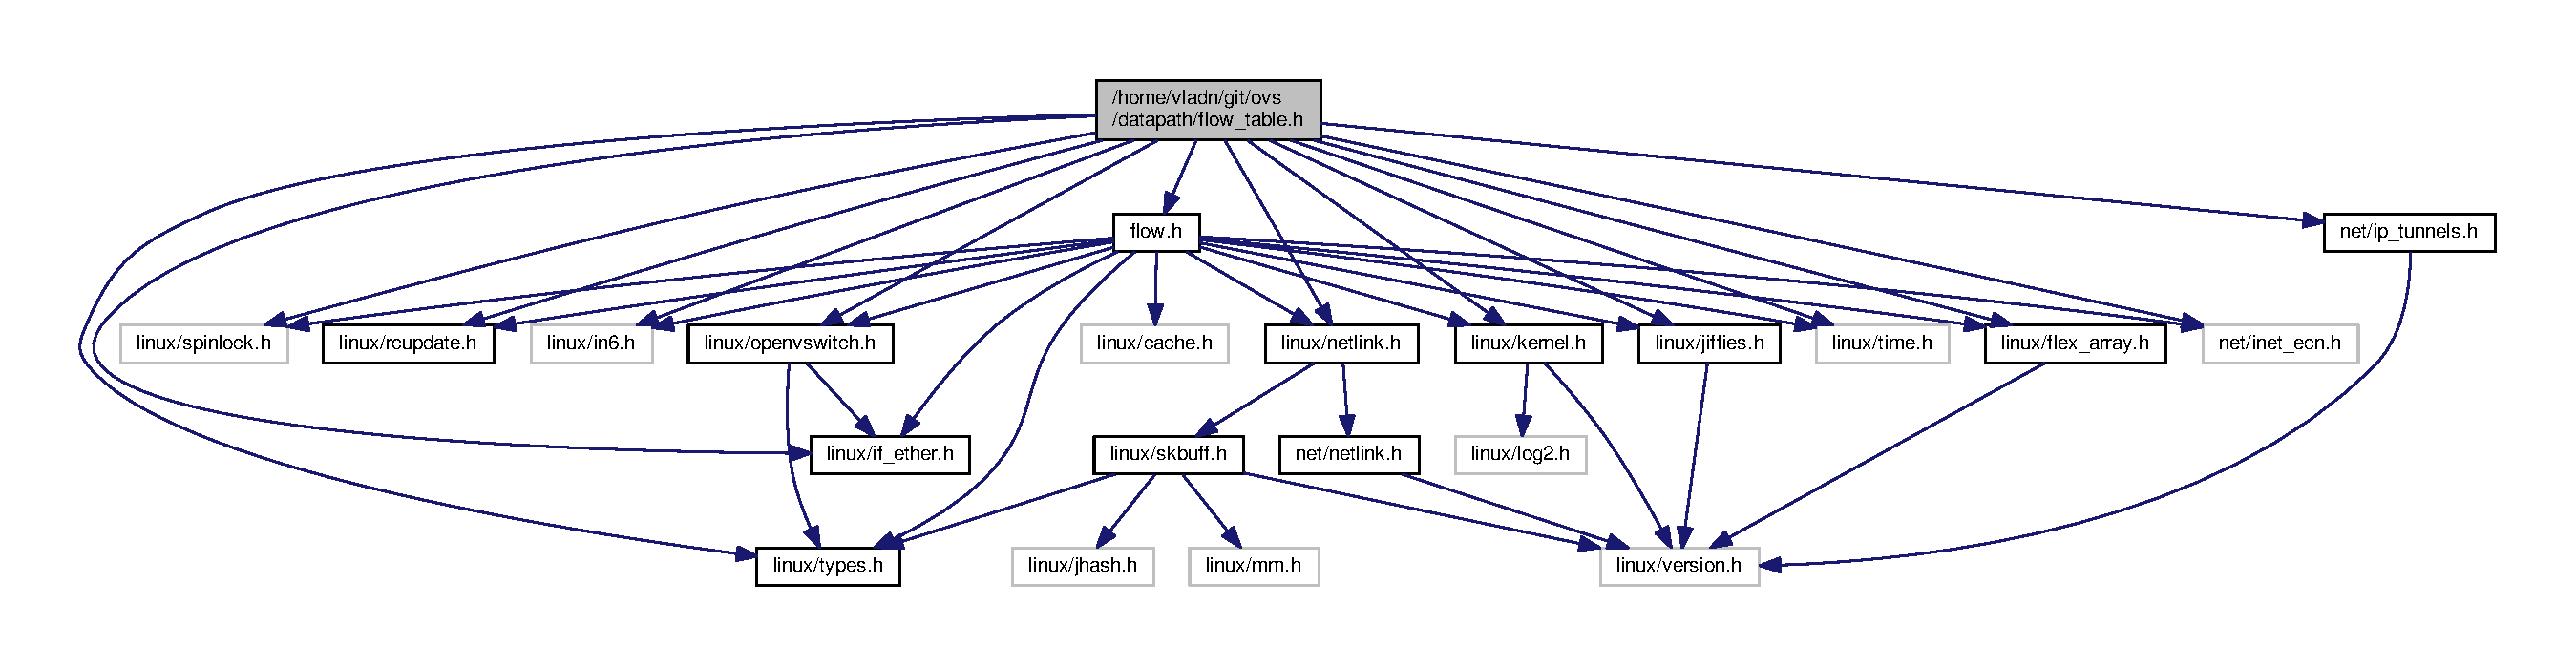
\includegraphics[width=350pt]{flow__table_8h__incl}
\end{center}
\end{figure}
This graph shows which files directly or indirectly include this file\+:
\nopagebreak
\begin{figure}[H]
\begin{center}
\leavevmode
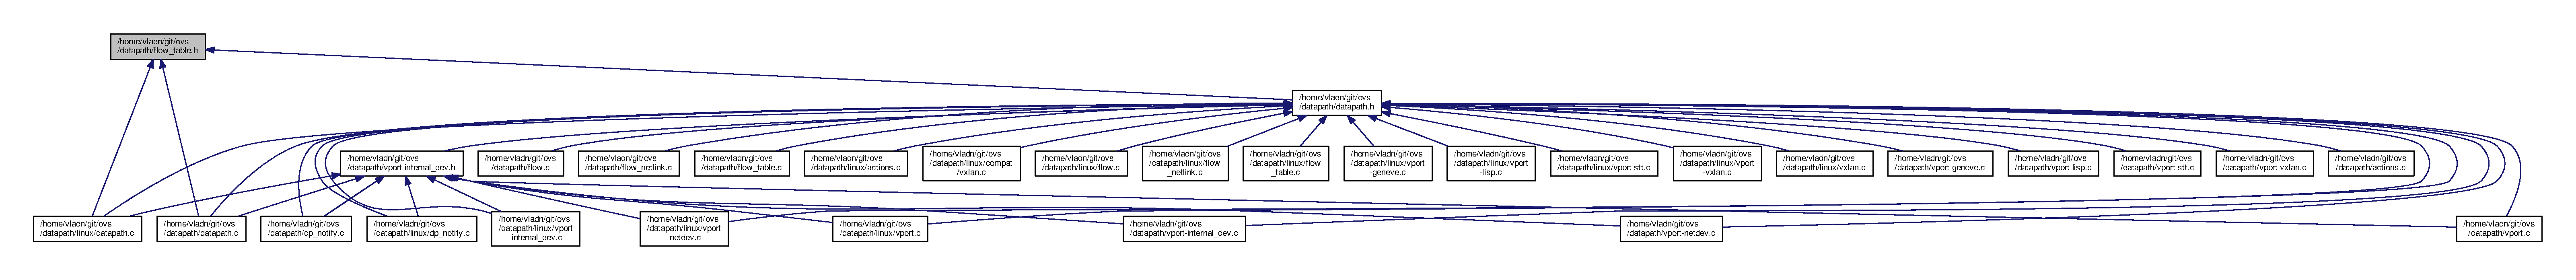
\includegraphics[width=350pt]{flow__table_8h__dep__incl}
\end{center}
\end{figure}
\subsection*{Data Structures}
\begin{DoxyCompactItemize}
\item 
struct \hyperlink{structmask__cache__entry}{mask\+\_\+cache\+\_\+entry}
\item 
struct \hyperlink{structmask__array}{mask\+\_\+array}
\item 
struct \hyperlink{structtable__instance}{table\+\_\+instance}
\item 
struct \hyperlink{structflow__table}{flow\+\_\+table}
\end{DoxyCompactItemize}
\subsection*{Functions}
\begin{DoxyCompactItemize}
\item 
int \hyperlink{flow__table_8h_a07492868e65ba495c86d49df9cf1bc50}{ovs\+\_\+flow\+\_\+init} (void)
\item 
void \hyperlink{flow__table_8h_a96cce30f7a9c3231d5b5afaf967378eb}{ovs\+\_\+flow\+\_\+exit} (void)
\item 
struct \hyperlink{structsw__flow}{sw\+\_\+flow} $\ast$ \hyperlink{flow__table_8h_acce701c647d8e59486574fba1be3e10c}{ovs\+\_\+flow\+\_\+alloc} (void)
\item 
void \hyperlink{flow__table_8h_a2629f2024cffebd33b3e9989085400aa}{ovs\+\_\+flow\+\_\+free} (struct \hyperlink{structsw__flow}{sw\+\_\+flow} $\ast$, \hyperlink{types_8h_afaa87723b8417d40fcf45b7330261ef9}{bool} deferred)
\item 
int \hyperlink{flow__table_8h_a352a5f5e249d448bac51e011a6164443}{ovs\+\_\+flow\+\_\+tbl\+\_\+init} (struct \hyperlink{structflow__table}{flow\+\_\+table} $\ast$)
\item 
int \hyperlink{flow__table_8h_a8f1f39fd4e1ecafd99321016698a709a}{ovs\+\_\+flow\+\_\+tbl\+\_\+count} (const struct \hyperlink{structflow__table}{flow\+\_\+table} $\ast$table)
\item 
void \hyperlink{flow__table_8h_ad37dcfdb56d17589ed79b5c4dd38bc76}{ovs\+\_\+flow\+\_\+tbl\+\_\+destroy} (struct \hyperlink{structflow__table}{flow\+\_\+table} $\ast$table)
\item 
int \hyperlink{flow__table_8h_a7e424f978318e8c007b3de68854e8dc2}{ovs\+\_\+flow\+\_\+tbl\+\_\+flush} (struct \hyperlink{structflow__table}{flow\+\_\+table} $\ast$\hyperlink{structflow__table}{flow\+\_\+table})
\item 
int \hyperlink{flow__table_8h_a72ec4f72961a64b1c006978a32554a4c}{ovs\+\_\+flow\+\_\+tbl\+\_\+insert} (struct \hyperlink{structflow__table}{flow\+\_\+table} $\ast$table, struct \hyperlink{structsw__flow}{sw\+\_\+flow} $\ast$flow, const struct \hyperlink{structsw__flow__mask}{sw\+\_\+flow\+\_\+mask} $\ast$mask)
\item 
void \hyperlink{flow__table_8h_aa75b8bc2551f9c1a8d65b942a10df89a}{ovs\+\_\+flow\+\_\+tbl\+\_\+remove} (struct \hyperlink{structflow__table}{flow\+\_\+table} $\ast$table, struct \hyperlink{structsw__flow}{sw\+\_\+flow} $\ast$flow)
\item 
int \hyperlink{flow__table_8h_ab6e18d16217cddd0af756b76b72e6ce6}{ovs\+\_\+flow\+\_\+tbl\+\_\+num\+\_\+masks} (const struct \hyperlink{structflow__table}{flow\+\_\+table} $\ast$table)
\item 
struct \hyperlink{structsw__flow}{sw\+\_\+flow} $\ast$ \hyperlink{flow__table_8h_aa2011feb0ef139b04c14890771e97f69}{ovs\+\_\+flow\+\_\+tbl\+\_\+dump\+\_\+next} (struct \hyperlink{structtable__instance}{table\+\_\+instance} $\ast$table, u32 $\ast$bucket, u32 $\ast$idx)
\item 
struct \hyperlink{structsw__flow}{sw\+\_\+flow} $\ast$ \hyperlink{flow__table_8h_adb87952f9d3b78f48c4f35efb0b41d1a}{ovs\+\_\+flow\+\_\+tbl\+\_\+lookup\+\_\+stats} (struct \hyperlink{structflow__table}{flow\+\_\+table} $\ast$, const struct \hyperlink{structsw__flow__key}{sw\+\_\+flow\+\_\+key} $\ast$, u32 skb\+\_\+hash, u32 $\ast$n\+\_\+mask\+\_\+hit)
\item 
struct \hyperlink{structsw__flow}{sw\+\_\+flow} $\ast$ \hyperlink{flow__table_8h_af75c5609b455f9fc2171ab1ef592982e}{ovs\+\_\+flow\+\_\+tbl\+\_\+lookup} (struct \hyperlink{structflow__table}{flow\+\_\+table} $\ast$, const struct \hyperlink{structsw__flow__key}{sw\+\_\+flow\+\_\+key} $\ast$)
\item 
struct \hyperlink{structsw__flow}{sw\+\_\+flow} $\ast$ \hyperlink{flow__table_8h_ad54c8ee8b511e42f2296bcf5ff8d0fd3}{ovs\+\_\+flow\+\_\+tbl\+\_\+lookup\+\_\+exact} (struct \hyperlink{structflow__table}{flow\+\_\+table} $\ast$tbl, const struct \hyperlink{structsw__flow__match}{sw\+\_\+flow\+\_\+match} $\ast$match)
\item 
struct \hyperlink{structsw__flow}{sw\+\_\+flow} $\ast$ \hyperlink{flow__table_8h_a61adf41ddec6ed85834909231cfa84e0}{ovs\+\_\+flow\+\_\+tbl\+\_\+lookup\+\_\+ufid} (struct \hyperlink{structflow__table}{flow\+\_\+table} $\ast$, const struct \hyperlink{structsw__flow__id}{sw\+\_\+flow\+\_\+id} $\ast$)
\item 
\hyperlink{types_8h_afaa87723b8417d40fcf45b7330261ef9}{bool} \hyperlink{flow__table_8h_a6c6f1ec8e9d4ce0159a4d2f9ce383249}{ovs\+\_\+flow\+\_\+cmp} (const struct \hyperlink{structsw__flow}{sw\+\_\+flow} $\ast$, const struct \hyperlink{structsw__flow__match}{sw\+\_\+flow\+\_\+match} $\ast$)
\item 
void \hyperlink{flow__table_8h_a40f76cbd2e168abb1b9744562e24be3b}{ovs\+\_\+flow\+\_\+mask\+\_\+key} (struct \hyperlink{structsw__flow__key}{sw\+\_\+flow\+\_\+key} $\ast$\hyperlink{flow_8h_a6747ad3b5d60480ea073cd12c9b78aaa}{dst}, const struct \hyperlink{structsw__flow__key}{sw\+\_\+flow\+\_\+key} $\ast$\hyperlink{flow_8h_a2e7e37e9dfe6465386d6c500f83ef144}{src}, const struct \hyperlink{structsw__flow__mask}{sw\+\_\+flow\+\_\+mask} $\ast$mask)
\end{DoxyCompactItemize}
\subsection*{Variables}
\begin{DoxyCompactItemize}
\item 
struct kmem\+\_\+cache $\ast$ \hyperlink{flow__table_8h_ab305bee215adea2618069cc592f6ee6b}{flow\+\_\+stats\+\_\+cache}
\end{DoxyCompactItemize}


\subsection{Function Documentation}
\hypertarget{flow__table_8h_acce701c647d8e59486574fba1be3e10c}{}\index{flow\+\_\+table.\+h@{flow\+\_\+table.\+h}!ovs\+\_\+flow\+\_\+alloc@{ovs\+\_\+flow\+\_\+alloc}}
\index{ovs\+\_\+flow\+\_\+alloc@{ovs\+\_\+flow\+\_\+alloc}!flow\+\_\+table.\+h@{flow\+\_\+table.\+h}}
\subsubsection[{ovs\+\_\+flow\+\_\+alloc}]{\setlength{\rightskip}{0pt plus 5cm}struct {\bf sw\+\_\+flow}$\ast$ ovs\+\_\+flow\+\_\+alloc (
\begin{DoxyParamCaption}
\item[{void}]{}
\end{DoxyParamCaption}
)}\label{flow__table_8h_acce701c647d8e59486574fba1be3e10c}

\begin{DoxyCode}
84 \{
85     \textcolor{keyword}{struct }\hyperlink{structsw__flow}{sw\_flow} *flow;
86     \textcolor{keyword}{struct }\hyperlink{structflow__stats}{flow\_stats} *stats;
87     \textcolor{keywordtype}{int} node;
88 
89     flow = kmem\_cache\_alloc(\hyperlink{flow__table_8c_ab00a8de93e918b8aba331f4872a2c97c}{flow\_cache}, GFP\_KERNEL);
90     \textcolor{keywordflow}{if} (!flow)
91         \textcolor{keywordflow}{return} ERR\_PTR(-ENOMEM);
92 
93     flow->\hyperlink{structsw__flow_aa845bdaabc25d81dcf8b1a7519b35408}{sf\_acts} = NULL;
94     flow->\hyperlink{structsw__flow_a89c162e340693d0bb4977737e2b68c22}{mask} = NULL;
95     flow->\hyperlink{structsw__flow_a6e6645eec909d54871675be30000c0b9}{id}.\hyperlink{structsw__flow__id_a7cfead96fedf295e55d6a17857adfbf5}{ufid\_len} = 0;
96     flow->\hyperlink{structsw__flow_a6e6645eec909d54871675be30000c0b9}{id}.\hyperlink{structsw__flow__id_a5d62dce79569cb8c25a43f4039e5df3c}{unmasked\_key} = NULL;
97     flow->\hyperlink{structsw__flow_a7b4a10d23b2824b421527bc2600ef4ba}{stats\_last\_writer} = NUMA\_NO\_NODE;
98 
99     \textcolor{comment}{/* Initialize the default stat node. */}
100     stats = kmem\_cache\_alloc\_node(\hyperlink{flow__table_8h_ab305bee215adea2618069cc592f6ee6b}{flow\_stats\_cache},
101                       GFP\_KERNEL | \_\_GFP\_ZERO, 0);
102     \textcolor{keywordflow}{if} (!stats)
103         \textcolor{keywordflow}{goto} err;
104 
105     spin\_lock\_init(&stats->\hyperlink{structflow__stats_a1930f864d7fc52f4afeb86714e3e5c07}{lock});
106 
107     \hyperlink{rcupdate_8h_ad30f6689018c0dc0178126e1e12897e9}{RCU\_INIT\_POINTER}(flow->\hyperlink{structsw__flow_a5ccc743bcf16038ab0cf5dda88565f33}{stats}[0], stats);
108 
109     for\_each\_node(node)
110         if (node != 0)
111             \hyperlink{rcupdate_8h_ad30f6689018c0dc0178126e1e12897e9}{RCU\_INIT\_POINTER}(flow->stats[node], NULL);
112 
113     return flow;
114 err:
115     kmem\_cache\_free(\hyperlink{flow__table_8c_ab00a8de93e918b8aba331f4872a2c97c}{flow\_cache}, flow);
116     return ERR\_PTR(-ENOMEM);
117 \}
\end{DoxyCode}
\hypertarget{flow__table_8h_a6c6f1ec8e9d4ce0159a4d2f9ce383249}{}\index{flow\+\_\+table.\+h@{flow\+\_\+table.\+h}!ovs\+\_\+flow\+\_\+cmp@{ovs\+\_\+flow\+\_\+cmp}}
\index{ovs\+\_\+flow\+\_\+cmp@{ovs\+\_\+flow\+\_\+cmp}!flow\+\_\+table.\+h@{flow\+\_\+table.\+h}}
\subsubsection[{ovs\+\_\+flow\+\_\+cmp}]{\setlength{\rightskip}{0pt plus 5cm}{\bf bool} ovs\+\_\+flow\+\_\+cmp (
\begin{DoxyParamCaption}
\item[{const struct {\bf sw\+\_\+flow} $\ast$}]{, }
\item[{const struct {\bf sw\+\_\+flow\+\_\+match} $\ast$}]{}
\end{DoxyParamCaption}
)}\label{flow__table_8h_a6c6f1ec8e9d4ce0159a4d2f9ce383249}

\begin{DoxyCode}
725 \{
726     \textcolor{keywordflow}{if} (\hyperlink{flow_8h_a995966854ceb0b5a72ff027c12ccf426}{ovs\_identifier\_is\_ufid}(&flow->id))
727         \textcolor{keywordflow}{return} \hyperlink{flow__table_8c_ae52adc695ca936e630f8a4a61753520d}{flow\_cmp\_masked\_key}(flow, match->key, &match->range);
728 
729     \textcolor{keywordflow}{return} \hyperlink{flow__table_8c_a0dd59a846abd3c41f19357b2223b10a9}{ovs\_flow\_cmp\_unmasked\_key}(flow, match);
730 \}
\end{DoxyCode}
\hypertarget{flow__table_8h_a96cce30f7a9c3231d5b5afaf967378eb}{}\index{flow\+\_\+table.\+h@{flow\+\_\+table.\+h}!ovs\+\_\+flow\+\_\+exit@{ovs\+\_\+flow\+\_\+exit}}
\index{ovs\+\_\+flow\+\_\+exit@{ovs\+\_\+flow\+\_\+exit}!flow\+\_\+table.\+h@{flow\+\_\+table.\+h}}
\subsubsection[{ovs\+\_\+flow\+\_\+exit}]{\setlength{\rightskip}{0pt plus 5cm}void ovs\+\_\+flow\+\_\+exit (
\begin{DoxyParamCaption}
\item[{void}]{}
\end{DoxyParamCaption}
)}\label{flow__table_8h_a96cce30f7a9c3231d5b5afaf967378eb}

\begin{DoxyCode}
1011 \{
1012     kmem\_cache\_destroy(\hyperlink{flow__table_8h_ab305bee215adea2618069cc592f6ee6b}{flow\_stats\_cache});
1013     kmem\_cache\_destroy(\hyperlink{flow__table_8c_ab00a8de93e918b8aba331f4872a2c97c}{flow\_cache});
1014 \}
\end{DoxyCode}
\hypertarget{flow__table_8h_a2629f2024cffebd33b3e9989085400aa}{}\index{flow\+\_\+table.\+h@{flow\+\_\+table.\+h}!ovs\+\_\+flow\+\_\+free@{ovs\+\_\+flow\+\_\+free}}
\index{ovs\+\_\+flow\+\_\+free@{ovs\+\_\+flow\+\_\+free}!flow\+\_\+table.\+h@{flow\+\_\+table.\+h}}
\subsubsection[{ovs\+\_\+flow\+\_\+free}]{\setlength{\rightskip}{0pt plus 5cm}void ovs\+\_\+flow\+\_\+free (
\begin{DoxyParamCaption}
\item[{struct {\bf sw\+\_\+flow} $\ast$}]{, }
\item[{{\bf bool}}]{deferred}
\end{DoxyParamCaption}
)}\label{flow__table_8h_a2629f2024cffebd33b3e9989085400aa}

\begin{DoxyCode}
176 \{
177     \textcolor{keywordflow}{if} (!flow)
178         \textcolor{keywordflow}{return};
179 
180     \textcolor{keywordflow}{if} (deferred)
181         call\_rcu(&flow->rcu, \hyperlink{flow__table_8c_a38fd2d883e505bba412320f3216dc377}{rcu\_free\_flow\_callback});
182     \textcolor{keywordflow}{else}
183         \hyperlink{flow__table_8c_af6a50f2fb2e93732e8d706dd7cf67c9b}{flow\_free}(flow);
184 \}
\end{DoxyCode}
\hypertarget{flow__table_8h_a07492868e65ba495c86d49df9cf1bc50}{}\index{flow\+\_\+table.\+h@{flow\+\_\+table.\+h}!ovs\+\_\+flow\+\_\+init@{ovs\+\_\+flow\+\_\+init}}
\index{ovs\+\_\+flow\+\_\+init@{ovs\+\_\+flow\+\_\+init}!flow\+\_\+table.\+h@{flow\+\_\+table.\+h}}
\subsubsection[{ovs\+\_\+flow\+\_\+init}]{\setlength{\rightskip}{0pt plus 5cm}int ovs\+\_\+flow\+\_\+init (
\begin{DoxyParamCaption}
\item[{void}]{}
\end{DoxyParamCaption}
)}\label{flow__table_8h_a07492868e65ba495c86d49df9cf1bc50}

\begin{DoxyCode}
986 \{
987     BUILD\_BUG\_ON(\_\_alignof\_\_(\textcolor{keyword}{struct} \hyperlink{structsw__flow__key}{sw\_flow\_key}) % \_\_alignof\_\_(\textcolor{keywordtype}{long}));
988     BUILD\_BUG\_ON(\textcolor{keyword}{sizeof}(\textcolor{keyword}{struct} \hyperlink{structsw__flow__key}{sw\_flow\_key}) % \textcolor{keyword}{sizeof}(\textcolor{keywordtype}{long}));
989 
990     \hyperlink{flow__table_8c_ab00a8de93e918b8aba331f4872a2c97c}{flow\_cache} = kmem\_cache\_create(\textcolor{stringliteral}{"sw\_flow"}, \textcolor{keyword}{sizeof}(\textcolor{keyword}{struct} \hyperlink{structsw__flow}{sw\_flow})
991                        + (nr\_node\_ids
992                       * \textcolor{keyword}{sizeof}(\textcolor{keyword}{struct} \hyperlink{structflow__stats}{flow\_stats} *)),
993                        0, 0, NULL);
994     \textcolor{keywordflow}{if} (\hyperlink{flow__table_8c_ab00a8de93e918b8aba331f4872a2c97c}{flow\_cache} == NULL)
995         \textcolor{keywordflow}{return} -ENOMEM;
996 
997     \hyperlink{flow__table_8h_ab305bee215adea2618069cc592f6ee6b}{flow\_stats\_cache}
998         = kmem\_cache\_create(\textcolor{stringliteral}{"sw\_flow\_stats"}, \textcolor{keyword}{sizeof}(\textcolor{keyword}{struct} \hyperlink{structflow__stats}{flow\_stats}),
999                     0, SLAB\_HWCACHE\_ALIGN, NULL);
1000     \textcolor{keywordflow}{if} (\hyperlink{flow__table_8h_ab305bee215adea2618069cc592f6ee6b}{flow\_stats\_cache} == NULL) \{
1001         kmem\_cache\_destroy(\hyperlink{flow__table_8c_ab00a8de93e918b8aba331f4872a2c97c}{flow\_cache});
1002         \hyperlink{flow__table_8c_ab00a8de93e918b8aba331f4872a2c97c}{flow\_cache} = NULL;
1003         \textcolor{keywordflow}{return} -ENOMEM;
1004     \}
1005 
1006     \textcolor{keywordflow}{return} 0;
1007 \}
\end{DoxyCode}
\hypertarget{flow__table_8h_a40f76cbd2e168abb1b9744562e24be3b}{}\index{flow\+\_\+table.\+h@{flow\+\_\+table.\+h}!ovs\+\_\+flow\+\_\+mask\+\_\+key@{ovs\+\_\+flow\+\_\+mask\+\_\+key}}
\index{ovs\+\_\+flow\+\_\+mask\+\_\+key@{ovs\+\_\+flow\+\_\+mask\+\_\+key}!flow\+\_\+table.\+h@{flow\+\_\+table.\+h}}
\subsubsection[{ovs\+\_\+flow\+\_\+mask\+\_\+key}]{\setlength{\rightskip}{0pt plus 5cm}void ovs\+\_\+flow\+\_\+mask\+\_\+key (
\begin{DoxyParamCaption}
\item[{struct {\bf sw\+\_\+flow\+\_\+key} $\ast$}]{dst, }
\item[{const struct {\bf sw\+\_\+flow\+\_\+key} $\ast$}]{src, }
\item[{const struct {\bf sw\+\_\+flow\+\_\+mask} $\ast$}]{mask}
\end{DoxyParamCaption}
)}\label{flow__table_8h_a40f76cbd2e168abb1b9744562e24be3b}

\begin{DoxyCode}
67 \{
68     \textcolor{keyword}{const} \textcolor{keywordtype}{long} *m = (\textcolor{keyword}{const} \textcolor{keywordtype}{long} *)((\textcolor{keyword}{const} u8 *)&mask->\hyperlink{structsw__flow__mask_a52db0284fdd4579a5f30dee0837a7485}{key} +
69                 mask->\hyperlink{structsw__flow__mask_aa6062c0e580d516ff2d9ce8f9611432b}{range}.\hyperlink{structsw__flow__key__range_a3139158cea80b4e5af36967f3748e846}{start});
70     \textcolor{keyword}{const} \textcolor{keywordtype}{long} *s = (\textcolor{keyword}{const} \textcolor{keywordtype}{long} *)((\textcolor{keyword}{const} u8 *)src +
71                 mask->\hyperlink{structsw__flow__mask_aa6062c0e580d516ff2d9ce8f9611432b}{range}.\hyperlink{structsw__flow__key__range_a3139158cea80b4e5af36967f3748e846}{start});
72     \textcolor{keywordtype}{long} *d = (\textcolor{keywordtype}{long} *)((u8 *)dst + mask->\hyperlink{structsw__flow__mask_aa6062c0e580d516ff2d9ce8f9611432b}{range}.\hyperlink{structsw__flow__key__range_a3139158cea80b4e5af36967f3748e846}{start});
73     \textcolor{keywordtype}{int} i;
74 
75     \textcolor{comment}{/* The memory outside of the 'mask->range' are not set since}
76 \textcolor{comment}{     * further operations on 'dst' only uses contents within}
77 \textcolor{comment}{     * 'mask->range'.}
78 \textcolor{comment}{     */}
79     \textcolor{keywordflow}{for} (i = 0; i < \hyperlink{flow__table_8c_a1b494e4862736de33cbbd7cd72ee8521}{range\_n\_bytes}(&mask->\hyperlink{structsw__flow__mask_aa6062c0e580d516ff2d9ce8f9611432b}{range}); i += \textcolor{keyword}{sizeof}(long))
80         *d++ = *s++ & *m++;
81 \}
\end{DoxyCode}
\hypertarget{flow__table_8h_a8f1f39fd4e1ecafd99321016698a709a}{}\index{flow\+\_\+table.\+h@{flow\+\_\+table.\+h}!ovs\+\_\+flow\+\_\+tbl\+\_\+count@{ovs\+\_\+flow\+\_\+tbl\+\_\+count}}
\index{ovs\+\_\+flow\+\_\+tbl\+\_\+count@{ovs\+\_\+flow\+\_\+tbl\+\_\+count}!flow\+\_\+table.\+h@{flow\+\_\+table.\+h}}
\subsubsection[{ovs\+\_\+flow\+\_\+tbl\+\_\+count}]{\setlength{\rightskip}{0pt plus 5cm}int ovs\+\_\+flow\+\_\+tbl\+\_\+count (
\begin{DoxyParamCaption}
\item[{const struct {\bf flow\+\_\+table} $\ast$}]{table}
\end{DoxyParamCaption}
)}\label{flow__table_8h_a8f1f39fd4e1ecafd99321016698a709a}

\begin{DoxyCode}
120 \{
121     \textcolor{keywordflow}{return} table->\hyperlink{structflow__table_a97cae1e714c6dcfe0d39ce4cff371786}{count};
122 \}
\end{DoxyCode}
\hypertarget{flow__table_8h_ad37dcfdb56d17589ed79b5c4dd38bc76}{}\index{flow\+\_\+table.\+h@{flow\+\_\+table.\+h}!ovs\+\_\+flow\+\_\+tbl\+\_\+destroy@{ovs\+\_\+flow\+\_\+tbl\+\_\+destroy}}
\index{ovs\+\_\+flow\+\_\+tbl\+\_\+destroy@{ovs\+\_\+flow\+\_\+tbl\+\_\+destroy}!flow\+\_\+table.\+h@{flow\+\_\+table.\+h}}
\subsubsection[{ovs\+\_\+flow\+\_\+tbl\+\_\+destroy}]{\setlength{\rightskip}{0pt plus 5cm}void ovs\+\_\+flow\+\_\+tbl\+\_\+destroy (
\begin{DoxyParamCaption}
\item[{struct {\bf flow\+\_\+table} $\ast$}]{table}
\end{DoxyParamCaption}
)}\label{flow__table_8h_ad37dcfdb56d17589ed79b5c4dd38bc76}

\begin{DoxyCode}
358 \{
359     \textcolor{keyword}{struct }\hyperlink{structtable__instance}{table\_instance} *ti = \hyperlink{rcupdate_8h_a9e866c0e8ba667e053cb8f59af572157}{rcu\_dereference\_raw}(table->
      \hyperlink{structflow__table_a49d708e68608d510f6d25a16a14fd565}{ti});
360     \textcolor{keyword}{struct }\hyperlink{structtable__instance}{table\_instance} *ufid\_ti = \hyperlink{rcupdate_8h_a9e866c0e8ba667e053cb8f59af572157}{rcu\_dereference\_raw}(table->
      \hyperlink{structflow__table_aa29e185501af8dcd15549ee157c6c047}{ufid\_ti});
361 
362     free\_percpu(table->\hyperlink{structflow__table_a7395c72250199771559f2aaf32da5d0d}{mask\_cache});
363     kfree(\hyperlink{rcupdate_8h_a9e866c0e8ba667e053cb8f59af572157}{rcu\_dereference\_raw}(table->\hyperlink{structflow__table_a0e568d59590f38936b714555597505be}{mask\_array}));
364     \hyperlink{flow__table_8c_a5abf80651b67f4198a34f7a94e116ec6}{table\_instance\_destroy}(ti, ufid\_ti, \textcolor{keyword}{false});
365 \}
\end{DoxyCode}
\hypertarget{flow__table_8h_aa2011feb0ef139b04c14890771e97f69}{}\index{flow\+\_\+table.\+h@{flow\+\_\+table.\+h}!ovs\+\_\+flow\+\_\+tbl\+\_\+dump\+\_\+next@{ovs\+\_\+flow\+\_\+tbl\+\_\+dump\+\_\+next}}
\index{ovs\+\_\+flow\+\_\+tbl\+\_\+dump\+\_\+next@{ovs\+\_\+flow\+\_\+tbl\+\_\+dump\+\_\+next}!flow\+\_\+table.\+h@{flow\+\_\+table.\+h}}
\subsubsection[{ovs\+\_\+flow\+\_\+tbl\+\_\+dump\+\_\+next}]{\setlength{\rightskip}{0pt plus 5cm}struct {\bf sw\+\_\+flow}$\ast$ ovs\+\_\+flow\+\_\+tbl\+\_\+dump\+\_\+next (
\begin{DoxyParamCaption}
\item[{struct {\bf table\+\_\+instance} $\ast$}]{table, }
\item[{u32 $\ast$}]{bucket, }
\item[{u32 $\ast$}]{idx}
\end{DoxyParamCaption}
)}\label{flow__table_8h_aa2011feb0ef139b04c14890771e97f69}

\begin{DoxyCode}
369 \{
370     \textcolor{keyword}{struct }\hyperlink{structsw__flow}{sw\_flow} *flow;
371     \textcolor{keyword}{struct }hlist\_head *head;
372     \textcolor{keywordtype}{int} ver;
373     \textcolor{keywordtype}{int} i;
374 
375     ver = ti->node\_ver;
376     \textcolor{keywordflow}{while} (*bucket < ti->n\_buckets) \{
377         i = 0;
378         head = flex\_array\_get(ti->buckets, *bucket);
379         \hyperlink{rculist_8h_a482ed6bca0b607f6455d5386f3b1ed75}{hlist\_for\_each\_entry\_rcu}(flow, head, \hyperlink{structflow__table}{flow\_table}.node[ver]) \{
380             \textcolor{keywordflow}{if} (i < *last) \{
381                 i++;
382                 \textcolor{keywordflow}{continue};
383             \}
384             *last = i + 1;
385             \textcolor{keywordflow}{return} flow;
386         \}
387         (*bucket)++;
388         *last = 0;
389     \}
390 
391     \textcolor{keywordflow}{return} NULL;
392 \}
\end{DoxyCode}
\hypertarget{flow__table_8h_a7e424f978318e8c007b3de68854e8dc2}{}\index{flow\+\_\+table.\+h@{flow\+\_\+table.\+h}!ovs\+\_\+flow\+\_\+tbl\+\_\+flush@{ovs\+\_\+flow\+\_\+tbl\+\_\+flush}}
\index{ovs\+\_\+flow\+\_\+tbl\+\_\+flush@{ovs\+\_\+flow\+\_\+tbl\+\_\+flush}!flow\+\_\+table.\+h@{flow\+\_\+table.\+h}}
\subsubsection[{ovs\+\_\+flow\+\_\+tbl\+\_\+flush}]{\setlength{\rightskip}{0pt plus 5cm}int ovs\+\_\+flow\+\_\+tbl\+\_\+flush (
\begin{DoxyParamCaption}
\item[{struct {\bf flow\+\_\+table} $\ast$}]{flow\+\_\+table}
\end{DoxyParamCaption}
)}\label{flow__table_8h_a7e424f978318e8c007b3de68854e8dc2}

\begin{DoxyCode}
463 \{
464     \textcolor{keyword}{struct }\hyperlink{structtable__instance}{table\_instance} *old\_ti, *new\_ti;
465     \textcolor{keyword}{struct }\hyperlink{structtable__instance}{table\_instance} *old\_ufid\_ti, *new\_ufid\_ti;
466 
467     new\_ti = \hyperlink{flow__table_8c_afa79f1c5220d4487a4236884110b9f13}{table\_instance\_alloc}(\hyperlink{flow__table_8c_a84843442d8db7eda5192117e7c6b2997}{TBL\_MIN\_BUCKETS});
468     \textcolor{keywordflow}{if} (!new\_ti)
469         \textcolor{keywordflow}{return} -ENOMEM;
470     new\_ufid\_ti = \hyperlink{flow__table_8c_afa79f1c5220d4487a4236884110b9f13}{table\_instance\_alloc}(\hyperlink{flow__table_8c_a84843442d8db7eda5192117e7c6b2997}{TBL\_MIN\_BUCKETS});
471     \textcolor{keywordflow}{if} (!new\_ufid\_ti)
472         \textcolor{keywordflow}{goto} err\_free\_ti;
473 
474     old\_ti = \hyperlink{datapath_8h_a06ef69170d345fd3996a467dcacf3ff3}{ovsl\_dereference}(flow\_table->\hyperlink{structflow__table_a49d708e68608d510f6d25a16a14fd565}{ti});
475     old\_ufid\_ti = \hyperlink{datapath_8h_a06ef69170d345fd3996a467dcacf3ff3}{ovsl\_dereference}(flow\_table->\hyperlink{structflow__table_aa29e185501af8dcd15549ee157c6c047}{ufid\_ti});
476 
477     rcu\_assign\_pointer(flow\_table->\hyperlink{structflow__table_a49d708e68608d510f6d25a16a14fd565}{ti}, new\_ti);
478     rcu\_assign\_pointer(flow\_table->\hyperlink{structflow__table_aa29e185501af8dcd15549ee157c6c047}{ufid\_ti}, new\_ufid\_ti);
479     flow\_table->\hyperlink{structflow__table_a82c7cfef05b2898b3ffb3b6cb6fdc6a4}{last\_rehash} = jiffies;
480     flow\_table->\hyperlink{structflow__table_a97cae1e714c6dcfe0d39ce4cff371786}{count} = 0;
481     flow\_table->\hyperlink{structflow__table_ad8ff1e259e64690608d9552f0b467bf0}{ufid\_count} = 0;
482 
483     \hyperlink{flow__table_8c_a5abf80651b67f4198a34f7a94e116ec6}{table\_instance\_destroy}(old\_ti, old\_ufid\_ti, \textcolor{keyword}{true});
484     \textcolor{keywordflow}{return} 0;
485 
486 err\_free\_ti:
487     \hyperlink{flow__table_8c_a4699ad0074a999c5f80e77a8ff1b0ebc}{\_\_table\_instance\_destroy}(new\_ti);
488     \textcolor{keywordflow}{return} -ENOMEM;
489 \}
\end{DoxyCode}
\hypertarget{flow__table_8h_a352a5f5e249d448bac51e011a6164443}{}\index{flow\+\_\+table.\+h@{flow\+\_\+table.\+h}!ovs\+\_\+flow\+\_\+tbl\+\_\+init@{ovs\+\_\+flow\+\_\+tbl\+\_\+init}}
\index{ovs\+\_\+flow\+\_\+tbl\+\_\+init@{ovs\+\_\+flow\+\_\+tbl\+\_\+init}!flow\+\_\+table.\+h@{flow\+\_\+table.\+h}}
\subsubsection[{ovs\+\_\+flow\+\_\+tbl\+\_\+init}]{\setlength{\rightskip}{0pt plus 5cm}int ovs\+\_\+flow\+\_\+tbl\+\_\+init (
\begin{DoxyParamCaption}
\item[{struct {\bf flow\+\_\+table} $\ast$}]{}
\end{DoxyParamCaption}
)}\label{flow__table_8h_a352a5f5e249d448bac51e011a6164443}

\begin{DoxyCode}
271 \{
272     \textcolor{keyword}{struct }\hyperlink{structtable__instance}{table\_instance} *ti, *ufid\_ti;
273     \textcolor{keyword}{struct }\hyperlink{structmask__array}{mask\_array} *ma;
274 
275     table->mask\_cache = \_\_alloc\_percpu(\textcolor{keyword}{sizeof}(\textcolor{keyword}{struct} \hyperlink{structmask__cache__entry}{mask\_cache\_entry}) *
276                       \hyperlink{flow__table_8c_af961440482d56f3b26f232774a37c9c5}{MC\_HASH\_ENTRIES}, \_\_alignof\_\_(\textcolor{keyword}{struct} 
      \hyperlink{structmask__cache__entry}{mask\_cache\_entry}));
277     \textcolor{keywordflow}{if} (!table->mask\_cache)
278         \textcolor{keywordflow}{return} -ENOMEM;
279 
280     ma = \hyperlink{flow__table_8c_a327b2f9873b81f7b7920e85c366cc96e}{tbl\_mask\_array\_alloc}(\hyperlink{flow__table_8c_a8240394ae842a0ba76d82f50744ced0a}{MASK\_ARRAY\_SIZE\_MIN});
281     \textcolor{keywordflow}{if} (!ma)
282         \textcolor{keywordflow}{goto} free\_mask\_cache;
283 
284     ti = \hyperlink{flow__table_8c_afa79f1c5220d4487a4236884110b9f13}{table\_instance\_alloc}(\hyperlink{flow__table_8c_a84843442d8db7eda5192117e7c6b2997}{TBL\_MIN\_BUCKETS});
285     \textcolor{keywordflow}{if} (!ti)
286         \textcolor{keywordflow}{goto} free\_mask\_array;
287 
288     ufid\_ti = \hyperlink{flow__table_8c_afa79f1c5220d4487a4236884110b9f13}{table\_instance\_alloc}(\hyperlink{flow__table_8c_a84843442d8db7eda5192117e7c6b2997}{TBL\_MIN\_BUCKETS});
289     \textcolor{keywordflow}{if} (!ufid\_ti)
290         \textcolor{keywordflow}{goto} free\_ti;
291 
292     rcu\_assign\_pointer(table->ti, ti);
293     rcu\_assign\_pointer(table->ufid\_ti, ufid\_ti);
294     rcu\_assign\_pointer(table->mask\_array, ma);
295     table->last\_rehash = jiffies;
296     table->count = 0;
297     table->ufid\_count = 0;
298     \textcolor{keywordflow}{return} 0;
299 
300 free\_ti:
301     \hyperlink{flow__table_8c_a4699ad0074a999c5f80e77a8ff1b0ebc}{\_\_table\_instance\_destroy}(ti);
302 free\_mask\_array:
303     kfree(ma);
304 free\_mask\_cache:
305     free\_percpu(table->mask\_cache);
306     \textcolor{keywordflow}{return} -ENOMEM;
307 \}
\end{DoxyCode}
\hypertarget{flow__table_8h_a72ec4f72961a64b1c006978a32554a4c}{}\index{flow\+\_\+table.\+h@{flow\+\_\+table.\+h}!ovs\+\_\+flow\+\_\+tbl\+\_\+insert@{ovs\+\_\+flow\+\_\+tbl\+\_\+insert}}
\index{ovs\+\_\+flow\+\_\+tbl\+\_\+insert@{ovs\+\_\+flow\+\_\+tbl\+\_\+insert}!flow\+\_\+table.\+h@{flow\+\_\+table.\+h}}
\subsubsection[{ovs\+\_\+flow\+\_\+tbl\+\_\+insert}]{\setlength{\rightskip}{0pt plus 5cm}int ovs\+\_\+flow\+\_\+tbl\+\_\+insert (
\begin{DoxyParamCaption}
\item[{struct {\bf flow\+\_\+table} $\ast$}]{table, }
\item[{struct {\bf sw\+\_\+flow} $\ast$}]{flow, }
\item[{const struct {\bf sw\+\_\+flow\+\_\+mask} $\ast$}]{mask}
\end{DoxyParamCaption}
)}\label{flow__table_8h_a72ec4f72961a64b1c006978a32554a4c}

\begin{DoxyCode}
969 \{
970     \textcolor{keywordtype}{int} err;
971 
972     err = \hyperlink{flow__table_8c_a1ceded3a19f98e73b3c10faf2f2532f5}{flow\_mask\_insert}(table, flow, mask);
973     \textcolor{keywordflow}{if} (err)
974         \textcolor{keywordflow}{return} err;
975     \hyperlink{flow__table_8c_a66f2b72d1c755346c4865714e51cfcf4}{flow\_key\_insert}(table, flow);
976     \textcolor{keywordflow}{if} (\hyperlink{flow_8h_a995966854ceb0b5a72ff027c12ccf426}{ovs\_identifier\_is\_ufid}(&flow->\hyperlink{structsw__flow_a6e6645eec909d54871675be30000c0b9}{id}))
977         \hyperlink{flow__table_8c_a36540c6298f41907b7c088b34116346d}{flow\_ufid\_insert}(table, flow);
978 
979     \textcolor{keywordflow}{return} 0;
980 \}
\end{DoxyCode}
\hypertarget{flow__table_8h_af75c5609b455f9fc2171ab1ef592982e}{}\index{flow\+\_\+table.\+h@{flow\+\_\+table.\+h}!ovs\+\_\+flow\+\_\+tbl\+\_\+lookup@{ovs\+\_\+flow\+\_\+tbl\+\_\+lookup}}
\index{ovs\+\_\+flow\+\_\+tbl\+\_\+lookup@{ovs\+\_\+flow\+\_\+tbl\+\_\+lookup}!flow\+\_\+table.\+h@{flow\+\_\+table.\+h}}
\subsubsection[{ovs\+\_\+flow\+\_\+tbl\+\_\+lookup}]{\setlength{\rightskip}{0pt plus 5cm}struct {\bf sw\+\_\+flow}$\ast$ ovs\+\_\+flow\+\_\+tbl\+\_\+lookup (
\begin{DoxyParamCaption}
\item[{struct {\bf flow\+\_\+table} $\ast$}]{, }
\item[{const struct {\bf sw\+\_\+flow\+\_\+key} $\ast$}]{}
\end{DoxyParamCaption}
)}\label{flow__table_8h_af75c5609b455f9fc2171ab1ef592982e}

\begin{DoxyCode}
677 \{
678     \textcolor{keyword}{struct }\hyperlink{structtable__instance}{table\_instance} *ti = \hyperlink{datapath_8h_a5f2a2c1026f970f0052e77f5ebba33d1}{rcu\_dereference\_ovsl}(tbl->ti);
679     \textcolor{keyword}{struct }\hyperlink{structmask__array}{mask\_array} *ma = \hyperlink{datapath_8h_a5f2a2c1026f970f0052e77f5ebba33d1}{rcu\_dereference\_ovsl}(tbl->mask\_array);
680     u32 \hyperlink{compiler-gcc_8h_a4df9005d46835d584f7e924597114061}{\_\_always\_unused} n\_mask\_hit;
681     u32 index = 0;
682 
683     \textcolor{keywordflow}{return} \hyperlink{flow__table_8c_a66b2913ba658b83a167b83e5f5ec465a}{flow\_lookup}(tbl, ti, ma, key, &n\_mask\_hit, &index);
684 \}
\end{DoxyCode}
\hypertarget{flow__table_8h_ad54c8ee8b511e42f2296bcf5ff8d0fd3}{}\index{flow\+\_\+table.\+h@{flow\+\_\+table.\+h}!ovs\+\_\+flow\+\_\+tbl\+\_\+lookup\+\_\+exact@{ovs\+\_\+flow\+\_\+tbl\+\_\+lookup\+\_\+exact}}
\index{ovs\+\_\+flow\+\_\+tbl\+\_\+lookup\+\_\+exact@{ovs\+\_\+flow\+\_\+tbl\+\_\+lookup\+\_\+exact}!flow\+\_\+table.\+h@{flow\+\_\+table.\+h}}
\subsubsection[{ovs\+\_\+flow\+\_\+tbl\+\_\+lookup\+\_\+exact}]{\setlength{\rightskip}{0pt plus 5cm}struct {\bf sw\+\_\+flow}$\ast$ ovs\+\_\+flow\+\_\+tbl\+\_\+lookup\+\_\+exact (
\begin{DoxyParamCaption}
\item[{struct {\bf flow\+\_\+table} $\ast$}]{tbl, }
\item[{const struct {\bf sw\+\_\+flow\+\_\+match} $\ast$}]{match}
\end{DoxyParamCaption}
)}\label{flow__table_8h_ad54c8ee8b511e42f2296bcf5ff8d0fd3}

\begin{DoxyCode}
688 \{
689     \textcolor{keyword}{struct }\hyperlink{structmask__array}{mask\_array} *ma = \hyperlink{datapath_8h_a06ef69170d345fd3996a467dcacf3ff3}{ovsl\_dereference}(tbl->
      \hyperlink{structflow__table_a0e568d59590f38936b714555597505be}{mask\_array});
690     \textcolor{keywordtype}{int} i;
691 
692     \textcolor{comment}{/* Always called under ovs-mutex. */}
693     \textcolor{keywordflow}{for} (i = 0; i < ma->\hyperlink{structmask__array_ad981d54486b5dd03bdb4ad20b740171e}{max}; i++) \{
694         \textcolor{keyword}{struct }\hyperlink{structtable__instance}{table\_instance} *ti = \hyperlink{datapath_8h_a06ef69170d345fd3996a467dcacf3ff3}{ovsl\_dereference}(tbl->
      \hyperlink{structflow__table_a49d708e68608d510f6d25a16a14fd565}{ti});
695         u32 \hyperlink{compiler-gcc_8h_a4df9005d46835d584f7e924597114061}{\_\_always\_unused} n\_mask\_hit;
696         \textcolor{keyword}{struct }\hyperlink{structsw__flow__mask}{sw\_flow\_mask} *mask;
697         \textcolor{keyword}{struct }\hyperlink{structsw__flow}{sw\_flow} *flow;
698 
699         mask = \hyperlink{datapath_8h_a06ef69170d345fd3996a467dcacf3ff3}{ovsl\_dereference}(ma->\hyperlink{structmask__array_a92da2b0ebde32eb6f76a134dc2d61d79}{masks}[i]);
700         \textcolor{keywordflow}{if} (!mask)
701             \textcolor{keywordflow}{continue};
702         flow = \hyperlink{flow__table_8c_ac32c042a5b0b7a5de7c1e43f7187f92b}{masked\_flow\_lookup}(ti, match->\hyperlink{structsw__flow__match_a4030aac38105b63798ea11f43f506372}{key}, mask, &n\_mask\_hit);
703         \textcolor{keywordflow}{if} (flow && \hyperlink{flow_8h_a3bfeaa297d8807b969a14f1cde78d21b}{ovs\_identifier\_is\_key}(&flow->\hyperlink{structsw__flow_a6e6645eec909d54871675be30000c0b9}{id}) &&
704             \hyperlink{flow__table_8c_a0dd59a846abd3c41f19357b2223b10a9}{ovs\_flow\_cmp\_unmasked\_key}(flow, match))
705             \textcolor{keywordflow}{return} flow;
706     \}
707     \textcolor{keywordflow}{return} NULL;
708 \}
\end{DoxyCode}
\hypertarget{flow__table_8h_adb87952f9d3b78f48c4f35efb0b41d1a}{}\index{flow\+\_\+table.\+h@{flow\+\_\+table.\+h}!ovs\+\_\+flow\+\_\+tbl\+\_\+lookup\+\_\+stats@{ovs\+\_\+flow\+\_\+tbl\+\_\+lookup\+\_\+stats}}
\index{ovs\+\_\+flow\+\_\+tbl\+\_\+lookup\+\_\+stats@{ovs\+\_\+flow\+\_\+tbl\+\_\+lookup\+\_\+stats}!flow\+\_\+table.\+h@{flow\+\_\+table.\+h}}
\subsubsection[{ovs\+\_\+flow\+\_\+tbl\+\_\+lookup\+\_\+stats}]{\setlength{\rightskip}{0pt plus 5cm}struct {\bf sw\+\_\+flow}$\ast$ ovs\+\_\+flow\+\_\+tbl\+\_\+lookup\+\_\+stats (
\begin{DoxyParamCaption}
\item[{struct {\bf flow\+\_\+table} $\ast$}]{, }
\item[{const struct {\bf sw\+\_\+flow\+\_\+key} $\ast$}]{, }
\item[{u32}]{skb\+\_\+hash, }
\item[{u32 $\ast$}]{n\+\_\+mask\+\_\+hit}
\end{DoxyParamCaption}
)}\label{flow__table_8h_adb87952f9d3b78f48c4f35efb0b41d1a}

\begin{DoxyCode}
622 \{
623     \textcolor{keyword}{struct }\hyperlink{structmask__array}{mask\_array} *ma = rcu\_dereference(tbl->mask\_array);
624     \textcolor{keyword}{struct }\hyperlink{structtable__instance}{table\_instance} *ti = rcu\_dereference(tbl->ti);
625     \textcolor{keyword}{struct }\hyperlink{structmask__cache__entry}{mask\_cache\_entry} *entries, *ce;
626     \textcolor{keyword}{struct }\hyperlink{structsw__flow}{sw\_flow} *flow;
627     u32 \hyperlink{structsw__flow_a7a33a6a5c62113ffe949a700ef648a71}{hash};
628     \textcolor{keywordtype}{int} seg;
629 
630     *n\_mask\_hit = 0;
631     \textcolor{keywordflow}{if} (unlikely(!skb\_hash)) \{
632         u32 mask\_index = 0;
633 
634         \textcolor{keywordflow}{return} \hyperlink{flow__table_8c_a66b2913ba658b83a167b83e5f5ec465a}{flow\_lookup}(tbl, ti, ma, \hyperlink{structsw__flow_a14b83cbd65275bda4e97ae35500d26d8}{key}, n\_mask\_hit, &mask\_index);
635     \}
636 
637     \textcolor{comment}{/* Pre and post recirulation flows usually have the same skb\_hash}
638 \textcolor{comment}{     * value. To avoid hash collisions, rehash the 'skb\_hash' with}
639 \textcolor{comment}{     * 'recirc\_id'.  */}
640     \textcolor{keywordflow}{if} (\hyperlink{structsw__flow_a14b83cbd65275bda4e97ae35500d26d8}{key}->\hyperlink{structsw__flow__key_a7e51857c88ad6b0bf90551d0b6e2607b}{recirc\_id})
641         skb\_hash = jhash\_1word(skb\_hash, \hyperlink{structsw__flow_a14b83cbd65275bda4e97ae35500d26d8}{key}->\hyperlink{structsw__flow__key_a7e51857c88ad6b0bf90551d0b6e2607b}{recirc\_id});
642 
643     ce = NULL;
644     hash = skb\_hash;
645     entries = \hyperlink{percpu_8h_a1cd55f287dff5c4a79fc11dd38d47c12}{this\_cpu\_ptr}(tbl->mask\_cache);
646 
647     \textcolor{comment}{/* Find the cache entry 'ce' to operate on. */}
648     \textcolor{keywordflow}{for} (seg = 0; seg < \hyperlink{flow__table_8c_ab95179a8dc622b08ce82308fe001d788}{MC\_HASH\_SEGS}; seg++) \{
649         \textcolor{keywordtype}{int} index = hash & (\hyperlink{flow__table_8c_af961440482d56f3b26f232774a37c9c5}{MC\_HASH\_ENTRIES} - 1);
650         \textcolor{keyword}{struct }\hyperlink{structmask__cache__entry}{mask\_cache\_entry} *e;
651 
652         e = &entries[index];
653         \textcolor{keywordflow}{if} (e->\hyperlink{structmask__cache__entry_a45ae5222badf95e1c919a0d6d0090b6f}{skb\_hash} == \hyperlink{structmask__cache__entry_a45ae5222badf95e1c919a0d6d0090b6f}{skb\_hash}) \{
654             flow = \hyperlink{flow__table_8c_a66b2913ba658b83a167b83e5f5ec465a}{flow\_lookup}(tbl, ti, ma, key, n\_mask\_hit,
655                        &e->\hyperlink{structmask__cache__entry_a87faeaec562bcab421cb208dfc0ef5f0}{mask\_index});
656             \textcolor{keywordflow}{if} (!flow)
657                 e->\hyperlink{structmask__cache__entry_a45ae5222badf95e1c919a0d6d0090b6f}{skb\_hash} = 0;
658             \textcolor{keywordflow}{return} flow;
659         \}
660 
661         \textcolor{keywordflow}{if} (!ce || e->\hyperlink{structmask__cache__entry_a45ae5222badf95e1c919a0d6d0090b6f}{skb\_hash} < ce->\hyperlink{structmask__cache__entry_a45ae5222badf95e1c919a0d6d0090b6f}{skb\_hash})
662             ce = e;  \textcolor{comment}{/* A better replacement cache candidate. */}
663 
664         hash >>= \hyperlink{flow__table_8c_aba54fb364af2c9465bb632f82e4631d7}{MC\_HASH\_SHIFT};
665     \}
666 
667     \textcolor{comment}{/* Cache miss, do full lookup. */}
668     flow = \hyperlink{flow__table_8c_a66b2913ba658b83a167b83e5f5ec465a}{flow\_lookup}(tbl, ti, ma, key, n\_mask\_hit, &ce->\hyperlink{structmask__cache__entry_a87faeaec562bcab421cb208dfc0ef5f0}{mask\_index});
669     \textcolor{keywordflow}{if} (flow)
670         ce->\hyperlink{structmask__cache__entry_a45ae5222badf95e1c919a0d6d0090b6f}{skb\_hash} = \hyperlink{structmask__cache__entry_a45ae5222badf95e1c919a0d6d0090b6f}{skb\_hash};
671 
672     \textcolor{keywordflow}{return} flow;
673 \}
\end{DoxyCode}
\hypertarget{flow__table_8h_a61adf41ddec6ed85834909231cfa84e0}{}\index{flow\+\_\+table.\+h@{flow\+\_\+table.\+h}!ovs\+\_\+flow\+\_\+tbl\+\_\+lookup\+\_\+ufid@{ovs\+\_\+flow\+\_\+tbl\+\_\+lookup\+\_\+ufid}}
\index{ovs\+\_\+flow\+\_\+tbl\+\_\+lookup\+\_\+ufid@{ovs\+\_\+flow\+\_\+tbl\+\_\+lookup\+\_\+ufid}!flow\+\_\+table.\+h@{flow\+\_\+table.\+h}}
\subsubsection[{ovs\+\_\+flow\+\_\+tbl\+\_\+lookup\+\_\+ufid}]{\setlength{\rightskip}{0pt plus 5cm}struct {\bf sw\+\_\+flow}$\ast$ ovs\+\_\+flow\+\_\+tbl\+\_\+lookup\+\_\+ufid (
\begin{DoxyParamCaption}
\item[{struct {\bf flow\+\_\+table} $\ast$}]{, }
\item[{const struct {\bf sw\+\_\+flow\+\_\+id} $\ast$}]{}
\end{DoxyParamCaption}
)}\label{flow__table_8h_a61adf41ddec6ed85834909231cfa84e0}

\begin{DoxyCode}
734 \{
735     \textcolor{keyword}{struct }\hyperlink{structtable__instance}{table\_instance} *ti = \hyperlink{datapath_8h_a5f2a2c1026f970f0052e77f5ebba33d1}{rcu\_dereference\_ovsl}(tbl->ufid\_ti);
736     \textcolor{keyword}{struct }\hyperlink{structsw__flow}{sw\_flow} *flow;
737     \textcolor{keyword}{struct }hlist\_head *head;
738     u32 hash;
739 
740     hash = \hyperlink{flow__table_8c_aaf879648c325750d8ff234382797f3af}{ufid\_hash}(ufid);
741     head = \hyperlink{flow__table_8c_aed00deae6497143255e822e293592558}{find\_bucket}(ti, hash);
742     \hyperlink{rculist_8h_a482ed6bca0b607f6455d5386f3b1ed75}{hlist\_for\_each\_entry\_rcu}(flow, head, ufid\_table.\hyperlink{structsw__flow_ad56483ca56d2f95857eee360e934fcf2}{node}[ti->
      \hyperlink{structtable__instance_ab992e9218f85e3b5193ae47e8fbf3f32}{node\_ver}]) \{
743         \textcolor{keywordflow}{if} (flow->\hyperlink{structsw__flow_af5dad10ae036092f5a26cfebb050a03a}{ufid\_table}.\hyperlink{structsw__flow_a7a33a6a5c62113ffe949a700ef648a71}{hash} == hash &&
744             \hyperlink{flow__table_8c_aed32909e9cc5bd5644d1eb39184a5615}{ovs\_flow\_cmp\_ufid}(flow, ufid))
745             \textcolor{keywordflow}{return} flow;
746     \}
747     \textcolor{keywordflow}{return} NULL;
748 \}
\end{DoxyCode}
\hypertarget{flow__table_8h_ab6e18d16217cddd0af756b76b72e6ce6}{}\index{flow\+\_\+table.\+h@{flow\+\_\+table.\+h}!ovs\+\_\+flow\+\_\+tbl\+\_\+num\+\_\+masks@{ovs\+\_\+flow\+\_\+tbl\+\_\+num\+\_\+masks}}
\index{ovs\+\_\+flow\+\_\+tbl\+\_\+num\+\_\+masks@{ovs\+\_\+flow\+\_\+tbl\+\_\+num\+\_\+masks}!flow\+\_\+table.\+h@{flow\+\_\+table.\+h}}
\subsubsection[{ovs\+\_\+flow\+\_\+tbl\+\_\+num\+\_\+masks}]{\setlength{\rightskip}{0pt plus 5cm}int ovs\+\_\+flow\+\_\+tbl\+\_\+num\+\_\+masks (
\begin{DoxyParamCaption}
\item[{const struct {\bf flow\+\_\+table} $\ast$}]{table}
\end{DoxyParamCaption}
)}\label{flow__table_8h_ab6e18d16217cddd0af756b76b72e6ce6}

\begin{DoxyCode}
751 \{
752     \textcolor{keyword}{struct }\hyperlink{structmask__array}{mask\_array} *ma;
753 
754     ma = \hyperlink{datapath_8h_a5f2a2c1026f970f0052e77f5ebba33d1}{rcu\_dereference\_ovsl}(table->\hyperlink{structflow__table_a0e568d59590f38936b714555597505be}{mask\_array});
755     \textcolor{keywordflow}{return} ma->\hyperlink{structmask__array_a55b8fb7e2d7ad8a5725a749645f73b5a}{count};
756 \}
\end{DoxyCode}
\hypertarget{flow__table_8h_aa75b8bc2551f9c1a8d65b942a10df89a}{}\index{flow\+\_\+table.\+h@{flow\+\_\+table.\+h}!ovs\+\_\+flow\+\_\+tbl\+\_\+remove@{ovs\+\_\+flow\+\_\+tbl\+\_\+remove}}
\index{ovs\+\_\+flow\+\_\+tbl\+\_\+remove@{ovs\+\_\+flow\+\_\+tbl\+\_\+remove}!flow\+\_\+table.\+h@{flow\+\_\+table.\+h}}
\subsubsection[{ovs\+\_\+flow\+\_\+tbl\+\_\+remove}]{\setlength{\rightskip}{0pt plus 5cm}void ovs\+\_\+flow\+\_\+tbl\+\_\+remove (
\begin{DoxyParamCaption}
\item[{struct {\bf flow\+\_\+table} $\ast$}]{table, }
\item[{struct {\bf sw\+\_\+flow} $\ast$}]{flow}
\end{DoxyParamCaption}
)}\label{flow__table_8h_aa75b8bc2551f9c1a8d65b942a10df89a}

\begin{DoxyCode}
809 \{
810     \textcolor{keyword}{struct }\hyperlink{structtable__instance}{table\_instance} *ti = \hyperlink{datapath_8h_a06ef69170d345fd3996a467dcacf3ff3}{ovsl\_dereference}(table->
      \hyperlink{structflow__table_a49d708e68608d510f6d25a16a14fd565}{ti});
811     \textcolor{keyword}{struct }\hyperlink{structtable__instance}{table\_instance} *ufid\_ti = \hyperlink{datapath_8h_a06ef69170d345fd3996a467dcacf3ff3}{ovsl\_dereference}(table->
      \hyperlink{structflow__table_aa29e185501af8dcd15549ee157c6c047}{ufid\_ti});
812 
813     BUG\_ON(table->\hyperlink{structflow__table_a97cae1e714c6dcfe0d39ce4cff371786}{count} == 0);
814     hlist\_del\_rcu(&flow->\hyperlink{structsw__flow_abca0040cced6a4a84d1a8941764fb5d6}{flow\_table}.\hyperlink{structsw__flow_ad56483ca56d2f95857eee360e934fcf2}{node}[ti->\hyperlink{structtable__instance_ab992e9218f85e3b5193ae47e8fbf3f32}{node\_ver}]);
815     table->\hyperlink{structflow__table_a97cae1e714c6dcfe0d39ce4cff371786}{count}--;
816     \textcolor{keywordflow}{if} (\hyperlink{flow_8h_a995966854ceb0b5a72ff027c12ccf426}{ovs\_identifier\_is\_ufid}(&flow->\hyperlink{structsw__flow_a6e6645eec909d54871675be30000c0b9}{id})) \{
817         hlist\_del\_rcu(&flow->\hyperlink{structsw__flow_af5dad10ae036092f5a26cfebb050a03a}{ufid\_table}.\hyperlink{structsw__flow_ad56483ca56d2f95857eee360e934fcf2}{node}[ufid\_ti->\hyperlink{structtable__instance_ab992e9218f85e3b5193ae47e8fbf3f32}{node\_ver}]);
818         table->\hyperlink{structflow__table_ad8ff1e259e64690608d9552f0b467bf0}{ufid\_count}--;
819     \}
820 
821     \textcolor{comment}{/* RCU delete the mask. 'flow->mask' is not NULLed, as it should be}
822 \textcolor{comment}{     * accessible as long as the RCU read lock is held.}
823 \textcolor{comment}{     */}
824     \hyperlink{flow__table_8c_a67796467285f769eda43c39ae058d997}{flow\_mask\_remove}(table, flow->\hyperlink{structsw__flow_a89c162e340693d0bb4977737e2b68c22}{mask});
825 \}
\end{DoxyCode}


\subsection{Variable Documentation}
\hypertarget{flow__table_8h_ab305bee215adea2618069cc592f6ee6b}{}\index{flow\+\_\+table.\+h@{flow\+\_\+table.\+h}!flow\+\_\+stats\+\_\+cache@{flow\+\_\+stats\+\_\+cache}}
\index{flow\+\_\+stats\+\_\+cache@{flow\+\_\+stats\+\_\+cache}!flow\+\_\+table.\+h@{flow\+\_\+table.\+h}}
\subsubsection[{flow\+\_\+stats\+\_\+cache}]{\setlength{\rightskip}{0pt plus 5cm}struct kmem\+\_\+cache$\ast$ flow\+\_\+stats\+\_\+cache}\label{flow__table_8h_ab305bee215adea2618069cc592f6ee6b}

\hypertarget{compat_2dev-openvswitch_8c}{}\section{/home/vladn/git/ovs/datapath/linux/compat/dev-\/openvswitch.c File Reference}
\label{compat_2dev-openvswitch_8c}\index{/home/vladn/git/ovs/datapath/linux/compat/dev-\/openvswitch.\+c@{/home/vladn/git/ovs/datapath/linux/compat/dev-\/openvswitch.\+c}}
{\ttfamily \#include $<$linux/if\+\_\+bridge.\+h$>$}\\*
{\ttfamily \#include $<$linux/netdevice.\+h$>$}\\*
{\ttfamily \#include $<$linux/version.\+h$>$}\\*
Include dependency graph for dev-\/openvswitch.c\+:
\nopagebreak
\begin{figure}[H]
\begin{center}
\leavevmode
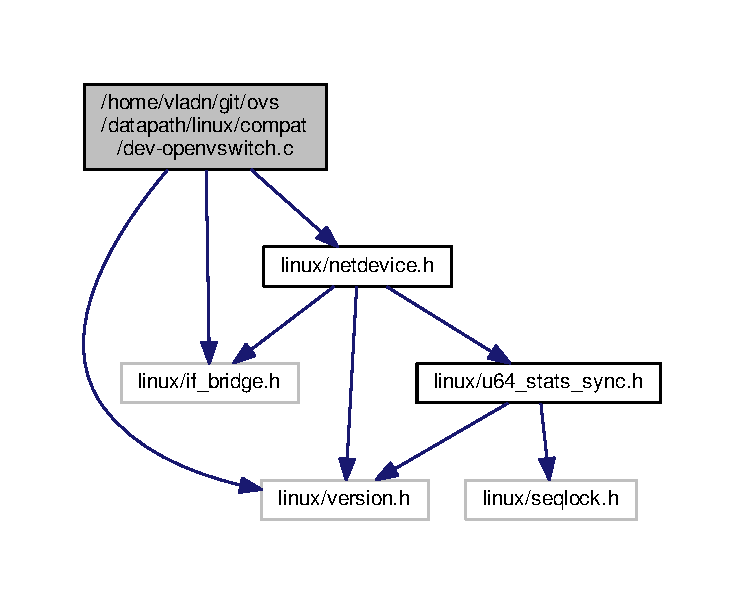
\includegraphics[width=350pt]{compat_2dev-openvswitch_8c__incl}
\end{center}
\end{figure}
\subsection*{Functions}
\begin{DoxyCompactItemize}
\item 
void \hyperlink{compat_2dev-openvswitch_8c_a0f00a19794caf20381b409fb00a77313}{dev\+\_\+disable\+\_\+lro} (struct net\+\_\+device $\ast$dev)
\end{DoxyCompactItemize}


\subsection{Function Documentation}
\hypertarget{compat_2dev-openvswitch_8c_a0f00a19794caf20381b409fb00a77313}{}\index{compat/dev-\/openvswitch.\+c@{compat/dev-\/openvswitch.\+c}!dev\+\_\+disable\+\_\+lro@{dev\+\_\+disable\+\_\+lro}}
\index{dev\+\_\+disable\+\_\+lro@{dev\+\_\+disable\+\_\+lro}!compat/dev-\/openvswitch.\+c@{compat/dev-\/openvswitch.\+c}}
\subsubsection[{dev\+\_\+disable\+\_\+lro}]{\setlength{\rightskip}{0pt plus 5cm}void dev\+\_\+disable\+\_\+lro (
\begin{DoxyParamCaption}
\item[{struct net\+\_\+device $\ast$}]{dev}
\end{DoxyParamCaption}
)}\label{compat_2dev-openvswitch_8c_a0f00a19794caf20381b409fb00a77313}

\begin{DoxyCode}
31 \{ \}
\end{DoxyCode}

\hypertarget{dev-openvswitch_8c}{}\section{/home/vladn/git/ovs/datapath/linux/dev-\/openvswitch.c File Reference}
\label{dev-openvswitch_8c}\index{/home/vladn/git/ovs/datapath/linux/dev-\/openvswitch.\+c@{/home/vladn/git/ovs/datapath/linux/dev-\/openvswitch.\+c}}
{\ttfamily \#include $<$linux/if\+\_\+bridge.\+h$>$}\\*
{\ttfamily \#include $<$linux/netdevice.\+h$>$}\\*
{\ttfamily \#include $<$linux/version.\+h$>$}\\*
Include dependency graph for dev-\/openvswitch.c\+:
\nopagebreak
\begin{figure}[H]
\begin{center}
\leavevmode
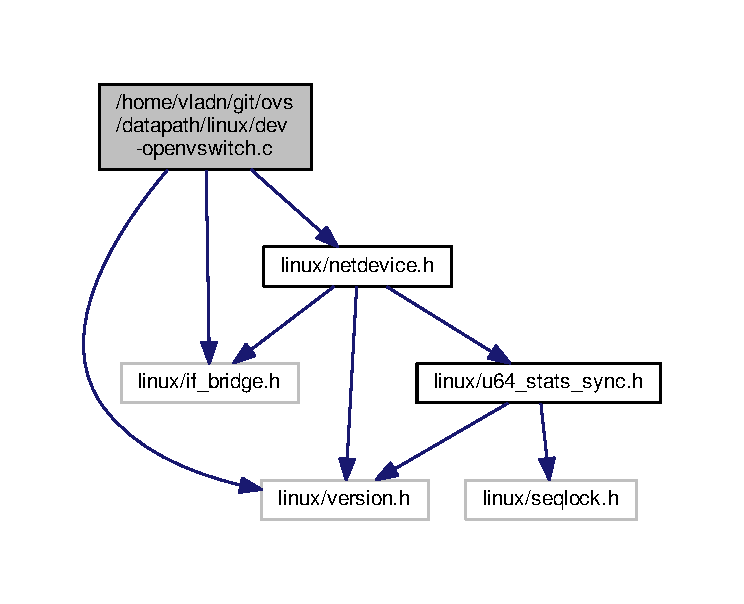
\includegraphics[width=350pt]{dev-openvswitch_8c__incl}
\end{center}
\end{figure}
\subsection*{Functions}
\begin{DoxyCompactItemize}
\item 
void \hyperlink{dev-openvswitch_8c_a0f00a19794caf20381b409fb00a77313}{dev\+\_\+disable\+\_\+lro} (struct net\+\_\+device $\ast$dev)
\end{DoxyCompactItemize}


\subsection{Function Documentation}
\hypertarget{dev-openvswitch_8c_a0f00a19794caf20381b409fb00a77313}{}\index{dev-\/openvswitch.\+c@{dev-\/openvswitch.\+c}!dev\+\_\+disable\+\_\+lro@{dev\+\_\+disable\+\_\+lro}}
\index{dev\+\_\+disable\+\_\+lro@{dev\+\_\+disable\+\_\+lro}!dev-\/openvswitch.\+c@{dev-\/openvswitch.\+c}}
\subsubsection[{dev\+\_\+disable\+\_\+lro}]{\setlength{\rightskip}{0pt plus 5cm}void dev\+\_\+disable\+\_\+lro (
\begin{DoxyParamCaption}
\item[{struct net\+\_\+device $\ast$}]{dev}
\end{DoxyParamCaption}
)}\label{dev-openvswitch_8c_a0f00a19794caf20381b409fb00a77313}

\begin{DoxyCode}
31 \{ \}
\end{DoxyCode}

\hypertarget{compat_2exthdrs__core_8c}{}\section{/home/vladn/git/ovs/datapath/linux/compat/exthdrs\+\_\+core.c File Reference}
\label{compat_2exthdrs__core_8c}\index{/home/vladn/git/ovs/datapath/linux/compat/exthdrs\+\_\+core.\+c@{/home/vladn/git/ovs/datapath/linux/compat/exthdrs\+\_\+core.\+c}}
{\ttfamily \#include $<$linux/ipv6.\+h$>$}\\*
{\ttfamily \#include $<$linux/version.\+h$>$}\\*
{\ttfamily \#include $<$net/ipv6.\+h$>$}\\*
Include dependency graph for exthdrs\+\_\+core.\+c\+:
\nopagebreak
\begin{figure}[H]
\begin{center}
\leavevmode
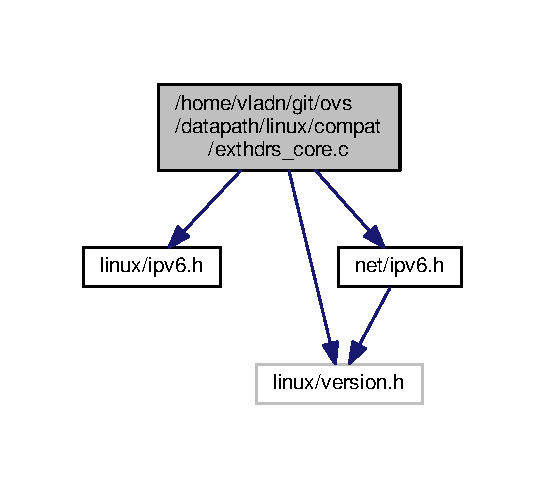
\includegraphics[width=262pt]{compat_2exthdrs__core_8c__incl}
\end{center}
\end{figure}
\subsection*{Functions}
\begin{DoxyCompactItemize}
\item 
int \hyperlink{compat_2exthdrs__core_8c_a9dac58bb4c09331136a03725c3fd8d71}{rpl\+\_\+ipv6\+\_\+find\+\_\+hdr} (const struct sk\+\_\+buff $\ast$skb, unsigned int $\ast$offset, int \hyperlink{flow_8h_a5fb304013ae6aaeaee9d7fdcfd343292}{target}, unsigned short $\ast$fragoff, int $\ast$\hyperlink{flow_8h_af4f7a53f6b2df72c34ca881f2714ac91}{flags})
\item 
\hyperlink{compat_2exthdrs__core_8c_a82be3f9e87720a53d09213c91ccd13b2}{E\+X\+P\+O\+R\+T\+\_\+\+S\+Y\+M\+B\+O\+L\+\_\+\+G\+P\+L} (\hyperlink{exthdrs__core_8c_a9dac58bb4c09331136a03725c3fd8d71}{rpl\+\_\+ipv6\+\_\+find\+\_\+hdr})
\end{DoxyCompactItemize}


\subsection{Function Documentation}
\hypertarget{compat_2exthdrs__core_8c_a82be3f9e87720a53d09213c91ccd13b2}{}\index{compat/exthdrs\+\_\+core.\+c@{compat/exthdrs\+\_\+core.\+c}!E\+X\+P\+O\+R\+T\+\_\+\+S\+Y\+M\+B\+O\+L\+\_\+\+G\+P\+L@{E\+X\+P\+O\+R\+T\+\_\+\+S\+Y\+M\+B\+O\+L\+\_\+\+G\+P\+L}}
\index{E\+X\+P\+O\+R\+T\+\_\+\+S\+Y\+M\+B\+O\+L\+\_\+\+G\+P\+L@{E\+X\+P\+O\+R\+T\+\_\+\+S\+Y\+M\+B\+O\+L\+\_\+\+G\+P\+L}!compat/exthdrs\+\_\+core.\+c@{compat/exthdrs\+\_\+core.\+c}}
\subsubsection[{E\+X\+P\+O\+R\+T\+\_\+\+S\+Y\+M\+B\+O\+L\+\_\+\+G\+P\+L}]{\setlength{\rightskip}{0pt plus 5cm}E\+X\+P\+O\+R\+T\+\_\+\+S\+Y\+M\+B\+O\+L\+\_\+\+G\+P\+L (
\begin{DoxyParamCaption}
\item[{{\bf rpl\+\_\+ipv6\+\_\+find\+\_\+hdr}}]{}
\end{DoxyParamCaption}
)}\label{compat_2exthdrs__core_8c_a82be3f9e87720a53d09213c91ccd13b2}
\hypertarget{compat_2exthdrs__core_8c_a9dac58bb4c09331136a03725c3fd8d71}{}\index{compat/exthdrs\+\_\+core.\+c@{compat/exthdrs\+\_\+core.\+c}!rpl\+\_\+ipv6\+\_\+find\+\_\+hdr@{rpl\+\_\+ipv6\+\_\+find\+\_\+hdr}}
\index{rpl\+\_\+ipv6\+\_\+find\+\_\+hdr@{rpl\+\_\+ipv6\+\_\+find\+\_\+hdr}!compat/exthdrs\+\_\+core.\+c@{compat/exthdrs\+\_\+core.\+c}}
\subsubsection[{rpl\+\_\+ipv6\+\_\+find\+\_\+hdr}]{\setlength{\rightskip}{0pt plus 5cm}int rpl\+\_\+ipv6\+\_\+find\+\_\+hdr (
\begin{DoxyParamCaption}
\item[{const struct sk\+\_\+buff $\ast$}]{skb, }
\item[{unsigned int $\ast$}]{offset, }
\item[{int}]{target, }
\item[{unsigned short $\ast$}]{fragoff, }
\item[{int $\ast$}]{flags}
\end{DoxyParamCaption}
)}\label{compat_2exthdrs__core_8c_a9dac58bb4c09331136a03725c3fd8d71}

\begin{DoxyCode}
80 \{
81     \textcolor{keywordtype}{unsigned} \textcolor{keywordtype}{int} start = \hyperlink{skbuff_8h_aabe75b44039b11c1b7c6e2f246e7146e}{skb\_network\_offset}(skb) + \textcolor{keyword}{sizeof}(\textcolor{keyword}{struct }ipv6hdr);
82     u8 nexthdr = \hyperlink{linux_2ipv6_8h_ab31aa2f5ade9dadb3cede168a0761bb3}{ipv6\_hdr}(skb)->nexthdr;
83     \textcolor{keywordtype}{unsigned} \textcolor{keywordtype}{int} len;
84     \textcolor{keywordtype}{bool} found;
85 
86     \textcolor{keywordflow}{if} (fragoff)
87         *fragoff = 0;
88 
89     \textcolor{keywordflow}{if} (*offset) \{
90         \textcolor{keyword}{struct }ipv6hdr \_ip6, *ip6;
91 
92         ip6 = skb\_header\_pointer(skb, *offset, \textcolor{keyword}{sizeof}(\_ip6), &\_ip6);
93         \textcolor{keywordflow}{if} (!ip6 || (ip6->version != 6)) \{
94             printk(KERN\_ERR \textcolor{stringliteral}{"IPv6 header not found\(\backslash\)n"});
95             \textcolor{keywordflow}{return} -EBADMSG;
96         \}
97         start = *offset + \textcolor{keyword}{sizeof}(\textcolor{keyword}{struct }ipv6hdr);
98         nexthdr = ip6->nexthdr;
99     \}
100     len = skb->len - start;
101 
102     \textcolor{keywordflow}{do} \{
103         \textcolor{keyword}{struct }ipv6\_opt\_hdr \_hdr, *hp;
104         \textcolor{keywordtype}{unsigned} \textcolor{keywordtype}{int} hdrlen;
105         found = (nexthdr == \hyperlink{flow_8h_a5fb304013ae6aaeaee9d7fdcfd343292}{target});
106 
107         \textcolor{keywordflow}{if} ((!ipv6\_ext\_hdr(nexthdr)) || nexthdr == NEXTHDR\_NONE) \{
108             \textcolor{keywordflow}{if} (\hyperlink{flow_8h_a5fb304013ae6aaeaee9d7fdcfd343292}{target} < 0 || found)
109                 \textcolor{keywordflow}{break};
110             \textcolor{keywordflow}{return} -ENOENT;
111         \}
112 
113         hp = skb\_header\_pointer(skb, start, \textcolor{keyword}{sizeof}(\_hdr), &\_hdr);
114         \textcolor{keywordflow}{if} (hp == NULL)
115             \textcolor{keywordflow}{return} -EBADMSG;
116 
117         \textcolor{keywordflow}{if} (nexthdr == NEXTHDR\_ROUTING) \{
118             \textcolor{keyword}{struct }ipv6\_rt\_hdr \_rh, *rh;
119 
120             rh = skb\_header\_pointer(skb, start, \textcolor{keyword}{sizeof}(\_rh),
121                         &\_rh);
122             \textcolor{keywordflow}{if} (rh == NULL)
123                 \textcolor{keywordflow}{return} -EBADMSG;
124 
125             \textcolor{keywordflow}{if} (\hyperlink{flow_8h_af4f7a53f6b2df72c34ca881f2714ac91}{flags} && (*\hyperlink{flow_8h_af4f7a53f6b2df72c34ca881f2714ac91}{flags} & \hyperlink{net_2ipv6_8h_ab48899087cc647f0f791ed0c459adc53ae061c21caac2cca8aed854ed6fb1fa61}{IP6\_FH\_F\_SKIP\_RH}) &&
126                 rh->segments\_left == 0)
127                 found = \textcolor{keyword}{false};
128         \}
129 
130         \textcolor{keywordflow}{if} (nexthdr == NEXTHDR\_FRAGMENT) \{
131             \textcolor{keywordtype}{unsigned} \textcolor{keywordtype}{short} \_frag\_off;
132             \_\_be16 *fp;
133 
134             \textcolor{keywordflow}{if} (\hyperlink{flow_8h_af4f7a53f6b2df72c34ca881f2714ac91}{flags}) \textcolor{comment}{/* Indicate that this is a fragment */}
135                 *\hyperlink{flow_8h_af4f7a53f6b2df72c34ca881f2714ac91}{flags} |= \hyperlink{net_2ipv6_8h_ab48899087cc647f0f791ed0c459adc53a896e48b555d0207d316edb0043e46882}{IP6\_FH\_F\_FRAG};
136             fp = skb\_header\_pointer(skb,
137                         start+offsetof(\textcolor{keyword}{struct} frag\_hdr,
138                                    frag\_off),
139                         \textcolor{keyword}{sizeof}(\_frag\_off),
140                         &\_frag\_off);
141             \textcolor{keywordflow}{if} (fp == NULL)
142                 \textcolor{keywordflow}{return} -EBADMSG;
143 
144             \_frag\_off = ntohs(*fp) & ~0x7;
145             \textcolor{keywordflow}{if} (\_frag\_off) \{
146                 \textcolor{keywordflow}{if} (\hyperlink{flow_8h_a5fb304013ae6aaeaee9d7fdcfd343292}{target} < 0 &&
147                     ((!ipv6\_ext\_hdr(hp->nexthdr)) ||
148                      hp->nexthdr == NEXTHDR\_NONE)) \{
149                     \textcolor{keywordflow}{if} (fragoff)
150                         *fragoff = \_frag\_off;
151                     \textcolor{keywordflow}{return} hp->nexthdr;
152                 \}
153                 \textcolor{keywordflow}{return} -ENOENT;
154             \}
155             hdrlen = 8;
156         \} \textcolor{keywordflow}{else} \textcolor{keywordflow}{if} (nexthdr == NEXTHDR\_AUTH) \{
157             \textcolor{keywordflow}{if} (\hyperlink{flow_8h_af4f7a53f6b2df72c34ca881f2714ac91}{flags} && (*\hyperlink{flow_8h_af4f7a53f6b2df72c34ca881f2714ac91}{flags} & \hyperlink{net_2ipv6_8h_ab48899087cc647f0f791ed0c459adc53a39098fe882a26a0617bd71ad4d06c85a}{IP6\_FH\_F\_AUTH}) && (
      \hyperlink{flow_8h_a5fb304013ae6aaeaee9d7fdcfd343292}{target} < 0))
158                 \textcolor{keywordflow}{break};
159             hdrlen = (hp->hdrlen + 2) << 2;
160         \} \textcolor{keywordflow}{else}
161             hdrlen = ipv6\_optlen(hp);
162 
163         \textcolor{keywordflow}{if} (!found) \{
164             nexthdr = hp->nexthdr;
165             len -= hdrlen;
166             start += hdrlen;
167         \}
168     \} \textcolor{keywordflow}{while} (!found);
169 
170     *offset = start;
171     \textcolor{keywordflow}{return} nexthdr;
172 \}
\end{DoxyCode}

\hypertarget{exthdrs__core_8c}{}\section{/home/vladn/git/ovs/datapath/linux/exthdrs\+\_\+core.c File Reference}
\label{exthdrs__core_8c}\index{/home/vladn/git/ovs/datapath/linux/exthdrs\+\_\+core.\+c@{/home/vladn/git/ovs/datapath/linux/exthdrs\+\_\+core.\+c}}
{\ttfamily \#include $<$linux/ipv6.\+h$>$}\\*
{\ttfamily \#include $<$linux/version.\+h$>$}\\*
{\ttfamily \#include $<$net/ipv6.\+h$>$}\\*
Include dependency graph for exthdrs\+\_\+core.\+c\+:
\nopagebreak
\begin{figure}[H]
\begin{center}
\leavevmode
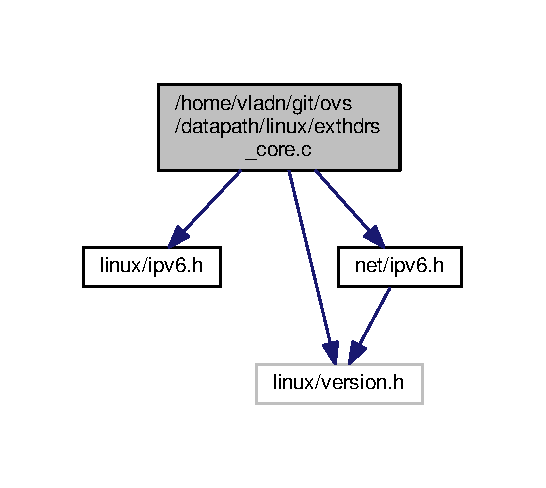
\includegraphics[width=262pt]{exthdrs__core_8c__incl}
\end{center}
\end{figure}
\subsection*{Functions}
\begin{DoxyCompactItemize}
\item 
int \hyperlink{exthdrs__core_8c_a9dac58bb4c09331136a03725c3fd8d71}{rpl\+\_\+ipv6\+\_\+find\+\_\+hdr} (const struct sk\+\_\+buff $\ast$skb, unsigned int $\ast$offset, int \hyperlink{flow_8h_a5fb304013ae6aaeaee9d7fdcfd343292}{target}, unsigned short $\ast$fragoff, int $\ast$\hyperlink{flow_8h_af4f7a53f6b2df72c34ca881f2714ac91}{flags})
\item 
\hyperlink{exthdrs__core_8c_a82be3f9e87720a53d09213c91ccd13b2}{E\+X\+P\+O\+R\+T\+\_\+\+S\+Y\+M\+B\+O\+L\+\_\+\+G\+P\+L} (\hyperlink{exthdrs__core_8c_a9dac58bb4c09331136a03725c3fd8d71}{rpl\+\_\+ipv6\+\_\+find\+\_\+hdr})
\end{DoxyCompactItemize}


\subsection{Function Documentation}
\hypertarget{exthdrs__core_8c_a82be3f9e87720a53d09213c91ccd13b2}{}\index{exthdrs\+\_\+core.\+c@{exthdrs\+\_\+core.\+c}!E\+X\+P\+O\+R\+T\+\_\+\+S\+Y\+M\+B\+O\+L\+\_\+\+G\+P\+L@{E\+X\+P\+O\+R\+T\+\_\+\+S\+Y\+M\+B\+O\+L\+\_\+\+G\+P\+L}}
\index{E\+X\+P\+O\+R\+T\+\_\+\+S\+Y\+M\+B\+O\+L\+\_\+\+G\+P\+L@{E\+X\+P\+O\+R\+T\+\_\+\+S\+Y\+M\+B\+O\+L\+\_\+\+G\+P\+L}!exthdrs\+\_\+core.\+c@{exthdrs\+\_\+core.\+c}}
\subsubsection[{E\+X\+P\+O\+R\+T\+\_\+\+S\+Y\+M\+B\+O\+L\+\_\+\+G\+P\+L}]{\setlength{\rightskip}{0pt plus 5cm}E\+X\+P\+O\+R\+T\+\_\+\+S\+Y\+M\+B\+O\+L\+\_\+\+G\+P\+L (
\begin{DoxyParamCaption}
\item[{{\bf rpl\+\_\+ipv6\+\_\+find\+\_\+hdr}}]{}
\end{DoxyParamCaption}
)}\label{exthdrs__core_8c_a82be3f9e87720a53d09213c91ccd13b2}
\hypertarget{exthdrs__core_8c_a9dac58bb4c09331136a03725c3fd8d71}{}\index{exthdrs\+\_\+core.\+c@{exthdrs\+\_\+core.\+c}!rpl\+\_\+ipv6\+\_\+find\+\_\+hdr@{rpl\+\_\+ipv6\+\_\+find\+\_\+hdr}}
\index{rpl\+\_\+ipv6\+\_\+find\+\_\+hdr@{rpl\+\_\+ipv6\+\_\+find\+\_\+hdr}!exthdrs\+\_\+core.\+c@{exthdrs\+\_\+core.\+c}}
\subsubsection[{rpl\+\_\+ipv6\+\_\+find\+\_\+hdr}]{\setlength{\rightskip}{0pt plus 5cm}int rpl\+\_\+ipv6\+\_\+find\+\_\+hdr (
\begin{DoxyParamCaption}
\item[{const struct sk\+\_\+buff $\ast$}]{skb, }
\item[{unsigned int $\ast$}]{offset, }
\item[{int}]{target, }
\item[{unsigned short $\ast$}]{fragoff, }
\item[{int $\ast$}]{flags}
\end{DoxyParamCaption}
)}\label{exthdrs__core_8c_a9dac58bb4c09331136a03725c3fd8d71}

\begin{DoxyCode}
80 \{
81     \textcolor{keywordtype}{unsigned} \textcolor{keywordtype}{int} start = \hyperlink{skbuff_8h_aabe75b44039b11c1b7c6e2f246e7146e}{skb\_network\_offset}(skb) + \textcolor{keyword}{sizeof}(\textcolor{keyword}{struct }ipv6hdr);
82     u8 nexthdr = \hyperlink{linux_2ipv6_8h_ab31aa2f5ade9dadb3cede168a0761bb3}{ipv6\_hdr}(skb)->nexthdr;
83     \textcolor{keywordtype}{unsigned} \textcolor{keywordtype}{int} len;
84     \textcolor{keywordtype}{bool} found;
85 
86     \textcolor{keywordflow}{if} (fragoff)
87         *fragoff = 0;
88 
89     \textcolor{keywordflow}{if} (*offset) \{
90         \textcolor{keyword}{struct }ipv6hdr \_ip6, *ip6;
91 
92         ip6 = skb\_header\_pointer(skb, *offset, \textcolor{keyword}{sizeof}(\_ip6), &\_ip6);
93         \textcolor{keywordflow}{if} (!ip6 || (ip6->version != 6)) \{
94             printk(KERN\_ERR \textcolor{stringliteral}{"IPv6 header not found\(\backslash\)n"});
95             \textcolor{keywordflow}{return} -EBADMSG;
96         \}
97         start = *offset + \textcolor{keyword}{sizeof}(\textcolor{keyword}{struct }ipv6hdr);
98         nexthdr = ip6->nexthdr;
99     \}
100     len = skb->len - start;
101 
102     \textcolor{keywordflow}{do} \{
103         \textcolor{keyword}{struct }ipv6\_opt\_hdr \_hdr, *hp;
104         \textcolor{keywordtype}{unsigned} \textcolor{keywordtype}{int} hdrlen;
105         found = (nexthdr == \hyperlink{flow_8h_a5fb304013ae6aaeaee9d7fdcfd343292}{target});
106 
107         \textcolor{keywordflow}{if} ((!ipv6\_ext\_hdr(nexthdr)) || nexthdr == NEXTHDR\_NONE) \{
108             \textcolor{keywordflow}{if} (\hyperlink{flow_8h_a5fb304013ae6aaeaee9d7fdcfd343292}{target} < 0 || found)
109                 \textcolor{keywordflow}{break};
110             \textcolor{keywordflow}{return} -ENOENT;
111         \}
112 
113         hp = skb\_header\_pointer(skb, start, \textcolor{keyword}{sizeof}(\_hdr), &\_hdr);
114         \textcolor{keywordflow}{if} (hp == NULL)
115             \textcolor{keywordflow}{return} -EBADMSG;
116 
117         \textcolor{keywordflow}{if} (nexthdr == NEXTHDR\_ROUTING) \{
118             \textcolor{keyword}{struct }ipv6\_rt\_hdr \_rh, *rh;
119 
120             rh = skb\_header\_pointer(skb, start, \textcolor{keyword}{sizeof}(\_rh),
121                         &\_rh);
122             \textcolor{keywordflow}{if} (rh == NULL)
123                 \textcolor{keywordflow}{return} -EBADMSG;
124 
125             \textcolor{keywordflow}{if} (\hyperlink{flow_8h_af4f7a53f6b2df72c34ca881f2714ac91}{flags} && (*\hyperlink{flow_8h_af4f7a53f6b2df72c34ca881f2714ac91}{flags} & \hyperlink{net_2ipv6_8h_ab48899087cc647f0f791ed0c459adc53ae061c21caac2cca8aed854ed6fb1fa61}{IP6\_FH\_F\_SKIP\_RH}) &&
126                 rh->segments\_left == 0)
127                 found = \textcolor{keyword}{false};
128         \}
129 
130         \textcolor{keywordflow}{if} (nexthdr == NEXTHDR\_FRAGMENT) \{
131             \textcolor{keywordtype}{unsigned} \textcolor{keywordtype}{short} \_frag\_off;
132             \_\_be16 *fp;
133 
134             \textcolor{keywordflow}{if} (\hyperlink{flow_8h_af4f7a53f6b2df72c34ca881f2714ac91}{flags}) \textcolor{comment}{/* Indicate that this is a fragment */}
135                 *\hyperlink{flow_8h_af4f7a53f6b2df72c34ca881f2714ac91}{flags} |= \hyperlink{net_2ipv6_8h_ab48899087cc647f0f791ed0c459adc53a896e48b555d0207d316edb0043e46882}{IP6\_FH\_F\_FRAG};
136             fp = skb\_header\_pointer(skb,
137                         start+offsetof(\textcolor{keyword}{struct} frag\_hdr,
138                                    frag\_off),
139                         \textcolor{keyword}{sizeof}(\_frag\_off),
140                         &\_frag\_off);
141             \textcolor{keywordflow}{if} (fp == NULL)
142                 \textcolor{keywordflow}{return} -EBADMSG;
143 
144             \_frag\_off = ntohs(*fp) & ~0x7;
145             \textcolor{keywordflow}{if} (\_frag\_off) \{
146                 \textcolor{keywordflow}{if} (\hyperlink{flow_8h_a5fb304013ae6aaeaee9d7fdcfd343292}{target} < 0 &&
147                     ((!ipv6\_ext\_hdr(hp->nexthdr)) ||
148                      hp->nexthdr == NEXTHDR\_NONE)) \{
149                     \textcolor{keywordflow}{if} (fragoff)
150                         *fragoff = \_frag\_off;
151                     \textcolor{keywordflow}{return} hp->nexthdr;
152                 \}
153                 \textcolor{keywordflow}{return} -ENOENT;
154             \}
155             hdrlen = 8;
156         \} \textcolor{keywordflow}{else} \textcolor{keywordflow}{if} (nexthdr == NEXTHDR\_AUTH) \{
157             \textcolor{keywordflow}{if} (\hyperlink{flow_8h_af4f7a53f6b2df72c34ca881f2714ac91}{flags} && (*\hyperlink{flow_8h_af4f7a53f6b2df72c34ca881f2714ac91}{flags} & \hyperlink{net_2ipv6_8h_ab48899087cc647f0f791ed0c459adc53a39098fe882a26a0617bd71ad4d06c85a}{IP6\_FH\_F\_AUTH}) && (
      \hyperlink{flow_8h_a5fb304013ae6aaeaee9d7fdcfd343292}{target} < 0))
158                 \textcolor{keywordflow}{break};
159             hdrlen = (hp->hdrlen + 2) << 2;
160         \} \textcolor{keywordflow}{else}
161             hdrlen = ipv6\_optlen(hp);
162 
163         \textcolor{keywordflow}{if} (!found) \{
164             nexthdr = hp->nexthdr;
165             len -= hdrlen;
166             start += hdrlen;
167         \}
168     \} \textcolor{keywordflow}{while} (!found);
169 
170     *offset = start;
171     \textcolor{keywordflow}{return} nexthdr;
172 \}
\end{DoxyCode}

\hypertarget{compat_2flex__array_8c}{}\section{/home/vladn/git/ovs/datapath/linux/compat/flex\+\_\+array.c File Reference}
\label{compat_2flex__array_8c}\index{/home/vladn/git/ovs/datapath/linux/compat/flex\+\_\+array.\+c@{/home/vladn/git/ovs/datapath/linux/compat/flex\+\_\+array.\+c}}
{\ttfamily \#include $<$linux/version.\+h$>$}\\*
Include dependency graph for flex\+\_\+array.\+c\+:
\nopagebreak
\begin{figure}[H]
\begin{center}
\leavevmode
\includegraphics[width=196pt]{compat_2flex__array_8c__incl}
\end{center}
\end{figure}

\hypertarget{flex__array_8c}{}\section{/home/vladn/git/ovs/datapath/linux/flex\+\_\+array.c File Reference}
\label{flex__array_8c}\index{/home/vladn/git/ovs/datapath/linux/flex\+\_\+array.\+c@{/home/vladn/git/ovs/datapath/linux/flex\+\_\+array.\+c}}
{\ttfamily \#include $<$linux/version.\+h$>$}\\*
Include dependency graph for flex\+\_\+array.\+c\+:
\nopagebreak
\begin{figure}[H]
\begin{center}
\leavevmode
\includegraphics[width=182pt]{flex__array_8c__incl}
\end{center}
\end{figure}

\hypertarget{compat_2flow__dissector_8c}{}\section{/home/vladn/git/ovs/datapath/linux/compat/flow\+\_\+dissector.c File Reference}
\label{compat_2flow__dissector_8c}\index{/home/vladn/git/ovs/datapath/linux/compat/flow\+\_\+dissector.\+c@{/home/vladn/git/ovs/datapath/linux/compat/flow\+\_\+dissector.\+c}}
{\ttfamily \#include $<$linux/version.\+h$>$}\\*
Include dependency graph for flow\+\_\+dissector.\+c\+:
\nopagebreak
\begin{figure}[H]
\begin{center}
\leavevmode
\includegraphics[width=196pt]{compat_2flow__dissector_8c__incl}
\end{center}
\end{figure}

\hypertarget{flow__dissector_8c}{}\section{/home/vladn/git/ovs/datapath/linux/flow\+\_\+dissector.c File Reference}
\label{flow__dissector_8c}\index{/home/vladn/git/ovs/datapath/linux/flow\+\_\+dissector.\+c@{/home/vladn/git/ovs/datapath/linux/flow\+\_\+dissector.\+c}}
{\ttfamily \#include $<$linux/version.\+h$>$}\\*
Include dependency graph for flow\+\_\+dissector.\+c\+:
\nopagebreak
\begin{figure}[H]
\begin{center}
\leavevmode
\includegraphics[width=182pt]{flow__dissector_8c__incl}
\end{center}
\end{figure}

\hypertarget{compat_2genetlink-openvswitch_8c}{}\section{/home/vladn/git/ovs/datapath/linux/compat/genetlink-\/openvswitch.c File Reference}
\label{compat_2genetlink-openvswitch_8c}\index{/home/vladn/git/ovs/datapath/linux/compat/genetlink-\/openvswitch.\+c@{/home/vladn/git/ovs/datapath/linux/compat/genetlink-\/openvswitch.\+c}}
{\ttfamily \#include $<$net/genetlink.\+h$>$}\\*
{\ttfamily \#include $<$linux/version.\+h$>$}\\*
Include dependency graph for genetlink-\/openvswitch.c\+:
\nopagebreak
\begin{figure}[H]
\begin{center}
\leavevmode
\includegraphics[width=350pt]{compat_2genetlink-openvswitch_8c__incl}
\end{center}
\end{figure}
\subsection*{Functions}
\begin{DoxyCompactItemize}
\item 
void \hyperlink{compat_2genetlink-openvswitch_8c_abcd68fa42d07fafbbb4e263dd8baca6c}{rpl\+\_\+genl\+\_\+notify} (struct \hyperlink{structrpl__genl__family}{rpl\+\_\+genl\+\_\+family} $\ast$family, struct sk\+\_\+buff $\ast$skb, struct net $\ast$net, u32 portid, u32 group, struct nlmsghdr $\ast$nlh, gfp\+\_\+t \hyperlink{flow_8h_af4f7a53f6b2df72c34ca881f2714ac91}{flags})
\item 
\hyperlink{compat_2genetlink-openvswitch_8c_a62e3dfffe9008f7d63bc6128f61b342a}{E\+X\+P\+O\+R\+T\+\_\+\+S\+Y\+M\+B\+O\+L\+\_\+\+G\+P\+L} (\hyperlink{genetlink-openvswitch_8c_abcd68fa42d07fafbbb4e263dd8baca6c}{rpl\+\_\+genl\+\_\+notify})
\item 
int \hyperlink{compat_2genetlink-openvswitch_8c_a2803a86a5f44e4c055773b4907a4950a}{rpl\+\_\+\+\_\+\+\_\+genl\+\_\+register\+\_\+family} (struct \hyperlink{structrpl__genl__family}{rpl\+\_\+genl\+\_\+family} $\ast$f)
\item 
\hyperlink{compat_2genetlink-openvswitch_8c_a19734b7486a5c6c341e8ffe9eaae41fa}{E\+X\+P\+O\+R\+T\+\_\+\+S\+Y\+M\+B\+O\+L\+\_\+\+G\+P\+L} (\hyperlink{genetlink-openvswitch_8c_a2803a86a5f44e4c055773b4907a4950a}{rpl\+\_\+\+\_\+\+\_\+genl\+\_\+register\+\_\+family})
\end{DoxyCompactItemize}


\subsection{Function Documentation}
\hypertarget{compat_2genetlink-openvswitch_8c_a62e3dfffe9008f7d63bc6128f61b342a}{}\index{compat/genetlink-\/openvswitch.\+c@{compat/genetlink-\/openvswitch.\+c}!E\+X\+P\+O\+R\+T\+\_\+\+S\+Y\+M\+B\+O\+L\+\_\+\+G\+P\+L@{E\+X\+P\+O\+R\+T\+\_\+\+S\+Y\+M\+B\+O\+L\+\_\+\+G\+P\+L}}
\index{E\+X\+P\+O\+R\+T\+\_\+\+S\+Y\+M\+B\+O\+L\+\_\+\+G\+P\+L@{E\+X\+P\+O\+R\+T\+\_\+\+S\+Y\+M\+B\+O\+L\+\_\+\+G\+P\+L}!compat/genetlink-\/openvswitch.\+c@{compat/genetlink-\/openvswitch.\+c}}
\subsubsection[{E\+X\+P\+O\+R\+T\+\_\+\+S\+Y\+M\+B\+O\+L\+\_\+\+G\+P\+L}]{\setlength{\rightskip}{0pt plus 5cm}E\+X\+P\+O\+R\+T\+\_\+\+S\+Y\+M\+B\+O\+L\+\_\+\+G\+P\+L (
\begin{DoxyParamCaption}
\item[{{\bf rpl\+\_\+genl\+\_\+notify}}]{}
\end{DoxyParamCaption}
)}\label{compat_2genetlink-openvswitch_8c_a62e3dfffe9008f7d63bc6128f61b342a}
\hypertarget{compat_2genetlink-openvswitch_8c_a19734b7486a5c6c341e8ffe9eaae41fa}{}\index{compat/genetlink-\/openvswitch.\+c@{compat/genetlink-\/openvswitch.\+c}!E\+X\+P\+O\+R\+T\+\_\+\+S\+Y\+M\+B\+O\+L\+\_\+\+G\+P\+L@{E\+X\+P\+O\+R\+T\+\_\+\+S\+Y\+M\+B\+O\+L\+\_\+\+G\+P\+L}}
\index{E\+X\+P\+O\+R\+T\+\_\+\+S\+Y\+M\+B\+O\+L\+\_\+\+G\+P\+L@{E\+X\+P\+O\+R\+T\+\_\+\+S\+Y\+M\+B\+O\+L\+\_\+\+G\+P\+L}!compat/genetlink-\/openvswitch.\+c@{compat/genetlink-\/openvswitch.\+c}}
\subsubsection[{E\+X\+P\+O\+R\+T\+\_\+\+S\+Y\+M\+B\+O\+L\+\_\+\+G\+P\+L}]{\setlength{\rightskip}{0pt plus 5cm}E\+X\+P\+O\+R\+T\+\_\+\+S\+Y\+M\+B\+O\+L\+\_\+\+G\+P\+L (
\begin{DoxyParamCaption}
\item[{{\bf rpl\+\_\+\+\_\+\+\_\+genl\+\_\+register\+\_\+family}}]{}
\end{DoxyParamCaption}
)}\label{compat_2genetlink-openvswitch_8c_a19734b7486a5c6c341e8ffe9eaae41fa}
\hypertarget{compat_2genetlink-openvswitch_8c_a2803a86a5f44e4c055773b4907a4950a}{}\index{compat/genetlink-\/openvswitch.\+c@{compat/genetlink-\/openvswitch.\+c}!rpl\+\_\+\+\_\+\+\_\+genl\+\_\+register\+\_\+family@{rpl\+\_\+\+\_\+\+\_\+genl\+\_\+register\+\_\+family}}
\index{rpl\+\_\+\+\_\+\+\_\+genl\+\_\+register\+\_\+family@{rpl\+\_\+\+\_\+\+\_\+genl\+\_\+register\+\_\+family}!compat/genetlink-\/openvswitch.\+c@{compat/genetlink-\/openvswitch.\+c}}
\subsubsection[{rpl\+\_\+\+\_\+\+\_\+genl\+\_\+register\+\_\+family}]{\setlength{\rightskip}{0pt plus 5cm}int rpl\+\_\+\+\_\+\+\_\+genl\+\_\+register\+\_\+family (
\begin{DoxyParamCaption}
\item[{struct {\bf rpl\+\_\+genl\+\_\+family} $\ast$}]{f}
\end{DoxyParamCaption}
)}\label{compat_2genetlink-openvswitch_8c_a2803a86a5f44e4c055773b4907a4950a}

\begin{DoxyCode}
27 \{
28     \textcolor{keywordtype}{int} err;
29 
30     f->\hyperlink{structrpl__genl__family_a6da3fbe86360d91cce207287b2de165d}{compat\_family}.id = f->\hyperlink{structrpl__genl__family_a34a498924fba8a8da9d410d545cfeee2}{id};
31     f->\hyperlink{structrpl__genl__family_a6da3fbe86360d91cce207287b2de165d}{compat\_family}.hdrsize = f->\hyperlink{structrpl__genl__family_a9a291012510fda23c4d3bf64859e5de0}{hdrsize};
32     strncpy(f->\hyperlink{structrpl__genl__family_a6da3fbe86360d91cce207287b2de165d}{compat\_family}.name, f->\hyperlink{structrpl__genl__family_a0ee3a650097beb5d2e4a4deb301cb479}{name}, GENL\_NAMSIZ);
33     f->\hyperlink{structrpl__genl__family_a6da3fbe86360d91cce207287b2de165d}{compat\_family}.version = f->\hyperlink{structrpl__genl__family_a09a64c948abbbd61907dfd9f0d17663d}{version};
34     f->\hyperlink{structrpl__genl__family_a6da3fbe86360d91cce207287b2de165d}{compat\_family}.maxattr = f->\hyperlink{structrpl__genl__family_a7f6d39207e37f45f704e387488b580d0}{maxattr};
35     f->\hyperlink{structrpl__genl__family_a6da3fbe86360d91cce207287b2de165d}{compat\_family}.netnsok = f->\hyperlink{structrpl__genl__family_a126424f7f454c57970d3aa43fa6f6321}{netnsok};
36 \textcolor{preprocessor}{#ifdef HAVE\_PARALLEL\_OPS}
37     f->\hyperlink{structrpl__genl__family_a6da3fbe86360d91cce207287b2de165d}{compat\_family}.parallel\_ops = f->\hyperlink{structrpl__genl__family_a0c6f86f5d811b297add5721fc9412545}{parallel\_ops};
38 \textcolor{preprocessor}{#endif}
39     err = genl\_register\_family\_with\_ops(&f->\hyperlink{structrpl__genl__family_a6da3fbe86360d91cce207287b2de165d}{compat\_family},
40                         (\textcolor{keyword}{struct} genl\_ops *) f->\hyperlink{structrpl__genl__family_a2d6fa633ee14f455af7965bf76508255}{ops}, f->\hyperlink{structrpl__genl__family_a2015e11f05185d06f8ef4125a43fd48b}{n\_ops});
41     \textcolor{keywordflow}{if} (err)
42         \textcolor{keywordflow}{goto} error;
43 
44     \textcolor{keywordflow}{if} (f->\hyperlink{structrpl__genl__family_aa824bef8504ad3a92bc3fdd62d7554ec}{mcgrps}) \{
45         \textcolor{comment}{/* Need to Fix GROUP\_ID() for more than one group. */}
46         BUG\_ON(f->\hyperlink{structrpl__genl__family_aa39896dd5abd2de8beaeaa1a39d61c98}{n\_mcgrps} > 1);
47         err = genl\_register\_mc\_group(&f->\hyperlink{structrpl__genl__family_a6da3fbe86360d91cce207287b2de165d}{compat\_family},
48                          (\textcolor{keyword}{struct} genl\_multicast\_group *) f->\hyperlink{structrpl__genl__family_aa824bef8504ad3a92bc3fdd62d7554ec}{mcgrps});
49         \textcolor{keywordflow}{if} (err)
50             \textcolor{keywordflow}{goto} error;
51     \}
52 error:
53     \textcolor{keywordflow}{return} err;
54 
55 \}
\end{DoxyCode}
\hypertarget{compat_2genetlink-openvswitch_8c_abcd68fa42d07fafbbb4e263dd8baca6c}{}\index{compat/genetlink-\/openvswitch.\+c@{compat/genetlink-\/openvswitch.\+c}!rpl\+\_\+genl\+\_\+notify@{rpl\+\_\+genl\+\_\+notify}}
\index{rpl\+\_\+genl\+\_\+notify@{rpl\+\_\+genl\+\_\+notify}!compat/genetlink-\/openvswitch.\+c@{compat/genetlink-\/openvswitch.\+c}}
\subsubsection[{rpl\+\_\+genl\+\_\+notify}]{\setlength{\rightskip}{0pt plus 5cm}void rpl\+\_\+genl\+\_\+notify (
\begin{DoxyParamCaption}
\item[{struct {\bf rpl\+\_\+genl\+\_\+family} $\ast$}]{family, }
\item[{struct sk\+\_\+buff $\ast$}]{skb, }
\item[{struct net $\ast$}]{net, }
\item[{u32}]{portid, }
\item[{u32}]{group, }
\item[{struct nlmsghdr $\ast$}]{nlh, }
\item[{gfp\+\_\+t}]{flags}
\end{DoxyParamCaption}
)}\label{compat_2genetlink-openvswitch_8c_abcd68fa42d07fafbbb4e263dd8baca6c}

\begin{DoxyCode}
11 \{
12 \textcolor{preprocessor}{#if LINUX\_VERSION\_CODE < KERNEL\_VERSION(3,3,0)}
13     \textcolor{keyword}{struct }sock *sk = net->genl\_sock;
14     \textcolor{keywordtype}{int} report = 0;
15 
16     \textcolor{keywordflow}{if} (nlh)
17         report = nlmsg\_report(nlh);
18 
19     nlmsg\_notify(sk, skb, portid, group, report, \hyperlink{flow_8h_af4f7a53f6b2df72c34ca881f2714ac91}{flags});
20 \textcolor{preprocessor}{#else}
21     \hyperlink{genetlink_8h_a3e365d35277825cfe05ad9d319085842}{genl\_notify}(skb, net, portid, group, nlh, \hyperlink{flow_8h_af4f7a53f6b2df72c34ca881f2714ac91}{flags});
22 \textcolor{preprocessor}{#endif}
23 \}
\end{DoxyCode}

\hypertarget{genetlink-openvswitch_8c}{}\section{/home/vladn/git/ovs/datapath/linux/genetlink-\/openvswitch.c File Reference}
\label{genetlink-openvswitch_8c}\index{/home/vladn/git/ovs/datapath/linux/genetlink-\/openvswitch.\+c@{/home/vladn/git/ovs/datapath/linux/genetlink-\/openvswitch.\+c}}
{\ttfamily \#include $<$net/genetlink.\+h$>$}\\*
{\ttfamily \#include $<$linux/version.\+h$>$}\\*
Include dependency graph for genetlink-\/openvswitch.c\+:
\nopagebreak
\begin{figure}[H]
\begin{center}
\leavevmode
\includegraphics[width=350pt]{genetlink-openvswitch_8c__incl}
\end{center}
\end{figure}
\subsection*{Functions}
\begin{DoxyCompactItemize}
\item 
void \hyperlink{genetlink-openvswitch_8c_abcd68fa42d07fafbbb4e263dd8baca6c}{rpl\+\_\+genl\+\_\+notify} (struct \hyperlink{structrpl__genl__family}{rpl\+\_\+genl\+\_\+family} $\ast$family, struct sk\+\_\+buff $\ast$skb, struct net $\ast$net, u32 portid, u32 group, struct nlmsghdr $\ast$nlh, gfp\+\_\+t \hyperlink{flow_8h_af4f7a53f6b2df72c34ca881f2714ac91}{flags})
\item 
\hyperlink{genetlink-openvswitch_8c_a62e3dfffe9008f7d63bc6128f61b342a}{E\+X\+P\+O\+R\+T\+\_\+\+S\+Y\+M\+B\+O\+L\+\_\+\+G\+P\+L} (\hyperlink{genetlink-openvswitch_8c_abcd68fa42d07fafbbb4e263dd8baca6c}{rpl\+\_\+genl\+\_\+notify})
\item 
int \hyperlink{genetlink-openvswitch_8c_a2803a86a5f44e4c055773b4907a4950a}{rpl\+\_\+\+\_\+\+\_\+genl\+\_\+register\+\_\+family} (struct \hyperlink{structrpl__genl__family}{rpl\+\_\+genl\+\_\+family} $\ast$f)
\item 
\hyperlink{genetlink-openvswitch_8c_a19734b7486a5c6c341e8ffe9eaae41fa}{E\+X\+P\+O\+R\+T\+\_\+\+S\+Y\+M\+B\+O\+L\+\_\+\+G\+P\+L} (\hyperlink{genetlink-openvswitch_8c_a2803a86a5f44e4c055773b4907a4950a}{rpl\+\_\+\+\_\+\+\_\+genl\+\_\+register\+\_\+family})
\end{DoxyCompactItemize}


\subsection{Function Documentation}
\hypertarget{genetlink-openvswitch_8c_a62e3dfffe9008f7d63bc6128f61b342a}{}\index{genetlink-\/openvswitch.\+c@{genetlink-\/openvswitch.\+c}!E\+X\+P\+O\+R\+T\+\_\+\+S\+Y\+M\+B\+O\+L\+\_\+\+G\+P\+L@{E\+X\+P\+O\+R\+T\+\_\+\+S\+Y\+M\+B\+O\+L\+\_\+\+G\+P\+L}}
\index{E\+X\+P\+O\+R\+T\+\_\+\+S\+Y\+M\+B\+O\+L\+\_\+\+G\+P\+L@{E\+X\+P\+O\+R\+T\+\_\+\+S\+Y\+M\+B\+O\+L\+\_\+\+G\+P\+L}!genetlink-\/openvswitch.\+c@{genetlink-\/openvswitch.\+c}}
\subsubsection[{E\+X\+P\+O\+R\+T\+\_\+\+S\+Y\+M\+B\+O\+L\+\_\+\+G\+P\+L}]{\setlength{\rightskip}{0pt plus 5cm}E\+X\+P\+O\+R\+T\+\_\+\+S\+Y\+M\+B\+O\+L\+\_\+\+G\+P\+L (
\begin{DoxyParamCaption}
\item[{{\bf rpl\+\_\+genl\+\_\+notify}}]{}
\end{DoxyParamCaption}
)}\label{genetlink-openvswitch_8c_a62e3dfffe9008f7d63bc6128f61b342a}
\hypertarget{genetlink-openvswitch_8c_a19734b7486a5c6c341e8ffe9eaae41fa}{}\index{genetlink-\/openvswitch.\+c@{genetlink-\/openvswitch.\+c}!E\+X\+P\+O\+R\+T\+\_\+\+S\+Y\+M\+B\+O\+L\+\_\+\+G\+P\+L@{E\+X\+P\+O\+R\+T\+\_\+\+S\+Y\+M\+B\+O\+L\+\_\+\+G\+P\+L}}
\index{E\+X\+P\+O\+R\+T\+\_\+\+S\+Y\+M\+B\+O\+L\+\_\+\+G\+P\+L@{E\+X\+P\+O\+R\+T\+\_\+\+S\+Y\+M\+B\+O\+L\+\_\+\+G\+P\+L}!genetlink-\/openvswitch.\+c@{genetlink-\/openvswitch.\+c}}
\subsubsection[{E\+X\+P\+O\+R\+T\+\_\+\+S\+Y\+M\+B\+O\+L\+\_\+\+G\+P\+L}]{\setlength{\rightskip}{0pt plus 5cm}E\+X\+P\+O\+R\+T\+\_\+\+S\+Y\+M\+B\+O\+L\+\_\+\+G\+P\+L (
\begin{DoxyParamCaption}
\item[{{\bf rpl\+\_\+\+\_\+\+\_\+genl\+\_\+register\+\_\+family}}]{}
\end{DoxyParamCaption}
)}\label{genetlink-openvswitch_8c_a19734b7486a5c6c341e8ffe9eaae41fa}
\hypertarget{genetlink-openvswitch_8c_a2803a86a5f44e4c055773b4907a4950a}{}\index{genetlink-\/openvswitch.\+c@{genetlink-\/openvswitch.\+c}!rpl\+\_\+\+\_\+\+\_\+genl\+\_\+register\+\_\+family@{rpl\+\_\+\+\_\+\+\_\+genl\+\_\+register\+\_\+family}}
\index{rpl\+\_\+\+\_\+\+\_\+genl\+\_\+register\+\_\+family@{rpl\+\_\+\+\_\+\+\_\+genl\+\_\+register\+\_\+family}!genetlink-\/openvswitch.\+c@{genetlink-\/openvswitch.\+c}}
\subsubsection[{rpl\+\_\+\+\_\+\+\_\+genl\+\_\+register\+\_\+family}]{\setlength{\rightskip}{0pt plus 5cm}int rpl\+\_\+\+\_\+\+\_\+genl\+\_\+register\+\_\+family (
\begin{DoxyParamCaption}
\item[{struct {\bf rpl\+\_\+genl\+\_\+family} $\ast$}]{f}
\end{DoxyParamCaption}
)}\label{genetlink-openvswitch_8c_a2803a86a5f44e4c055773b4907a4950a}

\begin{DoxyCode}
27 \{
28     \textcolor{keywordtype}{int} err;
29 
30     f->\hyperlink{structrpl__genl__family_a6da3fbe86360d91cce207287b2de165d}{compat\_family}.id = f->\hyperlink{structrpl__genl__family_a34a498924fba8a8da9d410d545cfeee2}{id};
31     f->\hyperlink{structrpl__genl__family_a6da3fbe86360d91cce207287b2de165d}{compat\_family}.hdrsize = f->\hyperlink{structrpl__genl__family_a9a291012510fda23c4d3bf64859e5de0}{hdrsize};
32     strncpy(f->\hyperlink{structrpl__genl__family_a6da3fbe86360d91cce207287b2de165d}{compat\_family}.name, f->\hyperlink{structrpl__genl__family_a0ee3a650097beb5d2e4a4deb301cb479}{name}, GENL\_NAMSIZ);
33     f->\hyperlink{structrpl__genl__family_a6da3fbe86360d91cce207287b2de165d}{compat\_family}.version = f->\hyperlink{structrpl__genl__family_a09a64c948abbbd61907dfd9f0d17663d}{version};
34     f->\hyperlink{structrpl__genl__family_a6da3fbe86360d91cce207287b2de165d}{compat\_family}.maxattr = f->\hyperlink{structrpl__genl__family_a7f6d39207e37f45f704e387488b580d0}{maxattr};
35     f->\hyperlink{structrpl__genl__family_a6da3fbe86360d91cce207287b2de165d}{compat\_family}.netnsok = f->\hyperlink{structrpl__genl__family_a126424f7f454c57970d3aa43fa6f6321}{netnsok};
36 \textcolor{preprocessor}{#ifdef HAVE\_PARALLEL\_OPS}
37     f->\hyperlink{structrpl__genl__family_a6da3fbe86360d91cce207287b2de165d}{compat\_family}.parallel\_ops = f->\hyperlink{structrpl__genl__family_a0c6f86f5d811b297add5721fc9412545}{parallel\_ops};
38 \textcolor{preprocessor}{#endif}
39     err = genl\_register\_family\_with\_ops(&f->\hyperlink{structrpl__genl__family_a6da3fbe86360d91cce207287b2de165d}{compat\_family},
40                         (\textcolor{keyword}{struct} genl\_ops *) f->\hyperlink{structrpl__genl__family_a2d6fa633ee14f455af7965bf76508255}{ops}, f->\hyperlink{structrpl__genl__family_a2015e11f05185d06f8ef4125a43fd48b}{n\_ops});
41     \textcolor{keywordflow}{if} (err)
42         \textcolor{keywordflow}{goto} error;
43 
44     \textcolor{keywordflow}{if} (f->\hyperlink{structrpl__genl__family_aa824bef8504ad3a92bc3fdd62d7554ec}{mcgrps}) \{
45         \textcolor{comment}{/* Need to Fix GROUP\_ID() for more than one group. */}
46         BUG\_ON(f->\hyperlink{structrpl__genl__family_aa39896dd5abd2de8beaeaa1a39d61c98}{n\_mcgrps} > 1);
47         err = genl\_register\_mc\_group(&f->\hyperlink{structrpl__genl__family_a6da3fbe86360d91cce207287b2de165d}{compat\_family},
48                          (\textcolor{keyword}{struct} genl\_multicast\_group *) f->\hyperlink{structrpl__genl__family_aa824bef8504ad3a92bc3fdd62d7554ec}{mcgrps});
49         \textcolor{keywordflow}{if} (err)
50             \textcolor{keywordflow}{goto} error;
51     \}
52 error:
53     \textcolor{keywordflow}{return} err;
54 
55 \}
\end{DoxyCode}
\hypertarget{genetlink-openvswitch_8c_abcd68fa42d07fafbbb4e263dd8baca6c}{}\index{genetlink-\/openvswitch.\+c@{genetlink-\/openvswitch.\+c}!rpl\+\_\+genl\+\_\+notify@{rpl\+\_\+genl\+\_\+notify}}
\index{rpl\+\_\+genl\+\_\+notify@{rpl\+\_\+genl\+\_\+notify}!genetlink-\/openvswitch.\+c@{genetlink-\/openvswitch.\+c}}
\subsubsection[{rpl\+\_\+genl\+\_\+notify}]{\setlength{\rightskip}{0pt plus 5cm}void rpl\+\_\+genl\+\_\+notify (
\begin{DoxyParamCaption}
\item[{struct {\bf rpl\+\_\+genl\+\_\+family} $\ast$}]{family, }
\item[{struct sk\+\_\+buff $\ast$}]{skb, }
\item[{struct net $\ast$}]{net, }
\item[{u32}]{portid, }
\item[{u32}]{group, }
\item[{struct nlmsghdr $\ast$}]{nlh, }
\item[{gfp\+\_\+t}]{flags}
\end{DoxyParamCaption}
)}\label{genetlink-openvswitch_8c_abcd68fa42d07fafbbb4e263dd8baca6c}

\begin{DoxyCode}
11 \{
12 \textcolor{preprocessor}{#if LINUX\_VERSION\_CODE < KERNEL\_VERSION(3,3,0)}
13     \textcolor{keyword}{struct }sock *sk = net->genl\_sock;
14     \textcolor{keywordtype}{int} report = 0;
15 
16     \textcolor{keywordflow}{if} (nlh)
17         report = nlmsg\_report(nlh);
18 
19     nlmsg\_notify(sk, skb, portid, group, report, \hyperlink{flow_8h_af4f7a53f6b2df72c34ca881f2714ac91}{flags});
20 \textcolor{preprocessor}{#else}
21     \hyperlink{genetlink_8h_a3e365d35277825cfe05ad9d319085842}{genl\_notify}(skb, net, portid, group, nlh, \hyperlink{flow_8h_af4f7a53f6b2df72c34ca881f2714ac91}{flags});
22 \textcolor{preprocessor}{#endif}
23 \}
\end{DoxyCode}

\hypertarget{compat_2geneve_8c}{}\section{/home/vladn/git/ovs/datapath/linux/compat/geneve.c File Reference}
\label{compat_2geneve_8c}\index{/home/vladn/git/ovs/datapath/linux/compat/geneve.\+c@{/home/vladn/git/ovs/datapath/linux/compat/geneve.\+c}}
{\ttfamily \#include $<$linux/version.\+h$>$}\\*
Include dependency graph for geneve.\+c\+:
\nopagebreak
\begin{figure}[H]
\begin{center}
\leavevmode
\includegraphics[width=196pt]{compat_2geneve_8c__incl}
\end{center}
\end{figure}
\subsection*{Macros}
\begin{DoxyCompactItemize}
\item 
\#define \hyperlink{compat_2geneve_8c_a1f8c165bf4196327bc3abff648276d92}{pr\+\_\+fmt}(fmt)~K\+B\+U\+I\+L\+D\+\_\+\+M\+O\+D\+N\+A\+M\+E \char`\"{}\+: \char`\"{} fmt
\end{DoxyCompactItemize}


\subsection{Macro Definition Documentation}
\hypertarget{compat_2geneve_8c_a1f8c165bf4196327bc3abff648276d92}{}\index{compat/geneve.\+c@{compat/geneve.\+c}!pr\+\_\+fmt@{pr\+\_\+fmt}}
\index{pr\+\_\+fmt@{pr\+\_\+fmt}!compat/geneve.\+c@{compat/geneve.\+c}}
\subsubsection[{pr\+\_\+fmt}]{\setlength{\rightskip}{0pt plus 5cm}\#define pr\+\_\+fmt(
\begin{DoxyParamCaption}
\item[{}]{fmt}
\end{DoxyParamCaption}
)~K\+B\+U\+I\+L\+D\+\_\+\+M\+O\+D\+N\+A\+M\+E \char`\"{}\+: \char`\"{} fmt}\label{compat_2geneve_8c_a1f8c165bf4196327bc3abff648276d92}

\hypertarget{geneve_8c}{}\section{/home/vladn/git/ovs/datapath/linux/geneve.c File Reference}
\label{geneve_8c}\index{/home/vladn/git/ovs/datapath/linux/geneve.\+c@{/home/vladn/git/ovs/datapath/linux/geneve.\+c}}
{\ttfamily \#include $<$linux/version.\+h$>$}\\*
Include dependency graph for geneve.\+c\+:
\nopagebreak
\begin{figure}[H]
\begin{center}
\leavevmode
\includegraphics[width=203pt]{geneve_8c__incl}
\end{center}
\end{figure}
\subsection*{Macros}
\begin{DoxyCompactItemize}
\item 
\#define \hyperlink{geneve_8c_a1f8c165bf4196327bc3abff648276d92}{pr\+\_\+fmt}(fmt)~K\+B\+U\+I\+L\+D\+\_\+\+M\+O\+D\+N\+A\+M\+E \char`\"{}\+: \char`\"{} fmt
\end{DoxyCompactItemize}


\subsection{Macro Definition Documentation}
\hypertarget{geneve_8c_a1f8c165bf4196327bc3abff648276d92}{}\index{geneve.\+c@{geneve.\+c}!pr\+\_\+fmt@{pr\+\_\+fmt}}
\index{pr\+\_\+fmt@{pr\+\_\+fmt}!geneve.\+c@{geneve.\+c}}
\subsubsection[{pr\+\_\+fmt}]{\setlength{\rightskip}{0pt plus 5cm}\#define pr\+\_\+fmt(
\begin{DoxyParamCaption}
\item[{}]{fmt}
\end{DoxyParamCaption}
)~K\+B\+U\+I\+L\+D\+\_\+\+M\+O\+D\+N\+A\+M\+E \char`\"{}\+: \char`\"{} fmt}\label{geneve_8c_a1f8c165bf4196327bc3abff648276d92}

\hypertarget{compat_2gre_8c}{}\section{/home/vladn/git/ovs/datapath/linux/compat/gre.c File Reference}
\label{compat_2gre_8c}\index{/home/vladn/git/ovs/datapath/linux/compat/gre.\+c@{/home/vladn/git/ovs/datapath/linux/compat/gre.\+c}}
{\ttfamily \#include $<$linux/version.\+h$>$}\\*
{\ttfamily \#include $<$linux/kconfig.\+h$>$}\\*
{\ttfamily \#include $<$linux/module.\+h$>$}\\*
{\ttfamily \#include $<$linux/if.\+h$>$}\\*
{\ttfamily \#include $<$linux/if\+\_\+tunnel.\+h$>$}\\*
{\ttfamily \#include $<$linux/icmp.\+h$>$}\\*
{\ttfamily \#include $<$linux/in.\+h$>$}\\*
{\ttfamily \#include $<$linux/ip.\+h$>$}\\*
{\ttfamily \#include $<$linux/kernel.\+h$>$}\\*
{\ttfamily \#include $<$linux/kmod.\+h$>$}\\*
{\ttfamily \#include $<$linux/netdevice.\+h$>$}\\*
{\ttfamily \#include $<$linux/skbuff.\+h$>$}\\*
{\ttfamily \#include $<$linux/spinlock.\+h$>$}\\*
{\ttfamily \#include $<$net/gre.\+h$>$}\\*
{\ttfamily \#include $<$net/icmp.\+h$>$}\\*
{\ttfamily \#include $<$net/protocol.\+h$>$}\\*
{\ttfamily \#include $<$net/route.\+h$>$}\\*
{\ttfamily \#include $<$net/xfrm.\+h$>$}\\*
{\ttfamily \#include \char`\"{}gso.\+h\char`\"{}}\\*
Include dependency graph for gre.\+c\+:
\nopagebreak
\begin{figure}[H]
\begin{center}
\leavevmode
\includegraphics[width=350pt]{compat_2gre_8c__incl}
\end{center}
\end{figure}

\hypertarget{gre_8c}{}\section{/home/vladn/git/ovs/datapath/linux/gre.c File Reference}
\label{gre_8c}\index{/home/vladn/git/ovs/datapath/linux/gre.\+c@{/home/vladn/git/ovs/datapath/linux/gre.\+c}}
{\ttfamily \#include $<$linux/version.\+h$>$}\\*
{\ttfamily \#include $<$linux/kconfig.\+h$>$}\\*
{\ttfamily \#include $<$linux/module.\+h$>$}\\*
{\ttfamily \#include $<$linux/if.\+h$>$}\\*
{\ttfamily \#include $<$linux/if\+\_\+tunnel.\+h$>$}\\*
{\ttfamily \#include $<$linux/icmp.\+h$>$}\\*
{\ttfamily \#include $<$linux/in.\+h$>$}\\*
{\ttfamily \#include $<$linux/ip.\+h$>$}\\*
{\ttfamily \#include $<$linux/kernel.\+h$>$}\\*
{\ttfamily \#include $<$linux/kmod.\+h$>$}\\*
{\ttfamily \#include $<$linux/netdevice.\+h$>$}\\*
{\ttfamily \#include $<$linux/skbuff.\+h$>$}\\*
{\ttfamily \#include $<$linux/spinlock.\+h$>$}\\*
{\ttfamily \#include $<$net/gre.\+h$>$}\\*
{\ttfamily \#include $<$net/icmp.\+h$>$}\\*
{\ttfamily \#include $<$net/protocol.\+h$>$}\\*
{\ttfamily \#include $<$net/route.\+h$>$}\\*
{\ttfamily \#include $<$net/xfrm.\+h$>$}\\*
{\ttfamily \#include \char`\"{}gso.\+h\char`\"{}}\\*
Include dependency graph for gre.\+c\+:
\nopagebreak
\begin{figure}[H]
\begin{center}
\leavevmode
\includegraphics[width=350pt]{gre_8c__incl}
\end{center}
\end{figure}

\hypertarget{compat_2gso_8c}{}\section{/home/vladn/git/ovs/datapath/linux/compat/gso.c File Reference}
\label{compat_2gso_8c}\index{/home/vladn/git/ovs/datapath/linux/compat/gso.\+c@{/home/vladn/git/ovs/datapath/linux/compat/gso.\+c}}
{\ttfamily \#include $<$linux/version.\+h$>$}\\*
{\ttfamily \#include $<$linux/module.\+h$>$}\\*
{\ttfamily \#include $<$linux/if.\+h$>$}\\*
{\ttfamily \#include $<$linux/if\+\_\+tunnel.\+h$>$}\\*
{\ttfamily \#include $<$linux/if\+\_\+vlan.\+h$>$}\\*
{\ttfamily \#include $<$linux/icmp.\+h$>$}\\*
{\ttfamily \#include $<$linux/in.\+h$>$}\\*
{\ttfamily \#include $<$linux/ip.\+h$>$}\\*
{\ttfamily \#include $<$linux/kernel.\+h$>$}\\*
{\ttfamily \#include $<$linux/kmod.\+h$>$}\\*
{\ttfamily \#include $<$linux/netdevice.\+h$>$}\\*
{\ttfamily \#include $<$linux/skbuff.\+h$>$}\\*
{\ttfamily \#include $<$linux/spinlock.\+h$>$}\\*
{\ttfamily \#include $<$net/gre.\+h$>$}\\*
{\ttfamily \#include $<$net/icmp.\+h$>$}\\*
{\ttfamily \#include $<$net/mpls.\+h$>$}\\*
{\ttfamily \#include $<$net/protocol.\+h$>$}\\*
{\ttfamily \#include $<$net/route.\+h$>$}\\*
{\ttfamily \#include $<$net/xfrm.\+h$>$}\\*
{\ttfamily \#include \char`\"{}gso.\+h\char`\"{}}\\*
{\ttfamily \#include \char`\"{}vlan.\+h\char`\"{}}\\*
Include dependency graph for gso.\+c\+:
\nopagebreak
\begin{figure}[H]
\begin{center}
\leavevmode
\includegraphics[width=350pt]{compat_2gso_8c__incl}
\end{center}
\end{figure}
\subsection*{Macros}
\begin{DoxyCompactItemize}
\item 
\#define \hyperlink{compat_2gso_8c_a80ba511aa35bd30ed7e0547ace2551ce}{vlan\+\_\+tso}~true
\end{DoxyCompactItemize}


\subsection{Macro Definition Documentation}
\hypertarget{compat_2gso_8c_a80ba511aa35bd30ed7e0547ace2551ce}{}\index{compat/gso.\+c@{compat/gso.\+c}!vlan\+\_\+tso@{vlan\+\_\+tso}}
\index{vlan\+\_\+tso@{vlan\+\_\+tso}!compat/gso.\+c@{compat/gso.\+c}}
\subsubsection[{vlan\+\_\+tso}]{\setlength{\rightskip}{0pt plus 5cm}\#define vlan\+\_\+tso~true}\label{compat_2gso_8c_a80ba511aa35bd30ed7e0547ace2551ce}

\hypertarget{gso_8c}{}\section{/home/vladn/git/ovs/datapath/linux/gso.c File Reference}
\label{gso_8c}\index{/home/vladn/git/ovs/datapath/linux/gso.\+c@{/home/vladn/git/ovs/datapath/linux/gso.\+c}}
{\ttfamily \#include $<$linux/version.\+h$>$}\\*
{\ttfamily \#include $<$linux/module.\+h$>$}\\*
{\ttfamily \#include $<$linux/if.\+h$>$}\\*
{\ttfamily \#include $<$linux/if\+\_\+tunnel.\+h$>$}\\*
{\ttfamily \#include $<$linux/if\+\_\+vlan.\+h$>$}\\*
{\ttfamily \#include $<$linux/icmp.\+h$>$}\\*
{\ttfamily \#include $<$linux/in.\+h$>$}\\*
{\ttfamily \#include $<$linux/ip.\+h$>$}\\*
{\ttfamily \#include $<$linux/kernel.\+h$>$}\\*
{\ttfamily \#include $<$linux/kmod.\+h$>$}\\*
{\ttfamily \#include $<$linux/netdevice.\+h$>$}\\*
{\ttfamily \#include $<$linux/skbuff.\+h$>$}\\*
{\ttfamily \#include $<$linux/spinlock.\+h$>$}\\*
{\ttfamily \#include $<$net/gre.\+h$>$}\\*
{\ttfamily \#include $<$net/icmp.\+h$>$}\\*
{\ttfamily \#include $<$net/mpls.\+h$>$}\\*
{\ttfamily \#include $<$net/protocol.\+h$>$}\\*
{\ttfamily \#include $<$net/route.\+h$>$}\\*
{\ttfamily \#include $<$net/xfrm.\+h$>$}\\*
{\ttfamily \#include \char`\"{}gso.\+h\char`\"{}}\\*
{\ttfamily \#include \char`\"{}vlan.\+h\char`\"{}}\\*
Include dependency graph for gso.\+c\+:
\nopagebreak
\begin{figure}[H]
\begin{center}
\leavevmode
\includegraphics[width=350pt]{gso_8c__incl}
\end{center}
\end{figure}
\subsection*{Macros}
\begin{DoxyCompactItemize}
\item 
\#define \hyperlink{gso_8c_a80ba511aa35bd30ed7e0547ace2551ce}{vlan\+\_\+tso}~true
\end{DoxyCompactItemize}


\subsection{Macro Definition Documentation}
\hypertarget{gso_8c_a80ba511aa35bd30ed7e0547ace2551ce}{}\index{gso.\+c@{gso.\+c}!vlan\+\_\+tso@{vlan\+\_\+tso}}
\index{vlan\+\_\+tso@{vlan\+\_\+tso}!gso.\+c@{gso.\+c}}
\subsubsection[{vlan\+\_\+tso}]{\setlength{\rightskip}{0pt plus 5cm}\#define vlan\+\_\+tso~true}\label{gso_8c_a80ba511aa35bd30ed7e0547ace2551ce}

\hypertarget{gso_8h}{}\section{/home/vladn/git/ovs/datapath/linux/compat/gso.h File Reference}
\label{gso_8h}\index{/home/vladn/git/ovs/datapath/linux/compat/gso.\+h@{/home/vladn/git/ovs/datapath/linux/compat/gso.\+h}}
{\ttfamily \#include $<$linux/version.\+h$>$}\\*
Include dependency graph for gso.\+h\+:
\nopagebreak
\begin{figure}[H]
\begin{center}
\leavevmode
\includegraphics[width=223pt]{gso_8h__incl}
\end{center}
\end{figure}
This graph shows which files directly or indirectly include this file\+:
\nopagebreak
\begin{figure}[H]
\begin{center}
\leavevmode
\includegraphics[width=350pt]{gso_8h__dep__incl}
\end{center}
\end{figure}
\subsection*{Functions}
\begin{DoxyCompactItemize}
\item 
static void \hyperlink{gso_8h_a334ad413c62d10d08566cfbff295b197}{skb\+\_\+clear\+\_\+ovs\+\_\+gso\+\_\+cb} (struct sk\+\_\+buff $\ast$skb)
\item 
static int \hyperlink{gso_8h_a6e9d2584c19f3eebdeabaa74b9017dcc}{ovs\+\_\+skb\+\_\+inner\+\_\+transport\+\_\+offset} (const struct sk\+\_\+buff $\ast$skb)
\item 
static void \hyperlink{gso_8h_a41c183a631fa349a124a3c25724d8d0e}{ovs\+\_\+skb\+\_\+init\+\_\+inner\+\_\+protocol} (struct sk\+\_\+buff $\ast$skb)
\item 
static void \hyperlink{gso_8h_afa56bd287d4a10d09bf25d8219f574b5}{ovs\+\_\+skb\+\_\+set\+\_\+inner\+\_\+protocol} (struct sk\+\_\+buff $\ast$skb, \+\_\+\+\_\+be16 ethertype)
\item 
static \+\_\+\+\_\+be16 \hyperlink{gso_8h_a10a6979f8790e1c22258b1c00a28e02c}{ovs\+\_\+skb\+\_\+get\+\_\+inner\+\_\+protocol} (struct sk\+\_\+buff $\ast$skb)
\end{DoxyCompactItemize}


\subsection{Function Documentation}
\hypertarget{gso_8h_a10a6979f8790e1c22258b1c00a28e02c}{}\index{gso.\+h@{gso.\+h}!ovs\+\_\+skb\+\_\+get\+\_\+inner\+\_\+protocol@{ovs\+\_\+skb\+\_\+get\+\_\+inner\+\_\+protocol}}
\index{ovs\+\_\+skb\+\_\+get\+\_\+inner\+\_\+protocol@{ovs\+\_\+skb\+\_\+get\+\_\+inner\+\_\+protocol}!gso.\+h@{gso.\+h}}
\subsubsection[{ovs\+\_\+skb\+\_\+get\+\_\+inner\+\_\+protocol}]{\setlength{\rightskip}{0pt plus 5cm}static \+\_\+\+\_\+be16 ovs\+\_\+skb\+\_\+get\+\_\+inner\+\_\+protocol (
\begin{DoxyParamCaption}
\item[{struct sk\+\_\+buff $\ast$}]{skb}
\end{DoxyParamCaption}
)\hspace{0.3cm}{\ttfamily [inline]}, {\ttfamily [static]}}\label{gso_8h_a10a6979f8790e1c22258b1c00a28e02c}

\begin{DoxyCode}
132 \{
133     \textcolor{keywordflow}{return} skb->inner\_protocol;
134 \}
\end{DoxyCode}
\hypertarget{gso_8h_a41c183a631fa349a124a3c25724d8d0e}{}\index{gso.\+h@{gso.\+h}!ovs\+\_\+skb\+\_\+init\+\_\+inner\+\_\+protocol@{ovs\+\_\+skb\+\_\+init\+\_\+inner\+\_\+protocol}}
\index{ovs\+\_\+skb\+\_\+init\+\_\+inner\+\_\+protocol@{ovs\+\_\+skb\+\_\+init\+\_\+inner\+\_\+protocol}!gso.\+h@{gso.\+h}}
\subsubsection[{ovs\+\_\+skb\+\_\+init\+\_\+inner\+\_\+protocol}]{\setlength{\rightskip}{0pt plus 5cm}static void ovs\+\_\+skb\+\_\+init\+\_\+inner\+\_\+protocol (
\begin{DoxyParamCaption}
\item[{struct sk\+\_\+buff $\ast$}]{skb}
\end{DoxyParamCaption}
)\hspace{0.3cm}{\ttfamily [inline]}, {\ttfamily [static]}}\label{gso_8h_a41c183a631fa349a124a3c25724d8d0e}

\begin{DoxyCode}
110                                                                     \{
111     \textcolor{comment}{/* Nothing to do. The inner\_protocol is either zero or}
112 \textcolor{comment}{     * has been set to a value by another user.}
113 \textcolor{comment}{     * Either way it may be considered initialised.}
114 \textcolor{comment}{     */}
115 \}
\end{DoxyCode}
\hypertarget{gso_8h_a6e9d2584c19f3eebdeabaa74b9017dcc}{}\index{gso.\+h@{gso.\+h}!ovs\+\_\+skb\+\_\+inner\+\_\+transport\+\_\+offset@{ovs\+\_\+skb\+\_\+inner\+\_\+transport\+\_\+offset}}
\index{ovs\+\_\+skb\+\_\+inner\+\_\+transport\+\_\+offset@{ovs\+\_\+skb\+\_\+inner\+\_\+transport\+\_\+offset}!gso.\+h@{gso.\+h}}
\subsubsection[{ovs\+\_\+skb\+\_\+inner\+\_\+transport\+\_\+offset}]{\setlength{\rightskip}{0pt plus 5cm}static int ovs\+\_\+skb\+\_\+inner\+\_\+transport\+\_\+offset (
\begin{DoxyParamCaption}
\item[{const struct sk\+\_\+buff $\ast$}]{skb}
\end{DoxyParamCaption}
)\hspace{0.3cm}{\ttfamily [inline]}, {\ttfamily [static]}}\label{gso_8h_a6e9d2584c19f3eebdeabaa74b9017dcc}

\begin{DoxyCode}
87 \{
88     \textcolor{keywordflow}{return} skb\_inner\_transport\_header(skb) - skb->data;
89 \}
\end{DoxyCode}
\hypertarget{gso_8h_afa56bd287d4a10d09bf25d8219f574b5}{}\index{gso.\+h@{gso.\+h}!ovs\+\_\+skb\+\_\+set\+\_\+inner\+\_\+protocol@{ovs\+\_\+skb\+\_\+set\+\_\+inner\+\_\+protocol}}
\index{ovs\+\_\+skb\+\_\+set\+\_\+inner\+\_\+protocol@{ovs\+\_\+skb\+\_\+set\+\_\+inner\+\_\+protocol}!gso.\+h@{gso.\+h}}
\subsubsection[{ovs\+\_\+skb\+\_\+set\+\_\+inner\+\_\+protocol}]{\setlength{\rightskip}{0pt plus 5cm}static void ovs\+\_\+skb\+\_\+set\+\_\+inner\+\_\+protocol (
\begin{DoxyParamCaption}
\item[{struct sk\+\_\+buff $\ast$}]{skb, }
\item[{\+\_\+\+\_\+be16}]{ethertype}
\end{DoxyParamCaption}
)\hspace{0.3cm}{\ttfamily [inline]}, {\ttfamily [static]}}\label{gso_8h_afa56bd287d4a10d09bf25d8219f574b5}

\begin{DoxyCode}
126 \{
127     skb\_set\_inner\_protocol(skb, ethertype);
128 \}
\end{DoxyCode}
\hypertarget{gso_8h_a334ad413c62d10d08566cfbff295b197}{}\index{gso.\+h@{gso.\+h}!skb\+\_\+clear\+\_\+ovs\+\_\+gso\+\_\+cb@{skb\+\_\+clear\+\_\+ovs\+\_\+gso\+\_\+cb}}
\index{skb\+\_\+clear\+\_\+ovs\+\_\+gso\+\_\+cb@{skb\+\_\+clear\+\_\+ovs\+\_\+gso\+\_\+cb}!gso.\+h@{gso.\+h}}
\subsubsection[{skb\+\_\+clear\+\_\+ovs\+\_\+gso\+\_\+cb}]{\setlength{\rightskip}{0pt plus 5cm}static void skb\+\_\+clear\+\_\+ovs\+\_\+gso\+\_\+cb (
\begin{DoxyParamCaption}
\item[{struct sk\+\_\+buff $\ast$}]{skb}
\end{DoxyParamCaption}
)\hspace{0.3cm}{\ttfamily [inline]}, {\ttfamily [static]}}\label{gso_8h_a334ad413c62d10d08566cfbff295b197}

\begin{DoxyCode}
35 \{
36 
37 \}
\end{DoxyCode}

\hypertarget{bug_8h}{}\section{/home/vladn/git/ovs/datapath/linux/compat/include/linux/bug.h File Reference}
\label{bug_8h}\index{/home/vladn/git/ovs/datapath/linux/compat/include/linux/bug.\+h@{/home/vladn/git/ovs/datapath/linux/compat/include/linux/bug.\+h}}

\hypertarget{compiler-gcc_8h}{}\section{/home/vladn/git/ovs/datapath/linux/compat/include/linux/compiler-\/gcc.h File Reference}
\label{compiler-gcc_8h}\index{/home/vladn/git/ovs/datapath/linux/compat/include/linux/compiler-\/gcc.\+h@{/home/vladn/git/ovs/datapath/linux/compat/include/linux/compiler-\/gcc.\+h}}
\subsection*{Macros}
\begin{DoxyCompactItemize}
\item 
\#define \hyperlink{compiler-gcc_8h_a0fe7dde4488278fd739041b673efa525}{\+\_\+\+\_\+packed}~\hyperlink{vport-vxlan_8mod_8c_aebedc6dfadccd01faf3f462d4fa936f7}{\+\_\+\+\_\+attribute\+\_\+\+\_\+}((packed))
\item 
\#define \hyperlink{compiler-gcc_8h_a4df9005d46835d584f7e924597114061}{\+\_\+\+\_\+always\+\_\+unused}~\hyperlink{vport-vxlan_8mod_8c_aebedc6dfadccd01faf3f462d4fa936f7}{\+\_\+\+\_\+attribute\+\_\+\+\_\+}((unused))
\end{DoxyCompactItemize}


\subsection{Macro Definition Documentation}
\hypertarget{compiler-gcc_8h_a4df9005d46835d584f7e924597114061}{}\index{compiler-\/gcc.\+h@{compiler-\/gcc.\+h}!\+\_\+\+\_\+always\+\_\+unused@{\+\_\+\+\_\+always\+\_\+unused}}
\index{\+\_\+\+\_\+always\+\_\+unused@{\+\_\+\+\_\+always\+\_\+unused}!compiler-\/gcc.\+h@{compiler-\/gcc.\+h}}
\subsubsection[{\+\_\+\+\_\+always\+\_\+unused}]{\setlength{\rightskip}{0pt plus 5cm}\#define \+\_\+\+\_\+always\+\_\+unused~{\bf \+\_\+\+\_\+attribute\+\_\+\+\_\+}((unused))}\label{compiler-gcc_8h_a4df9005d46835d584f7e924597114061}
\hypertarget{compiler-gcc_8h_a0fe7dde4488278fd739041b673efa525}{}\index{compiler-\/gcc.\+h@{compiler-\/gcc.\+h}!\+\_\+\+\_\+packed@{\+\_\+\+\_\+packed}}
\index{\+\_\+\+\_\+packed@{\+\_\+\+\_\+packed}!compiler-\/gcc.\+h@{compiler-\/gcc.\+h}}
\subsubsection[{\+\_\+\+\_\+packed}]{\setlength{\rightskip}{0pt plus 5cm}\#define \+\_\+\+\_\+packed~{\bf \+\_\+\+\_\+attribute\+\_\+\+\_\+}((packed))}\label{compiler-gcc_8h_a0fe7dde4488278fd739041b673efa525}

\hypertarget{compiler_8h}{}\section{/home/vladn/git/ovs/datapath/linux/compat/include/linux/compiler.h File Reference}
\label{compiler_8h}\index{/home/vladn/git/ovs/datapath/linux/compat/include/linux/compiler.\+h@{/home/vladn/git/ovs/datapath/linux/compat/include/linux/compiler.\+h}}
This graph shows which files directly or indirectly include this file\+:
\nopagebreak
\begin{figure}[H]
\begin{center}
\leavevmode
\includegraphics[width=350pt]{compiler_8h__dep__incl}
\end{center}
\end{figure}
\subsection*{Macros}
\begin{DoxyCompactItemize}
\item 
\#define \hyperlink{compiler_8h_a497f20279760cdb59a5187689f9f5ab1}{\+\_\+\+\_\+percpu}
\item 
\#define \hyperlink{compiler_8h_a2b3b0c016258969e4b39c66b6eec2129}{\+\_\+\+\_\+rcu}
\end{DoxyCompactItemize}


\subsection{Macro Definition Documentation}
\hypertarget{compiler_8h_a497f20279760cdb59a5187689f9f5ab1}{}\index{compiler.\+h@{compiler.\+h}!\+\_\+\+\_\+percpu@{\+\_\+\+\_\+percpu}}
\index{\+\_\+\+\_\+percpu@{\+\_\+\+\_\+percpu}!compiler.\+h@{compiler.\+h}}
\subsubsection[{\+\_\+\+\_\+percpu}]{\setlength{\rightskip}{0pt plus 5cm}\#define \+\_\+\+\_\+percpu}\label{compiler_8h_a497f20279760cdb59a5187689f9f5ab1}
\hypertarget{compiler_8h_a2b3b0c016258969e4b39c66b6eec2129}{}\index{compiler.\+h@{compiler.\+h}!\+\_\+\+\_\+rcu@{\+\_\+\+\_\+rcu}}
\index{\+\_\+\+\_\+rcu@{\+\_\+\+\_\+rcu}!compiler.\+h@{compiler.\+h}}
\subsubsection[{\+\_\+\+\_\+rcu}]{\setlength{\rightskip}{0pt plus 5cm}\#define \+\_\+\+\_\+rcu}\label{compiler_8h_a2b3b0c016258969e4b39c66b6eec2129}

\hypertarget{cpumask_8h}{}\section{/home/vladn/git/ovs/datapath/linux/compat/include/linux/cpumask.h File Reference}
\label{cpumask_8h}\index{/home/vladn/git/ovs/datapath/linux/compat/include/linux/cpumask.\+h@{/home/vladn/git/ovs/datapath/linux/compat/include/linux/cpumask.\+h}}
\subsection*{Macros}
\begin{DoxyCompactItemize}
\item 
\#define \hyperlink{cpumask_8h_ad15c4fe55a8b712e3bf1049320f3c3cb}{for\+\_\+each\+\_\+possible\+\_\+cpu}~for\+\_\+each\+\_\+cpu
\end{DoxyCompactItemize}


\subsection{Macro Definition Documentation}
\hypertarget{cpumask_8h_ad15c4fe55a8b712e3bf1049320f3c3cb}{}\index{cpumask.\+h@{cpumask.\+h}!for\+\_\+each\+\_\+possible\+\_\+cpu@{for\+\_\+each\+\_\+possible\+\_\+cpu}}
\index{for\+\_\+each\+\_\+possible\+\_\+cpu@{for\+\_\+each\+\_\+possible\+\_\+cpu}!cpumask.\+h@{cpumask.\+h}}
\subsubsection[{for\+\_\+each\+\_\+possible\+\_\+cpu}]{\setlength{\rightskip}{0pt plus 5cm}\#define for\+\_\+each\+\_\+possible\+\_\+cpu~for\+\_\+each\+\_\+cpu}\label{cpumask_8h_ad15c4fe55a8b712e3bf1049320f3c3cb}

\hypertarget{err_8h}{}\section{/home/vladn/git/ovs/datapath/linux/compat/include/linux/err.h File Reference}
\label{err_8h}\index{/home/vladn/git/ovs/datapath/linux/compat/include/linux/err.\+h@{/home/vladn/git/ovs/datapath/linux/compat/include/linux/err.\+h}}
\subsection*{Functions}
\begin{DoxyCompactItemize}
\item 
static void $\ast$ \hyperlink{err_8h_a81ed60b97e1ce0484cdbff47522ebb50}{E\+R\+R\+\_\+\+C\+A\+S\+T} (const void $\ast$ptr)
\item 
static \hyperlink{types_8h_afaa87723b8417d40fcf45b7330261ef9}{bool} \+\_\+\+\_\+must\+\_\+check \hyperlink{err_8h_a22778380bb4d25b99295990c3aaa1417}{I\+S\+\_\+\+E\+R\+R\+\_\+\+O\+R\+\_\+\+N\+U\+L\+L} (\+\_\+\+\_\+force const void $\ast$ptr)
\end{DoxyCompactItemize}


\subsection{Function Documentation}
\hypertarget{err_8h_a81ed60b97e1ce0484cdbff47522ebb50}{}\index{err.\+h@{err.\+h}!E\+R\+R\+\_\+\+C\+A\+S\+T@{E\+R\+R\+\_\+\+C\+A\+S\+T}}
\index{E\+R\+R\+\_\+\+C\+A\+S\+T@{E\+R\+R\+\_\+\+C\+A\+S\+T}!err.\+h@{err.\+h}}
\subsubsection[{E\+R\+R\+\_\+\+C\+A\+S\+T}]{\setlength{\rightskip}{0pt plus 5cm}static void$\ast$ E\+R\+R\+\_\+\+C\+A\+S\+T (
\begin{DoxyParamCaption}
\item[{const void $\ast$}]{ptr}
\end{DoxyParamCaption}
)\hspace{0.3cm}{\ttfamily [inline]}, {\ttfamily [static]}}\label{err_8h_a81ed60b97e1ce0484cdbff47522ebb50}
E\+R\+R\+\_\+\+C\+A\+S\+T -\/ Explicitly cast an error-\/valued pointer to another pointer type \+: The pointer to cast.

Explicitly cast an error-\/valued pointer to another pointer type in such a way as to make it clear that\textquotesingle{}s what\textquotesingle{}s going on. 
\begin{DoxyCode}
15 \{
16     \textcolor{comment}{/* cast away the const */}
17     \textcolor{keywordflow}{return} (\textcolor{keywordtype}{void} *) ptr;
18 \}
\end{DoxyCode}
\hypertarget{err_8h_a22778380bb4d25b99295990c3aaa1417}{}\index{err.\+h@{err.\+h}!I\+S\+\_\+\+E\+R\+R\+\_\+\+O\+R\+\_\+\+N\+U\+L\+L@{I\+S\+\_\+\+E\+R\+R\+\_\+\+O\+R\+\_\+\+N\+U\+L\+L}}
\index{I\+S\+\_\+\+E\+R\+R\+\_\+\+O\+R\+\_\+\+N\+U\+L\+L@{I\+S\+\_\+\+E\+R\+R\+\_\+\+O\+R\+\_\+\+N\+U\+L\+L}!err.\+h@{err.\+h}}
\subsubsection[{I\+S\+\_\+\+E\+R\+R\+\_\+\+O\+R\+\_\+\+N\+U\+L\+L}]{\setlength{\rightskip}{0pt plus 5cm}static {\bf bool} \+\_\+\+\_\+must\+\_\+check I\+S\+\_\+\+E\+R\+R\+\_\+\+O\+R\+\_\+\+N\+U\+L\+L (
\begin{DoxyParamCaption}
\item[{\+\_\+\+\_\+force const void $\ast$}]{ptr}
\end{DoxyParamCaption}
)\hspace{0.3cm}{\ttfamily [inline]}, {\ttfamily [static]}}\label{err_8h_a22778380bb4d25b99295990c3aaa1417}

\begin{DoxyCode}
23 \{
24     \textcolor{keywordflow}{return} !ptr || IS\_ERR\_VALUE((\textcolor{keywordtype}{unsigned} \textcolor{keywordtype}{long})ptr);
25 \}
\end{DoxyCode}

\hypertarget{etherdevice_8h}{}\section{/home/vladn/git/ovs/datapath/linux/compat/include/linux/etherdevice.h File Reference}
\label{etherdevice_8h}\index{/home/vladn/git/ovs/datapath/linux/compat/include/linux/etherdevice.\+h@{/home/vladn/git/ovs/datapath/linux/compat/include/linux/etherdevice.\+h}}
{\ttfamily \#include $<$linux/version.\+h$>$}\\*
Include dependency graph for etherdevice.\+h\+:
\nopagebreak
\begin{figure}[H]
\begin{center}
\leavevmode
\includegraphics[width=215pt]{etherdevice_8h__incl}
\end{center}
\end{figure}
This graph shows which files directly or indirectly include this file\+:
\nopagebreak
\begin{figure}[H]
\begin{center}
\leavevmode
\includegraphics[width=350pt]{etherdevice_8h__dep__incl}
\end{center}
\end{figure}
\subsection*{Functions}
\begin{DoxyCompactItemize}
\item 
static void \hyperlink{etherdevice_8h_a564a2ea461aa6add2fa94a6864ee494d}{ether\+\_\+addr\+\_\+copy} (u8 $\ast$\hyperlink{flow_8h_a6747ad3b5d60480ea073cd12c9b78aaa}{dst}, const u8 $\ast$\hyperlink{flow_8h_a2e7e37e9dfe6465386d6c500f83ef144}{src})
\end{DoxyCompactItemize}


\subsection{Function Documentation}
\hypertarget{etherdevice_8h_a564a2ea461aa6add2fa94a6864ee494d}{}\index{etherdevice.\+h@{etherdevice.\+h}!ether\+\_\+addr\+\_\+copy@{ether\+\_\+addr\+\_\+copy}}
\index{ether\+\_\+addr\+\_\+copy@{ether\+\_\+addr\+\_\+copy}!etherdevice.\+h@{etherdevice.\+h}}
\subsubsection[{ether\+\_\+addr\+\_\+copy}]{\setlength{\rightskip}{0pt plus 5cm}static void ether\+\_\+addr\+\_\+copy (
\begin{DoxyParamCaption}
\item[{u8 $\ast$}]{dst, }
\item[{const u8 $\ast$}]{src}
\end{DoxyParamCaption}
)\hspace{0.3cm}{\ttfamily [inline]}, {\ttfamily [static]}}\label{etherdevice_8h_a564a2ea461aa6add2fa94a6864ee494d}

\begin{DoxyCode}
39 \{
40 \textcolor{preprocessor}{#if defined(CONFIG\_HAVE\_EFFICIENT\_UNALIGNED\_ACCESS)}
41     *(u32 *)\hyperlink{flow_8h_a6747ad3b5d60480ea073cd12c9b78aaa}{dst} = *(\textcolor{keyword}{const} u32 *)\hyperlink{flow_8h_a2e7e37e9dfe6465386d6c500f83ef144}{src};
42     *(u16 *)(\hyperlink{flow_8h_a6747ad3b5d60480ea073cd12c9b78aaa}{dst} + 4) = *(\textcolor{keyword}{const} u16 *)(\hyperlink{flow_8h_a2e7e37e9dfe6465386d6c500f83ef144}{src} + 4);
43 \textcolor{preprocessor}{#else}
44     u16 *a = (u16 *)\hyperlink{flow_8h_a6747ad3b5d60480ea073cd12c9b78aaa}{dst};
45     \textcolor{keyword}{const} u16 *b = (\textcolor{keyword}{const} u16 *)\hyperlink{flow_8h_a2e7e37e9dfe6465386d6c500f83ef144}{src};
46 
47     a[0] = b[0];
48     a[1] = b[1];
49     a[2] = b[2];
50 \textcolor{preprocessor}{#endif}
51 \}
\end{DoxyCode}

\hypertarget{flex__array_8h}{}\section{/home/vladn/git/ovs/datapath/linux/compat/include/linux/flex\+\_\+array.h File Reference}
\label{flex__array_8h}\index{/home/vladn/git/ovs/datapath/linux/compat/include/linux/flex\+\_\+array.\+h@{/home/vladn/git/ovs/datapath/linux/compat/include/linux/flex\+\_\+array.\+h}}
{\ttfamily \#include $<$linux/version.\+h$>$}\\*
Include dependency graph for flex\+\_\+array.\+h\+:
\nopagebreak
\begin{figure}[H]
\begin{center}
\leavevmode
\includegraphics[width=208pt]{flex__array_8h__incl}
\end{center}
\end{figure}
This graph shows which files directly or indirectly include this file\+:
\nopagebreak
\begin{figure}[H]
\begin{center}
\leavevmode
\includegraphics[width=350pt]{flex__array_8h__dep__incl}
\end{center}
\end{figure}

\hypertarget{icmp_8h}{}\section{/home/vladn/git/ovs/datapath/linux/compat/include/linux/icmp.h File Reference}
\label{icmp_8h}\index{/home/vladn/git/ovs/datapath/linux/compat/include/linux/icmp.\+h@{/home/vladn/git/ovs/datapath/linux/compat/include/linux/icmp.\+h}}
This graph shows which files directly or indirectly include this file\+:
\nopagebreak
\begin{figure}[H]
\begin{center}
\leavevmode
\includegraphics[width=350pt]{icmp_8h__dep__incl}
\end{center}
\end{figure}
\subsection*{Functions}
\begin{DoxyCompactItemize}
\item 
static struct icmphdr $\ast$ \hyperlink{icmp_8h_a2226121e608b10a1dde33ed552361bba}{icmp\+\_\+hdr} (const struct sk\+\_\+buff $\ast$skb)
\end{DoxyCompactItemize}


\subsection{Function Documentation}
\hypertarget{icmp_8h_a2226121e608b10a1dde33ed552361bba}{}\index{icmp.\+h@{icmp.\+h}!icmp\+\_\+hdr@{icmp\+\_\+hdr}}
\index{icmp\+\_\+hdr@{icmp\+\_\+hdr}!icmp.\+h@{icmp.\+h}}
\subsubsection[{icmp\+\_\+hdr}]{\setlength{\rightskip}{0pt plus 5cm}static struct icmphdr$\ast$ icmp\+\_\+hdr (
\begin{DoxyParamCaption}
\item[{const struct sk\+\_\+buff $\ast$}]{skb}
\end{DoxyParamCaption}
)\hspace{0.3cm}{\ttfamily [static]}}\label{icmp_8h_a2226121e608b10a1dde33ed552361bba}

\begin{DoxyCode}
8 \{
9     \textcolor{keywordflow}{return} (\textcolor{keyword}{struct} icmphdr *)\hyperlink{skbuff_8h_ad4a95a26793695e82fca60888688450f}{skb\_transport\_header}(skb);
10 \}
\end{DoxyCode}

\hypertarget{icmpv6_8h}{}\section{/home/vladn/git/ovs/datapath/linux/compat/include/linux/icmpv6.h File Reference}
\label{icmpv6_8h}\index{/home/vladn/git/ovs/datapath/linux/compat/include/linux/icmpv6.\+h@{/home/vladn/git/ovs/datapath/linux/compat/include/linux/icmpv6.\+h}}
This graph shows which files directly or indirectly include this file\+:
\nopagebreak
\begin{figure}[H]
\begin{center}
\leavevmode
\includegraphics[width=350pt]{icmpv6_8h__dep__incl}
\end{center}
\end{figure}
\subsection*{Functions}
\begin{DoxyCompactItemize}
\item 
static struct icmp6hdr $\ast$ \hyperlink{icmpv6_8h_a82bcc0d06b83b4deb3670393075dee13}{icmp6\+\_\+hdr} (const struct sk\+\_\+buff $\ast$skb)
\end{DoxyCompactItemize}


\subsection{Function Documentation}
\hypertarget{icmpv6_8h_a82bcc0d06b83b4deb3670393075dee13}{}\index{icmpv6.\+h@{icmpv6.\+h}!icmp6\+\_\+hdr@{icmp6\+\_\+hdr}}
\index{icmp6\+\_\+hdr@{icmp6\+\_\+hdr}!icmpv6.\+h@{icmpv6.\+h}}
\subsubsection[{icmp6\+\_\+hdr}]{\setlength{\rightskip}{0pt plus 5cm}static struct icmp6hdr$\ast$ icmp6\+\_\+hdr (
\begin{DoxyParamCaption}
\item[{const struct sk\+\_\+buff $\ast$}]{skb}
\end{DoxyParamCaption}
)\hspace{0.3cm}{\ttfamily [static]}}\label{icmpv6_8h_a82bcc0d06b83b4deb3670393075dee13}

\begin{DoxyCode}
8 \{
9     \textcolor{keywordflow}{return} (\textcolor{keyword}{struct} icmp6hdr *)\hyperlink{skbuff_8h_ad4a95a26793695e82fca60888688450f}{skb\_transport\_header}(skb);
10 \}
\end{DoxyCode}

\hypertarget{if_8h}{}\section{/home/vladn/git/ovs/datapath/linux/compat/include/linux/if.h File Reference}
\label{if_8h}\index{/home/vladn/git/ovs/datapath/linux/compat/include/linux/if.\+h@{/home/vladn/git/ovs/datapath/linux/compat/include/linux/if.\+h}}
This graph shows which files directly or indirectly include this file\+:
\nopagebreak
\begin{figure}[H]
\begin{center}
\leavevmode
\includegraphics[width=350pt]{if_8h__dep__incl}
\end{center}
\end{figure}

\hypertarget{if__arp_8h}{}\section{/home/vladn/git/ovs/datapath/linux/compat/include/linux/if\+\_\+arp.h File Reference}
\label{if__arp_8h}\index{/home/vladn/git/ovs/datapath/linux/compat/include/linux/if\+\_\+arp.\+h@{/home/vladn/git/ovs/datapath/linux/compat/include/linux/if\+\_\+arp.\+h}}
{\ttfamily \#include $<$linux/skbuff.\+h$>$}\\*
Include dependency graph for if\+\_\+arp.\+h\+:
\nopagebreak
\begin{figure}[H]
\begin{center}
\leavevmode
\includegraphics[width=350pt]{if__arp_8h__incl}
\end{center}
\end{figure}
This graph shows which files directly or indirectly include this file\+:
\nopagebreak
\begin{figure}[H]
\begin{center}
\leavevmode
\includegraphics[width=350pt]{if__arp_8h__dep__incl}
\end{center}
\end{figure}
\subsection*{Functions}
\begin{DoxyCompactItemize}
\item 
static struct arphdr $\ast$ \hyperlink{if__arp_8h_a514a0b401c679df828dae0392315c4ad}{arp\+\_\+hdr} (const struct sk\+\_\+buff $\ast$skb)
\end{DoxyCompactItemize}


\subsection{Function Documentation}
\hypertarget{if__arp_8h_a514a0b401c679df828dae0392315c4ad}{}\index{if\+\_\+arp.\+h@{if\+\_\+arp.\+h}!arp\+\_\+hdr@{arp\+\_\+hdr}}
\index{arp\+\_\+hdr@{arp\+\_\+hdr}!if\+\_\+arp.\+h@{if\+\_\+arp.\+h}}
\subsubsection[{arp\+\_\+hdr}]{\setlength{\rightskip}{0pt plus 5cm}static struct arphdr$\ast$ arp\+\_\+hdr (
\begin{DoxyParamCaption}
\item[{const struct sk\+\_\+buff $\ast$}]{skb}
\end{DoxyParamCaption}
)\hspace{0.3cm}{\ttfamily [static]}}\label{if__arp_8h_a514a0b401c679df828dae0392315c4ad}

\begin{DoxyCode}
10 \{
11     \textcolor{keywordflow}{return} (\textcolor{keyword}{struct} arphdr *)\hyperlink{skbuff_8h_aa9e0f2aeb3abecde73023d35145bc4a0}{skb\_network\_header}(skb);
12 \}
\end{DoxyCode}

\hypertarget{if__ether_8h}{}\section{/home/vladn/git/ovs/datapath/linux/compat/include/linux/if\+\_\+ether.h File Reference}
\label{if__ether_8h}\index{/home/vladn/git/ovs/datapath/linux/compat/include/linux/if\+\_\+ether.\+h@{/home/vladn/git/ovs/datapath/linux/compat/include/linux/if\+\_\+ether.\+h}}
This graph shows which files directly or indirectly include this file\+:
\nopagebreak
\begin{figure}[H]
\begin{center}
\leavevmode
\includegraphics[width=350pt]{if__ether_8h__dep__incl}
\end{center}
\end{figure}
\subsection*{Macros}
\begin{DoxyCompactItemize}
\item 
\#define \hyperlink{if__ether_8h_aced3d1a29021565e5068c78fd384a4af}{E\+T\+H\+\_\+\+P\+\_\+802\+\_\+3\+\_\+\+M\+I\+N}~0x0600
\item 
\#define \hyperlink{if__ether_8h_aab8026e599b9952e93dc1916604488e1}{E\+T\+H\+\_\+\+P\+\_\+8021\+A\+D}~0x88\+A8          /$\ast$ 802.\+1ad Service V\+L\+A\+N         $\ast$/
\end{DoxyCompactItemize}


\subsection{Macro Definition Documentation}
\hypertarget{if__ether_8h_aab8026e599b9952e93dc1916604488e1}{}\index{if\+\_\+ether.\+h@{if\+\_\+ether.\+h}!E\+T\+H\+\_\+\+P\+\_\+8021\+A\+D@{E\+T\+H\+\_\+\+P\+\_\+8021\+A\+D}}
\index{E\+T\+H\+\_\+\+P\+\_\+8021\+A\+D@{E\+T\+H\+\_\+\+P\+\_\+8021\+A\+D}!if\+\_\+ether.\+h@{if\+\_\+ether.\+h}}
\subsubsection[{E\+T\+H\+\_\+\+P\+\_\+8021\+A\+D}]{\setlength{\rightskip}{0pt plus 5cm}\#define E\+T\+H\+\_\+\+P\+\_\+8021\+A\+D~0x88\+A8          /$\ast$ 802.\+1ad Service V\+L\+A\+N         $\ast$/}\label{if__ether_8h_aab8026e599b9952e93dc1916604488e1}
\hypertarget{if__ether_8h_aced3d1a29021565e5068c78fd384a4af}{}\index{if\+\_\+ether.\+h@{if\+\_\+ether.\+h}!E\+T\+H\+\_\+\+P\+\_\+802\+\_\+3\+\_\+\+M\+I\+N@{E\+T\+H\+\_\+\+P\+\_\+802\+\_\+3\+\_\+\+M\+I\+N}}
\index{E\+T\+H\+\_\+\+P\+\_\+802\+\_\+3\+\_\+\+M\+I\+N@{E\+T\+H\+\_\+\+P\+\_\+802\+\_\+3\+\_\+\+M\+I\+N}!if\+\_\+ether.\+h@{if\+\_\+ether.\+h}}
\subsubsection[{E\+T\+H\+\_\+\+P\+\_\+802\+\_\+3\+\_\+\+M\+I\+N}]{\setlength{\rightskip}{0pt plus 5cm}\#define E\+T\+H\+\_\+\+P\+\_\+802\+\_\+3\+\_\+\+M\+I\+N~0x0600}\label{if__ether_8h_aced3d1a29021565e5068c78fd384a4af}

\hypertarget{if__vlan_8h}{}\section{/home/vladn/git/ovs/datapath/linux/compat/include/linux/if\+\_\+vlan.h File Reference}
\label{if__vlan_8h}\index{/home/vladn/git/ovs/datapath/linux/compat/include/linux/if\+\_\+vlan.\+h@{/home/vladn/git/ovs/datapath/linux/compat/include/linux/if\+\_\+vlan.\+h}}
{\ttfamily \#include $<$linux/skbuff.\+h$>$}\\*
{\ttfamily \#include $<$linux/version.\+h$>$}\\*
Include dependency graph for if\+\_\+vlan.\+h\+:
\nopagebreak
\begin{figure}[H]
\begin{center}
\leavevmode
\includegraphics[width=350pt]{if__vlan_8h__incl}
\end{center}
\end{figure}
This graph shows which files directly or indirectly include this file\+:
\nopagebreak
\begin{figure}[H]
\begin{center}
\leavevmode
\includegraphics[width=350pt]{if__vlan_8h__dep__incl}
\end{center}
\end{figure}
\subsection*{Macros}
\begin{DoxyCompactItemize}
\item 
\#define \hyperlink{if__vlan_8h_a458e4fe2d77c1973bb14ed81f76cf562}{vlan\+\_\+insert\+\_\+tag\+\_\+set\+\_\+proto}(skb,  \hyperlink{flow_8h_af1698a0033f39eb7a745097761b717d2}{proto},  vlan\+\_\+tci)~\hyperlink{if__vlan_8h_aff31d238f4246372f129a175bd6459c2}{rpl\+\_\+vlan\+\_\+insert\+\_\+tag\+\_\+set\+\_\+proto}(skb, vlan\+\_\+tci)
\item 
\#define \hyperlink{if__vlan_8h_ac63a1655fd12f2bb65b488a8dd28108e}{V\+L\+A\+N\+\_\+\+P\+R\+I\+O\+\_\+\+M\+A\+S\+K}~0xe000 /$\ast$ Priority Code Point $\ast$/
\item 
\#define \hyperlink{if__vlan_8h_add0a34bea2b4ba4d85d43401cc8d9c4f}{V\+L\+A\+N\+\_\+\+P\+R\+I\+O\+\_\+\+S\+H\+I\+F\+T}~13
\item 
\#define \hyperlink{if__vlan_8h_ae8ea7341ee9684778a44fe4e0004d098}{V\+L\+A\+N\+\_\+\+C\+F\+I\+\_\+\+M\+A\+S\+K}~0x1000 /$\ast$ Canonical Format Indicator $\ast$/
\item 
\#define \hyperlink{if__vlan_8h_ac8bf15be3fd1a3a63a2452fa05a83217}{V\+L\+A\+N\+\_\+\+T\+A\+G\+\_\+\+P\+R\+E\+S\+E\+N\+T}~\hyperlink{if__vlan_8h_ae8ea7341ee9684778a44fe4e0004d098}{V\+L\+A\+N\+\_\+\+C\+F\+I\+\_\+\+M\+A\+S\+K}
\item 
\#define \hyperlink{if__vlan_8h_aec003868f531858e684c2ff8edc3ef72}{\+\_\+\+\_\+vlan\+\_\+insert\+\_\+tag}(skb,  \hyperlink{flow_8h_af1698a0033f39eb7a745097761b717d2}{proto},  \hyperlink{flow_8h_a4528fe4db43b403cd959b50285d71b0c}{tci})~\hyperlink{if__vlan_8h_a0ccb375fc6a6728ddc2175f9cc23e3af}{rpl\+\_\+vlan\+\_\+insert\+\_\+tag}(skb, \hyperlink{flow_8h_a4528fe4db43b403cd959b50285d71b0c}{tci})
\item 
\#define \hyperlink{if__vlan_8h_a0bdf3e26944669a4265c7e717e846215}{skb\+\_\+vlan\+\_\+tag\+\_\+present}(skb)~vlan\+\_\+tx\+\_\+tag\+\_\+present(skb)
\item 
\#define \hyperlink{if__vlan_8h_a0fa23322859cba87d3f5e4526aafd80f}{skb\+\_\+vlan\+\_\+tag\+\_\+get}(skb)~vlan\+\_\+tx\+\_\+tag\+\_\+get(skb)
\end{DoxyCompactItemize}
\subsection*{Functions}
\begin{DoxyCompactItemize}
\item 
static struct sk\+\_\+buff $\ast$ \hyperlink{if__vlan_8h_aff31d238f4246372f129a175bd6459c2}{rpl\+\_\+vlan\+\_\+insert\+\_\+tag\+\_\+set\+\_\+proto} (struct sk\+\_\+buff $\ast$skb, u16 vlan\+\_\+tci)
\item 
static void \hyperlink{if__vlan_8h_a5c4cef422095e8594dac7c32fe582d65}{vlan\+\_\+set\+\_\+encap\+\_\+proto} (struct sk\+\_\+buff $\ast$skb, struct vlan\+\_\+hdr $\ast$vhdr)
\item 
static int \hyperlink{if__vlan_8h_a0ccb375fc6a6728ddc2175f9cc23e3af}{rpl\+\_\+vlan\+\_\+insert\+\_\+tag} (struct sk\+\_\+buff $\ast$skb, u16 vlan\+\_\+tci)
\end{DoxyCompactItemize}


\subsection{Macro Definition Documentation}
\hypertarget{if__vlan_8h_aec003868f531858e684c2ff8edc3ef72}{}\index{if\+\_\+vlan.\+h@{if\+\_\+vlan.\+h}!\+\_\+\+\_\+vlan\+\_\+insert\+\_\+tag@{\+\_\+\+\_\+vlan\+\_\+insert\+\_\+tag}}
\index{\+\_\+\+\_\+vlan\+\_\+insert\+\_\+tag@{\+\_\+\+\_\+vlan\+\_\+insert\+\_\+tag}!if\+\_\+vlan.\+h@{if\+\_\+vlan.\+h}}
\subsubsection[{\+\_\+\+\_\+vlan\+\_\+insert\+\_\+tag}]{\setlength{\rightskip}{0pt plus 5cm}\#define \+\_\+\+\_\+vlan\+\_\+insert\+\_\+tag(
\begin{DoxyParamCaption}
\item[{}]{skb, }
\item[{}]{{\bf proto}, }
\item[{}]{{\bf tci}}
\end{DoxyParamCaption}
)~{\bf rpl\+\_\+vlan\+\_\+insert\+\_\+tag}(skb, {\bf tci})}\label{if__vlan_8h_aec003868f531858e684c2ff8edc3ef72}
\hypertarget{if__vlan_8h_a0fa23322859cba87d3f5e4526aafd80f}{}\index{if\+\_\+vlan.\+h@{if\+\_\+vlan.\+h}!skb\+\_\+vlan\+\_\+tag\+\_\+get@{skb\+\_\+vlan\+\_\+tag\+\_\+get}}
\index{skb\+\_\+vlan\+\_\+tag\+\_\+get@{skb\+\_\+vlan\+\_\+tag\+\_\+get}!if\+\_\+vlan.\+h@{if\+\_\+vlan.\+h}}
\subsubsection[{skb\+\_\+vlan\+\_\+tag\+\_\+get}]{\setlength{\rightskip}{0pt plus 5cm}\#define skb\+\_\+vlan\+\_\+tag\+\_\+get(
\begin{DoxyParamCaption}
\item[{}]{skb}
\end{DoxyParamCaption}
)~vlan\+\_\+tx\+\_\+tag\+\_\+get(skb)}\label{if__vlan_8h_a0fa23322859cba87d3f5e4526aafd80f}
\hypertarget{if__vlan_8h_a0bdf3e26944669a4265c7e717e846215}{}\index{if\+\_\+vlan.\+h@{if\+\_\+vlan.\+h}!skb\+\_\+vlan\+\_\+tag\+\_\+present@{skb\+\_\+vlan\+\_\+tag\+\_\+present}}
\index{skb\+\_\+vlan\+\_\+tag\+\_\+present@{skb\+\_\+vlan\+\_\+tag\+\_\+present}!if\+\_\+vlan.\+h@{if\+\_\+vlan.\+h}}
\subsubsection[{skb\+\_\+vlan\+\_\+tag\+\_\+present}]{\setlength{\rightskip}{0pt plus 5cm}\#define skb\+\_\+vlan\+\_\+tag\+\_\+present(
\begin{DoxyParamCaption}
\item[{}]{skb}
\end{DoxyParamCaption}
)~vlan\+\_\+tx\+\_\+tag\+\_\+present(skb)}\label{if__vlan_8h_a0bdf3e26944669a4265c7e717e846215}
\hypertarget{if__vlan_8h_ae8ea7341ee9684778a44fe4e0004d098}{}\index{if\+\_\+vlan.\+h@{if\+\_\+vlan.\+h}!V\+L\+A\+N\+\_\+\+C\+F\+I\+\_\+\+M\+A\+S\+K@{V\+L\+A\+N\+\_\+\+C\+F\+I\+\_\+\+M\+A\+S\+K}}
\index{V\+L\+A\+N\+\_\+\+C\+F\+I\+\_\+\+M\+A\+S\+K@{V\+L\+A\+N\+\_\+\+C\+F\+I\+\_\+\+M\+A\+S\+K}!if\+\_\+vlan.\+h@{if\+\_\+vlan.\+h}}
\subsubsection[{V\+L\+A\+N\+\_\+\+C\+F\+I\+\_\+\+M\+A\+S\+K}]{\setlength{\rightskip}{0pt plus 5cm}\#define V\+L\+A\+N\+\_\+\+C\+F\+I\+\_\+\+M\+A\+S\+K~0x1000 /$\ast$ Canonical Format Indicator $\ast$/}\label{if__vlan_8h_ae8ea7341ee9684778a44fe4e0004d098}
\hypertarget{if__vlan_8h_a458e4fe2d77c1973bb14ed81f76cf562}{}\index{if\+\_\+vlan.\+h@{if\+\_\+vlan.\+h}!vlan\+\_\+insert\+\_\+tag\+\_\+set\+\_\+proto@{vlan\+\_\+insert\+\_\+tag\+\_\+set\+\_\+proto}}
\index{vlan\+\_\+insert\+\_\+tag\+\_\+set\+\_\+proto@{vlan\+\_\+insert\+\_\+tag\+\_\+set\+\_\+proto}!if\+\_\+vlan.\+h@{if\+\_\+vlan.\+h}}
\subsubsection[{vlan\+\_\+insert\+\_\+tag\+\_\+set\+\_\+proto}]{\setlength{\rightskip}{0pt plus 5cm}\#define vlan\+\_\+insert\+\_\+tag\+\_\+set\+\_\+proto(
\begin{DoxyParamCaption}
\item[{}]{skb, }
\item[{}]{{\bf proto}, }
\item[{}]{vlan\+\_\+tci}
\end{DoxyParamCaption}
)~{\bf rpl\+\_\+vlan\+\_\+insert\+\_\+tag\+\_\+set\+\_\+proto}(skb, vlan\+\_\+tci)}\label{if__vlan_8h_a458e4fe2d77c1973bb14ed81f76cf562}
\hypertarget{if__vlan_8h_ac63a1655fd12f2bb65b488a8dd28108e}{}\index{if\+\_\+vlan.\+h@{if\+\_\+vlan.\+h}!V\+L\+A\+N\+\_\+\+P\+R\+I\+O\+\_\+\+M\+A\+S\+K@{V\+L\+A\+N\+\_\+\+P\+R\+I\+O\+\_\+\+M\+A\+S\+K}}
\index{V\+L\+A\+N\+\_\+\+P\+R\+I\+O\+\_\+\+M\+A\+S\+K@{V\+L\+A\+N\+\_\+\+P\+R\+I\+O\+\_\+\+M\+A\+S\+K}!if\+\_\+vlan.\+h@{if\+\_\+vlan.\+h}}
\subsubsection[{V\+L\+A\+N\+\_\+\+P\+R\+I\+O\+\_\+\+M\+A\+S\+K}]{\setlength{\rightskip}{0pt plus 5cm}\#define V\+L\+A\+N\+\_\+\+P\+R\+I\+O\+\_\+\+M\+A\+S\+K~0xe000 /$\ast$ Priority Code Point $\ast$/}\label{if__vlan_8h_ac63a1655fd12f2bb65b488a8dd28108e}
\hypertarget{if__vlan_8h_add0a34bea2b4ba4d85d43401cc8d9c4f}{}\index{if\+\_\+vlan.\+h@{if\+\_\+vlan.\+h}!V\+L\+A\+N\+\_\+\+P\+R\+I\+O\+\_\+\+S\+H\+I\+F\+T@{V\+L\+A\+N\+\_\+\+P\+R\+I\+O\+\_\+\+S\+H\+I\+F\+T}}
\index{V\+L\+A\+N\+\_\+\+P\+R\+I\+O\+\_\+\+S\+H\+I\+F\+T@{V\+L\+A\+N\+\_\+\+P\+R\+I\+O\+\_\+\+S\+H\+I\+F\+T}!if\+\_\+vlan.\+h@{if\+\_\+vlan.\+h}}
\subsubsection[{V\+L\+A\+N\+\_\+\+P\+R\+I\+O\+\_\+\+S\+H\+I\+F\+T}]{\setlength{\rightskip}{0pt plus 5cm}\#define V\+L\+A\+N\+\_\+\+P\+R\+I\+O\+\_\+\+S\+H\+I\+F\+T~13}\label{if__vlan_8h_add0a34bea2b4ba4d85d43401cc8d9c4f}
\hypertarget{if__vlan_8h_ac8bf15be3fd1a3a63a2452fa05a83217}{}\index{if\+\_\+vlan.\+h@{if\+\_\+vlan.\+h}!V\+L\+A\+N\+\_\+\+T\+A\+G\+\_\+\+P\+R\+E\+S\+E\+N\+T@{V\+L\+A\+N\+\_\+\+T\+A\+G\+\_\+\+P\+R\+E\+S\+E\+N\+T}}
\index{V\+L\+A\+N\+\_\+\+T\+A\+G\+\_\+\+P\+R\+E\+S\+E\+N\+T@{V\+L\+A\+N\+\_\+\+T\+A\+G\+\_\+\+P\+R\+E\+S\+E\+N\+T}!if\+\_\+vlan.\+h@{if\+\_\+vlan.\+h}}
\subsubsection[{V\+L\+A\+N\+\_\+\+T\+A\+G\+\_\+\+P\+R\+E\+S\+E\+N\+T}]{\setlength{\rightskip}{0pt plus 5cm}\#define V\+L\+A\+N\+\_\+\+T\+A\+G\+\_\+\+P\+R\+E\+S\+E\+N\+T~{\bf V\+L\+A\+N\+\_\+\+C\+F\+I\+\_\+\+M\+A\+S\+K}}\label{if__vlan_8h_ac8bf15be3fd1a3a63a2452fa05a83217}


\subsection{Function Documentation}
\hypertarget{if__vlan_8h_a0ccb375fc6a6728ddc2175f9cc23e3af}{}\index{if\+\_\+vlan.\+h@{if\+\_\+vlan.\+h}!rpl\+\_\+vlan\+\_\+insert\+\_\+tag@{rpl\+\_\+vlan\+\_\+insert\+\_\+tag}}
\index{rpl\+\_\+vlan\+\_\+insert\+\_\+tag@{rpl\+\_\+vlan\+\_\+insert\+\_\+tag}!if\+\_\+vlan.\+h@{if\+\_\+vlan.\+h}}
\subsubsection[{rpl\+\_\+vlan\+\_\+insert\+\_\+tag}]{\setlength{\rightskip}{0pt plus 5cm}static int rpl\+\_\+vlan\+\_\+insert\+\_\+tag (
\begin{DoxyParamCaption}
\item[{struct sk\+\_\+buff $\ast$}]{skb, }
\item[{u16}]{vlan\+\_\+tci}
\end{DoxyParamCaption}
)\hspace{0.3cm}{\ttfamily [inline]}, {\ttfamily [static]}}\label{if__vlan_8h_a0ccb375fc6a6728ddc2175f9cc23e3af}

\begin{DoxyCode}
152 \{
153     \textcolor{keyword}{struct }vlan\_ethhdr *veth;
154 
155     \textcolor{keywordflow}{if} (\hyperlink{skbuff_8h_af94d3f18640790df84539d4c0575a880}{skb\_cow\_head}(skb, VLAN\_HLEN) < 0)
156         \textcolor{keywordflow}{return} -ENOMEM;
157 
158     veth = (\textcolor{keyword}{struct }vlan\_ethhdr *)skb\_push(skb, VLAN\_HLEN);
159 
160     \textcolor{comment}{/* Move the mac addresses to the beginning of the new header. */}
161     memmove(skb->data, skb->data + VLAN\_HLEN, 2 * ETH\_ALEN);
162     skb->mac\_header -= VLAN\_HLEN;
163 
164     \textcolor{comment}{/* first, the ethernet type */}
165     veth->h\_vlan\_proto = htons(ETH\_P\_8021Q);
166 
167     \textcolor{comment}{/* now, the TCI */}
168     veth->h\_vlan\_TCI = htons(vlan\_tci);
169 
170     \textcolor{keywordflow}{return} 0;
171 \}
\end{DoxyCode}
\hypertarget{if__vlan_8h_aff31d238f4246372f129a175bd6459c2}{}\index{if\+\_\+vlan.\+h@{if\+\_\+vlan.\+h}!rpl\+\_\+vlan\+\_\+insert\+\_\+tag\+\_\+set\+\_\+proto@{rpl\+\_\+vlan\+\_\+insert\+\_\+tag\+\_\+set\+\_\+proto}}
\index{rpl\+\_\+vlan\+\_\+insert\+\_\+tag\+\_\+set\+\_\+proto@{rpl\+\_\+vlan\+\_\+insert\+\_\+tag\+\_\+set\+\_\+proto}!if\+\_\+vlan.\+h@{if\+\_\+vlan.\+h}}
\subsubsection[{rpl\+\_\+vlan\+\_\+insert\+\_\+tag\+\_\+set\+\_\+proto}]{\setlength{\rightskip}{0pt plus 5cm}static struct sk\+\_\+buff$\ast$ rpl\+\_\+vlan\+\_\+insert\+\_\+tag\+\_\+set\+\_\+proto (
\begin{DoxyParamCaption}
\item[{struct sk\+\_\+buff $\ast$}]{skb, }
\item[{u16}]{vlan\+\_\+tci}
\end{DoxyParamCaption}
)\hspace{0.3cm}{\ttfamily [static]}}\label{if__vlan_8h_aff31d238f4246372f129a175bd6459c2}

\begin{DoxyCode}
30 \{
31     \textcolor{keyword}{struct }vlan\_ethhdr *veth;
32 
33     \textcolor{keywordflow}{if} (\hyperlink{skbuff_8h_af94d3f18640790df84539d4c0575a880}{skb\_cow\_head}(skb, VLAN\_HLEN) < 0) \{
34         kfree\_skb(skb);
35         \textcolor{keywordflow}{return} NULL;
36     \}
37     veth = (\textcolor{keyword}{struct }vlan\_ethhdr *)skb\_push(skb, VLAN\_HLEN);
38 
39     \textcolor{comment}{/* Move the mac addresses to the beginning of the new header. */}
40     memmove(skb->data, skb->data + VLAN\_HLEN, 2 * ETH\_ALEN);
41     skb->mac\_header -= VLAN\_HLEN;
42 
43     \textcolor{comment}{/* first, the ethernet type */}
44     veth->h\_vlan\_proto = htons(ETH\_P\_8021Q);
45 
46     \textcolor{comment}{/* now, the TCI */}
47     veth->h\_vlan\_TCI = htons(vlan\_tci);
48 
49     skb->protocol = htons(ETH\_P\_8021Q);
50 
51     \textcolor{keywordflow}{return} skb;
52 \}
\end{DoxyCode}
\hypertarget{if__vlan_8h_a5c4cef422095e8594dac7c32fe582d65}{}\index{if\+\_\+vlan.\+h@{if\+\_\+vlan.\+h}!vlan\+\_\+set\+\_\+encap\+\_\+proto@{vlan\+\_\+set\+\_\+encap\+\_\+proto}}
\index{vlan\+\_\+set\+\_\+encap\+\_\+proto@{vlan\+\_\+set\+\_\+encap\+\_\+proto}!if\+\_\+vlan.\+h@{if\+\_\+vlan.\+h}}
\subsubsection[{vlan\+\_\+set\+\_\+encap\+\_\+proto}]{\setlength{\rightskip}{0pt plus 5cm}static void vlan\+\_\+set\+\_\+encap\+\_\+proto (
\begin{DoxyParamCaption}
\item[{struct sk\+\_\+buff $\ast$}]{skb, }
\item[{struct vlan\+\_\+hdr $\ast$}]{vhdr}
\end{DoxyParamCaption}
)\hspace{0.3cm}{\ttfamily [inline]}, {\ttfamily [static]}}\label{if__vlan_8h_a5c4cef422095e8594dac7c32fe582d65}

\begin{DoxyCode}
113 \{
114     \_\_be16 \hyperlink{flow_8h_af1698a0033f39eb7a745097761b717d2}{proto};
115     \textcolor{keywordtype}{unsigned} \textcolor{keywordtype}{char} *rawp;
116 
117     \textcolor{comment}{/*}
118 \textcolor{comment}{     * Was a VLAN packet, grab the encapsulated protocol, which the layer}
119 \textcolor{comment}{     * three protocols care about.}
120 \textcolor{comment}{     */}
121 
122     proto = vhdr->h\_vlan\_encapsulated\_proto;
123     \textcolor{keywordflow}{if} (ntohs(proto) >= 1536) \{
124         skb->protocol = \hyperlink{flow_8h_af1698a0033f39eb7a745097761b717d2}{proto};
125         \textcolor{keywordflow}{return};
126     \}
127 
128     rawp = skb->data;
129     \textcolor{keywordflow}{if} (*(\textcolor{keywordtype}{unsigned} \textcolor{keywordtype}{short} *) rawp == 0xFFFF)
130         \textcolor{comment}{/*}
131 \textcolor{comment}{         * This is a magic hack to spot IPX packets. Older Novell}
132 \textcolor{comment}{         * breaks the protocol design and runs IPX over 802.3 without}
133 \textcolor{comment}{         * an 802.2 LLC layer. We look for FFFF which isn't a used}
134 \textcolor{comment}{         * 802.2 SSAP/DSAP. This won't work for fault tolerant netware}
135 \textcolor{comment}{         * but does for the rest.}
136 \textcolor{comment}{         */}
137         skb->protocol = htons(ETH\_P\_802\_3);
138     \textcolor{keywordflow}{else}
139         \textcolor{comment}{/*}
140 \textcolor{comment}{         * Real 802.2 LLC}
141 \textcolor{comment}{         */}
142         skb->protocol = htons(ETH\_P\_802\_2);
143 \}
\end{DoxyCode}

\hypertarget{in_8h}{}\section{/home/vladn/git/ovs/datapath/linux/compat/include/linux/in.h File Reference}
\label{in_8h}\index{/home/vladn/git/ovs/datapath/linux/compat/include/linux/in.\+h@{/home/vladn/git/ovs/datapath/linux/compat/include/linux/in.\+h}}
{\ttfamily \#include $<$linux/module.\+h$>$}\\*
Include dependency graph for in.\+h\+:
\nopagebreak
\begin{figure}[H]
\begin{center}
\leavevmode
\includegraphics[width=196pt]{in_8h__incl}
\end{center}
\end{figure}
This graph shows which files directly or indirectly include this file\+:
\nopagebreak
\begin{figure}[H]
\begin{center}
\leavevmode
\includegraphics[width=350pt]{in_8h__dep__incl}
\end{center}
\end{figure}
\subsection*{Functions}
\begin{DoxyCompactItemize}
\item 
static \hyperlink{types_8h_afaa87723b8417d40fcf45b7330261ef9}{bool} \hyperlink{in_8h_a891fbd65f826750d720d0722d2c652f1}{ipv4\+\_\+is\+\_\+loopback} (\+\_\+\+\_\+be32 \hyperlink{flow_8h_a535ce925c585c41d434f7481f342c976}{addr})
\item 
static \hyperlink{types_8h_afaa87723b8417d40fcf45b7330261ef9}{bool} \hyperlink{in_8h_a4b3e4a3e20d2fb479b0d2e516f2157e9}{ipv4\+\_\+is\+\_\+multicast} (\+\_\+\+\_\+be32 \hyperlink{flow_8h_a535ce925c585c41d434f7481f342c976}{addr})
\item 
static \hyperlink{types_8h_afaa87723b8417d40fcf45b7330261ef9}{bool} \hyperlink{in_8h_a6ad624e58c30dc2499853ae3f2c4bcfe}{ipv4\+\_\+is\+\_\+local\+\_\+multicast} (\+\_\+\+\_\+be32 \hyperlink{flow_8h_a535ce925c585c41d434f7481f342c976}{addr})
\item 
static \hyperlink{types_8h_afaa87723b8417d40fcf45b7330261ef9}{bool} \hyperlink{in_8h_ac13e7ef11259d0d2c5d2bf612530f042}{ipv4\+\_\+is\+\_\+lbcast} (\+\_\+\+\_\+be32 \hyperlink{flow_8h_a535ce925c585c41d434f7481f342c976}{addr})
\item 
static \hyperlink{types_8h_afaa87723b8417d40fcf45b7330261ef9}{bool} \hyperlink{in_8h_a4e3e328bd765314c71b6e2f23ab1f32b}{ipv4\+\_\+is\+\_\+zeronet} (\+\_\+\+\_\+be32 \hyperlink{flow_8h_a535ce925c585c41d434f7481f342c976}{addr})
\end{DoxyCompactItemize}


\subsection{Function Documentation}
\hypertarget{in_8h_ac13e7ef11259d0d2c5d2bf612530f042}{}\index{in.\+h@{in.\+h}!ipv4\+\_\+is\+\_\+lbcast@{ipv4\+\_\+is\+\_\+lbcast}}
\index{ipv4\+\_\+is\+\_\+lbcast@{ipv4\+\_\+is\+\_\+lbcast}!in.\+h@{in.\+h}}
\subsubsection[{ipv4\+\_\+is\+\_\+lbcast}]{\setlength{\rightskip}{0pt plus 5cm}static {\bf bool} ipv4\+\_\+is\+\_\+lbcast (
\begin{DoxyParamCaption}
\item[{\+\_\+\+\_\+be32}]{addr}
\end{DoxyParamCaption}
)\hspace{0.3cm}{\ttfamily [inline]}, {\ttfamily [static]}}\label{in_8h_ac13e7ef11259d0d2c5d2bf612530f042}

\begin{DoxyCode}
44 \{
45     \textcolor{comment}{/* limited broadcast */}
46     \textcolor{keywordflow}{return} \hyperlink{flow_8h_a535ce925c585c41d434f7481f342c976}{addr} == htonl(INADDR\_BROADCAST);
47 \}
\end{DoxyCode}
\hypertarget{in_8h_a6ad624e58c30dc2499853ae3f2c4bcfe}{}\index{in.\+h@{in.\+h}!ipv4\+\_\+is\+\_\+local\+\_\+multicast@{ipv4\+\_\+is\+\_\+local\+\_\+multicast}}
\index{ipv4\+\_\+is\+\_\+local\+\_\+multicast@{ipv4\+\_\+is\+\_\+local\+\_\+multicast}!in.\+h@{in.\+h}}
\subsubsection[{ipv4\+\_\+is\+\_\+local\+\_\+multicast}]{\setlength{\rightskip}{0pt plus 5cm}static {\bf bool} ipv4\+\_\+is\+\_\+local\+\_\+multicast (
\begin{DoxyParamCaption}
\item[{\+\_\+\+\_\+be32}]{addr}
\end{DoxyParamCaption}
)\hspace{0.3cm}{\ttfamily [inline]}, {\ttfamily [static]}}\label{in_8h_a6ad624e58c30dc2499853ae3f2c4bcfe}

\begin{DoxyCode}
39 \{
40     \textcolor{keywordflow}{return} (\hyperlink{flow_8h_a535ce925c585c41d434f7481f342c976}{addr} & htonl(0xffffff00)) == htonl(0xe0000000);
41 \}
\end{DoxyCode}
\hypertarget{in_8h_a891fbd65f826750d720d0722d2c652f1}{}\index{in.\+h@{in.\+h}!ipv4\+\_\+is\+\_\+loopback@{ipv4\+\_\+is\+\_\+loopback}}
\index{ipv4\+\_\+is\+\_\+loopback@{ipv4\+\_\+is\+\_\+loopback}!in.\+h@{in.\+h}}
\subsubsection[{ipv4\+\_\+is\+\_\+loopback}]{\setlength{\rightskip}{0pt plus 5cm}static {\bf bool} ipv4\+\_\+is\+\_\+loopback (
\begin{DoxyParamCaption}
\item[{\+\_\+\+\_\+be32}]{addr}
\end{DoxyParamCaption}
)\hspace{0.3cm}{\ttfamily [inline]}, {\ttfamily [static]}}\label{in_8h_a891fbd65f826750d720d0722d2c652f1}

\begin{DoxyCode}
29 \{
30     \textcolor{keywordflow}{return} (\hyperlink{flow_8h_a535ce925c585c41d434f7481f342c976}{addr} & htonl(0xff000000)) == htonl(0x7f000000);
31 \}
\end{DoxyCode}
\hypertarget{in_8h_a4b3e4a3e20d2fb479b0d2e516f2157e9}{}\index{in.\+h@{in.\+h}!ipv4\+\_\+is\+\_\+multicast@{ipv4\+\_\+is\+\_\+multicast}}
\index{ipv4\+\_\+is\+\_\+multicast@{ipv4\+\_\+is\+\_\+multicast}!in.\+h@{in.\+h}}
\subsubsection[{ipv4\+\_\+is\+\_\+multicast}]{\setlength{\rightskip}{0pt plus 5cm}static {\bf bool} ipv4\+\_\+is\+\_\+multicast (
\begin{DoxyParamCaption}
\item[{\+\_\+\+\_\+be32}]{addr}
\end{DoxyParamCaption}
)\hspace{0.3cm}{\ttfamily [inline]}, {\ttfamily [static]}}\label{in_8h_a4b3e4a3e20d2fb479b0d2e516f2157e9}

\begin{DoxyCode}
34 \{
35     \textcolor{keywordflow}{return} (\hyperlink{flow_8h_a535ce925c585c41d434f7481f342c976}{addr} & htonl(0xf0000000)) == htonl(0xe0000000);
36 \}
\end{DoxyCode}
\hypertarget{in_8h_a4e3e328bd765314c71b6e2f23ab1f32b}{}\index{in.\+h@{in.\+h}!ipv4\+\_\+is\+\_\+zeronet@{ipv4\+\_\+is\+\_\+zeronet}}
\index{ipv4\+\_\+is\+\_\+zeronet@{ipv4\+\_\+is\+\_\+zeronet}!in.\+h@{in.\+h}}
\subsubsection[{ipv4\+\_\+is\+\_\+zeronet}]{\setlength{\rightskip}{0pt plus 5cm}static {\bf bool} ipv4\+\_\+is\+\_\+zeronet (
\begin{DoxyParamCaption}
\item[{\+\_\+\+\_\+be32}]{addr}
\end{DoxyParamCaption}
)\hspace{0.3cm}{\ttfamily [inline]}, {\ttfamily [static]}}\label{in_8h_a4e3e328bd765314c71b6e2f23ab1f32b}

\begin{DoxyCode}
50 \{
51     \textcolor{keywordflow}{return} (\hyperlink{flow_8h_a535ce925c585c41d434f7481f342c976}{addr} & htonl(0xff000000)) == htonl(0x00000000);
52 \}
\end{DoxyCode}

\hypertarget{linux_2ip_8h}{}\section{/home/vladn/git/ovs/datapath/linux/compat/include/linux/ip.h File Reference}
\label{linux_2ip_8h}\index{/home/vladn/git/ovs/datapath/linux/compat/include/linux/ip.\+h@{/home/vladn/git/ovs/datapath/linux/compat/include/linux/ip.\+h}}
{\ttfamily \#include $<$linux/skbuff.\+h$>$}\\*
Include dependency graph for ip.\+h\+:
\nopagebreak
\begin{figure}[H]
\begin{center}
\leavevmode
\includegraphics[width=350pt]{linux_2ip_8h__incl}
\end{center}
\end{figure}
This graph shows which files directly or indirectly include this file\+:
\nopagebreak
\begin{figure}[H]
\begin{center}
\leavevmode
\includegraphics[width=350pt]{linux_2ip_8h__dep__incl}
\end{center}
\end{figure}
\subsection*{Functions}
\begin{DoxyCompactItemize}
\item 
static struct iphdr $\ast$ \hyperlink{linux_2ip_8h_a06ad68dbeebbe718758ba2d5ebb6335c}{ip\+\_\+hdr} (const struct sk\+\_\+buff $\ast$skb)
\item 
static unsigned int \hyperlink{linux_2ip_8h_a769819999a936046f6b97cca3ec3ef74}{ip\+\_\+hdrlen} (const struct sk\+\_\+buff $\ast$skb)
\end{DoxyCompactItemize}


\subsection{Function Documentation}
\hypertarget{linux_2ip_8h_a06ad68dbeebbe718758ba2d5ebb6335c}{}\index{linux/ip.\+h@{linux/ip.\+h}!ip\+\_\+hdr@{ip\+\_\+hdr}}
\index{ip\+\_\+hdr@{ip\+\_\+hdr}!linux/ip.\+h@{linux/ip.\+h}}
\subsubsection[{ip\+\_\+hdr}]{\setlength{\rightskip}{0pt plus 5cm}static struct iphdr$\ast$ ip\+\_\+hdr (
\begin{DoxyParamCaption}
\item[{const struct sk\+\_\+buff $\ast$}]{skb}
\end{DoxyParamCaption}
)\hspace{0.3cm}{\ttfamily [static]}}\label{linux_2ip_8h_a06ad68dbeebbe718758ba2d5ebb6335c}

\begin{DoxyCode}
10 \{
11     \textcolor{keywordflow}{return} (\textcolor{keyword}{struct} iphdr *)\hyperlink{skbuff_8h_aa9e0f2aeb3abecde73023d35145bc4a0}{skb\_network\_header}(skb);
12 \}
\end{DoxyCode}
\hypertarget{linux_2ip_8h_a769819999a936046f6b97cca3ec3ef74}{}\index{linux/ip.\+h@{linux/ip.\+h}!ip\+\_\+hdrlen@{ip\+\_\+hdrlen}}
\index{ip\+\_\+hdrlen@{ip\+\_\+hdrlen}!linux/ip.\+h@{linux/ip.\+h}}
\subsubsection[{ip\+\_\+hdrlen}]{\setlength{\rightskip}{0pt plus 5cm}static unsigned int ip\+\_\+hdrlen (
\begin{DoxyParamCaption}
\item[{const struct sk\+\_\+buff $\ast$}]{skb}
\end{DoxyParamCaption}
)\hspace{0.3cm}{\ttfamily [inline]}, {\ttfamily [static]}}\label{linux_2ip_8h_a769819999a936046f6b97cca3ec3ef74}

\begin{DoxyCode}
15 \{
16     \textcolor{keywordflow}{return} \hyperlink{linux_2ip_8h_a06ad68dbeebbe718758ba2d5ebb6335c}{ip\_hdr}(skb)->ihl * 4;
17 \}
\end{DoxyCode}

\hypertarget{net_2ip_8h}{}\section{/home/vladn/git/ovs/datapath/linux/compat/include/net/ip.h File Reference}
\label{net_2ip_8h}\index{/home/vladn/git/ovs/datapath/linux/compat/include/net/ip.\+h@{/home/vladn/git/ovs/datapath/linux/compat/include/net/ip.\+h}}
{\ttfamily \#include $<$linux/version.\+h$>$}\\*
Include dependency graph for ip.\+h\+:
\nopagebreak
\begin{figure}[H]
\begin{center}
\leavevmode
\includegraphics[width=196pt]{net_2ip_8h__incl}
\end{center}
\end{figure}
This graph shows which files directly or indirectly include this file\+:
\nopagebreak
\begin{figure}[H]
\begin{center}
\leavevmode
\includegraphics[width=350pt]{net_2ip_8h__dep__incl}
\end{center}
\end{figure}
\subsection*{Macros}
\begin{DoxyCompactItemize}
\item 
\#define \hyperlink{net_2ip_8h_a2fa8d50303354dc298e21be296cd999f}{inet\+\_\+get\+\_\+local\+\_\+port\+\_\+range}~\hyperlink{net_2ip_8h_abe40e6927a3f98ae91a9ec5dcf4eedb1}{rpl\+\_\+inet\+\_\+get\+\_\+local\+\_\+port\+\_\+range}
\end{DoxyCompactItemize}
\subsection*{Functions}
\begin{DoxyCompactItemize}
\item 
static void \hyperlink{net_2ip_8h_abe40e6927a3f98ae91a9ec5dcf4eedb1}{rpl\+\_\+inet\+\_\+get\+\_\+local\+\_\+port\+\_\+range} (struct net $\ast$net, int $\ast$low, int $\ast$high)
\end{DoxyCompactItemize}


\subsection{Macro Definition Documentation}
\hypertarget{net_2ip_8h_a2fa8d50303354dc298e21be296cd999f}{}\index{net/ip.\+h@{net/ip.\+h}!inet\+\_\+get\+\_\+local\+\_\+port\+\_\+range@{inet\+\_\+get\+\_\+local\+\_\+port\+\_\+range}}
\index{inet\+\_\+get\+\_\+local\+\_\+port\+\_\+range@{inet\+\_\+get\+\_\+local\+\_\+port\+\_\+range}!net/ip.\+h@{net/ip.\+h}}
\subsubsection[{inet\+\_\+get\+\_\+local\+\_\+port\+\_\+range}]{\setlength{\rightskip}{0pt plus 5cm}\#define inet\+\_\+get\+\_\+local\+\_\+port\+\_\+range~{\bf rpl\+\_\+inet\+\_\+get\+\_\+local\+\_\+port\+\_\+range}}\label{net_2ip_8h_a2fa8d50303354dc298e21be296cd999f}


\subsection{Function Documentation}
\hypertarget{net_2ip_8h_abe40e6927a3f98ae91a9ec5dcf4eedb1}{}\index{net/ip.\+h@{net/ip.\+h}!rpl\+\_\+inet\+\_\+get\+\_\+local\+\_\+port\+\_\+range@{rpl\+\_\+inet\+\_\+get\+\_\+local\+\_\+port\+\_\+range}}
\index{rpl\+\_\+inet\+\_\+get\+\_\+local\+\_\+port\+\_\+range@{rpl\+\_\+inet\+\_\+get\+\_\+local\+\_\+port\+\_\+range}!net/ip.\+h@{net/ip.\+h}}
\subsubsection[{rpl\+\_\+inet\+\_\+get\+\_\+local\+\_\+port\+\_\+range}]{\setlength{\rightskip}{0pt plus 5cm}static void rpl\+\_\+inet\+\_\+get\+\_\+local\+\_\+port\+\_\+range (
\begin{DoxyParamCaption}
\item[{struct net $\ast$}]{net, }
\item[{int $\ast$}]{low, }
\item[{int $\ast$}]{high}
\end{DoxyParamCaption}
)\hspace{0.3cm}{\ttfamily [inline]}, {\ttfamily [static]}}\label{net_2ip_8h_abe40e6927a3f98ae91a9ec5dcf4eedb1}

\begin{DoxyCode}
18 \{
19     \hyperlink{net_2ip_8h_a2fa8d50303354dc298e21be296cd999f}{inet\_get\_local\_port\_range}(low, high);
20 \}
\end{DoxyCode}

\hypertarget{linux_2ipv6_8h}{}\section{/home/vladn/git/ovs/datapath/linux/compat/include/linux/ipv6.h File Reference}
\label{linux_2ipv6_8h}\index{/home/vladn/git/ovs/datapath/linux/compat/include/linux/ipv6.\+h@{/home/vladn/git/ovs/datapath/linux/compat/include/linux/ipv6.\+h}}
This graph shows which files directly or indirectly include this file\+:
\nopagebreak
\begin{figure}[H]
\begin{center}
\leavevmode
\includegraphics[width=350pt]{linux_2ipv6_8h__dep__incl}
\end{center}
\end{figure}
\subsection*{Functions}
\begin{DoxyCompactItemize}
\item 
static struct ipv6hdr $\ast$ \hyperlink{linux_2ipv6_8h_ab31aa2f5ade9dadb3cede168a0761bb3}{ipv6\+\_\+hdr} (const struct sk\+\_\+buff $\ast$skb)
\end{DoxyCompactItemize}


\subsection{Function Documentation}
\hypertarget{linux_2ipv6_8h_ab31aa2f5ade9dadb3cede168a0761bb3}{}\index{linux/ipv6.\+h@{linux/ipv6.\+h}!ipv6\+\_\+hdr@{ipv6\+\_\+hdr}}
\index{ipv6\+\_\+hdr@{ipv6\+\_\+hdr}!linux/ipv6.\+h@{linux/ipv6.\+h}}
\subsubsection[{ipv6\+\_\+hdr}]{\setlength{\rightskip}{0pt plus 5cm}static struct ipv6hdr$\ast$ ipv6\+\_\+hdr (
\begin{DoxyParamCaption}
\item[{const struct sk\+\_\+buff $\ast$}]{skb}
\end{DoxyParamCaption}
)\hspace{0.3cm}{\ttfamily [static]}}\label{linux_2ipv6_8h_ab31aa2f5ade9dadb3cede168a0761bb3}

\begin{DoxyCode}
8 \{
9     \textcolor{keywordflow}{return} (\textcolor{keyword}{struct} ipv6hdr *)\hyperlink{skbuff_8h_aa9e0f2aeb3abecde73023d35145bc4a0}{skb\_network\_header}(skb);
10 \}
\end{DoxyCode}

\hypertarget{net_2ipv6_8h}{}\section{/home/vladn/git/ovs/datapath/linux/compat/include/net/ipv6.h File Reference}
\label{net_2ipv6_8h}\index{/home/vladn/git/ovs/datapath/linux/compat/include/net/ipv6.\+h@{/home/vladn/git/ovs/datapath/linux/compat/include/net/ipv6.\+h}}
{\ttfamily \#include $<$linux/version.\+h$>$}\\*
Include dependency graph for ipv6.\+h\+:
\nopagebreak
\begin{figure}[H]
\begin{center}
\leavevmode
\includegraphics[width=196pt]{net_2ipv6_8h__incl}
\end{center}
\end{figure}
This graph shows which files directly or indirectly include this file\+:
\nopagebreak
\begin{figure}[H]
\begin{center}
\leavevmode
\includegraphics[width=350pt]{net_2ipv6_8h__dep__incl}
\end{center}
\end{figure}
\subsection*{Macros}
\begin{DoxyCompactItemize}
\item 
\#define \hyperlink{net_2ipv6_8h_a1135c535edd95af9465ce2921dd31c28}{N\+E\+X\+T\+H\+D\+R\+\_\+\+S\+C\+T\+P}~132 /$\ast$ Stream Control Transport Protocol $\ast$/
\item 
\#define \hyperlink{net_2ipv6_8h_a19e9ca56f1d4e55fcab51b3e6892a6ab}{ipv6\+\_\+find\+\_\+hdr}~\hyperlink{exthdrs__core_8c_a9dac58bb4c09331136a03725c3fd8d71}{rpl\+\_\+ipv6\+\_\+find\+\_\+hdr}
\end{DoxyCompactItemize}
\subsection*{Enumerations}
\begin{DoxyCompactItemize}
\item 
enum \{ \hyperlink{net_2ipv6_8h_ab48899087cc647f0f791ed0c459adc53a896e48b555d0207d316edb0043e46882}{I\+P6\+\_\+\+F\+H\+\_\+\+F\+\_\+\+F\+R\+A\+G} = (1 $<$$<$ 0), 
\hyperlink{net_2ipv6_8h_ab48899087cc647f0f791ed0c459adc53a39098fe882a26a0617bd71ad4d06c85a}{I\+P6\+\_\+\+F\+H\+\_\+\+F\+\_\+\+A\+U\+T\+H} = (1 $<$$<$ 1), 
\hyperlink{net_2ipv6_8h_ab48899087cc647f0f791ed0c459adc53ae061c21caac2cca8aed854ed6fb1fa61}{I\+P6\+\_\+\+F\+H\+\_\+\+F\+\_\+\+S\+K\+I\+P\+\_\+\+R\+H} = (1 $<$$<$ 2)
 \}
\end{DoxyCompactItemize}
\subsection*{Functions}
\begin{DoxyCompactItemize}
\item 
int \hyperlink{net_2ipv6_8h_a532005f62f05cefdb81971e7c338d74d}{rpl\+\_\+ipv6\+\_\+find\+\_\+hdr} (const struct sk\+\_\+buff $\ast$skb, unsigned int $\ast$offset, int \hyperlink{flow_8h_a5fb304013ae6aaeaee9d7fdcfd343292}{target}, unsigned short $\ast$fragoff, int $\ast$fragflg)
\end{DoxyCompactItemize}


\subsection{Macro Definition Documentation}
\hypertarget{net_2ipv6_8h_a19e9ca56f1d4e55fcab51b3e6892a6ab}{}\index{net/ipv6.\+h@{net/ipv6.\+h}!ipv6\+\_\+find\+\_\+hdr@{ipv6\+\_\+find\+\_\+hdr}}
\index{ipv6\+\_\+find\+\_\+hdr@{ipv6\+\_\+find\+\_\+hdr}!net/ipv6.\+h@{net/ipv6.\+h}}
\subsubsection[{ipv6\+\_\+find\+\_\+hdr}]{\setlength{\rightskip}{0pt plus 5cm}\#define ipv6\+\_\+find\+\_\+hdr~{\bf rpl\+\_\+ipv6\+\_\+find\+\_\+hdr}}\label{net_2ipv6_8h_a19e9ca56f1d4e55fcab51b3e6892a6ab}
\hypertarget{net_2ipv6_8h_a1135c535edd95af9465ce2921dd31c28}{}\index{net/ipv6.\+h@{net/ipv6.\+h}!N\+E\+X\+T\+H\+D\+R\+\_\+\+S\+C\+T\+P@{N\+E\+X\+T\+H\+D\+R\+\_\+\+S\+C\+T\+P}}
\index{N\+E\+X\+T\+H\+D\+R\+\_\+\+S\+C\+T\+P@{N\+E\+X\+T\+H\+D\+R\+\_\+\+S\+C\+T\+P}!net/ipv6.\+h@{net/ipv6.\+h}}
\subsubsection[{N\+E\+X\+T\+H\+D\+R\+\_\+\+S\+C\+T\+P}]{\setlength{\rightskip}{0pt plus 5cm}\#define N\+E\+X\+T\+H\+D\+R\+\_\+\+S\+C\+T\+P~132 /$\ast$ Stream Control Transport Protocol $\ast$/}\label{net_2ipv6_8h_a1135c535edd95af9465ce2921dd31c28}


\subsection{Enumeration Type Documentation}
\hypertarget{net_2ipv6_8h_ab48899087cc647f0f791ed0c459adc53}{}\subsubsection[{anonymous enum}]{\setlength{\rightskip}{0pt plus 5cm}anonymous enum}\label{net_2ipv6_8h_ab48899087cc647f0f791ed0c459adc53}
\begin{Desc}
\item[Enumerator]\par
\begin{description}
\index{I\+P6\+\_\+\+F\+H\+\_\+\+F\+\_\+\+F\+R\+A\+G@{I\+P6\+\_\+\+F\+H\+\_\+\+F\+\_\+\+F\+R\+A\+G}!net/ipv6.\+h@{net/ipv6.\+h}}\index{net/ipv6.\+h@{net/ipv6.\+h}!I\+P6\+\_\+\+F\+H\+\_\+\+F\+\_\+\+F\+R\+A\+G@{I\+P6\+\_\+\+F\+H\+\_\+\+F\+\_\+\+F\+R\+A\+G}}\item[{\em 
\hypertarget{net_2ipv6_8h_ab48899087cc647f0f791ed0c459adc53a896e48b555d0207d316edb0043e46882}{}I\+P6\+\_\+\+F\+H\+\_\+\+F\+\_\+\+F\+R\+A\+G\label{net_2ipv6_8h_ab48899087cc647f0f791ed0c459adc53a896e48b555d0207d316edb0043e46882}
}]\index{I\+P6\+\_\+\+F\+H\+\_\+\+F\+\_\+\+A\+U\+T\+H@{I\+P6\+\_\+\+F\+H\+\_\+\+F\+\_\+\+A\+U\+T\+H}!net/ipv6.\+h@{net/ipv6.\+h}}\index{net/ipv6.\+h@{net/ipv6.\+h}!I\+P6\+\_\+\+F\+H\+\_\+\+F\+\_\+\+A\+U\+T\+H@{I\+P6\+\_\+\+F\+H\+\_\+\+F\+\_\+\+A\+U\+T\+H}}\item[{\em 
\hypertarget{net_2ipv6_8h_ab48899087cc647f0f791ed0c459adc53a39098fe882a26a0617bd71ad4d06c85a}{}I\+P6\+\_\+\+F\+H\+\_\+\+F\+\_\+\+A\+U\+T\+H\label{net_2ipv6_8h_ab48899087cc647f0f791ed0c459adc53a39098fe882a26a0617bd71ad4d06c85a}
}]\index{I\+P6\+\_\+\+F\+H\+\_\+\+F\+\_\+\+S\+K\+I\+P\+\_\+\+R\+H@{I\+P6\+\_\+\+F\+H\+\_\+\+F\+\_\+\+S\+K\+I\+P\+\_\+\+R\+H}!net/ipv6.\+h@{net/ipv6.\+h}}\index{net/ipv6.\+h@{net/ipv6.\+h}!I\+P6\+\_\+\+F\+H\+\_\+\+F\+\_\+\+S\+K\+I\+P\+\_\+\+R\+H@{I\+P6\+\_\+\+F\+H\+\_\+\+F\+\_\+\+S\+K\+I\+P\+\_\+\+R\+H}}\item[{\em 
\hypertarget{net_2ipv6_8h_ab48899087cc647f0f791ed0c459adc53ae061c21caac2cca8aed854ed6fb1fa61}{}I\+P6\+\_\+\+F\+H\+\_\+\+F\+\_\+\+S\+K\+I\+P\+\_\+\+R\+H\label{net_2ipv6_8h_ab48899087cc647f0f791ed0c459adc53ae061c21caac2cca8aed854ed6fb1fa61}
}]\end{description}
\end{Desc}

\begin{DoxyCode}
20      \{
21     \hyperlink{net_2ipv6_8h_ab48899087cc647f0f791ed0c459adc53a896e48b555d0207d316edb0043e46882}{IP6\_FH\_F\_FRAG}           = (1 << 0),
22     \hyperlink{net_2ipv6_8h_ab48899087cc647f0f791ed0c459adc53a39098fe882a26a0617bd71ad4d06c85a}{IP6\_FH\_F\_AUTH}           = (1 << 1),
23     \hyperlink{net_2ipv6_8h_ab48899087cc647f0f791ed0c459adc53ae061c21caac2cca8aed854ed6fb1fa61}{IP6\_FH\_F\_SKIP\_RH}        = (1 << 2),
24 \};
\end{DoxyCode}


\subsection{Function Documentation}
\hypertarget{net_2ipv6_8h_a532005f62f05cefdb81971e7c338d74d}{}\index{net/ipv6.\+h@{net/ipv6.\+h}!rpl\+\_\+ipv6\+\_\+find\+\_\+hdr@{rpl\+\_\+ipv6\+\_\+find\+\_\+hdr}}
\index{rpl\+\_\+ipv6\+\_\+find\+\_\+hdr@{rpl\+\_\+ipv6\+\_\+find\+\_\+hdr}!net/ipv6.\+h@{net/ipv6.\+h}}
\subsubsection[{rpl\+\_\+ipv6\+\_\+find\+\_\+hdr}]{\setlength{\rightskip}{0pt plus 5cm}int rpl\+\_\+ipv6\+\_\+find\+\_\+hdr (
\begin{DoxyParamCaption}
\item[{const struct sk\+\_\+buff $\ast$}]{skb, }
\item[{unsigned int $\ast$}]{offset, }
\item[{int}]{target, }
\item[{unsigned short $\ast$}]{fragoff, }
\item[{int $\ast$}]{fragflg}
\end{DoxyParamCaption}
)}\label{net_2ipv6_8h_a532005f62f05cefdb81971e7c338d74d}

\begin{DoxyCode}
80 \{
81     \textcolor{keywordtype}{unsigned} \textcolor{keywordtype}{int} start = \hyperlink{skbuff_8h_aabe75b44039b11c1b7c6e2f246e7146e}{skb\_network\_offset}(skb) + \textcolor{keyword}{sizeof}(\textcolor{keyword}{struct }ipv6hdr);
82     u8 nexthdr = \hyperlink{linux_2ipv6_8h_ab31aa2f5ade9dadb3cede168a0761bb3}{ipv6\_hdr}(skb)->nexthdr;
83     \textcolor{keywordtype}{unsigned} \textcolor{keywordtype}{int} len;
84     \textcolor{keywordtype}{bool} found;
85 
86     \textcolor{keywordflow}{if} (fragoff)
87         *fragoff = 0;
88 
89     \textcolor{keywordflow}{if} (*offset) \{
90         \textcolor{keyword}{struct }ipv6hdr \_ip6, *ip6;
91 
92         ip6 = skb\_header\_pointer(skb, *offset, \textcolor{keyword}{sizeof}(\_ip6), &\_ip6);
93         \textcolor{keywordflow}{if} (!ip6 || (ip6->version != 6)) \{
94             printk(KERN\_ERR \textcolor{stringliteral}{"IPv6 header not found\(\backslash\)n"});
95             \textcolor{keywordflow}{return} -EBADMSG;
96         \}
97         start = *offset + \textcolor{keyword}{sizeof}(\textcolor{keyword}{struct }ipv6hdr);
98         nexthdr = ip6->nexthdr;
99     \}
100     len = skb->len - start;
101 
102     \textcolor{keywordflow}{do} \{
103         \textcolor{keyword}{struct }ipv6\_opt\_hdr \_hdr, *hp;
104         \textcolor{keywordtype}{unsigned} \textcolor{keywordtype}{int} hdrlen;
105         found = (nexthdr == \hyperlink{flow_8h_a5fb304013ae6aaeaee9d7fdcfd343292}{target});
106 
107         \textcolor{keywordflow}{if} ((!ipv6\_ext\_hdr(nexthdr)) || nexthdr == NEXTHDR\_NONE) \{
108             \textcolor{keywordflow}{if} (\hyperlink{flow_8h_a5fb304013ae6aaeaee9d7fdcfd343292}{target} < 0 || found)
109                 \textcolor{keywordflow}{break};
110             \textcolor{keywordflow}{return} -ENOENT;
111         \}
112 
113         hp = skb\_header\_pointer(skb, start, \textcolor{keyword}{sizeof}(\_hdr), &\_hdr);
114         \textcolor{keywordflow}{if} (hp == NULL)
115             \textcolor{keywordflow}{return} -EBADMSG;
116 
117         \textcolor{keywordflow}{if} (nexthdr == NEXTHDR\_ROUTING) \{
118             \textcolor{keyword}{struct }ipv6\_rt\_hdr \_rh, *rh;
119 
120             rh = skb\_header\_pointer(skb, start, \textcolor{keyword}{sizeof}(\_rh),
121                         &\_rh);
122             \textcolor{keywordflow}{if} (rh == NULL)
123                 \textcolor{keywordflow}{return} -EBADMSG;
124 
125             \textcolor{keywordflow}{if} (\hyperlink{flow_8h_af4f7a53f6b2df72c34ca881f2714ac91}{flags} && (*\hyperlink{flow_8h_af4f7a53f6b2df72c34ca881f2714ac91}{flags} & \hyperlink{net_2ipv6_8h_ab48899087cc647f0f791ed0c459adc53ae061c21caac2cca8aed854ed6fb1fa61}{IP6\_FH\_F\_SKIP\_RH}) &&
126                 rh->segments\_left == 0)
127                 found = \textcolor{keyword}{false};
128         \}
129 
130         \textcolor{keywordflow}{if} (nexthdr == NEXTHDR\_FRAGMENT) \{
131             \textcolor{keywordtype}{unsigned} \textcolor{keywordtype}{short} \_frag\_off;
132             \_\_be16 *fp;
133 
134             \textcolor{keywordflow}{if} (\hyperlink{flow_8h_af4f7a53f6b2df72c34ca881f2714ac91}{flags}) \textcolor{comment}{/* Indicate that this is a fragment */}
135                 *\hyperlink{flow_8h_af4f7a53f6b2df72c34ca881f2714ac91}{flags} |= \hyperlink{net_2ipv6_8h_ab48899087cc647f0f791ed0c459adc53a896e48b555d0207d316edb0043e46882}{IP6\_FH\_F\_FRAG};
136             fp = skb\_header\_pointer(skb,
137                         start+offsetof(\textcolor{keyword}{struct} frag\_hdr,
138                                    frag\_off),
139                         \textcolor{keyword}{sizeof}(\_frag\_off),
140                         &\_frag\_off);
141             \textcolor{keywordflow}{if} (fp == NULL)
142                 \textcolor{keywordflow}{return} -EBADMSG;
143 
144             \_frag\_off = ntohs(*fp) & ~0x7;
145             \textcolor{keywordflow}{if} (\_frag\_off) \{
146                 \textcolor{keywordflow}{if} (\hyperlink{flow_8h_a5fb304013ae6aaeaee9d7fdcfd343292}{target} < 0 &&
147                     ((!ipv6\_ext\_hdr(hp->nexthdr)) ||
148                      hp->nexthdr == NEXTHDR\_NONE)) \{
149                     \textcolor{keywordflow}{if} (fragoff)
150                         *fragoff = \_frag\_off;
151                     \textcolor{keywordflow}{return} hp->nexthdr;
152                 \}
153                 \textcolor{keywordflow}{return} -ENOENT;
154             \}
155             hdrlen = 8;
156         \} \textcolor{keywordflow}{else} \textcolor{keywordflow}{if} (nexthdr == NEXTHDR\_AUTH) \{
157             \textcolor{keywordflow}{if} (\hyperlink{flow_8h_af4f7a53f6b2df72c34ca881f2714ac91}{flags} && (*\hyperlink{flow_8h_af4f7a53f6b2df72c34ca881f2714ac91}{flags} & \hyperlink{net_2ipv6_8h_ab48899087cc647f0f791ed0c459adc53a39098fe882a26a0617bd71ad4d06c85a}{IP6\_FH\_F\_AUTH}) && (
      \hyperlink{flow_8h_a5fb304013ae6aaeaee9d7fdcfd343292}{target} < 0))
158                 \textcolor{keywordflow}{break};
159             hdrlen = (hp->hdrlen + 2) << 2;
160         \} \textcolor{keywordflow}{else}
161             hdrlen = ipv6\_optlen(hp);
162 
163         \textcolor{keywordflow}{if} (!found) \{
164             nexthdr = hp->nexthdr;
165             len -= hdrlen;
166             start += hdrlen;
167         \}
168     \} \textcolor{keywordflow}{while} (!found);
169 
170     *offset = start;
171     \textcolor{keywordflow}{return} nexthdr;
172 \}
\end{DoxyCode}

\hypertarget{jiffies_8h}{}\section{/home/vladn/git/ovs/datapath/linux/compat/include/linux/jiffies.h File Reference}
\label{jiffies_8h}\index{/home/vladn/git/ovs/datapath/linux/compat/include/linux/jiffies.\+h@{/home/vladn/git/ovs/datapath/linux/compat/include/linux/jiffies.\+h}}
{\ttfamily \#include $<$linux/version.\+h$>$}\\*
Include dependency graph for jiffies.\+h\+:
\nopagebreak
\begin{figure}[H]
\begin{center}
\leavevmode
\includegraphics[width=196pt]{jiffies_8h__incl}
\end{center}
\end{figure}
This graph shows which files directly or indirectly include this file\+:
\nopagebreak
\begin{figure}[H]
\begin{center}
\leavevmode
\includegraphics[width=350pt]{jiffies_8h__dep__incl}
\end{center}
\end{figure}
\subsection*{Macros}
\begin{DoxyCompactItemize}
\item 
\#define \hyperlink{jiffies_8h_a248fdc4fc4bced43a66020f26377b79a}{time\+\_\+after64}(a,  b)
\item 
\#define \hyperlink{jiffies_8h_a66208a3e87dfb9b2177823a3dcca1faf}{time\+\_\+before64}(a,  b)~\hyperlink{jiffies_8h_a248fdc4fc4bced43a66020f26377b79a}{time\+\_\+after64}(b, a)
\item 
\#define \hyperlink{jiffies_8h_aa1a51299a73906d99d9e62cc72664274}{time\+\_\+after\+\_\+eq64}(a,  b)
\item 
\#define \hyperlink{jiffies_8h_aa2bf6b95340da2e4f28fee047239c08c}{time\+\_\+before\+\_\+eq64}(a,  b)~\hyperlink{jiffies_8h_aa1a51299a73906d99d9e62cc72664274}{time\+\_\+after\+\_\+eq64}(b, a)
\end{DoxyCompactItemize}


\subsection{Macro Definition Documentation}
\hypertarget{jiffies_8h_a248fdc4fc4bced43a66020f26377b79a}{}\index{jiffies.\+h@{jiffies.\+h}!time\+\_\+after64@{time\+\_\+after64}}
\index{time\+\_\+after64@{time\+\_\+after64}!jiffies.\+h@{jiffies.\+h}}
\subsubsection[{time\+\_\+after64}]{\setlength{\rightskip}{0pt plus 5cm}\#define time\+\_\+after64(
\begin{DoxyParamCaption}
\item[{}]{a, }
\item[{}]{b}
\end{DoxyParamCaption}
)}\label{jiffies_8h_a248fdc4fc4bced43a66020f26377b79a}
{\bfseries Value\+:}
\begin{DoxyCode}
(typecheck(\_\_u64, a) && \(\backslash\)
    typecheck(\_\_u64, b) && \(\backslash\)
    ((\_\_s64)(b) - (\_\_s64)(a) < 0))
\end{DoxyCode}
\hypertarget{jiffies_8h_aa1a51299a73906d99d9e62cc72664274}{}\index{jiffies.\+h@{jiffies.\+h}!time\+\_\+after\+\_\+eq64@{time\+\_\+after\+\_\+eq64}}
\index{time\+\_\+after\+\_\+eq64@{time\+\_\+after\+\_\+eq64}!jiffies.\+h@{jiffies.\+h}}
\subsubsection[{time\+\_\+after\+\_\+eq64}]{\setlength{\rightskip}{0pt plus 5cm}\#define time\+\_\+after\+\_\+eq64(
\begin{DoxyParamCaption}
\item[{}]{a, }
\item[{}]{b}
\end{DoxyParamCaption}
)}\label{jiffies_8h_aa1a51299a73906d99d9e62cc72664274}
{\bfseries Value\+:}
\begin{DoxyCode}
(typecheck(\_\_u64, a) && \(\backslash\)
    typecheck(\_\_u64, b) && \(\backslash\)
    ((\_\_s64)(a) - (\_\_s64)(b) >= 0))
\end{DoxyCode}
\hypertarget{jiffies_8h_a66208a3e87dfb9b2177823a3dcca1faf}{}\index{jiffies.\+h@{jiffies.\+h}!time\+\_\+before64@{time\+\_\+before64}}
\index{time\+\_\+before64@{time\+\_\+before64}!jiffies.\+h@{jiffies.\+h}}
\subsubsection[{time\+\_\+before64}]{\setlength{\rightskip}{0pt plus 5cm}\#define time\+\_\+before64(
\begin{DoxyParamCaption}
\item[{}]{a, }
\item[{}]{b}
\end{DoxyParamCaption}
)~{\bf time\+\_\+after64}(b, a)}\label{jiffies_8h_a66208a3e87dfb9b2177823a3dcca1faf}
\hypertarget{jiffies_8h_aa2bf6b95340da2e4f28fee047239c08c}{}\index{jiffies.\+h@{jiffies.\+h}!time\+\_\+before\+\_\+eq64@{time\+\_\+before\+\_\+eq64}}
\index{time\+\_\+before\+\_\+eq64@{time\+\_\+before\+\_\+eq64}!jiffies.\+h@{jiffies.\+h}}
\subsubsection[{time\+\_\+before\+\_\+eq64}]{\setlength{\rightskip}{0pt plus 5cm}\#define time\+\_\+before\+\_\+eq64(
\begin{DoxyParamCaption}
\item[{}]{a, }
\item[{}]{b}
\end{DoxyParamCaption}
)~{\bf time\+\_\+after\+\_\+eq64}(b, a)}\label{jiffies_8h_aa2bf6b95340da2e4f28fee047239c08c}

\hypertarget{kconfig_8h}{}\section{/home/vladn/git/ovs/datapath/linux/compat/include/linux/kconfig.h File Reference}
\label{kconfig_8h}\index{/home/vladn/git/ovs/datapath/linux/compat/include/linux/kconfig.\+h@{/home/vladn/git/ovs/datapath/linux/compat/include/linux/kconfig.\+h}}
{\ttfamily \#include $<$linux/version.\+h$>$}\\*
Include dependency graph for kconfig.\+h\+:
\nopagebreak
\begin{figure}[H]
\begin{center}
\leavevmode
\includegraphics[width=196pt]{kconfig_8h__incl}
\end{center}
\end{figure}
This graph shows which files directly or indirectly include this file\+:
\nopagebreak
\begin{figure}[H]
\begin{center}
\leavevmode
\includegraphics[width=350pt]{kconfig_8h__dep__incl}
\end{center}
\end{figure}
\subsection*{Macros}
\begin{DoxyCompactItemize}
\item 
\#define \hyperlink{kconfig_8h_a9d9f9ac6e60dfd0b6396b83969ba8f38}{\+\_\+\+\_\+\+A\+R\+G\+\_\+\+P\+L\+A\+C\+E\+H\+O\+L\+D\+E\+R\+\_\+1}~0,
\item 
\#define \hyperlink{kconfig_8h_a4ef5e3b250ca40bef05f9b05084a5011}{config\+\_\+enabled}(cfg)~\hyperlink{kconfig_8h_a9e4f8ef4d4a57c971759d96e19ce4685}{\+\_\+config\+\_\+enabled}(cfg)
\item 
\#define \hyperlink{kconfig_8h_a9e4f8ef4d4a57c971759d96e19ce4685}{\+\_\+config\+\_\+enabled}(value)~\hyperlink{kconfig_8h_a1ab4aa6ab0dd4de144241ef7524d2c89}{\+\_\+\+\_\+config\+\_\+enabled}(\+\_\+\+\_\+\+A\+R\+G\+\_\+\+P\+L\+A\+C\+E\+H\+O\+L\+D\+E\+R\+\_\+\#\#value)
\item 
\#define \hyperlink{kconfig_8h_a1ab4aa6ab0dd4de144241ef7524d2c89}{\+\_\+\+\_\+config\+\_\+enabled}(arg1\+\_\+or\+\_\+junk)~\hyperlink{kconfig_8h_aaf258f318f4aa54c0ca10b569d15696a}{\+\_\+\+\_\+\+\_\+config\+\_\+enabled}(arg1\+\_\+or\+\_\+junk 1, 0)
\item 
\#define \hyperlink{kconfig_8h_aaf258f318f4aa54c0ca10b569d15696a}{\+\_\+\+\_\+\+\_\+config\+\_\+enabled}(\+\_\+\+\_\+ignored,  val, ...)~val
\item 
\#define \hyperlink{kconfig_8h_a2e3f1f46acb8ff1339122bf2bc09d30c}{I\+S\+\_\+\+E\+N\+A\+B\+L\+E\+D}(option)~(\hyperlink{kconfig_8h_a4ef5e3b250ca40bef05f9b05084a5011}{config\+\_\+enabled}(option) $\vert$$\vert$ \hyperlink{kconfig_8h_a4ef5e3b250ca40bef05f9b05084a5011}{config\+\_\+enabled}(option\#\#\+\_\+\+M\+O\+D\+U\+L\+E))
\item 
\#define \hyperlink{kconfig_8h_a43b9d76488f716ceeab1dd36fb631587}{I\+S\+\_\+\+B\+U\+I\+L\+T\+I\+N}(option)~\hyperlink{kconfig_8h_a4ef5e3b250ca40bef05f9b05084a5011}{config\+\_\+enabled}(option)
\item 
\#define \hyperlink{kconfig_8h_a2ba4e9c7473b52be573e3a3b2383d7cf}{I\+S\+\_\+\+M\+O\+D\+U\+L\+E}(option)~\hyperlink{kconfig_8h_a4ef5e3b250ca40bef05f9b05084a5011}{config\+\_\+enabled}(option\#\#\+\_\+\+M\+O\+D\+U\+L\+E)
\end{DoxyCompactItemize}


\subsection{Macro Definition Documentation}
\hypertarget{kconfig_8h_aaf258f318f4aa54c0ca10b569d15696a}{}\index{kconfig.\+h@{kconfig.\+h}!\+\_\+\+\_\+\+\_\+config\+\_\+enabled@{\+\_\+\+\_\+\+\_\+config\+\_\+enabled}}
\index{\+\_\+\+\_\+\+\_\+config\+\_\+enabled@{\+\_\+\+\_\+\+\_\+config\+\_\+enabled}!kconfig.\+h@{kconfig.\+h}}
\subsubsection[{\+\_\+\+\_\+\+\_\+config\+\_\+enabled}]{\setlength{\rightskip}{0pt plus 5cm}\#define \+\_\+\+\_\+\+\_\+config\+\_\+enabled(
\begin{DoxyParamCaption}
\item[{}]{\+\_\+\+\_\+ignored, }
\item[{}]{val, }
\item[{}]{...}
\end{DoxyParamCaption}
)~val}\label{kconfig_8h_aaf258f318f4aa54c0ca10b569d15696a}
\hypertarget{kconfig_8h_a9d9f9ac6e60dfd0b6396b83969ba8f38}{}\index{kconfig.\+h@{kconfig.\+h}!\+\_\+\+\_\+\+A\+R\+G\+\_\+\+P\+L\+A\+C\+E\+H\+O\+L\+D\+E\+R\+\_\+1@{\+\_\+\+\_\+\+A\+R\+G\+\_\+\+P\+L\+A\+C\+E\+H\+O\+L\+D\+E\+R\+\_\+1}}
\index{\+\_\+\+\_\+\+A\+R\+G\+\_\+\+P\+L\+A\+C\+E\+H\+O\+L\+D\+E\+R\+\_\+1@{\+\_\+\+\_\+\+A\+R\+G\+\_\+\+P\+L\+A\+C\+E\+H\+O\+L\+D\+E\+R\+\_\+1}!kconfig.\+h@{kconfig.\+h}}
\subsubsection[{\+\_\+\+\_\+\+A\+R\+G\+\_\+\+P\+L\+A\+C\+E\+H\+O\+L\+D\+E\+R\+\_\+1}]{\setlength{\rightskip}{0pt plus 5cm}\#define \+\_\+\+\_\+\+A\+R\+G\+\_\+\+P\+L\+A\+C\+E\+H\+O\+L\+D\+E\+R\+\_\+1~0,}\label{kconfig_8h_a9d9f9ac6e60dfd0b6396b83969ba8f38}
\hypertarget{kconfig_8h_a1ab4aa6ab0dd4de144241ef7524d2c89}{}\index{kconfig.\+h@{kconfig.\+h}!\+\_\+\+\_\+config\+\_\+enabled@{\+\_\+\+\_\+config\+\_\+enabled}}
\index{\+\_\+\+\_\+config\+\_\+enabled@{\+\_\+\+\_\+config\+\_\+enabled}!kconfig.\+h@{kconfig.\+h}}
\subsubsection[{\+\_\+\+\_\+config\+\_\+enabled}]{\setlength{\rightskip}{0pt plus 5cm}\#define \+\_\+\+\_\+config\+\_\+enabled(
\begin{DoxyParamCaption}
\item[{}]{arg1\+\_\+or\+\_\+junk}
\end{DoxyParamCaption}
)~{\bf \+\_\+\+\_\+\+\_\+config\+\_\+enabled}(arg1\+\_\+or\+\_\+junk 1, 0)}\label{kconfig_8h_a1ab4aa6ab0dd4de144241ef7524d2c89}
\hypertarget{kconfig_8h_a9e4f8ef4d4a57c971759d96e19ce4685}{}\index{kconfig.\+h@{kconfig.\+h}!\+\_\+config\+\_\+enabled@{\+\_\+config\+\_\+enabled}}
\index{\+\_\+config\+\_\+enabled@{\+\_\+config\+\_\+enabled}!kconfig.\+h@{kconfig.\+h}}
\subsubsection[{\+\_\+config\+\_\+enabled}]{\setlength{\rightskip}{0pt plus 5cm}\#define \+\_\+config\+\_\+enabled(
\begin{DoxyParamCaption}
\item[{}]{value}
\end{DoxyParamCaption}
)~{\bf \+\_\+\+\_\+config\+\_\+enabled}(\+\_\+\+\_\+\+A\+R\+G\+\_\+\+P\+L\+A\+C\+E\+H\+O\+L\+D\+E\+R\+\_\+\#\#value)}\label{kconfig_8h_a9e4f8ef4d4a57c971759d96e19ce4685}
\hypertarget{kconfig_8h_a4ef5e3b250ca40bef05f9b05084a5011}{}\index{kconfig.\+h@{kconfig.\+h}!config\+\_\+enabled@{config\+\_\+enabled}}
\index{config\+\_\+enabled@{config\+\_\+enabled}!kconfig.\+h@{kconfig.\+h}}
\subsubsection[{config\+\_\+enabled}]{\setlength{\rightskip}{0pt plus 5cm}\#define config\+\_\+enabled(
\begin{DoxyParamCaption}
\item[{}]{cfg}
\end{DoxyParamCaption}
)~{\bf \+\_\+config\+\_\+enabled}(cfg)}\label{kconfig_8h_a4ef5e3b250ca40bef05f9b05084a5011}
\hypertarget{kconfig_8h_a43b9d76488f716ceeab1dd36fb631587}{}\index{kconfig.\+h@{kconfig.\+h}!I\+S\+\_\+\+B\+U\+I\+L\+T\+I\+N@{I\+S\+\_\+\+B\+U\+I\+L\+T\+I\+N}}
\index{I\+S\+\_\+\+B\+U\+I\+L\+T\+I\+N@{I\+S\+\_\+\+B\+U\+I\+L\+T\+I\+N}!kconfig.\+h@{kconfig.\+h}}
\subsubsection[{I\+S\+\_\+\+B\+U\+I\+L\+T\+I\+N}]{\setlength{\rightskip}{0pt plus 5cm}\#define I\+S\+\_\+\+B\+U\+I\+L\+T\+I\+N(
\begin{DoxyParamCaption}
\item[{}]{option}
\end{DoxyParamCaption}
)~{\bf config\+\_\+enabled}(option)}\label{kconfig_8h_a43b9d76488f716ceeab1dd36fb631587}
\hypertarget{kconfig_8h_a2e3f1f46acb8ff1339122bf2bc09d30c}{}\index{kconfig.\+h@{kconfig.\+h}!I\+S\+\_\+\+E\+N\+A\+B\+L\+E\+D@{I\+S\+\_\+\+E\+N\+A\+B\+L\+E\+D}}
\index{I\+S\+\_\+\+E\+N\+A\+B\+L\+E\+D@{I\+S\+\_\+\+E\+N\+A\+B\+L\+E\+D}!kconfig.\+h@{kconfig.\+h}}
\subsubsection[{I\+S\+\_\+\+E\+N\+A\+B\+L\+E\+D}]{\setlength{\rightskip}{0pt plus 5cm}\#define I\+S\+\_\+\+E\+N\+A\+B\+L\+E\+D(
\begin{DoxyParamCaption}
\item[{}]{option}
\end{DoxyParamCaption}
)~({\bf config\+\_\+enabled}(option) $\vert$$\vert$ {\bf config\+\_\+enabled}(option\#\#\+\_\+\+M\+O\+D\+U\+L\+E))}\label{kconfig_8h_a2e3f1f46acb8ff1339122bf2bc09d30c}
\hypertarget{kconfig_8h_a2ba4e9c7473b52be573e3a3b2383d7cf}{}\index{kconfig.\+h@{kconfig.\+h}!I\+S\+\_\+\+M\+O\+D\+U\+L\+E@{I\+S\+\_\+\+M\+O\+D\+U\+L\+E}}
\index{I\+S\+\_\+\+M\+O\+D\+U\+L\+E@{I\+S\+\_\+\+M\+O\+D\+U\+L\+E}!kconfig.\+h@{kconfig.\+h}}
\subsubsection[{I\+S\+\_\+\+M\+O\+D\+U\+L\+E}]{\setlength{\rightskip}{0pt plus 5cm}\#define I\+S\+\_\+\+M\+O\+D\+U\+L\+E(
\begin{DoxyParamCaption}
\item[{}]{option}
\end{DoxyParamCaption}
)~{\bf config\+\_\+enabled}(option\#\#\+\_\+\+M\+O\+D\+U\+L\+E)}\label{kconfig_8h_a2ba4e9c7473b52be573e3a3b2383d7cf}

\hypertarget{kernel_8h}{}\section{/home/vladn/git/ovs/datapath/linux/compat/include/linux/kernel.h File Reference}
\label{kernel_8h}\index{/home/vladn/git/ovs/datapath/linux/compat/include/linux/kernel.\+h@{/home/vladn/git/ovs/datapath/linux/compat/include/linux/kernel.\+h}}
{\ttfamily \#include $<$linux/log2.\+h$>$}\\*
{\ttfamily \#include $<$linux/version.\+h$>$}\\*
Include dependency graph for kernel.\+h\+:
\nopagebreak
\begin{figure}[H]
\begin{center}
\leavevmode
\includegraphics[width=244pt]{kernel_8h__incl}
\end{center}
\end{figure}
This graph shows which files directly or indirectly include this file\+:
\nopagebreak
\begin{figure}[H]
\begin{center}
\leavevmode
\includegraphics[width=350pt]{kernel_8h__dep__incl}
\end{center}
\end{figure}
\subsection*{Macros}
\begin{DoxyCompactItemize}
\item 
\#define \hyperlink{kernel_8h_a689b119da994dece91d44b5aeac643ed}{U\+S\+H\+R\+T\+\_\+\+M\+A\+X}~((u16)($\sim$0\+U))
\item 
\#define \hyperlink{kernel_8h_a1f758438cb1c7bcf55da2431f5e319e6}{S\+H\+R\+T\+\_\+\+M\+A\+X}~((s16)(\hyperlink{kernel_8h_a689b119da994dece91d44b5aeac643ed}{U\+S\+H\+R\+T\+\_\+\+M\+A\+X}$>$$>$1))
\item 
\#define \hyperlink{kernel_8h_ae59de266aceffa1c258ac13f45fe0d18}{S\+H\+R\+T\+\_\+\+M\+I\+N}~((s16)(-\/\hyperlink{kernel_8h_a1f758438cb1c7bcf55da2431f5e319e6}{S\+H\+R\+T\+\_\+\+M\+A\+X} -\/ 1))
\item 
\#define \hyperlink{kernel_8h_ae664e7492e37d324831caf2321ddda37}{D\+I\+V\+\_\+\+R\+O\+U\+N\+D\+\_\+\+U\+P}(n,  d)~(((n) + (d) -\/ 1) / (d))
\item 
\#define \hyperlink{kernel_8h_abbacd255029bd6692704964758c8aa97}{rounddown}(x,  y)
\end{DoxyCompactItemize}


\subsection{Macro Definition Documentation}
\hypertarget{kernel_8h_ae664e7492e37d324831caf2321ddda37}{}\index{kernel.\+h@{kernel.\+h}!D\+I\+V\+\_\+\+R\+O\+U\+N\+D\+\_\+\+U\+P@{D\+I\+V\+\_\+\+R\+O\+U\+N\+D\+\_\+\+U\+P}}
\index{D\+I\+V\+\_\+\+R\+O\+U\+N\+D\+\_\+\+U\+P@{D\+I\+V\+\_\+\+R\+O\+U\+N\+D\+\_\+\+U\+P}!kernel.\+h@{kernel.\+h}}
\subsubsection[{D\+I\+V\+\_\+\+R\+O\+U\+N\+D\+\_\+\+U\+P}]{\setlength{\rightskip}{0pt plus 5cm}\#define D\+I\+V\+\_\+\+R\+O\+U\+N\+D\+\_\+\+U\+P(
\begin{DoxyParamCaption}
\item[{}]{n, }
\item[{}]{d}
\end{DoxyParamCaption}
)~(((n) + (d) -\/ 1) / (d))}\label{kernel_8h_ae664e7492e37d324831caf2321ddda37}
\hypertarget{kernel_8h_abbacd255029bd6692704964758c8aa97}{}\index{kernel.\+h@{kernel.\+h}!rounddown@{rounddown}}
\index{rounddown@{rounddown}!kernel.\+h@{kernel.\+h}}
\subsubsection[{rounddown}]{\setlength{\rightskip}{0pt plus 5cm}\#define rounddown(
\begin{DoxyParamCaption}
\item[{}]{x, }
\item[{}]{y}
\end{DoxyParamCaption}
)}\label{kernel_8h_abbacd255029bd6692704964758c8aa97}
{\bfseries Value\+:}
\begin{DoxyCode}
(               \(\backslash\)
\{                           \(\backslash\)
    typeof(x) \_\_x = (x);                \(\backslash\)
    \_\_x - (\_\_x % (y));              \(\backslash\)
\}                           \(\backslash\)
)
\end{DoxyCode}
\hypertarget{kernel_8h_a1f758438cb1c7bcf55da2431f5e319e6}{}\index{kernel.\+h@{kernel.\+h}!S\+H\+R\+T\+\_\+\+M\+A\+X@{S\+H\+R\+T\+\_\+\+M\+A\+X}}
\index{S\+H\+R\+T\+\_\+\+M\+A\+X@{S\+H\+R\+T\+\_\+\+M\+A\+X}!kernel.\+h@{kernel.\+h}}
\subsubsection[{S\+H\+R\+T\+\_\+\+M\+A\+X}]{\setlength{\rightskip}{0pt plus 5cm}\#define S\+H\+R\+T\+\_\+\+M\+A\+X~((s16)({\bf U\+S\+H\+R\+T\+\_\+\+M\+A\+X}$>$$>$1))}\label{kernel_8h_a1f758438cb1c7bcf55da2431f5e319e6}
\hypertarget{kernel_8h_ae59de266aceffa1c258ac13f45fe0d18}{}\index{kernel.\+h@{kernel.\+h}!S\+H\+R\+T\+\_\+\+M\+I\+N@{S\+H\+R\+T\+\_\+\+M\+I\+N}}
\index{S\+H\+R\+T\+\_\+\+M\+I\+N@{S\+H\+R\+T\+\_\+\+M\+I\+N}!kernel.\+h@{kernel.\+h}}
\subsubsection[{S\+H\+R\+T\+\_\+\+M\+I\+N}]{\setlength{\rightskip}{0pt plus 5cm}\#define S\+H\+R\+T\+\_\+\+M\+I\+N~((s16)(-\/{\bf S\+H\+R\+T\+\_\+\+M\+A\+X} -\/ 1))}\label{kernel_8h_ae59de266aceffa1c258ac13f45fe0d18}
\hypertarget{kernel_8h_a689b119da994dece91d44b5aeac643ed}{}\index{kernel.\+h@{kernel.\+h}!U\+S\+H\+R\+T\+\_\+\+M\+A\+X@{U\+S\+H\+R\+T\+\_\+\+M\+A\+X}}
\index{U\+S\+H\+R\+T\+\_\+\+M\+A\+X@{U\+S\+H\+R\+T\+\_\+\+M\+A\+X}!kernel.\+h@{kernel.\+h}}
\subsubsection[{U\+S\+H\+R\+T\+\_\+\+M\+A\+X}]{\setlength{\rightskip}{0pt plus 5cm}\#define U\+S\+H\+R\+T\+\_\+\+M\+A\+X~((u16)($\sim$0\+U))}\label{kernel_8h_a689b119da994dece91d44b5aeac643ed}

\hypertarget{list_8h}{}\section{/home/vladn/git/ovs/datapath/linux/compat/include/linux/list.h File Reference}
\label{list_8h}\index{/home/vladn/git/ovs/datapath/linux/compat/include/linux/list.\+h@{/home/vladn/git/ovs/datapath/linux/compat/include/linux/list.\+h}}
This graph shows which files directly or indirectly include this file\+:
\nopagebreak
\begin{figure}[H]
\begin{center}
\leavevmode
\includegraphics[width=350pt]{list_8h__dep__incl}
\end{center}
\end{figure}
\subsection*{Macros}
\begin{DoxyCompactItemize}
\item 
\#define \hyperlink{list_8h_a9aba32f6dc43ee54db1eebd61df58fb0}{hlist\+\_\+entry\+\_\+safe}(ptr,  \hyperlink{flow_8h_ab22aaab04f806700def00f32823fcb9e}{type},  member)
\item 
\#define \hyperlink{list_8h_a3782c1eea66f5cacadce6e0175e4650a}{hlist\+\_\+for\+\_\+each\+\_\+entry}(pos,  head,  member)
\item 
\#define \hyperlink{list_8h_ae2f7dd7dbbe2f13fa51aca9fcb31a03f}{hlist\+\_\+for\+\_\+each\+\_\+entry\+\_\+safe}(pos,  n,  head,  member)
\end{DoxyCompactItemize}


\subsection{Macro Definition Documentation}
\hypertarget{list_8h_a9aba32f6dc43ee54db1eebd61df58fb0}{}\index{list.\+h@{list.\+h}!hlist\+\_\+entry\+\_\+safe@{hlist\+\_\+entry\+\_\+safe}}
\index{hlist\+\_\+entry\+\_\+safe@{hlist\+\_\+entry\+\_\+safe}!list.\+h@{list.\+h}}
\subsubsection[{hlist\+\_\+entry\+\_\+safe}]{\setlength{\rightskip}{0pt plus 5cm}\#define hlist\+\_\+entry\+\_\+safe(
\begin{DoxyParamCaption}
\item[{}]{ptr, }
\item[{}]{{\bf type}, }
\item[{}]{member}
\end{DoxyParamCaption}
)}\label{list_8h_a9aba32f6dc43ee54db1eebd61df58fb0}
{\bfseries Value\+:}
\begin{DoxyCode}
(\{ typeof(ptr) \_\_\_\_ptr = (ptr); \(\backslash\)
     \_\_\_\_ptr ? hlist\_entry(\_\_\_\_ptr, \hyperlink{flow_8h_ab22aaab04f806700def00f32823fcb9e}{type}, member) : NULL; \(\backslash\)
     \})
\end{DoxyCode}
\hypertarget{list_8h_a3782c1eea66f5cacadce6e0175e4650a}{}\index{list.\+h@{list.\+h}!hlist\+\_\+for\+\_\+each\+\_\+entry@{hlist\+\_\+for\+\_\+each\+\_\+entry}}
\index{hlist\+\_\+for\+\_\+each\+\_\+entry@{hlist\+\_\+for\+\_\+each\+\_\+entry}!list.\+h@{list.\+h}}
\subsubsection[{hlist\+\_\+for\+\_\+each\+\_\+entry}]{\setlength{\rightskip}{0pt plus 5cm}\#define hlist\+\_\+for\+\_\+each\+\_\+entry(
\begin{DoxyParamCaption}
\item[{}]{pos, }
\item[{}]{head, }
\item[{}]{member}
\end{DoxyParamCaption}
)}\label{list_8h_a3782c1eea66f5cacadce6e0175e4650a}
{\bfseries Value\+:}
\begin{DoxyCode}
\textcolor{keywordflow}{for} (pos = \hyperlink{list_8h_a9aba32f6dc43ee54db1eebd61df58fb0}{hlist\_entry\_safe}((head)->first, typeof(*(pos)), member);\(\backslash\)
         pos;                           \(\backslash\)
         pos = \hyperlink{list_8h_a9aba32f6dc43ee54db1eebd61df58fb0}{hlist\_entry\_safe}((pos)->member.next, typeof(*(pos)), member))
\end{DoxyCode}
\hypertarget{list_8h_ae2f7dd7dbbe2f13fa51aca9fcb31a03f}{}\index{list.\+h@{list.\+h}!hlist\+\_\+for\+\_\+each\+\_\+entry\+\_\+safe@{hlist\+\_\+for\+\_\+each\+\_\+entry\+\_\+safe}}
\index{hlist\+\_\+for\+\_\+each\+\_\+entry\+\_\+safe@{hlist\+\_\+for\+\_\+each\+\_\+entry\+\_\+safe}!list.\+h@{list.\+h}}
\subsubsection[{hlist\+\_\+for\+\_\+each\+\_\+entry\+\_\+safe}]{\setlength{\rightskip}{0pt plus 5cm}\#define hlist\+\_\+for\+\_\+each\+\_\+entry\+\_\+safe(
\begin{DoxyParamCaption}
\item[{}]{pos, }
\item[{}]{n, }
\item[{}]{head, }
\item[{}]{member}
\end{DoxyParamCaption}
)}\label{list_8h_ae2f7dd7dbbe2f13fa51aca9fcb31a03f}
{\bfseries Value\+:}
\begin{DoxyCode}
\textcolor{keywordflow}{for} (pos = \hyperlink{list_8h_a9aba32f6dc43ee54db1eebd61df58fb0}{hlist\_entry\_safe}((head)->first, typeof(*pos), member);\(\backslash\)
         pos && (\{ n = pos->member.next; 1; \});         \(\backslash\)
         pos = \hyperlink{list_8h_a9aba32f6dc43ee54db1eebd61df58fb0}{hlist\_entry\_safe}(n, typeof(*pos), member))
\end{DoxyCode}

\hypertarget{linux_2mpls_8h}{}\section{/home/vladn/git/ovs/datapath/linux/compat/include/linux/mpls.h File Reference}
\label{linux_2mpls_8h}\index{/home/vladn/git/ovs/datapath/linux/compat/include/linux/mpls.\+h@{/home/vladn/git/ovs/datapath/linux/compat/include/linux/mpls.\+h}}
This graph shows which files directly or indirectly include this file\+:
\nopagebreak
\begin{figure}[H]
\begin{center}
\leavevmode
\includegraphics[width=310pt]{linux_2mpls_8h__dep__incl}
\end{center}
\end{figure}

\hypertarget{net_2mpls_8h}{}\section{/home/vladn/git/ovs/datapath/linux/compat/include/net/mpls.h File Reference}
\label{net_2mpls_8h}\index{/home/vladn/git/ovs/datapath/linux/compat/include/net/mpls.\+h@{/home/vladn/git/ovs/datapath/linux/compat/include/net/mpls.\+h}}
{\ttfamily \#include $<$linux/if\+\_\+ether.\+h$>$}\\*
{\ttfamily \#include $<$linux/netdevice.\+h$>$}\\*
Include dependency graph for mpls.\+h\+:
\nopagebreak
\begin{figure}[H]
\begin{center}
\leavevmode
\includegraphics[width=350pt]{net_2mpls_8h__incl}
\end{center}
\end{figure}
This graph shows which files directly or indirectly include this file\+:
\nopagebreak
\begin{figure}[H]
\begin{center}
\leavevmode
\includegraphics[width=350pt]{net_2mpls_8h__dep__incl}
\end{center}
\end{figure}
\subsection*{Macros}
\begin{DoxyCompactItemize}
\item 
\#define \hyperlink{net_2mpls_8h_a9a0b8d7adb48a79ca82a00b2663823ee}{M\+P\+L\+S\+\_\+\+H\+L\+E\+N}~4
\end{DoxyCompactItemize}
\subsection*{Functions}
\begin{DoxyCompactItemize}
\item 
static \hyperlink{types_8h_afaa87723b8417d40fcf45b7330261ef9}{bool} \hyperlink{net_2mpls_8h_aab48ab242fbafafc869b3e98df4ace8f}{eth\+\_\+p\+\_\+mpls} (\+\_\+\+\_\+be16 eth\+\_\+type)
\item 
static unsigned char $\ast$ \hyperlink{net_2mpls_8h_a9301d39e19665451cfce4562ca26fa0f}{skb\+\_\+mpls\+\_\+header} (struct sk\+\_\+buff $\ast$skb)
\end{DoxyCompactItemize}


\subsection{Macro Definition Documentation}
\hypertarget{net_2mpls_8h_a9a0b8d7adb48a79ca82a00b2663823ee}{}\index{net/mpls.\+h@{net/mpls.\+h}!M\+P\+L\+S\+\_\+\+H\+L\+E\+N@{M\+P\+L\+S\+\_\+\+H\+L\+E\+N}}
\index{M\+P\+L\+S\+\_\+\+H\+L\+E\+N@{M\+P\+L\+S\+\_\+\+H\+L\+E\+N}!net/mpls.\+h@{net/mpls.\+h}}
\subsubsection[{M\+P\+L\+S\+\_\+\+H\+L\+E\+N}]{\setlength{\rightskip}{0pt plus 5cm}\#define M\+P\+L\+S\+\_\+\+H\+L\+E\+N~4}\label{net_2mpls_8h_a9a0b8d7adb48a79ca82a00b2663823ee}


\subsection{Function Documentation}
\hypertarget{net_2mpls_8h_aab48ab242fbafafc869b3e98df4ace8f}{}\index{net/mpls.\+h@{net/mpls.\+h}!eth\+\_\+p\+\_\+mpls@{eth\+\_\+p\+\_\+mpls}}
\index{eth\+\_\+p\+\_\+mpls@{eth\+\_\+p\+\_\+mpls}!net/mpls.\+h@{net/mpls.\+h}}
\subsubsection[{eth\+\_\+p\+\_\+mpls}]{\setlength{\rightskip}{0pt plus 5cm}static {\bf bool} eth\+\_\+p\+\_\+mpls (
\begin{DoxyParamCaption}
\item[{\+\_\+\+\_\+be16}]{eth\+\_\+type}
\end{DoxyParamCaption}
)\hspace{0.3cm}{\ttfamily [inline]}, {\ttfamily [static]}}\label{net_2mpls_8h_aab48ab242fbafafc869b3e98df4ace8f}

\begin{DoxyCode}
23 \{
24     \textcolor{keywordflow}{return} eth\_type == htons(ETH\_P\_MPLS\_UC) ||
25         eth\_type == htons(ETH\_P\_MPLS\_MC);
26 \}
\end{DoxyCode}
\hypertarget{net_2mpls_8h_a9301d39e19665451cfce4562ca26fa0f}{}\index{net/mpls.\+h@{net/mpls.\+h}!skb\+\_\+mpls\+\_\+header@{skb\+\_\+mpls\+\_\+header}}
\index{skb\+\_\+mpls\+\_\+header@{skb\+\_\+mpls\+\_\+header}!net/mpls.\+h@{net/mpls.\+h}}
\subsubsection[{skb\+\_\+mpls\+\_\+header}]{\setlength{\rightskip}{0pt plus 5cm}static unsigned char$\ast$ skb\+\_\+mpls\+\_\+header (
\begin{DoxyParamCaption}
\item[{struct sk\+\_\+buff $\ast$}]{skb}
\end{DoxyParamCaption}
)\hspace{0.3cm}{\ttfamily [inline]}, {\ttfamily [static]}}\label{net_2mpls_8h_a9301d39e19665451cfce4562ca26fa0f}

\begin{DoxyCode}
36 \{
37     \textcolor{keywordflow}{return} \hyperlink{skbuff_8h_a292027671dfcf3aa23f9551f48713e24}{skb\_mac\_header}(skb) + skb->mac\_len;
38 \}
\end{DoxyCode}

\hypertarget{net_8h}{}\section{/home/vladn/git/ovs/datapath/linux/compat/include/linux/net.h File Reference}
\label{net_8h}\index{/home/vladn/git/ovs/datapath/linux/compat/include/linux/net.\+h@{/home/vladn/git/ovs/datapath/linux/compat/include/linux/net.\+h}}
{\ttfamily \#include $<$linux/types.\+h$>$}\\*
Include dependency graph for net.\+h\+:
\nopagebreak
\begin{figure}[H]
\begin{center}
\leavevmode
\includegraphics[width=196pt]{net_8h__incl}
\end{center}
\end{figure}
This graph shows which files directly or indirectly include this file\+:
\nopagebreak
\begin{figure}[H]
\begin{center}
\leavevmode
\includegraphics[width=350pt]{net_8h__dep__incl}
\end{center}
\end{figure}
\subsection*{Macros}
\begin{DoxyCompactItemize}
\item 
\#define \hyperlink{net_8h_aeee18295803e9cbe5cce4579ec640694}{net\+\_\+ratelimited\+\_\+function}(function, ...)
\item 
\#define \hyperlink{net_8h_ab324dc4132323e52480f5f48b80b8de3}{net\+\_\+emerg\+\_\+ratelimited}(fmt, ...)~\hyperlink{net_8h_aeee18295803e9cbe5cce4579ec640694}{net\+\_\+ratelimited\+\_\+function}(pr\+\_\+emerg, fmt, \#\#\+\_\+\+\_\+\+V\+A\+\_\+\+A\+R\+G\+S\+\_\+\+\_\+)
\item 
\#define \hyperlink{net_8h_a43c7cc9011dba78a3a7c8219e34bb18f}{net\+\_\+alert\+\_\+ratelimited}(fmt, ...)~\hyperlink{net_8h_aeee18295803e9cbe5cce4579ec640694}{net\+\_\+ratelimited\+\_\+function}(pr\+\_\+alert, fmt, \#\#\+\_\+\+\_\+\+V\+A\+\_\+\+A\+R\+G\+S\+\_\+\+\_\+)
\item 
\#define \hyperlink{net_8h_abd25d214bf1caf376c82853fceb4616b}{net\+\_\+crit\+\_\+ratelimited}(fmt, ...)~\hyperlink{net_8h_aeee18295803e9cbe5cce4579ec640694}{net\+\_\+ratelimited\+\_\+function}(pr\+\_\+crit, fmt, \#\#\+\_\+\+\_\+\+V\+A\+\_\+\+A\+R\+G\+S\+\_\+\+\_\+)
\item 
\#define \hyperlink{net_8h_a1dd8666edd92342d7177815dd1d10672}{net\+\_\+err\+\_\+ratelimited}(fmt, ...)~\hyperlink{net_8h_aeee18295803e9cbe5cce4579ec640694}{net\+\_\+ratelimited\+\_\+function}(pr\+\_\+err, fmt, \#\#\+\_\+\+\_\+\+V\+A\+\_\+\+A\+R\+G\+S\+\_\+\+\_\+)
\item 
\#define \hyperlink{net_8h_a40dd4e1704eee92346e7ac6c670fe0e0}{net\+\_\+notice\+\_\+ratelimited}(fmt, ...)~\hyperlink{net_8h_aeee18295803e9cbe5cce4579ec640694}{net\+\_\+ratelimited\+\_\+function}(pr\+\_\+notice, fmt, \#\#\+\_\+\+\_\+\+V\+A\+\_\+\+A\+R\+G\+S\+\_\+\+\_\+)
\item 
\#define \hyperlink{net_8h_a09c350fe0a9650fa4a242417c834a59d}{net\+\_\+warn\+\_\+ratelimited}(fmt, ...)~\hyperlink{net_8h_aeee18295803e9cbe5cce4579ec640694}{net\+\_\+ratelimited\+\_\+function}(pr\+\_\+warn, fmt, \#\#\+\_\+\+\_\+\+V\+A\+\_\+\+A\+R\+G\+S\+\_\+\+\_\+)
\item 
\#define \hyperlink{net_8h_a7936bd9a25c36bdcd7fe1f1318a189cd}{net\+\_\+info\+\_\+ratelimited}(fmt, ...)~\hyperlink{net_8h_aeee18295803e9cbe5cce4579ec640694}{net\+\_\+ratelimited\+\_\+function}(pr\+\_\+info, fmt, \#\#\+\_\+\+\_\+\+V\+A\+\_\+\+A\+R\+G\+S\+\_\+\+\_\+)
\item 
\#define \hyperlink{net_8h_a7d807eed31d05a4b907f7d5b9efe0c45}{net\+\_\+dbg\+\_\+ratelimited}(fmt, ...)~\hyperlink{net_8h_aeee18295803e9cbe5cce4579ec640694}{net\+\_\+ratelimited\+\_\+function}(pr\+\_\+debug, fmt, \#\#\+\_\+\+\_\+\+V\+A\+\_\+\+A\+R\+G\+S\+\_\+\+\_\+)
\item 
\#define \hyperlink{net_8h_afece3a730a7261375720b3bbdadca8e7}{\+\_\+\+\_\+net\+\_\+get\+\_\+random\+\_\+once}~\hyperlink{net_8h_abe7716e77518cc036d0d14c588da368f}{rpl\+\_\+\+\_\+\+\_\+net\+\_\+get\+\_\+random\+\_\+once}
\item 
\#define \hyperlink{net_8h_aae4c6a57f15b7859ea68d2b9541878b5}{\+\_\+\+\_\+\+\_\+\+N\+E\+T\+\_\+\+R\+A\+N\+D\+O\+M\+\_\+\+S\+T\+A\+T\+I\+C\+\_\+\+K\+E\+Y\+\_\+\+I\+N\+I\+T}~A\+T\+O\+M\+I\+C\+\_\+\+I\+N\+I\+T(0)
\item 
\#define \hyperlink{net_8h_a5c6b9dacd10ca054011a6ae35be2597f}{net\+\_\+get\+\_\+random\+\_\+once}(buf,  nbytes)
\end{DoxyCompactItemize}
\subsection*{Functions}
\begin{DoxyCompactItemize}
\item 
\hyperlink{types_8h_afaa87723b8417d40fcf45b7330261ef9}{bool} \hyperlink{net_8h_abe7716e77518cc036d0d14c588da368f}{rpl\+\_\+\+\_\+\+\_\+net\+\_\+get\+\_\+random\+\_\+once} (void $\ast$buf, int nbytes, \hyperlink{types_8h_afaa87723b8417d40fcf45b7330261ef9}{bool} $\ast$done, atomic\+\_\+t $\ast$done\+\_\+key)
\end{DoxyCompactItemize}


\subsection{Macro Definition Documentation}
\hypertarget{net_8h_aae4c6a57f15b7859ea68d2b9541878b5}{}\index{net.\+h@{net.\+h}!\+\_\+\+\_\+\+\_\+\+N\+E\+T\+\_\+\+R\+A\+N\+D\+O\+M\+\_\+\+S\+T\+A\+T\+I\+C\+\_\+\+K\+E\+Y\+\_\+\+I\+N\+I\+T@{\+\_\+\+\_\+\+\_\+\+N\+E\+T\+\_\+\+R\+A\+N\+D\+O\+M\+\_\+\+S\+T\+A\+T\+I\+C\+\_\+\+K\+E\+Y\+\_\+\+I\+N\+I\+T}}
\index{\+\_\+\+\_\+\+\_\+\+N\+E\+T\+\_\+\+R\+A\+N\+D\+O\+M\+\_\+\+S\+T\+A\+T\+I\+C\+\_\+\+K\+E\+Y\+\_\+\+I\+N\+I\+T@{\+\_\+\+\_\+\+\_\+\+N\+E\+T\+\_\+\+R\+A\+N\+D\+O\+M\+\_\+\+S\+T\+A\+T\+I\+C\+\_\+\+K\+E\+Y\+\_\+\+I\+N\+I\+T}!net.\+h@{net.\+h}}
\subsubsection[{\+\_\+\+\_\+\+\_\+\+N\+E\+T\+\_\+\+R\+A\+N\+D\+O\+M\+\_\+\+S\+T\+A\+T\+I\+C\+\_\+\+K\+E\+Y\+\_\+\+I\+N\+I\+T}]{\setlength{\rightskip}{0pt plus 5cm}\#define \+\_\+\+\_\+\+\_\+\+N\+E\+T\+\_\+\+R\+A\+N\+D\+O\+M\+\_\+\+S\+T\+A\+T\+I\+C\+\_\+\+K\+E\+Y\+\_\+\+I\+N\+I\+T~A\+T\+O\+M\+I\+C\+\_\+\+I\+N\+I\+T(0)}\label{net_8h_aae4c6a57f15b7859ea68d2b9541878b5}
\hypertarget{net_8h_afece3a730a7261375720b3bbdadca8e7}{}\index{net.\+h@{net.\+h}!\+\_\+\+\_\+net\+\_\+get\+\_\+random\+\_\+once@{\+\_\+\+\_\+net\+\_\+get\+\_\+random\+\_\+once}}
\index{\+\_\+\+\_\+net\+\_\+get\+\_\+random\+\_\+once@{\+\_\+\+\_\+net\+\_\+get\+\_\+random\+\_\+once}!net.\+h@{net.\+h}}
\subsubsection[{\+\_\+\+\_\+net\+\_\+get\+\_\+random\+\_\+once}]{\setlength{\rightskip}{0pt plus 5cm}\#define \+\_\+\+\_\+net\+\_\+get\+\_\+random\+\_\+once~{\bf rpl\+\_\+\+\_\+\+\_\+net\+\_\+get\+\_\+random\+\_\+once}}\label{net_8h_afece3a730a7261375720b3bbdadca8e7}
\hypertarget{net_8h_a43c7cc9011dba78a3a7c8219e34bb18f}{}\index{net.\+h@{net.\+h}!net\+\_\+alert\+\_\+ratelimited@{net\+\_\+alert\+\_\+ratelimited}}
\index{net\+\_\+alert\+\_\+ratelimited@{net\+\_\+alert\+\_\+ratelimited}!net.\+h@{net.\+h}}
\subsubsection[{net\+\_\+alert\+\_\+ratelimited}]{\setlength{\rightskip}{0pt plus 5cm}\#define net\+\_\+alert\+\_\+ratelimited(
\begin{DoxyParamCaption}
\item[{}]{fmt, }
\item[{}]{...}
\end{DoxyParamCaption}
)~{\bf net\+\_\+ratelimited\+\_\+function}(pr\+\_\+alert, fmt, \#\#\+\_\+\+\_\+\+V\+A\+\_\+\+A\+R\+G\+S\+\_\+\+\_\+)}\label{net_8h_a43c7cc9011dba78a3a7c8219e34bb18f}
\hypertarget{net_8h_abd25d214bf1caf376c82853fceb4616b}{}\index{net.\+h@{net.\+h}!net\+\_\+crit\+\_\+ratelimited@{net\+\_\+crit\+\_\+ratelimited}}
\index{net\+\_\+crit\+\_\+ratelimited@{net\+\_\+crit\+\_\+ratelimited}!net.\+h@{net.\+h}}
\subsubsection[{net\+\_\+crit\+\_\+ratelimited}]{\setlength{\rightskip}{0pt plus 5cm}\#define net\+\_\+crit\+\_\+ratelimited(
\begin{DoxyParamCaption}
\item[{}]{fmt, }
\item[{}]{...}
\end{DoxyParamCaption}
)~{\bf net\+\_\+ratelimited\+\_\+function}(pr\+\_\+crit, fmt, \#\#\+\_\+\+\_\+\+V\+A\+\_\+\+A\+R\+G\+S\+\_\+\+\_\+)}\label{net_8h_abd25d214bf1caf376c82853fceb4616b}
\hypertarget{net_8h_a7d807eed31d05a4b907f7d5b9efe0c45}{}\index{net.\+h@{net.\+h}!net\+\_\+dbg\+\_\+ratelimited@{net\+\_\+dbg\+\_\+ratelimited}}
\index{net\+\_\+dbg\+\_\+ratelimited@{net\+\_\+dbg\+\_\+ratelimited}!net.\+h@{net.\+h}}
\subsubsection[{net\+\_\+dbg\+\_\+ratelimited}]{\setlength{\rightskip}{0pt plus 5cm}\#define net\+\_\+dbg\+\_\+ratelimited(
\begin{DoxyParamCaption}
\item[{}]{fmt, }
\item[{}]{...}
\end{DoxyParamCaption}
)~{\bf net\+\_\+ratelimited\+\_\+function}(pr\+\_\+debug, fmt, \#\#\+\_\+\+\_\+\+V\+A\+\_\+\+A\+R\+G\+S\+\_\+\+\_\+)}\label{net_8h_a7d807eed31d05a4b907f7d5b9efe0c45}
\hypertarget{net_8h_ab324dc4132323e52480f5f48b80b8de3}{}\index{net.\+h@{net.\+h}!net\+\_\+emerg\+\_\+ratelimited@{net\+\_\+emerg\+\_\+ratelimited}}
\index{net\+\_\+emerg\+\_\+ratelimited@{net\+\_\+emerg\+\_\+ratelimited}!net.\+h@{net.\+h}}
\subsubsection[{net\+\_\+emerg\+\_\+ratelimited}]{\setlength{\rightskip}{0pt plus 5cm}\#define net\+\_\+emerg\+\_\+ratelimited(
\begin{DoxyParamCaption}
\item[{}]{fmt, }
\item[{}]{...}
\end{DoxyParamCaption}
)~{\bf net\+\_\+ratelimited\+\_\+function}(pr\+\_\+emerg, fmt, \#\#\+\_\+\+\_\+\+V\+A\+\_\+\+A\+R\+G\+S\+\_\+\+\_\+)}\label{net_8h_ab324dc4132323e52480f5f48b80b8de3}
\hypertarget{net_8h_a1dd8666edd92342d7177815dd1d10672}{}\index{net.\+h@{net.\+h}!net\+\_\+err\+\_\+ratelimited@{net\+\_\+err\+\_\+ratelimited}}
\index{net\+\_\+err\+\_\+ratelimited@{net\+\_\+err\+\_\+ratelimited}!net.\+h@{net.\+h}}
\subsubsection[{net\+\_\+err\+\_\+ratelimited}]{\setlength{\rightskip}{0pt plus 5cm}\#define net\+\_\+err\+\_\+ratelimited(
\begin{DoxyParamCaption}
\item[{}]{fmt, }
\item[{}]{...}
\end{DoxyParamCaption}
)~{\bf net\+\_\+ratelimited\+\_\+function}(pr\+\_\+err, fmt, \#\#\+\_\+\+\_\+\+V\+A\+\_\+\+A\+R\+G\+S\+\_\+\+\_\+)}\label{net_8h_a1dd8666edd92342d7177815dd1d10672}
\hypertarget{net_8h_a5c6b9dacd10ca054011a6ae35be2597f}{}\index{net.\+h@{net.\+h}!net\+\_\+get\+\_\+random\+\_\+once@{net\+\_\+get\+\_\+random\+\_\+once}}
\index{net\+\_\+get\+\_\+random\+\_\+once@{net\+\_\+get\+\_\+random\+\_\+once}!net.\+h@{net.\+h}}
\subsubsection[{net\+\_\+get\+\_\+random\+\_\+once}]{\setlength{\rightskip}{0pt plus 5cm}\#define net\+\_\+get\+\_\+random\+\_\+once(
\begin{DoxyParamCaption}
\item[{}]{buf, }
\item[{}]{nbytes}
\end{DoxyParamCaption}
)}\label{net_8h_a5c6b9dacd10ca054011a6ae35be2597f}
{\bfseries Value\+:}
\begin{DoxyCode}
(\{                              \hyperlink{types_8h_afaa87723b8417d40fcf45b7330261ef9}{\(\backslash\)}
\hyperlink{types_8h_afaa87723b8417d40fcf45b7330261ef9}{    bool} \_\_\_ret = \textcolor{keyword}{false};                   \(\backslash\)
    static \textcolor{keywordtype}{bool} \_\_\_done = \textcolor{keyword}{false};                \(\backslash\)
    static atomic\_t \_\_\_done\_key =               \hyperlink{net_8h_aae4c6a57f15b7859ea68d2b9541878b5}{\(\backslash\)}
\hyperlink{net_8h_aae4c6a57f15b7859ea68d2b9541878b5}{            \_\_\_NET\_RANDOM\_STATIC\_KEY\_INIT};      \(\backslash\)
    if (!atomic\_read(&\_\_\_done\_key))             \(\backslash\)
            \_\_\_ret = \hyperlink{net_8h_afece3a730a7261375720b3bbdadca8e7}{\_\_net\_get\_random\_once}(buf,        \(\backslash\)
                           nbytes,      \(\backslash\)
                           &\_\_\_done,    \(\backslash\)
                           &\_\_\_done\_key);   \(\backslash\)
    \_\_\_ret;                         \(\backslash\)
\})
\end{DoxyCode}
\hypertarget{net_8h_a7936bd9a25c36bdcd7fe1f1318a189cd}{}\index{net.\+h@{net.\+h}!net\+\_\+info\+\_\+ratelimited@{net\+\_\+info\+\_\+ratelimited}}
\index{net\+\_\+info\+\_\+ratelimited@{net\+\_\+info\+\_\+ratelimited}!net.\+h@{net.\+h}}
\subsubsection[{net\+\_\+info\+\_\+ratelimited}]{\setlength{\rightskip}{0pt plus 5cm}\#define net\+\_\+info\+\_\+ratelimited(
\begin{DoxyParamCaption}
\item[{}]{fmt, }
\item[{}]{...}
\end{DoxyParamCaption}
)~{\bf net\+\_\+ratelimited\+\_\+function}(pr\+\_\+info, fmt, \#\#\+\_\+\+\_\+\+V\+A\+\_\+\+A\+R\+G\+S\+\_\+\+\_\+)}\label{net_8h_a7936bd9a25c36bdcd7fe1f1318a189cd}
\hypertarget{net_8h_a40dd4e1704eee92346e7ac6c670fe0e0}{}\index{net.\+h@{net.\+h}!net\+\_\+notice\+\_\+ratelimited@{net\+\_\+notice\+\_\+ratelimited}}
\index{net\+\_\+notice\+\_\+ratelimited@{net\+\_\+notice\+\_\+ratelimited}!net.\+h@{net.\+h}}
\subsubsection[{net\+\_\+notice\+\_\+ratelimited}]{\setlength{\rightskip}{0pt plus 5cm}\#define net\+\_\+notice\+\_\+ratelimited(
\begin{DoxyParamCaption}
\item[{}]{fmt, }
\item[{}]{...}
\end{DoxyParamCaption}
)~{\bf net\+\_\+ratelimited\+\_\+function}(pr\+\_\+notice, fmt, \#\#\+\_\+\+\_\+\+V\+A\+\_\+\+A\+R\+G\+S\+\_\+\+\_\+)}\label{net_8h_a40dd4e1704eee92346e7ac6c670fe0e0}
\hypertarget{net_8h_aeee18295803e9cbe5cce4579ec640694}{}\index{net.\+h@{net.\+h}!net\+\_\+ratelimited\+\_\+function@{net\+\_\+ratelimited\+\_\+function}}
\index{net\+\_\+ratelimited\+\_\+function@{net\+\_\+ratelimited\+\_\+function}!net.\+h@{net.\+h}}
\subsubsection[{net\+\_\+ratelimited\+\_\+function}]{\setlength{\rightskip}{0pt plus 5cm}\#define net\+\_\+ratelimited\+\_\+function(
\begin{DoxyParamCaption}
\item[{}]{function, }
\item[{}]{...}
\end{DoxyParamCaption}
)}\label{net_8h_aeee18295803e9cbe5cce4579ec640694}
{\bfseries Value\+:}
\begin{DoxyCode}
\textcolor{keywordflow}{do} \{                                \(\backslash\)
    if (net\_ratelimit())                    \(\backslash\)
        function(\_\_VA\_ARGS\_\_);              \(\backslash\)
\} \textcolor{keywordflow}{while} (0)
\end{DoxyCode}
\hypertarget{net_8h_a09c350fe0a9650fa4a242417c834a59d}{}\index{net.\+h@{net.\+h}!net\+\_\+warn\+\_\+ratelimited@{net\+\_\+warn\+\_\+ratelimited}}
\index{net\+\_\+warn\+\_\+ratelimited@{net\+\_\+warn\+\_\+ratelimited}!net.\+h@{net.\+h}}
\subsubsection[{net\+\_\+warn\+\_\+ratelimited}]{\setlength{\rightskip}{0pt plus 5cm}\#define net\+\_\+warn\+\_\+ratelimited(
\begin{DoxyParamCaption}
\item[{}]{fmt, }
\item[{}]{...}
\end{DoxyParamCaption}
)~{\bf net\+\_\+ratelimited\+\_\+function}(pr\+\_\+warn, fmt, \#\#\+\_\+\+\_\+\+V\+A\+\_\+\+A\+R\+G\+S\+\_\+\+\_\+)}\label{net_8h_a09c350fe0a9650fa4a242417c834a59d}


\subsection{Function Documentation}
\hypertarget{net_8h_abe7716e77518cc036d0d14c588da368f}{}\index{net.\+h@{net.\+h}!rpl\+\_\+\+\_\+\+\_\+net\+\_\+get\+\_\+random\+\_\+once@{rpl\+\_\+\+\_\+\+\_\+net\+\_\+get\+\_\+random\+\_\+once}}
\index{rpl\+\_\+\+\_\+\+\_\+net\+\_\+get\+\_\+random\+\_\+once@{rpl\+\_\+\+\_\+\+\_\+net\+\_\+get\+\_\+random\+\_\+once}!net.\+h@{net.\+h}}
\subsubsection[{rpl\+\_\+\+\_\+\+\_\+net\+\_\+get\+\_\+random\+\_\+once}]{\setlength{\rightskip}{0pt plus 5cm}{\bf bool} rpl\+\_\+\+\_\+\+\_\+net\+\_\+get\+\_\+random\+\_\+once (
\begin{DoxyParamCaption}
\item[{void $\ast$}]{buf, }
\item[{int}]{nbytes, }
\item[{{\bf bool} $\ast$}]{done, }
\item[{atomic\+\_\+t $\ast$}]{done\+\_\+key}
\end{DoxyParamCaption}
)}\label{net_8h_abe7716e77518cc036d0d14c588da368f}

\hypertarget{netdev__features_8h}{}\section{/home/vladn/git/ovs/datapath/linux/compat/include/linux/netdev\+\_\+features.h File Reference}
\label{netdev__features_8h}\index{/home/vladn/git/ovs/datapath/linux/compat/include/linux/netdev\+\_\+features.\+h@{/home/vladn/git/ovs/datapath/linux/compat/include/linux/netdev\+\_\+features.\+h}}
This graph shows which files directly or indirectly include this file\+:
\nopagebreak
\begin{figure}[H]
\begin{center}
\leavevmode
\includegraphics[width=350pt]{netdev__features_8h__dep__incl}
\end{center}
\end{figure}
\subsection*{Macros}
\begin{DoxyCompactItemize}
\item 
\#define \hyperlink{netdev__features_8h_a5235ff7351469d6934795554d9a6ade8}{N\+E\+T\+I\+F\+\_\+\+F\+\_\+\+G\+S\+O\+\_\+\+G\+R\+E}~0
\item 
\#define \hyperlink{netdev__features_8h_a75c999fa6a36499185390e844852bbb3}{N\+E\+T\+I\+F\+\_\+\+F\+\_\+\+G\+S\+O\+\_\+\+G\+R\+E\+\_\+\+C\+S\+U\+M}~0
\item 
\#define \hyperlink{netdev__features_8h_a50b47aed43a4e2e5548a27d163c85bd8}{N\+E\+T\+I\+F\+\_\+\+F\+\_\+\+G\+S\+O\+\_\+\+I\+P\+I\+P}~0
\item 
\#define \hyperlink{netdev__features_8h_a739a77e4f6dd09d5da5f6e504eb454fb}{N\+E\+T\+I\+F\+\_\+\+F\+\_\+\+G\+S\+O\+\_\+\+S\+I\+T}~0
\item 
\#define \hyperlink{netdev__features_8h_a9c1a0af4601f49c467ab2998589f64b5}{N\+E\+T\+I\+F\+\_\+\+F\+\_\+\+G\+S\+O\+\_\+\+U\+D\+P\+\_\+\+T\+U\+N\+N\+E\+L}~0
\item 
\#define \hyperlink{netdev__features_8h_a915452c4c5828839061287ce4839429c}{N\+E\+T\+I\+F\+\_\+\+F\+\_\+\+G\+S\+O\+\_\+\+U\+D\+P\+\_\+\+T\+U\+N\+N\+E\+L\+\_\+\+C\+S\+U\+M}~0
\item 
\#define \hyperlink{netdev__features_8h_a9dc1385e41af67b940a46fab492b873f}{N\+E\+T\+I\+F\+\_\+\+F\+\_\+\+G\+S\+O\+\_\+\+M\+P\+L\+S}~0
\item 
\#define \hyperlink{netdev__features_8h_ac6ca7b9f17b148bbbc223204fce7c39d}{N\+E\+T\+I\+F\+\_\+\+F\+\_\+\+G\+S\+O\+\_\+\+E\+N\+C\+A\+P\+\_\+\+A\+L\+L}
\end{DoxyCompactItemize}


\subsection{Macro Definition Documentation}
\hypertarget{netdev__features_8h_ac6ca7b9f17b148bbbc223204fce7c39d}{}\index{netdev\+\_\+features.\+h@{netdev\+\_\+features.\+h}!N\+E\+T\+I\+F\+\_\+\+F\+\_\+\+G\+S\+O\+\_\+\+E\+N\+C\+A\+P\+\_\+\+A\+L\+L@{N\+E\+T\+I\+F\+\_\+\+F\+\_\+\+G\+S\+O\+\_\+\+E\+N\+C\+A\+P\+\_\+\+A\+L\+L}}
\index{N\+E\+T\+I\+F\+\_\+\+F\+\_\+\+G\+S\+O\+\_\+\+E\+N\+C\+A\+P\+\_\+\+A\+L\+L@{N\+E\+T\+I\+F\+\_\+\+F\+\_\+\+G\+S\+O\+\_\+\+E\+N\+C\+A\+P\+\_\+\+A\+L\+L}!netdev\+\_\+features.\+h@{netdev\+\_\+features.\+h}}
\subsubsection[{N\+E\+T\+I\+F\+\_\+\+F\+\_\+\+G\+S\+O\+\_\+\+E\+N\+C\+A\+P\+\_\+\+A\+L\+L}]{\setlength{\rightskip}{0pt plus 5cm}\#define N\+E\+T\+I\+F\+\_\+\+F\+\_\+\+G\+S\+O\+\_\+\+E\+N\+C\+A\+P\+\_\+\+A\+L\+L}\label{netdev__features_8h_ac6ca7b9f17b148bbbc223204fce7c39d}
{\bfseries Value\+:}
\begin{DoxyCode}
(\hyperlink{netdev__features_8h_a5235ff7351469d6934795554d9a6ade8}{NETIF\_F\_GSO\_GRE} |           \hyperlink{netdev__features_8h_a75c999fa6a36499185390e844852bbb3}{\(\backslash\)}
\hyperlink{netdev__features_8h_a75c999fa6a36499185390e844852bbb3}{                 NETIF\_F\_GSO\_GRE\_CSUM} |            \hyperlink{netdev__features_8h_a50b47aed43a4e2e5548a27d163c85bd8}{\(\backslash\)}
\hyperlink{netdev__features_8h_a50b47aed43a4e2e5548a27d163c85bd8}{                 NETIF\_F\_GSO\_IPIP} |            \hyperlink{netdev__features_8h_a739a77e4f6dd09d5da5f6e504eb454fb}{\(\backslash\)}
\hyperlink{netdev__features_8h_a739a77e4f6dd09d5da5f6e504eb454fb}{                 NETIF\_F\_GSO\_SIT} |          \hyperlink{netdev__features_8h_a9c1a0af4601f49c467ab2998589f64b5}{\(\backslash\)}
\hyperlink{netdev__features_8h_a9c1a0af4601f49c467ab2998589f64b5}{                 NETIF\_F\_GSO\_UDP\_TUNNEL} |        \hyperlink{netdev__features_8h_a915452c4c5828839061287ce4839429c}{\(\backslash\)}
\hyperlink{netdev__features_8h_a915452c4c5828839061287ce4839429c}{                 NETIF\_F\_GSO\_UDP\_TUNNEL\_CSUM} |      
      \hyperlink{netdev__features_8h_a9dc1385e41af67b940a46fab492b873f}{\(\backslash\)}
\hyperlink{netdev__features_8h_a9dc1385e41af67b940a46fab492b873f}{                 NETIF\_F\_GSO\_MPLS})
\end{DoxyCode}
\hypertarget{netdev__features_8h_a5235ff7351469d6934795554d9a6ade8}{}\index{netdev\+\_\+features.\+h@{netdev\+\_\+features.\+h}!N\+E\+T\+I\+F\+\_\+\+F\+\_\+\+G\+S\+O\+\_\+\+G\+R\+E@{N\+E\+T\+I\+F\+\_\+\+F\+\_\+\+G\+S\+O\+\_\+\+G\+R\+E}}
\index{N\+E\+T\+I\+F\+\_\+\+F\+\_\+\+G\+S\+O\+\_\+\+G\+R\+E@{N\+E\+T\+I\+F\+\_\+\+F\+\_\+\+G\+S\+O\+\_\+\+G\+R\+E}!netdev\+\_\+features.\+h@{netdev\+\_\+features.\+h}}
\subsubsection[{N\+E\+T\+I\+F\+\_\+\+F\+\_\+\+G\+S\+O\+\_\+\+G\+R\+E}]{\setlength{\rightskip}{0pt plus 5cm}\#define N\+E\+T\+I\+F\+\_\+\+F\+\_\+\+G\+S\+O\+\_\+\+G\+R\+E~0}\label{netdev__features_8h_a5235ff7351469d6934795554d9a6ade8}
\hypertarget{netdev__features_8h_a75c999fa6a36499185390e844852bbb3}{}\index{netdev\+\_\+features.\+h@{netdev\+\_\+features.\+h}!N\+E\+T\+I\+F\+\_\+\+F\+\_\+\+G\+S\+O\+\_\+\+G\+R\+E\+\_\+\+C\+S\+U\+M@{N\+E\+T\+I\+F\+\_\+\+F\+\_\+\+G\+S\+O\+\_\+\+G\+R\+E\+\_\+\+C\+S\+U\+M}}
\index{N\+E\+T\+I\+F\+\_\+\+F\+\_\+\+G\+S\+O\+\_\+\+G\+R\+E\+\_\+\+C\+S\+U\+M@{N\+E\+T\+I\+F\+\_\+\+F\+\_\+\+G\+S\+O\+\_\+\+G\+R\+E\+\_\+\+C\+S\+U\+M}!netdev\+\_\+features.\+h@{netdev\+\_\+features.\+h}}
\subsubsection[{N\+E\+T\+I\+F\+\_\+\+F\+\_\+\+G\+S\+O\+\_\+\+G\+R\+E\+\_\+\+C\+S\+U\+M}]{\setlength{\rightskip}{0pt plus 5cm}\#define N\+E\+T\+I\+F\+\_\+\+F\+\_\+\+G\+S\+O\+\_\+\+G\+R\+E\+\_\+\+C\+S\+U\+M~0}\label{netdev__features_8h_a75c999fa6a36499185390e844852bbb3}
\hypertarget{netdev__features_8h_a50b47aed43a4e2e5548a27d163c85bd8}{}\index{netdev\+\_\+features.\+h@{netdev\+\_\+features.\+h}!N\+E\+T\+I\+F\+\_\+\+F\+\_\+\+G\+S\+O\+\_\+\+I\+P\+I\+P@{N\+E\+T\+I\+F\+\_\+\+F\+\_\+\+G\+S\+O\+\_\+\+I\+P\+I\+P}}
\index{N\+E\+T\+I\+F\+\_\+\+F\+\_\+\+G\+S\+O\+\_\+\+I\+P\+I\+P@{N\+E\+T\+I\+F\+\_\+\+F\+\_\+\+G\+S\+O\+\_\+\+I\+P\+I\+P}!netdev\+\_\+features.\+h@{netdev\+\_\+features.\+h}}
\subsubsection[{N\+E\+T\+I\+F\+\_\+\+F\+\_\+\+G\+S\+O\+\_\+\+I\+P\+I\+P}]{\setlength{\rightskip}{0pt plus 5cm}\#define N\+E\+T\+I\+F\+\_\+\+F\+\_\+\+G\+S\+O\+\_\+\+I\+P\+I\+P~0}\label{netdev__features_8h_a50b47aed43a4e2e5548a27d163c85bd8}
\hypertarget{netdev__features_8h_a9dc1385e41af67b940a46fab492b873f}{}\index{netdev\+\_\+features.\+h@{netdev\+\_\+features.\+h}!N\+E\+T\+I\+F\+\_\+\+F\+\_\+\+G\+S\+O\+\_\+\+M\+P\+L\+S@{N\+E\+T\+I\+F\+\_\+\+F\+\_\+\+G\+S\+O\+\_\+\+M\+P\+L\+S}}
\index{N\+E\+T\+I\+F\+\_\+\+F\+\_\+\+G\+S\+O\+\_\+\+M\+P\+L\+S@{N\+E\+T\+I\+F\+\_\+\+F\+\_\+\+G\+S\+O\+\_\+\+M\+P\+L\+S}!netdev\+\_\+features.\+h@{netdev\+\_\+features.\+h}}
\subsubsection[{N\+E\+T\+I\+F\+\_\+\+F\+\_\+\+G\+S\+O\+\_\+\+M\+P\+L\+S}]{\setlength{\rightskip}{0pt plus 5cm}\#define N\+E\+T\+I\+F\+\_\+\+F\+\_\+\+G\+S\+O\+\_\+\+M\+P\+L\+S~0}\label{netdev__features_8h_a9dc1385e41af67b940a46fab492b873f}
\hypertarget{netdev__features_8h_a739a77e4f6dd09d5da5f6e504eb454fb}{}\index{netdev\+\_\+features.\+h@{netdev\+\_\+features.\+h}!N\+E\+T\+I\+F\+\_\+\+F\+\_\+\+G\+S\+O\+\_\+\+S\+I\+T@{N\+E\+T\+I\+F\+\_\+\+F\+\_\+\+G\+S\+O\+\_\+\+S\+I\+T}}
\index{N\+E\+T\+I\+F\+\_\+\+F\+\_\+\+G\+S\+O\+\_\+\+S\+I\+T@{N\+E\+T\+I\+F\+\_\+\+F\+\_\+\+G\+S\+O\+\_\+\+S\+I\+T}!netdev\+\_\+features.\+h@{netdev\+\_\+features.\+h}}
\subsubsection[{N\+E\+T\+I\+F\+\_\+\+F\+\_\+\+G\+S\+O\+\_\+\+S\+I\+T}]{\setlength{\rightskip}{0pt plus 5cm}\#define N\+E\+T\+I\+F\+\_\+\+F\+\_\+\+G\+S\+O\+\_\+\+S\+I\+T~0}\label{netdev__features_8h_a739a77e4f6dd09d5da5f6e504eb454fb}
\hypertarget{netdev__features_8h_a9c1a0af4601f49c467ab2998589f64b5}{}\index{netdev\+\_\+features.\+h@{netdev\+\_\+features.\+h}!N\+E\+T\+I\+F\+\_\+\+F\+\_\+\+G\+S\+O\+\_\+\+U\+D\+P\+\_\+\+T\+U\+N\+N\+E\+L@{N\+E\+T\+I\+F\+\_\+\+F\+\_\+\+G\+S\+O\+\_\+\+U\+D\+P\+\_\+\+T\+U\+N\+N\+E\+L}}
\index{N\+E\+T\+I\+F\+\_\+\+F\+\_\+\+G\+S\+O\+\_\+\+U\+D\+P\+\_\+\+T\+U\+N\+N\+E\+L@{N\+E\+T\+I\+F\+\_\+\+F\+\_\+\+G\+S\+O\+\_\+\+U\+D\+P\+\_\+\+T\+U\+N\+N\+E\+L}!netdev\+\_\+features.\+h@{netdev\+\_\+features.\+h}}
\subsubsection[{N\+E\+T\+I\+F\+\_\+\+F\+\_\+\+G\+S\+O\+\_\+\+U\+D\+P\+\_\+\+T\+U\+N\+N\+E\+L}]{\setlength{\rightskip}{0pt plus 5cm}\#define N\+E\+T\+I\+F\+\_\+\+F\+\_\+\+G\+S\+O\+\_\+\+U\+D\+P\+\_\+\+T\+U\+N\+N\+E\+L~0}\label{netdev__features_8h_a9c1a0af4601f49c467ab2998589f64b5}
\hypertarget{netdev__features_8h_a915452c4c5828839061287ce4839429c}{}\index{netdev\+\_\+features.\+h@{netdev\+\_\+features.\+h}!N\+E\+T\+I\+F\+\_\+\+F\+\_\+\+G\+S\+O\+\_\+\+U\+D\+P\+\_\+\+T\+U\+N\+N\+E\+L\+\_\+\+C\+S\+U\+M@{N\+E\+T\+I\+F\+\_\+\+F\+\_\+\+G\+S\+O\+\_\+\+U\+D\+P\+\_\+\+T\+U\+N\+N\+E\+L\+\_\+\+C\+S\+U\+M}}
\index{N\+E\+T\+I\+F\+\_\+\+F\+\_\+\+G\+S\+O\+\_\+\+U\+D\+P\+\_\+\+T\+U\+N\+N\+E\+L\+\_\+\+C\+S\+U\+M@{N\+E\+T\+I\+F\+\_\+\+F\+\_\+\+G\+S\+O\+\_\+\+U\+D\+P\+\_\+\+T\+U\+N\+N\+E\+L\+\_\+\+C\+S\+U\+M}!netdev\+\_\+features.\+h@{netdev\+\_\+features.\+h}}
\subsubsection[{N\+E\+T\+I\+F\+\_\+\+F\+\_\+\+G\+S\+O\+\_\+\+U\+D\+P\+\_\+\+T\+U\+N\+N\+E\+L\+\_\+\+C\+S\+U\+M}]{\setlength{\rightskip}{0pt plus 5cm}\#define N\+E\+T\+I\+F\+\_\+\+F\+\_\+\+G\+S\+O\+\_\+\+U\+D\+P\+\_\+\+T\+U\+N\+N\+E\+L\+\_\+\+C\+S\+U\+M~0}\label{netdev__features_8h_a915452c4c5828839061287ce4839429c}

\hypertarget{netdevice_8h}{}\section{/home/vladn/git/ovs/datapath/linux/compat/include/linux/netdevice.h File Reference}
\label{netdevice_8h}\index{/home/vladn/git/ovs/datapath/linux/compat/include/linux/netdevice.\+h@{/home/vladn/git/ovs/datapath/linux/compat/include/linux/netdevice.\+h}}
{\ttfamily \#include $<$linux/if\+\_\+bridge.\+h$>$}\\*
{\ttfamily \#include $<$linux/version.\+h$>$}\\*
{\ttfamily \#include $<$linux/u64\+\_\+stats\+\_\+sync.\+h$>$}\\*
Include dependency graph for netdevice.\+h\+:
\nopagebreak
\begin{figure}[H]
\begin{center}
\leavevmode
\includegraphics[width=339pt]{netdevice_8h__incl}
\end{center}
\end{figure}
This graph shows which files directly or indirectly include this file\+:
\nopagebreak
\begin{figure}[H]
\begin{center}
\leavevmode
\includegraphics[width=350pt]{netdevice_8h__dep__incl}
\end{center}
\end{figure}
\subsection*{Data Structures}
\begin{DoxyCompactItemize}
\item 
struct \hyperlink{structpcpu__sw__netstats}{pcpu\+\_\+sw\+\_\+netstats}
\end{DoxyCompactItemize}
\subsection*{Macros}
\begin{DoxyCompactItemize}
\item 
\#define \hyperlink{netdevice_8h_adf64a21b2bfa17032d4de41e2f36a9b8}{I\+F\+F\+\_\+\+T\+X\+\_\+\+S\+K\+B\+\_\+\+S\+H\+A\+R\+I\+N\+G}~0
\item 
\#define \hyperlink{netdevice_8h_af64d56c8ab4db15e2ca83f0e24cdbdba}{I\+F\+F\+\_\+\+O\+V\+S\+\_\+\+D\+A\+T\+A\+P\+A\+T\+H}~0
\item 
\#define \hyperlink{netdevice_8h_ad51c1ba1471366c102a6ebff530db3bf}{I\+F\+F\+\_\+\+L\+I\+V\+E\+\_\+\+A\+D\+D\+R\+\_\+\+C\+H\+A\+N\+G\+E}~0
\item 
\#define \hyperlink{netdevice_8h_a4902e135249ef315c2fb2e1511ba836d}{to\+\_\+net\+\_\+dev}(class)~container\+\_\+of(class, struct net\+\_\+device, N\+E\+T\+D\+E\+V\+\_\+\+D\+E\+V\+\_\+\+M\+E\+M\+B\+E\+R)
\item 
\#define \hyperlink{netdevice_8h_a1dcc8c1e9dcad2df9f77e38dfd5f8c48}{N\+E\+T\+\_\+\+N\+A\+M\+E\+\_\+\+U\+N\+K\+N\+O\+W\+N}~0
\item 
\#define \hyperlink{netdevice_8h_a2360c1b5033c4ca0f2484019c32c6f99}{alloc\+\_\+netdev}(sizeof\+\_\+priv,  name,  name\+\_\+assign\+\_\+type,  setup)~alloc\+\_\+netdev\+\_\+mq(sizeof\+\_\+priv, name, setup, 1)
\item 
\#define \hyperlink{netdevice_8h_a5449484fc13c932f57740ca8f847a719}{N\+E\+T\+I\+F\+\_\+\+F\+\_\+\+F\+S\+O}~0
\item 
\#define \hyperlink{netdevice_8h_ac860eb13284bc990b8da39516ec6d4b4}{netdev\+\_\+alloc\+\_\+pcpu\+\_\+stats}(\hyperlink{flow_8h_ab22aaab04f806700def00f32823fcb9e}{type})
\end{DoxyCompactItemize}
\subsection*{Typedefs}
\begin{DoxyCompactItemize}
\item 
typedef u32 \hyperlink{netdevice_8h_a681a8dc477fb29350ee2edee0bd8c817}{netdev\+\_\+features\+\_\+t}
\end{DoxyCompactItemize}
\subsection*{Functions}
\begin{DoxyCompactItemize}
\item 
void \hyperlink{netdevice_8h_a0f00a19794caf20381b409fb00a77313}{dev\+\_\+disable\+\_\+lro} (struct net\+\_\+device $\ast$dev)
\item 
static struct net\+\_\+device $\ast$ \hyperlink{netdevice_8h_aae9e99af63bfc2280ca46e232e32b6b8}{dev\+\_\+get\+\_\+by\+\_\+index\+\_\+rcu} (struct net $\ast$net, int ifindex)
\end{DoxyCompactItemize}


\subsection{Macro Definition Documentation}
\hypertarget{netdevice_8h_a2360c1b5033c4ca0f2484019c32c6f99}{}\index{netdevice.\+h@{netdevice.\+h}!alloc\+\_\+netdev@{alloc\+\_\+netdev}}
\index{alloc\+\_\+netdev@{alloc\+\_\+netdev}!netdevice.\+h@{netdevice.\+h}}
\subsubsection[{alloc\+\_\+netdev}]{\setlength{\rightskip}{0pt plus 5cm}\#define alloc\+\_\+netdev(
\begin{DoxyParamCaption}
\item[{}]{sizeof\+\_\+priv, }
\item[{}]{name, }
\item[{}]{name\+\_\+assign\+\_\+type, }
\item[{}]{setup}
\end{DoxyParamCaption}
)~alloc\+\_\+netdev\+\_\+mq(sizeof\+\_\+priv, name, setup, 1)}\label{netdevice_8h_a2360c1b5033c4ca0f2484019c32c6f99}
\hypertarget{netdevice_8h_ad51c1ba1471366c102a6ebff530db3bf}{}\index{netdevice.\+h@{netdevice.\+h}!I\+F\+F\+\_\+\+L\+I\+V\+E\+\_\+\+A\+D\+D\+R\+\_\+\+C\+H\+A\+N\+G\+E@{I\+F\+F\+\_\+\+L\+I\+V\+E\+\_\+\+A\+D\+D\+R\+\_\+\+C\+H\+A\+N\+G\+E}}
\index{I\+F\+F\+\_\+\+L\+I\+V\+E\+\_\+\+A\+D\+D\+R\+\_\+\+C\+H\+A\+N\+G\+E@{I\+F\+F\+\_\+\+L\+I\+V\+E\+\_\+\+A\+D\+D\+R\+\_\+\+C\+H\+A\+N\+G\+E}!netdevice.\+h@{netdevice.\+h}}
\subsubsection[{I\+F\+F\+\_\+\+L\+I\+V\+E\+\_\+\+A\+D\+D\+R\+\_\+\+C\+H\+A\+N\+G\+E}]{\setlength{\rightskip}{0pt plus 5cm}\#define I\+F\+F\+\_\+\+L\+I\+V\+E\+\_\+\+A\+D\+D\+R\+\_\+\+C\+H\+A\+N\+G\+E~0}\label{netdevice_8h_ad51c1ba1471366c102a6ebff530db3bf}
\hypertarget{netdevice_8h_af64d56c8ab4db15e2ca83f0e24cdbdba}{}\index{netdevice.\+h@{netdevice.\+h}!I\+F\+F\+\_\+\+O\+V\+S\+\_\+\+D\+A\+T\+A\+P\+A\+T\+H@{I\+F\+F\+\_\+\+O\+V\+S\+\_\+\+D\+A\+T\+A\+P\+A\+T\+H}}
\index{I\+F\+F\+\_\+\+O\+V\+S\+\_\+\+D\+A\+T\+A\+P\+A\+T\+H@{I\+F\+F\+\_\+\+O\+V\+S\+\_\+\+D\+A\+T\+A\+P\+A\+T\+H}!netdevice.\+h@{netdevice.\+h}}
\subsubsection[{I\+F\+F\+\_\+\+O\+V\+S\+\_\+\+D\+A\+T\+A\+P\+A\+T\+H}]{\setlength{\rightskip}{0pt plus 5cm}\#define I\+F\+F\+\_\+\+O\+V\+S\+\_\+\+D\+A\+T\+A\+P\+A\+T\+H~0}\label{netdevice_8h_af64d56c8ab4db15e2ca83f0e24cdbdba}
\hypertarget{netdevice_8h_adf64a21b2bfa17032d4de41e2f36a9b8}{}\index{netdevice.\+h@{netdevice.\+h}!I\+F\+F\+\_\+\+T\+X\+\_\+\+S\+K\+B\+\_\+\+S\+H\+A\+R\+I\+N\+G@{I\+F\+F\+\_\+\+T\+X\+\_\+\+S\+K\+B\+\_\+\+S\+H\+A\+R\+I\+N\+G}}
\index{I\+F\+F\+\_\+\+T\+X\+\_\+\+S\+K\+B\+\_\+\+S\+H\+A\+R\+I\+N\+G@{I\+F\+F\+\_\+\+T\+X\+\_\+\+S\+K\+B\+\_\+\+S\+H\+A\+R\+I\+N\+G}!netdevice.\+h@{netdevice.\+h}}
\subsubsection[{I\+F\+F\+\_\+\+T\+X\+\_\+\+S\+K\+B\+\_\+\+S\+H\+A\+R\+I\+N\+G}]{\setlength{\rightskip}{0pt plus 5cm}\#define I\+F\+F\+\_\+\+T\+X\+\_\+\+S\+K\+B\+\_\+\+S\+H\+A\+R\+I\+N\+G~0}\label{netdevice_8h_adf64a21b2bfa17032d4de41e2f36a9b8}
\hypertarget{netdevice_8h_a1dcc8c1e9dcad2df9f77e38dfd5f8c48}{}\index{netdevice.\+h@{netdevice.\+h}!N\+E\+T\+\_\+\+N\+A\+M\+E\+\_\+\+U\+N\+K\+N\+O\+W\+N@{N\+E\+T\+\_\+\+N\+A\+M\+E\+\_\+\+U\+N\+K\+N\+O\+W\+N}}
\index{N\+E\+T\+\_\+\+N\+A\+M\+E\+\_\+\+U\+N\+K\+N\+O\+W\+N@{N\+E\+T\+\_\+\+N\+A\+M\+E\+\_\+\+U\+N\+K\+N\+O\+W\+N}!netdevice.\+h@{netdevice.\+h}}
\subsubsection[{N\+E\+T\+\_\+\+N\+A\+M\+E\+\_\+\+U\+N\+K\+N\+O\+W\+N}]{\setlength{\rightskip}{0pt plus 5cm}\#define N\+E\+T\+\_\+\+N\+A\+M\+E\+\_\+\+U\+N\+K\+N\+O\+W\+N~0}\label{netdevice_8h_a1dcc8c1e9dcad2df9f77e38dfd5f8c48}
\hypertarget{netdevice_8h_ac860eb13284bc990b8da39516ec6d4b4}{}\index{netdevice.\+h@{netdevice.\+h}!netdev\+\_\+alloc\+\_\+pcpu\+\_\+stats@{netdev\+\_\+alloc\+\_\+pcpu\+\_\+stats}}
\index{netdev\+\_\+alloc\+\_\+pcpu\+\_\+stats@{netdev\+\_\+alloc\+\_\+pcpu\+\_\+stats}!netdevice.\+h@{netdevice.\+h}}
\subsubsection[{netdev\+\_\+alloc\+\_\+pcpu\+\_\+stats}]{\setlength{\rightskip}{0pt plus 5cm}\#define netdev\+\_\+alloc\+\_\+pcpu\+\_\+stats(
\begin{DoxyParamCaption}
\item[{}]{{\bf type}}
\end{DoxyParamCaption}
)}\label{netdevice_8h_ac860eb13284bc990b8da39516ec6d4b4}
{\bfseries Value\+:}
\begin{DoxyCode}
(\{                              \(\backslash\)
    typeof(\hyperlink{flow_8h_ab22aaab04f806700def00f32823fcb9e}{type}) \hyperlink{compiler_8h_a497f20279760cdb59a5187689f9f5ab1}{\_\_percpu} *pcpu\_stats = alloc\_percpu(\hyperlink{flow_8h_ab22aaab04f806700def00f32823fcb9e}{type}); \(\backslash\)
    if (pcpu\_stats) \{                   \(\backslash\)
        int \_\_\_\_i;                  \hyperlink{cpumask_8h_ad15c4fe55a8b712e3bf1049320f3c3cb}{\(\backslash\)}
\hyperlink{cpumask_8h_ad15c4fe55a8b712e3bf1049320f3c3cb}{        for\_each\_possible\_cpu}(\_\_\_\_i) \{           \(\backslash\)
            typeof(type) *stat;         \(\backslash\)
            stat = per\_cpu\_ptr(pcpu\_stats, \_\_\_\_i);  \hyperlink{u64__stats__sync_8h_a47ec2bf2f6a291a846220dab517c195d}{\(\backslash\)}
\hyperlink{u64__stats__sync_8h_a47ec2bf2f6a291a846220dab517c195d}{            u64\_stats\_init}(&stat->syncp);      \(\backslash\)
        \}                       \(\backslash\)
    \}                           \(\backslash\)
    pcpu\_stats;                     \(\backslash\)
\})
\end{DoxyCode}
\hypertarget{netdevice_8h_a5449484fc13c932f57740ca8f847a719}{}\index{netdevice.\+h@{netdevice.\+h}!N\+E\+T\+I\+F\+\_\+\+F\+\_\+\+F\+S\+O@{N\+E\+T\+I\+F\+\_\+\+F\+\_\+\+F\+S\+O}}
\index{N\+E\+T\+I\+F\+\_\+\+F\+\_\+\+F\+S\+O@{N\+E\+T\+I\+F\+\_\+\+F\+\_\+\+F\+S\+O}!netdevice.\+h@{netdevice.\+h}}
\subsubsection[{N\+E\+T\+I\+F\+\_\+\+F\+\_\+\+F\+S\+O}]{\setlength{\rightskip}{0pt plus 5cm}\#define N\+E\+T\+I\+F\+\_\+\+F\+\_\+\+F\+S\+O~0}\label{netdevice_8h_a5449484fc13c932f57740ca8f847a719}
\hypertarget{netdevice_8h_a4902e135249ef315c2fb2e1511ba836d}{}\index{netdevice.\+h@{netdevice.\+h}!to\+\_\+net\+\_\+dev@{to\+\_\+net\+\_\+dev}}
\index{to\+\_\+net\+\_\+dev@{to\+\_\+net\+\_\+dev}!netdevice.\+h@{netdevice.\+h}}
\subsubsection[{to\+\_\+net\+\_\+dev}]{\setlength{\rightskip}{0pt plus 5cm}\#define to\+\_\+net\+\_\+dev(
\begin{DoxyParamCaption}
\item[{}]{class}
\end{DoxyParamCaption}
)~container\+\_\+of(class, struct net\+\_\+device, N\+E\+T\+D\+E\+V\+\_\+\+D\+E\+V\+\_\+\+M\+E\+M\+B\+E\+R)}\label{netdevice_8h_a4902e135249ef315c2fb2e1511ba836d}


\subsection{Typedef Documentation}
\hypertarget{netdevice_8h_a681a8dc477fb29350ee2edee0bd8c817}{}\index{netdevice.\+h@{netdevice.\+h}!netdev\+\_\+features\+\_\+t@{netdev\+\_\+features\+\_\+t}}
\index{netdev\+\_\+features\+\_\+t@{netdev\+\_\+features\+\_\+t}!netdevice.\+h@{netdevice.\+h}}
\subsubsection[{netdev\+\_\+features\+\_\+t}]{\setlength{\rightskip}{0pt plus 5cm}typedef u32 {\bf netdev\+\_\+features\+\_\+t}}\label{netdevice_8h_a681a8dc477fb29350ee2edee0bd8c817}


\subsection{Function Documentation}
\hypertarget{netdevice_8h_a0f00a19794caf20381b409fb00a77313}{}\index{netdevice.\+h@{netdevice.\+h}!dev\+\_\+disable\+\_\+lro@{dev\+\_\+disable\+\_\+lro}}
\index{dev\+\_\+disable\+\_\+lro@{dev\+\_\+disable\+\_\+lro}!netdevice.\+h@{netdevice.\+h}}
\subsubsection[{dev\+\_\+disable\+\_\+lro}]{\setlength{\rightskip}{0pt plus 5cm}void dev\+\_\+disable\+\_\+lro (
\begin{DoxyParamCaption}
\item[{struct net\+\_\+device $\ast$}]{dev}
\end{DoxyParamCaption}
)}\label{netdevice_8h_a0f00a19794caf20381b409fb00a77313}

\begin{DoxyCode}
31 \{ \}
\end{DoxyCode}
\hypertarget{netdevice_8h_aae9e99af63bfc2280ca46e232e32b6b8}{}\index{netdevice.\+h@{netdevice.\+h}!dev\+\_\+get\+\_\+by\+\_\+index\+\_\+rcu@{dev\+\_\+get\+\_\+by\+\_\+index\+\_\+rcu}}
\index{dev\+\_\+get\+\_\+by\+\_\+index\+\_\+rcu@{dev\+\_\+get\+\_\+by\+\_\+index\+\_\+rcu}!netdevice.\+h@{netdevice.\+h}}
\subsubsection[{dev\+\_\+get\+\_\+by\+\_\+index\+\_\+rcu}]{\setlength{\rightskip}{0pt plus 5cm}static struct net\+\_\+device$\ast$ dev\+\_\+get\+\_\+by\+\_\+index\+\_\+rcu (
\begin{DoxyParamCaption}
\item[{struct net $\ast$}]{net, }
\item[{int}]{ifindex}
\end{DoxyParamCaption}
)\hspace{0.3cm}{\ttfamily [static]}}\label{netdevice_8h_aae9e99af63bfc2280ca46e232e32b6b8}

\begin{DoxyCode}
72 \{
73     \textcolor{keyword}{struct }net\_device *dev;
74 
75     read\_lock(&dev\_base\_lock);
76     dev = \_\_dev\_get\_by\_index(net, ifindex);
77     read\_unlock(&dev\_base\_lock);
78 
79     \textcolor{keywordflow}{return} dev;
80 \}
\end{DoxyCode}

\hypertarget{linux_2netlink_8h}{}\section{/home/vladn/git/ovs/datapath/linux/compat/include/linux/netlink.h File Reference}
\label{linux_2netlink_8h}\index{/home/vladn/git/ovs/datapath/linux/compat/include/linux/netlink.\+h@{/home/vladn/git/ovs/datapath/linux/compat/include/linux/netlink.\+h}}
{\ttfamily \#include $<$linux/skbuff.\+h$>$}\\*
{\ttfamily \#include $<$net/netlink.\+h$>$}\\*
Include dependency graph for netlink.\+h\+:
\nopagebreak
\begin{figure}[H]
\begin{center}
\leavevmode
\includegraphics[width=350pt]{linux_2netlink_8h__incl}
\end{center}
\end{figure}
This graph shows which files directly or indirectly include this file\+:
\nopagebreak
\begin{figure}[H]
\begin{center}
\leavevmode
\includegraphics[width=350pt]{linux_2netlink_8h__dep__incl}
\end{center}
\end{figure}
\subsection*{Macros}
\begin{DoxyCompactItemize}
\item 
\#define \hyperlink{linux_2netlink_8h_acf15cc1b06e3074817a96cb201c417f7}{N\+L\+A\+\_\+\+F\+\_\+\+N\+E\+S\+T\+E\+D}~(1 $<$$<$ 15)
\item 
\#define \hyperlink{linux_2netlink_8h_a736c7eeedca5b8283562111a2c8f3138}{N\+L\+A\+\_\+\+F\+\_\+\+N\+E\+T\+\_\+\+B\+Y\+T\+E\+O\+R\+D\+E\+R}~(1 $<$$<$ 14)
\item 
\#define \hyperlink{linux_2netlink_8h_a868b6585dad569d98e56aca1f0842a64}{N\+L\+A\+\_\+\+T\+Y\+P\+E\+\_\+\+M\+A\+S\+K}~($\sim$(\hyperlink{linux_2netlink_8h_acf15cc1b06e3074817a96cb201c417f7}{N\+L\+A\+\_\+\+F\+\_\+\+N\+E\+S\+T\+E\+D} $\vert$ \hyperlink{linux_2netlink_8h_a736c7eeedca5b8283562111a2c8f3138}{N\+L\+A\+\_\+\+F\+\_\+\+N\+E\+T\+\_\+\+B\+Y\+T\+E\+O\+R\+D\+E\+R}))
\item 
\#define \hyperlink{linux_2netlink_8h_a5098e3f66b13a5c9ad78eeffe65e6868}{N\+L\+M\+S\+G\+\_\+\+D\+E\+F\+A\+U\+L\+T\+\_\+\+S\+I\+Z\+E}~(N\+L\+M\+S\+G\+\_\+\+G\+O\+O\+D\+S\+I\+Z\+E -\/ N\+L\+M\+S\+G\+\_\+\+H\+D\+R\+L\+E\+N)
\end{DoxyCompactItemize}


\subsection{Macro Definition Documentation}
\hypertarget{linux_2netlink_8h_acf15cc1b06e3074817a96cb201c417f7}{}\index{linux/netlink.\+h@{linux/netlink.\+h}!N\+L\+A\+\_\+\+F\+\_\+\+N\+E\+S\+T\+E\+D@{N\+L\+A\+\_\+\+F\+\_\+\+N\+E\+S\+T\+E\+D}}
\index{N\+L\+A\+\_\+\+F\+\_\+\+N\+E\+S\+T\+E\+D@{N\+L\+A\+\_\+\+F\+\_\+\+N\+E\+S\+T\+E\+D}!linux/netlink.\+h@{linux/netlink.\+h}}
\subsubsection[{N\+L\+A\+\_\+\+F\+\_\+\+N\+E\+S\+T\+E\+D}]{\setlength{\rightskip}{0pt plus 5cm}\#define N\+L\+A\+\_\+\+F\+\_\+\+N\+E\+S\+T\+E\+D~(1 $<$$<$ 15)}\label{linux_2netlink_8h_acf15cc1b06e3074817a96cb201c417f7}
\hypertarget{linux_2netlink_8h_a736c7eeedca5b8283562111a2c8f3138}{}\index{linux/netlink.\+h@{linux/netlink.\+h}!N\+L\+A\+\_\+\+F\+\_\+\+N\+E\+T\+\_\+\+B\+Y\+T\+E\+O\+R\+D\+E\+R@{N\+L\+A\+\_\+\+F\+\_\+\+N\+E\+T\+\_\+\+B\+Y\+T\+E\+O\+R\+D\+E\+R}}
\index{N\+L\+A\+\_\+\+F\+\_\+\+N\+E\+T\+\_\+\+B\+Y\+T\+E\+O\+R\+D\+E\+R@{N\+L\+A\+\_\+\+F\+\_\+\+N\+E\+T\+\_\+\+B\+Y\+T\+E\+O\+R\+D\+E\+R}!linux/netlink.\+h@{linux/netlink.\+h}}
\subsubsection[{N\+L\+A\+\_\+\+F\+\_\+\+N\+E\+T\+\_\+\+B\+Y\+T\+E\+O\+R\+D\+E\+R}]{\setlength{\rightskip}{0pt plus 5cm}\#define N\+L\+A\+\_\+\+F\+\_\+\+N\+E\+T\+\_\+\+B\+Y\+T\+E\+O\+R\+D\+E\+R~(1 $<$$<$ 14)}\label{linux_2netlink_8h_a736c7eeedca5b8283562111a2c8f3138}
\hypertarget{linux_2netlink_8h_a868b6585dad569d98e56aca1f0842a64}{}\index{linux/netlink.\+h@{linux/netlink.\+h}!N\+L\+A\+\_\+\+T\+Y\+P\+E\+\_\+\+M\+A\+S\+K@{N\+L\+A\+\_\+\+T\+Y\+P\+E\+\_\+\+M\+A\+S\+K}}
\index{N\+L\+A\+\_\+\+T\+Y\+P\+E\+\_\+\+M\+A\+S\+K@{N\+L\+A\+\_\+\+T\+Y\+P\+E\+\_\+\+M\+A\+S\+K}!linux/netlink.\+h@{linux/netlink.\+h}}
\subsubsection[{N\+L\+A\+\_\+\+T\+Y\+P\+E\+\_\+\+M\+A\+S\+K}]{\setlength{\rightskip}{0pt plus 5cm}\#define N\+L\+A\+\_\+\+T\+Y\+P\+E\+\_\+\+M\+A\+S\+K~($\sim$({\bf N\+L\+A\+\_\+\+F\+\_\+\+N\+E\+S\+T\+E\+D} $\vert$ {\bf N\+L\+A\+\_\+\+F\+\_\+\+N\+E\+T\+\_\+\+B\+Y\+T\+E\+O\+R\+D\+E\+R}))}\label{linux_2netlink_8h_a868b6585dad569d98e56aca1f0842a64}
\hypertarget{linux_2netlink_8h_a5098e3f66b13a5c9ad78eeffe65e6868}{}\index{linux/netlink.\+h@{linux/netlink.\+h}!N\+L\+M\+S\+G\+\_\+\+D\+E\+F\+A\+U\+L\+T\+\_\+\+S\+I\+Z\+E@{N\+L\+M\+S\+G\+\_\+\+D\+E\+F\+A\+U\+L\+T\+\_\+\+S\+I\+Z\+E}}
\index{N\+L\+M\+S\+G\+\_\+\+D\+E\+F\+A\+U\+L\+T\+\_\+\+S\+I\+Z\+E@{N\+L\+M\+S\+G\+\_\+\+D\+E\+F\+A\+U\+L\+T\+\_\+\+S\+I\+Z\+E}!linux/netlink.\+h@{linux/netlink.\+h}}
\subsubsection[{N\+L\+M\+S\+G\+\_\+\+D\+E\+F\+A\+U\+L\+T\+\_\+\+S\+I\+Z\+E}]{\setlength{\rightskip}{0pt plus 5cm}\#define N\+L\+M\+S\+G\+\_\+\+D\+E\+F\+A\+U\+L\+T\+\_\+\+S\+I\+Z\+E~(N\+L\+M\+S\+G\+\_\+\+G\+O\+O\+D\+S\+I\+Z\+E -\/ N\+L\+M\+S\+G\+\_\+\+H\+D\+R\+L\+E\+N)}\label{linux_2netlink_8h_a5098e3f66b13a5c9ad78eeffe65e6868}

\hypertarget{net_2netlink_8h}{}\section{/home/vladn/git/ovs/datapath/linux/compat/include/net/netlink.h File Reference}
\label{net_2netlink_8h}\index{/home/vladn/git/ovs/datapath/linux/compat/include/net/netlink.\+h@{/home/vladn/git/ovs/datapath/linux/compat/include/net/netlink.\+h}}
{\ttfamily \#include $<$linux/version.\+h$>$}\\*
Include dependency graph for netlink.\+h\+:
\nopagebreak
\begin{figure}[H]
\begin{center}
\leavevmode
\includegraphics[width=196pt]{net_2netlink_8h__incl}
\end{center}
\end{figure}
This graph shows which files directly or indirectly include this file\+:
\nopagebreak
\begin{figure}[H]
\begin{center}
\leavevmode
\includegraphics[width=350pt]{net_2netlink_8h__dep__incl}
\end{center}
\end{figure}
\subsection*{Macros}
\begin{DoxyCompactItemize}
\item 
\#define \hyperlink{net_2netlink_8h_ac2634af90bda4393105b6323da2044fa}{nla\+\_\+for\+\_\+each\+\_\+nested}(pos,  nla,  rem)~nla\+\_\+for\+\_\+each\+\_\+attr(pos, nla\+\_\+data(nla), nla\+\_\+len(nla), rem)
\end{DoxyCompactItemize}
\subsection*{Functions}
\begin{DoxyCompactItemize}
\item 
static \+\_\+\+\_\+be16 \hyperlink{net_2netlink_8h_a5a9bc877c8fdbf9b3f2f85536aabcae0}{nla\+\_\+get\+\_\+be16} (const struct nlattr $\ast$nla)
\item 
static int \hyperlink{net_2netlink_8h_aafa7ef6ea62a477fe1cf21d435e2a718}{nla\+\_\+put\+\_\+be16} (struct sk\+\_\+buff $\ast$skb, int attrtype, \+\_\+\+\_\+be16 value)
\item 
static int \hyperlink{net_2netlink_8h_a2e2a0bd10c5f5139dc80413fd8dcbbe7}{nla\+\_\+put\+\_\+be32} (struct sk\+\_\+buff $\ast$skb, int attrtype, \+\_\+\+\_\+be32 value)
\item 
static int \hyperlink{net_2netlink_8h_a610b2c7f3f7996a3b2406ce1bc708b5e}{nla\+\_\+put\+\_\+be64} (struct sk\+\_\+buff $\ast$skb, int attrtype, \+\_\+\+\_\+be64 value)
\item 
static struct nlattr $\ast$ \hyperlink{net_2netlink_8h_a5b73cd8f4a1d3d335642ee1492b7b2c2}{nla\+\_\+find\+\_\+nested} (struct nlattr $\ast$nla, int attrtype)
\item 
static \hyperlink{types_8h_afaa87723b8417d40fcf45b7330261ef9}{bool} \hyperlink{net_2netlink_8h_ad408a3a1db3cc544eb7a552246f3fb57}{nla\+\_\+is\+\_\+last} (const struct nlattr $\ast$nla, int rem)
\end{DoxyCompactItemize}


\subsection{Macro Definition Documentation}
\hypertarget{net_2netlink_8h_ac2634af90bda4393105b6323da2044fa}{}\index{net/netlink.\+h@{net/netlink.\+h}!nla\+\_\+for\+\_\+each\+\_\+nested@{nla\+\_\+for\+\_\+each\+\_\+nested}}
\index{nla\+\_\+for\+\_\+each\+\_\+nested@{nla\+\_\+for\+\_\+each\+\_\+nested}!net/netlink.\+h@{net/netlink.\+h}}
\subsubsection[{nla\+\_\+for\+\_\+each\+\_\+nested}]{\setlength{\rightskip}{0pt plus 5cm}\#define nla\+\_\+for\+\_\+each\+\_\+nested(
\begin{DoxyParamCaption}
\item[{}]{pos, }
\item[{}]{nla, }
\item[{}]{rem}
\end{DoxyParamCaption}
)~nla\+\_\+for\+\_\+each\+\_\+attr(pos, nla\+\_\+data(nla), nla\+\_\+len(nla), rem)}\label{net_2netlink_8h_ac2634af90bda4393105b6323da2044fa}


\subsection{Function Documentation}
\hypertarget{net_2netlink_8h_a5b73cd8f4a1d3d335642ee1492b7b2c2}{}\index{net/netlink.\+h@{net/netlink.\+h}!nla\+\_\+find\+\_\+nested@{nla\+\_\+find\+\_\+nested}}
\index{nla\+\_\+find\+\_\+nested@{nla\+\_\+find\+\_\+nested}!net/netlink.\+h@{net/netlink.\+h}}
\subsubsection[{nla\+\_\+find\+\_\+nested}]{\setlength{\rightskip}{0pt plus 5cm}static struct nlattr$\ast$ nla\+\_\+find\+\_\+nested (
\begin{DoxyParamCaption}
\item[{struct nlattr $\ast$}]{nla, }
\item[{int}]{attrtype}
\end{DoxyParamCaption}
)\hspace{0.3cm}{\ttfamily [static]}}\label{net_2netlink_8h_a5b73cd8f4a1d3d335642ee1492b7b2c2}

\begin{DoxyCode}
61 \{
62     \textcolor{keywordflow}{return} nla\_find(nla\_data(nla), nla\_len(nla), attrtype);
63 \}
\end{DoxyCode}
\hypertarget{net_2netlink_8h_a5a9bc877c8fdbf9b3f2f85536aabcae0}{}\index{net/netlink.\+h@{net/netlink.\+h}!nla\+\_\+get\+\_\+be16@{nla\+\_\+get\+\_\+be16}}
\index{nla\+\_\+get\+\_\+be16@{nla\+\_\+get\+\_\+be16}!net/netlink.\+h@{net/netlink.\+h}}
\subsubsection[{nla\+\_\+get\+\_\+be16}]{\setlength{\rightskip}{0pt plus 5cm}static \+\_\+\+\_\+be16 nla\+\_\+get\+\_\+be16 (
\begin{DoxyParamCaption}
\item[{const struct nlattr $\ast$}]{nla}
\end{DoxyParamCaption}
)\hspace{0.3cm}{\ttfamily [inline]}, {\ttfamily [static]}}\label{net_2netlink_8h_a5a9bc877c8fdbf9b3f2f85536aabcae0}
nla\+\_\+get\+\_\+be16 -\/ return payload of \+\_\+\+\_\+be16 attribute \+: \+\_\+\+\_\+be16 netlink attribute 
\begin{DoxyCode}
13 \{
14     \textcolor{keywordflow}{return} *(\_\_be16 *) nla\_data(nla);
15 \}
\end{DoxyCode}
\hypertarget{net_2netlink_8h_ad408a3a1db3cc544eb7a552246f3fb57}{}\index{net/netlink.\+h@{net/netlink.\+h}!nla\+\_\+is\+\_\+last@{nla\+\_\+is\+\_\+last}}
\index{nla\+\_\+is\+\_\+last@{nla\+\_\+is\+\_\+last}!net/netlink.\+h@{net/netlink.\+h}}
\subsubsection[{nla\+\_\+is\+\_\+last}]{\setlength{\rightskip}{0pt plus 5cm}static {\bf bool} nla\+\_\+is\+\_\+last (
\begin{DoxyParamCaption}
\item[{const struct nlattr $\ast$}]{nla, }
\item[{int}]{rem}
\end{DoxyParamCaption}
)\hspace{0.3cm}{\ttfamily [inline]}, {\ttfamily [static]}}\label{net_2netlink_8h_ad408a3a1db3cc544eb7a552246f3fb57}

\begin{DoxyCode}
68 \{
69     \textcolor{keywordflow}{return} nla->nla\_len == rem;
70 \}
\end{DoxyCode}
\hypertarget{net_2netlink_8h_aafa7ef6ea62a477fe1cf21d435e2a718}{}\index{net/netlink.\+h@{net/netlink.\+h}!nla\+\_\+put\+\_\+be16@{nla\+\_\+put\+\_\+be16}}
\index{nla\+\_\+put\+\_\+be16@{nla\+\_\+put\+\_\+be16}!net/netlink.\+h@{net/netlink.\+h}}
\subsubsection[{nla\+\_\+put\+\_\+be16}]{\setlength{\rightskip}{0pt plus 5cm}static int nla\+\_\+put\+\_\+be16 (
\begin{DoxyParamCaption}
\item[{struct sk\+\_\+buff $\ast$}]{skb, }
\item[{int}]{attrtype, }
\item[{\+\_\+\+\_\+be16}]{value}
\end{DoxyParamCaption}
)\hspace{0.3cm}{\ttfamily [inline]}, {\ttfamily [static]}}\label{net_2netlink_8h_aafa7ef6ea62a477fe1cf21d435e2a718}

\begin{DoxyCode}
35 \{
36     \textcolor{keywordflow}{return} nla\_put(skb, attrtype, \textcolor{keyword}{sizeof}(\_\_be16), &value);
37 \}
\end{DoxyCode}
\hypertarget{net_2netlink_8h_a2e2a0bd10c5f5139dc80413fd8dcbbe7}{}\index{net/netlink.\+h@{net/netlink.\+h}!nla\+\_\+put\+\_\+be32@{nla\+\_\+put\+\_\+be32}}
\index{nla\+\_\+put\+\_\+be32@{nla\+\_\+put\+\_\+be32}!net/netlink.\+h@{net/netlink.\+h}}
\subsubsection[{nla\+\_\+put\+\_\+be32}]{\setlength{\rightskip}{0pt plus 5cm}static int nla\+\_\+put\+\_\+be32 (
\begin{DoxyParamCaption}
\item[{struct sk\+\_\+buff $\ast$}]{skb, }
\item[{int}]{attrtype, }
\item[{\+\_\+\+\_\+be32}]{value}
\end{DoxyParamCaption}
)\hspace{0.3cm}{\ttfamily [inline]}, {\ttfamily [static]}}\label{net_2netlink_8h_a2e2a0bd10c5f5139dc80413fd8dcbbe7}

\begin{DoxyCode}
42 \{
43     \textcolor{keywordflow}{return} nla\_put(skb, attrtype, \textcolor{keyword}{sizeof}(\_\_be32), &value);
44 \}
\end{DoxyCode}
\hypertarget{net_2netlink_8h_a610b2c7f3f7996a3b2406ce1bc708b5e}{}\index{net/netlink.\+h@{net/netlink.\+h}!nla\+\_\+put\+\_\+be64@{nla\+\_\+put\+\_\+be64}}
\index{nla\+\_\+put\+\_\+be64@{nla\+\_\+put\+\_\+be64}!net/netlink.\+h@{net/netlink.\+h}}
\subsubsection[{nla\+\_\+put\+\_\+be64}]{\setlength{\rightskip}{0pt plus 5cm}static int nla\+\_\+put\+\_\+be64 (
\begin{DoxyParamCaption}
\item[{struct sk\+\_\+buff $\ast$}]{skb, }
\item[{int}]{attrtype, }
\item[{\+\_\+\+\_\+be64}]{value}
\end{DoxyParamCaption}
)\hspace{0.3cm}{\ttfamily [inline]}, {\ttfamily [static]}}\label{net_2netlink_8h_a610b2c7f3f7996a3b2406ce1bc708b5e}

\begin{DoxyCode}
49 \{
50     \textcolor{keywordflow}{return} nla\_put(skb, attrtype, \textcolor{keyword}{sizeof}(\_\_be64), &value);
51 \}
\end{DoxyCode}

\hypertarget{openvswitch_8h}{}\section{/home/vladn/git/ovs/datapath/linux/compat/include/linux/openvswitch.h File Reference}
\label{openvswitch_8h}\index{/home/vladn/git/ovs/datapath/linux/compat/include/linux/openvswitch.\+h@{/home/vladn/git/ovs/datapath/linux/compat/include/linux/openvswitch.\+h}}
{\ttfamily \#include $<$linux/types.\+h$>$}\\*
{\ttfamily \#include $<$linux/if\+\_\+ether.\+h$>$}\\*
Include dependency graph for openvswitch.\+h\+:
\nopagebreak
\begin{figure}[H]
\begin{center}
\leavevmode
\includegraphics[width=250pt]{openvswitch_8h__incl}
\end{center}
\end{figure}
This graph shows which files directly or indirectly include this file\+:
\nopagebreak
\begin{figure}[H]
\begin{center}
\leavevmode
\includegraphics[width=350pt]{openvswitch_8h__dep__incl}
\end{center}
\end{figure}
\subsection*{Data Structures}
\begin{DoxyCompactItemize}
\item 
struct \hyperlink{structovs__header}{ovs\+\_\+header}
\item 
struct \hyperlink{structovs__dp__stats}{ovs\+\_\+dp\+\_\+stats}
\item 
struct \hyperlink{structovs__dp__megaflow__stats}{ovs\+\_\+dp\+\_\+megaflow\+\_\+stats}
\item 
struct \hyperlink{structovs__vport__stats}{ovs\+\_\+vport\+\_\+stats}
\item 
struct \hyperlink{structovs__flow__stats}{ovs\+\_\+flow\+\_\+stats}
\item 
struct \hyperlink{structovs__key__ethernet}{ovs\+\_\+key\+\_\+ethernet}
\item 
struct \hyperlink{structovs__key__mpls}{ovs\+\_\+key\+\_\+mpls}
\item 
struct \hyperlink{structovs__key__ipv4}{ovs\+\_\+key\+\_\+ipv4}
\item 
struct \hyperlink{structovs__key__ipv6}{ovs\+\_\+key\+\_\+ipv6}
\item 
struct \hyperlink{structovs__key__tcp}{ovs\+\_\+key\+\_\+tcp}
\item 
struct \hyperlink{structovs__key__udp}{ovs\+\_\+key\+\_\+udp}
\item 
struct \hyperlink{structovs__key__sctp}{ovs\+\_\+key\+\_\+sctp}
\item 
struct \hyperlink{structovs__key__icmp}{ovs\+\_\+key\+\_\+icmp}
\item 
struct \hyperlink{structovs__key__icmpv6}{ovs\+\_\+key\+\_\+icmpv6}
\item 
struct \hyperlink{structovs__key__arp}{ovs\+\_\+key\+\_\+arp}
\item 
struct \hyperlink{structovs__key__nd}{ovs\+\_\+key\+\_\+nd}
\item 
struct \hyperlink{structovs__action__push__mpls}{ovs\+\_\+action\+\_\+push\+\_\+mpls}
\item 
struct \hyperlink{structovs__action__push__vlan}{ovs\+\_\+action\+\_\+push\+\_\+vlan}
\item 
struct \hyperlink{structovs__action__hash}{ovs\+\_\+action\+\_\+hash}
\item 
struct \hyperlink{structovs__action__push__tnl}{ovs\+\_\+action\+\_\+push\+\_\+tnl}
\end{DoxyCompactItemize}
\subsection*{Macros}
\begin{DoxyCompactItemize}
\item 
\#define \hyperlink{openvswitch_8h_ad706f128e1ab7961c76157fe6a5fa7b0}{O\+V\+S\+\_\+\+D\+A\+T\+A\+P\+A\+T\+H\+\_\+\+F\+A\+M\+I\+L\+Y}~\char`\"{}ovs\+\_\+datapath\char`\"{}
\item 
\#define \hyperlink{openvswitch_8h_a3673c0ac440db8bd6d238d2ff4683de5}{O\+V\+S\+\_\+\+D\+A\+T\+A\+P\+A\+T\+H\+\_\+\+M\+C\+G\+R\+O\+U\+P}~\char`\"{}ovs\+\_\+datapath\char`\"{}
\item 
\#define \hyperlink{openvswitch_8h_ab28a9426105dc9255e16385d7e6e38d1}{O\+V\+S\+\_\+\+D\+A\+T\+A\+P\+A\+T\+H\+\_\+\+V\+E\+R\+S\+I\+O\+N}~2
\item 
\#define \hyperlink{openvswitch_8h_a354833a50dbfe8e654f3c6f8c3686874}{O\+V\+S\+\_\+\+D\+P\+\_\+\+V\+E\+R\+\_\+\+F\+E\+A\+T\+U\+R\+E\+S}~2
\item 
\#define \hyperlink{openvswitch_8h_a928e759af5a47791e5b3070bf596fd5d}{O\+V\+S\+\_\+\+D\+P\+\_\+\+A\+T\+T\+R\+\_\+\+M\+A\+X}~(\hyperlink{openvswitch_8h_a6ebc7cf092971c117649bbb97f9b9ae7aeaaf31736b5eb6b589c8f8e38cad77f6}{\+\_\+\+\_\+\+O\+V\+S\+\_\+\+D\+P\+\_\+\+A\+T\+T\+R\+\_\+\+M\+A\+X} -\/ 1)
\item 
\#define \hyperlink{openvswitch_8h_ae7c6d2c749b74b35349391206c8ab289}{O\+V\+S\+\_\+\+D\+P\+\_\+\+F\+\_\+\+U\+N\+A\+L\+I\+G\+N\+E\+D}~(1 $<$$<$ 0)
\item 
\#define \hyperlink{openvswitch_8h_ad3d54910ac07af143977d6082e222a5f}{O\+V\+S\+\_\+\+D\+P\+\_\+\+F\+\_\+\+V\+P\+O\+R\+T\+\_\+\+P\+I\+D\+S}~(1 $<$$<$ 1)
\item 
\#define \hyperlink{openvswitch_8h_aff2f13b95c27262c520f26831e647598}{O\+V\+S\+P\+\_\+\+L\+O\+C\+A\+L}~((\+\_\+\+\_\+u32)0)
\item 
\#define \hyperlink{openvswitch_8h_a56c212fea20a48caa7a76f34d5f9817b}{O\+V\+S\+\_\+\+P\+A\+C\+K\+E\+T\+\_\+\+F\+A\+M\+I\+L\+Y}~\char`\"{}ovs\+\_\+packet\char`\"{}
\item 
\#define \hyperlink{openvswitch_8h_a19725a05aa9fdeb9d9672273e502f12e}{O\+V\+S\+\_\+\+P\+A\+C\+K\+E\+T\+\_\+\+V\+E\+R\+S\+I\+O\+N}~0x1
\item 
\#define \hyperlink{openvswitch_8h_a9c91f74efc7f0264839c153979485eec}{O\+V\+S\+\_\+\+P\+A\+C\+K\+E\+T\+\_\+\+A\+T\+T\+R\+\_\+\+M\+A\+X}~(\hyperlink{openvswitch_8h_a34899be8f30456f4c7c2747eaf3eb78bad55d45732ab7ba908b89f745364671c4}{\+\_\+\+\_\+\+O\+V\+S\+\_\+\+P\+A\+C\+K\+E\+T\+\_\+\+A\+T\+T\+R\+\_\+\+M\+A\+X} -\/ 1)
\item 
\#define \hyperlink{openvswitch_8h_a3b479ce8afc5c926a2f00ff2bd6ae955}{O\+V\+S\+\_\+\+V\+P\+O\+R\+T\+\_\+\+F\+A\+M\+I\+L\+Y}~\char`\"{}ovs\+\_\+vport\char`\"{}
\item 
\#define \hyperlink{openvswitch_8h_a0b8c92c5b5790b096b7c1d3b7f7c82d6}{O\+V\+S\+\_\+\+V\+P\+O\+R\+T\+\_\+\+M\+C\+G\+R\+O\+U\+P}~\char`\"{}ovs\+\_\+vport\char`\"{}
\item 
\#define \hyperlink{openvswitch_8h_a75bc4af06158c9dc5e72b47c72661260}{O\+V\+S\+\_\+\+V\+P\+O\+R\+T\+\_\+\+V\+E\+R\+S\+I\+O\+N}~0x1
\item 
\#define \hyperlink{openvswitch_8h_a6902c523aec72d45209242cba57312f3}{O\+V\+S\+\_\+\+V\+P\+O\+R\+T\+\_\+\+T\+Y\+P\+E\+\_\+\+M\+A\+X}~(\hyperlink{openvswitch_8h_a9a1b861aa99bd83177a2b10b34745b0aa90accdd8206fd55fe1acb0eb36664b23}{\+\_\+\+\_\+\+O\+V\+S\+\_\+\+V\+P\+O\+R\+T\+\_\+\+T\+Y\+P\+E\+\_\+\+M\+A\+X} -\/ 1)
\item 
\#define \hyperlink{openvswitch_8h_a789cf40a0af09c574467d47ca6a2eb7b}{O\+V\+S\+\_\+\+V\+P\+O\+R\+T\+\_\+\+A\+T\+T\+R\+\_\+\+M\+A\+X}~(\hyperlink{openvswitch_8h_aae19f7a3f207d3adc0b9a30b79c6464da4fea2da21a71ba9ea0da094334ceb5ad}{\+\_\+\+\_\+\+O\+V\+S\+\_\+\+V\+P\+O\+R\+T\+\_\+\+A\+T\+T\+R\+\_\+\+M\+A\+X} -\/ 1)
\item 
\#define \hyperlink{openvswitch_8h_ac764e78fe2e06d11f39448e337292c7c}{O\+V\+S\+\_\+\+V\+X\+L\+A\+N\+\_\+\+E\+X\+T\+\_\+\+M\+A\+X}~(\hyperlink{openvswitch_8h_a4caf8d8f829279fba122163d961608a4a3fbe5005227bdabc46de3977c0d12ca0}{\+\_\+\+\_\+\+O\+V\+S\+\_\+\+V\+X\+L\+A\+N\+\_\+\+E\+X\+T\+\_\+\+M\+A\+X} -\/ 1)
\item 
\#define \hyperlink{openvswitch_8h_ad5ea378f75a680fb0b48891296f601e0}{O\+V\+S\+\_\+\+T\+U\+N\+N\+E\+L\+\_\+\+A\+T\+T\+R\+\_\+\+M\+A\+X}~(\hyperlink{openvswitch_8h_a96a58e29e8dbf2b5bdeb775cba46556ea5560417cf0edb811a39350a5042126fd}{\+\_\+\+\_\+\+O\+V\+S\+\_\+\+T\+U\+N\+N\+E\+L\+\_\+\+A\+T\+T\+R\+\_\+\+M\+A\+X} -\/ 1)
\item 
\#define \hyperlink{openvswitch_8h_a2c1f0278554b621518c6f178cfcceb7b}{O\+V\+S\+\_\+\+F\+L\+O\+W\+\_\+\+F\+A\+M\+I\+L\+Y}~\char`\"{}ovs\+\_\+flow\char`\"{}
\item 
\#define \hyperlink{openvswitch_8h_a61e7be54e39b43e0d78c4ceafba15e1f}{O\+V\+S\+\_\+\+F\+L\+O\+W\+\_\+\+M\+C\+G\+R\+O\+U\+P}~\char`\"{}ovs\+\_\+flow\char`\"{}
\item 
\#define \hyperlink{openvswitch_8h_a4a9075a73bedec1723097192a6ce15b7}{O\+V\+S\+\_\+\+F\+L\+O\+W\+\_\+\+V\+E\+R\+S\+I\+O\+N}~0x1
\item 
\#define \hyperlink{openvswitch_8h_a2a2adc6c47c38f0e7889580602ccbe22}{O\+V\+S\+\_\+\+K\+E\+Y\+\_\+\+A\+T\+T\+R\+\_\+\+M\+A\+X}~(\hyperlink{openvswitch_8h_a6a279bc7098c9bc819c12355c9e07864a0a11abc7e47ac4d143ce314117cbe6b4}{\+\_\+\+\_\+\+O\+V\+S\+\_\+\+K\+E\+Y\+\_\+\+A\+T\+T\+R\+\_\+\+M\+A\+X} -\/ 1)
\item 
\#define \hyperlink{openvswitch_8h_a1c8eef7445d1c45bb90eb65de59a81e4}{O\+V\+S\+\_\+\+T\+U\+N\+N\+E\+L\+\_\+\+K\+E\+Y\+\_\+\+A\+T\+T\+R\+\_\+\+M\+A\+X}~(\hyperlink{openvswitch_8h_a3ab62ef434a436d109e5dc7fe6a7f427aacff1da36ec868635f4004610b82c7ea}{\+\_\+\+\_\+\+O\+V\+S\+\_\+\+T\+U\+N\+N\+E\+L\+\_\+\+K\+E\+Y\+\_\+\+A\+T\+T\+R\+\_\+\+M\+A\+X} -\/ 1)
\item 
\#define \hyperlink{openvswitch_8h_a7a00d1a09983e101f17ccb4fbf9e3ba2}{O\+V\+S\+\_\+\+F\+R\+A\+G\+\_\+\+T\+Y\+P\+E\+\_\+\+M\+A\+X}~(\hyperlink{openvswitch_8h_ad843f713a855bfcacd0adfe3e98eb447a6bde6285d0d4f91661986d6dd26895ea}{\+\_\+\+\_\+\+O\+V\+S\+\_\+\+F\+R\+A\+G\+\_\+\+T\+Y\+P\+E\+\_\+\+M\+A\+X} -\/ 1)
\item 
\#define \hyperlink{openvswitch_8h_a05c07757006c2efd4a1a43593f896acf}{O\+V\+S\+\_\+\+F\+L\+O\+W\+\_\+\+A\+T\+T\+R\+\_\+\+M\+A\+X}~(\hyperlink{openvswitch_8h_a57b731cb45ac4bf32234fbf071e9c554afec191eae0752c40acd2d040b2d1edaa}{\+\_\+\+\_\+\+O\+V\+S\+\_\+\+F\+L\+O\+W\+\_\+\+A\+T\+T\+R\+\_\+\+M\+A\+X} -\/ 1)
\item 
\#define \hyperlink{openvswitch_8h_a1a9a22d936cb386b43f6f48cf0ff5e03}{O\+V\+S\+\_\+\+U\+F\+I\+D\+\_\+\+F\+\_\+\+O\+M\+I\+T\+\_\+\+K\+E\+Y}~(1 $<$$<$ 0)
\item 
\#define \hyperlink{openvswitch_8h_a30c9df26b82f250e2d5077a93bf0f9fe}{O\+V\+S\+\_\+\+U\+F\+I\+D\+\_\+\+F\+\_\+\+O\+M\+I\+T\+\_\+\+M\+A\+S\+K}~(1 $<$$<$ 1)
\item 
\#define \hyperlink{openvswitch_8h_a1a832ceb1ae1b3bc6b5912f8baceb465}{O\+V\+S\+\_\+\+U\+F\+I\+D\+\_\+\+F\+\_\+\+O\+M\+I\+T\+\_\+\+A\+C\+T\+I\+O\+N\+S}~(1 $<$$<$ 2)
\item 
\#define \hyperlink{openvswitch_8h_a6883a5f7257928ebd7a37e7de10d3742}{O\+V\+S\+\_\+\+S\+A\+M\+P\+L\+E\+\_\+\+A\+T\+T\+R\+\_\+\+M\+A\+X}~(\hyperlink{openvswitch_8h_a5e170c4233862ef6223a7d26ffa980d6a7adbc064f621ed69b3acc201c5199c19}{\+\_\+\+\_\+\+O\+V\+S\+\_\+\+S\+A\+M\+P\+L\+E\+\_\+\+A\+T\+T\+R\+\_\+\+M\+A\+X} -\/ 1)
\item 
\#define \hyperlink{openvswitch_8h_a45e803ca45e291e9053fc7494b090bd1}{O\+V\+S\+\_\+\+U\+S\+E\+R\+S\+P\+A\+C\+E\+\_\+\+A\+T\+T\+R\+\_\+\+M\+A\+X}~(\hyperlink{openvswitch_8h_a0a23de2e1fb14024871505b857be9552a1957467adb3904ebbf24aedd7e38ef27}{\+\_\+\+\_\+\+O\+V\+S\+\_\+\+U\+S\+E\+R\+S\+P\+A\+C\+E\+\_\+\+A\+T\+T\+R\+\_\+\+M\+A\+X} -\/ 1)
\item 
\#define \hyperlink{openvswitch_8h_a20584c44e8d74e782a3a777dcf26dfc9}{T\+N\+L\+\_\+\+P\+U\+S\+H\+\_\+\+H\+E\+A\+D\+E\+R\+\_\+\+S\+I\+Z\+E}~512
\item 
\#define \hyperlink{openvswitch_8h_a34e29226a74b68f20be64faf2130b7db}{O\+V\+S\+\_\+\+A\+C\+T\+I\+O\+N\+\_\+\+A\+T\+T\+R\+\_\+\+M\+A\+X}~(\hyperlink{openvswitch_8h_affc4a4d29437ad03a23444243e2db26ea66941b22494734504105eee691742237}{\+\_\+\+\_\+\+O\+V\+S\+\_\+\+A\+C\+T\+I\+O\+N\+\_\+\+A\+T\+T\+R\+\_\+\+M\+A\+X} -\/ 1)
\end{DoxyCompactItemize}
\subsection*{Enumerations}
\begin{DoxyCompactItemize}
\item 
enum \hyperlink{openvswitch_8h_aa8ba551904bd37a482265422ae718fbd}{ovs\+\_\+datapath\+\_\+cmd} \{ \\*
\hyperlink{openvswitch_8h_aa8ba551904bd37a482265422ae718fbdad2d44916e251bbe54c53fc9de969fc41}{O\+V\+S\+\_\+\+D\+P\+\_\+\+C\+M\+D\+\_\+\+U\+N\+S\+P\+E\+C}, 
\hyperlink{openvswitch_8h_aa8ba551904bd37a482265422ae718fbdabde26912980136dc563e8918e2d90334}{O\+V\+S\+\_\+\+D\+P\+\_\+\+C\+M\+D\+\_\+\+N\+E\+W}, 
\hyperlink{openvswitch_8h_aa8ba551904bd37a482265422ae718fbda185ce13c521cefbceee31b2f7c8bc3dc}{O\+V\+S\+\_\+\+D\+P\+\_\+\+C\+M\+D\+\_\+\+D\+E\+L}, 
\hyperlink{openvswitch_8h_aa8ba551904bd37a482265422ae718fbda1fcf92e01e60c2820a8799f4457a8171}{O\+V\+S\+\_\+\+D\+P\+\_\+\+C\+M\+D\+\_\+\+G\+E\+T}, 
\\*
\hyperlink{openvswitch_8h_aa8ba551904bd37a482265422ae718fbda4f5de6647e59f92ae8220596700b8fb2}{O\+V\+S\+\_\+\+D\+P\+\_\+\+C\+M\+D\+\_\+\+S\+E\+T}
 \}
\item 
enum \hyperlink{openvswitch_8h_a6ebc7cf092971c117649bbb97f9b9ae7}{ovs\+\_\+datapath\+\_\+attr} \{ \\*
\hyperlink{openvswitch_8h_a6ebc7cf092971c117649bbb97f9b9ae7a531c7240b325fc3f49f0fae1d1380252}{O\+V\+S\+\_\+\+D\+P\+\_\+\+A\+T\+T\+R\+\_\+\+U\+N\+S\+P\+E\+C}, 
\hyperlink{openvswitch_8h_a6ebc7cf092971c117649bbb97f9b9ae7a4a2ac3c4a891b957f1788c0c9ebb736d}{O\+V\+S\+\_\+\+D\+P\+\_\+\+A\+T\+T\+R\+\_\+\+N\+A\+M\+E}, 
\hyperlink{openvswitch_8h_a6ebc7cf092971c117649bbb97f9b9ae7a1f5b964b750d20b64d4f9c68fd39908a}{O\+V\+S\+\_\+\+D\+P\+\_\+\+A\+T\+T\+R\+\_\+\+U\+P\+C\+A\+L\+L\+\_\+\+P\+I\+D}, 
\hyperlink{openvswitch_8h_a6ebc7cf092971c117649bbb97f9b9ae7a87d0c639500ec7bf5f901ef8ea8a3e88}{O\+V\+S\+\_\+\+D\+P\+\_\+\+A\+T\+T\+R\+\_\+\+S\+T\+A\+T\+S}, 
\\*
\hyperlink{openvswitch_8h_a6ebc7cf092971c117649bbb97f9b9ae7a910e55b5d883ea8b793b89473e48d667}{O\+V\+S\+\_\+\+D\+P\+\_\+\+A\+T\+T\+R\+\_\+\+M\+E\+G\+A\+F\+L\+O\+W\+\_\+\+S\+T\+A\+T\+S}, 
\hyperlink{openvswitch_8h_a6ebc7cf092971c117649bbb97f9b9ae7a40ebfa9b92707b878c6d32c889537b32}{O\+V\+S\+\_\+\+D\+P\+\_\+\+A\+T\+T\+R\+\_\+\+U\+S\+E\+R\+\_\+\+F\+E\+A\+T\+U\+R\+E\+S}, 
\hyperlink{openvswitch_8h_a6ebc7cf092971c117649bbb97f9b9ae7aeaaf31736b5eb6b589c8f8e38cad77f6}{\+\_\+\+\_\+\+O\+V\+S\+\_\+\+D\+P\+\_\+\+A\+T\+T\+R\+\_\+\+M\+A\+X}
 \}
\item 
enum \hyperlink{openvswitch_8h_a162a763c571debd951c9d2727b0f9bc3}{ovs\+\_\+packet\+\_\+cmd} \{ \hyperlink{openvswitch_8h_a162a763c571debd951c9d2727b0f9bc3af1b077da55a024a9a0100d1263dc4f42}{O\+V\+S\+\_\+\+P\+A\+C\+K\+E\+T\+\_\+\+C\+M\+D\+\_\+\+U\+N\+S\+P\+E\+C}, 
\hyperlink{openvswitch_8h_a162a763c571debd951c9d2727b0f9bc3ae41f30829d03ed04928e74f82b349f0a}{O\+V\+S\+\_\+\+P\+A\+C\+K\+E\+T\+\_\+\+C\+M\+D\+\_\+\+M\+I\+S\+S}, 
\hyperlink{openvswitch_8h_a162a763c571debd951c9d2727b0f9bc3a2af7ee4788fccebcf92e5a24c98261a2}{O\+V\+S\+\_\+\+P\+A\+C\+K\+E\+T\+\_\+\+C\+M\+D\+\_\+\+A\+C\+T\+I\+O\+N}, 
\hyperlink{openvswitch_8h_a162a763c571debd951c9d2727b0f9bc3ac4964483b5e4005e4c9c745b28735e75}{O\+V\+S\+\_\+\+P\+A\+C\+K\+E\+T\+\_\+\+C\+M\+D\+\_\+\+E\+X\+E\+C\+U\+T\+E}
 \}
\item 
enum \hyperlink{openvswitch_8h_a34899be8f30456f4c7c2747eaf3eb78b}{ovs\+\_\+packet\+\_\+attr} \{ \\*
\hyperlink{openvswitch_8h_a34899be8f30456f4c7c2747eaf3eb78bac7f5507f7075db7dd4f59d548be85d4f}{O\+V\+S\+\_\+\+P\+A\+C\+K\+E\+T\+\_\+\+A\+T\+T\+R\+\_\+\+U\+N\+S\+P\+E\+C}, 
\hyperlink{openvswitch_8h_a34899be8f30456f4c7c2747eaf3eb78bac19f59ebb0be0e7a3d6e145369562977}{O\+V\+S\+\_\+\+P\+A\+C\+K\+E\+T\+\_\+\+A\+T\+T\+R\+\_\+\+P\+A\+C\+K\+E\+T}, 
\hyperlink{openvswitch_8h_a34899be8f30456f4c7c2747eaf3eb78ba24d5d8704ff3c8ad939a01ea2f29acf7}{O\+V\+S\+\_\+\+P\+A\+C\+K\+E\+T\+\_\+\+A\+T\+T\+R\+\_\+\+K\+E\+Y}, 
\hyperlink{openvswitch_8h_a34899be8f30456f4c7c2747eaf3eb78ba92b7b96f0518290779bfd078f1456d85}{O\+V\+S\+\_\+\+P\+A\+C\+K\+E\+T\+\_\+\+A\+T\+T\+R\+\_\+\+A\+C\+T\+I\+O\+N\+S}, 
\\*
\hyperlink{openvswitch_8h_a34899be8f30456f4c7c2747eaf3eb78ba100abd429da107a1405dacf7a9bfa6f0}{O\+V\+S\+\_\+\+P\+A\+C\+K\+E\+T\+\_\+\+A\+T\+T\+R\+\_\+\+U\+S\+E\+R\+D\+A\+T\+A}, 
\hyperlink{openvswitch_8h_a34899be8f30456f4c7c2747eaf3eb78ba286dae32c610cf3e3d0e767ef003b1ff}{O\+V\+S\+\_\+\+P\+A\+C\+K\+E\+T\+\_\+\+A\+T\+T\+R\+\_\+\+E\+G\+R\+E\+S\+S\+\_\+\+T\+U\+N\+\_\+\+K\+E\+Y}, 
\hyperlink{openvswitch_8h_a34899be8f30456f4c7c2747eaf3eb78ba81959fe0f878cd8f5f376492b131c6ad}{O\+V\+S\+\_\+\+P\+A\+C\+K\+E\+T\+\_\+\+A\+T\+T\+R\+\_\+\+U\+N\+U\+S\+E\+D1}, 
\hyperlink{openvswitch_8h_a34899be8f30456f4c7c2747eaf3eb78baca367a270a937a64a6364c27728c4fb3}{O\+V\+S\+\_\+\+P\+A\+C\+K\+E\+T\+\_\+\+A\+T\+T\+R\+\_\+\+U\+N\+U\+S\+E\+D2}, 
\\*
\hyperlink{openvswitch_8h_a34899be8f30456f4c7c2747eaf3eb78ba704db48bfb2df7e31805ee5c5909172e}{O\+V\+S\+\_\+\+P\+A\+C\+K\+E\+T\+\_\+\+A\+T\+T\+R\+\_\+\+P\+R\+O\+B\+E}, 
\hyperlink{openvswitch_8h_a34899be8f30456f4c7c2747eaf3eb78bad55d45732ab7ba908b89f745364671c4}{\+\_\+\+\_\+\+O\+V\+S\+\_\+\+P\+A\+C\+K\+E\+T\+\_\+\+A\+T\+T\+R\+\_\+\+M\+A\+X}
 \}
\item 
enum \hyperlink{openvswitch_8h_ae012c39e873d42b086636b19a242c354}{ovs\+\_\+vport\+\_\+cmd} \{ \\*
\hyperlink{openvswitch_8h_ae012c39e873d42b086636b19a242c354a089e6ea3eed1d7d00ac0e73f727d17a5}{O\+V\+S\+\_\+\+V\+P\+O\+R\+T\+\_\+\+C\+M\+D\+\_\+\+U\+N\+S\+P\+E\+C}, 
\hyperlink{openvswitch_8h_ae012c39e873d42b086636b19a242c354af6255867587891980ef6577446362d45}{O\+V\+S\+\_\+\+V\+P\+O\+R\+T\+\_\+\+C\+M\+D\+\_\+\+N\+E\+W}, 
\hyperlink{openvswitch_8h_ae012c39e873d42b086636b19a242c354a067967d6cc0d7b7283ad6d77cba6936f}{O\+V\+S\+\_\+\+V\+P\+O\+R\+T\+\_\+\+C\+M\+D\+\_\+\+D\+E\+L}, 
\hyperlink{openvswitch_8h_ae012c39e873d42b086636b19a242c354a05c323e17334722a02cc910e29d3d338}{O\+V\+S\+\_\+\+V\+P\+O\+R\+T\+\_\+\+C\+M\+D\+\_\+\+G\+E\+T}, 
\\*
\hyperlink{openvswitch_8h_ae012c39e873d42b086636b19a242c354a96ee5280006d8c13e60f0c97fceb346e}{O\+V\+S\+\_\+\+V\+P\+O\+R\+T\+\_\+\+C\+M\+D\+\_\+\+S\+E\+T}
 \}
\item 
enum \hyperlink{openvswitch_8h_a9a1b861aa99bd83177a2b10b34745b0a}{ovs\+\_\+vport\+\_\+type} \{ \\*
\hyperlink{openvswitch_8h_a9a1b861aa99bd83177a2b10b34745b0aa5f8eca7a7dddfe6931e05513e25548db}{O\+V\+S\+\_\+\+V\+P\+O\+R\+T\+\_\+\+T\+Y\+P\+E\+\_\+\+U\+N\+S\+P\+E\+C}, 
\hyperlink{openvswitch_8h_a9a1b861aa99bd83177a2b10b34745b0aa825efa4a45bf501996d8d8fbb83887dd}{O\+V\+S\+\_\+\+V\+P\+O\+R\+T\+\_\+\+T\+Y\+P\+E\+\_\+\+N\+E\+T\+D\+E\+V}, 
\hyperlink{openvswitch_8h_a9a1b861aa99bd83177a2b10b34745b0aa99034286803fd0adf04dde0fa7e69f00}{O\+V\+S\+\_\+\+V\+P\+O\+R\+T\+\_\+\+T\+Y\+P\+E\+\_\+\+I\+N\+T\+E\+R\+N\+A\+L}, 
\hyperlink{openvswitch_8h_a9a1b861aa99bd83177a2b10b34745b0aaf65a369c5ba48431dc28ec57a839068d}{O\+V\+S\+\_\+\+V\+P\+O\+R\+T\+\_\+\+T\+Y\+P\+E\+\_\+\+G\+R\+E}, 
\\*
\hyperlink{openvswitch_8h_a9a1b861aa99bd83177a2b10b34745b0aabd94b320598ca17b189318d8e27ac1b0}{O\+V\+S\+\_\+\+V\+P\+O\+R\+T\+\_\+\+T\+Y\+P\+E\+\_\+\+V\+X\+L\+A\+N}, 
\hyperlink{openvswitch_8h_a9a1b861aa99bd83177a2b10b34745b0aa8b60aa1406bfa154f35ede891a4ea382}{O\+V\+S\+\_\+\+V\+P\+O\+R\+T\+\_\+\+T\+Y\+P\+E\+\_\+\+G\+E\+N\+E\+V\+E}, 
\hyperlink{openvswitch_8h_a9a1b861aa99bd83177a2b10b34745b0aa9c861417cff3dfd7e8848900a4ab6c0a}{O\+V\+S\+\_\+\+V\+P\+O\+R\+T\+\_\+\+T\+Y\+P\+E\+\_\+\+G\+R\+E64} = 104, 
\hyperlink{openvswitch_8h_a9a1b861aa99bd83177a2b10b34745b0aa99a33a2b25d9e9de2bdba0544804122e}{O\+V\+S\+\_\+\+V\+P\+O\+R\+T\+\_\+\+T\+Y\+P\+E\+\_\+\+L\+I\+S\+P} = 105, 
\\*
\hyperlink{openvswitch_8h_a9a1b861aa99bd83177a2b10b34745b0aaae60ab231553b32a64b09211537fdaf5}{O\+V\+S\+\_\+\+V\+P\+O\+R\+T\+\_\+\+T\+Y\+P\+E\+\_\+\+S\+T\+T} = 106, 
\hyperlink{openvswitch_8h_a9a1b861aa99bd83177a2b10b34745b0aa90accdd8206fd55fe1acb0eb36664b23}{\+\_\+\+\_\+\+O\+V\+S\+\_\+\+V\+P\+O\+R\+T\+\_\+\+T\+Y\+P\+E\+\_\+\+M\+A\+X}
 \}
\item 
enum \hyperlink{openvswitch_8h_aae19f7a3f207d3adc0b9a30b79c6464d}{ovs\+\_\+vport\+\_\+attr} \{ \\*
\hyperlink{openvswitch_8h_aae19f7a3f207d3adc0b9a30b79c6464dae95dcba476ce36d232d6b0bc6a221635}{O\+V\+S\+\_\+\+V\+P\+O\+R\+T\+\_\+\+A\+T\+T\+R\+\_\+\+U\+N\+S\+P\+E\+C}, 
\hyperlink{openvswitch_8h_aae19f7a3f207d3adc0b9a30b79c6464da08e4cd652a0f6cd6eeeaac1db3bdf503}{O\+V\+S\+\_\+\+V\+P\+O\+R\+T\+\_\+\+A\+T\+T\+R\+\_\+\+P\+O\+R\+T\+\_\+\+N\+O}, 
\hyperlink{openvswitch_8h_aae19f7a3f207d3adc0b9a30b79c6464da84ada86f1005907daaf7dc8eb0c0a637}{O\+V\+S\+\_\+\+V\+P\+O\+R\+T\+\_\+\+A\+T\+T\+R\+\_\+\+T\+Y\+P\+E}, 
\hyperlink{openvswitch_8h_aae19f7a3f207d3adc0b9a30b79c6464daef39b12d8a0cb39f2248d82f435bec3c}{O\+V\+S\+\_\+\+V\+P\+O\+R\+T\+\_\+\+A\+T\+T\+R\+\_\+\+N\+A\+M\+E}, 
\\*
\hyperlink{openvswitch_8h_aae19f7a3f207d3adc0b9a30b79c6464dac0bc104dd1ef77ac2f0a0f9d6f087239}{O\+V\+S\+\_\+\+V\+P\+O\+R\+T\+\_\+\+A\+T\+T\+R\+\_\+\+O\+P\+T\+I\+O\+N\+S}, 
\hyperlink{openvswitch_8h_aae19f7a3f207d3adc0b9a30b79c6464da3afa40888197949fd69c2f5f6076fcc2}{O\+V\+S\+\_\+\+V\+P\+O\+R\+T\+\_\+\+A\+T\+T\+R\+\_\+\+U\+P\+C\+A\+L\+L\+\_\+\+P\+I\+D}, 
\hyperlink{openvswitch_8h_aae19f7a3f207d3adc0b9a30b79c6464dadab030c40c3510bf42f3e33d3986fbaa}{O\+V\+S\+\_\+\+V\+P\+O\+R\+T\+\_\+\+A\+T\+T\+R\+\_\+\+S\+T\+A\+T\+S}, 
\hyperlink{openvswitch_8h_aae19f7a3f207d3adc0b9a30b79c6464da4fea2da21a71ba9ea0da094334ceb5ad}{\+\_\+\+\_\+\+O\+V\+S\+\_\+\+V\+P\+O\+R\+T\+\_\+\+A\+T\+T\+R\+\_\+\+M\+A\+X}
 \}
\item 
enum \{ \hyperlink{openvswitch_8h_a4caf8d8f829279fba122163d961608a4a334a15c7df2718e27b0c20bab3584c3d}{O\+V\+S\+\_\+\+V\+X\+L\+A\+N\+\_\+\+E\+X\+T\+\_\+\+U\+N\+S\+P\+E\+C}, 
\hyperlink{openvswitch_8h_a4caf8d8f829279fba122163d961608a4ac0ae9083a880298a86e9d28d46b541c1}{O\+V\+S\+\_\+\+V\+X\+L\+A\+N\+\_\+\+E\+X\+T\+\_\+\+G\+B\+P}, 
\hyperlink{openvswitch_8h_a4caf8d8f829279fba122163d961608a4a3fbe5005227bdabc46de3977c0d12ca0}{\+\_\+\+\_\+\+O\+V\+S\+\_\+\+V\+X\+L\+A\+N\+\_\+\+E\+X\+T\+\_\+\+M\+A\+X}
 \}
\item 
enum \{ \hyperlink{openvswitch_8h_a96a58e29e8dbf2b5bdeb775cba46556eae1beeaf0090cae949871c76945521f17}{O\+V\+S\+\_\+\+T\+U\+N\+N\+E\+L\+\_\+\+A\+T\+T\+R\+\_\+\+U\+N\+S\+P\+E\+C}, 
\hyperlink{openvswitch_8h_a96a58e29e8dbf2b5bdeb775cba46556eae2bec9320cf2cc32228c9783e1bba39a}{O\+V\+S\+\_\+\+T\+U\+N\+N\+E\+L\+\_\+\+A\+T\+T\+R\+\_\+\+D\+S\+T\+\_\+\+P\+O\+R\+T}, 
\hyperlink{openvswitch_8h_a96a58e29e8dbf2b5bdeb775cba46556ea310d573fc264521a7d47f37295666999}{O\+V\+S\+\_\+\+T\+U\+N\+N\+E\+L\+\_\+\+A\+T\+T\+R\+\_\+\+E\+X\+T\+E\+N\+S\+I\+O\+N}, 
\hyperlink{openvswitch_8h_a96a58e29e8dbf2b5bdeb775cba46556ea5560417cf0edb811a39350a5042126fd}{\+\_\+\+\_\+\+O\+V\+S\+\_\+\+T\+U\+N\+N\+E\+L\+\_\+\+A\+T\+T\+R\+\_\+\+M\+A\+X}
 \}
\item 
enum \hyperlink{openvswitch_8h_ab057316614ced2632c206f5b09fb6406}{ovs\+\_\+flow\+\_\+cmd} \{ \\*
\hyperlink{openvswitch_8h_ab057316614ced2632c206f5b09fb6406a2a0d0a23ebc6006e4d490576b7a05904}{O\+V\+S\+\_\+\+F\+L\+O\+W\+\_\+\+C\+M\+D\+\_\+\+U\+N\+S\+P\+E\+C}, 
\hyperlink{openvswitch_8h_ab057316614ced2632c206f5b09fb6406ac86b2408dee1e6128057215035e2515e}{O\+V\+S\+\_\+\+F\+L\+O\+W\+\_\+\+C\+M\+D\+\_\+\+N\+E\+W}, 
\hyperlink{openvswitch_8h_ab057316614ced2632c206f5b09fb6406a7bc985bd1b36d9c15028c5b66f650273}{O\+V\+S\+\_\+\+F\+L\+O\+W\+\_\+\+C\+M\+D\+\_\+\+D\+E\+L}, 
\hyperlink{openvswitch_8h_ab057316614ced2632c206f5b09fb6406ad06e12cfb34bd0de68552a1fe1d85cc4}{O\+V\+S\+\_\+\+F\+L\+O\+W\+\_\+\+C\+M\+D\+\_\+\+G\+E\+T}, 
\\*
\hyperlink{openvswitch_8h_ab057316614ced2632c206f5b09fb6406ac0cc55d79341974845a29394ccb1943a}{O\+V\+S\+\_\+\+F\+L\+O\+W\+\_\+\+C\+M\+D\+\_\+\+S\+E\+T}
 \}
\item 
enum \hyperlink{openvswitch_8h_a6a279bc7098c9bc819c12355c9e07864}{ovs\+\_\+key\+\_\+attr} \{ \\*
\hyperlink{openvswitch_8h_a6a279bc7098c9bc819c12355c9e07864a4976c14e5992a1a93d4c40d7c86f114d}{O\+V\+S\+\_\+\+K\+E\+Y\+\_\+\+A\+T\+T\+R\+\_\+\+U\+N\+S\+P\+E\+C}, 
\hyperlink{openvswitch_8h_a6a279bc7098c9bc819c12355c9e07864a869b60116d7d6ac79bfad91cc808cf75}{O\+V\+S\+\_\+\+K\+E\+Y\+\_\+\+A\+T\+T\+R\+\_\+\+E\+N\+C\+A\+P}, 
\hyperlink{openvswitch_8h_a6a279bc7098c9bc819c12355c9e07864a3dee91d2ad17f698e34ebb913fcef8bf}{O\+V\+S\+\_\+\+K\+E\+Y\+\_\+\+A\+T\+T\+R\+\_\+\+P\+R\+I\+O\+R\+I\+T\+Y}, 
\hyperlink{openvswitch_8h_a6a279bc7098c9bc819c12355c9e07864a84a968b0e1dd75ba2f6b543c7fcde5b4}{O\+V\+S\+\_\+\+K\+E\+Y\+\_\+\+A\+T\+T\+R\+\_\+\+I\+N\+\_\+\+P\+O\+R\+T}, 
\\*
\hyperlink{openvswitch_8h_a6a279bc7098c9bc819c12355c9e07864a75127b87d8a2f36ae2c9aae2cf42cd56}{O\+V\+S\+\_\+\+K\+E\+Y\+\_\+\+A\+T\+T\+R\+\_\+\+E\+T\+H\+E\+R\+N\+E\+T}, 
\hyperlink{openvswitch_8h_a6a279bc7098c9bc819c12355c9e07864ae513231d4612ed9b19551a7e70648005}{O\+V\+S\+\_\+\+K\+E\+Y\+\_\+\+A\+T\+T\+R\+\_\+\+V\+L\+A\+N}, 
\hyperlink{openvswitch_8h_a6a279bc7098c9bc819c12355c9e07864aaccef1ecf941c78c70cf8a6a3374235a}{O\+V\+S\+\_\+\+K\+E\+Y\+\_\+\+A\+T\+T\+R\+\_\+\+E\+T\+H\+E\+R\+T\+Y\+P\+E}, 
\hyperlink{openvswitch_8h_a6a279bc7098c9bc819c12355c9e07864a67c672ef69eb0c5db9136812e3cdd92e}{O\+V\+S\+\_\+\+K\+E\+Y\+\_\+\+A\+T\+T\+R\+\_\+\+I\+P\+V4}, 
\\*
\hyperlink{openvswitch_8h_a6a279bc7098c9bc819c12355c9e07864aff74bae1efeecfd5d6cf28d8987a8bfd}{O\+V\+S\+\_\+\+K\+E\+Y\+\_\+\+A\+T\+T\+R\+\_\+\+I\+P\+V6}, 
\hyperlink{openvswitch_8h_a6a279bc7098c9bc819c12355c9e07864a120ca2131b2881b0c52b6fcc8f6cccb5}{O\+V\+S\+\_\+\+K\+E\+Y\+\_\+\+A\+T\+T\+R\+\_\+\+T\+C\+P}, 
\hyperlink{openvswitch_8h_a6a279bc7098c9bc819c12355c9e07864a4dea7a1acfa9eeffb8f09838bb9f9a7d}{O\+V\+S\+\_\+\+K\+E\+Y\+\_\+\+A\+T\+T\+R\+\_\+\+U\+D\+P}, 
\hyperlink{openvswitch_8h_a6a279bc7098c9bc819c12355c9e07864a7059323c7b14c529cc9d2ff8d3134de9}{O\+V\+S\+\_\+\+K\+E\+Y\+\_\+\+A\+T\+T\+R\+\_\+\+I\+C\+M\+P}, 
\\*
\hyperlink{openvswitch_8h_a6a279bc7098c9bc819c12355c9e07864af4093db51c9d12b98e1b18d7ddc2b5e3}{O\+V\+S\+\_\+\+K\+E\+Y\+\_\+\+A\+T\+T\+R\+\_\+\+I\+C\+M\+P\+V6}, 
\hyperlink{openvswitch_8h_a6a279bc7098c9bc819c12355c9e07864a78599a1574b0b24244c2911e420a951b}{O\+V\+S\+\_\+\+K\+E\+Y\+\_\+\+A\+T\+T\+R\+\_\+\+A\+R\+P}, 
\hyperlink{openvswitch_8h_a6a279bc7098c9bc819c12355c9e07864a6049f54211f31d444025675813d3881b}{O\+V\+S\+\_\+\+K\+E\+Y\+\_\+\+A\+T\+T\+R\+\_\+\+N\+D}, 
\hyperlink{openvswitch_8h_a6a279bc7098c9bc819c12355c9e07864a32f36d9e41b0fbae0746d67fa34340ad}{O\+V\+S\+\_\+\+K\+E\+Y\+\_\+\+A\+T\+T\+R\+\_\+\+S\+K\+B\+\_\+\+M\+A\+R\+K}, 
\\*
\hyperlink{openvswitch_8h_a6a279bc7098c9bc819c12355c9e07864a97fc8cc803ab65e231ad28def7bcbb5f}{O\+V\+S\+\_\+\+K\+E\+Y\+\_\+\+A\+T\+T\+R\+\_\+\+T\+U\+N\+N\+E\+L}, 
\hyperlink{openvswitch_8h_a6a279bc7098c9bc819c12355c9e07864a33b7870d10d17ea1604aa83edf40e452}{O\+V\+S\+\_\+\+K\+E\+Y\+\_\+\+A\+T\+T\+R\+\_\+\+S\+C\+T\+P}, 
\hyperlink{openvswitch_8h_a6a279bc7098c9bc819c12355c9e07864a79bb45fd4c1a62364eec929283795161}{O\+V\+S\+\_\+\+K\+E\+Y\+\_\+\+A\+T\+T\+R\+\_\+\+T\+C\+P\+\_\+\+F\+L\+A\+G\+S}, 
\hyperlink{openvswitch_8h_a6a279bc7098c9bc819c12355c9e07864a8f119543030b5cafc424d37ef817208d}{O\+V\+S\+\_\+\+K\+E\+Y\+\_\+\+A\+T\+T\+R\+\_\+\+D\+P\+\_\+\+H\+A\+S\+H}, 
\\*
\hyperlink{openvswitch_8h_a6a279bc7098c9bc819c12355c9e07864afa5af2b14a419c06035a864807572a69}{O\+V\+S\+\_\+\+K\+E\+Y\+\_\+\+A\+T\+T\+R\+\_\+\+R\+E\+C\+I\+R\+C\+\_\+\+I\+D}, 
\hyperlink{openvswitch_8h_a6a279bc7098c9bc819c12355c9e07864ac46f7c8520cb93d091b4247ef8707f7b}{O\+V\+S\+\_\+\+K\+E\+Y\+\_\+\+A\+T\+T\+R\+\_\+\+M\+P\+L\+S}, 
\hyperlink{openvswitch_8h_a6a279bc7098c9bc819c12355c9e07864a0a11abc7e47ac4d143ce314117cbe6b4}{\+\_\+\+\_\+\+O\+V\+S\+\_\+\+K\+E\+Y\+\_\+\+A\+T\+T\+R\+\_\+\+M\+A\+X}
 \}
\item 
enum \hyperlink{openvswitch_8h_a3ab62ef434a436d109e5dc7fe6a7f427}{ovs\+\_\+tunnel\+\_\+key\+\_\+attr} \{ \\*
\hyperlink{openvswitch_8h_a3ab62ef434a436d109e5dc7fe6a7f427abba6b12276aaae09ecdf61a2189edda5}{O\+V\+S\+\_\+\+T\+U\+N\+N\+E\+L\+\_\+\+K\+E\+Y\+\_\+\+A\+T\+T\+R\+\_\+\+I\+D}, 
\hyperlink{openvswitch_8h_a3ab62ef434a436d109e5dc7fe6a7f427add76f93836f5e1dcb33419c58aa1afd0}{O\+V\+S\+\_\+\+T\+U\+N\+N\+E\+L\+\_\+\+K\+E\+Y\+\_\+\+A\+T\+T\+R\+\_\+\+I\+P\+V4\+\_\+\+S\+R\+C}, 
\hyperlink{openvswitch_8h_a3ab62ef434a436d109e5dc7fe6a7f427aa8a1fb062a0a5c1c718096a530c1fee9}{O\+V\+S\+\_\+\+T\+U\+N\+N\+E\+L\+\_\+\+K\+E\+Y\+\_\+\+A\+T\+T\+R\+\_\+\+I\+P\+V4\+\_\+\+D\+S\+T}, 
\hyperlink{openvswitch_8h_a3ab62ef434a436d109e5dc7fe6a7f427ab452549b72cc81cc38c53a0487cded37}{O\+V\+S\+\_\+\+T\+U\+N\+N\+E\+L\+\_\+\+K\+E\+Y\+\_\+\+A\+T\+T\+R\+\_\+\+T\+O\+S}, 
\\*
\hyperlink{openvswitch_8h_a3ab62ef434a436d109e5dc7fe6a7f427ace9b9fe26daaf5d99409d1563cc68f5c}{O\+V\+S\+\_\+\+T\+U\+N\+N\+E\+L\+\_\+\+K\+E\+Y\+\_\+\+A\+T\+T\+R\+\_\+\+T\+T\+L}, 
\hyperlink{openvswitch_8h_a3ab62ef434a436d109e5dc7fe6a7f427a2b4acde1fe308fb5cdb703d197ccad11}{O\+V\+S\+\_\+\+T\+U\+N\+N\+E\+L\+\_\+\+K\+E\+Y\+\_\+\+A\+T\+T\+R\+\_\+\+D\+O\+N\+T\+\_\+\+F\+R\+A\+G\+M\+E\+N\+T}, 
\hyperlink{openvswitch_8h_a3ab62ef434a436d109e5dc7fe6a7f427a0b2355fe72f1590f795e2febdcb3cafe}{O\+V\+S\+\_\+\+T\+U\+N\+N\+E\+L\+\_\+\+K\+E\+Y\+\_\+\+A\+T\+T\+R\+\_\+\+C\+S\+U\+M}, 
\hyperlink{openvswitch_8h_a3ab62ef434a436d109e5dc7fe6a7f427a72ef8de21b6623d09331a68f87038b95}{O\+V\+S\+\_\+\+T\+U\+N\+N\+E\+L\+\_\+\+K\+E\+Y\+\_\+\+A\+T\+T\+R\+\_\+\+O\+A\+M}, 
\\*
\hyperlink{openvswitch_8h_a3ab62ef434a436d109e5dc7fe6a7f427a3a6f60bb79d6ad889a091b82667009b9}{O\+V\+S\+\_\+\+T\+U\+N\+N\+E\+L\+\_\+\+K\+E\+Y\+\_\+\+A\+T\+T\+R\+\_\+\+G\+E\+N\+E\+V\+E\+\_\+\+O\+P\+T\+S}, 
\hyperlink{openvswitch_8h_a3ab62ef434a436d109e5dc7fe6a7f427a82ec563a3032a39aa9f9694276933101}{O\+V\+S\+\_\+\+T\+U\+N\+N\+E\+L\+\_\+\+K\+E\+Y\+\_\+\+A\+T\+T\+R\+\_\+\+T\+P\+\_\+\+S\+R\+C}, 
\hyperlink{openvswitch_8h_a3ab62ef434a436d109e5dc7fe6a7f427a3fa87a8982452cc6e68ddf8e91dfced2}{O\+V\+S\+\_\+\+T\+U\+N\+N\+E\+L\+\_\+\+K\+E\+Y\+\_\+\+A\+T\+T\+R\+\_\+\+T\+P\+\_\+\+D\+S\+T}, 
\hyperlink{openvswitch_8h_a3ab62ef434a436d109e5dc7fe6a7f427a97447e85c3c3a2f9d648911b727c16ee}{O\+V\+S\+\_\+\+T\+U\+N\+N\+E\+L\+\_\+\+K\+E\+Y\+\_\+\+A\+T\+T\+R\+\_\+\+V\+X\+L\+A\+N\+\_\+\+O\+P\+T\+S}, 
\\*
\hyperlink{openvswitch_8h_a3ab62ef434a436d109e5dc7fe6a7f427aacff1da36ec868635f4004610b82c7ea}{\+\_\+\+\_\+\+O\+V\+S\+\_\+\+T\+U\+N\+N\+E\+L\+\_\+\+K\+E\+Y\+\_\+\+A\+T\+T\+R\+\_\+\+M\+A\+X}
 \}
\item 
enum \hyperlink{openvswitch_8h_ad843f713a855bfcacd0adfe3e98eb447}{ovs\+\_\+frag\+\_\+type} \{ \hyperlink{openvswitch_8h_ad843f713a855bfcacd0adfe3e98eb447a8551f9db6addee11579a10fe4b1e9d62}{O\+V\+S\+\_\+\+F\+R\+A\+G\+\_\+\+T\+Y\+P\+E\+\_\+\+N\+O\+N\+E}, 
\hyperlink{openvswitch_8h_ad843f713a855bfcacd0adfe3e98eb447a7302a2ecd7ef2e817fadcd3e943af200}{O\+V\+S\+\_\+\+F\+R\+A\+G\+\_\+\+T\+Y\+P\+E\+\_\+\+F\+I\+R\+S\+T}, 
\hyperlink{openvswitch_8h_ad843f713a855bfcacd0adfe3e98eb447a1d1c9f89ced33419ec870391d8954c10}{O\+V\+S\+\_\+\+F\+R\+A\+G\+\_\+\+T\+Y\+P\+E\+\_\+\+L\+A\+T\+E\+R}, 
\hyperlink{openvswitch_8h_ad843f713a855bfcacd0adfe3e98eb447a6bde6285d0d4f91661986d6dd26895ea}{\+\_\+\+\_\+\+O\+V\+S\+\_\+\+F\+R\+A\+G\+\_\+\+T\+Y\+P\+E\+\_\+\+M\+A\+X}
 \}
\item 
enum \hyperlink{openvswitch_8h_a57b731cb45ac4bf32234fbf071e9c554}{ovs\+\_\+flow\+\_\+attr} \{ \\*
\hyperlink{openvswitch_8h_a57b731cb45ac4bf32234fbf071e9c554a295d409740909bcb4d776b0ff0f201ac}{O\+V\+S\+\_\+\+F\+L\+O\+W\+\_\+\+A\+T\+T\+R\+\_\+\+U\+N\+S\+P\+E\+C}, 
\hyperlink{openvswitch_8h_a57b731cb45ac4bf32234fbf071e9c554a0d310e7624962a1b4c5212459995a5c9}{O\+V\+S\+\_\+\+F\+L\+O\+W\+\_\+\+A\+T\+T\+R\+\_\+\+K\+E\+Y}, 
\hyperlink{openvswitch_8h_a57b731cb45ac4bf32234fbf071e9c554ae28f57a4b243f965ad67a6e96ad09aea}{O\+V\+S\+\_\+\+F\+L\+O\+W\+\_\+\+A\+T\+T\+R\+\_\+\+A\+C\+T\+I\+O\+N\+S}, 
\hyperlink{openvswitch_8h_a57b731cb45ac4bf32234fbf071e9c554aad261b1394b027a2d23a043bf4169103}{O\+V\+S\+\_\+\+F\+L\+O\+W\+\_\+\+A\+T\+T\+R\+\_\+\+S\+T\+A\+T\+S}, 
\\*
\hyperlink{openvswitch_8h_a57b731cb45ac4bf32234fbf071e9c554a41629096476c3022be85319b116f2839}{O\+V\+S\+\_\+\+F\+L\+O\+W\+\_\+\+A\+T\+T\+R\+\_\+\+T\+C\+P\+\_\+\+F\+L\+A\+G\+S}, 
\hyperlink{openvswitch_8h_a57b731cb45ac4bf32234fbf071e9c554abff0dc46f1e37c1afd60db41ee16ce53}{O\+V\+S\+\_\+\+F\+L\+O\+W\+\_\+\+A\+T\+T\+R\+\_\+\+U\+S\+E\+D}, 
\hyperlink{openvswitch_8h_a57b731cb45ac4bf32234fbf071e9c554a4f9d4c0277a9ba32b021a411a37259c6}{O\+V\+S\+\_\+\+F\+L\+O\+W\+\_\+\+A\+T\+T\+R\+\_\+\+C\+L\+E\+A\+R}, 
\hyperlink{openvswitch_8h_a57b731cb45ac4bf32234fbf071e9c554a355a203b089e115abb28ea003dc5822c}{O\+V\+S\+\_\+\+F\+L\+O\+W\+\_\+\+A\+T\+T\+R\+\_\+\+M\+A\+S\+K}, 
\\*
\hyperlink{openvswitch_8h_a57b731cb45ac4bf32234fbf071e9c554a667851b468a6c195d627220177b2a973}{O\+V\+S\+\_\+\+F\+L\+O\+W\+\_\+\+A\+T\+T\+R\+\_\+\+P\+R\+O\+B\+E}, 
\hyperlink{openvswitch_8h_a57b731cb45ac4bf32234fbf071e9c554a0d2822e9d4b6fa37c54dd8b693c2b465}{O\+V\+S\+\_\+\+F\+L\+O\+W\+\_\+\+A\+T\+T\+R\+\_\+\+U\+F\+I\+D}, 
\hyperlink{openvswitch_8h_a57b731cb45ac4bf32234fbf071e9c554a151813739a9f8d3ecc0c08503b9b0042}{O\+V\+S\+\_\+\+F\+L\+O\+W\+\_\+\+A\+T\+T\+R\+\_\+\+U\+F\+I\+D\+\_\+\+F\+L\+A\+G\+S}, 
\hyperlink{openvswitch_8h_a57b731cb45ac4bf32234fbf071e9c554afec191eae0752c40acd2d040b2d1edaa}{\+\_\+\+\_\+\+O\+V\+S\+\_\+\+F\+L\+O\+W\+\_\+\+A\+T\+T\+R\+\_\+\+M\+A\+X}
 \}
\item 
enum \hyperlink{openvswitch_8h_a5e170c4233862ef6223a7d26ffa980d6}{ovs\+\_\+sample\+\_\+attr} \{ \hyperlink{openvswitch_8h_a5e170c4233862ef6223a7d26ffa980d6aa6d9d14f32aa0f1b0b14fe5f781427e6}{O\+V\+S\+\_\+\+S\+A\+M\+P\+L\+E\+\_\+\+A\+T\+T\+R\+\_\+\+U\+N\+S\+P\+E\+C}, 
\hyperlink{openvswitch_8h_a5e170c4233862ef6223a7d26ffa980d6af761759afff1c7ca1663aab6fed71ebc}{O\+V\+S\+\_\+\+S\+A\+M\+P\+L\+E\+\_\+\+A\+T\+T\+R\+\_\+\+P\+R\+O\+B\+A\+B\+I\+L\+I\+T\+Y}, 
\hyperlink{openvswitch_8h_a5e170c4233862ef6223a7d26ffa980d6af557ec8d2fb56cf036384aab53211327}{O\+V\+S\+\_\+\+S\+A\+M\+P\+L\+E\+\_\+\+A\+T\+T\+R\+\_\+\+A\+C\+T\+I\+O\+N\+S}, 
\hyperlink{openvswitch_8h_a5e170c4233862ef6223a7d26ffa980d6a7adbc064f621ed69b3acc201c5199c19}{\+\_\+\+\_\+\+O\+V\+S\+\_\+\+S\+A\+M\+P\+L\+E\+\_\+\+A\+T\+T\+R\+\_\+\+M\+A\+X}
 \}
\item 
enum \hyperlink{openvswitch_8h_a0a23de2e1fb14024871505b857be9552}{ovs\+\_\+userspace\+\_\+attr} \{ \\*
\hyperlink{openvswitch_8h_a0a23de2e1fb14024871505b857be9552ae7b0d25ff1fad3f15cbe7da093ad2c5c}{O\+V\+S\+\_\+\+U\+S\+E\+R\+S\+P\+A\+C\+E\+\_\+\+A\+T\+T\+R\+\_\+\+U\+N\+S\+P\+E\+C}, 
\hyperlink{openvswitch_8h_a0a23de2e1fb14024871505b857be9552a584c9f592b15980433c447e8ad68e8fb}{O\+V\+S\+\_\+\+U\+S\+E\+R\+S\+P\+A\+C\+E\+\_\+\+A\+T\+T\+R\+\_\+\+P\+I\+D}, 
\hyperlink{openvswitch_8h_a0a23de2e1fb14024871505b857be9552ab137427ad093e922d4bc781a67aa3a7d}{O\+V\+S\+\_\+\+U\+S\+E\+R\+S\+P\+A\+C\+E\+\_\+\+A\+T\+T\+R\+\_\+\+U\+S\+E\+R\+D\+A\+T\+A}, 
\hyperlink{openvswitch_8h_a0a23de2e1fb14024871505b857be9552ac4708d2460d2517eea521efe780354ff}{O\+V\+S\+\_\+\+U\+S\+E\+R\+S\+P\+A\+C\+E\+\_\+\+A\+T\+T\+R\+\_\+\+E\+G\+R\+E\+S\+S\+\_\+\+T\+U\+N\+\_\+\+P\+O\+R\+T}, 
\\*
\hyperlink{openvswitch_8h_a0a23de2e1fb14024871505b857be9552aa71985c2371051a12e04a654971b53db}{O\+V\+S\+\_\+\+U\+S\+E\+R\+S\+P\+A\+C\+E\+\_\+\+A\+T\+T\+R\+\_\+\+A\+C\+T\+I\+O\+N\+S}, 
\hyperlink{openvswitch_8h_a0a23de2e1fb14024871505b857be9552a1957467adb3904ebbf24aedd7e38ef27}{\+\_\+\+\_\+\+O\+V\+S\+\_\+\+U\+S\+E\+R\+S\+P\+A\+C\+E\+\_\+\+A\+T\+T\+R\+\_\+\+M\+A\+X}
 \}
\item 
enum \hyperlink{openvswitch_8h_a26bab1f427f0d834e49cf627cd869b05}{ovs\+\_\+hash\+\_\+alg} \{ \hyperlink{openvswitch_8h_a26bab1f427f0d834e49cf627cd869b05abc58a227eae8b0c6e494642dd6e62903}{O\+V\+S\+\_\+\+H\+A\+S\+H\+\_\+\+A\+L\+G\+\_\+\+L4}
 \}
\item 
enum \hyperlink{openvswitch_8h_affc4a4d29437ad03a23444243e2db26e}{ovs\+\_\+action\+\_\+attr} \{ \\*
\hyperlink{openvswitch_8h_affc4a4d29437ad03a23444243e2db26ea7ea71a1f3bf51504d9ee79e77578287b}{O\+V\+S\+\_\+\+A\+C\+T\+I\+O\+N\+\_\+\+A\+T\+T\+R\+\_\+\+U\+N\+S\+P\+E\+C}, 
\hyperlink{openvswitch_8h_affc4a4d29437ad03a23444243e2db26eacad69687bf2bfae5092ea828cf0d4fe2}{O\+V\+S\+\_\+\+A\+C\+T\+I\+O\+N\+\_\+\+A\+T\+T\+R\+\_\+\+O\+U\+T\+P\+U\+T}, 
\hyperlink{openvswitch_8h_affc4a4d29437ad03a23444243e2db26ea17132af22505d8b1bb535a270f83a8bd}{O\+V\+S\+\_\+\+A\+C\+T\+I\+O\+N\+\_\+\+A\+T\+T\+R\+\_\+\+U\+S\+E\+R\+S\+P\+A\+C\+E}, 
\hyperlink{openvswitch_8h_affc4a4d29437ad03a23444243e2db26eaff937deb7687d0dd4b073c27aed9c8be}{O\+V\+S\+\_\+\+A\+C\+T\+I\+O\+N\+\_\+\+A\+T\+T\+R\+\_\+\+S\+E\+T}, 
\\*
\hyperlink{openvswitch_8h_affc4a4d29437ad03a23444243e2db26ea6f41b7751556ff0acc2f4c6f94963ba6}{O\+V\+S\+\_\+\+A\+C\+T\+I\+O\+N\+\_\+\+A\+T\+T\+R\+\_\+\+P\+U\+S\+H\+\_\+\+V\+L\+A\+N}, 
\hyperlink{openvswitch_8h_affc4a4d29437ad03a23444243e2db26ea9cd4ec18560c7c3f81276cba51a96a24}{O\+V\+S\+\_\+\+A\+C\+T\+I\+O\+N\+\_\+\+A\+T\+T\+R\+\_\+\+P\+O\+P\+\_\+\+V\+L\+A\+N}, 
\hyperlink{openvswitch_8h_affc4a4d29437ad03a23444243e2db26eaddc6f70b9e8501e5bb90548373faf734}{O\+V\+S\+\_\+\+A\+C\+T\+I\+O\+N\+\_\+\+A\+T\+T\+R\+\_\+\+S\+A\+M\+P\+L\+E}, 
\hyperlink{openvswitch_8h_affc4a4d29437ad03a23444243e2db26ea2cad0b08a7809d6e7cb1a9e86d73a47c}{O\+V\+S\+\_\+\+A\+C\+T\+I\+O\+N\+\_\+\+A\+T\+T\+R\+\_\+\+R\+E\+C\+I\+R\+C}, 
\\*
\hyperlink{openvswitch_8h_affc4a4d29437ad03a23444243e2db26eaa783c1e8488baea181d3497e0e9676f9}{O\+V\+S\+\_\+\+A\+C\+T\+I\+O\+N\+\_\+\+A\+T\+T\+R\+\_\+\+H\+A\+S\+H}, 
\hyperlink{openvswitch_8h_affc4a4d29437ad03a23444243e2db26eafb68488325a1ab2d6bfb67ea115a5cdb}{O\+V\+S\+\_\+\+A\+C\+T\+I\+O\+N\+\_\+\+A\+T\+T\+R\+\_\+\+P\+U\+S\+H\+\_\+\+M\+P\+L\+S}, 
\hyperlink{openvswitch_8h_affc4a4d29437ad03a23444243e2db26eafe4ec9b68459771a3ffd07d20cd628e1}{O\+V\+S\+\_\+\+A\+C\+T\+I\+O\+N\+\_\+\+A\+T\+T\+R\+\_\+\+P\+O\+P\+\_\+\+M\+P\+L\+S}, 
\hyperlink{openvswitch_8h_affc4a4d29437ad03a23444243e2db26ea50a466abca8b11394e9364de28ebe03f}{O\+V\+S\+\_\+\+A\+C\+T\+I\+O\+N\+\_\+\+A\+T\+T\+R\+\_\+\+S\+E\+T\+\_\+\+M\+A\+S\+K\+E\+D}, 
\\*
\hyperlink{openvswitch_8h_affc4a4d29437ad03a23444243e2db26ea1be03aa7fae601a428d5b9ec6269bf44}{O\+V\+S\+\_\+\+A\+C\+T\+I\+O\+N\+\_\+\+A\+T\+T\+R\+\_\+\+T\+U\+N\+N\+E\+L\+\_\+\+P\+U\+S\+H}, 
\hyperlink{openvswitch_8h_affc4a4d29437ad03a23444243e2db26ea342ee7c1a254d643fb285248c8c30600}{O\+V\+S\+\_\+\+A\+C\+T\+I\+O\+N\+\_\+\+A\+T\+T\+R\+\_\+\+T\+U\+N\+N\+E\+L\+\_\+\+P\+O\+P}, 
\hyperlink{openvswitch_8h_affc4a4d29437ad03a23444243e2db26ea66941b22494734504105eee691742237}{\+\_\+\+\_\+\+O\+V\+S\+\_\+\+A\+C\+T\+I\+O\+N\+\_\+\+A\+T\+T\+R\+\_\+\+M\+A\+X}
 \}
\end{DoxyCompactItemize}


\subsection{Macro Definition Documentation}
\hypertarget{openvswitch_8h_a34e29226a74b68f20be64faf2130b7db}{}\index{openvswitch.\+h@{openvswitch.\+h}!O\+V\+S\+\_\+\+A\+C\+T\+I\+O\+N\+\_\+\+A\+T\+T\+R\+\_\+\+M\+A\+X@{O\+V\+S\+\_\+\+A\+C\+T\+I\+O\+N\+\_\+\+A\+T\+T\+R\+\_\+\+M\+A\+X}}
\index{O\+V\+S\+\_\+\+A\+C\+T\+I\+O\+N\+\_\+\+A\+T\+T\+R\+\_\+\+M\+A\+X@{O\+V\+S\+\_\+\+A\+C\+T\+I\+O\+N\+\_\+\+A\+T\+T\+R\+\_\+\+M\+A\+X}!openvswitch.\+h@{openvswitch.\+h}}
\subsubsection[{O\+V\+S\+\_\+\+A\+C\+T\+I\+O\+N\+\_\+\+A\+T\+T\+R\+\_\+\+M\+A\+X}]{\setlength{\rightskip}{0pt plus 5cm}\#define O\+V\+S\+\_\+\+A\+C\+T\+I\+O\+N\+\_\+\+A\+T\+T\+R\+\_\+\+M\+A\+X~({\bf \+\_\+\+\_\+\+O\+V\+S\+\_\+\+A\+C\+T\+I\+O\+N\+\_\+\+A\+T\+T\+R\+\_\+\+M\+A\+X} -\/ 1)}\label{openvswitch_8h_a34e29226a74b68f20be64faf2130b7db}
\hypertarget{openvswitch_8h_ad706f128e1ab7961c76157fe6a5fa7b0}{}\index{openvswitch.\+h@{openvswitch.\+h}!O\+V\+S\+\_\+\+D\+A\+T\+A\+P\+A\+T\+H\+\_\+\+F\+A\+M\+I\+L\+Y@{O\+V\+S\+\_\+\+D\+A\+T\+A\+P\+A\+T\+H\+\_\+\+F\+A\+M\+I\+L\+Y}}
\index{O\+V\+S\+\_\+\+D\+A\+T\+A\+P\+A\+T\+H\+\_\+\+F\+A\+M\+I\+L\+Y@{O\+V\+S\+\_\+\+D\+A\+T\+A\+P\+A\+T\+H\+\_\+\+F\+A\+M\+I\+L\+Y}!openvswitch.\+h@{openvswitch.\+h}}
\subsubsection[{O\+V\+S\+\_\+\+D\+A\+T\+A\+P\+A\+T\+H\+\_\+\+F\+A\+M\+I\+L\+Y}]{\setlength{\rightskip}{0pt plus 5cm}\#define O\+V\+S\+\_\+\+D\+A\+T\+A\+P\+A\+T\+H\+\_\+\+F\+A\+M\+I\+L\+Y~\char`\"{}ovs\+\_\+datapath\char`\"{}}\label{openvswitch_8h_ad706f128e1ab7961c76157fe6a5fa7b0}
\hypertarget{openvswitch_8h_a3673c0ac440db8bd6d238d2ff4683de5}{}\index{openvswitch.\+h@{openvswitch.\+h}!O\+V\+S\+\_\+\+D\+A\+T\+A\+P\+A\+T\+H\+\_\+\+M\+C\+G\+R\+O\+U\+P@{O\+V\+S\+\_\+\+D\+A\+T\+A\+P\+A\+T\+H\+\_\+\+M\+C\+G\+R\+O\+U\+P}}
\index{O\+V\+S\+\_\+\+D\+A\+T\+A\+P\+A\+T\+H\+\_\+\+M\+C\+G\+R\+O\+U\+P@{O\+V\+S\+\_\+\+D\+A\+T\+A\+P\+A\+T\+H\+\_\+\+M\+C\+G\+R\+O\+U\+P}!openvswitch.\+h@{openvswitch.\+h}}
\subsubsection[{O\+V\+S\+\_\+\+D\+A\+T\+A\+P\+A\+T\+H\+\_\+\+M\+C\+G\+R\+O\+U\+P}]{\setlength{\rightskip}{0pt plus 5cm}\#define O\+V\+S\+\_\+\+D\+A\+T\+A\+P\+A\+T\+H\+\_\+\+M\+C\+G\+R\+O\+U\+P~\char`\"{}ovs\+\_\+datapath\char`\"{}}\label{openvswitch_8h_a3673c0ac440db8bd6d238d2ff4683de5}
\hypertarget{openvswitch_8h_ab28a9426105dc9255e16385d7e6e38d1}{}\index{openvswitch.\+h@{openvswitch.\+h}!O\+V\+S\+\_\+\+D\+A\+T\+A\+P\+A\+T\+H\+\_\+\+V\+E\+R\+S\+I\+O\+N@{O\+V\+S\+\_\+\+D\+A\+T\+A\+P\+A\+T\+H\+\_\+\+V\+E\+R\+S\+I\+O\+N}}
\index{O\+V\+S\+\_\+\+D\+A\+T\+A\+P\+A\+T\+H\+\_\+\+V\+E\+R\+S\+I\+O\+N@{O\+V\+S\+\_\+\+D\+A\+T\+A\+P\+A\+T\+H\+\_\+\+V\+E\+R\+S\+I\+O\+N}!openvswitch.\+h@{openvswitch.\+h}}
\subsubsection[{O\+V\+S\+\_\+\+D\+A\+T\+A\+P\+A\+T\+H\+\_\+\+V\+E\+R\+S\+I\+O\+N}]{\setlength{\rightskip}{0pt plus 5cm}\#define O\+V\+S\+\_\+\+D\+A\+T\+A\+P\+A\+T\+H\+\_\+\+V\+E\+R\+S\+I\+O\+N~2}\label{openvswitch_8h_ab28a9426105dc9255e16385d7e6e38d1}
\hypertarget{openvswitch_8h_a928e759af5a47791e5b3070bf596fd5d}{}\index{openvswitch.\+h@{openvswitch.\+h}!O\+V\+S\+\_\+\+D\+P\+\_\+\+A\+T\+T\+R\+\_\+\+M\+A\+X@{O\+V\+S\+\_\+\+D\+P\+\_\+\+A\+T\+T\+R\+\_\+\+M\+A\+X}}
\index{O\+V\+S\+\_\+\+D\+P\+\_\+\+A\+T\+T\+R\+\_\+\+M\+A\+X@{O\+V\+S\+\_\+\+D\+P\+\_\+\+A\+T\+T\+R\+\_\+\+M\+A\+X}!openvswitch.\+h@{openvswitch.\+h}}
\subsubsection[{O\+V\+S\+\_\+\+D\+P\+\_\+\+A\+T\+T\+R\+\_\+\+M\+A\+X}]{\setlength{\rightskip}{0pt plus 5cm}\#define O\+V\+S\+\_\+\+D\+P\+\_\+\+A\+T\+T\+R\+\_\+\+M\+A\+X~({\bf \+\_\+\+\_\+\+O\+V\+S\+\_\+\+D\+P\+\_\+\+A\+T\+T\+R\+\_\+\+M\+A\+X} -\/ 1)}\label{openvswitch_8h_a928e759af5a47791e5b3070bf596fd5d}
\hypertarget{openvswitch_8h_ae7c6d2c749b74b35349391206c8ab289}{}\index{openvswitch.\+h@{openvswitch.\+h}!O\+V\+S\+\_\+\+D\+P\+\_\+\+F\+\_\+\+U\+N\+A\+L\+I\+G\+N\+E\+D@{O\+V\+S\+\_\+\+D\+P\+\_\+\+F\+\_\+\+U\+N\+A\+L\+I\+G\+N\+E\+D}}
\index{O\+V\+S\+\_\+\+D\+P\+\_\+\+F\+\_\+\+U\+N\+A\+L\+I\+G\+N\+E\+D@{O\+V\+S\+\_\+\+D\+P\+\_\+\+F\+\_\+\+U\+N\+A\+L\+I\+G\+N\+E\+D}!openvswitch.\+h@{openvswitch.\+h}}
\subsubsection[{O\+V\+S\+\_\+\+D\+P\+\_\+\+F\+\_\+\+U\+N\+A\+L\+I\+G\+N\+E\+D}]{\setlength{\rightskip}{0pt plus 5cm}\#define O\+V\+S\+\_\+\+D\+P\+\_\+\+F\+\_\+\+U\+N\+A\+L\+I\+G\+N\+E\+D~(1 $<$$<$ 0)}\label{openvswitch_8h_ae7c6d2c749b74b35349391206c8ab289}
\hypertarget{openvswitch_8h_ad3d54910ac07af143977d6082e222a5f}{}\index{openvswitch.\+h@{openvswitch.\+h}!O\+V\+S\+\_\+\+D\+P\+\_\+\+F\+\_\+\+V\+P\+O\+R\+T\+\_\+\+P\+I\+D\+S@{O\+V\+S\+\_\+\+D\+P\+\_\+\+F\+\_\+\+V\+P\+O\+R\+T\+\_\+\+P\+I\+D\+S}}
\index{O\+V\+S\+\_\+\+D\+P\+\_\+\+F\+\_\+\+V\+P\+O\+R\+T\+\_\+\+P\+I\+D\+S@{O\+V\+S\+\_\+\+D\+P\+\_\+\+F\+\_\+\+V\+P\+O\+R\+T\+\_\+\+P\+I\+D\+S}!openvswitch.\+h@{openvswitch.\+h}}
\subsubsection[{O\+V\+S\+\_\+\+D\+P\+\_\+\+F\+\_\+\+V\+P\+O\+R\+T\+\_\+\+P\+I\+D\+S}]{\setlength{\rightskip}{0pt plus 5cm}\#define O\+V\+S\+\_\+\+D\+P\+\_\+\+F\+\_\+\+V\+P\+O\+R\+T\+\_\+\+P\+I\+D\+S~(1 $<$$<$ 1)}\label{openvswitch_8h_ad3d54910ac07af143977d6082e222a5f}
\hypertarget{openvswitch_8h_a354833a50dbfe8e654f3c6f8c3686874}{}\index{openvswitch.\+h@{openvswitch.\+h}!O\+V\+S\+\_\+\+D\+P\+\_\+\+V\+E\+R\+\_\+\+F\+E\+A\+T\+U\+R\+E\+S@{O\+V\+S\+\_\+\+D\+P\+\_\+\+V\+E\+R\+\_\+\+F\+E\+A\+T\+U\+R\+E\+S}}
\index{O\+V\+S\+\_\+\+D\+P\+\_\+\+V\+E\+R\+\_\+\+F\+E\+A\+T\+U\+R\+E\+S@{O\+V\+S\+\_\+\+D\+P\+\_\+\+V\+E\+R\+\_\+\+F\+E\+A\+T\+U\+R\+E\+S}!openvswitch.\+h@{openvswitch.\+h}}
\subsubsection[{O\+V\+S\+\_\+\+D\+P\+\_\+\+V\+E\+R\+\_\+\+F\+E\+A\+T\+U\+R\+E\+S}]{\setlength{\rightskip}{0pt plus 5cm}\#define O\+V\+S\+\_\+\+D\+P\+\_\+\+V\+E\+R\+\_\+\+F\+E\+A\+T\+U\+R\+E\+S~2}\label{openvswitch_8h_a354833a50dbfe8e654f3c6f8c3686874}
\hypertarget{openvswitch_8h_a05c07757006c2efd4a1a43593f896acf}{}\index{openvswitch.\+h@{openvswitch.\+h}!O\+V\+S\+\_\+\+F\+L\+O\+W\+\_\+\+A\+T\+T\+R\+\_\+\+M\+A\+X@{O\+V\+S\+\_\+\+F\+L\+O\+W\+\_\+\+A\+T\+T\+R\+\_\+\+M\+A\+X}}
\index{O\+V\+S\+\_\+\+F\+L\+O\+W\+\_\+\+A\+T\+T\+R\+\_\+\+M\+A\+X@{O\+V\+S\+\_\+\+F\+L\+O\+W\+\_\+\+A\+T\+T\+R\+\_\+\+M\+A\+X}!openvswitch.\+h@{openvswitch.\+h}}
\subsubsection[{O\+V\+S\+\_\+\+F\+L\+O\+W\+\_\+\+A\+T\+T\+R\+\_\+\+M\+A\+X}]{\setlength{\rightskip}{0pt plus 5cm}\#define O\+V\+S\+\_\+\+F\+L\+O\+W\+\_\+\+A\+T\+T\+R\+\_\+\+M\+A\+X~({\bf \+\_\+\+\_\+\+O\+V\+S\+\_\+\+F\+L\+O\+W\+\_\+\+A\+T\+T\+R\+\_\+\+M\+A\+X} -\/ 1)}\label{openvswitch_8h_a05c07757006c2efd4a1a43593f896acf}
\hypertarget{openvswitch_8h_a2c1f0278554b621518c6f178cfcceb7b}{}\index{openvswitch.\+h@{openvswitch.\+h}!O\+V\+S\+\_\+\+F\+L\+O\+W\+\_\+\+F\+A\+M\+I\+L\+Y@{O\+V\+S\+\_\+\+F\+L\+O\+W\+\_\+\+F\+A\+M\+I\+L\+Y}}
\index{O\+V\+S\+\_\+\+F\+L\+O\+W\+\_\+\+F\+A\+M\+I\+L\+Y@{O\+V\+S\+\_\+\+F\+L\+O\+W\+\_\+\+F\+A\+M\+I\+L\+Y}!openvswitch.\+h@{openvswitch.\+h}}
\subsubsection[{O\+V\+S\+\_\+\+F\+L\+O\+W\+\_\+\+F\+A\+M\+I\+L\+Y}]{\setlength{\rightskip}{0pt plus 5cm}\#define O\+V\+S\+\_\+\+F\+L\+O\+W\+\_\+\+F\+A\+M\+I\+L\+Y~\char`\"{}ovs\+\_\+flow\char`\"{}}\label{openvswitch_8h_a2c1f0278554b621518c6f178cfcceb7b}
\hypertarget{openvswitch_8h_a61e7be54e39b43e0d78c4ceafba15e1f}{}\index{openvswitch.\+h@{openvswitch.\+h}!O\+V\+S\+\_\+\+F\+L\+O\+W\+\_\+\+M\+C\+G\+R\+O\+U\+P@{O\+V\+S\+\_\+\+F\+L\+O\+W\+\_\+\+M\+C\+G\+R\+O\+U\+P}}
\index{O\+V\+S\+\_\+\+F\+L\+O\+W\+\_\+\+M\+C\+G\+R\+O\+U\+P@{O\+V\+S\+\_\+\+F\+L\+O\+W\+\_\+\+M\+C\+G\+R\+O\+U\+P}!openvswitch.\+h@{openvswitch.\+h}}
\subsubsection[{O\+V\+S\+\_\+\+F\+L\+O\+W\+\_\+\+M\+C\+G\+R\+O\+U\+P}]{\setlength{\rightskip}{0pt plus 5cm}\#define O\+V\+S\+\_\+\+F\+L\+O\+W\+\_\+\+M\+C\+G\+R\+O\+U\+P~\char`\"{}ovs\+\_\+flow\char`\"{}}\label{openvswitch_8h_a61e7be54e39b43e0d78c4ceafba15e1f}
\hypertarget{openvswitch_8h_a4a9075a73bedec1723097192a6ce15b7}{}\index{openvswitch.\+h@{openvswitch.\+h}!O\+V\+S\+\_\+\+F\+L\+O\+W\+\_\+\+V\+E\+R\+S\+I\+O\+N@{O\+V\+S\+\_\+\+F\+L\+O\+W\+\_\+\+V\+E\+R\+S\+I\+O\+N}}
\index{O\+V\+S\+\_\+\+F\+L\+O\+W\+\_\+\+V\+E\+R\+S\+I\+O\+N@{O\+V\+S\+\_\+\+F\+L\+O\+W\+\_\+\+V\+E\+R\+S\+I\+O\+N}!openvswitch.\+h@{openvswitch.\+h}}
\subsubsection[{O\+V\+S\+\_\+\+F\+L\+O\+W\+\_\+\+V\+E\+R\+S\+I\+O\+N}]{\setlength{\rightskip}{0pt plus 5cm}\#define O\+V\+S\+\_\+\+F\+L\+O\+W\+\_\+\+V\+E\+R\+S\+I\+O\+N~0x1}\label{openvswitch_8h_a4a9075a73bedec1723097192a6ce15b7}
\hypertarget{openvswitch_8h_a7a00d1a09983e101f17ccb4fbf9e3ba2}{}\index{openvswitch.\+h@{openvswitch.\+h}!O\+V\+S\+\_\+\+F\+R\+A\+G\+\_\+\+T\+Y\+P\+E\+\_\+\+M\+A\+X@{O\+V\+S\+\_\+\+F\+R\+A\+G\+\_\+\+T\+Y\+P\+E\+\_\+\+M\+A\+X}}
\index{O\+V\+S\+\_\+\+F\+R\+A\+G\+\_\+\+T\+Y\+P\+E\+\_\+\+M\+A\+X@{O\+V\+S\+\_\+\+F\+R\+A\+G\+\_\+\+T\+Y\+P\+E\+\_\+\+M\+A\+X}!openvswitch.\+h@{openvswitch.\+h}}
\subsubsection[{O\+V\+S\+\_\+\+F\+R\+A\+G\+\_\+\+T\+Y\+P\+E\+\_\+\+M\+A\+X}]{\setlength{\rightskip}{0pt plus 5cm}\#define O\+V\+S\+\_\+\+F\+R\+A\+G\+\_\+\+T\+Y\+P\+E\+\_\+\+M\+A\+X~({\bf \+\_\+\+\_\+\+O\+V\+S\+\_\+\+F\+R\+A\+G\+\_\+\+T\+Y\+P\+E\+\_\+\+M\+A\+X} -\/ 1)}\label{openvswitch_8h_a7a00d1a09983e101f17ccb4fbf9e3ba2}
\hypertarget{openvswitch_8h_a2a2adc6c47c38f0e7889580602ccbe22}{}\index{openvswitch.\+h@{openvswitch.\+h}!O\+V\+S\+\_\+\+K\+E\+Y\+\_\+\+A\+T\+T\+R\+\_\+\+M\+A\+X@{O\+V\+S\+\_\+\+K\+E\+Y\+\_\+\+A\+T\+T\+R\+\_\+\+M\+A\+X}}
\index{O\+V\+S\+\_\+\+K\+E\+Y\+\_\+\+A\+T\+T\+R\+\_\+\+M\+A\+X@{O\+V\+S\+\_\+\+K\+E\+Y\+\_\+\+A\+T\+T\+R\+\_\+\+M\+A\+X}!openvswitch.\+h@{openvswitch.\+h}}
\subsubsection[{O\+V\+S\+\_\+\+K\+E\+Y\+\_\+\+A\+T\+T\+R\+\_\+\+M\+A\+X}]{\setlength{\rightskip}{0pt plus 5cm}\#define O\+V\+S\+\_\+\+K\+E\+Y\+\_\+\+A\+T\+T\+R\+\_\+\+M\+A\+X~({\bf \+\_\+\+\_\+\+O\+V\+S\+\_\+\+K\+E\+Y\+\_\+\+A\+T\+T\+R\+\_\+\+M\+A\+X} -\/ 1)}\label{openvswitch_8h_a2a2adc6c47c38f0e7889580602ccbe22}
\hypertarget{openvswitch_8h_a9c91f74efc7f0264839c153979485eec}{}\index{openvswitch.\+h@{openvswitch.\+h}!O\+V\+S\+\_\+\+P\+A\+C\+K\+E\+T\+\_\+\+A\+T\+T\+R\+\_\+\+M\+A\+X@{O\+V\+S\+\_\+\+P\+A\+C\+K\+E\+T\+\_\+\+A\+T\+T\+R\+\_\+\+M\+A\+X}}
\index{O\+V\+S\+\_\+\+P\+A\+C\+K\+E\+T\+\_\+\+A\+T\+T\+R\+\_\+\+M\+A\+X@{O\+V\+S\+\_\+\+P\+A\+C\+K\+E\+T\+\_\+\+A\+T\+T\+R\+\_\+\+M\+A\+X}!openvswitch.\+h@{openvswitch.\+h}}
\subsubsection[{O\+V\+S\+\_\+\+P\+A\+C\+K\+E\+T\+\_\+\+A\+T\+T\+R\+\_\+\+M\+A\+X}]{\setlength{\rightskip}{0pt plus 5cm}\#define O\+V\+S\+\_\+\+P\+A\+C\+K\+E\+T\+\_\+\+A\+T\+T\+R\+\_\+\+M\+A\+X~({\bf \+\_\+\+\_\+\+O\+V\+S\+\_\+\+P\+A\+C\+K\+E\+T\+\_\+\+A\+T\+T\+R\+\_\+\+M\+A\+X} -\/ 1)}\label{openvswitch_8h_a9c91f74efc7f0264839c153979485eec}
\hypertarget{openvswitch_8h_a56c212fea20a48caa7a76f34d5f9817b}{}\index{openvswitch.\+h@{openvswitch.\+h}!O\+V\+S\+\_\+\+P\+A\+C\+K\+E\+T\+\_\+\+F\+A\+M\+I\+L\+Y@{O\+V\+S\+\_\+\+P\+A\+C\+K\+E\+T\+\_\+\+F\+A\+M\+I\+L\+Y}}
\index{O\+V\+S\+\_\+\+P\+A\+C\+K\+E\+T\+\_\+\+F\+A\+M\+I\+L\+Y@{O\+V\+S\+\_\+\+P\+A\+C\+K\+E\+T\+\_\+\+F\+A\+M\+I\+L\+Y}!openvswitch.\+h@{openvswitch.\+h}}
\subsubsection[{O\+V\+S\+\_\+\+P\+A\+C\+K\+E\+T\+\_\+\+F\+A\+M\+I\+L\+Y}]{\setlength{\rightskip}{0pt plus 5cm}\#define O\+V\+S\+\_\+\+P\+A\+C\+K\+E\+T\+\_\+\+F\+A\+M\+I\+L\+Y~\char`\"{}ovs\+\_\+packet\char`\"{}}\label{openvswitch_8h_a56c212fea20a48caa7a76f34d5f9817b}
\hypertarget{openvswitch_8h_a19725a05aa9fdeb9d9672273e502f12e}{}\index{openvswitch.\+h@{openvswitch.\+h}!O\+V\+S\+\_\+\+P\+A\+C\+K\+E\+T\+\_\+\+V\+E\+R\+S\+I\+O\+N@{O\+V\+S\+\_\+\+P\+A\+C\+K\+E\+T\+\_\+\+V\+E\+R\+S\+I\+O\+N}}
\index{O\+V\+S\+\_\+\+P\+A\+C\+K\+E\+T\+\_\+\+V\+E\+R\+S\+I\+O\+N@{O\+V\+S\+\_\+\+P\+A\+C\+K\+E\+T\+\_\+\+V\+E\+R\+S\+I\+O\+N}!openvswitch.\+h@{openvswitch.\+h}}
\subsubsection[{O\+V\+S\+\_\+\+P\+A\+C\+K\+E\+T\+\_\+\+V\+E\+R\+S\+I\+O\+N}]{\setlength{\rightskip}{0pt plus 5cm}\#define O\+V\+S\+\_\+\+P\+A\+C\+K\+E\+T\+\_\+\+V\+E\+R\+S\+I\+O\+N~0x1}\label{openvswitch_8h_a19725a05aa9fdeb9d9672273e502f12e}
\hypertarget{openvswitch_8h_a6883a5f7257928ebd7a37e7de10d3742}{}\index{openvswitch.\+h@{openvswitch.\+h}!O\+V\+S\+\_\+\+S\+A\+M\+P\+L\+E\+\_\+\+A\+T\+T\+R\+\_\+\+M\+A\+X@{O\+V\+S\+\_\+\+S\+A\+M\+P\+L\+E\+\_\+\+A\+T\+T\+R\+\_\+\+M\+A\+X}}
\index{O\+V\+S\+\_\+\+S\+A\+M\+P\+L\+E\+\_\+\+A\+T\+T\+R\+\_\+\+M\+A\+X@{O\+V\+S\+\_\+\+S\+A\+M\+P\+L\+E\+\_\+\+A\+T\+T\+R\+\_\+\+M\+A\+X}!openvswitch.\+h@{openvswitch.\+h}}
\subsubsection[{O\+V\+S\+\_\+\+S\+A\+M\+P\+L\+E\+\_\+\+A\+T\+T\+R\+\_\+\+M\+A\+X}]{\setlength{\rightskip}{0pt plus 5cm}\#define O\+V\+S\+\_\+\+S\+A\+M\+P\+L\+E\+\_\+\+A\+T\+T\+R\+\_\+\+M\+A\+X~({\bf \+\_\+\+\_\+\+O\+V\+S\+\_\+\+S\+A\+M\+P\+L\+E\+\_\+\+A\+T\+T\+R\+\_\+\+M\+A\+X} -\/ 1)}\label{openvswitch_8h_a6883a5f7257928ebd7a37e7de10d3742}
\hypertarget{openvswitch_8h_ad5ea378f75a680fb0b48891296f601e0}{}\index{openvswitch.\+h@{openvswitch.\+h}!O\+V\+S\+\_\+\+T\+U\+N\+N\+E\+L\+\_\+\+A\+T\+T\+R\+\_\+\+M\+A\+X@{O\+V\+S\+\_\+\+T\+U\+N\+N\+E\+L\+\_\+\+A\+T\+T\+R\+\_\+\+M\+A\+X}}
\index{O\+V\+S\+\_\+\+T\+U\+N\+N\+E\+L\+\_\+\+A\+T\+T\+R\+\_\+\+M\+A\+X@{O\+V\+S\+\_\+\+T\+U\+N\+N\+E\+L\+\_\+\+A\+T\+T\+R\+\_\+\+M\+A\+X}!openvswitch.\+h@{openvswitch.\+h}}
\subsubsection[{O\+V\+S\+\_\+\+T\+U\+N\+N\+E\+L\+\_\+\+A\+T\+T\+R\+\_\+\+M\+A\+X}]{\setlength{\rightskip}{0pt plus 5cm}\#define O\+V\+S\+\_\+\+T\+U\+N\+N\+E\+L\+\_\+\+A\+T\+T\+R\+\_\+\+M\+A\+X~({\bf \+\_\+\+\_\+\+O\+V\+S\+\_\+\+T\+U\+N\+N\+E\+L\+\_\+\+A\+T\+T\+R\+\_\+\+M\+A\+X} -\/ 1)}\label{openvswitch_8h_ad5ea378f75a680fb0b48891296f601e0}
\hypertarget{openvswitch_8h_a1c8eef7445d1c45bb90eb65de59a81e4}{}\index{openvswitch.\+h@{openvswitch.\+h}!O\+V\+S\+\_\+\+T\+U\+N\+N\+E\+L\+\_\+\+K\+E\+Y\+\_\+\+A\+T\+T\+R\+\_\+\+M\+A\+X@{O\+V\+S\+\_\+\+T\+U\+N\+N\+E\+L\+\_\+\+K\+E\+Y\+\_\+\+A\+T\+T\+R\+\_\+\+M\+A\+X}}
\index{O\+V\+S\+\_\+\+T\+U\+N\+N\+E\+L\+\_\+\+K\+E\+Y\+\_\+\+A\+T\+T\+R\+\_\+\+M\+A\+X@{O\+V\+S\+\_\+\+T\+U\+N\+N\+E\+L\+\_\+\+K\+E\+Y\+\_\+\+A\+T\+T\+R\+\_\+\+M\+A\+X}!openvswitch.\+h@{openvswitch.\+h}}
\subsubsection[{O\+V\+S\+\_\+\+T\+U\+N\+N\+E\+L\+\_\+\+K\+E\+Y\+\_\+\+A\+T\+T\+R\+\_\+\+M\+A\+X}]{\setlength{\rightskip}{0pt plus 5cm}\#define O\+V\+S\+\_\+\+T\+U\+N\+N\+E\+L\+\_\+\+K\+E\+Y\+\_\+\+A\+T\+T\+R\+\_\+\+M\+A\+X~({\bf \+\_\+\+\_\+\+O\+V\+S\+\_\+\+T\+U\+N\+N\+E\+L\+\_\+\+K\+E\+Y\+\_\+\+A\+T\+T\+R\+\_\+\+M\+A\+X} -\/ 1)}\label{openvswitch_8h_a1c8eef7445d1c45bb90eb65de59a81e4}
\hypertarget{openvswitch_8h_a1a832ceb1ae1b3bc6b5912f8baceb465}{}\index{openvswitch.\+h@{openvswitch.\+h}!O\+V\+S\+\_\+\+U\+F\+I\+D\+\_\+\+F\+\_\+\+O\+M\+I\+T\+\_\+\+A\+C\+T\+I\+O\+N\+S@{O\+V\+S\+\_\+\+U\+F\+I\+D\+\_\+\+F\+\_\+\+O\+M\+I\+T\+\_\+\+A\+C\+T\+I\+O\+N\+S}}
\index{O\+V\+S\+\_\+\+U\+F\+I\+D\+\_\+\+F\+\_\+\+O\+M\+I\+T\+\_\+\+A\+C\+T\+I\+O\+N\+S@{O\+V\+S\+\_\+\+U\+F\+I\+D\+\_\+\+F\+\_\+\+O\+M\+I\+T\+\_\+\+A\+C\+T\+I\+O\+N\+S}!openvswitch.\+h@{openvswitch.\+h}}
\subsubsection[{O\+V\+S\+\_\+\+U\+F\+I\+D\+\_\+\+F\+\_\+\+O\+M\+I\+T\+\_\+\+A\+C\+T\+I\+O\+N\+S}]{\setlength{\rightskip}{0pt plus 5cm}\#define O\+V\+S\+\_\+\+U\+F\+I\+D\+\_\+\+F\+\_\+\+O\+M\+I\+T\+\_\+\+A\+C\+T\+I\+O\+N\+S~(1 $<$$<$ 2)}\label{openvswitch_8h_a1a832ceb1ae1b3bc6b5912f8baceb465}
\hypertarget{openvswitch_8h_a1a9a22d936cb386b43f6f48cf0ff5e03}{}\index{openvswitch.\+h@{openvswitch.\+h}!O\+V\+S\+\_\+\+U\+F\+I\+D\+\_\+\+F\+\_\+\+O\+M\+I\+T\+\_\+\+K\+E\+Y@{O\+V\+S\+\_\+\+U\+F\+I\+D\+\_\+\+F\+\_\+\+O\+M\+I\+T\+\_\+\+K\+E\+Y}}
\index{O\+V\+S\+\_\+\+U\+F\+I\+D\+\_\+\+F\+\_\+\+O\+M\+I\+T\+\_\+\+K\+E\+Y@{O\+V\+S\+\_\+\+U\+F\+I\+D\+\_\+\+F\+\_\+\+O\+M\+I\+T\+\_\+\+K\+E\+Y}!openvswitch.\+h@{openvswitch.\+h}}
\subsubsection[{O\+V\+S\+\_\+\+U\+F\+I\+D\+\_\+\+F\+\_\+\+O\+M\+I\+T\+\_\+\+K\+E\+Y}]{\setlength{\rightskip}{0pt plus 5cm}\#define O\+V\+S\+\_\+\+U\+F\+I\+D\+\_\+\+F\+\_\+\+O\+M\+I\+T\+\_\+\+K\+E\+Y~(1 $<$$<$ 0)}\label{openvswitch_8h_a1a9a22d936cb386b43f6f48cf0ff5e03}
Omit attributes for notifications.

If a datapath request contains an O\+V\+S\+\_\+\+U\+F\+I\+D\+\_\+\+F\+\_\+\+O\+M\+I\+T\+\_\+$\ast$ flag, then the datapath may omit the corresponding \textquotesingle{}ovs\+\_\+flow\+\_\+attr\textquotesingle{} from the response. \hypertarget{openvswitch_8h_a30c9df26b82f250e2d5077a93bf0f9fe}{}\index{openvswitch.\+h@{openvswitch.\+h}!O\+V\+S\+\_\+\+U\+F\+I\+D\+\_\+\+F\+\_\+\+O\+M\+I\+T\+\_\+\+M\+A\+S\+K@{O\+V\+S\+\_\+\+U\+F\+I\+D\+\_\+\+F\+\_\+\+O\+M\+I\+T\+\_\+\+M\+A\+S\+K}}
\index{O\+V\+S\+\_\+\+U\+F\+I\+D\+\_\+\+F\+\_\+\+O\+M\+I\+T\+\_\+\+M\+A\+S\+K@{O\+V\+S\+\_\+\+U\+F\+I\+D\+\_\+\+F\+\_\+\+O\+M\+I\+T\+\_\+\+M\+A\+S\+K}!openvswitch.\+h@{openvswitch.\+h}}
\subsubsection[{O\+V\+S\+\_\+\+U\+F\+I\+D\+\_\+\+F\+\_\+\+O\+M\+I\+T\+\_\+\+M\+A\+S\+K}]{\setlength{\rightskip}{0pt plus 5cm}\#define O\+V\+S\+\_\+\+U\+F\+I\+D\+\_\+\+F\+\_\+\+O\+M\+I\+T\+\_\+\+M\+A\+S\+K~(1 $<$$<$ 1)}\label{openvswitch_8h_a30c9df26b82f250e2d5077a93bf0f9fe}
\hypertarget{openvswitch_8h_a45e803ca45e291e9053fc7494b090bd1}{}\index{openvswitch.\+h@{openvswitch.\+h}!O\+V\+S\+\_\+\+U\+S\+E\+R\+S\+P\+A\+C\+E\+\_\+\+A\+T\+T\+R\+\_\+\+M\+A\+X@{O\+V\+S\+\_\+\+U\+S\+E\+R\+S\+P\+A\+C\+E\+\_\+\+A\+T\+T\+R\+\_\+\+M\+A\+X}}
\index{O\+V\+S\+\_\+\+U\+S\+E\+R\+S\+P\+A\+C\+E\+\_\+\+A\+T\+T\+R\+\_\+\+M\+A\+X@{O\+V\+S\+\_\+\+U\+S\+E\+R\+S\+P\+A\+C\+E\+\_\+\+A\+T\+T\+R\+\_\+\+M\+A\+X}!openvswitch.\+h@{openvswitch.\+h}}
\subsubsection[{O\+V\+S\+\_\+\+U\+S\+E\+R\+S\+P\+A\+C\+E\+\_\+\+A\+T\+T\+R\+\_\+\+M\+A\+X}]{\setlength{\rightskip}{0pt plus 5cm}\#define O\+V\+S\+\_\+\+U\+S\+E\+R\+S\+P\+A\+C\+E\+\_\+\+A\+T\+T\+R\+\_\+\+M\+A\+X~({\bf \+\_\+\+\_\+\+O\+V\+S\+\_\+\+U\+S\+E\+R\+S\+P\+A\+C\+E\+\_\+\+A\+T\+T\+R\+\_\+\+M\+A\+X} -\/ 1)}\label{openvswitch_8h_a45e803ca45e291e9053fc7494b090bd1}
\hypertarget{openvswitch_8h_a789cf40a0af09c574467d47ca6a2eb7b}{}\index{openvswitch.\+h@{openvswitch.\+h}!O\+V\+S\+\_\+\+V\+P\+O\+R\+T\+\_\+\+A\+T\+T\+R\+\_\+\+M\+A\+X@{O\+V\+S\+\_\+\+V\+P\+O\+R\+T\+\_\+\+A\+T\+T\+R\+\_\+\+M\+A\+X}}
\index{O\+V\+S\+\_\+\+V\+P\+O\+R\+T\+\_\+\+A\+T\+T\+R\+\_\+\+M\+A\+X@{O\+V\+S\+\_\+\+V\+P\+O\+R\+T\+\_\+\+A\+T\+T\+R\+\_\+\+M\+A\+X}!openvswitch.\+h@{openvswitch.\+h}}
\subsubsection[{O\+V\+S\+\_\+\+V\+P\+O\+R\+T\+\_\+\+A\+T\+T\+R\+\_\+\+M\+A\+X}]{\setlength{\rightskip}{0pt plus 5cm}\#define O\+V\+S\+\_\+\+V\+P\+O\+R\+T\+\_\+\+A\+T\+T\+R\+\_\+\+M\+A\+X~({\bf \+\_\+\+\_\+\+O\+V\+S\+\_\+\+V\+P\+O\+R\+T\+\_\+\+A\+T\+T\+R\+\_\+\+M\+A\+X} -\/ 1)}\label{openvswitch_8h_a789cf40a0af09c574467d47ca6a2eb7b}
\hypertarget{openvswitch_8h_a3b479ce8afc5c926a2f00ff2bd6ae955}{}\index{openvswitch.\+h@{openvswitch.\+h}!O\+V\+S\+\_\+\+V\+P\+O\+R\+T\+\_\+\+F\+A\+M\+I\+L\+Y@{O\+V\+S\+\_\+\+V\+P\+O\+R\+T\+\_\+\+F\+A\+M\+I\+L\+Y}}
\index{O\+V\+S\+\_\+\+V\+P\+O\+R\+T\+\_\+\+F\+A\+M\+I\+L\+Y@{O\+V\+S\+\_\+\+V\+P\+O\+R\+T\+\_\+\+F\+A\+M\+I\+L\+Y}!openvswitch.\+h@{openvswitch.\+h}}
\subsubsection[{O\+V\+S\+\_\+\+V\+P\+O\+R\+T\+\_\+\+F\+A\+M\+I\+L\+Y}]{\setlength{\rightskip}{0pt plus 5cm}\#define O\+V\+S\+\_\+\+V\+P\+O\+R\+T\+\_\+\+F\+A\+M\+I\+L\+Y~\char`\"{}ovs\+\_\+vport\char`\"{}}\label{openvswitch_8h_a3b479ce8afc5c926a2f00ff2bd6ae955}
\hypertarget{openvswitch_8h_a0b8c92c5b5790b096b7c1d3b7f7c82d6}{}\index{openvswitch.\+h@{openvswitch.\+h}!O\+V\+S\+\_\+\+V\+P\+O\+R\+T\+\_\+\+M\+C\+G\+R\+O\+U\+P@{O\+V\+S\+\_\+\+V\+P\+O\+R\+T\+\_\+\+M\+C\+G\+R\+O\+U\+P}}
\index{O\+V\+S\+\_\+\+V\+P\+O\+R\+T\+\_\+\+M\+C\+G\+R\+O\+U\+P@{O\+V\+S\+\_\+\+V\+P\+O\+R\+T\+\_\+\+M\+C\+G\+R\+O\+U\+P}!openvswitch.\+h@{openvswitch.\+h}}
\subsubsection[{O\+V\+S\+\_\+\+V\+P\+O\+R\+T\+\_\+\+M\+C\+G\+R\+O\+U\+P}]{\setlength{\rightskip}{0pt plus 5cm}\#define O\+V\+S\+\_\+\+V\+P\+O\+R\+T\+\_\+\+M\+C\+G\+R\+O\+U\+P~\char`\"{}ovs\+\_\+vport\char`\"{}}\label{openvswitch_8h_a0b8c92c5b5790b096b7c1d3b7f7c82d6}
\hypertarget{openvswitch_8h_a6902c523aec72d45209242cba57312f3}{}\index{openvswitch.\+h@{openvswitch.\+h}!O\+V\+S\+\_\+\+V\+P\+O\+R\+T\+\_\+\+T\+Y\+P\+E\+\_\+\+M\+A\+X@{O\+V\+S\+\_\+\+V\+P\+O\+R\+T\+\_\+\+T\+Y\+P\+E\+\_\+\+M\+A\+X}}
\index{O\+V\+S\+\_\+\+V\+P\+O\+R\+T\+\_\+\+T\+Y\+P\+E\+\_\+\+M\+A\+X@{O\+V\+S\+\_\+\+V\+P\+O\+R\+T\+\_\+\+T\+Y\+P\+E\+\_\+\+M\+A\+X}!openvswitch.\+h@{openvswitch.\+h}}
\subsubsection[{O\+V\+S\+\_\+\+V\+P\+O\+R\+T\+\_\+\+T\+Y\+P\+E\+\_\+\+M\+A\+X}]{\setlength{\rightskip}{0pt plus 5cm}\#define O\+V\+S\+\_\+\+V\+P\+O\+R\+T\+\_\+\+T\+Y\+P\+E\+\_\+\+M\+A\+X~({\bf \+\_\+\+\_\+\+O\+V\+S\+\_\+\+V\+P\+O\+R\+T\+\_\+\+T\+Y\+P\+E\+\_\+\+M\+A\+X} -\/ 1)}\label{openvswitch_8h_a6902c523aec72d45209242cba57312f3}
\hypertarget{openvswitch_8h_a75bc4af06158c9dc5e72b47c72661260}{}\index{openvswitch.\+h@{openvswitch.\+h}!O\+V\+S\+\_\+\+V\+P\+O\+R\+T\+\_\+\+V\+E\+R\+S\+I\+O\+N@{O\+V\+S\+\_\+\+V\+P\+O\+R\+T\+\_\+\+V\+E\+R\+S\+I\+O\+N}}
\index{O\+V\+S\+\_\+\+V\+P\+O\+R\+T\+\_\+\+V\+E\+R\+S\+I\+O\+N@{O\+V\+S\+\_\+\+V\+P\+O\+R\+T\+\_\+\+V\+E\+R\+S\+I\+O\+N}!openvswitch.\+h@{openvswitch.\+h}}
\subsubsection[{O\+V\+S\+\_\+\+V\+P\+O\+R\+T\+\_\+\+V\+E\+R\+S\+I\+O\+N}]{\setlength{\rightskip}{0pt plus 5cm}\#define O\+V\+S\+\_\+\+V\+P\+O\+R\+T\+\_\+\+V\+E\+R\+S\+I\+O\+N~0x1}\label{openvswitch_8h_a75bc4af06158c9dc5e72b47c72661260}
\hypertarget{openvswitch_8h_ac764e78fe2e06d11f39448e337292c7c}{}\index{openvswitch.\+h@{openvswitch.\+h}!O\+V\+S\+\_\+\+V\+X\+L\+A\+N\+\_\+\+E\+X\+T\+\_\+\+M\+A\+X@{O\+V\+S\+\_\+\+V\+X\+L\+A\+N\+\_\+\+E\+X\+T\+\_\+\+M\+A\+X}}
\index{O\+V\+S\+\_\+\+V\+X\+L\+A\+N\+\_\+\+E\+X\+T\+\_\+\+M\+A\+X@{O\+V\+S\+\_\+\+V\+X\+L\+A\+N\+\_\+\+E\+X\+T\+\_\+\+M\+A\+X}!openvswitch.\+h@{openvswitch.\+h}}
\subsubsection[{O\+V\+S\+\_\+\+V\+X\+L\+A\+N\+\_\+\+E\+X\+T\+\_\+\+M\+A\+X}]{\setlength{\rightskip}{0pt plus 5cm}\#define O\+V\+S\+\_\+\+V\+X\+L\+A\+N\+\_\+\+E\+X\+T\+\_\+\+M\+A\+X~({\bf \+\_\+\+\_\+\+O\+V\+S\+\_\+\+V\+X\+L\+A\+N\+\_\+\+E\+X\+T\+\_\+\+M\+A\+X} -\/ 1)}\label{openvswitch_8h_ac764e78fe2e06d11f39448e337292c7c}
\hypertarget{openvswitch_8h_aff2f13b95c27262c520f26831e647598}{}\index{openvswitch.\+h@{openvswitch.\+h}!O\+V\+S\+P\+\_\+\+L\+O\+C\+A\+L@{O\+V\+S\+P\+\_\+\+L\+O\+C\+A\+L}}
\index{O\+V\+S\+P\+\_\+\+L\+O\+C\+A\+L@{O\+V\+S\+P\+\_\+\+L\+O\+C\+A\+L}!openvswitch.\+h@{openvswitch.\+h}}
\subsubsection[{O\+V\+S\+P\+\_\+\+L\+O\+C\+A\+L}]{\setlength{\rightskip}{0pt plus 5cm}\#define O\+V\+S\+P\+\_\+\+L\+O\+C\+A\+L~((\+\_\+\+\_\+u32)0)}\label{openvswitch_8h_aff2f13b95c27262c520f26831e647598}
\hypertarget{openvswitch_8h_a20584c44e8d74e782a3a777dcf26dfc9}{}\index{openvswitch.\+h@{openvswitch.\+h}!T\+N\+L\+\_\+\+P\+U\+S\+H\+\_\+\+H\+E\+A\+D\+E\+R\+\_\+\+S\+I\+Z\+E@{T\+N\+L\+\_\+\+P\+U\+S\+H\+\_\+\+H\+E\+A\+D\+E\+R\+\_\+\+S\+I\+Z\+E}}
\index{T\+N\+L\+\_\+\+P\+U\+S\+H\+\_\+\+H\+E\+A\+D\+E\+R\+\_\+\+S\+I\+Z\+E@{T\+N\+L\+\_\+\+P\+U\+S\+H\+\_\+\+H\+E\+A\+D\+E\+R\+\_\+\+S\+I\+Z\+E}!openvswitch.\+h@{openvswitch.\+h}}
\subsubsection[{T\+N\+L\+\_\+\+P\+U\+S\+H\+\_\+\+H\+E\+A\+D\+E\+R\+\_\+\+S\+I\+Z\+E}]{\setlength{\rightskip}{0pt plus 5cm}\#define T\+N\+L\+\_\+\+P\+U\+S\+H\+\_\+\+H\+E\+A\+D\+E\+R\+\_\+\+S\+I\+Z\+E~512}\label{openvswitch_8h_a20584c44e8d74e782a3a777dcf26dfc9}


\subsection{Enumeration Type Documentation}
\hypertarget{openvswitch_8h_a4caf8d8f829279fba122163d961608a4}{}\subsubsection[{anonymous enum}]{\setlength{\rightskip}{0pt plus 5cm}anonymous enum}\label{openvswitch_8h_a4caf8d8f829279fba122163d961608a4}
\begin{Desc}
\item[Enumerator]\par
\begin{description}
\index{O\+V\+S\+\_\+\+V\+X\+L\+A\+N\+\_\+\+E\+X\+T\+\_\+\+U\+N\+S\+P\+E\+C@{O\+V\+S\+\_\+\+V\+X\+L\+A\+N\+\_\+\+E\+X\+T\+\_\+\+U\+N\+S\+P\+E\+C}!openvswitch.\+h@{openvswitch.\+h}}\index{openvswitch.\+h@{openvswitch.\+h}!O\+V\+S\+\_\+\+V\+X\+L\+A\+N\+\_\+\+E\+X\+T\+\_\+\+U\+N\+S\+P\+E\+C@{O\+V\+S\+\_\+\+V\+X\+L\+A\+N\+\_\+\+E\+X\+T\+\_\+\+U\+N\+S\+P\+E\+C}}\item[{\em 
\hypertarget{openvswitch_8h_a4caf8d8f829279fba122163d961608a4a334a15c7df2718e27b0c20bab3584c3d}{}O\+V\+S\+\_\+\+V\+X\+L\+A\+N\+\_\+\+E\+X\+T\+\_\+\+U\+N\+S\+P\+E\+C\label{openvswitch_8h_a4caf8d8f829279fba122163d961608a4a334a15c7df2718e27b0c20bab3584c3d}
}]\index{O\+V\+S\+\_\+\+V\+X\+L\+A\+N\+\_\+\+E\+X\+T\+\_\+\+G\+B\+P@{O\+V\+S\+\_\+\+V\+X\+L\+A\+N\+\_\+\+E\+X\+T\+\_\+\+G\+B\+P}!openvswitch.\+h@{openvswitch.\+h}}\index{openvswitch.\+h@{openvswitch.\+h}!O\+V\+S\+\_\+\+V\+X\+L\+A\+N\+\_\+\+E\+X\+T\+\_\+\+G\+B\+P@{O\+V\+S\+\_\+\+V\+X\+L\+A\+N\+\_\+\+E\+X\+T\+\_\+\+G\+B\+P}}\item[{\em 
\hypertarget{openvswitch_8h_a4caf8d8f829279fba122163d961608a4ac0ae9083a880298a86e9d28d46b541c1}{}O\+V\+S\+\_\+\+V\+X\+L\+A\+N\+\_\+\+E\+X\+T\+\_\+\+G\+B\+P\label{openvswitch_8h_a4caf8d8f829279fba122163d961608a4ac0ae9083a880298a86e9d28d46b541c1}
}]\index{\+\_\+\+\_\+\+O\+V\+S\+\_\+\+V\+X\+L\+A\+N\+\_\+\+E\+X\+T\+\_\+\+M\+A\+X@{\+\_\+\+\_\+\+O\+V\+S\+\_\+\+V\+X\+L\+A\+N\+\_\+\+E\+X\+T\+\_\+\+M\+A\+X}!openvswitch.\+h@{openvswitch.\+h}}\index{openvswitch.\+h@{openvswitch.\+h}!\+\_\+\+\_\+\+O\+V\+S\+\_\+\+V\+X\+L\+A\+N\+\_\+\+E\+X\+T\+\_\+\+M\+A\+X@{\+\_\+\+\_\+\+O\+V\+S\+\_\+\+V\+X\+L\+A\+N\+\_\+\+E\+X\+T\+\_\+\+M\+A\+X}}\item[{\em 
\hypertarget{openvswitch_8h_a4caf8d8f829279fba122163d961608a4a3fbe5005227bdabc46de3977c0d12ca0}{}\+\_\+\+\_\+\+O\+V\+S\+\_\+\+V\+X\+L\+A\+N\+\_\+\+E\+X\+T\+\_\+\+M\+A\+X\label{openvswitch_8h_a4caf8d8f829279fba122163d961608a4a3fbe5005227bdabc46de3977c0d12ca0}
}]\end{description}
\end{Desc}

\begin{DoxyCode}
283      \{
284     \hyperlink{openvswitch_8h_a4caf8d8f829279fba122163d961608a4a334a15c7df2718e27b0c20bab3584c3d}{OVS\_VXLAN\_EXT\_UNSPEC},
285     \hyperlink{openvswitch_8h_a4caf8d8f829279fba122163d961608a4ac0ae9083a880298a86e9d28d46b541c1}{OVS\_VXLAN\_EXT\_GBP},      \textcolor{comment}{/* Flag or \_\_u32 */}
286     \hyperlink{openvswitch_8h_a4caf8d8f829279fba122163d961608a4a3fbe5005227bdabc46de3977c0d12ca0}{\_\_OVS\_VXLAN\_EXT\_MAX},
287 \};
\end{DoxyCode}
\hypertarget{openvswitch_8h_a96a58e29e8dbf2b5bdeb775cba46556e}{}\subsubsection[{anonymous enum}]{\setlength{\rightskip}{0pt plus 5cm}anonymous enum}\label{openvswitch_8h_a96a58e29e8dbf2b5bdeb775cba46556e}
\begin{Desc}
\item[Enumerator]\par
\begin{description}
\index{O\+V\+S\+\_\+\+T\+U\+N\+N\+E\+L\+\_\+\+A\+T\+T\+R\+\_\+\+U\+N\+S\+P\+E\+C@{O\+V\+S\+\_\+\+T\+U\+N\+N\+E\+L\+\_\+\+A\+T\+T\+R\+\_\+\+U\+N\+S\+P\+E\+C}!openvswitch.\+h@{openvswitch.\+h}}\index{openvswitch.\+h@{openvswitch.\+h}!O\+V\+S\+\_\+\+T\+U\+N\+N\+E\+L\+\_\+\+A\+T\+T\+R\+\_\+\+U\+N\+S\+P\+E\+C@{O\+V\+S\+\_\+\+T\+U\+N\+N\+E\+L\+\_\+\+A\+T\+T\+R\+\_\+\+U\+N\+S\+P\+E\+C}}\item[{\em 
\hypertarget{openvswitch_8h_a96a58e29e8dbf2b5bdeb775cba46556eae1beeaf0090cae949871c76945521f17}{}O\+V\+S\+\_\+\+T\+U\+N\+N\+E\+L\+\_\+\+A\+T\+T\+R\+\_\+\+U\+N\+S\+P\+E\+C\label{openvswitch_8h_a96a58e29e8dbf2b5bdeb775cba46556eae1beeaf0090cae949871c76945521f17}
}]\index{O\+V\+S\+\_\+\+T\+U\+N\+N\+E\+L\+\_\+\+A\+T\+T\+R\+\_\+\+D\+S\+T\+\_\+\+P\+O\+R\+T@{O\+V\+S\+\_\+\+T\+U\+N\+N\+E\+L\+\_\+\+A\+T\+T\+R\+\_\+\+D\+S\+T\+\_\+\+P\+O\+R\+T}!openvswitch.\+h@{openvswitch.\+h}}\index{openvswitch.\+h@{openvswitch.\+h}!O\+V\+S\+\_\+\+T\+U\+N\+N\+E\+L\+\_\+\+A\+T\+T\+R\+\_\+\+D\+S\+T\+\_\+\+P\+O\+R\+T@{O\+V\+S\+\_\+\+T\+U\+N\+N\+E\+L\+\_\+\+A\+T\+T\+R\+\_\+\+D\+S\+T\+\_\+\+P\+O\+R\+T}}\item[{\em 
\hypertarget{openvswitch_8h_a96a58e29e8dbf2b5bdeb775cba46556eae2bec9320cf2cc32228c9783e1bba39a}{}O\+V\+S\+\_\+\+T\+U\+N\+N\+E\+L\+\_\+\+A\+T\+T\+R\+\_\+\+D\+S\+T\+\_\+\+P\+O\+R\+T\label{openvswitch_8h_a96a58e29e8dbf2b5bdeb775cba46556eae2bec9320cf2cc32228c9783e1bba39a}
}]\index{O\+V\+S\+\_\+\+T\+U\+N\+N\+E\+L\+\_\+\+A\+T\+T\+R\+\_\+\+E\+X\+T\+E\+N\+S\+I\+O\+N@{O\+V\+S\+\_\+\+T\+U\+N\+N\+E\+L\+\_\+\+A\+T\+T\+R\+\_\+\+E\+X\+T\+E\+N\+S\+I\+O\+N}!openvswitch.\+h@{openvswitch.\+h}}\index{openvswitch.\+h@{openvswitch.\+h}!O\+V\+S\+\_\+\+T\+U\+N\+N\+E\+L\+\_\+\+A\+T\+T\+R\+\_\+\+E\+X\+T\+E\+N\+S\+I\+O\+N@{O\+V\+S\+\_\+\+T\+U\+N\+N\+E\+L\+\_\+\+A\+T\+T\+R\+\_\+\+E\+X\+T\+E\+N\+S\+I\+O\+N}}\item[{\em 
\hypertarget{openvswitch_8h_a96a58e29e8dbf2b5bdeb775cba46556ea310d573fc264521a7d47f37295666999}{}O\+V\+S\+\_\+\+T\+U\+N\+N\+E\+L\+\_\+\+A\+T\+T\+R\+\_\+\+E\+X\+T\+E\+N\+S\+I\+O\+N\label{openvswitch_8h_a96a58e29e8dbf2b5bdeb775cba46556ea310d573fc264521a7d47f37295666999}
}]\index{\+\_\+\+\_\+\+O\+V\+S\+\_\+\+T\+U\+N\+N\+E\+L\+\_\+\+A\+T\+T\+R\+\_\+\+M\+A\+X@{\+\_\+\+\_\+\+O\+V\+S\+\_\+\+T\+U\+N\+N\+E\+L\+\_\+\+A\+T\+T\+R\+\_\+\+M\+A\+X}!openvswitch.\+h@{openvswitch.\+h}}\index{openvswitch.\+h@{openvswitch.\+h}!\+\_\+\+\_\+\+O\+V\+S\+\_\+\+T\+U\+N\+N\+E\+L\+\_\+\+A\+T\+T\+R\+\_\+\+M\+A\+X@{\+\_\+\+\_\+\+O\+V\+S\+\_\+\+T\+U\+N\+N\+E\+L\+\_\+\+A\+T\+T\+R\+\_\+\+M\+A\+X}}\item[{\em 
\hypertarget{openvswitch_8h_a96a58e29e8dbf2b5bdeb775cba46556ea5560417cf0edb811a39350a5042126fd}{}\+\_\+\+\_\+\+O\+V\+S\+\_\+\+T\+U\+N\+N\+E\+L\+\_\+\+A\+T\+T\+R\+\_\+\+M\+A\+X\label{openvswitch_8h_a96a58e29e8dbf2b5bdeb775cba46556ea5560417cf0edb811a39350a5042126fd}
}]\end{description}
\end{Desc}

\begin{DoxyCode}
293      \{
294     \hyperlink{openvswitch_8h_a96a58e29e8dbf2b5bdeb775cba46556eae1beeaf0090cae949871c76945521f17}{OVS\_TUNNEL\_ATTR\_UNSPEC},
295     \hyperlink{openvswitch_8h_a96a58e29e8dbf2b5bdeb775cba46556eae2bec9320cf2cc32228c9783e1bba39a}{OVS\_TUNNEL\_ATTR\_DST\_PORT}, \textcolor{comment}{/* 16-bit UDP port, used by L4 tunnels. */}
296     \hyperlink{openvswitch_8h_a96a58e29e8dbf2b5bdeb775cba46556ea310d573fc264521a7d47f37295666999}{OVS\_TUNNEL\_ATTR\_EXTENSION},
297     \hyperlink{openvswitch_8h_a96a58e29e8dbf2b5bdeb775cba46556ea5560417cf0edb811a39350a5042126fd}{\_\_OVS\_TUNNEL\_ATTR\_MAX}
298 \};
\end{DoxyCode}
\hypertarget{openvswitch_8h_affc4a4d29437ad03a23444243e2db26e}{}\index{openvswitch.\+h@{openvswitch.\+h}!ovs\+\_\+action\+\_\+attr@{ovs\+\_\+action\+\_\+attr}}
\index{ovs\+\_\+action\+\_\+attr@{ovs\+\_\+action\+\_\+attr}!openvswitch.\+h@{openvswitch.\+h}}
\subsubsection[{ovs\+\_\+action\+\_\+attr}]{\setlength{\rightskip}{0pt plus 5cm}enum {\bf ovs\+\_\+action\+\_\+attr}}\label{openvswitch_8h_affc4a4d29437ad03a23444243e2db26e}
enum ovs\+\_\+action\+\_\+attr -\/ Action types.

\+: Output packet to port. \+: Send packet to userspace according to nested O\+V\+S\+\_\+\+U\+S\+E\+R\+S\+P\+A\+C\+E\+\_\+\+A\+T\+T\+R\+\_\+$\ast$ attributes. \+: Push a new outermost 802.\+1\+Q header onto the packet. \+: Pop the outermost 802.\+1\+Q header off the packet. \+: Probabilitically executes actions, as specified in the nested O\+V\+S\+\_\+\+S\+A\+M\+P\+L\+E\+\_\+\+A\+T\+T\+R\+\_\+$\ast$ attributes. \+: Replaces the contents of an existing header. The single nested O\+V\+S\+\_\+\+K\+E\+Y\+\_\+\+A\+T\+T\+R\+\_\+$\ast$ attribute specifies a header to modify and its value. \+: Replaces the contents of an existing header. A nested O\+V\+S\+\_\+\+K\+E\+Y\+\_\+\+A\+T\+T\+R\+\_\+$\ast$ attribute specifies a header to modify, its value, and a mask. For every bit set in the mask, the corresponding bit value is copied from the value to the packet header field, rest of the bits are left unchanged. The non-\/masked value bits must be passed in as zeroes. Masking is not supported for the O\+V\+S\+\_\+\+K\+E\+Y\+\_\+\+A\+T\+T\+R\+\_\+\+T\+U\+N\+N\+E\+L attribute. \+: Recirculate within the data path. \+: Compute and set flow hash value. \+: Push a new M\+P\+L\+S label stack entry onto the top of the packets M\+P\+L\+S label stack. Set the ethertype of the encapsulating frame to either E\+T\+H\+\_\+\+P\+\_\+\+M\+P\+L\+S\+\_\+\+U\+C or E\+T\+H\+\_\+\+P\+\_\+\+M\+P\+L\+S\+\_\+\+M\+C to indicate the new packet contents. \+: Pop an M\+P\+L\+S label stack entry off of the packet\textquotesingle{}s M\+P\+L\+S label stack. Set the encapsulating frame\textquotesingle{}s ethertype to indicate the new packet contents. This could potentially still be E\+T\+H\+\_\+\+P\+\_\+\+M\+P\+L\+S if the resulting M\+P\+L\+S label stack is not empty. If there is no M\+P\+L\+S label stack, as determined by ethertype, no action is taken.

Only a single header can be set with a single O\+V\+S\+\_\+\+A\+C\+T\+I\+O\+N\+\_\+\+A\+T\+T\+R\+\_\+\+S\+E\+T. Not all fields within a header are modifiable, e.\+g. the I\+Pv4 protocol and fragment type may not be changed.

\+: Kernel internal masked set action translated from the . \+: Push tunnel header described by struct \hyperlink{structovs__action__push__tnl}{ovs\+\_\+action\+\_\+push\+\_\+tnl}. \+: Lookup tunnel port by port-\/no passed and pop tunnel header. \begin{Desc}
\item[Enumerator]\par
\begin{description}
\index{O\+V\+S\+\_\+\+A\+C\+T\+I\+O\+N\+\_\+\+A\+T\+T\+R\+\_\+\+U\+N\+S\+P\+E\+C@{O\+V\+S\+\_\+\+A\+C\+T\+I\+O\+N\+\_\+\+A\+T\+T\+R\+\_\+\+U\+N\+S\+P\+E\+C}!openvswitch.\+h@{openvswitch.\+h}}\index{openvswitch.\+h@{openvswitch.\+h}!O\+V\+S\+\_\+\+A\+C\+T\+I\+O\+N\+\_\+\+A\+T\+T\+R\+\_\+\+U\+N\+S\+P\+E\+C@{O\+V\+S\+\_\+\+A\+C\+T\+I\+O\+N\+\_\+\+A\+T\+T\+R\+\_\+\+U\+N\+S\+P\+E\+C}}\item[{\em 
\hypertarget{openvswitch_8h_affc4a4d29437ad03a23444243e2db26ea7ea71a1f3bf51504d9ee79e77578287b}{}O\+V\+S\+\_\+\+A\+C\+T\+I\+O\+N\+\_\+\+A\+T\+T\+R\+\_\+\+U\+N\+S\+P\+E\+C\label{openvswitch_8h_affc4a4d29437ad03a23444243e2db26ea7ea71a1f3bf51504d9ee79e77578287b}
}]\index{O\+V\+S\+\_\+\+A\+C\+T\+I\+O\+N\+\_\+\+A\+T\+T\+R\+\_\+\+O\+U\+T\+P\+U\+T@{O\+V\+S\+\_\+\+A\+C\+T\+I\+O\+N\+\_\+\+A\+T\+T\+R\+\_\+\+O\+U\+T\+P\+U\+T}!openvswitch.\+h@{openvswitch.\+h}}\index{openvswitch.\+h@{openvswitch.\+h}!O\+V\+S\+\_\+\+A\+C\+T\+I\+O\+N\+\_\+\+A\+T\+T\+R\+\_\+\+O\+U\+T\+P\+U\+T@{O\+V\+S\+\_\+\+A\+C\+T\+I\+O\+N\+\_\+\+A\+T\+T\+R\+\_\+\+O\+U\+T\+P\+U\+T}}\item[{\em 
\hypertarget{openvswitch_8h_affc4a4d29437ad03a23444243e2db26eacad69687bf2bfae5092ea828cf0d4fe2}{}O\+V\+S\+\_\+\+A\+C\+T\+I\+O\+N\+\_\+\+A\+T\+T\+R\+\_\+\+O\+U\+T\+P\+U\+T\label{openvswitch_8h_affc4a4d29437ad03a23444243e2db26eacad69687bf2bfae5092ea828cf0d4fe2}
}]\index{O\+V\+S\+\_\+\+A\+C\+T\+I\+O\+N\+\_\+\+A\+T\+T\+R\+\_\+\+U\+S\+E\+R\+S\+P\+A\+C\+E@{O\+V\+S\+\_\+\+A\+C\+T\+I\+O\+N\+\_\+\+A\+T\+T\+R\+\_\+\+U\+S\+E\+R\+S\+P\+A\+C\+E}!openvswitch.\+h@{openvswitch.\+h}}\index{openvswitch.\+h@{openvswitch.\+h}!O\+V\+S\+\_\+\+A\+C\+T\+I\+O\+N\+\_\+\+A\+T\+T\+R\+\_\+\+U\+S\+E\+R\+S\+P\+A\+C\+E@{O\+V\+S\+\_\+\+A\+C\+T\+I\+O\+N\+\_\+\+A\+T\+T\+R\+\_\+\+U\+S\+E\+R\+S\+P\+A\+C\+E}}\item[{\em 
\hypertarget{openvswitch_8h_affc4a4d29437ad03a23444243e2db26ea17132af22505d8b1bb535a270f83a8bd}{}O\+V\+S\+\_\+\+A\+C\+T\+I\+O\+N\+\_\+\+A\+T\+T\+R\+\_\+\+U\+S\+E\+R\+S\+P\+A\+C\+E\label{openvswitch_8h_affc4a4d29437ad03a23444243e2db26ea17132af22505d8b1bb535a270f83a8bd}
}]\index{O\+V\+S\+\_\+\+A\+C\+T\+I\+O\+N\+\_\+\+A\+T\+T\+R\+\_\+\+S\+E\+T@{O\+V\+S\+\_\+\+A\+C\+T\+I\+O\+N\+\_\+\+A\+T\+T\+R\+\_\+\+S\+E\+T}!openvswitch.\+h@{openvswitch.\+h}}\index{openvswitch.\+h@{openvswitch.\+h}!O\+V\+S\+\_\+\+A\+C\+T\+I\+O\+N\+\_\+\+A\+T\+T\+R\+\_\+\+S\+E\+T@{O\+V\+S\+\_\+\+A\+C\+T\+I\+O\+N\+\_\+\+A\+T\+T\+R\+\_\+\+S\+E\+T}}\item[{\em 
\hypertarget{openvswitch_8h_affc4a4d29437ad03a23444243e2db26eaff937deb7687d0dd4b073c27aed9c8be}{}O\+V\+S\+\_\+\+A\+C\+T\+I\+O\+N\+\_\+\+A\+T\+T\+R\+\_\+\+S\+E\+T\label{openvswitch_8h_affc4a4d29437ad03a23444243e2db26eaff937deb7687d0dd4b073c27aed9c8be}
}]\index{O\+V\+S\+\_\+\+A\+C\+T\+I\+O\+N\+\_\+\+A\+T\+T\+R\+\_\+\+P\+U\+S\+H\+\_\+\+V\+L\+A\+N@{O\+V\+S\+\_\+\+A\+C\+T\+I\+O\+N\+\_\+\+A\+T\+T\+R\+\_\+\+P\+U\+S\+H\+\_\+\+V\+L\+A\+N}!openvswitch.\+h@{openvswitch.\+h}}\index{openvswitch.\+h@{openvswitch.\+h}!O\+V\+S\+\_\+\+A\+C\+T\+I\+O\+N\+\_\+\+A\+T\+T\+R\+\_\+\+P\+U\+S\+H\+\_\+\+V\+L\+A\+N@{O\+V\+S\+\_\+\+A\+C\+T\+I\+O\+N\+\_\+\+A\+T\+T\+R\+\_\+\+P\+U\+S\+H\+\_\+\+V\+L\+A\+N}}\item[{\em 
\hypertarget{openvswitch_8h_affc4a4d29437ad03a23444243e2db26ea6f41b7751556ff0acc2f4c6f94963ba6}{}O\+V\+S\+\_\+\+A\+C\+T\+I\+O\+N\+\_\+\+A\+T\+T\+R\+\_\+\+P\+U\+S\+H\+\_\+\+V\+L\+A\+N\label{openvswitch_8h_affc4a4d29437ad03a23444243e2db26ea6f41b7751556ff0acc2f4c6f94963ba6}
}]\index{O\+V\+S\+\_\+\+A\+C\+T\+I\+O\+N\+\_\+\+A\+T\+T\+R\+\_\+\+P\+O\+P\+\_\+\+V\+L\+A\+N@{O\+V\+S\+\_\+\+A\+C\+T\+I\+O\+N\+\_\+\+A\+T\+T\+R\+\_\+\+P\+O\+P\+\_\+\+V\+L\+A\+N}!openvswitch.\+h@{openvswitch.\+h}}\index{openvswitch.\+h@{openvswitch.\+h}!O\+V\+S\+\_\+\+A\+C\+T\+I\+O\+N\+\_\+\+A\+T\+T\+R\+\_\+\+P\+O\+P\+\_\+\+V\+L\+A\+N@{O\+V\+S\+\_\+\+A\+C\+T\+I\+O\+N\+\_\+\+A\+T\+T\+R\+\_\+\+P\+O\+P\+\_\+\+V\+L\+A\+N}}\item[{\em 
\hypertarget{openvswitch_8h_affc4a4d29437ad03a23444243e2db26ea9cd4ec18560c7c3f81276cba51a96a24}{}O\+V\+S\+\_\+\+A\+C\+T\+I\+O\+N\+\_\+\+A\+T\+T\+R\+\_\+\+P\+O\+P\+\_\+\+V\+L\+A\+N\label{openvswitch_8h_affc4a4d29437ad03a23444243e2db26ea9cd4ec18560c7c3f81276cba51a96a24}
}]\index{O\+V\+S\+\_\+\+A\+C\+T\+I\+O\+N\+\_\+\+A\+T\+T\+R\+\_\+\+S\+A\+M\+P\+L\+E@{O\+V\+S\+\_\+\+A\+C\+T\+I\+O\+N\+\_\+\+A\+T\+T\+R\+\_\+\+S\+A\+M\+P\+L\+E}!openvswitch.\+h@{openvswitch.\+h}}\index{openvswitch.\+h@{openvswitch.\+h}!O\+V\+S\+\_\+\+A\+C\+T\+I\+O\+N\+\_\+\+A\+T\+T\+R\+\_\+\+S\+A\+M\+P\+L\+E@{O\+V\+S\+\_\+\+A\+C\+T\+I\+O\+N\+\_\+\+A\+T\+T\+R\+\_\+\+S\+A\+M\+P\+L\+E}}\item[{\em 
\hypertarget{openvswitch_8h_affc4a4d29437ad03a23444243e2db26eaddc6f70b9e8501e5bb90548373faf734}{}O\+V\+S\+\_\+\+A\+C\+T\+I\+O\+N\+\_\+\+A\+T\+T\+R\+\_\+\+S\+A\+M\+P\+L\+E\label{openvswitch_8h_affc4a4d29437ad03a23444243e2db26eaddc6f70b9e8501e5bb90548373faf734}
}]\index{O\+V\+S\+\_\+\+A\+C\+T\+I\+O\+N\+\_\+\+A\+T\+T\+R\+\_\+\+R\+E\+C\+I\+R\+C@{O\+V\+S\+\_\+\+A\+C\+T\+I\+O\+N\+\_\+\+A\+T\+T\+R\+\_\+\+R\+E\+C\+I\+R\+C}!openvswitch.\+h@{openvswitch.\+h}}\index{openvswitch.\+h@{openvswitch.\+h}!O\+V\+S\+\_\+\+A\+C\+T\+I\+O\+N\+\_\+\+A\+T\+T\+R\+\_\+\+R\+E\+C\+I\+R\+C@{O\+V\+S\+\_\+\+A\+C\+T\+I\+O\+N\+\_\+\+A\+T\+T\+R\+\_\+\+R\+E\+C\+I\+R\+C}}\item[{\em 
\hypertarget{openvswitch_8h_affc4a4d29437ad03a23444243e2db26ea2cad0b08a7809d6e7cb1a9e86d73a47c}{}O\+V\+S\+\_\+\+A\+C\+T\+I\+O\+N\+\_\+\+A\+T\+T\+R\+\_\+\+R\+E\+C\+I\+R\+C\label{openvswitch_8h_affc4a4d29437ad03a23444243e2db26ea2cad0b08a7809d6e7cb1a9e86d73a47c}
}]\index{O\+V\+S\+\_\+\+A\+C\+T\+I\+O\+N\+\_\+\+A\+T\+T\+R\+\_\+\+H\+A\+S\+H@{O\+V\+S\+\_\+\+A\+C\+T\+I\+O\+N\+\_\+\+A\+T\+T\+R\+\_\+\+H\+A\+S\+H}!openvswitch.\+h@{openvswitch.\+h}}\index{openvswitch.\+h@{openvswitch.\+h}!O\+V\+S\+\_\+\+A\+C\+T\+I\+O\+N\+\_\+\+A\+T\+T\+R\+\_\+\+H\+A\+S\+H@{O\+V\+S\+\_\+\+A\+C\+T\+I\+O\+N\+\_\+\+A\+T\+T\+R\+\_\+\+H\+A\+S\+H}}\item[{\em 
\hypertarget{openvswitch_8h_affc4a4d29437ad03a23444243e2db26eaa783c1e8488baea181d3497e0e9676f9}{}O\+V\+S\+\_\+\+A\+C\+T\+I\+O\+N\+\_\+\+A\+T\+T\+R\+\_\+\+H\+A\+S\+H\label{openvswitch_8h_affc4a4d29437ad03a23444243e2db26eaa783c1e8488baea181d3497e0e9676f9}
}]\index{O\+V\+S\+\_\+\+A\+C\+T\+I\+O\+N\+\_\+\+A\+T\+T\+R\+\_\+\+P\+U\+S\+H\+\_\+\+M\+P\+L\+S@{O\+V\+S\+\_\+\+A\+C\+T\+I\+O\+N\+\_\+\+A\+T\+T\+R\+\_\+\+P\+U\+S\+H\+\_\+\+M\+P\+L\+S}!openvswitch.\+h@{openvswitch.\+h}}\index{openvswitch.\+h@{openvswitch.\+h}!O\+V\+S\+\_\+\+A\+C\+T\+I\+O\+N\+\_\+\+A\+T\+T\+R\+\_\+\+P\+U\+S\+H\+\_\+\+M\+P\+L\+S@{O\+V\+S\+\_\+\+A\+C\+T\+I\+O\+N\+\_\+\+A\+T\+T\+R\+\_\+\+P\+U\+S\+H\+\_\+\+M\+P\+L\+S}}\item[{\em 
\hypertarget{openvswitch_8h_affc4a4d29437ad03a23444243e2db26eafb68488325a1ab2d6bfb67ea115a5cdb}{}O\+V\+S\+\_\+\+A\+C\+T\+I\+O\+N\+\_\+\+A\+T\+T\+R\+\_\+\+P\+U\+S\+H\+\_\+\+M\+P\+L\+S\label{openvswitch_8h_affc4a4d29437ad03a23444243e2db26eafb68488325a1ab2d6bfb67ea115a5cdb}
}]\index{O\+V\+S\+\_\+\+A\+C\+T\+I\+O\+N\+\_\+\+A\+T\+T\+R\+\_\+\+P\+O\+P\+\_\+\+M\+P\+L\+S@{O\+V\+S\+\_\+\+A\+C\+T\+I\+O\+N\+\_\+\+A\+T\+T\+R\+\_\+\+P\+O\+P\+\_\+\+M\+P\+L\+S}!openvswitch.\+h@{openvswitch.\+h}}\index{openvswitch.\+h@{openvswitch.\+h}!O\+V\+S\+\_\+\+A\+C\+T\+I\+O\+N\+\_\+\+A\+T\+T\+R\+\_\+\+P\+O\+P\+\_\+\+M\+P\+L\+S@{O\+V\+S\+\_\+\+A\+C\+T\+I\+O\+N\+\_\+\+A\+T\+T\+R\+\_\+\+P\+O\+P\+\_\+\+M\+P\+L\+S}}\item[{\em 
\hypertarget{openvswitch_8h_affc4a4d29437ad03a23444243e2db26eafe4ec9b68459771a3ffd07d20cd628e1}{}O\+V\+S\+\_\+\+A\+C\+T\+I\+O\+N\+\_\+\+A\+T\+T\+R\+\_\+\+P\+O\+P\+\_\+\+M\+P\+L\+S\label{openvswitch_8h_affc4a4d29437ad03a23444243e2db26eafe4ec9b68459771a3ffd07d20cd628e1}
}]\index{O\+V\+S\+\_\+\+A\+C\+T\+I\+O\+N\+\_\+\+A\+T\+T\+R\+\_\+\+S\+E\+T\+\_\+\+M\+A\+S\+K\+E\+D@{O\+V\+S\+\_\+\+A\+C\+T\+I\+O\+N\+\_\+\+A\+T\+T\+R\+\_\+\+S\+E\+T\+\_\+\+M\+A\+S\+K\+E\+D}!openvswitch.\+h@{openvswitch.\+h}}\index{openvswitch.\+h@{openvswitch.\+h}!O\+V\+S\+\_\+\+A\+C\+T\+I\+O\+N\+\_\+\+A\+T\+T\+R\+\_\+\+S\+E\+T\+\_\+\+M\+A\+S\+K\+E\+D@{O\+V\+S\+\_\+\+A\+C\+T\+I\+O\+N\+\_\+\+A\+T\+T\+R\+\_\+\+S\+E\+T\+\_\+\+M\+A\+S\+K\+E\+D}}\item[{\em 
\hypertarget{openvswitch_8h_affc4a4d29437ad03a23444243e2db26ea50a466abca8b11394e9364de28ebe03f}{}O\+V\+S\+\_\+\+A\+C\+T\+I\+O\+N\+\_\+\+A\+T\+T\+R\+\_\+\+S\+E\+T\+\_\+\+M\+A\+S\+K\+E\+D\label{openvswitch_8h_affc4a4d29437ad03a23444243e2db26ea50a466abca8b11394e9364de28ebe03f}
}]\index{O\+V\+S\+\_\+\+A\+C\+T\+I\+O\+N\+\_\+\+A\+T\+T\+R\+\_\+\+T\+U\+N\+N\+E\+L\+\_\+\+P\+U\+S\+H@{O\+V\+S\+\_\+\+A\+C\+T\+I\+O\+N\+\_\+\+A\+T\+T\+R\+\_\+\+T\+U\+N\+N\+E\+L\+\_\+\+P\+U\+S\+H}!openvswitch.\+h@{openvswitch.\+h}}\index{openvswitch.\+h@{openvswitch.\+h}!O\+V\+S\+\_\+\+A\+C\+T\+I\+O\+N\+\_\+\+A\+T\+T\+R\+\_\+\+T\+U\+N\+N\+E\+L\+\_\+\+P\+U\+S\+H@{O\+V\+S\+\_\+\+A\+C\+T\+I\+O\+N\+\_\+\+A\+T\+T\+R\+\_\+\+T\+U\+N\+N\+E\+L\+\_\+\+P\+U\+S\+H}}\item[{\em 
\hypertarget{openvswitch_8h_affc4a4d29437ad03a23444243e2db26ea1be03aa7fae601a428d5b9ec6269bf44}{}O\+V\+S\+\_\+\+A\+C\+T\+I\+O\+N\+\_\+\+A\+T\+T\+R\+\_\+\+T\+U\+N\+N\+E\+L\+\_\+\+P\+U\+S\+H\label{openvswitch_8h_affc4a4d29437ad03a23444243e2db26ea1be03aa7fae601a428d5b9ec6269bf44}
}]\index{O\+V\+S\+\_\+\+A\+C\+T\+I\+O\+N\+\_\+\+A\+T\+T\+R\+\_\+\+T\+U\+N\+N\+E\+L\+\_\+\+P\+O\+P@{O\+V\+S\+\_\+\+A\+C\+T\+I\+O\+N\+\_\+\+A\+T\+T\+R\+\_\+\+T\+U\+N\+N\+E\+L\+\_\+\+P\+O\+P}!openvswitch.\+h@{openvswitch.\+h}}\index{openvswitch.\+h@{openvswitch.\+h}!O\+V\+S\+\_\+\+A\+C\+T\+I\+O\+N\+\_\+\+A\+T\+T\+R\+\_\+\+T\+U\+N\+N\+E\+L\+\_\+\+P\+O\+P@{O\+V\+S\+\_\+\+A\+C\+T\+I\+O\+N\+\_\+\+A\+T\+T\+R\+\_\+\+T\+U\+N\+N\+E\+L\+\_\+\+P\+O\+P}}\item[{\em 
\hypertarget{openvswitch_8h_affc4a4d29437ad03a23444243e2db26ea342ee7c1a254d643fb285248c8c30600}{}O\+V\+S\+\_\+\+A\+C\+T\+I\+O\+N\+\_\+\+A\+T\+T\+R\+\_\+\+T\+U\+N\+N\+E\+L\+\_\+\+P\+O\+P\label{openvswitch_8h_affc4a4d29437ad03a23444243e2db26ea342ee7c1a254d643fb285248c8c30600}
}]\index{\+\_\+\+\_\+\+O\+V\+S\+\_\+\+A\+C\+T\+I\+O\+N\+\_\+\+A\+T\+T\+R\+\_\+\+M\+A\+X@{\+\_\+\+\_\+\+O\+V\+S\+\_\+\+A\+C\+T\+I\+O\+N\+\_\+\+A\+T\+T\+R\+\_\+\+M\+A\+X}!openvswitch.\+h@{openvswitch.\+h}}\index{openvswitch.\+h@{openvswitch.\+h}!\+\_\+\+\_\+\+O\+V\+S\+\_\+\+A\+C\+T\+I\+O\+N\+\_\+\+A\+T\+T\+R\+\_\+\+M\+A\+X@{\+\_\+\+\_\+\+O\+V\+S\+\_\+\+A\+C\+T\+I\+O\+N\+\_\+\+A\+T\+T\+R\+\_\+\+M\+A\+X}}\item[{\em 
\hypertarget{openvswitch_8h_affc4a4d29437ad03a23444243e2db26ea66941b22494734504105eee691742237}{}\+\_\+\+\_\+\+O\+V\+S\+\_\+\+A\+C\+T\+I\+O\+N\+\_\+\+A\+T\+T\+R\+\_\+\+M\+A\+X\label{openvswitch_8h_affc4a4d29437ad03a23444243e2db26ea66941b22494734504105eee691742237}
}]\end{description}
\end{Desc}

\begin{DoxyCode}
690                      \{
691     \hyperlink{openvswitch_8h_affc4a4d29437ad03a23444243e2db26ea7ea71a1f3bf51504d9ee79e77578287b}{OVS\_ACTION\_ATTR\_UNSPEC},
692     \hyperlink{openvswitch_8h_affc4a4d29437ad03a23444243e2db26eacad69687bf2bfae5092ea828cf0d4fe2}{OVS\_ACTION\_ATTR\_OUTPUT},         \textcolor{comment}{/* u32 port number. */}
693     \hyperlink{openvswitch_8h_affc4a4d29437ad03a23444243e2db26ea17132af22505d8b1bb535a270f83a8bd}{OVS\_ACTION\_ATTR\_USERSPACE},    \textcolor{comment}{/* Nested OVS\_USERSPACE\_ATTR\_*. */}
694     \hyperlink{openvswitch_8h_affc4a4d29437ad03a23444243e2db26eaff937deb7687d0dd4b073c27aed9c8be}{OVS\_ACTION\_ATTR\_SET},          \textcolor{comment}{/* One nested OVS\_KEY\_ATTR\_*. */}
695     \hyperlink{openvswitch_8h_affc4a4d29437ad03a23444243e2db26ea6f41b7751556ff0acc2f4c6f94963ba6}{OVS\_ACTION\_ATTR\_PUSH\_VLAN},    \textcolor{comment}{/* struct ovs\_action\_push\_vlan. */}
696     \hyperlink{openvswitch_8h_affc4a4d29437ad03a23444243e2db26ea9cd4ec18560c7c3f81276cba51a96a24}{OVS\_ACTION\_ATTR\_POP\_VLAN},     \textcolor{comment}{/* No argument. */}
697     \hyperlink{openvswitch_8h_affc4a4d29437ad03a23444243e2db26eaddc6f70b9e8501e5bb90548373faf734}{OVS\_ACTION\_ATTR\_SAMPLE},       \textcolor{comment}{/* Nested OVS\_SAMPLE\_ATTR\_*. */}
698     \hyperlink{openvswitch_8h_affc4a4d29437ad03a23444243e2db26ea2cad0b08a7809d6e7cb1a9e86d73a47c}{OVS\_ACTION\_ATTR\_RECIRC},       \textcolor{comment}{/* u32 recirc\_id. */}
699     \hyperlink{openvswitch_8h_affc4a4d29437ad03a23444243e2db26eaa783c1e8488baea181d3497e0e9676f9}{OVS\_ACTION\_ATTR\_HASH},         \textcolor{comment}{/* struct ovs\_action\_hash. */}
700     \hyperlink{openvswitch_8h_affc4a4d29437ad03a23444243e2db26eafb68488325a1ab2d6bfb67ea115a5cdb}{OVS\_ACTION\_ATTR\_PUSH\_MPLS},    \textcolor{comment}{/* struct ovs\_action\_push\_mpls. */}
701     \hyperlink{openvswitch_8h_affc4a4d29437ad03a23444243e2db26eafe4ec9b68459771a3ffd07d20cd628e1}{OVS\_ACTION\_ATTR\_POP\_MPLS},     \textcolor{comment}{/* \_\_be16 ethertype. */}
702     \hyperlink{openvswitch_8h_affc4a4d29437ad03a23444243e2db26ea50a466abca8b11394e9364de28ebe03f}{OVS\_ACTION\_ATTR\_SET\_MASKED},   \textcolor{comment}{/* One nested OVS\_KEY\_ATTR\_* including}
703 \textcolor{comment}{                       * data immediately followed by a mask.}
704 \textcolor{comment}{                       * The data must be zero for the unmasked}
705 \textcolor{comment}{                       * bits. */}
706 
707 \textcolor{preprocessor}{#ifndef \_\_KERNEL\_\_}
708     \hyperlink{openvswitch_8h_affc4a4d29437ad03a23444243e2db26ea1be03aa7fae601a428d5b9ec6269bf44}{OVS\_ACTION\_ATTR\_TUNNEL\_PUSH},   \textcolor{comment}{/* struct ovs\_action\_push\_tnl*/}
709     \hyperlink{openvswitch_8h_affc4a4d29437ad03a23444243e2db26ea342ee7c1a254d643fb285248c8c30600}{OVS\_ACTION\_ATTR\_TUNNEL\_POP},    \textcolor{comment}{/* u32 port number. */}
710 \textcolor{preprocessor}{#endif}
711     \hyperlink{openvswitch_8h_affc4a4d29437ad03a23444243e2db26ea66941b22494734504105eee691742237}{\_\_OVS\_ACTION\_ATTR\_MAX},       \textcolor{comment}{/* Nothing past this will be accepted}
712 \textcolor{comment}{                       * from userspace. */}
713 
714 \textcolor{preprocessor}{#ifdef \_\_KERNEL\_\_}
715     OVS\_ACTION\_ATTR\_SET\_TO\_MASKED, \textcolor{comment}{/* Kernel module internal masked}
716 \textcolor{comment}{                    * set action converted from}
717 \textcolor{comment}{                    * OVS\_ACTION\_ATTR\_SET. */}
718 \textcolor{preprocessor}{#endif}
719 \};
\end{DoxyCode}
\hypertarget{openvswitch_8h_a6ebc7cf092971c117649bbb97f9b9ae7}{}\index{openvswitch.\+h@{openvswitch.\+h}!ovs\+\_\+datapath\+\_\+attr@{ovs\+\_\+datapath\+\_\+attr}}
\index{ovs\+\_\+datapath\+\_\+attr@{ovs\+\_\+datapath\+\_\+attr}!openvswitch.\+h@{openvswitch.\+h}}
\subsubsection[{ovs\+\_\+datapath\+\_\+attr}]{\setlength{\rightskip}{0pt plus 5cm}enum {\bf ovs\+\_\+datapath\+\_\+attr}}\label{openvswitch_8h_a6ebc7cf092971c117649bbb97f9b9ae7}
enum ovs\+\_\+datapath\+\_\+attr -\/ attributes for O\+V\+S\+\_\+\+D\+P\+\_\+$\ast$ commands. \+: Name of the network device that serves as the \char`\"{}local
port\char`\"{}. This is the name of the network device whose dp\+\_\+ifindex is given in the \&struct \hyperlink{structovs__header}{ovs\+\_\+header}. Always present in notifications. Required in O\+V\+S\+\_\+\+D\+P\+\_\+\+N\+E\+W requests. May be used as an alternative to specifying dp\+\_\+ifindex in other requests (with a dp\+\_\+ifindex of 0). \+: The Netlink socket in userspace that is initially set on the datapath port (for O\+V\+S\+\_\+\+A\+C\+T\+I\+O\+N\+\_\+\+A\+T\+T\+R\+\_\+\+M\+I\+S\+S). Only valid on O\+V\+S\+\_\+\+D\+P\+\_\+\+C\+M\+D\+\_\+\+N\+E\+W requests. A value of zero indicates that upcalls should not be sent. \+: Statistics about packets that have passed through the datapath. Always present in notifications. \+: Statistics about mega flow masks usage for the datapath. Always present in notifications.

These attributes follow the \&struct \hyperlink{structovs__header}{ovs\+\_\+header} within the Generic Netlink payload for O\+V\+S\+\_\+\+D\+P\+\_\+$\ast$ commands. \begin{Desc}
\item[Enumerator]\par
\begin{description}
\index{O\+V\+S\+\_\+\+D\+P\+\_\+\+A\+T\+T\+R\+\_\+\+U\+N\+S\+P\+E\+C@{O\+V\+S\+\_\+\+D\+P\+\_\+\+A\+T\+T\+R\+\_\+\+U\+N\+S\+P\+E\+C}!openvswitch.\+h@{openvswitch.\+h}}\index{openvswitch.\+h@{openvswitch.\+h}!O\+V\+S\+\_\+\+D\+P\+\_\+\+A\+T\+T\+R\+\_\+\+U\+N\+S\+P\+E\+C@{O\+V\+S\+\_\+\+D\+P\+\_\+\+A\+T\+T\+R\+\_\+\+U\+N\+S\+P\+E\+C}}\item[{\em 
\hypertarget{openvswitch_8h_a6ebc7cf092971c117649bbb97f9b9ae7a531c7240b325fc3f49f0fae1d1380252}{}O\+V\+S\+\_\+\+D\+P\+\_\+\+A\+T\+T\+R\+\_\+\+U\+N\+S\+P\+E\+C\label{openvswitch_8h_a6ebc7cf092971c117649bbb97f9b9ae7a531c7240b325fc3f49f0fae1d1380252}
}]\index{O\+V\+S\+\_\+\+D\+P\+\_\+\+A\+T\+T\+R\+\_\+\+N\+A\+M\+E@{O\+V\+S\+\_\+\+D\+P\+\_\+\+A\+T\+T\+R\+\_\+\+N\+A\+M\+E}!openvswitch.\+h@{openvswitch.\+h}}\index{openvswitch.\+h@{openvswitch.\+h}!O\+V\+S\+\_\+\+D\+P\+\_\+\+A\+T\+T\+R\+\_\+\+N\+A\+M\+E@{O\+V\+S\+\_\+\+D\+P\+\_\+\+A\+T\+T\+R\+\_\+\+N\+A\+M\+E}}\item[{\em 
\hypertarget{openvswitch_8h_a6ebc7cf092971c117649bbb97f9b9ae7a4a2ac3c4a891b957f1788c0c9ebb736d}{}O\+V\+S\+\_\+\+D\+P\+\_\+\+A\+T\+T\+R\+\_\+\+N\+A\+M\+E\label{openvswitch_8h_a6ebc7cf092971c117649bbb97f9b9ae7a4a2ac3c4a891b957f1788c0c9ebb736d}
}]\index{O\+V\+S\+\_\+\+D\+P\+\_\+\+A\+T\+T\+R\+\_\+\+U\+P\+C\+A\+L\+L\+\_\+\+P\+I\+D@{O\+V\+S\+\_\+\+D\+P\+\_\+\+A\+T\+T\+R\+\_\+\+U\+P\+C\+A\+L\+L\+\_\+\+P\+I\+D}!openvswitch.\+h@{openvswitch.\+h}}\index{openvswitch.\+h@{openvswitch.\+h}!O\+V\+S\+\_\+\+D\+P\+\_\+\+A\+T\+T\+R\+\_\+\+U\+P\+C\+A\+L\+L\+\_\+\+P\+I\+D@{O\+V\+S\+\_\+\+D\+P\+\_\+\+A\+T\+T\+R\+\_\+\+U\+P\+C\+A\+L\+L\+\_\+\+P\+I\+D}}\item[{\em 
\hypertarget{openvswitch_8h_a6ebc7cf092971c117649bbb97f9b9ae7a1f5b964b750d20b64d4f9c68fd39908a}{}O\+V\+S\+\_\+\+D\+P\+\_\+\+A\+T\+T\+R\+\_\+\+U\+P\+C\+A\+L\+L\+\_\+\+P\+I\+D\label{openvswitch_8h_a6ebc7cf092971c117649bbb97f9b9ae7a1f5b964b750d20b64d4f9c68fd39908a}
}]\index{O\+V\+S\+\_\+\+D\+P\+\_\+\+A\+T\+T\+R\+\_\+\+S\+T\+A\+T\+S@{O\+V\+S\+\_\+\+D\+P\+\_\+\+A\+T\+T\+R\+\_\+\+S\+T\+A\+T\+S}!openvswitch.\+h@{openvswitch.\+h}}\index{openvswitch.\+h@{openvswitch.\+h}!O\+V\+S\+\_\+\+D\+P\+\_\+\+A\+T\+T\+R\+\_\+\+S\+T\+A\+T\+S@{O\+V\+S\+\_\+\+D\+P\+\_\+\+A\+T\+T\+R\+\_\+\+S\+T\+A\+T\+S}}\item[{\em 
\hypertarget{openvswitch_8h_a6ebc7cf092971c117649bbb97f9b9ae7a87d0c639500ec7bf5f901ef8ea8a3e88}{}O\+V\+S\+\_\+\+D\+P\+\_\+\+A\+T\+T\+R\+\_\+\+S\+T\+A\+T\+S\label{openvswitch_8h_a6ebc7cf092971c117649bbb97f9b9ae7a87d0c639500ec7bf5f901ef8ea8a3e88}
}]\index{O\+V\+S\+\_\+\+D\+P\+\_\+\+A\+T\+T\+R\+\_\+\+M\+E\+G\+A\+F\+L\+O\+W\+\_\+\+S\+T\+A\+T\+S@{O\+V\+S\+\_\+\+D\+P\+\_\+\+A\+T\+T\+R\+\_\+\+M\+E\+G\+A\+F\+L\+O\+W\+\_\+\+S\+T\+A\+T\+S}!openvswitch.\+h@{openvswitch.\+h}}\index{openvswitch.\+h@{openvswitch.\+h}!O\+V\+S\+\_\+\+D\+P\+\_\+\+A\+T\+T\+R\+\_\+\+M\+E\+G\+A\+F\+L\+O\+W\+\_\+\+S\+T\+A\+T\+S@{O\+V\+S\+\_\+\+D\+P\+\_\+\+A\+T\+T\+R\+\_\+\+M\+E\+G\+A\+F\+L\+O\+W\+\_\+\+S\+T\+A\+T\+S}}\item[{\em 
\hypertarget{openvswitch_8h_a6ebc7cf092971c117649bbb97f9b9ae7a910e55b5d883ea8b793b89473e48d667}{}O\+V\+S\+\_\+\+D\+P\+\_\+\+A\+T\+T\+R\+\_\+\+M\+E\+G\+A\+F\+L\+O\+W\+\_\+\+S\+T\+A\+T\+S\label{openvswitch_8h_a6ebc7cf092971c117649bbb97f9b9ae7a910e55b5d883ea8b793b89473e48d667}
}]\index{O\+V\+S\+\_\+\+D\+P\+\_\+\+A\+T\+T\+R\+\_\+\+U\+S\+E\+R\+\_\+\+F\+E\+A\+T\+U\+R\+E\+S@{O\+V\+S\+\_\+\+D\+P\+\_\+\+A\+T\+T\+R\+\_\+\+U\+S\+E\+R\+\_\+\+F\+E\+A\+T\+U\+R\+E\+S}!openvswitch.\+h@{openvswitch.\+h}}\index{openvswitch.\+h@{openvswitch.\+h}!O\+V\+S\+\_\+\+D\+P\+\_\+\+A\+T\+T\+R\+\_\+\+U\+S\+E\+R\+\_\+\+F\+E\+A\+T\+U\+R\+E\+S@{O\+V\+S\+\_\+\+D\+P\+\_\+\+A\+T\+T\+R\+\_\+\+U\+S\+E\+R\+\_\+\+F\+E\+A\+T\+U\+R\+E\+S}}\item[{\em 
\hypertarget{openvswitch_8h_a6ebc7cf092971c117649bbb97f9b9ae7a40ebfa9b92707b878c6d32c889537b32}{}O\+V\+S\+\_\+\+D\+P\+\_\+\+A\+T\+T\+R\+\_\+\+U\+S\+E\+R\+\_\+\+F\+E\+A\+T\+U\+R\+E\+S\label{openvswitch_8h_a6ebc7cf092971c117649bbb97f9b9ae7a40ebfa9b92707b878c6d32c889537b32}
}]\index{\+\_\+\+\_\+\+O\+V\+S\+\_\+\+D\+P\+\_\+\+A\+T\+T\+R\+\_\+\+M\+A\+X@{\+\_\+\+\_\+\+O\+V\+S\+\_\+\+D\+P\+\_\+\+A\+T\+T\+R\+\_\+\+M\+A\+X}!openvswitch.\+h@{openvswitch.\+h}}\index{openvswitch.\+h@{openvswitch.\+h}!\+\_\+\+\_\+\+O\+V\+S\+\_\+\+D\+P\+\_\+\+A\+T\+T\+R\+\_\+\+M\+A\+X@{\+\_\+\+\_\+\+O\+V\+S\+\_\+\+D\+P\+\_\+\+A\+T\+T\+R\+\_\+\+M\+A\+X}}\item[{\em 
\hypertarget{openvswitch_8h_a6ebc7cf092971c117649bbb97f9b9ae7aeaaf31736b5eb6b589c8f8e38cad77f6}{}\+\_\+\+\_\+\+O\+V\+S\+\_\+\+D\+P\+\_\+\+A\+T\+T\+R\+\_\+\+M\+A\+X\label{openvswitch_8h_a6ebc7cf092971c117649bbb97f9b9ae7aeaaf31736b5eb6b589c8f8e38cad77f6}
}]\end{description}
\end{Desc}

\begin{DoxyCode}
100                        \{
101     \hyperlink{openvswitch_8h_a6ebc7cf092971c117649bbb97f9b9ae7a531c7240b325fc3f49f0fae1d1380252}{OVS\_DP\_ATTR\_UNSPEC},
102     \hyperlink{openvswitch_8h_a6ebc7cf092971c117649bbb97f9b9ae7a4a2ac3c4a891b957f1788c0c9ebb736d}{OVS\_DP\_ATTR\_NAME},       \textcolor{comment}{/* name of dp\_ifindex netdev */}
103     \hyperlink{openvswitch_8h_a6ebc7cf092971c117649bbb97f9b9ae7a1f5b964b750d20b64d4f9c68fd39908a}{OVS\_DP\_ATTR\_UPCALL\_PID},       \textcolor{comment}{/* Netlink PID to receive upcalls */}
104     \hyperlink{openvswitch_8h_a6ebc7cf092971c117649bbb97f9b9ae7a87d0c639500ec7bf5f901ef8ea8a3e88}{OVS\_DP\_ATTR\_STATS},     \textcolor{comment}{/* struct ovs\_dp\_stats */}
105     \hyperlink{openvswitch_8h_a6ebc7cf092971c117649bbb97f9b9ae7a910e55b5d883ea8b793b89473e48d667}{OVS\_DP\_ATTR\_MEGAFLOW\_STATS},   \textcolor{comment}{/* struct ovs\_dp\_megaflow\_stats */}
106     \hyperlink{openvswitch_8h_a6ebc7cf092971c117649bbb97f9b9ae7a40ebfa9b92707b878c6d32c889537b32}{OVS\_DP\_ATTR\_USER\_FEATURES}, \textcolor{comment}{/* OVS\_DP\_F\_*  */}
107     \hyperlink{openvswitch_8h_a6ebc7cf092971c117649bbb97f9b9ae7aeaaf31736b5eb6b589c8f8e38cad77f6}{\_\_OVS\_DP\_ATTR\_MAX}
108 \};
\end{DoxyCode}
\hypertarget{openvswitch_8h_aa8ba551904bd37a482265422ae718fbd}{}\index{openvswitch.\+h@{openvswitch.\+h}!ovs\+\_\+datapath\+\_\+cmd@{ovs\+\_\+datapath\+\_\+cmd}}
\index{ovs\+\_\+datapath\+\_\+cmd@{ovs\+\_\+datapath\+\_\+cmd}!openvswitch.\+h@{openvswitch.\+h}}
\subsubsection[{ovs\+\_\+datapath\+\_\+cmd}]{\setlength{\rightskip}{0pt plus 5cm}enum {\bf ovs\+\_\+datapath\+\_\+cmd}}\label{openvswitch_8h_aa8ba551904bd37a482265422ae718fbd}
\begin{Desc}
\item[Enumerator]\par
\begin{description}
\index{O\+V\+S\+\_\+\+D\+P\+\_\+\+C\+M\+D\+\_\+\+U\+N\+S\+P\+E\+C@{O\+V\+S\+\_\+\+D\+P\+\_\+\+C\+M\+D\+\_\+\+U\+N\+S\+P\+E\+C}!openvswitch.\+h@{openvswitch.\+h}}\index{openvswitch.\+h@{openvswitch.\+h}!O\+V\+S\+\_\+\+D\+P\+\_\+\+C\+M\+D\+\_\+\+U\+N\+S\+P\+E\+C@{O\+V\+S\+\_\+\+D\+P\+\_\+\+C\+M\+D\+\_\+\+U\+N\+S\+P\+E\+C}}\item[{\em 
\hypertarget{openvswitch_8h_aa8ba551904bd37a482265422ae718fbdad2d44916e251bbe54c53fc9de969fc41}{}O\+V\+S\+\_\+\+D\+P\+\_\+\+C\+M\+D\+\_\+\+U\+N\+S\+P\+E\+C\label{openvswitch_8h_aa8ba551904bd37a482265422ae718fbdad2d44916e251bbe54c53fc9de969fc41}
}]\index{O\+V\+S\+\_\+\+D\+P\+\_\+\+C\+M\+D\+\_\+\+N\+E\+W@{O\+V\+S\+\_\+\+D\+P\+\_\+\+C\+M\+D\+\_\+\+N\+E\+W}!openvswitch.\+h@{openvswitch.\+h}}\index{openvswitch.\+h@{openvswitch.\+h}!O\+V\+S\+\_\+\+D\+P\+\_\+\+C\+M\+D\+\_\+\+N\+E\+W@{O\+V\+S\+\_\+\+D\+P\+\_\+\+C\+M\+D\+\_\+\+N\+E\+W}}\item[{\em 
\hypertarget{openvswitch_8h_aa8ba551904bd37a482265422ae718fbdabde26912980136dc563e8918e2d90334}{}O\+V\+S\+\_\+\+D\+P\+\_\+\+C\+M\+D\+\_\+\+N\+E\+W\label{openvswitch_8h_aa8ba551904bd37a482265422ae718fbdabde26912980136dc563e8918e2d90334}
}]\index{O\+V\+S\+\_\+\+D\+P\+\_\+\+C\+M\+D\+\_\+\+D\+E\+L@{O\+V\+S\+\_\+\+D\+P\+\_\+\+C\+M\+D\+\_\+\+D\+E\+L}!openvswitch.\+h@{openvswitch.\+h}}\index{openvswitch.\+h@{openvswitch.\+h}!O\+V\+S\+\_\+\+D\+P\+\_\+\+C\+M\+D\+\_\+\+D\+E\+L@{O\+V\+S\+\_\+\+D\+P\+\_\+\+C\+M\+D\+\_\+\+D\+E\+L}}\item[{\em 
\hypertarget{openvswitch_8h_aa8ba551904bd37a482265422ae718fbda185ce13c521cefbceee31b2f7c8bc3dc}{}O\+V\+S\+\_\+\+D\+P\+\_\+\+C\+M\+D\+\_\+\+D\+E\+L\label{openvswitch_8h_aa8ba551904bd37a482265422ae718fbda185ce13c521cefbceee31b2f7c8bc3dc}
}]\index{O\+V\+S\+\_\+\+D\+P\+\_\+\+C\+M\+D\+\_\+\+G\+E\+T@{O\+V\+S\+\_\+\+D\+P\+\_\+\+C\+M\+D\+\_\+\+G\+E\+T}!openvswitch.\+h@{openvswitch.\+h}}\index{openvswitch.\+h@{openvswitch.\+h}!O\+V\+S\+\_\+\+D\+P\+\_\+\+C\+M\+D\+\_\+\+G\+E\+T@{O\+V\+S\+\_\+\+D\+P\+\_\+\+C\+M\+D\+\_\+\+G\+E\+T}}\item[{\em 
\hypertarget{openvswitch_8h_aa8ba551904bd37a482265422ae718fbda1fcf92e01e60c2820a8799f4457a8171}{}O\+V\+S\+\_\+\+D\+P\+\_\+\+C\+M\+D\+\_\+\+G\+E\+T\label{openvswitch_8h_aa8ba551904bd37a482265422ae718fbda1fcf92e01e60c2820a8799f4457a8171}
}]\index{O\+V\+S\+\_\+\+D\+P\+\_\+\+C\+M\+D\+\_\+\+S\+E\+T@{O\+V\+S\+\_\+\+D\+P\+\_\+\+C\+M\+D\+\_\+\+S\+E\+T}!openvswitch.\+h@{openvswitch.\+h}}\index{openvswitch.\+h@{openvswitch.\+h}!O\+V\+S\+\_\+\+D\+P\+\_\+\+C\+M\+D\+\_\+\+S\+E\+T@{O\+V\+S\+\_\+\+D\+P\+\_\+\+C\+M\+D\+\_\+\+S\+E\+T}}\item[{\em 
\hypertarget{openvswitch_8h_aa8ba551904bd37a482265422ae718fbda4f5de6647e59f92ae8220596700b8fb2}{}O\+V\+S\+\_\+\+D\+P\+\_\+\+C\+M\+D\+\_\+\+S\+E\+T\label{openvswitch_8h_aa8ba551904bd37a482265422ae718fbda4f5de6647e59f92ae8220596700b8fb2}
}]\end{description}
\end{Desc}

\begin{DoxyCode}
73                       \{
74     \hyperlink{openvswitch_8h_aa8ba551904bd37a482265422ae718fbdad2d44916e251bbe54c53fc9de969fc41}{OVS\_DP\_CMD\_UNSPEC},
75     \hyperlink{openvswitch_8h_aa8ba551904bd37a482265422ae718fbdabde26912980136dc563e8918e2d90334}{OVS\_DP\_CMD\_NEW},
76     \hyperlink{openvswitch_8h_aa8ba551904bd37a482265422ae718fbda185ce13c521cefbceee31b2f7c8bc3dc}{OVS\_DP\_CMD\_DEL},
77     \hyperlink{openvswitch_8h_aa8ba551904bd37a482265422ae718fbda1fcf92e01e60c2820a8799f4457a8171}{OVS\_DP\_CMD\_GET},
78     \hyperlink{openvswitch_8h_aa8ba551904bd37a482265422ae718fbda4f5de6647e59f92ae8220596700b8fb2}{OVS\_DP\_CMD\_SET}
79 \};
\end{DoxyCode}
\hypertarget{openvswitch_8h_a57b731cb45ac4bf32234fbf071e9c554}{}\index{openvswitch.\+h@{openvswitch.\+h}!ovs\+\_\+flow\+\_\+attr@{ovs\+\_\+flow\+\_\+attr}}
\index{ovs\+\_\+flow\+\_\+attr@{ovs\+\_\+flow\+\_\+attr}!openvswitch.\+h@{openvswitch.\+h}}
\subsubsection[{ovs\+\_\+flow\+\_\+attr}]{\setlength{\rightskip}{0pt plus 5cm}enum {\bf ovs\+\_\+flow\+\_\+attr}}\label{openvswitch_8h_a57b731cb45ac4bf32234fbf071e9c554}
enum ovs\+\_\+flow\+\_\+attr -\/ attributes for O\+V\+S\+\_\+\+F\+L\+O\+W\+\_\+$\ast$ commands. \+: Nested O\+V\+S\+\_\+\+K\+E\+Y\+\_\+\+A\+T\+T\+R\+\_\+$\ast$ attributes specifying the flow key. Always present in notifications. Required for all requests (except dumps). \+: Nested O\+V\+S\+\_\+\+A\+C\+T\+I\+O\+N\+\_\+\+A\+T\+T\+R\+\_\+$\ast$ attributes specifying the actions to take for packets that match the key. Always present in notifications. Required for O\+V\+S\+\_\+\+F\+L\+O\+W\+\_\+\+C\+M\+D\+\_\+\+N\+E\+W requests, optional for O\+V\+S\+\_\+\+F\+L\+O\+W\+\_\+\+C\+M\+D\+\_\+\+S\+E\+T requests. An O\+V\+S\+\_\+\+F\+L\+O\+W\+\_\+\+C\+M\+D\+\_\+\+S\+E\+T without O\+V\+S\+\_\+\+F\+L\+O\+W\+\_\+\+A\+T\+T\+R\+\_\+\+A\+C\+T\+I\+O\+N\+S will not modify the actions. To clear the actions, an O\+V\+S\+\_\+\+F\+L\+O\+W\+\_\+\+A\+T\+T\+R\+\_\+\+A\+C\+T\+I\+O\+N\+S without any nested attributes must be given. \+: \&struct \hyperlink{structovs__flow__stats}{ovs\+\_\+flow\+\_\+stats} giving statistics for this flow. Present in notifications if the stats would be nonzero. Ignored in requests. \+: An 8-\/bit value giving the O\+R\textquotesingle{}d value of all of the T\+C\+P flags seen on packets in this flow. Only present in notifications for T\+C\+P flows, and only if it would be nonzero. Ignored in requests. \+: A 64-\/bit integer giving the time, in milliseconds on the system monotonic clock, at which a packet was last processed for this flow. Only present in notifications if a packet has been processed for this flow. Ignored in requests. \+: If present in a O\+V\+S\+\_\+\+F\+L\+O\+W\+\_\+\+C\+M\+D\+\_\+\+S\+E\+T request, clears the last-\/used time, accumulated T\+C\+P flags, and statistics for this flow. Otherwise ignored in requests. Never present in notifications. \+: Nested O\+V\+S\+\_\+\+K\+E\+Y\+\_\+\+A\+T\+T\+R\+\_\+$\ast$ attributes specifying the mask bits for wildcarded flow match. Mask bit value \textquotesingle{}1\textquotesingle{} specifies exact match with corresponding flow key bit, while mask bit value \textquotesingle{}0\textquotesingle{} specifies a wildcarded match. Omitting attribute is treated as wildcarding all corresponding fields. Optional for all requests. If not present, all flow key bits are exact match bits. \+: A value between 1-\/16 octets specifying a unique identifier for the flow. Causes the flow to be indexed by this value rather than the value of the O\+V\+S\+\_\+\+F\+L\+O\+W\+\_\+\+A\+T\+T\+R\+\_\+\+K\+E\+Y attribute. Optional for all requests. Present in notifications if the flow was created with this attribute. \+: A 32-\/bit value of O\+R\textquotesingle{}d O\+V\+S\+\_\+\+U\+F\+I\+D\+\_\+\+F\+\_\+$\ast$ flags that provide alternative semantics for flow installation and retrieval. Optional for all requests.

These attributes follow the \&struct \hyperlink{structovs__header}{ovs\+\_\+header} within the Generic Netlink payload for O\+V\+S\+\_\+\+F\+L\+O\+W\+\_\+$\ast$ commands. \begin{Desc}
\item[Enumerator]\par
\begin{description}
\index{O\+V\+S\+\_\+\+F\+L\+O\+W\+\_\+\+A\+T\+T\+R\+\_\+\+U\+N\+S\+P\+E\+C@{O\+V\+S\+\_\+\+F\+L\+O\+W\+\_\+\+A\+T\+T\+R\+\_\+\+U\+N\+S\+P\+E\+C}!openvswitch.\+h@{openvswitch.\+h}}\index{openvswitch.\+h@{openvswitch.\+h}!O\+V\+S\+\_\+\+F\+L\+O\+W\+\_\+\+A\+T\+T\+R\+\_\+\+U\+N\+S\+P\+E\+C@{O\+V\+S\+\_\+\+F\+L\+O\+W\+\_\+\+A\+T\+T\+R\+\_\+\+U\+N\+S\+P\+E\+C}}\item[{\em 
\hypertarget{openvswitch_8h_a57b731cb45ac4bf32234fbf071e9c554a295d409740909bcb4d776b0ff0f201ac}{}O\+V\+S\+\_\+\+F\+L\+O\+W\+\_\+\+A\+T\+T\+R\+\_\+\+U\+N\+S\+P\+E\+C\label{openvswitch_8h_a57b731cb45ac4bf32234fbf071e9c554a295d409740909bcb4d776b0ff0f201ac}
}]\index{O\+V\+S\+\_\+\+F\+L\+O\+W\+\_\+\+A\+T\+T\+R\+\_\+\+K\+E\+Y@{O\+V\+S\+\_\+\+F\+L\+O\+W\+\_\+\+A\+T\+T\+R\+\_\+\+K\+E\+Y}!openvswitch.\+h@{openvswitch.\+h}}\index{openvswitch.\+h@{openvswitch.\+h}!O\+V\+S\+\_\+\+F\+L\+O\+W\+\_\+\+A\+T\+T\+R\+\_\+\+K\+E\+Y@{O\+V\+S\+\_\+\+F\+L\+O\+W\+\_\+\+A\+T\+T\+R\+\_\+\+K\+E\+Y}}\item[{\em 
\hypertarget{openvswitch_8h_a57b731cb45ac4bf32234fbf071e9c554a0d310e7624962a1b4c5212459995a5c9}{}O\+V\+S\+\_\+\+F\+L\+O\+W\+\_\+\+A\+T\+T\+R\+\_\+\+K\+E\+Y\label{openvswitch_8h_a57b731cb45ac4bf32234fbf071e9c554a0d310e7624962a1b4c5212459995a5c9}
}]\index{O\+V\+S\+\_\+\+F\+L\+O\+W\+\_\+\+A\+T\+T\+R\+\_\+\+A\+C\+T\+I\+O\+N\+S@{O\+V\+S\+\_\+\+F\+L\+O\+W\+\_\+\+A\+T\+T\+R\+\_\+\+A\+C\+T\+I\+O\+N\+S}!openvswitch.\+h@{openvswitch.\+h}}\index{openvswitch.\+h@{openvswitch.\+h}!O\+V\+S\+\_\+\+F\+L\+O\+W\+\_\+\+A\+T\+T\+R\+\_\+\+A\+C\+T\+I\+O\+N\+S@{O\+V\+S\+\_\+\+F\+L\+O\+W\+\_\+\+A\+T\+T\+R\+\_\+\+A\+C\+T\+I\+O\+N\+S}}\item[{\em 
\hypertarget{openvswitch_8h_a57b731cb45ac4bf32234fbf071e9c554ae28f57a4b243f965ad67a6e96ad09aea}{}O\+V\+S\+\_\+\+F\+L\+O\+W\+\_\+\+A\+T\+T\+R\+\_\+\+A\+C\+T\+I\+O\+N\+S\label{openvswitch_8h_a57b731cb45ac4bf32234fbf071e9c554ae28f57a4b243f965ad67a6e96ad09aea}
}]\index{O\+V\+S\+\_\+\+F\+L\+O\+W\+\_\+\+A\+T\+T\+R\+\_\+\+S\+T\+A\+T\+S@{O\+V\+S\+\_\+\+F\+L\+O\+W\+\_\+\+A\+T\+T\+R\+\_\+\+S\+T\+A\+T\+S}!openvswitch.\+h@{openvswitch.\+h}}\index{openvswitch.\+h@{openvswitch.\+h}!O\+V\+S\+\_\+\+F\+L\+O\+W\+\_\+\+A\+T\+T\+R\+\_\+\+S\+T\+A\+T\+S@{O\+V\+S\+\_\+\+F\+L\+O\+W\+\_\+\+A\+T\+T\+R\+\_\+\+S\+T\+A\+T\+S}}\item[{\em 
\hypertarget{openvswitch_8h_a57b731cb45ac4bf32234fbf071e9c554aad261b1394b027a2d23a043bf4169103}{}O\+V\+S\+\_\+\+F\+L\+O\+W\+\_\+\+A\+T\+T\+R\+\_\+\+S\+T\+A\+T\+S\label{openvswitch_8h_a57b731cb45ac4bf32234fbf071e9c554aad261b1394b027a2d23a043bf4169103}
}]\index{O\+V\+S\+\_\+\+F\+L\+O\+W\+\_\+\+A\+T\+T\+R\+\_\+\+T\+C\+P\+\_\+\+F\+L\+A\+G\+S@{O\+V\+S\+\_\+\+F\+L\+O\+W\+\_\+\+A\+T\+T\+R\+\_\+\+T\+C\+P\+\_\+\+F\+L\+A\+G\+S}!openvswitch.\+h@{openvswitch.\+h}}\index{openvswitch.\+h@{openvswitch.\+h}!O\+V\+S\+\_\+\+F\+L\+O\+W\+\_\+\+A\+T\+T\+R\+\_\+\+T\+C\+P\+\_\+\+F\+L\+A\+G\+S@{O\+V\+S\+\_\+\+F\+L\+O\+W\+\_\+\+A\+T\+T\+R\+\_\+\+T\+C\+P\+\_\+\+F\+L\+A\+G\+S}}\item[{\em 
\hypertarget{openvswitch_8h_a57b731cb45ac4bf32234fbf071e9c554a41629096476c3022be85319b116f2839}{}O\+V\+S\+\_\+\+F\+L\+O\+W\+\_\+\+A\+T\+T\+R\+\_\+\+T\+C\+P\+\_\+\+F\+L\+A\+G\+S\label{openvswitch_8h_a57b731cb45ac4bf32234fbf071e9c554a41629096476c3022be85319b116f2839}
}]\index{O\+V\+S\+\_\+\+F\+L\+O\+W\+\_\+\+A\+T\+T\+R\+\_\+\+U\+S\+E\+D@{O\+V\+S\+\_\+\+F\+L\+O\+W\+\_\+\+A\+T\+T\+R\+\_\+\+U\+S\+E\+D}!openvswitch.\+h@{openvswitch.\+h}}\index{openvswitch.\+h@{openvswitch.\+h}!O\+V\+S\+\_\+\+F\+L\+O\+W\+\_\+\+A\+T\+T\+R\+\_\+\+U\+S\+E\+D@{O\+V\+S\+\_\+\+F\+L\+O\+W\+\_\+\+A\+T\+T\+R\+\_\+\+U\+S\+E\+D}}\item[{\em 
\hypertarget{openvswitch_8h_a57b731cb45ac4bf32234fbf071e9c554abff0dc46f1e37c1afd60db41ee16ce53}{}O\+V\+S\+\_\+\+F\+L\+O\+W\+\_\+\+A\+T\+T\+R\+\_\+\+U\+S\+E\+D\label{openvswitch_8h_a57b731cb45ac4bf32234fbf071e9c554abff0dc46f1e37c1afd60db41ee16ce53}
}]\index{O\+V\+S\+\_\+\+F\+L\+O\+W\+\_\+\+A\+T\+T\+R\+\_\+\+C\+L\+E\+A\+R@{O\+V\+S\+\_\+\+F\+L\+O\+W\+\_\+\+A\+T\+T\+R\+\_\+\+C\+L\+E\+A\+R}!openvswitch.\+h@{openvswitch.\+h}}\index{openvswitch.\+h@{openvswitch.\+h}!O\+V\+S\+\_\+\+F\+L\+O\+W\+\_\+\+A\+T\+T\+R\+\_\+\+C\+L\+E\+A\+R@{O\+V\+S\+\_\+\+F\+L\+O\+W\+\_\+\+A\+T\+T\+R\+\_\+\+C\+L\+E\+A\+R}}\item[{\em 
\hypertarget{openvswitch_8h_a57b731cb45ac4bf32234fbf071e9c554a4f9d4c0277a9ba32b021a411a37259c6}{}O\+V\+S\+\_\+\+F\+L\+O\+W\+\_\+\+A\+T\+T\+R\+\_\+\+C\+L\+E\+A\+R\label{openvswitch_8h_a57b731cb45ac4bf32234fbf071e9c554a4f9d4c0277a9ba32b021a411a37259c6}
}]\index{O\+V\+S\+\_\+\+F\+L\+O\+W\+\_\+\+A\+T\+T\+R\+\_\+\+M\+A\+S\+K@{O\+V\+S\+\_\+\+F\+L\+O\+W\+\_\+\+A\+T\+T\+R\+\_\+\+M\+A\+S\+K}!openvswitch.\+h@{openvswitch.\+h}}\index{openvswitch.\+h@{openvswitch.\+h}!O\+V\+S\+\_\+\+F\+L\+O\+W\+\_\+\+A\+T\+T\+R\+\_\+\+M\+A\+S\+K@{O\+V\+S\+\_\+\+F\+L\+O\+W\+\_\+\+A\+T\+T\+R\+\_\+\+M\+A\+S\+K}}\item[{\em 
\hypertarget{openvswitch_8h_a57b731cb45ac4bf32234fbf071e9c554a355a203b089e115abb28ea003dc5822c}{}O\+V\+S\+\_\+\+F\+L\+O\+W\+\_\+\+A\+T\+T\+R\+\_\+\+M\+A\+S\+K\label{openvswitch_8h_a57b731cb45ac4bf32234fbf071e9c554a355a203b089e115abb28ea003dc5822c}
}]\index{O\+V\+S\+\_\+\+F\+L\+O\+W\+\_\+\+A\+T\+T\+R\+\_\+\+P\+R\+O\+B\+E@{O\+V\+S\+\_\+\+F\+L\+O\+W\+\_\+\+A\+T\+T\+R\+\_\+\+P\+R\+O\+B\+E}!openvswitch.\+h@{openvswitch.\+h}}\index{openvswitch.\+h@{openvswitch.\+h}!O\+V\+S\+\_\+\+F\+L\+O\+W\+\_\+\+A\+T\+T\+R\+\_\+\+P\+R\+O\+B\+E@{O\+V\+S\+\_\+\+F\+L\+O\+W\+\_\+\+A\+T\+T\+R\+\_\+\+P\+R\+O\+B\+E}}\item[{\em 
\hypertarget{openvswitch_8h_a57b731cb45ac4bf32234fbf071e9c554a667851b468a6c195d627220177b2a973}{}O\+V\+S\+\_\+\+F\+L\+O\+W\+\_\+\+A\+T\+T\+R\+\_\+\+P\+R\+O\+B\+E\label{openvswitch_8h_a57b731cb45ac4bf32234fbf071e9c554a667851b468a6c195d627220177b2a973}
}]\index{O\+V\+S\+\_\+\+F\+L\+O\+W\+\_\+\+A\+T\+T\+R\+\_\+\+U\+F\+I\+D@{O\+V\+S\+\_\+\+F\+L\+O\+W\+\_\+\+A\+T\+T\+R\+\_\+\+U\+F\+I\+D}!openvswitch.\+h@{openvswitch.\+h}}\index{openvswitch.\+h@{openvswitch.\+h}!O\+V\+S\+\_\+\+F\+L\+O\+W\+\_\+\+A\+T\+T\+R\+\_\+\+U\+F\+I\+D@{O\+V\+S\+\_\+\+F\+L\+O\+W\+\_\+\+A\+T\+T\+R\+\_\+\+U\+F\+I\+D}}\item[{\em 
\hypertarget{openvswitch_8h_a57b731cb45ac4bf32234fbf071e9c554a0d2822e9d4b6fa37c54dd8b693c2b465}{}O\+V\+S\+\_\+\+F\+L\+O\+W\+\_\+\+A\+T\+T\+R\+\_\+\+U\+F\+I\+D\label{openvswitch_8h_a57b731cb45ac4bf32234fbf071e9c554a0d2822e9d4b6fa37c54dd8b693c2b465}
}]\index{O\+V\+S\+\_\+\+F\+L\+O\+W\+\_\+\+A\+T\+T\+R\+\_\+\+U\+F\+I\+D\+\_\+\+F\+L\+A\+G\+S@{O\+V\+S\+\_\+\+F\+L\+O\+W\+\_\+\+A\+T\+T\+R\+\_\+\+U\+F\+I\+D\+\_\+\+F\+L\+A\+G\+S}!openvswitch.\+h@{openvswitch.\+h}}\index{openvswitch.\+h@{openvswitch.\+h}!O\+V\+S\+\_\+\+F\+L\+O\+W\+\_\+\+A\+T\+T\+R\+\_\+\+U\+F\+I\+D\+\_\+\+F\+L\+A\+G\+S@{O\+V\+S\+\_\+\+F\+L\+O\+W\+\_\+\+A\+T\+T\+R\+\_\+\+U\+F\+I\+D\+\_\+\+F\+L\+A\+G\+S}}\item[{\em 
\hypertarget{openvswitch_8h_a57b731cb45ac4bf32234fbf071e9c554a151813739a9f8d3ecc0c08503b9b0042}{}O\+V\+S\+\_\+\+F\+L\+O\+W\+\_\+\+A\+T\+T\+R\+\_\+\+U\+F\+I\+D\+\_\+\+F\+L\+A\+G\+S\label{openvswitch_8h_a57b731cb45ac4bf32234fbf071e9c554a151813739a9f8d3ecc0c08503b9b0042}
}]\index{\+\_\+\+\_\+\+O\+V\+S\+\_\+\+F\+L\+O\+W\+\_\+\+A\+T\+T\+R\+\_\+\+M\+A\+X@{\+\_\+\+\_\+\+O\+V\+S\+\_\+\+F\+L\+O\+W\+\_\+\+A\+T\+T\+R\+\_\+\+M\+A\+X}!openvswitch.\+h@{openvswitch.\+h}}\index{openvswitch.\+h@{openvswitch.\+h}!\+\_\+\+\_\+\+O\+V\+S\+\_\+\+F\+L\+O\+W\+\_\+\+A\+T\+T\+R\+\_\+\+M\+A\+X@{\+\_\+\+\_\+\+O\+V\+S\+\_\+\+F\+L\+O\+W\+\_\+\+A\+T\+T\+R\+\_\+\+M\+A\+X}}\item[{\em 
\hypertarget{openvswitch_8h_a57b731cb45ac4bf32234fbf071e9c554afec191eae0752c40acd2d040b2d1edaa}{}\+\_\+\+\_\+\+O\+V\+S\+\_\+\+F\+L\+O\+W\+\_\+\+A\+T\+T\+R\+\_\+\+M\+A\+X\label{openvswitch_8h_a57b731cb45ac4bf32234fbf071e9c554afec191eae0752c40acd2d040b2d1edaa}
}]\end{description}
\end{Desc}

\begin{DoxyCode}
502                    \{
503     \hyperlink{openvswitch_8h_a57b731cb45ac4bf32234fbf071e9c554a295d409740909bcb4d776b0ff0f201ac}{OVS\_FLOW\_ATTR\_UNSPEC},
504     \hyperlink{openvswitch_8h_a57b731cb45ac4bf32234fbf071e9c554a0d310e7624962a1b4c5212459995a5c9}{OVS\_FLOW\_ATTR\_KEY},       \textcolor{comment}{/* Sequence of OVS\_KEY\_ATTR\_* attributes. */}
505     \hyperlink{openvswitch_8h_a57b731cb45ac4bf32234fbf071e9c554ae28f57a4b243f965ad67a6e96ad09aea}{OVS\_FLOW\_ATTR\_ACTIONS},   \textcolor{comment}{/* Nested OVS\_ACTION\_ATTR\_* attributes. */}
506     \hyperlink{openvswitch_8h_a57b731cb45ac4bf32234fbf071e9c554aad261b1394b027a2d23a043bf4169103}{OVS\_FLOW\_ATTR\_STATS},     \textcolor{comment}{/* struct ovs\_flow\_stats. */}
507     \hyperlink{openvswitch_8h_a57b731cb45ac4bf32234fbf071e9c554a41629096476c3022be85319b116f2839}{OVS\_FLOW\_ATTR\_TCP\_FLAGS}, \textcolor{comment}{/* 8-bit OR'd TCP flags. */}
508     \hyperlink{openvswitch_8h_a57b731cb45ac4bf32234fbf071e9c554abff0dc46f1e37c1afd60db41ee16ce53}{OVS\_FLOW\_ATTR\_USED},      \textcolor{comment}{/* u64 msecs last used in monotonic time. */}
509     \hyperlink{openvswitch_8h_a57b731cb45ac4bf32234fbf071e9c554a4f9d4c0277a9ba32b021a411a37259c6}{OVS\_FLOW\_ATTR\_CLEAR},     \textcolor{comment}{/* Flag to clear stats, tcp\_flags, used. */}
510     \hyperlink{openvswitch_8h_a57b731cb45ac4bf32234fbf071e9c554a355a203b089e115abb28ea003dc5822c}{OVS\_FLOW\_ATTR\_MASK},      \textcolor{comment}{/* Sequence of OVS\_KEY\_ATTR\_* attributes. */}
511     \hyperlink{openvswitch_8h_a57b731cb45ac4bf32234fbf071e9c554a667851b468a6c195d627220177b2a973}{OVS\_FLOW\_ATTR\_PROBE},     \textcolor{comment}{/* Flow operation is a feature probe, error}
512 \textcolor{comment}{                  * logging should be suppressed. */}
513     \hyperlink{openvswitch_8h_a57b731cb45ac4bf32234fbf071e9c554a0d2822e9d4b6fa37c54dd8b693c2b465}{OVS\_FLOW\_ATTR\_UFID},      \textcolor{comment}{/* Variable length unique flow identifier. */}
514     \hyperlink{openvswitch_8h_a57b731cb45ac4bf32234fbf071e9c554a151813739a9f8d3ecc0c08503b9b0042}{OVS\_FLOW\_ATTR\_UFID\_FLAGS},\textcolor{comment}{/* u32 of OVS\_UFID\_F\_*. */}
515     \hyperlink{openvswitch_8h_a57b731cb45ac4bf32234fbf071e9c554afec191eae0752c40acd2d040b2d1edaa}{\_\_OVS\_FLOW\_ATTR\_MAX}
516 \};
\end{DoxyCode}
\hypertarget{openvswitch_8h_ab057316614ced2632c206f5b09fb6406}{}\index{openvswitch.\+h@{openvswitch.\+h}!ovs\+\_\+flow\+\_\+cmd@{ovs\+\_\+flow\+\_\+cmd}}
\index{ovs\+\_\+flow\+\_\+cmd@{ovs\+\_\+flow\+\_\+cmd}!openvswitch.\+h@{openvswitch.\+h}}
\subsubsection[{ovs\+\_\+flow\+\_\+cmd}]{\setlength{\rightskip}{0pt plus 5cm}enum {\bf ovs\+\_\+flow\+\_\+cmd}}\label{openvswitch_8h_ab057316614ced2632c206f5b09fb6406}
\begin{Desc}
\item[Enumerator]\par
\begin{description}
\index{O\+V\+S\+\_\+\+F\+L\+O\+W\+\_\+\+C\+M\+D\+\_\+\+U\+N\+S\+P\+E\+C@{O\+V\+S\+\_\+\+F\+L\+O\+W\+\_\+\+C\+M\+D\+\_\+\+U\+N\+S\+P\+E\+C}!openvswitch.\+h@{openvswitch.\+h}}\index{openvswitch.\+h@{openvswitch.\+h}!O\+V\+S\+\_\+\+F\+L\+O\+W\+\_\+\+C\+M\+D\+\_\+\+U\+N\+S\+P\+E\+C@{O\+V\+S\+\_\+\+F\+L\+O\+W\+\_\+\+C\+M\+D\+\_\+\+U\+N\+S\+P\+E\+C}}\item[{\em 
\hypertarget{openvswitch_8h_ab057316614ced2632c206f5b09fb6406a2a0d0a23ebc6006e4d490576b7a05904}{}O\+V\+S\+\_\+\+F\+L\+O\+W\+\_\+\+C\+M\+D\+\_\+\+U\+N\+S\+P\+E\+C\label{openvswitch_8h_ab057316614ced2632c206f5b09fb6406a2a0d0a23ebc6006e4d490576b7a05904}
}]\index{O\+V\+S\+\_\+\+F\+L\+O\+W\+\_\+\+C\+M\+D\+\_\+\+N\+E\+W@{O\+V\+S\+\_\+\+F\+L\+O\+W\+\_\+\+C\+M\+D\+\_\+\+N\+E\+W}!openvswitch.\+h@{openvswitch.\+h}}\index{openvswitch.\+h@{openvswitch.\+h}!O\+V\+S\+\_\+\+F\+L\+O\+W\+\_\+\+C\+M\+D\+\_\+\+N\+E\+W@{O\+V\+S\+\_\+\+F\+L\+O\+W\+\_\+\+C\+M\+D\+\_\+\+N\+E\+W}}\item[{\em 
\hypertarget{openvswitch_8h_ab057316614ced2632c206f5b09fb6406ac86b2408dee1e6128057215035e2515e}{}O\+V\+S\+\_\+\+F\+L\+O\+W\+\_\+\+C\+M\+D\+\_\+\+N\+E\+W\label{openvswitch_8h_ab057316614ced2632c206f5b09fb6406ac86b2408dee1e6128057215035e2515e}
}]\index{O\+V\+S\+\_\+\+F\+L\+O\+W\+\_\+\+C\+M\+D\+\_\+\+D\+E\+L@{O\+V\+S\+\_\+\+F\+L\+O\+W\+\_\+\+C\+M\+D\+\_\+\+D\+E\+L}!openvswitch.\+h@{openvswitch.\+h}}\index{openvswitch.\+h@{openvswitch.\+h}!O\+V\+S\+\_\+\+F\+L\+O\+W\+\_\+\+C\+M\+D\+\_\+\+D\+E\+L@{O\+V\+S\+\_\+\+F\+L\+O\+W\+\_\+\+C\+M\+D\+\_\+\+D\+E\+L}}\item[{\em 
\hypertarget{openvswitch_8h_ab057316614ced2632c206f5b09fb6406a7bc985bd1b36d9c15028c5b66f650273}{}O\+V\+S\+\_\+\+F\+L\+O\+W\+\_\+\+C\+M\+D\+\_\+\+D\+E\+L\label{openvswitch_8h_ab057316614ced2632c206f5b09fb6406a7bc985bd1b36d9c15028c5b66f650273}
}]\index{O\+V\+S\+\_\+\+F\+L\+O\+W\+\_\+\+C\+M\+D\+\_\+\+G\+E\+T@{O\+V\+S\+\_\+\+F\+L\+O\+W\+\_\+\+C\+M\+D\+\_\+\+G\+E\+T}!openvswitch.\+h@{openvswitch.\+h}}\index{openvswitch.\+h@{openvswitch.\+h}!O\+V\+S\+\_\+\+F\+L\+O\+W\+\_\+\+C\+M\+D\+\_\+\+G\+E\+T@{O\+V\+S\+\_\+\+F\+L\+O\+W\+\_\+\+C\+M\+D\+\_\+\+G\+E\+T}}\item[{\em 
\hypertarget{openvswitch_8h_ab057316614ced2632c206f5b09fb6406ad06e12cfb34bd0de68552a1fe1d85cc4}{}O\+V\+S\+\_\+\+F\+L\+O\+W\+\_\+\+C\+M\+D\+\_\+\+G\+E\+T\label{openvswitch_8h_ab057316614ced2632c206f5b09fb6406ad06e12cfb34bd0de68552a1fe1d85cc4}
}]\index{O\+V\+S\+\_\+\+F\+L\+O\+W\+\_\+\+C\+M\+D\+\_\+\+S\+E\+T@{O\+V\+S\+\_\+\+F\+L\+O\+W\+\_\+\+C\+M\+D\+\_\+\+S\+E\+T}!openvswitch.\+h@{openvswitch.\+h}}\index{openvswitch.\+h@{openvswitch.\+h}!O\+V\+S\+\_\+\+F\+L\+O\+W\+\_\+\+C\+M\+D\+\_\+\+S\+E\+T@{O\+V\+S\+\_\+\+F\+L\+O\+W\+\_\+\+C\+M\+D\+\_\+\+S\+E\+T}}\item[{\em 
\hypertarget{openvswitch_8h_ab057316614ced2632c206f5b09fb6406ac0cc55d79341974845a29394ccb1943a}{}O\+V\+S\+\_\+\+F\+L\+O\+W\+\_\+\+C\+M\+D\+\_\+\+S\+E\+T\label{openvswitch_8h_ab057316614ced2632c206f5b09fb6406ac0cc55d79341974845a29394ccb1943a}
}]\end{description}
\end{Desc}

\begin{DoxyCode}
308                   \{
309     \hyperlink{openvswitch_8h_ab057316614ced2632c206f5b09fb6406a2a0d0a23ebc6006e4d490576b7a05904}{OVS\_FLOW\_CMD\_UNSPEC},
310     \hyperlink{openvswitch_8h_ab057316614ced2632c206f5b09fb6406ac86b2408dee1e6128057215035e2515e}{OVS\_FLOW\_CMD\_NEW},
311     \hyperlink{openvswitch_8h_ab057316614ced2632c206f5b09fb6406a7bc985bd1b36d9c15028c5b66f650273}{OVS\_FLOW\_CMD\_DEL},
312     \hyperlink{openvswitch_8h_ab057316614ced2632c206f5b09fb6406ad06e12cfb34bd0de68552a1fe1d85cc4}{OVS\_FLOW\_CMD\_GET},
313     \hyperlink{openvswitch_8h_ab057316614ced2632c206f5b09fb6406ac0cc55d79341974845a29394ccb1943a}{OVS\_FLOW\_CMD\_SET}
314 \};
\end{DoxyCode}
\hypertarget{openvswitch_8h_ad843f713a855bfcacd0adfe3e98eb447}{}\index{openvswitch.\+h@{openvswitch.\+h}!ovs\+\_\+frag\+\_\+type@{ovs\+\_\+frag\+\_\+type}}
\index{ovs\+\_\+frag\+\_\+type@{ovs\+\_\+frag\+\_\+type}!openvswitch.\+h@{openvswitch.\+h}}
\subsubsection[{ovs\+\_\+frag\+\_\+type}]{\setlength{\rightskip}{0pt plus 5cm}enum {\bf ovs\+\_\+frag\+\_\+type}}\label{openvswitch_8h_ad843f713a855bfcacd0adfe3e98eb447}
enum ovs\+\_\+frag\+\_\+type -\/ I\+Pv4 and I\+Pv6 fragment type \+: Packet is not a fragment. \+: Packet is a fragment with offset 0. \+: Packet is a fragment with nonzero offset.

Used as the  in \&struct \hyperlink{structovs__key__ipv4}{ovs\+\_\+key\+\_\+ipv4} and as  \&struct \hyperlink{structovs__key__ipv6}{ovs\+\_\+key\+\_\+ipv6}. \begin{Desc}
\item[Enumerator]\par
\begin{description}
\index{O\+V\+S\+\_\+\+F\+R\+A\+G\+\_\+\+T\+Y\+P\+E\+\_\+\+N\+O\+N\+E@{O\+V\+S\+\_\+\+F\+R\+A\+G\+\_\+\+T\+Y\+P\+E\+\_\+\+N\+O\+N\+E}!openvswitch.\+h@{openvswitch.\+h}}\index{openvswitch.\+h@{openvswitch.\+h}!O\+V\+S\+\_\+\+F\+R\+A\+G\+\_\+\+T\+Y\+P\+E\+\_\+\+N\+O\+N\+E@{O\+V\+S\+\_\+\+F\+R\+A\+G\+\_\+\+T\+Y\+P\+E\+\_\+\+N\+O\+N\+E}}\item[{\em 
\hypertarget{openvswitch_8h_ad843f713a855bfcacd0adfe3e98eb447a8551f9db6addee11579a10fe4b1e9d62}{}O\+V\+S\+\_\+\+F\+R\+A\+G\+\_\+\+T\+Y\+P\+E\+\_\+\+N\+O\+N\+E\label{openvswitch_8h_ad843f713a855bfcacd0adfe3e98eb447a8551f9db6addee11579a10fe4b1e9d62}
}]\index{O\+V\+S\+\_\+\+F\+R\+A\+G\+\_\+\+T\+Y\+P\+E\+\_\+\+F\+I\+R\+S\+T@{O\+V\+S\+\_\+\+F\+R\+A\+G\+\_\+\+T\+Y\+P\+E\+\_\+\+F\+I\+R\+S\+T}!openvswitch.\+h@{openvswitch.\+h}}\index{openvswitch.\+h@{openvswitch.\+h}!O\+V\+S\+\_\+\+F\+R\+A\+G\+\_\+\+T\+Y\+P\+E\+\_\+\+F\+I\+R\+S\+T@{O\+V\+S\+\_\+\+F\+R\+A\+G\+\_\+\+T\+Y\+P\+E\+\_\+\+F\+I\+R\+S\+T}}\item[{\em 
\hypertarget{openvswitch_8h_ad843f713a855bfcacd0adfe3e98eb447a7302a2ecd7ef2e817fadcd3e943af200}{}O\+V\+S\+\_\+\+F\+R\+A\+G\+\_\+\+T\+Y\+P\+E\+\_\+\+F\+I\+R\+S\+T\label{openvswitch_8h_ad843f713a855bfcacd0adfe3e98eb447a7302a2ecd7ef2e817fadcd3e943af200}
}]\index{O\+V\+S\+\_\+\+F\+R\+A\+G\+\_\+\+T\+Y\+P\+E\+\_\+\+L\+A\+T\+E\+R@{O\+V\+S\+\_\+\+F\+R\+A\+G\+\_\+\+T\+Y\+P\+E\+\_\+\+L\+A\+T\+E\+R}!openvswitch.\+h@{openvswitch.\+h}}\index{openvswitch.\+h@{openvswitch.\+h}!O\+V\+S\+\_\+\+F\+R\+A\+G\+\_\+\+T\+Y\+P\+E\+\_\+\+L\+A\+T\+E\+R@{O\+V\+S\+\_\+\+F\+R\+A\+G\+\_\+\+T\+Y\+P\+E\+\_\+\+L\+A\+T\+E\+R}}\item[{\em 
\hypertarget{openvswitch_8h_ad843f713a855bfcacd0adfe3e98eb447a1d1c9f89ced33419ec870391d8954c10}{}O\+V\+S\+\_\+\+F\+R\+A\+G\+\_\+\+T\+Y\+P\+E\+\_\+\+L\+A\+T\+E\+R\label{openvswitch_8h_ad843f713a855bfcacd0adfe3e98eb447a1d1c9f89ced33419ec870391d8954c10}
}]\index{\+\_\+\+\_\+\+O\+V\+S\+\_\+\+F\+R\+A\+G\+\_\+\+T\+Y\+P\+E\+\_\+\+M\+A\+X@{\+\_\+\+\_\+\+O\+V\+S\+\_\+\+F\+R\+A\+G\+\_\+\+T\+Y\+P\+E\+\_\+\+M\+A\+X}!openvswitch.\+h@{openvswitch.\+h}}\index{openvswitch.\+h@{openvswitch.\+h}!\+\_\+\+\_\+\+O\+V\+S\+\_\+\+F\+R\+A\+G\+\_\+\+T\+Y\+P\+E\+\_\+\+M\+A\+X@{\+\_\+\+\_\+\+O\+V\+S\+\_\+\+F\+R\+A\+G\+\_\+\+T\+Y\+P\+E\+\_\+\+M\+A\+X}}\item[{\em 
\hypertarget{openvswitch_8h_ad843f713a855bfcacd0adfe3e98eb447a6bde6285d0d4f91661986d6dd26895ea}{}\+\_\+\+\_\+\+O\+V\+S\+\_\+\+F\+R\+A\+G\+\_\+\+T\+Y\+P\+E\+\_\+\+M\+A\+X\label{openvswitch_8h_ad843f713a855bfcacd0adfe3e98eb447a6bde6285d0d4f91661986d6dd26895ea}
}]\end{description}
\end{Desc}

\begin{DoxyCode}
384                    \{
385     \hyperlink{openvswitch_8h_ad843f713a855bfcacd0adfe3e98eb447a8551f9db6addee11579a10fe4b1e9d62}{OVS\_FRAG\_TYPE\_NONE},
386     \hyperlink{openvswitch_8h_ad843f713a855bfcacd0adfe3e98eb447a7302a2ecd7ef2e817fadcd3e943af200}{OVS\_FRAG\_TYPE\_FIRST},
387     \hyperlink{openvswitch_8h_ad843f713a855bfcacd0adfe3e98eb447a1d1c9f89ced33419ec870391d8954c10}{OVS\_FRAG\_TYPE\_LATER},
388     \hyperlink{openvswitch_8h_ad843f713a855bfcacd0adfe3e98eb447a6bde6285d0d4f91661986d6dd26895ea}{\_\_OVS\_FRAG\_TYPE\_MAX}
389 \};
\end{DoxyCode}
\hypertarget{openvswitch_8h_a26bab1f427f0d834e49cf627cd869b05}{}\index{openvswitch.\+h@{openvswitch.\+h}!ovs\+\_\+hash\+\_\+alg@{ovs\+\_\+hash\+\_\+alg}}
\index{ovs\+\_\+hash\+\_\+alg@{ovs\+\_\+hash\+\_\+alg}!openvswitch.\+h@{openvswitch.\+h}}
\subsubsection[{ovs\+\_\+hash\+\_\+alg}]{\setlength{\rightskip}{0pt plus 5cm}enum {\bf ovs\+\_\+hash\+\_\+alg}}\label{openvswitch_8h_a26bab1f427f0d834e49cf627cd869b05}
\begin{Desc}
\item[Enumerator]\par
\begin{description}
\index{O\+V\+S\+\_\+\+H\+A\+S\+H\+\_\+\+A\+L\+G\+\_\+\+L4@{O\+V\+S\+\_\+\+H\+A\+S\+H\+\_\+\+A\+L\+G\+\_\+\+L4}!openvswitch.\+h@{openvswitch.\+h}}\index{openvswitch.\+h@{openvswitch.\+h}!O\+V\+S\+\_\+\+H\+A\+S\+H\+\_\+\+A\+L\+G\+\_\+\+L4@{O\+V\+S\+\_\+\+H\+A\+S\+H\+\_\+\+A\+L\+G\+\_\+\+L4}}\item[{\em 
\hypertarget{openvswitch_8h_a26bab1f427f0d834e49cf627cd869b05abc58a227eae8b0c6e494642dd6e62903}{}O\+V\+S\+\_\+\+H\+A\+S\+H\+\_\+\+A\+L\+G\+\_\+\+L4\label{openvswitch_8h_a26bab1f427f0d834e49cf627cd869b05abc58a227eae8b0c6e494642dd6e62903}
}]\end{description}
\end{Desc}

\begin{DoxyCode}
609                   \{
610     \hyperlink{openvswitch_8h_a26bab1f427f0d834e49cf627cd869b05abc58a227eae8b0c6e494642dd6e62903}{OVS\_HASH\_ALG\_L4},
611 \};
\end{DoxyCode}
\hypertarget{openvswitch_8h_a6a279bc7098c9bc819c12355c9e07864}{}\index{openvswitch.\+h@{openvswitch.\+h}!ovs\+\_\+key\+\_\+attr@{ovs\+\_\+key\+\_\+attr}}
\index{ovs\+\_\+key\+\_\+attr@{ovs\+\_\+key\+\_\+attr}!openvswitch.\+h@{openvswitch.\+h}}
\subsubsection[{ovs\+\_\+key\+\_\+attr}]{\setlength{\rightskip}{0pt plus 5cm}enum {\bf ovs\+\_\+key\+\_\+attr}}\label{openvswitch_8h_a6a279bc7098c9bc819c12355c9e07864}
\begin{Desc}
\item[Enumerator]\par
\begin{description}
\index{O\+V\+S\+\_\+\+K\+E\+Y\+\_\+\+A\+T\+T\+R\+\_\+\+U\+N\+S\+P\+E\+C@{O\+V\+S\+\_\+\+K\+E\+Y\+\_\+\+A\+T\+T\+R\+\_\+\+U\+N\+S\+P\+E\+C}!openvswitch.\+h@{openvswitch.\+h}}\index{openvswitch.\+h@{openvswitch.\+h}!O\+V\+S\+\_\+\+K\+E\+Y\+\_\+\+A\+T\+T\+R\+\_\+\+U\+N\+S\+P\+E\+C@{O\+V\+S\+\_\+\+K\+E\+Y\+\_\+\+A\+T\+T\+R\+\_\+\+U\+N\+S\+P\+E\+C}}\item[{\em 
\hypertarget{openvswitch_8h_a6a279bc7098c9bc819c12355c9e07864a4976c14e5992a1a93d4c40d7c86f114d}{}O\+V\+S\+\_\+\+K\+E\+Y\+\_\+\+A\+T\+T\+R\+\_\+\+U\+N\+S\+P\+E\+C\label{openvswitch_8h_a6a279bc7098c9bc819c12355c9e07864a4976c14e5992a1a93d4c40d7c86f114d}
}]\index{O\+V\+S\+\_\+\+K\+E\+Y\+\_\+\+A\+T\+T\+R\+\_\+\+E\+N\+C\+A\+P@{O\+V\+S\+\_\+\+K\+E\+Y\+\_\+\+A\+T\+T\+R\+\_\+\+E\+N\+C\+A\+P}!openvswitch.\+h@{openvswitch.\+h}}\index{openvswitch.\+h@{openvswitch.\+h}!O\+V\+S\+\_\+\+K\+E\+Y\+\_\+\+A\+T\+T\+R\+\_\+\+E\+N\+C\+A\+P@{O\+V\+S\+\_\+\+K\+E\+Y\+\_\+\+A\+T\+T\+R\+\_\+\+E\+N\+C\+A\+P}}\item[{\em 
\hypertarget{openvswitch_8h_a6a279bc7098c9bc819c12355c9e07864a869b60116d7d6ac79bfad91cc808cf75}{}O\+V\+S\+\_\+\+K\+E\+Y\+\_\+\+A\+T\+T\+R\+\_\+\+E\+N\+C\+A\+P\label{openvswitch_8h_a6a279bc7098c9bc819c12355c9e07864a869b60116d7d6ac79bfad91cc808cf75}
}]\index{O\+V\+S\+\_\+\+K\+E\+Y\+\_\+\+A\+T\+T\+R\+\_\+\+P\+R\+I\+O\+R\+I\+T\+Y@{O\+V\+S\+\_\+\+K\+E\+Y\+\_\+\+A\+T\+T\+R\+\_\+\+P\+R\+I\+O\+R\+I\+T\+Y}!openvswitch.\+h@{openvswitch.\+h}}\index{openvswitch.\+h@{openvswitch.\+h}!O\+V\+S\+\_\+\+K\+E\+Y\+\_\+\+A\+T\+T\+R\+\_\+\+P\+R\+I\+O\+R\+I\+T\+Y@{O\+V\+S\+\_\+\+K\+E\+Y\+\_\+\+A\+T\+T\+R\+\_\+\+P\+R\+I\+O\+R\+I\+T\+Y}}\item[{\em 
\hypertarget{openvswitch_8h_a6a279bc7098c9bc819c12355c9e07864a3dee91d2ad17f698e34ebb913fcef8bf}{}O\+V\+S\+\_\+\+K\+E\+Y\+\_\+\+A\+T\+T\+R\+\_\+\+P\+R\+I\+O\+R\+I\+T\+Y\label{openvswitch_8h_a6a279bc7098c9bc819c12355c9e07864a3dee91d2ad17f698e34ebb913fcef8bf}
}]\index{O\+V\+S\+\_\+\+K\+E\+Y\+\_\+\+A\+T\+T\+R\+\_\+\+I\+N\+\_\+\+P\+O\+R\+T@{O\+V\+S\+\_\+\+K\+E\+Y\+\_\+\+A\+T\+T\+R\+\_\+\+I\+N\+\_\+\+P\+O\+R\+T}!openvswitch.\+h@{openvswitch.\+h}}\index{openvswitch.\+h@{openvswitch.\+h}!O\+V\+S\+\_\+\+K\+E\+Y\+\_\+\+A\+T\+T\+R\+\_\+\+I\+N\+\_\+\+P\+O\+R\+T@{O\+V\+S\+\_\+\+K\+E\+Y\+\_\+\+A\+T\+T\+R\+\_\+\+I\+N\+\_\+\+P\+O\+R\+T}}\item[{\em 
\hypertarget{openvswitch_8h_a6a279bc7098c9bc819c12355c9e07864a84a968b0e1dd75ba2f6b543c7fcde5b4}{}O\+V\+S\+\_\+\+K\+E\+Y\+\_\+\+A\+T\+T\+R\+\_\+\+I\+N\+\_\+\+P\+O\+R\+T\label{openvswitch_8h_a6a279bc7098c9bc819c12355c9e07864a84a968b0e1dd75ba2f6b543c7fcde5b4}
}]\index{O\+V\+S\+\_\+\+K\+E\+Y\+\_\+\+A\+T\+T\+R\+\_\+\+E\+T\+H\+E\+R\+N\+E\+T@{O\+V\+S\+\_\+\+K\+E\+Y\+\_\+\+A\+T\+T\+R\+\_\+\+E\+T\+H\+E\+R\+N\+E\+T}!openvswitch.\+h@{openvswitch.\+h}}\index{openvswitch.\+h@{openvswitch.\+h}!O\+V\+S\+\_\+\+K\+E\+Y\+\_\+\+A\+T\+T\+R\+\_\+\+E\+T\+H\+E\+R\+N\+E\+T@{O\+V\+S\+\_\+\+K\+E\+Y\+\_\+\+A\+T\+T\+R\+\_\+\+E\+T\+H\+E\+R\+N\+E\+T}}\item[{\em 
\hypertarget{openvswitch_8h_a6a279bc7098c9bc819c12355c9e07864a75127b87d8a2f36ae2c9aae2cf42cd56}{}O\+V\+S\+\_\+\+K\+E\+Y\+\_\+\+A\+T\+T\+R\+\_\+\+E\+T\+H\+E\+R\+N\+E\+T\label{openvswitch_8h_a6a279bc7098c9bc819c12355c9e07864a75127b87d8a2f36ae2c9aae2cf42cd56}
}]\index{O\+V\+S\+\_\+\+K\+E\+Y\+\_\+\+A\+T\+T\+R\+\_\+\+V\+L\+A\+N@{O\+V\+S\+\_\+\+K\+E\+Y\+\_\+\+A\+T\+T\+R\+\_\+\+V\+L\+A\+N}!openvswitch.\+h@{openvswitch.\+h}}\index{openvswitch.\+h@{openvswitch.\+h}!O\+V\+S\+\_\+\+K\+E\+Y\+\_\+\+A\+T\+T\+R\+\_\+\+V\+L\+A\+N@{O\+V\+S\+\_\+\+K\+E\+Y\+\_\+\+A\+T\+T\+R\+\_\+\+V\+L\+A\+N}}\item[{\em 
\hypertarget{openvswitch_8h_a6a279bc7098c9bc819c12355c9e07864ae513231d4612ed9b19551a7e70648005}{}O\+V\+S\+\_\+\+K\+E\+Y\+\_\+\+A\+T\+T\+R\+\_\+\+V\+L\+A\+N\label{openvswitch_8h_a6a279bc7098c9bc819c12355c9e07864ae513231d4612ed9b19551a7e70648005}
}]\index{O\+V\+S\+\_\+\+K\+E\+Y\+\_\+\+A\+T\+T\+R\+\_\+\+E\+T\+H\+E\+R\+T\+Y\+P\+E@{O\+V\+S\+\_\+\+K\+E\+Y\+\_\+\+A\+T\+T\+R\+\_\+\+E\+T\+H\+E\+R\+T\+Y\+P\+E}!openvswitch.\+h@{openvswitch.\+h}}\index{openvswitch.\+h@{openvswitch.\+h}!O\+V\+S\+\_\+\+K\+E\+Y\+\_\+\+A\+T\+T\+R\+\_\+\+E\+T\+H\+E\+R\+T\+Y\+P\+E@{O\+V\+S\+\_\+\+K\+E\+Y\+\_\+\+A\+T\+T\+R\+\_\+\+E\+T\+H\+E\+R\+T\+Y\+P\+E}}\item[{\em 
\hypertarget{openvswitch_8h_a6a279bc7098c9bc819c12355c9e07864aaccef1ecf941c78c70cf8a6a3374235a}{}O\+V\+S\+\_\+\+K\+E\+Y\+\_\+\+A\+T\+T\+R\+\_\+\+E\+T\+H\+E\+R\+T\+Y\+P\+E\label{openvswitch_8h_a6a279bc7098c9bc819c12355c9e07864aaccef1ecf941c78c70cf8a6a3374235a}
}]\index{O\+V\+S\+\_\+\+K\+E\+Y\+\_\+\+A\+T\+T\+R\+\_\+\+I\+P\+V4@{O\+V\+S\+\_\+\+K\+E\+Y\+\_\+\+A\+T\+T\+R\+\_\+\+I\+P\+V4}!openvswitch.\+h@{openvswitch.\+h}}\index{openvswitch.\+h@{openvswitch.\+h}!O\+V\+S\+\_\+\+K\+E\+Y\+\_\+\+A\+T\+T\+R\+\_\+\+I\+P\+V4@{O\+V\+S\+\_\+\+K\+E\+Y\+\_\+\+A\+T\+T\+R\+\_\+\+I\+P\+V4}}\item[{\em 
\hypertarget{openvswitch_8h_a6a279bc7098c9bc819c12355c9e07864a67c672ef69eb0c5db9136812e3cdd92e}{}O\+V\+S\+\_\+\+K\+E\+Y\+\_\+\+A\+T\+T\+R\+\_\+\+I\+P\+V4\label{openvswitch_8h_a6a279bc7098c9bc819c12355c9e07864a67c672ef69eb0c5db9136812e3cdd92e}
}]\index{O\+V\+S\+\_\+\+K\+E\+Y\+\_\+\+A\+T\+T\+R\+\_\+\+I\+P\+V6@{O\+V\+S\+\_\+\+K\+E\+Y\+\_\+\+A\+T\+T\+R\+\_\+\+I\+P\+V6}!openvswitch.\+h@{openvswitch.\+h}}\index{openvswitch.\+h@{openvswitch.\+h}!O\+V\+S\+\_\+\+K\+E\+Y\+\_\+\+A\+T\+T\+R\+\_\+\+I\+P\+V6@{O\+V\+S\+\_\+\+K\+E\+Y\+\_\+\+A\+T\+T\+R\+\_\+\+I\+P\+V6}}\item[{\em 
\hypertarget{openvswitch_8h_a6a279bc7098c9bc819c12355c9e07864aff74bae1efeecfd5d6cf28d8987a8bfd}{}O\+V\+S\+\_\+\+K\+E\+Y\+\_\+\+A\+T\+T\+R\+\_\+\+I\+P\+V6\label{openvswitch_8h_a6a279bc7098c9bc819c12355c9e07864aff74bae1efeecfd5d6cf28d8987a8bfd}
}]\index{O\+V\+S\+\_\+\+K\+E\+Y\+\_\+\+A\+T\+T\+R\+\_\+\+T\+C\+P@{O\+V\+S\+\_\+\+K\+E\+Y\+\_\+\+A\+T\+T\+R\+\_\+\+T\+C\+P}!openvswitch.\+h@{openvswitch.\+h}}\index{openvswitch.\+h@{openvswitch.\+h}!O\+V\+S\+\_\+\+K\+E\+Y\+\_\+\+A\+T\+T\+R\+\_\+\+T\+C\+P@{O\+V\+S\+\_\+\+K\+E\+Y\+\_\+\+A\+T\+T\+R\+\_\+\+T\+C\+P}}\item[{\em 
\hypertarget{openvswitch_8h_a6a279bc7098c9bc819c12355c9e07864a120ca2131b2881b0c52b6fcc8f6cccb5}{}O\+V\+S\+\_\+\+K\+E\+Y\+\_\+\+A\+T\+T\+R\+\_\+\+T\+C\+P\label{openvswitch_8h_a6a279bc7098c9bc819c12355c9e07864a120ca2131b2881b0c52b6fcc8f6cccb5}
}]\index{O\+V\+S\+\_\+\+K\+E\+Y\+\_\+\+A\+T\+T\+R\+\_\+\+U\+D\+P@{O\+V\+S\+\_\+\+K\+E\+Y\+\_\+\+A\+T\+T\+R\+\_\+\+U\+D\+P}!openvswitch.\+h@{openvswitch.\+h}}\index{openvswitch.\+h@{openvswitch.\+h}!O\+V\+S\+\_\+\+K\+E\+Y\+\_\+\+A\+T\+T\+R\+\_\+\+U\+D\+P@{O\+V\+S\+\_\+\+K\+E\+Y\+\_\+\+A\+T\+T\+R\+\_\+\+U\+D\+P}}\item[{\em 
\hypertarget{openvswitch_8h_a6a279bc7098c9bc819c12355c9e07864a4dea7a1acfa9eeffb8f09838bb9f9a7d}{}O\+V\+S\+\_\+\+K\+E\+Y\+\_\+\+A\+T\+T\+R\+\_\+\+U\+D\+P\label{openvswitch_8h_a6a279bc7098c9bc819c12355c9e07864a4dea7a1acfa9eeffb8f09838bb9f9a7d}
}]\index{O\+V\+S\+\_\+\+K\+E\+Y\+\_\+\+A\+T\+T\+R\+\_\+\+I\+C\+M\+P@{O\+V\+S\+\_\+\+K\+E\+Y\+\_\+\+A\+T\+T\+R\+\_\+\+I\+C\+M\+P}!openvswitch.\+h@{openvswitch.\+h}}\index{openvswitch.\+h@{openvswitch.\+h}!O\+V\+S\+\_\+\+K\+E\+Y\+\_\+\+A\+T\+T\+R\+\_\+\+I\+C\+M\+P@{O\+V\+S\+\_\+\+K\+E\+Y\+\_\+\+A\+T\+T\+R\+\_\+\+I\+C\+M\+P}}\item[{\em 
\hypertarget{openvswitch_8h_a6a279bc7098c9bc819c12355c9e07864a7059323c7b14c529cc9d2ff8d3134de9}{}O\+V\+S\+\_\+\+K\+E\+Y\+\_\+\+A\+T\+T\+R\+\_\+\+I\+C\+M\+P\label{openvswitch_8h_a6a279bc7098c9bc819c12355c9e07864a7059323c7b14c529cc9d2ff8d3134de9}
}]\index{O\+V\+S\+\_\+\+K\+E\+Y\+\_\+\+A\+T\+T\+R\+\_\+\+I\+C\+M\+P\+V6@{O\+V\+S\+\_\+\+K\+E\+Y\+\_\+\+A\+T\+T\+R\+\_\+\+I\+C\+M\+P\+V6}!openvswitch.\+h@{openvswitch.\+h}}\index{openvswitch.\+h@{openvswitch.\+h}!O\+V\+S\+\_\+\+K\+E\+Y\+\_\+\+A\+T\+T\+R\+\_\+\+I\+C\+M\+P\+V6@{O\+V\+S\+\_\+\+K\+E\+Y\+\_\+\+A\+T\+T\+R\+\_\+\+I\+C\+M\+P\+V6}}\item[{\em 
\hypertarget{openvswitch_8h_a6a279bc7098c9bc819c12355c9e07864af4093db51c9d12b98e1b18d7ddc2b5e3}{}O\+V\+S\+\_\+\+K\+E\+Y\+\_\+\+A\+T\+T\+R\+\_\+\+I\+C\+M\+P\+V6\label{openvswitch_8h_a6a279bc7098c9bc819c12355c9e07864af4093db51c9d12b98e1b18d7ddc2b5e3}
}]\index{O\+V\+S\+\_\+\+K\+E\+Y\+\_\+\+A\+T\+T\+R\+\_\+\+A\+R\+P@{O\+V\+S\+\_\+\+K\+E\+Y\+\_\+\+A\+T\+T\+R\+\_\+\+A\+R\+P}!openvswitch.\+h@{openvswitch.\+h}}\index{openvswitch.\+h@{openvswitch.\+h}!O\+V\+S\+\_\+\+K\+E\+Y\+\_\+\+A\+T\+T\+R\+\_\+\+A\+R\+P@{O\+V\+S\+\_\+\+K\+E\+Y\+\_\+\+A\+T\+T\+R\+\_\+\+A\+R\+P}}\item[{\em 
\hypertarget{openvswitch_8h_a6a279bc7098c9bc819c12355c9e07864a78599a1574b0b24244c2911e420a951b}{}O\+V\+S\+\_\+\+K\+E\+Y\+\_\+\+A\+T\+T\+R\+\_\+\+A\+R\+P\label{openvswitch_8h_a6a279bc7098c9bc819c12355c9e07864a78599a1574b0b24244c2911e420a951b}
}]\index{O\+V\+S\+\_\+\+K\+E\+Y\+\_\+\+A\+T\+T\+R\+\_\+\+N\+D@{O\+V\+S\+\_\+\+K\+E\+Y\+\_\+\+A\+T\+T\+R\+\_\+\+N\+D}!openvswitch.\+h@{openvswitch.\+h}}\index{openvswitch.\+h@{openvswitch.\+h}!O\+V\+S\+\_\+\+K\+E\+Y\+\_\+\+A\+T\+T\+R\+\_\+\+N\+D@{O\+V\+S\+\_\+\+K\+E\+Y\+\_\+\+A\+T\+T\+R\+\_\+\+N\+D}}\item[{\em 
\hypertarget{openvswitch_8h_a6a279bc7098c9bc819c12355c9e07864a6049f54211f31d444025675813d3881b}{}O\+V\+S\+\_\+\+K\+E\+Y\+\_\+\+A\+T\+T\+R\+\_\+\+N\+D\label{openvswitch_8h_a6a279bc7098c9bc819c12355c9e07864a6049f54211f31d444025675813d3881b}
}]\index{O\+V\+S\+\_\+\+K\+E\+Y\+\_\+\+A\+T\+T\+R\+\_\+\+S\+K\+B\+\_\+\+M\+A\+R\+K@{O\+V\+S\+\_\+\+K\+E\+Y\+\_\+\+A\+T\+T\+R\+\_\+\+S\+K\+B\+\_\+\+M\+A\+R\+K}!openvswitch.\+h@{openvswitch.\+h}}\index{openvswitch.\+h@{openvswitch.\+h}!O\+V\+S\+\_\+\+K\+E\+Y\+\_\+\+A\+T\+T\+R\+\_\+\+S\+K\+B\+\_\+\+M\+A\+R\+K@{O\+V\+S\+\_\+\+K\+E\+Y\+\_\+\+A\+T\+T\+R\+\_\+\+S\+K\+B\+\_\+\+M\+A\+R\+K}}\item[{\em 
\hypertarget{openvswitch_8h_a6a279bc7098c9bc819c12355c9e07864a32f36d9e41b0fbae0746d67fa34340ad}{}O\+V\+S\+\_\+\+K\+E\+Y\+\_\+\+A\+T\+T\+R\+\_\+\+S\+K\+B\+\_\+\+M\+A\+R\+K\label{openvswitch_8h_a6a279bc7098c9bc819c12355c9e07864a32f36d9e41b0fbae0746d67fa34340ad}
}]\index{O\+V\+S\+\_\+\+K\+E\+Y\+\_\+\+A\+T\+T\+R\+\_\+\+T\+U\+N\+N\+E\+L@{O\+V\+S\+\_\+\+K\+E\+Y\+\_\+\+A\+T\+T\+R\+\_\+\+T\+U\+N\+N\+E\+L}!openvswitch.\+h@{openvswitch.\+h}}\index{openvswitch.\+h@{openvswitch.\+h}!O\+V\+S\+\_\+\+K\+E\+Y\+\_\+\+A\+T\+T\+R\+\_\+\+T\+U\+N\+N\+E\+L@{O\+V\+S\+\_\+\+K\+E\+Y\+\_\+\+A\+T\+T\+R\+\_\+\+T\+U\+N\+N\+E\+L}}\item[{\em 
\hypertarget{openvswitch_8h_a6a279bc7098c9bc819c12355c9e07864a97fc8cc803ab65e231ad28def7bcbb5f}{}O\+V\+S\+\_\+\+K\+E\+Y\+\_\+\+A\+T\+T\+R\+\_\+\+T\+U\+N\+N\+E\+L\label{openvswitch_8h_a6a279bc7098c9bc819c12355c9e07864a97fc8cc803ab65e231ad28def7bcbb5f}
}]\index{O\+V\+S\+\_\+\+K\+E\+Y\+\_\+\+A\+T\+T\+R\+\_\+\+S\+C\+T\+P@{O\+V\+S\+\_\+\+K\+E\+Y\+\_\+\+A\+T\+T\+R\+\_\+\+S\+C\+T\+P}!openvswitch.\+h@{openvswitch.\+h}}\index{openvswitch.\+h@{openvswitch.\+h}!O\+V\+S\+\_\+\+K\+E\+Y\+\_\+\+A\+T\+T\+R\+\_\+\+S\+C\+T\+P@{O\+V\+S\+\_\+\+K\+E\+Y\+\_\+\+A\+T\+T\+R\+\_\+\+S\+C\+T\+P}}\item[{\em 
\hypertarget{openvswitch_8h_a6a279bc7098c9bc819c12355c9e07864a33b7870d10d17ea1604aa83edf40e452}{}O\+V\+S\+\_\+\+K\+E\+Y\+\_\+\+A\+T\+T\+R\+\_\+\+S\+C\+T\+P\label{openvswitch_8h_a6a279bc7098c9bc819c12355c9e07864a33b7870d10d17ea1604aa83edf40e452}
}]\index{O\+V\+S\+\_\+\+K\+E\+Y\+\_\+\+A\+T\+T\+R\+\_\+\+T\+C\+P\+\_\+\+F\+L\+A\+G\+S@{O\+V\+S\+\_\+\+K\+E\+Y\+\_\+\+A\+T\+T\+R\+\_\+\+T\+C\+P\+\_\+\+F\+L\+A\+G\+S}!openvswitch.\+h@{openvswitch.\+h}}\index{openvswitch.\+h@{openvswitch.\+h}!O\+V\+S\+\_\+\+K\+E\+Y\+\_\+\+A\+T\+T\+R\+\_\+\+T\+C\+P\+\_\+\+F\+L\+A\+G\+S@{O\+V\+S\+\_\+\+K\+E\+Y\+\_\+\+A\+T\+T\+R\+\_\+\+T\+C\+P\+\_\+\+F\+L\+A\+G\+S}}\item[{\em 
\hypertarget{openvswitch_8h_a6a279bc7098c9bc819c12355c9e07864a79bb45fd4c1a62364eec929283795161}{}O\+V\+S\+\_\+\+K\+E\+Y\+\_\+\+A\+T\+T\+R\+\_\+\+T\+C\+P\+\_\+\+F\+L\+A\+G\+S\label{openvswitch_8h_a6a279bc7098c9bc819c12355c9e07864a79bb45fd4c1a62364eec929283795161}
}]\index{O\+V\+S\+\_\+\+K\+E\+Y\+\_\+\+A\+T\+T\+R\+\_\+\+D\+P\+\_\+\+H\+A\+S\+H@{O\+V\+S\+\_\+\+K\+E\+Y\+\_\+\+A\+T\+T\+R\+\_\+\+D\+P\+\_\+\+H\+A\+S\+H}!openvswitch.\+h@{openvswitch.\+h}}\index{openvswitch.\+h@{openvswitch.\+h}!O\+V\+S\+\_\+\+K\+E\+Y\+\_\+\+A\+T\+T\+R\+\_\+\+D\+P\+\_\+\+H\+A\+S\+H@{O\+V\+S\+\_\+\+K\+E\+Y\+\_\+\+A\+T\+T\+R\+\_\+\+D\+P\+\_\+\+H\+A\+S\+H}}\item[{\em 
\hypertarget{openvswitch_8h_a6a279bc7098c9bc819c12355c9e07864a8f119543030b5cafc424d37ef817208d}{}O\+V\+S\+\_\+\+K\+E\+Y\+\_\+\+A\+T\+T\+R\+\_\+\+D\+P\+\_\+\+H\+A\+S\+H\label{openvswitch_8h_a6a279bc7098c9bc819c12355c9e07864a8f119543030b5cafc424d37ef817208d}
}]\index{O\+V\+S\+\_\+\+K\+E\+Y\+\_\+\+A\+T\+T\+R\+\_\+\+R\+E\+C\+I\+R\+C\+\_\+\+I\+D@{O\+V\+S\+\_\+\+K\+E\+Y\+\_\+\+A\+T\+T\+R\+\_\+\+R\+E\+C\+I\+R\+C\+\_\+\+I\+D}!openvswitch.\+h@{openvswitch.\+h}}\index{openvswitch.\+h@{openvswitch.\+h}!O\+V\+S\+\_\+\+K\+E\+Y\+\_\+\+A\+T\+T\+R\+\_\+\+R\+E\+C\+I\+R\+C\+\_\+\+I\+D@{O\+V\+S\+\_\+\+K\+E\+Y\+\_\+\+A\+T\+T\+R\+\_\+\+R\+E\+C\+I\+R\+C\+\_\+\+I\+D}}\item[{\em 
\hypertarget{openvswitch_8h_a6a279bc7098c9bc819c12355c9e07864afa5af2b14a419c06035a864807572a69}{}O\+V\+S\+\_\+\+K\+E\+Y\+\_\+\+A\+T\+T\+R\+\_\+\+R\+E\+C\+I\+R\+C\+\_\+\+I\+D\label{openvswitch_8h_a6a279bc7098c9bc819c12355c9e07864afa5af2b14a419c06035a864807572a69}
}]\index{O\+V\+S\+\_\+\+K\+E\+Y\+\_\+\+A\+T\+T\+R\+\_\+\+M\+P\+L\+S@{O\+V\+S\+\_\+\+K\+E\+Y\+\_\+\+A\+T\+T\+R\+\_\+\+M\+P\+L\+S}!openvswitch.\+h@{openvswitch.\+h}}\index{openvswitch.\+h@{openvswitch.\+h}!O\+V\+S\+\_\+\+K\+E\+Y\+\_\+\+A\+T\+T\+R\+\_\+\+M\+P\+L\+S@{O\+V\+S\+\_\+\+K\+E\+Y\+\_\+\+A\+T\+T\+R\+\_\+\+M\+P\+L\+S}}\item[{\em 
\hypertarget{openvswitch_8h_a6a279bc7098c9bc819c12355c9e07864ac46f7c8520cb93d091b4247ef8707f7b}{}O\+V\+S\+\_\+\+K\+E\+Y\+\_\+\+A\+T\+T\+R\+\_\+\+M\+P\+L\+S\label{openvswitch_8h_a6a279bc7098c9bc819c12355c9e07864ac46f7c8520cb93d091b4247ef8707f7b}
}]\index{\+\_\+\+\_\+\+O\+V\+S\+\_\+\+K\+E\+Y\+\_\+\+A\+T\+T\+R\+\_\+\+M\+A\+X@{\+\_\+\+\_\+\+O\+V\+S\+\_\+\+K\+E\+Y\+\_\+\+A\+T\+T\+R\+\_\+\+M\+A\+X}!openvswitch.\+h@{openvswitch.\+h}}\index{openvswitch.\+h@{openvswitch.\+h}!\+\_\+\+\_\+\+O\+V\+S\+\_\+\+K\+E\+Y\+\_\+\+A\+T\+T\+R\+\_\+\+M\+A\+X@{\+\_\+\+\_\+\+O\+V\+S\+\_\+\+K\+E\+Y\+\_\+\+A\+T\+T\+R\+\_\+\+M\+A\+X}}\item[{\em 
\hypertarget{openvswitch_8h_a6a279bc7098c9bc819c12355c9e07864a0a11abc7e47ac4d143ce314117cbe6b4}{}\+\_\+\+\_\+\+O\+V\+S\+\_\+\+K\+E\+Y\+\_\+\+A\+T\+T\+R\+\_\+\+M\+A\+X\label{openvswitch_8h_a6a279bc7098c9bc819c12355c9e07864a0a11abc7e47ac4d143ce314117cbe6b4}
}]\end{description}
\end{Desc}

\begin{DoxyCode}
321                   \{
322     \hyperlink{openvswitch_8h_a6a279bc7098c9bc819c12355c9e07864a4976c14e5992a1a93d4c40d7c86f114d}{OVS\_KEY\_ATTR\_UNSPEC},
323     \hyperlink{openvswitch_8h_a6a279bc7098c9bc819c12355c9e07864a869b60116d7d6ac79bfad91cc808cf75}{OVS\_KEY\_ATTR\_ENCAP},   \textcolor{comment}{/* Nested set of encapsulated attributes. */}
324     \hyperlink{openvswitch_8h_a6a279bc7098c9bc819c12355c9e07864a3dee91d2ad17f698e34ebb913fcef8bf}{OVS\_KEY\_ATTR\_PRIORITY},  \textcolor{comment}{/* u32 skb->priority */}
325     \hyperlink{openvswitch_8h_a6a279bc7098c9bc819c12355c9e07864a84a968b0e1dd75ba2f6b543c7fcde5b4}{OVS\_KEY\_ATTR\_IN\_PORT},   \textcolor{comment}{/* u32 OVS dp port number */}
326     \hyperlink{openvswitch_8h_a6a279bc7098c9bc819c12355c9e07864a75127b87d8a2f36ae2c9aae2cf42cd56}{OVS\_KEY\_ATTR\_ETHERNET},  \textcolor{comment}{/* struct ovs\_key\_ethernet */}
327     \hyperlink{openvswitch_8h_a6a279bc7098c9bc819c12355c9e07864ae513231d4612ed9b19551a7e70648005}{OVS\_KEY\_ATTR\_VLAN}, \textcolor{comment}{/* be16 VLAN TCI */}
328     \hyperlink{openvswitch_8h_a6a279bc7098c9bc819c12355c9e07864aaccef1ecf941c78c70cf8a6a3374235a}{OVS\_KEY\_ATTR\_ETHERTYPE},   \textcolor{comment}{/* be16 Ethernet type */}
329     \hyperlink{openvswitch_8h_a6a279bc7098c9bc819c12355c9e07864a67c672ef69eb0c5db9136812e3cdd92e}{OVS\_KEY\_ATTR\_IPV4},      \textcolor{comment}{/* struct ovs\_key\_ipv4 */}
330     \hyperlink{openvswitch_8h_a6a279bc7098c9bc819c12355c9e07864aff74bae1efeecfd5d6cf28d8987a8bfd}{OVS\_KEY\_ATTR\_IPV6},      \textcolor{comment}{/* struct ovs\_key\_ipv6 */}
331     \hyperlink{openvswitch_8h_a6a279bc7098c9bc819c12355c9e07864a120ca2131b2881b0c52b6fcc8f6cccb5}{OVS\_KEY\_ATTR\_TCP},       \textcolor{comment}{/* struct ovs\_key\_tcp */}
332     \hyperlink{openvswitch_8h_a6a279bc7098c9bc819c12355c9e07864a4dea7a1acfa9eeffb8f09838bb9f9a7d}{OVS\_KEY\_ATTR\_UDP},       \textcolor{comment}{/* struct ovs\_key\_udp */}
333     \hyperlink{openvswitch_8h_a6a279bc7098c9bc819c12355c9e07864a7059323c7b14c529cc9d2ff8d3134de9}{OVS\_KEY\_ATTR\_ICMP},      \textcolor{comment}{/* struct ovs\_key\_icmp */}
334     \hyperlink{openvswitch_8h_a6a279bc7098c9bc819c12355c9e07864af4093db51c9d12b98e1b18d7ddc2b5e3}{OVS\_KEY\_ATTR\_ICMPV6},    \textcolor{comment}{/* struct ovs\_key\_icmpv6 */}
335     \hyperlink{openvswitch_8h_a6a279bc7098c9bc819c12355c9e07864a78599a1574b0b24244c2911e420a951b}{OVS\_KEY\_ATTR\_ARP},       \textcolor{comment}{/* struct ovs\_key\_arp */}
336     \hyperlink{openvswitch_8h_a6a279bc7098c9bc819c12355c9e07864a6049f54211f31d444025675813d3881b}{OVS\_KEY\_ATTR\_ND},        \textcolor{comment}{/* struct ovs\_key\_nd */}
337     \hyperlink{openvswitch_8h_a6a279bc7098c9bc819c12355c9e07864a32f36d9e41b0fbae0746d67fa34340ad}{OVS\_KEY\_ATTR\_SKB\_MARK},  \textcolor{comment}{/* u32 skb mark */}
338     \hyperlink{openvswitch_8h_a6a279bc7098c9bc819c12355c9e07864a97fc8cc803ab65e231ad28def7bcbb5f}{OVS\_KEY\_ATTR\_TUNNEL},    \textcolor{comment}{/* Nested set of ovs\_tunnel attributes */}
339     \hyperlink{openvswitch_8h_a6a279bc7098c9bc819c12355c9e07864a33b7870d10d17ea1604aa83edf40e452}{OVS\_KEY\_ATTR\_SCTP},      \textcolor{comment}{/* struct ovs\_key\_sctp */}
340     \hyperlink{openvswitch_8h_a6a279bc7098c9bc819c12355c9e07864a79bb45fd4c1a62364eec929283795161}{OVS\_KEY\_ATTR\_TCP\_FLAGS},   \textcolor{comment}{/* be16 TCP flags. */}
341     \hyperlink{openvswitch_8h_a6a279bc7098c9bc819c12355c9e07864a8f119543030b5cafc424d37ef817208d}{OVS\_KEY\_ATTR\_DP\_HASH},   \textcolor{comment}{/* u32 hash value. Value 0 indicates the hash}
342 \textcolor{comment}{                   is not computed by the datapath. */}
343     \hyperlink{openvswitch_8h_a6a279bc7098c9bc819c12355c9e07864afa5af2b14a419c06035a864807572a69}{OVS\_KEY\_ATTR\_RECIRC\_ID}, \textcolor{comment}{/* u32 recirc id */}
344     \hyperlink{openvswitch_8h_a6a279bc7098c9bc819c12355c9e07864ac46f7c8520cb93d091b4247ef8707f7b}{OVS\_KEY\_ATTR\_MPLS},      \textcolor{comment}{/* array of struct ovs\_key\_mpls.}
345 \textcolor{comment}{                 * The implementation may restrict}
346 \textcolor{comment}{                 * the accepted length of the array. */}
347 
348 \textcolor{preprocessor}{#ifdef \_\_KERNEL\_\_}
349     \textcolor{comment}{/* Only used within kernel data path. */}
350     OVS\_KEY\_ATTR\_TUNNEL\_INFO,  \textcolor{comment}{/* struct ovs\_tunnel\_info */}
351 \textcolor{preprocessor}{#endif}
352     \hyperlink{openvswitch_8h_a6a279bc7098c9bc819c12355c9e07864a0a11abc7e47ac4d143ce314117cbe6b4}{\_\_OVS\_KEY\_ATTR\_MAX}
353 \};
\end{DoxyCode}
\hypertarget{openvswitch_8h_a34899be8f30456f4c7c2747eaf3eb78b}{}\index{openvswitch.\+h@{openvswitch.\+h}!ovs\+\_\+packet\+\_\+attr@{ovs\+\_\+packet\+\_\+attr}}
\index{ovs\+\_\+packet\+\_\+attr@{ovs\+\_\+packet\+\_\+attr}!openvswitch.\+h@{openvswitch.\+h}}
\subsubsection[{ovs\+\_\+packet\+\_\+attr}]{\setlength{\rightskip}{0pt plus 5cm}enum {\bf ovs\+\_\+packet\+\_\+attr}}\label{openvswitch_8h_a34899be8f30456f4c7c2747eaf3eb78b}
enum ovs\+\_\+packet\+\_\+attr -\/ attributes for O\+V\+S\+\_\+\+P\+A\+C\+K\+E\+T\+\_\+$\ast$ commands. \+: Present for all notifications. Contains the entire packet as received, from the start of the Ethernet header onward. For O\+V\+S\+\_\+\+P\+A\+C\+K\+E\+T\+\_\+\+C\+M\+D\+\_\+\+A\+C\+T\+I\+O\+N, O\+V\+S\+\_\+\+P\+A\+C\+K\+E\+T\+\_\+\+A\+T\+T\+R\+\_\+\+P\+A\+C\+K\+E\+T reflects changes made by actions preceding O\+V\+S\+\_\+\+A\+C\+T\+I\+O\+N\+\_\+\+A\+T\+T\+R\+\_\+\+U\+S\+E\+R\+S\+P\+A\+C\+E, but O\+V\+S\+\_\+\+P\+A\+C\+K\+E\+T\+\_\+\+A\+T\+T\+R\+\_\+\+K\+E\+Y is the flow key extracted from the packet as originally received. \+: Present for all notifications. Contains the flow key extracted from the packet as nested O\+V\+S\+\_\+\+K\+E\+Y\+\_\+\+A\+T\+T\+R\+\_\+$\ast$ attributes. This allows userspace to adapt its flow setup strategy by comparing its notion of the flow key against the kernel\textquotesingle{}s. When used with O\+V\+S\+\_\+\+P\+A\+C\+K\+E\+T\+\_\+\+C\+M\+D\+\_\+\+E\+X\+E\+C\+U\+T\+E, only metadata key fields (e.\+g. priority, skb mark) are honored. All the packet header fields are parsed from the packet instead. \+: Contains actions for the packet. Used for O\+V\+S\+\_\+\+P\+A\+C\+K\+E\+T\+\_\+\+C\+M\+D\+\_\+\+E\+X\+E\+C\+U\+T\+E. It has nested O\+V\+S\+\_\+\+A\+C\+T\+I\+O\+N\+\_\+\+A\+T\+T\+R\+\_\+$\ast$ attributes. Also used in upcall when O\+V\+S\+\_\+\+A\+C\+T\+I\+O\+N\+\_\+\+A\+T\+T\+R\+\_\+\+U\+S\+E\+R\+S\+P\+A\+C\+E has optional O\+V\+S\+\_\+\+U\+S\+E\+R\+S\+P\+A\+C\+E\+\_\+\+A\+T\+T\+R\+\_\+\+A\+C\+T\+I\+O\+N\+S attribute. \+: Present for an O\+V\+S\+\_\+\+P\+A\+C\+K\+E\+T\+\_\+\+C\+M\+D\+\_\+\+A\+C\+T\+I\+O\+N notification if the O\+V\+S\+\_\+\+A\+C\+T\+I\+O\+N\+\_\+\+A\+T\+T\+R\+\_\+\+U\+S\+E\+R\+S\+P\+A\+C\+E action specified an O\+V\+S\+\_\+\+U\+S\+E\+R\+S\+P\+A\+C\+E\+\_\+\+A\+T\+T\+R\+\_\+\+U\+S\+E\+R\+D\+A\+T\+A attribute, with the same length and content specified there. \+: Present for an O\+V\+S\+\_\+\+P\+A\+C\+K\+E\+T\+\_\+\+C\+M\+D\+\_\+\+A\+C\+T\+I\+O\+N notification if the O\+V\+S\+\_\+\+A\+C\+T\+I\+O\+N\+\_\+\+A\+T\+T\+R\+\_\+\+U\+S\+E\+R\+S\+P\+A\+C\+E action specified an O\+V\+S\+\_\+\+U\+S\+E\+R\+S\+P\+A\+C\+E\+\_\+\+A\+T\+T\+R\+\_\+\+E\+G\+R\+E\+S\+S\+\_\+\+T\+U\+N\+\_\+\+P\+O\+R\+T attribute, which is sent only if the output port is actually a tunnel port. Contains the output tunnel key extracted from the packet as nested O\+V\+S\+\_\+\+T\+U\+N\+N\+E\+L\+\_\+\+K\+E\+Y\+\_\+\+A\+T\+T\+R\+\_\+$\ast$ attributes. These attributes follow the \&struct \hyperlink{structovs__header}{ovs\+\_\+header} within the Generic Netlink payload for O\+V\+S\+\_\+\+P\+A\+C\+K\+E\+T\+\_\+$\ast$ commands. \begin{Desc}
\item[Enumerator]\par
\begin{description}
\index{O\+V\+S\+\_\+\+P\+A\+C\+K\+E\+T\+\_\+\+A\+T\+T\+R\+\_\+\+U\+N\+S\+P\+E\+C@{O\+V\+S\+\_\+\+P\+A\+C\+K\+E\+T\+\_\+\+A\+T\+T\+R\+\_\+\+U\+N\+S\+P\+E\+C}!openvswitch.\+h@{openvswitch.\+h}}\index{openvswitch.\+h@{openvswitch.\+h}!O\+V\+S\+\_\+\+P\+A\+C\+K\+E\+T\+\_\+\+A\+T\+T\+R\+\_\+\+U\+N\+S\+P\+E\+C@{O\+V\+S\+\_\+\+P\+A\+C\+K\+E\+T\+\_\+\+A\+T\+T\+R\+\_\+\+U\+N\+S\+P\+E\+C}}\item[{\em 
\hypertarget{openvswitch_8h_a34899be8f30456f4c7c2747eaf3eb78bac7f5507f7075db7dd4f59d548be85d4f}{}O\+V\+S\+\_\+\+P\+A\+C\+K\+E\+T\+\_\+\+A\+T\+T\+R\+\_\+\+U\+N\+S\+P\+E\+C\label{openvswitch_8h_a34899be8f30456f4c7c2747eaf3eb78bac7f5507f7075db7dd4f59d548be85d4f}
}]\index{O\+V\+S\+\_\+\+P\+A\+C\+K\+E\+T\+\_\+\+A\+T\+T\+R\+\_\+\+P\+A\+C\+K\+E\+T@{O\+V\+S\+\_\+\+P\+A\+C\+K\+E\+T\+\_\+\+A\+T\+T\+R\+\_\+\+P\+A\+C\+K\+E\+T}!openvswitch.\+h@{openvswitch.\+h}}\index{openvswitch.\+h@{openvswitch.\+h}!O\+V\+S\+\_\+\+P\+A\+C\+K\+E\+T\+\_\+\+A\+T\+T\+R\+\_\+\+P\+A\+C\+K\+E\+T@{O\+V\+S\+\_\+\+P\+A\+C\+K\+E\+T\+\_\+\+A\+T\+T\+R\+\_\+\+P\+A\+C\+K\+E\+T}}\item[{\em 
\hypertarget{openvswitch_8h_a34899be8f30456f4c7c2747eaf3eb78bac19f59ebb0be0e7a3d6e145369562977}{}O\+V\+S\+\_\+\+P\+A\+C\+K\+E\+T\+\_\+\+A\+T\+T\+R\+\_\+\+P\+A\+C\+K\+E\+T\label{openvswitch_8h_a34899be8f30456f4c7c2747eaf3eb78bac19f59ebb0be0e7a3d6e145369562977}
}]\index{O\+V\+S\+\_\+\+P\+A\+C\+K\+E\+T\+\_\+\+A\+T\+T\+R\+\_\+\+K\+E\+Y@{O\+V\+S\+\_\+\+P\+A\+C\+K\+E\+T\+\_\+\+A\+T\+T\+R\+\_\+\+K\+E\+Y}!openvswitch.\+h@{openvswitch.\+h}}\index{openvswitch.\+h@{openvswitch.\+h}!O\+V\+S\+\_\+\+P\+A\+C\+K\+E\+T\+\_\+\+A\+T\+T\+R\+\_\+\+K\+E\+Y@{O\+V\+S\+\_\+\+P\+A\+C\+K\+E\+T\+\_\+\+A\+T\+T\+R\+\_\+\+K\+E\+Y}}\item[{\em 
\hypertarget{openvswitch_8h_a34899be8f30456f4c7c2747eaf3eb78ba24d5d8704ff3c8ad939a01ea2f29acf7}{}O\+V\+S\+\_\+\+P\+A\+C\+K\+E\+T\+\_\+\+A\+T\+T\+R\+\_\+\+K\+E\+Y\label{openvswitch_8h_a34899be8f30456f4c7c2747eaf3eb78ba24d5d8704ff3c8ad939a01ea2f29acf7}
}]\index{O\+V\+S\+\_\+\+P\+A\+C\+K\+E\+T\+\_\+\+A\+T\+T\+R\+\_\+\+A\+C\+T\+I\+O\+N\+S@{O\+V\+S\+\_\+\+P\+A\+C\+K\+E\+T\+\_\+\+A\+T\+T\+R\+\_\+\+A\+C\+T\+I\+O\+N\+S}!openvswitch.\+h@{openvswitch.\+h}}\index{openvswitch.\+h@{openvswitch.\+h}!O\+V\+S\+\_\+\+P\+A\+C\+K\+E\+T\+\_\+\+A\+T\+T\+R\+\_\+\+A\+C\+T\+I\+O\+N\+S@{O\+V\+S\+\_\+\+P\+A\+C\+K\+E\+T\+\_\+\+A\+T\+T\+R\+\_\+\+A\+C\+T\+I\+O\+N\+S}}\item[{\em 
\hypertarget{openvswitch_8h_a34899be8f30456f4c7c2747eaf3eb78ba92b7b96f0518290779bfd078f1456d85}{}O\+V\+S\+\_\+\+P\+A\+C\+K\+E\+T\+\_\+\+A\+T\+T\+R\+\_\+\+A\+C\+T\+I\+O\+N\+S\label{openvswitch_8h_a34899be8f30456f4c7c2747eaf3eb78ba92b7b96f0518290779bfd078f1456d85}
}]\index{O\+V\+S\+\_\+\+P\+A\+C\+K\+E\+T\+\_\+\+A\+T\+T\+R\+\_\+\+U\+S\+E\+R\+D\+A\+T\+A@{O\+V\+S\+\_\+\+P\+A\+C\+K\+E\+T\+\_\+\+A\+T\+T\+R\+\_\+\+U\+S\+E\+R\+D\+A\+T\+A}!openvswitch.\+h@{openvswitch.\+h}}\index{openvswitch.\+h@{openvswitch.\+h}!O\+V\+S\+\_\+\+P\+A\+C\+K\+E\+T\+\_\+\+A\+T\+T\+R\+\_\+\+U\+S\+E\+R\+D\+A\+T\+A@{O\+V\+S\+\_\+\+P\+A\+C\+K\+E\+T\+\_\+\+A\+T\+T\+R\+\_\+\+U\+S\+E\+R\+D\+A\+T\+A}}\item[{\em 
\hypertarget{openvswitch_8h_a34899be8f30456f4c7c2747eaf3eb78ba100abd429da107a1405dacf7a9bfa6f0}{}O\+V\+S\+\_\+\+P\+A\+C\+K\+E\+T\+\_\+\+A\+T\+T\+R\+\_\+\+U\+S\+E\+R\+D\+A\+T\+A\label{openvswitch_8h_a34899be8f30456f4c7c2747eaf3eb78ba100abd429da107a1405dacf7a9bfa6f0}
}]\index{O\+V\+S\+\_\+\+P\+A\+C\+K\+E\+T\+\_\+\+A\+T\+T\+R\+\_\+\+E\+G\+R\+E\+S\+S\+\_\+\+T\+U\+N\+\_\+\+K\+E\+Y@{O\+V\+S\+\_\+\+P\+A\+C\+K\+E\+T\+\_\+\+A\+T\+T\+R\+\_\+\+E\+G\+R\+E\+S\+S\+\_\+\+T\+U\+N\+\_\+\+K\+E\+Y}!openvswitch.\+h@{openvswitch.\+h}}\index{openvswitch.\+h@{openvswitch.\+h}!O\+V\+S\+\_\+\+P\+A\+C\+K\+E\+T\+\_\+\+A\+T\+T\+R\+\_\+\+E\+G\+R\+E\+S\+S\+\_\+\+T\+U\+N\+\_\+\+K\+E\+Y@{O\+V\+S\+\_\+\+P\+A\+C\+K\+E\+T\+\_\+\+A\+T\+T\+R\+\_\+\+E\+G\+R\+E\+S\+S\+\_\+\+T\+U\+N\+\_\+\+K\+E\+Y}}\item[{\em 
\hypertarget{openvswitch_8h_a34899be8f30456f4c7c2747eaf3eb78ba286dae32c610cf3e3d0e767ef003b1ff}{}O\+V\+S\+\_\+\+P\+A\+C\+K\+E\+T\+\_\+\+A\+T\+T\+R\+\_\+\+E\+G\+R\+E\+S\+S\+\_\+\+T\+U\+N\+\_\+\+K\+E\+Y\label{openvswitch_8h_a34899be8f30456f4c7c2747eaf3eb78ba286dae32c610cf3e3d0e767ef003b1ff}
}]\index{O\+V\+S\+\_\+\+P\+A\+C\+K\+E\+T\+\_\+\+A\+T\+T\+R\+\_\+\+U\+N\+U\+S\+E\+D1@{O\+V\+S\+\_\+\+P\+A\+C\+K\+E\+T\+\_\+\+A\+T\+T\+R\+\_\+\+U\+N\+U\+S\+E\+D1}!openvswitch.\+h@{openvswitch.\+h}}\index{openvswitch.\+h@{openvswitch.\+h}!O\+V\+S\+\_\+\+P\+A\+C\+K\+E\+T\+\_\+\+A\+T\+T\+R\+\_\+\+U\+N\+U\+S\+E\+D1@{O\+V\+S\+\_\+\+P\+A\+C\+K\+E\+T\+\_\+\+A\+T\+T\+R\+\_\+\+U\+N\+U\+S\+E\+D1}}\item[{\em 
\hypertarget{openvswitch_8h_a34899be8f30456f4c7c2747eaf3eb78ba81959fe0f878cd8f5f376492b131c6ad}{}O\+V\+S\+\_\+\+P\+A\+C\+K\+E\+T\+\_\+\+A\+T\+T\+R\+\_\+\+U\+N\+U\+S\+E\+D1\label{openvswitch_8h_a34899be8f30456f4c7c2747eaf3eb78ba81959fe0f878cd8f5f376492b131c6ad}
}]\index{O\+V\+S\+\_\+\+P\+A\+C\+K\+E\+T\+\_\+\+A\+T\+T\+R\+\_\+\+U\+N\+U\+S\+E\+D2@{O\+V\+S\+\_\+\+P\+A\+C\+K\+E\+T\+\_\+\+A\+T\+T\+R\+\_\+\+U\+N\+U\+S\+E\+D2}!openvswitch.\+h@{openvswitch.\+h}}\index{openvswitch.\+h@{openvswitch.\+h}!O\+V\+S\+\_\+\+P\+A\+C\+K\+E\+T\+\_\+\+A\+T\+T\+R\+\_\+\+U\+N\+U\+S\+E\+D2@{O\+V\+S\+\_\+\+P\+A\+C\+K\+E\+T\+\_\+\+A\+T\+T\+R\+\_\+\+U\+N\+U\+S\+E\+D2}}\item[{\em 
\hypertarget{openvswitch_8h_a34899be8f30456f4c7c2747eaf3eb78baca367a270a937a64a6364c27728c4fb3}{}O\+V\+S\+\_\+\+P\+A\+C\+K\+E\+T\+\_\+\+A\+T\+T\+R\+\_\+\+U\+N\+U\+S\+E\+D2\label{openvswitch_8h_a34899be8f30456f4c7c2747eaf3eb78baca367a270a937a64a6364c27728c4fb3}
}]\index{O\+V\+S\+\_\+\+P\+A\+C\+K\+E\+T\+\_\+\+A\+T\+T\+R\+\_\+\+P\+R\+O\+B\+E@{O\+V\+S\+\_\+\+P\+A\+C\+K\+E\+T\+\_\+\+A\+T\+T\+R\+\_\+\+P\+R\+O\+B\+E}!openvswitch.\+h@{openvswitch.\+h}}\index{openvswitch.\+h@{openvswitch.\+h}!O\+V\+S\+\_\+\+P\+A\+C\+K\+E\+T\+\_\+\+A\+T\+T\+R\+\_\+\+P\+R\+O\+B\+E@{O\+V\+S\+\_\+\+P\+A\+C\+K\+E\+T\+\_\+\+A\+T\+T\+R\+\_\+\+P\+R\+O\+B\+E}}\item[{\em 
\hypertarget{openvswitch_8h_a34899be8f30456f4c7c2747eaf3eb78ba704db48bfb2df7e31805ee5c5909172e}{}O\+V\+S\+\_\+\+P\+A\+C\+K\+E\+T\+\_\+\+A\+T\+T\+R\+\_\+\+P\+R\+O\+B\+E\label{openvswitch_8h_a34899be8f30456f4c7c2747eaf3eb78ba704db48bfb2df7e31805ee5c5909172e}
}]\index{\+\_\+\+\_\+\+O\+V\+S\+\_\+\+P\+A\+C\+K\+E\+T\+\_\+\+A\+T\+T\+R\+\_\+\+M\+A\+X@{\+\_\+\+\_\+\+O\+V\+S\+\_\+\+P\+A\+C\+K\+E\+T\+\_\+\+A\+T\+T\+R\+\_\+\+M\+A\+X}!openvswitch.\+h@{openvswitch.\+h}}\index{openvswitch.\+h@{openvswitch.\+h}!\+\_\+\+\_\+\+O\+V\+S\+\_\+\+P\+A\+C\+K\+E\+T\+\_\+\+A\+T\+T\+R\+\_\+\+M\+A\+X@{\+\_\+\+\_\+\+O\+V\+S\+\_\+\+P\+A\+C\+K\+E\+T\+\_\+\+A\+T\+T\+R\+\_\+\+M\+A\+X}}\item[{\em 
\hypertarget{openvswitch_8h_a34899be8f30456f4c7c2747eaf3eb78bad55d45732ab7ba908b89f745364671c4}{}\+\_\+\+\_\+\+O\+V\+S\+\_\+\+P\+A\+C\+K\+E\+T\+\_\+\+A\+T\+T\+R\+\_\+\+M\+A\+X\label{openvswitch_8h_a34899be8f30456f4c7c2747eaf3eb78bad55d45732ab7ba908b89f745364671c4}
}]\end{description}
\end{Desc}

\begin{DoxyCode}
193                      \{
194     \hyperlink{openvswitch_8h_a34899be8f30456f4c7c2747eaf3eb78bac7f5507f7075db7dd4f59d548be85d4f}{OVS\_PACKET\_ATTR\_UNSPEC},
195     \hyperlink{openvswitch_8h_a34899be8f30456f4c7c2747eaf3eb78bac19f59ebb0be0e7a3d6e145369562977}{OVS\_PACKET\_ATTR\_PACKET},      \textcolor{comment}{/* Packet data. */}
196     \hyperlink{openvswitch_8h_a34899be8f30456f4c7c2747eaf3eb78ba24d5d8704ff3c8ad939a01ea2f29acf7}{OVS\_PACKET\_ATTR\_KEY},         \textcolor{comment}{/* Nested OVS\_KEY\_ATTR\_* attributes. */}
197     \hyperlink{openvswitch_8h_a34899be8f30456f4c7c2747eaf3eb78ba92b7b96f0518290779bfd078f1456d85}{OVS\_PACKET\_ATTR\_ACTIONS},     \textcolor{comment}{/* Nested OVS\_ACTION\_ATTR\_* attributes. */}
198     \hyperlink{openvswitch_8h_a34899be8f30456f4c7c2747eaf3eb78ba100abd429da107a1405dacf7a9bfa6f0}{OVS\_PACKET\_ATTR\_USERDATA},    \textcolor{comment}{/* OVS\_ACTION\_ATTR\_USERSPACE arg. */}
199     \hyperlink{openvswitch_8h_a34899be8f30456f4c7c2747eaf3eb78ba286dae32c610cf3e3d0e767ef003b1ff}{OVS\_PACKET\_ATTR\_EGRESS\_TUN\_KEY},  \textcolor{comment}{/* Nested OVS\_TUNNEL\_KEY\_ATTR\_*}
200 \textcolor{comment}{                        attributes. */}
201     \hyperlink{openvswitch_8h_a34899be8f30456f4c7c2747eaf3eb78ba81959fe0f878cd8f5f376492b131c6ad}{OVS\_PACKET\_ATTR\_UNUSED1},
202     \hyperlink{openvswitch_8h_a34899be8f30456f4c7c2747eaf3eb78baca367a270a937a64a6364c27728c4fb3}{OVS\_PACKET\_ATTR\_UNUSED2},
203     \hyperlink{openvswitch_8h_a34899be8f30456f4c7c2747eaf3eb78ba704db48bfb2df7e31805ee5c5909172e}{OVS\_PACKET\_ATTR\_PROBE},      \textcolor{comment}{/* Packet operation is a feature probe,}
204 \textcolor{comment}{                       error logging should be suppressed. */}
205     \hyperlink{openvswitch_8h_a34899be8f30456f4c7c2747eaf3eb78bad55d45732ab7ba908b89f745364671c4}{\_\_OVS\_PACKET\_ATTR\_MAX}
206 \};
\end{DoxyCode}
\hypertarget{openvswitch_8h_a162a763c571debd951c9d2727b0f9bc3}{}\index{openvswitch.\+h@{openvswitch.\+h}!ovs\+\_\+packet\+\_\+cmd@{ovs\+\_\+packet\+\_\+cmd}}
\index{ovs\+\_\+packet\+\_\+cmd@{ovs\+\_\+packet\+\_\+cmd}!openvswitch.\+h@{openvswitch.\+h}}
\subsubsection[{ovs\+\_\+packet\+\_\+cmd}]{\setlength{\rightskip}{0pt plus 5cm}enum {\bf ovs\+\_\+packet\+\_\+cmd}}\label{openvswitch_8h_a162a763c571debd951c9d2727b0f9bc3}
\begin{Desc}
\item[Enumerator]\par
\begin{description}
\index{O\+V\+S\+\_\+\+P\+A\+C\+K\+E\+T\+\_\+\+C\+M\+D\+\_\+\+U\+N\+S\+P\+E\+C@{O\+V\+S\+\_\+\+P\+A\+C\+K\+E\+T\+\_\+\+C\+M\+D\+\_\+\+U\+N\+S\+P\+E\+C}!openvswitch.\+h@{openvswitch.\+h}}\index{openvswitch.\+h@{openvswitch.\+h}!O\+V\+S\+\_\+\+P\+A\+C\+K\+E\+T\+\_\+\+C\+M\+D\+\_\+\+U\+N\+S\+P\+E\+C@{O\+V\+S\+\_\+\+P\+A\+C\+K\+E\+T\+\_\+\+C\+M\+D\+\_\+\+U\+N\+S\+P\+E\+C}}\item[{\em 
\hypertarget{openvswitch_8h_a162a763c571debd951c9d2727b0f9bc3af1b077da55a024a9a0100d1263dc4f42}{}O\+V\+S\+\_\+\+P\+A\+C\+K\+E\+T\+\_\+\+C\+M\+D\+\_\+\+U\+N\+S\+P\+E\+C\label{openvswitch_8h_a162a763c571debd951c9d2727b0f9bc3af1b077da55a024a9a0100d1263dc4f42}
}]\index{O\+V\+S\+\_\+\+P\+A\+C\+K\+E\+T\+\_\+\+C\+M\+D\+\_\+\+M\+I\+S\+S@{O\+V\+S\+\_\+\+P\+A\+C\+K\+E\+T\+\_\+\+C\+M\+D\+\_\+\+M\+I\+S\+S}!openvswitch.\+h@{openvswitch.\+h}}\index{openvswitch.\+h@{openvswitch.\+h}!O\+V\+S\+\_\+\+P\+A\+C\+K\+E\+T\+\_\+\+C\+M\+D\+\_\+\+M\+I\+S\+S@{O\+V\+S\+\_\+\+P\+A\+C\+K\+E\+T\+\_\+\+C\+M\+D\+\_\+\+M\+I\+S\+S}}\item[{\em 
\hypertarget{openvswitch_8h_a162a763c571debd951c9d2727b0f9bc3ae41f30829d03ed04928e74f82b349f0a}{}O\+V\+S\+\_\+\+P\+A\+C\+K\+E\+T\+\_\+\+C\+M\+D\+\_\+\+M\+I\+S\+S\label{openvswitch_8h_a162a763c571debd951c9d2727b0f9bc3ae41f30829d03ed04928e74f82b349f0a}
}]\index{O\+V\+S\+\_\+\+P\+A\+C\+K\+E\+T\+\_\+\+C\+M\+D\+\_\+\+A\+C\+T\+I\+O\+N@{O\+V\+S\+\_\+\+P\+A\+C\+K\+E\+T\+\_\+\+C\+M\+D\+\_\+\+A\+C\+T\+I\+O\+N}!openvswitch.\+h@{openvswitch.\+h}}\index{openvswitch.\+h@{openvswitch.\+h}!O\+V\+S\+\_\+\+P\+A\+C\+K\+E\+T\+\_\+\+C\+M\+D\+\_\+\+A\+C\+T\+I\+O\+N@{O\+V\+S\+\_\+\+P\+A\+C\+K\+E\+T\+\_\+\+C\+M\+D\+\_\+\+A\+C\+T\+I\+O\+N}}\item[{\em 
\hypertarget{openvswitch_8h_a162a763c571debd951c9d2727b0f9bc3a2af7ee4788fccebcf92e5a24c98261a2}{}O\+V\+S\+\_\+\+P\+A\+C\+K\+E\+T\+\_\+\+C\+M\+D\+\_\+\+A\+C\+T\+I\+O\+N\label{openvswitch_8h_a162a763c571debd951c9d2727b0f9bc3a2af7ee4788fccebcf92e5a24c98261a2}
}]\index{O\+V\+S\+\_\+\+P\+A\+C\+K\+E\+T\+\_\+\+C\+M\+D\+\_\+\+E\+X\+E\+C\+U\+T\+E@{O\+V\+S\+\_\+\+P\+A\+C\+K\+E\+T\+\_\+\+C\+M\+D\+\_\+\+E\+X\+E\+C\+U\+T\+E}!openvswitch.\+h@{openvswitch.\+h}}\index{openvswitch.\+h@{openvswitch.\+h}!O\+V\+S\+\_\+\+P\+A\+C\+K\+E\+T\+\_\+\+C\+M\+D\+\_\+\+E\+X\+E\+C\+U\+T\+E@{O\+V\+S\+\_\+\+P\+A\+C\+K\+E\+T\+\_\+\+C\+M\+D\+\_\+\+E\+X\+E\+C\+U\+T\+E}}\item[{\em 
\hypertarget{openvswitch_8h_a162a763c571debd951c9d2727b0f9bc3ac4964483b5e4005e4c9c745b28735e75}{}O\+V\+S\+\_\+\+P\+A\+C\+K\+E\+T\+\_\+\+C\+M\+D\+\_\+\+E\+X\+E\+C\+U\+T\+E\label{openvswitch_8h_a162a763c571debd951c9d2727b0f9bc3ac4964483b5e4005e4c9c745b28735e75}
}]\end{description}
\end{Desc}

\begin{DoxyCode}
153                     \{
154     \hyperlink{openvswitch_8h_a162a763c571debd951c9d2727b0f9bc3af1b077da55a024a9a0100d1263dc4f42}{OVS\_PACKET\_CMD\_UNSPEC},
155 
156     \textcolor{comment}{/* Kernel-to-user notifications. */}
157     \hyperlink{openvswitch_8h_a162a763c571debd951c9d2727b0f9bc3ae41f30829d03ed04928e74f82b349f0a}{OVS\_PACKET\_CMD\_MISS},    \textcolor{comment}{/* Flow table miss. */}
158     \hyperlink{openvswitch_8h_a162a763c571debd951c9d2727b0f9bc3a2af7ee4788fccebcf92e5a24c98261a2}{OVS\_PACKET\_CMD\_ACTION},  \textcolor{comment}{/* OVS\_ACTION\_ATTR\_USERSPACE action. */}
159 
160     \textcolor{comment}{/* Userspace commands. */}
161     \hyperlink{openvswitch_8h_a162a763c571debd951c9d2727b0f9bc3ac4964483b5e4005e4c9c745b28735e75}{OVS\_PACKET\_CMD\_EXECUTE}  \textcolor{comment}{/* Apply actions to a packet. */}
162 \};
\end{DoxyCode}
\hypertarget{openvswitch_8h_a5e170c4233862ef6223a7d26ffa980d6}{}\index{openvswitch.\+h@{openvswitch.\+h}!ovs\+\_\+sample\+\_\+attr@{ovs\+\_\+sample\+\_\+attr}}
\index{ovs\+\_\+sample\+\_\+attr@{ovs\+\_\+sample\+\_\+attr}!openvswitch.\+h@{openvswitch.\+h}}
\subsubsection[{ovs\+\_\+sample\+\_\+attr}]{\setlength{\rightskip}{0pt plus 5cm}enum {\bf ovs\+\_\+sample\+\_\+attr}}\label{openvswitch_8h_a5e170c4233862ef6223a7d26ffa980d6}
enum ovs\+\_\+sample\+\_\+attr -\/ Attributes for O\+V\+S\+\_\+\+A\+C\+T\+I\+O\+N\+\_\+\+A\+T\+T\+R\+\_\+\+S\+A\+M\+P\+L\+E action. \+: 32-\/bit fraction of packets to sample with . A value of 0 samples no packets, a value of U\+I\+N\+T32\+\_\+\+M\+A\+X samples all packets and intermediate values sample intermediate fractions of packets. \+: Set of actions to execute in sampling event. Actions are passed as nested attributes.

Executes the specified actions with the given probability on a per-\/packet basis. \begin{Desc}
\item[Enumerator]\par
\begin{description}
\index{O\+V\+S\+\_\+\+S\+A\+M\+P\+L\+E\+\_\+\+A\+T\+T\+R\+\_\+\+U\+N\+S\+P\+E\+C@{O\+V\+S\+\_\+\+S\+A\+M\+P\+L\+E\+\_\+\+A\+T\+T\+R\+\_\+\+U\+N\+S\+P\+E\+C}!openvswitch.\+h@{openvswitch.\+h}}\index{openvswitch.\+h@{openvswitch.\+h}!O\+V\+S\+\_\+\+S\+A\+M\+P\+L\+E\+\_\+\+A\+T\+T\+R\+\_\+\+U\+N\+S\+P\+E\+C@{O\+V\+S\+\_\+\+S\+A\+M\+P\+L\+E\+\_\+\+A\+T\+T\+R\+\_\+\+U\+N\+S\+P\+E\+C}}\item[{\em 
\hypertarget{openvswitch_8h_a5e170c4233862ef6223a7d26ffa980d6aa6d9d14f32aa0f1b0b14fe5f781427e6}{}O\+V\+S\+\_\+\+S\+A\+M\+P\+L\+E\+\_\+\+A\+T\+T\+R\+\_\+\+U\+N\+S\+P\+E\+C\label{openvswitch_8h_a5e170c4233862ef6223a7d26ffa980d6aa6d9d14f32aa0f1b0b14fe5f781427e6}
}]\index{O\+V\+S\+\_\+\+S\+A\+M\+P\+L\+E\+\_\+\+A\+T\+T\+R\+\_\+\+P\+R\+O\+B\+A\+B\+I\+L\+I\+T\+Y@{O\+V\+S\+\_\+\+S\+A\+M\+P\+L\+E\+\_\+\+A\+T\+T\+R\+\_\+\+P\+R\+O\+B\+A\+B\+I\+L\+I\+T\+Y}!openvswitch.\+h@{openvswitch.\+h}}\index{openvswitch.\+h@{openvswitch.\+h}!O\+V\+S\+\_\+\+S\+A\+M\+P\+L\+E\+\_\+\+A\+T\+T\+R\+\_\+\+P\+R\+O\+B\+A\+B\+I\+L\+I\+T\+Y@{O\+V\+S\+\_\+\+S\+A\+M\+P\+L\+E\+\_\+\+A\+T\+T\+R\+\_\+\+P\+R\+O\+B\+A\+B\+I\+L\+I\+T\+Y}}\item[{\em 
\hypertarget{openvswitch_8h_a5e170c4233862ef6223a7d26ffa980d6af761759afff1c7ca1663aab6fed71ebc}{}O\+V\+S\+\_\+\+S\+A\+M\+P\+L\+E\+\_\+\+A\+T\+T\+R\+\_\+\+P\+R\+O\+B\+A\+B\+I\+L\+I\+T\+Y\label{openvswitch_8h_a5e170c4233862ef6223a7d26ffa980d6af761759afff1c7ca1663aab6fed71ebc}
}]\index{O\+V\+S\+\_\+\+S\+A\+M\+P\+L\+E\+\_\+\+A\+T\+T\+R\+\_\+\+A\+C\+T\+I\+O\+N\+S@{O\+V\+S\+\_\+\+S\+A\+M\+P\+L\+E\+\_\+\+A\+T\+T\+R\+\_\+\+A\+C\+T\+I\+O\+N\+S}!openvswitch.\+h@{openvswitch.\+h}}\index{openvswitch.\+h@{openvswitch.\+h}!O\+V\+S\+\_\+\+S\+A\+M\+P\+L\+E\+\_\+\+A\+T\+T\+R\+\_\+\+A\+C\+T\+I\+O\+N\+S@{O\+V\+S\+\_\+\+S\+A\+M\+P\+L\+E\+\_\+\+A\+T\+T\+R\+\_\+\+A\+C\+T\+I\+O\+N\+S}}\item[{\em 
\hypertarget{openvswitch_8h_a5e170c4233862ef6223a7d26ffa980d6af557ec8d2fb56cf036384aab53211327}{}O\+V\+S\+\_\+\+S\+A\+M\+P\+L\+E\+\_\+\+A\+T\+T\+R\+\_\+\+A\+C\+T\+I\+O\+N\+S\label{openvswitch_8h_a5e170c4233862ef6223a7d26ffa980d6af557ec8d2fb56cf036384aab53211327}
}]\index{\+\_\+\+\_\+\+O\+V\+S\+\_\+\+S\+A\+M\+P\+L\+E\+\_\+\+A\+T\+T\+R\+\_\+\+M\+A\+X@{\+\_\+\+\_\+\+O\+V\+S\+\_\+\+S\+A\+M\+P\+L\+E\+\_\+\+A\+T\+T\+R\+\_\+\+M\+A\+X}!openvswitch.\+h@{openvswitch.\+h}}\index{openvswitch.\+h@{openvswitch.\+h}!\+\_\+\+\_\+\+O\+V\+S\+\_\+\+S\+A\+M\+P\+L\+E\+\_\+\+A\+T\+T\+R\+\_\+\+M\+A\+X@{\+\_\+\+\_\+\+O\+V\+S\+\_\+\+S\+A\+M\+P\+L\+E\+\_\+\+A\+T\+T\+R\+\_\+\+M\+A\+X}}\item[{\em 
\hypertarget{openvswitch_8h_a5e170c4233862ef6223a7d26ffa980d6a7adbc064f621ed69b3acc201c5199c19}{}\+\_\+\+\_\+\+O\+V\+S\+\_\+\+S\+A\+M\+P\+L\+E\+\_\+\+A\+T\+T\+R\+\_\+\+M\+A\+X\label{openvswitch_8h_a5e170c4233862ef6223a7d26ffa980d6a7adbc064f621ed69b3acc201c5199c19}
}]\end{description}
\end{Desc}

\begin{DoxyCode}
542                      \{
543     \hyperlink{openvswitch_8h_a5e170c4233862ef6223a7d26ffa980d6aa6d9d14f32aa0f1b0b14fe5f781427e6}{OVS\_SAMPLE\_ATTR\_UNSPEC},
544     \hyperlink{openvswitch_8h_a5e170c4233862ef6223a7d26ffa980d6af761759afff1c7ca1663aab6fed71ebc}{OVS\_SAMPLE\_ATTR\_PROBABILITY}, \textcolor{comment}{/* u32 number */}
545     \hyperlink{openvswitch_8h_a5e170c4233862ef6223a7d26ffa980d6af557ec8d2fb56cf036384aab53211327}{OVS\_SAMPLE\_ATTR\_ACTIONS},     \textcolor{comment}{/* Nested OVS\_ACTION\_ATTR\_* attributes. */}
546     \hyperlink{openvswitch_8h_a5e170c4233862ef6223a7d26ffa980d6a7adbc064f621ed69b3acc201c5199c19}{\_\_OVS\_SAMPLE\_ATTR\_MAX},
547 \};
\end{DoxyCode}
\hypertarget{openvswitch_8h_a3ab62ef434a436d109e5dc7fe6a7f427}{}\index{openvswitch.\+h@{openvswitch.\+h}!ovs\+\_\+tunnel\+\_\+key\+\_\+attr@{ovs\+\_\+tunnel\+\_\+key\+\_\+attr}}
\index{ovs\+\_\+tunnel\+\_\+key\+\_\+attr@{ovs\+\_\+tunnel\+\_\+key\+\_\+attr}!openvswitch.\+h@{openvswitch.\+h}}
\subsubsection[{ovs\+\_\+tunnel\+\_\+key\+\_\+attr}]{\setlength{\rightskip}{0pt plus 5cm}enum {\bf ovs\+\_\+tunnel\+\_\+key\+\_\+attr}}\label{openvswitch_8h_a3ab62ef434a436d109e5dc7fe6a7f427}
\begin{Desc}
\item[Enumerator]\par
\begin{description}
\index{O\+V\+S\+\_\+\+T\+U\+N\+N\+E\+L\+\_\+\+K\+E\+Y\+\_\+\+A\+T\+T\+R\+\_\+\+I\+D@{O\+V\+S\+\_\+\+T\+U\+N\+N\+E\+L\+\_\+\+K\+E\+Y\+\_\+\+A\+T\+T\+R\+\_\+\+I\+D}!openvswitch.\+h@{openvswitch.\+h}}\index{openvswitch.\+h@{openvswitch.\+h}!O\+V\+S\+\_\+\+T\+U\+N\+N\+E\+L\+\_\+\+K\+E\+Y\+\_\+\+A\+T\+T\+R\+\_\+\+I\+D@{O\+V\+S\+\_\+\+T\+U\+N\+N\+E\+L\+\_\+\+K\+E\+Y\+\_\+\+A\+T\+T\+R\+\_\+\+I\+D}}\item[{\em 
\hypertarget{openvswitch_8h_a3ab62ef434a436d109e5dc7fe6a7f427abba6b12276aaae09ecdf61a2189edda5}{}O\+V\+S\+\_\+\+T\+U\+N\+N\+E\+L\+\_\+\+K\+E\+Y\+\_\+\+A\+T\+T\+R\+\_\+\+I\+D\label{openvswitch_8h_a3ab62ef434a436d109e5dc7fe6a7f427abba6b12276aaae09ecdf61a2189edda5}
}]\index{O\+V\+S\+\_\+\+T\+U\+N\+N\+E\+L\+\_\+\+K\+E\+Y\+\_\+\+A\+T\+T\+R\+\_\+\+I\+P\+V4\+\_\+\+S\+R\+C@{O\+V\+S\+\_\+\+T\+U\+N\+N\+E\+L\+\_\+\+K\+E\+Y\+\_\+\+A\+T\+T\+R\+\_\+\+I\+P\+V4\+\_\+\+S\+R\+C}!openvswitch.\+h@{openvswitch.\+h}}\index{openvswitch.\+h@{openvswitch.\+h}!O\+V\+S\+\_\+\+T\+U\+N\+N\+E\+L\+\_\+\+K\+E\+Y\+\_\+\+A\+T\+T\+R\+\_\+\+I\+P\+V4\+\_\+\+S\+R\+C@{O\+V\+S\+\_\+\+T\+U\+N\+N\+E\+L\+\_\+\+K\+E\+Y\+\_\+\+A\+T\+T\+R\+\_\+\+I\+P\+V4\+\_\+\+S\+R\+C}}\item[{\em 
\hypertarget{openvswitch_8h_a3ab62ef434a436d109e5dc7fe6a7f427add76f93836f5e1dcb33419c58aa1afd0}{}O\+V\+S\+\_\+\+T\+U\+N\+N\+E\+L\+\_\+\+K\+E\+Y\+\_\+\+A\+T\+T\+R\+\_\+\+I\+P\+V4\+\_\+\+S\+R\+C\label{openvswitch_8h_a3ab62ef434a436d109e5dc7fe6a7f427add76f93836f5e1dcb33419c58aa1afd0}
}]\index{O\+V\+S\+\_\+\+T\+U\+N\+N\+E\+L\+\_\+\+K\+E\+Y\+\_\+\+A\+T\+T\+R\+\_\+\+I\+P\+V4\+\_\+\+D\+S\+T@{O\+V\+S\+\_\+\+T\+U\+N\+N\+E\+L\+\_\+\+K\+E\+Y\+\_\+\+A\+T\+T\+R\+\_\+\+I\+P\+V4\+\_\+\+D\+S\+T}!openvswitch.\+h@{openvswitch.\+h}}\index{openvswitch.\+h@{openvswitch.\+h}!O\+V\+S\+\_\+\+T\+U\+N\+N\+E\+L\+\_\+\+K\+E\+Y\+\_\+\+A\+T\+T\+R\+\_\+\+I\+P\+V4\+\_\+\+D\+S\+T@{O\+V\+S\+\_\+\+T\+U\+N\+N\+E\+L\+\_\+\+K\+E\+Y\+\_\+\+A\+T\+T\+R\+\_\+\+I\+P\+V4\+\_\+\+D\+S\+T}}\item[{\em 
\hypertarget{openvswitch_8h_a3ab62ef434a436d109e5dc7fe6a7f427aa8a1fb062a0a5c1c718096a530c1fee9}{}O\+V\+S\+\_\+\+T\+U\+N\+N\+E\+L\+\_\+\+K\+E\+Y\+\_\+\+A\+T\+T\+R\+\_\+\+I\+P\+V4\+\_\+\+D\+S\+T\label{openvswitch_8h_a3ab62ef434a436d109e5dc7fe6a7f427aa8a1fb062a0a5c1c718096a530c1fee9}
}]\index{O\+V\+S\+\_\+\+T\+U\+N\+N\+E\+L\+\_\+\+K\+E\+Y\+\_\+\+A\+T\+T\+R\+\_\+\+T\+O\+S@{O\+V\+S\+\_\+\+T\+U\+N\+N\+E\+L\+\_\+\+K\+E\+Y\+\_\+\+A\+T\+T\+R\+\_\+\+T\+O\+S}!openvswitch.\+h@{openvswitch.\+h}}\index{openvswitch.\+h@{openvswitch.\+h}!O\+V\+S\+\_\+\+T\+U\+N\+N\+E\+L\+\_\+\+K\+E\+Y\+\_\+\+A\+T\+T\+R\+\_\+\+T\+O\+S@{O\+V\+S\+\_\+\+T\+U\+N\+N\+E\+L\+\_\+\+K\+E\+Y\+\_\+\+A\+T\+T\+R\+\_\+\+T\+O\+S}}\item[{\em 
\hypertarget{openvswitch_8h_a3ab62ef434a436d109e5dc7fe6a7f427ab452549b72cc81cc38c53a0487cded37}{}O\+V\+S\+\_\+\+T\+U\+N\+N\+E\+L\+\_\+\+K\+E\+Y\+\_\+\+A\+T\+T\+R\+\_\+\+T\+O\+S\label{openvswitch_8h_a3ab62ef434a436d109e5dc7fe6a7f427ab452549b72cc81cc38c53a0487cded37}
}]\index{O\+V\+S\+\_\+\+T\+U\+N\+N\+E\+L\+\_\+\+K\+E\+Y\+\_\+\+A\+T\+T\+R\+\_\+\+T\+T\+L@{O\+V\+S\+\_\+\+T\+U\+N\+N\+E\+L\+\_\+\+K\+E\+Y\+\_\+\+A\+T\+T\+R\+\_\+\+T\+T\+L}!openvswitch.\+h@{openvswitch.\+h}}\index{openvswitch.\+h@{openvswitch.\+h}!O\+V\+S\+\_\+\+T\+U\+N\+N\+E\+L\+\_\+\+K\+E\+Y\+\_\+\+A\+T\+T\+R\+\_\+\+T\+T\+L@{O\+V\+S\+\_\+\+T\+U\+N\+N\+E\+L\+\_\+\+K\+E\+Y\+\_\+\+A\+T\+T\+R\+\_\+\+T\+T\+L}}\item[{\em 
\hypertarget{openvswitch_8h_a3ab62ef434a436d109e5dc7fe6a7f427ace9b9fe26daaf5d99409d1563cc68f5c}{}O\+V\+S\+\_\+\+T\+U\+N\+N\+E\+L\+\_\+\+K\+E\+Y\+\_\+\+A\+T\+T\+R\+\_\+\+T\+T\+L\label{openvswitch_8h_a3ab62ef434a436d109e5dc7fe6a7f427ace9b9fe26daaf5d99409d1563cc68f5c}
}]\index{O\+V\+S\+\_\+\+T\+U\+N\+N\+E\+L\+\_\+\+K\+E\+Y\+\_\+\+A\+T\+T\+R\+\_\+\+D\+O\+N\+T\+\_\+\+F\+R\+A\+G\+M\+E\+N\+T@{O\+V\+S\+\_\+\+T\+U\+N\+N\+E\+L\+\_\+\+K\+E\+Y\+\_\+\+A\+T\+T\+R\+\_\+\+D\+O\+N\+T\+\_\+\+F\+R\+A\+G\+M\+E\+N\+T}!openvswitch.\+h@{openvswitch.\+h}}\index{openvswitch.\+h@{openvswitch.\+h}!O\+V\+S\+\_\+\+T\+U\+N\+N\+E\+L\+\_\+\+K\+E\+Y\+\_\+\+A\+T\+T\+R\+\_\+\+D\+O\+N\+T\+\_\+\+F\+R\+A\+G\+M\+E\+N\+T@{O\+V\+S\+\_\+\+T\+U\+N\+N\+E\+L\+\_\+\+K\+E\+Y\+\_\+\+A\+T\+T\+R\+\_\+\+D\+O\+N\+T\+\_\+\+F\+R\+A\+G\+M\+E\+N\+T}}\item[{\em 
\hypertarget{openvswitch_8h_a3ab62ef434a436d109e5dc7fe6a7f427a2b4acde1fe308fb5cdb703d197ccad11}{}O\+V\+S\+\_\+\+T\+U\+N\+N\+E\+L\+\_\+\+K\+E\+Y\+\_\+\+A\+T\+T\+R\+\_\+\+D\+O\+N\+T\+\_\+\+F\+R\+A\+G\+M\+E\+N\+T\label{openvswitch_8h_a3ab62ef434a436d109e5dc7fe6a7f427a2b4acde1fe308fb5cdb703d197ccad11}
}]\index{O\+V\+S\+\_\+\+T\+U\+N\+N\+E\+L\+\_\+\+K\+E\+Y\+\_\+\+A\+T\+T\+R\+\_\+\+C\+S\+U\+M@{O\+V\+S\+\_\+\+T\+U\+N\+N\+E\+L\+\_\+\+K\+E\+Y\+\_\+\+A\+T\+T\+R\+\_\+\+C\+S\+U\+M}!openvswitch.\+h@{openvswitch.\+h}}\index{openvswitch.\+h@{openvswitch.\+h}!O\+V\+S\+\_\+\+T\+U\+N\+N\+E\+L\+\_\+\+K\+E\+Y\+\_\+\+A\+T\+T\+R\+\_\+\+C\+S\+U\+M@{O\+V\+S\+\_\+\+T\+U\+N\+N\+E\+L\+\_\+\+K\+E\+Y\+\_\+\+A\+T\+T\+R\+\_\+\+C\+S\+U\+M}}\item[{\em 
\hypertarget{openvswitch_8h_a3ab62ef434a436d109e5dc7fe6a7f427a0b2355fe72f1590f795e2febdcb3cafe}{}O\+V\+S\+\_\+\+T\+U\+N\+N\+E\+L\+\_\+\+K\+E\+Y\+\_\+\+A\+T\+T\+R\+\_\+\+C\+S\+U\+M\label{openvswitch_8h_a3ab62ef434a436d109e5dc7fe6a7f427a0b2355fe72f1590f795e2febdcb3cafe}
}]\index{O\+V\+S\+\_\+\+T\+U\+N\+N\+E\+L\+\_\+\+K\+E\+Y\+\_\+\+A\+T\+T\+R\+\_\+\+O\+A\+M@{O\+V\+S\+\_\+\+T\+U\+N\+N\+E\+L\+\_\+\+K\+E\+Y\+\_\+\+A\+T\+T\+R\+\_\+\+O\+A\+M}!openvswitch.\+h@{openvswitch.\+h}}\index{openvswitch.\+h@{openvswitch.\+h}!O\+V\+S\+\_\+\+T\+U\+N\+N\+E\+L\+\_\+\+K\+E\+Y\+\_\+\+A\+T\+T\+R\+\_\+\+O\+A\+M@{O\+V\+S\+\_\+\+T\+U\+N\+N\+E\+L\+\_\+\+K\+E\+Y\+\_\+\+A\+T\+T\+R\+\_\+\+O\+A\+M}}\item[{\em 
\hypertarget{openvswitch_8h_a3ab62ef434a436d109e5dc7fe6a7f427a72ef8de21b6623d09331a68f87038b95}{}O\+V\+S\+\_\+\+T\+U\+N\+N\+E\+L\+\_\+\+K\+E\+Y\+\_\+\+A\+T\+T\+R\+\_\+\+O\+A\+M\label{openvswitch_8h_a3ab62ef434a436d109e5dc7fe6a7f427a72ef8de21b6623d09331a68f87038b95}
}]\index{O\+V\+S\+\_\+\+T\+U\+N\+N\+E\+L\+\_\+\+K\+E\+Y\+\_\+\+A\+T\+T\+R\+\_\+\+G\+E\+N\+E\+V\+E\+\_\+\+O\+P\+T\+S@{O\+V\+S\+\_\+\+T\+U\+N\+N\+E\+L\+\_\+\+K\+E\+Y\+\_\+\+A\+T\+T\+R\+\_\+\+G\+E\+N\+E\+V\+E\+\_\+\+O\+P\+T\+S}!openvswitch.\+h@{openvswitch.\+h}}\index{openvswitch.\+h@{openvswitch.\+h}!O\+V\+S\+\_\+\+T\+U\+N\+N\+E\+L\+\_\+\+K\+E\+Y\+\_\+\+A\+T\+T\+R\+\_\+\+G\+E\+N\+E\+V\+E\+\_\+\+O\+P\+T\+S@{O\+V\+S\+\_\+\+T\+U\+N\+N\+E\+L\+\_\+\+K\+E\+Y\+\_\+\+A\+T\+T\+R\+\_\+\+G\+E\+N\+E\+V\+E\+\_\+\+O\+P\+T\+S}}\item[{\em 
\hypertarget{openvswitch_8h_a3ab62ef434a436d109e5dc7fe6a7f427a3a6f60bb79d6ad889a091b82667009b9}{}O\+V\+S\+\_\+\+T\+U\+N\+N\+E\+L\+\_\+\+K\+E\+Y\+\_\+\+A\+T\+T\+R\+\_\+\+G\+E\+N\+E\+V\+E\+\_\+\+O\+P\+T\+S\label{openvswitch_8h_a3ab62ef434a436d109e5dc7fe6a7f427a3a6f60bb79d6ad889a091b82667009b9}
}]\index{O\+V\+S\+\_\+\+T\+U\+N\+N\+E\+L\+\_\+\+K\+E\+Y\+\_\+\+A\+T\+T\+R\+\_\+\+T\+P\+\_\+\+S\+R\+C@{O\+V\+S\+\_\+\+T\+U\+N\+N\+E\+L\+\_\+\+K\+E\+Y\+\_\+\+A\+T\+T\+R\+\_\+\+T\+P\+\_\+\+S\+R\+C}!openvswitch.\+h@{openvswitch.\+h}}\index{openvswitch.\+h@{openvswitch.\+h}!O\+V\+S\+\_\+\+T\+U\+N\+N\+E\+L\+\_\+\+K\+E\+Y\+\_\+\+A\+T\+T\+R\+\_\+\+T\+P\+\_\+\+S\+R\+C@{O\+V\+S\+\_\+\+T\+U\+N\+N\+E\+L\+\_\+\+K\+E\+Y\+\_\+\+A\+T\+T\+R\+\_\+\+T\+P\+\_\+\+S\+R\+C}}\item[{\em 
\hypertarget{openvswitch_8h_a3ab62ef434a436d109e5dc7fe6a7f427a82ec563a3032a39aa9f9694276933101}{}O\+V\+S\+\_\+\+T\+U\+N\+N\+E\+L\+\_\+\+K\+E\+Y\+\_\+\+A\+T\+T\+R\+\_\+\+T\+P\+\_\+\+S\+R\+C\label{openvswitch_8h_a3ab62ef434a436d109e5dc7fe6a7f427a82ec563a3032a39aa9f9694276933101}
}]\index{O\+V\+S\+\_\+\+T\+U\+N\+N\+E\+L\+\_\+\+K\+E\+Y\+\_\+\+A\+T\+T\+R\+\_\+\+T\+P\+\_\+\+D\+S\+T@{O\+V\+S\+\_\+\+T\+U\+N\+N\+E\+L\+\_\+\+K\+E\+Y\+\_\+\+A\+T\+T\+R\+\_\+\+T\+P\+\_\+\+D\+S\+T}!openvswitch.\+h@{openvswitch.\+h}}\index{openvswitch.\+h@{openvswitch.\+h}!O\+V\+S\+\_\+\+T\+U\+N\+N\+E\+L\+\_\+\+K\+E\+Y\+\_\+\+A\+T\+T\+R\+\_\+\+T\+P\+\_\+\+D\+S\+T@{O\+V\+S\+\_\+\+T\+U\+N\+N\+E\+L\+\_\+\+K\+E\+Y\+\_\+\+A\+T\+T\+R\+\_\+\+T\+P\+\_\+\+D\+S\+T}}\item[{\em 
\hypertarget{openvswitch_8h_a3ab62ef434a436d109e5dc7fe6a7f427a3fa87a8982452cc6e68ddf8e91dfced2}{}O\+V\+S\+\_\+\+T\+U\+N\+N\+E\+L\+\_\+\+K\+E\+Y\+\_\+\+A\+T\+T\+R\+\_\+\+T\+P\+\_\+\+D\+S\+T\label{openvswitch_8h_a3ab62ef434a436d109e5dc7fe6a7f427a3fa87a8982452cc6e68ddf8e91dfced2}
}]\index{O\+V\+S\+\_\+\+T\+U\+N\+N\+E\+L\+\_\+\+K\+E\+Y\+\_\+\+A\+T\+T\+R\+\_\+\+V\+X\+L\+A\+N\+\_\+\+O\+P\+T\+S@{O\+V\+S\+\_\+\+T\+U\+N\+N\+E\+L\+\_\+\+K\+E\+Y\+\_\+\+A\+T\+T\+R\+\_\+\+V\+X\+L\+A\+N\+\_\+\+O\+P\+T\+S}!openvswitch.\+h@{openvswitch.\+h}}\index{openvswitch.\+h@{openvswitch.\+h}!O\+V\+S\+\_\+\+T\+U\+N\+N\+E\+L\+\_\+\+K\+E\+Y\+\_\+\+A\+T\+T\+R\+\_\+\+V\+X\+L\+A\+N\+\_\+\+O\+P\+T\+S@{O\+V\+S\+\_\+\+T\+U\+N\+N\+E\+L\+\_\+\+K\+E\+Y\+\_\+\+A\+T\+T\+R\+\_\+\+V\+X\+L\+A\+N\+\_\+\+O\+P\+T\+S}}\item[{\em 
\hypertarget{openvswitch_8h_a3ab62ef434a436d109e5dc7fe6a7f427a97447e85c3c3a2f9d648911b727c16ee}{}O\+V\+S\+\_\+\+T\+U\+N\+N\+E\+L\+\_\+\+K\+E\+Y\+\_\+\+A\+T\+T\+R\+\_\+\+V\+X\+L\+A\+N\+\_\+\+O\+P\+T\+S\label{openvswitch_8h_a3ab62ef434a436d109e5dc7fe6a7f427a97447e85c3c3a2f9d648911b727c16ee}
}]\index{\+\_\+\+\_\+\+O\+V\+S\+\_\+\+T\+U\+N\+N\+E\+L\+\_\+\+K\+E\+Y\+\_\+\+A\+T\+T\+R\+\_\+\+M\+A\+X@{\+\_\+\+\_\+\+O\+V\+S\+\_\+\+T\+U\+N\+N\+E\+L\+\_\+\+K\+E\+Y\+\_\+\+A\+T\+T\+R\+\_\+\+M\+A\+X}!openvswitch.\+h@{openvswitch.\+h}}\index{openvswitch.\+h@{openvswitch.\+h}!\+\_\+\+\_\+\+O\+V\+S\+\_\+\+T\+U\+N\+N\+E\+L\+\_\+\+K\+E\+Y\+\_\+\+A\+T\+T\+R\+\_\+\+M\+A\+X@{\+\_\+\+\_\+\+O\+V\+S\+\_\+\+T\+U\+N\+N\+E\+L\+\_\+\+K\+E\+Y\+\_\+\+A\+T\+T\+R\+\_\+\+M\+A\+X}}\item[{\em 
\hypertarget{openvswitch_8h_a3ab62ef434a436d109e5dc7fe6a7f427aacff1da36ec868635f4004610b82c7ea}{}\+\_\+\+\_\+\+O\+V\+S\+\_\+\+T\+U\+N\+N\+E\+L\+\_\+\+K\+E\+Y\+\_\+\+A\+T\+T\+R\+\_\+\+M\+A\+X\label{openvswitch_8h_a3ab62ef434a436d109e5dc7fe6a7f427aacff1da36ec868635f4004610b82c7ea}
}]\end{description}
\end{Desc}

\begin{DoxyCode}
357                          \{
358     \hyperlink{openvswitch_8h_a3ab62ef434a436d109e5dc7fe6a7f427abba6b12276aaae09ecdf61a2189edda5}{OVS\_TUNNEL\_KEY\_ATTR\_ID},                 \textcolor{comment}{/* be64 Tunnel ID */}
359     \hyperlink{openvswitch_8h_a3ab62ef434a436d109e5dc7fe6a7f427add76f93836f5e1dcb33419c58aa1afd0}{OVS\_TUNNEL\_KEY\_ATTR\_IPV4\_SRC},           \textcolor{comment}{/* be32 src IP address. */}
360     \hyperlink{openvswitch_8h_a3ab62ef434a436d109e5dc7fe6a7f427aa8a1fb062a0a5c1c718096a530c1fee9}{OVS\_TUNNEL\_KEY\_ATTR\_IPV4\_DST},           \textcolor{comment}{/* be32 dst IP address. */}
361     \hyperlink{openvswitch_8h_a3ab62ef434a436d109e5dc7fe6a7f427ab452549b72cc81cc38c53a0487cded37}{OVS\_TUNNEL\_KEY\_ATTR\_TOS},                \textcolor{comment}{/* u8 Tunnel IP ToS. */}
362     \hyperlink{openvswitch_8h_a3ab62ef434a436d109e5dc7fe6a7f427ace9b9fe26daaf5d99409d1563cc68f5c}{OVS\_TUNNEL\_KEY\_ATTR\_TTL},                \textcolor{comment}{/* u8 Tunnel IP TTL. */}
363     \hyperlink{openvswitch_8h_a3ab62ef434a436d109e5dc7fe6a7f427a2b4acde1fe308fb5cdb703d197ccad11}{OVS\_TUNNEL\_KEY\_ATTR\_DONT\_FRAGMENT},      \textcolor{comment}{/* No argument, set DF. */}
364     \hyperlink{openvswitch_8h_a3ab62ef434a436d109e5dc7fe6a7f427a0b2355fe72f1590f795e2febdcb3cafe}{OVS\_TUNNEL\_KEY\_ATTR\_CSUM},               \textcolor{comment}{/* No argument. CSUM packet. */}
365     \hyperlink{openvswitch_8h_a3ab62ef434a436d109e5dc7fe6a7f427a72ef8de21b6623d09331a68f87038b95}{OVS\_TUNNEL\_KEY\_ATTR\_OAM},                \textcolor{comment}{/* No argument. OAM frame.  */}
366     \hyperlink{openvswitch_8h_a3ab62ef434a436d109e5dc7fe6a7f427a3a6f60bb79d6ad889a091b82667009b9}{OVS\_TUNNEL\_KEY\_ATTR\_GENEVE\_OPTS},        \textcolor{comment}{/* Array of Geneve options. */}
367     \hyperlink{openvswitch_8h_a3ab62ef434a436d109e5dc7fe6a7f427a82ec563a3032a39aa9f9694276933101}{OVS\_TUNNEL\_KEY\_ATTR\_TP\_SRC},       \textcolor{comment}{/* be16 src Transport Port. */}
368     \hyperlink{openvswitch_8h_a3ab62ef434a436d109e5dc7fe6a7f427a3fa87a8982452cc6e68ddf8e91dfced2}{OVS\_TUNNEL\_KEY\_ATTR\_TP\_DST},       \textcolor{comment}{/* be16 dst Transport Port. */}
369     \hyperlink{openvswitch_8h_a3ab62ef434a436d109e5dc7fe6a7f427a97447e85c3c3a2f9d648911b727c16ee}{OVS\_TUNNEL\_KEY\_ATTR\_VXLAN\_OPTS},       \textcolor{comment}{/* Nested OVS\_VXLAN\_EXT\_* */}
370     \hyperlink{openvswitch_8h_a3ab62ef434a436d109e5dc7fe6a7f427aacff1da36ec868635f4004610b82c7ea}{\_\_OVS\_TUNNEL\_KEY\_ATTR\_MAX}
371 \};
\end{DoxyCode}
\hypertarget{openvswitch_8h_a0a23de2e1fb14024871505b857be9552}{}\index{openvswitch.\+h@{openvswitch.\+h}!ovs\+\_\+userspace\+\_\+attr@{ovs\+\_\+userspace\+\_\+attr}}
\index{ovs\+\_\+userspace\+\_\+attr@{ovs\+\_\+userspace\+\_\+attr}!openvswitch.\+h@{openvswitch.\+h}}
\subsubsection[{ovs\+\_\+userspace\+\_\+attr}]{\setlength{\rightskip}{0pt plus 5cm}enum {\bf ovs\+\_\+userspace\+\_\+attr}}\label{openvswitch_8h_a0a23de2e1fb14024871505b857be9552}
enum ovs\+\_\+userspace\+\_\+attr -\/ Attributes for O\+V\+S\+\_\+\+A\+C\+T\+I\+O\+N\+\_\+\+A\+T\+T\+R\+\_\+\+U\+S\+E\+R\+S\+P\+A\+C\+E action. \+: u32 Netlink P\+I\+D to which the O\+V\+S\+\_\+\+P\+A\+C\+K\+E\+T\+\_\+\+C\+M\+D\+\_\+\+A\+C\+T\+I\+O\+N message should be sent. Required. \+: If present, its variable-\/length argument is copied to the O\+V\+S\+\_\+\+P\+A\+C\+K\+E\+T\+\_\+\+C\+M\+D\+\_\+\+A\+C\+T\+I\+O\+N message as O\+V\+S\+\_\+\+P\+A\+C\+K\+E\+T\+\_\+\+A\+T\+T\+R\+\_\+\+U\+S\+E\+R\+D\+A\+T\+A. \+: If present, u32 output port to get tunnel info. \+: If present, send actions with upcall. \begin{Desc}
\item[Enumerator]\par
\begin{description}
\index{O\+V\+S\+\_\+\+U\+S\+E\+R\+S\+P\+A\+C\+E\+\_\+\+A\+T\+T\+R\+\_\+\+U\+N\+S\+P\+E\+C@{O\+V\+S\+\_\+\+U\+S\+E\+R\+S\+P\+A\+C\+E\+\_\+\+A\+T\+T\+R\+\_\+\+U\+N\+S\+P\+E\+C}!openvswitch.\+h@{openvswitch.\+h}}\index{openvswitch.\+h@{openvswitch.\+h}!O\+V\+S\+\_\+\+U\+S\+E\+R\+S\+P\+A\+C\+E\+\_\+\+A\+T\+T\+R\+\_\+\+U\+N\+S\+P\+E\+C@{O\+V\+S\+\_\+\+U\+S\+E\+R\+S\+P\+A\+C\+E\+\_\+\+A\+T\+T\+R\+\_\+\+U\+N\+S\+P\+E\+C}}\item[{\em 
\hypertarget{openvswitch_8h_a0a23de2e1fb14024871505b857be9552ae7b0d25ff1fad3f15cbe7da093ad2c5c}{}O\+V\+S\+\_\+\+U\+S\+E\+R\+S\+P\+A\+C\+E\+\_\+\+A\+T\+T\+R\+\_\+\+U\+N\+S\+P\+E\+C\label{openvswitch_8h_a0a23de2e1fb14024871505b857be9552ae7b0d25ff1fad3f15cbe7da093ad2c5c}
}]\index{O\+V\+S\+\_\+\+U\+S\+E\+R\+S\+P\+A\+C\+E\+\_\+\+A\+T\+T\+R\+\_\+\+P\+I\+D@{O\+V\+S\+\_\+\+U\+S\+E\+R\+S\+P\+A\+C\+E\+\_\+\+A\+T\+T\+R\+\_\+\+P\+I\+D}!openvswitch.\+h@{openvswitch.\+h}}\index{openvswitch.\+h@{openvswitch.\+h}!O\+V\+S\+\_\+\+U\+S\+E\+R\+S\+P\+A\+C\+E\+\_\+\+A\+T\+T\+R\+\_\+\+P\+I\+D@{O\+V\+S\+\_\+\+U\+S\+E\+R\+S\+P\+A\+C\+E\+\_\+\+A\+T\+T\+R\+\_\+\+P\+I\+D}}\item[{\em 
\hypertarget{openvswitch_8h_a0a23de2e1fb14024871505b857be9552a584c9f592b15980433c447e8ad68e8fb}{}O\+V\+S\+\_\+\+U\+S\+E\+R\+S\+P\+A\+C\+E\+\_\+\+A\+T\+T\+R\+\_\+\+P\+I\+D\label{openvswitch_8h_a0a23de2e1fb14024871505b857be9552a584c9f592b15980433c447e8ad68e8fb}
}]\index{O\+V\+S\+\_\+\+U\+S\+E\+R\+S\+P\+A\+C\+E\+\_\+\+A\+T\+T\+R\+\_\+\+U\+S\+E\+R\+D\+A\+T\+A@{O\+V\+S\+\_\+\+U\+S\+E\+R\+S\+P\+A\+C\+E\+\_\+\+A\+T\+T\+R\+\_\+\+U\+S\+E\+R\+D\+A\+T\+A}!openvswitch.\+h@{openvswitch.\+h}}\index{openvswitch.\+h@{openvswitch.\+h}!O\+V\+S\+\_\+\+U\+S\+E\+R\+S\+P\+A\+C\+E\+\_\+\+A\+T\+T\+R\+\_\+\+U\+S\+E\+R\+D\+A\+T\+A@{O\+V\+S\+\_\+\+U\+S\+E\+R\+S\+P\+A\+C\+E\+\_\+\+A\+T\+T\+R\+\_\+\+U\+S\+E\+R\+D\+A\+T\+A}}\item[{\em 
\hypertarget{openvswitch_8h_a0a23de2e1fb14024871505b857be9552ab137427ad093e922d4bc781a67aa3a7d}{}O\+V\+S\+\_\+\+U\+S\+E\+R\+S\+P\+A\+C\+E\+\_\+\+A\+T\+T\+R\+\_\+\+U\+S\+E\+R\+D\+A\+T\+A\label{openvswitch_8h_a0a23de2e1fb14024871505b857be9552ab137427ad093e922d4bc781a67aa3a7d}
}]\index{O\+V\+S\+\_\+\+U\+S\+E\+R\+S\+P\+A\+C\+E\+\_\+\+A\+T\+T\+R\+\_\+\+E\+G\+R\+E\+S\+S\+\_\+\+T\+U\+N\+\_\+\+P\+O\+R\+T@{O\+V\+S\+\_\+\+U\+S\+E\+R\+S\+P\+A\+C\+E\+\_\+\+A\+T\+T\+R\+\_\+\+E\+G\+R\+E\+S\+S\+\_\+\+T\+U\+N\+\_\+\+P\+O\+R\+T}!openvswitch.\+h@{openvswitch.\+h}}\index{openvswitch.\+h@{openvswitch.\+h}!O\+V\+S\+\_\+\+U\+S\+E\+R\+S\+P\+A\+C\+E\+\_\+\+A\+T\+T\+R\+\_\+\+E\+G\+R\+E\+S\+S\+\_\+\+T\+U\+N\+\_\+\+P\+O\+R\+T@{O\+V\+S\+\_\+\+U\+S\+E\+R\+S\+P\+A\+C\+E\+\_\+\+A\+T\+T\+R\+\_\+\+E\+G\+R\+E\+S\+S\+\_\+\+T\+U\+N\+\_\+\+P\+O\+R\+T}}\item[{\em 
\hypertarget{openvswitch_8h_a0a23de2e1fb14024871505b857be9552ac4708d2460d2517eea521efe780354ff}{}O\+V\+S\+\_\+\+U\+S\+E\+R\+S\+P\+A\+C\+E\+\_\+\+A\+T\+T\+R\+\_\+\+E\+G\+R\+E\+S\+S\+\_\+\+T\+U\+N\+\_\+\+P\+O\+R\+T\label{openvswitch_8h_a0a23de2e1fb14024871505b857be9552ac4708d2460d2517eea521efe780354ff}
}]\index{O\+V\+S\+\_\+\+U\+S\+E\+R\+S\+P\+A\+C\+E\+\_\+\+A\+T\+T\+R\+\_\+\+A\+C\+T\+I\+O\+N\+S@{O\+V\+S\+\_\+\+U\+S\+E\+R\+S\+P\+A\+C\+E\+\_\+\+A\+T\+T\+R\+\_\+\+A\+C\+T\+I\+O\+N\+S}!openvswitch.\+h@{openvswitch.\+h}}\index{openvswitch.\+h@{openvswitch.\+h}!O\+V\+S\+\_\+\+U\+S\+E\+R\+S\+P\+A\+C\+E\+\_\+\+A\+T\+T\+R\+\_\+\+A\+C\+T\+I\+O\+N\+S@{O\+V\+S\+\_\+\+U\+S\+E\+R\+S\+P\+A\+C\+E\+\_\+\+A\+T\+T\+R\+\_\+\+A\+C\+T\+I\+O\+N\+S}}\item[{\em 
\hypertarget{openvswitch_8h_a0a23de2e1fb14024871505b857be9552aa71985c2371051a12e04a654971b53db}{}O\+V\+S\+\_\+\+U\+S\+E\+R\+S\+P\+A\+C\+E\+\_\+\+A\+T\+T\+R\+\_\+\+A\+C\+T\+I\+O\+N\+S\label{openvswitch_8h_a0a23de2e1fb14024871505b857be9552aa71985c2371051a12e04a654971b53db}
}]\index{\+\_\+\+\_\+\+O\+V\+S\+\_\+\+U\+S\+E\+R\+S\+P\+A\+C\+E\+\_\+\+A\+T\+T\+R\+\_\+\+M\+A\+X@{\+\_\+\+\_\+\+O\+V\+S\+\_\+\+U\+S\+E\+R\+S\+P\+A\+C\+E\+\_\+\+A\+T\+T\+R\+\_\+\+M\+A\+X}!openvswitch.\+h@{openvswitch.\+h}}\index{openvswitch.\+h@{openvswitch.\+h}!\+\_\+\+\_\+\+O\+V\+S\+\_\+\+U\+S\+E\+R\+S\+P\+A\+C\+E\+\_\+\+A\+T\+T\+R\+\_\+\+M\+A\+X@{\+\_\+\+\_\+\+O\+V\+S\+\_\+\+U\+S\+E\+R\+S\+P\+A\+C\+E\+\_\+\+A\+T\+T\+R\+\_\+\+M\+A\+X}}\item[{\em 
\hypertarget{openvswitch_8h_a0a23de2e1fb14024871505b857be9552a1957467adb3904ebbf24aedd7e38ef27}{}\+\_\+\+\_\+\+O\+V\+S\+\_\+\+U\+S\+E\+R\+S\+P\+A\+C\+E\+\_\+\+A\+T\+T\+R\+\_\+\+M\+A\+X\label{openvswitch_8h_a0a23de2e1fb14024871505b857be9552a1957467adb3904ebbf24aedd7e38ef27}
}]\end{description}
\end{Desc}

\begin{DoxyCode}
561                         \{
562     \hyperlink{openvswitch_8h_a0a23de2e1fb14024871505b857be9552ae7b0d25ff1fad3f15cbe7da093ad2c5c}{OVS\_USERSPACE\_ATTR\_UNSPEC},
563     \hyperlink{openvswitch_8h_a0a23de2e1fb14024871505b857be9552a584c9f592b15980433c447e8ad68e8fb}{OVS\_USERSPACE\_ATTR\_PID},         \textcolor{comment}{/* u32 Netlink PID to receive upcalls. */}
564     \hyperlink{openvswitch_8h_a0a23de2e1fb14024871505b857be9552ab137427ad093e922d4bc781a67aa3a7d}{OVS\_USERSPACE\_ATTR\_USERDATA},  \textcolor{comment}{/* Optional user-specified cookie. */}
565     \hyperlink{openvswitch_8h_a0a23de2e1fb14024871505b857be9552ac4708d2460d2517eea521efe780354ff}{OVS\_USERSPACE\_ATTR\_EGRESS\_TUN\_PORT},  \textcolor{comment}{/* Optional, u32 output port}
566 \textcolor{comment}{                          * to get tunnel info. */}
567     \hyperlink{openvswitch_8h_a0a23de2e1fb14024871505b857be9552aa71985c2371051a12e04a654971b53db}{OVS\_USERSPACE\_ATTR\_ACTIONS},   \textcolor{comment}{/* Optional flag to get actions. */}
568     \hyperlink{openvswitch_8h_a0a23de2e1fb14024871505b857be9552a1957467adb3904ebbf24aedd7e38ef27}{\_\_OVS\_USERSPACE\_ATTR\_MAX}
569 \};
\end{DoxyCode}
\hypertarget{openvswitch_8h_aae19f7a3f207d3adc0b9a30b79c6464d}{}\index{openvswitch.\+h@{openvswitch.\+h}!ovs\+\_\+vport\+\_\+attr@{ovs\+\_\+vport\+\_\+attr}}
\index{ovs\+\_\+vport\+\_\+attr@{ovs\+\_\+vport\+\_\+attr}!openvswitch.\+h@{openvswitch.\+h}}
\subsubsection[{ovs\+\_\+vport\+\_\+attr}]{\setlength{\rightskip}{0pt plus 5cm}enum {\bf ovs\+\_\+vport\+\_\+attr}}\label{openvswitch_8h_aae19f7a3f207d3adc0b9a30b79c6464d}
enum ovs\+\_\+vport\+\_\+attr -\/ attributes for O\+V\+S\+\_\+\+V\+P\+O\+R\+T\+\_\+$\ast$ commands. \+: 32-\/bit port number within datapath. \+: 32-\/bit O\+V\+S\+\_\+\+V\+P\+O\+R\+T\+\_\+\+T\+Y\+P\+E\+\_\+$\ast$ constant describing the type of vport. \+: Name of vport. For a vport based on a network device this is the name of the network device. Maximum length I\+F\+N\+A\+M\+S\+I\+Z-\/1 bytes plus a null terminator. \+: Vport-\/specific configuration information. \+: The array of Netlink socket pids in userspace among which O\+V\+S\+\_\+\+P\+A\+C\+K\+E\+T\+\_\+\+C\+M\+D\+\_\+\+M\+I\+S\+S upcalls will be distributed for packets received on this port. If this is a single-\/element array of value 0, upcalls should not be sent. \+: A \&struct \hyperlink{structovs__vport__stats}{ovs\+\_\+vport\+\_\+stats} giving statistics for packets sent or received through the vport.

These attributes follow the \&struct \hyperlink{structovs__header}{ovs\+\_\+header} within the Generic Netlink payload for O\+V\+S\+\_\+\+V\+P\+O\+R\+T\+\_\+$\ast$ commands.

For O\+V\+S\+\_\+\+V\+P\+O\+R\+T\+\_\+\+C\+M\+D\+\_\+\+N\+E\+W requests, the O\+V\+S\+\_\+\+V\+P\+O\+R\+T\+\_\+\+A\+T\+T\+R\+\_\+\+T\+Y\+P\+E and O\+V\+S\+\_\+\+V\+P\+O\+R\+T\+\_\+\+A\+T\+T\+R\+\_\+\+N\+A\+M\+E attributes are required. O\+V\+S\+\_\+\+V\+P\+O\+R\+T\+\_\+\+A\+T\+T\+R\+\_\+\+P\+O\+R\+T\+\_\+\+N\+O is optional; if not specified a free port number is automatically selected. Whether O\+V\+S\+\_\+\+V\+P\+O\+R\+T\+\_\+\+A\+T\+T\+R\+\_\+\+O\+P\+T\+I\+O\+N\+S is required or optional depends on the type of vport. O\+V\+S\+\_\+\+V\+P\+O\+R\+T\+\_\+\+A\+T\+T\+R\+\_\+\+S\+T\+A\+T\+S is optional and other attributes are ignored.

For other requests, if O\+V\+S\+\_\+\+V\+P\+O\+R\+T\+\_\+\+A\+T\+T\+R\+\_\+\+N\+A\+M\+E is specified then it is used to look up the vport to operate on; otherwise dp\+\_\+idx from the \&struct \hyperlink{structovs__header}{ovs\+\_\+header} plus O\+V\+S\+\_\+\+V\+P\+O\+R\+T\+\_\+\+A\+T\+T\+R\+\_\+\+P\+O\+R\+T\+\_\+\+N\+O determine the vport. \begin{Desc}
\item[Enumerator]\par
\begin{description}
\index{O\+V\+S\+\_\+\+V\+P\+O\+R\+T\+\_\+\+A\+T\+T\+R\+\_\+\+U\+N\+S\+P\+E\+C@{O\+V\+S\+\_\+\+V\+P\+O\+R\+T\+\_\+\+A\+T\+T\+R\+\_\+\+U\+N\+S\+P\+E\+C}!openvswitch.\+h@{openvswitch.\+h}}\index{openvswitch.\+h@{openvswitch.\+h}!O\+V\+S\+\_\+\+V\+P\+O\+R\+T\+\_\+\+A\+T\+T\+R\+\_\+\+U\+N\+S\+P\+E\+C@{O\+V\+S\+\_\+\+V\+P\+O\+R\+T\+\_\+\+A\+T\+T\+R\+\_\+\+U\+N\+S\+P\+E\+C}}\item[{\em 
\hypertarget{openvswitch_8h_aae19f7a3f207d3adc0b9a30b79c6464dae95dcba476ce36d232d6b0bc6a221635}{}O\+V\+S\+\_\+\+V\+P\+O\+R\+T\+\_\+\+A\+T\+T\+R\+\_\+\+U\+N\+S\+P\+E\+C\label{openvswitch_8h_aae19f7a3f207d3adc0b9a30b79c6464dae95dcba476ce36d232d6b0bc6a221635}
}]\index{O\+V\+S\+\_\+\+V\+P\+O\+R\+T\+\_\+\+A\+T\+T\+R\+\_\+\+P\+O\+R\+T\+\_\+\+N\+O@{O\+V\+S\+\_\+\+V\+P\+O\+R\+T\+\_\+\+A\+T\+T\+R\+\_\+\+P\+O\+R\+T\+\_\+\+N\+O}!openvswitch.\+h@{openvswitch.\+h}}\index{openvswitch.\+h@{openvswitch.\+h}!O\+V\+S\+\_\+\+V\+P\+O\+R\+T\+\_\+\+A\+T\+T\+R\+\_\+\+P\+O\+R\+T\+\_\+\+N\+O@{O\+V\+S\+\_\+\+V\+P\+O\+R\+T\+\_\+\+A\+T\+T\+R\+\_\+\+P\+O\+R\+T\+\_\+\+N\+O}}\item[{\em 
\hypertarget{openvswitch_8h_aae19f7a3f207d3adc0b9a30b79c6464da08e4cd652a0f6cd6eeeaac1db3bdf503}{}O\+V\+S\+\_\+\+V\+P\+O\+R\+T\+\_\+\+A\+T\+T\+R\+\_\+\+P\+O\+R\+T\+\_\+\+N\+O\label{openvswitch_8h_aae19f7a3f207d3adc0b9a30b79c6464da08e4cd652a0f6cd6eeeaac1db3bdf503}
}]\index{O\+V\+S\+\_\+\+V\+P\+O\+R\+T\+\_\+\+A\+T\+T\+R\+\_\+\+T\+Y\+P\+E@{O\+V\+S\+\_\+\+V\+P\+O\+R\+T\+\_\+\+A\+T\+T\+R\+\_\+\+T\+Y\+P\+E}!openvswitch.\+h@{openvswitch.\+h}}\index{openvswitch.\+h@{openvswitch.\+h}!O\+V\+S\+\_\+\+V\+P\+O\+R\+T\+\_\+\+A\+T\+T\+R\+\_\+\+T\+Y\+P\+E@{O\+V\+S\+\_\+\+V\+P\+O\+R\+T\+\_\+\+A\+T\+T\+R\+\_\+\+T\+Y\+P\+E}}\item[{\em 
\hypertarget{openvswitch_8h_aae19f7a3f207d3adc0b9a30b79c6464da84ada86f1005907daaf7dc8eb0c0a637}{}O\+V\+S\+\_\+\+V\+P\+O\+R\+T\+\_\+\+A\+T\+T\+R\+\_\+\+T\+Y\+P\+E\label{openvswitch_8h_aae19f7a3f207d3adc0b9a30b79c6464da84ada86f1005907daaf7dc8eb0c0a637}
}]\index{O\+V\+S\+\_\+\+V\+P\+O\+R\+T\+\_\+\+A\+T\+T\+R\+\_\+\+N\+A\+M\+E@{O\+V\+S\+\_\+\+V\+P\+O\+R\+T\+\_\+\+A\+T\+T\+R\+\_\+\+N\+A\+M\+E}!openvswitch.\+h@{openvswitch.\+h}}\index{openvswitch.\+h@{openvswitch.\+h}!O\+V\+S\+\_\+\+V\+P\+O\+R\+T\+\_\+\+A\+T\+T\+R\+\_\+\+N\+A\+M\+E@{O\+V\+S\+\_\+\+V\+P\+O\+R\+T\+\_\+\+A\+T\+T\+R\+\_\+\+N\+A\+M\+E}}\item[{\em 
\hypertarget{openvswitch_8h_aae19f7a3f207d3adc0b9a30b79c6464daef39b12d8a0cb39f2248d82f435bec3c}{}O\+V\+S\+\_\+\+V\+P\+O\+R\+T\+\_\+\+A\+T\+T\+R\+\_\+\+N\+A\+M\+E\label{openvswitch_8h_aae19f7a3f207d3adc0b9a30b79c6464daef39b12d8a0cb39f2248d82f435bec3c}
}]\index{O\+V\+S\+\_\+\+V\+P\+O\+R\+T\+\_\+\+A\+T\+T\+R\+\_\+\+O\+P\+T\+I\+O\+N\+S@{O\+V\+S\+\_\+\+V\+P\+O\+R\+T\+\_\+\+A\+T\+T\+R\+\_\+\+O\+P\+T\+I\+O\+N\+S}!openvswitch.\+h@{openvswitch.\+h}}\index{openvswitch.\+h@{openvswitch.\+h}!O\+V\+S\+\_\+\+V\+P\+O\+R\+T\+\_\+\+A\+T\+T\+R\+\_\+\+O\+P\+T\+I\+O\+N\+S@{O\+V\+S\+\_\+\+V\+P\+O\+R\+T\+\_\+\+A\+T\+T\+R\+\_\+\+O\+P\+T\+I\+O\+N\+S}}\item[{\em 
\hypertarget{openvswitch_8h_aae19f7a3f207d3adc0b9a30b79c6464dac0bc104dd1ef77ac2f0a0f9d6f087239}{}O\+V\+S\+\_\+\+V\+P\+O\+R\+T\+\_\+\+A\+T\+T\+R\+\_\+\+O\+P\+T\+I\+O\+N\+S\label{openvswitch_8h_aae19f7a3f207d3adc0b9a30b79c6464dac0bc104dd1ef77ac2f0a0f9d6f087239}
}]\index{O\+V\+S\+\_\+\+V\+P\+O\+R\+T\+\_\+\+A\+T\+T\+R\+\_\+\+U\+P\+C\+A\+L\+L\+\_\+\+P\+I\+D@{O\+V\+S\+\_\+\+V\+P\+O\+R\+T\+\_\+\+A\+T\+T\+R\+\_\+\+U\+P\+C\+A\+L\+L\+\_\+\+P\+I\+D}!openvswitch.\+h@{openvswitch.\+h}}\index{openvswitch.\+h@{openvswitch.\+h}!O\+V\+S\+\_\+\+V\+P\+O\+R\+T\+\_\+\+A\+T\+T\+R\+\_\+\+U\+P\+C\+A\+L\+L\+\_\+\+P\+I\+D@{O\+V\+S\+\_\+\+V\+P\+O\+R\+T\+\_\+\+A\+T\+T\+R\+\_\+\+U\+P\+C\+A\+L\+L\+\_\+\+P\+I\+D}}\item[{\em 
\hypertarget{openvswitch_8h_aae19f7a3f207d3adc0b9a30b79c6464da3afa40888197949fd69c2f5f6076fcc2}{}O\+V\+S\+\_\+\+V\+P\+O\+R\+T\+\_\+\+A\+T\+T\+R\+\_\+\+U\+P\+C\+A\+L\+L\+\_\+\+P\+I\+D\label{openvswitch_8h_aae19f7a3f207d3adc0b9a30b79c6464da3afa40888197949fd69c2f5f6076fcc2}
}]\index{O\+V\+S\+\_\+\+V\+P\+O\+R\+T\+\_\+\+A\+T\+T\+R\+\_\+\+S\+T\+A\+T\+S@{O\+V\+S\+\_\+\+V\+P\+O\+R\+T\+\_\+\+A\+T\+T\+R\+\_\+\+S\+T\+A\+T\+S}!openvswitch.\+h@{openvswitch.\+h}}\index{openvswitch.\+h@{openvswitch.\+h}!O\+V\+S\+\_\+\+V\+P\+O\+R\+T\+\_\+\+A\+T\+T\+R\+\_\+\+S\+T\+A\+T\+S@{O\+V\+S\+\_\+\+V\+P\+O\+R\+T\+\_\+\+A\+T\+T\+R\+\_\+\+S\+T\+A\+T\+S}}\item[{\em 
\hypertarget{openvswitch_8h_aae19f7a3f207d3adc0b9a30b79c6464dadab030c40c3510bf42f3e33d3986fbaa}{}O\+V\+S\+\_\+\+V\+P\+O\+R\+T\+\_\+\+A\+T\+T\+R\+\_\+\+S\+T\+A\+T\+S\label{openvswitch_8h_aae19f7a3f207d3adc0b9a30b79c6464dadab030c40c3510bf42f3e33d3986fbaa}
}]\index{\+\_\+\+\_\+\+O\+V\+S\+\_\+\+V\+P\+O\+R\+T\+\_\+\+A\+T\+T\+R\+\_\+\+M\+A\+X@{\+\_\+\+\_\+\+O\+V\+S\+\_\+\+V\+P\+O\+R\+T\+\_\+\+A\+T\+T\+R\+\_\+\+M\+A\+X}!openvswitch.\+h@{openvswitch.\+h}}\index{openvswitch.\+h@{openvswitch.\+h}!\+\_\+\+\_\+\+O\+V\+S\+\_\+\+V\+P\+O\+R\+T\+\_\+\+A\+T\+T\+R\+\_\+\+M\+A\+X@{\+\_\+\+\_\+\+O\+V\+S\+\_\+\+V\+P\+O\+R\+T\+\_\+\+A\+T\+T\+R\+\_\+\+M\+A\+X}}\item[{\em 
\hypertarget{openvswitch_8h_aae19f7a3f207d3adc0b9a30b79c6464da4fea2da21a71ba9ea0da094334ceb5ad}{}\+\_\+\+\_\+\+O\+V\+S\+\_\+\+V\+P\+O\+R\+T\+\_\+\+A\+T\+T\+R\+\_\+\+M\+A\+X\label{openvswitch_8h_aae19f7a3f207d3adc0b9a30b79c6464da4fea2da21a71ba9ea0da094334ceb5ad}
}]\end{description}
\end{Desc}

\begin{DoxyCode}
269                     \{
270     \hyperlink{openvswitch_8h_aae19f7a3f207d3adc0b9a30b79c6464dae95dcba476ce36d232d6b0bc6a221635}{OVS\_VPORT\_ATTR\_UNSPEC},
271     \hyperlink{openvswitch_8h_aae19f7a3f207d3adc0b9a30b79c6464da08e4cd652a0f6cd6eeeaac1db3bdf503}{OVS\_VPORT\_ATTR\_PORT\_NO},   \textcolor{comment}{/* u32 port number within datapath */}
272     \hyperlink{openvswitch_8h_aae19f7a3f207d3adc0b9a30b79c6464da84ada86f1005907daaf7dc8eb0c0a637}{OVS\_VPORT\_ATTR\_TYPE}, \textcolor{comment}{/* u32 OVS\_VPORT\_TYPE\_* constant. */}
273     \hyperlink{openvswitch_8h_aae19f7a3f207d3adc0b9a30b79c6464daef39b12d8a0cb39f2248d82f435bec3c}{OVS\_VPORT\_ATTR\_NAME}, \textcolor{comment}{/* string name, up to IFNAMSIZ bytes long */}
274     \hyperlink{openvswitch_8h_aae19f7a3f207d3adc0b9a30b79c6464dac0bc104dd1ef77ac2f0a0f9d6f087239}{OVS\_VPORT\_ATTR\_OPTIONS}, \textcolor{comment}{/* nested attributes, varies by vport type */}
275     \hyperlink{openvswitch_8h_aae19f7a3f207d3adc0b9a30b79c6464da3afa40888197949fd69c2f5f6076fcc2}{OVS\_VPORT\_ATTR\_UPCALL\_PID}, \textcolor{comment}{/* array of u32 Netlink socket PIDs for */}
276                 \textcolor{comment}{/* receiving upcalls */}
277     \hyperlink{openvswitch_8h_aae19f7a3f207d3adc0b9a30b79c6464dadab030c40c3510bf42f3e33d3986fbaa}{OVS\_VPORT\_ATTR\_STATS},   \textcolor{comment}{/* struct ovs\_vport\_stats */}
278     \hyperlink{openvswitch_8h_aae19f7a3f207d3adc0b9a30b79c6464da4fea2da21a71ba9ea0da094334ceb5ad}{\_\_OVS\_VPORT\_ATTR\_MAX}
279 \};
\end{DoxyCode}
\hypertarget{openvswitch_8h_ae012c39e873d42b086636b19a242c354}{}\index{openvswitch.\+h@{openvswitch.\+h}!ovs\+\_\+vport\+\_\+cmd@{ovs\+\_\+vport\+\_\+cmd}}
\index{ovs\+\_\+vport\+\_\+cmd@{ovs\+\_\+vport\+\_\+cmd}!openvswitch.\+h@{openvswitch.\+h}}
\subsubsection[{ovs\+\_\+vport\+\_\+cmd}]{\setlength{\rightskip}{0pt plus 5cm}enum {\bf ovs\+\_\+vport\+\_\+cmd}}\label{openvswitch_8h_ae012c39e873d42b086636b19a242c354}
\begin{Desc}
\item[Enumerator]\par
\begin{description}
\index{O\+V\+S\+\_\+\+V\+P\+O\+R\+T\+\_\+\+C\+M\+D\+\_\+\+U\+N\+S\+P\+E\+C@{O\+V\+S\+\_\+\+V\+P\+O\+R\+T\+\_\+\+C\+M\+D\+\_\+\+U\+N\+S\+P\+E\+C}!openvswitch.\+h@{openvswitch.\+h}}\index{openvswitch.\+h@{openvswitch.\+h}!O\+V\+S\+\_\+\+V\+P\+O\+R\+T\+\_\+\+C\+M\+D\+\_\+\+U\+N\+S\+P\+E\+C@{O\+V\+S\+\_\+\+V\+P\+O\+R\+T\+\_\+\+C\+M\+D\+\_\+\+U\+N\+S\+P\+E\+C}}\item[{\em 
\hypertarget{openvswitch_8h_ae012c39e873d42b086636b19a242c354a089e6ea3eed1d7d00ac0e73f727d17a5}{}O\+V\+S\+\_\+\+V\+P\+O\+R\+T\+\_\+\+C\+M\+D\+\_\+\+U\+N\+S\+P\+E\+C\label{openvswitch_8h_ae012c39e873d42b086636b19a242c354a089e6ea3eed1d7d00ac0e73f727d17a5}
}]\index{O\+V\+S\+\_\+\+V\+P\+O\+R\+T\+\_\+\+C\+M\+D\+\_\+\+N\+E\+W@{O\+V\+S\+\_\+\+V\+P\+O\+R\+T\+\_\+\+C\+M\+D\+\_\+\+N\+E\+W}!openvswitch.\+h@{openvswitch.\+h}}\index{openvswitch.\+h@{openvswitch.\+h}!O\+V\+S\+\_\+\+V\+P\+O\+R\+T\+\_\+\+C\+M\+D\+\_\+\+N\+E\+W@{O\+V\+S\+\_\+\+V\+P\+O\+R\+T\+\_\+\+C\+M\+D\+\_\+\+N\+E\+W}}\item[{\em 
\hypertarget{openvswitch_8h_ae012c39e873d42b086636b19a242c354af6255867587891980ef6577446362d45}{}O\+V\+S\+\_\+\+V\+P\+O\+R\+T\+\_\+\+C\+M\+D\+\_\+\+N\+E\+W\label{openvswitch_8h_ae012c39e873d42b086636b19a242c354af6255867587891980ef6577446362d45}
}]\index{O\+V\+S\+\_\+\+V\+P\+O\+R\+T\+\_\+\+C\+M\+D\+\_\+\+D\+E\+L@{O\+V\+S\+\_\+\+V\+P\+O\+R\+T\+\_\+\+C\+M\+D\+\_\+\+D\+E\+L}!openvswitch.\+h@{openvswitch.\+h}}\index{openvswitch.\+h@{openvswitch.\+h}!O\+V\+S\+\_\+\+V\+P\+O\+R\+T\+\_\+\+C\+M\+D\+\_\+\+D\+E\+L@{O\+V\+S\+\_\+\+V\+P\+O\+R\+T\+\_\+\+C\+M\+D\+\_\+\+D\+E\+L}}\item[{\em 
\hypertarget{openvswitch_8h_ae012c39e873d42b086636b19a242c354a067967d6cc0d7b7283ad6d77cba6936f}{}O\+V\+S\+\_\+\+V\+P\+O\+R\+T\+\_\+\+C\+M\+D\+\_\+\+D\+E\+L\label{openvswitch_8h_ae012c39e873d42b086636b19a242c354a067967d6cc0d7b7283ad6d77cba6936f}
}]\index{O\+V\+S\+\_\+\+V\+P\+O\+R\+T\+\_\+\+C\+M\+D\+\_\+\+G\+E\+T@{O\+V\+S\+\_\+\+V\+P\+O\+R\+T\+\_\+\+C\+M\+D\+\_\+\+G\+E\+T}!openvswitch.\+h@{openvswitch.\+h}}\index{openvswitch.\+h@{openvswitch.\+h}!O\+V\+S\+\_\+\+V\+P\+O\+R\+T\+\_\+\+C\+M\+D\+\_\+\+G\+E\+T@{O\+V\+S\+\_\+\+V\+P\+O\+R\+T\+\_\+\+C\+M\+D\+\_\+\+G\+E\+T}}\item[{\em 
\hypertarget{openvswitch_8h_ae012c39e873d42b086636b19a242c354a05c323e17334722a02cc910e29d3d338}{}O\+V\+S\+\_\+\+V\+P\+O\+R\+T\+\_\+\+C\+M\+D\+\_\+\+G\+E\+T\label{openvswitch_8h_ae012c39e873d42b086636b19a242c354a05c323e17334722a02cc910e29d3d338}
}]\index{O\+V\+S\+\_\+\+V\+P\+O\+R\+T\+\_\+\+C\+M\+D\+\_\+\+S\+E\+T@{O\+V\+S\+\_\+\+V\+P\+O\+R\+T\+\_\+\+C\+M\+D\+\_\+\+S\+E\+T}!openvswitch.\+h@{openvswitch.\+h}}\index{openvswitch.\+h@{openvswitch.\+h}!O\+V\+S\+\_\+\+V\+P\+O\+R\+T\+\_\+\+C\+M\+D\+\_\+\+S\+E\+T@{O\+V\+S\+\_\+\+V\+P\+O\+R\+T\+\_\+\+C\+M\+D\+\_\+\+S\+E\+T}}\item[{\em 
\hypertarget{openvswitch_8h_ae012c39e873d42b086636b19a242c354a96ee5280006d8c13e60f0c97fceb346e}{}O\+V\+S\+\_\+\+V\+P\+O\+R\+T\+\_\+\+C\+M\+D\+\_\+\+S\+E\+T\label{openvswitch_8h_ae012c39e873d42b086636b19a242c354a96ee5280006d8c13e60f0c97fceb346e}
}]\end{description}
\end{Desc}

\begin{DoxyCode}
216                    \{
217     \hyperlink{openvswitch_8h_ae012c39e873d42b086636b19a242c354a089e6ea3eed1d7d00ac0e73f727d17a5}{OVS\_VPORT\_CMD\_UNSPEC},
218     \hyperlink{openvswitch_8h_ae012c39e873d42b086636b19a242c354af6255867587891980ef6577446362d45}{OVS\_VPORT\_CMD\_NEW},
219     \hyperlink{openvswitch_8h_ae012c39e873d42b086636b19a242c354a067967d6cc0d7b7283ad6d77cba6936f}{OVS\_VPORT\_CMD\_DEL},
220     \hyperlink{openvswitch_8h_ae012c39e873d42b086636b19a242c354a05c323e17334722a02cc910e29d3d338}{OVS\_VPORT\_CMD\_GET},
221     \hyperlink{openvswitch_8h_ae012c39e873d42b086636b19a242c354a96ee5280006d8c13e60f0c97fceb346e}{OVS\_VPORT\_CMD\_SET}
222 \};
\end{DoxyCode}
\hypertarget{openvswitch_8h_a9a1b861aa99bd83177a2b10b34745b0a}{}\index{openvswitch.\+h@{openvswitch.\+h}!ovs\+\_\+vport\+\_\+type@{ovs\+\_\+vport\+\_\+type}}
\index{ovs\+\_\+vport\+\_\+type@{ovs\+\_\+vport\+\_\+type}!openvswitch.\+h@{openvswitch.\+h}}
\subsubsection[{ovs\+\_\+vport\+\_\+type}]{\setlength{\rightskip}{0pt plus 5cm}enum {\bf ovs\+\_\+vport\+\_\+type}}\label{openvswitch_8h_a9a1b861aa99bd83177a2b10b34745b0a}
\begin{Desc}
\item[Enumerator]\par
\begin{description}
\index{O\+V\+S\+\_\+\+V\+P\+O\+R\+T\+\_\+\+T\+Y\+P\+E\+\_\+\+U\+N\+S\+P\+E\+C@{O\+V\+S\+\_\+\+V\+P\+O\+R\+T\+\_\+\+T\+Y\+P\+E\+\_\+\+U\+N\+S\+P\+E\+C}!openvswitch.\+h@{openvswitch.\+h}}\index{openvswitch.\+h@{openvswitch.\+h}!O\+V\+S\+\_\+\+V\+P\+O\+R\+T\+\_\+\+T\+Y\+P\+E\+\_\+\+U\+N\+S\+P\+E\+C@{O\+V\+S\+\_\+\+V\+P\+O\+R\+T\+\_\+\+T\+Y\+P\+E\+\_\+\+U\+N\+S\+P\+E\+C}}\item[{\em 
\hypertarget{openvswitch_8h_a9a1b861aa99bd83177a2b10b34745b0aa5f8eca7a7dddfe6931e05513e25548db}{}O\+V\+S\+\_\+\+V\+P\+O\+R\+T\+\_\+\+T\+Y\+P\+E\+\_\+\+U\+N\+S\+P\+E\+C\label{openvswitch_8h_a9a1b861aa99bd83177a2b10b34745b0aa5f8eca7a7dddfe6931e05513e25548db}
}]\index{O\+V\+S\+\_\+\+V\+P\+O\+R\+T\+\_\+\+T\+Y\+P\+E\+\_\+\+N\+E\+T\+D\+E\+V@{O\+V\+S\+\_\+\+V\+P\+O\+R\+T\+\_\+\+T\+Y\+P\+E\+\_\+\+N\+E\+T\+D\+E\+V}!openvswitch.\+h@{openvswitch.\+h}}\index{openvswitch.\+h@{openvswitch.\+h}!O\+V\+S\+\_\+\+V\+P\+O\+R\+T\+\_\+\+T\+Y\+P\+E\+\_\+\+N\+E\+T\+D\+E\+V@{O\+V\+S\+\_\+\+V\+P\+O\+R\+T\+\_\+\+T\+Y\+P\+E\+\_\+\+N\+E\+T\+D\+E\+V}}\item[{\em 
\hypertarget{openvswitch_8h_a9a1b861aa99bd83177a2b10b34745b0aa825efa4a45bf501996d8d8fbb83887dd}{}O\+V\+S\+\_\+\+V\+P\+O\+R\+T\+\_\+\+T\+Y\+P\+E\+\_\+\+N\+E\+T\+D\+E\+V\label{openvswitch_8h_a9a1b861aa99bd83177a2b10b34745b0aa825efa4a45bf501996d8d8fbb83887dd}
}]\index{O\+V\+S\+\_\+\+V\+P\+O\+R\+T\+\_\+\+T\+Y\+P\+E\+\_\+\+I\+N\+T\+E\+R\+N\+A\+L@{O\+V\+S\+\_\+\+V\+P\+O\+R\+T\+\_\+\+T\+Y\+P\+E\+\_\+\+I\+N\+T\+E\+R\+N\+A\+L}!openvswitch.\+h@{openvswitch.\+h}}\index{openvswitch.\+h@{openvswitch.\+h}!O\+V\+S\+\_\+\+V\+P\+O\+R\+T\+\_\+\+T\+Y\+P\+E\+\_\+\+I\+N\+T\+E\+R\+N\+A\+L@{O\+V\+S\+\_\+\+V\+P\+O\+R\+T\+\_\+\+T\+Y\+P\+E\+\_\+\+I\+N\+T\+E\+R\+N\+A\+L}}\item[{\em 
\hypertarget{openvswitch_8h_a9a1b861aa99bd83177a2b10b34745b0aa99034286803fd0adf04dde0fa7e69f00}{}O\+V\+S\+\_\+\+V\+P\+O\+R\+T\+\_\+\+T\+Y\+P\+E\+\_\+\+I\+N\+T\+E\+R\+N\+A\+L\label{openvswitch_8h_a9a1b861aa99bd83177a2b10b34745b0aa99034286803fd0adf04dde0fa7e69f00}
}]\index{O\+V\+S\+\_\+\+V\+P\+O\+R\+T\+\_\+\+T\+Y\+P\+E\+\_\+\+G\+R\+E@{O\+V\+S\+\_\+\+V\+P\+O\+R\+T\+\_\+\+T\+Y\+P\+E\+\_\+\+G\+R\+E}!openvswitch.\+h@{openvswitch.\+h}}\index{openvswitch.\+h@{openvswitch.\+h}!O\+V\+S\+\_\+\+V\+P\+O\+R\+T\+\_\+\+T\+Y\+P\+E\+\_\+\+G\+R\+E@{O\+V\+S\+\_\+\+V\+P\+O\+R\+T\+\_\+\+T\+Y\+P\+E\+\_\+\+G\+R\+E}}\item[{\em 
\hypertarget{openvswitch_8h_a9a1b861aa99bd83177a2b10b34745b0aaf65a369c5ba48431dc28ec57a839068d}{}O\+V\+S\+\_\+\+V\+P\+O\+R\+T\+\_\+\+T\+Y\+P\+E\+\_\+\+G\+R\+E\label{openvswitch_8h_a9a1b861aa99bd83177a2b10b34745b0aaf65a369c5ba48431dc28ec57a839068d}
}]\index{O\+V\+S\+\_\+\+V\+P\+O\+R\+T\+\_\+\+T\+Y\+P\+E\+\_\+\+V\+X\+L\+A\+N@{O\+V\+S\+\_\+\+V\+P\+O\+R\+T\+\_\+\+T\+Y\+P\+E\+\_\+\+V\+X\+L\+A\+N}!openvswitch.\+h@{openvswitch.\+h}}\index{openvswitch.\+h@{openvswitch.\+h}!O\+V\+S\+\_\+\+V\+P\+O\+R\+T\+\_\+\+T\+Y\+P\+E\+\_\+\+V\+X\+L\+A\+N@{O\+V\+S\+\_\+\+V\+P\+O\+R\+T\+\_\+\+T\+Y\+P\+E\+\_\+\+V\+X\+L\+A\+N}}\item[{\em 
\hypertarget{openvswitch_8h_a9a1b861aa99bd83177a2b10b34745b0aabd94b320598ca17b189318d8e27ac1b0}{}O\+V\+S\+\_\+\+V\+P\+O\+R\+T\+\_\+\+T\+Y\+P\+E\+\_\+\+V\+X\+L\+A\+N\label{openvswitch_8h_a9a1b861aa99bd83177a2b10b34745b0aabd94b320598ca17b189318d8e27ac1b0}
}]\index{O\+V\+S\+\_\+\+V\+P\+O\+R\+T\+\_\+\+T\+Y\+P\+E\+\_\+\+G\+E\+N\+E\+V\+E@{O\+V\+S\+\_\+\+V\+P\+O\+R\+T\+\_\+\+T\+Y\+P\+E\+\_\+\+G\+E\+N\+E\+V\+E}!openvswitch.\+h@{openvswitch.\+h}}\index{openvswitch.\+h@{openvswitch.\+h}!O\+V\+S\+\_\+\+V\+P\+O\+R\+T\+\_\+\+T\+Y\+P\+E\+\_\+\+G\+E\+N\+E\+V\+E@{O\+V\+S\+\_\+\+V\+P\+O\+R\+T\+\_\+\+T\+Y\+P\+E\+\_\+\+G\+E\+N\+E\+V\+E}}\item[{\em 
\hypertarget{openvswitch_8h_a9a1b861aa99bd83177a2b10b34745b0aa8b60aa1406bfa154f35ede891a4ea382}{}O\+V\+S\+\_\+\+V\+P\+O\+R\+T\+\_\+\+T\+Y\+P\+E\+\_\+\+G\+E\+N\+E\+V\+E\label{openvswitch_8h_a9a1b861aa99bd83177a2b10b34745b0aa8b60aa1406bfa154f35ede891a4ea382}
}]\index{O\+V\+S\+\_\+\+V\+P\+O\+R\+T\+\_\+\+T\+Y\+P\+E\+\_\+\+G\+R\+E64@{O\+V\+S\+\_\+\+V\+P\+O\+R\+T\+\_\+\+T\+Y\+P\+E\+\_\+\+G\+R\+E64}!openvswitch.\+h@{openvswitch.\+h}}\index{openvswitch.\+h@{openvswitch.\+h}!O\+V\+S\+\_\+\+V\+P\+O\+R\+T\+\_\+\+T\+Y\+P\+E\+\_\+\+G\+R\+E64@{O\+V\+S\+\_\+\+V\+P\+O\+R\+T\+\_\+\+T\+Y\+P\+E\+\_\+\+G\+R\+E64}}\item[{\em 
\hypertarget{openvswitch_8h_a9a1b861aa99bd83177a2b10b34745b0aa9c861417cff3dfd7e8848900a4ab6c0a}{}O\+V\+S\+\_\+\+V\+P\+O\+R\+T\+\_\+\+T\+Y\+P\+E\+\_\+\+G\+R\+E64\label{openvswitch_8h_a9a1b861aa99bd83177a2b10b34745b0aa9c861417cff3dfd7e8848900a4ab6c0a}
}]\index{O\+V\+S\+\_\+\+V\+P\+O\+R\+T\+\_\+\+T\+Y\+P\+E\+\_\+\+L\+I\+S\+P@{O\+V\+S\+\_\+\+V\+P\+O\+R\+T\+\_\+\+T\+Y\+P\+E\+\_\+\+L\+I\+S\+P}!openvswitch.\+h@{openvswitch.\+h}}\index{openvswitch.\+h@{openvswitch.\+h}!O\+V\+S\+\_\+\+V\+P\+O\+R\+T\+\_\+\+T\+Y\+P\+E\+\_\+\+L\+I\+S\+P@{O\+V\+S\+\_\+\+V\+P\+O\+R\+T\+\_\+\+T\+Y\+P\+E\+\_\+\+L\+I\+S\+P}}\item[{\em 
\hypertarget{openvswitch_8h_a9a1b861aa99bd83177a2b10b34745b0aa99a33a2b25d9e9de2bdba0544804122e}{}O\+V\+S\+\_\+\+V\+P\+O\+R\+T\+\_\+\+T\+Y\+P\+E\+\_\+\+L\+I\+S\+P\label{openvswitch_8h_a9a1b861aa99bd83177a2b10b34745b0aa99a33a2b25d9e9de2bdba0544804122e}
}]\index{O\+V\+S\+\_\+\+V\+P\+O\+R\+T\+\_\+\+T\+Y\+P\+E\+\_\+\+S\+T\+T@{O\+V\+S\+\_\+\+V\+P\+O\+R\+T\+\_\+\+T\+Y\+P\+E\+\_\+\+S\+T\+T}!openvswitch.\+h@{openvswitch.\+h}}\index{openvswitch.\+h@{openvswitch.\+h}!O\+V\+S\+\_\+\+V\+P\+O\+R\+T\+\_\+\+T\+Y\+P\+E\+\_\+\+S\+T\+T@{O\+V\+S\+\_\+\+V\+P\+O\+R\+T\+\_\+\+T\+Y\+P\+E\+\_\+\+S\+T\+T}}\item[{\em 
\hypertarget{openvswitch_8h_a9a1b861aa99bd83177a2b10b34745b0aaae60ab231553b32a64b09211537fdaf5}{}O\+V\+S\+\_\+\+V\+P\+O\+R\+T\+\_\+\+T\+Y\+P\+E\+\_\+\+S\+T\+T\label{openvswitch_8h_a9a1b861aa99bd83177a2b10b34745b0aaae60ab231553b32a64b09211537fdaf5}
}]\index{\+\_\+\+\_\+\+O\+V\+S\+\_\+\+V\+P\+O\+R\+T\+\_\+\+T\+Y\+P\+E\+\_\+\+M\+A\+X@{\+\_\+\+\_\+\+O\+V\+S\+\_\+\+V\+P\+O\+R\+T\+\_\+\+T\+Y\+P\+E\+\_\+\+M\+A\+X}!openvswitch.\+h@{openvswitch.\+h}}\index{openvswitch.\+h@{openvswitch.\+h}!\+\_\+\+\_\+\+O\+V\+S\+\_\+\+V\+P\+O\+R\+T\+\_\+\+T\+Y\+P\+E\+\_\+\+M\+A\+X@{\+\_\+\+\_\+\+O\+V\+S\+\_\+\+V\+P\+O\+R\+T\+\_\+\+T\+Y\+P\+E\+\_\+\+M\+A\+X}}\item[{\em 
\hypertarget{openvswitch_8h_a9a1b861aa99bd83177a2b10b34745b0aa90accdd8206fd55fe1acb0eb36664b23}{}\+\_\+\+\_\+\+O\+V\+S\+\_\+\+V\+P\+O\+R\+T\+\_\+\+T\+Y\+P\+E\+\_\+\+M\+A\+X\label{openvswitch_8h_a9a1b861aa99bd83177a2b10b34745b0aa90accdd8206fd55fe1acb0eb36664b23}
}]\end{description}
\end{Desc}

\begin{DoxyCode}
224                     \{
225     \hyperlink{openvswitch_8h_a9a1b861aa99bd83177a2b10b34745b0aa5f8eca7a7dddfe6931e05513e25548db}{OVS\_VPORT\_TYPE\_UNSPEC},
226     \hyperlink{openvswitch_8h_a9a1b861aa99bd83177a2b10b34745b0aa825efa4a45bf501996d8d8fbb83887dd}{OVS\_VPORT\_TYPE\_NETDEV},   \textcolor{comment}{/* network device */}
227     \hyperlink{openvswitch_8h_a9a1b861aa99bd83177a2b10b34745b0aa99034286803fd0adf04dde0fa7e69f00}{OVS\_VPORT\_TYPE\_INTERNAL}, \textcolor{comment}{/* network device implemented by datapath */}
228     \hyperlink{openvswitch_8h_a9a1b861aa99bd83177a2b10b34745b0aaf65a369c5ba48431dc28ec57a839068d}{OVS\_VPORT\_TYPE\_GRE},      \textcolor{comment}{/* GRE tunnel. */}
229     \hyperlink{openvswitch_8h_a9a1b861aa99bd83177a2b10b34745b0aabd94b320598ca17b189318d8e27ac1b0}{OVS\_VPORT\_TYPE\_VXLAN},    \textcolor{comment}{/* VXLAN tunnel. */}
230     \hyperlink{openvswitch_8h_a9a1b861aa99bd83177a2b10b34745b0aa8b60aa1406bfa154f35ede891a4ea382}{OVS\_VPORT\_TYPE\_GENEVE},  \textcolor{comment}{/* Geneve tunnel. */}
231     \hyperlink{openvswitch_8h_a9a1b861aa99bd83177a2b10b34745b0aa9c861417cff3dfd7e8848900a4ab6c0a}{OVS\_VPORT\_TYPE\_GRE64} = 104, \textcolor{comment}{/* GRE tunnel with 64-bit keys */}
232     \hyperlink{openvswitch_8h_a9a1b861aa99bd83177a2b10b34745b0aa99a33a2b25d9e9de2bdba0544804122e}{OVS\_VPORT\_TYPE\_LISP} = 105,  \textcolor{comment}{/* LISP tunnel */}
233     \hyperlink{openvswitch_8h_a9a1b861aa99bd83177a2b10b34745b0aaae60ab231553b32a64b09211537fdaf5}{OVS\_VPORT\_TYPE\_STT} = 106, \textcolor{comment}{/* STT tunnel */}
234     \hyperlink{openvswitch_8h_a9a1b861aa99bd83177a2b10b34745b0aa90accdd8206fd55fe1acb0eb36664b23}{\_\_OVS\_VPORT\_TYPE\_MAX}
235 \};
\end{DoxyCode}

\hypertarget{percpu_8h}{}\section{/home/vladn/git/ovs/datapath/linux/compat/include/linux/percpu.h File Reference}
\label{percpu_8h}\index{/home/vladn/git/ovs/datapath/linux/compat/include/linux/percpu.\+h@{/home/vladn/git/ovs/datapath/linux/compat/include/linux/percpu.\+h}}
This graph shows which files directly or indirectly include this file\+:
\nopagebreak
\begin{figure}[H]
\begin{center}
\leavevmode
\includegraphics[width=350pt]{percpu_8h__dep__incl}
\end{center}
\end{figure}
\subsection*{Macros}
\begin{DoxyCompactItemize}
\item 
\#define \hyperlink{percpu_8h_a1cd55f287dff5c4a79fc11dd38d47c12}{this\+\_\+cpu\+\_\+ptr}(ptr)~per\+\_\+cpu\+\_\+ptr(ptr, smp\+\_\+processor\+\_\+id())
\item 
\#define \hyperlink{percpu_8h_a15341bef54ee4dd9fcc2d811bb11d39d}{this\+\_\+cpu\+\_\+read}(ptr)~percpu\+\_\+read(ptr)
\item 
\#define \hyperlink{percpu_8h_a8999ff6f1c86c39d81e8b2388d8056ac}{this\+\_\+cpu\+\_\+inc}(ptr)~percpu\+\_\+add(ptr, 1)
\item 
\#define \hyperlink{percpu_8h_a3949346d789a1c87ab4bc81744bc3fad}{this\+\_\+cpu\+\_\+dec}(ptr)~percpu\+\_\+sub(ptr, 1)
\end{DoxyCompactItemize}


\subsection{Macro Definition Documentation}
\hypertarget{percpu_8h_a3949346d789a1c87ab4bc81744bc3fad}{}\index{percpu.\+h@{percpu.\+h}!this\+\_\+cpu\+\_\+dec@{this\+\_\+cpu\+\_\+dec}}
\index{this\+\_\+cpu\+\_\+dec@{this\+\_\+cpu\+\_\+dec}!percpu.\+h@{percpu.\+h}}
\subsubsection[{this\+\_\+cpu\+\_\+dec}]{\setlength{\rightskip}{0pt plus 5cm}\#define this\+\_\+cpu\+\_\+dec(
\begin{DoxyParamCaption}
\item[{}]{ptr}
\end{DoxyParamCaption}
)~percpu\+\_\+sub(ptr, 1)}\label{percpu_8h_a3949346d789a1c87ab4bc81744bc3fad}
\hypertarget{percpu_8h_a8999ff6f1c86c39d81e8b2388d8056ac}{}\index{percpu.\+h@{percpu.\+h}!this\+\_\+cpu\+\_\+inc@{this\+\_\+cpu\+\_\+inc}}
\index{this\+\_\+cpu\+\_\+inc@{this\+\_\+cpu\+\_\+inc}!percpu.\+h@{percpu.\+h}}
\subsubsection[{this\+\_\+cpu\+\_\+inc}]{\setlength{\rightskip}{0pt plus 5cm}\#define this\+\_\+cpu\+\_\+inc(
\begin{DoxyParamCaption}
\item[{}]{ptr}
\end{DoxyParamCaption}
)~percpu\+\_\+add(ptr, 1)}\label{percpu_8h_a8999ff6f1c86c39d81e8b2388d8056ac}
\hypertarget{percpu_8h_a1cd55f287dff5c4a79fc11dd38d47c12}{}\index{percpu.\+h@{percpu.\+h}!this\+\_\+cpu\+\_\+ptr@{this\+\_\+cpu\+\_\+ptr}}
\index{this\+\_\+cpu\+\_\+ptr@{this\+\_\+cpu\+\_\+ptr}!percpu.\+h@{percpu.\+h}}
\subsubsection[{this\+\_\+cpu\+\_\+ptr}]{\setlength{\rightskip}{0pt plus 5cm}\#define this\+\_\+cpu\+\_\+ptr(
\begin{DoxyParamCaption}
\item[{}]{ptr}
\end{DoxyParamCaption}
)~per\+\_\+cpu\+\_\+ptr(ptr, smp\+\_\+processor\+\_\+id())}\label{percpu_8h_a1cd55f287dff5c4a79fc11dd38d47c12}
\hypertarget{percpu_8h_a15341bef54ee4dd9fcc2d811bb11d39d}{}\index{percpu.\+h@{percpu.\+h}!this\+\_\+cpu\+\_\+read@{this\+\_\+cpu\+\_\+read}}
\index{this\+\_\+cpu\+\_\+read@{this\+\_\+cpu\+\_\+read}!percpu.\+h@{percpu.\+h}}
\subsubsection[{this\+\_\+cpu\+\_\+read}]{\setlength{\rightskip}{0pt plus 5cm}\#define this\+\_\+cpu\+\_\+read(
\begin{DoxyParamCaption}
\item[{}]{ptr}
\end{DoxyParamCaption}
)~percpu\+\_\+read(ptr)}\label{percpu_8h_a15341bef54ee4dd9fcc2d811bb11d39d}

\hypertarget{poison_8h}{}\section{/home/vladn/git/ovs/datapath/linux/compat/include/linux/poison.h File Reference}
\label{poison_8h}\index{/home/vladn/git/ovs/datapath/linux/compat/include/linux/poison.\+h@{/home/vladn/git/ovs/datapath/linux/compat/include/linux/poison.\+h}}
\subsection*{Macros}
\begin{DoxyCompactItemize}
\item 
\#define \hyperlink{poison_8h_adcd781cba67b3c8fab9fef9b719f6244}{F\+L\+E\+X\+\_\+\+A\+R\+R\+A\+Y\+\_\+\+F\+R\+E\+E}~0x6c    /$\ast$ for use-\/after-\/free poisoning $\ast$/
\end{DoxyCompactItemize}


\subsection{Macro Definition Documentation}
\hypertarget{poison_8h_adcd781cba67b3c8fab9fef9b719f6244}{}\index{poison.\+h@{poison.\+h}!F\+L\+E\+X\+\_\+\+A\+R\+R\+A\+Y\+\_\+\+F\+R\+E\+E@{F\+L\+E\+X\+\_\+\+A\+R\+R\+A\+Y\+\_\+\+F\+R\+E\+E}}
\index{F\+L\+E\+X\+\_\+\+A\+R\+R\+A\+Y\+\_\+\+F\+R\+E\+E@{F\+L\+E\+X\+\_\+\+A\+R\+R\+A\+Y\+\_\+\+F\+R\+E\+E}!poison.\+h@{poison.\+h}}
\subsubsection[{F\+L\+E\+X\+\_\+\+A\+R\+R\+A\+Y\+\_\+\+F\+R\+E\+E}]{\setlength{\rightskip}{0pt plus 5cm}\#define F\+L\+E\+X\+\_\+\+A\+R\+R\+A\+Y\+\_\+\+F\+R\+E\+E~0x6c    /$\ast$ for use-\/after-\/free poisoning $\ast$/}\label{poison_8h_adcd781cba67b3c8fab9fef9b719f6244}

\hypertarget{random_8h}{}\section{/home/vladn/git/ovs/datapath/linux/compat/include/linux/random.h File Reference}
\label{random_8h}\index{/home/vladn/git/ovs/datapath/linux/compat/include/linux/random.\+h@{/home/vladn/git/ovs/datapath/linux/compat/include/linux/random.\+h}}
\subsection*{Macros}
\begin{DoxyCompactItemize}
\item 
\#define \hyperlink{random_8h_a0f598b5b1bf5cf5a15c1a2114162860c}{prandom\+\_\+u32}()~random32()
\end{DoxyCompactItemize}


\subsection{Macro Definition Documentation}
\hypertarget{random_8h_a0f598b5b1bf5cf5a15c1a2114162860c}{}\index{random.\+h@{random.\+h}!prandom\+\_\+u32@{prandom\+\_\+u32}}
\index{prandom\+\_\+u32@{prandom\+\_\+u32}!random.\+h@{random.\+h}}
\subsubsection[{prandom\+\_\+u32}]{\setlength{\rightskip}{0pt plus 5cm}\#define prandom\+\_\+u32(
\begin{DoxyParamCaption}
{}
\end{DoxyParamCaption}
)~random32()}\label{random_8h_a0f598b5b1bf5cf5a15c1a2114162860c}

\hypertarget{rculist_8h}{}\section{/home/vladn/git/ovs/datapath/linux/compat/include/linux/rculist.h File Reference}
\label{rculist_8h}\index{/home/vladn/git/ovs/datapath/linux/compat/include/linux/rculist.\+h@{/home/vladn/git/ovs/datapath/linux/compat/include/linux/rculist.\+h}}
This graph shows which files directly or indirectly include this file\+:
\nopagebreak
\begin{figure}[H]
\begin{center}
\leavevmode
\includegraphics[width=350pt]{rculist_8h__dep__incl}
\end{center}
\end{figure}
\subsection*{Macros}
\begin{DoxyCompactItemize}
\item 
\#define \hyperlink{rculist_8h_a1c749ab0534a0164d62d148214203c84}{hlist\+\_\+first\+\_\+rcu}(head)~($\ast$((struct hlist\+\_\+node \hyperlink{compiler_8h_a2b3b0c016258969e4b39c66b6eec2129}{\+\_\+\+\_\+rcu} $\ast$$\ast$)(\&(head)-\/$>$first)))
\item 
\#define \hyperlink{rculist_8h_a80a41016049f9bd4e5e8b79f3373f722}{hlist\+\_\+next\+\_\+rcu}(node)~($\ast$((struct hlist\+\_\+node \hyperlink{compiler_8h_a2b3b0c016258969e4b39c66b6eec2129}{\+\_\+\+\_\+rcu} $\ast$$\ast$)(\&(node)-\/$>$next)))
\item 
\#define \hyperlink{rculist_8h_a82cf19afe32c14e1b1a4a782489a1649}{hlist\+\_\+pprev\+\_\+rcu}(node)~($\ast$((struct hlist\+\_\+node \hyperlink{compiler_8h_a2b3b0c016258969e4b39c66b6eec2129}{\+\_\+\+\_\+rcu} $\ast$$\ast$)((node)-\/$>$pprev)))
\item 
\#define \hyperlink{rculist_8h_a482ed6bca0b607f6455d5386f3b1ed75}{hlist\+\_\+for\+\_\+each\+\_\+entry\+\_\+rcu}(pos,  head,  member)
\end{DoxyCompactItemize}


\subsection{Macro Definition Documentation}
\hypertarget{rculist_8h_a1c749ab0534a0164d62d148214203c84}{}\index{rculist.\+h@{rculist.\+h}!hlist\+\_\+first\+\_\+rcu@{hlist\+\_\+first\+\_\+rcu}}
\index{hlist\+\_\+first\+\_\+rcu@{hlist\+\_\+first\+\_\+rcu}!rculist.\+h@{rculist.\+h}}
\subsubsection[{hlist\+\_\+first\+\_\+rcu}]{\setlength{\rightskip}{0pt plus 5cm}\#define hlist\+\_\+first\+\_\+rcu(
\begin{DoxyParamCaption}
\item[{}]{head}
\end{DoxyParamCaption}
)~($\ast$((struct hlist\+\_\+node {\bf \+\_\+\+\_\+rcu} $\ast$$\ast$)(\&(head)-\/$>$first)))}\label{rculist_8h_a1c749ab0534a0164d62d148214203c84}
\hypertarget{rculist_8h_a482ed6bca0b607f6455d5386f3b1ed75}{}\index{rculist.\+h@{rculist.\+h}!hlist\+\_\+for\+\_\+each\+\_\+entry\+\_\+rcu@{hlist\+\_\+for\+\_\+each\+\_\+entry\+\_\+rcu}}
\index{hlist\+\_\+for\+\_\+each\+\_\+entry\+\_\+rcu@{hlist\+\_\+for\+\_\+each\+\_\+entry\+\_\+rcu}!rculist.\+h@{rculist.\+h}}
\subsubsection[{hlist\+\_\+for\+\_\+each\+\_\+entry\+\_\+rcu}]{\setlength{\rightskip}{0pt plus 5cm}\#define hlist\+\_\+for\+\_\+each\+\_\+entry\+\_\+rcu(
\begin{DoxyParamCaption}
\item[{}]{pos, }
\item[{}]{head, }
\item[{}]{member}
\end{DoxyParamCaption}
)}\label{rculist_8h_a482ed6bca0b607f6455d5386f3b1ed75}
{\bfseries Value\+:}
\begin{DoxyCode}
\textcolor{keywordflow}{for} (pos = \hyperlink{list_8h_a9aba32f6dc43ee54db1eebd61df58fb0}{hlist\_entry\_safe} (\hyperlink{rcupdate_8h_a9e866c0e8ba667e053cb8f59af572157}{rcu\_dereference\_raw}(
      \hyperlink{rculist_8h_a1c749ab0534a0164d62d148214203c84}{hlist\_first\_rcu}(head)),\(\backslash\)
            typeof(*(pos)), member);            \(\backslash\)
        pos;                            \(\backslash\)
        pos = \hyperlink{list_8h_a9aba32f6dc43ee54db1eebd61df58fb0}{hlist\_entry\_safe}(\hyperlink{rcupdate_8h_a9e866c0e8ba667e053cb8f59af572157}{rcu\_dereference\_raw}(
      \hyperlink{rculist_8h_a80a41016049f9bd4e5e8b79f3373f722}{hlist\_next\_rcu}(\(\backslash\)
            &(pos)->member)), typeof(*(pos)), member))
\end{DoxyCode}
\hypertarget{rculist_8h_a80a41016049f9bd4e5e8b79f3373f722}{}\index{rculist.\+h@{rculist.\+h}!hlist\+\_\+next\+\_\+rcu@{hlist\+\_\+next\+\_\+rcu}}
\index{hlist\+\_\+next\+\_\+rcu@{hlist\+\_\+next\+\_\+rcu}!rculist.\+h@{rculist.\+h}}
\subsubsection[{hlist\+\_\+next\+\_\+rcu}]{\setlength{\rightskip}{0pt plus 5cm}\#define hlist\+\_\+next\+\_\+rcu(
\begin{DoxyParamCaption}
\item[{}]{node}
\end{DoxyParamCaption}
)~($\ast$((struct hlist\+\_\+node {\bf \+\_\+\+\_\+rcu} $\ast$$\ast$)(\&(node)-\/$>$next)))}\label{rculist_8h_a80a41016049f9bd4e5e8b79f3373f722}
\hypertarget{rculist_8h_a82cf19afe32c14e1b1a4a782489a1649}{}\index{rculist.\+h@{rculist.\+h}!hlist\+\_\+pprev\+\_\+rcu@{hlist\+\_\+pprev\+\_\+rcu}}
\index{hlist\+\_\+pprev\+\_\+rcu@{hlist\+\_\+pprev\+\_\+rcu}!rculist.\+h@{rculist.\+h}}
\subsubsection[{hlist\+\_\+pprev\+\_\+rcu}]{\setlength{\rightskip}{0pt plus 5cm}\#define hlist\+\_\+pprev\+\_\+rcu(
\begin{DoxyParamCaption}
\item[{}]{node}
\end{DoxyParamCaption}
)~($\ast$((struct hlist\+\_\+node {\bf \+\_\+\+\_\+rcu} $\ast$$\ast$)((node)-\/$>$pprev)))}\label{rculist_8h_a82cf19afe32c14e1b1a4a782489a1649}

\hypertarget{rcupdate_8h}{}\section{/home/vladn/git/ovs/datapath/linux/compat/include/linux/rcupdate.h File Reference}
\label{rcupdate_8h}\index{/home/vladn/git/ovs/datapath/linux/compat/include/linux/rcupdate.\+h@{/home/vladn/git/ovs/datapath/linux/compat/include/linux/rcupdate.\+h}}
This graph shows which files directly or indirectly include this file\+:
\nopagebreak
\begin{figure}[H]
\begin{center}
\leavevmode
\includegraphics[width=350pt]{rcupdate_8h__dep__incl}
\end{center}
\end{figure}
\subsection*{Macros}
\begin{DoxyCompactItemize}
\item 
\#define \hyperlink{rcupdate_8h_a1132a81ccc2a14e56d6fd4d794f953ea}{rcu\+\_\+dereference\+\_\+check}(p,  c)~rcu\+\_\+dereference(p)
\item 
\#define \hyperlink{rcupdate_8h_af8e0682efe4f8bd0488ea6c1f66b0064}{rcu\+\_\+dereference\+\_\+protected}(p,  c)~(p)
\item 
\#define \hyperlink{rcupdate_8h_a9e866c0e8ba667e053cb8f59af572157}{rcu\+\_\+dereference\+\_\+raw}(p)~\hyperlink{rcupdate_8h_a1132a81ccc2a14e56d6fd4d794f953ea}{rcu\+\_\+dereference\+\_\+check}(p, 1)
\item 
\#define \hyperlink{rcupdate_8h_a2c3aebbd11b184d9cab3049e4743882e}{rcu\+\_\+access\+\_\+pointer}(p)~rcu\+\_\+dereference(p)
\item 
\#define \hyperlink{rcupdate_8h_ac433ae052f661149f5cd4f4c141cef70}{R\+C\+U\+\_\+\+I\+N\+I\+T\+I\+A\+L\+I\+Z\+E\+R}(v)~(typeof($\ast$(v)) \+\_\+\+\_\+force \hyperlink{compiler_8h_a2b3b0c016258969e4b39c66b6eec2129}{\+\_\+\+\_\+rcu} $\ast$)(v)
\item 
\#define \hyperlink{rcupdate_8h_ad30f6689018c0dc0178126e1e12897e9}{R\+C\+U\+\_\+\+I\+N\+I\+T\+\_\+\+P\+O\+I\+N\+T\+E\+R}(p,  v)
\end{DoxyCompactItemize}
\subsection*{Functions}
\begin{DoxyCompactItemize}
\item 
static int \hyperlink{rcupdate_8h_ab77c80b5efea34ea99ec24a4f532eb9b}{rcu\+\_\+read\+\_\+lock\+\_\+held} (void)
\end{DoxyCompactItemize}


\subsection{Macro Definition Documentation}
\hypertarget{rcupdate_8h_a2c3aebbd11b184d9cab3049e4743882e}{}\index{rcupdate.\+h@{rcupdate.\+h}!rcu\+\_\+access\+\_\+pointer@{rcu\+\_\+access\+\_\+pointer}}
\index{rcu\+\_\+access\+\_\+pointer@{rcu\+\_\+access\+\_\+pointer}!rcupdate.\+h@{rcupdate.\+h}}
\subsubsection[{rcu\+\_\+access\+\_\+pointer}]{\setlength{\rightskip}{0pt plus 5cm}\#define rcu\+\_\+access\+\_\+pointer(
\begin{DoxyParamCaption}
\item[{}]{p}
\end{DoxyParamCaption}
)~rcu\+\_\+dereference(p)}\label{rcupdate_8h_a2c3aebbd11b184d9cab3049e4743882e}
\hypertarget{rcupdate_8h_a1132a81ccc2a14e56d6fd4d794f953ea}{}\index{rcupdate.\+h@{rcupdate.\+h}!rcu\+\_\+dereference\+\_\+check@{rcu\+\_\+dereference\+\_\+check}}
\index{rcu\+\_\+dereference\+\_\+check@{rcu\+\_\+dereference\+\_\+check}!rcupdate.\+h@{rcupdate.\+h}}
\subsubsection[{rcu\+\_\+dereference\+\_\+check}]{\setlength{\rightskip}{0pt plus 5cm}\#define rcu\+\_\+dereference\+\_\+check(
\begin{DoxyParamCaption}
\item[{}]{p, }
\item[{}]{c}
\end{DoxyParamCaption}
)~rcu\+\_\+dereference(p)}\label{rcupdate_8h_a1132a81ccc2a14e56d6fd4d794f953ea}
\hypertarget{rcupdate_8h_af8e0682efe4f8bd0488ea6c1f66b0064}{}\index{rcupdate.\+h@{rcupdate.\+h}!rcu\+\_\+dereference\+\_\+protected@{rcu\+\_\+dereference\+\_\+protected}}
\index{rcu\+\_\+dereference\+\_\+protected@{rcu\+\_\+dereference\+\_\+protected}!rcupdate.\+h@{rcupdate.\+h}}
\subsubsection[{rcu\+\_\+dereference\+\_\+protected}]{\setlength{\rightskip}{0pt plus 5cm}\#define rcu\+\_\+dereference\+\_\+protected(
\begin{DoxyParamCaption}
\item[{}]{p, }
\item[{}]{c}
\end{DoxyParamCaption}
)~(p)}\label{rcupdate_8h_af8e0682efe4f8bd0488ea6c1f66b0064}
\hypertarget{rcupdate_8h_a9e866c0e8ba667e053cb8f59af572157}{}\index{rcupdate.\+h@{rcupdate.\+h}!rcu\+\_\+dereference\+\_\+raw@{rcu\+\_\+dereference\+\_\+raw}}
\index{rcu\+\_\+dereference\+\_\+raw@{rcu\+\_\+dereference\+\_\+raw}!rcupdate.\+h@{rcupdate.\+h}}
\subsubsection[{rcu\+\_\+dereference\+\_\+raw}]{\setlength{\rightskip}{0pt plus 5cm}\#define rcu\+\_\+dereference\+\_\+raw(
\begin{DoxyParamCaption}
\item[{}]{p}
\end{DoxyParamCaption}
)~{\bf rcu\+\_\+dereference\+\_\+check}(p, 1)}\label{rcupdate_8h_a9e866c0e8ba667e053cb8f59af572157}
\hypertarget{rcupdate_8h_ad30f6689018c0dc0178126e1e12897e9}{}\index{rcupdate.\+h@{rcupdate.\+h}!R\+C\+U\+\_\+\+I\+N\+I\+T\+\_\+\+P\+O\+I\+N\+T\+E\+R@{R\+C\+U\+\_\+\+I\+N\+I\+T\+\_\+\+P\+O\+I\+N\+T\+E\+R}}
\index{R\+C\+U\+\_\+\+I\+N\+I\+T\+\_\+\+P\+O\+I\+N\+T\+E\+R@{R\+C\+U\+\_\+\+I\+N\+I\+T\+\_\+\+P\+O\+I\+N\+T\+E\+R}!rcupdate.\+h@{rcupdate.\+h}}
\subsubsection[{R\+C\+U\+\_\+\+I\+N\+I\+T\+\_\+\+P\+O\+I\+N\+T\+E\+R}]{\setlength{\rightskip}{0pt plus 5cm}\#define R\+C\+U\+\_\+\+I\+N\+I\+T\+\_\+\+P\+O\+I\+N\+T\+E\+R(
\begin{DoxyParamCaption}
\item[{}]{p, }
\item[{}]{v}
\end{DoxyParamCaption}
)}\label{rcupdate_8h_ad30f6689018c0dc0178126e1e12897e9}
{\bfseries Value\+:}
\begin{DoxyCode}
\textcolor{keywordflow}{do} \{ \(\backslash\)
                p = \hyperlink{rcupdate_8h_ac433ae052f661149f5cd4f4c141cef70}{RCU\_INITIALIZER}(v); \(\backslash\)
        \} \textcolor{keywordflow}{while} (0)
\end{DoxyCode}
\hypertarget{rcupdate_8h_ac433ae052f661149f5cd4f4c141cef70}{}\index{rcupdate.\+h@{rcupdate.\+h}!R\+C\+U\+\_\+\+I\+N\+I\+T\+I\+A\+L\+I\+Z\+E\+R@{R\+C\+U\+\_\+\+I\+N\+I\+T\+I\+A\+L\+I\+Z\+E\+R}}
\index{R\+C\+U\+\_\+\+I\+N\+I\+T\+I\+A\+L\+I\+Z\+E\+R@{R\+C\+U\+\_\+\+I\+N\+I\+T\+I\+A\+L\+I\+Z\+E\+R}!rcupdate.\+h@{rcupdate.\+h}}
\subsubsection[{R\+C\+U\+\_\+\+I\+N\+I\+T\+I\+A\+L\+I\+Z\+E\+R}]{\setlength{\rightskip}{0pt plus 5cm}\#define R\+C\+U\+\_\+\+I\+N\+I\+T\+I\+A\+L\+I\+Z\+E\+R(
\begin{DoxyParamCaption}
\item[{}]{v}
\end{DoxyParamCaption}
)~(typeof($\ast$(v)) \+\_\+\+\_\+force {\bf \+\_\+\+\_\+rcu} $\ast$)(v)}\label{rcupdate_8h_ac433ae052f661149f5cd4f4c141cef70}


\subsection{Function Documentation}
\hypertarget{rcupdate_8h_ab77c80b5efea34ea99ec24a4f532eb9b}{}\index{rcupdate.\+h@{rcupdate.\+h}!rcu\+\_\+read\+\_\+lock\+\_\+held@{rcu\+\_\+read\+\_\+lock\+\_\+held}}
\index{rcu\+\_\+read\+\_\+lock\+\_\+held@{rcu\+\_\+read\+\_\+lock\+\_\+held}!rcupdate.\+h@{rcupdate.\+h}}
\subsubsection[{rcu\+\_\+read\+\_\+lock\+\_\+held}]{\setlength{\rightskip}{0pt plus 5cm}static int rcu\+\_\+read\+\_\+lock\+\_\+held (
\begin{DoxyParamCaption}
\item[{void}]{}
\end{DoxyParamCaption}
)\hspace{0.3cm}{\ttfamily [inline]}, {\ttfamily [static]}}\label{rcupdate_8h_ab77c80b5efea34ea99ec24a4f532eb9b}

\begin{DoxyCode}
24 \{
25     \textcolor{keywordflow}{return} 1;
26 \}
\end{DoxyCode}

\hypertarget{reciprocal__div_8h}{}\section{/home/vladn/git/ovs/datapath/linux/compat/include/linux/reciprocal\+\_\+div.h File Reference}
\label{reciprocal__div_8h}\index{/home/vladn/git/ovs/datapath/linux/compat/include/linux/reciprocal\+\_\+div.\+h@{/home/vladn/git/ovs/datapath/linux/compat/include/linux/reciprocal\+\_\+div.\+h}}
{\ttfamily \#include $<$linux/types.\+h$>$}\\*
Include dependency graph for reciprocal\+\_\+div.\+h\+:
\nopagebreak
\begin{figure}[H]
\begin{center}
\leavevmode
\includegraphics[width=225pt]{reciprocal__div_8h__incl}
\end{center}
\end{figure}
This graph shows which files directly or indirectly include this file\+:
\nopagebreak
\begin{figure}[H]
\begin{center}
\leavevmode
\includegraphics[width=350pt]{reciprocal__div_8h__dep__incl}
\end{center}
\end{figure}
\subsection*{Data Structures}
\begin{DoxyCompactItemize}
\item 
struct \hyperlink{structreciprocal__value}{reciprocal\+\_\+value}
\end{DoxyCompactItemize}
\subsection*{Macros}
\begin{DoxyCompactItemize}
\item 
\#define \hyperlink{reciprocal__div_8h_a78adc7b97028a17a134f8a0cd82c5c82}{reciprocal\+\_\+value}~\hyperlink{reciprocal__div_8c_a9521bfcfc19dc38ffcc0ce9221e5a91d}{rpl\+\_\+reciprocal\+\_\+value}
\item 
\#define \hyperlink{reciprocal__div_8h_a1aeee1ba3d23d8252d3df41c25c1fb68}{reciprocal\+\_\+divide}~\hyperlink{reciprocal__div_8h_a3cd12ce78a02bde65d6a4f99f474ee30}{rpl\+\_\+reciprocal\+\_\+divide}
\end{DoxyCompactItemize}
\subsection*{Functions}
\begin{DoxyCompactItemize}
\item 
struct \hyperlink{structreciprocal__value}{reciprocal\+\_\+value} \hyperlink{reciprocal__div_8h_a9521bfcfc19dc38ffcc0ce9221e5a91d}{rpl\+\_\+reciprocal\+\_\+value} (u32 d)
\item 
static u32 \hyperlink{reciprocal__div_8h_a3cd12ce78a02bde65d6a4f99f474ee30}{rpl\+\_\+reciprocal\+\_\+divide} (u32 a, struct \hyperlink{structreciprocal__value}{reciprocal\+\_\+value} R)
\end{DoxyCompactItemize}


\subsection{Macro Definition Documentation}
\hypertarget{reciprocal__div_8h_a1aeee1ba3d23d8252d3df41c25c1fb68}{}\index{reciprocal\+\_\+div.\+h@{reciprocal\+\_\+div.\+h}!reciprocal\+\_\+divide@{reciprocal\+\_\+divide}}
\index{reciprocal\+\_\+divide@{reciprocal\+\_\+divide}!reciprocal\+\_\+div.\+h@{reciprocal\+\_\+div.\+h}}
\subsubsection[{reciprocal\+\_\+divide}]{\setlength{\rightskip}{0pt plus 5cm}\#define reciprocal\+\_\+divide~{\bf rpl\+\_\+reciprocal\+\_\+divide}}\label{reciprocal__div_8h_a1aeee1ba3d23d8252d3df41c25c1fb68}
\hypertarget{reciprocal__div_8h_a78adc7b97028a17a134f8a0cd82c5c82}{}\index{reciprocal\+\_\+div.\+h@{reciprocal\+\_\+div.\+h}!reciprocal\+\_\+value@{reciprocal\+\_\+value}}
\index{reciprocal\+\_\+value@{reciprocal\+\_\+value}!reciprocal\+\_\+div.\+h@{reciprocal\+\_\+div.\+h}}
\subsubsection[{reciprocal\+\_\+value}]{\setlength{\rightskip}{0pt plus 5cm}\#define {\bf reciprocal\+\_\+value}~{\bf rpl\+\_\+reciprocal\+\_\+value}}\label{reciprocal__div_8h_a78adc7b97028a17a134f8a0cd82c5c82}


\subsection{Function Documentation}
\hypertarget{reciprocal__div_8h_a3cd12ce78a02bde65d6a4f99f474ee30}{}\index{reciprocal\+\_\+div.\+h@{reciprocal\+\_\+div.\+h}!rpl\+\_\+reciprocal\+\_\+divide@{rpl\+\_\+reciprocal\+\_\+divide}}
\index{rpl\+\_\+reciprocal\+\_\+divide@{rpl\+\_\+reciprocal\+\_\+divide}!reciprocal\+\_\+div.\+h@{reciprocal\+\_\+div.\+h}}
\subsubsection[{rpl\+\_\+reciprocal\+\_\+divide}]{\setlength{\rightskip}{0pt plus 5cm}static u32 rpl\+\_\+reciprocal\+\_\+divide (
\begin{DoxyParamCaption}
\item[{u32}]{a, }
\item[{struct {\bf reciprocal\+\_\+value}}]{R}
\end{DoxyParamCaption}
)\hspace{0.3cm}{\ttfamily [inline]}, {\ttfamily [static]}}\label{reciprocal__div_8h_a3cd12ce78a02bde65d6a4f99f474ee30}

\begin{DoxyCode}
32 \{
33     u32 t = (u32)(((u64)a * R.\hyperlink{structreciprocal__value_aa32a30f86412446e8febcc66236f7472}{m}) >> 32);
34     \textcolor{keywordflow}{return} (t + ((a - t) >> R.\hyperlink{structreciprocal__value_a0154478c74b1c1d15bddd2adabfca9e1}{sh1})) >> R.\hyperlink{structreciprocal__value_aada545b593c9abb69094dfb9b074f61e}{sh2};
35 \}
\end{DoxyCode}
\hypertarget{reciprocal__div_8h_a9521bfcfc19dc38ffcc0ce9221e5a91d}{}\index{reciprocal\+\_\+div.\+h@{reciprocal\+\_\+div.\+h}!rpl\+\_\+reciprocal\+\_\+value@{rpl\+\_\+reciprocal\+\_\+value}}
\index{rpl\+\_\+reciprocal\+\_\+value@{rpl\+\_\+reciprocal\+\_\+value}!reciprocal\+\_\+div.\+h@{reciprocal\+\_\+div.\+h}}
\subsubsection[{rpl\+\_\+reciprocal\+\_\+value}]{\setlength{\rightskip}{0pt plus 5cm}struct {\bf reciprocal\+\_\+value} rpl\+\_\+reciprocal\+\_\+value (
\begin{DoxyParamCaption}
\item[{u32}]{d}
\end{DoxyParamCaption}
)}\label{reciprocal__div_8h_a9521bfcfc19dc38ffcc0ce9221e5a91d}

\begin{DoxyCode}
12 \{
13     \textcolor{keyword}{struct }\hyperlink{structreciprocal__value}{reciprocal\_value} R;
14     u64 \hyperlink{structreciprocal__value_aa32a30f86412446e8febcc66236f7472}{m};
15     \textcolor{keywordtype}{int} l;
16 
17     l = fls(d - 1);
18     m = ((1ULL << 32) * ((1ULL << l) - d));
19     do\_div(m, d);
20     ++\hyperlink{structreciprocal__value_aa32a30f86412446e8febcc66236f7472}{m};
21     R.m = (u32)m;
22     R.sh1 = min(l, 1);
23     R.sh2 = max(l - 1, 0);
24 
25     \textcolor{keywordflow}{return} R;
26 \}
\end{DoxyCode}

\hypertarget{rtnetlink_8h}{}\section{/home/vladn/git/ovs/datapath/linux/compat/include/linux/rtnetlink.h File Reference}
\label{rtnetlink_8h}\index{/home/vladn/git/ovs/datapath/linux/compat/include/linux/rtnetlink.\+h@{/home/vladn/git/ovs/datapath/linux/compat/include/linux/rtnetlink.\+h}}
This graph shows which files directly or indirectly include this file\+:
\nopagebreak
\begin{figure}[H]
\begin{center}
\leavevmode
\includegraphics[width=350pt]{rtnetlink_8h__dep__incl}
\end{center}
\end{figure}
\subsection*{Macros}
\begin{DoxyCompactItemize}
\item 
\#define \hyperlink{rtnetlink_8h_a7a763bd08263252ca210e83cac93e0d9}{rcu\+\_\+dereference\+\_\+rtnl}(p)
\item 
\#define \hyperlink{rtnetlink_8h_abf3caef726000f67dda32deb7e1b3586}{rtnl\+\_\+dereference}(p)~\hyperlink{rcupdate_8h_af8e0682efe4f8bd0488ea6c1f66b0064}{rcu\+\_\+dereference\+\_\+protected}(p, lockdep\+\_\+rtnl\+\_\+is\+\_\+held())
\end{DoxyCompactItemize}


\subsection{Macro Definition Documentation}
\hypertarget{rtnetlink_8h_a7a763bd08263252ca210e83cac93e0d9}{}\index{rtnetlink.\+h@{rtnetlink.\+h}!rcu\+\_\+dereference\+\_\+rtnl@{rcu\+\_\+dereference\+\_\+rtnl}}
\index{rcu\+\_\+dereference\+\_\+rtnl@{rcu\+\_\+dereference\+\_\+rtnl}!rtnetlink.\+h@{rtnetlink.\+h}}
\subsubsection[{rcu\+\_\+dereference\+\_\+rtnl}]{\setlength{\rightskip}{0pt plus 5cm}\#define rcu\+\_\+dereference\+\_\+rtnl(
\begin{DoxyParamCaption}
\item[{}]{p}
\end{DoxyParamCaption}
)}\label{rtnetlink_8h_a7a763bd08263252ca210e83cac93e0d9}
{\bfseries Value\+:}
\begin{DoxyCode}
\hyperlink{rcupdate_8h_a1132a81ccc2a14e56d6fd4d794f953ea}{rcu\_dereference\_check}(p, \hyperlink{rcupdate_8h_ab77c80b5efea34ea99ec24a4f532eb9b}{rcu\_read\_lock\_held}() || \(\backslash\)
                 lockdep\_rtnl\_is\_held())
\end{DoxyCode}
rcu\+\_\+dereference\+\_\+rtnl -\/ rcu\+\_\+dereference with debug checking {\ttfamily }\+: The pointer to read, prior to dereferencing

Do an rcu\+\_\+dereference(p), but check caller either holds rcu\+\_\+read\+\_\+lock() or R\+T\+N\+L. Note \+: Please prefer \hyperlink{rtnetlink_8h_abf3caef726000f67dda32deb7e1b3586}{rtnl\+\_\+dereference()} or rcu\+\_\+dereference() \hypertarget{rtnetlink_8h_abf3caef726000f67dda32deb7e1b3586}{}\index{rtnetlink.\+h@{rtnetlink.\+h}!rtnl\+\_\+dereference@{rtnl\+\_\+dereference}}
\index{rtnl\+\_\+dereference@{rtnl\+\_\+dereference}!rtnetlink.\+h@{rtnetlink.\+h}}
\subsubsection[{rtnl\+\_\+dereference}]{\setlength{\rightskip}{0pt plus 5cm}\#define rtnl\+\_\+dereference(
\begin{DoxyParamCaption}
\item[{}]{p}
\end{DoxyParamCaption}
)~{\bf rcu\+\_\+dereference\+\_\+protected}(p, lockdep\+\_\+rtnl\+\_\+is\+\_\+held())}\label{rtnetlink_8h_abf3caef726000f67dda32deb7e1b3586}
rtnl\+\_\+dereference -\/ fetch R\+C\+U pointer when updates are prevented by R\+T\+N\+L {\ttfamily }\+: The pointer to read, prior to dereferencing

Return the value of the specified R\+C\+U-\/protected pointer, but omit both the smp\+\_\+read\+\_\+barrier\+\_\+depends() and the A\+C\+C\+E\+S\+S\+\_\+\+O\+N\+C\+E(), because caller holds R\+T\+N\+L. 
\hypertarget{sctp_8h}{}\section{/home/vladn/git/ovs/datapath/linux/compat/include/linux/sctp.h File Reference}
\label{sctp_8h}\index{/home/vladn/git/ovs/datapath/linux/compat/include/linux/sctp.\+h@{/home/vladn/git/ovs/datapath/linux/compat/include/linux/sctp.\+h}}
This graph shows which files directly or indirectly include this file\+:
\nopagebreak
\begin{figure}[H]
\begin{center}
\leavevmode
\includegraphics[width=350pt]{sctp_8h__dep__incl}
\end{center}
\end{figure}
\subsection*{Functions}
\begin{DoxyCompactItemize}
\item 
static struct sctphdr $\ast$ \hyperlink{sctp_8h_a6f9abfbe98294e40a3f32db7ad723998}{sctp\+\_\+hdr} (const struct sk\+\_\+buff $\ast$skb)
\end{DoxyCompactItemize}


\subsection{Function Documentation}
\hypertarget{sctp_8h_a6f9abfbe98294e40a3f32db7ad723998}{}\index{sctp.\+h@{sctp.\+h}!sctp\+\_\+hdr@{sctp\+\_\+hdr}}
\index{sctp\+\_\+hdr@{sctp\+\_\+hdr}!sctp.\+h@{sctp.\+h}}
\subsubsection[{sctp\+\_\+hdr}]{\setlength{\rightskip}{0pt plus 5cm}static struct sctphdr$\ast$ sctp\+\_\+hdr (
\begin{DoxyParamCaption}
\item[{const struct sk\+\_\+buff $\ast$}]{skb}
\end{DoxyParamCaption}
)\hspace{0.3cm}{\ttfamily [static]}}\label{sctp_8h_a6f9abfbe98294e40a3f32db7ad723998}

\begin{DoxyCode}
8 \{
9     \textcolor{keywordflow}{return} (\textcolor{keyword}{struct} sctphdr *)\hyperlink{skbuff_8h_ad4a95a26793695e82fca60888688450f}{skb\_transport\_header}(skb);
10 \}
\end{DoxyCode}

\hypertarget{skbuff_8h}{}\section{/home/vladn/git/ovs/datapath/linux/compat/include/linux/skbuff.h File Reference}
\label{skbuff_8h}\index{/home/vladn/git/ovs/datapath/linux/compat/include/linux/skbuff.\+h@{/home/vladn/git/ovs/datapath/linux/compat/include/linux/skbuff.\+h}}
{\ttfamily \#include $<$linux/version.\+h$>$}\\*
{\ttfamily \#include $<$linux/types.\+h$>$}\\*
{\ttfamily \#include $<$linux/jhash.\+h$>$}\\*
{\ttfamily \#include $<$linux/mm.\+h$>$}\\*
Include dependency graph for skbuff.\+h\+:
\nopagebreak
\begin{figure}[H]
\begin{center}
\leavevmode
\includegraphics[width=350pt]{skbuff_8h__incl}
\end{center}
\end{figure}
This graph shows which files directly or indirectly include this file\+:
\nopagebreak
\begin{figure}[H]
\begin{center}
\leavevmode
\includegraphics[width=350pt]{skbuff_8h__dep__incl}
\end{center}
\end{figure}
\subsection*{Macros}
\begin{DoxyCompactItemize}
\item 
\#define \hyperlink{skbuff_8h_afc9a3e49441a973ff9818fd3549aa9ac}{S\+K\+B\+\_\+\+G\+S\+O\+\_\+\+G\+R\+E\+\_\+\+C\+S\+U\+M}~0
\item 
\#define \hyperlink{skbuff_8h_ac07ac01fc4a23ed6ab5116a7afe0caef}{S\+K\+B\+\_\+\+G\+S\+O\+\_\+\+U\+D\+P\+\_\+\+T\+U\+N\+N\+E\+L\+\_\+\+C\+S\+U\+M}~0
\item 
\#define \hyperlink{skbuff_8h_a4617b4c0dd2298d7dc019a75e549fb41}{ignore\+\_\+df}~local\+\_\+df
\item 
\#define \hyperlink{skbuff_8h_af4b4573ed23bb2b65643cca3e46492de}{N\+E\+T\+\_\+\+S\+K\+B\+\_\+\+P\+A\+D}~16
\item 
\#define \hyperlink{skbuff_8h_a627906a22e9d4cb31c7674b86eb25ef3}{C\+H\+E\+C\+K\+S\+U\+M\+\_\+\+P\+A\+R\+T\+I\+A\+L}~C\+H\+E\+C\+K\+S\+U\+M\+\_\+\+H\+W
\item 
\#define \hyperlink{skbuff_8h_a207f4c225f70b6bc82d1519bb10245f7}{C\+H\+E\+C\+K\+S\+U\+M\+\_\+\+C\+O\+M\+P\+L\+E\+T\+E}~C\+H\+E\+C\+K\+S\+U\+M\+\_\+\+H\+W
\item 
\#define \hyperlink{skbuff_8h_adc460a9e6dccf5557d55bbce8c7adb6a}{consume\+\_\+skb}~kfree\+\_\+skb
\item 
\#define \hyperlink{skbuff_8h_acb236314b209f764af9aae7fbbb04311}{skb\+\_\+get\+\_\+hash}~skb\+\_\+get\+\_\+rxhash
\item 
\#define \hyperlink{skbuff_8h_a3b5615a68dce0b4c498e3363bf48ee52}{skb\+\_\+zerocopy}~\hyperlink{skbuff_8h_a6b3cd7aad0c5a2f015430f96685c4a60}{rpl\+\_\+skb\+\_\+zerocopy}
\item 
\#define \hyperlink{skbuff_8h_a37d9d8a99a1a567a9fba954c6011c25c}{skb\+\_\+has\+\_\+frag\+\_\+list}~skb\+\_\+has\+\_\+frags
\item 
\#define \hyperlink{skbuff_8h_adb2ee822c4cb80b0d9c272133feedb72}{skb\+\_\+ensure\+\_\+writable}~\hyperlink{skbuff-openvswitch_8c_a15c9dad54898a1483b0c61101836ae4b}{rpl\+\_\+skb\+\_\+ensure\+\_\+writable}
\item 
\#define \hyperlink{skbuff_8h_aa4efc0310575260b396ee19c694316bd}{skb\+\_\+vlan\+\_\+pop}~\hyperlink{skbuff-openvswitch_8c_a797322c61b7d5999237ffdd59972751e}{rpl\+\_\+skb\+\_\+vlan\+\_\+pop}
\item 
\#define \hyperlink{skbuff_8h_a342fa8b4c4941fff76c6cddb212c54d4}{skb\+\_\+vlan\+\_\+push}~\hyperlink{skbuff-openvswitch_8c_ad4f8c18bdd22cdd3623de896458c404e}{rpl\+\_\+skb\+\_\+vlan\+\_\+push}
\item 
\#define \hyperlink{skbuff_8h_a637f93707583dd1bcbafdd5d8969fd31}{kfree\+\_\+skb\+\_\+list}~\hyperlink{skbuff-openvswitch_8c_a23942601601684adfd86854f195244f3}{rpl\+\_\+kfree\+\_\+skb\+\_\+list}
\end{DoxyCompactItemize}
\subsection*{Functions}
\begin{DoxyCompactItemize}
\item 
static void \hyperlink{skbuff_8h_a432c2ed559c12355eefdd873b9520b23}{skb\+\_\+copy\+\_\+from\+\_\+linear\+\_\+data\+\_\+offset} (const struct sk\+\_\+buff $\ast$skb, const int offset, void $\ast$to, const unsigned int len)
\item 
static void \hyperlink{skbuff_8h_a607d3afb4d4a04b228d2df9c8054a491}{skb\+\_\+copy\+\_\+to\+\_\+linear\+\_\+data\+\_\+offset} (struct sk\+\_\+buff $\ast$skb, const int offset, const void $\ast$from, const unsigned int len)
\item 
static void \hyperlink{skbuff_8h_aba5370058f4aa9bce39037297809f21d}{skb\+\_\+reset\+\_\+tail\+\_\+pointer} (struct sk\+\_\+buff $\ast$skb)
\item 
static int \hyperlink{skbuff_8h_a988fd6142444a47cd93085684fdb0a6d}{\+\_\+\+\_\+skb\+\_\+cow} (struct sk\+\_\+buff $\ast$skb, unsigned int headroom, int cloned)
\item 
static int \hyperlink{skbuff_8h_af94d3f18640790df84539d4c0575a880}{skb\+\_\+cow\+\_\+head} (struct sk\+\_\+buff $\ast$skb, unsigned int headroom)
\item 
static struct dst\+\_\+entry $\ast$ \hyperlink{skbuff_8h_abad96939496a915ab2a3e7c3b6d4498f}{skb\+\_\+dst} (const struct sk\+\_\+buff $\ast$skb)
\item 
static void \hyperlink{skbuff_8h_aa4e5de7843df0d912c1041b5881643d0}{skb\+\_\+dst\+\_\+set} (struct sk\+\_\+buff $\ast$skb, struct dst\+\_\+entry $\ast$\hyperlink{flow_8h_a6747ad3b5d60480ea073cd12c9b78aaa}{dst})
\item 
static struct rtable $\ast$ \hyperlink{skbuff_8h_a6c1a5942aace86bc98f1f837defa8824}{skb\+\_\+rtable} (const struct sk\+\_\+buff $\ast$skb)
\item 
static unsigned char $\ast$ \hyperlink{skbuff_8h_ad4a95a26793695e82fca60888688450f}{skb\+\_\+transport\+\_\+header} (const struct sk\+\_\+buff $\ast$skb)
\item 
static void \hyperlink{skbuff_8h_ac3d6d2152e36e908d164cd26fe0cdf27}{skb\+\_\+reset\+\_\+transport\+\_\+header} (struct sk\+\_\+buff $\ast$skb)
\item 
static void \hyperlink{skbuff_8h_a35af79b1b630fc75fbd7347549b6affe}{skb\+\_\+set\+\_\+transport\+\_\+header} (struct sk\+\_\+buff $\ast$skb, const int offset)
\item 
static unsigned char $\ast$ \hyperlink{skbuff_8h_aa9e0f2aeb3abecde73023d35145bc4a0}{skb\+\_\+network\+\_\+header} (const struct sk\+\_\+buff $\ast$skb)
\item 
static void \hyperlink{skbuff_8h_a2ea5d9050fe3927247bb55820cfcb02c}{skb\+\_\+reset\+\_\+network\+\_\+header} (struct sk\+\_\+buff $\ast$skb)
\item 
static void \hyperlink{skbuff_8h_a2aa771daf8e324a50f60e4934839dc2c}{skb\+\_\+set\+\_\+network\+\_\+header} (struct sk\+\_\+buff $\ast$skb, const int offset)
\item 
static unsigned char $\ast$ \hyperlink{skbuff_8h_a292027671dfcf3aa23f9551f48713e24}{skb\+\_\+mac\+\_\+header} (const struct sk\+\_\+buff $\ast$skb)
\item 
static void \hyperlink{skbuff_8h_aaf81c26756757ac1e1d7e6933f61bdaf}{skb\+\_\+reset\+\_\+mac\+\_\+header} (struct sk\+\_\+buff $\ast$skb)
\item 
static void \hyperlink{skbuff_8h_aaa2dfd67a19e0d001f4ab0fff6fc39dd}{skb\+\_\+set\+\_\+mac\+\_\+header} (struct sk\+\_\+buff $\ast$skb, const int offset)
\item 
static int \hyperlink{skbuff_8h_ac8d86ecdcd808a5839009d4a8f85f6c8}{skb\+\_\+transport\+\_\+offset} (const struct sk\+\_\+buff $\ast$skb)
\item 
static int \hyperlink{skbuff_8h_aabe75b44039b11c1b7c6e2f246e7146e}{skb\+\_\+network\+\_\+offset} (const struct sk\+\_\+buff $\ast$skb)
\item 
static void \hyperlink{skbuff_8h_a3f33e965f36b99a7f40e0dc70357028e}{skb\+\_\+copy\+\_\+to\+\_\+linear\+\_\+data} (struct sk\+\_\+buff $\ast$skb, const void $\ast$from, const unsigned int len)
\item 
static \hyperlink{types_8h_afaa87723b8417d40fcf45b7330261ef9}{bool} \hyperlink{skbuff_8h_aff68e0dcb375b52ae7dcf12601d5b77c}{skb\+\_\+warn\+\_\+if\+\_\+lro} (const struct sk\+\_\+buff $\ast$skb)
\item 
static struct page $\ast$ \hyperlink{skbuff_8h_aa4e53b46e975a5600626f77e937c6f55}{skb\+\_\+frag\+\_\+page} (const skb\+\_\+frag\+\_\+t $\ast$\hyperlink{flow_8h_a5a2afb39c0332abd7d0242da5e805313}{frag})
\item 
static void \hyperlink{skbuff_8h_a6bdc3509cdcf5987dfb535981082b6fc}{\+\_\+\+\_\+skb\+\_\+frag\+\_\+set\+\_\+page} (skb\+\_\+frag\+\_\+t $\ast$\hyperlink{flow_8h_a5a2afb39c0332abd7d0242da5e805313}{frag}, struct page $\ast$page)
\item 
static void \hyperlink{skbuff_8h_ae697df6694640ebbcd5008ec0381e713}{skb\+\_\+frag\+\_\+size\+\_\+set} (skb\+\_\+frag\+\_\+t $\ast$\hyperlink{flow_8h_a5a2afb39c0332abd7d0242da5e805313}{frag}, unsigned int size)
\item 
static void \hyperlink{skbuff_8h_aa27f4202ae373d538f154b1adecf7ef3}{\+\_\+\+\_\+skb\+\_\+frag\+\_\+ref} (skb\+\_\+frag\+\_\+t $\ast$\hyperlink{flow_8h_a5a2afb39c0332abd7d0242da5e805313}{frag})
\item 
static void \hyperlink{skbuff_8h_af66f8c7a510ac4d6a09bfb9b088acbb0}{\+\_\+\+\_\+skb\+\_\+frag\+\_\+unref} (skb\+\_\+frag\+\_\+t $\ast$\hyperlink{flow_8h_a5a2afb39c0332abd7d0242da5e805313}{frag})
\item 
static void \hyperlink{skbuff_8h_abc400621a6a25e34402094eab3d63f28}{skb\+\_\+frag\+\_\+ref} (struct sk\+\_\+buff $\ast$skb, int f)
\item 
static void \hyperlink{skbuff_8h_aac44c453f49e3556db214c33b4bc8044}{skb\+\_\+frag\+\_\+unref} (struct sk\+\_\+buff $\ast$skb, int f)
\item 
static void \hyperlink{skbuff_8h_ae4be7dfedacf0e75fd904f0f54c9c731}{skb\+\_\+reset\+\_\+mac\+\_\+len} (struct sk\+\_\+buff $\ast$skb)
\item 
static int \hyperlink{skbuff_8h_a773c6b4931491eef8262744e7f31e0f2}{skb\+\_\+unclone} (struct sk\+\_\+buff $\ast$skb, gfp\+\_\+t pri)
\item 
static int \hyperlink{skbuff_8h_ac94da260772bb0948d48fd2fd36ac11c}{skb\+\_\+orphan\+\_\+frags} (struct sk\+\_\+buff $\ast$skb, gfp\+\_\+t gfp\+\_\+mask)
\item 
int \hyperlink{skbuff_8h_a6b3cd7aad0c5a2f015430f96685c4a60}{rpl\+\_\+skb\+\_\+zerocopy} (struct sk\+\_\+buff $\ast$to, struct sk\+\_\+buff $\ast$from, int len, int hlen)
\item 
static void \hyperlink{skbuff_8h_aafa2bc07e41e10df94be99968b935d2e}{skb\+\_\+clear\+\_\+hash} (struct sk\+\_\+buff $\ast$skb)
\item 
static void \hyperlink{skbuff_8h_aa70397e715e15233a71a99ecd1e2adee}{\+\_\+\+\_\+skb\+\_\+fill\+\_\+page\+\_\+desc} (struct sk\+\_\+buff $\ast$skb, int i, struct page $\ast$page, int off, int size)
\item 
int \hyperlink{skbuff_8h_a15c9dad54898a1483b0c61101836ae4b}{rpl\+\_\+skb\+\_\+ensure\+\_\+writable} (struct sk\+\_\+buff $\ast$skb, int write\+\_\+len)
\item 
int \hyperlink{skbuff_8h_a797322c61b7d5999237ffdd59972751e}{rpl\+\_\+skb\+\_\+vlan\+\_\+pop} (struct sk\+\_\+buff $\ast$skb)
\item 
int \hyperlink{skbuff_8h_ad4f8c18bdd22cdd3623de896458c404e}{rpl\+\_\+skb\+\_\+vlan\+\_\+push} (struct sk\+\_\+buff $\ast$skb, \+\_\+\+\_\+be16 vlan\+\_\+proto, u16 vlan\+\_\+tci)
\item 
void \hyperlink{skbuff_8h_a23942601601684adfd86854f195244f3}{rpl\+\_\+kfree\+\_\+skb\+\_\+list} (struct sk\+\_\+buff $\ast$segs)
\end{DoxyCompactItemize}


\subsection{Macro Definition Documentation}
\hypertarget{skbuff_8h_a207f4c225f70b6bc82d1519bb10245f7}{}\index{skbuff.\+h@{skbuff.\+h}!C\+H\+E\+C\+K\+S\+U\+M\+\_\+\+C\+O\+M\+P\+L\+E\+T\+E@{C\+H\+E\+C\+K\+S\+U\+M\+\_\+\+C\+O\+M\+P\+L\+E\+T\+E}}
\index{C\+H\+E\+C\+K\+S\+U\+M\+\_\+\+C\+O\+M\+P\+L\+E\+T\+E@{C\+H\+E\+C\+K\+S\+U\+M\+\_\+\+C\+O\+M\+P\+L\+E\+T\+E}!skbuff.\+h@{skbuff.\+h}}
\subsubsection[{C\+H\+E\+C\+K\+S\+U\+M\+\_\+\+C\+O\+M\+P\+L\+E\+T\+E}]{\setlength{\rightskip}{0pt plus 5cm}\#define C\+H\+E\+C\+K\+S\+U\+M\+\_\+\+C\+O\+M\+P\+L\+E\+T\+E~C\+H\+E\+C\+K\+S\+U\+M\+\_\+\+H\+W}\label{skbuff_8h_a207f4c225f70b6bc82d1519bb10245f7}
\hypertarget{skbuff_8h_a627906a22e9d4cb31c7674b86eb25ef3}{}\index{skbuff.\+h@{skbuff.\+h}!C\+H\+E\+C\+K\+S\+U\+M\+\_\+\+P\+A\+R\+T\+I\+A\+L@{C\+H\+E\+C\+K\+S\+U\+M\+\_\+\+P\+A\+R\+T\+I\+A\+L}}
\index{C\+H\+E\+C\+K\+S\+U\+M\+\_\+\+P\+A\+R\+T\+I\+A\+L@{C\+H\+E\+C\+K\+S\+U\+M\+\_\+\+P\+A\+R\+T\+I\+A\+L}!skbuff.\+h@{skbuff.\+h}}
\subsubsection[{C\+H\+E\+C\+K\+S\+U\+M\+\_\+\+P\+A\+R\+T\+I\+A\+L}]{\setlength{\rightskip}{0pt plus 5cm}\#define C\+H\+E\+C\+K\+S\+U\+M\+\_\+\+P\+A\+R\+T\+I\+A\+L~C\+H\+E\+C\+K\+S\+U\+M\+\_\+\+H\+W}\label{skbuff_8h_a627906a22e9d4cb31c7674b86eb25ef3}
\hypertarget{skbuff_8h_adc460a9e6dccf5557d55bbce8c7adb6a}{}\index{skbuff.\+h@{skbuff.\+h}!consume\+\_\+skb@{consume\+\_\+skb}}
\index{consume\+\_\+skb@{consume\+\_\+skb}!skbuff.\+h@{skbuff.\+h}}
\subsubsection[{consume\+\_\+skb}]{\setlength{\rightskip}{0pt plus 5cm}\#define consume\+\_\+skb~kfree\+\_\+skb}\label{skbuff_8h_adc460a9e6dccf5557d55bbce8c7adb6a}
\hypertarget{skbuff_8h_a4617b4c0dd2298d7dc019a75e549fb41}{}\index{skbuff.\+h@{skbuff.\+h}!ignore\+\_\+df@{ignore\+\_\+df}}
\index{ignore\+\_\+df@{ignore\+\_\+df}!skbuff.\+h@{skbuff.\+h}}
\subsubsection[{ignore\+\_\+df}]{\setlength{\rightskip}{0pt plus 5cm}\#define ignore\+\_\+df~local\+\_\+df}\label{skbuff_8h_a4617b4c0dd2298d7dc019a75e549fb41}
\hypertarget{skbuff_8h_a637f93707583dd1bcbafdd5d8969fd31}{}\index{skbuff.\+h@{skbuff.\+h}!kfree\+\_\+skb\+\_\+list@{kfree\+\_\+skb\+\_\+list}}
\index{kfree\+\_\+skb\+\_\+list@{kfree\+\_\+skb\+\_\+list}!skbuff.\+h@{skbuff.\+h}}
\subsubsection[{kfree\+\_\+skb\+\_\+list}]{\setlength{\rightskip}{0pt plus 5cm}\#define kfree\+\_\+skb\+\_\+list~{\bf rpl\+\_\+kfree\+\_\+skb\+\_\+list}}\label{skbuff_8h_a637f93707583dd1bcbafdd5d8969fd31}
\hypertarget{skbuff_8h_af4b4573ed23bb2b65643cca3e46492de}{}\index{skbuff.\+h@{skbuff.\+h}!N\+E\+T\+\_\+\+S\+K\+B\+\_\+\+P\+A\+D@{N\+E\+T\+\_\+\+S\+K\+B\+\_\+\+P\+A\+D}}
\index{N\+E\+T\+\_\+\+S\+K\+B\+\_\+\+P\+A\+D@{N\+E\+T\+\_\+\+S\+K\+B\+\_\+\+P\+A\+D}!skbuff.\+h@{skbuff.\+h}}
\subsubsection[{N\+E\+T\+\_\+\+S\+K\+B\+\_\+\+P\+A\+D}]{\setlength{\rightskip}{0pt plus 5cm}\#define N\+E\+T\+\_\+\+S\+K\+B\+\_\+\+P\+A\+D~16}\label{skbuff_8h_af4b4573ed23bb2b65643cca3e46492de}
\hypertarget{skbuff_8h_adb2ee822c4cb80b0d9c272133feedb72}{}\index{skbuff.\+h@{skbuff.\+h}!skb\+\_\+ensure\+\_\+writable@{skb\+\_\+ensure\+\_\+writable}}
\index{skb\+\_\+ensure\+\_\+writable@{skb\+\_\+ensure\+\_\+writable}!skbuff.\+h@{skbuff.\+h}}
\subsubsection[{skb\+\_\+ensure\+\_\+writable}]{\setlength{\rightskip}{0pt plus 5cm}\#define skb\+\_\+ensure\+\_\+writable~{\bf rpl\+\_\+skb\+\_\+ensure\+\_\+writable}}\label{skbuff_8h_adb2ee822c4cb80b0d9c272133feedb72}
\hypertarget{skbuff_8h_acb236314b209f764af9aae7fbbb04311}{}\index{skbuff.\+h@{skbuff.\+h}!skb\+\_\+get\+\_\+hash@{skb\+\_\+get\+\_\+hash}}
\index{skb\+\_\+get\+\_\+hash@{skb\+\_\+get\+\_\+hash}!skbuff.\+h@{skbuff.\+h}}
\subsubsection[{skb\+\_\+get\+\_\+hash}]{\setlength{\rightskip}{0pt plus 5cm}\#define skb\+\_\+get\+\_\+hash~skb\+\_\+get\+\_\+rxhash}\label{skbuff_8h_acb236314b209f764af9aae7fbbb04311}
\hypertarget{skbuff_8h_afc9a3e49441a973ff9818fd3549aa9ac}{}\index{skbuff.\+h@{skbuff.\+h}!S\+K\+B\+\_\+\+G\+S\+O\+\_\+\+G\+R\+E\+\_\+\+C\+S\+U\+M@{S\+K\+B\+\_\+\+G\+S\+O\+\_\+\+G\+R\+E\+\_\+\+C\+S\+U\+M}}
\index{S\+K\+B\+\_\+\+G\+S\+O\+\_\+\+G\+R\+E\+\_\+\+C\+S\+U\+M@{S\+K\+B\+\_\+\+G\+S\+O\+\_\+\+G\+R\+E\+\_\+\+C\+S\+U\+M}!skbuff.\+h@{skbuff.\+h}}
\subsubsection[{S\+K\+B\+\_\+\+G\+S\+O\+\_\+\+G\+R\+E\+\_\+\+C\+S\+U\+M}]{\setlength{\rightskip}{0pt plus 5cm}\#define S\+K\+B\+\_\+\+G\+S\+O\+\_\+\+G\+R\+E\+\_\+\+C\+S\+U\+M~0}\label{skbuff_8h_afc9a3e49441a973ff9818fd3549aa9ac}
\hypertarget{skbuff_8h_ac07ac01fc4a23ed6ab5116a7afe0caef}{}\index{skbuff.\+h@{skbuff.\+h}!S\+K\+B\+\_\+\+G\+S\+O\+\_\+\+U\+D\+P\+\_\+\+T\+U\+N\+N\+E\+L\+\_\+\+C\+S\+U\+M@{S\+K\+B\+\_\+\+G\+S\+O\+\_\+\+U\+D\+P\+\_\+\+T\+U\+N\+N\+E\+L\+\_\+\+C\+S\+U\+M}}
\index{S\+K\+B\+\_\+\+G\+S\+O\+\_\+\+U\+D\+P\+\_\+\+T\+U\+N\+N\+E\+L\+\_\+\+C\+S\+U\+M@{S\+K\+B\+\_\+\+G\+S\+O\+\_\+\+U\+D\+P\+\_\+\+T\+U\+N\+N\+E\+L\+\_\+\+C\+S\+U\+M}!skbuff.\+h@{skbuff.\+h}}
\subsubsection[{S\+K\+B\+\_\+\+G\+S\+O\+\_\+\+U\+D\+P\+\_\+\+T\+U\+N\+N\+E\+L\+\_\+\+C\+S\+U\+M}]{\setlength{\rightskip}{0pt plus 5cm}\#define S\+K\+B\+\_\+\+G\+S\+O\+\_\+\+U\+D\+P\+\_\+\+T\+U\+N\+N\+E\+L\+\_\+\+C\+S\+U\+M~0}\label{skbuff_8h_ac07ac01fc4a23ed6ab5116a7afe0caef}
\hypertarget{skbuff_8h_a37d9d8a99a1a567a9fba954c6011c25c}{}\index{skbuff.\+h@{skbuff.\+h}!skb\+\_\+has\+\_\+frag\+\_\+list@{skb\+\_\+has\+\_\+frag\+\_\+list}}
\index{skb\+\_\+has\+\_\+frag\+\_\+list@{skb\+\_\+has\+\_\+frag\+\_\+list}!skbuff.\+h@{skbuff.\+h}}
\subsubsection[{skb\+\_\+has\+\_\+frag\+\_\+list}]{\setlength{\rightskip}{0pt plus 5cm}\#define skb\+\_\+has\+\_\+frag\+\_\+list~skb\+\_\+has\+\_\+frags}\label{skbuff_8h_a37d9d8a99a1a567a9fba954c6011c25c}
\hypertarget{skbuff_8h_aa4efc0310575260b396ee19c694316bd}{}\index{skbuff.\+h@{skbuff.\+h}!skb\+\_\+vlan\+\_\+pop@{skb\+\_\+vlan\+\_\+pop}}
\index{skb\+\_\+vlan\+\_\+pop@{skb\+\_\+vlan\+\_\+pop}!skbuff.\+h@{skbuff.\+h}}
\subsubsection[{skb\+\_\+vlan\+\_\+pop}]{\setlength{\rightskip}{0pt plus 5cm}\#define skb\+\_\+vlan\+\_\+pop~{\bf rpl\+\_\+skb\+\_\+vlan\+\_\+pop}}\label{skbuff_8h_aa4efc0310575260b396ee19c694316bd}
\hypertarget{skbuff_8h_a342fa8b4c4941fff76c6cddb212c54d4}{}\index{skbuff.\+h@{skbuff.\+h}!skb\+\_\+vlan\+\_\+push@{skb\+\_\+vlan\+\_\+push}}
\index{skb\+\_\+vlan\+\_\+push@{skb\+\_\+vlan\+\_\+push}!skbuff.\+h@{skbuff.\+h}}
\subsubsection[{skb\+\_\+vlan\+\_\+push}]{\setlength{\rightskip}{0pt plus 5cm}\#define skb\+\_\+vlan\+\_\+push~{\bf rpl\+\_\+skb\+\_\+vlan\+\_\+push}}\label{skbuff_8h_a342fa8b4c4941fff76c6cddb212c54d4}
\hypertarget{skbuff_8h_a3b5615a68dce0b4c498e3363bf48ee52}{}\index{skbuff.\+h@{skbuff.\+h}!skb\+\_\+zerocopy@{skb\+\_\+zerocopy}}
\index{skb\+\_\+zerocopy@{skb\+\_\+zerocopy}!skbuff.\+h@{skbuff.\+h}}
\subsubsection[{skb\+\_\+zerocopy}]{\setlength{\rightskip}{0pt plus 5cm}\#define skb\+\_\+zerocopy~{\bf rpl\+\_\+skb\+\_\+zerocopy}}\label{skbuff_8h_a3b5615a68dce0b4c498e3363bf48ee52}


\subsection{Function Documentation}
\hypertarget{skbuff_8h_a988fd6142444a47cd93085684fdb0a6d}{}\index{skbuff.\+h@{skbuff.\+h}!\+\_\+\+\_\+skb\+\_\+cow@{\+\_\+\+\_\+skb\+\_\+cow}}
\index{\+\_\+\+\_\+skb\+\_\+cow@{\+\_\+\+\_\+skb\+\_\+cow}!skbuff.\+h@{skbuff.\+h}}
\subsubsection[{\+\_\+\+\_\+skb\+\_\+cow}]{\setlength{\rightskip}{0pt plus 5cm}static int \+\_\+\+\_\+skb\+\_\+cow (
\begin{DoxyParamCaption}
\item[{struct sk\+\_\+buff $\ast$}]{skb, }
\item[{unsigned int}]{headroom, }
\item[{int}]{cloned}
\end{DoxyParamCaption}
)\hspace{0.3cm}{\ttfamily [inline]}, {\ttfamily [static]}}\label{skbuff_8h_a988fd6142444a47cd93085684fdb0a6d}

\begin{DoxyCode}
87 \{
88     \textcolor{keywordtype}{int} delta = 0;
89 
90     \textcolor{keywordflow}{if} (headroom < \hyperlink{skbuff_8h_af4b4573ed23bb2b65643cca3e46492de}{NET\_SKB\_PAD})
91         headroom = \hyperlink{skbuff_8h_af4b4573ed23bb2b65643cca3e46492de}{NET\_SKB\_PAD};
92     \textcolor{keywordflow}{if} (headroom > skb\_headroom(skb))
93         delta = headroom - skb\_headroom(skb);
94 
95     \textcolor{keywordflow}{if} (delta || cloned)
96         \textcolor{keywordflow}{return} pskb\_expand\_head(skb, ALIGN(delta, \hyperlink{skbuff_8h_af4b4573ed23bb2b65643cca3e46492de}{NET\_SKB\_PAD}), 0,
97                     GFP\_ATOMIC);
98     \textcolor{keywordflow}{return} 0;
99 \}
\end{DoxyCode}
\hypertarget{skbuff_8h_aa70397e715e15233a71a99ecd1e2adee}{}\index{skbuff.\+h@{skbuff.\+h}!\+\_\+\+\_\+skb\+\_\+fill\+\_\+page\+\_\+desc@{\+\_\+\+\_\+skb\+\_\+fill\+\_\+page\+\_\+desc}}
\index{\+\_\+\+\_\+skb\+\_\+fill\+\_\+page\+\_\+desc@{\+\_\+\+\_\+skb\+\_\+fill\+\_\+page\+\_\+desc}!skbuff.\+h@{skbuff.\+h}}
\subsubsection[{\+\_\+\+\_\+skb\+\_\+fill\+\_\+page\+\_\+desc}]{\setlength{\rightskip}{0pt plus 5cm}static void \+\_\+\+\_\+skb\+\_\+fill\+\_\+page\+\_\+desc (
\begin{DoxyParamCaption}
\item[{struct sk\+\_\+buff $\ast$}]{skb, }
\item[{int}]{i, }
\item[{struct page $\ast$}]{page, }
\item[{int}]{off, }
\item[{int}]{size}
\end{DoxyParamCaption}
)\hspace{0.3cm}{\ttfamily [inline]}, {\ttfamily [static]}}\label{skbuff_8h_aa70397e715e15233a71a99ecd1e2adee}

\begin{DoxyCode}
347 \{
348     skb\_frag\_t *\hyperlink{flow_8h_a5a2afb39c0332abd7d0242da5e805313}{frag} = &skb\_shinfo(skb)->frags[i];
349 
350     \hyperlink{skbuff_8h_a6bdc3509cdcf5987dfb535981082b6fc}{\_\_skb\_frag\_set\_page}(frag, page);
351     frag->page\_offset   = off;
352     \hyperlink{skbuff_8h_ae697df6694640ebbcd5008ec0381e713}{skb\_frag\_size\_set}(frag, size);
353 \}
\end{DoxyCode}
\hypertarget{skbuff_8h_aa27f4202ae373d538f154b1adecf7ef3}{}\index{skbuff.\+h@{skbuff.\+h}!\+\_\+\+\_\+skb\+\_\+frag\+\_\+ref@{\+\_\+\+\_\+skb\+\_\+frag\+\_\+ref}}
\index{\+\_\+\+\_\+skb\+\_\+frag\+\_\+ref@{\+\_\+\+\_\+skb\+\_\+frag\+\_\+ref}!skbuff.\+h@{skbuff.\+h}}
\subsubsection[{\+\_\+\+\_\+skb\+\_\+frag\+\_\+ref}]{\setlength{\rightskip}{0pt plus 5cm}static void \+\_\+\+\_\+skb\+\_\+frag\+\_\+ref (
\begin{DoxyParamCaption}
\item[{skb\+\_\+frag\+\_\+t $\ast$}]{frag}
\end{DoxyParamCaption}
)\hspace{0.3cm}{\ttfamily [inline]}, {\ttfamily [static]}}\label{skbuff_8h_aa27f4202ae373d538f154b1adecf7ef3}

\begin{DoxyCode}
240 \{
241     get\_page(\hyperlink{skbuff_8h_aa4e53b46e975a5600626f77e937c6f55}{skb\_frag\_page}(\hyperlink{flow_8h_a5a2afb39c0332abd7d0242da5e805313}{frag}));
242 \}
\end{DoxyCode}
\hypertarget{skbuff_8h_a6bdc3509cdcf5987dfb535981082b6fc}{}\index{skbuff.\+h@{skbuff.\+h}!\+\_\+\+\_\+skb\+\_\+frag\+\_\+set\+\_\+page@{\+\_\+\+\_\+skb\+\_\+frag\+\_\+set\+\_\+page}}
\index{\+\_\+\+\_\+skb\+\_\+frag\+\_\+set\+\_\+page@{\+\_\+\+\_\+skb\+\_\+frag\+\_\+set\+\_\+page}!skbuff.\+h@{skbuff.\+h}}
\subsubsection[{\+\_\+\+\_\+skb\+\_\+frag\+\_\+set\+\_\+page}]{\setlength{\rightskip}{0pt plus 5cm}static void \+\_\+\+\_\+skb\+\_\+frag\+\_\+set\+\_\+page (
\begin{DoxyParamCaption}
\item[{skb\+\_\+frag\+\_\+t $\ast$}]{frag, }
\item[{struct page $\ast$}]{page}
\end{DoxyParamCaption}
)\hspace{0.3cm}{\ttfamily [inline]}, {\ttfamily [static]}}\label{skbuff_8h_a6bdc3509cdcf5987dfb535981082b6fc}

\begin{DoxyCode}
232 \{
233     \hyperlink{flow_8h_a5a2afb39c0332abd7d0242da5e805313}{frag}->page = page;
234 \}
\end{DoxyCode}
\hypertarget{skbuff_8h_af66f8c7a510ac4d6a09bfb9b088acbb0}{}\index{skbuff.\+h@{skbuff.\+h}!\+\_\+\+\_\+skb\+\_\+frag\+\_\+unref@{\+\_\+\+\_\+skb\+\_\+frag\+\_\+unref}}
\index{\+\_\+\+\_\+skb\+\_\+frag\+\_\+unref@{\+\_\+\+\_\+skb\+\_\+frag\+\_\+unref}!skbuff.\+h@{skbuff.\+h}}
\subsubsection[{\+\_\+\+\_\+skb\+\_\+frag\+\_\+unref}]{\setlength{\rightskip}{0pt plus 5cm}static void \+\_\+\+\_\+skb\+\_\+frag\+\_\+unref (
\begin{DoxyParamCaption}
\item[{skb\+\_\+frag\+\_\+t $\ast$}]{frag}
\end{DoxyParamCaption}
)\hspace{0.3cm}{\ttfamily [inline]}, {\ttfamily [static]}}\label{skbuff_8h_af66f8c7a510ac4d6a09bfb9b088acbb0}

\begin{DoxyCode}
244 \{
245     put\_page(\hyperlink{skbuff_8h_aa4e53b46e975a5600626f77e937c6f55}{skb\_frag\_page}(\hyperlink{flow_8h_a5a2afb39c0332abd7d0242da5e805313}{frag}));
246 \}
\end{DoxyCode}
\hypertarget{skbuff_8h_a23942601601684adfd86854f195244f3}{}\index{skbuff.\+h@{skbuff.\+h}!rpl\+\_\+kfree\+\_\+skb\+\_\+list@{rpl\+\_\+kfree\+\_\+skb\+\_\+list}}
\index{rpl\+\_\+kfree\+\_\+skb\+\_\+list@{rpl\+\_\+kfree\+\_\+skb\+\_\+list}!skbuff.\+h@{skbuff.\+h}}
\subsubsection[{rpl\+\_\+kfree\+\_\+skb\+\_\+list}]{\setlength{\rightskip}{0pt plus 5cm}void rpl\+\_\+kfree\+\_\+skb\+\_\+list (
\begin{DoxyParamCaption}
\item[{struct sk\+\_\+buff $\ast$}]{segs}
\end{DoxyParamCaption}
)}\label{skbuff_8h_a23942601601684adfd86854f195244f3}

\begin{DoxyCode}
273 \{
274     \textcolor{keywordflow}{while} (segs) \{
275         \textcolor{keyword}{struct }sk\_buff *next = segs->next;
276 
277         kfree\_skb(segs);
278         segs = next;
279     \}
280 \}
\end{DoxyCode}
\hypertarget{skbuff_8h_a15c9dad54898a1483b0c61101836ae4b}{}\index{skbuff.\+h@{skbuff.\+h}!rpl\+\_\+skb\+\_\+ensure\+\_\+writable@{rpl\+\_\+skb\+\_\+ensure\+\_\+writable}}
\index{rpl\+\_\+skb\+\_\+ensure\+\_\+writable@{rpl\+\_\+skb\+\_\+ensure\+\_\+writable}!skbuff.\+h@{skbuff.\+h}}
\subsubsection[{rpl\+\_\+skb\+\_\+ensure\+\_\+writable}]{\setlength{\rightskip}{0pt plus 5cm}int rpl\+\_\+skb\+\_\+ensure\+\_\+writable (
\begin{DoxyParamCaption}
\item[{struct sk\+\_\+buff $\ast$}]{skb, }
\item[{int}]{write\+\_\+len}
\end{DoxyParamCaption}
)}\label{skbuff_8h_a15c9dad54898a1483b0c61101836ae4b}

\begin{DoxyCode}
135 \{
136     \textcolor{keywordflow}{if} (!pskb\_may\_pull(skb, write\_len))
137         \textcolor{keywordflow}{return} -ENOMEM;
138 
139     \textcolor{keywordflow}{if} (!skb\_cloned(skb) || skb\_clone\_writable(skb, write\_len))
140         \textcolor{keywordflow}{return} 0;
141 
142     \textcolor{keywordflow}{return} pskb\_expand\_head(skb, 0, 0, GFP\_ATOMIC);
143 \}
\end{DoxyCode}
\hypertarget{skbuff_8h_a797322c61b7d5999237ffdd59972751e}{}\index{skbuff.\+h@{skbuff.\+h}!rpl\+\_\+skb\+\_\+vlan\+\_\+pop@{rpl\+\_\+skb\+\_\+vlan\+\_\+pop}}
\index{rpl\+\_\+skb\+\_\+vlan\+\_\+pop@{rpl\+\_\+skb\+\_\+vlan\+\_\+pop}!skbuff.\+h@{skbuff.\+h}}
\subsubsection[{rpl\+\_\+skb\+\_\+vlan\+\_\+pop}]{\setlength{\rightskip}{0pt plus 5cm}int rpl\+\_\+skb\+\_\+vlan\+\_\+pop (
\begin{DoxyParamCaption}
\item[{struct sk\+\_\+buff $\ast$}]{skb}
\end{DoxyParamCaption}
)}\label{skbuff_8h_a797322c61b7d5999237ffdd59972751e}

\begin{DoxyCode}
182 \{
183     u16 vlan\_tci;
184     \_\_be16 vlan\_proto;
185     \textcolor{keywordtype}{int} err;
186 
187     \textcolor{keywordflow}{if} (likely(\hyperlink{if__vlan_8h_a0bdf3e26944669a4265c7e717e846215}{skb\_vlan\_tag\_present}(skb))) \{
188         skb->vlan\_tci = 0;
189     \} \textcolor{keywordflow}{else} \{
190         \textcolor{keywordflow}{if} (unlikely((skb->protocol != htons(ETH\_P\_8021Q) &&
191                   skb->protocol != htons(\hyperlink{if__ether_8h_aab8026e599b9952e93dc1916604488e1}{ETH\_P\_8021AD})) ||
192                  skb->len < VLAN\_ETH\_HLEN))
193             \textcolor{keywordflow}{return} 0;
194 
195         err = \hyperlink{compat_2skbuff-openvswitch_8c_a0f57a812e220d03f4a3a57604edfd079}{\_\_skb\_vlan\_pop}(skb, &vlan\_tci);
196         \textcolor{keywordflow}{if} (err)
197             \textcolor{keywordflow}{return} err;
198     \}
199     \textcolor{comment}{/* move next vlan tag to hw accel tag */}
200     \textcolor{keywordflow}{if} (likely((skb->protocol != htons(ETH\_P\_8021Q) &&
201             skb->protocol != htons(\hyperlink{if__ether_8h_aab8026e599b9952e93dc1916604488e1}{ETH\_P\_8021AD})) ||
202            skb->len < VLAN\_ETH\_HLEN))
203         \textcolor{keywordflow}{return} 0;
204 
205     vlan\_proto = htons(ETH\_P\_8021Q);
206     err = \hyperlink{compat_2skbuff-openvswitch_8c_a0f57a812e220d03f4a3a57604edfd079}{\_\_skb\_vlan\_pop}(skb, &vlan\_tci);
207     \textcolor{keywordflow}{if} (unlikely(err))
208         \textcolor{keywordflow}{return} err;
209 
210     \_\_vlan\_hwaccel\_put\_tag(skb, vlan\_proto, vlan\_tci);
211     \textcolor{keywordflow}{return} 0;
212 \}
\end{DoxyCode}
\hypertarget{skbuff_8h_ad4f8c18bdd22cdd3623de896458c404e}{}\index{skbuff.\+h@{skbuff.\+h}!rpl\+\_\+skb\+\_\+vlan\+\_\+push@{rpl\+\_\+skb\+\_\+vlan\+\_\+push}}
\index{rpl\+\_\+skb\+\_\+vlan\+\_\+push@{rpl\+\_\+skb\+\_\+vlan\+\_\+push}!skbuff.\+h@{skbuff.\+h}}
\subsubsection[{rpl\+\_\+skb\+\_\+vlan\+\_\+push}]{\setlength{\rightskip}{0pt plus 5cm}int rpl\+\_\+skb\+\_\+vlan\+\_\+push (
\begin{DoxyParamCaption}
\item[{struct sk\+\_\+buff $\ast$}]{skb, }
\item[{\+\_\+\+\_\+be16}]{vlan\+\_\+proto, }
\item[{u16}]{vlan\+\_\+tci}
\end{DoxyParamCaption}
)}\label{skbuff_8h_ad4f8c18bdd22cdd3623de896458c404e}

\begin{DoxyCode}
218 \{
219     \textcolor{keywordflow}{if} (\hyperlink{if__vlan_8h_a0bdf3e26944669a4265c7e717e846215}{skb\_vlan\_tag\_present}(skb)) \{
220         \textcolor{keywordtype}{unsigned} \textcolor{keywordtype}{int} offset = skb->data - \hyperlink{skbuff_8h_a292027671dfcf3aa23f9551f48713e24}{skb\_mac\_header}(skb);
221         \textcolor{keywordtype}{int} err;
222 
223         \textcolor{comment}{/* \_\_vlan\_insert\_tag expect skb->data pointing to mac header.}
224 \textcolor{comment}{         * So change skb->data before calling it and change back to}
225 \textcolor{comment}{         * original position later}
226 \textcolor{comment}{         */}
227         \_\_skb\_push(skb, offset);
228         err = \hyperlink{if__vlan_8h_aec003868f531858e684c2ff8edc3ef72}{\_\_vlan\_insert\_tag}(skb, skb->vlan\_proto,
229                     \hyperlink{if__vlan_8h_a0fa23322859cba87d3f5e4526aafd80f}{skb\_vlan\_tag\_get}(skb));
230         \textcolor{keywordflow}{if} (err)
231             \textcolor{keywordflow}{return} err;
232         skb->mac\_len += VLAN\_HLEN;
233         \_\_skb\_pull(skb, offset);
234 
235         \textcolor{keywordflow}{if} (skb->ip\_summed == \hyperlink{skbuff_8h_a207f4c225f70b6bc82d1519bb10245f7}{CHECKSUM\_COMPLETE})
236             skb->csum = csum\_add(skb->csum, csum\_partial(skb->data
237                     + (2 * ETH\_ALEN), VLAN\_HLEN, 0));
238     \}
239     \_\_vlan\_hwaccel\_put\_tag(skb, vlan\_proto, vlan\_tci);
240     \textcolor{keywordflow}{return} 0;
241 \}
\end{DoxyCode}
\hypertarget{skbuff_8h_a6b3cd7aad0c5a2f015430f96685c4a60}{}\index{skbuff.\+h@{skbuff.\+h}!rpl\+\_\+skb\+\_\+zerocopy@{rpl\+\_\+skb\+\_\+zerocopy}}
\index{rpl\+\_\+skb\+\_\+zerocopy@{rpl\+\_\+skb\+\_\+zerocopy}!skbuff.\+h@{skbuff.\+h}}
\subsubsection[{rpl\+\_\+skb\+\_\+zerocopy}]{\setlength{\rightskip}{0pt plus 5cm}int rpl\+\_\+skb\+\_\+zerocopy (
\begin{DoxyParamCaption}
\item[{struct sk\+\_\+buff $\ast$}]{to, }
\item[{struct sk\+\_\+buff $\ast$}]{from, }
\item[{int}]{len, }
\item[{int}]{hlen}
\end{DoxyParamCaption}
)}\label{skbuff_8h_a6b3cd7aad0c5a2f015430f96685c4a60}
\hypertarget{skbuff_8h_aafa2bc07e41e10df94be99968b935d2e}{}\index{skbuff.\+h@{skbuff.\+h}!skb\+\_\+clear\+\_\+hash@{skb\+\_\+clear\+\_\+hash}}
\index{skb\+\_\+clear\+\_\+hash@{skb\+\_\+clear\+\_\+hash}!skbuff.\+h@{skbuff.\+h}}
\subsubsection[{skb\+\_\+clear\+\_\+hash}]{\setlength{\rightskip}{0pt plus 5cm}static void skb\+\_\+clear\+\_\+hash (
\begin{DoxyParamCaption}
\item[{struct sk\+\_\+buff $\ast$}]{skb}
\end{DoxyParamCaption}
)\hspace{0.3cm}{\ttfamily [inline]}, {\ttfamily [static]}}\label{skbuff_8h_aafa2bc07e41e10df94be99968b935d2e}

\begin{DoxyCode}
330 \{
331 \textcolor{preprocessor}{#ifdef HAVE\_RXHASH}
332     skb->rxhash = 0;
333 \textcolor{preprocessor}{#endif}
334 \textcolor{preprocessor}{#if defined(HAVE\_L4\_RXHASH) && !defined(HAVE\_RHEL\_OVS\_HOOK)}
335     skb->l4\_rxhash = 0;
336 \textcolor{preprocessor}{#endif}
337 \}
\end{DoxyCode}
\hypertarget{skbuff_8h_a432c2ed559c12355eefdd873b9520b23}{}\index{skbuff.\+h@{skbuff.\+h}!skb\+\_\+copy\+\_\+from\+\_\+linear\+\_\+data\+\_\+offset@{skb\+\_\+copy\+\_\+from\+\_\+linear\+\_\+data\+\_\+offset}}
\index{skb\+\_\+copy\+\_\+from\+\_\+linear\+\_\+data\+\_\+offset@{skb\+\_\+copy\+\_\+from\+\_\+linear\+\_\+data\+\_\+offset}!skbuff.\+h@{skbuff.\+h}}
\subsubsection[{skb\+\_\+copy\+\_\+from\+\_\+linear\+\_\+data\+\_\+offset}]{\setlength{\rightskip}{0pt plus 5cm}static void skb\+\_\+copy\+\_\+from\+\_\+linear\+\_\+data\+\_\+offset (
\begin{DoxyParamCaption}
\item[{const struct sk\+\_\+buff $\ast$}]{skb, }
\item[{const int}]{offset, }
\item[{void $\ast$}]{to, }
\item[{const unsigned int}]{len}
\end{DoxyParamCaption}
)\hspace{0.3cm}{\ttfamily [inline]}, {\ttfamily [static]}}\label{skbuff_8h_a432c2ed559c12355eefdd873b9520b23}

\begin{DoxyCode}
45 \{
46     memcpy(to, skb->data + offset, len);
47 \}
\end{DoxyCode}
\hypertarget{skbuff_8h_a3f33e965f36b99a7f40e0dc70357028e}{}\index{skbuff.\+h@{skbuff.\+h}!skb\+\_\+copy\+\_\+to\+\_\+linear\+\_\+data@{skb\+\_\+copy\+\_\+to\+\_\+linear\+\_\+data}}
\index{skb\+\_\+copy\+\_\+to\+\_\+linear\+\_\+data@{skb\+\_\+copy\+\_\+to\+\_\+linear\+\_\+data}!skbuff.\+h@{skbuff.\+h}}
\subsubsection[{skb\+\_\+copy\+\_\+to\+\_\+linear\+\_\+data}]{\setlength{\rightskip}{0pt plus 5cm}static void skb\+\_\+copy\+\_\+to\+\_\+linear\+\_\+data (
\begin{DoxyParamCaption}
\item[{struct sk\+\_\+buff $\ast$}]{skb, }
\item[{const void $\ast$}]{from, }
\item[{const unsigned int}]{len}
\end{DoxyParamCaption}
)\hspace{0.3cm}{\ttfamily [inline]}, {\ttfamily [static]}}\label{skbuff_8h_a3f33e965f36b99a7f40e0dc70357028e}

\begin{DoxyCode}
191 \{
192     memcpy(skb->data, from, len);
193 \}
\end{DoxyCode}
\hypertarget{skbuff_8h_a607d3afb4d4a04b228d2df9c8054a491}{}\index{skbuff.\+h@{skbuff.\+h}!skb\+\_\+copy\+\_\+to\+\_\+linear\+\_\+data\+\_\+offset@{skb\+\_\+copy\+\_\+to\+\_\+linear\+\_\+data\+\_\+offset}}
\index{skb\+\_\+copy\+\_\+to\+\_\+linear\+\_\+data\+\_\+offset@{skb\+\_\+copy\+\_\+to\+\_\+linear\+\_\+data\+\_\+offset}!skbuff.\+h@{skbuff.\+h}}
\subsubsection[{skb\+\_\+copy\+\_\+to\+\_\+linear\+\_\+data\+\_\+offset}]{\setlength{\rightskip}{0pt plus 5cm}static void skb\+\_\+copy\+\_\+to\+\_\+linear\+\_\+data\+\_\+offset (
\begin{DoxyParamCaption}
\item[{struct sk\+\_\+buff $\ast$}]{skb, }
\item[{const int}]{offset, }
\item[{const void $\ast$}]{from, }
\item[{const unsigned int}]{len}
\end{DoxyParamCaption}
)\hspace{0.3cm}{\ttfamily [inline]}, {\ttfamily [static]}}\label{skbuff_8h_a607d3afb4d4a04b228d2df9c8054a491}

\begin{DoxyCode}
53 \{
54     memcpy(skb->data + offset, from, len);
55 \}
\end{DoxyCode}
\hypertarget{skbuff_8h_af94d3f18640790df84539d4c0575a880}{}\index{skbuff.\+h@{skbuff.\+h}!skb\+\_\+cow\+\_\+head@{skb\+\_\+cow\+\_\+head}}
\index{skb\+\_\+cow\+\_\+head@{skb\+\_\+cow\+\_\+head}!skbuff.\+h@{skbuff.\+h}}
\subsubsection[{skb\+\_\+cow\+\_\+head}]{\setlength{\rightskip}{0pt plus 5cm}static int skb\+\_\+cow\+\_\+head (
\begin{DoxyParamCaption}
\item[{struct sk\+\_\+buff $\ast$}]{skb, }
\item[{unsigned int}]{headroom}
\end{DoxyParamCaption}
)\hspace{0.3cm}{\ttfamily [inline]}, {\ttfamily [static]}}\label{skbuff_8h_af94d3f18640790df84539d4c0575a880}

\begin{DoxyCode}
102 \{
103     \textcolor{keywordflow}{return} \hyperlink{skbuff_8h_a988fd6142444a47cd93085684fdb0a6d}{\_\_skb\_cow}(skb, headroom, skb\_header\_cloned(skb));
104 \}
\end{DoxyCode}
\hypertarget{skbuff_8h_abad96939496a915ab2a3e7c3b6d4498f}{}\index{skbuff.\+h@{skbuff.\+h}!skb\+\_\+dst@{skb\+\_\+dst}}
\index{skb\+\_\+dst@{skb\+\_\+dst}!skbuff.\+h@{skbuff.\+h}}
\subsubsection[{skb\+\_\+dst}]{\setlength{\rightskip}{0pt plus 5cm}static struct dst\+\_\+entry$\ast$ skb\+\_\+dst (
\begin{DoxyParamCaption}
\item[{const struct sk\+\_\+buff $\ast$}]{skb}
\end{DoxyParamCaption}
)\hspace{0.3cm}{\ttfamily [static]}}\label{skbuff_8h_abad96939496a915ab2a3e7c3b6d4498f}

\begin{DoxyCode}
109 \{
110     \textcolor{keywordflow}{return} (\textcolor{keyword}{struct} dst\_entry *)skb->dst;
111 \}
\end{DoxyCode}
\hypertarget{skbuff_8h_aa4e5de7843df0d912c1041b5881643d0}{}\index{skbuff.\+h@{skbuff.\+h}!skb\+\_\+dst\+\_\+set@{skb\+\_\+dst\+\_\+set}}
\index{skb\+\_\+dst\+\_\+set@{skb\+\_\+dst\+\_\+set}!skbuff.\+h@{skbuff.\+h}}
\subsubsection[{skb\+\_\+dst\+\_\+set}]{\setlength{\rightskip}{0pt plus 5cm}static void skb\+\_\+dst\+\_\+set (
\begin{DoxyParamCaption}
\item[{struct sk\+\_\+buff $\ast$}]{skb, }
\item[{struct dst\+\_\+entry $\ast$}]{dst}
\end{DoxyParamCaption}
)\hspace{0.3cm}{\ttfamily [inline]}, {\ttfamily [static]}}\label{skbuff_8h_aa4e5de7843df0d912c1041b5881643d0}

\begin{DoxyCode}
114 \{
115     skb->dst = \hyperlink{flow_8h_a6747ad3b5d60480ea073cd12c9b78aaa}{dst};
116 \}
\end{DoxyCode}
\hypertarget{skbuff_8h_aa4e53b46e975a5600626f77e937c6f55}{}\index{skbuff.\+h@{skbuff.\+h}!skb\+\_\+frag\+\_\+page@{skb\+\_\+frag\+\_\+page}}
\index{skb\+\_\+frag\+\_\+page@{skb\+\_\+frag\+\_\+page}!skbuff.\+h@{skbuff.\+h}}
\subsubsection[{skb\+\_\+frag\+\_\+page}]{\setlength{\rightskip}{0pt plus 5cm}static struct page$\ast$ skb\+\_\+frag\+\_\+page (
\begin{DoxyParamCaption}
\item[{const skb\+\_\+frag\+\_\+t $\ast$}]{frag}
\end{DoxyParamCaption}
)\hspace{0.3cm}{\ttfamily [static]}}\label{skbuff_8h_aa4e53b46e975a5600626f77e937c6f55}

\begin{DoxyCode}
227 \{
228     \textcolor{keywordflow}{return} \hyperlink{flow_8h_a5a2afb39c0332abd7d0242da5e805313}{frag}->page;
229 \}
\end{DoxyCode}
\hypertarget{skbuff_8h_abc400621a6a25e34402094eab3d63f28}{}\index{skbuff.\+h@{skbuff.\+h}!skb\+\_\+frag\+\_\+ref@{skb\+\_\+frag\+\_\+ref}}
\index{skb\+\_\+frag\+\_\+ref@{skb\+\_\+frag\+\_\+ref}!skbuff.\+h@{skbuff.\+h}}
\subsubsection[{skb\+\_\+frag\+\_\+ref}]{\setlength{\rightskip}{0pt plus 5cm}static void skb\+\_\+frag\+\_\+ref (
\begin{DoxyParamCaption}
\item[{struct sk\+\_\+buff $\ast$}]{skb, }
\item[{int}]{f}
\end{DoxyParamCaption}
)\hspace{0.3cm}{\ttfamily [inline]}, {\ttfamily [static]}}\label{skbuff_8h_abc400621a6a25e34402094eab3d63f28}

\begin{DoxyCode}
249 \{
250     \hyperlink{skbuff_8h_aa27f4202ae373d538f154b1adecf7ef3}{\_\_skb\_frag\_ref}(&skb\_shinfo(skb)->frags[f]);
251 \}
\end{DoxyCode}
\hypertarget{skbuff_8h_ae697df6694640ebbcd5008ec0381e713}{}\index{skbuff.\+h@{skbuff.\+h}!skb\+\_\+frag\+\_\+size\+\_\+set@{skb\+\_\+frag\+\_\+size\+\_\+set}}
\index{skb\+\_\+frag\+\_\+size\+\_\+set@{skb\+\_\+frag\+\_\+size\+\_\+set}!skbuff.\+h@{skbuff.\+h}}
\subsubsection[{skb\+\_\+frag\+\_\+size\+\_\+set}]{\setlength{\rightskip}{0pt plus 5cm}static void skb\+\_\+frag\+\_\+size\+\_\+set (
\begin{DoxyParamCaption}
\item[{skb\+\_\+frag\+\_\+t $\ast$}]{frag, }
\item[{unsigned int}]{size}
\end{DoxyParamCaption}
)\hspace{0.3cm}{\ttfamily [inline]}, {\ttfamily [static]}}\label{skbuff_8h_ae697df6694640ebbcd5008ec0381e713}

\begin{DoxyCode}
236 \{
237     \hyperlink{flow_8h_a5a2afb39c0332abd7d0242da5e805313}{frag}->size = size;
238 \}
\end{DoxyCode}
\hypertarget{skbuff_8h_aac44c453f49e3556db214c33b4bc8044}{}\index{skbuff.\+h@{skbuff.\+h}!skb\+\_\+frag\+\_\+unref@{skb\+\_\+frag\+\_\+unref}}
\index{skb\+\_\+frag\+\_\+unref@{skb\+\_\+frag\+\_\+unref}!skbuff.\+h@{skbuff.\+h}}
\subsubsection[{skb\+\_\+frag\+\_\+unref}]{\setlength{\rightskip}{0pt plus 5cm}static void skb\+\_\+frag\+\_\+unref (
\begin{DoxyParamCaption}
\item[{struct sk\+\_\+buff $\ast$}]{skb, }
\item[{int}]{f}
\end{DoxyParamCaption}
)\hspace{0.3cm}{\ttfamily [inline]}, {\ttfamily [static]}}\label{skbuff_8h_aac44c453f49e3556db214c33b4bc8044}

\begin{DoxyCode}
254 \{
255     \hyperlink{skbuff_8h_af66f8c7a510ac4d6a09bfb9b088acbb0}{\_\_skb\_frag\_unref}(&skb\_shinfo(skb)->frags[f]);
256 \}
\end{DoxyCode}
\hypertarget{skbuff_8h_a292027671dfcf3aa23f9551f48713e24}{}\index{skbuff.\+h@{skbuff.\+h}!skb\+\_\+mac\+\_\+header@{skb\+\_\+mac\+\_\+header}}
\index{skb\+\_\+mac\+\_\+header@{skb\+\_\+mac\+\_\+header}!skbuff.\+h@{skbuff.\+h}}
\subsubsection[{skb\+\_\+mac\+\_\+header}]{\setlength{\rightskip}{0pt plus 5cm}static unsigned char$\ast$ skb\+\_\+mac\+\_\+header (
\begin{DoxyParamCaption}
\item[{const struct sk\+\_\+buff $\ast$}]{skb}
\end{DoxyParamCaption}
)\hspace{0.3cm}{\ttfamily [inline]}, {\ttfamily [static]}}\label{skbuff_8h_a292027671dfcf3aa23f9551f48713e24}

\begin{DoxyCode}
164 \{
165     \textcolor{keywordflow}{return} skb->mac.raw;
166 \}
\end{DoxyCode}
\hypertarget{skbuff_8h_aa9e0f2aeb3abecde73023d35145bc4a0}{}\index{skbuff.\+h@{skbuff.\+h}!skb\+\_\+network\+\_\+header@{skb\+\_\+network\+\_\+header}}
\index{skb\+\_\+network\+\_\+header@{skb\+\_\+network\+\_\+header}!skbuff.\+h@{skbuff.\+h}}
\subsubsection[{skb\+\_\+network\+\_\+header}]{\setlength{\rightskip}{0pt plus 5cm}static unsigned char$\ast$ skb\+\_\+network\+\_\+header (
\begin{DoxyParamCaption}
\item[{const struct sk\+\_\+buff $\ast$}]{skb}
\end{DoxyParamCaption}
)\hspace{0.3cm}{\ttfamily [inline]}, {\ttfamily [static]}}\label{skbuff_8h_aa9e0f2aeb3abecde73023d35145bc4a0}

\begin{DoxyCode}
149 \{
150     \textcolor{keywordflow}{return} skb->nh.raw;
151 \}
\end{DoxyCode}
\hypertarget{skbuff_8h_aabe75b44039b11c1b7c6e2f246e7146e}{}\index{skbuff.\+h@{skbuff.\+h}!skb\+\_\+network\+\_\+offset@{skb\+\_\+network\+\_\+offset}}
\index{skb\+\_\+network\+\_\+offset@{skb\+\_\+network\+\_\+offset}!skbuff.\+h@{skbuff.\+h}}
\subsubsection[{skb\+\_\+network\+\_\+offset}]{\setlength{\rightskip}{0pt plus 5cm}static int skb\+\_\+network\+\_\+offset (
\begin{DoxyParamCaption}
\item[{const struct sk\+\_\+buff $\ast$}]{skb}
\end{DoxyParamCaption}
)\hspace{0.3cm}{\ttfamily [inline]}, {\ttfamily [static]}}\label{skbuff_8h_aabe75b44039b11c1b7c6e2f246e7146e}

\begin{DoxyCode}
184 \{
185     \textcolor{keywordflow}{return} \hyperlink{skbuff_8h_aa9e0f2aeb3abecde73023d35145bc4a0}{skb\_network\_header}(skb) - skb->data;
186 \}
\end{DoxyCode}
\hypertarget{skbuff_8h_ac94da260772bb0948d48fd2fd36ac11c}{}\index{skbuff.\+h@{skbuff.\+h}!skb\+\_\+orphan\+\_\+frags@{skb\+\_\+orphan\+\_\+frags}}
\index{skb\+\_\+orphan\+\_\+frags@{skb\+\_\+orphan\+\_\+frags}!skbuff.\+h@{skbuff.\+h}}
\subsubsection[{skb\+\_\+orphan\+\_\+frags}]{\setlength{\rightskip}{0pt plus 5cm}static int skb\+\_\+orphan\+\_\+frags (
\begin{DoxyParamCaption}
\item[{struct sk\+\_\+buff $\ast$}]{skb, }
\item[{gfp\+\_\+t}]{gfp\+\_\+mask}
\end{DoxyParamCaption}
)\hspace{0.3cm}{\ttfamily [inline]}, {\ttfamily [static]}}\label{skbuff_8h_ac94da260772bb0948d48fd2fd36ac11c}

\begin{DoxyCode}
281 \{
282     \textcolor{keywordflow}{return} 0;
283 \}
\end{DoxyCode}
\hypertarget{skbuff_8h_aaf81c26756757ac1e1d7e6933f61bdaf}{}\index{skbuff.\+h@{skbuff.\+h}!skb\+\_\+reset\+\_\+mac\+\_\+header@{skb\+\_\+reset\+\_\+mac\+\_\+header}}
\index{skb\+\_\+reset\+\_\+mac\+\_\+header@{skb\+\_\+reset\+\_\+mac\+\_\+header}!skbuff.\+h@{skbuff.\+h}}
\subsubsection[{skb\+\_\+reset\+\_\+mac\+\_\+header}]{\setlength{\rightskip}{0pt plus 5cm}static void skb\+\_\+reset\+\_\+mac\+\_\+header (
\begin{DoxyParamCaption}
\item[{struct sk\+\_\+buff $\ast$}]{skb}
\end{DoxyParamCaption}
)\hspace{0.3cm}{\ttfamily [inline]}, {\ttfamily [static]}}\label{skbuff_8h_aaf81c26756757ac1e1d7e6933f61bdaf}

\begin{DoxyCode}
169 \{
170     skb->mac\_header = skb->data;
171 \}
\end{DoxyCode}
\hypertarget{skbuff_8h_ae4be7dfedacf0e75fd904f0f54c9c731}{}\index{skbuff.\+h@{skbuff.\+h}!skb\+\_\+reset\+\_\+mac\+\_\+len@{skb\+\_\+reset\+\_\+mac\+\_\+len}}
\index{skb\+\_\+reset\+\_\+mac\+\_\+len@{skb\+\_\+reset\+\_\+mac\+\_\+len}!skbuff.\+h@{skbuff.\+h}}
\subsubsection[{skb\+\_\+reset\+\_\+mac\+\_\+len}]{\setlength{\rightskip}{0pt plus 5cm}static void skb\+\_\+reset\+\_\+mac\+\_\+len (
\begin{DoxyParamCaption}
\item[{struct sk\+\_\+buff $\ast$}]{skb}
\end{DoxyParamCaption}
)\hspace{0.3cm}{\ttfamily [inline]}, {\ttfamily [static]}}\label{skbuff_8h_ae4be7dfedacf0e75fd904f0f54c9c731}

\begin{DoxyCode}
262 \{
263     skb->mac\_len = skb->network\_header - skb->mac\_header;
264 \}
\end{DoxyCode}
\hypertarget{skbuff_8h_a2ea5d9050fe3927247bb55820cfcb02c}{}\index{skbuff.\+h@{skbuff.\+h}!skb\+\_\+reset\+\_\+network\+\_\+header@{skb\+\_\+reset\+\_\+network\+\_\+header}}
\index{skb\+\_\+reset\+\_\+network\+\_\+header@{skb\+\_\+reset\+\_\+network\+\_\+header}!skbuff.\+h@{skbuff.\+h}}
\subsubsection[{skb\+\_\+reset\+\_\+network\+\_\+header}]{\setlength{\rightskip}{0pt plus 5cm}static void skb\+\_\+reset\+\_\+network\+\_\+header (
\begin{DoxyParamCaption}
\item[{struct sk\+\_\+buff $\ast$}]{skb}
\end{DoxyParamCaption}
)\hspace{0.3cm}{\ttfamily [inline]}, {\ttfamily [static]}}\label{skbuff_8h_a2ea5d9050fe3927247bb55820cfcb02c}

\begin{DoxyCode}
154 \{
155     skb->nh.raw = skb->data;
156 \}
\end{DoxyCode}
\hypertarget{skbuff_8h_aba5370058f4aa9bce39037297809f21d}{}\index{skbuff.\+h@{skbuff.\+h}!skb\+\_\+reset\+\_\+tail\+\_\+pointer@{skb\+\_\+reset\+\_\+tail\+\_\+pointer}}
\index{skb\+\_\+reset\+\_\+tail\+\_\+pointer@{skb\+\_\+reset\+\_\+tail\+\_\+pointer}!skbuff.\+h@{skbuff.\+h}}
\subsubsection[{skb\+\_\+reset\+\_\+tail\+\_\+pointer}]{\setlength{\rightskip}{0pt plus 5cm}static void skb\+\_\+reset\+\_\+tail\+\_\+pointer (
\begin{DoxyParamCaption}
\item[{struct sk\+\_\+buff $\ast$}]{skb}
\end{DoxyParamCaption}
)\hspace{0.3cm}{\ttfamily [inline]}, {\ttfamily [static]}}\label{skbuff_8h_aba5370058f4aa9bce39037297809f21d}

\begin{DoxyCode}
61 \{
62     skb->tail = skb->data;
63 \}
\end{DoxyCode}
\hypertarget{skbuff_8h_ac3d6d2152e36e908d164cd26fe0cdf27}{}\index{skbuff.\+h@{skbuff.\+h}!skb\+\_\+reset\+\_\+transport\+\_\+header@{skb\+\_\+reset\+\_\+transport\+\_\+header}}
\index{skb\+\_\+reset\+\_\+transport\+\_\+header@{skb\+\_\+reset\+\_\+transport\+\_\+header}!skbuff.\+h@{skbuff.\+h}}
\subsubsection[{skb\+\_\+reset\+\_\+transport\+\_\+header}]{\setlength{\rightskip}{0pt plus 5cm}static void skb\+\_\+reset\+\_\+transport\+\_\+header (
\begin{DoxyParamCaption}
\item[{struct sk\+\_\+buff $\ast$}]{skb}
\end{DoxyParamCaption}
)\hspace{0.3cm}{\ttfamily [inline]}, {\ttfamily [static]}}\label{skbuff_8h_ac3d6d2152e36e908d164cd26fe0cdf27}

\begin{DoxyCode}
138 \{
139     skb->h.raw = skb->data;
140 \}
\end{DoxyCode}
\hypertarget{skbuff_8h_a6c1a5942aace86bc98f1f837defa8824}{}\index{skbuff.\+h@{skbuff.\+h}!skb\+\_\+rtable@{skb\+\_\+rtable}}
\index{skb\+\_\+rtable@{skb\+\_\+rtable}!skbuff.\+h@{skbuff.\+h}}
\subsubsection[{skb\+\_\+rtable}]{\setlength{\rightskip}{0pt plus 5cm}static struct rtable$\ast$ skb\+\_\+rtable (
\begin{DoxyParamCaption}
\item[{const struct sk\+\_\+buff $\ast$}]{skb}
\end{DoxyParamCaption}
)\hspace{0.3cm}{\ttfamily [static]}}\label{skbuff_8h_a6c1a5942aace86bc98f1f837defa8824}

\begin{DoxyCode}
119 \{
120     \textcolor{keywordflow}{return} (\textcolor{keyword}{struct} rtable *)skb->dst;
121 \}
\end{DoxyCode}
\hypertarget{skbuff_8h_aaa2dfd67a19e0d001f4ab0fff6fc39dd}{}\index{skbuff.\+h@{skbuff.\+h}!skb\+\_\+set\+\_\+mac\+\_\+header@{skb\+\_\+set\+\_\+mac\+\_\+header}}
\index{skb\+\_\+set\+\_\+mac\+\_\+header@{skb\+\_\+set\+\_\+mac\+\_\+header}!skbuff.\+h@{skbuff.\+h}}
\subsubsection[{skb\+\_\+set\+\_\+mac\+\_\+header}]{\setlength{\rightskip}{0pt plus 5cm}static void skb\+\_\+set\+\_\+mac\+\_\+header (
\begin{DoxyParamCaption}
\item[{struct sk\+\_\+buff $\ast$}]{skb, }
\item[{const int}]{offset}
\end{DoxyParamCaption}
)\hspace{0.3cm}{\ttfamily [inline]}, {\ttfamily [static]}}\label{skbuff_8h_aaa2dfd67a19e0d001f4ab0fff6fc39dd}

\begin{DoxyCode}
174 \{
175     skb->mac.raw = skb->data + offset;
176 \}
\end{DoxyCode}
\hypertarget{skbuff_8h_a2aa771daf8e324a50f60e4934839dc2c}{}\index{skbuff.\+h@{skbuff.\+h}!skb\+\_\+set\+\_\+network\+\_\+header@{skb\+\_\+set\+\_\+network\+\_\+header}}
\index{skb\+\_\+set\+\_\+network\+\_\+header@{skb\+\_\+set\+\_\+network\+\_\+header}!skbuff.\+h@{skbuff.\+h}}
\subsubsection[{skb\+\_\+set\+\_\+network\+\_\+header}]{\setlength{\rightskip}{0pt plus 5cm}static void skb\+\_\+set\+\_\+network\+\_\+header (
\begin{DoxyParamCaption}
\item[{struct sk\+\_\+buff $\ast$}]{skb, }
\item[{const int}]{offset}
\end{DoxyParamCaption}
)\hspace{0.3cm}{\ttfamily [inline]}, {\ttfamily [static]}}\label{skbuff_8h_a2aa771daf8e324a50f60e4934839dc2c}

\begin{DoxyCode}
159 \{
160     skb->nh.raw = skb->data + offset;
161 \}
\end{DoxyCode}
\hypertarget{skbuff_8h_a35af79b1b630fc75fbd7347549b6affe}{}\index{skbuff.\+h@{skbuff.\+h}!skb\+\_\+set\+\_\+transport\+\_\+header@{skb\+\_\+set\+\_\+transport\+\_\+header}}
\index{skb\+\_\+set\+\_\+transport\+\_\+header@{skb\+\_\+set\+\_\+transport\+\_\+header}!skbuff.\+h@{skbuff.\+h}}
\subsubsection[{skb\+\_\+set\+\_\+transport\+\_\+header}]{\setlength{\rightskip}{0pt plus 5cm}static void skb\+\_\+set\+\_\+transport\+\_\+header (
\begin{DoxyParamCaption}
\item[{struct sk\+\_\+buff $\ast$}]{skb, }
\item[{const int}]{offset}
\end{DoxyParamCaption}
)\hspace{0.3cm}{\ttfamily [inline]}, {\ttfamily [static]}}\label{skbuff_8h_a35af79b1b630fc75fbd7347549b6affe}

\begin{DoxyCode}
144 \{
145     skb->h.raw = skb->data + offset;
146 \}
\end{DoxyCode}
\hypertarget{skbuff_8h_ad4a95a26793695e82fca60888688450f}{}\index{skbuff.\+h@{skbuff.\+h}!skb\+\_\+transport\+\_\+header@{skb\+\_\+transport\+\_\+header}}
\index{skb\+\_\+transport\+\_\+header@{skb\+\_\+transport\+\_\+header}!skbuff.\+h@{skbuff.\+h}}
\subsubsection[{skb\+\_\+transport\+\_\+header}]{\setlength{\rightskip}{0pt plus 5cm}static unsigned char$\ast$ skb\+\_\+transport\+\_\+header (
\begin{DoxyParamCaption}
\item[{const struct sk\+\_\+buff $\ast$}]{skb}
\end{DoxyParamCaption}
)\hspace{0.3cm}{\ttfamily [inline]}, {\ttfamily [static]}}\label{skbuff_8h_ad4a95a26793695e82fca60888688450f}

\begin{DoxyCode}
133 \{
134     \textcolor{keywordflow}{return} skb->h.raw;
135 \}
\end{DoxyCode}
\hypertarget{skbuff_8h_ac8d86ecdcd808a5839009d4a8f85f6c8}{}\index{skbuff.\+h@{skbuff.\+h}!skb\+\_\+transport\+\_\+offset@{skb\+\_\+transport\+\_\+offset}}
\index{skb\+\_\+transport\+\_\+offset@{skb\+\_\+transport\+\_\+offset}!skbuff.\+h@{skbuff.\+h}}
\subsubsection[{skb\+\_\+transport\+\_\+offset}]{\setlength{\rightskip}{0pt plus 5cm}static int skb\+\_\+transport\+\_\+offset (
\begin{DoxyParamCaption}
\item[{const struct sk\+\_\+buff $\ast$}]{skb}
\end{DoxyParamCaption}
)\hspace{0.3cm}{\ttfamily [inline]}, {\ttfamily [static]}}\label{skbuff_8h_ac8d86ecdcd808a5839009d4a8f85f6c8}

\begin{DoxyCode}
179 \{
180     \textcolor{keywordflow}{return} \hyperlink{skbuff_8h_ad4a95a26793695e82fca60888688450f}{skb\_transport\_header}(skb) - skb->data;
181 \}
\end{DoxyCode}
\hypertarget{skbuff_8h_a773c6b4931491eef8262744e7f31e0f2}{}\index{skbuff.\+h@{skbuff.\+h}!skb\+\_\+unclone@{skb\+\_\+unclone}}
\index{skb\+\_\+unclone@{skb\+\_\+unclone}!skbuff.\+h@{skbuff.\+h}}
\subsubsection[{skb\+\_\+unclone}]{\setlength{\rightskip}{0pt plus 5cm}static int skb\+\_\+unclone (
\begin{DoxyParamCaption}
\item[{struct sk\+\_\+buff $\ast$}]{skb, }
\item[{gfp\+\_\+t}]{pri}
\end{DoxyParamCaption}
)\hspace{0.3cm}{\ttfamily [inline]}, {\ttfamily [static]}}\label{skbuff_8h_a773c6b4931491eef8262744e7f31e0f2}

\begin{DoxyCode}
269 \{
270     might\_sleep\_if(pri & \_\_GFP\_WAIT);
271 
272     \textcolor{keywordflow}{if} (skb\_cloned(skb))
273         \textcolor{keywordflow}{return} pskb\_expand\_head(skb, 0, 0, pri);
274 
275     \textcolor{keywordflow}{return} 0;
276 \}
\end{DoxyCode}
\hypertarget{skbuff_8h_aff68e0dcb375b52ae7dcf12601d5b77c}{}\index{skbuff.\+h@{skbuff.\+h}!skb\+\_\+warn\+\_\+if\+\_\+lro@{skb\+\_\+warn\+\_\+if\+\_\+lro}}
\index{skb\+\_\+warn\+\_\+if\+\_\+lro@{skb\+\_\+warn\+\_\+if\+\_\+lro}!skbuff.\+h@{skbuff.\+h}}
\subsubsection[{skb\+\_\+warn\+\_\+if\+\_\+lro}]{\setlength{\rightskip}{0pt plus 5cm}static {\bf bool} skb\+\_\+warn\+\_\+if\+\_\+lro (
\begin{DoxyParamCaption}
\item[{const struct sk\+\_\+buff $\ast$}]{skb}
\end{DoxyParamCaption}
)\hspace{0.3cm}{\ttfamily [inline]}, {\ttfamily [static]}}\label{skbuff_8h_aff68e0dcb375b52ae7dcf12601d5b77c}

\begin{DoxyCode}
199 \{
200     \textcolor{keywordflow}{return} \textcolor{keyword}{false};
201 \}
\end{DoxyCode}

\hypertarget{stddef_8h}{}\section{/home/vladn/git/ovs/datapath/linux/compat/include/linux/stddef.h File Reference}
\label{stddef_8h}\index{/home/vladn/git/ovs/datapath/linux/compat/include/linux/stddef.\+h@{/home/vladn/git/ovs/datapath/linux/compat/include/linux/stddef.\+h}}

\hypertarget{tcp_8h}{}\section{/home/vladn/git/ovs/datapath/linux/compat/include/linux/tcp.h File Reference}
\label{tcp_8h}\index{/home/vladn/git/ovs/datapath/linux/compat/include/linux/tcp.\+h@{/home/vladn/git/ovs/datapath/linux/compat/include/linux/tcp.\+h}}
This graph shows which files directly or indirectly include this file\+:
\nopagebreak
\begin{figure}[H]
\begin{center}
\leavevmode
\includegraphics[width=350pt]{tcp_8h__dep__incl}
\end{center}
\end{figure}
\subsection*{Functions}
\begin{DoxyCompactItemize}
\item 
static struct tcphdr $\ast$ \hyperlink{tcp_8h_a9ac4e94949ea9142c45cf46683be5ef7}{tcp\+\_\+hdr} (const struct sk\+\_\+buff $\ast$skb)
\item 
static unsigned int \hyperlink{tcp_8h_ab799f4173faf8a6cdcdbb11d72f526d0}{tcp\+\_\+hdrlen} (const struct sk\+\_\+buff $\ast$skb)
\end{DoxyCompactItemize}


\subsection{Function Documentation}
\hypertarget{tcp_8h_a9ac4e94949ea9142c45cf46683be5ef7}{}\index{tcp.\+h@{tcp.\+h}!tcp\+\_\+hdr@{tcp\+\_\+hdr}}
\index{tcp\+\_\+hdr@{tcp\+\_\+hdr}!tcp.\+h@{tcp.\+h}}
\subsubsection[{tcp\+\_\+hdr}]{\setlength{\rightskip}{0pt plus 5cm}static struct tcphdr$\ast$ tcp\+\_\+hdr (
\begin{DoxyParamCaption}
\item[{const struct sk\+\_\+buff $\ast$}]{skb}
\end{DoxyParamCaption}
)\hspace{0.3cm}{\ttfamily [static]}}\label{tcp_8h_a9ac4e94949ea9142c45cf46683be5ef7}

\begin{DoxyCode}
8 \{
9     \textcolor{keywordflow}{return} (\textcolor{keyword}{struct} tcphdr *)\hyperlink{skbuff_8h_ad4a95a26793695e82fca60888688450f}{skb\_transport\_header}(skb);
10 \}
\end{DoxyCode}
\hypertarget{tcp_8h_ab799f4173faf8a6cdcdbb11d72f526d0}{}\index{tcp.\+h@{tcp.\+h}!tcp\+\_\+hdrlen@{tcp\+\_\+hdrlen}}
\index{tcp\+\_\+hdrlen@{tcp\+\_\+hdrlen}!tcp.\+h@{tcp.\+h}}
\subsubsection[{tcp\+\_\+hdrlen}]{\setlength{\rightskip}{0pt plus 5cm}static unsigned int tcp\+\_\+hdrlen (
\begin{DoxyParamCaption}
\item[{const struct sk\+\_\+buff $\ast$}]{skb}
\end{DoxyParamCaption}
)\hspace{0.3cm}{\ttfamily [inline]}, {\ttfamily [static]}}\label{tcp_8h_ab799f4173faf8a6cdcdbb11d72f526d0}

\begin{DoxyCode}
13 \{
14     \textcolor{keywordflow}{return} \hyperlink{tcp_8h_a9ac4e94949ea9142c45cf46683be5ef7}{tcp\_hdr}(skb)->doff * 4;
15 \}
\end{DoxyCode}

\hypertarget{types_8h}{}\section{/home/vladn/git/ovs/datapath/linux/compat/include/linux/types.h File Reference}
\label{types_8h}\index{/home/vladn/git/ovs/datapath/linux/compat/include/linux/types.\+h@{/home/vladn/git/ovs/datapath/linux/compat/include/linux/types.\+h}}
This graph shows which files directly or indirectly include this file\+:
\nopagebreak
\begin{figure}[H]
\begin{center}
\leavevmode
\includegraphics[width=350pt]{types_8h__dep__incl}
\end{center}
\end{figure}
\subsection*{Typedefs}
\begin{DoxyCompactItemize}
\item 
typedef \+\_\+\+\_\+u16 \+\_\+\+\_\+bitwise \hyperlink{types_8h_a2fdf5566d289d6941c29db084139bf23}{\+\_\+\+\_\+sum16}
\item 
typedef \+\_\+\+\_\+u32 \+\_\+\+\_\+bitwise \hyperlink{types_8h_a8970faa9ec4200c98293ac50174b9206}{\+\_\+\+\_\+wsum}
\item 
typedef \+\_\+\+Bool \hyperlink{types_8h_afaa87723b8417d40fcf45b7330261ef9}{bool}
\end{DoxyCompactItemize}


\subsection{Typedef Documentation}
\hypertarget{types_8h_a2fdf5566d289d6941c29db084139bf23}{}\index{types.\+h@{types.\+h}!\+\_\+\+\_\+sum16@{\+\_\+\+\_\+sum16}}
\index{\+\_\+\+\_\+sum16@{\+\_\+\+\_\+sum16}!types.\+h@{types.\+h}}
\subsubsection[{\+\_\+\+\_\+sum16}]{\setlength{\rightskip}{0pt plus 5cm}typedef \+\_\+\+\_\+u16 \+\_\+\+\_\+bitwise {\bf \+\_\+\+\_\+sum16}}\label{types_8h_a2fdf5566d289d6941c29db084139bf23}
\hypertarget{types_8h_a8970faa9ec4200c98293ac50174b9206}{}\index{types.\+h@{types.\+h}!\+\_\+\+\_\+wsum@{\+\_\+\+\_\+wsum}}
\index{\+\_\+\+\_\+wsum@{\+\_\+\+\_\+wsum}!types.\+h@{types.\+h}}
\subsubsection[{\+\_\+\+\_\+wsum}]{\setlength{\rightskip}{0pt plus 5cm}typedef \+\_\+\+\_\+u32 \+\_\+\+\_\+bitwise {\bf \+\_\+\+\_\+wsum}}\label{types_8h_a8970faa9ec4200c98293ac50174b9206}
\hypertarget{types_8h_afaa87723b8417d40fcf45b7330261ef9}{}\index{types.\+h@{types.\+h}!bool@{bool}}
\index{bool@{bool}!types.\+h@{types.\+h}}
\subsubsection[{bool}]{\setlength{\rightskip}{0pt plus 5cm}typedef \+\_\+\+Bool {\bf bool}}\label{types_8h_afaa87723b8417d40fcf45b7330261ef9}

\hypertarget{u64__stats__sync_8h}{}\section{/home/vladn/git/ovs/datapath/linux/compat/include/linux/u64\+\_\+stats\+\_\+sync.h File Reference}
\label{u64__stats__sync_8h}\index{/home/vladn/git/ovs/datapath/linux/compat/include/linux/u64\+\_\+stats\+\_\+sync.\+h@{/home/vladn/git/ovs/datapath/linux/compat/include/linux/u64\+\_\+stats\+\_\+sync.\+h}}
{\ttfamily \#include $<$linux/version.\+h$>$}\\*
{\ttfamily \#include $<$linux/seqlock.\+h$>$}\\*
Include dependency graph for u64\+\_\+stats\+\_\+sync.\+h\+:
\nopagebreak
\begin{figure}[H]
\begin{center}
\leavevmode
\includegraphics[width=260pt]{u64__stats__sync_8h__incl}
\end{center}
\end{figure}
This graph shows which files directly or indirectly include this file\+:
\nopagebreak
\begin{figure}[H]
\begin{center}
\leavevmode
\includegraphics[width=350pt]{u64__stats__sync_8h__dep__incl}
\end{center}
\end{figure}
\subsection*{Data Structures}
\begin{DoxyCompactItemize}
\item 
struct \hyperlink{structu64__stats__sync}{u64\+\_\+stats\+\_\+sync}
\end{DoxyCompactItemize}
\subsection*{Macros}
\begin{DoxyCompactItemize}
\item 
\#define \hyperlink{u64__stats__sync_8h_a47ec2bf2f6a291a846220dab517c195d}{u64\+\_\+stats\+\_\+init}(syncp)~do \{ \} while (0)
\end{DoxyCompactItemize}
\subsection*{Functions}
\begin{DoxyCompactItemize}
\item 
static void \hyperlink{u64__stats__sync_8h_a79de6de9a2c8c4e1c98d78e5689b74f7}{u64\+\_\+stats\+\_\+update\+\_\+begin} (struct \hyperlink{structu64__stats__sync}{u64\+\_\+stats\+\_\+sync} $\ast$syncp)
\item 
static void \hyperlink{u64__stats__sync_8h_a4005b558b0a34d25298936e8d899e980}{u64\+\_\+stats\+\_\+update\+\_\+end} (struct \hyperlink{structu64__stats__sync}{u64\+\_\+stats\+\_\+sync} $\ast$syncp)
\item 
static unsigned int \hyperlink{u64__stats__sync_8h_a4aa4c31ed7cdf707b74c9f43f8f78fc2}{u64\+\_\+stats\+\_\+fetch\+\_\+begin} (const struct \hyperlink{structu64__stats__sync}{u64\+\_\+stats\+\_\+sync} $\ast$syncp)
\item 
static \hyperlink{types_8h_afaa87723b8417d40fcf45b7330261ef9}{bool} \hyperlink{u64__stats__sync_8h_adae3a339813208d59cc9cf73671ca566}{u64\+\_\+stats\+\_\+fetch\+\_\+retry} (const struct \hyperlink{structu64__stats__sync}{u64\+\_\+stats\+\_\+sync} $\ast$syncp, unsigned int start)
\item 
static unsigned int \hyperlink{u64__stats__sync_8h_addfaebb71638dbc159aaee907e45fe84}{u64\+\_\+stats\+\_\+fetch\+\_\+begin\+\_\+irq} (const struct \hyperlink{structu64__stats__sync}{u64\+\_\+stats\+\_\+sync} $\ast$syncp)
\item 
static \hyperlink{types_8h_afaa87723b8417d40fcf45b7330261ef9}{bool} \hyperlink{u64__stats__sync_8h_a663ca602e197bee607ec46f743c839e1}{u64\+\_\+stats\+\_\+fetch\+\_\+retry\+\_\+irq} (const struct \hyperlink{structu64__stats__sync}{u64\+\_\+stats\+\_\+sync} $\ast$syncp, unsigned int start)
\end{DoxyCompactItemize}


\subsection{Macro Definition Documentation}
\hypertarget{u64__stats__sync_8h_a47ec2bf2f6a291a846220dab517c195d}{}\index{u64\+\_\+stats\+\_\+sync.\+h@{u64\+\_\+stats\+\_\+sync.\+h}!u64\+\_\+stats\+\_\+init@{u64\+\_\+stats\+\_\+init}}
\index{u64\+\_\+stats\+\_\+init@{u64\+\_\+stats\+\_\+init}!u64\+\_\+stats\+\_\+sync.\+h@{u64\+\_\+stats\+\_\+sync.\+h}}
\subsubsection[{u64\+\_\+stats\+\_\+init}]{\setlength{\rightskip}{0pt plus 5cm}\#define u64\+\_\+stats\+\_\+init(
\begin{DoxyParamCaption}
\item[{}]{syncp}
\end{DoxyParamCaption}
)~do \{ \} while (0)}\label{u64__stats__sync_8h_a47ec2bf2f6a291a846220dab517c195d}


\subsection{Function Documentation}
\hypertarget{u64__stats__sync_8h_a4aa4c31ed7cdf707b74c9f43f8f78fc2}{}\index{u64\+\_\+stats\+\_\+sync.\+h@{u64\+\_\+stats\+\_\+sync.\+h}!u64\+\_\+stats\+\_\+fetch\+\_\+begin@{u64\+\_\+stats\+\_\+fetch\+\_\+begin}}
\index{u64\+\_\+stats\+\_\+fetch\+\_\+begin@{u64\+\_\+stats\+\_\+fetch\+\_\+begin}!u64\+\_\+stats\+\_\+sync.\+h@{u64\+\_\+stats\+\_\+sync.\+h}}
\subsubsection[{u64\+\_\+stats\+\_\+fetch\+\_\+begin}]{\setlength{\rightskip}{0pt plus 5cm}static unsigned int u64\+\_\+stats\+\_\+fetch\+\_\+begin (
\begin{DoxyParamCaption}
\item[{const struct {\bf u64\+\_\+stats\+\_\+sync} $\ast$}]{syncp}
\end{DoxyParamCaption}
)\hspace{0.3cm}{\ttfamily [inline]}, {\ttfamily [static]}}\label{u64__stats__sync_8h_a4aa4c31ed7cdf707b74c9f43f8f78fc2}

\begin{DoxyCode}
98 \{
99 \textcolor{preprocessor}{#if BITS\_PER\_LONG==32 && defined(CONFIG\_SMP)}
100     \textcolor{keywordflow}{return} read\_seqcount\_begin(&syncp->seq);
101 \textcolor{preprocessor}{#else}
102 \textcolor{preprocessor}{#if BITS\_PER\_LONG==32}
103     preempt\_disable();
104 \textcolor{preprocessor}{#endif}
105     \textcolor{keywordflow}{return} 0;
106 \textcolor{preprocessor}{#endif}
107 \}
\end{DoxyCode}
\hypertarget{u64__stats__sync_8h_addfaebb71638dbc159aaee907e45fe84}{}\index{u64\+\_\+stats\+\_\+sync.\+h@{u64\+\_\+stats\+\_\+sync.\+h}!u64\+\_\+stats\+\_\+fetch\+\_\+begin\+\_\+irq@{u64\+\_\+stats\+\_\+fetch\+\_\+begin\+\_\+irq}}
\index{u64\+\_\+stats\+\_\+fetch\+\_\+begin\+\_\+irq@{u64\+\_\+stats\+\_\+fetch\+\_\+begin\+\_\+irq}!u64\+\_\+stats\+\_\+sync.\+h@{u64\+\_\+stats\+\_\+sync.\+h}}
\subsubsection[{u64\+\_\+stats\+\_\+fetch\+\_\+begin\+\_\+irq}]{\setlength{\rightskip}{0pt plus 5cm}static unsigned int u64\+\_\+stats\+\_\+fetch\+\_\+begin\+\_\+irq (
\begin{DoxyParamCaption}
\item[{const struct {\bf u64\+\_\+stats\+\_\+sync} $\ast$}]{syncp}
\end{DoxyParamCaption}
)\hspace{0.3cm}{\ttfamily [inline]}, {\ttfamily [static]}}\label{u64__stats__sync_8h_addfaebb71638dbc159aaee907e45fe84}

\begin{DoxyCode}
129 \{
130 \textcolor{preprocessor}{#if BITS\_PER\_LONG==32 && defined(CONFIG\_SMP)}
131     \textcolor{keywordflow}{return} read\_seqcount\_begin(&syncp->seq);
132 \textcolor{preprocessor}{#else}
133 \textcolor{preprocessor}{#if BITS\_PER\_LONG==32}
134     local\_irq\_disable();
135 \textcolor{preprocessor}{#endif}
136     \textcolor{keywordflow}{return} 0;
137 \textcolor{preprocessor}{#endif}
138 \}
\end{DoxyCode}
\hypertarget{u64__stats__sync_8h_adae3a339813208d59cc9cf73671ca566}{}\index{u64\+\_\+stats\+\_\+sync.\+h@{u64\+\_\+stats\+\_\+sync.\+h}!u64\+\_\+stats\+\_\+fetch\+\_\+retry@{u64\+\_\+stats\+\_\+fetch\+\_\+retry}}
\index{u64\+\_\+stats\+\_\+fetch\+\_\+retry@{u64\+\_\+stats\+\_\+fetch\+\_\+retry}!u64\+\_\+stats\+\_\+sync.\+h@{u64\+\_\+stats\+\_\+sync.\+h}}
\subsubsection[{u64\+\_\+stats\+\_\+fetch\+\_\+retry}]{\setlength{\rightskip}{0pt plus 5cm}static {\bf bool} u64\+\_\+stats\+\_\+fetch\+\_\+retry (
\begin{DoxyParamCaption}
\item[{const struct {\bf u64\+\_\+stats\+\_\+sync} $\ast$}]{syncp, }
\item[{unsigned int}]{start}
\end{DoxyParamCaption}
)\hspace{0.3cm}{\ttfamily [inline]}, {\ttfamily [static]}}\label{u64__stats__sync_8h_adae3a339813208d59cc9cf73671ca566}

\begin{DoxyCode}
111 \{
112 \textcolor{preprocessor}{#if BITS\_PER\_LONG==32 && defined(CONFIG\_SMP)}
113     \textcolor{keywordflow}{return} read\_seqcount\_retry(&syncp->seq, start);
114 \textcolor{preprocessor}{#else}
115 \textcolor{preprocessor}{#if BITS\_PER\_LONG==32}
116     preempt\_enable();
117 \textcolor{preprocessor}{#endif}
118     \textcolor{keywordflow}{return} \textcolor{keyword}{false};
119 \textcolor{preprocessor}{#endif}
120 \}
\end{DoxyCode}
\hypertarget{u64__stats__sync_8h_a663ca602e197bee607ec46f743c839e1}{}\index{u64\+\_\+stats\+\_\+sync.\+h@{u64\+\_\+stats\+\_\+sync.\+h}!u64\+\_\+stats\+\_\+fetch\+\_\+retry\+\_\+irq@{u64\+\_\+stats\+\_\+fetch\+\_\+retry\+\_\+irq}}
\index{u64\+\_\+stats\+\_\+fetch\+\_\+retry\+\_\+irq@{u64\+\_\+stats\+\_\+fetch\+\_\+retry\+\_\+irq}!u64\+\_\+stats\+\_\+sync.\+h@{u64\+\_\+stats\+\_\+sync.\+h}}
\subsubsection[{u64\+\_\+stats\+\_\+fetch\+\_\+retry\+\_\+irq}]{\setlength{\rightskip}{0pt plus 5cm}static {\bf bool} u64\+\_\+stats\+\_\+fetch\+\_\+retry\+\_\+irq (
\begin{DoxyParamCaption}
\item[{const struct {\bf u64\+\_\+stats\+\_\+sync} $\ast$}]{syncp, }
\item[{unsigned int}]{start}
\end{DoxyParamCaption}
)\hspace{0.3cm}{\ttfamily [inline]}, {\ttfamily [static]}}\label{u64__stats__sync_8h_a663ca602e197bee607ec46f743c839e1}

\begin{DoxyCode}
142 \{
143 \textcolor{preprocessor}{#if BITS\_PER\_LONG==32 && defined(CONFIG\_SMP)}
144     \textcolor{keywordflow}{return} read\_seqcount\_retry(&syncp->seq, start);
145 \textcolor{preprocessor}{#else}
146 \textcolor{preprocessor}{#if BITS\_PER\_LONG==32}
147     local\_irq\_enable();
148 \textcolor{preprocessor}{#endif}
149     \textcolor{keywordflow}{return} \textcolor{keyword}{false};
150 \textcolor{preprocessor}{#endif}
151 \}
\end{DoxyCode}
\hypertarget{u64__stats__sync_8h_a79de6de9a2c8c4e1c98d78e5689b74f7}{}\index{u64\+\_\+stats\+\_\+sync.\+h@{u64\+\_\+stats\+\_\+sync.\+h}!u64\+\_\+stats\+\_\+update\+\_\+begin@{u64\+\_\+stats\+\_\+update\+\_\+begin}}
\index{u64\+\_\+stats\+\_\+update\+\_\+begin@{u64\+\_\+stats\+\_\+update\+\_\+begin}!u64\+\_\+stats\+\_\+sync.\+h@{u64\+\_\+stats\+\_\+sync.\+h}}
\subsubsection[{u64\+\_\+stats\+\_\+update\+\_\+begin}]{\setlength{\rightskip}{0pt plus 5cm}static void u64\+\_\+stats\+\_\+update\+\_\+begin (
\begin{DoxyParamCaption}
\item[{struct {\bf u64\+\_\+stats\+\_\+sync} $\ast$}]{syncp}
\end{DoxyParamCaption}
)\hspace{0.3cm}{\ttfamily [inline]}, {\ttfamily [static]}}\label{u64__stats__sync_8h_a79de6de9a2c8c4e1c98d78e5689b74f7}

\begin{DoxyCode}
84 \{
85 \textcolor{preprocessor}{#if BITS\_PER\_LONG==32 && defined(CONFIG\_SMP)}
86     write\_seqcount\_begin(&syncp->seq);
87 \textcolor{preprocessor}{#endif}
88 \}
\end{DoxyCode}
\hypertarget{u64__stats__sync_8h_a4005b558b0a34d25298936e8d899e980}{}\index{u64\+\_\+stats\+\_\+sync.\+h@{u64\+\_\+stats\+\_\+sync.\+h}!u64\+\_\+stats\+\_\+update\+\_\+end@{u64\+\_\+stats\+\_\+update\+\_\+end}}
\index{u64\+\_\+stats\+\_\+update\+\_\+end@{u64\+\_\+stats\+\_\+update\+\_\+end}!u64\+\_\+stats\+\_\+sync.\+h@{u64\+\_\+stats\+\_\+sync.\+h}}
\subsubsection[{u64\+\_\+stats\+\_\+update\+\_\+end}]{\setlength{\rightskip}{0pt plus 5cm}static void u64\+\_\+stats\+\_\+update\+\_\+end (
\begin{DoxyParamCaption}
\item[{struct {\bf u64\+\_\+stats\+\_\+sync} $\ast$}]{syncp}
\end{DoxyParamCaption}
)\hspace{0.3cm}{\ttfamily [inline]}, {\ttfamily [static]}}\label{u64__stats__sync_8h_a4005b558b0a34d25298936e8d899e980}

\begin{DoxyCode}
91 \{
92 \textcolor{preprocessor}{#if BITS\_PER\_LONG==32 && defined(CONFIG\_SMP)}
93     write\_seqcount\_end(&syncp->seq);
94 \textcolor{preprocessor}{#endif}
95 \}
\end{DoxyCode}

\hypertarget{linux_2udp_8h}{}\section{/home/vladn/git/ovs/datapath/linux/compat/include/linux/udp.h File Reference}
\label{linux_2udp_8h}\index{/home/vladn/git/ovs/datapath/linux/compat/include/linux/udp.\+h@{/home/vladn/git/ovs/datapath/linux/compat/include/linux/udp.\+h}}
This graph shows which files directly or indirectly include this file\+:
\nopagebreak
\begin{figure}[H]
\begin{center}
\leavevmode
\includegraphics[width=350pt]{linux_2udp_8h__dep__incl}
\end{center}
\end{figure}
\subsection*{Functions}
\begin{DoxyCompactItemize}
\item 
static struct udphdr $\ast$ \hyperlink{linux_2udp_8h_a7b8908e197538768cf4ff9ec577bd86b}{udp\+\_\+hdr} (const struct sk\+\_\+buff $\ast$skb)
\end{DoxyCompactItemize}


\subsection{Function Documentation}
\hypertarget{linux_2udp_8h_a7b8908e197538768cf4ff9ec577bd86b}{}\index{linux/udp.\+h@{linux/udp.\+h}!udp\+\_\+hdr@{udp\+\_\+hdr}}
\index{udp\+\_\+hdr@{udp\+\_\+hdr}!linux/udp.\+h@{linux/udp.\+h}}
\subsubsection[{udp\+\_\+hdr}]{\setlength{\rightskip}{0pt plus 5cm}static struct udphdr$\ast$ udp\+\_\+hdr (
\begin{DoxyParamCaption}
\item[{const struct sk\+\_\+buff $\ast$}]{skb}
\end{DoxyParamCaption}
)\hspace{0.3cm}{\ttfamily [static]}}\label{linux_2udp_8h_a7b8908e197538768cf4ff9ec577bd86b}

\begin{DoxyCode}
8 \{
9     \textcolor{keywordflow}{return} (\textcolor{keyword}{struct} udphdr *)\hyperlink{skbuff_8h_ad4a95a26793695e82fca60888688450f}{skb\_transport\_header}(skb);
10 \}
\end{DoxyCode}

\hypertarget{net_2udp_8h}{}\section{/home/vladn/git/ovs/datapath/linux/compat/include/net/udp.h File Reference}
\label{net_2udp_8h}\index{/home/vladn/git/ovs/datapath/linux/compat/include/net/udp.\+h@{/home/vladn/git/ovs/datapath/linux/compat/include/net/udp.\+h}}
{\ttfamily \#include $<$linux/version.\+h$>$}\\*
Include dependency graph for udp.\+h\+:
\nopagebreak
\begin{figure}[H]
\begin{center}
\leavevmode
\includegraphics[width=196pt]{net_2udp_8h__incl}
\end{center}
\end{figure}
This graph shows which files directly or indirectly include this file\+:
\nopagebreak
\begin{figure}[H]
\begin{center}
\leavevmode
\includegraphics[width=350pt]{net_2udp_8h__dep__incl}
\end{center}
\end{figure}
\subsection*{Macros}
\begin{DoxyCompactItemize}
\item 
\#define \hyperlink{net_2udp_8h_afe6572fca30bf3135b12944bcd7e6c39}{udp\+\_\+flow\+\_\+src\+\_\+port}~\hyperlink{net_2udp_8h_a7f9a31b347f21b498cf07d2418675a8c}{rpl\+\_\+udp\+\_\+flow\+\_\+src\+\_\+port}
\item 
\#define \hyperlink{net_2udp_8h_a7e7cc5b413d568841dc9dd3efe57f1ac}{udp\+\_\+set\+\_\+csum}~\hyperlink{udp_8c_a45502e41e2d5e1b9d7cc067bb6924f6b}{rpl\+\_\+udp\+\_\+set\+\_\+csum}
\end{DoxyCompactItemize}
\subsection*{Functions}
\begin{DoxyCompactItemize}
\item 
static \+\_\+\+\_\+be16 \hyperlink{net_2udp_8h_a7f9a31b347f21b498cf07d2418675a8c}{rpl\+\_\+udp\+\_\+flow\+\_\+src\+\_\+port} (struct net $\ast$net, struct sk\+\_\+buff $\ast$skb, int min, int max, \hyperlink{types_8h_afaa87723b8417d40fcf45b7330261ef9}{bool} use\+\_\+eth)
\item 
static \hyperlink{types_8h_a2fdf5566d289d6941c29db084139bf23}{\+\_\+\+\_\+sum16} \hyperlink{net_2udp_8h_ae748c37ebf3ca7c1fb8dfa45bb547486}{udp\+\_\+v4\+\_\+check} (int len, \+\_\+\+\_\+be32 saddr, \+\_\+\+\_\+be32 daddr, \hyperlink{types_8h_a8970faa9ec4200c98293ac50174b9206}{\+\_\+\+\_\+wsum} base)
\item 
void \hyperlink{net_2udp_8h_a45502e41e2d5e1b9d7cc067bb6924f6b}{rpl\+\_\+udp\+\_\+set\+\_\+csum} (\hyperlink{types_8h_afaa87723b8417d40fcf45b7330261ef9}{bool} nocheck, struct sk\+\_\+buff $\ast$skb, \+\_\+\+\_\+be32 saddr, \+\_\+\+\_\+be32 daddr, int len)
\end{DoxyCompactItemize}


\subsection{Macro Definition Documentation}
\hypertarget{net_2udp_8h_afe6572fca30bf3135b12944bcd7e6c39}{}\index{net/udp.\+h@{net/udp.\+h}!udp\+\_\+flow\+\_\+src\+\_\+port@{udp\+\_\+flow\+\_\+src\+\_\+port}}
\index{udp\+\_\+flow\+\_\+src\+\_\+port@{udp\+\_\+flow\+\_\+src\+\_\+port}!net/udp.\+h@{net/udp.\+h}}
\subsubsection[{udp\+\_\+flow\+\_\+src\+\_\+port}]{\setlength{\rightskip}{0pt plus 5cm}\#define udp\+\_\+flow\+\_\+src\+\_\+port~{\bf rpl\+\_\+udp\+\_\+flow\+\_\+src\+\_\+port}}\label{net_2udp_8h_afe6572fca30bf3135b12944bcd7e6c39}
\hypertarget{net_2udp_8h_a7e7cc5b413d568841dc9dd3efe57f1ac}{}\index{net/udp.\+h@{net/udp.\+h}!udp\+\_\+set\+\_\+csum@{udp\+\_\+set\+\_\+csum}}
\index{udp\+\_\+set\+\_\+csum@{udp\+\_\+set\+\_\+csum}!net/udp.\+h@{net/udp.\+h}}
\subsubsection[{udp\+\_\+set\+\_\+csum}]{\setlength{\rightskip}{0pt plus 5cm}\#define udp\+\_\+set\+\_\+csum~{\bf rpl\+\_\+udp\+\_\+set\+\_\+csum}}\label{net_2udp_8h_a7e7cc5b413d568841dc9dd3efe57f1ac}


\subsection{Function Documentation}
\hypertarget{net_2udp_8h_a7f9a31b347f21b498cf07d2418675a8c}{}\index{net/udp.\+h@{net/udp.\+h}!rpl\+\_\+udp\+\_\+flow\+\_\+src\+\_\+port@{rpl\+\_\+udp\+\_\+flow\+\_\+src\+\_\+port}}
\index{rpl\+\_\+udp\+\_\+flow\+\_\+src\+\_\+port@{rpl\+\_\+udp\+\_\+flow\+\_\+src\+\_\+port}!net/udp.\+h@{net/udp.\+h}}
\subsubsection[{rpl\+\_\+udp\+\_\+flow\+\_\+src\+\_\+port}]{\setlength{\rightskip}{0pt plus 5cm}static \+\_\+\+\_\+be16 rpl\+\_\+udp\+\_\+flow\+\_\+src\+\_\+port (
\begin{DoxyParamCaption}
\item[{struct net $\ast$}]{net, }
\item[{struct sk\+\_\+buff $\ast$}]{skb, }
\item[{int}]{min, }
\item[{int}]{max, }
\item[{{\bf bool}}]{use\+\_\+eth}
\end{DoxyParamCaption}
)\hspace{0.3cm}{\ttfamily [inline]}, {\ttfamily [static]}}\label{net_2udp_8h_a7f9a31b347f21b498cf07d2418675a8c}

\begin{DoxyCode}
19 \{
20     u32 hash;
21 
22     \textcolor{keywordflow}{if} (min >= max) \{
23         \textcolor{comment}{/* Use default range */}
24         \hyperlink{net_2ip_8h_a2fa8d50303354dc298e21be296cd999f}{inet\_get\_local\_port\_range}(net, &min, &max);
25     \}
26 
27     hash = \hyperlink{skbuff_8h_acb236314b209f764af9aae7fbbb04311}{skb\_get\_hash}(skb);
28     \textcolor{keywordflow}{if} (unlikely(!hash) && use\_eth) \{
29         \textcolor{comment}{/* Can't find a normal hash, caller has indicated an Ethernet}
30 \textcolor{comment}{         * packet so use that to compute a hash.}
31 \textcolor{comment}{         */}
32         hash = jhash(skb->data, 2 * ETH\_ALEN,
33                  (\_\_force u32) skb->protocol);
34     \}
35 
36     \textcolor{comment}{/* Since this is being sent on the wire obfuscate hash a bit}
37 \textcolor{comment}{     * to minimize possbility that any useful information to an}
38 \textcolor{comment}{     * attacker is leaked. Only upper 16 bits are relevant in the}
39 \textcolor{comment}{     * computation for 16 bit port value.}
40 \textcolor{comment}{     */}
41     hash ^= hash << 16;
42 
43     \textcolor{keywordflow}{return} htons((((u64) hash * (max - min)) >> 32) + min);
44 \}
\end{DoxyCode}
\hypertarget{net_2udp_8h_a45502e41e2d5e1b9d7cc067bb6924f6b}{}\index{net/udp.\+h@{net/udp.\+h}!rpl\+\_\+udp\+\_\+set\+\_\+csum@{rpl\+\_\+udp\+\_\+set\+\_\+csum}}
\index{rpl\+\_\+udp\+\_\+set\+\_\+csum@{rpl\+\_\+udp\+\_\+set\+\_\+csum}!net/udp.\+h@{net/udp.\+h}}
\subsubsection[{rpl\+\_\+udp\+\_\+set\+\_\+csum}]{\setlength{\rightskip}{0pt plus 5cm}void rpl\+\_\+udp\+\_\+set\+\_\+csum (
\begin{DoxyParamCaption}
\item[{{\bf bool}}]{nocheck, }
\item[{struct sk\+\_\+buff $\ast$}]{skb, }
\item[{\+\_\+\+\_\+be32}]{saddr, }
\item[{\+\_\+\+\_\+be32}]{daddr, }
\item[{int}]{len}
\end{DoxyParamCaption}
)}\label{net_2udp_8h_a45502e41e2d5e1b9d7cc067bb6924f6b}

\begin{DoxyCode}
12 \{
13     \textcolor{keyword}{struct }udphdr *uh = \hyperlink{linux_2udp_8h_a7b8908e197538768cf4ff9ec577bd86b}{udp\_hdr}(skb);
14 
15     \textcolor{keywordflow}{if} (nocheck)
16         uh->check = 0;
17     \textcolor{keywordflow}{else} \textcolor{keywordflow}{if} (skb\_is\_gso(skb))
18         uh->check = ~\hyperlink{net_2udp_8h_ae748c37ebf3ca7c1fb8dfa45bb547486}{udp\_v4\_check}(len, saddr, daddr, 0);
19     \textcolor{keywordflow}{else} \textcolor{keywordflow}{if} (\hyperlink{skbuff_8h_abad96939496a915ab2a3e7c3b6d4498f}{skb\_dst}(skb) && \hyperlink{skbuff_8h_abad96939496a915ab2a3e7c3b6d4498f}{skb\_dst}(skb)->dev &&
20          (\hyperlink{skbuff_8h_abad96939496a915ab2a3e7c3b6d4498f}{skb\_dst}(skb)->dev->features & NETIF\_F\_V4\_CSUM)) \{
21 
22         BUG\_ON(skb->ip\_summed == \hyperlink{skbuff_8h_a627906a22e9d4cb31c7674b86eb25ef3}{CHECKSUM\_PARTIAL});
23 
24         skb->ip\_summed = \hyperlink{skbuff_8h_a627906a22e9d4cb31c7674b86eb25ef3}{CHECKSUM\_PARTIAL};
25         skb->csum\_start = \hyperlink{skbuff_8h_ad4a95a26793695e82fca60888688450f}{skb\_transport\_header}(skb) - skb->head;
26         skb->csum\_offset = offsetof(\textcolor{keyword}{struct} udphdr, check);
27         uh->check = ~\hyperlink{net_2udp_8h_ae748c37ebf3ca7c1fb8dfa45bb547486}{udp\_v4\_check}(len, saddr, daddr, 0);
28     \} \textcolor{keywordflow}{else} \{
29         \hyperlink{types_8h_a8970faa9ec4200c98293ac50174b9206}{\_\_wsum} csum;
30 
31         BUG\_ON(skb->ip\_summed == \hyperlink{skbuff_8h_a627906a22e9d4cb31c7674b86eb25ef3}{CHECKSUM\_PARTIAL});
32 
33         uh->check = 0;
34         csum = skb\_checksum(skb, 0, len, 0);
35         uh->check = \hyperlink{net_2udp_8h_ae748c37ebf3ca7c1fb8dfa45bb547486}{udp\_v4\_check}(len, saddr, daddr, csum);
36         \textcolor{keywordflow}{if} (uh->check == 0)
37             uh->check = \hyperlink{checksum_8h_a444eeba1f6868a156bcc975cd9963d63}{CSUM\_MANGLED\_0};
38 
39         skb->ip\_summed = CHECKSUM\_UNNECESSARY;
40     \}
41 \}
\end{DoxyCode}
\hypertarget{net_2udp_8h_ae748c37ebf3ca7c1fb8dfa45bb547486}{}\index{net/udp.\+h@{net/udp.\+h}!udp\+\_\+v4\+\_\+check@{udp\+\_\+v4\+\_\+check}}
\index{udp\+\_\+v4\+\_\+check@{udp\+\_\+v4\+\_\+check}!net/udp.\+h@{net/udp.\+h}}
\subsubsection[{udp\+\_\+v4\+\_\+check}]{\setlength{\rightskip}{0pt plus 5cm}static {\bf \+\_\+\+\_\+sum16} udp\+\_\+v4\+\_\+check (
\begin{DoxyParamCaption}
\item[{int}]{len, }
\item[{\+\_\+\+\_\+be32}]{saddr, }
\item[{\+\_\+\+\_\+be32}]{daddr, }
\item[{{\bf \+\_\+\+\_\+wsum}}]{base}
\end{DoxyParamCaption}
)\hspace{0.3cm}{\ttfamily [inline]}, {\ttfamily [static]}}\label{net_2udp_8h_ae748c37ebf3ca7c1fb8dfa45bb547486}

\begin{DoxyCode}
52 \{
53     \textcolor{keywordflow}{return} csum\_tcpudp\_magic(saddr, daddr, len, IPPROTO\_UDP, base);
54 \}
\end{DoxyCode}

\hypertarget{workqueue_8h}{}\section{/home/vladn/git/ovs/datapath/linux/compat/include/linux/workqueue.h File Reference}
\label{workqueue_8h}\index{/home/vladn/git/ovs/datapath/linux/compat/include/linux/workqueue.\+h@{/home/vladn/git/ovs/datapath/linux/compat/include/linux/workqueue.\+h}}
This graph shows which files directly or indirectly include this file\+:
\nopagebreak
\begin{figure}[H]
\begin{center}
\leavevmode
\includegraphics[width=350pt]{workqueue_8h__dep__incl}
\end{center}
\end{figure}

\hypertarget{checksum_8h}{}\section{/home/vladn/git/ovs/datapath/linux/compat/include/net/checksum.h File Reference}
\label{checksum_8h}\index{/home/vladn/git/ovs/datapath/linux/compat/include/net/checksum.\+h@{/home/vladn/git/ovs/datapath/linux/compat/include/net/checksum.\+h}}
This graph shows which files directly or indirectly include this file\+:
\nopagebreak
\begin{figure}[H]
\begin{center}
\leavevmode
\includegraphics[width=350pt]{checksum_8h__dep__incl}
\end{center}
\end{figure}
\subsection*{Macros}
\begin{DoxyCompactItemize}
\item 
\#define \hyperlink{checksum_8h_a444eeba1f6868a156bcc975cd9963d63}{C\+S\+U\+M\+\_\+\+M\+A\+N\+G\+L\+E\+D\+\_\+0}~((\+\_\+\+\_\+force \hyperlink{types_8h_a2fdf5566d289d6941c29db084139bf23}{\+\_\+\+\_\+sum16})0xffff)
\end{DoxyCompactItemize}
\subsection*{Functions}
\begin{DoxyCompactItemize}
\item 
static \hyperlink{types_8h_a8970faa9ec4200c98293ac50174b9206}{\+\_\+\+\_\+wsum} \hyperlink{checksum_8h_a7e0ce07267975cfe616d4a5f0d87fab3}{csum\+\_\+unfold} (\hyperlink{types_8h_a2fdf5566d289d6941c29db084139bf23}{\+\_\+\+\_\+sum16} n)
\item 
static void \hyperlink{checksum_8h_a8e4c2c7fc508ab5d920ccf1a98fdc994}{csum\+\_\+replace4} (\hyperlink{types_8h_a2fdf5566d289d6941c29db084139bf23}{\+\_\+\+\_\+sum16} $\ast$sum, \+\_\+\+\_\+be32 from, \+\_\+\+\_\+be32 to)
\item 
static void \hyperlink{checksum_8h_a6b7d0090986216d5d63445f71c93df7f}{csum\+\_\+replace2} (\hyperlink{types_8h_a2fdf5566d289d6941c29db084139bf23}{\+\_\+\+\_\+sum16} $\ast$sum, \+\_\+\+\_\+be16 from, \+\_\+\+\_\+be16 to)
\end{DoxyCompactItemize}


\subsection{Macro Definition Documentation}
\hypertarget{checksum_8h_a444eeba1f6868a156bcc975cd9963d63}{}\index{checksum.\+h@{checksum.\+h}!C\+S\+U\+M\+\_\+\+M\+A\+N\+G\+L\+E\+D\+\_\+0@{C\+S\+U\+M\+\_\+\+M\+A\+N\+G\+L\+E\+D\+\_\+0}}
\index{C\+S\+U\+M\+\_\+\+M\+A\+N\+G\+L\+E\+D\+\_\+0@{C\+S\+U\+M\+\_\+\+M\+A\+N\+G\+L\+E\+D\+\_\+0}!checksum.\+h@{checksum.\+h}}
\subsubsection[{C\+S\+U\+M\+\_\+\+M\+A\+N\+G\+L\+E\+D\+\_\+0}]{\setlength{\rightskip}{0pt plus 5cm}\#define C\+S\+U\+M\+\_\+\+M\+A\+N\+G\+L\+E\+D\+\_\+0~((\+\_\+\+\_\+force {\bf \+\_\+\+\_\+sum16})0xffff)}\label{checksum_8h_a444eeba1f6868a156bcc975cd9963d63}


\subsection{Function Documentation}
\hypertarget{checksum_8h_a6b7d0090986216d5d63445f71c93df7f}{}\index{checksum.\+h@{checksum.\+h}!csum\+\_\+replace2@{csum\+\_\+replace2}}
\index{csum\+\_\+replace2@{csum\+\_\+replace2}!checksum.\+h@{checksum.\+h}}
\subsubsection[{csum\+\_\+replace2}]{\setlength{\rightskip}{0pt plus 5cm}static void csum\+\_\+replace2 (
\begin{DoxyParamCaption}
\item[{{\bf \+\_\+\+\_\+sum16} $\ast$}]{sum, }
\item[{\+\_\+\+\_\+be16}]{from, }
\item[{\+\_\+\+\_\+be16}]{to}
\end{DoxyParamCaption}
)\hspace{0.3cm}{\ttfamily [inline]}, {\ttfamily [static]}}\label{checksum_8h_a6b7d0090986216d5d63445f71c93df7f}

\begin{DoxyCode}
30 \{
31     \hyperlink{checksum_8h_a8e4c2c7fc508ab5d920ccf1a98fdc994}{csum\_replace4}(sum, (\_\_force \_\_be32)from, (\_\_force \_\_be32)to);
32 \}
\end{DoxyCode}
\hypertarget{checksum_8h_a8e4c2c7fc508ab5d920ccf1a98fdc994}{}\index{checksum.\+h@{checksum.\+h}!csum\+\_\+replace4@{csum\+\_\+replace4}}
\index{csum\+\_\+replace4@{csum\+\_\+replace4}!checksum.\+h@{checksum.\+h}}
\subsubsection[{csum\+\_\+replace4}]{\setlength{\rightskip}{0pt plus 5cm}static void csum\+\_\+replace4 (
\begin{DoxyParamCaption}
\item[{{\bf \+\_\+\+\_\+sum16} $\ast$}]{sum, }
\item[{\+\_\+\+\_\+be32}]{from, }
\item[{\+\_\+\+\_\+be32}]{to}
\end{DoxyParamCaption}
)\hspace{0.3cm}{\ttfamily [inline]}, {\ttfamily [static]}}\label{checksum_8h_a8e4c2c7fc508ab5d920ccf1a98fdc994}

\begin{DoxyCode}
23 \{
24     \_\_be32 diff[] = \{ ~from, to \};
25 
26     *sum = csum\_fold(csum\_partial((\textcolor{keywordtype}{char} *)diff, \textcolor{keyword}{sizeof}(diff), ~\hyperlink{checksum_8h_a7e0ce07267975cfe616d4a5f0d87fab3}{csum\_unfold}(*sum)));
27 \}
\end{DoxyCode}
\hypertarget{checksum_8h_a7e0ce07267975cfe616d4a5f0d87fab3}{}\index{checksum.\+h@{checksum.\+h}!csum\+\_\+unfold@{csum\+\_\+unfold}}
\index{csum\+\_\+unfold@{csum\+\_\+unfold}!checksum.\+h@{checksum.\+h}}
\subsubsection[{csum\+\_\+unfold}]{\setlength{\rightskip}{0pt plus 5cm}static {\bf \+\_\+\+\_\+wsum} csum\+\_\+unfold (
\begin{DoxyParamCaption}
\item[{{\bf \+\_\+\+\_\+sum16}}]{n}
\end{DoxyParamCaption}
)\hspace{0.3cm}{\ttfamily [inline]}, {\ttfamily [static]}}\label{checksum_8h_a7e0ce07267975cfe616d4a5f0d87fab3}

\begin{DoxyCode}
8 \{
9     \textcolor{keywordflow}{return} (\_\_force \hyperlink{types_8h_a8970faa9ec4200c98293ac50174b9206}{\_\_wsum})n;
10 \}
\end{DoxyCode}

\hypertarget{sctp_2checksum_8h}{}\section{/home/vladn/git/ovs/datapath/linux/compat/include/net/sctp/checksum.h File Reference}
\label{sctp_2checksum_8h}\index{/home/vladn/git/ovs/datapath/linux/compat/include/net/sctp/checksum.\+h@{/home/vladn/git/ovs/datapath/linux/compat/include/net/sctp/checksum.\+h}}
This graph shows which files directly or indirectly include this file\+:
\nopagebreak
\begin{figure}[H]
\begin{center}
\leavevmode
\includegraphics[width=324pt]{sctp_2checksum_8h__dep__incl}
\end{center}
\end{figure}
\subsection*{Functions}
\begin{DoxyCompactItemize}
\item 
static \+\_\+\+\_\+le32 \hyperlink{sctp_2checksum_8h_a37c2469f1cafc0c708d543defa2babf0}{sctp\+\_\+compute\+\_\+cksum} (const struct sk\+\_\+buff $\ast$skb, unsigned int offset)
\end{DoxyCompactItemize}


\subsection{Function Documentation}
\hypertarget{sctp_2checksum_8h_a37c2469f1cafc0c708d543defa2babf0}{}\index{sctp/checksum.\+h@{sctp/checksum.\+h}!sctp\+\_\+compute\+\_\+cksum@{sctp\+\_\+compute\+\_\+cksum}}
\index{sctp\+\_\+compute\+\_\+cksum@{sctp\+\_\+compute\+\_\+cksum}!sctp/checksum.\+h@{sctp/checksum.\+h}}
\subsubsection[{sctp\+\_\+compute\+\_\+cksum}]{\setlength{\rightskip}{0pt plus 5cm}static \+\_\+\+\_\+le32 sctp\+\_\+compute\+\_\+cksum (
\begin{DoxyParamCaption}
\item[{const struct sk\+\_\+buff $\ast$}]{skb, }
\item[{unsigned int}]{offset}
\end{DoxyParamCaption}
)\hspace{0.3cm}{\ttfamily [inline]}, {\ttfamily [static]}}\label{sctp_2checksum_8h_a37c2469f1cafc0c708d543defa2babf0}

\begin{DoxyCode}
9 \{
10     \textcolor{keyword}{const} \textcolor{keyword}{struct }sk\_buff *iter;
11 
12     \_\_u32 crc32 = sctp\_start\_cksum(skb->data + offset,
13                        skb\_headlen(skb) - offset);
14     skb\_walk\_frags(skb, iter)
15         crc32 = sctp\_update\_cksum((\_\_u8 *) iter->data,
16                       skb\_headlen(iter), crc32);
17 
18     \textcolor{comment}{/* Open-code sctp\_end\_cksum() to avoid a sparse warning due to a bug in}
19 \textcolor{comment}{     * sparse annotations in Linux fixed in 3.10 in commit eee1d5a14 (sctp:}
20 \textcolor{comment}{     * Correct type and usage of sctp\_end\_cksum()). */}
21     return cpu\_to\_le32(~crc32);
22 \}
\end{DoxyCode}

\hypertarget{dst_8h}{}\section{/home/vladn/git/ovs/datapath/linux/compat/include/net/dst.h File Reference}
\label{dst_8h}\index{/home/vladn/git/ovs/datapath/linux/compat/include/net/dst.\+h@{/home/vladn/git/ovs/datapath/linux/compat/include/net/dst.\+h}}
{\ttfamily \#include $<$linux/version.\+h$>$}\\*
Include dependency graph for dst.\+h\+:
\nopagebreak
\begin{figure}[H]
\begin{center}
\leavevmode
\includegraphics[width=196pt]{dst_8h__incl}
\end{center}
\end{figure}
This graph shows which files directly or indirectly include this file\+:
\nopagebreak
\begin{figure}[H]
\begin{center}
\leavevmode
\includegraphics[width=350pt]{dst_8h__dep__incl}
\end{center}
\end{figure}
\subsection*{Functions}
\begin{DoxyCompactItemize}
\item 
static void \hyperlink{dst_8h_ac4d561da6ab8dcb2f4a3c8fdbc50bb83}{skb\+\_\+dst\+\_\+drop} (struct sk\+\_\+buff $\ast$skb)
\end{DoxyCompactItemize}


\subsection{Function Documentation}
\hypertarget{dst_8h_ac4d561da6ab8dcb2f4a3c8fdbc50bb83}{}\index{dst.\+h@{dst.\+h}!skb\+\_\+dst\+\_\+drop@{skb\+\_\+dst\+\_\+drop}}
\index{skb\+\_\+dst\+\_\+drop@{skb\+\_\+dst\+\_\+drop}!dst.\+h@{dst.\+h}}
\subsubsection[{skb\+\_\+dst\+\_\+drop}]{\setlength{\rightskip}{0pt plus 5cm}static void skb\+\_\+dst\+\_\+drop (
\begin{DoxyParamCaption}
\item[{struct sk\+\_\+buff $\ast$}]{skb}
\end{DoxyParamCaption}
)\hspace{0.3cm}{\ttfamily [inline]}, {\ttfamily [static]}}\label{dst_8h_ac4d561da6ab8dcb2f4a3c8fdbc50bb83}

\begin{DoxyCode}
17 \{
18     \textcolor{keywordflow}{if} (skb->dst)
19         dst\_release(\hyperlink{skbuff_8h_abad96939496a915ab2a3e7c3b6d4498f}{skb\_dst}(skb));
20     skb->dst = NULL;
21 \}
\end{DoxyCode}

\hypertarget{flow__keys_8h}{}\section{/home/vladn/git/ovs/datapath/linux/compat/include/net/flow\+\_\+keys.h File Reference}
\label{flow__keys_8h}\index{/home/vladn/git/ovs/datapath/linux/compat/include/net/flow\+\_\+keys.\+h@{/home/vladn/git/ovs/datapath/linux/compat/include/net/flow\+\_\+keys.\+h}}
{\ttfamily \#include $<$linux/version.\+h$>$}\\*
Include dependency graph for flow\+\_\+keys.\+h\+:
\nopagebreak
\begin{figure}[H]
\begin{center}
\leavevmode
\includegraphics[width=202pt]{flow__keys_8h__incl}
\end{center}
\end{figure}

\hypertarget{genetlink_8h}{}\section{/home/vladn/git/ovs/datapath/linux/compat/include/net/genetlink.h File Reference}
\label{genetlink_8h}\index{/home/vladn/git/ovs/datapath/linux/compat/include/net/genetlink.\+h@{/home/vladn/git/ovs/datapath/linux/compat/include/net/genetlink.\+h}}
{\ttfamily \#include $<$linux/version.\+h$>$}\\*
{\ttfamily \#include $<$linux/netlink.\+h$>$}\\*
{\ttfamily \#include $<$net/net\+\_\+namespace.\+h$>$}\\*
Include dependency graph for genetlink.\+h\+:
\nopagebreak
\begin{figure}[H]
\begin{center}
\leavevmode
\includegraphics[width=350pt]{genetlink_8h__incl}
\end{center}
\end{figure}
This graph shows which files directly or indirectly include this file\+:
\nopagebreak
\begin{figure}[H]
\begin{center}
\leavevmode
\includegraphics[width=350pt]{genetlink_8h__dep__incl}
\end{center}
\end{figure}
\subsection*{Data Structures}
\begin{DoxyCompactItemize}
\item 
struct \hyperlink{structrpl__genl__family}{rpl\+\_\+genl\+\_\+family}
\end{DoxyCompactItemize}
\subsection*{Macros}
\begin{DoxyCompactItemize}
\item 
\#define \hyperlink{genetlink_8h_aba961c2c372b7122ad0c8ae5e7af2f3b}{genl\+\_\+family}~\hyperlink{structrpl__genl__family}{rpl\+\_\+genl\+\_\+family}
\item 
\#define \hyperlink{genetlink_8h_a3e365d35277825cfe05ad9d319085842}{genl\+\_\+notify}~\hyperlink{genetlink-openvswitch_8c_abcd68fa42d07fafbbb4e263dd8baca6c}{rpl\+\_\+genl\+\_\+notify}
\item 
\#define \hyperlink{genetlink_8h_a306fd8e0093b286af42dfce236aeb096}{genlmsg\+\_\+put}~\hyperlink{genetlink_8h_a9dcea0f91022a7caed1fecc763078ca7}{rpl\+\_\+genlmsg\+\_\+put}
\item 
\#define \hyperlink{genetlink_8h_a838538f5265ecd4c9726bdf30cfa02c2}{genl\+\_\+unregister\+\_\+family}~\hyperlink{genetlink_8h_a7c90b63eef33d6e5c631151ce2f1290b}{rpl\+\_\+genl\+\_\+unregister\+\_\+family}
\item 
\#define \hyperlink{genetlink_8h_a4261ddbadfb4439b57bd106a5ab0a043}{genl\+\_\+set\+\_\+err}~rpl\+\_\+genl\+\_\+set\+\_\+err
\item 
\#define \hyperlink{genetlink_8h_ab7ffe7df793569b5be1c2c7d5c35cac6}{genlmsg\+\_\+multicast\+\_\+netns}~rpl\+\_\+genlmsg\+\_\+multicast\+\_\+netns
\item 
\#define \hyperlink{genetlink_8h_a3960e86f97fb5b1926819dffb00e2434}{\+\_\+\+\_\+genl\+\_\+register\+\_\+family}~\hyperlink{genetlink-openvswitch_8c_a2803a86a5f44e4c055773b4907a4950a}{rpl\+\_\+\+\_\+\+\_\+genl\+\_\+register\+\_\+family}
\item 
\#define \hyperlink{genetlink_8h_ae1e50e3e047b37c08412138d4f224179}{genl\+\_\+register\+\_\+family}~\hyperlink{genetlink_8h_a3a78ef42fd158a4184de9c1c8b031225}{rpl\+\_\+genl\+\_\+register\+\_\+family}
\end{DoxyCompactItemize}
\subsection*{Functions}
\begin{DoxyCompactItemize}
\item 
void \hyperlink{genetlink_8h_a42dbebefb24f7107f74fb87ecba3e2d9}{rpl\+\_\+genl\+\_\+notify} (struct \hyperlink{genetlink_8h_aba961c2c372b7122ad0c8ae5e7af2f3b}{genl\+\_\+family} $\ast$family, struct sk\+\_\+buff $\ast$skb, struct net $\ast$net, u32 portid, u32 group, struct nlmsghdr $\ast$nlh, gfp\+\_\+t \hyperlink{flow_8h_af4f7a53f6b2df72c34ca881f2714ac91}{flags})
\item 
static void $\ast$ \hyperlink{genetlink_8h_a9dcea0f91022a7caed1fecc763078ca7}{rpl\+\_\+genlmsg\+\_\+put} (struct sk\+\_\+buff $\ast$skb, u32 portid, u32 seq, struct \hyperlink{genetlink_8h_aba961c2c372b7122ad0c8ae5e7af2f3b}{genl\+\_\+family} $\ast$family, int \hyperlink{flow_8h_af4f7a53f6b2df72c34ca881f2714ac91}{flags}, u8 cmd)
\item 
static int \hyperlink{genetlink_8h_a7c90b63eef33d6e5c631151ce2f1290b}{rpl\+\_\+genl\+\_\+unregister\+\_\+family} (struct \hyperlink{genetlink_8h_aba961c2c372b7122ad0c8ae5e7af2f3b}{genl\+\_\+family} $\ast$family)
\item 
static int \hyperlink{genetlink_8h_ade212907b767383b8930d0c63dbd56ce}{genl\+\_\+set\+\_\+err} (struct \hyperlink{genetlink_8h_aba961c2c372b7122ad0c8ae5e7af2f3b}{genl\+\_\+family} $\ast$family, struct net $\ast$net, u32 portid, u32 group, int code)
\item 
static int \hyperlink{genetlink_8h_ac390795b966936a31e21a0f9a5c36fe7}{genlmsg\+\_\+multicast\+\_\+netns} (struct \hyperlink{genetlink_8h_aba961c2c372b7122ad0c8ae5e7af2f3b}{genl\+\_\+family} $\ast$family, struct net $\ast$net, struct sk\+\_\+buff $\ast$skb, u32 portid, unsigned int group, gfp\+\_\+t \hyperlink{flow_8h_af4f7a53f6b2df72c34ca881f2714ac91}{flags})
\item 
int \hyperlink{genetlink_8h_a09ca3cad4901c9f7161d99592b362e91}{rpl\+\_\+\+\_\+\+\_\+genl\+\_\+register\+\_\+family} (struct \hyperlink{genetlink_8h_aba961c2c372b7122ad0c8ae5e7af2f3b}{genl\+\_\+family} $\ast$family)
\item 
static int \hyperlink{genetlink_8h_a3a78ef42fd158a4184de9c1c8b031225}{rpl\+\_\+genl\+\_\+register\+\_\+family} (struct \hyperlink{genetlink_8h_aba961c2c372b7122ad0c8ae5e7af2f3b}{genl\+\_\+family} $\ast$family)
\item 
static struct sk\+\_\+buff $\ast$ \hyperlink{genetlink_8h_a004898a56e34b42638510826a4757ab5}{genlmsg\+\_\+new\+\_\+unicast} (size\+\_\+t payload, struct genl\+\_\+info $\ast$info, gfp\+\_\+t \hyperlink{flow_8h_af4f7a53f6b2df72c34ca881f2714ac91}{flags})
\item 
static int \hyperlink{genetlink_8h_aa54145e7af183e7c5fb8fb3fd3c74465}{genl\+\_\+has\+\_\+listeners} (struct \hyperlink{genetlink_8h_aba961c2c372b7122ad0c8ae5e7af2f3b}{genl\+\_\+family} $\ast$family, struct net $\ast$net, unsigned int group)
\item 
static int \hyperlink{genetlink_8h_a1abecce1ec06195cd98ee3d569328bec}{genlmsg\+\_\+parse} (const struct nlmsghdr $\ast$nlh, const struct \hyperlink{genetlink_8h_aba961c2c372b7122ad0c8ae5e7af2f3b}{genl\+\_\+family} $\ast$family, struct nlattr $\ast$tb\mbox{[}$\,$\mbox{]}, int maxtype, const struct nla\+\_\+policy $\ast$policy)
\end{DoxyCompactItemize}


\subsection{Macro Definition Documentation}
\hypertarget{genetlink_8h_a3960e86f97fb5b1926819dffb00e2434}{}\index{genetlink.\+h@{genetlink.\+h}!\+\_\+\+\_\+genl\+\_\+register\+\_\+family@{\+\_\+\+\_\+genl\+\_\+register\+\_\+family}}
\index{\+\_\+\+\_\+genl\+\_\+register\+\_\+family@{\+\_\+\+\_\+genl\+\_\+register\+\_\+family}!genetlink.\+h@{genetlink.\+h}}
\subsubsection[{\+\_\+\+\_\+genl\+\_\+register\+\_\+family}]{\setlength{\rightskip}{0pt plus 5cm}\#define \+\_\+\+\_\+genl\+\_\+register\+\_\+family~{\bf rpl\+\_\+\+\_\+\+\_\+genl\+\_\+register\+\_\+family}}\label{genetlink_8h_a3960e86f97fb5b1926819dffb00e2434}
\hypertarget{genetlink_8h_aba961c2c372b7122ad0c8ae5e7af2f3b}{}\index{genetlink.\+h@{genetlink.\+h}!genl\+\_\+family@{genl\+\_\+family}}
\index{genl\+\_\+family@{genl\+\_\+family}!genetlink.\+h@{genetlink.\+h}}
\subsubsection[{genl\+\_\+family}]{\setlength{\rightskip}{0pt plus 5cm}\#define genl\+\_\+family~{\bf rpl\+\_\+genl\+\_\+family}}\label{genetlink_8h_aba961c2c372b7122ad0c8ae5e7af2f3b}
\hypertarget{genetlink_8h_a3e365d35277825cfe05ad9d319085842}{}\index{genetlink.\+h@{genetlink.\+h}!genl\+\_\+notify@{genl\+\_\+notify}}
\index{genl\+\_\+notify@{genl\+\_\+notify}!genetlink.\+h@{genetlink.\+h}}
\subsubsection[{genl\+\_\+notify}]{\setlength{\rightskip}{0pt plus 5cm}\#define genl\+\_\+notify~{\bf rpl\+\_\+genl\+\_\+notify}}\label{genetlink_8h_a3e365d35277825cfe05ad9d319085842}
\hypertarget{genetlink_8h_ae1e50e3e047b37c08412138d4f224179}{}\index{genetlink.\+h@{genetlink.\+h}!genl\+\_\+register\+\_\+family@{genl\+\_\+register\+\_\+family}}
\index{genl\+\_\+register\+\_\+family@{genl\+\_\+register\+\_\+family}!genetlink.\+h@{genetlink.\+h}}
\subsubsection[{genl\+\_\+register\+\_\+family}]{\setlength{\rightskip}{0pt plus 5cm}\#define genl\+\_\+register\+\_\+family~{\bf rpl\+\_\+genl\+\_\+register\+\_\+family}}\label{genetlink_8h_ae1e50e3e047b37c08412138d4f224179}
\hypertarget{genetlink_8h_a4261ddbadfb4439b57bd106a5ab0a043}{}\index{genetlink.\+h@{genetlink.\+h}!genl\+\_\+set\+\_\+err@{genl\+\_\+set\+\_\+err}}
\index{genl\+\_\+set\+\_\+err@{genl\+\_\+set\+\_\+err}!genetlink.\+h@{genetlink.\+h}}
\subsubsection[{genl\+\_\+set\+\_\+err}]{\setlength{\rightskip}{0pt plus 5cm}\#define genl\+\_\+set\+\_\+err~rpl\+\_\+genl\+\_\+set\+\_\+err}\label{genetlink_8h_a4261ddbadfb4439b57bd106a5ab0a043}
\hypertarget{genetlink_8h_a838538f5265ecd4c9726bdf30cfa02c2}{}\index{genetlink.\+h@{genetlink.\+h}!genl\+\_\+unregister\+\_\+family@{genl\+\_\+unregister\+\_\+family}}
\index{genl\+\_\+unregister\+\_\+family@{genl\+\_\+unregister\+\_\+family}!genetlink.\+h@{genetlink.\+h}}
\subsubsection[{genl\+\_\+unregister\+\_\+family}]{\setlength{\rightskip}{0pt plus 5cm}\#define genl\+\_\+unregister\+\_\+family~{\bf rpl\+\_\+genl\+\_\+unregister\+\_\+family}}\label{genetlink_8h_a838538f5265ecd4c9726bdf30cfa02c2}
\hypertarget{genetlink_8h_ab7ffe7df793569b5be1c2c7d5c35cac6}{}\index{genetlink.\+h@{genetlink.\+h}!genlmsg\+\_\+multicast\+\_\+netns@{genlmsg\+\_\+multicast\+\_\+netns}}
\index{genlmsg\+\_\+multicast\+\_\+netns@{genlmsg\+\_\+multicast\+\_\+netns}!genetlink.\+h@{genetlink.\+h}}
\subsubsection[{genlmsg\+\_\+multicast\+\_\+netns}]{\setlength{\rightskip}{0pt plus 5cm}\#define genlmsg\+\_\+multicast\+\_\+netns~rpl\+\_\+genlmsg\+\_\+multicast\+\_\+netns}\label{genetlink_8h_ab7ffe7df793569b5be1c2c7d5c35cac6}
\hypertarget{genetlink_8h_a306fd8e0093b286af42dfce236aeb096}{}\index{genetlink.\+h@{genetlink.\+h}!genlmsg\+\_\+put@{genlmsg\+\_\+put}}
\index{genlmsg\+\_\+put@{genlmsg\+\_\+put}!genetlink.\+h@{genetlink.\+h}}
\subsubsection[{genlmsg\+\_\+put}]{\setlength{\rightskip}{0pt plus 5cm}\#define genlmsg\+\_\+put~{\bf rpl\+\_\+genlmsg\+\_\+put}}\label{genetlink_8h_a306fd8e0093b286af42dfce236aeb096}


\subsection{Function Documentation}
\hypertarget{genetlink_8h_aa54145e7af183e7c5fb8fb3fd3c74465}{}\index{genetlink.\+h@{genetlink.\+h}!genl\+\_\+has\+\_\+listeners@{genl\+\_\+has\+\_\+listeners}}
\index{genl\+\_\+has\+\_\+listeners@{genl\+\_\+has\+\_\+listeners}!genetlink.\+h@{genetlink.\+h}}
\subsubsection[{genl\+\_\+has\+\_\+listeners}]{\setlength{\rightskip}{0pt plus 5cm}static int genl\+\_\+has\+\_\+listeners (
\begin{DoxyParamCaption}
\item[{struct {\bf genl\+\_\+family} $\ast$}]{family, }
\item[{struct net $\ast$}]{net, }
\item[{unsigned int}]{group}
\end{DoxyParamCaption}
)\hspace{0.3cm}{\ttfamily [inline]}, {\ttfamily [static]}}\label{genetlink_8h_aa54145e7af183e7c5fb8fb3fd3c74465}

\begin{DoxyCode}
111 \{
112 \textcolor{preprocessor}{#ifdef HAVE\_MCGRP\_OFFSET}
113     \textcolor{keywordflow}{if} (WARN\_ON\_ONCE(group >= family->n\_mcgrps))
114         \textcolor{keywordflow}{return} -EINVAL;
115     group = family->mcgrp\_offset + group;
116 \textcolor{preprocessor}{#endif}
117     \textcolor{keywordflow}{return} netlink\_has\_listeners(net->genl\_sock, group);
118 \}
\end{DoxyCode}
\hypertarget{genetlink_8h_ade212907b767383b8930d0c63dbd56ce}{}\index{genetlink.\+h@{genetlink.\+h}!genl\+\_\+set\+\_\+err@{genl\+\_\+set\+\_\+err}}
\index{genl\+\_\+set\+\_\+err@{genl\+\_\+set\+\_\+err}!genetlink.\+h@{genetlink.\+h}}
\subsubsection[{genl\+\_\+set\+\_\+err}]{\setlength{\rightskip}{0pt plus 5cm}static int genl\+\_\+set\+\_\+err (
\begin{DoxyParamCaption}
\item[{struct {\bf genl\+\_\+family} $\ast$}]{family, }
\item[{struct net $\ast$}]{net, }
\item[{u32}]{portid, }
\item[{u32}]{group, }
\item[{int}]{code}
\end{DoxyParamCaption}
)\hspace{0.3cm}{\ttfamily [inline]}, {\ttfamily [static]}}\label{genetlink_8h_ade212907b767383b8930d0c63dbd56ce}

\begin{DoxyCode}
69 \{
70 \textcolor{preprocessor}{#if LINUX\_VERSION\_CODE < KERNEL\_VERSION(2,6,33)}
71     netlink\_set\_err(net->genl\_sock, portid, group, code);
72     \textcolor{keywordflow}{return} 0;
73 \textcolor{preprocessor}{#else}
74     \textcolor{keywordflow}{return} netlink\_set\_err(net->genl\_sock, portid, group, code);
75 \textcolor{preprocessor}{#endif}
76 \}
\end{DoxyCode}
\hypertarget{genetlink_8h_ac390795b966936a31e21a0f9a5c36fe7}{}\index{genetlink.\+h@{genetlink.\+h}!genlmsg\+\_\+multicast\+\_\+netns@{genlmsg\+\_\+multicast\+\_\+netns}}
\index{genlmsg\+\_\+multicast\+\_\+netns@{genlmsg\+\_\+multicast\+\_\+netns}!genetlink.\+h@{genetlink.\+h}}
\subsubsection[{genlmsg\+\_\+multicast\+\_\+netns}]{\setlength{\rightskip}{0pt plus 5cm}static int genlmsg\+\_\+multicast\+\_\+netns (
\begin{DoxyParamCaption}
\item[{struct {\bf genl\+\_\+family} $\ast$}]{family, }
\item[{struct net $\ast$}]{net, }
\item[{struct sk\+\_\+buff $\ast$}]{skb, }
\item[{u32}]{portid, }
\item[{unsigned int}]{group, }
\item[{gfp\+\_\+t}]{flags}
\end{DoxyParamCaption}
)\hspace{0.3cm}{\ttfamily [inline]}, {\ttfamily [static]}}\label{genetlink_8h_ac390795b966936a31e21a0f9a5c36fe7}

\begin{DoxyCode}
82 \{
83     \textcolor{keywordflow}{return} nlmsg\_multicast(net->genl\_sock, skb, portid, group, \hyperlink{flow_8h_af4f7a53f6b2df72c34ca881f2714ac91}{flags});
84 \}
\end{DoxyCode}
\hypertarget{genetlink_8h_a004898a56e34b42638510826a4757ab5}{}\index{genetlink.\+h@{genetlink.\+h}!genlmsg\+\_\+new\+\_\+unicast@{genlmsg\+\_\+new\+\_\+unicast}}
\index{genlmsg\+\_\+new\+\_\+unicast@{genlmsg\+\_\+new\+\_\+unicast}!genetlink.\+h@{genetlink.\+h}}
\subsubsection[{genlmsg\+\_\+new\+\_\+unicast}]{\setlength{\rightskip}{0pt plus 5cm}static struct sk\+\_\+buff$\ast$ genlmsg\+\_\+new\+\_\+unicast (
\begin{DoxyParamCaption}
\item[{size\+\_\+t}]{payload, }
\item[{struct genl\+\_\+info $\ast$}]{info, }
\item[{gfp\+\_\+t}]{flags}
\end{DoxyParamCaption}
)\hspace{0.3cm}{\ttfamily [static]}}\label{genetlink_8h_a004898a56e34b42638510826a4757ab5}

\begin{DoxyCode}
103 \{
104     \textcolor{keywordflow}{return} genlmsg\_new(payload, \hyperlink{flow_8h_af4f7a53f6b2df72c34ca881f2714ac91}{flags});
105 \}
\end{DoxyCode}
\hypertarget{genetlink_8h_a1abecce1ec06195cd98ee3d569328bec}{}\index{genetlink.\+h@{genetlink.\+h}!genlmsg\+\_\+parse@{genlmsg\+\_\+parse}}
\index{genlmsg\+\_\+parse@{genlmsg\+\_\+parse}!genetlink.\+h@{genetlink.\+h}}
\subsubsection[{genlmsg\+\_\+parse}]{\setlength{\rightskip}{0pt plus 5cm}static int genlmsg\+\_\+parse (
\begin{DoxyParamCaption}
\item[{const struct nlmsghdr $\ast$}]{nlh, }
\item[{const struct {\bf genl\+\_\+family} $\ast$}]{family, }
\item[{struct nlattr $\ast$}]{tb\mbox{[}$\,$\mbox{]}, }
\item[{int}]{maxtype, }
\item[{const struct nla\+\_\+policy $\ast$}]{policy}
\end{DoxyParamCaption}
)\hspace{0.3cm}{\ttfamily [inline]}, {\ttfamily [static]}}\label{genetlink_8h_a1abecce1ec06195cd98ee3d569328bec}

\begin{DoxyCode}
142 \{
143     \textcolor{keywordflow}{return} nlmsg\_parse(nlh, family->hdrsize + GENL\_HDRLEN, tb, maxtype,
144                policy);
145 \}
\end{DoxyCode}
\hypertarget{genetlink_8h_a09ca3cad4901c9f7161d99592b362e91}{}\index{genetlink.\+h@{genetlink.\+h}!rpl\+\_\+\+\_\+\+\_\+genl\+\_\+register\+\_\+family@{rpl\+\_\+\+\_\+\+\_\+genl\+\_\+register\+\_\+family}}
\index{rpl\+\_\+\+\_\+\+\_\+genl\+\_\+register\+\_\+family@{rpl\+\_\+\+\_\+\+\_\+genl\+\_\+register\+\_\+family}!genetlink.\+h@{genetlink.\+h}}
\subsubsection[{rpl\+\_\+\+\_\+\+\_\+genl\+\_\+register\+\_\+family}]{\setlength{\rightskip}{0pt plus 5cm}int rpl\+\_\+\+\_\+\+\_\+genl\+\_\+register\+\_\+family (
\begin{DoxyParamCaption}
\item[{struct {\bf genl\+\_\+family} $\ast$}]{family}
\end{DoxyParamCaption}
)}\label{genetlink_8h_a09ca3cad4901c9f7161d99592b362e91}
\hypertarget{genetlink_8h_a42dbebefb24f7107f74fb87ecba3e2d9}{}\index{genetlink.\+h@{genetlink.\+h}!rpl\+\_\+genl\+\_\+notify@{rpl\+\_\+genl\+\_\+notify}}
\index{rpl\+\_\+genl\+\_\+notify@{rpl\+\_\+genl\+\_\+notify}!genetlink.\+h@{genetlink.\+h}}
\subsubsection[{rpl\+\_\+genl\+\_\+notify}]{\setlength{\rightskip}{0pt plus 5cm}void rpl\+\_\+genl\+\_\+notify (
\begin{DoxyParamCaption}
\item[{struct {\bf genl\+\_\+family} $\ast$}]{family, }
\item[{struct sk\+\_\+buff $\ast$}]{skb, }
\item[{struct net $\ast$}]{net, }
\item[{u32}]{portid, }
\item[{u32}]{group, }
\item[{struct nlmsghdr $\ast$}]{nlh, }
\item[{gfp\+\_\+t}]{flags}
\end{DoxyParamCaption}
)}\label{genetlink_8h_a42dbebefb24f7107f74fb87ecba3e2d9}
\hypertarget{genetlink_8h_a3a78ef42fd158a4184de9c1c8b031225}{}\index{genetlink.\+h@{genetlink.\+h}!rpl\+\_\+genl\+\_\+register\+\_\+family@{rpl\+\_\+genl\+\_\+register\+\_\+family}}
\index{rpl\+\_\+genl\+\_\+register\+\_\+family@{rpl\+\_\+genl\+\_\+register\+\_\+family}!genetlink.\+h@{genetlink.\+h}}
\subsubsection[{rpl\+\_\+genl\+\_\+register\+\_\+family}]{\setlength{\rightskip}{0pt plus 5cm}static int rpl\+\_\+genl\+\_\+register\+\_\+family (
\begin{DoxyParamCaption}
\item[{struct {\bf genl\+\_\+family} $\ast$}]{family}
\end{DoxyParamCaption}
)\hspace{0.3cm}{\ttfamily [inline]}, {\ttfamily [static]}}\label{genetlink_8h_a3a78ef42fd158a4184de9c1c8b031225}

\begin{DoxyCode}
92 \{
93     family->module = THIS\_MODULE;
94     \textcolor{keywordflow}{return} \hyperlink{genetlink_8h_a09ca3cad4901c9f7161d99592b362e91}{rpl\_\_\_genl\_register\_family}(family);
95 \}
\end{DoxyCode}
\hypertarget{genetlink_8h_a7c90b63eef33d6e5c631151ce2f1290b}{}\index{genetlink.\+h@{genetlink.\+h}!rpl\+\_\+genl\+\_\+unregister\+\_\+family@{rpl\+\_\+genl\+\_\+unregister\+\_\+family}}
\index{rpl\+\_\+genl\+\_\+unregister\+\_\+family@{rpl\+\_\+genl\+\_\+unregister\+\_\+family}!genetlink.\+h@{genetlink.\+h}}
\subsubsection[{rpl\+\_\+genl\+\_\+unregister\+\_\+family}]{\setlength{\rightskip}{0pt plus 5cm}static int rpl\+\_\+genl\+\_\+unregister\+\_\+family (
\begin{DoxyParamCaption}
\item[{struct {\bf genl\+\_\+family} $\ast$}]{family}
\end{DoxyParamCaption}
)\hspace{0.3cm}{\ttfamily [inline]}, {\ttfamily [static]}}\label{genetlink_8h_a7c90b63eef33d6e5c631151ce2f1290b}

\begin{DoxyCode}
61 \{
62     \textcolor{keywordflow}{return} \hyperlink{genetlink_8h_a838538f5265ecd4c9726bdf30cfa02c2}{genl\_unregister\_family}(&family->compat\_family);
63 \}
\end{DoxyCode}
\hypertarget{genetlink_8h_a9dcea0f91022a7caed1fecc763078ca7}{}\index{genetlink.\+h@{genetlink.\+h}!rpl\+\_\+genlmsg\+\_\+put@{rpl\+\_\+genlmsg\+\_\+put}}
\index{rpl\+\_\+genlmsg\+\_\+put@{rpl\+\_\+genlmsg\+\_\+put}!genetlink.\+h@{genetlink.\+h}}
\subsubsection[{rpl\+\_\+genlmsg\+\_\+put}]{\setlength{\rightskip}{0pt plus 5cm}static void$\ast$ rpl\+\_\+genlmsg\+\_\+put (
\begin{DoxyParamCaption}
\item[{struct sk\+\_\+buff $\ast$}]{skb, }
\item[{u32}]{portid, }
\item[{u32}]{seq, }
\item[{struct {\bf genl\+\_\+family} $\ast$}]{family, }
\item[{int}]{flags, }
\item[{u8}]{cmd}
\end{DoxyParamCaption}
)\hspace{0.3cm}{\ttfamily [inline]}, {\ttfamily [static]}}\label{genetlink_8h_a9dcea0f91022a7caed1fecc763078ca7}

\begin{DoxyCode}
54 \{
55     \textcolor{keywordflow}{return} \hyperlink{genetlink_8h_a306fd8e0093b286af42dfce236aeb096}{genlmsg\_put}(skb, portid, seq, &family->compat\_family, 
      \hyperlink{flow_8h_af4f7a53f6b2df72c34ca881f2714ac91}{flags}, cmd);
56 \}
\end{DoxyCode}

\hypertarget{geneve_8h}{}\section{/home/vladn/git/ovs/datapath/linux/compat/include/net/geneve.h File Reference}
\label{geneve_8h}\index{/home/vladn/git/ovs/datapath/linux/compat/include/net/geneve.\+h@{/home/vladn/git/ovs/datapath/linux/compat/include/net/geneve.\+h}}
{\ttfamily \#include $<$linux/version.\+h$>$}\\*
Include dependency graph for geneve.\+h\+:
\nopagebreak
\begin{figure}[H]
\begin{center}
\leavevmode
\includegraphics[width=196pt]{geneve_8h__incl}
\end{center}
\end{figure}
This graph shows which files directly or indirectly include this file\+:
\nopagebreak
\begin{figure}[H]
\begin{center}
\leavevmode
\includegraphics[width=350pt]{geneve_8h__dep__incl}
\end{center}
\end{figure}

\hypertarget{gre_8h}{}\section{/home/vladn/git/ovs/datapath/linux/compat/include/net/gre.h File Reference}
\label{gre_8h}\index{/home/vladn/git/ovs/datapath/linux/compat/include/net/gre.\+h@{/home/vladn/git/ovs/datapath/linux/compat/include/net/gre.\+h}}
{\ttfamily \#include $<$linux/skbuff.\+h$>$}\\*
{\ttfamily \#include $<$net/ip\+\_\+tunnels.\+h$>$}\\*
{\ttfamily \#include $<$linux/version.\+h$>$}\\*
Include dependency graph for gre.\+h\+:
\nopagebreak
\begin{figure}[H]
\begin{center}
\leavevmode
\includegraphics[width=350pt]{gre_8h__incl}
\end{center}
\end{figure}
This graph shows which files directly or indirectly include this file\+:
\nopagebreak
\begin{figure}[H]
\begin{center}
\leavevmode
\includegraphics[width=350pt]{gre_8h__dep__incl}
\end{center}
\end{figure}
\subsection*{Data Structures}
\begin{DoxyCompactItemize}
\item 
struct \hyperlink{structgre__cisco__protocol}{gre\+\_\+cisco\+\_\+protocol}
\end{DoxyCompactItemize}
\subsection*{Macros}
\begin{DoxyCompactItemize}
\item 
\#define \hyperlink{gre_8h_af909f6a0553b0f5522ad043212602cd3}{M\+A\+X\+\_\+\+G\+R\+E\+\_\+\+P\+R\+O\+T\+O\+\_\+\+P\+R\+I\+O\+R\+I\+T\+Y}~255
\item 
\#define \hyperlink{gre_8h_afa015854a45ef524d3428e123b91514b}{gre\+\_\+cisco\+\_\+register}~\hyperlink{gre_8h_a2fb939968da06df616d6113654f1622a}{rpl\+\_\+gre\+\_\+cisco\+\_\+register}
\item 
\#define \hyperlink{gre_8h_aad79ddab0ce4527d647b8675c42aaffa}{gre\+\_\+cisco\+\_\+unregister}~\hyperlink{gre_8h_abe68fa9ca8383b61804866758a73528c}{rpl\+\_\+gre\+\_\+cisco\+\_\+unregister}
\item 
\#define \hyperlink{gre_8h_a38ce87e7f15d21323c33d26d187cc6d6}{gre\+\_\+handle\+\_\+offloads}~\hyperlink{gre_8h_ac832defdcae1a0975637e80367a37c08}{rpl\+\_\+gre\+\_\+handle\+\_\+offloads}
\end{DoxyCompactItemize}
\subsection*{Functions}
\begin{DoxyCompactItemize}
\item 
int \hyperlink{gre_8h_a2fb939968da06df616d6113654f1622a}{rpl\+\_\+gre\+\_\+cisco\+\_\+register} (struct \hyperlink{structgre__cisco__protocol}{gre\+\_\+cisco\+\_\+protocol} $\ast$\hyperlink{flow_8h_af1698a0033f39eb7a745097761b717d2}{proto})
\item 
int \hyperlink{gre_8h_abe68fa9ca8383b61804866758a73528c}{rpl\+\_\+gre\+\_\+cisco\+\_\+unregister} (struct \hyperlink{structgre__cisco__protocol}{gre\+\_\+cisco\+\_\+protocol} $\ast$\hyperlink{flow_8h_af1698a0033f39eb7a745097761b717d2}{proto})
\item 
struct sk\+\_\+buff $\ast$ \hyperlink{gre_8h_ac832defdcae1a0975637e80367a37c08}{rpl\+\_\+gre\+\_\+handle\+\_\+offloads} (struct sk\+\_\+buff $\ast$skb, \hyperlink{types_8h_afaa87723b8417d40fcf45b7330261ef9}{bool} gre\+\_\+csum)
\end{DoxyCompactItemize}


\subsection{Macro Definition Documentation}
\hypertarget{gre_8h_afa015854a45ef524d3428e123b91514b}{}\index{gre.\+h@{gre.\+h}!gre\+\_\+cisco\+\_\+register@{gre\+\_\+cisco\+\_\+register}}
\index{gre\+\_\+cisco\+\_\+register@{gre\+\_\+cisco\+\_\+register}!gre.\+h@{gre.\+h}}
\subsubsection[{gre\+\_\+cisco\+\_\+register}]{\setlength{\rightskip}{0pt plus 5cm}\#define gre\+\_\+cisco\+\_\+register~{\bf rpl\+\_\+gre\+\_\+cisco\+\_\+register}}\label{gre_8h_afa015854a45ef524d3428e123b91514b}
\hypertarget{gre_8h_aad79ddab0ce4527d647b8675c42aaffa}{}\index{gre.\+h@{gre.\+h}!gre\+\_\+cisco\+\_\+unregister@{gre\+\_\+cisco\+\_\+unregister}}
\index{gre\+\_\+cisco\+\_\+unregister@{gre\+\_\+cisco\+\_\+unregister}!gre.\+h@{gre.\+h}}
\subsubsection[{gre\+\_\+cisco\+\_\+unregister}]{\setlength{\rightskip}{0pt plus 5cm}\#define gre\+\_\+cisco\+\_\+unregister~{\bf rpl\+\_\+gre\+\_\+cisco\+\_\+unregister}}\label{gre_8h_aad79ddab0ce4527d647b8675c42aaffa}
\hypertarget{gre_8h_a38ce87e7f15d21323c33d26d187cc6d6}{}\index{gre.\+h@{gre.\+h}!gre\+\_\+handle\+\_\+offloads@{gre\+\_\+handle\+\_\+offloads}}
\index{gre\+\_\+handle\+\_\+offloads@{gre\+\_\+handle\+\_\+offloads}!gre.\+h@{gre.\+h}}
\subsubsection[{gre\+\_\+handle\+\_\+offloads}]{\setlength{\rightskip}{0pt plus 5cm}\#define gre\+\_\+handle\+\_\+offloads~{\bf rpl\+\_\+gre\+\_\+handle\+\_\+offloads}}\label{gre_8h_a38ce87e7f15d21323c33d26d187cc6d6}
\hypertarget{gre_8h_af909f6a0553b0f5522ad043212602cd3}{}\index{gre.\+h@{gre.\+h}!M\+A\+X\+\_\+\+G\+R\+E\+\_\+\+P\+R\+O\+T\+O\+\_\+\+P\+R\+I\+O\+R\+I\+T\+Y@{M\+A\+X\+\_\+\+G\+R\+E\+\_\+\+P\+R\+O\+T\+O\+\_\+\+P\+R\+I\+O\+R\+I\+T\+Y}}
\index{M\+A\+X\+\_\+\+G\+R\+E\+\_\+\+P\+R\+O\+T\+O\+\_\+\+P\+R\+I\+O\+R\+I\+T\+Y@{M\+A\+X\+\_\+\+G\+R\+E\+\_\+\+P\+R\+O\+T\+O\+\_\+\+P\+R\+I\+O\+R\+I\+T\+Y}!gre.\+h@{gre.\+h}}
\subsubsection[{M\+A\+X\+\_\+\+G\+R\+E\+\_\+\+P\+R\+O\+T\+O\+\_\+\+P\+R\+I\+O\+R\+I\+T\+Y}]{\setlength{\rightskip}{0pt plus 5cm}\#define M\+A\+X\+\_\+\+G\+R\+E\+\_\+\+P\+R\+O\+T\+O\+\_\+\+P\+R\+I\+O\+R\+I\+T\+Y~255}\label{gre_8h_af909f6a0553b0f5522ad043212602cd3}


\subsection{Function Documentation}
\hypertarget{gre_8h_a2fb939968da06df616d6113654f1622a}{}\index{gre.\+h@{gre.\+h}!rpl\+\_\+gre\+\_\+cisco\+\_\+register@{rpl\+\_\+gre\+\_\+cisco\+\_\+register}}
\index{rpl\+\_\+gre\+\_\+cisco\+\_\+register@{rpl\+\_\+gre\+\_\+cisco\+\_\+register}!gre.\+h@{gre.\+h}}
\subsubsection[{rpl\+\_\+gre\+\_\+cisco\+\_\+register}]{\setlength{\rightskip}{0pt plus 5cm}int rpl\+\_\+gre\+\_\+cisco\+\_\+register (
\begin{DoxyParamCaption}
\item[{struct {\bf gre\+\_\+cisco\+\_\+protocol} $\ast$}]{proto}
\end{DoxyParamCaption}
)}\label{gre_8h_a2fb939968da06df616d6113654f1622a}
\hypertarget{gre_8h_abe68fa9ca8383b61804866758a73528c}{}\index{gre.\+h@{gre.\+h}!rpl\+\_\+gre\+\_\+cisco\+\_\+unregister@{rpl\+\_\+gre\+\_\+cisco\+\_\+unregister}}
\index{rpl\+\_\+gre\+\_\+cisco\+\_\+unregister@{rpl\+\_\+gre\+\_\+cisco\+\_\+unregister}!gre.\+h@{gre.\+h}}
\subsubsection[{rpl\+\_\+gre\+\_\+cisco\+\_\+unregister}]{\setlength{\rightskip}{0pt plus 5cm}int rpl\+\_\+gre\+\_\+cisco\+\_\+unregister (
\begin{DoxyParamCaption}
\item[{struct {\bf gre\+\_\+cisco\+\_\+protocol} $\ast$}]{proto}
\end{DoxyParamCaption}
)}\label{gre_8h_abe68fa9ca8383b61804866758a73528c}
\hypertarget{gre_8h_ac832defdcae1a0975637e80367a37c08}{}\index{gre.\+h@{gre.\+h}!rpl\+\_\+gre\+\_\+handle\+\_\+offloads@{rpl\+\_\+gre\+\_\+handle\+\_\+offloads}}
\index{rpl\+\_\+gre\+\_\+handle\+\_\+offloads@{rpl\+\_\+gre\+\_\+handle\+\_\+offloads}!gre.\+h@{gre.\+h}}
\subsubsection[{rpl\+\_\+gre\+\_\+handle\+\_\+offloads}]{\setlength{\rightskip}{0pt plus 5cm}struct sk\+\_\+buff$\ast$ rpl\+\_\+gre\+\_\+handle\+\_\+offloads (
\begin{DoxyParamCaption}
\item[{struct sk\+\_\+buff $\ast$}]{skb, }
\item[{{\bf bool}}]{gre\+\_\+csum}
\end{DoxyParamCaption}
)}\label{gre_8h_ac832defdcae1a0975637e80367a37c08}

\hypertarget{inet__frag_8h}{}\section{/home/vladn/git/ovs/datapath/linux/compat/include/net/inet\+\_\+frag.h File Reference}
\label{inet__frag_8h}\index{/home/vladn/git/ovs/datapath/linux/compat/include/net/inet\+\_\+frag.\+h@{/home/vladn/git/ovs/datapath/linux/compat/include/net/inet\+\_\+frag.\+h}}
{\ttfamily \#include $<$linux/version.\+h$>$}\\*
Include dependency graph for inet\+\_\+frag.\+h\+:
\nopagebreak
\begin{figure}[H]
\begin{center}
\leavevmode
\includegraphics[width=196pt]{inet__frag_8h__incl}
\end{center}
\end{figure}

\hypertarget{ip__tunnels_8h}{}\section{/home/vladn/git/ovs/datapath/linux/compat/include/net/ip\+\_\+tunnels.h File Reference}
\label{ip__tunnels_8h}\index{/home/vladn/git/ovs/datapath/linux/compat/include/net/ip\+\_\+tunnels.\+h@{/home/vladn/git/ovs/datapath/linux/compat/include/net/ip\+\_\+tunnels.\+h}}
{\ttfamily \#include $<$linux/version.\+h$>$}\\*
Include dependency graph for ip\+\_\+tunnels.\+h\+:
\nopagebreak
\begin{figure}[H]
\begin{center}
\leavevmode
\includegraphics[width=202pt]{ip__tunnels_8h__incl}
\end{center}
\end{figure}
This graph shows which files directly or indirectly include this file\+:
\nopagebreak
\begin{figure}[H]
\begin{center}
\leavevmode
\includegraphics[width=350pt]{ip__tunnels_8h__dep__incl}
\end{center}
\end{figure}
\subsection*{Data Structures}
\begin{DoxyCompactItemize}
\item 
struct \hyperlink{structtnl__ptk__info}{tnl\+\_\+ptk\+\_\+info}
\end{DoxyCompactItemize}
\subsection*{Macros}
\begin{DoxyCompactItemize}
\item 
\#define \hyperlink{ip__tunnels_8h_a2f796617179460fcc9cd25414b1a089e}{ovs\+\_\+iptunnel\+\_\+handle\+\_\+offloads}(skb,  csum\+\_\+help,  gso\+\_\+type\+\_\+mask,  fix\+\_\+segment)~iptunnel\+\_\+handle\+\_\+offloads(skb, csum\+\_\+help, gso\+\_\+type\+\_\+mask)
\item 
\#define \hyperlink{ip__tunnels_8h_ac8dc03940c0621b1aeddafa9b620022c}{T\+U\+N\+N\+E\+L\+\_\+\+C\+S\+U\+M}~\+\_\+\+\_\+cpu\+\_\+to\+\_\+be16(0x01)
\item 
\#define \hyperlink{ip__tunnels_8h_ab3644d75171c3d9bef4d041eaa25eec4}{T\+U\+N\+N\+E\+L\+\_\+\+R\+O\+U\+T\+I\+N\+G}~\+\_\+\+\_\+cpu\+\_\+to\+\_\+be16(0x02)
\item 
\#define \hyperlink{ip__tunnels_8h_a5438f4a0ea8e58438776fffbed3f08a8}{T\+U\+N\+N\+E\+L\+\_\+\+K\+E\+Y}~\+\_\+\+\_\+cpu\+\_\+to\+\_\+be16(0x04)
\item 
\#define \hyperlink{ip__tunnels_8h_ac9230b8e2da93306ac22cef2ba6e4b49}{T\+U\+N\+N\+E\+L\+\_\+\+S\+E\+Q}~\+\_\+\+\_\+cpu\+\_\+to\+\_\+be16(0x08)
\item 
\#define \hyperlink{ip__tunnels_8h_a7c3c867e6cea630ca8babb590e4dcf60}{T\+U\+N\+N\+E\+L\+\_\+\+S\+T\+R\+I\+C\+T}~\+\_\+\+\_\+cpu\+\_\+to\+\_\+be16(0x10)
\item 
\#define \hyperlink{ip__tunnels_8h_a8ebd8b9e661820129105353261925caa}{T\+U\+N\+N\+E\+L\+\_\+\+R\+E\+C}~\+\_\+\+\_\+cpu\+\_\+to\+\_\+be16(0x20)
\item 
\#define \hyperlink{ip__tunnels_8h_ad1c1cdd6552aaf772dad9760986fde18}{T\+U\+N\+N\+E\+L\+\_\+\+V\+E\+R\+S\+I\+O\+N}~\+\_\+\+\_\+cpu\+\_\+to\+\_\+be16(0x40)
\item 
\#define \hyperlink{ip__tunnels_8h_abceb8140e1d3b8c2d1b2da0455544727}{T\+U\+N\+N\+E\+L\+\_\+\+N\+O\+\_\+\+K\+E\+Y}~\+\_\+\+\_\+cpu\+\_\+to\+\_\+be16(0x80)
\item 
\#define \hyperlink{ip__tunnels_8h_a213fc260a2dbf264bc1d0d20b220be01}{P\+A\+C\+K\+E\+T\+\_\+\+R\+C\+V\+D}~0
\item 
\#define \hyperlink{ip__tunnels_8h_a5d1687388248d404d70cb6ac9178430f}{P\+A\+C\+K\+E\+T\+\_\+\+R\+E\+J\+E\+C\+T}~1
\item 
\#define \hyperlink{ip__tunnels_8h_a3b33c8fadb48f2281d5852e2a0d8eeff}{T\+U\+N\+N\+E\+L\+\_\+\+D\+O\+N\+T\+\_\+\+F\+R\+A\+G\+M\+E\+N\+T}~\+\_\+\+\_\+cpu\+\_\+to\+\_\+be16(0x0100)
\item 
\#define \hyperlink{ip__tunnels_8h_a348bd362fda2a6f1506a9709ac7d0a86}{T\+U\+N\+N\+E\+L\+\_\+\+O\+A\+M}~\+\_\+\+\_\+cpu\+\_\+to\+\_\+be16(0x0200)
\item 
\#define \hyperlink{ip__tunnels_8h_a43c97214a6c4680f930191ffad41e269}{T\+U\+N\+N\+E\+L\+\_\+\+C\+R\+I\+T\+\_\+\+O\+P\+T}~\+\_\+\+\_\+cpu\+\_\+to\+\_\+be16(0x0400)
\item 
\#define \hyperlink{ip__tunnels_8h_a730279275492612f215921bf96742457}{T\+U\+N\+N\+E\+L\+\_\+\+G\+E\+N\+E\+V\+E\+\_\+\+O\+P\+T}~\+\_\+\+\_\+cpu\+\_\+to\+\_\+be16(0x0800)
\item 
\#define \hyperlink{ip__tunnels_8h_a50cd9036253f584996011f418422a53f}{T\+U\+N\+N\+E\+L\+\_\+\+V\+X\+L\+A\+N\+\_\+\+O\+P\+T}~\+\_\+\+\_\+cpu\+\_\+to\+\_\+be16(0x1000)
\item 
\#define \hyperlink{ip__tunnels_8h_ac6f5dad11c0e109bffb0a6dd5afdf8fb}{T\+U\+N\+N\+E\+L\+\_\+\+O\+P\+T\+I\+O\+N\+S\+\_\+\+P\+R\+E\+S\+E\+N\+T}~(\hyperlink{ip__tunnels_8h_a730279275492612f215921bf96742457}{T\+U\+N\+N\+E\+L\+\_\+\+G\+E\+N\+E\+V\+E\+\_\+\+O\+P\+T} $\vert$ \hyperlink{ip__tunnels_8h_a50cd9036253f584996011f418422a53f}{T\+U\+N\+N\+E\+L\+\_\+\+V\+X\+L\+A\+N\+\_\+\+O\+P\+T})
\item 
\#define \hyperlink{ip__tunnels_8h_a0b1a957967a77d78428df0785f5f5bf2}{skb\+\_\+is\+\_\+encapsulated}~\hyperlink{ip__tunnels__core_8c_af85bf32723d235730cebb18e2dd718ab}{ovs\+\_\+skb\+\_\+is\+\_\+encapsulated}
\end{DoxyCompactItemize}
\subsection*{Functions}
\begin{DoxyCompactItemize}
\item 
\hyperlink{types_8h_afaa87723b8417d40fcf45b7330261ef9}{bool} \hyperlink{ip__tunnels_8h_af85bf32723d235730cebb18e2dd718ab}{ovs\+\_\+skb\+\_\+is\+\_\+encapsulated} (struct sk\+\_\+buff $\ast$skb)
\end{DoxyCompactItemize}


\subsection{Macro Definition Documentation}
\hypertarget{ip__tunnels_8h_a2f796617179460fcc9cd25414b1a089e}{}\index{ip\+\_\+tunnels.\+h@{ip\+\_\+tunnels.\+h}!ovs\+\_\+iptunnel\+\_\+handle\+\_\+offloads@{ovs\+\_\+iptunnel\+\_\+handle\+\_\+offloads}}
\index{ovs\+\_\+iptunnel\+\_\+handle\+\_\+offloads@{ovs\+\_\+iptunnel\+\_\+handle\+\_\+offloads}!ip\+\_\+tunnels.\+h@{ip\+\_\+tunnels.\+h}}
\subsubsection[{ovs\+\_\+iptunnel\+\_\+handle\+\_\+offloads}]{\setlength{\rightskip}{0pt plus 5cm}\#define ovs\+\_\+iptunnel\+\_\+handle\+\_\+offloads(
\begin{DoxyParamCaption}
\item[{}]{skb, }
\item[{}]{csum\+\_\+help, }
\item[{}]{gso\+\_\+type\+\_\+mask, }
\item[{}]{fix\+\_\+segment}
\end{DoxyParamCaption}
)~iptunnel\+\_\+handle\+\_\+offloads(skb, csum\+\_\+help, gso\+\_\+type\+\_\+mask)}\label{ip__tunnels_8h_a2f796617179460fcc9cd25414b1a089e}
\hypertarget{ip__tunnels_8h_a213fc260a2dbf264bc1d0d20b220be01}{}\index{ip\+\_\+tunnels.\+h@{ip\+\_\+tunnels.\+h}!P\+A\+C\+K\+E\+T\+\_\+\+R\+C\+V\+D@{P\+A\+C\+K\+E\+T\+\_\+\+R\+C\+V\+D}}
\index{P\+A\+C\+K\+E\+T\+\_\+\+R\+C\+V\+D@{P\+A\+C\+K\+E\+T\+\_\+\+R\+C\+V\+D}!ip\+\_\+tunnels.\+h@{ip\+\_\+tunnels.\+h}}
\subsubsection[{P\+A\+C\+K\+E\+T\+\_\+\+R\+C\+V\+D}]{\setlength{\rightskip}{0pt plus 5cm}\#define P\+A\+C\+K\+E\+T\+\_\+\+R\+C\+V\+D~0}\label{ip__tunnels_8h_a213fc260a2dbf264bc1d0d20b220be01}
\hypertarget{ip__tunnels_8h_a5d1687388248d404d70cb6ac9178430f}{}\index{ip\+\_\+tunnels.\+h@{ip\+\_\+tunnels.\+h}!P\+A\+C\+K\+E\+T\+\_\+\+R\+E\+J\+E\+C\+T@{P\+A\+C\+K\+E\+T\+\_\+\+R\+E\+J\+E\+C\+T}}
\index{P\+A\+C\+K\+E\+T\+\_\+\+R\+E\+J\+E\+C\+T@{P\+A\+C\+K\+E\+T\+\_\+\+R\+E\+J\+E\+C\+T}!ip\+\_\+tunnels.\+h@{ip\+\_\+tunnels.\+h}}
\subsubsection[{P\+A\+C\+K\+E\+T\+\_\+\+R\+E\+J\+E\+C\+T}]{\setlength{\rightskip}{0pt plus 5cm}\#define P\+A\+C\+K\+E\+T\+\_\+\+R\+E\+J\+E\+C\+T~1}\label{ip__tunnels_8h_a5d1687388248d404d70cb6ac9178430f}
\hypertarget{ip__tunnels_8h_a0b1a957967a77d78428df0785f5f5bf2}{}\index{ip\+\_\+tunnels.\+h@{ip\+\_\+tunnels.\+h}!skb\+\_\+is\+\_\+encapsulated@{skb\+\_\+is\+\_\+encapsulated}}
\index{skb\+\_\+is\+\_\+encapsulated@{skb\+\_\+is\+\_\+encapsulated}!ip\+\_\+tunnels.\+h@{ip\+\_\+tunnels.\+h}}
\subsubsection[{skb\+\_\+is\+\_\+encapsulated}]{\setlength{\rightskip}{0pt plus 5cm}\#define skb\+\_\+is\+\_\+encapsulated~{\bf ovs\+\_\+skb\+\_\+is\+\_\+encapsulated}}\label{ip__tunnels_8h_a0b1a957967a77d78428df0785f5f5bf2}
\hypertarget{ip__tunnels_8h_a43c97214a6c4680f930191ffad41e269}{}\index{ip\+\_\+tunnels.\+h@{ip\+\_\+tunnels.\+h}!T\+U\+N\+N\+E\+L\+\_\+\+C\+R\+I\+T\+\_\+\+O\+P\+T@{T\+U\+N\+N\+E\+L\+\_\+\+C\+R\+I\+T\+\_\+\+O\+P\+T}}
\index{T\+U\+N\+N\+E\+L\+\_\+\+C\+R\+I\+T\+\_\+\+O\+P\+T@{T\+U\+N\+N\+E\+L\+\_\+\+C\+R\+I\+T\+\_\+\+O\+P\+T}!ip\+\_\+tunnels.\+h@{ip\+\_\+tunnels.\+h}}
\subsubsection[{T\+U\+N\+N\+E\+L\+\_\+\+C\+R\+I\+T\+\_\+\+O\+P\+T}]{\setlength{\rightskip}{0pt plus 5cm}\#define T\+U\+N\+N\+E\+L\+\_\+\+C\+R\+I\+T\+\_\+\+O\+P\+T~\+\_\+\+\_\+cpu\+\_\+to\+\_\+be16(0x0400)}\label{ip__tunnels_8h_a43c97214a6c4680f930191ffad41e269}
\hypertarget{ip__tunnels_8h_ac8dc03940c0621b1aeddafa9b620022c}{}\index{ip\+\_\+tunnels.\+h@{ip\+\_\+tunnels.\+h}!T\+U\+N\+N\+E\+L\+\_\+\+C\+S\+U\+M@{T\+U\+N\+N\+E\+L\+\_\+\+C\+S\+U\+M}}
\index{T\+U\+N\+N\+E\+L\+\_\+\+C\+S\+U\+M@{T\+U\+N\+N\+E\+L\+\_\+\+C\+S\+U\+M}!ip\+\_\+tunnels.\+h@{ip\+\_\+tunnels.\+h}}
\subsubsection[{T\+U\+N\+N\+E\+L\+\_\+\+C\+S\+U\+M}]{\setlength{\rightskip}{0pt plus 5cm}\#define T\+U\+N\+N\+E\+L\+\_\+\+C\+S\+U\+M~\+\_\+\+\_\+cpu\+\_\+to\+\_\+be16(0x01)}\label{ip__tunnels_8h_ac8dc03940c0621b1aeddafa9b620022c}
\hypertarget{ip__tunnels_8h_a3b33c8fadb48f2281d5852e2a0d8eeff}{}\index{ip\+\_\+tunnels.\+h@{ip\+\_\+tunnels.\+h}!T\+U\+N\+N\+E\+L\+\_\+\+D\+O\+N\+T\+\_\+\+F\+R\+A\+G\+M\+E\+N\+T@{T\+U\+N\+N\+E\+L\+\_\+\+D\+O\+N\+T\+\_\+\+F\+R\+A\+G\+M\+E\+N\+T}}
\index{T\+U\+N\+N\+E\+L\+\_\+\+D\+O\+N\+T\+\_\+\+F\+R\+A\+G\+M\+E\+N\+T@{T\+U\+N\+N\+E\+L\+\_\+\+D\+O\+N\+T\+\_\+\+F\+R\+A\+G\+M\+E\+N\+T}!ip\+\_\+tunnels.\+h@{ip\+\_\+tunnels.\+h}}
\subsubsection[{T\+U\+N\+N\+E\+L\+\_\+\+D\+O\+N\+T\+\_\+\+F\+R\+A\+G\+M\+E\+N\+T}]{\setlength{\rightskip}{0pt plus 5cm}\#define T\+U\+N\+N\+E\+L\+\_\+\+D\+O\+N\+T\+\_\+\+F\+R\+A\+G\+M\+E\+N\+T~\+\_\+\+\_\+cpu\+\_\+to\+\_\+be16(0x0100)}\label{ip__tunnels_8h_a3b33c8fadb48f2281d5852e2a0d8eeff}
\hypertarget{ip__tunnels_8h_a730279275492612f215921bf96742457}{}\index{ip\+\_\+tunnels.\+h@{ip\+\_\+tunnels.\+h}!T\+U\+N\+N\+E\+L\+\_\+\+G\+E\+N\+E\+V\+E\+\_\+\+O\+P\+T@{T\+U\+N\+N\+E\+L\+\_\+\+G\+E\+N\+E\+V\+E\+\_\+\+O\+P\+T}}
\index{T\+U\+N\+N\+E\+L\+\_\+\+G\+E\+N\+E\+V\+E\+\_\+\+O\+P\+T@{T\+U\+N\+N\+E\+L\+\_\+\+G\+E\+N\+E\+V\+E\+\_\+\+O\+P\+T}!ip\+\_\+tunnels.\+h@{ip\+\_\+tunnels.\+h}}
\subsubsection[{T\+U\+N\+N\+E\+L\+\_\+\+G\+E\+N\+E\+V\+E\+\_\+\+O\+P\+T}]{\setlength{\rightskip}{0pt plus 5cm}\#define T\+U\+N\+N\+E\+L\+\_\+\+G\+E\+N\+E\+V\+E\+\_\+\+O\+P\+T~\+\_\+\+\_\+cpu\+\_\+to\+\_\+be16(0x0800)}\label{ip__tunnels_8h_a730279275492612f215921bf96742457}
\hypertarget{ip__tunnels_8h_a5438f4a0ea8e58438776fffbed3f08a8}{}\index{ip\+\_\+tunnels.\+h@{ip\+\_\+tunnels.\+h}!T\+U\+N\+N\+E\+L\+\_\+\+K\+E\+Y@{T\+U\+N\+N\+E\+L\+\_\+\+K\+E\+Y}}
\index{T\+U\+N\+N\+E\+L\+\_\+\+K\+E\+Y@{T\+U\+N\+N\+E\+L\+\_\+\+K\+E\+Y}!ip\+\_\+tunnels.\+h@{ip\+\_\+tunnels.\+h}}
\subsubsection[{T\+U\+N\+N\+E\+L\+\_\+\+K\+E\+Y}]{\setlength{\rightskip}{0pt plus 5cm}\#define T\+U\+N\+N\+E\+L\+\_\+\+K\+E\+Y~\+\_\+\+\_\+cpu\+\_\+to\+\_\+be16(0x04)}\label{ip__tunnels_8h_a5438f4a0ea8e58438776fffbed3f08a8}
\hypertarget{ip__tunnels_8h_abceb8140e1d3b8c2d1b2da0455544727}{}\index{ip\+\_\+tunnels.\+h@{ip\+\_\+tunnels.\+h}!T\+U\+N\+N\+E\+L\+\_\+\+N\+O\+\_\+\+K\+E\+Y@{T\+U\+N\+N\+E\+L\+\_\+\+N\+O\+\_\+\+K\+E\+Y}}
\index{T\+U\+N\+N\+E\+L\+\_\+\+N\+O\+\_\+\+K\+E\+Y@{T\+U\+N\+N\+E\+L\+\_\+\+N\+O\+\_\+\+K\+E\+Y}!ip\+\_\+tunnels.\+h@{ip\+\_\+tunnels.\+h}}
\subsubsection[{T\+U\+N\+N\+E\+L\+\_\+\+N\+O\+\_\+\+K\+E\+Y}]{\setlength{\rightskip}{0pt plus 5cm}\#define T\+U\+N\+N\+E\+L\+\_\+\+N\+O\+\_\+\+K\+E\+Y~\+\_\+\+\_\+cpu\+\_\+to\+\_\+be16(0x80)}\label{ip__tunnels_8h_abceb8140e1d3b8c2d1b2da0455544727}
\hypertarget{ip__tunnels_8h_a348bd362fda2a6f1506a9709ac7d0a86}{}\index{ip\+\_\+tunnels.\+h@{ip\+\_\+tunnels.\+h}!T\+U\+N\+N\+E\+L\+\_\+\+O\+A\+M@{T\+U\+N\+N\+E\+L\+\_\+\+O\+A\+M}}
\index{T\+U\+N\+N\+E\+L\+\_\+\+O\+A\+M@{T\+U\+N\+N\+E\+L\+\_\+\+O\+A\+M}!ip\+\_\+tunnels.\+h@{ip\+\_\+tunnels.\+h}}
\subsubsection[{T\+U\+N\+N\+E\+L\+\_\+\+O\+A\+M}]{\setlength{\rightskip}{0pt plus 5cm}\#define T\+U\+N\+N\+E\+L\+\_\+\+O\+A\+M~\+\_\+\+\_\+cpu\+\_\+to\+\_\+be16(0x0200)}\label{ip__tunnels_8h_a348bd362fda2a6f1506a9709ac7d0a86}
\hypertarget{ip__tunnels_8h_ac6f5dad11c0e109bffb0a6dd5afdf8fb}{}\index{ip\+\_\+tunnels.\+h@{ip\+\_\+tunnels.\+h}!T\+U\+N\+N\+E\+L\+\_\+\+O\+P\+T\+I\+O\+N\+S\+\_\+\+P\+R\+E\+S\+E\+N\+T@{T\+U\+N\+N\+E\+L\+\_\+\+O\+P\+T\+I\+O\+N\+S\+\_\+\+P\+R\+E\+S\+E\+N\+T}}
\index{T\+U\+N\+N\+E\+L\+\_\+\+O\+P\+T\+I\+O\+N\+S\+\_\+\+P\+R\+E\+S\+E\+N\+T@{T\+U\+N\+N\+E\+L\+\_\+\+O\+P\+T\+I\+O\+N\+S\+\_\+\+P\+R\+E\+S\+E\+N\+T}!ip\+\_\+tunnels.\+h@{ip\+\_\+tunnels.\+h}}
\subsubsection[{T\+U\+N\+N\+E\+L\+\_\+\+O\+P\+T\+I\+O\+N\+S\+\_\+\+P\+R\+E\+S\+E\+N\+T}]{\setlength{\rightskip}{0pt plus 5cm}\#define T\+U\+N\+N\+E\+L\+\_\+\+O\+P\+T\+I\+O\+N\+S\+\_\+\+P\+R\+E\+S\+E\+N\+T~({\bf T\+U\+N\+N\+E\+L\+\_\+\+G\+E\+N\+E\+V\+E\+\_\+\+O\+P\+T} $\vert$ {\bf T\+U\+N\+N\+E\+L\+\_\+\+V\+X\+L\+A\+N\+\_\+\+O\+P\+T})}\label{ip__tunnels_8h_ac6f5dad11c0e109bffb0a6dd5afdf8fb}
\hypertarget{ip__tunnels_8h_a8ebd8b9e661820129105353261925caa}{}\index{ip\+\_\+tunnels.\+h@{ip\+\_\+tunnels.\+h}!T\+U\+N\+N\+E\+L\+\_\+\+R\+E\+C@{T\+U\+N\+N\+E\+L\+\_\+\+R\+E\+C}}
\index{T\+U\+N\+N\+E\+L\+\_\+\+R\+E\+C@{T\+U\+N\+N\+E\+L\+\_\+\+R\+E\+C}!ip\+\_\+tunnels.\+h@{ip\+\_\+tunnels.\+h}}
\subsubsection[{T\+U\+N\+N\+E\+L\+\_\+\+R\+E\+C}]{\setlength{\rightskip}{0pt plus 5cm}\#define T\+U\+N\+N\+E\+L\+\_\+\+R\+E\+C~\+\_\+\+\_\+cpu\+\_\+to\+\_\+be16(0x20)}\label{ip__tunnels_8h_a8ebd8b9e661820129105353261925caa}
\hypertarget{ip__tunnels_8h_ab3644d75171c3d9bef4d041eaa25eec4}{}\index{ip\+\_\+tunnels.\+h@{ip\+\_\+tunnels.\+h}!T\+U\+N\+N\+E\+L\+\_\+\+R\+O\+U\+T\+I\+N\+G@{T\+U\+N\+N\+E\+L\+\_\+\+R\+O\+U\+T\+I\+N\+G}}
\index{T\+U\+N\+N\+E\+L\+\_\+\+R\+O\+U\+T\+I\+N\+G@{T\+U\+N\+N\+E\+L\+\_\+\+R\+O\+U\+T\+I\+N\+G}!ip\+\_\+tunnels.\+h@{ip\+\_\+tunnels.\+h}}
\subsubsection[{T\+U\+N\+N\+E\+L\+\_\+\+R\+O\+U\+T\+I\+N\+G}]{\setlength{\rightskip}{0pt plus 5cm}\#define T\+U\+N\+N\+E\+L\+\_\+\+R\+O\+U\+T\+I\+N\+G~\+\_\+\+\_\+cpu\+\_\+to\+\_\+be16(0x02)}\label{ip__tunnels_8h_ab3644d75171c3d9bef4d041eaa25eec4}
\hypertarget{ip__tunnels_8h_ac9230b8e2da93306ac22cef2ba6e4b49}{}\index{ip\+\_\+tunnels.\+h@{ip\+\_\+tunnels.\+h}!T\+U\+N\+N\+E\+L\+\_\+\+S\+E\+Q@{T\+U\+N\+N\+E\+L\+\_\+\+S\+E\+Q}}
\index{T\+U\+N\+N\+E\+L\+\_\+\+S\+E\+Q@{T\+U\+N\+N\+E\+L\+\_\+\+S\+E\+Q}!ip\+\_\+tunnels.\+h@{ip\+\_\+tunnels.\+h}}
\subsubsection[{T\+U\+N\+N\+E\+L\+\_\+\+S\+E\+Q}]{\setlength{\rightskip}{0pt plus 5cm}\#define T\+U\+N\+N\+E\+L\+\_\+\+S\+E\+Q~\+\_\+\+\_\+cpu\+\_\+to\+\_\+be16(0x08)}\label{ip__tunnels_8h_ac9230b8e2da93306ac22cef2ba6e4b49}
\hypertarget{ip__tunnels_8h_a7c3c867e6cea630ca8babb590e4dcf60}{}\index{ip\+\_\+tunnels.\+h@{ip\+\_\+tunnels.\+h}!T\+U\+N\+N\+E\+L\+\_\+\+S\+T\+R\+I\+C\+T@{T\+U\+N\+N\+E\+L\+\_\+\+S\+T\+R\+I\+C\+T}}
\index{T\+U\+N\+N\+E\+L\+\_\+\+S\+T\+R\+I\+C\+T@{T\+U\+N\+N\+E\+L\+\_\+\+S\+T\+R\+I\+C\+T}!ip\+\_\+tunnels.\+h@{ip\+\_\+tunnels.\+h}}
\subsubsection[{T\+U\+N\+N\+E\+L\+\_\+\+S\+T\+R\+I\+C\+T}]{\setlength{\rightskip}{0pt plus 5cm}\#define T\+U\+N\+N\+E\+L\+\_\+\+S\+T\+R\+I\+C\+T~\+\_\+\+\_\+cpu\+\_\+to\+\_\+be16(0x10)}\label{ip__tunnels_8h_a7c3c867e6cea630ca8babb590e4dcf60}
\hypertarget{ip__tunnels_8h_ad1c1cdd6552aaf772dad9760986fde18}{}\index{ip\+\_\+tunnels.\+h@{ip\+\_\+tunnels.\+h}!T\+U\+N\+N\+E\+L\+\_\+\+V\+E\+R\+S\+I\+O\+N@{T\+U\+N\+N\+E\+L\+\_\+\+V\+E\+R\+S\+I\+O\+N}}
\index{T\+U\+N\+N\+E\+L\+\_\+\+V\+E\+R\+S\+I\+O\+N@{T\+U\+N\+N\+E\+L\+\_\+\+V\+E\+R\+S\+I\+O\+N}!ip\+\_\+tunnels.\+h@{ip\+\_\+tunnels.\+h}}
\subsubsection[{T\+U\+N\+N\+E\+L\+\_\+\+V\+E\+R\+S\+I\+O\+N}]{\setlength{\rightskip}{0pt plus 5cm}\#define T\+U\+N\+N\+E\+L\+\_\+\+V\+E\+R\+S\+I\+O\+N~\+\_\+\+\_\+cpu\+\_\+to\+\_\+be16(0x40)}\label{ip__tunnels_8h_ad1c1cdd6552aaf772dad9760986fde18}
\hypertarget{ip__tunnels_8h_a50cd9036253f584996011f418422a53f}{}\index{ip\+\_\+tunnels.\+h@{ip\+\_\+tunnels.\+h}!T\+U\+N\+N\+E\+L\+\_\+\+V\+X\+L\+A\+N\+\_\+\+O\+P\+T@{T\+U\+N\+N\+E\+L\+\_\+\+V\+X\+L\+A\+N\+\_\+\+O\+P\+T}}
\index{T\+U\+N\+N\+E\+L\+\_\+\+V\+X\+L\+A\+N\+\_\+\+O\+P\+T@{T\+U\+N\+N\+E\+L\+\_\+\+V\+X\+L\+A\+N\+\_\+\+O\+P\+T}!ip\+\_\+tunnels.\+h@{ip\+\_\+tunnels.\+h}}
\subsubsection[{T\+U\+N\+N\+E\+L\+\_\+\+V\+X\+L\+A\+N\+\_\+\+O\+P\+T}]{\setlength{\rightskip}{0pt plus 5cm}\#define T\+U\+N\+N\+E\+L\+\_\+\+V\+X\+L\+A\+N\+\_\+\+O\+P\+T~\+\_\+\+\_\+cpu\+\_\+to\+\_\+be16(0x1000)}\label{ip__tunnels_8h_a50cd9036253f584996011f418422a53f}


\subsection{Function Documentation}
\hypertarget{ip__tunnels_8h_af85bf32723d235730cebb18e2dd718ab}{}\index{ip\+\_\+tunnels.\+h@{ip\+\_\+tunnels.\+h}!ovs\+\_\+skb\+\_\+is\+\_\+encapsulated@{ovs\+\_\+skb\+\_\+is\+\_\+encapsulated}}
\index{ovs\+\_\+skb\+\_\+is\+\_\+encapsulated@{ovs\+\_\+skb\+\_\+is\+\_\+encapsulated}!ip\+\_\+tunnels.\+h@{ip\+\_\+tunnels.\+h}}
\subsubsection[{ovs\+\_\+skb\+\_\+is\+\_\+encapsulated}]{\setlength{\rightskip}{0pt plus 5cm}{\bf bool} ovs\+\_\+skb\+\_\+is\+\_\+encapsulated (
\begin{DoxyParamCaption}
\item[{struct sk\+\_\+buff $\ast$}]{skb}
\end{DoxyParamCaption}
)}\label{ip__tunnels_8h_af85bf32723d235730cebb18e2dd718ab}

\begin{DoxyCode}
176 \{
177     \textcolor{comment}{/* checking for inner protocol should be sufficient on newer kernel, but}
178 \textcolor{comment}{     * old kernel just set encapsulation bit.}
179 \textcolor{comment}{     */}
180     \textcolor{keywordflow}{return} \hyperlink{gso_8h_a10a6979f8790e1c22258b1c00a28e02c}{ovs\_skb\_get\_inner\_protocol}(skb) || 
      \hyperlink{compat_8h_ab25b015544a779ccc1c15baf48b7a45d}{skb\_encapsulation}(skb);
181 \}
\end{DoxyCode}

\hypertarget{net__namespace_8h}{}\section{/home/vladn/git/ovs/datapath/linux/compat/include/net/net\+\_\+namespace.h File Reference}
\label{net__namespace_8h}\index{/home/vladn/git/ovs/datapath/linux/compat/include/net/net\+\_\+namespace.\+h@{/home/vladn/git/ovs/datapath/linux/compat/include/net/net\+\_\+namespace.\+h}}
This graph shows which files directly or indirectly include this file\+:
\nopagebreak
\begin{figure}[H]
\begin{center}
\leavevmode
\includegraphics[width=350pt]{net__namespace_8h__dep__incl}
\end{center}
\end{figure}
\subsection*{Macros}
\begin{DoxyCompactItemize}
\item 
\#define \hyperlink{net__namespace_8h_ab7ff64e40e29b63589b99e8e8834dc2a}{D\+E\+F\+I\+N\+E\+\_\+\+C\+O\+M\+P\+A\+T\+\_\+\+P\+N\+E\+T\+\_\+\+R\+E\+G\+\_\+\+F\+U\+N\+C}(T\+Y\+P\+E)
\end{DoxyCompactItemize}


\subsection{Macro Definition Documentation}
\hypertarget{net__namespace_8h_ab7ff64e40e29b63589b99e8e8834dc2a}{}\index{net\+\_\+namespace.\+h@{net\+\_\+namespace.\+h}!D\+E\+F\+I\+N\+E\+\_\+\+C\+O\+M\+P\+A\+T\+\_\+\+P\+N\+E\+T\+\_\+\+R\+E\+G\+\_\+\+F\+U\+N\+C@{D\+E\+F\+I\+N\+E\+\_\+\+C\+O\+M\+P\+A\+T\+\_\+\+P\+N\+E\+T\+\_\+\+R\+E\+G\+\_\+\+F\+U\+N\+C}}
\index{D\+E\+F\+I\+N\+E\+\_\+\+C\+O\+M\+P\+A\+T\+\_\+\+P\+N\+E\+T\+\_\+\+R\+E\+G\+\_\+\+F\+U\+N\+C@{D\+E\+F\+I\+N\+E\+\_\+\+C\+O\+M\+P\+A\+T\+\_\+\+P\+N\+E\+T\+\_\+\+R\+E\+G\+\_\+\+F\+U\+N\+C}!net\+\_\+namespace.\+h@{net\+\_\+namespace.\+h}}
\subsubsection[{D\+E\+F\+I\+N\+E\+\_\+\+C\+O\+M\+P\+A\+T\+\_\+\+P\+N\+E\+T\+\_\+\+R\+E\+G\+\_\+\+F\+U\+N\+C}]{\setlength{\rightskip}{0pt plus 5cm}\#define D\+E\+F\+I\+N\+E\+\_\+\+C\+O\+M\+P\+A\+T\+\_\+\+P\+N\+E\+T\+\_\+\+R\+E\+G\+\_\+\+F\+U\+N\+C(
\begin{DoxyParamCaption}
\item[{}]{T\+Y\+P\+E}
\end{DoxyParamCaption}
)}\label{net__namespace_8h_ab7ff64e40e29b63589b99e8e8834dc2a}

\hypertarget{sock_8h}{}\section{/home/vladn/git/ovs/datapath/linux/compat/include/net/sock.h File Reference}
\label{sock_8h}\index{/home/vladn/git/ovs/datapath/linux/compat/include/net/sock.\+h@{/home/vladn/git/ovs/datapath/linux/compat/include/net/sock.\+h}}
This graph shows which files directly or indirectly include this file\+:
\nopagebreak
\begin{figure}[H]
\begin{center}
\leavevmode
\includegraphics[width=350pt]{sock_8h__dep__incl}
\end{center}
\end{figure}
\subsection*{Macros}
\begin{DoxyCompactItemize}
\item 
\#define \hyperlink{sock_8h_a7f6abf29bbd1f7942ef5fc6888a3bbfe}{\+\_\+\+\_\+sk\+\_\+user\+\_\+data}(sk)~(($\ast$((void \hyperlink{compiler_8h_a2b3b0c016258969e4b39c66b6eec2129}{\+\_\+\+\_\+rcu} $\ast$$\ast$)\&(sk)-\/$>$sk\+\_\+user\+\_\+data)))
\item 
\#define \hyperlink{sock_8h_a2a8307d46586194d832739a9982dfdcf}{rcu\+\_\+dereference\+\_\+sk\+\_\+user\+\_\+data}(sk)~rcu\+\_\+dereference(\hyperlink{sock_8h_a7f6abf29bbd1f7942ef5fc6888a3bbfe}{\+\_\+\+\_\+sk\+\_\+user\+\_\+data}((sk)))
\item 
\#define \hyperlink{sock_8h_af428e3a389a81878e74d8b9fff693d28}{rcu\+\_\+assign\+\_\+sk\+\_\+user\+\_\+data}(sk,  ptr)~rcu\+\_\+assign\+\_\+pointer(\hyperlink{sock_8h_a7f6abf29bbd1f7942ef5fc6888a3bbfe}{\+\_\+\+\_\+sk\+\_\+user\+\_\+data}((sk)), ptr)
\end{DoxyCompactItemize}


\subsection{Macro Definition Documentation}
\hypertarget{sock_8h_a7f6abf29bbd1f7942ef5fc6888a3bbfe}{}\index{sock.\+h@{sock.\+h}!\+\_\+\+\_\+sk\+\_\+user\+\_\+data@{\+\_\+\+\_\+sk\+\_\+user\+\_\+data}}
\index{\+\_\+\+\_\+sk\+\_\+user\+\_\+data@{\+\_\+\+\_\+sk\+\_\+user\+\_\+data}!sock.\+h@{sock.\+h}}
\subsubsection[{\+\_\+\+\_\+sk\+\_\+user\+\_\+data}]{\setlength{\rightskip}{0pt plus 5cm}\#define \+\_\+\+\_\+sk\+\_\+user\+\_\+data(
\begin{DoxyParamCaption}
\item[{}]{sk}
\end{DoxyParamCaption}
)~(($\ast$((void {\bf \+\_\+\+\_\+rcu} $\ast$$\ast$)\&(sk)-\/$>$sk\+\_\+user\+\_\+data)))}\label{sock_8h_a7f6abf29bbd1f7942ef5fc6888a3bbfe}
\hypertarget{sock_8h_af428e3a389a81878e74d8b9fff693d28}{}\index{sock.\+h@{sock.\+h}!rcu\+\_\+assign\+\_\+sk\+\_\+user\+\_\+data@{rcu\+\_\+assign\+\_\+sk\+\_\+user\+\_\+data}}
\index{rcu\+\_\+assign\+\_\+sk\+\_\+user\+\_\+data@{rcu\+\_\+assign\+\_\+sk\+\_\+user\+\_\+data}!sock.\+h@{sock.\+h}}
\subsubsection[{rcu\+\_\+assign\+\_\+sk\+\_\+user\+\_\+data}]{\setlength{\rightskip}{0pt plus 5cm}\#define rcu\+\_\+assign\+\_\+sk\+\_\+user\+\_\+data(
\begin{DoxyParamCaption}
\item[{}]{sk, }
\item[{}]{ptr}
\end{DoxyParamCaption}
)~rcu\+\_\+assign\+\_\+pointer({\bf \+\_\+\+\_\+sk\+\_\+user\+\_\+data}((sk)), ptr)}\label{sock_8h_af428e3a389a81878e74d8b9fff693d28}
\hypertarget{sock_8h_a2a8307d46586194d832739a9982dfdcf}{}\index{sock.\+h@{sock.\+h}!rcu\+\_\+dereference\+\_\+sk\+\_\+user\+\_\+data@{rcu\+\_\+dereference\+\_\+sk\+\_\+user\+\_\+data}}
\index{rcu\+\_\+dereference\+\_\+sk\+\_\+user\+\_\+data@{rcu\+\_\+dereference\+\_\+sk\+\_\+user\+\_\+data}!sock.\+h@{sock.\+h}}
\subsubsection[{rcu\+\_\+dereference\+\_\+sk\+\_\+user\+\_\+data}]{\setlength{\rightskip}{0pt plus 5cm}\#define rcu\+\_\+dereference\+\_\+sk\+\_\+user\+\_\+data(
\begin{DoxyParamCaption}
\item[{}]{sk}
\end{DoxyParamCaption}
)~rcu\+\_\+dereference({\bf \+\_\+\+\_\+sk\+\_\+user\+\_\+data}((sk)))}\label{sock_8h_a2a8307d46586194d832739a9982dfdcf}

\hypertarget{stt_8h}{}\section{/home/vladn/git/ovs/datapath/linux/compat/include/net/stt.h File Reference}
\label{stt_8h}\index{/home/vladn/git/ovs/datapath/linux/compat/include/net/stt.\+h@{/home/vladn/git/ovs/datapath/linux/compat/include/net/stt.\+h}}
{\ttfamily \#include $<$linux/kconfig.\+h$>$}\\*
Include dependency graph for stt.\+h\+:
\nopagebreak
\begin{figure}[H]
\begin{center}
\leavevmode
\includegraphics[width=196pt]{stt_8h__incl}
\end{center}
\end{figure}
This graph shows which files directly or indirectly include this file\+:
\nopagebreak
\begin{figure}[H]
\begin{center}
\leavevmode
\includegraphics[width=350pt]{stt_8h__dep__incl}
\end{center}
\end{figure}

\hypertarget{udp__tunnel_8h}{}\section{/home/vladn/git/ovs/datapath/linux/compat/include/net/udp\+\_\+tunnel.h File Reference}
\label{udp__tunnel_8h}\index{/home/vladn/git/ovs/datapath/linux/compat/include/net/udp\+\_\+tunnel.\+h@{/home/vladn/git/ovs/datapath/linux/compat/include/net/udp\+\_\+tunnel.\+h}}
{\ttfamily \#include $<$linux/version.\+h$>$}\\*
{\ttfamily \#include $<$linux/kconfig.\+h$>$}\\*
Include dependency graph for udp\+\_\+tunnel.\+h\+:
\nopagebreak
\begin{figure}[H]
\begin{center}
\leavevmode
\includegraphics[width=217pt]{udp__tunnel_8h__incl}
\end{center}
\end{figure}
This graph shows which files directly or indirectly include this file\+:
\nopagebreak
\begin{figure}[H]
\begin{center}
\leavevmode
\includegraphics[width=350pt]{udp__tunnel_8h__dep__incl}
\end{center}
\end{figure}
\subsection*{Macros}
\begin{DoxyCompactItemize}
\item 
\#define \hyperlink{udp__tunnel_8h_a2c093a62e766646df5cf62f8ea3aba91}{udp\+\_\+tunnel\+\_\+handle\+\_\+offloads}~\hyperlink{udp__tunnel_8h_a045c84a9076b4d14ae827e4e6dfd1dd5}{rpl\+\_\+udp\+\_\+tunnel\+\_\+handle\+\_\+offloads}
\end{DoxyCompactItemize}
\subsection*{Functions}
\begin{DoxyCompactItemize}
\item 
static struct sk\+\_\+buff $\ast$ \hyperlink{udp__tunnel_8h_a045c84a9076b4d14ae827e4e6dfd1dd5}{rpl\+\_\+udp\+\_\+tunnel\+\_\+handle\+\_\+offloads} (struct sk\+\_\+buff $\ast$skb, \hyperlink{types_8h_afaa87723b8417d40fcf45b7330261ef9}{bool} udp\+\_\+csum, \hyperlink{types_8h_afaa87723b8417d40fcf45b7330261ef9}{bool} is\+\_\+vxlan)
\end{DoxyCompactItemize}


\subsection{Macro Definition Documentation}
\hypertarget{udp__tunnel_8h_a2c093a62e766646df5cf62f8ea3aba91}{}\index{udp\+\_\+tunnel.\+h@{udp\+\_\+tunnel.\+h}!udp\+\_\+tunnel\+\_\+handle\+\_\+offloads@{udp\+\_\+tunnel\+\_\+handle\+\_\+offloads}}
\index{udp\+\_\+tunnel\+\_\+handle\+\_\+offloads@{udp\+\_\+tunnel\+\_\+handle\+\_\+offloads}!udp\+\_\+tunnel.\+h@{udp\+\_\+tunnel.\+h}}
\subsubsection[{udp\+\_\+tunnel\+\_\+handle\+\_\+offloads}]{\setlength{\rightskip}{0pt plus 5cm}\#define udp\+\_\+tunnel\+\_\+handle\+\_\+offloads~{\bf rpl\+\_\+udp\+\_\+tunnel\+\_\+handle\+\_\+offloads}}\label{udp__tunnel_8h_a2c093a62e766646df5cf62f8ea3aba91}


\subsection{Function Documentation}
\hypertarget{udp__tunnel_8h_a045c84a9076b4d14ae827e4e6dfd1dd5}{}\index{udp\+\_\+tunnel.\+h@{udp\+\_\+tunnel.\+h}!rpl\+\_\+udp\+\_\+tunnel\+\_\+handle\+\_\+offloads@{rpl\+\_\+udp\+\_\+tunnel\+\_\+handle\+\_\+offloads}}
\index{rpl\+\_\+udp\+\_\+tunnel\+\_\+handle\+\_\+offloads@{rpl\+\_\+udp\+\_\+tunnel\+\_\+handle\+\_\+offloads}!udp\+\_\+tunnel.\+h@{udp\+\_\+tunnel.\+h}}
\subsubsection[{rpl\+\_\+udp\+\_\+tunnel\+\_\+handle\+\_\+offloads}]{\setlength{\rightskip}{0pt plus 5cm}static struct sk\+\_\+buff$\ast$ rpl\+\_\+udp\+\_\+tunnel\+\_\+handle\+\_\+offloads (
\begin{DoxyParamCaption}
\item[{struct sk\+\_\+buff $\ast$}]{skb, }
\item[{{\bf bool}}]{udp\+\_\+csum, }
\item[{{\bf bool}}]{is\+\_\+vxlan}
\end{DoxyParamCaption}
)\hspace{0.3cm}{\ttfamily [static]}}\label{udp__tunnel_8h_a045c84a9076b4d14ae827e4e6dfd1dd5}

\begin{DoxyCode}
13 \{
14     \textcolor{keywordflow}{if} (skb\_is\_gso(skb) && \hyperlink{ip__tunnels_8h_a0b1a957967a77d78428df0785f5f5bf2}{skb\_is\_encapsulated}(skb)) \{
15         kfree\_skb(skb);
16         \textcolor{keywordflow}{return} ERR\_PTR(-ENOSYS);
17     \}
18     \textcolor{keywordflow}{return} \hyperlink{udp__tunnel_8h_a2c093a62e766646df5cf62f8ea3aba91}{udp\_tunnel\_handle\_offloads}(skb, udp\_csum);
19 \}
\end{DoxyCode}

\hypertarget{vxlan_8h}{}\section{/home/vladn/git/ovs/datapath/linux/compat/include/net/vxlan.h File Reference}
\label{vxlan_8h}\index{/home/vladn/git/ovs/datapath/linux/compat/include/net/vxlan.\+h@{/home/vladn/git/ovs/datapath/linux/compat/include/net/vxlan.\+h}}
{\ttfamily \#include $<$linux/skbuff.\+h$>$}\\*
{\ttfamily \#include $<$linux/netdevice.\+h$>$}\\*
{\ttfamily \#include $<$linux/udp.\+h$>$}\\*
{\ttfamily \#include $<$net/gre.\+h$>$}\\*
{\ttfamily \#include $<$linux/version.\+h$>$}\\*
Include dependency graph for vxlan.\+h\+:
\nopagebreak
\begin{figure}[H]
\begin{center}
\leavevmode
\includegraphics[width=350pt]{vxlan_8h__incl}
\end{center}
\end{figure}
This graph shows which files directly or indirectly include this file\+:
\nopagebreak
\begin{figure}[H]
\begin{center}
\leavevmode
\includegraphics[width=350pt]{vxlan_8h__dep__incl}
\end{center}
\end{figure}
\subsection*{Data Structures}
\begin{DoxyCompactItemize}
\item 
struct \hyperlink{structvxlanhdr__gbp}{vxlanhdr\+\_\+gbp}
\item 
struct \hyperlink{structvxlan__metadata}{vxlan\+\_\+metadata}
\item 
struct \hyperlink{structvxlan__sock}{vxlan\+\_\+sock}
\end{DoxyCompactItemize}
\subsection*{Macros}
\begin{DoxyCompactItemize}
\item 
\#define \hyperlink{vxlan_8h_ade2d874b12e2c27d10008c838249dca5}{V\+X\+L\+A\+N\+\_\+\+H\+F\+\_\+\+V\+N\+I}~0x08000000
\item 
\#define \hyperlink{vxlan_8h_a22b5a02db4869404b5b12e06adf3a65b}{V\+X\+L\+A\+N\+\_\+\+H\+F\+\_\+\+G\+B\+P}~0x80000000
\item 
\#define \hyperlink{vxlan_8h_afc105ec1555018f6459d89135517318b}{V\+X\+L\+A\+N\+\_\+\+N\+\_\+\+V\+I\+D}~(1u $<$$<$ 24)
\item 
\#define \hyperlink{vxlan_8h_a5af59beaa624697b38f70bbc90015b03}{V\+X\+L\+A\+N\+\_\+\+V\+I\+D\+\_\+\+M\+A\+S\+K}~(\hyperlink{vxlan_8h_afc105ec1555018f6459d89135517318b}{V\+X\+L\+A\+N\+\_\+\+N\+\_\+\+V\+I\+D} -\/ 1)
\item 
\#define \hyperlink{vxlan_8h_a71a2513cfba2b8e0689d8ac0f546afdb}{V\+X\+L\+A\+N\+\_\+\+H\+L\+E\+N}~(sizeof(struct udphdr) + sizeof(struct \hyperlink{structvxlanhdr}{vxlanhdr}))
\item 
\#define \hyperlink{vxlan_8h_a698cc2a219b45242e6c090515672636a}{V\+X\+L\+A\+N\+\_\+\+G\+B\+P\+\_\+\+U\+S\+E\+D\+\_\+\+B\+I\+T\+S}~(\hyperlink{vxlan_8h_a22b5a02db4869404b5b12e06adf3a65b}{V\+X\+L\+A\+N\+\_\+\+H\+F\+\_\+\+G\+B\+P} $\vert$ 0x\+F\+F\+F\+F\+F\+F)
\item 
\#define \hyperlink{vxlan_8h_af063457e3cdc95754cb77b14d245cc8b}{V\+X\+L\+A\+N\+\_\+\+G\+B\+P\+\_\+\+D\+O\+N\+T\+\_\+\+L\+E\+A\+R\+N}~(B\+I\+T(6) $<$$<$ 16)
\item 
\#define \hyperlink{vxlan_8h_a47e227548ab2c8e628c65ee09854c9cf}{V\+X\+L\+A\+N\+\_\+\+G\+B\+P\+\_\+\+P\+O\+L\+I\+C\+Y\+\_\+\+A\+P\+P\+L\+I\+E\+D}~(B\+I\+T(3) $<$$<$ 16)
\item 
\#define \hyperlink{vxlan_8h_a9d051215cb362016f854a3b6e013def1}{V\+X\+L\+A\+N\+\_\+\+G\+B\+P\+\_\+\+I\+D\+\_\+\+M\+A\+S\+K}~(0x\+F\+F\+F\+F)
\item 
\#define \hyperlink{vxlan_8h_a8331ae965f1a780ef26d2adc7ddb9fec}{V\+X\+L\+A\+N\+\_\+\+F\+\_\+\+G\+B\+P}~0x800
\item 
\#define \hyperlink{vxlan_8h_a1b3d960bf01a2faa7302f79170aca48e}{V\+X\+L\+A\+N\+\_\+\+F\+\_\+\+U\+D\+P\+\_\+\+C\+S\+U\+M}~0x40
\item 
\#define \hyperlink{vxlan_8h_ae011cb4634ce9ca91f4f988732cf0d94}{V\+X\+L\+A\+N\+\_\+\+F\+\_\+\+R\+C\+V\+\_\+\+F\+L\+A\+G\+S}~\hyperlink{vxlan_8h_a8331ae965f1a780ef26d2adc7ddb9fec}{V\+X\+L\+A\+N\+\_\+\+F\+\_\+\+G\+B\+P}
\item 
\#define \hyperlink{vxlan_8h_a7f05aa8a09394c0f2f336d8c5bc0ea55}{vxlan\+\_\+sock}~rpl\+\_\+vxlan\+\_\+sock
\item 
\#define \hyperlink{vxlan_8h_aa71a6b5380dc4a8dfaddc0b1a1c11c90}{vxlan\+\_\+rcv\+\_\+t}~rpl\+\_\+vxlan\+\_\+rcv\+\_\+t
\item 
\#define \hyperlink{vxlan_8h_a9ed9b80801b3c6e86f19168856645c59}{vxlan\+\_\+sock\+\_\+add}~\hyperlink{vxlan_8c_abe3905d2844b3ce0e67d2790cc3fbe59}{rpl\+\_\+vxlan\+\_\+sock\+\_\+add}
\item 
\#define \hyperlink{vxlan_8h_a9ca03180bef52de7bcac7fc144938a13}{vxlan\+\_\+sock\+\_\+release}~\hyperlink{vxlan_8c_a39d6055746bc3347885b6bad9ab73346}{rpl\+\_\+vxlan\+\_\+sock\+\_\+release}
\item 
\#define \hyperlink{vxlan_8h_a18881f641d198e10bc5367b31f844107}{vxlan\+\_\+xmit\+\_\+skb}~\hyperlink{vxlan_8c_a9ebcb30ebf95cd09ff7137585a787633}{rpl\+\_\+vxlan\+\_\+xmit\+\_\+skb}
\end{DoxyCompactItemize}
\subsection*{Typedefs}
\begin{DoxyCompactItemize}
\item 
typedef void( \hyperlink{vxlan_8h_a8de966706f4eb1f2059020f4ec31aa6f}{vxlan\+\_\+rcv\+\_\+t}) (struct \hyperlink{structvxlan__sock}{vxlan\+\_\+sock} $\ast$vh, struct sk\+\_\+buff $\ast$skb, struct \hyperlink{structvxlan__metadata}{vxlan\+\_\+metadata} $\ast$md)
\end{DoxyCompactItemize}
\subsection*{Functions}
\begin{DoxyCompactItemize}
\item 
struct \hyperlink{structvxlan__sock}{vxlan\+\_\+sock} $\ast$ \hyperlink{vxlan_8h_abe3905d2844b3ce0e67d2790cc3fbe59}{rpl\+\_\+vxlan\+\_\+sock\+\_\+add} (struct net $\ast$net, \+\_\+\+\_\+be16 port, \hyperlink{vxlan_8h_a8de966706f4eb1f2059020f4ec31aa6f}{vxlan\+\_\+rcv\+\_\+t} $\ast$rcv, void $\ast$data, \hyperlink{types_8h_afaa87723b8417d40fcf45b7330261ef9}{bool} no\+\_\+share, u32 \hyperlink{flow_8h_af4f7a53f6b2df72c34ca881f2714ac91}{flags})
\item 
void \hyperlink{vxlan_8h_a39d6055746bc3347885b6bad9ab73346}{rpl\+\_\+vxlan\+\_\+sock\+\_\+release} (struct \hyperlink{structvxlan__sock}{vxlan\+\_\+sock} $\ast$vs)
\item 
int \hyperlink{vxlan_8h_a9ebcb30ebf95cd09ff7137585a787633}{rpl\+\_\+vxlan\+\_\+xmit\+\_\+skb} (struct \hyperlink{structvxlan__sock}{vxlan\+\_\+sock} $\ast$vs, struct rtable $\ast$rt, struct sk\+\_\+buff $\ast$skb, \+\_\+\+\_\+be32 \hyperlink{flow_8h_a2e7e37e9dfe6465386d6c500f83ef144}{src}, \+\_\+\+\_\+be32 \hyperlink{flow_8h_a6747ad3b5d60480ea073cd12c9b78aaa}{dst}, \+\_\+\+\_\+u8 \hyperlink{flow_8h_a5612e9bbcc89219117d353438b2f9dad}{tos}, \+\_\+\+\_\+u8 \hyperlink{flow_8h_af5ff054badb6c806a3ab62dfa146cde1}{ttl}, \+\_\+\+\_\+be16 df, \+\_\+\+\_\+be16 src\+\_\+port, \+\_\+\+\_\+be16 dst\+\_\+port, struct \hyperlink{structvxlan__metadata}{vxlan\+\_\+metadata} $\ast$md, \hyperlink{types_8h_afaa87723b8417d40fcf45b7330261ef9}{bool} xnet, u32 vxflags)
\end{DoxyCompactItemize}


\subsection{Macro Definition Documentation}
\hypertarget{vxlan_8h_a8331ae965f1a780ef26d2adc7ddb9fec}{}\index{vxlan.\+h@{vxlan.\+h}!V\+X\+L\+A\+N\+\_\+\+F\+\_\+\+G\+B\+P@{V\+X\+L\+A\+N\+\_\+\+F\+\_\+\+G\+B\+P}}
\index{V\+X\+L\+A\+N\+\_\+\+F\+\_\+\+G\+B\+P@{V\+X\+L\+A\+N\+\_\+\+F\+\_\+\+G\+B\+P}!vxlan.\+h@{vxlan.\+h}}
\subsubsection[{V\+X\+L\+A\+N\+\_\+\+F\+\_\+\+G\+B\+P}]{\setlength{\rightskip}{0pt plus 5cm}\#define V\+X\+L\+A\+N\+\_\+\+F\+\_\+\+G\+B\+P~0x800}\label{vxlan_8h_a8331ae965f1a780ef26d2adc7ddb9fec}
\hypertarget{vxlan_8h_ae011cb4634ce9ca91f4f988732cf0d94}{}\index{vxlan.\+h@{vxlan.\+h}!V\+X\+L\+A\+N\+\_\+\+F\+\_\+\+R\+C\+V\+\_\+\+F\+L\+A\+G\+S@{V\+X\+L\+A\+N\+\_\+\+F\+\_\+\+R\+C\+V\+\_\+\+F\+L\+A\+G\+S}}
\index{V\+X\+L\+A\+N\+\_\+\+F\+\_\+\+R\+C\+V\+\_\+\+F\+L\+A\+G\+S@{V\+X\+L\+A\+N\+\_\+\+F\+\_\+\+R\+C\+V\+\_\+\+F\+L\+A\+G\+S}!vxlan.\+h@{vxlan.\+h}}
\subsubsection[{V\+X\+L\+A\+N\+\_\+\+F\+\_\+\+R\+C\+V\+\_\+\+F\+L\+A\+G\+S}]{\setlength{\rightskip}{0pt plus 5cm}\#define V\+X\+L\+A\+N\+\_\+\+F\+\_\+\+R\+C\+V\+\_\+\+F\+L\+A\+G\+S~{\bf V\+X\+L\+A\+N\+\_\+\+F\+\_\+\+G\+B\+P}}\label{vxlan_8h_ae011cb4634ce9ca91f4f988732cf0d94}
\hypertarget{vxlan_8h_a1b3d960bf01a2faa7302f79170aca48e}{}\index{vxlan.\+h@{vxlan.\+h}!V\+X\+L\+A\+N\+\_\+\+F\+\_\+\+U\+D\+P\+\_\+\+C\+S\+U\+M@{V\+X\+L\+A\+N\+\_\+\+F\+\_\+\+U\+D\+P\+\_\+\+C\+S\+U\+M}}
\index{V\+X\+L\+A\+N\+\_\+\+F\+\_\+\+U\+D\+P\+\_\+\+C\+S\+U\+M@{V\+X\+L\+A\+N\+\_\+\+F\+\_\+\+U\+D\+P\+\_\+\+C\+S\+U\+M}!vxlan.\+h@{vxlan.\+h}}
\subsubsection[{V\+X\+L\+A\+N\+\_\+\+F\+\_\+\+U\+D\+P\+\_\+\+C\+S\+U\+M}]{\setlength{\rightskip}{0pt plus 5cm}\#define V\+X\+L\+A\+N\+\_\+\+F\+\_\+\+U\+D\+P\+\_\+\+C\+S\+U\+M~0x40}\label{vxlan_8h_a1b3d960bf01a2faa7302f79170aca48e}
\hypertarget{vxlan_8h_af063457e3cdc95754cb77b14d245cc8b}{}\index{vxlan.\+h@{vxlan.\+h}!V\+X\+L\+A\+N\+\_\+\+G\+B\+P\+\_\+\+D\+O\+N\+T\+\_\+\+L\+E\+A\+R\+N@{V\+X\+L\+A\+N\+\_\+\+G\+B\+P\+\_\+\+D\+O\+N\+T\+\_\+\+L\+E\+A\+R\+N}}
\index{V\+X\+L\+A\+N\+\_\+\+G\+B\+P\+\_\+\+D\+O\+N\+T\+\_\+\+L\+E\+A\+R\+N@{V\+X\+L\+A\+N\+\_\+\+G\+B\+P\+\_\+\+D\+O\+N\+T\+\_\+\+L\+E\+A\+R\+N}!vxlan.\+h@{vxlan.\+h}}
\subsubsection[{V\+X\+L\+A\+N\+\_\+\+G\+B\+P\+\_\+\+D\+O\+N\+T\+\_\+\+L\+E\+A\+R\+N}]{\setlength{\rightskip}{0pt plus 5cm}\#define V\+X\+L\+A\+N\+\_\+\+G\+B\+P\+\_\+\+D\+O\+N\+T\+\_\+\+L\+E\+A\+R\+N~(B\+I\+T(6) $<$$<$ 16)}\label{vxlan_8h_af063457e3cdc95754cb77b14d245cc8b}
\hypertarget{vxlan_8h_a9d051215cb362016f854a3b6e013def1}{}\index{vxlan.\+h@{vxlan.\+h}!V\+X\+L\+A\+N\+\_\+\+G\+B\+P\+\_\+\+I\+D\+\_\+\+M\+A\+S\+K@{V\+X\+L\+A\+N\+\_\+\+G\+B\+P\+\_\+\+I\+D\+\_\+\+M\+A\+S\+K}}
\index{V\+X\+L\+A\+N\+\_\+\+G\+B\+P\+\_\+\+I\+D\+\_\+\+M\+A\+S\+K@{V\+X\+L\+A\+N\+\_\+\+G\+B\+P\+\_\+\+I\+D\+\_\+\+M\+A\+S\+K}!vxlan.\+h@{vxlan.\+h}}
\subsubsection[{V\+X\+L\+A\+N\+\_\+\+G\+B\+P\+\_\+\+I\+D\+\_\+\+M\+A\+S\+K}]{\setlength{\rightskip}{0pt plus 5cm}\#define V\+X\+L\+A\+N\+\_\+\+G\+B\+P\+\_\+\+I\+D\+\_\+\+M\+A\+S\+K~(0x\+F\+F\+F\+F)}\label{vxlan_8h_a9d051215cb362016f854a3b6e013def1}
\hypertarget{vxlan_8h_a47e227548ab2c8e628c65ee09854c9cf}{}\index{vxlan.\+h@{vxlan.\+h}!V\+X\+L\+A\+N\+\_\+\+G\+B\+P\+\_\+\+P\+O\+L\+I\+C\+Y\+\_\+\+A\+P\+P\+L\+I\+E\+D@{V\+X\+L\+A\+N\+\_\+\+G\+B\+P\+\_\+\+P\+O\+L\+I\+C\+Y\+\_\+\+A\+P\+P\+L\+I\+E\+D}}
\index{V\+X\+L\+A\+N\+\_\+\+G\+B\+P\+\_\+\+P\+O\+L\+I\+C\+Y\+\_\+\+A\+P\+P\+L\+I\+E\+D@{V\+X\+L\+A\+N\+\_\+\+G\+B\+P\+\_\+\+P\+O\+L\+I\+C\+Y\+\_\+\+A\+P\+P\+L\+I\+E\+D}!vxlan.\+h@{vxlan.\+h}}
\subsubsection[{V\+X\+L\+A\+N\+\_\+\+G\+B\+P\+\_\+\+P\+O\+L\+I\+C\+Y\+\_\+\+A\+P\+P\+L\+I\+E\+D}]{\setlength{\rightskip}{0pt plus 5cm}\#define V\+X\+L\+A\+N\+\_\+\+G\+B\+P\+\_\+\+P\+O\+L\+I\+C\+Y\+\_\+\+A\+P\+P\+L\+I\+E\+D~(B\+I\+T(3) $<$$<$ 16)}\label{vxlan_8h_a47e227548ab2c8e628c65ee09854c9cf}
\hypertarget{vxlan_8h_a698cc2a219b45242e6c090515672636a}{}\index{vxlan.\+h@{vxlan.\+h}!V\+X\+L\+A\+N\+\_\+\+G\+B\+P\+\_\+\+U\+S\+E\+D\+\_\+\+B\+I\+T\+S@{V\+X\+L\+A\+N\+\_\+\+G\+B\+P\+\_\+\+U\+S\+E\+D\+\_\+\+B\+I\+T\+S}}
\index{V\+X\+L\+A\+N\+\_\+\+G\+B\+P\+\_\+\+U\+S\+E\+D\+\_\+\+B\+I\+T\+S@{V\+X\+L\+A\+N\+\_\+\+G\+B\+P\+\_\+\+U\+S\+E\+D\+\_\+\+B\+I\+T\+S}!vxlan.\+h@{vxlan.\+h}}
\subsubsection[{V\+X\+L\+A\+N\+\_\+\+G\+B\+P\+\_\+\+U\+S\+E\+D\+\_\+\+B\+I\+T\+S}]{\setlength{\rightskip}{0pt plus 5cm}\#define V\+X\+L\+A\+N\+\_\+\+G\+B\+P\+\_\+\+U\+S\+E\+D\+\_\+\+B\+I\+T\+S~({\bf V\+X\+L\+A\+N\+\_\+\+H\+F\+\_\+\+G\+B\+P} $\vert$ 0x\+F\+F\+F\+F\+F\+F)}\label{vxlan_8h_a698cc2a219b45242e6c090515672636a}
\hypertarget{vxlan_8h_a22b5a02db4869404b5b12e06adf3a65b}{}\index{vxlan.\+h@{vxlan.\+h}!V\+X\+L\+A\+N\+\_\+\+H\+F\+\_\+\+G\+B\+P@{V\+X\+L\+A\+N\+\_\+\+H\+F\+\_\+\+G\+B\+P}}
\index{V\+X\+L\+A\+N\+\_\+\+H\+F\+\_\+\+G\+B\+P@{V\+X\+L\+A\+N\+\_\+\+H\+F\+\_\+\+G\+B\+P}!vxlan.\+h@{vxlan.\+h}}
\subsubsection[{V\+X\+L\+A\+N\+\_\+\+H\+F\+\_\+\+G\+B\+P}]{\setlength{\rightskip}{0pt plus 5cm}\#define V\+X\+L\+A\+N\+\_\+\+H\+F\+\_\+\+G\+B\+P~0x80000000}\label{vxlan_8h_a22b5a02db4869404b5b12e06adf3a65b}
\hypertarget{vxlan_8h_ade2d874b12e2c27d10008c838249dca5}{}\index{vxlan.\+h@{vxlan.\+h}!V\+X\+L\+A\+N\+\_\+\+H\+F\+\_\+\+V\+N\+I@{V\+X\+L\+A\+N\+\_\+\+H\+F\+\_\+\+V\+N\+I}}
\index{V\+X\+L\+A\+N\+\_\+\+H\+F\+\_\+\+V\+N\+I@{V\+X\+L\+A\+N\+\_\+\+H\+F\+\_\+\+V\+N\+I}!vxlan.\+h@{vxlan.\+h}}
\subsubsection[{V\+X\+L\+A\+N\+\_\+\+H\+F\+\_\+\+V\+N\+I}]{\setlength{\rightskip}{0pt plus 5cm}\#define V\+X\+L\+A\+N\+\_\+\+H\+F\+\_\+\+V\+N\+I~0x08000000}\label{vxlan_8h_ade2d874b12e2c27d10008c838249dca5}
\hypertarget{vxlan_8h_a71a2513cfba2b8e0689d8ac0f546afdb}{}\index{vxlan.\+h@{vxlan.\+h}!V\+X\+L\+A\+N\+\_\+\+H\+L\+E\+N@{V\+X\+L\+A\+N\+\_\+\+H\+L\+E\+N}}
\index{V\+X\+L\+A\+N\+\_\+\+H\+L\+E\+N@{V\+X\+L\+A\+N\+\_\+\+H\+L\+E\+N}!vxlan.\+h@{vxlan.\+h}}
\subsubsection[{V\+X\+L\+A\+N\+\_\+\+H\+L\+E\+N}]{\setlength{\rightskip}{0pt plus 5cm}\#define V\+X\+L\+A\+N\+\_\+\+H\+L\+E\+N~(sizeof(struct udphdr) + sizeof(struct {\bf vxlanhdr}))}\label{vxlan_8h_a71a2513cfba2b8e0689d8ac0f546afdb}
\hypertarget{vxlan_8h_afc105ec1555018f6459d89135517318b}{}\index{vxlan.\+h@{vxlan.\+h}!V\+X\+L\+A\+N\+\_\+\+N\+\_\+\+V\+I\+D@{V\+X\+L\+A\+N\+\_\+\+N\+\_\+\+V\+I\+D}}
\index{V\+X\+L\+A\+N\+\_\+\+N\+\_\+\+V\+I\+D@{V\+X\+L\+A\+N\+\_\+\+N\+\_\+\+V\+I\+D}!vxlan.\+h@{vxlan.\+h}}
\subsubsection[{V\+X\+L\+A\+N\+\_\+\+N\+\_\+\+V\+I\+D}]{\setlength{\rightskip}{0pt plus 5cm}\#define V\+X\+L\+A\+N\+\_\+\+N\+\_\+\+V\+I\+D~(1u $<$$<$ 24)}\label{vxlan_8h_afc105ec1555018f6459d89135517318b}
\hypertarget{vxlan_8h_aa71a6b5380dc4a8dfaddc0b1a1c11c90}{}\index{vxlan.\+h@{vxlan.\+h}!vxlan\+\_\+rcv\+\_\+t@{vxlan\+\_\+rcv\+\_\+t}}
\index{vxlan\+\_\+rcv\+\_\+t@{vxlan\+\_\+rcv\+\_\+t}!vxlan.\+h@{vxlan.\+h}}
\subsubsection[{vxlan\+\_\+rcv\+\_\+t}]{\setlength{\rightskip}{0pt plus 5cm}\#define vxlan\+\_\+rcv\+\_\+t~rpl\+\_\+vxlan\+\_\+rcv\+\_\+t}\label{vxlan_8h_aa71a6b5380dc4a8dfaddc0b1a1c11c90}
\hypertarget{vxlan_8h_a7f05aa8a09394c0f2f336d8c5bc0ea55}{}\index{vxlan.\+h@{vxlan.\+h}!vxlan\+\_\+sock@{vxlan\+\_\+sock}}
\index{vxlan\+\_\+sock@{vxlan\+\_\+sock}!vxlan.\+h@{vxlan.\+h}}
\subsubsection[{vxlan\+\_\+sock}]{\setlength{\rightskip}{0pt plus 5cm}\#define {\bf vxlan\+\_\+sock}~rpl\+\_\+vxlan\+\_\+sock}\label{vxlan_8h_a7f05aa8a09394c0f2f336d8c5bc0ea55}
\hypertarget{vxlan_8h_a9ed9b80801b3c6e86f19168856645c59}{}\index{vxlan.\+h@{vxlan.\+h}!vxlan\+\_\+sock\+\_\+add@{vxlan\+\_\+sock\+\_\+add}}
\index{vxlan\+\_\+sock\+\_\+add@{vxlan\+\_\+sock\+\_\+add}!vxlan.\+h@{vxlan.\+h}}
\subsubsection[{vxlan\+\_\+sock\+\_\+add}]{\setlength{\rightskip}{0pt plus 5cm}\#define vxlan\+\_\+sock\+\_\+add~{\bf rpl\+\_\+vxlan\+\_\+sock\+\_\+add}}\label{vxlan_8h_a9ed9b80801b3c6e86f19168856645c59}
\hypertarget{vxlan_8h_a9ca03180bef52de7bcac7fc144938a13}{}\index{vxlan.\+h@{vxlan.\+h}!vxlan\+\_\+sock\+\_\+release@{vxlan\+\_\+sock\+\_\+release}}
\index{vxlan\+\_\+sock\+\_\+release@{vxlan\+\_\+sock\+\_\+release}!vxlan.\+h@{vxlan.\+h}}
\subsubsection[{vxlan\+\_\+sock\+\_\+release}]{\setlength{\rightskip}{0pt plus 5cm}\#define vxlan\+\_\+sock\+\_\+release~{\bf rpl\+\_\+vxlan\+\_\+sock\+\_\+release}}\label{vxlan_8h_a9ca03180bef52de7bcac7fc144938a13}
\hypertarget{vxlan_8h_a5af59beaa624697b38f70bbc90015b03}{}\index{vxlan.\+h@{vxlan.\+h}!V\+X\+L\+A\+N\+\_\+\+V\+I\+D\+\_\+\+M\+A\+S\+K@{V\+X\+L\+A\+N\+\_\+\+V\+I\+D\+\_\+\+M\+A\+S\+K}}
\index{V\+X\+L\+A\+N\+\_\+\+V\+I\+D\+\_\+\+M\+A\+S\+K@{V\+X\+L\+A\+N\+\_\+\+V\+I\+D\+\_\+\+M\+A\+S\+K}!vxlan.\+h@{vxlan.\+h}}
\subsubsection[{V\+X\+L\+A\+N\+\_\+\+V\+I\+D\+\_\+\+M\+A\+S\+K}]{\setlength{\rightskip}{0pt plus 5cm}\#define V\+X\+L\+A\+N\+\_\+\+V\+I\+D\+\_\+\+M\+A\+S\+K~({\bf V\+X\+L\+A\+N\+\_\+\+N\+\_\+\+V\+I\+D} -\/ 1)}\label{vxlan_8h_a5af59beaa624697b38f70bbc90015b03}
\hypertarget{vxlan_8h_a18881f641d198e10bc5367b31f844107}{}\index{vxlan.\+h@{vxlan.\+h}!vxlan\+\_\+xmit\+\_\+skb@{vxlan\+\_\+xmit\+\_\+skb}}
\index{vxlan\+\_\+xmit\+\_\+skb@{vxlan\+\_\+xmit\+\_\+skb}!vxlan.\+h@{vxlan.\+h}}
\subsubsection[{vxlan\+\_\+xmit\+\_\+skb}]{\setlength{\rightskip}{0pt plus 5cm}\#define vxlan\+\_\+xmit\+\_\+skb~{\bf rpl\+\_\+vxlan\+\_\+xmit\+\_\+skb}}\label{vxlan_8h_a18881f641d198e10bc5367b31f844107}


\subsection{Typedef Documentation}
\hypertarget{vxlan_8h_a8de966706f4eb1f2059020f4ec31aa6f}{}\index{vxlan.\+h@{vxlan.\+h}!vxlan\+\_\+rcv\+\_\+t@{vxlan\+\_\+rcv\+\_\+t}}
\index{vxlan\+\_\+rcv\+\_\+t@{vxlan\+\_\+rcv\+\_\+t}!vxlan.\+h@{vxlan.\+h}}
\subsubsection[{vxlan\+\_\+rcv\+\_\+t}]{\setlength{\rightskip}{0pt plus 5cm}typedef void( vxlan\+\_\+rcv\+\_\+t) (struct {\bf vxlan\+\_\+sock} $\ast$vh, struct sk\+\_\+buff $\ast$skb, struct {\bf vxlan\+\_\+metadata} $\ast$md)}\label{vxlan_8h_a8de966706f4eb1f2059020f4ec31aa6f}


\subsection{Function Documentation}
\hypertarget{vxlan_8h_abe3905d2844b3ce0e67d2790cc3fbe59}{}\index{vxlan.\+h@{vxlan.\+h}!rpl\+\_\+vxlan\+\_\+sock\+\_\+add@{rpl\+\_\+vxlan\+\_\+sock\+\_\+add}}
\index{rpl\+\_\+vxlan\+\_\+sock\+\_\+add@{rpl\+\_\+vxlan\+\_\+sock\+\_\+add}!vxlan.\+h@{vxlan.\+h}}
\subsubsection[{rpl\+\_\+vxlan\+\_\+sock\+\_\+add}]{\setlength{\rightskip}{0pt plus 5cm}struct {\bf vxlan\+\_\+sock}$\ast$ rpl\+\_\+vxlan\+\_\+sock\+\_\+add (
\begin{DoxyParamCaption}
\item[{struct net $\ast$}]{net, }
\item[{\+\_\+\+\_\+be16}]{port, }
\item[{{\bf vxlan\+\_\+rcv\+\_\+t} $\ast$}]{rcv, }
\item[{void $\ast$}]{data, }
\item[{{\bf bool}}]{no\+\_\+share, }
\item[{u32}]{flags}
\end{DoxyParamCaption}
)}\label{vxlan_8h_abe3905d2844b3ce0e67d2790cc3fbe59}

\begin{DoxyCode}
314 \{
315     \textcolor{keywordflow}{return} \hyperlink{compat_2vxlan_8c_abd7074d925eb20a123e4e621e5b6663e}{vxlan\_socket\_create}(net, port, rcv, data, \hyperlink{flow_8h_af4f7a53f6b2df72c34ca881f2714ac91}{flags});
316 \}
\end{DoxyCode}
\hypertarget{vxlan_8h_a39d6055746bc3347885b6bad9ab73346}{}\index{vxlan.\+h@{vxlan.\+h}!rpl\+\_\+vxlan\+\_\+sock\+\_\+release@{rpl\+\_\+vxlan\+\_\+sock\+\_\+release}}
\index{rpl\+\_\+vxlan\+\_\+sock\+\_\+release@{rpl\+\_\+vxlan\+\_\+sock\+\_\+release}!vxlan.\+h@{vxlan.\+h}}
\subsubsection[{rpl\+\_\+vxlan\+\_\+sock\+\_\+release}]{\setlength{\rightskip}{0pt plus 5cm}void rpl\+\_\+vxlan\+\_\+sock\+\_\+release (
\begin{DoxyParamCaption}
\item[{struct {\bf vxlan\+\_\+sock} $\ast$}]{vs}
\end{DoxyParamCaption}
)}\label{vxlan_8h_a39d6055746bc3347885b6bad9ab73346}

\begin{DoxyCode}
320 \{
321     \hyperlink{datapath_8h_af8d476fa8191790e6f57cad0623f192c}{ASSERT\_OVSL}();
322 
323     queue\_work(system\_wq, &vs->\hyperlink{structvxlan__sock_a951b7a9ee28672b49838176513bf343d}{del\_work});
324 \}
\end{DoxyCode}
\hypertarget{vxlan_8h_a9ebcb30ebf95cd09ff7137585a787633}{}\index{vxlan.\+h@{vxlan.\+h}!rpl\+\_\+vxlan\+\_\+xmit\+\_\+skb@{rpl\+\_\+vxlan\+\_\+xmit\+\_\+skb}}
\index{rpl\+\_\+vxlan\+\_\+xmit\+\_\+skb@{rpl\+\_\+vxlan\+\_\+xmit\+\_\+skb}!vxlan.\+h@{vxlan.\+h}}
\subsubsection[{rpl\+\_\+vxlan\+\_\+xmit\+\_\+skb}]{\setlength{\rightskip}{0pt plus 5cm}int rpl\+\_\+vxlan\+\_\+xmit\+\_\+skb (
\begin{DoxyParamCaption}
\item[{struct {\bf vxlan\+\_\+sock} $\ast$}]{vs, }
\item[{struct rtable $\ast$}]{rt, }
\item[{struct sk\+\_\+buff $\ast$}]{skb, }
\item[{\+\_\+\+\_\+be32}]{src, }
\item[{\+\_\+\+\_\+be32}]{dst, }
\item[{\+\_\+\+\_\+u8}]{tos, }
\item[{\+\_\+\+\_\+u8}]{ttl, }
\item[{\+\_\+\+\_\+be16}]{df, }
\item[{\+\_\+\+\_\+be16}]{src\+\_\+port, }
\item[{\+\_\+\+\_\+be16}]{dst\+\_\+port, }
\item[{struct {\bf vxlan\+\_\+metadata} $\ast$}]{md, }
\item[{{\bf bool}}]{xnet, }
\item[{u32}]{vxflags}
\end{DoxyParamCaption}
)}\label{vxlan_8h_a9ebcb30ebf95cd09ff7137585a787633}

\begin{DoxyCode}
188 \{
189     \textcolor{keyword}{struct }\hyperlink{structvxlanhdr}{vxlanhdr} *vxh;
190     \textcolor{keywordtype}{int} min\_headroom;
191     \textcolor{keywordtype}{int} err;
192     \textcolor{keywordtype}{bool} udp\_sum = !!(vxflags & \hyperlink{vxlan_8h_a1b3d960bf01a2faa7302f79170aca48e}{VXLAN\_F\_UDP\_CSUM});
193 
194     min\_headroom = LL\_RESERVED\_SPACE(\hyperlink{compat_8h_afce1864ee37be971c99555fdf1f76d88}{rt\_dst}(rt).dev) + \hyperlink{compat_8h_afce1864ee37be971c99555fdf1f76d88}{rt\_dst}(rt).header\_len
195             + \hyperlink{vxlan_8h_a71a2513cfba2b8e0689d8ac0f546afdb}{VXLAN\_HLEN} + \textcolor{keyword}{sizeof}(\textcolor{keyword}{struct }iphdr)
196             + (\hyperlink{if__vlan_8h_a0bdf3e26944669a4265c7e717e846215}{skb\_vlan\_tag\_present}(skb) ? VLAN\_HLEN : 0);
197 
198     \textcolor{comment}{/* Need space for new headers (invalidates iph ptr) */}
199     err = \hyperlink{skbuff_8h_af94d3f18640790df84539d4c0575a880}{skb\_cow\_head}(skb, min\_headroom);
200     if (unlikely(err)) \{
201         kfree\_skb(skb);
202         \textcolor{keywordflow}{return} err;
203     \}
204 
205     skb = vlan\_hwaccel\_push\_inside(skb);
206     \textcolor{keywordflow}{if} (WARN\_ON(!skb))
207         \textcolor{keywordflow}{return} -ENOMEM;
208 
209     skb = \hyperlink{udp__tunnel_8h_a2c093a62e766646df5cf62f8ea3aba91}{udp\_tunnel\_handle\_offloads}(skb, udp\_sum, \textcolor{keyword}{true});
210     \textcolor{keywordflow}{if} (IS\_ERR(skb))
211         \textcolor{keywordflow}{return} PTR\_ERR(skb);
212 
213     vxh = (\textcolor{keyword}{struct }\hyperlink{structvxlanhdr}{vxlanhdr} *) \_\_skb\_push(skb, \textcolor{keyword}{sizeof}(*vxh));
214     vxh->\hyperlink{structvxlanhdr_a62dd0a1f926bef8eee34f4cf09dd0e1d}{vx\_flags} = htonl(\hyperlink{vxlan_8h_ade2d874b12e2c27d10008c838249dca5}{VXLAN\_HF\_VNI});
215     vxh->\hyperlink{structvxlanhdr_a4239361cddf2d17ca6654a75497dcddd}{vx\_vni} = md->\hyperlink{structvxlan__metadata_ac78e68c33d3c91061e3642616135cbc8}{vni};
216 
217     \textcolor{keywordflow}{if} (vxflags & \hyperlink{vxlan_8h_a8331ae965f1a780ef26d2adc7ddb9fec}{VXLAN\_F\_GBP})
218         \hyperlink{compat_2vxlan_8c_ac39ea408cddbf49b0f51c29f01e00b44}{vxlan\_build\_gbp\_hdr}(vxh, vxflags, md);
219 
220     \hyperlink{compat_2vxlan_8c_a3873c15329e6a997e14cf29e0a5f379e}{vxlan\_set\_owner}(vs->\hyperlink{structvxlan__sock_a75f35ac3f5f8e0340b2bdc247a84c322}{sock}->sk, skb);
221 
222     \hyperlink{gso_8h_afa56bd287d4a10d09bf25d8219f574b5}{ovs\_skb\_set\_inner\_protocol}(skb, htons(ETH\_P\_TEB));
223 
224     \textcolor{keywordflow}{return} udp\_tunnel\_xmit\_skb(rt, skb, \hyperlink{flow_8h_a2e7e37e9dfe6465386d6c500f83ef144}{src}, \hyperlink{flow_8h_a6747ad3b5d60480ea073cd12c9b78aaa}{dst}, \hyperlink{flow_8h_a5612e9bbcc89219117d353438b2f9dad}{tos},
225                    \hyperlink{flow_8h_af5ff054badb6c806a3ab62dfa146cde1}{ttl}, df, src\_port, dst\_port, xnet,
226                    !udp\_sum);
227 \}
\end{DoxyCode}

\hypertarget{compat_2ip__tunnels__core_8c}{}\section{/home/vladn/git/ovs/datapath/linux/compat/ip\+\_\+tunnels\+\_\+core.c File Reference}
\label{compat_2ip__tunnels__core_8c}\index{/home/vladn/git/ovs/datapath/linux/compat/ip\+\_\+tunnels\+\_\+core.\+c@{/home/vladn/git/ovs/datapath/linux/compat/ip\+\_\+tunnels\+\_\+core.\+c}}
{\ttfamily \#include $<$linux/in.\+h$>$}\\*
{\ttfamily \#include $<$linux/in\+\_\+route.\+h$>$}\\*
{\ttfamily \#include $<$linux/inetdevice.\+h$>$}\\*
{\ttfamily \#include $<$linux/jhash.\+h$>$}\\*
{\ttfamily \#include $<$linux/list.\+h$>$}\\*
{\ttfamily \#include $<$linux/kernel.\+h$>$}\\*
{\ttfamily \#include $<$linux/version.\+h$>$}\\*
{\ttfamily \#include $<$linux/workqueue.\+h$>$}\\*
{\ttfamily \#include $<$linux/rculist.\+h$>$}\\*
{\ttfamily \#include $<$net/ip\+\_\+tunnels.\+h$>$}\\*
{\ttfamily \#include $<$net/route.\+h$>$}\\*
{\ttfamily \#include $<$net/xfrm.\+h$>$}\\*
{\ttfamily \#include \char`\"{}compat.\+h\char`\"{}}\\*
{\ttfamily \#include \char`\"{}gso.\+h\char`\"{}}\\*
Include dependency graph for ip\+\_\+tunnels\+\_\+core.\+c\+:
\nopagebreak
\begin{figure}[H]
\begin{center}
\leavevmode
\includegraphics[width=350pt]{compat_2ip__tunnels__core_8c__incl}
\end{center}
\end{figure}
\subsection*{Macros}
\begin{DoxyCompactItemize}
\item 
\#define \hyperlink{compat_2ip__tunnels__core_8c_a1f8c165bf4196327bc3abff648276d92}{pr\+\_\+fmt}(fmt)~K\+B\+U\+I\+L\+D\+\_\+\+M\+O\+D\+N\+A\+M\+E \char`\"{}\+: \char`\"{} fmt
\end{DoxyCompactItemize}
\subsection*{Functions}
\begin{DoxyCompactItemize}
\item 
\hyperlink{types_8h_afaa87723b8417d40fcf45b7330261ef9}{bool} \hyperlink{compat_2ip__tunnels__core_8c_af85bf32723d235730cebb18e2dd718ab}{ovs\+\_\+skb\+\_\+is\+\_\+encapsulated} (struct sk\+\_\+buff $\ast$skb)
\item 
\hyperlink{compat_2ip__tunnels__core_8c_afd7d1733464e4aa8ce9b9459b788e0b6}{E\+X\+P\+O\+R\+T\+\_\+\+S\+Y\+M\+B\+O\+L\+\_\+\+G\+P\+L} (\hyperlink{ip__tunnels__core_8c_af85bf32723d235730cebb18e2dd718ab}{ovs\+\_\+skb\+\_\+is\+\_\+encapsulated})
\end{DoxyCompactItemize}


\subsection{Macro Definition Documentation}
\hypertarget{compat_2ip__tunnels__core_8c_a1f8c165bf4196327bc3abff648276d92}{}\index{compat/ip\+\_\+tunnels\+\_\+core.\+c@{compat/ip\+\_\+tunnels\+\_\+core.\+c}!pr\+\_\+fmt@{pr\+\_\+fmt}}
\index{pr\+\_\+fmt@{pr\+\_\+fmt}!compat/ip\+\_\+tunnels\+\_\+core.\+c@{compat/ip\+\_\+tunnels\+\_\+core.\+c}}
\subsubsection[{pr\+\_\+fmt}]{\setlength{\rightskip}{0pt plus 5cm}\#define pr\+\_\+fmt(
\begin{DoxyParamCaption}
\item[{}]{fmt}
\end{DoxyParamCaption}
)~K\+B\+U\+I\+L\+D\+\_\+\+M\+O\+D\+N\+A\+M\+E \char`\"{}\+: \char`\"{} fmt}\label{compat_2ip__tunnels__core_8c_a1f8c165bf4196327bc3abff648276d92}


\subsection{Function Documentation}
\hypertarget{compat_2ip__tunnels__core_8c_afd7d1733464e4aa8ce9b9459b788e0b6}{}\index{compat/ip\+\_\+tunnels\+\_\+core.\+c@{compat/ip\+\_\+tunnels\+\_\+core.\+c}!E\+X\+P\+O\+R\+T\+\_\+\+S\+Y\+M\+B\+O\+L\+\_\+\+G\+P\+L@{E\+X\+P\+O\+R\+T\+\_\+\+S\+Y\+M\+B\+O\+L\+\_\+\+G\+P\+L}}
\index{E\+X\+P\+O\+R\+T\+\_\+\+S\+Y\+M\+B\+O\+L\+\_\+\+G\+P\+L@{E\+X\+P\+O\+R\+T\+\_\+\+S\+Y\+M\+B\+O\+L\+\_\+\+G\+P\+L}!compat/ip\+\_\+tunnels\+\_\+core.\+c@{compat/ip\+\_\+tunnels\+\_\+core.\+c}}
\subsubsection[{E\+X\+P\+O\+R\+T\+\_\+\+S\+Y\+M\+B\+O\+L\+\_\+\+G\+P\+L}]{\setlength{\rightskip}{0pt plus 5cm}E\+X\+P\+O\+R\+T\+\_\+\+S\+Y\+M\+B\+O\+L\+\_\+\+G\+P\+L (
\begin{DoxyParamCaption}
\item[{{\bf ovs\+\_\+skb\+\_\+is\+\_\+encapsulated}}]{}
\end{DoxyParamCaption}
)}\label{compat_2ip__tunnels__core_8c_afd7d1733464e4aa8ce9b9459b788e0b6}
\hypertarget{compat_2ip__tunnels__core_8c_af85bf32723d235730cebb18e2dd718ab}{}\index{compat/ip\+\_\+tunnels\+\_\+core.\+c@{compat/ip\+\_\+tunnels\+\_\+core.\+c}!ovs\+\_\+skb\+\_\+is\+\_\+encapsulated@{ovs\+\_\+skb\+\_\+is\+\_\+encapsulated}}
\index{ovs\+\_\+skb\+\_\+is\+\_\+encapsulated@{ovs\+\_\+skb\+\_\+is\+\_\+encapsulated}!compat/ip\+\_\+tunnels\+\_\+core.\+c@{compat/ip\+\_\+tunnels\+\_\+core.\+c}}
\subsubsection[{ovs\+\_\+skb\+\_\+is\+\_\+encapsulated}]{\setlength{\rightskip}{0pt plus 5cm}{\bf bool} ovs\+\_\+skb\+\_\+is\+\_\+encapsulated (
\begin{DoxyParamCaption}
\item[{struct sk\+\_\+buff $\ast$}]{skb}
\end{DoxyParamCaption}
)}\label{compat_2ip__tunnels__core_8c_af85bf32723d235730cebb18e2dd718ab}

\begin{DoxyCode}
176 \{
177     \textcolor{comment}{/* checking for inner protocol should be sufficient on newer kernel, but}
178 \textcolor{comment}{     * old kernel just set encapsulation bit.}
179 \textcolor{comment}{     */}
180     \textcolor{keywordflow}{return} \hyperlink{gso_8h_a10a6979f8790e1c22258b1c00a28e02c}{ovs\_skb\_get\_inner\_protocol}(skb) || 
      \hyperlink{compat_8h_ab25b015544a779ccc1c15baf48b7a45d}{skb\_encapsulation}(skb);
181 \}
\end{DoxyCode}

\hypertarget{ip__tunnels__core_8c}{}\section{/home/vladn/git/ovs/datapath/linux/ip\+\_\+tunnels\+\_\+core.c File Reference}
\label{ip__tunnels__core_8c}\index{/home/vladn/git/ovs/datapath/linux/ip\+\_\+tunnels\+\_\+core.\+c@{/home/vladn/git/ovs/datapath/linux/ip\+\_\+tunnels\+\_\+core.\+c}}
{\ttfamily \#include $<$linux/in.\+h$>$}\\*
{\ttfamily \#include $<$linux/in\+\_\+route.\+h$>$}\\*
{\ttfamily \#include $<$linux/inetdevice.\+h$>$}\\*
{\ttfamily \#include $<$linux/jhash.\+h$>$}\\*
{\ttfamily \#include $<$linux/list.\+h$>$}\\*
{\ttfamily \#include $<$linux/kernel.\+h$>$}\\*
{\ttfamily \#include $<$linux/version.\+h$>$}\\*
{\ttfamily \#include $<$linux/workqueue.\+h$>$}\\*
{\ttfamily \#include $<$linux/rculist.\+h$>$}\\*
{\ttfamily \#include $<$net/ip\+\_\+tunnels.\+h$>$}\\*
{\ttfamily \#include $<$net/route.\+h$>$}\\*
{\ttfamily \#include $<$net/xfrm.\+h$>$}\\*
{\ttfamily \#include \char`\"{}compat.\+h\char`\"{}}\\*
{\ttfamily \#include \char`\"{}gso.\+h\char`\"{}}\\*
Include dependency graph for ip\+\_\+tunnels\+\_\+core.\+c\+:
\nopagebreak
\begin{figure}[H]
\begin{center}
\leavevmode
\includegraphics[width=350pt]{ip__tunnels__core_8c__incl}
\end{center}
\end{figure}
\subsection*{Macros}
\begin{DoxyCompactItemize}
\item 
\#define \hyperlink{ip__tunnels__core_8c_a1f8c165bf4196327bc3abff648276d92}{pr\+\_\+fmt}(fmt)~K\+B\+U\+I\+L\+D\+\_\+\+M\+O\+D\+N\+A\+M\+E \char`\"{}\+: \char`\"{} fmt
\end{DoxyCompactItemize}
\subsection*{Functions}
\begin{DoxyCompactItemize}
\item 
\hyperlink{types_8h_afaa87723b8417d40fcf45b7330261ef9}{bool} \hyperlink{ip__tunnels__core_8c_af85bf32723d235730cebb18e2dd718ab}{ovs\+\_\+skb\+\_\+is\+\_\+encapsulated} (struct sk\+\_\+buff $\ast$skb)
\item 
\hyperlink{ip__tunnels__core_8c_afd7d1733464e4aa8ce9b9459b788e0b6}{E\+X\+P\+O\+R\+T\+\_\+\+S\+Y\+M\+B\+O\+L\+\_\+\+G\+P\+L} (\hyperlink{ip__tunnels__core_8c_af85bf32723d235730cebb18e2dd718ab}{ovs\+\_\+skb\+\_\+is\+\_\+encapsulated})
\end{DoxyCompactItemize}


\subsection{Macro Definition Documentation}
\hypertarget{ip__tunnels__core_8c_a1f8c165bf4196327bc3abff648276d92}{}\index{ip\+\_\+tunnels\+\_\+core.\+c@{ip\+\_\+tunnels\+\_\+core.\+c}!pr\+\_\+fmt@{pr\+\_\+fmt}}
\index{pr\+\_\+fmt@{pr\+\_\+fmt}!ip\+\_\+tunnels\+\_\+core.\+c@{ip\+\_\+tunnels\+\_\+core.\+c}}
\subsubsection[{pr\+\_\+fmt}]{\setlength{\rightskip}{0pt plus 5cm}\#define pr\+\_\+fmt(
\begin{DoxyParamCaption}
\item[{}]{fmt}
\end{DoxyParamCaption}
)~K\+B\+U\+I\+L\+D\+\_\+\+M\+O\+D\+N\+A\+M\+E \char`\"{}\+: \char`\"{} fmt}\label{ip__tunnels__core_8c_a1f8c165bf4196327bc3abff648276d92}


\subsection{Function Documentation}
\hypertarget{ip__tunnels__core_8c_afd7d1733464e4aa8ce9b9459b788e0b6}{}\index{ip\+\_\+tunnels\+\_\+core.\+c@{ip\+\_\+tunnels\+\_\+core.\+c}!E\+X\+P\+O\+R\+T\+\_\+\+S\+Y\+M\+B\+O\+L\+\_\+\+G\+P\+L@{E\+X\+P\+O\+R\+T\+\_\+\+S\+Y\+M\+B\+O\+L\+\_\+\+G\+P\+L}}
\index{E\+X\+P\+O\+R\+T\+\_\+\+S\+Y\+M\+B\+O\+L\+\_\+\+G\+P\+L@{E\+X\+P\+O\+R\+T\+\_\+\+S\+Y\+M\+B\+O\+L\+\_\+\+G\+P\+L}!ip\+\_\+tunnels\+\_\+core.\+c@{ip\+\_\+tunnels\+\_\+core.\+c}}
\subsubsection[{E\+X\+P\+O\+R\+T\+\_\+\+S\+Y\+M\+B\+O\+L\+\_\+\+G\+P\+L}]{\setlength{\rightskip}{0pt plus 5cm}E\+X\+P\+O\+R\+T\+\_\+\+S\+Y\+M\+B\+O\+L\+\_\+\+G\+P\+L (
\begin{DoxyParamCaption}
\item[{{\bf ovs\+\_\+skb\+\_\+is\+\_\+encapsulated}}]{}
\end{DoxyParamCaption}
)}\label{ip__tunnels__core_8c_afd7d1733464e4aa8ce9b9459b788e0b6}
\hypertarget{ip__tunnels__core_8c_af85bf32723d235730cebb18e2dd718ab}{}\index{ip\+\_\+tunnels\+\_\+core.\+c@{ip\+\_\+tunnels\+\_\+core.\+c}!ovs\+\_\+skb\+\_\+is\+\_\+encapsulated@{ovs\+\_\+skb\+\_\+is\+\_\+encapsulated}}
\index{ovs\+\_\+skb\+\_\+is\+\_\+encapsulated@{ovs\+\_\+skb\+\_\+is\+\_\+encapsulated}!ip\+\_\+tunnels\+\_\+core.\+c@{ip\+\_\+tunnels\+\_\+core.\+c}}
\subsubsection[{ovs\+\_\+skb\+\_\+is\+\_\+encapsulated}]{\setlength{\rightskip}{0pt plus 5cm}{\bf bool} ovs\+\_\+skb\+\_\+is\+\_\+encapsulated (
\begin{DoxyParamCaption}
\item[{struct sk\+\_\+buff $\ast$}]{skb}
\end{DoxyParamCaption}
)}\label{ip__tunnels__core_8c_af85bf32723d235730cebb18e2dd718ab}

\begin{DoxyCode}
176 \{
177     \textcolor{comment}{/* checking for inner protocol should be sufficient on newer kernel, but}
178 \textcolor{comment}{     * old kernel just set encapsulation bit.}
179 \textcolor{comment}{     */}
180     \textcolor{keywordflow}{return} \hyperlink{gso_8h_a10a6979f8790e1c22258b1c00a28e02c}{ovs\_skb\_get\_inner\_protocol}(skb) || 
      \hyperlink{compat_8h_ab25b015544a779ccc1c15baf48b7a45d}{skb\_encapsulation}(skb);
181 \}
\end{DoxyCode}

\hypertarget{compat_2net__namespace_8c}{}\section{/home/vladn/git/ovs/datapath/linux/compat/net\+\_\+namespace.c File Reference}
\label{compat_2net__namespace_8c}\index{/home/vladn/git/ovs/datapath/linux/compat/net\+\_\+namespace.\+c@{/home/vladn/git/ovs/datapath/linux/compat/net\+\_\+namespace.\+c}}
{\ttfamily \#include $<$linux/if\+\_\+vlan.\+h$>$}\\*
{\ttfamily \#include $<$linux/netdevice.\+h$>$}\\*
{\ttfamily \#include $<$net/net\+\_\+namespace.\+h$>$}\\*
{\ttfamily \#include $<$net/netns/generic.\+h$>$}\\*
Include dependency graph for net\+\_\+namespace.\+c\+:
\nopagebreak
\begin{figure}[H]
\begin{center}
\leavevmode
\includegraphics[width=350pt]{compat_2net__namespace_8c__incl}
\end{center}
\end{figure}

\hypertarget{net__namespace_8c}{}\section{/home/vladn/git/ovs/datapath/linux/net\+\_\+namespace.c File Reference}
\label{net__namespace_8c}\index{/home/vladn/git/ovs/datapath/linux/net\+\_\+namespace.\+c@{/home/vladn/git/ovs/datapath/linux/net\+\_\+namespace.\+c}}
{\ttfamily \#include $<$linux/if\+\_\+vlan.\+h$>$}\\*
{\ttfamily \#include $<$linux/netdevice.\+h$>$}\\*
{\ttfamily \#include $<$net/net\+\_\+namespace.\+h$>$}\\*
{\ttfamily \#include $<$net/netns/generic.\+h$>$}\\*
Include dependency graph for net\+\_\+namespace.\+c\+:
\nopagebreak
\begin{figure}[H]
\begin{center}
\leavevmode
\includegraphics[width=350pt]{net__namespace_8c__incl}
\end{center}
\end{figure}

\hypertarget{compat_2netdevice_8c}{}\section{/home/vladn/git/ovs/datapath/linux/compat/netdevice.c File Reference}
\label{compat_2netdevice_8c}\index{/home/vladn/git/ovs/datapath/linux/compat/netdevice.\+c@{/home/vladn/git/ovs/datapath/linux/compat/netdevice.\+c}}
{\ttfamily \#include $<$linux/netdevice.\+h$>$}\\*
{\ttfamily \#include $<$linux/if\+\_\+vlan.\+h$>$}\\*
{\ttfamily \#include $<$net/mpls.\+h$>$}\\*
{\ttfamily \#include \char`\"{}gso.\+h\char`\"{}}\\*
Include dependency graph for netdevice.\+c\+:
\nopagebreak
\begin{figure}[H]
\begin{center}
\leavevmode
\includegraphics[width=350pt]{compat_2netdevice_8c__incl}
\end{center}
\end{figure}

\hypertarget{netdevice_8c}{}\section{/home/vladn/git/ovs/datapath/linux/netdevice.c File Reference}
\label{netdevice_8c}\index{/home/vladn/git/ovs/datapath/linux/netdevice.\+c@{/home/vladn/git/ovs/datapath/linux/netdevice.\+c}}
{\ttfamily \#include $<$linux/netdevice.\+h$>$}\\*
{\ttfamily \#include $<$linux/if\+\_\+vlan.\+h$>$}\\*
{\ttfamily \#include $<$net/mpls.\+h$>$}\\*
{\ttfamily \#include \char`\"{}gso.\+h\char`\"{}}\\*
Include dependency graph for netdevice.\+c\+:
\nopagebreak
\begin{figure}[H]
\begin{center}
\leavevmode
\includegraphics[width=350pt]{netdevice_8c__incl}
\end{center}
\end{figure}

\hypertarget{compat_2reciprocal__div_8c}{}\section{/home/vladn/git/ovs/datapath/linux/compat/reciprocal\+\_\+div.c File Reference}
\label{compat_2reciprocal__div_8c}\index{/home/vladn/git/ovs/datapath/linux/compat/reciprocal\+\_\+div.\+c@{/home/vladn/git/ovs/datapath/linux/compat/reciprocal\+\_\+div.\+c}}
{\ttfamily \#include $<$linux/kernel.\+h$>$}\\*
{\ttfamily \#include $<$asm/div64.\+h$>$}\\*
{\ttfamily \#include $<$linux/module.\+h$>$}\\*
{\ttfamily \#include $<$linux/reciprocal\+\_\+div.\+h$>$}\\*
Include dependency graph for reciprocal\+\_\+div.\+c\+:
\nopagebreak
\begin{figure}[H]
\begin{center}
\leavevmode
\includegraphics[width=350pt]{compat_2reciprocal__div_8c__incl}
\end{center}
\end{figure}
\subsection*{Functions}
\begin{DoxyCompactItemize}
\item 
struct \hyperlink{structreciprocal__value}{reciprocal\+\_\+value} \hyperlink{compat_2reciprocal__div_8c_a9521bfcfc19dc38ffcc0ce9221e5a91d}{rpl\+\_\+reciprocal\+\_\+value} (u32 d)
\item 
\hyperlink{compat_2reciprocal__div_8c_adf75876fb45434147be2d127b4dd29b1}{E\+X\+P\+O\+R\+T\+\_\+\+S\+Y\+M\+B\+O\+L\+\_\+\+G\+P\+L} (\hyperlink{reciprocal__div_8c_a9521bfcfc19dc38ffcc0ce9221e5a91d}{rpl\+\_\+reciprocal\+\_\+value})
\end{DoxyCompactItemize}


\subsection{Function Documentation}
\hypertarget{compat_2reciprocal__div_8c_adf75876fb45434147be2d127b4dd29b1}{}\index{compat/reciprocal\+\_\+div.\+c@{compat/reciprocal\+\_\+div.\+c}!E\+X\+P\+O\+R\+T\+\_\+\+S\+Y\+M\+B\+O\+L\+\_\+\+G\+P\+L@{E\+X\+P\+O\+R\+T\+\_\+\+S\+Y\+M\+B\+O\+L\+\_\+\+G\+P\+L}}
\index{E\+X\+P\+O\+R\+T\+\_\+\+S\+Y\+M\+B\+O\+L\+\_\+\+G\+P\+L@{E\+X\+P\+O\+R\+T\+\_\+\+S\+Y\+M\+B\+O\+L\+\_\+\+G\+P\+L}!compat/reciprocal\+\_\+div.\+c@{compat/reciprocal\+\_\+div.\+c}}
\subsubsection[{E\+X\+P\+O\+R\+T\+\_\+\+S\+Y\+M\+B\+O\+L\+\_\+\+G\+P\+L}]{\setlength{\rightskip}{0pt plus 5cm}E\+X\+P\+O\+R\+T\+\_\+\+S\+Y\+M\+B\+O\+L\+\_\+\+G\+P\+L (
\begin{DoxyParamCaption}
\item[{{\bf rpl\+\_\+reciprocal\+\_\+value}}]{}
\end{DoxyParamCaption}
)}\label{compat_2reciprocal__div_8c_adf75876fb45434147be2d127b4dd29b1}
\hypertarget{compat_2reciprocal__div_8c_a9521bfcfc19dc38ffcc0ce9221e5a91d}{}\index{compat/reciprocal\+\_\+div.\+c@{compat/reciprocal\+\_\+div.\+c}!rpl\+\_\+reciprocal\+\_\+value@{rpl\+\_\+reciprocal\+\_\+value}}
\index{rpl\+\_\+reciprocal\+\_\+value@{rpl\+\_\+reciprocal\+\_\+value}!compat/reciprocal\+\_\+div.\+c@{compat/reciprocal\+\_\+div.\+c}}
\subsubsection[{rpl\+\_\+reciprocal\+\_\+value}]{\setlength{\rightskip}{0pt plus 5cm}struct {\bf reciprocal\+\_\+value} rpl\+\_\+reciprocal\+\_\+value (
\begin{DoxyParamCaption}
\item[{u32}]{d}
\end{DoxyParamCaption}
)}\label{compat_2reciprocal__div_8c_a9521bfcfc19dc38ffcc0ce9221e5a91d}

\begin{DoxyCode}
12 \{
13     \textcolor{keyword}{struct }\hyperlink{structreciprocal__value}{reciprocal\_value} R;
14     u64 \hyperlink{structreciprocal__value_aa32a30f86412446e8febcc66236f7472}{m};
15     \textcolor{keywordtype}{int} l;
16 
17     l = fls(d - 1);
18     m = ((1ULL << 32) * ((1ULL << l) - d));
19     do\_div(m, d);
20     ++\hyperlink{structreciprocal__value_aa32a30f86412446e8febcc66236f7472}{m};
21     R.m = (u32)m;
22     R.sh1 = min(l, 1);
23     R.sh2 = max(l - 1, 0);
24 
25     \textcolor{keywordflow}{return} R;
26 \}
\end{DoxyCode}

\hypertarget{reciprocal__div_8c}{}\section{/home/vladn/git/ovs/datapath/linux/reciprocal\+\_\+div.c File Reference}
\label{reciprocal__div_8c}\index{/home/vladn/git/ovs/datapath/linux/reciprocal\+\_\+div.\+c@{/home/vladn/git/ovs/datapath/linux/reciprocal\+\_\+div.\+c}}
{\ttfamily \#include $<$linux/kernel.\+h$>$}\\*
{\ttfamily \#include $<$asm/div64.\+h$>$}\\*
{\ttfamily \#include $<$linux/module.\+h$>$}\\*
{\ttfamily \#include $<$linux/reciprocal\+\_\+div.\+h$>$}\\*
Include dependency graph for reciprocal\+\_\+div.\+c\+:
\nopagebreak
\begin{figure}[H]
\begin{center}
\leavevmode
\includegraphics[width=350pt]{reciprocal__div_8c__incl}
\end{center}
\end{figure}
\subsection*{Functions}
\begin{DoxyCompactItemize}
\item 
struct \hyperlink{structreciprocal__value}{reciprocal\+\_\+value} \hyperlink{reciprocal__div_8c_a9521bfcfc19dc38ffcc0ce9221e5a91d}{rpl\+\_\+reciprocal\+\_\+value} (u32 d)
\item 
\hyperlink{reciprocal__div_8c_adf75876fb45434147be2d127b4dd29b1}{E\+X\+P\+O\+R\+T\+\_\+\+S\+Y\+M\+B\+O\+L\+\_\+\+G\+P\+L} (\hyperlink{reciprocal__div_8c_a9521bfcfc19dc38ffcc0ce9221e5a91d}{rpl\+\_\+reciprocal\+\_\+value})
\end{DoxyCompactItemize}


\subsection{Function Documentation}
\hypertarget{reciprocal__div_8c_adf75876fb45434147be2d127b4dd29b1}{}\index{reciprocal\+\_\+div.\+c@{reciprocal\+\_\+div.\+c}!E\+X\+P\+O\+R\+T\+\_\+\+S\+Y\+M\+B\+O\+L\+\_\+\+G\+P\+L@{E\+X\+P\+O\+R\+T\+\_\+\+S\+Y\+M\+B\+O\+L\+\_\+\+G\+P\+L}}
\index{E\+X\+P\+O\+R\+T\+\_\+\+S\+Y\+M\+B\+O\+L\+\_\+\+G\+P\+L@{E\+X\+P\+O\+R\+T\+\_\+\+S\+Y\+M\+B\+O\+L\+\_\+\+G\+P\+L}!reciprocal\+\_\+div.\+c@{reciprocal\+\_\+div.\+c}}
\subsubsection[{E\+X\+P\+O\+R\+T\+\_\+\+S\+Y\+M\+B\+O\+L\+\_\+\+G\+P\+L}]{\setlength{\rightskip}{0pt plus 5cm}E\+X\+P\+O\+R\+T\+\_\+\+S\+Y\+M\+B\+O\+L\+\_\+\+G\+P\+L (
\begin{DoxyParamCaption}
\item[{{\bf rpl\+\_\+reciprocal\+\_\+value}}]{}
\end{DoxyParamCaption}
)}\label{reciprocal__div_8c_adf75876fb45434147be2d127b4dd29b1}
\hypertarget{reciprocal__div_8c_a9521bfcfc19dc38ffcc0ce9221e5a91d}{}\index{reciprocal\+\_\+div.\+c@{reciprocal\+\_\+div.\+c}!rpl\+\_\+reciprocal\+\_\+value@{rpl\+\_\+reciprocal\+\_\+value}}
\index{rpl\+\_\+reciprocal\+\_\+value@{rpl\+\_\+reciprocal\+\_\+value}!reciprocal\+\_\+div.\+c@{reciprocal\+\_\+div.\+c}}
\subsubsection[{rpl\+\_\+reciprocal\+\_\+value}]{\setlength{\rightskip}{0pt plus 5cm}struct {\bf reciprocal\+\_\+value} rpl\+\_\+reciprocal\+\_\+value (
\begin{DoxyParamCaption}
\item[{u32}]{d}
\end{DoxyParamCaption}
)}\label{reciprocal__div_8c_a9521bfcfc19dc38ffcc0ce9221e5a91d}

\begin{DoxyCode}
12 \{
13     \textcolor{keyword}{struct }\hyperlink{structreciprocal__value}{reciprocal\_value} R;
14     u64 \hyperlink{structreciprocal__value_aa32a30f86412446e8febcc66236f7472}{m};
15     \textcolor{keywordtype}{int} l;
16 
17     l = fls(d - 1);
18     m = ((1ULL << 32) * ((1ULL << l) - d));
19     do\_div(m, d);
20     ++\hyperlink{structreciprocal__value_aa32a30f86412446e8febcc66236f7472}{m};
21     R.m = (u32)m;
22     R.sh1 = min(l, 1);
23     R.sh2 = max(l - 1, 0);
24 
25     \textcolor{keywordflow}{return} R;
26 \}
\end{DoxyCode}

\hypertarget{compat_2skbuff-openvswitch_8c}{}\section{/home/vladn/git/ovs/datapath/linux/compat/skbuff-\/openvswitch.c File Reference}
\label{compat_2skbuff-openvswitch_8c}\index{/home/vladn/git/ovs/datapath/linux/compat/skbuff-\/openvswitch.\+c@{/home/vladn/git/ovs/datapath/linux/compat/skbuff-\/openvswitch.\+c}}
{\ttfamily \#include $<$linux/module.\+h$>$}\\*
{\ttfamily \#include $<$linux/netdevice.\+h$>$}\\*
{\ttfamily \#include $<$linux/skbuff.\+h$>$}\\*
{\ttfamily \#include $<$linux/if\+\_\+vlan.\+h$>$}\\*
{\ttfamily \#include \char`\"{}gso.\+h\char`\"{}}\\*
Include dependency graph for skbuff-\/openvswitch.c\+:
\nopagebreak
\begin{figure}[H]
\begin{center}
\leavevmode
\includegraphics[width=350pt]{compat_2skbuff-openvswitch_8c__incl}
\end{center}
\end{figure}
\subsection*{Functions}
\begin{DoxyCompactItemize}
\item 
int \hyperlink{compat_2skbuff-openvswitch_8c_a15c9dad54898a1483b0c61101836ae4b}{rpl\+\_\+skb\+\_\+ensure\+\_\+writable} (struct sk\+\_\+buff $\ast$skb, int write\+\_\+len)
\item 
\hyperlink{compat_2skbuff-openvswitch_8c_a7ff7437b21b29dfb4e9dc4c4a2c1a5ea}{E\+X\+P\+O\+R\+T\+\_\+\+S\+Y\+M\+B\+O\+L\+\_\+\+G\+P\+L} (\hyperlink{skbuff-openvswitch_8c_a15c9dad54898a1483b0c61101836ae4b}{rpl\+\_\+skb\+\_\+ensure\+\_\+writable})
\item 
static int \hyperlink{compat_2skbuff-openvswitch_8c_a0f57a812e220d03f4a3a57604edfd079}{\+\_\+\+\_\+skb\+\_\+vlan\+\_\+pop} (struct sk\+\_\+buff $\ast$skb, u16 $\ast$vlan\+\_\+tci)
\item 
int \hyperlink{compat_2skbuff-openvswitch_8c_a797322c61b7d5999237ffdd59972751e}{rpl\+\_\+skb\+\_\+vlan\+\_\+pop} (struct sk\+\_\+buff $\ast$skb)
\item 
\hyperlink{compat_2skbuff-openvswitch_8c_aa16324b61c50ddbb2615a482ccd2cfc8}{E\+X\+P\+O\+R\+T\+\_\+\+S\+Y\+M\+B\+O\+L\+\_\+\+G\+P\+L} (\hyperlink{skbuff-openvswitch_8c_a797322c61b7d5999237ffdd59972751e}{rpl\+\_\+skb\+\_\+vlan\+\_\+pop})
\item 
int \hyperlink{compat_2skbuff-openvswitch_8c_ad4f8c18bdd22cdd3623de896458c404e}{rpl\+\_\+skb\+\_\+vlan\+\_\+push} (struct sk\+\_\+buff $\ast$skb, \+\_\+\+\_\+be16 vlan\+\_\+proto, u16 vlan\+\_\+tci)
\item 
\hyperlink{compat_2skbuff-openvswitch_8c_a0139a89a512cfd5b8aa405c2d49f0e85}{E\+X\+P\+O\+R\+T\+\_\+\+S\+Y\+M\+B\+O\+L\+\_\+\+G\+P\+L} (\hyperlink{skbuff-openvswitch_8c_ad4f8c18bdd22cdd3623de896458c404e}{rpl\+\_\+skb\+\_\+vlan\+\_\+push})
\item 
void \hyperlink{compat_2skbuff-openvswitch_8c_a23942601601684adfd86854f195244f3}{rpl\+\_\+kfree\+\_\+skb\+\_\+list} (struct sk\+\_\+buff $\ast$segs)
\item 
\hyperlink{compat_2skbuff-openvswitch_8c_ac2d4948230ea7306d2789e0e783241e7}{E\+X\+P\+O\+R\+T\+\_\+\+S\+Y\+M\+B\+O\+L} (\hyperlink{skbuff-openvswitch_8c_a23942601601684adfd86854f195244f3}{rpl\+\_\+kfree\+\_\+skb\+\_\+list})
\end{DoxyCompactItemize}


\subsection{Function Documentation}
\hypertarget{compat_2skbuff-openvswitch_8c_a0f57a812e220d03f4a3a57604edfd079}{}\index{compat/skbuff-\/openvswitch.\+c@{compat/skbuff-\/openvswitch.\+c}!\+\_\+\+\_\+skb\+\_\+vlan\+\_\+pop@{\+\_\+\+\_\+skb\+\_\+vlan\+\_\+pop}}
\index{\+\_\+\+\_\+skb\+\_\+vlan\+\_\+pop@{\+\_\+\+\_\+skb\+\_\+vlan\+\_\+pop}!compat/skbuff-\/openvswitch.\+c@{compat/skbuff-\/openvswitch.\+c}}
\subsubsection[{\+\_\+\+\_\+skb\+\_\+vlan\+\_\+pop}]{\setlength{\rightskip}{0pt plus 5cm}static int \+\_\+\+\_\+skb\+\_\+vlan\+\_\+pop (
\begin{DoxyParamCaption}
\item[{struct sk\+\_\+buff $\ast$}]{skb, }
\item[{u16 $\ast$}]{vlan\+\_\+tci}
\end{DoxyParamCaption}
)\hspace{0.3cm}{\ttfamily [static]}}\label{compat_2skbuff-openvswitch_8c_a0f57a812e220d03f4a3a57604edfd079}

\begin{DoxyCode}
150 \{
151     \textcolor{keyword}{struct }vlan\_hdr *vhdr;
152     \textcolor{keywordtype}{unsigned} \textcolor{keywordtype}{int} offset = skb->data - \hyperlink{skbuff_8h_a292027671dfcf3aa23f9551f48713e24}{skb\_mac\_header}(skb);
153     \textcolor{keywordtype}{int} err;
154 
155     \_\_skb\_push(skb, offset);
156     err = \hyperlink{skbuff_8h_adb2ee822c4cb80b0d9c272133feedb72}{skb\_ensure\_writable}(skb, VLAN\_ETH\_HLEN);
157     \textcolor{keywordflow}{if} (unlikely(err))
158         \textcolor{keywordflow}{goto} pull;
159 
160     skb\_postpull\_rcsum(skb, skb->data + (2 * ETH\_ALEN), VLAN\_HLEN);
161 
162     vhdr = (\textcolor{keyword}{struct }vlan\_hdr *)(skb->data + ETH\_HLEN);
163     *vlan\_tci = ntohs(vhdr->h\_vlan\_TCI);
164 
165     memmove(skb->data + VLAN\_HLEN, skb->data, 2 * ETH\_ALEN);
166     \_\_skb\_pull(skb, VLAN\_HLEN);
167 
168     \hyperlink{if__vlan_8h_a5c4cef422095e8594dac7c32fe582d65}{vlan\_set\_encap\_proto}(skb, vhdr);
169     skb->mac\_header += VLAN\_HLEN;
170 
171     \textcolor{keywordflow}{if} (\hyperlink{skbuff_8h_aabe75b44039b11c1b7c6e2f246e7146e}{skb\_network\_offset}(skb) < ETH\_HLEN)
172         \hyperlink{skbuff_8h_a2aa771daf8e324a50f60e4934839dc2c}{skb\_set\_network\_header}(skb, ETH\_HLEN);
173 
174     \hyperlink{skbuff_8h_ae4be7dfedacf0e75fd904f0f54c9c731}{skb\_reset\_mac\_len}(skb);
175 pull:
176     \_\_skb\_pull(skb, offset);
177 
178     \textcolor{keywordflow}{return} err;
179 \}
\end{DoxyCode}
\hypertarget{compat_2skbuff-openvswitch_8c_ac2d4948230ea7306d2789e0e783241e7}{}\index{compat/skbuff-\/openvswitch.\+c@{compat/skbuff-\/openvswitch.\+c}!E\+X\+P\+O\+R\+T\+\_\+\+S\+Y\+M\+B\+O\+L@{E\+X\+P\+O\+R\+T\+\_\+\+S\+Y\+M\+B\+O\+L}}
\index{E\+X\+P\+O\+R\+T\+\_\+\+S\+Y\+M\+B\+O\+L@{E\+X\+P\+O\+R\+T\+\_\+\+S\+Y\+M\+B\+O\+L}!compat/skbuff-\/openvswitch.\+c@{compat/skbuff-\/openvswitch.\+c}}
\subsubsection[{E\+X\+P\+O\+R\+T\+\_\+\+S\+Y\+M\+B\+O\+L}]{\setlength{\rightskip}{0pt plus 5cm}E\+X\+P\+O\+R\+T\+\_\+\+S\+Y\+M\+B\+O\+L (
\begin{DoxyParamCaption}
\item[{{\bf rpl\+\_\+kfree\+\_\+skb\+\_\+list}}]{}
\end{DoxyParamCaption}
)}\label{compat_2skbuff-openvswitch_8c_ac2d4948230ea7306d2789e0e783241e7}
\hypertarget{compat_2skbuff-openvswitch_8c_a7ff7437b21b29dfb4e9dc4c4a2c1a5ea}{}\index{compat/skbuff-\/openvswitch.\+c@{compat/skbuff-\/openvswitch.\+c}!E\+X\+P\+O\+R\+T\+\_\+\+S\+Y\+M\+B\+O\+L\+\_\+\+G\+P\+L@{E\+X\+P\+O\+R\+T\+\_\+\+S\+Y\+M\+B\+O\+L\+\_\+\+G\+P\+L}}
\index{E\+X\+P\+O\+R\+T\+\_\+\+S\+Y\+M\+B\+O\+L\+\_\+\+G\+P\+L@{E\+X\+P\+O\+R\+T\+\_\+\+S\+Y\+M\+B\+O\+L\+\_\+\+G\+P\+L}!compat/skbuff-\/openvswitch.\+c@{compat/skbuff-\/openvswitch.\+c}}
\subsubsection[{E\+X\+P\+O\+R\+T\+\_\+\+S\+Y\+M\+B\+O\+L\+\_\+\+G\+P\+L}]{\setlength{\rightskip}{0pt plus 5cm}E\+X\+P\+O\+R\+T\+\_\+\+S\+Y\+M\+B\+O\+L\+\_\+\+G\+P\+L (
\begin{DoxyParamCaption}
\item[{{\bf rpl\+\_\+skb\+\_\+ensure\+\_\+writable}}]{}
\end{DoxyParamCaption}
)}\label{compat_2skbuff-openvswitch_8c_a7ff7437b21b29dfb4e9dc4c4a2c1a5ea}
\hypertarget{compat_2skbuff-openvswitch_8c_aa16324b61c50ddbb2615a482ccd2cfc8}{}\index{compat/skbuff-\/openvswitch.\+c@{compat/skbuff-\/openvswitch.\+c}!E\+X\+P\+O\+R\+T\+\_\+\+S\+Y\+M\+B\+O\+L\+\_\+\+G\+P\+L@{E\+X\+P\+O\+R\+T\+\_\+\+S\+Y\+M\+B\+O\+L\+\_\+\+G\+P\+L}}
\index{E\+X\+P\+O\+R\+T\+\_\+\+S\+Y\+M\+B\+O\+L\+\_\+\+G\+P\+L@{E\+X\+P\+O\+R\+T\+\_\+\+S\+Y\+M\+B\+O\+L\+\_\+\+G\+P\+L}!compat/skbuff-\/openvswitch.\+c@{compat/skbuff-\/openvswitch.\+c}}
\subsubsection[{E\+X\+P\+O\+R\+T\+\_\+\+S\+Y\+M\+B\+O\+L\+\_\+\+G\+P\+L}]{\setlength{\rightskip}{0pt plus 5cm}E\+X\+P\+O\+R\+T\+\_\+\+S\+Y\+M\+B\+O\+L\+\_\+\+G\+P\+L (
\begin{DoxyParamCaption}
\item[{{\bf rpl\+\_\+skb\+\_\+vlan\+\_\+pop}}]{}
\end{DoxyParamCaption}
)}\label{compat_2skbuff-openvswitch_8c_aa16324b61c50ddbb2615a482ccd2cfc8}
\hypertarget{compat_2skbuff-openvswitch_8c_a0139a89a512cfd5b8aa405c2d49f0e85}{}\index{compat/skbuff-\/openvswitch.\+c@{compat/skbuff-\/openvswitch.\+c}!E\+X\+P\+O\+R\+T\+\_\+\+S\+Y\+M\+B\+O\+L\+\_\+\+G\+P\+L@{E\+X\+P\+O\+R\+T\+\_\+\+S\+Y\+M\+B\+O\+L\+\_\+\+G\+P\+L}}
\index{E\+X\+P\+O\+R\+T\+\_\+\+S\+Y\+M\+B\+O\+L\+\_\+\+G\+P\+L@{E\+X\+P\+O\+R\+T\+\_\+\+S\+Y\+M\+B\+O\+L\+\_\+\+G\+P\+L}!compat/skbuff-\/openvswitch.\+c@{compat/skbuff-\/openvswitch.\+c}}
\subsubsection[{E\+X\+P\+O\+R\+T\+\_\+\+S\+Y\+M\+B\+O\+L\+\_\+\+G\+P\+L}]{\setlength{\rightskip}{0pt plus 5cm}E\+X\+P\+O\+R\+T\+\_\+\+S\+Y\+M\+B\+O\+L\+\_\+\+G\+P\+L (
\begin{DoxyParamCaption}
\item[{{\bf rpl\+\_\+skb\+\_\+vlan\+\_\+push}}]{}
\end{DoxyParamCaption}
)}\label{compat_2skbuff-openvswitch_8c_a0139a89a512cfd5b8aa405c2d49f0e85}
\hypertarget{compat_2skbuff-openvswitch_8c_a23942601601684adfd86854f195244f3}{}\index{compat/skbuff-\/openvswitch.\+c@{compat/skbuff-\/openvswitch.\+c}!rpl\+\_\+kfree\+\_\+skb\+\_\+list@{rpl\+\_\+kfree\+\_\+skb\+\_\+list}}
\index{rpl\+\_\+kfree\+\_\+skb\+\_\+list@{rpl\+\_\+kfree\+\_\+skb\+\_\+list}!compat/skbuff-\/openvswitch.\+c@{compat/skbuff-\/openvswitch.\+c}}
\subsubsection[{rpl\+\_\+kfree\+\_\+skb\+\_\+list}]{\setlength{\rightskip}{0pt plus 5cm}void rpl\+\_\+kfree\+\_\+skb\+\_\+list (
\begin{DoxyParamCaption}
\item[{struct sk\+\_\+buff $\ast$}]{segs}
\end{DoxyParamCaption}
)}\label{compat_2skbuff-openvswitch_8c_a23942601601684adfd86854f195244f3}

\begin{DoxyCode}
273 \{
274     \textcolor{keywordflow}{while} (segs) \{
275         \textcolor{keyword}{struct }sk\_buff *next = segs->next;
276 
277         kfree\_skb(segs);
278         segs = next;
279     \}
280 \}
\end{DoxyCode}
\hypertarget{compat_2skbuff-openvswitch_8c_a15c9dad54898a1483b0c61101836ae4b}{}\index{compat/skbuff-\/openvswitch.\+c@{compat/skbuff-\/openvswitch.\+c}!rpl\+\_\+skb\+\_\+ensure\+\_\+writable@{rpl\+\_\+skb\+\_\+ensure\+\_\+writable}}
\index{rpl\+\_\+skb\+\_\+ensure\+\_\+writable@{rpl\+\_\+skb\+\_\+ensure\+\_\+writable}!compat/skbuff-\/openvswitch.\+c@{compat/skbuff-\/openvswitch.\+c}}
\subsubsection[{rpl\+\_\+skb\+\_\+ensure\+\_\+writable}]{\setlength{\rightskip}{0pt plus 5cm}int rpl\+\_\+skb\+\_\+ensure\+\_\+writable (
\begin{DoxyParamCaption}
\item[{struct sk\+\_\+buff $\ast$}]{skb, }
\item[{int}]{write\+\_\+len}
\end{DoxyParamCaption}
)}\label{compat_2skbuff-openvswitch_8c_a15c9dad54898a1483b0c61101836ae4b}

\begin{DoxyCode}
135 \{
136     \textcolor{keywordflow}{if} (!pskb\_may\_pull(skb, write\_len))
137         \textcolor{keywordflow}{return} -ENOMEM;
138 
139     \textcolor{keywordflow}{if} (!skb\_cloned(skb) || skb\_clone\_writable(skb, write\_len))
140         \textcolor{keywordflow}{return} 0;
141 
142     \textcolor{keywordflow}{return} pskb\_expand\_head(skb, 0, 0, GFP\_ATOMIC);
143 \}
\end{DoxyCode}
\hypertarget{compat_2skbuff-openvswitch_8c_a797322c61b7d5999237ffdd59972751e}{}\index{compat/skbuff-\/openvswitch.\+c@{compat/skbuff-\/openvswitch.\+c}!rpl\+\_\+skb\+\_\+vlan\+\_\+pop@{rpl\+\_\+skb\+\_\+vlan\+\_\+pop}}
\index{rpl\+\_\+skb\+\_\+vlan\+\_\+pop@{rpl\+\_\+skb\+\_\+vlan\+\_\+pop}!compat/skbuff-\/openvswitch.\+c@{compat/skbuff-\/openvswitch.\+c}}
\subsubsection[{rpl\+\_\+skb\+\_\+vlan\+\_\+pop}]{\setlength{\rightskip}{0pt plus 5cm}int rpl\+\_\+skb\+\_\+vlan\+\_\+pop (
\begin{DoxyParamCaption}
\item[{struct sk\+\_\+buff $\ast$}]{skb}
\end{DoxyParamCaption}
)}\label{compat_2skbuff-openvswitch_8c_a797322c61b7d5999237ffdd59972751e}

\begin{DoxyCode}
182 \{
183     u16 vlan\_tci;
184     \_\_be16 vlan\_proto;
185     \textcolor{keywordtype}{int} err;
186 
187     \textcolor{keywordflow}{if} (likely(\hyperlink{if__vlan_8h_a0bdf3e26944669a4265c7e717e846215}{skb\_vlan\_tag\_present}(skb))) \{
188         skb->vlan\_tci = 0;
189     \} \textcolor{keywordflow}{else} \{
190         \textcolor{keywordflow}{if} (unlikely((skb->protocol != htons(ETH\_P\_8021Q) &&
191                   skb->protocol != htons(\hyperlink{if__ether_8h_aab8026e599b9952e93dc1916604488e1}{ETH\_P\_8021AD})) ||
192                  skb->len < VLAN\_ETH\_HLEN))
193             \textcolor{keywordflow}{return} 0;
194 
195         err = \hyperlink{compat_2skbuff-openvswitch_8c_a0f57a812e220d03f4a3a57604edfd079}{\_\_skb\_vlan\_pop}(skb, &vlan\_tci);
196         \textcolor{keywordflow}{if} (err)
197             \textcolor{keywordflow}{return} err;
198     \}
199     \textcolor{comment}{/* move next vlan tag to hw accel tag */}
200     \textcolor{keywordflow}{if} (likely((skb->protocol != htons(ETH\_P\_8021Q) &&
201             skb->protocol != htons(\hyperlink{if__ether_8h_aab8026e599b9952e93dc1916604488e1}{ETH\_P\_8021AD})) ||
202            skb->len < VLAN\_ETH\_HLEN))
203         \textcolor{keywordflow}{return} 0;
204 
205     vlan\_proto = htons(ETH\_P\_8021Q);
206     err = \hyperlink{compat_2skbuff-openvswitch_8c_a0f57a812e220d03f4a3a57604edfd079}{\_\_skb\_vlan\_pop}(skb, &vlan\_tci);
207     \textcolor{keywordflow}{if} (unlikely(err))
208         \textcolor{keywordflow}{return} err;
209 
210     \_\_vlan\_hwaccel\_put\_tag(skb, vlan\_proto, vlan\_tci);
211     \textcolor{keywordflow}{return} 0;
212 \}
\end{DoxyCode}
\hypertarget{compat_2skbuff-openvswitch_8c_ad4f8c18bdd22cdd3623de896458c404e}{}\index{compat/skbuff-\/openvswitch.\+c@{compat/skbuff-\/openvswitch.\+c}!rpl\+\_\+skb\+\_\+vlan\+\_\+push@{rpl\+\_\+skb\+\_\+vlan\+\_\+push}}
\index{rpl\+\_\+skb\+\_\+vlan\+\_\+push@{rpl\+\_\+skb\+\_\+vlan\+\_\+push}!compat/skbuff-\/openvswitch.\+c@{compat/skbuff-\/openvswitch.\+c}}
\subsubsection[{rpl\+\_\+skb\+\_\+vlan\+\_\+push}]{\setlength{\rightskip}{0pt plus 5cm}int rpl\+\_\+skb\+\_\+vlan\+\_\+push (
\begin{DoxyParamCaption}
\item[{struct sk\+\_\+buff $\ast$}]{skb, }
\item[{\+\_\+\+\_\+be16}]{vlan\+\_\+proto, }
\item[{u16}]{vlan\+\_\+tci}
\end{DoxyParamCaption}
)}\label{compat_2skbuff-openvswitch_8c_ad4f8c18bdd22cdd3623de896458c404e}

\begin{DoxyCode}
218 \{
219     \textcolor{keywordflow}{if} (\hyperlink{if__vlan_8h_a0bdf3e26944669a4265c7e717e846215}{skb\_vlan\_tag\_present}(skb)) \{
220         \textcolor{keywordtype}{unsigned} \textcolor{keywordtype}{int} offset = skb->data - \hyperlink{skbuff_8h_a292027671dfcf3aa23f9551f48713e24}{skb\_mac\_header}(skb);
221         \textcolor{keywordtype}{int} err;
222 
223         \textcolor{comment}{/* \_\_vlan\_insert\_tag expect skb->data pointing to mac header.}
224 \textcolor{comment}{         * So change skb->data before calling it and change back to}
225 \textcolor{comment}{         * original position later}
226 \textcolor{comment}{         */}
227         \_\_skb\_push(skb, offset);
228         err = \hyperlink{if__vlan_8h_aec003868f531858e684c2ff8edc3ef72}{\_\_vlan\_insert\_tag}(skb, skb->vlan\_proto,
229                     \hyperlink{if__vlan_8h_a0fa23322859cba87d3f5e4526aafd80f}{skb\_vlan\_tag\_get}(skb));
230         \textcolor{keywordflow}{if} (err)
231             \textcolor{keywordflow}{return} err;
232         skb->mac\_len += VLAN\_HLEN;
233         \_\_skb\_pull(skb, offset);
234 
235         \textcolor{keywordflow}{if} (skb->ip\_summed == \hyperlink{skbuff_8h_a207f4c225f70b6bc82d1519bb10245f7}{CHECKSUM\_COMPLETE})
236             skb->csum = csum\_add(skb->csum, csum\_partial(skb->data
237                     + (2 * ETH\_ALEN), VLAN\_HLEN, 0));
238     \}
239     \_\_vlan\_hwaccel\_put\_tag(skb, vlan\_proto, vlan\_tci);
240     \textcolor{keywordflow}{return} 0;
241 \}
\end{DoxyCode}

\hypertarget{skbuff-openvswitch_8c}{}\section{/home/vladn/git/ovs/datapath/linux/skbuff-\/openvswitch.c File Reference}
\label{skbuff-openvswitch_8c}\index{/home/vladn/git/ovs/datapath/linux/skbuff-\/openvswitch.\+c@{/home/vladn/git/ovs/datapath/linux/skbuff-\/openvswitch.\+c}}
{\ttfamily \#include $<$linux/module.\+h$>$}\\*
{\ttfamily \#include $<$linux/netdevice.\+h$>$}\\*
{\ttfamily \#include $<$linux/skbuff.\+h$>$}\\*
{\ttfamily \#include $<$linux/if\+\_\+vlan.\+h$>$}\\*
{\ttfamily \#include \char`\"{}gso.\+h\char`\"{}}\\*
Include dependency graph for skbuff-\/openvswitch.c\+:
\nopagebreak
\begin{figure}[H]
\begin{center}
\leavevmode
\includegraphics[width=350pt]{skbuff-openvswitch_8c__incl}
\end{center}
\end{figure}
\subsection*{Functions}
\begin{DoxyCompactItemize}
\item 
int \hyperlink{skbuff-openvswitch_8c_a15c9dad54898a1483b0c61101836ae4b}{rpl\+\_\+skb\+\_\+ensure\+\_\+writable} (struct sk\+\_\+buff $\ast$skb, int write\+\_\+len)
\item 
\hyperlink{skbuff-openvswitch_8c_a7ff7437b21b29dfb4e9dc4c4a2c1a5ea}{E\+X\+P\+O\+R\+T\+\_\+\+S\+Y\+M\+B\+O\+L\+\_\+\+G\+P\+L} (\hyperlink{skbuff-openvswitch_8c_a15c9dad54898a1483b0c61101836ae4b}{rpl\+\_\+skb\+\_\+ensure\+\_\+writable})
\item 
static int \hyperlink{skbuff-openvswitch_8c_a0f57a812e220d03f4a3a57604edfd079}{\+\_\+\+\_\+skb\+\_\+vlan\+\_\+pop} (struct sk\+\_\+buff $\ast$skb, u16 $\ast$vlan\+\_\+tci)
\item 
int \hyperlink{skbuff-openvswitch_8c_a797322c61b7d5999237ffdd59972751e}{rpl\+\_\+skb\+\_\+vlan\+\_\+pop} (struct sk\+\_\+buff $\ast$skb)
\item 
\hyperlink{skbuff-openvswitch_8c_aa16324b61c50ddbb2615a482ccd2cfc8}{E\+X\+P\+O\+R\+T\+\_\+\+S\+Y\+M\+B\+O\+L\+\_\+\+G\+P\+L} (\hyperlink{skbuff-openvswitch_8c_a797322c61b7d5999237ffdd59972751e}{rpl\+\_\+skb\+\_\+vlan\+\_\+pop})
\item 
int \hyperlink{skbuff-openvswitch_8c_ad4f8c18bdd22cdd3623de896458c404e}{rpl\+\_\+skb\+\_\+vlan\+\_\+push} (struct sk\+\_\+buff $\ast$skb, \+\_\+\+\_\+be16 vlan\+\_\+proto, u16 vlan\+\_\+tci)
\item 
\hyperlink{skbuff-openvswitch_8c_a0139a89a512cfd5b8aa405c2d49f0e85}{E\+X\+P\+O\+R\+T\+\_\+\+S\+Y\+M\+B\+O\+L\+\_\+\+G\+P\+L} (\hyperlink{skbuff-openvswitch_8c_ad4f8c18bdd22cdd3623de896458c404e}{rpl\+\_\+skb\+\_\+vlan\+\_\+push})
\item 
void \hyperlink{skbuff-openvswitch_8c_a23942601601684adfd86854f195244f3}{rpl\+\_\+kfree\+\_\+skb\+\_\+list} (struct sk\+\_\+buff $\ast$segs)
\item 
\hyperlink{skbuff-openvswitch_8c_ac2d4948230ea7306d2789e0e783241e7}{E\+X\+P\+O\+R\+T\+\_\+\+S\+Y\+M\+B\+O\+L} (\hyperlink{skbuff-openvswitch_8c_a23942601601684adfd86854f195244f3}{rpl\+\_\+kfree\+\_\+skb\+\_\+list})
\end{DoxyCompactItemize}


\subsection{Function Documentation}
\hypertarget{skbuff-openvswitch_8c_a0f57a812e220d03f4a3a57604edfd079}{}\index{skbuff-\/openvswitch.\+c@{skbuff-\/openvswitch.\+c}!\+\_\+\+\_\+skb\+\_\+vlan\+\_\+pop@{\+\_\+\+\_\+skb\+\_\+vlan\+\_\+pop}}
\index{\+\_\+\+\_\+skb\+\_\+vlan\+\_\+pop@{\+\_\+\+\_\+skb\+\_\+vlan\+\_\+pop}!skbuff-\/openvswitch.\+c@{skbuff-\/openvswitch.\+c}}
\subsubsection[{\+\_\+\+\_\+skb\+\_\+vlan\+\_\+pop}]{\setlength{\rightskip}{0pt plus 5cm}static int \+\_\+\+\_\+skb\+\_\+vlan\+\_\+pop (
\begin{DoxyParamCaption}
\item[{struct sk\+\_\+buff $\ast$}]{skb, }
\item[{u16 $\ast$}]{vlan\+\_\+tci}
\end{DoxyParamCaption}
)\hspace{0.3cm}{\ttfamily [static]}}\label{skbuff-openvswitch_8c_a0f57a812e220d03f4a3a57604edfd079}

\begin{DoxyCode}
150 \{
151     \textcolor{keyword}{struct }vlan\_hdr *vhdr;
152     \textcolor{keywordtype}{unsigned} \textcolor{keywordtype}{int} offset = skb->data - \hyperlink{skbuff_8h_a292027671dfcf3aa23f9551f48713e24}{skb\_mac\_header}(skb);
153     \textcolor{keywordtype}{int} err;
154 
155     \_\_skb\_push(skb, offset);
156     err = \hyperlink{skbuff_8h_adb2ee822c4cb80b0d9c272133feedb72}{skb\_ensure\_writable}(skb, VLAN\_ETH\_HLEN);
157     \textcolor{keywordflow}{if} (unlikely(err))
158         \textcolor{keywordflow}{goto} pull;
159 
160     skb\_postpull\_rcsum(skb, skb->data + (2 * ETH\_ALEN), VLAN\_HLEN);
161 
162     vhdr = (\textcolor{keyword}{struct }vlan\_hdr *)(skb->data + ETH\_HLEN);
163     *vlan\_tci = ntohs(vhdr->h\_vlan\_TCI);
164 
165     memmove(skb->data + VLAN\_HLEN, skb->data, 2 * ETH\_ALEN);
166     \_\_skb\_pull(skb, VLAN\_HLEN);
167 
168     \hyperlink{if__vlan_8h_a5c4cef422095e8594dac7c32fe582d65}{vlan\_set\_encap\_proto}(skb, vhdr);
169     skb->mac\_header += VLAN\_HLEN;
170 
171     \textcolor{keywordflow}{if} (\hyperlink{skbuff_8h_aabe75b44039b11c1b7c6e2f246e7146e}{skb\_network\_offset}(skb) < ETH\_HLEN)
172         \hyperlink{skbuff_8h_a2aa771daf8e324a50f60e4934839dc2c}{skb\_set\_network\_header}(skb, ETH\_HLEN);
173 
174     \hyperlink{skbuff_8h_ae4be7dfedacf0e75fd904f0f54c9c731}{skb\_reset\_mac\_len}(skb);
175 pull:
176     \_\_skb\_pull(skb, offset);
177 
178     \textcolor{keywordflow}{return} err;
179 \}
\end{DoxyCode}
\hypertarget{skbuff-openvswitch_8c_ac2d4948230ea7306d2789e0e783241e7}{}\index{skbuff-\/openvswitch.\+c@{skbuff-\/openvswitch.\+c}!E\+X\+P\+O\+R\+T\+\_\+\+S\+Y\+M\+B\+O\+L@{E\+X\+P\+O\+R\+T\+\_\+\+S\+Y\+M\+B\+O\+L}}
\index{E\+X\+P\+O\+R\+T\+\_\+\+S\+Y\+M\+B\+O\+L@{E\+X\+P\+O\+R\+T\+\_\+\+S\+Y\+M\+B\+O\+L}!skbuff-\/openvswitch.\+c@{skbuff-\/openvswitch.\+c}}
\subsubsection[{E\+X\+P\+O\+R\+T\+\_\+\+S\+Y\+M\+B\+O\+L}]{\setlength{\rightskip}{0pt plus 5cm}E\+X\+P\+O\+R\+T\+\_\+\+S\+Y\+M\+B\+O\+L (
\begin{DoxyParamCaption}
\item[{{\bf rpl\+\_\+kfree\+\_\+skb\+\_\+list}}]{}
\end{DoxyParamCaption}
)}\label{skbuff-openvswitch_8c_ac2d4948230ea7306d2789e0e783241e7}
\hypertarget{skbuff-openvswitch_8c_a7ff7437b21b29dfb4e9dc4c4a2c1a5ea}{}\index{skbuff-\/openvswitch.\+c@{skbuff-\/openvswitch.\+c}!E\+X\+P\+O\+R\+T\+\_\+\+S\+Y\+M\+B\+O\+L\+\_\+\+G\+P\+L@{E\+X\+P\+O\+R\+T\+\_\+\+S\+Y\+M\+B\+O\+L\+\_\+\+G\+P\+L}}
\index{E\+X\+P\+O\+R\+T\+\_\+\+S\+Y\+M\+B\+O\+L\+\_\+\+G\+P\+L@{E\+X\+P\+O\+R\+T\+\_\+\+S\+Y\+M\+B\+O\+L\+\_\+\+G\+P\+L}!skbuff-\/openvswitch.\+c@{skbuff-\/openvswitch.\+c}}
\subsubsection[{E\+X\+P\+O\+R\+T\+\_\+\+S\+Y\+M\+B\+O\+L\+\_\+\+G\+P\+L}]{\setlength{\rightskip}{0pt plus 5cm}E\+X\+P\+O\+R\+T\+\_\+\+S\+Y\+M\+B\+O\+L\+\_\+\+G\+P\+L (
\begin{DoxyParamCaption}
\item[{{\bf rpl\+\_\+skb\+\_\+ensure\+\_\+writable}}]{}
\end{DoxyParamCaption}
)}\label{skbuff-openvswitch_8c_a7ff7437b21b29dfb4e9dc4c4a2c1a5ea}
\hypertarget{skbuff-openvswitch_8c_aa16324b61c50ddbb2615a482ccd2cfc8}{}\index{skbuff-\/openvswitch.\+c@{skbuff-\/openvswitch.\+c}!E\+X\+P\+O\+R\+T\+\_\+\+S\+Y\+M\+B\+O\+L\+\_\+\+G\+P\+L@{E\+X\+P\+O\+R\+T\+\_\+\+S\+Y\+M\+B\+O\+L\+\_\+\+G\+P\+L}}
\index{E\+X\+P\+O\+R\+T\+\_\+\+S\+Y\+M\+B\+O\+L\+\_\+\+G\+P\+L@{E\+X\+P\+O\+R\+T\+\_\+\+S\+Y\+M\+B\+O\+L\+\_\+\+G\+P\+L}!skbuff-\/openvswitch.\+c@{skbuff-\/openvswitch.\+c}}
\subsubsection[{E\+X\+P\+O\+R\+T\+\_\+\+S\+Y\+M\+B\+O\+L\+\_\+\+G\+P\+L}]{\setlength{\rightskip}{0pt plus 5cm}E\+X\+P\+O\+R\+T\+\_\+\+S\+Y\+M\+B\+O\+L\+\_\+\+G\+P\+L (
\begin{DoxyParamCaption}
\item[{{\bf rpl\+\_\+skb\+\_\+vlan\+\_\+pop}}]{}
\end{DoxyParamCaption}
)}\label{skbuff-openvswitch_8c_aa16324b61c50ddbb2615a482ccd2cfc8}
\hypertarget{skbuff-openvswitch_8c_a0139a89a512cfd5b8aa405c2d49f0e85}{}\index{skbuff-\/openvswitch.\+c@{skbuff-\/openvswitch.\+c}!E\+X\+P\+O\+R\+T\+\_\+\+S\+Y\+M\+B\+O\+L\+\_\+\+G\+P\+L@{E\+X\+P\+O\+R\+T\+\_\+\+S\+Y\+M\+B\+O\+L\+\_\+\+G\+P\+L}}
\index{E\+X\+P\+O\+R\+T\+\_\+\+S\+Y\+M\+B\+O\+L\+\_\+\+G\+P\+L@{E\+X\+P\+O\+R\+T\+\_\+\+S\+Y\+M\+B\+O\+L\+\_\+\+G\+P\+L}!skbuff-\/openvswitch.\+c@{skbuff-\/openvswitch.\+c}}
\subsubsection[{E\+X\+P\+O\+R\+T\+\_\+\+S\+Y\+M\+B\+O\+L\+\_\+\+G\+P\+L}]{\setlength{\rightskip}{0pt plus 5cm}E\+X\+P\+O\+R\+T\+\_\+\+S\+Y\+M\+B\+O\+L\+\_\+\+G\+P\+L (
\begin{DoxyParamCaption}
\item[{{\bf rpl\+\_\+skb\+\_\+vlan\+\_\+push}}]{}
\end{DoxyParamCaption}
)}\label{skbuff-openvswitch_8c_a0139a89a512cfd5b8aa405c2d49f0e85}
\hypertarget{skbuff-openvswitch_8c_a23942601601684adfd86854f195244f3}{}\index{skbuff-\/openvswitch.\+c@{skbuff-\/openvswitch.\+c}!rpl\+\_\+kfree\+\_\+skb\+\_\+list@{rpl\+\_\+kfree\+\_\+skb\+\_\+list}}
\index{rpl\+\_\+kfree\+\_\+skb\+\_\+list@{rpl\+\_\+kfree\+\_\+skb\+\_\+list}!skbuff-\/openvswitch.\+c@{skbuff-\/openvswitch.\+c}}
\subsubsection[{rpl\+\_\+kfree\+\_\+skb\+\_\+list}]{\setlength{\rightskip}{0pt plus 5cm}void rpl\+\_\+kfree\+\_\+skb\+\_\+list (
\begin{DoxyParamCaption}
\item[{struct sk\+\_\+buff $\ast$}]{segs}
\end{DoxyParamCaption}
)}\label{skbuff-openvswitch_8c_a23942601601684adfd86854f195244f3}

\begin{DoxyCode}
273 \{
274     \textcolor{keywordflow}{while} (segs) \{
275         \textcolor{keyword}{struct }sk\_buff *next = segs->next;
276 
277         kfree\_skb(segs);
278         segs = next;
279     \}
280 \}
\end{DoxyCode}
\hypertarget{skbuff-openvswitch_8c_a15c9dad54898a1483b0c61101836ae4b}{}\index{skbuff-\/openvswitch.\+c@{skbuff-\/openvswitch.\+c}!rpl\+\_\+skb\+\_\+ensure\+\_\+writable@{rpl\+\_\+skb\+\_\+ensure\+\_\+writable}}
\index{rpl\+\_\+skb\+\_\+ensure\+\_\+writable@{rpl\+\_\+skb\+\_\+ensure\+\_\+writable}!skbuff-\/openvswitch.\+c@{skbuff-\/openvswitch.\+c}}
\subsubsection[{rpl\+\_\+skb\+\_\+ensure\+\_\+writable}]{\setlength{\rightskip}{0pt plus 5cm}int rpl\+\_\+skb\+\_\+ensure\+\_\+writable (
\begin{DoxyParamCaption}
\item[{struct sk\+\_\+buff $\ast$}]{skb, }
\item[{int}]{write\+\_\+len}
\end{DoxyParamCaption}
)}\label{skbuff-openvswitch_8c_a15c9dad54898a1483b0c61101836ae4b}

\begin{DoxyCode}
135 \{
136     \textcolor{keywordflow}{if} (!pskb\_may\_pull(skb, write\_len))
137         \textcolor{keywordflow}{return} -ENOMEM;
138 
139     \textcolor{keywordflow}{if} (!skb\_cloned(skb) || skb\_clone\_writable(skb, write\_len))
140         \textcolor{keywordflow}{return} 0;
141 
142     \textcolor{keywordflow}{return} pskb\_expand\_head(skb, 0, 0, GFP\_ATOMIC);
143 \}
\end{DoxyCode}
\hypertarget{skbuff-openvswitch_8c_a797322c61b7d5999237ffdd59972751e}{}\index{skbuff-\/openvswitch.\+c@{skbuff-\/openvswitch.\+c}!rpl\+\_\+skb\+\_\+vlan\+\_\+pop@{rpl\+\_\+skb\+\_\+vlan\+\_\+pop}}
\index{rpl\+\_\+skb\+\_\+vlan\+\_\+pop@{rpl\+\_\+skb\+\_\+vlan\+\_\+pop}!skbuff-\/openvswitch.\+c@{skbuff-\/openvswitch.\+c}}
\subsubsection[{rpl\+\_\+skb\+\_\+vlan\+\_\+pop}]{\setlength{\rightskip}{0pt plus 5cm}int rpl\+\_\+skb\+\_\+vlan\+\_\+pop (
\begin{DoxyParamCaption}
\item[{struct sk\+\_\+buff $\ast$}]{skb}
\end{DoxyParamCaption}
)}\label{skbuff-openvswitch_8c_a797322c61b7d5999237ffdd59972751e}

\begin{DoxyCode}
182 \{
183     u16 vlan\_tci;
184     \_\_be16 vlan\_proto;
185     \textcolor{keywordtype}{int} err;
186 
187     \textcolor{keywordflow}{if} (likely(\hyperlink{if__vlan_8h_a0bdf3e26944669a4265c7e717e846215}{skb\_vlan\_tag\_present}(skb))) \{
188         skb->vlan\_tci = 0;
189     \} \textcolor{keywordflow}{else} \{
190         \textcolor{keywordflow}{if} (unlikely((skb->protocol != htons(ETH\_P\_8021Q) &&
191                   skb->protocol != htons(\hyperlink{if__ether_8h_aab8026e599b9952e93dc1916604488e1}{ETH\_P\_8021AD})) ||
192                  skb->len < VLAN\_ETH\_HLEN))
193             \textcolor{keywordflow}{return} 0;
194 
195         err = \hyperlink{skbuff-openvswitch_8c_a0f57a812e220d03f4a3a57604edfd079}{\_\_skb\_vlan\_pop}(skb, &vlan\_tci);
196         \textcolor{keywordflow}{if} (err)
197             \textcolor{keywordflow}{return} err;
198     \}
199     \textcolor{comment}{/* move next vlan tag to hw accel tag */}
200     \textcolor{keywordflow}{if} (likely((skb->protocol != htons(ETH\_P\_8021Q) &&
201             skb->protocol != htons(\hyperlink{if__ether_8h_aab8026e599b9952e93dc1916604488e1}{ETH\_P\_8021AD})) ||
202            skb->len < VLAN\_ETH\_HLEN))
203         \textcolor{keywordflow}{return} 0;
204 
205     vlan\_proto = htons(ETH\_P\_8021Q);
206     err = \hyperlink{skbuff-openvswitch_8c_a0f57a812e220d03f4a3a57604edfd079}{\_\_skb\_vlan\_pop}(skb, &vlan\_tci);
207     \textcolor{keywordflow}{if} (unlikely(err))
208         \textcolor{keywordflow}{return} err;
209 
210     \_\_vlan\_hwaccel\_put\_tag(skb, vlan\_proto, vlan\_tci);
211     \textcolor{keywordflow}{return} 0;
212 \}
\end{DoxyCode}
\hypertarget{skbuff-openvswitch_8c_ad4f8c18bdd22cdd3623de896458c404e}{}\index{skbuff-\/openvswitch.\+c@{skbuff-\/openvswitch.\+c}!rpl\+\_\+skb\+\_\+vlan\+\_\+push@{rpl\+\_\+skb\+\_\+vlan\+\_\+push}}
\index{rpl\+\_\+skb\+\_\+vlan\+\_\+push@{rpl\+\_\+skb\+\_\+vlan\+\_\+push}!skbuff-\/openvswitch.\+c@{skbuff-\/openvswitch.\+c}}
\subsubsection[{rpl\+\_\+skb\+\_\+vlan\+\_\+push}]{\setlength{\rightskip}{0pt plus 5cm}int rpl\+\_\+skb\+\_\+vlan\+\_\+push (
\begin{DoxyParamCaption}
\item[{struct sk\+\_\+buff $\ast$}]{skb, }
\item[{\+\_\+\+\_\+be16}]{vlan\+\_\+proto, }
\item[{u16}]{vlan\+\_\+tci}
\end{DoxyParamCaption}
)}\label{skbuff-openvswitch_8c_ad4f8c18bdd22cdd3623de896458c404e}

\begin{DoxyCode}
218 \{
219     \textcolor{keywordflow}{if} (\hyperlink{if__vlan_8h_a0bdf3e26944669a4265c7e717e846215}{skb\_vlan\_tag\_present}(skb)) \{
220         \textcolor{keywordtype}{unsigned} \textcolor{keywordtype}{int} offset = skb->data - \hyperlink{skbuff_8h_a292027671dfcf3aa23f9551f48713e24}{skb\_mac\_header}(skb);
221         \textcolor{keywordtype}{int} err;
222 
223         \textcolor{comment}{/* \_\_vlan\_insert\_tag expect skb->data pointing to mac header.}
224 \textcolor{comment}{         * So change skb->data before calling it and change back to}
225 \textcolor{comment}{         * original position later}
226 \textcolor{comment}{         */}
227         \_\_skb\_push(skb, offset);
228         err = \hyperlink{if__vlan_8h_aec003868f531858e684c2ff8edc3ef72}{\_\_vlan\_insert\_tag}(skb, skb->vlan\_proto,
229                     \hyperlink{if__vlan_8h_a0fa23322859cba87d3f5e4526aafd80f}{skb\_vlan\_tag\_get}(skb));
230         \textcolor{keywordflow}{if} (err)
231             \textcolor{keywordflow}{return} err;
232         skb->mac\_len += VLAN\_HLEN;
233         \_\_skb\_pull(skb, offset);
234 
235         \textcolor{keywordflow}{if} (skb->ip\_summed == \hyperlink{skbuff_8h_a207f4c225f70b6bc82d1519bb10245f7}{CHECKSUM\_COMPLETE})
236             skb->csum = csum\_add(skb->csum, csum\_partial(skb->data
237                     + (2 * ETH\_ALEN), VLAN\_HLEN, 0));
238     \}
239     \_\_vlan\_hwaccel\_put\_tag(skb, vlan\_proto, vlan\_tci);
240     \textcolor{keywordflow}{return} 0;
241 \}
\end{DoxyCode}

\hypertarget{compat_2stt_8c}{}\section{/home/vladn/git/ovs/datapath/linux/compat/stt.c File Reference}
\label{compat_2stt_8c}\index{/home/vladn/git/ovs/datapath/linux/compat/stt.\+c@{/home/vladn/git/ovs/datapath/linux/compat/stt.\+c}}
{\ttfamily \#include $<$asm/unaligned.\+h$>$}\\*
{\ttfamily \#include $<$linux/delay.\+h$>$}\\*
{\ttfamily \#include $<$linux/flex\+\_\+array.\+h$>$}\\*
{\ttfamily \#include $<$linux/if.\+h$>$}\\*
{\ttfamily \#include $<$linux/if\+\_\+vlan.\+h$>$}\\*
{\ttfamily \#include $<$linux/ip.\+h$>$}\\*
{\ttfamily \#include $<$linux/ipv6.\+h$>$}\\*
{\ttfamily \#include $<$linux/jhash.\+h$>$}\\*
{\ttfamily \#include $<$linux/list.\+h$>$}\\*
{\ttfamily \#include $<$linux/log2.\+h$>$}\\*
{\ttfamily \#include $<$linux/module.\+h$>$}\\*
{\ttfamily \#include $<$linux/netfilter.\+h$>$}\\*
{\ttfamily \#include $<$linux/percpu.\+h$>$}\\*
{\ttfamily \#include $<$linux/skbuff.\+h$>$}\\*
{\ttfamily \#include $<$linux/tcp.\+h$>$}\\*
{\ttfamily \#include $<$linux/workqueue.\+h$>$}\\*
{\ttfamily \#include $<$net/icmp.\+h$>$}\\*
{\ttfamily \#include $<$net/inet\+\_\+ecn.\+h$>$}\\*
{\ttfamily \#include $<$net/ip.\+h$>$}\\*
{\ttfamily \#include $<$net/net\+\_\+namespace.\+h$>$}\\*
{\ttfamily \#include $<$net/netns/generic.\+h$>$}\\*
{\ttfamily \#include $<$net/sock.\+h$>$}\\*
{\ttfamily \#include $<$net/stt.\+h$>$}\\*
{\ttfamily \#include $<$net/tcp.\+h$>$}\\*
{\ttfamily \#include $<$net/udp.\+h$>$}\\*
{\ttfamily \#include \char`\"{}gso.\+h\char`\"{}}\\*
Include dependency graph for stt.\+c\+:
\nopagebreak
\begin{figure}[H]
\begin{center}
\leavevmode
\includegraphics[width=350pt]{compat_2stt_8c__incl}
\end{center}
\end{figure}

\hypertarget{stt_8c}{}\section{/home/vladn/git/ovs/datapath/linux/stt.c File Reference}
\label{stt_8c}\index{/home/vladn/git/ovs/datapath/linux/stt.\+c@{/home/vladn/git/ovs/datapath/linux/stt.\+c}}
{\ttfamily \#include $<$asm/unaligned.\+h$>$}\\*
{\ttfamily \#include $<$linux/delay.\+h$>$}\\*
{\ttfamily \#include $<$linux/flex\+\_\+array.\+h$>$}\\*
{\ttfamily \#include $<$linux/if.\+h$>$}\\*
{\ttfamily \#include $<$linux/if\+\_\+vlan.\+h$>$}\\*
{\ttfamily \#include $<$linux/ip.\+h$>$}\\*
{\ttfamily \#include $<$linux/ipv6.\+h$>$}\\*
{\ttfamily \#include $<$linux/jhash.\+h$>$}\\*
{\ttfamily \#include $<$linux/list.\+h$>$}\\*
{\ttfamily \#include $<$linux/log2.\+h$>$}\\*
{\ttfamily \#include $<$linux/module.\+h$>$}\\*
{\ttfamily \#include $<$linux/netfilter.\+h$>$}\\*
{\ttfamily \#include $<$linux/percpu.\+h$>$}\\*
{\ttfamily \#include $<$linux/skbuff.\+h$>$}\\*
{\ttfamily \#include $<$linux/tcp.\+h$>$}\\*
{\ttfamily \#include $<$linux/workqueue.\+h$>$}\\*
{\ttfamily \#include $<$net/icmp.\+h$>$}\\*
{\ttfamily \#include $<$net/inet\+\_\+ecn.\+h$>$}\\*
{\ttfamily \#include $<$net/ip.\+h$>$}\\*
{\ttfamily \#include $<$net/net\+\_\+namespace.\+h$>$}\\*
{\ttfamily \#include $<$net/netns/generic.\+h$>$}\\*
{\ttfamily \#include $<$net/sock.\+h$>$}\\*
{\ttfamily \#include $<$net/stt.\+h$>$}\\*
{\ttfamily \#include $<$net/tcp.\+h$>$}\\*
{\ttfamily \#include $<$net/udp.\+h$>$}\\*
{\ttfamily \#include \char`\"{}gso.\+h\char`\"{}}\\*
Include dependency graph for stt.\+c\+:
\nopagebreak
\begin{figure}[H]
\begin{center}
\leavevmode
\includegraphics[width=350pt]{stt_8c__incl}
\end{center}
\end{figure}

\hypertarget{compat_2udp_8c}{}\section{/home/vladn/git/ovs/datapath/linux/compat/udp.c File Reference}
\label{compat_2udp_8c}\index{/home/vladn/git/ovs/datapath/linux/compat/udp.\+c@{/home/vladn/git/ovs/datapath/linux/compat/udp.\+c}}
{\ttfamily \#include $<$linux/version.\+h$>$}\\*
{\ttfamily \#include $<$net/udp.\+h$>$}\\*
Include dependency graph for udp.\+c\+:
\nopagebreak
\begin{figure}[H]
\begin{center}
\leavevmode
\includegraphics[width=223pt]{compat_2udp_8c__incl}
\end{center}
\end{figure}
\subsection*{Functions}
\begin{DoxyCompactItemize}
\item 
void \hyperlink{compat_2udp_8c_a45502e41e2d5e1b9d7cc067bb6924f6b}{rpl\+\_\+udp\+\_\+set\+\_\+csum} (\hyperlink{types_8h_afaa87723b8417d40fcf45b7330261ef9}{bool} nocheck, struct sk\+\_\+buff $\ast$skb, \+\_\+\+\_\+be32 saddr, \+\_\+\+\_\+be32 daddr, int len)
\item 
\hyperlink{compat_2udp_8c_a72b76b3596f21a557c8aa5bc7b4901f4}{E\+X\+P\+O\+R\+T\+\_\+\+S\+Y\+M\+B\+O\+L\+\_\+\+G\+P\+L} (\hyperlink{udp_8c_a45502e41e2d5e1b9d7cc067bb6924f6b}{rpl\+\_\+udp\+\_\+set\+\_\+csum})
\end{DoxyCompactItemize}


\subsection{Function Documentation}
\hypertarget{compat_2udp_8c_a72b76b3596f21a557c8aa5bc7b4901f4}{}\index{compat/udp.\+c@{compat/udp.\+c}!E\+X\+P\+O\+R\+T\+\_\+\+S\+Y\+M\+B\+O\+L\+\_\+\+G\+P\+L@{E\+X\+P\+O\+R\+T\+\_\+\+S\+Y\+M\+B\+O\+L\+\_\+\+G\+P\+L}}
\index{E\+X\+P\+O\+R\+T\+\_\+\+S\+Y\+M\+B\+O\+L\+\_\+\+G\+P\+L@{E\+X\+P\+O\+R\+T\+\_\+\+S\+Y\+M\+B\+O\+L\+\_\+\+G\+P\+L}!compat/udp.\+c@{compat/udp.\+c}}
\subsubsection[{E\+X\+P\+O\+R\+T\+\_\+\+S\+Y\+M\+B\+O\+L\+\_\+\+G\+P\+L}]{\setlength{\rightskip}{0pt plus 5cm}E\+X\+P\+O\+R\+T\+\_\+\+S\+Y\+M\+B\+O\+L\+\_\+\+G\+P\+L (
\begin{DoxyParamCaption}
\item[{{\bf rpl\+\_\+udp\+\_\+set\+\_\+csum}}]{}
\end{DoxyParamCaption}
)}\label{compat_2udp_8c_a72b76b3596f21a557c8aa5bc7b4901f4}
\hypertarget{compat_2udp_8c_a45502e41e2d5e1b9d7cc067bb6924f6b}{}\index{compat/udp.\+c@{compat/udp.\+c}!rpl\+\_\+udp\+\_\+set\+\_\+csum@{rpl\+\_\+udp\+\_\+set\+\_\+csum}}
\index{rpl\+\_\+udp\+\_\+set\+\_\+csum@{rpl\+\_\+udp\+\_\+set\+\_\+csum}!compat/udp.\+c@{compat/udp.\+c}}
\subsubsection[{rpl\+\_\+udp\+\_\+set\+\_\+csum}]{\setlength{\rightskip}{0pt plus 5cm}void rpl\+\_\+udp\+\_\+set\+\_\+csum (
\begin{DoxyParamCaption}
\item[{{\bf bool}}]{nocheck, }
\item[{struct sk\+\_\+buff $\ast$}]{skb, }
\item[{\+\_\+\+\_\+be32}]{saddr, }
\item[{\+\_\+\+\_\+be32}]{daddr, }
\item[{int}]{len}
\end{DoxyParamCaption}
)}\label{compat_2udp_8c_a45502e41e2d5e1b9d7cc067bb6924f6b}

\begin{DoxyCode}
12 \{
13     \textcolor{keyword}{struct }udphdr *uh = \hyperlink{linux_2udp_8h_a7b8908e197538768cf4ff9ec577bd86b}{udp\_hdr}(skb);
14 
15     \textcolor{keywordflow}{if} (nocheck)
16         uh->check = 0;
17     \textcolor{keywordflow}{else} \textcolor{keywordflow}{if} (skb\_is\_gso(skb))
18         uh->check = ~\hyperlink{net_2udp_8h_ae748c37ebf3ca7c1fb8dfa45bb547486}{udp\_v4\_check}(len, saddr, daddr, 0);
19     \textcolor{keywordflow}{else} \textcolor{keywordflow}{if} (\hyperlink{skbuff_8h_abad96939496a915ab2a3e7c3b6d4498f}{skb\_dst}(skb) && \hyperlink{skbuff_8h_abad96939496a915ab2a3e7c3b6d4498f}{skb\_dst}(skb)->dev &&
20          (\hyperlink{skbuff_8h_abad96939496a915ab2a3e7c3b6d4498f}{skb\_dst}(skb)->dev->features & NETIF\_F\_V4\_CSUM)) \{
21 
22         BUG\_ON(skb->ip\_summed == \hyperlink{skbuff_8h_a627906a22e9d4cb31c7674b86eb25ef3}{CHECKSUM\_PARTIAL});
23 
24         skb->ip\_summed = \hyperlink{skbuff_8h_a627906a22e9d4cb31c7674b86eb25ef3}{CHECKSUM\_PARTIAL};
25         skb->csum\_start = \hyperlink{skbuff_8h_ad4a95a26793695e82fca60888688450f}{skb\_transport\_header}(skb) - skb->head;
26         skb->csum\_offset = offsetof(\textcolor{keyword}{struct} udphdr, check);
27         uh->check = ~\hyperlink{net_2udp_8h_ae748c37ebf3ca7c1fb8dfa45bb547486}{udp\_v4\_check}(len, saddr, daddr, 0);
28     \} \textcolor{keywordflow}{else} \{
29         \hyperlink{types_8h_a8970faa9ec4200c98293ac50174b9206}{\_\_wsum} csum;
30 
31         BUG\_ON(skb->ip\_summed == \hyperlink{skbuff_8h_a627906a22e9d4cb31c7674b86eb25ef3}{CHECKSUM\_PARTIAL});
32 
33         uh->check = 0;
34         csum = skb\_checksum(skb, 0, len, 0);
35         uh->check = \hyperlink{net_2udp_8h_ae748c37ebf3ca7c1fb8dfa45bb547486}{udp\_v4\_check}(len, saddr, daddr, csum);
36         \textcolor{keywordflow}{if} (uh->check == 0)
37             uh->check = \hyperlink{checksum_8h_a444eeba1f6868a156bcc975cd9963d63}{CSUM\_MANGLED\_0};
38 
39         skb->ip\_summed = CHECKSUM\_UNNECESSARY;
40     \}
41 \}
\end{DoxyCode}

\hypertarget{udp_8c}{}\section{/home/vladn/git/ovs/datapath/linux/udp.c File Reference}
\label{udp_8c}\index{/home/vladn/git/ovs/datapath/linux/udp.\+c@{/home/vladn/git/ovs/datapath/linux/udp.\+c}}
{\ttfamily \#include $<$linux/version.\+h$>$}\\*
{\ttfamily \#include $<$net/udp.\+h$>$}\\*
Include dependency graph for udp.\+c\+:
\nopagebreak
\begin{figure}[H]
\begin{center}
\leavevmode
\includegraphics[width=191pt]{udp_8c__incl}
\end{center}
\end{figure}
\subsection*{Functions}
\begin{DoxyCompactItemize}
\item 
void \hyperlink{udp_8c_a45502e41e2d5e1b9d7cc067bb6924f6b}{rpl\+\_\+udp\+\_\+set\+\_\+csum} (\hyperlink{types_8h_afaa87723b8417d40fcf45b7330261ef9}{bool} nocheck, struct sk\+\_\+buff $\ast$skb, \+\_\+\+\_\+be32 saddr, \+\_\+\+\_\+be32 daddr, int len)
\item 
\hyperlink{udp_8c_a72b76b3596f21a557c8aa5bc7b4901f4}{E\+X\+P\+O\+R\+T\+\_\+\+S\+Y\+M\+B\+O\+L\+\_\+\+G\+P\+L} (\hyperlink{udp_8c_a45502e41e2d5e1b9d7cc067bb6924f6b}{rpl\+\_\+udp\+\_\+set\+\_\+csum})
\end{DoxyCompactItemize}


\subsection{Function Documentation}
\hypertarget{udp_8c_a72b76b3596f21a557c8aa5bc7b4901f4}{}\index{udp.\+c@{udp.\+c}!E\+X\+P\+O\+R\+T\+\_\+\+S\+Y\+M\+B\+O\+L\+\_\+\+G\+P\+L@{E\+X\+P\+O\+R\+T\+\_\+\+S\+Y\+M\+B\+O\+L\+\_\+\+G\+P\+L}}
\index{E\+X\+P\+O\+R\+T\+\_\+\+S\+Y\+M\+B\+O\+L\+\_\+\+G\+P\+L@{E\+X\+P\+O\+R\+T\+\_\+\+S\+Y\+M\+B\+O\+L\+\_\+\+G\+P\+L}!udp.\+c@{udp.\+c}}
\subsubsection[{E\+X\+P\+O\+R\+T\+\_\+\+S\+Y\+M\+B\+O\+L\+\_\+\+G\+P\+L}]{\setlength{\rightskip}{0pt plus 5cm}E\+X\+P\+O\+R\+T\+\_\+\+S\+Y\+M\+B\+O\+L\+\_\+\+G\+P\+L (
\begin{DoxyParamCaption}
\item[{{\bf rpl\+\_\+udp\+\_\+set\+\_\+csum}}]{}
\end{DoxyParamCaption}
)}\label{udp_8c_a72b76b3596f21a557c8aa5bc7b4901f4}
\hypertarget{udp_8c_a45502e41e2d5e1b9d7cc067bb6924f6b}{}\index{udp.\+c@{udp.\+c}!rpl\+\_\+udp\+\_\+set\+\_\+csum@{rpl\+\_\+udp\+\_\+set\+\_\+csum}}
\index{rpl\+\_\+udp\+\_\+set\+\_\+csum@{rpl\+\_\+udp\+\_\+set\+\_\+csum}!udp.\+c@{udp.\+c}}
\subsubsection[{rpl\+\_\+udp\+\_\+set\+\_\+csum}]{\setlength{\rightskip}{0pt plus 5cm}void rpl\+\_\+udp\+\_\+set\+\_\+csum (
\begin{DoxyParamCaption}
\item[{{\bf bool}}]{nocheck, }
\item[{struct sk\+\_\+buff $\ast$}]{skb, }
\item[{\+\_\+\+\_\+be32}]{saddr, }
\item[{\+\_\+\+\_\+be32}]{daddr, }
\item[{int}]{len}
\end{DoxyParamCaption}
)}\label{udp_8c_a45502e41e2d5e1b9d7cc067bb6924f6b}

\begin{DoxyCode}
12 \{
13     \textcolor{keyword}{struct }udphdr *uh = \hyperlink{linux_2udp_8h_a7b8908e197538768cf4ff9ec577bd86b}{udp\_hdr}(skb);
14 
15     \textcolor{keywordflow}{if} (nocheck)
16         uh->check = 0;
17     \textcolor{keywordflow}{else} \textcolor{keywordflow}{if} (skb\_is\_gso(skb))
18         uh->check = ~\hyperlink{net_2udp_8h_ae748c37ebf3ca7c1fb8dfa45bb547486}{udp\_v4\_check}(len, saddr, daddr, 0);
19     \textcolor{keywordflow}{else} \textcolor{keywordflow}{if} (\hyperlink{skbuff_8h_abad96939496a915ab2a3e7c3b6d4498f}{skb\_dst}(skb) && \hyperlink{skbuff_8h_abad96939496a915ab2a3e7c3b6d4498f}{skb\_dst}(skb)->dev &&
20          (\hyperlink{skbuff_8h_abad96939496a915ab2a3e7c3b6d4498f}{skb\_dst}(skb)->dev->features & NETIF\_F\_V4\_CSUM)) \{
21 
22         BUG\_ON(skb->ip\_summed == \hyperlink{skbuff_8h_a627906a22e9d4cb31c7674b86eb25ef3}{CHECKSUM\_PARTIAL});
23 
24         skb->ip\_summed = \hyperlink{skbuff_8h_a627906a22e9d4cb31c7674b86eb25ef3}{CHECKSUM\_PARTIAL};
25         skb->csum\_start = \hyperlink{skbuff_8h_ad4a95a26793695e82fca60888688450f}{skb\_transport\_header}(skb) - skb->head;
26         skb->csum\_offset = offsetof(\textcolor{keyword}{struct} udphdr, check);
27         uh->check = ~\hyperlink{net_2udp_8h_ae748c37ebf3ca7c1fb8dfa45bb547486}{udp\_v4\_check}(len, saddr, daddr, 0);
28     \} \textcolor{keywordflow}{else} \{
29         \hyperlink{types_8h_a8970faa9ec4200c98293ac50174b9206}{\_\_wsum} csum;
30 
31         BUG\_ON(skb->ip\_summed == \hyperlink{skbuff_8h_a627906a22e9d4cb31c7674b86eb25ef3}{CHECKSUM\_PARTIAL});
32 
33         uh->check = 0;
34         csum = skb\_checksum(skb, 0, len, 0);
35         uh->check = \hyperlink{net_2udp_8h_ae748c37ebf3ca7c1fb8dfa45bb547486}{udp\_v4\_check}(len, saddr, daddr, csum);
36         \textcolor{keywordflow}{if} (uh->check == 0)
37             uh->check = \hyperlink{checksum_8h_a444eeba1f6868a156bcc975cd9963d63}{CSUM\_MANGLED\_0};
38 
39         skb->ip\_summed = CHECKSUM\_UNNECESSARY;
40     \}
41 \}
\end{DoxyCode}

\hypertarget{compat_2udp__tunnel_8c}{}\section{/home/vladn/git/ovs/datapath/linux/compat/udp\+\_\+tunnel.c File Reference}
\label{compat_2udp__tunnel_8c}\index{/home/vladn/git/ovs/datapath/linux/compat/udp\+\_\+tunnel.\+c@{/home/vladn/git/ovs/datapath/linux/compat/udp\+\_\+tunnel.\+c}}
{\ttfamily \#include $<$linux/version.\+h$>$}\\*
Include dependency graph for udp\+\_\+tunnel.\+c\+:
\nopagebreak
\begin{figure}[H]
\begin{center}
\leavevmode
\includegraphics[width=196pt]{compat_2udp__tunnel_8c__incl}
\end{center}
\end{figure}

\hypertarget{udp__tunnel_8c}{}\section{/home/vladn/git/ovs/datapath/linux/udp\+\_\+tunnel.c File Reference}
\label{udp__tunnel_8c}\index{/home/vladn/git/ovs/datapath/linux/udp\+\_\+tunnel.\+c@{/home/vladn/git/ovs/datapath/linux/udp\+\_\+tunnel.\+c}}
{\ttfamily \#include $<$linux/version.\+h$>$}\\*
Include dependency graph for udp\+\_\+tunnel.\+c\+:
\nopagebreak
\begin{figure}[H]
\begin{center}
\leavevmode
\includegraphics[width=182pt]{udp__tunnel_8c__incl}
\end{center}
\end{figure}

\hypertarget{compat_2utils_8c}{}\section{/home/vladn/git/ovs/datapath/linux/compat/utils.c File Reference}
\label{compat_2utils_8c}\index{/home/vladn/git/ovs/datapath/linux/compat/utils.\+c@{/home/vladn/git/ovs/datapath/linux/compat/utils.\+c}}
{\ttfamily \#include $<$linux/module.\+h$>$}\\*
{\ttfamily \#include $<$linux/jiffies.\+h$>$}\\*
{\ttfamily \#include $<$linux/kernel.\+h$>$}\\*
{\ttfamily \#include $<$linux/ctype.\+h$>$}\\*
{\ttfamily \#include $<$linux/inet.\+h$>$}\\*
{\ttfamily \#include $<$linux/mm.\+h$>$}\\*
{\ttfamily \#include $<$linux/net.\+h$>$}\\*
{\ttfamily \#include $<$net/checksum.\+h$>$}\\*
{\ttfamily \#include $<$net/ip.\+h$>$}\\*
{\ttfamily \#include $<$linux/string.\+h$>$}\\*
{\ttfamily \#include $<$linux/types.\+h$>$}\\*
{\ttfamily \#include $<$linux/percpu.\+h$>$}\\*
{\ttfamily \#include $<$linux/init.\+h$>$}\\*
{\ttfamily \#include $<$linux/ratelimit.\+h$>$}\\*
{\ttfamily \#include $<$net/sock.\+h$>$}\\*
{\ttfamily \#include $<$asm/byteorder.\+h$>$}\\*
{\ttfamily \#include $<$asm/uaccess.\+h$>$}\\*
Include dependency graph for utils.\+c\+:
\nopagebreak
\begin{figure}[H]
\begin{center}
\leavevmode
\includegraphics[width=350pt]{compat_2utils_8c__incl}
\end{center}
\end{figure}

\hypertarget{utils_8c}{}\section{/home/vladn/git/ovs/datapath/linux/utils.c File Reference}
\label{utils_8c}\index{/home/vladn/git/ovs/datapath/linux/utils.\+c@{/home/vladn/git/ovs/datapath/linux/utils.\+c}}
{\ttfamily \#include $<$linux/module.\+h$>$}\\*
{\ttfamily \#include $<$linux/jiffies.\+h$>$}\\*
{\ttfamily \#include $<$linux/kernel.\+h$>$}\\*
{\ttfamily \#include $<$linux/ctype.\+h$>$}\\*
{\ttfamily \#include $<$linux/inet.\+h$>$}\\*
{\ttfamily \#include $<$linux/mm.\+h$>$}\\*
{\ttfamily \#include $<$linux/net.\+h$>$}\\*
{\ttfamily \#include $<$net/checksum.\+h$>$}\\*
{\ttfamily \#include $<$net/ip.\+h$>$}\\*
{\ttfamily \#include $<$linux/string.\+h$>$}\\*
{\ttfamily \#include $<$linux/types.\+h$>$}\\*
{\ttfamily \#include $<$linux/percpu.\+h$>$}\\*
{\ttfamily \#include $<$linux/init.\+h$>$}\\*
{\ttfamily \#include $<$linux/ratelimit.\+h$>$}\\*
{\ttfamily \#include $<$net/sock.\+h$>$}\\*
{\ttfamily \#include $<$asm/byteorder.\+h$>$}\\*
{\ttfamily \#include $<$asm/uaccess.\+h$>$}\\*
Include dependency graph for utils.\+c\+:
\nopagebreak
\begin{figure}[H]
\begin{center}
\leavevmode
\includegraphics[width=350pt]{utils_8c__incl}
\end{center}
\end{figure}

\hypertarget{compat_2vxlan_8c}{}\section{/home/vladn/git/ovs/datapath/linux/compat/vxlan.c File Reference}
\label{compat_2vxlan_8c}\index{/home/vladn/git/ovs/datapath/linux/compat/vxlan.\+c@{/home/vladn/git/ovs/datapath/linux/compat/vxlan.\+c}}
{\ttfamily \#include $<$linux/version.\+h$>$}\\*
{\ttfamily \#include $<$linux/kernel.\+h$>$}\\*
{\ttfamily \#include $<$linux/types.\+h$>$}\\*
{\ttfamily \#include $<$linux/module.\+h$>$}\\*
{\ttfamily \#include $<$linux/errno.\+h$>$}\\*
{\ttfamily \#include $<$linux/slab.\+h$>$}\\*
{\ttfamily \#include $<$linux/skbuff.\+h$>$}\\*
{\ttfamily \#include $<$linux/rculist.\+h$>$}\\*
{\ttfamily \#include $<$linux/netdevice.\+h$>$}\\*
{\ttfamily \#include $<$linux/in.\+h$>$}\\*
{\ttfamily \#include $<$linux/ip.\+h$>$}\\*
{\ttfamily \#include $<$linux/udp.\+h$>$}\\*
{\ttfamily \#include $<$linux/igmp.\+h$>$}\\*
{\ttfamily \#include $<$linux/etherdevice.\+h$>$}\\*
{\ttfamily \#include $<$linux/if\+\_\+ether.\+h$>$}\\*
{\ttfamily \#include $<$linux/if\+\_\+vlan.\+h$>$}\\*
{\ttfamily \#include $<$linux/hash.\+h$>$}\\*
{\ttfamily \#include $<$linux/ethtool.\+h$>$}\\*
{\ttfamily \#include $<$net/arp.\+h$>$}\\*
{\ttfamily \#include $<$net/ndisc.\+h$>$}\\*
{\ttfamily \#include $<$net/ip.\+h$>$}\\*
{\ttfamily \#include $<$net/gre.\+h$>$}\\*
{\ttfamily \#include $<$net/ip\+\_\+tunnels.\+h$>$}\\*
{\ttfamily \#include $<$net/icmp.\+h$>$}\\*
{\ttfamily \#include $<$net/udp.\+h$>$}\\*
{\ttfamily \#include $<$net/udp\+\_\+tunnel.\+h$>$}\\*
{\ttfamily \#include $<$net/rtnetlink.\+h$>$}\\*
{\ttfamily \#include $<$net/route.\+h$>$}\\*
{\ttfamily \#include $<$net/dsfield.\+h$>$}\\*
{\ttfamily \#include $<$net/inet\+\_\+ecn.\+h$>$}\\*
{\ttfamily \#include $<$net/net\+\_\+namespace.\+h$>$}\\*
{\ttfamily \#include $<$net/netns/generic.\+h$>$}\\*
{\ttfamily \#include $<$net/vxlan.\+h$>$}\\*
{\ttfamily \#include \char`\"{}compat.\+h\char`\"{}}\\*
{\ttfamily \#include \char`\"{}datapath.\+h\char`\"{}}\\*
{\ttfamily \#include \char`\"{}gso.\+h\char`\"{}}\\*
{\ttfamily \#include \char`\"{}vlan.\+h\char`\"{}}\\*
Include dependency graph for vxlan.\+c\+:
\nopagebreak
\begin{figure}[H]
\begin{center}
\leavevmode
\includegraphics[width=350pt]{compat_2vxlan_8c__incl}
\end{center}
\end{figure}
\subsection*{Data Structures}
\begin{DoxyCompactItemize}
\item 
struct \hyperlink{structvxlanhdr}{vxlanhdr}
\end{DoxyCompactItemize}
\subsection*{Macros}
\begin{DoxyCompactItemize}
\item 
\#define \hyperlink{compat_2vxlan_8c_a1f8c165bf4196327bc3abff648276d92}{pr\+\_\+fmt}(fmt)~K\+B\+U\+I\+L\+D\+\_\+\+M\+O\+D\+N\+A\+M\+E \char`\"{}\+: \char`\"{} fmt
\end{DoxyCompactItemize}
\subsection*{Functions}
\begin{DoxyCompactItemize}
\item 
static int \hyperlink{compat_2vxlan_8c_af2695304e987e1dd6826de86b243291a}{vxlan\+\_\+udp\+\_\+encap\+\_\+recv} (struct sock $\ast$sk, struct sk\+\_\+buff $\ast$skb)
\item 
static void \hyperlink{compat_2vxlan_8c_a196fe3c97c2fbc6cf11de971f9ced083}{vxlan\+\_\+sock\+\_\+put} (struct sk\+\_\+buff $\ast$skb)
\item 
static void \hyperlink{compat_2vxlan_8c_a3873c15329e6a997e14cf29e0a5f379e}{vxlan\+\_\+set\+\_\+owner} (struct sock $\ast$sk, struct sk\+\_\+buff $\ast$skb)
\item 
static void \hyperlink{compat_2vxlan_8c_ac39ea408cddbf49b0f51c29f01e00b44}{vxlan\+\_\+build\+\_\+gbp\+\_\+hdr} (struct \hyperlink{structvxlanhdr}{vxlanhdr} $\ast$vxh, u32 vxflags, struct \hyperlink{structvxlan__metadata}{vxlan\+\_\+metadata} $\ast$md)
\item 
int \hyperlink{compat_2vxlan_8c_a9ebcb30ebf95cd09ff7137585a787633}{rpl\+\_\+vxlan\+\_\+xmit\+\_\+skb} (struct \hyperlink{structvxlan__sock}{vxlan\+\_\+sock} $\ast$vs, struct rtable $\ast$rt, struct sk\+\_\+buff $\ast$skb, \+\_\+\+\_\+be32 \hyperlink{flow_8h_a2e7e37e9dfe6465386d6c500f83ef144}{src}, \+\_\+\+\_\+be32 \hyperlink{flow_8h_a6747ad3b5d60480ea073cd12c9b78aaa}{dst}, \+\_\+\+\_\+u8 \hyperlink{flow_8h_a5612e9bbcc89219117d353438b2f9dad}{tos}, \+\_\+\+\_\+u8 \hyperlink{flow_8h_af5ff054badb6c806a3ab62dfa146cde1}{ttl}, \+\_\+\+\_\+be16 df, \+\_\+\+\_\+be16 src\+\_\+port, \+\_\+\+\_\+be16 dst\+\_\+port, struct \hyperlink{structvxlan__metadata}{vxlan\+\_\+metadata} $\ast$md, \hyperlink{types_8h_afaa87723b8417d40fcf45b7330261ef9}{bool} xnet, u32 vxflags)
\item 
\hyperlink{compat_2vxlan_8c_a2993292fc4322a2bf6fec0404b24c302}{E\+X\+P\+O\+R\+T\+\_\+\+S\+Y\+M\+B\+O\+L\+\_\+\+G\+P\+L} (\hyperlink{vxlan_8c_a9ebcb30ebf95cd09ff7137585a787633}{rpl\+\_\+vxlan\+\_\+xmit\+\_\+skb})
\item 
static void \hyperlink{compat_2vxlan_8c_ac64eb5287e6564aad201d94c4281d238}{rcu\+\_\+free\+\_\+vs} (struct rcu\+\_\+head $\ast$rcu)
\item 
static void \hyperlink{compat_2vxlan_8c_ae427483756b58f1ca5e7f77aad2607a8}{vxlan\+\_\+del\+\_\+work} (struct work\+\_\+struct $\ast$work)
\item 
static struct socket $\ast$ \hyperlink{compat_2vxlan_8c_a0a920e4c765b42a701f89ad803207516}{vxlan\+\_\+create\+\_\+sock} (struct net $\ast$net, \hyperlink{types_8h_afaa87723b8417d40fcf45b7330261ef9}{bool} \hyperlink{flow_8h_a0e15caa0bf708962ec6aa94137d5bbae}{ipv6}, \+\_\+\+\_\+be16 port, u32 \hyperlink{flow_8h_af4f7a53f6b2df72c34ca881f2714ac91}{flags})
\item 
static struct \hyperlink{structvxlan__sock}{vxlan\+\_\+sock} $\ast$ \hyperlink{compat_2vxlan_8c_abd7074d925eb20a123e4e621e5b6663e}{vxlan\+\_\+socket\+\_\+create} (struct net $\ast$net, \+\_\+\+\_\+be16 port, \hyperlink{vxlan_8h_a8de966706f4eb1f2059020f4ec31aa6f}{vxlan\+\_\+rcv\+\_\+t} $\ast$rcv, void $\ast$data, u32 \hyperlink{flow_8h_af4f7a53f6b2df72c34ca881f2714ac91}{flags})
\item 
struct \hyperlink{structvxlan__sock}{vxlan\+\_\+sock} $\ast$ \hyperlink{compat_2vxlan_8c_abe3905d2844b3ce0e67d2790cc3fbe59}{rpl\+\_\+vxlan\+\_\+sock\+\_\+add} (struct net $\ast$net, \+\_\+\+\_\+be16 port, \hyperlink{vxlan_8h_a8de966706f4eb1f2059020f4ec31aa6f}{vxlan\+\_\+rcv\+\_\+t} $\ast$rcv, void $\ast$data, \hyperlink{types_8h_afaa87723b8417d40fcf45b7330261ef9}{bool} no\+\_\+share, u32 \hyperlink{flow_8h_af4f7a53f6b2df72c34ca881f2714ac91}{flags})
\item 
\hyperlink{compat_2vxlan_8c_a89d32880145031606f64893f5196ca35}{E\+X\+P\+O\+R\+T\+\_\+\+S\+Y\+M\+B\+O\+L\+\_\+\+G\+P\+L} (\hyperlink{vxlan_8c_abe3905d2844b3ce0e67d2790cc3fbe59}{rpl\+\_\+vxlan\+\_\+sock\+\_\+add})
\item 
void \hyperlink{compat_2vxlan_8c_a39d6055746bc3347885b6bad9ab73346}{rpl\+\_\+vxlan\+\_\+sock\+\_\+release} (struct \hyperlink{structvxlan__sock}{vxlan\+\_\+sock} $\ast$vs)
\item 
\hyperlink{compat_2vxlan_8c_a1ed5b298083b46c18d1e7f18c6ef052c}{E\+X\+P\+O\+R\+T\+\_\+\+S\+Y\+M\+B\+O\+L\+\_\+\+G\+P\+L} (\hyperlink{vxlan_8c_a39d6055746bc3347885b6bad9ab73346}{rpl\+\_\+vxlan\+\_\+sock\+\_\+release})
\end{DoxyCompactItemize}


\subsection{Macro Definition Documentation}
\hypertarget{compat_2vxlan_8c_a1f8c165bf4196327bc3abff648276d92}{}\index{compat/vxlan.\+c@{compat/vxlan.\+c}!pr\+\_\+fmt@{pr\+\_\+fmt}}
\index{pr\+\_\+fmt@{pr\+\_\+fmt}!compat/vxlan.\+c@{compat/vxlan.\+c}}
\subsubsection[{pr\+\_\+fmt}]{\setlength{\rightskip}{0pt plus 5cm}\#define pr\+\_\+fmt(
\begin{DoxyParamCaption}
\item[{}]{fmt}
\end{DoxyParamCaption}
)~K\+B\+U\+I\+L\+D\+\_\+\+M\+O\+D\+N\+A\+M\+E \char`\"{}\+: \char`\"{} fmt}\label{compat_2vxlan_8c_a1f8c165bf4196327bc3abff648276d92}


\subsection{Function Documentation}
\hypertarget{compat_2vxlan_8c_a2993292fc4322a2bf6fec0404b24c302}{}\index{compat/vxlan.\+c@{compat/vxlan.\+c}!E\+X\+P\+O\+R\+T\+\_\+\+S\+Y\+M\+B\+O\+L\+\_\+\+G\+P\+L@{E\+X\+P\+O\+R\+T\+\_\+\+S\+Y\+M\+B\+O\+L\+\_\+\+G\+P\+L}}
\index{E\+X\+P\+O\+R\+T\+\_\+\+S\+Y\+M\+B\+O\+L\+\_\+\+G\+P\+L@{E\+X\+P\+O\+R\+T\+\_\+\+S\+Y\+M\+B\+O\+L\+\_\+\+G\+P\+L}!compat/vxlan.\+c@{compat/vxlan.\+c}}
\subsubsection[{E\+X\+P\+O\+R\+T\+\_\+\+S\+Y\+M\+B\+O\+L\+\_\+\+G\+P\+L}]{\setlength{\rightskip}{0pt plus 5cm}E\+X\+P\+O\+R\+T\+\_\+\+S\+Y\+M\+B\+O\+L\+\_\+\+G\+P\+L (
\begin{DoxyParamCaption}
\item[{{\bf rpl\+\_\+vxlan\+\_\+xmit\+\_\+skb}}]{}
\end{DoxyParamCaption}
)}\label{compat_2vxlan_8c_a2993292fc4322a2bf6fec0404b24c302}
\hypertarget{compat_2vxlan_8c_a89d32880145031606f64893f5196ca35}{}\index{compat/vxlan.\+c@{compat/vxlan.\+c}!E\+X\+P\+O\+R\+T\+\_\+\+S\+Y\+M\+B\+O\+L\+\_\+\+G\+P\+L@{E\+X\+P\+O\+R\+T\+\_\+\+S\+Y\+M\+B\+O\+L\+\_\+\+G\+P\+L}}
\index{E\+X\+P\+O\+R\+T\+\_\+\+S\+Y\+M\+B\+O\+L\+\_\+\+G\+P\+L@{E\+X\+P\+O\+R\+T\+\_\+\+S\+Y\+M\+B\+O\+L\+\_\+\+G\+P\+L}!compat/vxlan.\+c@{compat/vxlan.\+c}}
\subsubsection[{E\+X\+P\+O\+R\+T\+\_\+\+S\+Y\+M\+B\+O\+L\+\_\+\+G\+P\+L}]{\setlength{\rightskip}{0pt plus 5cm}E\+X\+P\+O\+R\+T\+\_\+\+S\+Y\+M\+B\+O\+L\+\_\+\+G\+P\+L (
\begin{DoxyParamCaption}
\item[{{\bf rpl\+\_\+vxlan\+\_\+sock\+\_\+add}}]{}
\end{DoxyParamCaption}
)}\label{compat_2vxlan_8c_a89d32880145031606f64893f5196ca35}
\hypertarget{compat_2vxlan_8c_a1ed5b298083b46c18d1e7f18c6ef052c}{}\index{compat/vxlan.\+c@{compat/vxlan.\+c}!E\+X\+P\+O\+R\+T\+\_\+\+S\+Y\+M\+B\+O\+L\+\_\+\+G\+P\+L@{E\+X\+P\+O\+R\+T\+\_\+\+S\+Y\+M\+B\+O\+L\+\_\+\+G\+P\+L}}
\index{E\+X\+P\+O\+R\+T\+\_\+\+S\+Y\+M\+B\+O\+L\+\_\+\+G\+P\+L@{E\+X\+P\+O\+R\+T\+\_\+\+S\+Y\+M\+B\+O\+L\+\_\+\+G\+P\+L}!compat/vxlan.\+c@{compat/vxlan.\+c}}
\subsubsection[{E\+X\+P\+O\+R\+T\+\_\+\+S\+Y\+M\+B\+O\+L\+\_\+\+G\+P\+L}]{\setlength{\rightskip}{0pt plus 5cm}E\+X\+P\+O\+R\+T\+\_\+\+S\+Y\+M\+B\+O\+L\+\_\+\+G\+P\+L (
\begin{DoxyParamCaption}
\item[{{\bf rpl\+\_\+vxlan\+\_\+sock\+\_\+release}}]{}
\end{DoxyParamCaption}
)}\label{compat_2vxlan_8c_a1ed5b298083b46c18d1e7f18c6ef052c}
\hypertarget{compat_2vxlan_8c_ac64eb5287e6564aad201d94c4281d238}{}\index{compat/vxlan.\+c@{compat/vxlan.\+c}!rcu\+\_\+free\+\_\+vs@{rcu\+\_\+free\+\_\+vs}}
\index{rcu\+\_\+free\+\_\+vs@{rcu\+\_\+free\+\_\+vs}!compat/vxlan.\+c@{compat/vxlan.\+c}}
\subsubsection[{rcu\+\_\+free\+\_\+vs}]{\setlength{\rightskip}{0pt plus 5cm}static void rcu\+\_\+free\+\_\+vs (
\begin{DoxyParamCaption}
\item[{struct rcu\+\_\+head $\ast$}]{rcu}
\end{DoxyParamCaption}
)\hspace{0.3cm}{\ttfamily [static]}}\label{compat_2vxlan_8c_ac64eb5287e6564aad201d94c4281d238}

\begin{DoxyCode}
231 \{
232     \textcolor{keyword}{struct }\hyperlink{structvxlan__sock}{vxlan\_sock} *vs = container\_of(\hyperlink{structvxlan__sock_a3ab897e7f7d97d2f2bf71791f5ebffdb}{rcu}, \textcolor{keyword}{struct} \hyperlink{structvxlan__sock}{vxlan\_sock}, 
      \hyperlink{structvxlan__sock_a3ab897e7f7d97d2f2bf71791f5ebffdb}{rcu});
233 
234     kfree(vs);
235 \}
\end{DoxyCode}
\hypertarget{compat_2vxlan_8c_abe3905d2844b3ce0e67d2790cc3fbe59}{}\index{compat/vxlan.\+c@{compat/vxlan.\+c}!rpl\+\_\+vxlan\+\_\+sock\+\_\+add@{rpl\+\_\+vxlan\+\_\+sock\+\_\+add}}
\index{rpl\+\_\+vxlan\+\_\+sock\+\_\+add@{rpl\+\_\+vxlan\+\_\+sock\+\_\+add}!compat/vxlan.\+c@{compat/vxlan.\+c}}
\subsubsection[{rpl\+\_\+vxlan\+\_\+sock\+\_\+add}]{\setlength{\rightskip}{0pt plus 5cm}struct {\bf vxlan\+\_\+sock}$\ast$ rpl\+\_\+vxlan\+\_\+sock\+\_\+add (
\begin{DoxyParamCaption}
\item[{struct net $\ast$}]{net, }
\item[{\+\_\+\+\_\+be16}]{port, }
\item[{{\bf vxlan\+\_\+rcv\+\_\+t} $\ast$}]{rcv, }
\item[{void $\ast$}]{data, }
\item[{{\bf bool}}]{no\+\_\+share, }
\item[{u32}]{flags}
\end{DoxyParamCaption}
)}\label{compat_2vxlan_8c_abe3905d2844b3ce0e67d2790cc3fbe59}

\begin{DoxyCode}
314 \{
315     \textcolor{keywordflow}{return} \hyperlink{compat_2vxlan_8c_abd7074d925eb20a123e4e621e5b6663e}{vxlan\_socket\_create}(net, port, \hyperlink{structvxlan__sock_a62dbbfc22620a8120799bad80e04c639}{rcv}, \hyperlink{structvxlan__sock_a44942474f147992d768c3a74b44c4d5f}{data}, 
      \hyperlink{flow_8h_af4f7a53f6b2df72c34ca881f2714ac91}{flags});
316 \}
\end{DoxyCode}
\hypertarget{compat_2vxlan_8c_a39d6055746bc3347885b6bad9ab73346}{}\index{compat/vxlan.\+c@{compat/vxlan.\+c}!rpl\+\_\+vxlan\+\_\+sock\+\_\+release@{rpl\+\_\+vxlan\+\_\+sock\+\_\+release}}
\index{rpl\+\_\+vxlan\+\_\+sock\+\_\+release@{rpl\+\_\+vxlan\+\_\+sock\+\_\+release}!compat/vxlan.\+c@{compat/vxlan.\+c}}
\subsubsection[{rpl\+\_\+vxlan\+\_\+sock\+\_\+release}]{\setlength{\rightskip}{0pt plus 5cm}void rpl\+\_\+vxlan\+\_\+sock\+\_\+release (
\begin{DoxyParamCaption}
\item[{struct {\bf vxlan\+\_\+sock} $\ast$}]{vs}
\end{DoxyParamCaption}
)}\label{compat_2vxlan_8c_a39d6055746bc3347885b6bad9ab73346}

\begin{DoxyCode}
320 \{
321     \hyperlink{datapath_8h_af8d476fa8191790e6f57cad0623f192c}{ASSERT\_OVSL}();
322 
323     queue\_work(system\_wq, &vs->\hyperlink{structvxlan__sock_a951b7a9ee28672b49838176513bf343d}{del\_work});
324 \}
\end{DoxyCode}
\hypertarget{compat_2vxlan_8c_a9ebcb30ebf95cd09ff7137585a787633}{}\index{compat/vxlan.\+c@{compat/vxlan.\+c}!rpl\+\_\+vxlan\+\_\+xmit\+\_\+skb@{rpl\+\_\+vxlan\+\_\+xmit\+\_\+skb}}
\index{rpl\+\_\+vxlan\+\_\+xmit\+\_\+skb@{rpl\+\_\+vxlan\+\_\+xmit\+\_\+skb}!compat/vxlan.\+c@{compat/vxlan.\+c}}
\subsubsection[{rpl\+\_\+vxlan\+\_\+xmit\+\_\+skb}]{\setlength{\rightskip}{0pt plus 5cm}int rpl\+\_\+vxlan\+\_\+xmit\+\_\+skb (
\begin{DoxyParamCaption}
\item[{struct {\bf vxlan\+\_\+sock} $\ast$}]{vs, }
\item[{struct rtable $\ast$}]{rt, }
\item[{struct sk\+\_\+buff $\ast$}]{skb, }
\item[{\+\_\+\+\_\+be32}]{src, }
\item[{\+\_\+\+\_\+be32}]{dst, }
\item[{\+\_\+\+\_\+u8}]{tos, }
\item[{\+\_\+\+\_\+u8}]{ttl, }
\item[{\+\_\+\+\_\+be16}]{df, }
\item[{\+\_\+\+\_\+be16}]{src\+\_\+port, }
\item[{\+\_\+\+\_\+be16}]{dst\+\_\+port, }
\item[{struct {\bf vxlan\+\_\+metadata} $\ast$}]{md, }
\item[{{\bf bool}}]{xnet, }
\item[{u32}]{vxflags}
\end{DoxyParamCaption}
)}\label{compat_2vxlan_8c_a9ebcb30ebf95cd09ff7137585a787633}

\begin{DoxyCode}
188 \{
189     \textcolor{keyword}{struct }\hyperlink{structvxlanhdr}{vxlanhdr} *vxh;
190     \textcolor{keywordtype}{int} min\_headroom;
191     \textcolor{keywordtype}{int} err;
192     \textcolor{keywordtype}{bool} udp\_sum = !!(vxflags & \hyperlink{vxlan_8h_a1b3d960bf01a2faa7302f79170aca48e}{VXLAN\_F\_UDP\_CSUM});
193 
194     min\_headroom = LL\_RESERVED\_SPACE(\hyperlink{compat_8h_afce1864ee37be971c99555fdf1f76d88}{rt\_dst}(rt).dev) + \hyperlink{compat_8h_afce1864ee37be971c99555fdf1f76d88}{rt\_dst}(rt).header\_len
195             + \hyperlink{vxlan_8h_a71a2513cfba2b8e0689d8ac0f546afdb}{VXLAN\_HLEN} + \textcolor{keyword}{sizeof}(\textcolor{keyword}{struct }iphdr)
196             + (\hyperlink{if__vlan_8h_a0bdf3e26944669a4265c7e717e846215}{skb\_vlan\_tag\_present}(skb) ? VLAN\_HLEN : 0);
197 
198     \textcolor{comment}{/* Need space for new headers (invalidates iph ptr) */}
199     err = \hyperlink{skbuff_8h_af94d3f18640790df84539d4c0575a880}{skb\_cow\_head}(skb, min\_headroom);
200     if (unlikely(err)) \{
201         kfree\_skb(skb);
202         \textcolor{keywordflow}{return} err;
203     \}
204 
205     skb = vlan\_hwaccel\_push\_inside(skb);
206     \textcolor{keywordflow}{if} (WARN\_ON(!skb))
207         \textcolor{keywordflow}{return} -ENOMEM;
208 
209     skb = \hyperlink{udp__tunnel_8h_a2c093a62e766646df5cf62f8ea3aba91}{udp\_tunnel\_handle\_offloads}(skb, udp\_sum, \textcolor{keyword}{true});
210     \textcolor{keywordflow}{if} (IS\_ERR(skb))
211         \textcolor{keywordflow}{return} PTR\_ERR(skb);
212 
213     vxh = (\textcolor{keyword}{struct }\hyperlink{structvxlanhdr}{vxlanhdr} *) \_\_skb\_push(skb, \textcolor{keyword}{sizeof}(*vxh));
214     vxh->\hyperlink{structvxlanhdr_a62dd0a1f926bef8eee34f4cf09dd0e1d}{vx\_flags} = htonl(\hyperlink{vxlan_8h_ade2d874b12e2c27d10008c838249dca5}{VXLAN\_HF\_VNI});
215     vxh->\hyperlink{structvxlanhdr_a4239361cddf2d17ca6654a75497dcddd}{vx\_vni} = md->\hyperlink{structvxlan__metadata_ac78e68c33d3c91061e3642616135cbc8}{vni};
216 
217     \textcolor{keywordflow}{if} (vxflags & \hyperlink{vxlan_8h_a8331ae965f1a780ef26d2adc7ddb9fec}{VXLAN\_F\_GBP})
218         \hyperlink{compat_2vxlan_8c_ac39ea408cddbf49b0f51c29f01e00b44}{vxlan\_build\_gbp\_hdr}(vxh, vxflags, md);
219 
220     \hyperlink{compat_2vxlan_8c_a3873c15329e6a997e14cf29e0a5f379e}{vxlan\_set\_owner}(vs->\hyperlink{structvxlan__sock_a75f35ac3f5f8e0340b2bdc247a84c322}{sock}->sk, skb);
221 
222     \hyperlink{gso_8h_afa56bd287d4a10d09bf25d8219f574b5}{ovs\_skb\_set\_inner\_protocol}(skb, htons(ETH\_P\_TEB));
223 
224     \textcolor{keywordflow}{return} udp\_tunnel\_xmit\_skb(rt, skb, \hyperlink{flow_8h_a2e7e37e9dfe6465386d6c500f83ef144}{src}, \hyperlink{flow_8h_a6747ad3b5d60480ea073cd12c9b78aaa}{dst}, \hyperlink{flow_8h_a5612e9bbcc89219117d353438b2f9dad}{tos},
225                    \hyperlink{flow_8h_af5ff054badb6c806a3ab62dfa146cde1}{ttl}, df, src\_port, dst\_port, xnet,
226                    !udp\_sum);
227 \}
\end{DoxyCode}
\hypertarget{compat_2vxlan_8c_ac39ea408cddbf49b0f51c29f01e00b44}{}\index{compat/vxlan.\+c@{compat/vxlan.\+c}!vxlan\+\_\+build\+\_\+gbp\+\_\+hdr@{vxlan\+\_\+build\+\_\+gbp\+\_\+hdr}}
\index{vxlan\+\_\+build\+\_\+gbp\+\_\+hdr@{vxlan\+\_\+build\+\_\+gbp\+\_\+hdr}!compat/vxlan.\+c@{compat/vxlan.\+c}}
\subsubsection[{vxlan\+\_\+build\+\_\+gbp\+\_\+hdr}]{\setlength{\rightskip}{0pt plus 5cm}static void vxlan\+\_\+build\+\_\+gbp\+\_\+hdr (
\begin{DoxyParamCaption}
\item[{struct {\bf vxlanhdr} $\ast$}]{vxh, }
\item[{u32}]{vxflags, }
\item[{struct {\bf vxlan\+\_\+metadata} $\ast$}]{md}
\end{DoxyParamCaption}
)\hspace{0.3cm}{\ttfamily [static]}}\label{compat_2vxlan_8c_ac39ea408cddbf49b0f51c29f01e00b44}

\begin{DoxyCode}
165 \{
166     \textcolor{keyword}{struct }\hyperlink{structvxlanhdr__gbp}{vxlanhdr\_gbp} *gbp;
167 
168     \textcolor{keywordflow}{if} (!md->\hyperlink{structvxlan__metadata_ad71c7ab9d521840720e30ebae8ff2a6a}{gbp})
169         \textcolor{keywordflow}{return};
170 
171     gbp = (\textcolor{keyword}{struct }\hyperlink{structvxlanhdr__gbp}{vxlanhdr\_gbp} *)vxh;
172     vxh->\hyperlink{structvxlanhdr_a62dd0a1f926bef8eee34f4cf09dd0e1d}{vx\_flags} |= htonl(\hyperlink{vxlan_8h_a22b5a02db4869404b5b12e06adf3a65b}{VXLAN\_HF\_GBP});
173 
174     \textcolor{keywordflow}{if} (md->\hyperlink{structvxlan__metadata_ad71c7ab9d521840720e30ebae8ff2a6a}{gbp} & \hyperlink{vxlan_8h_af063457e3cdc95754cb77b14d245cc8b}{VXLAN\_GBP\_DONT\_LEARN})
175         gbp->dont\_learn = 1;
176 
177     \textcolor{keywordflow}{if} (md->\hyperlink{structvxlan__metadata_ad71c7ab9d521840720e30ebae8ff2a6a}{gbp} & \hyperlink{vxlan_8h_a47e227548ab2c8e628c65ee09854c9cf}{VXLAN\_GBP\_POLICY\_APPLIED})
178         gbp->policy\_applied = 1;
179 
180     gbp->\hyperlink{structvxlanhdr__gbp_a96bf86ab13573ff42399f11b1c8c5e34}{policy\_id} = htons(md->\hyperlink{structvxlan__metadata_ad71c7ab9d521840720e30ebae8ff2a6a}{gbp} & \hyperlink{vxlan_8h_a9d051215cb362016f854a3b6e013def1}{VXLAN\_GBP\_ID\_MASK});
181 \}
\end{DoxyCode}
\hypertarget{compat_2vxlan_8c_a0a920e4c765b42a701f89ad803207516}{}\index{compat/vxlan.\+c@{compat/vxlan.\+c}!vxlan\+\_\+create\+\_\+sock@{vxlan\+\_\+create\+\_\+sock}}
\index{vxlan\+\_\+create\+\_\+sock@{vxlan\+\_\+create\+\_\+sock}!compat/vxlan.\+c@{compat/vxlan.\+c}}
\subsubsection[{vxlan\+\_\+create\+\_\+sock}]{\setlength{\rightskip}{0pt plus 5cm}static struct socket$\ast$ vxlan\+\_\+create\+\_\+sock (
\begin{DoxyParamCaption}
\item[{struct net $\ast$}]{net, }
\item[{{\bf bool}}]{ipv6, }
\item[{\+\_\+\+\_\+be16}]{port, }
\item[{u32}]{flags}
\end{DoxyParamCaption}
)\hspace{0.3cm}{\ttfamily [static]}}\label{compat_2vxlan_8c_a0a920e4c765b42a701f89ad803207516}

\begin{DoxyCode}
247 \{
248     \textcolor{keyword}{struct }socket *sock;
249     \textcolor{keyword}{struct }udp\_port\_cfg udp\_conf;
250     \textcolor{keywordtype}{int} err;
251 
252     memset(&udp\_conf, 0, \textcolor{keyword}{sizeof}(udp\_conf));
253 
254     \textcolor{keywordflow}{if} (\hyperlink{flow_8h_a0e15caa0bf708962ec6aa94137d5bbae}{ipv6}) \{
255         udp\_conf.family = AF\_INET6;
256         \textcolor{comment}{/* The checksum flag is silently ignored but it}
257 \textcolor{comment}{         * doesn't make sense here anyways because OVS enables}
258 \textcolor{comment}{         * checksums on a finer granularity than per-socket.}
259 \textcolor{comment}{         */}
260     \} \textcolor{keywordflow}{else} \{
261         udp\_conf.family = AF\_INET;
262         udp\_conf.local\_ip.s\_addr = htonl(INADDR\_ANY);
263     \}
264 
265     udp\_conf.local\_udp\_port = port;
266 
267     \textcolor{comment}{/* Open UDP socket */}
268     err = udp\_sock\_create(net, &udp\_conf, &sock);
269     \textcolor{keywordflow}{if} (err < 0)
270         \textcolor{keywordflow}{return} ERR\_PTR(err);
271 
272     \textcolor{keywordflow}{return} sock;
273 \}
\end{DoxyCode}
\hypertarget{compat_2vxlan_8c_ae427483756b58f1ca5e7f77aad2607a8}{}\index{compat/vxlan.\+c@{compat/vxlan.\+c}!vxlan\+\_\+del\+\_\+work@{vxlan\+\_\+del\+\_\+work}}
\index{vxlan\+\_\+del\+\_\+work@{vxlan\+\_\+del\+\_\+work}!compat/vxlan.\+c@{compat/vxlan.\+c}}
\subsubsection[{vxlan\+\_\+del\+\_\+work}]{\setlength{\rightskip}{0pt plus 5cm}static void vxlan\+\_\+del\+\_\+work (
\begin{DoxyParamCaption}
\item[{struct work\+\_\+struct $\ast$}]{work}
\end{DoxyParamCaption}
)\hspace{0.3cm}{\ttfamily [static]}}\label{compat_2vxlan_8c_ae427483756b58f1ca5e7f77aad2607a8}

\begin{DoxyCode}
238 \{
239     \textcolor{keyword}{struct }\hyperlink{structvxlan__sock}{vxlan\_sock} *vs = container\_of(work, \textcolor{keyword}{struct} \hyperlink{structvxlan__sock}{vxlan\_sock}, 
      \hyperlink{structvxlan__sock_a951b7a9ee28672b49838176513bf343d}{del\_work});
240 
241     udp\_tunnel\_sock\_release(vs->\hyperlink{structvxlan__sock_a75f35ac3f5f8e0340b2bdc247a84c322}{sock});
242     call\_rcu(&vs->\hyperlink{structvxlan__sock_a3ab897e7f7d97d2f2bf71791f5ebffdb}{rcu}, \hyperlink{compat_2vxlan_8c_ac64eb5287e6564aad201d94c4281d238}{rcu\_free\_vs});
243 \}
\end{DoxyCode}
\hypertarget{compat_2vxlan_8c_a3873c15329e6a997e14cf29e0a5f379e}{}\index{compat/vxlan.\+c@{compat/vxlan.\+c}!vxlan\+\_\+set\+\_\+owner@{vxlan\+\_\+set\+\_\+owner}}
\index{vxlan\+\_\+set\+\_\+owner@{vxlan\+\_\+set\+\_\+owner}!compat/vxlan.\+c@{compat/vxlan.\+c}}
\subsubsection[{vxlan\+\_\+set\+\_\+owner}]{\setlength{\rightskip}{0pt plus 5cm}static void vxlan\+\_\+set\+\_\+owner (
\begin{DoxyParamCaption}
\item[{struct sock $\ast$}]{sk, }
\item[{struct sk\+\_\+buff $\ast$}]{skb}
\end{DoxyParamCaption}
)\hspace{0.3cm}{\ttfamily [static]}}\label{compat_2vxlan_8c_a3873c15329e6a997e14cf29e0a5f379e}

\begin{DoxyCode}
156 \{
157     skb\_orphan(skb);
158     sock\_hold(sk);
159     skb->sk = sk;
160     skb->destructor = \hyperlink{compat_2vxlan_8c_a196fe3c97c2fbc6cf11de971f9ced083}{vxlan\_sock\_put};
161 \}
\end{DoxyCode}
\hypertarget{compat_2vxlan_8c_a196fe3c97c2fbc6cf11de971f9ced083}{}\index{compat/vxlan.\+c@{compat/vxlan.\+c}!vxlan\+\_\+sock\+\_\+put@{vxlan\+\_\+sock\+\_\+put}}
\index{vxlan\+\_\+sock\+\_\+put@{vxlan\+\_\+sock\+\_\+put}!compat/vxlan.\+c@{compat/vxlan.\+c}}
\subsubsection[{vxlan\+\_\+sock\+\_\+put}]{\setlength{\rightskip}{0pt plus 5cm}static void vxlan\+\_\+sock\+\_\+put (
\begin{DoxyParamCaption}
\item[{struct sk\+\_\+buff $\ast$}]{skb}
\end{DoxyParamCaption}
)\hspace{0.3cm}{\ttfamily [static]}}\label{compat_2vxlan_8c_a196fe3c97c2fbc6cf11de971f9ced083}

\begin{DoxyCode}
150 \{
151     sock\_put(skb->sk);
152 \}
\end{DoxyCode}
\hypertarget{compat_2vxlan_8c_abd7074d925eb20a123e4e621e5b6663e}{}\index{compat/vxlan.\+c@{compat/vxlan.\+c}!vxlan\+\_\+socket\+\_\+create@{vxlan\+\_\+socket\+\_\+create}}
\index{vxlan\+\_\+socket\+\_\+create@{vxlan\+\_\+socket\+\_\+create}!compat/vxlan.\+c@{compat/vxlan.\+c}}
\subsubsection[{vxlan\+\_\+socket\+\_\+create}]{\setlength{\rightskip}{0pt plus 5cm}static struct {\bf vxlan\+\_\+sock}$\ast$ vxlan\+\_\+socket\+\_\+create (
\begin{DoxyParamCaption}
\item[{struct net $\ast$}]{net, }
\item[{\+\_\+\+\_\+be16}]{port, }
\item[{{\bf vxlan\+\_\+rcv\+\_\+t} $\ast$}]{rcv, }
\item[{void $\ast$}]{data, }
\item[{u32}]{flags}
\end{DoxyParamCaption}
)\hspace{0.3cm}{\ttfamily [static]}}\label{compat_2vxlan_8c_abd7074d925eb20a123e4e621e5b6663e}

\begin{DoxyCode}
277 \{
278     \textcolor{keyword}{struct }\hyperlink{structvxlan__sock}{vxlan\_sock} *vs;
279     \textcolor{keyword}{struct }socket *sock;
280     \textcolor{keyword}{struct }udp\_tunnel\_sock\_cfg tunnel\_cfg;
281 
282     vs = kmalloc(\textcolor{keyword}{sizeof}(*vs), GFP\_KERNEL);
283     \textcolor{keywordflow}{if} (!vs) \{
284         pr\_debug(\textcolor{stringliteral}{"memory alocation failure\(\backslash\)n"});
285         \textcolor{keywordflow}{return} ERR\_PTR(-ENOMEM);
286     \}
287 
288     INIT\_WORK(&vs->del\_work, \hyperlink{compat_2vxlan_8c_ae427483756b58f1ca5e7f77aad2607a8}{vxlan\_del\_work});
289 
290     sock = \hyperlink{compat_2vxlan_8c_a0a920e4c765b42a701f89ad803207516}{vxlan\_create\_sock}(net, \textcolor{keyword}{false}, port, \hyperlink{flow_8h_af4f7a53f6b2df72c34ca881f2714ac91}{flags});
291     \textcolor{keywordflow}{if} (IS\_ERR(sock)) \{
292         kfree(vs);
293         \textcolor{keywordflow}{return} \hyperlink{err_8h_a81ed60b97e1ce0484cdbff47522ebb50}{ERR\_CAST}(sock);
294     \}
295 
296     vs->sock = sock;
297     vs->rcv = rcv;
298     vs->data = data;
299     vs->flags = (\hyperlink{flow_8h_af4f7a53f6b2df72c34ca881f2714ac91}{flags} & \hyperlink{vxlan_8h_ae011cb4634ce9ca91f4f988732cf0d94}{VXLAN\_F\_RCV\_FLAGS});
300 
301     tunnel\_cfg.sk\_user\_data = vs;
302     tunnel\_cfg.encap\_type = 1;
303     tunnel\_cfg.encap\_rcv = \hyperlink{compat_2vxlan_8c_af2695304e987e1dd6826de86b243291a}{vxlan\_udp\_encap\_recv};
304     tunnel\_cfg.encap\_destroy = NULL;
305 
306     setup\_udp\_tunnel\_sock(net, sock, &tunnel\_cfg);
307 
308     \textcolor{keywordflow}{return} vs;
309 \}
\end{DoxyCode}
\hypertarget{compat_2vxlan_8c_af2695304e987e1dd6826de86b243291a}{}\index{compat/vxlan.\+c@{compat/vxlan.\+c}!vxlan\+\_\+udp\+\_\+encap\+\_\+recv@{vxlan\+\_\+udp\+\_\+encap\+\_\+recv}}
\index{vxlan\+\_\+udp\+\_\+encap\+\_\+recv@{vxlan\+\_\+udp\+\_\+encap\+\_\+recv}!compat/vxlan.\+c@{compat/vxlan.\+c}}
\subsubsection[{vxlan\+\_\+udp\+\_\+encap\+\_\+recv}]{\setlength{\rightskip}{0pt plus 5cm}static int vxlan\+\_\+udp\+\_\+encap\+\_\+recv (
\begin{DoxyParamCaption}
\item[{struct sock $\ast$}]{sk, }
\item[{struct sk\+\_\+buff $\ast$}]{skb}
\end{DoxyParamCaption}
)\hspace{0.3cm}{\ttfamily [static]}}\label{compat_2vxlan_8c_af2695304e987e1dd6826de86b243291a}

\begin{DoxyCode}
73 \{
74     \textcolor{keyword}{struct }\hyperlink{structvxlan__sock}{vxlan\_sock} *vs;
75     \textcolor{keyword}{struct }\hyperlink{structvxlanhdr}{vxlanhdr} *vxh;
76     u32 \hyperlink{flow_8h_af4f7a53f6b2df72c34ca881f2714ac91}{flags}, vni;
77     \textcolor{keyword}{struct }\hyperlink{structvxlan__metadata}{vxlan\_metadata} md = \{0\};
78 
79     \textcolor{comment}{/* Need Vxlan and inner Ethernet header to be present */}
80     \textcolor{keywordflow}{if} (!pskb\_may\_pull(skb, \hyperlink{vxlan_8h_a71a2513cfba2b8e0689d8ac0f546afdb}{VXLAN\_HLEN}))
81         \textcolor{keywordflow}{goto} error;
82 
83     vxh = (\textcolor{keyword}{struct }\hyperlink{structvxlanhdr}{vxlanhdr} *)(\hyperlink{linux_2udp_8h_a7b8908e197538768cf4ff9ec577bd86b}{udp\_hdr}(skb) + 1);
84     flags = ntohl(vxh->\hyperlink{structvxlanhdr_a62dd0a1f926bef8eee34f4cf09dd0e1d}{vx\_flags});
85     vni = ntohl(vxh->\hyperlink{structvxlanhdr_a4239361cddf2d17ca6654a75497dcddd}{vx\_vni});
86 
87     \textcolor{keywordflow}{if} (flags & \hyperlink{vxlan_8h_ade2d874b12e2c27d10008c838249dca5}{VXLAN\_HF\_VNI}) \{
88         flags &= ~VXLAN\_HF\_VNI;
89     \} \textcolor{keywordflow}{else} \{
90         \textcolor{comment}{/* VNI flag always required to be set */}
91         \textcolor{keywordflow}{goto} bad\_flags;
92     \}
93 
94     \textcolor{keywordflow}{if} (iptunnel\_pull\_header(skb, \hyperlink{vxlan_8h_a71a2513cfba2b8e0689d8ac0f546afdb}{VXLAN\_HLEN}, htons(ETH\_P\_TEB)))
95         \textcolor{keywordflow}{goto} drop;
96 
97     vs = \hyperlink{sock_8h_a2a8307d46586194d832739a9982dfdcf}{rcu\_dereference\_sk\_user\_data}(sk);
98     \textcolor{keywordflow}{if} (!vs)
99         \textcolor{keywordflow}{goto} drop;
100 
101     \textcolor{comment}{/* For backwards compatibility, only allow reserved fields to be}
102 \textcolor{comment}{    * used by VXLAN extensions if explicitly requested.}
103 \textcolor{comment}{    */}
104     \textcolor{keywordflow}{if} ((flags & \hyperlink{vxlan_8h_a22b5a02db4869404b5b12e06adf3a65b}{VXLAN\_HF\_GBP}) && (vs->\hyperlink{structvxlan__sock_ac3711b8cc4c992e3270dee5791a542cf}{flags} & \hyperlink{vxlan_8h_a8331ae965f1a780ef26d2adc7ddb9fec}{VXLAN\_F\_GBP})) \{
105         \textcolor{keyword}{struct }\hyperlink{structvxlanhdr__gbp}{vxlanhdr\_gbp} *gbp;
106 
107         gbp = (\textcolor{keyword}{struct }\hyperlink{structvxlanhdr__gbp}{vxlanhdr\_gbp} *)vxh;
108         md.\hyperlink{structvxlan__metadata_ad71c7ab9d521840720e30ebae8ff2a6a}{gbp} = ntohs(gbp->\hyperlink{structvxlanhdr__gbp_a96bf86ab13573ff42399f11b1c8c5e34}{policy\_id});
109 
110         \textcolor{keywordflow}{if} (gbp->dont\_learn)
111             md.\hyperlink{structvxlan__metadata_ad71c7ab9d521840720e30ebae8ff2a6a}{gbp} |= \hyperlink{vxlan_8h_af063457e3cdc95754cb77b14d245cc8b}{VXLAN\_GBP\_DONT\_LEARN};
112 
113         \textcolor{keywordflow}{if} (gbp->policy\_applied)
114             md.\hyperlink{structvxlan__metadata_ad71c7ab9d521840720e30ebae8ff2a6a}{gbp} |= \hyperlink{vxlan_8h_a47e227548ab2c8e628c65ee09854c9cf}{VXLAN\_GBP\_POLICY\_APPLIED};
115 
116         flags &= ~\hyperlink{vxlan_8h_a698cc2a219b45242e6c090515672636a}{VXLAN\_GBP\_USED\_BITS};
117     \}
118 
119     \textcolor{keywordflow}{if} (flags || (vni & 0xff)) \{
120         \textcolor{comment}{/* If there are any unprocessed flags remaining treat}
121 \textcolor{comment}{        * this as a malformed packet. This behavior diverges from}
122 \textcolor{comment}{        * VXLAN RFC (RFC7348) which stipulates that bits in reserved}
123 \textcolor{comment}{        * in reserved fields are to be ignored. The approach here}
124 \textcolor{comment}{        * maintains compatbility with previous stack code, and also}
125 \textcolor{comment}{        * is more robust and provides a little more security in}
126 \textcolor{comment}{        * adding extensions to VXLAN.}
127 \textcolor{comment}{        */}
128 
129         \textcolor{keywordflow}{goto} bad\_flags;
130     \}
131 
132     md.\hyperlink{structvxlan__metadata_ac78e68c33d3c91061e3642616135cbc8}{vni} = vxh->\hyperlink{structvxlanhdr_a4239361cddf2d17ca6654a75497dcddd}{vx\_vni};
133     vs->\hyperlink{structvxlan__sock_a62dbbfc22620a8120799bad80e04c639}{rcv}(vs, skb, &md);
134     \textcolor{keywordflow}{return} 0;
135 
136 drop:
137     \textcolor{comment}{/* Consume bad packet */}
138     kfree\_skb(skb);
139     \textcolor{keywordflow}{return} 0;
140 bad\_flags:
141     pr\_debug(\textcolor{stringliteral}{"invalid vxlan flags=%#x vni=%#x\(\backslash\)n"},
142          ntohl(vxh->\hyperlink{structvxlanhdr_a62dd0a1f926bef8eee34f4cf09dd0e1d}{vx\_flags}), ntohl(vxh->\hyperlink{structvxlanhdr_a4239361cddf2d17ca6654a75497dcddd}{vx\_vni}));
143 
144 error:
145     \textcolor{comment}{/* Return non vxlan pkt */}
146     \textcolor{keywordflow}{return} 1;
147 \}
\end{DoxyCode}

\hypertarget{vxlan_8c}{}\section{/home/vladn/git/ovs/datapath/linux/vxlan.c File Reference}
\label{vxlan_8c}\index{/home/vladn/git/ovs/datapath/linux/vxlan.\+c@{/home/vladn/git/ovs/datapath/linux/vxlan.\+c}}
{\ttfamily \#include $<$linux/version.\+h$>$}\\*
{\ttfamily \#include $<$linux/kernel.\+h$>$}\\*
{\ttfamily \#include $<$linux/types.\+h$>$}\\*
{\ttfamily \#include $<$linux/module.\+h$>$}\\*
{\ttfamily \#include $<$linux/errno.\+h$>$}\\*
{\ttfamily \#include $<$linux/slab.\+h$>$}\\*
{\ttfamily \#include $<$linux/skbuff.\+h$>$}\\*
{\ttfamily \#include $<$linux/rculist.\+h$>$}\\*
{\ttfamily \#include $<$linux/netdevice.\+h$>$}\\*
{\ttfamily \#include $<$linux/in.\+h$>$}\\*
{\ttfamily \#include $<$linux/ip.\+h$>$}\\*
{\ttfamily \#include $<$linux/udp.\+h$>$}\\*
{\ttfamily \#include $<$linux/igmp.\+h$>$}\\*
{\ttfamily \#include $<$linux/etherdevice.\+h$>$}\\*
{\ttfamily \#include $<$linux/if\+\_\+ether.\+h$>$}\\*
{\ttfamily \#include $<$linux/if\+\_\+vlan.\+h$>$}\\*
{\ttfamily \#include $<$linux/hash.\+h$>$}\\*
{\ttfamily \#include $<$linux/ethtool.\+h$>$}\\*
{\ttfamily \#include $<$net/arp.\+h$>$}\\*
{\ttfamily \#include $<$net/ndisc.\+h$>$}\\*
{\ttfamily \#include $<$net/ip.\+h$>$}\\*
{\ttfamily \#include $<$net/gre.\+h$>$}\\*
{\ttfamily \#include $<$net/ip\+\_\+tunnels.\+h$>$}\\*
{\ttfamily \#include $<$net/icmp.\+h$>$}\\*
{\ttfamily \#include $<$net/udp.\+h$>$}\\*
{\ttfamily \#include $<$net/udp\+\_\+tunnel.\+h$>$}\\*
{\ttfamily \#include $<$net/rtnetlink.\+h$>$}\\*
{\ttfamily \#include $<$net/route.\+h$>$}\\*
{\ttfamily \#include $<$net/dsfield.\+h$>$}\\*
{\ttfamily \#include $<$net/inet\+\_\+ecn.\+h$>$}\\*
{\ttfamily \#include $<$net/net\+\_\+namespace.\+h$>$}\\*
{\ttfamily \#include $<$net/netns/generic.\+h$>$}\\*
{\ttfamily \#include $<$net/vxlan.\+h$>$}\\*
{\ttfamily \#include \char`\"{}compat.\+h\char`\"{}}\\*
{\ttfamily \#include \char`\"{}datapath.\+h\char`\"{}}\\*
{\ttfamily \#include \char`\"{}gso.\+h\char`\"{}}\\*
{\ttfamily \#include \char`\"{}vlan.\+h\char`\"{}}\\*
Include dependency graph for vxlan.\+c\+:
\nopagebreak
\begin{figure}[H]
\begin{center}
\leavevmode
\includegraphics[width=350pt]{vxlan_8c__incl}
\end{center}
\end{figure}
\subsection*{Data Structures}
\begin{DoxyCompactItemize}
\item 
struct \hyperlink{structvxlanhdr}{vxlanhdr}
\end{DoxyCompactItemize}
\subsection*{Macros}
\begin{DoxyCompactItemize}
\item 
\#define \hyperlink{vxlan_8c_a1f8c165bf4196327bc3abff648276d92}{pr\+\_\+fmt}(fmt)~K\+B\+U\+I\+L\+D\+\_\+\+M\+O\+D\+N\+A\+M\+E \char`\"{}\+: \char`\"{} fmt
\end{DoxyCompactItemize}
\subsection*{Functions}
\begin{DoxyCompactItemize}
\item 
static int \hyperlink{vxlan_8c_af2695304e987e1dd6826de86b243291a}{vxlan\+\_\+udp\+\_\+encap\+\_\+recv} (struct sock $\ast$sk, struct sk\+\_\+buff $\ast$skb)
\item 
static void \hyperlink{vxlan_8c_a196fe3c97c2fbc6cf11de971f9ced083}{vxlan\+\_\+sock\+\_\+put} (struct sk\+\_\+buff $\ast$skb)
\item 
static void \hyperlink{vxlan_8c_a3873c15329e6a997e14cf29e0a5f379e}{vxlan\+\_\+set\+\_\+owner} (struct sock $\ast$sk, struct sk\+\_\+buff $\ast$skb)
\item 
static void \hyperlink{vxlan_8c_ac39ea408cddbf49b0f51c29f01e00b44}{vxlan\+\_\+build\+\_\+gbp\+\_\+hdr} (struct \hyperlink{structvxlanhdr}{vxlanhdr} $\ast$vxh, u32 vxflags, struct \hyperlink{structvxlan__metadata}{vxlan\+\_\+metadata} $\ast$md)
\item 
int \hyperlink{vxlan_8c_a9ebcb30ebf95cd09ff7137585a787633}{rpl\+\_\+vxlan\+\_\+xmit\+\_\+skb} (struct \hyperlink{structvxlan__sock}{vxlan\+\_\+sock} $\ast$vs, struct rtable $\ast$rt, struct sk\+\_\+buff $\ast$skb, \+\_\+\+\_\+be32 \hyperlink{flow_8h_a2e7e37e9dfe6465386d6c500f83ef144}{src}, \+\_\+\+\_\+be32 \hyperlink{flow_8h_a6747ad3b5d60480ea073cd12c9b78aaa}{dst}, \+\_\+\+\_\+u8 \hyperlink{flow_8h_a5612e9bbcc89219117d353438b2f9dad}{tos}, \+\_\+\+\_\+u8 \hyperlink{flow_8h_af5ff054badb6c806a3ab62dfa146cde1}{ttl}, \+\_\+\+\_\+be16 df, \+\_\+\+\_\+be16 src\+\_\+port, \+\_\+\+\_\+be16 dst\+\_\+port, struct \hyperlink{structvxlan__metadata}{vxlan\+\_\+metadata} $\ast$md, \hyperlink{types_8h_afaa87723b8417d40fcf45b7330261ef9}{bool} xnet, u32 vxflags)
\item 
\hyperlink{vxlan_8c_a2993292fc4322a2bf6fec0404b24c302}{E\+X\+P\+O\+R\+T\+\_\+\+S\+Y\+M\+B\+O\+L\+\_\+\+G\+P\+L} (\hyperlink{vxlan_8c_a9ebcb30ebf95cd09ff7137585a787633}{rpl\+\_\+vxlan\+\_\+xmit\+\_\+skb})
\item 
static void \hyperlink{vxlan_8c_ac64eb5287e6564aad201d94c4281d238}{rcu\+\_\+free\+\_\+vs} (struct rcu\+\_\+head $\ast$rcu)
\item 
static void \hyperlink{vxlan_8c_ae427483756b58f1ca5e7f77aad2607a8}{vxlan\+\_\+del\+\_\+work} (struct work\+\_\+struct $\ast$work)
\item 
static struct socket $\ast$ \hyperlink{vxlan_8c_a0a920e4c765b42a701f89ad803207516}{vxlan\+\_\+create\+\_\+sock} (struct net $\ast$net, \hyperlink{types_8h_afaa87723b8417d40fcf45b7330261ef9}{bool} \hyperlink{flow_8h_a0e15caa0bf708962ec6aa94137d5bbae}{ipv6}, \+\_\+\+\_\+be16 port, u32 \hyperlink{flow_8h_af4f7a53f6b2df72c34ca881f2714ac91}{flags})
\item 
static struct \hyperlink{structvxlan__sock}{vxlan\+\_\+sock} $\ast$ \hyperlink{vxlan_8c_abd7074d925eb20a123e4e621e5b6663e}{vxlan\+\_\+socket\+\_\+create} (struct net $\ast$net, \+\_\+\+\_\+be16 port, \hyperlink{vxlan_8h_a8de966706f4eb1f2059020f4ec31aa6f}{vxlan\+\_\+rcv\+\_\+t} $\ast$rcv, void $\ast$data, u32 \hyperlink{flow_8h_af4f7a53f6b2df72c34ca881f2714ac91}{flags})
\item 
struct \hyperlink{structvxlan__sock}{vxlan\+\_\+sock} $\ast$ \hyperlink{vxlan_8c_abe3905d2844b3ce0e67d2790cc3fbe59}{rpl\+\_\+vxlan\+\_\+sock\+\_\+add} (struct net $\ast$net, \+\_\+\+\_\+be16 port, \hyperlink{vxlan_8h_a8de966706f4eb1f2059020f4ec31aa6f}{vxlan\+\_\+rcv\+\_\+t} $\ast$rcv, void $\ast$data, \hyperlink{types_8h_afaa87723b8417d40fcf45b7330261ef9}{bool} no\+\_\+share, u32 \hyperlink{flow_8h_af4f7a53f6b2df72c34ca881f2714ac91}{flags})
\item 
\hyperlink{vxlan_8c_a89d32880145031606f64893f5196ca35}{E\+X\+P\+O\+R\+T\+\_\+\+S\+Y\+M\+B\+O\+L\+\_\+\+G\+P\+L} (\hyperlink{vxlan_8c_abe3905d2844b3ce0e67d2790cc3fbe59}{rpl\+\_\+vxlan\+\_\+sock\+\_\+add})
\item 
void \hyperlink{vxlan_8c_a39d6055746bc3347885b6bad9ab73346}{rpl\+\_\+vxlan\+\_\+sock\+\_\+release} (struct \hyperlink{structvxlan__sock}{vxlan\+\_\+sock} $\ast$vs)
\item 
\hyperlink{vxlan_8c_a1ed5b298083b46c18d1e7f18c6ef052c}{E\+X\+P\+O\+R\+T\+\_\+\+S\+Y\+M\+B\+O\+L\+\_\+\+G\+P\+L} (\hyperlink{vxlan_8c_a39d6055746bc3347885b6bad9ab73346}{rpl\+\_\+vxlan\+\_\+sock\+\_\+release})
\end{DoxyCompactItemize}


\subsection{Macro Definition Documentation}
\hypertarget{vxlan_8c_a1f8c165bf4196327bc3abff648276d92}{}\index{vxlan.\+c@{vxlan.\+c}!pr\+\_\+fmt@{pr\+\_\+fmt}}
\index{pr\+\_\+fmt@{pr\+\_\+fmt}!vxlan.\+c@{vxlan.\+c}}
\subsubsection[{pr\+\_\+fmt}]{\setlength{\rightskip}{0pt plus 5cm}\#define pr\+\_\+fmt(
\begin{DoxyParamCaption}
\item[{}]{fmt}
\end{DoxyParamCaption}
)~K\+B\+U\+I\+L\+D\+\_\+\+M\+O\+D\+N\+A\+M\+E \char`\"{}\+: \char`\"{} fmt}\label{vxlan_8c_a1f8c165bf4196327bc3abff648276d92}


\subsection{Function Documentation}
\hypertarget{vxlan_8c_a2993292fc4322a2bf6fec0404b24c302}{}\index{vxlan.\+c@{vxlan.\+c}!E\+X\+P\+O\+R\+T\+\_\+\+S\+Y\+M\+B\+O\+L\+\_\+\+G\+P\+L@{E\+X\+P\+O\+R\+T\+\_\+\+S\+Y\+M\+B\+O\+L\+\_\+\+G\+P\+L}}
\index{E\+X\+P\+O\+R\+T\+\_\+\+S\+Y\+M\+B\+O\+L\+\_\+\+G\+P\+L@{E\+X\+P\+O\+R\+T\+\_\+\+S\+Y\+M\+B\+O\+L\+\_\+\+G\+P\+L}!vxlan.\+c@{vxlan.\+c}}
\subsubsection[{E\+X\+P\+O\+R\+T\+\_\+\+S\+Y\+M\+B\+O\+L\+\_\+\+G\+P\+L}]{\setlength{\rightskip}{0pt plus 5cm}E\+X\+P\+O\+R\+T\+\_\+\+S\+Y\+M\+B\+O\+L\+\_\+\+G\+P\+L (
\begin{DoxyParamCaption}
\item[{{\bf rpl\+\_\+vxlan\+\_\+xmit\+\_\+skb}}]{}
\end{DoxyParamCaption}
)}\label{vxlan_8c_a2993292fc4322a2bf6fec0404b24c302}
\hypertarget{vxlan_8c_a89d32880145031606f64893f5196ca35}{}\index{vxlan.\+c@{vxlan.\+c}!E\+X\+P\+O\+R\+T\+\_\+\+S\+Y\+M\+B\+O\+L\+\_\+\+G\+P\+L@{E\+X\+P\+O\+R\+T\+\_\+\+S\+Y\+M\+B\+O\+L\+\_\+\+G\+P\+L}}
\index{E\+X\+P\+O\+R\+T\+\_\+\+S\+Y\+M\+B\+O\+L\+\_\+\+G\+P\+L@{E\+X\+P\+O\+R\+T\+\_\+\+S\+Y\+M\+B\+O\+L\+\_\+\+G\+P\+L}!vxlan.\+c@{vxlan.\+c}}
\subsubsection[{E\+X\+P\+O\+R\+T\+\_\+\+S\+Y\+M\+B\+O\+L\+\_\+\+G\+P\+L}]{\setlength{\rightskip}{0pt plus 5cm}E\+X\+P\+O\+R\+T\+\_\+\+S\+Y\+M\+B\+O\+L\+\_\+\+G\+P\+L (
\begin{DoxyParamCaption}
\item[{{\bf rpl\+\_\+vxlan\+\_\+sock\+\_\+add}}]{}
\end{DoxyParamCaption}
)}\label{vxlan_8c_a89d32880145031606f64893f5196ca35}
\hypertarget{vxlan_8c_a1ed5b298083b46c18d1e7f18c6ef052c}{}\index{vxlan.\+c@{vxlan.\+c}!E\+X\+P\+O\+R\+T\+\_\+\+S\+Y\+M\+B\+O\+L\+\_\+\+G\+P\+L@{E\+X\+P\+O\+R\+T\+\_\+\+S\+Y\+M\+B\+O\+L\+\_\+\+G\+P\+L}}
\index{E\+X\+P\+O\+R\+T\+\_\+\+S\+Y\+M\+B\+O\+L\+\_\+\+G\+P\+L@{E\+X\+P\+O\+R\+T\+\_\+\+S\+Y\+M\+B\+O\+L\+\_\+\+G\+P\+L}!vxlan.\+c@{vxlan.\+c}}
\subsubsection[{E\+X\+P\+O\+R\+T\+\_\+\+S\+Y\+M\+B\+O\+L\+\_\+\+G\+P\+L}]{\setlength{\rightskip}{0pt plus 5cm}E\+X\+P\+O\+R\+T\+\_\+\+S\+Y\+M\+B\+O\+L\+\_\+\+G\+P\+L (
\begin{DoxyParamCaption}
\item[{{\bf rpl\+\_\+vxlan\+\_\+sock\+\_\+release}}]{}
\end{DoxyParamCaption}
)}\label{vxlan_8c_a1ed5b298083b46c18d1e7f18c6ef052c}
\hypertarget{vxlan_8c_ac64eb5287e6564aad201d94c4281d238}{}\index{vxlan.\+c@{vxlan.\+c}!rcu\+\_\+free\+\_\+vs@{rcu\+\_\+free\+\_\+vs}}
\index{rcu\+\_\+free\+\_\+vs@{rcu\+\_\+free\+\_\+vs}!vxlan.\+c@{vxlan.\+c}}
\subsubsection[{rcu\+\_\+free\+\_\+vs}]{\setlength{\rightskip}{0pt plus 5cm}static void rcu\+\_\+free\+\_\+vs (
\begin{DoxyParamCaption}
\item[{struct rcu\+\_\+head $\ast$}]{rcu}
\end{DoxyParamCaption}
)\hspace{0.3cm}{\ttfamily [static]}}\label{vxlan_8c_ac64eb5287e6564aad201d94c4281d238}

\begin{DoxyCode}
231 \{
232     \textcolor{keyword}{struct }\hyperlink{structvxlan__sock}{vxlan\_sock} *vs = container\_of(\hyperlink{structvxlan__sock_a3ab897e7f7d97d2f2bf71791f5ebffdb}{rcu}, \textcolor{keyword}{struct} \hyperlink{structvxlan__sock}{vxlan\_sock}, 
      \hyperlink{structvxlan__sock_a3ab897e7f7d97d2f2bf71791f5ebffdb}{rcu});
233 
234     kfree(vs);
235 \}
\end{DoxyCode}
\hypertarget{vxlan_8c_abe3905d2844b3ce0e67d2790cc3fbe59}{}\index{vxlan.\+c@{vxlan.\+c}!rpl\+\_\+vxlan\+\_\+sock\+\_\+add@{rpl\+\_\+vxlan\+\_\+sock\+\_\+add}}
\index{rpl\+\_\+vxlan\+\_\+sock\+\_\+add@{rpl\+\_\+vxlan\+\_\+sock\+\_\+add}!vxlan.\+c@{vxlan.\+c}}
\subsubsection[{rpl\+\_\+vxlan\+\_\+sock\+\_\+add}]{\setlength{\rightskip}{0pt plus 5cm}struct {\bf vxlan\+\_\+sock}$\ast$ rpl\+\_\+vxlan\+\_\+sock\+\_\+add (
\begin{DoxyParamCaption}
\item[{struct net $\ast$}]{net, }
\item[{\+\_\+\+\_\+be16}]{port, }
\item[{{\bf vxlan\+\_\+rcv\+\_\+t} $\ast$}]{rcv, }
\item[{void $\ast$}]{data, }
\item[{{\bf bool}}]{no\+\_\+share, }
\item[{u32}]{flags}
\end{DoxyParamCaption}
)}\label{vxlan_8c_abe3905d2844b3ce0e67d2790cc3fbe59}

\begin{DoxyCode}
314 \{
315     \textcolor{keywordflow}{return} \hyperlink{vxlan_8c_abd7074d925eb20a123e4e621e5b6663e}{vxlan\_socket\_create}(net, port, \hyperlink{structvxlan__sock_a62dbbfc22620a8120799bad80e04c639}{rcv}, \hyperlink{structvxlan__sock_a44942474f147992d768c3a74b44c4d5f}{data}, 
      \hyperlink{flow_8h_af4f7a53f6b2df72c34ca881f2714ac91}{flags});
316 \}
\end{DoxyCode}
\hypertarget{vxlan_8c_a39d6055746bc3347885b6bad9ab73346}{}\index{vxlan.\+c@{vxlan.\+c}!rpl\+\_\+vxlan\+\_\+sock\+\_\+release@{rpl\+\_\+vxlan\+\_\+sock\+\_\+release}}
\index{rpl\+\_\+vxlan\+\_\+sock\+\_\+release@{rpl\+\_\+vxlan\+\_\+sock\+\_\+release}!vxlan.\+c@{vxlan.\+c}}
\subsubsection[{rpl\+\_\+vxlan\+\_\+sock\+\_\+release}]{\setlength{\rightskip}{0pt plus 5cm}void rpl\+\_\+vxlan\+\_\+sock\+\_\+release (
\begin{DoxyParamCaption}
\item[{struct {\bf vxlan\+\_\+sock} $\ast$}]{vs}
\end{DoxyParamCaption}
)}\label{vxlan_8c_a39d6055746bc3347885b6bad9ab73346}

\begin{DoxyCode}
320 \{
321     \hyperlink{datapath_8h_af8d476fa8191790e6f57cad0623f192c}{ASSERT\_OVSL}();
322 
323     queue\_work(system\_wq, &vs->\hyperlink{structvxlan__sock_a951b7a9ee28672b49838176513bf343d}{del\_work});
324 \}
\end{DoxyCode}
\hypertarget{vxlan_8c_a9ebcb30ebf95cd09ff7137585a787633}{}\index{vxlan.\+c@{vxlan.\+c}!rpl\+\_\+vxlan\+\_\+xmit\+\_\+skb@{rpl\+\_\+vxlan\+\_\+xmit\+\_\+skb}}
\index{rpl\+\_\+vxlan\+\_\+xmit\+\_\+skb@{rpl\+\_\+vxlan\+\_\+xmit\+\_\+skb}!vxlan.\+c@{vxlan.\+c}}
\subsubsection[{rpl\+\_\+vxlan\+\_\+xmit\+\_\+skb}]{\setlength{\rightskip}{0pt plus 5cm}int rpl\+\_\+vxlan\+\_\+xmit\+\_\+skb (
\begin{DoxyParamCaption}
\item[{struct {\bf vxlan\+\_\+sock} $\ast$}]{vs, }
\item[{struct rtable $\ast$}]{rt, }
\item[{struct sk\+\_\+buff $\ast$}]{skb, }
\item[{\+\_\+\+\_\+be32}]{src, }
\item[{\+\_\+\+\_\+be32}]{dst, }
\item[{\+\_\+\+\_\+u8}]{tos, }
\item[{\+\_\+\+\_\+u8}]{ttl, }
\item[{\+\_\+\+\_\+be16}]{df, }
\item[{\+\_\+\+\_\+be16}]{src\+\_\+port, }
\item[{\+\_\+\+\_\+be16}]{dst\+\_\+port, }
\item[{struct {\bf vxlan\+\_\+metadata} $\ast$}]{md, }
\item[{{\bf bool}}]{xnet, }
\item[{u32}]{vxflags}
\end{DoxyParamCaption}
)}\label{vxlan_8c_a9ebcb30ebf95cd09ff7137585a787633}

\begin{DoxyCode}
188 \{
189     \textcolor{keyword}{struct }\hyperlink{structvxlanhdr}{vxlanhdr} *vxh;
190     \textcolor{keywordtype}{int} min\_headroom;
191     \textcolor{keywordtype}{int} err;
192     \textcolor{keywordtype}{bool} udp\_sum = !!(vxflags & \hyperlink{vxlan_8h_a1b3d960bf01a2faa7302f79170aca48e}{VXLAN\_F\_UDP\_CSUM});
193 
194     min\_headroom = LL\_RESERVED\_SPACE(\hyperlink{compat_8h_afce1864ee37be971c99555fdf1f76d88}{rt\_dst}(rt).dev) + \hyperlink{compat_8h_afce1864ee37be971c99555fdf1f76d88}{rt\_dst}(rt).header\_len
195             + \hyperlink{vxlan_8h_a71a2513cfba2b8e0689d8ac0f546afdb}{VXLAN\_HLEN} + \textcolor{keyword}{sizeof}(\textcolor{keyword}{struct }iphdr)
196             + (\hyperlink{if__vlan_8h_a0bdf3e26944669a4265c7e717e846215}{skb\_vlan\_tag\_present}(skb) ? VLAN\_HLEN : 0);
197 
198     \textcolor{comment}{/* Need space for new headers (invalidates iph ptr) */}
199     err = \hyperlink{skbuff_8h_af94d3f18640790df84539d4c0575a880}{skb\_cow\_head}(skb, min\_headroom);
200     if (unlikely(err)) \{
201         kfree\_skb(skb);
202         \textcolor{keywordflow}{return} err;
203     \}
204 
205     skb = vlan\_hwaccel\_push\_inside(skb);
206     \textcolor{keywordflow}{if} (WARN\_ON(!skb))
207         \textcolor{keywordflow}{return} -ENOMEM;
208 
209     skb = \hyperlink{udp__tunnel_8h_a2c093a62e766646df5cf62f8ea3aba91}{udp\_tunnel\_handle\_offloads}(skb, udp\_sum, \textcolor{keyword}{true});
210     \textcolor{keywordflow}{if} (IS\_ERR(skb))
211         \textcolor{keywordflow}{return} PTR\_ERR(skb);
212 
213     vxh = (\textcolor{keyword}{struct }\hyperlink{structvxlanhdr}{vxlanhdr} *) \_\_skb\_push(skb, \textcolor{keyword}{sizeof}(*vxh));
214     vxh->\hyperlink{structvxlanhdr_a62dd0a1f926bef8eee34f4cf09dd0e1d}{vx\_flags} = htonl(\hyperlink{vxlan_8h_ade2d874b12e2c27d10008c838249dca5}{VXLAN\_HF\_VNI});
215     vxh->\hyperlink{structvxlanhdr_a4239361cddf2d17ca6654a75497dcddd}{vx\_vni} = md->\hyperlink{structvxlan__metadata_ac78e68c33d3c91061e3642616135cbc8}{vni};
216 
217     \textcolor{keywordflow}{if} (vxflags & \hyperlink{vxlan_8h_a8331ae965f1a780ef26d2adc7ddb9fec}{VXLAN\_F\_GBP})
218         \hyperlink{vxlan_8c_ac39ea408cddbf49b0f51c29f01e00b44}{vxlan\_build\_gbp\_hdr}(vxh, vxflags, md);
219 
220     \hyperlink{vxlan_8c_a3873c15329e6a997e14cf29e0a5f379e}{vxlan\_set\_owner}(vs->\hyperlink{structvxlan__sock_a75f35ac3f5f8e0340b2bdc247a84c322}{sock}->sk, skb);
221 
222     \hyperlink{gso_8h_afa56bd287d4a10d09bf25d8219f574b5}{ovs\_skb\_set\_inner\_protocol}(skb, htons(ETH\_P\_TEB));
223 
224     \textcolor{keywordflow}{return} udp\_tunnel\_xmit\_skb(rt, skb, \hyperlink{flow_8h_a2e7e37e9dfe6465386d6c500f83ef144}{src}, \hyperlink{flow_8h_a6747ad3b5d60480ea073cd12c9b78aaa}{dst}, \hyperlink{flow_8h_a5612e9bbcc89219117d353438b2f9dad}{tos},
225                    \hyperlink{flow_8h_af5ff054badb6c806a3ab62dfa146cde1}{ttl}, df, src\_port, dst\_port, xnet,
226                    !udp\_sum);
227 \}
\end{DoxyCode}
\hypertarget{vxlan_8c_ac39ea408cddbf49b0f51c29f01e00b44}{}\index{vxlan.\+c@{vxlan.\+c}!vxlan\+\_\+build\+\_\+gbp\+\_\+hdr@{vxlan\+\_\+build\+\_\+gbp\+\_\+hdr}}
\index{vxlan\+\_\+build\+\_\+gbp\+\_\+hdr@{vxlan\+\_\+build\+\_\+gbp\+\_\+hdr}!vxlan.\+c@{vxlan.\+c}}
\subsubsection[{vxlan\+\_\+build\+\_\+gbp\+\_\+hdr}]{\setlength{\rightskip}{0pt plus 5cm}static void vxlan\+\_\+build\+\_\+gbp\+\_\+hdr (
\begin{DoxyParamCaption}
\item[{struct {\bf vxlanhdr} $\ast$}]{vxh, }
\item[{u32}]{vxflags, }
\item[{struct {\bf vxlan\+\_\+metadata} $\ast$}]{md}
\end{DoxyParamCaption}
)\hspace{0.3cm}{\ttfamily [static]}}\label{vxlan_8c_ac39ea408cddbf49b0f51c29f01e00b44}

\begin{DoxyCode}
165 \{
166     \textcolor{keyword}{struct }\hyperlink{structvxlanhdr__gbp}{vxlanhdr\_gbp} *gbp;
167 
168     \textcolor{keywordflow}{if} (!md->\hyperlink{structvxlan__metadata_ad71c7ab9d521840720e30ebae8ff2a6a}{gbp})
169         \textcolor{keywordflow}{return};
170 
171     gbp = (\textcolor{keyword}{struct }\hyperlink{structvxlanhdr__gbp}{vxlanhdr\_gbp} *)vxh;
172     vxh->\hyperlink{structvxlanhdr_a62dd0a1f926bef8eee34f4cf09dd0e1d}{vx\_flags} |= htonl(\hyperlink{vxlan_8h_a22b5a02db4869404b5b12e06adf3a65b}{VXLAN\_HF\_GBP});
173 
174     \textcolor{keywordflow}{if} (md->\hyperlink{structvxlan__metadata_ad71c7ab9d521840720e30ebae8ff2a6a}{gbp} & \hyperlink{vxlan_8h_af063457e3cdc95754cb77b14d245cc8b}{VXLAN\_GBP\_DONT\_LEARN})
175         gbp->dont\_learn = 1;
176 
177     \textcolor{keywordflow}{if} (md->\hyperlink{structvxlan__metadata_ad71c7ab9d521840720e30ebae8ff2a6a}{gbp} & \hyperlink{vxlan_8h_a47e227548ab2c8e628c65ee09854c9cf}{VXLAN\_GBP\_POLICY\_APPLIED})
178         gbp->policy\_applied = 1;
179 
180     gbp->\hyperlink{structvxlanhdr__gbp_a96bf86ab13573ff42399f11b1c8c5e34}{policy\_id} = htons(md->\hyperlink{structvxlan__metadata_ad71c7ab9d521840720e30ebae8ff2a6a}{gbp} & \hyperlink{vxlan_8h_a9d051215cb362016f854a3b6e013def1}{VXLAN\_GBP\_ID\_MASK});
181 \}
\end{DoxyCode}
\hypertarget{vxlan_8c_a0a920e4c765b42a701f89ad803207516}{}\index{vxlan.\+c@{vxlan.\+c}!vxlan\+\_\+create\+\_\+sock@{vxlan\+\_\+create\+\_\+sock}}
\index{vxlan\+\_\+create\+\_\+sock@{vxlan\+\_\+create\+\_\+sock}!vxlan.\+c@{vxlan.\+c}}
\subsubsection[{vxlan\+\_\+create\+\_\+sock}]{\setlength{\rightskip}{0pt plus 5cm}static struct socket$\ast$ vxlan\+\_\+create\+\_\+sock (
\begin{DoxyParamCaption}
\item[{struct net $\ast$}]{net, }
\item[{{\bf bool}}]{ipv6, }
\item[{\+\_\+\+\_\+be16}]{port, }
\item[{u32}]{flags}
\end{DoxyParamCaption}
)\hspace{0.3cm}{\ttfamily [static]}}\label{vxlan_8c_a0a920e4c765b42a701f89ad803207516}

\begin{DoxyCode}
247 \{
248     \textcolor{keyword}{struct }socket *sock;
249     \textcolor{keyword}{struct }udp\_port\_cfg udp\_conf;
250     \textcolor{keywordtype}{int} err;
251 
252     memset(&udp\_conf, 0, \textcolor{keyword}{sizeof}(udp\_conf));
253 
254     \textcolor{keywordflow}{if} (\hyperlink{flow_8h_a0e15caa0bf708962ec6aa94137d5bbae}{ipv6}) \{
255         udp\_conf.family = AF\_INET6;
256         \textcolor{comment}{/* The checksum flag is silently ignored but it}
257 \textcolor{comment}{         * doesn't make sense here anyways because OVS enables}
258 \textcolor{comment}{         * checksums on a finer granularity than per-socket.}
259 \textcolor{comment}{         */}
260     \} \textcolor{keywordflow}{else} \{
261         udp\_conf.family = AF\_INET;
262         udp\_conf.local\_ip.s\_addr = htonl(INADDR\_ANY);
263     \}
264 
265     udp\_conf.local\_udp\_port = port;
266 
267     \textcolor{comment}{/* Open UDP socket */}
268     err = udp\_sock\_create(net, &udp\_conf, &sock);
269     \textcolor{keywordflow}{if} (err < 0)
270         \textcolor{keywordflow}{return} ERR\_PTR(err);
271 
272     \textcolor{keywordflow}{return} sock;
273 \}
\end{DoxyCode}
\hypertarget{vxlan_8c_ae427483756b58f1ca5e7f77aad2607a8}{}\index{vxlan.\+c@{vxlan.\+c}!vxlan\+\_\+del\+\_\+work@{vxlan\+\_\+del\+\_\+work}}
\index{vxlan\+\_\+del\+\_\+work@{vxlan\+\_\+del\+\_\+work}!vxlan.\+c@{vxlan.\+c}}
\subsubsection[{vxlan\+\_\+del\+\_\+work}]{\setlength{\rightskip}{0pt plus 5cm}static void vxlan\+\_\+del\+\_\+work (
\begin{DoxyParamCaption}
\item[{struct work\+\_\+struct $\ast$}]{work}
\end{DoxyParamCaption}
)\hspace{0.3cm}{\ttfamily [static]}}\label{vxlan_8c_ae427483756b58f1ca5e7f77aad2607a8}

\begin{DoxyCode}
238 \{
239     \textcolor{keyword}{struct }\hyperlink{structvxlan__sock}{vxlan\_sock} *vs = container\_of(work, \textcolor{keyword}{struct} \hyperlink{structvxlan__sock}{vxlan\_sock}, 
      \hyperlink{structvxlan__sock_a951b7a9ee28672b49838176513bf343d}{del\_work});
240 
241     udp\_tunnel\_sock\_release(vs->\hyperlink{structvxlan__sock_a75f35ac3f5f8e0340b2bdc247a84c322}{sock});
242     call\_rcu(&vs->\hyperlink{structvxlan__sock_a3ab897e7f7d97d2f2bf71791f5ebffdb}{rcu}, \hyperlink{vxlan_8c_ac64eb5287e6564aad201d94c4281d238}{rcu\_free\_vs});
243 \}
\end{DoxyCode}
\hypertarget{vxlan_8c_a3873c15329e6a997e14cf29e0a5f379e}{}\index{vxlan.\+c@{vxlan.\+c}!vxlan\+\_\+set\+\_\+owner@{vxlan\+\_\+set\+\_\+owner}}
\index{vxlan\+\_\+set\+\_\+owner@{vxlan\+\_\+set\+\_\+owner}!vxlan.\+c@{vxlan.\+c}}
\subsubsection[{vxlan\+\_\+set\+\_\+owner}]{\setlength{\rightskip}{0pt plus 5cm}static void vxlan\+\_\+set\+\_\+owner (
\begin{DoxyParamCaption}
\item[{struct sock $\ast$}]{sk, }
\item[{struct sk\+\_\+buff $\ast$}]{skb}
\end{DoxyParamCaption}
)\hspace{0.3cm}{\ttfamily [static]}}\label{vxlan_8c_a3873c15329e6a997e14cf29e0a5f379e}

\begin{DoxyCode}
156 \{
157     skb\_orphan(skb);
158     sock\_hold(sk);
159     skb->sk = sk;
160     skb->destructor = \hyperlink{vxlan_8c_a196fe3c97c2fbc6cf11de971f9ced083}{vxlan\_sock\_put};
161 \}
\end{DoxyCode}
\hypertarget{vxlan_8c_a196fe3c97c2fbc6cf11de971f9ced083}{}\index{vxlan.\+c@{vxlan.\+c}!vxlan\+\_\+sock\+\_\+put@{vxlan\+\_\+sock\+\_\+put}}
\index{vxlan\+\_\+sock\+\_\+put@{vxlan\+\_\+sock\+\_\+put}!vxlan.\+c@{vxlan.\+c}}
\subsubsection[{vxlan\+\_\+sock\+\_\+put}]{\setlength{\rightskip}{0pt plus 5cm}static void vxlan\+\_\+sock\+\_\+put (
\begin{DoxyParamCaption}
\item[{struct sk\+\_\+buff $\ast$}]{skb}
\end{DoxyParamCaption}
)\hspace{0.3cm}{\ttfamily [static]}}\label{vxlan_8c_a196fe3c97c2fbc6cf11de971f9ced083}

\begin{DoxyCode}
150 \{
151     sock\_put(skb->sk);
152 \}
\end{DoxyCode}
\hypertarget{vxlan_8c_abd7074d925eb20a123e4e621e5b6663e}{}\index{vxlan.\+c@{vxlan.\+c}!vxlan\+\_\+socket\+\_\+create@{vxlan\+\_\+socket\+\_\+create}}
\index{vxlan\+\_\+socket\+\_\+create@{vxlan\+\_\+socket\+\_\+create}!vxlan.\+c@{vxlan.\+c}}
\subsubsection[{vxlan\+\_\+socket\+\_\+create}]{\setlength{\rightskip}{0pt plus 5cm}static struct {\bf vxlan\+\_\+sock}$\ast$ vxlan\+\_\+socket\+\_\+create (
\begin{DoxyParamCaption}
\item[{struct net $\ast$}]{net, }
\item[{\+\_\+\+\_\+be16}]{port, }
\item[{{\bf vxlan\+\_\+rcv\+\_\+t} $\ast$}]{rcv, }
\item[{void $\ast$}]{data, }
\item[{u32}]{flags}
\end{DoxyParamCaption}
)\hspace{0.3cm}{\ttfamily [static]}}\label{vxlan_8c_abd7074d925eb20a123e4e621e5b6663e}

\begin{DoxyCode}
277 \{
278     \textcolor{keyword}{struct }\hyperlink{structvxlan__sock}{vxlan\_sock} *vs;
279     \textcolor{keyword}{struct }socket *sock;
280     \textcolor{keyword}{struct }udp\_tunnel\_sock\_cfg tunnel\_cfg;
281 
282     vs = kmalloc(\textcolor{keyword}{sizeof}(*vs), GFP\_KERNEL);
283     \textcolor{keywordflow}{if} (!vs) \{
284         pr\_debug(\textcolor{stringliteral}{"memory alocation failure\(\backslash\)n"});
285         \textcolor{keywordflow}{return} ERR\_PTR(-ENOMEM);
286     \}
287 
288     INIT\_WORK(&vs->del\_work, \hyperlink{vxlan_8c_ae427483756b58f1ca5e7f77aad2607a8}{vxlan\_del\_work});
289 
290     sock = \hyperlink{vxlan_8c_a0a920e4c765b42a701f89ad803207516}{vxlan\_create\_sock}(net, \textcolor{keyword}{false}, port, \hyperlink{flow_8h_af4f7a53f6b2df72c34ca881f2714ac91}{flags});
291     \textcolor{keywordflow}{if} (IS\_ERR(sock)) \{
292         kfree(vs);
293         \textcolor{keywordflow}{return} \hyperlink{err_8h_a81ed60b97e1ce0484cdbff47522ebb50}{ERR\_CAST}(sock);
294     \}
295 
296     vs->sock = sock;
297     vs->rcv = rcv;
298     vs->data = data;
299     vs->flags = (\hyperlink{flow_8h_af4f7a53f6b2df72c34ca881f2714ac91}{flags} & \hyperlink{vxlan_8h_ae011cb4634ce9ca91f4f988732cf0d94}{VXLAN\_F\_RCV\_FLAGS});
300 
301     tunnel\_cfg.sk\_user\_data = vs;
302     tunnel\_cfg.encap\_type = 1;
303     tunnel\_cfg.encap\_rcv = \hyperlink{vxlan_8c_af2695304e987e1dd6826de86b243291a}{vxlan\_udp\_encap\_recv};
304     tunnel\_cfg.encap\_destroy = NULL;
305 
306     setup\_udp\_tunnel\_sock(net, sock, &tunnel\_cfg);
307 
308     \textcolor{keywordflow}{return} vs;
309 \}
\end{DoxyCode}
\hypertarget{vxlan_8c_af2695304e987e1dd6826de86b243291a}{}\index{vxlan.\+c@{vxlan.\+c}!vxlan\+\_\+udp\+\_\+encap\+\_\+recv@{vxlan\+\_\+udp\+\_\+encap\+\_\+recv}}
\index{vxlan\+\_\+udp\+\_\+encap\+\_\+recv@{vxlan\+\_\+udp\+\_\+encap\+\_\+recv}!vxlan.\+c@{vxlan.\+c}}
\subsubsection[{vxlan\+\_\+udp\+\_\+encap\+\_\+recv}]{\setlength{\rightskip}{0pt plus 5cm}static int vxlan\+\_\+udp\+\_\+encap\+\_\+recv (
\begin{DoxyParamCaption}
\item[{struct sock $\ast$}]{sk, }
\item[{struct sk\+\_\+buff $\ast$}]{skb}
\end{DoxyParamCaption}
)\hspace{0.3cm}{\ttfamily [static]}}\label{vxlan_8c_af2695304e987e1dd6826de86b243291a}

\begin{DoxyCode}
73 \{
74     \textcolor{keyword}{struct }\hyperlink{structvxlan__sock}{vxlan\_sock} *vs;
75     \textcolor{keyword}{struct }\hyperlink{structvxlanhdr}{vxlanhdr} *vxh;
76     u32 \hyperlink{flow_8h_af4f7a53f6b2df72c34ca881f2714ac91}{flags}, vni;
77     \textcolor{keyword}{struct }\hyperlink{structvxlan__metadata}{vxlan\_metadata} md = \{0\};
78 
79     \textcolor{comment}{/* Need Vxlan and inner Ethernet header to be present */}
80     \textcolor{keywordflow}{if} (!pskb\_may\_pull(skb, \hyperlink{vxlan_8h_a71a2513cfba2b8e0689d8ac0f546afdb}{VXLAN\_HLEN}))
81         \textcolor{keywordflow}{goto} error;
82 
83     vxh = (\textcolor{keyword}{struct }\hyperlink{structvxlanhdr}{vxlanhdr} *)(\hyperlink{linux_2udp_8h_a7b8908e197538768cf4ff9ec577bd86b}{udp\_hdr}(skb) + 1);
84     flags = ntohl(vxh->\hyperlink{structvxlanhdr_a62dd0a1f926bef8eee34f4cf09dd0e1d}{vx\_flags});
85     vni = ntohl(vxh->\hyperlink{structvxlanhdr_a4239361cddf2d17ca6654a75497dcddd}{vx\_vni});
86 
87     \textcolor{keywordflow}{if} (flags & \hyperlink{vxlan_8h_ade2d874b12e2c27d10008c838249dca5}{VXLAN\_HF\_VNI}) \{
88         flags &= ~VXLAN\_HF\_VNI;
89     \} \textcolor{keywordflow}{else} \{
90         \textcolor{comment}{/* VNI flag always required to be set */}
91         \textcolor{keywordflow}{goto} bad\_flags;
92     \}
93 
94     \textcolor{keywordflow}{if} (iptunnel\_pull\_header(skb, \hyperlink{vxlan_8h_a71a2513cfba2b8e0689d8ac0f546afdb}{VXLAN\_HLEN}, htons(ETH\_P\_TEB)))
95         \textcolor{keywordflow}{goto} drop;
96 
97     vs = \hyperlink{sock_8h_a2a8307d46586194d832739a9982dfdcf}{rcu\_dereference\_sk\_user\_data}(sk);
98     \textcolor{keywordflow}{if} (!vs)
99         \textcolor{keywordflow}{goto} drop;
100 
101     \textcolor{comment}{/* For backwards compatibility, only allow reserved fields to be}
102 \textcolor{comment}{    * used by VXLAN extensions if explicitly requested.}
103 \textcolor{comment}{    */}
104     \textcolor{keywordflow}{if} ((flags & \hyperlink{vxlan_8h_a22b5a02db4869404b5b12e06adf3a65b}{VXLAN\_HF\_GBP}) && (vs->\hyperlink{structvxlan__sock_ac3711b8cc4c992e3270dee5791a542cf}{flags} & \hyperlink{vxlan_8h_a8331ae965f1a780ef26d2adc7ddb9fec}{VXLAN\_F\_GBP})) \{
105         \textcolor{keyword}{struct }\hyperlink{structvxlanhdr__gbp}{vxlanhdr\_gbp} *gbp;
106 
107         gbp = (\textcolor{keyword}{struct }\hyperlink{structvxlanhdr__gbp}{vxlanhdr\_gbp} *)vxh;
108         md.\hyperlink{structvxlan__metadata_ad71c7ab9d521840720e30ebae8ff2a6a}{gbp} = ntohs(gbp->\hyperlink{structvxlanhdr__gbp_a96bf86ab13573ff42399f11b1c8c5e34}{policy\_id});
109 
110         \textcolor{keywordflow}{if} (gbp->dont\_learn)
111             md.\hyperlink{structvxlan__metadata_ad71c7ab9d521840720e30ebae8ff2a6a}{gbp} |= \hyperlink{vxlan_8h_af063457e3cdc95754cb77b14d245cc8b}{VXLAN\_GBP\_DONT\_LEARN};
112 
113         \textcolor{keywordflow}{if} (gbp->policy\_applied)
114             md.\hyperlink{structvxlan__metadata_ad71c7ab9d521840720e30ebae8ff2a6a}{gbp} |= \hyperlink{vxlan_8h_a47e227548ab2c8e628c65ee09854c9cf}{VXLAN\_GBP\_POLICY\_APPLIED};
115 
116         flags &= ~\hyperlink{vxlan_8h_a698cc2a219b45242e6c090515672636a}{VXLAN\_GBP\_USED\_BITS};
117     \}
118 
119     \textcolor{keywordflow}{if} (flags || (vni & 0xff)) \{
120         \textcolor{comment}{/* If there are any unprocessed flags remaining treat}
121 \textcolor{comment}{        * this as a malformed packet. This behavior diverges from}
122 \textcolor{comment}{        * VXLAN RFC (RFC7348) which stipulates that bits in reserved}
123 \textcolor{comment}{        * in reserved fields are to be ignored. The approach here}
124 \textcolor{comment}{        * maintains compatbility with previous stack code, and also}
125 \textcolor{comment}{        * is more robust and provides a little more security in}
126 \textcolor{comment}{        * adding extensions to VXLAN.}
127 \textcolor{comment}{        */}
128 
129         \textcolor{keywordflow}{goto} bad\_flags;
130     \}
131 
132     md.\hyperlink{structvxlan__metadata_ac78e68c33d3c91061e3642616135cbc8}{vni} = vxh->\hyperlink{structvxlanhdr_a4239361cddf2d17ca6654a75497dcddd}{vx\_vni};
133     vs->\hyperlink{structvxlan__sock_a62dbbfc22620a8120799bad80e04c639}{rcv}(vs, skb, &md);
134     \textcolor{keywordflow}{return} 0;
135 
136 drop:
137     \textcolor{comment}{/* Consume bad packet */}
138     kfree\_skb(skb);
139     \textcolor{keywordflow}{return} 0;
140 bad\_flags:
141     pr\_debug(\textcolor{stringliteral}{"invalid vxlan flags=%#x vni=%#x\(\backslash\)n"},
142          ntohl(vxh->\hyperlink{structvxlanhdr_a62dd0a1f926bef8eee34f4cf09dd0e1d}{vx\_flags}), ntohl(vxh->\hyperlink{structvxlanhdr_a4239361cddf2d17ca6654a75497dcddd}{vx\_vni}));
143 
144 error:
145     \textcolor{comment}{/* Return non vxlan pkt */}
146     \textcolor{keywordflow}{return} 1;
147 \}
\end{DoxyCode}

\hypertarget{kcompat_8h}{}\section{/home/vladn/git/ovs/datapath/linux/kcompat.h File Reference}
\label{kcompat_8h}\index{/home/vladn/git/ovs/datapath/linux/kcompat.\+h@{/home/vladn/git/ovs/datapath/linux/kcompat.\+h}}
\subsection*{Macros}
\begin{DoxyCompactItemize}
\item 
\#define \hyperlink{kcompat_8h_a7244a82c928523a60df4280d52b774cf}{H\+A\+V\+E\+\_\+\+E\+R\+R\+\_\+\+C\+A\+S\+T}~1
\item 
\#define \hyperlink{kcompat_8h_ae719a0067512c952d4e8926a92c9da70}{H\+A\+V\+E\+\_\+\+I\+S\+\_\+\+E\+R\+R\+\_\+\+O\+R\+\_\+\+N\+U\+L\+L}~1
\item 
\#define \hyperlink{kcompat_8h_a27bd69a7bfda009e74ddf2cd969b4a8f}{H\+A\+V\+E\+\_\+\+E\+T\+H\+\_\+\+H\+W\+\_\+\+A\+D\+D\+R\+\_\+\+R\+A\+N\+D\+O\+M}~1
\item 
\#define \hyperlink{kcompat_8h_aad473824e9da402cd7d553a1333e5709}{H\+A\+V\+E\+\_\+\+E\+T\+H\+E\+R\+\_\+\+A\+D\+D\+R\+\_\+\+C\+O\+P\+Y}~1
\item 
\#define \hyperlink{kcompat_8h_aeaeac2306db143a38ebf2cce34a551d6}{H\+A\+V\+E\+\_\+\+V\+L\+A\+N\+\_\+\+S\+E\+T\+\_\+\+E\+N\+C\+A\+P\+\_\+\+P\+R\+O\+T\+O}~1
\item 
\#define \hyperlink{kcompat_8h_a4aa6fe65b5c322f5112cc66faa44cefd}{H\+A\+V\+E\+\_\+\+I\+P\+V4\+\_\+\+I\+S\+\_\+\+M\+U\+L\+T\+I\+C\+A\+S\+T}~1
\item 
\#define \hyperlink{kcompat_8h_af018beedc9e41fe2d66ffb9556af7d62}{H\+A\+V\+E\+\_\+\+I\+N\+E\+T\+\_\+\+G\+E\+T\+\_\+\+L\+O\+C\+A\+L\+\_\+\+P\+O\+R\+T\+\_\+\+R\+A\+N\+G\+E\+\_\+\+U\+S\+I\+N\+G\+\_\+\+N\+E\+T}~1
\item 
\#define \hyperlink{kcompat_8h_a63b9ccef3e76ae871e85409dc369348c}{H\+A\+V\+E\+\_\+\+D\+E\+V\+\_\+\+D\+I\+S\+A\+B\+L\+E\+\_\+\+L\+R\+O}~1
\item 
\#define \hyperlink{kcompat_8h_a3b9172f662de22070f90bc185ce0a735}{H\+A\+V\+E\+\_\+\+D\+E\+V\+\_\+\+G\+E\+T\+\_\+\+S\+T\+A\+T\+S}~1
\item 
\#define \hyperlink{kcompat_8h_ad50a785dae3cae145ff54ac546984fff}{H\+A\+V\+E\+\_\+\+D\+E\+V\+\_\+\+G\+E\+T\+\_\+\+B\+Y\+\_\+\+I\+N\+D\+E\+X\+\_\+\+R\+C\+U}~1
\item 
\#define \hyperlink{kcompat_8h_aada0b20096738ca686e33a16ba7ed7f8}{H\+A\+V\+E\+\_\+\+\_\+\+\_\+\+S\+K\+B\+\_\+\+G\+S\+O\+\_\+\+S\+E\+G\+M\+E\+N\+T}~1
\item 
\#define \hyperlink{kcompat_8h_a5b5e514e7f1879e3d34935b4f945a26c}{H\+A\+V\+E\+\_\+\+C\+A\+N\+\_\+\+C\+H\+E\+C\+K\+S\+U\+M\+\_\+\+P\+R\+O\+T\+O\+C\+O\+L}~1
\item 
\#define \hyperlink{kcompat_8h_aa30dba9c2b6032b8b1f3bef58653140a}{H\+A\+V\+E\+\_\+\+N\+E\+T\+D\+E\+V\+\_\+\+F\+E\+A\+T\+U\+R\+E\+S\+\_\+\+T}~1
\item 
\#define \hyperlink{kcompat_8h_a1bcf5e10ca601057a4f44dbe1127583c}{H\+A\+V\+E\+\_\+\+P\+C\+P\+U\+\_\+\+S\+W\+\_\+\+N\+E\+T\+S\+T\+A\+T\+S}~1
\item 
\#define \hyperlink{kcompat_8h_ad0361e5c61eb201fd314b3237d921cf3}{H\+A\+V\+E\+\_\+\+N\+F\+\_\+\+H\+O\+O\+K\+F\+N\+\_\+\+A\+R\+G\+\_\+\+O\+P\+S}~1
\item 
\#define \hyperlink{kcompat_8h_a6cd250a4ffd9e9a235f90830ea31b570}{H\+A\+V\+E\+\_\+\+P\+R\+A\+N\+D\+O\+M\+\_\+\+U32}~1
\item 
\#define \hyperlink{kcompat_8h_aa755e4c5354dbbc2911add498601979d}{H\+A\+V\+E\+\_\+\+R\+C\+U\+\_\+\+R\+E\+A\+D\+\_\+\+L\+O\+C\+K\+\_\+\+H\+E\+L\+D}~1
\item 
\#define \hyperlink{kcompat_8h_a5256072f5a17d865be8b1282230ddfa8}{H\+A\+V\+E\+\_\+\+L\+O\+C\+K\+D\+E\+P\+\_\+\+R\+T\+N\+L\+\_\+\+I\+S\+\_\+\+H\+E\+L\+D}~1
\item 
\#define \hyperlink{kcompat_8h_ad05f57095ea6bffc65829395f366822b}{H\+A\+V\+E\+\_\+\+K\+F\+R\+E\+E\+\_\+\+S\+K\+B\+\_\+\+L\+I\+S\+T}~1
\item 
\#define \hyperlink{kcompat_8h_a603629e54aca8f658b9cf987b4f73b6e}{H\+A\+V\+E\+\_\+\+S\+K\+B\+\_\+\+D\+S\+T\+\_\+\+A\+C\+C\+E\+S\+S\+O\+R\+\_\+\+F\+U\+N\+C\+S}~1
\item 
\#define \hyperlink{kcompat_8h_a1e4a90203eef140888aa89c045a756d8}{H\+A\+V\+E\+\_\+\+S\+K\+B\+\_\+\+C\+O\+P\+Y\+\_\+\+F\+R\+O\+M\+\_\+\+L\+I\+N\+E\+A\+R\+\_\+\+D\+A\+T\+A\+\_\+\+O\+F\+F\+S\+E\+T}~1
\item 
\#define \hyperlink{kcompat_8h_a2b95c1e2d06ec11127edd1445e43f895}{H\+A\+V\+E\+\_\+\+S\+K\+B\+\_\+\+R\+E\+S\+E\+T\+\_\+\+T\+A\+I\+L\+\_\+\+P\+O\+I\+N\+T\+E\+R}~1
\item 
\#define \hyperlink{kcompat_8h_a5d520b7685afb3959dbd9274effe75b5}{H\+A\+V\+E\+\_\+\+S\+K\+B\+\_\+\+C\+O\+W\+\_\+\+H\+E\+A\+D}~1
\item 
\#define \hyperlink{kcompat_8h_aec17b98d8c88e1144b018e95e5514cb8}{H\+A\+V\+E\+\_\+\+S\+K\+B\+U\+F\+F\+\_\+\+H\+E\+A\+D\+E\+R\+\_\+\+H\+E\+L\+P\+E\+R\+S}~1
\item 
\#define \hyperlink{kcompat_8h_af050107b77ffab867229359201cd4995}{H\+A\+V\+E\+\_\+\+I\+C\+M\+P6\+\_\+\+H\+D\+R}~1
\item 
\#define \hyperlink{kcompat_8h_a2bca5afced1e948babb798786e2336d5}{H\+A\+V\+E\+\_\+\+S\+K\+B\+\_\+\+W\+A\+R\+N\+\_\+\+L\+R\+O}~1
\item 
\#define \hyperlink{kcompat_8h_ae19a7db469901c92fc09455d4efa21b6}{H\+A\+V\+E\+\_\+\+C\+O\+N\+S\+U\+M\+E\+\_\+\+S\+K\+B}~1
\item 
\#define \hyperlink{kcompat_8h_af4b5ff6aff191eb73743bd97af8336ed}{H\+A\+V\+E\+\_\+\+S\+K\+B\+\_\+\+F\+R\+A\+G\+\_\+\+P\+A\+G\+E}~1
\item 
\#define \hyperlink{kcompat_8h_aa1705bf58e0ea68d9aa3bd82957b5b00}{H\+A\+V\+E\+\_\+\+S\+K\+B\+\_\+\+H\+A\+S\+\_\+\+F\+R\+A\+G\+\_\+\+L\+I\+S\+T}~1
\item 
\#define \hyperlink{kcompat_8h_a1885a18c26f44f3e001140ece809d6be}{H\+A\+V\+E\+\_\+\+\_\+\+\_\+\+S\+K\+B\+\_\+\+F\+I\+L\+L\+\_\+\+P\+A\+G\+E\+\_\+\+D\+E\+S\+C}~1
\item 
\#define \hyperlink{kcompat_8h_a5b4c83e411986619f75a0c70d64576f7}{H\+A\+V\+E\+\_\+\+S\+K\+B\+\_\+\+R\+E\+S\+E\+T\+\_\+\+M\+A\+C\+\_\+\+L\+E\+N}~1
\item 
\#define \hyperlink{kcompat_8h_aed780aa24b66d886051eb8a554fbc48b}{H\+A\+V\+E\+\_\+\+S\+K\+B\+\_\+\+U\+N\+C\+L\+O\+N\+E}~1
\item 
\#define \hyperlink{kcompat_8h_aa023263aa498c40ae32cf97c31bd3c14}{H\+A\+V\+E\+\_\+\+S\+K\+B\+\_\+\+O\+R\+P\+H\+A\+N\+\_\+\+F\+R\+A\+G\+S}~1
\item 
\#define \hyperlink{kcompat_8h_a490f28233612482d6dc49ef521f95d98}{H\+A\+V\+E\+\_\+\+S\+K\+B\+\_\+\+G\+E\+T\+\_\+\+H\+A\+S\+H}~1
\item 
\#define \hyperlink{kcompat_8h_a625ea2b9e1a0c63d1146f2eb00b235cd}{H\+A\+V\+E\+\_\+\+S\+K\+B\+\_\+\+C\+L\+E\+A\+R\+\_\+\+H\+A\+S\+H}~1
\item 
\#define \hyperlink{kcompat_8h_aa23b7f7eaa116c757e586a179a6e4df1}{H\+A\+V\+E\+\_\+\+S\+K\+B\+\_\+\+Z\+E\+R\+O\+C\+O\+P\+Y}~1
\item 
\#define \hyperlink{kcompat_8h_accf6a42b84b35e1ef58a91e5df1ad120}{H\+A\+V\+E\+\_\+\+S\+K\+B\+\_\+\+E\+N\+S\+U\+R\+E\+\_\+\+W\+R\+I\+T\+A\+B\+L\+E}~1
\item 
\#define \hyperlink{kcompat_8h_a77ae4491aede614cf29aafac33d11d11}{H\+A\+V\+E\+\_\+\+S\+K\+B\+\_\+\+V\+L\+A\+N\+\_\+\+P\+O\+P}~1
\item 
\#define \hyperlink{kcompat_8h_a7b853c19f80c6ce6ad11034485d466a8}{H\+A\+V\+E\+\_\+\+S\+K\+B\+\_\+\+V\+L\+A\+N\+\_\+\+P\+U\+S\+H}~1
\item 
\#define \hyperlink{kcompat_8h_af49508fe012e67906c3281d4185ad0c8}{H\+A\+V\+E\+\_\+\+B\+O\+O\+L\+\_\+\+T\+Y\+P\+E}~1
\item 
\#define \hyperlink{kcompat_8h_aabcfe7ede2252f8f0ae8673a7ea83698}{H\+A\+V\+E\+\_\+\+C\+S\+U\+M\+\_\+\+T\+Y\+P\+E\+S}~1
\item 
\#define \hyperlink{kcompat_8h_a3bb537ff9c98f7d6d96e0205a2084ec0}{H\+A\+V\+E\+\_\+\+C\+S\+U\+M\+\_\+\+R\+E\+P\+L\+A\+C\+E4}~1
\item 
\#define \hyperlink{kcompat_8h_a9f2bbf9a81f780e4e4f198f5c953eca0}{H\+A\+V\+E\+\_\+\+C\+S\+U\+M\+\_\+\+U\+N\+F\+O\+L\+D}~1
\item 
\#define \hyperlink{kcompat_8h_a6570186a9920026110341933204038d4}{H\+A\+V\+E\+\_\+\+G\+E\+N\+L\+\_\+\+H\+A\+S\+\_\+\+L\+I\+S\+T\+E\+N\+E\+R\+S}~1
\item 
\#define \hyperlink{kcompat_8h_a47b2c136a2e27c41890d825f6ff2fb89}{H\+A\+V\+E\+\_\+\+M\+C\+G\+R\+P\+\_\+\+O\+F\+F\+S\+E\+T}~1
\item 
\#define \hyperlink{kcompat_8h_a5235c6b94a59b2c60b05365f22edf088}{H\+A\+V\+E\+\_\+\+P\+A\+R\+A\+L\+L\+E\+L\+\_\+\+O\+P\+S}~1
\item 
\#define \hyperlink{kcompat_8h_a007d23bb0fbd724b183f2b7d391e178b}{H\+A\+V\+E\+\_\+\+G\+E\+N\+L\+M\+S\+G\+\_\+\+N\+E\+W\+\_\+\+U\+N\+I\+C\+A\+S\+T}~1
\item 
\#define \hyperlink{kcompat_8h_ad4416717de05f621c9d96ea8b553f909}{H\+A\+V\+E\+\_\+\+G\+E\+N\+L\+\_\+\+H\+A\+S\+\_\+\+L\+I\+S\+T\+E\+N\+E\+R\+S\+\_\+\+T\+A\+K\+E\+S\+\_\+\+N\+E\+T}~1
\item 
\#define \hyperlink{kcompat_8h_a7d8d14b5eafb5983c0db871f0c4dcf92}{H\+A\+V\+E\+\_\+\+G\+E\+N\+L\+\_\+\+N\+O\+T\+I\+F\+Y\+\_\+\+T\+A\+K\+E\+S\+\_\+\+F\+A\+M\+I\+L\+Y}~1
\item 
\#define \hyperlink{kcompat_8h_af825c6a2a51819e19fce6a973b58f0ce}{H\+A\+V\+E\+\_\+\+G\+R\+E\+\_\+\+C\+I\+S\+C\+O\+\_\+\+R\+E\+G\+I\+S\+T\+E\+R}~1
\item 
\#define \hyperlink{kcompat_8h_a1f4305901c0b8adcfd904ef4e450540e}{H\+A\+V\+E\+\_\+\+I\+P6\+\_\+\+F\+H\+\_\+\+F\+\_\+\+S\+K\+I\+P\+\_\+\+R\+H}~1
\item 
\#define \hyperlink{kcompat_8h_a31f856d66304bb878ec15256ed601df0}{H\+A\+V\+E\+\_\+\+N\+L\+A\+\_\+\+G\+E\+T\+\_\+\+B\+E16}~1
\item 
\#define \hyperlink{kcompat_8h_a3678c02fc5fc66806120a7742b160e2d}{H\+A\+V\+E\+\_\+\+N\+L\+A\+\_\+\+P\+U\+T\+\_\+\+B\+E16}~1
\item 
\#define \hyperlink{kcompat_8h_a2e5bef63cc5680197f66db7957c46d9e}{H\+A\+V\+E\+\_\+\+N\+L\+A\+\_\+\+P\+U\+T\+\_\+\+B\+E32}~1
\item 
\#define \hyperlink{kcompat_8h_aeb4557cb6e424bc2ce8b67f8498388a7}{H\+A\+V\+E\+\_\+\+N\+L\+A\+\_\+\+P\+U\+T\+\_\+\+B\+E64}~1
\item 
\#define \hyperlink{kcompat_8h_a3658dcad5af118c586ffdca12c58b1a8}{H\+A\+V\+E\+\_\+\+N\+L\+A\+\_\+\+F\+I\+N\+D\+\_\+\+N\+E\+S\+T\+E\+D}~1
\item 
\#define \hyperlink{kcompat_8h_ae40ea02603dc45388b0bab8618e1b1af}{H\+A\+V\+E\+\_\+\+N\+L\+A\+\_\+\+I\+S\+\_\+\+L\+A\+S\+T}~1
\item 
\#define \hyperlink{kcompat_8h_a4f7e4a03a0deceb1c6465349aad64057}{H\+A\+V\+E\+\_\+\+S\+C\+T\+P\+\_\+\+C\+O\+M\+P\+U\+T\+E\+\_\+\+C\+K\+S\+U\+M}~1
\item 
\#define \hyperlink{kcompat_8h_a6815d4689c0f1afbbe44e8b736a1c81d}{H\+A\+V\+E\+\_\+\+V\+L\+A\+N\+\_\+\+I\+N\+S\+E\+R\+T\+\_\+\+T\+A\+G\+\_\+\+S\+E\+T\+\_\+\+P\+R\+O\+T\+O}~1
\item 
\#define \hyperlink{kcompat_8h_a7aa8352d501cb6cb81a9abf1f49b5097}{H\+A\+V\+E\+\_\+\+\_\+\+\_\+\+V\+L\+A\+N\+\_\+\+I\+N\+S\+E\+R\+T\+\_\+\+T\+A\+G}~1
\item 
\#define \hyperlink{kcompat_8h_a79c98939b885aef6c8158bb54a208845}{H\+A\+V\+E\+\_\+\+U64\+\_\+\+S\+T\+A\+T\+S\+\_\+\+F\+E\+T\+C\+H\+\_\+\+B\+E\+G\+I\+N\+\_\+\+I\+R\+Q}~1
\item 
\#define \hyperlink{kcompat_8h_aab612c5074482dd5d35ce3f3310c239f}{H\+A\+V\+E\+\_\+\+U\+D\+P\+\_\+\+F\+L\+O\+W\+\_\+\+S\+R\+C\+\_\+\+P\+O\+R\+T}~1
\item 
\#define \hyperlink{kcompat_8h_a0238c6d805afacd9d3d5444302d9c512}{H\+A\+V\+E\+\_\+\+U\+D\+P\+\_\+\+V4\+\_\+\+C\+H\+E\+C\+K}~1
\item 
\#define \hyperlink{kcompat_8h_adfc1c6e81a25739729ff06be0546893b}{H\+A\+V\+E\+\_\+\+U\+D\+P\+\_\+\+S\+E\+T\+\_\+\+C\+S\+U\+M}~1
\item 
\#define \hyperlink{kcompat_8h_a4fbadaf9b0c34410a2dbbff273e33611}{H\+A\+V\+E\+\_\+\+I\+G\+N\+O\+R\+E\+\_\+\+D\+F\+\_\+\+R\+E\+N\+A\+M\+E}~1
\item 
\#define \hyperlink{kcompat_8h_a8ec23b5f33c04002fa40a2da4c9d38a4}{H\+A\+V\+E\+\_\+\+S\+K\+B\+\_\+\+G\+S\+O\+\_\+\+G\+R\+E\+\_\+\+C\+S\+U\+M}~1
\item 
\#define \hyperlink{kcompat_8h_a40b7a8cf45bb5b74425ad060486e3de8}{H\+A\+V\+E\+\_\+\+S\+K\+B\+\_\+\+G\+S\+O\+\_\+\+U\+D\+P\+\_\+\+T\+U\+N\+N\+E\+L\+\_\+\+C\+S\+U\+M}~1
\item 
\#define \hyperlink{kcompat_8h_ad879e8ad80098930cc6e900b5539305d}{H\+A\+V\+E\+\_\+\+N\+E\+T\+\_\+\+N\+A\+M\+E\+\_\+\+U\+N\+K\+N\+O\+W\+N}~1
\end{DoxyCompactItemize}


\subsection{Macro Definition Documentation}
\hypertarget{kcompat_8h_a1885a18c26f44f3e001140ece809d6be}{}\index{kcompat.\+h@{kcompat.\+h}!H\+A\+V\+E\+\_\+\+\_\+\+\_\+\+S\+K\+B\+\_\+\+F\+I\+L\+L\+\_\+\+P\+A\+G\+E\+\_\+\+D\+E\+S\+C@{H\+A\+V\+E\+\_\+\+\_\+\+\_\+\+S\+K\+B\+\_\+\+F\+I\+L\+L\+\_\+\+P\+A\+G\+E\+\_\+\+D\+E\+S\+C}}
\index{H\+A\+V\+E\+\_\+\+\_\+\+\_\+\+S\+K\+B\+\_\+\+F\+I\+L\+L\+\_\+\+P\+A\+G\+E\+\_\+\+D\+E\+S\+C@{H\+A\+V\+E\+\_\+\+\_\+\+\_\+\+S\+K\+B\+\_\+\+F\+I\+L\+L\+\_\+\+P\+A\+G\+E\+\_\+\+D\+E\+S\+C}!kcompat.\+h@{kcompat.\+h}}
\subsubsection[{H\+A\+V\+E\+\_\+\+\_\+\+\_\+\+S\+K\+B\+\_\+\+F\+I\+L\+L\+\_\+\+P\+A\+G\+E\+\_\+\+D\+E\+S\+C}]{\setlength{\rightskip}{0pt plus 5cm}\#define H\+A\+V\+E\+\_\+\+\_\+\+\_\+\+S\+K\+B\+\_\+\+F\+I\+L\+L\+\_\+\+P\+A\+G\+E\+\_\+\+D\+E\+S\+C~1}\label{kcompat_8h_a1885a18c26f44f3e001140ece809d6be}
\hypertarget{kcompat_8h_aada0b20096738ca686e33a16ba7ed7f8}{}\index{kcompat.\+h@{kcompat.\+h}!H\+A\+V\+E\+\_\+\+\_\+\+\_\+\+S\+K\+B\+\_\+\+G\+S\+O\+\_\+\+S\+E\+G\+M\+E\+N\+T@{H\+A\+V\+E\+\_\+\+\_\+\+\_\+\+S\+K\+B\+\_\+\+G\+S\+O\+\_\+\+S\+E\+G\+M\+E\+N\+T}}
\index{H\+A\+V\+E\+\_\+\+\_\+\+\_\+\+S\+K\+B\+\_\+\+G\+S\+O\+\_\+\+S\+E\+G\+M\+E\+N\+T@{H\+A\+V\+E\+\_\+\+\_\+\+\_\+\+S\+K\+B\+\_\+\+G\+S\+O\+\_\+\+S\+E\+G\+M\+E\+N\+T}!kcompat.\+h@{kcompat.\+h}}
\subsubsection[{H\+A\+V\+E\+\_\+\+\_\+\+\_\+\+S\+K\+B\+\_\+\+G\+S\+O\+\_\+\+S\+E\+G\+M\+E\+N\+T}]{\setlength{\rightskip}{0pt plus 5cm}\#define H\+A\+V\+E\+\_\+\+\_\+\+\_\+\+S\+K\+B\+\_\+\+G\+S\+O\+\_\+\+S\+E\+G\+M\+E\+N\+T~1}\label{kcompat_8h_aada0b20096738ca686e33a16ba7ed7f8}
\hypertarget{kcompat_8h_a7aa8352d501cb6cb81a9abf1f49b5097}{}\index{kcompat.\+h@{kcompat.\+h}!H\+A\+V\+E\+\_\+\+\_\+\+\_\+\+V\+L\+A\+N\+\_\+\+I\+N\+S\+E\+R\+T\+\_\+\+T\+A\+G@{H\+A\+V\+E\+\_\+\+\_\+\+\_\+\+V\+L\+A\+N\+\_\+\+I\+N\+S\+E\+R\+T\+\_\+\+T\+A\+G}}
\index{H\+A\+V\+E\+\_\+\+\_\+\+\_\+\+V\+L\+A\+N\+\_\+\+I\+N\+S\+E\+R\+T\+\_\+\+T\+A\+G@{H\+A\+V\+E\+\_\+\+\_\+\+\_\+\+V\+L\+A\+N\+\_\+\+I\+N\+S\+E\+R\+T\+\_\+\+T\+A\+G}!kcompat.\+h@{kcompat.\+h}}
\subsubsection[{H\+A\+V\+E\+\_\+\+\_\+\+\_\+\+V\+L\+A\+N\+\_\+\+I\+N\+S\+E\+R\+T\+\_\+\+T\+A\+G}]{\setlength{\rightskip}{0pt plus 5cm}\#define H\+A\+V\+E\+\_\+\+\_\+\+\_\+\+V\+L\+A\+N\+\_\+\+I\+N\+S\+E\+R\+T\+\_\+\+T\+A\+G~1}\label{kcompat_8h_a7aa8352d501cb6cb81a9abf1f49b5097}
\hypertarget{kcompat_8h_af49508fe012e67906c3281d4185ad0c8}{}\index{kcompat.\+h@{kcompat.\+h}!H\+A\+V\+E\+\_\+\+B\+O\+O\+L\+\_\+\+T\+Y\+P\+E@{H\+A\+V\+E\+\_\+\+B\+O\+O\+L\+\_\+\+T\+Y\+P\+E}}
\index{H\+A\+V\+E\+\_\+\+B\+O\+O\+L\+\_\+\+T\+Y\+P\+E@{H\+A\+V\+E\+\_\+\+B\+O\+O\+L\+\_\+\+T\+Y\+P\+E}!kcompat.\+h@{kcompat.\+h}}
\subsubsection[{H\+A\+V\+E\+\_\+\+B\+O\+O\+L\+\_\+\+T\+Y\+P\+E}]{\setlength{\rightskip}{0pt plus 5cm}\#define H\+A\+V\+E\+\_\+\+B\+O\+O\+L\+\_\+\+T\+Y\+P\+E~1}\label{kcompat_8h_af49508fe012e67906c3281d4185ad0c8}
\hypertarget{kcompat_8h_a5b5e514e7f1879e3d34935b4f945a26c}{}\index{kcompat.\+h@{kcompat.\+h}!H\+A\+V\+E\+\_\+\+C\+A\+N\+\_\+\+C\+H\+E\+C\+K\+S\+U\+M\+\_\+\+P\+R\+O\+T\+O\+C\+O\+L@{H\+A\+V\+E\+\_\+\+C\+A\+N\+\_\+\+C\+H\+E\+C\+K\+S\+U\+M\+\_\+\+P\+R\+O\+T\+O\+C\+O\+L}}
\index{H\+A\+V\+E\+\_\+\+C\+A\+N\+\_\+\+C\+H\+E\+C\+K\+S\+U\+M\+\_\+\+P\+R\+O\+T\+O\+C\+O\+L@{H\+A\+V\+E\+\_\+\+C\+A\+N\+\_\+\+C\+H\+E\+C\+K\+S\+U\+M\+\_\+\+P\+R\+O\+T\+O\+C\+O\+L}!kcompat.\+h@{kcompat.\+h}}
\subsubsection[{H\+A\+V\+E\+\_\+\+C\+A\+N\+\_\+\+C\+H\+E\+C\+K\+S\+U\+M\+\_\+\+P\+R\+O\+T\+O\+C\+O\+L}]{\setlength{\rightskip}{0pt plus 5cm}\#define H\+A\+V\+E\+\_\+\+C\+A\+N\+\_\+\+C\+H\+E\+C\+K\+S\+U\+M\+\_\+\+P\+R\+O\+T\+O\+C\+O\+L~1}\label{kcompat_8h_a5b5e514e7f1879e3d34935b4f945a26c}
\hypertarget{kcompat_8h_ae19a7db469901c92fc09455d4efa21b6}{}\index{kcompat.\+h@{kcompat.\+h}!H\+A\+V\+E\+\_\+\+C\+O\+N\+S\+U\+M\+E\+\_\+\+S\+K\+B@{H\+A\+V\+E\+\_\+\+C\+O\+N\+S\+U\+M\+E\+\_\+\+S\+K\+B}}
\index{H\+A\+V\+E\+\_\+\+C\+O\+N\+S\+U\+M\+E\+\_\+\+S\+K\+B@{H\+A\+V\+E\+\_\+\+C\+O\+N\+S\+U\+M\+E\+\_\+\+S\+K\+B}!kcompat.\+h@{kcompat.\+h}}
\subsubsection[{H\+A\+V\+E\+\_\+\+C\+O\+N\+S\+U\+M\+E\+\_\+\+S\+K\+B}]{\setlength{\rightskip}{0pt plus 5cm}\#define H\+A\+V\+E\+\_\+\+C\+O\+N\+S\+U\+M\+E\+\_\+\+S\+K\+B~1}\label{kcompat_8h_ae19a7db469901c92fc09455d4efa21b6}
\hypertarget{kcompat_8h_a3bb537ff9c98f7d6d96e0205a2084ec0}{}\index{kcompat.\+h@{kcompat.\+h}!H\+A\+V\+E\+\_\+\+C\+S\+U\+M\+\_\+\+R\+E\+P\+L\+A\+C\+E4@{H\+A\+V\+E\+\_\+\+C\+S\+U\+M\+\_\+\+R\+E\+P\+L\+A\+C\+E4}}
\index{H\+A\+V\+E\+\_\+\+C\+S\+U\+M\+\_\+\+R\+E\+P\+L\+A\+C\+E4@{H\+A\+V\+E\+\_\+\+C\+S\+U\+M\+\_\+\+R\+E\+P\+L\+A\+C\+E4}!kcompat.\+h@{kcompat.\+h}}
\subsubsection[{H\+A\+V\+E\+\_\+\+C\+S\+U\+M\+\_\+\+R\+E\+P\+L\+A\+C\+E4}]{\setlength{\rightskip}{0pt plus 5cm}\#define H\+A\+V\+E\+\_\+\+C\+S\+U\+M\+\_\+\+R\+E\+P\+L\+A\+C\+E4~1}\label{kcompat_8h_a3bb537ff9c98f7d6d96e0205a2084ec0}
\hypertarget{kcompat_8h_aabcfe7ede2252f8f0ae8673a7ea83698}{}\index{kcompat.\+h@{kcompat.\+h}!H\+A\+V\+E\+\_\+\+C\+S\+U\+M\+\_\+\+T\+Y\+P\+E\+S@{H\+A\+V\+E\+\_\+\+C\+S\+U\+M\+\_\+\+T\+Y\+P\+E\+S}}
\index{H\+A\+V\+E\+\_\+\+C\+S\+U\+M\+\_\+\+T\+Y\+P\+E\+S@{H\+A\+V\+E\+\_\+\+C\+S\+U\+M\+\_\+\+T\+Y\+P\+E\+S}!kcompat.\+h@{kcompat.\+h}}
\subsubsection[{H\+A\+V\+E\+\_\+\+C\+S\+U\+M\+\_\+\+T\+Y\+P\+E\+S}]{\setlength{\rightskip}{0pt plus 5cm}\#define H\+A\+V\+E\+\_\+\+C\+S\+U\+M\+\_\+\+T\+Y\+P\+E\+S~1}\label{kcompat_8h_aabcfe7ede2252f8f0ae8673a7ea83698}
\hypertarget{kcompat_8h_a9f2bbf9a81f780e4e4f198f5c953eca0}{}\index{kcompat.\+h@{kcompat.\+h}!H\+A\+V\+E\+\_\+\+C\+S\+U\+M\+\_\+\+U\+N\+F\+O\+L\+D@{H\+A\+V\+E\+\_\+\+C\+S\+U\+M\+\_\+\+U\+N\+F\+O\+L\+D}}
\index{H\+A\+V\+E\+\_\+\+C\+S\+U\+M\+\_\+\+U\+N\+F\+O\+L\+D@{H\+A\+V\+E\+\_\+\+C\+S\+U\+M\+\_\+\+U\+N\+F\+O\+L\+D}!kcompat.\+h@{kcompat.\+h}}
\subsubsection[{H\+A\+V\+E\+\_\+\+C\+S\+U\+M\+\_\+\+U\+N\+F\+O\+L\+D}]{\setlength{\rightskip}{0pt plus 5cm}\#define H\+A\+V\+E\+\_\+\+C\+S\+U\+M\+\_\+\+U\+N\+F\+O\+L\+D~1}\label{kcompat_8h_a9f2bbf9a81f780e4e4f198f5c953eca0}
\hypertarget{kcompat_8h_a63b9ccef3e76ae871e85409dc369348c}{}\index{kcompat.\+h@{kcompat.\+h}!H\+A\+V\+E\+\_\+\+D\+E\+V\+\_\+\+D\+I\+S\+A\+B\+L\+E\+\_\+\+L\+R\+O@{H\+A\+V\+E\+\_\+\+D\+E\+V\+\_\+\+D\+I\+S\+A\+B\+L\+E\+\_\+\+L\+R\+O}}
\index{H\+A\+V\+E\+\_\+\+D\+E\+V\+\_\+\+D\+I\+S\+A\+B\+L\+E\+\_\+\+L\+R\+O@{H\+A\+V\+E\+\_\+\+D\+E\+V\+\_\+\+D\+I\+S\+A\+B\+L\+E\+\_\+\+L\+R\+O}!kcompat.\+h@{kcompat.\+h}}
\subsubsection[{H\+A\+V\+E\+\_\+\+D\+E\+V\+\_\+\+D\+I\+S\+A\+B\+L\+E\+\_\+\+L\+R\+O}]{\setlength{\rightskip}{0pt plus 5cm}\#define H\+A\+V\+E\+\_\+\+D\+E\+V\+\_\+\+D\+I\+S\+A\+B\+L\+E\+\_\+\+L\+R\+O~1}\label{kcompat_8h_a63b9ccef3e76ae871e85409dc369348c}
\hypertarget{kcompat_8h_ad50a785dae3cae145ff54ac546984fff}{}\index{kcompat.\+h@{kcompat.\+h}!H\+A\+V\+E\+\_\+\+D\+E\+V\+\_\+\+G\+E\+T\+\_\+\+B\+Y\+\_\+\+I\+N\+D\+E\+X\+\_\+\+R\+C\+U@{H\+A\+V\+E\+\_\+\+D\+E\+V\+\_\+\+G\+E\+T\+\_\+\+B\+Y\+\_\+\+I\+N\+D\+E\+X\+\_\+\+R\+C\+U}}
\index{H\+A\+V\+E\+\_\+\+D\+E\+V\+\_\+\+G\+E\+T\+\_\+\+B\+Y\+\_\+\+I\+N\+D\+E\+X\+\_\+\+R\+C\+U@{H\+A\+V\+E\+\_\+\+D\+E\+V\+\_\+\+G\+E\+T\+\_\+\+B\+Y\+\_\+\+I\+N\+D\+E\+X\+\_\+\+R\+C\+U}!kcompat.\+h@{kcompat.\+h}}
\subsubsection[{H\+A\+V\+E\+\_\+\+D\+E\+V\+\_\+\+G\+E\+T\+\_\+\+B\+Y\+\_\+\+I\+N\+D\+E\+X\+\_\+\+R\+C\+U}]{\setlength{\rightskip}{0pt plus 5cm}\#define H\+A\+V\+E\+\_\+\+D\+E\+V\+\_\+\+G\+E\+T\+\_\+\+B\+Y\+\_\+\+I\+N\+D\+E\+X\+\_\+\+R\+C\+U~1}\label{kcompat_8h_ad50a785dae3cae145ff54ac546984fff}
\hypertarget{kcompat_8h_a3b9172f662de22070f90bc185ce0a735}{}\index{kcompat.\+h@{kcompat.\+h}!H\+A\+V\+E\+\_\+\+D\+E\+V\+\_\+\+G\+E\+T\+\_\+\+S\+T\+A\+T\+S@{H\+A\+V\+E\+\_\+\+D\+E\+V\+\_\+\+G\+E\+T\+\_\+\+S\+T\+A\+T\+S}}
\index{H\+A\+V\+E\+\_\+\+D\+E\+V\+\_\+\+G\+E\+T\+\_\+\+S\+T\+A\+T\+S@{H\+A\+V\+E\+\_\+\+D\+E\+V\+\_\+\+G\+E\+T\+\_\+\+S\+T\+A\+T\+S}!kcompat.\+h@{kcompat.\+h}}
\subsubsection[{H\+A\+V\+E\+\_\+\+D\+E\+V\+\_\+\+G\+E\+T\+\_\+\+S\+T\+A\+T\+S}]{\setlength{\rightskip}{0pt plus 5cm}\#define H\+A\+V\+E\+\_\+\+D\+E\+V\+\_\+\+G\+E\+T\+\_\+\+S\+T\+A\+T\+S~1}\label{kcompat_8h_a3b9172f662de22070f90bc185ce0a735}
\hypertarget{kcompat_8h_a7244a82c928523a60df4280d52b774cf}{}\index{kcompat.\+h@{kcompat.\+h}!H\+A\+V\+E\+\_\+\+E\+R\+R\+\_\+\+C\+A\+S\+T@{H\+A\+V\+E\+\_\+\+E\+R\+R\+\_\+\+C\+A\+S\+T}}
\index{H\+A\+V\+E\+\_\+\+E\+R\+R\+\_\+\+C\+A\+S\+T@{H\+A\+V\+E\+\_\+\+E\+R\+R\+\_\+\+C\+A\+S\+T}!kcompat.\+h@{kcompat.\+h}}
\subsubsection[{H\+A\+V\+E\+\_\+\+E\+R\+R\+\_\+\+C\+A\+S\+T}]{\setlength{\rightskip}{0pt plus 5cm}\#define H\+A\+V\+E\+\_\+\+E\+R\+R\+\_\+\+C\+A\+S\+T~1}\label{kcompat_8h_a7244a82c928523a60df4280d52b774cf}
\hypertarget{kcompat_8h_a27bd69a7bfda009e74ddf2cd969b4a8f}{}\index{kcompat.\+h@{kcompat.\+h}!H\+A\+V\+E\+\_\+\+E\+T\+H\+\_\+\+H\+W\+\_\+\+A\+D\+D\+R\+\_\+\+R\+A\+N\+D\+O\+M@{H\+A\+V\+E\+\_\+\+E\+T\+H\+\_\+\+H\+W\+\_\+\+A\+D\+D\+R\+\_\+\+R\+A\+N\+D\+O\+M}}
\index{H\+A\+V\+E\+\_\+\+E\+T\+H\+\_\+\+H\+W\+\_\+\+A\+D\+D\+R\+\_\+\+R\+A\+N\+D\+O\+M@{H\+A\+V\+E\+\_\+\+E\+T\+H\+\_\+\+H\+W\+\_\+\+A\+D\+D\+R\+\_\+\+R\+A\+N\+D\+O\+M}!kcompat.\+h@{kcompat.\+h}}
\subsubsection[{H\+A\+V\+E\+\_\+\+E\+T\+H\+\_\+\+H\+W\+\_\+\+A\+D\+D\+R\+\_\+\+R\+A\+N\+D\+O\+M}]{\setlength{\rightskip}{0pt plus 5cm}\#define H\+A\+V\+E\+\_\+\+E\+T\+H\+\_\+\+H\+W\+\_\+\+A\+D\+D\+R\+\_\+\+R\+A\+N\+D\+O\+M~1}\label{kcompat_8h_a27bd69a7bfda009e74ddf2cd969b4a8f}
\hypertarget{kcompat_8h_aad473824e9da402cd7d553a1333e5709}{}\index{kcompat.\+h@{kcompat.\+h}!H\+A\+V\+E\+\_\+\+E\+T\+H\+E\+R\+\_\+\+A\+D\+D\+R\+\_\+\+C\+O\+P\+Y@{H\+A\+V\+E\+\_\+\+E\+T\+H\+E\+R\+\_\+\+A\+D\+D\+R\+\_\+\+C\+O\+P\+Y}}
\index{H\+A\+V\+E\+\_\+\+E\+T\+H\+E\+R\+\_\+\+A\+D\+D\+R\+\_\+\+C\+O\+P\+Y@{H\+A\+V\+E\+\_\+\+E\+T\+H\+E\+R\+\_\+\+A\+D\+D\+R\+\_\+\+C\+O\+P\+Y}!kcompat.\+h@{kcompat.\+h}}
\subsubsection[{H\+A\+V\+E\+\_\+\+E\+T\+H\+E\+R\+\_\+\+A\+D\+D\+R\+\_\+\+C\+O\+P\+Y}]{\setlength{\rightskip}{0pt plus 5cm}\#define H\+A\+V\+E\+\_\+\+E\+T\+H\+E\+R\+\_\+\+A\+D\+D\+R\+\_\+\+C\+O\+P\+Y~1}\label{kcompat_8h_aad473824e9da402cd7d553a1333e5709}
\hypertarget{kcompat_8h_a6570186a9920026110341933204038d4}{}\index{kcompat.\+h@{kcompat.\+h}!H\+A\+V\+E\+\_\+\+G\+E\+N\+L\+\_\+\+H\+A\+S\+\_\+\+L\+I\+S\+T\+E\+N\+E\+R\+S@{H\+A\+V\+E\+\_\+\+G\+E\+N\+L\+\_\+\+H\+A\+S\+\_\+\+L\+I\+S\+T\+E\+N\+E\+R\+S}}
\index{H\+A\+V\+E\+\_\+\+G\+E\+N\+L\+\_\+\+H\+A\+S\+\_\+\+L\+I\+S\+T\+E\+N\+E\+R\+S@{H\+A\+V\+E\+\_\+\+G\+E\+N\+L\+\_\+\+H\+A\+S\+\_\+\+L\+I\+S\+T\+E\+N\+E\+R\+S}!kcompat.\+h@{kcompat.\+h}}
\subsubsection[{H\+A\+V\+E\+\_\+\+G\+E\+N\+L\+\_\+\+H\+A\+S\+\_\+\+L\+I\+S\+T\+E\+N\+E\+R\+S}]{\setlength{\rightskip}{0pt plus 5cm}\#define H\+A\+V\+E\+\_\+\+G\+E\+N\+L\+\_\+\+H\+A\+S\+\_\+\+L\+I\+S\+T\+E\+N\+E\+R\+S~1}\label{kcompat_8h_a6570186a9920026110341933204038d4}
\hypertarget{kcompat_8h_ad4416717de05f621c9d96ea8b553f909}{}\index{kcompat.\+h@{kcompat.\+h}!H\+A\+V\+E\+\_\+\+G\+E\+N\+L\+\_\+\+H\+A\+S\+\_\+\+L\+I\+S\+T\+E\+N\+E\+R\+S\+\_\+\+T\+A\+K\+E\+S\+\_\+\+N\+E\+T@{H\+A\+V\+E\+\_\+\+G\+E\+N\+L\+\_\+\+H\+A\+S\+\_\+\+L\+I\+S\+T\+E\+N\+E\+R\+S\+\_\+\+T\+A\+K\+E\+S\+\_\+\+N\+E\+T}}
\index{H\+A\+V\+E\+\_\+\+G\+E\+N\+L\+\_\+\+H\+A\+S\+\_\+\+L\+I\+S\+T\+E\+N\+E\+R\+S\+\_\+\+T\+A\+K\+E\+S\+\_\+\+N\+E\+T@{H\+A\+V\+E\+\_\+\+G\+E\+N\+L\+\_\+\+H\+A\+S\+\_\+\+L\+I\+S\+T\+E\+N\+E\+R\+S\+\_\+\+T\+A\+K\+E\+S\+\_\+\+N\+E\+T}!kcompat.\+h@{kcompat.\+h}}
\subsubsection[{H\+A\+V\+E\+\_\+\+G\+E\+N\+L\+\_\+\+H\+A\+S\+\_\+\+L\+I\+S\+T\+E\+N\+E\+R\+S\+\_\+\+T\+A\+K\+E\+S\+\_\+\+N\+E\+T}]{\setlength{\rightskip}{0pt plus 5cm}\#define H\+A\+V\+E\+\_\+\+G\+E\+N\+L\+\_\+\+H\+A\+S\+\_\+\+L\+I\+S\+T\+E\+N\+E\+R\+S\+\_\+\+T\+A\+K\+E\+S\+\_\+\+N\+E\+T~1}\label{kcompat_8h_ad4416717de05f621c9d96ea8b553f909}
\hypertarget{kcompat_8h_a7d8d14b5eafb5983c0db871f0c4dcf92}{}\index{kcompat.\+h@{kcompat.\+h}!H\+A\+V\+E\+\_\+\+G\+E\+N\+L\+\_\+\+N\+O\+T\+I\+F\+Y\+\_\+\+T\+A\+K\+E\+S\+\_\+\+F\+A\+M\+I\+L\+Y@{H\+A\+V\+E\+\_\+\+G\+E\+N\+L\+\_\+\+N\+O\+T\+I\+F\+Y\+\_\+\+T\+A\+K\+E\+S\+\_\+\+F\+A\+M\+I\+L\+Y}}
\index{H\+A\+V\+E\+\_\+\+G\+E\+N\+L\+\_\+\+N\+O\+T\+I\+F\+Y\+\_\+\+T\+A\+K\+E\+S\+\_\+\+F\+A\+M\+I\+L\+Y@{H\+A\+V\+E\+\_\+\+G\+E\+N\+L\+\_\+\+N\+O\+T\+I\+F\+Y\+\_\+\+T\+A\+K\+E\+S\+\_\+\+F\+A\+M\+I\+L\+Y}!kcompat.\+h@{kcompat.\+h}}
\subsubsection[{H\+A\+V\+E\+\_\+\+G\+E\+N\+L\+\_\+\+N\+O\+T\+I\+F\+Y\+\_\+\+T\+A\+K\+E\+S\+\_\+\+F\+A\+M\+I\+L\+Y}]{\setlength{\rightskip}{0pt plus 5cm}\#define H\+A\+V\+E\+\_\+\+G\+E\+N\+L\+\_\+\+N\+O\+T\+I\+F\+Y\+\_\+\+T\+A\+K\+E\+S\+\_\+\+F\+A\+M\+I\+L\+Y~1}\label{kcompat_8h_a7d8d14b5eafb5983c0db871f0c4dcf92}
\hypertarget{kcompat_8h_a007d23bb0fbd724b183f2b7d391e178b}{}\index{kcompat.\+h@{kcompat.\+h}!H\+A\+V\+E\+\_\+\+G\+E\+N\+L\+M\+S\+G\+\_\+\+N\+E\+W\+\_\+\+U\+N\+I\+C\+A\+S\+T@{H\+A\+V\+E\+\_\+\+G\+E\+N\+L\+M\+S\+G\+\_\+\+N\+E\+W\+\_\+\+U\+N\+I\+C\+A\+S\+T}}
\index{H\+A\+V\+E\+\_\+\+G\+E\+N\+L\+M\+S\+G\+\_\+\+N\+E\+W\+\_\+\+U\+N\+I\+C\+A\+S\+T@{H\+A\+V\+E\+\_\+\+G\+E\+N\+L\+M\+S\+G\+\_\+\+N\+E\+W\+\_\+\+U\+N\+I\+C\+A\+S\+T}!kcompat.\+h@{kcompat.\+h}}
\subsubsection[{H\+A\+V\+E\+\_\+\+G\+E\+N\+L\+M\+S\+G\+\_\+\+N\+E\+W\+\_\+\+U\+N\+I\+C\+A\+S\+T}]{\setlength{\rightskip}{0pt plus 5cm}\#define H\+A\+V\+E\+\_\+\+G\+E\+N\+L\+M\+S\+G\+\_\+\+N\+E\+W\+\_\+\+U\+N\+I\+C\+A\+S\+T~1}\label{kcompat_8h_a007d23bb0fbd724b183f2b7d391e178b}
\hypertarget{kcompat_8h_af825c6a2a51819e19fce6a973b58f0ce}{}\index{kcompat.\+h@{kcompat.\+h}!H\+A\+V\+E\+\_\+\+G\+R\+E\+\_\+\+C\+I\+S\+C\+O\+\_\+\+R\+E\+G\+I\+S\+T\+E\+R@{H\+A\+V\+E\+\_\+\+G\+R\+E\+\_\+\+C\+I\+S\+C\+O\+\_\+\+R\+E\+G\+I\+S\+T\+E\+R}}
\index{H\+A\+V\+E\+\_\+\+G\+R\+E\+\_\+\+C\+I\+S\+C\+O\+\_\+\+R\+E\+G\+I\+S\+T\+E\+R@{H\+A\+V\+E\+\_\+\+G\+R\+E\+\_\+\+C\+I\+S\+C\+O\+\_\+\+R\+E\+G\+I\+S\+T\+E\+R}!kcompat.\+h@{kcompat.\+h}}
\subsubsection[{H\+A\+V\+E\+\_\+\+G\+R\+E\+\_\+\+C\+I\+S\+C\+O\+\_\+\+R\+E\+G\+I\+S\+T\+E\+R}]{\setlength{\rightskip}{0pt plus 5cm}\#define H\+A\+V\+E\+\_\+\+G\+R\+E\+\_\+\+C\+I\+S\+C\+O\+\_\+\+R\+E\+G\+I\+S\+T\+E\+R~1}\label{kcompat_8h_af825c6a2a51819e19fce6a973b58f0ce}
\hypertarget{kcompat_8h_af050107b77ffab867229359201cd4995}{}\index{kcompat.\+h@{kcompat.\+h}!H\+A\+V\+E\+\_\+\+I\+C\+M\+P6\+\_\+\+H\+D\+R@{H\+A\+V\+E\+\_\+\+I\+C\+M\+P6\+\_\+\+H\+D\+R}}
\index{H\+A\+V\+E\+\_\+\+I\+C\+M\+P6\+\_\+\+H\+D\+R@{H\+A\+V\+E\+\_\+\+I\+C\+M\+P6\+\_\+\+H\+D\+R}!kcompat.\+h@{kcompat.\+h}}
\subsubsection[{H\+A\+V\+E\+\_\+\+I\+C\+M\+P6\+\_\+\+H\+D\+R}]{\setlength{\rightskip}{0pt plus 5cm}\#define H\+A\+V\+E\+\_\+\+I\+C\+M\+P6\+\_\+\+H\+D\+R~1}\label{kcompat_8h_af050107b77ffab867229359201cd4995}
\hypertarget{kcompat_8h_a4fbadaf9b0c34410a2dbbff273e33611}{}\index{kcompat.\+h@{kcompat.\+h}!H\+A\+V\+E\+\_\+\+I\+G\+N\+O\+R\+E\+\_\+\+D\+F\+\_\+\+R\+E\+N\+A\+M\+E@{H\+A\+V\+E\+\_\+\+I\+G\+N\+O\+R\+E\+\_\+\+D\+F\+\_\+\+R\+E\+N\+A\+M\+E}}
\index{H\+A\+V\+E\+\_\+\+I\+G\+N\+O\+R\+E\+\_\+\+D\+F\+\_\+\+R\+E\+N\+A\+M\+E@{H\+A\+V\+E\+\_\+\+I\+G\+N\+O\+R\+E\+\_\+\+D\+F\+\_\+\+R\+E\+N\+A\+M\+E}!kcompat.\+h@{kcompat.\+h}}
\subsubsection[{H\+A\+V\+E\+\_\+\+I\+G\+N\+O\+R\+E\+\_\+\+D\+F\+\_\+\+R\+E\+N\+A\+M\+E}]{\setlength{\rightskip}{0pt plus 5cm}\#define H\+A\+V\+E\+\_\+\+I\+G\+N\+O\+R\+E\+\_\+\+D\+F\+\_\+\+R\+E\+N\+A\+M\+E~1}\label{kcompat_8h_a4fbadaf9b0c34410a2dbbff273e33611}
\hypertarget{kcompat_8h_af018beedc9e41fe2d66ffb9556af7d62}{}\index{kcompat.\+h@{kcompat.\+h}!H\+A\+V\+E\+\_\+\+I\+N\+E\+T\+\_\+\+G\+E\+T\+\_\+\+L\+O\+C\+A\+L\+\_\+\+P\+O\+R\+T\+\_\+\+R\+A\+N\+G\+E\+\_\+\+U\+S\+I\+N\+G\+\_\+\+N\+E\+T@{H\+A\+V\+E\+\_\+\+I\+N\+E\+T\+\_\+\+G\+E\+T\+\_\+\+L\+O\+C\+A\+L\+\_\+\+P\+O\+R\+T\+\_\+\+R\+A\+N\+G\+E\+\_\+\+U\+S\+I\+N\+G\+\_\+\+N\+E\+T}}
\index{H\+A\+V\+E\+\_\+\+I\+N\+E\+T\+\_\+\+G\+E\+T\+\_\+\+L\+O\+C\+A\+L\+\_\+\+P\+O\+R\+T\+\_\+\+R\+A\+N\+G\+E\+\_\+\+U\+S\+I\+N\+G\+\_\+\+N\+E\+T@{H\+A\+V\+E\+\_\+\+I\+N\+E\+T\+\_\+\+G\+E\+T\+\_\+\+L\+O\+C\+A\+L\+\_\+\+P\+O\+R\+T\+\_\+\+R\+A\+N\+G\+E\+\_\+\+U\+S\+I\+N\+G\+\_\+\+N\+E\+T}!kcompat.\+h@{kcompat.\+h}}
\subsubsection[{H\+A\+V\+E\+\_\+\+I\+N\+E\+T\+\_\+\+G\+E\+T\+\_\+\+L\+O\+C\+A\+L\+\_\+\+P\+O\+R\+T\+\_\+\+R\+A\+N\+G\+E\+\_\+\+U\+S\+I\+N\+G\+\_\+\+N\+E\+T}]{\setlength{\rightskip}{0pt plus 5cm}\#define H\+A\+V\+E\+\_\+\+I\+N\+E\+T\+\_\+\+G\+E\+T\+\_\+\+L\+O\+C\+A\+L\+\_\+\+P\+O\+R\+T\+\_\+\+R\+A\+N\+G\+E\+\_\+\+U\+S\+I\+N\+G\+\_\+\+N\+E\+T~1}\label{kcompat_8h_af018beedc9e41fe2d66ffb9556af7d62}
\hypertarget{kcompat_8h_a1f4305901c0b8adcfd904ef4e450540e}{}\index{kcompat.\+h@{kcompat.\+h}!H\+A\+V\+E\+\_\+\+I\+P6\+\_\+\+F\+H\+\_\+\+F\+\_\+\+S\+K\+I\+P\+\_\+\+R\+H@{H\+A\+V\+E\+\_\+\+I\+P6\+\_\+\+F\+H\+\_\+\+F\+\_\+\+S\+K\+I\+P\+\_\+\+R\+H}}
\index{H\+A\+V\+E\+\_\+\+I\+P6\+\_\+\+F\+H\+\_\+\+F\+\_\+\+S\+K\+I\+P\+\_\+\+R\+H@{H\+A\+V\+E\+\_\+\+I\+P6\+\_\+\+F\+H\+\_\+\+F\+\_\+\+S\+K\+I\+P\+\_\+\+R\+H}!kcompat.\+h@{kcompat.\+h}}
\subsubsection[{H\+A\+V\+E\+\_\+\+I\+P6\+\_\+\+F\+H\+\_\+\+F\+\_\+\+S\+K\+I\+P\+\_\+\+R\+H}]{\setlength{\rightskip}{0pt plus 5cm}\#define H\+A\+V\+E\+\_\+\+I\+P6\+\_\+\+F\+H\+\_\+\+F\+\_\+\+S\+K\+I\+P\+\_\+\+R\+H~1}\label{kcompat_8h_a1f4305901c0b8adcfd904ef4e450540e}
\hypertarget{kcompat_8h_a4aa6fe65b5c322f5112cc66faa44cefd}{}\index{kcompat.\+h@{kcompat.\+h}!H\+A\+V\+E\+\_\+\+I\+P\+V4\+\_\+\+I\+S\+\_\+\+M\+U\+L\+T\+I\+C\+A\+S\+T@{H\+A\+V\+E\+\_\+\+I\+P\+V4\+\_\+\+I\+S\+\_\+\+M\+U\+L\+T\+I\+C\+A\+S\+T}}
\index{H\+A\+V\+E\+\_\+\+I\+P\+V4\+\_\+\+I\+S\+\_\+\+M\+U\+L\+T\+I\+C\+A\+S\+T@{H\+A\+V\+E\+\_\+\+I\+P\+V4\+\_\+\+I\+S\+\_\+\+M\+U\+L\+T\+I\+C\+A\+S\+T}!kcompat.\+h@{kcompat.\+h}}
\subsubsection[{H\+A\+V\+E\+\_\+\+I\+P\+V4\+\_\+\+I\+S\+\_\+\+M\+U\+L\+T\+I\+C\+A\+S\+T}]{\setlength{\rightskip}{0pt plus 5cm}\#define H\+A\+V\+E\+\_\+\+I\+P\+V4\+\_\+\+I\+S\+\_\+\+M\+U\+L\+T\+I\+C\+A\+S\+T~1}\label{kcompat_8h_a4aa6fe65b5c322f5112cc66faa44cefd}
\hypertarget{kcompat_8h_ae719a0067512c952d4e8926a92c9da70}{}\index{kcompat.\+h@{kcompat.\+h}!H\+A\+V\+E\+\_\+\+I\+S\+\_\+\+E\+R\+R\+\_\+\+O\+R\+\_\+\+N\+U\+L\+L@{H\+A\+V\+E\+\_\+\+I\+S\+\_\+\+E\+R\+R\+\_\+\+O\+R\+\_\+\+N\+U\+L\+L}}
\index{H\+A\+V\+E\+\_\+\+I\+S\+\_\+\+E\+R\+R\+\_\+\+O\+R\+\_\+\+N\+U\+L\+L@{H\+A\+V\+E\+\_\+\+I\+S\+\_\+\+E\+R\+R\+\_\+\+O\+R\+\_\+\+N\+U\+L\+L}!kcompat.\+h@{kcompat.\+h}}
\subsubsection[{H\+A\+V\+E\+\_\+\+I\+S\+\_\+\+E\+R\+R\+\_\+\+O\+R\+\_\+\+N\+U\+L\+L}]{\setlength{\rightskip}{0pt plus 5cm}\#define H\+A\+V\+E\+\_\+\+I\+S\+\_\+\+E\+R\+R\+\_\+\+O\+R\+\_\+\+N\+U\+L\+L~1}\label{kcompat_8h_ae719a0067512c952d4e8926a92c9da70}
\hypertarget{kcompat_8h_ad05f57095ea6bffc65829395f366822b}{}\index{kcompat.\+h@{kcompat.\+h}!H\+A\+V\+E\+\_\+\+K\+F\+R\+E\+E\+\_\+\+S\+K\+B\+\_\+\+L\+I\+S\+T@{H\+A\+V\+E\+\_\+\+K\+F\+R\+E\+E\+\_\+\+S\+K\+B\+\_\+\+L\+I\+S\+T}}
\index{H\+A\+V\+E\+\_\+\+K\+F\+R\+E\+E\+\_\+\+S\+K\+B\+\_\+\+L\+I\+S\+T@{H\+A\+V\+E\+\_\+\+K\+F\+R\+E\+E\+\_\+\+S\+K\+B\+\_\+\+L\+I\+S\+T}!kcompat.\+h@{kcompat.\+h}}
\subsubsection[{H\+A\+V\+E\+\_\+\+K\+F\+R\+E\+E\+\_\+\+S\+K\+B\+\_\+\+L\+I\+S\+T}]{\setlength{\rightskip}{0pt plus 5cm}\#define H\+A\+V\+E\+\_\+\+K\+F\+R\+E\+E\+\_\+\+S\+K\+B\+\_\+\+L\+I\+S\+T~1}\label{kcompat_8h_ad05f57095ea6bffc65829395f366822b}
\hypertarget{kcompat_8h_a5256072f5a17d865be8b1282230ddfa8}{}\index{kcompat.\+h@{kcompat.\+h}!H\+A\+V\+E\+\_\+\+L\+O\+C\+K\+D\+E\+P\+\_\+\+R\+T\+N\+L\+\_\+\+I\+S\+\_\+\+H\+E\+L\+D@{H\+A\+V\+E\+\_\+\+L\+O\+C\+K\+D\+E\+P\+\_\+\+R\+T\+N\+L\+\_\+\+I\+S\+\_\+\+H\+E\+L\+D}}
\index{H\+A\+V\+E\+\_\+\+L\+O\+C\+K\+D\+E\+P\+\_\+\+R\+T\+N\+L\+\_\+\+I\+S\+\_\+\+H\+E\+L\+D@{H\+A\+V\+E\+\_\+\+L\+O\+C\+K\+D\+E\+P\+\_\+\+R\+T\+N\+L\+\_\+\+I\+S\+\_\+\+H\+E\+L\+D}!kcompat.\+h@{kcompat.\+h}}
\subsubsection[{H\+A\+V\+E\+\_\+\+L\+O\+C\+K\+D\+E\+P\+\_\+\+R\+T\+N\+L\+\_\+\+I\+S\+\_\+\+H\+E\+L\+D}]{\setlength{\rightskip}{0pt plus 5cm}\#define H\+A\+V\+E\+\_\+\+L\+O\+C\+K\+D\+E\+P\+\_\+\+R\+T\+N\+L\+\_\+\+I\+S\+\_\+\+H\+E\+L\+D~1}\label{kcompat_8h_a5256072f5a17d865be8b1282230ddfa8}
\hypertarget{kcompat_8h_a47b2c136a2e27c41890d825f6ff2fb89}{}\index{kcompat.\+h@{kcompat.\+h}!H\+A\+V\+E\+\_\+\+M\+C\+G\+R\+P\+\_\+\+O\+F\+F\+S\+E\+T@{H\+A\+V\+E\+\_\+\+M\+C\+G\+R\+P\+\_\+\+O\+F\+F\+S\+E\+T}}
\index{H\+A\+V\+E\+\_\+\+M\+C\+G\+R\+P\+\_\+\+O\+F\+F\+S\+E\+T@{H\+A\+V\+E\+\_\+\+M\+C\+G\+R\+P\+\_\+\+O\+F\+F\+S\+E\+T}!kcompat.\+h@{kcompat.\+h}}
\subsubsection[{H\+A\+V\+E\+\_\+\+M\+C\+G\+R\+P\+\_\+\+O\+F\+F\+S\+E\+T}]{\setlength{\rightskip}{0pt plus 5cm}\#define H\+A\+V\+E\+\_\+\+M\+C\+G\+R\+P\+\_\+\+O\+F\+F\+S\+E\+T~1}\label{kcompat_8h_a47b2c136a2e27c41890d825f6ff2fb89}
\hypertarget{kcompat_8h_ad879e8ad80098930cc6e900b5539305d}{}\index{kcompat.\+h@{kcompat.\+h}!H\+A\+V\+E\+\_\+\+N\+E\+T\+\_\+\+N\+A\+M\+E\+\_\+\+U\+N\+K\+N\+O\+W\+N@{H\+A\+V\+E\+\_\+\+N\+E\+T\+\_\+\+N\+A\+M\+E\+\_\+\+U\+N\+K\+N\+O\+W\+N}}
\index{H\+A\+V\+E\+\_\+\+N\+E\+T\+\_\+\+N\+A\+M\+E\+\_\+\+U\+N\+K\+N\+O\+W\+N@{H\+A\+V\+E\+\_\+\+N\+E\+T\+\_\+\+N\+A\+M\+E\+\_\+\+U\+N\+K\+N\+O\+W\+N}!kcompat.\+h@{kcompat.\+h}}
\subsubsection[{H\+A\+V\+E\+\_\+\+N\+E\+T\+\_\+\+N\+A\+M\+E\+\_\+\+U\+N\+K\+N\+O\+W\+N}]{\setlength{\rightskip}{0pt plus 5cm}\#define H\+A\+V\+E\+\_\+\+N\+E\+T\+\_\+\+N\+A\+M\+E\+\_\+\+U\+N\+K\+N\+O\+W\+N~1}\label{kcompat_8h_ad879e8ad80098930cc6e900b5539305d}
\hypertarget{kcompat_8h_aa30dba9c2b6032b8b1f3bef58653140a}{}\index{kcompat.\+h@{kcompat.\+h}!H\+A\+V\+E\+\_\+\+N\+E\+T\+D\+E\+V\+\_\+\+F\+E\+A\+T\+U\+R\+E\+S\+\_\+\+T@{H\+A\+V\+E\+\_\+\+N\+E\+T\+D\+E\+V\+\_\+\+F\+E\+A\+T\+U\+R\+E\+S\+\_\+\+T}}
\index{H\+A\+V\+E\+\_\+\+N\+E\+T\+D\+E\+V\+\_\+\+F\+E\+A\+T\+U\+R\+E\+S\+\_\+\+T@{H\+A\+V\+E\+\_\+\+N\+E\+T\+D\+E\+V\+\_\+\+F\+E\+A\+T\+U\+R\+E\+S\+\_\+\+T}!kcompat.\+h@{kcompat.\+h}}
\subsubsection[{H\+A\+V\+E\+\_\+\+N\+E\+T\+D\+E\+V\+\_\+\+F\+E\+A\+T\+U\+R\+E\+S\+\_\+\+T}]{\setlength{\rightskip}{0pt plus 5cm}\#define H\+A\+V\+E\+\_\+\+N\+E\+T\+D\+E\+V\+\_\+\+F\+E\+A\+T\+U\+R\+E\+S\+\_\+\+T~1}\label{kcompat_8h_aa30dba9c2b6032b8b1f3bef58653140a}
\hypertarget{kcompat_8h_ad0361e5c61eb201fd314b3237d921cf3}{}\index{kcompat.\+h@{kcompat.\+h}!H\+A\+V\+E\+\_\+\+N\+F\+\_\+\+H\+O\+O\+K\+F\+N\+\_\+\+A\+R\+G\+\_\+\+O\+P\+S@{H\+A\+V\+E\+\_\+\+N\+F\+\_\+\+H\+O\+O\+K\+F\+N\+\_\+\+A\+R\+G\+\_\+\+O\+P\+S}}
\index{H\+A\+V\+E\+\_\+\+N\+F\+\_\+\+H\+O\+O\+K\+F\+N\+\_\+\+A\+R\+G\+\_\+\+O\+P\+S@{H\+A\+V\+E\+\_\+\+N\+F\+\_\+\+H\+O\+O\+K\+F\+N\+\_\+\+A\+R\+G\+\_\+\+O\+P\+S}!kcompat.\+h@{kcompat.\+h}}
\subsubsection[{H\+A\+V\+E\+\_\+\+N\+F\+\_\+\+H\+O\+O\+K\+F\+N\+\_\+\+A\+R\+G\+\_\+\+O\+P\+S}]{\setlength{\rightskip}{0pt plus 5cm}\#define H\+A\+V\+E\+\_\+\+N\+F\+\_\+\+H\+O\+O\+K\+F\+N\+\_\+\+A\+R\+G\+\_\+\+O\+P\+S~1}\label{kcompat_8h_ad0361e5c61eb201fd314b3237d921cf3}
\hypertarget{kcompat_8h_a3658dcad5af118c586ffdca12c58b1a8}{}\index{kcompat.\+h@{kcompat.\+h}!H\+A\+V\+E\+\_\+\+N\+L\+A\+\_\+\+F\+I\+N\+D\+\_\+\+N\+E\+S\+T\+E\+D@{H\+A\+V\+E\+\_\+\+N\+L\+A\+\_\+\+F\+I\+N\+D\+\_\+\+N\+E\+S\+T\+E\+D}}
\index{H\+A\+V\+E\+\_\+\+N\+L\+A\+\_\+\+F\+I\+N\+D\+\_\+\+N\+E\+S\+T\+E\+D@{H\+A\+V\+E\+\_\+\+N\+L\+A\+\_\+\+F\+I\+N\+D\+\_\+\+N\+E\+S\+T\+E\+D}!kcompat.\+h@{kcompat.\+h}}
\subsubsection[{H\+A\+V\+E\+\_\+\+N\+L\+A\+\_\+\+F\+I\+N\+D\+\_\+\+N\+E\+S\+T\+E\+D}]{\setlength{\rightskip}{0pt plus 5cm}\#define H\+A\+V\+E\+\_\+\+N\+L\+A\+\_\+\+F\+I\+N\+D\+\_\+\+N\+E\+S\+T\+E\+D~1}\label{kcompat_8h_a3658dcad5af118c586ffdca12c58b1a8}
\hypertarget{kcompat_8h_a31f856d66304bb878ec15256ed601df0}{}\index{kcompat.\+h@{kcompat.\+h}!H\+A\+V\+E\+\_\+\+N\+L\+A\+\_\+\+G\+E\+T\+\_\+\+B\+E16@{H\+A\+V\+E\+\_\+\+N\+L\+A\+\_\+\+G\+E\+T\+\_\+\+B\+E16}}
\index{H\+A\+V\+E\+\_\+\+N\+L\+A\+\_\+\+G\+E\+T\+\_\+\+B\+E16@{H\+A\+V\+E\+\_\+\+N\+L\+A\+\_\+\+G\+E\+T\+\_\+\+B\+E16}!kcompat.\+h@{kcompat.\+h}}
\subsubsection[{H\+A\+V\+E\+\_\+\+N\+L\+A\+\_\+\+G\+E\+T\+\_\+\+B\+E16}]{\setlength{\rightskip}{0pt plus 5cm}\#define H\+A\+V\+E\+\_\+\+N\+L\+A\+\_\+\+G\+E\+T\+\_\+\+B\+E16~1}\label{kcompat_8h_a31f856d66304bb878ec15256ed601df0}
\hypertarget{kcompat_8h_ae40ea02603dc45388b0bab8618e1b1af}{}\index{kcompat.\+h@{kcompat.\+h}!H\+A\+V\+E\+\_\+\+N\+L\+A\+\_\+\+I\+S\+\_\+\+L\+A\+S\+T@{H\+A\+V\+E\+\_\+\+N\+L\+A\+\_\+\+I\+S\+\_\+\+L\+A\+S\+T}}
\index{H\+A\+V\+E\+\_\+\+N\+L\+A\+\_\+\+I\+S\+\_\+\+L\+A\+S\+T@{H\+A\+V\+E\+\_\+\+N\+L\+A\+\_\+\+I\+S\+\_\+\+L\+A\+S\+T}!kcompat.\+h@{kcompat.\+h}}
\subsubsection[{H\+A\+V\+E\+\_\+\+N\+L\+A\+\_\+\+I\+S\+\_\+\+L\+A\+S\+T}]{\setlength{\rightskip}{0pt plus 5cm}\#define H\+A\+V\+E\+\_\+\+N\+L\+A\+\_\+\+I\+S\+\_\+\+L\+A\+S\+T~1}\label{kcompat_8h_ae40ea02603dc45388b0bab8618e1b1af}
\hypertarget{kcompat_8h_a3678c02fc5fc66806120a7742b160e2d}{}\index{kcompat.\+h@{kcompat.\+h}!H\+A\+V\+E\+\_\+\+N\+L\+A\+\_\+\+P\+U\+T\+\_\+\+B\+E16@{H\+A\+V\+E\+\_\+\+N\+L\+A\+\_\+\+P\+U\+T\+\_\+\+B\+E16}}
\index{H\+A\+V\+E\+\_\+\+N\+L\+A\+\_\+\+P\+U\+T\+\_\+\+B\+E16@{H\+A\+V\+E\+\_\+\+N\+L\+A\+\_\+\+P\+U\+T\+\_\+\+B\+E16}!kcompat.\+h@{kcompat.\+h}}
\subsubsection[{H\+A\+V\+E\+\_\+\+N\+L\+A\+\_\+\+P\+U\+T\+\_\+\+B\+E16}]{\setlength{\rightskip}{0pt plus 5cm}\#define H\+A\+V\+E\+\_\+\+N\+L\+A\+\_\+\+P\+U\+T\+\_\+\+B\+E16~1}\label{kcompat_8h_a3678c02fc5fc66806120a7742b160e2d}
\hypertarget{kcompat_8h_a2e5bef63cc5680197f66db7957c46d9e}{}\index{kcompat.\+h@{kcompat.\+h}!H\+A\+V\+E\+\_\+\+N\+L\+A\+\_\+\+P\+U\+T\+\_\+\+B\+E32@{H\+A\+V\+E\+\_\+\+N\+L\+A\+\_\+\+P\+U\+T\+\_\+\+B\+E32}}
\index{H\+A\+V\+E\+\_\+\+N\+L\+A\+\_\+\+P\+U\+T\+\_\+\+B\+E32@{H\+A\+V\+E\+\_\+\+N\+L\+A\+\_\+\+P\+U\+T\+\_\+\+B\+E32}!kcompat.\+h@{kcompat.\+h}}
\subsubsection[{H\+A\+V\+E\+\_\+\+N\+L\+A\+\_\+\+P\+U\+T\+\_\+\+B\+E32}]{\setlength{\rightskip}{0pt plus 5cm}\#define H\+A\+V\+E\+\_\+\+N\+L\+A\+\_\+\+P\+U\+T\+\_\+\+B\+E32~1}\label{kcompat_8h_a2e5bef63cc5680197f66db7957c46d9e}
\hypertarget{kcompat_8h_aeb4557cb6e424bc2ce8b67f8498388a7}{}\index{kcompat.\+h@{kcompat.\+h}!H\+A\+V\+E\+\_\+\+N\+L\+A\+\_\+\+P\+U\+T\+\_\+\+B\+E64@{H\+A\+V\+E\+\_\+\+N\+L\+A\+\_\+\+P\+U\+T\+\_\+\+B\+E64}}
\index{H\+A\+V\+E\+\_\+\+N\+L\+A\+\_\+\+P\+U\+T\+\_\+\+B\+E64@{H\+A\+V\+E\+\_\+\+N\+L\+A\+\_\+\+P\+U\+T\+\_\+\+B\+E64}!kcompat.\+h@{kcompat.\+h}}
\subsubsection[{H\+A\+V\+E\+\_\+\+N\+L\+A\+\_\+\+P\+U\+T\+\_\+\+B\+E64}]{\setlength{\rightskip}{0pt plus 5cm}\#define H\+A\+V\+E\+\_\+\+N\+L\+A\+\_\+\+P\+U\+T\+\_\+\+B\+E64~1}\label{kcompat_8h_aeb4557cb6e424bc2ce8b67f8498388a7}
\hypertarget{kcompat_8h_a5235c6b94a59b2c60b05365f22edf088}{}\index{kcompat.\+h@{kcompat.\+h}!H\+A\+V\+E\+\_\+\+P\+A\+R\+A\+L\+L\+E\+L\+\_\+\+O\+P\+S@{H\+A\+V\+E\+\_\+\+P\+A\+R\+A\+L\+L\+E\+L\+\_\+\+O\+P\+S}}
\index{H\+A\+V\+E\+\_\+\+P\+A\+R\+A\+L\+L\+E\+L\+\_\+\+O\+P\+S@{H\+A\+V\+E\+\_\+\+P\+A\+R\+A\+L\+L\+E\+L\+\_\+\+O\+P\+S}!kcompat.\+h@{kcompat.\+h}}
\subsubsection[{H\+A\+V\+E\+\_\+\+P\+A\+R\+A\+L\+L\+E\+L\+\_\+\+O\+P\+S}]{\setlength{\rightskip}{0pt plus 5cm}\#define H\+A\+V\+E\+\_\+\+P\+A\+R\+A\+L\+L\+E\+L\+\_\+\+O\+P\+S~1}\label{kcompat_8h_a5235c6b94a59b2c60b05365f22edf088}
\hypertarget{kcompat_8h_a1bcf5e10ca601057a4f44dbe1127583c}{}\index{kcompat.\+h@{kcompat.\+h}!H\+A\+V\+E\+\_\+\+P\+C\+P\+U\+\_\+\+S\+W\+\_\+\+N\+E\+T\+S\+T\+A\+T\+S@{H\+A\+V\+E\+\_\+\+P\+C\+P\+U\+\_\+\+S\+W\+\_\+\+N\+E\+T\+S\+T\+A\+T\+S}}
\index{H\+A\+V\+E\+\_\+\+P\+C\+P\+U\+\_\+\+S\+W\+\_\+\+N\+E\+T\+S\+T\+A\+T\+S@{H\+A\+V\+E\+\_\+\+P\+C\+P\+U\+\_\+\+S\+W\+\_\+\+N\+E\+T\+S\+T\+A\+T\+S}!kcompat.\+h@{kcompat.\+h}}
\subsubsection[{H\+A\+V\+E\+\_\+\+P\+C\+P\+U\+\_\+\+S\+W\+\_\+\+N\+E\+T\+S\+T\+A\+T\+S}]{\setlength{\rightskip}{0pt plus 5cm}\#define H\+A\+V\+E\+\_\+\+P\+C\+P\+U\+\_\+\+S\+W\+\_\+\+N\+E\+T\+S\+T\+A\+T\+S~1}\label{kcompat_8h_a1bcf5e10ca601057a4f44dbe1127583c}
\hypertarget{kcompat_8h_a6cd250a4ffd9e9a235f90830ea31b570}{}\index{kcompat.\+h@{kcompat.\+h}!H\+A\+V\+E\+\_\+\+P\+R\+A\+N\+D\+O\+M\+\_\+\+U32@{H\+A\+V\+E\+\_\+\+P\+R\+A\+N\+D\+O\+M\+\_\+\+U32}}
\index{H\+A\+V\+E\+\_\+\+P\+R\+A\+N\+D\+O\+M\+\_\+\+U32@{H\+A\+V\+E\+\_\+\+P\+R\+A\+N\+D\+O\+M\+\_\+\+U32}!kcompat.\+h@{kcompat.\+h}}
\subsubsection[{H\+A\+V\+E\+\_\+\+P\+R\+A\+N\+D\+O\+M\+\_\+\+U32}]{\setlength{\rightskip}{0pt plus 5cm}\#define H\+A\+V\+E\+\_\+\+P\+R\+A\+N\+D\+O\+M\+\_\+\+U32~1}\label{kcompat_8h_a6cd250a4ffd9e9a235f90830ea31b570}
\hypertarget{kcompat_8h_aa755e4c5354dbbc2911add498601979d}{}\index{kcompat.\+h@{kcompat.\+h}!H\+A\+V\+E\+\_\+\+R\+C\+U\+\_\+\+R\+E\+A\+D\+\_\+\+L\+O\+C\+K\+\_\+\+H\+E\+L\+D@{H\+A\+V\+E\+\_\+\+R\+C\+U\+\_\+\+R\+E\+A\+D\+\_\+\+L\+O\+C\+K\+\_\+\+H\+E\+L\+D}}
\index{H\+A\+V\+E\+\_\+\+R\+C\+U\+\_\+\+R\+E\+A\+D\+\_\+\+L\+O\+C\+K\+\_\+\+H\+E\+L\+D@{H\+A\+V\+E\+\_\+\+R\+C\+U\+\_\+\+R\+E\+A\+D\+\_\+\+L\+O\+C\+K\+\_\+\+H\+E\+L\+D}!kcompat.\+h@{kcompat.\+h}}
\subsubsection[{H\+A\+V\+E\+\_\+\+R\+C\+U\+\_\+\+R\+E\+A\+D\+\_\+\+L\+O\+C\+K\+\_\+\+H\+E\+L\+D}]{\setlength{\rightskip}{0pt plus 5cm}\#define H\+A\+V\+E\+\_\+\+R\+C\+U\+\_\+\+R\+E\+A\+D\+\_\+\+L\+O\+C\+K\+\_\+\+H\+E\+L\+D~1}\label{kcompat_8h_aa755e4c5354dbbc2911add498601979d}
\hypertarget{kcompat_8h_a4f7e4a03a0deceb1c6465349aad64057}{}\index{kcompat.\+h@{kcompat.\+h}!H\+A\+V\+E\+\_\+\+S\+C\+T\+P\+\_\+\+C\+O\+M\+P\+U\+T\+E\+\_\+\+C\+K\+S\+U\+M@{H\+A\+V\+E\+\_\+\+S\+C\+T\+P\+\_\+\+C\+O\+M\+P\+U\+T\+E\+\_\+\+C\+K\+S\+U\+M}}
\index{H\+A\+V\+E\+\_\+\+S\+C\+T\+P\+\_\+\+C\+O\+M\+P\+U\+T\+E\+\_\+\+C\+K\+S\+U\+M@{H\+A\+V\+E\+\_\+\+S\+C\+T\+P\+\_\+\+C\+O\+M\+P\+U\+T\+E\+\_\+\+C\+K\+S\+U\+M}!kcompat.\+h@{kcompat.\+h}}
\subsubsection[{H\+A\+V\+E\+\_\+\+S\+C\+T\+P\+\_\+\+C\+O\+M\+P\+U\+T\+E\+\_\+\+C\+K\+S\+U\+M}]{\setlength{\rightskip}{0pt plus 5cm}\#define H\+A\+V\+E\+\_\+\+S\+C\+T\+P\+\_\+\+C\+O\+M\+P\+U\+T\+E\+\_\+\+C\+K\+S\+U\+M~1}\label{kcompat_8h_a4f7e4a03a0deceb1c6465349aad64057}
\hypertarget{kcompat_8h_a625ea2b9e1a0c63d1146f2eb00b235cd}{}\index{kcompat.\+h@{kcompat.\+h}!H\+A\+V\+E\+\_\+\+S\+K\+B\+\_\+\+C\+L\+E\+A\+R\+\_\+\+H\+A\+S\+H@{H\+A\+V\+E\+\_\+\+S\+K\+B\+\_\+\+C\+L\+E\+A\+R\+\_\+\+H\+A\+S\+H}}
\index{H\+A\+V\+E\+\_\+\+S\+K\+B\+\_\+\+C\+L\+E\+A\+R\+\_\+\+H\+A\+S\+H@{H\+A\+V\+E\+\_\+\+S\+K\+B\+\_\+\+C\+L\+E\+A\+R\+\_\+\+H\+A\+S\+H}!kcompat.\+h@{kcompat.\+h}}
\subsubsection[{H\+A\+V\+E\+\_\+\+S\+K\+B\+\_\+\+C\+L\+E\+A\+R\+\_\+\+H\+A\+S\+H}]{\setlength{\rightskip}{0pt plus 5cm}\#define H\+A\+V\+E\+\_\+\+S\+K\+B\+\_\+\+C\+L\+E\+A\+R\+\_\+\+H\+A\+S\+H~1}\label{kcompat_8h_a625ea2b9e1a0c63d1146f2eb00b235cd}
\hypertarget{kcompat_8h_a1e4a90203eef140888aa89c045a756d8}{}\index{kcompat.\+h@{kcompat.\+h}!H\+A\+V\+E\+\_\+\+S\+K\+B\+\_\+\+C\+O\+P\+Y\+\_\+\+F\+R\+O\+M\+\_\+\+L\+I\+N\+E\+A\+R\+\_\+\+D\+A\+T\+A\+\_\+\+O\+F\+F\+S\+E\+T@{H\+A\+V\+E\+\_\+\+S\+K\+B\+\_\+\+C\+O\+P\+Y\+\_\+\+F\+R\+O\+M\+\_\+\+L\+I\+N\+E\+A\+R\+\_\+\+D\+A\+T\+A\+\_\+\+O\+F\+F\+S\+E\+T}}
\index{H\+A\+V\+E\+\_\+\+S\+K\+B\+\_\+\+C\+O\+P\+Y\+\_\+\+F\+R\+O\+M\+\_\+\+L\+I\+N\+E\+A\+R\+\_\+\+D\+A\+T\+A\+\_\+\+O\+F\+F\+S\+E\+T@{H\+A\+V\+E\+\_\+\+S\+K\+B\+\_\+\+C\+O\+P\+Y\+\_\+\+F\+R\+O\+M\+\_\+\+L\+I\+N\+E\+A\+R\+\_\+\+D\+A\+T\+A\+\_\+\+O\+F\+F\+S\+E\+T}!kcompat.\+h@{kcompat.\+h}}
\subsubsection[{H\+A\+V\+E\+\_\+\+S\+K\+B\+\_\+\+C\+O\+P\+Y\+\_\+\+F\+R\+O\+M\+\_\+\+L\+I\+N\+E\+A\+R\+\_\+\+D\+A\+T\+A\+\_\+\+O\+F\+F\+S\+E\+T}]{\setlength{\rightskip}{0pt plus 5cm}\#define H\+A\+V\+E\+\_\+\+S\+K\+B\+\_\+\+C\+O\+P\+Y\+\_\+\+F\+R\+O\+M\+\_\+\+L\+I\+N\+E\+A\+R\+\_\+\+D\+A\+T\+A\+\_\+\+O\+F\+F\+S\+E\+T~1}\label{kcompat_8h_a1e4a90203eef140888aa89c045a756d8}
\hypertarget{kcompat_8h_a5d520b7685afb3959dbd9274effe75b5}{}\index{kcompat.\+h@{kcompat.\+h}!H\+A\+V\+E\+\_\+\+S\+K\+B\+\_\+\+C\+O\+W\+\_\+\+H\+E\+A\+D@{H\+A\+V\+E\+\_\+\+S\+K\+B\+\_\+\+C\+O\+W\+\_\+\+H\+E\+A\+D}}
\index{H\+A\+V\+E\+\_\+\+S\+K\+B\+\_\+\+C\+O\+W\+\_\+\+H\+E\+A\+D@{H\+A\+V\+E\+\_\+\+S\+K\+B\+\_\+\+C\+O\+W\+\_\+\+H\+E\+A\+D}!kcompat.\+h@{kcompat.\+h}}
\subsubsection[{H\+A\+V\+E\+\_\+\+S\+K\+B\+\_\+\+C\+O\+W\+\_\+\+H\+E\+A\+D}]{\setlength{\rightskip}{0pt plus 5cm}\#define H\+A\+V\+E\+\_\+\+S\+K\+B\+\_\+\+C\+O\+W\+\_\+\+H\+E\+A\+D~1}\label{kcompat_8h_a5d520b7685afb3959dbd9274effe75b5}
\hypertarget{kcompat_8h_a603629e54aca8f658b9cf987b4f73b6e}{}\index{kcompat.\+h@{kcompat.\+h}!H\+A\+V\+E\+\_\+\+S\+K\+B\+\_\+\+D\+S\+T\+\_\+\+A\+C\+C\+E\+S\+S\+O\+R\+\_\+\+F\+U\+N\+C\+S@{H\+A\+V\+E\+\_\+\+S\+K\+B\+\_\+\+D\+S\+T\+\_\+\+A\+C\+C\+E\+S\+S\+O\+R\+\_\+\+F\+U\+N\+C\+S}}
\index{H\+A\+V\+E\+\_\+\+S\+K\+B\+\_\+\+D\+S\+T\+\_\+\+A\+C\+C\+E\+S\+S\+O\+R\+\_\+\+F\+U\+N\+C\+S@{H\+A\+V\+E\+\_\+\+S\+K\+B\+\_\+\+D\+S\+T\+\_\+\+A\+C\+C\+E\+S\+S\+O\+R\+\_\+\+F\+U\+N\+C\+S}!kcompat.\+h@{kcompat.\+h}}
\subsubsection[{H\+A\+V\+E\+\_\+\+S\+K\+B\+\_\+\+D\+S\+T\+\_\+\+A\+C\+C\+E\+S\+S\+O\+R\+\_\+\+F\+U\+N\+C\+S}]{\setlength{\rightskip}{0pt plus 5cm}\#define H\+A\+V\+E\+\_\+\+S\+K\+B\+\_\+\+D\+S\+T\+\_\+\+A\+C\+C\+E\+S\+S\+O\+R\+\_\+\+F\+U\+N\+C\+S~1}\label{kcompat_8h_a603629e54aca8f658b9cf987b4f73b6e}
\hypertarget{kcompat_8h_accf6a42b84b35e1ef58a91e5df1ad120}{}\index{kcompat.\+h@{kcompat.\+h}!H\+A\+V\+E\+\_\+\+S\+K\+B\+\_\+\+E\+N\+S\+U\+R\+E\+\_\+\+W\+R\+I\+T\+A\+B\+L\+E@{H\+A\+V\+E\+\_\+\+S\+K\+B\+\_\+\+E\+N\+S\+U\+R\+E\+\_\+\+W\+R\+I\+T\+A\+B\+L\+E}}
\index{H\+A\+V\+E\+\_\+\+S\+K\+B\+\_\+\+E\+N\+S\+U\+R\+E\+\_\+\+W\+R\+I\+T\+A\+B\+L\+E@{H\+A\+V\+E\+\_\+\+S\+K\+B\+\_\+\+E\+N\+S\+U\+R\+E\+\_\+\+W\+R\+I\+T\+A\+B\+L\+E}!kcompat.\+h@{kcompat.\+h}}
\subsubsection[{H\+A\+V\+E\+\_\+\+S\+K\+B\+\_\+\+E\+N\+S\+U\+R\+E\+\_\+\+W\+R\+I\+T\+A\+B\+L\+E}]{\setlength{\rightskip}{0pt plus 5cm}\#define H\+A\+V\+E\+\_\+\+S\+K\+B\+\_\+\+E\+N\+S\+U\+R\+E\+\_\+\+W\+R\+I\+T\+A\+B\+L\+E~1}\label{kcompat_8h_accf6a42b84b35e1ef58a91e5df1ad120}
\hypertarget{kcompat_8h_af4b5ff6aff191eb73743bd97af8336ed}{}\index{kcompat.\+h@{kcompat.\+h}!H\+A\+V\+E\+\_\+\+S\+K\+B\+\_\+\+F\+R\+A\+G\+\_\+\+P\+A\+G\+E@{H\+A\+V\+E\+\_\+\+S\+K\+B\+\_\+\+F\+R\+A\+G\+\_\+\+P\+A\+G\+E}}
\index{H\+A\+V\+E\+\_\+\+S\+K\+B\+\_\+\+F\+R\+A\+G\+\_\+\+P\+A\+G\+E@{H\+A\+V\+E\+\_\+\+S\+K\+B\+\_\+\+F\+R\+A\+G\+\_\+\+P\+A\+G\+E}!kcompat.\+h@{kcompat.\+h}}
\subsubsection[{H\+A\+V\+E\+\_\+\+S\+K\+B\+\_\+\+F\+R\+A\+G\+\_\+\+P\+A\+G\+E}]{\setlength{\rightskip}{0pt plus 5cm}\#define H\+A\+V\+E\+\_\+\+S\+K\+B\+\_\+\+F\+R\+A\+G\+\_\+\+P\+A\+G\+E~1}\label{kcompat_8h_af4b5ff6aff191eb73743bd97af8336ed}
\hypertarget{kcompat_8h_a490f28233612482d6dc49ef521f95d98}{}\index{kcompat.\+h@{kcompat.\+h}!H\+A\+V\+E\+\_\+\+S\+K\+B\+\_\+\+G\+E\+T\+\_\+\+H\+A\+S\+H@{H\+A\+V\+E\+\_\+\+S\+K\+B\+\_\+\+G\+E\+T\+\_\+\+H\+A\+S\+H}}
\index{H\+A\+V\+E\+\_\+\+S\+K\+B\+\_\+\+G\+E\+T\+\_\+\+H\+A\+S\+H@{H\+A\+V\+E\+\_\+\+S\+K\+B\+\_\+\+G\+E\+T\+\_\+\+H\+A\+S\+H}!kcompat.\+h@{kcompat.\+h}}
\subsubsection[{H\+A\+V\+E\+\_\+\+S\+K\+B\+\_\+\+G\+E\+T\+\_\+\+H\+A\+S\+H}]{\setlength{\rightskip}{0pt plus 5cm}\#define H\+A\+V\+E\+\_\+\+S\+K\+B\+\_\+\+G\+E\+T\+\_\+\+H\+A\+S\+H~1}\label{kcompat_8h_a490f28233612482d6dc49ef521f95d98}
\hypertarget{kcompat_8h_a8ec23b5f33c04002fa40a2da4c9d38a4}{}\index{kcompat.\+h@{kcompat.\+h}!H\+A\+V\+E\+\_\+\+S\+K\+B\+\_\+\+G\+S\+O\+\_\+\+G\+R\+E\+\_\+\+C\+S\+U\+M@{H\+A\+V\+E\+\_\+\+S\+K\+B\+\_\+\+G\+S\+O\+\_\+\+G\+R\+E\+\_\+\+C\+S\+U\+M}}
\index{H\+A\+V\+E\+\_\+\+S\+K\+B\+\_\+\+G\+S\+O\+\_\+\+G\+R\+E\+\_\+\+C\+S\+U\+M@{H\+A\+V\+E\+\_\+\+S\+K\+B\+\_\+\+G\+S\+O\+\_\+\+G\+R\+E\+\_\+\+C\+S\+U\+M}!kcompat.\+h@{kcompat.\+h}}
\subsubsection[{H\+A\+V\+E\+\_\+\+S\+K\+B\+\_\+\+G\+S\+O\+\_\+\+G\+R\+E\+\_\+\+C\+S\+U\+M}]{\setlength{\rightskip}{0pt plus 5cm}\#define H\+A\+V\+E\+\_\+\+S\+K\+B\+\_\+\+G\+S\+O\+\_\+\+G\+R\+E\+\_\+\+C\+S\+U\+M~1}\label{kcompat_8h_a8ec23b5f33c04002fa40a2da4c9d38a4}
\hypertarget{kcompat_8h_a40b7a8cf45bb5b74425ad060486e3de8}{}\index{kcompat.\+h@{kcompat.\+h}!H\+A\+V\+E\+\_\+\+S\+K\+B\+\_\+\+G\+S\+O\+\_\+\+U\+D\+P\+\_\+\+T\+U\+N\+N\+E\+L\+\_\+\+C\+S\+U\+M@{H\+A\+V\+E\+\_\+\+S\+K\+B\+\_\+\+G\+S\+O\+\_\+\+U\+D\+P\+\_\+\+T\+U\+N\+N\+E\+L\+\_\+\+C\+S\+U\+M}}
\index{H\+A\+V\+E\+\_\+\+S\+K\+B\+\_\+\+G\+S\+O\+\_\+\+U\+D\+P\+\_\+\+T\+U\+N\+N\+E\+L\+\_\+\+C\+S\+U\+M@{H\+A\+V\+E\+\_\+\+S\+K\+B\+\_\+\+G\+S\+O\+\_\+\+U\+D\+P\+\_\+\+T\+U\+N\+N\+E\+L\+\_\+\+C\+S\+U\+M}!kcompat.\+h@{kcompat.\+h}}
\subsubsection[{H\+A\+V\+E\+\_\+\+S\+K\+B\+\_\+\+G\+S\+O\+\_\+\+U\+D\+P\+\_\+\+T\+U\+N\+N\+E\+L\+\_\+\+C\+S\+U\+M}]{\setlength{\rightskip}{0pt plus 5cm}\#define H\+A\+V\+E\+\_\+\+S\+K\+B\+\_\+\+G\+S\+O\+\_\+\+U\+D\+P\+\_\+\+T\+U\+N\+N\+E\+L\+\_\+\+C\+S\+U\+M~1}\label{kcompat_8h_a40b7a8cf45bb5b74425ad060486e3de8}
\hypertarget{kcompat_8h_aa1705bf58e0ea68d9aa3bd82957b5b00}{}\index{kcompat.\+h@{kcompat.\+h}!H\+A\+V\+E\+\_\+\+S\+K\+B\+\_\+\+H\+A\+S\+\_\+\+F\+R\+A\+G\+\_\+\+L\+I\+S\+T@{H\+A\+V\+E\+\_\+\+S\+K\+B\+\_\+\+H\+A\+S\+\_\+\+F\+R\+A\+G\+\_\+\+L\+I\+S\+T}}
\index{H\+A\+V\+E\+\_\+\+S\+K\+B\+\_\+\+H\+A\+S\+\_\+\+F\+R\+A\+G\+\_\+\+L\+I\+S\+T@{H\+A\+V\+E\+\_\+\+S\+K\+B\+\_\+\+H\+A\+S\+\_\+\+F\+R\+A\+G\+\_\+\+L\+I\+S\+T}!kcompat.\+h@{kcompat.\+h}}
\subsubsection[{H\+A\+V\+E\+\_\+\+S\+K\+B\+\_\+\+H\+A\+S\+\_\+\+F\+R\+A\+G\+\_\+\+L\+I\+S\+T}]{\setlength{\rightskip}{0pt plus 5cm}\#define H\+A\+V\+E\+\_\+\+S\+K\+B\+\_\+\+H\+A\+S\+\_\+\+F\+R\+A\+G\+\_\+\+L\+I\+S\+T~1}\label{kcompat_8h_aa1705bf58e0ea68d9aa3bd82957b5b00}
\hypertarget{kcompat_8h_aa023263aa498c40ae32cf97c31bd3c14}{}\index{kcompat.\+h@{kcompat.\+h}!H\+A\+V\+E\+\_\+\+S\+K\+B\+\_\+\+O\+R\+P\+H\+A\+N\+\_\+\+F\+R\+A\+G\+S@{H\+A\+V\+E\+\_\+\+S\+K\+B\+\_\+\+O\+R\+P\+H\+A\+N\+\_\+\+F\+R\+A\+G\+S}}
\index{H\+A\+V\+E\+\_\+\+S\+K\+B\+\_\+\+O\+R\+P\+H\+A\+N\+\_\+\+F\+R\+A\+G\+S@{H\+A\+V\+E\+\_\+\+S\+K\+B\+\_\+\+O\+R\+P\+H\+A\+N\+\_\+\+F\+R\+A\+G\+S}!kcompat.\+h@{kcompat.\+h}}
\subsubsection[{H\+A\+V\+E\+\_\+\+S\+K\+B\+\_\+\+O\+R\+P\+H\+A\+N\+\_\+\+F\+R\+A\+G\+S}]{\setlength{\rightskip}{0pt plus 5cm}\#define H\+A\+V\+E\+\_\+\+S\+K\+B\+\_\+\+O\+R\+P\+H\+A\+N\+\_\+\+F\+R\+A\+G\+S~1}\label{kcompat_8h_aa023263aa498c40ae32cf97c31bd3c14}
\hypertarget{kcompat_8h_a5b4c83e411986619f75a0c70d64576f7}{}\index{kcompat.\+h@{kcompat.\+h}!H\+A\+V\+E\+\_\+\+S\+K\+B\+\_\+\+R\+E\+S\+E\+T\+\_\+\+M\+A\+C\+\_\+\+L\+E\+N@{H\+A\+V\+E\+\_\+\+S\+K\+B\+\_\+\+R\+E\+S\+E\+T\+\_\+\+M\+A\+C\+\_\+\+L\+E\+N}}
\index{H\+A\+V\+E\+\_\+\+S\+K\+B\+\_\+\+R\+E\+S\+E\+T\+\_\+\+M\+A\+C\+\_\+\+L\+E\+N@{H\+A\+V\+E\+\_\+\+S\+K\+B\+\_\+\+R\+E\+S\+E\+T\+\_\+\+M\+A\+C\+\_\+\+L\+E\+N}!kcompat.\+h@{kcompat.\+h}}
\subsubsection[{H\+A\+V\+E\+\_\+\+S\+K\+B\+\_\+\+R\+E\+S\+E\+T\+\_\+\+M\+A\+C\+\_\+\+L\+E\+N}]{\setlength{\rightskip}{0pt plus 5cm}\#define H\+A\+V\+E\+\_\+\+S\+K\+B\+\_\+\+R\+E\+S\+E\+T\+\_\+\+M\+A\+C\+\_\+\+L\+E\+N~1}\label{kcompat_8h_a5b4c83e411986619f75a0c70d64576f7}
\hypertarget{kcompat_8h_a2b95c1e2d06ec11127edd1445e43f895}{}\index{kcompat.\+h@{kcompat.\+h}!H\+A\+V\+E\+\_\+\+S\+K\+B\+\_\+\+R\+E\+S\+E\+T\+\_\+\+T\+A\+I\+L\+\_\+\+P\+O\+I\+N\+T\+E\+R@{H\+A\+V\+E\+\_\+\+S\+K\+B\+\_\+\+R\+E\+S\+E\+T\+\_\+\+T\+A\+I\+L\+\_\+\+P\+O\+I\+N\+T\+E\+R}}
\index{H\+A\+V\+E\+\_\+\+S\+K\+B\+\_\+\+R\+E\+S\+E\+T\+\_\+\+T\+A\+I\+L\+\_\+\+P\+O\+I\+N\+T\+E\+R@{H\+A\+V\+E\+\_\+\+S\+K\+B\+\_\+\+R\+E\+S\+E\+T\+\_\+\+T\+A\+I\+L\+\_\+\+P\+O\+I\+N\+T\+E\+R}!kcompat.\+h@{kcompat.\+h}}
\subsubsection[{H\+A\+V\+E\+\_\+\+S\+K\+B\+\_\+\+R\+E\+S\+E\+T\+\_\+\+T\+A\+I\+L\+\_\+\+P\+O\+I\+N\+T\+E\+R}]{\setlength{\rightskip}{0pt plus 5cm}\#define H\+A\+V\+E\+\_\+\+S\+K\+B\+\_\+\+R\+E\+S\+E\+T\+\_\+\+T\+A\+I\+L\+\_\+\+P\+O\+I\+N\+T\+E\+R~1}\label{kcompat_8h_a2b95c1e2d06ec11127edd1445e43f895}
\hypertarget{kcompat_8h_aed780aa24b66d886051eb8a554fbc48b}{}\index{kcompat.\+h@{kcompat.\+h}!H\+A\+V\+E\+\_\+\+S\+K\+B\+\_\+\+U\+N\+C\+L\+O\+N\+E@{H\+A\+V\+E\+\_\+\+S\+K\+B\+\_\+\+U\+N\+C\+L\+O\+N\+E}}
\index{H\+A\+V\+E\+\_\+\+S\+K\+B\+\_\+\+U\+N\+C\+L\+O\+N\+E@{H\+A\+V\+E\+\_\+\+S\+K\+B\+\_\+\+U\+N\+C\+L\+O\+N\+E}!kcompat.\+h@{kcompat.\+h}}
\subsubsection[{H\+A\+V\+E\+\_\+\+S\+K\+B\+\_\+\+U\+N\+C\+L\+O\+N\+E}]{\setlength{\rightskip}{0pt plus 5cm}\#define H\+A\+V\+E\+\_\+\+S\+K\+B\+\_\+\+U\+N\+C\+L\+O\+N\+E~1}\label{kcompat_8h_aed780aa24b66d886051eb8a554fbc48b}
\hypertarget{kcompat_8h_a77ae4491aede614cf29aafac33d11d11}{}\index{kcompat.\+h@{kcompat.\+h}!H\+A\+V\+E\+\_\+\+S\+K\+B\+\_\+\+V\+L\+A\+N\+\_\+\+P\+O\+P@{H\+A\+V\+E\+\_\+\+S\+K\+B\+\_\+\+V\+L\+A\+N\+\_\+\+P\+O\+P}}
\index{H\+A\+V\+E\+\_\+\+S\+K\+B\+\_\+\+V\+L\+A\+N\+\_\+\+P\+O\+P@{H\+A\+V\+E\+\_\+\+S\+K\+B\+\_\+\+V\+L\+A\+N\+\_\+\+P\+O\+P}!kcompat.\+h@{kcompat.\+h}}
\subsubsection[{H\+A\+V\+E\+\_\+\+S\+K\+B\+\_\+\+V\+L\+A\+N\+\_\+\+P\+O\+P}]{\setlength{\rightskip}{0pt plus 5cm}\#define H\+A\+V\+E\+\_\+\+S\+K\+B\+\_\+\+V\+L\+A\+N\+\_\+\+P\+O\+P~1}\label{kcompat_8h_a77ae4491aede614cf29aafac33d11d11}
\hypertarget{kcompat_8h_a7b853c19f80c6ce6ad11034485d466a8}{}\index{kcompat.\+h@{kcompat.\+h}!H\+A\+V\+E\+\_\+\+S\+K\+B\+\_\+\+V\+L\+A\+N\+\_\+\+P\+U\+S\+H@{H\+A\+V\+E\+\_\+\+S\+K\+B\+\_\+\+V\+L\+A\+N\+\_\+\+P\+U\+S\+H}}
\index{H\+A\+V\+E\+\_\+\+S\+K\+B\+\_\+\+V\+L\+A\+N\+\_\+\+P\+U\+S\+H@{H\+A\+V\+E\+\_\+\+S\+K\+B\+\_\+\+V\+L\+A\+N\+\_\+\+P\+U\+S\+H}!kcompat.\+h@{kcompat.\+h}}
\subsubsection[{H\+A\+V\+E\+\_\+\+S\+K\+B\+\_\+\+V\+L\+A\+N\+\_\+\+P\+U\+S\+H}]{\setlength{\rightskip}{0pt plus 5cm}\#define H\+A\+V\+E\+\_\+\+S\+K\+B\+\_\+\+V\+L\+A\+N\+\_\+\+P\+U\+S\+H~1}\label{kcompat_8h_a7b853c19f80c6ce6ad11034485d466a8}
\hypertarget{kcompat_8h_a2bca5afced1e948babb798786e2336d5}{}\index{kcompat.\+h@{kcompat.\+h}!H\+A\+V\+E\+\_\+\+S\+K\+B\+\_\+\+W\+A\+R\+N\+\_\+\+L\+R\+O@{H\+A\+V\+E\+\_\+\+S\+K\+B\+\_\+\+W\+A\+R\+N\+\_\+\+L\+R\+O}}
\index{H\+A\+V\+E\+\_\+\+S\+K\+B\+\_\+\+W\+A\+R\+N\+\_\+\+L\+R\+O@{H\+A\+V\+E\+\_\+\+S\+K\+B\+\_\+\+W\+A\+R\+N\+\_\+\+L\+R\+O}!kcompat.\+h@{kcompat.\+h}}
\subsubsection[{H\+A\+V\+E\+\_\+\+S\+K\+B\+\_\+\+W\+A\+R\+N\+\_\+\+L\+R\+O}]{\setlength{\rightskip}{0pt plus 5cm}\#define H\+A\+V\+E\+\_\+\+S\+K\+B\+\_\+\+W\+A\+R\+N\+\_\+\+L\+R\+O~1}\label{kcompat_8h_a2bca5afced1e948babb798786e2336d5}
\hypertarget{kcompat_8h_aa23b7f7eaa116c757e586a179a6e4df1}{}\index{kcompat.\+h@{kcompat.\+h}!H\+A\+V\+E\+\_\+\+S\+K\+B\+\_\+\+Z\+E\+R\+O\+C\+O\+P\+Y@{H\+A\+V\+E\+\_\+\+S\+K\+B\+\_\+\+Z\+E\+R\+O\+C\+O\+P\+Y}}
\index{H\+A\+V\+E\+\_\+\+S\+K\+B\+\_\+\+Z\+E\+R\+O\+C\+O\+P\+Y@{H\+A\+V\+E\+\_\+\+S\+K\+B\+\_\+\+Z\+E\+R\+O\+C\+O\+P\+Y}!kcompat.\+h@{kcompat.\+h}}
\subsubsection[{H\+A\+V\+E\+\_\+\+S\+K\+B\+\_\+\+Z\+E\+R\+O\+C\+O\+P\+Y}]{\setlength{\rightskip}{0pt plus 5cm}\#define H\+A\+V\+E\+\_\+\+S\+K\+B\+\_\+\+Z\+E\+R\+O\+C\+O\+P\+Y~1}\label{kcompat_8h_aa23b7f7eaa116c757e586a179a6e4df1}
\hypertarget{kcompat_8h_aec17b98d8c88e1144b018e95e5514cb8}{}\index{kcompat.\+h@{kcompat.\+h}!H\+A\+V\+E\+\_\+\+S\+K\+B\+U\+F\+F\+\_\+\+H\+E\+A\+D\+E\+R\+\_\+\+H\+E\+L\+P\+E\+R\+S@{H\+A\+V\+E\+\_\+\+S\+K\+B\+U\+F\+F\+\_\+\+H\+E\+A\+D\+E\+R\+\_\+\+H\+E\+L\+P\+E\+R\+S}}
\index{H\+A\+V\+E\+\_\+\+S\+K\+B\+U\+F\+F\+\_\+\+H\+E\+A\+D\+E\+R\+\_\+\+H\+E\+L\+P\+E\+R\+S@{H\+A\+V\+E\+\_\+\+S\+K\+B\+U\+F\+F\+\_\+\+H\+E\+A\+D\+E\+R\+\_\+\+H\+E\+L\+P\+E\+R\+S}!kcompat.\+h@{kcompat.\+h}}
\subsubsection[{H\+A\+V\+E\+\_\+\+S\+K\+B\+U\+F\+F\+\_\+\+H\+E\+A\+D\+E\+R\+\_\+\+H\+E\+L\+P\+E\+R\+S}]{\setlength{\rightskip}{0pt plus 5cm}\#define H\+A\+V\+E\+\_\+\+S\+K\+B\+U\+F\+F\+\_\+\+H\+E\+A\+D\+E\+R\+\_\+\+H\+E\+L\+P\+E\+R\+S~1}\label{kcompat_8h_aec17b98d8c88e1144b018e95e5514cb8}
\hypertarget{kcompat_8h_a79c98939b885aef6c8158bb54a208845}{}\index{kcompat.\+h@{kcompat.\+h}!H\+A\+V\+E\+\_\+\+U64\+\_\+\+S\+T\+A\+T\+S\+\_\+\+F\+E\+T\+C\+H\+\_\+\+B\+E\+G\+I\+N\+\_\+\+I\+R\+Q@{H\+A\+V\+E\+\_\+\+U64\+\_\+\+S\+T\+A\+T\+S\+\_\+\+F\+E\+T\+C\+H\+\_\+\+B\+E\+G\+I\+N\+\_\+\+I\+R\+Q}}
\index{H\+A\+V\+E\+\_\+\+U64\+\_\+\+S\+T\+A\+T\+S\+\_\+\+F\+E\+T\+C\+H\+\_\+\+B\+E\+G\+I\+N\+\_\+\+I\+R\+Q@{H\+A\+V\+E\+\_\+\+U64\+\_\+\+S\+T\+A\+T\+S\+\_\+\+F\+E\+T\+C\+H\+\_\+\+B\+E\+G\+I\+N\+\_\+\+I\+R\+Q}!kcompat.\+h@{kcompat.\+h}}
\subsubsection[{H\+A\+V\+E\+\_\+\+U64\+\_\+\+S\+T\+A\+T\+S\+\_\+\+F\+E\+T\+C\+H\+\_\+\+B\+E\+G\+I\+N\+\_\+\+I\+R\+Q}]{\setlength{\rightskip}{0pt plus 5cm}\#define H\+A\+V\+E\+\_\+\+U64\+\_\+\+S\+T\+A\+T\+S\+\_\+\+F\+E\+T\+C\+H\+\_\+\+B\+E\+G\+I\+N\+\_\+\+I\+R\+Q~1}\label{kcompat_8h_a79c98939b885aef6c8158bb54a208845}
\hypertarget{kcompat_8h_aab612c5074482dd5d35ce3f3310c239f}{}\index{kcompat.\+h@{kcompat.\+h}!H\+A\+V\+E\+\_\+\+U\+D\+P\+\_\+\+F\+L\+O\+W\+\_\+\+S\+R\+C\+\_\+\+P\+O\+R\+T@{H\+A\+V\+E\+\_\+\+U\+D\+P\+\_\+\+F\+L\+O\+W\+\_\+\+S\+R\+C\+\_\+\+P\+O\+R\+T}}
\index{H\+A\+V\+E\+\_\+\+U\+D\+P\+\_\+\+F\+L\+O\+W\+\_\+\+S\+R\+C\+\_\+\+P\+O\+R\+T@{H\+A\+V\+E\+\_\+\+U\+D\+P\+\_\+\+F\+L\+O\+W\+\_\+\+S\+R\+C\+\_\+\+P\+O\+R\+T}!kcompat.\+h@{kcompat.\+h}}
\subsubsection[{H\+A\+V\+E\+\_\+\+U\+D\+P\+\_\+\+F\+L\+O\+W\+\_\+\+S\+R\+C\+\_\+\+P\+O\+R\+T}]{\setlength{\rightskip}{0pt plus 5cm}\#define H\+A\+V\+E\+\_\+\+U\+D\+P\+\_\+\+F\+L\+O\+W\+\_\+\+S\+R\+C\+\_\+\+P\+O\+R\+T~1}\label{kcompat_8h_aab612c5074482dd5d35ce3f3310c239f}
\hypertarget{kcompat_8h_adfc1c6e81a25739729ff06be0546893b}{}\index{kcompat.\+h@{kcompat.\+h}!H\+A\+V\+E\+\_\+\+U\+D\+P\+\_\+\+S\+E\+T\+\_\+\+C\+S\+U\+M@{H\+A\+V\+E\+\_\+\+U\+D\+P\+\_\+\+S\+E\+T\+\_\+\+C\+S\+U\+M}}
\index{H\+A\+V\+E\+\_\+\+U\+D\+P\+\_\+\+S\+E\+T\+\_\+\+C\+S\+U\+M@{H\+A\+V\+E\+\_\+\+U\+D\+P\+\_\+\+S\+E\+T\+\_\+\+C\+S\+U\+M}!kcompat.\+h@{kcompat.\+h}}
\subsubsection[{H\+A\+V\+E\+\_\+\+U\+D\+P\+\_\+\+S\+E\+T\+\_\+\+C\+S\+U\+M}]{\setlength{\rightskip}{0pt plus 5cm}\#define H\+A\+V\+E\+\_\+\+U\+D\+P\+\_\+\+S\+E\+T\+\_\+\+C\+S\+U\+M~1}\label{kcompat_8h_adfc1c6e81a25739729ff06be0546893b}
\hypertarget{kcompat_8h_a0238c6d805afacd9d3d5444302d9c512}{}\index{kcompat.\+h@{kcompat.\+h}!H\+A\+V\+E\+\_\+\+U\+D\+P\+\_\+\+V4\+\_\+\+C\+H\+E\+C\+K@{H\+A\+V\+E\+\_\+\+U\+D\+P\+\_\+\+V4\+\_\+\+C\+H\+E\+C\+K}}
\index{H\+A\+V\+E\+\_\+\+U\+D\+P\+\_\+\+V4\+\_\+\+C\+H\+E\+C\+K@{H\+A\+V\+E\+\_\+\+U\+D\+P\+\_\+\+V4\+\_\+\+C\+H\+E\+C\+K}!kcompat.\+h@{kcompat.\+h}}
\subsubsection[{H\+A\+V\+E\+\_\+\+U\+D\+P\+\_\+\+V4\+\_\+\+C\+H\+E\+C\+K}]{\setlength{\rightskip}{0pt plus 5cm}\#define H\+A\+V\+E\+\_\+\+U\+D\+P\+\_\+\+V4\+\_\+\+C\+H\+E\+C\+K~1}\label{kcompat_8h_a0238c6d805afacd9d3d5444302d9c512}
\hypertarget{kcompat_8h_a6815d4689c0f1afbbe44e8b736a1c81d}{}\index{kcompat.\+h@{kcompat.\+h}!H\+A\+V\+E\+\_\+\+V\+L\+A\+N\+\_\+\+I\+N\+S\+E\+R\+T\+\_\+\+T\+A\+G\+\_\+\+S\+E\+T\+\_\+\+P\+R\+O\+T\+O@{H\+A\+V\+E\+\_\+\+V\+L\+A\+N\+\_\+\+I\+N\+S\+E\+R\+T\+\_\+\+T\+A\+G\+\_\+\+S\+E\+T\+\_\+\+P\+R\+O\+T\+O}}
\index{H\+A\+V\+E\+\_\+\+V\+L\+A\+N\+\_\+\+I\+N\+S\+E\+R\+T\+\_\+\+T\+A\+G\+\_\+\+S\+E\+T\+\_\+\+P\+R\+O\+T\+O@{H\+A\+V\+E\+\_\+\+V\+L\+A\+N\+\_\+\+I\+N\+S\+E\+R\+T\+\_\+\+T\+A\+G\+\_\+\+S\+E\+T\+\_\+\+P\+R\+O\+T\+O}!kcompat.\+h@{kcompat.\+h}}
\subsubsection[{H\+A\+V\+E\+\_\+\+V\+L\+A\+N\+\_\+\+I\+N\+S\+E\+R\+T\+\_\+\+T\+A\+G\+\_\+\+S\+E\+T\+\_\+\+P\+R\+O\+T\+O}]{\setlength{\rightskip}{0pt plus 5cm}\#define H\+A\+V\+E\+\_\+\+V\+L\+A\+N\+\_\+\+I\+N\+S\+E\+R\+T\+\_\+\+T\+A\+G\+\_\+\+S\+E\+T\+\_\+\+P\+R\+O\+T\+O~1}\label{kcompat_8h_a6815d4689c0f1afbbe44e8b736a1c81d}
\hypertarget{kcompat_8h_aeaeac2306db143a38ebf2cce34a551d6}{}\index{kcompat.\+h@{kcompat.\+h}!H\+A\+V\+E\+\_\+\+V\+L\+A\+N\+\_\+\+S\+E\+T\+\_\+\+E\+N\+C\+A\+P\+\_\+\+P\+R\+O\+T\+O@{H\+A\+V\+E\+\_\+\+V\+L\+A\+N\+\_\+\+S\+E\+T\+\_\+\+E\+N\+C\+A\+P\+\_\+\+P\+R\+O\+T\+O}}
\index{H\+A\+V\+E\+\_\+\+V\+L\+A\+N\+\_\+\+S\+E\+T\+\_\+\+E\+N\+C\+A\+P\+\_\+\+P\+R\+O\+T\+O@{H\+A\+V\+E\+\_\+\+V\+L\+A\+N\+\_\+\+S\+E\+T\+\_\+\+E\+N\+C\+A\+P\+\_\+\+P\+R\+O\+T\+O}!kcompat.\+h@{kcompat.\+h}}
\subsubsection[{H\+A\+V\+E\+\_\+\+V\+L\+A\+N\+\_\+\+S\+E\+T\+\_\+\+E\+N\+C\+A\+P\+\_\+\+P\+R\+O\+T\+O}]{\setlength{\rightskip}{0pt plus 5cm}\#define H\+A\+V\+E\+\_\+\+V\+L\+A\+N\+\_\+\+S\+E\+T\+\_\+\+E\+N\+C\+A\+P\+\_\+\+P\+R\+O\+T\+O~1}\label{kcompat_8h_aeaeac2306db143a38ebf2cce34a551d6}

\hypertarget{openvswitch_8mod_8c}{}\section{/home/vladn/git/ovs/datapath/linux/openvswitch.mod.\+c File Reference}
\label{openvswitch_8mod_8c}\index{/home/vladn/git/ovs/datapath/linux/openvswitch.\+mod.\+c@{/home/vladn/git/ovs/datapath/linux/openvswitch.\+mod.\+c}}
{\ttfamily \#include $<$linux/module.\+h$>$}\\*
{\ttfamily \#include $<$linux/vermagic.\+h$>$}\\*
{\ttfamily \#include $<$linux/compiler.\+h$>$}\\*
Include dependency graph for openvswitch.\+mod.\+c\+:
\nopagebreak
\begin{figure}[H]
\begin{center}
\leavevmode
\includegraphics[width=350pt]{openvswitch_8mod_8c__incl}
\end{center}
\end{figure}
\subsection*{Functions}
\begin{DoxyCompactItemize}
\item 
\hyperlink{openvswitch_8mod_8c_a59ae061e50f755cbc9dbde3c6688273a}{M\+O\+D\+U\+L\+E\+\_\+\+I\+N\+F\+O} (vermagic, V\+E\+R\+M\+A\+G\+I\+C\+\_\+\+S\+T\+R\+I\+N\+G)
\item 
\+\_\+\+\_\+visible struct module \+\_\+\+\_\+this\+\_\+module \hyperlink{openvswitch_8mod_8c_acc22bca8fb9ed0433181b5c98efdb5a4}{\+\_\+\+\_\+attribute\+\_\+\+\_\+} ((section(\char`\"{}.gnu.\+linkonce.\+this\+\_\+module\char`\"{})))
\item 
static const struct modversion\+\_\+info \+\_\+\+\_\+\+\_\+\+\_\+versions\mbox{[}$\,$\mbox{]} \+\_\+\+\_\+used \hyperlink{openvswitch_8mod_8c_a3457b560a580904370cd8cbaddb0c902}{\+\_\+\+\_\+attribute\+\_\+\+\_\+} ((section(\char`\"{}\+\_\+\+\_\+versions\char`\"{})))
\item 
static const char \+\_\+\+\_\+module\+\_\+depends\mbox{[}$\,$\mbox{]} \+\_\+\+\_\+used \hyperlink{openvswitch_8mod_8c_aebedc6dfadccd01faf3f462d4fa936f7}{\+\_\+\+\_\+attribute\+\_\+\+\_\+} ((section(\char`\"{}.modinfo\char`\"{})))
\item 
\hyperlink{openvswitch_8mod_8c_aafc5246a4a05115674c225c327443c32}{M\+O\+D\+U\+L\+E\+\_\+\+I\+N\+F\+O} (srcversion,\char`\"{}E\+A4\+D\+B\+C7987\+F183433\+E\+D0\+F79\char`\"{})
\end{DoxyCompactItemize}


\subsection{Function Documentation}
\hypertarget{openvswitch_8mod_8c_acc22bca8fb9ed0433181b5c98efdb5a4}{}\index{openvswitch.\+mod.\+c@{openvswitch.\+mod.\+c}!\+\_\+\+\_\+attribute\+\_\+\+\_\+@{\+\_\+\+\_\+attribute\+\_\+\+\_\+}}
\index{\+\_\+\+\_\+attribute\+\_\+\+\_\+@{\+\_\+\+\_\+attribute\+\_\+\+\_\+}!openvswitch.\+mod.\+c@{openvswitch.\+mod.\+c}}
\subsubsection[{\+\_\+\+\_\+attribute\+\_\+\+\_\+}]{\setlength{\rightskip}{0pt plus 5cm}\+\_\+\+\_\+visible struct module \+\_\+\+\_\+this\+\_\+module \+\_\+\+\_\+attribute\+\_\+\+\_\+ (
\begin{DoxyParamCaption}
\item[{(section(\char`\"{}.gnu.\+linkonce.\+this\+\_\+module\char`\"{}))}]{}
\end{DoxyParamCaption}
)}\label{openvswitch_8mod_8c_acc22bca8fb9ed0433181b5c98efdb5a4}
\hypertarget{openvswitch_8mod_8c_a3457b560a580904370cd8cbaddb0c902}{}\index{openvswitch.\+mod.\+c@{openvswitch.\+mod.\+c}!\+\_\+\+\_\+attribute\+\_\+\+\_\+@{\+\_\+\+\_\+attribute\+\_\+\+\_\+}}
\index{\+\_\+\+\_\+attribute\+\_\+\+\_\+@{\+\_\+\+\_\+attribute\+\_\+\+\_\+}!openvswitch.\+mod.\+c@{openvswitch.\+mod.\+c}}
\subsubsection[{\+\_\+\+\_\+attribute\+\_\+\+\_\+}]{\setlength{\rightskip}{0pt plus 5cm}static const struct modversion\+\_\+info \+\_\+\+\_\+\+\_\+\+\_\+versions \mbox{[}$\,$\mbox{]} \+\_\+\+\_\+used \+\_\+\+\_\+attribute\+\_\+\+\_\+ (
\begin{DoxyParamCaption}
\item[{(section(\char`\"{}\+\_\+\+\_\+versions\char`\"{}))}]{}
\end{DoxyParamCaption}
)\hspace{0.3cm}{\ttfamily [static]}}\label{openvswitch_8mod_8c_a3457b560a580904370cd8cbaddb0c902}
\hypertarget{openvswitch_8mod_8c_aebedc6dfadccd01faf3f462d4fa936f7}{}\index{openvswitch.\+mod.\+c@{openvswitch.\+mod.\+c}!\+\_\+\+\_\+attribute\+\_\+\+\_\+@{\+\_\+\+\_\+attribute\+\_\+\+\_\+}}
\index{\+\_\+\+\_\+attribute\+\_\+\+\_\+@{\+\_\+\+\_\+attribute\+\_\+\+\_\+}!openvswitch.\+mod.\+c@{openvswitch.\+mod.\+c}}
\subsubsection[{\+\_\+\+\_\+attribute\+\_\+\+\_\+}]{\setlength{\rightskip}{0pt plus 5cm}static const char \+\_\+\+\_\+module\+\_\+depends \mbox{[}$\,$\mbox{]} \+\_\+\+\_\+used \+\_\+\+\_\+attribute\+\_\+\+\_\+ (
\begin{DoxyParamCaption}
\item[{(section(\char`\"{}.modinfo\char`\"{}))}]{}
\end{DoxyParamCaption}
)\hspace{0.3cm}{\ttfamily [static]}}\label{openvswitch_8mod_8c_aebedc6dfadccd01faf3f462d4fa936f7}
\hypertarget{openvswitch_8mod_8c_a59ae061e50f755cbc9dbde3c6688273a}{}\index{openvswitch.\+mod.\+c@{openvswitch.\+mod.\+c}!M\+O\+D\+U\+L\+E\+\_\+\+I\+N\+F\+O@{M\+O\+D\+U\+L\+E\+\_\+\+I\+N\+F\+O}}
\index{M\+O\+D\+U\+L\+E\+\_\+\+I\+N\+F\+O@{M\+O\+D\+U\+L\+E\+\_\+\+I\+N\+F\+O}!openvswitch.\+mod.\+c@{openvswitch.\+mod.\+c}}
\subsubsection[{M\+O\+D\+U\+L\+E\+\_\+\+I\+N\+F\+O}]{\setlength{\rightskip}{0pt plus 5cm}M\+O\+D\+U\+L\+E\+\_\+\+I\+N\+F\+O (
\begin{DoxyParamCaption}
\item[{vermagic}]{, }
\item[{V\+E\+R\+M\+A\+G\+I\+C\+\_\+\+S\+T\+R\+I\+N\+G}]{}
\end{DoxyParamCaption}
)}\label{openvswitch_8mod_8c_a59ae061e50f755cbc9dbde3c6688273a}
\hypertarget{openvswitch_8mod_8c_aafc5246a4a05115674c225c327443c32}{}\index{openvswitch.\+mod.\+c@{openvswitch.\+mod.\+c}!M\+O\+D\+U\+L\+E\+\_\+\+I\+N\+F\+O@{M\+O\+D\+U\+L\+E\+\_\+\+I\+N\+F\+O}}
\index{M\+O\+D\+U\+L\+E\+\_\+\+I\+N\+F\+O@{M\+O\+D\+U\+L\+E\+\_\+\+I\+N\+F\+O}!openvswitch.\+mod.\+c@{openvswitch.\+mod.\+c}}
\subsubsection[{M\+O\+D\+U\+L\+E\+\_\+\+I\+N\+F\+O}]{\setlength{\rightskip}{0pt plus 5cm}M\+O\+D\+U\+L\+E\+\_\+\+I\+N\+F\+O (
\begin{DoxyParamCaption}
\item[{srcversion}]{, }
\item[{\char`\"{}E\+A4\+D\+B\+C7987\+F183433\+E\+D0\+F79\char`\"{}}]{}
\end{DoxyParamCaption}
)}\label{openvswitch_8mod_8c_aafc5246a4a05115674c225c327443c32}

\hypertarget{linux_2vport-geneve_8c}{}\section{/home/vladn/git/ovs/datapath/linux/vport-\/geneve.c File Reference}
\label{linux_2vport-geneve_8c}\index{/home/vladn/git/ovs/datapath/linux/vport-\/geneve.\+c@{/home/vladn/git/ovs/datapath/linux/vport-\/geneve.\+c}}
{\ttfamily \#include $<$linux/in.\+h$>$}\\*
{\ttfamily \#include $<$linux/ip.\+h$>$}\\*
{\ttfamily \#include $<$linux/net.\+h$>$}\\*
{\ttfamily \#include $<$linux/rculist.\+h$>$}\\*
{\ttfamily \#include $<$linux/udp.\+h$>$}\\*
{\ttfamily \#include $<$linux/if\+\_\+vlan.\+h$>$}\\*
{\ttfamily \#include $<$linux/module.\+h$>$}\\*
{\ttfamily \#include $<$net/geneve.\+h$>$}\\*
{\ttfamily \#include $<$net/icmp.\+h$>$}\\*
{\ttfamily \#include $<$net/ip.\+h$>$}\\*
{\ttfamily \#include $<$net/route.\+h$>$}\\*
{\ttfamily \#include $<$net/udp.\+h$>$}\\*
{\ttfamily \#include $<$net/xfrm.\+h$>$}\\*
{\ttfamily \#include \char`\"{}datapath.\+h\char`\"{}}\\*
{\ttfamily \#include \char`\"{}vport.\+h\char`\"{}}\\*
Include dependency graph for vport-\/geneve.c\+:
\nopagebreak
\begin{figure}[H]
\begin{center}
\leavevmode
\includegraphics[width=350pt]{linux_2vport-geneve_8c__incl}
\end{center}
\end{figure}
\subsection*{Data Structures}
\begin{DoxyCompactItemize}
\item 
struct \hyperlink{structgeneve__port}{geneve\+\_\+port}
\end{DoxyCompactItemize}
\subsection*{Macros}
\begin{DoxyCompactItemize}
\item 
\#define \hyperlink{linux_2vport-geneve_8c_a1f8c165bf4196327bc3abff648276d92}{pr\+\_\+fmt}(fmt)~K\+B\+U\+I\+L\+D\+\_\+\+M\+O\+D\+N\+A\+M\+E \char`\"{}\+: \char`\"{} fmt
\end{DoxyCompactItemize}
\subsection*{\+: vport name.}
\label{_amgrp11b33af0c85e2c8a3c03b696f666e431}%
struct \hyperlink{structgeneve__port}{geneve\+\_\+port} -\/ Keeps track of open U\+D\+P ports \+: The socket created for this port number. \begin{DoxyCompactItemize}
\item 
static struct \hyperlink{structvport__ops}{vport\+\_\+ops} \hyperlink{linux_2vport-geneve_8c_ad9b8555c118ad2e5874c3ab931390752}{ovs\+\_\+geneve\+\_\+vport\+\_\+ops}
\item 
static \hyperlink{linux_2vport-geneve_8c_aa66e082c97d7820eb9eb166e6cf4b996}{L\+I\+S\+T\+\_\+\+H\+E\+A\+D} (geneve\+\_\+ports)
\item 
static struct \hyperlink{structgeneve__port}{geneve\+\_\+port} $\ast$ \hyperlink{linux_2vport-geneve_8c_aa51b640340c7d2eaf45af423bc1e0931}{geneve\+\_\+vport} (const struct \hyperlink{structvport}{vport} $\ast$\hyperlink{structvport}{vport})
\item 
static struct genevehdr $\ast$ \hyperlink{linux_2vport-geneve_8c_ae7668c9c0c48969a65fdcc4ba3a31b6c}{geneve\+\_\+hdr} (const struct sk\+\_\+buff $\ast$skb)
\item 
static void \hyperlink{linux_2vport-geneve_8c_a50b7591d7d9bf380d0f2899042668880}{tunnel\+\_\+id\+\_\+to\+\_\+vni} (\+\_\+\+\_\+be64 \hyperlink{flow_8h_aba5027d7a3d96f0f58dd8e607365934b}{tun\+\_\+id}, \+\_\+\+\_\+u8 $\ast$vni)
\item 
static \+\_\+\+\_\+be64 \hyperlink{linux_2vport-geneve_8c_a1a4714395c3a408973e64b315af6ac35}{vni\+\_\+to\+\_\+tunnel\+\_\+id} (const \+\_\+\+\_\+u8 $\ast$vni)
\item 
static void \hyperlink{linux_2vport-geneve_8c_a0266c855cef0a46188e7bf48485171c4}{geneve\+\_\+rcv} (struct geneve\+\_\+sock $\ast$gs, struct sk\+\_\+buff $\ast$skb)
\item 
static int \hyperlink{linux_2vport-geneve_8c_a08a891b83a07b3300134c1340f329e84}{geneve\+\_\+get\+\_\+options} (const struct \hyperlink{structvport}{vport} $\ast$\hyperlink{structvport}{vport}, struct sk\+\_\+buff $\ast$skb)
\item 
static void \hyperlink{linux_2vport-geneve_8c_ab0a5d6fd5319e6c71acd2af4bde2c833}{geneve\+\_\+tnl\+\_\+destroy} (struct \hyperlink{structvport}{vport} $\ast$\hyperlink{structvport}{vport})
\item 
static struct \hyperlink{structvport}{vport} $\ast$ \hyperlink{linux_2vport-geneve_8c_a6b9a4a56d5a598c17c0bbfffce774798}{geneve\+\_\+tnl\+\_\+create} (const struct \hyperlink{structvport__parms}{vport\+\_\+parms} $\ast$parms)
\item 
static int \hyperlink{linux_2vport-geneve_8c_af7cfa0fa94438ef4fddf79129f8346d4}{geneve\+\_\+tnl\+\_\+send} (struct \hyperlink{structvport}{vport} $\ast$\hyperlink{structvport}{vport}, struct sk\+\_\+buff $\ast$skb)
\item 
static const char $\ast$ \hyperlink{linux_2vport-geneve_8c_a8f9770cc8d8fc8fad0f6f05a783513df}{geneve\+\_\+get\+\_\+name} (const struct \hyperlink{structvport}{vport} $\ast$\hyperlink{structvport}{vport})
\item 
static int \hyperlink{linux_2vport-geneve_8c_aed60d6de8f65dc856030e1ff6196b198}{geneve\+\_\+get\+\_\+egress\+\_\+tun\+\_\+info} (struct \hyperlink{structvport}{vport} $\ast$\hyperlink{structvport}{vport}, struct sk\+\_\+buff $\ast$skb, struct \hyperlink{structovs__tunnel__info}{ovs\+\_\+tunnel\+\_\+info} $\ast$egress\+\_\+tun\+\_\+info)
\item 
static int \+\_\+\+\_\+init \hyperlink{linux_2vport-geneve_8c_a250fcfc7da979abfb351d5290b7ae319}{ovs\+\_\+geneve\+\_\+tnl\+\_\+init} (void)
\item 
static void \+\_\+\+\_\+exit \hyperlink{linux_2vport-geneve_8c_a8fcdbd3154bb84fb2ab88296a0bd03c7}{ovs\+\_\+geneve\+\_\+tnl\+\_\+exit} (void)
\item 
\hyperlink{linux_2vport-geneve_8c_a67da53b39bd67cb2fe98ebf15b882489}{module\+\_\+init} (\hyperlink{vport-geneve_8c_a250fcfc7da979abfb351d5290b7ae319}{ovs\+\_\+geneve\+\_\+tnl\+\_\+init})
\item 
\hyperlink{linux_2vport-geneve_8c_a77ee305130afe983aa92a926c6e91f88}{module\+\_\+exit} (\hyperlink{vport-geneve_8c_a8fcdbd3154bb84fb2ab88296a0bd03c7}{ovs\+\_\+geneve\+\_\+tnl\+\_\+exit})
\item 
\hyperlink{linux_2vport-geneve_8c_afa1a2e7e8154bcd5ff96b22a9153cd52}{M\+O\+D\+U\+L\+E\+\_\+\+D\+E\+S\+C\+R\+I\+P\+T\+I\+O\+N} (\char`\"{}O\+V\+S\+: Geneve swiching port\char`\"{})
\item 
\hyperlink{linux_2vport-geneve_8c_ad94b36675e7eb067ea3ce6ff9e244a44}{M\+O\+D\+U\+L\+E\+\_\+\+L\+I\+C\+E\+N\+S\+E} (\char`\"{}G\+P\+L\char`\"{})
\item 
\hyperlink{linux_2vport-geneve_8c_a6f89164187509105f25d6071184282d7}{M\+O\+D\+U\+L\+E\+\_\+\+A\+L\+I\+A\+S} (\char`\"{}vport-\/\hyperlink{flow_8h_ab22aaab04f806700def00f32823fcb9e}{type}-\/5\char`\"{})
\end{DoxyCompactItemize}


\subsection{Macro Definition Documentation}
\hypertarget{linux_2vport-geneve_8c_a1f8c165bf4196327bc3abff648276d92}{}\index{linux/vport-\/geneve.\+c@{linux/vport-\/geneve.\+c}!pr\+\_\+fmt@{pr\+\_\+fmt}}
\index{pr\+\_\+fmt@{pr\+\_\+fmt}!linux/vport-\/geneve.\+c@{linux/vport-\/geneve.\+c}}
\subsubsection[{pr\+\_\+fmt}]{\setlength{\rightskip}{0pt plus 5cm}\#define pr\+\_\+fmt(
\begin{DoxyParamCaption}
\item[{}]{fmt}
\end{DoxyParamCaption}
)~K\+B\+U\+I\+L\+D\+\_\+\+M\+O\+D\+N\+A\+M\+E \char`\"{}\+: \char`\"{} fmt}\label{linux_2vport-geneve_8c_a1f8c165bf4196327bc3abff648276d92}


\subsection{Function Documentation}
\hypertarget{linux_2vport-geneve_8c_aed60d6de8f65dc856030e1ff6196b198}{}\index{linux/vport-\/geneve.\+c@{linux/vport-\/geneve.\+c}!geneve\+\_\+get\+\_\+egress\+\_\+tun\+\_\+info@{geneve\+\_\+get\+\_\+egress\+\_\+tun\+\_\+info}}
\index{geneve\+\_\+get\+\_\+egress\+\_\+tun\+\_\+info@{geneve\+\_\+get\+\_\+egress\+\_\+tun\+\_\+info}!linux/vport-\/geneve.\+c@{linux/vport-\/geneve.\+c}}
\subsubsection[{geneve\+\_\+get\+\_\+egress\+\_\+tun\+\_\+info}]{\setlength{\rightskip}{0pt plus 5cm}static int geneve\+\_\+get\+\_\+egress\+\_\+tun\+\_\+info (
\begin{DoxyParamCaption}
\item[{struct {\bf vport} $\ast$}]{vport, }
\item[{struct sk\+\_\+buff $\ast$}]{skb, }
\item[{struct {\bf ovs\+\_\+tunnel\+\_\+info} $\ast$}]{egress\+\_\+tun\+\_\+info}
\end{DoxyParamCaption}
)\hspace{0.3cm}{\ttfamily [static]}}\label{linux_2vport-geneve_8c_aed60d6de8f65dc856030e1ff6196b198}

\begin{DoxyCode}
239 \{
240     \textcolor{keyword}{struct }\hyperlink{structgeneve__port}{geneve\_port} *\hyperlink{structgeneve__port}{geneve\_port} = \hyperlink{linux_2vport-geneve_8c_aa51b640340c7d2eaf45af423bc1e0931}{geneve\_vport}(vport);
241     \textcolor{keyword}{struct }net *net = \hyperlink{datapath_8h_aef2302004ca1f45133eaef00bb3740eb}{ovs\_dp\_get\_net}(vport->\hyperlink{structvport_a49fb6f6bf0ac4337853e9242e88ddc42}{dp});
242     \_\_be16 dport = \hyperlink{compat_8h_a66c1f58d06b91a3e79cf388a80e5096b}{inet\_sport}(geneve\_port->\hyperlink{structgeneve__port_a4748918f17f05d385384df054553a612}{gs}->sock->sk);
243     \_\_be16 sport = \hyperlink{net_2udp_8h_afe6572fca30bf3135b12944bcd7e6c39}{udp\_flow\_src\_port}(net, skb, 1, \hyperlink{kernel_8h_a689b119da994dece91d44b5aeac643ed}{USHRT\_MAX}, \textcolor{keyword}{true});
244 
245     \textcolor{comment}{/* Get tp\_src and tp\_dst, refert to geneve\_build\_header().}
246 \textcolor{comment}{     */}
247     \textcolor{keywordflow}{return} \hyperlink{linux_2vport_8c_ac5b64ee0badeb969348aae464fdc4c8d}{ovs\_tunnel\_get\_egress\_info}(egress\_tun\_info,
248                       \hyperlink{datapath_8h_aef2302004ca1f45133eaef00bb3740eb}{ovs\_dp\_get\_net}(vport->\hyperlink{structvport_a49fb6f6bf0ac4337853e9242e88ddc42}{dp}),
249                       \hyperlink{datapath_8h_ac337c4d4ddca29916ce8e900038ddd78}{OVS\_CB}(skb)->egress\_tun\_info,
250                       IPPROTO\_UDP, skb->mark, sport, dport);
251 \}
\end{DoxyCode}
\hypertarget{linux_2vport-geneve_8c_a8f9770cc8d8fc8fad0f6f05a783513df}{}\index{linux/vport-\/geneve.\+c@{linux/vport-\/geneve.\+c}!geneve\+\_\+get\+\_\+name@{geneve\+\_\+get\+\_\+name}}
\index{geneve\+\_\+get\+\_\+name@{geneve\+\_\+get\+\_\+name}!linux/vport-\/geneve.\+c@{linux/vport-\/geneve.\+c}}
\subsubsection[{geneve\+\_\+get\+\_\+name}]{\setlength{\rightskip}{0pt plus 5cm}static const char$\ast$ geneve\+\_\+get\+\_\+name (
\begin{DoxyParamCaption}
\item[{const struct {\bf vport} $\ast$}]{vport}
\end{DoxyParamCaption}
)\hspace{0.3cm}{\ttfamily [static]}}\label{linux_2vport-geneve_8c_a8f9770cc8d8fc8fad0f6f05a783513df}

\begin{DoxyCode}
231 \{
232     \textcolor{keyword}{struct }\hyperlink{structgeneve__port}{geneve\_port} *\hyperlink{structgeneve__port}{geneve\_port} = \hyperlink{linux_2vport-geneve_8c_aa51b640340c7d2eaf45af423bc1e0931}{geneve\_vport}(vport);
233 
234     \textcolor{keywordflow}{return} geneve\_port->\hyperlink{structgeneve__port_aab8c32b9d0a9be9e27711cd5a7f41226}{name};
235 \}
\end{DoxyCode}
\hypertarget{linux_2vport-geneve_8c_a08a891b83a07b3300134c1340f329e84}{}\index{linux/vport-\/geneve.\+c@{linux/vport-\/geneve.\+c}!geneve\+\_\+get\+\_\+options@{geneve\+\_\+get\+\_\+options}}
\index{geneve\+\_\+get\+\_\+options@{geneve\+\_\+get\+\_\+options}!linux/vport-\/geneve.\+c@{linux/vport-\/geneve.\+c}}
\subsubsection[{geneve\+\_\+get\+\_\+options}]{\setlength{\rightskip}{0pt plus 5cm}static int geneve\+\_\+get\+\_\+options (
\begin{DoxyParamCaption}
\item[{const struct {\bf vport} $\ast$}]{vport, }
\item[{struct sk\+\_\+buff $\ast$}]{skb}
\end{DoxyParamCaption}
)\hspace{0.3cm}{\ttfamily [static]}}\label{linux_2vport-geneve_8c_a08a891b83a07b3300134c1340f329e84}

\begin{DoxyCode}
108 \{
109     \textcolor{keyword}{struct }\hyperlink{structgeneve__port}{geneve\_port} *\hyperlink{structgeneve__port}{geneve\_port} = \hyperlink{linux_2vport-geneve_8c_aa51b640340c7d2eaf45af423bc1e0931}{geneve\_vport}(vport);
110     \_\_be16 dst\_port = \hyperlink{compat_8h_a66c1f58d06b91a3e79cf388a80e5096b}{inet\_sport}(geneve\_port->\hyperlink{structgeneve__port_a4748918f17f05d385384df054553a612}{gs}->sock->sk);
111 
112     \textcolor{keywordflow}{if} (nla\_put\_u16(skb, \hyperlink{openvswitch_8h_a96a58e29e8dbf2b5bdeb775cba46556eae2bec9320cf2cc32228c9783e1bba39a}{OVS\_TUNNEL\_ATTR\_DST\_PORT}, ntohs(dst\_port)))
113         \textcolor{keywordflow}{return} -EMSGSIZE;
114     \textcolor{keywordflow}{return} 0;
115 \}
\end{DoxyCode}
\hypertarget{linux_2vport-geneve_8c_ae7668c9c0c48969a65fdcc4ba3a31b6c}{}\index{linux/vport-\/geneve.\+c@{linux/vport-\/geneve.\+c}!geneve\+\_\+hdr@{geneve\+\_\+hdr}}
\index{geneve\+\_\+hdr@{geneve\+\_\+hdr}!linux/vport-\/geneve.\+c@{linux/vport-\/geneve.\+c}}
\subsubsection[{geneve\+\_\+hdr}]{\setlength{\rightskip}{0pt plus 5cm}static struct genevehdr$\ast$ geneve\+\_\+hdr (
\begin{DoxyParamCaption}
\item[{const struct sk\+\_\+buff $\ast$}]{skb}
\end{DoxyParamCaption}
)\hspace{0.3cm}{\ttfamily [static]}}\label{linux_2vport-geneve_8c_ae7668c9c0c48969a65fdcc4ba3a31b6c}

\begin{DoxyCode}
50 \{
51     \textcolor{keywordflow}{return} (\textcolor{keyword}{struct} genevehdr *)(\hyperlink{linux_2udp_8h_a7b8908e197538768cf4ff9ec577bd86b}{udp\_hdr}(skb) + 1);
52 \}
\end{DoxyCode}
\hypertarget{linux_2vport-geneve_8c_a0266c855cef0a46188e7bf48485171c4}{}\index{linux/vport-\/geneve.\+c@{linux/vport-\/geneve.\+c}!geneve\+\_\+rcv@{geneve\+\_\+rcv}}
\index{geneve\+\_\+rcv@{geneve\+\_\+rcv}!linux/vport-\/geneve.\+c@{linux/vport-\/geneve.\+c}}
\subsubsection[{geneve\+\_\+rcv}]{\setlength{\rightskip}{0pt plus 5cm}static void geneve\+\_\+rcv (
\begin{DoxyParamCaption}
\item[{struct geneve\+\_\+sock $\ast$}]{gs, }
\item[{struct sk\+\_\+buff $\ast$}]{skb}
\end{DoxyParamCaption}
)\hspace{0.3cm}{\ttfamily [static]}}\label{linux_2vport-geneve_8c_a0266c855cef0a46188e7bf48485171c4}

\begin{DoxyCode}
81 \{
82     \textcolor{keyword}{struct }\hyperlink{structvport}{vport} *\hyperlink{structvport}{vport} = gs->rcv\_data;
83     \textcolor{keyword}{struct }genevehdr *geneveh = \hyperlink{linux_2vport-geneve_8c_ae7668c9c0c48969a65fdcc4ba3a31b6c}{geneve\_hdr}(skb);
84     \textcolor{keywordtype}{int} opts\_len;
85     \textcolor{keyword}{struct }\hyperlink{structovs__tunnel__info}{ovs\_tunnel\_info} tun\_info;
86     \_\_be64 key;
87     \_\_be16 \hyperlink{flow_8h_af4f7a53f6b2df72c34ca881f2714ac91}{flags};
88 
89     opts\_len = geneveh->opt\_len * 4;
90 
91     flags = \hyperlink{ip__tunnels_8h_a5438f4a0ea8e58438776fffbed3f08a8}{TUNNEL\_KEY} | \hyperlink{ip__tunnels_8h_a730279275492612f215921bf96742457}{TUNNEL\_GENEVE\_OPT} |
92         (\hyperlink{linux_2udp_8h_a7b8908e197538768cf4ff9ec577bd86b}{udp\_hdr}(skb)->check != 0 ? \hyperlink{ip__tunnels_8h_ac8dc03940c0621b1aeddafa9b620022c}{TUNNEL\_CSUM} : 0) |
93         (geneveh->oam ? \hyperlink{ip__tunnels_8h_a348bd362fda2a6f1506a9709ac7d0a86}{TUNNEL\_OAM} : 0) |
94         (geneveh->critical ? \hyperlink{ip__tunnels_8h_a43c97214a6c4680f930191ffad41e269}{TUNNEL\_CRIT\_OPT} : 0);
95 
96     key = \hyperlink{linux_2vport-geneve_8c_a1a4714395c3a408973e64b315af6ac35}{vni\_to\_tunnel\_id}(geneveh->vni);
97 
98     \hyperlink{flow_8h_a852c3ebd7a575ba7133623943f79e5df}{ovs\_flow\_tun\_info\_init}(&tun\_info, \hyperlink{linux_2ip_8h_a06ad68dbeebbe718758ba2d5ebb6335c}{ip\_hdr}(skb),
99                    \hyperlink{linux_2udp_8h_a7b8908e197538768cf4ff9ec577bd86b}{udp\_hdr}(skb)->source, \hyperlink{linux_2udp_8h_a7b8908e197538768cf4ff9ec577bd86b}{udp\_hdr}(skb)->dest,
100                    key, flags,
101                    geneveh->options, opts\_len);
102 
103     \hyperlink{linux_2vport_8c_a45b6883b8ea28eb25965e1f2e1586d46}{ovs\_vport\_receive}(vport, skb, &tun\_info);
104 \}
\end{DoxyCode}
\hypertarget{linux_2vport-geneve_8c_a6b9a4a56d5a598c17c0bbfffce774798}{}\index{linux/vport-\/geneve.\+c@{linux/vport-\/geneve.\+c}!geneve\+\_\+tnl\+\_\+create@{geneve\+\_\+tnl\+\_\+create}}
\index{geneve\+\_\+tnl\+\_\+create@{geneve\+\_\+tnl\+\_\+create}!linux/vport-\/geneve.\+c@{linux/vport-\/geneve.\+c}}
\subsubsection[{geneve\+\_\+tnl\+\_\+create}]{\setlength{\rightskip}{0pt plus 5cm}static struct {\bf vport}$\ast$ geneve\+\_\+tnl\+\_\+create (
\begin{DoxyParamCaption}
\item[{const struct {\bf vport\+\_\+parms} $\ast$}]{parms}
\end{DoxyParamCaption}
)\hspace{0.3cm}{\ttfamily [static]}}\label{linux_2vport-geneve_8c_a6b9a4a56d5a598c17c0bbfffce774798}

\begin{DoxyCode}
127 \{
128     \textcolor{keyword}{struct }net *net = \hyperlink{datapath_8h_aef2302004ca1f45133eaef00bb3740eb}{ovs\_dp\_get\_net}(parms->\hyperlink{structvport__parms_a15faa866e3d35a721de77b347017499e}{dp});
129     \textcolor{keyword}{struct }nlattr *options = parms->\hyperlink{structvport__parms_a5c6027e758731e1a16968e77d4e2ca7c}{options};
130     \textcolor{keyword}{struct }\hyperlink{structgeneve__port}{geneve\_port} *\hyperlink{structgeneve__port}{geneve\_port};
131     \textcolor{keyword}{struct }geneve\_sock *gs;
132     \textcolor{keyword}{struct }\hyperlink{structvport}{vport} *\hyperlink{structvport}{vport};
133     \textcolor{keyword}{struct }nlattr *a;
134     \textcolor{keywordtype}{int} err;
135     u16 dst\_port;
136 
137     \textcolor{keywordflow}{if} (!options) \{
138         err = -EINVAL;
139         \textcolor{keywordflow}{goto} error;
140     \}
141 
142     a = \hyperlink{net_2netlink_8h_a5b73cd8f4a1d3d335642ee1492b7b2c2}{nla\_find\_nested}(options, \hyperlink{openvswitch_8h_a96a58e29e8dbf2b5bdeb775cba46556eae2bec9320cf2cc32228c9783e1bba39a}{OVS\_TUNNEL\_ATTR\_DST\_PORT});
143     \textcolor{keywordflow}{if} (a && nla\_len(a) == \textcolor{keyword}{sizeof}(u16)) \{
144         dst\_port = nla\_get\_u16(a);
145     \} \textcolor{keywordflow}{else} \{
146         \textcolor{comment}{/* Require destination port from userspace. */}
147         err = -EINVAL;
148         \textcolor{keywordflow}{goto} error;
149     \}
150 
151     vport = \hyperlink{linux_2vport_8c_a9198ee06111592d2cf6c3b2bf94561c1}{ovs\_vport\_alloc}(\textcolor{keyword}{sizeof}(\textcolor{keyword}{struct} geneve\_port),
152                 &\hyperlink{linux_2vport-geneve_8c_ad9b8555c118ad2e5874c3ab931390752}{ovs\_geneve\_vport\_ops}, parms);
153     \textcolor{keywordflow}{if} (IS\_ERR(vport))
154         \textcolor{keywordflow}{return} vport;
155 
156     geneve\_port = \hyperlink{linux_2vport-geneve_8c_aa51b640340c7d2eaf45af423bc1e0931}{geneve\_vport}(vport);
157     strncpy(geneve\_port->\hyperlink{structgeneve__port_aab8c32b9d0a9be9e27711cd5a7f41226}{name}, parms->\hyperlink{structvport__parms_a4f27e2a7b7dc0493c095cdaabe225b38}{name}, IFNAMSIZ);
158 
159     gs = geneve\_sock\_add(net, htons(dst\_port), \hyperlink{linux_2vport-geneve_8c_a0266c855cef0a46188e7bf48485171c4}{geneve\_rcv}, vport, \textcolor{keyword}{true}, 0);
160     \textcolor{keywordflow}{if} (IS\_ERR(gs)) \{
161         \hyperlink{linux_2vport_8c_a17e57e95b47bad0bcf00e2e2805e2170}{ovs\_vport\_free}(vport);
162         \textcolor{keywordflow}{return} (\textcolor{keywordtype}{void} *)gs;
163     \}
164     geneve\_port->\hyperlink{structgeneve__port_a4748918f17f05d385384df054553a612}{gs} = gs;
165 
166     \textcolor{keywordflow}{return} vport;
167 error:
168     \textcolor{keywordflow}{return} ERR\_PTR(err);
169 \}
\end{DoxyCode}
\hypertarget{linux_2vport-geneve_8c_ab0a5d6fd5319e6c71acd2af4bde2c833}{}\index{linux/vport-\/geneve.\+c@{linux/vport-\/geneve.\+c}!geneve\+\_\+tnl\+\_\+destroy@{geneve\+\_\+tnl\+\_\+destroy}}
\index{geneve\+\_\+tnl\+\_\+destroy@{geneve\+\_\+tnl\+\_\+destroy}!linux/vport-\/geneve.\+c@{linux/vport-\/geneve.\+c}}
\subsubsection[{geneve\+\_\+tnl\+\_\+destroy}]{\setlength{\rightskip}{0pt plus 5cm}static void geneve\+\_\+tnl\+\_\+destroy (
\begin{DoxyParamCaption}
\item[{struct {\bf vport} $\ast$}]{vport}
\end{DoxyParamCaption}
)\hspace{0.3cm}{\ttfamily [static]}}\label{linux_2vport-geneve_8c_ab0a5d6fd5319e6c71acd2af4bde2c833}

\begin{DoxyCode}
118 \{
119     \textcolor{keyword}{struct }\hyperlink{structgeneve__port}{geneve\_port} *\hyperlink{structgeneve__port}{geneve\_port} = \hyperlink{linux_2vport-geneve_8c_aa51b640340c7d2eaf45af423bc1e0931}{geneve\_vport}(vport);
120 
121     geneve\_sock\_release(geneve\_port->\hyperlink{structgeneve__port_a4748918f17f05d385384df054553a612}{gs});
122 
123     \hyperlink{linux_2vport_8c_a91949289f78c0f0c2433ef5f20495e66}{ovs\_vport\_deferred\_free}(vport);
124 \}
\end{DoxyCode}
\hypertarget{linux_2vport-geneve_8c_af7cfa0fa94438ef4fddf79129f8346d4}{}\index{linux/vport-\/geneve.\+c@{linux/vport-\/geneve.\+c}!geneve\+\_\+tnl\+\_\+send@{geneve\+\_\+tnl\+\_\+send}}
\index{geneve\+\_\+tnl\+\_\+send@{geneve\+\_\+tnl\+\_\+send}!linux/vport-\/geneve.\+c@{linux/vport-\/geneve.\+c}}
\subsubsection[{geneve\+\_\+tnl\+\_\+send}]{\setlength{\rightskip}{0pt plus 5cm}static int geneve\+\_\+tnl\+\_\+send (
\begin{DoxyParamCaption}
\item[{struct {\bf vport} $\ast$}]{vport, }
\item[{struct sk\+\_\+buff $\ast$}]{skb}
\end{DoxyParamCaption}
)\hspace{0.3cm}{\ttfamily [static]}}\label{linux_2vport-geneve_8c_af7cfa0fa94438ef4fddf79129f8346d4}

\begin{DoxyCode}
172 \{
173     \textcolor{keyword}{const} \textcolor{keyword}{struct }\hyperlink{structovs__key__ipv4__tunnel}{ovs\_key\_ipv4\_tunnel} *\hyperlink{flow_8h_a904e9497acde49a1992636f77597c5c7}{tun\_key};
174     \textcolor{keyword}{struct }\hyperlink{structovs__tunnel__info}{ovs\_tunnel\_info} *tun\_info;
175     \textcolor{keyword}{struct }net *net = \hyperlink{datapath_8h_aef2302004ca1f45133eaef00bb3740eb}{ovs\_dp\_get\_net}(vport->\hyperlink{structvport_a49fb6f6bf0ac4337853e9242e88ddc42}{dp});
176     \textcolor{keyword}{struct }\hyperlink{structgeneve__port}{geneve\_port} *\hyperlink{structgeneve__port}{geneve\_port} = \hyperlink{linux_2vport-geneve_8c_aa51b640340c7d2eaf45af423bc1e0931}{geneve\_vport}(vport);
177     \_\_be16 dport = \hyperlink{compat_8h_a66c1f58d06b91a3e79cf388a80e5096b}{inet\_sport}(geneve\_port->\hyperlink{structgeneve__port_a4748918f17f05d385384df054553a612}{gs}->sock->sk);
178     \_\_be16 sport;
179     \_\_be32 saddr;
180     \textcolor{keyword}{struct }rtable *rt;
181     u8 vni[3], opts\_len, *opts;
182     \_\_be16 df;
183     \textcolor{keywordtype}{int} err;
184 
185     tun\_info = \hyperlink{datapath_8h_ac337c4d4ddca29916ce8e900038ddd78}{OVS\_CB}(skb)->egress\_tun\_info;
186     \textcolor{keywordflow}{if} (unlikely(!tun\_info)) \{
187         err = -EINVAL;
188         \textcolor{keywordflow}{goto} error;
189     \}
190 
191     tun\_key = &tun\_info->\hyperlink{structovs__tunnel__info_a007f0c7a9938884e6e8663cb4ab20d10}{tunnel};
192 
193     saddr = tun\_key->\hyperlink{structovs__key__ipv4__tunnel_a1e5a978f104d61e9694e914a109734a7}{ipv4\_src};
194     rt = \hyperlink{compat_8h_a9fd71ce2d13a3dcc4f7d51469ba86d79}{find\_route}(\hyperlink{datapath_8h_aef2302004ca1f45133eaef00bb3740eb}{ovs\_dp\_get\_net}(vport->\hyperlink{structvport_a49fb6f6bf0ac4337853e9242e88ddc42}{dp}),
195             &saddr, tun\_key->\hyperlink{structovs__key__ipv4__tunnel_ae443d381a97f53bbc4139fe36c0aae30}{ipv4\_dst},
196             IPPROTO\_UDP, tun\_key->\hyperlink{structovs__key__ipv4__tunnel_a69594eaf9d7dfc2824b264484e02498e}{ipv4\_tos},
197             skb->mark);
198     \textcolor{keywordflow}{if} (IS\_ERR(rt)) \{
199         err = PTR\_ERR(rt);
200         \textcolor{keywordflow}{goto} error;
201     \}
202 
203     df = tun\_key->\hyperlink{structovs__key__ipv4__tunnel_a7459e66ecf90329eb2fa6cf3fc4781db}{tun\_flags} & \hyperlink{ip__tunnels_8h_a3b33c8fadb48f2281d5852e2a0d8eeff}{TUNNEL\_DONT\_FRAGMENT} ? htons(IP\_DF) : 0;
204     sport = \hyperlink{net_2udp_8h_afe6572fca30bf3135b12944bcd7e6c39}{udp\_flow\_src\_port}(net, skb, 1, \hyperlink{kernel_8h_a689b119da994dece91d44b5aeac643ed}{USHRT\_MAX}, \textcolor{keyword}{true});
205     \hyperlink{linux_2vport-geneve_8c_a50b7591d7d9bf380d0f2899042668880}{tunnel\_id\_to\_vni}(tun\_key->\hyperlink{structovs__key__ipv4__tunnel_ae36132bc05ca6257b572edddffcb867a}{tun\_id}, vni);
206     skb->ignore\_df = 1;
207 
208     \textcolor{keywordflow}{if} (tun\_key->\hyperlink{structovs__key__ipv4__tunnel_a7459e66ecf90329eb2fa6cf3fc4781db}{tun\_flags} & \hyperlink{ip__tunnels_8h_a730279275492612f215921bf96742457}{TUNNEL\_GENEVE\_OPT}) \{
209         opts = (u8 *)tun\_info->\hyperlink{structovs__tunnel__info_ae4fd786894f579a38a5955e7a0e68fd4}{options};
210         opts\_len = tun\_info->\hyperlink{structovs__tunnel__info_ab50d289f61727b922831739affb28b18}{options\_len};
211     \} \textcolor{keywordflow}{else} \{
212         opts = NULL;
213         opts\_len = 0;
214     \}
215 
216     err = geneve\_xmit\_skb(geneve\_port->\hyperlink{structgeneve__port_a4748918f17f05d385384df054553a612}{gs}, rt, skb, saddr,
217                   tun\_key->\hyperlink{structovs__key__ipv4__tunnel_ae443d381a97f53bbc4139fe36c0aae30}{ipv4\_dst}, tun\_key->\hyperlink{structovs__key__ipv4__tunnel_a69594eaf9d7dfc2824b264484e02498e}{ipv4\_tos},
218                   tun\_key->\hyperlink{structovs__key__ipv4__tunnel_a24de7472a8c22903fce96b73dab68a40}{ipv4\_ttl}, df, sport, dport,
219                   tun\_key->\hyperlink{structovs__key__ipv4__tunnel_a7459e66ecf90329eb2fa6cf3fc4781db}{tun\_flags}, vni, opts\_len, opts,
220                   !!(tun\_key->\hyperlink{structovs__key__ipv4__tunnel_a7459e66ecf90329eb2fa6cf3fc4781db}{tun\_flags} & \hyperlink{ip__tunnels_8h_ac8dc03940c0621b1aeddafa9b620022c}{TUNNEL\_CSUM}), \textcolor{keyword}{false});
221     \textcolor{keywordflow}{if} (err < 0)
222         ip\_rt\_put(rt);
223     \textcolor{keywordflow}{return} err;
224 
225 error:
226     kfree\_skb(skb);
227     \textcolor{keywordflow}{return} err;
228 \}
\end{DoxyCode}
\hypertarget{linux_2vport-geneve_8c_aa51b640340c7d2eaf45af423bc1e0931}{}\index{linux/vport-\/geneve.\+c@{linux/vport-\/geneve.\+c}!geneve\+\_\+vport@{geneve\+\_\+vport}}
\index{geneve\+\_\+vport@{geneve\+\_\+vport}!linux/vport-\/geneve.\+c@{linux/vport-\/geneve.\+c}}
\subsubsection[{geneve\+\_\+vport}]{\setlength{\rightskip}{0pt plus 5cm}static struct {\bf geneve\+\_\+port}$\ast$ geneve\+\_\+vport (
\begin{DoxyParamCaption}
\item[{const struct {\bf vport} $\ast$}]{vport}
\end{DoxyParamCaption}
)\hspace{0.3cm}{\ttfamily [static]}}\label{linux_2vport-geneve_8c_aa51b640340c7d2eaf45af423bc1e0931}

\begin{DoxyCode}
45 \{
46     \textcolor{keywordflow}{return} \hyperlink{vport_8h_ad18aa811f80cfd4c3895d96f7f3f4acd}{vport\_priv}(vport);
47 \}
\end{DoxyCode}
\hypertarget{linux_2vport-geneve_8c_aa66e082c97d7820eb9eb166e6cf4b996}{}\index{linux/vport-\/geneve.\+c@{linux/vport-\/geneve.\+c}!L\+I\+S\+T\+\_\+\+H\+E\+A\+D@{L\+I\+S\+T\+\_\+\+H\+E\+A\+D}}
\index{L\+I\+S\+T\+\_\+\+H\+E\+A\+D@{L\+I\+S\+T\+\_\+\+H\+E\+A\+D}!linux/vport-\/geneve.\+c@{linux/vport-\/geneve.\+c}}
\subsubsection[{L\+I\+S\+T\+\_\+\+H\+E\+A\+D}]{\setlength{\rightskip}{0pt plus 5cm}static L\+I\+S\+T\+\_\+\+H\+E\+A\+D (
\begin{DoxyParamCaption}
\item[{geneve\+\_\+ports}]{}
\end{DoxyParamCaption}
)\hspace{0.3cm}{\ttfamily [static]}}\label{linux_2vport-geneve_8c_aa66e082c97d7820eb9eb166e6cf4b996}
\hypertarget{linux_2vport-geneve_8c_a6f89164187509105f25d6071184282d7}{}\index{linux/vport-\/geneve.\+c@{linux/vport-\/geneve.\+c}!M\+O\+D\+U\+L\+E\+\_\+\+A\+L\+I\+A\+S@{M\+O\+D\+U\+L\+E\+\_\+\+A\+L\+I\+A\+S}}
\index{M\+O\+D\+U\+L\+E\+\_\+\+A\+L\+I\+A\+S@{M\+O\+D\+U\+L\+E\+\_\+\+A\+L\+I\+A\+S}!linux/vport-\/geneve.\+c@{linux/vport-\/geneve.\+c}}
\subsubsection[{M\+O\+D\+U\+L\+E\+\_\+\+A\+L\+I\+A\+S}]{\setlength{\rightskip}{0pt plus 5cm}M\+O\+D\+U\+L\+E\+\_\+\+A\+L\+I\+A\+S (
\begin{DoxyParamCaption}
\item[{\char`\"{}vport-\/{\bf type}-\/5\char`\"{}}]{}
\end{DoxyParamCaption}
)}\label{linux_2vport-geneve_8c_a6f89164187509105f25d6071184282d7}
\hypertarget{linux_2vport-geneve_8c_afa1a2e7e8154bcd5ff96b22a9153cd52}{}\index{linux/vport-\/geneve.\+c@{linux/vport-\/geneve.\+c}!M\+O\+D\+U\+L\+E\+\_\+\+D\+E\+S\+C\+R\+I\+P\+T\+I\+O\+N@{M\+O\+D\+U\+L\+E\+\_\+\+D\+E\+S\+C\+R\+I\+P\+T\+I\+O\+N}}
\index{M\+O\+D\+U\+L\+E\+\_\+\+D\+E\+S\+C\+R\+I\+P\+T\+I\+O\+N@{M\+O\+D\+U\+L\+E\+\_\+\+D\+E\+S\+C\+R\+I\+P\+T\+I\+O\+N}!linux/vport-\/geneve.\+c@{linux/vport-\/geneve.\+c}}
\subsubsection[{M\+O\+D\+U\+L\+E\+\_\+\+D\+E\+S\+C\+R\+I\+P\+T\+I\+O\+N}]{\setlength{\rightskip}{0pt plus 5cm}M\+O\+D\+U\+L\+E\+\_\+\+D\+E\+S\+C\+R\+I\+P\+T\+I\+O\+N (
\begin{DoxyParamCaption}
\item[{\char`\"{}O\+V\+S\+: Geneve swiching port\char`\"{}}]{}
\end{DoxyParamCaption}
)}\label{linux_2vport-geneve_8c_afa1a2e7e8154bcd5ff96b22a9153cd52}
\hypertarget{linux_2vport-geneve_8c_a77ee305130afe983aa92a926c6e91f88}{}\index{linux/vport-\/geneve.\+c@{linux/vport-\/geneve.\+c}!module\+\_\+exit@{module\+\_\+exit}}
\index{module\+\_\+exit@{module\+\_\+exit}!linux/vport-\/geneve.\+c@{linux/vport-\/geneve.\+c}}
\subsubsection[{module\+\_\+exit}]{\setlength{\rightskip}{0pt plus 5cm}module\+\_\+exit (
\begin{DoxyParamCaption}
\item[{{\bf ovs\+\_\+geneve\+\_\+tnl\+\_\+exit}}]{}
\end{DoxyParamCaption}
)}\label{linux_2vport-geneve_8c_a77ee305130afe983aa92a926c6e91f88}
\hypertarget{linux_2vport-geneve_8c_a67da53b39bd67cb2fe98ebf15b882489}{}\index{linux/vport-\/geneve.\+c@{linux/vport-\/geneve.\+c}!module\+\_\+init@{module\+\_\+init}}
\index{module\+\_\+init@{module\+\_\+init}!linux/vport-\/geneve.\+c@{linux/vport-\/geneve.\+c}}
\subsubsection[{module\+\_\+init}]{\setlength{\rightskip}{0pt plus 5cm}module\+\_\+init (
\begin{DoxyParamCaption}
\item[{{\bf ovs\+\_\+geneve\+\_\+tnl\+\_\+init}}]{}
\end{DoxyParamCaption}
)}\label{linux_2vport-geneve_8c_a67da53b39bd67cb2fe98ebf15b882489}
\hypertarget{linux_2vport-geneve_8c_ad94b36675e7eb067ea3ce6ff9e244a44}{}\index{linux/vport-\/geneve.\+c@{linux/vport-\/geneve.\+c}!M\+O\+D\+U\+L\+E\+\_\+\+L\+I\+C\+E\+N\+S\+E@{M\+O\+D\+U\+L\+E\+\_\+\+L\+I\+C\+E\+N\+S\+E}}
\index{M\+O\+D\+U\+L\+E\+\_\+\+L\+I\+C\+E\+N\+S\+E@{M\+O\+D\+U\+L\+E\+\_\+\+L\+I\+C\+E\+N\+S\+E}!linux/vport-\/geneve.\+c@{linux/vport-\/geneve.\+c}}
\subsubsection[{M\+O\+D\+U\+L\+E\+\_\+\+L\+I\+C\+E\+N\+S\+E}]{\setlength{\rightskip}{0pt plus 5cm}M\+O\+D\+U\+L\+E\+\_\+\+L\+I\+C\+E\+N\+S\+E (
\begin{DoxyParamCaption}
\item[{\char`\"{}G\+P\+L\char`\"{}}]{}
\end{DoxyParamCaption}
)}\label{linux_2vport-geneve_8c_ad94b36675e7eb067ea3ce6ff9e244a44}
\hypertarget{linux_2vport-geneve_8c_a8fcdbd3154bb84fb2ab88296a0bd03c7}{}\index{linux/vport-\/geneve.\+c@{linux/vport-\/geneve.\+c}!ovs\+\_\+geneve\+\_\+tnl\+\_\+exit@{ovs\+\_\+geneve\+\_\+tnl\+\_\+exit}}
\index{ovs\+\_\+geneve\+\_\+tnl\+\_\+exit@{ovs\+\_\+geneve\+\_\+tnl\+\_\+exit}!linux/vport-\/geneve.\+c@{linux/vport-\/geneve.\+c}}
\subsubsection[{ovs\+\_\+geneve\+\_\+tnl\+\_\+exit}]{\setlength{\rightskip}{0pt plus 5cm}static void \+\_\+\+\_\+exit ovs\+\_\+geneve\+\_\+tnl\+\_\+exit (
\begin{DoxyParamCaption}
\item[{void}]{}
\end{DoxyParamCaption}
)\hspace{0.3cm}{\ttfamily [static]}}\label{linux_2vport-geneve_8c_a8fcdbd3154bb84fb2ab88296a0bd03c7}

\begin{DoxyCode}
270 \{
271     \hyperlink{linux_2vport_8c_a8659a5c436f2b09d0b6be2c208ee790e}{ovs\_vport\_ops\_unregister}(&\hyperlink{linux_2vport-geneve_8c_ad9b8555c118ad2e5874c3ab931390752}{ovs\_geneve\_vport\_ops});
272 \}
\end{DoxyCode}
\hypertarget{linux_2vport-geneve_8c_a250fcfc7da979abfb351d5290b7ae319}{}\index{linux/vport-\/geneve.\+c@{linux/vport-\/geneve.\+c}!ovs\+\_\+geneve\+\_\+tnl\+\_\+init@{ovs\+\_\+geneve\+\_\+tnl\+\_\+init}}
\index{ovs\+\_\+geneve\+\_\+tnl\+\_\+init@{ovs\+\_\+geneve\+\_\+tnl\+\_\+init}!linux/vport-\/geneve.\+c@{linux/vport-\/geneve.\+c}}
\subsubsection[{ovs\+\_\+geneve\+\_\+tnl\+\_\+init}]{\setlength{\rightskip}{0pt plus 5cm}static int \+\_\+\+\_\+init ovs\+\_\+geneve\+\_\+tnl\+\_\+init (
\begin{DoxyParamCaption}
\item[{void}]{}
\end{DoxyParamCaption}
)\hspace{0.3cm}{\ttfamily [static]}}\label{linux_2vport-geneve_8c_a250fcfc7da979abfb351d5290b7ae319}

\begin{DoxyCode}
265 \{
266     \textcolor{keywordflow}{return} \hyperlink{linux_2vport_8c_a6b6d24642324a66b7bacab2909bea2dc}{ovs\_vport\_ops\_register}(&\hyperlink{linux_2vport-geneve_8c_ad9b8555c118ad2e5874c3ab931390752}{ovs\_geneve\_vport\_ops});
267 \}
\end{DoxyCode}
\hypertarget{linux_2vport-geneve_8c_a50b7591d7d9bf380d0f2899042668880}{}\index{linux/vport-\/geneve.\+c@{linux/vport-\/geneve.\+c}!tunnel\+\_\+id\+\_\+to\+\_\+vni@{tunnel\+\_\+id\+\_\+to\+\_\+vni}}
\index{tunnel\+\_\+id\+\_\+to\+\_\+vni@{tunnel\+\_\+id\+\_\+to\+\_\+vni}!linux/vport-\/geneve.\+c@{linux/vport-\/geneve.\+c}}
\subsubsection[{tunnel\+\_\+id\+\_\+to\+\_\+vni}]{\setlength{\rightskip}{0pt plus 5cm}static void tunnel\+\_\+id\+\_\+to\+\_\+vni (
\begin{DoxyParamCaption}
\item[{\+\_\+\+\_\+be64}]{tun\+\_\+id, }
\item[{\+\_\+\+\_\+u8 $\ast$}]{vni}
\end{DoxyParamCaption}
)\hspace{0.3cm}{\ttfamily [static]}}\label{linux_2vport-geneve_8c_a50b7591d7d9bf380d0f2899042668880}

\begin{DoxyCode}
56 \{
57 \textcolor{preprocessor}{#ifdef \_\_BIG\_ENDIAN}
58     vni[0] = (\_\_force \_\_u8)(\hyperlink{flow_8h_aba5027d7a3d96f0f58dd8e607365934b}{tun\_id} >> 16);
59     vni[1] = (\_\_force \_\_u8)(\hyperlink{flow_8h_aba5027d7a3d96f0f58dd8e607365934b}{tun\_id} >> 8);
60     vni[2] = (\_\_force \_\_u8)\hyperlink{flow_8h_aba5027d7a3d96f0f58dd8e607365934b}{tun\_id};
61 \textcolor{preprocessor}{#else}
62     vni[0] = (\_\_force \_\_u8)((\_\_force u64)\hyperlink{flow_8h_aba5027d7a3d96f0f58dd8e607365934b}{tun\_id} >> 40);
63     vni[1] = (\_\_force \_\_u8)((\_\_force u64)\hyperlink{flow_8h_aba5027d7a3d96f0f58dd8e607365934b}{tun\_id} >> 48);
64     vni[2] = (\_\_force \_\_u8)((\_\_force u64)\hyperlink{flow_8h_aba5027d7a3d96f0f58dd8e607365934b}{tun\_id} >> 56);
65 \textcolor{preprocessor}{#endif}
66 \}
\end{DoxyCode}
\hypertarget{linux_2vport-geneve_8c_a1a4714395c3a408973e64b315af6ac35}{}\index{linux/vport-\/geneve.\+c@{linux/vport-\/geneve.\+c}!vni\+\_\+to\+\_\+tunnel\+\_\+id@{vni\+\_\+to\+\_\+tunnel\+\_\+id}}
\index{vni\+\_\+to\+\_\+tunnel\+\_\+id@{vni\+\_\+to\+\_\+tunnel\+\_\+id}!linux/vport-\/geneve.\+c@{linux/vport-\/geneve.\+c}}
\subsubsection[{vni\+\_\+to\+\_\+tunnel\+\_\+id}]{\setlength{\rightskip}{0pt plus 5cm}static \+\_\+\+\_\+be64 vni\+\_\+to\+\_\+tunnel\+\_\+id (
\begin{DoxyParamCaption}
\item[{const \+\_\+\+\_\+u8 $\ast$}]{vni}
\end{DoxyParamCaption}
)\hspace{0.3cm}{\ttfamily [static]}}\label{linux_2vport-geneve_8c_a1a4714395c3a408973e64b315af6ac35}

\begin{DoxyCode}
70 \{
71 \textcolor{preprocessor}{#ifdef \_\_BIG\_ENDIAN}
72     \textcolor{keywordflow}{return} (vni[0] << 16) | (vni[1] << 8) | vni[2];
73 \textcolor{preprocessor}{#else}
74     \textcolor{keywordflow}{return} (\_\_force \_\_be64)(((\_\_force u64)vni[0] << 40) |
75                 ((\_\_force u64)vni[1] << 48) |
76                 ((\_\_force u64)vni[2] << 56));
77 \textcolor{preprocessor}{#endif}
78 \}
\end{DoxyCode}


\subsection{Variable Documentation}
\hypertarget{linux_2vport-geneve_8c_ad9b8555c118ad2e5874c3ab931390752}{}\index{linux/vport-\/geneve.\+c@{linux/vport-\/geneve.\+c}!ovs\+\_\+geneve\+\_\+vport\+\_\+ops@{ovs\+\_\+geneve\+\_\+vport\+\_\+ops}}
\index{ovs\+\_\+geneve\+\_\+vport\+\_\+ops@{ovs\+\_\+geneve\+\_\+vport\+\_\+ops}!linux/vport-\/geneve.\+c@{linux/vport-\/geneve.\+c}}
\subsubsection[{ovs\+\_\+geneve\+\_\+vport\+\_\+ops}]{\setlength{\rightskip}{0pt plus 5cm}static struct {\bf vport\+\_\+ops} ovs\+\_\+geneve\+\_\+vport\+\_\+ops\hspace{0.3cm}{\ttfamily [static]}}\label{linux_2vport-geneve_8c_ad9b8555c118ad2e5874c3ab931390752}
{\bfseries Initial value\+:}
\begin{DoxyCode}
= \{
    .type           = \hyperlink{openvswitch_8h_a9a1b861aa99bd83177a2b10b34745b0aa8b60aa1406bfa154f35ede891a4ea382}{OVS\_VPORT\_TYPE\_GENEVE},
    .create         = \hyperlink{linux_2vport-geneve_8c_a6b9a4a56d5a598c17c0bbfffce774798}{geneve\_tnl\_create},
    .destroy        = \hyperlink{linux_2vport-geneve_8c_ab0a5d6fd5319e6c71acd2af4bde2c833}{geneve\_tnl\_destroy},
    .get\_name       = \hyperlink{linux_2vport-geneve_8c_a8f9770cc8d8fc8fad0f6f05a783513df}{geneve\_get\_name},
    .get\_options        = \hyperlink{linux_2vport-geneve_8c_a08a891b83a07b3300134c1340f329e84}{geneve\_get\_options},
    .send           = \hyperlink{linux_2vport-geneve_8c_af7cfa0fa94438ef4fddf79129f8346d4}{geneve\_tnl\_send},
    .get\_egress\_tun\_info    = \hyperlink{linux_2vport-geneve_8c_aed60d6de8f65dc856030e1ff6196b198}{geneve\_get\_egress\_tun\_info},
    .owner          = THIS\_MODULE,
\}
\end{DoxyCode}

\hypertarget{vport-geneve_8c}{}\section{/home/vladn/git/ovs/datapath/vport-\/geneve.c File Reference}
\label{vport-geneve_8c}\index{/home/vladn/git/ovs/datapath/vport-\/geneve.\+c@{/home/vladn/git/ovs/datapath/vport-\/geneve.\+c}}
{\ttfamily \#include $<$linux/in.\+h$>$}\\*
{\ttfamily \#include $<$linux/ip.\+h$>$}\\*
{\ttfamily \#include $<$linux/net.\+h$>$}\\*
{\ttfamily \#include $<$linux/rculist.\+h$>$}\\*
{\ttfamily \#include $<$linux/udp.\+h$>$}\\*
{\ttfamily \#include $<$linux/if\+\_\+vlan.\+h$>$}\\*
{\ttfamily \#include $<$linux/module.\+h$>$}\\*
{\ttfamily \#include $<$net/geneve.\+h$>$}\\*
{\ttfamily \#include $<$net/icmp.\+h$>$}\\*
{\ttfamily \#include $<$net/ip.\+h$>$}\\*
{\ttfamily \#include $<$net/route.\+h$>$}\\*
{\ttfamily \#include $<$net/udp.\+h$>$}\\*
{\ttfamily \#include $<$net/xfrm.\+h$>$}\\*
{\ttfamily \#include \char`\"{}datapath.\+h\char`\"{}}\\*
{\ttfamily \#include \char`\"{}vport.\+h\char`\"{}}\\*
Include dependency graph for vport-\/geneve.c\+:
\nopagebreak
\begin{figure}[H]
\begin{center}
\leavevmode
\includegraphics[width=350pt]{vport-geneve_8c__incl}
\end{center}
\end{figure}
\subsection*{Data Structures}
\begin{DoxyCompactItemize}
\item 
struct \hyperlink{structgeneve__port}{geneve\+\_\+port}
\end{DoxyCompactItemize}
\subsection*{Macros}
\begin{DoxyCompactItemize}
\item 
\#define \hyperlink{vport-geneve_8c_a1f8c165bf4196327bc3abff648276d92}{pr\+\_\+fmt}(fmt)~K\+B\+U\+I\+L\+D\+\_\+\+M\+O\+D\+N\+A\+M\+E \char`\"{}\+: \char`\"{} fmt
\end{DoxyCompactItemize}
\subsection*{\+: vport name.}
\label{_amgrp11b33af0c85e2c8a3c03b696f666e431}%
struct \hyperlink{structgeneve__port}{geneve\+\_\+port} -\/ Keeps track of open U\+D\+P ports \+: The socket created for this port number. \begin{DoxyCompactItemize}
\item 
static struct \hyperlink{structvport__ops}{vport\+\_\+ops} \hyperlink{vport-geneve_8c_ad9b8555c118ad2e5874c3ab931390752}{ovs\+\_\+geneve\+\_\+vport\+\_\+ops}
\item 
static \hyperlink{vport-geneve_8c_aa66e082c97d7820eb9eb166e6cf4b996}{L\+I\+S\+T\+\_\+\+H\+E\+A\+D} (geneve\+\_\+ports)
\item 
static struct \hyperlink{structgeneve__port}{geneve\+\_\+port} $\ast$ \hyperlink{vport-geneve_8c_aa51b640340c7d2eaf45af423bc1e0931}{geneve\+\_\+vport} (const struct \hyperlink{structvport}{vport} $\ast$\hyperlink{structvport}{vport})
\item 
static struct genevehdr $\ast$ \hyperlink{vport-geneve_8c_ae7668c9c0c48969a65fdcc4ba3a31b6c}{geneve\+\_\+hdr} (const struct sk\+\_\+buff $\ast$skb)
\item 
static void \hyperlink{vport-geneve_8c_a50b7591d7d9bf380d0f2899042668880}{tunnel\+\_\+id\+\_\+to\+\_\+vni} (\+\_\+\+\_\+be64 \hyperlink{flow_8h_aba5027d7a3d96f0f58dd8e607365934b}{tun\+\_\+id}, \+\_\+\+\_\+u8 $\ast$vni)
\item 
static \+\_\+\+\_\+be64 \hyperlink{vport-geneve_8c_a1a4714395c3a408973e64b315af6ac35}{vni\+\_\+to\+\_\+tunnel\+\_\+id} (const \+\_\+\+\_\+u8 $\ast$vni)
\item 
static void \hyperlink{vport-geneve_8c_a0266c855cef0a46188e7bf48485171c4}{geneve\+\_\+rcv} (struct geneve\+\_\+sock $\ast$gs, struct sk\+\_\+buff $\ast$skb)
\item 
static int \hyperlink{vport-geneve_8c_a08a891b83a07b3300134c1340f329e84}{geneve\+\_\+get\+\_\+options} (const struct \hyperlink{structvport}{vport} $\ast$\hyperlink{structvport}{vport}, struct sk\+\_\+buff $\ast$skb)
\item 
static void \hyperlink{vport-geneve_8c_ab0a5d6fd5319e6c71acd2af4bde2c833}{geneve\+\_\+tnl\+\_\+destroy} (struct \hyperlink{structvport}{vport} $\ast$\hyperlink{structvport}{vport})
\item 
static struct \hyperlink{structvport}{vport} $\ast$ \hyperlink{vport-geneve_8c_a6b9a4a56d5a598c17c0bbfffce774798}{geneve\+\_\+tnl\+\_\+create} (const struct \hyperlink{structvport__parms}{vport\+\_\+parms} $\ast$parms)
\item 
static int \hyperlink{vport-geneve_8c_af7cfa0fa94438ef4fddf79129f8346d4}{geneve\+\_\+tnl\+\_\+send} (struct \hyperlink{structvport}{vport} $\ast$\hyperlink{structvport}{vport}, struct sk\+\_\+buff $\ast$skb)
\item 
static const char $\ast$ \hyperlink{vport-geneve_8c_a8f9770cc8d8fc8fad0f6f05a783513df}{geneve\+\_\+get\+\_\+name} (const struct \hyperlink{structvport}{vport} $\ast$\hyperlink{structvport}{vport})
\item 
static int \hyperlink{vport-geneve_8c_aed60d6de8f65dc856030e1ff6196b198}{geneve\+\_\+get\+\_\+egress\+\_\+tun\+\_\+info} (struct \hyperlink{structvport}{vport} $\ast$\hyperlink{structvport}{vport}, struct sk\+\_\+buff $\ast$skb, struct \hyperlink{structovs__tunnel__info}{ovs\+\_\+tunnel\+\_\+info} $\ast$egress\+\_\+tun\+\_\+info)
\item 
static int \+\_\+\+\_\+init \hyperlink{vport-geneve_8c_a250fcfc7da979abfb351d5290b7ae319}{ovs\+\_\+geneve\+\_\+tnl\+\_\+init} (void)
\item 
static void \+\_\+\+\_\+exit \hyperlink{vport-geneve_8c_a8fcdbd3154bb84fb2ab88296a0bd03c7}{ovs\+\_\+geneve\+\_\+tnl\+\_\+exit} (void)
\item 
\hyperlink{vport-geneve_8c_a67da53b39bd67cb2fe98ebf15b882489}{module\+\_\+init} (\hyperlink{vport-geneve_8c_a250fcfc7da979abfb351d5290b7ae319}{ovs\+\_\+geneve\+\_\+tnl\+\_\+init})
\item 
\hyperlink{vport-geneve_8c_a77ee305130afe983aa92a926c6e91f88}{module\+\_\+exit} (\hyperlink{vport-geneve_8c_a8fcdbd3154bb84fb2ab88296a0bd03c7}{ovs\+\_\+geneve\+\_\+tnl\+\_\+exit})
\item 
\hyperlink{vport-geneve_8c_afa1a2e7e8154bcd5ff96b22a9153cd52}{M\+O\+D\+U\+L\+E\+\_\+\+D\+E\+S\+C\+R\+I\+P\+T\+I\+O\+N} (\char`\"{}O\+V\+S\+: Geneve swiching port\char`\"{})
\item 
\hyperlink{vport-geneve_8c_ad94b36675e7eb067ea3ce6ff9e244a44}{M\+O\+D\+U\+L\+E\+\_\+\+L\+I\+C\+E\+N\+S\+E} (\char`\"{}G\+P\+L\char`\"{})
\item 
\hyperlink{vport-geneve_8c_a6f89164187509105f25d6071184282d7}{M\+O\+D\+U\+L\+E\+\_\+\+A\+L\+I\+A\+S} (\char`\"{}vport-\/\hyperlink{flow_8h_ab22aaab04f806700def00f32823fcb9e}{type}-\/5\char`\"{})
\end{DoxyCompactItemize}


\subsection{Macro Definition Documentation}
\hypertarget{vport-geneve_8c_a1f8c165bf4196327bc3abff648276d92}{}\index{vport-\/geneve.\+c@{vport-\/geneve.\+c}!pr\+\_\+fmt@{pr\+\_\+fmt}}
\index{pr\+\_\+fmt@{pr\+\_\+fmt}!vport-\/geneve.\+c@{vport-\/geneve.\+c}}
\subsubsection[{pr\+\_\+fmt}]{\setlength{\rightskip}{0pt plus 5cm}\#define pr\+\_\+fmt(
\begin{DoxyParamCaption}
\item[{}]{fmt}
\end{DoxyParamCaption}
)~K\+B\+U\+I\+L\+D\+\_\+\+M\+O\+D\+N\+A\+M\+E \char`\"{}\+: \char`\"{} fmt}\label{vport-geneve_8c_a1f8c165bf4196327bc3abff648276d92}


\subsection{Function Documentation}
\hypertarget{vport-geneve_8c_aed60d6de8f65dc856030e1ff6196b198}{}\index{vport-\/geneve.\+c@{vport-\/geneve.\+c}!geneve\+\_\+get\+\_\+egress\+\_\+tun\+\_\+info@{geneve\+\_\+get\+\_\+egress\+\_\+tun\+\_\+info}}
\index{geneve\+\_\+get\+\_\+egress\+\_\+tun\+\_\+info@{geneve\+\_\+get\+\_\+egress\+\_\+tun\+\_\+info}!vport-\/geneve.\+c@{vport-\/geneve.\+c}}
\subsubsection[{geneve\+\_\+get\+\_\+egress\+\_\+tun\+\_\+info}]{\setlength{\rightskip}{0pt plus 5cm}static int geneve\+\_\+get\+\_\+egress\+\_\+tun\+\_\+info (
\begin{DoxyParamCaption}
\item[{struct {\bf vport} $\ast$}]{vport, }
\item[{struct sk\+\_\+buff $\ast$}]{skb, }
\item[{struct {\bf ovs\+\_\+tunnel\+\_\+info} $\ast$}]{egress\+\_\+tun\+\_\+info}
\end{DoxyParamCaption}
)\hspace{0.3cm}{\ttfamily [static]}}\label{vport-geneve_8c_aed60d6de8f65dc856030e1ff6196b198}

\begin{DoxyCode}
239 \{
240     \textcolor{keyword}{struct }\hyperlink{structgeneve__port}{geneve\_port} *\hyperlink{structgeneve__port}{geneve\_port} = \hyperlink{vport-geneve_8c_aa51b640340c7d2eaf45af423bc1e0931}{geneve\_vport}(vport);
241     \textcolor{keyword}{struct }net *net = \hyperlink{datapath_8h_aef2302004ca1f45133eaef00bb3740eb}{ovs\_dp\_get\_net}(vport->\hyperlink{structvport_a49fb6f6bf0ac4337853e9242e88ddc42}{dp});
242     \_\_be16 dport = \hyperlink{compat_8h_a66c1f58d06b91a3e79cf388a80e5096b}{inet\_sport}(geneve\_port->\hyperlink{structgeneve__port_a4748918f17f05d385384df054553a612}{gs}->sock->sk);
243     \_\_be16 sport = \hyperlink{net_2udp_8h_afe6572fca30bf3135b12944bcd7e6c39}{udp\_flow\_src\_port}(net, skb, 1, \hyperlink{kernel_8h_a689b119da994dece91d44b5aeac643ed}{USHRT\_MAX}, \textcolor{keyword}{true});
244 
245     \textcolor{comment}{/* Get tp\_src and tp\_dst, refert to geneve\_build\_header().}
246 \textcolor{comment}{     */}
247     \textcolor{keywordflow}{return} \hyperlink{linux_2vport_8c_ac5b64ee0badeb969348aae464fdc4c8d}{ovs\_tunnel\_get\_egress\_info}(egress\_tun\_info,
248                       \hyperlink{datapath_8h_aef2302004ca1f45133eaef00bb3740eb}{ovs\_dp\_get\_net}(vport->\hyperlink{structvport_a49fb6f6bf0ac4337853e9242e88ddc42}{dp}),
249                       \hyperlink{datapath_8h_ac337c4d4ddca29916ce8e900038ddd78}{OVS\_CB}(skb)->egress\_tun\_info,
250                       IPPROTO\_UDP, skb->mark, sport, dport);
251 \}
\end{DoxyCode}
\hypertarget{vport-geneve_8c_a8f9770cc8d8fc8fad0f6f05a783513df}{}\index{vport-\/geneve.\+c@{vport-\/geneve.\+c}!geneve\+\_\+get\+\_\+name@{geneve\+\_\+get\+\_\+name}}
\index{geneve\+\_\+get\+\_\+name@{geneve\+\_\+get\+\_\+name}!vport-\/geneve.\+c@{vport-\/geneve.\+c}}
\subsubsection[{geneve\+\_\+get\+\_\+name}]{\setlength{\rightskip}{0pt plus 5cm}static const char$\ast$ geneve\+\_\+get\+\_\+name (
\begin{DoxyParamCaption}
\item[{const struct {\bf vport} $\ast$}]{vport}
\end{DoxyParamCaption}
)\hspace{0.3cm}{\ttfamily [static]}}\label{vport-geneve_8c_a8f9770cc8d8fc8fad0f6f05a783513df}

\begin{DoxyCode}
231 \{
232     \textcolor{keyword}{struct }\hyperlink{structgeneve__port}{geneve\_port} *\hyperlink{structgeneve__port}{geneve\_port} = \hyperlink{vport-geneve_8c_aa51b640340c7d2eaf45af423bc1e0931}{geneve\_vport}(vport);
233 
234     \textcolor{keywordflow}{return} geneve\_port->\hyperlink{structgeneve__port_aab8c32b9d0a9be9e27711cd5a7f41226}{name};
235 \}
\end{DoxyCode}
\hypertarget{vport-geneve_8c_a08a891b83a07b3300134c1340f329e84}{}\index{vport-\/geneve.\+c@{vport-\/geneve.\+c}!geneve\+\_\+get\+\_\+options@{geneve\+\_\+get\+\_\+options}}
\index{geneve\+\_\+get\+\_\+options@{geneve\+\_\+get\+\_\+options}!vport-\/geneve.\+c@{vport-\/geneve.\+c}}
\subsubsection[{geneve\+\_\+get\+\_\+options}]{\setlength{\rightskip}{0pt plus 5cm}static int geneve\+\_\+get\+\_\+options (
\begin{DoxyParamCaption}
\item[{const struct {\bf vport} $\ast$}]{vport, }
\item[{struct sk\+\_\+buff $\ast$}]{skb}
\end{DoxyParamCaption}
)\hspace{0.3cm}{\ttfamily [static]}}\label{vport-geneve_8c_a08a891b83a07b3300134c1340f329e84}

\begin{DoxyCode}
108 \{
109     \textcolor{keyword}{struct }\hyperlink{structgeneve__port}{geneve\_port} *\hyperlink{structgeneve__port}{geneve\_port} = \hyperlink{vport-geneve_8c_aa51b640340c7d2eaf45af423bc1e0931}{geneve\_vport}(vport);
110     \_\_be16 dst\_port = \hyperlink{compat_8h_a66c1f58d06b91a3e79cf388a80e5096b}{inet\_sport}(geneve\_port->\hyperlink{structgeneve__port_a4748918f17f05d385384df054553a612}{gs}->sock->sk);
111 
112     \textcolor{keywordflow}{if} (nla\_put\_u16(skb, \hyperlink{openvswitch_8h_a96a58e29e8dbf2b5bdeb775cba46556eae2bec9320cf2cc32228c9783e1bba39a}{OVS\_TUNNEL\_ATTR\_DST\_PORT}, ntohs(dst\_port)))
113         \textcolor{keywordflow}{return} -EMSGSIZE;
114     \textcolor{keywordflow}{return} 0;
115 \}
\end{DoxyCode}
\hypertarget{vport-geneve_8c_ae7668c9c0c48969a65fdcc4ba3a31b6c}{}\index{vport-\/geneve.\+c@{vport-\/geneve.\+c}!geneve\+\_\+hdr@{geneve\+\_\+hdr}}
\index{geneve\+\_\+hdr@{geneve\+\_\+hdr}!vport-\/geneve.\+c@{vport-\/geneve.\+c}}
\subsubsection[{geneve\+\_\+hdr}]{\setlength{\rightskip}{0pt plus 5cm}static struct genevehdr$\ast$ geneve\+\_\+hdr (
\begin{DoxyParamCaption}
\item[{const struct sk\+\_\+buff $\ast$}]{skb}
\end{DoxyParamCaption}
)\hspace{0.3cm}{\ttfamily [static]}}\label{vport-geneve_8c_ae7668c9c0c48969a65fdcc4ba3a31b6c}

\begin{DoxyCode}
50 \{
51     \textcolor{keywordflow}{return} (\textcolor{keyword}{struct} genevehdr *)(\hyperlink{linux_2udp_8h_a7b8908e197538768cf4ff9ec577bd86b}{udp\_hdr}(skb) + 1);
52 \}
\end{DoxyCode}
\hypertarget{vport-geneve_8c_a0266c855cef0a46188e7bf48485171c4}{}\index{vport-\/geneve.\+c@{vport-\/geneve.\+c}!geneve\+\_\+rcv@{geneve\+\_\+rcv}}
\index{geneve\+\_\+rcv@{geneve\+\_\+rcv}!vport-\/geneve.\+c@{vport-\/geneve.\+c}}
\subsubsection[{geneve\+\_\+rcv}]{\setlength{\rightskip}{0pt plus 5cm}static void geneve\+\_\+rcv (
\begin{DoxyParamCaption}
\item[{struct geneve\+\_\+sock $\ast$}]{gs, }
\item[{struct sk\+\_\+buff $\ast$}]{skb}
\end{DoxyParamCaption}
)\hspace{0.3cm}{\ttfamily [static]}}\label{vport-geneve_8c_a0266c855cef0a46188e7bf48485171c4}

\begin{DoxyCode}
81 \{
82     \textcolor{keyword}{struct }\hyperlink{structvport}{vport} *\hyperlink{structvport}{vport} = gs->rcv\_data;
83     \textcolor{keyword}{struct }genevehdr *geneveh = \hyperlink{vport-geneve_8c_ae7668c9c0c48969a65fdcc4ba3a31b6c}{geneve\_hdr}(skb);
84     \textcolor{keywordtype}{int} opts\_len;
85     \textcolor{keyword}{struct }\hyperlink{structovs__tunnel__info}{ovs\_tunnel\_info} tun\_info;
86     \_\_be64 key;
87     \_\_be16 \hyperlink{flow_8h_af4f7a53f6b2df72c34ca881f2714ac91}{flags};
88 
89     opts\_len = geneveh->opt\_len * 4;
90 
91     flags = \hyperlink{ip__tunnels_8h_a5438f4a0ea8e58438776fffbed3f08a8}{TUNNEL\_KEY} | \hyperlink{ip__tunnels_8h_a730279275492612f215921bf96742457}{TUNNEL\_GENEVE\_OPT} |
92         (\hyperlink{linux_2udp_8h_a7b8908e197538768cf4ff9ec577bd86b}{udp\_hdr}(skb)->check != 0 ? \hyperlink{ip__tunnels_8h_ac8dc03940c0621b1aeddafa9b620022c}{TUNNEL\_CSUM} : 0) |
93         (geneveh->oam ? \hyperlink{ip__tunnels_8h_a348bd362fda2a6f1506a9709ac7d0a86}{TUNNEL\_OAM} : 0) |
94         (geneveh->critical ? \hyperlink{ip__tunnels_8h_a43c97214a6c4680f930191ffad41e269}{TUNNEL\_CRIT\_OPT} : 0);
95 
96     key = \hyperlink{vport-geneve_8c_a1a4714395c3a408973e64b315af6ac35}{vni\_to\_tunnel\_id}(geneveh->vni);
97 
98     \hyperlink{flow_8h_a852c3ebd7a575ba7133623943f79e5df}{ovs\_flow\_tun\_info\_init}(&tun\_info, \hyperlink{linux_2ip_8h_a06ad68dbeebbe718758ba2d5ebb6335c}{ip\_hdr}(skb),
99                    \hyperlink{linux_2udp_8h_a7b8908e197538768cf4ff9ec577bd86b}{udp\_hdr}(skb)->source, \hyperlink{linux_2udp_8h_a7b8908e197538768cf4ff9ec577bd86b}{udp\_hdr}(skb)->dest,
100                    key, flags,
101                    geneveh->options, opts\_len);
102 
103     \hyperlink{linux_2vport_8c_a45b6883b8ea28eb25965e1f2e1586d46}{ovs\_vport\_receive}(vport, skb, &tun\_info);
104 \}
\end{DoxyCode}
\hypertarget{vport-geneve_8c_a6b9a4a56d5a598c17c0bbfffce774798}{}\index{vport-\/geneve.\+c@{vport-\/geneve.\+c}!geneve\+\_\+tnl\+\_\+create@{geneve\+\_\+tnl\+\_\+create}}
\index{geneve\+\_\+tnl\+\_\+create@{geneve\+\_\+tnl\+\_\+create}!vport-\/geneve.\+c@{vport-\/geneve.\+c}}
\subsubsection[{geneve\+\_\+tnl\+\_\+create}]{\setlength{\rightskip}{0pt plus 5cm}static struct {\bf vport}$\ast$ geneve\+\_\+tnl\+\_\+create (
\begin{DoxyParamCaption}
\item[{const struct {\bf vport\+\_\+parms} $\ast$}]{parms}
\end{DoxyParamCaption}
)\hspace{0.3cm}{\ttfamily [static]}}\label{vport-geneve_8c_a6b9a4a56d5a598c17c0bbfffce774798}

\begin{DoxyCode}
127 \{
128     \textcolor{keyword}{struct }net *net = \hyperlink{datapath_8h_aef2302004ca1f45133eaef00bb3740eb}{ovs\_dp\_get\_net}(parms->\hyperlink{structvport__parms_a15faa866e3d35a721de77b347017499e}{dp});
129     \textcolor{keyword}{struct }nlattr *options = parms->\hyperlink{structvport__parms_a5c6027e758731e1a16968e77d4e2ca7c}{options};
130     \textcolor{keyword}{struct }\hyperlink{structgeneve__port}{geneve\_port} *\hyperlink{structgeneve__port}{geneve\_port};
131     \textcolor{keyword}{struct }geneve\_sock *gs;
132     \textcolor{keyword}{struct }\hyperlink{structvport}{vport} *\hyperlink{structvport}{vport};
133     \textcolor{keyword}{struct }nlattr *a;
134     \textcolor{keywordtype}{int} err;
135     u16 dst\_port;
136 
137     \textcolor{keywordflow}{if} (!options) \{
138         err = -EINVAL;
139         \textcolor{keywordflow}{goto} error;
140     \}
141 
142     a = \hyperlink{net_2netlink_8h_a5b73cd8f4a1d3d335642ee1492b7b2c2}{nla\_find\_nested}(options, \hyperlink{openvswitch_8h_a96a58e29e8dbf2b5bdeb775cba46556eae2bec9320cf2cc32228c9783e1bba39a}{OVS\_TUNNEL\_ATTR\_DST\_PORT});
143     \textcolor{keywordflow}{if} (a && nla\_len(a) == \textcolor{keyword}{sizeof}(u16)) \{
144         dst\_port = nla\_get\_u16(a);
145     \} \textcolor{keywordflow}{else} \{
146         \textcolor{comment}{/* Require destination port from userspace. */}
147         err = -EINVAL;
148         \textcolor{keywordflow}{goto} error;
149     \}
150 
151     vport = \hyperlink{linux_2vport_8c_a9198ee06111592d2cf6c3b2bf94561c1}{ovs\_vport\_alloc}(\textcolor{keyword}{sizeof}(\textcolor{keyword}{struct} geneve\_port),
152                 &\hyperlink{vport-geneve_8c_ad9b8555c118ad2e5874c3ab931390752}{ovs\_geneve\_vport\_ops}, parms);
153     \textcolor{keywordflow}{if} (IS\_ERR(vport))
154         \textcolor{keywordflow}{return} vport;
155 
156     geneve\_port = \hyperlink{vport-geneve_8c_aa51b640340c7d2eaf45af423bc1e0931}{geneve\_vport}(vport);
157     strncpy(geneve\_port->\hyperlink{structgeneve__port_aab8c32b9d0a9be9e27711cd5a7f41226}{name}, parms->\hyperlink{structvport__parms_a4f27e2a7b7dc0493c095cdaabe225b38}{name}, IFNAMSIZ);
158 
159     gs = geneve\_sock\_add(net, htons(dst\_port), \hyperlink{vport-geneve_8c_a0266c855cef0a46188e7bf48485171c4}{geneve\_rcv}, vport, \textcolor{keyword}{true}, 0);
160     \textcolor{keywordflow}{if} (IS\_ERR(gs)) \{
161         \hyperlink{linux_2vport_8c_a17e57e95b47bad0bcf00e2e2805e2170}{ovs\_vport\_free}(vport);
162         \textcolor{keywordflow}{return} (\textcolor{keywordtype}{void} *)gs;
163     \}
164     geneve\_port->\hyperlink{structgeneve__port_a4748918f17f05d385384df054553a612}{gs} = gs;
165 
166     \textcolor{keywordflow}{return} vport;
167 error:
168     \textcolor{keywordflow}{return} ERR\_PTR(err);
169 \}
\end{DoxyCode}
\hypertarget{vport-geneve_8c_ab0a5d6fd5319e6c71acd2af4bde2c833}{}\index{vport-\/geneve.\+c@{vport-\/geneve.\+c}!geneve\+\_\+tnl\+\_\+destroy@{geneve\+\_\+tnl\+\_\+destroy}}
\index{geneve\+\_\+tnl\+\_\+destroy@{geneve\+\_\+tnl\+\_\+destroy}!vport-\/geneve.\+c@{vport-\/geneve.\+c}}
\subsubsection[{geneve\+\_\+tnl\+\_\+destroy}]{\setlength{\rightskip}{0pt plus 5cm}static void geneve\+\_\+tnl\+\_\+destroy (
\begin{DoxyParamCaption}
\item[{struct {\bf vport} $\ast$}]{vport}
\end{DoxyParamCaption}
)\hspace{0.3cm}{\ttfamily [static]}}\label{vport-geneve_8c_ab0a5d6fd5319e6c71acd2af4bde2c833}

\begin{DoxyCode}
118 \{
119     \textcolor{keyword}{struct }\hyperlink{structgeneve__port}{geneve\_port} *\hyperlink{structgeneve__port}{geneve\_port} = \hyperlink{vport-geneve_8c_aa51b640340c7d2eaf45af423bc1e0931}{geneve\_vport}(vport);
120 
121     geneve\_sock\_release(geneve\_port->\hyperlink{structgeneve__port_a4748918f17f05d385384df054553a612}{gs});
122 
123     \hyperlink{linux_2vport_8c_a91949289f78c0f0c2433ef5f20495e66}{ovs\_vport\_deferred\_free}(vport);
124 \}
\end{DoxyCode}
\hypertarget{vport-geneve_8c_af7cfa0fa94438ef4fddf79129f8346d4}{}\index{vport-\/geneve.\+c@{vport-\/geneve.\+c}!geneve\+\_\+tnl\+\_\+send@{geneve\+\_\+tnl\+\_\+send}}
\index{geneve\+\_\+tnl\+\_\+send@{geneve\+\_\+tnl\+\_\+send}!vport-\/geneve.\+c@{vport-\/geneve.\+c}}
\subsubsection[{geneve\+\_\+tnl\+\_\+send}]{\setlength{\rightskip}{0pt plus 5cm}static int geneve\+\_\+tnl\+\_\+send (
\begin{DoxyParamCaption}
\item[{struct {\bf vport} $\ast$}]{vport, }
\item[{struct sk\+\_\+buff $\ast$}]{skb}
\end{DoxyParamCaption}
)\hspace{0.3cm}{\ttfamily [static]}}\label{vport-geneve_8c_af7cfa0fa94438ef4fddf79129f8346d4}

\begin{DoxyCode}
172 \{
173     \textcolor{keyword}{const} \textcolor{keyword}{struct }\hyperlink{structovs__key__ipv4__tunnel}{ovs\_key\_ipv4\_tunnel} *\hyperlink{flow_8h_a904e9497acde49a1992636f77597c5c7}{tun\_key};
174     \textcolor{keyword}{struct }\hyperlink{structovs__tunnel__info}{ovs\_tunnel\_info} *tun\_info;
175     \textcolor{keyword}{struct }net *net = \hyperlink{datapath_8h_aef2302004ca1f45133eaef00bb3740eb}{ovs\_dp\_get\_net}(vport->\hyperlink{structvport_a49fb6f6bf0ac4337853e9242e88ddc42}{dp});
176     \textcolor{keyword}{struct }\hyperlink{structgeneve__port}{geneve\_port} *\hyperlink{structgeneve__port}{geneve\_port} = \hyperlink{vport-geneve_8c_aa51b640340c7d2eaf45af423bc1e0931}{geneve\_vport}(vport);
177     \_\_be16 dport = \hyperlink{compat_8h_a66c1f58d06b91a3e79cf388a80e5096b}{inet\_sport}(geneve\_port->\hyperlink{structgeneve__port_a4748918f17f05d385384df054553a612}{gs}->sock->sk);
178     \_\_be16 sport;
179     \_\_be32 saddr;
180     \textcolor{keyword}{struct }rtable *rt;
181     u8 vni[3], opts\_len, *opts;
182     \_\_be16 df;
183     \textcolor{keywordtype}{int} err;
184 
185     tun\_info = \hyperlink{datapath_8h_ac337c4d4ddca29916ce8e900038ddd78}{OVS\_CB}(skb)->egress\_tun\_info;
186     \textcolor{keywordflow}{if} (unlikely(!tun\_info)) \{
187         err = -EINVAL;
188         \textcolor{keywordflow}{goto} error;
189     \}
190 
191     tun\_key = &tun\_info->\hyperlink{structovs__tunnel__info_a007f0c7a9938884e6e8663cb4ab20d10}{tunnel};
192 
193     saddr = tun\_key->\hyperlink{structovs__key__ipv4__tunnel_a1e5a978f104d61e9694e914a109734a7}{ipv4\_src};
194     rt = \hyperlink{compat_8h_a9fd71ce2d13a3dcc4f7d51469ba86d79}{find\_route}(\hyperlink{datapath_8h_aef2302004ca1f45133eaef00bb3740eb}{ovs\_dp\_get\_net}(vport->\hyperlink{structvport_a49fb6f6bf0ac4337853e9242e88ddc42}{dp}),
195             &saddr, tun\_key->\hyperlink{structovs__key__ipv4__tunnel_ae443d381a97f53bbc4139fe36c0aae30}{ipv4\_dst},
196             IPPROTO\_UDP, tun\_key->\hyperlink{structovs__key__ipv4__tunnel_a69594eaf9d7dfc2824b264484e02498e}{ipv4\_tos},
197             skb->mark);
198     \textcolor{keywordflow}{if} (IS\_ERR(rt)) \{
199         err = PTR\_ERR(rt);
200         \textcolor{keywordflow}{goto} error;
201     \}
202 
203     df = tun\_key->\hyperlink{structovs__key__ipv4__tunnel_a7459e66ecf90329eb2fa6cf3fc4781db}{tun\_flags} & \hyperlink{ip__tunnels_8h_a3b33c8fadb48f2281d5852e2a0d8eeff}{TUNNEL\_DONT\_FRAGMENT} ? htons(IP\_DF) : 0;
204     sport = \hyperlink{net_2udp_8h_afe6572fca30bf3135b12944bcd7e6c39}{udp\_flow\_src\_port}(net, skb, 1, \hyperlink{kernel_8h_a689b119da994dece91d44b5aeac643ed}{USHRT\_MAX}, \textcolor{keyword}{true});
205     \hyperlink{vport-geneve_8c_a50b7591d7d9bf380d0f2899042668880}{tunnel\_id\_to\_vni}(tun\_key->\hyperlink{structovs__key__ipv4__tunnel_ae36132bc05ca6257b572edddffcb867a}{tun\_id}, vni);
206     skb->ignore\_df = 1;
207 
208     \textcolor{keywordflow}{if} (tun\_key->\hyperlink{structovs__key__ipv4__tunnel_a7459e66ecf90329eb2fa6cf3fc4781db}{tun\_flags} & \hyperlink{ip__tunnels_8h_a730279275492612f215921bf96742457}{TUNNEL\_GENEVE\_OPT}) \{
209         opts = (u8 *)tun\_info->\hyperlink{structovs__tunnel__info_ae4fd786894f579a38a5955e7a0e68fd4}{options};
210         opts\_len = tun\_info->\hyperlink{structovs__tunnel__info_ab50d289f61727b922831739affb28b18}{options\_len};
211     \} \textcolor{keywordflow}{else} \{
212         opts = NULL;
213         opts\_len = 0;
214     \}
215 
216     err = geneve\_xmit\_skb(geneve\_port->\hyperlink{structgeneve__port_a4748918f17f05d385384df054553a612}{gs}, rt, skb, saddr,
217                   tun\_key->\hyperlink{structovs__key__ipv4__tunnel_ae443d381a97f53bbc4139fe36c0aae30}{ipv4\_dst}, tun\_key->\hyperlink{structovs__key__ipv4__tunnel_a69594eaf9d7dfc2824b264484e02498e}{ipv4\_tos},
218                   tun\_key->\hyperlink{structovs__key__ipv4__tunnel_a24de7472a8c22903fce96b73dab68a40}{ipv4\_ttl}, df, sport, dport,
219                   tun\_key->\hyperlink{structovs__key__ipv4__tunnel_a7459e66ecf90329eb2fa6cf3fc4781db}{tun\_flags}, vni, opts\_len, opts,
220                   !!(tun\_key->\hyperlink{structovs__key__ipv4__tunnel_a7459e66ecf90329eb2fa6cf3fc4781db}{tun\_flags} & \hyperlink{ip__tunnels_8h_ac8dc03940c0621b1aeddafa9b620022c}{TUNNEL\_CSUM}), \textcolor{keyword}{false});
221     \textcolor{keywordflow}{if} (err < 0)
222         ip\_rt\_put(rt);
223     \textcolor{keywordflow}{return} err;
224 
225 error:
226     kfree\_skb(skb);
227     \textcolor{keywordflow}{return} err;
228 \}
\end{DoxyCode}
\hypertarget{vport-geneve_8c_aa51b640340c7d2eaf45af423bc1e0931}{}\index{vport-\/geneve.\+c@{vport-\/geneve.\+c}!geneve\+\_\+vport@{geneve\+\_\+vport}}
\index{geneve\+\_\+vport@{geneve\+\_\+vport}!vport-\/geneve.\+c@{vport-\/geneve.\+c}}
\subsubsection[{geneve\+\_\+vport}]{\setlength{\rightskip}{0pt plus 5cm}static struct {\bf geneve\+\_\+port}$\ast$ geneve\+\_\+vport (
\begin{DoxyParamCaption}
\item[{const struct {\bf vport} $\ast$}]{vport}
\end{DoxyParamCaption}
)\hspace{0.3cm}{\ttfamily [static]}}\label{vport-geneve_8c_aa51b640340c7d2eaf45af423bc1e0931}

\begin{DoxyCode}
45 \{
46     \textcolor{keywordflow}{return} \hyperlink{vport_8h_ad18aa811f80cfd4c3895d96f7f3f4acd}{vport\_priv}(vport);
47 \}
\end{DoxyCode}
\hypertarget{vport-geneve_8c_aa66e082c97d7820eb9eb166e6cf4b996}{}\index{vport-\/geneve.\+c@{vport-\/geneve.\+c}!L\+I\+S\+T\+\_\+\+H\+E\+A\+D@{L\+I\+S\+T\+\_\+\+H\+E\+A\+D}}
\index{L\+I\+S\+T\+\_\+\+H\+E\+A\+D@{L\+I\+S\+T\+\_\+\+H\+E\+A\+D}!vport-\/geneve.\+c@{vport-\/geneve.\+c}}
\subsubsection[{L\+I\+S\+T\+\_\+\+H\+E\+A\+D}]{\setlength{\rightskip}{0pt plus 5cm}static L\+I\+S\+T\+\_\+\+H\+E\+A\+D (
\begin{DoxyParamCaption}
\item[{geneve\+\_\+ports}]{}
\end{DoxyParamCaption}
)\hspace{0.3cm}{\ttfamily [static]}}\label{vport-geneve_8c_aa66e082c97d7820eb9eb166e6cf4b996}
\hypertarget{vport-geneve_8c_a6f89164187509105f25d6071184282d7}{}\index{vport-\/geneve.\+c@{vport-\/geneve.\+c}!M\+O\+D\+U\+L\+E\+\_\+\+A\+L\+I\+A\+S@{M\+O\+D\+U\+L\+E\+\_\+\+A\+L\+I\+A\+S}}
\index{M\+O\+D\+U\+L\+E\+\_\+\+A\+L\+I\+A\+S@{M\+O\+D\+U\+L\+E\+\_\+\+A\+L\+I\+A\+S}!vport-\/geneve.\+c@{vport-\/geneve.\+c}}
\subsubsection[{M\+O\+D\+U\+L\+E\+\_\+\+A\+L\+I\+A\+S}]{\setlength{\rightskip}{0pt plus 5cm}M\+O\+D\+U\+L\+E\+\_\+\+A\+L\+I\+A\+S (
\begin{DoxyParamCaption}
\item[{\char`\"{}vport-\/{\bf type}-\/5\char`\"{}}]{}
\end{DoxyParamCaption}
)}\label{vport-geneve_8c_a6f89164187509105f25d6071184282d7}
\hypertarget{vport-geneve_8c_afa1a2e7e8154bcd5ff96b22a9153cd52}{}\index{vport-\/geneve.\+c@{vport-\/geneve.\+c}!M\+O\+D\+U\+L\+E\+\_\+\+D\+E\+S\+C\+R\+I\+P\+T\+I\+O\+N@{M\+O\+D\+U\+L\+E\+\_\+\+D\+E\+S\+C\+R\+I\+P\+T\+I\+O\+N}}
\index{M\+O\+D\+U\+L\+E\+\_\+\+D\+E\+S\+C\+R\+I\+P\+T\+I\+O\+N@{M\+O\+D\+U\+L\+E\+\_\+\+D\+E\+S\+C\+R\+I\+P\+T\+I\+O\+N}!vport-\/geneve.\+c@{vport-\/geneve.\+c}}
\subsubsection[{M\+O\+D\+U\+L\+E\+\_\+\+D\+E\+S\+C\+R\+I\+P\+T\+I\+O\+N}]{\setlength{\rightskip}{0pt plus 5cm}M\+O\+D\+U\+L\+E\+\_\+\+D\+E\+S\+C\+R\+I\+P\+T\+I\+O\+N (
\begin{DoxyParamCaption}
\item[{\char`\"{}O\+V\+S\+: Geneve swiching port\char`\"{}}]{}
\end{DoxyParamCaption}
)}\label{vport-geneve_8c_afa1a2e7e8154bcd5ff96b22a9153cd52}
\hypertarget{vport-geneve_8c_a77ee305130afe983aa92a926c6e91f88}{}\index{vport-\/geneve.\+c@{vport-\/geneve.\+c}!module\+\_\+exit@{module\+\_\+exit}}
\index{module\+\_\+exit@{module\+\_\+exit}!vport-\/geneve.\+c@{vport-\/geneve.\+c}}
\subsubsection[{module\+\_\+exit}]{\setlength{\rightskip}{0pt plus 5cm}module\+\_\+exit (
\begin{DoxyParamCaption}
\item[{{\bf ovs\+\_\+geneve\+\_\+tnl\+\_\+exit}}]{}
\end{DoxyParamCaption}
)}\label{vport-geneve_8c_a77ee305130afe983aa92a926c6e91f88}
\hypertarget{vport-geneve_8c_a67da53b39bd67cb2fe98ebf15b882489}{}\index{vport-\/geneve.\+c@{vport-\/geneve.\+c}!module\+\_\+init@{module\+\_\+init}}
\index{module\+\_\+init@{module\+\_\+init}!vport-\/geneve.\+c@{vport-\/geneve.\+c}}
\subsubsection[{module\+\_\+init}]{\setlength{\rightskip}{0pt plus 5cm}module\+\_\+init (
\begin{DoxyParamCaption}
\item[{{\bf ovs\+\_\+geneve\+\_\+tnl\+\_\+init}}]{}
\end{DoxyParamCaption}
)}\label{vport-geneve_8c_a67da53b39bd67cb2fe98ebf15b882489}
\hypertarget{vport-geneve_8c_ad94b36675e7eb067ea3ce6ff9e244a44}{}\index{vport-\/geneve.\+c@{vport-\/geneve.\+c}!M\+O\+D\+U\+L\+E\+\_\+\+L\+I\+C\+E\+N\+S\+E@{M\+O\+D\+U\+L\+E\+\_\+\+L\+I\+C\+E\+N\+S\+E}}
\index{M\+O\+D\+U\+L\+E\+\_\+\+L\+I\+C\+E\+N\+S\+E@{M\+O\+D\+U\+L\+E\+\_\+\+L\+I\+C\+E\+N\+S\+E}!vport-\/geneve.\+c@{vport-\/geneve.\+c}}
\subsubsection[{M\+O\+D\+U\+L\+E\+\_\+\+L\+I\+C\+E\+N\+S\+E}]{\setlength{\rightskip}{0pt plus 5cm}M\+O\+D\+U\+L\+E\+\_\+\+L\+I\+C\+E\+N\+S\+E (
\begin{DoxyParamCaption}
\item[{\char`\"{}G\+P\+L\char`\"{}}]{}
\end{DoxyParamCaption}
)}\label{vport-geneve_8c_ad94b36675e7eb067ea3ce6ff9e244a44}
\hypertarget{vport-geneve_8c_a8fcdbd3154bb84fb2ab88296a0bd03c7}{}\index{vport-\/geneve.\+c@{vport-\/geneve.\+c}!ovs\+\_\+geneve\+\_\+tnl\+\_\+exit@{ovs\+\_\+geneve\+\_\+tnl\+\_\+exit}}
\index{ovs\+\_\+geneve\+\_\+tnl\+\_\+exit@{ovs\+\_\+geneve\+\_\+tnl\+\_\+exit}!vport-\/geneve.\+c@{vport-\/geneve.\+c}}
\subsubsection[{ovs\+\_\+geneve\+\_\+tnl\+\_\+exit}]{\setlength{\rightskip}{0pt plus 5cm}static void \+\_\+\+\_\+exit ovs\+\_\+geneve\+\_\+tnl\+\_\+exit (
\begin{DoxyParamCaption}
\item[{void}]{}
\end{DoxyParamCaption}
)\hspace{0.3cm}{\ttfamily [static]}}\label{vport-geneve_8c_a8fcdbd3154bb84fb2ab88296a0bd03c7}

\begin{DoxyCode}
270 \{
271     \hyperlink{linux_2vport_8c_a8659a5c436f2b09d0b6be2c208ee790e}{ovs\_vport\_ops\_unregister}(&\hyperlink{vport-geneve_8c_ad9b8555c118ad2e5874c3ab931390752}{ovs\_geneve\_vport\_ops});
272 \}
\end{DoxyCode}
\hypertarget{vport-geneve_8c_a250fcfc7da979abfb351d5290b7ae319}{}\index{vport-\/geneve.\+c@{vport-\/geneve.\+c}!ovs\+\_\+geneve\+\_\+tnl\+\_\+init@{ovs\+\_\+geneve\+\_\+tnl\+\_\+init}}
\index{ovs\+\_\+geneve\+\_\+tnl\+\_\+init@{ovs\+\_\+geneve\+\_\+tnl\+\_\+init}!vport-\/geneve.\+c@{vport-\/geneve.\+c}}
\subsubsection[{ovs\+\_\+geneve\+\_\+tnl\+\_\+init}]{\setlength{\rightskip}{0pt plus 5cm}static int \+\_\+\+\_\+init ovs\+\_\+geneve\+\_\+tnl\+\_\+init (
\begin{DoxyParamCaption}
\item[{void}]{}
\end{DoxyParamCaption}
)\hspace{0.3cm}{\ttfamily [static]}}\label{vport-geneve_8c_a250fcfc7da979abfb351d5290b7ae319}

\begin{DoxyCode}
265 \{
266     \textcolor{keywordflow}{return} \hyperlink{linux_2vport_8c_a6b6d24642324a66b7bacab2909bea2dc}{ovs\_vport\_ops\_register}(&\hyperlink{vport-geneve_8c_ad9b8555c118ad2e5874c3ab931390752}{ovs\_geneve\_vport\_ops});
267 \}
\end{DoxyCode}
\hypertarget{vport-geneve_8c_a50b7591d7d9bf380d0f2899042668880}{}\index{vport-\/geneve.\+c@{vport-\/geneve.\+c}!tunnel\+\_\+id\+\_\+to\+\_\+vni@{tunnel\+\_\+id\+\_\+to\+\_\+vni}}
\index{tunnel\+\_\+id\+\_\+to\+\_\+vni@{tunnel\+\_\+id\+\_\+to\+\_\+vni}!vport-\/geneve.\+c@{vport-\/geneve.\+c}}
\subsubsection[{tunnel\+\_\+id\+\_\+to\+\_\+vni}]{\setlength{\rightskip}{0pt plus 5cm}static void tunnel\+\_\+id\+\_\+to\+\_\+vni (
\begin{DoxyParamCaption}
\item[{\+\_\+\+\_\+be64}]{tun\+\_\+id, }
\item[{\+\_\+\+\_\+u8 $\ast$}]{vni}
\end{DoxyParamCaption}
)\hspace{0.3cm}{\ttfamily [static]}}\label{vport-geneve_8c_a50b7591d7d9bf380d0f2899042668880}

\begin{DoxyCode}
56 \{
57 \textcolor{preprocessor}{#ifdef \_\_BIG\_ENDIAN}
58     vni[0] = (\_\_force \_\_u8)(\hyperlink{flow_8h_aba5027d7a3d96f0f58dd8e607365934b}{tun\_id} >> 16);
59     vni[1] = (\_\_force \_\_u8)(\hyperlink{flow_8h_aba5027d7a3d96f0f58dd8e607365934b}{tun\_id} >> 8);
60     vni[2] = (\_\_force \_\_u8)\hyperlink{flow_8h_aba5027d7a3d96f0f58dd8e607365934b}{tun\_id};
61 \textcolor{preprocessor}{#else}
62     vni[0] = (\_\_force \_\_u8)((\_\_force u64)\hyperlink{flow_8h_aba5027d7a3d96f0f58dd8e607365934b}{tun\_id} >> 40);
63     vni[1] = (\_\_force \_\_u8)((\_\_force u64)\hyperlink{flow_8h_aba5027d7a3d96f0f58dd8e607365934b}{tun\_id} >> 48);
64     vni[2] = (\_\_force \_\_u8)((\_\_force u64)\hyperlink{flow_8h_aba5027d7a3d96f0f58dd8e607365934b}{tun\_id} >> 56);
65 \textcolor{preprocessor}{#endif}
66 \}
\end{DoxyCode}
\hypertarget{vport-geneve_8c_a1a4714395c3a408973e64b315af6ac35}{}\index{vport-\/geneve.\+c@{vport-\/geneve.\+c}!vni\+\_\+to\+\_\+tunnel\+\_\+id@{vni\+\_\+to\+\_\+tunnel\+\_\+id}}
\index{vni\+\_\+to\+\_\+tunnel\+\_\+id@{vni\+\_\+to\+\_\+tunnel\+\_\+id}!vport-\/geneve.\+c@{vport-\/geneve.\+c}}
\subsubsection[{vni\+\_\+to\+\_\+tunnel\+\_\+id}]{\setlength{\rightskip}{0pt plus 5cm}static \+\_\+\+\_\+be64 vni\+\_\+to\+\_\+tunnel\+\_\+id (
\begin{DoxyParamCaption}
\item[{const \+\_\+\+\_\+u8 $\ast$}]{vni}
\end{DoxyParamCaption}
)\hspace{0.3cm}{\ttfamily [static]}}\label{vport-geneve_8c_a1a4714395c3a408973e64b315af6ac35}

\begin{DoxyCode}
70 \{
71 \textcolor{preprocessor}{#ifdef \_\_BIG\_ENDIAN}
72     \textcolor{keywordflow}{return} (vni[0] << 16) | (vni[1] << 8) | vni[2];
73 \textcolor{preprocessor}{#else}
74     \textcolor{keywordflow}{return} (\_\_force \_\_be64)(((\_\_force u64)vni[0] << 40) |
75                 ((\_\_force u64)vni[1] << 48) |
76                 ((\_\_force u64)vni[2] << 56));
77 \textcolor{preprocessor}{#endif}
78 \}
\end{DoxyCode}


\subsection{Variable Documentation}
\hypertarget{vport-geneve_8c_ad9b8555c118ad2e5874c3ab931390752}{}\index{vport-\/geneve.\+c@{vport-\/geneve.\+c}!ovs\+\_\+geneve\+\_\+vport\+\_\+ops@{ovs\+\_\+geneve\+\_\+vport\+\_\+ops}}
\index{ovs\+\_\+geneve\+\_\+vport\+\_\+ops@{ovs\+\_\+geneve\+\_\+vport\+\_\+ops}!vport-\/geneve.\+c@{vport-\/geneve.\+c}}
\subsubsection[{ovs\+\_\+geneve\+\_\+vport\+\_\+ops}]{\setlength{\rightskip}{0pt plus 5cm}static struct {\bf vport\+\_\+ops} ovs\+\_\+geneve\+\_\+vport\+\_\+ops\hspace{0.3cm}{\ttfamily [static]}}\label{vport-geneve_8c_ad9b8555c118ad2e5874c3ab931390752}
{\bfseries Initial value\+:}
\begin{DoxyCode}
= \{
    .type           = \hyperlink{openvswitch_8h_a9a1b861aa99bd83177a2b10b34745b0aa8b60aa1406bfa154f35ede891a4ea382}{OVS\_VPORT\_TYPE\_GENEVE},
    .create         = \hyperlink{vport-geneve_8c_a6b9a4a56d5a598c17c0bbfffce774798}{geneve\_tnl\_create},
    .destroy        = \hyperlink{vport-geneve_8c_ab0a5d6fd5319e6c71acd2af4bde2c833}{geneve\_tnl\_destroy},
    .get\_name       = \hyperlink{vport-geneve_8c_a8f9770cc8d8fc8fad0f6f05a783513df}{geneve\_get\_name},
    .get\_options        = \hyperlink{vport-geneve_8c_a08a891b83a07b3300134c1340f329e84}{geneve\_get\_options},
    .send           = \hyperlink{vport-geneve_8c_af7cfa0fa94438ef4fddf79129f8346d4}{geneve\_tnl\_send},
    .get\_egress\_tun\_info    = \hyperlink{vport-geneve_8c_aed60d6de8f65dc856030e1ff6196b198}{geneve\_get\_egress\_tun\_info},
    .owner          = THIS\_MODULE,
\}
\end{DoxyCode}

\hypertarget{vport-geneve_8mod_8c}{}\section{/home/vladn/git/ovs/datapath/linux/vport-\/geneve.mod.\+c File Reference}
\label{vport-geneve_8mod_8c}\index{/home/vladn/git/ovs/datapath/linux/vport-\/geneve.\+mod.\+c@{/home/vladn/git/ovs/datapath/linux/vport-\/geneve.\+mod.\+c}}
{\ttfamily \#include $<$linux/module.\+h$>$}\\*
{\ttfamily \#include $<$linux/vermagic.\+h$>$}\\*
{\ttfamily \#include $<$linux/compiler.\+h$>$}\\*
Include dependency graph for vport-\/geneve.mod.\+c\+:
\nopagebreak
\begin{figure}[H]
\begin{center}
\leavevmode
\includegraphics[width=350pt]{vport-geneve_8mod_8c__incl}
\end{center}
\end{figure}
\subsection*{Functions}
\begin{DoxyCompactItemize}
\item 
\hyperlink{vport-geneve_8mod_8c_a59ae061e50f755cbc9dbde3c6688273a}{M\+O\+D\+U\+L\+E\+\_\+\+I\+N\+F\+O} (vermagic, V\+E\+R\+M\+A\+G\+I\+C\+\_\+\+S\+T\+R\+I\+N\+G)
\item 
\+\_\+\+\_\+visible struct module \+\_\+\+\_\+this\+\_\+module \hyperlink{vport-geneve_8mod_8c_acc22bca8fb9ed0433181b5c98efdb5a4}{\+\_\+\+\_\+attribute\+\_\+\+\_\+} ((section(\char`\"{}.gnu.\+linkonce.\+this\+\_\+module\char`\"{})))
\item 
static const struct modversion\+\_\+info \+\_\+\+\_\+\+\_\+\+\_\+versions\mbox{[}$\,$\mbox{]} \+\_\+\+\_\+used \hyperlink{vport-geneve_8mod_8c_a3457b560a580904370cd8cbaddb0c902}{\+\_\+\+\_\+attribute\+\_\+\+\_\+} ((section(\char`\"{}\+\_\+\+\_\+versions\char`\"{})))
\item 
static const char \+\_\+\+\_\+module\+\_\+depends\mbox{[}$\,$\mbox{]} \+\_\+\+\_\+used \hyperlink{vport-geneve_8mod_8c_aebedc6dfadccd01faf3f462d4fa936f7}{\+\_\+\+\_\+attribute\+\_\+\+\_\+} ((section(\char`\"{}.modinfo\char`\"{})))
\item 
\hyperlink{vport-geneve_8mod_8c_a0c4793e2cea12a2526e180fdf4e10450}{M\+O\+D\+U\+L\+E\+\_\+\+I\+N\+F\+O} (srcversion,\char`\"{}3762\+C\+F\+B\+D2\+F1\+B\+F6\+C5\+C\+B\+A\+B244\char`\"{})
\end{DoxyCompactItemize}


\subsection{Function Documentation}
\hypertarget{vport-geneve_8mod_8c_acc22bca8fb9ed0433181b5c98efdb5a4}{}\index{vport-\/geneve.\+mod.\+c@{vport-\/geneve.\+mod.\+c}!\+\_\+\+\_\+attribute\+\_\+\+\_\+@{\+\_\+\+\_\+attribute\+\_\+\+\_\+}}
\index{\+\_\+\+\_\+attribute\+\_\+\+\_\+@{\+\_\+\+\_\+attribute\+\_\+\+\_\+}!vport-\/geneve.\+mod.\+c@{vport-\/geneve.\+mod.\+c}}
\subsubsection[{\+\_\+\+\_\+attribute\+\_\+\+\_\+}]{\setlength{\rightskip}{0pt plus 5cm}\+\_\+\+\_\+visible struct module \+\_\+\+\_\+this\+\_\+module \+\_\+\+\_\+attribute\+\_\+\+\_\+ (
\begin{DoxyParamCaption}
\item[{(section(\char`\"{}.gnu.\+linkonce.\+this\+\_\+module\char`\"{}))}]{}
\end{DoxyParamCaption}
)}\label{vport-geneve_8mod_8c_acc22bca8fb9ed0433181b5c98efdb5a4}
\hypertarget{vport-geneve_8mod_8c_a3457b560a580904370cd8cbaddb0c902}{}\index{vport-\/geneve.\+mod.\+c@{vport-\/geneve.\+mod.\+c}!\+\_\+\+\_\+attribute\+\_\+\+\_\+@{\+\_\+\+\_\+attribute\+\_\+\+\_\+}}
\index{\+\_\+\+\_\+attribute\+\_\+\+\_\+@{\+\_\+\+\_\+attribute\+\_\+\+\_\+}!vport-\/geneve.\+mod.\+c@{vport-\/geneve.\+mod.\+c}}
\subsubsection[{\+\_\+\+\_\+attribute\+\_\+\+\_\+}]{\setlength{\rightskip}{0pt plus 5cm}static const struct modversion\+\_\+info \+\_\+\+\_\+\+\_\+\+\_\+versions \mbox{[}$\,$\mbox{]} \+\_\+\+\_\+used \+\_\+\+\_\+attribute\+\_\+\+\_\+ (
\begin{DoxyParamCaption}
\item[{(section(\char`\"{}\+\_\+\+\_\+versions\char`\"{}))}]{}
\end{DoxyParamCaption}
)\hspace{0.3cm}{\ttfamily [static]}}\label{vport-geneve_8mod_8c_a3457b560a580904370cd8cbaddb0c902}
\hypertarget{vport-geneve_8mod_8c_aebedc6dfadccd01faf3f462d4fa936f7}{}\index{vport-\/geneve.\+mod.\+c@{vport-\/geneve.\+mod.\+c}!\+\_\+\+\_\+attribute\+\_\+\+\_\+@{\+\_\+\+\_\+attribute\+\_\+\+\_\+}}
\index{\+\_\+\+\_\+attribute\+\_\+\+\_\+@{\+\_\+\+\_\+attribute\+\_\+\+\_\+}!vport-\/geneve.\+mod.\+c@{vport-\/geneve.\+mod.\+c}}
\subsubsection[{\+\_\+\+\_\+attribute\+\_\+\+\_\+}]{\setlength{\rightskip}{0pt plus 5cm}static const char \+\_\+\+\_\+module\+\_\+depends \mbox{[}$\,$\mbox{]} \+\_\+\+\_\+used \+\_\+\+\_\+attribute\+\_\+\+\_\+ (
\begin{DoxyParamCaption}
\item[{(section(\char`\"{}.modinfo\char`\"{}))}]{}
\end{DoxyParamCaption}
)\hspace{0.3cm}{\ttfamily [static]}}\label{vport-geneve_8mod_8c_aebedc6dfadccd01faf3f462d4fa936f7}
\hypertarget{vport-geneve_8mod_8c_a59ae061e50f755cbc9dbde3c6688273a}{}\index{vport-\/geneve.\+mod.\+c@{vport-\/geneve.\+mod.\+c}!M\+O\+D\+U\+L\+E\+\_\+\+I\+N\+F\+O@{M\+O\+D\+U\+L\+E\+\_\+\+I\+N\+F\+O}}
\index{M\+O\+D\+U\+L\+E\+\_\+\+I\+N\+F\+O@{M\+O\+D\+U\+L\+E\+\_\+\+I\+N\+F\+O}!vport-\/geneve.\+mod.\+c@{vport-\/geneve.\+mod.\+c}}
\subsubsection[{M\+O\+D\+U\+L\+E\+\_\+\+I\+N\+F\+O}]{\setlength{\rightskip}{0pt plus 5cm}M\+O\+D\+U\+L\+E\+\_\+\+I\+N\+F\+O (
\begin{DoxyParamCaption}
\item[{vermagic}]{, }
\item[{V\+E\+R\+M\+A\+G\+I\+C\+\_\+\+S\+T\+R\+I\+N\+G}]{}
\end{DoxyParamCaption}
)}\label{vport-geneve_8mod_8c_a59ae061e50f755cbc9dbde3c6688273a}
\hypertarget{vport-geneve_8mod_8c_a0c4793e2cea12a2526e180fdf4e10450}{}\index{vport-\/geneve.\+mod.\+c@{vport-\/geneve.\+mod.\+c}!M\+O\+D\+U\+L\+E\+\_\+\+I\+N\+F\+O@{M\+O\+D\+U\+L\+E\+\_\+\+I\+N\+F\+O}}
\index{M\+O\+D\+U\+L\+E\+\_\+\+I\+N\+F\+O@{M\+O\+D\+U\+L\+E\+\_\+\+I\+N\+F\+O}!vport-\/geneve.\+mod.\+c@{vport-\/geneve.\+mod.\+c}}
\subsubsection[{M\+O\+D\+U\+L\+E\+\_\+\+I\+N\+F\+O}]{\setlength{\rightskip}{0pt plus 5cm}M\+O\+D\+U\+L\+E\+\_\+\+I\+N\+F\+O (
\begin{DoxyParamCaption}
\item[{srcversion}]{, }
\item[{\char`\"{}3762\+C\+F\+B\+D2\+F1\+B\+F6\+C5\+C\+B\+A\+B244\char`\"{}}]{}
\end{DoxyParamCaption}
)}\label{vport-geneve_8mod_8c_a0c4793e2cea12a2526e180fdf4e10450}

\hypertarget{linux_2vport-gre_8c}{}\section{/home/vladn/git/ovs/datapath/linux/vport-\/gre.c File Reference}
\label{linux_2vport-gre_8c}\index{/home/vladn/git/ovs/datapath/linux/vport-\/gre.\+c@{/home/vladn/git/ovs/datapath/linux/vport-\/gre.\+c}}
{\ttfamily \#include $<$linux/kconfig.\+h$>$}\\*
Include dependency graph for vport-\/gre.c\+:
\nopagebreak
\begin{figure}[H]
\begin{center}
\leavevmode
\includegraphics[width=210pt]{linux_2vport-gre_8c__incl}
\end{center}
\end{figure}

\hypertarget{vport-gre_8c}{}\section{/home/vladn/git/ovs/datapath/vport-\/gre.c File Reference}
\label{vport-gre_8c}\index{/home/vladn/git/ovs/datapath/vport-\/gre.\+c@{/home/vladn/git/ovs/datapath/vport-\/gre.\+c}}
{\ttfamily \#include $<$linux/kconfig.\+h$>$}\\*
Include dependency graph for vport-\/gre.c\+:
\nopagebreak
\begin{figure}[H]
\begin{center}
\leavevmode
\includegraphics[width=187pt]{vport-gre_8c__incl}
\end{center}
\end{figure}

\hypertarget{vport-gre_8mod_8c}{}\section{/home/vladn/git/ovs/datapath/linux/vport-\/gre.mod.\+c File Reference}
\label{vport-gre_8mod_8c}\index{/home/vladn/git/ovs/datapath/linux/vport-\/gre.\+mod.\+c@{/home/vladn/git/ovs/datapath/linux/vport-\/gre.\+mod.\+c}}
{\ttfamily \#include $<$linux/module.\+h$>$}\\*
{\ttfamily \#include $<$linux/vermagic.\+h$>$}\\*
{\ttfamily \#include $<$linux/compiler.\+h$>$}\\*
Include dependency graph for vport-\/gre.mod.\+c\+:
\nopagebreak
\begin{figure}[H]
\begin{center}
\leavevmode
\includegraphics[width=350pt]{vport-gre_8mod_8c__incl}
\end{center}
\end{figure}
\subsection*{Functions}
\begin{DoxyCompactItemize}
\item 
\hyperlink{vport-gre_8mod_8c_a59ae061e50f755cbc9dbde3c6688273a}{M\+O\+D\+U\+L\+E\+\_\+\+I\+N\+F\+O} (vermagic, V\+E\+R\+M\+A\+G\+I\+C\+\_\+\+S\+T\+R\+I\+N\+G)
\item 
\+\_\+\+\_\+visible struct module \+\_\+\+\_\+this\+\_\+module \hyperlink{vport-gre_8mod_8c_acc22bca8fb9ed0433181b5c98efdb5a4}{\+\_\+\+\_\+attribute\+\_\+\+\_\+} ((section(\char`\"{}.gnu.\+linkonce.\+this\+\_\+module\char`\"{})))
\item 
static const struct modversion\+\_\+info \+\_\+\+\_\+\+\_\+\+\_\+versions\mbox{[}$\,$\mbox{]} \+\_\+\+\_\+used \hyperlink{vport-gre_8mod_8c_a3457b560a580904370cd8cbaddb0c902}{\+\_\+\+\_\+attribute\+\_\+\+\_\+} ((section(\char`\"{}\+\_\+\+\_\+versions\char`\"{})))
\item 
static const char \+\_\+\+\_\+module\+\_\+depends\mbox{[}$\,$\mbox{]} \+\_\+\+\_\+used \hyperlink{vport-gre_8mod_8c_aebedc6dfadccd01faf3f462d4fa936f7}{\+\_\+\+\_\+attribute\+\_\+\+\_\+} ((section(\char`\"{}.modinfo\char`\"{})))
\item 
\hyperlink{vport-gre_8mod_8c_aebb251e4779db63aec16f573f4566857}{M\+O\+D\+U\+L\+E\+\_\+\+I\+N\+F\+O} (srcversion,\char`\"{}B\+E7\+A\+F\+A\+E9\+E43\+A0368\+B\+B55878\char`\"{})
\end{DoxyCompactItemize}


\subsection{Function Documentation}
\hypertarget{vport-gre_8mod_8c_acc22bca8fb9ed0433181b5c98efdb5a4}{}\index{vport-\/gre.\+mod.\+c@{vport-\/gre.\+mod.\+c}!\+\_\+\+\_\+attribute\+\_\+\+\_\+@{\+\_\+\+\_\+attribute\+\_\+\+\_\+}}
\index{\+\_\+\+\_\+attribute\+\_\+\+\_\+@{\+\_\+\+\_\+attribute\+\_\+\+\_\+}!vport-\/gre.\+mod.\+c@{vport-\/gre.\+mod.\+c}}
\subsubsection[{\+\_\+\+\_\+attribute\+\_\+\+\_\+}]{\setlength{\rightskip}{0pt plus 5cm}\+\_\+\+\_\+visible struct module \+\_\+\+\_\+this\+\_\+module \+\_\+\+\_\+attribute\+\_\+\+\_\+ (
\begin{DoxyParamCaption}
\item[{(section(\char`\"{}.gnu.\+linkonce.\+this\+\_\+module\char`\"{}))}]{}
\end{DoxyParamCaption}
)}\label{vport-gre_8mod_8c_acc22bca8fb9ed0433181b5c98efdb5a4}
\hypertarget{vport-gre_8mod_8c_a3457b560a580904370cd8cbaddb0c902}{}\index{vport-\/gre.\+mod.\+c@{vport-\/gre.\+mod.\+c}!\+\_\+\+\_\+attribute\+\_\+\+\_\+@{\+\_\+\+\_\+attribute\+\_\+\+\_\+}}
\index{\+\_\+\+\_\+attribute\+\_\+\+\_\+@{\+\_\+\+\_\+attribute\+\_\+\+\_\+}!vport-\/gre.\+mod.\+c@{vport-\/gre.\+mod.\+c}}
\subsubsection[{\+\_\+\+\_\+attribute\+\_\+\+\_\+}]{\setlength{\rightskip}{0pt plus 5cm}static const struct modversion\+\_\+info \+\_\+\+\_\+\+\_\+\+\_\+versions \mbox{[}$\,$\mbox{]} \+\_\+\+\_\+used \+\_\+\+\_\+attribute\+\_\+\+\_\+ (
\begin{DoxyParamCaption}
\item[{(section(\char`\"{}\+\_\+\+\_\+versions\char`\"{}))}]{}
\end{DoxyParamCaption}
)\hspace{0.3cm}{\ttfamily [static]}}\label{vport-gre_8mod_8c_a3457b560a580904370cd8cbaddb0c902}
\hypertarget{vport-gre_8mod_8c_aebedc6dfadccd01faf3f462d4fa936f7}{}\index{vport-\/gre.\+mod.\+c@{vport-\/gre.\+mod.\+c}!\+\_\+\+\_\+attribute\+\_\+\+\_\+@{\+\_\+\+\_\+attribute\+\_\+\+\_\+}}
\index{\+\_\+\+\_\+attribute\+\_\+\+\_\+@{\+\_\+\+\_\+attribute\+\_\+\+\_\+}!vport-\/gre.\+mod.\+c@{vport-\/gre.\+mod.\+c}}
\subsubsection[{\+\_\+\+\_\+attribute\+\_\+\+\_\+}]{\setlength{\rightskip}{0pt plus 5cm}static const char \+\_\+\+\_\+module\+\_\+depends \mbox{[}$\,$\mbox{]} \+\_\+\+\_\+used \+\_\+\+\_\+attribute\+\_\+\+\_\+ (
\begin{DoxyParamCaption}
\item[{(section(\char`\"{}.modinfo\char`\"{}))}]{}
\end{DoxyParamCaption}
)\hspace{0.3cm}{\ttfamily [static]}}\label{vport-gre_8mod_8c_aebedc6dfadccd01faf3f462d4fa936f7}
\hypertarget{vport-gre_8mod_8c_a59ae061e50f755cbc9dbde3c6688273a}{}\index{vport-\/gre.\+mod.\+c@{vport-\/gre.\+mod.\+c}!M\+O\+D\+U\+L\+E\+\_\+\+I\+N\+F\+O@{M\+O\+D\+U\+L\+E\+\_\+\+I\+N\+F\+O}}
\index{M\+O\+D\+U\+L\+E\+\_\+\+I\+N\+F\+O@{M\+O\+D\+U\+L\+E\+\_\+\+I\+N\+F\+O}!vport-\/gre.\+mod.\+c@{vport-\/gre.\+mod.\+c}}
\subsubsection[{M\+O\+D\+U\+L\+E\+\_\+\+I\+N\+F\+O}]{\setlength{\rightskip}{0pt plus 5cm}M\+O\+D\+U\+L\+E\+\_\+\+I\+N\+F\+O (
\begin{DoxyParamCaption}
\item[{vermagic}]{, }
\item[{V\+E\+R\+M\+A\+G\+I\+C\+\_\+\+S\+T\+R\+I\+N\+G}]{}
\end{DoxyParamCaption}
)}\label{vport-gre_8mod_8c_a59ae061e50f755cbc9dbde3c6688273a}
\hypertarget{vport-gre_8mod_8c_aebb251e4779db63aec16f573f4566857}{}\index{vport-\/gre.\+mod.\+c@{vport-\/gre.\+mod.\+c}!M\+O\+D\+U\+L\+E\+\_\+\+I\+N\+F\+O@{M\+O\+D\+U\+L\+E\+\_\+\+I\+N\+F\+O}}
\index{M\+O\+D\+U\+L\+E\+\_\+\+I\+N\+F\+O@{M\+O\+D\+U\+L\+E\+\_\+\+I\+N\+F\+O}!vport-\/gre.\+mod.\+c@{vport-\/gre.\+mod.\+c}}
\subsubsection[{M\+O\+D\+U\+L\+E\+\_\+\+I\+N\+F\+O}]{\setlength{\rightskip}{0pt plus 5cm}M\+O\+D\+U\+L\+E\+\_\+\+I\+N\+F\+O (
\begin{DoxyParamCaption}
\item[{srcversion}]{, }
\item[{\char`\"{}B\+E7\+A\+F\+A\+E9\+E43\+A0368\+B\+B55878\char`\"{}}]{}
\end{DoxyParamCaption}
)}\label{vport-gre_8mod_8c_aebb251e4779db63aec16f573f4566857}

\hypertarget{linux_2vport-internal__dev_8c}{}\section{/home/vladn/git/ovs/datapath/linux/vport-\/internal\+\_\+dev.c File Reference}
\label{linux_2vport-internal__dev_8c}\index{/home/vladn/git/ovs/datapath/linux/vport-\/internal\+\_\+dev.\+c@{/home/vladn/git/ovs/datapath/linux/vport-\/internal\+\_\+dev.\+c}}
{\ttfamily \#include $<$linux/hardirq.\+h$>$}\\*
{\ttfamily \#include $<$linux/if\+\_\+vlan.\+h$>$}\\*
{\ttfamily \#include $<$linux/kernel.\+h$>$}\\*
{\ttfamily \#include $<$linux/netdevice.\+h$>$}\\*
{\ttfamily \#include $<$linux/etherdevice.\+h$>$}\\*
{\ttfamily \#include $<$linux/ethtool.\+h$>$}\\*
{\ttfamily \#include $<$linux/netdev\+\_\+features.\+h$>$}\\*
{\ttfamily \#include $<$linux/skbuff.\+h$>$}\\*
{\ttfamily \#include $<$linux/version.\+h$>$}\\*
{\ttfamily \#include $<$net/dst.\+h$>$}\\*
{\ttfamily \#include $<$net/xfrm.\+h$>$}\\*
{\ttfamily \#include \char`\"{}datapath.\+h\char`\"{}}\\*
{\ttfamily \#include \char`\"{}vlan.\+h\char`\"{}}\\*
{\ttfamily \#include \char`\"{}vport-\/internal\+\_\+dev.\+h\char`\"{}}\\*
{\ttfamily \#include \char`\"{}vport-\/netdev.\+h\char`\"{}}\\*
Include dependency graph for vport-\/internal\+\_\+dev.c\+:
\nopagebreak
\begin{figure}[H]
\begin{center}
\leavevmode
\includegraphics[width=350pt]{linux_2vport-internal__dev_8c__incl}
\end{center}
\end{figure}
\subsection*{Data Structures}
\begin{DoxyCompactItemize}
\item 
struct \hyperlink{structinternal__dev}{internal\+\_\+dev}
\end{DoxyCompactItemize}
\subsection*{Functions}
\begin{DoxyCompactItemize}
\item 
static struct \hyperlink{structinternal__dev}{internal\+\_\+dev} $\ast$ \hyperlink{linux_2vport-internal__dev_8c_a49d8093032133bbc7c7cd81fa7e541d6}{internal\+\_\+dev\+\_\+priv} (struct net\+\_\+device $\ast$netdev)
\item 
static struct rtnl\+\_\+link\+\_\+stats64 $\ast$ \hyperlink{linux_2vport-internal__dev_8c_a1b51a40ab3a7e2ac5d45d0862de0eecd}{internal\+\_\+dev\+\_\+get\+\_\+stats} (struct net\+\_\+device $\ast$netdev, struct rtnl\+\_\+link\+\_\+stats64 $\ast$stats)
\item 
static int \hyperlink{linux_2vport-internal__dev_8c_aafdf20e45216e64dfb927dbee0da1ec6}{internal\+\_\+dev\+\_\+xmit} (struct sk\+\_\+buff $\ast$skb, struct net\+\_\+device $\ast$netdev)
\item 
static int \hyperlink{linux_2vport-internal__dev_8c_ad76be69f068e92dd73ee48d599a37ee3}{internal\+\_\+dev\+\_\+open} (struct net\+\_\+device $\ast$netdev)
\item 
static int \hyperlink{linux_2vport-internal__dev_8c_ac0b3dbdb4d6a02faeb1b94c46fe1ceb7}{internal\+\_\+dev\+\_\+stop} (struct net\+\_\+device $\ast$netdev)
\item 
static void \hyperlink{linux_2vport-internal__dev_8c_a2b613f99606cc15239007e60575ee5f5}{internal\+\_\+dev\+\_\+getinfo} (struct net\+\_\+device $\ast$netdev, struct ethtool\+\_\+drvinfo $\ast$info)
\item 
static int \hyperlink{linux_2vport-internal__dev_8c_a4a8e78d5216e9cff945747582c010613}{internal\+\_\+dev\+\_\+change\+\_\+mtu} (struct net\+\_\+device $\ast$netdev, int new\+\_\+mtu)
\item 
static void \hyperlink{linux_2vport-internal__dev_8c_ab212be77fdf9605a4f70daf8f3888390}{internal\+\_\+dev\+\_\+destructor} (struct net\+\_\+device $\ast$dev)
\item 
static void \hyperlink{linux_2vport-internal__dev_8c_a63afed52200efd997d360e90a6a8bd11}{do\+\_\+setup} (struct net\+\_\+device $\ast$netdev)
\item 
static struct \hyperlink{structvport}{vport} $\ast$ \hyperlink{linux_2vport-internal__dev_8c_a08ffc4510ebd49d7ffdd031a112a18bb}{internal\+\_\+dev\+\_\+create} (const struct \hyperlink{structvport__parms}{vport\+\_\+parms} $\ast$parms)
\item 
static void \hyperlink{linux_2vport-internal__dev_8c_ab75c92e096800c974c1d1590e797cd2d}{internal\+\_\+dev\+\_\+destroy} (struct \hyperlink{structvport}{vport} $\ast$\hyperlink{structvport}{vport})
\item 
static int \hyperlink{linux_2vport-internal__dev_8c_a259b00fb99d12379c06cf2b9d2de6050}{internal\+\_\+dev\+\_\+recv} (struct \hyperlink{structvport}{vport} $\ast$\hyperlink{structvport}{vport}, struct sk\+\_\+buff $\ast$skb)
\item 
int \hyperlink{linux_2vport-internal__dev_8c_a2056d15823f88a4caeb90001bce724bb}{ovs\+\_\+is\+\_\+internal\+\_\+dev} (const struct net\+\_\+device $\ast$netdev)
\item 
struct \hyperlink{structvport}{vport} $\ast$ \hyperlink{linux_2vport-internal__dev_8c_abdb7a75d6c79176507a41a200c69e77b}{ovs\+\_\+internal\+\_\+dev\+\_\+get\+\_\+vport} (struct net\+\_\+device $\ast$netdev)
\item 
int \hyperlink{linux_2vport-internal__dev_8c_ac6d8a2dd3cdef9e9ba9efdd4e0656f7c}{ovs\+\_\+internal\+\_\+dev\+\_\+rtnl\+\_\+link\+\_\+register} (void)
\item 
void \hyperlink{linux_2vport-internal__dev_8c_a4e61a8459847af3c4f5773e09552cf98}{ovs\+\_\+internal\+\_\+dev\+\_\+rtnl\+\_\+link\+\_\+unregister} (void)
\end{DoxyCompactItemize}
\subsection*{Variables}
\begin{DoxyCompactItemize}
\item 
static struct \hyperlink{structvport__ops}{vport\+\_\+ops} \hyperlink{linux_2vport-internal__dev_8c_a20321257f6991e7ffb535947c382401e}{ovs\+\_\+internal\+\_\+vport\+\_\+ops}
\item 
static const struct ethtool\+\_\+ops \hyperlink{linux_2vport-internal__dev_8c_aa2c816d0e5a964778079cefc6d9f2c13}{internal\+\_\+dev\+\_\+ethtool\+\_\+ops}
\item 
static const struct net\+\_\+device\+\_\+ops \hyperlink{linux_2vport-internal__dev_8c_af6e4b8260f029c8e987281b6e9890b8e}{internal\+\_\+dev\+\_\+netdev\+\_\+ops}
\item 
static struct rtnl\+\_\+link\+\_\+ops internal\+\_\+dev\+\_\+link\+\_\+ops \hyperlink{linux_2vport-internal__dev_8c_a8e42f895d19142ac43bdcfedf9271120}{\+\_\+\+\_\+read\+\_\+mostly}
\end{DoxyCompactItemize}


\subsection{Function Documentation}
\hypertarget{linux_2vport-internal__dev_8c_a63afed52200efd997d360e90a6a8bd11}{}\index{linux/vport-\/internal\+\_\+dev.\+c@{linux/vport-\/internal\+\_\+dev.\+c}!do\+\_\+setup@{do\+\_\+setup}}
\index{do\+\_\+setup@{do\+\_\+setup}!linux/vport-\/internal\+\_\+dev.\+c@{linux/vport-\/internal\+\_\+dev.\+c}}
\subsubsection[{do\+\_\+setup}]{\setlength{\rightskip}{0pt plus 5cm}static void do\+\_\+setup (
\begin{DoxyParamCaption}
\item[{struct net\+\_\+device $\ast$}]{netdev}
\end{DoxyParamCaption}
)\hspace{0.3cm}{\ttfamily [static]}}\label{linux_2vport-internal__dev_8c_a63afed52200efd997d360e90a6a8bd11}

\begin{DoxyCode}
153 \{
154     ether\_setup(netdev);
155 
156     netdev->netdev\_ops = &\hyperlink{linux_2vport-internal__dev_8c_af6e4b8260f029c8e987281b6e9890b8e}{internal\_dev\_netdev\_ops};
157 
158     netdev->priv\_flags &= ~\hyperlink{netdevice_8h_adf64a21b2bfa17032d4de41e2f36a9b8}{IFF\_TX\_SKB\_SHARING};
159     netdev->priv\_flags |= \hyperlink{netdevice_8h_ad51c1ba1471366c102a6ebff530db3bf}{IFF\_LIVE\_ADDR\_CHANGE};
160     netdev->destructor = \hyperlink{linux_2vport-internal__dev_8c_ab212be77fdf9605a4f70daf8f3888390}{internal\_dev\_destructor};
161     netdev->ethtool\_ops = &\hyperlink{linux_2vport-internal__dev_8c_aa2c816d0e5a964778079cefc6d9f2c13}{internal\_dev\_ethtool\_ops};
162     netdev->rtnl\_link\_ops = &internal\_dev\_link\_ops;
163     netdev->tx\_queue\_len = 0;
164 
165     netdev->features = NETIF\_F\_LLTX | NETIF\_F\_SG | NETIF\_F\_FRAGLIST |
166                NETIF\_F\_HIGHDMA | NETIF\_F\_HW\_CSUM |
167                NETIF\_F\_GSO\_SOFTWARE | \hyperlink{netdev__features_8h_ac6ca7b9f17b148bbbc223204fce7c39d}{NETIF\_F\_GSO\_ENCAP\_ALL};
168 
169     netdev->vlan\_features = netdev->features;
170     netdev->features |= NETIF\_F\_HW\_VLAN\_CTAG\_TX;
171 
172 \textcolor{preprocessor}{#if LINUX\_VERSION\_CODE >= KERNEL\_VERSION(2,6,39)}
173     netdev->hw\_features = netdev->features & ~NETIF\_F\_LLTX;
174 \textcolor{preprocessor}{#endif}
175 
176 \textcolor{preprocessor}{#if LINUX\_VERSION\_CODE >= KERNEL\_VERSION(3,8,0)}
177     netdev->hw\_enc\_features = netdev->features;
178 \textcolor{preprocessor}{#endif}
179 
180     eth\_hw\_addr\_random(netdev);
181 \}
\end{DoxyCode}
\hypertarget{linux_2vport-internal__dev_8c_a4a8e78d5216e9cff945747582c010613}{}\index{linux/vport-\/internal\+\_\+dev.\+c@{linux/vport-\/internal\+\_\+dev.\+c}!internal\+\_\+dev\+\_\+change\+\_\+mtu@{internal\+\_\+dev\+\_\+change\+\_\+mtu}}
\index{internal\+\_\+dev\+\_\+change\+\_\+mtu@{internal\+\_\+dev\+\_\+change\+\_\+mtu}!linux/vport-\/internal\+\_\+dev.\+c@{linux/vport-\/internal\+\_\+dev.\+c}}
\subsubsection[{internal\+\_\+dev\+\_\+change\+\_\+mtu}]{\setlength{\rightskip}{0pt plus 5cm}static int internal\+\_\+dev\+\_\+change\+\_\+mtu (
\begin{DoxyParamCaption}
\item[{struct net\+\_\+device $\ast$}]{netdev, }
\item[{int}]{new\+\_\+mtu}
\end{DoxyParamCaption}
)\hspace{0.3cm}{\ttfamily [static]}}\label{linux_2vport-internal__dev_8c_a4a8e78d5216e9cff945747582c010613}

\begin{DoxyCode}
119 \{
120     \textcolor{keywordflow}{if} (new\_mtu < 68)
121         \textcolor{keywordflow}{return} -EINVAL;
122 
123     netdev->mtu = new\_mtu;
124     \textcolor{keywordflow}{return} 0;
125 \}
\end{DoxyCode}
\hypertarget{linux_2vport-internal__dev_8c_a08ffc4510ebd49d7ffdd031a112a18bb}{}\index{linux/vport-\/internal\+\_\+dev.\+c@{linux/vport-\/internal\+\_\+dev.\+c}!internal\+\_\+dev\+\_\+create@{internal\+\_\+dev\+\_\+create}}
\index{internal\+\_\+dev\+\_\+create@{internal\+\_\+dev\+\_\+create}!linux/vport-\/internal\+\_\+dev.\+c@{linux/vport-\/internal\+\_\+dev.\+c}}
\subsubsection[{internal\+\_\+dev\+\_\+create}]{\setlength{\rightskip}{0pt plus 5cm}static struct {\bf vport}$\ast$ internal\+\_\+dev\+\_\+create (
\begin{DoxyParamCaption}
\item[{const struct {\bf vport\+\_\+parms} $\ast$}]{parms}
\end{DoxyParamCaption}
)\hspace{0.3cm}{\ttfamily [static]}}\label{linux_2vport-internal__dev_8c_a08ffc4510ebd49d7ffdd031a112a18bb}

\begin{DoxyCode}
184 \{
185     \textcolor{keyword}{struct }\hyperlink{structvport}{vport} *\hyperlink{structvport}{vport};
186     \textcolor{keyword}{struct }\hyperlink{structnetdev__vport}{netdev\_vport} *\hyperlink{structnetdev__vport}{netdev\_vport};
187     \textcolor{keyword}{struct }\hyperlink{structinternal__dev}{internal\_dev} *\hyperlink{structinternal__dev}{internal\_dev};
188     \textcolor{keywordtype}{int} err;
189 
190     vport = \hyperlink{linux_2vport_8c_a9198ee06111592d2cf6c3b2bf94561c1}{ovs\_vport\_alloc}(\textcolor{keyword}{sizeof}(\textcolor{keyword}{struct} netdev\_vport),
191                 &\hyperlink{linux_2vport-internal__dev_8c_a20321257f6991e7ffb535947c382401e}{ovs\_internal\_vport\_ops}, parms);
192     \textcolor{keywordflow}{if} (IS\_ERR(vport)) \{
193         err = PTR\_ERR(vport);
194         \textcolor{keywordflow}{goto} error;
195     \}
196 
197     netdev\_vport = \hyperlink{vport-netdev_8h_a2cb441c6cf067ce3c79cb43836e9fc55}{netdev\_vport\_priv}(vport);
198 
199     netdev\_vport->\hyperlink{structnetdev__vport_acf4ee248f7385e2f987fd2736f824ca9}{dev} = \hyperlink{netdevice_8h_a2360c1b5033c4ca0f2484019c32c6f99}{alloc\_netdev}(\textcolor{keyword}{sizeof}(\textcolor{keyword}{struct} internal\_dev),
200                      parms->\hyperlink{structvport__parms_a4f27e2a7b7dc0493c095cdaabe225b38}{name}, \hyperlink{netdevice_8h_a1dcc8c1e9dcad2df9f77e38dfd5f8c48}{NET\_NAME\_UNKNOWN}, \hyperlink{linux_2vport-internal__dev_8c_a63afed52200efd997d360e90a6a8bd11}{do\_setup});
201     \textcolor{keywordflow}{if} (!netdev\_vport->\hyperlink{structnetdev__vport_acf4ee248f7385e2f987fd2736f824ca9}{dev}) \{
202         err = -ENOMEM;
203         \textcolor{keywordflow}{goto} error\_free\_vport;
204     \}
205 
206     dev\_net\_set(netdev\_vport->\hyperlink{structnetdev__vport_acf4ee248f7385e2f987fd2736f824ca9}{dev}, \hyperlink{datapath_8h_aef2302004ca1f45133eaef00bb3740eb}{ovs\_dp\_get\_net}(vport->\hyperlink{structvport_a49fb6f6bf0ac4337853e9242e88ddc42}{dp}));
207     internal\_dev = \hyperlink{linux_2vport-internal__dev_8c_a49d8093032133bbc7c7cd81fa7e541d6}{internal\_dev\_priv}(netdev\_vport->\hyperlink{structnetdev__vport_acf4ee248f7385e2f987fd2736f824ca9}{dev});
208     internal\_dev->\hyperlink{structinternal__dev_ad571bd9420f8b95ac7d1febc36c6ef45}{vport} = \hyperlink{structinternal__dev_ad571bd9420f8b95ac7d1febc36c6ef45}{vport};
209 
210     \textcolor{comment}{/* Restrict bridge port to current netns. */}
211     \textcolor{keywordflow}{if} (vport->\hyperlink{structvport_aae00fc5d12b47f02cbfd4f67ae114b58}{port\_no} == \hyperlink{openvswitch_8h_aff2f13b95c27262c520f26831e647598}{OVSP\_LOCAL})
212         netdev\_vport->\hyperlink{structnetdev__vport_acf4ee248f7385e2f987fd2736f824ca9}{dev}->features |= NETIF\_F\_NETNS\_LOCAL;
213 
214     rtnl\_lock();
215     err = register\_netdevice(netdev\_vport->\hyperlink{structnetdev__vport_acf4ee248f7385e2f987fd2736f824ca9}{dev});
216     \textcolor{keywordflow}{if} (err)
217         \textcolor{keywordflow}{goto} error\_free\_netdev;
218 
219     dev\_set\_promiscuity(netdev\_vport->\hyperlink{structnetdev__vport_acf4ee248f7385e2f987fd2736f824ca9}{dev}, 1);
220     rtnl\_unlock();
221     netif\_start\_queue(netdev\_vport->\hyperlink{structnetdev__vport_acf4ee248f7385e2f987fd2736f824ca9}{dev});
222 
223     \textcolor{keywordflow}{return} \hyperlink{structinternal__dev_ad571bd9420f8b95ac7d1febc36c6ef45}{vport};
224 
225 error\_free\_netdev:
226     rtnl\_unlock();
227     free\_netdev(netdev\_vport->\hyperlink{structnetdev__vport_acf4ee248f7385e2f987fd2736f824ca9}{dev});
228 error\_free\_vport:
229     \hyperlink{linux_2vport_8c_a17e57e95b47bad0bcf00e2e2805e2170}{ovs\_vport\_free}(vport);
230 error:
231     \textcolor{keywordflow}{return} ERR\_PTR(err);
232 \}
\end{DoxyCode}
\hypertarget{linux_2vport-internal__dev_8c_ab75c92e096800c974c1d1590e797cd2d}{}\index{linux/vport-\/internal\+\_\+dev.\+c@{linux/vport-\/internal\+\_\+dev.\+c}!internal\+\_\+dev\+\_\+destroy@{internal\+\_\+dev\+\_\+destroy}}
\index{internal\+\_\+dev\+\_\+destroy@{internal\+\_\+dev\+\_\+destroy}!linux/vport-\/internal\+\_\+dev.\+c@{linux/vport-\/internal\+\_\+dev.\+c}}
\subsubsection[{internal\+\_\+dev\+\_\+destroy}]{\setlength{\rightskip}{0pt plus 5cm}static void internal\+\_\+dev\+\_\+destroy (
\begin{DoxyParamCaption}
\item[{struct {\bf vport} $\ast$}]{vport}
\end{DoxyParamCaption}
)\hspace{0.3cm}{\ttfamily [static]}}\label{linux_2vport-internal__dev_8c_ab75c92e096800c974c1d1590e797cd2d}

\begin{DoxyCode}
235 \{
236     \textcolor{keyword}{struct }\hyperlink{structnetdev__vport}{netdev\_vport} *\hyperlink{structnetdev__vport}{netdev\_vport} = 
      \hyperlink{vport-netdev_8h_a2cb441c6cf067ce3c79cb43836e9fc55}{netdev\_vport\_priv}(vport);
237 
238     netif\_stop\_queue(netdev\_vport->\hyperlink{structnetdev__vport_acf4ee248f7385e2f987fd2736f824ca9}{dev});
239     rtnl\_lock();
240     dev\_set\_promiscuity(netdev\_vport->\hyperlink{structnetdev__vport_acf4ee248f7385e2f987fd2736f824ca9}{dev}, -1);
241 
242     \textcolor{comment}{/* unregister\_netdevice() waits for an RCU grace period. */}
243     unregister\_netdevice(netdev\_vport->\hyperlink{structnetdev__vport_acf4ee248f7385e2f987fd2736f824ca9}{dev});
244 
245     rtnl\_unlock();
246 \}
\end{DoxyCode}
\hypertarget{linux_2vport-internal__dev_8c_ab212be77fdf9605a4f70daf8f3888390}{}\index{linux/vport-\/internal\+\_\+dev.\+c@{linux/vport-\/internal\+\_\+dev.\+c}!internal\+\_\+dev\+\_\+destructor@{internal\+\_\+dev\+\_\+destructor}}
\index{internal\+\_\+dev\+\_\+destructor@{internal\+\_\+dev\+\_\+destructor}!linux/vport-\/internal\+\_\+dev.\+c@{linux/vport-\/internal\+\_\+dev.\+c}}
\subsubsection[{internal\+\_\+dev\+\_\+destructor}]{\setlength{\rightskip}{0pt plus 5cm}static void internal\+\_\+dev\+\_\+destructor (
\begin{DoxyParamCaption}
\item[{struct net\+\_\+device $\ast$}]{dev}
\end{DoxyParamCaption}
)\hspace{0.3cm}{\ttfamily [static]}}\label{linux_2vport-internal__dev_8c_ab212be77fdf9605a4f70daf8f3888390}

\begin{DoxyCode}
128 \{
129     \textcolor{keyword}{struct }\hyperlink{structvport}{vport} *\hyperlink{structvport}{vport} = \hyperlink{linux_2vport-internal__dev_8c_abdb7a75d6c79176507a41a200c69e77b}{ovs\_internal\_dev\_get\_vport}(dev);
130 
131     \hyperlink{linux_2vport_8c_a17e57e95b47bad0bcf00e2e2805e2170}{ovs\_vport\_free}(vport);
132     free\_netdev(dev);
133 \}
\end{DoxyCode}
\hypertarget{linux_2vport-internal__dev_8c_a1b51a40ab3a7e2ac5d45d0862de0eecd}{}\index{linux/vport-\/internal\+\_\+dev.\+c@{linux/vport-\/internal\+\_\+dev.\+c}!internal\+\_\+dev\+\_\+get\+\_\+stats@{internal\+\_\+dev\+\_\+get\+\_\+stats}}
\index{internal\+\_\+dev\+\_\+get\+\_\+stats@{internal\+\_\+dev\+\_\+get\+\_\+stats}!linux/vport-\/internal\+\_\+dev.\+c@{linux/vport-\/internal\+\_\+dev.\+c}}
\subsubsection[{internal\+\_\+dev\+\_\+get\+\_\+stats}]{\setlength{\rightskip}{0pt plus 5cm}static struct rtnl\+\_\+link\+\_\+stats64$\ast$ internal\+\_\+dev\+\_\+get\+\_\+stats (
\begin{DoxyParamCaption}
\item[{struct net\+\_\+device $\ast$}]{netdev, }
\item[{struct rtnl\+\_\+link\+\_\+stats64 $\ast$}]{stats}
\end{DoxyParamCaption}
)\hspace{0.3cm}{\ttfamily [static]}}\label{linux_2vport-internal__dev_8c_a1b51a40ab3a7e2ac5d45d0862de0eecd}

\begin{DoxyCode}
52 \{
53 \textcolor{preprocessor}{#else}
54 \textcolor{keyword}{static} \textcolor{keyword}{struct }net\_device\_stats *internal\_dev\_sys\_stats(\textcolor{keyword}{struct} net\_device *netdev)
55 \{
56     \textcolor{keyword}{struct }net\_device\_stats *stats = &netdev->stats;
57 \textcolor{preprocessor}{#endif}
58     \textcolor{keyword}{struct }\hyperlink{structvport}{vport} *\hyperlink{structvport}{vport} = \hyperlink{linux_2vport-internal__dev_8c_abdb7a75d6c79176507a41a200c69e77b}{ovs\_internal\_dev\_get\_vport}(netdev);
59     \textcolor{keyword}{struct }\hyperlink{structovs__vport__stats}{ovs\_vport\_stats} vport\_stats;
60 
61     \hyperlink{linux_2vport_8c_a7753bcf5f4263f9f8d9d4ff42e64d86a}{ovs\_vport\_get\_stats}(vport, &vport\_stats);
62 
63     \textcolor{comment}{/* The tx and rx stats need to be swapped because the}
64 \textcolor{comment}{     * switch and host OS have opposite perspectives.}
65 \textcolor{comment}{     */}
66     stats->rx\_packets   = vport\_stats.tx\_packets;
67     stats->tx\_packets   = vport\_stats.rx\_packets;
68     stats->rx\_bytes     = vport\_stats.tx\_bytes;
69     stats->tx\_bytes     = vport\_stats.rx\_bytes;
70     stats->rx\_errors    = vport\_stats.tx\_errors;
71     stats->tx\_errors    = vport\_stats.rx\_errors;
72     stats->rx\_dropped   = vport\_stats.tx\_dropped;
73     stats->tx\_dropped   = vport\_stats.rx\_dropped;
74 
75     \textcolor{keywordflow}{return} stats;
76 \}
\end{DoxyCode}
\hypertarget{linux_2vport-internal__dev_8c_a2b613f99606cc15239007e60575ee5f5}{}\index{linux/vport-\/internal\+\_\+dev.\+c@{linux/vport-\/internal\+\_\+dev.\+c}!internal\+\_\+dev\+\_\+getinfo@{internal\+\_\+dev\+\_\+getinfo}}
\index{internal\+\_\+dev\+\_\+getinfo@{internal\+\_\+dev\+\_\+getinfo}!linux/vport-\/internal\+\_\+dev.\+c@{linux/vport-\/internal\+\_\+dev.\+c}}
\subsubsection[{internal\+\_\+dev\+\_\+getinfo}]{\setlength{\rightskip}{0pt plus 5cm}static void internal\+\_\+dev\+\_\+getinfo (
\begin{DoxyParamCaption}
\item[{struct net\+\_\+device $\ast$}]{netdev, }
\item[{struct ethtool\+\_\+drvinfo $\ast$}]{info}
\end{DoxyParamCaption}
)\hspace{0.3cm}{\ttfamily [static]}}\label{linux_2vport-internal__dev_8c_a2b613f99606cc15239007e60575ee5f5}

\begin{DoxyCode}
101 \{
102     strlcpy(info->driver, \textcolor{stringliteral}{"openvswitch"}, \textcolor{keyword}{sizeof}(info->driver));
103 \}
\end{DoxyCode}
\hypertarget{linux_2vport-internal__dev_8c_ad76be69f068e92dd73ee48d599a37ee3}{}\index{linux/vport-\/internal\+\_\+dev.\+c@{linux/vport-\/internal\+\_\+dev.\+c}!internal\+\_\+dev\+\_\+open@{internal\+\_\+dev\+\_\+open}}
\index{internal\+\_\+dev\+\_\+open@{internal\+\_\+dev\+\_\+open}!linux/vport-\/internal\+\_\+dev.\+c@{linux/vport-\/internal\+\_\+dev.\+c}}
\subsubsection[{internal\+\_\+dev\+\_\+open}]{\setlength{\rightskip}{0pt plus 5cm}static int internal\+\_\+dev\+\_\+open (
\begin{DoxyParamCaption}
\item[{struct net\+\_\+device $\ast$}]{netdev}
\end{DoxyParamCaption}
)\hspace{0.3cm}{\ttfamily [static]}}\label{linux_2vport-internal__dev_8c_ad76be69f068e92dd73ee48d599a37ee3}

\begin{DoxyCode}
88 \{
89     netif\_start\_queue(netdev);
90     \textcolor{keywordflow}{return} 0;
91 \}
\end{DoxyCode}
\hypertarget{linux_2vport-internal__dev_8c_a49d8093032133bbc7c7cd81fa7e541d6}{}\index{linux/vport-\/internal\+\_\+dev.\+c@{linux/vport-\/internal\+\_\+dev.\+c}!internal\+\_\+dev\+\_\+priv@{internal\+\_\+dev\+\_\+priv}}
\index{internal\+\_\+dev\+\_\+priv@{internal\+\_\+dev\+\_\+priv}!linux/vport-\/internal\+\_\+dev.\+c@{linux/vport-\/internal\+\_\+dev.\+c}}
\subsubsection[{internal\+\_\+dev\+\_\+priv}]{\setlength{\rightskip}{0pt plus 5cm}static struct {\bf internal\+\_\+dev}$\ast$ internal\+\_\+dev\+\_\+priv (
\begin{DoxyParamCaption}
\item[{struct net\+\_\+device $\ast$}]{netdev}
\end{DoxyParamCaption}
)\hspace{0.3cm}{\ttfamily [static]}}\label{linux_2vport-internal__dev_8c_a49d8093032133bbc7c7cd81fa7e541d6}

\begin{DoxyCode}
44 \{
45     \textcolor{keywordflow}{return} netdev\_priv(netdev);
46 \}
\end{DoxyCode}
\hypertarget{linux_2vport-internal__dev_8c_a259b00fb99d12379c06cf2b9d2de6050}{}\index{linux/vport-\/internal\+\_\+dev.\+c@{linux/vport-\/internal\+\_\+dev.\+c}!internal\+\_\+dev\+\_\+recv@{internal\+\_\+dev\+\_\+recv}}
\index{internal\+\_\+dev\+\_\+recv@{internal\+\_\+dev\+\_\+recv}!linux/vport-\/internal\+\_\+dev.\+c@{linux/vport-\/internal\+\_\+dev.\+c}}
\subsubsection[{internal\+\_\+dev\+\_\+recv}]{\setlength{\rightskip}{0pt plus 5cm}static int internal\+\_\+dev\+\_\+recv (
\begin{DoxyParamCaption}
\item[{struct {\bf vport} $\ast$}]{vport, }
\item[{struct sk\+\_\+buff $\ast$}]{skb}
\end{DoxyParamCaption}
)\hspace{0.3cm}{\ttfamily [static]}}\label{linux_2vport-internal__dev_8c_a259b00fb99d12379c06cf2b9d2de6050}

\begin{DoxyCode}
249 \{
250     \textcolor{keyword}{struct }net\_device *netdev = \hyperlink{vport-netdev_8h_a2cb441c6cf067ce3c79cb43836e9fc55}{netdev\_vport\_priv}(vport)->\hyperlink{structnetdev__vport_acf4ee248f7385e2f987fd2736f824ca9}{dev};
251     \textcolor{keywordtype}{int} len;
252 
253     \textcolor{keywordflow}{if} (unlikely(!(netdev->flags & IFF\_UP))) \{
254         kfree\_skb(skb);
255         \textcolor{keywordflow}{return} 0;
256     \}
257 
258 \textcolor{preprocessor}{#if LINUX\_VERSION\_CODE < KERNEL\_VERSION(2,6,37)}
259     \textcolor{keywordflow}{if} (\hyperlink{if__vlan_8h_a0bdf3e26944669a4265c7e717e846215}{skb\_vlan\_tag\_present}(skb)) \{
260         \textcolor{keywordflow}{if} (unlikely(!\hyperlink{if__vlan_8h_a458e4fe2d77c1973bb14ed81f76cf562}{vlan\_insert\_tag\_set\_proto}(skb,
261                             skb->vlan\_proto,
262                             \hyperlink{if__vlan_8h_a0fa23322859cba87d3f5e4526aafd80f}{skb\_vlan\_tag\_get}(skb))))
263             \textcolor{keywordflow}{return} 0;
264 
265         \textcolor{keywordflow}{if} (skb->ip\_summed == \hyperlink{skbuff_8h_a207f4c225f70b6bc82d1519bb10245f7}{CHECKSUM\_COMPLETE})
266             skb->csum = csum\_add(skb->csum,
267                          csum\_partial(skb->data + (2 * ETH\_ALEN),
268                               VLAN\_HLEN, 0));
269 
270         \hyperlink{vlan_8h_ad5de1acaa10b947f662a8200417dd6c4}{vlan\_set\_tci}(skb, 0);
271     \}
272 \textcolor{preprocessor}{#endif}
273 
274     len = skb->len;
275 
276     \hyperlink{dst_8h_ac4d561da6ab8dcb2f4a3c8fdbc50bb83}{skb\_dst\_drop}(skb);
277     nf\_reset(skb);
278     secpath\_reset(skb);
279 
280     skb->dev = netdev;
281     skb->pkt\_type = PACKET\_HOST;
282     skb->protocol = eth\_type\_trans(skb, netdev);
283     skb\_postpull\_rcsum(skb, eth\_hdr(skb), ETH\_HLEN);
284 
285     netif\_rx(skb);
286 
287     \textcolor{keywordflow}{return} len;
288 \}
\end{DoxyCode}
\hypertarget{linux_2vport-internal__dev_8c_ac0b3dbdb4d6a02faeb1b94c46fe1ceb7}{}\index{linux/vport-\/internal\+\_\+dev.\+c@{linux/vport-\/internal\+\_\+dev.\+c}!internal\+\_\+dev\+\_\+stop@{internal\+\_\+dev\+\_\+stop}}
\index{internal\+\_\+dev\+\_\+stop@{internal\+\_\+dev\+\_\+stop}!linux/vport-\/internal\+\_\+dev.\+c@{linux/vport-\/internal\+\_\+dev.\+c}}
\subsubsection[{internal\+\_\+dev\+\_\+stop}]{\setlength{\rightskip}{0pt plus 5cm}static int internal\+\_\+dev\+\_\+stop (
\begin{DoxyParamCaption}
\item[{struct net\+\_\+device $\ast$}]{netdev}
\end{DoxyParamCaption}
)\hspace{0.3cm}{\ttfamily [static]}}\label{linux_2vport-internal__dev_8c_ac0b3dbdb4d6a02faeb1b94c46fe1ceb7}

\begin{DoxyCode}
94 \{
95     netif\_stop\_queue(netdev);
96     \textcolor{keywordflow}{return} 0;
97 \}
\end{DoxyCode}
\hypertarget{linux_2vport-internal__dev_8c_aafdf20e45216e64dfb927dbee0da1ec6}{}\index{linux/vport-\/internal\+\_\+dev.\+c@{linux/vport-\/internal\+\_\+dev.\+c}!internal\+\_\+dev\+\_\+xmit@{internal\+\_\+dev\+\_\+xmit}}
\index{internal\+\_\+dev\+\_\+xmit@{internal\+\_\+dev\+\_\+xmit}!linux/vport-\/internal\+\_\+dev.\+c@{linux/vport-\/internal\+\_\+dev.\+c}}
\subsubsection[{internal\+\_\+dev\+\_\+xmit}]{\setlength{\rightskip}{0pt plus 5cm}static int internal\+\_\+dev\+\_\+xmit (
\begin{DoxyParamCaption}
\item[{struct sk\+\_\+buff $\ast$}]{skb, }
\item[{struct net\+\_\+device $\ast$}]{netdev}
\end{DoxyParamCaption}
)\hspace{0.3cm}{\ttfamily [static]}}\label{linux_2vport-internal__dev_8c_aafdf20e45216e64dfb927dbee0da1ec6}

\begin{DoxyCode}
80 \{
81     rcu\_read\_lock();
82     \hyperlink{linux_2vport_8c_a45b6883b8ea28eb25965e1f2e1586d46}{ovs\_vport\_receive}(\hyperlink{linux_2vport-internal__dev_8c_a49d8093032133bbc7c7cd81fa7e541d6}{internal\_dev\_priv}(netdev)->
      \hyperlink{structvport}{vport}, skb, NULL);
83     rcu\_read\_unlock();
84     \textcolor{keywordflow}{return} 0;
85 \}
\end{DoxyCode}
\hypertarget{linux_2vport-internal__dev_8c_abdb7a75d6c79176507a41a200c69e77b}{}\index{linux/vport-\/internal\+\_\+dev.\+c@{linux/vport-\/internal\+\_\+dev.\+c}!ovs\+\_\+internal\+\_\+dev\+\_\+get\+\_\+vport@{ovs\+\_\+internal\+\_\+dev\+\_\+get\+\_\+vport}}
\index{ovs\+\_\+internal\+\_\+dev\+\_\+get\+\_\+vport@{ovs\+\_\+internal\+\_\+dev\+\_\+get\+\_\+vport}!linux/vport-\/internal\+\_\+dev.\+c@{linux/vport-\/internal\+\_\+dev.\+c}}
\subsubsection[{ovs\+\_\+internal\+\_\+dev\+\_\+get\+\_\+vport}]{\setlength{\rightskip}{0pt plus 5cm}struct {\bf vport}$\ast$ ovs\+\_\+internal\+\_\+dev\+\_\+get\+\_\+vport (
\begin{DoxyParamCaption}
\item[{struct net\+\_\+device $\ast$}]{netdev}
\end{DoxyParamCaption}
)}\label{linux_2vport-internal__dev_8c_abdb7a75d6c79176507a41a200c69e77b}

\begin{DoxyCode}
304 \{
305     \textcolor{keywordflow}{if} (!\hyperlink{linux_2vport-internal__dev_8c_a2056d15823f88a4caeb90001bce724bb}{ovs\_is\_internal\_dev}(netdev))
306         \textcolor{keywordflow}{return} NULL;
307 
308     \textcolor{keywordflow}{return} \hyperlink{linux_2vport-internal__dev_8c_a49d8093032133bbc7c7cd81fa7e541d6}{internal\_dev\_priv}(netdev)->\hyperlink{structinternal__dev_ad571bd9420f8b95ac7d1febc36c6ef45}{vport};
309 \}
\end{DoxyCode}
\hypertarget{linux_2vport-internal__dev_8c_ac6d8a2dd3cdef9e9ba9efdd4e0656f7c}{}\index{linux/vport-\/internal\+\_\+dev.\+c@{linux/vport-\/internal\+\_\+dev.\+c}!ovs\+\_\+internal\+\_\+dev\+\_\+rtnl\+\_\+link\+\_\+register@{ovs\+\_\+internal\+\_\+dev\+\_\+rtnl\+\_\+link\+\_\+register}}
\index{ovs\+\_\+internal\+\_\+dev\+\_\+rtnl\+\_\+link\+\_\+register@{ovs\+\_\+internal\+\_\+dev\+\_\+rtnl\+\_\+link\+\_\+register}!linux/vport-\/internal\+\_\+dev.\+c@{linux/vport-\/internal\+\_\+dev.\+c}}
\subsubsection[{ovs\+\_\+internal\+\_\+dev\+\_\+rtnl\+\_\+link\+\_\+register}]{\setlength{\rightskip}{0pt plus 5cm}int ovs\+\_\+internal\+\_\+dev\+\_\+rtnl\+\_\+link\+\_\+register (
\begin{DoxyParamCaption}
\item[{void}]{}
\end{DoxyParamCaption}
)}\label{linux_2vport-internal__dev_8c_ac6d8a2dd3cdef9e9ba9efdd4e0656f7c}

\begin{DoxyCode}
312 \{
313     \textcolor{keywordtype}{int} err;
314 
315     err = rtnl\_link\_register(&internal\_dev\_link\_ops);
316     \textcolor{keywordflow}{if} (err < 0)
317         \textcolor{keywordflow}{return} err;
318 
319     err = \hyperlink{linux_2vport_8c_a6b6d24642324a66b7bacab2909bea2dc}{ovs\_vport\_ops\_register}(&\hyperlink{linux_2vport-internal__dev_8c_a20321257f6991e7ffb535947c382401e}{ovs\_internal\_vport\_ops});
320     \textcolor{keywordflow}{if} (err < 0)
321         rtnl\_link\_unregister(&internal\_dev\_link\_ops);
322 
323     \textcolor{keywordflow}{return} err;
324 \}
\end{DoxyCode}
\hypertarget{linux_2vport-internal__dev_8c_a4e61a8459847af3c4f5773e09552cf98}{}\index{linux/vport-\/internal\+\_\+dev.\+c@{linux/vport-\/internal\+\_\+dev.\+c}!ovs\+\_\+internal\+\_\+dev\+\_\+rtnl\+\_\+link\+\_\+unregister@{ovs\+\_\+internal\+\_\+dev\+\_\+rtnl\+\_\+link\+\_\+unregister}}
\index{ovs\+\_\+internal\+\_\+dev\+\_\+rtnl\+\_\+link\+\_\+unregister@{ovs\+\_\+internal\+\_\+dev\+\_\+rtnl\+\_\+link\+\_\+unregister}!linux/vport-\/internal\+\_\+dev.\+c@{linux/vport-\/internal\+\_\+dev.\+c}}
\subsubsection[{ovs\+\_\+internal\+\_\+dev\+\_\+rtnl\+\_\+link\+\_\+unregister}]{\setlength{\rightskip}{0pt plus 5cm}void ovs\+\_\+internal\+\_\+dev\+\_\+rtnl\+\_\+link\+\_\+unregister (
\begin{DoxyParamCaption}
\item[{void}]{}
\end{DoxyParamCaption}
)}\label{linux_2vport-internal__dev_8c_a4e61a8459847af3c4f5773e09552cf98}

\begin{DoxyCode}
327 \{
328     \hyperlink{linux_2vport_8c_a8659a5c436f2b09d0b6be2c208ee790e}{ovs\_vport\_ops\_unregister}(&\hyperlink{linux_2vport-internal__dev_8c_a20321257f6991e7ffb535947c382401e}{ovs\_internal\_vport\_ops});
329     rtnl\_link\_unregister(&internal\_dev\_link\_ops);
330 \}
\end{DoxyCode}
\hypertarget{linux_2vport-internal__dev_8c_a2056d15823f88a4caeb90001bce724bb}{}\index{linux/vport-\/internal\+\_\+dev.\+c@{linux/vport-\/internal\+\_\+dev.\+c}!ovs\+\_\+is\+\_\+internal\+\_\+dev@{ovs\+\_\+is\+\_\+internal\+\_\+dev}}
\index{ovs\+\_\+is\+\_\+internal\+\_\+dev@{ovs\+\_\+is\+\_\+internal\+\_\+dev}!linux/vport-\/internal\+\_\+dev.\+c@{linux/vport-\/internal\+\_\+dev.\+c}}
\subsubsection[{ovs\+\_\+is\+\_\+internal\+\_\+dev}]{\setlength{\rightskip}{0pt plus 5cm}int ovs\+\_\+is\+\_\+internal\+\_\+dev (
\begin{DoxyParamCaption}
\item[{const struct net\+\_\+device $\ast$}]{netdev}
\end{DoxyParamCaption}
)}\label{linux_2vport-internal__dev_8c_a2056d15823f88a4caeb90001bce724bb}

\begin{DoxyCode}
299 \{
300     \textcolor{keywordflow}{return} netdev->netdev\_ops == &\hyperlink{linux_2vport-internal__dev_8c_af6e4b8260f029c8e987281b6e9890b8e}{internal\_dev\_netdev\_ops};
301 \}
\end{DoxyCode}


\subsection{Variable Documentation}
\hypertarget{linux_2vport-internal__dev_8c_a8e42f895d19142ac43bdcfedf9271120}{}\index{linux/vport-\/internal\+\_\+dev.\+c@{linux/vport-\/internal\+\_\+dev.\+c}!\+\_\+\+\_\+read\+\_\+mostly@{\+\_\+\+\_\+read\+\_\+mostly}}
\index{\+\_\+\+\_\+read\+\_\+mostly@{\+\_\+\+\_\+read\+\_\+mostly}!linux/vport-\/internal\+\_\+dev.\+c@{linux/vport-\/internal\+\_\+dev.\+c}}
\subsubsection[{\+\_\+\+\_\+read\+\_\+mostly}]{\setlength{\rightskip}{0pt plus 5cm}struct rtnl\+\_\+link\+\_\+ops internal\+\_\+dev\+\_\+link\+\_\+ops \+\_\+\+\_\+read\+\_\+mostly\hspace{0.3cm}{\ttfamily [static]}}\label{linux_2vport-internal__dev_8c_a8e42f895d19142ac43bdcfedf9271120}
{\bfseries Initial value\+:}
\begin{DoxyCode}
= \{
    .kind = \textcolor{stringliteral}{"openvswitch"},
\}
\end{DoxyCode}
\hypertarget{linux_2vport-internal__dev_8c_aa2c816d0e5a964778079cefc6d9f2c13}{}\index{linux/vport-\/internal\+\_\+dev.\+c@{linux/vport-\/internal\+\_\+dev.\+c}!internal\+\_\+dev\+\_\+ethtool\+\_\+ops@{internal\+\_\+dev\+\_\+ethtool\+\_\+ops}}
\index{internal\+\_\+dev\+\_\+ethtool\+\_\+ops@{internal\+\_\+dev\+\_\+ethtool\+\_\+ops}!linux/vport-\/internal\+\_\+dev.\+c@{linux/vport-\/internal\+\_\+dev.\+c}}
\subsubsection[{internal\+\_\+dev\+\_\+ethtool\+\_\+ops}]{\setlength{\rightskip}{0pt plus 5cm}const struct ethtool\+\_\+ops internal\+\_\+dev\+\_\+ethtool\+\_\+ops\hspace{0.3cm}{\ttfamily [static]}}\label{linux_2vport-internal__dev_8c_aa2c816d0e5a964778079cefc6d9f2c13}
{\bfseries Initial value\+:}
\begin{DoxyCode}
= \{
    .get\_drvinfo    = \hyperlink{linux_2vport-internal__dev_8c_a2b613f99606cc15239007e60575ee5f5}{internal\_dev\_getinfo},
    .get\_link   = ethtool\_op\_get\_link,








\}
\end{DoxyCode}
\hypertarget{linux_2vport-internal__dev_8c_af6e4b8260f029c8e987281b6e9890b8e}{}\index{linux/vport-\/internal\+\_\+dev.\+c@{linux/vport-\/internal\+\_\+dev.\+c}!internal\+\_\+dev\+\_\+netdev\+\_\+ops@{internal\+\_\+dev\+\_\+netdev\+\_\+ops}}
\index{internal\+\_\+dev\+\_\+netdev\+\_\+ops@{internal\+\_\+dev\+\_\+netdev\+\_\+ops}!linux/vport-\/internal\+\_\+dev.\+c@{linux/vport-\/internal\+\_\+dev.\+c}}
\subsubsection[{internal\+\_\+dev\+\_\+netdev\+\_\+ops}]{\setlength{\rightskip}{0pt plus 5cm}const struct net\+\_\+device\+\_\+ops internal\+\_\+dev\+\_\+netdev\+\_\+ops\hspace{0.3cm}{\ttfamily [static]}}\label{linux_2vport-internal__dev_8c_af6e4b8260f029c8e987281b6e9890b8e}
{\bfseries Initial value\+:}
\begin{DoxyCode}
= \{
    .ndo\_open = \hyperlink{linux_2vport-internal__dev_8c_ad76be69f068e92dd73ee48d599a37ee3}{internal\_dev\_open},
    .ndo\_stop = \hyperlink{linux_2vport-internal__dev_8c_ac0b3dbdb4d6a02faeb1b94c46fe1ceb7}{internal\_dev\_stop},
    .ndo\_start\_xmit = \hyperlink{linux_2vport-internal__dev_8c_aafdf20e45216e64dfb927dbee0da1ec6}{internal\_dev\_xmit},
    .ndo\_set\_mac\_address = eth\_mac\_addr,
    .ndo\_change\_mtu = \hyperlink{linux_2vport-internal__dev_8c_a4a8e78d5216e9cff945747582c010613}{internal\_dev\_change\_mtu},

    .ndo\_get\_stats64 = \hyperlink{linux_2vport-internal__dev_8c_a1b51a40ab3a7e2ac5d45d0862de0eecd}{internal\_dev\_get\_stats},



\}
\end{DoxyCode}
\hypertarget{linux_2vport-internal__dev_8c_a20321257f6991e7ffb535947c382401e}{}\index{linux/vport-\/internal\+\_\+dev.\+c@{linux/vport-\/internal\+\_\+dev.\+c}!ovs\+\_\+internal\+\_\+vport\+\_\+ops@{ovs\+\_\+internal\+\_\+vport\+\_\+ops}}
\index{ovs\+\_\+internal\+\_\+vport\+\_\+ops@{ovs\+\_\+internal\+\_\+vport\+\_\+ops}!linux/vport-\/internal\+\_\+dev.\+c@{linux/vport-\/internal\+\_\+dev.\+c}}
\subsubsection[{ovs\+\_\+internal\+\_\+vport\+\_\+ops}]{\setlength{\rightskip}{0pt plus 5cm}static struct {\bf vport\+\_\+ops} ovs\+\_\+internal\+\_\+vport\+\_\+ops\hspace{0.3cm}{\ttfamily [static]}}\label{linux_2vport-internal__dev_8c_a20321257f6991e7ffb535947c382401e}
{\bfseries Initial value\+:}
\begin{DoxyCode}
= \{
    .type       = \hyperlink{openvswitch_8h_a9a1b861aa99bd83177a2b10b34745b0aa99034286803fd0adf04dde0fa7e69f00}{OVS\_VPORT\_TYPE\_INTERNAL},
    .create     = \hyperlink{linux_2vport-internal__dev_8c_a08ffc4510ebd49d7ffdd031a112a18bb}{internal\_dev\_create},
    .destroy    = \hyperlink{linux_2vport-internal__dev_8c_ab75c92e096800c974c1d1590e797cd2d}{internal\_dev\_destroy},
    .get\_name   = \hyperlink{linux_2vport-netdev_8c_a63439e8a15ca15f649e7cd4c26a79437}{ovs\_netdev\_get\_name},
    .send       = \hyperlink{linux_2vport-internal__dev_8c_a259b00fb99d12379c06cf2b9d2de6050}{internal\_dev\_recv},
\}
\end{DoxyCode}

\hypertarget{vport-internal__dev_8c}{}\section{/home/vladn/git/ovs/datapath/vport-\/internal\+\_\+dev.c File Reference}
\label{vport-internal__dev_8c}\index{/home/vladn/git/ovs/datapath/vport-\/internal\+\_\+dev.\+c@{/home/vladn/git/ovs/datapath/vport-\/internal\+\_\+dev.\+c}}
{\ttfamily \#include $<$linux/hardirq.\+h$>$}\\*
{\ttfamily \#include $<$linux/if\+\_\+vlan.\+h$>$}\\*
{\ttfamily \#include $<$linux/kernel.\+h$>$}\\*
{\ttfamily \#include $<$linux/netdevice.\+h$>$}\\*
{\ttfamily \#include $<$linux/etherdevice.\+h$>$}\\*
{\ttfamily \#include $<$linux/ethtool.\+h$>$}\\*
{\ttfamily \#include $<$linux/netdev\+\_\+features.\+h$>$}\\*
{\ttfamily \#include $<$linux/skbuff.\+h$>$}\\*
{\ttfamily \#include $<$linux/version.\+h$>$}\\*
{\ttfamily \#include $<$net/dst.\+h$>$}\\*
{\ttfamily \#include $<$net/xfrm.\+h$>$}\\*
{\ttfamily \#include \char`\"{}datapath.\+h\char`\"{}}\\*
{\ttfamily \#include \char`\"{}vlan.\+h\char`\"{}}\\*
{\ttfamily \#include \char`\"{}vport-\/internal\+\_\+dev.\+h\char`\"{}}\\*
{\ttfamily \#include \char`\"{}vport-\/netdev.\+h\char`\"{}}\\*
Include dependency graph for vport-\/internal\+\_\+dev.c\+:
\nopagebreak
\begin{figure}[H]
\begin{center}
\leavevmode
\includegraphics[width=350pt]{vport-internal__dev_8c__incl}
\end{center}
\end{figure}
\subsection*{Data Structures}
\begin{DoxyCompactItemize}
\item 
struct \hyperlink{structinternal__dev}{internal\+\_\+dev}
\end{DoxyCompactItemize}
\subsection*{Functions}
\begin{DoxyCompactItemize}
\item 
static struct \hyperlink{structinternal__dev}{internal\+\_\+dev} $\ast$ \hyperlink{vport-internal__dev_8c_a49d8093032133bbc7c7cd81fa7e541d6}{internal\+\_\+dev\+\_\+priv} (struct net\+\_\+device $\ast$netdev)
\item 
static struct rtnl\+\_\+link\+\_\+stats64 $\ast$ \hyperlink{vport-internal__dev_8c_a1b51a40ab3a7e2ac5d45d0862de0eecd}{internal\+\_\+dev\+\_\+get\+\_\+stats} (struct net\+\_\+device $\ast$netdev, struct rtnl\+\_\+link\+\_\+stats64 $\ast$stats)
\item 
static int \hyperlink{vport-internal__dev_8c_aafdf20e45216e64dfb927dbee0da1ec6}{internal\+\_\+dev\+\_\+xmit} (struct sk\+\_\+buff $\ast$skb, struct net\+\_\+device $\ast$netdev)
\item 
static int \hyperlink{vport-internal__dev_8c_ad76be69f068e92dd73ee48d599a37ee3}{internal\+\_\+dev\+\_\+open} (struct net\+\_\+device $\ast$netdev)
\item 
static int \hyperlink{vport-internal__dev_8c_ac0b3dbdb4d6a02faeb1b94c46fe1ceb7}{internal\+\_\+dev\+\_\+stop} (struct net\+\_\+device $\ast$netdev)
\item 
static void \hyperlink{vport-internal__dev_8c_a2b613f99606cc15239007e60575ee5f5}{internal\+\_\+dev\+\_\+getinfo} (struct net\+\_\+device $\ast$netdev, struct ethtool\+\_\+drvinfo $\ast$info)
\item 
static int \hyperlink{vport-internal__dev_8c_a4a8e78d5216e9cff945747582c010613}{internal\+\_\+dev\+\_\+change\+\_\+mtu} (struct net\+\_\+device $\ast$netdev, int new\+\_\+mtu)
\item 
static void \hyperlink{vport-internal__dev_8c_ab212be77fdf9605a4f70daf8f3888390}{internal\+\_\+dev\+\_\+destructor} (struct net\+\_\+device $\ast$dev)
\item 
static void \hyperlink{vport-internal__dev_8c_a63afed52200efd997d360e90a6a8bd11}{do\+\_\+setup} (struct net\+\_\+device $\ast$netdev)
\item 
static struct \hyperlink{structvport}{vport} $\ast$ \hyperlink{vport-internal__dev_8c_a08ffc4510ebd49d7ffdd031a112a18bb}{internal\+\_\+dev\+\_\+create} (const struct \hyperlink{structvport__parms}{vport\+\_\+parms} $\ast$parms)
\item 
static void \hyperlink{vport-internal__dev_8c_ab75c92e096800c974c1d1590e797cd2d}{internal\+\_\+dev\+\_\+destroy} (struct \hyperlink{structvport}{vport} $\ast$\hyperlink{structvport}{vport})
\item 
static int \hyperlink{vport-internal__dev_8c_a259b00fb99d12379c06cf2b9d2de6050}{internal\+\_\+dev\+\_\+recv} (struct \hyperlink{structvport}{vport} $\ast$\hyperlink{structvport}{vport}, struct sk\+\_\+buff $\ast$skb)
\item 
int \hyperlink{vport-internal__dev_8c_a2056d15823f88a4caeb90001bce724bb}{ovs\+\_\+is\+\_\+internal\+\_\+dev} (const struct net\+\_\+device $\ast$netdev)
\item 
struct \hyperlink{structvport}{vport} $\ast$ \hyperlink{vport-internal__dev_8c_abdb7a75d6c79176507a41a200c69e77b}{ovs\+\_\+internal\+\_\+dev\+\_\+get\+\_\+vport} (struct net\+\_\+device $\ast$netdev)
\item 
int \hyperlink{vport-internal__dev_8c_ac6d8a2dd3cdef9e9ba9efdd4e0656f7c}{ovs\+\_\+internal\+\_\+dev\+\_\+rtnl\+\_\+link\+\_\+register} (void)
\item 
void \hyperlink{vport-internal__dev_8c_a4e61a8459847af3c4f5773e09552cf98}{ovs\+\_\+internal\+\_\+dev\+\_\+rtnl\+\_\+link\+\_\+unregister} (void)
\end{DoxyCompactItemize}
\subsection*{Variables}
\begin{DoxyCompactItemize}
\item 
static struct \hyperlink{structvport__ops}{vport\+\_\+ops} \hyperlink{vport-internal__dev_8c_a20321257f6991e7ffb535947c382401e}{ovs\+\_\+internal\+\_\+vport\+\_\+ops}
\item 
static const struct ethtool\+\_\+ops \hyperlink{vport-internal__dev_8c_aa2c816d0e5a964778079cefc6d9f2c13}{internal\+\_\+dev\+\_\+ethtool\+\_\+ops}
\item 
static const struct net\+\_\+device\+\_\+ops \hyperlink{vport-internal__dev_8c_af6e4b8260f029c8e987281b6e9890b8e}{internal\+\_\+dev\+\_\+netdev\+\_\+ops}
\item 
static struct rtnl\+\_\+link\+\_\+ops internal\+\_\+dev\+\_\+link\+\_\+ops \hyperlink{vport-internal__dev_8c_a8e42f895d19142ac43bdcfedf9271120}{\+\_\+\+\_\+read\+\_\+mostly}
\end{DoxyCompactItemize}


\subsection{Function Documentation}
\hypertarget{vport-internal__dev_8c_a63afed52200efd997d360e90a6a8bd11}{}\index{vport-\/internal\+\_\+dev.\+c@{vport-\/internal\+\_\+dev.\+c}!do\+\_\+setup@{do\+\_\+setup}}
\index{do\+\_\+setup@{do\+\_\+setup}!vport-\/internal\+\_\+dev.\+c@{vport-\/internal\+\_\+dev.\+c}}
\subsubsection[{do\+\_\+setup}]{\setlength{\rightskip}{0pt plus 5cm}static void do\+\_\+setup (
\begin{DoxyParamCaption}
\item[{struct net\+\_\+device $\ast$}]{netdev}
\end{DoxyParamCaption}
)\hspace{0.3cm}{\ttfamily [static]}}\label{vport-internal__dev_8c_a63afed52200efd997d360e90a6a8bd11}

\begin{DoxyCode}
153 \{
154     ether\_setup(netdev);
155 
156     netdev->netdev\_ops = &\hyperlink{vport-internal__dev_8c_af6e4b8260f029c8e987281b6e9890b8e}{internal\_dev\_netdev\_ops};
157 
158     netdev->priv\_flags &= ~\hyperlink{netdevice_8h_adf64a21b2bfa17032d4de41e2f36a9b8}{IFF\_TX\_SKB\_SHARING};
159     netdev->priv\_flags |= \hyperlink{netdevice_8h_ad51c1ba1471366c102a6ebff530db3bf}{IFF\_LIVE\_ADDR\_CHANGE};
160     netdev->destructor = \hyperlink{vport-internal__dev_8c_ab212be77fdf9605a4f70daf8f3888390}{internal\_dev\_destructor};
161     netdev->ethtool\_ops = &\hyperlink{vport-internal__dev_8c_aa2c816d0e5a964778079cefc6d9f2c13}{internal\_dev\_ethtool\_ops};
162     netdev->rtnl\_link\_ops = &internal\_dev\_link\_ops;
163     netdev->tx\_queue\_len = 0;
164 
165     netdev->features = NETIF\_F\_LLTX | NETIF\_F\_SG | NETIF\_F\_FRAGLIST |
166                NETIF\_F\_HIGHDMA | NETIF\_F\_HW\_CSUM |
167                NETIF\_F\_GSO\_SOFTWARE | \hyperlink{netdev__features_8h_ac6ca7b9f17b148bbbc223204fce7c39d}{NETIF\_F\_GSO\_ENCAP\_ALL};
168 
169     netdev->vlan\_features = netdev->features;
170     netdev->features |= NETIF\_F\_HW\_VLAN\_CTAG\_TX;
171 
172 \textcolor{preprocessor}{#if LINUX\_VERSION\_CODE >= KERNEL\_VERSION(2,6,39)}
173     netdev->hw\_features = netdev->features & ~NETIF\_F\_LLTX;
174 \textcolor{preprocessor}{#endif}
175 
176 \textcolor{preprocessor}{#if LINUX\_VERSION\_CODE >= KERNEL\_VERSION(3,8,0)}
177     netdev->hw\_enc\_features = netdev->features;
178 \textcolor{preprocessor}{#endif}
179 
180     eth\_hw\_addr\_random(netdev);
181 \}
\end{DoxyCode}
\hypertarget{vport-internal__dev_8c_a4a8e78d5216e9cff945747582c010613}{}\index{vport-\/internal\+\_\+dev.\+c@{vport-\/internal\+\_\+dev.\+c}!internal\+\_\+dev\+\_\+change\+\_\+mtu@{internal\+\_\+dev\+\_\+change\+\_\+mtu}}
\index{internal\+\_\+dev\+\_\+change\+\_\+mtu@{internal\+\_\+dev\+\_\+change\+\_\+mtu}!vport-\/internal\+\_\+dev.\+c@{vport-\/internal\+\_\+dev.\+c}}
\subsubsection[{internal\+\_\+dev\+\_\+change\+\_\+mtu}]{\setlength{\rightskip}{0pt plus 5cm}static int internal\+\_\+dev\+\_\+change\+\_\+mtu (
\begin{DoxyParamCaption}
\item[{struct net\+\_\+device $\ast$}]{netdev, }
\item[{int}]{new\+\_\+mtu}
\end{DoxyParamCaption}
)\hspace{0.3cm}{\ttfamily [static]}}\label{vport-internal__dev_8c_a4a8e78d5216e9cff945747582c010613}

\begin{DoxyCode}
119 \{
120     \textcolor{keywordflow}{if} (new\_mtu < 68)
121         \textcolor{keywordflow}{return} -EINVAL;
122 
123     netdev->mtu = new\_mtu;
124     \textcolor{keywordflow}{return} 0;
125 \}
\end{DoxyCode}
\hypertarget{vport-internal__dev_8c_a08ffc4510ebd49d7ffdd031a112a18bb}{}\index{vport-\/internal\+\_\+dev.\+c@{vport-\/internal\+\_\+dev.\+c}!internal\+\_\+dev\+\_\+create@{internal\+\_\+dev\+\_\+create}}
\index{internal\+\_\+dev\+\_\+create@{internal\+\_\+dev\+\_\+create}!vport-\/internal\+\_\+dev.\+c@{vport-\/internal\+\_\+dev.\+c}}
\subsubsection[{internal\+\_\+dev\+\_\+create}]{\setlength{\rightskip}{0pt plus 5cm}static struct {\bf vport}$\ast$ internal\+\_\+dev\+\_\+create (
\begin{DoxyParamCaption}
\item[{const struct {\bf vport\+\_\+parms} $\ast$}]{parms}
\end{DoxyParamCaption}
)\hspace{0.3cm}{\ttfamily [static]}}\label{vport-internal__dev_8c_a08ffc4510ebd49d7ffdd031a112a18bb}

\begin{DoxyCode}
184 \{
185     \textcolor{keyword}{struct }\hyperlink{structvport}{vport} *\hyperlink{structvport}{vport};
186     \textcolor{keyword}{struct }\hyperlink{structnetdev__vport}{netdev\_vport} *\hyperlink{structnetdev__vport}{netdev\_vport};
187     \textcolor{keyword}{struct }\hyperlink{structinternal__dev}{internal\_dev} *\hyperlink{structinternal__dev}{internal\_dev};
188     \textcolor{keywordtype}{int} err;
189 
190     vport = \hyperlink{linux_2vport_8c_a9198ee06111592d2cf6c3b2bf94561c1}{ovs\_vport\_alloc}(\textcolor{keyword}{sizeof}(\textcolor{keyword}{struct} netdev\_vport),
191                 &\hyperlink{vport-internal__dev_8c_a20321257f6991e7ffb535947c382401e}{ovs\_internal\_vport\_ops}, parms);
192     \textcolor{keywordflow}{if} (IS\_ERR(vport)) \{
193         err = PTR\_ERR(vport);
194         \textcolor{keywordflow}{goto} error;
195     \}
196 
197     netdev\_vport = \hyperlink{vport-netdev_8h_a2cb441c6cf067ce3c79cb43836e9fc55}{netdev\_vport\_priv}(vport);
198 
199     netdev\_vport->\hyperlink{structnetdev__vport_acf4ee248f7385e2f987fd2736f824ca9}{dev} = \hyperlink{netdevice_8h_a2360c1b5033c4ca0f2484019c32c6f99}{alloc\_netdev}(\textcolor{keyword}{sizeof}(\textcolor{keyword}{struct} internal\_dev),
200                      parms->\hyperlink{structvport__parms_a4f27e2a7b7dc0493c095cdaabe225b38}{name}, \hyperlink{netdevice_8h_a1dcc8c1e9dcad2df9f77e38dfd5f8c48}{NET\_NAME\_UNKNOWN}, \hyperlink{vport-internal__dev_8c_a63afed52200efd997d360e90a6a8bd11}{do\_setup});
201     \textcolor{keywordflow}{if} (!netdev\_vport->\hyperlink{structnetdev__vport_acf4ee248f7385e2f987fd2736f824ca9}{dev}) \{
202         err = -ENOMEM;
203         \textcolor{keywordflow}{goto} error\_free\_vport;
204     \}
205 
206     dev\_net\_set(netdev\_vport->\hyperlink{structnetdev__vport_acf4ee248f7385e2f987fd2736f824ca9}{dev}, \hyperlink{datapath_8h_aef2302004ca1f45133eaef00bb3740eb}{ovs\_dp\_get\_net}(vport->\hyperlink{structvport_a49fb6f6bf0ac4337853e9242e88ddc42}{dp}));
207     internal\_dev = \hyperlink{vport-internal__dev_8c_a49d8093032133bbc7c7cd81fa7e541d6}{internal\_dev\_priv}(netdev\_vport->\hyperlink{structnetdev__vport_acf4ee248f7385e2f987fd2736f824ca9}{dev});
208     internal\_dev->\hyperlink{structinternal__dev_ad571bd9420f8b95ac7d1febc36c6ef45}{vport} = \hyperlink{structinternal__dev_ad571bd9420f8b95ac7d1febc36c6ef45}{vport};
209 
210     \textcolor{comment}{/* Restrict bridge port to current netns. */}
211     \textcolor{keywordflow}{if} (vport->\hyperlink{structvport_aae00fc5d12b47f02cbfd4f67ae114b58}{port\_no} == \hyperlink{openvswitch_8h_aff2f13b95c27262c520f26831e647598}{OVSP\_LOCAL})
212         netdev\_vport->\hyperlink{structnetdev__vport_acf4ee248f7385e2f987fd2736f824ca9}{dev}->features |= NETIF\_F\_NETNS\_LOCAL;
213 
214     rtnl\_lock();
215     err = register\_netdevice(netdev\_vport->\hyperlink{structnetdev__vport_acf4ee248f7385e2f987fd2736f824ca9}{dev});
216     \textcolor{keywordflow}{if} (err)
217         \textcolor{keywordflow}{goto} error\_free\_netdev;
218 
219     dev\_set\_promiscuity(netdev\_vport->\hyperlink{structnetdev__vport_acf4ee248f7385e2f987fd2736f824ca9}{dev}, 1);
220     rtnl\_unlock();
221     netif\_start\_queue(netdev\_vport->\hyperlink{structnetdev__vport_acf4ee248f7385e2f987fd2736f824ca9}{dev});
222 
223     \textcolor{keywordflow}{return} \hyperlink{structinternal__dev_ad571bd9420f8b95ac7d1febc36c6ef45}{vport};
224 
225 error\_free\_netdev:
226     rtnl\_unlock();
227     free\_netdev(netdev\_vport->\hyperlink{structnetdev__vport_acf4ee248f7385e2f987fd2736f824ca9}{dev});
228 error\_free\_vport:
229     \hyperlink{linux_2vport_8c_a17e57e95b47bad0bcf00e2e2805e2170}{ovs\_vport\_free}(vport);
230 error:
231     \textcolor{keywordflow}{return} ERR\_PTR(err);
232 \}
\end{DoxyCode}
\hypertarget{vport-internal__dev_8c_ab75c92e096800c974c1d1590e797cd2d}{}\index{vport-\/internal\+\_\+dev.\+c@{vport-\/internal\+\_\+dev.\+c}!internal\+\_\+dev\+\_\+destroy@{internal\+\_\+dev\+\_\+destroy}}
\index{internal\+\_\+dev\+\_\+destroy@{internal\+\_\+dev\+\_\+destroy}!vport-\/internal\+\_\+dev.\+c@{vport-\/internal\+\_\+dev.\+c}}
\subsubsection[{internal\+\_\+dev\+\_\+destroy}]{\setlength{\rightskip}{0pt plus 5cm}static void internal\+\_\+dev\+\_\+destroy (
\begin{DoxyParamCaption}
\item[{struct {\bf vport} $\ast$}]{vport}
\end{DoxyParamCaption}
)\hspace{0.3cm}{\ttfamily [static]}}\label{vport-internal__dev_8c_ab75c92e096800c974c1d1590e797cd2d}

\begin{DoxyCode}
235 \{
236     \textcolor{keyword}{struct }\hyperlink{structnetdev__vport}{netdev\_vport} *\hyperlink{structnetdev__vport}{netdev\_vport} = 
      \hyperlink{vport-netdev_8h_a2cb441c6cf067ce3c79cb43836e9fc55}{netdev\_vport\_priv}(vport);
237 
238     netif\_stop\_queue(netdev\_vport->\hyperlink{structnetdev__vport_acf4ee248f7385e2f987fd2736f824ca9}{dev});
239     rtnl\_lock();
240     dev\_set\_promiscuity(netdev\_vport->\hyperlink{structnetdev__vport_acf4ee248f7385e2f987fd2736f824ca9}{dev}, -1);
241 
242     \textcolor{comment}{/* unregister\_netdevice() waits for an RCU grace period. */}
243     unregister\_netdevice(netdev\_vport->\hyperlink{structnetdev__vport_acf4ee248f7385e2f987fd2736f824ca9}{dev});
244 
245     rtnl\_unlock();
246 \}
\end{DoxyCode}
\hypertarget{vport-internal__dev_8c_ab212be77fdf9605a4f70daf8f3888390}{}\index{vport-\/internal\+\_\+dev.\+c@{vport-\/internal\+\_\+dev.\+c}!internal\+\_\+dev\+\_\+destructor@{internal\+\_\+dev\+\_\+destructor}}
\index{internal\+\_\+dev\+\_\+destructor@{internal\+\_\+dev\+\_\+destructor}!vport-\/internal\+\_\+dev.\+c@{vport-\/internal\+\_\+dev.\+c}}
\subsubsection[{internal\+\_\+dev\+\_\+destructor}]{\setlength{\rightskip}{0pt plus 5cm}static void internal\+\_\+dev\+\_\+destructor (
\begin{DoxyParamCaption}
\item[{struct net\+\_\+device $\ast$}]{dev}
\end{DoxyParamCaption}
)\hspace{0.3cm}{\ttfamily [static]}}\label{vport-internal__dev_8c_ab212be77fdf9605a4f70daf8f3888390}

\begin{DoxyCode}
128 \{
129     \textcolor{keyword}{struct }\hyperlink{structvport}{vport} *\hyperlink{structvport}{vport} = \hyperlink{linux_2vport-internal__dev_8c_abdb7a75d6c79176507a41a200c69e77b}{ovs\_internal\_dev\_get\_vport}(dev);
130 
131     \hyperlink{linux_2vport_8c_a17e57e95b47bad0bcf00e2e2805e2170}{ovs\_vport\_free}(vport);
132     free\_netdev(dev);
133 \}
\end{DoxyCode}
\hypertarget{vport-internal__dev_8c_a1b51a40ab3a7e2ac5d45d0862de0eecd}{}\index{vport-\/internal\+\_\+dev.\+c@{vport-\/internal\+\_\+dev.\+c}!internal\+\_\+dev\+\_\+get\+\_\+stats@{internal\+\_\+dev\+\_\+get\+\_\+stats}}
\index{internal\+\_\+dev\+\_\+get\+\_\+stats@{internal\+\_\+dev\+\_\+get\+\_\+stats}!vport-\/internal\+\_\+dev.\+c@{vport-\/internal\+\_\+dev.\+c}}
\subsubsection[{internal\+\_\+dev\+\_\+get\+\_\+stats}]{\setlength{\rightskip}{0pt plus 5cm}static struct rtnl\+\_\+link\+\_\+stats64$\ast$ internal\+\_\+dev\+\_\+get\+\_\+stats (
\begin{DoxyParamCaption}
\item[{struct net\+\_\+device $\ast$}]{netdev, }
\item[{struct rtnl\+\_\+link\+\_\+stats64 $\ast$}]{stats}
\end{DoxyParamCaption}
)\hspace{0.3cm}{\ttfamily [static]}}\label{vport-internal__dev_8c_a1b51a40ab3a7e2ac5d45d0862de0eecd}

\begin{DoxyCode}
52 \{
53 \textcolor{preprocessor}{#else}
54 \textcolor{keyword}{static} \textcolor{keyword}{struct }net\_device\_stats *internal\_dev\_sys\_stats(\textcolor{keyword}{struct} net\_device *netdev)
55 \{
56     \textcolor{keyword}{struct }net\_device\_stats *stats = &netdev->stats;
57 \textcolor{preprocessor}{#endif}
58     \textcolor{keyword}{struct }\hyperlink{structvport}{vport} *\hyperlink{structvport}{vport} = \hyperlink{linux_2vport-internal__dev_8c_abdb7a75d6c79176507a41a200c69e77b}{ovs\_internal\_dev\_get\_vport}(netdev);
59     \textcolor{keyword}{struct }\hyperlink{structovs__vport__stats}{ovs\_vport\_stats} vport\_stats;
60 
61     \hyperlink{linux_2vport_8c_a7753bcf5f4263f9f8d9d4ff42e64d86a}{ovs\_vport\_get\_stats}(vport, &vport\_stats);
62 
63     \textcolor{comment}{/* The tx and rx stats need to be swapped because the}
64 \textcolor{comment}{     * switch and host OS have opposite perspectives.}
65 \textcolor{comment}{     */}
66     stats->rx\_packets   = vport\_stats.tx\_packets;
67     stats->tx\_packets   = vport\_stats.rx\_packets;
68     stats->rx\_bytes     = vport\_stats.tx\_bytes;
69     stats->tx\_bytes     = vport\_stats.rx\_bytes;
70     stats->rx\_errors    = vport\_stats.tx\_errors;
71     stats->tx\_errors    = vport\_stats.rx\_errors;
72     stats->rx\_dropped   = vport\_stats.tx\_dropped;
73     stats->tx\_dropped   = vport\_stats.rx\_dropped;
74 
75     \textcolor{keywordflow}{return} stats;
76 \}
\end{DoxyCode}
\hypertarget{vport-internal__dev_8c_a2b613f99606cc15239007e60575ee5f5}{}\index{vport-\/internal\+\_\+dev.\+c@{vport-\/internal\+\_\+dev.\+c}!internal\+\_\+dev\+\_\+getinfo@{internal\+\_\+dev\+\_\+getinfo}}
\index{internal\+\_\+dev\+\_\+getinfo@{internal\+\_\+dev\+\_\+getinfo}!vport-\/internal\+\_\+dev.\+c@{vport-\/internal\+\_\+dev.\+c}}
\subsubsection[{internal\+\_\+dev\+\_\+getinfo}]{\setlength{\rightskip}{0pt plus 5cm}static void internal\+\_\+dev\+\_\+getinfo (
\begin{DoxyParamCaption}
\item[{struct net\+\_\+device $\ast$}]{netdev, }
\item[{struct ethtool\+\_\+drvinfo $\ast$}]{info}
\end{DoxyParamCaption}
)\hspace{0.3cm}{\ttfamily [static]}}\label{vport-internal__dev_8c_a2b613f99606cc15239007e60575ee5f5}

\begin{DoxyCode}
101 \{
102     strlcpy(info->driver, \textcolor{stringliteral}{"openvswitch"}, \textcolor{keyword}{sizeof}(info->driver));
103 \}
\end{DoxyCode}
\hypertarget{vport-internal__dev_8c_ad76be69f068e92dd73ee48d599a37ee3}{}\index{vport-\/internal\+\_\+dev.\+c@{vport-\/internal\+\_\+dev.\+c}!internal\+\_\+dev\+\_\+open@{internal\+\_\+dev\+\_\+open}}
\index{internal\+\_\+dev\+\_\+open@{internal\+\_\+dev\+\_\+open}!vport-\/internal\+\_\+dev.\+c@{vport-\/internal\+\_\+dev.\+c}}
\subsubsection[{internal\+\_\+dev\+\_\+open}]{\setlength{\rightskip}{0pt plus 5cm}static int internal\+\_\+dev\+\_\+open (
\begin{DoxyParamCaption}
\item[{struct net\+\_\+device $\ast$}]{netdev}
\end{DoxyParamCaption}
)\hspace{0.3cm}{\ttfamily [static]}}\label{vport-internal__dev_8c_ad76be69f068e92dd73ee48d599a37ee3}

\begin{DoxyCode}
88 \{
89     netif\_start\_queue(netdev);
90     \textcolor{keywordflow}{return} 0;
91 \}
\end{DoxyCode}
\hypertarget{vport-internal__dev_8c_a49d8093032133bbc7c7cd81fa7e541d6}{}\index{vport-\/internal\+\_\+dev.\+c@{vport-\/internal\+\_\+dev.\+c}!internal\+\_\+dev\+\_\+priv@{internal\+\_\+dev\+\_\+priv}}
\index{internal\+\_\+dev\+\_\+priv@{internal\+\_\+dev\+\_\+priv}!vport-\/internal\+\_\+dev.\+c@{vport-\/internal\+\_\+dev.\+c}}
\subsubsection[{internal\+\_\+dev\+\_\+priv}]{\setlength{\rightskip}{0pt plus 5cm}static struct {\bf internal\+\_\+dev}$\ast$ internal\+\_\+dev\+\_\+priv (
\begin{DoxyParamCaption}
\item[{struct net\+\_\+device $\ast$}]{netdev}
\end{DoxyParamCaption}
)\hspace{0.3cm}{\ttfamily [static]}}\label{vport-internal__dev_8c_a49d8093032133bbc7c7cd81fa7e541d6}

\begin{DoxyCode}
44 \{
45     \textcolor{keywordflow}{return} netdev\_priv(netdev);
46 \}
\end{DoxyCode}
\hypertarget{vport-internal__dev_8c_a259b00fb99d12379c06cf2b9d2de6050}{}\index{vport-\/internal\+\_\+dev.\+c@{vport-\/internal\+\_\+dev.\+c}!internal\+\_\+dev\+\_\+recv@{internal\+\_\+dev\+\_\+recv}}
\index{internal\+\_\+dev\+\_\+recv@{internal\+\_\+dev\+\_\+recv}!vport-\/internal\+\_\+dev.\+c@{vport-\/internal\+\_\+dev.\+c}}
\subsubsection[{internal\+\_\+dev\+\_\+recv}]{\setlength{\rightskip}{0pt plus 5cm}static int internal\+\_\+dev\+\_\+recv (
\begin{DoxyParamCaption}
\item[{struct {\bf vport} $\ast$}]{vport, }
\item[{struct sk\+\_\+buff $\ast$}]{skb}
\end{DoxyParamCaption}
)\hspace{0.3cm}{\ttfamily [static]}}\label{vport-internal__dev_8c_a259b00fb99d12379c06cf2b9d2de6050}

\begin{DoxyCode}
249 \{
250     \textcolor{keyword}{struct }net\_device *netdev = \hyperlink{vport-netdev_8h_a2cb441c6cf067ce3c79cb43836e9fc55}{netdev\_vport\_priv}(vport)->\hyperlink{structnetdev__vport_acf4ee248f7385e2f987fd2736f824ca9}{dev};
251     \textcolor{keywordtype}{int} len;
252 
253     \textcolor{keywordflow}{if} (unlikely(!(netdev->flags & IFF\_UP))) \{
254         kfree\_skb(skb);
255         \textcolor{keywordflow}{return} 0;
256     \}
257 
258 \textcolor{preprocessor}{#if LINUX\_VERSION\_CODE < KERNEL\_VERSION(2,6,37)}
259     \textcolor{keywordflow}{if} (\hyperlink{if__vlan_8h_a0bdf3e26944669a4265c7e717e846215}{skb\_vlan\_tag\_present}(skb)) \{
260         \textcolor{keywordflow}{if} (unlikely(!\hyperlink{if__vlan_8h_a458e4fe2d77c1973bb14ed81f76cf562}{vlan\_insert\_tag\_set\_proto}(skb,
261                             skb->vlan\_proto,
262                             \hyperlink{if__vlan_8h_a0fa23322859cba87d3f5e4526aafd80f}{skb\_vlan\_tag\_get}(skb))))
263             \textcolor{keywordflow}{return} 0;
264 
265         \textcolor{keywordflow}{if} (skb->ip\_summed == \hyperlink{skbuff_8h_a207f4c225f70b6bc82d1519bb10245f7}{CHECKSUM\_COMPLETE})
266             skb->csum = csum\_add(skb->csum,
267                          csum\_partial(skb->data + (2 * ETH\_ALEN),
268                               VLAN\_HLEN, 0));
269 
270         \hyperlink{vlan_8h_ad5de1acaa10b947f662a8200417dd6c4}{vlan\_set\_tci}(skb, 0);
271     \}
272 \textcolor{preprocessor}{#endif}
273 
274     len = skb->len;
275 
276     \hyperlink{dst_8h_ac4d561da6ab8dcb2f4a3c8fdbc50bb83}{skb\_dst\_drop}(skb);
277     nf\_reset(skb);
278     secpath\_reset(skb);
279 
280     skb->dev = netdev;
281     skb->pkt\_type = PACKET\_HOST;
282     skb->protocol = eth\_type\_trans(skb, netdev);
283     skb\_postpull\_rcsum(skb, eth\_hdr(skb), ETH\_HLEN);
284 
285     netif\_rx(skb);
286 
287     \textcolor{keywordflow}{return} len;
288 \}
\end{DoxyCode}
\hypertarget{vport-internal__dev_8c_ac0b3dbdb4d6a02faeb1b94c46fe1ceb7}{}\index{vport-\/internal\+\_\+dev.\+c@{vport-\/internal\+\_\+dev.\+c}!internal\+\_\+dev\+\_\+stop@{internal\+\_\+dev\+\_\+stop}}
\index{internal\+\_\+dev\+\_\+stop@{internal\+\_\+dev\+\_\+stop}!vport-\/internal\+\_\+dev.\+c@{vport-\/internal\+\_\+dev.\+c}}
\subsubsection[{internal\+\_\+dev\+\_\+stop}]{\setlength{\rightskip}{0pt plus 5cm}static int internal\+\_\+dev\+\_\+stop (
\begin{DoxyParamCaption}
\item[{struct net\+\_\+device $\ast$}]{netdev}
\end{DoxyParamCaption}
)\hspace{0.3cm}{\ttfamily [static]}}\label{vport-internal__dev_8c_ac0b3dbdb4d6a02faeb1b94c46fe1ceb7}

\begin{DoxyCode}
94 \{
95     netif\_stop\_queue(netdev);
96     \textcolor{keywordflow}{return} 0;
97 \}
\end{DoxyCode}
\hypertarget{vport-internal__dev_8c_aafdf20e45216e64dfb927dbee0da1ec6}{}\index{vport-\/internal\+\_\+dev.\+c@{vport-\/internal\+\_\+dev.\+c}!internal\+\_\+dev\+\_\+xmit@{internal\+\_\+dev\+\_\+xmit}}
\index{internal\+\_\+dev\+\_\+xmit@{internal\+\_\+dev\+\_\+xmit}!vport-\/internal\+\_\+dev.\+c@{vport-\/internal\+\_\+dev.\+c}}
\subsubsection[{internal\+\_\+dev\+\_\+xmit}]{\setlength{\rightskip}{0pt plus 5cm}static int internal\+\_\+dev\+\_\+xmit (
\begin{DoxyParamCaption}
\item[{struct sk\+\_\+buff $\ast$}]{skb, }
\item[{struct net\+\_\+device $\ast$}]{netdev}
\end{DoxyParamCaption}
)\hspace{0.3cm}{\ttfamily [static]}}\label{vport-internal__dev_8c_aafdf20e45216e64dfb927dbee0da1ec6}

\begin{DoxyCode}
80 \{
81     rcu\_read\_lock();
82     \hyperlink{linux_2vport_8c_a45b6883b8ea28eb25965e1f2e1586d46}{ovs\_vport\_receive}(\hyperlink{vport-internal__dev_8c_a49d8093032133bbc7c7cd81fa7e541d6}{internal\_dev\_priv}(netdev)->
      \hyperlink{structvport}{vport}, skb, NULL);
83     rcu\_read\_unlock();
84     \textcolor{keywordflow}{return} 0;
85 \}
\end{DoxyCode}
\hypertarget{vport-internal__dev_8c_abdb7a75d6c79176507a41a200c69e77b}{}\index{vport-\/internal\+\_\+dev.\+c@{vport-\/internal\+\_\+dev.\+c}!ovs\+\_\+internal\+\_\+dev\+\_\+get\+\_\+vport@{ovs\+\_\+internal\+\_\+dev\+\_\+get\+\_\+vport}}
\index{ovs\+\_\+internal\+\_\+dev\+\_\+get\+\_\+vport@{ovs\+\_\+internal\+\_\+dev\+\_\+get\+\_\+vport}!vport-\/internal\+\_\+dev.\+c@{vport-\/internal\+\_\+dev.\+c}}
\subsubsection[{ovs\+\_\+internal\+\_\+dev\+\_\+get\+\_\+vport}]{\setlength{\rightskip}{0pt plus 5cm}struct {\bf vport}$\ast$ ovs\+\_\+internal\+\_\+dev\+\_\+get\+\_\+vport (
\begin{DoxyParamCaption}
\item[{struct net\+\_\+device $\ast$}]{netdev}
\end{DoxyParamCaption}
)}\label{vport-internal__dev_8c_abdb7a75d6c79176507a41a200c69e77b}

\begin{DoxyCode}
304 \{
305     \textcolor{keywordflow}{if} (!\hyperlink{linux_2vport-internal__dev_8c_a2056d15823f88a4caeb90001bce724bb}{ovs\_is\_internal\_dev}(netdev))
306         \textcolor{keywordflow}{return} NULL;
307 
308     \textcolor{keywordflow}{return} \hyperlink{vport-internal__dev_8c_a49d8093032133bbc7c7cd81fa7e541d6}{internal\_dev\_priv}(netdev)->\hyperlink{structinternal__dev_ad571bd9420f8b95ac7d1febc36c6ef45}{vport};
309 \}
\end{DoxyCode}
\hypertarget{vport-internal__dev_8c_ac6d8a2dd3cdef9e9ba9efdd4e0656f7c}{}\index{vport-\/internal\+\_\+dev.\+c@{vport-\/internal\+\_\+dev.\+c}!ovs\+\_\+internal\+\_\+dev\+\_\+rtnl\+\_\+link\+\_\+register@{ovs\+\_\+internal\+\_\+dev\+\_\+rtnl\+\_\+link\+\_\+register}}
\index{ovs\+\_\+internal\+\_\+dev\+\_\+rtnl\+\_\+link\+\_\+register@{ovs\+\_\+internal\+\_\+dev\+\_\+rtnl\+\_\+link\+\_\+register}!vport-\/internal\+\_\+dev.\+c@{vport-\/internal\+\_\+dev.\+c}}
\subsubsection[{ovs\+\_\+internal\+\_\+dev\+\_\+rtnl\+\_\+link\+\_\+register}]{\setlength{\rightskip}{0pt plus 5cm}int ovs\+\_\+internal\+\_\+dev\+\_\+rtnl\+\_\+link\+\_\+register (
\begin{DoxyParamCaption}
\item[{void}]{}
\end{DoxyParamCaption}
)}\label{vport-internal__dev_8c_ac6d8a2dd3cdef9e9ba9efdd4e0656f7c}

\begin{DoxyCode}
312 \{
313     \textcolor{keywordtype}{int} err;
314 
315     err = rtnl\_link\_register(&internal\_dev\_link\_ops);
316     \textcolor{keywordflow}{if} (err < 0)
317         \textcolor{keywordflow}{return} err;
318 
319     err = \hyperlink{linux_2vport_8c_a6b6d24642324a66b7bacab2909bea2dc}{ovs\_vport\_ops\_register}(&\hyperlink{vport-internal__dev_8c_a20321257f6991e7ffb535947c382401e}{ovs\_internal\_vport\_ops});
320     \textcolor{keywordflow}{if} (err < 0)
321         rtnl\_link\_unregister(&internal\_dev\_link\_ops);
322 
323     \textcolor{keywordflow}{return} err;
324 \}
\end{DoxyCode}
\hypertarget{vport-internal__dev_8c_a4e61a8459847af3c4f5773e09552cf98}{}\index{vport-\/internal\+\_\+dev.\+c@{vport-\/internal\+\_\+dev.\+c}!ovs\+\_\+internal\+\_\+dev\+\_\+rtnl\+\_\+link\+\_\+unregister@{ovs\+\_\+internal\+\_\+dev\+\_\+rtnl\+\_\+link\+\_\+unregister}}
\index{ovs\+\_\+internal\+\_\+dev\+\_\+rtnl\+\_\+link\+\_\+unregister@{ovs\+\_\+internal\+\_\+dev\+\_\+rtnl\+\_\+link\+\_\+unregister}!vport-\/internal\+\_\+dev.\+c@{vport-\/internal\+\_\+dev.\+c}}
\subsubsection[{ovs\+\_\+internal\+\_\+dev\+\_\+rtnl\+\_\+link\+\_\+unregister}]{\setlength{\rightskip}{0pt plus 5cm}void ovs\+\_\+internal\+\_\+dev\+\_\+rtnl\+\_\+link\+\_\+unregister (
\begin{DoxyParamCaption}
\item[{void}]{}
\end{DoxyParamCaption}
)}\label{vport-internal__dev_8c_a4e61a8459847af3c4f5773e09552cf98}

\begin{DoxyCode}
327 \{
328     \hyperlink{linux_2vport_8c_a8659a5c436f2b09d0b6be2c208ee790e}{ovs\_vport\_ops\_unregister}(&\hyperlink{vport-internal__dev_8c_a20321257f6991e7ffb535947c382401e}{ovs\_internal\_vport\_ops});
329     rtnl\_link\_unregister(&internal\_dev\_link\_ops);
330 \}
\end{DoxyCode}
\hypertarget{vport-internal__dev_8c_a2056d15823f88a4caeb90001bce724bb}{}\index{vport-\/internal\+\_\+dev.\+c@{vport-\/internal\+\_\+dev.\+c}!ovs\+\_\+is\+\_\+internal\+\_\+dev@{ovs\+\_\+is\+\_\+internal\+\_\+dev}}
\index{ovs\+\_\+is\+\_\+internal\+\_\+dev@{ovs\+\_\+is\+\_\+internal\+\_\+dev}!vport-\/internal\+\_\+dev.\+c@{vport-\/internal\+\_\+dev.\+c}}
\subsubsection[{ovs\+\_\+is\+\_\+internal\+\_\+dev}]{\setlength{\rightskip}{0pt plus 5cm}int ovs\+\_\+is\+\_\+internal\+\_\+dev (
\begin{DoxyParamCaption}
\item[{const struct net\+\_\+device $\ast$}]{netdev}
\end{DoxyParamCaption}
)}\label{vport-internal__dev_8c_a2056d15823f88a4caeb90001bce724bb}

\begin{DoxyCode}
299 \{
300     \textcolor{keywordflow}{return} netdev->netdev\_ops == &\hyperlink{vport-internal__dev_8c_af6e4b8260f029c8e987281b6e9890b8e}{internal\_dev\_netdev\_ops};
301 \}
\end{DoxyCode}


\subsection{Variable Documentation}
\hypertarget{vport-internal__dev_8c_a8e42f895d19142ac43bdcfedf9271120}{}\index{vport-\/internal\+\_\+dev.\+c@{vport-\/internal\+\_\+dev.\+c}!\+\_\+\+\_\+read\+\_\+mostly@{\+\_\+\+\_\+read\+\_\+mostly}}
\index{\+\_\+\+\_\+read\+\_\+mostly@{\+\_\+\+\_\+read\+\_\+mostly}!vport-\/internal\+\_\+dev.\+c@{vport-\/internal\+\_\+dev.\+c}}
\subsubsection[{\+\_\+\+\_\+read\+\_\+mostly}]{\setlength{\rightskip}{0pt plus 5cm}struct rtnl\+\_\+link\+\_\+ops internal\+\_\+dev\+\_\+link\+\_\+ops \+\_\+\+\_\+read\+\_\+mostly\hspace{0.3cm}{\ttfamily [static]}}\label{vport-internal__dev_8c_a8e42f895d19142ac43bdcfedf9271120}
{\bfseries Initial value\+:}
\begin{DoxyCode}
= \{
    .kind = \textcolor{stringliteral}{"openvswitch"},
\}
\end{DoxyCode}
\hypertarget{vport-internal__dev_8c_aa2c816d0e5a964778079cefc6d9f2c13}{}\index{vport-\/internal\+\_\+dev.\+c@{vport-\/internal\+\_\+dev.\+c}!internal\+\_\+dev\+\_\+ethtool\+\_\+ops@{internal\+\_\+dev\+\_\+ethtool\+\_\+ops}}
\index{internal\+\_\+dev\+\_\+ethtool\+\_\+ops@{internal\+\_\+dev\+\_\+ethtool\+\_\+ops}!vport-\/internal\+\_\+dev.\+c@{vport-\/internal\+\_\+dev.\+c}}
\subsubsection[{internal\+\_\+dev\+\_\+ethtool\+\_\+ops}]{\setlength{\rightskip}{0pt plus 5cm}const struct ethtool\+\_\+ops internal\+\_\+dev\+\_\+ethtool\+\_\+ops\hspace{0.3cm}{\ttfamily [static]}}\label{vport-internal__dev_8c_aa2c816d0e5a964778079cefc6d9f2c13}
{\bfseries Initial value\+:}
\begin{DoxyCode}
= \{
    .get\_drvinfo    = \hyperlink{vport-internal__dev_8c_a2b613f99606cc15239007e60575ee5f5}{internal\_dev\_getinfo},
    .get\_link   = ethtool\_op\_get\_link,








\}
\end{DoxyCode}
\hypertarget{vport-internal__dev_8c_af6e4b8260f029c8e987281b6e9890b8e}{}\index{vport-\/internal\+\_\+dev.\+c@{vport-\/internal\+\_\+dev.\+c}!internal\+\_\+dev\+\_\+netdev\+\_\+ops@{internal\+\_\+dev\+\_\+netdev\+\_\+ops}}
\index{internal\+\_\+dev\+\_\+netdev\+\_\+ops@{internal\+\_\+dev\+\_\+netdev\+\_\+ops}!vport-\/internal\+\_\+dev.\+c@{vport-\/internal\+\_\+dev.\+c}}
\subsubsection[{internal\+\_\+dev\+\_\+netdev\+\_\+ops}]{\setlength{\rightskip}{0pt plus 5cm}const struct net\+\_\+device\+\_\+ops internal\+\_\+dev\+\_\+netdev\+\_\+ops\hspace{0.3cm}{\ttfamily [static]}}\label{vport-internal__dev_8c_af6e4b8260f029c8e987281b6e9890b8e}
{\bfseries Initial value\+:}
\begin{DoxyCode}
= \{
    .ndo\_open = \hyperlink{vport-internal__dev_8c_ad76be69f068e92dd73ee48d599a37ee3}{internal\_dev\_open},
    .ndo\_stop = \hyperlink{vport-internal__dev_8c_ac0b3dbdb4d6a02faeb1b94c46fe1ceb7}{internal\_dev\_stop},
    .ndo\_start\_xmit = \hyperlink{vport-internal__dev_8c_aafdf20e45216e64dfb927dbee0da1ec6}{internal\_dev\_xmit},
    .ndo\_set\_mac\_address = eth\_mac\_addr,
    .ndo\_change\_mtu = \hyperlink{vport-internal__dev_8c_a4a8e78d5216e9cff945747582c010613}{internal\_dev\_change\_mtu},

    .ndo\_get\_stats64 = \hyperlink{vport-internal__dev_8c_a1b51a40ab3a7e2ac5d45d0862de0eecd}{internal\_dev\_get\_stats},



\}
\end{DoxyCode}
\hypertarget{vport-internal__dev_8c_a20321257f6991e7ffb535947c382401e}{}\index{vport-\/internal\+\_\+dev.\+c@{vport-\/internal\+\_\+dev.\+c}!ovs\+\_\+internal\+\_\+vport\+\_\+ops@{ovs\+\_\+internal\+\_\+vport\+\_\+ops}}
\index{ovs\+\_\+internal\+\_\+vport\+\_\+ops@{ovs\+\_\+internal\+\_\+vport\+\_\+ops}!vport-\/internal\+\_\+dev.\+c@{vport-\/internal\+\_\+dev.\+c}}
\subsubsection[{ovs\+\_\+internal\+\_\+vport\+\_\+ops}]{\setlength{\rightskip}{0pt plus 5cm}static struct {\bf vport\+\_\+ops} ovs\+\_\+internal\+\_\+vport\+\_\+ops\hspace{0.3cm}{\ttfamily [static]}}\label{vport-internal__dev_8c_a20321257f6991e7ffb535947c382401e}
{\bfseries Initial value\+:}
\begin{DoxyCode}
= \{
    .type       = \hyperlink{openvswitch_8h_a9a1b861aa99bd83177a2b10b34745b0aa99034286803fd0adf04dde0fa7e69f00}{OVS\_VPORT\_TYPE\_INTERNAL},
    .create     = \hyperlink{vport-internal__dev_8c_a08ffc4510ebd49d7ffdd031a112a18bb}{internal\_dev\_create},
    .destroy    = \hyperlink{vport-internal__dev_8c_ab75c92e096800c974c1d1590e797cd2d}{internal\_dev\_destroy},
    .get\_name   = \hyperlink{linux_2vport-netdev_8c_a63439e8a15ca15f649e7cd4c26a79437}{ovs\_netdev\_get\_name},
    .send       = \hyperlink{vport-internal__dev_8c_a259b00fb99d12379c06cf2b9d2de6050}{internal\_dev\_recv},
\}
\end{DoxyCode}

\hypertarget{linux_2vport-lisp_8c}{}\section{/home/vladn/git/ovs/datapath/linux/vport-\/lisp.c File Reference}
\label{linux_2vport-lisp_8c}\index{/home/vladn/git/ovs/datapath/linux/vport-\/lisp.\+c@{/home/vladn/git/ovs/datapath/linux/vport-\/lisp.\+c}}
{\ttfamily \#include $<$linux/version.\+h$>$}\\*
{\ttfamily \#include $<$linux/in.\+h$>$}\\*
{\ttfamily \#include $<$linux/ip.\+h$>$}\\*
{\ttfamily \#include $<$linux/net.\+h$>$}\\*
{\ttfamily \#include $<$linux/module.\+h$>$}\\*
{\ttfamily \#include $<$linux/rculist.\+h$>$}\\*
{\ttfamily \#include $<$linux/udp.\+h$>$}\\*
{\ttfamily \#include $<$net/icmp.\+h$>$}\\*
{\ttfamily \#include $<$net/ip.\+h$>$}\\*
{\ttfamily \#include $<$net/route.\+h$>$}\\*
{\ttfamily \#include $<$net/udp.\+h$>$}\\*
{\ttfamily \#include $<$net/udp\+\_\+tunnel.\+h$>$}\\*
{\ttfamily \#include $<$net/xfrm.\+h$>$}\\*
{\ttfamily \#include \char`\"{}datapath.\+h\char`\"{}}\\*
{\ttfamily \#include \char`\"{}gso.\+h\char`\"{}}\\*
{\ttfamily \#include \char`\"{}vport.\+h\char`\"{}}\\*
Include dependency graph for vport-\/lisp.c\+:
\nopagebreak
\begin{figure}[H]
\begin{center}
\leavevmode
\includegraphics[width=350pt]{linux_2vport-lisp_8c__incl}
\end{center}
\end{figure}
\subsection*{Data Structures}
\begin{DoxyCompactItemize}
\item 
struct \hyperlink{structlisphdr}{lisphdr}
\item 
struct \hyperlink{structlisp__port}{lisp\+\_\+port}
\end{DoxyCompactItemize}
\subsection*{Macros}
\begin{DoxyCompactItemize}
\item 
\#define \hyperlink{linux_2vport-lisp_8c_a1f8c165bf4196327bc3abff648276d92}{pr\+\_\+fmt}(fmt)~K\+B\+U\+I\+L\+D\+\_\+\+M\+O\+D\+N\+A\+M\+E \char`\"{}\+: \char`\"{} fmt
\item 
\#define \hyperlink{linux_2vport-lisp_8c_a432175729adc4f68dad362484b077981}{L\+I\+S\+P\+\_\+\+H\+L\+E\+N}~(sizeof(struct udphdr) + sizeof(struct \hyperlink{structlisphdr}{lisphdr}))
\end{DoxyCompactItemize}
\subsection*{\+: vport name.}
\label{_amgrp11b33af0c85e2c8a3c03b696f666e431}%
struct \hyperlink{structlisp__port}{lisp\+\_\+port} -\/ Keeps track of open U\+D\+P ports \+: lisp U\+D\+P port no. \+: list element in . \+: The socket created for this port number. \begin{DoxyCompactItemize}
\item 
static struct \hyperlink{structvport__ops}{vport\+\_\+ops} \hyperlink{linux_2vport-lisp_8c_a758306cfbd9fe092cc094dbf165e5cf7}{ovs\+\_\+lisp\+\_\+vport\+\_\+ops}
\item 
static \hyperlink{linux_2vport-lisp_8c_a73d3f5ee301d4ee3135ff6fdecaebbe5}{L\+I\+S\+T\+\_\+\+H\+E\+A\+D} (lisp\+\_\+ports)
\item 
static struct \hyperlink{structlisp__port}{lisp\+\_\+port} $\ast$ \hyperlink{linux_2vport-lisp_8c_af8f69fb0b9db12e9a324a9932011b302}{lisp\+\_\+vport} (const struct \hyperlink{structvport}{vport} $\ast$\hyperlink{structvport}{vport})
\item 
static struct \hyperlink{structlisp__port}{lisp\+\_\+port} $\ast$ \hyperlink{linux_2vport-lisp_8c_ac170aebcefa72b3bccd6431da43de59d}{lisp\+\_\+find\+\_\+port} (struct net $\ast$net, \+\_\+\+\_\+be16 port)
\item 
static struct \hyperlink{structlisphdr}{lisphdr} $\ast$ \hyperlink{linux_2vport-lisp_8c_ac717e897cb8473e6d34982cbfc5aeaaa}{lisp\+\_\+hdr} (const struct sk\+\_\+buff $\ast$skb)
\item 
static void \hyperlink{linux_2vport-lisp_8c_aa7e66c2b840ffa52ae39f24fc21c0eb5}{tunnel\+\_\+id\+\_\+to\+\_\+instance\+\_\+id} (\+\_\+\+\_\+be64 \hyperlink{flow_8h_aba5027d7a3d96f0f58dd8e607365934b}{tun\+\_\+id}, \+\_\+\+\_\+u8 $\ast$iid)
\item 
static \+\_\+\+\_\+be64 \hyperlink{linux_2vport-lisp_8c_af20b35bc9be7a0b1273028a96b99d06b}{instance\+\_\+id\+\_\+to\+\_\+tunnel\+\_\+id} (\+\_\+\+\_\+u8 $\ast$iid)
\item 
static u16 \hyperlink{linux_2vport-lisp_8c_a106a25589649bc37c3905cb00fb59f62}{get\+\_\+src\+\_\+port} (struct net $\ast$net, struct sk\+\_\+buff $\ast$skb)
\item 
static void \hyperlink{linux_2vport-lisp_8c_afacb726760b72b4d01c27f470d4b7a3a}{lisp\+\_\+build\+\_\+header} (struct sk\+\_\+buff $\ast$skb)
\item 
static int \hyperlink{linux_2vport-lisp_8c_afad2c3b20aa9688a25d14456469ed17d}{lisp\+\_\+rcv} (struct sock $\ast$sk, struct sk\+\_\+buff $\ast$skb)
\item 
static int \hyperlink{linux_2vport-lisp_8c_a91b2b04c344bf1a50d02d4084fabf482}{lisp\+\_\+socket\+\_\+init} (struct \hyperlink{structlisp__port}{lisp\+\_\+port} $\ast$\hyperlink{structlisp__port}{lisp\+\_\+port}, struct net $\ast$net)
\item 
static int \hyperlink{linux_2vport-lisp_8c_a54dce33d8291b4f7f816d882b13c3cc3}{lisp\+\_\+get\+\_\+options} (const struct \hyperlink{structvport}{vport} $\ast$\hyperlink{structvport}{vport}, struct sk\+\_\+buff $\ast$skb)
\item 
static void \hyperlink{linux_2vport-lisp_8c_a29757c9680cfc5547ff8b58fc9d39f57}{lisp\+\_\+tnl\+\_\+destroy} (struct \hyperlink{structvport}{vport} $\ast$\hyperlink{structvport}{vport})
\item 
static struct \hyperlink{structvport}{vport} $\ast$ \hyperlink{linux_2vport-lisp_8c_aeaf8548971b28354b0c5b67853008ebb}{lisp\+\_\+tnl\+\_\+create} (const struct \hyperlink{structvport__parms}{vport\+\_\+parms} $\ast$parms)
\item 
static int \hyperlink{linux_2vport-lisp_8c_a3a50252974d93009f1c1204799ef7ba0}{lisp\+\_\+send} (struct \hyperlink{structvport}{vport} $\ast$\hyperlink{structvport}{vport}, struct sk\+\_\+buff $\ast$skb)
\item 
static const char $\ast$ \hyperlink{linux_2vport-lisp_8c_a9b17408cfe8b9c4999729e709eda60c8}{lisp\+\_\+get\+\_\+name} (const struct \hyperlink{structvport}{vport} $\ast$\hyperlink{structvport}{vport})
\item 
static int \hyperlink{linux_2vport-lisp_8c_a38f0b18b384c833b501a23e942fa2a07}{lisp\+\_\+get\+\_\+egress\+\_\+tun\+\_\+info} (struct \hyperlink{structvport}{vport} $\ast$\hyperlink{structvport}{vport}, struct sk\+\_\+buff $\ast$skb, struct \hyperlink{structovs__tunnel__info}{ovs\+\_\+tunnel\+\_\+info} $\ast$egress\+\_\+tun\+\_\+info)
\item 
static int \+\_\+\+\_\+init \hyperlink{linux_2vport-lisp_8c_a2796063074f5d672bb389e375b744a7f}{ovs\+\_\+lisp\+\_\+tnl\+\_\+init} (void)
\item 
static void \+\_\+\+\_\+exit \hyperlink{linux_2vport-lisp_8c_ad76ba8664a548e29a850c62273297c6d}{ovs\+\_\+lisp\+\_\+tnl\+\_\+exit} (void)
\item 
\hyperlink{linux_2vport-lisp_8c_a94a5f96f1e47f7598c585bbf70bfe00f}{module\+\_\+init} (\hyperlink{vport-lisp_8c_a2796063074f5d672bb389e375b744a7f}{ovs\+\_\+lisp\+\_\+tnl\+\_\+init})
\item 
\hyperlink{linux_2vport-lisp_8c_a4ead3dc5abdbbff6d567af19f9eec979}{module\+\_\+exit} (\hyperlink{vport-lisp_8c_ad76ba8664a548e29a850c62273297c6d}{ovs\+\_\+lisp\+\_\+tnl\+\_\+exit})
\item 
\hyperlink{linux_2vport-lisp_8c_aa7521a419702060baceb5ba5fc1ec8c7}{M\+O\+D\+U\+L\+E\+\_\+\+D\+E\+S\+C\+R\+I\+P\+T\+I\+O\+N} (\char`\"{}O\+V\+S\+: L\+I\+S\+P switching port\char`\"{})
\item 
\hyperlink{linux_2vport-lisp_8c_ad94b36675e7eb067ea3ce6ff9e244a44}{M\+O\+D\+U\+L\+E\+\_\+\+L\+I\+C\+E\+N\+S\+E} (\char`\"{}G\+P\+L\char`\"{})
\item 
\hyperlink{linux_2vport-lisp_8c_a8b3ea9759357bb282812b0925b450fa1}{M\+O\+D\+U\+L\+E\+\_\+\+A\+L\+I\+A\+S} (\char`\"{}vport-\/\hyperlink{flow_8h_ab22aaab04f806700def00f32823fcb9e}{type}-\/105\char`\"{})
\end{DoxyCompactItemize}


\subsection{Macro Definition Documentation}
\hypertarget{linux_2vport-lisp_8c_a432175729adc4f68dad362484b077981}{}\index{linux/vport-\/lisp.\+c@{linux/vport-\/lisp.\+c}!L\+I\+S\+P\+\_\+\+H\+L\+E\+N@{L\+I\+S\+P\+\_\+\+H\+L\+E\+N}}
\index{L\+I\+S\+P\+\_\+\+H\+L\+E\+N@{L\+I\+S\+P\+\_\+\+H\+L\+E\+N}!linux/vport-\/lisp.\+c@{linux/vport-\/lisp.\+c}}
\subsubsection[{L\+I\+S\+P\+\_\+\+H\+L\+E\+N}]{\setlength{\rightskip}{0pt plus 5cm}\#define L\+I\+S\+P\+\_\+\+H\+L\+E\+N~(sizeof(struct udphdr) + sizeof(struct {\bf lisphdr}))}\label{linux_2vport-lisp_8c_a432175729adc4f68dad362484b077981}
\hypertarget{linux_2vport-lisp_8c_a1f8c165bf4196327bc3abff648276d92}{}\index{linux/vport-\/lisp.\+c@{linux/vport-\/lisp.\+c}!pr\+\_\+fmt@{pr\+\_\+fmt}}
\index{pr\+\_\+fmt@{pr\+\_\+fmt}!linux/vport-\/lisp.\+c@{linux/vport-\/lisp.\+c}}
\subsubsection[{pr\+\_\+fmt}]{\setlength{\rightskip}{0pt plus 5cm}\#define pr\+\_\+fmt(
\begin{DoxyParamCaption}
\item[{}]{fmt}
\end{DoxyParamCaption}
)~K\+B\+U\+I\+L\+D\+\_\+\+M\+O\+D\+N\+A\+M\+E \char`\"{}\+: \char`\"{} fmt}\label{linux_2vport-lisp_8c_a1f8c165bf4196327bc3abff648276d92}


\subsection{Function Documentation}
\hypertarget{linux_2vport-lisp_8c_a106a25589649bc37c3905cb00fb59f62}{}\index{linux/vport-\/lisp.\+c@{linux/vport-\/lisp.\+c}!get\+\_\+src\+\_\+port@{get\+\_\+src\+\_\+port}}
\index{get\+\_\+src\+\_\+port@{get\+\_\+src\+\_\+port}!linux/vport-\/lisp.\+c@{linux/vport-\/lisp.\+c}}
\subsubsection[{get\+\_\+src\+\_\+port}]{\setlength{\rightskip}{0pt plus 5cm}static u16 get\+\_\+src\+\_\+port (
\begin{DoxyParamCaption}
\item[{struct net $\ast$}]{net, }
\item[{struct sk\+\_\+buff $\ast$}]{skb}
\end{DoxyParamCaption}
)\hspace{0.3cm}{\ttfamily [static]}}\label{linux_2vport-lisp_8c_a106a25589649bc37c3905cb00fb59f62}

\begin{DoxyCode}
170 \{
171     u32 hash = \hyperlink{skbuff_8h_acb236314b209f764af9aae7fbbb04311}{skb\_get\_hash}(skb);
172     \textcolor{keywordtype}{unsigned} \textcolor{keywordtype}{int} range;
173     \textcolor{keywordtype}{int} high;
174     \textcolor{keywordtype}{int} low;
175 
176     \textcolor{keywordflow}{if} (!hash) \{
177         \textcolor{keywordflow}{if} (skb->protocol == htons(ETH\_P\_IP)) \{
178             \textcolor{keyword}{struct }iphdr *iph;
179             \textcolor{keywordtype}{int} size = (\textcolor{keyword}{sizeof}(iph->saddr) * 2) / \textcolor{keyword}{sizeof}(u32);
180 
181             iph = (\textcolor{keyword}{struct }iphdr *) \hyperlink{skbuff_8h_aa9e0f2aeb3abecde73023d35145bc4a0}{skb\_network\_header}(skb);
182             hash = jhash2((\textcolor{keyword}{const} u32 *)&iph->saddr, size, 0);
183         \} \textcolor{keywordflow}{else} \textcolor{keywordflow}{if} (skb->protocol == htons(ETH\_P\_IPV6)) \{
184             \textcolor{keyword}{struct }ipv6hdr *ipv6hdr;
185 
186             ipv6hdr = (\textcolor{keyword}{struct }ipv6hdr *) \hyperlink{skbuff_8h_aa9e0f2aeb3abecde73023d35145bc4a0}{skb\_network\_header}(skb);
187             hash = jhash2((\textcolor{keyword}{const} u32 *)&ipv6hdr->saddr,
188                       (\textcolor{keyword}{sizeof}(\textcolor{keyword}{struct} in6\_addr) * 2) / \textcolor{keyword}{sizeof}(u32), 0);
189         \} \textcolor{keywordflow}{else} \{
190             pr\_warn\_once(\textcolor{stringliteral}{"LISP inner protocol is not IP when "}
191                      \textcolor{stringliteral}{"calculating hash.\(\backslash\)n"});
192         \}
193     \}
194 
195     \hyperlink{net_2ip_8h_a2fa8d50303354dc298e21be296cd999f}{inet\_get\_local\_port\_range}(net, &low, &high);
196     range = (high - low) + 1;
197     \textcolor{keywordflow}{return} (((u64) hash * range) >> 32) + low;
198 \}
\end{DoxyCode}
\hypertarget{linux_2vport-lisp_8c_af20b35bc9be7a0b1273028a96b99d06b}{}\index{linux/vport-\/lisp.\+c@{linux/vport-\/lisp.\+c}!instance\+\_\+id\+\_\+to\+\_\+tunnel\+\_\+id@{instance\+\_\+id\+\_\+to\+\_\+tunnel\+\_\+id}}
\index{instance\+\_\+id\+\_\+to\+\_\+tunnel\+\_\+id@{instance\+\_\+id\+\_\+to\+\_\+tunnel\+\_\+id}!linux/vport-\/lisp.\+c@{linux/vport-\/lisp.\+c}}
\subsubsection[{instance\+\_\+id\+\_\+to\+\_\+tunnel\+\_\+id}]{\setlength{\rightskip}{0pt plus 5cm}static \+\_\+\+\_\+be64 instance\+\_\+id\+\_\+to\+\_\+tunnel\+\_\+id (
\begin{DoxyParamCaption}
\item[{\+\_\+\+\_\+u8 $\ast$}]{iid}
\end{DoxyParamCaption}
)\hspace{0.3cm}{\ttfamily [static]}}\label{linux_2vport-lisp_8c_af20b35bc9be7a0b1273028a96b99d06b}

\begin{DoxyCode}
156 \{
157 \textcolor{preprocessor}{#ifdef \_\_BIG\_ENDIAN}
158     \textcolor{keywordflow}{return} (iid[0] << 16) | (iid[1] << 8) | iid[2];
159 \textcolor{preprocessor}{#else}
160     \textcolor{keywordflow}{return} (\_\_force \_\_be64)(((\_\_force u64)iid[0] << 40) |
161                 ((\_\_force u64)iid[1] << 48) |
162                 ((\_\_force u64)iid[2] << 56));
163 \textcolor{preprocessor}{#endif}
164 \}
\end{DoxyCode}
\hypertarget{linux_2vport-lisp_8c_afacb726760b72b4d01c27f470d4b7a3a}{}\index{linux/vport-\/lisp.\+c@{linux/vport-\/lisp.\+c}!lisp\+\_\+build\+\_\+header@{lisp\+\_\+build\+\_\+header}}
\index{lisp\+\_\+build\+\_\+header@{lisp\+\_\+build\+\_\+header}!linux/vport-\/lisp.\+c@{linux/vport-\/lisp.\+c}}
\subsubsection[{lisp\+\_\+build\+\_\+header}]{\setlength{\rightskip}{0pt plus 5cm}static void lisp\+\_\+build\+\_\+header (
\begin{DoxyParamCaption}
\item[{struct sk\+\_\+buff $\ast$}]{skb}
\end{DoxyParamCaption}
)\hspace{0.3cm}{\ttfamily [static]}}\label{linux_2vport-lisp_8c_afacb726760b72b4d01c27f470d4b7a3a}

\begin{DoxyCode}
201 \{
202     \textcolor{keyword}{struct }\hyperlink{structlisphdr}{lisphdr} *lisph;
203     \textcolor{keyword}{const} \textcolor{keyword}{struct }\hyperlink{structovs__key__ipv4__tunnel}{ovs\_key\_ipv4\_tunnel} *\hyperlink{flow_8h_a904e9497acde49a1992636f77597c5c7}{tun\_key};
204 
205     tun\_key = &\hyperlink{datapath_8h_ac337c4d4ddca29916ce8e900038ddd78}{OVS\_CB}(skb)->egress\_tun\_info->tunnel;
206 
207     lisph = (\textcolor{keyword}{struct }\hyperlink{structlisphdr}{lisphdr} *)\_\_skb\_push(skb, \textcolor{keyword}{sizeof}(\textcolor{keyword}{struct} \hyperlink{structlisphdr}{lisphdr}));
208     lisph->\hyperlink{structlisphdr_afc8757faa2d76be2f1d292828d29e109}{nonce\_present} = 0;  \textcolor{comment}{/* We don't support echo nonce algorithm */}
209     lisph->\hyperlink{structlisphdr_a3499bf30411f687e5f2e052288718196}{locator\_status\_bits\_present} = 1;  \textcolor{comment}{/* Set LSB */}
210     lisph->\hyperlink{structlisphdr_a6e67108cec8cf45f0662e9388eac60fd}{solicit\_echo\_nonce} = 0;    \textcolor{comment}{/* No echo noncing */}
211     lisph->\hyperlink{structlisphdr_a922cbf86c791d66583e991b87e65e601}{map\_version\_present} = 0;  \textcolor{comment}{/* No mapping versioning, nonce instead */}
212     lisph->\hyperlink{structlisphdr_a35d40a5064b3f329708f3a57b1ea9856}{instance\_id\_present} = 1;  \textcolor{comment}{/* Store the tun\_id as Instance ID  */}
213     lisph->\hyperlink{structlisphdr_a1a624b2a0b92d71d031c2e3c63f4eb99}{reserved\_flags} = 0;    \textcolor{comment}{/* Reserved flags, set to 0  */}
214 
215     lisph->\hyperlink{structlisphdr_a7ffea0f2cb943b1c56a92a4823c67fc3}{u1}.\hyperlink{structlisphdr_a02abd6cb7120a0217123dd14841b2d68}{nonce}[0] = 0;
216     lisph->\hyperlink{structlisphdr_a7ffea0f2cb943b1c56a92a4823c67fc3}{u1}.\hyperlink{structlisphdr_a02abd6cb7120a0217123dd14841b2d68}{nonce}[1] = 0;
217     lisph->\hyperlink{structlisphdr_a7ffea0f2cb943b1c56a92a4823c67fc3}{u1}.\hyperlink{structlisphdr_a02abd6cb7120a0217123dd14841b2d68}{nonce}[2] = 0;
218 
219     \hyperlink{linux_2vport-lisp_8c_aa7e66c2b840ffa52ae39f24fc21c0eb5}{tunnel\_id\_to\_instance\_id}(tun\_key->\hyperlink{structovs__key__ipv4__tunnel_ae36132bc05ca6257b572edddffcb867a}{tun\_id}, &lisph->
      \hyperlink{structlisphdr_a72f060d900466d19213fd5c473a8d6fd}{u2}.\hyperlink{structlisphdr_a5a4d067fadb40535e26b1a0305f46db0}{word2}.instance\_id[0]);
220     lisph->\hyperlink{structlisphdr_a72f060d900466d19213fd5c473a8d6fd}{u2}.\hyperlink{structlisphdr_a5a4d067fadb40535e26b1a0305f46db0}{word2}.locator\_status\_bits = 1;
221 \}
\end{DoxyCode}
\hypertarget{linux_2vport-lisp_8c_ac170aebcefa72b3bccd6431da43de59d}{}\index{linux/vport-\/lisp.\+c@{linux/vport-\/lisp.\+c}!lisp\+\_\+find\+\_\+port@{lisp\+\_\+find\+\_\+port}}
\index{lisp\+\_\+find\+\_\+port@{lisp\+\_\+find\+\_\+port}!linux/vport-\/lisp.\+c@{linux/vport-\/lisp.\+c}}
\subsubsection[{lisp\+\_\+find\+\_\+port}]{\setlength{\rightskip}{0pt plus 5cm}static struct {\bf lisp\+\_\+port}$\ast$ lisp\+\_\+find\+\_\+port (
\begin{DoxyParamCaption}
\item[{struct net $\ast$}]{net, }
\item[{\+\_\+\+\_\+be16}]{port}
\end{DoxyParamCaption}
)\hspace{0.3cm}{\ttfamily [static]}}\label{linux_2vport-lisp_8c_ac170aebcefa72b3bccd6431da43de59d}

\begin{DoxyCode}
122 \{
123     \textcolor{keyword}{struct }\hyperlink{structlisp__port}{lisp\_port} *\hyperlink{structlisp__port}{lisp\_port};
124 
125     list\_for\_each\_entry\_rcu(lisp\_port, &lisp\_ports, \hyperlink{structlisp__port_adaf751d0e165cfbf047be71e680c3f19}{list}) \{
126         \textcolor{keywordflow}{if} (lisp\_port->\hyperlink{structlisp__port_a3f0943c0da5e5c60f9e8e4068d49215e}{dst\_port} == port &&
127             net\_eq(sock\_net(lisp\_port->\hyperlink{structlisp__port_ac5fbe9815941c2930c73339250706300}{lisp\_rcv\_socket}->sk), net))
128             \textcolor{keywordflow}{return} lisp\_port;
129     \}
130 
131     \textcolor{keywordflow}{return} NULL;
132 \}
\end{DoxyCode}
\hypertarget{linux_2vport-lisp_8c_a38f0b18b384c833b501a23e942fa2a07}{}\index{linux/vport-\/lisp.\+c@{linux/vport-\/lisp.\+c}!lisp\+\_\+get\+\_\+egress\+\_\+tun\+\_\+info@{lisp\+\_\+get\+\_\+egress\+\_\+tun\+\_\+info}}
\index{lisp\+\_\+get\+\_\+egress\+\_\+tun\+\_\+info@{lisp\+\_\+get\+\_\+egress\+\_\+tun\+\_\+info}!linux/vport-\/lisp.\+c@{linux/vport-\/lisp.\+c}}
\subsubsection[{lisp\+\_\+get\+\_\+egress\+\_\+tun\+\_\+info}]{\setlength{\rightskip}{0pt plus 5cm}static int lisp\+\_\+get\+\_\+egress\+\_\+tun\+\_\+info (
\begin{DoxyParamCaption}
\item[{struct {\bf vport} $\ast$}]{vport, }
\item[{struct sk\+\_\+buff $\ast$}]{skb, }
\item[{struct {\bf ovs\+\_\+tunnel\+\_\+info} $\ast$}]{egress\+\_\+tun\+\_\+info}
\end{DoxyParamCaption}
)\hspace{0.3cm}{\ttfamily [static]}}\label{linux_2vport-lisp_8c_a38f0b18b384c833b501a23e942fa2a07}

\begin{DoxyCode}
479 \{
480     \textcolor{keyword}{struct }net *net = \hyperlink{datapath_8h_aef2302004ca1f45133eaef00bb3740eb}{ovs\_dp\_get\_net}(vport->\hyperlink{structvport_a49fb6f6bf0ac4337853e9242e88ddc42}{dp});
481     \textcolor{keyword}{struct }\hyperlink{structlisp__port}{lisp\_port} *\hyperlink{structlisp__port}{lisp\_port} = \hyperlink{linux_2vport-lisp_8c_af8f69fb0b9db12e9a324a9932011b302}{lisp\_vport}(vport);
482 
483     \textcolor{keywordflow}{if} (skb->protocol != htons(ETH\_P\_IP) &&
484         skb->protocol != htons(ETH\_P\_IPV6)) \{
485         \textcolor{keywordflow}{return} -EINVAL;
486     \}
487 
488     \textcolor{comment}{/*}
489 \textcolor{comment}{     * Get tp\_src and tp\_dst, refert to lisp\_build\_header().}
490 \textcolor{comment}{     */}
491     \textcolor{keywordflow}{return} \hyperlink{linux_2vport_8c_ac5b64ee0badeb969348aae464fdc4c8d}{ovs\_tunnel\_get\_egress\_info}(egress\_tun\_info, net,
492                       \hyperlink{datapath_8h_ac337c4d4ddca29916ce8e900038ddd78}{OVS\_CB}(skb)->egress\_tun\_info,
493                       IPPROTO\_UDP, skb->mark,
494                       htons(\hyperlink{linux_2vport-lisp_8c_a106a25589649bc37c3905cb00fb59f62}{get\_src\_port}(net, skb)),
495                       lisp\_port->\hyperlink{structlisp__port_a3f0943c0da5e5c60f9e8e4068d49215e}{dst\_port});
496 \}
\end{DoxyCode}
\hypertarget{linux_2vport-lisp_8c_a9b17408cfe8b9c4999729e709eda60c8}{}\index{linux/vport-\/lisp.\+c@{linux/vport-\/lisp.\+c}!lisp\+\_\+get\+\_\+name@{lisp\+\_\+get\+\_\+name}}
\index{lisp\+\_\+get\+\_\+name@{lisp\+\_\+get\+\_\+name}!linux/vport-\/lisp.\+c@{linux/vport-\/lisp.\+c}}
\subsubsection[{lisp\+\_\+get\+\_\+name}]{\setlength{\rightskip}{0pt plus 5cm}static const char$\ast$ lisp\+\_\+get\+\_\+name (
\begin{DoxyParamCaption}
\item[{const struct {\bf vport} $\ast$}]{vport}
\end{DoxyParamCaption}
)\hspace{0.3cm}{\ttfamily [static]}}\label{linux_2vport-lisp_8c_a9b17408cfe8b9c4999729e709eda60c8}

\begin{DoxyCode}
472 \{
473     \textcolor{keyword}{struct }\hyperlink{structlisp__port}{lisp\_port} *\hyperlink{structlisp__port}{lisp\_port} = \hyperlink{linux_2vport-lisp_8c_af8f69fb0b9db12e9a324a9932011b302}{lisp\_vport}(vport);
474     \textcolor{keywordflow}{return} lisp\_port->\hyperlink{structlisp__port_ae0a7f15d977897e051bb338429f1d7fe}{name};
475 \}
\end{DoxyCode}
\hypertarget{linux_2vport-lisp_8c_a54dce33d8291b4f7f816d882b13c3cc3}{}\index{linux/vport-\/lisp.\+c@{linux/vport-\/lisp.\+c}!lisp\+\_\+get\+\_\+options@{lisp\+\_\+get\+\_\+options}}
\index{lisp\+\_\+get\+\_\+options@{lisp\+\_\+get\+\_\+options}!linux/vport-\/lisp.\+c@{linux/vport-\/lisp.\+c}}
\subsubsection[{lisp\+\_\+get\+\_\+options}]{\setlength{\rightskip}{0pt plus 5cm}static int lisp\+\_\+get\+\_\+options (
\begin{DoxyParamCaption}
\item[{const struct {\bf vport} $\ast$}]{vport, }
\item[{struct sk\+\_\+buff $\ast$}]{skb}
\end{DoxyParamCaption}
)\hspace{0.3cm}{\ttfamily [static]}}\label{linux_2vport-lisp_8c_a54dce33d8291b4f7f816d882b13c3cc3}

\begin{DoxyCode}
315 \{
316     \textcolor{keyword}{struct }\hyperlink{structlisp__port}{lisp\_port} *\hyperlink{structlisp__port}{lisp\_port} = \hyperlink{linux_2vport-lisp_8c_af8f69fb0b9db12e9a324a9932011b302}{lisp\_vport}(vport);
317 
318     \textcolor{keywordflow}{if} (nla\_put\_u16(skb, \hyperlink{openvswitch_8h_a96a58e29e8dbf2b5bdeb775cba46556eae2bec9320cf2cc32228c9783e1bba39a}{OVS\_TUNNEL\_ATTR\_DST\_PORT}, ntohs(lisp\_port->
      \hyperlink{structlisp__port_a3f0943c0da5e5c60f9e8e4068d49215e}{dst\_port})))
319         \textcolor{keywordflow}{return} -EMSGSIZE;
320     \textcolor{keywordflow}{return} 0;
321 \}
\end{DoxyCode}
\hypertarget{linux_2vport-lisp_8c_ac717e897cb8473e6d34982cbfc5aeaaa}{}\index{linux/vport-\/lisp.\+c@{linux/vport-\/lisp.\+c}!lisp\+\_\+hdr@{lisp\+\_\+hdr}}
\index{lisp\+\_\+hdr@{lisp\+\_\+hdr}!linux/vport-\/lisp.\+c@{linux/vport-\/lisp.\+c}}
\subsubsection[{lisp\+\_\+hdr}]{\setlength{\rightskip}{0pt plus 5cm}static struct {\bf lisphdr}$\ast$ lisp\+\_\+hdr (
\begin{DoxyParamCaption}
\item[{const struct sk\+\_\+buff $\ast$}]{skb}
\end{DoxyParamCaption}
)\hspace{0.3cm}{\ttfamily [static]}}\label{linux_2vport-lisp_8c_ac717e897cb8473e6d34982cbfc5aeaaa}

\begin{DoxyCode}
135 \{
136     \textcolor{keywordflow}{return} (\textcolor{keyword}{struct} \hyperlink{structlisphdr}{lisphdr} *)(\hyperlink{linux_2udp_8h_a7b8908e197538768cf4ff9ec577bd86b}{udp\_hdr}(skb) + 1);
137 \}
\end{DoxyCode}
\hypertarget{linux_2vport-lisp_8c_afad2c3b20aa9688a25d14456469ed17d}{}\index{linux/vport-\/lisp.\+c@{linux/vport-\/lisp.\+c}!lisp\+\_\+rcv@{lisp\+\_\+rcv}}
\index{lisp\+\_\+rcv@{lisp\+\_\+rcv}!linux/vport-\/lisp.\+c@{linux/vport-\/lisp.\+c}}
\subsubsection[{lisp\+\_\+rcv}]{\setlength{\rightskip}{0pt plus 5cm}static int lisp\+\_\+rcv (
\begin{DoxyParamCaption}
\item[{struct sock $\ast$}]{sk, }
\item[{struct sk\+\_\+buff $\ast$}]{skb}
\end{DoxyParamCaption}
)\hspace{0.3cm}{\ttfamily [static]}}\label{linux_2vport-lisp_8c_afad2c3b20aa9688a25d14456469ed17d}

\begin{DoxyCode}
225 \{
226     \textcolor{keyword}{struct }\hyperlink{structlisp__port}{lisp\_port} *\hyperlink{structlisp__port}{lisp\_port};
227     \textcolor{keyword}{struct }\hyperlink{structlisphdr}{lisphdr} *lisph;
228     \textcolor{keyword}{struct }iphdr *iph, *inner\_iph;
229     \textcolor{keyword}{struct }\hyperlink{structovs__tunnel__info}{ovs\_tunnel\_info} tun\_info;
230     \_\_be64 key;
231     \textcolor{keyword}{struct }ethhdr *ethh;
232     \_\_be16 protocol;
233 
234     lisp\_port = \hyperlink{sock_8h_a2a8307d46586194d832739a9982dfdcf}{rcu\_dereference\_sk\_user\_data}(sk);
235     \textcolor{keywordflow}{if} (unlikely(!lisp\_port))
236         \textcolor{keywordflow}{goto} error;
237 
238     \textcolor{keywordflow}{if} (iptunnel\_pull\_header(skb, \hyperlink{linux_2vport-lisp_8c_a432175729adc4f68dad362484b077981}{LISP\_HLEN}, 0))
239         \textcolor{keywordflow}{goto} error;
240 
241     lisph = \hyperlink{linux_2vport-lisp_8c_ac717e897cb8473e6d34982cbfc5aeaaa}{lisp\_hdr}(skb);
242 
243     \textcolor{keywordflow}{if} (lisph->\hyperlink{structlisphdr_a35d40a5064b3f329708f3a57b1ea9856}{instance\_id\_present} != 1)
244         key = 0;
245     \textcolor{keywordflow}{else}
246         key = \hyperlink{linux_2vport-lisp_8c_af20b35bc9be7a0b1273028a96b99d06b}{instance\_id\_to\_tunnel\_id}(&lisph->\hyperlink{structlisphdr_a72f060d900466d19213fd5c473a8d6fd}{u2}.
      \hyperlink{structlisphdr_a5a4d067fadb40535e26b1a0305f46db0}{word2}.instance\_id[0]);
247 
248     \textcolor{comment}{/* Save outer tunnel values */}
249     iph = \hyperlink{linux_2ip_8h_a06ad68dbeebbe718758ba2d5ebb6335c}{ip\_hdr}(skb);
250     \hyperlink{flow_8h_a852c3ebd7a575ba7133623943f79e5df}{ovs\_flow\_tun\_info\_init}(&tun\_info, iph,
251                    \hyperlink{linux_2udp_8h_a7b8908e197538768cf4ff9ec577bd86b}{udp\_hdr}(skb)->source, \hyperlink{linux_2udp_8h_a7b8908e197538768cf4ff9ec577bd86b}{udp\_hdr}(skb)->dest,
252                    key, \hyperlink{ip__tunnels_8h_a5438f4a0ea8e58438776fffbed3f08a8}{TUNNEL\_KEY}, NULL, 0);
253 
254     \textcolor{comment}{/* Drop non-IP inner packets */}
255     inner\_iph = (\textcolor{keyword}{struct }iphdr *)(lisph + 1);
256     \textcolor{keywordflow}{switch} (inner\_iph->version) \{
257     \textcolor{keywordflow}{case} 4:
258         protocol = htons(ETH\_P\_IP);
259         \textcolor{keywordflow}{break};
260     \textcolor{keywordflow}{case} 6:
261         protocol = htons(ETH\_P\_IPV6);
262         \textcolor{keywordflow}{break};
263     \textcolor{keywordflow}{default}:
264         \textcolor{keywordflow}{goto} error;
265     \}
266     skb->protocol = protocol;
267 
268     \textcolor{comment}{/* Add Ethernet header */}
269     ethh = (\textcolor{keyword}{struct }ethhdr *)skb\_push(skb, ETH\_HLEN);
270     memset(ethh, 0, ETH\_HLEN);
271     ethh->h\_dest[0] = 0x02;
272     ethh->h\_source[0] = 0x02;
273     ethh->h\_proto = protocol;
274 
275     \hyperlink{vport_8h_ac7bba7ae75dd07feea88dde580c3569b}{ovs\_skb\_postpush\_rcsum}(skb, skb->data, ETH\_HLEN);
276 
277     \hyperlink{linux_2vport_8c_a45b6883b8ea28eb25965e1f2e1586d46}{ovs\_vport\_receive}(\hyperlink{vport_8h_a4064e2f79bf9d0523fd312d33b9d39e9}{vport\_from\_priv}(lisp\_port), skb, &tun\_info);
278     \textcolor{keywordflow}{goto} out;
279 
280 error:
281     kfree\_skb(skb);
282 out:
283     \textcolor{keywordflow}{return} 0;
284 \}
\end{DoxyCode}
\hypertarget{linux_2vport-lisp_8c_a3a50252974d93009f1c1204799ef7ba0}{}\index{linux/vport-\/lisp.\+c@{linux/vport-\/lisp.\+c}!lisp\+\_\+send@{lisp\+\_\+send}}
\index{lisp\+\_\+send@{lisp\+\_\+send}!linux/vport-\/lisp.\+c@{linux/vport-\/lisp.\+c}}
\subsubsection[{lisp\+\_\+send}]{\setlength{\rightskip}{0pt plus 5cm}static int lisp\+\_\+send (
\begin{DoxyParamCaption}
\item[{struct {\bf vport} $\ast$}]{vport, }
\item[{struct sk\+\_\+buff $\ast$}]{skb}
\end{DoxyParamCaption}
)\hspace{0.3cm}{\ttfamily [static]}}\label{linux_2vport-lisp_8c_a3a50252974d93009f1c1204799ef7ba0}

\begin{DoxyCode}
385 \{
386     \textcolor{keyword}{struct }\hyperlink{structovs__key__ipv4__tunnel}{ovs\_key\_ipv4\_tunnel} *\hyperlink{flow_8h_a904e9497acde49a1992636f77597c5c7}{tun\_key};
387     \textcolor{keyword}{struct }\hyperlink{structlisp__port}{lisp\_port} *\hyperlink{structlisp__port}{lisp\_port} = \hyperlink{linux_2vport-lisp_8c_af8f69fb0b9db12e9a324a9932011b302}{lisp\_vport}(vport);
388     \textcolor{keyword}{struct }net *net = \hyperlink{datapath_8h_aef2302004ca1f45133eaef00bb3740eb}{ovs\_dp\_get\_net}(vport->\hyperlink{structvport_a49fb6f6bf0ac4337853e9242e88ddc42}{dp});
389     \textcolor{keywordtype}{int} network\_offset = \hyperlink{skbuff_8h_aabe75b44039b11c1b7c6e2f246e7146e}{skb\_network\_offset}(skb);
390     \textcolor{keyword}{struct }rtable *rt;
391     \textcolor{keywordtype}{int} min\_headroom;
392     \_\_be32 saddr;
393     \_\_be16 src\_port, dst\_port;
394     \_\_be16 df;
395     \textcolor{keywordtype}{int} sent\_len;
396     \textcolor{keywordtype}{int} err;
397 
398     \textcolor{keywordflow}{if} (unlikely(!\hyperlink{datapath_8h_ac337c4d4ddca29916ce8e900038ddd78}{OVS\_CB}(skb)->egress\_tun\_info)) \{
399         err = -EINVAL;
400         \textcolor{keywordflow}{goto} error;
401     \}
402 
403     tun\_key = &\hyperlink{datapath_8h_ac337c4d4ddca29916ce8e900038ddd78}{OVS\_CB}(skb)->egress\_tun\_info->tunnel;
404 
405     \textcolor{keywordflow}{if} (skb->protocol != htons(ETH\_P\_IP) &&
406         skb->protocol != htons(ETH\_P\_IPV6)) \{
407         err = 0;
408         \textcolor{keywordflow}{goto} error;
409     \}
410 
411     \textcolor{comment}{/* Route lookup */}
412     saddr = tun\_key->\hyperlink{structovs__key__ipv4__tunnel_a1e5a978f104d61e9694e914a109734a7}{ipv4\_src};
413     rt = \hyperlink{compat_8h_a9fd71ce2d13a3dcc4f7d51469ba86d79}{find\_route}(\hyperlink{datapath_8h_aef2302004ca1f45133eaef00bb3740eb}{ovs\_dp\_get\_net}(vport->\hyperlink{structvport_a49fb6f6bf0ac4337853e9242e88ddc42}{dp}),
414             &saddr, tun\_key->\hyperlink{structovs__key__ipv4__tunnel_ae443d381a97f53bbc4139fe36c0aae30}{ipv4\_dst},
415             IPPROTO\_UDP, tun\_key->\hyperlink{structovs__key__ipv4__tunnel_a69594eaf9d7dfc2824b264484e02498e}{ipv4\_tos},
416             skb->mark);
417     \textcolor{keywordflow}{if} (IS\_ERR(rt)) \{
418         err = PTR\_ERR(rt);
419         \textcolor{keywordflow}{goto} error;
420     \}
421 
422     min\_headroom = LL\_RESERVED\_SPACE(\hyperlink{compat_8h_afce1864ee37be971c99555fdf1f76d88}{rt\_dst}(rt).dev) + \hyperlink{compat_8h_afce1864ee37be971c99555fdf1f76d88}{rt\_dst}(rt).header\_len
423             + \textcolor{keyword}{sizeof}(\textcolor{keyword}{struct }iphdr) + \hyperlink{linux_2vport-lisp_8c_a432175729adc4f68dad362484b077981}{LISP\_HLEN};
424 
425     \textcolor{keywordflow}{if} (skb\_headroom(skb) < min\_headroom || skb\_header\_cloned(skb)) \{
426         \textcolor{keywordtype}{int} head\_delta = SKB\_DATA\_ALIGN(min\_headroom -
427                         skb\_headroom(skb) +
428                         16);
429 
430         err = pskb\_expand\_head(skb, max\_t(\textcolor{keywordtype}{int}, head\_delta, 0),
431                     0, GFP\_ATOMIC);
432         \textcolor{keywordflow}{if} (unlikely(err))
433             \textcolor{keywordflow}{goto} err\_free\_rt;
434     \}
435 
436     \textcolor{comment}{/* Reset l2 headers. */}
437     skb\_pull(skb, network\_offset);
438     \hyperlink{skbuff_8h_aaf81c26756757ac1e1d7e6933f61bdaf}{skb\_reset\_mac\_header}(skb);
439     \hyperlink{vlan_8h_ad5de1acaa10b947f662a8200417dd6c4}{vlan\_set\_tci}(skb, 0);
440 
441     skb = \hyperlink{udp__tunnel_8h_a2c093a62e766646df5cf62f8ea3aba91}{udp\_tunnel\_handle\_offloads}(skb, \textcolor{keyword}{false}, \textcolor{keyword}{false});
442     \textcolor{keywordflow}{if} (IS\_ERR(skb)) \{
443         err = PTR\_ERR(skb);
444         skb = NULL;
445         \textcolor{keywordflow}{goto} err\_free\_rt;
446     \}
447 
448     src\_port = htons(\hyperlink{linux_2vport-lisp_8c_a106a25589649bc37c3905cb00fb59f62}{get\_src\_port}(net, skb));
449     dst\_port = lisp\_port->\hyperlink{structlisp__port_a3f0943c0da5e5c60f9e8e4068d49215e}{dst\_port};
450 
451     \hyperlink{linux_2vport-lisp_8c_afacb726760b72b4d01c27f470d4b7a3a}{lisp\_build\_header}(skb);
452 
453     skb->ignore\_df = 1;
454 
455     \hyperlink{gso_8h_afa56bd287d4a10d09bf25d8219f574b5}{ovs\_skb\_set\_inner\_protocol}(skb, skb->protocol);
456 
457     df = tun\_key->\hyperlink{structovs__key__ipv4__tunnel_a7459e66ecf90329eb2fa6cf3fc4781db}{tun\_flags} & \hyperlink{ip__tunnels_8h_a3b33c8fadb48f2281d5852e2a0d8eeff}{TUNNEL\_DONT\_FRAGMENT} ? htons(IP\_DF) : 0;
458     sent\_len = udp\_tunnel\_xmit\_skb(rt, skb, saddr, tun\_key->\hyperlink{structovs__key__ipv4__tunnel_ae443d381a97f53bbc4139fe36c0aae30}{ipv4\_dst},
459                        tun\_key->\hyperlink{structovs__key__ipv4__tunnel_a69594eaf9d7dfc2824b264484e02498e}{ipv4\_tos}, tun\_key->\hyperlink{structovs__key__ipv4__tunnel_a24de7472a8c22903fce96b73dab68a40}{ipv4\_ttl},
460                        df, src\_port, dst\_port, \textcolor{keyword}{false}, \textcolor{keyword}{true});
461 
462     \textcolor{keywordflow}{return} sent\_len > 0 ? sent\_len + network\_offset : sent\_len;
463 
464 err\_free\_rt:
465     ip\_rt\_put(rt);
466 error:
467     kfree\_skb(skb);
468     \textcolor{keywordflow}{return} err;
469 \}
\end{DoxyCode}
\hypertarget{linux_2vport-lisp_8c_a91b2b04c344bf1a50d02d4084fabf482}{}\index{linux/vport-\/lisp.\+c@{linux/vport-\/lisp.\+c}!lisp\+\_\+socket\+\_\+init@{lisp\+\_\+socket\+\_\+init}}
\index{lisp\+\_\+socket\+\_\+init@{lisp\+\_\+socket\+\_\+init}!linux/vport-\/lisp.\+c@{linux/vport-\/lisp.\+c}}
\subsubsection[{lisp\+\_\+socket\+\_\+init}]{\setlength{\rightskip}{0pt plus 5cm}static int lisp\+\_\+socket\+\_\+init (
\begin{DoxyParamCaption}
\item[{struct {\bf lisp\+\_\+port} $\ast$}]{lisp\+\_\+port, }
\item[{struct net $\ast$}]{net}
\end{DoxyParamCaption}
)\hspace{0.3cm}{\ttfamily [static]}}\label{linux_2vport-lisp_8c_a91b2b04c344bf1a50d02d4084fabf482}

\begin{DoxyCode}
287 \{
288     \textcolor{keyword}{struct }udp\_port\_cfg udp\_conf;
289     \textcolor{keyword}{struct }udp\_tunnel\_sock\_cfg tunnel\_cfg;
290     \textcolor{keywordtype}{int} err;
291 
292     memset(&udp\_conf, 0, \textcolor{keyword}{sizeof}(udp\_conf));
293 
294     udp\_conf.family = AF\_INET;
295     udp\_conf.local\_ip.s\_addr = htonl(INADDR\_ANY);
296     udp\_conf.local\_udp\_port = lisp\_port->\hyperlink{structlisp__port_a3f0943c0da5e5c60f9e8e4068d49215e}{dst\_port};
297 
298         err = udp\_sock\_create(net, &udp\_conf, &lisp\_port->\hyperlink{structlisp__port_ac5fbe9815941c2930c73339250706300}{lisp\_rcv\_socket});
299         \textcolor{keywordflow}{if} (err < 0) \{
300         pr\_warn(\textcolor{stringliteral}{"cannot register lisp protocol handler: %d\(\backslash\)n"}, err);
301                 \textcolor{keywordflow}{return} err;
302     \}
303 
304     tunnel\_cfg.sk\_user\_data = lisp\_port;
305     tunnel\_cfg.encap\_type = 1;
306     tunnel\_cfg.encap\_rcv = \hyperlink{linux_2vport-lisp_8c_afad2c3b20aa9688a25d14456469ed17d}{lisp\_rcv};
307     tunnel\_cfg.encap\_destroy = NULL;
308 
309     setup\_udp\_tunnel\_sock(net, lisp\_port->\hyperlink{structlisp__port_ac5fbe9815941c2930c73339250706300}{lisp\_rcv\_socket}, &tunnel\_cfg);
310 
311     \textcolor{keywordflow}{return} 0;
312 \}
\end{DoxyCode}
\hypertarget{linux_2vport-lisp_8c_aeaf8548971b28354b0c5b67853008ebb}{}\index{linux/vport-\/lisp.\+c@{linux/vport-\/lisp.\+c}!lisp\+\_\+tnl\+\_\+create@{lisp\+\_\+tnl\+\_\+create}}
\index{lisp\+\_\+tnl\+\_\+create@{lisp\+\_\+tnl\+\_\+create}!linux/vport-\/lisp.\+c@{linux/vport-\/lisp.\+c}}
\subsubsection[{lisp\+\_\+tnl\+\_\+create}]{\setlength{\rightskip}{0pt plus 5cm}static struct {\bf vport}$\ast$ lisp\+\_\+tnl\+\_\+create (
\begin{DoxyParamCaption}
\item[{const struct {\bf vport\+\_\+parms} $\ast$}]{parms}
\end{DoxyParamCaption}
)\hspace{0.3cm}{\ttfamily [static]}}\label{linux_2vport-lisp_8c_aeaf8548971b28354b0c5b67853008ebb}

\begin{DoxyCode}
333 \{
334     \textcolor{keyword}{struct }net *net = \hyperlink{datapath_8h_aef2302004ca1f45133eaef00bb3740eb}{ovs\_dp\_get\_net}(parms->\hyperlink{structvport__parms_a15faa866e3d35a721de77b347017499e}{dp});
335     \textcolor{keyword}{struct }nlattr *options = parms->\hyperlink{structvport__parms_a5c6027e758731e1a16968e77d4e2ca7c}{options};
336     \textcolor{keyword}{struct }\hyperlink{structlisp__port}{lisp\_port} *\hyperlink{structlisp__port}{lisp\_port};
337     \textcolor{keyword}{struct }\hyperlink{structvport}{vport} *\hyperlink{structvport}{vport};
338     \textcolor{keyword}{struct }nlattr *a;
339     \textcolor{keywordtype}{int} err;
340     u16 dst\_port;
341 
342     \textcolor{keywordflow}{if} (!options) \{
343         err = -EINVAL;
344         \textcolor{keywordflow}{goto} error;
345     \}
346 
347     a = \hyperlink{net_2netlink_8h_a5b73cd8f4a1d3d335642ee1492b7b2c2}{nla\_find\_nested}(options, \hyperlink{openvswitch_8h_a96a58e29e8dbf2b5bdeb775cba46556eae2bec9320cf2cc32228c9783e1bba39a}{OVS\_TUNNEL\_ATTR\_DST\_PORT});
348     \textcolor{keywordflow}{if} (a && nla\_len(a) == \textcolor{keyword}{sizeof}(u16)) \{
349         dst\_port = nla\_get\_u16(a);
350     \} \textcolor{keywordflow}{else} \{
351         \textcolor{comment}{/* Require destination port from userspace. */}
352         err = -EINVAL;
353         \textcolor{keywordflow}{goto} error;
354     \}
355 
356     \textcolor{comment}{/* Verify if we already have a socket created for this port */}
357     \textcolor{keywordflow}{if} (\hyperlink{linux_2vport-lisp_8c_ac170aebcefa72b3bccd6431da43de59d}{lisp\_find\_port}(net, htons(dst\_port))) \{
358         err = -EEXIST;
359         \textcolor{keywordflow}{goto} error;
360     \}
361 
362     vport = \hyperlink{linux_2vport_8c_a9198ee06111592d2cf6c3b2bf94561c1}{ovs\_vport\_alloc}(\textcolor{keyword}{sizeof}(\textcolor{keyword}{struct} lisp\_port),
363                 &\hyperlink{linux_2vport-lisp_8c_a758306cfbd9fe092cc094dbf165e5cf7}{ovs\_lisp\_vport\_ops}, parms);
364     \textcolor{keywordflow}{if} (IS\_ERR(vport))
365         \textcolor{keywordflow}{return} vport;
366 
367     lisp\_port = \hyperlink{linux_2vport-lisp_8c_af8f69fb0b9db12e9a324a9932011b302}{lisp\_vport}(vport);
368     lisp\_port->\hyperlink{structlisp__port_a3f0943c0da5e5c60f9e8e4068d49215e}{dst\_port} = htons(dst\_port);
369     strncpy(lisp\_port->\hyperlink{structlisp__port_ae0a7f15d977897e051bb338429f1d7fe}{name}, parms->\hyperlink{structvport__parms_a4f27e2a7b7dc0493c095cdaabe225b38}{name}, IFNAMSIZ);
370 
371     err = \hyperlink{linux_2vport-lisp_8c_a91b2b04c344bf1a50d02d4084fabf482}{lisp\_socket\_init}(lisp\_port, net);
372     \textcolor{keywordflow}{if} (err)
373         \textcolor{keywordflow}{goto} error\_free;
374 
375     list\_add\_tail\_rcu(&lisp\_port->\hyperlink{structlisp__port_adaf751d0e165cfbf047be71e680c3f19}{list}, &lisp\_ports);
376     \textcolor{keywordflow}{return} vport;
377 
378 error\_free:
379     \hyperlink{linux_2vport_8c_a17e57e95b47bad0bcf00e2e2805e2170}{ovs\_vport\_free}(vport);
380 error:
381     \textcolor{keywordflow}{return} ERR\_PTR(err);
382 \}
\end{DoxyCode}
\hypertarget{linux_2vport-lisp_8c_a29757c9680cfc5547ff8b58fc9d39f57}{}\index{linux/vport-\/lisp.\+c@{linux/vport-\/lisp.\+c}!lisp\+\_\+tnl\+\_\+destroy@{lisp\+\_\+tnl\+\_\+destroy}}
\index{lisp\+\_\+tnl\+\_\+destroy@{lisp\+\_\+tnl\+\_\+destroy}!linux/vport-\/lisp.\+c@{linux/vport-\/lisp.\+c}}
\subsubsection[{lisp\+\_\+tnl\+\_\+destroy}]{\setlength{\rightskip}{0pt plus 5cm}static void lisp\+\_\+tnl\+\_\+destroy (
\begin{DoxyParamCaption}
\item[{struct {\bf vport} $\ast$}]{vport}
\end{DoxyParamCaption}
)\hspace{0.3cm}{\ttfamily [static]}}\label{linux_2vport-lisp_8c_a29757c9680cfc5547ff8b58fc9d39f57}

\begin{DoxyCode}
324 \{
325     \textcolor{keyword}{struct }\hyperlink{structlisp__port}{lisp\_port} *\hyperlink{structlisp__port}{lisp\_port} = \hyperlink{linux_2vport-lisp_8c_af8f69fb0b9db12e9a324a9932011b302}{lisp\_vport}(vport);
326 
327     list\_del\_rcu(&lisp\_port->\hyperlink{structlisp__port_adaf751d0e165cfbf047be71e680c3f19}{list});
328     udp\_tunnel\_sock\_release(lisp\_port->\hyperlink{structlisp__port_ac5fbe9815941c2930c73339250706300}{lisp\_rcv\_socket});
329     \hyperlink{linux_2vport_8c_a91949289f78c0f0c2433ef5f20495e66}{ovs\_vport\_deferred\_free}(vport);
330 \}
\end{DoxyCode}
\hypertarget{linux_2vport-lisp_8c_af8f69fb0b9db12e9a324a9932011b302}{}\index{linux/vport-\/lisp.\+c@{linux/vport-\/lisp.\+c}!lisp\+\_\+vport@{lisp\+\_\+vport}}
\index{lisp\+\_\+vport@{lisp\+\_\+vport}!linux/vport-\/lisp.\+c@{linux/vport-\/lisp.\+c}}
\subsubsection[{lisp\+\_\+vport}]{\setlength{\rightskip}{0pt plus 5cm}static struct {\bf lisp\+\_\+port}$\ast$ lisp\+\_\+vport (
\begin{DoxyParamCaption}
\item[{const struct {\bf vport} $\ast$}]{vport}
\end{DoxyParamCaption}
)\hspace{0.3cm}{\ttfamily [static]}}\label{linux_2vport-lisp_8c_af8f69fb0b9db12e9a324a9932011b302}

\begin{DoxyCode}
117 \{
118     \textcolor{keywordflow}{return} \hyperlink{vport_8h_ad18aa811f80cfd4c3895d96f7f3f4acd}{vport\_priv}(vport);
119 \}
\end{DoxyCode}
\hypertarget{linux_2vport-lisp_8c_a73d3f5ee301d4ee3135ff6fdecaebbe5}{}\index{linux/vport-\/lisp.\+c@{linux/vport-\/lisp.\+c}!L\+I\+S\+T\+\_\+\+H\+E\+A\+D@{L\+I\+S\+T\+\_\+\+H\+E\+A\+D}}
\index{L\+I\+S\+T\+\_\+\+H\+E\+A\+D@{L\+I\+S\+T\+\_\+\+H\+E\+A\+D}!linux/vport-\/lisp.\+c@{linux/vport-\/lisp.\+c}}
\subsubsection[{L\+I\+S\+T\+\_\+\+H\+E\+A\+D}]{\setlength{\rightskip}{0pt plus 5cm}static L\+I\+S\+T\+\_\+\+H\+E\+A\+D (
\begin{DoxyParamCaption}
\item[{lisp\+\_\+ports}]{}
\end{DoxyParamCaption}
)\hspace{0.3cm}{\ttfamily [static]}}\label{linux_2vport-lisp_8c_a73d3f5ee301d4ee3135ff6fdecaebbe5}
\hypertarget{linux_2vport-lisp_8c_a8b3ea9759357bb282812b0925b450fa1}{}\index{linux/vport-\/lisp.\+c@{linux/vport-\/lisp.\+c}!M\+O\+D\+U\+L\+E\+\_\+\+A\+L\+I\+A\+S@{M\+O\+D\+U\+L\+E\+\_\+\+A\+L\+I\+A\+S}}
\index{M\+O\+D\+U\+L\+E\+\_\+\+A\+L\+I\+A\+S@{M\+O\+D\+U\+L\+E\+\_\+\+A\+L\+I\+A\+S}!linux/vport-\/lisp.\+c@{linux/vport-\/lisp.\+c}}
\subsubsection[{M\+O\+D\+U\+L\+E\+\_\+\+A\+L\+I\+A\+S}]{\setlength{\rightskip}{0pt plus 5cm}M\+O\+D\+U\+L\+E\+\_\+\+A\+L\+I\+A\+S (
\begin{DoxyParamCaption}
\item[{\char`\"{}vport-\/{\bf type}-\/105\char`\"{}}]{}
\end{DoxyParamCaption}
)}\label{linux_2vport-lisp_8c_a8b3ea9759357bb282812b0925b450fa1}
\hypertarget{linux_2vport-lisp_8c_aa7521a419702060baceb5ba5fc1ec8c7}{}\index{linux/vport-\/lisp.\+c@{linux/vport-\/lisp.\+c}!M\+O\+D\+U\+L\+E\+\_\+\+D\+E\+S\+C\+R\+I\+P\+T\+I\+O\+N@{M\+O\+D\+U\+L\+E\+\_\+\+D\+E\+S\+C\+R\+I\+P\+T\+I\+O\+N}}
\index{M\+O\+D\+U\+L\+E\+\_\+\+D\+E\+S\+C\+R\+I\+P\+T\+I\+O\+N@{M\+O\+D\+U\+L\+E\+\_\+\+D\+E\+S\+C\+R\+I\+P\+T\+I\+O\+N}!linux/vport-\/lisp.\+c@{linux/vport-\/lisp.\+c}}
\subsubsection[{M\+O\+D\+U\+L\+E\+\_\+\+D\+E\+S\+C\+R\+I\+P\+T\+I\+O\+N}]{\setlength{\rightskip}{0pt plus 5cm}M\+O\+D\+U\+L\+E\+\_\+\+D\+E\+S\+C\+R\+I\+P\+T\+I\+O\+N (
\begin{DoxyParamCaption}
\item[{\char`\"{}O\+V\+S\+: L\+I\+S\+P switching port\char`\"{}}]{}
\end{DoxyParamCaption}
)}\label{linux_2vport-lisp_8c_aa7521a419702060baceb5ba5fc1ec8c7}
\hypertarget{linux_2vport-lisp_8c_a4ead3dc5abdbbff6d567af19f9eec979}{}\index{linux/vport-\/lisp.\+c@{linux/vport-\/lisp.\+c}!module\+\_\+exit@{module\+\_\+exit}}
\index{module\+\_\+exit@{module\+\_\+exit}!linux/vport-\/lisp.\+c@{linux/vport-\/lisp.\+c}}
\subsubsection[{module\+\_\+exit}]{\setlength{\rightskip}{0pt plus 5cm}module\+\_\+exit (
\begin{DoxyParamCaption}
\item[{{\bf ovs\+\_\+lisp\+\_\+tnl\+\_\+exit}}]{}
\end{DoxyParamCaption}
)}\label{linux_2vport-lisp_8c_a4ead3dc5abdbbff6d567af19f9eec979}
\hypertarget{linux_2vport-lisp_8c_a94a5f96f1e47f7598c585bbf70bfe00f}{}\index{linux/vport-\/lisp.\+c@{linux/vport-\/lisp.\+c}!module\+\_\+init@{module\+\_\+init}}
\index{module\+\_\+init@{module\+\_\+init}!linux/vport-\/lisp.\+c@{linux/vport-\/lisp.\+c}}
\subsubsection[{module\+\_\+init}]{\setlength{\rightskip}{0pt plus 5cm}module\+\_\+init (
\begin{DoxyParamCaption}
\item[{{\bf ovs\+\_\+lisp\+\_\+tnl\+\_\+init}}]{}
\end{DoxyParamCaption}
)}\label{linux_2vport-lisp_8c_a94a5f96f1e47f7598c585bbf70bfe00f}
\hypertarget{linux_2vport-lisp_8c_ad94b36675e7eb067ea3ce6ff9e244a44}{}\index{linux/vport-\/lisp.\+c@{linux/vport-\/lisp.\+c}!M\+O\+D\+U\+L\+E\+\_\+\+L\+I\+C\+E\+N\+S\+E@{M\+O\+D\+U\+L\+E\+\_\+\+L\+I\+C\+E\+N\+S\+E}}
\index{M\+O\+D\+U\+L\+E\+\_\+\+L\+I\+C\+E\+N\+S\+E@{M\+O\+D\+U\+L\+E\+\_\+\+L\+I\+C\+E\+N\+S\+E}!linux/vport-\/lisp.\+c@{linux/vport-\/lisp.\+c}}
\subsubsection[{M\+O\+D\+U\+L\+E\+\_\+\+L\+I\+C\+E\+N\+S\+E}]{\setlength{\rightskip}{0pt plus 5cm}M\+O\+D\+U\+L\+E\+\_\+\+L\+I\+C\+E\+N\+S\+E (
\begin{DoxyParamCaption}
\item[{\char`\"{}G\+P\+L\char`\"{}}]{}
\end{DoxyParamCaption}
)}\label{linux_2vport-lisp_8c_ad94b36675e7eb067ea3ce6ff9e244a44}
\hypertarget{linux_2vport-lisp_8c_ad76ba8664a548e29a850c62273297c6d}{}\index{linux/vport-\/lisp.\+c@{linux/vport-\/lisp.\+c}!ovs\+\_\+lisp\+\_\+tnl\+\_\+exit@{ovs\+\_\+lisp\+\_\+tnl\+\_\+exit}}
\index{ovs\+\_\+lisp\+\_\+tnl\+\_\+exit@{ovs\+\_\+lisp\+\_\+tnl\+\_\+exit}!linux/vport-\/lisp.\+c@{linux/vport-\/lisp.\+c}}
\subsubsection[{ovs\+\_\+lisp\+\_\+tnl\+\_\+exit}]{\setlength{\rightskip}{0pt plus 5cm}static void \+\_\+\+\_\+exit ovs\+\_\+lisp\+\_\+tnl\+\_\+exit (
\begin{DoxyParamCaption}
\item[{void}]{}
\end{DoxyParamCaption}
)\hspace{0.3cm}{\ttfamily [static]}}\label{linux_2vport-lisp_8c_ad76ba8664a548e29a850c62273297c6d}

\begin{DoxyCode}
515 \{
516     \hyperlink{linux_2vport_8c_a8659a5c436f2b09d0b6be2c208ee790e}{ovs\_vport\_ops\_unregister}(&\hyperlink{linux_2vport-lisp_8c_a758306cfbd9fe092cc094dbf165e5cf7}{ovs\_lisp\_vport\_ops});
517 \}
\end{DoxyCode}
\hypertarget{linux_2vport-lisp_8c_a2796063074f5d672bb389e375b744a7f}{}\index{linux/vport-\/lisp.\+c@{linux/vport-\/lisp.\+c}!ovs\+\_\+lisp\+\_\+tnl\+\_\+init@{ovs\+\_\+lisp\+\_\+tnl\+\_\+init}}
\index{ovs\+\_\+lisp\+\_\+tnl\+\_\+init@{ovs\+\_\+lisp\+\_\+tnl\+\_\+init}!linux/vport-\/lisp.\+c@{linux/vport-\/lisp.\+c}}
\subsubsection[{ovs\+\_\+lisp\+\_\+tnl\+\_\+init}]{\setlength{\rightskip}{0pt plus 5cm}static int \+\_\+\+\_\+init ovs\+\_\+lisp\+\_\+tnl\+\_\+init (
\begin{DoxyParamCaption}
\item[{void}]{}
\end{DoxyParamCaption}
)\hspace{0.3cm}{\ttfamily [static]}}\label{linux_2vport-lisp_8c_a2796063074f5d672bb389e375b744a7f}

\begin{DoxyCode}
510 \{
511     \textcolor{keywordflow}{return} \hyperlink{linux_2vport_8c_a6b6d24642324a66b7bacab2909bea2dc}{ovs\_vport\_ops\_register}(&\hyperlink{linux_2vport-lisp_8c_a758306cfbd9fe092cc094dbf165e5cf7}{ovs\_lisp\_vport\_ops});
512 \}
\end{DoxyCode}
\hypertarget{linux_2vport-lisp_8c_aa7e66c2b840ffa52ae39f24fc21c0eb5}{}\index{linux/vport-\/lisp.\+c@{linux/vport-\/lisp.\+c}!tunnel\+\_\+id\+\_\+to\+\_\+instance\+\_\+id@{tunnel\+\_\+id\+\_\+to\+\_\+instance\+\_\+id}}
\index{tunnel\+\_\+id\+\_\+to\+\_\+instance\+\_\+id@{tunnel\+\_\+id\+\_\+to\+\_\+instance\+\_\+id}!linux/vport-\/lisp.\+c@{linux/vport-\/lisp.\+c}}
\subsubsection[{tunnel\+\_\+id\+\_\+to\+\_\+instance\+\_\+id}]{\setlength{\rightskip}{0pt plus 5cm}static void tunnel\+\_\+id\+\_\+to\+\_\+instance\+\_\+id (
\begin{DoxyParamCaption}
\item[{\+\_\+\+\_\+be64}]{tun\+\_\+id, }
\item[{\+\_\+\+\_\+u8 $\ast$}]{iid}
\end{DoxyParamCaption}
)\hspace{0.3cm}{\ttfamily [static]}}\label{linux_2vport-lisp_8c_aa7e66c2b840ffa52ae39f24fc21c0eb5}

\begin{DoxyCode}
141 \{
142 
143 \textcolor{preprocessor}{#ifdef \_\_BIG\_ENDIAN}
144     iid[0] = (\_\_force \_\_u8)(\hyperlink{flow_8h_aba5027d7a3d96f0f58dd8e607365934b}{tun\_id} >> 16);
145     iid[1] = (\_\_force \_\_u8)(\hyperlink{flow_8h_aba5027d7a3d96f0f58dd8e607365934b}{tun\_id} >> 8);
146     iid[2] = (\_\_force \_\_u8)\hyperlink{flow_8h_aba5027d7a3d96f0f58dd8e607365934b}{tun\_id};
147 \textcolor{preprocessor}{#else}
148     iid[0] = (\_\_force \_\_u8)((\_\_force u64)\hyperlink{flow_8h_aba5027d7a3d96f0f58dd8e607365934b}{tun\_id} >> 40);
149     iid[1] = (\_\_force \_\_u8)((\_\_force u64)\hyperlink{flow_8h_aba5027d7a3d96f0f58dd8e607365934b}{tun\_id} >> 48);
150     iid[2] = (\_\_force \_\_u8)((\_\_force u64)\hyperlink{flow_8h_aba5027d7a3d96f0f58dd8e607365934b}{tun\_id} >> 56);
151 \textcolor{preprocessor}{#endif}
152 \}
\end{DoxyCode}


\subsection{Variable Documentation}
\hypertarget{linux_2vport-lisp_8c_a758306cfbd9fe092cc094dbf165e5cf7}{}\index{linux/vport-\/lisp.\+c@{linux/vport-\/lisp.\+c}!ovs\+\_\+lisp\+\_\+vport\+\_\+ops@{ovs\+\_\+lisp\+\_\+vport\+\_\+ops}}
\index{ovs\+\_\+lisp\+\_\+vport\+\_\+ops@{ovs\+\_\+lisp\+\_\+vport\+\_\+ops}!linux/vport-\/lisp.\+c@{linux/vport-\/lisp.\+c}}
\subsubsection[{ovs\+\_\+lisp\+\_\+vport\+\_\+ops}]{\setlength{\rightskip}{0pt plus 5cm}static struct {\bf vport\+\_\+ops} ovs\+\_\+lisp\+\_\+vport\+\_\+ops\hspace{0.3cm}{\ttfamily [static]}}\label{linux_2vport-lisp_8c_a758306cfbd9fe092cc094dbf165e5cf7}
{\bfseries Initial value\+:}
\begin{DoxyCode}
= \{
    .type           = \hyperlink{openvswitch_8h_a9a1b861aa99bd83177a2b10b34745b0aa99a33a2b25d9e9de2bdba0544804122e}{OVS\_VPORT\_TYPE\_LISP},
    .create         = \hyperlink{linux_2vport-lisp_8c_aeaf8548971b28354b0c5b67853008ebb}{lisp\_tnl\_create},
    .destroy        = \hyperlink{linux_2vport-lisp_8c_a29757c9680cfc5547ff8b58fc9d39f57}{lisp\_tnl\_destroy},
    .get\_name       = \hyperlink{linux_2vport-lisp_8c_a9b17408cfe8b9c4999729e709eda60c8}{lisp\_get\_name},
    .get\_options        = \hyperlink{linux_2vport-lisp_8c_a54dce33d8291b4f7f816d882b13c3cc3}{lisp\_get\_options},
    .send           = \hyperlink{linux_2vport-lisp_8c_a3a50252974d93009f1c1204799ef7ba0}{lisp\_send},
    .get\_egress\_tun\_info    = \hyperlink{linux_2vport-lisp_8c_a38f0b18b384c833b501a23e942fa2a07}{lisp\_get\_egress\_tun\_info},
    .owner          = THIS\_MODULE,
\}
\end{DoxyCode}

\hypertarget{vport-lisp_8c}{}\section{/home/vladn/git/ovs/datapath/vport-\/lisp.c File Reference}
\label{vport-lisp_8c}\index{/home/vladn/git/ovs/datapath/vport-\/lisp.\+c@{/home/vladn/git/ovs/datapath/vport-\/lisp.\+c}}
{\ttfamily \#include $<$linux/version.\+h$>$}\\*
{\ttfamily \#include $<$linux/in.\+h$>$}\\*
{\ttfamily \#include $<$linux/ip.\+h$>$}\\*
{\ttfamily \#include $<$linux/net.\+h$>$}\\*
{\ttfamily \#include $<$linux/module.\+h$>$}\\*
{\ttfamily \#include $<$linux/rculist.\+h$>$}\\*
{\ttfamily \#include $<$linux/udp.\+h$>$}\\*
{\ttfamily \#include $<$net/icmp.\+h$>$}\\*
{\ttfamily \#include $<$net/ip.\+h$>$}\\*
{\ttfamily \#include $<$net/route.\+h$>$}\\*
{\ttfamily \#include $<$net/udp.\+h$>$}\\*
{\ttfamily \#include $<$net/udp\+\_\+tunnel.\+h$>$}\\*
{\ttfamily \#include $<$net/xfrm.\+h$>$}\\*
{\ttfamily \#include \char`\"{}datapath.\+h\char`\"{}}\\*
{\ttfamily \#include \char`\"{}gso.\+h\char`\"{}}\\*
{\ttfamily \#include \char`\"{}vport.\+h\char`\"{}}\\*
Include dependency graph for vport-\/lisp.c\+:
\nopagebreak
\begin{figure}[H]
\begin{center}
\leavevmode
\includegraphics[width=350pt]{vport-lisp_8c__incl}
\end{center}
\end{figure}
\subsection*{Data Structures}
\begin{DoxyCompactItemize}
\item 
struct \hyperlink{structlisphdr}{lisphdr}
\item 
struct \hyperlink{structlisp__port}{lisp\+\_\+port}
\end{DoxyCompactItemize}
\subsection*{Macros}
\begin{DoxyCompactItemize}
\item 
\#define \hyperlink{vport-lisp_8c_a1f8c165bf4196327bc3abff648276d92}{pr\+\_\+fmt}(fmt)~K\+B\+U\+I\+L\+D\+\_\+\+M\+O\+D\+N\+A\+M\+E \char`\"{}\+: \char`\"{} fmt
\item 
\#define \hyperlink{vport-lisp_8c_a432175729adc4f68dad362484b077981}{L\+I\+S\+P\+\_\+\+H\+L\+E\+N}~(sizeof(struct udphdr) + sizeof(struct \hyperlink{structlisphdr}{lisphdr}))
\end{DoxyCompactItemize}
\subsection*{\+: vport name.}
\label{_amgrp11b33af0c85e2c8a3c03b696f666e431}%
struct \hyperlink{structlisp__port}{lisp\+\_\+port} -\/ Keeps track of open U\+D\+P ports \+: lisp U\+D\+P port no. \+: list element in . \+: The socket created for this port number. \begin{DoxyCompactItemize}
\item 
static struct \hyperlink{structvport__ops}{vport\+\_\+ops} \hyperlink{vport-lisp_8c_a758306cfbd9fe092cc094dbf165e5cf7}{ovs\+\_\+lisp\+\_\+vport\+\_\+ops}
\item 
static \hyperlink{vport-lisp_8c_a73d3f5ee301d4ee3135ff6fdecaebbe5}{L\+I\+S\+T\+\_\+\+H\+E\+A\+D} (lisp\+\_\+ports)
\item 
static struct \hyperlink{structlisp__port}{lisp\+\_\+port} $\ast$ \hyperlink{vport-lisp_8c_af8f69fb0b9db12e9a324a9932011b302}{lisp\+\_\+vport} (const struct \hyperlink{structvport}{vport} $\ast$\hyperlink{structvport}{vport})
\item 
static struct \hyperlink{structlisp__port}{lisp\+\_\+port} $\ast$ \hyperlink{vport-lisp_8c_ac170aebcefa72b3bccd6431da43de59d}{lisp\+\_\+find\+\_\+port} (struct net $\ast$net, \+\_\+\+\_\+be16 port)
\item 
static struct \hyperlink{structlisphdr}{lisphdr} $\ast$ \hyperlink{vport-lisp_8c_ac717e897cb8473e6d34982cbfc5aeaaa}{lisp\+\_\+hdr} (const struct sk\+\_\+buff $\ast$skb)
\item 
static void \hyperlink{vport-lisp_8c_aa7e66c2b840ffa52ae39f24fc21c0eb5}{tunnel\+\_\+id\+\_\+to\+\_\+instance\+\_\+id} (\+\_\+\+\_\+be64 \hyperlink{flow_8h_aba5027d7a3d96f0f58dd8e607365934b}{tun\+\_\+id}, \+\_\+\+\_\+u8 $\ast$iid)
\item 
static \+\_\+\+\_\+be64 \hyperlink{vport-lisp_8c_af20b35bc9be7a0b1273028a96b99d06b}{instance\+\_\+id\+\_\+to\+\_\+tunnel\+\_\+id} (\+\_\+\+\_\+u8 $\ast$iid)
\item 
static u16 \hyperlink{vport-lisp_8c_a106a25589649bc37c3905cb00fb59f62}{get\+\_\+src\+\_\+port} (struct net $\ast$net, struct sk\+\_\+buff $\ast$skb)
\item 
static void \hyperlink{vport-lisp_8c_afacb726760b72b4d01c27f470d4b7a3a}{lisp\+\_\+build\+\_\+header} (struct sk\+\_\+buff $\ast$skb)
\item 
static int \hyperlink{vport-lisp_8c_afad2c3b20aa9688a25d14456469ed17d}{lisp\+\_\+rcv} (struct sock $\ast$sk, struct sk\+\_\+buff $\ast$skb)
\item 
static int \hyperlink{vport-lisp_8c_a91b2b04c344bf1a50d02d4084fabf482}{lisp\+\_\+socket\+\_\+init} (struct \hyperlink{structlisp__port}{lisp\+\_\+port} $\ast$\hyperlink{structlisp__port}{lisp\+\_\+port}, struct net $\ast$net)
\item 
static int \hyperlink{vport-lisp_8c_a54dce33d8291b4f7f816d882b13c3cc3}{lisp\+\_\+get\+\_\+options} (const struct \hyperlink{structvport}{vport} $\ast$\hyperlink{structvport}{vport}, struct sk\+\_\+buff $\ast$skb)
\item 
static void \hyperlink{vport-lisp_8c_a29757c9680cfc5547ff8b58fc9d39f57}{lisp\+\_\+tnl\+\_\+destroy} (struct \hyperlink{structvport}{vport} $\ast$\hyperlink{structvport}{vport})
\item 
static struct \hyperlink{structvport}{vport} $\ast$ \hyperlink{vport-lisp_8c_aeaf8548971b28354b0c5b67853008ebb}{lisp\+\_\+tnl\+\_\+create} (const struct \hyperlink{structvport__parms}{vport\+\_\+parms} $\ast$parms)
\item 
static int \hyperlink{vport-lisp_8c_a3a50252974d93009f1c1204799ef7ba0}{lisp\+\_\+send} (struct \hyperlink{structvport}{vport} $\ast$\hyperlink{structvport}{vport}, struct sk\+\_\+buff $\ast$skb)
\item 
static const char $\ast$ \hyperlink{vport-lisp_8c_a9b17408cfe8b9c4999729e709eda60c8}{lisp\+\_\+get\+\_\+name} (const struct \hyperlink{structvport}{vport} $\ast$\hyperlink{structvport}{vport})
\item 
static int \hyperlink{vport-lisp_8c_a38f0b18b384c833b501a23e942fa2a07}{lisp\+\_\+get\+\_\+egress\+\_\+tun\+\_\+info} (struct \hyperlink{structvport}{vport} $\ast$\hyperlink{structvport}{vport}, struct sk\+\_\+buff $\ast$skb, struct \hyperlink{structovs__tunnel__info}{ovs\+\_\+tunnel\+\_\+info} $\ast$egress\+\_\+tun\+\_\+info)
\item 
static int \+\_\+\+\_\+init \hyperlink{vport-lisp_8c_a2796063074f5d672bb389e375b744a7f}{ovs\+\_\+lisp\+\_\+tnl\+\_\+init} (void)
\item 
static void \+\_\+\+\_\+exit \hyperlink{vport-lisp_8c_ad76ba8664a548e29a850c62273297c6d}{ovs\+\_\+lisp\+\_\+tnl\+\_\+exit} (void)
\item 
\hyperlink{vport-lisp_8c_a94a5f96f1e47f7598c585bbf70bfe00f}{module\+\_\+init} (\hyperlink{vport-lisp_8c_a2796063074f5d672bb389e375b744a7f}{ovs\+\_\+lisp\+\_\+tnl\+\_\+init})
\item 
\hyperlink{vport-lisp_8c_a4ead3dc5abdbbff6d567af19f9eec979}{module\+\_\+exit} (\hyperlink{vport-lisp_8c_ad76ba8664a548e29a850c62273297c6d}{ovs\+\_\+lisp\+\_\+tnl\+\_\+exit})
\item 
\hyperlink{vport-lisp_8c_aa7521a419702060baceb5ba5fc1ec8c7}{M\+O\+D\+U\+L\+E\+\_\+\+D\+E\+S\+C\+R\+I\+P\+T\+I\+O\+N} (\char`\"{}O\+V\+S\+: L\+I\+S\+P switching port\char`\"{})
\item 
\hyperlink{vport-lisp_8c_ad94b36675e7eb067ea3ce6ff9e244a44}{M\+O\+D\+U\+L\+E\+\_\+\+L\+I\+C\+E\+N\+S\+E} (\char`\"{}G\+P\+L\char`\"{})
\item 
\hyperlink{vport-lisp_8c_a8b3ea9759357bb282812b0925b450fa1}{M\+O\+D\+U\+L\+E\+\_\+\+A\+L\+I\+A\+S} (\char`\"{}vport-\/\hyperlink{flow_8h_ab22aaab04f806700def00f32823fcb9e}{type}-\/105\char`\"{})
\end{DoxyCompactItemize}


\subsection{Macro Definition Documentation}
\hypertarget{vport-lisp_8c_a432175729adc4f68dad362484b077981}{}\index{vport-\/lisp.\+c@{vport-\/lisp.\+c}!L\+I\+S\+P\+\_\+\+H\+L\+E\+N@{L\+I\+S\+P\+\_\+\+H\+L\+E\+N}}
\index{L\+I\+S\+P\+\_\+\+H\+L\+E\+N@{L\+I\+S\+P\+\_\+\+H\+L\+E\+N}!vport-\/lisp.\+c@{vport-\/lisp.\+c}}
\subsubsection[{L\+I\+S\+P\+\_\+\+H\+L\+E\+N}]{\setlength{\rightskip}{0pt plus 5cm}\#define L\+I\+S\+P\+\_\+\+H\+L\+E\+N~(sizeof(struct udphdr) + sizeof(struct {\bf lisphdr}))}\label{vport-lisp_8c_a432175729adc4f68dad362484b077981}
\hypertarget{vport-lisp_8c_a1f8c165bf4196327bc3abff648276d92}{}\index{vport-\/lisp.\+c@{vport-\/lisp.\+c}!pr\+\_\+fmt@{pr\+\_\+fmt}}
\index{pr\+\_\+fmt@{pr\+\_\+fmt}!vport-\/lisp.\+c@{vport-\/lisp.\+c}}
\subsubsection[{pr\+\_\+fmt}]{\setlength{\rightskip}{0pt plus 5cm}\#define pr\+\_\+fmt(
\begin{DoxyParamCaption}
\item[{}]{fmt}
\end{DoxyParamCaption}
)~K\+B\+U\+I\+L\+D\+\_\+\+M\+O\+D\+N\+A\+M\+E \char`\"{}\+: \char`\"{} fmt}\label{vport-lisp_8c_a1f8c165bf4196327bc3abff648276d92}


\subsection{Function Documentation}
\hypertarget{vport-lisp_8c_a106a25589649bc37c3905cb00fb59f62}{}\index{vport-\/lisp.\+c@{vport-\/lisp.\+c}!get\+\_\+src\+\_\+port@{get\+\_\+src\+\_\+port}}
\index{get\+\_\+src\+\_\+port@{get\+\_\+src\+\_\+port}!vport-\/lisp.\+c@{vport-\/lisp.\+c}}
\subsubsection[{get\+\_\+src\+\_\+port}]{\setlength{\rightskip}{0pt plus 5cm}static u16 get\+\_\+src\+\_\+port (
\begin{DoxyParamCaption}
\item[{struct net $\ast$}]{net, }
\item[{struct sk\+\_\+buff $\ast$}]{skb}
\end{DoxyParamCaption}
)\hspace{0.3cm}{\ttfamily [static]}}\label{vport-lisp_8c_a106a25589649bc37c3905cb00fb59f62}

\begin{DoxyCode}
170 \{
171     u32 hash = \hyperlink{skbuff_8h_acb236314b209f764af9aae7fbbb04311}{skb\_get\_hash}(skb);
172     \textcolor{keywordtype}{unsigned} \textcolor{keywordtype}{int} range;
173     \textcolor{keywordtype}{int} high;
174     \textcolor{keywordtype}{int} low;
175 
176     \textcolor{keywordflow}{if} (!hash) \{
177         \textcolor{keywordflow}{if} (skb->protocol == htons(ETH\_P\_IP)) \{
178             \textcolor{keyword}{struct }iphdr *iph;
179             \textcolor{keywordtype}{int} size = (\textcolor{keyword}{sizeof}(iph->saddr) * 2) / \textcolor{keyword}{sizeof}(u32);
180 
181             iph = (\textcolor{keyword}{struct }iphdr *) \hyperlink{skbuff_8h_aa9e0f2aeb3abecde73023d35145bc4a0}{skb\_network\_header}(skb);
182             hash = jhash2((\textcolor{keyword}{const} u32 *)&iph->saddr, size, 0);
183         \} \textcolor{keywordflow}{else} \textcolor{keywordflow}{if} (skb->protocol == htons(ETH\_P\_IPV6)) \{
184             \textcolor{keyword}{struct }ipv6hdr *ipv6hdr;
185 
186             ipv6hdr = (\textcolor{keyword}{struct }ipv6hdr *) \hyperlink{skbuff_8h_aa9e0f2aeb3abecde73023d35145bc4a0}{skb\_network\_header}(skb);
187             hash = jhash2((\textcolor{keyword}{const} u32 *)&ipv6hdr->saddr,
188                       (\textcolor{keyword}{sizeof}(\textcolor{keyword}{struct} in6\_addr) * 2) / \textcolor{keyword}{sizeof}(u32), 0);
189         \} \textcolor{keywordflow}{else} \{
190             pr\_warn\_once(\textcolor{stringliteral}{"LISP inner protocol is not IP when "}
191                      \textcolor{stringliteral}{"calculating hash.\(\backslash\)n"});
192         \}
193     \}
194 
195     \hyperlink{net_2ip_8h_a2fa8d50303354dc298e21be296cd999f}{inet\_get\_local\_port\_range}(net, &low, &high);
196     range = (high - low) + 1;
197     \textcolor{keywordflow}{return} (((u64) hash * range) >> 32) + low;
198 \}
\end{DoxyCode}
\hypertarget{vport-lisp_8c_af20b35bc9be7a0b1273028a96b99d06b}{}\index{vport-\/lisp.\+c@{vport-\/lisp.\+c}!instance\+\_\+id\+\_\+to\+\_\+tunnel\+\_\+id@{instance\+\_\+id\+\_\+to\+\_\+tunnel\+\_\+id}}
\index{instance\+\_\+id\+\_\+to\+\_\+tunnel\+\_\+id@{instance\+\_\+id\+\_\+to\+\_\+tunnel\+\_\+id}!vport-\/lisp.\+c@{vport-\/lisp.\+c}}
\subsubsection[{instance\+\_\+id\+\_\+to\+\_\+tunnel\+\_\+id}]{\setlength{\rightskip}{0pt plus 5cm}static \+\_\+\+\_\+be64 instance\+\_\+id\+\_\+to\+\_\+tunnel\+\_\+id (
\begin{DoxyParamCaption}
\item[{\+\_\+\+\_\+u8 $\ast$}]{iid}
\end{DoxyParamCaption}
)\hspace{0.3cm}{\ttfamily [static]}}\label{vport-lisp_8c_af20b35bc9be7a0b1273028a96b99d06b}

\begin{DoxyCode}
156 \{
157 \textcolor{preprocessor}{#ifdef \_\_BIG\_ENDIAN}
158     \textcolor{keywordflow}{return} (iid[0] << 16) | (iid[1] << 8) | iid[2];
159 \textcolor{preprocessor}{#else}
160     \textcolor{keywordflow}{return} (\_\_force \_\_be64)(((\_\_force u64)iid[0] << 40) |
161                 ((\_\_force u64)iid[1] << 48) |
162                 ((\_\_force u64)iid[2] << 56));
163 \textcolor{preprocessor}{#endif}
164 \}
\end{DoxyCode}
\hypertarget{vport-lisp_8c_afacb726760b72b4d01c27f470d4b7a3a}{}\index{vport-\/lisp.\+c@{vport-\/lisp.\+c}!lisp\+\_\+build\+\_\+header@{lisp\+\_\+build\+\_\+header}}
\index{lisp\+\_\+build\+\_\+header@{lisp\+\_\+build\+\_\+header}!vport-\/lisp.\+c@{vport-\/lisp.\+c}}
\subsubsection[{lisp\+\_\+build\+\_\+header}]{\setlength{\rightskip}{0pt plus 5cm}static void lisp\+\_\+build\+\_\+header (
\begin{DoxyParamCaption}
\item[{struct sk\+\_\+buff $\ast$}]{skb}
\end{DoxyParamCaption}
)\hspace{0.3cm}{\ttfamily [static]}}\label{vport-lisp_8c_afacb726760b72b4d01c27f470d4b7a3a}

\begin{DoxyCode}
201 \{
202     \textcolor{keyword}{struct }\hyperlink{structlisphdr}{lisphdr} *lisph;
203     \textcolor{keyword}{const} \textcolor{keyword}{struct }\hyperlink{structovs__key__ipv4__tunnel}{ovs\_key\_ipv4\_tunnel} *\hyperlink{flow_8h_a904e9497acde49a1992636f77597c5c7}{tun\_key};
204 
205     tun\_key = &\hyperlink{datapath_8h_ac337c4d4ddca29916ce8e900038ddd78}{OVS\_CB}(skb)->egress\_tun\_info->tunnel;
206 
207     lisph = (\textcolor{keyword}{struct }\hyperlink{structlisphdr}{lisphdr} *)\_\_skb\_push(skb, \textcolor{keyword}{sizeof}(\textcolor{keyword}{struct} \hyperlink{structlisphdr}{lisphdr}));
208     lisph->\hyperlink{structlisphdr_afc8757faa2d76be2f1d292828d29e109}{nonce\_present} = 0;  \textcolor{comment}{/* We don't support echo nonce algorithm */}
209     lisph->\hyperlink{structlisphdr_a3499bf30411f687e5f2e052288718196}{locator\_status\_bits\_present} = 1;  \textcolor{comment}{/* Set LSB */}
210     lisph->\hyperlink{structlisphdr_a6e67108cec8cf45f0662e9388eac60fd}{solicit\_echo\_nonce} = 0;    \textcolor{comment}{/* No echo noncing */}
211     lisph->\hyperlink{structlisphdr_a922cbf86c791d66583e991b87e65e601}{map\_version\_present} = 0;  \textcolor{comment}{/* No mapping versioning, nonce instead */}
212     lisph->\hyperlink{structlisphdr_a35d40a5064b3f329708f3a57b1ea9856}{instance\_id\_present} = 1;  \textcolor{comment}{/* Store the tun\_id as Instance ID  */}
213     lisph->\hyperlink{structlisphdr_a1a624b2a0b92d71d031c2e3c63f4eb99}{reserved\_flags} = 0;    \textcolor{comment}{/* Reserved flags, set to 0  */}
214 
215     lisph->\hyperlink{structlisphdr_a7ffea0f2cb943b1c56a92a4823c67fc3}{u1}.\hyperlink{structlisphdr_a02abd6cb7120a0217123dd14841b2d68}{nonce}[0] = 0;
216     lisph->\hyperlink{structlisphdr_a7ffea0f2cb943b1c56a92a4823c67fc3}{u1}.\hyperlink{structlisphdr_a02abd6cb7120a0217123dd14841b2d68}{nonce}[1] = 0;
217     lisph->\hyperlink{structlisphdr_a7ffea0f2cb943b1c56a92a4823c67fc3}{u1}.\hyperlink{structlisphdr_a02abd6cb7120a0217123dd14841b2d68}{nonce}[2] = 0;
218 
219     \hyperlink{vport-lisp_8c_aa7e66c2b840ffa52ae39f24fc21c0eb5}{tunnel\_id\_to\_instance\_id}(tun\_key->\hyperlink{structovs__key__ipv4__tunnel_ae36132bc05ca6257b572edddffcb867a}{tun\_id}, &lisph->
      \hyperlink{structlisphdr_a72f060d900466d19213fd5c473a8d6fd}{u2}.\hyperlink{structlisphdr_a5a4d067fadb40535e26b1a0305f46db0}{word2}.instance\_id[0]);
220     lisph->\hyperlink{structlisphdr_a72f060d900466d19213fd5c473a8d6fd}{u2}.\hyperlink{structlisphdr_a5a4d067fadb40535e26b1a0305f46db0}{word2}.locator\_status\_bits = 1;
221 \}
\end{DoxyCode}
\hypertarget{vport-lisp_8c_ac170aebcefa72b3bccd6431da43de59d}{}\index{vport-\/lisp.\+c@{vport-\/lisp.\+c}!lisp\+\_\+find\+\_\+port@{lisp\+\_\+find\+\_\+port}}
\index{lisp\+\_\+find\+\_\+port@{lisp\+\_\+find\+\_\+port}!vport-\/lisp.\+c@{vport-\/lisp.\+c}}
\subsubsection[{lisp\+\_\+find\+\_\+port}]{\setlength{\rightskip}{0pt plus 5cm}static struct {\bf lisp\+\_\+port}$\ast$ lisp\+\_\+find\+\_\+port (
\begin{DoxyParamCaption}
\item[{struct net $\ast$}]{net, }
\item[{\+\_\+\+\_\+be16}]{port}
\end{DoxyParamCaption}
)\hspace{0.3cm}{\ttfamily [static]}}\label{vport-lisp_8c_ac170aebcefa72b3bccd6431da43de59d}

\begin{DoxyCode}
122 \{
123     \textcolor{keyword}{struct }\hyperlink{structlisp__port}{lisp\_port} *\hyperlink{structlisp__port}{lisp\_port};
124 
125     list\_for\_each\_entry\_rcu(lisp\_port, &lisp\_ports, \hyperlink{structlisp__port_adaf751d0e165cfbf047be71e680c3f19}{list}) \{
126         \textcolor{keywordflow}{if} (lisp\_port->\hyperlink{structlisp__port_a3f0943c0da5e5c60f9e8e4068d49215e}{dst\_port} == port &&
127             net\_eq(sock\_net(lisp\_port->\hyperlink{structlisp__port_ac5fbe9815941c2930c73339250706300}{lisp\_rcv\_socket}->sk), net))
128             \textcolor{keywordflow}{return} lisp\_port;
129     \}
130 
131     \textcolor{keywordflow}{return} NULL;
132 \}
\end{DoxyCode}
\hypertarget{vport-lisp_8c_a38f0b18b384c833b501a23e942fa2a07}{}\index{vport-\/lisp.\+c@{vport-\/lisp.\+c}!lisp\+\_\+get\+\_\+egress\+\_\+tun\+\_\+info@{lisp\+\_\+get\+\_\+egress\+\_\+tun\+\_\+info}}
\index{lisp\+\_\+get\+\_\+egress\+\_\+tun\+\_\+info@{lisp\+\_\+get\+\_\+egress\+\_\+tun\+\_\+info}!vport-\/lisp.\+c@{vport-\/lisp.\+c}}
\subsubsection[{lisp\+\_\+get\+\_\+egress\+\_\+tun\+\_\+info}]{\setlength{\rightskip}{0pt plus 5cm}static int lisp\+\_\+get\+\_\+egress\+\_\+tun\+\_\+info (
\begin{DoxyParamCaption}
\item[{struct {\bf vport} $\ast$}]{vport, }
\item[{struct sk\+\_\+buff $\ast$}]{skb, }
\item[{struct {\bf ovs\+\_\+tunnel\+\_\+info} $\ast$}]{egress\+\_\+tun\+\_\+info}
\end{DoxyParamCaption}
)\hspace{0.3cm}{\ttfamily [static]}}\label{vport-lisp_8c_a38f0b18b384c833b501a23e942fa2a07}

\begin{DoxyCode}
479 \{
480     \textcolor{keyword}{struct }net *net = \hyperlink{datapath_8h_aef2302004ca1f45133eaef00bb3740eb}{ovs\_dp\_get\_net}(vport->\hyperlink{structvport_a49fb6f6bf0ac4337853e9242e88ddc42}{dp});
481     \textcolor{keyword}{struct }\hyperlink{structlisp__port}{lisp\_port} *\hyperlink{structlisp__port}{lisp\_port} = \hyperlink{vport-lisp_8c_af8f69fb0b9db12e9a324a9932011b302}{lisp\_vport}(vport);
482 
483     \textcolor{keywordflow}{if} (skb->protocol != htons(ETH\_P\_IP) &&
484         skb->protocol != htons(ETH\_P\_IPV6)) \{
485         \textcolor{keywordflow}{return} -EINVAL;
486     \}
487 
488     \textcolor{comment}{/*}
489 \textcolor{comment}{     * Get tp\_src and tp\_dst, refert to lisp\_build\_header().}
490 \textcolor{comment}{     */}
491     \textcolor{keywordflow}{return} \hyperlink{linux_2vport_8c_ac5b64ee0badeb969348aae464fdc4c8d}{ovs\_tunnel\_get\_egress\_info}(egress\_tun\_info, net,
492                       \hyperlink{datapath_8h_ac337c4d4ddca29916ce8e900038ddd78}{OVS\_CB}(skb)->egress\_tun\_info,
493                       IPPROTO\_UDP, skb->mark,
494                       htons(\hyperlink{vport-lisp_8c_a106a25589649bc37c3905cb00fb59f62}{get\_src\_port}(net, skb)),
495                       lisp\_port->\hyperlink{structlisp__port_a3f0943c0da5e5c60f9e8e4068d49215e}{dst\_port});
496 \}
\end{DoxyCode}
\hypertarget{vport-lisp_8c_a9b17408cfe8b9c4999729e709eda60c8}{}\index{vport-\/lisp.\+c@{vport-\/lisp.\+c}!lisp\+\_\+get\+\_\+name@{lisp\+\_\+get\+\_\+name}}
\index{lisp\+\_\+get\+\_\+name@{lisp\+\_\+get\+\_\+name}!vport-\/lisp.\+c@{vport-\/lisp.\+c}}
\subsubsection[{lisp\+\_\+get\+\_\+name}]{\setlength{\rightskip}{0pt plus 5cm}static const char$\ast$ lisp\+\_\+get\+\_\+name (
\begin{DoxyParamCaption}
\item[{const struct {\bf vport} $\ast$}]{vport}
\end{DoxyParamCaption}
)\hspace{0.3cm}{\ttfamily [static]}}\label{vport-lisp_8c_a9b17408cfe8b9c4999729e709eda60c8}

\begin{DoxyCode}
472 \{
473     \textcolor{keyword}{struct }\hyperlink{structlisp__port}{lisp\_port} *\hyperlink{structlisp__port}{lisp\_port} = \hyperlink{vport-lisp_8c_af8f69fb0b9db12e9a324a9932011b302}{lisp\_vport}(vport);
474     \textcolor{keywordflow}{return} lisp\_port->\hyperlink{structlisp__port_ae0a7f15d977897e051bb338429f1d7fe}{name};
475 \}
\end{DoxyCode}
\hypertarget{vport-lisp_8c_a54dce33d8291b4f7f816d882b13c3cc3}{}\index{vport-\/lisp.\+c@{vport-\/lisp.\+c}!lisp\+\_\+get\+\_\+options@{lisp\+\_\+get\+\_\+options}}
\index{lisp\+\_\+get\+\_\+options@{lisp\+\_\+get\+\_\+options}!vport-\/lisp.\+c@{vport-\/lisp.\+c}}
\subsubsection[{lisp\+\_\+get\+\_\+options}]{\setlength{\rightskip}{0pt plus 5cm}static int lisp\+\_\+get\+\_\+options (
\begin{DoxyParamCaption}
\item[{const struct {\bf vport} $\ast$}]{vport, }
\item[{struct sk\+\_\+buff $\ast$}]{skb}
\end{DoxyParamCaption}
)\hspace{0.3cm}{\ttfamily [static]}}\label{vport-lisp_8c_a54dce33d8291b4f7f816d882b13c3cc3}

\begin{DoxyCode}
315 \{
316     \textcolor{keyword}{struct }\hyperlink{structlisp__port}{lisp\_port} *\hyperlink{structlisp__port}{lisp\_port} = \hyperlink{vport-lisp_8c_af8f69fb0b9db12e9a324a9932011b302}{lisp\_vport}(vport);
317 
318     \textcolor{keywordflow}{if} (nla\_put\_u16(skb, \hyperlink{openvswitch_8h_a96a58e29e8dbf2b5bdeb775cba46556eae2bec9320cf2cc32228c9783e1bba39a}{OVS\_TUNNEL\_ATTR\_DST\_PORT}, ntohs(lisp\_port->
      \hyperlink{structlisp__port_a3f0943c0da5e5c60f9e8e4068d49215e}{dst\_port})))
319         \textcolor{keywordflow}{return} -EMSGSIZE;
320     \textcolor{keywordflow}{return} 0;
321 \}
\end{DoxyCode}
\hypertarget{vport-lisp_8c_ac717e897cb8473e6d34982cbfc5aeaaa}{}\index{vport-\/lisp.\+c@{vport-\/lisp.\+c}!lisp\+\_\+hdr@{lisp\+\_\+hdr}}
\index{lisp\+\_\+hdr@{lisp\+\_\+hdr}!vport-\/lisp.\+c@{vport-\/lisp.\+c}}
\subsubsection[{lisp\+\_\+hdr}]{\setlength{\rightskip}{0pt plus 5cm}static struct {\bf lisphdr}$\ast$ lisp\+\_\+hdr (
\begin{DoxyParamCaption}
\item[{const struct sk\+\_\+buff $\ast$}]{skb}
\end{DoxyParamCaption}
)\hspace{0.3cm}{\ttfamily [static]}}\label{vport-lisp_8c_ac717e897cb8473e6d34982cbfc5aeaaa}

\begin{DoxyCode}
135 \{
136     \textcolor{keywordflow}{return} (\textcolor{keyword}{struct} \hyperlink{structlisphdr}{lisphdr} *)(\hyperlink{linux_2udp_8h_a7b8908e197538768cf4ff9ec577bd86b}{udp\_hdr}(skb) + 1);
137 \}
\end{DoxyCode}
\hypertarget{vport-lisp_8c_afad2c3b20aa9688a25d14456469ed17d}{}\index{vport-\/lisp.\+c@{vport-\/lisp.\+c}!lisp\+\_\+rcv@{lisp\+\_\+rcv}}
\index{lisp\+\_\+rcv@{lisp\+\_\+rcv}!vport-\/lisp.\+c@{vport-\/lisp.\+c}}
\subsubsection[{lisp\+\_\+rcv}]{\setlength{\rightskip}{0pt plus 5cm}static int lisp\+\_\+rcv (
\begin{DoxyParamCaption}
\item[{struct sock $\ast$}]{sk, }
\item[{struct sk\+\_\+buff $\ast$}]{skb}
\end{DoxyParamCaption}
)\hspace{0.3cm}{\ttfamily [static]}}\label{vport-lisp_8c_afad2c3b20aa9688a25d14456469ed17d}

\begin{DoxyCode}
225 \{
226     \textcolor{keyword}{struct }\hyperlink{structlisp__port}{lisp\_port} *\hyperlink{structlisp__port}{lisp\_port};
227     \textcolor{keyword}{struct }\hyperlink{structlisphdr}{lisphdr} *lisph;
228     \textcolor{keyword}{struct }iphdr *iph, *inner\_iph;
229     \textcolor{keyword}{struct }\hyperlink{structovs__tunnel__info}{ovs\_tunnel\_info} tun\_info;
230     \_\_be64 key;
231     \textcolor{keyword}{struct }ethhdr *ethh;
232     \_\_be16 protocol;
233 
234     lisp\_port = \hyperlink{sock_8h_a2a8307d46586194d832739a9982dfdcf}{rcu\_dereference\_sk\_user\_data}(sk);
235     \textcolor{keywordflow}{if} (unlikely(!lisp\_port))
236         \textcolor{keywordflow}{goto} error;
237 
238     \textcolor{keywordflow}{if} (iptunnel\_pull\_header(skb, \hyperlink{vport-lisp_8c_a432175729adc4f68dad362484b077981}{LISP\_HLEN}, 0))
239         \textcolor{keywordflow}{goto} error;
240 
241     lisph = \hyperlink{vport-lisp_8c_ac717e897cb8473e6d34982cbfc5aeaaa}{lisp\_hdr}(skb);
242 
243     \textcolor{keywordflow}{if} (lisph->\hyperlink{structlisphdr_a35d40a5064b3f329708f3a57b1ea9856}{instance\_id\_present} != 1)
244         key = 0;
245     \textcolor{keywordflow}{else}
246         key = \hyperlink{vport-lisp_8c_af20b35bc9be7a0b1273028a96b99d06b}{instance\_id\_to\_tunnel\_id}(&lisph->\hyperlink{structlisphdr_a72f060d900466d19213fd5c473a8d6fd}{u2}.
      \hyperlink{structlisphdr_a5a4d067fadb40535e26b1a0305f46db0}{word2}.instance\_id[0]);
247 
248     \textcolor{comment}{/* Save outer tunnel values */}
249     iph = \hyperlink{linux_2ip_8h_a06ad68dbeebbe718758ba2d5ebb6335c}{ip\_hdr}(skb);
250     \hyperlink{flow_8h_a852c3ebd7a575ba7133623943f79e5df}{ovs\_flow\_tun\_info\_init}(&tun\_info, iph,
251                    \hyperlink{linux_2udp_8h_a7b8908e197538768cf4ff9ec577bd86b}{udp\_hdr}(skb)->source, \hyperlink{linux_2udp_8h_a7b8908e197538768cf4ff9ec577bd86b}{udp\_hdr}(skb)->dest,
252                    key, \hyperlink{ip__tunnels_8h_a5438f4a0ea8e58438776fffbed3f08a8}{TUNNEL\_KEY}, NULL, 0);
253 
254     \textcolor{comment}{/* Drop non-IP inner packets */}
255     inner\_iph = (\textcolor{keyword}{struct }iphdr *)(lisph + 1);
256     \textcolor{keywordflow}{switch} (inner\_iph->version) \{
257     \textcolor{keywordflow}{case} 4:
258         protocol = htons(ETH\_P\_IP);
259         \textcolor{keywordflow}{break};
260     \textcolor{keywordflow}{case} 6:
261         protocol = htons(ETH\_P\_IPV6);
262         \textcolor{keywordflow}{break};
263     \textcolor{keywordflow}{default}:
264         \textcolor{keywordflow}{goto} error;
265     \}
266     skb->protocol = protocol;
267 
268     \textcolor{comment}{/* Add Ethernet header */}
269     ethh = (\textcolor{keyword}{struct }ethhdr *)skb\_push(skb, ETH\_HLEN);
270     memset(ethh, 0, ETH\_HLEN);
271     ethh->h\_dest[0] = 0x02;
272     ethh->h\_source[0] = 0x02;
273     ethh->h\_proto = protocol;
274 
275     \hyperlink{vport_8h_ac7bba7ae75dd07feea88dde580c3569b}{ovs\_skb\_postpush\_rcsum}(skb, skb->data, ETH\_HLEN);
276 
277     \hyperlink{linux_2vport_8c_a45b6883b8ea28eb25965e1f2e1586d46}{ovs\_vport\_receive}(\hyperlink{vport_8h_a4064e2f79bf9d0523fd312d33b9d39e9}{vport\_from\_priv}(lisp\_port), skb, &tun\_info);
278     \textcolor{keywordflow}{goto} out;
279 
280 error:
281     kfree\_skb(skb);
282 out:
283     \textcolor{keywordflow}{return} 0;
284 \}
\end{DoxyCode}
\hypertarget{vport-lisp_8c_a3a50252974d93009f1c1204799ef7ba0}{}\index{vport-\/lisp.\+c@{vport-\/lisp.\+c}!lisp\+\_\+send@{lisp\+\_\+send}}
\index{lisp\+\_\+send@{lisp\+\_\+send}!vport-\/lisp.\+c@{vport-\/lisp.\+c}}
\subsubsection[{lisp\+\_\+send}]{\setlength{\rightskip}{0pt plus 5cm}static int lisp\+\_\+send (
\begin{DoxyParamCaption}
\item[{struct {\bf vport} $\ast$}]{vport, }
\item[{struct sk\+\_\+buff $\ast$}]{skb}
\end{DoxyParamCaption}
)\hspace{0.3cm}{\ttfamily [static]}}\label{vport-lisp_8c_a3a50252974d93009f1c1204799ef7ba0}

\begin{DoxyCode}
385 \{
386     \textcolor{keyword}{struct }\hyperlink{structovs__key__ipv4__tunnel}{ovs\_key\_ipv4\_tunnel} *\hyperlink{flow_8h_a904e9497acde49a1992636f77597c5c7}{tun\_key};
387     \textcolor{keyword}{struct }\hyperlink{structlisp__port}{lisp\_port} *\hyperlink{structlisp__port}{lisp\_port} = \hyperlink{vport-lisp_8c_af8f69fb0b9db12e9a324a9932011b302}{lisp\_vport}(vport);
388     \textcolor{keyword}{struct }net *net = \hyperlink{datapath_8h_aef2302004ca1f45133eaef00bb3740eb}{ovs\_dp\_get\_net}(vport->\hyperlink{structvport_a49fb6f6bf0ac4337853e9242e88ddc42}{dp});
389     \textcolor{keywordtype}{int} network\_offset = \hyperlink{skbuff_8h_aabe75b44039b11c1b7c6e2f246e7146e}{skb\_network\_offset}(skb);
390     \textcolor{keyword}{struct }rtable *rt;
391     \textcolor{keywordtype}{int} min\_headroom;
392     \_\_be32 saddr;
393     \_\_be16 src\_port, dst\_port;
394     \_\_be16 df;
395     \textcolor{keywordtype}{int} sent\_len;
396     \textcolor{keywordtype}{int} err;
397 
398     \textcolor{keywordflow}{if} (unlikely(!\hyperlink{datapath_8h_ac337c4d4ddca29916ce8e900038ddd78}{OVS\_CB}(skb)->egress\_tun\_info)) \{
399         err = -EINVAL;
400         \textcolor{keywordflow}{goto} error;
401     \}
402 
403     tun\_key = &\hyperlink{datapath_8h_ac337c4d4ddca29916ce8e900038ddd78}{OVS\_CB}(skb)->egress\_tun\_info->tunnel;
404 
405     \textcolor{keywordflow}{if} (skb->protocol != htons(ETH\_P\_IP) &&
406         skb->protocol != htons(ETH\_P\_IPV6)) \{
407         err = 0;
408         \textcolor{keywordflow}{goto} error;
409     \}
410 
411     \textcolor{comment}{/* Route lookup */}
412     saddr = tun\_key->\hyperlink{structovs__key__ipv4__tunnel_a1e5a978f104d61e9694e914a109734a7}{ipv4\_src};
413     rt = \hyperlink{compat_8h_a9fd71ce2d13a3dcc4f7d51469ba86d79}{find\_route}(\hyperlink{datapath_8h_aef2302004ca1f45133eaef00bb3740eb}{ovs\_dp\_get\_net}(vport->\hyperlink{structvport_a49fb6f6bf0ac4337853e9242e88ddc42}{dp}),
414             &saddr, tun\_key->\hyperlink{structovs__key__ipv4__tunnel_ae443d381a97f53bbc4139fe36c0aae30}{ipv4\_dst},
415             IPPROTO\_UDP, tun\_key->\hyperlink{structovs__key__ipv4__tunnel_a69594eaf9d7dfc2824b264484e02498e}{ipv4\_tos},
416             skb->mark);
417     \textcolor{keywordflow}{if} (IS\_ERR(rt)) \{
418         err = PTR\_ERR(rt);
419         \textcolor{keywordflow}{goto} error;
420     \}
421 
422     min\_headroom = LL\_RESERVED\_SPACE(\hyperlink{compat_8h_afce1864ee37be971c99555fdf1f76d88}{rt\_dst}(rt).dev) + \hyperlink{compat_8h_afce1864ee37be971c99555fdf1f76d88}{rt\_dst}(rt).header\_len
423             + \textcolor{keyword}{sizeof}(\textcolor{keyword}{struct }iphdr) + \hyperlink{vport-lisp_8c_a432175729adc4f68dad362484b077981}{LISP\_HLEN};
424 
425     \textcolor{keywordflow}{if} (skb\_headroom(skb) < min\_headroom || skb\_header\_cloned(skb)) \{
426         \textcolor{keywordtype}{int} head\_delta = SKB\_DATA\_ALIGN(min\_headroom -
427                         skb\_headroom(skb) +
428                         16);
429 
430         err = pskb\_expand\_head(skb, max\_t(\textcolor{keywordtype}{int}, head\_delta, 0),
431                     0, GFP\_ATOMIC);
432         \textcolor{keywordflow}{if} (unlikely(err))
433             \textcolor{keywordflow}{goto} err\_free\_rt;
434     \}
435 
436     \textcolor{comment}{/* Reset l2 headers. */}
437     skb\_pull(skb, network\_offset);
438     \hyperlink{skbuff_8h_aaf81c26756757ac1e1d7e6933f61bdaf}{skb\_reset\_mac\_header}(skb);
439     \hyperlink{vlan_8h_ad5de1acaa10b947f662a8200417dd6c4}{vlan\_set\_tci}(skb, 0);
440 
441     skb = \hyperlink{udp__tunnel_8h_a2c093a62e766646df5cf62f8ea3aba91}{udp\_tunnel\_handle\_offloads}(skb, \textcolor{keyword}{false}, \textcolor{keyword}{false});
442     \textcolor{keywordflow}{if} (IS\_ERR(skb)) \{
443         err = PTR\_ERR(skb);
444         skb = NULL;
445         \textcolor{keywordflow}{goto} err\_free\_rt;
446     \}
447 
448     src\_port = htons(\hyperlink{vport-lisp_8c_a106a25589649bc37c3905cb00fb59f62}{get\_src\_port}(net, skb));
449     dst\_port = lisp\_port->\hyperlink{structlisp__port_a3f0943c0da5e5c60f9e8e4068d49215e}{dst\_port};
450 
451     \hyperlink{vport-lisp_8c_afacb726760b72b4d01c27f470d4b7a3a}{lisp\_build\_header}(skb);
452 
453     skb->ignore\_df = 1;
454 
455     \hyperlink{gso_8h_afa56bd287d4a10d09bf25d8219f574b5}{ovs\_skb\_set\_inner\_protocol}(skb, skb->protocol);
456 
457     df = tun\_key->\hyperlink{structovs__key__ipv4__tunnel_a7459e66ecf90329eb2fa6cf3fc4781db}{tun\_flags} & \hyperlink{ip__tunnels_8h_a3b33c8fadb48f2281d5852e2a0d8eeff}{TUNNEL\_DONT\_FRAGMENT} ? htons(IP\_DF) : 0;
458     sent\_len = udp\_tunnel\_xmit\_skb(rt, skb, saddr, tun\_key->\hyperlink{structovs__key__ipv4__tunnel_ae443d381a97f53bbc4139fe36c0aae30}{ipv4\_dst},
459                        tun\_key->\hyperlink{structovs__key__ipv4__tunnel_a69594eaf9d7dfc2824b264484e02498e}{ipv4\_tos}, tun\_key->\hyperlink{structovs__key__ipv4__tunnel_a24de7472a8c22903fce96b73dab68a40}{ipv4\_ttl},
460                        df, src\_port, dst\_port, \textcolor{keyword}{false}, \textcolor{keyword}{true});
461 
462     \textcolor{keywordflow}{return} sent\_len > 0 ? sent\_len + network\_offset : sent\_len;
463 
464 err\_free\_rt:
465     ip\_rt\_put(rt);
466 error:
467     kfree\_skb(skb);
468     \textcolor{keywordflow}{return} err;
469 \}
\end{DoxyCode}
\hypertarget{vport-lisp_8c_a91b2b04c344bf1a50d02d4084fabf482}{}\index{vport-\/lisp.\+c@{vport-\/lisp.\+c}!lisp\+\_\+socket\+\_\+init@{lisp\+\_\+socket\+\_\+init}}
\index{lisp\+\_\+socket\+\_\+init@{lisp\+\_\+socket\+\_\+init}!vport-\/lisp.\+c@{vport-\/lisp.\+c}}
\subsubsection[{lisp\+\_\+socket\+\_\+init}]{\setlength{\rightskip}{0pt plus 5cm}static int lisp\+\_\+socket\+\_\+init (
\begin{DoxyParamCaption}
\item[{struct {\bf lisp\+\_\+port} $\ast$}]{lisp\+\_\+port, }
\item[{struct net $\ast$}]{net}
\end{DoxyParamCaption}
)\hspace{0.3cm}{\ttfamily [static]}}\label{vport-lisp_8c_a91b2b04c344bf1a50d02d4084fabf482}

\begin{DoxyCode}
287 \{
288     \textcolor{keyword}{struct }udp\_port\_cfg udp\_conf;
289     \textcolor{keyword}{struct }udp\_tunnel\_sock\_cfg tunnel\_cfg;
290     \textcolor{keywordtype}{int} err;
291 
292     memset(&udp\_conf, 0, \textcolor{keyword}{sizeof}(udp\_conf));
293 
294     udp\_conf.family = AF\_INET;
295     udp\_conf.local\_ip.s\_addr = htonl(INADDR\_ANY);
296     udp\_conf.local\_udp\_port = lisp\_port->\hyperlink{structlisp__port_a3f0943c0da5e5c60f9e8e4068d49215e}{dst\_port};
297 
298         err = udp\_sock\_create(net, &udp\_conf, &lisp\_port->\hyperlink{structlisp__port_ac5fbe9815941c2930c73339250706300}{lisp\_rcv\_socket});
299         \textcolor{keywordflow}{if} (err < 0) \{
300         pr\_warn(\textcolor{stringliteral}{"cannot register lisp protocol handler: %d\(\backslash\)n"}, err);
301                 \textcolor{keywordflow}{return} err;
302     \}
303 
304     tunnel\_cfg.sk\_user\_data = lisp\_port;
305     tunnel\_cfg.encap\_type = 1;
306     tunnel\_cfg.encap\_rcv = \hyperlink{vport-lisp_8c_afad2c3b20aa9688a25d14456469ed17d}{lisp\_rcv};
307     tunnel\_cfg.encap\_destroy = NULL;
308 
309     setup\_udp\_tunnel\_sock(net, lisp\_port->\hyperlink{structlisp__port_ac5fbe9815941c2930c73339250706300}{lisp\_rcv\_socket}, &tunnel\_cfg);
310 
311     \textcolor{keywordflow}{return} 0;
312 \}
\end{DoxyCode}
\hypertarget{vport-lisp_8c_aeaf8548971b28354b0c5b67853008ebb}{}\index{vport-\/lisp.\+c@{vport-\/lisp.\+c}!lisp\+\_\+tnl\+\_\+create@{lisp\+\_\+tnl\+\_\+create}}
\index{lisp\+\_\+tnl\+\_\+create@{lisp\+\_\+tnl\+\_\+create}!vport-\/lisp.\+c@{vport-\/lisp.\+c}}
\subsubsection[{lisp\+\_\+tnl\+\_\+create}]{\setlength{\rightskip}{0pt plus 5cm}static struct {\bf vport}$\ast$ lisp\+\_\+tnl\+\_\+create (
\begin{DoxyParamCaption}
\item[{const struct {\bf vport\+\_\+parms} $\ast$}]{parms}
\end{DoxyParamCaption}
)\hspace{0.3cm}{\ttfamily [static]}}\label{vport-lisp_8c_aeaf8548971b28354b0c5b67853008ebb}

\begin{DoxyCode}
333 \{
334     \textcolor{keyword}{struct }net *net = \hyperlink{datapath_8h_aef2302004ca1f45133eaef00bb3740eb}{ovs\_dp\_get\_net}(parms->\hyperlink{structvport__parms_a15faa866e3d35a721de77b347017499e}{dp});
335     \textcolor{keyword}{struct }nlattr *options = parms->\hyperlink{structvport__parms_a5c6027e758731e1a16968e77d4e2ca7c}{options};
336     \textcolor{keyword}{struct }\hyperlink{structlisp__port}{lisp\_port} *\hyperlink{structlisp__port}{lisp\_port};
337     \textcolor{keyword}{struct }\hyperlink{structvport}{vport} *\hyperlink{structvport}{vport};
338     \textcolor{keyword}{struct }nlattr *a;
339     \textcolor{keywordtype}{int} err;
340     u16 dst\_port;
341 
342     \textcolor{keywordflow}{if} (!options) \{
343         err = -EINVAL;
344         \textcolor{keywordflow}{goto} error;
345     \}
346 
347     a = \hyperlink{net_2netlink_8h_a5b73cd8f4a1d3d335642ee1492b7b2c2}{nla\_find\_nested}(options, \hyperlink{openvswitch_8h_a96a58e29e8dbf2b5bdeb775cba46556eae2bec9320cf2cc32228c9783e1bba39a}{OVS\_TUNNEL\_ATTR\_DST\_PORT});
348     \textcolor{keywordflow}{if} (a && nla\_len(a) == \textcolor{keyword}{sizeof}(u16)) \{
349         dst\_port = nla\_get\_u16(a);
350     \} \textcolor{keywordflow}{else} \{
351         \textcolor{comment}{/* Require destination port from userspace. */}
352         err = -EINVAL;
353         \textcolor{keywordflow}{goto} error;
354     \}
355 
356     \textcolor{comment}{/* Verify if we already have a socket created for this port */}
357     \textcolor{keywordflow}{if} (\hyperlink{vport-lisp_8c_ac170aebcefa72b3bccd6431da43de59d}{lisp\_find\_port}(net, htons(dst\_port))) \{
358         err = -EEXIST;
359         \textcolor{keywordflow}{goto} error;
360     \}
361 
362     vport = \hyperlink{linux_2vport_8c_a9198ee06111592d2cf6c3b2bf94561c1}{ovs\_vport\_alloc}(\textcolor{keyword}{sizeof}(\textcolor{keyword}{struct} lisp\_port),
363                 &\hyperlink{vport-lisp_8c_a758306cfbd9fe092cc094dbf165e5cf7}{ovs\_lisp\_vport\_ops}, parms);
364     \textcolor{keywordflow}{if} (IS\_ERR(vport))
365         \textcolor{keywordflow}{return} vport;
366 
367     lisp\_port = \hyperlink{vport-lisp_8c_af8f69fb0b9db12e9a324a9932011b302}{lisp\_vport}(vport);
368     lisp\_port->\hyperlink{structlisp__port_a3f0943c0da5e5c60f9e8e4068d49215e}{dst\_port} = htons(dst\_port);
369     strncpy(lisp\_port->\hyperlink{structlisp__port_ae0a7f15d977897e051bb338429f1d7fe}{name}, parms->\hyperlink{structvport__parms_a4f27e2a7b7dc0493c095cdaabe225b38}{name}, IFNAMSIZ);
370 
371     err = \hyperlink{vport-lisp_8c_a91b2b04c344bf1a50d02d4084fabf482}{lisp\_socket\_init}(lisp\_port, net);
372     \textcolor{keywordflow}{if} (err)
373         \textcolor{keywordflow}{goto} error\_free;
374 
375     list\_add\_tail\_rcu(&lisp\_port->\hyperlink{structlisp__port_adaf751d0e165cfbf047be71e680c3f19}{list}, &lisp\_ports);
376     \textcolor{keywordflow}{return} vport;
377 
378 error\_free:
379     \hyperlink{linux_2vport_8c_a17e57e95b47bad0bcf00e2e2805e2170}{ovs\_vport\_free}(vport);
380 error:
381     \textcolor{keywordflow}{return} ERR\_PTR(err);
382 \}
\end{DoxyCode}
\hypertarget{vport-lisp_8c_a29757c9680cfc5547ff8b58fc9d39f57}{}\index{vport-\/lisp.\+c@{vport-\/lisp.\+c}!lisp\+\_\+tnl\+\_\+destroy@{lisp\+\_\+tnl\+\_\+destroy}}
\index{lisp\+\_\+tnl\+\_\+destroy@{lisp\+\_\+tnl\+\_\+destroy}!vport-\/lisp.\+c@{vport-\/lisp.\+c}}
\subsubsection[{lisp\+\_\+tnl\+\_\+destroy}]{\setlength{\rightskip}{0pt plus 5cm}static void lisp\+\_\+tnl\+\_\+destroy (
\begin{DoxyParamCaption}
\item[{struct {\bf vport} $\ast$}]{vport}
\end{DoxyParamCaption}
)\hspace{0.3cm}{\ttfamily [static]}}\label{vport-lisp_8c_a29757c9680cfc5547ff8b58fc9d39f57}

\begin{DoxyCode}
324 \{
325     \textcolor{keyword}{struct }\hyperlink{structlisp__port}{lisp\_port} *\hyperlink{structlisp__port}{lisp\_port} = \hyperlink{vport-lisp_8c_af8f69fb0b9db12e9a324a9932011b302}{lisp\_vport}(vport);
326 
327     list\_del\_rcu(&lisp\_port->\hyperlink{structlisp__port_adaf751d0e165cfbf047be71e680c3f19}{list});
328     udp\_tunnel\_sock\_release(lisp\_port->\hyperlink{structlisp__port_ac5fbe9815941c2930c73339250706300}{lisp\_rcv\_socket});
329     \hyperlink{linux_2vport_8c_a91949289f78c0f0c2433ef5f20495e66}{ovs\_vport\_deferred\_free}(vport);
330 \}
\end{DoxyCode}
\hypertarget{vport-lisp_8c_af8f69fb0b9db12e9a324a9932011b302}{}\index{vport-\/lisp.\+c@{vport-\/lisp.\+c}!lisp\+\_\+vport@{lisp\+\_\+vport}}
\index{lisp\+\_\+vport@{lisp\+\_\+vport}!vport-\/lisp.\+c@{vport-\/lisp.\+c}}
\subsubsection[{lisp\+\_\+vport}]{\setlength{\rightskip}{0pt plus 5cm}static struct {\bf lisp\+\_\+port}$\ast$ lisp\+\_\+vport (
\begin{DoxyParamCaption}
\item[{const struct {\bf vport} $\ast$}]{vport}
\end{DoxyParamCaption}
)\hspace{0.3cm}{\ttfamily [static]}}\label{vport-lisp_8c_af8f69fb0b9db12e9a324a9932011b302}

\begin{DoxyCode}
117 \{
118     \textcolor{keywordflow}{return} \hyperlink{vport_8h_ad18aa811f80cfd4c3895d96f7f3f4acd}{vport\_priv}(vport);
119 \}
\end{DoxyCode}
\hypertarget{vport-lisp_8c_a73d3f5ee301d4ee3135ff6fdecaebbe5}{}\index{vport-\/lisp.\+c@{vport-\/lisp.\+c}!L\+I\+S\+T\+\_\+\+H\+E\+A\+D@{L\+I\+S\+T\+\_\+\+H\+E\+A\+D}}
\index{L\+I\+S\+T\+\_\+\+H\+E\+A\+D@{L\+I\+S\+T\+\_\+\+H\+E\+A\+D}!vport-\/lisp.\+c@{vport-\/lisp.\+c}}
\subsubsection[{L\+I\+S\+T\+\_\+\+H\+E\+A\+D}]{\setlength{\rightskip}{0pt plus 5cm}static L\+I\+S\+T\+\_\+\+H\+E\+A\+D (
\begin{DoxyParamCaption}
\item[{lisp\+\_\+ports}]{}
\end{DoxyParamCaption}
)\hspace{0.3cm}{\ttfamily [static]}}\label{vport-lisp_8c_a73d3f5ee301d4ee3135ff6fdecaebbe5}
\hypertarget{vport-lisp_8c_a8b3ea9759357bb282812b0925b450fa1}{}\index{vport-\/lisp.\+c@{vport-\/lisp.\+c}!M\+O\+D\+U\+L\+E\+\_\+\+A\+L\+I\+A\+S@{M\+O\+D\+U\+L\+E\+\_\+\+A\+L\+I\+A\+S}}
\index{M\+O\+D\+U\+L\+E\+\_\+\+A\+L\+I\+A\+S@{M\+O\+D\+U\+L\+E\+\_\+\+A\+L\+I\+A\+S}!vport-\/lisp.\+c@{vport-\/lisp.\+c}}
\subsubsection[{M\+O\+D\+U\+L\+E\+\_\+\+A\+L\+I\+A\+S}]{\setlength{\rightskip}{0pt plus 5cm}M\+O\+D\+U\+L\+E\+\_\+\+A\+L\+I\+A\+S (
\begin{DoxyParamCaption}
\item[{\char`\"{}vport-\/{\bf type}-\/105\char`\"{}}]{}
\end{DoxyParamCaption}
)}\label{vport-lisp_8c_a8b3ea9759357bb282812b0925b450fa1}
\hypertarget{vport-lisp_8c_aa7521a419702060baceb5ba5fc1ec8c7}{}\index{vport-\/lisp.\+c@{vport-\/lisp.\+c}!M\+O\+D\+U\+L\+E\+\_\+\+D\+E\+S\+C\+R\+I\+P\+T\+I\+O\+N@{M\+O\+D\+U\+L\+E\+\_\+\+D\+E\+S\+C\+R\+I\+P\+T\+I\+O\+N}}
\index{M\+O\+D\+U\+L\+E\+\_\+\+D\+E\+S\+C\+R\+I\+P\+T\+I\+O\+N@{M\+O\+D\+U\+L\+E\+\_\+\+D\+E\+S\+C\+R\+I\+P\+T\+I\+O\+N}!vport-\/lisp.\+c@{vport-\/lisp.\+c}}
\subsubsection[{M\+O\+D\+U\+L\+E\+\_\+\+D\+E\+S\+C\+R\+I\+P\+T\+I\+O\+N}]{\setlength{\rightskip}{0pt plus 5cm}M\+O\+D\+U\+L\+E\+\_\+\+D\+E\+S\+C\+R\+I\+P\+T\+I\+O\+N (
\begin{DoxyParamCaption}
\item[{\char`\"{}O\+V\+S\+: L\+I\+S\+P switching port\char`\"{}}]{}
\end{DoxyParamCaption}
)}\label{vport-lisp_8c_aa7521a419702060baceb5ba5fc1ec8c7}
\hypertarget{vport-lisp_8c_a4ead3dc5abdbbff6d567af19f9eec979}{}\index{vport-\/lisp.\+c@{vport-\/lisp.\+c}!module\+\_\+exit@{module\+\_\+exit}}
\index{module\+\_\+exit@{module\+\_\+exit}!vport-\/lisp.\+c@{vport-\/lisp.\+c}}
\subsubsection[{module\+\_\+exit}]{\setlength{\rightskip}{0pt plus 5cm}module\+\_\+exit (
\begin{DoxyParamCaption}
\item[{{\bf ovs\+\_\+lisp\+\_\+tnl\+\_\+exit}}]{}
\end{DoxyParamCaption}
)}\label{vport-lisp_8c_a4ead3dc5abdbbff6d567af19f9eec979}
\hypertarget{vport-lisp_8c_a94a5f96f1e47f7598c585bbf70bfe00f}{}\index{vport-\/lisp.\+c@{vport-\/lisp.\+c}!module\+\_\+init@{module\+\_\+init}}
\index{module\+\_\+init@{module\+\_\+init}!vport-\/lisp.\+c@{vport-\/lisp.\+c}}
\subsubsection[{module\+\_\+init}]{\setlength{\rightskip}{0pt plus 5cm}module\+\_\+init (
\begin{DoxyParamCaption}
\item[{{\bf ovs\+\_\+lisp\+\_\+tnl\+\_\+init}}]{}
\end{DoxyParamCaption}
)}\label{vport-lisp_8c_a94a5f96f1e47f7598c585bbf70bfe00f}
\hypertarget{vport-lisp_8c_ad94b36675e7eb067ea3ce6ff9e244a44}{}\index{vport-\/lisp.\+c@{vport-\/lisp.\+c}!M\+O\+D\+U\+L\+E\+\_\+\+L\+I\+C\+E\+N\+S\+E@{M\+O\+D\+U\+L\+E\+\_\+\+L\+I\+C\+E\+N\+S\+E}}
\index{M\+O\+D\+U\+L\+E\+\_\+\+L\+I\+C\+E\+N\+S\+E@{M\+O\+D\+U\+L\+E\+\_\+\+L\+I\+C\+E\+N\+S\+E}!vport-\/lisp.\+c@{vport-\/lisp.\+c}}
\subsubsection[{M\+O\+D\+U\+L\+E\+\_\+\+L\+I\+C\+E\+N\+S\+E}]{\setlength{\rightskip}{0pt plus 5cm}M\+O\+D\+U\+L\+E\+\_\+\+L\+I\+C\+E\+N\+S\+E (
\begin{DoxyParamCaption}
\item[{\char`\"{}G\+P\+L\char`\"{}}]{}
\end{DoxyParamCaption}
)}\label{vport-lisp_8c_ad94b36675e7eb067ea3ce6ff9e244a44}
\hypertarget{vport-lisp_8c_ad76ba8664a548e29a850c62273297c6d}{}\index{vport-\/lisp.\+c@{vport-\/lisp.\+c}!ovs\+\_\+lisp\+\_\+tnl\+\_\+exit@{ovs\+\_\+lisp\+\_\+tnl\+\_\+exit}}
\index{ovs\+\_\+lisp\+\_\+tnl\+\_\+exit@{ovs\+\_\+lisp\+\_\+tnl\+\_\+exit}!vport-\/lisp.\+c@{vport-\/lisp.\+c}}
\subsubsection[{ovs\+\_\+lisp\+\_\+tnl\+\_\+exit}]{\setlength{\rightskip}{0pt plus 5cm}static void \+\_\+\+\_\+exit ovs\+\_\+lisp\+\_\+tnl\+\_\+exit (
\begin{DoxyParamCaption}
\item[{void}]{}
\end{DoxyParamCaption}
)\hspace{0.3cm}{\ttfamily [static]}}\label{vport-lisp_8c_ad76ba8664a548e29a850c62273297c6d}

\begin{DoxyCode}
515 \{
516     \hyperlink{linux_2vport_8c_a8659a5c436f2b09d0b6be2c208ee790e}{ovs\_vport\_ops\_unregister}(&\hyperlink{vport-lisp_8c_a758306cfbd9fe092cc094dbf165e5cf7}{ovs\_lisp\_vport\_ops});
517 \}
\end{DoxyCode}
\hypertarget{vport-lisp_8c_a2796063074f5d672bb389e375b744a7f}{}\index{vport-\/lisp.\+c@{vport-\/lisp.\+c}!ovs\+\_\+lisp\+\_\+tnl\+\_\+init@{ovs\+\_\+lisp\+\_\+tnl\+\_\+init}}
\index{ovs\+\_\+lisp\+\_\+tnl\+\_\+init@{ovs\+\_\+lisp\+\_\+tnl\+\_\+init}!vport-\/lisp.\+c@{vport-\/lisp.\+c}}
\subsubsection[{ovs\+\_\+lisp\+\_\+tnl\+\_\+init}]{\setlength{\rightskip}{0pt plus 5cm}static int \+\_\+\+\_\+init ovs\+\_\+lisp\+\_\+tnl\+\_\+init (
\begin{DoxyParamCaption}
\item[{void}]{}
\end{DoxyParamCaption}
)\hspace{0.3cm}{\ttfamily [static]}}\label{vport-lisp_8c_a2796063074f5d672bb389e375b744a7f}

\begin{DoxyCode}
510 \{
511     \textcolor{keywordflow}{return} \hyperlink{linux_2vport_8c_a6b6d24642324a66b7bacab2909bea2dc}{ovs\_vport\_ops\_register}(&\hyperlink{vport-lisp_8c_a758306cfbd9fe092cc094dbf165e5cf7}{ovs\_lisp\_vport\_ops});
512 \}
\end{DoxyCode}
\hypertarget{vport-lisp_8c_aa7e66c2b840ffa52ae39f24fc21c0eb5}{}\index{vport-\/lisp.\+c@{vport-\/lisp.\+c}!tunnel\+\_\+id\+\_\+to\+\_\+instance\+\_\+id@{tunnel\+\_\+id\+\_\+to\+\_\+instance\+\_\+id}}
\index{tunnel\+\_\+id\+\_\+to\+\_\+instance\+\_\+id@{tunnel\+\_\+id\+\_\+to\+\_\+instance\+\_\+id}!vport-\/lisp.\+c@{vport-\/lisp.\+c}}
\subsubsection[{tunnel\+\_\+id\+\_\+to\+\_\+instance\+\_\+id}]{\setlength{\rightskip}{0pt plus 5cm}static void tunnel\+\_\+id\+\_\+to\+\_\+instance\+\_\+id (
\begin{DoxyParamCaption}
\item[{\+\_\+\+\_\+be64}]{tun\+\_\+id, }
\item[{\+\_\+\+\_\+u8 $\ast$}]{iid}
\end{DoxyParamCaption}
)\hspace{0.3cm}{\ttfamily [static]}}\label{vport-lisp_8c_aa7e66c2b840ffa52ae39f24fc21c0eb5}

\begin{DoxyCode}
141 \{
142 
143 \textcolor{preprocessor}{#ifdef \_\_BIG\_ENDIAN}
144     iid[0] = (\_\_force \_\_u8)(\hyperlink{flow_8h_aba5027d7a3d96f0f58dd8e607365934b}{tun\_id} >> 16);
145     iid[1] = (\_\_force \_\_u8)(\hyperlink{flow_8h_aba5027d7a3d96f0f58dd8e607365934b}{tun\_id} >> 8);
146     iid[2] = (\_\_force \_\_u8)\hyperlink{flow_8h_aba5027d7a3d96f0f58dd8e607365934b}{tun\_id};
147 \textcolor{preprocessor}{#else}
148     iid[0] = (\_\_force \_\_u8)((\_\_force u64)\hyperlink{flow_8h_aba5027d7a3d96f0f58dd8e607365934b}{tun\_id} >> 40);
149     iid[1] = (\_\_force \_\_u8)((\_\_force u64)\hyperlink{flow_8h_aba5027d7a3d96f0f58dd8e607365934b}{tun\_id} >> 48);
150     iid[2] = (\_\_force \_\_u8)((\_\_force u64)\hyperlink{flow_8h_aba5027d7a3d96f0f58dd8e607365934b}{tun\_id} >> 56);
151 \textcolor{preprocessor}{#endif}
152 \}
\end{DoxyCode}


\subsection{Variable Documentation}
\hypertarget{vport-lisp_8c_a758306cfbd9fe092cc094dbf165e5cf7}{}\index{vport-\/lisp.\+c@{vport-\/lisp.\+c}!ovs\+\_\+lisp\+\_\+vport\+\_\+ops@{ovs\+\_\+lisp\+\_\+vport\+\_\+ops}}
\index{ovs\+\_\+lisp\+\_\+vport\+\_\+ops@{ovs\+\_\+lisp\+\_\+vport\+\_\+ops}!vport-\/lisp.\+c@{vport-\/lisp.\+c}}
\subsubsection[{ovs\+\_\+lisp\+\_\+vport\+\_\+ops}]{\setlength{\rightskip}{0pt plus 5cm}static struct {\bf vport\+\_\+ops} ovs\+\_\+lisp\+\_\+vport\+\_\+ops\hspace{0.3cm}{\ttfamily [static]}}\label{vport-lisp_8c_a758306cfbd9fe092cc094dbf165e5cf7}
{\bfseries Initial value\+:}
\begin{DoxyCode}
= \{
    .type           = \hyperlink{openvswitch_8h_a9a1b861aa99bd83177a2b10b34745b0aa99a33a2b25d9e9de2bdba0544804122e}{OVS\_VPORT\_TYPE\_LISP},
    .create         = \hyperlink{vport-lisp_8c_aeaf8548971b28354b0c5b67853008ebb}{lisp\_tnl\_create},
    .destroy        = \hyperlink{vport-lisp_8c_a29757c9680cfc5547ff8b58fc9d39f57}{lisp\_tnl\_destroy},
    .get\_name       = \hyperlink{vport-lisp_8c_a9b17408cfe8b9c4999729e709eda60c8}{lisp\_get\_name},
    .get\_options        = \hyperlink{vport-lisp_8c_a54dce33d8291b4f7f816d882b13c3cc3}{lisp\_get\_options},
    .send           = \hyperlink{vport-lisp_8c_a3a50252974d93009f1c1204799ef7ba0}{lisp\_send},
    .get\_egress\_tun\_info    = \hyperlink{vport-lisp_8c_a38f0b18b384c833b501a23e942fa2a07}{lisp\_get\_egress\_tun\_info},
    .owner          = THIS\_MODULE,
\}
\end{DoxyCode}

\hypertarget{vport-lisp_8mod_8c}{}\section{/home/vladn/git/ovs/datapath/linux/vport-\/lisp.mod.\+c File Reference}
\label{vport-lisp_8mod_8c}\index{/home/vladn/git/ovs/datapath/linux/vport-\/lisp.\+mod.\+c@{/home/vladn/git/ovs/datapath/linux/vport-\/lisp.\+mod.\+c}}
{\ttfamily \#include $<$linux/module.\+h$>$}\\*
{\ttfamily \#include $<$linux/vermagic.\+h$>$}\\*
{\ttfamily \#include $<$linux/compiler.\+h$>$}\\*
Include dependency graph for vport-\/lisp.mod.\+c\+:
\nopagebreak
\begin{figure}[H]
\begin{center}
\leavevmode
\includegraphics[width=350pt]{vport-lisp_8mod_8c__incl}
\end{center}
\end{figure}
\subsection*{Functions}
\begin{DoxyCompactItemize}
\item 
\hyperlink{vport-lisp_8mod_8c_a59ae061e50f755cbc9dbde3c6688273a}{M\+O\+D\+U\+L\+E\+\_\+\+I\+N\+F\+O} (vermagic, V\+E\+R\+M\+A\+G\+I\+C\+\_\+\+S\+T\+R\+I\+N\+G)
\item 
\+\_\+\+\_\+visible struct module \+\_\+\+\_\+this\+\_\+module \hyperlink{vport-lisp_8mod_8c_acc22bca8fb9ed0433181b5c98efdb5a4}{\+\_\+\+\_\+attribute\+\_\+\+\_\+} ((section(\char`\"{}.gnu.\+linkonce.\+this\+\_\+module\char`\"{})))
\item 
static const struct modversion\+\_\+info \+\_\+\+\_\+\+\_\+\+\_\+versions\mbox{[}$\,$\mbox{]} \+\_\+\+\_\+used \hyperlink{vport-lisp_8mod_8c_a3457b560a580904370cd8cbaddb0c902}{\+\_\+\+\_\+attribute\+\_\+\+\_\+} ((section(\char`\"{}\+\_\+\+\_\+versions\char`\"{})))
\item 
static const char \+\_\+\+\_\+module\+\_\+depends\mbox{[}$\,$\mbox{]} \+\_\+\+\_\+used \hyperlink{vport-lisp_8mod_8c_aebedc6dfadccd01faf3f462d4fa936f7}{\+\_\+\+\_\+attribute\+\_\+\+\_\+} ((section(\char`\"{}.modinfo\char`\"{})))
\item 
\hyperlink{vport-lisp_8mod_8c_a7ae20685150daec6154866cdbf149f71}{M\+O\+D\+U\+L\+E\+\_\+\+I\+N\+F\+O} (srcversion,\char`\"{}F769\+F\+C95\+B99016\+E6\+C6013\+D1\char`\"{})
\end{DoxyCompactItemize}


\subsection{Function Documentation}
\hypertarget{vport-lisp_8mod_8c_acc22bca8fb9ed0433181b5c98efdb5a4}{}\index{vport-\/lisp.\+mod.\+c@{vport-\/lisp.\+mod.\+c}!\+\_\+\+\_\+attribute\+\_\+\+\_\+@{\+\_\+\+\_\+attribute\+\_\+\+\_\+}}
\index{\+\_\+\+\_\+attribute\+\_\+\+\_\+@{\+\_\+\+\_\+attribute\+\_\+\+\_\+}!vport-\/lisp.\+mod.\+c@{vport-\/lisp.\+mod.\+c}}
\subsubsection[{\+\_\+\+\_\+attribute\+\_\+\+\_\+}]{\setlength{\rightskip}{0pt plus 5cm}\+\_\+\+\_\+visible struct module \+\_\+\+\_\+this\+\_\+module \+\_\+\+\_\+attribute\+\_\+\+\_\+ (
\begin{DoxyParamCaption}
\item[{(section(\char`\"{}.gnu.\+linkonce.\+this\+\_\+module\char`\"{}))}]{}
\end{DoxyParamCaption}
)}\label{vport-lisp_8mod_8c_acc22bca8fb9ed0433181b5c98efdb5a4}
\hypertarget{vport-lisp_8mod_8c_a3457b560a580904370cd8cbaddb0c902}{}\index{vport-\/lisp.\+mod.\+c@{vport-\/lisp.\+mod.\+c}!\+\_\+\+\_\+attribute\+\_\+\+\_\+@{\+\_\+\+\_\+attribute\+\_\+\+\_\+}}
\index{\+\_\+\+\_\+attribute\+\_\+\+\_\+@{\+\_\+\+\_\+attribute\+\_\+\+\_\+}!vport-\/lisp.\+mod.\+c@{vport-\/lisp.\+mod.\+c}}
\subsubsection[{\+\_\+\+\_\+attribute\+\_\+\+\_\+}]{\setlength{\rightskip}{0pt plus 5cm}static const struct modversion\+\_\+info \+\_\+\+\_\+\+\_\+\+\_\+versions \mbox{[}$\,$\mbox{]} \+\_\+\+\_\+used \+\_\+\+\_\+attribute\+\_\+\+\_\+ (
\begin{DoxyParamCaption}
\item[{(section(\char`\"{}\+\_\+\+\_\+versions\char`\"{}))}]{}
\end{DoxyParamCaption}
)\hspace{0.3cm}{\ttfamily [static]}}\label{vport-lisp_8mod_8c_a3457b560a580904370cd8cbaddb0c902}
\hypertarget{vport-lisp_8mod_8c_aebedc6dfadccd01faf3f462d4fa936f7}{}\index{vport-\/lisp.\+mod.\+c@{vport-\/lisp.\+mod.\+c}!\+\_\+\+\_\+attribute\+\_\+\+\_\+@{\+\_\+\+\_\+attribute\+\_\+\+\_\+}}
\index{\+\_\+\+\_\+attribute\+\_\+\+\_\+@{\+\_\+\+\_\+attribute\+\_\+\+\_\+}!vport-\/lisp.\+mod.\+c@{vport-\/lisp.\+mod.\+c}}
\subsubsection[{\+\_\+\+\_\+attribute\+\_\+\+\_\+}]{\setlength{\rightskip}{0pt plus 5cm}static const char \+\_\+\+\_\+module\+\_\+depends \mbox{[}$\,$\mbox{]} \+\_\+\+\_\+used \+\_\+\+\_\+attribute\+\_\+\+\_\+ (
\begin{DoxyParamCaption}
\item[{(section(\char`\"{}.modinfo\char`\"{}))}]{}
\end{DoxyParamCaption}
)\hspace{0.3cm}{\ttfamily [static]}}\label{vport-lisp_8mod_8c_aebedc6dfadccd01faf3f462d4fa936f7}
\hypertarget{vport-lisp_8mod_8c_a59ae061e50f755cbc9dbde3c6688273a}{}\index{vport-\/lisp.\+mod.\+c@{vport-\/lisp.\+mod.\+c}!M\+O\+D\+U\+L\+E\+\_\+\+I\+N\+F\+O@{M\+O\+D\+U\+L\+E\+\_\+\+I\+N\+F\+O}}
\index{M\+O\+D\+U\+L\+E\+\_\+\+I\+N\+F\+O@{M\+O\+D\+U\+L\+E\+\_\+\+I\+N\+F\+O}!vport-\/lisp.\+mod.\+c@{vport-\/lisp.\+mod.\+c}}
\subsubsection[{M\+O\+D\+U\+L\+E\+\_\+\+I\+N\+F\+O}]{\setlength{\rightskip}{0pt plus 5cm}M\+O\+D\+U\+L\+E\+\_\+\+I\+N\+F\+O (
\begin{DoxyParamCaption}
\item[{vermagic}]{, }
\item[{V\+E\+R\+M\+A\+G\+I\+C\+\_\+\+S\+T\+R\+I\+N\+G}]{}
\end{DoxyParamCaption}
)}\label{vport-lisp_8mod_8c_a59ae061e50f755cbc9dbde3c6688273a}
\hypertarget{vport-lisp_8mod_8c_a7ae20685150daec6154866cdbf149f71}{}\index{vport-\/lisp.\+mod.\+c@{vport-\/lisp.\+mod.\+c}!M\+O\+D\+U\+L\+E\+\_\+\+I\+N\+F\+O@{M\+O\+D\+U\+L\+E\+\_\+\+I\+N\+F\+O}}
\index{M\+O\+D\+U\+L\+E\+\_\+\+I\+N\+F\+O@{M\+O\+D\+U\+L\+E\+\_\+\+I\+N\+F\+O}!vport-\/lisp.\+mod.\+c@{vport-\/lisp.\+mod.\+c}}
\subsubsection[{M\+O\+D\+U\+L\+E\+\_\+\+I\+N\+F\+O}]{\setlength{\rightskip}{0pt plus 5cm}M\+O\+D\+U\+L\+E\+\_\+\+I\+N\+F\+O (
\begin{DoxyParamCaption}
\item[{srcversion}]{, }
\item[{\char`\"{}F769\+F\+C95\+B99016\+E6\+C6013\+D1\char`\"{}}]{}
\end{DoxyParamCaption}
)}\label{vport-lisp_8mod_8c_a7ae20685150daec6154866cdbf149f71}

\hypertarget{linux_2vport-netdev_8c}{}\section{/home/vladn/git/ovs/datapath/linux/vport-\/netdev.c File Reference}
\label{linux_2vport-netdev_8c}\index{/home/vladn/git/ovs/datapath/linux/vport-\/netdev.\+c@{/home/vladn/git/ovs/datapath/linux/vport-\/netdev.\+c}}
{\ttfamily \#include $<$linux/if\+\_\+arp.\+h$>$}\\*
{\ttfamily \#include $<$linux/if\+\_\+bridge.\+h$>$}\\*
{\ttfamily \#include $<$linux/if\+\_\+vlan.\+h$>$}\\*
{\ttfamily \#include $<$linux/kernel.\+h$>$}\\*
{\ttfamily \#include $<$linux/llc.\+h$>$}\\*
{\ttfamily \#include $<$linux/rtnetlink.\+h$>$}\\*
{\ttfamily \#include $<$linux/skbuff.\+h$>$}\\*
{\ttfamily \#include $<$linux/openvswitch.\+h$>$}\\*
{\ttfamily \#include $<$linux/netdevice.\+h$>$}\\*
{\ttfamily \#include $<$net/llc.\+h$>$}\\*
{\ttfamily \#include \char`\"{}datapath.\+h\char`\"{}}\\*
{\ttfamily \#include \char`\"{}vlan.\+h\char`\"{}}\\*
{\ttfamily \#include \char`\"{}vport-\/internal\+\_\+dev.\+h\char`\"{}}\\*
{\ttfamily \#include \char`\"{}vport-\/netdev.\+h\char`\"{}}\\*
Include dependency graph for vport-\/netdev.c\+:
\nopagebreak
\begin{figure}[H]
\begin{center}
\leavevmode
\includegraphics[width=350pt]{linux_2vport-netdev_8c__incl}
\end{center}
\end{figure}
\subsection*{Macros}
\begin{DoxyCompactItemize}
\item 
\#define \hyperlink{linux_2vport-netdev_8c_a1f8c165bf4196327bc3abff648276d92}{pr\+\_\+fmt}(fmt)~K\+B\+U\+I\+L\+D\+\_\+\+M\+O\+D\+N\+A\+M\+E \char`\"{}\+: \char`\"{} fmt
\end{DoxyCompactItemize}
\subsection*{Functions}
\begin{DoxyCompactItemize}
\item 
static void \hyperlink{linux_2vport-netdev_8c_a203ef31e44d24cc73b6fd99ff15973ae}{netdev\+\_\+port\+\_\+receive} (struct \hyperlink{structvport}{vport} $\ast$\hyperlink{structvport}{vport}, struct sk\+\_\+buff $\ast$skb)
\item 
static rx\+\_\+handler\+\_\+result\+\_\+t \hyperlink{linux_2vport-netdev_8c_a4c69c350d93bf290fea2ff1e9759311d}{netdev\+\_\+frame\+\_\+hook} (struct sk\+\_\+buff $\ast$$\ast$pskb)
\item 
static struct net\+\_\+device $\ast$ \hyperlink{linux_2vport-netdev_8c_ae407cdb3541e622199306fa8e2e6cd92}{get\+\_\+dpdev} (const struct \hyperlink{structdatapath}{datapath} $\ast$dp)
\item 
static struct \hyperlink{structvport}{vport} $\ast$ \hyperlink{linux_2vport-netdev_8c_ae347c95fee1fc936f726d57cce0541f4}{netdev\+\_\+create} (const struct \hyperlink{structvport__parms}{vport\+\_\+parms} $\ast$parms)
\item 
static void \hyperlink{linux_2vport-netdev_8c_a3b01c780c7673ecd1fcb517bb4fef97f}{free\+\_\+port\+\_\+rcu} (struct rcu\+\_\+head $\ast$rcu)
\item 
void \hyperlink{linux_2vport-netdev_8c_ac03887d6d37218f96766a4fe8a29a7f6}{ovs\+\_\+netdev\+\_\+detach\+\_\+dev} (struct \hyperlink{structvport}{vport} $\ast$\hyperlink{structvport}{vport})
\item 
static void \hyperlink{linux_2vport-netdev_8c_a159283a11e7da94bc5e76ca2a2f6ceaa}{netdev\+\_\+destroy} (struct \hyperlink{structvport}{vport} $\ast$\hyperlink{structvport}{vport})
\item 
const char $\ast$ \hyperlink{linux_2vport-netdev_8c_a63439e8a15ca15f649e7cd4c26a79437}{ovs\+\_\+netdev\+\_\+get\+\_\+name} (const struct \hyperlink{structvport}{vport} $\ast$\hyperlink{structvport}{vport})
\item 
static unsigned int \hyperlink{linux_2vport-netdev_8c_a9f2be5b32b1c210d157335d49a1c958b}{packet\+\_\+length} (const struct sk\+\_\+buff $\ast$skb)
\item 
static int \hyperlink{linux_2vport-netdev_8c_a8fde99ce838cbc4e5b5f7c4ccaf07104}{netdev\+\_\+send} (struct \hyperlink{structvport}{vport} $\ast$\hyperlink{structvport}{vport}, struct sk\+\_\+buff $\ast$skb)
\item 
struct \hyperlink{structvport}{vport} $\ast$ \hyperlink{linux_2vport-netdev_8c_adf074c6126d43c3f7ea008ac19d33112}{ovs\+\_\+netdev\+\_\+get\+\_\+vport} (struct net\+\_\+device $\ast$dev)
\item 
int \+\_\+\+\_\+init \hyperlink{linux_2vport-netdev_8c_a70dd93833f5d471ed3951dd80f54a914}{ovs\+\_\+netdev\+\_\+init} (void)
\item 
void \hyperlink{linux_2vport-netdev_8c_ada5333ba6a30c7b472582687565e316c}{ovs\+\_\+netdev\+\_\+exit} (void)
\end{DoxyCompactItemize}
\subsection*{Variables}
\begin{DoxyCompactItemize}
\item 
static struct \hyperlink{structvport__ops}{vport\+\_\+ops} \hyperlink{linux_2vport-netdev_8c_a881cb730847416574c9c4b3b7c4c3003}{ovs\+\_\+netdev\+\_\+vport\+\_\+ops}
\end{DoxyCompactItemize}


\subsection{Macro Definition Documentation}
\hypertarget{linux_2vport-netdev_8c_a1f8c165bf4196327bc3abff648276d92}{}\index{linux/vport-\/netdev.\+c@{linux/vport-\/netdev.\+c}!pr\+\_\+fmt@{pr\+\_\+fmt}}
\index{pr\+\_\+fmt@{pr\+\_\+fmt}!linux/vport-\/netdev.\+c@{linux/vport-\/netdev.\+c}}
\subsubsection[{pr\+\_\+fmt}]{\setlength{\rightskip}{0pt plus 5cm}\#define pr\+\_\+fmt(
\begin{DoxyParamCaption}
\item[{}]{fmt}
\end{DoxyParamCaption}
)~K\+B\+U\+I\+L\+D\+\_\+\+M\+O\+D\+N\+A\+M\+E \char`\"{}\+: \char`\"{} fmt}\label{linux_2vport-netdev_8c_a1f8c165bf4196327bc3abff648276d92}


\subsection{Function Documentation}
\hypertarget{linux_2vport-netdev_8c_a3b01c780c7673ecd1fcb517bb4fef97f}{}\index{linux/vport-\/netdev.\+c@{linux/vport-\/netdev.\+c}!free\+\_\+port\+\_\+rcu@{free\+\_\+port\+\_\+rcu}}
\index{free\+\_\+port\+\_\+rcu@{free\+\_\+port\+\_\+rcu}!linux/vport-\/netdev.\+c@{linux/vport-\/netdev.\+c}}
\subsubsection[{free\+\_\+port\+\_\+rcu}]{\setlength{\rightskip}{0pt plus 5cm}static void free\+\_\+port\+\_\+rcu (
\begin{DoxyParamCaption}
\item[{struct rcu\+\_\+head $\ast$}]{rcu}
\end{DoxyParamCaption}
)\hspace{0.3cm}{\ttfamily [static]}}\label{linux_2vport-netdev_8c_a3b01c780c7673ecd1fcb517bb4fef97f}

\begin{DoxyCode}
156 \{
157     \textcolor{keyword}{struct }\hyperlink{structnetdev__vport}{netdev\_vport} *\hyperlink{structnetdev__vport}{netdev\_vport} = container\_of(\hyperlink{structnetdev__vport_ad3844aef4d3d1f85e7eec5529676b91d}{rcu},
158                     \textcolor{keyword}{struct} netdev\_vport, \hyperlink{structnetdev__vport_ad3844aef4d3d1f85e7eec5529676b91d}{rcu});
159 
160     dev\_put(netdev\_vport->\hyperlink{structnetdev__vport_acf4ee248f7385e2f987fd2736f824ca9}{dev});
161     \hyperlink{linux_2vport_8c_a17e57e95b47bad0bcf00e2e2805e2170}{ovs\_vport\_free}(\hyperlink{vport_8h_a4064e2f79bf9d0523fd312d33b9d39e9}{vport\_from\_priv}(netdev\_vport));
162 \}
\end{DoxyCode}
\hypertarget{linux_2vport-netdev_8c_ae407cdb3541e622199306fa8e2e6cd92}{}\index{linux/vport-\/netdev.\+c@{linux/vport-\/netdev.\+c}!get\+\_\+dpdev@{get\+\_\+dpdev}}
\index{get\+\_\+dpdev@{get\+\_\+dpdev}!linux/vport-\/netdev.\+c@{linux/vport-\/netdev.\+c}}
\subsubsection[{get\+\_\+dpdev}]{\setlength{\rightskip}{0pt plus 5cm}static struct net\+\_\+device$\ast$ get\+\_\+dpdev (
\begin{DoxyParamCaption}
\item[{const struct {\bf datapath} $\ast$}]{dp}
\end{DoxyParamCaption}
)\hspace{0.3cm}{\ttfamily [static]}}\label{linux_2vport-netdev_8c_ae407cdb3541e622199306fa8e2e6cd92}

\begin{DoxyCode}
90 \{
91     \textcolor{keyword}{struct }\hyperlink{structvport}{vport} *local;
92 
93     local = \hyperlink{datapath_8h_a422576bd4b943e9df313ba73f6c624e1}{ovs\_vport\_ovsl}(dp, \hyperlink{openvswitch_8h_aff2f13b95c27262c520f26831e647598}{OVSP\_LOCAL});
94     BUG\_ON(!local);
95     \textcolor{keywordflow}{return} \hyperlink{vport-netdev_8h_a2cb441c6cf067ce3c79cb43836e9fc55}{netdev\_vport\_priv}(local)->\hyperlink{structnetdev__vport_acf4ee248f7385e2f987fd2736f824ca9}{dev};
96 \}
\end{DoxyCode}
\hypertarget{linux_2vport-netdev_8c_ae347c95fee1fc936f726d57cce0541f4}{}\index{linux/vport-\/netdev.\+c@{linux/vport-\/netdev.\+c}!netdev\+\_\+create@{netdev\+\_\+create}}
\index{netdev\+\_\+create@{netdev\+\_\+create}!linux/vport-\/netdev.\+c@{linux/vport-\/netdev.\+c}}
\subsubsection[{netdev\+\_\+create}]{\setlength{\rightskip}{0pt plus 5cm}static struct {\bf vport}$\ast$ netdev\+\_\+create (
\begin{DoxyParamCaption}
\item[{const struct {\bf vport\+\_\+parms} $\ast$}]{parms}
\end{DoxyParamCaption}
)\hspace{0.3cm}{\ttfamily [static]}}\label{linux_2vport-netdev_8c_ae347c95fee1fc936f726d57cce0541f4}

\begin{DoxyCode}
99 \{
100     \textcolor{keyword}{struct }\hyperlink{structvport}{vport} *\hyperlink{structvport}{vport};
101     \textcolor{keyword}{struct }\hyperlink{structnetdev__vport}{netdev\_vport} *\hyperlink{structnetdev__vport}{netdev\_vport};
102     \textcolor{keywordtype}{int} err;
103 
104     vport = \hyperlink{linux_2vport_8c_a9198ee06111592d2cf6c3b2bf94561c1}{ovs\_vport\_alloc}(\textcolor{keyword}{sizeof}(\textcolor{keyword}{struct} netdev\_vport),
105                 &\hyperlink{linux_2vport-netdev_8c_a881cb730847416574c9c4b3b7c4c3003}{ovs\_netdev\_vport\_ops}, parms);
106     \textcolor{keywordflow}{if} (IS\_ERR(vport)) \{
107         err = PTR\_ERR(vport);
108         \textcolor{keywordflow}{goto} error;
109     \}
110 
111     netdev\_vport = \hyperlink{vport-netdev_8h_a2cb441c6cf067ce3c79cb43836e9fc55}{netdev\_vport\_priv}(vport);
112 
113     netdev\_vport->\hyperlink{structnetdev__vport_acf4ee248f7385e2f987fd2736f824ca9}{dev} = dev\_get\_by\_name(\hyperlink{datapath_8h_aef2302004ca1f45133eaef00bb3740eb}{ovs\_dp\_get\_net}(vport->
      \hyperlink{structvport_a49fb6f6bf0ac4337853e9242e88ddc42}{dp}), parms->\hyperlink{structvport__parms_a4f27e2a7b7dc0493c095cdaabe225b38}{name});
114     \textcolor{keywordflow}{if} (!netdev\_vport->\hyperlink{structnetdev__vport_acf4ee248f7385e2f987fd2736f824ca9}{dev}) \{
115         err = -ENODEV;
116         \textcolor{keywordflow}{goto} error\_free\_vport;
117     \}
118 
119     \textcolor{keywordflow}{if} (netdev\_vport->\hyperlink{structnetdev__vport_acf4ee248f7385e2f987fd2736f824ca9}{dev}->flags & IFF\_LOOPBACK ||
120         netdev\_vport->\hyperlink{structnetdev__vport_acf4ee248f7385e2f987fd2736f824ca9}{dev}->type != ARPHRD\_ETHER ||
121         \hyperlink{linux_2vport-internal__dev_8c_a2056d15823f88a4caeb90001bce724bb}{ovs\_is\_internal\_dev}(netdev\_vport->\hyperlink{structnetdev__vport_acf4ee248f7385e2f987fd2736f824ca9}{dev})) \{
122         err = -EINVAL;
123         \textcolor{keywordflow}{goto} error\_put;
124     \}
125 
126     rtnl\_lock();
127     err = netdev\_master\_upper\_dev\_link(netdev\_vport->\hyperlink{structnetdev__vport_acf4ee248f7385e2f987fd2736f824ca9}{dev},
128                        \hyperlink{linux_2vport-netdev_8c_ae407cdb3541e622199306fa8e2e6cd92}{get\_dpdev}(vport->\hyperlink{structvport_a49fb6f6bf0ac4337853e9242e88ddc42}{dp}));
129     \textcolor{keywordflow}{if} (err)
130         \textcolor{keywordflow}{goto} error\_unlock;
131 
132     err = netdev\_rx\_handler\_register(netdev\_vport->\hyperlink{structnetdev__vport_acf4ee248f7385e2f987fd2736f824ca9}{dev}, \hyperlink{linux_2vport-netdev_8c_a4c69c350d93bf290fea2ff1e9759311d}{netdev\_frame\_hook},
133                      vport);
134     \textcolor{keywordflow}{if} (err)
135         \textcolor{keywordflow}{goto} error\_master\_upper\_dev\_unlink;
136 
137     dev\_set\_promiscuity(netdev\_vport->\hyperlink{structnetdev__vport_acf4ee248f7385e2f987fd2736f824ca9}{dev}, 1);
138     netdev\_vport->\hyperlink{structnetdev__vport_acf4ee248f7385e2f987fd2736f824ca9}{dev}->priv\_flags |= \hyperlink{netdevice_8h_af64d56c8ab4db15e2ca83f0e24cdbdba}{IFF\_OVS\_DATAPATH};
139     rtnl\_unlock();
140 
141     \textcolor{keywordflow}{return} vport;
142 
143 error\_master\_upper\_dev\_unlink:
144     netdev\_upper\_dev\_unlink(netdev\_vport->\hyperlink{structnetdev__vport_acf4ee248f7385e2f987fd2736f824ca9}{dev}, \hyperlink{linux_2vport-netdev_8c_ae407cdb3541e622199306fa8e2e6cd92}{get\_dpdev}(vport->\hyperlink{structvport_a49fb6f6bf0ac4337853e9242e88ddc42}{dp}));
145 error\_unlock:
146     rtnl\_unlock();
147 error\_put:
148     dev\_put(netdev\_vport->\hyperlink{structnetdev__vport_acf4ee248f7385e2f987fd2736f824ca9}{dev});
149 error\_free\_vport:
150     \hyperlink{linux_2vport_8c_a17e57e95b47bad0bcf00e2e2805e2170}{ovs\_vport\_free}(vport);
151 error:
152     \textcolor{keywordflow}{return} ERR\_PTR(err);
153 \}
\end{DoxyCode}
\hypertarget{linux_2vport-netdev_8c_a159283a11e7da94bc5e76ca2a2f6ceaa}{}\index{linux/vport-\/netdev.\+c@{linux/vport-\/netdev.\+c}!netdev\+\_\+destroy@{netdev\+\_\+destroy}}
\index{netdev\+\_\+destroy@{netdev\+\_\+destroy}!linux/vport-\/netdev.\+c@{linux/vport-\/netdev.\+c}}
\subsubsection[{netdev\+\_\+destroy}]{\setlength{\rightskip}{0pt plus 5cm}static void netdev\+\_\+destroy (
\begin{DoxyParamCaption}
\item[{struct {\bf vport} $\ast$}]{vport}
\end{DoxyParamCaption}
)\hspace{0.3cm}{\ttfamily [static]}}\label{linux_2vport-netdev_8c_a159283a11e7da94bc5e76ca2a2f6ceaa}

\begin{DoxyCode}
177 \{
178     \textcolor{keyword}{struct }\hyperlink{structnetdev__vport}{netdev\_vport} *\hyperlink{structnetdev__vport}{netdev\_vport} = 
      \hyperlink{vport-netdev_8h_a2cb441c6cf067ce3c79cb43836e9fc55}{netdev\_vport\_priv}(vport);
179 
180     rtnl\_lock();
181     \textcolor{keywordflow}{if} (\hyperlink{linux_2vport-netdev_8c_adf074c6126d43c3f7ea008ac19d33112}{ovs\_netdev\_get\_vport}(netdev\_vport->\hyperlink{structnetdev__vport_acf4ee248f7385e2f987fd2736f824ca9}{dev}))
182         \hyperlink{linux_2vport-netdev_8c_ac03887d6d37218f96766a4fe8a29a7f6}{ovs\_netdev\_detach\_dev}(vport);
183     rtnl\_unlock();
184 
185     call\_rcu(&netdev\_vport->\hyperlink{structnetdev__vport_ad3844aef4d3d1f85e7eec5529676b91d}{rcu}, \hyperlink{linux_2vport-netdev_8c_a3b01c780c7673ecd1fcb517bb4fef97f}{free\_port\_rcu});
186 \}
\end{DoxyCode}
\hypertarget{linux_2vport-netdev_8c_a4c69c350d93bf290fea2ff1e9759311d}{}\index{linux/vport-\/netdev.\+c@{linux/vport-\/netdev.\+c}!netdev\+\_\+frame\+\_\+hook@{netdev\+\_\+frame\+\_\+hook}}
\index{netdev\+\_\+frame\+\_\+hook@{netdev\+\_\+frame\+\_\+hook}!linux/vport-\/netdev.\+c@{linux/vport-\/netdev.\+c}}
\subsubsection[{netdev\+\_\+frame\+\_\+hook}]{\setlength{\rightskip}{0pt plus 5cm}static rx\+\_\+handler\+\_\+result\+\_\+t netdev\+\_\+frame\+\_\+hook (
\begin{DoxyParamCaption}
\item[{struct sk\+\_\+buff $\ast$$\ast$}]{pskb}
\end{DoxyParamCaption}
)\hspace{0.3cm}{\ttfamily [static]}}\label{linux_2vport-netdev_8c_a4c69c350d93bf290fea2ff1e9759311d}

\begin{DoxyCode}
44 \{
45     \textcolor{keyword}{struct }sk\_buff *skb = *pskb;
46     \textcolor{keyword}{struct }\hyperlink{structvport}{vport} *\hyperlink{structvport}{vport};
47 
48     \textcolor{keywordflow}{if} (unlikely(skb->pkt\_type == PACKET\_LOOPBACK))
49         \textcolor{keywordflow}{return} RX\_HANDLER\_PASS;
50 
51     vport = \hyperlink{linux_2vport-netdev_8c_adf074c6126d43c3f7ea008ac19d33112}{ovs\_netdev\_get\_vport}(skb->dev);
52 
53     \hyperlink{linux_2vport-netdev_8c_a203ef31e44d24cc73b6fd99ff15973ae}{netdev\_port\_receive}(vport, skb);
54 
55     \textcolor{keywordflow}{return} RX\_HANDLER\_CONSUMED;
56 \}
\end{DoxyCode}
\hypertarget{linux_2vport-netdev_8c_a203ef31e44d24cc73b6fd99ff15973ae}{}\index{linux/vport-\/netdev.\+c@{linux/vport-\/netdev.\+c}!netdev\+\_\+port\+\_\+receive@{netdev\+\_\+port\+\_\+receive}}
\index{netdev\+\_\+port\+\_\+receive@{netdev\+\_\+port\+\_\+receive}!linux/vport-\/netdev.\+c@{linux/vport-\/netdev.\+c}}
\subsubsection[{netdev\+\_\+port\+\_\+receive}]{\setlength{\rightskip}{0pt plus 5cm}static void netdev\+\_\+port\+\_\+receive (
\begin{DoxyParamCaption}
\item[{struct {\bf vport} $\ast$}]{vport, }
\item[{struct sk\+\_\+buff $\ast$}]{skb}
\end{DoxyParamCaption}
)\hspace{0.3cm}{\ttfamily [static]}}\label{linux_2vport-netdev_8c_a203ef31e44d24cc73b6fd99ff15973ae}

\begin{DoxyCode}
196 \{
197     \textcolor{keywordflow}{if} (unlikely(!vport))
198         \textcolor{keywordflow}{goto} error;
199 
200     \textcolor{keywordflow}{if} (unlikely(\hyperlink{skbuff_8h_aff68e0dcb375b52ae7dcf12601d5b77c}{skb\_warn\_if\_lro}(skb)))
201         \textcolor{keywordflow}{goto} error;
202 
203     \textcolor{comment}{/* Make our own copy of the packet.  Otherwise we will mangle the}
204 \textcolor{comment}{     * packet for anyone who came before us (e.g. tcpdump via AF\_PACKET).}
205 \textcolor{comment}{     * (No one comes after us, since we tell handle\_bridge() that we took}
206 \textcolor{comment}{     * the packet.)}
207 \textcolor{comment}{     */}
208     skb = skb\_share\_check(skb, GFP\_ATOMIC);
209     \textcolor{keywordflow}{if} (unlikely(!skb))
210         \textcolor{keywordflow}{return};
211 
212     skb\_push(skb, ETH\_HLEN);
213     \hyperlink{vport_8h_ac7bba7ae75dd07feea88dde580c3569b}{ovs\_skb\_postpush\_rcsum}(skb, skb->data, ETH\_HLEN);
214 
215     \hyperlink{linux_2vport_8c_a45b6883b8ea28eb25965e1f2e1586d46}{ovs\_vport\_receive}(vport, skb, NULL);
216     \textcolor{keywordflow}{return};
217 
218 error:
219     kfree\_skb(skb);
220 \}
\end{DoxyCode}
\hypertarget{linux_2vport-netdev_8c_a8fde99ce838cbc4e5b5f7c4ccaf07104}{}\index{linux/vport-\/netdev.\+c@{linux/vport-\/netdev.\+c}!netdev\+\_\+send@{netdev\+\_\+send}}
\index{netdev\+\_\+send@{netdev\+\_\+send}!linux/vport-\/netdev.\+c@{linux/vport-\/netdev.\+c}}
\subsubsection[{netdev\+\_\+send}]{\setlength{\rightskip}{0pt plus 5cm}static int netdev\+\_\+send (
\begin{DoxyParamCaption}
\item[{struct {\bf vport} $\ast$}]{vport, }
\item[{struct sk\+\_\+buff $\ast$}]{skb}
\end{DoxyParamCaption}
)\hspace{0.3cm}{\ttfamily [static]}}\label{linux_2vport-netdev_8c_a8fde99ce838cbc4e5b5f7c4ccaf07104}

\begin{DoxyCode}
233 \{
234     \textcolor{keyword}{struct }\hyperlink{structnetdev__vport}{netdev\_vport} *\hyperlink{structnetdev__vport}{netdev\_vport} = 
      \hyperlink{vport-netdev_8h_a2cb441c6cf067ce3c79cb43836e9fc55}{netdev\_vport\_priv}(vport);
235     \textcolor{keywordtype}{int} mtu = netdev\_vport->\hyperlink{structnetdev__vport_acf4ee248f7385e2f987fd2736f824ca9}{dev}->mtu;
236     \textcolor{keywordtype}{int} len;
237 
238     \textcolor{keywordflow}{if} (unlikely(\hyperlink{linux_2vport-netdev_8c_a9f2be5b32b1c210d157335d49a1c958b}{packet\_length}(skb) > mtu && !skb\_is\_gso(skb))) \{
239         \hyperlink{net_8h_a09c350fe0a9650fa4a242417c834a59d}{net\_warn\_ratelimited}(\textcolor{stringliteral}{"%s: dropped over-mtu packet: %d > %d\(\backslash\)n"},
240                      netdev\_vport->\hyperlink{structnetdev__vport_acf4ee248f7385e2f987fd2736f824ca9}{dev}->name,
241                      \hyperlink{linux_2vport-netdev_8c_a9f2be5b32b1c210d157335d49a1c958b}{packet\_length}(skb), mtu);
242         \textcolor{keywordflow}{goto} drop;
243     \}
244 
245     skb->dev = netdev\_vport->\hyperlink{structnetdev__vport_acf4ee248f7385e2f987fd2736f824ca9}{dev};
246     len = skb->len;
247     dev\_queue\_xmit(skb);
248 
249     \textcolor{keywordflow}{return} len;
250 
251 drop:
252     kfree\_skb(skb);
253     \textcolor{keywordflow}{return} 0;
254 \}
\end{DoxyCode}
\hypertarget{linux_2vport-netdev_8c_ac03887d6d37218f96766a4fe8a29a7f6}{}\index{linux/vport-\/netdev.\+c@{linux/vport-\/netdev.\+c}!ovs\+\_\+netdev\+\_\+detach\+\_\+dev@{ovs\+\_\+netdev\+\_\+detach\+\_\+dev}}
\index{ovs\+\_\+netdev\+\_\+detach\+\_\+dev@{ovs\+\_\+netdev\+\_\+detach\+\_\+dev}!linux/vport-\/netdev.\+c@{linux/vport-\/netdev.\+c}}
\subsubsection[{ovs\+\_\+netdev\+\_\+detach\+\_\+dev}]{\setlength{\rightskip}{0pt plus 5cm}void ovs\+\_\+netdev\+\_\+detach\+\_\+dev (
\begin{DoxyParamCaption}
\item[{struct {\bf vport} $\ast$}]{vport}
\end{DoxyParamCaption}
)}\label{linux_2vport-netdev_8c_ac03887d6d37218f96766a4fe8a29a7f6}

\begin{DoxyCode}
165 \{
166     \textcolor{keyword}{struct }\hyperlink{structnetdev__vport}{netdev\_vport} *\hyperlink{structnetdev__vport}{netdev\_vport} = 
      \hyperlink{vport-netdev_8h_a2cb441c6cf067ce3c79cb43836e9fc55}{netdev\_vport\_priv}(vport);
167 
168     ASSERT\_RTNL();
169     netdev\_vport->\hyperlink{structnetdev__vport_acf4ee248f7385e2f987fd2736f824ca9}{dev}->priv\_flags &= ~\hyperlink{netdevice_8h_af64d56c8ab4db15e2ca83f0e24cdbdba}{IFF\_OVS\_DATAPATH};
170     netdev\_rx\_handler\_unregister(netdev\_vport->\hyperlink{structnetdev__vport_acf4ee248f7385e2f987fd2736f824ca9}{dev});
171     netdev\_upper\_dev\_unlink(netdev\_vport->\hyperlink{structnetdev__vport_acf4ee248f7385e2f987fd2736f824ca9}{dev},
172                 netdev\_master\_upper\_dev\_get(netdev\_vport->\hyperlink{structnetdev__vport_acf4ee248f7385e2f987fd2736f824ca9}{dev}));
173     dev\_set\_promiscuity(netdev\_vport->\hyperlink{structnetdev__vport_acf4ee248f7385e2f987fd2736f824ca9}{dev}, -1);
174 \}
\end{DoxyCode}
\hypertarget{linux_2vport-netdev_8c_ada5333ba6a30c7b472582687565e316c}{}\index{linux/vport-\/netdev.\+c@{linux/vport-\/netdev.\+c}!ovs\+\_\+netdev\+\_\+exit@{ovs\+\_\+netdev\+\_\+exit}}
\index{ovs\+\_\+netdev\+\_\+exit@{ovs\+\_\+netdev\+\_\+exit}!linux/vport-\/netdev.\+c@{linux/vport-\/netdev.\+c}}
\subsubsection[{ovs\+\_\+netdev\+\_\+exit}]{\setlength{\rightskip}{0pt plus 5cm}void ovs\+\_\+netdev\+\_\+exit (
\begin{DoxyParamCaption}
\item[{void}]{}
\end{DoxyParamCaption}
)}\label{linux_2vport-netdev_8c_ada5333ba6a30c7b472582687565e316c}

\begin{DoxyCode}
292 \{
293     \hyperlink{linux_2vport_8c_a8659a5c436f2b09d0b6be2c208ee790e}{ovs\_vport\_ops\_unregister}(&\hyperlink{linux_2vport-netdev_8c_a881cb730847416574c9c4b3b7c4c3003}{ovs\_netdev\_vport\_ops});
294 \}
\end{DoxyCode}
\hypertarget{linux_2vport-netdev_8c_a63439e8a15ca15f649e7cd4c26a79437}{}\index{linux/vport-\/netdev.\+c@{linux/vport-\/netdev.\+c}!ovs\+\_\+netdev\+\_\+get\+\_\+name@{ovs\+\_\+netdev\+\_\+get\+\_\+name}}
\index{ovs\+\_\+netdev\+\_\+get\+\_\+name@{ovs\+\_\+netdev\+\_\+get\+\_\+name}!linux/vport-\/netdev.\+c@{linux/vport-\/netdev.\+c}}
\subsubsection[{ovs\+\_\+netdev\+\_\+get\+\_\+name}]{\setlength{\rightskip}{0pt plus 5cm}const char$\ast$ ovs\+\_\+netdev\+\_\+get\+\_\+name (
\begin{DoxyParamCaption}
\item[{const struct {\bf vport} $\ast$}]{vport}
\end{DoxyParamCaption}
)}\label{linux_2vport-netdev_8c_a63439e8a15ca15f649e7cd4c26a79437}

\begin{DoxyCode}
189 \{
190     \textcolor{keyword}{const} \textcolor{keyword}{struct }\hyperlink{structnetdev__vport}{netdev\_vport} *\hyperlink{structnetdev__vport}{netdev\_vport} = 
      \hyperlink{vport-netdev_8h_a2cb441c6cf067ce3c79cb43836e9fc55}{netdev\_vport\_priv}(vport);
191     \textcolor{keywordflow}{return} netdev\_vport->\hyperlink{structnetdev__vport_acf4ee248f7385e2f987fd2736f824ca9}{dev}->name;
192 \}
\end{DoxyCode}
\hypertarget{linux_2vport-netdev_8c_adf074c6126d43c3f7ea008ac19d33112}{}\index{linux/vport-\/netdev.\+c@{linux/vport-\/netdev.\+c}!ovs\+\_\+netdev\+\_\+get\+\_\+vport@{ovs\+\_\+netdev\+\_\+get\+\_\+vport}}
\index{ovs\+\_\+netdev\+\_\+get\+\_\+vport@{ovs\+\_\+netdev\+\_\+get\+\_\+vport}!linux/vport-\/netdev.\+c@{linux/vport-\/netdev.\+c}}
\subsubsection[{ovs\+\_\+netdev\+\_\+get\+\_\+vport}]{\setlength{\rightskip}{0pt plus 5cm}struct {\bf vport}$\ast$ ovs\+\_\+netdev\+\_\+get\+\_\+vport (
\begin{DoxyParamCaption}
\item[{struct net\+\_\+device $\ast$}]{dev}
\end{DoxyParamCaption}
)}\label{linux_2vport-netdev_8c_adf074c6126d43c3f7ea008ac19d33112}

\begin{DoxyCode}
258 \{
259 \textcolor{preprocessor}{#if LINUX\_VERSION\_CODE >= KERNEL\_VERSION(2,6,36) || \(\backslash\)}
260 \textcolor{preprocessor}{    defined HAVE\_RHEL\_OVS\_HOOK}
261 \textcolor{preprocessor}{#ifdef HAVE\_OVS\_DATAPATH}
262     \textcolor{keywordflow}{if} (likely(\hyperlink{structnetdev__vport_acf4ee248f7385e2f987fd2736f824ca9}{dev}->priv\_flags & \hyperlink{netdevice_8h_af64d56c8ab4db15e2ca83f0e24cdbdba}{IFF\_OVS\_DATAPATH}))
263 \textcolor{preprocessor}{#else}
264     \textcolor{keywordflow}{if} (likely(\hyperlink{rcupdate_8h_a2c3aebbd11b184d9cab3049e4743882e}{rcu\_access\_pointer}(\hyperlink{structnetdev__vport_acf4ee248f7385e2f987fd2736f824ca9}{dev}->rx\_handler) == 
      \hyperlink{linux_2vport-netdev_8c_a4c69c350d93bf290fea2ff1e9759311d}{netdev\_frame\_hook}))
265 \textcolor{preprocessor}{#endif}
266 \textcolor{preprocessor}{#ifdef HAVE\_RHEL\_OVS\_HOOK}
267         \textcolor{keywordflow}{return} (\textcolor{keyword}{struct} \hyperlink{structvport}{vport} *)\hyperlink{rtnetlink_8h_a7a763bd08263252ca210e83cac93e0d9}{rcu\_dereference\_rtnl}(\hyperlink{structnetdev__vport_acf4ee248f7385e2f987fd2736f824ca9}{dev}->ax25\_ptr);
268 \textcolor{preprocessor}{#else}
269         \textcolor{keywordflow}{return} (\textcolor{keyword}{struct} \hyperlink{structvport}{vport} *)\hyperlink{rtnetlink_8h_a7a763bd08263252ca210e83cac93e0d9}{rcu\_dereference\_rtnl}(\hyperlink{structnetdev__vport_acf4ee248f7385e2f987fd2736f824ca9}{dev}->rx\_handler\_data);
270 \textcolor{preprocessor}{#endif}
271     \textcolor{keywordflow}{else}
272         \textcolor{keywordflow}{return} NULL;
273 \textcolor{preprocessor}{#else}
274     \textcolor{keywordflow}{return} (\textcolor{keyword}{struct} \hyperlink{structvport}{vport} *)\hyperlink{rtnetlink_8h_a7a763bd08263252ca210e83cac93e0d9}{rcu\_dereference\_rtnl}(\hyperlink{structnetdev__vport_acf4ee248f7385e2f987fd2736f824ca9}{dev}->br\_port);
275 \textcolor{preprocessor}{#endif}
276 \}
\end{DoxyCode}
\hypertarget{linux_2vport-netdev_8c_a70dd93833f5d471ed3951dd80f54a914}{}\index{linux/vport-\/netdev.\+c@{linux/vport-\/netdev.\+c}!ovs\+\_\+netdev\+\_\+init@{ovs\+\_\+netdev\+\_\+init}}
\index{ovs\+\_\+netdev\+\_\+init@{ovs\+\_\+netdev\+\_\+init}!linux/vport-\/netdev.\+c@{linux/vport-\/netdev.\+c}}
\subsubsection[{ovs\+\_\+netdev\+\_\+init}]{\setlength{\rightskip}{0pt plus 5cm}int \+\_\+\+\_\+init ovs\+\_\+netdev\+\_\+init (
\begin{DoxyParamCaption}
\item[{void}]{}
\end{DoxyParamCaption}
)}\label{linux_2vport-netdev_8c_a70dd93833f5d471ed3951dd80f54a914}

\begin{DoxyCode}
287 \{
288     \textcolor{keywordflow}{return} \hyperlink{linux_2vport_8c_a6b6d24642324a66b7bacab2909bea2dc}{ovs\_vport\_ops\_register}(&\hyperlink{linux_2vport-netdev_8c_a881cb730847416574c9c4b3b7c4c3003}{ovs\_netdev\_vport\_ops});
289 \}
\end{DoxyCode}
\hypertarget{linux_2vport-netdev_8c_a9f2be5b32b1c210d157335d49a1c958b}{}\index{linux/vport-\/netdev.\+c@{linux/vport-\/netdev.\+c}!packet\+\_\+length@{packet\+\_\+length}}
\index{packet\+\_\+length@{packet\+\_\+length}!linux/vport-\/netdev.\+c@{linux/vport-\/netdev.\+c}}
\subsubsection[{packet\+\_\+length}]{\setlength{\rightskip}{0pt plus 5cm}static unsigned int packet\+\_\+length (
\begin{DoxyParamCaption}
\item[{const struct sk\+\_\+buff $\ast$}]{skb}
\end{DoxyParamCaption}
)\hspace{0.3cm}{\ttfamily [static]}}\label{linux_2vport-netdev_8c_a9f2be5b32b1c210d157335d49a1c958b}

\begin{DoxyCode}
223 \{
224     \textcolor{keywordtype}{unsigned} \textcolor{keywordtype}{int} length = skb->len - ETH\_HLEN;
225 
226     \textcolor{keywordflow}{if} (skb->protocol == htons(ETH\_P\_8021Q))
227         length -= VLAN\_HLEN;
228 
229     \textcolor{keywordflow}{return} length;
230 \}
\end{DoxyCode}


\subsection{Variable Documentation}
\hypertarget{linux_2vport-netdev_8c_a881cb730847416574c9c4b3b7c4c3003}{}\index{linux/vport-\/netdev.\+c@{linux/vport-\/netdev.\+c}!ovs\+\_\+netdev\+\_\+vport\+\_\+ops@{ovs\+\_\+netdev\+\_\+vport\+\_\+ops}}
\index{ovs\+\_\+netdev\+\_\+vport\+\_\+ops@{ovs\+\_\+netdev\+\_\+vport\+\_\+ops}!linux/vport-\/netdev.\+c@{linux/vport-\/netdev.\+c}}
\subsubsection[{ovs\+\_\+netdev\+\_\+vport\+\_\+ops}]{\setlength{\rightskip}{0pt plus 5cm}static struct {\bf vport\+\_\+ops} ovs\+\_\+netdev\+\_\+vport\+\_\+ops\hspace{0.3cm}{\ttfamily [static]}}\label{linux_2vport-netdev_8c_a881cb730847416574c9c4b3b7c4c3003}
{\bfseries Initial value\+:}
\begin{DoxyCode}
= \{
    .type       = \hyperlink{openvswitch_8h_a9a1b861aa99bd83177a2b10b34745b0aa825efa4a45bf501996d8d8fbb83887dd}{OVS\_VPORT\_TYPE\_NETDEV},
    .create     = \hyperlink{linux_2vport-netdev_8c_ae347c95fee1fc936f726d57cce0541f4}{netdev\_create},
    .destroy    = \hyperlink{linux_2vport-netdev_8c_a159283a11e7da94bc5e76ca2a2f6ceaa}{netdev\_destroy},
    .get\_name   = \hyperlink{linux_2vport-netdev_8c_a63439e8a15ca15f649e7cd4c26a79437}{ovs\_netdev\_get\_name},
    .send       = \hyperlink{linux_2vport-netdev_8c_a8fde99ce838cbc4e5b5f7c4ccaf07104}{netdev\_send},
\}
\end{DoxyCode}

\hypertarget{vport-netdev_8c}{}\section{/home/vladn/git/ovs/datapath/vport-\/netdev.c File Reference}
\label{vport-netdev_8c}\index{/home/vladn/git/ovs/datapath/vport-\/netdev.\+c@{/home/vladn/git/ovs/datapath/vport-\/netdev.\+c}}
{\ttfamily \#include $<$linux/if\+\_\+arp.\+h$>$}\\*
{\ttfamily \#include $<$linux/if\+\_\+bridge.\+h$>$}\\*
{\ttfamily \#include $<$linux/if\+\_\+vlan.\+h$>$}\\*
{\ttfamily \#include $<$linux/kernel.\+h$>$}\\*
{\ttfamily \#include $<$linux/llc.\+h$>$}\\*
{\ttfamily \#include $<$linux/rtnetlink.\+h$>$}\\*
{\ttfamily \#include $<$linux/skbuff.\+h$>$}\\*
{\ttfamily \#include $<$linux/openvswitch.\+h$>$}\\*
{\ttfamily \#include $<$linux/netdevice.\+h$>$}\\*
{\ttfamily \#include $<$net/llc.\+h$>$}\\*
{\ttfamily \#include \char`\"{}datapath.\+h\char`\"{}}\\*
{\ttfamily \#include \char`\"{}vlan.\+h\char`\"{}}\\*
{\ttfamily \#include \char`\"{}vport-\/internal\+\_\+dev.\+h\char`\"{}}\\*
{\ttfamily \#include \char`\"{}vport-\/netdev.\+h\char`\"{}}\\*
Include dependency graph for vport-\/netdev.c\+:
\nopagebreak
\begin{figure}[H]
\begin{center}
\leavevmode
\includegraphics[width=350pt]{vport-netdev_8c__incl}
\end{center}
\end{figure}
\subsection*{Macros}
\begin{DoxyCompactItemize}
\item 
\#define \hyperlink{vport-netdev_8c_a1f8c165bf4196327bc3abff648276d92}{pr\+\_\+fmt}(fmt)~K\+B\+U\+I\+L\+D\+\_\+\+M\+O\+D\+N\+A\+M\+E \char`\"{}\+: \char`\"{} fmt
\end{DoxyCompactItemize}
\subsection*{Functions}
\begin{DoxyCompactItemize}
\item 
static void \hyperlink{vport-netdev_8c_a203ef31e44d24cc73b6fd99ff15973ae}{netdev\+\_\+port\+\_\+receive} (struct \hyperlink{structvport}{vport} $\ast$\hyperlink{structvport}{vport}, struct sk\+\_\+buff $\ast$skb)
\item 
static rx\+\_\+handler\+\_\+result\+\_\+t \hyperlink{vport-netdev_8c_a4c69c350d93bf290fea2ff1e9759311d}{netdev\+\_\+frame\+\_\+hook} (struct sk\+\_\+buff $\ast$$\ast$pskb)
\item 
static struct net\+\_\+device $\ast$ \hyperlink{vport-netdev_8c_ae407cdb3541e622199306fa8e2e6cd92}{get\+\_\+dpdev} (const struct \hyperlink{structdatapath}{datapath} $\ast$dp)
\item 
static struct \hyperlink{structvport}{vport} $\ast$ \hyperlink{vport-netdev_8c_ae347c95fee1fc936f726d57cce0541f4}{netdev\+\_\+create} (const struct \hyperlink{structvport__parms}{vport\+\_\+parms} $\ast$parms)
\item 
static void \hyperlink{vport-netdev_8c_a3b01c780c7673ecd1fcb517bb4fef97f}{free\+\_\+port\+\_\+rcu} (struct rcu\+\_\+head $\ast$rcu)
\item 
void \hyperlink{vport-netdev_8c_ac03887d6d37218f96766a4fe8a29a7f6}{ovs\+\_\+netdev\+\_\+detach\+\_\+dev} (struct \hyperlink{structvport}{vport} $\ast$\hyperlink{structvport}{vport})
\item 
static void \hyperlink{vport-netdev_8c_a159283a11e7da94bc5e76ca2a2f6ceaa}{netdev\+\_\+destroy} (struct \hyperlink{structvport}{vport} $\ast$\hyperlink{structvport}{vport})
\item 
const char $\ast$ \hyperlink{vport-netdev_8c_a63439e8a15ca15f649e7cd4c26a79437}{ovs\+\_\+netdev\+\_\+get\+\_\+name} (const struct \hyperlink{structvport}{vport} $\ast$\hyperlink{structvport}{vport})
\item 
static unsigned int \hyperlink{vport-netdev_8c_a9f2be5b32b1c210d157335d49a1c958b}{packet\+\_\+length} (const struct sk\+\_\+buff $\ast$skb)
\item 
static int \hyperlink{vport-netdev_8c_a8fde99ce838cbc4e5b5f7c4ccaf07104}{netdev\+\_\+send} (struct \hyperlink{structvport}{vport} $\ast$\hyperlink{structvport}{vport}, struct sk\+\_\+buff $\ast$skb)
\item 
struct \hyperlink{structvport}{vport} $\ast$ \hyperlink{vport-netdev_8c_adf074c6126d43c3f7ea008ac19d33112}{ovs\+\_\+netdev\+\_\+get\+\_\+vport} (struct net\+\_\+device $\ast$dev)
\item 
int \+\_\+\+\_\+init \hyperlink{vport-netdev_8c_a70dd93833f5d471ed3951dd80f54a914}{ovs\+\_\+netdev\+\_\+init} (void)
\item 
void \hyperlink{vport-netdev_8c_ada5333ba6a30c7b472582687565e316c}{ovs\+\_\+netdev\+\_\+exit} (void)
\end{DoxyCompactItemize}
\subsection*{Variables}
\begin{DoxyCompactItemize}
\item 
static struct \hyperlink{structvport__ops}{vport\+\_\+ops} \hyperlink{vport-netdev_8c_a881cb730847416574c9c4b3b7c4c3003}{ovs\+\_\+netdev\+\_\+vport\+\_\+ops}
\end{DoxyCompactItemize}


\subsection{Macro Definition Documentation}
\hypertarget{vport-netdev_8c_a1f8c165bf4196327bc3abff648276d92}{}\index{vport-\/netdev.\+c@{vport-\/netdev.\+c}!pr\+\_\+fmt@{pr\+\_\+fmt}}
\index{pr\+\_\+fmt@{pr\+\_\+fmt}!vport-\/netdev.\+c@{vport-\/netdev.\+c}}
\subsubsection[{pr\+\_\+fmt}]{\setlength{\rightskip}{0pt plus 5cm}\#define pr\+\_\+fmt(
\begin{DoxyParamCaption}
\item[{}]{fmt}
\end{DoxyParamCaption}
)~K\+B\+U\+I\+L\+D\+\_\+\+M\+O\+D\+N\+A\+M\+E \char`\"{}\+: \char`\"{} fmt}\label{vport-netdev_8c_a1f8c165bf4196327bc3abff648276d92}


\subsection{Function Documentation}
\hypertarget{vport-netdev_8c_a3b01c780c7673ecd1fcb517bb4fef97f}{}\index{vport-\/netdev.\+c@{vport-\/netdev.\+c}!free\+\_\+port\+\_\+rcu@{free\+\_\+port\+\_\+rcu}}
\index{free\+\_\+port\+\_\+rcu@{free\+\_\+port\+\_\+rcu}!vport-\/netdev.\+c@{vport-\/netdev.\+c}}
\subsubsection[{free\+\_\+port\+\_\+rcu}]{\setlength{\rightskip}{0pt plus 5cm}static void free\+\_\+port\+\_\+rcu (
\begin{DoxyParamCaption}
\item[{struct rcu\+\_\+head $\ast$}]{rcu}
\end{DoxyParamCaption}
)\hspace{0.3cm}{\ttfamily [static]}}\label{vport-netdev_8c_a3b01c780c7673ecd1fcb517bb4fef97f}

\begin{DoxyCode}
156 \{
157     \textcolor{keyword}{struct }\hyperlink{structnetdev__vport}{netdev\_vport} *\hyperlink{structnetdev__vport}{netdev\_vport} = container\_of(\hyperlink{structnetdev__vport_ad3844aef4d3d1f85e7eec5529676b91d}{rcu},
158                     \textcolor{keyword}{struct} netdev\_vport, \hyperlink{structnetdev__vport_ad3844aef4d3d1f85e7eec5529676b91d}{rcu});
159 
160     dev\_put(netdev\_vport->\hyperlink{structnetdev__vport_acf4ee248f7385e2f987fd2736f824ca9}{dev});
161     \hyperlink{linux_2vport_8c_a17e57e95b47bad0bcf00e2e2805e2170}{ovs\_vport\_free}(\hyperlink{vport_8h_a4064e2f79bf9d0523fd312d33b9d39e9}{vport\_from\_priv}(netdev\_vport));
162 \}
\end{DoxyCode}
\hypertarget{vport-netdev_8c_ae407cdb3541e622199306fa8e2e6cd92}{}\index{vport-\/netdev.\+c@{vport-\/netdev.\+c}!get\+\_\+dpdev@{get\+\_\+dpdev}}
\index{get\+\_\+dpdev@{get\+\_\+dpdev}!vport-\/netdev.\+c@{vport-\/netdev.\+c}}
\subsubsection[{get\+\_\+dpdev}]{\setlength{\rightskip}{0pt plus 5cm}static struct net\+\_\+device$\ast$ get\+\_\+dpdev (
\begin{DoxyParamCaption}
\item[{const struct {\bf datapath} $\ast$}]{dp}
\end{DoxyParamCaption}
)\hspace{0.3cm}{\ttfamily [static]}}\label{vport-netdev_8c_ae407cdb3541e622199306fa8e2e6cd92}

\begin{DoxyCode}
90 \{
91     \textcolor{keyword}{struct }\hyperlink{structvport}{vport} *local;
92 
93     local = \hyperlink{datapath_8h_a422576bd4b943e9df313ba73f6c624e1}{ovs\_vport\_ovsl}(dp, \hyperlink{openvswitch_8h_aff2f13b95c27262c520f26831e647598}{OVSP\_LOCAL});
94     BUG\_ON(!local);
95     \textcolor{keywordflow}{return} \hyperlink{vport-netdev_8h_a2cb441c6cf067ce3c79cb43836e9fc55}{netdev\_vport\_priv}(local)->\hyperlink{structnetdev__vport_acf4ee248f7385e2f987fd2736f824ca9}{dev};
96 \}
\end{DoxyCode}
\hypertarget{vport-netdev_8c_ae347c95fee1fc936f726d57cce0541f4}{}\index{vport-\/netdev.\+c@{vport-\/netdev.\+c}!netdev\+\_\+create@{netdev\+\_\+create}}
\index{netdev\+\_\+create@{netdev\+\_\+create}!vport-\/netdev.\+c@{vport-\/netdev.\+c}}
\subsubsection[{netdev\+\_\+create}]{\setlength{\rightskip}{0pt plus 5cm}static struct {\bf vport}$\ast$ netdev\+\_\+create (
\begin{DoxyParamCaption}
\item[{const struct {\bf vport\+\_\+parms} $\ast$}]{parms}
\end{DoxyParamCaption}
)\hspace{0.3cm}{\ttfamily [static]}}\label{vport-netdev_8c_ae347c95fee1fc936f726d57cce0541f4}

\begin{DoxyCode}
99 \{
100     \textcolor{keyword}{struct }\hyperlink{structvport}{vport} *\hyperlink{structvport}{vport};
101     \textcolor{keyword}{struct }\hyperlink{structnetdev__vport}{netdev\_vport} *\hyperlink{structnetdev__vport}{netdev\_vport};
102     \textcolor{keywordtype}{int} err;
103 
104     vport = \hyperlink{linux_2vport_8c_a9198ee06111592d2cf6c3b2bf94561c1}{ovs\_vport\_alloc}(\textcolor{keyword}{sizeof}(\textcolor{keyword}{struct} netdev\_vport),
105                 &\hyperlink{vport-netdev_8c_a881cb730847416574c9c4b3b7c4c3003}{ovs\_netdev\_vport\_ops}, parms);
106     \textcolor{keywordflow}{if} (IS\_ERR(vport)) \{
107         err = PTR\_ERR(vport);
108         \textcolor{keywordflow}{goto} error;
109     \}
110 
111     netdev\_vport = \hyperlink{vport-netdev_8h_a2cb441c6cf067ce3c79cb43836e9fc55}{netdev\_vport\_priv}(vport);
112 
113     netdev\_vport->\hyperlink{structnetdev__vport_acf4ee248f7385e2f987fd2736f824ca9}{dev} = dev\_get\_by\_name(\hyperlink{datapath_8h_aef2302004ca1f45133eaef00bb3740eb}{ovs\_dp\_get\_net}(vport->
      \hyperlink{structvport_a49fb6f6bf0ac4337853e9242e88ddc42}{dp}), parms->\hyperlink{structvport__parms_a4f27e2a7b7dc0493c095cdaabe225b38}{name});
114     \textcolor{keywordflow}{if} (!netdev\_vport->\hyperlink{structnetdev__vport_acf4ee248f7385e2f987fd2736f824ca9}{dev}) \{
115         err = -ENODEV;
116         \textcolor{keywordflow}{goto} error\_free\_vport;
117     \}
118 
119     \textcolor{keywordflow}{if} (netdev\_vport->\hyperlink{structnetdev__vport_acf4ee248f7385e2f987fd2736f824ca9}{dev}->flags & IFF\_LOOPBACK ||
120         netdev\_vport->\hyperlink{structnetdev__vport_acf4ee248f7385e2f987fd2736f824ca9}{dev}->type != ARPHRD\_ETHER ||
121         \hyperlink{linux_2vport-internal__dev_8c_a2056d15823f88a4caeb90001bce724bb}{ovs\_is\_internal\_dev}(netdev\_vport->\hyperlink{structnetdev__vport_acf4ee248f7385e2f987fd2736f824ca9}{dev})) \{
122         err = -EINVAL;
123         \textcolor{keywordflow}{goto} error\_put;
124     \}
125 
126     rtnl\_lock();
127     err = netdev\_master\_upper\_dev\_link(netdev\_vport->\hyperlink{structnetdev__vport_acf4ee248f7385e2f987fd2736f824ca9}{dev},
128                        \hyperlink{vport-netdev_8c_ae407cdb3541e622199306fa8e2e6cd92}{get\_dpdev}(vport->\hyperlink{structvport_a49fb6f6bf0ac4337853e9242e88ddc42}{dp}));
129     \textcolor{keywordflow}{if} (err)
130         \textcolor{keywordflow}{goto} error\_unlock;
131 
132     err = netdev\_rx\_handler\_register(netdev\_vport->\hyperlink{structnetdev__vport_acf4ee248f7385e2f987fd2736f824ca9}{dev}, \hyperlink{vport-netdev_8c_a4c69c350d93bf290fea2ff1e9759311d}{netdev\_frame\_hook},
133                      vport);
134     \textcolor{keywordflow}{if} (err)
135         \textcolor{keywordflow}{goto} error\_master\_upper\_dev\_unlink;
136 
137     dev\_set\_promiscuity(netdev\_vport->\hyperlink{structnetdev__vport_acf4ee248f7385e2f987fd2736f824ca9}{dev}, 1);
138     netdev\_vport->\hyperlink{structnetdev__vport_acf4ee248f7385e2f987fd2736f824ca9}{dev}->priv\_flags |= \hyperlink{netdevice_8h_af64d56c8ab4db15e2ca83f0e24cdbdba}{IFF\_OVS\_DATAPATH};
139     rtnl\_unlock();
140 
141     \textcolor{keywordflow}{return} vport;
142 
143 error\_master\_upper\_dev\_unlink:
144     netdev\_upper\_dev\_unlink(netdev\_vport->\hyperlink{structnetdev__vport_acf4ee248f7385e2f987fd2736f824ca9}{dev}, \hyperlink{vport-netdev_8c_ae407cdb3541e622199306fa8e2e6cd92}{get\_dpdev}(vport->\hyperlink{structvport_a49fb6f6bf0ac4337853e9242e88ddc42}{dp}));
145 error\_unlock:
146     rtnl\_unlock();
147 error\_put:
148     dev\_put(netdev\_vport->\hyperlink{structnetdev__vport_acf4ee248f7385e2f987fd2736f824ca9}{dev});
149 error\_free\_vport:
150     \hyperlink{linux_2vport_8c_a17e57e95b47bad0bcf00e2e2805e2170}{ovs\_vport\_free}(vport);
151 error:
152     \textcolor{keywordflow}{return} ERR\_PTR(err);
153 \}
\end{DoxyCode}
\hypertarget{vport-netdev_8c_a159283a11e7da94bc5e76ca2a2f6ceaa}{}\index{vport-\/netdev.\+c@{vport-\/netdev.\+c}!netdev\+\_\+destroy@{netdev\+\_\+destroy}}
\index{netdev\+\_\+destroy@{netdev\+\_\+destroy}!vport-\/netdev.\+c@{vport-\/netdev.\+c}}
\subsubsection[{netdev\+\_\+destroy}]{\setlength{\rightskip}{0pt plus 5cm}static void netdev\+\_\+destroy (
\begin{DoxyParamCaption}
\item[{struct {\bf vport} $\ast$}]{vport}
\end{DoxyParamCaption}
)\hspace{0.3cm}{\ttfamily [static]}}\label{vport-netdev_8c_a159283a11e7da94bc5e76ca2a2f6ceaa}

\begin{DoxyCode}
177 \{
178     \textcolor{keyword}{struct }\hyperlink{structnetdev__vport}{netdev\_vport} *\hyperlink{structnetdev__vport}{netdev\_vport} = 
      \hyperlink{vport-netdev_8h_a2cb441c6cf067ce3c79cb43836e9fc55}{netdev\_vport\_priv}(vport);
179 
180     rtnl\_lock();
181     \textcolor{keywordflow}{if} (\hyperlink{linux_2vport-netdev_8c_adf074c6126d43c3f7ea008ac19d33112}{ovs\_netdev\_get\_vport}(netdev\_vport->\hyperlink{structnetdev__vport_acf4ee248f7385e2f987fd2736f824ca9}{dev}))
182         \hyperlink{linux_2vport-netdev_8c_ac03887d6d37218f96766a4fe8a29a7f6}{ovs\_netdev\_detach\_dev}(vport);
183     rtnl\_unlock();
184 
185     call\_rcu(&netdev\_vport->\hyperlink{structnetdev__vport_ad3844aef4d3d1f85e7eec5529676b91d}{rcu}, \hyperlink{vport-netdev_8c_a3b01c780c7673ecd1fcb517bb4fef97f}{free\_port\_rcu});
186 \}
\end{DoxyCode}
\hypertarget{vport-netdev_8c_a4c69c350d93bf290fea2ff1e9759311d}{}\index{vport-\/netdev.\+c@{vport-\/netdev.\+c}!netdev\+\_\+frame\+\_\+hook@{netdev\+\_\+frame\+\_\+hook}}
\index{netdev\+\_\+frame\+\_\+hook@{netdev\+\_\+frame\+\_\+hook}!vport-\/netdev.\+c@{vport-\/netdev.\+c}}
\subsubsection[{netdev\+\_\+frame\+\_\+hook}]{\setlength{\rightskip}{0pt plus 5cm}static rx\+\_\+handler\+\_\+result\+\_\+t netdev\+\_\+frame\+\_\+hook (
\begin{DoxyParamCaption}
\item[{struct sk\+\_\+buff $\ast$$\ast$}]{pskb}
\end{DoxyParamCaption}
)\hspace{0.3cm}{\ttfamily [static]}}\label{vport-netdev_8c_a4c69c350d93bf290fea2ff1e9759311d}

\begin{DoxyCode}
44 \{
45     \textcolor{keyword}{struct }sk\_buff *skb = *pskb;
46     \textcolor{keyword}{struct }\hyperlink{structvport}{vport} *\hyperlink{structvport}{vport};
47 
48     \textcolor{keywordflow}{if} (unlikely(skb->pkt\_type == PACKET\_LOOPBACK))
49         \textcolor{keywordflow}{return} RX\_HANDLER\_PASS;
50 
51     vport = \hyperlink{linux_2vport-netdev_8c_adf074c6126d43c3f7ea008ac19d33112}{ovs\_netdev\_get\_vport}(skb->dev);
52 
53     \hyperlink{vport-netdev_8c_a203ef31e44d24cc73b6fd99ff15973ae}{netdev\_port\_receive}(vport, skb);
54 
55     \textcolor{keywordflow}{return} RX\_HANDLER\_CONSUMED;
56 \}
\end{DoxyCode}
\hypertarget{vport-netdev_8c_a203ef31e44d24cc73b6fd99ff15973ae}{}\index{vport-\/netdev.\+c@{vport-\/netdev.\+c}!netdev\+\_\+port\+\_\+receive@{netdev\+\_\+port\+\_\+receive}}
\index{netdev\+\_\+port\+\_\+receive@{netdev\+\_\+port\+\_\+receive}!vport-\/netdev.\+c@{vport-\/netdev.\+c}}
\subsubsection[{netdev\+\_\+port\+\_\+receive}]{\setlength{\rightskip}{0pt plus 5cm}static void netdev\+\_\+port\+\_\+receive (
\begin{DoxyParamCaption}
\item[{struct {\bf vport} $\ast$}]{vport, }
\item[{struct sk\+\_\+buff $\ast$}]{skb}
\end{DoxyParamCaption}
)\hspace{0.3cm}{\ttfamily [static]}}\label{vport-netdev_8c_a203ef31e44d24cc73b6fd99ff15973ae}

\begin{DoxyCode}
196 \{
197     \textcolor{keywordflow}{if} (unlikely(!vport))
198         \textcolor{keywordflow}{goto} error;
199 
200     \textcolor{keywordflow}{if} (unlikely(\hyperlink{skbuff_8h_aff68e0dcb375b52ae7dcf12601d5b77c}{skb\_warn\_if\_lro}(skb)))
201         \textcolor{keywordflow}{goto} error;
202 
203     \textcolor{comment}{/* Make our own copy of the packet.  Otherwise we will mangle the}
204 \textcolor{comment}{     * packet for anyone who came before us (e.g. tcpdump via AF\_PACKET).}
205 \textcolor{comment}{     * (No one comes after us, since we tell handle\_bridge() that we took}
206 \textcolor{comment}{     * the packet.)}
207 \textcolor{comment}{     */}
208     skb = skb\_share\_check(skb, GFP\_ATOMIC);
209     \textcolor{keywordflow}{if} (unlikely(!skb))
210         \textcolor{keywordflow}{return};
211 
212     skb\_push(skb, ETH\_HLEN);
213     \hyperlink{vport_8h_ac7bba7ae75dd07feea88dde580c3569b}{ovs\_skb\_postpush\_rcsum}(skb, skb->data, ETH\_HLEN);
214 
215     \hyperlink{linux_2vport_8c_a45b6883b8ea28eb25965e1f2e1586d46}{ovs\_vport\_receive}(vport, skb, NULL);
216     \textcolor{keywordflow}{return};
217 
218 error:
219     kfree\_skb(skb);
220 \}
\end{DoxyCode}
\hypertarget{vport-netdev_8c_a8fde99ce838cbc4e5b5f7c4ccaf07104}{}\index{vport-\/netdev.\+c@{vport-\/netdev.\+c}!netdev\+\_\+send@{netdev\+\_\+send}}
\index{netdev\+\_\+send@{netdev\+\_\+send}!vport-\/netdev.\+c@{vport-\/netdev.\+c}}
\subsubsection[{netdev\+\_\+send}]{\setlength{\rightskip}{0pt plus 5cm}static int netdev\+\_\+send (
\begin{DoxyParamCaption}
\item[{struct {\bf vport} $\ast$}]{vport, }
\item[{struct sk\+\_\+buff $\ast$}]{skb}
\end{DoxyParamCaption}
)\hspace{0.3cm}{\ttfamily [static]}}\label{vport-netdev_8c_a8fde99ce838cbc4e5b5f7c4ccaf07104}

\begin{DoxyCode}
233 \{
234     \textcolor{keyword}{struct }\hyperlink{structnetdev__vport}{netdev\_vport} *\hyperlink{structnetdev__vport}{netdev\_vport} = 
      \hyperlink{vport-netdev_8h_a2cb441c6cf067ce3c79cb43836e9fc55}{netdev\_vport\_priv}(vport);
235     \textcolor{keywordtype}{int} mtu = netdev\_vport->\hyperlink{structnetdev__vport_acf4ee248f7385e2f987fd2736f824ca9}{dev}->mtu;
236     \textcolor{keywordtype}{int} len;
237 
238     \textcolor{keywordflow}{if} (unlikely(\hyperlink{vport-netdev_8c_a9f2be5b32b1c210d157335d49a1c958b}{packet\_length}(skb) > mtu && !skb\_is\_gso(skb))) \{
239         \hyperlink{net_8h_a09c350fe0a9650fa4a242417c834a59d}{net\_warn\_ratelimited}(\textcolor{stringliteral}{"%s: dropped over-mtu packet: %d > %d\(\backslash\)n"},
240                      netdev\_vport->\hyperlink{structnetdev__vport_acf4ee248f7385e2f987fd2736f824ca9}{dev}->name,
241                      \hyperlink{vport-netdev_8c_a9f2be5b32b1c210d157335d49a1c958b}{packet\_length}(skb), mtu);
242         \textcolor{keywordflow}{goto} drop;
243     \}
244 
245     skb->dev = netdev\_vport->\hyperlink{structnetdev__vport_acf4ee248f7385e2f987fd2736f824ca9}{dev};
246     len = skb->len;
247     dev\_queue\_xmit(skb);
248 
249     \textcolor{keywordflow}{return} len;
250 
251 drop:
252     kfree\_skb(skb);
253     \textcolor{keywordflow}{return} 0;
254 \}
\end{DoxyCode}
\hypertarget{vport-netdev_8c_ac03887d6d37218f96766a4fe8a29a7f6}{}\index{vport-\/netdev.\+c@{vport-\/netdev.\+c}!ovs\+\_\+netdev\+\_\+detach\+\_\+dev@{ovs\+\_\+netdev\+\_\+detach\+\_\+dev}}
\index{ovs\+\_\+netdev\+\_\+detach\+\_\+dev@{ovs\+\_\+netdev\+\_\+detach\+\_\+dev}!vport-\/netdev.\+c@{vport-\/netdev.\+c}}
\subsubsection[{ovs\+\_\+netdev\+\_\+detach\+\_\+dev}]{\setlength{\rightskip}{0pt plus 5cm}void ovs\+\_\+netdev\+\_\+detach\+\_\+dev (
\begin{DoxyParamCaption}
\item[{struct {\bf vport} $\ast$}]{vport}
\end{DoxyParamCaption}
)}\label{vport-netdev_8c_ac03887d6d37218f96766a4fe8a29a7f6}

\begin{DoxyCode}
165 \{
166     \textcolor{keyword}{struct }\hyperlink{structnetdev__vport}{netdev\_vport} *\hyperlink{structnetdev__vport}{netdev\_vport} = 
      \hyperlink{vport-netdev_8h_a2cb441c6cf067ce3c79cb43836e9fc55}{netdev\_vport\_priv}(vport);
167 
168     ASSERT\_RTNL();
169     netdev\_vport->\hyperlink{structnetdev__vport_acf4ee248f7385e2f987fd2736f824ca9}{dev}->priv\_flags &= ~\hyperlink{netdevice_8h_af64d56c8ab4db15e2ca83f0e24cdbdba}{IFF\_OVS\_DATAPATH};
170     netdev\_rx\_handler\_unregister(netdev\_vport->\hyperlink{structnetdev__vport_acf4ee248f7385e2f987fd2736f824ca9}{dev});
171     netdev\_upper\_dev\_unlink(netdev\_vport->\hyperlink{structnetdev__vport_acf4ee248f7385e2f987fd2736f824ca9}{dev},
172                 netdev\_master\_upper\_dev\_get(netdev\_vport->\hyperlink{structnetdev__vport_acf4ee248f7385e2f987fd2736f824ca9}{dev}));
173     dev\_set\_promiscuity(netdev\_vport->\hyperlink{structnetdev__vport_acf4ee248f7385e2f987fd2736f824ca9}{dev}, -1);
174 \}
\end{DoxyCode}
\hypertarget{vport-netdev_8c_ada5333ba6a30c7b472582687565e316c}{}\index{vport-\/netdev.\+c@{vport-\/netdev.\+c}!ovs\+\_\+netdev\+\_\+exit@{ovs\+\_\+netdev\+\_\+exit}}
\index{ovs\+\_\+netdev\+\_\+exit@{ovs\+\_\+netdev\+\_\+exit}!vport-\/netdev.\+c@{vport-\/netdev.\+c}}
\subsubsection[{ovs\+\_\+netdev\+\_\+exit}]{\setlength{\rightskip}{0pt plus 5cm}void ovs\+\_\+netdev\+\_\+exit (
\begin{DoxyParamCaption}
\item[{void}]{}
\end{DoxyParamCaption}
)}\label{vport-netdev_8c_ada5333ba6a30c7b472582687565e316c}

\begin{DoxyCode}
292 \{
293     \hyperlink{linux_2vport_8c_a8659a5c436f2b09d0b6be2c208ee790e}{ovs\_vport\_ops\_unregister}(&\hyperlink{vport-netdev_8c_a881cb730847416574c9c4b3b7c4c3003}{ovs\_netdev\_vport\_ops});
294 \}
\end{DoxyCode}
\hypertarget{vport-netdev_8c_a63439e8a15ca15f649e7cd4c26a79437}{}\index{vport-\/netdev.\+c@{vport-\/netdev.\+c}!ovs\+\_\+netdev\+\_\+get\+\_\+name@{ovs\+\_\+netdev\+\_\+get\+\_\+name}}
\index{ovs\+\_\+netdev\+\_\+get\+\_\+name@{ovs\+\_\+netdev\+\_\+get\+\_\+name}!vport-\/netdev.\+c@{vport-\/netdev.\+c}}
\subsubsection[{ovs\+\_\+netdev\+\_\+get\+\_\+name}]{\setlength{\rightskip}{0pt plus 5cm}const char$\ast$ ovs\+\_\+netdev\+\_\+get\+\_\+name (
\begin{DoxyParamCaption}
\item[{const struct {\bf vport} $\ast$}]{vport}
\end{DoxyParamCaption}
)}\label{vport-netdev_8c_a63439e8a15ca15f649e7cd4c26a79437}

\begin{DoxyCode}
189 \{
190     \textcolor{keyword}{const} \textcolor{keyword}{struct }\hyperlink{structnetdev__vport}{netdev\_vport} *\hyperlink{structnetdev__vport}{netdev\_vport} = 
      \hyperlink{vport-netdev_8h_a2cb441c6cf067ce3c79cb43836e9fc55}{netdev\_vport\_priv}(vport);
191     \textcolor{keywordflow}{return} netdev\_vport->\hyperlink{structnetdev__vport_acf4ee248f7385e2f987fd2736f824ca9}{dev}->name;
192 \}
\end{DoxyCode}
\hypertarget{vport-netdev_8c_adf074c6126d43c3f7ea008ac19d33112}{}\index{vport-\/netdev.\+c@{vport-\/netdev.\+c}!ovs\+\_\+netdev\+\_\+get\+\_\+vport@{ovs\+\_\+netdev\+\_\+get\+\_\+vport}}
\index{ovs\+\_\+netdev\+\_\+get\+\_\+vport@{ovs\+\_\+netdev\+\_\+get\+\_\+vport}!vport-\/netdev.\+c@{vport-\/netdev.\+c}}
\subsubsection[{ovs\+\_\+netdev\+\_\+get\+\_\+vport}]{\setlength{\rightskip}{0pt plus 5cm}struct {\bf vport}$\ast$ ovs\+\_\+netdev\+\_\+get\+\_\+vport (
\begin{DoxyParamCaption}
\item[{struct net\+\_\+device $\ast$}]{dev}
\end{DoxyParamCaption}
)}\label{vport-netdev_8c_adf074c6126d43c3f7ea008ac19d33112}

\begin{DoxyCode}
258 \{
259 \textcolor{preprocessor}{#if LINUX\_VERSION\_CODE >= KERNEL\_VERSION(2,6,36) || \(\backslash\)}
260 \textcolor{preprocessor}{    defined HAVE\_RHEL\_OVS\_HOOK}
261 \textcolor{preprocessor}{#ifdef HAVE\_OVS\_DATAPATH}
262     \textcolor{keywordflow}{if} (likely(\hyperlink{structnetdev__vport_acf4ee248f7385e2f987fd2736f824ca9}{dev}->priv\_flags & \hyperlink{netdevice_8h_af64d56c8ab4db15e2ca83f0e24cdbdba}{IFF\_OVS\_DATAPATH}))
263 \textcolor{preprocessor}{#else}
264     \textcolor{keywordflow}{if} (likely(\hyperlink{rcupdate_8h_a2c3aebbd11b184d9cab3049e4743882e}{rcu\_access\_pointer}(\hyperlink{structnetdev__vport_acf4ee248f7385e2f987fd2736f824ca9}{dev}->rx\_handler) == 
      \hyperlink{vport-netdev_8c_a4c69c350d93bf290fea2ff1e9759311d}{netdev\_frame\_hook}))
265 \textcolor{preprocessor}{#endif}
266 \textcolor{preprocessor}{#ifdef HAVE\_RHEL\_OVS\_HOOK}
267         \textcolor{keywordflow}{return} (\textcolor{keyword}{struct} \hyperlink{structvport}{vport} *)\hyperlink{rtnetlink_8h_a7a763bd08263252ca210e83cac93e0d9}{rcu\_dereference\_rtnl}(\hyperlink{structnetdev__vport_acf4ee248f7385e2f987fd2736f824ca9}{dev}->ax25\_ptr);
268 \textcolor{preprocessor}{#else}
269         \textcolor{keywordflow}{return} (\textcolor{keyword}{struct} \hyperlink{structvport}{vport} *)\hyperlink{rtnetlink_8h_a7a763bd08263252ca210e83cac93e0d9}{rcu\_dereference\_rtnl}(\hyperlink{structnetdev__vport_acf4ee248f7385e2f987fd2736f824ca9}{dev}->rx\_handler\_data);
270 \textcolor{preprocessor}{#endif}
271     \textcolor{keywordflow}{else}
272         \textcolor{keywordflow}{return} NULL;
273 \textcolor{preprocessor}{#else}
274     \textcolor{keywordflow}{return} (\textcolor{keyword}{struct} \hyperlink{structvport}{vport} *)\hyperlink{rtnetlink_8h_a7a763bd08263252ca210e83cac93e0d9}{rcu\_dereference\_rtnl}(\hyperlink{structnetdev__vport_acf4ee248f7385e2f987fd2736f824ca9}{dev}->br\_port);
275 \textcolor{preprocessor}{#endif}
276 \}
\end{DoxyCode}
\hypertarget{vport-netdev_8c_a70dd93833f5d471ed3951dd80f54a914}{}\index{vport-\/netdev.\+c@{vport-\/netdev.\+c}!ovs\+\_\+netdev\+\_\+init@{ovs\+\_\+netdev\+\_\+init}}
\index{ovs\+\_\+netdev\+\_\+init@{ovs\+\_\+netdev\+\_\+init}!vport-\/netdev.\+c@{vport-\/netdev.\+c}}
\subsubsection[{ovs\+\_\+netdev\+\_\+init}]{\setlength{\rightskip}{0pt plus 5cm}int \+\_\+\+\_\+init ovs\+\_\+netdev\+\_\+init (
\begin{DoxyParamCaption}
\item[{void}]{}
\end{DoxyParamCaption}
)}\label{vport-netdev_8c_a70dd93833f5d471ed3951dd80f54a914}

\begin{DoxyCode}
287 \{
288     \textcolor{keywordflow}{return} \hyperlink{linux_2vport_8c_a6b6d24642324a66b7bacab2909bea2dc}{ovs\_vport\_ops\_register}(&\hyperlink{vport-netdev_8c_a881cb730847416574c9c4b3b7c4c3003}{ovs\_netdev\_vport\_ops});
289 \}
\end{DoxyCode}
\hypertarget{vport-netdev_8c_a9f2be5b32b1c210d157335d49a1c958b}{}\index{vport-\/netdev.\+c@{vport-\/netdev.\+c}!packet\+\_\+length@{packet\+\_\+length}}
\index{packet\+\_\+length@{packet\+\_\+length}!vport-\/netdev.\+c@{vport-\/netdev.\+c}}
\subsubsection[{packet\+\_\+length}]{\setlength{\rightskip}{0pt plus 5cm}static unsigned int packet\+\_\+length (
\begin{DoxyParamCaption}
\item[{const struct sk\+\_\+buff $\ast$}]{skb}
\end{DoxyParamCaption}
)\hspace{0.3cm}{\ttfamily [static]}}\label{vport-netdev_8c_a9f2be5b32b1c210d157335d49a1c958b}

\begin{DoxyCode}
223 \{
224     \textcolor{keywordtype}{unsigned} \textcolor{keywordtype}{int} length = skb->len - ETH\_HLEN;
225 
226     \textcolor{keywordflow}{if} (skb->protocol == htons(ETH\_P\_8021Q))
227         length -= VLAN\_HLEN;
228 
229     \textcolor{keywordflow}{return} length;
230 \}
\end{DoxyCode}


\subsection{Variable Documentation}
\hypertarget{vport-netdev_8c_a881cb730847416574c9c4b3b7c4c3003}{}\index{vport-\/netdev.\+c@{vport-\/netdev.\+c}!ovs\+\_\+netdev\+\_\+vport\+\_\+ops@{ovs\+\_\+netdev\+\_\+vport\+\_\+ops}}
\index{ovs\+\_\+netdev\+\_\+vport\+\_\+ops@{ovs\+\_\+netdev\+\_\+vport\+\_\+ops}!vport-\/netdev.\+c@{vport-\/netdev.\+c}}
\subsubsection[{ovs\+\_\+netdev\+\_\+vport\+\_\+ops}]{\setlength{\rightskip}{0pt plus 5cm}static struct {\bf vport\+\_\+ops} ovs\+\_\+netdev\+\_\+vport\+\_\+ops\hspace{0.3cm}{\ttfamily [static]}}\label{vport-netdev_8c_a881cb730847416574c9c4b3b7c4c3003}
{\bfseries Initial value\+:}
\begin{DoxyCode}
= \{
    .type       = \hyperlink{openvswitch_8h_a9a1b861aa99bd83177a2b10b34745b0aa825efa4a45bf501996d8d8fbb83887dd}{OVS\_VPORT\_TYPE\_NETDEV},
    .create     = \hyperlink{vport-netdev_8c_ae347c95fee1fc936f726d57cce0541f4}{netdev\_create},
    .destroy    = \hyperlink{vport-netdev_8c_a159283a11e7da94bc5e76ca2a2f6ceaa}{netdev\_destroy},
    .get\_name   = \hyperlink{linux_2vport-netdev_8c_a63439e8a15ca15f649e7cd4c26a79437}{ovs\_netdev\_get\_name},
    .send       = \hyperlink{vport-netdev_8c_a8fde99ce838cbc4e5b5f7c4ccaf07104}{netdev\_send},
\}
\end{DoxyCode}

\hypertarget{linux_2vport-stt_8c}{}\section{/home/vladn/git/ovs/datapath/linux/vport-\/stt.c File Reference}
\label{linux_2vport-stt_8c}\index{/home/vladn/git/ovs/datapath/linux/vport-\/stt.\+c@{/home/vladn/git/ovs/datapath/linux/vport-\/stt.\+c}}
{\ttfamily \#include $<$linux/if\+\_\+vlan.\+h$>$}\\*
{\ttfamily \#include $<$linux/in.\+h$>$}\\*
{\ttfamily \#include $<$linux/ip.\+h$>$}\\*
{\ttfamily \#include $<$linux/module.\+h$>$}\\*
{\ttfamily \#include $<$linux/net.\+h$>$}\\*
{\ttfamily \#include $<$linux/rculist.\+h$>$}\\*
{\ttfamily \#include $<$linux/udp.\+h$>$}\\*
{\ttfamily \#include $<$net/icmp.\+h$>$}\\*
{\ttfamily \#include $<$net/ip.\+h$>$}\\*
{\ttfamily \#include $<$net/route.\+h$>$}\\*
{\ttfamily \#include $<$net/stt.\+h$>$}\\*
{\ttfamily \#include $<$net/udp.\+h$>$}\\*
{\ttfamily \#include \char`\"{}datapath.\+h\char`\"{}}\\*
{\ttfamily \#include \char`\"{}vport.\+h\char`\"{}}\\*
Include dependency graph for vport-\/stt.c\+:
\nopagebreak
\begin{figure}[H]
\begin{center}
\leavevmode
\includegraphics[width=350pt]{linux_2vport-stt_8c__incl}
\end{center}
\end{figure}
\subsection*{Macros}
\begin{DoxyCompactItemize}
\item 
\#define \hyperlink{linux_2vport-stt_8c_a1f8c165bf4196327bc3abff648276d92}{pr\+\_\+fmt}(fmt)~K\+B\+U\+I\+L\+D\+\_\+\+M\+O\+D\+N\+A\+M\+E \char`\"{}\+: \char`\"{} fmt
\end{DoxyCompactItemize}


\subsection{Macro Definition Documentation}
\hypertarget{linux_2vport-stt_8c_a1f8c165bf4196327bc3abff648276d92}{}\index{linux/vport-\/stt.\+c@{linux/vport-\/stt.\+c}!pr\+\_\+fmt@{pr\+\_\+fmt}}
\index{pr\+\_\+fmt@{pr\+\_\+fmt}!linux/vport-\/stt.\+c@{linux/vport-\/stt.\+c}}
\subsubsection[{pr\+\_\+fmt}]{\setlength{\rightskip}{0pt plus 5cm}\#define pr\+\_\+fmt(
\begin{DoxyParamCaption}
\item[{}]{fmt}
\end{DoxyParamCaption}
)~K\+B\+U\+I\+L\+D\+\_\+\+M\+O\+D\+N\+A\+M\+E \char`\"{}\+: \char`\"{} fmt}\label{linux_2vport-stt_8c_a1f8c165bf4196327bc3abff648276d92}

\hypertarget{vport-stt_8c}{}\section{/home/vladn/git/ovs/datapath/vport-\/stt.c File Reference}
\label{vport-stt_8c}\index{/home/vladn/git/ovs/datapath/vport-\/stt.\+c@{/home/vladn/git/ovs/datapath/vport-\/stt.\+c}}
{\ttfamily \#include $<$linux/if\+\_\+vlan.\+h$>$}\\*
{\ttfamily \#include $<$linux/in.\+h$>$}\\*
{\ttfamily \#include $<$linux/ip.\+h$>$}\\*
{\ttfamily \#include $<$linux/module.\+h$>$}\\*
{\ttfamily \#include $<$linux/net.\+h$>$}\\*
{\ttfamily \#include $<$linux/rculist.\+h$>$}\\*
{\ttfamily \#include $<$linux/udp.\+h$>$}\\*
{\ttfamily \#include $<$net/icmp.\+h$>$}\\*
{\ttfamily \#include $<$net/ip.\+h$>$}\\*
{\ttfamily \#include $<$net/route.\+h$>$}\\*
{\ttfamily \#include $<$net/stt.\+h$>$}\\*
{\ttfamily \#include $<$net/udp.\+h$>$}\\*
{\ttfamily \#include \char`\"{}datapath.\+h\char`\"{}}\\*
{\ttfamily \#include \char`\"{}vport.\+h\char`\"{}}\\*
Include dependency graph for vport-\/stt.c\+:
\nopagebreak
\begin{figure}[H]
\begin{center}
\leavevmode
\includegraphics[width=350pt]{vport-stt_8c__incl}
\end{center}
\end{figure}
\subsection*{Macros}
\begin{DoxyCompactItemize}
\item 
\#define \hyperlink{vport-stt_8c_a1f8c165bf4196327bc3abff648276d92}{pr\+\_\+fmt}(fmt)~K\+B\+U\+I\+L\+D\+\_\+\+M\+O\+D\+N\+A\+M\+E \char`\"{}\+: \char`\"{} fmt
\end{DoxyCompactItemize}


\subsection{Macro Definition Documentation}
\hypertarget{vport-stt_8c_a1f8c165bf4196327bc3abff648276d92}{}\index{vport-\/stt.\+c@{vport-\/stt.\+c}!pr\+\_\+fmt@{pr\+\_\+fmt}}
\index{pr\+\_\+fmt@{pr\+\_\+fmt}!vport-\/stt.\+c@{vport-\/stt.\+c}}
\subsubsection[{pr\+\_\+fmt}]{\setlength{\rightskip}{0pt plus 5cm}\#define pr\+\_\+fmt(
\begin{DoxyParamCaption}
\item[{}]{fmt}
\end{DoxyParamCaption}
)~K\+B\+U\+I\+L\+D\+\_\+\+M\+O\+D\+N\+A\+M\+E \char`\"{}\+: \char`\"{} fmt}\label{vport-stt_8c_a1f8c165bf4196327bc3abff648276d92}

\hypertarget{vport-stt_8mod_8c}{}\section{/home/vladn/git/ovs/datapath/linux/vport-\/stt.mod.\+c File Reference}
\label{vport-stt_8mod_8c}\index{/home/vladn/git/ovs/datapath/linux/vport-\/stt.\+mod.\+c@{/home/vladn/git/ovs/datapath/linux/vport-\/stt.\+mod.\+c}}
{\ttfamily \#include $<$linux/module.\+h$>$}\\*
{\ttfamily \#include $<$linux/vermagic.\+h$>$}\\*
{\ttfamily \#include $<$linux/compiler.\+h$>$}\\*
Include dependency graph for vport-\/stt.mod.\+c\+:
\nopagebreak
\begin{figure}[H]
\begin{center}
\leavevmode
\includegraphics[width=350pt]{vport-stt_8mod_8c__incl}
\end{center}
\end{figure}
\subsection*{Functions}
\begin{DoxyCompactItemize}
\item 
\hyperlink{vport-stt_8mod_8c_a59ae061e50f755cbc9dbde3c6688273a}{M\+O\+D\+U\+L\+E\+\_\+\+I\+N\+F\+O} (vermagic, V\+E\+R\+M\+A\+G\+I\+C\+\_\+\+S\+T\+R\+I\+N\+G)
\item 
\+\_\+\+\_\+visible struct module \+\_\+\+\_\+this\+\_\+module \hyperlink{vport-stt_8mod_8c_acc22bca8fb9ed0433181b5c98efdb5a4}{\+\_\+\+\_\+attribute\+\_\+\+\_\+} ((section(\char`\"{}.gnu.\+linkonce.\+this\+\_\+module\char`\"{})))
\item 
static const struct modversion\+\_\+info \+\_\+\+\_\+\+\_\+\+\_\+versions\mbox{[}$\,$\mbox{]} \+\_\+\+\_\+used \hyperlink{vport-stt_8mod_8c_a3457b560a580904370cd8cbaddb0c902}{\+\_\+\+\_\+attribute\+\_\+\+\_\+} ((section(\char`\"{}\+\_\+\+\_\+versions\char`\"{})))
\item 
static const char \+\_\+\+\_\+module\+\_\+depends\mbox{[}$\,$\mbox{]} \+\_\+\+\_\+used \hyperlink{vport-stt_8mod_8c_aebedc6dfadccd01faf3f462d4fa936f7}{\+\_\+\+\_\+attribute\+\_\+\+\_\+} ((section(\char`\"{}.modinfo\char`\"{})))
\item 
\hyperlink{vport-stt_8mod_8c_aeab078a8e988129b7e8f870cf298cb10}{M\+O\+D\+U\+L\+E\+\_\+\+I\+N\+F\+O} (srcversion,\char`\"{}A6\+B\+A625537\+E148452\+E26\+A71\char`\"{})
\end{DoxyCompactItemize}


\subsection{Function Documentation}
\hypertarget{vport-stt_8mod_8c_acc22bca8fb9ed0433181b5c98efdb5a4}{}\index{vport-\/stt.\+mod.\+c@{vport-\/stt.\+mod.\+c}!\+\_\+\+\_\+attribute\+\_\+\+\_\+@{\+\_\+\+\_\+attribute\+\_\+\+\_\+}}
\index{\+\_\+\+\_\+attribute\+\_\+\+\_\+@{\+\_\+\+\_\+attribute\+\_\+\+\_\+}!vport-\/stt.\+mod.\+c@{vport-\/stt.\+mod.\+c}}
\subsubsection[{\+\_\+\+\_\+attribute\+\_\+\+\_\+}]{\setlength{\rightskip}{0pt plus 5cm}\+\_\+\+\_\+visible struct module \+\_\+\+\_\+this\+\_\+module \+\_\+\+\_\+attribute\+\_\+\+\_\+ (
\begin{DoxyParamCaption}
\item[{(section(\char`\"{}.gnu.\+linkonce.\+this\+\_\+module\char`\"{}))}]{}
\end{DoxyParamCaption}
)}\label{vport-stt_8mod_8c_acc22bca8fb9ed0433181b5c98efdb5a4}
\hypertarget{vport-stt_8mod_8c_a3457b560a580904370cd8cbaddb0c902}{}\index{vport-\/stt.\+mod.\+c@{vport-\/stt.\+mod.\+c}!\+\_\+\+\_\+attribute\+\_\+\+\_\+@{\+\_\+\+\_\+attribute\+\_\+\+\_\+}}
\index{\+\_\+\+\_\+attribute\+\_\+\+\_\+@{\+\_\+\+\_\+attribute\+\_\+\+\_\+}!vport-\/stt.\+mod.\+c@{vport-\/stt.\+mod.\+c}}
\subsubsection[{\+\_\+\+\_\+attribute\+\_\+\+\_\+}]{\setlength{\rightskip}{0pt plus 5cm}static const struct modversion\+\_\+info \+\_\+\+\_\+\+\_\+\+\_\+versions \mbox{[}$\,$\mbox{]} \+\_\+\+\_\+used \+\_\+\+\_\+attribute\+\_\+\+\_\+ (
\begin{DoxyParamCaption}
\item[{(section(\char`\"{}\+\_\+\+\_\+versions\char`\"{}))}]{}
\end{DoxyParamCaption}
)\hspace{0.3cm}{\ttfamily [static]}}\label{vport-stt_8mod_8c_a3457b560a580904370cd8cbaddb0c902}
\hypertarget{vport-stt_8mod_8c_aebedc6dfadccd01faf3f462d4fa936f7}{}\index{vport-\/stt.\+mod.\+c@{vport-\/stt.\+mod.\+c}!\+\_\+\+\_\+attribute\+\_\+\+\_\+@{\+\_\+\+\_\+attribute\+\_\+\+\_\+}}
\index{\+\_\+\+\_\+attribute\+\_\+\+\_\+@{\+\_\+\+\_\+attribute\+\_\+\+\_\+}!vport-\/stt.\+mod.\+c@{vport-\/stt.\+mod.\+c}}
\subsubsection[{\+\_\+\+\_\+attribute\+\_\+\+\_\+}]{\setlength{\rightskip}{0pt plus 5cm}static const char \+\_\+\+\_\+module\+\_\+depends \mbox{[}$\,$\mbox{]} \+\_\+\+\_\+used \+\_\+\+\_\+attribute\+\_\+\+\_\+ (
\begin{DoxyParamCaption}
\item[{(section(\char`\"{}.modinfo\char`\"{}))}]{}
\end{DoxyParamCaption}
)\hspace{0.3cm}{\ttfamily [static]}}\label{vport-stt_8mod_8c_aebedc6dfadccd01faf3f462d4fa936f7}
\hypertarget{vport-stt_8mod_8c_a59ae061e50f755cbc9dbde3c6688273a}{}\index{vport-\/stt.\+mod.\+c@{vport-\/stt.\+mod.\+c}!M\+O\+D\+U\+L\+E\+\_\+\+I\+N\+F\+O@{M\+O\+D\+U\+L\+E\+\_\+\+I\+N\+F\+O}}
\index{M\+O\+D\+U\+L\+E\+\_\+\+I\+N\+F\+O@{M\+O\+D\+U\+L\+E\+\_\+\+I\+N\+F\+O}!vport-\/stt.\+mod.\+c@{vport-\/stt.\+mod.\+c}}
\subsubsection[{M\+O\+D\+U\+L\+E\+\_\+\+I\+N\+F\+O}]{\setlength{\rightskip}{0pt plus 5cm}M\+O\+D\+U\+L\+E\+\_\+\+I\+N\+F\+O (
\begin{DoxyParamCaption}
\item[{vermagic}]{, }
\item[{V\+E\+R\+M\+A\+G\+I\+C\+\_\+\+S\+T\+R\+I\+N\+G}]{}
\end{DoxyParamCaption}
)}\label{vport-stt_8mod_8c_a59ae061e50f755cbc9dbde3c6688273a}
\hypertarget{vport-stt_8mod_8c_aeab078a8e988129b7e8f870cf298cb10}{}\index{vport-\/stt.\+mod.\+c@{vport-\/stt.\+mod.\+c}!M\+O\+D\+U\+L\+E\+\_\+\+I\+N\+F\+O@{M\+O\+D\+U\+L\+E\+\_\+\+I\+N\+F\+O}}
\index{M\+O\+D\+U\+L\+E\+\_\+\+I\+N\+F\+O@{M\+O\+D\+U\+L\+E\+\_\+\+I\+N\+F\+O}!vport-\/stt.\+mod.\+c@{vport-\/stt.\+mod.\+c}}
\subsubsection[{M\+O\+D\+U\+L\+E\+\_\+\+I\+N\+F\+O}]{\setlength{\rightskip}{0pt plus 5cm}M\+O\+D\+U\+L\+E\+\_\+\+I\+N\+F\+O (
\begin{DoxyParamCaption}
\item[{srcversion}]{, }
\item[{\char`\"{}A6\+B\+A625537\+E148452\+E26\+A71\char`\"{}}]{}
\end{DoxyParamCaption}
)}\label{vport-stt_8mod_8c_aeab078a8e988129b7e8f870cf298cb10}

\hypertarget{linux_2vport-vxlan_8c}{}\section{/home/vladn/git/ovs/datapath/linux/vport-\/vxlan.c File Reference}
\label{linux_2vport-vxlan_8c}\index{/home/vladn/git/ovs/datapath/linux/vport-\/vxlan.\+c@{/home/vladn/git/ovs/datapath/linux/vport-\/vxlan.\+c}}
{\ttfamily \#include $<$linux/version.\+h$>$}\\*
{\ttfamily \#include $<$linux/in.\+h$>$}\\*
{\ttfamily \#include $<$linux/ip.\+h$>$}\\*
{\ttfamily \#include $<$linux/net.\+h$>$}\\*
{\ttfamily \#include $<$linux/rculist.\+h$>$}\\*
{\ttfamily \#include $<$linux/udp.\+h$>$}\\*
{\ttfamily \#include $<$linux/module.\+h$>$}\\*
{\ttfamily \#include $<$net/icmp.\+h$>$}\\*
{\ttfamily \#include $<$net/ip.\+h$>$}\\*
{\ttfamily \#include $<$net/udp.\+h$>$}\\*
{\ttfamily \#include $<$net/ip\+\_\+tunnels.\+h$>$}\\*
{\ttfamily \#include $<$net/rtnetlink.\+h$>$}\\*
{\ttfamily \#include $<$net/route.\+h$>$}\\*
{\ttfamily \#include $<$net/dsfield.\+h$>$}\\*
{\ttfamily \#include $<$net/inet\+\_\+ecn.\+h$>$}\\*
{\ttfamily \#include $<$net/net\+\_\+namespace.\+h$>$}\\*
{\ttfamily \#include $<$net/netns/generic.\+h$>$}\\*
{\ttfamily \#include $<$net/vxlan.\+h$>$}\\*
{\ttfamily \#include \char`\"{}datapath.\+h\char`\"{}}\\*
{\ttfamily \#include \char`\"{}vport.\+h\char`\"{}}\\*
{\ttfamily \#include \char`\"{}vport-\/vxlan.\+h\char`\"{}}\\*
Include dependency graph for vport-\/vxlan.c\+:
\nopagebreak
\begin{figure}[H]
\begin{center}
\leavevmode
\includegraphics[width=350pt]{linux_2vport-vxlan_8c__incl}
\end{center}
\end{figure}
\subsection*{Data Structures}
\begin{DoxyCompactItemize}
\item 
struct \hyperlink{structvxlan__port}{vxlan\+\_\+port}
\end{DoxyCompactItemize}
\subsection*{Macros}
\begin{DoxyCompactItemize}
\item 
\#define \hyperlink{linux_2vport-vxlan_8c_a1f8c165bf4196327bc3abff648276d92}{pr\+\_\+fmt}(fmt)~K\+B\+U\+I\+L\+D\+\_\+\+M\+O\+D\+N\+A\+M\+E \char`\"{}\+: \char`\"{} fmt
\end{DoxyCompactItemize}
\subsection*{\+: vport name.}
\label{_amgrp11b33af0c85e2c8a3c03b696f666e431}%
struct \hyperlink{structvxlan__port}{vxlan\+\_\+port} -\/ Keeps track of open U\+D\+P ports \+: \hyperlink{structvxlan__sock}{vxlan\+\_\+sock} created for the port. \begin{DoxyCompactItemize}
\item 
static struct \hyperlink{structvport__ops}{vport\+\_\+ops} \hyperlink{linux_2vport-vxlan_8c_a14100e1b742c7bb52f41541582330814}{ovs\+\_\+vxlan\+\_\+vport\+\_\+ops}
\item 
static const struct nla\+\_\+policy \hyperlink{linux_2vport-vxlan_8c_a8bca1dc2eb9e18c687ef067cae154b8b}{exts\+\_\+policy} \mbox{[}\hyperlink{openvswitch_8h_ac764e78fe2e06d11f39448e337292c7c}{O\+V\+S\+\_\+\+V\+X\+L\+A\+N\+\_\+\+E\+X\+T\+\_\+\+M\+A\+X}+1\mbox{]}
\item 
static struct \hyperlink{structvxlan__port}{vxlan\+\_\+port} $\ast$ \hyperlink{linux_2vport-vxlan_8c_ab19470f9c73474113f37dc3c65265294}{vxlan\+\_\+vport} (const struct \hyperlink{structvport}{vport} $\ast$\hyperlink{structvport}{vport})
\item 
static void \hyperlink{linux_2vport-vxlan_8c_a0b39f553c071625dac0570f97ef7924a}{vxlan\+\_\+rcv} (struct \hyperlink{structvxlan__sock}{vxlan\+\_\+sock} $\ast$vs, struct sk\+\_\+buff $\ast$skb, struct \hyperlink{structvxlan__metadata}{vxlan\+\_\+metadata} $\ast$md)
\item 
static int \hyperlink{linux_2vport-vxlan_8c_a50ef73121a1de8be6425c76ea97fc3da}{vxlan\+\_\+get\+\_\+options} (const struct \hyperlink{structvport}{vport} $\ast$\hyperlink{structvport}{vport}, struct sk\+\_\+buff $\ast$skb)
\item 
static void \hyperlink{linux_2vport-vxlan_8c_aade4bb74066fe5f4ab11820ab7c90485}{vxlan\+\_\+tnl\+\_\+destroy} (struct \hyperlink{structvport}{vport} $\ast$\hyperlink{structvport}{vport})
\item 
static int \hyperlink{linux_2vport-vxlan_8c_a1c323f01bc67db23967f87810a23939b}{vxlan\+\_\+configure\+\_\+exts} (struct \hyperlink{structvport}{vport} $\ast$\hyperlink{structvport}{vport}, struct nlattr $\ast$attr)
\item 
static struct \hyperlink{structvport}{vport} $\ast$ \hyperlink{linux_2vport-vxlan_8c_a15944f1b89ca72bfaf953d278bf09ca7}{vxlan\+\_\+tnl\+\_\+create} (const struct \hyperlink{structvport__parms}{vport\+\_\+parms} $\ast$parms)
\item 
static int \hyperlink{linux_2vport-vxlan_8c_a20eca97b66cc1631237638ba80d3f6f4}{vxlan\+\_\+ext\+\_\+gbp} (struct sk\+\_\+buff $\ast$skb)
\item 
static int \hyperlink{linux_2vport-vxlan_8c_a3f79b05ea9b700c041b3aff7361e707f}{vxlan\+\_\+tnl\+\_\+send} (struct \hyperlink{structvport}{vport} $\ast$\hyperlink{structvport}{vport}, struct sk\+\_\+buff $\ast$skb)
\item 
static int \hyperlink{linux_2vport-vxlan_8c_a24930f1f6ecb4c221d189f13253a5feb}{vxlan\+\_\+get\+\_\+egress\+\_\+tun\+\_\+info} (struct \hyperlink{structvport}{vport} $\ast$\hyperlink{structvport}{vport}, struct sk\+\_\+buff $\ast$skb, struct \hyperlink{structovs__tunnel__info}{ovs\+\_\+tunnel\+\_\+info} $\ast$egress\+\_\+tun\+\_\+info)
\item 
static const char $\ast$ \hyperlink{linux_2vport-vxlan_8c_a8c4bc3ac94b12c027f1c2148fae55d61}{vxlan\+\_\+get\+\_\+name} (const struct \hyperlink{structvport}{vport} $\ast$\hyperlink{structvport}{vport})
\item 
static int \+\_\+\+\_\+init \hyperlink{linux_2vport-vxlan_8c_a1c1c84a2865e1fdf35836751a795916c}{ovs\+\_\+vxlan\+\_\+tnl\+\_\+init} (void)
\item 
static void \+\_\+\+\_\+exit \hyperlink{linux_2vport-vxlan_8c_a93fd41de4d7cb36dccd5e2c57310ef71}{ovs\+\_\+vxlan\+\_\+tnl\+\_\+exit} (void)
\item 
\hyperlink{linux_2vport-vxlan_8c_a32ade2284afa4864170856c68e08907e}{module\+\_\+init} (\hyperlink{vport-vxlan_8c_a1c1c84a2865e1fdf35836751a795916c}{ovs\+\_\+vxlan\+\_\+tnl\+\_\+init})
\item 
\hyperlink{linux_2vport-vxlan_8c_acfe49db4b9b9e976d671d08c1bbf052f}{module\+\_\+exit} (\hyperlink{vport-vxlan_8c_a93fd41de4d7cb36dccd5e2c57310ef71}{ovs\+\_\+vxlan\+\_\+tnl\+\_\+exit})
\item 
\hyperlink{linux_2vport-vxlan_8c_a8c4652622a726ee59702be21c375bcd1}{M\+O\+D\+U\+L\+E\+\_\+\+D\+E\+S\+C\+R\+I\+P\+T\+I\+O\+N} (\char`\"{}O\+V\+S\+: V\+X\+L\+A\+N switching port\char`\"{})
\item 
\hyperlink{linux_2vport-vxlan_8c_ad94b36675e7eb067ea3ce6ff9e244a44}{M\+O\+D\+U\+L\+E\+\_\+\+L\+I\+C\+E\+N\+S\+E} (\char`\"{}G\+P\+L\char`\"{})
\item 
\hyperlink{linux_2vport-vxlan_8c_ad0e081f4770ba9f49ea55358f08183b1}{M\+O\+D\+U\+L\+E\+\_\+\+A\+L\+I\+A\+S} (\char`\"{}vport-\/\hyperlink{flow_8h_ab22aaab04f806700def00f32823fcb9e}{type}-\/4\char`\"{})
\end{DoxyCompactItemize}


\subsection{Macro Definition Documentation}
\hypertarget{linux_2vport-vxlan_8c_a1f8c165bf4196327bc3abff648276d92}{}\index{linux/vport-\/vxlan.\+c@{linux/vport-\/vxlan.\+c}!pr\+\_\+fmt@{pr\+\_\+fmt}}
\index{pr\+\_\+fmt@{pr\+\_\+fmt}!linux/vport-\/vxlan.\+c@{linux/vport-\/vxlan.\+c}}
\subsubsection[{pr\+\_\+fmt}]{\setlength{\rightskip}{0pt plus 5cm}\#define pr\+\_\+fmt(
\begin{DoxyParamCaption}
\item[{}]{fmt}
\end{DoxyParamCaption}
)~K\+B\+U\+I\+L\+D\+\_\+\+M\+O\+D\+N\+A\+M\+E \char`\"{}\+: \char`\"{} fmt}\label{linux_2vport-vxlan_8c_a1f8c165bf4196327bc3abff648276d92}


\subsection{Function Documentation}
\hypertarget{linux_2vport-vxlan_8c_ad0e081f4770ba9f49ea55358f08183b1}{}\index{linux/vport-\/vxlan.\+c@{linux/vport-\/vxlan.\+c}!M\+O\+D\+U\+L\+E\+\_\+\+A\+L\+I\+A\+S@{M\+O\+D\+U\+L\+E\+\_\+\+A\+L\+I\+A\+S}}
\index{M\+O\+D\+U\+L\+E\+\_\+\+A\+L\+I\+A\+S@{M\+O\+D\+U\+L\+E\+\_\+\+A\+L\+I\+A\+S}!linux/vport-\/vxlan.\+c@{linux/vport-\/vxlan.\+c}}
\subsubsection[{M\+O\+D\+U\+L\+E\+\_\+\+A\+L\+I\+A\+S}]{\setlength{\rightskip}{0pt plus 5cm}M\+O\+D\+U\+L\+E\+\_\+\+A\+L\+I\+A\+S (
\begin{DoxyParamCaption}
\item[{\char`\"{}vport-\/{\bf type}-\/4\char`\"{}}]{}
\end{DoxyParamCaption}
)}\label{linux_2vport-vxlan_8c_ad0e081f4770ba9f49ea55358f08183b1}
\hypertarget{linux_2vport-vxlan_8c_a8c4652622a726ee59702be21c375bcd1}{}\index{linux/vport-\/vxlan.\+c@{linux/vport-\/vxlan.\+c}!M\+O\+D\+U\+L\+E\+\_\+\+D\+E\+S\+C\+R\+I\+P\+T\+I\+O\+N@{M\+O\+D\+U\+L\+E\+\_\+\+D\+E\+S\+C\+R\+I\+P\+T\+I\+O\+N}}
\index{M\+O\+D\+U\+L\+E\+\_\+\+D\+E\+S\+C\+R\+I\+P\+T\+I\+O\+N@{M\+O\+D\+U\+L\+E\+\_\+\+D\+E\+S\+C\+R\+I\+P\+T\+I\+O\+N}!linux/vport-\/vxlan.\+c@{linux/vport-\/vxlan.\+c}}
\subsubsection[{M\+O\+D\+U\+L\+E\+\_\+\+D\+E\+S\+C\+R\+I\+P\+T\+I\+O\+N}]{\setlength{\rightskip}{0pt plus 5cm}M\+O\+D\+U\+L\+E\+\_\+\+D\+E\+S\+C\+R\+I\+P\+T\+I\+O\+N (
\begin{DoxyParamCaption}
\item[{\char`\"{}O\+V\+S\+: V\+X\+L\+A\+N switching port\char`\"{}}]{}
\end{DoxyParamCaption}
)}\label{linux_2vport-vxlan_8c_a8c4652622a726ee59702be21c375bcd1}
\hypertarget{linux_2vport-vxlan_8c_acfe49db4b9b9e976d671d08c1bbf052f}{}\index{linux/vport-\/vxlan.\+c@{linux/vport-\/vxlan.\+c}!module\+\_\+exit@{module\+\_\+exit}}
\index{module\+\_\+exit@{module\+\_\+exit}!linux/vport-\/vxlan.\+c@{linux/vport-\/vxlan.\+c}}
\subsubsection[{module\+\_\+exit}]{\setlength{\rightskip}{0pt plus 5cm}module\+\_\+exit (
\begin{DoxyParamCaption}
\item[{{\bf ovs\+\_\+vxlan\+\_\+tnl\+\_\+exit}}]{}
\end{DoxyParamCaption}
)}\label{linux_2vport-vxlan_8c_acfe49db4b9b9e976d671d08c1bbf052f}
\hypertarget{linux_2vport-vxlan_8c_a32ade2284afa4864170856c68e08907e}{}\index{linux/vport-\/vxlan.\+c@{linux/vport-\/vxlan.\+c}!module\+\_\+init@{module\+\_\+init}}
\index{module\+\_\+init@{module\+\_\+init}!linux/vport-\/vxlan.\+c@{linux/vport-\/vxlan.\+c}}
\subsubsection[{module\+\_\+init}]{\setlength{\rightskip}{0pt plus 5cm}module\+\_\+init (
\begin{DoxyParamCaption}
\item[{{\bf ovs\+\_\+vxlan\+\_\+tnl\+\_\+init}}]{}
\end{DoxyParamCaption}
)}\label{linux_2vport-vxlan_8c_a32ade2284afa4864170856c68e08907e}
\hypertarget{linux_2vport-vxlan_8c_ad94b36675e7eb067ea3ce6ff9e244a44}{}\index{linux/vport-\/vxlan.\+c@{linux/vport-\/vxlan.\+c}!M\+O\+D\+U\+L\+E\+\_\+\+L\+I\+C\+E\+N\+S\+E@{M\+O\+D\+U\+L\+E\+\_\+\+L\+I\+C\+E\+N\+S\+E}}
\index{M\+O\+D\+U\+L\+E\+\_\+\+L\+I\+C\+E\+N\+S\+E@{M\+O\+D\+U\+L\+E\+\_\+\+L\+I\+C\+E\+N\+S\+E}!linux/vport-\/vxlan.\+c@{linux/vport-\/vxlan.\+c}}
\subsubsection[{M\+O\+D\+U\+L\+E\+\_\+\+L\+I\+C\+E\+N\+S\+E}]{\setlength{\rightskip}{0pt plus 5cm}M\+O\+D\+U\+L\+E\+\_\+\+L\+I\+C\+E\+N\+S\+E (
\begin{DoxyParamCaption}
\item[{\char`\"{}G\+P\+L\char`\"{}}]{}
\end{DoxyParamCaption}
)}\label{linux_2vport-vxlan_8c_ad94b36675e7eb067ea3ce6ff9e244a44}
\hypertarget{linux_2vport-vxlan_8c_a93fd41de4d7cb36dccd5e2c57310ef71}{}\index{linux/vport-\/vxlan.\+c@{linux/vport-\/vxlan.\+c}!ovs\+\_\+vxlan\+\_\+tnl\+\_\+exit@{ovs\+\_\+vxlan\+\_\+tnl\+\_\+exit}}
\index{ovs\+\_\+vxlan\+\_\+tnl\+\_\+exit@{ovs\+\_\+vxlan\+\_\+tnl\+\_\+exit}!linux/vport-\/vxlan.\+c@{linux/vport-\/vxlan.\+c}}
\subsubsection[{ovs\+\_\+vxlan\+\_\+tnl\+\_\+exit}]{\setlength{\rightskip}{0pt plus 5cm}static void \+\_\+\+\_\+exit ovs\+\_\+vxlan\+\_\+tnl\+\_\+exit (
\begin{DoxyParamCaption}
\item[{void}]{}
\end{DoxyParamCaption}
)\hspace{0.3cm}{\ttfamily [static]}}\label{linux_2vport-vxlan_8c_a93fd41de4d7cb36dccd5e2c57310ef71}

\begin{DoxyCode}
316 \{
317     \hyperlink{linux_2vport_8c_a8659a5c436f2b09d0b6be2c208ee790e}{ovs\_vport\_ops\_unregister}(&\hyperlink{linux_2vport-vxlan_8c_a14100e1b742c7bb52f41541582330814}{ovs\_vxlan\_vport\_ops});
318 \}
\end{DoxyCode}
\hypertarget{linux_2vport-vxlan_8c_a1c1c84a2865e1fdf35836751a795916c}{}\index{linux/vport-\/vxlan.\+c@{linux/vport-\/vxlan.\+c}!ovs\+\_\+vxlan\+\_\+tnl\+\_\+init@{ovs\+\_\+vxlan\+\_\+tnl\+\_\+init}}
\index{ovs\+\_\+vxlan\+\_\+tnl\+\_\+init@{ovs\+\_\+vxlan\+\_\+tnl\+\_\+init}!linux/vport-\/vxlan.\+c@{linux/vport-\/vxlan.\+c}}
\subsubsection[{ovs\+\_\+vxlan\+\_\+tnl\+\_\+init}]{\setlength{\rightskip}{0pt plus 5cm}static int \+\_\+\+\_\+init ovs\+\_\+vxlan\+\_\+tnl\+\_\+init (
\begin{DoxyParamCaption}
\item[{void}]{}
\end{DoxyParamCaption}
)\hspace{0.3cm}{\ttfamily [static]}}\label{linux_2vport-vxlan_8c_a1c1c84a2865e1fdf35836751a795916c}

\begin{DoxyCode}
311 \{
312     \textcolor{keywordflow}{return} \hyperlink{linux_2vport_8c_a6b6d24642324a66b7bacab2909bea2dc}{ovs\_vport\_ops\_register}(&\hyperlink{linux_2vport-vxlan_8c_a14100e1b742c7bb52f41541582330814}{ovs\_vxlan\_vport\_ops});
313 \}
\end{DoxyCode}
\hypertarget{linux_2vport-vxlan_8c_a1c323f01bc67db23967f87810a23939b}{}\index{linux/vport-\/vxlan.\+c@{linux/vport-\/vxlan.\+c}!vxlan\+\_\+configure\+\_\+exts@{vxlan\+\_\+configure\+\_\+exts}}
\index{vxlan\+\_\+configure\+\_\+exts@{vxlan\+\_\+configure\+\_\+exts}!linux/vport-\/vxlan.\+c@{linux/vport-\/vxlan.\+c}}
\subsubsection[{vxlan\+\_\+configure\+\_\+exts}]{\setlength{\rightskip}{0pt plus 5cm}static int vxlan\+\_\+configure\+\_\+exts (
\begin{DoxyParamCaption}
\item[{struct {\bf vport} $\ast$}]{vport, }
\item[{struct nlattr $\ast$}]{attr}
\end{DoxyParamCaption}
)\hspace{0.3cm}{\ttfamily [static]}}\label{linux_2vport-vxlan_8c_a1c323f01bc67db23967f87810a23939b}

\begin{DoxyCode}
132 \{
133     \textcolor{keyword}{struct }nlattr *exts[\hyperlink{openvswitch_8h_ac764e78fe2e06d11f39448e337292c7c}{OVS\_VXLAN\_EXT\_MAX}+1];
134     \textcolor{keyword}{struct }\hyperlink{structvxlan__port}{vxlan\_port} *\hyperlink{structvxlan__port}{vxlan\_port};
135     \textcolor{keywordtype}{int} err;
136 
137     \textcolor{keywordflow}{if} (nla\_len(attr) < \textcolor{keyword}{sizeof}(\textcolor{keyword}{struct} nlattr))
138         \textcolor{keywordflow}{return} -EINVAL;
139 
140     err = nla\_parse\_nested(exts, \hyperlink{openvswitch_8h_ac764e78fe2e06d11f39448e337292c7c}{OVS\_VXLAN\_EXT\_MAX}, attr, 
      \hyperlink{linux_2vport-vxlan_8c_a8bca1dc2eb9e18c687ef067cae154b8b}{exts\_policy});
141     \textcolor{keywordflow}{if} (err < 0)
142         \textcolor{keywordflow}{return} err;
143 
144     vxlan\_port = \hyperlink{linux_2vport-vxlan_8c_ab19470f9c73474113f37dc3c65265294}{vxlan\_vport}(vport);
145 
146     \textcolor{keywordflow}{if} (exts[\hyperlink{openvswitch_8h_a4caf8d8f829279fba122163d961608a4ac0ae9083a880298a86e9d28d46b541c1}{OVS\_VXLAN\_EXT\_GBP}])
147         vxlan\_port->\hyperlink{structvxlan__port_a4c4814fa8ff2517ef89920c98c1d66ba}{exts} |= \hyperlink{vxlan_8h_a8331ae965f1a780ef26d2adc7ddb9fec}{VXLAN\_F\_GBP};
148 
149     \textcolor{keywordflow}{return} 0;
150 \}
\end{DoxyCode}
\hypertarget{linux_2vport-vxlan_8c_a20eca97b66cc1631237638ba80d3f6f4}{}\index{linux/vport-\/vxlan.\+c@{linux/vport-\/vxlan.\+c}!vxlan\+\_\+ext\+\_\+gbp@{vxlan\+\_\+ext\+\_\+gbp}}
\index{vxlan\+\_\+ext\+\_\+gbp@{vxlan\+\_\+ext\+\_\+gbp}!linux/vport-\/vxlan.\+c@{linux/vport-\/vxlan.\+c}}
\subsubsection[{vxlan\+\_\+ext\+\_\+gbp}]{\setlength{\rightskip}{0pt plus 5cm}static int vxlan\+\_\+ext\+\_\+gbp (
\begin{DoxyParamCaption}
\item[{struct sk\+\_\+buff $\ast$}]{skb}
\end{DoxyParamCaption}
)\hspace{0.3cm}{\ttfamily [static]}}\label{linux_2vport-vxlan_8c_a20eca97b66cc1631237638ba80d3f6f4}

\begin{DoxyCode}
208 \{
209     \textcolor{keyword}{const} \textcolor{keyword}{struct }\hyperlink{structovs__tunnel__info}{ovs\_tunnel\_info} *tun\_info;
210     \textcolor{keyword}{const} \textcolor{keyword}{struct }\hyperlink{structovs__vxlan__opts}{ovs\_vxlan\_opts} *opts;
211 
212     tun\_info = \hyperlink{datapath_8h_ac337c4d4ddca29916ce8e900038ddd78}{OVS\_CB}(skb)->egress\_tun\_info;
213     opts = tun\_info->\hyperlink{structovs__tunnel__info_ae4fd786894f579a38a5955e7a0e68fd4}{options};
214 
215     \textcolor{keywordflow}{if} (tun\_info->\hyperlink{structovs__tunnel__info_a007f0c7a9938884e6e8663cb4ab20d10}{tunnel}.\hyperlink{structovs__key__ipv4__tunnel_a7459e66ecf90329eb2fa6cf3fc4781db}{tun\_flags} & \hyperlink{ip__tunnels_8h_a50cd9036253f584996011f418422a53f}{TUNNEL\_VXLAN\_OPT} &&
216         tun\_info->\hyperlink{structovs__tunnel__info_ab50d289f61727b922831739affb28b18}{options\_len} >= \textcolor{keyword}{sizeof}(*opts))
217         \textcolor{keywordflow}{return} opts->\hyperlink{structovs__vxlan__opts_a9b035f7870829fa9116ca074ef1ac2b4}{gbp};
218     \textcolor{keywordflow}{else}
219         \textcolor{keywordflow}{return} 0;
220 \}
\end{DoxyCode}
\hypertarget{linux_2vport-vxlan_8c_a24930f1f6ecb4c221d189f13253a5feb}{}\index{linux/vport-\/vxlan.\+c@{linux/vport-\/vxlan.\+c}!vxlan\+\_\+get\+\_\+egress\+\_\+tun\+\_\+info@{vxlan\+\_\+get\+\_\+egress\+\_\+tun\+\_\+info}}
\index{vxlan\+\_\+get\+\_\+egress\+\_\+tun\+\_\+info@{vxlan\+\_\+get\+\_\+egress\+\_\+tun\+\_\+info}!linux/vport-\/vxlan.\+c@{linux/vport-\/vxlan.\+c}}
\subsubsection[{vxlan\+\_\+get\+\_\+egress\+\_\+tun\+\_\+info}]{\setlength{\rightskip}{0pt plus 5cm}static int vxlan\+\_\+get\+\_\+egress\+\_\+tun\+\_\+info (
\begin{DoxyParamCaption}
\item[{struct {\bf vport} $\ast$}]{vport, }
\item[{struct sk\+\_\+buff $\ast$}]{skb, }
\item[{struct {\bf ovs\+\_\+tunnel\+\_\+info} $\ast$}]{egress\+\_\+tun\+\_\+info}
\end{DoxyParamCaption}
)\hspace{0.3cm}{\ttfamily [static]}}\label{linux_2vport-vxlan_8c_a24930f1f6ecb4c221d189f13253a5feb}

\begin{DoxyCode}
279 \{
280     \textcolor{keyword}{struct }net *net = \hyperlink{datapath_8h_aef2302004ca1f45133eaef00bb3740eb}{ovs\_dp\_get\_net}(vport->\hyperlink{structvport_a49fb6f6bf0ac4337853e9242e88ddc42}{dp});
281     \textcolor{keyword}{struct }\hyperlink{structvxlan__port}{vxlan\_port} *\hyperlink{structvxlan__port}{vxlan\_port} = \hyperlink{linux_2vport-vxlan_8c_ab19470f9c73474113f37dc3c65265294}{vxlan\_vport}(vport);
282     \_\_be16 dst\_port = \hyperlink{compat_8h_a66c1f58d06b91a3e79cf388a80e5096b}{inet\_sport}(vxlan\_port->\hyperlink{structvxlan__port_a28d2b1a2a5beaaf48453d1e0628efb88}{vs}->\hyperlink{structvxlan__sock_a75f35ac3f5f8e0340b2bdc247a84c322}{sock}->sk);
283     \_\_be16 src\_port;
284 
285     src\_port = \hyperlink{net_2udp_8h_afe6572fca30bf3135b12944bcd7e6c39}{udp\_flow\_src\_port}(net, skb, 0, 0, \textcolor{keyword}{true});
286 
287     \textcolor{keywordflow}{return} \hyperlink{linux_2vport_8c_ac5b64ee0badeb969348aae464fdc4c8d}{ovs\_tunnel\_get\_egress\_info}(egress\_tun\_info, net,
288                       \hyperlink{datapath_8h_ac337c4d4ddca29916ce8e900038ddd78}{OVS\_CB}(skb)->egress\_tun\_info,
289                       IPPROTO\_UDP, skb->mark,
290                       src\_port, dst\_port);
291 \}
\end{DoxyCode}
\hypertarget{linux_2vport-vxlan_8c_a8c4bc3ac94b12c027f1c2148fae55d61}{}\index{linux/vport-\/vxlan.\+c@{linux/vport-\/vxlan.\+c}!vxlan\+\_\+get\+\_\+name@{vxlan\+\_\+get\+\_\+name}}
\index{vxlan\+\_\+get\+\_\+name@{vxlan\+\_\+get\+\_\+name}!linux/vport-\/vxlan.\+c@{linux/vport-\/vxlan.\+c}}
\subsubsection[{vxlan\+\_\+get\+\_\+name}]{\setlength{\rightskip}{0pt plus 5cm}static const char$\ast$ vxlan\+\_\+get\+\_\+name (
\begin{DoxyParamCaption}
\item[{const struct {\bf vport} $\ast$}]{vport}
\end{DoxyParamCaption}
)\hspace{0.3cm}{\ttfamily [static]}}\label{linux_2vport-vxlan_8c_a8c4bc3ac94b12c027f1c2148fae55d61}

\begin{DoxyCode}
294 \{
295     \textcolor{keyword}{struct }\hyperlink{structvxlan__port}{vxlan\_port} *\hyperlink{structvxlan__port}{vxlan\_port} = \hyperlink{linux_2vport-vxlan_8c_ab19470f9c73474113f37dc3c65265294}{vxlan\_vport}(vport);
296     \textcolor{keywordflow}{return} vxlan\_port->\hyperlink{structvxlan__port_a48b3eb83bbca17229480cf0d7a130272}{name};
297 \}
\end{DoxyCode}
\hypertarget{linux_2vport-vxlan_8c_a50ef73121a1de8be6425c76ea97fc3da}{}\index{linux/vport-\/vxlan.\+c@{linux/vport-\/vxlan.\+c}!vxlan\+\_\+get\+\_\+options@{vxlan\+\_\+get\+\_\+options}}
\index{vxlan\+\_\+get\+\_\+options@{vxlan\+\_\+get\+\_\+options}!linux/vport-\/vxlan.\+c@{linux/vport-\/vxlan.\+c}}
\subsubsection[{vxlan\+\_\+get\+\_\+options}]{\setlength{\rightskip}{0pt plus 5cm}static int vxlan\+\_\+get\+\_\+options (
\begin{DoxyParamCaption}
\item[{const struct {\bf vport} $\ast$}]{vport, }
\item[{struct sk\+\_\+buff $\ast$}]{skb}
\end{DoxyParamCaption}
)\hspace{0.3cm}{\ttfamily [static]}}\label{linux_2vport-vxlan_8c_a50ef73121a1de8be6425c76ea97fc3da}

\begin{DoxyCode}
94 \{
95     \textcolor{keyword}{struct }\hyperlink{structvxlan__port}{vxlan\_port} *\hyperlink{structvxlan__port}{vxlan\_port} = \hyperlink{linux_2vport-vxlan_8c_ab19470f9c73474113f37dc3c65265294}{vxlan\_vport}(vport);
96     \_\_be16 dst\_port = \hyperlink{compat_8h_a66c1f58d06b91a3e79cf388a80e5096b}{inet\_sport}(vxlan\_port->\hyperlink{structvxlan__port_a28d2b1a2a5beaaf48453d1e0628efb88}{vs}->\hyperlink{structvxlan__sock_a75f35ac3f5f8e0340b2bdc247a84c322}{sock}->sk);
97 
98     \textcolor{keywordflow}{if} (nla\_put\_u16(skb, \hyperlink{openvswitch_8h_a96a58e29e8dbf2b5bdeb775cba46556eae2bec9320cf2cc32228c9783e1bba39a}{OVS\_TUNNEL\_ATTR\_DST\_PORT}, ntohs(dst\_port)))
99         \textcolor{keywordflow}{return} -EMSGSIZE;
100 
101     \textcolor{keywordflow}{if} (vxlan\_port->\hyperlink{structvxlan__port_a4c4814fa8ff2517ef89920c98c1d66ba}{exts}) \{
102         \textcolor{keyword}{struct }nlattr *exts;
103 
104         exts = nla\_nest\_start(skb, \hyperlink{openvswitch_8h_a96a58e29e8dbf2b5bdeb775cba46556ea310d573fc264521a7d47f37295666999}{OVS\_TUNNEL\_ATTR\_EXTENSION});
105         \textcolor{keywordflow}{if} (!exts)
106             \textcolor{keywordflow}{return} -EMSGSIZE;
107 
108         \textcolor{keywordflow}{if} (vxlan\_port->\hyperlink{structvxlan__port_a4c4814fa8ff2517ef89920c98c1d66ba}{exts} & \hyperlink{vxlan_8h_a8331ae965f1a780ef26d2adc7ddb9fec}{VXLAN\_F\_GBP} &&
109             nla\_put\_flag(skb, \hyperlink{openvswitch_8h_a4caf8d8f829279fba122163d961608a4ac0ae9083a880298a86e9d28d46b541c1}{OVS\_VXLAN\_EXT\_GBP}))
110             \textcolor{keywordflow}{return} -EMSGSIZE;
111 
112         nla\_nest\_end(skb, exts);
113     \}
114 
115     \textcolor{keywordflow}{return} 0;
116 \}
\end{DoxyCode}
\hypertarget{linux_2vport-vxlan_8c_a0b39f553c071625dac0570f97ef7924a}{}\index{linux/vport-\/vxlan.\+c@{linux/vport-\/vxlan.\+c}!vxlan\+\_\+rcv@{vxlan\+\_\+rcv}}
\index{vxlan\+\_\+rcv@{vxlan\+\_\+rcv}!linux/vport-\/vxlan.\+c@{linux/vport-\/vxlan.\+c}}
\subsubsection[{vxlan\+\_\+rcv}]{\setlength{\rightskip}{0pt plus 5cm}static void vxlan\+\_\+rcv (
\begin{DoxyParamCaption}
\item[{struct {\bf vxlan\+\_\+sock} $\ast$}]{vs, }
\item[{struct sk\+\_\+buff $\ast$}]{skb, }
\item[{struct {\bf vxlan\+\_\+metadata} $\ast$}]{md}
\end{DoxyParamCaption}
)\hspace{0.3cm}{\ttfamily [static]}}\label{linux_2vport-vxlan_8c_a0b39f553c071625dac0570f97ef7924a}

\begin{DoxyCode}
67 \{
68     \textcolor{keyword}{struct }\hyperlink{structovs__tunnel__info}{ovs\_tunnel\_info} tun\_info;
69     \textcolor{keyword}{struct }\hyperlink{structvxlan__port}{vxlan\_port} *\hyperlink{structvxlan__port}{vxlan\_port};
70     \textcolor{keyword}{struct }\hyperlink{structvport}{vport} *\hyperlink{structvport}{vport} = vs->\hyperlink{structvxlan__sock_a44942474f147992d768c3a74b44c4d5f}{data};
71     \textcolor{keyword}{struct }iphdr *iph;
72     \textcolor{keyword}{struct }\hyperlink{structovs__vxlan__opts}{ovs\_vxlan\_opts} opts = \{
73         .\hyperlink{structovs__vxlan__opts_a9b035f7870829fa9116ca074ef1ac2b4}{gbp} = md->\hyperlink{structvxlan__metadata_ad71c7ab9d521840720e30ebae8ff2a6a}{gbp},
74     \};
75     \_\_be64 key;
76     \_\_be16 \hyperlink{flow_8h_af4f7a53f6b2df72c34ca881f2714ac91}{flags};
77 
78     flags = \hyperlink{ip__tunnels_8h_a5438f4a0ea8e58438776fffbed3f08a8}{TUNNEL\_KEY} | (\hyperlink{linux_2udp_8h_a7b8908e197538768cf4ff9ec577bd86b}{udp\_hdr}(skb)->check != 0 ? 
      \hyperlink{ip__tunnels_8h_ac8dc03940c0621b1aeddafa9b620022c}{TUNNEL\_CSUM} : 0);
79     vxlan\_port = \hyperlink{linux_2vport-vxlan_8c_ab19470f9c73474113f37dc3c65265294}{vxlan\_vport}(vport);
80     \textcolor{keywordflow}{if} (vxlan\_port->\hyperlink{structvxlan__port_a4c4814fa8ff2517ef89920c98c1d66ba}{exts} & \hyperlink{vxlan_8h_a8331ae965f1a780ef26d2adc7ddb9fec}{VXLAN\_F\_GBP} && md->\hyperlink{structvxlan__metadata_ad71c7ab9d521840720e30ebae8ff2a6a}{gbp})
81         flags |= \hyperlink{ip__tunnels_8h_a50cd9036253f584996011f418422a53f}{TUNNEL\_VXLAN\_OPT};
82 
83     \textcolor{comment}{/* Save outer tunnel values */}
84     iph = \hyperlink{linux_2ip_8h_a06ad68dbeebbe718758ba2d5ebb6335c}{ip\_hdr}(skb);
85     key = cpu\_to\_be64(ntohl(md->\hyperlink{structvxlan__metadata_ac78e68c33d3c91061e3642616135cbc8}{vni}) >> 8);
86     \hyperlink{flow_8h_a852c3ebd7a575ba7133623943f79e5df}{ovs\_flow\_tun\_info\_init}(&tun\_info, iph,
87                    \hyperlink{linux_2udp_8h_a7b8908e197538768cf4ff9ec577bd86b}{udp\_hdr}(skb)->source, \hyperlink{linux_2udp_8h_a7b8908e197538768cf4ff9ec577bd86b}{udp\_hdr}(skb)->dest,
88                    key, flags, &opts, \textcolor{keyword}{sizeof}(opts));
89 
90     \hyperlink{linux_2vport_8c_a45b6883b8ea28eb25965e1f2e1586d46}{ovs\_vport\_receive}(vport, skb, &tun\_info);
91 \}
\end{DoxyCode}
\hypertarget{linux_2vport-vxlan_8c_a15944f1b89ca72bfaf953d278bf09ca7}{}\index{linux/vport-\/vxlan.\+c@{linux/vport-\/vxlan.\+c}!vxlan\+\_\+tnl\+\_\+create@{vxlan\+\_\+tnl\+\_\+create}}
\index{vxlan\+\_\+tnl\+\_\+create@{vxlan\+\_\+tnl\+\_\+create}!linux/vport-\/vxlan.\+c@{linux/vport-\/vxlan.\+c}}
\subsubsection[{vxlan\+\_\+tnl\+\_\+create}]{\setlength{\rightskip}{0pt plus 5cm}static struct {\bf vport}$\ast$ vxlan\+\_\+tnl\+\_\+create (
\begin{DoxyParamCaption}
\item[{const struct {\bf vport\+\_\+parms} $\ast$}]{parms}
\end{DoxyParamCaption}
)\hspace{0.3cm}{\ttfamily [static]}}\label{linux_2vport-vxlan_8c_a15944f1b89ca72bfaf953d278bf09ca7}

\begin{DoxyCode}
153 \{
154     \textcolor{keyword}{struct }net *net = \hyperlink{datapath_8h_aef2302004ca1f45133eaef00bb3740eb}{ovs\_dp\_get\_net}(parms->\hyperlink{structvport__parms_a15faa866e3d35a721de77b347017499e}{dp});
155     \textcolor{keyword}{struct }nlattr *options = parms->\hyperlink{structvport__parms_a5c6027e758731e1a16968e77d4e2ca7c}{options};
156     \textcolor{keyword}{struct }\hyperlink{structvxlan__port}{vxlan\_port} *\hyperlink{structvxlan__port}{vxlan\_port};
157     \textcolor{keyword}{struct }\hyperlink{structvxlan__sock}{vxlan\_sock} *vs;
158     \textcolor{keyword}{struct }\hyperlink{structvport}{vport} *\hyperlink{structvport}{vport};
159     \textcolor{keyword}{struct }nlattr *a;
160     u16 dst\_port;
161     \textcolor{keywordtype}{int} err;
162 
163     \textcolor{keywordflow}{if} (!options) \{
164         err = -EINVAL;
165         \textcolor{keywordflow}{goto} error;
166     \}
167     a = \hyperlink{net_2netlink_8h_a5b73cd8f4a1d3d335642ee1492b7b2c2}{nla\_find\_nested}(options, \hyperlink{openvswitch_8h_a96a58e29e8dbf2b5bdeb775cba46556eae2bec9320cf2cc32228c9783e1bba39a}{OVS\_TUNNEL\_ATTR\_DST\_PORT});
168     \textcolor{keywordflow}{if} (a && nla\_len(a) == \textcolor{keyword}{sizeof}(u16)) \{
169         dst\_port = nla\_get\_u16(a);
170     \} \textcolor{keywordflow}{else} \{
171         \textcolor{comment}{/* Require destination port from userspace. */}
172         err = -EINVAL;
173         \textcolor{keywordflow}{goto} error;
174     \}
175 
176     vport = \hyperlink{linux_2vport_8c_a9198ee06111592d2cf6c3b2bf94561c1}{ovs\_vport\_alloc}(\textcolor{keyword}{sizeof}(\textcolor{keyword}{struct} vxlan\_port),
177                 &\hyperlink{linux_2vport-vxlan_8c_a14100e1b742c7bb52f41541582330814}{ovs\_vxlan\_vport\_ops}, parms);
178     \textcolor{keywordflow}{if} (IS\_ERR(vport))
179         \textcolor{keywordflow}{return} vport;
180 
181     vxlan\_port = \hyperlink{linux_2vport-vxlan_8c_ab19470f9c73474113f37dc3c65265294}{vxlan\_vport}(vport);
182     strncpy(vxlan\_port->\hyperlink{structvxlan__port_a48b3eb83bbca17229480cf0d7a130272}{name}, parms->\hyperlink{structvport__parms_a4f27e2a7b7dc0493c095cdaabe225b38}{name}, IFNAMSIZ);
183 
184     a = \hyperlink{net_2netlink_8h_a5b73cd8f4a1d3d335642ee1492b7b2c2}{nla\_find\_nested}(options, \hyperlink{openvswitch_8h_a96a58e29e8dbf2b5bdeb775cba46556ea310d573fc264521a7d47f37295666999}{OVS\_TUNNEL\_ATTR\_EXTENSION});
185     \textcolor{keywordflow}{if} (a) \{
186         err = \hyperlink{linux_2vport-vxlan_8c_a1c323f01bc67db23967f87810a23939b}{vxlan\_configure\_exts}(vport, a);
187         \textcolor{keywordflow}{if} (err) \{
188             \hyperlink{linux_2vport_8c_a17e57e95b47bad0bcf00e2e2805e2170}{ovs\_vport\_free}(vport);
189             \textcolor{keywordflow}{goto} error;
190         \}
191     \}
192 
193     vs = \hyperlink{vxlan_8h_a9ed9b80801b3c6e86f19168856645c59}{vxlan\_sock\_add}(net, htons(dst\_port), \hyperlink{linux_2vport-vxlan_8c_a0b39f553c071625dac0570f97ef7924a}{vxlan\_rcv}, vport, \textcolor{keyword}{true},
194                 vxlan\_port->\hyperlink{structvxlan__port_a4c4814fa8ff2517ef89920c98c1d66ba}{exts});
195     \textcolor{keywordflow}{if} (IS\_ERR(vs)) \{
196         \hyperlink{linux_2vport_8c_a17e57e95b47bad0bcf00e2e2805e2170}{ovs\_vport\_free}(vport);
197         \textcolor{keywordflow}{return} (\textcolor{keywordtype}{void} *)vs;
198     \}
199     vxlan\_port->\hyperlink{structvxlan__port_a28d2b1a2a5beaaf48453d1e0628efb88}{vs} = vs;
200 
201     \textcolor{keywordflow}{return} vport;
202 
203 error:
204     \textcolor{keywordflow}{return} ERR\_PTR(err);
205 \}
\end{DoxyCode}
\hypertarget{linux_2vport-vxlan_8c_aade4bb74066fe5f4ab11820ab7c90485}{}\index{linux/vport-\/vxlan.\+c@{linux/vport-\/vxlan.\+c}!vxlan\+\_\+tnl\+\_\+destroy@{vxlan\+\_\+tnl\+\_\+destroy}}
\index{vxlan\+\_\+tnl\+\_\+destroy@{vxlan\+\_\+tnl\+\_\+destroy}!linux/vport-\/vxlan.\+c@{linux/vport-\/vxlan.\+c}}
\subsubsection[{vxlan\+\_\+tnl\+\_\+destroy}]{\setlength{\rightskip}{0pt plus 5cm}static void vxlan\+\_\+tnl\+\_\+destroy (
\begin{DoxyParamCaption}
\item[{struct {\bf vport} $\ast$}]{vport}
\end{DoxyParamCaption}
)\hspace{0.3cm}{\ttfamily [static]}}\label{linux_2vport-vxlan_8c_aade4bb74066fe5f4ab11820ab7c90485}

\begin{DoxyCode}
119 \{
120     \textcolor{keyword}{struct }\hyperlink{structvxlan__port}{vxlan\_port} *\hyperlink{structvxlan__port}{vxlan\_port} = \hyperlink{linux_2vport-vxlan_8c_ab19470f9c73474113f37dc3c65265294}{vxlan\_vport}(vport);
121 
122     \hyperlink{vxlan_8h_a9ca03180bef52de7bcac7fc144938a13}{vxlan\_sock\_release}(vxlan\_port->\hyperlink{structvxlan__port_a28d2b1a2a5beaaf48453d1e0628efb88}{vs});
123 
124     \hyperlink{linux_2vport_8c_a91949289f78c0f0c2433ef5f20495e66}{ovs\_vport\_deferred\_free}(vport);
125 \}
\end{DoxyCode}
\hypertarget{linux_2vport-vxlan_8c_a3f79b05ea9b700c041b3aff7361e707f}{}\index{linux/vport-\/vxlan.\+c@{linux/vport-\/vxlan.\+c}!vxlan\+\_\+tnl\+\_\+send@{vxlan\+\_\+tnl\+\_\+send}}
\index{vxlan\+\_\+tnl\+\_\+send@{vxlan\+\_\+tnl\+\_\+send}!linux/vport-\/vxlan.\+c@{linux/vport-\/vxlan.\+c}}
\subsubsection[{vxlan\+\_\+tnl\+\_\+send}]{\setlength{\rightskip}{0pt plus 5cm}static int vxlan\+\_\+tnl\+\_\+send (
\begin{DoxyParamCaption}
\item[{struct {\bf vport} $\ast$}]{vport, }
\item[{struct sk\+\_\+buff $\ast$}]{skb}
\end{DoxyParamCaption}
)\hspace{0.3cm}{\ttfamily [static]}}\label{linux_2vport-vxlan_8c_a3f79b05ea9b700c041b3aff7361e707f}

\begin{DoxyCode}
223 \{
224     \textcolor{keyword}{struct }\hyperlink{structovs__key__ipv4__tunnel}{ovs\_key\_ipv4\_tunnel} *\hyperlink{flow_8h_a904e9497acde49a1992636f77597c5c7}{tun\_key};
225     \textcolor{keyword}{struct }net *net = \hyperlink{datapath_8h_aef2302004ca1f45133eaef00bb3740eb}{ovs\_dp\_get\_net}(vport->\hyperlink{structvport_a49fb6f6bf0ac4337853e9242e88ddc42}{dp});
226     \textcolor{keyword}{struct }\hyperlink{structvxlan__port}{vxlan\_port} *\hyperlink{structvxlan__port}{vxlan\_port} = \hyperlink{linux_2vport-vxlan_8c_ab19470f9c73474113f37dc3c65265294}{vxlan\_vport}(vport);
227     \_\_be16 dst\_port = \hyperlink{compat_8h_a66c1f58d06b91a3e79cf388a80e5096b}{inet\_sport}(vxlan\_port->\hyperlink{structvxlan__port_a28d2b1a2a5beaaf48453d1e0628efb88}{vs}->\hyperlink{structvxlan__sock_a75f35ac3f5f8e0340b2bdc247a84c322}{sock}->sk);
228     \textcolor{keyword}{struct }\hyperlink{structvxlan__metadata}{vxlan\_metadata} md = \{0\};
229     \textcolor{keyword}{struct }rtable *rt;
230     \_\_be16 src\_port;
231     \_\_be32 saddr;
232     \_\_be16 df;
233     \textcolor{keywordtype}{int} err;
234     u32 vxflags;
235 
236     \textcolor{keywordflow}{if} (unlikely(!\hyperlink{datapath_8h_ac337c4d4ddca29916ce8e900038ddd78}{OVS\_CB}(skb)->egress\_tun\_info)) \{
237         err = -EINVAL;
238         \textcolor{keywordflow}{goto} error;
239     \}
240 
241     tun\_key = &\hyperlink{datapath_8h_ac337c4d4ddca29916ce8e900038ddd78}{OVS\_CB}(skb)->egress\_tun\_info->tunnel;
242 
243     \textcolor{comment}{/* Route lookup */}
244     saddr = tun\_key->\hyperlink{structovs__key__ipv4__tunnel_a1e5a978f104d61e9694e914a109734a7}{ipv4\_src};
245     rt = \hyperlink{compat_8h_a9fd71ce2d13a3dcc4f7d51469ba86d79}{find\_route}(\hyperlink{datapath_8h_aef2302004ca1f45133eaef00bb3740eb}{ovs\_dp\_get\_net}(vport->\hyperlink{structvport_a49fb6f6bf0ac4337853e9242e88ddc42}{dp}),
246             &saddr, tun\_key->\hyperlink{structovs__key__ipv4__tunnel_ae443d381a97f53bbc4139fe36c0aae30}{ipv4\_dst},
247             IPPROTO\_UDP, tun\_key->\hyperlink{structovs__key__ipv4__tunnel_a69594eaf9d7dfc2824b264484e02498e}{ipv4\_tos},
248             skb->mark);
249     \textcolor{keywordflow}{if} (IS\_ERR(rt)) \{
250         err = PTR\_ERR(rt);
251         \textcolor{keywordflow}{goto} error;
252     \}
253 
254     df = tun\_key->\hyperlink{structovs__key__ipv4__tunnel_a7459e66ecf90329eb2fa6cf3fc4781db}{tun\_flags} & \hyperlink{ip__tunnels_8h_a3b33c8fadb48f2281d5852e2a0d8eeff}{TUNNEL\_DONT\_FRAGMENT} ? htons(IP\_DF) : 0;
255     skb->ignore\_df = 1;
256 
257     src\_port = \hyperlink{net_2udp_8h_afe6572fca30bf3135b12944bcd7e6c39}{udp\_flow\_src\_port}(net, skb, 0, 0, \textcolor{keyword}{true});
258     md.\hyperlink{structvxlan__metadata_ac78e68c33d3c91061e3642616135cbc8}{vni} = htonl(be64\_to\_cpu(tun\_key->\hyperlink{structovs__key__ipv4__tunnel_ae36132bc05ca6257b572edddffcb867a}{tun\_id}) << 8);
259     md.\hyperlink{structvxlan__metadata_ad71c7ab9d521840720e30ebae8ff2a6a}{gbp} = \hyperlink{linux_2vport-vxlan_8c_a20eca97b66cc1631237638ba80d3f6f4}{vxlan\_ext\_gbp}(skb);
260     vxflags = vxlan\_port->\hyperlink{structvxlan__port_a4c4814fa8ff2517ef89920c98c1d66ba}{exts} |
261               (tun\_key->\hyperlink{structovs__key__ipv4__tunnel_a7459e66ecf90329eb2fa6cf3fc4781db}{tun\_flags} & \hyperlink{ip__tunnels_8h_ac8dc03940c0621b1aeddafa9b620022c}{TUNNEL\_CSUM} ? 
      \hyperlink{vxlan_8h_a1b3d960bf01a2faa7302f79170aca48e}{VXLAN\_F\_UDP\_CSUM} : 0);
262 
263     err = \hyperlink{vxlan_8h_a18881f641d198e10bc5367b31f844107}{vxlan\_xmit\_skb}(vxlan\_port->\hyperlink{structvxlan__port_a28d2b1a2a5beaaf48453d1e0628efb88}{vs}, rt, skb,
264                  saddr, tun\_key->\hyperlink{structovs__key__ipv4__tunnel_ae443d381a97f53bbc4139fe36c0aae30}{ipv4\_dst},
265                  tun\_key->\hyperlink{structovs__key__ipv4__tunnel_a69594eaf9d7dfc2824b264484e02498e}{ipv4\_tos},
266                  tun\_key->\hyperlink{structovs__key__ipv4__tunnel_a24de7472a8c22903fce96b73dab68a40}{ipv4\_ttl}, df,
267                  src\_port, dst\_port,
268                  &md, \textcolor{keyword}{false}, vxflags);
269     \textcolor{keywordflow}{if} (err < 0)
270         ip\_rt\_put(rt);
271     \textcolor{keywordflow}{return} err;
272 error:
273     kfree\_skb(skb);
274     \textcolor{keywordflow}{return} err;
275 \}
\end{DoxyCode}
\hypertarget{linux_2vport-vxlan_8c_ab19470f9c73474113f37dc3c65265294}{}\index{linux/vport-\/vxlan.\+c@{linux/vport-\/vxlan.\+c}!vxlan\+\_\+vport@{vxlan\+\_\+vport}}
\index{vxlan\+\_\+vport@{vxlan\+\_\+vport}!linux/vport-\/vxlan.\+c@{linux/vport-\/vxlan.\+c}}
\subsubsection[{vxlan\+\_\+vport}]{\setlength{\rightskip}{0pt plus 5cm}static struct {\bf vxlan\+\_\+port}$\ast$ vxlan\+\_\+vport (
\begin{DoxyParamCaption}
\item[{const struct {\bf vport} $\ast$}]{vport}
\end{DoxyParamCaption}
)\hspace{0.3cm}{\ttfamily [static]}}\label{linux_2vport-vxlan_8c_ab19470f9c73474113f37dc3c65265294}

\begin{DoxyCode}
61 \{
62     \textcolor{keywordflow}{return} \hyperlink{vport_8h_ad18aa811f80cfd4c3895d96f7f3f4acd}{vport\_priv}(vport);
63 \}
\end{DoxyCode}


\subsection{Variable Documentation}
\hypertarget{linux_2vport-vxlan_8c_a8bca1dc2eb9e18c687ef067cae154b8b}{}\index{linux/vport-\/vxlan.\+c@{linux/vport-\/vxlan.\+c}!exts\+\_\+policy@{exts\+\_\+policy}}
\index{exts\+\_\+policy@{exts\+\_\+policy}!linux/vport-\/vxlan.\+c@{linux/vport-\/vxlan.\+c}}
\subsubsection[{exts\+\_\+policy}]{\setlength{\rightskip}{0pt plus 5cm}const struct nla\+\_\+policy exts\+\_\+policy\mbox{[}{\bf O\+V\+S\+\_\+\+V\+X\+L\+A\+N\+\_\+\+E\+X\+T\+\_\+\+M\+A\+X}+1\mbox{]}\hspace{0.3cm}{\ttfamily [static]}}\label{linux_2vport-vxlan_8c_a8bca1dc2eb9e18c687ef067cae154b8b}
{\bfseries Initial value\+:}
\begin{DoxyCode}
= \{
    [\hyperlink{openvswitch_8h_a4caf8d8f829279fba122163d961608a4ac0ae9083a880298a86e9d28d46b541c1}{OVS\_VXLAN\_EXT\_GBP}]    = \{ .type = NLA\_FLAG, \},
\}
\end{DoxyCode}
\hypertarget{linux_2vport-vxlan_8c_a14100e1b742c7bb52f41541582330814}{}\index{linux/vport-\/vxlan.\+c@{linux/vport-\/vxlan.\+c}!ovs\+\_\+vxlan\+\_\+vport\+\_\+ops@{ovs\+\_\+vxlan\+\_\+vport\+\_\+ops}}
\index{ovs\+\_\+vxlan\+\_\+vport\+\_\+ops@{ovs\+\_\+vxlan\+\_\+vport\+\_\+ops}!linux/vport-\/vxlan.\+c@{linux/vport-\/vxlan.\+c}}
\subsubsection[{ovs\+\_\+vxlan\+\_\+vport\+\_\+ops}]{\setlength{\rightskip}{0pt plus 5cm}static struct {\bf vport\+\_\+ops} ovs\+\_\+vxlan\+\_\+vport\+\_\+ops\hspace{0.3cm}{\ttfamily [static]}}\label{linux_2vport-vxlan_8c_a14100e1b742c7bb52f41541582330814}
{\bfseries Initial value\+:}
\begin{DoxyCode}
= \{
    .type           = \hyperlink{openvswitch_8h_a9a1b861aa99bd83177a2b10b34745b0aabd94b320598ca17b189318d8e27ac1b0}{OVS\_VPORT\_TYPE\_VXLAN},
    .create         = \hyperlink{linux_2vport-vxlan_8c_a15944f1b89ca72bfaf953d278bf09ca7}{vxlan\_tnl\_create},
    .destroy        = \hyperlink{linux_2vport-vxlan_8c_aade4bb74066fe5f4ab11820ab7c90485}{vxlan\_tnl\_destroy},
    .get\_name       = \hyperlink{linux_2vport-vxlan_8c_a8c4bc3ac94b12c027f1c2148fae55d61}{vxlan\_get\_name},
    .get\_options        = \hyperlink{linux_2vport-vxlan_8c_a50ef73121a1de8be6425c76ea97fc3da}{vxlan\_get\_options},
    .send           = \hyperlink{linux_2vport-vxlan_8c_a3f79b05ea9b700c041b3aff7361e707f}{vxlan\_tnl\_send},
    .get\_egress\_tun\_info    = \hyperlink{linux_2vport-vxlan_8c_a24930f1f6ecb4c221d189f13253a5feb}{vxlan\_get\_egress\_tun\_info},
    .owner          = THIS\_MODULE,
\}
\end{DoxyCode}

\hypertarget{vport-vxlan_8c}{}\section{/home/vladn/git/ovs/datapath/vport-\/vxlan.c File Reference}
\label{vport-vxlan_8c}\index{/home/vladn/git/ovs/datapath/vport-\/vxlan.\+c@{/home/vladn/git/ovs/datapath/vport-\/vxlan.\+c}}
{\ttfamily \#include $<$linux/version.\+h$>$}\\*
{\ttfamily \#include $<$linux/in.\+h$>$}\\*
{\ttfamily \#include $<$linux/ip.\+h$>$}\\*
{\ttfamily \#include $<$linux/net.\+h$>$}\\*
{\ttfamily \#include $<$linux/rculist.\+h$>$}\\*
{\ttfamily \#include $<$linux/udp.\+h$>$}\\*
{\ttfamily \#include $<$linux/module.\+h$>$}\\*
{\ttfamily \#include $<$net/icmp.\+h$>$}\\*
{\ttfamily \#include $<$net/ip.\+h$>$}\\*
{\ttfamily \#include $<$net/udp.\+h$>$}\\*
{\ttfamily \#include $<$net/ip\+\_\+tunnels.\+h$>$}\\*
{\ttfamily \#include $<$net/rtnetlink.\+h$>$}\\*
{\ttfamily \#include $<$net/route.\+h$>$}\\*
{\ttfamily \#include $<$net/dsfield.\+h$>$}\\*
{\ttfamily \#include $<$net/inet\+\_\+ecn.\+h$>$}\\*
{\ttfamily \#include $<$net/net\+\_\+namespace.\+h$>$}\\*
{\ttfamily \#include $<$net/netns/generic.\+h$>$}\\*
{\ttfamily \#include $<$net/vxlan.\+h$>$}\\*
{\ttfamily \#include \char`\"{}datapath.\+h\char`\"{}}\\*
{\ttfamily \#include \char`\"{}vport.\+h\char`\"{}}\\*
{\ttfamily \#include \char`\"{}vport-\/vxlan.\+h\char`\"{}}\\*
Include dependency graph for vport-\/vxlan.c\+:
\nopagebreak
\begin{figure}[H]
\begin{center}
\leavevmode
\includegraphics[width=350pt]{vport-vxlan_8c__incl}
\end{center}
\end{figure}
\subsection*{Data Structures}
\begin{DoxyCompactItemize}
\item 
struct \hyperlink{structvxlan__port}{vxlan\+\_\+port}
\end{DoxyCompactItemize}
\subsection*{Macros}
\begin{DoxyCompactItemize}
\item 
\#define \hyperlink{vport-vxlan_8c_a1f8c165bf4196327bc3abff648276d92}{pr\+\_\+fmt}(fmt)~K\+B\+U\+I\+L\+D\+\_\+\+M\+O\+D\+N\+A\+M\+E \char`\"{}\+: \char`\"{} fmt
\end{DoxyCompactItemize}
\subsection*{\+: vport name.}
\label{_amgrp11b33af0c85e2c8a3c03b696f666e431}%
struct \hyperlink{structvxlan__port}{vxlan\+\_\+port} -\/ Keeps track of open U\+D\+P ports \+: \hyperlink{structvxlan__sock}{vxlan\+\_\+sock} created for the port. \begin{DoxyCompactItemize}
\item 
static struct \hyperlink{structvport__ops}{vport\+\_\+ops} \hyperlink{vport-vxlan_8c_a14100e1b742c7bb52f41541582330814}{ovs\+\_\+vxlan\+\_\+vport\+\_\+ops}
\item 
static const struct nla\+\_\+policy \hyperlink{vport-vxlan_8c_a8bca1dc2eb9e18c687ef067cae154b8b}{exts\+\_\+policy} \mbox{[}\hyperlink{openvswitch_8h_ac764e78fe2e06d11f39448e337292c7c}{O\+V\+S\+\_\+\+V\+X\+L\+A\+N\+\_\+\+E\+X\+T\+\_\+\+M\+A\+X}+1\mbox{]}
\item 
static struct \hyperlink{structvxlan__port}{vxlan\+\_\+port} $\ast$ \hyperlink{vport-vxlan_8c_ab19470f9c73474113f37dc3c65265294}{vxlan\+\_\+vport} (const struct \hyperlink{structvport}{vport} $\ast$\hyperlink{structvport}{vport})
\item 
static void \hyperlink{vport-vxlan_8c_a0b39f553c071625dac0570f97ef7924a}{vxlan\+\_\+rcv} (struct \hyperlink{structvxlan__sock}{vxlan\+\_\+sock} $\ast$vs, struct sk\+\_\+buff $\ast$skb, struct \hyperlink{structvxlan__metadata}{vxlan\+\_\+metadata} $\ast$md)
\item 
static int \hyperlink{vport-vxlan_8c_a50ef73121a1de8be6425c76ea97fc3da}{vxlan\+\_\+get\+\_\+options} (const struct \hyperlink{structvport}{vport} $\ast$\hyperlink{structvport}{vport}, struct sk\+\_\+buff $\ast$skb)
\item 
static void \hyperlink{vport-vxlan_8c_aade4bb74066fe5f4ab11820ab7c90485}{vxlan\+\_\+tnl\+\_\+destroy} (struct \hyperlink{structvport}{vport} $\ast$\hyperlink{structvport}{vport})
\item 
static int \hyperlink{vport-vxlan_8c_a1c323f01bc67db23967f87810a23939b}{vxlan\+\_\+configure\+\_\+exts} (struct \hyperlink{structvport}{vport} $\ast$\hyperlink{structvport}{vport}, struct nlattr $\ast$attr)
\item 
static struct \hyperlink{structvport}{vport} $\ast$ \hyperlink{vport-vxlan_8c_a15944f1b89ca72bfaf953d278bf09ca7}{vxlan\+\_\+tnl\+\_\+create} (const struct \hyperlink{structvport__parms}{vport\+\_\+parms} $\ast$parms)
\item 
static int \hyperlink{vport-vxlan_8c_a20eca97b66cc1631237638ba80d3f6f4}{vxlan\+\_\+ext\+\_\+gbp} (struct sk\+\_\+buff $\ast$skb)
\item 
static int \hyperlink{vport-vxlan_8c_a3f79b05ea9b700c041b3aff7361e707f}{vxlan\+\_\+tnl\+\_\+send} (struct \hyperlink{structvport}{vport} $\ast$\hyperlink{structvport}{vport}, struct sk\+\_\+buff $\ast$skb)
\item 
static int \hyperlink{vport-vxlan_8c_a24930f1f6ecb4c221d189f13253a5feb}{vxlan\+\_\+get\+\_\+egress\+\_\+tun\+\_\+info} (struct \hyperlink{structvport}{vport} $\ast$\hyperlink{structvport}{vport}, struct sk\+\_\+buff $\ast$skb, struct \hyperlink{structovs__tunnel__info}{ovs\+\_\+tunnel\+\_\+info} $\ast$egress\+\_\+tun\+\_\+info)
\item 
static const char $\ast$ \hyperlink{vport-vxlan_8c_a8c4bc3ac94b12c027f1c2148fae55d61}{vxlan\+\_\+get\+\_\+name} (const struct \hyperlink{structvport}{vport} $\ast$\hyperlink{structvport}{vport})
\item 
static int \+\_\+\+\_\+init \hyperlink{vport-vxlan_8c_a1c1c84a2865e1fdf35836751a795916c}{ovs\+\_\+vxlan\+\_\+tnl\+\_\+init} (void)
\item 
static void \+\_\+\+\_\+exit \hyperlink{vport-vxlan_8c_a93fd41de4d7cb36dccd5e2c57310ef71}{ovs\+\_\+vxlan\+\_\+tnl\+\_\+exit} (void)
\item 
\hyperlink{vport-vxlan_8c_a32ade2284afa4864170856c68e08907e}{module\+\_\+init} (\hyperlink{vport-vxlan_8c_a1c1c84a2865e1fdf35836751a795916c}{ovs\+\_\+vxlan\+\_\+tnl\+\_\+init})
\item 
\hyperlink{vport-vxlan_8c_acfe49db4b9b9e976d671d08c1bbf052f}{module\+\_\+exit} (\hyperlink{vport-vxlan_8c_a93fd41de4d7cb36dccd5e2c57310ef71}{ovs\+\_\+vxlan\+\_\+tnl\+\_\+exit})
\item 
\hyperlink{vport-vxlan_8c_a8c4652622a726ee59702be21c375bcd1}{M\+O\+D\+U\+L\+E\+\_\+\+D\+E\+S\+C\+R\+I\+P\+T\+I\+O\+N} (\char`\"{}O\+V\+S\+: V\+X\+L\+A\+N switching port\char`\"{})
\item 
\hyperlink{vport-vxlan_8c_ad94b36675e7eb067ea3ce6ff9e244a44}{M\+O\+D\+U\+L\+E\+\_\+\+L\+I\+C\+E\+N\+S\+E} (\char`\"{}G\+P\+L\char`\"{})
\item 
\hyperlink{vport-vxlan_8c_ad0e081f4770ba9f49ea55358f08183b1}{M\+O\+D\+U\+L\+E\+\_\+\+A\+L\+I\+A\+S} (\char`\"{}vport-\/\hyperlink{flow_8h_ab22aaab04f806700def00f32823fcb9e}{type}-\/4\char`\"{})
\end{DoxyCompactItemize}


\subsection{Macro Definition Documentation}
\hypertarget{vport-vxlan_8c_a1f8c165bf4196327bc3abff648276d92}{}\index{vport-\/vxlan.\+c@{vport-\/vxlan.\+c}!pr\+\_\+fmt@{pr\+\_\+fmt}}
\index{pr\+\_\+fmt@{pr\+\_\+fmt}!vport-\/vxlan.\+c@{vport-\/vxlan.\+c}}
\subsubsection[{pr\+\_\+fmt}]{\setlength{\rightskip}{0pt plus 5cm}\#define pr\+\_\+fmt(
\begin{DoxyParamCaption}
\item[{}]{fmt}
\end{DoxyParamCaption}
)~K\+B\+U\+I\+L\+D\+\_\+\+M\+O\+D\+N\+A\+M\+E \char`\"{}\+: \char`\"{} fmt}\label{vport-vxlan_8c_a1f8c165bf4196327bc3abff648276d92}


\subsection{Function Documentation}
\hypertarget{vport-vxlan_8c_ad0e081f4770ba9f49ea55358f08183b1}{}\index{vport-\/vxlan.\+c@{vport-\/vxlan.\+c}!M\+O\+D\+U\+L\+E\+\_\+\+A\+L\+I\+A\+S@{M\+O\+D\+U\+L\+E\+\_\+\+A\+L\+I\+A\+S}}
\index{M\+O\+D\+U\+L\+E\+\_\+\+A\+L\+I\+A\+S@{M\+O\+D\+U\+L\+E\+\_\+\+A\+L\+I\+A\+S}!vport-\/vxlan.\+c@{vport-\/vxlan.\+c}}
\subsubsection[{M\+O\+D\+U\+L\+E\+\_\+\+A\+L\+I\+A\+S}]{\setlength{\rightskip}{0pt plus 5cm}M\+O\+D\+U\+L\+E\+\_\+\+A\+L\+I\+A\+S (
\begin{DoxyParamCaption}
\item[{\char`\"{}vport-\/{\bf type}-\/4\char`\"{}}]{}
\end{DoxyParamCaption}
)}\label{vport-vxlan_8c_ad0e081f4770ba9f49ea55358f08183b1}
\hypertarget{vport-vxlan_8c_a8c4652622a726ee59702be21c375bcd1}{}\index{vport-\/vxlan.\+c@{vport-\/vxlan.\+c}!M\+O\+D\+U\+L\+E\+\_\+\+D\+E\+S\+C\+R\+I\+P\+T\+I\+O\+N@{M\+O\+D\+U\+L\+E\+\_\+\+D\+E\+S\+C\+R\+I\+P\+T\+I\+O\+N}}
\index{M\+O\+D\+U\+L\+E\+\_\+\+D\+E\+S\+C\+R\+I\+P\+T\+I\+O\+N@{M\+O\+D\+U\+L\+E\+\_\+\+D\+E\+S\+C\+R\+I\+P\+T\+I\+O\+N}!vport-\/vxlan.\+c@{vport-\/vxlan.\+c}}
\subsubsection[{M\+O\+D\+U\+L\+E\+\_\+\+D\+E\+S\+C\+R\+I\+P\+T\+I\+O\+N}]{\setlength{\rightskip}{0pt plus 5cm}M\+O\+D\+U\+L\+E\+\_\+\+D\+E\+S\+C\+R\+I\+P\+T\+I\+O\+N (
\begin{DoxyParamCaption}
\item[{\char`\"{}O\+V\+S\+: V\+X\+L\+A\+N switching port\char`\"{}}]{}
\end{DoxyParamCaption}
)}\label{vport-vxlan_8c_a8c4652622a726ee59702be21c375bcd1}
\hypertarget{vport-vxlan_8c_acfe49db4b9b9e976d671d08c1bbf052f}{}\index{vport-\/vxlan.\+c@{vport-\/vxlan.\+c}!module\+\_\+exit@{module\+\_\+exit}}
\index{module\+\_\+exit@{module\+\_\+exit}!vport-\/vxlan.\+c@{vport-\/vxlan.\+c}}
\subsubsection[{module\+\_\+exit}]{\setlength{\rightskip}{0pt plus 5cm}module\+\_\+exit (
\begin{DoxyParamCaption}
\item[{{\bf ovs\+\_\+vxlan\+\_\+tnl\+\_\+exit}}]{}
\end{DoxyParamCaption}
)}\label{vport-vxlan_8c_acfe49db4b9b9e976d671d08c1bbf052f}
\hypertarget{vport-vxlan_8c_a32ade2284afa4864170856c68e08907e}{}\index{vport-\/vxlan.\+c@{vport-\/vxlan.\+c}!module\+\_\+init@{module\+\_\+init}}
\index{module\+\_\+init@{module\+\_\+init}!vport-\/vxlan.\+c@{vport-\/vxlan.\+c}}
\subsubsection[{module\+\_\+init}]{\setlength{\rightskip}{0pt plus 5cm}module\+\_\+init (
\begin{DoxyParamCaption}
\item[{{\bf ovs\+\_\+vxlan\+\_\+tnl\+\_\+init}}]{}
\end{DoxyParamCaption}
)}\label{vport-vxlan_8c_a32ade2284afa4864170856c68e08907e}
\hypertarget{vport-vxlan_8c_ad94b36675e7eb067ea3ce6ff9e244a44}{}\index{vport-\/vxlan.\+c@{vport-\/vxlan.\+c}!M\+O\+D\+U\+L\+E\+\_\+\+L\+I\+C\+E\+N\+S\+E@{M\+O\+D\+U\+L\+E\+\_\+\+L\+I\+C\+E\+N\+S\+E}}
\index{M\+O\+D\+U\+L\+E\+\_\+\+L\+I\+C\+E\+N\+S\+E@{M\+O\+D\+U\+L\+E\+\_\+\+L\+I\+C\+E\+N\+S\+E}!vport-\/vxlan.\+c@{vport-\/vxlan.\+c}}
\subsubsection[{M\+O\+D\+U\+L\+E\+\_\+\+L\+I\+C\+E\+N\+S\+E}]{\setlength{\rightskip}{0pt plus 5cm}M\+O\+D\+U\+L\+E\+\_\+\+L\+I\+C\+E\+N\+S\+E (
\begin{DoxyParamCaption}
\item[{\char`\"{}G\+P\+L\char`\"{}}]{}
\end{DoxyParamCaption}
)}\label{vport-vxlan_8c_ad94b36675e7eb067ea3ce6ff9e244a44}
\hypertarget{vport-vxlan_8c_a93fd41de4d7cb36dccd5e2c57310ef71}{}\index{vport-\/vxlan.\+c@{vport-\/vxlan.\+c}!ovs\+\_\+vxlan\+\_\+tnl\+\_\+exit@{ovs\+\_\+vxlan\+\_\+tnl\+\_\+exit}}
\index{ovs\+\_\+vxlan\+\_\+tnl\+\_\+exit@{ovs\+\_\+vxlan\+\_\+tnl\+\_\+exit}!vport-\/vxlan.\+c@{vport-\/vxlan.\+c}}
\subsubsection[{ovs\+\_\+vxlan\+\_\+tnl\+\_\+exit}]{\setlength{\rightskip}{0pt plus 5cm}static void \+\_\+\+\_\+exit ovs\+\_\+vxlan\+\_\+tnl\+\_\+exit (
\begin{DoxyParamCaption}
\item[{void}]{}
\end{DoxyParamCaption}
)\hspace{0.3cm}{\ttfamily [static]}}\label{vport-vxlan_8c_a93fd41de4d7cb36dccd5e2c57310ef71}

\begin{DoxyCode}
316 \{
317     \hyperlink{linux_2vport_8c_a8659a5c436f2b09d0b6be2c208ee790e}{ovs\_vport\_ops\_unregister}(&\hyperlink{vport-vxlan_8c_a14100e1b742c7bb52f41541582330814}{ovs\_vxlan\_vport\_ops});
318 \}
\end{DoxyCode}
\hypertarget{vport-vxlan_8c_a1c1c84a2865e1fdf35836751a795916c}{}\index{vport-\/vxlan.\+c@{vport-\/vxlan.\+c}!ovs\+\_\+vxlan\+\_\+tnl\+\_\+init@{ovs\+\_\+vxlan\+\_\+tnl\+\_\+init}}
\index{ovs\+\_\+vxlan\+\_\+tnl\+\_\+init@{ovs\+\_\+vxlan\+\_\+tnl\+\_\+init}!vport-\/vxlan.\+c@{vport-\/vxlan.\+c}}
\subsubsection[{ovs\+\_\+vxlan\+\_\+tnl\+\_\+init}]{\setlength{\rightskip}{0pt plus 5cm}static int \+\_\+\+\_\+init ovs\+\_\+vxlan\+\_\+tnl\+\_\+init (
\begin{DoxyParamCaption}
\item[{void}]{}
\end{DoxyParamCaption}
)\hspace{0.3cm}{\ttfamily [static]}}\label{vport-vxlan_8c_a1c1c84a2865e1fdf35836751a795916c}

\begin{DoxyCode}
311 \{
312     \textcolor{keywordflow}{return} \hyperlink{linux_2vport_8c_a6b6d24642324a66b7bacab2909bea2dc}{ovs\_vport\_ops\_register}(&\hyperlink{vport-vxlan_8c_a14100e1b742c7bb52f41541582330814}{ovs\_vxlan\_vport\_ops});
313 \}
\end{DoxyCode}
\hypertarget{vport-vxlan_8c_a1c323f01bc67db23967f87810a23939b}{}\index{vport-\/vxlan.\+c@{vport-\/vxlan.\+c}!vxlan\+\_\+configure\+\_\+exts@{vxlan\+\_\+configure\+\_\+exts}}
\index{vxlan\+\_\+configure\+\_\+exts@{vxlan\+\_\+configure\+\_\+exts}!vport-\/vxlan.\+c@{vport-\/vxlan.\+c}}
\subsubsection[{vxlan\+\_\+configure\+\_\+exts}]{\setlength{\rightskip}{0pt plus 5cm}static int vxlan\+\_\+configure\+\_\+exts (
\begin{DoxyParamCaption}
\item[{struct {\bf vport} $\ast$}]{vport, }
\item[{struct nlattr $\ast$}]{attr}
\end{DoxyParamCaption}
)\hspace{0.3cm}{\ttfamily [static]}}\label{vport-vxlan_8c_a1c323f01bc67db23967f87810a23939b}

\begin{DoxyCode}
132 \{
133     \textcolor{keyword}{struct }nlattr *exts[\hyperlink{openvswitch_8h_ac764e78fe2e06d11f39448e337292c7c}{OVS\_VXLAN\_EXT\_MAX}+1];
134     \textcolor{keyword}{struct }\hyperlink{structvxlan__port}{vxlan\_port} *\hyperlink{structvxlan__port}{vxlan\_port};
135     \textcolor{keywordtype}{int} err;
136 
137     \textcolor{keywordflow}{if} (nla\_len(attr) < \textcolor{keyword}{sizeof}(\textcolor{keyword}{struct} nlattr))
138         \textcolor{keywordflow}{return} -EINVAL;
139 
140     err = nla\_parse\_nested(exts, \hyperlink{openvswitch_8h_ac764e78fe2e06d11f39448e337292c7c}{OVS\_VXLAN\_EXT\_MAX}, attr, 
      \hyperlink{vport-vxlan_8c_a8bca1dc2eb9e18c687ef067cae154b8b}{exts\_policy});
141     \textcolor{keywordflow}{if} (err < 0)
142         \textcolor{keywordflow}{return} err;
143 
144     vxlan\_port = \hyperlink{vport-vxlan_8c_ab19470f9c73474113f37dc3c65265294}{vxlan\_vport}(vport);
145 
146     \textcolor{keywordflow}{if} (exts[\hyperlink{openvswitch_8h_a4caf8d8f829279fba122163d961608a4ac0ae9083a880298a86e9d28d46b541c1}{OVS\_VXLAN\_EXT\_GBP}])
147         vxlan\_port->\hyperlink{structvxlan__port_a4c4814fa8ff2517ef89920c98c1d66ba}{exts} |= \hyperlink{vxlan_8h_a8331ae965f1a780ef26d2adc7ddb9fec}{VXLAN\_F\_GBP};
148 
149     \textcolor{keywordflow}{return} 0;
150 \}
\end{DoxyCode}
\hypertarget{vport-vxlan_8c_a20eca97b66cc1631237638ba80d3f6f4}{}\index{vport-\/vxlan.\+c@{vport-\/vxlan.\+c}!vxlan\+\_\+ext\+\_\+gbp@{vxlan\+\_\+ext\+\_\+gbp}}
\index{vxlan\+\_\+ext\+\_\+gbp@{vxlan\+\_\+ext\+\_\+gbp}!vport-\/vxlan.\+c@{vport-\/vxlan.\+c}}
\subsubsection[{vxlan\+\_\+ext\+\_\+gbp}]{\setlength{\rightskip}{0pt plus 5cm}static int vxlan\+\_\+ext\+\_\+gbp (
\begin{DoxyParamCaption}
\item[{struct sk\+\_\+buff $\ast$}]{skb}
\end{DoxyParamCaption}
)\hspace{0.3cm}{\ttfamily [static]}}\label{vport-vxlan_8c_a20eca97b66cc1631237638ba80d3f6f4}

\begin{DoxyCode}
208 \{
209     \textcolor{keyword}{const} \textcolor{keyword}{struct }\hyperlink{structovs__tunnel__info}{ovs\_tunnel\_info} *tun\_info;
210     \textcolor{keyword}{const} \textcolor{keyword}{struct }\hyperlink{structovs__vxlan__opts}{ovs\_vxlan\_opts} *opts;
211 
212     tun\_info = \hyperlink{datapath_8h_ac337c4d4ddca29916ce8e900038ddd78}{OVS\_CB}(skb)->egress\_tun\_info;
213     opts = tun\_info->\hyperlink{structovs__tunnel__info_ae4fd786894f579a38a5955e7a0e68fd4}{options};
214 
215     \textcolor{keywordflow}{if} (tun\_info->\hyperlink{structovs__tunnel__info_a007f0c7a9938884e6e8663cb4ab20d10}{tunnel}.\hyperlink{structovs__key__ipv4__tunnel_a7459e66ecf90329eb2fa6cf3fc4781db}{tun\_flags} & \hyperlink{ip__tunnels_8h_a50cd9036253f584996011f418422a53f}{TUNNEL\_VXLAN\_OPT} &&
216         tun\_info->\hyperlink{structovs__tunnel__info_ab50d289f61727b922831739affb28b18}{options\_len} >= \textcolor{keyword}{sizeof}(*opts))
217         \textcolor{keywordflow}{return} opts->\hyperlink{structovs__vxlan__opts_a9b035f7870829fa9116ca074ef1ac2b4}{gbp};
218     \textcolor{keywordflow}{else}
219         \textcolor{keywordflow}{return} 0;
220 \}
\end{DoxyCode}
\hypertarget{vport-vxlan_8c_a24930f1f6ecb4c221d189f13253a5feb}{}\index{vport-\/vxlan.\+c@{vport-\/vxlan.\+c}!vxlan\+\_\+get\+\_\+egress\+\_\+tun\+\_\+info@{vxlan\+\_\+get\+\_\+egress\+\_\+tun\+\_\+info}}
\index{vxlan\+\_\+get\+\_\+egress\+\_\+tun\+\_\+info@{vxlan\+\_\+get\+\_\+egress\+\_\+tun\+\_\+info}!vport-\/vxlan.\+c@{vport-\/vxlan.\+c}}
\subsubsection[{vxlan\+\_\+get\+\_\+egress\+\_\+tun\+\_\+info}]{\setlength{\rightskip}{0pt plus 5cm}static int vxlan\+\_\+get\+\_\+egress\+\_\+tun\+\_\+info (
\begin{DoxyParamCaption}
\item[{struct {\bf vport} $\ast$}]{vport, }
\item[{struct sk\+\_\+buff $\ast$}]{skb, }
\item[{struct {\bf ovs\+\_\+tunnel\+\_\+info} $\ast$}]{egress\+\_\+tun\+\_\+info}
\end{DoxyParamCaption}
)\hspace{0.3cm}{\ttfamily [static]}}\label{vport-vxlan_8c_a24930f1f6ecb4c221d189f13253a5feb}

\begin{DoxyCode}
279 \{
280     \textcolor{keyword}{struct }net *net = \hyperlink{datapath_8h_aef2302004ca1f45133eaef00bb3740eb}{ovs\_dp\_get\_net}(vport->\hyperlink{structvport_a49fb6f6bf0ac4337853e9242e88ddc42}{dp});
281     \textcolor{keyword}{struct }\hyperlink{structvxlan__port}{vxlan\_port} *\hyperlink{structvxlan__port}{vxlan\_port} = \hyperlink{vport-vxlan_8c_ab19470f9c73474113f37dc3c65265294}{vxlan\_vport}(vport);
282     \_\_be16 dst\_port = \hyperlink{compat_8h_a66c1f58d06b91a3e79cf388a80e5096b}{inet\_sport}(vxlan\_port->\hyperlink{structvxlan__port_a28d2b1a2a5beaaf48453d1e0628efb88}{vs}->\hyperlink{structvxlan__sock_a75f35ac3f5f8e0340b2bdc247a84c322}{sock}->sk);
283     \_\_be16 src\_port;
284 
285     src\_port = \hyperlink{net_2udp_8h_afe6572fca30bf3135b12944bcd7e6c39}{udp\_flow\_src\_port}(net, skb, 0, 0, \textcolor{keyword}{true});
286 
287     \textcolor{keywordflow}{return} \hyperlink{linux_2vport_8c_ac5b64ee0badeb969348aae464fdc4c8d}{ovs\_tunnel\_get\_egress\_info}(egress\_tun\_info, net,
288                       \hyperlink{datapath_8h_ac337c4d4ddca29916ce8e900038ddd78}{OVS\_CB}(skb)->egress\_tun\_info,
289                       IPPROTO\_UDP, skb->mark,
290                       src\_port, dst\_port);
291 \}
\end{DoxyCode}
\hypertarget{vport-vxlan_8c_a8c4bc3ac94b12c027f1c2148fae55d61}{}\index{vport-\/vxlan.\+c@{vport-\/vxlan.\+c}!vxlan\+\_\+get\+\_\+name@{vxlan\+\_\+get\+\_\+name}}
\index{vxlan\+\_\+get\+\_\+name@{vxlan\+\_\+get\+\_\+name}!vport-\/vxlan.\+c@{vport-\/vxlan.\+c}}
\subsubsection[{vxlan\+\_\+get\+\_\+name}]{\setlength{\rightskip}{0pt plus 5cm}static const char$\ast$ vxlan\+\_\+get\+\_\+name (
\begin{DoxyParamCaption}
\item[{const struct {\bf vport} $\ast$}]{vport}
\end{DoxyParamCaption}
)\hspace{0.3cm}{\ttfamily [static]}}\label{vport-vxlan_8c_a8c4bc3ac94b12c027f1c2148fae55d61}

\begin{DoxyCode}
294 \{
295     \textcolor{keyword}{struct }\hyperlink{structvxlan__port}{vxlan\_port} *\hyperlink{structvxlan__port}{vxlan\_port} = \hyperlink{vport-vxlan_8c_ab19470f9c73474113f37dc3c65265294}{vxlan\_vport}(vport);
296     \textcolor{keywordflow}{return} vxlan\_port->\hyperlink{structvxlan__port_a48b3eb83bbca17229480cf0d7a130272}{name};
297 \}
\end{DoxyCode}
\hypertarget{vport-vxlan_8c_a50ef73121a1de8be6425c76ea97fc3da}{}\index{vport-\/vxlan.\+c@{vport-\/vxlan.\+c}!vxlan\+\_\+get\+\_\+options@{vxlan\+\_\+get\+\_\+options}}
\index{vxlan\+\_\+get\+\_\+options@{vxlan\+\_\+get\+\_\+options}!vport-\/vxlan.\+c@{vport-\/vxlan.\+c}}
\subsubsection[{vxlan\+\_\+get\+\_\+options}]{\setlength{\rightskip}{0pt plus 5cm}static int vxlan\+\_\+get\+\_\+options (
\begin{DoxyParamCaption}
\item[{const struct {\bf vport} $\ast$}]{vport, }
\item[{struct sk\+\_\+buff $\ast$}]{skb}
\end{DoxyParamCaption}
)\hspace{0.3cm}{\ttfamily [static]}}\label{vport-vxlan_8c_a50ef73121a1de8be6425c76ea97fc3da}

\begin{DoxyCode}
94 \{
95     \textcolor{keyword}{struct }\hyperlink{structvxlan__port}{vxlan\_port} *\hyperlink{structvxlan__port}{vxlan\_port} = \hyperlink{vport-vxlan_8c_ab19470f9c73474113f37dc3c65265294}{vxlan\_vport}(vport);
96     \_\_be16 dst\_port = \hyperlink{compat_8h_a66c1f58d06b91a3e79cf388a80e5096b}{inet\_sport}(vxlan\_port->\hyperlink{structvxlan__port_a28d2b1a2a5beaaf48453d1e0628efb88}{vs}->\hyperlink{structvxlan__sock_a75f35ac3f5f8e0340b2bdc247a84c322}{sock}->sk);
97 
98     \textcolor{keywordflow}{if} (nla\_put\_u16(skb, \hyperlink{openvswitch_8h_a96a58e29e8dbf2b5bdeb775cba46556eae2bec9320cf2cc32228c9783e1bba39a}{OVS\_TUNNEL\_ATTR\_DST\_PORT}, ntohs(dst\_port)))
99         \textcolor{keywordflow}{return} -EMSGSIZE;
100 
101     \textcolor{keywordflow}{if} (vxlan\_port->\hyperlink{structvxlan__port_a4c4814fa8ff2517ef89920c98c1d66ba}{exts}) \{
102         \textcolor{keyword}{struct }nlattr *exts;
103 
104         exts = nla\_nest\_start(skb, \hyperlink{openvswitch_8h_a96a58e29e8dbf2b5bdeb775cba46556ea310d573fc264521a7d47f37295666999}{OVS\_TUNNEL\_ATTR\_EXTENSION});
105         \textcolor{keywordflow}{if} (!exts)
106             \textcolor{keywordflow}{return} -EMSGSIZE;
107 
108         \textcolor{keywordflow}{if} (vxlan\_port->\hyperlink{structvxlan__port_a4c4814fa8ff2517ef89920c98c1d66ba}{exts} & \hyperlink{vxlan_8h_a8331ae965f1a780ef26d2adc7ddb9fec}{VXLAN\_F\_GBP} &&
109             nla\_put\_flag(skb, \hyperlink{openvswitch_8h_a4caf8d8f829279fba122163d961608a4ac0ae9083a880298a86e9d28d46b541c1}{OVS\_VXLAN\_EXT\_GBP}))
110             \textcolor{keywordflow}{return} -EMSGSIZE;
111 
112         nla\_nest\_end(skb, exts);
113     \}
114 
115     \textcolor{keywordflow}{return} 0;
116 \}
\end{DoxyCode}
\hypertarget{vport-vxlan_8c_a0b39f553c071625dac0570f97ef7924a}{}\index{vport-\/vxlan.\+c@{vport-\/vxlan.\+c}!vxlan\+\_\+rcv@{vxlan\+\_\+rcv}}
\index{vxlan\+\_\+rcv@{vxlan\+\_\+rcv}!vport-\/vxlan.\+c@{vport-\/vxlan.\+c}}
\subsubsection[{vxlan\+\_\+rcv}]{\setlength{\rightskip}{0pt plus 5cm}static void vxlan\+\_\+rcv (
\begin{DoxyParamCaption}
\item[{struct {\bf vxlan\+\_\+sock} $\ast$}]{vs, }
\item[{struct sk\+\_\+buff $\ast$}]{skb, }
\item[{struct {\bf vxlan\+\_\+metadata} $\ast$}]{md}
\end{DoxyParamCaption}
)\hspace{0.3cm}{\ttfamily [static]}}\label{vport-vxlan_8c_a0b39f553c071625dac0570f97ef7924a}

\begin{DoxyCode}
67 \{
68     \textcolor{keyword}{struct }\hyperlink{structovs__tunnel__info}{ovs\_tunnel\_info} tun\_info;
69     \textcolor{keyword}{struct }\hyperlink{structvxlan__port}{vxlan\_port} *\hyperlink{structvxlan__port}{vxlan\_port};
70     \textcolor{keyword}{struct }\hyperlink{structvport}{vport} *\hyperlink{structvport}{vport} = vs->\hyperlink{structvxlan__sock_a44942474f147992d768c3a74b44c4d5f}{data};
71     \textcolor{keyword}{struct }iphdr *iph;
72     \textcolor{keyword}{struct }\hyperlink{structovs__vxlan__opts}{ovs\_vxlan\_opts} opts = \{
73         .\hyperlink{structovs__vxlan__opts_a9b035f7870829fa9116ca074ef1ac2b4}{gbp} = md->\hyperlink{structvxlan__metadata_ad71c7ab9d521840720e30ebae8ff2a6a}{gbp},
74     \};
75     \_\_be64 key;
76     \_\_be16 \hyperlink{flow_8h_af4f7a53f6b2df72c34ca881f2714ac91}{flags};
77 
78     flags = \hyperlink{ip__tunnels_8h_a5438f4a0ea8e58438776fffbed3f08a8}{TUNNEL\_KEY} | (\hyperlink{linux_2udp_8h_a7b8908e197538768cf4ff9ec577bd86b}{udp\_hdr}(skb)->check != 0 ? 
      \hyperlink{ip__tunnels_8h_ac8dc03940c0621b1aeddafa9b620022c}{TUNNEL\_CSUM} : 0);
79     vxlan\_port = \hyperlink{vport-vxlan_8c_ab19470f9c73474113f37dc3c65265294}{vxlan\_vport}(vport);
80     \textcolor{keywordflow}{if} (vxlan\_port->\hyperlink{structvxlan__port_a4c4814fa8ff2517ef89920c98c1d66ba}{exts} & \hyperlink{vxlan_8h_a8331ae965f1a780ef26d2adc7ddb9fec}{VXLAN\_F\_GBP} && md->\hyperlink{structvxlan__metadata_ad71c7ab9d521840720e30ebae8ff2a6a}{gbp})
81         flags |= \hyperlink{ip__tunnels_8h_a50cd9036253f584996011f418422a53f}{TUNNEL\_VXLAN\_OPT};
82 
83     \textcolor{comment}{/* Save outer tunnel values */}
84     iph = \hyperlink{linux_2ip_8h_a06ad68dbeebbe718758ba2d5ebb6335c}{ip\_hdr}(skb);
85     key = cpu\_to\_be64(ntohl(md->\hyperlink{structvxlan__metadata_ac78e68c33d3c91061e3642616135cbc8}{vni}) >> 8);
86     \hyperlink{flow_8h_a852c3ebd7a575ba7133623943f79e5df}{ovs\_flow\_tun\_info\_init}(&tun\_info, iph,
87                    \hyperlink{linux_2udp_8h_a7b8908e197538768cf4ff9ec577bd86b}{udp\_hdr}(skb)->source, \hyperlink{linux_2udp_8h_a7b8908e197538768cf4ff9ec577bd86b}{udp\_hdr}(skb)->dest,
88                    key, flags, &opts, \textcolor{keyword}{sizeof}(opts));
89 
90     \hyperlink{linux_2vport_8c_a45b6883b8ea28eb25965e1f2e1586d46}{ovs\_vport\_receive}(vport, skb, &tun\_info);
91 \}
\end{DoxyCode}
\hypertarget{vport-vxlan_8c_a15944f1b89ca72bfaf953d278bf09ca7}{}\index{vport-\/vxlan.\+c@{vport-\/vxlan.\+c}!vxlan\+\_\+tnl\+\_\+create@{vxlan\+\_\+tnl\+\_\+create}}
\index{vxlan\+\_\+tnl\+\_\+create@{vxlan\+\_\+tnl\+\_\+create}!vport-\/vxlan.\+c@{vport-\/vxlan.\+c}}
\subsubsection[{vxlan\+\_\+tnl\+\_\+create}]{\setlength{\rightskip}{0pt plus 5cm}static struct {\bf vport}$\ast$ vxlan\+\_\+tnl\+\_\+create (
\begin{DoxyParamCaption}
\item[{const struct {\bf vport\+\_\+parms} $\ast$}]{parms}
\end{DoxyParamCaption}
)\hspace{0.3cm}{\ttfamily [static]}}\label{vport-vxlan_8c_a15944f1b89ca72bfaf953d278bf09ca7}

\begin{DoxyCode}
153 \{
154     \textcolor{keyword}{struct }net *net = \hyperlink{datapath_8h_aef2302004ca1f45133eaef00bb3740eb}{ovs\_dp\_get\_net}(parms->\hyperlink{structvport__parms_a15faa866e3d35a721de77b347017499e}{dp});
155     \textcolor{keyword}{struct }nlattr *options = parms->\hyperlink{structvport__parms_a5c6027e758731e1a16968e77d4e2ca7c}{options};
156     \textcolor{keyword}{struct }\hyperlink{structvxlan__port}{vxlan\_port} *\hyperlink{structvxlan__port}{vxlan\_port};
157     \textcolor{keyword}{struct }\hyperlink{structvxlan__sock}{vxlan\_sock} *vs;
158     \textcolor{keyword}{struct }\hyperlink{structvport}{vport} *\hyperlink{structvport}{vport};
159     \textcolor{keyword}{struct }nlattr *a;
160     u16 dst\_port;
161     \textcolor{keywordtype}{int} err;
162 
163     \textcolor{keywordflow}{if} (!options) \{
164         err = -EINVAL;
165         \textcolor{keywordflow}{goto} error;
166     \}
167     a = \hyperlink{net_2netlink_8h_a5b73cd8f4a1d3d335642ee1492b7b2c2}{nla\_find\_nested}(options, \hyperlink{openvswitch_8h_a96a58e29e8dbf2b5bdeb775cba46556eae2bec9320cf2cc32228c9783e1bba39a}{OVS\_TUNNEL\_ATTR\_DST\_PORT});
168     \textcolor{keywordflow}{if} (a && nla\_len(a) == \textcolor{keyword}{sizeof}(u16)) \{
169         dst\_port = nla\_get\_u16(a);
170     \} \textcolor{keywordflow}{else} \{
171         \textcolor{comment}{/* Require destination port from userspace. */}
172         err = -EINVAL;
173         \textcolor{keywordflow}{goto} error;
174     \}
175 
176     vport = \hyperlink{linux_2vport_8c_a9198ee06111592d2cf6c3b2bf94561c1}{ovs\_vport\_alloc}(\textcolor{keyword}{sizeof}(\textcolor{keyword}{struct} vxlan\_port),
177                 &\hyperlink{vport-vxlan_8c_a14100e1b742c7bb52f41541582330814}{ovs\_vxlan\_vport\_ops}, parms);
178     \textcolor{keywordflow}{if} (IS\_ERR(vport))
179         \textcolor{keywordflow}{return} vport;
180 
181     vxlan\_port = \hyperlink{vport-vxlan_8c_ab19470f9c73474113f37dc3c65265294}{vxlan\_vport}(vport);
182     strncpy(vxlan\_port->\hyperlink{structvxlan__port_a48b3eb83bbca17229480cf0d7a130272}{name}, parms->\hyperlink{structvport__parms_a4f27e2a7b7dc0493c095cdaabe225b38}{name}, IFNAMSIZ);
183 
184     a = \hyperlink{net_2netlink_8h_a5b73cd8f4a1d3d335642ee1492b7b2c2}{nla\_find\_nested}(options, \hyperlink{openvswitch_8h_a96a58e29e8dbf2b5bdeb775cba46556ea310d573fc264521a7d47f37295666999}{OVS\_TUNNEL\_ATTR\_EXTENSION});
185     \textcolor{keywordflow}{if} (a) \{
186         err = \hyperlink{vport-vxlan_8c_a1c323f01bc67db23967f87810a23939b}{vxlan\_configure\_exts}(vport, a);
187         \textcolor{keywordflow}{if} (err) \{
188             \hyperlink{linux_2vport_8c_a17e57e95b47bad0bcf00e2e2805e2170}{ovs\_vport\_free}(vport);
189             \textcolor{keywordflow}{goto} error;
190         \}
191     \}
192 
193     vs = \hyperlink{vxlan_8h_a9ed9b80801b3c6e86f19168856645c59}{vxlan\_sock\_add}(net, htons(dst\_port), \hyperlink{vport-vxlan_8c_a0b39f553c071625dac0570f97ef7924a}{vxlan\_rcv}, vport, \textcolor{keyword}{true},
194                 vxlan\_port->\hyperlink{structvxlan__port_a4c4814fa8ff2517ef89920c98c1d66ba}{exts});
195     \textcolor{keywordflow}{if} (IS\_ERR(vs)) \{
196         \hyperlink{linux_2vport_8c_a17e57e95b47bad0bcf00e2e2805e2170}{ovs\_vport\_free}(vport);
197         \textcolor{keywordflow}{return} (\textcolor{keywordtype}{void} *)vs;
198     \}
199     vxlan\_port->\hyperlink{structvxlan__port_a28d2b1a2a5beaaf48453d1e0628efb88}{vs} = vs;
200 
201     \textcolor{keywordflow}{return} vport;
202 
203 error:
204     \textcolor{keywordflow}{return} ERR\_PTR(err);
205 \}
\end{DoxyCode}
\hypertarget{vport-vxlan_8c_aade4bb74066fe5f4ab11820ab7c90485}{}\index{vport-\/vxlan.\+c@{vport-\/vxlan.\+c}!vxlan\+\_\+tnl\+\_\+destroy@{vxlan\+\_\+tnl\+\_\+destroy}}
\index{vxlan\+\_\+tnl\+\_\+destroy@{vxlan\+\_\+tnl\+\_\+destroy}!vport-\/vxlan.\+c@{vport-\/vxlan.\+c}}
\subsubsection[{vxlan\+\_\+tnl\+\_\+destroy}]{\setlength{\rightskip}{0pt plus 5cm}static void vxlan\+\_\+tnl\+\_\+destroy (
\begin{DoxyParamCaption}
\item[{struct {\bf vport} $\ast$}]{vport}
\end{DoxyParamCaption}
)\hspace{0.3cm}{\ttfamily [static]}}\label{vport-vxlan_8c_aade4bb74066fe5f4ab11820ab7c90485}

\begin{DoxyCode}
119 \{
120     \textcolor{keyword}{struct }\hyperlink{structvxlan__port}{vxlan\_port} *\hyperlink{structvxlan__port}{vxlan\_port} = \hyperlink{vport-vxlan_8c_ab19470f9c73474113f37dc3c65265294}{vxlan\_vport}(vport);
121 
122     \hyperlink{vxlan_8h_a9ca03180bef52de7bcac7fc144938a13}{vxlan\_sock\_release}(vxlan\_port->\hyperlink{structvxlan__port_a28d2b1a2a5beaaf48453d1e0628efb88}{vs});
123 
124     \hyperlink{linux_2vport_8c_a91949289f78c0f0c2433ef5f20495e66}{ovs\_vport\_deferred\_free}(vport);
125 \}
\end{DoxyCode}
\hypertarget{vport-vxlan_8c_a3f79b05ea9b700c041b3aff7361e707f}{}\index{vport-\/vxlan.\+c@{vport-\/vxlan.\+c}!vxlan\+\_\+tnl\+\_\+send@{vxlan\+\_\+tnl\+\_\+send}}
\index{vxlan\+\_\+tnl\+\_\+send@{vxlan\+\_\+tnl\+\_\+send}!vport-\/vxlan.\+c@{vport-\/vxlan.\+c}}
\subsubsection[{vxlan\+\_\+tnl\+\_\+send}]{\setlength{\rightskip}{0pt plus 5cm}static int vxlan\+\_\+tnl\+\_\+send (
\begin{DoxyParamCaption}
\item[{struct {\bf vport} $\ast$}]{vport, }
\item[{struct sk\+\_\+buff $\ast$}]{skb}
\end{DoxyParamCaption}
)\hspace{0.3cm}{\ttfamily [static]}}\label{vport-vxlan_8c_a3f79b05ea9b700c041b3aff7361e707f}

\begin{DoxyCode}
223 \{
224     \textcolor{keyword}{struct }\hyperlink{structovs__key__ipv4__tunnel}{ovs\_key\_ipv4\_tunnel} *\hyperlink{flow_8h_a904e9497acde49a1992636f77597c5c7}{tun\_key};
225     \textcolor{keyword}{struct }net *net = \hyperlink{datapath_8h_aef2302004ca1f45133eaef00bb3740eb}{ovs\_dp\_get\_net}(vport->\hyperlink{structvport_a49fb6f6bf0ac4337853e9242e88ddc42}{dp});
226     \textcolor{keyword}{struct }\hyperlink{structvxlan__port}{vxlan\_port} *\hyperlink{structvxlan__port}{vxlan\_port} = \hyperlink{vport-vxlan_8c_ab19470f9c73474113f37dc3c65265294}{vxlan\_vport}(vport);
227     \_\_be16 dst\_port = \hyperlink{compat_8h_a66c1f58d06b91a3e79cf388a80e5096b}{inet\_sport}(vxlan\_port->\hyperlink{structvxlan__port_a28d2b1a2a5beaaf48453d1e0628efb88}{vs}->\hyperlink{structvxlan__sock_a75f35ac3f5f8e0340b2bdc247a84c322}{sock}->sk);
228     \textcolor{keyword}{struct }\hyperlink{structvxlan__metadata}{vxlan\_metadata} md = \{0\};
229     \textcolor{keyword}{struct }rtable *rt;
230     \_\_be16 src\_port;
231     \_\_be32 saddr;
232     \_\_be16 df;
233     \textcolor{keywordtype}{int} err;
234     u32 vxflags;
235 
236     \textcolor{keywordflow}{if} (unlikely(!\hyperlink{datapath_8h_ac337c4d4ddca29916ce8e900038ddd78}{OVS\_CB}(skb)->egress\_tun\_info)) \{
237         err = -EINVAL;
238         \textcolor{keywordflow}{goto} error;
239     \}
240 
241     tun\_key = &\hyperlink{datapath_8h_ac337c4d4ddca29916ce8e900038ddd78}{OVS\_CB}(skb)->egress\_tun\_info->tunnel;
242 
243     \textcolor{comment}{/* Route lookup */}
244     saddr = tun\_key->\hyperlink{structovs__key__ipv4__tunnel_a1e5a978f104d61e9694e914a109734a7}{ipv4\_src};
245     rt = \hyperlink{compat_8h_a9fd71ce2d13a3dcc4f7d51469ba86d79}{find\_route}(\hyperlink{datapath_8h_aef2302004ca1f45133eaef00bb3740eb}{ovs\_dp\_get\_net}(vport->\hyperlink{structvport_a49fb6f6bf0ac4337853e9242e88ddc42}{dp}),
246             &saddr, tun\_key->\hyperlink{structovs__key__ipv4__tunnel_ae443d381a97f53bbc4139fe36c0aae30}{ipv4\_dst},
247             IPPROTO\_UDP, tun\_key->\hyperlink{structovs__key__ipv4__tunnel_a69594eaf9d7dfc2824b264484e02498e}{ipv4\_tos},
248             skb->mark);
249     \textcolor{keywordflow}{if} (IS\_ERR(rt)) \{
250         err = PTR\_ERR(rt);
251         \textcolor{keywordflow}{goto} error;
252     \}
253 
254     df = tun\_key->\hyperlink{structovs__key__ipv4__tunnel_a7459e66ecf90329eb2fa6cf3fc4781db}{tun\_flags} & \hyperlink{ip__tunnels_8h_a3b33c8fadb48f2281d5852e2a0d8eeff}{TUNNEL\_DONT\_FRAGMENT} ? htons(IP\_DF) : 0;
255     skb->ignore\_df = 1;
256 
257     src\_port = \hyperlink{net_2udp_8h_afe6572fca30bf3135b12944bcd7e6c39}{udp\_flow\_src\_port}(net, skb, 0, 0, \textcolor{keyword}{true});
258     md.\hyperlink{structvxlan__metadata_ac78e68c33d3c91061e3642616135cbc8}{vni} = htonl(be64\_to\_cpu(tun\_key->\hyperlink{structovs__key__ipv4__tunnel_ae36132bc05ca6257b572edddffcb867a}{tun\_id}) << 8);
259     md.\hyperlink{structvxlan__metadata_ad71c7ab9d521840720e30ebae8ff2a6a}{gbp} = \hyperlink{vport-vxlan_8c_a20eca97b66cc1631237638ba80d3f6f4}{vxlan\_ext\_gbp}(skb);
260     vxflags = vxlan\_port->\hyperlink{structvxlan__port_a4c4814fa8ff2517ef89920c98c1d66ba}{exts} |
261               (tun\_key->\hyperlink{structovs__key__ipv4__tunnel_a7459e66ecf90329eb2fa6cf3fc4781db}{tun\_flags} & \hyperlink{ip__tunnels_8h_ac8dc03940c0621b1aeddafa9b620022c}{TUNNEL\_CSUM} ? 
      \hyperlink{vxlan_8h_a1b3d960bf01a2faa7302f79170aca48e}{VXLAN\_F\_UDP\_CSUM} : 0);
262 
263     err = \hyperlink{vxlan_8h_a18881f641d198e10bc5367b31f844107}{vxlan\_xmit\_skb}(vxlan\_port->\hyperlink{structvxlan__port_a28d2b1a2a5beaaf48453d1e0628efb88}{vs}, rt, skb,
264                  saddr, tun\_key->\hyperlink{structovs__key__ipv4__tunnel_ae443d381a97f53bbc4139fe36c0aae30}{ipv4\_dst},
265                  tun\_key->\hyperlink{structovs__key__ipv4__tunnel_a69594eaf9d7dfc2824b264484e02498e}{ipv4\_tos},
266                  tun\_key->\hyperlink{structovs__key__ipv4__tunnel_a24de7472a8c22903fce96b73dab68a40}{ipv4\_ttl}, df,
267                  src\_port, dst\_port,
268                  &md, \textcolor{keyword}{false}, vxflags);
269     \textcolor{keywordflow}{if} (err < 0)
270         ip\_rt\_put(rt);
271     \textcolor{keywordflow}{return} err;
272 error:
273     kfree\_skb(skb);
274     \textcolor{keywordflow}{return} err;
275 \}
\end{DoxyCode}
\hypertarget{vport-vxlan_8c_ab19470f9c73474113f37dc3c65265294}{}\index{vport-\/vxlan.\+c@{vport-\/vxlan.\+c}!vxlan\+\_\+vport@{vxlan\+\_\+vport}}
\index{vxlan\+\_\+vport@{vxlan\+\_\+vport}!vport-\/vxlan.\+c@{vport-\/vxlan.\+c}}
\subsubsection[{vxlan\+\_\+vport}]{\setlength{\rightskip}{0pt plus 5cm}static struct {\bf vxlan\+\_\+port}$\ast$ vxlan\+\_\+vport (
\begin{DoxyParamCaption}
\item[{const struct {\bf vport} $\ast$}]{vport}
\end{DoxyParamCaption}
)\hspace{0.3cm}{\ttfamily [static]}}\label{vport-vxlan_8c_ab19470f9c73474113f37dc3c65265294}

\begin{DoxyCode}
61 \{
62     \textcolor{keywordflow}{return} \hyperlink{vport_8h_ad18aa811f80cfd4c3895d96f7f3f4acd}{vport\_priv}(vport);
63 \}
\end{DoxyCode}


\subsection{Variable Documentation}
\hypertarget{vport-vxlan_8c_a8bca1dc2eb9e18c687ef067cae154b8b}{}\index{vport-\/vxlan.\+c@{vport-\/vxlan.\+c}!exts\+\_\+policy@{exts\+\_\+policy}}
\index{exts\+\_\+policy@{exts\+\_\+policy}!vport-\/vxlan.\+c@{vport-\/vxlan.\+c}}
\subsubsection[{exts\+\_\+policy}]{\setlength{\rightskip}{0pt plus 5cm}const struct nla\+\_\+policy exts\+\_\+policy\mbox{[}{\bf O\+V\+S\+\_\+\+V\+X\+L\+A\+N\+\_\+\+E\+X\+T\+\_\+\+M\+A\+X}+1\mbox{]}\hspace{0.3cm}{\ttfamily [static]}}\label{vport-vxlan_8c_a8bca1dc2eb9e18c687ef067cae154b8b}
{\bfseries Initial value\+:}
\begin{DoxyCode}
= \{
    [\hyperlink{openvswitch_8h_a4caf8d8f829279fba122163d961608a4ac0ae9083a880298a86e9d28d46b541c1}{OVS\_VXLAN\_EXT\_GBP}]    = \{ .type = NLA\_FLAG, \},
\}
\end{DoxyCode}
\hypertarget{vport-vxlan_8c_a14100e1b742c7bb52f41541582330814}{}\index{vport-\/vxlan.\+c@{vport-\/vxlan.\+c}!ovs\+\_\+vxlan\+\_\+vport\+\_\+ops@{ovs\+\_\+vxlan\+\_\+vport\+\_\+ops}}
\index{ovs\+\_\+vxlan\+\_\+vport\+\_\+ops@{ovs\+\_\+vxlan\+\_\+vport\+\_\+ops}!vport-\/vxlan.\+c@{vport-\/vxlan.\+c}}
\subsubsection[{ovs\+\_\+vxlan\+\_\+vport\+\_\+ops}]{\setlength{\rightskip}{0pt plus 5cm}static struct {\bf vport\+\_\+ops} ovs\+\_\+vxlan\+\_\+vport\+\_\+ops\hspace{0.3cm}{\ttfamily [static]}}\label{vport-vxlan_8c_a14100e1b742c7bb52f41541582330814}
{\bfseries Initial value\+:}
\begin{DoxyCode}
= \{
    .type           = \hyperlink{openvswitch_8h_a9a1b861aa99bd83177a2b10b34745b0aabd94b320598ca17b189318d8e27ac1b0}{OVS\_VPORT\_TYPE\_VXLAN},
    .create         = \hyperlink{vport-vxlan_8c_a15944f1b89ca72bfaf953d278bf09ca7}{vxlan\_tnl\_create},
    .destroy        = \hyperlink{vport-vxlan_8c_aade4bb74066fe5f4ab11820ab7c90485}{vxlan\_tnl\_destroy},
    .get\_name       = \hyperlink{vport-vxlan_8c_a8c4bc3ac94b12c027f1c2148fae55d61}{vxlan\_get\_name},
    .get\_options        = \hyperlink{vport-vxlan_8c_a50ef73121a1de8be6425c76ea97fc3da}{vxlan\_get\_options},
    .send           = \hyperlink{vport-vxlan_8c_a3f79b05ea9b700c041b3aff7361e707f}{vxlan\_tnl\_send},
    .get\_egress\_tun\_info    = \hyperlink{vport-vxlan_8c_a24930f1f6ecb4c221d189f13253a5feb}{vxlan\_get\_egress\_tun\_info},
    .owner          = THIS\_MODULE,
\}
\end{DoxyCode}

\hypertarget{vport-vxlan_8mod_8c}{}\section{/home/vladn/git/ovs/datapath/linux/vport-\/vxlan.mod.\+c File Reference}
\label{vport-vxlan_8mod_8c}\index{/home/vladn/git/ovs/datapath/linux/vport-\/vxlan.\+mod.\+c@{/home/vladn/git/ovs/datapath/linux/vport-\/vxlan.\+mod.\+c}}
{\ttfamily \#include $<$linux/module.\+h$>$}\\*
{\ttfamily \#include $<$linux/vermagic.\+h$>$}\\*
{\ttfamily \#include $<$linux/compiler.\+h$>$}\\*
Include dependency graph for vport-\/vxlan.mod.\+c\+:
\nopagebreak
\begin{figure}[H]
\begin{center}
\leavevmode
\includegraphics[width=350pt]{vport-vxlan_8mod_8c__incl}
\end{center}
\end{figure}
\subsection*{Functions}
\begin{DoxyCompactItemize}
\item 
\hyperlink{vport-vxlan_8mod_8c_a59ae061e50f755cbc9dbde3c6688273a}{M\+O\+D\+U\+L\+E\+\_\+\+I\+N\+F\+O} (vermagic, V\+E\+R\+M\+A\+G\+I\+C\+\_\+\+S\+T\+R\+I\+N\+G)
\item 
\+\_\+\+\_\+visible struct module \+\_\+\+\_\+this\+\_\+module \hyperlink{vport-vxlan_8mod_8c_acc22bca8fb9ed0433181b5c98efdb5a4}{\+\_\+\+\_\+attribute\+\_\+\+\_\+} ((section(\char`\"{}.gnu.\+linkonce.\+this\+\_\+module\char`\"{})))
\item 
static const struct modversion\+\_\+info \+\_\+\+\_\+\+\_\+\+\_\+versions\mbox{[}$\,$\mbox{]} \+\_\+\+\_\+used \hyperlink{vport-vxlan_8mod_8c_a3457b560a580904370cd8cbaddb0c902}{\+\_\+\+\_\+attribute\+\_\+\+\_\+} ((section(\char`\"{}\+\_\+\+\_\+versions\char`\"{})))
\item 
static const char \+\_\+\+\_\+module\+\_\+depends\mbox{[}$\,$\mbox{]} \+\_\+\+\_\+used \hyperlink{vport-vxlan_8mod_8c_aebedc6dfadccd01faf3f462d4fa936f7}{\+\_\+\+\_\+attribute\+\_\+\+\_\+} ((section(\char`\"{}.modinfo\char`\"{})))
\item 
\hyperlink{vport-vxlan_8mod_8c_a2415e014fa1ed2bd1fe7776eb2feb536}{M\+O\+D\+U\+L\+E\+\_\+\+I\+N\+F\+O} (srcversion,\char`\"{}6\+E49\+F\+C69118\+A97855434\+D3\+D\char`\"{})
\end{DoxyCompactItemize}


\subsection{Function Documentation}
\hypertarget{vport-vxlan_8mod_8c_acc22bca8fb9ed0433181b5c98efdb5a4}{}\index{vport-\/vxlan.\+mod.\+c@{vport-\/vxlan.\+mod.\+c}!\+\_\+\+\_\+attribute\+\_\+\+\_\+@{\+\_\+\+\_\+attribute\+\_\+\+\_\+}}
\index{\+\_\+\+\_\+attribute\+\_\+\+\_\+@{\+\_\+\+\_\+attribute\+\_\+\+\_\+}!vport-\/vxlan.\+mod.\+c@{vport-\/vxlan.\+mod.\+c}}
\subsubsection[{\+\_\+\+\_\+attribute\+\_\+\+\_\+}]{\setlength{\rightskip}{0pt plus 5cm}\+\_\+\+\_\+visible struct module \+\_\+\+\_\+this\+\_\+module \+\_\+\+\_\+attribute\+\_\+\+\_\+ (
\begin{DoxyParamCaption}
\item[{(section(\char`\"{}.gnu.\+linkonce.\+this\+\_\+module\char`\"{}))}]{}
\end{DoxyParamCaption}
)}\label{vport-vxlan_8mod_8c_acc22bca8fb9ed0433181b5c98efdb5a4}
\hypertarget{vport-vxlan_8mod_8c_a3457b560a580904370cd8cbaddb0c902}{}\index{vport-\/vxlan.\+mod.\+c@{vport-\/vxlan.\+mod.\+c}!\+\_\+\+\_\+attribute\+\_\+\+\_\+@{\+\_\+\+\_\+attribute\+\_\+\+\_\+}}
\index{\+\_\+\+\_\+attribute\+\_\+\+\_\+@{\+\_\+\+\_\+attribute\+\_\+\+\_\+}!vport-\/vxlan.\+mod.\+c@{vport-\/vxlan.\+mod.\+c}}
\subsubsection[{\+\_\+\+\_\+attribute\+\_\+\+\_\+}]{\setlength{\rightskip}{0pt plus 5cm}static const struct modversion\+\_\+info \+\_\+\+\_\+\+\_\+\+\_\+versions \mbox{[}$\,$\mbox{]} \+\_\+\+\_\+used \+\_\+\+\_\+attribute\+\_\+\+\_\+ (
\begin{DoxyParamCaption}
\item[{(section(\char`\"{}\+\_\+\+\_\+versions\char`\"{}))}]{}
\end{DoxyParamCaption}
)\hspace{0.3cm}{\ttfamily [static]}}\label{vport-vxlan_8mod_8c_a3457b560a580904370cd8cbaddb0c902}
\hypertarget{vport-vxlan_8mod_8c_aebedc6dfadccd01faf3f462d4fa936f7}{}\index{vport-\/vxlan.\+mod.\+c@{vport-\/vxlan.\+mod.\+c}!\+\_\+\+\_\+attribute\+\_\+\+\_\+@{\+\_\+\+\_\+attribute\+\_\+\+\_\+}}
\index{\+\_\+\+\_\+attribute\+\_\+\+\_\+@{\+\_\+\+\_\+attribute\+\_\+\+\_\+}!vport-\/vxlan.\+mod.\+c@{vport-\/vxlan.\+mod.\+c}}
\subsubsection[{\+\_\+\+\_\+attribute\+\_\+\+\_\+}]{\setlength{\rightskip}{0pt plus 5cm}static const char \+\_\+\+\_\+module\+\_\+depends \mbox{[}$\,$\mbox{]} \+\_\+\+\_\+used \+\_\+\+\_\+attribute\+\_\+\+\_\+ (
\begin{DoxyParamCaption}
\item[{(section(\char`\"{}.modinfo\char`\"{}))}]{}
\end{DoxyParamCaption}
)\hspace{0.3cm}{\ttfamily [static]}}\label{vport-vxlan_8mod_8c_aebedc6dfadccd01faf3f462d4fa936f7}
\hypertarget{vport-vxlan_8mod_8c_a59ae061e50f755cbc9dbde3c6688273a}{}\index{vport-\/vxlan.\+mod.\+c@{vport-\/vxlan.\+mod.\+c}!M\+O\+D\+U\+L\+E\+\_\+\+I\+N\+F\+O@{M\+O\+D\+U\+L\+E\+\_\+\+I\+N\+F\+O}}
\index{M\+O\+D\+U\+L\+E\+\_\+\+I\+N\+F\+O@{M\+O\+D\+U\+L\+E\+\_\+\+I\+N\+F\+O}!vport-\/vxlan.\+mod.\+c@{vport-\/vxlan.\+mod.\+c}}
\subsubsection[{M\+O\+D\+U\+L\+E\+\_\+\+I\+N\+F\+O}]{\setlength{\rightskip}{0pt plus 5cm}M\+O\+D\+U\+L\+E\+\_\+\+I\+N\+F\+O (
\begin{DoxyParamCaption}
\item[{vermagic}]{, }
\item[{V\+E\+R\+M\+A\+G\+I\+C\+\_\+\+S\+T\+R\+I\+N\+G}]{}
\end{DoxyParamCaption}
)}\label{vport-vxlan_8mod_8c_a59ae061e50f755cbc9dbde3c6688273a}
\hypertarget{vport-vxlan_8mod_8c_a2415e014fa1ed2bd1fe7776eb2feb536}{}\index{vport-\/vxlan.\+mod.\+c@{vport-\/vxlan.\+mod.\+c}!M\+O\+D\+U\+L\+E\+\_\+\+I\+N\+F\+O@{M\+O\+D\+U\+L\+E\+\_\+\+I\+N\+F\+O}}
\index{M\+O\+D\+U\+L\+E\+\_\+\+I\+N\+F\+O@{M\+O\+D\+U\+L\+E\+\_\+\+I\+N\+F\+O}!vport-\/vxlan.\+mod.\+c@{vport-\/vxlan.\+mod.\+c}}
\subsubsection[{M\+O\+D\+U\+L\+E\+\_\+\+I\+N\+F\+O}]{\setlength{\rightskip}{0pt plus 5cm}M\+O\+D\+U\+L\+E\+\_\+\+I\+N\+F\+O (
\begin{DoxyParamCaption}
\item[{srcversion}]{, }
\item[{\char`\"{}6\+E49\+F\+C69118\+A97855434\+D3\+D\char`\"{}}]{}
\end{DoxyParamCaption}
)}\label{vport-vxlan_8mod_8c_a2415e014fa1ed2bd1fe7776eb2feb536}

\hypertarget{linux_2vport_8c}{}\section{/home/vladn/git/ovs/datapath/linux/vport.c File Reference}
\label{linux_2vport_8c}\index{/home/vladn/git/ovs/datapath/linux/vport.\+c@{/home/vladn/git/ovs/datapath/linux/vport.\+c}}
{\ttfamily \#include $<$linux/etherdevice.\+h$>$}\\*
{\ttfamily \#include $<$linux/if.\+h$>$}\\*
{\ttfamily \#include $<$linux/if\+\_\+vlan.\+h$>$}\\*
{\ttfamily \#include $<$linux/jhash.\+h$>$}\\*
{\ttfamily \#include $<$linux/kconfig.\+h$>$}\\*
{\ttfamily \#include $<$linux/kernel.\+h$>$}\\*
{\ttfamily \#include $<$linux/list.\+h$>$}\\*
{\ttfamily \#include $<$linux/module.\+h$>$}\\*
{\ttfamily \#include $<$linux/mutex.\+h$>$}\\*
{\ttfamily \#include $<$linux/percpu.\+h$>$}\\*
{\ttfamily \#include $<$linux/rcupdate.\+h$>$}\\*
{\ttfamily \#include $<$linux/rtnetlink.\+h$>$}\\*
{\ttfamily \#include $<$linux/compat.\+h$>$}\\*
{\ttfamily \#include $<$linux/version.\+h$>$}\\*
{\ttfamily \#include $<$net/net\+\_\+namespace.\+h$>$}\\*
{\ttfamily \#include \char`\"{}datapath.\+h\char`\"{}}\\*
{\ttfamily \#include \char`\"{}gso.\+h\char`\"{}}\\*
{\ttfamily \#include \char`\"{}vport.\+h\char`\"{}}\\*
{\ttfamily \#include \char`\"{}vport-\/internal\+\_\+dev.\+h\char`\"{}}\\*
Include dependency graph for vport.\+c\+:
\nopagebreak
\begin{figure}[H]
\begin{center}
\leavevmode
\includegraphics[width=350pt]{linux_2vport_8c__incl}
\end{center}
\end{figure}
\subsection*{Macros}
\begin{DoxyCompactItemize}
\item 
\#define \hyperlink{linux_2vport_8c_a46b55d1d4d6cc07a83259f332ff555ad}{V\+P\+O\+R\+T\+\_\+\+H\+A\+S\+H\+\_\+\+B\+U\+C\+K\+E\+T\+S}~1024
\end{DoxyCompactItemize}
\subsection*{Functions}
\begin{DoxyCompactItemize}
\item 
static \hyperlink{linux_2vport_8c_ac0267e32e1fa59b1557702c6a381546f}{L\+I\+S\+T\+\_\+\+H\+E\+A\+D} (vport\+\_\+ops\+\_\+list)
\item 
int \hyperlink{linux_2vport_8c_aacc501a60108d387b8fd7535c2e6168f}{ovs\+\_\+vport\+\_\+init} (void)
\item 
void \hyperlink{linux_2vport_8c_a32e04c9d5d25cb3b7e23a297dc65fc6a}{ovs\+\_\+vport\+\_\+exit} (void)
\item 
static struct hlist\+\_\+head $\ast$ \hyperlink{linux_2vport_8c_af8f78ca35e84187b7b26a12676e363bc}{hash\+\_\+bucket} (const struct net $\ast$net, const char $\ast$name)
\item 
int \hyperlink{linux_2vport_8c_a6b6d24642324a66b7bacab2909bea2dc}{ovs\+\_\+vport\+\_\+ops\+\_\+register} (struct \hyperlink{structvport__ops}{vport\+\_\+ops} $\ast$ops)
\item 
\hyperlink{linux_2vport_8c_a66ca2041bc212095f4de3a9fae2f56d8}{E\+X\+P\+O\+R\+T\+\_\+\+S\+Y\+M\+B\+O\+L\+\_\+\+G\+P\+L} (\hyperlink{vport_8h_a6b6d24642324a66b7bacab2909bea2dc}{ovs\+\_\+vport\+\_\+ops\+\_\+register})
\item 
void \hyperlink{linux_2vport_8c_a8659a5c436f2b09d0b6be2c208ee790e}{ovs\+\_\+vport\+\_\+ops\+\_\+unregister} (struct \hyperlink{structvport__ops}{vport\+\_\+ops} $\ast$ops)
\item 
\hyperlink{linux_2vport_8c_a6f097cd3cf2923c177b42ab91ac06d87}{E\+X\+P\+O\+R\+T\+\_\+\+S\+Y\+M\+B\+O\+L\+\_\+\+G\+P\+L} (\hyperlink{vport_8h_a8659a5c436f2b09d0b6be2c208ee790e}{ovs\+\_\+vport\+\_\+ops\+\_\+unregister})
\end{DoxyCompactItemize}
\begin{Indent}{\bf \+: name of port to find}\par
{\em ovs\+\_\+vport\+\_\+locate -\/ find a port that has already been created

Must be called with ovs or R\+C\+U read lock. }\begin{DoxyCompactItemize}
\item 
static void \hyperlink{linux_2vport_8c_a76cfadb621b3e59bcf1a0268c1ea9715}{ovs\+\_\+vport\+\_\+record\+\_\+error} (struct \hyperlink{structvport}{vport} $\ast$, enum \hyperlink{vport_8h_a41291b69ebff49e5bd1af2b88dae3f4a}{vport\+\_\+err\+\_\+type} err\+\_\+type)
\item 
struct \hyperlink{structvport}{vport} $\ast$ \hyperlink{linux_2vport_8c_a6982e9b904201400a516a90502cdb70d}{ovs\+\_\+vport\+\_\+locate} (const struct net $\ast$net, const char $\ast$name)
\item 
struct \hyperlink{structvport}{vport} $\ast$ \hyperlink{linux_2vport_8c_a9198ee06111592d2cf6c3b2bf94561c1}{ovs\+\_\+vport\+\_\+alloc} (int priv\+\_\+size, const struct \hyperlink{structvport__ops}{vport\+\_\+ops} $\ast$ops, const struct \hyperlink{structvport__parms}{vport\+\_\+parms} $\ast$parms)
\item 
\hyperlink{linux_2vport_8c_af39c016e4ee8f8242a73827ea41dd891}{E\+X\+P\+O\+R\+T\+\_\+\+S\+Y\+M\+B\+O\+L\+\_\+\+G\+P\+L} (\hyperlink{vport_8h_ab889a5c45b9237944dd59ee9fe3db487}{ovs\+\_\+vport\+\_\+alloc})
\item 
static struct \hyperlink{structvport__ops}{vport\+\_\+ops} $\ast$ \hyperlink{linux_2vport_8c_aab54c81e64893c3944d80fa035056648}{ovs\+\_\+vport\+\_\+lookup} (const struct \hyperlink{structvport__parms}{vport\+\_\+parms} $\ast$parms)
\item 
void \hyperlink{linux_2vport_8c_a17e57e95b47bad0bcf00e2e2805e2170}{ovs\+\_\+vport\+\_\+free} (struct \hyperlink{structvport}{vport} $\ast$\hyperlink{structvport}{vport})
\item 
\hyperlink{linux_2vport_8c_ac326045a5fdb0fe12bb7290f12220f41}{E\+X\+P\+O\+R\+T\+\_\+\+S\+Y\+M\+B\+O\+L\+\_\+\+G\+P\+L} (\hyperlink{vport_8h_a030189b9a85e6e96cc3f165f50bf49f8}{ovs\+\_\+vport\+\_\+free})
\item 
struct \hyperlink{structvport}{vport} $\ast$ \hyperlink{linux_2vport_8c_ae922e6de985b3cb78f3d8f470a2e6ff9}{ovs\+\_\+vport\+\_\+add} (const struct \hyperlink{structvport__parms}{vport\+\_\+parms} $\ast$parms)
\item 
int \hyperlink{linux_2vport_8c_acfdffde36364d009c64778f1ef6c863b}{ovs\+\_\+vport\+\_\+set\+\_\+options} (struct \hyperlink{structvport}{vport} $\ast$\hyperlink{structvport}{vport}, struct nlattr $\ast$options)
\item 
void \hyperlink{linux_2vport_8c_ad7676013c642bc044ead47b79eb94075}{ovs\+\_\+vport\+\_\+del} (struct \hyperlink{structvport}{vport} $\ast$\hyperlink{structvport}{vport})
\item 
void \hyperlink{linux_2vport_8c_a7753bcf5f4263f9f8d9d4ff42e64d86a}{ovs\+\_\+vport\+\_\+get\+\_\+stats} (struct \hyperlink{structvport}{vport} $\ast$\hyperlink{structvport}{vport}, struct \hyperlink{structovs__vport__stats}{ovs\+\_\+vport\+\_\+stats} $\ast$stats)
\item 
int \hyperlink{linux_2vport_8c_a7224829872e717ebe354d80bf9860db2}{ovs\+\_\+vport\+\_\+get\+\_\+options} (const struct \hyperlink{structvport}{vport} $\ast$\hyperlink{structvport}{vport}, struct sk\+\_\+buff $\ast$skb)
\item 
static void \hyperlink{linux_2vport_8c_af0d1fe416a91b69f19cb2be6eaf89dde}{vport\+\_\+portids\+\_\+destroy\+\_\+rcu\+\_\+cb} (struct rcu\+\_\+head $\ast$rcu)
\item 
int \hyperlink{linux_2vport_8c_a8d6c13e6f31531135adf06eb8004a20a}{ovs\+\_\+vport\+\_\+set\+\_\+upcall\+\_\+portids} (struct \hyperlink{structvport}{vport} $\ast$\hyperlink{structvport}{vport}, const struct nlattr $\ast$ids)
\item 
int \hyperlink{linux_2vport_8c_a44407fddea47b25021a73cfc6f36c7ad}{ovs\+\_\+vport\+\_\+get\+\_\+upcall\+\_\+portids} (const struct \hyperlink{structvport}{vport} $\ast$\hyperlink{structvport}{vport}, struct sk\+\_\+buff $\ast$skb)
\item 
u32 \hyperlink{linux_2vport_8c_aeee9e742f0a0fbb3bda943eea9e63e56}{ovs\+\_\+vport\+\_\+find\+\_\+upcall\+\_\+portid} (const struct \hyperlink{structvport}{vport} $\ast$\hyperlink{structvport}{vport}, struct sk\+\_\+buff $\ast$skb)
\item 
void \hyperlink{linux_2vport_8c_a45b6883b8ea28eb25965e1f2e1586d46}{ovs\+\_\+vport\+\_\+receive} (struct \hyperlink{structvport}{vport} $\ast$\hyperlink{structvport}{vport}, struct sk\+\_\+buff $\ast$skb, const struct \hyperlink{structovs__tunnel__info}{ovs\+\_\+tunnel\+\_\+info} $\ast$tun\+\_\+info)
\item 
\hyperlink{linux_2vport_8c_aaf070def13e1711d4481935db4da66b5}{E\+X\+P\+O\+R\+T\+\_\+\+S\+Y\+M\+B\+O\+L\+\_\+\+G\+P\+L} (\hyperlink{vport_8h_ad1224e30040beab25f074b3929433f6c}{ovs\+\_\+vport\+\_\+receive})
\item 
int \hyperlink{linux_2vport_8c_abd74f3970bd7dc951b8399d00efe42d8}{ovs\+\_\+vport\+\_\+send} (struct \hyperlink{structvport}{vport} $\ast$\hyperlink{structvport}{vport}, struct sk\+\_\+buff $\ast$skb)
\item 
static void \hyperlink{linux_2vport_8c_a4ea8e8dfba95df3fed74709b0930f7e0}{free\+\_\+vport\+\_\+rcu} (struct rcu\+\_\+head $\ast$rcu)
\item 
void \hyperlink{linux_2vport_8c_a91949289f78c0f0c2433ef5f20495e66}{ovs\+\_\+vport\+\_\+deferred\+\_\+free} (struct \hyperlink{structvport}{vport} $\ast$\hyperlink{structvport}{vport})
\item 
\hyperlink{linux_2vport_8c_aa80dde8675d4bb84230795d9fc8ea127}{E\+X\+P\+O\+R\+T\+\_\+\+S\+Y\+M\+B\+O\+L\+\_\+\+G\+P\+L} (\hyperlink{vport_8h_a91949289f78c0f0c2433ef5f20495e66}{ovs\+\_\+vport\+\_\+deferred\+\_\+free})
\item 
int \hyperlink{linux_2vport_8c_ac5b64ee0badeb969348aae464fdc4c8d}{ovs\+\_\+tunnel\+\_\+get\+\_\+egress\+\_\+info} (struct \hyperlink{structovs__tunnel__info}{ovs\+\_\+tunnel\+\_\+info} $\ast$egress\+\_\+tun\+\_\+info, struct net $\ast$net, const struct \hyperlink{structovs__tunnel__info}{ovs\+\_\+tunnel\+\_\+info} $\ast$tun\+\_\+info, u8 ipproto, u32 \hyperlink{flow_8h_aaa98314a1108ff2209ae3bb6515e1dd5}{skb\+\_\+mark}, \+\_\+\+\_\+be16 \hyperlink{flow_8h_ad2071126c591c16c05617b0620c784e7}{tp\+\_\+src}, \+\_\+\+\_\+be16 \hyperlink{flow_8h_acb2f3d43a724a8c1782b7e55ec10b63a}{tp\+\_\+dst})
\item 
\hyperlink{linux_2vport_8c_ab21d62a4a60f4c17db89f73d561d44b7}{E\+X\+P\+O\+R\+T\+\_\+\+S\+Y\+M\+B\+O\+L\+\_\+\+G\+P\+L} (\hyperlink{vport_8h_ac5b64ee0badeb969348aae464fdc4c8d}{ovs\+\_\+tunnel\+\_\+get\+\_\+egress\+\_\+info})
\item 
int \hyperlink{linux_2vport_8c_a92b973cf9ddb07398a3d1c0492b0c422}{ovs\+\_\+vport\+\_\+get\+\_\+egress\+\_\+tun\+\_\+info} (struct \hyperlink{structvport}{vport} $\ast$\hyperlink{structvport}{vport}, struct sk\+\_\+buff $\ast$skb, struct \hyperlink{structovs__tunnel__info}{ovs\+\_\+tunnel\+\_\+info} $\ast$info)
\end{DoxyCompactItemize}
\end{Indent}
\subsection*{Variables}
\begin{DoxyCompactItemize}
\item 
static struct hlist\+\_\+head $\ast$ \hyperlink{linux_2vport_8c_a8d8eed219fbfb344d996f7695a356e5d}{dev\+\_\+table}
\end{DoxyCompactItemize}


\subsection{Macro Definition Documentation}
\hypertarget{linux_2vport_8c_a46b55d1d4d6cc07a83259f332ff555ad}{}\index{linux/vport.\+c@{linux/vport.\+c}!V\+P\+O\+R\+T\+\_\+\+H\+A\+S\+H\+\_\+\+B\+U\+C\+K\+E\+T\+S@{V\+P\+O\+R\+T\+\_\+\+H\+A\+S\+H\+\_\+\+B\+U\+C\+K\+E\+T\+S}}
\index{V\+P\+O\+R\+T\+\_\+\+H\+A\+S\+H\+\_\+\+B\+U\+C\+K\+E\+T\+S@{V\+P\+O\+R\+T\+\_\+\+H\+A\+S\+H\+\_\+\+B\+U\+C\+K\+E\+T\+S}!linux/vport.\+c@{linux/vport.\+c}}
\subsubsection[{V\+P\+O\+R\+T\+\_\+\+H\+A\+S\+H\+\_\+\+B\+U\+C\+K\+E\+T\+S}]{\setlength{\rightskip}{0pt plus 5cm}\#define V\+P\+O\+R\+T\+\_\+\+H\+A\+S\+H\+\_\+\+B\+U\+C\+K\+E\+T\+S~1024}\label{linux_2vport_8c_a46b55d1d4d6cc07a83259f332ff555ad}


\subsection{Function Documentation}
\hypertarget{linux_2vport_8c_a66ca2041bc212095f4de3a9fae2f56d8}{}\index{linux/vport.\+c@{linux/vport.\+c}!E\+X\+P\+O\+R\+T\+\_\+\+S\+Y\+M\+B\+O\+L\+\_\+\+G\+P\+L@{E\+X\+P\+O\+R\+T\+\_\+\+S\+Y\+M\+B\+O\+L\+\_\+\+G\+P\+L}}
\index{E\+X\+P\+O\+R\+T\+\_\+\+S\+Y\+M\+B\+O\+L\+\_\+\+G\+P\+L@{E\+X\+P\+O\+R\+T\+\_\+\+S\+Y\+M\+B\+O\+L\+\_\+\+G\+P\+L}!linux/vport.\+c@{linux/vport.\+c}}
\subsubsection[{E\+X\+P\+O\+R\+T\+\_\+\+S\+Y\+M\+B\+O\+L\+\_\+\+G\+P\+L}]{\setlength{\rightskip}{0pt plus 5cm}E\+X\+P\+O\+R\+T\+\_\+\+S\+Y\+M\+B\+O\+L\+\_\+\+G\+P\+L (
\begin{DoxyParamCaption}
\item[{{\bf ovs\+\_\+vport\+\_\+ops\+\_\+register}}]{}
\end{DoxyParamCaption}
)}\label{linux_2vport_8c_a66ca2041bc212095f4de3a9fae2f56d8}
\hypertarget{linux_2vport_8c_a6f097cd3cf2923c177b42ab91ac06d87}{}\index{linux/vport.\+c@{linux/vport.\+c}!E\+X\+P\+O\+R\+T\+\_\+\+S\+Y\+M\+B\+O\+L\+\_\+\+G\+P\+L@{E\+X\+P\+O\+R\+T\+\_\+\+S\+Y\+M\+B\+O\+L\+\_\+\+G\+P\+L}}
\index{E\+X\+P\+O\+R\+T\+\_\+\+S\+Y\+M\+B\+O\+L\+\_\+\+G\+P\+L@{E\+X\+P\+O\+R\+T\+\_\+\+S\+Y\+M\+B\+O\+L\+\_\+\+G\+P\+L}!linux/vport.\+c@{linux/vport.\+c}}
\subsubsection[{E\+X\+P\+O\+R\+T\+\_\+\+S\+Y\+M\+B\+O\+L\+\_\+\+G\+P\+L}]{\setlength{\rightskip}{0pt plus 5cm}E\+X\+P\+O\+R\+T\+\_\+\+S\+Y\+M\+B\+O\+L\+\_\+\+G\+P\+L (
\begin{DoxyParamCaption}
\item[{{\bf ovs\+\_\+vport\+\_\+ops\+\_\+unregister}}]{}
\end{DoxyParamCaption}
)}\label{linux_2vport_8c_a6f097cd3cf2923c177b42ab91ac06d87}
\hypertarget{linux_2vport_8c_af39c016e4ee8f8242a73827ea41dd891}{}\index{linux/vport.\+c@{linux/vport.\+c}!E\+X\+P\+O\+R\+T\+\_\+\+S\+Y\+M\+B\+O\+L\+\_\+\+G\+P\+L@{E\+X\+P\+O\+R\+T\+\_\+\+S\+Y\+M\+B\+O\+L\+\_\+\+G\+P\+L}}
\index{E\+X\+P\+O\+R\+T\+\_\+\+S\+Y\+M\+B\+O\+L\+\_\+\+G\+P\+L@{E\+X\+P\+O\+R\+T\+\_\+\+S\+Y\+M\+B\+O\+L\+\_\+\+G\+P\+L}!linux/vport.\+c@{linux/vport.\+c}}
\subsubsection[{E\+X\+P\+O\+R\+T\+\_\+\+S\+Y\+M\+B\+O\+L\+\_\+\+G\+P\+L}]{\setlength{\rightskip}{0pt plus 5cm}E\+X\+P\+O\+R\+T\+\_\+\+S\+Y\+M\+B\+O\+L\+\_\+\+G\+P\+L (
\begin{DoxyParamCaption}
\item[{{\bf ovs\+\_\+vport\+\_\+alloc}}]{}
\end{DoxyParamCaption}
)}\label{linux_2vport_8c_af39c016e4ee8f8242a73827ea41dd891}
\hypertarget{linux_2vport_8c_ac326045a5fdb0fe12bb7290f12220f41}{}\index{linux/vport.\+c@{linux/vport.\+c}!E\+X\+P\+O\+R\+T\+\_\+\+S\+Y\+M\+B\+O\+L\+\_\+\+G\+P\+L@{E\+X\+P\+O\+R\+T\+\_\+\+S\+Y\+M\+B\+O\+L\+\_\+\+G\+P\+L}}
\index{E\+X\+P\+O\+R\+T\+\_\+\+S\+Y\+M\+B\+O\+L\+\_\+\+G\+P\+L@{E\+X\+P\+O\+R\+T\+\_\+\+S\+Y\+M\+B\+O\+L\+\_\+\+G\+P\+L}!linux/vport.\+c@{linux/vport.\+c}}
\subsubsection[{E\+X\+P\+O\+R\+T\+\_\+\+S\+Y\+M\+B\+O\+L\+\_\+\+G\+P\+L}]{\setlength{\rightskip}{0pt plus 5cm}E\+X\+P\+O\+R\+T\+\_\+\+S\+Y\+M\+B\+O\+L\+\_\+\+G\+P\+L (
\begin{DoxyParamCaption}
\item[{{\bf ovs\+\_\+vport\+\_\+free}}]{}
\end{DoxyParamCaption}
)}\label{linux_2vport_8c_ac326045a5fdb0fe12bb7290f12220f41}
\hypertarget{linux_2vport_8c_aaf070def13e1711d4481935db4da66b5}{}\index{linux/vport.\+c@{linux/vport.\+c}!E\+X\+P\+O\+R\+T\+\_\+\+S\+Y\+M\+B\+O\+L\+\_\+\+G\+P\+L@{E\+X\+P\+O\+R\+T\+\_\+\+S\+Y\+M\+B\+O\+L\+\_\+\+G\+P\+L}}
\index{E\+X\+P\+O\+R\+T\+\_\+\+S\+Y\+M\+B\+O\+L\+\_\+\+G\+P\+L@{E\+X\+P\+O\+R\+T\+\_\+\+S\+Y\+M\+B\+O\+L\+\_\+\+G\+P\+L}!linux/vport.\+c@{linux/vport.\+c}}
\subsubsection[{E\+X\+P\+O\+R\+T\+\_\+\+S\+Y\+M\+B\+O\+L\+\_\+\+G\+P\+L}]{\setlength{\rightskip}{0pt plus 5cm}E\+X\+P\+O\+R\+T\+\_\+\+S\+Y\+M\+B\+O\+L\+\_\+\+G\+P\+L (
\begin{DoxyParamCaption}
\item[{{\bf ovs\+\_\+vport\+\_\+receive}}]{}
\end{DoxyParamCaption}
)}\label{linux_2vport_8c_aaf070def13e1711d4481935db4da66b5}
\hypertarget{linux_2vport_8c_aa80dde8675d4bb84230795d9fc8ea127}{}\index{linux/vport.\+c@{linux/vport.\+c}!E\+X\+P\+O\+R\+T\+\_\+\+S\+Y\+M\+B\+O\+L\+\_\+\+G\+P\+L@{E\+X\+P\+O\+R\+T\+\_\+\+S\+Y\+M\+B\+O\+L\+\_\+\+G\+P\+L}}
\index{E\+X\+P\+O\+R\+T\+\_\+\+S\+Y\+M\+B\+O\+L\+\_\+\+G\+P\+L@{E\+X\+P\+O\+R\+T\+\_\+\+S\+Y\+M\+B\+O\+L\+\_\+\+G\+P\+L}!linux/vport.\+c@{linux/vport.\+c}}
\subsubsection[{E\+X\+P\+O\+R\+T\+\_\+\+S\+Y\+M\+B\+O\+L\+\_\+\+G\+P\+L}]{\setlength{\rightskip}{0pt plus 5cm}E\+X\+P\+O\+R\+T\+\_\+\+S\+Y\+M\+B\+O\+L\+\_\+\+G\+P\+L (
\begin{DoxyParamCaption}
\item[{{\bf ovs\+\_\+vport\+\_\+deferred\+\_\+free}}]{}
\end{DoxyParamCaption}
)}\label{linux_2vport_8c_aa80dde8675d4bb84230795d9fc8ea127}
\hypertarget{linux_2vport_8c_ab21d62a4a60f4c17db89f73d561d44b7}{}\index{linux/vport.\+c@{linux/vport.\+c}!E\+X\+P\+O\+R\+T\+\_\+\+S\+Y\+M\+B\+O\+L\+\_\+\+G\+P\+L@{E\+X\+P\+O\+R\+T\+\_\+\+S\+Y\+M\+B\+O\+L\+\_\+\+G\+P\+L}}
\index{E\+X\+P\+O\+R\+T\+\_\+\+S\+Y\+M\+B\+O\+L\+\_\+\+G\+P\+L@{E\+X\+P\+O\+R\+T\+\_\+\+S\+Y\+M\+B\+O\+L\+\_\+\+G\+P\+L}!linux/vport.\+c@{linux/vport.\+c}}
\subsubsection[{E\+X\+P\+O\+R\+T\+\_\+\+S\+Y\+M\+B\+O\+L\+\_\+\+G\+P\+L}]{\setlength{\rightskip}{0pt plus 5cm}E\+X\+P\+O\+R\+T\+\_\+\+S\+Y\+M\+B\+O\+L\+\_\+\+G\+P\+L (
\begin{DoxyParamCaption}
\item[{{\bf ovs\+\_\+tunnel\+\_\+get\+\_\+egress\+\_\+info}}]{}
\end{DoxyParamCaption}
)}\label{linux_2vport_8c_ab21d62a4a60f4c17db89f73d561d44b7}
\hypertarget{linux_2vport_8c_a4ea8e8dfba95df3fed74709b0930f7e0}{}\index{linux/vport.\+c@{linux/vport.\+c}!free\+\_\+vport\+\_\+rcu@{free\+\_\+vport\+\_\+rcu}}
\index{free\+\_\+vport\+\_\+rcu@{free\+\_\+vport\+\_\+rcu}!linux/vport.\+c@{linux/vport.\+c}}
\subsubsection[{free\+\_\+vport\+\_\+rcu}]{\setlength{\rightskip}{0pt plus 5cm}static void free\+\_\+vport\+\_\+rcu (
\begin{DoxyParamCaption}
\item[{struct rcu\+\_\+head $\ast$}]{rcu}
\end{DoxyParamCaption}
)\hspace{0.3cm}{\ttfamily [static]}}\label{linux_2vport_8c_a4ea8e8dfba95df3fed74709b0930f7e0}

\begin{DoxyCode}
571 \{
572     \textcolor{keyword}{struct }\hyperlink{structvport}{vport} *\hyperlink{structvport}{vport} = container\_of(\hyperlink{structvport_ac08b8a62e054bc2840a9ba6964091f89}{rcu}, \textcolor{keyword}{struct} vport, \hyperlink{structvport_ac08b8a62e054bc2840a9ba6964091f89}{rcu});
573 
574     \hyperlink{linux_2vport_8c_a17e57e95b47bad0bcf00e2e2805e2170}{ovs\_vport\_free}(vport);
575 \}
\end{DoxyCode}
\hypertarget{linux_2vport_8c_af8f78ca35e84187b7b26a12676e363bc}{}\index{linux/vport.\+c@{linux/vport.\+c}!hash\+\_\+bucket@{hash\+\_\+bucket}}
\index{hash\+\_\+bucket@{hash\+\_\+bucket}!linux/vport.\+c@{linux/vport.\+c}}
\subsubsection[{hash\+\_\+bucket}]{\setlength{\rightskip}{0pt plus 5cm}static struct hlist\+\_\+head$\ast$ hash\+\_\+bucket (
\begin{DoxyParamCaption}
\item[{const struct net $\ast$}]{net, }
\item[{const char $\ast$}]{name}
\end{DoxyParamCaption}
)\hspace{0.3cm}{\ttfamily [static]}}\label{linux_2vport_8c_af8f78ca35e84187b7b26a12676e363bc}

\begin{DoxyCode}
75 \{
76     \textcolor{keywordtype}{unsigned} \textcolor{keywordtype}{int} hash = jhash(name, strlen(name), (\textcolor{keywordtype}{unsigned} \textcolor{keywordtype}{long}) net);
77     \textcolor{keywordflow}{return} &\hyperlink{linux_2vport_8c_a8d8eed219fbfb344d996f7695a356e5d}{dev\_table}[hash & (\hyperlink{linux_2vport_8c_a46b55d1d4d6cc07a83259f332ff555ad}{VPORT\_HASH\_BUCKETS} - 1)];
78 \}
\end{DoxyCode}
\hypertarget{linux_2vport_8c_ac0267e32e1fa59b1557702c6a381546f}{}\index{linux/vport.\+c@{linux/vport.\+c}!L\+I\+S\+T\+\_\+\+H\+E\+A\+D@{L\+I\+S\+T\+\_\+\+H\+E\+A\+D}}
\index{L\+I\+S\+T\+\_\+\+H\+E\+A\+D@{L\+I\+S\+T\+\_\+\+H\+E\+A\+D}!linux/vport.\+c@{linux/vport.\+c}}
\subsubsection[{L\+I\+S\+T\+\_\+\+H\+E\+A\+D}]{\setlength{\rightskip}{0pt plus 5cm}static L\+I\+S\+T\+\_\+\+H\+E\+A\+D (
\begin{DoxyParamCaption}
\item[{vport\+\_\+ops\+\_\+list}]{}
\end{DoxyParamCaption}
)\hspace{0.3cm}{\ttfamily [static]}}\label{linux_2vport_8c_ac0267e32e1fa59b1557702c6a381546f}
\hypertarget{linux_2vport_8c_ac5b64ee0badeb969348aae464fdc4c8d}{}\index{linux/vport.\+c@{linux/vport.\+c}!ovs\+\_\+tunnel\+\_\+get\+\_\+egress\+\_\+info@{ovs\+\_\+tunnel\+\_\+get\+\_\+egress\+\_\+info}}
\index{ovs\+\_\+tunnel\+\_\+get\+\_\+egress\+\_\+info@{ovs\+\_\+tunnel\+\_\+get\+\_\+egress\+\_\+info}!linux/vport.\+c@{linux/vport.\+c}}
\subsubsection[{ovs\+\_\+tunnel\+\_\+get\+\_\+egress\+\_\+info}]{\setlength{\rightskip}{0pt plus 5cm}int ovs\+\_\+tunnel\+\_\+get\+\_\+egress\+\_\+info (
\begin{DoxyParamCaption}
\item[{struct {\bf ovs\+\_\+tunnel\+\_\+info} $\ast$}]{egress\+\_\+tun\+\_\+info, }
\item[{struct net $\ast$}]{net, }
\item[{const struct {\bf ovs\+\_\+tunnel\+\_\+info} $\ast$}]{tun\+\_\+info, }
\item[{u8}]{ipproto, }
\item[{u32}]{skb\+\_\+mark, }
\item[{\+\_\+\+\_\+be16}]{tp\+\_\+src, }
\item[{\+\_\+\+\_\+be16}]{tp\+\_\+dst}
\end{DoxyParamCaption}
)}\label{linux_2vport_8c_ac5b64ee0badeb969348aae464fdc4c8d}

\begin{DoxyCode}
593 \{
594     \textcolor{keyword}{const} \textcolor{keyword}{struct }\hyperlink{structovs__key__ipv4__tunnel}{ovs\_key\_ipv4\_tunnel} *\hyperlink{flow_8h_a904e9497acde49a1992636f77597c5c7}{tun\_key};
595     \textcolor{keyword}{struct }rtable *rt;
596     \_\_be32 saddr;
597 
598     \textcolor{keywordflow}{if} (unlikely(!tun\_info))
599         \textcolor{keywordflow}{return} -EINVAL;
600 
601     tun\_key = &tun\_info->\hyperlink{structovs__tunnel__info_a007f0c7a9938884e6e8663cb4ab20d10}{tunnel};
602     saddr = tun\_key->\hyperlink{structovs__key__ipv4__tunnel_a1e5a978f104d61e9694e914a109734a7}{ipv4\_src};
603     \textcolor{comment}{/* Route lookup to get srouce IP address: saddr.}
604 \textcolor{comment}{     * The process may need to be changed if the corresponding process}
605 \textcolor{comment}{     * in vports ops changed.}
606 \textcolor{comment}{     */}
607     rt = \hyperlink{compat_8h_a9fd71ce2d13a3dcc4f7d51469ba86d79}{find\_route}(net,
608             &saddr,
609             tun\_key->\hyperlink{structovs__key__ipv4__tunnel_ae443d381a97f53bbc4139fe36c0aae30}{ipv4\_dst},
610             ipproto,
611             tun\_key->\hyperlink{structovs__key__ipv4__tunnel_a69594eaf9d7dfc2824b264484e02498e}{ipv4\_tos},
612             \hyperlink{flow_8h_aaa98314a1108ff2209ae3bb6515e1dd5}{skb\_mark});
613     \textcolor{keywordflow}{if} (IS\_ERR(rt))
614         \textcolor{keywordflow}{return} PTR\_ERR(rt);
615 
616     ip\_rt\_put(rt);
617 
618     \textcolor{comment}{/* Generate egress\_tun\_info based on tun\_info,}
619 \textcolor{comment}{     * saddr, tp\_src and tp\_dst}
620 \textcolor{comment}{     */}
621     \hyperlink{flow_8h_ae20b25e6cec56e9c0d07bc7f2c7d55ab}{\_\_ovs\_flow\_tun\_info\_init}(egress\_tun\_info,
622                  saddr, tun\_key->\hyperlink{structovs__key__ipv4__tunnel_ae443d381a97f53bbc4139fe36c0aae30}{ipv4\_dst},
623                  tun\_key->\hyperlink{structovs__key__ipv4__tunnel_a69594eaf9d7dfc2824b264484e02498e}{ipv4\_tos},
624                  tun\_key->\hyperlink{structovs__key__ipv4__tunnel_a24de7472a8c22903fce96b73dab68a40}{ipv4\_ttl},
625                  \hyperlink{flow_8h_ad2071126c591c16c05617b0620c784e7}{tp\_src}, \hyperlink{flow_8h_acb2f3d43a724a8c1782b7e55ec10b63a}{tp\_dst},
626                  tun\_key->\hyperlink{structovs__key__ipv4__tunnel_ae36132bc05ca6257b572edddffcb867a}{tun\_id},
627                  tun\_key->\hyperlink{structovs__key__ipv4__tunnel_a7459e66ecf90329eb2fa6cf3fc4781db}{tun\_flags},
628                  tun\_info->\hyperlink{structovs__tunnel__info_ae4fd786894f579a38a5955e7a0e68fd4}{options},
629                  tun\_info->\hyperlink{structovs__tunnel__info_ab50d289f61727b922831739affb28b18}{options\_len});
630 
631     \textcolor{keywordflow}{return} 0;
632 \}
\end{DoxyCode}
\hypertarget{linux_2vport_8c_ae922e6de985b3cb78f3d8f470a2e6ff9}{}\index{linux/vport.\+c@{linux/vport.\+c}!ovs\+\_\+vport\+\_\+add@{ovs\+\_\+vport\+\_\+add}}
\index{ovs\+\_\+vport\+\_\+add@{ovs\+\_\+vport\+\_\+add}!linux/vport.\+c@{linux/vport.\+c}}
\subsubsection[{ovs\+\_\+vport\+\_\+add}]{\setlength{\rightskip}{0pt plus 5cm}struct {\bf vport}$\ast$ ovs\+\_\+vport\+\_\+add (
\begin{DoxyParamCaption}
\item[{const struct {\bf vport\+\_\+parms} $\ast$}]{parms}
\end{DoxyParamCaption}
)}\label{linux_2vport_8c_ae922e6de985b3cb78f3d8f470a2e6ff9}
ovs\+\_\+vport\+\_\+add -\/ add vport device (for kernel callers)

\+: Information about new vport.

Creates a new vport with the specified configuration (which is dependent on device type). ovs\+\_\+mutex must be held. 
\begin{DoxyCode}
211 \{
212     \textcolor{keyword}{struct }\hyperlink{structvport__ops}{vport\_ops} *ops;
213     \textcolor{keyword}{struct }\hyperlink{structvport}{vport} *\hyperlink{structvport}{vport};
214 
215     ops = \hyperlink{linux_2vport_8c_aab54c81e64893c3944d80fa035056648}{ovs\_vport\_lookup}(parms);
216     \textcolor{keywordflow}{if} (ops) \{
217         \textcolor{keyword}{struct }hlist\_head *bucket;
218 
219         \textcolor{keywordflow}{if} (!try\_module\_get(ops->\hyperlink{structvport__ops_a74f3e852dbe8137d21e87895bd5f94e9}{owner}))
220             \textcolor{keywordflow}{return} ERR\_PTR(-EAFNOSUPPORT);
221 
222         vport = ops->\hyperlink{structvport__ops_acf3642d1a18755d25c37e9634c6945a2}{create}(parms);
223         \textcolor{keywordflow}{if} (IS\_ERR(vport)) \{
224             module\_put(ops->\hyperlink{structvport__ops_a74f3e852dbe8137d21e87895bd5f94e9}{owner});
225             \textcolor{keywordflow}{return} vport;
226         \}
227 
228         bucket = \hyperlink{linux_2vport_8c_af8f78ca35e84187b7b26a12676e363bc}{hash\_bucket}(\hyperlink{datapath_8h_aef2302004ca1f45133eaef00bb3740eb}{ovs\_dp\_get\_net}(vport->\hyperlink{structvport_a49fb6f6bf0ac4337853e9242e88ddc42}{dp}),
229                      vport->\hyperlink{structvport_a5af933fc664c1194ac3bbc337da35586}{ops}->\hyperlink{structvport__ops_abe0c3315271724bf05338487e0ced13c}{get\_name}(vport));
230         hlist\_add\_head\_rcu(&vport->\hyperlink{structvport_ae6324a0c2483c3d1600cb29a6f4bcb8d}{hash\_node}, bucket);
231         \textcolor{keywordflow}{return} vport;
232     \}
233 
234     \textcolor{comment}{/* Unlock to attempt module load and return -EAGAIN if load}
235 \textcolor{comment}{     * was successful as we need to restart the port addition}
236 \textcolor{comment}{     * workflow.}
237 \textcolor{comment}{     */}
238     \hyperlink{datapath_8c_ac3ccfd98a880ed6d2480209be0d16680}{ovs\_unlock}();
239     request\_module(\textcolor{stringliteral}{"vport-type-%d"}, parms->\hyperlink{structvport__parms_ad79f91d20a33ff64cd72cad0b83ffae3}{type});
240     \hyperlink{datapath_8c_a092c1f450b78a173c890ed4c56839e1a}{ovs\_lock}();
241 
242     \textcolor{keywordflow}{if} (!\hyperlink{linux_2vport_8c_aab54c81e64893c3944d80fa035056648}{ovs\_vport\_lookup}(parms))
243         \textcolor{keywordflow}{return} ERR\_PTR(-EAFNOSUPPORT);
244     \textcolor{keywordflow}{else}
245         \textcolor{keywordflow}{return} ERR\_PTR(-EAGAIN);
246 \}
\end{DoxyCode}
\hypertarget{linux_2vport_8c_a9198ee06111592d2cf6c3b2bf94561c1}{}\index{linux/vport.\+c@{linux/vport.\+c}!ovs\+\_\+vport\+\_\+alloc@{ovs\+\_\+vport\+\_\+alloc}}
\index{ovs\+\_\+vport\+\_\+alloc@{ovs\+\_\+vport\+\_\+alloc}!linux/vport.\+c@{linux/vport.\+c}}
\subsubsection[{ovs\+\_\+vport\+\_\+alloc}]{\setlength{\rightskip}{0pt plus 5cm}struct {\bf vport}$\ast$ ovs\+\_\+vport\+\_\+alloc (
\begin{DoxyParamCaption}
\item[{int}]{priv\+\_\+size, }
\item[{const struct {\bf vport\+\_\+ops} $\ast$}]{ops, }
\item[{const struct {\bf vport\+\_\+parms} $\ast$}]{parms}
\end{DoxyParamCaption}
)}\label{linux_2vport_8c_a9198ee06111592d2cf6c3b2bf94561c1}
ovs\+\_\+vport\+\_\+alloc -\/ allocate and initialize new vport

\+: Size of private data area to allocate. \+: vport device ops

Allocate and initialize a new vport defined by . The vport will contain a private data area of size  that can be accessed using \hyperlink{vport_8h_ad18aa811f80cfd4c3895d96f7f3f4acd}{vport\+\_\+priv()}. vports that are no longer needed should be released with \hyperlink{linux_2vport_8c_a17e57e95b47bad0bcf00e2e2805e2170}{ovs\+\_\+vport\+\_\+free()}. 
\begin{DoxyCode}
139 \{
140     \textcolor{keyword}{struct }\hyperlink{structvport}{vport} *\hyperlink{structvport}{vport};
141     \textcolor{keywordtype}{size\_t} alloc\_size;
142 
143     alloc\_size = \textcolor{keyword}{sizeof}(\textcolor{keyword}{struct }vport);
144     \textcolor{keywordflow}{if} (priv\_size) \{
145         alloc\_size = ALIGN(alloc\_size, \hyperlink{vport_8h_ae7c8121257f401e2981f319ad4bc250b}{VPORT\_ALIGN});
146         alloc\_size += priv\_size;
147     \}
148 
149     vport = kzalloc(alloc\_size, GFP\_KERNEL);
150     \textcolor{keywordflow}{if} (!vport)
151         \textcolor{keywordflow}{return} ERR\_PTR(-ENOMEM);
152 
153     vport->\hyperlink{structvport_a49fb6f6bf0ac4337853e9242e88ddc42}{dp} = parms->\hyperlink{structvport__parms_a15faa866e3d35a721de77b347017499e}{dp};
154     vport->\hyperlink{structvport_aae00fc5d12b47f02cbfd4f67ae114b58}{port\_no} = parms->\hyperlink{structvport__parms_a5bc77ace899b9bbdb6d7f833b31c009a}{port\_no};
155     vport->\hyperlink{structvport_a5af933fc664c1194ac3bbc337da35586}{ops} = \hyperlink{structvport_a5af933fc664c1194ac3bbc337da35586}{ops};
156     INIT\_HLIST\_NODE(&vport->\hyperlink{structvport_a27d2c94e2edd5de172e0b866cdd70fea}{dp\_hash\_node});
157 
158     \textcolor{keywordflow}{if} (\hyperlink{linux_2vport_8c_a8d6c13e6f31531135adf06eb8004a20a}{ovs\_vport\_set\_upcall\_portids}(vport, parms->
      \hyperlink{structvport__parms_ae9dbd12fddc1869a17229cef771a4d29}{upcall\_portids})) \{
159         kfree(vport);
160         \textcolor{keywordflow}{return} ERR\_PTR(-EINVAL);
161     \}
162 
163     vport->\hyperlink{structvport_a04983f0d17ae4deb6ffb87333f6d4f05}{percpu\_stats} = \hyperlink{netdevice_8h_ac860eb13284bc990b8da39516ec6d4b4}{netdev\_alloc\_pcpu\_stats}(\textcolor{keyword}{struct} 
      \hyperlink{structpcpu__sw__netstats}{pcpu\_sw\_netstats});
164     \textcolor{keywordflow}{if} (!vport->\hyperlink{structvport_a04983f0d17ae4deb6ffb87333f6d4f05}{percpu\_stats}) \{
165         kfree(vport);
166         \textcolor{keywordflow}{return} ERR\_PTR(-ENOMEM);
167     \}
168 
169     \textcolor{keywordflow}{return} vport;
170 \}
\end{DoxyCode}
\hypertarget{linux_2vport_8c_a91949289f78c0f0c2433ef5f20495e66}{}\index{linux/vport.\+c@{linux/vport.\+c}!ovs\+\_\+vport\+\_\+deferred\+\_\+free@{ovs\+\_\+vport\+\_\+deferred\+\_\+free}}
\index{ovs\+\_\+vport\+\_\+deferred\+\_\+free@{ovs\+\_\+vport\+\_\+deferred\+\_\+free}!linux/vport.\+c@{linux/vport.\+c}}
\subsubsection[{ovs\+\_\+vport\+\_\+deferred\+\_\+free}]{\setlength{\rightskip}{0pt plus 5cm}void ovs\+\_\+vport\+\_\+deferred\+\_\+free (
\begin{DoxyParamCaption}
\item[{struct {\bf vport} $\ast$}]{vport}
\end{DoxyParamCaption}
)}\label{linux_2vport_8c_a91949289f78c0f0c2433ef5f20495e66}

\begin{DoxyCode}
578 \{
579     \textcolor{keywordflow}{if} (!vport)
580         \textcolor{keywordflow}{return};
581 
582     call\_rcu(&vport->\hyperlink{structvport_ac08b8a62e054bc2840a9ba6964091f89}{rcu}, \hyperlink{linux_2vport_8c_a4ea8e8dfba95df3fed74709b0930f7e0}{free\_vport\_rcu});
583 \}
\end{DoxyCode}
\hypertarget{linux_2vport_8c_ad7676013c642bc044ead47b79eb94075}{}\index{linux/vport.\+c@{linux/vport.\+c}!ovs\+\_\+vport\+\_\+del@{ovs\+\_\+vport\+\_\+del}}
\index{ovs\+\_\+vport\+\_\+del@{ovs\+\_\+vport\+\_\+del}!linux/vport.\+c@{linux/vport.\+c}}
\subsubsection[{ovs\+\_\+vport\+\_\+del}]{\setlength{\rightskip}{0pt plus 5cm}void ovs\+\_\+vport\+\_\+del (
\begin{DoxyParamCaption}
\item[{struct {\bf vport} $\ast$}]{vport}
\end{DoxyParamCaption}
)}\label{linux_2vport_8c_ad7676013c642bc044ead47b79eb94075}
ovs\+\_\+vport\+\_\+del -\/ delete existing vport device

\+: vport to delete.

Detaches  from its datapath and destroys it. It is possible to fail for reasons such as lack of memory. ovs\+\_\+mutex must be held. 
\begin{DoxyCode}
273 \{
274     \hyperlink{datapath_8h_af8d476fa8191790e6f57cad0623f192c}{ASSERT\_OVSL}();
275 
276     hlist\_del\_rcu(&vport->\hyperlink{structvport_ae6324a0c2483c3d1600cb29a6f4bcb8d}{hash\_node});
277     module\_put(vport->\hyperlink{structvport_a5af933fc664c1194ac3bbc337da35586}{ops}->\hyperlink{structvport__ops_a74f3e852dbe8137d21e87895bd5f94e9}{owner});
278     vport->\hyperlink{structvport_a5af933fc664c1194ac3bbc337da35586}{ops}->\hyperlink{structvport__ops_a4fd321083545d82f308dc78331649632}{destroy}(vport);
279 \}
\end{DoxyCode}
\hypertarget{linux_2vport_8c_a32e04c9d5d25cb3b7e23a297dc65fc6a}{}\index{linux/vport.\+c@{linux/vport.\+c}!ovs\+\_\+vport\+\_\+exit@{ovs\+\_\+vport\+\_\+exit}}
\index{ovs\+\_\+vport\+\_\+exit@{ovs\+\_\+vport\+\_\+exit}!linux/vport.\+c@{linux/vport.\+c}}
\subsubsection[{ovs\+\_\+vport\+\_\+exit}]{\setlength{\rightskip}{0pt plus 5cm}void ovs\+\_\+vport\+\_\+exit (
\begin{DoxyParamCaption}
\item[{void}]{}
\end{DoxyParamCaption}
)}\label{linux_2vport_8c_a32e04c9d5d25cb3b7e23a297dc65fc6a}
ovs\+\_\+vport\+\_\+exit -\/ shutdown vport subsystem

Called at module exit time to shutdown the vport subsystem. 
\begin{DoxyCode}
70 \{
71     kfree(\hyperlink{linux_2vport_8c_a8d8eed219fbfb344d996f7695a356e5d}{dev\_table});
72 \}
\end{DoxyCode}
\hypertarget{linux_2vport_8c_aeee9e742f0a0fbb3bda943eea9e63e56}{}\index{linux/vport.\+c@{linux/vport.\+c}!ovs\+\_\+vport\+\_\+find\+\_\+upcall\+\_\+portid@{ovs\+\_\+vport\+\_\+find\+\_\+upcall\+\_\+portid}}
\index{ovs\+\_\+vport\+\_\+find\+\_\+upcall\+\_\+portid@{ovs\+\_\+vport\+\_\+find\+\_\+upcall\+\_\+portid}!linux/vport.\+c@{linux/vport.\+c}}
\subsubsection[{ovs\+\_\+vport\+\_\+find\+\_\+upcall\+\_\+portid}]{\setlength{\rightskip}{0pt plus 5cm}u32 ovs\+\_\+vport\+\_\+find\+\_\+upcall\+\_\+portid (
\begin{DoxyParamCaption}
\item[{const struct {\bf vport} $\ast$}]{vport, }
\item[{struct sk\+\_\+buff $\ast$}]{skb}
\end{DoxyParamCaption}
)}\label{linux_2vport_8c_aeee9e742f0a0fbb3bda943eea9e63e56}
ovs\+\_\+vport\+\_\+find\+\_\+upcall\+\_\+portid -\/ find the upcall portid to send upcall.

\+: vport from which the missed packet is received. \+: skb that the missed packet was received.

Uses the \hyperlink{skbuff_8h_acb236314b209f764af9aae7fbbb04311}{skb\+\_\+get\+\_\+hash()} to select the upcall portid to send the upcall.

Returns the portid of the target socket. Must be called with rcu\+\_\+read\+\_\+lock. 
\begin{DoxyCode}
459 \{
460     \textcolor{keyword}{struct }\hyperlink{structvport__portids}{vport\_portids} *\hyperlink{structvport__portids_aa8570053786f982366b3dfb513479628}{ids};
461     u32 hash;
462 
463     ids = rcu\_dereference(vport->\hyperlink{structvport_a7963679d5c8d3a923eb42faf9d5fb2d1}{upcall\_portids});
464 
465     \textcolor{keywordflow}{if} (ids->\hyperlink{structvport__portids_ac76f512a0f0dbe3468b006e66bddc420}{n\_ids} == 1 && ids->\hyperlink{structvport__portids_aa8570053786f982366b3dfb513479628}{ids}[0] == 0)
466         \textcolor{keywordflow}{return} 0;
467 
468     hash = \hyperlink{skbuff_8h_acb236314b209f764af9aae7fbbb04311}{skb\_get\_hash}(skb);
469     \textcolor{keywordflow}{return} ids->\hyperlink{structvport__portids_aa8570053786f982366b3dfb513479628}{ids}[hash - ids->\hyperlink{structvport__portids_ac76f512a0f0dbe3468b006e66bddc420}{n\_ids} * \hyperlink{reciprocal__div_8h_a1aeee1ba3d23d8252d3df41c25c1fb68}{reciprocal\_divide}(hash, ids->
      \hyperlink{structvport__portids_a9828dc460e2dd5ef92f6c4a1eba6bc3b}{rn\_ids})];
470 \}
\end{DoxyCode}
\hypertarget{linux_2vport_8c_a17e57e95b47bad0bcf00e2e2805e2170}{}\index{linux/vport.\+c@{linux/vport.\+c}!ovs\+\_\+vport\+\_\+free@{ovs\+\_\+vport\+\_\+free}}
\index{ovs\+\_\+vport\+\_\+free@{ovs\+\_\+vport\+\_\+free}!linux/vport.\+c@{linux/vport.\+c}}
\subsubsection[{ovs\+\_\+vport\+\_\+free}]{\setlength{\rightskip}{0pt plus 5cm}void ovs\+\_\+vport\+\_\+free (
\begin{DoxyParamCaption}
\item[{struct {\bf vport} $\ast$}]{vport}
\end{DoxyParamCaption}
)}\label{linux_2vport_8c_a17e57e95b47bad0bcf00e2e2805e2170}
ovs\+\_\+vport\+\_\+free -\/ uninitialize and free vport

\+: vport to free

Frees a vport allocated with \hyperlink{linux_2vport_8c_a9198ee06111592d2cf6c3b2bf94561c1}{ovs\+\_\+vport\+\_\+alloc()} when it is no longer needed.

The caller must ensure that an R\+C\+U grace period has passed since the last time  was in a datapath. 
\begin{DoxyCode}
195 \{
196     kfree(\hyperlink{rcupdate_8h_a9e866c0e8ba667e053cb8f59af572157}{rcu\_dereference\_raw}(vport->\hyperlink{structvport_a7963679d5c8d3a923eb42faf9d5fb2d1}{upcall\_portids}));
197     free\_percpu(vport->\hyperlink{structvport_a04983f0d17ae4deb6ffb87333f6d4f05}{percpu\_stats});
198     kfree(vport);
199 \}
\end{DoxyCode}
\hypertarget{linux_2vport_8c_a92b973cf9ddb07398a3d1c0492b0c422}{}\index{linux/vport.\+c@{linux/vport.\+c}!ovs\+\_\+vport\+\_\+get\+\_\+egress\+\_\+tun\+\_\+info@{ovs\+\_\+vport\+\_\+get\+\_\+egress\+\_\+tun\+\_\+info}}
\index{ovs\+\_\+vport\+\_\+get\+\_\+egress\+\_\+tun\+\_\+info@{ovs\+\_\+vport\+\_\+get\+\_\+egress\+\_\+tun\+\_\+info}!linux/vport.\+c@{linux/vport.\+c}}
\subsubsection[{ovs\+\_\+vport\+\_\+get\+\_\+egress\+\_\+tun\+\_\+info}]{\setlength{\rightskip}{0pt plus 5cm}int ovs\+\_\+vport\+\_\+get\+\_\+egress\+\_\+tun\+\_\+info (
\begin{DoxyParamCaption}
\item[{struct {\bf vport} $\ast$}]{vport, }
\item[{struct sk\+\_\+buff $\ast$}]{skb, }
\item[{struct {\bf ovs\+\_\+tunnel\+\_\+info} $\ast$}]{info}
\end{DoxyParamCaption}
)}\label{linux_2vport_8c_a92b973cf9ddb07398a3d1c0492b0c422}

\begin{DoxyCode}
637 \{
638     \textcolor{comment}{/* get\_egress\_tun\_info() is only implemented on tunnel ports. */}
639     \textcolor{keywordflow}{if} (unlikely(!vport->\hyperlink{structvport_a5af933fc664c1194ac3bbc337da35586}{ops}->\hyperlink{structvport__ops_a80a9e57f33d01dceca77f83fd3b88d23}{get\_egress\_tun\_info}))
640         \textcolor{keywordflow}{return} -EINVAL;
641 
642     \textcolor{keywordflow}{return} vport->\hyperlink{structvport_a5af933fc664c1194ac3bbc337da35586}{ops}->\hyperlink{structvport__ops_a80a9e57f33d01dceca77f83fd3b88d23}{get\_egress\_tun\_info}(vport, skb, info);
643 \}
\end{DoxyCode}
\hypertarget{linux_2vport_8c_a7224829872e717ebe354d80bf9860db2}{}\index{linux/vport.\+c@{linux/vport.\+c}!ovs\+\_\+vport\+\_\+get\+\_\+options@{ovs\+\_\+vport\+\_\+get\+\_\+options}}
\index{ovs\+\_\+vport\+\_\+get\+\_\+options@{ovs\+\_\+vport\+\_\+get\+\_\+options}!linux/vport.\+c@{linux/vport.\+c}}
\subsubsection[{ovs\+\_\+vport\+\_\+get\+\_\+options}]{\setlength{\rightskip}{0pt plus 5cm}int ovs\+\_\+vport\+\_\+get\+\_\+options (
\begin{DoxyParamCaption}
\item[{const struct {\bf vport} $\ast$}]{vport, }
\item[{struct sk\+\_\+buff $\ast$}]{skb}
\end{DoxyParamCaption}
)}\label{linux_2vport_8c_a7224829872e717ebe354d80bf9860db2}
ovs\+\_\+vport\+\_\+get\+\_\+options -\/ retrieve device options

\+: vport from which to retrieve the options. \+: sk\+\_\+buff where options should be appended.

Retrieves the configuration of the given device, appending an O\+V\+S\+\_\+\+V\+P\+O\+R\+T\+\_\+\+A\+T\+T\+R\+\_\+\+O\+P\+T\+I\+O\+N\+S attribute that in turn contains nested vport-\/specific attributes to .

Returns 0 if successful, -\/\+E\+M\+S\+G\+S\+I\+Z\+E if  has insufficient room, or another negative error code if a real error occurred. If an error occurs,  is left unmodified.

Must be called with ovs\+\_\+mutex or rcu\+\_\+read\+\_\+lock. 
\begin{DoxyCode}
351 \{
352     \textcolor{keyword}{struct }nlattr *nla;
353     \textcolor{keywordtype}{int} err;
354 
355     \textcolor{keywordflow}{if} (!vport->\hyperlink{structvport_a5af933fc664c1194ac3bbc337da35586}{ops}->\hyperlink{structvport__ops_aacbd431343ae726a067b66b9b9de8ec4}{get\_options})
356         \textcolor{keywordflow}{return} 0;
357 
358     nla = nla\_nest\_start(skb, \hyperlink{openvswitch_8h_aae19f7a3f207d3adc0b9a30b79c6464dac0bc104dd1ef77ac2f0a0f9d6f087239}{OVS\_VPORT\_ATTR\_OPTIONS});
359     \textcolor{keywordflow}{if} (!nla)
360         \textcolor{keywordflow}{return} -EMSGSIZE;
361 
362     err = vport->\hyperlink{structvport_a5af933fc664c1194ac3bbc337da35586}{ops}->\hyperlink{structvport__ops_aacbd431343ae726a067b66b9b9de8ec4}{get\_options}(vport, skb);
363     \textcolor{keywordflow}{if} (err) \{
364         nla\_nest\_cancel(skb, nla);
365         \textcolor{keywordflow}{return} err;
366     \}
367 
368     nla\_nest\_end(skb, nla);
369     \textcolor{keywordflow}{return} 0;
370 \}
\end{DoxyCode}
\hypertarget{linux_2vport_8c_a7753bcf5f4263f9f8d9d4ff42e64d86a}{}\index{linux/vport.\+c@{linux/vport.\+c}!ovs\+\_\+vport\+\_\+get\+\_\+stats@{ovs\+\_\+vport\+\_\+get\+\_\+stats}}
\index{ovs\+\_\+vport\+\_\+get\+\_\+stats@{ovs\+\_\+vport\+\_\+get\+\_\+stats}!linux/vport.\+c@{linux/vport.\+c}}
\subsubsection[{ovs\+\_\+vport\+\_\+get\+\_\+stats}]{\setlength{\rightskip}{0pt plus 5cm}void ovs\+\_\+vport\+\_\+get\+\_\+stats (
\begin{DoxyParamCaption}
\item[{struct {\bf vport} $\ast$}]{vport, }
\item[{struct {\bf ovs\+\_\+vport\+\_\+stats} $\ast$}]{stats}
\end{DoxyParamCaption}
)}\label{linux_2vport_8c_a7753bcf5f4263f9f8d9d4ff42e64d86a}
ovs\+\_\+vport\+\_\+get\+\_\+stats -\/ retrieve device stats

\+: vport from which to retrieve the stats \+: location to store stats

Retrieves transmit, receive, and error stats for the given device.

Must be called with ovs\+\_\+mutex or rcu\+\_\+read\+\_\+lock. 
\begin{DoxyCode}
292 \{
293     \textcolor{keywordtype}{int} i;
294 
295     \textcolor{comment}{/* We potentially have two surces of stats that need to be}
296 \textcolor{comment}{     * combined: those we have collected (split into err\_stats and}
297 \textcolor{comment}{     * percpu\_stats), and device error stats from netdev->get\_stats()}
298 \textcolor{comment}{     * (for errors that happen downstream and therefore aren't}
299 \textcolor{comment}{     * reported through our vport\_record\_error() function).}
300 \textcolor{comment}{     * Stats from first source are reported by ovs over}
301 \textcolor{comment}{     * OVS\_VPORT\_ATTR\_STATS.}
302 \textcolor{comment}{     * netdev-stats can be directly read over netlink-ioctl.}
303 \textcolor{comment}{     */}
304 
305     stats->\hyperlink{structovs__vport__stats_a95d0551abc4c1f3874e60fbaa593a63c}{rx\_errors}  = atomic\_long\_read(&vport->\hyperlink{structvport_a5cd8a50cb02833a868db549d64052c99}{err\_stats}.
      \hyperlink{structvport__err__stats_ad253987f143edfffea6546baa0e990f6}{rx\_errors});
306     stats->\hyperlink{structovs__vport__stats_ac0233ed277e2568b4471479beaa4b642}{tx\_errors}  = atomic\_long\_read(&vport->\hyperlink{structvport_a5cd8a50cb02833a868db549d64052c99}{err\_stats}.
      \hyperlink{structvport__err__stats_a24478cbc4a61b5454a4247830bf2c7b4}{tx\_errors});
307     stats->\hyperlink{structovs__vport__stats_a9b32bc999ba296823133077db108027f}{tx\_dropped} = atomic\_long\_read(&vport->\hyperlink{structvport_a5cd8a50cb02833a868db549d64052c99}{err\_stats}.
      \hyperlink{structvport__err__stats_a299aaacfac0fe9d48ddd000674b7816a}{tx\_dropped});
308     stats->\hyperlink{structovs__vport__stats_a91152608a32f597ef28ef5de32b716e9}{rx\_dropped} = atomic\_long\_read(&vport->\hyperlink{structvport_a5cd8a50cb02833a868db549d64052c99}{err\_stats}.
      \hyperlink{structvport__err__stats_a38849ae05107fbf9e9824149b60bd91f}{rx\_dropped});
309 
310     stats->\hyperlink{structovs__vport__stats_a27cf52cea0ff9168cd2b536edee94284}{rx\_bytes}     = 0;
311     stats->\hyperlink{structovs__vport__stats_ae40f3501f32e41cdf6658cc8725f48e7}{rx\_packets} = 0;
312     stats->\hyperlink{structovs__vport__stats_a2602d5f9072e762b4a6091874c02fd1c}{tx\_bytes}     = 0;
313     stats->\hyperlink{structovs__vport__stats_adb91be6e2d6695cb19acc87d817191c5}{tx\_packets} = 0;
314 
315     \hyperlink{cpumask_8h_ad15c4fe55a8b712e3bf1049320f3c3cb}{for\_each\_possible\_cpu}(i) \{
316         \textcolor{keyword}{const} \textcolor{keyword}{struct }\hyperlink{structpcpu__sw__netstats}{pcpu\_sw\_netstats} *percpu\_stats;
317         \textcolor{keyword}{struct }\hyperlink{structpcpu__sw__netstats}{pcpu\_sw\_netstats} local\_stats;
318         \textcolor{keywordtype}{unsigned} \textcolor{keywordtype}{int} start;
319 
320         percpu\_stats = per\_cpu\_ptr(vport->\hyperlink{structvport_a04983f0d17ae4deb6ffb87333f6d4f05}{percpu\_stats}, i);
321 
322         \textcolor{keywordflow}{do} \{
323             start = \hyperlink{u64__stats__sync_8h_addfaebb71638dbc159aaee907e45fe84}{u64\_stats\_fetch\_begin\_irq}(&percpu\_stats->
      \hyperlink{structpcpu__sw__netstats_a09b11d813594941c06b3e1e818a9b543}{syncp});
324             local\_stats = *percpu\_stats;
325         \} \textcolor{keywordflow}{while} (\hyperlink{u64__stats__sync_8h_a663ca602e197bee607ec46f743c839e1}{u64\_stats\_fetch\_retry\_irq}(&percpu\_stats->
      \hyperlink{structpcpu__sw__netstats_a09b11d813594941c06b3e1e818a9b543}{syncp}, start));
326 
327         stats->\hyperlink{structovs__vport__stats_a27cf52cea0ff9168cd2b536edee94284}{rx\_bytes}     += local\_stats.rx\_bytes;
328         stats->\hyperlink{structovs__vport__stats_ae40f3501f32e41cdf6658cc8725f48e7}{rx\_packets} += local\_stats.rx\_packets;
329         stats->\hyperlink{structovs__vport__stats_a2602d5f9072e762b4a6091874c02fd1c}{tx\_bytes}     += local\_stats.tx\_bytes;
330         stats->\hyperlink{structovs__vport__stats_adb91be6e2d6695cb19acc87d817191c5}{tx\_packets} += local\_stats.tx\_packets;
331     \}
332 \}
\end{DoxyCode}
\hypertarget{linux_2vport_8c_a44407fddea47b25021a73cfc6f36c7ad}{}\index{linux/vport.\+c@{linux/vport.\+c}!ovs\+\_\+vport\+\_\+get\+\_\+upcall\+\_\+portids@{ovs\+\_\+vport\+\_\+get\+\_\+upcall\+\_\+portids}}
\index{ovs\+\_\+vport\+\_\+get\+\_\+upcall\+\_\+portids@{ovs\+\_\+vport\+\_\+get\+\_\+upcall\+\_\+portids}!linux/vport.\+c@{linux/vport.\+c}}
\subsubsection[{ovs\+\_\+vport\+\_\+get\+\_\+upcall\+\_\+portids}]{\setlength{\rightskip}{0pt plus 5cm}int ovs\+\_\+vport\+\_\+get\+\_\+upcall\+\_\+portids (
\begin{DoxyParamCaption}
\item[{const struct {\bf vport} $\ast$}]{vport, }
\item[{struct sk\+\_\+buff $\ast$}]{skb}
\end{DoxyParamCaption}
)}\label{linux_2vport_8c_a44407fddea47b25021a73cfc6f36c7ad}
ovs\+\_\+vport\+\_\+get\+\_\+upcall\+\_\+portids -\/ get the upcall\+\_\+portids of .

\+: vport from which to retrieve the portids. \+: sk\+\_\+buff where portids should be appended.

Retrieves the configuration of the given vport, appending the O\+V\+S\+\_\+\+V\+P\+O\+R\+T\+\_\+\+A\+T\+T\+R\+\_\+\+U\+P\+C\+A\+L\+L\+\_\+\+P\+I\+D attribute which is the array of upcall portids to .

Returns 0 if successful, -\/\+E\+M\+S\+G\+S\+I\+Z\+E if  has insufficient room. If an error occurs,  is left unmodified. Must be called with ovs\+\_\+mutex or rcu\+\_\+read\+\_\+lock. 
\begin{DoxyCode}
435 \{
436     \textcolor{keyword}{struct }\hyperlink{structvport__portids}{vport\_portids} *\hyperlink{structvport__portids_aa8570053786f982366b3dfb513479628}{ids};
437 
438     ids = \hyperlink{datapath_8h_a5f2a2c1026f970f0052e77f5ebba33d1}{rcu\_dereference\_ovsl}(vport->\hyperlink{structvport_a7963679d5c8d3a923eb42faf9d5fb2d1}{upcall\_portids});
439 
440     \textcolor{keywordflow}{if} (vport->\hyperlink{structvport_a49fb6f6bf0ac4337853e9242e88ddc42}{dp}->\hyperlink{structdatapath_a92ce3b704c20f18b3a696f98b6f7d266}{user\_features} & \hyperlink{openvswitch_8h_ad3d54910ac07af143977d6082e222a5f}{OVS\_DP\_F\_VPORT\_PIDS})
441         \textcolor{keywordflow}{return} nla\_put(skb, \hyperlink{openvswitch_8h_aae19f7a3f207d3adc0b9a30b79c6464da3afa40888197949fd69c2f5f6076fcc2}{OVS\_VPORT\_ATTR\_UPCALL\_PID},
442                    ids->\hyperlink{structvport__portids_ac76f512a0f0dbe3468b006e66bddc420}{n\_ids} * \textcolor{keyword}{sizeof}(u32), (\textcolor{keywordtype}{void} *) ids->\hyperlink{structvport__portids_aa8570053786f982366b3dfb513479628}{ids});
443     \textcolor{keywordflow}{else}
444         \textcolor{keywordflow}{return} nla\_put\_u32(skb, \hyperlink{openvswitch_8h_aae19f7a3f207d3adc0b9a30b79c6464da3afa40888197949fd69c2f5f6076fcc2}{OVS\_VPORT\_ATTR\_UPCALL\_PID}, ids->
      \hyperlink{structvport__portids_aa8570053786f982366b3dfb513479628}{ids}[0]);
445 \}
\end{DoxyCode}
\hypertarget{linux_2vport_8c_aacc501a60108d387b8fd7535c2e6168f}{}\index{linux/vport.\+c@{linux/vport.\+c}!ovs\+\_\+vport\+\_\+init@{ovs\+\_\+vport\+\_\+init}}
\index{ovs\+\_\+vport\+\_\+init@{ovs\+\_\+vport\+\_\+init}!linux/vport.\+c@{linux/vport.\+c}}
\subsubsection[{ovs\+\_\+vport\+\_\+init}]{\setlength{\rightskip}{0pt plus 5cm}int ovs\+\_\+vport\+\_\+init (
\begin{DoxyParamCaption}
\item[{void}]{}
\end{DoxyParamCaption}
)}\label{linux_2vport_8c_aacc501a60108d387b8fd7535c2e6168f}
ovs\+\_\+vport\+\_\+init -\/ initialize vport subsystem

Called at module load time to initialize the vport subsystem. 
\begin{DoxyCode}
55 \{
56     \hyperlink{linux_2vport_8c_a8d8eed219fbfb344d996f7695a356e5d}{dev\_table} = kzalloc(\hyperlink{linux_2vport_8c_a46b55d1d4d6cc07a83259f332ff555ad}{VPORT\_HASH\_BUCKETS} * \textcolor{keyword}{sizeof}(\textcolor{keyword}{struct} hlist\_head),
57                 GFP\_KERNEL);
58     \textcolor{keywordflow}{if} (!\hyperlink{linux_2vport_8c_a8d8eed219fbfb344d996f7695a356e5d}{dev\_table})
59         \textcolor{keywordflow}{return} -ENOMEM;
60 
61     \textcolor{keywordflow}{return} 0;
62 \}
\end{DoxyCode}
\hypertarget{linux_2vport_8c_a6982e9b904201400a516a90502cdb70d}{}\index{linux/vport.\+c@{linux/vport.\+c}!ovs\+\_\+vport\+\_\+locate@{ovs\+\_\+vport\+\_\+locate}}
\index{ovs\+\_\+vport\+\_\+locate@{ovs\+\_\+vport\+\_\+locate}!linux/vport.\+c@{linux/vport.\+c}}
\subsubsection[{ovs\+\_\+vport\+\_\+locate}]{\setlength{\rightskip}{0pt plus 5cm}struct {\bf vport}$\ast$ ovs\+\_\+vport\+\_\+locate (
\begin{DoxyParamCaption}
\item[{const struct net $\ast$}]{net, }
\item[{const char $\ast$}]{name}
\end{DoxyParamCaption}
)}\label{linux_2vport_8c_a6982e9b904201400a516a90502cdb70d}

\begin{DoxyCode}
114 \{
115     \textcolor{keyword}{struct }hlist\_head *bucket = \hyperlink{linux_2vport_8c_af8f78ca35e84187b7b26a12676e363bc}{hash\_bucket}(net, name);
116     \textcolor{keyword}{struct }\hyperlink{structvport}{vport} *\hyperlink{structvport}{vport};
117 
118     \hyperlink{rculist_8h_a482ed6bca0b607f6455d5386f3b1ed75}{hlist\_for\_each\_entry\_rcu}(vport, bucket, \hyperlink{structvport_ae6324a0c2483c3d1600cb29a6f4bcb8d}{hash\_node})
119         if (!strcmp(name, vport->\hyperlink{structvport_a5af933fc664c1194ac3bbc337da35586}{ops}->get\_name(vport)) &&
120             net\_eq(\hyperlink{datapath_8h_aef2302004ca1f45133eaef00bb3740eb}{ovs\_dp\_get\_net}(vport->\hyperlink{structvport_a49fb6f6bf0ac4337853e9242e88ddc42}{dp}), net))
121             return vport;
122 
123     return NULL;
124 \}
\end{DoxyCode}
\hypertarget{linux_2vport_8c_aab54c81e64893c3944d80fa035056648}{}\index{linux/vport.\+c@{linux/vport.\+c}!ovs\+\_\+vport\+\_\+lookup@{ovs\+\_\+vport\+\_\+lookup}}
\index{ovs\+\_\+vport\+\_\+lookup@{ovs\+\_\+vport\+\_\+lookup}!linux/vport.\+c@{linux/vport.\+c}}
\subsubsection[{ovs\+\_\+vport\+\_\+lookup}]{\setlength{\rightskip}{0pt plus 5cm}static struct {\bf vport\+\_\+ops}$\ast$ ovs\+\_\+vport\+\_\+lookup (
\begin{DoxyParamCaption}
\item[{const struct {\bf vport\+\_\+parms} $\ast$}]{parms}
\end{DoxyParamCaption}
)\hspace{0.3cm}{\ttfamily [static]}}\label{linux_2vport_8c_aab54c81e64893c3944d80fa035056648}

\begin{DoxyCode}
174 \{
175     \textcolor{keyword}{struct }\hyperlink{structvport__ops}{vport\_ops} *ops;
176 
177     list\_for\_each\_entry(ops, &vport\_ops\_list, \hyperlink{structvport__ops_aa0eadb49f41db4919e247ce17dd77aed}{list})
178         if (ops->\hyperlink{flow_8h_ab22aaab04f806700def00f32823fcb9e}{type} == parms->\hyperlink{flow_8h_ab22aaab04f806700def00f32823fcb9e}{type})
179             return ops;
180 
181     return NULL;
182 \}
\end{DoxyCode}
\hypertarget{linux_2vport_8c_a6b6d24642324a66b7bacab2909bea2dc}{}\index{linux/vport.\+c@{linux/vport.\+c}!ovs\+\_\+vport\+\_\+ops\+\_\+register@{ovs\+\_\+vport\+\_\+ops\+\_\+register}}
\index{ovs\+\_\+vport\+\_\+ops\+\_\+register@{ovs\+\_\+vport\+\_\+ops\+\_\+register}!linux/vport.\+c@{linux/vport.\+c}}
\subsubsection[{ovs\+\_\+vport\+\_\+ops\+\_\+register}]{\setlength{\rightskip}{0pt plus 5cm}int ovs\+\_\+vport\+\_\+ops\+\_\+register (
\begin{DoxyParamCaption}
\item[{struct {\bf vport\+\_\+ops} $\ast$}]{ops}
\end{DoxyParamCaption}
)}\label{linux_2vport_8c_a6b6d24642324a66b7bacab2909bea2dc}

\begin{DoxyCode}
81 \{
82     \textcolor{keywordtype}{int} err = -EEXIST;
83     \textcolor{keyword}{struct }\hyperlink{structvport__ops}{vport\_ops} *o;
84 
85     \hyperlink{datapath_8c_a092c1f450b78a173c890ed4c56839e1a}{ovs\_lock}();
86     list\_for\_each\_entry(o, &vport\_ops\_list, \hyperlink{structvport__ops_aa0eadb49f41db4919e247ce17dd77aed}{list})
87     if (ops->\hyperlink{flow_8h_ab22aaab04f806700def00f32823fcb9e}{type} == o->\hyperlink{flow_8h_ab22aaab04f806700def00f32823fcb9e}{type})
88         goto errout;
89 
90     list\_add\_tail(&ops->\hyperlink{structvport__ops_aa0eadb49f41db4919e247ce17dd77aed}{list}, &vport\_ops\_list);
91     err = 0;
92 errout:
93     \hyperlink{datapath_8c_ac3ccfd98a880ed6d2480209be0d16680}{ovs\_unlock}();
94     return err;
95 \}
\end{DoxyCode}
\hypertarget{linux_2vport_8c_a8659a5c436f2b09d0b6be2c208ee790e}{}\index{linux/vport.\+c@{linux/vport.\+c}!ovs\+\_\+vport\+\_\+ops\+\_\+unregister@{ovs\+\_\+vport\+\_\+ops\+\_\+unregister}}
\index{ovs\+\_\+vport\+\_\+ops\+\_\+unregister@{ovs\+\_\+vport\+\_\+ops\+\_\+unregister}!linux/vport.\+c@{linux/vport.\+c}}
\subsubsection[{ovs\+\_\+vport\+\_\+ops\+\_\+unregister}]{\setlength{\rightskip}{0pt plus 5cm}void ovs\+\_\+vport\+\_\+ops\+\_\+unregister (
\begin{DoxyParamCaption}
\item[{struct {\bf vport\+\_\+ops} $\ast$}]{ops}
\end{DoxyParamCaption}
)}\label{linux_2vport_8c_a8659a5c436f2b09d0b6be2c208ee790e}

\begin{DoxyCode}
99 \{
100     \hyperlink{datapath_8c_a092c1f450b78a173c890ed4c56839e1a}{ovs\_lock}();
101     list\_del(&ops->\hyperlink{structvport__ops_aa0eadb49f41db4919e247ce17dd77aed}{list});
102     \hyperlink{datapath_8c_ac3ccfd98a880ed6d2480209be0d16680}{ovs\_unlock}();
103 \}
\end{DoxyCode}
\hypertarget{linux_2vport_8c_a45b6883b8ea28eb25965e1f2e1586d46}{}\index{linux/vport.\+c@{linux/vport.\+c}!ovs\+\_\+vport\+\_\+receive@{ovs\+\_\+vport\+\_\+receive}}
\index{ovs\+\_\+vport\+\_\+receive@{ovs\+\_\+vport\+\_\+receive}!linux/vport.\+c@{linux/vport.\+c}}
\subsubsection[{ovs\+\_\+vport\+\_\+receive}]{\setlength{\rightskip}{0pt plus 5cm}void ovs\+\_\+vport\+\_\+receive (
\begin{DoxyParamCaption}
\item[{struct {\bf vport} $\ast$}]{vport, }
\item[{struct sk\+\_\+buff $\ast$}]{skb, }
\item[{const struct {\bf ovs\+\_\+tunnel\+\_\+info} $\ast$}]{tun\+\_\+info}
\end{DoxyParamCaption}
)}\label{linux_2vport_8c_a45b6883b8ea28eb25965e1f2e1586d46}
ovs\+\_\+vport\+\_\+receive -\/ pass up received packet to the datapath for processing

\+: vport that received the packet \+: skb that was received \+: tunnel (if any) that carried packet

Must be called with rcu\+\_\+read\+\_\+lock. The packet cannot be shared and skb-\/$>$data should point to the Ethernet header. The caller must have already called compute\+\_\+ip\+\_\+summed() to initialize the checksumming fields. 
\begin{DoxyCode}
485 \{
486     \textcolor{keyword}{struct }\hyperlink{structpcpu__sw__netstats}{pcpu\_sw\_netstats} *stats;
487     \textcolor{keyword}{struct }\hyperlink{structsw__flow__key}{sw\_flow\_key} key;
488     \textcolor{keywordtype}{int} error;
489 
490     stats = \hyperlink{percpu_8h_a1cd55f287dff5c4a79fc11dd38d47c12}{this\_cpu\_ptr}(vport->\hyperlink{structvport_a04983f0d17ae4deb6ffb87333f6d4f05}{percpu\_stats});
491     \hyperlink{u64__stats__sync_8h_a79de6de9a2c8c4e1c98d78e5689b74f7}{u64\_stats\_update\_begin}(&stats->\hyperlink{structpcpu__sw__netstats_a09b11d813594941c06b3e1e818a9b543}{syncp});
492     stats->\hyperlink{structpcpu__sw__netstats_aef09f7c9a31a557c278f7768f6d54488}{rx\_packets}++;
493     stats->\hyperlink{structpcpu__sw__netstats_ae71ad7ad7c404b7820d022d42c515a70}{rx\_bytes} += skb->len + (\hyperlink{if__vlan_8h_a0bdf3e26944669a4265c7e717e846215}{skb\_vlan\_tag\_present}(skb) ? VLAN\_HLEN : 0);
494     \hyperlink{u64__stats__sync_8h_a4005b558b0a34d25298936e8d899e980}{u64\_stats\_update\_end}(&stats->\hyperlink{structpcpu__sw__netstats_a09b11d813594941c06b3e1e818a9b543}{syncp});
495 
496     \hyperlink{gso_8h_a41c183a631fa349a124a3c25724d8d0e}{ovs\_skb\_init\_inner\_protocol}(skb);
497     \hyperlink{datapath_8h_ac337c4d4ddca29916ce8e900038ddd78}{OVS\_CB}(skb)->input\_vport = vport;
498     \hyperlink{datapath_8h_ac337c4d4ddca29916ce8e900038ddd78}{OVS\_CB}(skb)->egress\_tun\_info = NULL;
499     error = \hyperlink{flow_8c_a88b5c281d297950115033a17dbce5208}{ovs\_flow\_key\_extract}(tun\_info, skb, &key);
500     \textcolor{keywordflow}{if} (unlikely(error)) \{
501         kfree\_skb(skb);
502         \textcolor{keywordflow}{return};
503     \}
504     \hyperlink{datapath_8c_aa52cbaf8a4e68129287bfc8ddcde0711}{ovs\_dp\_process\_packet}(skb, &key);
505 \}
\end{DoxyCode}
\hypertarget{linux_2vport_8c_a76cfadb621b3e59bcf1a0268c1ea9715}{}\index{linux/vport.\+c@{linux/vport.\+c}!ovs\+\_\+vport\+\_\+record\+\_\+error@{ovs\+\_\+vport\+\_\+record\+\_\+error}}
\index{ovs\+\_\+vport\+\_\+record\+\_\+error@{ovs\+\_\+vport\+\_\+record\+\_\+error}!linux/vport.\+c@{linux/vport.\+c}}
\subsubsection[{ovs\+\_\+vport\+\_\+record\+\_\+error}]{\setlength{\rightskip}{0pt plus 5cm}static void ovs\+\_\+vport\+\_\+record\+\_\+error (
\begin{DoxyParamCaption}
\item[{struct {\bf vport} $\ast$}]{vport, }
\item[{enum {\bf vport\+\_\+err\+\_\+type}}]{err\+\_\+type}
\end{DoxyParamCaption}
)\hspace{0.3cm}{\ttfamily [static]}}\label{linux_2vport_8c_a76cfadb621b3e59bcf1a0268c1ea9715}
ovs\+\_\+vport\+\_\+record\+\_\+error -\/ indicate device error to generic stats layer

\+: vport that encountered the error \+: one of enum vport\+\_\+err\+\_\+type types to indicate the error type

If using the vport generic stats layer indicate that an error of the given type has occurred. 
\begin{DoxyCode}
549 \{
550     \textcolor{keywordflow}{switch} (err\_type) \{
551     \textcolor{keywordflow}{case} \hyperlink{vport_8h_a41291b69ebff49e5bd1af2b88dae3f4aaecdde7db6ebfd0cd6adcd6689ef7183a}{VPORT\_E\_RX\_DROPPED}:
552         atomic\_long\_inc(&vport->\hyperlink{structvport_a5cd8a50cb02833a868db549d64052c99}{err\_stats}.\hyperlink{structvport__err__stats_a38849ae05107fbf9e9824149b60bd91f}{rx\_dropped});
553         \textcolor{keywordflow}{break};
554 
555     \textcolor{keywordflow}{case} \hyperlink{vport_8h_a41291b69ebff49e5bd1af2b88dae3f4aa4ab58505ef7f6dd73543f741e15a4d3f}{VPORT\_E\_RX\_ERROR}:
556         atomic\_long\_inc(&vport->\hyperlink{structvport_a5cd8a50cb02833a868db549d64052c99}{err\_stats}.\hyperlink{structvport__err__stats_ad253987f143edfffea6546baa0e990f6}{rx\_errors});
557         \textcolor{keywordflow}{break};
558 
559     \textcolor{keywordflow}{case} \hyperlink{vport_8h_a41291b69ebff49e5bd1af2b88dae3f4aa38f5ebc68979e7e533166635cc649a14}{VPORT\_E\_TX\_DROPPED}:
560         atomic\_long\_inc(&vport->\hyperlink{structvport_a5cd8a50cb02833a868db549d64052c99}{err\_stats}.\hyperlink{structvport__err__stats_a299aaacfac0fe9d48ddd000674b7816a}{tx\_dropped});
561         \textcolor{keywordflow}{break};
562 
563     \textcolor{keywordflow}{case} \hyperlink{vport_8h_a41291b69ebff49e5bd1af2b88dae3f4aa67aa9ca01bf39dbcf42e1c39bea62582}{VPORT\_E\_TX\_ERROR}:
564         atomic\_long\_inc(&vport->\hyperlink{structvport_a5cd8a50cb02833a868db549d64052c99}{err\_stats}.\hyperlink{structvport__err__stats_a24478cbc4a61b5454a4247830bf2c7b4}{tx\_errors});
565         \textcolor{keywordflow}{break};
566     \}
567 
568 \}
\end{DoxyCode}
\hypertarget{linux_2vport_8c_abd74f3970bd7dc951b8399d00efe42d8}{}\index{linux/vport.\+c@{linux/vport.\+c}!ovs\+\_\+vport\+\_\+send@{ovs\+\_\+vport\+\_\+send}}
\index{ovs\+\_\+vport\+\_\+send@{ovs\+\_\+vport\+\_\+send}!linux/vport.\+c@{linux/vport.\+c}}
\subsubsection[{ovs\+\_\+vport\+\_\+send}]{\setlength{\rightskip}{0pt plus 5cm}int ovs\+\_\+vport\+\_\+send (
\begin{DoxyParamCaption}
\item[{struct {\bf vport} $\ast$}]{vport, }
\item[{struct sk\+\_\+buff $\ast$}]{skb}
\end{DoxyParamCaption}
)}\label{linux_2vport_8c_abd74f3970bd7dc951b8399d00efe42d8}
ovs\+\_\+vport\+\_\+send -\/ send a packet on a device

\+: vport on which to send the packet \+: skb to send

Sends the given packet and returns the length of data sent. Either ovs lock or rcu\+\_\+read\+\_\+lock must be held. 
\begin{DoxyCode}
518 \{
519     \textcolor{keywordtype}{int} sent = vport->\hyperlink{structvport_a5af933fc664c1194ac3bbc337da35586}{ops}->\hyperlink{structvport__ops_a70034105b72fdde6d137bbc7e5d55a6a}{send}(vport, skb);
520 
521     \textcolor{keywordflow}{if} (likely(sent > 0)) \{
522         \textcolor{keyword}{struct }\hyperlink{structpcpu__sw__netstats}{pcpu\_sw\_netstats} *stats;
523 
524         stats = \hyperlink{percpu_8h_a1cd55f287dff5c4a79fc11dd38d47c12}{this\_cpu\_ptr}(vport->\hyperlink{structvport_a04983f0d17ae4deb6ffb87333f6d4f05}{percpu\_stats});
525 
526         \hyperlink{u64__stats__sync_8h_a79de6de9a2c8c4e1c98d78e5689b74f7}{u64\_stats\_update\_begin}(&stats->\hyperlink{structpcpu__sw__netstats_a09b11d813594941c06b3e1e818a9b543}{syncp});
527         stats->\hyperlink{structpcpu__sw__netstats_a1b3e22436ccc3b5d13124f481eb2261f}{tx\_packets}++;
528         stats->\hyperlink{structpcpu__sw__netstats_ab017757f36d020e04458ef3748fe1d69}{tx\_bytes} += sent;
529         \hyperlink{u64__stats__sync_8h_a4005b558b0a34d25298936e8d899e980}{u64\_stats\_update\_end}(&stats->\hyperlink{structpcpu__sw__netstats_a09b11d813594941c06b3e1e818a9b543}{syncp});
530     \} \textcolor{keywordflow}{else} \textcolor{keywordflow}{if} (sent < 0) \{
531         \hyperlink{linux_2vport_8c_a76cfadb621b3e59bcf1a0268c1ea9715}{ovs\_vport\_record\_error}(vport, \hyperlink{vport_8h_a41291b69ebff49e5bd1af2b88dae3f4aa67aa9ca01bf39dbcf42e1c39bea62582}{VPORT\_E\_TX\_ERROR});
532     \} \textcolor{keywordflow}{else} \{
533         \hyperlink{linux_2vport_8c_a76cfadb621b3e59bcf1a0268c1ea9715}{ovs\_vport\_record\_error}(vport, \hyperlink{vport_8h_a41291b69ebff49e5bd1af2b88dae3f4aa38f5ebc68979e7e533166635cc649a14}{VPORT\_E\_TX\_DROPPED});
534     \}
535     \textcolor{keywordflow}{return} sent;
536 \}
\end{DoxyCode}
\hypertarget{linux_2vport_8c_acfdffde36364d009c64778f1ef6c863b}{}\index{linux/vport.\+c@{linux/vport.\+c}!ovs\+\_\+vport\+\_\+set\+\_\+options@{ovs\+\_\+vport\+\_\+set\+\_\+options}}
\index{ovs\+\_\+vport\+\_\+set\+\_\+options@{ovs\+\_\+vport\+\_\+set\+\_\+options}!linux/vport.\+c@{linux/vport.\+c}}
\subsubsection[{ovs\+\_\+vport\+\_\+set\+\_\+options}]{\setlength{\rightskip}{0pt plus 5cm}int ovs\+\_\+vport\+\_\+set\+\_\+options (
\begin{DoxyParamCaption}
\item[{struct {\bf vport} $\ast$}]{vport, }
\item[{struct nlattr $\ast$}]{options}
\end{DoxyParamCaption}
)}\label{linux_2vport_8c_acfdffde36364d009c64778f1ef6c863b}
ovs\+\_\+vport\+\_\+set\+\_\+options -\/ modify existing vport device (for kernel callers)

\+: vport to modify. \+: New configuration.

Modifies an existing device with the specified configuration (which is dependent on device type). ovs\+\_\+mutex must be held. 
\begin{DoxyCode}
258 \{
259     \textcolor{keywordflow}{if} (!vport->\hyperlink{structvport_a5af933fc664c1194ac3bbc337da35586}{ops}->\hyperlink{structvport__ops_a2a99b53de4cfaeaf8fb88d41660f5e73}{set\_options})
260         \textcolor{keywordflow}{return} -EOPNOTSUPP;
261     \textcolor{keywordflow}{return} vport->\hyperlink{structvport_a5af933fc664c1194ac3bbc337da35586}{ops}->\hyperlink{structvport__ops_a2a99b53de4cfaeaf8fb88d41660f5e73}{set\_options}(vport, options);
262 \}
\end{DoxyCode}
\hypertarget{linux_2vport_8c_a8d6c13e6f31531135adf06eb8004a20a}{}\index{linux/vport.\+c@{linux/vport.\+c}!ovs\+\_\+vport\+\_\+set\+\_\+upcall\+\_\+portids@{ovs\+\_\+vport\+\_\+set\+\_\+upcall\+\_\+portids}}
\index{ovs\+\_\+vport\+\_\+set\+\_\+upcall\+\_\+portids@{ovs\+\_\+vport\+\_\+set\+\_\+upcall\+\_\+portids}!linux/vport.\+c@{linux/vport.\+c}}
\subsubsection[{ovs\+\_\+vport\+\_\+set\+\_\+upcall\+\_\+portids}]{\setlength{\rightskip}{0pt plus 5cm}int ovs\+\_\+vport\+\_\+set\+\_\+upcall\+\_\+portids (
\begin{DoxyParamCaption}
\item[{struct {\bf vport} $\ast$}]{vport, }
\item[{const struct nlattr $\ast$}]{ids}
\end{DoxyParamCaption}
)}\label{linux_2vport_8c_a8d6c13e6f31531135adf06eb8004a20a}
ovs\+\_\+vport\+\_\+set\+\_\+upcall\+\_\+portids -\/ set upcall portids of .

\+: vport to modify. \+: new configuration, an array of port ids.

Sets the vport\textquotesingle{}s upcall\+\_\+portids to .

Returns 0 if successful, -\/\+E\+I\+N\+V\+A\+L if  is zero length or cannot be parsed as an array of U32.

Must be called with ovs\+\_\+mutex. 
\begin{DoxyCode}
394 \{
395     \textcolor{keyword}{struct }\hyperlink{structvport__portids}{vport\_portids} *old, *\hyperlink{structvport__portids}{vport\_portids};
396 
397     \textcolor{keywordflow}{if} (!nla\_len(\hyperlink{structvport__portids_aa8570053786f982366b3dfb513479628}{ids}) || nla\_len(\hyperlink{structvport__portids_aa8570053786f982366b3dfb513479628}{ids}) % \textcolor{keyword}{sizeof}(u32))
398         \textcolor{keywordflow}{return} -EINVAL;
399 
400     old = \hyperlink{datapath_8h_a06ef69170d345fd3996a467dcacf3ff3}{ovsl\_dereference}(vport->\hyperlink{structvport_a7963679d5c8d3a923eb42faf9d5fb2d1}{upcall\_portids});
401 
402     vport\_portids = kmalloc(\textcolor{keyword}{sizeof} *vport\_portids + nla\_len(\hyperlink{structvport__portids_aa8570053786f982366b3dfb513479628}{ids}),
403                 GFP\_KERNEL);
404     \textcolor{keywordflow}{if} (!vport\_portids)
405         \textcolor{keywordflow}{return} -ENOMEM;
406 
407     vport\_portids->\hyperlink{structvport__portids_ac76f512a0f0dbe3468b006e66bddc420}{n\_ids} = nla\_len(\hyperlink{structvport__portids_aa8570053786f982366b3dfb513479628}{ids}) / \textcolor{keyword}{sizeof}(u32);
408     vport\_portids->\hyperlink{structvport__portids_a9828dc460e2dd5ef92f6c4a1eba6bc3b}{rn\_ids} = \hyperlink{reciprocal__div_8h_a78adc7b97028a17a134f8a0cd82c5c82}{reciprocal\_value}(vport\_portids->
      \hyperlink{structvport__portids_ac76f512a0f0dbe3468b006e66bddc420}{n\_ids});
409     nla\_memcpy(vport\_portids->\hyperlink{structvport__portids_aa8570053786f982366b3dfb513479628}{ids}, \hyperlink{structvport__portids_aa8570053786f982366b3dfb513479628}{ids}, nla\_len(\hyperlink{structvport__portids_aa8570053786f982366b3dfb513479628}{ids}));
410 
411     rcu\_assign\_pointer(vport->\hyperlink{structvport_a7963679d5c8d3a923eb42faf9d5fb2d1}{upcall\_portids}, vport\_portids);
412 
413     \textcolor{keywordflow}{if} (old)
414         call\_rcu(&old->\hyperlink{structvport__portids_ab5cbafb043788d6b07ed054824f6167c}{rcu}, \hyperlink{linux_2vport_8c_af0d1fe416a91b69f19cb2be6eaf89dde}{vport\_portids\_destroy\_rcu\_cb});
415 
416     \textcolor{keywordflow}{return} 0;
417 \}
\end{DoxyCode}
\hypertarget{linux_2vport_8c_af0d1fe416a91b69f19cb2be6eaf89dde}{}\index{linux/vport.\+c@{linux/vport.\+c}!vport\+\_\+portids\+\_\+destroy\+\_\+rcu\+\_\+cb@{vport\+\_\+portids\+\_\+destroy\+\_\+rcu\+\_\+cb}}
\index{vport\+\_\+portids\+\_\+destroy\+\_\+rcu\+\_\+cb@{vport\+\_\+portids\+\_\+destroy\+\_\+rcu\+\_\+cb}!linux/vport.\+c@{linux/vport.\+c}}
\subsubsection[{vport\+\_\+portids\+\_\+destroy\+\_\+rcu\+\_\+cb}]{\setlength{\rightskip}{0pt plus 5cm}static void vport\+\_\+portids\+\_\+destroy\+\_\+rcu\+\_\+cb (
\begin{DoxyParamCaption}
\item[{struct rcu\+\_\+head $\ast$}]{rcu}
\end{DoxyParamCaption}
)\hspace{0.3cm}{\ttfamily [static]}}\label{linux_2vport_8c_af0d1fe416a91b69f19cb2be6eaf89dde}

\begin{DoxyCode}
373 \{
374     \textcolor{keyword}{struct }\hyperlink{structvport__portids}{vport\_portids} *\hyperlink{structvport__portids_aa8570053786f982366b3dfb513479628}{ids} = container\_of(\hyperlink{structvport__portids_ab5cbafb043788d6b07ed054824f6167c}{rcu}, \textcolor{keyword}{struct} 
      \hyperlink{structvport__portids}{vport\_portids},
375                          \hyperlink{structvport__portids_ab5cbafb043788d6b07ed054824f6167c}{rcu});
376 
377     kfree(ids);
378 \}
\end{DoxyCode}


\subsection{Variable Documentation}
\hypertarget{linux_2vport_8c_a8d8eed219fbfb344d996f7695a356e5d}{}\index{linux/vport.\+c@{linux/vport.\+c}!dev\+\_\+table@{dev\+\_\+table}}
\index{dev\+\_\+table@{dev\+\_\+table}!linux/vport.\+c@{linux/vport.\+c}}
\subsubsection[{dev\+\_\+table}]{\setlength{\rightskip}{0pt plus 5cm}struct hlist\+\_\+head$\ast$ dev\+\_\+table\hspace{0.3cm}{\ttfamily [static]}}\label{linux_2vport_8c_a8d8eed219fbfb344d996f7695a356e5d}

\hypertarget{vport_8c}{}\section{/home/vladn/git/ovs/datapath/vport.c File Reference}
\label{vport_8c}\index{/home/vladn/git/ovs/datapath/vport.\+c@{/home/vladn/git/ovs/datapath/vport.\+c}}
{\ttfamily \#include $<$linux/etherdevice.\+h$>$}\\*
{\ttfamily \#include $<$linux/if.\+h$>$}\\*
{\ttfamily \#include $<$linux/if\+\_\+vlan.\+h$>$}\\*
{\ttfamily \#include $<$linux/jhash.\+h$>$}\\*
{\ttfamily \#include $<$linux/kconfig.\+h$>$}\\*
{\ttfamily \#include $<$linux/kernel.\+h$>$}\\*
{\ttfamily \#include $<$linux/list.\+h$>$}\\*
{\ttfamily \#include $<$linux/module.\+h$>$}\\*
{\ttfamily \#include $<$linux/mutex.\+h$>$}\\*
{\ttfamily \#include $<$linux/percpu.\+h$>$}\\*
{\ttfamily \#include $<$linux/rcupdate.\+h$>$}\\*
{\ttfamily \#include $<$linux/rtnetlink.\+h$>$}\\*
{\ttfamily \#include $<$linux/compat.\+h$>$}\\*
{\ttfamily \#include $<$linux/version.\+h$>$}\\*
{\ttfamily \#include $<$net/net\+\_\+namespace.\+h$>$}\\*
{\ttfamily \#include \char`\"{}datapath.\+h\char`\"{}}\\*
{\ttfamily \#include \char`\"{}gso.\+h\char`\"{}}\\*
{\ttfamily \#include \char`\"{}vport.\+h\char`\"{}}\\*
{\ttfamily \#include \char`\"{}vport-\/internal\+\_\+dev.\+h\char`\"{}}\\*
Include dependency graph for vport.\+c\+:
\nopagebreak
\begin{figure}[H]
\begin{center}
\leavevmode
\includegraphics[width=350pt]{vport_8c__incl}
\end{center}
\end{figure}
\subsection*{Macros}
\begin{DoxyCompactItemize}
\item 
\#define \hyperlink{vport_8c_a46b55d1d4d6cc07a83259f332ff555ad}{V\+P\+O\+R\+T\+\_\+\+H\+A\+S\+H\+\_\+\+B\+U\+C\+K\+E\+T\+S}~1024
\end{DoxyCompactItemize}
\subsection*{Functions}
\begin{DoxyCompactItemize}
\item 
static \hyperlink{vport_8c_ac0267e32e1fa59b1557702c6a381546f}{L\+I\+S\+T\+\_\+\+H\+E\+A\+D} (vport\+\_\+ops\+\_\+list)
\item 
int \hyperlink{vport_8c_aacc501a60108d387b8fd7535c2e6168f}{ovs\+\_\+vport\+\_\+init} (void)
\item 
void \hyperlink{vport_8c_a32e04c9d5d25cb3b7e23a297dc65fc6a}{ovs\+\_\+vport\+\_\+exit} (void)
\item 
static struct hlist\+\_\+head $\ast$ \hyperlink{vport_8c_af8f78ca35e84187b7b26a12676e363bc}{hash\+\_\+bucket} (const struct net $\ast$net, const char $\ast$name)
\item 
int \hyperlink{vport_8c_a6b6d24642324a66b7bacab2909bea2dc}{ovs\+\_\+vport\+\_\+ops\+\_\+register} (struct \hyperlink{structvport__ops}{vport\+\_\+ops} $\ast$ops)
\item 
\hyperlink{vport_8c_a66ca2041bc212095f4de3a9fae2f56d8}{E\+X\+P\+O\+R\+T\+\_\+\+S\+Y\+M\+B\+O\+L\+\_\+\+G\+P\+L} (\hyperlink{vport_8h_a6b6d24642324a66b7bacab2909bea2dc}{ovs\+\_\+vport\+\_\+ops\+\_\+register})
\item 
void \hyperlink{vport_8c_a8659a5c436f2b09d0b6be2c208ee790e}{ovs\+\_\+vport\+\_\+ops\+\_\+unregister} (struct \hyperlink{structvport__ops}{vport\+\_\+ops} $\ast$ops)
\item 
\hyperlink{vport_8c_a6f097cd3cf2923c177b42ab91ac06d87}{E\+X\+P\+O\+R\+T\+\_\+\+S\+Y\+M\+B\+O\+L\+\_\+\+G\+P\+L} (\hyperlink{vport_8h_a8659a5c436f2b09d0b6be2c208ee790e}{ovs\+\_\+vport\+\_\+ops\+\_\+unregister})
\end{DoxyCompactItemize}
\begin{Indent}{\bf \+: name of port to find}\par
{\em ovs\+\_\+vport\+\_\+locate -\/ find a port that has already been created

Must be called with ovs or R\+C\+U read lock. }\begin{DoxyCompactItemize}
\item 
static void \hyperlink{vport_8c_a76cfadb621b3e59bcf1a0268c1ea9715}{ovs\+\_\+vport\+\_\+record\+\_\+error} (struct \hyperlink{structvport}{vport} $\ast$, enum \hyperlink{vport_8h_a41291b69ebff49e5bd1af2b88dae3f4a}{vport\+\_\+err\+\_\+type} err\+\_\+type)
\item 
struct \hyperlink{structvport}{vport} $\ast$ \hyperlink{vport_8c_a6982e9b904201400a516a90502cdb70d}{ovs\+\_\+vport\+\_\+locate} (const struct net $\ast$net, const char $\ast$name)
\item 
struct \hyperlink{structvport}{vport} $\ast$ \hyperlink{vport_8c_a9198ee06111592d2cf6c3b2bf94561c1}{ovs\+\_\+vport\+\_\+alloc} (int priv\+\_\+size, const struct \hyperlink{structvport__ops}{vport\+\_\+ops} $\ast$ops, const struct \hyperlink{structvport__parms}{vport\+\_\+parms} $\ast$parms)
\item 
\hyperlink{vport_8c_af39c016e4ee8f8242a73827ea41dd891}{E\+X\+P\+O\+R\+T\+\_\+\+S\+Y\+M\+B\+O\+L\+\_\+\+G\+P\+L} (\hyperlink{vport_8h_ab889a5c45b9237944dd59ee9fe3db487}{ovs\+\_\+vport\+\_\+alloc})
\item 
static struct \hyperlink{structvport__ops}{vport\+\_\+ops} $\ast$ \hyperlink{vport_8c_aab54c81e64893c3944d80fa035056648}{ovs\+\_\+vport\+\_\+lookup} (const struct \hyperlink{structvport__parms}{vport\+\_\+parms} $\ast$parms)
\item 
void \hyperlink{vport_8c_a17e57e95b47bad0bcf00e2e2805e2170}{ovs\+\_\+vport\+\_\+free} (struct \hyperlink{structvport}{vport} $\ast$\hyperlink{structvport}{vport})
\item 
\hyperlink{vport_8c_ac326045a5fdb0fe12bb7290f12220f41}{E\+X\+P\+O\+R\+T\+\_\+\+S\+Y\+M\+B\+O\+L\+\_\+\+G\+P\+L} (\hyperlink{vport_8h_a030189b9a85e6e96cc3f165f50bf49f8}{ovs\+\_\+vport\+\_\+free})
\item 
struct \hyperlink{structvport}{vport} $\ast$ \hyperlink{vport_8c_ae922e6de985b3cb78f3d8f470a2e6ff9}{ovs\+\_\+vport\+\_\+add} (const struct \hyperlink{structvport__parms}{vport\+\_\+parms} $\ast$parms)
\item 
int \hyperlink{vport_8c_acfdffde36364d009c64778f1ef6c863b}{ovs\+\_\+vport\+\_\+set\+\_\+options} (struct \hyperlink{structvport}{vport} $\ast$\hyperlink{structvport}{vport}, struct nlattr $\ast$options)
\item 
void \hyperlink{vport_8c_ad7676013c642bc044ead47b79eb94075}{ovs\+\_\+vport\+\_\+del} (struct \hyperlink{structvport}{vport} $\ast$\hyperlink{structvport}{vport})
\item 
void \hyperlink{vport_8c_a7753bcf5f4263f9f8d9d4ff42e64d86a}{ovs\+\_\+vport\+\_\+get\+\_\+stats} (struct \hyperlink{structvport}{vport} $\ast$\hyperlink{structvport}{vport}, struct \hyperlink{structovs__vport__stats}{ovs\+\_\+vport\+\_\+stats} $\ast$stats)
\item 
int \hyperlink{vport_8c_a7224829872e717ebe354d80bf9860db2}{ovs\+\_\+vport\+\_\+get\+\_\+options} (const struct \hyperlink{structvport}{vport} $\ast$\hyperlink{structvport}{vport}, struct sk\+\_\+buff $\ast$skb)
\item 
static void \hyperlink{vport_8c_af0d1fe416a91b69f19cb2be6eaf89dde}{vport\+\_\+portids\+\_\+destroy\+\_\+rcu\+\_\+cb} (struct rcu\+\_\+head $\ast$rcu)
\item 
int \hyperlink{vport_8c_a8d6c13e6f31531135adf06eb8004a20a}{ovs\+\_\+vport\+\_\+set\+\_\+upcall\+\_\+portids} (struct \hyperlink{structvport}{vport} $\ast$\hyperlink{structvport}{vport}, const struct nlattr $\ast$ids)
\item 
int \hyperlink{vport_8c_a44407fddea47b25021a73cfc6f36c7ad}{ovs\+\_\+vport\+\_\+get\+\_\+upcall\+\_\+portids} (const struct \hyperlink{structvport}{vport} $\ast$\hyperlink{structvport}{vport}, struct sk\+\_\+buff $\ast$skb)
\item 
u32 \hyperlink{vport_8c_aeee9e742f0a0fbb3bda943eea9e63e56}{ovs\+\_\+vport\+\_\+find\+\_\+upcall\+\_\+portid} (const struct \hyperlink{structvport}{vport} $\ast$\hyperlink{structvport}{vport}, struct sk\+\_\+buff $\ast$skb)
\item 
void \hyperlink{vport_8c_a45b6883b8ea28eb25965e1f2e1586d46}{ovs\+\_\+vport\+\_\+receive} (struct \hyperlink{structvport}{vport} $\ast$\hyperlink{structvport}{vport}, struct sk\+\_\+buff $\ast$skb, const struct \hyperlink{structovs__tunnel__info}{ovs\+\_\+tunnel\+\_\+info} $\ast$tun\+\_\+info)
\item 
\hyperlink{vport_8c_aaf070def13e1711d4481935db4da66b5}{E\+X\+P\+O\+R\+T\+\_\+\+S\+Y\+M\+B\+O\+L\+\_\+\+G\+P\+L} (\hyperlink{vport_8h_ad1224e30040beab25f074b3929433f6c}{ovs\+\_\+vport\+\_\+receive})
\item 
int \hyperlink{vport_8c_abd74f3970bd7dc951b8399d00efe42d8}{ovs\+\_\+vport\+\_\+send} (struct \hyperlink{structvport}{vport} $\ast$\hyperlink{structvport}{vport}, struct sk\+\_\+buff $\ast$skb)
\item 
static void \hyperlink{vport_8c_a4ea8e8dfba95df3fed74709b0930f7e0}{free\+\_\+vport\+\_\+rcu} (struct rcu\+\_\+head $\ast$rcu)
\item 
void \hyperlink{vport_8c_a91949289f78c0f0c2433ef5f20495e66}{ovs\+\_\+vport\+\_\+deferred\+\_\+free} (struct \hyperlink{structvport}{vport} $\ast$\hyperlink{structvport}{vport})
\item 
\hyperlink{vport_8c_aa80dde8675d4bb84230795d9fc8ea127}{E\+X\+P\+O\+R\+T\+\_\+\+S\+Y\+M\+B\+O\+L\+\_\+\+G\+P\+L} (\hyperlink{vport_8h_a91949289f78c0f0c2433ef5f20495e66}{ovs\+\_\+vport\+\_\+deferred\+\_\+free})
\item 
int \hyperlink{vport_8c_ac5b64ee0badeb969348aae464fdc4c8d}{ovs\+\_\+tunnel\+\_\+get\+\_\+egress\+\_\+info} (struct \hyperlink{structovs__tunnel__info}{ovs\+\_\+tunnel\+\_\+info} $\ast$egress\+\_\+tun\+\_\+info, struct net $\ast$net, const struct \hyperlink{structovs__tunnel__info}{ovs\+\_\+tunnel\+\_\+info} $\ast$tun\+\_\+info, u8 ipproto, u32 \hyperlink{flow_8h_aaa98314a1108ff2209ae3bb6515e1dd5}{skb\+\_\+mark}, \+\_\+\+\_\+be16 \hyperlink{flow_8h_ad2071126c591c16c05617b0620c784e7}{tp\+\_\+src}, \+\_\+\+\_\+be16 \hyperlink{flow_8h_acb2f3d43a724a8c1782b7e55ec10b63a}{tp\+\_\+dst})
\item 
\hyperlink{vport_8c_ab21d62a4a60f4c17db89f73d561d44b7}{E\+X\+P\+O\+R\+T\+\_\+\+S\+Y\+M\+B\+O\+L\+\_\+\+G\+P\+L} (\hyperlink{vport_8h_ac5b64ee0badeb969348aae464fdc4c8d}{ovs\+\_\+tunnel\+\_\+get\+\_\+egress\+\_\+info})
\item 
int \hyperlink{vport_8c_a92b973cf9ddb07398a3d1c0492b0c422}{ovs\+\_\+vport\+\_\+get\+\_\+egress\+\_\+tun\+\_\+info} (struct \hyperlink{structvport}{vport} $\ast$\hyperlink{structvport}{vport}, struct sk\+\_\+buff $\ast$skb, struct \hyperlink{structovs__tunnel__info}{ovs\+\_\+tunnel\+\_\+info} $\ast$info)
\end{DoxyCompactItemize}
\end{Indent}
\subsection*{Variables}
\begin{DoxyCompactItemize}
\item 
static struct hlist\+\_\+head $\ast$ \hyperlink{vport_8c_a8d8eed219fbfb344d996f7695a356e5d}{dev\+\_\+table}
\end{DoxyCompactItemize}


\subsection{Macro Definition Documentation}
\hypertarget{vport_8c_a46b55d1d4d6cc07a83259f332ff555ad}{}\index{vport.\+c@{vport.\+c}!V\+P\+O\+R\+T\+\_\+\+H\+A\+S\+H\+\_\+\+B\+U\+C\+K\+E\+T\+S@{V\+P\+O\+R\+T\+\_\+\+H\+A\+S\+H\+\_\+\+B\+U\+C\+K\+E\+T\+S}}
\index{V\+P\+O\+R\+T\+\_\+\+H\+A\+S\+H\+\_\+\+B\+U\+C\+K\+E\+T\+S@{V\+P\+O\+R\+T\+\_\+\+H\+A\+S\+H\+\_\+\+B\+U\+C\+K\+E\+T\+S}!vport.\+c@{vport.\+c}}
\subsubsection[{V\+P\+O\+R\+T\+\_\+\+H\+A\+S\+H\+\_\+\+B\+U\+C\+K\+E\+T\+S}]{\setlength{\rightskip}{0pt plus 5cm}\#define V\+P\+O\+R\+T\+\_\+\+H\+A\+S\+H\+\_\+\+B\+U\+C\+K\+E\+T\+S~1024}\label{vport_8c_a46b55d1d4d6cc07a83259f332ff555ad}


\subsection{Function Documentation}
\hypertarget{vport_8c_a66ca2041bc212095f4de3a9fae2f56d8}{}\index{vport.\+c@{vport.\+c}!E\+X\+P\+O\+R\+T\+\_\+\+S\+Y\+M\+B\+O\+L\+\_\+\+G\+P\+L@{E\+X\+P\+O\+R\+T\+\_\+\+S\+Y\+M\+B\+O\+L\+\_\+\+G\+P\+L}}
\index{E\+X\+P\+O\+R\+T\+\_\+\+S\+Y\+M\+B\+O\+L\+\_\+\+G\+P\+L@{E\+X\+P\+O\+R\+T\+\_\+\+S\+Y\+M\+B\+O\+L\+\_\+\+G\+P\+L}!vport.\+c@{vport.\+c}}
\subsubsection[{E\+X\+P\+O\+R\+T\+\_\+\+S\+Y\+M\+B\+O\+L\+\_\+\+G\+P\+L}]{\setlength{\rightskip}{0pt plus 5cm}E\+X\+P\+O\+R\+T\+\_\+\+S\+Y\+M\+B\+O\+L\+\_\+\+G\+P\+L (
\begin{DoxyParamCaption}
\item[{{\bf ovs\+\_\+vport\+\_\+ops\+\_\+register}}]{}
\end{DoxyParamCaption}
)}\label{vport_8c_a66ca2041bc212095f4de3a9fae2f56d8}
\hypertarget{vport_8c_a6f097cd3cf2923c177b42ab91ac06d87}{}\index{vport.\+c@{vport.\+c}!E\+X\+P\+O\+R\+T\+\_\+\+S\+Y\+M\+B\+O\+L\+\_\+\+G\+P\+L@{E\+X\+P\+O\+R\+T\+\_\+\+S\+Y\+M\+B\+O\+L\+\_\+\+G\+P\+L}}
\index{E\+X\+P\+O\+R\+T\+\_\+\+S\+Y\+M\+B\+O\+L\+\_\+\+G\+P\+L@{E\+X\+P\+O\+R\+T\+\_\+\+S\+Y\+M\+B\+O\+L\+\_\+\+G\+P\+L}!vport.\+c@{vport.\+c}}
\subsubsection[{E\+X\+P\+O\+R\+T\+\_\+\+S\+Y\+M\+B\+O\+L\+\_\+\+G\+P\+L}]{\setlength{\rightskip}{0pt plus 5cm}E\+X\+P\+O\+R\+T\+\_\+\+S\+Y\+M\+B\+O\+L\+\_\+\+G\+P\+L (
\begin{DoxyParamCaption}
\item[{{\bf ovs\+\_\+vport\+\_\+ops\+\_\+unregister}}]{}
\end{DoxyParamCaption}
)}\label{vport_8c_a6f097cd3cf2923c177b42ab91ac06d87}
\hypertarget{vport_8c_af39c016e4ee8f8242a73827ea41dd891}{}\index{vport.\+c@{vport.\+c}!E\+X\+P\+O\+R\+T\+\_\+\+S\+Y\+M\+B\+O\+L\+\_\+\+G\+P\+L@{E\+X\+P\+O\+R\+T\+\_\+\+S\+Y\+M\+B\+O\+L\+\_\+\+G\+P\+L}}
\index{E\+X\+P\+O\+R\+T\+\_\+\+S\+Y\+M\+B\+O\+L\+\_\+\+G\+P\+L@{E\+X\+P\+O\+R\+T\+\_\+\+S\+Y\+M\+B\+O\+L\+\_\+\+G\+P\+L}!vport.\+c@{vport.\+c}}
\subsubsection[{E\+X\+P\+O\+R\+T\+\_\+\+S\+Y\+M\+B\+O\+L\+\_\+\+G\+P\+L}]{\setlength{\rightskip}{0pt plus 5cm}E\+X\+P\+O\+R\+T\+\_\+\+S\+Y\+M\+B\+O\+L\+\_\+\+G\+P\+L (
\begin{DoxyParamCaption}
\item[{{\bf ovs\+\_\+vport\+\_\+alloc}}]{}
\end{DoxyParamCaption}
)}\label{vport_8c_af39c016e4ee8f8242a73827ea41dd891}
\hypertarget{vport_8c_ac326045a5fdb0fe12bb7290f12220f41}{}\index{vport.\+c@{vport.\+c}!E\+X\+P\+O\+R\+T\+\_\+\+S\+Y\+M\+B\+O\+L\+\_\+\+G\+P\+L@{E\+X\+P\+O\+R\+T\+\_\+\+S\+Y\+M\+B\+O\+L\+\_\+\+G\+P\+L}}
\index{E\+X\+P\+O\+R\+T\+\_\+\+S\+Y\+M\+B\+O\+L\+\_\+\+G\+P\+L@{E\+X\+P\+O\+R\+T\+\_\+\+S\+Y\+M\+B\+O\+L\+\_\+\+G\+P\+L}!vport.\+c@{vport.\+c}}
\subsubsection[{E\+X\+P\+O\+R\+T\+\_\+\+S\+Y\+M\+B\+O\+L\+\_\+\+G\+P\+L}]{\setlength{\rightskip}{0pt plus 5cm}E\+X\+P\+O\+R\+T\+\_\+\+S\+Y\+M\+B\+O\+L\+\_\+\+G\+P\+L (
\begin{DoxyParamCaption}
\item[{{\bf ovs\+\_\+vport\+\_\+free}}]{}
\end{DoxyParamCaption}
)}\label{vport_8c_ac326045a5fdb0fe12bb7290f12220f41}
\hypertarget{vport_8c_aaf070def13e1711d4481935db4da66b5}{}\index{vport.\+c@{vport.\+c}!E\+X\+P\+O\+R\+T\+\_\+\+S\+Y\+M\+B\+O\+L\+\_\+\+G\+P\+L@{E\+X\+P\+O\+R\+T\+\_\+\+S\+Y\+M\+B\+O\+L\+\_\+\+G\+P\+L}}
\index{E\+X\+P\+O\+R\+T\+\_\+\+S\+Y\+M\+B\+O\+L\+\_\+\+G\+P\+L@{E\+X\+P\+O\+R\+T\+\_\+\+S\+Y\+M\+B\+O\+L\+\_\+\+G\+P\+L}!vport.\+c@{vport.\+c}}
\subsubsection[{E\+X\+P\+O\+R\+T\+\_\+\+S\+Y\+M\+B\+O\+L\+\_\+\+G\+P\+L}]{\setlength{\rightskip}{0pt plus 5cm}E\+X\+P\+O\+R\+T\+\_\+\+S\+Y\+M\+B\+O\+L\+\_\+\+G\+P\+L (
\begin{DoxyParamCaption}
\item[{{\bf ovs\+\_\+vport\+\_\+receive}}]{}
\end{DoxyParamCaption}
)}\label{vport_8c_aaf070def13e1711d4481935db4da66b5}
\hypertarget{vport_8c_aa80dde8675d4bb84230795d9fc8ea127}{}\index{vport.\+c@{vport.\+c}!E\+X\+P\+O\+R\+T\+\_\+\+S\+Y\+M\+B\+O\+L\+\_\+\+G\+P\+L@{E\+X\+P\+O\+R\+T\+\_\+\+S\+Y\+M\+B\+O\+L\+\_\+\+G\+P\+L}}
\index{E\+X\+P\+O\+R\+T\+\_\+\+S\+Y\+M\+B\+O\+L\+\_\+\+G\+P\+L@{E\+X\+P\+O\+R\+T\+\_\+\+S\+Y\+M\+B\+O\+L\+\_\+\+G\+P\+L}!vport.\+c@{vport.\+c}}
\subsubsection[{E\+X\+P\+O\+R\+T\+\_\+\+S\+Y\+M\+B\+O\+L\+\_\+\+G\+P\+L}]{\setlength{\rightskip}{0pt plus 5cm}E\+X\+P\+O\+R\+T\+\_\+\+S\+Y\+M\+B\+O\+L\+\_\+\+G\+P\+L (
\begin{DoxyParamCaption}
\item[{{\bf ovs\+\_\+vport\+\_\+deferred\+\_\+free}}]{}
\end{DoxyParamCaption}
)}\label{vport_8c_aa80dde8675d4bb84230795d9fc8ea127}
\hypertarget{vport_8c_ab21d62a4a60f4c17db89f73d561d44b7}{}\index{vport.\+c@{vport.\+c}!E\+X\+P\+O\+R\+T\+\_\+\+S\+Y\+M\+B\+O\+L\+\_\+\+G\+P\+L@{E\+X\+P\+O\+R\+T\+\_\+\+S\+Y\+M\+B\+O\+L\+\_\+\+G\+P\+L}}
\index{E\+X\+P\+O\+R\+T\+\_\+\+S\+Y\+M\+B\+O\+L\+\_\+\+G\+P\+L@{E\+X\+P\+O\+R\+T\+\_\+\+S\+Y\+M\+B\+O\+L\+\_\+\+G\+P\+L}!vport.\+c@{vport.\+c}}
\subsubsection[{E\+X\+P\+O\+R\+T\+\_\+\+S\+Y\+M\+B\+O\+L\+\_\+\+G\+P\+L}]{\setlength{\rightskip}{0pt plus 5cm}E\+X\+P\+O\+R\+T\+\_\+\+S\+Y\+M\+B\+O\+L\+\_\+\+G\+P\+L (
\begin{DoxyParamCaption}
\item[{{\bf ovs\+\_\+tunnel\+\_\+get\+\_\+egress\+\_\+info}}]{}
\end{DoxyParamCaption}
)}\label{vport_8c_ab21d62a4a60f4c17db89f73d561d44b7}
\hypertarget{vport_8c_a4ea8e8dfba95df3fed74709b0930f7e0}{}\index{vport.\+c@{vport.\+c}!free\+\_\+vport\+\_\+rcu@{free\+\_\+vport\+\_\+rcu}}
\index{free\+\_\+vport\+\_\+rcu@{free\+\_\+vport\+\_\+rcu}!vport.\+c@{vport.\+c}}
\subsubsection[{free\+\_\+vport\+\_\+rcu}]{\setlength{\rightskip}{0pt plus 5cm}static void free\+\_\+vport\+\_\+rcu (
\begin{DoxyParamCaption}
\item[{struct rcu\+\_\+head $\ast$}]{rcu}
\end{DoxyParamCaption}
)\hspace{0.3cm}{\ttfamily [static]}}\label{vport_8c_a4ea8e8dfba95df3fed74709b0930f7e0}

\begin{DoxyCode}
571 \{
572     \textcolor{keyword}{struct }\hyperlink{structvport}{vport} *\hyperlink{structvport}{vport} = container\_of(\hyperlink{structvport_ac08b8a62e054bc2840a9ba6964091f89}{rcu}, \textcolor{keyword}{struct} vport, \hyperlink{structvport_ac08b8a62e054bc2840a9ba6964091f89}{rcu});
573 
574     \hyperlink{linux_2vport_8c_a17e57e95b47bad0bcf00e2e2805e2170}{ovs\_vport\_free}(vport);
575 \}
\end{DoxyCode}
\hypertarget{vport_8c_af8f78ca35e84187b7b26a12676e363bc}{}\index{vport.\+c@{vport.\+c}!hash\+\_\+bucket@{hash\+\_\+bucket}}
\index{hash\+\_\+bucket@{hash\+\_\+bucket}!vport.\+c@{vport.\+c}}
\subsubsection[{hash\+\_\+bucket}]{\setlength{\rightskip}{0pt plus 5cm}static struct hlist\+\_\+head$\ast$ hash\+\_\+bucket (
\begin{DoxyParamCaption}
\item[{const struct net $\ast$}]{net, }
\item[{const char $\ast$}]{name}
\end{DoxyParamCaption}
)\hspace{0.3cm}{\ttfamily [static]}}\label{vport_8c_af8f78ca35e84187b7b26a12676e363bc}

\begin{DoxyCode}
75 \{
76     \textcolor{keywordtype}{unsigned} \textcolor{keywordtype}{int} hash = jhash(name, strlen(name), (\textcolor{keywordtype}{unsigned} \textcolor{keywordtype}{long}) net);
77     \textcolor{keywordflow}{return} &\hyperlink{vport_8c_a8d8eed219fbfb344d996f7695a356e5d}{dev\_table}[hash & (\hyperlink{vport_8c_a46b55d1d4d6cc07a83259f332ff555ad}{VPORT\_HASH\_BUCKETS} - 1)];
78 \}
\end{DoxyCode}
\hypertarget{vport_8c_ac0267e32e1fa59b1557702c6a381546f}{}\index{vport.\+c@{vport.\+c}!L\+I\+S\+T\+\_\+\+H\+E\+A\+D@{L\+I\+S\+T\+\_\+\+H\+E\+A\+D}}
\index{L\+I\+S\+T\+\_\+\+H\+E\+A\+D@{L\+I\+S\+T\+\_\+\+H\+E\+A\+D}!vport.\+c@{vport.\+c}}
\subsubsection[{L\+I\+S\+T\+\_\+\+H\+E\+A\+D}]{\setlength{\rightskip}{0pt plus 5cm}static L\+I\+S\+T\+\_\+\+H\+E\+A\+D (
\begin{DoxyParamCaption}
\item[{vport\+\_\+ops\+\_\+list}]{}
\end{DoxyParamCaption}
)\hspace{0.3cm}{\ttfamily [static]}}\label{vport_8c_ac0267e32e1fa59b1557702c6a381546f}
\hypertarget{vport_8c_ac5b64ee0badeb969348aae464fdc4c8d}{}\index{vport.\+c@{vport.\+c}!ovs\+\_\+tunnel\+\_\+get\+\_\+egress\+\_\+info@{ovs\+\_\+tunnel\+\_\+get\+\_\+egress\+\_\+info}}
\index{ovs\+\_\+tunnel\+\_\+get\+\_\+egress\+\_\+info@{ovs\+\_\+tunnel\+\_\+get\+\_\+egress\+\_\+info}!vport.\+c@{vport.\+c}}
\subsubsection[{ovs\+\_\+tunnel\+\_\+get\+\_\+egress\+\_\+info}]{\setlength{\rightskip}{0pt plus 5cm}int ovs\+\_\+tunnel\+\_\+get\+\_\+egress\+\_\+info (
\begin{DoxyParamCaption}
\item[{struct {\bf ovs\+\_\+tunnel\+\_\+info} $\ast$}]{egress\+\_\+tun\+\_\+info, }
\item[{struct net $\ast$}]{net, }
\item[{const struct {\bf ovs\+\_\+tunnel\+\_\+info} $\ast$}]{tun\+\_\+info, }
\item[{u8}]{ipproto, }
\item[{u32}]{skb\+\_\+mark, }
\item[{\+\_\+\+\_\+be16}]{tp\+\_\+src, }
\item[{\+\_\+\+\_\+be16}]{tp\+\_\+dst}
\end{DoxyParamCaption}
)}\label{vport_8c_ac5b64ee0badeb969348aae464fdc4c8d}

\begin{DoxyCode}
593 \{
594     \textcolor{keyword}{const} \textcolor{keyword}{struct }\hyperlink{structovs__key__ipv4__tunnel}{ovs\_key\_ipv4\_tunnel} *\hyperlink{flow_8h_a904e9497acde49a1992636f77597c5c7}{tun\_key};
595     \textcolor{keyword}{struct }rtable *rt;
596     \_\_be32 saddr;
597 
598     \textcolor{keywordflow}{if} (unlikely(!tun\_info))
599         \textcolor{keywordflow}{return} -EINVAL;
600 
601     tun\_key = &tun\_info->\hyperlink{structovs__tunnel__info_a007f0c7a9938884e6e8663cb4ab20d10}{tunnel};
602     saddr = tun\_key->\hyperlink{structovs__key__ipv4__tunnel_a1e5a978f104d61e9694e914a109734a7}{ipv4\_src};
603     \textcolor{comment}{/* Route lookup to get srouce IP address: saddr.}
604 \textcolor{comment}{     * The process may need to be changed if the corresponding process}
605 \textcolor{comment}{     * in vports ops changed.}
606 \textcolor{comment}{     */}
607     rt = \hyperlink{compat_8h_a9fd71ce2d13a3dcc4f7d51469ba86d79}{find\_route}(net,
608             &saddr,
609             tun\_key->\hyperlink{structovs__key__ipv4__tunnel_ae443d381a97f53bbc4139fe36c0aae30}{ipv4\_dst},
610             ipproto,
611             tun\_key->\hyperlink{structovs__key__ipv4__tunnel_a69594eaf9d7dfc2824b264484e02498e}{ipv4\_tos},
612             \hyperlink{flow_8h_aaa98314a1108ff2209ae3bb6515e1dd5}{skb\_mark});
613     \textcolor{keywordflow}{if} (IS\_ERR(rt))
614         \textcolor{keywordflow}{return} PTR\_ERR(rt);
615 
616     ip\_rt\_put(rt);
617 
618     \textcolor{comment}{/* Generate egress\_tun\_info based on tun\_info,}
619 \textcolor{comment}{     * saddr, tp\_src and tp\_dst}
620 \textcolor{comment}{     */}
621     \hyperlink{flow_8h_ae20b25e6cec56e9c0d07bc7f2c7d55ab}{\_\_ovs\_flow\_tun\_info\_init}(egress\_tun\_info,
622                  saddr, tun\_key->\hyperlink{structovs__key__ipv4__tunnel_ae443d381a97f53bbc4139fe36c0aae30}{ipv4\_dst},
623                  tun\_key->\hyperlink{structovs__key__ipv4__tunnel_a69594eaf9d7dfc2824b264484e02498e}{ipv4\_tos},
624                  tun\_key->\hyperlink{structovs__key__ipv4__tunnel_a24de7472a8c22903fce96b73dab68a40}{ipv4\_ttl},
625                  \hyperlink{flow_8h_ad2071126c591c16c05617b0620c784e7}{tp\_src}, \hyperlink{flow_8h_acb2f3d43a724a8c1782b7e55ec10b63a}{tp\_dst},
626                  tun\_key->\hyperlink{structovs__key__ipv4__tunnel_ae36132bc05ca6257b572edddffcb867a}{tun\_id},
627                  tun\_key->\hyperlink{structovs__key__ipv4__tunnel_a7459e66ecf90329eb2fa6cf3fc4781db}{tun\_flags},
628                  tun\_info->\hyperlink{structovs__tunnel__info_ae4fd786894f579a38a5955e7a0e68fd4}{options},
629                  tun\_info->\hyperlink{structovs__tunnel__info_ab50d289f61727b922831739affb28b18}{options\_len});
630 
631     \textcolor{keywordflow}{return} 0;
632 \}
\end{DoxyCode}
\hypertarget{vport_8c_ae922e6de985b3cb78f3d8f470a2e6ff9}{}\index{vport.\+c@{vport.\+c}!ovs\+\_\+vport\+\_\+add@{ovs\+\_\+vport\+\_\+add}}
\index{ovs\+\_\+vport\+\_\+add@{ovs\+\_\+vport\+\_\+add}!vport.\+c@{vport.\+c}}
\subsubsection[{ovs\+\_\+vport\+\_\+add}]{\setlength{\rightskip}{0pt plus 5cm}struct {\bf vport}$\ast$ ovs\+\_\+vport\+\_\+add (
\begin{DoxyParamCaption}
\item[{const struct {\bf vport\+\_\+parms} $\ast$}]{parms}
\end{DoxyParamCaption}
)}\label{vport_8c_ae922e6de985b3cb78f3d8f470a2e6ff9}
ovs\+\_\+vport\+\_\+add -\/ add vport device (for kernel callers)

\+: Information about new vport.

Creates a new vport with the specified configuration (which is dependent on device type). ovs\+\_\+mutex must be held. 
\begin{DoxyCode}
211 \{
212     \textcolor{keyword}{struct }\hyperlink{structvport__ops}{vport\_ops} *ops;
213     \textcolor{keyword}{struct }\hyperlink{structvport}{vport} *\hyperlink{structvport}{vport};
214 
215     ops = \hyperlink{vport_8c_aab54c81e64893c3944d80fa035056648}{ovs\_vport\_lookup}(parms);
216     \textcolor{keywordflow}{if} (ops) \{
217         \textcolor{keyword}{struct }hlist\_head *bucket;
218 
219         \textcolor{keywordflow}{if} (!try\_module\_get(ops->\hyperlink{structvport__ops_a74f3e852dbe8137d21e87895bd5f94e9}{owner}))
220             \textcolor{keywordflow}{return} ERR\_PTR(-EAFNOSUPPORT);
221 
222         vport = ops->\hyperlink{structvport__ops_acf3642d1a18755d25c37e9634c6945a2}{create}(parms);
223         \textcolor{keywordflow}{if} (IS\_ERR(vport)) \{
224             module\_put(ops->\hyperlink{structvport__ops_a74f3e852dbe8137d21e87895bd5f94e9}{owner});
225             \textcolor{keywordflow}{return} vport;
226         \}
227 
228         bucket = \hyperlink{vport_8c_af8f78ca35e84187b7b26a12676e363bc}{hash\_bucket}(\hyperlink{datapath_8h_aef2302004ca1f45133eaef00bb3740eb}{ovs\_dp\_get\_net}(vport->\hyperlink{structvport_a49fb6f6bf0ac4337853e9242e88ddc42}{dp}),
229                      vport->\hyperlink{structvport_a5af933fc664c1194ac3bbc337da35586}{ops}->\hyperlink{structvport__ops_abe0c3315271724bf05338487e0ced13c}{get\_name}(vport));
230         hlist\_add\_head\_rcu(&vport->\hyperlink{structvport_ae6324a0c2483c3d1600cb29a6f4bcb8d}{hash\_node}, bucket);
231         \textcolor{keywordflow}{return} vport;
232     \}
233 
234     \textcolor{comment}{/* Unlock to attempt module load and return -EAGAIN if load}
235 \textcolor{comment}{     * was successful as we need to restart the port addition}
236 \textcolor{comment}{     * workflow.}
237 \textcolor{comment}{     */}
238     \hyperlink{datapath_8c_ac3ccfd98a880ed6d2480209be0d16680}{ovs\_unlock}();
239     request\_module(\textcolor{stringliteral}{"vport-type-%d"}, parms->\hyperlink{structvport__parms_ad79f91d20a33ff64cd72cad0b83ffae3}{type});
240     \hyperlink{datapath_8c_a092c1f450b78a173c890ed4c56839e1a}{ovs\_lock}();
241 
242     \textcolor{keywordflow}{if} (!\hyperlink{vport_8c_aab54c81e64893c3944d80fa035056648}{ovs\_vport\_lookup}(parms))
243         \textcolor{keywordflow}{return} ERR\_PTR(-EAFNOSUPPORT);
244     \textcolor{keywordflow}{else}
245         \textcolor{keywordflow}{return} ERR\_PTR(-EAGAIN);
246 \}
\end{DoxyCode}
\hypertarget{vport_8c_a9198ee06111592d2cf6c3b2bf94561c1}{}\index{vport.\+c@{vport.\+c}!ovs\+\_\+vport\+\_\+alloc@{ovs\+\_\+vport\+\_\+alloc}}
\index{ovs\+\_\+vport\+\_\+alloc@{ovs\+\_\+vport\+\_\+alloc}!vport.\+c@{vport.\+c}}
\subsubsection[{ovs\+\_\+vport\+\_\+alloc}]{\setlength{\rightskip}{0pt plus 5cm}struct {\bf vport}$\ast$ ovs\+\_\+vport\+\_\+alloc (
\begin{DoxyParamCaption}
\item[{int}]{priv\+\_\+size, }
\item[{const struct {\bf vport\+\_\+ops} $\ast$}]{ops, }
\item[{const struct {\bf vport\+\_\+parms} $\ast$}]{parms}
\end{DoxyParamCaption}
)}\label{vport_8c_a9198ee06111592d2cf6c3b2bf94561c1}
ovs\+\_\+vport\+\_\+alloc -\/ allocate and initialize new vport

\+: Size of private data area to allocate. \+: vport device ops

Allocate and initialize a new vport defined by . The vport will contain a private data area of size  that can be accessed using \hyperlink{vport_8h_ad18aa811f80cfd4c3895d96f7f3f4acd}{vport\+\_\+priv()}. vports that are no longer needed should be released with \hyperlink{linux_2vport_8c_a17e57e95b47bad0bcf00e2e2805e2170}{ovs\+\_\+vport\+\_\+free()}. 
\begin{DoxyCode}
139 \{
140     \textcolor{keyword}{struct }\hyperlink{structvport}{vport} *\hyperlink{structvport}{vport};
141     \textcolor{keywordtype}{size\_t} alloc\_size;
142 
143     alloc\_size = \textcolor{keyword}{sizeof}(\textcolor{keyword}{struct }vport);
144     \textcolor{keywordflow}{if} (priv\_size) \{
145         alloc\_size = ALIGN(alloc\_size, \hyperlink{vport_8h_ae7c8121257f401e2981f319ad4bc250b}{VPORT\_ALIGN});
146         alloc\_size += priv\_size;
147     \}
148 
149     vport = kzalloc(alloc\_size, GFP\_KERNEL);
150     \textcolor{keywordflow}{if} (!vport)
151         \textcolor{keywordflow}{return} ERR\_PTR(-ENOMEM);
152 
153     vport->\hyperlink{structvport_a49fb6f6bf0ac4337853e9242e88ddc42}{dp} = parms->\hyperlink{structvport__parms_a15faa866e3d35a721de77b347017499e}{dp};
154     vport->\hyperlink{structvport_aae00fc5d12b47f02cbfd4f67ae114b58}{port\_no} = parms->\hyperlink{structvport__parms_a5bc77ace899b9bbdb6d7f833b31c009a}{port\_no};
155     vport->\hyperlink{structvport_a5af933fc664c1194ac3bbc337da35586}{ops} = \hyperlink{structvport_a5af933fc664c1194ac3bbc337da35586}{ops};
156     INIT\_HLIST\_NODE(&vport->\hyperlink{structvport_a27d2c94e2edd5de172e0b866cdd70fea}{dp\_hash\_node});
157 
158     \textcolor{keywordflow}{if} (\hyperlink{linux_2vport_8c_a8d6c13e6f31531135adf06eb8004a20a}{ovs\_vport\_set\_upcall\_portids}(vport, parms->
      \hyperlink{structvport__parms_ae9dbd12fddc1869a17229cef771a4d29}{upcall\_portids})) \{
159         kfree(vport);
160         \textcolor{keywordflow}{return} ERR\_PTR(-EINVAL);
161     \}
162 
163     vport->\hyperlink{structvport_a04983f0d17ae4deb6ffb87333f6d4f05}{percpu\_stats} = \hyperlink{netdevice_8h_ac860eb13284bc990b8da39516ec6d4b4}{netdev\_alloc\_pcpu\_stats}(\textcolor{keyword}{struct} 
      \hyperlink{structpcpu__sw__netstats}{pcpu\_sw\_netstats});
164     \textcolor{keywordflow}{if} (!vport->\hyperlink{structvport_a04983f0d17ae4deb6ffb87333f6d4f05}{percpu\_stats}) \{
165         kfree(vport);
166         \textcolor{keywordflow}{return} ERR\_PTR(-ENOMEM);
167     \}
168 
169     \textcolor{keywordflow}{return} vport;
170 \}
\end{DoxyCode}
\hypertarget{vport_8c_a91949289f78c0f0c2433ef5f20495e66}{}\index{vport.\+c@{vport.\+c}!ovs\+\_\+vport\+\_\+deferred\+\_\+free@{ovs\+\_\+vport\+\_\+deferred\+\_\+free}}
\index{ovs\+\_\+vport\+\_\+deferred\+\_\+free@{ovs\+\_\+vport\+\_\+deferred\+\_\+free}!vport.\+c@{vport.\+c}}
\subsubsection[{ovs\+\_\+vport\+\_\+deferred\+\_\+free}]{\setlength{\rightskip}{0pt plus 5cm}void ovs\+\_\+vport\+\_\+deferred\+\_\+free (
\begin{DoxyParamCaption}
\item[{struct {\bf vport} $\ast$}]{vport}
\end{DoxyParamCaption}
)}\label{vport_8c_a91949289f78c0f0c2433ef5f20495e66}

\begin{DoxyCode}
578 \{
579     \textcolor{keywordflow}{if} (!vport)
580         \textcolor{keywordflow}{return};
581 
582     call\_rcu(&vport->\hyperlink{structvport_ac08b8a62e054bc2840a9ba6964091f89}{rcu}, \hyperlink{vport_8c_a4ea8e8dfba95df3fed74709b0930f7e0}{free\_vport\_rcu});
583 \}
\end{DoxyCode}
\hypertarget{vport_8c_ad7676013c642bc044ead47b79eb94075}{}\index{vport.\+c@{vport.\+c}!ovs\+\_\+vport\+\_\+del@{ovs\+\_\+vport\+\_\+del}}
\index{ovs\+\_\+vport\+\_\+del@{ovs\+\_\+vport\+\_\+del}!vport.\+c@{vport.\+c}}
\subsubsection[{ovs\+\_\+vport\+\_\+del}]{\setlength{\rightskip}{0pt plus 5cm}void ovs\+\_\+vport\+\_\+del (
\begin{DoxyParamCaption}
\item[{struct {\bf vport} $\ast$}]{vport}
\end{DoxyParamCaption}
)}\label{vport_8c_ad7676013c642bc044ead47b79eb94075}
ovs\+\_\+vport\+\_\+del -\/ delete existing vport device

\+: vport to delete.

Detaches  from its datapath and destroys it. It is possible to fail for reasons such as lack of memory. ovs\+\_\+mutex must be held. 
\begin{DoxyCode}
273 \{
274     \hyperlink{datapath_8h_af8d476fa8191790e6f57cad0623f192c}{ASSERT\_OVSL}();
275 
276     hlist\_del\_rcu(&vport->\hyperlink{structvport_ae6324a0c2483c3d1600cb29a6f4bcb8d}{hash\_node});
277     module\_put(vport->\hyperlink{structvport_a5af933fc664c1194ac3bbc337da35586}{ops}->\hyperlink{structvport__ops_a74f3e852dbe8137d21e87895bd5f94e9}{owner});
278     vport->\hyperlink{structvport_a5af933fc664c1194ac3bbc337da35586}{ops}->\hyperlink{structvport__ops_a4fd321083545d82f308dc78331649632}{destroy}(vport);
279 \}
\end{DoxyCode}
\hypertarget{vport_8c_a32e04c9d5d25cb3b7e23a297dc65fc6a}{}\index{vport.\+c@{vport.\+c}!ovs\+\_\+vport\+\_\+exit@{ovs\+\_\+vport\+\_\+exit}}
\index{ovs\+\_\+vport\+\_\+exit@{ovs\+\_\+vport\+\_\+exit}!vport.\+c@{vport.\+c}}
\subsubsection[{ovs\+\_\+vport\+\_\+exit}]{\setlength{\rightskip}{0pt plus 5cm}void ovs\+\_\+vport\+\_\+exit (
\begin{DoxyParamCaption}
\item[{void}]{}
\end{DoxyParamCaption}
)}\label{vport_8c_a32e04c9d5d25cb3b7e23a297dc65fc6a}
ovs\+\_\+vport\+\_\+exit -\/ shutdown vport subsystem

Called at module exit time to shutdown the vport subsystem. 
\begin{DoxyCode}
70 \{
71     kfree(\hyperlink{vport_8c_a8d8eed219fbfb344d996f7695a356e5d}{dev\_table});
72 \}
\end{DoxyCode}
\hypertarget{vport_8c_aeee9e742f0a0fbb3bda943eea9e63e56}{}\index{vport.\+c@{vport.\+c}!ovs\+\_\+vport\+\_\+find\+\_\+upcall\+\_\+portid@{ovs\+\_\+vport\+\_\+find\+\_\+upcall\+\_\+portid}}
\index{ovs\+\_\+vport\+\_\+find\+\_\+upcall\+\_\+portid@{ovs\+\_\+vport\+\_\+find\+\_\+upcall\+\_\+portid}!vport.\+c@{vport.\+c}}
\subsubsection[{ovs\+\_\+vport\+\_\+find\+\_\+upcall\+\_\+portid}]{\setlength{\rightskip}{0pt plus 5cm}u32 ovs\+\_\+vport\+\_\+find\+\_\+upcall\+\_\+portid (
\begin{DoxyParamCaption}
\item[{const struct {\bf vport} $\ast$}]{vport, }
\item[{struct sk\+\_\+buff $\ast$}]{skb}
\end{DoxyParamCaption}
)}\label{vport_8c_aeee9e742f0a0fbb3bda943eea9e63e56}
ovs\+\_\+vport\+\_\+find\+\_\+upcall\+\_\+portid -\/ find the upcall portid to send upcall.

\+: vport from which the missed packet is received. \+: skb that the missed packet was received.

Uses the \hyperlink{skbuff_8h_acb236314b209f764af9aae7fbbb04311}{skb\+\_\+get\+\_\+hash()} to select the upcall portid to send the upcall.

Returns the portid of the target socket. Must be called with rcu\+\_\+read\+\_\+lock. 
\begin{DoxyCode}
459 \{
460     \textcolor{keyword}{struct }\hyperlink{structvport__portids}{vport\_portids} *\hyperlink{structvport__portids_aa8570053786f982366b3dfb513479628}{ids};
461     u32 hash;
462 
463     ids = rcu\_dereference(vport->\hyperlink{structvport_a7963679d5c8d3a923eb42faf9d5fb2d1}{upcall\_portids});
464 
465     \textcolor{keywordflow}{if} (ids->\hyperlink{structvport__portids_ac76f512a0f0dbe3468b006e66bddc420}{n\_ids} == 1 && ids->\hyperlink{structvport__portids_aa8570053786f982366b3dfb513479628}{ids}[0] == 0)
466         \textcolor{keywordflow}{return} 0;
467 
468     hash = \hyperlink{skbuff_8h_acb236314b209f764af9aae7fbbb04311}{skb\_get\_hash}(skb);
469     \textcolor{keywordflow}{return} ids->\hyperlink{structvport__portids_aa8570053786f982366b3dfb513479628}{ids}[hash - ids->\hyperlink{structvport__portids_ac76f512a0f0dbe3468b006e66bddc420}{n\_ids} * \hyperlink{reciprocal__div_8h_a1aeee1ba3d23d8252d3df41c25c1fb68}{reciprocal\_divide}(hash, ids->
      \hyperlink{structvport__portids_a9828dc460e2dd5ef92f6c4a1eba6bc3b}{rn\_ids})];
470 \}
\end{DoxyCode}
\hypertarget{vport_8c_a17e57e95b47bad0bcf00e2e2805e2170}{}\index{vport.\+c@{vport.\+c}!ovs\+\_\+vport\+\_\+free@{ovs\+\_\+vport\+\_\+free}}
\index{ovs\+\_\+vport\+\_\+free@{ovs\+\_\+vport\+\_\+free}!vport.\+c@{vport.\+c}}
\subsubsection[{ovs\+\_\+vport\+\_\+free}]{\setlength{\rightskip}{0pt plus 5cm}void ovs\+\_\+vport\+\_\+free (
\begin{DoxyParamCaption}
\item[{struct {\bf vport} $\ast$}]{vport}
\end{DoxyParamCaption}
)}\label{vport_8c_a17e57e95b47bad0bcf00e2e2805e2170}
ovs\+\_\+vport\+\_\+free -\/ uninitialize and free vport

\+: vport to free

Frees a vport allocated with \hyperlink{linux_2vport_8c_a9198ee06111592d2cf6c3b2bf94561c1}{ovs\+\_\+vport\+\_\+alloc()} when it is no longer needed.

The caller must ensure that an R\+C\+U grace period has passed since the last time  was in a datapath. 
\begin{DoxyCode}
195 \{
196     kfree(\hyperlink{rcupdate_8h_a9e866c0e8ba667e053cb8f59af572157}{rcu\_dereference\_raw}(vport->\hyperlink{structvport_a7963679d5c8d3a923eb42faf9d5fb2d1}{upcall\_portids}));
197     free\_percpu(vport->\hyperlink{structvport_a04983f0d17ae4deb6ffb87333f6d4f05}{percpu\_stats});
198     kfree(vport);
199 \}
\end{DoxyCode}
\hypertarget{vport_8c_a92b973cf9ddb07398a3d1c0492b0c422}{}\index{vport.\+c@{vport.\+c}!ovs\+\_\+vport\+\_\+get\+\_\+egress\+\_\+tun\+\_\+info@{ovs\+\_\+vport\+\_\+get\+\_\+egress\+\_\+tun\+\_\+info}}
\index{ovs\+\_\+vport\+\_\+get\+\_\+egress\+\_\+tun\+\_\+info@{ovs\+\_\+vport\+\_\+get\+\_\+egress\+\_\+tun\+\_\+info}!vport.\+c@{vport.\+c}}
\subsubsection[{ovs\+\_\+vport\+\_\+get\+\_\+egress\+\_\+tun\+\_\+info}]{\setlength{\rightskip}{0pt plus 5cm}int ovs\+\_\+vport\+\_\+get\+\_\+egress\+\_\+tun\+\_\+info (
\begin{DoxyParamCaption}
\item[{struct {\bf vport} $\ast$}]{vport, }
\item[{struct sk\+\_\+buff $\ast$}]{skb, }
\item[{struct {\bf ovs\+\_\+tunnel\+\_\+info} $\ast$}]{info}
\end{DoxyParamCaption}
)}\label{vport_8c_a92b973cf9ddb07398a3d1c0492b0c422}

\begin{DoxyCode}
637 \{
638     \textcolor{comment}{/* get\_egress\_tun\_info() is only implemented on tunnel ports. */}
639     \textcolor{keywordflow}{if} (unlikely(!vport->\hyperlink{structvport_a5af933fc664c1194ac3bbc337da35586}{ops}->\hyperlink{structvport__ops_a80a9e57f33d01dceca77f83fd3b88d23}{get\_egress\_tun\_info}))
640         \textcolor{keywordflow}{return} -EINVAL;
641 
642     \textcolor{keywordflow}{return} vport->\hyperlink{structvport_a5af933fc664c1194ac3bbc337da35586}{ops}->\hyperlink{structvport__ops_a80a9e57f33d01dceca77f83fd3b88d23}{get\_egress\_tun\_info}(vport, skb, info);
643 \}
\end{DoxyCode}
\hypertarget{vport_8c_a7224829872e717ebe354d80bf9860db2}{}\index{vport.\+c@{vport.\+c}!ovs\+\_\+vport\+\_\+get\+\_\+options@{ovs\+\_\+vport\+\_\+get\+\_\+options}}
\index{ovs\+\_\+vport\+\_\+get\+\_\+options@{ovs\+\_\+vport\+\_\+get\+\_\+options}!vport.\+c@{vport.\+c}}
\subsubsection[{ovs\+\_\+vport\+\_\+get\+\_\+options}]{\setlength{\rightskip}{0pt plus 5cm}int ovs\+\_\+vport\+\_\+get\+\_\+options (
\begin{DoxyParamCaption}
\item[{const struct {\bf vport} $\ast$}]{vport, }
\item[{struct sk\+\_\+buff $\ast$}]{skb}
\end{DoxyParamCaption}
)}\label{vport_8c_a7224829872e717ebe354d80bf9860db2}
ovs\+\_\+vport\+\_\+get\+\_\+options -\/ retrieve device options

\+: vport from which to retrieve the options. \+: sk\+\_\+buff where options should be appended.

Retrieves the configuration of the given device, appending an O\+V\+S\+\_\+\+V\+P\+O\+R\+T\+\_\+\+A\+T\+T\+R\+\_\+\+O\+P\+T\+I\+O\+N\+S attribute that in turn contains nested vport-\/specific attributes to .

Returns 0 if successful, -\/\+E\+M\+S\+G\+S\+I\+Z\+E if  has insufficient room, or another negative error code if a real error occurred. If an error occurs,  is left unmodified.

Must be called with ovs\+\_\+mutex or rcu\+\_\+read\+\_\+lock. 
\begin{DoxyCode}
351 \{
352     \textcolor{keyword}{struct }nlattr *nla;
353     \textcolor{keywordtype}{int} err;
354 
355     \textcolor{keywordflow}{if} (!vport->\hyperlink{structvport_a5af933fc664c1194ac3bbc337da35586}{ops}->\hyperlink{structvport__ops_aacbd431343ae726a067b66b9b9de8ec4}{get\_options})
356         \textcolor{keywordflow}{return} 0;
357 
358     nla = nla\_nest\_start(skb, \hyperlink{openvswitch_8h_aae19f7a3f207d3adc0b9a30b79c6464dac0bc104dd1ef77ac2f0a0f9d6f087239}{OVS\_VPORT\_ATTR\_OPTIONS});
359     \textcolor{keywordflow}{if} (!nla)
360         \textcolor{keywordflow}{return} -EMSGSIZE;
361 
362     err = vport->\hyperlink{structvport_a5af933fc664c1194ac3bbc337da35586}{ops}->\hyperlink{structvport__ops_aacbd431343ae726a067b66b9b9de8ec4}{get\_options}(vport, skb);
363     \textcolor{keywordflow}{if} (err) \{
364         nla\_nest\_cancel(skb, nla);
365         \textcolor{keywordflow}{return} err;
366     \}
367 
368     nla\_nest\_end(skb, nla);
369     \textcolor{keywordflow}{return} 0;
370 \}
\end{DoxyCode}
\hypertarget{vport_8c_a7753bcf5f4263f9f8d9d4ff42e64d86a}{}\index{vport.\+c@{vport.\+c}!ovs\+\_\+vport\+\_\+get\+\_\+stats@{ovs\+\_\+vport\+\_\+get\+\_\+stats}}
\index{ovs\+\_\+vport\+\_\+get\+\_\+stats@{ovs\+\_\+vport\+\_\+get\+\_\+stats}!vport.\+c@{vport.\+c}}
\subsubsection[{ovs\+\_\+vport\+\_\+get\+\_\+stats}]{\setlength{\rightskip}{0pt plus 5cm}void ovs\+\_\+vport\+\_\+get\+\_\+stats (
\begin{DoxyParamCaption}
\item[{struct {\bf vport} $\ast$}]{vport, }
\item[{struct {\bf ovs\+\_\+vport\+\_\+stats} $\ast$}]{stats}
\end{DoxyParamCaption}
)}\label{vport_8c_a7753bcf5f4263f9f8d9d4ff42e64d86a}
ovs\+\_\+vport\+\_\+get\+\_\+stats -\/ retrieve device stats

\+: vport from which to retrieve the stats \+: location to store stats

Retrieves transmit, receive, and error stats for the given device.

Must be called with ovs\+\_\+mutex or rcu\+\_\+read\+\_\+lock. 
\begin{DoxyCode}
292 \{
293     \textcolor{keywordtype}{int} i;
294 
295     \textcolor{comment}{/* We potentially have two surces of stats that need to be}
296 \textcolor{comment}{     * combined: those we have collected (split into err\_stats and}
297 \textcolor{comment}{     * percpu\_stats), and device error stats from netdev->get\_stats()}
298 \textcolor{comment}{     * (for errors that happen downstream and therefore aren't}
299 \textcolor{comment}{     * reported through our vport\_record\_error() function).}
300 \textcolor{comment}{     * Stats from first source are reported by ovs over}
301 \textcolor{comment}{     * OVS\_VPORT\_ATTR\_STATS.}
302 \textcolor{comment}{     * netdev-stats can be directly read over netlink-ioctl.}
303 \textcolor{comment}{     */}
304 
305     stats->\hyperlink{structovs__vport__stats_a95d0551abc4c1f3874e60fbaa593a63c}{rx\_errors}  = atomic\_long\_read(&vport->\hyperlink{structvport_a5cd8a50cb02833a868db549d64052c99}{err\_stats}.
      \hyperlink{structvport__err__stats_ad253987f143edfffea6546baa0e990f6}{rx\_errors});
306     stats->\hyperlink{structovs__vport__stats_ac0233ed277e2568b4471479beaa4b642}{tx\_errors}  = atomic\_long\_read(&vport->\hyperlink{structvport_a5cd8a50cb02833a868db549d64052c99}{err\_stats}.
      \hyperlink{structvport__err__stats_a24478cbc4a61b5454a4247830bf2c7b4}{tx\_errors});
307     stats->\hyperlink{structovs__vport__stats_a9b32bc999ba296823133077db108027f}{tx\_dropped} = atomic\_long\_read(&vport->\hyperlink{structvport_a5cd8a50cb02833a868db549d64052c99}{err\_stats}.
      \hyperlink{structvport__err__stats_a299aaacfac0fe9d48ddd000674b7816a}{tx\_dropped});
308     stats->\hyperlink{structovs__vport__stats_a91152608a32f597ef28ef5de32b716e9}{rx\_dropped} = atomic\_long\_read(&vport->\hyperlink{structvport_a5cd8a50cb02833a868db549d64052c99}{err\_stats}.
      \hyperlink{structvport__err__stats_a38849ae05107fbf9e9824149b60bd91f}{rx\_dropped});
309 
310     stats->\hyperlink{structovs__vport__stats_a27cf52cea0ff9168cd2b536edee94284}{rx\_bytes}     = 0;
311     stats->\hyperlink{structovs__vport__stats_ae40f3501f32e41cdf6658cc8725f48e7}{rx\_packets} = 0;
312     stats->\hyperlink{structovs__vport__stats_a2602d5f9072e762b4a6091874c02fd1c}{tx\_bytes}     = 0;
313     stats->\hyperlink{structovs__vport__stats_adb91be6e2d6695cb19acc87d817191c5}{tx\_packets} = 0;
314 
315     \hyperlink{cpumask_8h_ad15c4fe55a8b712e3bf1049320f3c3cb}{for\_each\_possible\_cpu}(i) \{
316         \textcolor{keyword}{const} \textcolor{keyword}{struct }\hyperlink{structpcpu__sw__netstats}{pcpu\_sw\_netstats} *percpu\_stats;
317         \textcolor{keyword}{struct }\hyperlink{structpcpu__sw__netstats}{pcpu\_sw\_netstats} local\_stats;
318         \textcolor{keywordtype}{unsigned} \textcolor{keywordtype}{int} start;
319 
320         percpu\_stats = per\_cpu\_ptr(vport->\hyperlink{structvport_a04983f0d17ae4deb6ffb87333f6d4f05}{percpu\_stats}, i);
321 
322         \textcolor{keywordflow}{do} \{
323             start = \hyperlink{u64__stats__sync_8h_addfaebb71638dbc159aaee907e45fe84}{u64\_stats\_fetch\_begin\_irq}(&percpu\_stats->
      \hyperlink{structpcpu__sw__netstats_a09b11d813594941c06b3e1e818a9b543}{syncp});
324             local\_stats = *percpu\_stats;
325         \} \textcolor{keywordflow}{while} (\hyperlink{u64__stats__sync_8h_a663ca602e197bee607ec46f743c839e1}{u64\_stats\_fetch\_retry\_irq}(&percpu\_stats->
      \hyperlink{structpcpu__sw__netstats_a09b11d813594941c06b3e1e818a9b543}{syncp}, start));
326 
327         stats->\hyperlink{structovs__vport__stats_a27cf52cea0ff9168cd2b536edee94284}{rx\_bytes}     += local\_stats.rx\_bytes;
328         stats->\hyperlink{structovs__vport__stats_ae40f3501f32e41cdf6658cc8725f48e7}{rx\_packets} += local\_stats.rx\_packets;
329         stats->\hyperlink{structovs__vport__stats_a2602d5f9072e762b4a6091874c02fd1c}{tx\_bytes}     += local\_stats.tx\_bytes;
330         stats->\hyperlink{structovs__vport__stats_adb91be6e2d6695cb19acc87d817191c5}{tx\_packets} += local\_stats.tx\_packets;
331     \}
332 \}
\end{DoxyCode}
\hypertarget{vport_8c_a44407fddea47b25021a73cfc6f36c7ad}{}\index{vport.\+c@{vport.\+c}!ovs\+\_\+vport\+\_\+get\+\_\+upcall\+\_\+portids@{ovs\+\_\+vport\+\_\+get\+\_\+upcall\+\_\+portids}}
\index{ovs\+\_\+vport\+\_\+get\+\_\+upcall\+\_\+portids@{ovs\+\_\+vport\+\_\+get\+\_\+upcall\+\_\+portids}!vport.\+c@{vport.\+c}}
\subsubsection[{ovs\+\_\+vport\+\_\+get\+\_\+upcall\+\_\+portids}]{\setlength{\rightskip}{0pt plus 5cm}int ovs\+\_\+vport\+\_\+get\+\_\+upcall\+\_\+portids (
\begin{DoxyParamCaption}
\item[{const struct {\bf vport} $\ast$}]{vport, }
\item[{struct sk\+\_\+buff $\ast$}]{skb}
\end{DoxyParamCaption}
)}\label{vport_8c_a44407fddea47b25021a73cfc6f36c7ad}
ovs\+\_\+vport\+\_\+get\+\_\+upcall\+\_\+portids -\/ get the upcall\+\_\+portids of .

\+: vport from which to retrieve the portids. \+: sk\+\_\+buff where portids should be appended.

Retrieves the configuration of the given vport, appending the O\+V\+S\+\_\+\+V\+P\+O\+R\+T\+\_\+\+A\+T\+T\+R\+\_\+\+U\+P\+C\+A\+L\+L\+\_\+\+P\+I\+D attribute which is the array of upcall portids to .

Returns 0 if successful, -\/\+E\+M\+S\+G\+S\+I\+Z\+E if  has insufficient room. If an error occurs,  is left unmodified. Must be called with ovs\+\_\+mutex or rcu\+\_\+read\+\_\+lock. 
\begin{DoxyCode}
435 \{
436     \textcolor{keyword}{struct }\hyperlink{structvport__portids}{vport\_portids} *\hyperlink{structvport__portids_aa8570053786f982366b3dfb513479628}{ids};
437 
438     ids = \hyperlink{datapath_8h_a5f2a2c1026f970f0052e77f5ebba33d1}{rcu\_dereference\_ovsl}(vport->\hyperlink{structvport_a7963679d5c8d3a923eb42faf9d5fb2d1}{upcall\_portids});
439 
440     \textcolor{keywordflow}{if} (vport->\hyperlink{structvport_a49fb6f6bf0ac4337853e9242e88ddc42}{dp}->\hyperlink{structdatapath_a92ce3b704c20f18b3a696f98b6f7d266}{user\_features} & \hyperlink{openvswitch_8h_ad3d54910ac07af143977d6082e222a5f}{OVS\_DP\_F\_VPORT\_PIDS})
441         \textcolor{keywordflow}{return} nla\_put(skb, \hyperlink{openvswitch_8h_aae19f7a3f207d3adc0b9a30b79c6464da3afa40888197949fd69c2f5f6076fcc2}{OVS\_VPORT\_ATTR\_UPCALL\_PID},
442                    ids->\hyperlink{structvport__portids_ac76f512a0f0dbe3468b006e66bddc420}{n\_ids} * \textcolor{keyword}{sizeof}(u32), (\textcolor{keywordtype}{void} *) ids->\hyperlink{structvport__portids_aa8570053786f982366b3dfb513479628}{ids});
443     \textcolor{keywordflow}{else}
444         \textcolor{keywordflow}{return} nla\_put\_u32(skb, \hyperlink{openvswitch_8h_aae19f7a3f207d3adc0b9a30b79c6464da3afa40888197949fd69c2f5f6076fcc2}{OVS\_VPORT\_ATTR\_UPCALL\_PID}, ids->
      \hyperlink{structvport__portids_aa8570053786f982366b3dfb513479628}{ids}[0]);
445 \}
\end{DoxyCode}
\hypertarget{vport_8c_aacc501a60108d387b8fd7535c2e6168f}{}\index{vport.\+c@{vport.\+c}!ovs\+\_\+vport\+\_\+init@{ovs\+\_\+vport\+\_\+init}}
\index{ovs\+\_\+vport\+\_\+init@{ovs\+\_\+vport\+\_\+init}!vport.\+c@{vport.\+c}}
\subsubsection[{ovs\+\_\+vport\+\_\+init}]{\setlength{\rightskip}{0pt plus 5cm}int ovs\+\_\+vport\+\_\+init (
\begin{DoxyParamCaption}
\item[{void}]{}
\end{DoxyParamCaption}
)}\label{vport_8c_aacc501a60108d387b8fd7535c2e6168f}
ovs\+\_\+vport\+\_\+init -\/ initialize vport subsystem

Called at module load time to initialize the vport subsystem. 
\begin{DoxyCode}
55 \{
56     \hyperlink{vport_8c_a8d8eed219fbfb344d996f7695a356e5d}{dev\_table} = kzalloc(\hyperlink{vport_8c_a46b55d1d4d6cc07a83259f332ff555ad}{VPORT\_HASH\_BUCKETS} * \textcolor{keyword}{sizeof}(\textcolor{keyword}{struct} hlist\_head),
57                 GFP\_KERNEL);
58     \textcolor{keywordflow}{if} (!\hyperlink{vport_8c_a8d8eed219fbfb344d996f7695a356e5d}{dev\_table})
59         \textcolor{keywordflow}{return} -ENOMEM;
60 
61     \textcolor{keywordflow}{return} 0;
62 \}
\end{DoxyCode}
\hypertarget{vport_8c_a6982e9b904201400a516a90502cdb70d}{}\index{vport.\+c@{vport.\+c}!ovs\+\_\+vport\+\_\+locate@{ovs\+\_\+vport\+\_\+locate}}
\index{ovs\+\_\+vport\+\_\+locate@{ovs\+\_\+vport\+\_\+locate}!vport.\+c@{vport.\+c}}
\subsubsection[{ovs\+\_\+vport\+\_\+locate}]{\setlength{\rightskip}{0pt plus 5cm}struct {\bf vport}$\ast$ ovs\+\_\+vport\+\_\+locate (
\begin{DoxyParamCaption}
\item[{const struct net $\ast$}]{net, }
\item[{const char $\ast$}]{name}
\end{DoxyParamCaption}
)}\label{vport_8c_a6982e9b904201400a516a90502cdb70d}

\begin{DoxyCode}
114 \{
115     \textcolor{keyword}{struct }hlist\_head *bucket = \hyperlink{vport_8c_af8f78ca35e84187b7b26a12676e363bc}{hash\_bucket}(net, name);
116     \textcolor{keyword}{struct }\hyperlink{structvport}{vport} *\hyperlink{structvport}{vport};
117 
118     \hyperlink{rculist_8h_a482ed6bca0b607f6455d5386f3b1ed75}{hlist\_for\_each\_entry\_rcu}(vport, bucket, \hyperlink{structvport_ae6324a0c2483c3d1600cb29a6f4bcb8d}{hash\_node})
119         if (!strcmp(name, vport->\hyperlink{structvport_a5af933fc664c1194ac3bbc337da35586}{ops}->get\_name(vport)) &&
120             net\_eq(\hyperlink{datapath_8h_aef2302004ca1f45133eaef00bb3740eb}{ovs\_dp\_get\_net}(vport->\hyperlink{structvport_a49fb6f6bf0ac4337853e9242e88ddc42}{dp}), net))
121             return vport;
122 
123     return NULL;
124 \}
\end{DoxyCode}
\hypertarget{vport_8c_aab54c81e64893c3944d80fa035056648}{}\index{vport.\+c@{vport.\+c}!ovs\+\_\+vport\+\_\+lookup@{ovs\+\_\+vport\+\_\+lookup}}
\index{ovs\+\_\+vport\+\_\+lookup@{ovs\+\_\+vport\+\_\+lookup}!vport.\+c@{vport.\+c}}
\subsubsection[{ovs\+\_\+vport\+\_\+lookup}]{\setlength{\rightskip}{0pt plus 5cm}static struct {\bf vport\+\_\+ops}$\ast$ ovs\+\_\+vport\+\_\+lookup (
\begin{DoxyParamCaption}
\item[{const struct {\bf vport\+\_\+parms} $\ast$}]{parms}
\end{DoxyParamCaption}
)\hspace{0.3cm}{\ttfamily [static]}}\label{vport_8c_aab54c81e64893c3944d80fa035056648}

\begin{DoxyCode}
174 \{
175     \textcolor{keyword}{struct }\hyperlink{structvport__ops}{vport\_ops} *ops;
176 
177     list\_for\_each\_entry(ops, &vport\_ops\_list, \hyperlink{structvport__ops_aa0eadb49f41db4919e247ce17dd77aed}{list})
178         if (ops->\hyperlink{flow_8h_ab22aaab04f806700def00f32823fcb9e}{type} == parms->\hyperlink{flow_8h_ab22aaab04f806700def00f32823fcb9e}{type})
179             return ops;
180 
181     return NULL;
182 \}
\end{DoxyCode}
\hypertarget{vport_8c_a6b6d24642324a66b7bacab2909bea2dc}{}\index{vport.\+c@{vport.\+c}!ovs\+\_\+vport\+\_\+ops\+\_\+register@{ovs\+\_\+vport\+\_\+ops\+\_\+register}}
\index{ovs\+\_\+vport\+\_\+ops\+\_\+register@{ovs\+\_\+vport\+\_\+ops\+\_\+register}!vport.\+c@{vport.\+c}}
\subsubsection[{ovs\+\_\+vport\+\_\+ops\+\_\+register}]{\setlength{\rightskip}{0pt plus 5cm}int ovs\+\_\+vport\+\_\+ops\+\_\+register (
\begin{DoxyParamCaption}
\item[{struct {\bf vport\+\_\+ops} $\ast$}]{ops}
\end{DoxyParamCaption}
)}\label{vport_8c_a6b6d24642324a66b7bacab2909bea2dc}

\begin{DoxyCode}
81 \{
82     \textcolor{keywordtype}{int} err = -EEXIST;
83     \textcolor{keyword}{struct }\hyperlink{structvport__ops}{vport\_ops} *o;
84 
85     \hyperlink{datapath_8c_a092c1f450b78a173c890ed4c56839e1a}{ovs\_lock}();
86     list\_for\_each\_entry(o, &vport\_ops\_list, \hyperlink{structvport__ops_aa0eadb49f41db4919e247ce17dd77aed}{list})
87     if (ops->\hyperlink{flow_8h_ab22aaab04f806700def00f32823fcb9e}{type} == o->\hyperlink{flow_8h_ab22aaab04f806700def00f32823fcb9e}{type})
88         goto errout;
89 
90     list\_add\_tail(&ops->\hyperlink{structvport__ops_aa0eadb49f41db4919e247ce17dd77aed}{list}, &vport\_ops\_list);
91     err = 0;
92 errout:
93     \hyperlink{datapath_8c_ac3ccfd98a880ed6d2480209be0d16680}{ovs\_unlock}();
94     return err;
95 \}
\end{DoxyCode}
\hypertarget{vport_8c_a8659a5c436f2b09d0b6be2c208ee790e}{}\index{vport.\+c@{vport.\+c}!ovs\+\_\+vport\+\_\+ops\+\_\+unregister@{ovs\+\_\+vport\+\_\+ops\+\_\+unregister}}
\index{ovs\+\_\+vport\+\_\+ops\+\_\+unregister@{ovs\+\_\+vport\+\_\+ops\+\_\+unregister}!vport.\+c@{vport.\+c}}
\subsubsection[{ovs\+\_\+vport\+\_\+ops\+\_\+unregister}]{\setlength{\rightskip}{0pt plus 5cm}void ovs\+\_\+vport\+\_\+ops\+\_\+unregister (
\begin{DoxyParamCaption}
\item[{struct {\bf vport\+\_\+ops} $\ast$}]{ops}
\end{DoxyParamCaption}
)}\label{vport_8c_a8659a5c436f2b09d0b6be2c208ee790e}

\begin{DoxyCode}
99 \{
100     \hyperlink{datapath_8c_a092c1f450b78a173c890ed4c56839e1a}{ovs\_lock}();
101     list\_del(&ops->\hyperlink{structvport__ops_aa0eadb49f41db4919e247ce17dd77aed}{list});
102     \hyperlink{datapath_8c_ac3ccfd98a880ed6d2480209be0d16680}{ovs\_unlock}();
103 \}
\end{DoxyCode}
\hypertarget{vport_8c_a45b6883b8ea28eb25965e1f2e1586d46}{}\index{vport.\+c@{vport.\+c}!ovs\+\_\+vport\+\_\+receive@{ovs\+\_\+vport\+\_\+receive}}
\index{ovs\+\_\+vport\+\_\+receive@{ovs\+\_\+vport\+\_\+receive}!vport.\+c@{vport.\+c}}
\subsubsection[{ovs\+\_\+vport\+\_\+receive}]{\setlength{\rightskip}{0pt plus 5cm}void ovs\+\_\+vport\+\_\+receive (
\begin{DoxyParamCaption}
\item[{struct {\bf vport} $\ast$}]{vport, }
\item[{struct sk\+\_\+buff $\ast$}]{skb, }
\item[{const struct {\bf ovs\+\_\+tunnel\+\_\+info} $\ast$}]{tun\+\_\+info}
\end{DoxyParamCaption}
)}\label{vport_8c_a45b6883b8ea28eb25965e1f2e1586d46}
ovs\+\_\+vport\+\_\+receive -\/ pass up received packet to the datapath for processing

\+: vport that received the packet \+: skb that was received \+: tunnel (if any) that carried packet

Must be called with rcu\+\_\+read\+\_\+lock. The packet cannot be shared and skb-\/$>$data should point to the Ethernet header. The caller must have already called compute\+\_\+ip\+\_\+summed() to initialize the checksumming fields. 
\begin{DoxyCode}
485 \{
486     \textcolor{keyword}{struct }\hyperlink{structpcpu__sw__netstats}{pcpu\_sw\_netstats} *stats;
487     \textcolor{keyword}{struct }\hyperlink{structsw__flow__key}{sw\_flow\_key} key;
488     \textcolor{keywordtype}{int} error;
489 
490     stats = \hyperlink{percpu_8h_a1cd55f287dff5c4a79fc11dd38d47c12}{this\_cpu\_ptr}(vport->\hyperlink{structvport_a04983f0d17ae4deb6ffb87333f6d4f05}{percpu\_stats});
491     \hyperlink{u64__stats__sync_8h_a79de6de9a2c8c4e1c98d78e5689b74f7}{u64\_stats\_update\_begin}(&stats->\hyperlink{structpcpu__sw__netstats_a09b11d813594941c06b3e1e818a9b543}{syncp});
492     stats->\hyperlink{structpcpu__sw__netstats_aef09f7c9a31a557c278f7768f6d54488}{rx\_packets}++;
493     stats->\hyperlink{structpcpu__sw__netstats_ae71ad7ad7c404b7820d022d42c515a70}{rx\_bytes} += skb->len + (\hyperlink{if__vlan_8h_a0bdf3e26944669a4265c7e717e846215}{skb\_vlan\_tag\_present}(skb) ? VLAN\_HLEN : 0);
494     \hyperlink{u64__stats__sync_8h_a4005b558b0a34d25298936e8d899e980}{u64\_stats\_update\_end}(&stats->\hyperlink{structpcpu__sw__netstats_a09b11d813594941c06b3e1e818a9b543}{syncp});
495 
496     \hyperlink{gso_8h_a41c183a631fa349a124a3c25724d8d0e}{ovs\_skb\_init\_inner\_protocol}(skb);
497     \hyperlink{datapath_8h_ac337c4d4ddca29916ce8e900038ddd78}{OVS\_CB}(skb)->input\_vport = vport;
498     \hyperlink{datapath_8h_ac337c4d4ddca29916ce8e900038ddd78}{OVS\_CB}(skb)->egress\_tun\_info = NULL;
499     error = \hyperlink{flow_8c_a88b5c281d297950115033a17dbce5208}{ovs\_flow\_key\_extract}(tun\_info, skb, &key);
500     \textcolor{keywordflow}{if} (unlikely(error)) \{
501         kfree\_skb(skb);
502         \textcolor{keywordflow}{return};
503     \}
504     \hyperlink{datapath_8c_aa52cbaf8a4e68129287bfc8ddcde0711}{ovs\_dp\_process\_packet}(skb, &key);
505 \}
\end{DoxyCode}
\hypertarget{vport_8c_a76cfadb621b3e59bcf1a0268c1ea9715}{}\index{vport.\+c@{vport.\+c}!ovs\+\_\+vport\+\_\+record\+\_\+error@{ovs\+\_\+vport\+\_\+record\+\_\+error}}
\index{ovs\+\_\+vport\+\_\+record\+\_\+error@{ovs\+\_\+vport\+\_\+record\+\_\+error}!vport.\+c@{vport.\+c}}
\subsubsection[{ovs\+\_\+vport\+\_\+record\+\_\+error}]{\setlength{\rightskip}{0pt plus 5cm}static void ovs\+\_\+vport\+\_\+record\+\_\+error (
\begin{DoxyParamCaption}
\item[{struct {\bf vport} $\ast$}]{vport, }
\item[{enum {\bf vport\+\_\+err\+\_\+type}}]{err\+\_\+type}
\end{DoxyParamCaption}
)\hspace{0.3cm}{\ttfamily [static]}}\label{vport_8c_a76cfadb621b3e59bcf1a0268c1ea9715}
ovs\+\_\+vport\+\_\+record\+\_\+error -\/ indicate device error to generic stats layer

\+: vport that encountered the error \+: one of enum vport\+\_\+err\+\_\+type types to indicate the error type

If using the vport generic stats layer indicate that an error of the given type has occurred. 
\begin{DoxyCode}
549 \{
550     \textcolor{keywordflow}{switch} (err\_type) \{
551     \textcolor{keywordflow}{case} \hyperlink{vport_8h_a41291b69ebff49e5bd1af2b88dae3f4aaecdde7db6ebfd0cd6adcd6689ef7183a}{VPORT\_E\_RX\_DROPPED}:
552         atomic\_long\_inc(&vport->\hyperlink{structvport_a5cd8a50cb02833a868db549d64052c99}{err\_stats}.\hyperlink{structvport__err__stats_a38849ae05107fbf9e9824149b60bd91f}{rx\_dropped});
553         \textcolor{keywordflow}{break};
554 
555     \textcolor{keywordflow}{case} \hyperlink{vport_8h_a41291b69ebff49e5bd1af2b88dae3f4aa4ab58505ef7f6dd73543f741e15a4d3f}{VPORT\_E\_RX\_ERROR}:
556         atomic\_long\_inc(&vport->\hyperlink{structvport_a5cd8a50cb02833a868db549d64052c99}{err\_stats}.\hyperlink{structvport__err__stats_ad253987f143edfffea6546baa0e990f6}{rx\_errors});
557         \textcolor{keywordflow}{break};
558 
559     \textcolor{keywordflow}{case} \hyperlink{vport_8h_a41291b69ebff49e5bd1af2b88dae3f4aa38f5ebc68979e7e533166635cc649a14}{VPORT\_E\_TX\_DROPPED}:
560         atomic\_long\_inc(&vport->\hyperlink{structvport_a5cd8a50cb02833a868db549d64052c99}{err\_stats}.\hyperlink{structvport__err__stats_a299aaacfac0fe9d48ddd000674b7816a}{tx\_dropped});
561         \textcolor{keywordflow}{break};
562 
563     \textcolor{keywordflow}{case} \hyperlink{vport_8h_a41291b69ebff49e5bd1af2b88dae3f4aa67aa9ca01bf39dbcf42e1c39bea62582}{VPORT\_E\_TX\_ERROR}:
564         atomic\_long\_inc(&vport->\hyperlink{structvport_a5cd8a50cb02833a868db549d64052c99}{err\_stats}.\hyperlink{structvport__err__stats_a24478cbc4a61b5454a4247830bf2c7b4}{tx\_errors});
565         \textcolor{keywordflow}{break};
566     \}
567 
568 \}
\end{DoxyCode}
\hypertarget{vport_8c_abd74f3970bd7dc951b8399d00efe42d8}{}\index{vport.\+c@{vport.\+c}!ovs\+\_\+vport\+\_\+send@{ovs\+\_\+vport\+\_\+send}}
\index{ovs\+\_\+vport\+\_\+send@{ovs\+\_\+vport\+\_\+send}!vport.\+c@{vport.\+c}}
\subsubsection[{ovs\+\_\+vport\+\_\+send}]{\setlength{\rightskip}{0pt plus 5cm}int ovs\+\_\+vport\+\_\+send (
\begin{DoxyParamCaption}
\item[{struct {\bf vport} $\ast$}]{vport, }
\item[{struct sk\+\_\+buff $\ast$}]{skb}
\end{DoxyParamCaption}
)}\label{vport_8c_abd74f3970bd7dc951b8399d00efe42d8}
ovs\+\_\+vport\+\_\+send -\/ send a packet on a device

\+: vport on which to send the packet \+: skb to send

Sends the given packet and returns the length of data sent. Either ovs lock or rcu\+\_\+read\+\_\+lock must be held. 
\begin{DoxyCode}
518 \{
519     \textcolor{keywordtype}{int} sent = vport->\hyperlink{structvport_a5af933fc664c1194ac3bbc337da35586}{ops}->\hyperlink{structvport__ops_a70034105b72fdde6d137bbc7e5d55a6a}{send}(vport, skb);
520 
521     \textcolor{keywordflow}{if} (likely(sent > 0)) \{
522         \textcolor{keyword}{struct }\hyperlink{structpcpu__sw__netstats}{pcpu\_sw\_netstats} *stats;
523 
524         stats = \hyperlink{percpu_8h_a1cd55f287dff5c4a79fc11dd38d47c12}{this\_cpu\_ptr}(vport->\hyperlink{structvport_a04983f0d17ae4deb6ffb87333f6d4f05}{percpu\_stats});
525 
526         \hyperlink{u64__stats__sync_8h_a79de6de9a2c8c4e1c98d78e5689b74f7}{u64\_stats\_update\_begin}(&stats->\hyperlink{structpcpu__sw__netstats_a09b11d813594941c06b3e1e818a9b543}{syncp});
527         stats->\hyperlink{structpcpu__sw__netstats_a1b3e22436ccc3b5d13124f481eb2261f}{tx\_packets}++;
528         stats->\hyperlink{structpcpu__sw__netstats_ab017757f36d020e04458ef3748fe1d69}{tx\_bytes} += sent;
529         \hyperlink{u64__stats__sync_8h_a4005b558b0a34d25298936e8d899e980}{u64\_stats\_update\_end}(&stats->\hyperlink{structpcpu__sw__netstats_a09b11d813594941c06b3e1e818a9b543}{syncp});
530     \} \textcolor{keywordflow}{else} \textcolor{keywordflow}{if} (sent < 0) \{
531         \hyperlink{vport_8c_a76cfadb621b3e59bcf1a0268c1ea9715}{ovs\_vport\_record\_error}(vport, \hyperlink{vport_8h_a41291b69ebff49e5bd1af2b88dae3f4aa67aa9ca01bf39dbcf42e1c39bea62582}{VPORT\_E\_TX\_ERROR});
532     \} \textcolor{keywordflow}{else} \{
533         \hyperlink{vport_8c_a76cfadb621b3e59bcf1a0268c1ea9715}{ovs\_vport\_record\_error}(vport, \hyperlink{vport_8h_a41291b69ebff49e5bd1af2b88dae3f4aa38f5ebc68979e7e533166635cc649a14}{VPORT\_E\_TX\_DROPPED});
534     \}
535     \textcolor{keywordflow}{return} sent;
536 \}
\end{DoxyCode}
\hypertarget{vport_8c_acfdffde36364d009c64778f1ef6c863b}{}\index{vport.\+c@{vport.\+c}!ovs\+\_\+vport\+\_\+set\+\_\+options@{ovs\+\_\+vport\+\_\+set\+\_\+options}}
\index{ovs\+\_\+vport\+\_\+set\+\_\+options@{ovs\+\_\+vport\+\_\+set\+\_\+options}!vport.\+c@{vport.\+c}}
\subsubsection[{ovs\+\_\+vport\+\_\+set\+\_\+options}]{\setlength{\rightskip}{0pt plus 5cm}int ovs\+\_\+vport\+\_\+set\+\_\+options (
\begin{DoxyParamCaption}
\item[{struct {\bf vport} $\ast$}]{vport, }
\item[{struct nlattr $\ast$}]{options}
\end{DoxyParamCaption}
)}\label{vport_8c_acfdffde36364d009c64778f1ef6c863b}
ovs\+\_\+vport\+\_\+set\+\_\+options -\/ modify existing vport device (for kernel callers)

\+: vport to modify. \+: New configuration.

Modifies an existing device with the specified configuration (which is dependent on device type). ovs\+\_\+mutex must be held. 
\begin{DoxyCode}
258 \{
259     \textcolor{keywordflow}{if} (!vport->\hyperlink{structvport_a5af933fc664c1194ac3bbc337da35586}{ops}->\hyperlink{structvport__ops_a2a99b53de4cfaeaf8fb88d41660f5e73}{set\_options})
260         \textcolor{keywordflow}{return} -EOPNOTSUPP;
261     \textcolor{keywordflow}{return} vport->\hyperlink{structvport_a5af933fc664c1194ac3bbc337da35586}{ops}->\hyperlink{structvport__ops_a2a99b53de4cfaeaf8fb88d41660f5e73}{set\_options}(vport, options);
262 \}
\end{DoxyCode}
\hypertarget{vport_8c_a8d6c13e6f31531135adf06eb8004a20a}{}\index{vport.\+c@{vport.\+c}!ovs\+\_\+vport\+\_\+set\+\_\+upcall\+\_\+portids@{ovs\+\_\+vport\+\_\+set\+\_\+upcall\+\_\+portids}}
\index{ovs\+\_\+vport\+\_\+set\+\_\+upcall\+\_\+portids@{ovs\+\_\+vport\+\_\+set\+\_\+upcall\+\_\+portids}!vport.\+c@{vport.\+c}}
\subsubsection[{ovs\+\_\+vport\+\_\+set\+\_\+upcall\+\_\+portids}]{\setlength{\rightskip}{0pt plus 5cm}int ovs\+\_\+vport\+\_\+set\+\_\+upcall\+\_\+portids (
\begin{DoxyParamCaption}
\item[{struct {\bf vport} $\ast$}]{vport, }
\item[{const struct nlattr $\ast$}]{ids}
\end{DoxyParamCaption}
)}\label{vport_8c_a8d6c13e6f31531135adf06eb8004a20a}
ovs\+\_\+vport\+\_\+set\+\_\+upcall\+\_\+portids -\/ set upcall portids of .

\+: vport to modify. \+: new configuration, an array of port ids.

Sets the vport\textquotesingle{}s upcall\+\_\+portids to .

Returns 0 if successful, -\/\+E\+I\+N\+V\+A\+L if  is zero length or cannot be parsed as an array of U32.

Must be called with ovs\+\_\+mutex. 
\begin{DoxyCode}
394 \{
395     \textcolor{keyword}{struct }\hyperlink{structvport__portids}{vport\_portids} *old, *\hyperlink{structvport__portids}{vport\_portids};
396 
397     \textcolor{keywordflow}{if} (!nla\_len(\hyperlink{structvport__portids_aa8570053786f982366b3dfb513479628}{ids}) || nla\_len(\hyperlink{structvport__portids_aa8570053786f982366b3dfb513479628}{ids}) % \textcolor{keyword}{sizeof}(u32))
398         \textcolor{keywordflow}{return} -EINVAL;
399 
400     old = \hyperlink{datapath_8h_a06ef69170d345fd3996a467dcacf3ff3}{ovsl\_dereference}(vport->\hyperlink{structvport_a7963679d5c8d3a923eb42faf9d5fb2d1}{upcall\_portids});
401 
402     vport\_portids = kmalloc(\textcolor{keyword}{sizeof} *vport\_portids + nla\_len(\hyperlink{structvport__portids_aa8570053786f982366b3dfb513479628}{ids}),
403                 GFP\_KERNEL);
404     \textcolor{keywordflow}{if} (!vport\_portids)
405         \textcolor{keywordflow}{return} -ENOMEM;
406 
407     vport\_portids->\hyperlink{structvport__portids_ac76f512a0f0dbe3468b006e66bddc420}{n\_ids} = nla\_len(\hyperlink{structvport__portids_aa8570053786f982366b3dfb513479628}{ids}) / \textcolor{keyword}{sizeof}(u32);
408     vport\_portids->\hyperlink{structvport__portids_a9828dc460e2dd5ef92f6c4a1eba6bc3b}{rn\_ids} = \hyperlink{reciprocal__div_8h_a78adc7b97028a17a134f8a0cd82c5c82}{reciprocal\_value}(vport\_portids->
      \hyperlink{structvport__portids_ac76f512a0f0dbe3468b006e66bddc420}{n\_ids});
409     nla\_memcpy(vport\_portids->\hyperlink{structvport__portids_aa8570053786f982366b3dfb513479628}{ids}, \hyperlink{structvport__portids_aa8570053786f982366b3dfb513479628}{ids}, nla\_len(\hyperlink{structvport__portids_aa8570053786f982366b3dfb513479628}{ids}));
410 
411     rcu\_assign\_pointer(vport->\hyperlink{structvport_a7963679d5c8d3a923eb42faf9d5fb2d1}{upcall\_portids}, vport\_portids);
412 
413     \textcolor{keywordflow}{if} (old)
414         call\_rcu(&old->\hyperlink{structvport__portids_ab5cbafb043788d6b07ed054824f6167c}{rcu}, \hyperlink{vport_8c_af0d1fe416a91b69f19cb2be6eaf89dde}{vport\_portids\_destroy\_rcu\_cb});
415 
416     \textcolor{keywordflow}{return} 0;
417 \}
\end{DoxyCode}
\hypertarget{vport_8c_af0d1fe416a91b69f19cb2be6eaf89dde}{}\index{vport.\+c@{vport.\+c}!vport\+\_\+portids\+\_\+destroy\+\_\+rcu\+\_\+cb@{vport\+\_\+portids\+\_\+destroy\+\_\+rcu\+\_\+cb}}
\index{vport\+\_\+portids\+\_\+destroy\+\_\+rcu\+\_\+cb@{vport\+\_\+portids\+\_\+destroy\+\_\+rcu\+\_\+cb}!vport.\+c@{vport.\+c}}
\subsubsection[{vport\+\_\+portids\+\_\+destroy\+\_\+rcu\+\_\+cb}]{\setlength{\rightskip}{0pt plus 5cm}static void vport\+\_\+portids\+\_\+destroy\+\_\+rcu\+\_\+cb (
\begin{DoxyParamCaption}
\item[{struct rcu\+\_\+head $\ast$}]{rcu}
\end{DoxyParamCaption}
)\hspace{0.3cm}{\ttfamily [static]}}\label{vport_8c_af0d1fe416a91b69f19cb2be6eaf89dde}

\begin{DoxyCode}
373 \{
374     \textcolor{keyword}{struct }\hyperlink{structvport__portids}{vport\_portids} *\hyperlink{structvport__portids_aa8570053786f982366b3dfb513479628}{ids} = container\_of(\hyperlink{structvport__portids_ab5cbafb043788d6b07ed054824f6167c}{rcu}, \textcolor{keyword}{struct} 
      \hyperlink{structvport__portids}{vport\_portids},
375                          \hyperlink{structvport__portids_ab5cbafb043788d6b07ed054824f6167c}{rcu});
376 
377     kfree(ids);
378 \}
\end{DoxyCode}


\subsection{Variable Documentation}
\hypertarget{vport_8c_a8d8eed219fbfb344d996f7695a356e5d}{}\index{vport.\+c@{vport.\+c}!dev\+\_\+table@{dev\+\_\+table}}
\index{dev\+\_\+table@{dev\+\_\+table}!vport.\+c@{vport.\+c}}
\subsubsection[{dev\+\_\+table}]{\setlength{\rightskip}{0pt plus 5cm}struct hlist\+\_\+head$\ast$ dev\+\_\+table\hspace{0.3cm}{\ttfamily [static]}}\label{vport_8c_a8d8eed219fbfb344d996f7695a356e5d}

\hypertarget{README_8md}{}\section{/home/vladn/git/ovs/datapath/\+R\+E\+A\+D\+M\+E.md File Reference}
\label{README_8md}\index{/home/vladn/git/ovs/datapath/\+R\+E\+A\+D\+M\+E.\+md@{/home/vladn/git/ovs/datapath/\+R\+E\+A\+D\+M\+E.\+md}}

\hypertarget{vlan_8h}{}\section{/home/vladn/git/ovs/datapath/vlan.h File Reference}
\label{vlan_8h}\index{/home/vladn/git/ovs/datapath/vlan.\+h@{/home/vladn/git/ovs/datapath/vlan.\+h}}
{\ttfamily \#include $<$linux/if\+\_\+vlan.\+h$>$}\\*
{\ttfamily \#include $<$linux/skbuff.\+h$>$}\\*
{\ttfamily \#include $<$linux/version.\+h$>$}\\*
Include dependency graph for vlan.\+h\+:
\nopagebreak
\begin{figure}[H]
\begin{center}
\leavevmode
\includegraphics[width=350pt]{vlan_8h__incl}
\end{center}
\end{figure}
This graph shows which files directly or indirectly include this file\+:
\nopagebreak
\begin{figure}[H]
\begin{center}
\leavevmode
\includegraphics[width=350pt]{vlan_8h__dep__incl}
\end{center}
\end{figure}
\subsection*{Functions}
\begin{DoxyCompactItemize}
\item 
static u16 \hyperlink{vlan_8h_a7d6820c8064af28c10f40f519605c2db}{vlan\+\_\+get\+\_\+tci} (struct sk\+\_\+buff $\ast$skb)
\item 
static void \hyperlink{vlan_8h_ad5de1acaa10b947f662a8200417dd6c4}{vlan\+\_\+set\+\_\+tci} (struct sk\+\_\+buff $\ast$skb, u16 vlan\+\_\+tci)
\end{DoxyCompactItemize}


\subsection{Function Documentation}
\hypertarget{vlan_8h_a7d6820c8064af28c10f40f519605c2db}{}\index{vlan.\+h@{vlan.\+h}!vlan\+\_\+get\+\_\+tci@{vlan\+\_\+get\+\_\+tci}}
\index{vlan\+\_\+get\+\_\+tci@{vlan\+\_\+get\+\_\+tci}!vlan.\+h@{vlan.\+h}}
\subsubsection[{vlan\+\_\+get\+\_\+tci}]{\setlength{\rightskip}{0pt plus 5cm}static u16 vlan\+\_\+get\+\_\+tci (
\begin{DoxyParamCaption}
\item[{struct sk\+\_\+buff $\ast$}]{skb}
\end{DoxyParamCaption}
)\hspace{0.3cm}{\ttfamily [inline]}, {\ttfamily [static]}}\label{vlan_8h_a7d6820c8064af28c10f40f519605c2db}
D\+O\+C\+: V\+L\+A\+N tag manipulation.

\&struct sk\+\_\+buff handling of V\+L\+A\+N tags has evolved over time\+:

In 2.\+6.\+26 and earlier, V\+L\+A\+N tags did not have any generic representation in an skb, other than as a raw 802.\+1\+Q header inside the packet data.

In 2.\+6.\+27 \&struct sk\+\_\+buff added a  member. Between 2.\+6.\+27 and 2.\+6.\+32, its value was the raw contents of the 802.\+1\+Q T\+C\+I field, or zero if no 802.\+1\+Q header was present. This worked O\+K except for the corner case of an 802.\+1\+Q header with an all-\/0-\/bits T\+C\+I, which could not be represented.

In 2.\+6.\+33,  semantics changed. Now, if an 802.\+1\+Q header is present, then the V\+L\+A\+N\+\_\+\+T\+A\+G\+\_\+\+P\+R\+E\+S\+E\+N\+T bit is always set. This fixes the all-\/0-\/bits T\+C\+I corner case.

For compatibility we emulate the 2.\+6.\+33+ behavior on earlier kernel versions. The client must not access  directly. Instead, use \hyperlink{vlan_8h_a7d6820c8064af28c10f40f519605c2db}{vlan\+\_\+get\+\_\+tci()} to read it or \hyperlink{vlan_8h_ad5de1acaa10b947f662a8200417dd6c4}{vlan\+\_\+set\+\_\+tci()} to write it, with semantics equivalent to those on 2.\+6.\+33+. 
\begin{DoxyCode}
50 \{
51 \textcolor{preprocessor}{#if LINUX\_VERSION\_CODE < KERNEL\_VERSION(2,6,33)}
52     \textcolor{keywordflow}{if} (skb->vlan\_tci)
53         \textcolor{keywordflow}{return} skb->vlan\_tci | \hyperlink{if__vlan_8h_ac8bf15be3fd1a3a63a2452fa05a83217}{VLAN\_TAG\_PRESENT};
54 \textcolor{preprocessor}{#endif}
55     \textcolor{keywordflow}{return} skb->vlan\_tci;
56 \}
\end{DoxyCode}
\hypertarget{vlan_8h_ad5de1acaa10b947f662a8200417dd6c4}{}\index{vlan.\+h@{vlan.\+h}!vlan\+\_\+set\+\_\+tci@{vlan\+\_\+set\+\_\+tci}}
\index{vlan\+\_\+set\+\_\+tci@{vlan\+\_\+set\+\_\+tci}!vlan.\+h@{vlan.\+h}}
\subsubsection[{vlan\+\_\+set\+\_\+tci}]{\setlength{\rightskip}{0pt plus 5cm}static void vlan\+\_\+set\+\_\+tci (
\begin{DoxyParamCaption}
\item[{struct sk\+\_\+buff $\ast$}]{skb, }
\item[{u16}]{vlan\+\_\+tci}
\end{DoxyParamCaption}
)\hspace{0.3cm}{\ttfamily [inline]}, {\ttfamily [static]}}\label{vlan_8h_ad5de1acaa10b947f662a8200417dd6c4}

\begin{DoxyCode}
59 \{
60 \textcolor{preprocessor}{#if LINUX\_VERSION\_CODE < KERNEL\_VERSION(2,6,33)}
61     vlan\_tci &= ~\hyperlink{if__vlan_8h_ac8bf15be3fd1a3a63a2452fa05a83217}{VLAN\_TAG\_PRESENT};
62 \textcolor{preprocessor}{#endif}
63     skb->vlan\_tci = vlan\_tci;
64 \}
\end{DoxyCode}

\hypertarget{vport-internal__dev_8h}{}\section{/home/vladn/git/ovs/datapath/vport-\/internal\+\_\+dev.h File Reference}
\label{vport-internal__dev_8h}\index{/home/vladn/git/ovs/datapath/vport-\/internal\+\_\+dev.\+h@{/home/vladn/git/ovs/datapath/vport-\/internal\+\_\+dev.\+h}}
{\ttfamily \#include \char`\"{}datapath.\+h\char`\"{}}\\*
{\ttfamily \#include \char`\"{}vport.\+h\char`\"{}}\\*
Include dependency graph for vport-\/internal\+\_\+dev.h\+:
\nopagebreak
\begin{figure}[H]
\begin{center}
\leavevmode
\includegraphics[width=350pt]{vport-internal__dev_8h__incl}
\end{center}
\end{figure}
This graph shows which files directly or indirectly include this file\+:
\nopagebreak
\begin{figure}[H]
\begin{center}
\leavevmode
\includegraphics[width=350pt]{vport-internal__dev_8h__dep__incl}
\end{center}
\end{figure}
\subsection*{Functions}
\begin{DoxyCompactItemize}
\item 
int \hyperlink{vport-internal__dev_8h_a1e2d48f523e7c77e182e08fb05d7ef30}{ovs\+\_\+is\+\_\+internal\+\_\+dev} (const struct net\+\_\+device $\ast$)
\item 
struct \hyperlink{structvport}{vport} $\ast$ \hyperlink{vport-internal__dev_8h_a0babd16c94fbb92aecdf8a9ec8a1a380}{ovs\+\_\+internal\+\_\+dev\+\_\+get\+\_\+vport} (struct net\+\_\+device $\ast$)
\item 
int \hyperlink{vport-internal__dev_8h_ac6d8a2dd3cdef9e9ba9efdd4e0656f7c}{ovs\+\_\+internal\+\_\+dev\+\_\+rtnl\+\_\+link\+\_\+register} (void)
\item 
void \hyperlink{vport-internal__dev_8h_a4e61a8459847af3c4f5773e09552cf98}{ovs\+\_\+internal\+\_\+dev\+\_\+rtnl\+\_\+link\+\_\+unregister} (void)
\end{DoxyCompactItemize}


\subsection{Function Documentation}
\hypertarget{vport-internal__dev_8h_a0babd16c94fbb92aecdf8a9ec8a1a380}{}\index{vport-\/internal\+\_\+dev.\+h@{vport-\/internal\+\_\+dev.\+h}!ovs\+\_\+internal\+\_\+dev\+\_\+get\+\_\+vport@{ovs\+\_\+internal\+\_\+dev\+\_\+get\+\_\+vport}}
\index{ovs\+\_\+internal\+\_\+dev\+\_\+get\+\_\+vport@{ovs\+\_\+internal\+\_\+dev\+\_\+get\+\_\+vport}!vport-\/internal\+\_\+dev.\+h@{vport-\/internal\+\_\+dev.\+h}}
\subsubsection[{ovs\+\_\+internal\+\_\+dev\+\_\+get\+\_\+vport}]{\setlength{\rightskip}{0pt plus 5cm}struct {\bf vport}$\ast$ ovs\+\_\+internal\+\_\+dev\+\_\+get\+\_\+vport (
\begin{DoxyParamCaption}
\item[{struct net\+\_\+device $\ast$}]{}
\end{DoxyParamCaption}
)}\label{vport-internal__dev_8h_a0babd16c94fbb92aecdf8a9ec8a1a380}

\begin{DoxyCode}
304 \{
305     \textcolor{keywordflow}{if} (!\hyperlink{linux_2vport-internal__dev_8c_a2056d15823f88a4caeb90001bce724bb}{ovs\_is\_internal\_dev}(netdev))
306         \textcolor{keywordflow}{return} NULL;
307 
308     \textcolor{keywordflow}{return} \hyperlink{linux_2vport-internal__dev_8c_a49d8093032133bbc7c7cd81fa7e541d6}{internal\_dev\_priv}(netdev)->\hyperlink{structinternal__dev_ad571bd9420f8b95ac7d1febc36c6ef45}{vport};
309 \}
\end{DoxyCode}
\hypertarget{vport-internal__dev_8h_ac6d8a2dd3cdef9e9ba9efdd4e0656f7c}{}\index{vport-\/internal\+\_\+dev.\+h@{vport-\/internal\+\_\+dev.\+h}!ovs\+\_\+internal\+\_\+dev\+\_\+rtnl\+\_\+link\+\_\+register@{ovs\+\_\+internal\+\_\+dev\+\_\+rtnl\+\_\+link\+\_\+register}}
\index{ovs\+\_\+internal\+\_\+dev\+\_\+rtnl\+\_\+link\+\_\+register@{ovs\+\_\+internal\+\_\+dev\+\_\+rtnl\+\_\+link\+\_\+register}!vport-\/internal\+\_\+dev.\+h@{vport-\/internal\+\_\+dev.\+h}}
\subsubsection[{ovs\+\_\+internal\+\_\+dev\+\_\+rtnl\+\_\+link\+\_\+register}]{\setlength{\rightskip}{0pt plus 5cm}int ovs\+\_\+internal\+\_\+dev\+\_\+rtnl\+\_\+link\+\_\+register (
\begin{DoxyParamCaption}
\item[{void}]{}
\end{DoxyParamCaption}
)}\label{vport-internal__dev_8h_ac6d8a2dd3cdef9e9ba9efdd4e0656f7c}

\begin{DoxyCode}
312 \{
313     \textcolor{keywordtype}{int} err;
314 
315     err = rtnl\_link\_register(&internal\_dev\_link\_ops);
316     \textcolor{keywordflow}{if} (err < 0)
317         \textcolor{keywordflow}{return} err;
318 
319     err = \hyperlink{linux_2vport_8c_a6b6d24642324a66b7bacab2909bea2dc}{ovs\_vport\_ops\_register}(&\hyperlink{linux_2vport-internal__dev_8c_a20321257f6991e7ffb535947c382401e}{ovs\_internal\_vport\_ops});
320     \textcolor{keywordflow}{if} (err < 0)
321         rtnl\_link\_unregister(&internal\_dev\_link\_ops);
322 
323     \textcolor{keywordflow}{return} err;
324 \}
\end{DoxyCode}
\hypertarget{vport-internal__dev_8h_a4e61a8459847af3c4f5773e09552cf98}{}\index{vport-\/internal\+\_\+dev.\+h@{vport-\/internal\+\_\+dev.\+h}!ovs\+\_\+internal\+\_\+dev\+\_\+rtnl\+\_\+link\+\_\+unregister@{ovs\+\_\+internal\+\_\+dev\+\_\+rtnl\+\_\+link\+\_\+unregister}}
\index{ovs\+\_\+internal\+\_\+dev\+\_\+rtnl\+\_\+link\+\_\+unregister@{ovs\+\_\+internal\+\_\+dev\+\_\+rtnl\+\_\+link\+\_\+unregister}!vport-\/internal\+\_\+dev.\+h@{vport-\/internal\+\_\+dev.\+h}}
\subsubsection[{ovs\+\_\+internal\+\_\+dev\+\_\+rtnl\+\_\+link\+\_\+unregister}]{\setlength{\rightskip}{0pt plus 5cm}void ovs\+\_\+internal\+\_\+dev\+\_\+rtnl\+\_\+link\+\_\+unregister (
\begin{DoxyParamCaption}
\item[{void}]{}
\end{DoxyParamCaption}
)}\label{vport-internal__dev_8h_a4e61a8459847af3c4f5773e09552cf98}

\begin{DoxyCode}
327 \{
328     \hyperlink{linux_2vport_8c_a8659a5c436f2b09d0b6be2c208ee790e}{ovs\_vport\_ops\_unregister}(&\hyperlink{linux_2vport-internal__dev_8c_a20321257f6991e7ffb535947c382401e}{ovs\_internal\_vport\_ops});
329     rtnl\_link\_unregister(&internal\_dev\_link\_ops);
330 \}
\end{DoxyCode}
\hypertarget{vport-internal__dev_8h_a1e2d48f523e7c77e182e08fb05d7ef30}{}\index{vport-\/internal\+\_\+dev.\+h@{vport-\/internal\+\_\+dev.\+h}!ovs\+\_\+is\+\_\+internal\+\_\+dev@{ovs\+\_\+is\+\_\+internal\+\_\+dev}}
\index{ovs\+\_\+is\+\_\+internal\+\_\+dev@{ovs\+\_\+is\+\_\+internal\+\_\+dev}!vport-\/internal\+\_\+dev.\+h@{vport-\/internal\+\_\+dev.\+h}}
\subsubsection[{ovs\+\_\+is\+\_\+internal\+\_\+dev}]{\setlength{\rightskip}{0pt plus 5cm}int ovs\+\_\+is\+\_\+internal\+\_\+dev (
\begin{DoxyParamCaption}
\item[{const struct net\+\_\+device $\ast$}]{}
\end{DoxyParamCaption}
)}\label{vport-internal__dev_8h_a1e2d48f523e7c77e182e08fb05d7ef30}

\begin{DoxyCode}
299 \{
300     \textcolor{keywordflow}{return} netdev->netdev\_ops == &\hyperlink{linux_2vport-internal__dev_8c_af6e4b8260f029c8e987281b6e9890b8e}{internal\_dev\_netdev\_ops};
301 \}
\end{DoxyCode}

\hypertarget{vport-netdev_8h}{}\section{/home/vladn/git/ovs/datapath/vport-\/netdev.h File Reference}
\label{vport-netdev_8h}\index{/home/vladn/git/ovs/datapath/vport-\/netdev.\+h@{/home/vladn/git/ovs/datapath/vport-\/netdev.\+h}}
{\ttfamily \#include $<$linux/netdevice.\+h$>$}\\*
{\ttfamily \#include $<$linux/rcupdate.\+h$>$}\\*
{\ttfamily \#include \char`\"{}vport.\+h\char`\"{}}\\*
Include dependency graph for vport-\/netdev.h\+:
\nopagebreak
\begin{figure}[H]
\begin{center}
\leavevmode
\includegraphics[width=350pt]{vport-netdev_8h__incl}
\end{center}
\end{figure}
This graph shows which files directly or indirectly include this file\+:
\nopagebreak
\begin{figure}[H]
\begin{center}
\leavevmode
\includegraphics[width=350pt]{vport-netdev_8h__dep__incl}
\end{center}
\end{figure}
\subsection*{Data Structures}
\begin{DoxyCompactItemize}
\item 
struct \hyperlink{structnetdev__vport}{netdev\+\_\+vport}
\end{DoxyCompactItemize}
\subsection*{Functions}
\begin{DoxyCompactItemize}
\item 
struct \hyperlink{structvport}{vport} $\ast$ \hyperlink{vport-netdev_8h_adf074c6126d43c3f7ea008ac19d33112}{ovs\+\_\+netdev\+\_\+get\+\_\+vport} (struct net\+\_\+device $\ast$dev)
\item 
static struct \hyperlink{structnetdev__vport}{netdev\+\_\+vport} $\ast$ \hyperlink{vport-netdev_8h_a2cb441c6cf067ce3c79cb43836e9fc55}{netdev\+\_\+vport\+\_\+priv} (const struct \hyperlink{structvport}{vport} $\ast$\hyperlink{structvport}{vport})
\item 
const char $\ast$ \hyperlink{vport-netdev_8h_a934c40a207aaa538a0f4e5d90e52256e}{ovs\+\_\+netdev\+\_\+get\+\_\+name} (const struct \hyperlink{structvport}{vport} $\ast$)
\item 
void \hyperlink{vport-netdev_8h_ac1bdd459f11003c172f208e0b8d0bb20}{ovs\+\_\+netdev\+\_\+detach\+\_\+dev} (struct \hyperlink{structvport}{vport} $\ast$)
\item 
int \+\_\+\+\_\+init \hyperlink{vport-netdev_8h_a70dd93833f5d471ed3951dd80f54a914}{ovs\+\_\+netdev\+\_\+init} (void)
\item 
void \hyperlink{vport-netdev_8h_ada5333ba6a30c7b472582687565e316c}{ovs\+\_\+netdev\+\_\+exit} (void)
\end{DoxyCompactItemize}


\subsection{Function Documentation}
\hypertarget{vport-netdev_8h_a2cb441c6cf067ce3c79cb43836e9fc55}{}\index{vport-\/netdev.\+h@{vport-\/netdev.\+h}!netdev\+\_\+vport\+\_\+priv@{netdev\+\_\+vport\+\_\+priv}}
\index{netdev\+\_\+vport\+\_\+priv@{netdev\+\_\+vport\+\_\+priv}!vport-\/netdev.\+h@{vport-\/netdev.\+h}}
\subsubsection[{netdev\+\_\+vport\+\_\+priv}]{\setlength{\rightskip}{0pt plus 5cm}static struct {\bf netdev\+\_\+vport}$\ast$ netdev\+\_\+vport\+\_\+priv (
\begin{DoxyParamCaption}
\item[{const struct {\bf vport} $\ast$}]{vport}
\end{DoxyParamCaption}
)\hspace{0.3cm}{\ttfamily [static]}}\label{vport-netdev_8h_a2cb441c6cf067ce3c79cb43836e9fc55}

\begin{DoxyCode}
37 \{
38     \textcolor{keywordflow}{return} \hyperlink{vport_8h_ad18aa811f80cfd4c3895d96f7f3f4acd}{vport\_priv}(vport);
39 \}
\end{DoxyCode}
\hypertarget{vport-netdev_8h_ac1bdd459f11003c172f208e0b8d0bb20}{}\index{vport-\/netdev.\+h@{vport-\/netdev.\+h}!ovs\+\_\+netdev\+\_\+detach\+\_\+dev@{ovs\+\_\+netdev\+\_\+detach\+\_\+dev}}
\index{ovs\+\_\+netdev\+\_\+detach\+\_\+dev@{ovs\+\_\+netdev\+\_\+detach\+\_\+dev}!vport-\/netdev.\+h@{vport-\/netdev.\+h}}
\subsubsection[{ovs\+\_\+netdev\+\_\+detach\+\_\+dev}]{\setlength{\rightskip}{0pt plus 5cm}void ovs\+\_\+netdev\+\_\+detach\+\_\+dev (
\begin{DoxyParamCaption}
\item[{struct {\bf vport} $\ast$}]{}
\end{DoxyParamCaption}
)}\label{vport-netdev_8h_ac1bdd459f11003c172f208e0b8d0bb20}

\begin{DoxyCode}
165 \{
166     \textcolor{keyword}{struct }\hyperlink{structnetdev__vport}{netdev\_vport} *\hyperlink{structnetdev__vport}{netdev\_vport} = 
      \hyperlink{vport-netdev_8h_a2cb441c6cf067ce3c79cb43836e9fc55}{netdev\_vport\_priv}(\hyperlink{structvport}{vport});
167 
168     ASSERT\_RTNL();
169     netdev\_vport->\hyperlink{structnetdev__vport_acf4ee248f7385e2f987fd2736f824ca9}{dev}->priv\_flags &= ~\hyperlink{netdevice_8h_af64d56c8ab4db15e2ca83f0e24cdbdba}{IFF\_OVS\_DATAPATH};
170     netdev\_rx\_handler\_unregister(netdev\_vport->\hyperlink{structnetdev__vport_acf4ee248f7385e2f987fd2736f824ca9}{dev});
171     netdev\_upper\_dev\_unlink(netdev\_vport->\hyperlink{structnetdev__vport_acf4ee248f7385e2f987fd2736f824ca9}{dev},
172                 netdev\_master\_upper\_dev\_get(netdev\_vport->\hyperlink{structnetdev__vport_acf4ee248f7385e2f987fd2736f824ca9}{dev}));
173     dev\_set\_promiscuity(netdev\_vport->\hyperlink{structnetdev__vport_acf4ee248f7385e2f987fd2736f824ca9}{dev}, -1);
174 \}
\end{DoxyCode}
\hypertarget{vport-netdev_8h_ada5333ba6a30c7b472582687565e316c}{}\index{vport-\/netdev.\+h@{vport-\/netdev.\+h}!ovs\+\_\+netdev\+\_\+exit@{ovs\+\_\+netdev\+\_\+exit}}
\index{ovs\+\_\+netdev\+\_\+exit@{ovs\+\_\+netdev\+\_\+exit}!vport-\/netdev.\+h@{vport-\/netdev.\+h}}
\subsubsection[{ovs\+\_\+netdev\+\_\+exit}]{\setlength{\rightskip}{0pt plus 5cm}void ovs\+\_\+netdev\+\_\+exit (
\begin{DoxyParamCaption}
\item[{void}]{}
\end{DoxyParamCaption}
)}\label{vport-netdev_8h_ada5333ba6a30c7b472582687565e316c}

\begin{DoxyCode}
292 \{
293     \hyperlink{linux_2vport_8c_a8659a5c436f2b09d0b6be2c208ee790e}{ovs\_vport\_ops\_unregister}(&\hyperlink{linux_2vport-netdev_8c_a881cb730847416574c9c4b3b7c4c3003}{ovs\_netdev\_vport\_ops});
294 \}
\end{DoxyCode}
\hypertarget{vport-netdev_8h_a934c40a207aaa538a0f4e5d90e52256e}{}\index{vport-\/netdev.\+h@{vport-\/netdev.\+h}!ovs\+\_\+netdev\+\_\+get\+\_\+name@{ovs\+\_\+netdev\+\_\+get\+\_\+name}}
\index{ovs\+\_\+netdev\+\_\+get\+\_\+name@{ovs\+\_\+netdev\+\_\+get\+\_\+name}!vport-\/netdev.\+h@{vport-\/netdev.\+h}}
\subsubsection[{ovs\+\_\+netdev\+\_\+get\+\_\+name}]{\setlength{\rightskip}{0pt plus 5cm}const char$\ast$ ovs\+\_\+netdev\+\_\+get\+\_\+name (
\begin{DoxyParamCaption}
\item[{const struct {\bf vport} $\ast$}]{}
\end{DoxyParamCaption}
)}\label{vport-netdev_8h_a934c40a207aaa538a0f4e5d90e52256e}

\begin{DoxyCode}
189 \{
190     \textcolor{keyword}{const} \textcolor{keyword}{struct }\hyperlink{structnetdev__vport}{netdev\_vport} *\hyperlink{structnetdev__vport}{netdev\_vport} = 
      \hyperlink{vport-netdev_8h_a2cb441c6cf067ce3c79cb43836e9fc55}{netdev\_vport\_priv}(\hyperlink{structvport}{vport});
191     \textcolor{keywordflow}{return} netdev\_vport->\hyperlink{structnetdev__vport_acf4ee248f7385e2f987fd2736f824ca9}{dev}->name;
192 \}
\end{DoxyCode}
\hypertarget{vport-netdev_8h_adf074c6126d43c3f7ea008ac19d33112}{}\index{vport-\/netdev.\+h@{vport-\/netdev.\+h}!ovs\+\_\+netdev\+\_\+get\+\_\+vport@{ovs\+\_\+netdev\+\_\+get\+\_\+vport}}
\index{ovs\+\_\+netdev\+\_\+get\+\_\+vport@{ovs\+\_\+netdev\+\_\+get\+\_\+vport}!vport-\/netdev.\+h@{vport-\/netdev.\+h}}
\subsubsection[{ovs\+\_\+netdev\+\_\+get\+\_\+vport}]{\setlength{\rightskip}{0pt plus 5cm}struct {\bf vport}$\ast$ ovs\+\_\+netdev\+\_\+get\+\_\+vport (
\begin{DoxyParamCaption}
\item[{struct net\+\_\+device $\ast$}]{dev}
\end{DoxyParamCaption}
)}\label{vport-netdev_8h_adf074c6126d43c3f7ea008ac19d33112}

\begin{DoxyCode}
258 \{
259 \textcolor{preprocessor}{#if LINUX\_VERSION\_CODE >= KERNEL\_VERSION(2,6,36) || \(\backslash\)}
260 \textcolor{preprocessor}{    defined HAVE\_RHEL\_OVS\_HOOK}
261 \textcolor{preprocessor}{#ifdef HAVE\_OVS\_DATAPATH}
262     \textcolor{keywordflow}{if} (likely(\hyperlink{structnetdev__vport_acf4ee248f7385e2f987fd2736f824ca9}{dev}->priv\_flags & \hyperlink{netdevice_8h_af64d56c8ab4db15e2ca83f0e24cdbdba}{IFF\_OVS\_DATAPATH}))
263 \textcolor{preprocessor}{#else}
264     \textcolor{keywordflow}{if} (likely(\hyperlink{rcupdate_8h_a2c3aebbd11b184d9cab3049e4743882e}{rcu\_access\_pointer}(\hyperlink{structnetdev__vport_acf4ee248f7385e2f987fd2736f824ca9}{dev}->rx\_handler) == 
      \hyperlink{linux_2vport-netdev_8c_a4c69c350d93bf290fea2ff1e9759311d}{netdev\_frame\_hook}))
265 \textcolor{preprocessor}{#endif}
266 \textcolor{preprocessor}{#ifdef HAVE\_RHEL\_OVS\_HOOK}
267         \textcolor{keywordflow}{return} (\textcolor{keyword}{struct} \hyperlink{structvport}{vport} *)\hyperlink{rtnetlink_8h_a7a763bd08263252ca210e83cac93e0d9}{rcu\_dereference\_rtnl}(\hyperlink{structnetdev__vport_acf4ee248f7385e2f987fd2736f824ca9}{dev}->ax25\_ptr);
268 \textcolor{preprocessor}{#else}
269         \textcolor{keywordflow}{return} (\textcolor{keyword}{struct} \hyperlink{structvport}{vport} *)\hyperlink{rtnetlink_8h_a7a763bd08263252ca210e83cac93e0d9}{rcu\_dereference\_rtnl}(\hyperlink{structnetdev__vport_acf4ee248f7385e2f987fd2736f824ca9}{dev}->rx\_handler\_data);
270 \textcolor{preprocessor}{#endif}
271     \textcolor{keywordflow}{else}
272         \textcolor{keywordflow}{return} NULL;
273 \textcolor{preprocessor}{#else}
274     \textcolor{keywordflow}{return} (\textcolor{keyword}{struct} \hyperlink{structvport}{vport} *)\hyperlink{rtnetlink_8h_a7a763bd08263252ca210e83cac93e0d9}{rcu\_dereference\_rtnl}(\hyperlink{structnetdev__vport_acf4ee248f7385e2f987fd2736f824ca9}{dev}->br\_port);
275 \textcolor{preprocessor}{#endif}
276 \}
\end{DoxyCode}
\hypertarget{vport-netdev_8h_a70dd93833f5d471ed3951dd80f54a914}{}\index{vport-\/netdev.\+h@{vport-\/netdev.\+h}!ovs\+\_\+netdev\+\_\+init@{ovs\+\_\+netdev\+\_\+init}}
\index{ovs\+\_\+netdev\+\_\+init@{ovs\+\_\+netdev\+\_\+init}!vport-\/netdev.\+h@{vport-\/netdev.\+h}}
\subsubsection[{ovs\+\_\+netdev\+\_\+init}]{\setlength{\rightskip}{0pt plus 5cm}int \+\_\+\+\_\+init ovs\+\_\+netdev\+\_\+init (
\begin{DoxyParamCaption}
\item[{void}]{}
\end{DoxyParamCaption}
)}\label{vport-netdev_8h_a70dd93833f5d471ed3951dd80f54a914}

\begin{DoxyCode}
287 \{
288     \textcolor{keywordflow}{return} \hyperlink{linux_2vport_8c_a6b6d24642324a66b7bacab2909bea2dc}{ovs\_vport\_ops\_register}(&\hyperlink{linux_2vport-netdev_8c_a881cb730847416574c9c4b3b7c4c3003}{ovs\_netdev\_vport\_ops});
289 \}
\end{DoxyCode}

\hypertarget{vport-vxlan_8h}{}\section{/home/vladn/git/ovs/datapath/vport-\/vxlan.h File Reference}
\label{vport-vxlan_8h}\index{/home/vladn/git/ovs/datapath/vport-\/vxlan.\+h@{/home/vladn/git/ovs/datapath/vport-\/vxlan.\+h}}
{\ttfamily \#include $<$linux/kernel.\+h$>$}\\*
{\ttfamily \#include $<$linux/types.\+h$>$}\\*
Include dependency graph for vport-\/vxlan.h\+:
\nopagebreak
\begin{figure}[H]
\begin{center}
\leavevmode
\includegraphics[width=285pt]{vport-vxlan_8h__incl}
\end{center}
\end{figure}
This graph shows which files directly or indirectly include this file\+:
\nopagebreak
\begin{figure}[H]
\begin{center}
\leavevmode
\includegraphics[width=350pt]{vport-vxlan_8h__dep__incl}
\end{center}
\end{figure}
\subsection*{Data Structures}
\begin{DoxyCompactItemize}
\item 
struct \hyperlink{structovs__vxlan__opts}{ovs\+\_\+vxlan\+\_\+opts}
\end{DoxyCompactItemize}

\hypertarget{vport_8h}{}\section{/home/vladn/git/ovs/datapath/vport.h File Reference}
\label{vport_8h}\index{/home/vladn/git/ovs/datapath/vport.\+h@{/home/vladn/git/ovs/datapath/vport.\+h}}
{\ttfamily \#include $<$linux/if\+\_\+tunnel.\+h$>$}\\*
{\ttfamily \#include $<$linux/list.\+h$>$}\\*
{\ttfamily \#include $<$linux/netlink.\+h$>$}\\*
{\ttfamily \#include $<$linux/openvswitch.\+h$>$}\\*
{\ttfamily \#include $<$linux/reciprocal\+\_\+div.\+h$>$}\\*
{\ttfamily \#include $<$linux/skbuff.\+h$>$}\\*
{\ttfamily \#include $<$linux/spinlock.\+h$>$}\\*
{\ttfamily \#include $<$linux/u64\+\_\+stats\+\_\+sync.\+h$>$}\\*
Include dependency graph for vport.\+h\+:
\nopagebreak
\begin{figure}[H]
\begin{center}
\leavevmode
\includegraphics[width=350pt]{vport_8h__incl}
\end{center}
\end{figure}
This graph shows which files directly or indirectly include this file\+:
\nopagebreak
\begin{figure}[H]
\begin{center}
\leavevmode
\includegraphics[width=350pt]{vport_8h__dep__incl}
\end{center}
\end{figure}
\subsection*{Data Structures}
\begin{DoxyCompactItemize}
\item 
struct \hyperlink{structvport__net}{vport\+\_\+net}
\item 
struct \hyperlink{structvport__err__stats}{vport\+\_\+err\+\_\+stats}
\item 
struct \hyperlink{structvport__portids}{vport\+\_\+portids}
\item 
struct \hyperlink{structvport}{vport}
\item 
struct \hyperlink{structvport__parms}{vport\+\_\+parms}
\item 
struct \hyperlink{structvport__ops}{vport\+\_\+ops}
\end{DoxyCompactItemize}
\subsection*{Functions}
\begin{DoxyCompactItemize}
\item 
int \hyperlink{vport_8h_aacc501a60108d387b8fd7535c2e6168f}{ovs\+\_\+vport\+\_\+init} (void)
\item 
void \hyperlink{vport_8h_a32e04c9d5d25cb3b7e23a297dc65fc6a}{ovs\+\_\+vport\+\_\+exit} (void)
\item 
struct \hyperlink{structvport}{vport} $\ast$ \hyperlink{vport_8h_afdb391f83717df4f787f2eaeab8a37c6}{ovs\+\_\+vport\+\_\+add} (const struct \hyperlink{structvport__parms}{vport\+\_\+parms} $\ast$)
\item 
void \hyperlink{vport_8h_adc0e9f4ff3c180cca51f8b3206ed0777}{ovs\+\_\+vport\+\_\+del} (struct \hyperlink{structvport}{vport} $\ast$)
\item 
struct \hyperlink{structvport}{vport} $\ast$ \hyperlink{vport_8h_a6982e9b904201400a516a90502cdb70d}{ovs\+\_\+vport\+\_\+locate} (const struct net $\ast$net, const char $\ast$name)
\item 
void \hyperlink{vport_8h_a5bdfff52e147a4dbcffc1e2a7ef9324f}{ovs\+\_\+vport\+\_\+get\+\_\+stats} (struct \hyperlink{structvport}{vport} $\ast$, struct \hyperlink{structovs__vport__stats}{ovs\+\_\+vport\+\_\+stats} $\ast$)
\item 
int \hyperlink{vport_8h_aef24ec45aeec3b86710b64250d73e5bd}{ovs\+\_\+vport\+\_\+set\+\_\+options} (struct \hyperlink{structvport}{vport} $\ast$, struct nlattr $\ast$options)
\item 
int \hyperlink{vport_8h_a2bfebde907de7f42c8af0703d06bebad}{ovs\+\_\+vport\+\_\+get\+\_\+options} (const struct \hyperlink{structvport}{vport} $\ast$, struct sk\+\_\+buff $\ast$)
\item 
int \hyperlink{vport_8h_a1bed2c10bbd0eb6c412875e350135ee5}{ovs\+\_\+vport\+\_\+set\+\_\+upcall\+\_\+portids} (struct \hyperlink{structvport}{vport} $\ast$, const struct nlattr $\ast$pids)
\item 
int \hyperlink{vport_8h_ad5e0b3ef53961732756eb9c3a5a8c8ca}{ovs\+\_\+vport\+\_\+get\+\_\+upcall\+\_\+portids} (const struct \hyperlink{structvport}{vport} $\ast$, struct sk\+\_\+buff $\ast$)
\item 
u32 \hyperlink{vport_8h_ae823784970f828c12bc63db65ab66468}{ovs\+\_\+vport\+\_\+find\+\_\+upcall\+\_\+portid} (const struct \hyperlink{structvport}{vport} $\ast$, struct sk\+\_\+buff $\ast$)
\item 
int \hyperlink{vport_8h_ad725d17e5e6292efcc21a0d37d6d4402}{ovs\+\_\+vport\+\_\+send} (struct \hyperlink{structvport}{vport} $\ast$, struct sk\+\_\+buff $\ast$)
\item 
int \hyperlink{vport_8h_ac5b64ee0badeb969348aae464fdc4c8d}{ovs\+\_\+tunnel\+\_\+get\+\_\+egress\+\_\+info} (struct \hyperlink{structovs__tunnel__info}{ovs\+\_\+tunnel\+\_\+info} $\ast$egress\+\_\+tun\+\_\+info, struct net $\ast$net, const struct \hyperlink{structovs__tunnel__info}{ovs\+\_\+tunnel\+\_\+info} $\ast$tun\+\_\+info, u8 ipproto, u32 \hyperlink{flow_8h_aaa98314a1108ff2209ae3bb6515e1dd5}{skb\+\_\+mark}, \+\_\+\+\_\+be16 \hyperlink{flow_8h_ad2071126c591c16c05617b0620c784e7}{tp\+\_\+src}, \+\_\+\+\_\+be16 \hyperlink{flow_8h_acb2f3d43a724a8c1782b7e55ec10b63a}{tp\+\_\+dst})
\item 
int \hyperlink{vport_8h_a92b973cf9ddb07398a3d1c0492b0c422}{ovs\+\_\+vport\+\_\+get\+\_\+egress\+\_\+tun\+\_\+info} (struct \hyperlink{structvport}{vport} $\ast$\hyperlink{structvport}{vport}, struct sk\+\_\+buff $\ast$skb, struct \hyperlink{structovs__tunnel__info}{ovs\+\_\+tunnel\+\_\+info} $\ast$info)
\end{DoxyCompactItemize}
\subsection*{\+: New vport\textquotesingle{}s name.}
\label{_amgrpf550684c5c91e7251ace68bee6b3562d}%
struct \hyperlink{structvport__parms}{vport\+\_\+parms} -\/ parameters for creating a new vport

\+: New vport\textquotesingle{}s type. \+: O\+V\+S\+\_\+\+V\+P\+O\+R\+T\+\_\+\+A\+T\+T\+R\+\_\+\+O\+P\+T\+I\+O\+N\+S attribute from Netlink message, N\+U\+L\+L if none was supplied. \+: New vport\textquotesingle{}s datapath. \+: New vport\textquotesingle{}s port number. \begin{DoxyCompactItemize}
\item 
\#define \hyperlink{vport_8h_ae7c8121257f401e2981f319ad4bc250b}{V\+P\+O\+R\+T\+\_\+\+A\+L\+I\+G\+N}~8
\item 
enum \hyperlink{vport_8h_a41291b69ebff49e5bd1af2b88dae3f4a}{vport\+\_\+err\+\_\+type} \{ \hyperlink{vport_8h_a41291b69ebff49e5bd1af2b88dae3f4aaecdde7db6ebfd0cd6adcd6689ef7183a}{V\+P\+O\+R\+T\+\_\+\+E\+\_\+\+R\+X\+\_\+\+D\+R\+O\+P\+P\+E\+D}, 
\hyperlink{vport_8h_a41291b69ebff49e5bd1af2b88dae3f4aa4ab58505ef7f6dd73543f741e15a4d3f}{V\+P\+O\+R\+T\+\_\+\+E\+\_\+\+R\+X\+\_\+\+E\+R\+R\+O\+R}, 
\hyperlink{vport_8h_a41291b69ebff49e5bd1af2b88dae3f4aa38f5ebc68979e7e533166635cc649a14}{V\+P\+O\+R\+T\+\_\+\+E\+\_\+\+T\+X\+\_\+\+D\+R\+O\+P\+P\+E\+D}, 
\hyperlink{vport_8h_a41291b69ebff49e5bd1af2b88dae3f4aa67aa9ca01bf39dbcf42e1c39bea62582}{V\+P\+O\+R\+T\+\_\+\+E\+\_\+\+T\+X\+\_\+\+E\+R\+R\+O\+R}
 \}
\item 
struct \hyperlink{structvport}{vport} $\ast$ \hyperlink{vport_8h_ab889a5c45b9237944dd59ee9fe3db487}{ovs\+\_\+vport\+\_\+alloc} (int priv\+\_\+size, const struct \hyperlink{structvport__ops}{vport\+\_\+ops} $\ast$, const struct \hyperlink{structvport__parms}{vport\+\_\+parms} $\ast$)
\item 
void \hyperlink{vport_8h_a030189b9a85e6e96cc3f165f50bf49f8}{ovs\+\_\+vport\+\_\+free} (struct \hyperlink{structvport}{vport} $\ast$)
\item 
void \hyperlink{vport_8h_a91949289f78c0f0c2433ef5f20495e66}{ovs\+\_\+vport\+\_\+deferred\+\_\+free} (struct \hyperlink{structvport}{vport} $\ast$\hyperlink{structvport}{vport})
\item 
static void $\ast$ \hyperlink{vport_8h_ad18aa811f80cfd4c3895d96f7f3f4acd}{vport\+\_\+priv} (const struct \hyperlink{structvport}{vport} $\ast$\hyperlink{structvport}{vport})
\item 
static struct \hyperlink{structvport}{vport} $\ast$ \hyperlink{vport_8h_a4064e2f79bf9d0523fd312d33b9d39e9}{vport\+\_\+from\+\_\+priv} (void $\ast$priv)
\item 
void \hyperlink{vport_8h_ad1224e30040beab25f074b3929433f6c}{ovs\+\_\+vport\+\_\+receive} (struct \hyperlink{structvport}{vport} $\ast$, struct sk\+\_\+buff $\ast$, const struct \hyperlink{structovs__tunnel__info}{ovs\+\_\+tunnel\+\_\+info} $\ast$)
\item 
static void \hyperlink{vport_8h_ac7bba7ae75dd07feea88dde580c3569b}{ovs\+\_\+skb\+\_\+postpush\+\_\+rcsum} (struct sk\+\_\+buff $\ast$skb, const void $\ast$start, unsigned int len)
\item 
int \hyperlink{vport_8h_a6b6d24642324a66b7bacab2909bea2dc}{ovs\+\_\+vport\+\_\+ops\+\_\+register} (struct \hyperlink{structvport__ops}{vport\+\_\+ops} $\ast$ops)
\item 
void \hyperlink{vport_8h_a8659a5c436f2b09d0b6be2c208ee790e}{ovs\+\_\+vport\+\_\+ops\+\_\+unregister} (struct \hyperlink{structvport__ops}{vport\+\_\+ops} $\ast$ops)
\end{DoxyCompactItemize}


\subsection{Macro Definition Documentation}
\hypertarget{vport_8h_ae7c8121257f401e2981f319ad4bc250b}{}\index{vport.\+h@{vport.\+h}!V\+P\+O\+R\+T\+\_\+\+A\+L\+I\+G\+N@{V\+P\+O\+R\+T\+\_\+\+A\+L\+I\+G\+N}}
\index{V\+P\+O\+R\+T\+\_\+\+A\+L\+I\+G\+N@{V\+P\+O\+R\+T\+\_\+\+A\+L\+I\+G\+N}!vport.\+h@{vport.\+h}}
\subsubsection[{V\+P\+O\+R\+T\+\_\+\+A\+L\+I\+G\+N}]{\setlength{\rightskip}{0pt plus 5cm}\#define V\+P\+O\+R\+T\+\_\+\+A\+L\+I\+G\+N~8}\label{vport_8h_ae7c8121257f401e2981f319ad4bc250b}


\subsection{Enumeration Type Documentation}
\hypertarget{vport_8h_a41291b69ebff49e5bd1af2b88dae3f4a}{}\index{vport.\+h@{vport.\+h}!vport\+\_\+err\+\_\+type@{vport\+\_\+err\+\_\+type}}
\index{vport\+\_\+err\+\_\+type@{vport\+\_\+err\+\_\+type}!vport.\+h@{vport.\+h}}
\subsubsection[{vport\+\_\+err\+\_\+type}]{\setlength{\rightskip}{0pt plus 5cm}enum {\bf vport\+\_\+err\+\_\+type}}\label{vport_8h_a41291b69ebff49e5bd1af2b88dae3f4a}
\begin{Desc}
\item[Enumerator]\par
\begin{description}
\index{V\+P\+O\+R\+T\+\_\+\+E\+\_\+\+R\+X\+\_\+\+D\+R\+O\+P\+P\+E\+D@{V\+P\+O\+R\+T\+\_\+\+E\+\_\+\+R\+X\+\_\+\+D\+R\+O\+P\+P\+E\+D}!vport.\+h@{vport.\+h}}\index{vport.\+h@{vport.\+h}!V\+P\+O\+R\+T\+\_\+\+E\+\_\+\+R\+X\+\_\+\+D\+R\+O\+P\+P\+E\+D@{V\+P\+O\+R\+T\+\_\+\+E\+\_\+\+R\+X\+\_\+\+D\+R\+O\+P\+P\+E\+D}}\item[{\em 
\hypertarget{vport_8h_a41291b69ebff49e5bd1af2b88dae3f4aaecdde7db6ebfd0cd6adcd6689ef7183a}{}V\+P\+O\+R\+T\+\_\+\+E\+\_\+\+R\+X\+\_\+\+D\+R\+O\+P\+P\+E\+D\label{vport_8h_a41291b69ebff49e5bd1af2b88dae3f4aaecdde7db6ebfd0cd6adcd6689ef7183a}
}]\index{V\+P\+O\+R\+T\+\_\+\+E\+\_\+\+R\+X\+\_\+\+E\+R\+R\+O\+R@{V\+P\+O\+R\+T\+\_\+\+E\+\_\+\+R\+X\+\_\+\+E\+R\+R\+O\+R}!vport.\+h@{vport.\+h}}\index{vport.\+h@{vport.\+h}!V\+P\+O\+R\+T\+\_\+\+E\+\_\+\+R\+X\+\_\+\+E\+R\+R\+O\+R@{V\+P\+O\+R\+T\+\_\+\+E\+\_\+\+R\+X\+\_\+\+E\+R\+R\+O\+R}}\item[{\em 
\hypertarget{vport_8h_a41291b69ebff49e5bd1af2b88dae3f4aa4ab58505ef7f6dd73543f741e15a4d3f}{}V\+P\+O\+R\+T\+\_\+\+E\+\_\+\+R\+X\+\_\+\+E\+R\+R\+O\+R\label{vport_8h_a41291b69ebff49e5bd1af2b88dae3f4aa4ab58505ef7f6dd73543f741e15a4d3f}
}]\index{V\+P\+O\+R\+T\+\_\+\+E\+\_\+\+T\+X\+\_\+\+D\+R\+O\+P\+P\+E\+D@{V\+P\+O\+R\+T\+\_\+\+E\+\_\+\+T\+X\+\_\+\+D\+R\+O\+P\+P\+E\+D}!vport.\+h@{vport.\+h}}\index{vport.\+h@{vport.\+h}!V\+P\+O\+R\+T\+\_\+\+E\+\_\+\+T\+X\+\_\+\+D\+R\+O\+P\+P\+E\+D@{V\+P\+O\+R\+T\+\_\+\+E\+\_\+\+T\+X\+\_\+\+D\+R\+O\+P\+P\+E\+D}}\item[{\em 
\hypertarget{vport_8h_a41291b69ebff49e5bd1af2b88dae3f4aa38f5ebc68979e7e533166635cc649a14}{}V\+P\+O\+R\+T\+\_\+\+E\+\_\+\+T\+X\+\_\+\+D\+R\+O\+P\+P\+E\+D\label{vport_8h_a41291b69ebff49e5bd1af2b88dae3f4aa38f5ebc68979e7e533166635cc649a14}
}]\index{V\+P\+O\+R\+T\+\_\+\+E\+\_\+\+T\+X\+\_\+\+E\+R\+R\+O\+R@{V\+P\+O\+R\+T\+\_\+\+E\+\_\+\+T\+X\+\_\+\+E\+R\+R\+O\+R}!vport.\+h@{vport.\+h}}\index{vport.\+h@{vport.\+h}!V\+P\+O\+R\+T\+\_\+\+E\+\_\+\+T\+X\+\_\+\+E\+R\+R\+O\+R@{V\+P\+O\+R\+T\+\_\+\+E\+\_\+\+T\+X\+\_\+\+E\+R\+R\+O\+R}}\item[{\em 
\hypertarget{vport_8h_a41291b69ebff49e5bd1af2b88dae3f4aa67aa9ca01bf39dbcf42e1c39bea62582}{}V\+P\+O\+R\+T\+\_\+\+E\+\_\+\+T\+X\+\_\+\+E\+R\+R\+O\+R\label{vport_8h_a41291b69ebff49e5bd1af2b88dae3f4aa67aa9ca01bf39dbcf42e1c39bea62582}
}]\end{description}
\end{Desc}

\begin{DoxyCode}
183                     \{
184     \hyperlink{vport_8h_a41291b69ebff49e5bd1af2b88dae3f4aaecdde7db6ebfd0cd6adcd6689ef7183a}{VPORT\_E\_RX\_DROPPED},
185     \hyperlink{vport_8h_a41291b69ebff49e5bd1af2b88dae3f4aa4ab58505ef7f6dd73543f741e15a4d3f}{VPORT\_E\_RX\_ERROR},
186     \hyperlink{vport_8h_a41291b69ebff49e5bd1af2b88dae3f4aa38f5ebc68979e7e533166635cc649a14}{VPORT\_E\_TX\_DROPPED},
187     \hyperlink{vport_8h_a41291b69ebff49e5bd1af2b88dae3f4aa67aa9ca01bf39dbcf42e1c39bea62582}{VPORT\_E\_TX\_ERROR},
188 \};
\end{DoxyCode}


\subsection{Function Documentation}
\hypertarget{vport_8h_ac7bba7ae75dd07feea88dde580c3569b}{}\index{vport.\+h@{vport.\+h}!ovs\+\_\+skb\+\_\+postpush\+\_\+rcsum@{ovs\+\_\+skb\+\_\+postpush\+\_\+rcsum}}
\index{ovs\+\_\+skb\+\_\+postpush\+\_\+rcsum@{ovs\+\_\+skb\+\_\+postpush\+\_\+rcsum}!vport.\+h@{vport.\+h}}
\subsubsection[{ovs\+\_\+skb\+\_\+postpush\+\_\+rcsum}]{\setlength{\rightskip}{0pt plus 5cm}static void ovs\+\_\+skb\+\_\+postpush\+\_\+rcsum (
\begin{DoxyParamCaption}
\item[{struct sk\+\_\+buff $\ast$}]{skb, }
\item[{const void $\ast$}]{start, }
\item[{unsigned int}]{len}
\end{DoxyParamCaption}
)\hspace{0.3cm}{\ttfamily [inline]}, {\ttfamily [static]}}\label{vport_8h_ac7bba7ae75dd07feea88dde580c3569b}

\begin{DoxyCode}
231 \{
232     \textcolor{keywordflow}{if} (skb->ip\_summed == \hyperlink{skbuff_8h_a207f4c225f70b6bc82d1519bb10245f7}{CHECKSUM\_COMPLETE})
233         skb->csum = csum\_add(skb->csum, csum\_partial(start, len, 0));
234 \}
\end{DoxyCode}
\hypertarget{vport_8h_ac5b64ee0badeb969348aae464fdc4c8d}{}\index{vport.\+h@{vport.\+h}!ovs\+\_\+tunnel\+\_\+get\+\_\+egress\+\_\+info@{ovs\+\_\+tunnel\+\_\+get\+\_\+egress\+\_\+info}}
\index{ovs\+\_\+tunnel\+\_\+get\+\_\+egress\+\_\+info@{ovs\+\_\+tunnel\+\_\+get\+\_\+egress\+\_\+info}!vport.\+h@{vport.\+h}}
\subsubsection[{ovs\+\_\+tunnel\+\_\+get\+\_\+egress\+\_\+info}]{\setlength{\rightskip}{0pt plus 5cm}int ovs\+\_\+tunnel\+\_\+get\+\_\+egress\+\_\+info (
\begin{DoxyParamCaption}
\item[{struct {\bf ovs\+\_\+tunnel\+\_\+info} $\ast$}]{egress\+\_\+tun\+\_\+info, }
\item[{struct net $\ast$}]{net, }
\item[{const struct {\bf ovs\+\_\+tunnel\+\_\+info} $\ast$}]{tun\+\_\+info, }
\item[{u8}]{ipproto, }
\item[{u32}]{skb\+\_\+mark, }
\item[{\+\_\+\+\_\+be16}]{tp\+\_\+src, }
\item[{\+\_\+\+\_\+be16}]{tp\+\_\+dst}
\end{DoxyParamCaption}
)}\label{vport_8h_ac5b64ee0badeb969348aae464fdc4c8d}

\begin{DoxyCode}
593 \{
594     \textcolor{keyword}{const} \textcolor{keyword}{struct }\hyperlink{structovs__key__ipv4__tunnel}{ovs\_key\_ipv4\_tunnel} *\hyperlink{flow_8h_a904e9497acde49a1992636f77597c5c7}{tun\_key};
595     \textcolor{keyword}{struct }rtable *rt;
596     \_\_be32 saddr;
597 
598     \textcolor{keywordflow}{if} (unlikely(!tun\_info))
599         \textcolor{keywordflow}{return} -EINVAL;
600 
601     tun\_key = &tun\_info->\hyperlink{structovs__tunnel__info_a007f0c7a9938884e6e8663cb4ab20d10}{tunnel};
602     saddr = tun\_key->\hyperlink{structovs__key__ipv4__tunnel_a1e5a978f104d61e9694e914a109734a7}{ipv4\_src};
603     \textcolor{comment}{/* Route lookup to get srouce IP address: saddr.}
604 \textcolor{comment}{     * The process may need to be changed if the corresponding process}
605 \textcolor{comment}{     * in vports ops changed.}
606 \textcolor{comment}{     */}
607     rt = \hyperlink{compat_8h_a9fd71ce2d13a3dcc4f7d51469ba86d79}{find\_route}(net,
608             &saddr,
609             tun\_key->\hyperlink{structovs__key__ipv4__tunnel_ae443d381a97f53bbc4139fe36c0aae30}{ipv4\_dst},
610             ipproto,
611             tun\_key->\hyperlink{structovs__key__ipv4__tunnel_a69594eaf9d7dfc2824b264484e02498e}{ipv4\_tos},
612             \hyperlink{flow_8h_aaa98314a1108ff2209ae3bb6515e1dd5}{skb\_mark});
613     \textcolor{keywordflow}{if} (IS\_ERR(rt))
614         \textcolor{keywordflow}{return} PTR\_ERR(rt);
615 
616     ip\_rt\_put(rt);
617 
618     \textcolor{comment}{/* Generate egress\_tun\_info based on tun\_info,}
619 \textcolor{comment}{     * saddr, tp\_src and tp\_dst}
620 \textcolor{comment}{     */}
621     \hyperlink{flow_8h_ae20b25e6cec56e9c0d07bc7f2c7d55ab}{\_\_ovs\_flow\_tun\_info\_init}(egress\_tun\_info,
622                  saddr, tun\_key->\hyperlink{structovs__key__ipv4__tunnel_ae443d381a97f53bbc4139fe36c0aae30}{ipv4\_dst},
623                  tun\_key->\hyperlink{structovs__key__ipv4__tunnel_a69594eaf9d7dfc2824b264484e02498e}{ipv4\_tos},
624                  tun\_key->\hyperlink{structovs__key__ipv4__tunnel_a24de7472a8c22903fce96b73dab68a40}{ipv4\_ttl},
625                  \hyperlink{flow_8h_ad2071126c591c16c05617b0620c784e7}{tp\_src}, \hyperlink{flow_8h_acb2f3d43a724a8c1782b7e55ec10b63a}{tp\_dst},
626                  tun\_key->\hyperlink{structovs__key__ipv4__tunnel_ae36132bc05ca6257b572edddffcb867a}{tun\_id},
627                  tun\_key->\hyperlink{structovs__key__ipv4__tunnel_a7459e66ecf90329eb2fa6cf3fc4781db}{tun\_flags},
628                  tun\_info->\hyperlink{structovs__tunnel__info_ae4fd786894f579a38a5955e7a0e68fd4}{options},
629                  tun\_info->\hyperlink{structovs__tunnel__info_ab50d289f61727b922831739affb28b18}{options\_len});
630 
631     \textcolor{keywordflow}{return} 0;
632 \}
\end{DoxyCode}
\hypertarget{vport_8h_afdb391f83717df4f787f2eaeab8a37c6}{}\index{vport.\+h@{vport.\+h}!ovs\+\_\+vport\+\_\+add@{ovs\+\_\+vport\+\_\+add}}
\index{ovs\+\_\+vport\+\_\+add@{ovs\+\_\+vport\+\_\+add}!vport.\+h@{vport.\+h}}
\subsubsection[{ovs\+\_\+vport\+\_\+add}]{\setlength{\rightskip}{0pt plus 5cm}struct {\bf vport}$\ast$ ovs\+\_\+vport\+\_\+add (
\begin{DoxyParamCaption}
\item[{const struct {\bf vport\+\_\+parms} $\ast$}]{parms}
\end{DoxyParamCaption}
)}\label{vport_8h_afdb391f83717df4f787f2eaeab8a37c6}
ovs\+\_\+vport\+\_\+add -\/ add vport device (for kernel callers)

\+: Information about new vport.

Creates a new vport with the specified configuration (which is dependent on device type). ovs\+\_\+mutex must be held. 
\begin{DoxyCode}
211 \{
212     \textcolor{keyword}{struct }\hyperlink{structvport__ops}{vport\_ops} *ops;
213     \textcolor{keyword}{struct }\hyperlink{structvport}{vport} *\hyperlink{structvport}{vport};
214 
215     ops = \hyperlink{linux_2vport_8c_aab54c81e64893c3944d80fa035056648}{ovs\_vport\_lookup}(parms);
216     \textcolor{keywordflow}{if} (ops) \{
217         \textcolor{keyword}{struct }hlist\_head *bucket;
218 
219         \textcolor{keywordflow}{if} (!try\_module\_get(ops->\hyperlink{structvport__ops_a74f3e852dbe8137d21e87895bd5f94e9}{owner}))
220             \textcolor{keywordflow}{return} ERR\_PTR(-EAFNOSUPPORT);
221 
222         vport = ops->\hyperlink{structvport__ops_acf3642d1a18755d25c37e9634c6945a2}{create}(parms);
223         \textcolor{keywordflow}{if} (IS\_ERR(vport)) \{
224             module\_put(ops->\hyperlink{structvport__ops_a74f3e852dbe8137d21e87895bd5f94e9}{owner});
225             \textcolor{keywordflow}{return} vport;
226         \}
227 
228         bucket = \hyperlink{linux_2vport_8c_af8f78ca35e84187b7b26a12676e363bc}{hash\_bucket}(\hyperlink{datapath_8h_aef2302004ca1f45133eaef00bb3740eb}{ovs\_dp\_get\_net}(vport->\hyperlink{structvport_a49fb6f6bf0ac4337853e9242e88ddc42}{dp}),
229                      vport->\hyperlink{structvport_a5af933fc664c1194ac3bbc337da35586}{ops}->\hyperlink{structvport__ops_abe0c3315271724bf05338487e0ced13c}{get\_name}(vport));
230         hlist\_add\_head\_rcu(&vport->\hyperlink{structvport_ae6324a0c2483c3d1600cb29a6f4bcb8d}{hash\_node}, bucket);
231         \textcolor{keywordflow}{return} vport;
232     \}
233 
234     \textcolor{comment}{/* Unlock to attempt module load and return -EAGAIN if load}
235 \textcolor{comment}{     * was successful as we need to restart the port addition}
236 \textcolor{comment}{     * workflow.}
237 \textcolor{comment}{     */}
238     \hyperlink{datapath_8c_ac3ccfd98a880ed6d2480209be0d16680}{ovs\_unlock}();
239     request\_module(\textcolor{stringliteral}{"vport-type-%d"}, parms->\hyperlink{structvport__parms_ad79f91d20a33ff64cd72cad0b83ffae3}{type});
240     \hyperlink{datapath_8c_a092c1f450b78a173c890ed4c56839e1a}{ovs\_lock}();
241 
242     \textcolor{keywordflow}{if} (!\hyperlink{linux_2vport_8c_aab54c81e64893c3944d80fa035056648}{ovs\_vport\_lookup}(parms))
243         \textcolor{keywordflow}{return} ERR\_PTR(-EAFNOSUPPORT);
244     \textcolor{keywordflow}{else}
245         \textcolor{keywordflow}{return} ERR\_PTR(-EAGAIN);
246 \}
\end{DoxyCode}
\hypertarget{vport_8h_ab889a5c45b9237944dd59ee9fe3db487}{}\index{vport.\+h@{vport.\+h}!ovs\+\_\+vport\+\_\+alloc@{ovs\+\_\+vport\+\_\+alloc}}
\index{ovs\+\_\+vport\+\_\+alloc@{ovs\+\_\+vport\+\_\+alloc}!vport.\+h@{vport.\+h}}
\subsubsection[{ovs\+\_\+vport\+\_\+alloc}]{\setlength{\rightskip}{0pt plus 5cm}struct {\bf vport}$\ast$ ovs\+\_\+vport\+\_\+alloc (
\begin{DoxyParamCaption}
\item[{int}]{priv\+\_\+size, }
\item[{const struct {\bf vport\+\_\+ops} $\ast$}]{ops, }
\item[{const struct {\bf vport\+\_\+parms} $\ast$}]{parms}
\end{DoxyParamCaption}
)}\label{vport_8h_ab889a5c45b9237944dd59ee9fe3db487}
ovs\+\_\+vport\+\_\+alloc -\/ allocate and initialize new vport

\+: Size of private data area to allocate. \+: vport device ops

Allocate and initialize a new vport defined by . The vport will contain a private data area of size  that can be accessed using \hyperlink{vport_8h_ad18aa811f80cfd4c3895d96f7f3f4acd}{vport\+\_\+priv()}. vports that are no longer needed should be released with \hyperlink{linux_2vport_8c_a17e57e95b47bad0bcf00e2e2805e2170}{ovs\+\_\+vport\+\_\+free()}. 
\begin{DoxyCode}
139 \{
140     \textcolor{keyword}{struct }\hyperlink{structvport}{vport} *\hyperlink{structvport}{vport};
141     \textcolor{keywordtype}{size\_t} alloc\_size;
142 
143     alloc\_size = \textcolor{keyword}{sizeof}(\textcolor{keyword}{struct }vport);
144     \textcolor{keywordflow}{if} (priv\_size) \{
145         alloc\_size = ALIGN(alloc\_size, \hyperlink{vport_8h_ae7c8121257f401e2981f319ad4bc250b}{VPORT\_ALIGN});
146         alloc\_size += priv\_size;
147     \}
148 
149     vport = kzalloc(alloc\_size, GFP\_KERNEL);
150     \textcolor{keywordflow}{if} (!vport)
151         \textcolor{keywordflow}{return} ERR\_PTR(-ENOMEM);
152 
153     vport->\hyperlink{structvport_a49fb6f6bf0ac4337853e9242e88ddc42}{dp} = parms->\hyperlink{structvport__parms_a15faa866e3d35a721de77b347017499e}{dp};
154     vport->\hyperlink{structvport_aae00fc5d12b47f02cbfd4f67ae114b58}{port\_no} = parms->\hyperlink{structvport__parms_a5bc77ace899b9bbdb6d7f833b31c009a}{port\_no};
155     vport->\hyperlink{structvport_a5af933fc664c1194ac3bbc337da35586}{ops} = \hyperlink{structvport_a5af933fc664c1194ac3bbc337da35586}{ops};
156     INIT\_HLIST\_NODE(&vport->\hyperlink{structvport_a27d2c94e2edd5de172e0b866cdd70fea}{dp\_hash\_node});
157 
158     \textcolor{keywordflow}{if} (\hyperlink{linux_2vport_8c_a8d6c13e6f31531135adf06eb8004a20a}{ovs\_vport\_set\_upcall\_portids}(vport, parms->
      \hyperlink{structvport__parms_ae9dbd12fddc1869a17229cef771a4d29}{upcall\_portids})) \{
159         kfree(vport);
160         \textcolor{keywordflow}{return} ERR\_PTR(-EINVAL);
161     \}
162 
163     vport->\hyperlink{structvport_a04983f0d17ae4deb6ffb87333f6d4f05}{percpu\_stats} = \hyperlink{netdevice_8h_ac860eb13284bc990b8da39516ec6d4b4}{netdev\_alloc\_pcpu\_stats}(\textcolor{keyword}{struct} 
      \hyperlink{structpcpu__sw__netstats}{pcpu\_sw\_netstats});
164     \textcolor{keywordflow}{if} (!vport->\hyperlink{structvport_a04983f0d17ae4deb6ffb87333f6d4f05}{percpu\_stats}) \{
165         kfree(vport);
166         \textcolor{keywordflow}{return} ERR\_PTR(-ENOMEM);
167     \}
168 
169     \textcolor{keywordflow}{return} vport;
170 \}
\end{DoxyCode}
\hypertarget{vport_8h_a91949289f78c0f0c2433ef5f20495e66}{}\index{vport.\+h@{vport.\+h}!ovs\+\_\+vport\+\_\+deferred\+\_\+free@{ovs\+\_\+vport\+\_\+deferred\+\_\+free}}
\index{ovs\+\_\+vport\+\_\+deferred\+\_\+free@{ovs\+\_\+vport\+\_\+deferred\+\_\+free}!vport.\+h@{vport.\+h}}
\subsubsection[{ovs\+\_\+vport\+\_\+deferred\+\_\+free}]{\setlength{\rightskip}{0pt plus 5cm}void ovs\+\_\+vport\+\_\+deferred\+\_\+free (
\begin{DoxyParamCaption}
\item[{struct {\bf vport} $\ast$}]{vport}
\end{DoxyParamCaption}
)}\label{vport_8h_a91949289f78c0f0c2433ef5f20495e66}

\begin{DoxyCode}
578 \{
579     \textcolor{keywordflow}{if} (!vport)
580         \textcolor{keywordflow}{return};
581 
582     call\_rcu(&vport->\hyperlink{structvport_ac08b8a62e054bc2840a9ba6964091f89}{rcu}, \hyperlink{linux_2vport_8c_a4ea8e8dfba95df3fed74709b0930f7e0}{free\_vport\_rcu});
583 \}
\end{DoxyCode}
\hypertarget{vport_8h_adc0e9f4ff3c180cca51f8b3206ed0777}{}\index{vport.\+h@{vport.\+h}!ovs\+\_\+vport\+\_\+del@{ovs\+\_\+vport\+\_\+del}}
\index{ovs\+\_\+vport\+\_\+del@{ovs\+\_\+vport\+\_\+del}!vport.\+h@{vport.\+h}}
\subsubsection[{ovs\+\_\+vport\+\_\+del}]{\setlength{\rightskip}{0pt plus 5cm}void ovs\+\_\+vport\+\_\+del (
\begin{DoxyParamCaption}
\item[{struct {\bf vport} $\ast$}]{vport}
\end{DoxyParamCaption}
)}\label{vport_8h_adc0e9f4ff3c180cca51f8b3206ed0777}
ovs\+\_\+vport\+\_\+del -\/ delete existing vport device

\+: vport to delete.

Detaches  from its datapath and destroys it. It is possible to fail for reasons such as lack of memory. ovs\+\_\+mutex must be held. 
\begin{DoxyCode}
273 \{
274     \hyperlink{datapath_8h_af8d476fa8191790e6f57cad0623f192c}{ASSERT\_OVSL}();
275 
276     hlist\_del\_rcu(&vport->\hyperlink{structvport_ae6324a0c2483c3d1600cb29a6f4bcb8d}{hash\_node});
277     module\_put(vport->\hyperlink{structvport_a5af933fc664c1194ac3bbc337da35586}{ops}->\hyperlink{structvport__ops_a74f3e852dbe8137d21e87895bd5f94e9}{owner});
278     vport->\hyperlink{structvport_a5af933fc664c1194ac3bbc337da35586}{ops}->\hyperlink{structvport__ops_a4fd321083545d82f308dc78331649632}{destroy}(vport);
279 \}
\end{DoxyCode}
\hypertarget{vport_8h_a32e04c9d5d25cb3b7e23a297dc65fc6a}{}\index{vport.\+h@{vport.\+h}!ovs\+\_\+vport\+\_\+exit@{ovs\+\_\+vport\+\_\+exit}}
\index{ovs\+\_\+vport\+\_\+exit@{ovs\+\_\+vport\+\_\+exit}!vport.\+h@{vport.\+h}}
\subsubsection[{ovs\+\_\+vport\+\_\+exit}]{\setlength{\rightskip}{0pt plus 5cm}void ovs\+\_\+vport\+\_\+exit (
\begin{DoxyParamCaption}
\item[{void}]{}
\end{DoxyParamCaption}
)}\label{vport_8h_a32e04c9d5d25cb3b7e23a297dc65fc6a}
ovs\+\_\+vport\+\_\+exit -\/ shutdown vport subsystem

Called at module exit time to shutdown the vport subsystem. 
\begin{DoxyCode}
70 \{
71     kfree(\hyperlink{linux_2vport_8c_a8d8eed219fbfb344d996f7695a356e5d}{dev\_table});
72 \}
\end{DoxyCode}
\hypertarget{vport_8h_ae823784970f828c12bc63db65ab66468}{}\index{vport.\+h@{vport.\+h}!ovs\+\_\+vport\+\_\+find\+\_\+upcall\+\_\+portid@{ovs\+\_\+vport\+\_\+find\+\_\+upcall\+\_\+portid}}
\index{ovs\+\_\+vport\+\_\+find\+\_\+upcall\+\_\+portid@{ovs\+\_\+vport\+\_\+find\+\_\+upcall\+\_\+portid}!vport.\+h@{vport.\+h}}
\subsubsection[{ovs\+\_\+vport\+\_\+find\+\_\+upcall\+\_\+portid}]{\setlength{\rightskip}{0pt plus 5cm}u32 ovs\+\_\+vport\+\_\+find\+\_\+upcall\+\_\+portid (
\begin{DoxyParamCaption}
\item[{const struct {\bf vport} $\ast$}]{vport, }
\item[{struct sk\+\_\+buff $\ast$}]{skb}
\end{DoxyParamCaption}
)}\label{vport_8h_ae823784970f828c12bc63db65ab66468}
ovs\+\_\+vport\+\_\+find\+\_\+upcall\+\_\+portid -\/ find the upcall portid to send upcall.

\+: vport from which the missed packet is received. \+: skb that the missed packet was received.

Uses the \hyperlink{skbuff_8h_acb236314b209f764af9aae7fbbb04311}{skb\+\_\+get\+\_\+hash()} to select the upcall portid to send the upcall.

Returns the portid of the target socket. Must be called with rcu\+\_\+read\+\_\+lock. 
\begin{DoxyCode}
459 \{
460     \textcolor{keyword}{struct }\hyperlink{structvport__portids}{vport\_portids} *\hyperlink{structvport__portids_aa8570053786f982366b3dfb513479628}{ids};
461     u32 hash;
462 
463     ids = rcu\_dereference(vport->\hyperlink{structvport_a7963679d5c8d3a923eb42faf9d5fb2d1}{upcall\_portids});
464 
465     \textcolor{keywordflow}{if} (ids->\hyperlink{structvport__portids_ac76f512a0f0dbe3468b006e66bddc420}{n\_ids} == 1 && ids->\hyperlink{structvport__portids_aa8570053786f982366b3dfb513479628}{ids}[0] == 0)
466         \textcolor{keywordflow}{return} 0;
467 
468     hash = \hyperlink{skbuff_8h_acb236314b209f764af9aae7fbbb04311}{skb\_get\_hash}(skb);
469     \textcolor{keywordflow}{return} ids->\hyperlink{structvport__portids_aa8570053786f982366b3dfb513479628}{ids}[hash - ids->\hyperlink{structvport__portids_ac76f512a0f0dbe3468b006e66bddc420}{n\_ids} * \hyperlink{reciprocal__div_8h_a1aeee1ba3d23d8252d3df41c25c1fb68}{reciprocal\_divide}(hash, ids->
      \hyperlink{structvport__portids_a9828dc460e2dd5ef92f6c4a1eba6bc3b}{rn\_ids})];
470 \}
\end{DoxyCode}
\hypertarget{vport_8h_a030189b9a85e6e96cc3f165f50bf49f8}{}\index{vport.\+h@{vport.\+h}!ovs\+\_\+vport\+\_\+free@{ovs\+\_\+vport\+\_\+free}}
\index{ovs\+\_\+vport\+\_\+free@{ovs\+\_\+vport\+\_\+free}!vport.\+h@{vport.\+h}}
\subsubsection[{ovs\+\_\+vport\+\_\+free}]{\setlength{\rightskip}{0pt plus 5cm}void ovs\+\_\+vport\+\_\+free (
\begin{DoxyParamCaption}
\item[{struct {\bf vport} $\ast$}]{vport}
\end{DoxyParamCaption}
)}\label{vport_8h_a030189b9a85e6e96cc3f165f50bf49f8}
ovs\+\_\+vport\+\_\+free -\/ uninitialize and free vport

\+: vport to free

Frees a vport allocated with \hyperlink{linux_2vport_8c_a9198ee06111592d2cf6c3b2bf94561c1}{ovs\+\_\+vport\+\_\+alloc()} when it is no longer needed.

The caller must ensure that an R\+C\+U grace period has passed since the last time  was in a datapath. 
\begin{DoxyCode}
195 \{
196     kfree(\hyperlink{rcupdate_8h_a9e866c0e8ba667e053cb8f59af572157}{rcu\_dereference\_raw}(vport->\hyperlink{structvport_a7963679d5c8d3a923eb42faf9d5fb2d1}{upcall\_portids}));
197     free\_percpu(vport->\hyperlink{structvport_a04983f0d17ae4deb6ffb87333f6d4f05}{percpu\_stats});
198     kfree(vport);
199 \}
\end{DoxyCode}
\hypertarget{vport_8h_a92b973cf9ddb07398a3d1c0492b0c422}{}\index{vport.\+h@{vport.\+h}!ovs\+\_\+vport\+\_\+get\+\_\+egress\+\_\+tun\+\_\+info@{ovs\+\_\+vport\+\_\+get\+\_\+egress\+\_\+tun\+\_\+info}}
\index{ovs\+\_\+vport\+\_\+get\+\_\+egress\+\_\+tun\+\_\+info@{ovs\+\_\+vport\+\_\+get\+\_\+egress\+\_\+tun\+\_\+info}!vport.\+h@{vport.\+h}}
\subsubsection[{ovs\+\_\+vport\+\_\+get\+\_\+egress\+\_\+tun\+\_\+info}]{\setlength{\rightskip}{0pt plus 5cm}int ovs\+\_\+vport\+\_\+get\+\_\+egress\+\_\+tun\+\_\+info (
\begin{DoxyParamCaption}
\item[{struct {\bf vport} $\ast$}]{vport, }
\item[{struct sk\+\_\+buff $\ast$}]{skb, }
\item[{struct {\bf ovs\+\_\+tunnel\+\_\+info} $\ast$}]{info}
\end{DoxyParamCaption}
)}\label{vport_8h_a92b973cf9ddb07398a3d1c0492b0c422}

\begin{DoxyCode}
637 \{
638     \textcolor{comment}{/* get\_egress\_tun\_info() is only implemented on tunnel ports. */}
639     \textcolor{keywordflow}{if} (unlikely(!vport->\hyperlink{structvport_a5af933fc664c1194ac3bbc337da35586}{ops}->\hyperlink{structvport__ops_a80a9e57f33d01dceca77f83fd3b88d23}{get\_egress\_tun\_info}))
640         \textcolor{keywordflow}{return} -EINVAL;
641 
642     \textcolor{keywordflow}{return} vport->\hyperlink{structvport_a5af933fc664c1194ac3bbc337da35586}{ops}->\hyperlink{structvport__ops_a80a9e57f33d01dceca77f83fd3b88d23}{get\_egress\_tun\_info}(vport, skb, info);
643 \}
\end{DoxyCode}
\hypertarget{vport_8h_a2bfebde907de7f42c8af0703d06bebad}{}\index{vport.\+h@{vport.\+h}!ovs\+\_\+vport\+\_\+get\+\_\+options@{ovs\+\_\+vport\+\_\+get\+\_\+options}}
\index{ovs\+\_\+vport\+\_\+get\+\_\+options@{ovs\+\_\+vport\+\_\+get\+\_\+options}!vport.\+h@{vport.\+h}}
\subsubsection[{ovs\+\_\+vport\+\_\+get\+\_\+options}]{\setlength{\rightskip}{0pt plus 5cm}int ovs\+\_\+vport\+\_\+get\+\_\+options (
\begin{DoxyParamCaption}
\item[{const struct {\bf vport} $\ast$}]{vport, }
\item[{struct sk\+\_\+buff $\ast$}]{skb}
\end{DoxyParamCaption}
)}\label{vport_8h_a2bfebde907de7f42c8af0703d06bebad}
ovs\+\_\+vport\+\_\+get\+\_\+options -\/ retrieve device options

\+: vport from which to retrieve the options. \+: sk\+\_\+buff where options should be appended.

Retrieves the configuration of the given device, appending an O\+V\+S\+\_\+\+V\+P\+O\+R\+T\+\_\+\+A\+T\+T\+R\+\_\+\+O\+P\+T\+I\+O\+N\+S attribute that in turn contains nested vport-\/specific attributes to .

Returns 0 if successful, -\/\+E\+M\+S\+G\+S\+I\+Z\+E if  has insufficient room, or another negative error code if a real error occurred. If an error occurs,  is left unmodified.

Must be called with ovs\+\_\+mutex or rcu\+\_\+read\+\_\+lock. 
\begin{DoxyCode}
351 \{
352     \textcolor{keyword}{struct }nlattr *nla;
353     \textcolor{keywordtype}{int} err;
354 
355     \textcolor{keywordflow}{if} (!vport->\hyperlink{structvport_a5af933fc664c1194ac3bbc337da35586}{ops}->\hyperlink{structvport__ops_aacbd431343ae726a067b66b9b9de8ec4}{get\_options})
356         \textcolor{keywordflow}{return} 0;
357 
358     nla = nla\_nest\_start(skb, \hyperlink{openvswitch_8h_aae19f7a3f207d3adc0b9a30b79c6464dac0bc104dd1ef77ac2f0a0f9d6f087239}{OVS\_VPORT\_ATTR\_OPTIONS});
359     \textcolor{keywordflow}{if} (!nla)
360         \textcolor{keywordflow}{return} -EMSGSIZE;
361 
362     err = vport->\hyperlink{structvport_a5af933fc664c1194ac3bbc337da35586}{ops}->\hyperlink{structvport__ops_aacbd431343ae726a067b66b9b9de8ec4}{get\_options}(vport, skb);
363     \textcolor{keywordflow}{if} (err) \{
364         nla\_nest\_cancel(skb, nla);
365         \textcolor{keywordflow}{return} err;
366     \}
367 
368     nla\_nest\_end(skb, nla);
369     \textcolor{keywordflow}{return} 0;
370 \}
\end{DoxyCode}
\hypertarget{vport_8h_a5bdfff52e147a4dbcffc1e2a7ef9324f}{}\index{vport.\+h@{vport.\+h}!ovs\+\_\+vport\+\_\+get\+\_\+stats@{ovs\+\_\+vport\+\_\+get\+\_\+stats}}
\index{ovs\+\_\+vport\+\_\+get\+\_\+stats@{ovs\+\_\+vport\+\_\+get\+\_\+stats}!vport.\+h@{vport.\+h}}
\subsubsection[{ovs\+\_\+vport\+\_\+get\+\_\+stats}]{\setlength{\rightskip}{0pt plus 5cm}void ovs\+\_\+vport\+\_\+get\+\_\+stats (
\begin{DoxyParamCaption}
\item[{struct {\bf vport} $\ast$}]{vport, }
\item[{struct {\bf ovs\+\_\+vport\+\_\+stats} $\ast$}]{stats}
\end{DoxyParamCaption}
)}\label{vport_8h_a5bdfff52e147a4dbcffc1e2a7ef9324f}
ovs\+\_\+vport\+\_\+get\+\_\+stats -\/ retrieve device stats

\+: vport from which to retrieve the stats \+: location to store stats

Retrieves transmit, receive, and error stats for the given device.

Must be called with ovs\+\_\+mutex or rcu\+\_\+read\+\_\+lock. 
\begin{DoxyCode}
292 \{
293     \textcolor{keywordtype}{int} i;
294 
295     \textcolor{comment}{/* We potentially have two surces of stats that need to be}
296 \textcolor{comment}{     * combined: those we have collected (split into err\_stats and}
297 \textcolor{comment}{     * percpu\_stats), and device error stats from netdev->get\_stats()}
298 \textcolor{comment}{     * (for errors that happen downstream and therefore aren't}
299 \textcolor{comment}{     * reported through our vport\_record\_error() function).}
300 \textcolor{comment}{     * Stats from first source are reported by ovs over}
301 \textcolor{comment}{     * OVS\_VPORT\_ATTR\_STATS.}
302 \textcolor{comment}{     * netdev-stats can be directly read over netlink-ioctl.}
303 \textcolor{comment}{     */}
304 
305     stats->\hyperlink{structovs__vport__stats_a95d0551abc4c1f3874e60fbaa593a63c}{rx\_errors}  = atomic\_long\_read(&vport->\hyperlink{structvport_a5cd8a50cb02833a868db549d64052c99}{err\_stats}.
      \hyperlink{structvport__err__stats_ad253987f143edfffea6546baa0e990f6}{rx\_errors});
306     stats->\hyperlink{structovs__vport__stats_ac0233ed277e2568b4471479beaa4b642}{tx\_errors}  = atomic\_long\_read(&vport->\hyperlink{structvport_a5cd8a50cb02833a868db549d64052c99}{err\_stats}.
      \hyperlink{structvport__err__stats_a24478cbc4a61b5454a4247830bf2c7b4}{tx\_errors});
307     stats->\hyperlink{structovs__vport__stats_a9b32bc999ba296823133077db108027f}{tx\_dropped} = atomic\_long\_read(&vport->\hyperlink{structvport_a5cd8a50cb02833a868db549d64052c99}{err\_stats}.
      \hyperlink{structvport__err__stats_a299aaacfac0fe9d48ddd000674b7816a}{tx\_dropped});
308     stats->\hyperlink{structovs__vport__stats_a91152608a32f597ef28ef5de32b716e9}{rx\_dropped} = atomic\_long\_read(&vport->\hyperlink{structvport_a5cd8a50cb02833a868db549d64052c99}{err\_stats}.
      \hyperlink{structvport__err__stats_a38849ae05107fbf9e9824149b60bd91f}{rx\_dropped});
309 
310     stats->\hyperlink{structovs__vport__stats_a27cf52cea0ff9168cd2b536edee94284}{rx\_bytes}     = 0;
311     stats->\hyperlink{structovs__vport__stats_ae40f3501f32e41cdf6658cc8725f48e7}{rx\_packets} = 0;
312     stats->\hyperlink{structovs__vport__stats_a2602d5f9072e762b4a6091874c02fd1c}{tx\_bytes}     = 0;
313     stats->\hyperlink{structovs__vport__stats_adb91be6e2d6695cb19acc87d817191c5}{tx\_packets} = 0;
314 
315     \hyperlink{cpumask_8h_ad15c4fe55a8b712e3bf1049320f3c3cb}{for\_each\_possible\_cpu}(i) \{
316         \textcolor{keyword}{const} \textcolor{keyword}{struct }\hyperlink{structpcpu__sw__netstats}{pcpu\_sw\_netstats} *percpu\_stats;
317         \textcolor{keyword}{struct }\hyperlink{structpcpu__sw__netstats}{pcpu\_sw\_netstats} local\_stats;
318         \textcolor{keywordtype}{unsigned} \textcolor{keywordtype}{int} start;
319 
320         percpu\_stats = per\_cpu\_ptr(vport->\hyperlink{structvport_a04983f0d17ae4deb6ffb87333f6d4f05}{percpu\_stats}, i);
321 
322         \textcolor{keywordflow}{do} \{
323             start = \hyperlink{u64__stats__sync_8h_addfaebb71638dbc159aaee907e45fe84}{u64\_stats\_fetch\_begin\_irq}(&percpu\_stats->
      \hyperlink{structpcpu__sw__netstats_a09b11d813594941c06b3e1e818a9b543}{syncp});
324             local\_stats = *percpu\_stats;
325         \} \textcolor{keywordflow}{while} (\hyperlink{u64__stats__sync_8h_a663ca602e197bee607ec46f743c839e1}{u64\_stats\_fetch\_retry\_irq}(&percpu\_stats->
      \hyperlink{structpcpu__sw__netstats_a09b11d813594941c06b3e1e818a9b543}{syncp}, start));
326 
327         stats->\hyperlink{structovs__vport__stats_a27cf52cea0ff9168cd2b536edee94284}{rx\_bytes}     += local\_stats.rx\_bytes;
328         stats->\hyperlink{structovs__vport__stats_ae40f3501f32e41cdf6658cc8725f48e7}{rx\_packets} += local\_stats.rx\_packets;
329         stats->\hyperlink{structovs__vport__stats_a2602d5f9072e762b4a6091874c02fd1c}{tx\_bytes}     += local\_stats.tx\_bytes;
330         stats->\hyperlink{structovs__vport__stats_adb91be6e2d6695cb19acc87d817191c5}{tx\_packets} += local\_stats.tx\_packets;
331     \}
332 \}
\end{DoxyCode}
\hypertarget{vport_8h_ad5e0b3ef53961732756eb9c3a5a8c8ca}{}\index{vport.\+h@{vport.\+h}!ovs\+\_\+vport\+\_\+get\+\_\+upcall\+\_\+portids@{ovs\+\_\+vport\+\_\+get\+\_\+upcall\+\_\+portids}}
\index{ovs\+\_\+vport\+\_\+get\+\_\+upcall\+\_\+portids@{ovs\+\_\+vport\+\_\+get\+\_\+upcall\+\_\+portids}!vport.\+h@{vport.\+h}}
\subsubsection[{ovs\+\_\+vport\+\_\+get\+\_\+upcall\+\_\+portids}]{\setlength{\rightskip}{0pt plus 5cm}int ovs\+\_\+vport\+\_\+get\+\_\+upcall\+\_\+portids (
\begin{DoxyParamCaption}
\item[{const struct {\bf vport} $\ast$}]{vport, }
\item[{struct sk\+\_\+buff $\ast$}]{skb}
\end{DoxyParamCaption}
)}\label{vport_8h_ad5e0b3ef53961732756eb9c3a5a8c8ca}
ovs\+\_\+vport\+\_\+get\+\_\+upcall\+\_\+portids -\/ get the upcall\+\_\+portids of .

\+: vport from which to retrieve the portids. \+: sk\+\_\+buff where portids should be appended.

Retrieves the configuration of the given vport, appending the O\+V\+S\+\_\+\+V\+P\+O\+R\+T\+\_\+\+A\+T\+T\+R\+\_\+\+U\+P\+C\+A\+L\+L\+\_\+\+P\+I\+D attribute which is the array of upcall portids to .

Returns 0 if successful, -\/\+E\+M\+S\+G\+S\+I\+Z\+E if  has insufficient room. If an error occurs,  is left unmodified. Must be called with ovs\+\_\+mutex or rcu\+\_\+read\+\_\+lock. 
\begin{DoxyCode}
435 \{
436     \textcolor{keyword}{struct }\hyperlink{structvport__portids}{vport\_portids} *\hyperlink{structvport__portids_aa8570053786f982366b3dfb513479628}{ids};
437 
438     ids = \hyperlink{datapath_8h_a5f2a2c1026f970f0052e77f5ebba33d1}{rcu\_dereference\_ovsl}(vport->\hyperlink{structvport_a7963679d5c8d3a923eb42faf9d5fb2d1}{upcall\_portids});
439 
440     \textcolor{keywordflow}{if} (vport->\hyperlink{structvport_a49fb6f6bf0ac4337853e9242e88ddc42}{dp}->\hyperlink{structdatapath_a92ce3b704c20f18b3a696f98b6f7d266}{user\_features} & \hyperlink{openvswitch_8h_ad3d54910ac07af143977d6082e222a5f}{OVS\_DP\_F\_VPORT\_PIDS})
441         \textcolor{keywordflow}{return} nla\_put(skb, \hyperlink{openvswitch_8h_aae19f7a3f207d3adc0b9a30b79c6464da3afa40888197949fd69c2f5f6076fcc2}{OVS\_VPORT\_ATTR\_UPCALL\_PID},
442                    ids->\hyperlink{structvport__portids_ac76f512a0f0dbe3468b006e66bddc420}{n\_ids} * \textcolor{keyword}{sizeof}(u32), (\textcolor{keywordtype}{void} *) ids->\hyperlink{structvport__portids_aa8570053786f982366b3dfb513479628}{ids});
443     \textcolor{keywordflow}{else}
444         \textcolor{keywordflow}{return} nla\_put\_u32(skb, \hyperlink{openvswitch_8h_aae19f7a3f207d3adc0b9a30b79c6464da3afa40888197949fd69c2f5f6076fcc2}{OVS\_VPORT\_ATTR\_UPCALL\_PID}, ids->
      \hyperlink{structvport__portids_aa8570053786f982366b3dfb513479628}{ids}[0]);
445 \}
\end{DoxyCode}
\hypertarget{vport_8h_aacc501a60108d387b8fd7535c2e6168f}{}\index{vport.\+h@{vport.\+h}!ovs\+\_\+vport\+\_\+init@{ovs\+\_\+vport\+\_\+init}}
\index{ovs\+\_\+vport\+\_\+init@{ovs\+\_\+vport\+\_\+init}!vport.\+h@{vport.\+h}}
\subsubsection[{ovs\+\_\+vport\+\_\+init}]{\setlength{\rightskip}{0pt plus 5cm}int ovs\+\_\+vport\+\_\+init (
\begin{DoxyParamCaption}
\item[{void}]{}
\end{DoxyParamCaption}
)}\label{vport_8h_aacc501a60108d387b8fd7535c2e6168f}
ovs\+\_\+vport\+\_\+init -\/ initialize vport subsystem

Called at module load time to initialize the vport subsystem. 
\begin{DoxyCode}
55 \{
56     \hyperlink{linux_2vport_8c_a8d8eed219fbfb344d996f7695a356e5d}{dev\_table} = kzalloc(\hyperlink{linux_2vport_8c_a46b55d1d4d6cc07a83259f332ff555ad}{VPORT\_HASH\_BUCKETS} * \textcolor{keyword}{sizeof}(\textcolor{keyword}{struct} hlist\_head),
57                 GFP\_KERNEL);
58     \textcolor{keywordflow}{if} (!\hyperlink{linux_2vport_8c_a8d8eed219fbfb344d996f7695a356e5d}{dev\_table})
59         \textcolor{keywordflow}{return} -ENOMEM;
60 
61     \textcolor{keywordflow}{return} 0;
62 \}
\end{DoxyCode}
\hypertarget{vport_8h_a6982e9b904201400a516a90502cdb70d}{}\index{vport.\+h@{vport.\+h}!ovs\+\_\+vport\+\_\+locate@{ovs\+\_\+vport\+\_\+locate}}
\index{ovs\+\_\+vport\+\_\+locate@{ovs\+\_\+vport\+\_\+locate}!vport.\+h@{vport.\+h}}
\subsubsection[{ovs\+\_\+vport\+\_\+locate}]{\setlength{\rightskip}{0pt plus 5cm}struct {\bf vport}$\ast$ ovs\+\_\+vport\+\_\+locate (
\begin{DoxyParamCaption}
\item[{const struct net $\ast$}]{net, }
\item[{const char $\ast$}]{name}
\end{DoxyParamCaption}
)}\label{vport_8h_a6982e9b904201400a516a90502cdb70d}

\begin{DoxyCode}
114 \{
115     \textcolor{keyword}{struct }hlist\_head *bucket = \hyperlink{linux_2vport_8c_af8f78ca35e84187b7b26a12676e363bc}{hash\_bucket}(net, name);
116     \textcolor{keyword}{struct }\hyperlink{structvport}{vport} *\hyperlink{structvport}{vport};
117 
118     \hyperlink{rculist_8h_a482ed6bca0b607f6455d5386f3b1ed75}{hlist\_for\_each\_entry\_rcu}(vport, bucket, \hyperlink{structvport_ae6324a0c2483c3d1600cb29a6f4bcb8d}{hash\_node})
119         if (!strcmp(name, vport->\hyperlink{structvport_a5af933fc664c1194ac3bbc337da35586}{ops}->get\_name(vport)) &&
120             net\_eq(\hyperlink{datapath_8h_aef2302004ca1f45133eaef00bb3740eb}{ovs\_dp\_get\_net}(vport->\hyperlink{structvport_a49fb6f6bf0ac4337853e9242e88ddc42}{dp}), net))
121             return vport;
122 
123     return NULL;
124 \}
\end{DoxyCode}
\hypertarget{vport_8h_a6b6d24642324a66b7bacab2909bea2dc}{}\index{vport.\+h@{vport.\+h}!ovs\+\_\+vport\+\_\+ops\+\_\+register@{ovs\+\_\+vport\+\_\+ops\+\_\+register}}
\index{ovs\+\_\+vport\+\_\+ops\+\_\+register@{ovs\+\_\+vport\+\_\+ops\+\_\+register}!vport.\+h@{vport.\+h}}
\subsubsection[{ovs\+\_\+vport\+\_\+ops\+\_\+register}]{\setlength{\rightskip}{0pt plus 5cm}int ovs\+\_\+vport\+\_\+ops\+\_\+register (
\begin{DoxyParamCaption}
\item[{struct {\bf vport\+\_\+ops} $\ast$}]{ops}
\end{DoxyParamCaption}
)}\label{vport_8h_a6b6d24642324a66b7bacab2909bea2dc}

\begin{DoxyCode}
81 \{
82     \textcolor{keywordtype}{int} err = -EEXIST;
83     \textcolor{keyword}{struct }\hyperlink{structvport__ops}{vport\_ops} *o;
84 
85     \hyperlink{datapath_8c_a092c1f450b78a173c890ed4c56839e1a}{ovs\_lock}();
86     list\_for\_each\_entry(o, &vport\_ops\_list, \hyperlink{structvport__ops_aa0eadb49f41db4919e247ce17dd77aed}{list})
87     if (ops->\hyperlink{flow_8h_ab22aaab04f806700def00f32823fcb9e}{type} == o->\hyperlink{flow_8h_ab22aaab04f806700def00f32823fcb9e}{type})
88         goto errout;
89 
90     list\_add\_tail(&ops->\hyperlink{structvport__ops_aa0eadb49f41db4919e247ce17dd77aed}{list}, &vport\_ops\_list);
91     err = 0;
92 errout:
93     \hyperlink{datapath_8c_ac3ccfd98a880ed6d2480209be0d16680}{ovs\_unlock}();
94     return err;
95 \}
\end{DoxyCode}
\hypertarget{vport_8h_a8659a5c436f2b09d0b6be2c208ee790e}{}\index{vport.\+h@{vport.\+h}!ovs\+\_\+vport\+\_\+ops\+\_\+unregister@{ovs\+\_\+vport\+\_\+ops\+\_\+unregister}}
\index{ovs\+\_\+vport\+\_\+ops\+\_\+unregister@{ovs\+\_\+vport\+\_\+ops\+\_\+unregister}!vport.\+h@{vport.\+h}}
\subsubsection[{ovs\+\_\+vport\+\_\+ops\+\_\+unregister}]{\setlength{\rightskip}{0pt plus 5cm}void ovs\+\_\+vport\+\_\+ops\+\_\+unregister (
\begin{DoxyParamCaption}
\item[{struct {\bf vport\+\_\+ops} $\ast$}]{ops}
\end{DoxyParamCaption}
)}\label{vport_8h_a8659a5c436f2b09d0b6be2c208ee790e}

\begin{DoxyCode}
99 \{
100     \hyperlink{datapath_8c_a092c1f450b78a173c890ed4c56839e1a}{ovs\_lock}();
101     list\_del(&ops->\hyperlink{structvport__ops_aa0eadb49f41db4919e247ce17dd77aed}{list});
102     \hyperlink{datapath_8c_ac3ccfd98a880ed6d2480209be0d16680}{ovs\_unlock}();
103 \}
\end{DoxyCode}
\hypertarget{vport_8h_ad1224e30040beab25f074b3929433f6c}{}\index{vport.\+h@{vport.\+h}!ovs\+\_\+vport\+\_\+receive@{ovs\+\_\+vport\+\_\+receive}}
\index{ovs\+\_\+vport\+\_\+receive@{ovs\+\_\+vport\+\_\+receive}!vport.\+h@{vport.\+h}}
\subsubsection[{ovs\+\_\+vport\+\_\+receive}]{\setlength{\rightskip}{0pt plus 5cm}void ovs\+\_\+vport\+\_\+receive (
\begin{DoxyParamCaption}
\item[{struct {\bf vport} $\ast$}]{vport, }
\item[{struct sk\+\_\+buff $\ast$}]{skb, }
\item[{const struct {\bf ovs\+\_\+tunnel\+\_\+info} $\ast$}]{tun\+\_\+info}
\end{DoxyParamCaption}
)}\label{vport_8h_ad1224e30040beab25f074b3929433f6c}
ovs\+\_\+vport\+\_\+receive -\/ pass up received packet to the datapath for processing

\+: vport that received the packet \+: skb that was received \+: tunnel (if any) that carried packet

Must be called with rcu\+\_\+read\+\_\+lock. The packet cannot be shared and skb-\/$>$data should point to the Ethernet header. The caller must have already called compute\+\_\+ip\+\_\+summed() to initialize the checksumming fields. 
\begin{DoxyCode}
485 \{
486     \textcolor{keyword}{struct }\hyperlink{structpcpu__sw__netstats}{pcpu\_sw\_netstats} *stats;
487     \textcolor{keyword}{struct }\hyperlink{structsw__flow__key}{sw\_flow\_key} key;
488     \textcolor{keywordtype}{int} error;
489 
490     stats = \hyperlink{percpu_8h_a1cd55f287dff5c4a79fc11dd38d47c12}{this\_cpu\_ptr}(vport->\hyperlink{structvport_a04983f0d17ae4deb6ffb87333f6d4f05}{percpu\_stats});
491     \hyperlink{u64__stats__sync_8h_a79de6de9a2c8c4e1c98d78e5689b74f7}{u64\_stats\_update\_begin}(&stats->\hyperlink{structpcpu__sw__netstats_a09b11d813594941c06b3e1e818a9b543}{syncp});
492     stats->\hyperlink{structpcpu__sw__netstats_aef09f7c9a31a557c278f7768f6d54488}{rx\_packets}++;
493     stats->\hyperlink{structpcpu__sw__netstats_ae71ad7ad7c404b7820d022d42c515a70}{rx\_bytes} += skb->len + (\hyperlink{if__vlan_8h_a0bdf3e26944669a4265c7e717e846215}{skb\_vlan\_tag\_present}(skb) ? VLAN\_HLEN : 0);
494     \hyperlink{u64__stats__sync_8h_a4005b558b0a34d25298936e8d899e980}{u64\_stats\_update\_end}(&stats->\hyperlink{structpcpu__sw__netstats_a09b11d813594941c06b3e1e818a9b543}{syncp});
495 
496     \hyperlink{gso_8h_a41c183a631fa349a124a3c25724d8d0e}{ovs\_skb\_init\_inner\_protocol}(skb);
497     \hyperlink{datapath_8h_ac337c4d4ddca29916ce8e900038ddd78}{OVS\_CB}(skb)->input\_vport = vport;
498     \hyperlink{datapath_8h_ac337c4d4ddca29916ce8e900038ddd78}{OVS\_CB}(skb)->egress\_tun\_info = NULL;
499     error = \hyperlink{flow_8c_a88b5c281d297950115033a17dbce5208}{ovs\_flow\_key\_extract}(tun\_info, skb, &key);
500     \textcolor{keywordflow}{if} (unlikely(error)) \{
501         kfree\_skb(skb);
502         \textcolor{keywordflow}{return};
503     \}
504     \hyperlink{datapath_8c_aa52cbaf8a4e68129287bfc8ddcde0711}{ovs\_dp\_process\_packet}(skb, &key);
505 \}
\end{DoxyCode}
\hypertarget{vport_8h_ad725d17e5e6292efcc21a0d37d6d4402}{}\index{vport.\+h@{vport.\+h}!ovs\+\_\+vport\+\_\+send@{ovs\+\_\+vport\+\_\+send}}
\index{ovs\+\_\+vport\+\_\+send@{ovs\+\_\+vport\+\_\+send}!vport.\+h@{vport.\+h}}
\subsubsection[{ovs\+\_\+vport\+\_\+send}]{\setlength{\rightskip}{0pt plus 5cm}int ovs\+\_\+vport\+\_\+send (
\begin{DoxyParamCaption}
\item[{struct {\bf vport} $\ast$}]{vport, }
\item[{struct sk\+\_\+buff $\ast$}]{skb}
\end{DoxyParamCaption}
)}\label{vport_8h_ad725d17e5e6292efcc21a0d37d6d4402}
ovs\+\_\+vport\+\_\+send -\/ send a packet on a device

\+: vport on which to send the packet \+: skb to send

Sends the given packet and returns the length of data sent. Either ovs lock or rcu\+\_\+read\+\_\+lock must be held. 
\begin{DoxyCode}
518 \{
519     \textcolor{keywordtype}{int} sent = vport->\hyperlink{structvport_a5af933fc664c1194ac3bbc337da35586}{ops}->\hyperlink{structvport__ops_a70034105b72fdde6d137bbc7e5d55a6a}{send}(vport, skb);
520 
521     \textcolor{keywordflow}{if} (likely(sent > 0)) \{
522         \textcolor{keyword}{struct }\hyperlink{structpcpu__sw__netstats}{pcpu\_sw\_netstats} *stats;
523 
524         stats = \hyperlink{percpu_8h_a1cd55f287dff5c4a79fc11dd38d47c12}{this\_cpu\_ptr}(vport->\hyperlink{structvport_a04983f0d17ae4deb6ffb87333f6d4f05}{percpu\_stats});
525 
526         \hyperlink{u64__stats__sync_8h_a79de6de9a2c8c4e1c98d78e5689b74f7}{u64\_stats\_update\_begin}(&stats->\hyperlink{structpcpu__sw__netstats_a09b11d813594941c06b3e1e818a9b543}{syncp});
527         stats->\hyperlink{structpcpu__sw__netstats_a1b3e22436ccc3b5d13124f481eb2261f}{tx\_packets}++;
528         stats->\hyperlink{structpcpu__sw__netstats_ab017757f36d020e04458ef3748fe1d69}{tx\_bytes} += sent;
529         \hyperlink{u64__stats__sync_8h_a4005b558b0a34d25298936e8d899e980}{u64\_stats\_update\_end}(&stats->\hyperlink{structpcpu__sw__netstats_a09b11d813594941c06b3e1e818a9b543}{syncp});
530     \} \textcolor{keywordflow}{else} \textcolor{keywordflow}{if} (sent < 0) \{
531         \hyperlink{linux_2vport_8c_a76cfadb621b3e59bcf1a0268c1ea9715}{ovs\_vport\_record\_error}(vport, \hyperlink{vport_8h_a41291b69ebff49e5bd1af2b88dae3f4aa67aa9ca01bf39dbcf42e1c39bea62582}{VPORT\_E\_TX\_ERROR});
532     \} \textcolor{keywordflow}{else} \{
533         \hyperlink{linux_2vport_8c_a76cfadb621b3e59bcf1a0268c1ea9715}{ovs\_vport\_record\_error}(vport, \hyperlink{vport_8h_a41291b69ebff49e5bd1af2b88dae3f4aa38f5ebc68979e7e533166635cc649a14}{VPORT\_E\_TX\_DROPPED});
534     \}
535     \textcolor{keywordflow}{return} sent;
536 \}
\end{DoxyCode}
\hypertarget{vport_8h_aef24ec45aeec3b86710b64250d73e5bd}{}\index{vport.\+h@{vport.\+h}!ovs\+\_\+vport\+\_\+set\+\_\+options@{ovs\+\_\+vport\+\_\+set\+\_\+options}}
\index{ovs\+\_\+vport\+\_\+set\+\_\+options@{ovs\+\_\+vport\+\_\+set\+\_\+options}!vport.\+h@{vport.\+h}}
\subsubsection[{ovs\+\_\+vport\+\_\+set\+\_\+options}]{\setlength{\rightskip}{0pt plus 5cm}int ovs\+\_\+vport\+\_\+set\+\_\+options (
\begin{DoxyParamCaption}
\item[{struct {\bf vport} $\ast$}]{vport, }
\item[{struct nlattr $\ast$}]{options}
\end{DoxyParamCaption}
)}\label{vport_8h_aef24ec45aeec3b86710b64250d73e5bd}
ovs\+\_\+vport\+\_\+set\+\_\+options -\/ modify existing vport device (for kernel callers)

\+: vport to modify. \+: New configuration.

Modifies an existing device with the specified configuration (which is dependent on device type). ovs\+\_\+mutex must be held. 
\begin{DoxyCode}
258 \{
259     \textcolor{keywordflow}{if} (!vport->\hyperlink{structvport_a5af933fc664c1194ac3bbc337da35586}{ops}->\hyperlink{structvport__ops_a2a99b53de4cfaeaf8fb88d41660f5e73}{set\_options})
260         \textcolor{keywordflow}{return} -EOPNOTSUPP;
261     \textcolor{keywordflow}{return} vport->\hyperlink{structvport_a5af933fc664c1194ac3bbc337da35586}{ops}->\hyperlink{structvport__ops_a2a99b53de4cfaeaf8fb88d41660f5e73}{set\_options}(vport, options);
262 \}
\end{DoxyCode}
\hypertarget{vport_8h_a1bed2c10bbd0eb6c412875e350135ee5}{}\index{vport.\+h@{vport.\+h}!ovs\+\_\+vport\+\_\+set\+\_\+upcall\+\_\+portids@{ovs\+\_\+vport\+\_\+set\+\_\+upcall\+\_\+portids}}
\index{ovs\+\_\+vport\+\_\+set\+\_\+upcall\+\_\+portids@{ovs\+\_\+vport\+\_\+set\+\_\+upcall\+\_\+portids}!vport.\+h@{vport.\+h}}
\subsubsection[{ovs\+\_\+vport\+\_\+set\+\_\+upcall\+\_\+portids}]{\setlength{\rightskip}{0pt plus 5cm}int ovs\+\_\+vport\+\_\+set\+\_\+upcall\+\_\+portids (
\begin{DoxyParamCaption}
\item[{struct {\bf vport} $\ast$}]{vport, }
\item[{const struct nlattr $\ast$}]{ids}
\end{DoxyParamCaption}
)}\label{vport_8h_a1bed2c10bbd0eb6c412875e350135ee5}
ovs\+\_\+vport\+\_\+set\+\_\+upcall\+\_\+portids -\/ set upcall portids of .

\+: vport to modify. \+: new configuration, an array of port ids.

Sets the vport\textquotesingle{}s upcall\+\_\+portids to .

Returns 0 if successful, -\/\+E\+I\+N\+V\+A\+L if  is zero length or cannot be parsed as an array of U32.

Must be called with ovs\+\_\+mutex. 
\begin{DoxyCode}
394 \{
395     \textcolor{keyword}{struct }\hyperlink{structvport__portids}{vport\_portids} *old, *\hyperlink{structvport__portids}{vport\_portids};
396 
397     \textcolor{keywordflow}{if} (!nla\_len(\hyperlink{structvport__portids_aa8570053786f982366b3dfb513479628}{ids}) || nla\_len(\hyperlink{structvport__portids_aa8570053786f982366b3dfb513479628}{ids}) % \textcolor{keyword}{sizeof}(u32))
398         \textcolor{keywordflow}{return} -EINVAL;
399 
400     old = \hyperlink{datapath_8h_a06ef69170d345fd3996a467dcacf3ff3}{ovsl\_dereference}(vport->\hyperlink{structvport_a7963679d5c8d3a923eb42faf9d5fb2d1}{upcall\_portids});
401 
402     vport\_portids = kmalloc(\textcolor{keyword}{sizeof} *vport\_portids + nla\_len(\hyperlink{structvport__portids_aa8570053786f982366b3dfb513479628}{ids}),
403                 GFP\_KERNEL);
404     \textcolor{keywordflow}{if} (!vport\_portids)
405         \textcolor{keywordflow}{return} -ENOMEM;
406 
407     vport\_portids->\hyperlink{structvport__portids_ac76f512a0f0dbe3468b006e66bddc420}{n\_ids} = nla\_len(\hyperlink{structvport__portids_aa8570053786f982366b3dfb513479628}{ids}) / \textcolor{keyword}{sizeof}(u32);
408     vport\_portids->\hyperlink{structvport__portids_a9828dc460e2dd5ef92f6c4a1eba6bc3b}{rn\_ids} = \hyperlink{reciprocal__div_8h_a78adc7b97028a17a134f8a0cd82c5c82}{reciprocal\_value}(vport\_portids->
      \hyperlink{structvport__portids_ac76f512a0f0dbe3468b006e66bddc420}{n\_ids});
409     nla\_memcpy(vport\_portids->\hyperlink{structvport__portids_aa8570053786f982366b3dfb513479628}{ids}, \hyperlink{structvport__portids_aa8570053786f982366b3dfb513479628}{ids}, nla\_len(\hyperlink{structvport__portids_aa8570053786f982366b3dfb513479628}{ids}));
410 
411     rcu\_assign\_pointer(vport->\hyperlink{structvport_a7963679d5c8d3a923eb42faf9d5fb2d1}{upcall\_portids}, vport\_portids);
412 
413     \textcolor{keywordflow}{if} (old)
414         call\_rcu(&old->\hyperlink{structvport__portids_ab5cbafb043788d6b07ed054824f6167c}{rcu}, \hyperlink{linux_2vport_8c_af0d1fe416a91b69f19cb2be6eaf89dde}{vport\_portids\_destroy\_rcu\_cb});
415 
416     \textcolor{keywordflow}{return} 0;
417 \}
\end{DoxyCode}
\hypertarget{vport_8h_a4064e2f79bf9d0523fd312d33b9d39e9}{}\index{vport.\+h@{vport.\+h}!vport\+\_\+from\+\_\+priv@{vport\+\_\+from\+\_\+priv}}
\index{vport\+\_\+from\+\_\+priv@{vport\+\_\+from\+\_\+priv}!vport.\+h@{vport.\+h}}
\subsubsection[{vport\+\_\+from\+\_\+priv}]{\setlength{\rightskip}{0pt plus 5cm}static struct {\bf vport}$\ast$ vport\+\_\+from\+\_\+priv (
\begin{DoxyParamCaption}
\item[{void $\ast$}]{priv}
\end{DoxyParamCaption}
)\hspace{0.3cm}{\ttfamily [static]}}\label{vport_8h_a4064e2f79bf9d0523fd312d33b9d39e9}
vport\+\_\+from\+\_\+priv -\/ lookup vport from private data pointer

\+: Start of private data area.

It is sometimes useful to translate from a pointer to the private data area to the vport, such as in the case where the private data pointer is the result of a hash table lookup.  must point to the start of the private data area. 
\begin{DoxyCode}
222 \{
223     \textcolor{keywordflow}{return} (\textcolor{keyword}{struct} \hyperlink{structvport}{vport} *)((u8 *)priv - ALIGN(\textcolor{keyword}{sizeof}(\textcolor{keyword}{struct} \hyperlink{structvport}{vport}), 
      \hyperlink{vport_8h_ae7c8121257f401e2981f319ad4bc250b}{VPORT\_ALIGN}));
224 \}
\end{DoxyCode}
\hypertarget{vport_8h_ad18aa811f80cfd4c3895d96f7f3f4acd}{}\index{vport.\+h@{vport.\+h}!vport\+\_\+priv@{vport\+\_\+priv}}
\index{vport\+\_\+priv@{vport\+\_\+priv}!vport.\+h@{vport.\+h}}
\subsubsection[{vport\+\_\+priv}]{\setlength{\rightskip}{0pt plus 5cm}static void$\ast$ vport\+\_\+priv (
\begin{DoxyParamCaption}
\item[{const struct {\bf vport} $\ast$}]{vport}
\end{DoxyParamCaption}
)\hspace{0.3cm}{\ttfamily [inline]}, {\ttfamily [static]}}\label{vport_8h_ad18aa811f80cfd4c3895d96f7f3f4acd}
vport\+\_\+priv -\/ access private data area of vport

\+: vport to access

If a nonzero size was passed in priv\+\_\+size of vport\+\_\+alloc() a private data area was allocated on creation. This allows that area to be accessed and used for any purpose needed by the vport implementer. 
\begin{DoxyCode}
207 \{
208     \textcolor{keywordflow}{return} (u8 *)(uintptr\_t)vport + ALIGN(\textcolor{keyword}{sizeof}(\textcolor{keyword}{struct} vport), \hyperlink{vport_8h_ae7c8121257f401e2981f319ad4bc250b}{VPORT\_ALIGN});
209 \}
\end{DoxyCode}

%--- End generated contents ---

% Index
\backmatter
\newpage
\phantomsection
\clearemptydoublepage
\addcontentsline{toc}{chapter}{Index}
\printindex

\end{document}
